%\pdfmapfile{MinionPro.map}
%\tracingmacros=1
\documentclass[10pt,ngerman,final]{book}
\overfullrule=1mm
\usepackage{RWMakros}
%---Teilkompilation
%\includeonly{RW2}
%
\begin{document}
%---Literaturverweise, automatisiert
\citealiasesdefinieren{literatur.csv}
\citealiasesdefinieren{literaturB.csv}
%
%---Zusätzliche Indexverweise
\index{bibel}{1\,Mos|see{Gen}}
\index{bibel}{2\,Mos|see{Ex}}
\index{bibel}{3\,Mos|see{Lev}}
\index{bibel}{4\,Mos|see{Num}}
\index{bibel}{5\,Mos|see{Dtn}}
%
%---Titelei---
\pagestyle{completelyempty}%
%\mbox{}\hfill\raisebox{\baselineskip}{
\includegraphics{bolzano-abb/PhB-Signet.jpg}}\par
%\mbox{}\parpic[r]{
\includegraphics{bolzano-abb/PhB-Signet.jpg}}\par\vfill
%\parpic[r]{
\includegraphics{bolzano-abb/PhB-Signet.jpg}}\mbox{}\par
\cleardoublepage
\begin{center}
\newlength{\titeldehnung}\setlength{\titeldehnung}{0.8ex}
\def\sperrfaktor{1.2}
%\MakeUppercase{Bernard Bolzano}\par\vspace{12mm}
\gesperrt{\MakeUppercase{Bernard Bolzano}}\par\vspace{12mm}
\LARGE Lehrbuch der \\
Religionswissenschaft \par\vspace{12mm}
\normalsize Mit einer Einleitung und Anmerkungen \\[\titeldehnung]
herausgegeben von \\[\titeldehnung]
\gesperrt{\MakeUppercase{Christian Tapp}}\par\vfill
%\fbox{\parbox{\linewidth-7pt}{Version: \Textart}}\par\vfill
\gesperrt{\MakeUppercase{Felix Meiner Verlag}}\\[\titeldehnung]
\gesperrt{\MakeUppercase{Hamburg}}\par
\end{center}
\newpage
\begin{center}
\gesperrt{\MakeUppercase{Philosophische Bibliothek Band \texttt{xy}}}\par\vfill
\end{center}
\footnotesize\mbox{}\par
\begin{minipage}{77mm}
\noindent Die Deutsche Nationalbibliothek verzeichnet diese Publikation in der Deutschen Nationalbibliographie; detaillierte bibliographische Daten sind im Internet über <http://dnb.d-nb.de> abrufbar.\par
ISBN 978-3-7873-2161-2\par
E-Book: ISBN 978-3-7873-2185-8\par\vspace{12mm}
\copyright\ Felix Meiner Verlag, Hamburg \texttt{xy}. Alle Rechte, auch die des aus"-zugsweisen Nachdrucks, der fotomechanischen Wiedergabe und der Übersetzung, vorbehalten. Dies betrifft auch die Vervielfältigung und Übertragung einzelner Textabschnitte durch alle Verfahren wie Speicherung und Übertragung auf Papier, Film, Bänder, Platten und andere Medien, soweit es nicht §§ 53 und 54 URG ausdrücklich gestatten. Satz: Christian Tapp. Druck und Bindung: Strauss, Mörlenbach. Werkdruckpapier: alterungsbeständig nach ANSI-Norm resp. DIN-ISO 9706, hergestellt aus 100\% chlorfrei gebleichtem Zellstoff. Printed in Germany.\hfill \textit{www.meiner.de}\par
\end{minipage}
\newpage
\endinput
%
%---Inhaltsverzeichnis---
\normalsize
\RWch*{Inhaltsverzeichnis}\label{IhvzAnfang}\markboth{\kopfzeilenfmt{Inhaltsverzeichnis}}{\kopfzeilenfmt{Inhaltsverzeichnis}}
\ptocauslesen{}\ctaddtocontents{dummy}{\protect\vspace{-0.3\baselineskip}}\label{IhvzEnde}
%
%%---Einleitung---
% intro.tex aus dem Projekt PdU
% ADAPTIERT FÜR DAS PROJEKT RW am 2.7.2015
\RWch{Vorwort}\hbox{}\par\noindent\markboth{\kopfzeilenfmt{Vorwort}}{\kopfzeilenfmt{Christian Tapp}}%
\rule{0pt}{1.4\baselineskip}Seit ihrem Erscheinen im Jahre 1834 hat Bolzanos \werk{Religionswissenschaft} keine erschwingliche Ausgabe mehr erlebt. Dies ist für die Philosophie, vor allem für die Religionsphilosophie, umso bedauerlicher, als Bolzano zu Recht als \anf{Großvater der Analytischen Philosophie} (Dummett) gilt -- und wann, wenn nicht heute ist deren Zeit? Hier also ist die Ausgabe!\\[\baselineskip]
Zu danken ist v.\,a.\ den studentischen Hilfskräften Fr. Daniel Tibi OSB, Magdalena Ruschkowski, Franziska Pircher und Sr.~Klara (Katja) Hölzl, die mit viel Sorgfalt und Mühe den Rohtext erstellt und bei den verschiedensten Recherche- und Korrekturschritten tatkräftig mitgearbeitet haben.\\[\baselineskip]
Bochum, an einem künftigen Tag des Jahres 2020\\[\baselineskip]
\hbox{}\hfill\textit{Christian Tapp}

\RWch*{\hbox{}}\vspace{-0.35\baselineskip}
%\makeatletter\clearpage\pagestyle{normal}\@makeschapterhead{\hbox{}}\setcounter{pdusecnum}{1}\par\noindent\vspace{-0.35\baselineskip}%
%\zit{
\anf{Doch den entschiedensten Vertheidiger hat das Eigentlich-Un"-end"-li"-che \auslass\ in einem höchst scharfsinnigen Philosophen und Mathematiker unseres Jahrhunderts, in Bernhard [!] Bolzano gefunden, der seine betreffenden Ansichten namentlich in der schönen und gehaltreichen Schrift: \einfanf{Paradoxien des Unendlichen, Leipzig 1851} entwickelt hat, deren Zweck es ist, nachzuweisen, wie die von Skeptikern und Peripathetikern aller Zeiten im Unendlichen gesuchten Widersprüche gar nicht vorhanden sind, sobald man sich nur die freilich nicht immer ganz leichte Mühe nimmt, die Unendlichkeitsbegriffe allen Ernstes ihrem wahren Inhalte nach in sich aufzunehmen.}\\[0.5\baselineskip]
\textsc{Georg Cantor}, \textit{Grundlagen einer allgemeinen Mannichfaltigkeitslehre}, Leipzig: Teubner 1883 = Ueber unendliche, lineare Punktmannichfaltigkeiten, 5., in: Mathematische Annalen 21 (1883), S.\,545--591, hier 560.%}

\RWch{Einleitung}\markboth{\kopfzeilenfmt{Einleitung}}{\kopfzeilenfmt{Christian Tapp}}
\vspace{-1.5\baselineskip}
\PdUsec{Der Autor}
\parpic[r]{\setlength{\fboxsep}{0pt}\setlength{\fboxrule}{0.25pt}\framebox{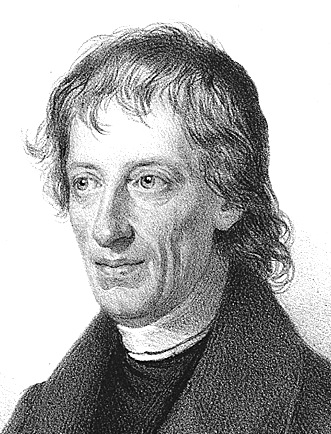
\includegraphics[scale=0.32]{bolzano-abb/portrait.jpg}}}
\noindent Bernard Bolzano war in vielerlei Hinsicht ein außergewöhnlicher Mensch. Als Wissenschaftler verband er so verschiedene Begabungen wie die eines Mathematikers, eines Philosophen, ein"-es Logikers und eines Theologen. Er war katholischer Priester und ein seine Zuhörer begeisternder Hochschullehrer. Er war ein tiefgläubiger Mensch und fühlte sich ganz der Vernunft verpflichtet.  Gedankliche Klarheit, begriffliche Präzision und argumentative Untermauerung seiner Standpunkte galten ihm \anf{als Grundlage für ein vernünftiges, gottgefälliges Leben zum Wohl der Allgemeinheit}.\footnoteA{%
	\lit[11]{Strasser2001}.}
Bolzano ist, dem Philosophen Michael Dummett zufolge, Urgroßvater der analytischen Philosophie.\footnoteA{%
	\lit[167]{Dummett1988}.}
Von ihm stammt der Satz von Bolzano-Weierstraß, den jeder Mathematikstudent heute in seinem ersten Semester 
lernt.\par

\PdUsec{Der Text}
Von der \RWbet{Religionswissenschaft} gibt es fünf Versionen, nämlich 
\begin{compactenum}[1.]
\item[1.] Bolzanos schriftliche Fassung seines ersten Vorlesungszyklus zum Thema;
\end{compactenum}
dann drei Fassungen, die zu Bolzanos Lebzeiten erarbeitet wurden und seine Zustimmung fanden:
\begin{compactenum}[1.]
\item[A] Die 1834 publizierte Fassung,
\item[A$_1$] Bolzanos Überarbeitung von A in seinem Handexemplar sowie
\item[B] Eine im Jahre 1818 erstellte Abschrift seiner Manuskripte für die Studienhofkommission
\end{compactenum}
und schließlich
\begin{compactenum}[1.]
\item[5.] der Text in der Bernard-Bolzano Gesamtausgabe [=GA], Reihe 1, Bände 6/1--2, 7/1--2 und 8/1--4.
\end{compactenum}
Bolzano las seit 1805 regelmäßig einen viersemestrigen Zyklus zur Religionslehre. Der Text des ersten Zyklus ist 1. In den folgenden Jahren überarbeitete Bolzano sein Manuskript stetig. Als er 1818 der Studienhofkommission in Wien seine Arbeiten vorlegen musste, legte er B vor, einen Text, der von einem professionellen Schreiber verfasst, von Bolzano jedoch detailliert korrigiert und im Einzelnen approbiert wurde. 1834 schließlich publizierten Schüler Bolzanos das \RWbet{Lehrbuch der Religionswissenschaft}  (= A) anonym bei Seidel im bayrischen Sulzbach, denn  Bolzano durfte seit seiner Entlassung 1819 im Habsburgerreich nicht mehr publizieren. Bolzano zeigte sich mit dem durch seine Schüler eigenständig redigierten Text relativ einverstanden, wollte aber für eine zweite Auflage Umarbeitungen vornehmen. Zu diesem Zweck ließ er sich ein Exemplar des ersten Bandes vom Buchbinder mit leeren Seiten durchschießen, auf die er seine Überarbeitungen eintrug -- so entstand der Text A$_1$. Der Text der Gesamtausgabe folgt im Wesentlichen A$_1$, gibt aber auch Varianten aus $B$ an.\par
% UNZUVERLASSIGKEIT VON GA
Ein Problem mit der ansonsten äußerst verdienstvollen kritischen Edition der Gesamtausgabe ist jedoch, dass sie häufig nicht zuverlässig ist:
Sinnentstellende Verschreibungen (\zB\ \anf{Richtigkeit} statt korrekt \anf{Nichtigkeit} in RW I 10 oder RW IIIa 18); fehlende gewichtende Zusätze (\zB\ \anf{eine höhere Denkfähigkeit} statt korrekt \anf{eine bedeutend höhere Denkfähigkeit} in RW I 13). Nicht-berücksichtigte Korrekturen von Bolzanos Hand, die Sinnstörungen vermeiden (\zB\ \anf{für Laien bestimmt} (wie in \Alabel ) statt \anf{für Nicht-Theologen bestimmt} in RW I 24).
Daher folgt diese Studienausgabe im Wesentlichen dem Text \Alabel\ der gedruckten Ausgabe von 1834. Nach Möglichkeit werden Bolzanos eigene Verbesserungsvorschläge aus der A$_1$ übernommen. 
Diese Studienausgabe folgt im Wesentlichen dem Text der Gesamtausgabe, d.\,h. der Vorlage \A1label\ bzw. \Alabel , und zwar vor allem aus pragmatischen Gründen. So ist dieser Text relativ gut digitalisierbar. Eine eigene Edition von B machte eine Menge zusätzlichen Aufwands nötig und gehörte wohl eher in die Reihe der unveröffentlichten Schriften in der 
Gesamtausgabe.\par
Grundsätzlich wird aber in Folgendem von der GA abgewichen:
\begin{aufza}
\item Grundsätzlich wird zugunsten des Textumfangs dieser Studienausgabe nur derjenige Text der GA zugrundegelegt, der auch in \Alabel\ bzw. \A1label\ vorkommt. Zusätzliches Material wie die frühere Fassung der Vorrede, das \anf{Vorwort} (GA I 6/1, S. 19--22), oder die vielfältigen Auszüge von Varianten aus B in den Anhängen der Bände der GA werden weggelassen.
\item In \Alabel\ waren nahezu alle Textabsätze durchnummeriert. Die GA löscht diese Nummerierungen (vermutlich, weil Bolzano selbst sie in A$_1$ gelöscht hat) und setzt die Unternummerierungen dafür eine Ebene höher (\dh\ eine nachgeordnete Aufzählung beginnt nun mit arabisch 1., während sie in A mit lateinisch a. begann -- dafür nummeriert arabisch 1. eben den Absatz). Diese Änderung gegenüber A wird jedoch in GA weder verzeichnet noch beschrieben. Sie wird auch nicht durchgehalten, sodass sich ein uneinheitliches Bild ergibt: In GA I 6/1--2 die gegenüber A geänderte Nummerierung, in GA I 7 \& 8 die ursprüngliche Nummerierung aus A. Hier wird die ursprüngliche Nummerierung aus A einheitlich und durchgängig verwendet.
\end{aufza}
Für die konkrete Textgestalt wurden Bolzanos eigene Wünsche, soweit sie aus seinen handschriftlichen Überarbeitungen und Hinweisen in A$_1$ ersichtlich sind, nach Möglichkeit berücksichtigt: 
\zit[{Bolzano in A$_1$, S. 1 am Rande; zit. n. GA I 6/1, S. 41}]{%
Sollte es nicht besser seyn, \auslass\ wenn die §§ Nummern durch das ganze Buch eben neben der Seitenzahl auf jedem Blatte angezeigt würden, wodurch das Nachschlagen erleichtert würde?
}
Am Beginn des Inhaltsverzeichnisses verlangte Bolzano am Ende der Überschriften der Paragraphen 11, 13 und 14, insofern es sich bei diesen und unter den ersten 14 Paragraphen auch nur bei diesen um vollständige Sätze handelte, einen Punkt. Ab Paragraph 15 hingegen hat er das nicht mehr korrigiert, obwohl etwa die Paragraphen 15--18 alle ganze Sätze als Überschriften tragen. Vermutlich hat er diese Korrekturmaxime also wieder aufgegeben. Mithin werden die drei genannten Punkte nicht übernommen.\par
Wenn Bolzano durch inkonsistente Korrekturen die Möglichkeit zur Vereinheitlichung oder sonstiger Verbesserung des Textes gibt, wird sie vorgenommen. So korrigiert er im Inhaltsverzeichnis nicht, dass bei § 23 von \erganf{Offenbarung}, in der ganz parallel gestalteten Überschrift von § 24 jedoch von \erganf{Offenbaren} die Rede ist. In den betreffenden Kapitelüberschriften heißt es später jedoch beide Male \erganf{Offenbaren}, sodass wir dies auch im Inhaltsverzeichnis vereinheitlichen.\par
Wenn aus Bolzanos ausführlicher Korrektur des 1.~Bandes eine klare Intention bzgl. der Schreibungen hervorgeht, wird diese Intention auch in den anderen Bänden umgesetzt. So hat er bspw. aus dem Wort \anf{Willkühr} und Ableitungen wie \anf{unwillkührlich} im 1.~Band konsequent (wenn auch nicht überall, \zB\ nicht im letzten Satz von \RWparnr{137}) das h gestrichen. 

Weitere Hinweise zur Gestaltung dieser Edition:
\begin{aufza}
\item Grundsätzlich bleibt die Orthographie so wie zu Bolzanos Zeit. Dies schränkt die Lesbarkeit kaum ein und vermittelt dem Leser dafür etwas von dem authentischen \anf{Flair} des 19.~Jahrhunderts, wenn er beispielsweise \anf{Princip}, \anf{nöthig} oder \anf{Gesammtglaube} liest. 
\item Bolzano hat Zitate von Texten in der Regel nicht in Anführungszeichen eingeschlossen. (In A werden kaum Anführungszeichen verwendet. Bolzano scheint sie auch nicht in A$_1$ nachgetragen zu haben.) Um die Lesbarkeit und die Identifikation von Zitaten zur erleichtern, werden in dieser Ausgabe Zitate oder zitatnahe Paraphrasen fremder Texte nach Möglichkeit in Anführungszeichen eingeschlossen. Dabei werden deutsche Anführungszeichen (\eanf{\ }) dort verwendet, wo Bolzano selbst Anführungszeichen gesetzt hat. Wir ergänzen hingegen inverse französische Anführungszeichen (\erganf{\ }) als Markierung von Zitaten, etwa wenn im Apparat Literatur nachgewiesen wird. Allerdings muss man stets im Kopf behalten, dass Bolzano häufig eher paraphrasiert als wörtlich zitiert. Dennoch erhöhen diese Zeichen die Lesbarkeit, insofern man schnell sieht, wo das Referat (sei es wörtlich oder paraphrasierend) beginnt und endet. Keine Anführungszeichen werden hingegen dort ergänzt, wo nach heutiger Konvention ein Wort erwähnt und nicht gebraucht wird, und auch dort nicht, wo man wörtliche Rede heute meist in Anführungszeichen setzen würde. Referiert Bolzano beispielsweise eine Passage aus einem sokratischen Dialog, so wird diese Passage als Ganze in Anführungszeichen gesetzt, die einzelnen Redebeiträge der Dialogteilnehmer hingegen nicht. Ebenso wird verfahren bei Jesus-Worten: Sind es biblische Zitate (oder Paraphrasen), so werden die Anführungszeichen \erganf{\ } ergänzt, als wörtliche Rede einer Person hingegen werden keine Anführungszeichen hinzugefügt.
% \erganf verwenden für ergänzte Anführungszeichen, d.h. solche, die nicht in A vorkommen
\item Die Zeichensetzung folgte im 19.~Jahrhundert anderen Üblichkeiten als heute. Bolzano setzt Kommata regelmäßig an Stellen, an denen nach heutigen Regeln keine gesetzt werden, etwa vor \anf{und} und \anf{oder} in Beiordnungen von Sätzen, die ein gemeinsames Subjekt haben, zwischen \anf{sowohl} und \anf{als auch} sowie vor Vergleichen mit \anf{als}. Grundsätzlich bestanden mehr Freiheiten. So setzt Bolzano Kommata auch als rhetorische Untergliederungen ein. Die Zeichensetzung in dieser Ausgabe folgt im Wesentlichen Bolzanos eigener Zeichensetzung in Ausgabe A. Abgewichen wird davon nur, wenn es naheliegt, dass nach Bolzanos mutmaßlichen eigenen Zeichensetzungsprinzipien ein Fehler vorliegt -- wie etwa dann, wenn bei einer Folge offensichtlich beigeordneter Sätze ohne erkennbaren Grund nur einmal ein Semikolon anstelle eines Kommas steht, ein Punkt sowohl vor als auch nach einem eingeklammerten Ausdruck am Satzende steht oder wenn ein Komma am Satzende auftaucht und der Beginn des nächsten Satzes großgeschrieben wird usw. -- oder sich zumindest eine andere Zeichensetzung nach Bolzanos eigener Systematik nahelegt -- wie etwa dann, wenn er eine Reihe von Bibelstellen nach dem Schema \anf{Stellenangabe - Doppelpunkt - Paraphrase} angibt und der Doppelpunkt in Einzelfällen fehlt.
\item Bolzanos spezifische Form, Bibelstellen anzugeben, wird grundsätzlich beibehalten. So setzt er zwischen Kapitel- und Verszahl ein Komma ohne Leerzeichen und schließt die Stellenangabe mit einem Punkt ab, der für heutige Lesegewohnheiten ungewöhnlich ist, aber im Sinne einer Ordnungszahl durchaus Sinn macht: \anf{11,7.} hat er wohl gelesen im Sinne von \anf{Kapitel 11, \RWbet{siebter} Vers}. Ebenfalls zugunsten der besseren Lesbarkeit wird zwischen aufgezählten Bibelstellenangaben ein Satzzeichen eingefügt. Wir schreiben also \anf{1\,Mos.~1,26.; 3,22.; 11,7.} statt \anf{1\,Mos. 1,26. 3,22. 11,7.}
\item Die Orthographie wird weitgehend so belassen, wie Bolzano sie mutmaßlich anwandte. Mithin werden im 19.~Jahrhundert übliche Schreibungen wie \anf{Thal}, \anf{Gesammtheit}, \anf{insgesammt} u.ä. beibehalten. Nur offenkundige grammatikalische oder orthographische Fehler werden berichtigt wie z.B. \anf{Aeußerungen über Gottes dreifache Persönlichkeit} anstatt \anf{\auslass\ dreifacher \auslass}, oder etwa \anf{\RWgriech{basile'ian Jeo~u o>u klhronom'hsousin}} statt \anf{\RWgriech{\auslass\ klhronom'hsousi}} (in RW IIIb 143 ausdrücklich aus der Bibelstelle \RWbibel{1\,Kor}{1\,Kor}{6}{9} zitiert). In relativ eindeutigen Fällen wie diesen, werden die Änderungen  stillschweigend vorgenommen.  Änderungen gegenüber A, bei denen nicht sicher ausgeschlossen werden kann, dass die fehlerhaft scheinende Schreibung irgendeinen Sinn haben könnte, werden im Apparat vermerkt.
\item Nach heutigen Regeln werden am Ende von Überschriften keine Punkte gesetzt. Daher werden die Punkte nach den Überschriften der Paragraphen weggelassen. Da die Überschriften der Hauptteile und anderen größeren Abschnitte jedoch in aller Regel mehrere Teile haben, die eh durch Punkte abzutrennen sind, werden hier zur Vereinheitlichung auch die Endpunkte beibehalten.
\item Einige Besonderheiten ergeben sich aus Bolzanos teilweiser Überarbeitung von \Alabel\ zu \A1label . In \Alabel\ werden Adjektive, die zwischen \anf{alle} und einem Substantiv stehen, wie heute üblich schwach flektiert (\anf{alle christlichen Weltweisen}); gelegentlich hat Bolzano dies in \A1label\ jedoch ausdrücklich zur starken Flexion hin korrigiert (\anf{alle christliche Weltweisen}). Da die starke Flexion nach \anf{alle} heute vollkommen unüblich geworden ist und da Bolzano diese Korrekturen selbst in dem Teil der RW, den er intensiv überarbeitet hat, nicht immer durchführt, weichen wir hier zugunsten der besseren Lesbarkeit von seinem Willen ab und verwenden die schwache Flexion.
\item Sowohl in der Druckfassung \Alabel\  als auch in Bolzanos Überarbeitung \A1label\ wird gelegentlich \anf{allmählich} und gelegentlich \anf{allmählig} geschrieben. Da die Orthographie heute nur noch \anf{allmählich} kennt, wird dahingehend vereinheitlicht. Anders hingegen bei Variationen, bei denen auch heute noch beide Formen als korrekt gelten. So werden Bolzanos Wechsel zwischen \anf{-es} und \anf{-s} bei den Genitiv-Endungen nicht vereinheitlicht (\anf{des Christenthums} und \anf{des Christenthumes}). Dasselbe gilt für den gelegentlichen Ausfall des \anf{e} bei Worten wie \anf{anderen} / \anf{andren}. 
\item Die Informationen über Varianten von \Blabel\ im Verhältnis zu \Alabel\ wurden der \GAlabel\ entnommen. 
\item Auf Nummern von Absätzen oder Ähnlichem wurde in \Alabel\ durchgängig mittels \anf{Nr.} Bezug genommen. Bolzano hat dies in den Teilen, die er überarbeitet hat, konsequent zu einer Graphie geändert, die offenbar für das Lateinische \anf{numero} oder das Französische \anf{numéro} steht: ein \anf{n} mit einem hochgestellten \anf{o} und einem darunterstehenden Punkt. Diese Schreibweise ließ sich nicht eindeutig einer der im europäischen Sprachraum üblichen Varianten wie No, No., N$^{\mathrm{o}}$, n$^{\mathrm{o}}$, n$^{\mathrm{o}}\!.$, n$^{\underline{\mathrm{o}}}$ oder Ähnlichen zuordnen. Daher wurde mit \no\ eine Drucktype entworfen, die seiner eigenen Schreibung möglichst nahekommt.
\item Wenn eine Nummerierung hinzugefügt worden ist, die in \Alabel\ nicht vorkommt, wird dies angemerkt.
\item Einfache Ergänzungen ggü. den Vorlagen werden in eckige Klammern gesetzt ([\auslass ]), bspw. wenn Bolzano RW I 25 eine Fußnote hinzufügt, die mit \anf{gestorben den \auslass} endet, wird das Todesdatum des Betreffenden in eckigen Klammern hinzufügt: \anf{gestorben den [11.\,Oktober 1834]}. Wird hingegen ein ganzes Wort ausgelassen, wird dies in den Anmerkungen vermerkt.
\end{aufza}

\endinput
%
%---Zwischentitelei---
\neuerechteseite\pagestyle{completelyempty}
%
\RWteil{}{Bernard Bolzano}{Lehrbuch der Religionswissenschaft}{}%
%
\begin{center}
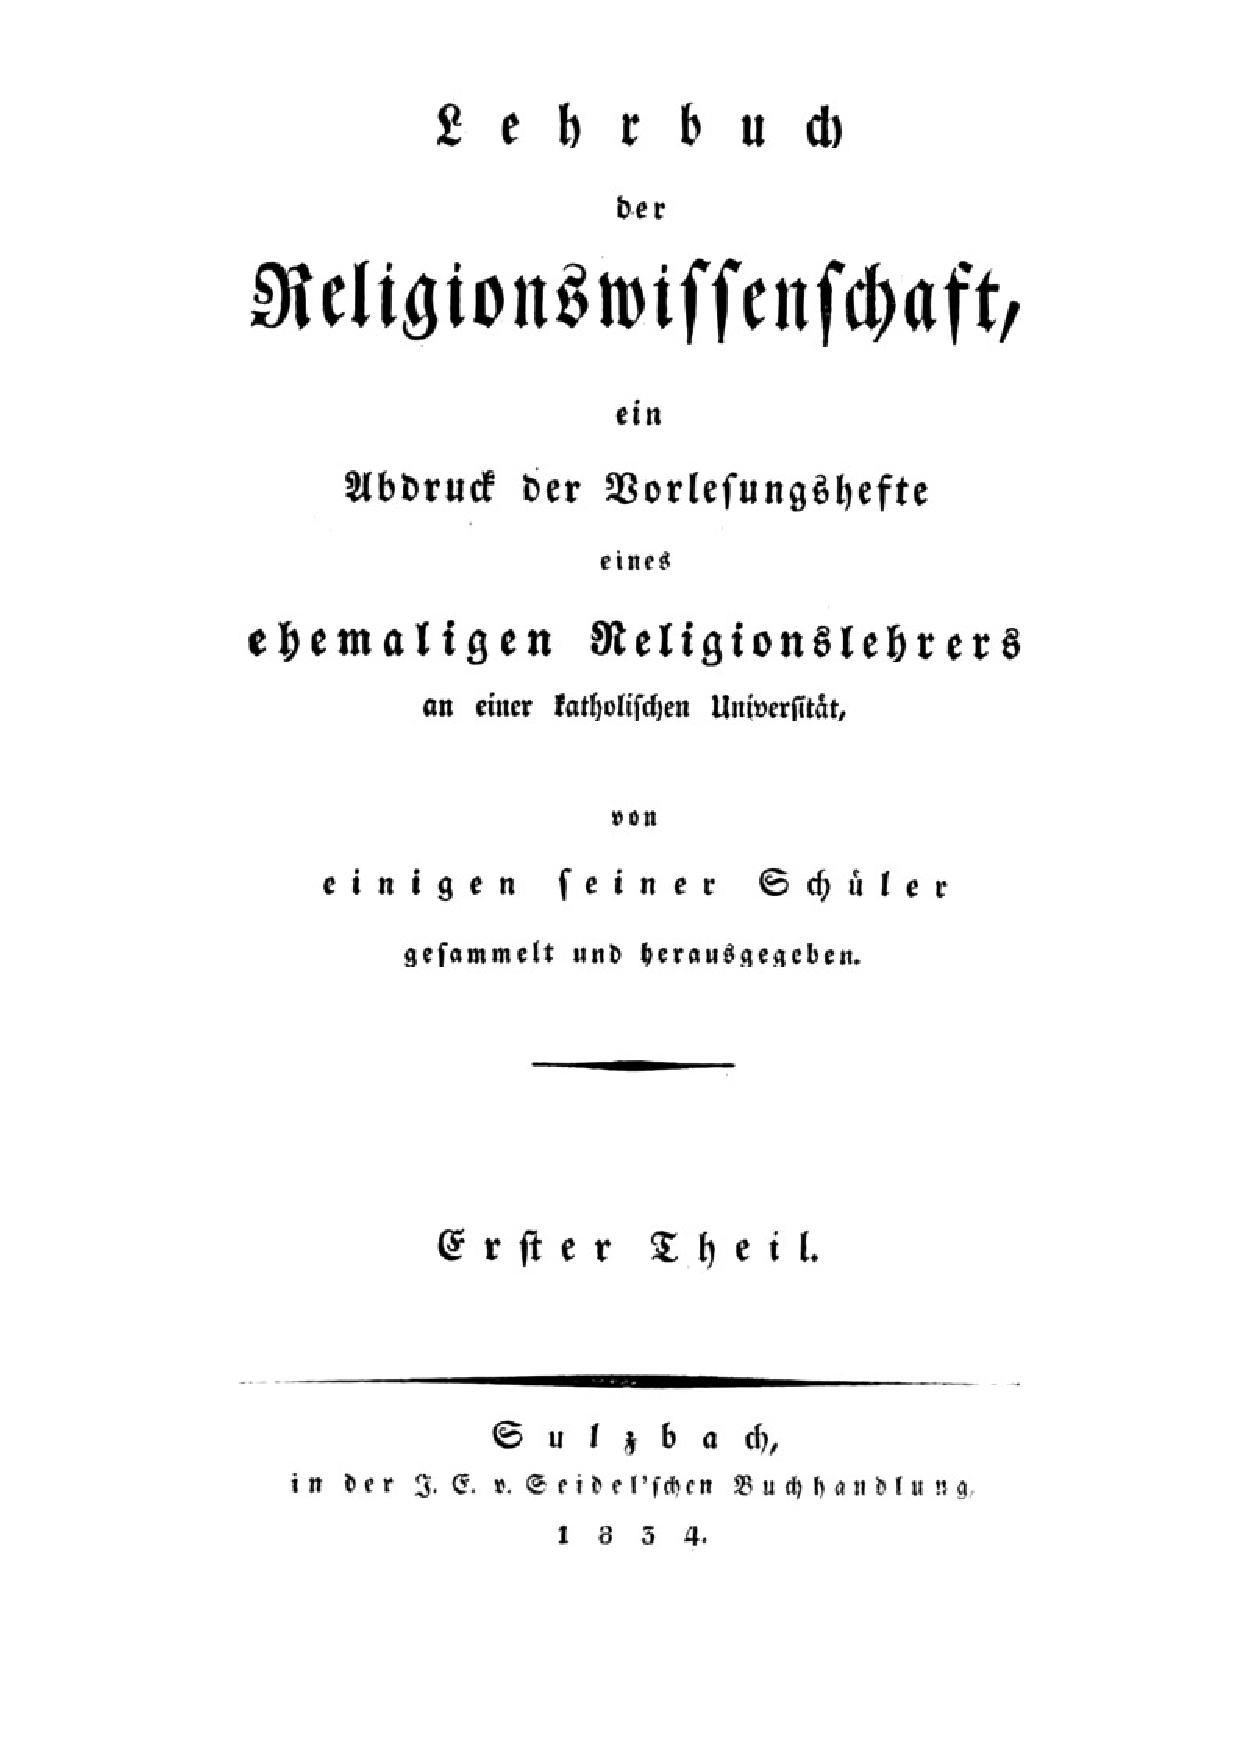
\includegraphics[viewport=3cm 3.5cm 17.35cm 28.7cm, scale=0.76,clip]{bolzano-abb/Bolzano-RW1-Tit3.pdf}
\end{center}
%
\neuerechteseite
\endinput
%
%---Fußnoten umstellen
\makeatletter
\renewcommand{\@makefntext}[1]{\noindent \@makefnmark\hspace{0.33em}#1}
\makeatother
\zeilennummerntrue%
%
%---Vorrede---
%\vspace{-1.5\baselineskip}%
%\clearpage\linenumbers%
% \PdUch{Vorrede}
\def\dieserteilseiten{I}%
\def\dieserteil{I}%
\RWch*{Vorrede.[uns
\RWSeitenwohne{III}\\
{\normalsize \protect\vorredekennzeichnung}}%
\PdUtoc{chapter}{Vorrede. \protect\vorredekennzeichnung}%
\markboth{\kopfzeilenfmt{Religionswissenschaft\enspace$\cdot$\enspace Vorrede \protect\vorredekennzeichnung}}{\kopfzeilenfmt{Religionswissenschaft\enspace$\cdot$\enspace Vorrede \protect\vorredekennzeichnung}}%
\linenumbers\noindent Der Verfasser dieses Lehrbuches, ein katholischer Geistlicher, vor beiläufig fünfzehn Jahren noch als Religionslehrer an der Universität seiner Vaterstadt angestellt, wegen seiner ausgebreiteten und tiefen Kenntniß der Wissenschaft eben so sehr als wegen seines vortrefflichen Charakters und wegen seiner nicht zu ermüdenden Thätigkeit, das Beste der Menschheit durch Aufklärung der Jugend zu fördern, hochgeachtet, ja verehrt von Allen, die ihn kennen, hatte schon während seiner Studienjahre Gründe gefunden, die seiner Ueberzeugung von der Wahrheit und Göttlichkeit unseres heiligen Glaubens eine unumstößliche Festigkeit gaben, und weder in den Schulen vorgetragen wurden, noch in den wissenschaftlichen Lehrbüchern aus einander gesetzt waren. Weil er nun hoffte, daß er im geistlichen Stande mehr als in jedem anderen Aufforderung und Gelegenheit finden würde, diese Gründe vielseitig zu prüfen, sich von ihrer Haltbarkeit zu überzeugen, und sie, wenn er ihre Richtigkeit und Sicherheit würde hinlänglich erprobt haben, zu verbreiten und zur allgemeinen Anerkennung zu bringen: so begann er, nach zurückgelegten philosophischen Lehrcursen, die theologischen Studien, und bewarb sich noch vor Beendigung dieser Studien, als ein junger Mann von \Abweichung{nicht}{nich}{} ganz vier und zwanzig Jahren, um die damals zu errichtende Lehrkanzel der Religionswissenschaft an der Hochschule seiner Vaterstadt, die er auch erhielt. Auf diesem Posten entwickelte er allmählig seine Ansichten über die katholische Religion und insbesondere über die Gründe ihrer Göttlichkeit vor seinen zahlreichen Schülern; und je mehr das wissenschaftliche Gebäude, das er errichtete, der Vollendung näher kam, um so mehr gewann es die Aufmerksamkeit und den Beifall nicht nur seiner Schüler, sondern beinahe aller Mitglieder der gelehrten, ja überhaupt der gebildeten Stände. Die angesehensten und aufgeklärtesten Personen bemühten sich, Abschriften seiner Vorträge zu erhalten, und wer nicht bloß herausgerissene Bruchstücke, sondern das Ganze las und gehörig auffaßte, der fühlte und gestand, daß seine religiöse Ueberzeugung an Klarheit und Festigkeit, daß er Liebe, Achtung und Vertrauen zu seinem Glauben gewonnen habe. Dieß war besonders in den~\RWSeitenw{IV}\ letztern Jahren seines öffentlichen Lebens der Fall; denn der allverehrte Lehrer ließ sich durch den Beifall, den seine Vorträge bereits gefunden \Abweichung{hatten}{hatte}{}, so wenig abhalten, an ihrer Verbesserung und Vervollkommnung zu arbeiten, daß er vielmehr, ohne in dem \RWbet{Wesen} seiner Ansichten eine Aenderung vorzunehmen, beinahe niemals den Lehrstuhl bestieg, ohne zu dem, was er im vorhergegangenen Jahre vorgetragen hatte, eine Zugabe oder Abänderung mitzubringen, die seinem Vortrage mehr Licht und Klarheit, mehr Eindringlichkeit und Ueberzeugungskraft gab, irgend einen möglichen Einwurf oder Zweifel beseitigte, oder die Brauchbarkeit und gehörige Anwendung einer Lehre besser darthat. So kam es, daß seine Vorlesungen immer segensreicher wirkten. Sie haben den Geist seiner Schüler, mehr als es sich sagen läßt, erhellt, geübt, geschärft, das Herz gebildet und veredelt, den Willen gebessert und gestärkt, das Leben und Wirken geordnet und nach jenem Ziele hingerichtet, dem wir mit jedem Tage näher und näher kommen sollen; sie haben dem Glauben, der die Tugend nährt, im Leiden tröstet und zum Heile führt, einen festen Grund gelegt, den Verstand mit jenen scheinbaren Widersprüchen ausgesöhnt, die der Religion so viele Feinde und Gegner erwecken; haben gezeigt, wie man die Lehren der Offenbarung gebrauchen müsse, wenn sie Demjenigen, von dem sie uns gegeben wurde, an Weisheit, Heiligkeit und Seligkeit ähnlicher und immer ähnlicher machen sollen; haben Wahrheiten, die nicht ohne großen Nachtheil für die Menschheit verkannt und verborgen bleiben können, und die gleichwohl nur selten richtig erkannt und angewendet werden, in ein helles Licht gesetzt, und \Abweichung{nicht}{nich}{} bloß im Verstande zur Anerkennung gebracht, sondern auch das Herz und den Willen Vieler so gänzlich für dieselben gewonnen, daß sie nun in den öffentlichen, einflußreichen Aemtern, die sie bekleiden, durch Einsicht, Rechtschaffenheit und Berufstreue als weise Freunde der Menschheit, als eifrige und muthige Verfechter ihres Wohles und ihrer Rechte sich erweisen, und mit Freunde unverholen gestehen, daß das Gute, welches in ihnen sich findet und durch sie in der Welt zu Stande gebracht wird, größtentheils ihrem Lehrer zuzuschreiben sey.\par
Wir -- die das Glück hatten, den Herrn Verfasser dieses Lehrbuches zum Lehrer zu haben -- wir können, was wir von diesem Lehrbuche so eben erzählt und gerühmt haben, mit um so größerer Zuversicht bezeugen, da wir es nicht nur selbst erlebt und an uns erfahren haben, sondern auch gewiß seyn dürfen, daß uns, was wir gesagt, alle diejenigen bestätigen werden, die ein gleiches Glück mit uns genossen haben; und ihre Zahl ist wahrlich nicht gering. Auch sind, seit wir ferne von unserem ehemaligen, verehrten Lehrer leben, mehrere Jahre verflossen, und während der Zeit ist Vieles über die Religion gedacht~\RWSeitenw{V}\ und geschrieben worden; dennoch, wenn wir die Ergebnisse der theologischen Forschungen, selbst der neuesten, beachten, scheinen uns die Begriffe, Ansichten und Grundsätze, die in diesem Lehrbuche vorgetragen werden, noch immer \RWbet{neu} und der Prüfung und öffentlichen Besprechung gar sehr werth zu seyn. Die wichtige Lehre \RWbet{von der Möglichkeit und den Kennzeichen der göttlichen Offenbarung} ist unseres Wissens nirgends so behandelt worden, daß sie geeignet wäre, den Streit zwischen dem Rationalismus und Supernaturalismus, der in Deutschland sich erhoben hat, und noch immer fortgeführet wird, beizulegen; und es scheint uns, daß die Ansichten unseres theuern Lehrers die Vernunft nicht nur von der Möglichkeit göttlicher Belehrungen überzeugen, sondern sie zugleich in den Stand setzen könnten, mit Sicherheit zu entscheiden, welche unter den verschiedenen Religionen, die auf Erden geglaubt und bekannt werden, sich in Wahrheit rühmen könne, göttlichen Ursprunges zu seyn. Eben so wenig ist der Beweis, \RWbet{daß die katholische Religion jene Zeichen aufzuweisen habe, an denen wir mit Sicherheit abnehmen können, daß Gott sie geglaubt und befolgt wissen will}, von irgend einem Lehrer unserer Kirche so geführt worden, daß nicht gar manche Frage unbeantwortet, gar mancher Zweifel übrig geblieben wäre; und es scheint uns, daß unser verehrter Lehrer diesen Beweis so dargestellt habe, daß, wenn man erst einige Mißverständnisse und Bedenklichkeiten, die sich wahrscheinlich erheben werden, wird beseitiget, und seine eigentliche Ansicht recht klar wird aus einander gesetzt haben, nichts mehr zu wünschen übrig bleiben wird. \RWbet{Der Sinn und die Bedeutung von gar mancher hochwichtigen Lehre unserer heiligen Religion} ist noch nirgends so erklärt worden, daß es leicht oder auch nur möglich wäre, zu zeigen, sie stehe mit keiner der Wahrheiten, die völlig ausgemacht und sicher sind, im Widerspruche; und es scheint uns, in diesem Lehrbuche sey dieß theils wirklich schon geschehen, theils sey wenigstens genug gesagt, um solche Erlärungen finden, und sie als übereinstimmend mit den Lehren der Kirche darstellen zu können. Um nicht weitschweifig zu werden, übergehen wir vieles, vieles Andere, das in diesem Lehrbuche geleistet ist, und selbst in den gefeiertesten Werken der theologischen Literatur, die dagegen Anderes vortrefflich behandeln, entweder gänzlich vermißt wird, oder wenigstens nicht so dargestellt ist, daß es geeignet wäre, allgemeine Anerkennung zu finden; wir übergehen dieß, weil schon die erwähnten drei Vorzüge dieses Lehrbuches hinreichen, die Drucklegung desselben zu rechtfertigen.\par
Daß aber wir, bloße \RWbet{Schüler} des Verfassers, uns zur Bekanntmachung seiner Vorlesungshefte entschließen, und sie nicht dem Herrn~\RWSeitenw{VI}\ Verfasser selbst überlassen, bedarf einer Rechtfertigung. Die Wahrheit hat noch jederzeit Gegner, und ihre Vertheidiger haben noch immer um so heftigere Feinde gefunden, je nachdrücklicher und schlagender ihre Vertheidigung war. Auch gegen unseren verehrungswürdigen Lehrer erhoben sich schon in der ersten Zeit nach Antritt seines Lehramtes Feinde, denen es, nach wiederholt zurückgewiesenen Angriffen, endlich gelang, höhern Orts Verdacht gegen ihn zu erwecken und ihn in eine Lage zu versetzen, daß er es jetzt für eine Verletzung seiner Unterthanspflichten halten würde, diese Vorträge durch die Presse bekannt zu machen. Deßhalb haben wir, denen solche Rücksichten die Hände nicht binden, uns entschlossen, in seinem Namen zu thun, woran er gehindert ist. Wir glauben auch, auf seinen Dank dafür rechnen zu können.\par
Daß er die Verbreitung seiner Ansichten wünsche, läßt sich nicht nur daraus schließen, weil er auf ihre Darstellung so viele Zeit, Mühe und Sorgfalt verwendet, und sie durch so viele Jahre öffentlich vorgetragen hat; sondern wir erinnern uns auch recht gut, und viele seiner Schüler werden es eben so wenig vergessen haben, daß er den Wunsch, es möchten seine Grundsätze allgemein bekannt und angenommen werden, zu wiederholten Malen öffentlich aussprach. Wenn wir hiernach seiner Zustimmung zur Drucklegung seiner Vorträge gewiß seyn möchten, so entsteht doch wieder daraus eine nicht zu übersehende Bedenklichkeit, daß unser verehrter Lehrer nicht selten die Absicht geäußert hat, daß er, wenn ihm Gott das Leben so lange erhalten sollte, seine Vorlesungen viel umständlicher und erschöpfender bearbeiten würde, so zwar, daß die hier abgedruckten drei Theile -- dieß sind nun seine eigenen Worte: -- wenigstens in einigen Partieen für nicht viel mehr, als für einen \RWbet{bloßen Entwurf} zu erachten wären. Doch ist, wie wir zuverlässig wissen, mit dieser so umständlichen und erschöpfenden Bearbeitung bis jetzt nicht einmal noch der Anfang gemacht worden; indem sich unser theuerer Lehrer mit anderen Disciplinen, namentlich mit der Logik und Mathematik ausschließlich beschäftigen soll. Auch ist die Gesundheit unseres verehrungswürdigen Lehrers, leider! schon seit seiner Kindheit viel zu schwach, sein kostbares Leben hängt an viel zu zarten Fäden, als daß man mit einiger Sicherheit hoffen dürfte, er werde mit dieser Arbeit fertig werden können. Und wenn wir auch so glücklich seyn sollten, daß er uns durch die mütterlich liebevolle Pflege, der er jetzt, wie man versichert, genießet, lange genug erhalten würde, um sein Vorhaben ausführen zu können; so wird nicht nur das Studium seiner Vorlesungshefte eine nützliche, bei \Abweichung{Manchem}{Manchen}{} sogar nothwendige Vorbereitung seyn zum Verständniß seiner vollständig ausgearbeiteten Religionslehre; sondern die vorläufige Bekanntmachung der Vorlesungshefte wird ihm auch~\RWSeitenw{VII}\ bei jener vollständigen Bearbeitung selbst sehr zu Statten kommen. Es läßt sich nämlich leicht voraussehen, daß seine Ansichten, die dem, was man bisher über diesen Gegenstand denket und meint, so ganz fremd, und dem in der Wissenschaft herrschenden Geist oder Ungeist der Zeit so ganz entgegen sind, von gar mancher Seite werden angegriffen werden. Solche Angriffe aber können ihn auf Manches, das er vielleicht übersehen, mit zu wenigen und gerade für seine Gegner unzureichenden Beweisgründen ausgestattet, nicht deutlich genug erklärt, nicht mit hinlänglicher Umständlichkeit gegen Mißverständnisse sicher gestellt hat, aufmerksam machen; können vielleicht sogar Veranlassung werden, daß er in einem \RWbet{Nachtrage} zum Theil wenigstens jene umständliche Bearbeitung liefere, zu der es ohne das Erscheinen seiner Vorlesungen gar nicht gekommen wäre. Auf jeden Fall sind diese Vorlesungen bereits in so vielen Abschriften, die alljährlich noch vervielfältiget werden, vorhanden, sind bereits so sehr ein Eigenthum des Publicums, daß der Herr Verfasser eine Drucklegung derselben gewiß schon seit Jahren vorhergesehen, vielleicht sogar erwartet und gewünscht hat.\par
Da wir nun bei dieser Herausgabe seiner Vorlesungen durchaus keinen Widerspruch von Seite unseres Lehrers zu fürchten haben: so erübriget nur noch, daß wir ihm und dem Publicum über die Art und Weise Rechenschaft geben, die bei der Sammlung seiner Vorträge beobachtet wurde. Unser verehrter Lehrer hat, wie wir schon vorhin bemerkten, an der Verbesserung und Vervollkommnung seiner Vorträge bis an's Ende seines Wirkens unausgesetzt gearbeitet. Wir durften uns also nicht erlauben, jene Bearbeitung, die wir in unserer Studienzeit uns verschafften, obgleich sie damals die beste war, in die Druckerei zu schicken; sondern wir konnten nur dann glauben, daß wir die Religionswissenschaft unseres Lehrers der Welt in jener vollkommensten Gestalt übergeben, die sie von seiner Hand bisher erhalten hat, wenn wir auch die letzten Verbesserungen, die er machte, in unsere Ausgabe aufnehmen. Das ist denn auch wirklich geschehen. Wir waren so glücklich, eine Abschrift seiner letzten Bearbeitung, und selbst jener Bogen zu erhalten, von denen er nicht eher als an dem nämlichen Tage, da ihm das Absetzungsdecret mitgetheilt wurde, die bessernde Hand zurückgezogen hat; und diese ganz letzte Bearbeitung ist es, die wir hiemit dem Publicum vorlegen. In dieser Bearbeitung aber fehlte Mehreres, das er, wie unsere Explicationshefte uns lehrten, in früheren Jahren vorgetragen hatte; und wir erlaubten uns, Einiges davon, dessen Unterdrückung uns besonders leid gethan hätte, in diesen Abdruck wieder aufzunehmen; und hieraus mag sich der Leser die Ungleichförmigkeiten erklären, die er in manchen Paragraphen vielleicht bemerken wird. Sonst aber findet man,~\RWSeitenw{VIII}\ außer einigen unbedeutenden Anmerkungen unter dem Texte, auch gar nichts in diesem Abdrucke, das nicht der Verfasser selbst seinen Schülern \RWbet{schriftlich} übergeben hätte; keine einzige jener Bemerkungen, die er beim \Abweichung{Vortrage}{Vortragen}{} bloß \RWbet{mündlich} machte, keine einzige Stelle aus seinen Erbauungsreden, deren uns einige hundert zu Gebote standen, und in denen er nicht selten seine Ansichten umständlicher und eindringlicher aus einander setzte, als es in einem wissenschaftlichen, in gemessener Stundenzahl zu beendigenden Unterricht geschehen kann; durchaus nichts findet der Leser in diesem Abdrucke, als nur dasjenige, was der Verfasser selbst in seine Schulvorträge aufgenommen hat. Aenderungen der Sprache aber und des Ortes, auch Auslassungen, die wir jedoch ehrlich anzeigen wollen, haben wir uns allerdings in einigen Stellen erlaubt. Zuvörderst haben wir die angeführten Stellen des neuen Testamentes, die der Herr Verfasser nach seinem eigenen wiederholten Geständniß, nur deßwegen unübersetzt ließ, weil es ihm an Zeit gebrach, eine Uebersetzung derselben nach seinem Sinne zu machen, zu größerer Bequemlichkeit mancher Leser deutsch gegeben. Ein Gleiches that der Eine und der Andere von uns mit mancher Stelle aus lateinischen Schriftstellern. Die \RWbet{Einschaltung über die kantische Philosophie und über die neueste Art zu philosophiren in Deutschland}, die, leider! noch immer die \RWbet{neueste} ist, trug unser verehrungswürdiger Lehrer darum erst nach dem Hauptstück, welches von den \RWbet{Erkenntnißquellen} des Katholicismus handelt, vor, weil diese Einschaltung eine gewisse philosophische Ausbildung seiner Schüler voraussetzt, um verstanden zu werden. Wir haben uns erlaubt, sie an jenen Ort zu verlegen, wohin sie uns zu gehören schien. Hinter jedem einzelnen Hauptstück endlich, ja wohl auch hinter einzelnen Abtheilungen der Hauptstücke fanden wir Bemerkungen, die \RWbet{Literatur} des eben behandelten Gegenstandes betreffend. Sie schienen uns nur skizzirt, nur für die Schüler gemacht und der öffentlichen Mittheilung nicht werth zu seyn. Wir haben sie ganz weggelassen. Das ist aber auch Alles, was wir uns erlauben zu dürfen glaubten.\\[\baselineskip]
Geschrieben im Juli 1834.\editorischeanmerkung{In \Alabel\ folgt auf den Seiten \RWS{IX--XX} das Inhaltsverzeichnis von Bd.\,I, das in dieser Edition zugunsten des Gesamtinhaltsverzeichnisses (S.\,\pageref{IhvzAnfang}--\pageref{IhvzEnde}) ausgelassen ist.}\par
\endinput

%
%---HAUPTTEXT---
\setcounter{footnote}{0}\renewcommand{\thefootnote}{\fnsymbol{footnote}}%
\clearpage\linenumbers%
\RWch[Einleitung.]{Einleitung.\RWSeitenwohne{1}}
\RWpar{1}{Inhalt und Zweck dieser Einleitung}
Bei jedem Unterrichte, besonders wenn er in \RWbet{wissenschaftlicher} Form ertheilet wird, ist es gewöhnlich, mit einer \RWbet{Einleitung} in denselben anzufangen. Es finden sich nämlich fast immer mehre Wahrheiten vor, deren Kenntniß dem Empfänger des neuen Unterrichtes gleich Anfangs nothwendig ist, und die man gleichwohl keineswegs bei ihm voraussetzen darf. Diese Wahrheiten sind es denn, die man ihm in der Einleitung zuvörderst beizubringen trachtet. Hieraus ergibt sich sogleich die nähere Beschaffenheit der Untersuchungen, die in einer Einleitung von Rechtswegen vorgenommen werden. Es müssen dieß nämlich
\begin{aufza}[a)]
\item Wahrheiten seyn, von denen wir nicht füglich annehmen können, daß sie dem Anfänger schon von anderer Seite her bekannt sind. Es müssen ferner
\item Wahrheiten seyn, die mit dem Unterrichte, den wir nun zu ertheilen haben, in einer gewissen \RWbet{Verbindung} stehen, die eben den Grund enthält, weßhalb wir sie vielmehr bei diesem, als bei irgend einem andern Unterrichte beibringen. Es müssen also Bemerkungen seyn, welche entweder zum gehörigen Verständnisse des zu ertheilenden Unterrichtes, oder doch dazu nothwendig sind, um den Anfänger geneigt zu machen, Aufmerksamkeit und Fleiß auf diesen Unterricht zu verwenden. So pflegt man \zB\ in der Einleitung zur Raumwissenschaft oder Geometrie einige arithmetische Sätze,~\RWSeitenw{2}\ die zum Verständnisse gewisser geometrischer nothwendig sind, oder etwas über den Nutzen der Geometrie \udgl\ vorauszuschicken.
\item Es müssen endlich Wahrheiten seyn, die, wenn sie einerseits mit dem abzuhandelnden Gegenstande in \RWbet{Verbindung} stehen, andererseits doch auch keine \RWbet{Belehrungen} über \RWbet{ihn selbst} enthalten. Denn wäre dieses der Fall, so würde ihr Vortrag, als ein Bestandtheil des schon \RWbet{angefangenen} Unterrichtes, nicht aber erst als eine vorläufige \RWbet{Einleitung} in denselben betrachtet werden müssen. So gehört \zB\ die Erklärung des Begriffes vom Raume, und noch offenbarer die Erklärung der Begriffe: Linie, Fläche, Körper \usw\ nicht mehr in die Einleitung zur Geometrie, sondern schon in den Vortrag selbst, weil man schon Unterricht über den Raum ertheilt, wenn man den Begriff vom Raume, und noch mehr, wenn man die Begriffe von Linie, Fläche, Körper \usw\ erklärt.
\end{aufza}\par

Die \RWbet{erste} aus diesen drei Bedingungen enthält den Grund, warum von solchen Wahrheiten \RWbet{überhaupt einmal}; die \RWbet{zweite}, warum von ihnen gerade \RWbet{bei diesem} Unterrichte; die \RWbet{dritte}, warum von ihnen eben in der \RWbet{Einleitung} gesprochen wird.\par
Diese allgemeinen Bemerkungen zeigen, daß in der Einleitung zu einer Wissenschaft vornehmlich folgende Stücke mit allem Fug und Recht abgehandelt werden:
\begin{aufza}[a)]
\item Die Erklärung des \RWbet{Begriffes} der Wissenschaft;
\item die Darstellung des \RWbet{Nutzens};
\item die Anzeige ihrer \RWbet{Hülfswissenschaften};
\item die Anzeige der wichtigsten \RWbet{Bücher}, die über sie geschrieben worden sind (\RWbet{Literatur});
\item der \RWbet{Plan} und die \RWbet{Eintheilung}, die man bei ihrem Vortrage beobachten will;
\item die Regeln, die beim Vortrage dieser Wissenschaft wegen der eigenthümlichen Natur ihres Gegenstandes noch nebst den gewöhnlichen Regeln, welche man über den Vortrag einer jeden Wissenschaft aufstellt, zu beobachten sind; \uam~\RWSeitenw{3}
\end{aufza}\par
Da ich nun gegenwärtig auch einen Unterricht, nämlich in der Religionswissenschaft zu ertheilen gedenke, so wird es dienlich seyn, gleichfalls erst eine kurze \RWbet{Einleitung} vorauszuschicken, in der ich
\begin{aufza}[a)]
\item den \RWbet{eigentlichen Begriff} dieser Wissenschaft erklären;
\item den \RWbet{Nutzen ihres Studiums} bestimmen;
\item ihrer \RWbet{Hülfswissenschaften} erwähnen;
\item die \RWbet{wichtigsten Werke}, die über sie bereits geschrieben sind, anzeigen;
\item endlich auch den ohngefähren \RWbet{Plan} meines Vortrages, und eine \RWbet{Uebersicht seiner Haupttheile} vorlegen will.
\end{aufza}
\begin{RWanm}
Viele pflegen auch \RWbet{die Geschichte einer Wissenschaft} in ihre Einleitung aufzunehmen. Dieses däucht mir aber größtentheils zweckwidrig, weil der Anfänger, so lange er noch keine deutliche Kenntniß von dem Inhalte einer Wissenschaft (von den ihr eigenthümlichen Lehrsätzen und Beweisen) hat, die Geschichte der Veränderungen ihres Vortrages (und dieses heißt doch die \RWbet{Geschichte} der Wissenschaft) theils gar nicht zu begreifen vermag, theils doch ohne gehörigen Nutzen vernimmt, indem er noch nicht beurtheilen kann, auf welcher Seite etwa bei jeder der ihm erzählten Streitigkeiten die Wahrheit liegen möge. Mir däucht es daher zweckmäßiger, am Schlusse des Vortrages einer Wissenschaft, oder noch besser, am Schlusse des Vortrages ihrer einzelnen Abschnitte jederzeit die diesen Theil betreffenden historischen Nachrichten in Kürze mitzutheilen. Doch werde ich hier selbst dieses nur selten thun dürfen, um nicht zu weitläufig zu werden.
\end{RWanm}

\RWpar{2}{Begriff der Religionswissenschaft}
Unter dem Namen der \RWbet{Religionswissenschaft}, die man, obwohl schon minder schicklich, auch \RWbet{Religionsphilosophie} oder \RWbet{philosophische Religionslehre} nennt, verstehe ich \RWbet{die Wissenschaft von der vollkommensten Religion}. Damit man diese Erklärung um so richtiger auffassen könne, muß ich erst die Bedeutung der einzelnen in ihr vorkommenden Worte einiger Maßen erläutern.
\begin{aufza}
\item Ich fange von dem bekanntesten, nämlich dem Worte \RWbet{Religion}, an, in Betreff dessen ich hier nur zu bemerken brauche, daß ich unter Religion nicht, wie es häufig geschieht, eine bloße~\RWSeitenw{4} \RWbet{Lehre von Gott}, sondern \RWbet{den Inbegriff aller derjenigen Lehren und Meinungen eines Menschen verstehe, die einen Einfluß auf seine Tugend und Glückseligkeit haben}. Genauer werde ich diesen Begriff im Vortrage der Religionswissenschaft selbst, wohin er eigentlich gehört, bestimmen. S.~\RWparnr{20}. 
\item Bekanntlich gibt es aber sehr viele und verschiedene Religionen; und nicht alle haben einerlei Einfluß auf die Tugend und Glückseligkeit der Menschen. Diejenige aus ihnen also, die unter allen den wohlthätigsten äußert, nenne ich die \RWbet{vollkommenste}.
\item Bei dem Worte \RWbet{Wissenschaft} müssen wir drei verschiedene Bedeutungen unterscheiden:
\begin{aufzb}
\item \RWbet{erstlich die subjective}; in der es eben so viel als das Wort \RWbet{Kenntniß} bedeutet. In diesem Sinne nimmt man das Wort, wenn man \zB\ sagt: ich habe Wissenschaft davon; oder: ich habe keine Wissenschaft davon; oder: dieser Mensch besitzt viele Wissenschaften; oder: die Wissenschaften bilden den Geist des Menschen; \usw\
\item \RWbet{die objective, aber weitere Bedeutung}, wo ich darunter einen Inbegriff aller über einen und denselben Gegenstand bekannten und merkwürdigen Behauptungen verstehe, wenn diese so geordnet sind, daß sie in Jedem, der sie in dieser Anordnung durchdenkt, die Ueberzeugung von ihrer Wahrheit bewirken, gleichviel, ob er auch immer den eigentlichen \RWbet{Grund dieser Wahrheit} erfahre oder nicht; --
\item \RWbet{endlich die objective engere Bedeutung}, wo ich darunter nur einen Inbegriff aller über einen und eben denselben Gegenstand bekannten und merkwürdigen Behauptungen verstehe, wenn diese so geordnet sind, daß sie bei Jedem, der sie in dieser Anordnung durchdenkt, nicht nur die Ueberzeugung von ihrer Wahrheit bewirken, sondern ihn auch den \RWbet{Grund} dieser Wahrheit, so oft es möglich ist, einsehen lassen. -- 
\end{aufzb}
\begin{RWanm}
Man nennt die Bedeutung, in der das Wort \RWbet{Wissenschaft} in b) und c) genommen wird, eine \RWbet{objective}, weil hier unter Wissen\RWSeitenw{5}schaft ein gewisser \RWbet{Inbegriff von Wahrheiten} verstanden wird, ohne vorauszusetzen, ob diese Wahrheiten von Jemand, \di\ von einem \RWbet{Subjecte} wirklich erkannt werden. Hieraus ist zugleich zu entnehmen, warum die \RWbet{erst} angeführte Bedeutung eine \RWbet{subjective} heißt. Eine \RWbet{Kenntniß} nämlich kann nur gedacht werden als vorhanden in einem \RWbet{Subjecte}.
\end{RWanm}
\item Nur in der dritten \RWbet{engern} Bedeutung nehme ich das Wort \RWbet{Wissenschaft} in meiner obigen Erklärung. Einen Inbegriff von Behauptungen also, die so geordnet sind, daß sie zwar wohl \RWbet{Ueberzeugung} bewirken, aber doch nirgends den eigentlichen \RWbet{Grund}, auf dem ihre Wahrheit beruht, zu erkennen geben, ob er sich gleich hie und da nachweisen ließe, nenne ich noch keine \RWbet{Wissenschaft} im strengsten Sinne des Wortes.
\item Hieraus ergibt sich nun deutlich, was ich mir unter der \RWbet{Religionswissenschaft} denke. Sie ist mir ein Unterricht in der vollkommensten Religion, \dh\ in denjenigen Lehren, welche die Tugend und Glückseligkeit des Menschen am allermeisten befördern, und zwar ein solcher Unterricht, dabei man den eigentlichen Grund der vorgetragenen Wahrheiten, wenn auch nicht immer, doch so oft es möglich ist, angibt.
\end{aufza}

\RWpar{3}{Rechtfertigung dieses Begriffes}
Es ist nöthig, der jetzt gegebenen Erklärung der Religionswissenschaft noch einige Bemerkungen beizufügen, welche zur \RWbet{Rechtfertigung} derselben dienen werden.
\begin{aufza}
\item Es könnte nämlich bezweifelt werden, ob der im vorigen §, unter 3, b) und c) angenommene Unterschied zwischen einer Wissenschaft im weitern und engern Sinne auch in der Wirklichkeit bestehe. Auf den ersten Blick könnte man vielmehr glauben, daß es, um \RWbet{Ueberzeugung} von einer Wahrheit zu bewirken, nothwendig sey, auch ihren \RWbet{eigentlichen Grund} anzugeben; und wenn dieß wäre, dann würde freilich kein Unterschied zwischen der Wissenschaft im weitern und engern Sinne bestehen, indem auch jene, weil sie doch gleichfalls Ueberzeugung hervorbringen soll, den eigentlichen Grund einer jeden Wahrheit nachweisen müßte. Allein so ist es nicht; denn eine nähere~\RWSeitenw{6}\ Betrachtung zeigt, es sey eben nicht nöthig, daß man, um Ueberzeugung von einer Wahrheit zu bewirken, immer den eigentlichen Grund, auf welchem sie beruhet, aufdecke. So kann man \zB\ von der Wahrheit, daß es im Winter kälter sey als im Sommer, eine sehr sichere Ueberzeugung schon durch Berufung auf das bloße Gefühl, noch mehr durch Hinweisung auf den Thermometerstand bewirken. Aber berührt man wohl da den eigentlichen Grund, warum es im Winter kälter ist, als im Sommer? -- Eben so kann man Jeden, auch selbst den blödesten Menschen, von der Wahrheit, daß die gerade Linie die kürzeste zwischen zwei Puncten sey, sehr sicher überzeugen, wenn man ihn auffordert, einen Bindfaden zwischen zwei Puncten auszuspannen, und ihn bemerken läßt, wie dieser Faden, je straffer er ihn anzieht, \dh\ je kürzer er ihn macht, um desto vollkommener die Lage der geraden Linie zwischen den beiden Puncten annimmt. Aber wird ihm auf diese Art wohl der eigentliche Grund, warum die gerade Linie die kürzeste sey, zum Bewußtseyn gebracht? -- Daß Lügen Unrecht sey, wird Jeder einleuchtend finden, sobald wir ihm nur ein einzelnes Beispiel von einer Lüge erzählen, oder ihn an sein eigenes Urtheil in Fällen, wo er belogen ward, erinnern; gleichwohl erfährt er auf diese Weise noch gar nicht, warum Lügen unerlaubt sey. -- Daß ein Mann, der uns eine sittlich zuträgliche Lehre im Namen Gottes vorträgt, und zur Bestätigung seiner göttlichen Sendung die außerordentlichsten Thaten verrichtet, \zB\ Todte erweckt \udgl , allerdings Glauben verdiene, sieht wohl ein Jeder auch ohne alle Beweise ein; aber den eigentlichen Grund, warum wir dieses thun sollen, zu entwickeln, dürfte nicht völlig so leicht seyn. -- Aus diesen Beispielen erhellet zur Genüge, daß Ueberzeugung von einer Wahrheit bewirket werden könne, ohne den eigentlichen Grund derselben anzugeben, folglich bestehet auch der oben aufgestellte Unterschied zwischen der Wissenschaft in weiterer und in engerer oder strengerer Bedeutung dieses Wortes.
\item Gelegenheitlich mag hier noch angemerkt werden, daß wir die eine oder die mehren Wahrheiten, durch deren Betrachtung die bloße \RWbet{Erkenntniß} einer bestimmten anderen Wahrheit bewirkt wird, ihren \RWbet{Erkenntnißgrund} oder auch wohl den \RWbet{sub}\RWSeitenw{7}\RWbet{jectiven Grund} derselben nennen. Zum Unterschiede von diesem nenne ich die eine oder die mehren Wahrheiten, welche das Warum einer bestimmten anderen enthalten, den \RWbet{eigentlichen} oder den \RWbet{objectiven} Grund derselben. Eine Reihe von Sätzen, durch welche ein bloßer Erkenntnißgrund einer Wahrheit angegeben, und also bewirket wird, daß derjenige, der diese Reihe von Sätzen durchdenkt, die Wahrheit anerkenne, nenne ich einen \RWbet{Beweis}, insonderheit einen bloß \RWbet{subjectiven Beweis} oder auch eine bloße \RWbet{Gewißmachung}. Eine Reihe von Sätzen dagegen, die uns den objectiven Grund einer Wahrheit angibt, nenne ich eine \RWbet{Begründung}, oder einen objectiven oder streng \RWbet{wissenschaftlichen Beweis} derselben.
\item Wenn das Wort Wissenschaft in einer von den zwei \RWbet{objectiven} Bedeutungen genommen werden soll, so kann man die \RWbet{Wissenschaft an sich} von einer \RWbet{Darstellung} derselben unterscheiden. Die \RWbet{Darstellung einer Wissenschaft}, die auch ein \RWbet{Unterricht} in ihr, ein \RWbet{Vortrag} oder \RWbet{Lehrbegriff} derselben heißt, ist eine (schriftlich entworfene oder bloß mündlich vorgetragene, oder auch nur gedachte) Reihe von Sätzen, die in der Absicht gewählt und angeordnet wurden, um einem Jeden, der sie in dieser Anordnung durchdenkt, die Ueberzeugung von ihrer Wahrheit beizubringen; und (wenn es die Darstellung einer Wissenschaft im engern Sinne seyn soll) ihn auch zugleich den \RWbet{Grund} ihrer Wahrheit einsehen zu lassen. Ob aber, und in welchem Grade diese Absicht wirklich erreicht worden sey, bleibt dahingestellt; auch wenn sie mehr oder weniger verfehlt worden wäre, würden wir den Inbegriff jener Sätze doch einen \RWbet{Lehrbegriff}, nämlich einen mehr oder weniger \RWbet{fehlerhaften} Lehrbegriff nennen. \RWbet{Von der Wissenschaft an sich} mag es in Betreff eines jeden Gegenstandes nur eine \RWbet{einzige} geben, indem es wohl nur eine \RWbet{einzige} Auswahl und Anordnung von Sätzen gibt, bei welcher der Zweck der \RWbet{Ueberzeugung}, und vollends jener der \RWbet{Erkenntniß ihres Grundes} am Besten erreicht werden kann. Der \RWbet{Darstellungen} aber gibt es begreiflicher Weise sehr viele, und eine ist mehr oder minder vollkommen als die andere. Auch in dem Unterrichte, der hier ertheilt werden soll, wird eigentlich nicht die \RWbet{Religionswissenschaft an sich}, son\RWSeitenw{8}dern nur ein \RWbet{bestimmter Lehrbegriff} derselben vorgetragen; nämlich derjenige, der dem Lehrer der beste scheint, der aber gleichwohl noch seine Unvollkommenheiten und Mängel haben wird.
\item Wie in der Folge erwiesen werden soll, ist die vollkommenste aus allen nicht nur vorhandenen, sondern auch nur gedenkbaren Religionen \RWbet{die katholisch-christliche}. Wir könnten also, da die Religionswissenschaft ein Unterricht in der vollkommensten Religion seyn soll, auch sagen, daß sie die \RWbet{Wissenschaft von der katholisch-christlichen Religion} sey. Allein es wäre nicht zweckmäßig, von diesem Satze als \RWbet{Erklärung} auszugehen, indem wir auf diese Art den \RWbet{Nutzen}, den das Studium der Religionswissenschaft gewährt, nicht so leicht zeigen könnten, als wir es jetzt vermögen. Denn wenn wir unter der Religionswissenschaft einen Unterricht in der \RWbet{katholischen} Religion verstünden; so würden wir erst dann darthun können, daß das Studium der Religionswissenschaft von Nutzen sey, wenn wir erwiesen hätten, daß die katholische Religion einen Werth habe. Verstehen wir aber unter der Religionswissenschaft einen wissenschaftlichen Unterricht in derjenigen Religion, welche die \RWbet{vollkommenste} ist: so wird uns Jeder ohne Schwierigkeit zugestehen, daß dieses Studium seinen Nutzen haben werde.
\end{aufza}

\RWpar{4}{Nutzen der Religionswissenschaft}
Die Vortheile, welche das Studium der Religionswissenschaft solchen, die dazu \RWbet{Fähigkeit} haben, und es auf die \RWbet{gehörige Weise} betreiben, gewährt, sind von so großer Wichtigkeit, daß es zu seiner Empfehlung wahrlich keiner Uebertreibung bedarf. Ich will sie daher mit einer solchen Mäßigung beschreiben, daß Jeder fühlen mag, wie ich hier eher zu wenig, als zu viel sage.\par
Ich sage aber nicht, daß dieses Studium \RWbet{Allen ohne Ausnahme} zuträglich, geschweige denn \RWbet{nothwendig} wäre; sondern ich sage bloß, daß es \RWbet{denjenigen Menschen ersprießlich sey, die dazu Fähigkeit haben, und es auf die gehörige Weise betreiben}. Denn daß es Leuten, die entweder~\RWSeitenw{9}\ gar keine \RWbet{Fähigkeit} zu einem wissenschaftlichen Unterrichte, nämlich kein wissenschaftliches Talent, besitzen; oder bei denen dieses Talent noch gar nicht entwickelt worden ist; oder die sich nicht mit dem gehörigen \RWbet{Fleiße} und mit der nöthigen \RWbet{Beharrlichkeit} auf dieses Studium verlegen, statt heilsam nur \RWbet{schädlich und verderblich} werden könne: will ich so wenig in Abrede stellen, daß ich es vielmehr selbst behaupte, und davor warne. Es ist nämlich nicht zu verwundern, wenn Leute solcher Art Vieles nur \RWbet{halb auffassen}, Vieles ganz \RWbet{mißverstehen}, die einzelnen aus dem Zusammenhange gerissenen Sätze, die sie hie und da auffangen, nicht \RWbet{richtig anzuwenden} wissen, und so zuletzt nur in \RWbet{Unruhe und Verwirrung} gerathen, oder veranlaßt werden, Verschiedenes nur zur Beschönigung ihrer verderblichen Leidenschaften zu mißbrauchen.\par
Von einem \RWbet{gehörig betriebenen Studium der Religionswissenschaft} aber hat der Talentvolle keine dergleichen Nachtheile zu befürchten; es wird ihm vielmehr \RWbet{bestimmte Vortheile einer doppelten Art} gewähren: einige, die es mit einem jeden  wissenschaftlichen Studium \RWbet{gemein} hat; andere, die demselben \RWbet{eigenthümlich} sind.
\begin{aufza}
\item Mit jeder Wissenschaft hat es die Religionswissenschaft gemein, daß sie demjenigen, der sie mit Fleiß studirt, \RWbet{eine höchst schätzbare Uebung im richtigen Denken, und ein sehr edles Seelenvergnügen gewähret}.
\begin{aufzb}
\item Die \RWbet{Kraft zu Denken} ist gewiß das schätzbarste Kleinod, welches der Schöpfer unserm Geschlechte verliehen. Daher ist auch der wichtigste und \RWbet{schätzbarste Vorzug}, den ein Mensch vor Andern besitzen kann, mit Ausnahme der Tugend, der Besitz einer \RWbet{geübteren Denkkraft, als sie Andere haben}; wie denn dieser Vorzug zugleich auch das wirksamste Beförderungsmittel der Tugend selbst, und also nicht selten die vermittelnde Ursache zur Erreichung des höchsten Vorzuges zu seyn pflegt, den Menschen überhaupt besitzen können. -- Das Mittel nun, sich diesen Vorzug einer geübteren Denkkraft eigen zu machen, das sicherste und ausgiebigste~\RWSeitenw{10}\ ist die \RWbet{Erlernung der Wissenschaften}, besonders solcher, in denen viele Begriffe entwickelt, lange Reihen von Schlüssen gebildet, täuschende Trugschlüsse aufgedeckt werden, \usw\ Solche Wissenschaften sind die mathematischen, die \RWbet{Philosophie} und die \RWbet{Religionswissenschaft}. Zwar möchte man glauben, \RWbet{Erlernung der Logik}, \dh\ der Lehre von den Regeln des \RWbet{richtigen Denkens} wäre ein schon hinreichendes Mittel, zum richtigen Denken zu gelangen; allein es verhält sich mit dem \RWbet{richtigen Denken} wie mit dem richtigen \RWbet{Sprechen} und mit mehren andern Dingen, die einer Fertigkeit bedürfen. Wie \RWbet{Logik} die Regeln des richtigen Denkens aufstellt, so die \RWbet{Sprachlehre} die Regeln des richtigen Sprechens. Wie aber Niemand aus der Sprachlehre allein eine Sprache erlernt, sondern in dieser Sprache erst sehr Vieles \RWbet{lesen} oder hören und endlich auch \RWbet{selbst zu sprechen} versuchen muß: so lernt auch Niemand aus der Logik allein richtig und geläufig denken, wenn er nicht nebenbey noch eine große Menge richtiger Gedanken \RWbet{Anderen} nachgedacht, und dann auch selbst versucht hat, über Verschiedenes zu denken. Jenes geschieht nun zwar bei einem \RWbet{jeden Unterrichte}, der nicht unrichtig und falsch ist, vornehmlich aber geschieht es bei einem \RWbet{wissenschaftlichen}, indem sich ein solcher überall das \RWbet{Warum} anzugeben bemühet, und eben deßhalb sich in die Zergliederung einer Menge von Begriffen einlassen, lange Reihen von Schlüssen anstellen, und eine Menge von Trugschlüssen aufdecken muß. Je mehr dieß nun in einer Wissenschaft der Fall ist, desto größer der Vortheil, welchen sie unserer Denkkraft gewährt. In der Religionswissenschaft gibt es eine bedeutende Anzahl von Begriffen, die entwickelt, Schlußreihen von sehr beträchtlicher Länge, die durchgeführt, und sehr viele, überaus täuschende Trugschlüsse, die in ihrer Nichtigkeit aufgedeckt werden müssen.
\begin{RWanm} 
Die \RWbet{Fertigkeit im richtigen Denken}, welche die \RWbet{Religionswissenschaft} gewährt, dürfte in gewisser Rücksicht noch einen Vorzug vor derjenigen haben, die man aus \RWbet{andern} Wissenschaften schöpft. Denn weil die meisten Gegenstände, die man in der Religionswissenschaft betrachtet, auch im gemeinen Leben alltäglich wiederkehren, und von der~\RWSeitenw{11}\ höchsten \RWbet{Wichtigkeit} sind: so wird die \RWbet{Fertigkeit im Denken}, die man aus ihrer Betrachtung sich beigelegt hat, auf das wirkliche Leben \RWbet{viel leichter und sicherer angewendet} werden, als es der Fall ist, wenn man seine Denkkraft an der Betrachtung bloß solcher Gegenstände geübt hat, die im geselligen Leben nur selten vorkommen, oder von keiner so großen Wichtigkeit sind. Man hat dann wohl eine Fertigkeit, über \RWbet{Dinge gewisser Art} richtig zu urtheilen, Trugschlüsse \RWbet{einer gewissen Art} schnell zu bemerken \usw ; aber auf Gegenstände einer andern Art, gerade auf solche, die uns am Häufigsten vorkommen, erstreckt sich diese Fertigkeit vielleicht sehr wenig.
\end{RWanm}
\item Nächst dem Vergnügen, welches uns das Bewußtseyn der \RWbet{Tugend} gewährt, ist dasjenige, so \RWbet{aus dem Gewahrwerden unserer Kräfte, besonders geistiger}, entspringt, das höchste und edelste. Oder was kann dem Menschen wichtiger und erfreulicher seyn, was ihm mehr Hoffnung auf eine glückliche Zukunft gewähren, als wenn er sich der in ihm lebenden Kräfte, besonders der \RWbet{geistigen}, bewußt wird? -- Dieses Vergnügen aber kann uns nicht anders zu Theil werden, als wenn wir \RWbet{Wirkungen} von unsern Kräften sehen, wenn wir durch ihre Anwendung etwas zu Stande bringen. Nur durch den Anblick dessen, was wir durch unsere Kräfte bewirkt haben, erhalten wir eine anschauliche Vorstellung von ihrer Größe. Daher denn die Freude, die schon das kleine Kind darüber empfindet, wenn es ihm eben zum ersten Male gelingt, einige Schritte zu thun, ohne gestrauchelt zu haben; daher das Frohlocken des Knaben, wenn er zum ersten Male den Hügel in seiner Nachbarschaft erklommen; daher aber auch das Hochgefühl eines Correggio, wenn er bei der Vergleichung eines Gemäldes von eigener Hand mit einer der Arbeiten Raphaels erkennet, -- auch er sey ein Mahler! -- Wie jedoch unter allen Kräften des Menschen die Kraft des Denkens die wichtigste ist; so ist es natürlich, daß auch das Bewußtseyn keiner andern Kraft uns angenehmer seyn könne, als das \RWbet{Bewußtseyn einer mehr als gemeinen Kraft zu denken}. Dieses Bewußtseyn nun ist es, das wir uns durch die Erlernung der Wissenschaften erwerben. Bei jeder \RWbet{neuen} Wahrheit, die wir da kennen lernen, bei jeder \RWbet{deutlichen Aufklärung} eines bisher nur dunkel~\RWSeitenw{12} von uns gedachten Begriffes, bei jeder glücklichen Entdeckung der \RWbet{verborgenen Gründe} einer an sich uns schon \RWbet{bekannten} Wahrheit, bei jeder Enthüllung eines täuschenden \RWbet{Trugschlusses}, bei jedem \RWbet{neuen Fortschritte}, ja auch bei jeder \RWbet{Erinnerung} an bereits \RWbet{gemachte} Fortschritte, an die schon überstiegenen Schwierigkeiten \usw\ empfinden wir ein Vergnügen, weil uns da anschaulich wird, wie unsere Denkkraft Manches doch schon geleistet und wie viel mehr Fertigkeit im Denken wir jetzt besitzen, als wir vor Jahren besaßen, oder als viele Andere haben. Dieses Vergnügen ist um so schätzbarer, weil es als ein \RWbet{rein geistiges} den Körper nicht so heftig angreift und erschöpft, als es bei den Vergnügungen der Sinne der Fall zu seyn pflegt; weil es ferner durch \RWbet{Wiederholung} nicht zum Ekel und Ueberdruß wird, wie dieß bei sinnlichen Vergnügungen geschieht; weil es endlich auch zu seinem Genusse gar keines \RWbet{Aufwandes}, keiner besonderen \RWbet{Umstände} und \RWbet{Gelegenheiten} bedarf, wie dieses alles bei den Sinnesvergnügungen der Fall ist.
\begin{RWanm} 
Die \RWbet{Religionswissenschaft} dürfte sich auch in dieser Hinsicht vor mancher \RWbet{andern} Wissenschaft eines nicht unbedeutenden Vorzuges rühmen, indem die Rückerinnerung an unsere Kenntnisse in ihr durch die Geschäfte des Lebens so oft gleichsam von selbst herbeigeführt wird. Denn Begriffe und Wahrheiten, welche in das Gebiet der Religion gehören, kommen ja täglich und stündlich vor, während Begriffe aus andern Wissenschaften, \zB\ der Mathematik, gewiß viel seltener angeregt werden. So oft \zB\ von einer \RWbet{Pflicht} die Rede ist, so wird derjenige, der aus dem Unterrichte in der Religionswissenschaft eine deutlichere Einsicht in die Natur der menschlichen Pflichten, als hundert andere Menschen besitzt, eine Gelegenheit haben, sich dieses Vorzuges mit Freuden zu erinnern.
\end{RWanm}
\end{aufzb}
\item Nebst diesen Vortheilen, welche das Studium unserer Wissenschaft mit jeder andern mehr oder weniger gemein hat, gewährt es auch solche, die demselben \RWbet{eigenthümlich} sind. Durch eine gründliche Erlernung der Religionswissenschaft gewinnt nämlich überaus viel unser \RWbet{Vertrauen} sowohl, als auch die \RWbet{Achtung}, die wir der vollkommensten Religion zu allen Zeiten des Lebens schenken sollen.
\begin{aufzb}
\item Nothwendig ist es zwar keineswegs, daß wir, um Zutrauen zur vollkommensten Religion zu fas\RWSeitenw{13}sen, erst einen \RWbet{wissenschaftlichen} Unterricht in ihr empfangen haben müßten; sondern auch ein \RWbet{gemeiner} Unterricht kann hiezu genügen. Denn es ist allgemein, um Vertrauen zu einer Lehre zu fassen, genug zu sehen, \RWbet{daß} es so sey, wie diese Lehre aussagt; und man braucht eben nicht zu wissen, \RWbet{warum} es so sey. Aber gewiß ist doch, daß unser Vertrauen \RWbet{wächst}, wenn auch noch dieses Letztere hinzukommt, \dh\ wenn wir auch deutlich einsehen lernen, \RWbet{warum} etwas so, und nicht anders sey. Dieses geschieht nun in Betreff der meisten und wichtigsten religiösen Wahrheiten, sobald wir einen \RWbet{wissenschaftlichen} Unterricht in der vollkommensten Religion erhalten; und somit gewinnt durch einen solchen Unterricht unser Vertrauen zur Religion. 
\item  Wir Menschen sind nämlich gewohnt, \RWbet{den Werth eines Gutes} insgemein um desto höher zu schätzen, \RWbet{je größer die Mühe} war, welche uns sein Erwerb gekostet. Wir pflegen ferner das, was uns anschaulich macht, daß wir gegenwärtig auf einer höhern Stufe der Vollkommenheit stehen, als es ehedem war, oder als es bei Andern noch jetzt ist, höher zu schätzen, als was uns zu dieser Bemerkung keine Gelegenheit gibt. In diesen zwei Wahrheiten liegt nun ein doppelter Grund, weßhalb derjenige, der sich eine \RWbet{wissenschaftliche Kenntniß} der Religion erworben hat, mehr \RWbet{Achtung} für sie im Herzen fühlen wird, als bei übrigens gleichen Umständen ein Anderer. Er nämlich besitzt an seiner Religion eine \RWbet{Kenntniß}, deren Erlangung ihm nicht wenig Mühe und Anstrengung gekostet hat. Um desto \RWbet{wichtiger} erscheint sie ihm, um desto williger räumt er ihr den gehörigen Einfluß auf seine Handlungsweisen ein. Durch diese Kenntniß wird ihm so oft anschaulich, daß er jetzt eine bedeutend höhere Denkfertigkeit besitze, als er in früheren Jahren gehabt, oder als viele seiner Genossen noch jetzt haben; die Freude, die ihm dieß verursacht, gehet auf die Vorstellung von der Religion selbst über, und macht ihm auch diese werther.~\RWSeitenw{14}
\end{aufzb}
\item Ich könnte noch weiter gehen, und nebst der \RWbet{Nützlichkeit} eines gründlichen Studiums der Religionswissenschaft, die ich bisher behauptete, sogar eine gewisse \RWbet{Nothwendigkeit} desselben \RWbet{für solche Menschen} behaupten, \RWbet{die eine wissenschaftliche Bildung entweder bereits erhalten haben, oder erst noch erhalten sollen}. Ich nenne aber eine \RWbet{wissenschaftliche} oder \RWbet{gelehrte Bildung} oder \RWbet{Erziehung} eine jede solche, bei der unter Anderm auch manche \RWbet{wissenschaftliche} Kenntnisse beigebracht wurden. Es läßt sich darthun, daß bei Personen, die eine solche Bildung erhielten, die Religion weder das \RWbet{nöthige Zutrauen}, noch die \RWbet{nöthige Achtung} erhalten könne, wenn sich zu ihren übrigen gelehrten Kenntnissen nicht frühzeitig auch eine gelehrte Kenntniß der Religion gesellet.
\begin{aufzb}
\item Personen, die eine gelehrte Bildung genossen haben, die eben deßhalb eine größere Fertigkeit im Denken besitzen, und darum in diesem Geschäfte auch ein eigenes Vergnügen finden, lassen den Vorrath ihrer Begriffe nie ganz unbearbeitet liegen; es drängt sie vielmehr, darüber nachzudenken, das Eine mit dem Andern zu vergleichen, und auf die weiteren Folgen zu sehen, die sich aus dieser und jener Behauptung ergeben. Dieß thun sie denn auch, und zwar ganz vornehmlich mit dem Vorrathe ihrer religiösen Begriffe. Eine fast unvermeidliche Folge hievon ist aber, daß sie auf eine Menge \RWbet{scheinbarer Widersprüche und Zweifel} gerathen, welche dem Ungebildeten nie in den Sinn zu kommen pflegen. Diese Zweifel werden dann noch durch Umgang mit andern Religionsverwandten, mit Menschen von dem entschiedensten Unglauben, durch das Lesen religionswidriger Bücher und durch andere dergleichen Umstände vermehret. Offenbar kann nur ein \RWbet{wissenschaftlicher} Unterricht in der Religion, bei dem man bemühet war, von einer jeden aufgestellten Behauptung nicht nur zu zeigen, \RWbet{daß}, sondern auch \RWbet{warum} sie richtig sey, der Entstehung solcher Zweifel theils vorbeugen, theils doch die besten Mittel zu ihrer Auflösung an die Hand geben. -- Personen von einer gelehrten Bildung verlangen um so mehr nach diesem~\RWSeitenw{15} \RWbet{Warum}, weil sie bereits gewohnt sind, dieß Warum auch in andern Fächern des menschlichen Wissens zu erfahren. Verbirgt es sich ihnen nur bei den Lehren der Religion: so fühlen sie sich versucht, zu argwöhnen, daß diese Lehren vielleicht gar keinen Grund haben; ihr \RWbet{Zutrauen} zu denselben sinkt dann von Tage zu Tage. Gleichwohl ist es gewiß, daß die Religion ihren wohlthätigen Einfluß auf unser Herz nur dann erst äußere, nur dann erst einen Bestimmungsgrund bei unsern Handlungen und eine Richtschnur bei unsern Hoffnungen und Besorgnissen abgeben könne, wenn wir ein unbeschränktes Vertrauen in ihre Lehren setzen. Denn wenn wir zweifeln, und nach Art der Zweifler uns bald auf diese, bald jene Seite neigen: so ist unser Glaube meistens zu schwach, um uns zur Folgsamkeit zu bestimmen, und doch nicht schwach genug, um unsere Unfolgsamkeit ganz zu rechtfertigen; und so sind wir schlimmer daran, als die, welche gar nicht glauben. So nothwendig also ist es, daß jeder Gebildete einen wissenschaftlichen Unterricht in der Religion erhalte, weil diese widrigenfalls nicht das ihr nöthige Zutrauen behaupten kann. 
\item Wer in allen Fächern des menschlichen Wissens gelehrte Kenntnisse mit vieler Mühe gesammelt, und nur dem Studium der Religion nie eine \RWbet{eigene Zeit und Anstrengung} gewidmet hat, dem muß es nothwendig scheinen, als ob die Religion viel minder wichtig wäre, als alles Andere. Wer über tausend Dinge mit einer gewissen \RWbet{gelehrten Einsicht} zu sprechen vermag, nur über \RWbet{Puncte der Religion} noch an den unvollständigen Begriffen seiner Kindheit hängt, nur hier eben nichts Mehres zu sagen weiß, als der gemeinste Landmann, der wird allmählich anfangen, sich seiner religiösen Begriffe zu schämen. Soll dieß verhütet werden, so muß er, wie über andere Gegenstände des menschlichen Wissens, so auch über die Gegenstände der Religion einen gelehrten Unterricht erhalten.
\end{aufzb}
\begin{RWanm}
Was ich in diesem Absatze sagte, hat die \RWbet{Erfahrung selbst} nur allzusehr bestätiget. Auffallend war es, wie mit der gelehrten Bil\RWSeitenw{16}dung, die sich seit einigen Jahrhunderten in den verschiedenen Staaten Europa's allmählich ausgebreitet hatte, auch ein so allgemeiner Unglaube um sich griff, daß beinahe schon Niemand mehr, als nur der ungebildete gemeine Mann noch mit voller Herzlichkeit an dem ererbten Glauben seiner Väter hing, während die Uebrigen, die sich \RWbet{Gebildete} nannten, theils Zweifler, theils entschiedene Ungläubige waren. Kaum läßt sich diese traurige Erscheinung aus einem andern Grunde erklären, als aus der Vernachlässigung eines den Fortschritten der Zeit angemessenen gelehrten Vortrages der Religion. Denn wirklich, seitdem man diesen Fehler in einigen Staaten zu verbessern angefangen, dürfte sich nachweisen lassen, daß wieder mehr Glaube unter dem gebildeten Theile der Nation herrsche, und daß man allmählich aufhört, sich des Bekenntnisses, daß man ein Christ sey, zu schämen.
\end{RWanm}
\item Nebst dem bisher entwickelten Nutzen, welcher dem Studium der Religionswissenschaft \RWbet{wesentlich} eigen ist, gewähret dasselbe noch häufig gewisse \RWbet{zufällige Vortheile}, die auf der \RWbet{Unvollkommenheit desjenigen Religionsunterrichtes} beruhen, der \RWbet{nicht auf wissenschaftliche Art} ertheilt wird, den ich mithin den \RWbet{gemeinen} nennen möchte. Diese Vortheile, wenn sie gleich zufällig sind, weil sie bei einer \RWbet{verbesserten Beschaffenheit des gemeinen Unterrichtes} wegfallen müßten, sind doch für Zeiten und Orte, wo diese Verbesserungen noch nicht getroffen worden, nicht minder wichtig und beherzigungswerth. In der bisherigen Betrachtung nämlich dachte ich mir Menschen, welche noch vor Empfang des \RWbet{wissenschaftlichen} einen \RWbet{gemeinen} Unterricht in der Religion erhalten hatten, der, obgleich nicht den Grund der abgehandelten Wahrheiten angebend, doch \RWbet{vollständig} und \RWbet{überzeugend} war, und ich zeigte die Vortheile an, die ihnen daraus erwachsen, wenn zu diesem \RWbet{gemeinen} Unterrichte nun noch ein \RWbet{wissenschaftlicher} hinzukommt. Begreiflich müssen die Vortheile zahlreicher seyn, wenn man nicht einmal voraussetzen darf, daß der \RWbet{gemeine} Unterricht in der Religion die gehörige Vollständigkeit und Ueberzeugungskraft hatte. Dieses ist aber wirklich sehr oft der Fall. Denn der \RWbet{gemeine} Unterricht ist
\begin{aufzb}
\item \RWbet{selten vollständig genug}. Man trägt nicht \RWbet{alle} Lehren der vollkommensten Religion vor, oder man stellt sie doch nicht in das gehörige Licht; sondern begnügt sich mit Begriffen, die äußerst mangelhaft, ja selbst unwürdig sind. Man unterläßt es fast durchgängig, die Fruchtbarkeit und~\RWSeitenw{17} den wohlthätigen Einfluß und Gebrauch einer jeden Lehre zu zeigen.
\item Eben so selten pflegt der gemeine Unterricht \RWbet{überzeugend genug} zu seyn. Man verabsäumt es entweder ganz, die \RWbet{Wahrheit} der religiösen Lehrsätze, welche man aufgestellt hat, durch eigene Beweise darzuthun, oder man bringt Beweise vor, die aber nicht zulänglich sind, und deren Schwäche, wenn auch nicht auf der Stelle, doch in spätern Jahren bemerkt wird, und dann zu Zweifeln und zum Unglauben verleitet.
\end{aufzb}
In Fällen dieser Art ist dann der wissenschaftliche Religionsunterricht ein um so dringenderes Bedürfniß; er leistet dem, der ihn empfängt, nebst den schon angegebenen Vortheilen auch noch den wichtigen Dienst, daß er ihn mit den Lehren der vollkommensten Religion erst vollständig bekannt macht und von der Wahrheit derselben beruhigend überzeuget.
\end{aufza}

\RWpar{5}{Ueber die schicklichste Zeit des Studiums der Religionswissenschaft}
Nachdem wir gesehen, daß das Studium der Religionswissenschaft für einen Jeden, der dazu Fähigkeit hat, nützlich, unter besonderen Umständen aber, nämlich für alle Jene, die eine \RWbet{gelehrte Bildung} erhalten, sogar \RWbet{nothwendig} sey: so fragt sich zunächst, \RWbet{welches die schicklichste Zeit für dieses Studium seyn möge}? Und hierauf antworte ich, diese schicklichste Zeit seyen \RWbet{die philosophischen Studienjahre}. Wie nämlich jeder Unterricht, der auf eine wissenschaftliche Art ertheilt werden soll, schon ein gewisses reiferes Alter voraussetzt, wo man zur Aufmerksamkeit bereits gewöhnt worden ist, und eine längere Reihe von Schlüssen bis an ihr Ende zu begleiten vermag, so ist es auch mit der Religionswissenschaft der Fall. Auch hier ist es nöthig, daß man gewisse Vorkenntnisse aus der Weltweisheit und Geschichte zu diesem Unterrichte, wo nicht schon mitbringe, doch wenigstens zu gleicher Zeit mit ihm erhalte. Hieraus ergibt sich denn, daß dieser Unterricht auf keine Weise noch vor Eintritt~\RWSeitenw{18}\ der akademischen Studienjahre (also nicht etwa schon in den Gymnasialjahren) ertheilt werden dürfe. Da dieser Unterricht ferner für einen jeden Menschen, der eine höhere Bildung empfängt, Bedürfniß wird, er mag sich übrigens dem oder jenem Lebensstande widmen: so wird es wohl am Zweckmäßigsten seyn, den \RWbet{wissenschaftlichen Religionsunterricht} in jene Zeit zu verlegen, wo man die künftigen Mitglieder der höhern Lebensstände noch \RWbet{unabgesondert} bei einander hat, um sie mit dem bekannt zu machen, was ihnen \RWbet{gemeinschaftlich} nothwendig ist; mit andern Worten, daß man den Unterricht in der Religionswissenschaft in die \RWbet{philosophischen Studienjahre} verlege.

\RWpar{6}{Hülfswissenschaften der Religionswissenschaft}
So eingeschränkt auch das Wissen des Menschen in vielerlei Hinsichten ist, so ist doch die Menge der Wahrheiten, welche der menschliche Fleiß bereits gesammelt hat, so groß, daß man sie zum Behufe des Gedächtnisses sowohl, als auch zu manchen andern Zwecken \RWbet{in gewisse Fächer abtheilen mußte}. Dieß die Entstehung der \RWbet{verschiedenen Lehrbegriffe}, die man auch \RWbet{Wissenschaften} nennt. So hat man \zB\ der \RWbet{Geometrie} bloß diejenigen Wahrheiten, welche den \RWbet{Raum} betreffen, der \RWbet{Logik} bloß jene, welche die \RWbet{Kunst zu denken} angehen, \usw\ zugetheilt. Obgleich man nun diese \RWbet{Abtheilungen} größtentheils so gemacht hat, wie die Natur der Wahrheiten selbst sie erfordert, \dh\ so, daß man solche Wahrheiten, die mit einander zusammenhängen, einander erläutern, auch in Ein Fach gestellt hat: so gibt es gleichwohl \RWbet{mehre Wissenschaften}, die zum Beweise ihrer Sätze einzelne Wahrheiten erst aus einer andern erborgen müssen. Eine Wissenschaft, die aus keiner andern borgt, heißt eine \RWbet{selbstständige}. Eine solche scheint \zB\ die \RWbet{Metaphysik} zu seyn. Eine Wissenschaft dagegen, die gewisse Wahrheiten aus andern borgen muß, \dh\ gewisse Lehren hat, deren Gründe zugleich in eine andere Wissenschaft gehören, und~\RWSeitenw{19}\ daselbst vorgetragen werden, heißt eine \RWbet{abhängige} Wissenschaft. Die Wissenschaften aber, \RWbet{von denen} sie abhängig ist, heißen ihre \RWbet{Hülfswissenschaften}.\par
Die Religionswissenschaft rühmt sich nun keineswegs, eine der \RWbet{selbstständigen} zu seyn; vielmehr gibt es zwei Wissenschaften, aus denen sie beinahe Alles, was sie lehrt, erborget. Diese zwei Hülfswissenschaften derselben sind: die \RWbet{Weltweisheit} (Philosophie, theoretische sowohl als praktische) und die \RWbet{Geschichte}, namentlich die \RWbet{christliche Kirchengeschichte}.\par
Daß und warum die Religionswissenschaft der jetzt genannten Hülfswissenschaften bedürfe, wird sich erst in der Folge zeigen. Indessen ist es mit der Andeutung dieser Hülfswissenschaften hier gar nicht so gemeint, als ob derjenige, der die Religionswissenschaft studieren will, erst jene beiden sich bekannt machen müßte; man wird vielmehr dasjenige, was hier aus ihnen erborgt werden muß, in so weit, als es dem Zuhörer noch nicht bekannt seyn kann, mit hinlänglicher Umständlichkeit im Vortrage der Religionswissenschaft selbst aus einander setzen.


\RWpar{7}{Lehrbücher der Religionswissenschaft}
\begin{aufza}
\item Die Pflicht eines akademischen Lehrers erheischt, seine Zuhörer auch mit der \RWbet{Literatur} seines Gegenstandes, \dh\ mit den vorzüglichsten Schriften, die über seine Wissenschaft geschrieben worden sind, einigermaßen bekannt zu machen.
\begin{aufzb}
\item Dieses ist \RWbet{einmal} schon darum nothwendig, damit der Anfänger sich nicht genöthiget sehe, bei dem, was ihm sein Lehrer beibringt, für immer stehen zu bleiben; vielmehr Gelegenheit erhalte, sich, wenn er Zeit und Kräfte hat, aus andern Schriften noch weiter auszubilden.
\item Besonders in solchen Fällen, wo der Lehrer seine eigenen, von Andern abweichenden Meinungen vorträgt, ist es doppelte Pflicht, die Meinungen Anderer nicht nur historisch zu~\RWSeitenw{20} erwähnen, sondern auch die Schriften anzuzeigen, in welchen man sie noch weiter ausgeführt findet. Denn so gewiß der Lehrer auch seiner Sache zu seyn glaube, so ist er doch nicht unfehlbar; und es geziemt sich also, daß er den Anfänger in den Stand setze, seine Begriffe mit jenen anderer Männer zu vergleichen, um dann aus eigener Einsicht, wer hier Recht haben mag, zu entscheiden.
\item Daß diese Verbindlichkeit beim Vortrage der \RWbet{Religionswissenschaft} um destso stärker sey, folgt aus der \RWbet{Wichtigkeit} des Gegenstandes, den diese Wissenschaft behandelt.
\end{aufzb}
\item Aus diesem Grunde will denn auch ich gleich jetzt einige der \RWbet{vorzüglichsten Schriften} anführen, welche das Ganze der Religionswissenschaft umfassen; Schriften dagegen, welche nur einzelne Theile derselben betreffen, gedenke ich erst in der Folge gehörigen Orts zu erwähnen, wenn es der Raum verstattet:
\begin{aufzb}
\item \RWlat{\RWbet{Marsilius Ficinus}} scheint einer der Ersten gewesen zu seyn, der \RWlat{de veritate religionis christianae} (beiläufig\editorischeanmerkung{Bolzano verwendet \erganf{beiläufig} im Sinne von \erganf{ungefähr}.} 1520)\RWlit{}{Ficinus1} in systematischer Anordnung schrieb. Ein sehr kleines und unbedeutendes Büchlein, noch nach den Grundsätzen der platonischen Philosophie.
\item Etwas ausführlicher war schon des \RWlat{\RWbet{Ludovicus Vives}} Buch \RWlat{de veritate fidei christianae}, welches zum ersten Mal in Basel 1544 in 12.\editorischeanmerkung{Gemeint ist das Buchformat \erganf{Duodez}.}\ erschien.\RWlit{}{Vives1}
\item Auch \RWbet{Erasmus von Rotterdam}, und \RWbet{Peter Ramus} schrieben über denselben Gegenstand minder bedeutende Werke.
\item Wichtiger aber war das Werk des \RWbet{Philipp Mornäus}, welches er zuerst in französischer Sprache, 1607 aber in Leiden lateinisch herausgab.
\item Doch \RWbet{Hugo Grotius} übertraf alle seine Vorgänger durch sein jetzt noch sehr lesenswerthes, zwar kleines, aber eben so gründlich als faßlich geschriebenes Buch: \RWlat{de veritate religionis christianae}\RWlit{}{Grotius1}, das er im Kerker beiläufig 1620, zunächst zum Behufe für die holländischen Schiffsleute, damit sie das Christenthum auf ihren Reisen zu vertheidigen~\RWSeitenw{21}\ wüßten, in holländischen Versen verfaßte, dann in's Latein übertrug, worauf es auch noch in das Französische, Deutsche, Englische, Schwedische, Dänische, Griechische, Arabische, Persische, Malay'sche und Sinesische übersetzt worden ist, und in der lateinischen Uebersetzung allein mehr als zwanzig Auflagen erlebt hat. Obgleich der Verfasser kein Katholik war, also auch nicht nach katholischen Grundsätzen vorging, so wurde sein Buch doch selbst von Katholiken, \zB\ von dem berühmten Bischofe Bossuet, vom Cardinal Barberin \uA\ sehr hoch geschätzt und empfohlen.
\item Der Bischof \RWbet{Peter Daniel Huetius} schrieb ein weitläufiges und gelehrtes Werk zum Gebrauch für den Dauphin: \RWlat{demonstratio evangelica}\RWlit{}{Huet1} (Paris 1680), das dann noch öfter aufgelegt wurde. Es ist in mathematischer Methode abgefaßt. Die Lehre von den messianischen Weissagungen, wie auch die Untersuchung über die Aechtheit und Glaubwürdigkeit der Bücher des alten und neuen Bundes wird sehr umständlich und mit vieler Gelehrsamkeit abgehandelt. Die Lehren des Christenthums selbst aber werden nur äußerst kurz berührt.
\item Einer der gelehrtesten unter den protestantischen Theologen, \RWbet{Georgius Calixtus}, den seine Zeitgenossen des \RWbet{Kryptokatholicismus} beschuldigten, schrieb gleichfalls ein sehr schönes Werk: \RWlat{de veritate religionis christianae}\RWlit{}{Calixtus1}, worin vornehmlich die Widerlegung der Mohamedaner und Juden sehr lesenswerth ist.
\item Da man im 17\hoch{ten} Jahrhunderte besonders in \RWbet{England} anfing, das Christenthum und alle positive Religionen sehr heftig zu bestreiten (Hobbes, Cherbury, Shaftesbury, Bolingbroke, Tindal, Morgan \uA ): so traten auch gründliche Vertheidiger der guten Sache der göttlichen Offenbarung zuerst ganz vornehmlich in England auf. Zu diesen gehört besonders: \RWbet{Foster}'s Nützlichkeit, Wahrheit und Vortrefflichkeit des Christenthums\RWlit{}{Foster1}; \RWbet{Stackhousen}'s Vertheidigung des Christenthums\RWlit{}{Stackhouse1}; \RWbet{Champelle}'s, \RWbet{Irving}'s und~\RWSeitenw{22}\ \RWbet{Paley}'s Werke, welche fast alle auch in das Deutsche übersetzt worden sind.
\item\stepcounter{enumii} Unter den \RWbet{Franzosen}, die sich gleichfalls durch eigene, in ihrer Mitte aufgetretene Freigeister (worunter besonders \RWbet{Voltaire}) aufgefordert fühlten, die Wahrheit und Göttlichkeit des Christenthumes zu vertheidigen, zeichneten sich vornehmlich aus: \RWbet{Houteville} (\RWlat{La Religion chrétienne prouvée par les faits.\RWlit{}{Houteville1} Paris 1740. 3~Fol.} Deutsch. Frankfurt 1745\RWlit{}{Houteville1a}), \RWbet{Vernet} (\RWlat{Traité de la vérité de la rel. chrétienne.\RWlit{}{Vernet1} Genève} 1748--88. 10 Vol.), \RWbet{Karl Bonnet} (\RWlat{Recherches philosophiques sur les preuves du Christianisme. Genève} 1771\editorischeanmerkung{%
	\lit{Bonnet2}. Bolzano hatte in seiner Bibliothek die deutsche Übersetzung von 1773 (\lit{Bonnet2a}), erwähnt aber unten die Ausgabe von 1769 (\lit{Bonnet1a}).}); und \RWbet{Bergier} (\RWlat{Traité historique et dogmatique sur la vraie Religion}\RWlit{}{Bergier1}, und \RWlat{Preuves du Christianisme}\RWlit{}{Bergier2}, das erste Werk erschien auch deutsch zu Bamberg und Würzburg, wie auch im Nachdrucke zu Budweis 1788 in 12~B.\RWlit{}{Bergier1a}); das Bonnet'sche Werk übersetzte \RWbet{Lavater} in's Deutsche mit Anmerkungen (Zürich 1769)\RWlit{}{Bonnet1a}, und hielt es für einen so unwiderleglichen Beweis der Wahrheit des Christenthumes, daß er den berühmten israelitischen Weltweisen \RWbet{Mendelssohn} aufforderte, Eines von Beidem zu thun, entweder dieß Buch zu widerlegen, oder ein Christ zu werden.
\item In \RWbet{Deutschland}, zuvörderst unter den \RWbet{Protestanten}, sind folgende eine ganz vorzügliche Erwähnung verdienende Werke erschienen: \RWbet{Lilienthal}'s gute Sache der göttlichen Offenbarung (Königsberg 1750. 16~Bde.)\RWlit{}{Lilienthal1}; \RWbet{Basedow}'s Versuch über die Wahrheit des Christenthumes als der besten Religion\RWlit{}{Basedow1} 
%???
%Rosenmüller, Prüfung der vornehmsten Gründe für und wider die Religion. Erlangen. Sehr compendiarisch. 
%???
(Berlin 1766), ein Buch, bei welchem nur zu bedauern ist, daß der Verfasser den Nutzen der sogenannten Geheimnißlehren nicht einsah, weßhalb er von der ganzen Christuslehre wenig mehr beibehielt, als die bloßen Wahrheiten der natürlichen Religion; \RWbet{Jerusalem}'s Betrachtungen über die vornehmsten Wahrheiten der Religion\RWlit{}{Jerusalem1} (3~Thle., Braunschweig 1776); das Werk ist durch den Tod des Verfassers unbeendigt geblieben. \RWbet{Nösselt}'s Vertheidigung der Wahrheit und Göttlichkeit der christlichen Religion (2\hoch{te} Ausg. 1783. In der 5\hoch{ten} Ausgabe 1784 ist nur die erste Hälfte erschienen\editorischeanmerkung{%
	In Bolzanos Bibliothek befand sich die 3.\,Aufl.\ von 1769 (\lit{Noesselt1}) und die 5.\,Aufl.\ von 1783 (\lit{Noesselt1a}).});~\RWSeitenw{23}\ \RWbet{Leß}'s Wahrheit der christlichen Religion (5\hoch{te} Ausg.\ 1785)\RWlit{}{Less1}. Von diesem Werke sagte \RWbet{Lessing}, daß er es nie zur Hand genommen, ohne sich daraus zu belehren und zu erbauen. Im Jahre 1786 fing der Verfasser die Bearbeitung desselben nach einem erweiterten Plane, unter dem Titel: \RWbet{Ueber die Religion, ihre Geschichte, Wahl und Bestätigung in 3 Theilen}\RWlit{}{Less2}, an, kam aber nur mit den beiden ersten Theilen zu Stande. Besonders ausführlich sind die historischen Partien, von der Aechtheit, Unverfälschtheit und Glaubwürdigkeit der heil.\ Schrift, \usw\ abgehandelt; daher auch spätere Schriftsteller Vieles von ihm entlehnten, so wie er selbst in dieser Rücksicht, obwohl nicht ohne eigenes Urtheil, des Engländers \RWbet{Lardner}'s Schriften über die Glaubwürdigkeit der biblischen Geschichte benützte. Auf die kritische Philosophie nahm \RWbet{Leß} noch keine Rücksicht; \RWbet{D.~Balth.~Münter} Bekehrungsgeschichte des Grafen Struensee (2\hoch{te} Aufl., Leipzig 1773)\RWlit{}{Muenter1}; ingleichen: \RWbet{Unterhaltungen eines nachdenkenden Christen mit sich selbst} (2 Bände.\RWlit{}{Muenter2} In diesem Werke wird der sittliche Nutzen gewisser Lehren des Christenthumes sehr gut aus einander gesetzt); \RWbet{Kleuker}'s neue Prüfung und Erklärung der vorzüglichsten Beweise für die Wahrheit und Göttlichkeit des Christenthumes\RWlit{}{Kleuker1} (Riga 1787--94. 4.~Thle.); \RWbet{Storr}'s \RWlat{doctrinae christianae pars theoretica e sacris literis repetita} (\RWlat{Tub.} 1793.\editorischeanmerkung{%
	Bolzano hat in seiner Bibliothek die 2. Aufl., Stuttgart: Mezler 1807, die von ihm erwähnte erste Auflage ist ebenfalls in Stuttgart erschienen (\lit{Storr1}).}) zeichnet sich durch besondere Gründlichkeit aus; \RWbet{Georg Friedrich Seiler}'s Schriften (kurze Apologie des Christenthumes\RWlit{}{Seiler1}; der vernünftige Glaube an die Wahrheit des Christenthumes\RWlit{}{Seiler2} \uam\ ) suchen vornehmlich die Vernunftmäßigkeit der christlichen Geheimißlehren zu zeigen; \RWbet{Köppen}'s, die Bibel, ein Werk der göttlichen Weisheit (3.\,Aufl. 1797. 8.).\editorischeanmerkung{%
	1797 erschien die zweite Auflage dieses Werks (\lit{Koeppen1}), während die dritte (\lit{Koeppen1a}) erst 1837 erschien. Mit der Ziffer \anf{8} dürfte Bolzano das Oktav-Format angegeben haben.} 
Der Verfasser bemüht sich, den göttlichen Geist, der in der Bibel herrscht, nachzuweisen.
\item Die zuletzt angeführten Schriften, und schon einige frühere, welche nicht von katholischen Verfassern herrühren, sind bei aller ihrer Vortrefflichkeit höchstens nur dazu brauchbar, uns von der Wahrheit derjenigen Lehren des katholischen Religionsbegriffes zu überzeugen, die dieser mit den übrigen~\RWSeitenw{24}\ christlichen Lehrbegriffen gemein hat. Zu einem Beweise der Wahrheit und Göttlichkeit des Katholicismus in seinem ganzen Umfange können wir sie nicht brauchen. Zu diesem Zwecke sind besonders folgende Werke zu empfehlen: Die in lateinischer Sprache geschriebenen Werke von \RWbet{Gazzaniga} \RWlat{Theologia polemica}\RWlit{}{Gazzaniga1} und \RWlat{praelectiones theologicae}\RWlit{}{Gazzaniga2}, sind zwar eigentlich für Theologen bestimmt, und dürften einem Laien etwas zu weitläufig erscheinen; indessen kann sie ein solcher gleichfalls zum Nachschlagen benützen, und wird sich daraus leicht überzeugen können, wie schwach die Gründe sind, die von den Gegnern des Katholicismus wider denselben vorgebracht worden sind. \RWbet{Benedict Stattler}'s \RWlat{Demonstratio evangelica (Aug.~Vind.} 1771\RWlit{}{Stattler1}) ist für Nicht-Theologen bestimmt, und mit vieler Gründlichkeit geschrieben. Ein gleiches Lob verdient auch \RWbet{Simon Jordan}'s Werk: \RWlat{De Religione contra libertinos libri tres in usum auditorum (Pragae 1773. 4.\,tom.\RWlit{}{Simon1})}, nach welchem Buche der Verfasser zu seiner Zeit an dieser Universität Vorlesungen hielt. Eins der besten Werke ist aber unstreitig des Benediktiner \RWbet{Beda Mayer}'s Vertheidigung der natürlichen, christlichen und katholischen Religion nach dem Bedürfnisse unserer Zeit (Augsb.~1787. 4 Bände\RWlit{}{Mayr1}). Zu bedauern ist nur, daß der sehr gründliche Verfasser auf die Einwürfe der kritischen Philosophie noch keine Rücksicht genommen. Viel Beifall fand auch \RWbet{Storchenau}'s Philosophie der Religion (7 Bde.\ Augsb.~1780\RWlit{}{Storchenau1}) und \RWbet{Schwarzhueber}'s praktisches Religionsbuch für nachdenkende Christen (3 Bände, Salzb. 1795.\RWlit{}{Schwarzhueber1}); aber des trefflichen \RWbet{Ildephons Schwarz} Handbuch der christlichen Religion (Bamberg und Würzburg, 4.\,Aufl., 3 Bde. 1803\editorischeanmerkung{%
	In Bolzanos Bibliothek befand sich die erste Auflage von 1793 (\lit{Schwarz1}), vermutlich ein Ersatzexemplar, das ihm \priho\  geschickt hatte, da Bolzano die hier genannte Ausgabe (\lit{Schwarz1a}) verlorengegangen war; vgl.\ \lit{BergMorscher2002b}, 349.})
dürfte unter allen bisher erschienenen Werken, die zur Empfehlung der christlichen Religion geschrieben sind, das geeignetste seyn, um einem Verächter derselben bessere Gesinnungen gegen sie einzuflößen; und diesen Zweck wird es, wenn schon durch nichts Anderes, durch die vielseitige Belesenheit, den feinen Geschmack und sanften, liebenswürdigen Charakter, den der Verfasser überall verräth, erreichen. Viele gute Gedanken enthalten auch \RWbet{Peutinger}'s~\RWSeitenw{25}\ Religion, Offenbarung und  Kirche im Lichte der reinen Vernunft aufgefaßt\RWlit{}{Peutinger1} (Salzb.\ 1795); ingleichen \RWbet{Joh.~Mich.~Sailer}'s Grundlehren der Religion. Ein Leitfaden zu den Religionsvorlesungen an die akademischen Jünglinge aus allen Fakultäten\RWlit{}{Sailer1a} (Sulzbach 1832). Doch zu dem Zwecke, um als ein Leitfaden für die in allen k.~k. österreichischen Erbstaaten vorgeschriebenen philosophischen Religionsvorlesungen zu dienen, war keines der bisher vorhandenen Werke geeignet. Daß nun dasjenige, welches Hr. \RWbet{Jakob Frint}, ehemaliger Professor der philosophischen Religionslehre zu Wien, gegenwärtiger k.~k. Burgpfarrer,\RWfootnote{Nachmals Bischof zu St.~Pölten, gestorben den [11.\,Oktober 1834].}
herausgab (Lehrbuch der Religionswissenschaft.\RWlit{}{Frint1a} Wien 1813--1820, 3\hoch{te} Auflage, 6 Bände), den sämmtlichen Forderungen, die man an einen solchen Leitfaden zu machen berechtiget ist, in einem sehr hohen Grade entspreche, daß der Verfasser eine vertraute Bekanntschaft mit den besten Schriften, die für und wider die Religion erschienen sind, verrathe, die erstern auf eine sehr verständige Weise benütze, die Einwürfe aber, welche die letztern enthalten, gründlich zu widerlegen bemüht sey, daß in seinem Buche eine sehr lichtvolle Anordnung, und ein überaus klarer und deutlicher Vortrag herrsche, daß der sittliche Nutzen der einzelnen Lehren des Christenthumes noch nirgends so umständlich aus einander gesetzt worden sey: das und noch mehres Andere wird diesem Werke auch derjenige nachrühmen müssen, der nicht allen Ansichten des gelehrten Verfassers beipflichten kann, und der Meinung ist, daß sich die gute Sache der katholischen Religion mit noch siegreicheren Waffen vertheidigen lasse.
\end{aufzb}
\end{aufza}

\RWpar{8}{Plan und Eintheilung der Religionswissenschaft}
\begin{aufza}
\item Bevor die wissenschaftliche Religionslehre die einzelnen Lehren der vollkommensten Religion selbst vortragen, und ihre Wahrheit darthun kann, muß sie nach der Natur der Sache erst einige \RWbet{Vorbereitungen} treffen, die gleichwohl nicht mehr zur Einleitung, sondern schon in den eigentlichen Unterricht gehö\RWSeitenw{26}ren, weil sie die vollkommenste Religion schon selbst betreffen. Um nämlich beweisen zu können, daß diese oder jene Religion (\zB\ die katholische) wirklich die vollkommenste sey, muß man erst deutlich erklären, was man unter der \RWbet{vollkommensten Religion} verstehe. Um dieses gehörig zu thun, muß man erst den Begriff der \RWbet{Religion überhaupt} bestimmen. Da ferner nur daraus allein sicher erkannt werden kann, daß die katholische Religion die vollkommenste sey, weil sie von Gott geoffenbaret worden ist, so muß erwiesen werden, daß sie dieß wirklich sey. Um nun dieß zu vermögen, wird man erst wieder den Begriff einer Offenbarung erklären, und \RWbet{die sichern Kennzeichen einer wahren göttlichen Offenbarung festsetzen} müssen. Bevor man aber Jemand zumuthen kann, daß er nun ausgehe und untersuche, ob irgend eine der auf Erden vorhandenen Religionen die Kennzeichen einer göttlichen Offenbarung an sich habe, wird man ihm erst die Pflicht, nach der Erkenntniß dieser vollkommensten Religion zu streben, nach ihrer Wichtigkeit darstellen, und auch die einzelnen Verbindlichkeiten, die diese Pflicht enthält, auseinandersetzen, und ihm beweisen müssen, daß, falls eine Offenbarung für ihn vorhanden wäre, sie ohne Zweifel auch zum Inhalte der für ihn vollkommensten Religion gehören würde. Da aber Gott nichts Ueberflüßiges thut: so ist einleuchtend, daß es auch keine wahre Offenbarung für den Menschen geben könnte, wenn eine bloß natürliche Religion schon völlig hinreichend für ihn wäre. Und da dieß Letztere häufig behauptet worden ist, so muß die \RWbet{Unzulänglichkeit der natürlichen Religion}, etwa in ihrer vollkommensten Gestalt, vorausgeschickt werden. -- Ist dieses Alles geschehen, und hat sich am Ende gezeigt, daß die natürliche Religion auch selbst in ihrer vollkommensten Gestalt eine gewisse Unzulänglichkeit habe: so wird die Hoffnung erwachen, daß Gott uns vielleicht wirklich eine Offenbarung geschenkt habe. Allein von Einigen ist selbst ihre \RWbet{Möglichkeit} bestritten worden, mithin wird auch diese erst noch vertheidiget werden müssen. Bei der Untersuchung über ihre Kennzeichen findet es sich, daß eine wahre Offenbarung nur an dem vereinigten Daseyn \RWbet{zweier Kennzeichen} erkennbar sey, nämlich an einer gewis\RWSeitenw{27}sen \RWbet{inneren Vortrefflichkeit} oder sittlichen Zuträglichkeit \RWbet{ihrer Lehren} und an gewissen \RWbet{außerordentlichen Ereignissen}, die keinen sichtbaren Nutzen und Zweck ihres Daseyns hätten, wenn es nicht der seyn sollte, daß sie uns zur Bestätigung jener Lehren dienen. Nun werde ich umständlich zeigen, daß diese beiden Kennzeichen dem \RWbet{katholisch-christlichen Religionsbegriffe} im vollesten Maße zukommen; woraus dann folgen wird, daß er eine wahre göttliche Offenbarung, mithin auch die vollkommenste Religion für uns sey. Da nun der Zuhörer auch schon die \RWbet{Lehren} dieser Religion, nämlich bei Prüfung ihrer innern Vortrefflichkeit, wird kennen gelernt haben, so wird der Vortrag jetzt die beiden Zwecke eines jeden Unterrichtes, die Bekanntmachung mit den beizubringenden Lehren, und die Ueberzeugung von ihrer Wahrheit erreicht haben, und hiemit geschlossen werden können.
\item Wenn ich mich überdieß allenthalben, wo es nur thunlich seyn wird, bemühen werde, \RWbet{den eigentlichen Grund}, worauf die Wahrheit jeder aufgestellten Behauptung beruhet, anzugeben, so wird man diesem Unterrichte auch nicht den Namen eines \RWbet{wissenschaftlichen} absprechen können.
\item So wird sich denn der Vortrag der ganzen Religionswissenschaft in \RWbet{drei}, einander am Umfange nicht allzu ungleiche \RWbet{Haupttheile} zerlegen lassen. Der \RWbet{erste} nämlich wird \RWbet{die nöthigen Vorbereitungen zur Aufsuchung der vollkommensten Religion} enthalten, und abermals in vier Unterabtheilungen oder \RWbet{Hauptstücke} zerfallen, deren das \RWbet{erste von dem Begriffe der Religion, von den verschiedenen Arten derselben, und von dem pflichtmäßigen Verhalten gegen sie} handeln; das \RWbet{zweite} einen kurzen \RWbet{Abriß der natürlichen Religion}; das \RWbet{dritte} eine \RWbet{Würdigung dieser natürlichen Religion, und einen Beweis für die Nothwendigkeit einer Offenbarung}; das \RWbet{vierte} endlich die Lehren von der \RWbet{Möglichkeit und den Kennzeichen einer Offenbarung} enthalten wird. Der \RWbet{zweite} und \RWbet{dritte Haupttheil} wird dann erweisen, daß die \RWbet{katholische Religion} die beiden Kennzeichen einer göttlichen Offen\RWSeitenw{28}barung wirklich an sich habe; der \RWbet{eine}, daß ihre Lehre die \RWbet{höchste sittliche Zuträglichkeit} habe, der \RWbet{andere}, daß ihr Daseyn auch mit solchen \RWbet{außerordentlichen Begebenheiten} verbunden sey, die keinen sichtbaren Nutzen und Zweck hätten, wenn es nicht der seyn sollte, daß sie uns zur Bestätigung dieser Lehre dienen. Aus Gründen, die sich hier nicht wohl anführen lassen, werde ich die zuletzt genannten zwei Untersuchungen in der umgekehrten Folge vornehmen; und somit wird der \RWbet{zweite Haupttheil} der Religionswissenschaft die \RWbet{Wunder, die zur Bestätigung des Katholicismus} dienen; der \RWbet{dritte} aber die Lehren desselben betrachten. Die \RWbet{Unterabtheilungen}, in welche auch noch diese zwei letztern Haupttheile zerfallen, hier schon anzeigen zu wollen, wäre von gar keinem Nutzen.
\end{aufza}

\cleardoublepage\RWteil{I}{Erster Haupttheil.}{Nöthige Vorbereitungen zur Aufsuchung der vollkommensten Religion.}{\RWSeitenwohne{29}}

\cleardoublepage\RWch[Erstes Hauptstück.\\
		Von dem Begriffe der Religion, den verschiedenen Arten derselben und dem pflichtmäßigen Verhalten gegen sie.]{Erstes Hauptstück.\RWSeitenwohne{31} \\
		Von dem Begriffe der Religion, den verschiedenen Arten derselben und dem pflichtmäßigen Verhalten gegen sie.}
\RWpar{9}{Inhalt und Zweck dieses Hauptstückes}
Zu Folge des eben beschriebenen Planes muß ich erstlich den \RWbet{Begriff} bestimmen, der mit dem Worte \RWbet{Religion} entweder \RWbet{wirklich} verbunden wird, oder doch verbunden werden \RWbet{sollte}. Hiebei verstehet sich von selbst, daß ich erweisen müsse, daß diesem Begriffe auch ein \RWbet{wirklicher Gegenstand} entspreche, ja daß es nicht Eine, sondern mehrerlei Religionen gebe. Es muß insonderheit der \RWbet{Unterschied zwischen natürlicher und geoffenbarter Religion} in sein gehöriges Licht gesetzt, und endlich der \RWbet{Begriff der allervollkommensten Religion} festgestellt werden. Hierauf werde ich die \RWbet{Pflichten, welche der Mensch in Betreff seiner eigenen religiösen Ueberzeugungen hat}, umständlich auseinander setzen müssen. Daß ich auch von den \RWbet{Pflichten} rede, die Jeder in Ansehung der \RWbet{religiösen Ueberzeugungen seiner Mitmenschen} hat, ist zwar nicht eben \RWbet{nothwendig}; da aber diese Pflichten mit jenen so nahe zusammenhängen, und da man so oft sich gegen sie verstößt: so werde ich sie in Kürze mitnehmen. Aus einem ähnlichen Grunde werde ich auch \RWbet{der gewöhnlichsten Abweichungen von diesem pflichtmäßigen Betragen gegen die Religion}~\RWSeitenw{32}\ erwähnen, und ihre \RWbet{Quellen}, ihre \RWbet{Schädlichkeit}, ihre \RWbet{Strafwürdigkeit} mit wenigen Worten besprechen. Aber zuerst noch

\RWpar{10}{Eine Untersuchung, die allen übrigen vorangehen muß}
Wenn schon ein jeder Unterricht von den Behauptungen, welche er aufstellt, \RWbet{Ueberzeugung} zu bewirken bemüht seyn muß; so ist einleuchtend, daß mir beim Unterrichte in der vollkommensten Religion, also beim Vortrage der Religionswissenschaft diese Verbindlichkeit in einem ganz vorzüglichen Grade obliegt. Hier muß ich bestrebt seyn, eine Ueberzeugung hervorzubringen, die nicht nur in der Gegenwart durch keine Zweifel beunruhiget wird, sondern von der sich auch erwarten läßt, daß sie in dem ganzen künftigen Leben meiner Zuhörer durch nichts werde umgestoßen, ja nur erschüttert werden. Dieß würde ich jedoch keineswegs leisten, wenn \RWbet{die Voraussetzungen}, auf die ich meine Beweise stützte, \dh\ die Sätze, die ich in meinen Schlüssen als \RWbet{Prämissen} oder \RWbet{Vordersätze} aufnähme, nicht alle \RWbet{gewiß} und \RWbet{unläugbar} wären. Denn der Grad der Wahrscheinlichkeit, welchen die \RWbet{Conclusion} eines Schlusses hat, ist niemals größer, sondern im Gegentheile meistens noch etwas kleiner, als der Grad der Wahrscheinlichkeit, den seine schwächste Prämisse hat.\par
Nun gibt es aber fast keine \RWbet{einzige Wahrheit}, die nicht von \RWbet{einzelnen Gelehrten} einmal in Zweifel gezogen, ja wohl geradezu \RWbet{bestritten} worden wäre. Schon unter den \RWbet{Griechen} gab es eine sehr zahlreiche Secte von Philosophen, die \RWbet{Skeptiker} (\dh\ \RWbet{Zweifler}) genannt, die sich ein eigenes Geschäft daraus machten, jede auch noch so einleuchtende Wahrheit durch scheinbare Einwürfe, und durch die Nachweisung angeblicher Widersprüche derselben mit andern schwankend und zweifelhaft zu machen. So läugneten sie \zB\ die Möglichkeit aller Bewegung, das Daseyn einer Körperwelt, das Daseyn anderer denkender Wesen außerhalb ihrer, ja Einige sogar ihr \RWbet{eigenes} Daseyn.~\RWSeitenw{33}\par
Allein das Schlimmste ist, daß die Gefahr, in eine Art von \RWbet{Skepticismus} zu verfallen, wirklich für \RWbet{jeden Menschen}, wenigstens für jeden Gebildeten, vorhanden ist, wenn nicht eigends vorgebeugt wird; ich will sagen, daß es \RWbet{fast keine einzige Wahrheit} gibt, die zu bezweifeln sich ein \RWbet{Gebildeter} nicht irgend einmal in seinem Leben \RWbet{versucht} fühlen könnte. Diese Versuchung kann nämlich eintreten:
\begin{aufza}[a)]
\item \RWbet{wenn diese Wahrheit mit einer unserer Leidenschaften in Widerspruch geräth}. Denn nur zu oft geschieht es, daß Menschen an einer Wahrheit zu zweifeln anfangen, die sie noch nie bezweifelt hatten, bloß weil sich jetzt irgend ein leidenschaftlicher Wunsch in ihnen erhebt, dem diese Wahrheit hinderlich ist. Und je geübter sie dann im Denken sind, um so leichter bringen sie es bei sich selbst dahin, sich durch hervorgesuchte scheinbare Einwürfe zu überreden, daß das nicht wahr sey, was sie bisher immer für wahr gehalten hatten.
\item \RWbet{wenn wir erfahren, daß diese Meinung von vielen andern Menschen bezweifelt und bestritten werde}.
\item wenn wir durch Nachdenken und Vergleichen zu entdecken glauben, daß der vorliegende Satz \RWbet{mit gewissen andern, von uns für wahr gehaltenen Sätzen in einem Widerspruch stehe}.
\item wenn wir uns vorgenommen hatten, \RWbet{die Gründe des Satzes aufzusuchen}, und bei diesem Geschäfte so unglücklich waren, \RWbet{sie nicht zu finden}. Denn dann entstehet in uns der Verdacht, daß der Satz vielleicht gar keine Gründe \RWbet{habe}; und wir sind um so geneigter, dieß anzunehmen, je bekannter es uns aus vielen Beispielen ist, daß so manche Meinung, welcher die große Menge der Menschen mit vieler Zuversicht anhängt, bei einer genaueren Untersuchung gleichwohl als grundlos und falsch befunden werde.
\end{aufza}\par
Um diesem Skepticismus, so gut es von meiner Seite geschehen kann, vorzubeugen, werde ich in meinem folgenden Vor\RWSeitenw{34}trage durchaus nichts als gewiß und ausgemacht annehmen, was sich auf irgend eine Art zweifelhaft machen läßt, wenn ich es nicht zuvor durch einen eigenen Beweis dargethan habe. Ich gehe deßhalb so weit, mir vorzustellen, daß ich selbst Zuhörer von einer Art vor mir hätte, die sich zuweilen wenigstens in \RWbet{einer solchen Stimmung} befinden, bei der ihnen durchaus nichts als gewiß erscheinet. Und ich frage mich, \RWbet{was wohl die erste Wahrheit wäre}, von der ich diese in einem solchen Zustande zu überzeugen vermöchte.\par
Offenbar dürfte das keine derjenigen Wahrheiten seyn, die zu ihrem Beweise schon der \RWbet{Voraussetzung} von \RWbet{einer} oder \RWbet{etlichen andern} bedürfen. Es muß vielmehr eine Wahrheit seyn, \RWbet{die für sich selbst gewiß ist}, indem ihr \RWbet{Gegentheil sich widerspricht}. Von dieser Art ist nun wohl nur die Wahrheit, \RWbet{daß es Wahrheiten überhaupt gebe}, wie dieß der folgende § mit Mehrem zeigen wird.

\RWpar{11}{Es gibt Wahrheiten}
\begin{aufza}
\item Daß es überhaupt \RWbet{einige}, wenigstens \RWbet{Eine} Wahrheit gebe, wird Jedermann einleuchtend finden, sobald ich nur erst den Sinn, den ich mit dieser Behauptung verbinde, gehörig festgesetzt haben werde. Ich muß nämlich erinnern, daß ich das Wort: \RWbet{Wahrheit} hier in seiner \RWbet{objectiven} Bedeutung nehme, in der ein jeder Satz, der etwas so aussagt, wie es ist, eine Wahrheit genannt wird, gleichviel, ob dieser Satz von irgend Jemand wirklich erkannt und ausgesprochen werde oder nicht. Wir unterscheiden also \RWbet{Wahrheiten an sich}, von \RWbet{Wahrheiten}, die von irgend Jemand \RWbet{gedacht} und \RWbet{anerkannt} werden. -- Daß es auch Wahrheiten letzterer Art, \dh\ \RWbet{erkannte} Wahrheiten, oder (was eben so viel ist) \RWbet{Erkenntnisse} gebe, wollen wir jetzt noch nicht behaupten; denn diese Behauptung setzt wirklich schon Mehres voraus,
\begin{aufzb}
\item daß es Wahrheiten an sich gebe, und
\item daß es ein Wesen gebe, das urtheilt.~\RWSeitenw{35}
\end{aufzb}
Erst wenn dieses Beide vorausgesetzt wird, läßt sich die Frage untersuchen, ob die Urtheile dieses, alle oder doch einige, wahr sind?
\item Daß es aber \RWbet{einige}, oder wenigstens doch \RWbet{Eine} objective Wahrheit (oder Wahrheit an sich) gebe, das läßt sich ohne Voraussetzung von irgend etwas Anderem darthun. Denn der entgegengesetzte Satz, \dh\ die Behauptung, daß gar nichts wahr sey, hebt ja sich selbst auf. Wenn nämlich nichts wahr wäre, so wäre auch dieß falsch, daß nichts wahr sey. Durch diesen leichten Schluß kann sich denn also jeder auch noch so arge Zweifler für sich selbst überzeugen, daß es einige oder doch wenigstens Eine objective Wahrheit gebe.
\end{aufza}

\RWpar{12}{Es gibt auch mehre und zwar unendlich viele Wahrheiten}
\begin{aufza}
\item Daß es mindestens \RWbet{Eine} Wahrheit gebe, ist aus dem eben Gesagten gewiß. Gesetzt nun, daß Jemand den Zweifel hegte, ob es auch \RWbet{mehre} Wahrheiten gebe; so würde ich auf folgende Art versuchen, ihn auch hievon zu überzeugen.
\item Ich kann die Eine Wahrheit, deren Vorhandenseyn mir der Zweifler zugibt, wie sie auch immer laute, durch die Formel: \RWbet{$A$ ist $B$}, bezeichnen, und behaupte nun, daß es nebst dieser zum wenigsten noch \RWbet{Eine} zweite gebe. Denn wer das Gegentheil annehmen wollte, der müßte ja die Behauptung, \RWbet{daß es außer der Wahrheit: $A$ ist $B$, sonst keine andere gibt}, selbst als wahr aufstellen. Diese Behauptung ist aber offenbar von der Behauptung: \RWbet{$A$ ist $B$}, ganz verschieden, und wäre also, sofern sie wahr wäre, gleich eine \RWbet{zweite} Wahrheit. Es ist daher nicht wahr, daß es nur \RWbet{Eine} Wahrheit gebe, sondern es gibt derselben wenigstens zwei.
\item Auf eine ähnliche Weise läßt sich aber darthun, daß es auch mehr als zwei Wahrheiten geben müsse. Denn die zwei Wahrheiten, deren alleiniges Vorhandenseyn Jemand zugeben wollte, mögen wie immer lauten, so lassen sie sich durch~\RWSeitenw{36}\ die zwey Formeln: \RWbet{$A$ ist $B$}, und: \RWbet{$C$ ist $D$}, bezeichnen, und nun läßt sich wie vorhin zeigen, \RWbet{daß die zwei Wahrheiten: $A$ ist $B$, und: $C$ ist $D$, noch nicht die einzigen seyn können}, indem das Gegentheil durch die Behauptung, \RWbet{daß nichts wahr sey, als nur, daß $A$, $B$ und $C$, $D$ ist}, wofern sie wahr wäre, gleich eine \RWbet{neue} und \RWbet{dritte} Wahrheit ausmachen würde.
\item  Man sieht von selbst, daß diese Schlußart sich ohne Ende fortsetzen lasse; und es muß also der Wahrheiten \RWbet{unendlich viele} geben.
\end{aufza}

\RWpar{13}{Wir Menschen sind im Stande, Wahrheiten zu erkennen, und erkennen auch wirklich einige}
\begin{aufza}
\item Waren die vorigen Betrachtungen vermögend, den Zweifler erst dahin zu bringen, daß er sich eingestehe, es müsse Wahrheiten, und zwar unendlich viele Wahrheiten geben: so versuche ich ferner, ihn auch dahin zu bringen, daß er sich selbst die Fähigkeit der \RWbet{Erkenntniß} wenigstens einiger dieser Wahrheiten beilege.
\item Dieß kann ich freilich nicht anders, als dadurch, daß ich ihn vermöge, irgend ein Urtheil zu fällen; denn würde er in der That auch nicht ein einziges Urtheil fällen: so würde er eben deßhalb auch keine einzige Wahrheit erkennen, denn jedes Erkenntniß setzt doch ein Urtheil voraus.
\item So wie ich aber bewirke, daß er auch nur ein einziges Urtheil, es laute wie es wolle, fällt; so legt er sich eben hierdurch schon die Fähigkeit bei, Wahrheiten zu erkennen; denn dieses Urtheil selbst hält er ja doch für Wahrheit, wenigstens zu der Zeit, da er es eben ausspricht.
\item Doch der Zweifler gesteht, daß er dem Drange, Urtheile zu fällen, allerdings nicht widerstehen könne: aber er zweifelt nur, ob diesen Urtheilen auch Wahrheit beiwohne. Verstände er dieß bloß so, daß wohl nicht \RWbet{alle} seine Urtheile wahr sind, so wäre hiegegen, wie wir bald sehen werden, nicht das Geringste zu sagen. Allein der Zweifler meint, daß vielleicht auch \RWbet{nicht ein einziges} seiner~\RWSeitenw{37}\ Urtheile wahr sey. Dieß nun ist ungereimt; denn die Voraussetzung, daß \RWbet{alle} unsere Urtheile falsch sind, hebt sich ja selbst auf, weil auch sie diesen Urtheilen beigezählt werden müßte. Wer dieses erwägt, muß, wie ich glaube, sich selbst gestehen, daß doch nicht alle seine Urtheile falsch sind, daß doch in einigen, in einem einzigen wenigstens, Wahrheit liege. 
\item Auf eine ähnliche Weise, wie \RWparnr{12}, können wir ihm dann zeigen, daß er der Wahrheiten in der That \RWbet{mehre}, ja unbestimmt \RWbet{viele} (nämlich nur nach und nach) erkenne.
\end{aufza}

\RWpar{14}{Wir irren uns zwar zuweilen in unseren Urtheilen; aber es gibt doch auch gewisse Umstände, bei deren Vorhandenseyn wir uns mehr oder weniger versichern können, daß wir nicht irren}
So deutlich es uns durch das Gesagte geworden seyn mag, daß nicht alle unsere Urtheile falsch sind; so ist es doch von der andern Seite gewiß, daß wir nur gar zu oft irren; denn wie oft behaupten wir nicht das Gegentheil von dem, was wir zu irgend einer früheren Zeit behauptet, und halten für wahr, was wir früher für falsch; oder für falsch, was wir früher für wahr gehalten hatten. In solchen Fällen müssen wir uns entweder früher geirrt haben, oder wir irren uns eben jetzt. Sollen wir aber wohl deßhalb, weil wir zuweilen uns irren, gar keinem unserer Urtheile trauen? Da würden wir abermals in die sich selbst widersprechende Behauptung, daß alle unsere Urtheile falsch sind, verfallen. Wir müssen also eine Art von Auswahl treffen, und werden dann bei allem Bewußtseyn unserer Fehlbarkeit in gewissen Stücken, doch einigen unserer Urtheile mit voller Zuversicht vertrauen können. Es ist von höchster Wichtigkeit, daß wir die Regeln, nach welchen diese Auswahl vernünftiger Weise zu geschehen habe, kennen lernen. Ich kann hier aber nur einige derselben anführen, und sage dann, daß wir nach Beschaffenheit folgender Umstände \RWbet{bald mehr bald weniger versichert seyn} können, daß wir in einem gewissen Urtheile nicht irren:~\RWSeitenw{38}
\begin{aufza}
\item \RWbet{Wenn sich uns ein Urtheil unwiderstehlich aufdringt}, und wir die Sache nicht einmal anders zu denken vermögen, so dürfen wir einem solchen Urtheile vollkommen trauen; \zB\ dem Urtheile, daß zwei gerade Linien keinen Raum einschließen können. Denn wenn wir nicht einmal \RWbet{solchen} Urtheilen trauen wollten: so könnten wir offenbar um desto weniger \RWbet{andern}, die sich nicht so unwiderstehlich aufdringen, wir dürften also \RWbet{gar keinem unserer Urtheile trauen}, \dh\ wir müßten glauben, daß wir gar keine Wahrheit erkennen, welches der obige Widerspruch wäre.
\item \RWbet{Urtheile, die nichts Anderes, als eine bloße, so eben gegenwärtige Wahrnehmung (\dh\ Empfindung oder Vorstellung) in uns aussagen}, ohne die Ursache derselben bestimmen zu wollen, \dh\ \RWbet{reine Wahmehmungsurtheile} haben vollkommene Gewißheit; \zB\ das Urtheil: Ich habe die Vorstellung von einer \RWbet{rothen Farbe}, -- wo ich nicht damit sagen will, daß irgend ein rother Gegenstand wirklich vor mir stehe, \udgl\ Denn auch solche Urtheile dringen sich uns unwiderstehlich auf.
\item Urtheile, in denen wir uns erlauben, \RWbet{über die Ursache einer gehabten Wahrnehmung zu entscheiden}, in denen wir \zB\ aussagen, daß derselbe Gegenstand, der die Empfindung $A$ in uns hervorbrachte, auch Ursache der Empfindung $B$ sey, kurz \RWbet{Erfahrungsurtheile} im engern Sinne des Wortes haben als solche immer nur \RWbet{Wahrscheinlichkeit}; allein wenn die beiden Empfindungen oder Vorstellungen $A$ und $B$ schon überaus oft von uns \RWbet{zugleich} empfunden worden sind; dagegen niemals die eine ohne die andere: so wird die Wahrscheinlichkeit des Urtheiles, daß der Gegenstand, der die Wahrnehmung $A$ hervorbringt, auch Ursache der Wahrnehmung $B$ sey, so groß, daß wir sie einer vollen \RWbet{Gewißheit} gleich achten können. Ein Beispiel von einem solchen Erfahrungsurtheile wäre das Urtheil: der Ofen wärmt mich. Das, was ich am Ofen \RWbet{sehe}, ist $=A$; die \RWbet{Wärme}, die ich empfinde ist $=B$; der Ofen selbst ist jener Gegenstand, den ich als Ursache der Wahrnehmung $A$ bezeichne, und, indem ich nun sage: \RWbet{der Ofen}~\RWSeitenw{39}\ \RWbet{wärmet mich}, sage ich aus, daß eben derselbe Gegenstand (Ofen), der Ursache von der Empfindung der Farbe, Gestalt \udgl\ ($A$) ist, auch Ursache von der Empfindung der \RWbet{Wärme} ($B$) sey.
\item Urtheile, deren gesammte Bestandtheile bloße \RWbet{Begriffe} sind, die man eben deßhalb sehr wohl \RWbet{Begriffsurtheile} oder \RWbet{Urtheile aus Begriffen} nennen könnte, gewöhnlich aber als \RWbet{Urtheile \RWlat{a priori}} bezeichnet, erhalten auch ohne alle anderen Gründe einen sehr hohen Grad von Wahrscheinlichkeit, wenn sie durch viele \RWbet{Erfahrungen bestätiget werden}, \dh\ wenn wir viele Erfahrungen machen, die gerade so ausfallen, wie sie ausfallen \RWbet{müßten}, wenn jenes Begriffsurtheil \RWbet{wahr} wäre, und ganz anders ausfallen könnten, wenn es \RWbet{nicht} wahr wäre. Beispiele geben die Gesetze vom Stoße elastischer Körper; von der Reflexion der Lichtstrahlen, \udgl\
\item \RWbet{Ein Urtheil, welches durch einen sehr leichten und kurzen Schluß aus andern sehr sichern Urtheilen abgeleitet wird, ist auch selbst sehr gewiß}; \zB\ das Urtheil, daß dieser Stein, wenn ich ihn nicht halte, herabfallen werde.
\item Auch wenn ein Urtheil \RWbet{durch eine lange Reihe von Schlüssen abgeleitet werden} muß, kann es doch viele Gewißheit erhalten, wenn sich nur \RWbet{Einer} oder \RWbet{mehre von folgenden Umständen} beigesellen: 
\begin{inparaenum}[a)] 
\item wenn wir die Schlußreihe schon \RWbet{mehrmals} durchgegangen sind; 
\item besonders \RWbet{zu verschiedenen Zeiten}; 
\item wenn wir dasselbe Urtheil auf \RWbet{mehr als eine Art abgeleitet} haben; 
\item wenn wir unsere Schlußkette auch \RWbet{durch mehre andere Menschen} haben prüfen lassen. So wird das Urtheil, daß eine Addition aus sehr vielen Summanden richtig sey, einen hohen Grad von Wahrscheinlichkeit erhalten, wenn wir sie etliche Mal schon durchgegangen sind; dieß auf verschiedene Art; \usw 
\end{inparaenum}
\item Urtheile, in welchen fast alle Menschen auf Erden mit einander einstimmen, die ich eben deßhalb \RWbet{Urtheile des (all-)~gemeinen Menschenverstandes} nenne, sind unter folgenden drei Bedingungen beinahe für \RWbet{unfehlbar} zu~\RWSeitenw{40}\ erachten: \begin{inparaenum} \item wenn sie einen Gegenstand betreffen, zu dessen Beurtheilung nichts als \RWbet{Vernunft}, oder doch nur \RWbet{solche Erfahrungen} nothwendig sind, welche ein jeder Mensch anstellen kann, und anstellt; nicht aber, wenn Erfahrungen oder Versuche nothwendig sind, die nur sehr wenige Menschen angestellt haben und anstellen können; \item wenn es \RWbet{nicht ganz gleichgültig} für den Menschen ist, ob er sein Urtheil über diesen Gegenstand so oder anders fälle; \item wenn das Urtheil so, wie es lautet, gar nicht der \RWbet{Sinnlichkeit des Menschen} schmeichelt, sondern ihr vielmehr \RWbet{Abbruch} thut.\end{inparaenum}\ Beispiele von Urtheilen, denen diese Eigenschaften zukommen, wären die Urtheile, daß \RWbet{Lügen Sünde}, \RWbet{Dankbarkeit eine Pflicht sey}, und hundert andere dergleichen \RWbet{Pflichtsurtheile}. -- Ein Beispiel dagegen von einem Urtheile, das, auch wenn es ganz allgemein verbreitet wäre, doch keine Verlässigkeit hätte, wäre das Urtheil, daß Auf- und Untergang der Sonne durch eine Bewegung derselben von Osten nach Westen entstehe; denn diesem Urtheile fehlt jede der drei hier angegebenen Bedingungen. Daß nun ein Urtheil des gemeinen \RWbet{Menschenverstandes} unter den angegebenen Bedingungen die größte Verlässigkeit habe, erweise ich so: Läßt sich der Gegenstand des Urtheiles durch bloße \RWbet{Vernunft} (ohne besondere Erfahrungen oder Versuche \udgl ) entscheiden; so hat ein jeder Mensch die \RWbet{Fähigkeit}, ihn zu beurtheilen. Ist dieser Gegenstand auch nicht \RWbet{gleichgültig} für uns; so findet es jeder der \RWbet{Mühe werth}, über ihn nachzudenken. Wenn endlich Alle in einem Urtheile einstimmen, das ihrer Sinnlichkeit \RWbet{nicht schmeichelt}, sondern ihr nur Abbruch thut; so gibt es wohl kaum einen anderen Grund, aus dem sich diese Uebereinstimmung erklären ließe, als den, daß die \RWbet{Kraft der Wahrheit selbst} Allen dieß gleichlautende Geständniß abgedrungen 
habe.
\end{aufza}
An die hier beigebrachten Regeln, ersuche ich jedes der Urtheile, das ich in diesen Vorträgen aufstellen werde, zu halten; um seinen jedesmaligen Grad der Gewißheit zu schätzen. Man wird, wie ich hoffe, finden, daß derjenige Theil meiner Behauptungen, die man nothwendig zugeben muß, wenn man den hier geführten Beweis für die Wahrheit und~\RWSeitenw{41}\ Göttlichkeit des katholischen Christenthumes überzeugend finden will, volle Verlässigkeit habe, und dieß zwar meistens, weil es Behauptungen sind, die zu den Aussprüchen des gemeinen Menschenverstandes von der so eben beschriebenen Art gehören. Bei einigen werde ich dieß auch eigends nachweisen.

\RWpar{15}{Der Mensch ist ein der Tugend und Glückseligkeit fähiges Wesen}
Um zu dem Begriffe der Religion auf einem Wege zu gelangen, dabei sich von selbst findet, daß dieser Begriff auch \RWbet{real} sey, \dh\ daß er auch einen wirklichen Gegenstand habe, oder daß es ein Etwas von der Art, wie wir die Religion erklären, in der That gebe, müssen wir von einer kurzen Betrachtung unserer menschlichen Natur selbst ausgehen.
\begin{aufza}
\item Wir Menschen haben die Fähigkeit, unsern eigenen \RWbet{Zustand} entweder \RWbet{angenehm} oder \RWbet{unangenehm} zu empfinden, oder mit andern Worten, wir sind für Lust und Schmerz \RWbet{empfänglich}. Drücken wir diese Behauptung, was hier ohne Beeinträchtigung ihrer Folgen geschehen kann, statt in der \RWbet{vielfachen} Zahl, in der \RWbet{einfachen} aus: \RWbet{Ich} (urtheilendes Wesen) \RWbet{habe die Fähigkeit, angenehm oder unangenehm zu empfinden}; so ist sie eine sehr unmittelbare Folgerung aus dem bloßen Wahrnehmungsurtheile: \RWbet{Ich empfinde Lust} -- \RWbet{Schmerz}. Also nach \RWparnr{14} Nr.\,1 und 5. gewiß. Diese Fähigkeit, seinen eigenen \RWbet{Zustand} entweder \RWbet{angenehm} oder \RWbet{unangenehm} zu \RWbet{empfinden}, nennen wir das \RWbet{Empfindungsvermögen}, (minder richtig auch) \RWbet{Gefühlsvermögen}. Wir Menschen haben also ein eigenes Empfindungsvermögen.
\item Wir finden Wesen um uns, denen wir, wegen ihrer bald \RWbet{gänzlichen}, bald doch sehr \RWbet{vielfältigen} Aehnlichkeit mit uns, ein dem unsrigen \RWbet{gleiches} oder doch \RWbet{ähnliches} Empfindungsvermögen (Empfänglichkeit für Lust und Schmerz) beilegen müssen; namentlich Menschen und Thiere. Dieser Satz ist ein \RWbet{Erfahrungsurtheil}; hat also seiner Natur nach zwar nur \RWbet{Wahrscheinlichkeit}, hier aber eine so hohe, daß kein Vernünftiger im Ernste zweifeln wird,~\RWSeitenw{42}\ ob die ihn umgebenden Menschen und Thiere auch wirklich lebendige und der Empfindung fähige Wesen wären. Ob sich Des Cartes, wenn er die Thiere gewisser vorgefaßter Meinungen wegen für leblose Automate erklärte,\RWlit{}{Descartes1} in der That überredet hatte, daß sie nichts Mehres wären, stehet noch dahin.
\item Wir haben die Fähigkeit, \RWbet{verschiedene Veränderungen in uns und außerhalb unser} hervorzubringen, \zB\ unsere Gliedmaßen auf verschiedene Weise zu bewegen, und dadurch wieder allerlei äußere Gegenstände zu verändern. Zu diesem \RWbet{Erfahrungsurtheile} gelangen wir ganz auf dieselbe Weise, durch welche wir sonst erfahren, daß dieser oder jener äußere Gegenstand gewisse Kräfte (\dh\ Fähigkeiten zu wirken) habe. Wie wir \zB\ erfahren, daß der \RWbet{Magnet} das Eisen an sich ziehe, so erfahren wir auch, daß \RWbet{unsere eigene Hand} den Magnet halte, daß wir diese Hand so oder anders bewegen können \usw\ Hier nämlich sind wir uns \RWbet{selbst} das Object der Beobachtung. Wirkungen, welche wir \RWbet{selbst} hervorbringen, und zwar mit dem Bewußtseyn, \RWbet{daß} wir sie hervorbringen, nennen wir unsere \RWbet{Handlungen}. Wir haben also ein Vermögen zu \RWbet{handeln}.
\item Viele unserer Handlungen wirken auf unsern \RWbet{eigenen} Zustand wieder zurück, und bringen bald angenehme bald unangenehme Empfindungen in uns hervor.
\item Und nicht nur auf \RWbet{uns}, sondern auch auf \RWbet{andere} empfindende Wesen, die uns umgeben, Menschen und Thiere, können wir durch unsere Handlungen einwirken, und ihren Zustand oft sehr verändern, in ihnen bald angenehme, bald unangenehme Empfindungen erzeugen.
\item In vielen Fällen können wir auch mit mehr oder weniger Wahrscheinlichkeit vorherwissen, was für einen Einfluß eine gewisse Handlung theils auf uns selbst, theils auch auf Andere haben werde.
\item Wenn wir eine gewisse Handlung schon mehrmals \RWbet{verrichtet}, oder wenn wir dieselbe von andern uns ähnlichen Wesen, \zB\ Menschen, verrichten \RWbet{gesehen}~\RWSeitenw{43}\ haben; so schließen wir hieraus bald mehr bald weniger sicher, daß wir auch \RWbet{jetzt} im Stande seyn werden, sie zu verrichten. So glaube ich \zB , daß ich im Stande wäre, die Gellert'sche Fabel vom Rhinozeros\RWlit{}{Gellert1} herzusagen, oder diesen Schuldbrief zu zerreißen, \udgl
\item Wenn wir uns eine gewisse Veränderung vorstellen, von der wir angenehme Folgen für uns erwarten: so bewirkt die Vorstellung dieser Veränderung ein eigenes Etwas in uns, welches wir einen \RWbet{Wunsch}, eine \RWbet{Begierde}, oder auch ein \RWbet{Verlangen} nennen; wir wünschen, begehren oder verlangen diese Veränderung. Die Fähigkeit, etwas zu wünschen, zu begehren oder zu verlangen, nennen wir das \RWbet{Begehrungsvermögen}, auch in bestimmten Beziehungen einen \RWbet{Trieb}, eine \RWbet{Neigung} \udgl\ Weil nun der Inbegriff alles Angenehmen auch \RWbet{Seligkeit} oder \RWbet{Glückseligkeit} heißt; so nennen wir die Fähigkeit \RWbet{zu wünschen überhaupt} auch den \RWbet{Glückseligkeitstrieb}. Wir Menschen haben also einen Glückseligkeitstrieb, und alle \RWbet{anderen} Triebe sind nur besondere Aeußerungen von diesem.
\item Wenn wir uns vorstellen, daß es uns möglich seyn dürfte, eine gewisse Handlung zu verrichten, durch welche eine Veränderung, die wir \RWbet{wünschen}, herbeigeführt würde: so wünschen wir auch die Verrichtung \RWbet{dieser} Handlung, wir haben ein Verlangen, so zu handeln.
\item Von gewissen Handlungen, welche wir uns als \RWbet{möglich} vorstellen, sprechen wir nach einem \RWbet{Obersatze}, dessen wir uns oft selbst nicht deutlich bewußt sind, das Urtheil aus, daß wir sie ausüben \RWbet{sollen}. Dieser Begriff des \RWbet{Sollens} ist einer der merkwürdigsten, die es im ganzen Umfange des menschlichen Wissens gibt. Es scheint ein völlig \RWbet{einfacher Begriff} zu seyn, der nicht weiter erklärt oder zerlegt werden kann. Mit andern Worten nennen wir das, was Jemand \RWbet{soll}, auch seine \RWbet{Pflicht}, seine \RWbet{Obliegenheit}, \RWbet{Verbindlichkeit} \usf\ Freilich hat jedes dieser Worte auch seine eigenen Nebenbegriffe, wir können hier aber von diesen absehen, und nur auf dasjenige merken, was jene Worte alle gemeinschaftlich bezeichnen. Etwas \RWbet{sollen}, dazu \RWbet{verpflichtet}, dazu \RWbet{verbunden} seyn, \usw~\RWSeitenw{44}\ gilt uns hier also für dasselbe. Die Fähigkeit unsers Erkenntnißvermögens, nach der es ein solches \RWbet{Sollen} oder dergleichen \RWbet{Pflichten} erkennet, hat man die \RWbet{praktische Vernunft} genannt, weil man die Urtheile selbst, in welchen wir ein Sollen oder eine Pflicht aussprechen, \RWbet{praktische Urtheile}, alle andern dagegen bloß \RWbet{theoretische} nennt. Die praktischen Urtheile, \dh\ diejenigen, die irgend ein \RWbet{Sollen} aussagen, werden zuweilen auch \RWbet{sittliche Gesetze}, \RWbet{Sittengesetze}, \RWbet{Forderungen}, \RWbet{Gesetze}, \RWbet{Gebote}, \RWbet{Imperative}, \RWbet{kategorische Imperative} der \RWbet{praktischen Vernunft} genannt. Wenn wir genauer reden, so unterscheiden wir zwischen Urtheilen, die sich auf einen \RWbet{einzelnen bestimmten Fall} beziehen, und solchen, die \RWbet{allgemein} sind. Nur diesen letztern gibt man die Namen: \RWbet{Gesetze}, \RWbet{sittliche Gesetze}, \RWbet{Sittengesetze}. Der Inbegriff aller sittlichen Gesetze heißt auch zuweilen das \RWbet{Sittengesetz} in collectiver Bedeutung. In einem andern Sinne aber verstehen wir unter dem \RWbet{Sittengesetze}, nämlich unter dem \RWbet{obersten Sittengesetze}, nur einen einzigen Satz, aus dem sich alle übrigen praktischen Wahrheiten objectiv herleiten lassen, \dh\ so wie die Folgen aus ihrem Grunde fließen.
\item Wenn uns in einem gegebenen Falle \RWbet{zwei oder mehre Handlungen zugleich als möglich vorschweben}, \dh\ wenn es uns scheint, daß wir im Stande wären, sowohl auf diese, als auch auf jene Art zu handeln: so überlegen wir, was für verschiedene \RWbet{Folgen} aus einer jeden dieser Handlungen hervorgehen würden, und vergleichen sie auch mit den sittlichen Gesetzen. Scheint uns nun Eine dieser Handlungen $A$ besonders \RWbet{angenehme Folgen für uns selbst} zu haben; eine \RWbet{andere} $B$ dagegen dem \RWbet{Sittengesetze gemäß} zu seyn: so fühlen wir von diesem Augenblicke an mit der größten Deutlichkeit, \RWbet{daß es uns möglich sey, die Eine oder die andere aus diesen beiden Handlungen zu wollen}. Der Begriff dieses \RWbet{Wollens} darf nicht mit jenem des \RWbet{Wünschens} (\no\,8) verwechselt werden. Denn daraus, daß wir etwas \RWbet{wünschen}, folgt noch nicht, daß wir es schon \RWbet{wollen}. Die Fähigkeit \RWbet{wollen zu können}, heißt \RWbet{Wille}, \RWbet{Willensvermögen},~\RWSeitenw{45}\ \RWbet{Wollkraft}; und den besonderen Umstand, daß es uns möglich ist, von zwei Handlungen eben sowohl die Eine, als die andere zu wollen, nennt man die \RWbet{Freiheit}\var{\ unsers Willens. Wir Menschen besitzen also \RWbet{Freiheit}}{{\ unsers Willens. Wir Menschen besitzen also \RWbet{Freiheit}}{}{[vacat]}}. Statt zu sagen, wir können von zwei Handlungen die eine oder die andere wollen, pflegt man auch kurz zu sagen: \RWbet{wir können wählen}. Die Freiheit kann also auch als eine \RWbet{Fähigkeit zu wählen} erkläret werden. Noch ist zu erinnern, daß man das \RWbet{Wollen} einer Handlung ja nicht mit dem \RWbet{Hervorbringen} derselben für einerlei halte. Dieß Letztere ist nur eine sehr gewöhnliche, aber zuweilen doch auch ausbleibende \RWbet{Wirkung} des Erstern. Wenn ich \zB\ dieses Papier verbrennen \RWbet{will}, so wird es mir wohl vermuthlich gelingen, es wirklich zu verbrennen; aber es kann sich doch auch fügen, daß ich meine Hand plötzlich gelähmt fühle, oder daß das Papier aus \RWbet{Asbest} bereitet, und also unverbrennlich ist \udgl\ Daher können wir auch niemals mit völliger Gewißheit sagen, daß Eine von jenen beiden Handlungen uns möglich seyn werde; wohl aber, daß es uns möglich sey, \RWbet{Eine von beiden, welche es immer ist, zu wollen}. Aus diesem Grunde wird auch das \RWbet{Sollen} in einem praktischen Satze, wenn man ihn recht genau ausdrücken will, nie auf die \RWbet{Handlung selbst}, auf die Hervorbringung des äußeren Erfolges, sondern nur auf das \RWbet{Wollen} dieses Erfolges gerichtet, \dh\ wir sagen nicht: du sollst Dieses oder Jenes \RWbet{thun}, sondern wir sagen nur: du sollst es \RWbet{wollen}.
\item Wenn wir die Handlung wollen, welche wir wollen \RWbet{\var{sollen}{{sollen}{}{sollten}}}, \dh\ welche zu wollen wir als Pflicht erkennen; so heißt dieser bestimmte Willensentschluß oder Wille \RWbet{ein guter, sittlich guter, moralischer Wille}. Ein Wesen, das den \RWbet{herrschenden} Willen hat, dasjenige zu thun, was es soll, heißt man \RWbet{ein gutes, sittlich gutes, moralisches}, auch \RWbet{tugendhaftes}, ja wohl \RWbet{heiliges} Wesen. Und die Eigenschaft, vermöge deren es das ist, heißt man \RWbet{die Güte, die sittliche Güte, die Moralität, die Tugend}, oder auch \RWbet{die Heiligkeit} desselben. Wenn wir im Gegentheile diejenige Handlung wollen, welche der Glückseligkeitstrieb im Widerspruche mit der~\RWSeitenw{46}\ Forderung unserer Vernunft \RWbet{wünscht}; so heißt dieser bestimmte Willensentschluß \RWbet{ein böser, sittlich böser, unmoralischer, sündhafter Wille}. Ein Wesen, das einen herrschenden Willen hat, Handlungen, welche die Vernunft verbietet, auszuüben, heißt ein \RWbet{böses}, \RWbet{sittlich böses}, \RWbet{unmoralisches}, auch \RWbet{sündhaftes, lasterhaftes} Wesen; und diese Eigenschaft an ihm \RWbet{Bösartigkeit, sittliche Bösartigkeit, Immoralität, Sündhaftigkeit, Lasterhaftigkeit}. -- Wir Menschen sind also eben dadurch, daß wir ein Sittengesetz erkennen, und einen Glückseligkeitstrieb haben, Beides, \RWbet{der Tugend sowohl als auch des Lasters fähig}. Nicht selten versteht man unter dem Namen eines \RWbet{sittlichen} oder \RWbet{moralischen} Wesens auch nur ein Wesen, welches der \RWbet{Tugend} oder des \RWbet{Lasters} fähig ist, und also \RWbet{sittlich} oder auch \RWbet{unsittlich}, \RWbet{moralisch} oder auch \RWbet{unmoralisch} handeln kann. Hier also nimmt man den Ausdruck eines \RWbet{sittlichen} oder \RWbet{moralischen} Wesens in einer \RWbet{weitern} Bedeutung, und versteht darunter ein Wesen, das, wenn es auch nicht in der That \RWbet{sittlich} oder \RWbet{moralisch} ist, es doch seyn könnte. Dann setzt man den \RWbet{sittlichen} oder \RWbet{moralischen} Wesen die \RWbet{nicht freien}, \RWbet{physischen} oder \RWbet{bloßen Naturwesen}, \zB\ die Thiere, entgegen. Es ist auch wohl zu merken, daß jeder Willensentschluß eines vernünftigen Wesens, der nur dem Sittengesetze \RWbet{gemäß} ist, \RWbet{sittlich gut} heiße, auch wenn kein widersprechender Wunsch des Glückseligkeitstriebes, und also keine \RWbet{Freiheit} in der so eben erklärten Bedeutung Statt gefunden. So heißen \zB\ alle Handlungen Gottes \RWbet{heilig}, obgleich kein Glückseligkeitstrieb und keine \RWbet{solche} Freiheit, welche in einer Möglichkeit, das Gegentheil zu thun, bestände, bei Gott anzutreffen ist.
\item Wenn wir mit \RWbet{Freiheit} handeln, \dh\ wenn wir uns entschließen, die \RWbet{eine} oder die andere von zwei Handlungen zu wollen, deren die \RWbet{eine} unsere Vernunft \RWbet{fordert}, die \RWbet{andere} unser Glückseligkeitstrieb \RWbet{wünscht}: so geschieht das immer ohne bestimmenden \RWbet{Grund}. Denn wer behaupten wollte, daß ein \RWbet{bestimmender Grund} vorhanden sey, der uns das eine Mal zur \RWbet{Erfüllung unserer Pflicht}, das andere Mal zur Uebertretung derselben, nämlich zur~\RWSeitenw{47}\ \RWbet{Ausübung der Handlung, die unser Glückseligkeitstrieb wünscht}, bestimme: der könnte diesen Grund höchstens nur darin suchen, daß in dem Einen Falle die Forderung der Vernunft, in dem andern der \RWbet{Wunsch des Glückseligkeitstriebes} stärker sey. Allein eine genauere Betrachtung zeigt, daß diese zwei Dinge nicht gleichartig sind, \dh\ nicht mit einerlei Maß \RWbet{gemessen} werden können; daher man durchaus nicht sagen kann, das Eine sey stärker oder schwächer, als das Andere. Ein \RWbet{Wunsch} ist kein Theil eines \RWbet{Urtheiles}, ein Urtheil kein Theil eines Wunsches. Der so berühmte \RWbet{Satz vom Grunde}, (\RWlat{principium causalitatis}) \RWbet{daß Alles, was geschieht, seinen Grund haben müsse}, ist also nicht allgemein wahr; und sollte eigentlich nur so ausgedrückt werden: \RWbet{Forsche bei Allem nach einem Grunde}; untersuche, \RWbet{ob} einer vorhanden sey, und \RWbet{worin} er bestehe.
\item Inzwischen besteht doch einmal die \RWbet{Redensart}, daß man, wenn wir dasjenige wählen, was unsere \RWbet{Pflicht} war, sagt, \RWbet{es sey die Pflicht} -- -- und im entgegengesetzten Falle, wenn wir dasjenige wählen, was wir \RWbet{gewünscht hatten}, es sey der \RWbet{Glückseligkeitstrieb} -- der \RWbet{Beweggrund unsers Willensentschlusses} gewesen. Hier muß man also unter dem Worte \RWbet{Beweggrund} nicht einen \RWbet{eigentlichen}, \dh\ bestimmenden, sondern nur einen \RWbet{uneigentlich} sogenannten \RWbet{Grund}, eine \RWbet{Bedingung} oder einen \RWbet{Theilgrund} (eine \RWlat{conditio sine qua non}) verstehen. Die Handlungen freier Wesen erfolgen zwar \RWbet{ohne Grund}; aber sie setzen doch dreierlei als \RWbet{Theilgrund} oder \RWbet{Bedingung} (\RWlat{conditio sine qua non}) voraus: 
\begin{inparaenum}[a)] 
\item \RWbet{Das Daseyn eines handelnden Wesens} (wo es kein handelndes Wesen gibt, kann es auch keine freie Handlung geben); 
\item in diesem Wesen die \RWbet{Eigenschaft der Freiheit}, welche wieder 
\begin{inparaenum}[g)] \item eine \RWbet{Kenntniß des Sittengesetzes} (oder eine praktische Vernunft), und 
\item einen \RWbet{Glückseligkeitstrieb}
\end{inparaenum} 
voraussetzt; endlich \item einen wenigstens uneigentlich sogenannten \RWbet{Beweggrund}, \dh\ die Vorstellung zweier Handlungen, welche dem Wesen beide als \RWbet{möglich} erscheinen, und deren eine es durch seinen %
\var{Glückseligkeitstrieb \RWbet{wünscht}, während es von der andern durch~\RWSeitenw{48}\ seine praktische Vernunft erkennet, 
 daß es sie wollen \RWbet{soll}.
\end{inparaenum} 
-- Nur \RWbet{Sittlichkeit} (in der Bedeutung Nr.\,12), nicht aber \RWbet{Freiheit} (in der Bedeutung, wie sie der \RWbet{Mensch} hat) ist eine \RWbet{wahre Vollkommenheit} eines Wesens. Diese Freiheit  nämlich entspringt aus dem Vorhandenseyn eines \RWbet{Glückseligkeitstriebes}}{{Glückseligkeitstrieb \RWbet{wünscht}, während es von der andern durch~\RWSeitenw{48}\ seine praktische Vernunft erkennet, daß es sie wollen \RWbet{soll}. -- Nur \RWbet{Sittlichkeit} (in der Bedeutung Nr.\,12), nicht aber \RWbet{Freiheit} (in der Bedeutung, wie sie der \RWbet{Mensch} hat) ist eine \RWbet{wahre Vollkommenheit} eines Wesens. Diese Freiheit  nämlich entspringt aus dem Vorhandenseyn eines \RWbet{Glückseligkeitstriebes}}{}{[vacat]}},
einer \RWbet{Vernunft} und aus dem Umstande, daß diese beiden zuweilen in einen so genannten Widerspruch treten, \dh\ widerstreitende Handlungsweisen verlangen. Das Daseyn eines \RWbet{Glückseligkeitstriebes} (gewisser Bedürfnisse) und noch mehr jener Streit zwischen den Wünschen des Glückseligkeitstriebes und den Forderungen der Vernunft sind an sich Unvollkommenheiten. Nur \RWbet{relativ}, \dh\ nur im Vergleiche mit noch unvollkommneren Wesen, wie solche, denen alle Empfindung fehlt, oder die keine Vernunft besitzen, ist die moralische \RWbet{Freiheit} ein \RWbet{Vorzug}; verglichen mit \RWbet{Gott}, und an sich selbst betrachtet, ist sie eine Unvollkommenheit; und je weiter der Mensch in der Vollkommenheit fortrückt, desto seltener entsteht ein Streit zwischen den Wünschen seines Glückseligkeitstriebes und den Forderungen seiner Vernunft, desto öfter handelt er \RWbet{tugendhaft}, ohne eigentlich frei gehandelt zu haben. --
\end{aufza}
\begin{RWanm}
Am Schlusse dieses § darf ich nicht unterlassen, zu erinnern, daß man dasjenige, was hier über die \RWbet{Freiheit} des menschlichen Willens gesagt ist, bloß als \RWbet{meine} Ansicht von dieser Sache zu betrachten habe, die irrig seyn kann, ohne daß darum das Uebrige wegfällt. Da bei dieser Ansicht vorausgesetzt wird, daß ein menschlicher Willensentschluß (ein freier wenigstens) gar keinen \RWbet{bestimmenden} Grund habe, so hat man ihr den Namen des \RWbet{Indeterminismus} gegeben. Ihr steht entgegen der \RWbet{Determinismus}, der einen bestimmenden Grund bei jedem Willensentschlusse annimmt. Welche Meinung auch immer die richtige seyn mag: daß unser menschliche Wille eine gewisse Beschaffenheit habe, welche wir unter dem Worte \RWbet{Freiheit} verstehen, daß wir nach dem verschiedenen Gebrauche, den wir von dieser Freiheit machen, bald sittlich gut, bald sittlich böse handeln, daß die sittlich guten Handlungen eine Belohnung, die sittlich bösen eine Bestrafung verdienen, das Alles sind Wahrheiten, die ewig stehen bleiben müssen, weil schon das Urtheil des bloßen gemeinen Menschenverstandes auf eine unfehlbare Art für sie entscheidet.~\RWSeitenw{49}
\end{RWanm}

\RWpar{16}{Viele Begriffe und Meinungen des Menschen haben auf seine Tugend sowohl, als auch auf seine Glückseligkeit Einfluß}
\begin{aufza}
\item Bei jeder Ansicht, welche man von der Freiheit des Menschen annehmen mag, muß man es doch als etwas, das durch die Erfahrung selbst unwidersprechlich dargethan wird, betrachten, daß wir Menschen den Forderungen unserer Vernunft um so öfter und sicherer folgen, also um so tugendhafter werden,
\begin{aufzb}
\item je \RWbet{geläufiger}, und mit je mehr \RWbet{Richtigkeit} und \RWbet{Lebhaftigkeit} wir unsere Pflichten erkennen. Denn wenn uns oft nicht einmal einfällt, was unsere Pflicht sey: so ist es auch nicht möglich, daß wir dieselbe erfüllen;
\item je \RWbet{seltener} die Wünsche unseres Glückseligkeitstriebes mit den Forderungen unserer Vernunft in einen \RWbet{Widerspruch} treten. Denn, nur wenn ein solcher Widerspruch eintritt, ist es uns möglich, unserer Pflicht untreu zu werden;
\item je \RWbet{schwächer} endlich und je \RWbet{gemäßigter} selbst in dem Falle eines solchen Widerspruches die Wünsche unsers Glückseligkeitstriebes sind. Denn um so eher läßt sich dann hoffen, daß diese Wünsche die Vorstellung der Pflicht aus unserem Bewußtseyn nicht verdrängen werden; und so lange nur dieß nicht geschehen ist, ist es uns möglich, ihr zu gehorchen. --
\end{aufzb}
\item Nach dieser Vorausschickung ist es leicht zu zeigen, daß wir sehr viele Begriffe und Meinungen\footnote{%
	Ein für allemal werde erinnert, daß das Wort: \RWbet{Meinung} hier und in allen ähnlichen Fällen in seiner weitesten Bedeutung genommen werde, dergestalt, daß es jeden Satz, den Jemand als wahr annimmt, jedes Urtheil also, welches er fällt, bezeichnet, gleichviel, ob dieses Urtheil an sich selbst wahr oder nicht wahr sey, und gleichviele auch, mit welchem Grade der Zuversicht man dasselbe fälle. Nicht also bloß diejenigen unserer Urtheile, die ungewiß oder wohl gar unrichtig sind, sondern auch diejenigen, die wir mit voller Zuversicht annehmen, und die der Wahrheit ganz gemäß sind, werden seine \RWbet{Meinungen} genannt.}
haben, die~\RWSeitenw{50}\ einen entscheidenden Einfluß bald auf unsere Tugend, bald auf unsere Glückseligkeit, bald auch auf beide äußern. Es ist aber wohl zu bemerken, daß ich hier eigentlich nicht von dem Einflusse rede, den solche Meinungen \RWbet{zufälliger} Weise, sondern bloß von demjenigen, den sie wegen gewisser, in der Natur des Menschen liegender Gründe, und daher \RWbet{allgemein} haben. So kann jede rein mathematische oder physikalische Wahrheit zufällig einen Schaden erzeugen, wenn sie uns \zB\ zu einem Experimente veranlaßt, dabei wir verunglücken; aber dieß ist keine Wirkung, die solche Wahrheiten vermöge eines in der Natur des Menschen liegenden, allgemein geltenden Grundes hervorbringen.
\item Einen solchen allgemein Statt findenden Einfluß äußern zuvörderst auf unsere \RWbet{Tugend}:
\begin{aufzb}
\item die Begriffe, die wir uns von \RWbet{unseren eigenen Pflichten und Obliegenheiten} bilden. Es kann nicht anders als höchst vortheilhaft für unsere Tugend seyn, wenn wir alle unsere Pflichten genau, lebhaft und mit Geläufigkeit erkennen; es muß im Gegentheile einen sehr nachtheiligen Einfluß auf dieselbe haben, wenn wir von mehren unserer Pflichten entweder gar keine, oder doch nur eine dunkle, unsichere und sehr ungeläufige Kenntniß besitzen; denn wie wäre es uns in diesem letztern Falle nur möglich, jeder unserer Pflichten gehörig nachzukommen? --
\item Einen großen Einfluß auf unsere Tugend haben ferner \RWbet{unsere Begriffe von den Folgen, welche aus der Erfüllung oder Nichterfüllung unserer Pflichten für uns selbst hervorgehen werden}. Es kann nicht anders als vortheilhaft für unsere Tugend seyn, wenn wir überzeugt sind, daß fast eine jede gute Handlung schon durch den natürlichen Lauf der Dinge früher oder später sich lohne, daß jedes Laster dagegen seine Strafe bei sich führe; daß überdieß ein gerechter Gott lebe, der dafür sorgt, daß nicht die geringste gute oder böse Handlung je unvergolten bleibe. Es muß dagegen einen sehr schädlichen Einfluß auf unsere Tugend haben, wenn wir vermeinen, daß jede Pflicht\RWSeitenw{51}erfüllung etwas Beschwerliches habe; daß die Tugend den Menschen wenigstens hienieden immer nur unglücklich mache; daß sich der Lasterhafte mindestens hier auf Erden in einem beneidenswerthen Glückszustande befinde; daß die Vergeltung, die erst im andern Leben eintreten soll, zweifelhaft sey, \usw\ Im ersten Falle wird sich viel seltener ein Streit zwischen den Forderungen unserer Vernunft und den Wünschen unsers Glückseligkeitstriebes erheben; und selbst wenn er sich erhebt, werden die Wünsche nicht so heftig und unbändig seyn, als in dem letztern Falle.
\end{aufzb}
\item Es gibt auch Begriffe und Meinungen, die \RWbet{auf unsere Glückseligkeit} einen allgemein geltenden Einfuß äußern:
\begin{aufzb}
\item Die Begriffe, die wir uns \RWbet{von dem wahren Wesen der uns erreichbaren Glückseligkeit und von den Mitteln und Bedingungen derselben bilden}, haben begreiflich den größten Einfluß auf unsere Glückseligkeit. Es kann nicht anders als überaus vortheilhaft seyn, wenn diese Begriffe \RWbet{richtig} und \RWbet{vollständig} sind; es muß uns dagegen die größten Nachtheile zuziehen, wenn wir das wahre Wesen der Glückseligkeit verkennen, wenn wir von manchen Mitteln und Wegen, die zur Glückseligkeit führen, nichts wissen, und dafür Manches für ein Mittel unserer Beglückung ansehen, was es in Wirklichkeit nicht ist. In diesem Falle nämlich steht zu besorgen, daß wir so Manches unterlassen werden, was unsere Glückseligkeit vermehrt haben würde, und Manches thun, wodurch wir uns am Ende nur unglücklich machen.
\item Einen großen Einfluß auf unsere Glückseligkeit haben auch gewisse \RWbet{erfreuliche oder unerfreuliche Begriffe, die wir uns von solchen Dingen bilden, deren Aenderung gar nicht in unserer Macht steht}, \zB\ vom Tode und seiner Furchtbarkeit, vom andern Leben \usw\ Wer sich von solchen Dingen \RWbet{erfreuliche Vorstellungen} macht, gewinnt an Heiterkeit, dagegen derjenige, der von eben diesen Din\RWSeitenw{52}gen allerlei Schlimmes besorgt, das er doch nicht abwehren kann, durch seine furchtbaren Vorstellungen ohne Noth gequält wird.
\item Endlich haben \RWbet{alle solche Meinungen, die einen Einfluß auf unsere Tugend haben}, schon eben darum auch einen \RWbet{mittelbaren Einfluß} auf unsere Glückseligkeit. Denn weil es, wie in der Folge noch eigends dargethan werden soll, einen Gott gibt, der jede gute That belohnt und jede böse bestrafet; so wird ein jedes vernünftige und der Tugend fähige Wesen während seines ganzen Daseyns nur in dem Maße glücklich, in welchem es tugendhaft lebt, und um so unglücklicher, je lasterhafter es wird. Was also immer unsere Tugend befördert, befördert mittelbar auch unsere Glückseligkeit; und was unsere Tugend beeinträchtiget, macht auch unserem Glücke Abbruch.
\end{aufzb}
\item  Daß es übrigens auch Begriffe und Meinungen gebe, denen kein solcher allgemein geltender Einfluß auf unsere Tugend und Glückseligkeit beigelegt werden kann, bedarf nicht besonders erwiesen zu werden. Wer wird \zB\ läugnen, daß es für die Zwecke der Tugend und Glückseligkeit des Menschen, um allgemein zu reden, gleichgültig sey, ob er sich vorstelle, daß die dunklen Flecken in der Mondscheibe Thäler oder Meere sind? \udgl
\item Sollte es nöthig seyn, den hier bemerkbar gemachten Unterschied zwischen den menschlichen Meinungen durch ein Paar eigene Benennungen zu bezeichnen; so könnte man die Begriffe und Meinungen der letztern Art wohl am füglichsten -- \RWbet{gleichgültige}; jene der ersten aber \RWbet{wichtige}, \RWbet{allgemein wichtige} nennen.
\end{aufza}

\RWpar{17}{Wir wünschen es auch zuweilen, gewisse Meinungen zu haben}
Aus demjenigen, was ich so eben über die Art und Weise gesagt, wie viele unserer Meinungen einen bald größern bald geringern Einfluß auf unsere Tugend und Glück\RWSeitenw{53}seligkeit haben, gehet hervor, daß wir gar oft im Stande seyn müssen, diesen Einfluß selbst zu bemerken, ja auch bei Meinungen, die wir nicht wirklich haben, zu beurtheilen, \dh\ uns mit mehr oder weniger Richtigkeit vorzustellen, von welchem Einflusse sie, wenn wir sie hätten, seyn würden. Hieraus ergibt sich nun weiter, es könne oft auch der Wunsch, daß wir doch einer gewissen Meinung zugethan wären, in uns zum Vorschein kommen. Wenn wir nämlich vorhersehen, daß ein gewisser Glaube, \zB\ der an die Unsterblichkeit unserer Seele, unserer Tugend sehr zuträglich seyn würde: so werden wir, wenn wir das Gute aufrichtig wollen, alsbald den Wunsch verspüren, daß wir doch in der That diesen Glauben besäßen. In diesem Falle also ist es unsere sittliche Gesinnung, von welcher der Wunsch, daß eine gewisse Meinung die unsrige wäre, hervorgehet. Noch öfter tritt der Fall ein, daß wir vorhersehen, oder uns wenigstens einbilden vorherzusehen, daß eine gewisse Meinung, wenn wir ihr zugethan wären, uns von verschiedenen uns lästigen Verbindlichkeiten befreien, oder gewisse andere wahre oder nur scheinbare Vortheile bringen würde. Wer nicht sehr tugendhaft ist, erwehrt sich in solchen Fällen schwerlich des Wunsches, daß er doch wirklich so glaubte!

\RWpar{18}{Wir haben auf die Entstehung unserer Meinungen einen beträchtlichen Einfluß durch unsern Willen}
\begin{aufza}
\item Wahr ist es allerdings, daß das Geschäft des \RWbet{Urtheilens}, also auch all unser Meinen und Führwahrhalten unserm Willen nicht \RWbet{unmittelbar} unterstehe. Wir können nicht unmittelbar, bloß weil wir es wollen, das Urtheil, daß etwas so oder anders sey, in uns hervorbringen, sondern es hängt im Gegentheil von der Beschaffenheit der in unserem Gemüthe so eben vorhandenen \RWbet{Vorstellungen} ab, daß unsere Urtheilskraft gerade dieses und nicht ein anderes Urtheil über die vorgestellten Gegenstände fället. Sie thut dieß mit einer Art von Nothwendigkeit. Nichts desto weniger bleibt es gewiß, daß unser Wille~\RWSeitenw{54}\ einen bedeutenden \RWbet{mittelbaren} Einfluß auf die Beschaffenheit unserer Urtheile, und somit auch auf die Entstehung unserer Meinungen habe. Unser Wille hat nämlich einen unläugbaren Einfluß:
\begin{aufzb}
\item auf unsere \RWbet{Aufmerksamkeit}. Wir können, wenn wir wollen, (ob dieß schon unmittelbar, oder noch abermals durch eine Vermittlung erfolge, will ich hier nicht untersuchen) die Aufmerksamkeit unseres Geistes auf gewisse Vorstellungen richten, bei ihnen verweilen, sie durch dieses Verweilen lebhafter, stärker machen \usw ; oder wir können im Gegentheile unsere Aufmerksamkeit von diesen Vorstellungen abziehen, und dadurch machen, daß sie allmählich aus unserem Bewußtseyn sich verlieren.
\item Unser Wille hat ferner einen unläugbaren Einfluß auf unsern \RWbet{Körper}, und dadurch abermals auf eine Menge anderer \RWbet{äußerer Gegenstände}. Wir können, wenn wir wollen, verschiedene Bewegungen in den Gliedmaßen unsers Körpers hervorbringen, und hierdurch auf die uns umgebenden Körper und Gegenstände verändernd einwirken, sie bald uns nähern, bald entfernen \usw\ Durch alles Dieses aber wird sehr begreiflich, wie unser Wille einen beträchtlichen Einfluß auf unsere Meinungen ausüben könne. Je nachdem wir nämlich die Aufmerksamkeit unseres Geistes auf diese oder jene sinnlichen Gegenstände richten, entstehen bald diese, bald jene sinnlichen Vorstellungen, Erfahrungen und Erkenntnisse in uns; je nachdem wir mit unserem Nachdenken bei diesen oder bei jenen Vorstellungen länger verweilen, sie mit einander vergleichen \usw : kommen bald diese, bald jene Ueberzeugungen bei uns zu Stande; je nachdem wir uns an diesem oder an jenem Ort viel aufhalten, mit diesen oder mit jenen Personen umgehen, diese oder jene Bücher lesen \udgl , werden bald diese, bald jene Begriffe und Meinungen in uns entwickelt.
\end{aufzb}
\item Doch ich behaupte noch mehr: Wir können den Einfluß, den unser freiwilliges Betragen auf die Ausbildung unserer Begriffe und Meinungen haben wird, oft auch \RWbet{vorhersehen}. Oder können wir nicht vorherwissen, daß wir zu dem~\RWSeitenw{55}\ Besitze gewisser Kenntnisse und Einsichten gewiß nicht gelangen werden, wenn wir die Mittel, die zu denselben führen, die nöthige Aufmerksamkeit, das erforderliche Nachdenken, die Bücher \udgl\ nicht anwenden? So können auch viele Menschen von sich vorauswissen, daß sie die Meinungen derer, mit denen sie viel umgehen, annehmen werden, wenn sie bereits aus ihrer frühern Erfahrung wissen, daß sie gewöhnlich den Meinungen derer, mit denen sie umgingen, beitraten.
\item Ich behaupte endlich: Der Einfluß, welchen der Mensch durch seinen Willen auf die Entstehung seiner Meinungen hat, reicht so weit, daß wir uns, wenn wir wollen, oft \RWbet{sogar selbst täuschen}, oder (wie man auch sagt) \RWbet{überreden} können, \dh\ daß wir uns absichtlich so betragen können, daß eine gewisse Meinung, die wir anfänglich selbst noch für unrichtig oder doch unerwiesen hielten, zuletzt uns eigen werde. Der Mensch kann nämlich:
\begin{aufzb}
\item (wie wir im vorigen § schon sahen) den Wunsch fassen, daß er einer gewissen Meinung selbst wirklich zugethan wäre; und weil er einen Einfluß auf seine Meinungen hat, den er vorherzusehen vermag: so kann er es
\item \RWbet{versuchen}, diese Meinung wirklich in sich hervorzubringen; kann seine Aufmerksamkeit absichtlich auf alle wahren oder nur scheinbaren Gründe derselben richten; von Allem, was ihr entgegensteht, sein Augenmerk abziehen; Umgang mit Menschen pflegen, die dieser Meinung zugethan sind; Bücher, in denen sie vertheidiget wird, lesen \usw\ Durch alle diese Mittel kann es endlich
\item in der That geschehen, daß er dieser Meinung mit einem bald größern, bald geringern Grade der Zuversicht anhängt.
\end{aufzb}
\item Gegen die hier behauptete Möglichkeit einer absichtlichen Selbsttäuschung lassen sich jedoch einige \RWbet{Einwürfe} machen, die ich in Kürze anführen und beantworten muß. Man kann nämlich
\begin{aufzb}
\item sagen, daß es schon dem natürlichen \RWbet{Triebe nach Wahrheit} zuwider laufe, daß Jemand den Vorsatz~\RWSeitenw{56}\ fassen sollte, sich selbst zu täuschen. Wohl geschehe es nur zu oft, daß sich der Mensch, ohne es selbst zu wissen und zu wollen, täuscht; aber nie könne er getäuscht zu werden \RWbet{wünschen}. Allein gesetzt, daß er es wirklich \RWbet{wünschte}: so wäre es doch
\item nicht möglich, es auszuführen. Denn sich \RWbet{mit Wissen täuschen}, ist ja ein Widerspruch. Wenn Jemand es weiß, daß eine Meinung falsch ist, so ist es eben darum nicht \RWbet{seine} Meinung; er kann höchstens \RWbet{vorgeben}, daß er so glaube, aber nicht wirklich so glauben.
\item Endlich erfolgt ja alles Urtheilen oder Führwahrhalten nur nach gewissen nothwendigen Gesetzen. Sehen wir die Gründe für eine Wahrheit ein, so ist es uns unmöglich, sie zu läugnen; und im Gegentheile, so lange wir noch \RWbet{keine} Gründe haben, ist es uns unmöglich, sie zu glauben.
\end{aufzb}
\item Hierauf erwidere ich nun:
\begin{aufzb}
\item Der natürliche Trieb nach Wahrheit ist bei uns Menschen nicht so groß, daß wir in einzelnen Fällen nicht wünschen könnten, etwas auch lieber \RWbet{nicht zu wissen}, oder uns wohl gar das Gegentheil von dem, was wirklich ist, einzubilden. So ist es \zB\ eine nur zu bekannte Sache, daß sich derjenige, der etwas Böses gethan hat, gerne überreden möchte, daß er es nicht gethan habe, oder daß es nichts so Böses gewesen \usw\
\item Es ist freilich nicht möglich, daß man in eben dem Augenblicke, da man den Vorsatz der Selbsttäuschung faßt, die Täuschung auch schon ausgeführt habe; aber es kann doch bald nachher geschehen. So lange wir uns der Absicht, uns selbst zu täuschen, noch deutlich bewußt sind, so lange haben wir uns freilich noch nicht getäuscht; aber auf diese Absicht vergessen wir in der Folge, und dann erst tritt die eigentliche Täuschung ein.
\item Das Urtheilen geschieht freilich nach nothwendigen Gesetzen; aber die Richtung der Aufmerksamkeit unseres Geistes ist frei, und je nachdem wir diese bald da bald~\RWSeitenw{57}\ dorthin wenden, können wir bald Gründe \RWbet{für} eine Meinung, bald Gründe \RWbet{wider} sie zu sehen glauben.
\end{aufzb}
\end{aufza}

\RWpar{19}{Begriff eines sittlichen oder moralischen Satzes}
Es gibt (wie schon im vorigen § nachgewiesen wurde) Meinungen, die wir uns wünschen, oder (was eben so viel heißt) für deren Annahme irgend ein Wunsch, (man sagt zuweilen auch ein \RWbet{Interesse}) in unserem Herzen sich reget. Da aber zu jeder Meinung andere angeblich sind, welche ihr widersprechen: so ist leicht einzusehen, daß es auch Meinungen gebe, die wir uns nicht wünschen, die uns vielmehr zuwider sind, oder gegen deren Annahme sich ein gewisser Wunsch unsers Herzens sträubet. Weil es \zB\ angenehm ist, sich zu denken, daß man Verdienste um Andere habe: so ist es im Gegentheil unangenehm, überführt zu werden, daß man vielmehr geschadet als genützet habe; \udgl\ Wir können also im Allgemeinen sagen, es gebe Meinungen, die unserem Begehrungsvermögen \RWbet{nicht gleichgültig} sind, sondern für oder wider deren Annahme dasselbe stimmet. Da nun (wie in dem letzten § gezeigt ward) unser Wille einen beträchtlichen Einfluß auf die Beschaffenheit unserer Meinungen hat; so läßt sich wohl erachten, daß bei den Meinungen der eben beschriebenen Art, die unserm Begehrungsvermögen nicht gleichgültig sind, zwar eben nicht immer, doch in sehr vielen Fällen, eine eigene Versuchung eintrete, sie, ohne hiezu gehörig berechtigt zu seyn, entweder anzunehmen oder auch zu verwerfen. So fühlen wir uns, \zB\ wenn wir etwas Böses gethan, nicht nur versucht, uns zu überreden, daß es nichts so gar Strafwürdiges sey, sondern wir überreden uns wirklich nur allzuoft von dieser Meinung. Bei einer nähern Betrachtung aber zeigt sich, es könne beinahe kein Satz so gleichgültig seyn, daß nicht durch zufällige Verhältnisse wenigstens auf einige Zeit ein Wunsch für~\RWSeitenw{58}\ oder wider seine Annahme, und mithin auch ein Verlangen, ihn ohne hinreichende Gründe entweder zu behaupten, oder im Gegentheil zu verwerfen, in uns hervorgebracht werden könnte. Was mag \zB\ für unser Begehrungsvermögen an sich gleichgültiger seyn, als ob irgend eine rein mathematische Wahrheit so oder anders laute? Dennoch, wenn wir es selbst gewesen sind, die diesen Satz gefunden, und wenn wir befürchten müssen, falls er unrichtig wäre, darüber verspottet zu werden: so wünschen wir alsbald, er möchte wahr seyn, und gerathen in Versuchung, wo möglich, uns und Andere von seiner Richtigkeit zu überreden. Wohl gibt es aber auch Sätze, die nicht vermöge eines bloß zufälligen Verhältnisses, sondern durch einen in unserer Natur liegenden und mithin allgemein geltenden Grund unser Begehrungsvermögen für oder wider sich einnehmen, und dadurch eine Versuchung erzeugen, sie ohne hinlänglichen Grund entweder anzunehmen oder zu verwerfen. Von dieser Art sind \zB\ die wichtigen Sätze, daß keine Lüge erlaubt sey; daß wir der Seele nach unsterblich sind; daß eine einzige mit deutlichem Bewußtseyn verübte böse That uns ein ewig dauerndes Unglück als Strafe zuziehen könne; \udgl. Mir däucht nun diese Art von Sätzen so merkwürdig, daß ich ein eigenes Wort zu ihrer Bezeichnung wünschte; und da ich sonst keinen schicklicheren Ausdruck kenne: so erlaube ich mir, sie \RWbet{sittliche} oder \RWbet{moralische Sätze} zu nennen. Ein sittlicher oder moralischer Satz heißt mir also ein Satz, in Betreff dessen es einen in der Natur des Menschen liegenden Grund zu der Versuchung gibt, ihn, ohne hiezu hinlänglich berechtiget zu seyn, entweder als wahr anzunehmen, oder als falsch zu verwerfen. Ich habe die Benennung: \RWbet{sittlich} oder \RWbet{moralisch} gewählt, weil das Verhalten, welches wir gegen solche Sätze beobachten (unser Fürwahrhalten oder auch unser Verwerfen derselben) insgemein etwas \RWbet{Sittliches} oder \RWbet{Moralisches} in dieser Worte weiterer Bedeutung, \dh\ eine Handlung ist, die entweder sittlich-gut oder sittlich-böse genannt werden darf. Denn widerstehen wir der Versuchung, einen solchen~\RWSeitenw{59}\ Satz ohne hinreichenden Grund entweder anzunehmen oder zu verwerfen, prüfen wir ihn mit aller nur möglichen Strenge, obgleich wir den Wunsch, ihn wahr zu finden, haben: so ist unser Betragen gewiß sehr lobenswerth. Eben so tadelnswerth ist es in dem entgegengesetzten Falle, wenn wir, nachgebend der Versuchung, uns von der Wahrheit des Satzes überreden, weil er uns angenehm ist, oder seiner Erkenntniß widerstreben, weil er uns unangenehm ist.

\RWpar{20}{Begriff des Wortes Religion}
Erst nach allen diesen Vorausschickungen glaube ich den Begriff erklären zu können, der meiner Meinung nach mit dem Worte \RWbet{Religion} verbunden werden sollte.
\begin{aufza}
\item Wir haben nämlich (\RWparnr{16}) gesehen, daß es sehr viele Begriffe und Meinungen gibt, die für die Zwecke der Tugend und Glückseligkeit des Menschen nicht gleichgültig sind, die vielmehr einen allgemein geltenden entweder wohlthätigen oder verderblichen Einfluß bald auf die Tugend, bald auf die Glückseligkeit der Menschen äußern.
\item Es läßt sich leicht erachten, daß ein großer Theil dieser Meinungen zugleich auch zu der Art derer gehöre, die ich (im vorigen §) \RWbet{sittliche} oder \RWbet{moralische Sätze} nannte; \dh\ daß in denselben ein eigener aus unserer menschlichen Natur hervorgehender Grund zu der Versuchung liege, sie, ohne hiezu berechtiget zu seyn, als wahr anzunehmen, oder als falsch zu verwerfen.
\item Gleichwohl ist dieses nicht immer der Fall, und es gibt Sätze, die einen beträchtlichen Einfluß auf unsere Tugend und Glückseligkeit haben, ohne daß sie doch eine Versuchung enthalten, sich entweder für oder wider sie zu erklären. So ist dieß namentlich dort, wo durch die neue Kenntniß nicht sowohl neue beschwerliche Pflichten für uns entstehen, sondern nur neue willkommene Mittel zur Befriedigung unserer Bedürfnisse uns dargeboten werden, wie \zB\ bei medicini\RWSeitenw{60}schen Wahrheiten, ingleichen da, wo wir die neuen Pflichten, die uns die Annahme eines Satzes auflegen wird, oder das Unangenehme, welches für unsere sinnliche Natur aus ihm hervorgehen mag, noch gar nicht ahnen; oder auch dort, wo es uns alsbald als etwas völlig Unmögliches einleuchtet, uns der Anerkennung des Satzes erwehren zu wollen, weil seine Wahrheit zu offenbar in's Auge strahlet; \udgl\
\item Wie es aber Sätze gibt, die einen beträchtlichen Einfluß auf unsere Tugend und Glückseligkeit haben, und doch nicht sittlicher Art sind; so kann es auch umgekehrt zuweilen Sätze geben, die zu den sittlichen gerechnet werden dürfen, und dennoch von keinem beträchtlichen Einflusse auf Tugend und Glückseligkeit sind. So ist es namentlich, wenn es vermöge einer uns Menschen natürlichen Täuschung den Anschein gewinnt, daß irgend ein Satz, wofern er wahr wäre, von lästigen Pflichten uns befreien würde, während es doch bei einer nähern Betrachtung sich zeigt, daß er zu solchen Folgerungen gar nicht berechtige.
\item Es kann also jede der zwei Beschaffenheiten: die \RWbet{Wichtigkeit} eines Satzes sowohl, als auch die \RWbet{Sittlichkeit} desselben ohne die andere seyn; wenn aber beide vereinigt sind, \dh\ wenn der Satz nicht nur von einer solchen Art ist, daß seine Betrachtung in unserem Herzen eine eigene Versuchung weckt, sich entweder für oder wider ihn zu bestimmen, sondern wenn durch seine Annahme oder Verwerfung auch der Grad unserer Tugend und Glückseligkeit eine Veränderung erfährt: so ist derselbe gewiß einer ganz eigenen Aufmerksamkeit werth. Ich erlaube mir also einen solchen Satz einen \RWbet{religiösen} zu nennen und verstehe sonach unter \RWbet{Religion}, wenn ich dieß Wort in seinem \RWbet{subjectiven} Sinne nehmen soll, einen Inbegriff aller derjenigen Meinungen eines Menschen, die religiös sind, oder mit anderen Worten, die \RWbet{Religion} eines Menschen, heißt mir der Inbegriff aller derjenigen Meinungen dieses Menschen, die einen entweder wohlthätigen oder~\RWSeitenw{61} nachtheiligen Einfluß auf seine Tugend oder auf seine Glückseligkeit äußern, und zugleich so beschaffen sind, daß eine eigene Versuchung da war, sich ohne gehörigen Grund entweder für oder wider sie zu bestimmen.
\item Aus dieser subjectiven Bedeutung des Wortes ergibt sich leicht seine \RWbet{objective}. Wenn wir uns nämlich einen Inbegriff religiöser Sätze mit der Bestimmung denken, daß diese Sätze die Religion eines Menschen wohl ausmachen \RWbet{könnten}, ohne jedoch vorauszusetzen, daß sie \RWbet{wirklich} von irgend Jemand geglaubt und angenommen werden: so denken wir uns den Begriff der Religion in \RWbet{objectiver} Bedeutung.
\item In beiden Fällen nehmen wir aber dieses Wort in einer Bedeutung, die \RWbet{weiter} als die gewöhnliche ist. Denn in dieser wird, wenn ich nicht irre, unter Religion nichts Anderes verstanden, als der Glaube an Gott und der Inbegriff aller derjenigen sittlichen Meinungen eines Menschen, die seine Verhältnisse und Pflichten gegen Gott betreffen.
\end{aufza}

\RWpar{21}{Rechtfertigung dieser Erklärungen}
\begin{aufza}
\item Es wird zweckmäßig seyn, vor allem Andern zu zeigen, daß die Erklärung, die ich im vorigen § von dem Begriffe der Religion in der \RWbet{gewöhnlichen} Bedeutung (Nr.\,9.) gab, wirklich das ausdrücke, was man mit diesem Worte bezeichnet. Zu diesem Zwecke muß ich verlangen, daß man sich die verschiedenen Fälle, in welchen das Wort \RWbet{Religion} und einige davon abgeleitete Worte gebraucht werden, vergegenwärtige, und untersuche, ob nicht in allen diesen Fällen die hier gegebene Erklärung angewendet werden könne. Wir sagen \zB\ von Jemand, er habe \RWbet{keine Religion}, wenn wir so viel sagen wollen, als er glaube an keinen Gott, oder er glaube doch wenigstens nicht, daß er gewisse Pflichten gegen Gott habe. Wir nennen \RWbet{religiöse} Gefühle, Gefühle solcher Art, die durch den Glauben an Gott und durch die Vorstellung, welche Jemand von Gott besitzt, gebildet oder doch~\RWSeitenw{62}\ davon abgeleitet werden. Wir erzählen Jedem, dem wir die Religion eines Volkes, \zB\ der Griechen, darstellen wollen, welche Begriffe sie von Gott gehabt, wie sie geglaubt, diesen Gott verehren zu müssen, \usw\ Alles genau, wie unsere Erklärung verlangt.
\item In der That sind auch die meisten Erklärungen, die man von dem Begriffe der Religion bisher gegeben hat, mit jener obigen fast ganz übereinstimmend. Nur den Beisatz, daß die Lehren der Religion \RWbet{sittlicher} Art seyn müßten, \dh\ daß man nur solche Meinungen über die Verhältnisse und Pflichten des Menschen gegen Gott zur Religion zu zählen habe, die einer eigenen Versuchung ausgesetzt sind, ohne hinreichenden Grund entweder geglaubt oder bestritten zu werden, hat man, so viel ich wüßte, bisher noch nie gemacht. Allein mir däucht, daß man sich diese Bedingung immer \RWbet{stillschweigend} hinzu gedacht habe. Denn
\begin{aufzb}
\item erstlich ist doch außer Zweifel, daß es gar manche Lehre und Behauptung gebe, die von Gott handelt, und die man gleichwohl nie zur Religion gezählt hat, bloß weil sie gleichgültig ist, oder weil sich im menschlichen Herzen kein Grund zu der Versuchung vorfindet, sich mit Leidenschaft entweder für oder wider sie zu erklären. So hat man die Frage, ob diese oder jene von den Gelehrten versuchte \RWbet{Erklärung des Begriffes von Gott}, ingleichen der oder jener versuchte Beweis für das Daseyn Gottes, den Regeln der Logik auf das Vollkommenste entspreche, niemals zur Religion gezählt.
\item Und hat man nicht oft erinnert, die Lehren der Religion (der wahren) wären von einer solchen Beschaffenheit, daß zu ihrer Anerkennung ein sittlich-guter Wille erforderlich sey; ein sittlich-böser Mensch könne es, wenn er wolle, immer dahin bringen, daß sie ihm zweifelhaft erscheinen? Hieraus aber folgt schon von selbst, daß alle Lehren der Religion das seyen, was ich (\RWparnr{19}) \RWbet{sittliche} Lehren nannte.
\end{aufzb}
\item Vorausgesetzt nun, daß die im vorigen § (\no\,7) versuchte Erklärung den Begriff der Religion in der gewöhnlichen Bedeutung richtig darstelle: so muß ich zwar gestehen, daß die Erklärung der \no\,5 u.\ 6 einen~\RWSeitenw{63}\ Begriff, der etwas \RWbet{weiter} ist, enthalte; allein, ich glaube behaupten zu dürfen, daß der Unterschied lange so groß nicht sey, als man sich ihn beim ersten Anblicke vorstellt; und daß es seine entschiedenen Vortheile hätte, wenn man, ohne die engere, bisher gewöhnliche Bedeutung des Wortes zu verdrängen, auch jene weitere einführte und zuweilen gebrauchte. 
\item \RWbet{Weiter} ist der Begriff, den ich in \no\,5 u.\ 6 aufgestellt habe; denn er umfasset alles Dasjenige, was man bisher zur Religion gezählt hat, und noch Einiges, was man nicht immer dazu zählet.
\begin{aufzb}
\item Er umfasset Alles, was man bisher zur Religion gezählt hat; denn wirklich ist doch Alles, was nicht etwa nur von einem einzelnen Gelehrten, sondern von ganzen Gesellschaften, \zB\ von allen Christen, zur Religion gezählt worden ist, von einem nicht unbemerkbaren Einflusse auf die Tugend und Glückseligkeit der Menschen, und zugleich von der Art, daß eine eigene Versuchung da ist, zu Einem von Beidem, entweder sich davon, daß es wahr, oder sich davon, daß es falsch sey, zu überreden. Also verhält es sich schon mit der Behauptung, daß ein Gott sey; also verhält es sich auch mit den verschiedenen Begriffen, die man uns von unseren Verhältnissen und Pflichten gegen Gott in den verschiedenen Religionen beibringen will.
\item Jener Begriff umfasset aber auch noch ein und das Andere, was man bisher nicht allgemein zur Religion gezählt hat. So hat man \zB\ nicht immer daran gedacht, auch die Begriffe, welche ein Mensch über das wahre Wesen der ihm auf Erden möglichen Glückseligkeit, und über die Mittel und Bedingnisse zu ihrer Erreichung heget, zu seiner Religion zu zählen. Nach der Erklärung aber, die oben aufgestellt wurde, gehören diese Begriffe allerdings auch dazu, weil sie von großer Wichtigkeit sind, und eine sittliche Beschaffenheit haben. Nach der hier vorgeschlagenen neuen Bedeutung des Wortes dürfte man (was das Befremdendste ist) sagen, daß selbst der Atheist (\dh\ der Gottesläugner) Religion noch habe; denn auch er hat gewisse Meinungen, die einen Einfluß, einen verderblichen nämlich, auf seine Tugend und Glückseligkeit äußern, und~\RWSeitenw{64}\ sittlicher Art sind. Nach dem gewöhnlichen Sprachgebrauche dagegen sagt man von solchen Menschen, sie hätten gar keine Religion, sie wären \RWbet{irreligiöser Gesinnung}.
\end{aufzb}
\item Indessen ist doch der Unterschied zwischen dem einen und dem andern Begriffe lange so groß nicht, als es beim ersten Anblicke scheint. Denn auf den ersten Blick möchte man glauben, daß zur Religion in dem gewöhnlichen Sinne des Wortes nicht einmal die Lehre von den sämmtlichen \RWbet{Pflichten} des Menschen, von seinen Pflichten gegen sich selbst, gegen andere Menschen \usw\ gezählt werden könne; daß eben so wenig die Lehre von der Unsterblichkeit unserer Seele, von den Belohnungen und Strafen des andern Lebens, und viele andere dergleichen Wahrheiten von größter Wichtigkeit hiehier gehörten. Allein so ist es nicht; sondern über alle so eben genannte, und über noch gar manche andere Gegenstände von ähnlicher Art, verbreitet sich ja selbst der gemeinste Religionsunterricht, wenigstens wie er in unsern Tagen ertheilt wird. Man findet Mittel hiezu, indem man (was sehr zu loben ist) die sämmtlichen Pflichten des Menschen als göttliche Gebote, und somit als Pflichten, die er auch gegen Gott selbst hat, darstellt. Andere Lehren dagegen, \zB\ die von der Unsterblichkeit der menschlichen Seele, von ihren künftigen Schicksalen \usw\ bezieht man in das Gebiet der Religion gewöhnlich durch den Umstand, daß man sie als \RWbet{von Gott geoffenbaret} ansieht.
\item Die bisher so gewöhnliche Bedeutung ganz verdrängen zu wollen, wäre ein zweckwidriges Beginnen.
\begin{aufzb}
\item Für's Erste schon, weil es ein vergebliches wäre; denn da das Wort Religion eines derjenigen ist, die sich in Aller Munde befinden, und da wir ganze auf jener Bedeutung desselben gegründete Redensarten haben, wie: Ein Mann ohne Religion; Ein irreligiöses Betragen \udgl : so würde es irgend ein Einzelner, der uns den bisherigen Gebrauch des Wortes verbieten wollte, gewiß nicht dahin bringen, daß ihm alle Uebrigen gehorchten.~\RWSeitenw{65}
\item Um so weniger, da diese alte Bedeutung des Wortes, wenn sie nicht ihre eigenen Vortheile hat, wenigstens unschädlich ist. Sollte es nämlich nicht seine eigenen Vortheile haben, wenn wir unsere sämmtlichen Pflichten, auch jene, welche uns gegen uns selbst und unsere Nebenmenschen obliegen, aus einem Gesichtspuncte auffassen lernen, aus welchem sie uns als Pflichten gegen Gott selbst erscheinen? Sollte es nicht gut seyn, um unsern Abscheu vor dem Systeme des Atheismus desto sichtbarer zu machen, ihm den Namen einer Religion gar nicht zugestehen zu wollen?
\end{aufzb}
\item Allein ohne von der gewöhnlichen Bedeutung ganz abzugehen, kann man zuweilen wenigstens mit Nutzen auch jene weitere gebrauchen.
\begin{aufzb}
\item Erstlich ist es doch gewiß gut, daß man die Menschen auch auf denjenigen Theil ihrer Meinungen, die einen beträchtlichen Einfluß auf ihre Tugend und Glückseligkeit haben, und zugleich so beschaffen sind, daß eine eigene Versuchung zur Parteilichkeit bei ihnen obwaltet, besonders aufmerksam mache. Denn gerade in Betreff dieser Meinungen liegen ihnen eigene Pflichten ob, die sie unmöglich erfüllen können, wenn sie nicht immer aufmerksam auf jene Meinungen sind. Um diese Aufmerksamkeit zu bewirken, ist nun das Erste und Nöthigste, jene Meinungen insgesammt unter einen \RWbet{eigenen Begriff} zusammen zu fassen und diesem Begriffe ein eigenes \RWbet{Zeichen} in der Sprache zu geben. In unserer \RWbet{deutschen} Sprache aber besteht kein anderes Wort, welches man schicklicher zu diesem Zeichen wählen könnte, als das Wort -- \RWbet{Religion}. Zwar ist noch \RWbet{Ein} Wort vorhanden, das sich gewissermaßen auch hieher schicken würde, nämlich das Wort: \RWbet{Weisheit}, oder das noch bestimmtere: \RWbet{Lebensweisheit}. So nämlich könnte man allenfalls den Inbegriff aller Meinungen nennen, die auf die Tugend und Glückseligkeit des Menschen einen \RWbet{wohlthätigen} Einfluß haben. Das \RWbet{Gegentheil} der Weisheit, oder Meinungen, die für die Tugend und Glückseligkeit \RWbet{nachtheilig} sind, könnte man \RWbet{Thorheiten} nennen. Allein nun würde es noch an einem~\RWSeitenw{66}\ Worte fehlen, welches die \RWbet{Gattung} bezeichnete, von welcher Weisheit und Thorheit die beiden \RWbet{Arten} sind, \dh\ das den Inbegriff aller für die Tugend und Glückseligkeit \RWbet{nicht gleichgültiger} Meinungen, \RWbet{noch unentschieden, ob sie vortheilhaft oder nachtheilig sind}, umfaßte. Und dazu scheint nur das Wort \RWbet{Religion} zu taugen; besonders, wenn noch der beschränkende Umstand hinzugefügt wird, daß diese Meinungen zugleich sittlicher Art seyn sollen.
\item Will man die Wichtigkeit und die Nothwendigkeit eines eigenen Unterrichtes in der Religion für einen jeden Menschen recht einleuchtend darstellen; so ist kein Begriff dazu tauglicher, als unser obige. Denn nun liegt es schon in dem Begriffe derselben, daß sie nur lauter Lehren, die für uns wichtig sind, umfasse.
\item Wenn eigene \RWbet{Lehrer} mit der Verbindlichkeit angestellt werden, um in der \RWbet{Religion} Unterricht zu ertheilen, (wie dieses der Fall bei allen Bischöfen, Seelsorgern \usw\ ist); so wird es abermals sehr gut seyn, mit dem Worte Religion den von mir vorgeschlagenen weiteren Begriff zu verknüpfen. Denn dann werden solche Personen nicht mehr, wie es häufig geschah, vorgeben können, ihre Pflicht erfüllt zu haben, wenn sie nur jene wenigen Wahrheiten, die sich unmittelbar auf \RWbet{Gott} beziehen, vortragen, während das Volk noch einer Menge von Irrthümern anhängt, die den verderblichsten Einfluß auf seine Tugend und Glückseligkeit äußern.
\item Von jeher hat man die Lehre von Gottes \RWbet{Offenbarung}, (nämlich von ihrer Möglichkeit, Nützlichkeit, und von ihren Kennzeichen) zur \RWbet{Religionslehre} gezählt, und nirgend anders als in \RWbet{dieser} abgehandelt. Durch dieß Verfahren hat man stillschweigend vorausgesetzt, daß jede Offenbarung \RWbet{Religion} seyn müsse; oder mit anderen Worten, daß Alles, was Gott einem Menschen durch \RWbet{Offenbarung} bekannt macht, zu seiner \RWbet{Religion} gehöre. Nun ist es aber einleuchtend, daß Gott sich in einer Offenbarung noch über weit \RWbet{Mehres}, als was \RWbet{nach dem gewöhnlichen Sprachgebrauche}~\RWSeitenw{67}\ zur Religion gezählt wird, auslassen könne. Oder wie Manches wird nicht selbst in unsern h.~Schriften als eine gewissen einzelnen Menschen gewordene göttliche Offenbarung erzählt, was jenem Sprachgebrauche nach gar nicht zur Religion gerechnet werden dürfte? \zB\ die dem Abraham geschehene Verheißung; die Offenbarungen, welche der Nährvater unsers Herrn Jesu Christi im Traume erhielt; \udgl\
\end{aufzb}
In der Folge werden wir sehen, daß Alles, was uns Gott offenbaret, einen wohlthätigen Einfluß auf unsere Tugend oder Glückseligkeit haben müsse; woraus denn erhellet, daß nach dem hier vorgeschlagenen Begriffe allerdings jede Offenbarung zur \RWbet{Religion} gezählt werden könne. Und so wird also jene \RWbet{Inconsequenz} behoben.
\item Was mich zur Aufstellung dieses weitern Begriffes besonders ermuntert, ist die Bemerkung, daß sich die Lehre des \RWbet{Christenthums}, die doch gewiß nur \RWbet{Religionslehre} seyn will, nicht etwa erst in unseren Tagen, sondern gleich Anfangs über Alles ausbreitete, was zur Beförderung der Tugend und Glückseligkeit unter den Menschen dienen kann, und zugleich sittlicher Art ist. Er selbst, der göttliche Stifter des Christenthums, predigte, wie man hinlänglich weiß, beinahe überall nur \RWbet{Moral}. Ein Gleiches thaten auch seine ersten Schüler, die heiligen Apostel, wie wir in ihren noch übrigen Briefen und in der Apostelgeschichte an mehren Orten (\zB\ \RWbibel{Apg}{Apostelg.}{24}{25}) sehen. \RWbibel{Apg}{Apostelg.}{20}{20}\ lesen wir vollends Pauli ausdrückliche Erklärung: \erganf{\RWbet{Keine ersprießliche Lehre habe ich euch vorenthalten!}}; und \RWbibel{Apg}{Apostelg.}{13}{14}\ sprechen die Vorsteher der Synagoge von Antiochien den Apostel und seinen Begleiter selbst darum an, wenn er \RWbet{irgend eine Lehre des Trostes für sie wüßte}, sie ihnen mitzutheilen. Seinen Brief an Titus beginnt derselbe mit den Worten: \erganf{\RWbet{Paulus, der Diener Gottes und der Gesandte Jesu Christi, der beauftragt ist, den Glauben (die Religion) der von Gott Auserwählten, und die Erkenntniß aller Wahrheiten, welche zur Frömmigkeit führen, und die Hoffnung des ewigen Lebens gewähren, zu}~\RWSeitenw{68}\ \RWbet{fördern}}, \usw\ Gewiß hielt Paulus sich selbst nur für einen Lehrer der Religion; dennoch fühlte er sich, wie diese Stellen beweisen, berufen, jede ersprießliche Lehre, jede Wahrheit, die zur Frömmigkeit führet, und die Hoffnung des ewigen Lebens gewähret, \dh\ mit andern Worten, die unsere Tugend und Glückseligkeit befördern kann, seinen Schülern vorzutragen. Mußte er also wohl nicht glauben, daß alle solche Lehren in das Gebiet der Religion gehören?
\item Endlich kann ich in diesem Versuche, den Begriff der Religion zu erweitern, auch schon auf manchen sehr achtungswürdigen \RWbet{Vorgänger} hinweisen. Die Erklärung, welche Hr.~\RWbet{Jakob Frint} in seinem Lehrbuche\RWlit{}{Frint1} aufstellt, läuft mit der hier gegebenen ganz auf dasselbe hinaus. Dieser Gelehrte erkläret nämlich die Religion für eine Anleitung des Menschen zur Erreichung seiner Bestimmung; die Bestimmung des Menschen aber setzt er in Tugend und Glückseligkeit, und so ist also die Religion nach ihm eine Anleitung zur Tugend und Glückseligkeit; mithin gehören alle Lehren, die einen Einfluß auf Tugend oder Glückseligkeit haben, nach ihm zur Religion. Dieser Begriff ist, wie man sieht, im Grunde nur noch etwas weiter, als der oben vorgeschlagene; in sofern nämlich, als hier der Beysatz fehlt, daß diese Lehren \RWbet{sittlicher Art} seyn müssen, \dh\ daß eine eigene Versuchung obwalten müsse, sich ohne hinlängliche Berechtigung entweder für oder wider sie zu erklären. Einen solchen Beisatz habe ich für nöthig erachtet, weil es sonst eine Menge von Wahrheiten aus dem Gebiete der Mathematik, Physik, Oekonomie, Heilkunde und anderer Wissenschaften gäbe, die alle zur Religion gezählt werden müßten; indem sie alle, wenn auch nicht eben zur Beförderung unserer Tugend, doch zur Beförderung unserer Glückseligkeit beitragen, und zur Erreichung unserer Bestimmung nothwendig sind. Wahrheiten dieser Art wird gleichwohl Niemand der Religion beigezählt wissen wollen; es scheint also nöthig, daß zu dieser Erklärung noch ein beschränkender Beisatz hinzugefügt werde. Ob aber der, den ich hier angegeben habe, der richtige sey, das ist freilich noch ungewiß.~\RWSeitenw{69}
\end{aufza}
\begin{RWanm}
Zuweilen ergibt sich aus der bloßen Betrachtung des \RWbet{Ursprunges} und der \RWbet{Bestandtheile} eines Wortes (aus seiner \RWbet{Etymologie}) mancher nicht zu verachtende Aufschluß über die wahre Bedeutung desselben. Bei dem Worte \RWbet{Religion} gibt jedoch diese Ableitung keine besondere Belehrung, sondern sie selbst ist noch im Streite.\editorischeanmerkung{Hier war in einem von Bolzanos Manuskripten ursprünglich ein Hinweis auf die Ableitungen des Religionsbegriffs bei Cicero und Laktanz, der aber nicht mehr rekonstruiert werden kann. Vgl.\ GA 1,6/1, S.\,104, Anm.\,j.}
\end{RWanm}

\RWpar{22}{Verschiedene Arten der Religion}
Durch die so eben versuchte Rechtfertigung des aufgestellten Begriffes der Religion wurde zu gleicher Zeit auch seine \RWbet{Gegenständlichkeit} (Realität) erwiesen, \dh\ erwiesen, daß es dergleichen Gegenstände, wie wir sie uns in dem Begriffe der Religion vorstellen, in der That gebe. Wir müssen uns nun noch mit einigen der merkwürdigsten Arten derselben bekannter machen.\par
\begin{aufza}
\item Eine Religion oder ein Inbegriff sittlicher, auf Tugend und Glückseligkeit Bezug habender Meinungen, der in der That bei \RWbet{Einem} oder \RWbet{einigen lebenden} Menschen vereinigt anzutreffen ist, heißt eine \RWbet{lebende Religion}; auf eben die Art, wie man auch Sprachen, die wirklich von Menschen gesprochen werden, lebende Sprachen nennt.
\item Eine Religion oder ein Inbegriff sittlicher, auf Tugend und Glückseligkeit Bezug habender Meinungen, der \RWbet{ehemals} wohl bei Menschen angetroffen wurde, nun aber \RWbet{nicht mehr} herrschet, heißt eine \RWbet{todte} oder \RWbet{ausgestorbene Religion}; eben so, wie im ähnlichen Falle auch eine Sprache todt oder ausgestorben heißt.
\item Eine Religion oder ein Inbegriff sittlicher, auf Tugend und Glückseligkeit Bezug habender Meinungen, der \RWbet{niemals} wirklich bei irgend einem Menschen vereinigt anzutreffen war, sondern nur \RWbet{in der Einbildung} vorhanden ist, heißt eine \RWbet{bloß gedachte}, \RWbet{imaginirte} oder \RWbet{bloß mögliche Religion}.
\item Ein Inbegriff aller auf den Zweck der Tugend und Glückseligkeit sich beziehender Meinungen sittlicher Art, zu welchen sich \RWbet{alle} oder doch \RWbet{fast alle} Mitglieder einer Gesellschaft, für welche diese Meinungen verständlich und wichtig sind, auf eine gleichlautende Weise bekennen, heißt mir \RWbet{die Reli}\RWSeitenw{70}\RWbet{gion dieser Gesellschaft}. So heißt \zB\ der Inbegriff aller derjenigen religiösen Meinungen, die man bei \RWbet{allen} oder doch \RWbet{fast allen} Katholiken, für welche diese Meinungen verständlich und wichtig sind, antrifft, \RWbet{die Religion der Katholiken}, oder der \RWbet{Katholicismus}. So gehört \zB\ der Satz, \RWbet{daß Christus zwei Naturen in einer einzigen Person vereinige}, zu dieser Religion, weil alle gelehrten Katholiken, für die allein jener Satz verständlich und wichtig ist, hierüber einstimmig sind. Die hier gegebene Erklärung ist, wie mir däucht, dem herrschenden Sprachgebrauche vollkommen angemessen. Denn so oft wir den Namen einer ganzen \RWbet{Gesellschaft}, \RWbet{eines Volkes}, \RWbet{Geschlechtes}, \udgl\ irgend einem \RWbet{Gattungsbegriffe} als Beiwort beigesellen, um den Begriff einer besondern \RWbet{Art} daraus zu bilden; so bezeichnet der neue Begriff immer nur dasjenige, was allen oder doch beinahe allen Individuen jener Gesellschaft, jenes Volkes \usw\ gemeinschaftlich zukömmt. So nennen wir \zB\ \RWbet{französischen} Charakter einen Charakter, den entweder alle, oder doch fast alle \RWbet{Franzosen} haben; \RWbet{griechische} Gesichtsbildung eine Gesichtsbildung, die allen oder beinahe allen \RWbet{Griechen} eigen gewesen; \RWbet{deutsche} Sprache eine Sprache, die von allen oder fast allen \RWbet{Deutschen} gesprochen wird; \usw\
\item Besonders wichtig ist endlich die Eintheilung der Religionen in \RWbet{geoffenbarte}, die man auch \RWbet{positive} -- und \RWbet{nicht geoffenbarte}, die man auch \RWbet{natürliche} nennt. Um aber diese Eintheilung gehörig zu verstehen, müssen wir erst den \RWbet{Begriff des Offenbarens} selbst erklären.
\end{aufza}

\RWpar{23}{Erklärung des Begriffes Offenbaren in der weitesten Bedeutung}
Das Wort \RWbet{Offenbaren}, dessen Erklärung ich jetzt geben soll, wird in verschiedener Bedeutung genommen. Wir können, däucht mir, in Allem \RWbet{vier} Bedeutungen desselben unterscheiden. Drei \RWbet{weitere}, in denen es gleichgeltend ist mit den Worten \RWbet{Bekanntmachen}, \RWbet{Unterrichten}, \RWbet{Lehren} \udgl ; und eine \RWbet{engere}, in der es gleichgeltend mit~\RWSeitenw{71}\ den Worten \RWbet{Bezeugen}, oder \RWbet{Zeugenschaft ablegen}, gebraucht wird. Unter den \RWbet{drei weiteren} Bedeutungen des Wortes \RWbet{Offenbaren}, welche dasselbe mit den Worten \RWbet{Bekanntmachen}, \RWbet{Unterrichten} \udgl\ gemein hat, ist die \RWbet{erste} und \RWbet{weiteste} Bedeutung diejenige, in der es nichts Anderes anzeigt, als \RWbet{Ursache seyn von der Entstehung einer Meinung}; oder in welcher man sagt, \RWbet{daß ein Wesen $A$ einem andern $B$ eine gewisse Meinung $M$ geoffenbaret oder bekannt gemacht habe}, wenn $A$ die \RWbet{Ursache} (wenigstens eine \RWbet{Theilursache}) von der Entstehung der Meinung $M$ in $B$ war. -- Die Meinung $M$ selbst nennt man die \RWbet{geoffenbarte oder bekannt gemachte Meinung}. Die \RWbet{Thätigkeit}, durch welche das Wesen $A$ die Meinung $M$ in $B$ hervorbringt, nennet man die \RWbet{Offenbarung} oder \RWbet{Bekanntmachung} in der activen Bedeutung des Wortes. Oft aber pflegt man die geoffenbarte Meinung selbst eine \RWbet{Offenbarung} zu nennen; wo denn dieß Wort in einer passiven Bedeutung gebraucht wird.\par
Es versteht sich von selbst, daß das Wesen $B$, dem eine Meinung geoffenbaret werden soll, ein \RWbet{denkendes Wesen} seyn müsse, weil es sonst keiner Annahme von \RWbet{Meinungen} fähig wäre. Das Wesen $A$ aber, oder das \RWbet{Offenbarende} muß bei dieser Bedeutung des Wortes \RWbet{Offenbaren} nicht eben immer ein \RWbet{denkendes} Wesen, sondern es kann selbst ein \RWbet{lebloser} Gegenstand seyn. Die Meinung $M$, welche das Wesen $A$ in $B$ durch seine Wirksamkeit hervorbringt, kann \RWbet{wahr} oder \RWbet{falsch} seyn; die \RWbet{Art und Weise} endlich, wodurch es sie hervorbringt, kann seyn, welche sie immer will. So ist es \zB\ nicht einmal nöthig, daß das Wesen, dem etwas geoffenbaret wird, wisse, \RWbet{von wem} es ihm geoffenbaret werde; und eben so wenig braucht das Offenbarende zu wissen, \RWbet{daß} es, und \RWbet{was} es offenbaret, da es, wie gesagt, sogar ein \RWbet{lebloses} Wesen seyn könnte. In dieser \RWbet{weitesten} Bedeutung werden die Worte \RWbet{Offenbaren} oder \RWbet{Bekanntmachen} wirklich sehr oft genommen, wenn wir \zB\ sagen, ein Brief habe uns den~\RWSeitenw{72}\ Tod unsers Freundes \RWbet{geoffenbaret} oder \RWbet{bekannt gemacht}; oder ein \RWbet{Ungenannter} habe uns durch einen Brief Dieses oder Jenes \RWbet{geoffenbaret} oder \RWbet{bekannt gemacht}.

\RWpar{24}{Erklärung des Begriffes Offenbaren in der zweiten Bedeutung}
In einer \RWbet{zweiten} schon etwas \RWbet{engeren} Bedeutung werden die Worte \RWbet{Offenbaren}, \RWbet{Bekanntmachen}, \RWbet{Unterrichten} \usw\ genommen, wenn man darunter versteht, mit \RWbet{Wissen und Willen} (\dh\ mit \RWbet{Absicht}) \RWbet{Ursache seyn von der Entstehung einer Meinung}, oder \RWbet{wenn man sagt, ein Wesen $A$ habe einem andern $B$ eine gewisse Meinung $M$ geoffenbaret oder bekannt gemacht, sofern $A$ mit Wissen und Willen die Ursache} (wenigstens eine \RWbet{Theilursache}) ist \RWbet{von der Entstehung der Meinung $M$} in $B$. Auch jetzt wieder heißt die \RWbet{Wirksamkeit}, durch welche das Wesen $A$ diese Meinung in $B$ mit Wissen und Willen hervorbringt, eine \RWbet{Offenbarung} in der \RWbet{activen} Bedeutung; die Meinung selbst, die es geoffenbaret hat, eine \RWbet{Offenbarung} in der \RWbet{passiven} Bedeutung.\par
Hier muß nicht bloß das Wesen, dem etwas geoffenbaret wird, sondern auch das \RWbet{Offenbarende} selbst ein \RWbet{denkendes} Wesen seyn, weil es nach der Erklärung mit \RWbet{Wissen und Willen} (oder mit \RWbet{Absicht}) wirken soll. -- Die übrigen Stücke aber bleiben wie vorhin; daher die dortigen Erläuterungen auch hier wieder gelten. In dieser Bedeutung nimmt der Sprachgebrauch die Worte \RWbet{Offenbaren} und \RWbet{Bekanntmachen} in Sätzen, wie folgender: Mein Freund hat mir sein Innerstes \RWbet{geoffenbart}.

\RWpar{25}{In keiner dieser beiden Bedeutungen kann man die Religionen auf Erden in geoffenbarte und nicht geoffenbarte eintheilen}
Wenn man die Religionen auf Erden in \RWbet{geoffenbarte} und \RWbet{nicht geoffenbarte} eintheilen will; so meint~\RWSeitenw{73}\ man dieß vornehmlich nur in \RWbet{Beziehung auf Gott}, \dh\ man nennt diejenigen Religionen \RWbet{geoffenbaret}, oder zu mehrer Deutlichkeit auch \RWbet{göttlich geoffenbaret}, von denen man sich vorstellt, daß sie von \RWbet{Gott} geoffenbaret wären; \RWbet{nicht geoffenbaret} dagegen nennt man diejenigen, von denen man sagen will, daß sie von Gott \RWbet{nicht} geoffenbaret wären. Wollte man aber das Wort \RWbet{Offenbarung} in einer von den zwei jetzt erklärten Bedeutungen nehmen; so würde sich zeigen, daß eine \RWbet{jede Religion} den Namen einer \RWbet{göttlich geoffenbarten} verdiene; woraus denn erhellt, daß diese zwei Bedeutungen \RWbet{zu weit} sind, um eine \RWbet{Eintheilung} der Religionen auf Erden in \RWbet{geoffenbarte} und \RWbet{nicht geoffenbarte} zu begründen.\par
Ich werde dieses nur von der \RWbet{zweiten} Bedeutung zeigen; denn wenn selbst \RWbet{diese} zu weit ist, so versteht es sich von der ersteren, die noch weiter ist, von selbst. Ich behaupte also, wenn unter einer \RWbet{Offenbarung} nichts Anderes verstanden werden soll, als eine mit Wissen und Willen begleitete Thätigkeit eines Wesens, wodurch es Ursache von der Entstehung einer Meinung in einem andern Wesen wird: so könne man eine \RWbet{jede Religion} auf Erden, ja überhaupt eine \RWbet{jede Meinung}, auf welche irgend ein \RWbet{endliches} Wesen auf was immer für einem Wege geräth, \RWbet{göttlich geoffenbaret} nennen. Alle Meinungen nämlich, auf die ein geschaffenes Wesen auf was immer für einem Wege geräth, entstehen in demselben durch \RWbet{Gottes Wirksamkeit}, und zwar mit \RWbet{Wissen} und \RWbet{Willen} Gottes. Denn
\begin{aufza}[a)]
\item Alles, was immer geschieht, also auch \RWbet{jede Meinung}, auf die ein geschaffenes Wesen auf was immer für einem Wege kommt, hat ihren letzten Grund in Gott; indem, wenn Gott nicht diese Welt und dieses denkende Wesen in ihr geschaffen, nicht diese und jene besonderen Umstände herbeigeführt oder zugelassen hätte, auch jene Meinung in dem Wesen nicht hätte entstehen können.~\RWSeitenw{74}
\item Aus Gottes \RWbet{Allwissenheit} folgt aber auch, daß er von Allem, was geschieht, \RWbet{weiß}; also geschieht es nicht nur durch seine \RWbet{Wirksamkeit}, sondern auch mit seinem \RWbet{Wissen}, daß jenes Wesen die erwähnte Meinung annimmt.
\item Aus Gottes \RWbet{Allmacht} folgt endlich, daß er auch \RWbet{Alles}, was er \RWbet{will, vermöge}, und mithin auch zur \RWbet{Wirklichkeit} bringe. Daher kann nichts von Allem, was immer geschieht, dem Willen Gottes \RWbet{zuwider} geschehen. Alles geschieht also seinem Willen \RWbet{gemäß}, und folglich entsteht auch jene Meinung nicht nur durch seine \RWbet{Wirksamkeit}, und mit seinem Wissen, sondern auch mit seinem \RWbet{Willen}.
\end{aufza}

\RWpar{26}{Auflösung einiger Einwürfe}
In dem so eben geführten Beweise kommen zwei Behauptungen vor, die einigen Anstoß verursachen könnten, nämlich, daß Alles, was immer geschieht, 1.~durch \RWbet{Gottes Wirksamkeit}, und 2.~sogar \RWbet{nach seinem Willen} erfolge.
\begin{aufza}
\item In Rücksicht der \RWbet{ersten} Behauptung könnte man einwerfen, daß es
\begin{aufzb}
\item der \RWbet{Heiligkeit Gottes} zu widersprechen scheine, wenn auch die \RWbet{Uebel in der Welt} als eine Wirkung seiner Thätigkeit dargestellt werden; und daß es
\item mit der \RWbet{Freiheit der geschaffenen Wesen streite}, Gott als die Ursache auch jener \RWbet{guten oder bösen Handlungen}, die diese verrichten, anzusehen. -- \par
Hierauf erwidere ich aber:
\begin{aufzc}
\item Die Behauptung, daß auch die \RWbet{Uebel} dieser Welt durch Gottes Wirksamkeit erfolgen, würde nur dann der \RWbet{Heiligkeit Gottes} widersprechen, wenn sich erweisen ließe, daß irgend eines dieser Uebel ohne einen noch größern Nachtheil für das Ganze hätte wegbleiben können. Dieß läßt sich aber schlechterdings~\RWSeitenw{75}\ nicht erweisen. Sind nun die Uebel in der Welt nothwendig zu ihrer größeren Vollkommenheit; so ist es auch gar nicht gegen die Heiligkeit Gottes, zu denken, daß er sie durch seine Einwirkung herbeigeführt habe.
\item Die Behauptung, daß Gott die Ursache auch jener \RWbet{guten oder bösen Handlungen} sey, welche die freien Naturwesen verrichten, würde der \RWbet{Freiheit} der letztern höchstens dann widersprechen, wenn man sie so verstände, daß Gott der \RWbet{vollständige} und \RWbet{nöthigende} Grund zu diesen Handlungen sey. Aber man meint nur, daß Gott eine \RWbet{Theilursache} von ihnen, eine \RWbet{Bedingung} (\RWlat{conditio sine qua non}) zu denselben sey; in sofern nämlich, als diese Handlungen nicht hätten erfolgen können, wenn er nicht jene Wesen geschaffen, ihnen nicht jene Kräfte gegeben hätte, \usw\
\end{aufzc}
\end{aufzb}
\item In Rücksicht der \RWbet{zweiten} Behauptung könnte man einwerfen,
\begin{aufzb} 
\item sie \RWbet{widerspreche} für's \RWbet{Erste} einer Wahrheit, die uns nicht nur der gemeine Menschenverstand lehrt, sondern die auch die \RWbet{heilige Schrift} und die \RWbet{katholische Kirche} ausdrücklich aufstellen, der Wahrheit nämlich, \RWbet{daß alles Böse in der Welt, besonders das sittlich Böse dem Willen Gottes entgegen sey}.
\item Was kann auch in der That \RWbet{anstößiger} seyn, als zu sagen, \RWbet{daß das sittlich Böse in der Welt} (die Sünde) \RWbet{nach Gottes Willen erfolge}? -- \par
Hierauf erwidere ich:
\begin{aufzc} 
\item Die Behauptung, daß auch das Böse in der Welt nach Gottes Willen geschehe, würde der Wahrheit, daß alles Böse dem Willen Gottes \RWbet{entgegen} sey, nur dann widersprechen, wenn man den Ausdruck: \RWbet{Wille Gottes} -- in beiden Behauptungen in derselben Bedeutung nähme. Aber so ist es nicht; denn dieser Ausdruck ist in zwei verschiedenen Bedeutungen gebräuchlich; 
a) in einer \RWbet{eigentlichen}, in der man~\RWSeitenw{76}\ unter dem \RWbet{Willen Gottes} einen eigentlichen \RWbet{Actus der göttlichen Wollkraft}, einen göttlichen \RWbet{Rathschluß} versteht; in welchem Sinne des Wortes Alles, was immer Gott \RWbet{will}, wirklich zu Stande kommt; dann aber auch b) in einer \RWbet{uneigentlichen}, in der man unter dem \RWbet{Willen Gottes} jeden Erfolg verstehet, den Gott so sehr, als es von seiner Seite nur immer geschehen kann, befördert. -- In dieser uneigentlichen Bedeutung nimmt man den Ausdruck: \RWbet{Wille Gottes}, wenn man \zB\ sagt: \RWbet{Gott will, daß alle Menschen tugendhaft und glückselig werden.} Denn hiedurch will man nichts Anderes sagen, als daß Gott Alles thue, was sich nur immer von seiner Seite thun läßt, um alle Menschen zur Tugend und Glückseligkeit zu bringen. In dieser Bedeutung kann man nicht sagen, daß \RWbet{jeder} Wille Gottes zur Wirklichkeit gelange; indem nicht Alles, was Gott so sehr befördert, als es nur immer von seiner Seite geschehen kann, wirklich erfolgt, weil es zum Theil auch von der Freiheit der geschaffenen Wesen abhängt. Insonderheit sind alle \RWbet{bösen} Handlungen dem Willen Gottes in dieser zweiten Bedeutung des Wortes zuwider. Und so erhellet, wie jene beiden Behauptungen recht wohl neben einander bestehen können, indem man den Ausdruck: \RWbet{Wille Gottes} -- in der \RWbet{ersten} in seiner \RWbet{eigentlichen}, in der \RWbet{zweiten} aber in seiner \RWbet{uneigentlichen} Bedeutung nimmt.
\begin{RWanm}
Fragt man, woher der Gebrauch des Ausdruckes: \RWbet{Wille Gottes} -- in der \RWbet{uneigentlichen} Bedeutung rühre; so glaube ich erwidern zu dürfen, er habe seinen Ursprung einer Art von \RWbet{Anthropomorphismus} (\dh\ einer nicht ganz richtigen Uebertragung \RWbet{menschlicher} Eigenschaften auf das Wesen \RWbet{Gottes}) zu danken. Wenn nämlich wir \RWbet{Menschen} etwas so sehr befördern, als es von unserer Seite nur immer geschehen kann, so ist es meistens der Fall, daß wir auch \RWbet{wünschen}, es möchte erfolgen. So wollte man denn auch etwas Aehnliches von Gott annehmen. Weil man jedoch fühlte, es wäre gar zu \RWbet{menschlich} und wirklich \RWbet{unschicklich} von Gott~\RWSeitenw{77}\ gesprochen, wenn man ihm \RWbet{Wünsche} beilegte: so wählte man lieber die Redensart, daß er das \RWbet{wolle}, was er so sehr, als es von seiner Seite nur immer geschehen kann, befördert. Dieß \RWbet{Wollen} findet aber nur bei einem Theile desjenigen, was er auf eine solche Art befördert, Statt; nämlich nur bei demjenigen, was auch wirklich zu Stande kommt. Denn Gott will jeden Erfolg, auch selbst den besten, \RWbet{nur in so weit}, als er ihn auch zu Stande zu bringen \RWbet{vermag}, und wirklich \RWbet{bringt}. Was nicht zu Stande kommt, (weil es entweder an sich selbst unmöglich ist, oder nur durch Verhinderung eines noch größeren Gutes bewirkt werden könnte), das \RWbet{will} Gott auch weder, noch \RWbet{wünscht} er, es bewirken zu \RWbet{können.}
\end{RWanm}
\item Die Behauptung, daß auch das \RWbet{Böse in der Welt nach Gottes Willen} erfolge, wäre nur dann anstößig, wenn man den Ausdruck: \RWbet{Wille Gottes} -- in seiner \RWbet{uneigentlichen} Bedeutung nähme, und also behauptete, daß das Böse von Gott \RWbet{so sehr befördert werde}, als es nur immer von seiner Seite geschehen kann. Allein das sagt man nicht; sondern man redet hier von Gottes \RWbet{eigentlichem} Willen; und damit es um so weniger Jemand anstößig finde, daß auch das Böse in der Welt dem \RWbet{eigentlichen} Willen Gottes gemäß sey, so muß man erwägen, daß dieser Wille abermals doppelt, ein \RWbet{unbedingter} (oder absoluter) nämlich, und ein \RWbet{bedingter} (oder hypothetischer) sey. Der \RWbet{unbedingte} ist derjenige, vermöge dessen Gott eine Sache um \RWbet{ihrer selbst} wegen will; der \RWbet{bedingte} derjenige, vermöge dessen er die Sache nur als \RWbet{Bedingung} (weil sie ein Mittel zu etwas Gutem ist) will. Was sollte es nun Anstößiges haben zu sagen, daß Gott das Böse in der Welt \RWbet{bedingnißweise} wolle, nämlich in wiefern es als Bedingung zu einem noch größern Guten nothwendig ist, oder nicht ohne ein noch größeres Übel wegbleiben könnte?
\begin{RWanm}
Obgleich sich aber die beiden Redensarten, \RWbet{daß auch das Böse in der Welt durch Gottes Wirksamkeit erfolge, und dem Willen Gottes gemäß sey}, nach den gegebenen Erklärungen vollkommen rechtfertigen lassen: so haben sie doch ihr Unbequemes, und die katholische Kirche thut~\RWSeitenw{78}\ wohl, wenn sie statt dessen sagt, das Böse in der Welt erfolge nur durch Gottes \RWbet{Zulassung}, und sey seinem \RWbet{Willen}, nämlich dem \RWbet{uneigentlichen} oder seinen \RWbet{Geboten} oder \RWbet{Absichten} \RWbet{zuwider}.
\end{RWanm}
\end{aufzc}
\end{aufzb}
\end{aufza}

\RWpar{27}{Erklärung des Begriffes einer göttlichen Offenbarung in der dritten Bedeutung}
Da wir so eben zweierlei Arten des \RWbet{göttlichen Willens} kennen gelernt haben, einen \RWbet{eigentlichen} nämlich, (der wieder ein \RWbet{unbedingter} oder \RWbet{bedingter} seyn kann) und einen \RWbet{uneigentlichen}; so gibt dieß Gelegenheit zur Bildung einer \RWbet{dritten}, noch etwas engeren Bedeutung, in welcher der Ausdruck: \RWbet{göttliche Offenbarung}, genommen werden kann und wird. Man versteht nämlich unter \RWbet{einer göttlichen Offenbarung} in der activen Bedeutung \RWbet{eine solche Wirksamkeit Gottes, durch die er Meinungen in uns erzeugt, welche sein unbedingter Wille billiget}, \dh\ Meinungen, die \RWbet{an sich selbst gut und ersprießlich} sind. Sie, diese Meinungen selbst nennt man dann \RWbet{göttliche Offenbarungen} in der \RWbet{passiven} Bedeutung. In diesem Sinne können nur \RWbet{alle solche Meinungen, die an sich gut und zuträglich sind, göttlich geoffenbaret}, oder \RWbet{göttliche Offenbarungen} heißen; diese aber auch ohne Unterschied, wir mögen übrigens zu ihrer Annahme auf was immer für eine Weise gelangt seyn; und nur \RWbet{verderbliche Irrthümer} werden in diesem Sinne des Wortes den \RWbet{göttlichen Offenbarungen} entgegengesetzt werden dürfen.\par
Hieraus ist zu ersehen, daß man die mancherlei Religionen auf Erden in dieser Bedeutung allerdings schon in \RWbet{geoffenbarte} und \RWbet{nicht geoffenbarte} eintheilen könnte. \RWbet{Geoffenbarte} nämlich wären nun solche, die vernünftig und zuträglich sind, \zB\ die \RWbet{christliche; nicht geoffenbaret} dagegen jene, die unvernünftig und nachtheilig sind, \zB\ die \RWbet{heidnischen}.\par
Gleichwohl ist es gewiß, daß man nicht \RWbet{diese}, sondern noch irgend eine \RWbet{engere} Bedeutung des Wortes~\RWSeitenw{79}\ \RWbet{Offenbaren} im Sinne haben müsse, wenn man eine \RWbet{geoffenbarte} Religion der \RWbet{natürlichen} entgegensetzt; denn dasjenige, was man nach allgemeiner Uebereinstimmung \RWbet{natürliche Religion} nennt, ist doch wohl eine \RWbet{vernünftige} und den Menschen \RWbet{zuträgliche} Religion, die folglich, wenn man das Wort \RWbet{Offenbaren} in der jetzt eben erklärten Bedeutung nehmen würde, gleichfalls \RWbet{geoffenbart} heißen müßte. Dennoch hat man in unserer neuesten Zeit häufig behauptet, daß es nur diese Bedeutung allein, sonst aber keine noch engere gebe, in der das Christenthum, oder sonst eine andere Religion, auf den Namen einer göttlichen Offenbarung Anspruch zu machen hätte, weil jeder andere noch engere Begriff dieses Wortes, namentlich jeder solche, dabei die geoffenbarte Religion der natürlichen entgegengesetzt werden könnte, bei einer nähern Prüfung als unhaltbar verschwinde. Um desto nothwendiger ist es, daß wir jetzt diese engere Bedeutung recht deutlich darstellen.

\RWpar{28}{Erklärung des Begriffes Offenbaren in seiner vierten und engsten Bedeutung}
\begin{aufza} 
\item In seiner \RWbet{engsten} Bedeutung wird das Wort Offenbaren, wie ich bereits erwähnte, gleichbedeutend mit dem Worte \RWbet{bezeugen} genommen. Jemand \RWbet{etwas offenbaren} heißt nämlich, wie ich behaupte, oft auch so viel, als, ihm \RWbet{etwas bezeugen}, oder \RWbet{ihn zur Annahme einer gewissen Meinung durch die Dazwischenkunft eines Zeugnisses bestimmen}; wobei zu bemerken ist, daß man in Hinsicht auf \RWbet{Menschen} gewöhnlich das Wort \RWbet{Zeugniß}, in Hinsicht auf \RWbet{Gott} aber wenigstens heut zu Tage fast insgemein nur das Wort \RWbet{Offenbarung} gebraucht. Daß nun dieses Wort \RWbet{wirklich} und zwar gerade \RWbet{dann} in der Bedeutung eines \RWbet{Zeugnisses} gebraucht werde, wenn man die Religionen auf Erden in \RWbet{natürliche} und \RWbet{geoffenbarte} eintheilen will, und daß es nach dem herrschenden Sprachgebrauche auch schon keine \RWbet{engere} Bedeutung für dieses Wort gebe; dieß Alles glaube ich so zu erweisen:~\RWSeitenw{80}
\begin{aufzb} 
\item Bei dieser Bedeutung des Wortes \RWbet{Offenbarung} läßt sich die Eintheilung in \RWbet{natürliche} und \RWbet{geoffenbarte} Religionen sehr füglich anbringen; indem ja doch gewiß ist, daß die \RWbet{natürliche Religion} nicht eine solche sey, deren Wahrheiten wir auf Gottes Zeugniß hin annehmen.
\item Wenn wir die \RWbet{christliche} oder \RWbet{israelitische} Religion göttliche Offenbarungen nennen, so wollen wir im Grunde nichts Anderes anzeigen, als dieses wären Religionen, deren Wahrheiten \RWbet{Gott selbst bezeuget hat.}
\item In der \RWbet{heiligen Schrift} selbst wird die göttliche Offenbarung an unzähligen Stellen ausdrücklich nur das \RWbet{Zeugniß Gottes} (\RWhebr{`edAh}, \RWgriech{mart'urion}, \RWlat{testamentum}) genannt.
\end{aufzb}
\item Vorausgesetzt also, es habe seine Richtigkeit, daß das Wort \RWbet{Offenbarung}, wenn es in seiner engern Bedeutung genommen werden soll, nichts Anderes als ein göttliches Zeugniß bedeute: so wird es nöthig seyn, den Begriff eines \RWbet{Zeugnisses} in seine einzelnen Bestandtheile aufzulösen. Die genaue Erklärung dieses Begriffes ist nun nach meiner Meinung diese: Ein \RWbet{Zeugniß}, (in der \RWbet{activen} Bedeutung) heißt \RWbet{jede Handlung oder Thätigkeit, zu der sich Jemand in der bestimmten Absicht entschließt, damit ein Anderer, wenn er nach seiner besten Einsicht vorgeht, aus der Bemerkung jener Thätigkeit schließe, es sey der Wille des Ersteren, daß er eine gewisse Meinung annehme, weil Jener selbst sie für wahr hält.} Die Meinung, um die es sich hier handelt, heißt die \RWbet{bezeugte Meinung}, oder das \RWbet{Zeugniß} in der \RWbet{passiven} Bedeutung. -- Ich sage also, daß $A$ dem $B$ eine gewisse Meinung $M$ bezeuge, wenn $A$ irgend eine Handlung in der bestimmten Absicht vornimmt, damit $B$, wenn er nach seiner besten Einsicht vorgeht, aus der Bemerkung derselben schließe, es sey der Wille des $A$, daß $B$ die Meinung $M$ annehme, weil $A$ selbst sie für wahr hält. Daß diese Erklärung mit dem bisherigen Sprachgebrauche des Wortes \RWbet{Zeugniß} ganz übereinstimme, glaube ich aus folgender~\RWSeitenw{81}\ genaueren \RWbet{Betrachtung ihrer Bestandtheile}, die zugleich eine \RWbet{Erläuterung} derselben seyn wird, erweisen zu können.
\begin{aufzb} 
\item Daß \RWbet{erstlich} keiner der angegebenen Bestandtheile \RWbet{wegbleiben} dürfe, wo man dem Sprachgebrauche nach behaupten soll, daß ein Zeugniß Statt gefunden habe; erweise ich so:
\begin{aufzc}
\item Soll man mit Recht behaupten, daß $A$ dem $B$ etwas bezeugt habe, so wird \RWbet{erstlich} erfordert, daß $A$ \RWbet{eine gewisse Handlung verrichtet}, irgend eine Wirksamkeit geäußert habe. Denn wenn $A$ \RWbet{gar nichts gethan}, gar keine \RWbet{Veränderung in der Sinnenwelt hervorgebracht}, auch keine, die von selbst erfolgt wäre, \RWbet{verhindert hat}, also \zB\ weder irgend etwas \RWbet{gesprochen}, noch \RWbet{geschrieben}, noch irgend ein sonstiges \RWbet{Zeichen} von sich gegeben, nicht einmal \RWbet{geschwiegen} hat, wo man sonst zu reden pflegt, und so durch dieses Stillschweigen selbst etwas zu erkennen gegeben hat: so kann man gewiß nicht sagen, $A$ habe etwas \RWbet{bezeugt}.
\item Eben so nothwendig aber gehört zum Daseyn eines Zeugnisses auch \RWbet{zweitens}, daß $A$ bei der Handlung, die er verrichtet, die \RWbet{bestimmte Absicht habe} zu bewirken, daß $B$, wenn er nach seiner besten Einsicht verfährt, aus der Wahrnehmung dieser Handlung schließe, es sey der Wille des $A$, daß $B$ die Meinung $M$ annehme, weil $A$ selbst sie für wahr hält. Denn wer gewisse \RWbet{Veränderungen} entweder ganz \RWbet{unwissentlich}, oder doch nicht in \RWbet{dieser}, sondern in einer ganz \RWbet{andern} Absicht hervorgebracht hätte, von dem kann man nicht sagen, daß er ein \RWbet{Zeugniß} abgelegt habe. Z.\,B.\ wenn Jemand in einer mit Convulsionen begleiteten Ohnmacht, wo er nichts von sich selbst weiß, eine \RWbet{Zuckung} macht, die ein Anderer für die bejahende Antwort einer so eben an ihn gestellten Frage ansieht, \zB\ ob er im Schooße der Kirche zu sterben gedenke; -- eben so, wenn Jemand etwas in einer dem Andern unbekannten~\RWSeitenw{82}\ Sprache redet, was dieser, weil es zufällig auch in seiner Sprache eine, obwohl ganz andere Bedeutung hat, falsch auslegt \udgl : -- so kann man in keinem dieser Fälle sagen, daß der Erste das wirklich bezeugt habe, was nun der Andere glaubt.
\item Der Zeuge $A$ muß ferner die bestimmte Absicht haben, daß $B$ aus der Betrachtung seiner Handlung den Schluß ableite, es wäre sein Wille, daß $B$ die Meinung $M$ annehme, \RWbet{weil $A$ selbst sie für wahr hält}. Denn wenn uns Jemand nur zu erkennen gibt, \RWbet{er wolle, daß wir eine gewisse Meinung annehmen}, aber nicht darum, weil er selbst sie für wahr hält, sondern nur darum, weil ihre Annahme vielleicht unserer Tugend und Glückseligkeit zuträglich wäre, oder aus sonst einem anderen Grunde: so kann man wohl sagen, er habe uns die Annahme der Meinung $M$ \RWbet{gerathen}, oder \RWbet{befohlen}, oder uns darum \RWbet{gebeten}; keineswegs aber, er habe sie uns \RWbet{bezeugt}.
\item Der Zeuge muß endlich noch \RWbet{beabsichtigen}, daß die Annahme der Meinung $M$ bei $B$ \RWbet{bloß in dem Falle erfolge}, wenn dieser bei Beurtheilung des Zweckes der von $A$ geäußerten Thätigkeit \RWbet{nach seiner besten Einsicht vorgeht}, \dh\ jeden vermeidlichen Irrthum bei dieser Auslegung vermeidet. Denn wenn die Worte oder Handlungen des $A$ von einer solchen Beschaffenheit sind, daß $B$ nur durch eine willkührliche Selbsttäuschung aus ihnen den Schluß ableiten kann, es sey der Wille des $A$, daß er die Meinung $M$ annehme, weil $A$ selbst sie für wahr hält: so kann man nicht sagen, daß $A$ ihm diese Meinung \RWbet{bezeuget} habe, gesetzt auch, daß er diese Selbsttäuschung des $B$ \RWbet{erwartet} und wohl gar \RWbet{gewünscht} hätte. Wenn uns \zB\ ein vornehmer Mann die Frage vorlegt, ob wir ein gewisses, von ihm verfertigtes Gedicht nicht schön finden, und wir erwidern ein kaltes: \RWbet{O ja!}, so darf er sich nicht rühmen, daß wir die Schönheit seines Gedichtes ihm \RWbet{bezeuget} hätten;~\RWSeitenw{83}\ gesetzt auch, daß wir vorausgesehen, er werde sich unsere Antwort auf das Günstigste auslegen. Und selbst, wenn wir dieß wünschen, verdienen wir wohl vielleicht den Vorwurf einer Zweideutigkeit, nicht aber den einer Lüge, wenn anders der vornehme Mann so viel Vernunft hat, daß er, wofern er sich nicht hätte täuschen wollen, recht wohl begriffen haben würde, daß unsere Antwort aus bloßer Höflichkeit so gelautet habe.
\end{aufzc}
\item Alle in der gegebenen Erklärung vorkommenden Bestandtheile sind also zum Daseyn eines Zeugnisses nöthig; daß aber auch \RWbet{nur sie}, und sonst \RWbet{kein anderer} mehr nothwendig sey, erhellet daraus, weil auf \RWbet{alles Uebrige, was hier noch unbestimmt gelassen ist}, nichts ankommt, so daß, wo nur diese vier Stücke vorhanden sind, ein Zeugniß Statt findet, die übrigen Umstände mögen beschaffen seyn, wie sie wollen. So kommt es
\begin{aufzc}
\item nicht darauf an, ob die Meinung $M$, deren Entstehung der Zeuge veranlaßte, \RWbet{wahr} oder \RWbet{falsch} sey, oder auch nur von ihm selbst für \RWbet{wahr} oder \RWbet{falsch} gehalten werden. Von diesem Umstande hängt es wohl ab, ob das Zeugniß ein \RWbet{richtiges} oder \RWbet{unrichtiges}, ein \RWbet{wahrhaftes} oder \RWbet{lügenhaftes} sey; ein Zeugniß aber bleibt es in jedem Falle, wenn nur die übrigen Umstände da sind.
\item Eben so wenig kommt \RWbet{zweitens} darauf an, \RWbet{worin eigentlich die Handlung des Zeugen bestanden} habe; ob er \zB\ \RWbet{gesprochen}, oder \RWbet{geschrieben}, oder gewisse andere \RWbet{Zeichen} von sich gegeben habe. Von diesen Umständen hängt ab, ob man das Zeugniß ein \RWbet{mündliches} oder \RWbet{schriftliches} \udgl\ nenne: aber ein Zeugniß bleibt es in jedem Falle; selbst dann, wenn der Zeuge eigentlich gar \RWbet{keine sichtbare Veränderung hervorbrachte}, sondern vielmehr nur das \RWbet{Entstehen einer}, die erfolgen \RWbet{sollte}, verhinderte; wenn er \zB\ durch ein bloßes \RWbet{Stillschweigen} seinen Willen, daß wir bei einer gewissen Meinung bleiben sollen, zu erkennen gab. Diesen besondern Fall nennt man ein \RWbet{stillschweigendes Zeugniß}.~\RWSeitenw{84}\
\item Auch darauf kommt es nicht an, ob der Zeuge die Absicht, die er bei seiner Handlung hatte, wirklich erreichte oder nicht, \dh\ ob der Andere diese Handlung bemerkte oder nicht bemerkte, ob er den Zweck derselben errieth oder nicht errieth, ob er endlich die Meinung $M$ in der That annahm oder nicht annahm. Von diesen Umständen hängt ab, ob man das Zeugniß ein \RWbet{bemerktes} oder \RWbet{unbemerktes, verstandenes} oder \RWbet{mißverstandenes, geglaubtes} oder \RWbet{nicht geglaubtes} nenne; \RWbet{gegeben} wurde es aber in jedem dieser Fälle.
\item Auch darauf kommt es endlich nicht an, ob die \RWbet{Schlüsse}, durch welche der Andere aus der von dem Zeugen verrichteten Handlung auf dessen Willen schließt, daß er die Meinung $M$ annehmen solle, an sich selbst \RWbet{richtige} oder \RWbet{unrichtige Schlüsse} sind, \RWbet{wenn sie nur nach seiner besten Einsicht geschehen}. Denn wenn auch $B$ \RWbet{unrichtig} schließt, $A$ aber hat es vorausgesehen, daß $B$ unrichtig \RWbet{schließen werde}, und nach \RWbet{seiner} besten Einsicht nicht anders \RWbet{könne}, und eben, um ihn zu diesen Fehlschlüssen zu verleiten, nahm er jene Handlungen vor: so kann man mit allem Rechte sagen, er habe sein \RWbet{Zeugniß} für die Meinung $M$ bei $B$ abgelegt. Z.\,B.\ Wenn Jemand eine an ihn gestellte Frage \RWbet{zweideutig} beantwortet, in der Erwartung, daß der unverständige Frager sich nur an die eine Auslegung derselben halten werde und \RWbet{könne}.
\end{aufzc}
\end{aufzb}
\end{aufza}

\RWpar{29}{Erklärung der Begriffe eines bloß vermeintlichen und eines bloß vorgeblichen oder angenommenen Zeugnisses}
\begin{aufza}
\item Wenn der besondere Fall eintritt, daß Jemand eine Meinung $M$ annimmt, weil er aus einer gewissen Erscheinung nach seiner besten Einsicht schließt, daß ein Zweiter die Meinung $M$ von ihm geglaubt wissen wolle, weil er sie selbst für wahr hält, \RWbet{ohne daß dieser Andere das wirklich will}: so nennt man dieses ein \RWbet{vermeintliches}~\RWSeitenw{85}\ \RWbet{Zeugniß}. Ein solcher Fall tritt \zB\ ein, wenn jener Andere die Veränderung in der Sinnenwelt gar nicht hervorgebracht, oder doch nicht zu diesem Zwecke hervorgebracht hat; \zB\ wenn dem $A$ ein Brief an $B$ unterschoben wird, $B$ diesen Brief für ächt hält, und daher nun eine gewisse Nachricht in der Meinung, daß sie von $A$ ihm mitgetheilt sey, zu glauben anfängt.
\item Wenn der besondere Fall eintritt, daß Jemand eine Meinung $M$ annimmt, weil er mit \RWbet{absichtlicher Selbsttäuschung sich überredet}, es folge aus einer gewissen Erscheinung, daß ein Zweiter die Meinung $M$ von ihm geglaubt wissen wolle, weil er sie selbst für wahr hält, so nennt man dieß ein \RWbet{angenommenes} oder \RWbet{vorgebliches} Zeugniß. Z.\,B.\ Wenn $B$ aus bloßer Eitelkeit sich überredet, daß die zweideutige Antwort, welche ihm $A$ auf die Frage, wie seine Gedichte ihm gefallen, ertheilt hatte, beifällig auszulegen sey.
\item Im Gegensatze von solchen bloß \RWbet{vermeintlichen} oder bloß \RWbet{angenommenen} Zeugnissen pflegt man das Zeugniß des \RWparnr{28}\ der mehren Deutlichkeit wegen auch ein \RWbet{wirkliches Zeugniß} zu nennen.
\item Man muß die jetzt erklärten, bloß \RWbet{vermeintlichen} oder \RWbet{angenommenen} Zeugnisse nicht mit den \RWbet{falschen} verwechseln. Ein \RWbet{falsches} Zeugniß ist ein \RWbet{wirkliches} Zeugniß; das bloß \RWbet{vermeintliche} aber, wie auch das \RWbet{angenommene} sind beide gar \RWbet{kein eigentliches Zeugniß}.
\end{aufza}

\RWpar{30}{Erklärung der Begriffe eines menschlichen, höheren und göttlichen Zeugnisses, oder einer göttlichen Offenbarung}
\begin{aufza}
\item Je nachdem Derjenige, auf dessen Zeugniß Jemand eine Meinung annimmt, bald nur ein bloßer \RWbet{Mensch}, bald irgend ein \RWbet{höheres Wesen}, \zB\ ein Engel, bald auch \RWbet{Gott selbst} ist, nennet man das Zeugniß bald ein bloß \RWbet{menschliches}, bald ein \RWbet{höheres}, bald auch ein \RWbet{göttliches}.~\RWSeitenw{86}\ Nur bei den \RWbet{höheren} Zeugnissen, \zB\ bei den \RWbet{göttlichen}, ist es gewöhnlich, das Wort \RWbet{Offenbarung} zu brauchen. Und so ist also eine \RWbet{göttliche Offenbarung} in dieses Wortes \RWbet{engster und activer} Bedeutung, jede Veränderung in der Sinnenwelt, welche Gott in der Absicht hervorgebracht hat, damit ein geschaffenes Wesen, wenn es nach seiner besten Einsicht vorgeht, daraus entnehmen möge, es sey der Wille Gottes, daß es eine gewisse Meinung annehme, weil sie Gott selbst für wahr erkennet. Die so bezeugte Meinung heißt eine \RWbet{göttliche Offenbarung} in der \RWbet{passiven} Bedeutung des Wortes.
\item Da schon erinnert wurde, daß man den Ausdruck: \RWbet{Wille Gottes}, bald in eigentlicher, bald in uneigentlicher Bedeutung nehme; so wird zur vollständigen Bestimmung des Begriffes einer göttlichen Offenbarung gehören, daß wir auch noch erörtern, in welcher Bedeutung dieser doppelsinnige Ausdruck in der so eben gegebenen Erklärung vorkomme. Derselbe erscheint hier aber zweymal. Zuerst gleich, wenn wir sagen, daß eine göttliche Offenbarung eine Veränderung sey, die Gott in der bestimmten \RWbet{Absicht} oder (was eben so viel ist) mit dem bestimmten \RWbet{Willen} hervorbringt, daß \usw. Das zweite Mal, wenn wir dann weiter sagen, daß wir aus der Bemerkung dieser Veränderung den Schluß ziehen sollen, es sey der \RWbet{Wille Gottes}, daß \usw. Das erste Mal ist die Rede von einem Willen Gottes, der außerhalb unserer Vorstellung \RWbet{vorhanden seyn} muß, wenn eine wahre göttliche Offenbarung vorhanden seyn soll; das zweite Mal dagegen ist die Rede von einem Willen Gottes, den wir bloß \RWbet{voraussetzen}, den wir uns als vorhanden \RWbet{vorstellen} müssen, wenn eine wirkliche Offenbarung für uns vorhanden seyn soll. Das \RWbet{erste} Mal nehmen wir, meine ich, den Willen Gottes in seiner \RWbet{uneigentlichen}, das \RWbet{zweite} Mal in seiner \RWbet{eigentlichen} Bedeutung. Derjenige Wille Gottes, dessen \RWbet{Vorhandenseyn} nothwendig ist, wo eine wirkliche göttliche Offenbarung vorhanden seyn soll, ist, däucht mir, ein bloß \RWbet{uneigentlicher}; denn es genügt zu dem Vorhandenseyn~\RWSeitenw{87}\ einer göttlichen Offenbarung, daß von Seite Gottes nur alles dasjenige geschehen sey, was von seiner Seite geschehen konnte, um ihre Anerkennung bei uns zu bewirken. Derjenige Wille Gottes dagegen, den wir uns als vorhanden \RWbet{vorstellen}, auf dessen Daseyn wir (nach unserer besten Einsicht verfahrend) \RWbet{schließen} müssen, wenn eine Offenbarung vorhanden seyn soll, ist Gottes \RWbet{eigentlicher} Wille, und zwar ein \RWbet{unbedingter}. Denn wir müssen glauben, daß Gott gewisse Erscheinungen wirklich in der Absicht hervorgebracht habe, damit wir eine bestimmte Lehre künftig als wahr annehmen; und wir müssen glauben, daß er dieß wolle, nicht bloß \RWbet{zulassungsweise}, sondern \RWbet{unbedingt} deßhalb, weil es etwas an sich selbst Gutes ist. So, meine ich, verhält sich die Sache auch bei jedem Zeugnisse, welches von einem endlichen Wesen, \zB\ von einem Menschen, gegeben wird. Der Wille, der von Seite des Zeugen wirklich vorhanden seyn muß, damit er ein Zeugniß gegeben habe, braucht eben kein anderer zu seyn, als nur ein solcher, dabei er alles dasjenige thut, (und zwar mit Wissen und Willen) was sich von seiner Seite dabei thun läßt. Dieß kann Jemand, ohne daß er darum in Wahrheit zu wollen braucht, daß sein Zeugniß angenommen werde. Der Wille dagegen, den wir, die wir das Zeugniß annehmen sollen, uns bei dem Zeugen als vorhanden \RWbet{vorstellen} müssen, ist ein eigentlicher Wille, wir müssen uns denken, er habe nicht etwa bloß gewünscht, sondern in der That \RWbet{gewollt}, daß wir die von ihm bezeugte Meinung annehmen.
\end{aufza}

\RWpar{31}{Es gibt keine bloß vermeintliche göttliche Offenbarung}
Ob die so eben aufgestellte Erklärung des Begriffes einer göttlichen Offenbarung einen \RWbet{realen Begriff} enthalte; mit andern Worten, ob irgend ein Gegenstand angeblich sey, der diesem Begriffe entspricht, oder ob sich vielmehr ein \RWbet{innerer Widerspruch} in der Verbindung der Merkmale, die hier vorkommen, befinde: das müssen wir jetzt noch dahin gestellt seyn lassen, weil es erst im vierten Hauptstücke (wo von der Möglichkeit und den Kennzeichen göttlicher Offen\RWSeitenw{88}barungen die Rede seyn wird) näher untersucht werden kann. Folgender Lehrsatz dagegen läßt sich schon jetzt einsehen, und mag seiner Merkwürdigkeit wegen gleich hier mitgenommen werden. Es ist der Satz, \RWbet{daß es keine bloß vermeintliche göttliche Offenbarungen gebe.}\par
Eine bloß \RWbet{vermeintliche göttliche} Offenbarung wäre nach der Erklärung des \RWparnr{29}\ vorhanden, wenn Jemand eine Meinung annähme, weil er aus irgend einer Erscheinung nach seiner besten Einsicht geschlossen, daß Gott von ihm diese Meinung darum geglaubt wissen wolle, weil er sie selbst als wahr erkennt, \RWbet{während doch Gott dieß in der That nicht wollte}. Allein vermöge dessen, was ich schon \RWparnr{24}\ erinnert und \RWparnr{25}\ noch mehr gerechtfertiget habe, geschieht von Allem, was immer geschieht, nichts wider Gottes Willen, sondern vielmehr Alles gemäß seinem Willen. -- Somit kann sich der Fall, daß Gott nicht will, daß Jemand etwas glaube, und daß er es gleichwohl glaube, niemals ereignen; mithin kann es auch keine bloß vermeintliche Offenbarung geben.
\begin{RWanm}
Woher es komme, daß es \RWbet{vermeintliche Zeugnisse} wohl in Hinsicht auf \RWbet{Menschen}, nicht aber in Hinsicht auf \RWbet{Gott} geben könne, begreift sich leicht. Es kommt dieß nämlich nur daher, weil der Mensch eingeschränkt, Gott aber uneingeschränkt ist; weil Vieles wider den Willen und ohne das Wissen \RWbet{des Menschen}, nichts aber wider \RWbet{Gottes} Wissen und Willen erfolgt. Bei einem \RWbet{Menschen} also kann es sich eben um seiner Eingeschränktheit wegen ereignen, daß Andere eine Meinung annehmen, weil sie aus gewissen Erscheinungen nach ihrer besten Einsicht schließen, daß er diese Meinungen von ihnen geglaubt wissen wolle, ohne daß jener nur etwas davon weiß; oder, falls er auch davon weiß, ohne daß er im Stande ist, es zu verhindern. Dieses kann aber begreiflicher Weise nicht so bei \RWbet{Gott} geschehen.
\end{RWanm}

\RWpar{32}{Erklärung des Begriffes einer vorgeblichen oder bloß angenommenen göttlichen Offenbarung}
Wohl aber kann es \RWbet{vorgebliche} oder bloß \RWbet{angenommene} göttliche Offenbarungen geben.~\RWSeitenw{89}\ 
Hierunter verstehen wir nämlich vermöge der \RWparnr{29}\ gegebenen Erklärung \RWbet{eine Meinung, die Jemand darum annimmt, weil er mit absichtlicher Selbsttäuschung sich überredet, aus einer gewissen Erscheinung folge, es sey der Wille Gottes, daß er diese Meinung annehme, weil sie Gott selbst für wahr erkennt.} Wenn sich \zB\ \RWbet{Mahomed} aus Stolz, Eroberungssucht oder anderen Leidenschaften zu überreden suchte, daß er ein göttlicher Gesandter sey, daß diese und jene Einfälle, die seine Leidenschaft ihm eingab, Befehle Gottes seyen, \udgl : so waren dieß bloß \RWbet{vorgebliche}, bloß \RWbet{angenommene Offenbarungen} Gottes. Im Gegensatze von einer solchen bloß \RWbet{angenommenen} oder \RWbet{vorgeblichen Offenbarung} pflegt man die \RWparnr{30}\ erklärte der größern Deutlichkeit wegen auch eine \RWbet{wirkliche} göttliche Offenbarung zu nennen. Da Gott vermöge seiner höchsten \RWbet{Wahrhaftigkeit} nicht zulassen kann, daß eine Meinung, die wir auf sein wirkliches Zeugniß annehmen, falsch sey: so nennt man alle wirklichen Offenbarungen Gottes eben darum auch \RWbet{wahre}. Nur die vorgeblichen also kann man, je nachdem die Meinungen, die ihren Inhalt ausmachen, wahr oder falsch sind, in wahre und falsche eintheilen.

\RWpar{33}{Erklärung der Begriffe einer geoffenbarten und natürlichen Religion}
Jetzt erst bin ich im Stande, die \RWparnr{22}\ versprochene Erklärung des Begriffes einer \RWbet{geoffenbarten} und \RWbet{natürlichen} Religion zu geben.
\begin{aufza}
\item Eine Religion, deren einzelne Lehren auf irgend ein \RWbet{höheres Zeugniß}, es sey nun der \RWbet{Gottheit selbst}, oder doch irgend eines \RWbet{höhern Wesens}, \zB\ eines Engels, angenommen werden, wird eine \RWbet{positive} oder~\RWSeitenw{90}\ \RWbet{geoffenbarte}, nach Umständen auch \RWbet{göttlich geoffenbarte} Religion genannt. Eine Religion, deren einzelne Lehren auf eine bloß \RWbet{angenommene} oder \RWbet{vorgebliche} Offenbarung Gottes gegründet sind, heißt eine \RWbet{angeblich geoffenbarte Religion}. Und im Gegensatze mit dieser kann man die erstere der größern Deutlichkeit wegen auch eine \RWbet{wirkliche, göttlich geoffenbarte Religion} nennen. Gewöhnlich pflegt man auch eine bloß angeblich geoffenbarte Religion schon eine \RWbet{positive} zu nennen.
\item Jede Religion dagegen, deren Sätze auf kein, weder wirkliches, noch bloß angenommenes höheres Zeugniß gegründet werden, heißt eine \RWbet{natürliche} oder \RWbet{Vernunft-Religion}. Den Namen \RWbet{Vernunftreligion} hat sie erhalten, weil man von ihren Lehren zu sagen pflegt, daß man sie durch die \RWbet{bloße Vernunft} erkenne, nämlich durch die Vernunft \RWbet{allein}, ohne dabey der Hülfe eines \RWbet{höheren Zeugnisses} zu bedürfen. Warum sie den Namen \RWbet{natürliche Religion} erhalten, ist nicht so sicher zu bestimmen. Vielleicht weil ihre meisten Lehren aus der Betrachtung der \RWbet{Natur} hergeleitet werden; vielleicht auch im Gegensatze mit der \RWbet{geoffenbarten Religion}, von der man sich häufig vorgestellt hatte, daß sie gewisser \RWbet{übernatürlicher} Mittel zu ihrer Entstehung oder Ausbreitung bedürfe.
\end{aufza}

\RWpar{34}{Andere Erklärungen der Begriffe einer natürlichen und geoffenbarten Religion sammt ihrer Beurtheilung}
Obgleich die eben vorgetragenen Erklärungen der natürlichen sowohl, als der geoffenbarten Religion, wenn ich mich anders nicht irre, nur die Begriffe darstellen, welche der allgemein herrschende Sprachgebrauch mit diesen Worten verbindet; so muß ich doch gestehen, sie bisher noch nirgends genau so angetroffen zu haben. Es wird sich also geziemen,~\RWSeitenw{91}\ daß ich die wichtigsten Erklärungen, die man sonst gegeben hat, anführe, und die Gründe anzeige, warum ich geglaubt, sie verlassen zu müssen.
\begin{aufza} 
\item Ich kann hier füglich von der Erklärung anfangen, die man von der \RWbet{natürlichen Religion} gegeben, weil man geglaubt hat, daß diese unabhängig von dem Begriffe der Offenbarung erklärt werden könne, und weil man diese Erklärung fast immer auf einerlei Art abgefaßt hat. Fast überall nämlich liest man, daß die natürliche Religion diejenige sey, von deren Wahrheit man durch die Vernunft allein überzeugt werden könne. Gegen diese Erklärung erinnere ich aber:
\begin{aufzb}
\item Nimmt man das Wort \RWbet{Vernunft} in seiner engeren Bedeutung, in der es die Fähigkeit \RWbet{reiner Begriffs-Erkenntnisse} bezeichnet: so ist es \RWbet{falsch}, daß alle Wahrheiten der natürlichen Religion durch die Vernunft allein erkannt werden können. Denn mehre Sätze von größter Wichtigkeit, die man insgemein in das Gebiet der natürlichen Religion bezieht, sind aus der \RWbet{Erfahrung} entlehnt, oder bedürfen doch der Erfahrung zu ihrer völligen Bestätigung und Begründung, \zB\ die Sittenregeln der Mäßigkeit, der Keuschheit, \usw , die wichtige Lehre von der Unsterblichkeit der Seele \usw. In dieser Bedeutung des Wortes \RWbet{Vernunft} ist also die Erklärung der natürlichen Religion \RWbet{zu enge}.
\item Nimmt man dagegen das Wort \RWbet{Vernunft} in jener \RWbet{weiteren} Bedeutung, in der es eben so viel als \RWbet{Urtheilskraft} überhaupt, \dh\ das Vermögen zu urtheilen, bezeichnet: so ist es wieder nicht wahr, daß jede religiöse Wahrheit, welche der Mensch durch die Vernunft erkennt, in das Gebiet der natürlichen Religion gehöre. Denn in dieser weiteren Bedeutung erkennt der Mensch Alles, was er erkennet, durch die Vernunft. Auch die Wahrheiten der geoffenbarten Religion also würden in sofern, als sich der Mensch durch Gottes Zeugniß von denselben zu versichern, sie sonach zu \RWbet{erkennen} vermag, in das Gebiet der natürlichen Religion gehören. Folglich ist die Erklärung jetzt viel zu \RWbet{weit}.~\RWSeitenw{92}
\item Auch dadurch würde man sie nicht retten, daß man dem Worte \RWbet{Erkennen} eine besondere Bedeutung unterlegte; daß man erklärte, \RWbet{eine Wahrheit erkennen}, heiße so viel als \RWbet{den inneren Grund derselben einsehen}. Denn nun wäre die Erklärung der natürlichen Religion abermals zu \RWbet{enge}; weil es doch eine Menge wichtiger Lehren in ihr gibt, deren objectiven Grund wir nicht einsehen, ja gar nicht einzusehen vermögen.
\item Der einzige Fall, in welchem sich diese Erklärung rechtfertigen ließe, wäre also der, wenn man die Redensart: \RWbet{Etwas durch die Vernunft allein erkennen}, in einer solchen Bedeutung nähme, daß sie das Gegentheil von der Erkenntniß durch ein \RWbet{Zeugniß}, die man auch \RWbet{Glauben} nennt, bezeichnete; dann aber wäre jene Erklärung einerlei mit unserer oben gegebenen, und hätte billig der Deutlichkeit wegen auch so ausgedrückt werden sollen.
\end{aufzb}
\item Nicht so einstimmig, wie in der Erklärung des Begriffes der natürlichen Religion, war man bisher in der Erklärung dessen, was man eine \RWbet{Offenbarung} nenne. Daß der Begriff einer \RWbet{göttlichen Offenbarung} im Grunde nur der eines \RWbet{Zeugnisses} sey, welches Gott für die Wahrheit einer gewissen Lehre ablegt, konnte um so weniger ganz übersehen werden, da, wie ich oben schon sagte, in der \RWbet{heiligen Schrift} selbst die göttliche Offenbarung das \RWbet{Zeugniß Gottes} genannt wird. Daher erklärten denn schon mehre Gelehrte, \zB\ \RWbet{Kleuker, Reinhardt} \uA\ die göttliche Offenbarung als eine \RWbet{göttliche Zeugenschaft}; nur unterließen es Alle, den Begriff einer Zeugenschaft selbst in seine näheren Bestandtheile zu zerlegen. Von den Meisten wurden jedoch ganz andere Erklärungen gegeben. So trifft man
\begin{aufzb} 
\item namentlich bei den älteren Gelehrten häufig bloß die Erklärung an, eine göttliche Offenbarung wäre \RWbet{ein die Religion betreffender Unterricht Gottes an die Menschen.} (\RWlat{Revelatio est divina hominum ad veram et moralem religionem institutio}.)~\RWSeitenw{93}
\item Einige setzten hier noch die Worte bei: \RWbet{über Dinge, die der Mensch durch seine bloße Vernunft nicht zu erkennen vermag.} (So unter Andern \RWbet{Nösselt}.)
\item Andere sagten, \RWbet{die göttliche Offenbarung sey eine unmittelbare Belehrung Gottes}. (So \RWbet{Frint}, \RWbet{Tittmann}, \uA )
\item Statt des Wortes \anf{\RWbet{unmittelbar}} hatten Andere sonst das Wort \anf{\RWbet{übernatürlich}} gebraucht. (\RWlat{Revelatio est institutio supernaturalis}.) (So \RWbet{Kant} \uA )
\item Noch Andere setzten das Wort \anf{\RWbet{außerordentlich}}. (So \RWbet{Bonnet}, \RWbet{C.~Ludw.~Nitzsch} \uA )
\end{aufzb}
\RWbet{Ueber diese Erklärungen denke ich nun so}:
\begin{aufzb} 
\item Die Erklärung a) däucht mir \RWbet{zu weit}; denn ein \RWbet{Unterricht Gottes} kann ja gemäß dem \RWbet{Sprachgebrauche} des Wortes \RWbet{Unterricht} jede Erkenntniß, die wir auf irgend eine Weise uns erworben haben, heißen; weil eine jede uns von \RWbet{Gott} kommt, da er immer mit \RWbet{Wissen} und \RWbet{Willen} Ursache davon ist, daß wir zu ihr gelangen. (\RWparnr{27})
\item In Rücksicht des Beisatzes: \RWbet{über Dinge} \usw\ gelten dieselben Erinnerungen, welche ich über die Erklärung von der \RWbet{natürlichen} Religion so eben vorgebracht habe.
\item Bei einer Offenbarung kommt es dem Sprachgebrauche zu Folge gar nicht darauf an, ob Gott die \RWbet{unmittelbare} oder die \RWbet{mittelbare} Ursache jener Erkenntnisse ist, die uns durch sie zu Theil werden sollen (\RWparnr{28}, b, $\beta$.). So nennen wir \zB\ die christliche Religion noch heut zu Tage eine \RWbet{von Gott uns mitgetheilte Offenbarung}, ob sie gleich nichts weniger als unmittelbar von Gott zu uns gekommen ist. Von der anderen Seite könnte es sogar \RWbet{unmittelbare Belehrungen Gottes} geben, die gleichwohl gar keine Offenbarungen wären. Wenn Gott \zB\ durch eine unmittelbare Einwirkung auf unsern Verstand die Erkenntniß irgend einer Wahrheit zugleich mit der Einsicht ihres Grundes in uns hervorbrächte: so wäre dieß keine Offenbarung zu nennen, weil wir~\RWSeitenw{94}\ diese Kenntniß nicht auf \RWbet{Gottes Zeugniß} annehmen würden.
\item Auch die Erklärung d) däucht mir in jeder Bedeutung, die man dem Worte \RWbet{übernatürlich} gegeben hat, oder noch geben könnte, verwerflich.
\begin{aufzc}
\item Erklärt man das Wort \RWbet{Natur}, (wie es häufig geschieht) \RWbet{als den Inbegriff aller geschaffenen Wesen und Kräfte}: so würde eine \RWbet{übernatürliche Belehrung} Gottes so viel heißen, als eine durch kein geschaffenes Wesen und keine geschaffene Kraft \RWbet{vermittelte}, also ganz \RWbet{unmittelbare} Belehrung; und somit würde diese Erklärung ganz so, wie die nächst vorhergehende, zu beurtheilen seyn.
\item Einige haben daher unter \RWbet{natürlichen Wesen und Kräften} nur solche verstehen wollen, die Gott gleich im Anfange der Schöpfung erschaffen hatte; Wesen und Kräfte dagegen, die er erst \RWbet{in der Zeit} hervorruft, nennen sie \RWbet{übernatürliche}. Nach ihrer Erklärung also wäre die Offenbarung ein Unterricht, welchen uns Gott durch Wesen und Kräfte ertheilt, die er \RWbet{erst in der Zeit}, etwa zu eben der Zeit, da dieser Unterricht ertheilt wird, erschaffen hat. Ich lasse es nun dahin gestellt, ob der Gedanke, daß Gott \RWbet{erst in der Zeit} Wesen und Kräfte erschaffe, seine vollkommene Richtigkeit habe; und bemerke nur, daß es dem Sprachgebrauche zu Folge gar nicht darauf ankommt, ob jene Wesen und Kräfte, durch die uns Gott eine Offenbarung ertheilt, in dieser oder in jener Zeit geschaffen werden.
\item Wollte man etwa unter übernatürlichen Wirkungen Gottes solche verstehen, die er \RWbet{durch eigends für diese Wirkungen allein geschaffene Kräfte hervorbringt}: so wäre die Offenbarung ein solcher Unterricht Gottes an die Menschen, zu dessen Hervorbringung sich Gott gewisser Kräfte bedient hat, die er nur ausschließlich für diesen Zweck allein geschaffen. -- Aber wer siehet nicht, daß auch diese Erklärung dem Sprachgebrauche gar nicht gemäß wäre?~\RWSeitenw{95}\ Denn warum sollten wir einen gewissen Unterricht Gottes nur deßwegen keine Offenbarung nennen, weil die Kräfte, durch die ihn Gott hervorzubringen wußte, nach seiner unendlichen Weisheit auch noch zu manchen andern, etwa uns unbekannten Zwecken benützet worden sind? --
\item Verstehet man endlich (wie auch \RWbet{dieß} Einige gethan) unter \RWbet{Natur} den Inbegriff aller auf Erden \RWbet{gewöhnlich} wirkenden Kräfte: dann heißt eine \RWbet{übernatürliche Wirkung} eine solche, welche durch Kräfte \RWbet{höherer} Wesen, die nur selten auf Erden einwirken, erfolgte. Es ist nun wahr, daß eine jede Offenbarung von einigen \RWbet{seltenen Erscheinungen} begleitet seyn müsse; daß aber die Wesen, die diese seltenen Erscheinungen erzeugen, eben Wesen von \RWbet{höherer} Art, solche, die sich nur selten auf Erden aufhalten, seyn müßten, ist keineswegs nöthig. Auch gilt es nicht umgekehrt, daß eine jede Erkenntniß, die uns durch eine seltene Erscheinung, und durch Vermittlung von Wesen, die sich nur selten auf Erden zeigen, zu Theil wird, eine göttliche Offenbarung seyn müsse. Durch jede \RWbet{ungewöhnliche Naturerscheinung}, \zB\ durch einen Steinregen, bringt uns Gott ebenfalls mancherlei neue Kenntnisse bei. Nennen wir aber dergleichen Kenntnisse wohl göttliche \RWbet{Offenbarungen} in jener engeren Bedeutung, in der wir die Offenbarung der natürlichen Religion entgegen setzen? Diese Erklärung wäre dann also abermals zu weit.
\end{aufzc}
\item Den zuletzt gerügten Fehler hat auch die Erklärung, daß eine Offenbarung nichts Anderes als eine \RWbet{außerordentliche} Belehrung Gottes wäre. Es ist sehr wahr, daß Gott bei einer jeden Offenbarung auf eine außerordentliche Weise einwirken müsse; aber es läßt sich nicht umgekehrt behaupten, daß eine jede Erkenntniß, die uns auf außerordentliche Art von Gott zu Theil wird, eine göttliche Offenbarung zu nennen sey.
\end{aufzb}
\end{aufza}

\RWpar{35}{Formelle und materielle Offenbarung}
Richten wir unser Augenmerk auf die \RWbet{Beschaffenheit} der Lehren, welche uns Gott in seinen Offenbarungen mittheilt;~\RWSeitenw{96}\ so kann es einen gar nicht unwichtigen Unterschied unter denselben geben, welcher die Eintheilung in \RWbet{formelle} und \RWbet{materielle} Offenbarungen begründet.\par
Der Inhalt einer göttlichen Offenbarung kann nämlich eine Lehre von solcher Art seyn, deren Wahrheiten wir einsehen könnten, auch ohne des göttlichen Zeugnisses gerade zu bedürfen; oder es kann im Gegentheil eine Lehre seyn, die wir, wenn Gott uns nicht ihre Wahrheit bezeugt hätte, durch unsere sich selbst überlassene Vernunft keineswegs zu erkennen vermögten. Im ersten Falle nennt man die Offenbarung eine bloß \RWbet{formelle}, weil es nicht ihren Lehren an sich (nicht der \RWbet{Materie}), sondern nur jener Art (der \RWbet{Form}), wie diese Lehren uns mitgetheilt wurden, anzusehen ist, ob sie geoffenbaret seyen oder nicht. Im zweiten Falle nennt man sie eine \RWbet{materielle} Offenbarung; weil es nicht bloß aus der Form, sondern auch aus der Materie der Lehren erhellet, daß sie uns nur durch eine Offenbarung bekannt geworden seyn können.

\RWpar{36}{Begriff der vollkommensten Religion}
\begin{aufza}
\item Da wir nur solche Lehren zu dem Inhalte einer Religion zählen, die für die Tugend und Glückseligkeit nicht gleichgültig sind; so ist leicht zu erachten, daß verschiedene Religionen auch einen sehr verschiedenen Einfluß auf die Tugend und Glückseligkeit der Menschen haben werden. Wohl muß es aber unter allen gedenkbaren Religionen Eine, oder es kann vielleicht auch etliche geben, welche der Tugend und Glückseligkeit eines bestimmten Menschen, wenn nicht für immer, wenigstens für einen gewissen Zeitraum seines Lebens so zuträglich sind, daß keine andere noch zuträglicher wäre. Es sey mir erlaubt, eine solche Religion die \RWbet{vollkommenste} für diesen Menschen und für diese Zeit seines Lebens zu nennen.
\item Ein Ähnliches wird sich von einem ganzen Inbegriffe von Menschen, von einem ganzen Volke, oder von sonst einer andern Gesellschaft mehrer Menschen behaupten lassen. Auch für diese muß jedesmal ein religiöser Lehrbegriff~\RWSeitenw{97}\ angeblich seyn, der, wenn auch vielleicht nicht eben auf jeden Einzelnen, doch auf die Gesammtheit so wohlthätig einwirkt, daß keine andere Religion auf diese Menschen im Ganzen wohlthätiger einwirken würde. Diese Religion will ich denn die \RWbet{vollkommenste für diese Gesellschaft} nennen.
\item Eine Religion endlich, welche alle diejenigen Lehren und Ansichten in sich schließt, die für den Menschen im \RWbet{Allgemeinen}, \dh\ wie wir ihn uns mit Weglassung aller bloß bei dem Einzelnen Statt findenden fehlerhaften Eigenheiten denken, in dem Maße zuträglich sind, daß keine anderen noch zuträglicher wären, nenne ich \RWbet{die vollkommenste Religion an sich}, oder auch schlechtweg nur die \RWbet{vollkommenste}.
\item In diesen drei Erklärungen habe ich mit Absicht nicht gesagt, daß eine Religion, welche den Namen der vollkommensten, es sey nun für einen einzelnen Menschen oder für Mehre, oder auch für die Menschheit im Allgemeinen, verdienen soll, die \RWbet{allerzuträglichste} seyn, \dh\ daß jede andere \RWbet{minder} zuträglich seyn müsse; sondern nur, daß keine andere da seyn dürfe, die noch \RWbet{mehr} Zuträglichkeit hat, als sie. So nämlich wird es mir Niemand abläugnen können, daß jeder dieser Begriffe ein \RWbet{gegenständlicher} (realer) sey, \dh\ daß es ein Ding der Art, wie er es vorstellet, gebe. Denn daß es unter allen gedenkbaren Religionen jederzeit wenigstens eine geben müsse, die so zuträglich ist, daß keine andere noch mehr Zuträglichkeit hat, ist außer allem Zweifel; weil ja das Maß der menschlichen Fassungskraft nur ein endliches, und mithin auch die Menge der religiösen Meinungen, für die er einige Empfänglichkeit hat, nur eine endlich ist. Würde ich aber zu der vollkommensten Religion verlangen, daß jede andere \RWbet{minder zuträglich} seyn müsse; so könnte Jemand bezweifeln, ob es auch jedesmal eine solche gebe. Denn man könnte sagen, es sey der Fall gedenkbar, daß zwei verschiedene Religionen einen beiderseits gleichen und so hohen Grad der Zuträglichkeit haben, daß keine dritte noch zuträglicher ist; und in diesem Falle würde ja keine den Namen der vollkommensten verdienen.~\RWSeitenw{98}
\item Mit Absicht habe ich es ferner in diesen drei Erklärungen unentschieden gelassen, ob alle einzelnen Lehren, aus welchen diese Religionen zusammengesetzt sind, durchaus nur \RWbet{Wahrheiten} seyn müßten oder nicht. Hierüber ließe sich nämlich, besonders wenn eine Religion nur für diesen oder jenen einzelnen Menschen, oder für eine gewisse Gesellschaft von Menschen die vollkommenste seyn soll, noch streiten. Eine Erklärung aber soll nur so abgefaßt werden, daß ein Gegner so wenig als möglich Veranlassung finde, schon den hier aufgestellten Begriff selbst in Anspruch zu nehmen.
\item Daß sich übrigens diese drei Begriffe nicht nur in ihren in der Erklärung angegebenen Bestandtheilen, sondern auch ihrem \RWbet{Umfange} nach unterscheiden, \dh\ daß sie nicht einerlei Gegenstände bezeichnen, wird man bald einsehen. Eine Religion, welche die vollkommenste an sich ist, muß darum nicht auch die vollkommenste für jeden einzelnen Menschen seyn; denn weil ein jeder Mensch auch seine eigenthümlichen Verhältnisse und Bedürfnisse hat, so läßt sich gar wohl die Möglichkeit denken, daß es noch nebst den Lehren, die jene vollkommenste Religion enthält, gar manche nur ihm allein nöthige Aufschlüsse und Belehrungen gebe; und eben so ist es auch möglich, daß gewisse Wahrheiten, welche zur vollkommensten Religion an sich gehören, ihm noch nicht einmal zuträglich sind, daß er \zB\ wenn er sich in einem noch allzu kindlichen Alter befindet, noch keine Empfänglichkeit für sie hat, \udgl\ Und wie einzelne Menschen, so kann es auch ganze Gesellschaften und Völker geben, die noch nicht vorbereitet genug sind, um alle Lehren der Religion, welche die vollkommenste an sich ist, mit Nutzen aufzufassen.
\item Der letzte dieser Begriffe, nämlich der einer \RWbet{vollkommensten Religion an sich}, ist eben derjenige, der in dem oben aufgestellten Begriffe der \RWbet{Religionswissenschaft} gemeint war; denn jene vollkommenste Religion, mit welcher diese uns bekannt machen soll, ist keine andere, als die vollkommenste Religion \RWbet{an sich}. Nicht in der Religion, die nur für diesen oder jenen einzelnen Menschen, sondern in derjenigen, die für die \RWbet{Menschheit überhaupt} die vollkommenste ist, soll die Religionswissenschaft unterrichten.~\RWSeitenw{99}
\end{aufza}

\RWpar{37}{Hauptpflicht des Menschen in Hinsicht auf seine Religion.}
Schon \RWparnr{18}\ wurde gezeigt, daß wir Menschen auf die Entstehung unserer Meinungen und Ueberzeugung einen beträchtlichen Einfluß durch unsern Willen haben; und aus der Art, wie der Begriff der Religion in dieses Wortes weiterer Bedeutung festgesetzt ward, erhellet, daß es insonderheit unsere \RWbet{religiösen} Meinungen sind, bei welchen dieser Einfuß von einer besondern Stärke und Wichtigkeit ist; weil dieses Meinungen sind, die für den Zweck unserer Tugend und Glückseligkeit nicht gleichgültig sind, und eine eigene Versuchung darbieten, uns ohne gehörigen Grund entweder für oder wider sie zu bestimmen. Dieß leitet uns denn auf die Frage, \RWbet{welchen Gebrauch wir von diesem Einfluße unsers Willens auf unsere Religion zu machen schuldig seyen?} oder mit andern Worten, was es für Pflichten gebe, die wir in Ansehung unserer eigenen religiösen Meinungen und Ueberzeugungen haben? -- Wenn ich die \RWbet{sämmtlichen Pflichten}, welche uns Menschen in dieser Hinsicht obliegen, \RWbet{zuerst} in eine \RWbet{einzige Regel} zusammenfassen soll; so werde ich sie ohngefähr so ausdrücken müssen: \RWbet{Ein Jeder hat nach der Erkenntniß der für ihn vollkommensten Religion zu streben}, \dh\ ein Jeder hat, so viel er vermag, immer nur jene Begriffe und Meinungen zu ergreifen, die seiner Tugend und Glückseligkeit entweder die zuträglichsten, oder doch so zuträglich sind, daß keine anderen noch zuträglicher wären. Wir sollen nämlich ein Jeder alles dasjenige thun, was zur Beförderung unserer Tugend und Glückseligkeit nur immer beitragen kann, und uns nicht unmöglich ist. Nun ist es für den Zweck unserer Tugend und Glückseligkeit nichts weniger als gleichgültig, ob wir diesen oder jenen religiösen Meinungen und Begriffen anhängen; vielmehr gibt es Begriffe und Meinungen, die einen überaus wohlthätigen Einfluß auf unsere Tugend oder Glückseligkeit haben; es stehet auch häufig in unserer Macht, ob wir uns diese Begriffe und Meinungen aneignen oder nicht: also ist's außer Zwei\RWSeitenw{100}fel, wir sollen darnach streben, daß wir uns alle jene Begriffe und Ansichten, die unserer Tugend oder Glückseligkeit so zuträglich sind, daß keine anderen sie noch übertreffen, bekannt und zu eigen machen.

\RWpar{38}{Umständlichere Auseinandersetzung der einzelnen in dieser Hauptpflicht enthaltenen Verbindlichkeiten.}
Die eben erwiesene Pflicht, die wir mit einem Worte auch die \RWbet{Glaubenspflicht} des Menschen nennen könnten, enthält so viele einzelne Verbindlichkeiten von größter Wichtigkeit in sich, daß es nothwendig ist, sie etwas umständlicher auseinanderzusetzen.
\begin{aufza} 
\item Von der Zeit an, da wir zum vollen Gebrauche unserer Vernunft gelangen, sind wir verpflichtet, auf alle jene Meinungen, die einen Einfluß auf unsere Tugend oder Glückseligkeit vermuthen lassen, vollends, wenn sie zugleich von einer solchen Art sind, daß eine eigene Versuchung, sich entweder für oder wider sie zu erklären, in unsern Herzen sich reget, besonders aufmerksam zu seyn; die Beschaffenheit ihres Einflußes von Zeit zu Zeit zu prüfen, und diejenigen Meinungen, die unserer Tugend und Glückseligkeit nachtheilig sind, nach aller Möglichkeit zu entfernen. Daß diese Pflicht erst eintrete, wenn wir \RWbet{den vollen Gebrauch unserer Vernunft} erhalten, leuchtet von selbst ein; denn früher konnten wir ja noch gar nicht beurtheilen, welche Meinungen einen Einfluß auf unsere Tugend oder Glückseligkeit haben, und ob dieser Einfluß wohlthätig oder nachtheilig sey. Seitdem wir dieß aber vermögen, sind wir verpflichtet, auf solche Meinungen besonders \RWbet{aufmerksam} zu seyn, weil sie die \RWbet{wichtigsten}, ja gewissermaßen die einzig wichtigen sind. -- Wir müssen den Einfluß derselben \RWbet{von} \RWbet{Zeit zu Zeit} untersuchen, weil er sich
\begin{aufzb} 
\item mit der Zeit \RWbet{ändern} kann, und eine Meinung, die für eine gewisse Zeit wohlthätig für uns war, in der Folge schädlich werden kann; weil unsere Einsichten~\RWSeitenw{101}
\item auch \RWbet{zunehmen}, und wir bei einer späteren Prüfung vielleicht entdecken können, was unserer Aufmerksamkeit bei einer früheren entgangen war; weil wir endlich auch
\item allmählich verschiedene neue Begriffe und Meinungen annehmen, deren Einfuß wir vorhin, da wir sie noch nicht \RWbet{hatten}, auch nicht zu \RWbet{prüfen} vermochten.
\end{aufzb}
\item Wenn es sich fügen sollte, daß wir für die Wahrheit einer gegebenen Ansicht zwar keine völlig entscheidende Gründe fänden; aber doch sicher beurtheilen könnten, daß ihre Annahme, selbst auf den Fall ihrer Unrichtigkeit, nicht anders als wohlthätig auf unsere Tugend und Glückseligkeit einwirken werde: so wird es nicht nur erlaubt, sondern sogar etwas Verdienstliches seyn, wenn wir alle uns zu Gebote stehende Mittel benützen, uns von dieser Ansicht wirklich zu überreden. Wir werden also \zB\ wohl thun, wenn wir alle wahren oder nur scheinbaren Gründe, die diese Meinung für sich hat, öfters in's Auge fassen; von den Gründen dagegen, die ihr entgegenstehen, unsere Aufmerksamkeit, so viel als möglich, abziehen; Umgang mit Menschen pflegen, die dieser Meinung zugethan sind; Schriften, in denen sie vertheidigt wird, lesen, \usw\ Durch ein solches Betragen werden wir nämlich, gesetzt auch, es komme allmählich wirklich dahin, daß wir die Meinung als Wahrheit annehmen, ohngeachtet sie doch nur ein Irrthum ist, weder uns noch Andern schaden; sondern im Gegentheil, weil unsere Tugend und Glückseligkeit vollkommener werden wird, wird auch das Ganze gewinnen.
\end{aufza}\par
\RWbet{Einwurf.} \RWbet{Irrthum} kann nie wohlthätig seyn; nur \RWbet{Wahrheit} ist es. Der Irrthum aber ist das gerade Gegentheil der Wahrheit, wie kann er also dieselben Wirkungen mit ihr hervorbringen? Können wohl \RWbet{Licht} und \RWbet{Finsterniß} einerlei Wirkungen äußern?\par
\RWbet{Antwort.}
\begin{aufza} \item Allerdings können auch entgegengesetzte Dinge unter verschiedenen, ja zuweilen selbst unter gleichen Umständen gleiche Wirkungen äußern. So führt man in diesem Einwurfe \RWbet{Licht} und \RWbet{Finsterniß} als zwei einander entgegengesetzte Dinge an, und doch können beide die gleiche~\RWSeitenw{102}\ Wirkung äußern, daß sie das deutliche Sehen verhindern. Zu starkes Licht nämlich kann dieses gerade so, wie zu starke Finsterniß thun. So folgt also auch bloß daraus, weil Wahrheit und Irrthum einander entgegengesetzt sind, noch gar nicht, daß sie unter verschiedenen, ja vielleicht gar unter denselben Umständen, nicht beide nützlich werden könnten.
\item Ferner ist auch gewiß, daß \RWbet{nicht alle} Wahrheit wohlthätig für den Menschen wirke. Denn wenn auch bei einem Wesen, dessen \RWbet{Verstand} ohne alle Irrthümer, und dessen \RWbet{Empfindungs-} und \RWbet{Begehrungsvermögen} ohne alle Schwächen wäre, jede neue Wahrheit nur lauter wohlthätige Folgen hervorbringen müßte: so ist dieses doch nicht der Fall, in welchem wir \RWbet{Menschen} uns befinden. Auch dem \RWbet{Weisesten} klebt noch so mancher Irrthum, und auch dem \RWbet{Besten} und \RWbet{Vollkommensten} so manche Schwäche des Empfindungs- und Begehrungsvermögens an. Wo aber \RWbet{Irrthum} und \RWbet{Schwäche}\ vorhanden ist, kann eine Wahrheit, die hinzukommt, unläugbar so verderbliche Folgen erzeugen, daß der Zustand der Unwissenheit viel vortheilhafter gewesen wäre. Kommt nämlich \RWbet{Wahrheit} zu vorhandenen \RWbet{Irrthümern}, so kann sie leicht \RWbet{neue} und sehr verderbliche Irrthümer erzeugen. Wenn \zB\ Jemand den Irrthum hegt, daß die heil.\ Schrift nicht Gottes Werk seyn könnte, falls irgend eine der in ihr vorkommenden Jahreszahlen oder eine andere historische Angabe unrichtig wäre: wird dieser nicht, wenn man ihm beibringt, daß wirklich einige dieser Angaben nicht ganz verlässig sind, in den neuen sehr schädlichen Irrthum verfallen, daß die heil.\ Schrift nicht Gottes Werk sey? -- Eben so kann dort, wo gewisse Schwachheiten des \RWbet{Empfindungs-} und \RWbet{Begehrungsvermögens} obwalten, die Erkenntniß einer neuen Wahrheit statt gehofften Nutzens nur Schaden anrichten, weil sie uns eine Betrübniß verursacht, die wir ersparen konnten, oder Begierden anfacht, die nicht befriedigt werden dürfen, oder uns Mittel und Wege zur Ausführung eines Verbrechens an die Hand gibt, \udgl\ So kann es \zB\ sehr schädlich werden, wenn man einem Kranken den so eben erfolgten Tod seines Freundes erzählt; oder einem Blindgebornen, der nicht~\RWSeitenw{103}\ zu heilen ist, erklärt, wie viele Vortheile ihm der Sinn des Gesichtes verschaffen könnte; oder dem Bösewichte, der mit Mordgedanken umgeht, die geheime Bereitungsart des \RWlat{aqua toffana} lehrt.
\item Ist nun \RWbet{Unwissenheit} in vielen Fällen nützlich, warum sollte es nicht auch der \RWbet{Irrthum} seyn können? Warum sollte nicht auch ein \RWbet{Irrthum} zuweilen vortrefflich dienen können, um die schlimmen Wirkungen eines andern schwer zu vermeidenden Irrthumes, oder die üblen Folgen eines bestimmten Fehlers in unserem Empfindungs- und Begehrungsvermögen aufzuheben? Wenn Jemand den Ekel, den er vor einem gewissen Arzneimittel empfindet, so oft er an die Bestandtheile desselben denkt, nicht überwinden kann: werden die schädlichen Folgen, die dieser Fehler seines Empfindungsvermögens hat, nicht durch den Irrthum, daß die Arznei aus etwas Anderem bereitet sey, am Leichtesten aufgehoben? Wenn Jemand irgend eine verbotene Begierde nicht unterdrücken kann, so lange er das Mittel zu ihrer Befriedigung vor Augen hat: werden nicht die Gefahren, die dieser Fehler seines Begehrungsvermögens hat, am Sichersten beseitiget, wenn er sich vorstellt, daß keine Möglichkeit sie zu befriedigen da sey? Und eben so, wenn ein sehr ungebildeter Mensch von dem Irrthume, daß nur sinnliche Schmerzen die größten wären, schwer loszureißen ist: wird ihm da nicht die Vorstellung, daß die Strafen des andern Lebens in sinnlichen Schmerzen bestehen, auch falls sie unrichtig ist, vortreffliche Dienste leisten, indem sie die schlimmen Wirkungen, die jener erste Irrthum hervorbringen könnte, verhindert? Wird er sich nicht jetzt um so sorgfältiger vor jeder Sünde hüten?
\end{aufza}\par
\RWbet{Einwurf.} Wenn man auch zugeben wollte, daß ein gewisser Irrthum für einen \RWbet{einzelnen} Fall wohlthätig sey, so wird er für hundert andere Fälle doch um so nachtheiliger wirken.\par
\RWbet{Antwort.} Aber vielleicht lassen sich Irrthümer denken, aus denen gar keine oder wenigs[tens] keine überwiegend nachtheilige Folgen hervorgehen. Von dieser Art dürfte das zuletzt angeführte Beispiel von den sinnlichen Strafen im andern Leben, \uma\ seyn.~\RWSeitenw{104}


\RWpar{39}{Fortsetzung. Besondere Pflichten in Hinsicht auf eine Offenbarung}
\begin{aufza}\setcounter{enumi}{2}
\item Insonderheit bestehet für Jeden, der den Begriff einer Offenbarung kennen gelernt hat, und einigermaßen begreift, wie nützlich ihm eine solche werden könnte, die Pflicht zu untersuchen, ob es nicht in der That eine göttliche Offenbarung gebe, und falls er eine findet, sie gläubig anzunehmen. Eine Offenbarung ist nämlich eine Lehre, die Gott von uns geglaubt wissen \RWbet{will mit seinem unbedingten Willen, und dieß zwar darum, weil er sie selbst für wahr erkennet}. Der letztere Beisatz heißt eben so viel, als \RWbet{weil Gott die Annahme dieser Lehre für uns am zuträglichsten findet.} Da sich nun Gott unmöglich irren kann, so muß eine solche Lehre auch \RWbet{wirklich} den höchsten Grad der Zuträglichkeit für uns besitzen, und somit ist es Pflicht, sie aufzusuchen, und wenn wir sie gefunden, sie gläubig anzunehmen; denn dadurch werden wir gewiß unsere Tugend sowohl als unsere Glückseligkeit in einem hohen Grade befördern.
\item Es läßt sich aber das Daseyn einer wahren göttlichen Offenbarung für uns -- wenn wir einige ganz außerordentliche Fälle jetzt nicht beachten wollen -- in der Regel nur unter den mancherlei auf Erden vorhandenen \RWbet{Religionen} vermuthen. Es liegt uns also die Pflicht ob, diese, so viel wir es vermögen, der Reihe nach kennen zu lernen, und zu untersuchen, ob irgend eine derselben die Kennzeichen einer wahren göttlichen Offenbarung habe. Da diese Untersuchung nicht nur von äußerster Wichtigkeit, sondern auch ihrer Natur nach eine sehr viel umfassende ist: so sollen wir sie erst dann, bis unsere Vernunft zu einem gewissen Grade der Ausbildung gediehen ist, (etwa in den Jahren der angehenden Mannbarkeit) mit allem Fleiße vornehmen.
\item Begreiflicher Weise werden wir bei dieser Untersuchung auch nicht zu schnell vorgehen dürfen; weil wir uns sonst leicht übereilen könnten. Wir müssen ihr also einen, der Wichtigkeit und der Schwierigkeit ihres Gegenstandes angemessenen Zeitraum, \zB\ von etlichen Jahren, widmen.
\item Je nachdem uns Gott mehr oder weniger Verstandeskräfte und äußere günstige Gelegenheiten gegeben, werden wir bei unserer Untersuchung bald mehr, bald weniger tief in das Innere dringen, bald mehr bald weniger auf die Aussagen Anderer uns verlassen dürfen, \usw\ Je weiter wir~\RWSeitenw{105}\ nämlich in unsern Nachforschungen fortgehen, vorausgesetzt, daß wir nichts wagen, was unsere Kräfte übersteigt, um desto gesicherter sind wir vor einem Irrthum, um desto fester wird unsere Ueberzeugung, um desto mehr gewinnt auch die zuletzt gefundene Wahrheit an Wichtigkeit in unsern Augen, und wird uns um so werther.
\item Am schwierigsten ist die Frage, wie wir uns mittlerweile, bevor unsere Untersuchung über die wahre göttliche Offenbarung noch ganz geschlossen ist, zu benehmen haben, wenn wir in Verhältnisse kommen, in welchen verschiedene Religionen auch ein verschiedenes Betragen vorschreiben? -- Die \RWbet{allgemeine} Antwort, die ich auf diese Frage glaube ertheilen zu können, ist diese: \RWbet{Wir sollen in jedem einzelnen Falle nur derjenigen Regel folgen, deren Befolgung für diesen Fall -- auch abgesehen von der Religion, aus welcher dieselbe entlehnt ist -- unserer Tugend und Glückseligkeit am Zuträglichsten ist}; wovon nur dann eine Ausnahme zu machen wäre, wenn die Befolgung jener Regel nicht ohne ein Aufsehen erregendes Bekenntniß zu einem Glauben, von dessen Wahrheit wir noch keine zureichende Ueberzeugung haben, und also nicht ohne eine Art von \RWbet{Lüge} möglich wäre. Einer Regel, die unserer Tugend und Glückseligkeit zuträglich ist, sind wir verbunden zu folgen, wenn es auch gar keine \RWbet{göttliche Offenbarung} wäre, die uns dieselbe vorschreibt; um wie vielmehr, wenn sie in einer Religion aufgestellt wird, von der es uns bisher mehr oder weniger wahrscheinlich ist, daß sie eine göttliche Offenbarung sey. -- Daß wir jedoch nicht auch in dem Falle verbunden seyn können, die Regel zu befolgen, wenn sie von uns eine Handlung fordert, durch die wir feierlich erklären würden, daß wir die Religion, aus der sie entlehnt ist, für eine wahre göttliche Offenbarung erkennen, folgt aus der \RWbet{Pflicht der Wahrhaftigkeit}. Wir würden da nämlich eine \RWbet{Lüge}, und zwar in einem höchst wichtigen Gegenstande begehen, indem wir feierlich erklären würden, daß wir eine gewisse Religion für eine wahre göttliche Offenbarung halten, während wir doch hievon noch nicht hinreichend überzeugt sind. -- So kann und soll also \zB\ ein geborener~\RWSeitenw{106}\ Katholik, auch so lange er sich von der Wahrheit der katholischen Religion noch nicht befriedigend überzeugt hat, zwar wohl die heil.\ Sakramente der Buße und des Altars empfangen; jenes der heil.\ Firmung aber sollte er füglich nicht eher verlangen, als bis seine Zweifel hinlänglich gelöst sind.
\item Waren wir endlich so glücklich, eine Religion, welche die Kennzeichen einer wahren göttlichen Offenbarung an sich trägt, zu entdecken: so wird es unsere Pflicht, wenn es nicht etwa schon früher geschehen, uns von allen einzelnen Lehren derselben \RWbet{eine möglich genaue und vollständige Kenntniß zu verschaffen}, und diesen Ansichten durch Uebung alle diejenige Geläufigkeit, Lebhaftigkeit und Festigkeit zu ertheilen, welche sie zur Erfüllung ihrer Bestimmung nur immer nöthig haben. Wir sollen daher jene Lehren sammt ihren Gründen vielfältig wiederholen, sie aus verschiedenen Gesichtspuncten betrachten, sie in geläufige Verbindung mit unsern übrigen Begriffen bringen, sie auf die eigenthümlichen Verhältnisse unsers Lebens anwenden, \usw\ Daß wir uns von den Lehren einer Religion, welche Gott selbst von uns geglaubt wissen will, zuvörderst eine möglichst genaue und vollständige Kenntniß verschaffen müssen; leuchtet von selbst ein. Oder was könnte es uns nützen, zu wissen, hier habe sich Gott geoffenbart, wenn wir nicht frügen, \RWbet{was} er geoffenbaret habe? Wir müssen ferner trachten, diese Begriffe uns recht geläufig zu machen, und sie zu einem recht hohen Grade der Lebhaftigkeit und Festigkeit zu erheben; weil wir im widrigen Falle die Vorschriften unsers Glaubens oft aus Vergessenheit übertreten, das unserer Sinnlichkeit Lästige schwerlich beobachten, die Beweggründe, die unser Glaube uns zur Erfüllung unserer Pflichten darbeut, nur wenig gelten lassen, die heiteren Aussichten endlich, welche er uns in die Zukunft eröffnet, wie nicht verlässig, so auch nicht wirksam genug finden würden.
\item Wenn die göttliche Offenbarung, die wir gefunden haben, eine \RWbet{Gesellschaftsreligion} ist; so können wir höchstens erwarten, daß sie die sämmtlichen Lehren enthalte, die zu der \RWbet{vollkommensten Religion an sich} (\RWparnr{36}\ \no\,3) gehören; daß sie uns aber auch alle diejenigen Belehrungen ertheile,~\RWSeitenw{107}\ die uns nach unserer ganz eigenthümlichen Lage (Individualität) nothwendig sind, und somit die vollkommenste Religion auch \RWbet{für uns selbst} sey, können wir nicht verlangen. Nicht dürfen wir also vermeinen, unsere Glaubenspflicht schon ganz erfüllt zu haben, wenn wir uns nur mit den sämmtlichen Lehren der wahren göttlichen Offenbarung bekannt gemacht haben; sondern wir müssen auch jetzt noch eifrig trachten, jede in unseren Verhältnissen uns nur ersprießliche Wahrheit, auf welche Art wir es immer vermögen, kennen zu lernen.
\item Wenn uns, nachdem wir eine Ueberzeugung angenommen haben, hinterher wieder neue sie betreffende Zweifel und Einwürfe aufstoßen: \RWbet{so dürfen wir uns diese nicht sofort nur aus dem Sinne schlagen}; sondern wir müssen sie vielmehr sobald als möglich \RWbet{in eine nähere Erwägung ziehen}, und sie zu lösen und zu beantworten suchen. Durch eine solche Prüfung kann nämlich
\begin{aufzb}
\item unsere bisherige Ansicht vielleicht noch \RWbet{berichtiget} werden, indem wir einen früher gemachten Fehlschluß entdecken; oder wir können
\item so glücklich seyn, den Zweifel zu lösen, wodurch dann unsere \RWbet{Ueberzeugung} erhöht wird; in jedem Falle endlich
\item erhalten wir so doch eine \RWbet{Gelegenheit, uns in vernünftigem Denken zu üben}.
\end{aufzb}
\item Finden wir aber, nachdem wir uns eine hinlängliche Mühe gegeben, keine beruhigende Auflösung unseres Zweifels: so müssen wir unterscheiden, ob es ein Zweifel ist, \RWbet{der unseren bisherigen Beweis für die Wahrheit einer religiösen Meinung ganz umstößt}, oder ob dieser fortbestehet. Im \RWbet{ersten} Falle, wo der Beweisgrund, den wir für unsere bisherige Ansicht gehabt, aufhört überzeugend zu seyn, müssen wir uns nach einem neuen umsehen, und wenn wir keinen finden, unsere bisherige Meinung zwar nicht als einen \RWbet{Irrthum} verwerfen, aber doch nicht mehr für entschieden ansehen. -- Im \RWbet{zweiten} Falle dagegen, wo der Grund, den wir für unsere bisherige Meinung gehabt, noch immer seine Kraft behält, müssen wir dieser auch immer noch zugethan bleiben; weil~\RWSeitenw{108}\ aber die stete Gegenwart des Zweifels in unserem Bewußtseyn gleichwohl die Lebhaftigkeit unserer Ueberzeugung schwächen würde: so wird es zweckmäßig seyn, ihn nicht ununterbrochen im Sinne zu behalten.
\end{aufza}

\RWpar{40}{Verschiedene fehlerhafte Verhaltungsarten der Menschen gegen ihre Religion}
Von dem bisher (\RWparnr{37--39}) beschriebenen \RWbet{pflichtmäßigen Verhalten gegen die Religion}, weichet dasjenige, welches die Menschen \RWbet{gewöhnlich} beobachten, nur allzu häufig ab.
\begin{aufza}
\item Bei Weitem die \RWbet{meisten} Menschen stellen ihr ganzes Leben hindurch gar keine eigentliche Prüfung der mancherlei Religionen, die es auf Erden gibt, an; sondern sie bleiben, ohne erst einen Beweis für ihre Wahrheit zu verlangen, nur bei derjenigen Religion stehen, in der sie, wie man sagt, \RWbet{geboren}, \dh\ von Kindheit an unterrichtet worden sind. Ich nenne dieses Verhalten die \RWbet{fehlerhafte Anhänglichkeit an die Jugendreligion}.
\item Ein sehr beträchtlicher Theil dieser Menschen nimmt nicht nur an, was man in seinem Vaterlande \RWbet{allgemein} glaubt; sondern ergreift auch noch eine Menge von \RWbet{Zusätzen} auf, die ihm von noch so unglaubwürdigem Munde vorgetragen werden. Ich nenne diesen Fehler die \RWbet{religiöse Leichtgläubigkeit oder den Aberglauben}.
\item Nicht selten findet man sogar, daß sich gewisse Menschen für Bekenner einer Religion ausgeben, ohne sich um ihre Lehren nur je bekümmert zu haben. Ich nenne dieß \RWbet{den blinden Glauben}.
\item Unter den \RWbet{Aufgeklärteren} gibt es, besonders in unseren Tagen, viele, welche der Meinung sind, es wäre gleichgültig, ob ein Mensch diesem oder jenem von den verschiedenen religiösen Lehrbegriffen, die es auf Erden gibt, anhange. Man nennt diese Meinung den \RWbet{Indifferentismus}.
\item Endlich gibt es auch ungemein viele Menschen, welche die mancherlei Religionen auf Erden gar nicht mit aufrichtigem Her\RWSeitenw{109}zen prüfen, sondern im Voraus schon den Entschluß gefaßt haben, bald diese, bald jene, bald wohl auch alle diese Religionen überhaupt zu bezweifeln und falsch zu finden. Mann nennt dieß \RWbet{Zweifelsucht} oder \RWbet{Ungläubigkeit}.
\end{aufza}\par
Jeden dieser Fehler werde ich nun im Einzelnen mit Wenigem betrachten, und seine Entstehung, Schädlichkeit und Strafwürdigkeit zeigen.

\RWpar{41}{Fehlerhafte Anhänglichkeit an die Jugendreligion}
\indent\textbf{A.} Die \RWbet{Quellen} dieses Fehlers sind:
\begin{aufza} 
\item Ein großer Theil der Menschen in allen Ländern lebt noch in einer solchen \RWbet{Unwissenheit}, daß er nicht einmal \RWbet{weiß}, es gebe noch \RWbet{andere} Vorstellungen von Gott, als es diejenigen sind, die er in seinem Lande antrifft; er ist auch viel zu \RWbet{ungeübt im Denken} und zu geistesschwach, als daß er im Stande wäre, sich eine neue, noch nie gehörte Vorstellung von Gott und andern religiösen Gegenständen selbst auszudenken. So bleibt er also beinahe nothgedrungen bei den Vorstellungen, die man ihm in der Jugend beigebracht hatte, stehen.
\item Mehrere haben zwar wohl gehört, daß es noch andere Religionen gebe, aber man hat ihnen die \RWbet{allerunvortheilhaftesten Vorstellungen} von denselben beigebracht, so, daß sie niemals nur auf den Gedanken, sie mit der ihrigen zu vertauschen, kommen konnten; besonders da man ihnen
\item jeden auch noch so geringen Zweifel an ihrer angeborenen Religion als eine Sünde darstellte; ohne zu unterscheiden, ob es die Sinnlichkeit oder die Liebe zur Wahrheit und Tugend sey, die diesen Zweifel eingibt.
\item Endlich ist nicht zu läugnen, daß bei vielen Tausenden auch eine gewisse \RWbet{Trägheit des Geistes} und der Mangel an einem hinlänglichen \RWbet{Eifer für ihre sittliche Vervollkommnung} die wahre Ursache ist, daß sie die Frage, ob die Religion, in der man sie von Kindheit an unterrichtet hat, wohl auch die wahre sey, nie bei sich aufkommen lassen.~\RWSeitenw{110}
\end{aufza}\par
\vabst\textbf{B.} Die \RWbet{Schädlichkeit} dieses Fehlers wird von selbst einleuchten, sobald wir unten bei Widerlegung des Indifferentismus dargethan haben werden, daß nicht alle Religionen die Tugend und Glückseligkeit der Menschen in einem gleichen Grade befördern.\par
\vabst\textbf{C.} Seine \RWbet{Strafwürdigkeit} ist nach Umständen sehr verschieden. Denn wo die Anhänglichkeit an die Jugendreligion aus einem der drei \RWbet{erst} angeführten Gründe herrührt, kann sie allerdings zu keinem Verbrechen angerechnet werden; wohl aber dort, wo sie aus \RWbet{Trägheit oder Gleichgültigkeit für die Tugend entspringt}. Je nachdem nun der Antheil, den diese beiden letzteren Gründe haben, bald größer, bald geringer ist, wird auch die Strafwürdigkeit bald größer, bald geringer seyn.

\RWpar{42}{Religiöse Leichtgläubigkeit oder Aberglaube}
Unter \RWbet{religiöser Leichtgläubigkeit} verstehe ich die Gewohnheit eines Menschen, alles dasjenige, was ihm in Betreff religiöser Gegenstände gesagt wird, es komme aus einem auch noch so unglaubwürdigen Munde, ungeprüft anzunehmen. Unter dem \RWbet{religiösen Aberglauben} aber verstehe ich die einzelnen irrigen, und als solche Irrthümer leicht zu erkennenden Meinungen, die man aus jener Leichtgläubigkeit annimmt.\par

\vabst\textbf{A.} \RWbet{Quellen dieses Fehlers.}
\begin{aufza}
\item Die nächste Quelle der \RWbet{religiösen Leichtgläubigkeit} und somit auch des \RWbet{Aberglaubens}, ist und bleibt immer ein \RWbet{allzuniedriger Grad der Verstandesbildung}. Denn wenn der Verstand eines Menschen nicht gehörig entwickelt ist, so sieht er das Ungereimte gewisser Vorstellungsarten nicht ein; wenn er nicht einige Uebung im Denken hat, so vermag er nicht, sich andere Vorstellungen von den Dingen, als jene, die man ihm eben beigebracht hat, zu bilden; wenn er ganz unbekannt ist mit den verschiedenen Arten, wie Irrthum und Betrug eintreten, und mit den mancherlei Triebfedern, die zu den Letztern verleiten: was ist begreif\RWSeitenw{111}licher, als daß er Alles, was man ihm nur erzählt, aufs Wort glaubt?
\item Hiezu gesellt sich dann noch die \RWbet{Liebe zum Wunderbaren}, die, sofern sie in nichts Anderem, als in der Neigung, wunderbare Ereignisse kennen zu lernen, bestehet, bei allen Menschen zu finden ist, und noch keinen Tadel verdient; denn sie gründet sich auf den Umstand, daß wunderbare Ereignisse unserer \RWbet{Einbildungskraft} sowohl, als auch unserem \RWbet{vernünftigen Nachdenken} viel Stoff gewähren, und uns überdieß manche Erweiterung unserer Einsichten versprechen. Allein bei ungebildeten und eben deßhalb leichtgläubigen Menschen artet diese Liebe zum Wunderbaren gewöhnlich dahin aus, daß sie das Wunderbare nicht nur gern \RWbet{hören}, sondern auch alsbald \RWbet{glauben}; ja daß sie unter mehren Darstellungen, welche man ihnen von dem Hergange eines und desselben Ereignisses gibt, meistens diejenige ergreifen, welche die wunderbarste ist. Daher glauben sie denn an Ahnungen, an Geistererscheinungen, an die geheimen Kräfte gewisser Sprüche und Zeichen, an die Möglichkeit, den Zufall zu berechnen, in die Zukunft zu sehen, \udgl\
\item Nicht selten mischen sich auch \RWbet{allerlei eigennützige Neigungen} in das Spiel. So ist es namentlich bei allem demjenigen Aberglauben, der unsere Sinnlichkeit, unsere Trägheit, unsere Ausschweifungen begünstiget, \udgl\
\item Endlich gibt es noch \RWbet{sehr viele äußere Veranlassungen und Nahrungsmittel des Aberglaubens}; dahin besonders schlechte Erziehungsanstalten, Erzählungen, Bücher, Bilder und ähnliche Mittel, durch welche der Aberglaube der Väter auf ihre Enkel fortgepflanzt wird, gerechnet werden müssen.
\end{aufza}\par
\vabst \textbf{B.} \RWbet{Schädlichkeit.}\par
Ob und in welchem Grade jede einzelne abergläubige Meinung schädlich sey, hängt von ihrer besonderen Beschaffenheit und von den übrigen Begriffen des Menschen ab. Es kann einzelne abergläubige Meinungen geben, die gleichgültig sind; diese werden denn unserer Erklärung nach gar~\RWSeitenw{112}\ nicht zur \RWbet{Religion} gehören. Es gibt selbst einige, die unter besonderen Umständen sogar ihr Gutes haben. So kann \zB\ die Meinung, daß derjenige, der einen falschen Eidschwur begeht, innerhalb \RWbet{Jahr} und \RWbet{Tag} sterben müsse, bei manchen Menschen dienen, sie um so eher von dem Begehen eines Meineides abzuhalten. Einen ähnlichen Nutzen kann auch die Meinung, daß jeder Selbstmörder ewig verdammt sey, bei solchen Menschen haben, welche zu wenig Kenntnisse von der Natur des Menschen besitzen, um zu begreifen, daß mancher Selbstmord auch aus einer ganz unverschuldeten Geisteszerrüttung hervorgehen könne; \udgl\ Inzwischen, da die Erfindung und Ausbreitung des Aberglaubens größtentheils das Werk menschlicher Leidenschaften ist: so pflegt er auch größtentheils aus \RWbet{solchen Meinungen} zu bestehen, welche der Tugend und somit auch der wahren Glückseligkeit des menschlichen Geschlechtes nur allzunachtheilig sind. Im Allgemeinen also kann man immer behaupten, daß der Aberglaube den Menschen schädlich sey, und um so mehr, da er überdieß auch die \RWbet{Ausbildung ihres Verstandes verhindert}. Denn wie er einerseits eine \RWbet{Wirkung} des Unverstandes ist, so ist er andererseits auch wieder \RWbet{Ursache} davon, daß die begonnene Verstandesbildung nicht weiter fortschreiten kann. Je größer nämlich die Menge der Albernheiten ist, die sich ein Mensch einmal in den Kopf gesetzt hat, und je mehre Genossen er in seinem Glauben findet: um desto hartnäckiger widersetzt er sich jeder bessern Einsicht, die man ihm beibringen will.\par
\vabst \textbf{C.} Die \RWbet{Strafwürdigkeit} dieses Fehlers hängt abermals von dem Grade der Freiheit, und von der größern oder geringern Bösartigkeit der Beweggründe ohngefähr eben so ab, wie bei der Anhänglichkeit an die Jugendreligion gesagt ward.

\RWpar{43}{Blinder Glaube}
Unter dem \RWbet{blinden Glauben} verstehe ich jene sehr sonderbare Anhänglichkeit an den \RWbet{bloßen Namen} einer Religion, dabei man es für genug hält, auf alle Lehren~\RWSeitenw{113}\ derselben im Voraus geschworen zu haben, ohne sich um die wirkliche Kenntniß derselben zu bekümmern.\par
\vabst \textbf{A.} \RWbet{Quellen}.\par
Der blinde Glaube hat seinen Grund entweder in einer ungemeinen \RWbet{Stumpfheit des Verstandes}, nach der man im Ernste glaubt, daß es bei der Anhänglichkeit an eine Religion auf nichts, als auf das \RWbet{bloße Bekenntniß zu ihrem Namen ankomme}, oder wohl gar in einer versteckten \RWbet{Gleichgültigkeit gegen die religiösen Wahrheiten selbst}.\par
\vabst \textbf{B.} \RWbet{Schädlichkeit}.\par
Offenbar ist es nicht das \RWbet{bloße Glauben, oder Behaupten, daß diese oder jene Religion die wahre sey}, was zu beseligen vermag; sondern das \RWbet{Glauben} und \RWbet{Befolgen} ihrer Lehrsätze allein kann für die Tugend und Glückseligkeit des Menschen zuträglich seyn.\par
\vabst \textbf{C.} \RWbet{Strafwürdigkeit}.\par
Wenn es auch möglich seyn sollte, sich von der Wahrheit einer Religion vernünftiger Weise zu überzeugen, ohne erst ihre einzelnen Lehren kennen gelernt zu haben: so wird es \RWbet{doch von dem Augenblicke an}, da man sich überzeugt hat, die heiligste Pflicht, nach einer möglichst vollständigen Kenntniß der Lehren dieser Religion zu streben. Wenn anders also der Blindgläubige nicht etwa einen so hohen Grad von Blödigkeit hat, daß er diese Pflicht nicht einsieht: so ist er gewiß äußerst strafwürdig zu nennen.

\RWpar{44}{Religiöser Indifferentismus}
Unter dem \RWbet{religiösen Indifferentismus} versteht man die Meinung, es wäre ganz gleichgültig, welcher von den verschiedenen auf Erden herrschenden Religionen Jemand zugethan sey.\par
\vabst \textbf{A.} \RWbet{Entstehungsart} dieser Meinung.
\begin{aufza} 
\item Als \RWbet{erste} und vorzüglichste Veranlassung zu dieser Meinung ist die theils wirkliche, theils auch nur scheinbare~\RWSeitenw{114}\ Erfahrung zu betrachten, daß die Bekenner der mancherlei auf Erden herrschenden Religionen im Durchschnitte beinahe insgesammt \RWbet{auf einer und eben derselben Stufe der Tugend und Glückseligkeit} stehen. Es gibt, meint man, eine verhältnißmäßig fast gleiche Anzahl tugendhafter und durch Tugend auch glücklicher Menschen unter den Heiden, den Türken, den Juden, wie unter uns Christen; und die katholischen Christen scheinen eben nicht tugendhafter und durch die Tugend glücklicher als die protestantischen Christen. Hieraus nun glaubt man gleichsam wie aus der \RWbet{Erfahrung selbst} beweisen zu können, daß alle Religionen, die es auf Erden gibt, für die Zwecke der Tugend und Glückseligkeit gleichgültig wären.
\begin{RWanm} 
Aber das ist nicht richtig geschlossen; denn wäre es auch, daß sich keine Religion auf Erden fände, deren Bekenner sich auf eine ganz entschiedene Weise durch Tugend und Glückseligkeit vor den Bekennern aller übrigen auszeichneten: doch würde immer nicht folgen, daß unter diesen Religionen nicht Eine sey, welche die übrigen an sittlicher Zuträglichkeit übertrifft. Religion nämlich ist nicht das Einzige, was auf die Tugend und Glückseligkeit der Menschen Einfluß hat; auch die Verfassung eines Staates, die Beschaffenheit seiner Erziehungsanstalten, das Klima des Landes, die Schicksale, welche ein Volk erlebt hat, vor allem Andern aber eine Menge abergläubiger Meinungen, die wir dem Inhalte der Religion eines Volkes nicht beizählen dürfen, wenn sie, obgleich von Vielen, doch nicht von Allen angenommen werden, diese und andere dergleichen Umstände können einen sehr schädlichen Einfluß auf die Tugend und Glückseligkeit eines Menschen haben, und daran Ursache seyn, daß er auch bei dem Besitze einer Religion, die an sich selbst betrachtet der Tugend und Glückseligkeit der Menschen viel zuträglicher, als manche andere wäre, dennoch vor Andern sich nur wenig auszeichnet. Ueberdieß ist es nicht einmal wahr, daß die Bekenner aller Religionen auf Erden im Durchschnitte auf einerlei Stufe der Tugend und Glückseligkeit stehen. Es gibt zwar unter allen Religionsverwandten einzelne \RWbet{tugendhafte} und wohl auch \RWbet{glückliche} Menschen; nur ist die \RWbet{Anzahl} dieser Tugendhaften und der \RWbet{Grad} ihrer Vollkommenheit nicht gleich. Ich werde später zeigen, daß die Bekenner der christlichen, und~\RWSeitenw{115}\ namentlich der katholischen Religion in dieser Hinsicht wirklich vor allen Andern sich auszeichnen.
\end{RWanm}
\item Eine \RWbet{zweite} Veranlassung zur Entstehung des Indifferentismus haben gewisse an sich sehr \RWbet{richtige Bemerkungen} gegeben, mit welchen dieser Irrthum eine entfernte Aehnlichkeit hat, die man für völlige Gleichheit gehalten. Diese Bemerkungen sind:
\begin{aufzb}
\item Daß ein bloßer \RWbet{Formularglaube} (\dh\ eine bloße Anhänglichkeit an Formeln, die man nicht einmal versteht) keinen Nutzen habe, und daß es mithin gleichgültig sey, ob man an diesen ober jenen Formeln hänge. Da man nun fand, daß bei den meisten Menschen bloßer Formularglaube herrsche; so schloß man übereilt, es wäre gleichgültig, welcher Religion Jemand zugethan sey.
\item Man bemerkte ferner, daß sich die Menschen oft über gewisse Meinungen, die uns nach unseren jetzigen Begriffen sehr \RWbet{gleichgültig} seyn können, und also nicht mehr zur Religion gehören, mit vieler Heftigkeit stritten, weil sie sich vorstellten, daß es wichtige Glaubensartikel wären. So wurde \zB\ vom 15ten bis zu 17ten Jahrhunderte hin die Behauptung, daß die Erde still stehe, als ein zur Religion gehöriger Glaubensartikel angesehen, weil man vermeinte, daß mit Verwerfung dieses Satzes zugleich das Ansehen der heil.\ Schrift und die Göttlichkeit der christlichen Religion, also eine Menge höchst wichtiger Lehren und Meinungen umgestoßen würden. Aus solchen Beispielen nun folgerte man, daß alle religiösen Meinungen von der Art wären, und schloß dies um so lieber, weil man durch diese Behauptung allen Religionsverfolgungen mit einem Male ein Ende zu machen hoffte.
\item Man bemerkte richtig, daß bloßes \RWbet{Wissen ohne Thun} nichts nütze, und daß man auch bei den besten Kenntnissen ein schlechter Mensch bleiben könne; ingleichen, daß die meisten Menschen es nur beim Wissen der religiösen Wahrheiten bewenden lassen, und nicht zur~\RWSeitenw{116}\ wirklichen Ausübung übergehen. Hieraus nun folgerte man, daß alle religiösen Kenntnisse im Grunde überflüßig wären.
\item Man erkannte, daß die Anhänglichkeit an einen falschen Glauben und die Verwerfung des wahren, wenn sie aus unvermeidlichem Irrthume herrühren, \RWbet{Niemand zur Sünde angerechnet werden dürfen}; und dieses verwechselte man mit der Behauptung, daß es ganz gleichgültig sey, ob Jemand zu diesem oder jenem Glauben sich wende.
\end{aufzb}
\begin{RWanm}
Bei einigem Nachdenken leuchtet das Irrige all dieser Schlüsse ein. Denn
\begin{aufzb} 
\item \RWbet{Formularglaube} ist keine eigentliche \RWbet{Religionskenntniß}; daraus, daß Formularglaube gleichgültig ist, folgt also gar nicht, daß auch der Glaube an verschiedene Religionen gleichgültig sey.
\item Meinungen, die heut zu Tage schon keinen Einfluß mehr auf Tugend und Glückseligkeit haben, konnten ihn doch in früheren Zeiten haben; daß man sie aber mit Hitze verfocht, und jene, die sie nicht anerkennen wollten, verfolgte, war freilich gefehlt: doch diesem Uebel der \RWbet{Intoleranz} kann gesteuert werden, ohne dem Indifferentismus das Wort zu reden. Sehr übereilt aber ist es, daraus, weil \RWbet{einige} Meinungen, über die man sich einst mit vieler Heftigkeit stritt, jetzt nicht mehr wichtig sind, zu schließen, daß dieß von \RWbet{allen} Lehren gelte, die man zur Religion beziehet.
\item Richtige \RWbet{Kenntniß} hat rechtschaffenes \RWbet{Thun} freilich nicht eben zu einer ihrer \RWbet{nothwendigen} Folgen; aber die erstere ist doch die unentbehrlichste \RWbet{Bedingung} zu dem letzteren.
\item Wenn gleich die Verwerfung der wahren Religion, wo sie aus unvermeidlichem Irrthume herrührt, nicht \RWbet{an sich selbst} zur \RWbet{Schuld} gerechnet werden kann: so hat sie doch für unsere Tugend sowohl als auch für unsere Glückseligkeit sehr \RWbet{nachtheilige Folgen}; ent\RWSeitenw{117}stehet sie aus Gleichgültigkeit, so ist sie auch schon an sich betrachtet \RWbet{sträflich}.
\end{aufzb}
\end{RWanm}
\item Die Vertheidiger des katholischen und so mancher anderer Religionsbegriffe bemühten sich häufig nur, die \RWbet{Wahrheit} ihrer Lehrsätze zu zeigen, den \RWbet{Nutzen} aber, den ihre gläubige Annahme hat, übergingen sie meistens mit Stillschweigen. Das mußte natürlich Einige auf den Gedanken leiten, daß diese Lehrsätze wohl gar \RWbet{keinen} Nutzen hätten; hierauf verfielen sie um so eher, da es zuweilen wirklich einiges Nachdenken kostet, diesen Nutzen zu einem ganz \RWbet{deutlichen Bewußtseyn} zu erheben, obwohl er sich unserm \RWbet{Gefühle} fast immer gleich auf der Stelle kund gibt.
\item Und so wenig die Vertheidiger der Religion bemühet waren, den natürlichen Nutzen ihrer Lehrsätze zu zeigen, so laut behaupteten sie doch ihre \RWbet{unumgängliche Nothwendigkeit} für Jeden, der nicht ewig verdammt werden wolle. Diese so übertriebene Behauptung reizte den \RWbet{Geist des Widerspruches}, sich die entgegengesetzte Behauptung zu erlauben, daß jene Lehrsätze, weit entfernt, nothwendig zu seyn, nicht einmal den geringsten Nutzen hätten.
\item Endlich ist nicht zu vergessen, daß auch bei diesem Irrthume, wie bei allen sittlichen, das \RWbet{Herz} einen sehr großen Antheil habe. Man hatte sich nicht aus vorhergegangener Ueberzeugung, sondern aus Menschenfurcht, Bequemlichkeit oder anderen sinnlichen Beweggründen entschlossen, sich zu einer gewissen Religion zu bekennen, oder sie zu verwerfen. Man wünschte nun, sich über dieses Verfahren bei sich selbst rechtfertigen zu können, und darum überredete man sich von der Behauptung des Indifferentismus. Denn wenn es gleichgültig wäre, welcher Religion man zugethan ist, dann könnte es freilich kein so großes Vergehen seyn, aus bloßer Bequemlichkeit, Menschenfurcht \udgl\ sich bald zu dieser, bald jener Religion zu bekennen.
\end{aufza}\par
\vabst \textbf{B.} \RWbet{Irrigkeit und Schädlichkeit des Indifferentismus.}~\RWSeitenw{118}\par
Wir müssen erst das \RWbet{Irrige} des Indifferentismus erkennen, dann wird uns bald auch seine \RWbet{Schädlichkeit} einleuchtend werden.
\begin{aufza}\par
\item \RWbet{Irrigkeit.}\\
Es ist nicht gleichgültig, weder für unsere \RWbet{Tugend} noch für unsere \RWbet{Glückseligkeit}, ob wir dieser oder jener auf Erden herrschenden Religion zugethan leben.
\begin{aufzb}
\item \RWbet{Nicht gleichgültig für unsere Tugend}; denn verschiedene dieser Religionen enthalten eine bald mehr bald minder \RWbet{richtige}, bald mehr bald minder \RWbet{vollständige Sittenlehre}, bieten uns bald mehr bald weniger \RWbet{ausgiebige Mittel} und \RWbet{Beweggründe} zur \RWbet{wirklichen Erfüllung} unserer Pflichten an. Sie müssen also auch unser Wachsthum in der Tugend auf eine ungleiche Weise befördern, einige uns sogar hinderlich seyn.
\item \RWbet{Nicht gleichgültig für unsere Glückseligkeit}. \RWbet{Einmal} schon wegen des ungleichen Einflusses auf unsere Tugend, indem mit dieser auch unsere Glückseligkeit steigt oder fällt; dann aber auch \RWbet{unmittelbar}, denn verschiedene Religionen geben uns bald mehr bald weniger richtige Ansichten von dem \RWbet{wahren Wesen der irdischen Glückseligkeit} und von den Mitteln und Bedingnissen derselben, bald mehr bald minder beruhigende Aufschlüsse über so manche \RWbet{Räthsel in der Welteinrichtung}, bald mehr bald minder erfreuliche \RWbet{Aussichten in die Zukunft}, einige täuschen mit leeren Hoffnungen, andere beängstigen mit eben so grundlosen Besorgnissen \usw 
\end{aufzb}
\item \RWbet{Schädlichkeit}.\\
Wer dem Irrthume des Indifferentismus huldigt, der wird sich keine Mühe geben, aus den verschiedenen Religionen auf Erden diejenige, die für seine Tugend und Glückseligkeit am allerzuträglichsten wäre, herauszufinden; sondern bei jener bleiben, zu der ihn andere Rücksichten, etwa Bequemlichkeit, Menschenfurcht \udgl\ bestimmen. Das kann nun zufälliger Weise eine für ihn sehr nachtheilige Religion seyn.~\RWSeitenw{119}
\end{aufza}


\RWpar{45}{Zweifelsucht und Unglaube}
\RWbet{Zweifel} und \RWbet{Zweifelsucht}, und eben so \RWbet{Nichtglaube} und \RWbet{Ungläubigkeit} sind wohl zu unterscheiden.
\begin{aufza}
\item \RWbet{Zweifel} und \RWbet{Nichtglaube} bezeichnen ein Verhältniß unseres \RWbet{Verstandes} (oder Erkenntnißvermögens) zu einer Religion; \RWbet{wir sind im Zustande des Zweifels gegen sie}, wenn wir an ihrer Wahrheit \RWbet{zweifeln}, und in \RWbet{dem Zustande des völligen Nichtglaubens} gegen sie, wenn wir ihre Wahrheit mit Entschiedenheit \RWbet{verneinen}. Wer nun fast alle auf Erden herrschende Religionen, und selbst die Lehre von Gottes Daseyn bezweifelt, der heißt uns vorzugsweise ein \RWbet{Zweifler}; und wer diese Religionen, insonderheit auch den Glauben an Gott geradezu verwirft, heißt ein \RWbet{Nichtgläubiger}. Das Eine sowohl als das Andere könnte man vielleicht ganz unschuldiger Weise werden; dann nämlich, wenn man das Seinige gethan hätte, sich von der Wahrheit zu überzeugen; aus einem unüberwindlichen Irrthum aber nicht überzeugt worden wäre.
\item \RWbet{Zweifelsucht} und \RWbet{Ungläubigkeit} dagegen bezeichnen ein Verhältniß unseres \RWbet{Willens} gegen die Religion. \RWbet{Zweifelsucht} nämlich ist ein nicht aus Liebe zur Tugend entsprungenes \RWbet{Bestreben}, Zweifel und Einwürfe gegen die Wahrheit einer bestimmten, oder auch aller auf Erden herrschenden Religionen bei sich hervorzubringen und zu unterhalten. Und eben so ist \RWbet{Ungläubigkeit} ein nicht aus Liebe zur Tugend herrührendes \RWbet{Bestreben}, entweder nur eine \RWbet{gewisse} oder auch \RWbet{alle} Religionen auf Erden geradezu \RWbet{falsch zu finden}. Es gibt also eine \RWbet{besondere Zweifelsucht und Ungläubigkeit}, welche nur gegen eine \RWbet{bestimmte} Religion, und eine \RWbet{allgemeine}, die gegen alle auf Erden herrschende Religionen (namentlich solche, welche den Glauben an einen Gott lehren) gerichtet ist.
\end{aufza}
\begin{RWanm}
Offenbar ist der Unterschied zwischen \RWbet{Zweifelsucht} und \RWbet{Ungläubigkeit} nur gering; denn es ist eben kein großer Unterschied, ob man bestrebt ist, eine gewisse Behauptung nur zu~\RWSeitenw{120}\ \RWbet{bezweifeln}, oder geradezu zu \RWbet{läugnen}; von dem Einen geht man bald zu dem Anderen über. Daher können wir von diesen beiden Fehlern hier in Vereinigung reden.
\end{RWanm}

\RWpar{46}{A.~Quellen der Zweifelsucht und Ungläubigkeit.}
\begin{aufza} 
\item Die \RWbet{ausgebreitetste} Quelle der Zweifelsucht und Ungläubigkeit ist ein \RWbet{lasterhafter Wille}. Das Bewußtseyn nämlich, gewisse Handlungen begangen zu haben, die in einer bestimmten, oder auch überhaupt in allen auf Erden herrschenden Religionen für unerlaubt und strafwürdig erklärt werden, besonders aber der \RWbet{Wille}, solche Handlungen auch noch in Zukunft auszuüben, erzeugt unmittelbar den Wunsch, die Religionen, welche ein solches Benehmen verbieten, für falsch halten zu können, um auf diese Art
\begin{aufzb}
\item \RWbet{minder strafwürdig zu seyn}. Denn wer jene Religionen, oder wenigstens die Vorschriften, in denen sie dergleichen Handlungsweisen verbieten, für \RWbet{falsch} halten würde, der würde eben deßhalb durch ihre Uebertretung nicht sehr verantwortlich werden.
\item \RWbet{um ruhiger leben zu können}. Denn wer an die Strafen, mit denen die meisten Religionen die Uebertreter ihrer Vorschriften theils schon in diesem, theils erst im künftigen Leben bedrohen, nicht glaubt, der entgeht zwar darum noch nicht diesen Strafen, aber er lebt doch so lange, als sie nicht wirklich über ihn einbrechen, ruhiger fort; während ein Anderer schon durch die bloße \RWbet{Vorstellung} und Erwartung dieser Strafen unaufhörlich gepeiniget wird. Aus diesem doppelten Grunde wünscht sich jeder Lasterhafte, wo möglich, zu überreden, daß alle Religionen, die seine Lebensweise verdammen, falsch wären. Er gibt sich also auch jede erdenkliche Mühe, diese Ueberredung bei sich hervorzubringen, und es gelingt ihm dieß meistens nur allzubald; indem die wenigsten religiösen Wahrheiten von einer solchen Art sind, daß sie sich unserm Gefühle unwiderstehlich aufdringen würden.
\end{aufzb}
\begin{RWanm}
Auf diese Weise kann jede \RWbet{einzelne lasterhafte Neigung} oder \RWbet{Gewohnheit} zur Zweifelsucht und Ungläubig\RWSeitenw{121}keit verleiten, besonders wenn sie bereits so tief gewurzelt ist, daß man ihrer fast nicht wieder los werden kann, \zB\ Wollust, Herrschsucht, Geiz.
\end{RWanm}
\item Eine \RWbet{zweite}, gleichfalls sehr ausgebreitete Quelle der Zweifelsucht und Ungläubigkeit ist die \RWbet{Eitelkeit}, obwohl nicht darum, weil sie an und für sich betrachtet schon zu den lasterhaften Neigungen gehört; denn den Fehler der Eitelkeit pflegen sich die Menschen nicht leicht so hoch anzurechnen, daß sie um seinetwegen die Strafen der Hölle befürchten, und somit ihren Glauben lieber ganz abschwören sollten; sondern die Eitelkeit pflegt Zweifelsucht und Ungläubigkeit auf ihre \RWbet{eigene Weise} zu erzeugen; wobei sie übrigens bald als \RWbet{Unterscheidungssucht}, bald als \RWbet{Nachahmungssucht}, bald endlich als \RWbet{Rechthaberei} sich äußert.
\begin{aufzb} 
\item Als \RWbet{Unterscheidungssucht}.\\
Aus Eitelkeit möchte man gern etwas Vorzüglicheres als andere Menschen scheinen. Dazu ist vor Allem nothwendig, daß man sich von Andern \RWbet{unterscheide}; denn nur derjenige, der sich von Andern unterscheidet, zieht die Aufmerksamkeit der Menschen auf sich, und erregt die Vermuthung, daß er vielleicht etwas Vorzüglicheres als alle Uebrigen sey. So geht aus Eitelkeit Unterscheidungssucht hervor. Nun gibt es zwar mancherlei Dinge, durch die sich der Unterscheidungssüchtige von Andern zu unterscheiden vermögte; aber nicht alle stehen so leicht zu Gebote, oder sind so wirksam, als die \RWbet{Unterscheidung in der Religion}. Das beste Mittel, sich nicht nur zu unterscheiden, sondern auch ehrwürdig zu machen, wäre wohl freilich \RWbet{ein hoher Grad von Sittlichkeit und Tugend}. Aber dieß Mittel fällt den Menschen insgemein viel zu beschwerlich. Ein anderes gleichfalls sehr ausgiebiges Mittel wäre die \RWbet{Ausführung großer gemeinnütziger Thaten}; aber dazu gehört mehr \RWbet{Kraft und Ausdauer}, als die meisten Menschen haben, oder doch anwenden wollen. Ein sehr beliebtes Mittel, sich vor Andern auszuzeichnen, ist die \RWbet{Verschwendung}; aber nur Wenige können Gebrauch von diesem Mittel machen. \RWbet{Abweichungen in Kleidung, Sprache}, \udgl\ 
%%!!! folgt ein größerer Zusatz in A, der in dem GA-Digitalisat fehlt !!!%%
erregen wohl Aufsehen; werden aber, statt Bewunderung zu finden,~\RWSeitenw{122} gewöhnlich nur verlacht. Abweichende Meinungen in \RWbet{Kunst} und \RWbet{Wissenschaft} erregen allerdings viele Aufmerksamkeit doch nur bei derjenigen Classe von Menschen, die sich mit eben dieser Kunst oder Wissenschaft befassen; die Uebrigen kümmern sich wenig darum. Ausgiebiger also als vieles Andere sind \RWbet{abweichende Meinungen im Fache der Religion, Verwerfung dieser oder jener, ja wohl gar aller auf Erden herrschenden Religionen}. Aufsehen wird auf diese Art um so gewisser erregt, je wichtiger es für \RWbet{alle Menschen} ist, zu hören, daß Jemand im Fache der Religion gewisse, von den gewöhnlichen abweichende Meinungen vortrage. Die große Menschenmenge ermangelt dann insgemein nicht, den \RWbet{Scharfsinn} des Mannes, der dort Irrthümer gesehen haben will, wo bisher Niemand einige fand, die \RWbet{Stärke des Geistes}, mit der er sich von allen Jugendvorurtheilen so gänzlich loszureißen vermochte, endlich den \RWbet{Muth} zu bewundern, mit dem er die ihm gewordene Ueberzeugung so öffentlich auszusprechen waget. Also aus bloßer Sucht, sich zu unterscheiden, entschließen sich Manche, Zweifler und Nichtgläubige zu scheinen; aber sie könnten es nicht einmal recht \RWbet{scheinen}, wenn sie es nicht auch im Herzen \RWbet{wären}, so trachten sie dann sich selbst zu überreden, daß die Religionen, gegen welche sie sich erklären, keine Wahrheit hätten.
%%!!! Ende des größeren Zusatzes aus A!!!%%
\item Als \RWbet{(eitle) Nachahmungssucht}.\\
Eben dieselbe Eitelkeit, welche so viele Menschen zur Unterscheidungssucht verleitet, verführt Andere wieder zur \RWbet{Nachahmungssucht}. Wenn nämlich irgend ein Mann sich erst viel \RWbet{Ruhm} und \RWbet{Ansehen} in der menschlichen Gesellschaft erworben hat, so gibt es gleich eine Menge eitler Thoren, welche durch Nachahmung dessen, was sich am Leichtesten an ihm nachahmen läßt, \zB\ durch Nachahmung seiner Kleidung, Sprache, geäußerter Meinungen \udgl , eine gewisse Aehnlichkeit mit ihm zu erreichen trachten, um so an ihrem eigenen Ansehen zu gewinnen. Sie hoffen nämlich, daß man nach dem bekannten Gesetze der Ideenverknüpfung die Vorstellungen von Größe, Wichtigkeit, Macht \usw\ von jenem Manne auch auf sie übertragen werde. Geschieht es also, daß~\RWSeitenw{123}\ sich ein angesehener Mann einer, oder vielleicht auch allen auf Erden herrschenden Religionen abhold bezeugt: dann geben sich gleich eine Menge seiner Nachahmer die Miene, als ob auch sie diese Religionen für unrichtig hielten; sie suchen Einwürfe auf, und überreden sich dergleichen wirklich gefunden zu haben.
\begin{RWanm}
Von dieser aus Eitelkeit entsprungenen Nachahmungssucht, welche ich eben deßhalb die \RWbet{eitle} genannt, ist die \RWbet{schwachsinnige} zu unterscheiden. Diese findet Statt, wo Menschen aus bloßer Schwachheit des Geistes Alles, was irgend ein großer gelehrter Mann gesagt hat, gleich für unfehlbar halten. Auch sie kann \RWbet{Zweifel} und \RWbet{Nichtglauben} -- aber wenigstens nicht unmittelbar Zweifelsucht und Ungläubigkeit bewirken.
\end{RWanm}
\item Als \RWbet{Rechthaberei}.\\
Gar viele Menschen gibt es, die, wenn sie geirrt haben, und den begangenen Irrthum schon ahnen, aus bloßer Eitelkeit sich schämen, ihn offen einzugestehen, und um dieß nicht zu müssen, um ihre Behauptung noch ferner beibehalten zu können, mit aller Anstrengung sich von ihrer Richtigkeit zu überreden suchen. Aus diesem Fehler der Rechthaberei ist besonders bei \RWbet{Gelehrten} schon öfters Zweifelsucht und Ungläubigkeit hervorgegangen. Wenn nämlich ein solcher dem Fehler der Rechthaberei ergebene Gelehrte irgendwo zufällig sich einen Irrthum beikommen ließ, und wenn nun Andere, die seinen Irrthum bemerkten, ihn aus gewissen Lehrsätzen der Religion zu widerlegen versuchen: so wird er, um nur nicht nachgeben zu müssen, auch diese religiösen Lehrsätze, so viel nur möglich ist, bestreiten; und um dieß zu vermögen, sich selbst von ihrer Falschheit zu überreden suchen.
\end{aufzb}
\item Noch eine eigene Quelle der Zweifelsucht und Ungläubigkeit, die sich besonders bei \RWbet{Schriftstellern} zuweilen äußert, ist die \RWbet{Gewinnsucht}. In unsern Tagen gibt es, leider! eine beträchtliche Anzahl von Schriftstellern, die mit der Schriftstellerei eine Art von Gewerbe treiben. Sie schreiben, um \RWbet{bezahlt} zu werden. Da aber Bücher, welche gewisse von der gewöhnlichen abweichende religiöse Meinungen vortragen, Bücher, welche \zB\ die herrschende Religion~\RWSeitenw{124}\ bestreiten, oder die Tugend verspotten, \udgl\ gerade am Theuersten bezahlt zu werden pflegen: so entschließen sich Manche aus bloßer Gewinnsucht, Prediger des Unglaubens zu werden, und, wie natürlich, trachten sie dann sich selbst zuerst zu überreden, daß jene Grundsätze, die sie bestreiten, ein bloßes Vorurtheil wären.
\item Endlich kann Alles, was immer \RWbet{Zweifel} erregt, auch eine Veranlassung zu \RWbet{Zweifelsucht} und \RWbet{Ungläubigkeit} werden. Wenn nämlich erst durch was immer für Umstände Zweifel gegen gewisse Lehren der Religion in unserm Gemüthe erregt worden sind; so kann das peinliche Gefühl, in welches der Zustand des Zweifels allemal versetzt, den Entschluß veranlassen, dasjenige, was uns schon einmal als zweifelhaft erscheint, lieber \RWbet{ganz} zu verwerfen, um so der Ungewißheit los zu werden; besonders, wenn wir bemerken, wie die Ablegung der Religion auch unsere sinnlichen Neigungen begünstigen werde. Auf diese Art können \RWbet{irreligiöse Bücher, Umgang mit ungläubigen Menschen}, ja auch selbst \RWbet{seichte Vertheidigungsgründe und Beweise der Religion}, erst zu \RWbet{Zweifeln} und zum \RWbet{Nichtglauben}, zuletzt zur Zweifelsucht und Ungläubigkeit verleiten.
\end{aufza}

\RWpar{47}{B.~Schädlichkeit der Zweifelsucht und Ungläubigkeit}
Das Bestreben des Zweifelsüchtigen oder Ungläubigen, Zweifel und Einwürfe gegen die Wahrheit einer bestimmten, oder auch aller auf Erden herrschenden Religionen in sich hervorzubringen, pflegt nicht ohne Wirkung zu bleiben; sondern indem er die Aufmerksamkeit seines Geistes absichtlich von allen Gründen, die \RWbet{für} diese Religionen sprechen, abzieht, sich dagegen mit lauter scheinbaren Einwürfen \RWbet{wider} sie beschäftiget, gelingt es ihm meistens nur allzubald, daß ihm als zweifelhaft oder auch durchaus falsch erscheint, was er so finden will. Ist nun die Religion, von der er auf eine solche Weise abfällt, von der Art, daß seine Tugend und Glückseligkeit durch sie befördert worden wäre: so liegt der Schade, den er sich selbst zuziehet, am Tage. Da aber fast bei jeder Zweifelsucht und Ungläubigkeit die vornehmste Triebfeder \RWbet{Leidenschaft} ist;~\RWSeitenw{125}\ so sind die religiösen Lehren, welche der Zweifelsüchtige verwirft, insgemein solche, die seiner Sinnlichkeit einen wohlthätigen Zaum angelegt hätten, und also recht heilsam für ihn gewesen wären.

\RWpar{48}{C.~Sträflichkeit der Zweifelsucht und Ungläubigkeit}
\RWbet{Zweifel} und \RWbet{Nichtglaube} können zuweilen unverschuldet und unsträflich seyn; \RWbet{Zweifelsucht} und \RWbet{Ungläubigkeit} dagegen sind immer strafwürdig.
\begin{aufza}
\item Wer sich vornimmt, eine gewisse \RWbet{Religion}, unangesehen, ob sie wahr oder falsch, zuträglich oder nicht zuträglich für ihn sey, zu bezweifeln und falsch zu finden, der setzt sich eben hiedurch in die Gefahr, eine Religion zu verwerfen, die vielleicht in der That überaus zuträglich für ihn gewesen wäre. Das ist nun offenbar sehr böse gehandelt, und strafwürdig in einem hohen Grade.
\item Wer eine Religion vollends aus der bestimmten Absicht bezweifelt und verwirft, weil sie seinen lasterhaften Lebenswandel verdammt, der handelt um so strafbarer; denn er beraubt sich ja selbst des Mittels zu seiner Besserung. (Das Christenthum sieht dieß als eine der Sünden gegen den heil.\ Geist an, von denen es sagt, sie würden selten oder nie vergeben.)
\item Nicht minder strafwürdig ist die Zweifelsucht, wenn sie aus \RWbet{niedriger Gewinnsucht} hervorgeht.
\item Weniger schändlich, aber doch immer sehr ahndungswerth ist es, wenn Jemand aus bloßer \RWbet{Eitelkeit} (es sey schon aus Unterscheidungs- oder Nachahmungssucht oder Rechthaberei) eine Religion bezweifelt und bestreitet. Wie gering ist doch nicht der Vortheil, den er sich verschafft, verglichen mit der Zerstörung, die er hiedurch in seinem sittlichen Charakter sowohl als auch in seiner innern, von diesem abhängigen Glückseligkeit anrichtet! Oder kann der je ruhig werden, dem sein Gewissen vorwirft, daß er die Wahrheit nicht mit lauterem Sinne gesucht, sondern sich vorgenommen habe, was er wahr oder falsch finden wolle? --
\end{aufza}

\RWpar{49}{Hauptpflicht des Menschen in Hinsicht auf die religiösen Ueberzeugungen seiner Nebenmenschen}
Wir haben ein Jeder nicht nur auf unseren eigenen Glauben, sondern auch auf die religiösen Ueberzeugungen~\RWSeitenw{126}\ \RWbet{anderer Menschen} einen mehr oder weniger bedeutenden Einfluß. Wie wir uns nun in Hinsicht auf unsere eigenen Ueberzeugungen zu verhalten oder nicht zu verhalten haben, das ist bisher besprochen worden; es erübriget noch, daß ich mit Wenigem auch \RWbet{das pflichtmäßige Betragen} bestimme, das \RWbet{wir in Hinsicht auf die religiösen Ueberzeugungen unserer Mitmenschen} zu beobachten haben.

Wie wir in Hinsicht auf unsere eigene Ueberzeugung die Pflicht haben, nach der Erkenntniß der für uns vollkommensten Religion zu streben: so haben wir in Hinsicht auf den Glauben unserer Mitmenschen die Pflicht, auch bei ihnen \RWbet{die Anerkennung der für sie vollkommensten Religion, so viel es in unsern Kräften stehet, zu befördern}. Denn wir sind nicht nur alles dasjenige zu thun verbunden, was unsere eigene Tugend und Glückseligkeit erhöhet, sondern so viel wir können, auch Alles, was die Tugend und Glückseligkeit unserer Mitmenschen befördert. Dazu gehört nun, daß wir sie, wie möglich, einen Jeden zur Erkenntniß derjenigen Religion zu bringen suchen, welche für sie die \RWbet{vollkommenste} ist.

\RWpar{50}{Umständlichere Auseinandersetzung der einzelnen in dieser Hauptpflicht enthaltenen Verbindlichkeiten}
\begin{aufza} 
\item Es ist uns nicht nur erlaubt, sondern selbst unsere Pflicht, religiöse Ansichten, die wir für zuträglich halten, \RWbet{Kindern} auch selbst in einem solchen Alter, da sie noch keine Fähigkeit haben, sie ihren Gründen nach zu prüfen, beizubringen.
\begin{aufzb}
\item Es gibt religiöse Ansichten, welche dem Kinde auch schon in einem Alter, da es sie noch nicht zu prüfen im Stande ist, ersprießlich werden können, wohl gar nothwendig sind. Es ist
\item auch \RWbet{möglich}, dergleichen Ansichten dem Kinde beizubringen, ohne daß es ihre Wahrheit noch zu prüfen vermag. Denn werden ihm diese Begriffe nur öfter \RWbet{vorgetragen}, und hört es nur nichts denselben Widersprechendes;~\RWSeitenw{127}\ so nimmt es sie an, obwohl es die eigentlichen Beweisgründe derselben noch nie gehört hat, auch nicht im Stande gewesen wäre, sie zu fassen.
\item Wenn wir dagegen mit der Mittheilung dieser Begriffe so lange warten wollten, bis der heranwachsende Mensch sie zugleich mit ihren Beweisen zu fassen im Stande ist; so würden wir ihn der Gefahr aussetzen, sie niemals anzunehmen. Denn wie leicht kann es geschehen, daß er in späteren Jahren keine Gelegenheit mehr findet, einen religiösen Unterricht zu empfangen, oder daß er aus Trägheit ihn nicht anhört, oder in Verbindungen geräth, in denen man ihm ganz andere verderbliche Begriffe beibringt, die er um so begieriger ergreift, je weniger bessere Grundsätze er bisher erhalten hatte, die er denselben entgegensetzen könnte?
\item Endlich ist auch gewiß, daß eine jede Ueberzeugung um desto fester haftet, je älter sie bereits geworden ist. Begriffe und Grundsätze also, die man uns schon in frühester Kindheit beigebracht hat, lassen sich nicht so leicht durch andere verdrängen. Nun ist es aber nöthig, daß die religiösen Ueberzeugungen des Menschen den möglich höchsten Grad der Lebhaftigkeit und Festigkeit erhalten. Also müssen wir auch schon aus diesem Grunde den Religionsunterricht so frühzeitig als möglich anfangen.
\end{aufzb}
\end{aufza}

\RWpar{51}{Auflösung einiger Einwürfe}
\RWbet{1.~Einwurf.} Auf diese Art gewöhnt man das Kind zu einem \RWbet{grundlosen Glauben}; und hat man es daran gewöhnt, so wird es in Zukunft, wie unseren \RWbet{richtigen}, aber doch \RWbet{unerwiesenen} Behauptungen, so auch den ungereimtesten Meinungen, die es nur irgendwo hört, seinen Beifall schenken.\par
\RWbet{Antwort.} Wenn der Erzieher dem Kinde Beweise von seiner \RWbet{Einsicht} und \RWbet{Redlichkeit} gegeben hat: so ist der Glaube, womit dasselbe Alles, was es aus seinem Munde hört, auch ohne fernere Beweise annimmt, kein \RWbet{grundloser}~\RWSeitenw{128}\ \RWbet{Glaube}. Der Lehrer kann für seine Versicherungen Glauben fordern und finden, und darum doch das Kind gewöhnen, nicht den Aussprüchen eines \RWbet{Jeden} zu trauen.\par
\RWbet{2.~Einwurf.} Kinder vermögen die wenigsten Lehrsätze noch zu \RWbet{fassen}; will man sie gleichwohl darin unterrichten, so ist es ein bloßer \RWbet{Formularglaube}, den man auf diese Art erzeuget; ein \RWbet{Formularglaube}, der nicht nur keinen Nutzen gewährt, sondern in so weit noch \RWbet{schädlich} ist, als er den Verstand \RWbet{abstumpft}, und die Begierde nach einer \RWbet{gründlicheren Kenntniß} erstickt. Ein Mensch, der die Formeln der religiösen Wahrheiten von seiner Kindheit an auswendig weiß, glaubt schon Alles zu wissen, und kümmert sich daher um keinen weiteren Unterricht.\par
\RWbet{Antwort.} Man muß den \RWbet{Lehrsatz} und seinen \RWbet{Beweis} unterscheiden. So lange das Kind noch nicht im Stande ist, den Lehrsatz selbst zu fassen, muß man es freilich mit der Erlernung der Formel, in welcher dieser Lehrsatz ausgesprochen wird, verschonen. Kann es aber den Lehrsatz fassen, obgleich es noch nicht seinen Beweis verstehen könnte, dann bringe man ihm immerhin den ersteren bei, und es wird doch kein bloßer \RWbet{Formularglaube} entstehen. Dem Umstande aber, daß sich ein Kind, wenn es von den religiösen Lehren doch etwas kennen gelernt hat, einbilden sollte, schon Alles zu wissen, läßt sich leicht vorbeugen; wie denn dieser Grund, wenn er etwas bewiese, zu viel bewiese, weil aus ihm folgen würde, man thue am besten, die Menschen in jedem Fache ganz unwissend zu lassen.\par
\RWbet{3.~Einwurf.} Wenn man die Mittheilung gewisser religiöser Wahrheiten, \zB\ vom Daseyn Gottes, erst für das reifende Jünglingsalter aufsparen wollte; so würden sie dann durch Neuheit überraschen, und eben darum, weil sie jetzt \RWbet{ganz} begriffen werden könnten, auch einen viel tiefern Eindruck hervorbringen, als wenn der Mensch schon durch die Gewohnheit dagegen abgestumpft ist.\par
\RWbet{Antwort.} 
\begin{aufzb} 
\item Es würde uns \RWbet{einen sehr großen Zwang auflegen}, wenn wir die meisten religiösen Wahrheiten vor unserer Jugend, vom Kinde an, bis in~\RWSeitenw{129}\ das reifere Jünglingsalter hin geheim halten sollten. Wir dürften da nie von Gott und göttlichen Dingen vor ihnen reden, müßten alle unsere Andachtsübungen vor ihnen geheim halten, \usw\ Welche Beschwerlichkeit wäre das nicht!
\item Und eben weil dieser Zwang äußerst beschwerlich und daher auch ganz \RWbet{unnatürlich} wäre, würde der Jungling beim ersten Anfange des Unterrichtes, den wir ihm über Gott ertheilen wollten, \RWbet{zweifeln, ob wir auch Wahrheit reden}. Wenn dieses wahr ist, würde er sagen, warum habt ihr es mir so lange vorenthalten? Dieser Zweifel würde den tiefen Eindruck, den wir erwarten, gar sehr vermindern.
\item Des mannigfaltigen Nutzens, den die Bekanntschaft mit diesen Wahrheiten dem Kinde schon frühzeitig geleistet haben würde, hätten wir es beraubt.
\item Ueberzeugungen, die erst so spät gegründet wurden, könnten wohl nimmermehr zu jenem Grade der Festigkeit gedeihen, wie Grundsätze, welche das Kind, wenn man so sagen darf, schon mit der Muttermilch einsog.
\item Endlich ist auch nicht nothwendig, daß jene Wahrheiten der längern Bekanntschaft wegen dem Menschen \RWbet{gleichgültig} werden müßten. Man sehe nur darauf, daß man dem Kinde, wo möglich, gleich das \RWbet{erste Mal}, da man es mit einem erhabenen Gegenstande, \zB\ mit Gott, bekannt macht, einen recht würdigen Begriff beibringe, und wähle hiezu einen besonders \RWbet{günstigen} Augenblick aus; man sorge ferner dafür, daß der ertheilte Begriff in der Folge immer vervollkommnet werde: so wird man den Eintritt einer gewissen Gleichgültigkeit nie zu befürchten haben.
\end{aufzb}


\RWpar{52}{Fortsetzung von \RWparnr{50}}
\begin{aufza}\setcounter{enumi}{1}
\item Von jener Zeit an, da der Mensch zum Gebrauche seiner Vernunft kommt, müssen wir ihn besonders auf jenen Theil seiner Meinungen aufmerksam machen, die einen Ein\RWSeitenw{130}fluß auf seine Tugend oder Glückseligkeit haben, und ihm die \RWbet{Pflichten} beibringen, die er in Ansehung derselben hat, diejenigen nämlich, die oben (\RWparnr{37}\ bis \RWparnr{39}) beschrieben worden sind. Denn nur durch die Bekanntmachung mit diesen Pflichten setzen wir ihn in den Stand, sie zu beobachten, und tragen eben dadurch am meisten bei, daß er zur Anerkennung der für ihn vollkommensten Religion gelange.
\item Man schaffe ihm nun auch Gelegenheit, jene religiösen Ansichten, die für ihn die zuträglichsten sind, vollständig kennen zu lernen, und sich von ihrer Wahrheit zu überzeugen. Zu diesem Zwecke sind anzuwenden
\begin{aufzb}
\item \RWbet{gelegenheitliche Belehrungen}, welche bei jedem schicklichen Anlasse, dergleichen das gesellige Leben alltäglich darbietet, ertheilt werden sollen. So haben Mütter und Väter täglich Gelegenheit, ihren Kindern, ältere Geschwister ihren jüngeren, Erzieher ihren Zöglingen, alle Menschen endlich denjenigen, mit denen sie umgehen, religiöse Begriffe und Grundsätze beizubringen.
\item \RWbet{förmlicher Unterricht}, \dh\ solche Belehrungen, die man nicht bloß aus gelegenheitlicher Veranlassung, sondern zu \RWbet{festgesetzten Zeiten und Stunden} ertheilt. Von Seite des \RWbet{Staates} muß dafür Sorge getragen werden, daß dieser Unterricht, wie fern er durch öffentlich angestellte Personen theils in den Schulen, theils von den Kanzeln herab zu ertheilen ist, zweckmäßig eingerichtet werde.
\item \RWbet{religiöse Schriften}, \dh\ Schriften, in denen die Lehren der vollkommensten Religion auf eine recht faßliche und überzeugende Weise vorgetragen werden. Nach dem verschiedenen Grade der Fassungskraft und Bildung der Menschen, nach ihren verschiedenen Bedürfnissen sollte es von diesen Schriften gar mancherlei Arten geben.
\end{aufzb}
\item Es ist erlaubt, die Menschen selbst durch \RWbet{manche sinnliche Triebfedern}, nicht zwar zur \RWbet{Annahme} bestimmter religiöser Meinungen, wohl aber zur \RWbet{Aufmerksamkeit} auf sie und auf ihre Beweisgründe anzureizen. Der\RWSeitenw{131}gleichen Triebfedern wären ein reizendes Gewand, das man dem Vortrage der religiösen Lehren ertheilt, gewisse Belohnungen oder ehrenvolle Auszeichnungen, die man denjenigen angedeihen ließe, welche dem religiösen Unterrichte mit Fleiße beigewohnt, \udgl\ Durch ein solches Verfahren würde einerseits \RWbet{nichts Böses} -- nämlich noch keine Häuchelei, wohl aber andererseits das Gute bewirkt, daß die Menschen, indem sie den religiösen Lehren und ihren Beweisgründen mehr Aufmerksamkeit schenken, auch häufiger von ihrer Wahrheit überzeugt werden.
\end{aufza}\par
\RWbet{Einwurf.} Wer nur aus Sinnlichkeit aufmerkt, \zB\ weil ihm der Vortrag gefällt, hat kein Verdienst von dieser Aufmerksamkeit.\par
\RWbet{Antwort.} Wahr; aber wenn dieses Mittel nicht gebraucht worden, und er nicht aufmerksam gewesen wäre, so hätte er auch kein Verdienst gehabt. Nun da er aufmerksam ist, hat er zwar kein Verdienst von dieser Aufmerksamkeit, aber sie ist ihm doch nützlich.
\begin{aufza}\setcounter{enumi}{4}
\item Man sehe endlich darauf, daß die religiösen Wahrheiten, die man den Menschen beibringt, kein \RWbet{todtes Wissen} bei ihnen verbleiben, sondern den \RWbet{eigentlichen Zweck}, den alle religiösen Kenntnisse haben, wirklich \RWbet{erreichen}, \dh\ daß sie darnach empfinden und handeln lernen. Zu diesem Ende bemühe man sich,
\begin{aufzb}
\item die Ueberzeugung von diesen Wahrheiten zu einem möglichst hohen Grade der Lebhaftigkeit zu erheben. Dazu ist wieder nöthig, daß man den Unterricht nicht in bloß abgezogenen Begriffen ertheile, sondern die allgemeine Wahrheit durch einzelne Beispiele anschaulich mache. Man trachte ferner
\item jede einzelne religiöse Wahrheit mit vielen solchen Vorstellungen, welche den Menschen recht geläufig sind, in Verbindung zu bringen, damit sie, so oft sie der letzteren gedenken, nach dem Gesetze der Ideenverknüpfung, sich auch der ersteren erinnern. Auch dazu dient ein Unterricht durch concrete Beispiele viel besser, als ein abstracter. Man muß ihnen endlich~\RWSeitenw{132}
\item Gelegenheit geben, nach den erlangten Einsichten auch zu handeln. Hat man \zB\ einem Kinde die Pflicht der Wohlthätigkeit erklärt; so verschaffe man ihm bald eine bequeme Gelegenheit, diese Pflicht auszuüben, \udgl\,m.
\end{aufzb}
\item Aus allem diesem ist zu ersehen, daß sich der Unterricht in der vollkommensten Religion, besonders für Kinder und in öffentlichen Schulen, schwerlich auf eine zweckmäßigere Weise ertheilen ließe, als durch ein \RWbet{Buch}, in welchem die Lehren und Vorschriften dieser Religion \RWbet{an dem Leitfaden einer theils wirklichen, theils erdichteten Geschichte} so angereihet wären, daß ihre \RWbet{Vernunftmäßigkeit} und ihr \RWbet{Nutzen} aus jener Anwendung, in der sie hier vorkommen, schon von selbst anschaulich würde.
\begin{RWanm}
Schriften, in denen die Wahrheiten der natürlichen Religion auf eine solche Weise behandelt werden, sind bereits mehre vorhanden. \RWbet{Campe, Salzmann} \uA\ haben vortreffliche Arbeiten dieser Art geliefert. Hieher gehört vorzüglich der erste Band des \RWbet{moralischen Elementarbuches} von \RWbet{Salzmann}\RWlit{}{Salzmann1}; dessen \RWbet{Erster Unterricht in der Sittenlehre}\RWlit{}{Salzmann2}; dessen \RWbet{Heinrich Gottschalk}, oder \RWbet{erster Unterricht in der natürlichen Religion}\RWlit{}{Salzmann3}; \uam\  An einem Buche aber, welches das Ganze der vollkommensten Religion, also alle Lehren des Christenthums, und dieß zwar des katholischen, auf eine gleiche Art darstellte, fehlt es noch ganz. Lossius' \RWbet{Gumal und Lina\RWlit{}{Lossius1}}, oder der Karoline Pichler \RWbet{Agathokles}\RWlit{}{Pichler1}, oder Sailer's und Pa\v{r}ic\v{z}ek's \RWbet{Religion der Unmündigen}\RWlit{}{Pavrizek1}, oder Mutschelle's \RWbet{Unterredungen eines Vaters mit seinen Kindern}\RWlit{}{Mutschelle1}, oder die \RWbet{Religion in Briefen} \ua\,dgl.~Schriften können noch gar nicht als eine Auflösung der Aufgabe, von der ich hier spreche, angesehen werden. Wer also das hiezu nöthige Talent besäße, würde sich wahrlich ein bleibendes Verdienst um die Menschheit erwerben, wenn er ein solches Werk verfaßte!
\end{RWanm}
\item Erst nachdem man das Kind durch die Vermittlung eines solchen Buches, oder auf irgend eine andere Art mit allen einzelnen Wahrheiten der vollkommensten Religion bekannt gemacht, und ihm den Nutzen derselben durch die erwähnte Anwendung auf das wirkliche Leben recht anschaulich~\RWSeitenw{133}\ dargestellt hätte, wäre es zweckmäßig, ihm auch ein Buch in die Hände zu geben, in welchem die sämmtlichen Lehren und Vorschriften dieser Religion \RWbet{systematisch} verzeichnet sind, um ihn so eine Uebersicht des Ganzen zu verschaffen.
\end{aufza}

\RWpar{53}{Einige der wichtigsten Fehler, die man sich gegen die jetzt beschriebenen Pflichten zu Schulden kommen läßt, und zwar 1.~der Fehler des systematischen Unterrichtes}
Wie das Betragen, welches die Menschen gegen ihre \RWbet{eigenen} religiösen Ueberzeugungen beobachten, sehr von demjenigen abweicht, das die Vernunft für pflichtmäßig erklärt: so und noch stärker weicht das Betragen, welches sie gegen die religiösen Ueberzeugungen ihrer \RWbet{Nebenmenschen} befolgen, von dem pflichtmäßigen ab. Es würde mich viel zu weit führen, wollte ich alle Fehler, die man in dieser Hinsicht sich zu Schulden kommen läßt, umständlich anführen; nur einige der wichtigsten und gewöhnlichsten werde ich kurz berühren.\par
Ein Fehler, den man in unserer Zeit \RWbet{beinahe allgemein} begeht, und überdieß noch zu einem \RWbet{Verdienste} sich anrechnet, ist der, daß man den \RWbet{ersten Unterricht in der Religion} auf eine \RWbet{abstracte} und fast \RWbet{systematische} Weise ertheilt. Alle Lehrbücher, nach denen man, selbst in den kleinsten Schulen, den Religionsunterricht ertheilet, sind in einem abstracten Vortrage, und nach systematischer Form geschrieben. Dieses hat nun meines Erachtens folgende Nachtheile:
\begin{aufza}
\item Ein solcher Unterricht wird von den Wenigsten gefaßt, während ein durch wahre oder erdichtete Erzählungen anschaulich gemachter Unterricht selbst von dem schwächsten Verstande wäre begriffen worden.
\item Wer ihn aber auch faßt, bei dem bleibt er doch nur ein \RWbet{todtes Wissen}, weil die auf diese Art bewirkte Ueberzeugung keine \RWbet{Lebhaftigkeit} hat, und weil so abstracte Wahrheiten aus Mangel an einer hinlänglichen Menge von~\RWSeitenw{134}\ Berührungspuncten mit andern Vorstellungen, welche der Seele des Zöglings geläufiger sind, nicht oft genug in sein Bewußtseyn zurückkehren können.
\item Ein solcher Unterricht hat endlich auch \RWbet{zu wenig Reiz} für das flüchtige Kindesalter, als daß man sich die nöthige Aufmerksamkeit für ihn versprechen könnte. Sucht man nun diese thörichter Weise vielleicht durch \RWbet{Strafmittel} zu erzwingen; so macht man das Uebel noch ärger, indem man auf diese Art einen nicht ungerechten Unwillen gegen den Unterricht erregt, der alsbald auch auf die Religion selbst übergehet.
\end{aufza}

\RWpar{54}{2.~Noch einige andere Fehler, wodurch die religiösen Wahrheiten verhaßt gemacht werden}
Nebst dem nur eben erwähnten abstracten Unterrichte, und der bei ihm so häufig gebrauchten \RWbet{Strafmittel} gibt es noch manche andere Fehler, durch welche die religiösen Wahrheiten \RWbet{verhaßt} gemacht werden, als:
\begin{aufza}
\item Wenn man von ihnen \RWbet{verhaßte Anwendungen} macht; \zB\ wenn man am Ende jedes religiösen Unterrichtes dem Zöglinge zeigt, wie so ganz fehlerhaft sein bisheriges Betragen gewesen; wenn man aus jeder Lehre, die man ihm vorträgt, beschwerliche Pflichten als Folgerungen, die sich aus ihr ergeben, ableitet; wenn man den Zögling immer nur dann, oder doch dann zuerst auf die Stimme seines Gewissens aufmerksam macht, wenn er so eben unrecht gehandelt, so daß er diese Stimme zuerst als eine strafende kennen lernet.
\item Wenn man \RWbet{zu lange und zu viel vorprediget}, und vielleicht überdieß noch in einem widerlichen Tone.
\item Wenn man die Schüler \RWbet{zu viel auswendig lernen} läßt.
\item Wenn man mit seinen Belehrungen \RWbet{zudringlich} ist; denn jede Zudringlichkeit ist lästig, und erregt überdieß noch den Verdacht einer eigennützigen Absicht.~\RWSeitenw{135}
\end{aufza}

\RWpar{55}{3.~Unhaltbare Beweisgründe}
\begin{aufza}
\item Von jeher haben sich Lehrer der Religion des Fehlers schuldig gemacht, daß sie die wichtigsten religiösen Wahrheiten auf Beweisgründe stützten, die bei genauerer Prüfung als \RWbet{unhaltbar} befunden wurden.
\item Diese Erscheinung ist auch sehr begreiflich. Es kann dieß
\begin{aufzb}
\item zum Theile schon daher kommen, weil es dem menschlichen Verstande überhaupt leichter ist, die Wahrheit, als ihren eigentlichen Beweisgrund einzusehen. So trug es sich also sehr oft zu, daß man wohl von der Wahrheit eines Satzes vollkommen überzeugt war, aber noch immer nicht wußte, welches sein eigentlicher Beweisgrund wäre. Indem man sich nun bemühte, auch diesen zu finden, gerieth man auf manche Scheingründe, die man für wirkliche ansah. Dieses begegnete den Lehrern jeder Wissenschaft. Wie viele unhaltbare Beweise hat man \zB\ nicht schon in der Mathematik für die Theorie der Parallelen zum Vorschein gebracht!
\item Bei religiösen Wahrheiten geschah dieses um so leichter, weil man aus der guten Absicht, diesen Wahrheiten ein desto allgemeineres und festeres Zutrauen zu verschaffen, wünschte, recht vielerlei Beweise für sie zu finden.
\item Endlich erlaubte man sich auch öfter aus frommem oder auch nicht frommem Betruge manchen Scheinbeweis für einen wirklichen auszugeben, obbleich man seine Unhaltbarkeit selbst einsah. Man erlaubte sich dieß, entweder weil man diese Art von Täuschung ihres guten Zweckes willen für etwas Unsträfliches, wohl gar Verdienstliches hielt; oder weil man in ihr ein bequemes Mittel zur Erreichung gewisser eigennütziger Absichten fand.
\end{aufzb}
\item Daß aber durch Aufstellung solcher unhaltbarer Beweise in dem Gebiete der Religion ungleich mehr Schaden als Nutzen gestiftet werde, erhellet aus folgenden Gründen:
\begin{aufzb}
\item Früher oder später wird die Unhaltbarkeit eines solchen Beweises entdeckt, und wer sie gemacht, ermangelt~\RWSeitenw{136}\ nicht, seine Entdeckung allgemein zu verbreiten, wäre es auch nur, um seinen Scharfsinn, oder seine Gelehrsamkeit zu zeigen. Wem nun kein anderer, als dieser unhaltbare, nunmehr entkräftete Beweis gegeben wurde, für den ist die Wahrheit jetzt so gut, als unerwiesen, er kann ihr nicht ferner sein Zutrauen mehr schenken.
\item Haben wir aber erst die Entdeckung gemacht, daß mehre der uns gegebenen Beweise unhaltbar sind: so argwöhnen wir, daß dieses auch bei den übrigen der Fall seyn dürfte; und so verlieren wir das Zutrauen auch selbst zu solchen Wahrheiten, deren Beweise wir bisher noch nicht entkräften konnten.
\item Viele schließen sogar, weil die \RWbet{Beweise}, welche man ihnen für gewisse Lehren gegeben, falsch und unhaltbar sind: so müßten wohl auch die \RWbet{Lehren} selbst falsch und unhaltbar seyn.
\end{aufzb}
\item Da unhaltbare Beweise, von welcher Art sie auch seyn mögen, immer die eben erwähnten Nachtheile mehr oder weniger befürchten lassen: so ergibt sich, daß es nie, oder nur in den seltensten Fällen erlaubt seyn könne, sich ihrer wissentlich zu bedienen; daß dieses wenigstens dort nie geschehen dürfe, wo man bei ihrem Gebrauche zugleich eine \RWbet{Lüge} begehen, und \zB\ ein Factum, das man für unerwiesen hält, doch für erwiesen, einen Schluß, den man für unrichtig hält, doch für richtig ausgeben müßte. \RWbet{Täuschungen} nämlich, die nicht zugleich auch Lügen sind, können wohl \RWbet{manchmal, nie} aber können Lügen erlaubt seyn.
\end{aufza}

\RWpar{56}{4.~Irreligiöse Schriften}
\begin{aufza}
\item Irreligiöse Schriften, \dh\ Schriften, in denen Behauptungen, \RWbet{die der vollkommensten Religion mehr oder weniger widersprechen}, oft mit den scheinbarsten Gründen vertheidiget werden, gibt es in einer, leider! nur zu großen Menge.
\item Die Entstehung solcher Schriften ist aus demjenigen, was ich (\RWparnr{46}.~2.~b.~c.) gesagt, nicht eben unbegreiflich,~\RWSeitenw{137}\ und wird aus Manchem, was erst in Zukunft gelegenheitlich, \zB\ im 1.~Hauptstück des 2.~Haupttheiles vorkommen soll, noch begreiflicher werden.
\item Ihre Schädlichkeit ist theils nach ihrer eigenen, theils nach der Beschaffenheit derer, die sie zu lesen wagen, verschieden. Ein und dasselbe Buch dieser Art kann für gewisse Leser gefährlich, Andern nicht nur unschädlich, sondern, wiewohl auf eine Weise, die der Verfasser schwerlich beabsichtigt haben möchte, selbst nützlich seyn. Die Wahrheit folgender Bemerkungen wird, wie ich hoffe, jeder Unparteiliche zugeben:
\begin{aufzb} 
\item \RWbet{Bücher, die irrige Vernunftschlüsse vortragen, sind für alle diejenigen gefährlich, welche nicht Scharfsinn genug besitzen, um das Unrichtige in diesen Schlüssen gewahren zu können. Wer aber dieß vermag, kann solche Bücher ohne Schaden, zuweilen wohl gar mit einem Nutzen lesen, in sofern wenigstens als er durch Widerlegung ihrer Fehlschlüsse im Denken geübt, und in seiner bisherigen bessern Ueberzeugung noch mehr befestiget wird.} -- Nur möge sich Niemand ohne hinlängliche Gründe zutrauen, daß er zu dieser letztern Classe von Lesern gehöre; denn in der That besitzen die wenigsten Menschen Scharfsinn und Uebung im Denken genug, um jeden verdeckten Fehl- und Trugschluß gewahr zu werden, und das, was eigentlich daran unrichtig ist, zu erkennen. Hiezu kommt noch, daß die Verfasser solcher Schriften sich oft sehr \RWbet{feiner Kunstgriffe} bedienen, um ihre Trugschlüsse desto scheinbarer zu machen, und die Aufmerksamkeit der Leser von dem, was darin irrig ist, desto gewisser abzulenken. Ich will hier einige der gewöhnlichsten in Kürze andeuten:
\begin{aufzc}
\item Sie tragen die falschesten Behauptungen mit dem Tone der \RWbet{festesten Zuversicht}, und als ob es die ausgemachtesten Wahrheiten wären, vor.
Dieß blendet den Leser, er meint, die Ursache, daß er die Wahrheit der hier ausgesprochenen Behauptung nicht sofort einsehe, müsse wohl nur in seiner eigenen Blödigkeit liegen, glaubt dem Verfasser aufs Wort, und ist betrogen.~\RWSeitenw{138}
\item Sie führen \RWbet{berühmte Namen} als Gewährsmänner an, und suchen dagegen unser Vertrauen auf die Einsicht oder Redlichkeit aller derjenigen, welche einst die entgegengesetzte Wahrheit behauptet hatten, herabzustimmen. Die \RWbet{Feinde des Christenthums}, ein Manes, Celsus, Porphyrius \uA\ sind ihnen lauter \RWbet{Weise}; die Schriftsteller dagegen, die für die Sache der Religion geschrieben, können sie kaum tief genug herabwürdigen.
\item Sie geben sich den \RWbet{Anschein der größten Unparteilichkeit}, als ob sie die ruhigsten, die uneingenommensten Forscher der Wahrheit wären, und je mehr Unbefangenheit sie häucheln, um desto parteilicher ist ihre Darstellung der Sache.
\item Sie schieben das Falsche, das sie uns beizubringen wünschen, unvermerkt unter viel Wahres ein, und der durch so viele unläugbare Sätze sicher gemachte Leser nimmt auch das Falsche an, ohne es einer genauen Prüfung erst unterzogen zu haben; oder sie mengen
\item die Wahrheit, die sie verdächtig machen wollen, unter einen Haufen der offenbarsten Ungereimtheiten. Z.\,B.\ den katholischen Lehrsatz von einem Reinigungszustande nach dem Tode tragen sie vor vermengt mit allen den albernen Vorstellungen, die nur der gemeine Mann von einem Fegefeuer sich bildet.
\item Sie \RWbet{häufen nur lauter Einwürfe}, und verschweigen dasjenige, was sich zu ihrer Widerlegung sagen ließe, oder führen auch wohl Widerlegungen an, aber gerade nur solche, die seicht und unbefriedigend sind.
\item Wenn sie dem Leser eine Meinung beibringen wollen, von der sie besorgen, sie dürfte im Anfange seinen Abscheu erregen, oder ihn wenigstens mißtrauisch gegen sie machen: so verschweigen sie lieber dieselbe und \RWbet{tragen bloß die Vordersätze, aus denen sie sich von selbst als Schlußsatz ergibt, behutsam und an zerstreuten Orten vor}. Der Leser, der nun nichts Arges ahnet, nimmt diese Vordersätze ohne viele Prüfung an, und leitet am Ende selbst die Folgerung aus ihnen ab, die sie ihm eigentlich beibringen wollten, und hängt derselben nur um so fester an, da er sie für seine eigene Erfindung ansieht.
\item Dasjenige, was sie im Anfange nur bedingungsweise und unter bestimmten Voraussetzungen für einen ein\RWSeitenw{139}zelnen Fall \udgl\ erwiesen, gebrauchen sie in der Folge, als wäre es allgemein dargethan worden.
\item Vorne versprechen sie, etwas erst später zu beweisen; später berufen sie sich auf den schon vorhin gelieferten Beweis.
\item Statt alle Gründe ihrer Behauptung auf einmal vorzutragen, und so die Uebersicht derselben zu erleichtern, zerstückeln sie Alles, sprechen an zehnerlei Orten von einem und demselben Gegenstande, bringen die nämlichen Gründe unter verschiedener Einkleidung zu wiederholten Malen vor; und der Leser weiß nun am Ende nicht mehr, wie viele und welche Gründe gebraucht worden sind; weil er sich aber erinnert, daß die Sache so oft besprochen worden ist: so bekommt er ein gewisses Zutrauen, und sieht die öftere Wiederholung einer Behauptung für einen Beweis derselben an.
\end{aufzc}
\item \RWbet{Bücher, die unrichtige historische Behauptungen vorbringen, sind allen denen gefährlich, welche den wahren Hergang der Sache nicht anderswoher richtiger kennen gelernt haben, und der hier vorkommenden Darstellung trauen. Nur wer so viel historische Kenntnisse hat, daß er jede in der Erzählung begangene Untreue sogleich gewahr wird, oder wer wenigstens der hier gegebenen Darstellung auf keinen Fall vertraut, kann solche Bücher ohne Nachtheil, aber er wird sie doch kaum mit einem Nutzen lesen.} -- Gegen historischen Betrug kann selbst die größte Gewandtheit in der Aufdeckung versteckter Trugschlüsse nicht schützen. Auch läßt sich kaum erwarten, daß nicht selbst derjenige, der mit dem größten Mißtrauen liest, doch ein und das Andere annehmen werde. Denn auch wer ausgebreitete historische Kenntnisse hat, wird nicht im Stande seyn, jede Unredlichkeit, die man sich in der Darstellung gewisser, anfangs nur unbedeutend scheinender Nebenumstände eines Ereignisses erlaubet, wahrzunehmen; und was wir auch nicht in dem ersten Augenblicke, als wir es lesen, glauben, bleibt doch in unserm Gedächtnisse zurück, vermischt sich allmählich mit unsrer bisherigen Vorstellung von der Sache, und trübt so die richtige Ansicht. -- Wie erst, wenn sich dergleichen Schriftsteller, um das Vertrauen der Leser desto gewisser zu gewinnen, nebst mehren (bei~a.) schon erwähnten Kunstgriffen, auch noch folgender bedienen:~\RWSeitenw{140}
\begin{aufzc}
\item Sie stellen sich an, als ob sie aus Furcht nicht Alles sagen dürften, was sie doch wissen, und lassen den unerfahrenen Leser auf diese Art ungleich ärgere Dinge vermuthen, als sie je sagen könnten.
\item Um jene Wunder, die zur Bestätigung der göttlichen Offenbarung gewirkt worden sind, zweifelhaft zu machen, erzählen sie uns die unglaubwürdigsten Wundergeschichten anderer Religionen, \zB\ der heidnischen, und stellen sich an, als meinten sie, daß diese letzteren eben so starke Beweise der Wahrheit für sich hätten, als jene ersteren.
\item Erzählungen, die mit den Lehren der göttlichen Offenbarung in einem wirklichen oder nur scheinbaren Widerspruche stehen, oder die wenigstens ein nachtheiliges Licht auf sie werfen, geben sich allenthalben für völlig sichere Nachrichten aus, so unglaubwürdig auch ihre Quellen seyn mögen; Nachrichten aber, welche der wahren Religion günstig sind, finden sie niemals strenge genug erwiesen. Daß \zB\ Kaiser Julian von einem \RWbet{Christen} getödtet worden, daß auf dem römischen Stuhle einst eine Frauensperson, \RWbet{Johanna}, gesessen, das Alles sind ihnen entschiedene Facta; ob aber \RWbet{Petrus} wirklich zu Rom gewesen, ob \RWbet{Jesus} in der That zu Bethlehem geboren worden, \udgl\ sind ihnen noch sehr zweifelhafte Dinge.
\end{aufzc}
\item \RWbet{Bücher endlich, welche die Leidenschaften des Lesers rege machen, und seinen Verstand durch seine Sinnlichkeit zu bestechen suchen, sind mehr oder weniger für einen Jeden gefährlich, am gefährlichsten aber für junge reizbare Gemüther}. Aller Scharfsinn, und alle Kenntnisse, die Jemand haben mag, nützen ihm wenig, wenn seine Leidenschaften aufgereizt, und der sündhafte Wunsch in seinem Herzen erzeugt worden ist, die Fesseln der Religion zu zerbrechen. Nun schenkt er Allem, was irreligiöse Schriftsteller behaupten, seinen Beifall; nun sind die abgeschmacktesten Trugschlüsse, wenn sie der Religion widersprechen, die schlagendsten Beweise; und die unverschäm\RWSeitenw{141}testen Lügen Enthüllung einer lange verborgenen Wahrheit. Die \RWbet{Kunstgriffe} aber, die solche Schriftsteller anwenden, um die Gemüther ihrer Leser zum Nachtheile der Wahrheit einzunehmen, und sie erst lasterhaft zu machen, damit sie ungläubig werden, sind in der That empörend:
\begin{aufzc}
\item Noch eine der unschuldigsten Leidenschaften, die sie in's Spiel zu ziehen trachten, ist die \RWbet{Eitelkeit}. Sie reden von der wahren göttlichen Offenbarung in den verächtlichsten Ausdrücken, spotten der Frömmigkeit und Tugend, schildern denjenigen, der noch an Himmel oder Hölle glaubt, als einen abergläubigen, blöden und schwachsinnigen Menschen, der keine Kraft besäße, sich von den Vorurtheilen seiner Jugend loszureißen \usw\ Der Leser schämt sich, mit solchen Menschen in einerlei Classe zu stehen; er fürchtet, daß auch er selbst ein Gegenstand des Spottes werden würde, wenn er noch ferner gläubig bliebe; und aus falscher Schamhaftigkeit, aus bloßer Eitelkeit bekennt er sich zum Unglauben, und thut dieß um so eher, da er auf diese Art nicht nur dem Spotte entgeht, sondern auch die freigebigsten Lobpreisungen erfährt. Denn wer so gefällig ist, jenen Schriftstellern beizupflichten, beweist ja Stärke des Geistes, ist ja ein aufgeklärter Denker, ein vorurtheilfreier Mann, \usw\
\item Noch ungleich wirksamer, aber auch ungleich verderblicher noch ist die Leidenschaft der \RWbet{Wollust}, welche nur zu viele Schriftsteller in ihren Lesern anzufachen suchen, um ihre Herzen von aller Religion am sichersten abwendig zu machen. Die üppigsten Schilderungen sinnlicher Lüste sind es, die man in ihren Schriften, oft selbst in solchen, wo man nicht einmal einen Anlaß dazu erwarten möchte, antrifft, und von den sträflichsten Verirrungen des Geschlechtstriebes wird als von Dingen gesprochen, die sehr verzeihlich, ja am Ende wohl gar etwas Löbliches wären. Kaum ist es möglich, Bücher von dieser Art zu lesen, ohne einigen Schaden zu nehmen; denn hat sich irgend ein~\RWSeitenw{142}\ unreines Bild unserer Einbildungskraft einmal bemächtiget; so ist es äußerst schwer, es wieder zu verbannen.
\end{aufzc}
\item Gewöhnlich werden die bisher aufgezählten Mittel und Kunstgriffe zur Verbreitung irreligiöser Gesinnungen \RWbet{vereinigt angewendet}, und hieraus mag ein Jeder von selbst erachten, wie äußerst verderblich und gefährlich das Lesen irreligiöser Schriften fast allgemein, besonders aber in einem Alter seyn müsse, wo die Begriffe noch schwanken, wo keine Fertigkeit in der Entwirrung verwickelter Trugschlüsse, und keine ausgebreiteten Kenntnisse in irgend einem Fache verlangt werden können, wo endlich das Gemüth die größte Empfänglichkeit hat, sich von den Leidenschaften der Eitelkeit und Wollust einnehmen zu lassen.
\end{aufzb}
\item Ein Schriftsteller, der \RWbet{nicht aus Leidenschaft an der Wahrheit gewisser religiöser Lehren zweifelt}, mag wohl zuweilen berechtiget seyn, seine Bedenklichkeiten auch selbst in öffentlichen Schriften vorzutragen; nur muß er es auf eine Weise thun, daß er hiebei
\begin{aufzb}
\item \RWbet{Niemand ärgere}, \dh\ Niemand eine Stütze der Tugend und einen Trost im Leiden raubt, ohne ihm etwas Besseres dafür zu geben. Auch darf er
\item \RWbet{Niemand durch Scheingründe zu hintergehen suchen}, also sich keiner künstlich versteckten Trugschlüsse bedienen, und keine historischen Unwahrheiten absichtlich vorbringen; am allerwenigsten aber darf er es sich beikommen lassen,
\item die \RWbet{Leidenschaften} seiner Leser rege zu machen. Wie sträflich nun derjenige sey, der sich das Gegentheil von diesem Allen erlaubt, erhellet aus dem Schaden, den er hiedurch theils wirklich anrichtet, theils doch anrichten könnte. Der eine sowohl als der andere ist unberechbar groß, wie Jeder zugeben wird, der in Erwägung ziehen will, in wie viel Hände oft solche Schriften gerathen; wie viele verderbliche Wirkungen auch nur ein einziges zweideutiges Wort zuweilen nach sich zieht; wie schwer dasjenige, was einmal geschrieben, und durch den~\RWSeitenw{143}\ Druck verbreitet worden ist, wieder vertilgt werden kann; wie eine Schrift noch hinterbleibt, um fortwährend Böses zu stiften, wenn ihr Verfasser schon längst mit Tode abgegangen ist; ja vielleicht nach Jahrhunderten erst nur noch mehr Schaden und Unheil anrichtet, als gleich bei ihrer Erscheinung; wie selbst ein nachheriger Widerruf dessen, was man in früherer Zeit gelehrt, selten im Stande ist, die schädliche Wirkung desselben aufzuheben, indem es häufig geschieht, daß das Publicum wohl die Schrift, aber nicht ihren Widerruf liest, oder dem Eindrucke, den die erstere hervorbringt, mehr als den Warnungen des letzteren folgt.
\end{aufzb}
\end{aufza}


\RWpar{57}{5.~Aergerliches Beispiel}
\begin{aufza}
\item Auch eine, leider! nur zu gewöhnliche Art, wie Menschen sich an den religiösen Ueberzeugungen ihrer Mitmenschen versündigen, ist das \RWbet{ärgerliche Beispiel}, das sie durch ihren eigenen \RWbet{Lebenswandel} geben. Gewöhnlich pflegt man den Vorwurf eines ärgerlichen Beispieles nur solchen Personen zu machen, die ein sehr \RWbet{lasterhaftes} Leben führen; allein, wenn wir die Sache genauer betrachten, so müssen wir sagen, \RWbet{religiöses Aergerniß durch seinen Lebenswandel} gebe ein Jeder, der nur in irgend einer Rücksicht \RWbet{durch seine Lebensweise} verursacht, \RWbet{daß seine Mitmenschen in der Erkenntniß der vollkommensten Religion mehr oder weniger beirret werden}; und dieß thut Jeder, der zu den Lehren der vollkommensten Religion ganz oder theilweise sich bekennt, und doch durch sein Leben beweist, daß er nicht auf derjenigen Stufe der Tugend und Glückseligkeit stehe, zu der er durch Benützung dieser Lehren in seinen Verhältnissen füglich hätte gelangen können; also ein Jeder, der, wenn  auch eben nicht \RWbet{lasterhaft}, doch nicht so \RWbet{tugendhaft} ist, als er es nach den Grundsätzen seines Glaubens billig seyn könnte und sollte; oder der zwar wohl tugendhaft, aber nicht \RWbet{ruhig} und \RWbet{zufrieden}, nicht froh und glücklich, sondern \zB\ sehr trübsinnig ist, immer das Schlimmste erwartet, sich vor dem Tode~\RWSeitenw{144}\ und der Zukunft fürchtet, über ein Jedes auch noch so kleine Versehen, das er aus menschlicher Schwachheit sich beikommen läßt, sich ohne Maß beängstiget, \usw\
\item Ein solches Betragen hat nämlich folgende Nachtheile:
\begin{aufzb} 
\item Menschen, welche die innere Beschaffenheit der Religion, welcher derselbe zugethan ist, nicht anders woher genauer kennen, ziehen aus seinem Verhalten den Schluß, daß seine Religion die Fehler, die sie an ihm bemerken, entweder selbst erzeuge, oder doch wenigstens keine kräftige Gegenmittel wider sie habe. So erhalten sie also eine ganz falsche Vorstellung von dem Werthe und der Brauchbarkeit dieser Religion für die Beförderung der Tugend und Glückseligkeit der Menschen, und geben sich eben deßhalb auch keine Mühe, sie näher kennen zu lernen.
\item Andere Menschen, denen die Lehren und Vorschriften dieser Religion genau genug bekannt sind, um einzusehen, daß der Wandel jenes Mannes mit ihnen nicht übereinstimmt, gerathen auf die Vermuthung, er müsse im Herzen wohl gar nicht an die Wahrheit dieser Vorschriften glauben, weil er sich sonst in seinem Lebenswandel mehr nach ihnen richten würde; und sein vermeintlicher Unglaube macht sie in ihrem eigenen Glauben wankend. Dieß ist besonders der Fall, wenn es ein sehr gelehrter Mann ist, von dem man allgemein vermuthet, daß er die Gründe für oder wider die Wahrheit des Glaubens, zu dem er sich äußerlich bekennt, geprüft haben werde, \zB\ ein Gottesgelehrter, ein Geistlicher.
\item Ist solch ein Mann, dessen Leben nicht mit den Grundsätzen seiner Religion übereinstimmet, \RWbet{Erzieher} oder \RWbet{Vater}, oder lebt er nur sonst in einer genauen Verbindung mit andern, besonders jungen Leuten: so steht sehr zu befürchten, daß diese, gesetzt  er trüge ihnen auch die richtigsten Begriffe vor, doch seinen \RWbet{Werken} mehr als seinen \RWbet{Worten} folgen, \dh\ daß sie die Fehler, die er in seiner eigenen Lebensweise begehet, aus Nachahmung annehmen werden\Hstreicht{(\RWlat{verba movent, exempla trahunt})}.~\RWSeitenw{145}\ Dann wird denn auch ihr Wandel nicht mit den Grundsätzen ihres Glaubens übereinstimmen, und auch sie werden religiöses Aergerniß geben.
\end{aufzb}
\end{aufza}

\RWpar{58}{6.~Verläugnung des Glaubens}
\begin{aufza} 
\item Noch eine sehr wichtige Versündigung an den religiösen Ueberzeugungen Anderer ist die \RWbet{Verläugnung} oder \RWbet{Abläugnung} des Glaubens, \dh\ eine durch ausdrückliche Worte, oder durch was immer für eine absichtliche Handlung von sich gegebene Erklärung, daß man eine gewisse religiöse Lehre nicht für wahr halte, die man doch in der That für wahr hält.
\item Eine solche Verläugnung oder Abläugnung des Glaubens ist
\begin{aufzb}
\item erstlich schon eine \RWbet{Lüge}, und bringt sonach alle die Nachtheile hervor, welche bei einer jeden Lüge, von welcher Art sie auch immer seyn mag, Statt finden. Durch eine jede Lüge wird nämlich das wechselseitige Vertrauen der Menschen unter einander geschwächt, und folglich alles das Gute verhindert, welches ein solches Vertrauen hervorbringen könnte.
\item Eine Lüge aber, welche die \RWbet{Religion} betrifft, und durch die man einen dem Menschen zuträglichen Glauben wider seine eigene Ueberzeugung für falsch erkläret, hat noch den eigenthümlichen Nachtheil, daß sie die Ausbreitung dieses Glaubens hindert, und ist aus diesem Grunde um so viel strafwürdiger.
\end{aufzb}
\end{aufza}\par
\RWbet{Einwurf.} Es kann gleichwohl Fälle geben, wo der Schaden, den wir durch die Verläugnung unsers Glaubens anrichten, weit geringer ist, als derjenige, den wir uns durch das Bekenntniß desselben zuziehen würden. Z.\,B.\ wenn wir darüber das Leben verlieren sollten. Ja zuweilen kann eine augenblickliche Verläugnung der Religion das einzige Mittel werden, ein Leben zu erhalten, das wir in Zukunft eben nur einer um desto ungehinderteren Verbreitung derselben widmen wollen.~\RWSeitenw{146}\par
\RWbet{Antwort.} Das Leben eines Menschen ist ein geringes Gut, verglichen mit den in das Unendliche sich erstreckenden Vortheilen, welche die Ausbreitung nur einer einzigen wichtigen Wahrheit hervorbringt; derjenige aber, der seinen Glauben auf einige Zeit nur darum verläugnen wollte, um ihn dann ungehinderter verbreiten zu können, würde seinen eigenen Zweck vereiteln. Denn eben durch sein gegenwärtiges Verläugnen würde er seiner zukünftigen Anpreisung dieser Religion alle Glaubwürdigkeit benehmen; weil wer auch nur einmal gelogen hat, in Zukunft nie wieder vollen Glauben findet. Dagegen ein für die Wahrheit der Religion bestandener Martyrertod macht auch die rohesten und gedankenlosesten Menschen aufmerksam auf dieselbe; Jeder fühlt sich gedrungen, den zu bewundern, der die Kraft hat, sein Leben für seinen Glauben zu geben. Jeder vermuthet im Voraus, daß eine Lehre, die den Menschen solche Kraft verleihet, kein leerer Wahn seyn könne; man prüft sie, und wird gläubig. Die Richtigkeit dieser Bemerkungen wird durch die bekannte Geschichte der schnellen Ausbreitung des Christenthums zur Zeit der blutigsten Verfolgungen desselben auf eine recht augenfällige Weise bestätiget.
\begin{RWanm}
Daraus, daß eine eigentliche Abläugnung seines Glaubens in keinem Falle erlaubt ist, folgt aber nicht, daß man zu einem offenen \RWbet{Bekenntnisse} desselben überall verpflichtet wäre. Zwischen der Abläugnung und dem Bekenntnisse einer Wahrheit gibt es noch einen \RWbet{Mittelweg}, welcher im \RWbet{Schweigen} besteht; denn wer von einer Wahrheit schweigt, der läugnet sie darum noch nicht. Zu einem offenen Bekenntnisse seines Glaubens ist man nur dann verpflichtet, wenn sich vermuthen läßt, daß es zur weiteren Verbreitung der Wahrheit etwas beitragen, und daß der Nutzen, der so hervorgeht, den Schaden überwiegen werde. Wann solch ein Fall vorhanden sey, muß aus Betrachtung aller Umstände entschieden werden. Ich erinnere nur:
\begin{aufzb}
\item daß dieser Fall nicht allemal dann schon vorhanden sey, wenn wir nur über unsere religiösen Meinungen \RWbet{befragt} werden. Oft thut man dieß \zB\ in der sichtbaren Absicht, um über unsere Erklärung zu spotten; da sind wir keineswegs verpflichtet, uns zu erklären, sondern wir sollen vielmehr die Frage auf eine kluge Art von uns ablehnen.
\item Wenn man uns dagegen aus einer \RWbet{aufrichtigen Lernbegierde}, oder von Seite einer \RWbet{rechtmäßigen Obrigkeit},~\RWSeitenw{147}\ also in ernster Absicht befragt; ingleichen, so oft wir vorhersehen können, daß unsere Antwort Mehren zu Ohren kommen werde, \udgl ; dann sind wir allerdings schuldig, zur Rede zu stehen.
\end{aufzb}
\end{RWanm}

\RWpar{59}{7.~Proselytenmacherei und Intoleranz}
\begin{aufza} 
\item Man hat es nicht selten versucht, durch die eröffnete Aussicht auf irdische Vortheile, und noch weit öfter durch Androhung, ja auch wirkliche Zufügung verschiedener Uebel, \zB\ durch Beschimpfungen, Verlust des Amtes, körperliche Züchtigungen \udgl\ zu bewirken, daß Andersdenkende sich zu dem Glauben, den man für den allein wahren hielt, bekehren. Das Eine oder die Bemühung, seinem Glauben Anhänger zu gewinnen, indem man sie durch angebotene Belohnungen verlockt, kann man das \RWbet{Proselytenmachen} nennen; das Andere oder die Androhung, ja auch selbst wirkliche Zufügung verschiedener Uebel zu dem gleichen Zwecke erhält den Namen der \RWbet{Intoleranz} oder \RWbet{Unduldsamkeit}. Wir wollen von beiden Fehlern hier in Vereinigung sprechen; und zuerst
\item untersuchen, woher es \RWbet{gekommen}, daß man sich dieser fehlerhaften Handlungsweisen so oft schuldig gemacht habe.
\begin{aufzb}
\item Man hat geglaubt, daß man durch angetragene Belohnungen oder durch angedrohte Strafen die dem Menschen so natürliche Trägheit zum Denken überwinden müsse. \RWlat{Vexatio dat intellectum}, sagten Juristen und Politiker. Und selbst der heil.\ Augustinus \RWlat{(adversus Donatistas)\RWlit{}{Augustinus3} meinte: Qui nescio, qua vi consuetudinis nullo modo mutari in melius cogitarent, nisi hoc terrore percussi sollicitam mentem ad considerationem veritatis intenderent}.
\begin{RWanm}
Es ist allerdings wahr, daß die Menschen träge zum Nachdenken sind, und selbst zum Nachdenken über ihr eigenes Heil; es ist auch ferner wahr, daß man bemühet seyn müsse,~\RWSeitenw{148}\ etwas zu thun, um diese ihre Trägheit zu überwinden; allein zu diesem Zwecke ist es nicht nöthig, eine Belohnung auf die \RWbet{Annahme}, sondern es genügt, sie auf das bloße \RWbet{Anhören} der religiösen Lehrsätze und ihrer Gründe zu setzen. Thut man ein Mehres, so treten Nachtheile ein, die ich bald angeben werde.
\end{RWanm}
\item Man glaubte ferner, wenn man auch Anfangs nur eine erhäuchelte Anhänglichkeit bewirke, so würde aus dieser doch mit der Zeit, besonders bei den Nachkommen eine recht \RWbet{herzliche} hervorgehen.
\begin{RWanm}
Auch dieses ist wahr; wie die Geschichte so mancher Völkerbekehrungen beweiset. Nur meine ich, daß der Zweck, um den es sich bei solchen Bekehrungen eigentlich handelt, die wahre Besserung und Beglückung der Bekehrten, durch Mittel von anderer Art, sanfte Belehrungen \udgl\ noch schneller und vollkommener hätte erreicht werden können.
\end{RWanm}
\item Zuweilen machte man sich auch eine etwas überspannte Vorstellung von jenen \RWbet{übernatürlichen Wirkungen}, welche selbst eine bloß äußere, eine aus Furcht nur erzwungene Annahme des wahren Glaubens hervorbringen müsse.
\begin{RWanm}
Durch das katholische Christenthum wird diese Vorstellung durchaus nicht unterstützt; denn es erkläret ausdrücklich, daß eine wider Willen vollzogene Taufe gar keine Gültigkeit habe.
\end{RWanm}
\item Es ist uns allerdings an sich selbst \RWbet{unangenehm}, zu erfahren, daß sich ein Anderer von unsern Meinungen nicht überzeugen läßt; denn dieß beleidiget
\begin{aufzc}
\item unseren Stolz; wir sehen, daß er nicht genug Zutrauen zu unsern Einsichten habe; es erregt
\item die Besorgniß, daß wir am Ende uns wohl gar selbst irren; es erschwert
\item endlich jeden Falls unseren Umgang mit ihm. Diese Unannehmlichkeiten lassen wir nun die Menschen selbst entgelten, und so verfolgen wir sie, wenn sie nicht gutwillig sich überzeugen lassen.
\end{aufzc}
\item Hiezu kommt noch, daß wir oft (richtiger oder unrichtiger Weise) glauben, es sey nur \RWbet{ihre eigene Schuld},~\RWSeitenw{149}\ daß sie nicht überzeugt werden, es sey nur Unaufmerksamkeit auf unsern Vortrag, oder ein sträflicher Eigensinn, der von seinen Meinungen durchaus nicht abgehen will, \udgl\ Bei dieser Vorstellung glauben wir denn eine Art von Recht zu haben, solche Personen für ihren sittlichen Fehler zu strafen.
\item Endlich ist nicht zu läugnen, daß man bei der Verfolgung der Andersdenkenden nur allzu oft auch eine erwünschte Gelegenheit fand, gewisse \RWbet{eigennützige Vortheile} zu erreichen; \zB\ Rache zu nehmen für eine persönliche Beleidigung, den Mitwerber um ein einträgliches Amt zu entfernen, sich durch das Vermögen des Verketzerten selbst zu bereichern \usw\
\end{aufzb}
\item Es ist ein, überhaupt zu sagen, \RWbet{schädliches} Beginnen, sey es durch Anerbietung irdischer \RWbet{Vortheile}, sey es durch Androhung verschiedener \RWbet{Uebel}, bewirken zu wollen, daß Jemand den Glauben annehme, der uns der wahre dünkt.
\begin{aufzb} 
\item Erstlich ist die Anwendung dieses Mittels allemal mit der Gefahr verbunden, der Andersdenkende dürfte sich aus \RWbet{bloßem Eigennutz} oder aus \RWbet{bloßer Furcht} vor zeitlichen Nachtheilen von unserem Glauben zu überreden suchen; oder wohl gar die Annahme desselben nur mit dem Munde \RWbet{häucheln}, während er in der That etwas ganz Anderes glaubt. Beides aber wäre ein Verbrechen, zu dessen Begehung wir unserem Nächsten keine Versuchung geben sollen.
\item Durch dieses Mittel wird auch \RWbet{die gute Sache selbst nur verdächtig gemacht}. Man denkt, eine Religion, der wir auf solche Art Anhänger werben wollen, müsse keine Beweisgründe für ihre Wahrheit haben, welche durch ihre eigene Kraft zu überzeugen vermögen; oder walte vermuthlich irgend ein eigennütziger Zweck ob, der uns zur Ergreifung so leidenschaftlicher Maßregeln verleitet.
\item Was insbesondere den Gebrauch der \RWbet{Zwangsmittel} oder die \RWbet{Intoleranz} betrifft; so liegt es in der Natur der Sache, daß ein solches Verfahren in dem Gemüthe dessen, der so behandelt wird, den lebhaftesten~\RWSeitenw{150}\ Unwillen gegen seine Unterdrücker erregen, und daß dieser sodann selbst auf ihre Religion übergehen, \dh\ daß auch diese ihm \RWbet{verhaßt} werden müsse, weil er sie als die veranlassende Ursache seiner Leiden ansieht.
\item Dieß Letztere muß besonders dann geschehen, wenn der Mißhandelte glaubt, daß seine Verfolger sich ganz \RWbet{nach den Grundsätzen ihrer Religion richten}, indem sie ihn verfolgen. Dann erlaubt er sich nämlich den Schluß, daß eine Religion, welche die Menschen so grausam macht, die eine solche Verfolgung der Andersdenkenden gestattet oder wohl gar befiehlt, unmöglich die wahre und Gott gefällige seyn könne.
\end{aufzb}
\item Bei der Beurtheilung der \RWbet{Strafwürdigkeit} dieses Verfahrens kommt es abermals darauf an, aus welcher Quelle es entsprungen. Wenn lediglich die bei 2.\,a, b und c genannten Irrthümer zu Grunde lagen, und wenn man nicht Schuld daran war, daß man das Irrige dieser Vorstellungen nicht einsah: so war das Böse, das man in dieser Meinung that, wohl freilich kein Verbrechen. Schon nicht mehr unschuldig aber kann eine Verfolgungssucht heißen, an welcher die bei 2.\,d erwähnten Beweggründe einigen Antheil haben. Abscheulich vollends ist ein Verfahren zu nennen, das, wie in den Fällen 2.\,f, unter dem Deckmantel der Religion die schändlichsten eigennützigsten Absichten birgt.
\end{aufza}

\RWch{Einschaltung.\\ Etwas über die kritische und einige neuere Philosophieen in Deutschland.}
\RWpar{60}{Inhalt und Zweck dieser Einschaltung}
Unter den mancherlei philosophischen Systemen, die in der neueren Zeit zum Vorschein gekommen sind, ist jenes der \RWbet{kritischen Philosophie}, deren Urheber \RWbet{Imm. Kant}~\RWSeitenw{151}\ war, eines von denen, die unsere Aufmerksamkeit am Meisten verdienen; und dieß zwar
\begin{aufzb}
\item schon wegen der \RWbet{beträchtlichen Anzahl der Gelehrten}, die diesem Systeme nicht nur vor mehreren Jahrzehenden, sondern selbst gegenwärtig, wenn auch nicht ganz, doch theilweise zugethan sind;
\item wegen des \RWbet{Scharfsinnes}, den der Erfinder unläugbar an den Tag gelegt hat;
\item wegen der \RWbet{scheinbaren Gründlichkeit und Vollendung}, welche er seinem Systeme, unter Anderem auch dadurch zu geben wußte, daß er die sämmtlichen Begriffe und Lehren desselben in einen sehr innigen Zusammenhang, und in eine durch ihre Symmetrie ergötzende Ordnung setzte;
\item wegen des \RWbet{Einflusses}, den dieses System auf alle übrigen philosophischen Systeme, die seitdem in Deutschland erschienen sind, gehabt hat; denn alle sind durch jenes gleichsam veranlaßt, und daraus hervorgegangen.
\end{aufzb}\par
Da nun dieses kritische System den Ansichten, die ich in diesem Unterrichte der Religionswissenschaft vortrage, \RWbet{gar häufig widerspricht}; so wird es nicht genug seyn, daß ich der einzelnen abweichenden Lehren desselben bloß \RWbet{gelegenheitlich} erwähne, und sie zu widerlegen bemühet bin; sondern es dürfte sich der Mühe verlohnen, an einem eigenen Orte auch die \RWbet{Hauptsätze}, aus welchen jene einzelnen Lehren entspringen, im Zusammenhange darzustellen; aber auch in gedrängter Kürze die \RWbet{Gründe}, aus welchen ich diesen Sätzen \RWbet{nicht beipflichten kann}, hinzuzufügen. Dieser kurzen Prüfung der vornehmsten Grundsätze der kritischen Philosophie werde ich dann noch \RWbet{einige allgemeine Bemerkungen über den Geist, der in den meisten und beliebtesten Philosophieen}, die seit der \RWbet{Kant'schen} vornehmlich nur in Deutschland erschienen sind, nachfolgen lassen.

\RWpar{61}{Kurze Uebersicht des Kant'schen Systemes}
Aus \RWbet{Kant's} Prolegomenen zu einer künftig aufzustellenden Metaphysik\RWlit{}{Kant1}, aus seiner Logik\RWlit{}{Kant3}, Kritik der reinen Ver\RWSeitenw{152}nunft\RWlit{}{Kant2} \uma\  Schriften dürfte sich darthun lassen, daß Folgendes eine nicht ungetreue Darstellung seiner Behauptungen sey.
\begin{aufza}
\item Alle unsere \RWbet{Vorstellungen} sind theils \RWbet{Anschauungen}, theils \RWbet{Begriffe}. Anschauungen werden als Vorstellungen erklärt, welche sich \RWbet{unmittelbar} auf einen Gegenstand beziehen. Begriffe dagegen als Vorstellungen, die sich nur \RWbet{mittelbar}, nämlich nur \RWbet{mittelst der Anschauung} auf einen Gegenstand beziehen.
\item Alle \RWbet{Urtheile} sind theils \RWbet{Erfahrungsurtheile}, theils \RWbet{Urtheile} \RWlat{a priori}. Letztere werden als solche erklärt, die \RWbet{nicht aus der Erfahrung entlehnt} sind, ob wir gleich zum \RWbet{Bewußtseyn} derselben nur durch Erfahrung gelangen. Als untrügliche Merkmale derselben wird \RWbet{Allgemeinheit} und \RWbet{Nothwendigkeit} angegeben.
\item Für eben so wichtig und vor ihm noch unbemerkt erklärte \RWbet{Kant} die Eintheilung der Urtheile in \RWbet{analytische} und \RWbet{synthetische}. Die ersteren sind, wie er sich ausdrückte, solche, bei welchen \RWbet{das Prädicat in dem Subjecte schon enthalten} ist, während in den synthetischen dem Subjecte ein Prädicat beigelegt wird, das man noch \RWbet{nicht in ihm gedacht} hatte; daher er sie auch \RWbet{Erweiterungsurtheile} nannte. Das Urtheil: Alle Dreiecke sind Figuren, soll analytisch; die Urtheile: alle Körper sind schwer, alle Winkel in einem Dreiecke betragen zwei rechte \udgl , sollen synthetisch seyn.
\item \RWbet{Kant} legte sich selbst die Frage vor, was uns zur Bildung dieser beiden Arten von Urtheilen berechtige? -- Was nun zuvörderst die analytischen betrifft; so glaubte er, die Bildung dieser unterliege gar keiner Schwierigkeit, indem sie alle auf einem und eben demselben Grundsatze, nämlich auf dem bekannten \RWbet{Satze des Widerspruches} oder der Identität ($A$ ist $A$; $x$ ist entweder $A$ oder Nicht-$A$) beruhen.
\item Schwieriger erschien ihm dagegen die Erklärung der Möglichkeit eines synthetischen Urtheiles. Da man hier dem Subjecte ein Prädicat beilegt, welches in dem Begriffe desselben doch ganz und gar nicht liegt: so soll sich die Frage,~\RWSeitenw{153}\ was uns zu dieser Verbindung gleichwohl veranlassen und berechtigen könne? nicht anders beantworten lassen, als durch die Voraussetzung, daß wir das Prädicat in einer \RWbet{Anschauung}, die wir mit dem Begriffe des Subjectes verbinden, antreffen. Und also soll sich die Möglichkeit aller synthetischen Urtheile nur auf Anschauungen gründen, die wir mit dem Begriffe des Subjectes verbinden. Wir legen \zB\ dem Begriffe \RWbet{Körper}, das in ihm selbst gar nicht enthaltene Prädicat \RWbet{schwer} bei, weil wir in jeder concreten Anschauung, die wir mit dem Begriffe Körper verbinden, das Merkmal der Schwere antreffen.
\item Aus dieser Erklärung der Sache ergab sich, daß wir nur über \RWbet{solche} Gegenstände synthetisch urtheilen können, von welchen wir \RWbet{Anschauungen} haben.
\item Zur Bildung eines \RWbet{empirisch-synthetischen} Urtheiles ist keine andere, als eine bloß \RWbet{empirische Anschauung} nöthig; soll aber das Urtheil \RWlat{\RWbet{a priori}} seyn: so muß auch jene Anschauung, welche dasselbe vermittelt, eine \RWbet{apriorische} seyn. Und folglich muß es, wenn synthetische Urtheile \RWlat{a priori} möglich seyn sollen, auch apriorische Anschauungen geben.
\item Die meisten Lehrsätze der reinen Mathematik (Arithmetik und Geometrie), ingleichen der reinen Naturwissenschaft (Mechanik) sind offenbar synthetisch. An ihrer Wahrheit aber kann kein Vernünftiger zweifeln; und darum ist entschieden, daß es für diese zwei Wissenschaften synthetische Urtheile \RWlat{a priori} gebe. Die \RWbet{apriorischen Anschauungen} aber, durch welche diese Urtheile vermittelt werden, sind keine anderen, als die \RWbet{Zeit} und der \RWbet{Raum}. Zeit und Raum sind nämlich keineswegs, wie manche ältere Philosophen geglaubt, \RWbet{Dinge an sich}; auch nicht, wofür sie \RWbet{Leibnitz} ausgab, bloße \RWbet{Verhältnisse}, (also Begriffe); sondern \RWbet{Anschauungen}; doch nicht empirische, sondern \RWbet{rein apriorische}, wie dieß aus ihrer Allgemeinheit und Nothwendigkeit erhellen soll; denn es ist schlechterdings unmöglich, sich eine Erscheinung in unserm Gemüthe (oder Innern) zu denken, die nicht in Zeit, und eine Erscheinung außerhalb Unser, die nicht in Zeit und Raum wäre. Die~\RWSeitenw{154}\ Zeit also ist die Bedingung oder Form aller innern; der Raum aller äußern Erscheinungen.
\item Hierdurch nun glaubte \RWbet{Kant} die Möglichkeit synthetischer und dabei doch apriorischer Urtheile über solche Gegenstände, welche in Zeit und Raum erscheinen, \dh\ welche von \RWbet{sinnlicher} Art, oder Gegenstände einer möglichen Erfahrung sind, hinlänglich aufgeklärt zu haben.
\item Zum Ueberflusse fügte er dieser Erklärung noch eine (wie er sich rühmte) ganz \RWbet{vollständige Aufzählung} aller rein apriorischen und zugleich einfachen Verstandesbegriffe (\RWbet{Kategorien}) bei, aus welchen alle übrigen apriorischen Begriffe zusammengesetzt seyn sollten. Wenn man aus einem Urtheile, sagte er, Subject und Prädicat, \dh\ die Materie desselben, welche in jedem eine andere ist, hinwegdenkt: so bleibt nur noch die Form desselben übrig; \zB\ alle $A$ sind $B$. Auch diese Form ist nicht bei allen Urtheilen dieselbe. Jeder eigenen Form des Urtheilens aber liegt irgend ein anderer, rein apriorischer und einfacher Verstandesbegriff zu Grunde. In dem erwähnten Urtheile \zB\ der Begriff der \RWbet{Allheit}. Wenn man daher alle möglichen Formen der Urtheile aufstellt: so wird man aus ihnen alle einfachen Verstandesbegriffe oder Kategorien erkennen. Nun suchte \RWbet{Kant} vermittelst einer sehr künstlichen Classification zu zeigen, daß es in Allem gerade zwölf Formen der Urtheile gebe.
\begin{longtable}{ll}
Der \RWbet{Quantität} nach drei: & allgemeine, \\
& besondere, und \\
& einzelne. \\
Der \RWbet{Qualität} nach drei: & bejahende,\\
& verneinende, und \\
& limitirende.\\
Der \RWbet{Relation} nach drei: & kategorische,\\
& hypothetische, und \\
& disjunctive.\\
Der \RWbet{Modalität} nach drei: & problematische,\\
& assertorische, und \\
& apodictische.~\RWSeitenw{155}
\end{longtable}
Aus diesen Formen der Urtheile nun leitete er folgendes Verzeichniß aller ursprünglich reinen Verstandesbegriffe oder Kategorien ab:
\begin{longtable}{lll}
%\begin{aufzb}\item
a) &  drei Kategorien der \RWbet{Quantität}: & Allheit, \\
& & Vielheit, \\
& & Einheit. \\
b) &  drei Kategorien der \RWbet{Qualität}: & Realität, \\
& & Negation, \\
& & Limitation. \\
c) & drei Kategorien der \RWbet{Relation}: & Substanz und Adhärenz, \\
& & Ursache und Wirkung, \\
& & Wechselwirkung. \\
d) & drei Kategorien der \RWbet{Modalität}: & Möglichkeit u. Unmöglichkeit, \\
& & Daseyn und Nichtseyn, \\
& & Nothwendigkeit u. Zufälligkeit. 
\end{longtable}
%\end{aufzb}
\item Ueber Gegenstände, die weder im Raume noch in der Zeit erscheinen, sondern von \RWbet{übersinnlicher} Art sind, \zB\ über \RWbet{Gott}, über unsere \RWbet{Seele} \udgl\ sollen eben darum, weil es uns in Betreff ihrer gänzlich an Anschauungen mangelt, auch \RWbet{gar keine synthetischen Urtheile möglich} seyn.
\item Gleichwohl besitzen wir Begriffe, oder, genauer zu reden, \RWbet{Ideen} von einigen dergleichen übersinnlichen Gegenständen, als die Idee von Gott, von einem \RWbet{Weltganzen}, von einer \RWbet{Seele}, von ihrer \RWbet{Freiheit} und \RWbet{Unsterblichkeit} \udgl\ Wie aber die Gegenstände, die diesen Ideen entsprechen, \RWbet{an sich} beschaffen seyen, ja ob es überhaupt nur dergleichen Gegenstände gebe, darüber sollen wir mittelst der \RWbet{theoretischen} Vernunft gar nichts entscheiden können; sondern bloß analytische Sätze, die unsere Erkenntniß nicht im Geringsten erweitern, \zB\ Gott ist Gott, sind wir über dergleichen Gegenstände zu fällen berechtiget.
\item Die Unmöglichkeit, über diese Gegenstände synthetisch zu urtheilen, soll auch der \RWbet{ärmliche Zustand} bestätigen, in welchem sich die ganze \RWbet{Metaphysik}, \dh\ die Lehre von den übersinnlichen Gegenständen, nämlich die Ontologie, die natürliche Theologie, die Kosmologie und Psychologie bis~\RWSeitenw{156}\ auf den heutigen Tag befindet. Denn während man in den zwei Wissenschaften, die einen sinnlichen Gegenstand haben, (der Mathematik und reinen Naturwissenschaft) schon seit Jahrtausenden in dem Besitze unbestrittener Wahrheiten ist, konnte man in der Metaphysik noch keinen festen Schritt fassen, noch \RWbet{keine einzige Wahrheit} aufstellen, die nicht von Andern mit eben so starken Gründen bestritten und widerlegt worden wäre. Ja \RWbet{Kant} behauptete im Ernst, daß unsere Vernunft, sobald sie es wagen will, die Begriffe und Grundsätze des Verstandes (die Kategorien) auch auf übersinnliche Gegenstände anzuwenden, \RWbet{viermal zwei einander widersprechende Sätze} (Antinomien) mit gleich wichtigen Gründen beweisen könne, nämlich:
\begin{aufzb}[1.]
\item Die Welt hat einen Anfang in der Zeit, und auch bestimmte Grenzen im Raume; und sie hat keinen Anfang in der Zeit, und keine Grenzen im Raume.
\item Jede zusammengesetzte Substanz in der Welt besteht aus einfachen Theilen; und es gibt nichts Einfaches in der Welt.
\item Nebst dem Gesetze der Causalität gibt es noch ein Gesetz der Freiheit in der Welt; und es gibt keine Freiheit, sondern Alles erfolgt nach den Gesetzen der Nothwendigkeit.
\item Es gibt ein schlechthin nothwendiges Wesen; und es gibt überall kein schlechthin nothwendiges Wesen.
\end{aufzb}
\item Nichts desto weniger soll es, wenn auch nicht durch theoretische Vernunft, oder auf dem Wege der Erkenntniß, dennoch auf einem anderen Wege, durch \RWbet{praktische Vernunft} möglich seyn, über alle diese Gegenstände zur völligen Gewißheit zu gelangen. Es ist nämlich ein unläugbares Factum in unserem Selbstbewußtseyn, daß es ein \RWbet{Sollen} (eine Pflicht, ein Sittengesetz) für uns gebe. Alles dasjenige nun, was zum Behufe dieses Sollens schlechterdings nothwendig ist, das müssen wir praktisch für wahr halten oder \RWbet{glauben}. Und dieser praktische Glaube ist nicht etwa schwankend und ungewiß, sondern er gewährt die völligste (obgleich nicht logische, doch \RWbet{moralische}) \RWbet{Gewißheit} und Ueberzeugung; und steht in dieser Rücksicht dem festesten theo\RWSeitenw{157}retischen Wissen nicht nach, sondern er unterscheidet sich von diesem nur in dem Grunde, auf welchem er beruht. Das Wissen nämlich beruht auf Anschauung, das Glauben aber auf praktischer Vernunft oder auf dem Factum in unserem Selbstbewußtseyn, daß es ein Sollen gibt. Der Inhalt des Sollens, oder die Forderung der praktischen Vernunft ist nun die \RWbet{Realisirung des höchsten Gutes} (die Zustandebringung des möglich höchsten Grades der Tugend, und einer ihr entsprechenden Glückseligkeit). Alles also, was immer nothwendig vorhanden seyn muß, damit das höchste Gut zu Stande kommen könne, davon müssen wir glauben, daß es vorhanden sey. Die Realisirung des höchsten Gutes aber ist durchaus unmöglich ohne Freiheit, Gott und Unsterblichkeit; daher können und \RWbet{müssen} wir mit aller Gewißheit glauben, daß wir frei sind, daß ein Gott sey, und daß unsere Seele unsterblich sey. Diese drei Wahrheiten nannte nun \RWbet{Kant} die \RWbet{Postulate der praktischen Vernunft}, und meinte, daß uns von übersinnlichen Dingen kein Mehres zu wissen nothwendig sey.
\end{aufza}

\RWpar{62}{Beurtheilung dieser Lehren}
\begin{aufza}
\item Daß alle Vorstellungen entweder \RWbet{Anschauungen} oder \RWbet{Begriffe} sind, gebe auch ich zu; nur dürfte ich unter Anschauung nicht ganz dasselbe verstehen, was \RWbet{Kant}, indem ich bei einer jeden Vorstellung zur \RWbet{Anschauung} nur das allein, was in ihr \RWbet{individuell} ist; Alles dagegen, was sie \RWbet{mit andern gemein haben} kann, schon zum \RWbet{Begriffe} rechne. So zähle ich in der Vorstellung von \RWbet{dieser Farbe} oder von \RWbet{diesem Schmerz}, die Vorstellungen \RWbet{Farbe} und \RWbet{Schmerz} schon zum \RWbet{Begriffe}. Alles, wofür die Sprache ein Wort besitzt, gehört eben deßhalb schon zu den Begriffen; denn Worte erfindet man nicht für \RWbet{eine einzige} Vorstellung, sondern für eine Vorstellung, die öfters wiederkehrt, die sich auf Vieles anwenden läßt, kurz für Begriffe.
\item Die Eintheilung der Urtheile in \RWbet{Erfahrungsurtheile} und \RWbet{apriorische} habe ich gleichfalls schon oben angenommen, und nur auf eine etwas andere Weise erklärt.~\RWSeitenw{158}
\item Dafür, daß uns \RWbet{Kant} auf den Unterschied zwischen \RWbet{analytischen} und \RWbet{synthetischen} Urtheilen (von dem man zwar schon bei \RWbet{Aristoteles} einige Spuren findet) aufmerksamer gemacht hat, sollte man ihm, wie ich glaube, viel Dank wissen; nur hat er (meinem Dafürhalten nach) diesen Unterschied noch immer nicht deutlich genug aufgefaßt, und nicht gehörig angewendet. Ich denke mir ihn ohngefähr so. Alle Begriffe sind entweder \RWbet{einfach}, oder aus mehreren einfachen \RWbet{zusammengesetzt}. Ist nun das \RWbet{Prädicat} eines Urtheiles Einer von den \RWbet{Bestandtheilen}, aus welchen der Begriff des \RWbet{Subjects} zusammengesetzt ist, so heißt das Urtheil \RWbet{analytisch}, und wenn es \RWbet{ganz dasselbe} mit dem Subjecte ist, \RWbet{identisch}. So ist \zB\ das Urtheil: Ein rechtwinkeliges Dreieck ist ein Dreieck, analytisch; das Urtheil: Ein Dreieck ist eine dreiseitige Figur, identisch. Jedes andere Urtheil dagegen, \dh\ jedes Urtheil, in welchem der Prädicatbegriff keiner von den Bestandtheilen des Subjectbegriffes ist, nennt man \RWbet{synthetisch}. Nach dieser Erklärung läßt sich sehr leicht beweisen, daß es synthetische Urtheile gebe; weil ja auch Urtheile gebildet werden können, deren Subjectvorstellung eine \RWbet{einfache} Vorstellung ist. Der Behauptung, daß es sich in der Wissenschaft nicht sowohl um analytische, als vielmehr um synthetische Urtheile handle, pflichte auch ich bei; ja ich glaube, daß bloß analytische Sätze in einer Wissenschaft gar nicht aufgestellt zu werden verdienen.
\item  Daher möchte ich denn auch die Sätze der \RWbet{Identität} oder des \RWbet{Widerspruches}, und mehre andere dergleichen Sätze, mit denen man in den speculativen Wissenschaften so viel Aufhebens gemacht hat, lieber gänzlich beseitiget sehen. Statt zu sagen, daß sich die analytischen Sätze auf den Satz des Widerspruches \RWbet{gründen}, möchte ich vielmehr sagen, daß sie nichts Anderes als \RWbet{specielle Beispiele} von diesem Satze sind.
\item Doch dieses Alles wäre von geringer Wichtigkeit; allein der \RWbet{folgenreichste Irrthum} in dem Systeme der kritischen Philosophie ist meiner Meinung nach die Art, wie \RWbet{Kant} die Möglichkeit \RWbet{synthetischer Urtheile} erklärte.
\begin{aufzb}
\item Zwar ist wohl nicht zu läugnen, daß viele Urtheile, namentlich alle sogenannten \RWbet{Erfahrungsurtheile} durch~\RWSeitenw{159}\ \RWbet{Anschauungen} vermittelt werden; und ich habe die Art, wie dieses meiner Meinung nach geschieht, schon oben (\RWparnr{14}) an einem Beispiele erläutert. Sind mehrmals Anschauungen von einer solchen Art, daß wir sie sämmtlich unter den Begriff $A$ (\zB\ hellroth) subsumiren konnten, in uns entstanden; und hatten wir zu gleicher Zeit mit ihnen jedesmal auch gewisse andere Anschauungen, welche wir unter den Begriff $B$ (\zB\ Schmerz) subsumiren konnten: so berechtigt uns dieses zu dem Urtheile: Derselbe Gegenstand $x$, welcher die Ursache der unter dem Begriffe $A$ stehenden Anschauungen ist, ist \RWbet{wahrscheinlicher Weise} auch die Ursache der unter dem Begriffe $B$ stehenden Anschauungen. Der Gegenstand, der die Ursache von der Empfindung des Hellrothen war, oder das Hellrothe ist wahrscheinlich auch die Ursache von der Empfindung des Schmerzes; oder das Hellrothe verursachet Schmerz. Von dieser Form sind alle Erfahrungsurtheile; nimmermehr aber kann auf diese Weise ein Urtheil \RWlat{a priori}, ein reiner Begriffssatz, entstehen.
\item Wie unstatthaft die \RWbet{Kant'sche} Erklärungsart der Entstehung unserer \RWbet{reinen Begriffsurtheile} sey, zeigt sich auf folgende Art. Um das synthetisch-apriorische Urtheil: \RWbet{Alle $S$ sind $P$}, zu bilden, verbinde ich (heißt es nach Kant) mit dem Begriffe des Subjectes $S$ irgend eine Anschauung, in der ich das Prädicat $P$, und zwar, wenn meine Anschauung eine rein apriorische ist, mit dem Gefühle entdecke, daß dieß $P$ \RWbet{allen} unter $S$ stehenden Anschauungen zukomme; und daher lege ich es dem ganzen $S$ bei, und sage: Alle $S$ sind $P$. -- Hiegegen erinnere ich nun, \RWbet{in einer Anschauung könne nie ein Begriff} ($P$) enthalten seyn, sondern höchstens könne geschehen, daß sich zu gleicher Zeit mit jener Anschauung, welche sich unter den Begriff $S$ subsumiren läßt, in unserem Gemüthe noch eine \RWbet{andere Anschauung} einstellt, welche sich unter den Begriff $P$ subsumiren läßt, und die somit den Begriff $P$ in uns anregt. Allein durch diesen Umstand, durch diese gleichzeitige Erscheinung zweier Anschauungen in meinem Bewußtseyn, deren die~\RWSeitenw{160}\ Eine unter den Begriff $S$, die andere unter den Begriff $P$ gehört, werde ich noch gar nicht berechtiget, den Begriff $P$ den Gegenständen, welche sich unter den Begriff $S$ subsumiren lassen, \RWbet{allgemein} beizulegen; sondern erst, wenn die erwähnten Anschauungen \RWbet{sehr oft} in unser Bewußtseyn gleichzeitig einkehren, schließen wir bloß mit \RWbet{Wahrscheinlichkeit}, und in einem Urtheile, das ein \RWbet{empirisches} ist, auf den Zusammenhang zwischen $S$ und $P$. Dieses gesteht auch \RWbet{Kant} selbst ein; doch nur bei \RWbet{empirischen} Anschauungen; ein Anderes aber soll es bei den \RWbet{apriorischen} Anschauungen seyn. Allein ich sehe den Unterschied durchaus nicht ein, der zwischen apriorischen und empirischen Anschauungen Statt finden soll, um bei den ersteren jenen Schluß zu rechtfertigen, der bei den letztern nicht angeht. Freilich beruft sich \RWbet{Kant} auf ein gewisses Bewußtseyn oder Gefühl der \RWbet{Nothwendigkeit}, welches die apriorische Anschauung begleite; aber ist solch ein Bewußtseyn oder Gefühl wohl etwas Anderes, als selbst schon ein (dunkel gedachtes) Urtheil, und dieß zwar ein \RWbet{synthetisches}? Und so dreht sich denn (wie ich glaube) diese Erklärung der Entstehungsart der synthetischen Urtheile in einem Zirkel.
\item Da ich nun diese \RWbet{Kant'sche} Erklärung verwerfe, so muß ich wohl \RWbet{eine andere} geben. Wie ich mir die Entstehung der synthetischen \RWbet{Erfahrungsurtheile} denke, habe ich bereits gesagt. In Rücksicht der reinen \RWbet{Begriffsurtheile} aber unterscheide ich die \RWbet{Wahrheit an sich selbst}, und unsere \RWbet{Erkenntniß} von derselben.
\begin{aufzc}
\item Was die \RWbet{Wahrheit an sich} belangt; so sind die meisten reinen Begriffswahrheiten, namentlich alle, deren Subject oder Prädicat ein \RWbet{zusammengesetzter} Begriff ist, \RWbet{Folgewahrheiten}, \dh\ sie haben ihren Grund in gewissen anderen. So hat \zB\ die Wahrheit, daß im gleichschenkeligen Dreiecke die Winkel an der Grundlinie gleich sind, ihren Grund in den zwei andern Wahrheiten, daß zwei Seiten und der eingeschlossene Winkel ein Dreieck bestimmen, und daß es nur Einen Winkel im Dreiecke gibt, der einer gege\RWSeitenw{161}benen Seite desselben entgegensteht. Nun gibt es aber auch \RWbet{Grundwahrheiten}, \dh\ Wahrheiten, die keinen weitern Grund ihrer Wahrheit haben. Bei diesen ist es denn auch ungereimt, nach einem Grunde zu fragen. Ist das Urtheil: Alle $S$ sind $P$, eine solche Grundwahrheit; so kann auf die Frage, warum dem Subjecte $S$ das Prädicat $P$ zukomme? nichts Anderes erwidert werden, als: Weil es das Subject $S$ und kein anderes ist.
\item Betreffend die \RWbet{Möglichkeit unserer Erkenntniß apriorischer Wahrheiten}; so werden wir
\begin{aufzb}[a.]
\item auf viele derselben schon durch die \RWbet{Erfahrung} (auf die bereits beschriebene Weise) geleitet; erkennen sie aber dann auch nur mit Wahrscheinlichkeit.
\item Diejenigen aber, die \RWbet{Folgewahrheiten} sind, lernen wir häufig durch die \RWbet{Einsicht in ihre Gründe} kennen. Wenn wir \zB\ die beiden Wahrheiten erkennen, aus welchen eine dritte folgt; so leuchtet uns nicht eben jedesmal, aber doch oft auch diese dritte ein.
\item \RWbet{Grundwahrheiten} endlich erkennen wir zu Folge der Vorstellung, die wir uns von den Begriffen derselben machen. Ist der Satz: Alle $S$ sind $P$, eine Grundwahrheit, so erkennen wir, daß alle $S$ die Eigenschaft $P$ haben, kraft dessen, daß wir die Begriffe $S$ und $P$ besitzen. -- Dieß aber noch weiter zu erklären, ist eine Unmöglichkeit, indem die Sache selbst eine ganz \RWbet{einfache Verrichtung} unserer Urtheilskraft ist.
\end{aufzb}
\end{aufzc}
\end{aufzb}
\item Falsch ist daher (meiner Ueberzeugung nach) die absprechende Behauptung \RWbet{Kant's}, daß wir nur über solche Gegenstände synthetisch urtheilen können, von welchen wir \RWbet{Anschauungen} haben. -- Ich behaupte vielmehr, daß wir über alle Gegenstände, von welchen wir nur \RWbet{Begriffe} haben, eben kraft dieser Begriffe auch gewisse Urtheile und zwar mitunter auch synthetische zu fällen im Stande sind. Denn einen gewissen Begriff $S$ haben, heißt doch nichts Anderes, als ihn von anderen $T$, $U$, $V$, \textsymmdots\ unterscheiden; und dieß wieder heißt nichts Anderes, als ihm oder vielmehr den unter~\RWSeitenw{162}\ ihm enthaltenen Gegenständen gewisse Beschaffenheiten (Prädicate) \RWbet{beilegen}, und andere \RWbet{absprechen}, also \RWbet{Urtheile fällen}, in welchen er die Subjectvorstellung bildet.
\item Wurde bereits besprochen in 5.
\item[8.~und 9.]\setcounter{enumi}{9} Die von \RWbet{Kant} aufgestellte, und seit dem fast allgemein angenommene Behauptung, \RWbet{daß Zeit und Raum Anschauungen wären}, und daß die mathematischen Wahrheiten nicht aus Begriffen, sondern aus diesen Anschauungen erwiesen würden, däucht mir ganz falsch zu seyn. Ich halte Zeit und Raum mit \RWbet{Leibnitz} für bloße \RWbet{Verhältnisse}, und zwar ist mir die Zeit dasjenige Verhältniß, das als \RWbet{Bedingung zur Veränderung} nothwendig ist, \dh\ das die Bedingung enthält, unter welcher einem und eben demselben wirklichen Gegenstande mehre einander \RWbet{widersprechende} Beschaffenheiten zukommen können; der Raum, oder vielmehr die \RWbet{Orte} der Dinge aber sind mir diejenigen Verhältnisse unter denselben, welche den Grund enthalten, daß sie bei diesen und jenen Kräften, in dieser und jener Zeit, gerade so, und nicht anders, auf einander einwirken. Aus diesen Begriffen von Zeit und Raum lassen sich alle Eigenschaften derselben, \dh\ die ganze Chrono- und Geometrie ableiten, ohne daß man je nöthig hätte, sich auf eine sogenannte Anschauung zu berufen; obgleich ich gestehe, daß dieses viel bequemer sey, als das Beweisen aus bloßen Begriffen. Daß aber die \RWbet{Arithmetik}, wie \RWbet{Kant} behauptete, auf der Vorstellung der Zeit beruhe, scheint mir ein offenbarer Irrthum. Die \RWbet{Zeitlehre} (Chronometrie) ist es, die mit der Zeit sich beschäftiget, mit den Lehren der Arithmetik dagegen hat der Begriff der Zeit gar nichts zu schaffen.
\item Ich glaube keineswegs, daß die \RWbet{Kant'sche Tafel der Kategorien alle einfachen Begriffe} umfasse; auch däucht mir, daß mehre Begriffe, die sie enthält, schon \RWbet{nicht mehr einfach}, sondern \RWbet{zusammengesetzt} sind. Mir däucht auch die logische Classification der Urtheile, aus der \RWbet{Kant} seine Kategorien ableitete, sehr fehlerhaft zu seyn. So sind mir \zB\ die \RWbet{besonderen} Urtheile nur anders ausgedrückte \RWbet{Möglichkeitsurtheile}, manche~\RWSeitenw{163}\ \RWbet{hypothetische} sind gleichfalls \RWbet{nur im Ausdrucke} von \RWbet{kategorischen} verschieden, \usw\
\item Schon darum, weil wir im Besitze der Begriffe \RWbet{Gott, Seele} \usw\ sind, können wir auch gewisse (nicht bloß analytische) Urtheile über die durch diese Begriffe bezeichneten Gegenstände fällen.
\item Die \RWbet{Kant'sche} Behauptung, daß wir über die \RWbet{übersinnlichen} Gegenstände nichts urtheilen können, widerspricht nicht nur dem gemeinen Menschenverstande, sondern \RWbet{Kant} selbst hat sich bei dieser Gelegenheit in einen Widerspruch verwickelt. Er zählte nämlich unter diese übersinnlichen Gegenstände auch die Dinge, welche die \RWbet{Ursachen} der \RWbet{Erscheinungen} sind, die wir haben, die sogenannten \RWbet{Noumena}, und nahm das Daseyn solcher Dinge überall an, welches er doch, zu Folge des eben Gesagten, nicht hätte thun sollen, weil schon die Annahme des Daseyns eines Dinges ein Urtheil über dasselbe ist; und noch offenbarer ist die Behauptung, daß wir über diese Dinge an sich nicht zu urtheilen vermögen, schon \RWbet{selbst ein Urtheil} über diese Dinge.
\item Die Fortschritte, welche die Mathematik und die reine Naturwissenschaft gemacht, während die Metaphysik bis auf den heutigen Tag in einem so ärmlichen Zustande verblieben ist, lassen sich wohl auch auf eine andere Weise erklären; vornehmlich daraus, weil die Richtigkeit der meisten Lehrsätze der Mathematik und reinen Naturwissenschaft \RWbet{durch die Erfahrung erprobt} werden kann. Das Blendwerk jener vier \RWbet{Antinomien} aber verschwindet bei einer genauen logischen Beleuchtung der Beweise; weil sich dann jedesmal zeigt, daß der Beweis des Einen von den zwei widersprechenden Sätzen, oder wohl gar, daß die Beweise beider fehlerhaft sind.
\item Die von \RWbet{Kant} vorgeschlagene \RWbet{Aushülfe durch die praktische Vernunft} taugt meiner Einsicht nach zu nichts, als daß sie uns zeigt, wie unwiderstehlich doch dem gesunden Menschenverstande die Wahrheit von Gottes Daseyn, und einige andere Wahrheiten sich aufdringen müssen; indem selbst derjenige Philosoph, der aus einem Irrthume seiner Philoso\RWSeitenw{164}phie keine befriedigenden Beweise für diese Wahrheiten zu finden wußte, dennoch bloß darum, weil er ein rechtschaffener Mann war, der seinem innersten Gefühle nicht widersprechen wollte, eingestand, daß er an einen Gott, an Freiheit und Unsterblichkeit glaube. Aus welchen Gründen ich aber diese Methode des \RWbet{Postulirens} für unzulänglich erachte, wird tiefer unten (\RWparnr{170}) gezeigt werden.
\begin{RWanm}
Das ganze \RWbet{Kant'sche} System, besonders aber die inconsequente Behauptung desselben \RWbet{von der Subjectivität aller unserer Urtheile} (Nr.\,12.) hätte (meinem Dafürhalten nach) gar nicht zum Vorschein kommen können, wenn \RWbet{Kant} den Anfang des Philosophirens dort angenommen hätte, wo er (nach meiner Meinung) einzig genommen werden sollte. Der Philosoph muß nämlich schlechterdings nichts als schon bekannt und ausgemacht voraussetzen, nicht einmal, wie \RWbet{Kant}, sein eigenes Daseyn, noch weniger das Daseyn gewisser anderer Gegenstände, welche Vorstellungen in ihm hervorbringen. Er kann also, wie ich glaube, nirgends, als von der Behauptung anfangen, \RWbet{daß es Wahrheiten überhaupt} gebe. Dieß muß man ihm nothwendig zugestehen, weil die entgegengesetzte Behauptung sich selbst widerspricht. Er untersucht nun die Natur dieser Wahrheiten, findet, daß sie in einem gewissen \RWbet{objectiven Zusammenhange} mit einander stehen, \dh\ sich zu einander wie \RWbet{Gründe} und \RWbet{Folgen} verhalten, \usw , dieß Alles, ohne noch sich selbst als denkendes Wesen dabei vorauszusetzen, oder mit einzumengen. Hierauf versucht er dann das System aller dieser Wahrheiten nach ihrem objectiven Zusammenhange darzustellen; und erst, wenn er zur Darstellung der sogenannten empirischen Wahrheiten kommt, erfährt er, daß es ein Ich und Dinge außerhalb dieses Ichs gebe \usw\ Die Frage \RWbet{Kant's} (4), was dieses Ich zur Bildung seiner Urtheile berechtige? wenn sie nicht etwa von irgend einem einzelnen, sondern von den gesammten Urtheilen desselben verstanden werden soll, ist, meiner Meinung nach, ungereimt, und soll gar nicht aufgeworfen werden; denn wer so frägt, der zweifelt, ob irgend Eines seiner Urtheile~\RWSeitenw{165}\ objectiv wahr sey, will dieß eben erst untersuchen; und doch, wie kann er es, wenn er nicht während der Untersuchung selbst sich die Fähigkeit, objectiv wahre Urtheile zu bilden, zutraut?
\end{RWanm}
\end{aufza}

\RWpar{63}{Einige Bemerkungen über die neueste Art des Philosophirens in Deutschland}
\begin{aufza} 
\item So ausgebreitet der Beifall war, den sich die kritische Philosophie, vornehmlich durch die Bemühungen eines K.~L.~\RWbet{Reinhold}, Joh.~\RWbet{Schulz}, C.~Erh.~\RWbet{Schmid}, \RWbet{Mellin}, \RWbet{Bendavid}, \RWbet{Heidenreich}, \RWbet{Snell}, \RWbet{Kiesewetter}, \RWbet{Buhle}, \RWbet{Tieftrunk}, \umA\  nach und nach in ganz Deutschland erwarb, so kurz war die Dauer desselben. Sehr frühzeitig wurde bemerkt, daß \RWbet{Kant}, da er von dem \RWbet{Factum des Bewußtseyns} ausging, zwei Stücke, ein Gemüth, in welchem sich dieß Bewußtseyn vorfindet, und Dinge außerhalb desselben, die das Bewußtseyn anregen, vorausgesetzt habe. Auch fühlte man die Unvollkommenheit der Art, wie \RWbet{Kant} die drei wichtigen Wahrheiten des Daseyns Gottes, der Freiheit und Unsterblichkeit vermittelst der praktischen Vernunft postulire, ingleichen das Gekünstelte seiner Deduction der Kategorien. Besonders aber war die enge Grenze, die \RWbet{Kant} dem theoretischen Vernunftgebrauche anwies (das bloße Feld einer entweder wirklichen oder doch möglichen Erfahrung) viel zu beschränkend für das freie Emporstreben des menschlichen Geistes, als daß man nicht auf alle Weise gesucht haben sollte, sich dieser Fesseln wieder zu entledigen. Und so erschienen denn von Zeit zu Zeit neue Versuche von philosophischen Systemen, von denen jedoch keines so glücklich war, einen sehr ausgebreiteten Anhang zu finden.
\item Da es nicht möglich ist, diese verschiedenen Systeme, deren Anzahl sich mit jeder Messe vermehret, im Einzelnen näher zu beschreiben: so werde ich mir bloß einige \RWbet{allgemeine Bemerkungen über den Geist} erlauben, der in den \RWbet{meisten} derselben und vornehmlich in denjenigen wehet, die am \RWbet{Beliebtesten} sind.
\begin{aufzb} 
\item Je mehre einander wechselseitig umstoßende Systeme man in so kurzer Zeit entstehen und wieder ver\RWSeitenw{166}schwinden sah, um desto mehr, hätte man glauben sollen, werde ein Jeder, der im Begriffe stand, ein neues zu Tage zu fördern, besorgen, daß auch das seinige ein gleiches Schicksal mit den bisherigen erfahre; um desto \RWbet{bedächtiger} werde er bei der Bearbeitung desselben zu Werke gehen; um desto \RWbet{bescheidener} endlich dasselbe ankündigen. Von allem Diesen geschah in unserer neuesten Zeit häufig das Gegentheil. Beinahe Jeder trat im Tone der völligsten Zuversicht auf, daß er und \RWbet{er allein} das richtige System gefunden; und was das Lächerlichste war, diese Sprache der Zuversicht hörte man selbst Philosophen führen, welche ihr eigenes System schon mehrmals umgeschmolzen hatten. Die bescheidenen Redensarten: \RWbet{mich däucht}, es ist mir \RWbet{gegenwärtig} Dieß und Jenes \RWbet{wahrscheinlich} \usw\, sind diesen Gelehrten ganz fremd; ja sie behaupten sogar im Ernste, für einen Weltweisen gezieme es sich nicht, etwas zu meinen, sondern er müsse alles, was er sagt, mit apodiktischer Gewißheit wissen! -- Statt daß man, um sich nicht zu übereilen, seine vermeintlichen Entdeckungen in einer Wissenschaft, wo es so leicht ist, zu irren, theilweise, etwa in einzelnen Abhandlungen, vorgetragen hätte, um erst das Urtheil des Publicums über dieß Wenige zu hören und zu benützen, trat vielmehr Jeder auf mit einem schon vollendeten Systeme, oder gab wenigstens sich das Ansehen, als wäre er schon im Besitze eines solchen.
\item Eine zweyte Eigenheit der Weltweisen unserer Zeit ist es, daß sie sich an die unerläßlichsten \RWbet{Regeln der Logik}, namentlich an die Pflicht, immer bestimmt und deutlich zu erklären, \RWbet{wovon} man eigentlich spreche, in welcher \RWbet{Bedeutung} man dieß oder jenes Wort nehme; dann deutlich anzugeben, aus welchen \RWbet{Gründen} man etwas behaupte \usw , gar nicht gebunden halten, oder sie wenigstens überaus schlecht befolgen. In ihren Schriften bleibt der Leser gewöhnlich im Zweifel, in welchem Sinne das, was er so eben gelesen hat, genommen werden solle; muß dieß erst mühsam aus dem Zusammenhange des Ganzen zu errathen suchen; faßt eben deßhalb keine bestimmten, sondern bald da bald dort\RWSeitenw{167}hin schwankende Begriffe auf; weiß in den wenigsten Fällen, ob, was auf eine gewisse Behauptung unmittelbar folgt, schon der Beweis derselben, oder nur eine Erläuterung des Gesagten, oder wohl gar schon eine Folgerung daraus, ob es der einzige Beweis, den der Verfasser kennt, seyn solle, oder ob er noch andere im Vorrath habe, \usw\ Es ist betrübend, bemerken zu müssen, daß es \RWbet{Kant} selbst gewesen, der die erste Veranlassung zu diesem Unfuge gegeben durch die unglückliche Behauptung, daß eine streng logische Methode nur auf die Mathematik und reine Naturwissenschaft, nicht aber auf Philosophie anwendbar wäre.
\item Eine fernere Eigenheit der jetzt in Deutschland herrschend gewordenen Art des Philosophirens ist auch die \RWbet{Liebe zur Bildersprache}. Sonst glaubte man, der Philosoph müsse, so viel es thunlich ist, sich immer nur in den \RWbet{allereigentlichsten Ausdrücken} erklären, und alle Bilder als Zeichen, die ihren Gegenstand nur \RWbet{unbestimmt} bezeichnen, möglichst vermeiden: nicht also thun es unsere neuesten Weltweisen, sie häufen Bild auf Bild, und, was das Schlimmste ist, gebrauchen ihre Bilder, ohne den eigentlichen Sinn derselben (dasjenige, worin die Aehnlichkeit bestehen soll) je mit Bestimmtheit anzugeben.
\item Aus dieser Liebe zu bildlichen Ausdrücken entspringt eine weitere Unart der deutschen Weltweisen unserer Zeit, daß sie \RWbet{mit Aehnlichkeiten spielen}, und überall, wo sie nur eine entfernte Aehnlichkeit zwischen zwei Dingen erhascht zu haben glauben, diese wie eine \RWbet{völlige Gleichheit} derselben behandeln.
\item Auf eine fast kindliche Weise gefällt man sich in Sätzen, die etwas \RWbet{Paradoxes} haben, ja ihrem buchstäblichen Sinne nach einen baaren Widerspruch enthalten.
\item Ueberhaupt achtet man wenig darauf, ob man~\RWSeitenw{168}\ auch etwas \RWbet{Brauchbares} sage; sondern ist schon zufrieden, wenn man nur eine Menge von \RWbet{neuen Behauptungen} vorgebracht hat, die sich in einem gewissen Sinne vielleicht wohl rechtfertigen lassen, in diesem Sinne aber etwas schon längst Bekanntes, oder auch eine bloße Tautologie enthalten.
\end{aufzb}
\item Das beste Mittel, all diesen Uebeln zu steuern, däucht mir ein \RWbet{gründliches Studium der Logik}, von welcher ich glaube, daß man sie keineswegs, wie \RWbet{Kant} behauptete, als eine schon \RWbet{seit Aristoteles' Zeiten vollendete Wissenschaft} ansehen sollte; sondern daß allerdings noch manche Verbesserungen von Wichtigkeit sich in ihr anbringen ließen.
\item Uebrigens läugne ich nicht, daß in den Schriften der neuesten Weltweisen, denen ich die so eben aufgezählten Vorwürfe mache, gar \RWbet{mancher brauchbare Gedanke} vorkomme. Junge Leute jedoch muß man, so scheint es wenigstens mir, vor solchen Büchern schon aus dem Grunde warnen, weil sie diese spielende Art des Philosophirens, die freilich bei Weitem leichter als gründliches Denken ist, nur zu gern annehmen, und sich so zur Gewohnheit machen können, daß sie ihr ganzes künftiges Leben hindurch für jedes regelmäßige Denken verdorben sind.~\RWSeitenw{169}
\end{aufza}

\RWch{Zweites Hauptstück.\\ Kurzer Abriß der natürlichen Religion.}
\RWpar{64}{Inhalt und Zweck dieses Hauptstückes}
\begin{aufza} 
\item Ich nenne (nach \RWparnr{33}) den Inbegriff aller religiösen Lehren, deren Wahrheit ein Mensch \RWbet{ohne Dazwischenkunft eines göttlichen Zeugnisses}, oder (wie man dieß auszudrücken pflegt) \RWbet{durch seine eigene Vernunft} einzusehen glaubt, \RWbet{seine natürliche} oder \RWbet{Vernunft-Religion}. Da aber die Urtheilskraft der Menschen, ihre Erfahrungen \usw\ \RWbet{verschieden} sind; so kann dem Einen etwas gewiß dünken, das einem Andern nur zweifelhaft, einem Dritten wohl ganz irrig vorkommt. Daher wird der Inhalt der natürlichen Religion bei verschiedenen Menschen auch verschieden seyn. In dieser Bedeutung des Wortes also gibt es
\begin{aufzb}
\item der natürlichen Religionen \RWbet{mehre}, beinahe so viele, als es Menschen gibt.
\item \Hhat{Manche}{Mehrere} dieser Religionen können auch \RWbet{falsche} Sätze enthalten und einander widersprechen.
\end{aufzb}
\item Nicht eben so ist es mit derjenigen Religion, welche ich die natürliche Religion \RWbet{des ganzen Menschengeschlechtes} nenne. Unter dieser verstehe ich nämlich (zu Folge der \RWparnr{20}\ gegebenen Erklärung von dem Begriffe der Religion einer ganzen Gesellschaft) den Inbegriff bloß aller derjenigen religiösen Lehren, deren Wahrheit alle, oder doch fast alle Menschen, ohne ein göttliches Zeugniß, einzusehen glauben. Von dieser Religion, die ich zuweilen auch schlechtweg die \RWbet{natürliche} nenne, glaube ich behaupten zu dürfen,~\RWSeitenw{170}
\begin{aufzb}
\item \RWbet{daß sie nur eine einzige sey}, weil es nur einen einzigen Inbegriff von Lehren gibt, von denen gesagt werden kann, daß alle oder fast alle Menschen ihre Wahrheit ohne Dazwischenkunft eines göttlichen Zeugnisses einzusehen glauben.
\begin{RWanm}
Gegen diese Behauptung ließe sich höchstens einwenden, daß es dem Sprachgebrauche nach wohl schon erlaubt wäre, eine Lehre zur natürlichen Religion des Menschengeschlechtes zu zählen, wenn ihre Wahrheit nur von allen, oder doch fast allen Menschen \RWbet{eines gewissen Zeitalters} eingesehen wird. Und in diesem Falle ließe sich immerhin gedenken, daß auch die natürliche Religion der Menschheit zu verschiedenen Zeiten eine verschiedene gewesen sey, ja bei dem steten Fortschreiten, das ich bei unserem Geschlechte annehme, ließe sich hoffen, daß diese Religion an Vollständigkeit ihres Inhaltes von einem Jahrhunderte zum andern zunehmen werde.
\end{RWanm}
\item \RWbet{daß diese Religion nur lauter Wahrheiten enthalte}. Denn nach demjenigen, was \RWparnr{13}\ von der hohen Verlässigkeit der \RWbet{Urtheile des gemeinen Menschenverstandes} gesagt wurde, läßt sich kaum denken, daß eine Behauptung, deren Wahrheit alle, oder doch fast alle Menschen durch ihre bloße Vernunft einzusehen glauben, dennoch ein Irrthum seyn sollte, am Wenigsten, wenn sie von einer solchen Beschaffenheit ist, daß sie der Sinnlichkeit nicht schmeichelt.
\end{aufzb}
\item In dem gegenwärtigen Hauptstücke ist es nun meine Absicht, eine gedrängte Uebersicht der Lehren der natürlichen Religion aus dem Grunde aufzustellen, um in der Folge
\begin{aufzb}
\item die Unzulänglichkeit dieser Religion, und dadurch die Nothwendigkeit einer göttlichen Offenbarung desto verlässiger beurtheilen zu können; ingleichen
\item die hier entwickelten Grundsätze später bei Prüfung der Lehren der geoffenbarten Religion zu benützen.
\end{aufzb}
Aus diesem doppelten Zwecke begreift man, daß es uns hier nicht sowohl um die natürliche Religion dieses oder jenes einzelnen Menschen, als vielmehr um die natürliche Religion des menschlichen Geschlechtes selbst zu thun seyn könne. Nur diese also ist es, die ich hier darzustellen gedenke.~\RWSeitenw{171} Ich werde aber bei Weitem nicht alle Lehren derselben abhandeln, sondern nur solche ausheben, von denen es sich nicht schon von selbst verstehet, daß sie zum Inhalte dieser Religion gezählt werden müssen. Uebrigens werde ich bei dieser Gelegenheit auch einige der Lehren vortragen, die wirklich noch nicht so allgemein anerkannt sind, daß sie den Lehrsätzen der natürlichen Religion der Menschheit beigezählt werden dürften, die mir aber doch sehr einleuchtend scheinen, und in der Folge angewandt werden sollen, um die Vernunftmäßigkeit der Lehren des Katholicismus in ein desto helleres Licht zu stellen. Ich werde es endlich, damit meine Darstellung auch dem Zwecke der \RWbet{Wissenschaft} entspreche, bei mehren dieser Lehren versuchen, auch jenen eigentlichen Grund, auf dem ihre Wahrheit nach meiner Vorstellung beruhet, anzudeuten.
\end{aufza}

\RWpar{65}{Abheilungen, welche bei einem jeden systematischen Vortrage einer Religion gewöhnlich sind}
\begin{aufza} 
\item Jede Religion muß sowohl \RWbet{praktische} als \RWbet{theoretische} Sätze enthalten.
\begin{aufzb}
\item \RWbet{Praktische}; weil alle praktischen Meinungen, die Jemand annimmt, \dh\ alle Begriffe, die er sich von seinen Pflichten macht, recht eigentlich zu seiner Religion gehören. Denn es ist offenbar, daß es keine für die Tugend und Glückseligkeit des Menschen wichtigere Begriffe geben kann, als eben diese; und es ist sehr begreiflich, daß alle praktischen Sätze eine dem menschlichen Herzen natürliche Versuchung darbieten, sich entweder für oder wider sie zu bestimmen. (\RWparnr{20})
\item \RWbet{Theoretische.}
\begin{aufzc}
\item Einmal schon \RWbet{wegen der praktischen}; denn die meisten praktischen Sätze werden und können erst unter Voraussetzung gewisser rein theoretischer Sätze erkannt werden. Um seine Pflichten zu erkennen, muß der Mensch erst \RWbet{seine Verhältnisse zu Gott, zu}~\RWSeitenw{172}\ \RWbet{sich selbst, zu seinen Nebenmenschen und zu vielen andern Dingen} kennen gelernt haben, weil nach Verschiedenheit derselben auch seine Pflichten verschieden sind. Wer unter andern Verhältnissen lebt, der hat auch andere Pflichten. Nun sind aber Sätze, die unsere Verhältnisse ausdrücken, in sofern bloß theoretisch. Also wird jeder Religionsunterricht gewisse rein theoretische Sätze enthalten müssen; und dieß zwar nicht bloß als \RWbet{Hülfslehren}, die zum Beweise der religiösen Lehren erforderlich sind, sondern die meisten dieser theoretischen Sätze werden den \RWbet{eigentlichen Religionssätzen} beigezählt werden müssen, weil ihre Annahme oder Verwerfung nicht nur von großer Wichtigkeit ist, wegen der Folgen, die sich aus ihnen für unsere Pflichten ergeben, sondern weil diese Sätze eben um ihrer Folgen wegen meistens auch sittlicher Art sind.
\item Dann gibt es aber auch theoretische Sätze, aus denen zwar nicht neue Pflichten, doch manche \RWbet{Beweggründe} zur Erfüllung unserer Pflichten, \RWbet{oder Gründe des Trostes im Unglücke}, oder \RWbet{erfreuliche Hoffnungen} folgen. Auch alle solche Sätze haben einen wichtigen Einfluß auf unsere Tugend und Glückseligkeit, gehören also zur Religion, sofern sie überdieß sittlicher Art sind.
\end{aufzc}
\end{aufzb}
\item Bei einem systematischen Vortrage pflegt man die theoretischen Sätze von den praktischen zu sondern, und ihnen vorauszuschicken. Den Inbegriff jener nennt man \RWbet{Dogmatik} oder auch die \RWbet{theoretische Religionslehre}, den Inbegriff dieser \RWbet{Moral} oder die \RWbet{praktische Religionslehre}. Man schickt die Dogmatik der Moral voraus, weil man erst seine Verhältnisse kennen muß, bevor man aus ihnen seine Pflichten herleiten kann.
\item Die Lehren der Dogmatik pflegt man abermals und zwar auf mancherlei Art in gewisse Unterabtheilungen zu bringen, und mit eigenen Namen zu bezeichnen. So nennt man \zB\ die Lehren von Gott \RWbet{Theologie}, die von der Welt \RWbet{Kosmologie}, jene vom Menschen \RWbet{Anthropologie}, \udgl~\RWSeitenw{173}
\item Die Lehren der \RWbet{Moral} bringt man gewöhnlich unter \RWbet{zwei} Abtheilungen:
\begin{aufzb}
\item Die \RWbet{Ethik} oder \RWbet{Pflichtenlehre}, welche die Pflichten, die dem Menschen in Hinsicht auf verschiedene Gegenstände \RWbet{unmittelbar} obliegen, abhandelt; und
\item die \RWbet{Asketik} oder \RWbet{Tugendmittellehre}, die von den \RWbet{Mitteln} handelt, durch deren Gebrauch es der Mensch dahin bringen kann, seine Pflichten am Sichersten und Vollkommensten zu erfüllen. Da es nun eine Pflicht ist, Gebrauch von diesen Mitteln zu machen; so handelt auch die Asketik von gewissen Pflichten des Menschen, die sich jedoch von jenen in der Ethik behandelten dadurch unterscheiden, daß sie dem Menschen nur \RWbet{mittelbarer Weise}, nämlich nur wegen seiner übrigen Pflichten obliegen.
\end{aufzb}
\end{aufza}
\begin{RWanm}
Zur \RWbet{Asketik} gehört unter Anderm auch die \RWbet{Lehre von den Beweggründen zum Guten}, deren der Mensch sich bedienen oder auch nicht bedienen soll; eine Lehre, die Einige unter dem Namen der \RWbet{Motivenlehre} als einen eigenen \RWbet{Haupttheil} der Religionslehre ansehen.
\end{RWanm}

\RWabs{Erster Abschnitt}{Natürliche Dogmatik}
\RWpar{66}{Begriff Gottes}
\begin{aufza} 
\item Daß die \RWbet{Lehre von Gott} zur Religion, \dh\ zum Inbegriffe derjenigen Lehren gehöre, die einen Einfluß auf unsere Tugend und Glückseligkeit haben, und zugleich eine eigene Versuchung, sich entweder für oder wider sie zu bestimmen, darbieten, wird Niemand in Abrede stellen; Jeder wird vielmehr zugestehen, daß diese Lehre unter den theoretischen eine der \RWbet{wichtigsten} sey, mit deren Vortrage billig der Anfang gemacht wird.~\RWSeitenw{174}
\item Zuvörderst handelt es sich hier um die Festsetzung des \RWbet{Begriffes} von Gott; denn ohne diesen gehörig festgestellt zu haben, würde Alles, was ich in der Folge über sein Daseyn und seine Eigenschaften zu sagen habe, schwankend und undeutlich bleiben.
\item Es muß aber ein Begriff angegeben werden, der folgende zwei Beschaffenheiten hat:
\begin{aufzb}
\item Daß er, wenn auch nicht alle Eigenschaften, die etwa einem geübten Theologen gleich bei der Aussprache des Namens: Gott, beifallen, doch alle wesentlichen Merkmale Gottes schon als Bestandtheile enthalte, und somit ausschließlich \RWbet{nur dieses} Wesen allein zu seinem Gegenstande habe.
\item Daß er so einfach als möglich sey, und daß sich Beides, sowohl das Daseyn, als auch die Eigenschaften Gottes aus ihm am Leichtesten ableiten lassen.
\end{aufzb}
\begin{RWanm}
Das Erstere fordert die Ehrfurcht, die wir dem Worte schuldig sind; denn Worte, die einmal gewählt worden sind, um einen so ehrwürdigen Gegenstand zu bezeichnen, als es derjenige ist, zu dessen Bezeichnung in deutscher Sprache das Wort: \RWbet{Gott}, gewählt ist, müssen nie zur Bezeichnung eines minder ehrwürdigen Gegenstandes angewandt und dadurch entweihet werden. Darum muß denn auch ich in der hier aufzustellenden Erklärung einen Begriff mit dem Worte Gott verbinden, der wenn auch nicht eben in seinen \RWbet{Bestandtheilen}, doch nach \RWbet{den Eigenschaften}, die aus ihm gefolgert werden können, ganz mit demjenigen übereinstimmt, was man nach einem in unsern Tagen allgemein herrschenden Sprachgebrauche unter Gott verstehet.
\end{RWanm}
\item Dieser Forderung nun wird, wie ich glaube, genug gethan, wenn ich erkläre, daß ich mir unter Gott das \RWbet{unbedingt Wirkliche} denke.
\item Der Begriff des \RWbet{Wirklichen} braucht keine weitere Erläuterung; wohl aber jener des Unbedingten. \RWbet{Unbedingt} heißt mir dasjenige, was keine Bedingung hat. Der Begriff der \RWbet{Bedingung} aber und sein Correlat, der Begriff des \RWbet{Bedingten} sind zwei Begriffe, die eine große~\RWSeitenw{175}\ Aehnlichkeit mit den zwei Begriffen des \RWbet{Grundes} und der \RWbet{Folge} haben, ohne doch \RWbet{Einerlei} mit ihnen zu seyn. Jene sind nämlich \RWbet{weiter} als diese. Ein jeder Grund ist wohl auch eine Bedingung; aber nicht umgekehrt ist jede Bedingung auch schon ein Grund, und ein vollständiger Grund. Eben so ist eine jede Folge wohl etwas Bedingtes; aber nicht umgekehrt ist alles Bedingte auch eine Folge. So haben \zB\ die freien Handlungen wohl eine Bedingung (nämlich ein frei handelndes Wesen), aber keinen Grund; sie sind etwas Bedingtes, aber noch keine Folge. Eben so ist das Daseyn einer Feder wohl eine Bedingung zum Schreiben, aber noch nicht der vollständige Grund dazu, sondern nur ein Theil desselben. -- Allgemein besteht die \RWbet{Aehnlichkeit} zwischen Bedingung und Grund, Bedingtem und Folge darin, daß wie die Folge nicht ohne Grund, so das Bedingte nicht ohne Bedingung Statt finden kann; der \RWbet{Unterschied} aber darin, daß die Folge nothwendig ist, sobald der Grund gesetzt wird, das Bedingte dagegen, auch wenn die Bedingung gesetzt wird, noch immer wegbleiben kann.
\begin{RWanm}
Grund und Folge, wenn sie etwas Wirkliches (Existirendes) sind, pflegt man auch \RWbet{Ursache} und \RWbet{Wirkung} zu nennen. So heißen \zB\ die beiden Prämissen wohl der Grund, aber nicht die Ursache der Conclusion, wenn alle drei Wahrheiten nicht als existirende Gedanken, sondern als Wahrheiten an sich betrachtet werden. Dagegen die Erkenntniß der Prämissen heißt die Ursache von der Erkenntniß der Conclusion.
\end{RWanm}
\item Nach dieser Erklärung verstehe ich also unter Gott dasjenige Wirkliche, das nicht nur keinen Grund, sondern nicht einmal eine Bedingung seiner Wirklichkeit hat.
\item Und dieser Begriff, glaube ich, paßt auf kein anderes Wesen, als nur auf dasjenige, was wir uns allgemein unter dem Worte Gott denken. Allgemein nämlich verstehen wir unter Gott ein Wesen, das \RWbet{keine weitere Bedingung seines Daseyns hat}, das überdieß auch \RWbet{alle Vollkommenheiten}, namentlich Allwissenheit, Allmacht, Heiligkeit \usw\ in sich vereiniget. Dieß Letztere fordern wir zu dem Begriffe Gottes so strenge, daß wir denjenigen,~\RWSeitenw{176}\ der zwar zulassen wollte, daß es ein Wesen gebe, das keine weitere Bedingung seines Daseyns hat, der aber diesem Wesen Verstand und Willen abspräche, für einen \RWbet{Gottesläugner} erklären würden. Gleichwohl ist es, wie mir däucht, keineswegs nöthig, den Begriff der Allvollkommenheit, ja auch nur den eines Wesens, um wie viel weniger die Begriffe aller jener einzelnen Vollkommenheiten, der Allmacht, Allwissenheit \usw\ in die Erklärung des Begriffes von Gott schon als Bestandtheile aufzunehmen; denn Alles dieses ergibt sich aus dem bloßen Begriffe einer \RWbet{unbedingten Wirklichkeit} als Folge. Ein Wirkliches, das keine weitere Bedingung seiner Wirklichkeit hat, muß eben deßhalb ein Wesen, und zwar ein solches seyn, das alle Vollkommenheiten, Allmacht, Allwissenheit, \usw\ in sich vereiniget. Hätte ich also in meine Erklärung von Gott noch jene mehren Merkmale aufnehmen wollen, daß dieses Wirkliche ein \RWbet{Wesen} sey, und zwar ein solches, das alle möglichen Vollkommenheiten vereiniget \usw : so hätte ich besorgt, den Fehler der \RWbet{Ueberfüllung} zu begehen. \RWbet{Ueberfüllt} nämlich nenne ich einen Begriff, der aus Bestandtheilen zusammengesetzt ist, deren der Eine Beschaffenheiten aussagt, die schon eine Folge der übrigen sind. Die Aufstellung solcher überfüllter Begriffe betrachtet man aber insgemein als einen Fehler in einem Unterrichte, der auf strenge Wissenschaftlichkeit Ansprüche macht. So sieht man es durchgängig für einen Fehler an, wenn Jemand das \RWbet{Parallelogramm} als ein Viereck erklärt, dessen je zwei gegenüberstehende Seiten einander \RWbet{gleichlaufend} und \RWbet{gleich lang} sind; denn das Eine ist schon eine Folge von dem Anderen. Eben so fehlerhaft wäre es, Gott als das Wesen zu erklären, das eine unbedingte Wirklichkeit hat, und alle Vollkommenheiten in sich vereinigt.

\begin{RWanm}
Die hier versuchte Erklärung ist schon von mehren Weltweisen angenommen worden, nur daß sie statt des Ausdruckes, daß Gott keinen weitern \RWbet{Grund} seines Daseyns habe, meistens die Redensart gebrauchten, \RWbet{daß er den Grund seines Daseyns in sich selbst habe}; daher sie ihn auch wohl das \RWbet{von sich selbst} bestehende Wesen (\RWlat{ens a se}) nannten. Daß nun diese Redensart dort, wo es sich um bloße Gemeinverständlichkeit (Popularität) handelt, vorzuziehen sey, will ich gar nicht~\RWSeitenw{177}\ in Abrede stellen; wie ich denn dort nicht einmal mißbilligen würde, wenn man noch beisetzte, daß dieses Wesen der Inbegriff aller Vollkommenheit sey. Wenn es sich aber, wie es hier meine Absicht ist, um eine möglichst deutliche Angabe der \RWbet{Bestandtheile} eines Begriffes handelt; so dürfte der obige Ausdruck zweckmäßiger seyn. Zwar sind wir es Alle und sehr mit Recht gewohnt, bei einem jeden Gegenstande nach dem Grunde seines Daseyns zu fragen; um also einen solchen auch bei Gott anzugeben, hat man gesagt, er habe den Grund seines Daseyns \RWbet{in sich}. Dieses ist aber in der That unrichtig gesprochen; denn es ist überhaupt ungereimt, daß etwas Grund von sich selbst seyn könne, sondern der Grund und seine Folge, und eben so die Bedingung und das Bedingte sind immer zwei von einander verschiedene Gegenstände. Man sollte also, statt zu sagen, daß der Grund von Gottes Daseyn in ihm selbst liege, eigentlich sagen, daß es gar keinen Grund, ja nicht einmal eine Bedingung seines Daseyns gebe. Durch jenen unrichtigen Ausdruck gibt man dem Gottesläugner nur Anlaß, zu behaupten, daß der Gedanke Gottes schon \RWbet{in sich selbst} einen Widerspruch enthalte. Woher es aber gekommen, daß man in diesen Fehler verfiel, ist wohl nicht schwer zu errathen. \RWbet{Der Satz vom Grunde}, den man aus Mißverstand häufig zu weit ausdrückte, nämlich, \RWbet{daß nichts ohne Grund sey}, gab die Veranlassung, daß man auch von dem Daseyn Gottes einen Grund nachweisen wollte; und weil man denn einsah, daß dieser Grund unmöglich in etwas außerhalb Gottes gesetzt werden könne: so glaubte man am Besten zu thun, wenn man erkläre, er liege in Gott selbst.
\end{RWanm}
\end{aufza}

\RWpar{67}{Daseyn Gottes}
\begin{aufza} 
\item Die Behauptung, daß ein Gott sey, \dh\ daß etwas Wirkliches sey, das keine weitere Bedingung seiner Wirklichkeit hat, kann als ein völlig ausgemachter Lehrsatz der natürlichen Religion des Menschengeschlechtes angesehen werden.
\item Diese Wahrheit wird ja von Allen ohne Ausnahme zugegeben. Wohl haben mehre Weltweise noch gezweifelt, ob das unbedingte Wirkliche auch ein mit Verstand und Willen begabtes Wesen sey; wohl haben Einige diese Welt selbst für das Unbedingte gehalten: aber fast Niemand hat noch~\RWSeitenw{178}\ bezweifelt, daß es ein Unbedingtes überhaupt gebe.
\item Also nicht, um zu einer größern Gewißheit zu gelangen bei einer Wahrheit, die durch den Ausspruch des bloßen gesunden \Ahat{Menschenverstandes}{Mehrverstandes} entschieden genug ist, sondern nur um die Gründe, aus welchen die Vernunft diese Wahrheit erkennt, zu einem, wo möglich, deutlicheren Bewußtseyn zu erheben, versuche ich nachstehenden Beweis für diese Wahrheit.
\begin{aufzb}
\item \RWbet{Es gibt doch überhaupt einiges Wirkliche}. Dieses mein eigenes Urtheil, als eine \RWbet{Erkenntniß}, oder als ein \RWbet{Gedanke} betrachtet, ist schon selbst etwas \RWbet{Wirkliches}.
\item Ich hebe nun irgend Eines von diesen Wirklichen, \zB\ das Wirkliche $A$, heraus, und frage denjenigen, der an dem Daseyn eines unbedingten Wirklichen noch zweifelt, wofür er das Wirkliche $A$ erklären wolle; ob für unbedingt, oder nicht? Thut er das Erstere; so gestehet er selbst, daß es ein unbedingt Wirkliches, \dh\ einen Gott gebe.
\item Will er das Wirkliche $A$ nicht für unbedingt erklären: so verlange ich, daß er gleich alle die wirklichen Dinge $A$, $B$, $C$, \textsymmdots , welche nicht unbedingt sind, in einen Inbegriff zusammenfasse. Dieses muß wenigstens im Gedanken möglich seyn, gesetzt auch, daß ihre Menge unendlich wäre.
\item Ich frage nun ferner, wofür er diesen Inbegriff \RWbet{aller} bedingten Wirklichkeit, der gewiß selbst auch etwas Wirkliches ist, erkläre, ob für ein unbedingtes oder bedingtes Wirkliches? Thut er das Erstere, so gesteht er uns abermals ein unbedingtes Wirkliches zu.
\item Im widrigen Falle aber erinnere ich, daß jedes Wirkliche, welches nicht unbedingt ist, das Daseyn eines andern Wirklichen voraussetzt, durch welches es bedingt ist. Auch der Inbegriff aller bedingten Wirklichkeit also setzt noch~\RWSeitenw{179}\ ein anderes Wirkliches, durch welches er eben bedingt ist, voraus.
\item Dieß andere Wirkliche nun muß etwas Unbedingtes seyn; denn wäre es bedingt, so würde es eben darum mit zu dem Inbegriff aller bedingten Wirklichkeit gehören.
\item Sonach gibt es in einem jeden Falle ein Wirkliches, welches unbedingt ist, \dh\ einen Gott.
\end{aufzb}
\begin{RWanm}
Die Annahme d, daß der Inbegriff aller bedingten Wirklichkeit selbst etwas Unbedingtes wäre, gestatte ich dem Gegner \RWbet{nur vor der Hand}, weil ich es zum Beweise des gegenwärtigen Satzes nicht nöthig habe, sie zu widerlegen. In der Folge werde ich gleichwohl die Unrichtigkeit dieser Behauptung, wenn unter diesen Dingen \RWbet{Substanzen} verstanden werden sollen, zeigen.
\end{RWanm}
\end{aufza}

\RWpar{68}{Fehlerhaftigkeit eines sehr gewöhnlichen Schlusses für das Daseyn Gottes}
\begin{aufza}
\item Obwohl hier nicht der Ort ist, die verschiedenen Beweise zu prüfen, die man bisher für das Daseyn Gottes vorgebracht hat; so lohnt es sich doch der Mühe, vor Einem \RWbet{Fehlschlusse zu warnen}, den man nicht nur in den Schriften der Gelehrten antrifft, sondern auch im \RWbet{gemeinen} Leben täglich zu begehen pflegt, wenn man das Daseyn Gottes darzuthun sucht. Man muß Gebildete vor diesem Fehlschlusse warnen, damit sie den Gegnern der Religion keine Gelegenheit geben, sie zu beschuldigen, daß sich ihr Glaube an Gott auf einen Irrthum gründe.
\item Wir erfahren es, sagt man, an so viel tausend und tausend Dingen um uns her, daß sie \RWbet{veränderlich} sind, daß sie nicht von jeher da waren, sondern erst in der Zeit \RWbet{entstanden} sind, und immer eine \RWbet{Ursache} ihrer Entstehung hatten. Wir können also schließen, daß dieses auch von den übrigen Dingen, die wir nicht wirklich entstehen sahen, gelte; daß folglich jedes aus ihnen eine gewisse Ursache seiner Entstehung, entweder alle dieselbe, oder jedes eine eigene, habe. Diese Ursache mag allenfalls wieder entstanden seyn, und eine andere Ursache voraussetzen: so kann~\RWSeitenw{180}\ dieß gleichwohl nicht in's Unendliche so fortgehen; denn keine Reihe von Gründen kann in's Unendliche gehen. Es muß also irgend eine \RWbet{erste Ursache} geben, die keine weitere Bedingung ihres Daseyns hat, die folglich \RWbet{Gott ist}.
\item In dieser Kette von Schlüssen ist nur der einzige Satz, \RWbet{daß eine Reihe von Gründen} (oder auch von Bedingungen) \RWbet{nie in's Unendliche fortgehen könne}, wie ich mir vorstelle, irrig; obgleich es, von \RWbet{Aristoteles} an, sehr viele Weltweise gegeben, die ihn für eine ausgemachte Wahrheit ansahen. Ich glaube nämlich, es gebe allerdings \RWbet{auch unendliche Reihen von Bedingungen oder Gründen}, oder mit andern Worten: es gebe Reihen, bei denen man, anzufangen von einem Gliede $A$, nach seiner Bedingung, und nach der \RWbet{Bedingung} dieser \RWbet{Bedingung} und so fort ohne Ende fortfragen kann, ohne je auf ein Glied zu kommen, das nur \RWbet{Bedingung} und nicht mehr ein \RWbet{Bedingtes}, oder, wie man zu sagen pflegt, ein \RWbet{erstes Glied}, oder der \RWbet{Anfang} der Reihe wäre. Solche unendliche Reihen von Bedingungen finden sich, wie ich mir vorstelle, allenthalben; \zB\ schon bei einer jeden noch so geringen \RWbet{Bewegung} eines Körpers. Man denke sich einen materiellen Körper, oder noch besser, nur einen einzigen materiellen Atom $A$, der sich Anfangs in einem gewissen Orte $\alpha$ befindet, dann aber (etwa durch einen Stoß von Außen) in Bewegung gesetzt, nach Verlauf einiger Zeit im Orte $\beta$ anlangt. Um von $\alpha$ nach $\beta$ zu kommen, hat dieser Atom eine gewisse \RWbet{Linie} beschreiben müssen. Lasset uns annehmen, daß es eine gerade gewesen. Bekanntlich gibt es nun in einer jeden Linie unendlich viele Puncte, und in allen diesen muß sich der Atom befunden haben, bevor er aus $\alpha$ nach $\beta$ eintreffen konnte. Es sey nun $\mu$ einer von diesen Puncten, und $\lambda$ einer, der \RWbet{vor} ihm, \dh\ näher an $\alpha$ zu liegt: so müßte der Atom auch in $\lambda$ gewesen seyn, bevor er in $\mu$ noch anlangen konnte, und erst durch $\lambda$ hindurch gegangen seyn. Wir können also sagen, daß des Atoms Durchgang durch $\lambda$ eine \RWbet{Bedingung} seines Eintretens in den Ort $\mu$ gewesen. Nun gibt es aber auch zwischen $\lambda$ und $\alpha$ noch einen Punct $\kappa$, und zwischen $\kappa$ und $\alpha$ noch~\RWSeitenw{181}\ einen Punct $\iota$, \usw\ Ja es gibt überhaupt der Puncte, deren der Eine \RWbet{vor} dem Andern liegt, obgleich sie alle noch \RWbet{hinter} $\alpha$ stehen, unendlich viele; und der Durchgang durch jeden vorhergehenden ist als eine Bedingung des Durchganges durch den folgenden anzusehen. Sonach ist das Anlangen unsers Atoms in $\beta$ als ein Ereigniß zu betrachten, das der Bedingungen unendlich viele vor sich hat. Es gibt also \RWbet{Reihen von Bedingungen, die in's Unendliche fortgehen}.
\item Hieraus folgt aber nicht das Geringste, das den im vorigen § gegebenen Beweis für das Daseyn Gottes umstoßen könnte. Denn in diesem haben wir uns, wie man sieht, auf diese Voraussetzung gar nicht gestützt. Auch darf man nicht glauben, daß eine Reihe von Bedingungen, die in's \RWbet{Unendliche} fortgeht, niemals ein \RWbet{erstes Glied} haben \RWbet{könne}. Denn daraus allein, daß man, wenn man, von einem Gliede derselben anzufangen, nach seiner Bedingung, und nach der Bedingung dieser Bedingung, und so beständig fortfragt, nie auf ein Glied kommt, das keine weitere Bedingung hat, folgt noch nicht, daß dieses gar nicht vorhanden seyn müsse. Das obige Beispiel zeigt uns das Gegentheil. Die Reihe von Bedingungen, welche die Ankunft des Atoms $A$ in $\beta$ hat, ist unendlich, und hat doch gleichwohl ein erstes Glied; dieses ist nämlich das Daseyn des Atoms im Orte $\alpha$. Denn wenn die Bewegung, die wir annahmen, vom Orte $\alpha$ anfing; so setzt das Daseyn des Atoms in $\alpha$ keinen Durchgang desselben durch einen andern Ort voraus; sein Daseyn in $\alpha$ ist also nur Bedingung von seinem Durchgange durch alle übrigen, selbst aber nichts Bedingtes, \dh\ \RWbet{es ist das erste Glied in der unendlichen Reihe von Bedingungen}, auf denen die Beschreibung der Linie $\alpha\beta$ beruhet.
\end{aufza}

\RWpar{69}{Unbedingte Nothwendigkeit Gottes}
\begin{aufza} 
\item Ich nenne \RWbet{nothwendig} alles dasjenige, dessen Nichtseyn unmöglich ist, \dh\ mit irgend einer reinen Be\RWSeitenw{182}griffswahrheit im Widerspruche stehet. Hat die Unmöglichkeit eines gewissen Gegenstandes einen Grund (oder doch eine Bedingung), der selbst nicht nothwendig ist (dessen Nichtseyn also keiner Begriffswahrheit widerspricht): so nenne ich diesen Gegenstand bloß \RWbet{bedingt nothwendig}. So ist \zB\ die Wirkung einer Ursache nur bedingt nothwendig; indem ihr Nichtseyn nur dann unmöglich ist, wenn ihre Ursache gesetzt wird. -- \RWbet{Unbedingt nothwendig} dagegen heißt mir ein Gegenstand, dessen Nichtseyn ohne Bedingung unmöglich ist.
\begin{RWanm}
Wenn ich den Begriff der \RWbet{Nothwendigkeit} hier recht erklärt habe: so läßt er sich eigentlich nur auf \RWbet{Wirklichkeiten}, \dh\ auf Gegenstände, die \RWbet{existiren}, anwenden; nur, was ein \RWbet{Daseyn} hat, was ist, kann \RWbet{Nothwendigkeit} haben. Dem widerspricht aber, daß man zuweilen auch Gegenständen, die gar kein Daseyn haben, nämlich den \RWbet{reinen Begriffswahrheiten} eine Art von Nothwendigkeit beilegt. So sagt man \zB\ die Wahrheit, daß die Summe aller Winkel in einem Dreiecke zwei rechte beträgt, sey eine \RWbet{nothwendige Wahrheit}. Ich meine, daß man den Ausdruck nothwendig hier in einer uneigentlichen Bedeutung nehme.
\end{RWanm}
\item Auch die Wahrheit, \RWbet{daß Gott nothwendig, und zwar unbedingt nothwendig sey}, gehört zu den entschiedenen Lehrsätzen der natürlichen Religion des menschlichen Geschlechtes. Wir finden nicht, daß irgend ein Weltweiser, der an das Daseyn Gottes, \dh\ an das Daseyn eines unbedingt Wirklichen, geglaubt, behauptet hätte, daß dieses Wirkliche nicht mit \RWbet{Nothwendigkeit}, und zwar mit \RWbet{unbedingter} Nothwendigkeit bestehe.
\item Der Schluß, durch den die Vernunft diese Wahrheit erkennt, dürfte folgender seyn. Alles Wirkliche, das nicht \RWbet{nothwendig} ist, \dh\ dessen Nichtseyn möglich ist, muß durch \RWbet{Freiheit} wirklich seyn, und setzt also das Daseyn eines frei handelnden Wesens als Bedingung voraus; es ist daher ein \RWbet{bedingtes Wirkliches}. Das unbedingt Wirkliche also, oder Gott, ist mit \RWbet{Nothwendigkeit} wirklich. Diese Nothwendigkeit aber muß eine \RWbet{unbedingte} seyn, sonst hätte Gott abermals eine bedingte Wirklichkeit.~\RWSeitenw{183}
\end{aufza}

\RWpar{70}{Substanzialität Gottes}
\begin{aufza} 
\item Obgleich die Gelehrten noch sehr darüber im Streite sind, wie der Begriff einer \RWbet{Substanz} zu erklären sey: so ist es doch leicht, Jeden, der die Bedeutung des Wortes noch nicht versteht, damit bekannt zu machen, wenn dazu nicht verlangt wird, daß er sich diese Vorstellung zu einem ganz \RWbet{deutlichen Bewußtseyn} bringe. Zu diesem Zwecke brauche ich nämlich nur zu erinnern, daß alles \RWbet{Wirkliche} zu einer von folgenden zwei Arten gehöre, daß es entweder \RWbet{Substanz} oder \RWbet{Adhärenz} sey, daß \RWbet{Adhärenz} bloß ein solches Wirkliche heiße, das sich \RWbet{an} einem Andern als eine Beschaffenheit desselben befindet. Was sich nun \RWbet{nicht an} einem Andern befindet, sondern, wie man dieß auszudrücken pflegt, \RWbet{für sich bestehet}, das heißt \RWbet{Substanz} oder \RWbet{Wesen}. Noch deutlicher wird die Bedeutung dieser Worte, wenn wir den Lehrsatz anführen, daß Alles, was anfängt oder aufhört, nur eine Adhärenz sey, während jede Substanz etwas Beständiges ist, das weder anfangen, noch vergehen kann, sondern, so ferne es einmal ist, zu aller Zeit seyn muß.
\item Daß nun Gott \RWbet{eine Substanz sey}, ist abermals eine Behauptung, die man den ausgemachtesten Lehrsätzen der natürlichen Religion des Menschengeschlechtes beizählen darf. Denn sicher hat noch Niemand, der das Daseyn eines unbedingt Wirklichen zugab, daran gezweifelt, daß dieses Wirkliche eine Substanz seyn müsse.
\item Auch der \RWbet{Grund}, auf dem diese Wahrheit beruht, ist wohl leicht einzusehen. Denn jede \RWbet{Adhärenz} setzet das Daseyn einer Substanz, an der sie sich befindet, als eine Bedingung zu ihrem eigenen Daseyn voraus. Das unbedingt Wirkliche kann also keine Adhärenz seyn, und folglich bleibt nichts übrig, als daß es eine Substanz sey.
\end{aufza}

\RWpar{71}{Unabhängigkeit Gottes}
\begin{aufza} 
\item Jede Substanz, ja jeder Gegenstand überhaupt hat gewisse Beschaffenheiten, die man auch \RWbet{Adhärenzen} nennet.~\RWSeitenw{184}\ Ueber den Begriff, den dieses Wort bezeichnet, habe ich mich bereits im vorigen § verständigt. Beschaffenheiten, die einem aus mehren Theilen $A$, $B$, $C$, $D$, zusammengesetzten \RWbet{Ganzen} $M$ zukommen, heißen in Beziehung auf die einzelnen Theile $A$, $B$, $C$, $D$, \RWbet{Verhältnisse derselben} unter einander. So ist \zB\ die Gleichheit zweier Seiten in einem Dreiecke in Hinsicht auf das Dreieck eine \RWbet{Beschaffenheit} desselben, in Hinsicht auf die einzelnen Seiten aber nennt man sie ein \RWbet{Verhältniß} derselben unter einander. Nicht selten aber pflegt man auch dasjenige, was eigentlich ein bloßes Verhältniß eines Gegenstandes $A$ zu einem andern $B$ ist, eine Beschaffenheit des $A$ zu nennen.\par
So sagt man \zB , es wäre eine Beschaffenheit der Seite $ca$, daß sie der Seite $ab$ \RWbet{gleich} sey; oder es wäre eine Beschaffenheit der Linie $ca$, daß sie die Länge eines Zolles hat, obwohl dieß eigentlich bloße \RWbet{Verhältnisse} der Linie $ca$ zur Linie $cb$ oder zu einem Zolle sind. Um solche Beschaffenheiten eines Gegenstandes, die es nur \RWbet{uneigentlicher} Weise heißen, und die im Grunde bloße \RWbet{Verhältnisse} desselben zu einem andern sind, von den eigentlichen zu unterscheiden, nennt man die ersteren auch wohl \RWbet{äußere}, die letzteren dagegen \RWbet{innere Beschaffenheiten} oder \RWbet{Eigenschaften}. Zu diesen innern Beschaffenheiten oder zu den Eigenschaften eines Wesens gehören auch seine \RWbet{Kräfte}. Diese sind nämlich solche Beschaffenheiten desselben, vermöge deren es irgend etwas Wirkliches hervorbringt, oder hervorbringen kann. So heißt man \zB\ die Beschaffenheit eines Wesens, vermöge deren es Vorstellungen in sich hervorbringen kann, seine \RWbet{Vorstellungskraft}; und die Beschaffenheit, vermöge deren es gewisse Veränderungen in andern Wesen hervorbringen kann, seine \RWbet{Veränderungskraft}; \usw\ Wie man aber das Wort \RWbet{Beschaffenheit} zuweilen uneigentlich gebraucht, so auch das Wort \RWbet{Kraft}. Wenn nämlich ein Wesen $A$ nur in Vereinigung mit einem andern $B$ im Stande ist, eine gewisse Wirkung $x$ zu erzeugen: so sollte man die Möglichkeit dieser Wirkung eigentlich eine \RWbet{Kraft der Wesen $A$ und $B$ in Vereinigung} nennen; man schreibt sie aber sehr oft dem Einen der beiden Wesen, demjenigen, von dem man sich vorstellt,~\RWSeitenw{185}\ daß es den größten Antheil bei dieser Wirkung habe, allein zu. So sagt man, wir haben die Kraft zu \RWbet{schreiben}, was wir doch eigentlich nicht allein, sondern nur mittelst einer Feder und anderer Schreibmaterialien vermögen. Zum deutlicheren Unterschiede kann man daher die Kräfte eines Wesens, die es in eigentlicher Bedeutung sind, vermöge deren es also gewisse Wirkungen für sich allein hervorbringt, die \RWbet{eigentlichen} oder die \RWbet{wahren Kräfte} desselben nennen. Wenn wir nun sagen, ein Wesen $A$ sey von einem andern $B$ \RWbet{unabhängig}: so wollen wir hiedurch nichts Anderes zu verstehen geben, als daß weder das \RWbet{Daseyn}, noch irgend eine der \RWbet{eigentlichen} oder \RWbet{wahren Kräfte} des Wesens $A$ von dem Wesen $B$ \RWbet{abhängig, \dh\ bedingt} durch dasselbe sey. Und wenn es ein Wesen gibt, das durchaus von gar keinem andern abhängig ist, \dh\ dessen Daseyn sowohl, als alle eigentlichen oder wahren Kräfte desselben durch kein anderes Wesen bedingt sind: so werden wir es schlechtweg ein \RWbet{unabhängiges} nennen.
\item Es ist nun abermals ein Lehrsatz der natürlichen Religion des Menschengeschlechtes, daß Gott selbst ein solches ganz unabhängiges Wesen sey. Denn noch Niemand hat sich beikommen lassen, das Gegentheil zu behaupten, und zu sagen, daß entweder das Daseyn, oder nur irgend eine von Gottes eigentlichen Kräften durch ein anderes Wesen bedingt sey.
\item Lasset uns nun noch den Beweis dieser Wahrheit versuchen! Daß Gottes \RWbet{Daseyn unbedingt sey}, liegt schon in seinem Begriffe; daß aber auch keine von seinen eigentlichen Kräften durch ein Wesen außer ihm bedingt sey, erhellet, däucht mir, aus Nachstehendem. Weil zu den eigentlichen Kräften eines Wesens nur solche gezählt werden sollen, durch die es im Stande ist, etwas Wirkliches für sich allein hervorzubringen: so ist ein jedes Wesen im Grunde nichts Anderes, als dasjenige Etwas, welches den Grund zur Möglichkeit aller dieser Kräfte enthält. Behaupten also, daß irgend eine der eigentlichen Kräfte eines Wesens durch ein anderes Wesen bedingt sey, heißt eben so viel, als sagen, daß dieses Wesen \RWbet{selbst} durch jenes andere bedingt sey. Bei~\RWSeitenw{186}\ Gott, der durch kein anderes Wesen bedingt ist, kann also auch keine seiner eigentlichen Kräfte durch ein anderes Wesen bedingt seyn; er ist daher von jedem unabhängig.
\end{aufza}

\RWpar{72}{Unveränderlichkeit Gottes}
\begin{aufza} 
\item Man sagt von einem Gegenstande, daß er sich ändere, wenn ihm gewisse \RWbet{einander widersprechende innere Beschaffenheiten zukommen}. Dieses ist nach der Erklärung des \RWparnr{62}\ \no\,8 immer nur unter der Bedingung einer verschiedenen \RWbet{Zeit} möglich; daher man auch sagt, daß jede Veränderung nur in der Zeit geschehe. Wenn es dagegen ein Wesen gibt, dem unter keiner Bedingung (nämlich auch nicht unter der einer verschiedenen Zeit) gewisse einander widersprechende innere Beschaffenheiten beigelegt werden können: so sagt man, dasselbe sey \RWbet{unveränderlich}.
\begin{RWanm}
Nur auf die \RWbet{inneren Beschaffenheiten} erstreckt sich der Begriff der \RWbet{Unveränderlichkeit} eines Wesens; denn Niemand sagt, daß sich ein Wesen verändert habe, wenn sich bloß eine seiner \RWbet{äußern} Beschaffenheiten oder Verhältnisse geändert hat, \dh\ wenn es bloß einige einander widersprechende \RWbet{Verhältnisse} zu andern Dingen gibt, die man demselben (unter der Bedingung einer verschiedenen Zeit) beilegen kann. So sagen wir nicht, daß sich ein Mensch geändert habe, wenn er einen seiner Verwandten durch den Tod verliert; denn der Besitz dieses Verwandten ist keine innere Beschaffenheit des Menschen, sondern ein bloßes Verhältniß desselben zu andern Wesen.
\end{RWanm}
\item In dieser Bedeutung muß man den Begriff der Unveränderlichkeit auch nehmen, wenn man ihn Gott beilegen will. Denn in den äußern Beschaffenheiten Gottes, \dh\ in seinen Verhältnissen zu uns und andern Wesen, ändert sich Manches, weil ein Verhältniß sich ändert, sobald nur Ein Glied desselben sich ändert. So stehet Gott \zB\ heute in dem Verhältnisse eines \RWbet{Gesetzgebers}, morgen in dem eines \RWbet{Richters} zu uns; heute straft er, morgen lohnt er; vor Jahrhunderten gab er uns jene, jetzt wieder diese Gebote; Alles, nicht weil er sich geändert hat, sondern weil wir Menschen uns ändern.~\RWSeitenw{187}
\item Auch die Behauptung der Unveränderlichkeit Gottes kann man den sichern Lehrsätzen der natürlichen Religion des menschlichen Geschlechtes beizählen; denn alle Weltweisen, wenigstens neuerer Zeit, haben diese Wahrheit erkannt, wenn sie gleich in der Art, sie zu beweisen, von einander abweichen.
\item Meinem Dafürhalten nach wäre diese Beschaffenheit Gottes etwa so darzuthun. Auf eben die Art, wie ich im vorigen § erwies, daß keine von Gottes \RWbet{eigentlichen Kräften} durch ein Wesen außerhalb seiner bedingt sey, läßt sich auch darthun, daß \RWbet{keine der innern Beschaffenheiten Gottes} sich ändere. Die sämmtlichen inneren Beschaffenheiten Gottes müssen nämlich aus seinem bloßen \RWbet{Begriffe} bestimmbar seyn. Denn im entgegengesetzten Falle, wenn sich nicht aus dem Begriffe Gottes allein entscheiden ließe, ob er eine gewisse Beschaffenheit besitze oder nicht; müßte, weil doch irgend ein Entscheidungsgrund für diese Frage vorhanden seyn muß, derselbe in einem \RWbet{andern} Wesen liegen; und so müßten einige von Gottes inneren Beschaffenheiten in einem \RWbet{andern} Wesen gegründet seyn. Wenn aber alle innern Beschaffenheiten Gottes aus seinem bloßen Begriffe bestimmbar sind: so ist es nicht möglich, ihm unter irgend einer Bedingung (selbst unter Voraussetzung einer verschiedenen Zeit) einander widersprechende Beschaffenheiten beizulegen; und also ist er schlechterdings unveränderlich.
\begin{RWanm}
Nicht also ist es der Fall bei einem \RWbet{bedingten} Wesen; bei einem solchen kann man nicht alle inneren Beschaffenheiten desselben aus dem Begriffe, \RWbet{daß es bedingt sey}, ableiten; sondern mehre derselben lassen sich erst aus den Beschaffenheiten des Einen oder der mehren anderen Wesen, durch die es bedingt ist, beurtheilen.
\end{RWanm}
\end{aufza}

\RWpar{73}{Einheit Gottes}
\begin{aufza}
\item Unter der \RWbet{Einheit} Gottes verstehet man, daß es nur eine einzige Substanz gebe, die \RWbet{Gott} ist, \dh\ die keine Bedingung ihrer Wirklichkeit hat.
\item Auch diese Wahrheit glaube ich den Lehrsätzen der natürlichen Religion des menschlichen Geschlechtes beizählen~\RWSeitenw{188}\ zu dürfen. Zwar scheint es, als widerspräche ihr der fast bei allen Völkern der Erde vorfindliche \RWbet{Polytheismus}, ein Glaube an mehrere sogenannte Gottheiten, deren jeder man doch gewiß auch eine eigene Substanz beigelegt haben wird. Allein hier müssen wir uns nicht durch den \RWbet{Namen} irre führen lassen. Was die heidnischen Völker \RWbet{Gottheiten} nannten, darunter verstanden sie nie oder selten \RWbet{Wesen, die keinen weitern Grund ihres Daseyns hätten}; denn sie erzählen uns ja vom Ursprung dieser Götter, von ihrer Abstammung \usw\ Am Ende nehmen sie aber fast alle \RWbet{irgend ein einziges letztes Grundwesen} an, von welchem diese Götter und Alles, was ist, seinen Urprung habe. Nur dieses Wesen ist es, was wir in unserer Bedeutung des Wortes \RWbet{Gott} nennen. Und so kann man sagen, daß wohl auch alle polytheistischen Völker im Grunde nur einen \RWbet{einzigen} Gott geglaubt, daß aber ihr Fehler gewesen, über der Verehrung der vielen \RWbet{untergeordneten Götter} (bloßer Geschöpfe) des wahren Gottes beinahe vergessen zu haben.
\item So einleuchtend es aber auch für jeden Nachdenkenden ist, daß nur \RWbet{Ein} wahrer Gott seyn könne; so schwer ist es, sich des Grundes, aus dem die Vernunft dieses Urtheil fällt, deutlich bewußt zu werden. Im vorigen § wurde bereits gezeigt, daß alle inneren Beschaffenheiten Gottes aus seinem bloßen \RWbet{Begriffe} herleitbar seyn müssen. Daraus ergibt sich nun, daß, wenn es mehre Götter gäbe, alle von durchaus gleichen innern Beschaffenheiten (allmächtig, höchst weise, heilig \usw ) gedacht werden müßten. Ließe sich also \RWbet{Leibnitzen's} sogenannter Grundsatz \RWbet{von der Einerleiheit des Nichtzuunterscheidenden}, \dh\ der Satz erweisen, \RWbet{daß es nicht mehre einander durchaus gleiche Gegenstände geben könne}; so würde schon daraus die \RWbet{Einheit} Gottes folgen. Doch warum sollte nicht auch folgender bereits oft angeführte Beweis für die Einheit Gottes genügen? Es gibt nur einen Gott, weil die Voraussetzung, daß es der Götter mehre gäbe, auf einen Widerspruch führet. Sollte es nämlich mehre Götter geben; so müßte, da sie einander alle durchgängig gleich seyn müssen, jeder von ihnen dasselbe vermögen, und auch dasselbe wirken.~\RWSeitenw{189}\ Dieselbe Welt also, die als die Wirkung des Einen zu denken ist, müßte auch als die Wirkung des Andern gedacht werden, was doch ungereimt ist.
\end{aufza}

\RWpar{74}{Allvollkommenheit Gottes}
\begin{aufza}
\item Ich nenne ein Wesen \RWbet{allvollkommen}, wenn es alle Kräfte, die neben einander möglich sind, und jede in jenem höchsten Grade, in welchem sie neben den übrigen und bei vorausgesetzter Unabhängigkeit dieses Wesens möglich ist, vereinigt. Andere haben ein solches Wesen auch das \RWbet{allervollkommenste} oder \RWbet{allerrealeste} genannt.
\item Obgleich der Begriff der Allvollkommenheit ein etwas \RWbet{schwer} zu fassender Begriff ist, und diese Eigenschaft Gottes von ungebildeten Leuten nicht aufgefaßt wurde: so haben doch \RWbet{Gelehrte} jederzeit erkannt, daß Gott, das unbedingte Wesen, auch allvollkommen seyn müsse. Ja diese Beschaffenheit Gottes leuchtete ihnen so deutlich ein, und stellte sich ihnen bei jedem Gedanken an Gott so lebhaft vor Augen, daß Viele den Begriff der \RWbet{Allvollkommenheit} für durchaus einerlei mit dem \RWbet{Begriffe von Gott} selbst hielten, wie sie denn eben deßhalb die \RWbet{Erklärung} aufstellten, daß unter Gott das Wesen zu verstehen sey, das alle Vollkommenheiten vereinigt. Hieraus erhellet, daß wir auch diese Beschaffenheit Gottes den gewissen Lehrsätzen der natürlichen Religion des Menschengeschlechtes beizählen dürfen.
\item Weltweise, die von der so eben erwähnten Erklärung Gottes, daß er das allervollkommenste Wesen sey, ausgingen, hatten freilich nicht nöthig zu beweisen, daß Gott diese Eigenschaft habe; sondern sie mußten bloß darthun, daß es ein solches Wesen, wie sie Gott nennen, gebe. Mir dagegen, der ich in meiner Erklärung bloß sagte, daß ich mir unter Gott dasjenige Wirkliche denke, das keine weitere Bedingung seiner Wirklichkeit hat, liegt es jetzt ob zu beweisen, daß dieses Wirkliche auch Allvollkommenheit habe. Es scheint dieß auf folgende Weise möglich. Ich suche darzuthun, daß ein jedes Wesen, welches nicht allvollkommen ist, ein abhängiges Wesen seyn müsse; woraus sich denn von~\RWSeitenw{190}\ selbst ergeben wird, daß Gott, weil er nicht abhängig ist, allvollkommen seyn müsse. Wenn irgend ein Wesen nicht allvollkommen ist, \dh\ wenn es entweder nicht alle Kräfte hat, die neben einander möglich sind, oder zwar alle, aber doch nicht in jenem höchsten Grade, in dem sie neben einander möglich sind: so muß sich ein \RWbet{Grund} hievon angeben lassen. Dieser kann nicht in dem Wesen selbst liegen; denn wenn er in ihm liegen sollte, so müßte er in seinen Kräften liegen, \dh\ die Kräfte, welche das Wesen besitzt, müßten den Grund enthalten, weßhalb es einige andere entweder gar nicht, oder doch nicht in dem zur Allvollkommenheit verlangten Grade hat. Dieß könnte nur dann geschehen, wenn die ersteren, \dh\ die Kräfte, welche das Wesen hat, mit jenen andern oder mit dem zur Allvollkommenheit verlangten Grade derselben in einem Widerspruche ständen; dann aber dürften wir sie (meiner Erklärung zu Folge) gar nicht zur Allvollkommenheit verlangen, indem wir zu dieser nur lauter solche Kräfte verlangen dürfen, die neben einander möglich sind, und alle nur in dem Grade, in dem sie neben einander möglich sind. Also kann der Grund, weßhalb ein Wesen nicht allvollkommen ist, nie in ihm selbst liegen. Er muß sich daher in einem andern Wesen befinden. Wenn aber der Grund, weßhalb ein Wesen gewisse Kräfte hat, oder nicht hat, in einem andern Wesen liegt: so ist es von diesem \RWbet{abhängig}. Also ist jedes Wesen, welches nicht allvollkommen ist, ein abhängiges Wesen. Gott also, der nicht abhängig ist, muß Allvollkommenheit haben.
\end{aufza}

\RWpar{75}{Einzelne Kräfte Gottes}
\begin{aufza}
\item Wenn wir, gemäß der eben erwiesenen Allvollkommenheit Gottes, bestimmen wollen, \RWbet{welche einzelne Kräfte} in diesem Wesen vorhanden sind; so müssen wir untersuchen, wie vielerlei Arten von Kräften es überhaupt gebe.
\item Da eine jede Kraft in einer \RWbet{Möglichkeit, etwas zu wirken}, besteht; diese Wirkung aber entweder in dem Wesen selbst, darin die Kraft sich befindet, oder außerhalb des Wesens zum Vorschein kommen kann: so unterscheide ich~\RWSeitenw{191}\ zuerst \RWbet{zwei Gattungen von Kräften}, deren eine ich \RWbet{inwohnende}, die andere \RWbet{außer sich wirkende} nenne. Die inwohnenden oder immanenten Kräfte sind solche, deren Wirkungen in dem Wesen selbst, das diese Kräfte hat, Statt finden; die \RWbet{außer sich wirkenden} dagegen solche, deren Wirkungen in einem andern Wesen vor sich gehen.
\item Was nun zuvörderst die \RWbet{immanenten} Kräfte anlangt; so finden wir an uns selbst folgende vier vereinigt:
\begin{aufzb}
\item \RWbet{Die Kraft zu denken} (zu welcher die Vermögen des \RWbet{Vorstellens}, \RWbet{Erkennens}, \RWbet{Schließens} \udgl\ gehören).
\item Die Kraft \RWbet{zu empfinden} (\dh\ unseres Zustandes entweder angenehm oder unangenehm inne zu werden.)
\item Die Kraft \RWbet{zu wünschen}, und
\item die Kraft \RWbet{zu wollen}. Mit einem gemeinschaftlichen Namen pflegen wir alle diese vier Kräfte wohl auch \RWbet{Vorstellungskräfte}, und Wesen, die eine oder die andere derselben haben, \RWbet{geistige}, die übrigen aber (falls es dergleichen gibt) \RWbet{materielle} Wesen zu nennen. Hiebei ist noch zu bemerken, daß wir uns außer diesen vier an uns selbst befindlichen immanenten Kräften keine Vorstellung von einer fünften zu machen vermögen, die nicht entweder unter einer von diesen enthalten, oder aus etlichen von ihnen zusammengesetzt wäre.
\end{aufzb}
\item \RWbet{Alle außer sich wirkenden Kräfte} können nur Eins von Beidem bewirken: entweder einer Substanz \RWbet{das Daseyn selbst} ertheilen, oder an einer bereits vorhandenen Substanz gewisse \RWbet{Veränderungen} erzeugen. Eine Kraft, die einer Substanz das Daseyn selbst zu geben vermag, wird eine \RWbet{Schöpferkraft} genannt. Eine Kraft dagegen, die nur an einer schon vorhandenen Substanz gewisse \RWbet{Veränderungen} hervorbringt, mag man \RWbet{Veränderungskraft} nennen. Diese letztere läßt sich nun wieder von sehr verschiedener Art denken, je nachdem das Wesen, an dem die Veränderung vorgehen soll, ein geistiges oder nichtgeistiges ist. Ist es ein \RWbet{geistiges} Wesen; so kann die Einwirkung auf dasselbe entweder eine Veränderung in seinen \RWbet{Gedanken},~\RWSeitenw{192}\ oder in seinen \RWbet{Empfindungen}, oder in seinen \RWbet{Wünschen}, oder in seinem \RWbet{Willen} zur Folge haben. Bei \RWbet{materiellen} Wesen endlich lassen sich wenigstens dreierlei Arten von Veränderungen: \RWbet{mechanische, chemische} und \RWbet{organische} unterscheiden, und daher ihnen gemäß auch dreierlei Arten von Kräften, die solche Veränderungen hervorbringen können, gedenken.
\item Alle so eben aufgezählten Kräfte, mit Ausschluß der einzigen Kraft zu schaffen, sind selbst bei uns Menschen in einem gewissen Grade vorhanden. Wir \RWbet{denken, empfinden, wünschen, wollen}, und \RWbet{bringen auch Veränderungen} in geistigen sowohl als materiellen Substanzen (theils mittel-, theils unmittelbar) hervor.
\item Daraus ergibt sich, daß diese Kräfte auch in Gott anzutreffen seyn müssen, falls nicht etwa Eine aus ihnen, wenn sie in einem höhern Grade vorhanden ist, das Daseyn einer anderen aufhebt. Dieses ist nur bei der Kraft zu \RWbet{wünschen} der Fall, welche dann wegfallen muß, wenn sich ein Wesen durch den Besitz seiner übrigen Kräfte in dem Genusse der höchsten Seligkeit befindet. Nebst diesen auch bei uns anzutreffenden Kräften aber muß Gott, das allvollkommene Wesen, auch noch die \RWbet{Schöpferkraft} haben, weil es sonst keine Substanzen außerhalb seiner gäbe. Daß aber durch Setzung der Schöpferkraft keine der vorigen Kräfte wieder aufgehoben werde, leuchtet von selbst ein. Mit der Kraft zu denken, so wie mit der zu \RWbet{empfinden}, oder mit der zu \RWbet{wollen} stehet doch die Kraft zu schaffen gewiß in keinem Widerspruche; zum Daseyn einer \RWbet{Veränderungskraft} aber wird sie sogar erfordert; denn wenn Gott keine Schöpferkraft hätte, so würde es auch keine Substanzen, die er verändern könnte, geben.
\item So hätten wir also in Gott überhaupt folgende fünf Kräfte anzunehmen: eine Kraft zu \RWbet{denken}, eine Kraft zu \RWbet{empfinden}, eine Kraft zu \RWbet{wollen}, eine Kraft zu \RWbet{schaffen}, und eine Kraft zu \RWbet{verändern}. Es ist nun nöthig, daß wir den Grad, in welchem diese Kräfte bei Gott vorhanden sind, und einige
der merkwürdigsten Beschaffen\RWSeitenw{193}heiten, die ihm in dieser Hinsicht zukommen, in etwas nährere Erwägung ziehen.
\end{aufza}

\RWpar{76}{Eigenschaften der göttlichen Erkenntnißkraft}
\begin{aufza}
\item Gottes Erkenntnißkraft ist:
\begin{aufzb}
\item \RWbet{allwissend}, \dh\ sie umfaßt alle Wahrheiten; oder wie man durch Induction dieß zu beschreiben pflegt, Gott weiß das Vergangene, das Gegenwärtige, und das Zukünftige; das Wirkliche und das bloß Mögliche, so nie zur Wirklichkeit gelangt, \usw\ Gottes Erkenntnißkraft ist ferner
\item auch \RWbet{höchst weise}, \dh\ er kennt zu allen Zwecken auch die tauglichsten Mittel.
\end{aufzb}
\item Daß Gott eine Erkenntißkraft habe, und daß sie die eben genannten beiden Eigenschaften besitze, kann als ein zuverlässiger Lehrsatz in der natürlichen Religion der Menschheit angesehen werden; weil beydes fast von allen nachdenkenden Menschen von jeher anerkannt worden ist.
\item Ich würde diese Wahrheiten auf folgende Art herleiten: Nach seiner Allvollkommenheit muß Gott, wie wir so eben gesehen, auch eine \RWbet{Denkkraft} haben, und diese Denkkraft muß so groß angenommen werden, als sie es neben den übrigen Kräften nur immer seyn kann. Nun wird die Denkkraft durch keine der übrigen Kräfte beschränkt, sondern sie selbst ist es vielmehr, die einige andere, \zB\ die Wollkraft und die Kraft, nach Außen zu wirken, bestimmt. Also muß diese Kraft in Gott ganz so groß angenommen werden, als sie nur \RWbet{an sich selbst} seyn kann. Allein der eigentliche Zweck alles Denkens ist nur \RWbet{das Erkennen der Wahrheit}, und es ist jede Wahrheit an und für sich erkennbar. Also muß Gottes Erkenntnißkraft alle Wahrheiten ohne Ausnahme umfassen, \dh\ \RWbet{allwissend} seyn. Und folglich auch \RWbet{höchst weise}; denn wer alle Wahrheiten erkennt, muß auch erkennen, welche Mittel zu jedem Zwecke die tauglichsten sind; weil dieß gleichfalls Wahrheiten sind.
\begin{RWanm}[Anm.~1.]
Man könnte fragen, ob es nicht eine zu enge Erklärung der Allwissenheit sey, daß sie bloß alle \RWbet{Wahrheiten}~\RWSeitenw{194}\ umfasse, da es ja doch gewiß ist, daß Gott auch unsere \RWbet{Irrthümer} kennt. Hierauf ist aber zu erwidern, daß die Erkenntniß, daß sich dieses oder jenes Wesen in diesem oder jenem Irrthum befinde, auch eine \RWbet{Wahrheit} sey, also auch nach dieser Erklärung zur göttlichen Allwissenheit gehöre.
\end{RWanm}
\begin{RWanm}[Anm.~2.]
Es gibt noch verschiedene mehr oder weniger schwierige Fragen bei der Erkenntnißkraft Gottes, die ich nur kurz berühre.
\begin{aufza}
\item Erkennt Gott jede Wahrheit \RWbet{unmittelbar}, oder die \RWbet{Folgewahrheiten} nur mittelbar, nämlich durch die Erkenntniß ihrer Gründe?\par
\RWbet{Antwort.} Ich glaube das Letztere. --
\item Erkennt Gott die Ereignisse der Welt darum, \RWbet{weil sie sich zutragen}; oder liegt vielmehr umgekehrt in seiner Vorstellung von ihnen eben der Grund, \RWbet{warum} sie erfolgen? und wäre im ersteren Falle seine Erkenntniß nicht von der Welt \RWbet{abhängig}?\par
\RWbet{Antwort.} Man muß die \RWbet{nothwendigen} Ereignisse in der Welt von den \RWbet{zufälligen}, die durch die Freiheit der geschaffenen Wesen erfolgen, unterscheiden. Die ersteren erkennt Gott nicht daraus, weil sie erfolgen, sondern aus ihren nothwendigen Gründen; die letzteren aber, weil sie sich zutragen. Dieß dürfte aber seiner Unabhängigkeit nicht widersprechen, weil die Erkenntniß solcher Ereignisse, wie es scheint, gar nicht den \RWbet{innern Beschaffenheiten} Gottes, sondern bloß seinen \RWbet{Verhältnissen zur Welt} beigezählt werden muß.
\item Erkennt Gott solche Ereignisse erst dann, wenn sie sich zutragen, oder weiß er sie schon von Ewigkeit vorher?\par
\RWbet{Antwort.} Allerdings muß das Letztere der Fall seyn; indem das Erstere einen Wechsel von Vorstellungen bei Gott voraussetzen würde, der seiner Unveränderlichkeit widerspräche. -- Auch gibt es factische Beweise dafür, daß Gott die freien Handlungen vorhersieht, weil er sie ja oft selbst \RWbet{voraussagt}, oder verschiedene Anstalten, die für sie passen, oft schon Jahrhunderte voraus trifft.
\item Wenn sich die göttliche Erkenntniß solcher Ereignisse darauf, daß sie sich zutragen, gründet, wie kann sie Gott früher, als sie geschehen sind, kennen? Müßte die Wirkung da nicht früher als ihre Ursache seyn?~\RWSeitenw{195}\par
\RWbet{Antwort.} Diese Schwierigkeit sucht man gewöhnlich durch die Bemerkung zu heben, daß die Dinge nicht \RWbet{an sich selbst} in der Zeit wären, sondern nur \RWbet{uns} in einer Zeitfolge erschienen. Wenn wir also finden, daß eine schon vor Jahrhunderten von uns bemerkte Verfügung Gottes ganz für gewisse freie Handlungen passe, die uns erst jetzt erscheinen, \zB\ eine Vorhersagung derselben: so liegt zwar freilich ein Theilgrund jener göttlichen Verfügung in diesen freien Handlungen; aber wir dürfen gleichwohl nicht sagen, daß der Grund später als seine Wirkung \RWbet{vorhanden sey}, sondern nur, daß er von uns später als seine Wirkung \RWbet{angeschaut} werde.
\end{aufza}
\end{RWanm}
\end{aufza}

\RWpar{77}{Eigenschaften der göttlichen Empfindungskraft}
\begin{aufza}
\item Vermöge seiner Empfindungskraft ist Gott in dem Besitze \RWbet{einer ganz reinen, ununterbrochenen, und ihrem Grade nach unendlich hohen Seligkeit}, die eben deßhalb keine \RWbet{Wünsche} zuläßt.
\item So haben sich den Zustand Gottes alle christlichen sowohl als heidnischen Weltweisen gedacht.
\item Und in der That, die Kraft zu empfinden, \dh\ sich seines Zustandes angenehm oder unangenehm bewußt zu werden, ist doch gewiß nicht eine Unvollkommenheit, ein Mangel an Kräften; sondern höchst wahrscheinlicher Weise ist jede \RWbet{angenehme} Empfindung nichts als die Wirkung, die aus dem Innewerden einer uns beiwohnenden Kraft oder Vollkommenheit; jede \RWbet{unangenehme} Empfindung dagegen nichts als die Wirkung, die aus dem Innewerden einer gewissen Beschränkung unserer Kräfte, oder eines Mangels hervorgehet. Wenn nun dieß richtig wäre, so müßte freilich Gott, als das allvollkommene Wesen, das alle Kräfte vereinigt, welche nur neben einander möglich sind, und alle in dem höchsten Grade, in welchem sie neben einander möglich sind, die höchste angenehme Empfindung von seinem Zustande haben. \RWbet{Wünsche} dagegen setzen unwidersprechlich die Vorstellung von einem Gute, das man nicht hat, voraus; sie können also bei Gott nicht Statt finden.~\RWSeitenw{196}
\end{aufza}

\RWpar{78}{Eigenschaften der göttlichen Wollkraft}
\begin{aufza}
\item Die Wollkraft Gottes ist
\begin{aufzb} 
\item \RWbet{frei} zu nennen; nicht zwar in dem Sinne, in dem ich oben nach dem Systeme des Indeterminismus die Wollkraft des Menschen frei genannt habe, \dh\ nicht so, als ob sich Gott zu etwas Anderem, als zu demjenigen, wozu er sich wirklich bestimmt, bestimmen könnte; wohl aber in einer derjenigen Bedeutungen, in welchen man auch nach dem Systeme des Determinismus von einer Freiheit redet. Der göttliche Wille ist ferner
\item \RWbet{heilig}, \dh\ in der allervollkommensten Uebereinstimmung mit dem, was gut ist, oder, wie man zu sagen pflegt, was das Sittengesetz verlangt; er will nichts Anderes, als was das allgemeine Wohl möglichst befördert.
\item \RWbet{höchst wirksam}, \dh\ Alles, was Gott \RWbet{will}, geschieht.
\end{aufzb}
\item Diese drei Eigenschaften des göttlichen Willens haben die Weltweisen zu allen Zeiten angenommen.
\item Auch dürfte es nicht schwer seyn, einen Beweis für sie zu finden.
\begin{aufzb}
\item Eine \RWbet{Freiheit} in dem Sinne, wie sie nach meiner Ansicht bei Menschen anzutreffen ist, eine Möglichkeit nämlich, unter denselben Umständen auch das Gegentheil von dem zu beschließen, was er wirklich beschließt, kann bei Gott freilich nicht angetroffen werden. Diese Freiheit findet ja bei uns Menschen lediglich darum Statt, weil oft zwei Handlungen da sind, deren die Eine von unserer Vernunft gefordert, während die andere von unserm Glückseligkeitstriebe gewünscht wird. Bei Gott gibt es aber keine Wünsche des Glückseligkeitstriebes, also auch keine Freiheit von dieser Art. Allein schon die große Ausbreitung, die das System des Determinismus hat (es zählt der Anhänger bei Weitem mehrere als der Indeterminismus), beweiset, daß man das Wort \RWbet{Freiheit} auch noch in einer andern Bedeutung nehme; wie dann, wenn im gemeinen Leben davon gesprochen wird, ob Jemand etwas~\RWSeitenw{197}\ aus \RWbet{freiem Willen} gethan habe oder nicht, schwerlich daran gedacht wird, ob er auch unter denselben Umständen, und bei derselben Beschaffenheit seines Gemüthes etwas Anderes hätte beschließen können. Und so wird es wohl eine Bedeutung des Wortes Freiheit geben, in der wir sie unbedenklich auch Gott beilegen dürfen und müssen. Namentlich scheint es, daß wir uns unter der \RWbet{Freiheit} eines Wesens gar oft nichts Anderes vorstellen, als eine Art von \RWbet{Unabhängigkeit} seiner Willensentschlüsse von \RWbet{äußeren Gegenständen}, wobei wir zulassen, daß es wohl irgend einen, doch nur in dem Wesen selbst (in seinem Innern) liegenden Grund zu diesen Entschließungen gebe. In dieser Bedeutung nun ist der Wille Gottes ohne Zweifel frei, und im höchsten Grade frei zu nennen; denn nur ein in ihm selbst befindliches Etwas, nämlich nur seine eigene Vernunft ist es, die seinen Willen bestimmt.
\item Damit ist aber zugleich auch die \RWbet{Heiligkeit} des göttlichen Willens bewiesen. Es lassen sich nämlich überhaupt nur zwei Kräfte denken, welche die Wollkraft bestimmen, die \RWbet{Vernunft} und der \RWbet{Glückseligkeitstrieb}. Da dieser letztere bei Gott nicht anzutreffen ist, so kann sein Wille nur durch die Forderungen seiner Vernunft bestimmt werden; und folglich will Gott immer nur dasjenige, was dem Wohle des Ganzen am Meisten zusagt; sein Wille ist also höchst heilig.
\item Daß Gottes Wille endlich auch die vollkommenste \RWbet{Wirksamkeit} habe, dürfte schon aus der \RWbet{Allwissenheit} folgen. Denn es gilt allgemein, daß derjenige, der etwas will, sich wenigstens vorstellen müsse, daß er es \RWbet{könne}. Wer aber \RWbet{allwissend} ist, kann sich in seiner Vorstellung von dem, was er vermag, nicht irren; und so muß denn Gott Alles, was er will, auch \RWbet{vermögen}, und in Wirklichkeit setzen. Es versteht sich übrigens von selbst, daß wir den Willen Gottes hier in seiner \RWbet{eigentlichen} Bedeutung nehmen; denn in der uneigentlichen Bedeutung, in der er oft (\RWparnr{26}\ \no\,2.) genommen wird, könnten wir nicht sagen, daß Alles, was Gott will, geschehe.~\RWSeitenw{198}
\end{aufzb}
\end{aufza}

\RWpar{79}{Eigenschaften der nach Außen wirkenden Kräfte Gottes}
\begin{aufza}
\item Wir bestimmen die Beschaffenheit der \RWbet{nach Außen wirkenden Kräfte Gottes} am besten, wenn wir erinnern, daß Gott \RWbet{allmächtig} sey, \dh\ daß er die Kraft habe, Allem das Daseyn zu geben, was 
\begin{inparaenum}[a)] 
\item \RWbet{an sich selbst möglich} ist, (\dh\ keiner reinen Begriffswahrheit widerspricht); auch 
\item mit dem Zwecke der möglich größten Summe der Glückseligkeit übereinstimmt; und endlich 
\item eines bestimmenden Grundes zu seinem Daseyn bedarf.
\end{inparaenum}
\begin{RWanm}
Dieser letzte Beisatz ist nöthig, um von der Classe der Dinge, die Gott hervorbringen kann, zweierlei auszuschließen: erstlich \RWbet{ihn selbst}, der an sich möglich ist, aber schon seinem Begriffe nach ein \RWbet{unbedingtes} Daseyn hat; dann aber auch die freien Willensentschließungen der geschaffenen Wesen, die zwar wohl einer Bedingung, aber keines bestimmenden Grundes zu ihrem Daseyn bedürfen.
\end{RWanm}
\item Zu dieser Allmacht nun gehört, daß Gott
\begin{aufzb}
\item \RWbet{Schöpferkraft}, \dh\ die Kraft, Substanzen das Daseyn zu geben; und
\item \RWbet{Veränderungskraft}, \dh\ die Kraft habe, auf die geschaffenen Substanzen mittelbar sowohl als auch unmittelbar einzuwirken.
\end{aufzb}
\item Daß Gott allmächtig sey, haben fast alle Weltweise von jeher zugegeben, und es kann also zu den ausgemachten Lehrsätzen der natürlichen Religion des Menschengeschlechtes gezählt werden. Daß aber diese Allmacht auch eine \RWbet{schöpferische} Macht sey, \dh\ daß Gott auch Substanzen das Daseyn geben könne, haben die heidnischen Weltweisen fast insgemein verkannt. Unter den neueren Gelehrten hat es dagegen wieder Einige gegeben, welche Gott zwar die Macht zu schaffen beilegten, aber bezweifelten, ob er die Macht habe, auf die geschaffenen Substanzen noch fortwährend, und nicht bloß mittelbar, sondern selbst unmittelbar einzuwirken. 
\item Meiner Meinung nach läßt sich das Eine sowohl als das Andere auf folgende Art beweisen. Eine gewisse~\RWSeitenw{199}\ \RWbet{Kraft nach Außen zu wirken}, ist mit den \RWbet{immanenten} Kräften, die wir in Gott bereits angenommen haben, nicht nur verträglich, sondern wird bei denselben sogar vorausgesetzt. Namentlich könnte es gar keine Wollkraft in Gott geben, wenn er nicht eine Kraft nach Außen zu wirken, hätte; denn Gottes \RWbet{Wollkraft} kann, da sie von der Vernunft allein bestimmt wird, auf nichts Anderes, als auf die Hervorbringung der möglich größten Summe von Glückseligkeit gerichtet seyn. Hätte aber Gott keine Kraft nach Außen zu wirken, so gäbe es auch keine Glückseligkeit, welche durch ihn erst hervorgebracht werden sollte. Es fragt sich also nur, wie groß wir die Kraft, nach Außen zu wirken, bei Gott annehmen müssen? Bei uns Menschen wird die Kraft, nach Außen zu wirken, auf mancherlei Art beschränkt:
\begin{aufzb}
\item durch die Beschränkungen, die unserer \RWbet{Denkkraft} gesetzt sind; indem wir nicht wollen, und also auch nicht versuchen und hervorbringen können, wovon wir aus Unwissenheit glauben, daß es uns unmöglich sey, oder daran wir aus Vergessenheit nicht denken.
\item durch unsere Kraft zu \RWbet{wollen}, indem wir oft Manches, was wir hervorbringen könnten, wovon wir auch wissen, daß wir's hervorbringen können, doch nicht hervorbringen wollen, und eben deßhalb auch nicht in der That hervorbringen. Diese Kraft zu wollen wird bei uns wieder bedingt
\begin{inparaenum}[(g)]
\item durch unsere praktische Vernunft, und
\item durch den Glückseligkeitstrieb.
\end{inparaenum}
\end{aufzb}
Bei Gott fallen alle diese Beschränkungen weg, bis auf die einzige durch seine praktische Vernunft, welche bei ihm eine \RWbet{bestimmende} Wirksamkeit äußert. Die Kraft nach Außen zu wirken, welche wir Gott beilegen, muß sonach Alles hervorbringen können, was eine Kraft dieser Art an sich hervorbringen kann, mit Ausnahme dessen, was entweder dem Sittengesetze zuwider wäre, oder schon seiner Natur nach keinen bestimmenden Grund seines Daseyns zuläßt. Nun ist wohl offenbar, daß es für Alles, was \RWbet{an sich möglich ist}, (\dh\ was keiner reinen Begriffswahrheit widerspricht) und doch kein unbedingtes Daseyn hat, (\dh\ nicht Gott selbst~\RWSeitenw{200}\ ist) auch irgend eine Kraft, die ihm das Daseyn gibt, möglich seyn müsse. Also wird sich die göttliche Kraft, nach Außen zu wirken, auf Alles erstrecken, was
\begin{inparaenum}[a)]
\item an sich selbst möglich ist,
\item dem Sittengesetze nicht widerspricht, und
\item irgend eines bestimmenden Grundes zu seinem Daseyn bedarf.
\end{inparaenum}
\item Daß diese göttliche Allmacht \RWbet{die Kraft zu schaffen} und die \RWbet{Kraft zu verändern} in sich schließe, ist schon gezeigt worden. Hier will ich also nur noch die \RWbet{Schwierigkeiten} zu heben versuchen, welche gewisse Weltweise bei der Annahme dieser Kräfte fanden.
\begin{aufzb} 
\item Eine Kraft zu \RWbet{schaffen} sprachen die heidnischen Weltweisen Gott aus dem Grunde ab, weil sie das Schaffen für etwas an sich selbst Unmögliches hielten. Dazu veranlaßte sie aber die irrige Vorstellung, \RWbet{daß jede Ursache der Zeit nach früher seyn müsse als ihre Wirkung}. Wenn nämlich dieses wäre; so müßte das schaffende Wesen der Zeit nach früher vorhanden gewesen seyn, als das geschaffene, weil jenes die Ursache vom Daseyn des Letztern seyn soll. Es müßte also eine Zeit gegeben haben, in der das geschaffene Wesen noch nicht vorhanden war, also einen Augenblick, in dem es \RWbet{anfing} zu seyn. Dieß aber widerspricht dem Lehrsatze, daß Substanzen weder entstehen noch vergehen, sondern, wofern sie sind, zu aller Zeit vorhanden seyn müssen. Diese Schwierigkeit nun ist gehoben, sobald man die Vorstellung, daß eine jede Ursache der Zeit nach früher seyn müsse als ihre Wirkung, widerlegt hat. Ich erinnere also, daß es für's Erste Ursachen und Wirkungen gebe, die beide gar nicht in einer Zeit sind, in Betreff deren es also eine offenbare Ungereimtheit wäre, zu sagen, die Ursache müsse früher als ihre Wirkung seyn. Ein Beispiel hievon gibt uns die \RWbet{Allvollkommenheit} und \RWbet{höchste Seligkeit} Gottes. Die letztere ist in der erstern gegründet, Gott fühlt sich höchst selig, weil er sich seiner Allvollkommenheit bewußt ist; gleichwohl ist weder diese noch jene Eigen\RWSeitenw{201}schaft Gottes in einer Zeit vorhanden. Oefters ist nur die Ursache allein in der Zeit, nicht aber ihre Wirkung; oder die Wirkung allein in der Zeit, nicht aber ihre Ursache; und da ist es gleichfalls sehr ungereimt, behaupten zu wollen, daß die eine früher sey als die andere. Wenn endlich Ursache und Wirkung \RWbet{beide} in der Zeit sind; so sind sie beide allemal \RWbet{gleichzeitig}, sie fangen zu gleicher Zeit an, und hören zu gleicher Zeit auf. Denn sagen, daß die Ursache jetzt eben \RWbet{angefangen} oder \RWbet{aufgehört} habe zu seyn, heißt doch gewiß nichts Anderes als sagen, daß sie jetzt eben \RWbet{zu wirken} angefangen oder aufgehört habe, und dieses heißt wieder nichts Anderes, als daß die \RWbet{Wirkung} ihr Daseyn angefangen oder beendigt habe. -- Aber wie kommt es, wird man mir einwenden, daß der gemeine Menschenverstand diese Wahrheit verkannt hat, und durchgängig spricht, die Ursache müsse früher als ihre Wirkung seyn, und die letztere dauere oft lange noch fort, wenn schon die erstere aufgehört hat? Dieß kommt nur daher, sage ich, weil im gemeinen Leben die Worte \RWbet{Ursache} und \RWbet{Wirkung} selten in ihrer strengsten Bedeutung, sondern in einem Sinne genommen werden, in welchem es allerdings ganz wahr ist, daß die Ursache früher als ihre Wirkung vorhanden sey, und daß diese oft noch lange fortdauere, wenn jene schon aufgehört hat. Denn wir nennen im gewöhnlichen Leben eine Sache $A$ schon \RWbet{Ursache} von einer andern $B$, und diese \RWbet{Wirkung} von jener, wenn $A$ eigentlich nur ein in gewisser Hinsicht besonders merkwürdiger \RWbet{Theil} der ganzen Ursache von $B$ ist, während das Daseyn der übrigen Stücke, die zur Entstehung von $B$ mitgewirkt haben, sich von selbst verstehet; oder auch wohl schon dann, wenn $A$ nur eine (in der so eben erklärten Bedeutung genommene) Ursache einer \RWbet{Veränderung} an einem Dinge war, das hiedurch fähig wurde, die Wirkung $B$ zu erzeugen. So sagen wir, die Ursache des Gefühls von Wärme, das wir jetzt eben haben, sey das im Ofen brennende Feuer, da gleichwohl zur Entstehung dieses Gefühls noch viele andere Dinge gehören, \zB\ die Luft zwischen uns und dem Ofen, die~\RWSeitenw{202}\ Wände des Zimmers, die diese Luft einsperren, die Empfänglichkeit unsers Körpers für solche Einwirkungen der Wärme, \usw\ Eben so sagen wir, der Baumeister sey die Ursache von dem Daseyn des Hauses, während doch der Baumeister und seine Bauleute höchstens Ursache von jenen Ortsveränderungen sind, die mit den Steinen und übrigen Materialien, aus denen das Haus zusammengesetzt wird, vorgingen. Daß nun ein oder der andere einzelne \RWbet{Theil} einer Ursache viel früher vorhanden sey, als die \RWbet{ganze} Ursache, und mithin auch als die Wirkung; ingleichen, daß die Wirkung fortdauere, wenn die Ursache von der \RWbet{Veränderung} eines Dinges, durch welche dasselbe erst in den Stand gesetzt wurde, diese Wirkung hervorzubringen, längst aufgehört hat: das Alles sind sehr begreifliche Dinge. Hieraus erkläret sich zugleich, wie man von einer und eben derselben Erscheinung in verschiedenen Rücksichten \RWbet{verschiedene} Dinge als Ursachen angeben könne; was dann auch die verschiedenen \RWbet{Eintheilungen} der Ursachen in \RWbet{moralische, psychologische, physische} \udgl\ veranlasset hat. So sagt man \zB\ von einem Selbstmorde, die \RWbet{psychologische} Ursache desselben (\dh\ derjenige Theil seiner ganzen Ursache, der in der Seele lag) sey eine Geisteszerrüttung, das \RWbet{physische} Ausführungsmittel eine Pistole gewesen \udgl\
\item Daß einige Gelehrte neuerer Zeit daran gezweifelt, ob Gott auf die geschaffenen Substanzen auch \RWbet{unmittelbar} einwirken könne, hat seinen Grund darin, weil solche Einwirkungen in der \RWbet{Zeit} vorgehen müssen. Wenn aber Gott in der \RWbet{Zeit} wirken sollte: so, meinten sie, müßte er selbst in der Zeit seyn. Dieses folgt aber gar nicht; denn nur wenn sich ein Wesen \RWbet{verändert}, ist man gezwungen zu sagen, daß es sich in einer Zeit befinde. Wenn aber Gott auf die Substanzen der Welt verschieden einwirkt (theils mittel-, theils unmittelbar): so setzt dieß keine Veränderung in seinen innern Beschaffenheiten, also auch kein Vorhandenseyn desselben in einer Zeit voraus; denn die \RWbet{Einwirkungen} Gottes auf die Substanzen der Welt gehören ja zu seinen bloßen Verhältnissen (\RWparnr{72}).~\RWSeitenw{203}
\end{aufzb}
\end{aufza}

\RWpar{80}{Ewigkeit und Allgegenwart Gottes}
\begin{aufza}
\item Noch ein Paar Eigenschaften Gottes, die hier erwähnt werden müssen, sind seine Ewigkeit und Allgegenwart. Unter der \RWbet{Ewigkeit} Gottes verstehen wir, daß er zu allen Zeiten \RWbet{sey}, und also auch \RWbet{wirke}. Unter der \RWbet{Allgegenwart}, daß er in allen Theilen des Raumes \RWbet{gegenwärtig} sey, \dh\ eine \RWbet{gewisse Art von Wirksamkeit} äußere.
\begin{RWanm}
Wie sehr sich auch noch darüber streiten ließe, was unter dem Worte \RWbet{Gegenwart} verstanden werde, wenn es von irgend einem endlichen, zumal von einem geistigen Wesen gebraucht wird: so darf man mir doch so viel zugeben, daß diejenige Gegenwart, die wir \RWbet{Gott} beilegen, wiefern sie zur \RWbet{Religion} gehört, \dh\ von einiger Wichtigkeit für uns ist, in einer gewissen \RWbet{Wirksamkeit} Gottes bestehe. Wenn wir behaupten, daß Gott \RWbet{allgegenwärtig} sey; so wollen wir damit nichts Anderes, wenigstens nichts, was uns sonst wichtig seyn könnte, behaupten, als daß Gott überall \RWbet{wirke}.  Ob diese Wirksamkeit unmittel- oder mittelbar erfolge, ist ein Umstand, der uns gewiß ganz gleichgültig seyn kann.
\end{RWanm}
\item Gottes \RWbet{Ewigkeit} ist noch von Niemand, der an das Daseyn eines Wesens von unbedingter Wirklichkeit glaubte, in Zweifel gezogen worden. Gottes \RWbet{Allgegenwart} aber wurde vor Einführung des Christenthums nur von Weltweisen eingesehen; und auch selbst diese hatten sich nicht immer einen ganz richtigen Begriff von ihr gebildet; wir werden sie also nicht zu den ausgemachten Lehrsätzen der natürlichen Religion des menschlichen Geschlechtes zählen dürfen.
\item Meiner Ansicht nach folgt die Ewigkeit Gottes schon aus seiner \RWbet{Substanzialität}. Wer aber auch diese Folge nicht zugeben wollte, müßte die Ewigkeit Gottes doch aus seiner \RWbet{Nothwendigkeit} schließen. -- Gottes \RWbet{Allgegenwart} aber bezieht man insgemein nicht auf diejenigen Theile des Raumes (wenn es ja solche gibt), die durchaus \RWbet{leer}, sondern nur auf diejenigen, die mit Substanzen erfüllt sind. Daß nun Gott allerdings in einem jeden Theile des Raumes, in welchem sich eine \RWbet{Substanz} befindet, wirke, und zwar \RWbet{unmittelbar} wirke, und also gewiß auch \RWbet{gegenwärtig} sey; folgt schon daraus, weil die fortwährende Erhaltung dieser Sub\RWSeitenw{204}stanzen eine fortwährende \RWbet{Wirkung} (und dieß zwar eine \RWbet{unmittelbare}) von Gottes Willen ist.
\end{aufza}

\RWpar{81}{Folgerungen aus diesen Eigenschaften Gottes}
Aus den bisher erwiesenen göttlichen Eigenschaften ergeben sich mehre wichtige Folgerungen, die das \RWbet{Verhalten Gottes} zur Welt betreffen. Einige derselben, auf die ich mich künftig zu berufen gedenke, will ich hier in gedrängter Kürze zusammenstellen.
\begin{aufza}
\item \RWbet{Gott mußte Geschöpfe, die der Glückseligkeit empfänglich sind, erschaffen}. Denn daß es ihm \RWbet{möglich} gewesen, solche zu schaffen, ist wenigstens jetzt, da wir sie \RWbet{wirklich} sehen, außer allem Zweifel. Ist es ihm aber möglich; so mußte er es um seiner Heiligkeit wegen auch wirklich \RWbet{thun}, weil er sonst keine \RWbet{Glückseligkeit} hätte befördern können.
\item \RWbet{Und zwar eine unendliche Menge derselben}. Denn daß eine \RWbet{unendliche Menge} von Geschöpfen allerdings \RWbet{möglich} sey, wird einem Jeden, der daran zweifeln wollte, aus der Unendlichkeit des Raumes einleuchtend. So gut es \zB\ in dem Räume, den diese Erde einnimmt, eine gewisse (allenfalls endliche) Menge lebendiger Geschöpfe geben kann und wirklich gibt, so gut kann es in jedem andern Raume außerhalb der Erde, und folglich, weil dieser Räume unendlich viele sind, eine unendliche Menge lebendiger Geschöpfe geben. Sind aber unendlich viele lebendige Geschöpfe \RWbet{möglich}; so wäre Gott nicht heilig, wenn er sie nicht wirklich erschaffen hätte, weil er keineswegs die größte Summe von Glückseligkeit, die an sich möglich ist, zur Wirklichkeit brächte.
\begin{RWanm}
Die Welt ist also dem \RWbet{Raume} nach \RWbet{unendlich}.
\end{RWanm}
\item \RWbet{Es muß auch zu aller Zeit lebendige Geschöpfe gegeben haben, und auch in Zukunft geben}. Eine Wahrheit, die auf dieselbe Art, wie die nächstvorhergehende erwiesen werden kann.~\RWSeitenw{205}
\begin{RWanm} 
Die Welt ist also der Zeit nach \RWbet{ewig}, und dennoch \RWbet{abhängig von Gott}. So haben auch \RWbet{Wolff, Daries} (\RWlat{Dissert.\ de creatione ab aeterno possibili})\RWlit{}{Darjes1} \uA\ gelehrt. Irrig war nur die Meinung der älteren Weltweisen, eines \RWbet{Okellus} aus \RWbet{Lukanien, Aristoteles, Zeno}, daß die Welt in ihrem ewigen Daseyn auch von Gott \RWbet{unabhängig} sey.
\end{RWanm}
\item \RWbet{Wofern es leblose Dinge in der Welt gibt, so können diese nur der lebendigen Geschöpfe wegen vorhanden und für sie eingerichtet seyn}. Weil nämlich Gott nichts zu wirken vermag, was nicht das oberste Sittengesetz verlangt; so muß Alles, was er hervorbringt, zur Beförderung der Glückseligkeit dienen. Also auch leblose Geschöpfe, wofern er einige geschaffen hat, sind nur zur mehren Beförderung der Glückseligkeit geschaffen. Diese findet aber nur in lebendigen Geschöpfen Statt, also sind jene nur der lebendigen Geschöpfe wegen vorhanden und für sie eingerichtet.
\item \RWbet{Dagegen kein lebendiges Geschöpf wird als ein bloßes Mittel angesehen, sondern bei der Behandlung eines jeden nimmt Gott auch Rücksicht auf das Gefühl der Lust oder des Schmerzes, welches durch diese Behandlung in ihm selbst entsteht}. Jedes lebendige Geschöpf ist nämlich eines gewissen Grades von Lust oder Schmerz empfänglich. Es sey nun dieser Grad noch so gering, so darf ihn doch Gott, wenn er die Summe der Glückseligkeit in der Welt (falls wir so sagen dürfen) berechnen will, \dh\ wenn er der Welt diejenige Einrichtung geben will, bey welcher die Summe der Glückseligkeit ein Größtes wird, nicht übersehen. Also ist sicher bei jeder Verfügung, die Gott mit einem solchen Wesen trifft, unter Anderem auch auf den Eindruck, den sie auf dieses Wesen selbst hervorbringen wird, Rücksicht genommen.
\item \RWbet{\Hhat{Es stehet in keinem erweislichen Widerspruche mit der Heiligkeit Gottes}{Die Vernunft hat keinen hinlänglichen Grund, Gott darüber zu tadeln}, daß er auch freie Wesen geschaffen}, (selbst in der oben angenommenen indeterministischen Bedeutung dieses Wortes). Beinahe könnte man zwar glauben, daß die Erschaffung freier Wesen in jener obigen Bedeutung etwas Zweckwidriges sey; indem Gott, wenn er einigen seiner Geschöpfe die Freiheit schenkt, eben hiedurch einen Theil der allgemeinen Glückseligkeit in \RWbet{ihre}~\RWSeitenw{206}\ Gewalt gibt, und es von ihnen nun abhängt, ob sie das Gute, das möglich ist, auch wirklich machen werden. Einige werden dieß sicher nicht thun, und so wird denn die Welt, so scheint es wenigstens, nur unvollkommener werden, als sie es wäre, wenn Gott Alles entweder selbst, oder durch Geschöpfe, die keine dergleichen Freiheit haben, bewirkte. Allein wenn anders die von mir (\RWparnr{15}) gegebene Erklärung der Freiheit ihre Richtigkeit hat; so ist das Daseyn derselben eine unvermeidliche Folge von dem Vorhandenseyn eines gewissen Streites zwischen den Forderungen der Vernunft und den Wünschen des Glückseligkeitstriebes. Sollte es also keine freien Wesen geben, so hätte Gott nur Eins von Beiden thun müssen: entweder er hätte nur lauter solche Wesen erschaffen müssen, die keine Vernunft haben, oder nur lauter solche, die neben der Vernunft keinen mit ihr jemals in Streit gerathenden Trieb der Glückseligkeit haben. Das Erstere wird kaum Jemand im Ernste verlangen, da es einleuchtend ist, daß die vernunftlosen Wesen auf einer viel niedrigeren Stufe der Ausbildung, und eben darum auch der Glückseligkeit stehen, als die vernünftigen. Denn je niedriger das Bewußtseyn (oder Gefühl) eines Wesens, um desto niedriger auch der Grad der Lust, dessen dasselbe empfänglich ist. So scheint das Gefühl eines Polypen dunkler, als jenes des \RWbet{Elephanten}, und dieses viel dunkler als das des \RWbet{Menschen}, darum ist aber auch der \RWbet{Elephant} eines viel höhern Grades der \RWbet{Lust} empfänglich, als der \RWbet{Polype}, und der \RWbet{Mensch} eines viel höhern als der \RWbet{Elephant}. Eben so wenig ist aber auch das Zweite zu begehren, daß nämlich alle Wesen auf einer so hohen Stufe der Ausbildung stehen sollen, als dazu nöthig ist, damit die Wünsche ihres Glückseligkeitstriebes niemals in einen Widerspruch mit den Forderungen ihrer Vernunft gerathen. Ein Zustand dieser Art kann nur dann eintreten, wenn sich das Wesen die Ueberzeugung, daß eine jede Abweichung von seiner Pflicht früher oder später bestraft werde, nicht nur erworben hat, sondern sie auch so fest zu halten vermag, daß sie für keinen Augenblick aus seinem Bewußtseyn wieder verschwindet. Da aber Einsichten und Ueberzeugungen nicht angeboren seyn können, so kann ein geschaffenes Wesen nur~\RWSeitenw{207}\ erst allmählich und mit der Zeit zu dieser Stufe der Vollkommenheit gelangen, und es muß also früher eine Zeit für dasselbe geben, wo es noch ohngefähr so, wie wir Menschen Versuchungen zum Bösen ausgesetzt ist, und somit Freiheit in der hier angenommenen Bedeutung hat.
\item \RWbet{Es läßt sich nicht verlangen, weder}
\begin{inparaenum}[a)] \item \RWbet{daß Gott alle lebendigen Geschöpfe mit gleichen Kräften ursprünglich ausgerüstet habe, noch}
\item \RWbet{daß er die gleichgeschaffenen auf eine gleiche Art behandle}.
\end{inparaenum}
\begin{aufzb}
\item Was das \RWbet{Erstere} betrifft, so könnte es ja wohl seyn, daß jedes lebendige Geschöpf eines gewissen Stoffes zur thätigen Bearbeitung desselben und zum Genusse seiner eigenen Glückseligkeit bedarf. So bedürfen \zB\ wir Menschen einer Erde, auf der wir wohnen, gewisser Nahrungsmittel, die wir genießen, \usw\ Nun läßt sich leicht erachten, daß dieser Stoff nicht bis zur Würde eben desselben Geschöpfes, das ihn zur Uebung seiner Kräfte und zum Genusse seiner Glückseligkeit gebrauchen soll, erhoben werden könne. Statt also diesen Stoff \RWbet{ganz leblos} zu lassen, wird es ohne Zweifel besser gethan seyn, ihn zu \RWbet{beleben}, irgend ein Geschöpf daraus zu bilden, das zwar einen niedrigeren Rang, als das \RWbet{erstere} hat, aber doch immer eines \RWbet{Genusses der Glückseligkeit} empfänglich ist. So ist \zB\ ein Theil der Erdmasse zu Thieren, und weil diese abermals einer Nahrung bedürfen, ein anderer zu kleineren Thieren gebildet worden, \usw\
\item Vorausgesetzt, daß es auch \RWbet{freie Wesen} gebe; so liegt schon in dem Vorhandenseyn dieser ein leicht begreiflicher Grund, warum Gott auch \RWbet{gleichgeschaffene} Wesen nicht immer auf eine gleiche Art behandle, und behandeln lasse; denn freie Geschöpfe werden, selbst wenn ihre Anlagen und alle Verhältnisse, in welche sie Gott gesetzt hat, vollkommen gleich seyn sollten, vermöge ihrer Freiheit doch ungleich handeln. Das Eine derselben wird seine Freiheit gut, das andere übel gebrauchen. Gott also, der diesen ungleichen Gebrauch vorhersah, mußte~\RWSeitenw{208}\ eben darum sie in verschiedene Verhältnisse, jedes in solche setzen, die sich zu seinen freien Handlungen am Besten schicken. Weil endlich diese freien Wesen auch einander, und die Geschöpfe, welche sich innerhalb ihres Wirkungskreises befinden, ungleich behandeln werden: so mußte Gott auch diesen Geschöpfen eine ungleiche Empfänglichkeit und ungleiche Kräfte geben, so wie es sich für die Behandlung, welche sie erfahren werden, am Besten schickt. Wenn Gott \zB\ vorhersieht, daß dieser oder jener Mensch eine sehr harte Behandlung von seinen Mitmenschen erfahren werde: so konnte es gut seyn, diesem einen geringern Grad von \RWbet{Empfänglichkeit} zu ertheilen; denn hiedurch wurden ihm viele Leiden erspart \usw\
\end{aufzb}
\item In Rücksicht der Behandlung, die Gott den freien Wesen angedeihen lassen muß, erkennt die Vernunft mit größter Deutlichkeit die Regel, \RWbet{daß Gott auf eine jede sittlich gute Handlung eine Erhöhung, auf jede sittlich böse eine Verminderung der Glückseligkeit des handelnden Wesens müsse erfolgen lassen}. Daß die \Ahat{Beobachtung}{Beobachtungen} einer solchen Regel nichts an sich selbst Unmögliches enthalte, wird Niemand in Abrede stellen. Wenn aber Gott diese Regel festsetzt, und wenn ein jedes freie Wesen erwartet, daß Gott nach ihr vorgehen werde: so erhalten wir alle den größten Aufmunterungsgrund zu allem Guten, und den stärksten Abhaltungsgrund von allem Bösen; wir werden uns also der Tugend viel mehr, als es sonst geschähe, befleißigen, und das Laster viel eifriger fliehen; und eben hiedurch wird das Wohl des Ganzen viel mehr befördert werden.
\begin{RWanm}
Die Erhöhung der Glückseligkeit, die einem freien Wesen um seiner guten Handlungen willen zu Theil wird, heißt \RWbet{Belohnung}; die Unglückseligkeit aber, die ihm um seiner bösen Handlungen willen zu Theil wird, \RWbet{Strafe}. Der Tugendhafte \RWbet{verdient Belohnung}, heißt, es ist ein Grund in ihm vorhanden, weßhalb ein anderes Wesen, welches die Macht dazu hat, ihn glücklich machen soll. Der Lasterhafte \RWbet{verdient (verschuldet) Strafe}, heißt, es ist ein Grund in ihm vorhanden, weßhalb ein anderes Wesen, welches die Macht dazu hat, ihm Strafe zufügen soll.~\RWSeitenw{209}
\end{RWanm}
\item Was die \RWbet{Beschaffenheit} und den \RWbet{Grad} dieser Belohnungen sowohl als Strafen anlangt: so kann die Vernunft hierüber nur so viel zu behaupten wagen:
\begin{aufzb}
\item Belohnungen müssen immer so groß seyn, als es nur möglich ist; denn aus der Erhöhung derselben entspringt kein Nachtheil, wohl aber ein doppelter Vortheil: das Gute geschieht um so gewisser, und die Glückseligkeit des Handelnden gewinnt um so mehr.
\item Strafen dagegen müssen immer nur so groß angesetzt werden, bis die Summe des Bösen, welches durch ihre Abschreckung verhindert worden ist, die Summe der Leiden, die sie in den Bestraften (die sich nicht abschrecken ließen) hervorbringen, am Meisten übertrifft.
\item Die Strafe, die Gott auf ein Verbrechen ankündigt, muß daher jedesmal wenigstens größer seyn, als der sichtbare Vortheil des Verbrechens im Augenblicke der Versuchung: denn sonst würde sich der Sünder durch die Androhung einer solchen Strafe nicht abhalten lassen.
\item Je größer der Nutzen einer guten Handlung, um desto größer muß, bei übrigens gleichen Umständen, ihre Belohnung seyn; und umgekehrt bei jeder bösen Handlung.
\item Je größer das Opfer einer guten Handlung ist, um desto größer muß bei übrigens gleichen Umständen ihre Belohnung seyn; und umgekehrt, je größer die Lust und die Versuchung zu einer bösen Handlung, um desto größer die auf sie gesetzte Strafe.
\item Je deutlicher die Einsicht in das Gesetz war, \dh\ je bestimmter das freie Wesen gewußt hat, daß es durch seine Handlung das allgemeine Wohl störe, um desto größer muß, bei übrigens gleichen Umständen, die Strafe ausfallen.
\item Je weiter ein Tugendhafter in seiner sittlichen Vollkommenheit bereits fortgerückt ist, um desto mehr Glückseligkeit muß er sich als Belohnung versprechen dürfen; und umgekeht mit dem Lasterhaften.
\end{aufzb}
\item Mit keinem Grunde dagegen läßt sich behaupten,
\begin{aufzb}
\item daß die Belohnung oder Strafe \RWbet{immer gleich auf der Stelle eintreten} müsse. Denn für ein vernünf\RWSeitenw{210}tiges Wesen ist schon ein hinreichender Aufmunterungsgrund zum Guten und Abhaltungsgrund vom Bösen vorhanden, wenn es nur weiß, es werde in Zukunft einmal für alles Gute belohnt, für alles Böse bestraft werden. Daß aber die Belohnung oder Strafe gleich auf der Stelle eintrete, ist vielleicht wegen des Zusammenhanges des Ganzen nicht möglich; Gott müßte den natürlichen Lauf der Dinge zu oft gewaltsam unterbrechen.
\item daß der Grad der Belohnung bei mehren Wesen, die einen \RWbet{gleichen Grad von Tugend} haben, ebenfalls \RWbet{gleich} seyn müsse, und so auch bei der Bestrafung. Denn jeder Tugendhafte erhält schon Aufmunterungsgrund genug, wenn er nur weiß, daß er für seine Person sich nicht anders glücklicher machen könne, als wenn er tugendhafter wird, und umgekehrt. Zu wissen, ob ein Anderer, der einen gleichen Grad von Tugend erreicht, auch einen gleichen Grad der Belohnung erhalte oder nicht, kann ihm kein neuer Beweggrund zur Tugend werden.
\begin{RWanm}
Hier ist nur erwiesen, daß eine gleiche Behandlung gleicher Tugendgrade nicht eben \RWbet{nothwendig} sey, um den Geschöpfen einen hinlänglichen Aufmunterungsgrund zu geben. Wenn aber Gott das Gegentheil thun, und Geschöpfe von einem gleichen Grade des Verdienstes in der That ungleich behandeln soll: so bedarf es hiezu erst noch eines \RWbet{besondern Grundes}. Daß aber auch ein solcher möglich sey, läßt sich aus Nr.\,6 erachten. So könnten \zB\ einige Tugendhafte \RWbet{nur darum reichlicher} als Andere belohnt werden, weil es bei dem Zusammenhange der Dinge in der Welt nicht möglich ist, alle \RWbet{gleichreichlich} zu belohnen.
\end{RWanm}
\item daß jedes unfreie Geschöpf während des ganzen Zeitraumes seines Daseyns mehr Lust als Schmerz genieße. Denn wenn das Daseyn eines solchen Geschöpfes eine nothwendige Bedingung zum Daseyn oder zur Glückseligkeit anderer Geschöpfe wäre; und wenn die Glückseligkeit, welche die letzteren durch die Leiden des ersteren gewinnen, wichtiger wäre, und sich auf keine andere Weise erreichen ließe: so würde die Summe der Glückseligkeit des Ganzen durch die Hervorbringung dieses Geschöpfes immer erhöhet; also kein Grund vorhanden, die Erschaffung desselben zu verbieten.~\RWSeitenw{211}
\begin{RWanm}
Bei \RWbet{freien} Geschöpfen gilt dieses freilich nicht, wegen der Nr.\,8 aufgestellten Regel.
\end{RWanm}
\begin{RWanm}[\RWbet{Schlußanmerkung.}] 
Diese zehn Sätze wage ich nicht \RWbet{alle} für gewisse Lehrsätze der natürlichen Religion des menschlichen Geschlechtes auszugeben. Die Sätze 1, 4, 8, 9 sind wohl mit ziemlicher Allgemeinheit erkannt worden; besonders 8. Dagegen die Sätze 2, 3, 6, und 10,\,b und c sind vielleicht öfter bestritten als vertheidigt worden. Ich stelle sie also hier nur als \RWbet{meine Meinungen} hin.
\end{RWanm}
\end{aufzb}
\end{aufza}

\RWpar{82}{Daseyn der Welt}
\begin{aufza} 
\item Unter dem Worte \RWbet{Welt} in seiner weitesten Bedeutung verstehen wir den Inbegriff aller Wesen, welche kein unbedingtes Daseyn haben.
\item Daß es nun solche Wesen gebe, und daß insonderheit wir selbst und alle jene Gegenstände, deren Daseyn wir durch bloße Wahrnehmung allein erfahren, namentlich alle die mancherlei theils leblosen theils belebten Gegenstände, die wir auf Erden antreffen, alle Himmelskörper, \usw\ zu den Dingen gehören, welche kein unbedingtes Daseyn haben, sondern durch Gott bedingt sind: ist eine Wahrheit, die so allgemein anerkannt wurde, daß wir sie abermals den Lehrsätzen der natürlichen Religion des menschlichen Geschlechtes beizählen dürfen.
\item Die Reihe der Schlüsse, durch welche sie \RWbet{meiner} Meinung nach herzuleiten wäre, ist etwa folgende:
\begin{aufzb}
\item Jeder Gegenstand, der seine eigene, von andern abgesonderte Empfindung hat, ist eine eigene, von andern abgesonderte Substanz. Auch jeder Gegenstand, der einen eigenen Theil des Raumes, und wäre es auch nur den eines Punctes, ausfüllt, ist eine eigene Substanz. Die Wahrheit dieser zwei Sätze wird Jeder, der nur die Bedeutung des Wortes Substanz versteht, zugeben, auch ohne erst einen Beweis für sie zu verlangen.
\item Also ist jeder einzelne Mensch, jedes einzelne Thier, und alle jene Dinge, deren Daseyn wir durch bloße Wahrnehmung erfahren, sind Eines von Beydem, entweder einzelne Substanzen, oder ein Inbegriff mehrer Substanzen. Denn sie besitzen alle~\RWSeitenw{212}\ entweder Empfindung, oder sie füllen doch irgend einen Raum aus.
\item Diese Substanzen aber haben kein unbedingtes Daseyn, sonst müßten sie die Eigenschaften einer Substanz von unbedingtem Daseyn, also Allwissenheit, Allmacht \usw\ besitzen. Ihr Daseyn ist sonach bedingt, und es gibt folglich eine \RWbet{Welt}.
\item Da endlich jeder bedingte Gegenstand irgend einen andern als die Bedingung seines Daseyns voraussetzt, nebst den bedingten Wesen aber Niemand als Gott vorhanden ist: so folgt, daß alle bedingten Wesen, \dh\ die ganze Welt durch \RWbet{Gott} bedingt sey.
\end{aufzb}
\end{aufza}

\RWpar{83}{Auch die Beschaffenheit der Welt bestätiget das Daseyn Gottes und seine Eigenschaften}
Die vorhin aufgestellten Eigenschaften Gottes sind von einer solchen Wichtigkeit, daß wir uns eine möglichst sichere Ueberzeugung von ihnen zu verschaffen, und daher wünschen müssen, sie nicht nur durch eine Reihe apriorischer Schlüsse erwiesen zu sehen, sondern auch durch die \RWbet{Erfahrung selbst} bestätiget zu finden. Dieser Wunsch ist um so gerechter, je mehr sich erwarten läßt, daß, wenn es in der That einen solchen Gott gibt, wie wir ihn oben beschrieben, auch mehre für uns bemerkbare Spuren seiner Eigenschaften in der Welt als seinem Werke anzutreffen seyn werden. So ist es auch wirklich; und die Beobachtung dieser Spuren ist es viel mehr als die Bekanntschaft mit jenen apriorischen Schlüssen, der wir die allgemeine Verbreitung sowohl als auch die Zuverlässigkeit unsers Glaubens an Gott verdanken. Eben deßhalb will ich hier in Kürze zeigen, wie dieser Schluß aus der Betrachtung der Welt auf das Daseyn Gottes eigentlich geschehe.
\begin{aufza}
\item Allgemein sind wir berechtigt anzunehmen, \RWbet{daß ein gewisser Gegenstand das Werk eines verständigen Wesens und von demselben zu einem bestimmten Zwecke hervorgebracht sey}, wenn wir~\RWSeitenw{213}
\begin{aufzb}
\item keinen Grund finden, das Daseyn und die Einrichtungen dieses Gegenstandes für an sich nothwendig zu halten; auch
\item keine Unmöglichkeit darin erkennen, daß ein Wesen, wie jenes, dem wir sein Daseyn zuschreiben wollen, vorhanden sey, den Gegenstand hervorgebracht und ihm diese Beschaffenheiten ertheilt habe; wenn wir vielmehr
\item wahrnehmen, daß der Gegenstand durch seine Einrichtungen zur Hervorbringung jener Wirkung, die wir als seinen Zweck ansehen wollen, in der That tauge; daß ferner
\item diese Wirkung ein Erfolg von solcher Art ist, daß ihn ein Wesen, wie das unsrige, sehr wohl beabsichtigen konnte; und wenn er endlich
\item bei einer andern Einrichtung nicht mehr im Stande wäre, diesen Erfolg zu erzeugen.
\end{aufzb}
Je größer sodann die Anzahl dieser nicht an sich nothwendigen Beschaffenheiten des Gegenstandes ist, und je weniger er, wenn auch nur einige derselben anders wären, zur Hervorbringung jener Wirkung, die wir als seinen Zweck angeben wollen, noch ferner tauglich seyn würde: um desto zuversichtlicher können wir sagen, er sey von diesem verständigen Wesen, und nur zu diesem Zwecke hervorgebracht.
\item Wenden wir dieses auf die Welt an; so haben wir
\begin{aufzb}
\item nicht den geringsten Grund, zu behaupten, daß alle jene Dinge, deren Daseyn wir aus bloßer Wahrnehmung kennen, schon \RWbet{an sich selbst}, \dh\ auch wenn wir nicht annehmen, daß sie Gott eben um seiner Vollkommenheit willen erschaffen mußte, \RWbet{nothwendig} wären. Wer könnte \zB\ beweisen, daß es aus einem andern Grunde, als weil es eben so am Zuträglichsten für das Wohl der Lebendigen, und also der Vollkommenheit Gottes am Angemessensten ist, nothwendig sey, daß die Erde gerade diese und jene Gattungen von Pflanzen und Thieren hervorbringe, \usw ?
\item Eben so wenig kann Jemand die Unmöglichkeit eines Wesens von der Art, wie wir uns Gott denken, oder die Unmöglichkeit, daß dieses Wesen allen jenen Dingen das Daseyn gegeben habe, beweisen.~\RWSeitenw{214}
\item Dagegen finden wir an allen diesen Dingen eine zahllose Menge von Einrichtungen, durch welche sie fähig werden, das Wohl der Lebendigen zu befördern.
\item Diese Beförderung des Wohles der Lebendigen ist aber eine Wirkung, welche ein Wesen, wie wir uns Gott denken, sehr wohl beabsichtigen kann, ja sogar muß.
\item Zahllos ist endlich die Menge der Einrichtungen, welche wir uns nur etwas verändert vorstellen dürfen, um zu erkennen, daß sie sodann dem Wohle der Lebendigen entweder gar nicht, oder doch nicht mehr so gut wie jetzt entsprechen würden.
\end{aufzb}
Es ist sonach kein Zweifel, daß ein Gott da sey, und daß er alle diese Dinge wirklich nur zu dem Zwecke des Wohles der Lebendigen hervorgebracht habe.
\begin{RWanm}[Anm.\,1.] 
Diese Reihe von Schlüssen pflegt man den \RWbet{physicotheologischen Beweis für Gottes Daseyn} zu nennen; während derjenige, der \RWparnr{67}\ vorkam, etwa ein \RWbet{ontologischer} genannt werden müßte.
\end{RWanm}
\begin{RWanm}[Anm.\,~2.] 
Bei dieser Gelegenheit mag noch erinnert werden, daß die in der Welt bemerkbare Tauglichkeit so vieler Einrichtungen für das Wohl der Lebendigen selbst für den \RWbet{Atheisten} sehr trostreich und erbaulich seyn müsse. Denn das Vorhandenseyn so vieler, dem Wohle der Lebendigen zusagender Einrichtungen, mag auch die \RWbet{Ursache}, der sie ihr Daseyn zu verdanken haben, diese oder jene seyn, berechtiget doch jederzeit zu dem Schlusse, daß auch diejenigen Theile der Welt, die wir nicht kennen, oder deren Zweckmäßigkeit uns nicht einleuchtet, nicht minder zweckmäßig für das Wohl der Lebendigen eingerichtet seyn mögen.
\end{RWanm}
\begin{RWanm}[Anm.\,~3.] 
Von einigen Einwürfen, die man gegen die bemerkte Zweckmäßigkeit der Welt, besonders aus dem Vorhandenseyn so vieler Uebel in ihr, herzuleiten pflegt, wird in der Folge gesprochen.
\end{RWanm}
\end{aufza}

\RWpar{84}{Unsterblichkeit der menschlichen Seele}
\begin{aufza} 
\item Eine der wichtigsten Wahrheiten für den vernünftigen Menschen, die aber in der natürlichen Religion des menschlichen Geschlechtes nicht mit vollkommener Gewißheit, sondern (so wie ich wenigstens glaube) nur mit sehr hoher Wahrscheinlichkeit aufgestellt werden kann, ist die von der \RWbet{Unsterblichkeit der Seele}.~\RWSeitenw{215}
\item Der Glaube an die Fortdauer unsers Bewußtseyns nach dem Tode ist zwar bei allen nicht völlig rohen Völkerschaften zu finden, und hieraus möchte man vielleicht den übereilten Schluß ziehen wollen, daß die Unsterblichkeit der Seele zu den ganz \RWbet{sichern Lehrsätzen} der natürlichen Religion gehöre. Aber es ist nicht zu vergessen, daß jener Glaube allenthalben nicht als ein Lehrsatz, dessen Wahrheit man durch die bloße sich selbst überlassene Vernunft einsehen könne, sondern als eine \RWbet{Offenbarung} angenommen werde. Auf dem ganzen Erdenrunde glauben die Menschen nur darum an eine Unsterblichkeit der Seele, weil sie hierüber eine Versicherung Gottes (oder der Götter) selbst zu haben glauben. Wie sie nun immer zu diesem Glauben gekommen seyn mögen; sey es, daß Gott einigen einzelnen Völkern wirklich gewisse Offenbarungen ertheilte; sey es, daß eine den \RWbet{ersten} Menschen geschehene Offenbarung durch mündliche Ueberlieferungen sich bis zu ihnen fortgepflanzt hat; sey es, daß auch vielleicht der bloße \RWbet{Wunsch}, Gott \RWbet{möchte} sich hierüber offenbaren, am Ende den Glauben, es sey wirklich geschehen, hervorgebracht habe: in jedem Falle beweiset der Umstand, daß sich die Menschen in Ansehung dieser Wahrheit nur \RWbet{auf eine Offenbarung beriefen}, deutlich genug, daß die Vernunft sich selbst zu schwach gefühlt habe, hierüber mit Gewißheit zu entscheiden. So finden wir denn auch wirklich, daß alle diejenigen Menschen, welche die Wahrheit ihrer Volksreligion in Zweifel zogen, und nun keinen andern Führer, als die \RWbet{Vernunft}, hatten, die Fortdauer ihres Geistes zwar \RWbet{hofften}, aber nicht mit völliger \RWbet{Gewißheit} annahmen. Nur einige Wenige aus diesen Weltweisen rühmten sich, entscheidende Beweise für die Unsterblichkeit der Seele gefunden zu haben, an welchen aber die Andern alsbald wichtige Mängel entdeckt haben wollten.
\end{aufza}

\RWpar{85}{Aus welchen Gründen die Unsterblichkeit der Seele gleichwohl auch ohne Offenbarung schon erwiesen werden könne}
Meiner Meinung nach fehlt es den Gründen, welche für die Unsterblichkeit der Seele vorgebracht werden können,~\RWSeitenw{216}\ nicht sowohl an der benöthigten Strenge und Verlässigkeit, als vielmehr nur daran, daß sie nicht leicht genug einzusehen sind; wozu noch kommt, daß die Menschen in einer Sache von solcher Wichtigkeit auch gegen die sichersten Schlüsse mißtrauisch werden. Diejenigen dieser Gründe, die ich meinerseits für die befriedigendsten halte, will ich hier mit wenigen Worten andeuten.
\begin{aufza} 
\item Schon \RWparnr{82}\ stellte ich es als eine Wahrheit, die Niemand bezweifeln könne, dar, daß jeder Gegenstand, der ein \RWbet{eigenes}, von andern \RWbet{abgesondertes Bewußtseyn} hat, \zB\ jeder Mensch, auch eine \RWbet{eigene}, von andern abgesonderte \RWbet{Substanz} seyn müsse. Hier ist noch nicht gesagt, daß dieser Gegenstand nur eine \RWbet{einzige} Substanz sey, wie denn auch wirklich der Mensch nicht eine einzelne Substanz, sondern nach seinem \RWbet{Körper} wenigstens eine Zusammensetzung \RWbet{unzählig vieler Substanzen} ist. Aber nicht alle diese Substanzen, die wir zu unserem Körper und sonach zum \RWbet{Menschen} selbst zählen, gehören zu demjenigen Subject in uns, dem unser Bewußtseyn zukommt, oder das unser \RWbet{eigentliches Ich} ausmacht; sondern es läßt sich im Gegentheil darthun, daß dieses eigentliche Ich und überhaupt ein jedes einzelne Subject, welches \RWbet{Bewußtseyn} hat, und sich daher nur als ein \RWbet{einziges Ich} denkt, an und für sich genommen, auch nur \RWbet{eine einzige Substanz sey}, die eben deßhalb den Namen einer \RWbet{geistigen} verdient, während wir solche Substanzen, die gar kein Bewußtseyn, und nicht einmal die geringste Vorstellungskraft besitzen (falls es dergleichen gibt), \RWbet{materielle} Substanzen zu nennen pflegen.
\item Bloß aus dem Bewußtseyn der \RWbet{Identität}, das wir ein Jeder von unserem Ich haben, \dh\ aus dem Bewußtseyn, daß eben dasselbe Ich, das diese Eine Vorstellung oder Empfindung gehabt hat, auch jene andere habe, folgt schon, daß unzählig viele Theile, die sich an uns (\dh\ an unserem Körper) befinden, nicht unser eigentliches Ich ausmachen. Denn weil es ein und dasselbe Ich ist, das so verschiedenartige Vorstellungen und Empfindungen in sich faßt, welches \zB\ jetzt etwas sieht, jetzt etwas hört, \usw , so muß dieses Ich ein Ding von solcher Art seyn, welches bei~\RWSeitenw{217}\ allen diesen Vorstellungen eine Veränderung erleidet. Dieses gilt aber von keinem der größeren sichtbaren Theile unsers Körpers, die nur bei Vorstellungen gewisser Art, nicht aber bei allen Vorstellungen, die wir haben, eine Veränderung erleiden. So wird \zB\ unser Auge wohl bei Vorstellungen, die wir von Farben, allein nicht bei denjenigen, die wir von Tönen haben; unser Ohr dagegen wohl bei Vorstellungen, die wir von Tönen, nicht aber bei denjenigen, die wir von Farben haben, gerührt; \usw\ Also kann weder Auge, noch Ohr einen Bestandtheil unsers eigentlichen Ichs ausmachen. Weil wir uns ferner, so weit unsere Rückerinnerung in die verflossenen Jahre unsers Lebens reicht, bewußt sind, immer \RWbet{dieselben} zu seyn: so muß dasjenige, was unser eigentliches Ich ausmacht, fortdauernd auch dieselbe \RWbet{Eine}, oder falls es aus \RWbet{mehren} besteht, derselbe Inbegriff mehrer Substanzen seyn. Allein bekanntlich können wir beträchtliche Theile unsers Körpers, \zB\ ganze Gliedmaßen, Sinneswerkzeuge, selbst Theile des Gehirnes durch einen Zufall verlieren, ohne daß jenes Bewußtseyn der Einerleiheit unsers jetzigen Ichs mit dem vorigen aufhört. Die Physiologie versichert sogar, daß bloß durch die regelmäßigen, theils sichtbaren, theils unsichtbaren Aussonderungen, die bei dem menschlichen Körper unaufhörlich Statt finden, in einem Zeitraume von etwa zehn Jahren fast alle die einzelnen Theilchen, aus denen er Anfangs bestand, entfernt, und dafür andere an ihre Stelle gesetzt würden. Unmöglich kann also irgend einer von diesen \RWbet{wandelbaren} Theilen zu unserm eigentlichen Ich gehören.
\item Damit ist aber freilich noch nicht erwiesen, daß es nicht vielleicht doch \RWbet{einige} Theile unsers Körpers (materielle Substanzen) gebe, die uns unwandelbar von unserer Kindheit an beiwohnen, und zu unserem Ich gehören. Auch diese Vermuthung wird wegfallen, wenn ich nun darthue, daß \RWbet{Empfindungen, Gedanken, Wünsche} und \RWbet{Willensentschließungen} überhaupt nie in \RWbet{materiellen Substanzen} vorgehen können. Um dieses einzusehen, müssen wir erst den Unterschied fassen, der zwischen dem \RWbet{Hervorbringen} einer Wirkung \RWbet{durch} eine gewisse Substanz, und zwischen dem \RWbet{Vorgehen} derselben in einer Substanz obwaltet. Eine Wir\RWSeitenw{218}kung kann nämlich durch die vereinigte Thätigkeit mehrer Substanzen $A$, $B$, $C$, \ldots\ \RWbet{hervorgebracht} werden, ohne daß sie in allen \RWbet{vorgehen} müßte. So ist \zB\ das Hören eines Schalles, wenn die Uhr schlägt, eine Wirkung, die durch die vereinigte Thätigkeit sehr vieler Substanzen hervorgebracht wird; denn zur Erzeugung derselben müssen so viele Substanzen, aus denen die Uhr, ferner die zwischen der Uhr und meinem Körper befindliche Luftschichte, mein eigenes Ohr, \usw\ zusammengesetzt ist, das Ihrige beitragen. Sicherlich sind es nicht alle diese Substanzen, \RWbet{in denen} das Hören dieses Schalles \RWbet{vorgeht}; denn Niemand wird zweifeln, daß dieses Hören nicht in der Uhr, nicht in der Luft, sondern nur in demjenigen Dinge, das ich mein eigentliches \RWbet{Ich} nenne, vorhanden sey. Nach dieser Vorerinnerung behaupte ich nun, daß \RWbet{Empfindungen, Gedanken, Wünsche} und \RWbet{Willensentschließungen}, wenn sie auch Wirkungen sind, zu deren \RWbet{Hervorbringung} bei uns materielle Substanzen mitwirken, doch in solchen Substanzen nie \RWbet{vorgehen} können. Dieses scheint nämlich schon daraus zu folgen, weil alle Wirkungen oder Veränderungen, die in \RWbet{materiellen} Substanzen vorgehen, Veränderungen in einem \RWbet{Raume}, \dh\ \RWbet{Bewegungen} sind.\RWfootnote{%
	Nicht immer Bewegungen \RWbet{allein}, aber doch \RWbet{auch} Bewegungen. So sind \zB\ chemische und organische Erscheinungen solche Wirkungen, die in materiellen Substanzen vorgehen, und \RWbet{mehr} als bloße Bewegungen in denselben, aber doch \RWbet{auch} Bewegungen sind.}
Nun ist es aber gewiß, daß Empfindungen, Gedanken, Wünsche und Willensentschließungen, wenn sie gleich durch Bewegungen materieller Substanzen hervorgebracht werden, auch dergleichen wieder veranlassen können, doch an sich selbst nichts weniger als Bewegungen sind. Daher kann auch der Gegenstand, in welchem diese Wirkungen vorgehen, keine materielle Substanzen enthalten.
\item Ja er darf überhaupt nicht aus \RWbet{mehren} Substanzen zusammengesetzt, sondern er muß nur eine \RWbet{einzige} Substanz seyn. Dieses erhellt meines Erachtens daraus, weil alle Wirkungen, welche in einer Zusammensetzung mehrer Substanzen vorgehen, auch selbst zusammengesetzt und also zerlegbar seyn müssen. Wohl läßt es sich denken, daß eine einzige Substanz der Wirkungen \RWbet{mehre} habe;~\RWSeitenw{219}\ daß aber eine Wirkung, die doch in \RWbet{mehren} Substanzen vorgeht, nur einfach, und nicht in mehre zerlegbar sey, ist undenkbar. Denn sagen, daß eine gewisse Wirkung $M$ in den Substanzen $A$, $B$, $C$, \ldots\ \RWbet{vorgehe}, heißt doch wohl sagen, daß in jeder aus ihnen eine \RWbet{gewisse} Wirkung, ein \RWbet{Theil} von $M$, vorgehe; und also muß $M$ wenigstens in so viele Theile, als es Substanzen $A$, $B$, $C$, \ldots\ gibt, zerlegbar seyn. So ist \zB\ der Tanz eine Wirkung, welche in einer Verbindung mehrer Personen vorgeht, und ist auch eben deßhalb eine zusammengesetzte Wirkung, die wir in die Bewegungen jedes einzelnen Mittänzers zerlegen können. Nicht also ist es mit den Empfindungen, Gedanken, Wünschen und Willensentschließungen, welche wir haben. Unter diesen nämlich gibt es gewiß einige, die durchaus einfach sind, und nicht weiter zerlegt werden können. So ist ein einzelner Willensentschluß eine ganz \RWbet{einfache} Wirkung; so kann eine einzelne Vorstellung von einem \RWbet{einfachen} Begriffe gewiß nicht in mehrere Vorstellungen zerlegt werden; \usw\ Nothwendig also muß auch dasjenige, worin diese einfachen Empfindungen, Gedanken, \usw\ vor sich gehen, eine ganz \RWbet{einfache} Substanz seyn.
\item Substanzen, einfache Substanzen, können nun, wie mir däucht, weder entstehen noch vergehen; sondern, wofern sie einmal vorhanden sind, sind sie immer vorhanden; entweder ohne einer Bedingung ihres Daseyns zu bedürfen, wie Gott, oder -- wie alle übrigen Substanzen -- durch Gottes \RWbet{Wirksamkeit}. Unsere \RWbet{Seele} muß also durch Gottes Wirksamkeit immer bestehen.
\item Aber freilich nicht immer in einerlei \RWbet{Zustande}; denn der Zustand, in dem sich ein geistiges Wesen wie unsere Seele befindet, hängt der Erfahrung zu Folge gar sehr ab von der Beschaffenheit desjenigen Leibes, mit dem es verbunden ist, und von den übrigen Dingen, welche durch ihn auf dasselbe einwirken. Es fragt sich also, welche Veränderung die menschliche Seele besonders dann zu erwarten habe, wenn ihr jetziger Leib durch den Tod zerstört wird? In Hinsicht auf diese Frage nun bemerke ich zuerst, es sey nicht wahrscheinlich, daß irgend eine Substanz, die einmal geistige~\RWSeitenw{220}\ Kräfte hat, diese je wieder verliere; sondern, wofern es ja Sustanzen gibt, die gar keine geistigen Kräfte haben, so sind sie den geistigen so ganz entgegengesetzt, daß kein Uebergang aus der einen in die andere Classe Statt findet. Es scheint mir nämlich, daß alle \RWbet{Veränderungen}, die eine Substanz erleiden kann, ohne vernichtet zu werden, nur darin bestehen, daß die in ihr bereits vorhandenen Kräfte entweder vermehrt oder vermindert, nicht aber daß sie durchaus vernichtet und mit ganz andern ausgetauscht würden. Eine Substanz also, die einmal geistige Kräfte besitzt, muß, wie ich glaube, \RWbet{immer} dergleichen besitzen und besessen haben. Wohl können diese Kräfte zu einer gewissen Zeit sehr unentwickelt gewesen, zu einer andern schon mehr ausgebildet seyn; wohl kann sich die Substanz einmal in solchen Umständen, die den Gebrauch ihrer Kräfte beschränken, ein andermal wieder in solchen, die ihn erweitern, befinden; nie aber können ihr diese Kräfte selbst gänzlich entzogen werden.
\item Wenn aber dieses ist, dann können wir wohl schon aus der \RWbet{Zweckmäßigkeit}, die wir in allen Einrichtungen des Weltalls antreffen, mit vieler Wahrscheinlichkeit schließen, daß keine geistige Substanz (es müßte denn etwa nur durchaus ihr eigenes Verschulden seyn) jemals in einen solchen Zustand gerathe, in dem es ihr für alle künftige Zeit unmöglich würde, die in ihr schlummernden Kräfte und Fähigkeiten zu entwickeln, und durch ihren Gebrauch sich selbst und Andere zu beglücken. Wir dürfen dieß schließen, weil es höchst unwahrscheinlich ist, daß irgend eine Substanz in der Welt eine Kraft oder Fähigkeit erhalten habe, die sie entweder \RWbet{schlechterdings niemals}, oder doch anzufangen von einem gewissen Zeitpuncte ihres Daseyns nie wieder gebrauchen kann. Und so dürfen wir auch in Rücksicht auf \RWbet{uns selbst} erwarten, daß unsere Seele, wenn dieser Leib zerfällt, über kurz oder lang, hier auf Erden oder irgendwo anders, in solchen Verhältnissen wieder aufleben werde, wo es ihr möglich werden soll, die in ihr schlummernden Kräfte noch vollkommener, als es in diesem Leben geschah, zu entwickeln, und sich auch einen Wirkungskreis, der diesen Kräften angemessen ist, zu verschaffen. Ja strenge genommen scheint es schon aus der bloßen \RWbet{Natur einer Vorstel}\RWSeitenw{221}\RWbet{lungskraft} zu folgen, daß Wesen, welche mit dieser Kraft versehen sind, immer Gelegenheit zu ihrer Ausbildung, und dadurch auch Gelegenheit, noch immer vollkommener zu werden, finden. Vorstellungen nämlich muß eine Substanz, welche mit Vorstellungskraft versehen ist, überall sich zu verschaffen vermögen, ja zum Theil wider Willen erhalten. Da aber jede Vorstellung eine gewisse Spur und Nachwirkung von sich zurückläßt; so muß durch diese beständige Uebung der Vorstellungskraft das Vermögen der Vorstellungen selbst immer größer werden. Wächst nun dieß Eine Vermögen, welches die Grundlage zu allen übrigen ist, beinahe wider Willen in uns unaufhörlich: wie sollten wir nicht erwarten, daß sich uns auch Gelegenheit zur Entwicklung aller unserer übrigen Kräfte darbieten werde?
\item Diese Erwartung muß um so zuversichtlicher werden, wenn wir die vielen \RWbet{Einrichtungen} in der Natur betrachten, die mit dem \RWbet{Wiederaufleben in einem vollkommeneren Zustande} die größte Aehnlichkeit haben. Alle lebendigen Wesen auf Erden entstehen aus organischen Keimen, die früher da waren, aber erst zur Entwicklung gelangten, als irgend ein äußerer Reiz, \zB\ die Wärme der Sonnenstrahlen \udgl\ dazu kam. Nimmt man nun an, daß die Seelen dieser lebendigen Wesen (denn \RWbet{Seelen} müssen wir aus dem \no\,4 angegebenen Grunde allerdings \RWbet{allen} empfindenden Wesen, auch den \RWbet{Thieren} beilegen) mit den organischen Keimen, aus denen sie sich entwickeln, von jeher verbunden gewesen: so war der Zustand, in dem sich diese Seelen früher befanden, gewiß viel unvollkommener, als derjenige, in den sie durch die Entwicklung des Keimes übergehen; und diese Erscheinung gibt uns also ein Beispiel, wie eine geistige Substanz aus einem unvollkommeneren Zustande in einen vollkommeneren übergehe. Nimmt man dagegen an, daß sich die geistige Substanz mit dem organischen Keime erst um die Zeit seiner Entwicklung verbinde: so gibt diese Erscheinung einen Beweis, daß sich geistige Substanzen im Verlaufe der Zeit auch wohl mit neuen organischen Leibern vereinigen können; und wir dürfen dann hoffen, daß unsere Seele, wenn sie den gegenwärtigen Leib im Tode verläßt, in einer andern Welt einen neuen auffinde, in welchem sie ein vollkommeneres Leben, als das ver\RWSeitenw{222}flossene war, anfängt. Allein noch mehr, auf dem ganzen Erdenrunde lehrt die Beobachtung uns ein stetes Fortschreiten von dem unvollkommeneren Zustande zum vollkommeneren. Aus unorganischen Massen entstehen (durch Gährung, Nahrung und andere Mittel) Gebilde, die auf der niedrigsten Stufe der Organisation stehen, aus diesen allmählich immer vollkommenere Wesen, Pflanzen, Thiere, \usw\ Kein Zweifel also, daß unsere Seele auch bei dem Tode unsers Leibes nur wieder in einen andern vollkommeneren Zustand übergehe.
\item Aber wird sie in ihrem künftigen Leben sich auch noch des Lebens auf Erden, hier geübter Thaten und erlebter Schicksale erinnern? Wenn es wahr seyn sollte, daß die Seele lange vor unserer Geburt bereits vorhanden gewesen; so erzeugt der Umstand, daß wir uns gleichwohl dieses frühern Daseyns gar nicht erinnerlich sind, die Besorgniß, daß es im künftigen Leben derselbe Fall seyn werde. Allein diese Besorgniß verschwindet wieder, wenn wir, wie billig, annehmen, daß unsere früheren Zustände alle noch unvollkommener waren als dieser gegenwärtige, und daß dieser der \RWbet{erste} sey, in dem wir ein \RWbet{deutliches Bewußtseyn unserer selbst}, Vernunft und Freiheit erlangten. Hatten wir früher noch keine Vernunft, so konnten wir auch noch keine eigentlichen Erfahrungen machen, nichts lernen, nichts thun, dessen uns deutlich zu erinnern jetzt einen Nutzen für uns hätte; und darum brauchte uns Gott die Rückerinnerung an jene früheren Zustände auch nicht mitzugeben, oder vielmehr, es war noch gar nicht möglich, uns diese mitzugeben, weil wir uns jener Zustände, selbst als sie gegenwärtig waren, nicht deutlich bewußt gewesen.
\item 	Aber von jetzt an, seit dem wir \RWbet{Vernunft} und \RWbet{Freiheit} besitzen, wäre es zweckwidrig, wenn Gott bei unserem Austritte aus dieser Welt eine solche Veränderung mit uns vorgehen ließe, bei der wir alle Rückerinnerung auf unser Erdenleben verlören; denn
\begin{aufzb}
\item wenn wir anders das Alter, in dem die Vernunft sich entwickelt, auf Erden zurückgelegt haben; so haben wir auch ein Jeder so manche Erfahrungen gemacht, so man\RWSeitenw{223}che Ueberzeugungen gewonnen, die uns in jenem künftigen Leben, wie es auch immer beschaffen seyn mag, zu Statten kommen müssen; \zB\ die Erfahrung, daß sich das Gute fast immer belohne, das Böse dagegen bestrafe; die Ueberzeugung, daß ein Gott sey, der mit unendlicher Weisheit Alles erschaffen hat, Alles erhält und regieret, \usw\ Dieß Alles sind Kenntnisse, die sicher in jeder Welt brauchbar seyn müssen, die aber verloren gehen und wieder von Neuem erlernt werden müßten, wenn wir gar keine Erinnerung an dieses Leben in das andere mitnehmen würden.
\item So manches Gute, das wir auf Erden zu Stande gebracht, könnte uns wohl noch in jenem andern Leben freuen, wenn wir die Rückerinnerung daran behielten.
\item Hat uns die göttliche Vorsehung auf Erden in verschiedene besonders günstige Verhältnisse gesetzt, durch die es uns möglich ward, unsere Kräfte zu einem seltenen Grade der Vollkommenheit zu entwickeln; so wird die Rückerinnerung hieran im andern Leben uns ein verstärkter Antrieb, diese Kräfte auf das Gewissenhafteste für die Beförderung des allgemeinen Wohles zu benützen.
\item Ein Aehnliches muß erfolgen, wenn wir uns erinnern, daß wir hier manches Böse gethan, Manchen beschädigt \udgl\
\item Sollte es vollends der Fall seyn, daß wir im andern Leben mit eben denselben Menschen, mit denen wir schon hier auf Erden gelebt, die hier unsere Wohlthäter oder geliebten Freunde waren, oder von uns beleidigt wurden \udgl , wieder zusammenkommen: so wäre der Vortheil, den die Rückerinnerung an jene früheren Verhältnisse, und das \RWbet{Erkennen} dieser Menschen hätte, besonders einleuchtend.
\item Durch diese Einrichtung würde ferner der Fürsehung Gottes auch eine vollkommenere Weltregierung möglich. Denn wenn wir im andern Leben keine Rückerinnerung hätten, so würde dort jede Belohnung oder Strafe für etwas, das wir in diesem Leben gethan, zweckwidrig seyn, und folglich müßte sich Gott die Regel machen, schon hier auf~\RWSeitenw{224}\ Erden alles genügend zu vergelten. Um dieses zu erreichen, müßte er weit öfter Eingriffe in den natürlichen Lauf der Dinge machen, und würde sich überhaupt viel enger beschränkt sehen in seiner Weltregierung als im entgegengesetzten Falle, wo er die Vergeltung bald in dem gegenwärtigen Leben erfolgen lassen, bald in das künftige verschieben darf; und so nach Umständen bald das Eine bald wieder das Andere thun kann, wie sich bald dieses bald jenes besser schickt.
\item Ja genau betrachtet, ist es nicht einmal möglich, daß eine ganz allgemeine und vollständige Vergeltung alles Guten und Bösen Statt finde, wenn es kein anderes Leben und keine Rückerinnerung in demselben gibt. Denn es gibt gute Handlungen, die ihrer Natur nach auf Erden nur Leiden, wohl gar den Tod herbeiziehen, \zB\ wenn sich Jemand zur Rettung Anderer opfert. Solche gute Handlungen könnte Gott unmöglich nach ihrem Werthe belohnen, wenn es kein anderes Leben und keine Rückerinnerung gäbe. Der Lasterhafte dagegen, wenn er des Bösen erst recht viel verübt hätte, könnte sich durch einen schnellen Selbstmord allen einbrechenden Folgen seiner bösen Thaten entziehen, und es so gleichsam Gott selbst unmöglich machen, ihn zu bestrafen.
\end{aufzb}
\item Betrachten wir endlich, \RWbet{wie der Lauf des Schicksals in der Welt wirklich beschaffen sey}, so wird unser Glaube an Unsterblichkeit durch ihn noch mehr bestätigt. Denn wirklich herrscht doch ein großes und, wie es scheint, weit größeres \RWbet{Mißverhältniß zwischen der Tugend und Glückseligkeit} auf Erden, als es seyn müßte. Die besten, die tugendhaftesten Menschen sind oft die unglücklichsten! Wir sehen, daß gerade sie meistens die wenigsten Freuden des Lebens genießen, bei den gemeinnützigsten Unternehmungen den stärksten Widerstand erfahren, und eines frühzeitigen Todes sterben. Böse und lasterhafte Menschen dagegen sehen wir oft recht begünstigt vom Glücke. Alles, was ihnen nur wünschenswerth dünkt, die verschiedensten Arten der sinnlichen Lüste, Reichthum und Ehre und hohes Lebens\RWSeitenw{225}alter wird ihnen zu Theil; und kaum bemerken wir, daß sie auch nur durch einige Gewissensangst in ihrem Lebensgenusse gestört, und beim herannahendem Tode beunruhiget würden. Dergleichen Ereignisse scheint Gott eigends zuzulassen, um uns hiedurch zu verstehen zu geben, daß es ein Land der Vergeltung jenseits der Gräber gebe.
\end{aufza}
\begin{RWanm}
Es ist noch nöthig, die wichtigsten Gründe, die man dem Glauben an Unsterblichkeit entgegengestellt hat, kennen zu lernen. Gewisse Verletzungen an unserem Körper, sagt man, rauben der Seele das Vermögen des Denkens, und versetzen sie in eine Art bewußtlosen Zustandes, welchen man \RWbet{Ohnmacht} nennt, wenn er vorübergehend ist, der aber vom wirklichen \RWbet{Tode} durch nichts, als durch die Fortdauer des letzteren unterschieden zu seyn scheint. Wie also die Seele im Zustande einer Ohnmacht einige Minuten oder Stunden hindurch bewußtlos ist: so verliert sie beim Tode ihr Bewußtseyn für immer. Dieses ist auch um so begreiflicher, da, wie die Beobachtungen der Psychologen lehren, die Seele zu jeder Vorstellung eines eigenen Organs und einer gewissen Bewegung desselben bedarf, und da die Rückerinnerung an schon gehabte Vorstellungen dem Mechanismus jener Organe folgt. Menschen, die einen Theil ihres Gehirnes durch Zufall einbüßten, verloren mit diesem auch einen Theil ihrer Begriffe und Erinnerungen. Beim Tode also, wo unser ganzer Körper zerstört wird, muß unsere Seele nothwendig entweder ganz aufhören zu denken und zu seyn, oder sie wird, falls sie mit einem andern Körper verbunden werden sollte, doch keine Rückerinnerung an dieses Erdenleben behalten. -- \par
Auf diese Einwürfe antworte ich:\par
\begin{aufza}
\item Das Denken hört in einer Ohnmacht eben so wenig als im Schlafe ganz auf, sondern wir können uns nur desjenigen, was wir in einem solchen Zustande gedacht, bei unserem Erwachen nicht mehr erinnern. Denn da die Rückerinnerung an einmal gehabte Vorstellungen von sehr zufälligen Umständen abhängt, \zB\ von ihrer größeren oder geringeren Lebhaftigkeit, von ihrem Zusammenhange und ihrer Aehnlichkeit mit unseren übrigen Vorstellungen, \usw ; da wir uns auch so mancher anderer Vorstellungen, die wir doch unläugbar gehabt, nicht wieder erinnern; auf einige nur nach einer langen Zeit, bei der zufälligen Entstehung einer ähnlichen, erinnert werden: so schließen wir~\RWSeitenw{226}\ wohl mit Recht, daß unsere Seele auch in dem festesten Schlafe und in der tiefsten Ohnmacht denke, ob wir gleich diese Gedanken beim Erwachen nicht wissen.
\item Doch wie dieß auch sey; so sind die Erscheinungen des Schlafes und der Ohnmacht für unsern Glauben an Unsterblichkeit eher begünstigend, als daß sie ihn umstoßen sollten. Denn wenn die Aehnlichkeit zwischen Tod und Schlaf oder Ohnmacht wirklich so groß ist: so dürfen wir aus dem Tode wohl eben so, wie aus dem Schlafe oder der Ohnmacht ein Erwachen erwarten, welches dann eintreten wird, wenn ein hinlänglicher Reiz von Außen auf unsere Seele eingewirkt hat. Und wie bei dem Schlafenden das Tageslicht, bei dem Ohnmächtigen irgend ein starker Geruch \udgl\ dieses Reizmittel abgibt: so muß es wohl auch für den Verstorbenen hinlänglich starke Reizmittel geben, die ihn zu einem neuen Leben, nicht zwar in dieser, aber in einer andern Welt erwecken.
\item Daß die Seele gewisser Organe bedürfe, um mit der Welt in Verbindung zu stehen, mag seine Richtigkeit haben; daß sie aber ohne Organe und ohne eine bestimmte Bewegung derselben gar keine Vorstellungen haben könne, und daß ihre Organe keineswegs gewechselt werden dürften, wenn sie die Rückerinnerung an einmal gehabte Vorstellungen und das Bewußtseyn ihrer Identität nicht verlieren soll: das alles hat noch Niemand erwiesen. Es könnte ja seyn. daß die Organe des Leibes der Seele nur nöthig wären, um ihr einen gewissen Vorrath von Vorstellungen zuzuführen, den sie nun unabhängig von ihnen weiter verarbeiten kann. Das Factum aber, daß sie sich dieser Organe gleichwohl bei all ihrem gegenwärtigen Denken noch fortbedient, ließe sich daraus erklären, weil sie es einmal gewohnt ist, und weil es ihr leichter fällt; etwa eben so, wie das Kind die Finger, an denen es zählen gelernt hat, beim Zählen noch immer in eine gewisse Bewegung setzt, obgleich es derselben nicht nöthig hätte. Können wir aber auch ohne Organe denken; so ist kein Zweifel, daß wir in Zukunft, wenn wir mit einem ganz neuen Leibe vereinigt werden, die Rückerinnerung an unsere wichtigsten Begriffe aus früherer Zeit noch immer behalten, und wenn dieß ja nöthig seyn sollte, sie zum Behufe für unser Gedächtniß auch an gewisse Organe desselben anknüpfen werden. Es wird uns ergehen, wie einem Menschen, der sein Notatenbuch verliert. Er hat darum nicht Alles, was~\RWSeitenw{227}\ in demselben stand, vergessen; macht sich ein neues, und trägt die wichtigsten Notaten aus dem alten in das neue über.
\item Gesetzt aber, daß die Seele gewisser Organe zum Denken schlechterdings nöthig hätte, und daß die Materie derselben durchaus nicht dürfte geändert werden, soll die Seele das Bewußtseyn ihrer Identität behalten: auch so noch wird aus den Erscheinungen, die sich beim Tode äußern, nichts gegen die Unsterblichkeit der Seele und unsere Rückerinnerung folgen. Denn wissen wir wohl, wie groß oder klein an Umfang und Gewicht jene \RWbet{nothwendigen Organe} sind? Und können wir behaupten, daß bei der Verwesung im Tode durchaus \RWbet{alle} Organe des Leibes aufgelöst werden? Können, ja müssen nicht einige feinere Theile in ihrer vorigen Verbindung bleiben, und sich, von unsern Sinnen unbemerkt, dieser Erde entziehen, in jene Gegenden hinüber, in denen wir erneuert aufleben sollen? -- Keine Zerstörung in der Natur ist eine Auflösung in durchaus einfache Theile; also auch die Zerstörung, welche der Tod bei uns verursacht, trennt unsere Seele nicht von allen Theilen des Körpers, sondern die feineren Theile desselben, diejenigen, die uns zur Rückerinnerung an dieses gegenwärtige Leben und zu einer ununterbrochenen Fortsetzung unserer Thätigkeit nothwendig sind, wird uns kein Tod entreißen.
\end{aufza}
\end{RWanm}
\clearpage

\RWabs{Zweiter Abschnitt}{Natürliche Moral}

\RWpar{86}{Inhalt dieser Abtheilung}
Die Zeit erlaubt nicht, einen auch noch so kurzen Umriß der \RWbet{einzelnen Pflichten} des Menschen, wie sie durch bloße Vernunft erkennbar sind, zu entwerfen. Nur Zweierlei will ich also in dieser Abtheilung leisten: \RWbet{erstlich} die Wahrheit aufstellen, die, meiner Meinung nach, der oberste Grundsatz der ganzen Sittenlehre oder das \RWbet{oberste Sittengesetz} ist; dann einige besonders wichtige Folgerungen, die sich aus dieser Wahrheit in der Lehre von den \RWbet{Tugendmitteln} ergeben, ableiten.~\RWSeitenw{228}

\RWpar{87}{Begriff und Daseyn eines obersten Sittengesetzes}
\begin{aufza}
\item Unter dem \RWbet{obersten Sittengesetze} verstehe ich eine praktische Wahrheit, aus der sich jede andere praktische Wahrheit (also auch jede einzelne Pflicht, die den Menschen betrifft) \RWbet{objectiv}, \dh\ so wie die Folge aus ihrem \RWbet{Grunde} ableiten läßt.
\item Daß es ein solches oberstes Sittengesetz gebe, erweise ich so:
\begin{aufzb}
\item Es gibt doch überhaupt einige praktische Wahrheiten. Wer dieses läugnen wollte, widerspräche dem Urtheile des gesundenen Menschenverstandes, der auf dem ganzen Erdenrunde mit der größten Zuversicht annimmt, daß es gewisse Handlungen, die man \RWbet{ausüben soll}, und wieder andere, die man \RWbet{nicht ausüben soll}, gebe. Diese Meinung kann auch um so weniger ein leeres Vorurtheil seyn; da ein geringes Nachdenken zeigt, daß der Begriff des \RWbet{Sollens} nicht ein zusammengesetzter, sondern ein durchaus einfacher Begriff sey. Nur Begriffe, die zusammengesetzt sind, können zuweilen einen innern Widerspruch enthalten, um deßwillen es unmöglich ist, daß man sie irgend einem Gegenstande als Prädicat beilege, obgleich dieß zuweilen erst durch ein langes Nachdenken einleuchtet. Ein Beispiel von einem solchen Begriffe wäre der eines Dreieckes mit drei rechten Winkeln, oder der Begriff eines Gottes, der als ein unbedingtes Wesen doch \RWbet{Leidenschaften} hätte \udgl\  Einfache Begriffe aber können eben darum, weil sie nur einfach sind, nie einen innern Widerspruch enthalten; sie sind daher alle \RWbet{reell}, \dh\ können als Prädicat auf gewisse Gegenstände angewendet werden. Auch der Begriff des \RWbet{Sollens} muß sich also auf gewisse Gegenstände anwenden lassen, \dh\ es gibt Handlungen, von denen mit Wahrheit gesagt werden kann, daß man sie ausüben \RWbet{soll}, und eben so andere, die man \RWbet{nicht soll}.
\item Alle praktischen Wahrheiten sind in der Form: \RWbet{$A$ soll gewollt werden}, enthalten. Denn nicht das wirk\RWSeitenw{229}liche \RWbet{Hervorbringen}, sondern das bloße
\RWbet{Wollen} ist der unmittelbare Gegenstand, auf den sich ein jedes praktische Urtheil bezieht. (\RWparnr{15}\ \no\,11.)
\item Wenn es zwei Wahrheiten gibt, eine praktische von der Form: \RWbet{$A$ soll gewollt werden}, und eine theoretische von der Form: \RWbet{Wer $A$ will, muß auch $B$ wollen} (nämlich weil $B$ ein Mittel zur Hervorbringung von $A$ ist, oder doch wenigstens dafür gehalten wird); so folgt aus diesen beiden Wahrheiten die neue praktische: \RWbet{$B$ soll gewollt werden}. Und diese neue Wahrheit ist in den beiden vorigen auf eine \RWbet{objective} Art gegründet; sie selbst ist mithin eine bloße \RWbet{Folgewahrheit}.
\item Wenn sich die Wahrheit: \RWbet{$S$ soll gewollt werden}, aus der Wahrheit: \RWbet{$R$ soll gewollt werden}, diese aus der Wahrheit: \RWbet{$P$ soll gewollt werden} \usw\ objectiv herleiten läßt; so muß es in dieser Reihe von Wahrheiten, deren die Eine durch die Andere bedingt ist, immer Eine Wahrheit: \RWbet{$A$ soll gewollt werden}, geben, die keine weitere Bedingung hat. Denn sicher kann es im Reiche der Wahrheiten keine Reihe von Folgen ohne ersten Grund geben. Die bedingte Wahrheit besteht nur, weil es unbedingte Wahrheiten gibt. Eine solche Wahrheit nun, die sich wie jene: \RWbet{$A$ soll gewollt werden}, aus keiner andern auf die beschriebene Art ableiten läßt, will ich eben deßhalb eine \RWbet{ursprüngliche} oder \RWbet{unbedingte praktische} Wahrheit nennen.
\item Es gibt also wenigstens Eine ursprüngliche praktische Wahrheit; und wenn es \RWbet{nur} eine einzige gibt: so ist diese selbst schon das \RWbet{oberste Sittengesetz}; denn alle übrigen praktischen Wahrheiten lassen sich aus ihr objectiv herleiten.
\item Gesetzt aber, es gebe mehre solche ursprüngliche praktische Wahrheiten, \zB\ \RWbet{$A$ soll gewollt werden, $A'$ soll gewollt werden}, \usw : so könnte man alle diese in eine einzige zusammenfassen, nämlich: \RWbet{$A$ und $A'$ \usw\ soll gewollt werden}. Aus dieser Wahrheit ließen sich dann alle übrigen praktischen Wahrheiten~\RWSeitenw{230}\ objectiv herleiten. So wäre denn sie das oberste Sittengesetz. Ein oberstes Sittengesetz gibt es daher in einem jeden Falle.
\end{aufzb}
\end{aufza}

\RWpar{88}{Herleitung dieses obersten Sittengesetzes}
\begin{aufza}
\item Was Jemand \RWbet{wollen} soll, muß ihm auch \RWbet{möglich} seyn, oder er muß es wenigstens für möglich \RWbet{halten}. Wenn wir daher alle, nicht nur dem Menschen, sondern auch selbst dem vollkommensten Wesen \RWbet{mögliche} Wirkungsarten durchgehen: so kann es nicht fehlen, daß sich darunter auch die \RWbet{Eine} oder die \RWbet{mehren}, welche die Vernunft \RWbet{unbedingt} gebietet, befinden. Haben wir diese entdeckt, so ist durch sie zugleich das oberste Sittengesetz gegeben. Lasset uns daher alle diese Wirkungsarten der Reihe nach betrachten, und den gesunden Menschenverstand befragen, welche derselben er unbedingt gebiete.
\item Aus den Erörterungen, die schon \RWparnr{75}\ angestellt wurden, läßt sich entnehmen, daß \RWbet{alle Wirkungen}, welche nur irgend ein vernünftiges Wesen hervorzubringen vermag, unter folgende Classen gebracht werden können:
\begin{aufzb}
\item Das \RWbet{Schaffen}, durch welches einer Substanz das Daseyn selbst gegeben wird;
\item \RWbet{Einwirkungen auf den Zustand lebloser Wesen};
\item \RWbet{Einwirkungen auf den Zustand lebendiger Wesen}, und zwar entweder
\begin{aufzc}
\item auf ihr \RWbet{Empfindungsvermögen}, indem man angenehme oder unangenehme Empfindungen in denselben erzeugt; oder
\item auf ihr \RWbet{Erkenntnißvermögen}, indem man bald diese, bald jene Vorstellungen, Begriffe und Erkenntnisse; oder
\item auf ihr \RWbet{Willensvermögen}, indem man bald diese bald jene Willensentschließungen; oder
\item auf ihr \RWbet{Begehrungsvermögen}, indem man bald diese bald jene Begierden in ihnen befördert, oder verhindert.~\RWSeitenw{231}
\end{aufzc}
Jede hier nicht ausdrücklich genannte Wirksamkeit läßt sich auf Eine oder etliche der hier genannten zurückführen. So läßt sich \zB\ der Einfluß, den wir auf die nach Außen wirkenden Kräfte eines Andern haben, auf eine der vorhin genannten Wirkungen zurückführen, je nachdem wir durch ihn eine Veränderung entweder bloß in leblosen Substanzen, oder in lebendingen, in ihrem Empfindungs-, Erkenntniß-, Begehrungs- oder Willensvermögen hervorbringen; \usw\
\end{aufzb}
\item Um nun aus diesen verschiedenen Arten des Wirkens die \RWbet{eine} oder die \RWbet{etlichen} herauszufinden, die von der Vernunft unbedingt geboten werden, in deren Vereinigung also das oberste Sittengesetz besteht: fange ich mit Untersuchung derjenigen an, von denen es am Klärsten einleuchtet, daß sie in diese Classe \RWbet{nicht} gehören.
\begin{aufzb}
\item \RWbet{Das Schaffen wird durch die Vernunft nicht unbedingt gefordert}. Das Schaffen \RWbet{lebloser} Dinge kann einleuchtender Weise nur um \RWbet{lebendiger} willen von der Vernunft gefordert werden; und das Erschaffen \RWbet{lebendiger} Wesen, die aber nichts als \RWbet{Schmerzen} empfinden, und gleichwohl Niemanden \RWbet{nützen}, verbietet die Vernunft gewiß. Hieraus erhellet deutlich, daß das Gebot \RWbet{zu schaffen} nur ein bedingtes sey, daß es von einem \RWbet{andern} abhänge, und eben deßhalb auch in denjenigen Fällen, in denen es die Vernunft (von Gott nämlich) fordert, nur wegen irgend eines \RWbet{anderen} Grundes gefordert werde. Das Gebot des Schaffens macht also weder das ganze oberste Sittengesetz, noch einen Bestandtheil desselben aus.
\item \RWbet{Auch Veränderungen in den leblosen Theilen der Welt werden durch kein ursprüngliches Gesetz geboten.} Alle Gestalten und Umbildungen, die man der leblosen Materie geben mag, sind an und für sich genommen, \dh\ abgesehen von jenem Einflusse, den sie vielleicht auf \RWbet{lebende} Geschöpfe haben, der praktischen Vernunft ganz gleichgültig. Wenn sie von uns verlangt, daß wir bald diese bald jene Veränderung mit den leblosen Theilen der Welt vornehmen sollen; so verlangt sie dieß immer nur, weil etwas Anderes, eine~\RWSeitenw{232}\ gewisse Veränderung im Zustande der \RWbet{lebendigen} Wesen hiedurch erreicht werden soll; und so sind alle diese Forderungen immer nur \RWbet{abgeleitet}. Wenn es ja scheinen sollte, daß einige Gebote dieser Art unbedingt sind, so wären es etwa nur folgende: \RWbet{schöne Gestaltungen häßlichen vorzuziehen}, und, \RWbet{keinen organischen Körper ohne Noth zu zerstören}. Aber auch diese Gebote haben einen Grund. Wir sollen schöne Gestaltungen häßlichen vorziehen, weil der Anblick des Schönen uns selbst und unseren Mitmenschen ein Vergnügen gewährt, auch durch die Regelmäßigkeit, an die er uns gewöhnt, einen wohlthätigen Einfluß auf unsere Tugend hat. Wir sollen organische Körper nicht ohne Noth zerstören, weil sie entweder lebendig und also der Glückseligkeit empfänglich sind, oder doch von dem lebendigen Theile der Welt besser als unorganische Körper benützt werden können; zum Theile auch darum, weil sie insgemein einen schönern Anblick als unorganische gewähren. Wer aber auch nicht zugeben wollte, daß die hier angegebenen Gründe beider Gebote die wahren sind, der müßte doch bloß aus dem Umstande, daß diese Gebote nicht \RWbet{ausnahmslos} sind, daß sie oft anderen weichen müssen, erkennen, daß sie nicht unbedingt sind. Denn Ausnahmen kann nur eine Regel haben, welche aus einer höheren, und zwar nicht mit völliger Strenge folgt.
\item \RWbet{Auch Einwirkungen auf das Erkenntnißvermögen werden nie unbedingt geboten}. Wenn es von irgend einer Einwirkung auf das Erkenntnißvermögen (das eigene oder das anderer Wesen) scheinen könnte, sie werde unbedingt geboten; so wäre es diese, \RWbet{Erkenntniß der Wahrheit bei sich und Andern zu befördern}. Daß aber auch diese Vorschrift nicht eine unbedingte sey, erhellet schon daraus, weil die Vernunft verlangt, einen Unterschied zwischen den Wahrheiten zu machen, und die nützlicheren den minder nützlichen vorzuziehen; weil es sogar Wahrheiten gibt, deren Erforschung und Verbreitung sie uns verbietet, \zB\ gewisse Heimlichkeiten eines Andern, deren Entdeckung und Verbreitung seiner Ehre nachtheilig, oder uns und Andern nur~\RWSeitenw{233}\ zum Aergerniß gereichen könnte \usw\ Hieraus ist hinlänglich zu ersehen, daß das Gebot, die Erkenntniß der Wahrheit bei sich und Andern zu befördern, unter irgend einem höhern Gebote stehe, aus dem es abgeleitet ist.
\item \RWbet{Auch Einwirkungen auf das Begehrungsvermögen werden nie unbedingt geboten}. Der gesunde Menschenverstand erkennt auf das Deutlichste, daß, wenn wir zuweilen verpflichtet sind, gewisse Begierden und Wünsche in uns oder Andern anzuregen, wir hiezu immer durch irgend einen höheren Grund verpflichtet werden, \zB\ um das Vergnügen zu erhöhen, das die Erlangung eines Gutes gewähren wird, wenn man so eben eine gewisse Begierde darnach empfunden hatte; oder um durch die Einwirkung auf das Begehrungsvermögen mittelbar auch auf den Willen und auf die Handlungen eines Menschen einzuwirken.
\item \RWbet{Auch Einwirkungen auf das Willensvermögen gehören nicht in den Inhalt des obersten Sittengesetzes}. Jede Einwirkung auf das Willensvermögen eines Wesens kann nur in Einem von Beidem bestehen: man sucht das Wesen entweder dahin zu bringen, daß es das wolle, was gewollt werden soll; oder man sucht es umgekehrt davon abzuhalten. Das Letztere verbietet die Vernunft ohne Zweifel, das Erste gebietet sie aber; sie will, \RWbet{daß wir ein jedes Wesen, so viel es uns möglich ist, dahin bringen sollen, daß es das wolle, was gewollt werden soll}, oder, was eben so viel heißt, daß es tugendhaft werde. Allein nur muß man nicht glauben, daß diese Forderung als ein \RWbet{wesentlicher Bestandtheil} zum Inhalte des obersten Sittengesetzes gehöre. Denn der Satz: \RWbet{Man soll sich bemühen,  Andere dahin zu bringen, daß sie das wollen, was gewollt werden soll}, ist ein \RWbet{identischer Satz}, \dh\ ein Satz, dessen Prädicat mit dem Subjecte einerlei ist. Die Redensart: \RWbet{Man soll sich bemühen}, heißt doch wohl eben so viel, als: \RWbet{man soll wollen}, oder: \RWbet{es soll gewollt werden}. Und also sagt der Satz: \RWbet{Man soll sich bemühen,}~\RWSeitenw{234}\ \RWbet{Andere dahin zu bringen, daß sie das wollen, was gewollt werden soll}, im Grunde nichts Anderes aus, als der: \RWbet{Es soll gewollt werden, daß das gewollt werde, was gewollt werden soll}. Wer sieht nicht, daß dieß \RWbet{identisch} sey? Aus einem \RWbet{identischen} Satze aber läßt sich nie eine Wahrheit objectiv herleiten, und folglich kann auch das oberste Sittengesetz kein identischer Satz seyn, und keinen solchen Satz als Bestandtheil enthalten.
\item \RWbet{Beförderung der Glückseligkeit ist ein ursprüngliches Vernunftgebot}. Wenn keine der bisher betrachteten Wirkungsarten von der Vernunft unbedingt befohlen wird, so bleibt nichts übrig, als daß es unter den Einwirkungen auf das Empfindungsvermögen der Wesen eine unbedingt gebotene gebe; denn wenn auch hier keine solche vorhanden wäre, so würde es überhaupt gar keine unbedingte, mithin auch keine bedingte Pflicht geben. Nun gibt es aber offenbar nur zwei Zustände, in die das Empfindungsvermögen eines Wesens versetzt werden kann, einen \RWbet{angenehmen} und einen \RWbet{unangenehmen}. Einen von beiden zu befördern, muß also ursprüngliche Pflicht seyn. Niemand wird sagen wollen, daß die Vernunft Hervorbringung unangenehmer Gefühle, oder Beförderung des Schmerzes, sondern Jeder ist gewiß, daß sie Hervorbringung angenehmer Empfindungen oder Glückseligkeit verlange. Freilich erhebt sich hier gleich die Bedenklichkeit, daß es doch auch Fälle gebe, in denen die Regel, angenehme Empfindungen zu befördern, eine wenigstens scheinbare Ausnahme erleidet. So ist es \zB\ kein Zweifel, daß wir einem freien Wesen, das \RWbet{Böses} gethan hat, nicht lauter angenehme, sondern zuweilen auch einige unangenehme Empfindungen als Strafe zufügen dürfen. Allein schon daraus, daß es sonst keine andere ursprüngliche Pflicht gibt, folgt, daß diese Ausnahme nur scheinbar seyn müsse; und wir können also voraussetzen, daß es sich bei einem längeren Nachdenken überall zeigen werde, wie man nur eben, um die Regel zu befolgen, gerade so vorgehen müsse. So ist es bei dem angeführten Beispiele offenbar, daß man das Böse strafe, nur~\RWSeitenw{235}\ um durch Verminderung desselben die Glückseligkeit des Ganzen zu vermehren.
\end{aufzb}
\item \RWbet{Beförderung der Glückseligkeit} ist also das einzige wahrhaft ursprüngliche Vernunftgebot, folglich der einzige Inhalt des obersten Sittengesetzes. Frägt man nun, \RWbet{welcher Wesen Glückseligkeit es sey, welche befördert werden soll:} so ist dem gesunden Menschenverstande vollkommen einleuchtend, daß wir die Glückseligkeit eines \RWbet{jeden} der Empfindung fähigen Wesens \RWbet{wenigstens dann gewiß} zu befördern verpflichtet sind, wenn dieses ohne den mindesten Eintrag der Glückseligkeit \RWbet{anderer} Wesen (auch selbst des \RWbet{Handelnden}) geschehen kann. Wird aber gefragt, \RWbet{in welchem Grade wir die Glückseligkeit eines solchen Wesens befördern sollen}; so ist die Antwort einleuchtend: \RWbet{in dem höchsten Grade, der uns nur immer möglich ist}. Wird ferner gefragt, was in dem Falle zu geschehen habe, wenn die Wahl zwischen zwei oder mehren Handlungen ist, durch deren jede man einigen Wesen Glückseligkeit verschafft, aber in ungleichem Grade: so wird Jeder (wenigstens dann, wenn es bloß thierische Wesen sind, bei denen kein verschiedener Tugendgrad Statt findet) die Antwort geben: man müsse diejenige Handlung wählen, durch welche die Summe der hervorgebrachten Glückseligkeit, gleichviel in welchen Individuen, ein Größtes wird. Wird endlich gefragt, ob man wohl seine \RWbet{eigene} Glückseligkeit der Beförderung der Glückseligkeit \RWbet{Anderer} vorziehen dürfe, wenn gleichwohl der Gewinn für Andere wichtiger ist, als für uns: so wird die \RWbet{Eigenliebe} vielleicht diese Frage zu \RWbet{bejahen} wünschen; die \RWbet{Vernunft} aber wird sie verneinen. Denn wollten wir uns die Erlaubniß ertheilen, den eigenen Vortheil dem größeren Vortheile Anderer vorzuziehen: so würde die neue Frage entstehen, ob wir in allen Fällen berechtiget wären, den Vortheil Anderer dem eigenen aufzuopfern, jener mag diesen auch noch so sehr übertreffen, oder (wenn dieß nicht überall geschehen soll) bei welchem Grade des Uebermaßes dieses zuerst geschehen dürfe? Daß wir den eigenen Vortheil dem Vortheile Anderer jedesmal vorziehen dürfen, wäre eine Entscheidung, vor welcher jeder bessere Mensch zurückbebt. Für den zweiten Fall~\RWSeitenw{236}\ aber ist kein Maßstab bekannt, nach dem wir den Grad jenes Uebermaßes bestimmen könnten. Wir können also nicht umhin, auch von uns selbst zu verlangen, daß wir den eigenen Vortheil dem Vortheile Anderer überall aufopfern, wo er nur immer der kleinere ist. Und so wird sich denn das oberste Sittengesetz etwa auf folgende Art ausdrücken lassen: \RWbet{Wähle von allen dir möglichen Handlungen immer diejenige, die, alle Folgen erwogen, das Wohl des Ganzen, gleichviel in welchen Theilen, am meisten befördert}.
\item Ohne den Inhalt dieses Satzes wesentlich zu vermehren, können wir noch den Begriff der \RWbet{Tugend} einschalten, und sagen: \RWbet{Wähle unter allen dir möglichen Handlungen immer diejenige, die, alle Folgen erwogen, die Tugend und Glückseligkeit des Ganzen am meisten befördert}. Daß durch diesen Zusatz nichts Wesentliches geändert werde, erhellet aus dem, was wir bereits \no\,3, e gesehen, daß nämlich der Satz: \RWbet{Befördere Tugend}, für sich ein identischer Satz sey. Gewinnt aber unser Princip durch diese Behauptung auch nichts in Hinsicht auf seine wissenschaftliche Vollkommenheit, so gewinnt es doch um so mehr in Hinsicht auf seine Brauchbarkeit für das gesellige Leben. Denn durch die ausdrückliche Erinnerung, man müsse stets so handeln, daß nicht nur die \RWbet{Glückseligkeit}, sondern auch die \RWbet{Tugend} befördert werde, wird dem gefährlichen Mißverstande vorgebeugt, als könne irgend eine Handlung, welche der Tugend der Menschen Abbruch thut, die wahre Glückseligkeit befördern, und somit als erlaubt angesehen werden. Daher werde auch ich das oberste Sittengesetz in der Folge jederzeit mit diesem Beisatze gebrauchen.
\end{aufza}
\begin{RWanm}
So einleuchtend mir die Wahrheit des hier aufgestellten obersten Sittengesetzes däucht, so muß ich doch gestehen, daß es bisher nur von einer sehr kleinen Anzahl von Gelehrten ausdrücklich angenommen, von Einigen sogar bestritten worden sey. Sonach darf ich die Wahrheit, daß der letzte Grund aller Pflichten und Obliegenheiten nicht nur des Menschen, sondern auch aller übrigen Wesen in nichts Anderem liege, als in Beförderung der Tugend und Glückseligkeit des Ganzen, keineswegs für einen Lehr\RWSeitenw{237}satz der natürlichen Religion des menschlichen Geschlechtes ausgeben. Nicht ohne gehässige Nebenabsicht hat man die Vertheidiger dieses Princips mit dem Namen der \RWbet{Kosmopoliten} oder \RWbet{Weltbürger} bezeichnet, während es schicklicher gewesen wäre, dieses Princip \RWbet{den Satz vom allgemeinen Wohle} zu nennen. Einige seiner vornehmsten Anhänger waren: \RWbet{Joh.~Jak.~Rousseau}, der es jedoch eigentlich so ausdrückte: \RWbet{Befördere dein Wohl mit so wenigem Schaden deines Nebenmenschen, als es nur möglich ist.} (\RWlat{Sur l'origine et les fondements de l'inégalité parmi les hommes})\RWlit{}{Rousseau3}. \RWbet{Struve}, \RWbet{Bernh.~Basedow} (der es in seiner \RWbet{praktischen Philosophie für alle Stände}\RWlit{}{Basedow2} am Consequentesten durchgeführt hat). \RWbet{Leß, Meiners, Trapp, Herder, Wieland, Okel, Garven, E.~Plattner} (der es im 2ten Buche seiner \RWbet{philosophischen Aphorismen}\RWlit{}{Platner1} mit dem meisten Aufwande von Scharfsinn deducirte), \umA
\end{RWanm}

\RWpar{89}{Einwürfe gegen dieß oberste Sittengesetz}
Ich halte es für meine Pflicht, die wichtigsten \RWbet{Einwürfe}, die man gegen dieß oberste Sittengesetz vorgebracht hat, aufrichtig anzuzeigen, aber auch diese Anzeige mit kurzen Gegenbemerkungen zu begleiten.\par
\RWbet{1.~Einwurf.} Es gibt mehre Pflichten, deren Richtigkeit uns der \RWbet{gesunde Menschenverstand} und unser \RWbet{innerstes Gefühl} (das \RWbet{Gewissen}) verbürgt, die gleichwohl aus dem Satze: \RWbet{Befördere das Wohl des Ganzen}, sich nicht ableiten lassen. Z.\,B.\ die Pflicht, wenn ich nur Einem von zwei Menschen, die einen für beide gleich wichtigen Dienst von mir verlangen, willfahren kann, demjenigen den Vorzug einzuräumen, von dem ich selbst einmal eine Wohlthat empfangen hatte.\par
\RWbet{Antwort.} Alles, was der gesunde Menschenverstand, was unser innerstes Gefühl (das Gewissen) für Pflicht erklärt, halte auch ich für Pflicht (\RWparnr{14}\ \no\,7.), glaube aber auch, daß es sich durch ein genaueres Nachdenken aus unserem Grundsatze ableiten lasse. Nur muß man nicht bloß auf die nächsten, sondern auch auf die weitern Folgen einer jeden Handlung sehen. So läßt sich \zB\ die im Einwurfe angegebene Pflicht auch aus unserem Grundsatze sehr wohl ableiten; denn nur~\RWSeitenw{238}\ die nächsten Folgen der beiden Handlungen, zwischen denen hier die Wahl ist, sind einander gleich, und würden es also nach unserem Grundsatze unentschieden lassen, welche von beiden gewählt werden soll. Sehen wir aber auf die entfernteren Folgen; so erkennen wir bald, daß das Wohl des Ganzen viel mehr gewinne, wenn wir demjenigen dienen, der uns früher selbst gedient hat. Durch ein solches Betragen befördern wir nämlich die Tugend der Wohlthätigkeit, indem wir zeigen, daß, wer Andern wohlgethan hat, bei Gelegenheit wieder eine Entgeltung dafür finde. \Usw\par
\RWbet{2.~Einwurf.} Nach diesem Grundsatze könnte es keine \RWbet{allgemeine Sittenregeln} geben, keine Pflichten, die ohne Ausnahme verbinden; oder wie wollte man von irgend einer Verhaltungsweise darthun, daß sie dem Wohle des Ganzen in \RWbet{jedem} Falle ohne alle Ausnahme förderlich sey? Gleichwohl erkennt die Vernunft verschiedene Sittengesetze, die ohne Ausnahme gelten, \zB\ die Pflicht der Wahrhaftigkeit bei einem Eidschwure; die Regeln der Keuschheit; \udgl\par
\RWbet{Antwort.} Ich entgegne, daß wohl manche Regel, welche die Sittenlehrer als eine \RWbet{allgemein geltende} aufstellten, in gewissen Fällen eine billige Ausnahme erleide. Der gemeine Menschenverstand pflichtet mir bei, und trägt keinen Anstand, in Fällen, wo es das Wohl des Ganzen offenbar fordert, eine solche Ausnahme für erlaubt zu erklären. Und eben daher kommt wohl das Sprichtwort, \RWbet{daß keine Regel ohne Ausnahme sey}. Doch gibt es, wie ich glaube, auch \RWbet{einige ganz ausnahmslose Sittenregeln}, und die im Einwurfe erwähnten sind ohne Zweifel von dieser Art. Aber diese \RWbet{Ausnahmslosigkeit} derselben läßt sich auch aus unserem Grundsatze darthun. Wenn nämlich eine Regel von solcher Beschaffenheit ist, daß ihre Befolgung in den meisten Fällen überaus nothwendig, die Erlaubniß einer Abweichung in einigen einzelnen Fällen aber solcher Abweichungen alsbald \RWbet{zu viele} nach sich ziehen, und hiedurch fast den ganzen Nutzen der Regel wieder aufheben würde: so muß man sie eben deßhalb als eine \RWbet{ausnahmslose} Regel betrachten und befolgen. Von dieser Art ist \zB\ die Regel der Wahrhaftigkeit, welche so überaus noth\RWSeitenw{239}wendig ist, wenn sich die Menschen auf die Aussagen wenigstens eines Jeden, den sie als einen \RWbet{sittlich guten} Menschen erkannt haben, getrost verlassen sollen. Dieser Nutzen der Regel würde aber fast ganz verschwinden, sobald man Ausnahmen von ihr in gewissen Fällen erlauben wollte; denn nun würde Niemand wissen, ob sich der Andere, der ihm etwas bezeugt, nicht eben jetzt in einem solchen Falle, wo Lüge erlaubt seyn soll, befinde, oder doch zu befinden glaube. Auch würden sich Viele überreden, daß sie in einem solchen Falle sind, ohne es wirklich zu seyn. Es ist daher nothwendig für die Menschheit, ein Mittel zu besitzen, bei dessen Anwendung sie sich in äußerst wichtigen Fällen mit der größten Sicherheit überzeugen kann, daß eine gewisse Aussage die lautere Wahrheit ist. Dieß Mittel ist der \RWbet{Eidschwur}, doch nur so lange, als man die Pflicht der Wahrhaftigkeit bei ihm als eine völlig ausnahmlose Regel ansieht. Kein Zweifel also, daß man sie wirklich dafür ansehen müsse! -- Eben so offenbar ist es, daß die \RWbet{Regel der Keuschheit} ohne Ausnahme verbindet; denn jener kleinliche Vortheil, den eine Uebertretung dieser Regel in einzelnen Fällen etwa hervorbringen kann, ein flüchtiger Sinnengenuß, kann er je aufwiegen, ja auch nur in Vergleich gestellt werden mit den unsäglich großen und vielfachen Nachtheilen, welche die Erlaubniß einer Abweichung in einzelnen Fällen durch eine Ausdehnung auf viel mehre nach sich ziehen würde? \usw\par
\RWbet{3.~Einwurf.} Der gesunde Menschenverstand fragt, wenn er untersuchen will, ob etwas \RWbet{Pflicht} sey, nicht, ob es \RWbet{nütze}? sondern er hält diese beiden Fragen vielmehr für durchaus verschieden. Schon die alten \RWbet{Stoiker} machten einen Gegensatz zwischen dem \RWlat{\RWbet{honesto}} und dem \RWlat{\RWbet{utili}}. Und die \RWbet{Juristen} sagen: \RWlat{Fiat justitia, et pereat mundus!}\par
\RWbet{Antwort.} Es bestehet allerdings ein Unterschied zwischen dem \RWbet{Nützlichen} und dem \RWbet{sittlich Guten}, wenn man unter dem Ersteren dasjenige versteht, was nur dem \RWbet{Handelnden} allein, oder wohl auch der ganzen Menschheit, aber nur in den \RWbet{nächsten}, nicht aber auch in seinen \RWbet{entferntesten Folgen} nützt. Nur so versteht der gemeine Menschenverstand das \RWbet{Nützliche}, wenn er es dem \RWbet{sittlich}~\RWSeitenw{240}\ \RWbet{Guten} entgegensetzt. Nur so verstanden es auch die Stoiker, wenn sie sich anders selbst verstanden. Der Satz der Juristen aber: \RWlat{Fiat justitia, et pereat mundus!} ist eine kleine Uebertreibung, wenn man unter dem \RWlat{\RWbet{mundus}} das ganze Weltall versteht. Die \RWbet{wahre} Gerechtigkeit verlangt nie, und \RWbet{kann} nie verlangen, was die ganze Welt zu Grunde richten würde.\par
\RWbet{4.~Einwurf.} Nach diesem Grundsatze würde der sittliche Werth unserer Handlungen vom \RWbet{bloßen Zufalle} abhangen. Wenn Jemand in der Absicht, seinen Nächsten zu tödten, den Dolch gegen ihn zückte, zufälliger Weise aber nur ein Geschwür öffnete, von welchem dieser jetzt geneset; so hätte er ein gutes Werk verrichtet.\par
\RWbet{Antwort.} Keineswegs; denn die \RWbet{sittliche Güte} einer Handlung (\dh\ der Anspruch, den sie auf Belohnung hat) richtet sich immer nur darnach, ob die Handlung in der \RWbet{Meinung}, daß sie mit dem Gesetze übereinstimmt, und eben nur \RWbet{aus diesem Grunde} unternommen worden sey; ingleichen nach den bald größern bald geringern Vortheilen, welche der Handelnde seiner Pflicht wegen aufopferte. Dieses erkennet jeder gesunde Menschenverstand, und aus unserem Grundsatze läßt es sich sehr natürlich erklären. Denn eben um das allgemeine Wohl zu befördern, muß man die \RWbet{Tugend}, \dh\ die Gesinnung, alles dasjenige zu thun, was das allgemeine Wohl verlangt, so viel es nur möglich ist, befördern; muß also jede Handlung, die in dieser Absicht unternommen wird, weil es das allgemeine Wohl fordert, zu belohnen, und um so mehr zu belohnen versprechen, je mehr Ueberwindung sie fordert, \usw\par
\RWbet{5.~Einwurf.} Wir Menschen können sehr wenig oder gar nicht beurtheilen, was jedesmal dem Wohle des Ganzen zuträglich sey oder nicht. Wir übersehen ja nur den geringsten Theil der Welt, kennen nur die nächsten, nicht aber die entfernteren Folgen von irgend einer Handlung. Mithin ist der Grundsatz von der Beförderung des allgemeinen Wohles für uns Menschen so gut als unbrauchbar.\par
\RWbet{Antwort.} Es ist freilich wahr, daß wir von keiner einzigen Handlung, die wir verrichten, alle auch die enfern\RWSeitenw{241}testen Folgen derselben vorherzusehen vermögen; allein dieß ist auch nicht nothwendig, um nach dem Grundsatze von der Beförderung des allgemeinen Wohles vorgehen zu können. Dieser verlangt, daß wir uns nur jederzeit zu der Handlung entschließen, die nach denjenigen Folgen derselben, \RWbet{die wir von ihr vorhersehen können}, dem Wohle des Ganzen am zuträglichsten scheinet. Uebrigens haben wir auch alle Ursache zu glauben, daß diejenigen Folgen unserer Handlungen, die wir mit mehr oder weniger Wahrscheinlichkeit vorhersehen, meistens die \RWbet{wichtigsten} sind, und daß diejenigen, die wir auf keine Art bemerken können, meistentheils auch nur unwichtig sind. Wenn dieß ist, so können wir immerhin mit einer hinlänglichen Sicherheit behaupten, daß gewisse Handlungsweisen dem Wohle des Ganzen zuträglich, andere demselben nachtheilig sind. So wird \zB\ kein Vernünftiger in Abrede stellen, daß Lügen, Stehlen, Mord \udgl\  Handlungsweisen sind, welche das Wohl des Ganzen stören; daß mithin die ihnen entgegengesetzten Handlungsweisen dem gemeinen Besten beförderlich sind; \usw\par
\RWbet{6.~Einwurf.} Wenn dieser Grundsatz auch wahr ist, so ist er wenigstens \RWbet{gefährlich}; denn man kann ihn zur Rechtfertigung der bösesten Handlungen, sind sie nur von der Art, daß ihre schlimmen Folgen nicht auf den ersten Blick einleuchtend sind, mißbrauchen.\par
\RWbet{Antwort.} Ich verneine es nicht, daß eine unbehutsame Verbreitung dieses Grundsatzes gefährlich werden könne. Insonderheit muß man Jeden, den man mit diesem Grundsatze bekannt macht, warnen, daß er nie eine Pflicht, die ihm ein inneres \RWbet{Gefühl} oder (wie man sagt) sein \RWbet{Gewissen} ankündiget, bloß darum verwerfe, weil er nicht deutlich einsieht, auf welchem Grunde sie beruhe, \dh\ auf welche Art ihre Befolgung das Wohl des Ganzen befördern möge. Er denke nur länger nach, so wird er dann meistens diese Gründe finden. Aber er finde, oder finde sie nicht; so glaube er nie, daß jenes innere Gefühl sich irre. Denn es ist eine allgemein bekannte Sache, daß wir gar viele Wahrheiten mit voller Bestimmtheit erkennen (fühlen), ohne im Stande zu seyn, uns auch die Gründe, auf denen sie beruhen, zu einem deutlichen Bewußtseyn zu bringen.~\RWSeitenw{242}

\RWpar{90}{Kurze Beurtheilung der gewöhnlichsten andern Ansichten über das oberste Sittengesetz}
Um desto völliger zu überzeugen, daß der hier aufgestellte Grundsatz der wahre sey, will ich noch die gewöhnlichsten \RWbet{anderen} Ansichten über das oberste Sittengesetz anführen, und einer jeden nur ein Paar Worte zur Beurtheilung an die Seite stellen.
\begin{aufza}
\item Zuerst muß ich erinnern, daß es \RWbet{Weltweise} gegeben, die unsere sämmtlichen Begriffe über \RWbet{Gut} und \RWbet{Böse} für ein bloßes Vorurtheil erklärten. Hieher gehört \zB\ \RWbet{Michel Montaigne}, wenn er behauptete, die \RWbet{Erziehung} wäre der einzige Grund unserer Begriffe über Gut und Böse.
\end{aufza}\par
Hätte er nur gesagt, daß die Erziehung einen beträchtlichen Einfluß auf die bestimmte Art und Weise habe, wie die Begriffe der Menschen über Gut und Böse sich ausbilden und gestalten: so könnten wir dieß allerdings zugeben, obgleich erinnert werden müßte, daß dieser Einfluß der Erziehung bei keiner Gattung unserer Begriffe weniger Vorurtheile erzeugt hat, als bei den \RWbet{sittlichen}, wie dieses schon aus der \RWbet{Gleichförmigkeit} derselben auf dem ganzen Erdenrunde, trotz allen Abweichungen in der Erziehungsart, erhellet. Will man aber behaupten, daß nicht nur \RWbet{manche} unserer Meinungen über das, was in gewissen Fällen gut oder böse sey, sondern auch der \RWbet{Begriff} von Gut und Böse \RWbet{selbst}, \dh\ der Glaube, daß es überhaupt ein gewisses \RWbet{Sollen} gebe, ein bloßes uns durch Erziehung eingepflanztes \RWbet{Vorurtheil} sey: so wird durch diese Behauptung die ganze Sittenlehre mit einem Mahle umgestürzt. Allein das Irrige derselben wurde bereits \RWparnr{87}\ \no\,2,\,a gezeigt.
\begin{aufza}\setcounter{enumi}{1}
\item Nach \RWbet{Mandeville's} Meinung soll alle Tugend nichts als eine \RWbet{Wirkung des Ehrtriebes} seyn. Aus Liebe zur öffentlichen Achtung streben wir, das allgemeine Wohl zu befördern.
\end{aufza}\par
Wäre es auch wahr, daß die Menschen meistentheils, ja daß sie immer aus bloßem Ehrtriebe thun, was gut ist: so würde daraus doch nicht im Geringsten folgen, daß der Begriff des Guten mit jenem des \RWbet{Ehrenvollen} einerlei sey;~\RWSeitenw{243}\ folglich wäre auch noch gar nicht bewiesen, daß das oberste Sittengesetz nicht etwa so lauten könne, wie ich es aufgestellt habe.
\begin{aufza}\setcounter{enumi}{2}
\item \RWbet{Thomas von Aquino} glaubte den Inbegriff all unserer Pflichten in die Formel: \RWbet{Thue, was gut ist}, einschließen zu können. Dieselbe Formel stellte auch erst vor einigen Jahren noch ein Gelehrter auf.
\end{aufza}\par
Der Satz ist sehr wahr, aber bloß identisch: denn unter dem Guten (dem sittlich \RWbet{Guten}, und nur dieß allein kann hier gemeint seyn) versteht man ja eben nichts Anderes, als was gewollt werden soll. \RWbet{Thue, was gut ist}, heißt also: \RWbet{Es soll gewollt werden, was gewollt werden soll.}
\begin{aufza}\setcounter{enumi}{3}
\item \RWbet{Folge der Vernunft}, sagte \RWbet{Richard Price}, handle so, wie die Vernunft es unmittelbar für wahr und Recht erkennt.
\end{aufza}\par
Gleichfalls identisch. Unter der \RWbet{Vernunft} versteht man hier offenbar nichts Anderes, als die Fähigkeit, Wahrheiten zu erkennen, und unter derjenigen Vernunft, der man immer \RWbet{folgen} soll, die Fähigkeit, \RWbet{praktische} Wahrheiten zu erkennen. \RWbet{Folge der Vernunft} heißt also eben so viel, als: \RWbet{Thue, was du sollst}. Uebrigens hat der Satz noch das Gefährliche, daß er aus Mißverstand leicht so ausgelegt werden kann, als ob man behauptete, daß nur solche Pflichten, die (wie man sagt) durch die \RWbet{bloße Vernunft}, \dh\ ohne Dazwischenkunft eines fremden Zeugnisses \zB\ der Gottheit selbst, erkennbar sind, verbindlich für den Menschen wären.
\begin{aufza}\setcounter{enumi}{4}
\item Mehre \RWbet{Engländische Weltweisen}, \zB\ \RWbet{David Hume, Jakob Oswald, Heinrich Home, Hutcheson} \uA\ behaupteten, daß sich die Pflichten des Menschen nicht aus \RWbet{Begriffen} herleiten ließen, sondern daß es einen eigenen \RWbet{Sinn} für sie, sonst auch das \RWbet{sittliche Gefühl} genannt, gebe. Sie stellten daher als obersten Grundsatz in der Sittenlehre den Satz auf: \RWbet{Folge dem sittlichen Gefühle in Dir}. Unter uns Deutschen war es besonders \RWbet{Fr.~H.~Jakobi}, der alle unsere theoretischen sowohl als praktischen Erkenntnisse übersinnlicher Dinge auf das \RWbet{Gefühl} gegründet wissen wollte.
\end{aufza}\par
Auch dieser Satz ist, so wie die vorigen, \RWbet{identisch}. Denn auch hier versteht man unter dem \RWbet{sittlichen Gefühle}, ganz wie vorhin unter der \RWbet{Vernunft}, eine Fähigkeit, prak\RWSeitenw{244}tische Wahrheiten zu erkennen, nur mit dem einzigen hier gleichgültigen Unterschiede, daß man sich vorstellt, diese Wahrheiten würden eine jede \RWbet{unmittelbar} erkannt, nicht aber einige erst durch Schlüsse aus andern abgeleitet. Diese letztere Meinung ist nun, meinem Dafürhalten nach, unrichtig; da ich vielmehr glaube, daß nur das einzige oberste Sittengesetz, als ein Grundsatz unmittelbar erkannt werden müsse; von allen übrigen praktischen Wahrheiten aber mir vorstelle, daß es durch längeres Nachdenken nicht unmöglich sey, sie aus dem obersten Sittengesetze vermittelst Zuziehung eines bloß theoretischen Untersatzes objectiv abzuleiten. Gleichwohl verkenne ich nicht das Gute, das dieses Princip hat, uns durch die Vorstellung, daß wir eine jede unserer Pflichten unmittelbar erkennen, vor jener gefährlichen \RWbet{moralischen Zweifelsucht} zu bewahren, die jede Pflicht, deren Grund sie sich nicht deutlich auseinander zu setzen weiß, gleich als ein Vorurtheil verwerfen will.
\begin{aufza}\setcounter{enumi}{5}
\item \RWbet{Gut ist}, sagen Einige, \RWbet{was die Uebereinstimmung aller Menschen dafür erklärt}.
\end{aufza}\par
Wahr ist es allerdings, daß eine Handlungsweise, die durch das übereinstimmende Urtheil aller Menschen für gut oder böse erklärt wird, auch in der That gut oder böse seyn müsse. Wahr ist es auch, daß die Bemerkung einer so allgemeinen Uebereinstimmung in einem Urtheile unsere Zuversicht zu seiner Richtigkeit ungemein verstärken müsse, und daß es eben deßhalb sehr anzurathen sey, an diese Uebereinstimmung zu denken, so oft uns die Leideschaft versucht, an einer allgemein erkannten Pflicht zu zweifeln; nur dürfte sich dieß Mittel nicht überall anwenden lassen, weil es doch auch Fälle gibt, worüber die Urtheile der Menschen nicht so einstimmig sind. Allein wenn dieß auch nicht wäre, so könnte man den Satz: \RWbet{Gut ist, was die Uebereinstimmung aller Menschen dafür erklärt}, doch niemals für das oberste Sittengesetz ausgeben, weil sich aus ihm keine einzige Pflicht \RWbet{objectiv}, \dh\ so wie die Folge aus ihrem Grunde herleiten läßt; denn sicher ist doch etwas nicht \RWbet{darum} gut, weil alle Menschen es für gut \RWbet{erkennen}, sondern umgekehrt, weil es \RWbet{gut ist, erkennen} es alle Menschen für gut.~\RWSeitenw{245}
\begin{aufza}\setcounter{enumi}{6}
\item \RWbet{Gut ist}, sagen Andere, \RWbet{was die Gesetze des Landes dafür erklären.}
\end{aufza}\par
Auch gegen diesen Satz läßt sich dieselbe Einwendung machen, die ich so eben bei dem vorigen machte, nur daß es überdieß nicht einmal so sicher als vorhin geschlossen ist, daß Alles dasjenige, was die Gesetze eines Landes für gut oder böse erklären, es auch wirklich sey. Wollte man aber vollends den Ausdruck: \RWbet{was die Gesetze des Landes für gut erklären}, so verstehen: \RWbet{was sie nicht zu bestrafen drohen}, \dh\ für \RWbet{recht} (in der juridischen Bedeutung dieses Wortes) erklären: so wäre es ein ganz falscher Satz, weil es unzählig viele \RWbet{sittlich böse} Handlungen gibt, die gleichwohl selbst in den besten Staaten \RWbet{geduldet}, \dh\ für recht erklärt werden und erklärt werden müssen. 
\begin{aufza}\setcounter{enumi}{7}
\item \RWbet{Handle deinen sämmtlichen Verhältnissen gemäß}, lehren \RWbet{Frint} \uA
\end{aufza}\par
Es kommt darauf an, was man unter einer Handlung, welche den sämmtlichen Verhältnissen des Handelnden \RWbet{gemäß} ist, verstehen will. Verstehet man hierunter nichts Anderes als eine Handlung, die unter den obwaltenden Verhältnissen gut ist, oder was eben so viel heißt, von der Vernunft gebilligt und für Pflicht erklärt wird; so ist der Satz: Handle deinen sämmtlichen Verhältnissen gemäß, sehr richtig, aber offenbar \RWbet{identisch}, und kann also nicht zum obersten Sittengesetze in der von mir angenommenen Bedeutung taugen. Wohl hat er übrigens den Nutzen, uns an die Wahrheit zu erinnern, daß wir nicht im Stande sind zu beurtheilen, ob Jemand gut oder böse handelt, wenn wir nicht alle \RWbet{Verhältnisse}, in denen er sich befindet, betrachten. Doch eben so wahr ist auch, daß man diesen Satz leicht mißverstehen und schändlich mißbrauchen könne, wenn man ihn so deutet, daß Alles erlaubt wäre, was die Verhältnisse, wie man sagt, \RWbet{gebieterisch fordern}, \dh\ was zu unterlassen uns in diesen Umständen schwer fällt. Welche Verbrechen ließen sich da nicht entschuldigen! und wie oft hört man nicht wirklich böse Menschen eine solche Entschuldigung brauchen!
\begin{aufza}\setcounter{enumi}{8}
\item \RWbet{Folge der Natur}, war das Princip der \RWbet{Stoiker}.~\RWSeitenw{246}
\end{aufza}\par
Dieses Princip scheint im Wesentlichen nicht sehr von dem so eben betrachteten unterschieden; indem es wohl keinen andern Sinn haben dürfte, als den: Man soll dasjenige thun, was nach Betrachtung aller Einrichtungen der Natur als das Beste erscheint. Uebrigens hat dieser Satz doch das Verdienst, uns an die wichtige Wahrheit zu erinnern, daß man die Einrichtungen, welche die Natur getroffen hat, fleißig beobachten müsse; eine Erinnerung, die um so nöthiger ist, je öfter es, leider! geschieht, daß wir auf die Natur und ihre unabänderlichen Gesetze vergessen.
\begin{aufza}\setcounter{enumi}{9}
\item \RWbet{Aristoteles} stellte als oberstes Sittengesetz den Satz auf: \RWbet{Beobachte überall das Mittelmaß}.
\end{aufza}\par
Es frägt sich, wie man dieß \RWbet{Mittelmaß} verstehe? Versteht man darunter das \RWbet{rechte} Maß, \dh\ dasjenige, was die Vernunft in einem jeden Falle billiget: so ist der Satz identisch. Versteht man aber das \RWbet{mathematische Mittel}, \dh\ eine Thätigkeit, die von zwei gegebenen Aeußersten gleichweit entfernt bleibt: so frägt es sich wieder, welches diese zwei \RWbet{Aeußersten} sind? Sagt man, um doch etwas Bestimmtes anzugeben, daß man die \RWbet{kleinste} und die \RWbet{größte} in jeder Art mögliche Thätigkeit so nenne: so ist es gewiß sehr falsch, daß der Mensch überall nur das Mittelmaß halten solle. Oder soll man wohl auch bei einer Gelegenheit, wo man Jemand eine \RWbet{Wohlthat} erweisen kann, das Mittel zwischen der größten und kleinsten \RWbet{Wohlthat}, die man ihm zu erweisen im Stande wäre, wählen? -- Uebrigens ist dieser Satz recht brauchbar, um uns zu erinnern, daß es fast in aller Art von Dingen nicht bloß auf die Beschaffenheit, den Zweck \usw , sondern auch auf das Maß unsers Bestrebens ankomme, daß wir bald zu wenig, bald wieder zu viel thun können. Wie viel aber eben das \RWbet{rechte Maß} ausmache, das kann nur aus Betrachtung des Verhältnisses, in welchem unsere Thätigkeit zum allgemeinen Wohle steht, beurtheilet werden.
\begin{aufza}\setcounter{enumi}{10}
\item \RWbet{Gut ist}, lehrten verschiedene \RWbet{Theologen, was Gott will}, und das oberste Sittengesetz lautet sonach: \RWbet{Folge dem Willen Gottes}. So erklärten sich \RWbet{Melanchthon}, \RWbet{Crusius}, \uA ~\RWSeitenw{247}
\end{aufza}\par
Versteht man dieß so, als wäre der Wille Gottes der \RWbet{letzte Grund} davon, warum etwas gut oder böse ist; so däucht mir dieß irrig. Denn obgleich die \RWbet{einzelnen} Pflichten des Menschen, \zB\ die Pflicht, daß ich jetzt diesem Armen dieß Almosen geben soll, allerdings auf Verhältnissen beruhen, die nur der Wille Gottes in die Welt eingeführt hat: so gibt es doch wenigstens Eine praktische Wahrheit, nämlich das oberste Sittengesetz, die nicht durch den Willen Gottes bedingt, sondern, wie alle reine \RWbet{Begriffswahrheiten}, von diesem Willen ganz unabhängig da stehet. Wie könnte man auch sonst sagen, daß Gott selbst heilig sey, \dh\ daß auch sein Wille immer mit dem übereinstimme, was er als gut erkennt, wenn es von seinem \RWbet{Willen allein} abhinge, was gut oder nicht gut seyn soll? Versteht man aber unter dem Satze: \RWbet{Gut ist, was Gott will}, nur so viel, \RWbet{daß Alles, was Gott will, \dh\ gebietet} (also in einer uneigentlichen Bedeutung des Wortes will), \RWbet{sittlich gut} sey; so ist der Satz allerdings wahr. Er ist im Grunde auch \RWbet{praktisch}; denn er sagt eben so viel, als: \RWbet{Thue dasjenige, was du als Gottes Willen, \dh\ als Gottes Gebot, erkennest}; aber er ist gleichwohl nicht das oberste Sittengesetz, weil sich nicht \RWbet{alle} praktischen Wahrheiten, nämlich nicht diejenigen, die das Verhalten Gottes selbst bestimmen, aus ihm herleiten lassen, und weil auch diejenigen, die sich aus ihm herleiten lassen, aus ihm nicht objectiv, nicht wie die Folge aus ihrem Grunde, fließen. Denn nicht darum, weil Gott dieß oder jenes will, \dh\ gebietet, soll es von uns gewollt werden; sondern umgekehrt, weil es von uns gewollt werden \RWbet{soll}, will oder gebietet es uns Gott. Inzwischen ist dieser Satz doch immer von einer großen Brauchbarkeit für uns, wie dieß an seinem Orte (in der katholischen Moral) gezeigt werden soll.
\begin{aufza}\setcounter{enumi}{11}
\item Wie einige Theologen den \RWbet{Willen}, so haben Andere die \RWbet{Ehre} Gottes zum obersten Grundsatze der ganzen Sittenlehre erhoben.
\end{aufza}\par
Daß wir nun Gottes Ehre zu befördern verpflichtet sind, unterliegt keinem Zweifel. Ich gebe auch zu, daß viele, ja wenn man will, \RWbet{alle} menschlichen Pflichten auf die Pflicht~\RWSeitenw{248}\ der Beförderung der Ehre Gottes theilweise gegründet, oder doch aus ihr hergeleitet werden können, indem wir durch jede sittlich gute Handlung auch Gottes Ehre befördern. Gleichwohl kann man diese Pflicht nicht als das oberste Sittengesetz betrachten, weil sich die meisten Pflichten des Menschen nur \RWbet{theilweise} und nicht \RWbet{vollständig} auf sie gründen; weil ferner diese Pflicht selbst noch einen weitern \RWbet{Grund} hat, nämlich den Nutzen, den die Beförderung der Ehre Gottes für die Geschöpfe hat; weil überdieß die meisten unserer Handlungen nicht darum Pflichten sind, weil sie die Ehre Gottes befördern, sondern vielmehr die Ehre Gottes befördern, weil sie Pflichten sind; weil sich endlich auch nicht alle praktischen Wahrheiten, nämlich nicht diejenigen, die das Verhalten Gottes selbst bestimmen, aus dieser Regel herleiten lassen.
\begin{aufza}\setcounter{enumi}{12}
\item Noch andere Theologen stellten \RWbet{die Nachahmung Gottes}, oder den Satz: \RWbet{Strebe nach Aehnlichkeit mit Gott}, als oberstes Sittenprincip auf.
\end{aufza}\par
Wenn man diejenige Aehnlichkeit, deren Erreichung der Mensch sich vorsetzen soll, in die Heiligkeit, und in gewisse dem Menschen nachahmbare und von ihm nachzuahmende Wirkungsarten Gottes setzet: so ist dieser Satz allerdings wahr, aber zugleich auch \RWbet{identisch}; denn er sagt dann nichts Anderes aus, als: \RWbet{Du sollst Alles thun, wovon du aus Betrachtung der göttlichen Vollkommenheiten erkennst, daß du es sollst}.
\begin{aufza}\setcounter{enumi}{13}
\item \RWbet{Plato, Wolf, Baumgarten, Daries, Eberhard, F.~V.~Reinhard} u.~viele A.~stellten das \RWbet{Princip der Vollkommenheit}, \dh\ den Satz auf: \RWbet{Strebe nach Vollkommenheit}. Die Meisten aus ihnen verstanden darunter nur die Vollkommenheit des handelnden Subjectes selbst, daher sie das Princip auch wohl so ausdrückten: \RWbet{Vervollkommne dich selbst} (\RWlat{perfice te ipsum}, Wolf). Einige aber, \zB\ \RWbet{Daries}, verstanden die \RWbet{allgemeine Vollkommenheit}, und verlangten also, daß man die \RWbet{eigene} sowohl, als \RWbet{Anderer} Vollkommenheit befördern solle.\end{aufza}\par
Wir müssen noch fragen, was man hier unter der \RWbet{Vollkommenheit} verstanden habe. \RWbet{Plato} erklärte sich hierüber~\RWSeitenw{249}\ nicht sehr deutlich, indem er sich bloß mit einem Gleichnisse behalf, und die Vollkommenheit, nach welcher der Mensch streben soll, durch diejenige, die sich in einem wohleingerichteten Staate befindet, erläuterte. \RWbet{Wolf} gab die genauere Erklärung, Vollkommenheit sey die Uebereinstimmung des Mannigfaltigen an einem Dinge zu einem Zwecke. Hiernächst erhielt die Formel: Strebe nach Vollkommenheit, den Sinn: \RWbet{Alle deine Handlungen seyen auf einen und eben denselben letzten Zweck gerichtet}. Das ist nun allerdings wahr; denn weil die Größe jener Wirkung, deren Hervorbringung das oberste Sittengesetz verlangt (nämlich die Glückseligkeit des Ganzen) keine andere Grenze als die der Möglichkeit kennt, \dh\ weil wir die Glückseligkeit des Ganzen so sehr befördern sollen, als es nur immer möglich ist: so muß sich, um diesem Gesetze Genüge zu thun, der Gebrauch unserer sämmtlichen Kräfte, und alle unsere Handlungen müssen sich (unmittel- oder mittelbar) auf diesen Einen Zweck beziehen; und diese wichtige Wahrheit ist es, an die uns das Princip der Vollkommenheit, so ausgelegt, erinnert. Aber so wahr dieses Princip bei einer solchen Auslegung ist; so kann man es doch nicht als den obersten Grundsatz der ganzen Sittenlehre ansehen, weil man, um irgend eine Pflicht aus diesem Satze herleiten zu können, erst \RWbet{jenen letzten Zweck}, auf den all unser Streben gerichtet seyn soll, bestimmen muß. Allein der Satz, der diesen Zweck bestimmt, wird selbst ein praktischer seyn, von der Form: \RWbet{Der letzte Zweck aller deiner Bestrebungen soll dieß und dieß seyn}. Hat man ihn einmal gefunden (und ich glaube, wirklich gezeigt zu haben, daß dieser letzte Zweck aller unserer Bestrebungen in der Beförderung des allgemeinen Wohles zu bestehen habe): so ist offenbar, daß sich die sämmtlichen Pflichten des Menschen schon aus ihm allein herleiten lassen, ohne daß es des Satzes: Deine sämmtlichen Handlungen sollen auf Einen Zweck gerichtet seyn, bedürfte. -- Erklärt man die \RWbet{Vollkommenheit} noch bestimmter dahin, daß sie die Uebereinstimmung aller Beschaffenheiten eines Gegenstandes mit demjenigen Zwecke sey, den er erreichen \RWbet{soll}; so wäre der Satz: strebe nach Vollkommenheit, sogar \RWbet{identisch.} Einige Gelehrte neuerer Zeit scheinen den Be\RWSeitenw{250}griff der Vollkommenheit ohngefähr so zu verstehen, wie ich die \RWbet{Allvollkommenheit} oben (\RWparnr{74}) in Beziehung auf \RWbet{Gott} erklärte, \dh\ sie scheinen sich unter der Vollkommenheit eines Wesens die möglich größte Entwicklung und Wirksamkeit seiner sämmtlichen Kräfte zu denken. Dann würde das Princip: Strebe nach Vollkommenheit, eigentlich den Sinn haben: \RWbet{Alles, was möglich ist} (jedes mögliche Wesen und jeder mögliche \RWbet{Zustand} desselben) \RWbet{soll wirklich gemacht}, oder noch besser, \RWbet{soll gewollt werden.} -- Hiegegen würde nun Mancher schon die Bedenklichkeit erheben, daß auch das sittlich \RWbet{Böse} möglich ist. Aber auf diesen Einwurf ließe sich vielleicht erwidern, daß alles sittlich Böse (\zB\ ein jeder \RWbet{Schmerz}, den wir Jemanden ohne Noth verursachen) zwar etwas \RWbet{Wirkliches}, aber nur etwas Solches sey, das die Entstehung viel mehrerer \RWbet{anderer} Wirklichkeiten verhindert. Diese Antwort hat viele Wahrscheinlichkeit; und wenn wir annehmen (was ich schon \RWparnr{77}\ bemerkte), daß das Bewußtseyn jeder Kraft eine angenehme Empfindung gewähre, und daß sonst nichts Anderes angenehm sey als das Bewußtseyn des Wirkens: so würde das Princip: \RWbet{Strebe darnach, daß Alles, was möglich ist, zur Wirklichkeit gelange}, im Wesentlichen ganz übereinstimmen mit dem hier aufgestellten: \RWbet{Strebe, die möglich größte Summe der Glückseligkeit zu bewirken}. Es ließe sich dann nur noch darüber streiten, welche von beiden Wahrheiten den Grund von der andern enthalte, und somit ursprünglich sey. -- Einige Gelehrte, \zB\ \RWbet{Eberhard} erklärten die \RWbet{Vollkommenheit} als die Tauglichkeit eines Wesens zum Genusse der Glückseligkeit. Verlangten sie nun, daß man nicht bloß die \RWbet{eigene}, sondern auch \RWbet{Anderer} Glückseligkeit befördern soll; so war ihr Princip im Grunde nicht von dem meinen verschieden. Glaubten sie aber, daß Jeder nur für seine eigene Vervollkommnung zu sorgen habe; so war ihr Princip einerlei mit dem gleich folgenden.
\begin{aufza}\setcounter{enumi}{14}
\item \RWbet{Prodikus, Aristippus, Demokritus, Epikurus} und seine Anhänger, \RWbet{Lukretius, Gassendi, Buddeus, Helvetius}, der Verfasser des \RWbet{Systems der Natur}, \RWbet{d'Alembert}, und noch viele Andere behaupteten, daß es gar keine andere Pflicht~\RWSeitenw{251}\ für den Menschen gebe als die der \RWbet{Selbstbeglückung}. \RWbet{Mache dich selbst glücklich}, war ihrer Meinung nach der oberste Grundsatz der ganzen Sittenlehre. Einige dieser Gelehrten, die man mit einem verächtlichen Nebenbegriffe \RWbet{Epikuräer} nennt (obgleich es wahrscheinlich ist, daß Epikur selbst nicht diese Meinung gehegt), setzten die Glückseligkeit, nach der man streben soll, in bloße \RWbet{Sinnenlust}. Andere dagegen, die man eben deßhalb mit dem glimpflicheren Namen der \RWbet{Eudämonisten} bezeichnet, verstanden unter der Glückseligkeit nicht bloße Sinnenlust, sondern auch geistige Vergnügungen, kurz Alles, was immer den Menschen glücklich macht. Diesem Eudämonismus waren vor Erscheinung der kritischen Philosophie die meisten Weltweisen Deutschlands, besonders unter den Protestanten, ergeben.
\end{aufza}\par
Ich glaube aber aus folgenden Gründen erweisen zu können, daß dieses Princip in jeder Bedeutung des Wortes Glückseligkeit falsch und verwerflich sey.
\begin{aufzb}
\item Wenn nur \RWbet{eigene Glückseligkeit} der letzte Zweck all unsers Strebens seyn dürfte; so wäre derjenige, der Millionen Menschen das Leben retten könnte, ohne daß es ihm auch nur das geringste Opfer kostet, keineswegs zu dieser Rettung verpflichtet, sobald er nicht irgend einen \RWbet{eigenen} Vortheil dabei fände. Wessen Gefühl empört sich nicht gegen diese Behauptung? So empörend sie ist, so falsch muß auch der Grundsatz seyn, aus dem sie folgen würde.
\item Dieses Princip verstattet keine Anwendung auf Gott; denn Gott kann seine eigene Glückseligkeit durch keine seiner Handlungen erhöhen. Aus welchem Grunde also hätte er die Welt geschaffen, wenn kein vernünftiges Wesen je etwas wollen \RWbet{soll}, ja auch nur wollen \RWbet{kann}, was nicht zu seiner eigenen Beglückung dient? In welchem Sinne könnte man ihn denn \RWbet{heilig} nennen?
\item Wenn der \RWbet{Tugendhafte} zu Folge des Eudämonismus nichts Anderes als seine eigene Glückseligkeit sucht; so ist zwischen ihm und dem \RWbet{Lasterhaften} kein Unterschied im Zwecke, sondern nur in den Mitteln, durch die sie ihren Zweck zu erreichen glauben, also in ihrem Verstande.~\RWSeitenw{252}\ Tugend ist also nichts Anderes als Klugheit, Laster nichts Anderes als Thorheit. Der gesunde Menschenverstand findet aber diesen Unterschied ganz anders.
\item Nach dem Systeme des Eudämonismus haben, wie man sieht, die Begriffe des \RWbet{Wünschens}, des \RWbet{Sollens} und des \RWbet{Wollens}, drei Begriffe, die der gesunde Menschenverstand doch so genau unterscheidet, Einen und eben denselben Umfang; denn alles dasjenige, was die Vernunft uns als zuträglich für unsere Glückseligkeit darstellt, und also zur \RWbet{Pflicht} uns auflegen würde, müssen wir auch vermöge unsers Glückseligkeitstriebes \RWbet{wünschen}, und somit würden und müßten wir es ohne Zweifel auch \RWbet{wollen}.
\item Eben deßhalb könnte es auch nach dem Systeme des Eudämonismus gar keine \RWbet{Freiheit}, wenigstens nicht in der indeterministischen Bedeutung, geben; denn eine solche Freiheit findet nur Statt, wenn wir uns zwei Handlungen als möglich vorstellen, deren die eine wir \RWbet{sollen}, und die andere \RWbet{wünschen}; also wenn ein Widerspruch zwischen dem \RWbet{Wünschen} und dem \RWbet{Wollen} da ist.
\item Wäre aber keine Freiheit; so würde Alles, was \RWbet{wirklich} ist, zugleich auch \RWbet{nothwendig}, und Alles, was \RWbet{nicht wirklich} ist, zugleich auch \RWbet{unmöglich} seyn. Das \RWbet{Mögliche}, das \RWbet{Wirkliche} und das \RWbet{Nothwendige} wären sonach abermals drei Begriffe von einerlei Umfang, was sehr befremdend klingt.
\item Einige Eudämonisten gaben als \RWbet{vornehmsten}, ja wohl als \RWbet{einzigen} Bestandtheil jener Glückseligkeit, nach welcher der Mensch streben soll, den Beifall \RWbet{seines Gewissens}, die \RWbet{innere Freudigkeit} an, die er nach Ausübung einer guten That empfinden würde. Allein um diese Freudigkeit zu empfinden, müssen wir erst eingesehen haben, daß eine gewisse That \RWbet{gut}, \dh\ dem obersten Sittengesetze gemäß ist. Dann also wäre die Formel abermals ein identischer Satz. Uebrigens würde sie an die Wahrheit erinnern, daß jenes frohe Bewußtseyn, das uns die Ausübung guter Thaten gewähret, wirklich einer der wichtigsten Bestandtheile unserer Glückseligkeit sey.~\RWSeitenw{253}
\end{aufzb}
\begin{aufza}\setcounter{enumi}{15}
\item \RWbet{Immanuel Kant} drückte das oberste Sittengesetz so aus: \RWbet{Handle nach derjenigen Maxime deines Willens, von der du wollen kannst, daß sie Gesetz einer allgemeinen Gesetzgebung} (auch wohl Naturgesetz) \RWbet{würde}, oder auch so: Thue jederzeit das, wovon du vernünftiger Weise wollen kannst, daß jeder Andere in deiner Lage eben so verführe, ja allenfalls selbst durch ein Naturgesetz so zu verfahren gezwungen wäre. Allein auch noch bei dem zweiten Ausdrucke liegt eine Zweideutigkeit in den Worten: \RWbet{etwas vernünftiger Weise wollen}. Dieses kann nämlich bedeuten a)~etwas so wollen, wie die Vernunft es billiget, oder b)~nur etwas wollen, das möglich ist, das sich nicht selbst widerspricht. Nimmt man die \RWbet{erste} Bedeutung, so erhält das Kantische Princip folgenden Sinn: \RWbet{Thue in jeder Lage das, wovon du gestehen mußt, daß es auch jeder Andere in dieser Lage thun soll}. Diese Vorschrift ist allerdings wahr, aber sie macht nicht das oberste Sittengesetz aus, sondern ist eine bloße Folgerung aus ihm, und zwar eine solche, die sich aus ihm ergibt, wie man auch immer sich vorstellen mag, daß es laute; sobald man nur voraussetzt, daß es ein Urtheil \RWlat{a priori}, eine reine \RWbet{Begriffswahrheit} sey. Denn eine solche muß, weil sie aus bloßen \RWbet{Begriffen} zusammengesetzt ist, \RWbet{Allgemeingültigkeit} haben, \dh\ von allen Individuen, die unter dieselben Begriffe subsummirt werden können, also von allen handelnden Wesen, die sich in gleichen Verhältnissen befinden, Gleiches fordern. Wie wenig aber dieser Satz die Dienste eines obersten Sittengesetzes vertreten könne, erhellet daraus, weil sich aus ihm allein noch gar nicht beurtheilen läßt, wie Jemand handeln soll, wenn nicht noch eine \RWbet{andere} praktische Wahrheit der Form: \RWbet{In dieser und jener Lage soll dieses und jenes geschehen}, zu Hülfe gezogen wird. -- Nimmt man dagegen die \RWbet{zweite} Bedeutung der Redensart: etwas vernünftiger Weise wollen, an; so erhält das Kantische Princip den Sinn: \RWbet{Du sollst in jeder Lage das thun, was ohne einen Widerspruch zu begehen, von allen Wesen, die in eben diese Lage gerathen, gefordert werden könnte}. Und diese Bedeutung scheint Kant selbst angenommen zu haben, wie man aus einigen seiner Beispiele sieht.~\RWSeitenw{254}\ So beweiset er die Pflicht, ein anvertrautes Gut nicht vorzuenthalten, durch die Bemerkung, daß die entgegengesetzte Maxime, wenn sie als allgemeines Gesetz aufgestellt werden sollte, sich selbst vernichten müßte; indem es dann gar keine anvertrauten Güter mehr geben würde, weil Niemand einem Andern etwas anvertrauen würde, wenn dieser nicht verpflichtet wäre, es wieder zurückzustellen. Meiner Meinung nach ist zwar kein Zweifel, daß ein Satz, der sich selbst widerspricht, falsch, und also sein contradictorisches Gegentheil wahr seyn müsse; aber ich glaube nicht, daß irgend eine der praktischen Wahrheiten, irgend eine der menschlichen Pflichten, auf diese Art erweislich sey. Denn keine dieser Wahrheiten ist, däucht mir, von einer solchen Beschaffenheit, daß ihr contradictorisches Gegentheil ein sich selbst widersprechender Satz wäre. Der Widerspruch, den Kant in dem angeführten und einigen ähnlichen Beispielen zu bemerken glaubte, ist nur scheinbar. Um dieß zuerst an dem von ihm selbst angeführten Beispiele zu zeigen, so ist es ja nicht völlig wahr, was hier gesagt wird, daß es gar keine anvertrauten Güter mehr geben würde, wenn es nicht Pflicht wäre, sie wieder zurückzustellen. Denn wenn es nur nicht Pflicht wäre, sie vorzuenthalten; so könnte ja Mancher noch hoffen, das Gut, das er einem Andern anvertraut, wieder zurück zu erhalten. Aber gesetzt auch, es würde dann keine anvertrauten Güter mehr geben: doch würde die Regel: ein anvertrautes Gut darfst du vorenthalten, noch nicht in einen Widerspruch mit sich selbst gerathen. Denn sie sagt ja nur, daß wir ein Gut, \RWbet{wenn es uns anvertraut worden ist}, nicht aber, \RWbet{wenn es uns nicht anvertraut worden ist}, vorenthalten dürfen. Daher kommt es denn auch, daß sich nach jenem Kantischen Princip viele ganz falsche Regeln vertheidigen ließen, \zB\ die Maxime: \RWbet{Mache, so viel du nur immer vermagst, Andere um dich her unglücklich}. Auch diese Regel nämlich kann ich, ohne einen Widerspruch zu begehen, allen Wesen, die sich in meiner Lage befinden, zur Befolgung vorschreiben. Denn wenn sich auch alle Menschen alle erdenkliche Mühe gäben, Alles um sich her unglücklich zu machen: so würde die Welt doch nicht gleich ausgestorben seyn, sondern es würde noch lange Geschöpfe geben, die sie zu quälen und zu martern im Stande wären. Und gesetzt auch, es käme~\RWSeitenw{255}\ endlich dahin, daß gar keine Geschöpfe, auf die sich dieses Gesetz anwenden ließe, vorhanden wären: so würde es sich darum noch immer \RWbet{nicht widersprechen}, denn es sagt ja nur, daß man, so lange es \RWbet{möglich} ist, quäle. -- So unbrauchbar aber dieß Kantische Princip, meiner Ansicht nach, zu einem obersten Sittengesetze ist, so ist doch nicht zu läugnen, daß es an eine sehr wichtige Wahrheit erinnert, nämlich an die, daß man das \RWbet{Schädliche} und eben deßhalb auch \RWbet{Unerlaubte} einer Handlungsweise öfters erst dann recht anschaulich finde, wenn man sich vorstellt, daß sie allgemein ausgeübt würde.
\item Doch auch noch auf folgende Art glaubte Kant das oberste Sittengesetz ausdrücken zu können: \RWbet{Behandle kein vernünftiges Wesen als bloßes Mittel, sondern betrachte ein jedes auch als Zweck an sich}.
\end{aufza}\par
Diese Formel scheint folgenden Sinn zu haben: Bei jeder Handlung, durch welche du eine gewisse Veränderung in dem Zustande eines vernünftigen Wesens hervorbringen würdest, sollst du auf die Beschaffenheit dieser Veränderung merken, und sie soll einen von den Bestimmungsgründen, aus denen du dich entweder zur Ausübung oder zur Unterlassung der Handlung entschließest, ausmachen. Das wäre nun allerdings sehr wahr, allein es ist gewiß nicht das oberste Sittengesetz; schon darum nicht, weil sich aus dieser Regel nicht \RWbet{alle} Pflichten des Menschen herleiten lassen. Denn es gibt \zB\ gewiß auch Handlungen, die keinen uns bemerkbaren Einfluß auf den Zustand \RWbet{vernünftiger}, aber wohl \RWbet{thierischer} Wesen haben; und der gesunde Menschenverstand gebietet, daß wir auch auf diesen Einfluß merken, und \zB\ unter zwei Handlungen, die einen gleich vortheilhaften Einfluß auf vernünftige Wesen haben, deren die Eine aber einem Thiere Schmerz macht, während dieß bei der andern nicht der Fall ist, die letztere vorziehen sollen. Es ist also gewiß unrichtig zu behaupten, daß man lebendige Wesen, wenn sie vernunftlos sind, als bloße Mittel gebrauchen dürfe, und nicht verpflichtet sey, auch in ihnen einen Zweck an sich anzuerkennen.
\begin{aufza}\setcounter{enumi}{17}
\item \RWbet{Fichte} lehrte: \anf{\RWbet{Das Princip der Sittlichkeit ist der nothwendige Gedanke der Intelligenz, daß sie ihre Freiheit nach dem Begriffe der Selbstständigkeit schlechthin ohne Ausnahme bestimmen}~\RWSeitenw{256}\ \RWbet{soll},} \dh\ ein jedes freie Wesen soll seine Freiheit unter ein \RWbet{Gesetz} bringen, welches kein anderes seyn soll, als der Begriff der \RWbet{absoluten Selbstständigkeit}, \dh\ der absoluten Unbestimmbarkeit durch irgend etwas außer ihm. Oder (wie es an einer andern Stelle heißt): der Endzweck aller Handlungen des sittlich guten Menschen ist, \RWbet{daß die Vernunft und nur sie in der Sinnenwelt herrsche}. So erwies er \zB\ die Pflicht, unser und Anderer Leben zu erhalten, daraus, weil wir ja Werkzeuge zur Realisirung des Sittengesetzes in der Sinnenwelt sind, \udgl
\end{aufza}\par 
Verstehe ich anders die Ausdrücke recht, so ist dieß Princip ein bloß identischer Satz, was auch aus der besondern Art, wie Fichte sein Princip deducirte, schon zu erwarten war. Die Vernunft und nur sie soll in der Sinnenwelt herrschen, heißt doch nichts Anderes als: Alles, was von der Freiheit des Menschen abhängt, soll nach den Vorschriften, welche die Vernunft darüber aufstellt, eingerichtet werden, oder es soll eingerichtet werden, wie es eingerichtet werden soll!
\begin{RWanm} 
Wer die hier angeführten, und noch so viele andere Formeln, durch die man das oberste Sittengesetz geglaubt hat ausdrücken zu können, der Reihe nach aufzählen hört, wird vielleicht kaum begreifen, wie man auf so verschiedenartige Abwege kommen, und das so nahe liegende, und so natürlich sich darbietende \RWbet{wahre} Gesetz habe verfehlen können. Die Ursache dieser Erscheinung liegt, wie ich glaube,
\begin{aufzb}
\item vornehmlich in dem Umstande, daß sich die wenigsten Gelehrten deutlich bewußt wurden, \RWbet{was} sie eigentlich unter dem obersten Sittengesetze verstehen sollten. Die Meisten scheinen es nämlich nie recht bedacht zu haben, daß sie den letzten \RWbet{objectiven Grund} aller Verbindlichkeiten und Pflichten, oder überhaupt aller praktischen Wahrheiten angeben sollen. Sie scheinen das oberste Sittengesetz mit einem Satze, der nur irgend einen \RWbet{subjectiven Erkenntnißgrund} unserer Pflichten, ein Mittel zur Erinnerung an sie, abgeben kann, verwechselt zu haben. Nur daraus wird begreiflich, wie man Formeln der Art, wie: Thue, was gut ist! Folge der Vernunft! Handle deinen sämmtlichen Verhältnissen gemäß! Ahme Gott nach! \udgl\  für das oberste Sittengesetz habe ausgeben können.~\RWSeitenw{257}
\item Daß man das \RWbet{wahre} (nämlich von mir für wahr gehaltene) Princip nicht häufiger annahm, kam \RWgriech{a}) aus der Vorstellung von der Gefährlichkeit desselben; \RWgriech{b}) aus der Meinung, daß sich nicht alle Pflichten aus demselben herleiten ließen; \RWgriech{g}) aus Abscheu gegen den Eudämonismus, mit dem es häufig verwechselt worden ist.
\item An den Verirrungen, in welche die Gelehrten der neuesten Zeit verfielen, hat nebst der Sucht, sich durch die Aufstellung eines bisher noch unerhörten Principes auszuzeichnen, den größten Antheil das logische Vorurtheil, daß eine jede recht unwidersprechliche Herleitung einer Wahrheit von dem Satze der Identität $A = A$ ausgehen müsse.
\item Wie das Princip des \RWbet{Eudämonismus}, das so verderblich ist, gleichwohl so viele Anhänger gefunden habe, läßt sich aus folgenden Gründen erklären: \RWgriech{a}) Aus Sinnlichkeit ist es dem Menschen sehr natürlich zu wünschen, daß er keine andere Verbindlichkeit als die der Selbstbeglückung hätte; und dieser Wunsch erzeugte die Ueberredung, daß es auch wirklich so sey. Zumal da man \RWgriech{b}) die Beschwerlichkeiten, welche es kostet, dem Triebe nach Glückseligkeit zu widersprechen, öfters für eine völlige Unmöglichkeit ansah; und freilich, wofern es unmöglich wäre, je etwas Anderes zu beschließen, als was der Glückseligkeitstrieb verlangt: so würde es eigentlich gar keine Pflichten geben; oder, wenn man ihr Daseyn doch annehmen wollte: so könnte ihr oberster Grundsatz nicht anders lauten, als: Thue, was du wünschest, oder, was dich selbst glücklich macht. Denn was die Vernunft uns als eine Pflicht auflegen soll, muß möglich seyn; nach jener Voraussetzung aber wäre uns nichts Anderes möglich, als unseren Wünschen zu folgen. \RWgriech{g}) Andere sahen die hohe Lebhaftigkeit, die der Glückseligkeitstrieb hat, wenn gleich für keinen Beweis der Unmöglichkeit, ihm zu widerstehen, doch wenigstens für einen Wink Gottes selbst an, daß wir ihm folgen sollen. \RWgriech{d}) Man glaubte ferner bemerkt zu haben, und es ist wohl auch wahr, daß die meisten Handlungen der Menschen aus einer bald deutlichen, bald minder deutlichen Rücksicht auf eigenen Vortheil entspringen; und daraus schloß man, daß dieses bei allen der Fall sey, daß es auch gar nicht anders seyn könne, und daß die Glückseligkeit der einzig mögliche Beweggrund aller Handlungen wäre; da sie doch in der That oft nur mitwirkender Grund ist, zuweilen auch gar keinen Antheil hat. \RWgriech{e}) Was aber den Eudämonismus mehr als alles Uebrige begünstigte, ist der Umstand,~\RWSeitenw{258}\ daß sich die meisten, oder fast alle Pflichten des Menschen auch aus dem Grunde der Selbstbeglückung wenigstens scheinbarer Weise herleiten lassen. 
\end{aufzb}
\end{RWanm}

\RWpar{91}{Unsicherheit aller menschlichen Tugend}
Gemäß dem Versprechen \RWparnr{86}\ sollen jetzt noch einige der wichtigsten Sätze aus der \RWbet{natürlichen Tugendmittellehre} folgen.
\begin{aufza}
\item Vor Allem muß ich jedoch erst die Wahrheit, \RWbet{daß alle menschliche Tugend unsicher sey}, erweisen, \dh\ ich muß erklären, daß und warum Niemand von seiner eigenen Beharrlichkeit in der Tugend im Voraus vollkommen sicher seyn könne, so ernst und lebhaft auch immer sein gegenwärtiger Vorsatz, allen Vorschriften der Tugend getreu zu bleiben, seyn mag. Es versteht sich aber von selbst, daß ich hier
\begin{aufzb}
\item nicht von \RWbet{Vergehungen einer bestimmten Art}, sondern von Uebertretungen des Sittengesetzes \RWbet{überhaupt} rede; denn von gewissen Fehlern, \zB\ solchen, zu denen wir gar keine Anlage, keine Gelegenheit, nicht einmal die nöthigen Kräfte haben, können wir wohl mit ziemlicher Gewißheit sagen, daß wir sie nie begehen werden. Auch nehme ich
\item den Fall aus, wo es Jemand durch eine göttliche Offenbarung selbst bekannt geworden wäre, daß er bis an das Ende seines Lebens in der Tugend beharren werde.
\end{aufzb}
\item Nachdem ich auf diese Art den \RWbet{Sinn} meiner Behauptung bestimmt, schreite ich zu ihrem \RWbet{Beweise}. Unmittelbar aus der \RWbet{Erfahrung}, aus einer Erfahrung, die wir ein Jeder theils \RWbet{an uns selbst} (wenn wir auf die verflossenen Jahre unsers Lebens zurücksehen), theils auch an \RWbet{Andern} machen können, ergibt sich, daß es nichts Ungewöhnliches beim Menschen sey, die ernstesten und lebhaftesten Vorsätze zu fassen, und doch in kurzer Zeit darauf ihnen ganz entgegen zu handeln. Nicht bloß in Fehler, die uns schon zur unglücklichen Gewohnheit und zweiten Natur geworden sind, pflegen wir, leider! auch nach den festesten Vorsätzen wieder zurückzufallen;~\RWSeitenw{259}\ sondern selbst neue Fehler, Fehler, zu deren Begehung wir uns früher noch nie versucht gefühlt hatten, lassen wir uns oft zu Schulden kommen, wenn eine unerwartete Versuchung dazu eintritt. Menschen, die bis in ihr hohes Alter den Pfad der Tugend gewandelt, verirren sich zuweilen noch in ihren letzten Lebenstagen auf die Bahn des Lasters. Diese nur allzutraurigen Erfahrungen müssen jeden vernünftigen Menschen aufmerksam machen, und was so vielen Andern begegnete, muß er auch für sich selbst, und was vielleicht ihm selbst schon so oft ehedem geschah, muß er auch für die Zukunft besorgen. So fest also auch seine Vorsätze seyn mögen; so darf er sich doch niemals für ganz versichert halten, daß er den Vorschriften der Tugend in keiner Rücksicht je wieder werde ungetreu werden.
\end{aufza}

\RWpar{92}{Was uns zur Untreue an unsern tugendhaften Vorsätzen verleite?}
\begin{aufza}
\item Nach einer schon mehrmals vorgetragenen Bemerkung finden wir Menschen uns nur damals frei, oder nur damals ist es uns möglich, das Sittengesetz zu übertreten, wenn die Vernunft und der Glückseligkeitstrieb bei uns in Streit gerathen. Man kann also sagen, daß es nur die Wünsche unsers Glückseligkeitstriebes sind, die uns zur Untreue an unsern guten Vorsätzen und zu Abweichungen von der Tugend verleiten. Je öfter nun dieser Widerspruch zwischen den Wünschen unsers Glückseligkeitstriebes und den Forderungen unserer Vernunft eintritt, und je lebhafter unsere Wünsche dann sind, um desto größer ist auch die Gefahr, daß wir ihnen folgen, obgleich wir dazu niemals genöthiget sind.
\item Vermöge des Glückseligkeitstriebes aber kann der Mensch immer nur das wünschen, was sich ihm als ein taugliches Mittel zur Beförderung seiner wahren Glückseligkeit wenigstens in diesem Augenblicke darstellt. Wenn nun ein Mensch an Gottes Daseyn glaubt, oder auch sonst auf irgend eine Art von der wichtigen Wahrheit überzeugt ist, daß Tugend allein der sicherste Weg zur wahren Glückseligkeit sey, und daß eine jede böse That früher oder später unausbleiblich unglücklich mache: so~\RWSeitenw{260}\ entsteht die Frage, wie sich ein Solcher noch zu irgend einer Abweichung vom Sittengesetze versucht fühlen könne? -- Ich antworte hierauf: Nur dadurch, daß er sich dieser wichtigen Wahrheit in einzelnen Augenblicken entweder gar nicht erinnert, oder wohl an sie denkt, aber sie nicht verlässig genug findet. Dieses nun ist wieder nur durch die besondere Einrichtung unseres Gemüthes möglich, zu Folge der es immer nur Eine oder einige mit einander verwandte Vorstellungen gibt, die wir zu einerlei Zeit mit einem lebhaften Bewußtseyn zu umfassen vermögen. Stellt sich der Mensch \zB\ die Lust der Sünde lebhafter vor; so verschwinden in eben dem Augenblicke die Vorstellungen von Gott, von den Strafen des andern Lebens \udgl ; und nur so kann es geschehen, daß wir die Ausübung der bösen That jetzt für uns vortheilhaft und somit \RWbet{erwünschlich} finden. Nach dieser Erklärung ist also die Freiheit des Menschen auf der Ideenassociation und auf der Eingeschränktheit seines Bewußtseyns gegründet. Von jeder Sünde kann man, nach dieser Darstellung, behaupten, daß sie aus einer Art von \RWbet{Gottesvergessenheit}, wenn nicht gar Läugnung oder Bezweiflung des Daseyns Gottes entspringe.
\end{aufza}

\RWpar{93}{Es gibt gewisse Tugendmittel}
Was immer auf irgend eine Weise zur Sicherung, Erleichterung oder Vervollkommnung unserer Tugend beitragen kann, will ich in dieser Rücksicht ein \RWbet{Tugendmittel} nennen.\par
Daß nun dieser Begriff nicht ohne Gegenstand sey, \dh\ daß es gewisse Mittel zur Beförderung oder Sicherung unserer Tugend in Wirklichkeit gebe: ist leicht zu beweisen. Alles nämlich, was dazu beiträgt, uns eine vollständigere und geläufigere Kenntniß von unseren Pflichten zu verschaffen, ingleichen Alles, was dazu beiträgt, daß die Wünsche unsers Glückseligkeitstriebes mit den Forderungen unserer Vernunft seltener in Widerspruch gerathen, und selbst in solchen Fällen schwächer und gemäßigter werden, das Alles trägt auch zur Sicherung, Erleichterung und~\RWSeitenw{261}\ Vervollkommnung unserer Tugend bei. Nun gibt es aber ohne Zweifel gar manche Mittel, die das so eben Erwähnte zu leisten vermögen. So muß \zB\ durch öfteres Nachdenken über unsere Pflichten unsere Erkenntniß derselben immer vollständiger und geläufiger werden; durch öfteres Nachdenken über die Wahrheit, daß nur die Tugend allein wirklich beglücke, durch die Verbindung verschiedener angenehmer Vorstellungen mit dem, was unsere Schuldigkeit ist \udgl , muß sich unsere Abneigung vor der Erfüllung derselben vermindern. Es gibt also ohne Zweifel gewisse Tugendmittel. Unter Anderen ist, wie leicht einzusehen, auch die \RWbet{Vorstellung gewisser Vortheile}, die aus der Erfüllung unserer Pflichten \RWbet{für uns selbst} hervorgehen werden, ein Mittel, uns zu ihrer Beobachtung sicherer zu bestimmen, und ihre Vollziehung uns leichter zu machen, also ein \RWbet{Tugendmittel}. Diese besondere Gattung von Tugendmitteln will ich \RWbet{Beweggründe} zur Tugend, \RWbet{und zwar vom Glückseligkeitstriebe entlehnte Beweggründe}, oder auch kürzer \RWbet{sinnliche Beweggründe} nennen.

\RWpar{94}{Es ist nicht nur erlaubt, sondern auch Pflicht, sich aller Tugendmittel, zu denen man nur Gelegenheit hat, zu bedienen}
\begin{aufza}
\item Daß wir Alles thun sollen, was zur \RWbet{Vervollkommnung} unserer Tugend nur immer beitragen kann, wird kein Vernünftiger bezweifeln, da diese Behauptung im Grunde ein bloß identischer Satz ist. (\RWparnr{88}\ \no\,5.)
\item Aber auch Alles, was zur mehren \RWbet{Sicherung} unserer Tugend beitragen kann, sollen wir benützen. Denn weil wir \RWbet{nie völlig} sicher seyn können, daß wir uns keine Abweichung von unseren tugendhaften Vorsätzen werden zu Schulden kommen lassen (\RWparnr{92}); so müssen wir diese Sicherheit, so sehr wir können, \RWbet{vermehren}.
\item Daß wir endlich auch Alles, was zur \RWbet{Erleichterung} unserer Pflichten beitragen kann, benützen dürfen und sollen, erhellet~\RWSeitenw{262}
\begin{aufzb}
\item daraus, weil durch Erleichterung unserer Pflichten unsere \RWbet{eigene} Glückseligkeit gewinnt, die eines \RWbet{Andern} aber nicht beeinträchtiget, und also die Summe des Wohlseyns im Ganzen gewiß vermehrt wird.
\item Was uns \RWbet{leichter fällt}, thun wir auch \RWbet{sicherer}; und so sind wir also auch, um unsere Tugend zu sichern, verpflichtet, sie uns so viel als möglich zu erleichtern.
\end{aufzb}
\item So offenbar dieß Alles auch für den gesunden Menschenverstand ist; so haben doch \RWbet{Gelehrte} dagegen viele sehr scheinbare Einwürfe vorgebracht, deren wichtigste wir genauer kennen lernen müssen.
\end{aufza}\par
\RWbet{1.~Einwurf.} Durch den Gebrauch der Tugendmittel wird unsere Tugend eigentlich nur darum gesichert, weil sie erleichtert wird. Allein je leichter uns die Ausübung der Tugend fällt, um desto geringer wird auch ihr Werth. Denn es ist doch ein allgemein anerkannter Satz: \RWbet{je schwerer der Kampf, um desto verdienstvoller der Sieg.} Durch den Gebrauch der Tugendmittel also schmälern wir nur das Verdienst unserer Tugend.\par
\RWbet{Antwort.} Der Satz: je schwerer der Kampf, um so verdienstvoller der Sieg, hat nur dann seine Richtigkeit, wenn der Kampf von unserer Seite nicht zu vermeiden war. Wenn aber Jemand durch die Vernachlässigung solcher Tugendmittel, die ihm doch zu Gebote standen, selbst daran Ursache ist, daß er nun einen schweren Kampf zu kämpfen hat: so wird ihm Gott seine Belohnung um dieses Grundes willen gewiß nicht vermehren, sondern vielmehr ihn dafür strafen, daß er sich einer so großen Gefahr ohne Noth ausgesetzt hat. Umgekehrt also denjenigen, der es durch fleißigen Gebrauch der Tugendmittel dahin bringt, daß ihm die Erfüllung aller seiner Pflichten je länger je leichter wird, und daß er eben deßhalb nun seltener sündiget, den wird Gott darum nicht weniger belohnen, sondern vielmehr noch eigens \RWbet{dafür} belohnen, daß er die Ausübung der Tugend bei sich so sicher gestellt hat, als es ihm möglich war. Und wie sehr widerspricht man sich in diesem Einwurfe auch selbst! Man fürchtet, daß man das Verdienst der Tugend schmälere, wenn man sich ihre Ausübung durch Tugendmittel erleichtert; und eben, indem~\RWSeitenw{263}\ man aus diesem Grunde (\dh\ um mehr Belohnung zu erlangen) sich die Tugend erschweren will, bestimmt man sich ja nach einem eigennützigen Beweggrunde.\par
\RWbet{2.~Einwurf.} Aber indem wir uns öfteren Versuchungen zum Bösen aussetzen, wird unsere sittliche Kraft geübt und gestärkt, und wir sind dann im Stande, auch solche Versuchungen, die unvermeidlich sind, desto sicherer zu besiegen.\par
\RWbet{Antwort.} Wir fern es ein Mittel zur Uebung der sittlichen Kräfte wäre, sich gewissen Versuchungen (Reizen) zum Bösen auszusetzen, in sofern dürfte dieß selbst als ein \RWbet{Tugendmittel} betrachtet werden. In der That aber wird dieß überaus selten der Fall seyn, und wir thun meistens besser, jede Versuchung zum Bösen, die an sich vermeidlich ist, auch zu vermeiden. -- Uebrigens ist die Vermeidung der versuchenden Gelegenheit gar nicht das einzige Tugendmittel, wie man in diesem Einwurfe annimmt, sondern es gibt noch viele andere Mittel, die unsere Kraft zur Tugend stärken können; \zB\ die Vermehrung der Ueberzeugung, daß Tugend allein beglücke \udgl\par 
\RWbet{3.~Einwurf.} Aber so wird sich der Tugendhafte doch nie der Kraft, die seine Tugend besitzt, deutlich bewußt werden können!\par
\RWbet{Antwort.} Er wird sich immer bewußt werden können, daß er die Tugend um ihrer selbst willen liebe; daß er aber den bestimmten \RWbet{Grad} seiner Tugendkraft erfahre, ist theils etwas Unmögliches, theils doch unnöthig und selbst schädlich; denn es könnte ihn nur zu Stolz und Uebermuth verleiten.\par
\RWbet{4.~Einwurf.} So ist denn wenigstens der Gebrauch jener \RWbet{vom Glückseligkeitstriebe entlehnten Beweggründe zur Tugend} unerlaubt; denn durch diese wird unsere Tugend selbst vernichtet, und ein schnöder Eigennutz tritt an ihre Stelle; oder wenigstens wird doch die Reinheit ihrer Triebfeder, welche bloß die Achtung gegen das Gesetz seyn soll, durch die Beimischung sinnlicher Vortheile besteckt.~\RWSeitenw{264}\par
\RWbet{Antwort.} Ich setze voraus, daß derjenige, der sich solcher Beweggründe bedient, den Vorsatz der Tugend nicht bloß um jener Vortheile \RWbet{willen} fasse, sondern vielmehr sich zur Befolgung des Sittengesetzes schon vorher aus der Erkenntniß, daß es so \RWbet{recht} sey, entschlossen habe, und daß er dieser Vorstellungen sich jetzt bloß als eines Mittels bediene, um den gefaßten Vorsatz desto \RWbet{gewisser} auszuführen. Wenn dieses der Fall ist; so kann man nicht sagen, daß seine Tugend durch den Gebrauch solcher Beweggründe \RWbet{in schnöden Eigennutz} verwandelt werde, nicht einmal daß die \RWbet{Reinheit ihrer Triebfeder} dabei verliere. Denn auch bey dem Gebrauche aller nur möglichen Tugendmittel wird es der Mensch doch nie dahin bringen, daß ihm die Ausübung der Tugend gar keine Mühe mehr koste, daß sein Glückseligkeitstrieb mit seiner Vernunft in gar keinen Widerspruch mehr gerathe. Immer also wird es noch Fälle geben, wo er mit Freiheit handeln, und sich zur Ausübung des Guten nur darum, weil es gut ist, wird bestimmen können. Allein selbst in denjenigen Fällen, wo sein Glückseligkeitstrieb mit den Forderungen der Vernunft zusammentrifft, wo er also eigentlich nicht mehr mit Freiheit handelt, wird seine Handlung noch \RWbet{verdienstlich} seyn. Denn sie ist eine dem Wohle des Ganzen noch immer zuträgliche Handlung, und ihre Ausübung ist, wenn nicht unmittel-, doch mittelbarer Weise ein Werk seiner Freiheit. Damals nämlich, als er durch seine freie Thätigkeit seinem Glückseligkeitstriebe jene besondere Richtung ertheilte, durch welche derselbe jetzt mit der Vernunft übereinstimmt, damals schon legte er den Grund zu seiner jetzigen Handlung. Und die Belohnung, die er für jene Bearbeitung seines Glückseligkeitstriebes verdient, muß größer angesetzt werden, als die Summe aller der Belohnungen, die ihm für seine jetzigen Handlungen, wenn er sie noch im Kampfe mit der Sinnlichkeit vollzöge, zugedacht werden müßten. Denn eben dadurch, daß er sich ganz von diesem Kampfe befreit hat, erfolgt ja die Ausübung des Guten nur um so sicherer, das Wohl des Ganzen gewinnt nur um so mehr; die Belohnung also, die ihm Gott zuweiset, muß um so größer seyn.\par
\RWbet{5.~Einwurf.} Aber durch den Gebrauch der vom Glückseligkeitstriebe entlehnten Beweggründe zur Tugend bringt~\RWSeitenw{265}\ man zwar einige dem Gesetze gemäße Handlungen hervor, vergrößert aber die Herrschaft des Glückseligkeitstriebes über seinen Willen, und es erfolgen von nun an um so mehre dem Gesetze zuwiderlaufende Handlungen.\par
\RWbet{Antwort.} Ich läugne nicht, daß es Beweggründe zur Tugend geben kann, von denen dieser Vorwurf gilt; Beweggründe von dieser Art darf man eben deßhalb nicht zu den \RWbet{Tugendmitteln} zählen, und als solche anwenden. Aber sicher gibt es auch \RWbet{andere} vom Glückseligkeitstriebe entlehnte Beweggründe zur Tugend, die dieser Vorwurf nicht trifft, von denen man keineswegs sagen kann, daß sie uns in der Folge zu desto mehren dem Sittengesetze zuwiderlaufenden Handlungen verleiten. Hieher gehört \zB\ die Vorstellung, daß Tugend allein wahrhaft beglücke; \uam

   
\RWpar{95}{Einige Regeln, nach denen der vergleichungsweise Werth verschiedener Tugendmittel geschätzt werden kann}
Schon aus dem Bisherigen ist zu ersehen, daß der Werth verschiedener Tugendmittel verschieden ist. Ich sage nun, ein Tugendmittel sey, wenn die übrigen Umstände gleich sind, um so vorzüglicher:
\begin{aufza}
\item \RWbet{je sicherer es den beabsichtigten Zweck erreichet}. -- Je sicherer die Wirksamkeit des Mittels ist, um desto mehr wird unsere Tugend durch den Gebrauch desselben befördert, weil die Abweichugnen um desto seltener erfolgen. So ist \zB\ die gänzliche Vermeidung einer versuchenden Gelegenheit (so oft sie möglich ist) einem auch noch so festen und bestimmten Vorsatze, wie man sich in der Versuchung benehmen wolle, vorzuziehen; denn solche Vorsätze pflegen ihres Erfolges doch häufig zu verfehlen.
\item \RWbet{je allgemeiner dasselbe in seiner Anwendbarkeit ist}. In je mehren Fällen ein Tugendmittel anwendbar ist, um so mehr Gutes wird es bewirken, wenn wir es uns geläufig machen. So ist \zB\ der Gebrauch gewisser \RWbet{Denksprüche} ein besseres Tugendmittel, als der Gebrauch \RWbet{gewisser Erinnerungszeichen}, die nur an \RWbet{einzelnen}~\RWSeitenw{266}\ \RWbet{Orten} aufgestellt werden, also auch nur dort auf uns wirken können.
\item \RWbet{je weniger es dem Mißbrauche ausgesetzt ist}. Bei gewissen Tugendmitteln, besonders bei den \RWbet{Beweggründen} trifft es sich nämlich, daß sie zuweilen auch in Mißbrauch übergehen, und statt uns zum Guten anzutreiben, zu einer bösen That verleiten können. Wofern nun die Gefahr des Schadens größer als die Hoffnung des Nutzens ist; so ist ein solches Mittel ganz zu verwerfen. Im Vergleiche des einen mit dem andern aber ist immer jenes Tugendmittel das vorzüglichere, das der Gefahr des Mißbrauches weniger ausgesetzt ist. So ist \zB\ der Beweggrund des Beifalls bei Vernünftigen ein besseres Tugendmittel, als der Beweggrund des Beifalls bei der großen Menge, \udgl\ 
\item \RWbet{je mehr es bei seinem Gebrauche nicht sowohl Schmerz, als Lust hervorbringt}; denn um so mehr trägt es zur Beförderung unserer Glückseligkeit bei. So ist \zB\ die Hoffnung ein schätzbareres Tugendmittel als die Furcht, wenn beide von gleicher Wirksamkeit sind.
\item \RWbet{je verwandter ein Tugendmittel mit einem andern edlerer Art ist}, \dh\ je leichter der Uebergang von jenem zu diesem Statt findet. So ist \zB\ die Furcht vor einem noch weit entfernten, vielleicht erst im Alter bevorstehenden Schaden ein edleres Tugendmittel, als die Furcht vor einer Strafe, die gleich auf der Stelle eintritt; denn die erstere macht uns empfänglicher für das sehr wirksame Tugendmittel, das in der Furcht vor den Bestrafungen des andern Lebens bestehet.
\item \RWbet{je mehr es die Bildung des Geistes befördert}. Aus dem vorhergehenden Grunde; denn um so geschickter macht es uns zur Benützung der \RWbet{vorzüglichsten Tugendmittel}, welche gerade viel Bildung des Geistes bedürfen.
\begin{RWanm}
Aus allem Diesen ergibt sich, daß der vorzüglichste aller Beweggründe zur Tugend der Beweggrund sey, den der Gedanke an Gottes Willen mit sich führt.~\RWSeitenw{267}
\end{RWanm}
\end{aufza}

\RWch{Drittes Hauptstück.\\ Würdigung der natürlichen Religion\\ und\\ Nothwendigkeit einer Offenbarung.}
\RWpar{96}{Inhalt und Zweck dieses Hauptstückes}
Nachdem wir die wichtigsten Wahrheiten der bloßen Vernunftreligion in einem kurzen Umrisse kennen gelernt, sind wir im Stande, auch ihren Werth zu würdigen, und zu untersuchen, ob diese Religion für alle Bedürfnisse der Menschen so völlig hinreichend sey, daß kein Vernünftiger Ursache hat, das Daseyn einer göttlichen \RWbet{Offenbarung} weder für sich noch für Andere zu wünschen. Diese Untersuchung ist es, mit der wir uns in dem gegenwärtigen Hauptstücke zu beschäftigen haben. Warum dieß geschehen müsse, ist in der Einleitung bereits gesagt. Wer nämlich glauben könnte, daß die so eben aufgestellte Frage \RWbet{bejahend} zu beantworten sey, \dh\ daß schon die bloße Vernunftreligion für alle Bedürfnisse des Menschen vollkommen zureiche, der könnte es eben deßhalb nicht der Mühe werth finden, eine göttliche Offenbarung zu suchen, ja er würde sich sogar berechtigt glauben, im Voraus zu behaupten, daß sie, als etwas Ueberflüssiges, nicht vorhanden sey.\par
Dieß Letztere hat man nun wirklich in unseren Tagen behauptet, hat jede Offenbarung, die uns von Gott zu Theil werden sollte, für überflüssig, wohl gar für schädlich erklärt, und eben daraus den Schluß gezogen, daß es zu Folge der höchsten Weisheit und Heiligkeit Gottes, nach der er nichts Ueberflüssiges, um so weniger etwas Schädliches~\RWSeitenw{268}\ thun kann, im Voraus gewiß sey, daß er sich nirgends geoffenbaret habe. Um desto nöthiger ist es, daß wir mit ausführlichen Gründen und mit Berücksichtigung der dagegen erhobenen Einwürfe darthun, eine göttliche Offenbarung sey -- wie für das menschliche Geschlecht im Ganzen, so auch für jeden Einzelnen -- so viel wir die Folgen derselben nur immer beurtheilen können -- nicht bloß sehr heilsam und ersprießlich, sondern sogar ein dringendes Bedürfniß.

\RWpar{97}{Was unter der hier zu beweisenden Nothwendigkeit einer Offenbarung verstanden werde?}
Aus dem so eben Gesagten kann man schon einiger Maßen entnehmen, was ich eigentlich unter derjenigen \RWbet{Nothwendigkeit einer Offenbarung}, zu deren Beweise ich mich hier anheischig mache, verstehe. Ich will nämlich
\begin{aufza}
\item für's Erste keineswegs sagen, daß eine Offenbarung dem Menschen im strengsten Sinne des Wortes \RWbet{unentbehrlich} wäre, etwa bloß um sein Daseyn auf Erden fortzusetzen, oder sich nur zu irgend einem Grade der Tugend und Glückseligkeit zu erheben. Denn sowohl in dem Einen als in dem andern Falle würde mich die Erfahrung selbst widerlegen, die zeigt, daß Menschen auch ohne den Besitz einer göttlichen Offenbarung bei dem bloßen Lichte der natürlichen Religion gelebt, und sich zu einem gewissen Grade der Tugend und Glückseligkeit emporgearbeitet haben.
\item Meine Meinung gehet nur dahin,
\begin{aufzb}
\item daß jene natürliche Religion, mit der sich der aufgeklärteste Theil des menschlichen Geschlechtes begnügen müßte, wenn es keine göttliche Offenbarung gäbe, nicht so vollkommen sey, daß sich nicht eine geoffenbarte Religion zur Beförderung seiner Tugend und Glückseligkeit ungleich wirksamer bezeigen könnte; ja daß die erstere gewisse Mängel habe, welche auch in den besten und weisesten Menschen den bestimmten Wunsch nach einer vollkommeneren Belehrung durch Gott erwecken.~\RWSeitenw{269}
\item daß noch weit mehr die übrige Menge der Menschen, das menschliche Geschlecht im Ganzen, göttlicher Offenbarungen bedürfe, um in der Tugend und Glückseligkeit nicht immer tiefer zu sinken.
\item daß aber dieses Alles nur mit dem Beisatze: \RWbet{so viel wir Menschen es zu beurtheilen vermögen}, gelte; wodurch erklärt werden soll, daß Gott, der Allwissende, die Sache doch vielleicht noch anders finden, daß er gewisse uns Menschen nicht erkennbare Nachtheile bei einer Offenbarung vorhersehen, und durch diese bestimmt werden könnte, sie entweder dem ganzen menschlichen Geschlechte, oder doch einzelnen Theilen desselben für immer oder auf eine gewisse Zeit vorzuenthalten, daher wir denn nicht berechtiget wären, über ihn zu klagen, wenn wir oft einzelne Menschen, oft ganze Völker antreffen, welche der Wohlthat einer Offenbarung entbehren.
\begin{RWanm} 
Man könnte fragen, ob es nicht rathsamer wäre, eine so zu verstehende Nothwendigkeit einer Offenbarung lieber nur eine \RWbet{Nützlichkeit} derselben zu nennen, und eben hiedurch allen Verdacht, als ob man die Sache übertreiben wolle, zu entfernen? Hierauf erwidere ich nun, daß der Sprachgebrauch eine Sache bloß \RWbet{nützlich} nennt, wenn ihr Besitz uns zwar gewisse Vortheile gewährt, ihr Mangel aber gleichwohl nicht schmerzliche Empfindungen verursacht; daß er dagegen sie \RWbet{nothwendig} nenne, wenn auch dieß Letztere der Fall ist. Es scheint mir daher zu wenig gesagt, wenn man die Offenbarung bloß nützlich und nicht auch nothwendig nennen wollte; denn es ist doch, so viel wir nur absehen können, gewiß, daß unser Geschlecht, hätte sich Gott ihm nicht vielfältig zu erkennen gegeben, und es nicht an so manche vergessene Wahrheit zu rechter Zeit erinnert, in noch viel schlimmere Thorheiten und Laster, und eben darum in noch viel größere Uebel und Leiden verfallen wäre, als es wirklich geschehen ist. Der Umstand aber, daß dieses Alles doch nur mit dem Beisatze: \RWbet{so viel wir absehen}, gelte, kann keine Irrung veranlassen, wenn man so vorsichtig ist, sich einmal ausdrücklich darüber zu erklären; am Allerwenigsten könnte mich dieser Umstand bestimmen, das Wort Nothwendigkeit mit dem Worte Nützlichkeit zu vertauschen, weil auch bei diesem derselbe Beisatz stillschweigend hinzugedacht werden müßte.~\RWSeitenw{270}
\end{RWanm} 
\end{aufzb}
\end{aufza}

\RWpar{98}{Wie diese Nothwendigkeit bewiesen werden könne?}
Die zweckmäßigste Art nun, wie die so eben erklärte Nothwendigkeit einer Offenbarung erwiesen werden könne, scheint mir folgende zu seyn:
\begin{aufza}
\item Wir müssen für's Erste zeigen, \RWbet{wie unzulänglich die bloße Vemunftreligion in ihrer höchsten bisher bekannten Vollständigkeit auch für Gebildete und Aufgeklärte sey}, und wie viel Ursache daher selbst diese haben, eine göttliche Offenbarung zur Auflösung verschiedener Zweifel zu wünschen. Nun gibt es zwar, wie ich schon \RWparnr{64}\ erinnert, der natürlichen Religionen mehre; allein diejenige, die wir bei dieser Untersuchung zu Grunde legen müssen, wird die natürliche Religion des \RWbet{Menschengeschlechtes} selbst seyn. Denn einerseits kann die Lehren, die sie enthält, Niemand bezweifeln, ohne höchst ungläubig zu seyn; andererseits kann aber auch kein Bescheidener eine Lehre, die sie aus ihrem Inhalte ausschließt, die also noch viel Widerspruch erfährt, für völlig gewiß und ausgemacht ansehen, so entscheidend ihm auch die Gründe, die er für sie zu haben glaubt, bedünken mögten. Wenn es also wahr ist, daß die weisesten Menschen auch die bescheidensten sind; so ist diejenige Religion, an die sich der aufgeklärteste Theil der Menschheit halten müßte, wenn keine Offenbarung da wäre, keine andere, als die natürliche Religion der Menschheit selbst. Wollen wir also den Grad der Nothwendigkeit, den eine göttliche Offenbarung für diese Classe der Menschen hat, gehörig beurtheilen; so brauchen wir nur die Zweifel und Lücken aufzuzählen, die sich in der natürlichen Religion des menschlichen Geschlechtes finden.
\item Dann müssen wir aber für's Zweite zeigen, \RWbet{wie noch weit größer das Bedürfniß einer Offenbarung für das Menschengeschlecht im Ganzen sey}. Dieß läßt sich meines Erachtens auf eine doppelte Art darstellen:
\begin{aufzb}
\item \RWbet{einmal aus der Geschichte der religiösen Irrthümer}, in welche nicht nur die \RWbet{große Menge} der Menschen, sondern auch selbst die \RWbet{Gelehrten} so oft~\RWSeitenw{271}\ verfielen, als sie des Lichtes der Offenbarung, es sey nun mit oder ohne Schuld, entbehrten.
\item \RWbet{Sodann auch aus der Natur der Sache selbst}, indem man die Ursachen angibt, warum es kaum möglich sey, die Wahrheiten der natürlichen Religion in der gehörigen Reinheit und Vollständigkeit zu einer allgemeinen Anerkennung bei allen Menschen zu bringen, wenn keine Offenbarung dazu behülflich ist.\par
Nach diesem Plane werde ich nun in diesem Hauptstücke vorgehen.
\end{aufzb}
\end{aufza}
   
\RWabs{Erste Abtheilung}{Nothwendigkeit einer göttlichen Offenbarung selbst für die gebildetsten Menschen}
\RWpar{99}{Dunkelheiten der natürlichen Religion in ihrer Dogmatik, und zwar 1.~in der Lehre von Gottes Eigenschaften}
\begin{aufza}
\item  Auch der gebildetste Mensch besitzt, wie wir so eben sahen, keine anderen Wahrheiten, an die er sich mit voller Zuversicht halten könnte, als jene, welche die natürliche Religion des menschlichen Geschlechtes aufstellt. Diese gewährt ihm nun wohl eine hinlängliche Sicherheit darüber, daß es einen Gott, \dh\ ein Wesen von unbedingter Wirklichkeit gebe; allenfalls auch, daß dieses Wesen als der Inbegriff aller Vollkommenheiten, und sonach begabt mit einer unendlichen Macht, Weisheit und Heiligkeit gedacht werden müsse: allein der \RWbet{erste} Mangel in dieser Religion verräth sich, wenn wir uns die so eben erwähnten Eigenschaften Gottes noch etwas deutlicher vorstellen wollen. Weil nämlich alle göttlichen Kräfte und Beschaffenheiten eine gewisse \RWbet{Unendlichkeit} haben, das Unendliche aber von unserem endlichen Verstande schwer aufgefaßt werden kann; so wird der bescheidene Mensch um desto schüchterner in seinen Urtheilen über Gott, je reiflicher er erwägt, daß es das \RWbet{unendliche Wesen} sey, das~\RWSeitenw{272}\ er hier zu beurtheilen waget. Er fühlt, daß einem jeden Begriffe, den er von Gott sich macht, so vieles Bildliche anklebt, so Vieles, was wohl auf Menschen und andere endliche Wesen, aber nicht auf Gott angewendet werden kann. Bemüht er sich aber, dieß Alles wegzudenken; so verschwindet ihm darüber der Begriff selbst. -- Um nur ein einziges, aber recht merkwürdiges Zeugniß hierüber anzuführen, sey es dasjenige, welches uns Cicero \RWlat{(de natura Deorum l.\,3.\ c.\,21.)}\RWlit{}{Cicero1} erzählet: \RWlat{De Simonide quum quaesivisset tyrannus Hiero, quid aut quale sit Deus? deliberandi sibi \RWbet{unum diem} postulavit; quum idem ex eo postridie quaereret, \RWbet{biduum} petivit. Quum saepius duplicaret numerum dierum, admiransque Hiero requireret, cur ita faceret? Quia, quanto, inquit, diutius considero, tanto mihi videtur res obscurior.}
\item Daß dieser Mangel der natürlichen Religion allerdings nachtheilig sey, wird kaum Jemand in Abrede stellen; denn je bestimmter, sicherer und lebhafter unsere Begriffe von Gott sind, um desto wirksamer kann sich auch der Gedanke an Gott bei uns bezeigen.
\item Durch eine Offenbarung könnte, so viel wir einsehen, dem Uebel beträchtlich abgeholfen werden. Denn wer so sicher als Gott selbst kann uns belehren, wer er eigentlich sey, wie und unter welchen Bildern wir uns ihn vorstellen sollen, wenn diese Vorstellungen der Wahrheit am Getreuesten, und für uns selbst am Ersprießlichsten seyn sollen? Nur durch den Gebrauch solcher Bilder aber kann der Gedanke an Gott die nöthige Lebhaftigkeit, und eben darum auch die gehörige Wirksamkeit erhalten.
\begin{RWanm}
Daß man auch über den wissenschaftlichen \RWbet{Beweis} für das Daseyn Gottes bis jetzt gestritten habe, das ist nicht als ein Mangel der natürlichen Religion zu erachten. Denn weil man sich von der Wahrheit, daß ein Gott sey, hinlänglich überzeugen kann, auch ohne den streng wissenschaftlichen Beweis zu erfahren; so gehört der letztere nicht zu den Lehren, die einen Einfluß auf unsere Tugend und Glückseligkeit haben, also nicht zur Religion. Die Ungewißheit, in der sich die Weltweisen in dieser Rücksicht befinden, ist somit als ein bloßer Mangel der Philosophie, nicht aber als ein Mangel der Religion zu betrachten.~\RWSeitenw{273} 
\end{RWanm}
\end{aufza}
   
\RWpar{100}{2.~Ungewißheit der natürlichen Religion in der Lehre von der Unsterblichkeit der Seele}
\begin{aufza}
\item Ich habe schon \RWparnr{84}\ gezeigt, daß und warum der Lehrsatz von der Unsterblichkeit unserer Seele nicht als ein ganz ausgemachter Lehrsatz der natürlichen Religion des Menschengeschlechtes angesehen werden könne. Nun will ich diese Behauptung noch durch das Geständniß einiger einzelnen Weltweisen erhärten.
\begin{aufzb}
\item \RWbet{Sokrates}, dieser Ehrwürdigste der Weisen Griechenlands, der so berühmt geworden ist durch seine Lehre von der Unsterblichkeit, hatte doch selbst keine völlige Gewißheit von dieser Wahrheit; denn noch in seinen letzten Lebenstagen sprach er von diesem Gegenstande, als von einer Sache, die nur wahrscheinlich ist, und beschloß seine Rede mit den Worten: \anf{Entweder gehe ich nun in eine gänzliche Fühllosigkeit über, oder ich komme in die Gesellschaft der Götter.} In Xenophon's Apologie spricht er: \anf{Schon ist sie da, die Stunde des Scheidens; denn ich muß sterben, ihr aber werdet fortleben. Wer von uns das bessere Loos gefunden, ist Jedem unbekannt, nur Gott nicht.} Fast eben dieselben Worte führt uns auch Cicero \RWlat{Quaest.\ Tuscul.\ I.\ 14}\RWlit{}{Cicero8} an; und von sich selbst macht
\item eben dieser \RWbet{Cicero} das traurige Geständniß, er wäre so lange nur von der Unsterblichkeit der Seele überzeugt, so lange er das Buch des Plato (den Phädon) lese; er fange aber alsbald zu zweifeln an, wenn er das Buch aus den Händen lege, und über die Sache selbst zu denken anfange. \RWlat{Feci me hercule, et quidem saepius, sed nescio quomodo, dum lego, assentior, cum posui librum, et mecum ipse de animarum immortalitate ceopi cogitare, assensio illa omnis dilabitur}. Im Buche \RWlat{de senectute c.\,23.}\RWlit{}{Cicero7} äußert er folgende sehr nachahmungswerthe Gesinnung: \RWlat{Quodsi in hoc erro, quod animas hominum immortales credam, lubenter erro, nec mihi hunc errorem, quo delector, dum vivo, extorqueri volo; si mortuus -- ut quidam minuti philosophi censent -- nihil sentiam; non~\RWSeitenw{274}\ vereor, ne hunc errorem meum mortui philosophi irrideant}.
\item L.~A.~\RWbet{Seneca}, der schon am Ende der heidnischen Zeiten, im ersten christlichen Jahrhunderte, lebte, und also die Versuche aller heidnischen Weltweisen vor sich hatte, schreibt \RWlat{epist.\,102}\RWlit{450}{Seneca4a}: \erganf{\RWlat{Quomodo molestus est jucundum somnium videnti, qui excitat; aufert enim voluptatem etiamsi falsam, effectum tamen verae habentem: sic epistola tua mihi fecit injuriam. Revocavit enim me cogitationi aptae traditum, et iturum, si licuisset, ulterius. Juvabat de aeternitate animarum quaerere, imo me hercule credere: credebam enim facile opinionibus magnorum virorum rem gratissimam \RWbet{promittentium} magis, quam probantium.}}\RWuebers{%
\anf{Wie mich jemand stört, der mich aus einem angenehmen Traum aufweckt -- er nimmt mir ja ein Vergnügen, auch wenn es nicht echt ist, aber doch die Wirkung eines echten Vergnügens hat --, so hat mich auch Dein Brief geärgert; denn er hat mich in die Wirklichkeit zurückgerufen, als ich einem zu dem Traum passenden Gedanken nachgegangen war und diesen hatte fortsetzen wollen, falls es möglich gewesen wäre. Es machte mir Freude, mich mit der Frage der Unsterblichkeit der Seele zu befassen, nein, vielmehr, beim Herkules, an diese zu glauben; ich schloss mich nämlich ohne weiteres den Auffassungen großer Männer an, die eine sehr angenehme Angelegenheit eher versprachen als bewiesen} (\lit{Seneca4b}, 389).}
\end{aufzb}
\item Wer nun die großen Vortheile kennt, die ein fester Glaube an Unsterblichkeit für unsere Tugend sowohl als auch für unsere Glückseligkeit gewährt (sie werden im dritten Haupttheile \RWparnr{170}\ umständlicher auseinandergesetzt), der wird begreifen, daß sich wohl in der ganzen natürlichen Religion kein wichtigerer Mangel findet als der, daß sie uns von der endlosen Fortdauer unsers Geistes nicht völlig gewiß machen kann.
\item Daß eine Offenbarung dieses vermöchte, bedarf keines Beweises.
\end{aufza}

\RWpar{101}{3.~Ungewißheit der natürlichen Religion über die Frage von der Vergebung der Sünden}
Daß jede Sünde, \dh\ jede freiwillige Uebertretung des Sittengesetzes, eine gewisse \RWbet{Bestrafung} verdiene, und unter Voraussetzung eines moralischen Weltregierers auch wirklich finde, ist keinem Zweifel unterworfen. (\RWparnr{81}) Es frägt sich aber, ob es so gar keine Mittel gebe, durch welche der Sünder die einmal verdiente Strafe wieder von sich abwenden, und die Heiligkeit Gottes dahin bestimmen könne, ihn nicht mehr zu strafen, oder, (wie man zu sagen pflegt) ihm seine Sünden zu \RWbet{vergeben}? Daß dieses unmöglich sey, so lange der Sünder sich nicht \RWbet{bessert}, ist abermals außer Zweifel; die Frage ist~\RWSeitenw{275}\ aber, ob diese Besserung allein schon hinreiche, ihn von der Strafe, die er für seine vorhergehenden Sünden verdient hätte, zu befreien; oder ob sonst noch etwas Anderes geschehen, noch irgend eine besondere \RWbet{Genugthuung} geleistet werden müsse; oder ob endlich schlechterdings nichts vorhanden sey, was die einmal verdiente Strafe wieder aufheben könnte? Diese Frage nun ist es, die man mit einem Worte \RWbet{die Frage von der Sündenvergebung}, oder mit einem minder zweckmäßigen Ausdrucke \RWbet{die Frage von der Genugthuung} nennt.\par
Die bloße, sich selbst überlassene Vernunft vermag über diese Frage nicht nur mit keiner Gewißheit, sondern nicht einmal mit \RWbet{Wahrscheinlichkeit} zu entscheiden; oder genauer zu reden: es kommt dem Menschen so vor, als dürfte die Besserung allein nicht hinreichend seyn zur Vergebung; -- aber indem er sich nach einem bestimmten Genugthuungsmittel umsieht, entdeckt er bald seine gänzliche Unvermögenheit, ein taugliches anzugeben, und fühlt sich daher genöthigt, es bei der Besserung allein bewenden zu lassen.

\RWpar{102}{Beweis dieser Ungewißheit aus den Gebräuchen, die sich bei allen Völkern finden}
Bei allen Völkern der Erde finden wir den Gebrauch gewisser \RWbet{Genugthuungs-} oder \RWbet{Versöhnungsmittel}, durch welche man die Schuld vergangener Verbrechen von sich abzuwälzen suchte. Aus der \RWbet{Allgemeinheit} dieses Gebrauches möchte man schließen, es sey das Urtheil des gemeinen Menschenverstandes, daß Besserung allein zur Tilgung der Schuld vergangener Verbrechen nicht hinreiche. Aus der \RWbet{Verschiedenheit} dieser Versöhnungsmittel aber, und aus der einleuchtenden \RWbet{Untauglichkeit} der meisten können wir lernen, daß es der bloßen Vernunft nicht möglich sey, ein taugliches auszudenken. Denn bei dem Einen Volke sah man Verrichtung gewisser Gebete nach vorgeschriebenen Formeln, bei einem andern das Fasten, bei einem dritten das Baden in diesem oder jenem Flusse, bei den meisten gewisse Opfer, Schlacht\RWSeitenw{276}opfer, die nur unschuldigen Thieren das Leben kosteten, nicht selten sogar Menschenopfer, als ein wirksames Mittel an, die Schuld begangener Sünden zu tilgen. Daß nun solche Genugthuungsmittel Verwerfung verdienen, erkannte selbst der leichtsinnige Ovid:\RWlit{}{Ovidius2} \par
\RWlat{Ah nimium faciles, qui tristia crimina caedis}\par
\RWlat{Fluminea tolli posse putetis aqua!}\par
\mbox{}\hfill \RWlat{Fastor.\ l.\,2\ \Ahat{v.\,45--46}{v.\,48}}.

\RWpar{103}{Fernerer Beweis dieser Ungewißheit aus dem Streite der Weltweisen hierüber}
\begin{aufza}
\item Die meisten \RWbet{heidnischen Weltweisen}, und unter den \RWbet{christlichen} jene, die der Offenbarung im Herzen abgeneigt waren, behaupteten, \RWbet{daß Besserung allein schon hinreichend wäre, um die Vergebung der Sünden zu gewinnen}. Die Gründe, die sie für ihre Behauptung anführten, waren ohngefähr folgende:
\begin{aufzb}
\item Der Zweck aller Strafen, sagten sie, sey ja kein anderer als Besserung; ist also diese erfolgt, so müssen auch die Strafen wegbleiben.
\item Die Menschen haben, wenn sie gesündigt, kein anderes Mittel in den Händen, als das der \RWbet{Besserung;} denn Fasten, Bäder \usw\ können doch offenbar unsere Strafwürdigkeit nicht mindern. Sollte also Besserung nicht hinreichen; so müßten, weil doch alle Menschen mehr oder weniger gesündigt haben, auch Alle Strafe erfahren, also auch Alle unglücklich werden, welches der Güte Gottes widerspricht.
\item Wer sich gebessert hat, ist nunmehr \RWbet{sittlich gut}, der sittlich Gute darf aber keine Strafen erfahren; also kann die Strafe, wenn sie nicht früher an ihm vollzogen worden ist, nun nicht mehr nachgetragen werden.
\item Endlich wenn auch der Gebesserte noch Strafe für seine vorigen Sünden zu befürchten hätte; so würde die Lust und der Muth zur Besserung verschwinden, und Verzweiflung eintreten.
\end{aufzb}
\item Andere, namentlich die \RWbet{meisten christlichen Weltweisen} vertheidigten dagegen die Behauptung, daß Besserung allein~\RWSeitenw{277}\ noch nicht hinreichend sey, sondern daß es eines eigenen Genugthuungsmittels bedürfe. Die Gründe der Ersteren entkräfteten sie durch folgende Gegenbemerkungen:
\begin{aufzb}
\item Es ist ein Irrthum, daß der Zweck aller Strafe die bloße Besserung, und zwar nur Besserung desjenigen, an dem sie vollzogen wird, sey. Man kann auch strafen, um Andere, die sich zu einem ähnlichen Verbrechen versucht fühlen, durch das Beispiel des Bestraften abzuschrecken, \udgl\,m. Der vollständige Zweck der Strafe besteht überhaupt in der Entfernung alles desjenigen Bösen, und in der Herbeiführung alles desjenigen Guten, das sich durch eine schickliche Einrichtung, die man der Strafe gibt, entfernen und herbeiführen läßt. Es ist auch also falsch, daß die Strafe jedesmal aufgehoben werden müsse, sobald die Besserung eintritt; denn wenn nun auch jener Eine Zweck wegfällt, so können noch andere bleiben.
\item Daß die sich selbst überlassene Vernunft kein taugliches Genugthuungsmittel anzugeben wisse, ist allerdings wahr; daraus folgt aber nur, daß Menschen, die keine Offenbarung haben, auch nicht zur Leistung einer Genugthuung verbunden seyn können; keineswegs aber folgt, weder
\begin{aufzc}
\item daß ihnen deßhalb die Strafe, die sie für ihre früheren Sünden verdient, erlassen werden müsse; noch
\item daß auch \RWbet{Gott selbst} kein solches Genugthuungsmittel in einer Offenbarung bekannt machen könne; noch endlich
\item daß alle diejenigen Menschen, denen dieß Genugthuungsmittel ohne Verschulden unbekannt bleibt, \RWbet{völlig} und \RWbet{ewig} unglücklich werden müßten; denn wäre es nicht möglich, daß ihre Strafe nur eine endliche Dauer hat, oder sie nur eines Theils ihrer Glückseligkeit beraubt?
\end{aufzc}
\item Wer \RWbet{sittlich gut} ist, und es auch \RWbet{vorher immer war}, verdient freilich keine Strafe. Allein daß auch derjenige, der \RWbet{einmal böse war}, und erst seit Kurzem sittlich-gut geworden ist, nun keine Strafe mehr verdiene, ist eben zu beweisen.
\item Es ist nicht nothwendig, daß sich gerade Verzweiflung einstelle, weil ja der Sünder durch Besserung wenigstens~\RWSeitenw{278}\ eine Verminderung seiner Strafe erwarten darf; auch könnte der Gebesserte hoffen, daß ihm Gott ein Mittel zur Genugthuung vielleicht noch bekannt machen werde.
\end{aufzb}
Für ihre eigene Meinung führten diese Weltweisen noch folgende Gründe an:
\begin{aufzb}
\item Einen, der auch mir richtig dünkt. Es würde das Ansehen des Sittengesetzes leiden, wenn jede Uebertretung desselben durch eine nachherige Besserung gleich wieder straflos gemacht würde. Der Leichtsinn der Menschen würde sich überreden, daß es sonach um die Verletzung der Tugend keine so große Sache sey. Bessere man sich nur am Schlusse des Lebens, so könne man allen Strafen entgehen, und werde demjenigen, der immer tugendhaft gelebt hat, gleich geachtet. Dieses erkannte schon Cicero, wie wir aus folgender uns von Lactantius (\RWlat{de vero cultu c.\,24}.)\RWlit{}{Lactantius1} aufbewahrten Stelle aus dem verloren gegangenen 3.~Buche \RWlat{Academ.} ersehen: \RWlat{Quodsi liceret, ut iis, qui in itinere deerravissent, sic vitam deviam secutos corrigere errorem poenitendo, felicior esset emendatio temeritatis.}
\item Andere stellten die Sache lieber so vor. Sie nahmen es erstlich als einen Grundsatz, den man ohne Beweis zugeben müsse, an, daß jede Verletzung des Sittengesetzes Eines von Beidem, entweder Strafe oder Genugthuung fordere. Unter Genugthuung verstanden sie eine Handlung, durch welche mehr geleistet wird, als man zu leisten schuldig gewesen wäre, wenn man nie gesündiget hätte; und sie behaupteten nun, daß diese Genugthuung nie in der bloßen Besserung selbst bestehen könne. Denn wenn wir uns bessern, und dann auch noch so tugendhaft leben; so thun wir (sagten sie) doch immer nicht mehr, als wir zu thun verpflichtet gewesen wären, auch wenn wir uns vorhin nie versündiget hätten. So fordert denn also die Vernunft ein Genugthuungsmittel, und weiß doch selbst keines anzugeben. Es ist uns folglich eine Offenbarung nöthig, damit sie uns mit einem solchen bekannt mache.
\begin{RWanm}
Denjenigen, welche die Sache so darstellten, machte man den Einwurf, daß doch in Rücksicht auf menschliche Strafen~\RWSeitenw{279}\ Genugthuung oft wirklich Statt finde, und geleistet werde; und fragte, warum sonach nur in Beziehung auf Gott keine möglich seyn sollte? -- Hierauf erwiderten Jene, Menschen wären nicht berechtiget, unter Bedingung der Strafe von uns zu fordern, daß wir zu der Beförderung ihres Wohles allemal so viel, als wir nur können, beitragen; sondern es gebe nur bestimmte Leistungen, welche sie unter Strafe von uns fordern könnten. Haben wir also eine Leistung dieser Art einmal unterlassen, und uns hiedurch vor Menschen straffällig gemacht; so können wir dadurch, daß wir ein anderes Mal mehr thun, als sie von uns zu fordern berechtiget sind, die verdiente Strafe wieder von uns abwenden, \dh\ Genugthuung leisten. So etwas fände aber bei Gott nicht Statt. Gott nämlich muß, vermöge seiner Heiligkeit, unter Bedingung der Strafe fordern, daß wir des Guten bei jeder Gelegenheit so viel leisten, als wir nur immer vermögen. Haben wir also irgendwo weniger geleistet; so sind wir vor ihm schon straffällig geworden, und wir können jetzt nicht, wie bei Menschen, dadurch Genugthuung leisten, daß wir ein andermal mehr thun, als er zu fordern berechtiget ist. -- Meinem Dafürhalten nach ist aber diese Darstellung der Sache nicht eben die richtigste. Die Vernunft fordert, wenn wir genau reden wollen, kein Genugthuungsmittel, sondern sie fürchtet nur mit mehr oder weniger Wahrscheinlichkeit, daß der gebesserte Sünder auch nach der Besserung noch Strafe verdienen dürfe; und nur, um von dieser Furcht befreit zu werden, ist eine Offenbarung über diesen Gegenstand erwünschlich.
\end{RWanm}
\end{aufzb}
\item Auch \RWbet{Kant} gab zu, daß Besserung, an und für sich betrachtet, noch nicht hinreichend sey, um die Schuld vorhergegangener Gesetzesübertretungen zu tilgen. Allein weil dieser Weltweise gleichwohl die Nothwendigkeit einer Offenbarung, die hieraus folgen würde, nicht eingestehen wollte: so behauptete er, die menschliche Vernunft wäre für sich selbst im Stande, uns ein Genugthuungsmittel zu lehren. Dieses bestehe nämlich in jenen Beschwerlichkeiten, welche der Sünder beim Anfange seiner Besserung zu überwinden hat. Jede Sünde, sagte er, macht, daß uns der sittliche Lebenswandel in der Folge beschwerlicher fällt, als er es gewesen wäre, wenn wir nie gesündiget hätten. Diese Beschwerlichkeiten sind also Strafen der Sünden; allein sie treffen den Menschen zu einer Zeit, da er bereits gute Gesinnungen hegt, und also~\RWSeitenw{280}\ keine Strafe mehr verdient; daher wird die geduldige Ertragung derselben ein überschüßiges Verdienst, eine Genugthuung für die vorigen Sünden. -- Nach \RWbet{Kant's} Meinung sind die christlichen Lehren vom Sündenfalle und von der Erlösung durch die Leiden des Sohnes Gottes in der That nichts Anderes, als symbolische Darstellungen dieser so eben vorgetragenen abstracten Wahrheiten.
\end{aufza}\par
Hiegegen bemerke ich aber:
\begin{aufzb}
\item Dem bloßen gemeinen Menschenverstande wird diese Entscheidung der Sache gewiß \RWbet{keine Befriedigung} gewähren. Er wird sie anhören, vielleicht den Scharfsinn, der darin liegt, einiger Maßen bewundern; aber noch immer die Frage aufwerfen, ob dieß auch so gewiß sey, ob sich Gott selbst erklärt habe, daß er jene geduldige Ertragung der Beschwerlichkeiten, die mit der Besserung verbunden sind, für eine vollständige Genugthuung ansehen wolle?
\item Und wirklich, wenn wir die Sache näher betrachten, so zeigt sich, daß \RWbet{Kant} den rechten Gesichtspunct bei dieser Frage verfehlt habe. Die Begriffe von \RWbet{Genugthuung}, von \RWbet{überschüßigem Verdienste} \usw\ sind von bloß \RWbet{menschlichen Gerichten} entlehnt, und können in dem hier angegebenen Sinne auf Gott nicht angewendet werden. Von Gott wissen wir nur, daß er stets so handeln müsse, wie es das Wohl des Ganzen am Meisten befördert, und daraus folgern wir, daß er auf jede gute Handlung eine \RWbet{Belohnung}, auf jede böse eine \RWbet{Strafe} setzen müsse; indem wir deutlich einsehen, daß dieses nothwendig sey, um die Geschöpfe zur Tugend anzutreiben und vom Laster abzuhalten, und eben hiedurch das allgemeine Wohl zu befördern. Wenn also die Frage aufgeworfen wird, ob die Beschwerlichkeiten, die mit der Besserung verbunden sind, die Nachlassung aller Strafen bewirken können oder nicht: so muß man dieß nicht durch Untersuchungen von einer solchen Art, wie sie hier \RWbet{Kant} angestellt hatte, entscheiden wollen; sondern es hängt dieses lediglich von der andern Frage ab, ob diese Einrichtung dem Wohle des~\RWSeitenw{281}\ Ganzen zuträglich wäre oder nicht? -- Nun ist es aber offenbar, daß die in Rede stehende Einrichtung eine wohlthätige sowohl als auch eine nachtheilige Folge hätte. Die wohlthätige wäre, daß alle Menschen, die sich gebessert haben, nun keine weitere Strafen mehr zu befürchten hätten; die nachtheilige dagegen, daß die Hoffnung der Straflosigkeit, die mit der Besserung eintritt, Viele zu desto mehren Sünden verleiten würde. Wer mag nun sagen, welche von diesen beiden Folgen die andere überwiegen würde? Wer sieht nicht ein, daß sich kein menschlicher, ja überhaupt kein endlicher Verstand eine bestimmte Beantwortung dieser Frage zutrauen könne?
\item Endlich ist noch zu bemerken, daß sich in dieser \RWbet{Kant'schen} Theorie ein innerer Widerspruch befinde. Denn die geduldige Ertragung jener Beschwerlichkeiten, die mit der Besserung verknüpft sind, kann man nicht als ein \RWbet{überschüßiges} Verdienst betrachten, wenn anders, -- wie es \RWbet{Kant} selbst behauptet -- bloß pflichtmäßige Handlungen nie ein überschüßiges Verdienst gewähren. Geduldige Ertragung aller Leiden ist doch für jeden, auch für denjenigen Menschen, der vorher nie gesündiget hatte, Pflicht, um wie viel mehr für den, der sich diese Leiden durch seine Sünden selbst zugezogen hat.
\end{aufzb}
\begin{aufza}\setcounter{enumi}{3}
\item Aus allem diesen ersieht man, wie wenig die sich selbst überlassene Vernunft bis auf den heutigen Tag im Stande sey, die Frage von der Vergebung der Sünden auf eine sichere Art zu entscheiden.
\end{aufza}

\RWpar{104}{Wichtigkeit dieses Zweifels}
Die Unentschiedenheit der Frage von der Vergebung der Sünden hat einen nachtheiligen Einfluß auf unsere Tugend sowohl, als auch auf unsere Glückseligkeit.
\begin{aufza}
\item Wenn es dem Menschen an \RWbet{hinlänglichen} Gründen zur Entscheidung über irgend einen Gegenstand fehlt; so pflegt er sich häufig aus bloß \RWbet{subjectiven} Gründen, aus der so eben herrschenden \RWbet{Gemüthsstimmung} bei ihm, \udgl\  bald auf die Eine, bald auf die andere Seite hinzu\RWSeitenw{282}neigen. Ist sein Gemüth so eben in einer heitern Stimmung, so beurtheilt er Alles auf eine solche Art, wie es der Sinnlichkeit am Meisten zusagt; es dünkt ihm nun wahrscheinlicher, daß bloße Besserung hinreichend sey. Wird er wohl gar zu einer Sünde versucht, so ergreift er diese Meinung um so begieriger; und fügt noch den weitern Trugschluß hinzu, daß er, wenn durch Besserung die Strafe getilgt wird, von seiner Sünde gar keinen Schaden habe, wofern er sich nur in Zukunft bessert; und daß er dieß vermögen werde, darüber läßt er sich jetzt keinen Zweifel beikommen und entschließt sich so zur Sünde. -- Im Gegentheile aber wenn Unglücksfälle, Krankheiten oder der heranrückende Tod die Seele in eine traurige Stimmung versetzen: dann kehrt auch jene Frage wieder, und mit je weniger Gründen er sie zu anderer Zeit bejahend entschieden hatte, um desto fürchterlich glaubwürdiger kommt ihm nun ihre verneinende Entscheidung vor. Die Besserung allein, spricht er nun zu sich selbst, ist doch nicht hinreichend; denn sie macht ja das Böse, das ich verübte, nicht ungeschehen. Ich kann in Zukunft immer nicht mehr thun; bei meinen geschwächten Kräften vielleicht nicht einmal so viel, als ich schuldig gewesen wäre, auch wenn ich ehedem nicht gesündiget hätte! Durch meine Sünden habe ich die Majestät Gottes, des Unendlichen, beleidigt; wie dieses ein Verbrechen von unendlicher Größe ist, so dürfte es wohl auch eine Strafe von unendlicher Größe fordern; und wie der Schaden, den ich durch meine Sünden angerichtet habe, in alle Ewigkeit fortwährt, so dürfte auch die Strafe, die meiner wartet, in alle Ewigkeit dauern! Diese und andere dergleichen schreckliche Gedanken können den Sünder selbst in Verzweiflung stürzen. Und ob ich auch eben nicht behaupten mag, daß diese nachtheiligen Folgen bei Jedermann in einem gleichen Grade zu befürchten wären; so dürfte doch Niemand ganz sicher seyn, daß er nicht einige derselben an sich erfahren werde. Zur Sicherung seiner eigenen Tugend muß also Jeder eine bestimmte Erklärung über jene Fragen durch Gottes Offenbarung wünschen.
\item Da aber alle Menschen wenigstens aus ihren frühern Jahren sich gewisser, bald mehr bald minder wichtiger Vergehun\RWSeitenw{283}gen bewußt sind: so kann die Frage, wie es Gott einst mit diesen Vergehungen halten werde, für keines Einzigen Ruhe und Glückseligkeit gleichgültig seyn. Nur ein sehr leichtsinniger Mensch könnte sich gar nicht um diese Frage bekümmern. Je ernsthafter dagegen Jemand ist, je sorgsamer bedacht für sein nicht irdisches bloß, sondern auch jenseitiges und ewig währendes Heil, je wichtiger vielleicht auch die Vergehungen sind, die er in frühern Jahren sich hatte zur Schuld kommen lassen, oder je zarter nur sein eigenes Gewissen ist, je näher endlich und immer näher er jenen Augenblick heranrücken sieht, der uns die Pforten der Ewigkeit aufschließt: um desto sehnlicher wird er eine erfreuliche Beantwortung dieser Frage durch Gottes Offenbarung wünschen.
\end{aufza}
   
\RWpar{105}{4.~Ungewißheit der natürlichen Religion in der Frage vom Ursprunge und Zwecke des Uebels}
Bei so vielem Guten in dieser Welt, durch dessen Betrachtung das Daseyn eines höchst weisen und höchst gütigen Urhebers derselben die völligste Bestätigung (\RWparnr{83}) erhält, gibt es auch \RWbet{manche Einrichtungen und Ereignisse in ihr, welche mit Gottes Vollkommenheit in einem scheinbaren Widerspruche stehen.}\par
Hieher gehören
\begin{aufzb}
\item so viele \RWbet{Schmerzen} und \RWbet{Leiden}, denen die ganze lebendige Schöpfung, besonder aber
\item \RWbet{wir Menschen} selbst ausgesetzt sind;
\item der \RWbet{starke Reiz zum Bösen}, den wir in unsern Trieben und Neigungen finden, aus dem so viele Versuchungen zum Bösen, so viele Unruhe, und
\item so viele wirkliche \RWbet{Verbrechen} und \RWbet{Laster} entspringen; in Betreff deren Gott nicht nur den innern Entschluß, sondern auch dessen wirkliche Ausführung zuläßt.
\item Das arge \RWbet{Mißverhältniß}, das zwischen Tugend und Glückseligkeit obwaltet. Der Tugendhafte ist so oft unglücklich auf Erden, indem das Schicksal sowohl als böse Menschen ihn oft in Vereinigung verfolgen, während das Laster in ungestörtem Glücke fortlebt.~\RWSeitenw{284}
\item Die große \RWbet{Ungleichheit} in der Vertheilung der \RWbet{Gelegenheiten} zu unserer \RWbet{sittlichen} Ausbildung sowohl, als auch zum \RWbet{Genusse der Glücksgüter} dieser Welt. -- 
\end{aufzb}
Unwiderstehlich dringt sich bei der Betrachtung all dieser Einrichtungen und Ereignisse die Frage auf, woher dieß Alles komme, und wie es sich mit Gottes Vollkommenheiten vereinigen lasse? Dieß nennen wir denn \RWbet{die Frage von dem Ursprunge und Zwecke des Uebels}, von der ich behaupte, daß sie durch bloße Vernunft nicht bis zur völligen Befriedigung beantwortet werden könne.


\RWpar{106}{Beweis dieser Ungewißheit aus den verschiedenen Verirrungen, auf welche die menschliche Vernunft bei dieser Untersuchung gerathen ist}
Daß die sich selbst überlassene Vernunft die Frage vom Ursprunge und Zwecke des Uebels nicht befriedigend zu beantworten vermöge, beweisen für's Erste schon die mannigfaltigen \RWbet{Verirrungen}, auf welche die Weltweisen eben durch das Bestreben, eine genügende Antwort derselben zu finden, gerathen sind.
\begin{aufza}
\item Einige Weltweise, weil sie glaubten, das Daseyn so vieler Uebel lasse sich mit einer unendlichen Macht, Weisheit und Güte gar nicht vereinigen, verirrten sich so weit, daß sie aus diesem Grunde lieber das Daseyn Gottes selbst in Zweifel zogen; oder zwar einen Gott annahmen, aber doch die Entstehung des Weltalls nicht von ihm selbst herleiteten, sondern dasselbe entweder für das Werk einer blinden Naturnothwendigkeit (Fatum), oder (was eigentlich dasselbe mit andern Worten war) für das Werk eines bloßen Zufalls, eines ohngefähren Zusammenstoßes gewisser von Ewigkeit her in Bewegung befindlicher Atome \udgl\  erklärten.
\item Andere wieder glaubten, die Schwierigkeit nicht anders lösen zu können, als daß sie zwei letzte Grundwesen aller Dinge (zwei Gottheiten), ein gutes und ein böses, annahmen, und wie das Gute in der Welt von jenem, so rühre dagegen das Böse in ihr von diesem her. Solcher Meinung waren \zB\ die Perser, die Manichäer \uA ~\RWSeitenw{285}
\item Noch Andere nahmen zwar nur einen einzigen, höchst weisen und heiligen Gott an, räumten ihm auch einen Einfluß auf diese Welt ein, jedoch nur so, daß er dieselbe aus einem von Ewigkeit her vorhandenen, von ihm selbst unabhängigen Stoffe (Materie) \RWbet{gebildet habe}. Aus der natürlichen Unvollkommenheit dieser Materie, aus ihrer Trägheit, \udgl\  erklärten sie nun die Unvollkommenheiten in dieser Welt. In diesem Irrthume waren selbst die besten heidnischen Weltweisen, \zB\ die Stoiker, befangen.
\item \RWbet{Plato} stellte zur Erklärung der vielen Leiden, welche der Mensch von seiner frühesten Kindheit an auf Erden auszustehen hat, und zur Erklärung jenes so starken Hanges zum Bösen in uns die äußerst sonderbare Behauptung auf, wir Alle hätten schon vor diesem Leben irgendwo gelebt, hätten gesündiget, und wären zur Strafe dafür in diesen gegenwärtigen Leib, gleichsam in einen Kerker eingesperrt worden.
\item \RWbet{Cicero} sagt, dieß wäre die Meinung mehrer alten Weisen gewesen, die auch für ihn etwas Wahres zu haben scheine. \RWlat{Ex quibus humanae vitae erroribus et aerumnis fit, ut interdum veteres illi, sive Vates, sive in sacris initiisque tradendis divinae mentis Interpretes, qui nos ob aliqua scelera suscepta in vita superiori, poenarum luendarum causa esse natos dixerunt, aliquid vidisse videantur.} (\RWlat{Aug. contra Julianum}\RWlit{}{Augustinus6} l.\,4.\ c.\,15., wobei er Cicero citiert.) Derselbe klagte an einer andern Stelle, welche uns gleichfalls Augustinus aufbewahrt hat, die Natur selbst sehr hart an über die wahrhaft stiefmütterliche Behandlung des Menschen, und weiß sie darüber nicht zu rechtfertigen. \RWlat{Homo non ut a matre, sed ut a noverca natura editus in vitam, corpore nudo et fragili et infirmo, animo autem anxio ad molestias, humili ad timores, molli ad labores, prono ad libidines, in quo tamen inesset tamquam obrutus quidam divinus ignis ingenii et mentis.}\RWlit{}{Cicero6}
\item  Noch Andere sahen sich zum Wenigsten genöthigt, die Vorsehung Gottes zu läugnen; und gaben sie auch eine \RWbet{allgemeine} zu, so läugneten sie doch die \RWbet{besondere}. So~\RWSeitenw{286}\ heißt es \zB\ selbst bei \RWbet{Cicero} in dem Buche \RWlat{de natura deorum:\RWlit{}{Cicero1} Magna dii curant, parva negligunt.}
\end{aufza}

\RWpar{107}{Beweis dieser Ungewißheit aus jenen Unvollkommenheiten, welche selbst die gelungensten Theodiceen haben}
Nicht alle Weltweisen sind bei Erörterung der Frage vom Ursprunge und Zwecke des Uebels in so grobe Irrthümer verfallen, wie wir jetzt eben angeführt haben. Einige, besonders \RWbet{neuere}, denen die Offenbarung selbst hiebei zu einer Leuchte diente, waren glücklicher in ihren \RWbet{Theodiceen} oder Versuchen, Gott wegen des vielen Uebels in der Welt zu rechtfertigen, \zB\ \RWbet{Leibnitz, Bilfinger, Clarke, Villaume, Teller, Werdermann, Wagner} \uA\ Daß aber auch die gelungensten dieser Versuche noch keine völlige Befriedigung gewähren, wird sich am Besten zeigen, wenn ich das Gründlichste, was meiner Meinung nach vorgebracht worden ist, in einer kurzen Uebersicht mittheile; zugleich aber auch in beigefügten Bemerkungen nachweise, was diese Rechtfertigungen noch immer zu wünschen übrig lassen.
\begin{aufza}
\item Für's Erste hat man erinnert, daß wir bei keiner einzigen Einrichtung oder Begebenheit in der Welt ihren Zusammenhang mit dem Ganzen vollständig übersehen, und alle ihre Folgen kennen. Daraus ergibt sich denn, daß wenn irgend eine Einrichtung oder Begebenheit uns auch noch so \RWbet{nachtheilig} für das Ganze, dabei auch noch so \RWbet{entbehrlich} scheinen sollte, wir gleichwohl nie berechtiget sind, sie wirklich für das, was sie scheint, zu erklären.\par
\end{aufza}
Diese Erinnerung hat ihre völlige Richtigkeit; indessen bleibt es doch immer wahr, daß solche Einrichtungen und Ereignisse in der Welt, die nach demjenigen Theile ihrer Folgen, die unser Auge zu überschauen vermag, verderblich sind, uns eben deßhalb beunruhigen, und daß die Kraft des Beweises, den wir aus der bemerkten Zweckmäßigkeit anderer Welteinrichtungen für das Daseyn einer göttlichen Fürsehung herleiten, durch sie geschwächt werde.
\begin{aufza}\setcounter{enumi}{1}
\item Doch in Betreff der meisten Einrichtungen und Ereignisse, worüber die Menschen sich beklagen, reicht ja (so sagt man weiter) selbst unser beschränkter Verstand hin, gewisse Vortheile derselben einzusehen, oder doch sonst etwas zu entdecken, was uns zufrieden mit ihnen machen kann.
\begin{aufzb}
\item  \RWbet{In Rücksicht der vielen Schmerzen und Leiden, denen die ganze lebendige Schöpfung ausgesetzt ist}, läßt sich erinnern,
\begin{aufzc}
\item  daß wir die \RWbet{Empfindlichkeit} dieser Schmerzen in unserer Einbildung leicht \RWbet{übertreiben} dürften. Ge\RWSeitenw{287}wisse Zuckungen, Convulsionen \udgl\  haben zwar ein sehr fürchterliches Ansehen, aber der Schmerz, den das Geschöpf dabei empfindet, dürfte nur sehr gering seyn.
\item  Durchaus \RWbet{allen Schmerz} zu vermeiden, wäre \RWbet{nicht einmal möglich}, wenn zugleich nicht auch alles \RWbet{Lustgefühl} aus der Welt verbannt werden sollte. Denn jedes endliche Wesen, wenn es Empfindung hat, muß nebst der Lust zugleich auch Schmerz empfinden, weil Schmerz nichts Anderes ist, als das Gefühl begrenzter Lust, und jede Lust eines endlichen Wesens eben darum, weil es nur endlich ist, begrenzt seyn muß. Empfindende Wesen aber mußte Gott schaffen, weil sonst gar keine Glückseligkeit in der Welt Statt finden könnte.
\item  Endlich scheint es, daß alles Schmerzgefühl meistens den Nutzen hat, das Empfindungsvermögen selbst zu \RWbet{erhöhen}, und so das leidende Wesen in der Folge auch eines höhern Gefühles der Lust empfänglich zu machen. Aus eigener Erfahrung wissen wir nämlich, daß Schmerzen insgemein die Lebhaftigkeit unsers Bewußtseyns erhöhen, während \RWbet{angenehme Gefühle} etwas \RWbet{Einschläferndes} haben. Diesen Zweck scheinen insonderheit jene Qualen und Martern zu haben, die gewissen Thieren noch in dem Augenblicke ihres Sterbens zugefügt werden, und dieß zwar öfters durch andere Thiere, denen ein eigener Instinct dazu gegeben ist, das Thier, das sie zu ihrer Nahrung verzehren wollen, erst so zu quälen. Es scheint, das Gefühlsvermögen des sterbenden Thieres selbst werde gerade durch diesen letzten Todeskampf gesteigert zu jenem höhern Grade der Vollkommenheit, dessen dasselbe auf seiner künftigen Stufe des Daseyns bedarf.
\end{aufzc}
Ich erinnere nur, daß diese Betrachtungen uns zwar wohl darüber beruhigen können, daß Schmerzen \RWbet{überhaupt} vorhanden sind; aber sie lassen noch immer den Zweifel übrig, ob auch so große und so viele nöthig wären? --
\item  \RWbet{In Rücksicht der Leiden, die der Mensch selbst erfährt}, finden nebst den \RWlat{sub a} angeführten Beruhigungsgründen noch folgende neue Statt:~\RWSeitenw{288}
\begin{aufzc}
\item  Gewisse Schmerzen und Leiden sind zur Entwicklung der Geisteskräfte für jeden Menschen nöthig; denn nicht die angenehmen, sondern die schmerzlichen Gefühle sind es, die schon das \RWbet{Kind} veranlassen, sich nach der Ursache derselben umzusehen; und die Erfahrung lehrt uns, daß Menschen, die in ihren früheren Lebensjahren manche empfindliche Krankheiten bestanden, geistvoller sind als andere.
\item  Die Leiden und Unbequemlichkeiten, denen das menschliche Geschlecht ausgesetzt ist, haben die meiste Veranlassung zu jenen herrlichen Erfindungen gegeben, durch welche unser irdische Zustand so sehr vervollkommnet wird.
\item  Leiden sind auch Veranlassung zu vielen Tugenden. So sind \zB\ die Tugenden der Geduld, der Standhaftigkeit, des Muthes, des Mitleids, der Wohlthätigkeit, der großmüthigen Vergebung erlittener Unbilden, ohne Leiden gar nicht gedenkbar.
\item  Die vielen Leiden dieser Erde ziehen unsern Sinn vom Irdischen ab, und flößen uns die Hoffnung und den gemäßigten Wunsch nach einem andern Leben ein, was dann zum Wenigsten den Nutzen hat, daß wir uns bei der Herannahung unseres eigenen, oder des Todes unserer Anverwandten leichter beruhigen können.
\item  Endlich ist auch ein großer Theil unserer Leiden das Werk unserer eigenen Thorheiten und Laster, und Gott erscheint dabei nicht als \RWbet{bestimmender Grund}.
\end{aufzc}
Diese Betrachtungen erklären, warum die Leiden der Menschen zahlreicher sind, als jene der Thiere; allein, daß es gerade so \RWbet{viele und so große seyn müssen}, wird immer nicht bewiesen.
\item \RWbet{In Hinsicht des starken Reizes zum Bösen} läßt sich Nachstehendes erinnern:
\begin{aufzc}
\item  Daß ein \RWbet{gewisser Streit} zwischen \RWbet{Vernunft} und \RWbet{Sinnlichkeit}, oder zwischen Pflicht und Wunsch vorhanden seyn müsse, ist eine nothwendige Folge unserer Beschränktheit.~\RWSeitenw{289}
\item  Auf der Beschwerlichkeit dieses Streites beruht auch das \RWbet{Verdienstliche unserer Tugend}; je größer der Streit, desto verdienstlicher der Sieg.
\item  Endlich scheint es auch, daß der Mensch selbst zum Theile Schuld daran ist, daß manche seiner sinnlichen Begierden eine so hohe Lebhaftigkeit erstiegen haben.
\end{aufzc}
Auch diese Gründe haben den nämlichen Mangel wie die vorhergehenden.
\item \RWbet{In Rücksicht der vielen Verbrechen, welche Gott zuläßt}, kann man erinnern:
\begin{aufzc}
\item Was erstlich den \RWbet{innern Entschluß} betrifft, so kann Gott diesen nicht verhindern, es wäre denn, daß er die Freiheit selbst aufhübe, und mit ihr zugleich die Vernunft, mithin auch alle jene höhere Glückseligkeit, deren wir nur als vernünftige Wesen fähig und würdig werden. Da läßt sich denn wohl begreifen, daß der Nachtheil größer als der Vortheil wäre.
\item  Was aber die \RWbet{Ausführung} des bösen Entschlusses betrifft, so kann Gott diese oft um so eher zulassen, weil sie doch eigentlich nicht mehr das \RWbet{wahre Böse} ist, sondern im Gegentheile noch manches Gute veranlassen kann, als: 
\begin{aufzb}[a.]
\item Gerade dadurch, daß dem Lasterhaften zuweilen die Ausführung einer bösen That gelingt, zieht er sich eine \RWbet{Bestrafung} zu, welche um so geeigneter ist, entweder ihn selbst, wenn es noch möglich ist, oder doch Andere durch Abschreckung zu bessern, je deutlicher es Jedem einleuchtet, daß diese Strafe eine ganz natürliche Folge seines Verbrechens ist; \zB\ wenn der Unmäßige sich eben durch seine Unmäßigkeit eine Krankheit zuzieht, oder der Lügner eben um seiner Lügen willen keinen Glauben mehr findet, \udgl 
\item Die bösen Handlungen, welche der Eine verübt, geben manchen Andern Gelegenheit zur Uebung \RWbet{guter Thaten}, \zB\ zur Geduld, zur Vergebung, zur Entgeltung des Bösen mit Gutem \usw
\item Endlich entspringen wohl auch manche \RWbet{zufällige Vortheile} aus bösen Handlungen, indem Gott das\RWSeitenw{290}jenige, was böse beabsichtiget war, ganz gegen die Absicht des Unternehmers zu einem guten Zwecke leitet.\end{aufzb}\par
Dieß sehen wir freilich in \RWbet{manchen}, aber nicht in \RWbet{allen}, nicht einmal in den mehresten Fällen; und so fühlen wir uns immer noch versucht zu klagen, warum des Bösen so gar viel geschehe?
\end{aufzc}
\item \RWbet{In Rücksicht des Mißverhältnisses zwischen Tugend und Glückseligkeit} ist zu bemerken, daß es
\begin{aufzc}
\item noch nicht entschieden sey, ob der Zusammenhang des Ganzen auch erlaube, daß schon hier auf Erden eine hinreichende Belohnung alles Guten, und eine hinreichende Bestrafung alles Bösen eintrete. Vielmehr scheint es gewisse \RWbet{Fälle} zu geben, wo eine \RWbet{hinlängliche Entgeltung} in diesem Leben schlechterdings unmöglich ist (\RWparnr{85}\ \no\,10, 9).
\item Wenn eine solche Welteinrichtung, bei der die Entgeltung einer Handlung noch in diesem Leben eintritt, auch nicht an sich unmöglich wäre; so dürfte vielleicht doch eine andere, bei der es Gott freigestellt ist, ob er in diesem oder jenem Leben entgelte, wichtige Vorzüge vor der ersteren haben. Denn wenn sich Gott die Regel vorschreibt, Jedem schon gleich auf Erden zu entgelten; so wird er eben hiedurch in seinen Einrichtungen und in der Regierung unsers Schicksals beschränkt; darf dann so manche Anstalten, die in anderer Rücksicht vielleicht sehr große Vortheile hätten, nicht treffen, weil sie mit dieser Regel im Widerspruche ständen.
\item Der Nutzen, den ein genaues Verhältniß zwischen der Tugend und Glückseligkeit schon hier auf Erden dadurch gewähren könnte, daß es uns von der Gerechtigkeit Gottes recht augenscheinlich überzeugen würde, kann wohl auch erreicht werden, wenn Gott nur einige Male recht sichtbar lohnt oder straft, in einer Offenbarung aber erkläret, daß erst das andere Leben das eigentliche Land der Vergeltung \Hhat{sey}{seyn werde}.
\item Würden wir finden, daß schon hier immer eine hinlängliche Vergeltung eintrete; so würde Einer der~\RWSeitenw{291}\ stärksten Gründe für den Glauben an Unsterblichkeit wegfallen (\RWparnr{85}\ \no\,11.).
\item Wir würden uns endlich erlauben, den sittlichen Werth eines Jeden bloß nach dem Glücke, dessen er genießt, zu messen. Wenn wir dagegen uns jetzt bewogen fühlen, den sittlichen Charakter eines Menschen auszuforschen: so sind wir genöthigt, Betrachtungen und Schlüsse ganz anderer Art anzustellen; Untersuchungen, die uns zwar ungleich mehr Mühe verursachen, aber auch viel lohnender sind, weil wir uns mit der Natur unseres eigenen Herzens, mit dem inneren Wesen der Tugend sowohl als des Lasters, mit dem Zusammenhange, der zwischen diesen und jenen einzelnen Tugenden und Lastern obwaltet, bekannt machen müssen.
\end{aufzc}\par
   So wahr dieß Alles ist, so wenig reichet es doch zu unserer völligen Beruhigung hin, weil es nicht zeigt, daß und warum jenes Mißverhältniß zwischen der Tugend und Glückseligkeit gerade so groß, als wir es antreffen, seyn müsse.
\item Was endlich die Vernunft zur Rechtfertigung Gottes wegen der \RWbet{ungleichen Vertheilung der Gelegenheiten zu unserer sittlichen Ausbildung sowohl als zum Genusse der Glückseligkeit} vorbringen kann, wurde schon \RWparnr{77}\ \no\,7.\ angeführt.\par
Auch gegen diese Gründe gilt die schon mehrmals gemachte Bemerkung; und so ergibt sich denn aus Allem, daß die sich selbst überlassene Vernunft die Frage vom Ursprunge und Zwecke des vielen Uebels auf Erden nicht so befriedigend beantworten könne, daß es nicht sehr erwünscht wäre, eine Offenbarung möchte uns hierüber ein Mehres sagen.
\end{aufzb}
\end{aufza}
   
\RWpar{108}{Noch einige Zweifel in der natürlichen Dogmatik}
Nebst den bisher erwähnten Zweifeln in der Dogmatik der natürlichen Religion gibt es noch einige andere, für den gebildeten Menschen eben nicht unwichtige Fragen, über welche~\RWSeitenw{292}\ eine nähere Erklärung Gottes er äußerst erwünschlich finden müßte. Ich will sie nur kurz berühren.
\begin{aufza}
\item Ob unsere \RWbet{Bittgebete} bei Gott Erhörung finden; ob insbesondere auch
\item \RWbet{Fürbitten}, die wir für das Wohl Anderer zu seinem Throne emporsenden, von ihm berücksichtiget werden können? -- Wie mächtig dränget uns nicht das Herz bei gewissen Anlässen, in eigenen Leibes- und Seelennöthen sowohl als bei dem Unglücke unserer Freunde zu Gott um Hülfe zu rufen! Und dennoch können wir dieß vernünftiger Weise nicht thun, wenn wir nicht die Erhörbarkeit solcher Gebete voraussetzen. Aber ohne daß Gott sich hierüber selbst erklärt hat, muß uns diese Voraussetzung nicht nur sehr ungewiß, sondern sie kann uns beinahe kühn erscheinen. Oder wer sind wir, zu glauben, daß Gott um unserer Bitten willen Veränderungen im Weltlaufe vornehmen werde? --
\item Ob es noch \RWbet{außer uns Menschen} gewisse \RWbet{vernünftige} Wesen in Gottes Schöpfung gebe, ob und in welcher Verbindung wir etwa mit diesen Wesen stehen? -- Daß es vernünftige Wesen auch außer uns Menschen in Gottes Schöpfung gebe, ist zwar auch ohne alle Offenbarung sehr wahrscheinlich; aber um desto unbeantwortlicher, in welcher Verbindung sie mit uns stehen? Und dennoch wie wichtig für jeden edleren Menschen, den es unendlich freuen und erheben würde, wenn er es wüßte, daß ihn auch höhere Geister einer Aufmerksamkeit würdigen, der sich dem wohlthätigen Einflusse derselben so gerne hingeben wollte, wenn er erst wüßte, daß ein solcher Statt findet!
\item In welchem Zustande unsere Seele in jenem andern Leben fortdauern werde? Von welcher Art die Belohnungen sowohl als auch die Strafen der andern Welt seyn werden? Ob wir gleich in dem Augenblicke, da wir aus diesem Leben austreten, ein anderes anfangen, oder ob es einen gewissen vielleicht Jahrhunderte dauernden Seelenschlaf gebe? Ob wir mit einem neuen Leibe bekleidet werden? Ob wir auch dort noch in Verbindung mit andern Wesen stehen, und thätig seyn werden? Ob wir stets fortschreiten werden in unserer Vollkommenheit? Ob wir die Unsrigen dort wieder~\RWSeitenw{293}\ antreffen werden? Ob Jene, die uns bereits vorangegangen sind, fortwährend mit uns verbunden sind? Kunde von unserm Befinden erhalten? auf uns wohl gar noch einzuwirken vermögen? \usw\ Dieß Alles sind Fragen, bei deren versuchter Beantwortung wir, selbst wenn ein fortgesetztes Nachdenken uns der Gründe mehre kennen lehrt, als wir uns Anfangs nur als möglich vorgestellt hatten, immer doch schmerzlich fühlen, hier mangle uns die sonst überall so willkommene Bestätigung unserer Schlüsse durch die Erfahrung. Und gleichwohl, wie viel würde es zu unserer Beruhigung, zur Minderung unserer Furcht vor dem Tode, zu unserem Troste beim Absterben geliebter Anverwandten, zur Erhöhung des Eifers, mit dem wir an unserer sittlichen Vervollkommnung auf Erden arbeiten, beitragen können, wenn wir bestimmtere Antwort auf alle diese Fragen aus Gottes Munde erhielten!
\item Wird dieses Menschengeschlecht, zu dem wir als Glieder gehören, von Zeit zu Zeit in der Vollkommenheit fortschreiten, oder wird es im Gegentheil stets auf derselben Stufe stehen bleiben, oder wohl gar je länger je mehr sich verschlimmern? -- Keinem, der um das Wohl seiner Brüder besorgt ist, \dh\ Keinem, der wahren \RWbet{Adel der Seele} besitzt, kann diese Frage gleichgültig seyn. Ohne Offenbarung aber, bloß aus demjenigen, was die Geschichte uns hierüber sagt, oder aus bloßen \RWbet{Vernunftgründen} können wir nie mit völliger Gewißheit über sie entscheiden.
\end{aufza}

\RWpar{109}{In ihrer Ethik ist die natürliche Religion vergleichungsweise noch am Vollkommensten}
Weit vollkommener als in ihrer Dogmatik ist die natürliche Religion in ihrem praktischen Theile, besonders in ihrer \RWbet{Pflichtenlehre} oder \RWbet{Ethik}; hier gibt es der Zweifel nur wenige, und eine viel größere Vollständigkeit. Denn 
\begin{aufza}
\item so widersprechend auch oft die Meinungen der Menschen über bloß theoretische Fragen sind, so übereinstimmend sind sie fast durchgängig, wenn es sich um die Beantwortung~\RWSeitenw{294}\ einer praktischen Frage, ob diese oder jene Handlungsweise recht, billig und gut sey, um die Entscheidung eines sittlichen Gesetzes handelt. Bei allen Völkern und zu allen Zeiten hat man nicht völlig, aber doch beinahe dieselben unveränderlichen Begriffe vom Inhalte des Sittengesetzes an den Tag gelegt. Allenthalben erklärt man die Unzucht, den Diebstahl, die Lüge, den Neid, die Rachsucht für unrecht; allenthalben dagegen preist man die Mäßigkeit, die Keuschheit, die Gerechtigkeit, die Wohlthätigkeit, die Nächstenliebe, die Wahrhaftigkeit, die Treue \usw\ Aus dieser großen Uebereinstimmung läßt sich der Schluß ziehen, daß die menschliche Vernunft mit einem sehr hohen Grade der \RWbet{Gewißheit} erkenne, welche Handlungsweisen dem Wohle des Ganzen im Allgemeinen zuträglich oder nachtheilig, und also pflichtmäßig oder unerlaubt sind.
\item Daß wir sie aber auch beinahe \RWbet{vollständig} kennen, \dh\ daß es kaum viele Handlungsweisen von einer wirklichen Gemeinnützigkeit gibt, die von uns übersehen werden; schließe ich so. Fände das Gegentheil Statt; gäbe es viele Handlungsweisen von einer allgemeinen und von uns gleichwohl nicht erkannten Nützlichkeit: so müßte es doch gewiß das erste und wichtigste Geschäft einer Offenbarung seyn, uns mit diesen bekannt zu machen, und sie uns als Gebote aufzustellen. Allein wir finden in allen Religionen auf Erden, die hie und da für geoffenbaret gelten, beinahe nur eben dieselben Gesetze, die schon die bloße Vernunft erkennt. Selbst auf den Fall also, daß Eine oder mehre dieser Religionen wirkliche göttliche Offenbarungen sind, bleibt es doch wahr, daß die natürliche Religion in ihrer Pflichtenlehre \RWbet{fast} eben die Vollständigkeit habe, wie eine Offenbarung.
\end{aufza}
\begin{RWanm}
Können wir wohl umhin, bei dieser Gelegenheit die Weisheit Gottes zu bewundern, die sich in dieser Einrichtung unsers Verstandes und in dieser Leitung unserer Begriffe kund gibt? In allem dem, was unser gesetzmäßiges Verhalten, was unser Thun oder Lassen anlangt, \dh\ in dem, was uns zu wissen am \RWbet{Allernöthigsten} ist, erkennen wir die Wahrheit mit vieler Uebereinstimmung und Vollständigkeit, und nur in Dingen, die uns viel weniger zu wissen nöthig sind, weichen unsere Urtheile häufig theils von einander, theils von der Wahrheit selbst ab.~\RWSeitenw{295} 
\end{RWanm}

\RWpar{110}{Doch könnte uns eine Offenbarung auch in der Pflichtenlehre wichtige Dienste leisten}
Die eben gerühmte Vollkommenheit der natürlichen Ethik dürfen wir gleichwohl nicht übertreiben. Es gibt doch immer
\begin{aufza}
\item \RWbet{einige Pflichten}, über welche die sich selbst überlassene Vernunft wirklich mit keiner völligen Gewißheit zu entscheiden vermag, weil ihre Gründe etwas verborgener liegen. Dergleichen sind \zB\
\begin{aufzb}
\item die Art und Weise, wie Gott am zweckmäßigsten von uns verehrt werden solle? Da die Vernunft so wenig vermag, sich einen deutlichen Begriff von Gottes Eigenschaften zu bilden; so ist es ihr auch schwer zu bestimmen, welche Verehrungsweise Gottes in aller Rücksicht die zweckmäßigste wäre.
\item Ob und in welchen Fällen Jemand verbunden seyn könne, für das Wohl Anderer sogar sein Leben hinzugeben?
\item Ob und in welchen Fällen es ein Recht gebe, Andere des Lebens zu berauben? -- Wie sehr haben nicht die größten Weltweisen über diese beiden Fragen gestritten! --
\end{aufzb}\par
Gleichwohl sind Zweifel über unsere Pflichten immer sehr gefährlich; denn wenn es, leider! eine tägliche Erfahrung lehrt, daß wir uns Uebertretungen unserer Pflichten zur Schuld kommen lassen selbst dort, wo das Gewissen mit aller Bestimmtheit spricht: um wie viel weniger werden wir uns entschließen, eine Verbindlichkeit zu erfüllen, welche uns zweifelhaft ist!
\item Ferner ist es bekannt, daß wir in Stunden der Versuchung zuweilen selbst an solchen Verbindlichkeiten zu zweifeln anfangen, die wir bei ruhiger Ueberlegung deutlich genug erkennen, und die auf sehr sichern Gründen beruhen. Welch ein Vortheil also für unsere Tugend, wenn eine Offenbarung dergleichen Zweifeln der Leidenschaft dadurch ein Ende machte, daß sie mit lauter Stimme uns zuriefe, es sey die göttliche Entscheidung selbst, die dieses fordert!~\RWSeitenw{296}
\item Dadurch daß eine Offenbarung uns unsere sämmtlichen Pflichten als \RWbet{Gebote Gottes} aufstellt, könnte sie nebst dem so eben erwähnten Vortheile der größern Gewißheit auch noch den zweiten höchst wichtigen Vortheil erreichen, daß wir die stärksten Beweggründe zu ihrer Erfüllung erhielten, wenn diese Erfüllung als eine Handlung, die uns das Wohlgefallen, jede Uebertretung dagegen als eine That, die uns das Mißfallen und die Strafe Gottes zuziehen muß, dargestellt würde.
\item Endlich dürfte eine Offenbarung selbst einige \RWbet{neue} der bloßen Vernunft gar nicht erkennbare Pflichten und Sittenvorschriften aufstellen können. Denn da wir Menschen nicht alle unsere Verhältnisse kennen, auch bei Weitem nicht alle Folgen unserer Handlungen zu überschauen vermögen: so kann es denn doch seyn, daß gewisse Handlungsweisen das allgemeine Beste befördern würden, ohne daß wir es eben so deutlich einsehen. Wenn nun dieß wirklich der Fall seyn sollte; so würden wir offenbar weit glücklicher seyn in dem Besitze einer Offenbarung, als wir es ohne sie sind, weil diese mehren Pflichten, die sie uns auflegt, so beschränkend sie auch unserer Sinnlichkeit erscheinen mögten, das Wohl der menschlichen Gesellschaft dennoch erhöhen würden, wodurch am Ende auch unser eigenes gewönne.
\end{aufza}
   
\RWpar{111}{Unzulänglichkeit der natürlichen Asketik oder Tugendmittellehre}
\begin{aufza}
\item Bedeutend mangelhafter als in der Ethik ist die natürliche Religion in ihrer \RWbet{Asketik} oder \RWbet{Tugendmittellehre}. Die Asketik begreift nämlich denjenigen Theil unserer Pflichten, die uns nur mittelbarer Weise, nur um uns die Erfüllung unserer übrigen Pflichten zu sichern und zu erleichtern, obliegen. (\RWparnr{65}\ \no\,4,\,b.) Daß nun die Ethik der natürlichen Religion eine so große Vollständigkeit besitzt, rührt eigentlich nur daher, weil ihre Sätze größtentheils auf Verhältnissen beruhen, welche leicht in die Sinne fallen. Denn ob diese oder jene Weise zu handeln, wenn sie erst allgemein angenommen würde, das Wohl des Ganzen stören oder befördern müßte,~\RWSeitenw{297}\ fällt meistens deutlich genug in die Augen. Die Pflichten dagegen, welche die Tugendmittellehre aufstellt, beruhen auf Wahrheiten, die ihrer Natur nach schon nicht so leicht in die Augen fallen, die auf so manchen zum Theile sehr feinen psychologischen Bemerkungen beruhen, \udgl\ Nothwendig muß also die natürliche Asketik viel unsicherer und unvollständiger seyn als die natürliche Ethik.
\begin{RWanm}
Vorhin (\RWparnr{109}\ \no\,2) bewies ich die Vollständigkeit der natürlichen Ethik daraus, weil auch alle positiven Religionen, die es auf Erden gibt, beinahe nicht \RWbet{mehre} Pflichten als jene aufstellen. Sollte es einem Verehrer der natürlichen Religion einfallen, auf eben die Art beweisen zu wollen, daß auch die natürliche Asketik vollständig sey; so würde er sehen, daß dieser Beweis sich hier nicht führen lasse. Denn in der That finden wir bei den verschiedenen positiven Religionen, \zB\ im Christenthume, eine beträchtliche Anzahl von Tugendmitteln aufgestellt, von denen die natürliche Religion nichts weiß. 
\end{RWanm}
\item Um nun auch einige \RWbet{einzelne Tugendmittel} anzugeben, in denen die natürliche Religion mangelhaft ist, will ich nur folgende erwähnen:
\begin{aufzb}
\item Eine recht zweckmäßig eingerichtete Gottesverehrung könnte ohne Zweifel auch ein sehr wichtiges Tugendmittel werden. Aber wir haben schon angemerkt, daß die bloße sich selbst überlassene Vernunft sehr wenig zu bestimmen vermöge, wie eine solche beschaffen seyn müßte.
\item Ob tugendhafte Menschen, die ihren Lebenswandel bereits vollendet haben, oder andere höhere und vollkommenere Geister durch unsere Anrufung auf eine wirksame Art aufgefordert werden können, uns bei unseren sittlichen Angelegenheiten beizustehen, darüber kann die sich selbst überlassene Vernunft abermals nicht entscheiden.
\item Eines der wichtigsten Beförderungsmittel der Tugend ist wohl der \RWbet{frohe Muth}, mit dem wir das Geschäft der Besserung anfangen sollen. Der natürlichen Asketik aber mangelt es sehr an einem Mittel, uns diesen frohen Muth, diese Hoffnung eines gesegneten Erfolges besonders dann zu geben, wenn es sich um die Ablegung einer verjährten bösen Gewohnheit handelt. Denn wer den Vorsatz der Besserung schon unzählige Male gefaßt, ihn aber eben~\RWSeitenw{298}\ so oft wieder gebrochen hat: mit welchem Zutrauen zu sich selbst kann er hoffen, daß jener neue Vorsatz, den er jetzt faßt, der eben nicht stärker, eben nicht lebhafter scheint, als alle vorhergehenden waren, dem aber eine noch immer älter gewordene, noch immer hartnäckigere Gewohnheit entgegensteht, von einem glücklicheren Erfolge begleitet seyn werde? Hofft er dieß aber nicht, so kann er auch mit keinem frohen Muthe an seine Besserung gehen; und sie muß eben deßhalb schon mißlingen. Da nun die Anzahl der Menschen, die irgend eine üble Gewohnheit an sich haben, leider! nur allzugroß ist; und da Niemand wissen kann, ob er nicht einst sich selbst noch unter dieser Classe von Menschen befinden werde: so erhellet hieraus die Wichtigkeit dieses Mangels. Die göttliche Offenbarung hilft diesem Uebel durch ihre Lehre von Gottes Gnade ab, in welcher es heißt, daß sich der Allmächtige in der Ausspendung seiner Gnaden nicht eben nach unserer bisherigen Benützung der schon empfangenen Wohlthaten richte; daß er daher auch selbst demjenigen, der seine bisherigen Gnaden schlecht benützt hatte, öfters doch große neue Gnaden schenke; daß eben jenes besonders lebhafte Gefühl unserer eigenen Ohnmacht, welches in uns entsteht, schon eine Wirkung der göttlichen Gnade sey, die uns noch weiterer Mittheilungen empfänglich macht, und sie erwarten läßt, weil es ja heißt: \RWbet{daß Gott stark sey in den Schwachen}, \dh\ in denjenigen, die ihre Ohnmacht erkennen, und alles Gute, das in ihnen zu Stande kommen soll, nicht sich, sondern nur Gott zuzuschreiben bereit sind; \usw\
\item Sehr ohnmächtig zeigt sich auch die natürliche Asketik, wenn es sich handelt um Mittel, wie wir die wichtigen Pflichten der \RWbet{Feindesliebe}, der \RWbet{großmüthigen Vergebung erlittener Unbilden}, und mehre dergleichen schwere Pflichten uns erleichtern sollen. U.\,s.\,w.
\end{aufzb}
\item Endlich, wenn es auch keine \RWbet{bemerkbare} und von uns \RWbet{selbst empfundene} Mängel in der natürlichen Asketik gäbe: so wäre es doch immer möglich, daß eine Offenbarung uns \RWbet{neue}, der Vernunft nicht erreichbare,~\RWSeitenw{299}\ von ihr \RWbet{nicht einmal geahnete Mittel} zur Tugend kennen lehre; und so bestände dann schon deßhalb allein die Pflicht, uns umzusehen, ob eine solche göttliche Offenbarung für uns nicht etwa wirklich da sey?
\end{aufza}
   
\RWabs{Zweite Abtheilung}{Nothwendigkeit einer Offenbarung in Rücksicht auf das menschliche Geschlecht im Ganzen}
\RWabs{I}{Aus der Geschichte der Irrthümer, in welche nicht nur die große Menge der Menschen, sondern auch die Gelehrten zu allen Zeiten verfallen sind}

\RWpar{112}{Uebersicht dieses Beweises}
So viele Mängel die natürliche Religion selbst in der \RWbet{vollkommensten} Gestalt hat, in der wir sie bisher betrachteten; so ist doch die Ansicht, die sich die \RWbet{einzelnen} Glieder des menschlichen Geschlechtes von ihr gebildet hatten, fast immer noch viel \RWbet{unvollkommener} gewesen. Nehmen wir die Bekenner des Juden- und Christenthums aus, so haben die meisten übrigen Menschen bald diesen, bald jenen der in dem zweiten Hauptstücke aufgestellten wichtigen Lehrsätze der natürlichen Religion verkannt, und noch viel häufiger ihren Glauben daran bald durch diese, bald jene irrigen Zusätze verunreiniget und unwirksam gemacht. Die Geschichte beweiset dieß auf das Deutlichste, indem sie zeigt, daß es kein Volk auf Erden gegeben, das nicht gewissen sehr groben die Religion betreffenden Irrthümern gehuldiget hätte, daß ferner selbst die größten Gelehrten älterer sowohl als neuerer Zeit nie völlig frei von solchen Irrthümern geblieben sind. Ich will dieses Alles in den gleich folgenden §§ mehr durch einzelne Beispiele als durch eine vollständige Aufzählung beweisen. Auch so noch wird sich zeigen, daß das Bedürfniß einer Offenbarung, das ich so eben~\RWSeitenw{300}\ selbst für den gebildetsten Theil der Menschheit dargethan habe, in einem noch ungleich höheren Grade für unser Geschlecht, wiefern wir es als ein Ganzes betrachten wollen, vorhanden sey, indem dasselbe, bloß seinen eigenen Einsichten überlassen, so wenig im Stande ist, auch nur die wichtigsten Wahrheiten der natürlichen Religion in einer gewissen Vollständigkeit und Reinheit aufzufassen.
\begin{RWanm}
Es könnte vielleicht Jemandem scheinen, als stände meine gegenwärtige Behauptung, daß fast kein einziger Mensch die Lehren der natürlichen Religion vollständig aufgefaßt habe, im Widerspruche mit der Erklärung des \RWparnr{64}\ \no\,3, vermöge deren ich nur solche Meinungen als sichere Lehrsätze der natürlichen Religion der Menschheit angesehen wissen wollte, die fast von Allen anerkannt werden. Um durch diesen scheinbaren Widerspruch nicht beirret zu werden, braucht man bloß zu bemerken, daß ich zur Aufstellung eines sichern Lehrsatzes der natürlichen Religion des menschlichen Geschlechtes, nicht eben eine \RWbet{vollkommene}, sondern nur eine \RWbet{beinahe allgemeine} Uebereinstimmung aller Menschen verlange. Da kann es also bei einer jeden Lehre noch einzelne Menschen geben, die ihr nicht zugethan sind; und eben so kann jeder einzelne Mensch noch einige besondere Irrthümer hegen, die aber eben deßhalb, weil sie bei einem Jeden von einem andern Inhalte sind, zu keinen Glaubensmeinungen der natürlichen Religion des ganzen menschlichen Geschlechtes erhoben werden können. 
\end{RWanm}

\RWpar{113}{1.~Irrthümer einiger Weltweisen, wodurch die ganze natürliche Religion auf einmal umgestoßen oder doch schwankend gemacht wird}
Es wurde schon (\RWparnr{10}\ \no\,3.) erinnert, daß mehre nicht nur alte, sondern auch neuere Weltweisen es sich zu einem eigenen Geschäft gemacht hatten, die Gewißheit \RWbet{aller} menschlichen Erkenntnisse zu zerstören. Eben darum wollten sie auch keine der wichtigen Wahrheiten, welche die natürliche Religion enthält, für sicher gelten lassen. Von dieser Secte waren unter den Alten \RWbet{Arkesilaus, Karneades, Klitomachus, Agrippa}; besonders berühmt aber machte sich \RWbet{Pyrrhon},~\RWSeitenw{301}\ dessen Lehren \RWbet{Sextus Empirikus} in einem sehr ausführlichen Werke zusammenstellte. Unter den neuern Skeptikern war Einer der berühmtesten \RWbet{Peter Bayle} (Professor zu Rotterdam, der \RWbet{1706}, die Feder in der Hand, starb). In seinem \RWlat{Dictionnaire critique}\RWlit{}{Bayle1} trug er hin und wieder den äußersten Skepticismus vor, und behauptete \zB , man könne das Daseyn Gottes nicht mit Gewißheit darthun, sondern man müsse es bloß auf den Ausspruch der Bibel glauben. Auch der engländische Bischof \RWbet{Peter Brown} gerieth durch den Satz, daß alle unsere Erkenntniß von Gott und übersinnlichen Dingen nur analogisch wäre, auf die Meinung, daß diese Kenntnisse keine Gewißheit hätten. \RWbet{Arthur Ashley Sykes} trug unter dem Namen \RWbet{Eugenius Philalethes} gleichfalls verschiedene skeptische Meinungen vor, und stellte unter Anderm die sehr gefährliche Behauptung auf, daß man für keinen Irrthum verantwortlich seyn könne. Einer der scharfsinnigsten war \RWbet{David Hume}, der sich \RWbet{in seinen Gesprächen über die natürliche Religion}\RWlit{}{Hume1a}, in seinem \RWbet{Versuche über die Wunder} und in anderen Schriften bemühte, allen Glauben an Gott, Unsterblichkeit und Offenbarung zu vernichten.\par
Welch einen verderblichen Einfluß dieses System des Skepticismus, wenn es ja den Namen eines Systems verdient, auf die Tugend und Glückseligkeit seiner Anhänger äußern müsse, läßt sich von selbst erachten.
   
\RWpar{114}{2.~Irrthümer in Hinsicht auf Gott}
\begin{aufza}
\item Mag auch nach einer Meinung, welche selbst die Geschichte bestätiget, der erste Glaube der Menschen \RWbet{Monotheismus} gewesen seyn; so hat sich doch \RWbet{Polytheismus} oder Vielgötterei sehr zeitig eingefunden, und war bis auf Christi Zeiten bei allen Völkern der Erde, mit Ausnahme des einzigen gar nicht zahlreichen Volkes der Israeliten, herrschender Glaube gewesen. Ja selbst noch heut zu Tage herrscht, wenn wir die Christen, Juden und Mahomedaner ausnehmen, bei allen übrigen Völkern der Erde Polytheismus. Und nicht~\RWSeitenw{302}\ genug, daß man der Gottheiten mehre annahm; wie äußerst unwürdig waren auch die Begriffe, die man sich von ihnen bildete, oder noch heut zu Tage bildet! Die \RWbet{Perser} glaubten, wie schon (\RWparnr{106}) erwähnt wurde, daß es nebst einem \RWbet{guten} Gotte, auch einen \RWbet{bösen} gebe, der sein einziges Wohlgefallen nur an der Ausübung des Bösen finde. Die weisen Aegyptier konnten selbst Hunden und Katzen, Krokodilen, und andern dergleichen Thieren göttliche Ehre erweisen. Die \RWbet{Tyrier} hatten noch zu Alexanders des Großen Zeiten eine so kindische Vorstellung von ihren Göttern, daß sie die Statue des Apollo in Ketten legten, damit er nicht etwa zu Alexander übergehe. (\RWlat{Curtius Rufus l.\RWlit{}{Curtius1}\,4.\ c.\,3.}) Bei eben dieser Gelegenheit erneuerten sie auch die lange schon unterlassene Gewohnheit der \RWbet{Menschenopfer}. Dergleichen Menschenopfer zur Ehre der Götter waren auch bei den Griechen, Römern, Galliern und Germanen nicht ungewöhnlich. Noch gewöhnlicher aber war es, die Götter durch allerlei Ausschweifungen zu verehren. Wie verführerisch zur Wollust war nicht die ganze \RWbet{Götterlehre} der Griechen und Römer! Ihren verderblichen Einfluß auf die Sitten erkannte selbst \RWbet{Terentius}, wenn er (\RWlat{Eunuch.\ Act.~3.\ Sc.~5}.)\RWlit{}{Terentius1} einen Jüngling schildert, der sich durch Jupiters Vorbild zu einer Schandthat ermuntert. Und \RWbet{Seneca} schreibt (\RWlat{de brevitate vitae cap.\,6.})\RWlit{}{Seneca2}: \RWlat{Quid aliud est, vitia nostra incendere, quam auctores illis inscribere deos, et dare morbo exemplo divinitatis excusatam licentiam?} Nur aus diesem Grunde wollte der weise \RWbet{Plato} den Homer, Hesiod und andere Dichter aus seiner idealischen Republik gänzlich verbannt wissen.
\item Aber auch selbst die \RWbet{weisesten Männer} erhoben sich zu keinem ganz richtigen Begriffe von Gott. \RWbet{Parmenides}, der Stifter der eleatischen Schule, sein Schüler \RWbet{Zeno} und alle Weltweisen aus dieser Schule lehrten den \RWbet{Pantheismus}, \dh\ sie behaupteten, daß es nur eine einzige Substanz, nämlich die Gottheit, gebe, alles Uebrige sey nur Schein. Auch \RWbet{Plato} drückte sich (\RWlat{de leg.}) auf eine so sonderbare Weise über das höchste Wesen aus, daß man am Ende fast meinen muß, sein höchster Gott sey die \RWbet{Welt}~\RWSeitenw{303}\ \RWbet{selbst} gewesen. Merkwürdig ist auch der Eingang, den \RWbet{Cicero} zu seinem bekannten Werke \RWlat{de natura deorum}\RWlit{}{Cicero1} macht: Die meisten Philosophen behaupten (schreibt er), es gebe Götter, Protagoras zweifelt daran. Diagoras von Miletus und Andere behaupten, es gebe keine. Diejenigen ferner, welche sie annehmen, sind über ihre Gestalt, ihren Aufenthaltsort, und, was das Wichtigste ist, ob sie auch wirksam oder unwirksam sind, verschiedener Meinung. Unter so vielen einander widersprechenden Meinungen ist es gar wohl möglich, daß keine die wahre sey. Doch wer auch glauben sollte, etwas Gewisses über diesen Gegenstand zu haben, den wird die große Verschiedenheit der gelehrtesten Männer alsbald zu Zweifeln bringen! --
\item Daß selbst die besten heidnischen Philosophen Gott nicht als Schöpfer, sondern nur als Weltbildner annahmen, wurde schon (\RWparnr{106}) erinnert, wie ich denn auch schon einige andere hieher gehörige Irrthümer gelegenheitlich berührte. Unter den \RWbet{neuern Weltweisen} machte besonders \RWbet{Benedikt Spinoza}, der ein geborner Jude, von seinen eigenen Glaubensgenossen ausgeschlossen, zu Amsterdam als Privatmann lebte, und \RWbet{1677} starb, sich durch eine scheinbar noch viel consequentere Darstellung des pantheistischen Systems, als alle früheren waren, berühmt; und der französische \RWbet{Graf von Boulainvilliers} suchte dieses System unter dem Scheine, als ob er es widerlegte, nur weiter auszubreiten. Auch der Irländer \RWbet{Johann Toland} huldigte demselben. Ein Gleiches gilt von dem deutschen Gelehrten \RWbet{Joseph Edelmann}, und was die neuesten Weltweisen in Deutschland, \RWbet{Schelling}, \RWbet{Hegel} und ihre Anhänger lehren, ist ebenfalls nur eine Art \RWbet{Pantheismus}. Selbst Männer, die als Lehrer des Christenthums auftraten, wie der berühmte Reformator \RWbet{Calvin}, und in unseren Tagen Prof.~\RWbet{Schleiermacher} (in s.~Reden über die Religion) huldigten dem Pantheismus. Noch weiter ging \RWbet{Lamettrie}, ein französischer Arzt, der später Mitglied der Berliner Akademie ward, indem er in mehren seiner Schriften (\RWlat{l'homme une machine} \usw )\RWlit{}{LaMettrie1} den gröbsten Materialismus vortrug; ingleichen der Verfasser des \RWlat{Système de la nature}\RWlit{}{Dholbach1}, welcher das Daseyn Gottes geradezu läugnete. Der französische Gelehrte \RWbet{Robinet} dehnte die Lehre von der \RWbet{Unbegreiflichkeit} Gottes so weit aus, daß er dem menschlichen Verstande alles Recht absprach, irgend etwas Positives über Gott auszusagen, weil zwischen den Attributen Gottes und den Kräften und Fähigkeiten der Geschöpfe gar~\RWSeitenw{304}\ keine Analogie Statt finde; man könne daher \zB\ nicht einmal sagen, daß Gott ein \RWbet{vernünftiges, heiliges, gütiges} Wesen sey, und eben so wenig auch das Gegentheil.
\end{aufza}
   
\RWpar{115}{3.~In Ansehung des Menschen}
\begin{aufza}
\item Eine gewisse Fortdauer nach dem Tode glaubten zwar fast alle Völker, allein die Begriffe, welche sie sich von unserem \RWbet{Zustande} in jenem andern Leben und von den \RWbet{Freuden} des Tugendhaften daselbst gebildet hatten, waren sehr falsch und zweckwidrig. So träumten sie sich in dem anderen Leben meistens eine Seligkeit, die in ununterbrochenem Genusse der ausschweifendsten sinnlichen Lüste bestehen würde, eine Vorstellung, welche den ohnehin zu großen Werth, den der Mensch sinnlichen Freuden beilegt, noch mehr erhöhen und nach dem Genusse derselben um so begieriger machen mußte. Diese verderbliche Meinung nahm dann auch \RWbet{Mahomed} in sein Glaubenssystem auf. Wie thöricht war ferner nicht die Fabel vom \RWbet{Lethe}, der den Verstorbenen die Rückerinnerung an dieses Leben raubt, \umA\ 
\item Die \RWbet{Weltweisen} verfehlten es häufig darin, daß sie die Fortdauer der menschlichen Seele nicht nur als etwas durch bloße Vernunft nicht streng Erweisliches ausgaben, sondern geradezu verwarfen. Dieß thaten \zB\ in älterer Zeit die \RWbet{Epikuräer}, in neuerer die \RWbet{Materialisten}, \uA\  Selbst \RWbet{Aristoteles} gab nur eine Fortdauer der menschlichen Seele ohne Bewußtseyn und Vorstellungen, oder wenigstens ohne Rückerinnerung zu. Und um nur Eines Beispieles der Verirrung auch noch aus unserer Zeit zu erwähnen, das letzte Werk, das \RWbet{Wieland} schrieb, hatte den Zweck, den Glauben zu verbreiten, daß wir nach dem Tode zwar fortdauern in einem bewußten und empfindenden Zustande, doch ohne Rückerinnerung an dieses Erdenleben; welches am Ende eben so viel ist, als ob man die Unsterblichkeit selbst läugnete. Denn wenn ich fortdauere, ohne zu wissen, daß ich derselbe bin: ist es nicht eben so viel, als ob ich aufgehört hätte, zu seyn, und ein Anderer wäre an meine Stelle getreten? Und diesen Glauben, was das Merkwürdigste ist, empfahl uns Wieland durch den Titel seines Buches (\RWbet{Euthanasia}\RWlit{}{Wieland1}) als ein Mittel, dem Tode seine Furchtbarkeit zu benehmen. Wir wollen es glauben, für den, der hier Böses gethan hat.
\item Auch der Begriff, den die heidnischen Weisen von unserem \RWbet{gegenwärtigen} Zustande gaben, war nicht sehr~\RWSeitenw{305}\ tröstlich und zweckmäßig. \RWbet{Theognis}, Verfasser der Gnomen, sagt (v.\,425--428): \erganf{Das Beste für den Bewohner der Erde ist wohl, niemals geboren zu seyn, die Strahlen der eilenden Sonne niemals gesehen zu haben; ist man aber geboren, auf's Baldigste zu gehen durch Pluto's Pforten, und bedeckt zu liegen mit vieler Erde!} -- \RWbet{Plato} schilderte, wie ich schon \RWparnr{106} bemerkte, unsern gegenwärtigen \RWbet{Zustand} auf Erden als einen \RWbet{Zustand der Strafe}, den Leib als einen Kerker, in welchem die Seele zur Abbüßung gewisser Sünden, die sie in einem andern Leben begangen, verbannt worden wäre.
\end{aufza}

\RWpar{116}{4.~In Hinsicht auf die Moral}
\begin{aufza}
\item \RWbet{Beim Volke.}\par
Es gibt Verbrechen, die nicht nur von einzelnen Menschen, sondern von ganzen Völkerschaften mit einer so großen Allgemeinheit begangen worden sind, daß man vermuthen muß, ihr sittliches Gefühl sey in Beziehung auf diese Fehler so abgestumpft gewesen, daß sie das Sündhafte derselben gar nicht erkannten, weil sonst nicht zu begreifen wäre, wie man sich diese Vergehungen so allgemein hätte zur Schuld kommen lassen. Das ist vornehmlich der Fall, wenn es Verbrechen sind, die an sich eben von keinem besondern Reize sind, Verbrechen, vor deren Begehung sich vielmehr die menschliche Natur in ihrem gewöhnlichen Zustande entsetzt, oder wenn wir bemerken, daß man die Ausübung solcher Handlungen sogar für etwas Verdienstliches, für eine eigene Verehrungsweise der Götter angesehen habe. Hieher gehören so manche \RWbet{schändliche Ausschweifungen}, die bei vielen Völkern als ein eigentlicher Gottesdienst vollzogen wurden. Hieher auch jene gräßlichen \RWbet{Menschenopfer}, zu denen wir fast ein jedes Volk zuweilen, besonders wenn es von irgend einem ungewöhnlichen Mißgeschick heimgesucht wurde, seine Zuflucht nehmen sehen, wie zu dem ausgiebigsten Mittel, welches den Menschen zur Besänftigung der erzürnten Gottheit nur zu Gebote stehe. Eltern sogar haben ihre Kinder zum Opfer dargebracht! Setzt dieß nicht, nebst unrichtigen Begriffen von Gott, auch sehr unrichtige Begriffe von den menschlichen Pflichten voraus? Hieher gehört ferner die überaus grausame Behandlung der Feinde und Kriegsgefangenen, \zB\ in Amerika, wo die Gefangenen langsam zu Tode gemartert, mit Messern zerschnitten werden, \usw; die schreck\RWSeitenw{306}lichen Mißhandlungen der Sclaven, die man bei vielen Völkern, \zB\ gleich bei den Spartanern, den Römern \uA , als eine Waare, und nicht als Menschen ansah. \RWlat{Res, non personae}, hießen sie im römischen Rechte ausdrücklich. Hieher gehöret ferner das Tödten der altgewordenen Eltern in einem großen Theile von Südamerika, auch, wie Eusebius erzählt, bei den \RWbet{Massageten}; der Genuß des Menschenfleisches bei den Karaiben, die ihre eigenen Kinder verzehren, und bei so vielen anderen Völkern, \zB\ den Brasilianern, und selbst bei den gutmüthigen Taheiten; das Verbrennen der Weiber beim Ableben ihrer Ehegatten, bei den Indiern in Guinea und anderwärts; das Abschlachten ganzer Herden unschuldiger Sclaven beim Tode ihres Herrn, das nicht nur in Guinea, sondern auch bei den gesitteten Römern gebräuchlich war; die Vielweiberei, und die so \RWbet{harte Behandlung, welche das weibliche Geschlecht} im ganzen Morgenlande erfährt; die grausamen Schauspiele der Römer, die Fechterspiele, die Kämpfe der Menschen mit wilden Thieren (selbst der menschenfreundliche Titus gab solche Schauspiele, und erst Kaiser Honorius schaffte sie gänzlich ab); die übertriebene Verehrung und Gewalt, die man den Kaisern einräumte (die Römer apotheosirten ihre Imperatoren bei ihren Lebzeiten; Domitian wagte, seine Edicte mit den Worten anzufangen: \RWbet{Unser Herr und Gott gebietet}, \usw; Caligula ließ sich selbst einen Tempel erbauen); \usw
\item \RWbet{Bei den Gelehrten}.\par
Selbst die Weltweisen ließen sich wichtige Irrthümer in der Moral zur Schuld kommen.
\begin{aufzb}
\item Kaum gelang es den weisesten Männern des Alterthums, das \RWbet{wahre innere Wesen der Tugend} aufzufassen. Die so berühmte Tugend der \RWbet{Stoiker}, gewiß die vorzüglichste, welche das Alterthum kannte, war doch noch weit entfernt von wahrer echter Tugend; sie forderte eine zweckwidrige Verläugnung der unschuldigsten Gefühle und war, genau betrachtet, nur ein versteckter Hochmuth, der sich der menschlichen Natur schämte. -- Noch weit unwürdiger des Namens einer Tugend war jene der \RWbet{Epikuräer}, die eigentlich nichts Anderes als kluge Sinn\RWSeitenw{307}lichkeit war. -- Die Tugend, die der vergötterte \RWbet{Plato}, der weise \RWbet{Aristoteles}, der schon am Ende der heidnischen Zeiten lebende \RWbet{Cicero} lehrten, war größtentheils nur eine \RWbet{bürgerliche Tugend}, \dh\ sie erstreckte sich fast nur auf solche Pflichten, welche der Mensch als Bürger hat, nicht auf dasjenige, was er den Menschen, die außerhalb seines Vaterlandes leben, und endlich selbst allen übrigen Geschöpfen schuldig ist. Eine bedeutende Anzahl von Gelehrten älterer sowohl als neuerer Zeit hoben durch Läugnung der Freiheit zugleich auch alle Sittlichkeit und Zurechnung auf. So der Arzt la Mettrie in den Schriften: \RWlat{l'homme une machine,\RWlit{}{LaMettrie1} une plante\RWlit{}{LaMettrie2}}, \umA
\item Um nun auch Beispiele von \RWbet{einzelnen Pflichten} zu geben, deren Daseyn die Philosophen verkannten, führe ich folgende an:
\begin{aufzc}
\item \RWbet{Sokrates, Plato, Seneca} \uma\ heidnische Weltweisen, obgleich sie das Irrige der Vielgötterei einsahen, erklärten es doch für erlaubt, die Götter nach der herrschenden Landessitte, die manchmal eine sehr unsittliche war, zu verehren. Seneca sagt: \erganf{Dergleichen Dinge wird der Weise beobachten, bloß weil sie durch die Gesetze vorgeschrieben sind, nicht aber darum, als wenn die Beobachtung derselben den Göttern gefällig wäre. Jene ganze Schaar der Götter, die ein verjährter Aberglaube seit uralten Zeiten zusammengebracht hat, werden wir so anbeten, daß wir dabei bedenken, ihre Verehrung sey mehr ein Gegenstand der hergebrachten Sitte als der Pflicht.} -- Cicero schreibt (\RWlat{de divinat.\ 2.\,33.})\RWlit{}{Cicero3}: \erganf{Das Alterthum irrte in vielen Dingen, doch wird die hergebrachte Sitte, Religion, Disciplin, Gesetzgebung, und das schon in uralten Zeiten gestiftete Collegium der Wahrsager, theils um der Meinung des Volkes willen, theils wegen der großen Vortheile, welche die Republik daraus zieht, beibehalten.}
\item Die Würde des weiblichen Geschlechtes, die Gleichheit seiner Ansprüche auf den Genuß aller irdischen Güter, haben die meisten heidnischen Weltweisen und Gesetz\RWSeitenw{308}geber verkannt; daher daß sie die Ehescheidungen so sehr begünstigen, daß Plato in seiner idealischen Republik eine Gemeinschaft der Weiber eingeführt wissen wollte, daß sie bestimmte Personen des weiblichen Geschlechtes der öffentlichen Unzucht widmeten; \usw
\item Den Werth der Ehre, des Ruhmes und Nachruhmes haben die meisten heidnischen Weltweisen viel zu hoch angesetzt, und die Begierde darnach als die einzige Triebfeder zur Tugend angesehen, ja mit der Tugend selbst verwechselt.
\item Ein gewisses \RWbet{Uebermaß} im Genusse von Speise und Trank erklärten Mehre für erlaubt. Sagt Horaz doch selbst von dem strengen Cato: \RWlat{virtus Catonis incaluit mero}.
\item Den \RWbet{Selbstmord }nahmen sie häufig in Schutz. Seneca vertheidigt und erhebt ihn an mehren Orten seiner Schriften, \zB\ \RWlat{epist.\,70}\RWlit[ -- die Worte in den runden Klammern sind von Bolzano so eingefügt, die eckigen Klammern zeigen Auslassungen Bolzanos an.]{215--216}{Seneca4a}: \erganf{\RWlat{Non vivere bonum est, sed bene vivere. Itaque sapiens vivit, quantum debet, non quantum potest. Videbit, ubi victurus sit, cum quibus, quomodo, quid acturus: cogitat semper, qualis vita, non quanta sit. Si multa occurrunt molesta, et tranquillitatem turbantia, emittit se; nec hoc tantum in necessitate ultima facit, sed cum primum illi coeperit suspecta esse fortuna, diligenter circumspicit, numquid illo die desinendum sit. Nihil existimat sua referre, faciat finem, an accipiat, tardius fiat an citius. -- -- Itaque effeminatissimam vocem illius Rhodii (Telesphori) existimo, qui, cum in caveam conjectus esset a tyranno (Lysimacho), et tanquam ferum aliquod animal aleretur, suadenti cuidam, ut abstineret cibo: omnia, inquit, homini, dum vivit, speranda sunt.}}\RWuebers{%
\anf{Nicht zu leben ist gut, sondern gut zu leben. Daher lebt der Weise, solange er muss, nicht solange er kann.} [Quelle?]} \Usw\ Etwas gemäßigter drückt er sich \RWlat{epist.\,58.}\RWlit{174}{Seneca4a} aus: \erganf{\RWlat{Morbum morte non fugiam, duntaxat sanabilem, nec officientem animo: non afferam mihi manus propter dolorem; sic mori, vinci est. Hunc tamen si sciero, perpetuo mihi esse patiendum,~\RWSeitenw{309}\ exibo non propter ipsum, sed quia impedimento mihi futurus est ad omne, propter quod vivitur.}}
\item Wie unvollkommen ihre Begriffe über die \RWbet{Pflicht der Feindesliebe} gewesen, mögen folgende Stellen beweisen. In den \RWbet{Gnomen}, die dem Theognis zugeschrieben werden, wird (v.\,363) der Rath ertheilt: \erganf{Schmeichle dem Feinde; wenn er aber in deiner Gewalt ist, dann räche dich ohne Nachsicht.} \RWbet{Cicero} \RWlat{de officiis l.\,3.\ c.\,19}\RWlit{}{Cicero3} sagt: \erganf{Der ist ein guter Mann, der Jedem nützt, dem er nützen kann, und Niemandem schadet, so lange er nicht durch Beleidigungen gereizt worden ist.} Und (\RWlat{l.\,1.\ c.\,42.}): \erganf{Gegen Menschen von fremden Nationen fordert die Gerechtigkeit, daß man ihnen gebe, was uns nichts kostet, Feuer, Licht, \usw }
\item Auch ihre Ansichten über den \RWbet{Werth der irdischen Güter} waren sehr schwankend. Denn so sehr es die \RWbet{Stoiker} in der Verachtung aller irdischen Güter übertrieben, so sehr übertrieben es die \RWbet{Epikuräer} wieder in ihrer Hochschätzung, da sie die Wollust, und zwar die körperliche, zum höchsten Gute auf Erden erhoben.
\end{aufzc}
\end{aufzb}
\end{aufza}
   
\RWpar{117}{5.~In Hinsicht auf die Asketik}
\begin{aufza}
\item \RWbet{Beim Volke.}\par
Nicht nur, daß man die große Volksmenge beinahe nirgends belehrte, wie eigentlich und durch welche Mittel der Mensch sein Herz bessern, die bösen Leidenschaften leichter im Zaume halten könnte, \udgl: so waren im Gegentheile Gebräuche eingeführt, die recht verderblich einwirken mußten, \zB\ die Verehrung so vieler schändlicher Gottheiten, die albernen Genugthuungsmittel, die man sie in dem Gebrauche eines Bades, in der Verrichtung eines Menschenopfers \udgl\  finden lehrte.
\item \RWbet{Bei den Weisen.}\par
Die \RWbet{Stoiker} glaubten, daß man, um tugendhaft zu werden, eine gänzliche \RWbet{Fühllosigkeit} (Apathie) gegen alle Freuden und Leiden in sich hervorbringen müsse; -- die \RWbet{Neuplatoniker} (im zweiten Jahrhunderte, von \RWbet{Plotinus} in Alexandrien gestiftet) fanden das vornehmste Mittel zur Tugend darin, daß man den Körper durch Fasten,~\RWSeitenw{310}\ Kasteiungen \udgl\ möglichst zu schwächen und zu entkräften suche. \Usw\par Wenn also weder die große Menge noch die Gelehrten den Inhalt der natürlichen Religion jemals in der gehörigen Reinheit und Vollständigkeit erkannten, sondern so vielen und so groben Irrthümern anhingen: so erhellet, wie viele Ursache unser Geschlecht auch schon dann haben würde, das Geschenk einer göttlichen Offenbarung dankbar anzunehmen, wenn diese nichts Anderes als die bloßen Wahrheiten der natürlichen Religion enthielte.
\end{aufza}
   

\RWabs{II}{Aus der Natur der Sache}
\RWpar{118}{Uebersicht dieses Beweises}
Aus dem Bisherigen (\RWparnr{113--117}) war zu ersehen, daß die sich selbst überlassene Vernunft der Menschen den Inhalt der natürlichen Religion zu keiner Zeit weder \RWbet{vollständig} noch \RWbet{rein} und \RWbet{unverfälscht} erkannt habe. Es muß doch ein Grund seyn, der dieß verhindert hat. Wir werden ihn entdecken, wenn wir nur etwas tiefer in die Natur der Sache selbst eindringen. Dann nämlich wird sich zeigen, \RWbet{daß eine allgemeine Verbreitung der natürlichen Religion in gehöriger Reinheit und Vollständigkeit gewissen Schwierigkeiten unterliege, denen nicht anders, als durch eine göttliche Offenbarung selbst abgeholfen werden kann}. Indem wir dieß darthun, werden wir einen \RWbet{neuen Beweis} für die Nützlichkeit der letzteren erhalten. Es gibt aber überhaupt zwei Wege, auf denen man sich die Ausbreitung der natürlichen Religion vorstellen kann. Der Eine, den ich den \RWbet{Weg der Ueberzeugung} nennen will, wird eingeschlagen, wenn man die Menschen durch vernünftigen Unterricht dahin bringt, daß sie die Lehren der natürlichen Religion aus eigener Einsicht, \dh\ nicht bloß darum annehmen, weil sie ein \RWbet{Anderer} von ihrer Wahrheit versichert, sondern weil sie die Wahrheit derselben durch eigenes Nachdenken erkannten. Der andere Weg, den ich den \RWbet{Weg des fremden Zeugnisses} nenne, wird betreten, wenn man die Menschen dahin bringt, daß sie die Wahrheiten der natürlichen Religion um irgend eines Zeugnisses willen (\zB\ eines Menschen, oder der Gottheit) annehmen. Ich werde nun zeigen, daß und warum es seine Schwierigkeiten habe, die Wahrheiten der natürlichen Religion allgemein auszubreiten, man mag diese Ausbreitung auf dem Einen oder dem andern dieser beiden Wege versuchen.~\RWSeitenw{311}

\RWpar{119}{1.~Schwierigkeiten, die der Verbreitung der natürlichen Religion auf dem Wege der Ueberzeugung entgegenstehen}
Ich sage keineswegs, daß es schon darum schwer oder wohl gar unmöglich wäre, die Wahrheiten der natürlichen Religion auf dem Wege der Ueberzeugung auszubreiten, \RWbet{weil diese Wahrheiten etwa auf Schlüssen beruhen, die nur von wenigen besonders scharfsinnigen Menschen begriffen werden könnten}. Nein! die Wahrheiten der Vernunftreligion und überhaupt alle Wahrheiten solcher Art, die für den Einen wie für den andern Menschen, für Ungelehrte wie für Gelehrte von \RWbet{gleicher Wichtigkeit} sind, beruhen, insoweit sie dem Menschen überhaupt erkennbar sind, meistens auf sehr einfachen und leicht faßlichen Gründen, so daß der größte Gelehrte in Ansehung ihrer nichts oder wenig vor dem Ungelehrten voraus hat. Aber obgleich so ziemlich alle Menschen die Fähigkeit haben, die Wahrheiten der natürlichen Religion zu fassen: so findet sich doch
\begin{aufza}
\item die erste Schwierigkeit, welche der Ausbreitung derselben auf dem Wege der Ueberzeugung entgegensteht, darin, daß der gewöhnliche Mensch das ernste Nachdenken scheuet, das zur Auffindung dieser Wahrheiten erfordert wird, daß er nicht einmal einem Unterrichte, der ihm nichts Anderes als dergleichen trockene Belehrungen verspricht, ein aufmerksames Ohr leiht. Denn in der That braucht man sich eben nicht viel in der Welt umzusehen, um sich zu überzeugen, daß es nur eine geringe Anzahl von Menschen gibt, die ein ernstes Nachdenken über sich selbst und ihre Pflichten, über Gott,  Unsterblichkeit \ua\,dgl.\ Gegenstände lieben, oder die nur geneigt wären, sich bei dem Unterrichte eines Andern einzufinden, der ihnen eben nichts Unterhaltenderes, als Untersuchungen von diesem Inhalte verspricht. Schon darum also, weil es uns kaum gelingen wird, die Menschen zur Aufmerksamkeit, und zu einem ernsten Nachdenken über religiöse Wahrheiten zu bringen, wird es auch schwerlich gelingen, die natürliche Religion in einiger Reinheit~\RWSeitenw{312}\ und Vollständigkeit unter den Menschen auszubreiten. -- Durch eine Offenbarung könnte dieser Schwierigkeit dadurch sehr abgeholfen werden, weil eine solche auch ihre trockensten Lehren durch die Verbindung mit gewissen Erzählungen, welche die Aufmerksamkeit selbst des rohesten Menschen auf sich ziehen; vornehmlich aber durch die Erzählung von jenen Wundern, die sich zu ihrer Bestätigung zugetragen haben, reizend und wichtig machen könnte.
\item[\RWbet{Einwurf.}] Dieses Mittels könnte man sich auch ohne Offenbarung bedienen. Man könnte ja die Wahrheiten der natürlichen Religion am Leitfaden einer Geschichte vortragen; man könnte die merkwürdigsten Ereignisse, welche die ganze Geschichte der Menschheit aufzuweisen hat, benützen, um jene Wahrheiten an ihnen zu versinnlichen, oder wenn etwa wirkliche Begebenheiten nicht anziehend genug seyn sollten, so könnte man selbst zu Erdichtungen seine Zuflucht nehmen.
\item[\RWbet{Antwort.}] Erdichtete Erzählungen haben bei Weitem nicht das Interesse, das eine wirkliche Geschichte hat. Und selbst die merkwürdigsten Ereignisse, die uns die menschliche Geschichte aufweisen kann, sind nicht so anziehend, wie jene Wunderbegebenheiten, die zur Bestätigung einer Offenbarung dienen.
\item Obgleich es wahr ist, daß die nothwendigsten Lehren der natürlichen Religion auf so gemeinfaßlichen Gründen beruhen, daß selbst der Ungelehrteste sie zu begreifen vermag: so ist es doch eben so wahr, daß es eine Menge ihnen entgegenstehender \RWbet{Irrthümer} gibt, die ihre Scheingründe gleichfalls für sich haben, und zwar Scheingründe solcher Art, deren gänzliche Nichtigkeit der minder geübte Verstand nicht so leicht einzusehen vermag, besonders dann, wenn zu den Zweifeln des Verstandes sich auch noch ein geheimes Interesse des Herzens hinzugesellt. Dieß Letztere ist nun sehr häufig der Fall, indem die meisten Wahrheiten der natürlichen Religion, besonders aber die praktischen, die Sinnlichkeit des Menschen einschränken. Je sinnlicher also der Mensch ist, um desto mehr setzt seine Leidenschaft sich ihrer Anerkennung entgegen, um desto eher gelingt es seinem Bestreben, sich selbst zu überreden, daß es nicht wahr, wenigstens noch nicht gewiß und~\RWSeitenw{313}\ ausgemacht sey, was ihm die bessere Vernunft und das Gewissen mit leiser Stimme zuruft. Auf diese Art geschieht es, daß auch sehr einleuchtende Wahrheiten der natürlichen Religion doch nicht zu einer allgemeinen Anerkennung bei allen Menschen gelangen. -- Eine Offenbarung kann dieser Schwierigkeit steuern, indem sie alle bestrittenen oder in Zweifel gezogenen Lehren der bloßen Vernunftreligion mit einer göttlichen Auctorität entscheidet.
\item[\RWbet{Einwurf.}] Um an eine Offenbarung zu glauben, muß man erst an das Daseyn Gottes, an seine Wahrhaftigkeit \umA\  glauben. Alle diese Wahrheiten, vollends aber die Kennzeichen, aus denen entschieden werden muß, ob eine gewisse Religion eine göttliche Offenbarung sey oder nicht, sind nicht so einleuchtend, daß es nicht Jedem, der sie verkennen \RWbet{will}, ein Leichtes wäre, sie zu verkennen. Jener Schwierigkeit wird also durch eine Offenbarung nicht im Geringsten abgeholfen; denn sinnliche Menschen werden die Ueberzeugung von ihrem Daseyn nicht bei sich aufkommen lassen.
\item[\RWbet{Antwort.}] Es ist -- wie in der Folge gezeigt werden soll -- nicht einmal wahr, daß der Glaube an eine Offenbarung den Glauben an Gott, an seine Wahrhaftigkeit \usw\ in der Art schon voraussetzt, daß er durch jene nicht erst noch befestigt werden könnte. Die \RWbet{Wunder} aber, in denen das vornehmste Kennzeichen einer Offenbarung bestehet, ziehen die Aufmerksamkeit auch des sinnlichsten Menschen an sich, erschüttern ihn, und flößen ihm eine gewisse Furcht ein vor dem Verbrechen, einen Glauben, der solche Wunder für sich hat, ohne gehörige Prüfung zu verwerfen. Endlich ist es, selbst der Erfahrung zu Folge, viel leichter, sich von der Einen Wahrheit: \RWbet{Dieses oder jenes ist eine göttliche Offenbarung}, zu überzeugen, als von so vielen Wahrheiten der natürlichen Religion, deren jede auf einem \RWbet{eigenen Grunde} beruhet.
\item  Ohne Offenbarung bleibt die Vernunft, wie wir schon oben (\RWparnr{99--111}) gesehen, über so manche wichtige Frage in Zweifel. Weil aber der Zustand des Zweifels dem Menschen lästig ist, und insbesondere seine \RWbet{Eitelkeit} kränkt, so ergreifen die Meisten lieber irgend eine nur halb erwiesene Behauptung, als daß sie im Zustande der Unentschieden\RWSeitenw{314}heit verblieben. Und so kommen denn dort, wo keine Offenbarung herrscht, bald eine Menge der verschiedensten oft sehr gewagten, oft auch sehr ungereimten Vermuthungen zum Vorschein, vermittelst deren die Einbildungskraft die Lücken der gründlicheren Erkenntniß auszufüllen bestrebt ist, und die der bestochene Verstand im Kurzen gleich ausgemachten Wahrheiten annimmt. Aus diesem Grunde vermag sich die bloße Vernunft-Religion bei keinem Volke \RWbet{in der gehörigen Reinheit} zu erhalten, sondern wird immer sehr bald durch allerlei Zusätze entstellt, welche gewöhnlich um so verderblicher für die Sittlichkeit ausfallen, je größer der Antheil ist, den menschliche Leidenschaften an ihrer Entstehung nehmen. -- Durch eine Offenbarung kann dieses Uebel zwar nicht ganz verhindert werden, indem auch sie noch manche Fragen der menschlichen Neugierde unbeantwortet läßt und lassen muß; da sie uns aber doch über sehr Vieles und gerade über das Wichtigste gehörig befriediget: so bleibt den Dichtungen unserer Einbildungskraft kein so weiter und gefährlicher Spielraum mehr übrig.
\end{aufza}\par
   
\RWpar{120}{2.~Schwierigkeiten, die der Ausbreitung der natürlichen Religion auf dem Wege des Zeugnisses entgegenstehen}
Da es aus obigen Gründen so viele Schwierigkeiten hat, die natürliche Religion in der gehörigen Reinheit und Vollständigkeit allgemein auszubreiten, wenn man den Weg der Ueberzeugung eines Jeden einschlagen will: so bleibt nichts Anderes übrig, als daß man das Mittel des \RWbet{fremden Zeugnisses} benütze, und den Wahrheiten der natürlichen Religion dort, wo die eigene Einsicht nicht auslangen will, durch das Ansehen eines Zeugen aufzuhelfen suche. Soll dieses ohne die Dazwischenkunft einer göttlichen Offenbarung geschehen; so ist einleuchtend, das Zeugniß, dessen man sich bedient, darf nur ein menschliches seyn. Denn beriefe man sich auf das Zeugniß Gottes; so würde man eben hiedurch eine, wenn gleich von Seite des Urhebers nur vorgebliche göttliche Offenbarung einzuführen versuchen. Ich behaupte aber, daß ein bloß menschliches Ansehen zu diesem großen Zwecke nicht zureichend sey, und dieß aus folgenden Gründen:~\RWSeitenw{315}
\begin{aufza}
\item Es ist zwar nicht zu läugnen, daß auch das bloße menschliche Zeugniß unter gewissen Umständen, besonders wenn es nur über bloße sinnliche Wahrnehmungen (Facta) abgelegt werden soll, einen hinlänglichen Grad der Gewißheit erreichen könne. Beruhet doch auch die göttliche Offenbarung selbst auf solchen Zeugnissen der Menschen, in sofern wenigstens, als wir die Wunder, die sich zu ihrer Bestätigung zugetragen haben, nicht alle selbst wahrgenommen, sondern auf fremdes Zeugniß glauben. Viel unbefriedigender aber ist menschliches Zeugniß dort, wo es über allgemeine Vernunftwahrheiten, vornehmlich eines religiösen Inhaltes, abgelegt werden soll. Denn über solche Wahrheiten will die Vernunft eines jeden Menschen ein gleiches Recht zur Entscheidung haben. \eanf{Kann ich dieß nicht einsehen}, heißt es, \eanf{wie willst du es eingesehen haben?} Wollte man aber, um den, der also fragt, zu bescheiden, erwidern, daß es sich hier um eine Wahrheit handle, die nur durch tiefes Nachdenken vermittelst eines mehr als gewöhnlichen Grades von Scharfsinn erkannt werden könne: so wäre schon dieser Umstand ein hinreichender Grund, um demjenigen, der diese Wahrheit entdeckt zu haben vorgibt, nicht mit so ganzer Zuversicht zu trauen, wie dem, der irgend eine sinnliche Erscheinung so oder anders wahrgenommen zu haben betheuert. Der Erstere konnte sich nämlich viel leichter irren als der Letzte. Daher sehen wir denn, daß nicht bloß religiöse, sondern auch andere Lehren, selbst mathematische, auf das Wort der Gelehrten nicht unbedingt von der übrigen Menge der Menschen angenommen werden; sondern nur solche Behauptungen der Gelehrten nimmt die große Menge mit voller Zuversicht an, von deren Wahrheit sie sich durch sinnliche Beispiele wenigstens einiger Maßen selbst überführen kann; andere Lehren, \zB\ was unsere Astronomen über die Größe und Entfernung der Himmelskörper, \udgl\  mit größter Uebereinstimmung vortragen, erlaubt sich der gemeine Mann immer in Zweifel zu ziehen. Und dieß sind doch Wahrheiten, vor deren Annahme sich unsere sinnliche Natur nicht sträubt. Um wie viel weniger läßt sich erwarten, daß religiöse Wahrheiten auf das bloße Wort der Gelehrten jemals mit aller hier nöthigen Zuversicht geglaubt werden würden! -- Bei einer Offenbarung fällt diese Schwierigkeit weg. Hier nämlich legen die Menschen zwar auch ein Zeugniß ab, allein~\RWSeitenw{316}\ nicht über Vernunftwahrheiten, sondern über bloße \RWbet{sinnliche Wahrnehmungen}.
\item Nebst dieser eben erwähnten Schwierigkeit, welche in der Natur der Sache selbst liegt, und daher niemals ganz zu vermeiden wäre, besteht bis auf den heutigen Tag noch eine andere, nämlich das sehr geringe Ansehen, dessen sich unsere Weltweisen bei der übrigen Menge des Volkes zu erfreuen haben. Denn wenn die natürliche Religion auf menschliches Zeugniß verbreitet werden sollte: so ist begreiflich, daß die geschicktesten Zeugen hiezu die Weltweisen, \dh\ diejenigen Personen wären, die schon von Natur mit mehr als gewöhnlichen Gaben des Geistes ausgerüstet, ihr ganzes Leben nur dem edlen Zwecke der Aufsuchung wichtiger Wahrheiten widmen. Allein gerade diese Classe der Menschen hat sich bis jetzt noch in kein besonderes Ansehen bei der großen Volksmenge zu setzen gewußt. Daran mag Ursache seyn:
\begin{aufzb}
\item daß selten Personen vornehmer Stände unter dieser Classe erscheinen, indem diese selten den dornigten Pfad der Weltweisheit betreten;
\item daß unsere größten Weisen den äußeren Prunk und Zierath gewöhnlich verachten, während die große Menschenmenge doch immer nur diejenigen zu schätzen weiß, welche viel äußern Glanz um sich her verbreiten;
\item daß sie ferner sich auch keine Reichthümer sammeln; noch
\item hohe Aemter und Würden durch Schleichwege, Bestechungen und Schmeicheleien zu erlangen suchen, \udgl\ 
\item daß endlich mehre aus ihnen sich nebst der eigentlichen (praktischen) Weltweisheit auch noch mit vielen sehr unfruchtbaren, und von dem gemeinen Manne sogar für ungereimt gehaltenen rein wissenschaftlichen Untersuchungen (mit sogenannter speculativer Philosophie) befassen, oder daß wenigstens Weltweise und speculative Philosophen noch häufig einerlei Namen führen, und mit einander verwechselt werden. Die Letzteren aber können aus sehr begreiflichem Grunde bei der großen Menschenmenge niemals in hoher Achtung stehen; denn es sind größtentheils Menschen, die für die Welt entweder wirklich, oder doch~\RWSeitenw{317}\ scheinbar ganz unbrauchbar sind, Menschen, die bei den gemeinsten Vorfällen des Lebens die auffallendste Unbehülflichkeit verrathen, unter einander in ewigem Streite liegen, und häufig Dinge behaupten, die dem gemeinen Manne die aufgelegtesten Ungereimtheiten scheinen, ja es zuweilen auch wirklich sind. --
\end{aufzb}
\end{aufza}\par
Bei einer Offenbarung würde auch diese Schwierigkeit wegfallen; denn eine solche wird durch Personen gepredigt, die sich für göttliche Gesandte, oder doch wenigstens für Diener Gottes erklären. Obgleich nun nicht zu läugnen ist, daß der Stand der Diener Gottes, der Priester, schon sehr oft gemißbraucht wurde, ja obgleich, wie \RWbet{Haller} sagt, \RWbet{kein Böses ist geschehen, so nicht ein Priester that}: so stehen doch diese Art Menschen noch immer in einem viel höheren Ansehen, als jene Weltweisen; indem es zu offen vorliegt, daß alles Böse, das sich die Mitglieder dieses Standes etwa erlaubt haben mögen, nur ihrer Persönlichkeit, nie aber ihrem Stande selbst zur Last gelegt werden dürfe.

\RWpar{121}{Diese Schwierigkeiten können und dürfen durch keinen frommen Betrug gehoben werden}
Da nun, wie ich so eben gezeigt, die Wahrheiten der natürlichen Religion auf dem Wege der Ueberzeugung nicht ohne die größte Schwierigkeit allgemein ausgebreitet werden können; ihrer Verbreitung auf dem Wege des Zeugnisses aber der Umstand entgegenstehet, daß menschliches Ansehen in diesem Stücke zu schwach ist, um vollen Glauben zu fordern und zu finden: so könnte man etwa auf den Gedanken verfallen, dem, was das menschliche Nachdenken gefunden hat, durch vorgespiegelte Eingebungen und Wunder das Ansehen einer göttlichen Offenbarung zu ertheilen. Dieß wäre zwar ein Betrug; aber um seiner guten Absicht willen dürfte er sich, meint man vielleicht, entschuldigen lassen, und würde den Namen eines \RWbet{frommen} mit vollem Rechte verdienen.\par
Hierauf entgegne ich:
\begin{aufza}
\item Wer die Nothwendigkeit eines Betruges von dieser Art behauptet, der gibt schon eben hiedurch die Nützlichkeit einer Offenbarung -- obwohl einer bloß vorgegebenen -- zu.~\RWSeitenw{318}\ Wenn aber diese schon den Menschen nützlich, ja sogar nothwendig seyn sollte: um wie viel nützlicher müßte nicht eine wahre seyn, welche gewiß noch manche andere Vortheile zugleich gewähren könnte, und deren Wunder von einer solchen Art seyn würden, daß sie doch keinem Verdachte einer Täuschung ausgesetzt wären.
\item Bei einer näheren Betrachtung zeigt sich jedoch, daß dieses Mittel auch durchaus unerlaubt wäre, und daß sich tugendhafte Personen desselben niemals bedienen dürften; denn eine richtig urtheilende Vernunft verbietet jeden Betrug, um wie viel mehr einen Betrug in so wichtigen Dingen, der auch so unsicher wäre, und wenn er entlarvt würde, die Menschen mißtrauisch machen müßte selbst gegen dasjenige, was völlig wahr und richtig ist, durch welchen endlich auch, wenn man ihn zulassen wollte, den schändlichsten Mißbräuchen Thor und Riegel geöffnet würden!
\end{aufza}
   
\RWpar{122}{Also ist uns eine formelle sowohl, als materielle Offenbarung nöthig} 
Aus dem Bisherigen ersieht man nun zur Genüge, daß unserem Geschlechte Beides, eine \RWbet{formelle} sowohl, als eine \RWbet{materielle Offenbarung} erwünschlich sey.
\begin{aufzb}
\item Eine \RWbet{formelle}, weil es verschiedene Wahrheiten gibt, welche, ob sie zwar durch die bloße, sich selbst überlassene Vernunft erkannt werden könnten, doch nicht nur von der großen Menge der Menschen fast niemals, sondern selbst von den Gelehrten nur selten erkannt worden sind. (\RWparnr{113--117})
\item Aber auch eine \RWbet{materielle}, weil es auch mehre Fragen von großer Wichtigkeit gibt, deren Beantwortung die Kräfte der menschlichen Vernunft schlechterdings überschreitet. Z.\,B.\ die Fragen von der Vergebung der Sünden, vom Ursprunge und Zwecke des Uebels \uma\  (\RWparnr{99--111})
\end{aufzb}

\RWpar{123}{Ob das Bedürfniß einer Offenbarung für den Gebildeten oder Ungebildeten größer sey, und von wem es lebhafter empfunden werde?}
Aus den eben erwähnten Mängeln der natürlichen Religion ergibt sich die Nützlichkeit einer solchen Offenbarung, in~\RWSeitenw{319}\ der diese Mängel gehoben werden, auf eine einleuchtende Weise. Da ferner einige dieser Mängel wirklich von der Art sind, daß ihr Vorhandenseyn den sittlich denkenden Menschen nicht wenig beunruhiget: so können wir wohl ohne Uebertreibung sagen, daß es ein eigenes \RWbet{Bedürfniß} einer Offenbarung gebe. In dieser Hinsicht ließe sich aber die Frage aufwerfen, ob dieß Bedürfniß für den Gebildeten oder den Ungebildeten ein größeres sey? und von wem es lebhafter empfunden werden möge? -- Um diese Frage gehörig beantworten zu können, erinnere ich zuerst, daß zwischen den beiden Redensarten: ein \RWbet{Bedürfniß haben}, und \RWbet{es empfinden}, ein wichtiger Unterschied obwalte; daß überdieß auch das Wort \RWbet{Bedürfniß} selbst noch eine Zweideutigkeit habe, indem man sich seiner bedient, um die Nothwendigkeit einer Sache sowohl zur Erreichung eines gewissen Vortheiles, als auch zur Abwehrung eines bloßen Schadens zu bezeichnen. Ich sage nun:
\begin{aufza}
\item \RWbet{Ungebildete haben einen größern Schaden davon, wenn ihnen keine Offenbarung zu Theil wird; der Nutzen aber, den der Gebildete aus dem Besitze einer Offenbarung zu ziehen vermag, ist der größere.} Der Ungebildete ist eben, weil seine Geisteskräfte wenig entwickelt worden sind, nur wenig aufgelegt, den abstracten Wahrheiten der natürlichen Religion eine gehörige Aufmerksamkeit zu widmen; er ist noch weniger fähig, den Täuschungen seiner Einbildungskraft und den in seinem Zeitalter und Lande herrschenden Vorurtheilen und Irrthümern zu widerstehen. Ueber Kurz oder Lang wird er sonach ein Raub des Aberglaubens, und hat somit einen sehr großen Schaden davon, daß ihm keine göttliche Offenbarung zu Hülfe gekommen ist. -- Einen so großen Schaden hat der Gebildete nicht zu befürchten, da sein höherer Grad der Aufklärung ihn das Irrige des Volksaberglaubens bald einsehen läßt, weßhalb nicht zu besorgen ist, daß er sich von den Irrthümern seiner Zeit so ganz werde hinreißen lassen. Hat er ein feines sittliches Gefühl, so wird schon dieses ihn lehren, selbst bei den zweifelhaftesten Sätzen der natürlichen Religion sich immer auf jene Seite zu neigen, wo mehr Gewinn für seine Tugend und Glückseligkeit zu hoffen ist. Aber so wahr dieses ist, so~\RWSeitenw{320}\ gewiß ist es auch von der andern Seite, daß, wenn einem solchen Manne das Geschenk einer göttlichen Offenbarung zu Theil würde, er einen noch ungleich größern Nutzen aus ihr zu schöpfen wissen würde als jeder Ungebildete. Der Letztere nämlich kann eben, weil seine Kräfte und Fähigkeiten nicht gehörig entwickelt sind, die höheren Lehren der Offenbarung nicht alle ganz so benützen, wie sie benützt werden sollten, und von Gebildeten wirklich benützt werden. Er faßt nur das Gröbere auf, fühlt nur die unmittelbarsten, die einleuchtendsten Folgen, die sich aus ihren bildlichen Lehren ergeben; doch alles Höhere entgeht ihm. Nur der Gebildete verstehet es ganz, was Gott zu ihm gesprochen, und weiß es anzuwenden.
\item \RWbet{Obgleich aber der Schaden, welchen der Ungebildete durch die Entbehrung einer Offenbarung leidet, der größere ist: so ist doch seine Empfindung dieses Schadens, und sein Wunsch nach einer Offenbarung schwächer, als bei dem Gebildeten, der dieß Bedürfniß stärker zu fühlen vermag}. Ungebildete Menschen denken insgemein nicht viel nach über ihren Zustand, und sie vermögen nicht leicht, sich eine deutliche Vorstellung von einem andern bessern Zustande zu machen. Dieß hat zur Folge, daß sie zufrieden sind mit ihrer Lage, auch wenn sie eben nicht die beste seyn sollte. Der Gebildete dagegen denkt nach, sieht, daß es besser seyn könnte, und sehnet sich nach diesem Besseren. Je höher der Grad seiner Bildung, je edler sein Herz ist, um desto stärker ist sein Wunsch, von gewissen übersinnlichen Dingen ein Mehres und ein Sichreres zu wissen. Je mehr er \zB\ vermag, sich von den sinnlichen Gegenständen, die ihn umgeben, loszureißen, um desto Mehres wünscht er von Gott und der Geisterwelt zu wissen; je größere Opfer er der Tugend zu bringen gedenkt, um desto wichtiger ist es für ihn, von der Unsterblichkeit seiner Seele auf das Gewisseste überzeugt zu werden; je mehr sich seine Wirksamkeit und sein edles Bestreben auf das Ganze der Menschheit erstreckt, um desto dringender wird für ihn die Frage, ob es auch möglich sey, das menschliche Geschlecht in seiner Vollkommenheit weiter zu bringen; \usw ~\RWSeitenw{321}
\begin{RWanm}
Auch die Erfahrung dürfte mit dieser Entscheidung der Frage sehr übereinstimmen. Die \RWbet{große}, \dh\ die ungebildete Menge der Menschen hatte doch sicher den größten Schaden davon, wenn ihr zu irgend einer Zeit in irgend einem Lande keine göttliche Offenbarung zu Theil geworden war; sie war es, die sodann in die verderblichsten Irrthümer und in die schändlichsten Laster und Ausschweifungen verfiel: gleichwohl bemerken wir nicht, daß sie sich jemals nach einer Offenbarung besonders gesehnet hätte. Nur die Gebildetsten und die Edelsten unseres Geschlechtes, obgleich sie auch ohne Offenbarung vor jenen Thorheiten sich zu bewahren gewußt, waren doch gerade diejenigen, die sich am Innigsten nach einer Offenbarung sehnten, und die gefundene mit der dankbarsten Freude begrüßten. 
\end{RWanm}
\end{aufza}

\RWpar{124}{Ob dieß Bedürfniß einer Offenbarung jemals aufhören werde?}
\begin{aufza}
\item Wenn sich das menschliche Geschlecht von Jahrhundert zu Jahrhundert sowohl in wissenschaftlicher als sittlicher Hinsicht immer vervollkommnet: so könnte man vermuthen, es werde vielleicht einmal dahin kommen, daß unser Verstand, so unfähig er auch noch jetzt dazu seyn mag, alle die oben erwähnten Zweifel der natürlichen Religion aus sich selbst zu entscheiden im Stande seyn werde. Da nun in einem solchen Falle, so scheint es wenigstens, keine Offenbarung mehr für uns nöthig seyn würde: so erhebt sich die Frage, ob wohl mit Recht behauptet werden könne, daß das Bedürfniß einer Offenbarung jemals aufhören werde?
\item Gegen diese Frage erinnere ich zuvörderst, daß sie mir als eine Frage der bloßen Neugier erscheine. Es ist uns keineswegs nöthig, daß wir das wissen, und mit völliger Bestimmtheit wissen, was hier gefragt wird. Gesetzt, es wäre einem künftigen erst nach Jahrtausenden auf dieser Erde zu erscheinendem Geschlechte nicht nothwendig, das durch ein göttliches Zeugniß bestätigt zu erhalten, was uns die Offenbarung jetzt lehret; darum verdiente sie von uns jetzt Lebenden nicht weniger dankbar benützet zu werden, denn jetzt noch ist sie uns Bedürfniß und unschätzbare Wohlthat.
\item Allein es scheint nicht, daß unser menschliche Verstand bei allem Fortschreiten in der Vollkommenheit, welches~\RWSeitenw{322}\ ich ihm sehr gerne einräume, jemals zu einer ganz sichern Entscheidung aller der oben angeführten Zweifel in der natürlichen Religion gelangen werde. Denn es ist wohl zu bemerken, daß einige dieser Zweifel zu ihrer völligen Entscheidung einer Uebersicht des ganzen Weltgebäudes und aller Einrichtungen in demselben, oder doch wenigstens einer Uebersicht des ganzen menschlichen Geschlechtes und eines Vorhersehens aller einzelnen freien Handlungen bedürfen. So wäre \zB , um über die Frage von der Vergebung der Sünden zu entscheiden, nach Ausweis des \RWparnr{103} nöthig, daß man vorhersehen könnte, wie viele Menschen diese Vergebung zu ihrem Vortheile benützen, wie viele Andere sie zu ihrem eigenen Verderben mißbrauchen werden.
\item In jedem Falle bleibt wenigstens so viel gewiß, wenn auch der \RWbet{Schade}, der unserem Geschlechte aus der Entbehrung einer Offenbarung zuwächst, immer geringer werden sollte: so wird doch der \RWbet{Nutzen}, welchen dasselbe aus dem \RWbet{Besitze} einer solchen schöpfen kann, nicht nur nie ganz verschwinden, sondern im Gegentheile je später, je größer werden, weil die Empfänglichkeit für eine höhere Belehrung um desto größer werden wird, je mehr wir an Bildung überhaupt gewinnen. So viel wir auch noch in Zukunft lernen mögen, so wird doch Gott immer noch mehr als wir wissen, und immer noch wird es gar manches Nützliche, was er uns beibringen kann, geben.
\end{aufza}
   
\RWpar{125}{Geständnisse einzelner Weltweisen}
Daß wir in den vielen Schriften von einem so mannigfaltigen Inhalte, als uns die heidnischen Weltweisen hinterlassen haben, kaum Eine erweislich echte Stelle finden, in der sie ihr Verlangen nach einer höheren göttlichen Offenbarung ausgesprochen hätten, gereichet ihnen zu keiner besonderen Ehre, und zeigt, daß sie an tausend andere Dinge fleißiger, als an dasjenige gedacht, was ihren sittlichen Bedürfnissen hätte abhelfen können.
\begin{aufza}
\item Inzwischen derjenige aus ihnen, der uns als der Bescheidenste und Beste bekannt ist, der weise \RWbet{Sokrates}, scheint dieses Bedürfniß gleichwohl erkannt, und davon mehrmals zu seinen Schülern gesprochen zu haben, wie aus den Schriften \RWbet{Plato}'s hervorgeht. In dem Gespräche \RWbet{Timäus}~\RWSeitenw{323}\ legt dieser \RWbet{Plato} dem \RWbet{Timäus} folgende Worte in den Mund: \erganf{Eine sehr schwere Sache ist es, den Urheber und Vater des Weltalls ausfindig zu machen; wenn man ihn aber auch selbst gefunden hat, \RWbet{ihn allen Uebrigen bekannt zu machen}, halte ich für \RWbet{unmöglich}.} -- In den Gesprächen \RWbet{Aeschines} des Sokrates (deren Echtheit übrigens sehr zu bezweifeln) läßt dieser seinen Lehrer behaupten, daß \RWbet{ohne eine höhere Leitung} Sittlichkeit unter den Menschen unmöglich befördert werden könne. In dem Platonischen Gespräche \RWbet{Epinomis} sagt Sokrates, \RWbet{daß nur Gott allein der wahre Lehrer der Tugend sey.} -- In \RWbet{Alcibiades II.}, dessen Aechtheit man jedoch abermals sehr bezweifelt, kommt folgende Stelle vor:
\end{aufza}\par
\erganf{\RWbet{Sokrates} (der vom Gebete gesprochen, und dem Alcibiades gezeigt hatte, daß der Mensch im Grunde nicht einmal wisse, um was er die Götter bitten solle). Wir müssen also erwarten, bis Jemand kommt, der uns belehre, wie wir uns gegen die Götter und Menschen verhalten sollen.\par
\RWbet{Alcibiades.} Wann wird er kommen, o \RWbet{Sokrates}! dieser Lehrer, und wer wird er seyn? Ich wünschte sehr, ihn zu sehen.\par
\RWbet{Sokrates.}  Es ist der nämliche, der bereits Sorge für dich trägt. (Einige glauben, daß \RWbet{Sokrates} hier sich selbst gemeinet habe.) Aber wie dort \RWbet{Homer} von \RWbet{Athene} erzählt, daß sie den Nebel erst von \RWbet{Diomedis} Auge abnehmen mußte, sollte er die Göttliche vom Menschen unterscheiden: so muß der Nebel auch von deiner Seele erst hinweggenommen werden, bevor du das Gute vom Bösen zu unterscheiden vermagst.\par
\RWbet{Alcibiades.} O so nehme er den Nebel hinweg von mir! Ich bin bereit, Alles zu thun, was er mich heißen wird, wenn ich nur besser werde} \usw \par
In dem Gespräche \RWbet{Phädrus} heißt es: \erganf{Ich stimme dir vollkommen bei, o \RWbet{Sokrates}!, und ich glaube, eine vollständige Kenntniß dieser Dinge könne uns hienieden nicht gewährt werden. Aber nur schwache Seelen lassen nach, bevor sie nach Möglichkeit untersucht haben. Wir müssen entweder selbst nachdenken, um zur Beruhigung zu gelangen, oder wenn wir die Unmöglichkeit der Gewißheit einsehen, uns mit dem Wahrscheinlichsten begnügen, und unser Leben nach diesem einrichten, \RWbet{wenn anders uns nicht irgend ein Ausspruch der Götter sicherer leitet.}}~\RWSeitenw{324}
\begin{aufza}\setcounter{enumi}{1}
\item \RWbet{Jamblichus} -- ein Eklektiker des 3ten Jahrhundertes -- sagt (\RWlat{de vita Pythagorae cap.\,28.})\RWlit{}{Jamblichus1} ausdrücklich, es sey nicht so leicht zu wissen, was Gott gefällig sey, wenn man nicht etwa von Gott selbst, oder von einer Person, die mit Gott in einem nahen Umgange steht, belehrt worden ist.
\item Auch der berüchtigte \RWbet{Voltaire} legt einmal folgendes Geständniß über die Nothwendigkeit einer höheren Offenbarung ab: \erganf{\RWlat{Nous savons \RWbet{avec toute la terre}, qu'il y a du mal sur la terre, ainsi que du bien, savons, qu' aucun \RWbet{philosophe} n'a pas jamais expliqué l'origine du mal moral et du mal physique; disons, que la \RWbet{révélation seule} peut dénouer ce grand noeud, que tous les philosophes ont embrouillé. C'est \RWbet{le seul asyle}, auquel l'homme puisse recourir dans les ténèbres de sa raison et dans les calamités de sa nature faible et mortelle.}}
\item Auch \RWbet{Rousseau} schildert in seinem Emil\RWlit{}{Rousseau1} (l.\,3.\ c.\,23.) die Ungewißheit, in der sich die sich selbst überlassene Vernunft befindet, sehr stark, wenn er sich ausdrückt: \erganf{Wir Sterbliche schwimmen hier auf dem Meere menschlicher Meinungen ohne Steuer, ohne Magnetnadel, nur unseren stürmischen Leidenschaften überlassen, ohne einen andern Führer als einen unerfahrenen Steuermann zu haben, der seinen Weg nicht kennt, und weder weiß, woher er gekommen, noch wohin er gehet.}
\end{aufza}
   
\RWabs{III}{Prüfung der vornehmsten Einwürfe gegen die Nothwendigkeit einer höhern Offenbarung}
\RWpar{126}{1.~Einwurf. Aus der Vollkommenheit der natürlichen Religion}
Die bisher behauptete Nothwendigkeit einer göttlichen Offenbarung ist von verschiedenen Gelehrten neuerer Zeit nicht nur nicht zugestanden, sondern durch Gründe angegriffen worden, welche fast durchaus so abgeschmackt sind, daß es nur~\RWSeitenw{325}\ der Umstand, weil es sich hier um die Bestreitung einer der sinnlichen Natur des Menschen widerstreitenden Lehre handelt, begreiflich macht, wie Männer, die doch für Weltweise angesehen werden wollten, so alberne Einwürfe vorbringen konnten; und wie das, was sie vorbrachten, andererseits nicht sogleich mit der verdienten allgemeinen Verachtung zurückgewiesen wurde. Ich will diejenigen Einwürfe, die noch den meisten Anschein von Gründlichkeit haben, hier anführen, und mehr zu einer Uebung im Nachdenken, als weil ich besorge, daß sie irgend Jemand irre leiten könnten, der nicht selbst irre geleitet werden will, sie kürzlich widerlegen.\par
\RWbet{Einwurf.} Die natürliche Religion ist Gottes Werk; Gottes Werk muß vollkommen seyn; was vollkommen ist, muß seinem Zwecke entsprechen. Der Zweck jeder Religion ist Anleitung zur Tugend und Glückseligkeit. Folglich muß die natürliche Religion zu diesem Zwecke hinreichen, und also ist jede Offenbarung entbehrlich; und wer die Nothwendigkeit einer Offenbarung behauptet, läugnet die Vollkommenheit der Werke Gottes.\par
\RWbet{Antwort.} In diesem Einwurfe ist Alles richtig behauptet, bis zu dem Satze, \RWbet{daß der Zweck jeder Religion Anleitung zur Tugend und Glückseligkeit sey}. Dieses ist nämlich unbestimmt ausgedrückt, und kann daher wahr und falsch seyn, je nachdem man es auslegt. Wahr ist es, daß jede Religion den Zweck, zur Tugend und Glückseligkeit zu leiten habe, wenn man es so auslegt, daß eine jede zur Hervorbringung dieser Wirkung so Vieles beitragen soll, als sie ihrer Natur nach vermag. Falsch aber ist es, wenn man sich vorstellt, Gott habe gewollt, daß jede Religion, und also auch die natürliche, \RWbet{vollkommen hinreichend} zu dieser Wirkung sey. \RWbet{Es ist an sich unmöglich}, daß die bloße Vernunftreligion für die Beförderung der Tugend und Glückseligkeit Alles das leiste, was eine Offenbarung zu leisten vermag. Folglich hat Gott dieß auch nicht gewollt, und mithin ist es nicht die Bestimmung der natürlichen Religion; also ist sie \RWbet{auch nicht unvollkommen zu heißen}, wenn sie dieß nicht leistet. Immerhin also kann man behaupten, daß eine Offenbarung dem menschlichen Ge\RWSeitenw{326}schlechte nützlich oder gar nothwendig sey, ohne die Weisheit Gottes und sein Werk, die natürliche Religion, herabzusetzen oder zu tadeln.

\RWpar{127}{2.~Einwurf. Die Nothwendigkeit einer Offenbarung streitet mit Gottes Allmacht und Weisheit}
Wenn eine höhere Offenbarung dem menschlichen Geschlechte nothwendig seyn sollte; so müßte Gott nicht \RWbet{allmächtig}, oder \RWbet{nicht höchst weise} seyn, daß er den menschlichen Geist nicht vollkommener erschaffen. Denn sicher würde es mehr Macht und Weisheit verrathen, wenn Gott das menschliche Erkenntnißvermögen so eingerichtet hätte, daß wir die Wahrheiten, die uns zu wissen nothwendig sind, alle selbst und ohne mühsame Dazwischenkunft einer göttlichen Offenbarung erkennen.\par
\RWbet{Antwort.} 1.~Es gibt für's Erste einige Wahrheiten, welche kein endlicher Verstand, so vollkommen er auch immer seyn möchte, von selbst erkennen kann, und deren Mittheilung gleichwohl sehr wünschenswerth und sogar nothwendig für uns ist. Von dieser Art ist \zB\ die Beantwortung der Frage von einem Genugthuungsmittel. (\RWparnr{103})
\begin{aufza}\setcounter{enumi}{1}
\item Ueberdieß könnten es auch wohl gewisse andere Umstände verhindert haben, uns ein \RWbet{noch vollkommeneres Erkenntnißvermögen}, als unser gegenwärtiges, zu geben, oder es könnte seyn, daß wir durch diesen vollkommeneren Verstand nicht wirklich vollkommener, \dh\ nicht wirklich besser und glücklicher geworden wären. Für unsere Verhältnisse auf dieser Erdenwelt wäre uns vielleicht ein jedes höhere Maß der Verstandeskräfte eher nachtheilig als ersprießlich; denn zur \RWbet{Vollkommenheit} eines Wesens gehört, daß alle Kräfte desselben in einem gewissen Verhältnisse unter einander und mit den Dingen außer ihm stehen.
\end{aufza}

\RWpar{128}{3.~Einwurf. Die Offenbarung ist nicht allgemein nothwendig, weil sie nicht allgemein verbreitet ist}
Wenn eine Offenbarung allgemein nothwendig wäre, so müßte sie auch allgemein verbreitet seyn. Nun ist aber keine~\RWSeitenw{327}\ einzige jener Religionen, welche sich für geoffenbaret ausgeben, allgemein verbreitet, keine derselben zählt \ergaenzt{auch} nur die Hälfte des menschlichen Geschlechtes unter ihre Anhänger. Also müßte Gott ungerecht und parteilich seyn, wenn eine Offenbarung wirklich nothwendig für die Menschen wäre. \RWbet{Ungerecht}, weil er so vielen Millionen Menschen eine Religion entzieht, die ihnen doch so nothwendig seyn soll. \RWbet{Parteilich}, weil er sie Einigen gibt, ohne daß ihn ein vernünftiger Grund, irgend ein vorhergehendes Verdienst, das sich gerade nur diese Menschen erwarben, bei jener Austheilung bestimmte.\par
\RWbet{Antwort.} 1.~Gesetzt, wir wüßten auf diesen Einwurf nichts zu erwidern: doch würde er unsern oben gegebenen Beweis für die Nothwendigkeit einer göttlichen Offenbarung nicht umstoßen; weil er nicht \ergaenzt{einen} einzigen der von uns aufgestellten Gründe angreift. Eine Bemerkung, die wir auch gegen die beiden früheren Einwürfe hätten vorbringen können.
\begin{aufza}\setcounter{enumi}{1}
\item Allein, wenn dieser Einwurf etwas bewiese; so würde er \RWbet{zu viel beweisen}, nämlich, daß auch die natürliche Religion den Menschen überflüssig sey; was die Gegner doch selbst nicht behaupten. Auch der natürlichen Religion mangelt es nämlich an jener allgemeinen Verbreitung, die man in diesem Einwurfe von einer jeden den Menschen nöthigen oder doch nützlichen Offenbarung fordert.
\item Übrigens habe ich oben keine so \RWbet{unumgängliche Nothwendigkeit} der Offenbarung behauptet, daß ohne sie Niemand zu einem gewissen Grade der Tugend und einer davon abhängigen inneren Glückseligkeit gelangen könnte; ich habe nicht einmal behauptet, daß eine und eben dieselbe göttliche Offenbarung für alle Menschen ganz ohne Ausnahme nothwendig sey; ich lasse zu, es könne Völker geben, die wegen des allzu niedrigen Grades der Bildung, auf dem sie bis jetzt stehen, einer höhern Offenbarung gar nicht empfänglich sind, und statt des gehofften Nutzens nur Schaden von ihr hätten. Setzen wir dieses voraus, so streitet es weder mit Gottes Gerechtigkeit noch Unparteilichkeit, wenn er bisher Einen und eben denselben geoffenbarten Glauben noch nicht an alle Menschen hat gelangen lassen.
\item Endlich wenn selbst hie und da einzelne Menschen oder auch ganze Völker bereits Empfänglichkeit für die geoffenbarte Re\RWSeitenw{328}ligion haben; doch könnte Gott, ohne parteilich oder ungerecht zu handeln, ihnen dieß herrliche Geschenk versagen, wenn ihn nur irgend ein hinreichend wichtiger äußerer Grund, \dh\ ein Grund, der nicht in diesen Menschen, sondern in dem Zusammenhange des Ganzen liegt, dazu bestimmte.
\end{aufza}

\RWpar{129}{4.~Einwurf. Eine geoffenbarte Religion kann niemals allgemein verbreitet werden}
Wenn eine Offenbarung dem menschlichen Geschlechte allgemein nothwendig wäre; so müßte sie, wenn auch jetzt noch nicht allgemein verbreitet seyn, wenigstens einmal zu einer allgemeinen Anerkennung gelangen. Aber kein geoffenbarter Glaube kann jemals allgemeiner Glaube werden; wie dieses aus folgenden Gründen erhellet:
\begin{aufzb}
\item weil jene übervernünftigen Wahrheiten, die eine Offenbarung aufstellen soll, niemals von allen Menschen auf eine gleiche Art verstanden werden können. Wie schwer wird es den Menschen nicht schon, sich über sinnliche Gegenstände zu verständigen, um wie viel schwerer erst über dergleichen übersinnliche Dinge! Selbst wenn man es einmal dahin gebracht hätte, daß auf dem ganzen Erdenrunde einerlei Redensarten über diese Gegenstände herrschten: so würde sich doch Jeder bei diesen Redensarten etwas Anderes denken. (\RWbet{Bahrdt}.)
\item Die Beweise, worauf sich eine Offenbarung stützt, sind \RWbet{Wundererzählungen}; solche Erzählungen aber verlieren in eben dem Maße an Glaubwürdigkeit, in welchem sie sich nach Raum und Zeit verbreiten. (\RWbet{Kant}.) Im Jahre \RWbet{3150} nach Christi Geburt -- hat \RWbet{Johann Craig} berechnet\RWfootnote{\RWlat{Joh.~Craigii principia mathematica Theologiae christianae. Lond. 1699. 1.\,edit.}}\RWlit{}{Craig2} -- wird die evangelische Geschichte alle Glaubwürdigkeit verloren haben.
\item Die \RWbet{vielen Sprachen}, die es auf diesem Erdenrunde gibt, und deren Anzahl sich auf \RWbet{500} erstreckt, machen es gleichfalls unmöglich, daß eine Religion zu allen Völkern vordringe: zumal da die meisten dieser Sprachen so äu\RWSeitenw{329}ßerst unvollkommen sind, daß man die abstracten Lehren der Offenbarung, \zB\ der christlichen, in ihnen gar nicht ausdrücken kann. (\RWbet{Bahrdt.})
\item Hiezu kommt noch die \RWbet{physische Lage} mehrer Länder, die für uns Europäer beinahe unzugänglich sind, wie auch verschiedene politische Verhältnisse, zu Folge deren gewisse Völker keinem Ausländer einen Aufenthalt unter sich gestatten. (\RWbet{Fragmentist}.)
\item Endlich ist die Behauptung, daß eine Offenbarung jemals ganz allgemein werde, \RWbet{in sich selbst widersprechend}. Um allgemein zu werden, müßte sie den Charakter der Nothwendigkeit annehmen; sie beruht aber auf \RWbet{Erfahrungen}; Erfahrungen aber geben immer nur das Bewußtseyn, daß ein Gegenstand \RWbet{sey}, nie daß er so seyn \RWbet{müsse}, \dh\ sie haben immer nur den Charakter der Zufälligkeit. Also muß auch jede Offenbarung als ein Erfahrungsgegenstand den Charakter der Zufälligkeit haben, sie kann demnach nicht nothwendig seyn. (\RWbet{Kant.})
\end{aufzb}\par
\RWbet{Antwort.} Es ist an und für sich betrachtet nicht einmal wahr, daß eine jede Offenbarung darum, weil sie dem menschlichen Geschlechte nützlich ist, einst völlig allgemein verbreitet werden müßte. Indessen verspricht dieses die christliche Offenbarung wirklich, und darum will ich die Gründe näher erwägen, aus denen man dieß für etwas Unmögliches erklärt hat.
\begin{aufzb}
\item Ich gebe es zu, \RWbet{daß völlig gleiche Ansichten} über religiöse Gegenstände bei allen Menschen zu bewirken, etwas Unmögliches sey; ja meiner Meinung nach wäre dieß auch etwas \RWbet{Ueberflüssiges} oder gar \RWbet{Schädliches}. Aber die Offenbarung hat dieß auch nicht zur Absicht; sondern sie will nur \RWbet{gleichförmigere} Gesinnungen, als etwa jetzt schon vorhanden sind, unter den Menschen zu Stande bringen, sie verspricht nur eine Gleichförmigkeit, die gewiß genug wäre, damit sich alle Menschen dereinst als Mitglieder einer und eben derselben religiösen Gesellschaft (Kirche) betrachten und betragen können. Das aber wird doch Niemand für eine Unmöglichkeit erklären; das kann und muß auch seinen sehr großen Nutzen haben, wenn anders jene gemeinschaftlich angenommenen Ansichten selbst wohlthätig sind, und wenn diejenigen Begriffe, welche die Menschen gegenwärtig haben, wie Jeder zugeben wird, großentheils noch sehr unvollkommen und nachtheilig sind.~\RWSeitenw{330}
\item Daß alle Erzählungen in eben dem Maße an Glaubwürdigkeit verlieren, in welchem sie sich nach Zeit und Raum verbreiten, ist keineswegs erweislich. Aber sollten sie auch etwas verlieren; so folgt doch gar nicht, daß die Erzählung einer bestimmten Begebenheit nicht über das ganze Erdenrund und bis an das Ende des menschlichen Geschlechtes mit hinlänglicher Glaubwürdigkeit fortgepflanzt werden könnte. Es gibt ja doch wirklich Erzählungen, die auf dem ganzen Erdenrunde Glauben finden, und schon Jahrhunderte alt sind. Die Berechnung \RWbet{Craig}'s beruht auf den willkürlichsten Voraussetzungen, die keiner ernstlichen Widerlegung werth sind. Gesetzt aber, es sollte wirklich für ein gewisses Zeitalter oder in einem gewissen Lande einmal der Fall eintreten, daß man von den zu Jesu Zeiten geschehenen Wundern nicht mehr mit hinlänglicher Sicherheit sich überzeugen könnte: so dürfte ja Gottes Vorsehung, ohne die christliche Offenbarung darum zu Grunde gehen zu lassen, nur einige neue Wunder zu ihrer Bestätigung wirken.
\item Möchte es auch noch mehr als 500 Sprachen geben: aus dieser Menge wird doch gegen die Möglichkeit einer allgemeinen Ausbreitung der christlichen Offenbarung nicht das Geringste folgen. Oder ist es denn nöthig, daß alle diese Sprachen von einem Einzigen erlernet werden? Wenn aber mehre von diesen Sprachen gegenwärtig noch so unvollkommen sind, daß man die höheren Lehren der Offenbarung in ihnen nicht einmal ausdrücken kann: so sind auch eben darum die Völker, die diese Sprachen reden, jener erhabenen Lehren noch nicht bedürftig. Man wird sie erst bilden, wird ihre Begriffe erst entwickeln müssen, dann wird sich auch ihre Sprache von selbst vervollkommnen, und man wird ihnen jene Lehren der Offenbarung recht bequem beibringen können.
\item Keine Klippen und Berge sind unübersteiglich, kein Klima schlechterdings unerträglich, wenn auch für Europäer, doch nicht für nähere Nachbaren; alle politischen Verhältnisse sind der Veränderung unterworfen; \usw\
\item Wenn der \RWlat{sub e} angeführte Grund, der so gelehrt aussieht, etwas bewiese: so ließe auf eben die Art sich auch die Nothwendigkeit von Speise und Trank~\RWSeitenw{331}\ für die Erhaltung des Lebens wegdemonstriren. Denn auch Speise und Trank müssen in der Erfahrung gegeben werden, \usw\ Dem großen Weltweisen ist hier nämlich etwas sehr Menschliches begegnet. Zwei verschiedene Begriffe hat er um ihrer gleichen Bezeichnung wegen verwechselt: die etwas uneigentlich so genannte Nothwendigkeit einer Offenbarung, welche eigentlich nur eine \RWbet{Nothwendigkeit} zu einem gewissen \RWbet{Zwecke} ist, hat er für eine absolute, und aus \RWbet{Begriffen} erweisliche Nothwendigkeit gehalten. Von dieser letzteren gilt, was er behauptet, nicht von der ersteren.
\end{aufzb}

\RWpar{130}{5.~Einwurf. Jede fernere Belehrung soll überflüssig seyn}
\begin{aufza}
\item Die einzigen drei Gegenstände, worüber uns eine Offenbarung in \RWbet{theoretischer} Hinsicht Belehrung mittheilen könnte, müßten \RWbet{Gott, Freiheit} und \RWbet{Unsterblichkeit} seyn. Aber was könnte sie uns von diesen drei Gegenständen noch über dasjenige, was wir schon durch die bloße Vernunft wissen, lehren, das uns nicht überflüssig oder gar schädlich wäre?
\begin{aufzb}
\item \RWbet{In Rücksicht auf Gott?} Wollte die Offenbarung uns etwa die Gottheit, wie sie an sich ist, darstellen? Aber dann würde die Vorstellung von Gottes unendlicher Majestät uns zur Befolgung des Sittengesetzes mit Gewalt treiben, und unsere Freiheit aufheben.
\item \RWbet{In Rücksicht auf die Freiheit?} Wollte sie uns etwa die Verbindung der Freiheit in uns mit der Natur-Nothwendigkeit außer uns erklären? Aber was würde uns dieß nützen?
\item \RWbet{In Rücksicht auf Unsterblichkeit?} Wollte sie uns etwa die Belohnungen und Strafen des künftigen Lebens wie gegenwärtig vormahlen? Aber dieß würde ja unsere Tugend in bloßen Eigennutz verwandeln.
\end{aufzb}
\item Eben so wenig kann eine Offenbarung \RWbet{praktischer} Wahrheiten von einem Nutzen für uns seyn. Denn wie die Vernunft in uns spricht, so spricht sie auch in Gott; dasselbe oberste Sittengesetz, welches wir Menschen anerkennen, muß auch Gott anerkennen; jede Pflicht also, die uns Gott auf\RWSeitenw{332}stellen will, muß sich auch schon aus unserem obersten Sittengesetze herleiten lassen. Folglich gäbe es hier nur zwei Fälle: entweder Gott würde uns nur die Pflicht -- die Regel -- aufstellen, ohne uns ihren Ableitungsgrund zu zeigen; oder er würde uns auch mit ihrem Ableitungsgrunde bekannt machen. Das Erstere würde keine wahre Moralität, sondern nur Legalität bewirken; im letzteren Falle aber würde uns Gott einen Dienst zu leisten versuchen, den jeder Weisere seinen unweiseren Mitbürgern gleichfalls zu leisten vermag. (\RWbet{Fichte} d.~Aelt.)
\end{aufza}\par
\RWbet{Antwort.} 1.~Es ist
\begin{aufzb}
\item falsch, daß jede Offenbarung theoretischer Wahrheiten gerade nur die drei Gegenstände: Gott, Freiheit und Unsterblichkeit betreffen müßte. Es gibt, wie wir oben gesehen, noch manche andere Gegenstände, worüber einen näheren Aufschluß zu erhalten sehr wünschenswerth, um nicht zu sagen, nothwendig für uns wäre. Es ist
\item falsch, daß jede Offenbarung, die diese drei Gegenstände behandelt, unsere Einsichten über sie gerade \RWbet{erweitern} müßte; auch eine bloß formelle Offenbarung über diese Objecte kann uns von Nutzen seyn, weil selbst Gelehrte oft über die Eigenschaften Gottes, über die Freiheit und Unsterblichkeit des Menschen, und über andere dergleichen Wahrheiten der bloßen Vernunftreligion geirrt. Es ist
\item falsch, daß jede Erweiterung unserer Einsichten über diese drei Gegenstände, jede materielle Offenbarung jene im Einwurfe angegebenen Folgen hervorbringen müßte. Zwar daß eine weitere Belehrung über die Freiheit, darin uns die Verbindungsart derselben mit der Naturnothwendigkeit erklärt würde, unnütz wäre, gebe ich selbst zu. Auch das mag wahr seyn, daß eine erschöpfende Kenntniß von Gott, und eine so lebhafte Darstellung der künftigen Belohnungen und Strafen, wie wenn sie gegenwärtig wären, der Tugend nachtheilig seyn müßte; aber dergleichen Belehrungen verspricht ja die Offenbarung nirgends, und könnte sie auch auf keine Weise leisten.
\end{aufzb}
\begin{aufza}\setcounter{enumi}{1}
\item Es ist freilich wahr, daß die Vernunft in Gott eben das spreche, was sie in uns spricht, wenn sie nicht unrichtig spricht; aber daraus folgt nur, daß Alles, was unsere Ver\RWSeitenw{333}nunft -- wenn sie nicht irrt -- für wahr erkennt, auch von Gott dafür anerkannt werde; nicht aber umgekehrt, daß Alles, was Gott erkennt, auch von uns eingesehen werden müßte. Also ist es zwar richtig, daß jede Pflicht, die uns Gott aufstellt, auch aus dem obersten Sittengesetze, das eine richtig urtheilende Menschenvernunft erkennt, herleitbar seyn müsse; aber es ist nicht nothwendig, daß auch wir Menschen diese Herleitungsart der Pflicht einsehen müssen, sondern es kann auch Pflichten (gemeinnützige Handlungsweisen) geben, die aus Verhältnissen folgen, welche wir nicht kennen, und es ist falsch, daß die Befolgung solcher Pflichten bloße Legalität und keine Moralität bewirken würde. Wenn wir dergleichen Gesetze darum befolgen, weil sie Gott aufgestellt hat, und weil wir aus dieser Aufstellung Gottes schließen, daß sie richtige Herleitungen aus dem obersten Sittengesetze sind: so hat unser Gehorsam gewiß einen sittlichen Werth. Auf diese Art könnte uns also auch eine \RWbet{materielle} Offenbarung praktischer Wahrheiten von Nutzen seyn. Und eben so auch eine \RWbet{formelle}. Denn auch, wenn eine gewisse Pflicht sich aus denjenigen Verhältnissen, die wir selbst kennen, herleiten läßt, kann es noch immer von Nutzen seyn, wenn uns die Offenbarung mit ihr bekannt macht. Jener weisere Mann, der uns Unweisere darüber belehren könnte, steht uns vielleicht nicht immer und überall zu Gebote. Uns die Art der Herleitung zu zeigen, ist freilich nicht die Sache einer Offenbarung als solcher; denn diese läßt sich in keine wissenschaftlichen Untersuchungen ein; aber veranlassen kann sie gleichwohl auch diese Herleitung dadurch, daß sie den Lehrsatz ausspricht, zu dem wir dann den Beweis leichter auffinden können. Wie viele zum Theil ganz handgreifliche Irrthümer und Uebertreibungen also sind nicht in diesem einzigen Einwurfe zusammengehäuft!
\end{aufza}

\RWpar{131}{6.~Einwurf. Positive Religionen schaden der Aufklärung und der Sittlichkeit der Menschen}
\begin{aufza}
\item Jede positive Religion, \dh\ jede, die zu den Lehren der Vernunft noch einige Zusätze macht, die sie nicht aus Gründen, sondern auf Auctorität will angenommen wissen,~\RWSeitenw{334}\ schadet der \RWbet{Aufklärung} der Menschen und verbreitet Aberglauben. Sie zeigt, daß man etwas auch \RWbet{ohne}, ja auch sogar \RWbet{gegen} die Gründe der gesunden Vernunft glauben und annehmen könne. Dann meint der Mensch, er dürfe dieß überall thun, und wird auf diese Art eine Beute des Aberglaubens. Insonderheit ist der schädliche Glaube an Geistererscheinungen nur den vorgeblichen Offenbarungen zuzuschreiben.
\item Alle positiven Religionen schaden ferner auch der \RWbet{Sittlichkeit}. Sie veranlassen einmal schon Secten und Spaltungen unter den Menschen, Streitigkeiten, aus denen dann Haß und Verfolgungen entspringen; sie verlöschen das Bild der wesentlichen Gleichheit aller Menschen, \usw\ Ueberdieß theilen sie unsere Aufmerksamkeit, und lenken sie von dem Einen, was Noth thut, von der Tugend ab, auf allerlei sehr unwichtige Dinge; sie schwächen endlich auch die Beweggründe zur Tugend, indem sie dem Menschen Mittel und Wege zeigen, sich die ewige Seligkeit auch ohne Tugend zu erwerben; \udgl\  (\RWbet{Bahrdt}.)
\end{aufza}\par
\RWbet{Antwort.} 1.~Es ist unrichtig, daß jede positive Religion dem Menschen ein Beispiel gebe, wie er auch ohne und sogar wider die Gründe der gesunden Vernunft etwas annehmen könne. Die Lehren, die eine wahre göttliche Offenbarung ertheilt, werden nicht \RWbet{wider} die gesunde Vernunft seyn; auch werden die Menschen solche nicht ohne Gründe anzunehmen brauchen, sondern sie wird ihre Wahrheit durch Wunder hinlänglich darthun. Wollte man aber sagen, daß eine Offenbarung der Aufklärung der Menschen schon darum schade, weil sie den Menschen an einen Auctoritätsglauben gewöhne: so dient zur Antwort, daß Auctoritätsglaube -- besonders derjenige, der historische Gegenstände betrifft -- dem menschlichen Geschlechte höchst nothwendig sey, und wenn auch keine Offenbarung da ist, so oft in Anspruch genommen werde, daß durch die wenigen Fälle, in denen auch die Offenbarung Glauben auf menschliche Aussagen fordert, wahrlich nichts verdorben werden kann. Der Glaube an Geistererscheinungen, sollte er immerhin sein Daseyn nur den wahren oder vorgeblichen Offenbarungen zu verdanken haben, ist nicht so schädlich, als man es darstellt; wenigstens ist sein Schade in keinen Ver\RWSeitenw{335}gleich zu bringen mit jenem Nutzen, den der Glaube an höhere Wesen und ihren wohlthätigen Einfluß auf uns, so wie überhaupt an alle übrigen Lehren einer wahren göttlichen Offenbarung hervorbringen kann.
\begin{aufza}\setcounter{enumi}{1}
\item Es ist unrichtig, daß Offenbarungen Secten und Spaltungen unter den Menschen befördern, vielmehr vermindern sie die Zahl derselben. Denn wenn es auch keine wahre göttliche Offenbarung gäbe, so würden die Menschen nichts desto weniger über alle diejenigen Fragen, welche nur eine Offenbarung zu beantworten vermag, etwas entscheiden wollen; und weil sie dann keine hinreichenden Gründe dazu hätten: so würde jeder anders entscheiden, und hieraus würden erst zahllose Secten und Streitigkeiten entstehen. Dieß bestätiget auch wirklich die Geschichte. Höchstens könnte man sagen, daß solche Streitigkeiten dort, wo Jeder nicht seine eigene fehlbare Menschenmeinung, sondern den Ausspruch der Gottheit zu vertheidigen glaubt, mit größerer Hitze geführt werden dürften; aber auch dieser Schade wiegt den Nutzen noch nicht auf, den eine wahre göttliche Offenbarung leistet. Je inniger und fester wir von ihren Lehren überzeugt sind, um desto wohlthätiger wirkt sie auf unser Herz, und selbst die Hitze, mit der wir Andere von unserer Meinung zu überzeugen bestrebt sind, entspringt aus keinem so sträflichen Grunde. Eben so falsch ist es, daß eine Offenbarung unsere Aufmerksamkeit nothwendig theilen müßte. Sie könnte im Gegentheile sehr Vieles beitragen, um unsere Aufmerksamkeit auf das, was einzig Noth thut, ununterbrochen zu richten, indem sie mit jedem Gegenstande auf Erden gewisse Nebenbegriffe verbände, die uns an Gott, an unsere Pflichten \usw\ erinnern. -- Daß man auch ohne Tugend selig werden könne, wird keine wahre Offenbarung lehren. -- Endlich begeht man in diesem Einwurfe noch einen andern Fehler. Da man behauptet, daß alle positiven Religionen dem menschlichen Geschlechte aus den hier angegebenen Gründen nachtheilig wären; so muß man eben darum auch behaupten, daß sich Gott niemals wirklich geoffenbaret habe. Allein wenn alle vorhin gerügten Vorurtheile und Mißbräuche, \zB\ der Glaube an Geistererscheinungen, die heftigen Streitigkeiten \usw , auch ohne daß je eine göttliche Offenbarung vorhanden gewesen,~\RWSeitenw{336}\ zum Vorschein gekommen sind: so folgt ja eben hieraus, daß sie durch eine göttliche Offenbarung nicht erst erzeugt, nicht einmal vermehrt, sondern im Gegentheil nur vermindert würden; indem es doch Niemand läugnen wird, daß dort, wo zwischen einer wahren und einer bloß vorgeblichen göttlichen Offenbarung die Wahl ist, die erstere sicher die minder schädliche, und also wenigstens vergleichungsweise nützlich seyn werde.
\end{aufza}

\RWpar{132}{7.~Einwurf. Aus der Unbegreiflichkeit einer Offenbarung}
Was könnte uns eine Offenbarung auch wirklich nützen, da ihre Belehrungen alle ganz über unsere Vernunft erhaben seyn müßten, und folglich von uns gar nicht begriffen, sondern nur dunkel geahnet würden? Wie könnten uns solche dunkle und schwankende Erkenntnisse zu einer Richtschnur in unserem Lebenswandel dienen?\par
\RWbet{Antwort.} Freilich können die Wahrheiten einer Offenbarung nicht ganz \RWbet{begriffen}, \dh\ nicht nach ihren innern Gründen eingesehen werden, aber darum kann ihre Erkenntniß doch sicher und lebhaft genug seyn. \RWbet{Sicher}, weil sie auf Gottes Zeugniß beruht; \RWbet{lebhaft}, weil mehre ihrer Lehren in Bildern enthalten seyn können. Auch kann das Schwankende, das solche Bilder haben, durch negative Bestimmungen hinlänglich eingeschränkt werden. Und wenn dieß Alles geschieht, dann werden uns solche Wahrheiten gar wohl zum Troste, zur Richtschnur in unserem Lebenswandel \usw\ dienen können, ob wir gleich ihre inneren Gründe nicht einsehen; wie dieß ein gleicher Fall mit so vielen mathematischen, physikalischen, medizinischen und anderen Wahrheiten ist, von denen auch derjenige Gebrauch macht, der ihre inneren Gründe nicht kennt.

\RWpar{133}{8.~Einwurf. Aus der Unveränderlichkeit der Natur}
Die Vertheidiger der Offenbarung geben selbst zu, daß in dem ersten (originellen) Zustande des menschlichen Geschlechtes die natürliche Religion vollkommen hinreichend gewesen sey. War sie es aber damals, so muß sie es auch noch jetzt seyn;~\RWSeitenw{337}\ denn die Natur bleibt unveränderlich immer dieselbe; wir haben jetzt noch immer dieselben Verhältnisse, wie wir sie ehemals gehabt; mithin auch jetzt noch die nämlichen Pflichten und Beweggründe zur Tugend, folglich die nämliche Religion.\par
\RWbet{Antwort.} 
\begin{aufza}
\item Die Vertheidiger der Offenbarung behaupten keineswegs, daß nicht auch den ersten Menschen schon eine Offenbarung recht nützlich gewesen wäre; höchstens haben Einige aus ihnen behauptet, daß in dem gegenwärtigen verdorbenen Zustande des menschlichen Geschlechtes die Nothwendigkeit einer höhern Belehrung noch größer sey, als sie es Anfangs war.
\item Uebrigens ist es falsch, daß die Natur so ganz unabänderlich ist. Wenn auch in dem leblosen und belebten thierischen Theile der Schöpfung ein unveränderlicher Kreislauf herrschen sollte; bei dem Geschlechte der Menschen ist dieß offenbar nicht der Fall. Bei uns Menschen ändern sich die Bedürfnisse, die Fähigkeiten, die Verhältnisse \usw\ gar sehr. Immerhin könnte also heute eine Offenbarung Bedürfniß für uns seyn, wenn sie es auch nicht schon vor Jahrtausenden gewesen.
\end{aufza}

\RWpar{134}{Anhang. Prüfende Uebersicht der sonst gewöhnlichen Arten, die Nothwendigkeit einer Offenbarung zu beweisen}
Ich habe gleich \RWparnr{97}\ erklärt, daß ich nicht eine \RWbet{entschiedene}, eine auch von \RWbet{Gott selbst} anzuerkennende \RWbet{Nothwendigkeit} einer göttlichen Offenbarung beweisen, sondern nur darthun wolle, \RWbet{daß eine Offenbarung nützlich und nothwendig scheine, so weit wir Menschen es absehen können;} ein Zusatz, durch welchen angezeigt wurde, daß ich es immer noch dahin gestellt seyn lasse, ob nicht Gott selbst vielleicht die Sache anders finden, und gewisse uns nicht bemerkbare Nachtheile von einer Offenbarung vorhersehen könnte, die ihn bestimmen, sie entweder der ganzen Menschheit oder doch einem gewissen Theile derselben entweder für immer oder doch für eine gewisse Zeit vorzuenthalten. Nicht also sind die bisherigen Bearbeiter dieses Gegenstandes, so viel ich wenigstens wüßte, verfahren; sondern fast Alle haben~\RWSeitenw{338}\ sich hiebei so unbestimmter und allgemein lautender Ausdrücke bedient, als ob es eine \RWbet{objectiv gültige} und somit eine auch von Gott selbst anzuerkennende \RWbet{Nothwendigkeit} oder \RWbet{Nützlichkeit} einer Offenbarung wäre, die sie erweisen wollten; sie haben überdieß diese Nothwendigkeit auf alle \RWbet{Zeitalter}, und auf alle einzelne \RWbet{Glieder} der Menschheit ausgedehnt; es sey denn, daß Einige höchstens bei dem ersten Menschenpaare im Stande der Unschuld im Paradiese eine Ausnahme von dieser Nothwendigkeit machten.\par
Zu diesem Zwecke unterschieden sie häufig zweierlei Arten von Gründen für ihre Behauptung: solche, welche die \RWbet{Nothwendigkeit}, und \RWbet{andere}, die eine bloße \RWbet{Nützlichkeit} einer göttlichen Offenbarung beweisen sollten. Als Grund für die \RWbet{Nothwendigkeit} einer höhern Offenbarung führten die Meisten an, \RWbet{daß die sich selbst überlassene Vernunft kein Genugthuungsmittel für unsere Sünden kenne}, eine Behauptung, die sie durch ähnliche Betrachtungen, wie die des \RWparnr{103}, zu beweisen suchten. Hiebei behaupteten sie, um ihre Sache desto einleuchtender zu machen, daß jene Schuld, die sich der Mensch durch die Uebertretung eines göttlichen Gebotes zuzieht, von einer unendlichen Größe sey. -- Einige gründeten die Nothwendigkeit einer höhern Offenbarung auch noch auf Gottes \RWbet{Oberherrlichkeit über uns}. Weil Gott, sagten sie, unser oberster Herr ist, so ist es nothwendig, ihm zu dienen mit Allem, was sich an uns befindet, mit unserem Verstande, mit unserem Willen, mit unserem Empfindungsvermögen \usw\ Um ihm aber zu dienen mit unserem Verstande, muß er in einer Offenbarung verschiedene, uns durchaus unbegreifliche Lehren eröffnen, durch deren gläubige Annahme wir unsern Verstand dem seinigen unterwerfen.\par
Zum Beweise der \RWbet{Nützlichkeit} einer Offenbarung wurden fast alle die übrigen Gründe, die auch ich oben zum Beweise der Mangelhaftigkeit der natürlichen Religion angeführt habe, gebraucht. Einige setzten noch bei, daß die natürliche Religion nicht im Stande sey, die Einheit Gottes, oder auch seine bis auf das kleinste Geschöpf sich erstreckende Fürsorge mit völliger Sicherheit zu erkennen. Man sehe \zB\ \RWbet{Leß, Beda Mayr}, \uA ~\RWSeitenw{339}
   
\begin{center}\RWbet{Beurtheilung dieses Verfahrens.}\end{center}

\begin{aufza}
\item Meiner Ansicht nach ist die Behauptung, daß eine göttliche Offenbarung für unser ganzes Geschlecht eine \RWbet{entschiedene Nothwendigkeit}, ja auch nur \RWbet{Nützlichkeit} habe,
\begin{aufzb}
\item für's Erste \RWbet{unerweislich}, und deßhalb \RWbet{anmaßend}. Denn da wir von keiner einzigen Einrichtung oder Begebenheit in der Welt \RWbet{alle} Folgen zu übersehen vermögen; so können wir auch nicht alle Folgen berechnen, welche die Mittheilung einer göttlichen Offenbarung hätte; und eben so wenig mit Bestimmtheit angeben, welche Veränderungen im Laufe der Welt zu ihrer Einführung getroffen werden müßten. Wie sollten wir also ganz zuversichtlich behaupten können, daß die vortheilhaften Folgen derselben alle nachtheiligen überwiegen werden? Könnten wir dieß, so wären wir ja eben deßhalb auch berechtiget, von Gott geradehin \RWbet{zu fordern}, daß er \RWbet{sich offenbare}, weil er nach seiner Heiligkeit doch gewiß Alles, was seinen Geschöpfen \RWbet{entschieden} vortheilhaft ist, zu Stande bringen muß. Nun fühlt aber Jeder, daß es \RWbet{zu viel gewagt}, ja wirkliche \RWbet{Anmaßung}\RWfootnote{%
Auch schon einige Andere, namentlich \RWbet{Döderlein} (in seinem Religionsunterrichte.\ Nürnberg 1785.\ Th.\,I.) haben auf das Anmaßende dieser Behauptung aufmerksam gemacht.}
wäre, eine solche Forderung an Gott zu stellen. Also ist es auch gefehlt, eine objectiv geltende Nothwendigkeit einer göttlichen Offenbarung behaupten zu wollen.
\item Durch diese Behauptung verwickelt man sich in allerlei \RWbet{Schwierigkeiten.} Eine solche ist \zB\ die Beantwortung der Frage, warum, wenn eine Offenbarung für Alle entschieden nothwendig ist, Gott sie nicht Allen mitgetheilt habe?
\item Um eine so überspannte Behauptung auf eine wenigstens scheinbare Art zu beweisen, mußte man seine Zuflucht zu \RWbet{Uebertreibungen} nehmen, welche der guten Sache gar nicht zum Vortheil gereichen, weil sie nicht unbemerkt bleiben, wohl aber den Geist des Widerspruches reizen, und Veranlassung geben, daß man am Ende nicht einmal das, was doch recht einleuchtend bewiesen werden konnte,~\RWSeitenw{340}\ zugestehen will, \RWbet{daß nämlich -- wenigstens so weit wir Menschen es absehen können -- eine Offenbarung uns nützlich, ja selbst ein Bedürfniß für uns sey}.
\item Und dieses Alles kann um so füglicher erspart werden, da es zu jenem Zwecke, zu welchem wir die Nothwendigkeit einer Offenbarung behaupten, vollkommen hinreicht, wenn diese Nothwendigkeit nur so verstanden wird, wie ich es oben gethan; denn wir behaupten die Nothwendigkeit einer Offenbarung,
\begin{aufzc}
\item um diejenigen zu widerlegen, die aus der \RWbet{Ueberflüssigkeit} derselben im Voraus darthun wollen, daß keine da sey; dann aber auch
\item um einen jeden Menschen desto geneigter zu ihrer Aufsuchung und Annahme zu machen.
\end{aufzc}
Das Eine so wie das Andere wird erreicht, wenn man nur so viel beweiset, als ich mir oben aufgab; denn wenn eine Offenbarung, auch nur \RWbet{so viel wir absehen können}, nützlich und nothwendig für uns ist; so dürfen wir schon nicht sagen, sie wäre überflüßig, und so muß Jeder die Verbindlichkeit zu ihrer Aufsuchung und Annahme eingestehen.
\item Es scheint aber, daß man jene Behauptung zum Theile auch noch zur mehren Ehre der göttlichen Offenbarung aufgestellt habe. Man hat sich nämlich vorgestellt, daß Gottes Offenbarung etwas an ihrem Werthe verliere, wenn nicht behauptet würde, daß sie für \RWbet{alle} Menschen \RWbet{schlechterdings} nothwendig sey. Hiegegen erinnere ich jedoch, daß wir dem Ansehen der göttlichen Offenbarung gar keinen Abbruch thun, daß sie vielmehr \RWbet{gewinne}, wenn wir uns nicht anmaßen, aus unserer eigenen Vernunft darüber entscheiden zu wollen, ob sie uns nur nützlich und nothwendig \RWbet{scheine}, oder es in der That \RWbet{sey}, da wir aus ihrer eigenen Erklärung am Ende erfahren, daß das Letztere der Fall sey.
\end{aufzb}
\item Die Unterscheidung der Gründe, die eine bloße \RWbet{Nützlichkeit}, und anderer, die eine eigentliche \RWbet{Nothwendigkeit} der göttlichen Offenbarung beweisen, ist meiner Mei\RWSeitenw{341}nung nach sehr schwankend; denn was der Eine bloß sehr nützlich nennt, das mag ein Anderer nothwendig finden.
\item Meine Gedanken darüber, daß die sich selbst überlassene Vernunft kein Genugthuungsmittel für unsere Sünden kenne, habe ich oben schon auseinandergesetzt. Daß aber die Strafe, die wir durch Uebertretung eines göttlichen Gebotes verschulden, \RWbet{unendlich} groß seyn müsse, wenn man das so versteht, daß diese Strafe diejenige, die wir durch Uebertretung eines bloß menschlichen Gebotes verschulden, unendliche Male übertreffen müsse, dürfte schwer darzuthun seyn. Noch weniger dürfte der aus dem Begriffe der göttlichen Oberherrlichkeit über uns geführte Beweis der Nothwendigkeit einer Offenbarung Jedem befriedigend seyn. Denn wie folgt wohl aus Gottes Oberherrlichkeit, daß wir ihm unter Andern auch mit unserm Verstande dienen müssen, und wie, daß wir dieß eben nicht anders als durch die gläubige Annahme unbegreiflicher Offenbarungslehren vermöchten?
\item So schwer es auch seyn mag, den wissenschaftlichen Beweis für die \RWbet{Einheit Gottes} zu finden, so sehe ich doch nicht, daß irgend einer von jenen Weltweisen, welche das Daseyn Gottes überhaupt zugaben, an der Einheit dieses Wesens gezweifelt hätte; und darum dächte ich, daß man die Einheit Gottes immerhin den sichern Lehrsätzen der natürlichen Religion des menschlichen Geschlechtes beizählen könne (\RWparnr{73}). Daß sich aber die \RWbet{Vorsehung Gottes} auf jedes einzelne Geschöpf erstrecke, ist allerdings mehren heidnischen Weltweisen, bevor sie das Christenthum darüber aufgeklärt hatte, \RWbet{zweifelhaft} vorgekommen; wer also diese Wahrheit den unsichern Lehrsätzen der natürlichen Religion, und folglich denjenigen Mängeln derselben, aus denen sich das Bedürfniß einer Offenbarung erweisen läßt, beizählen will, mit dem werde ich eben nicht rechten. Ich habe es bloß darum unterlassen, weil es mir schien, daß wenigstens auf der Stufe der Vollkommenheit, auf der sich die natürliche Religion in unseren Tagen befindet, (einer Stufe, die wir zum Theile der durch das Christenthum selbst herbeigeführten Aufklärung unsers Verstandes zu verdanken haben) an der Allgemeinheit der göttlichen Vorsehung nicht mehr gezweifelt werde. Indessen habe ich doch nicht ermangelt, der Lehre von der Einheit sowohl als von der Fürsehung Gottes dort zu erwähnen, wo ich die Nothwendigkeit einer Offenbarung aus den Verirrungen des menschlichen Verstandes darzuthun suchte. (\RWparnr{114})
\end{aufza}
   
\RWch[Viertes Hauptstück.\\ Von der Möglichkeit und den Kennzeichen einer Offenbarung.]{Viertes Hauptstück.\RWSeitenwohne{342}\\ Von der Möglichkeit und den Kennzeichen einer Offenbarung.}
\RWpar{135}{Inhalt und Zweck dieses Hauptstückes}
Nachdem die Nützlichkeit und das Bedürfniß einer Offenbarung erwiesen ist, dringt sich die Frage auf, \RWbet{ob eine vorhanden und welche es sey}? Um diese wichtige Frage beantworten zu können, muß erst die allgemeinere entschieden seyn: \RWbet{welches sind überhaupt die sichern Kennzeichen einer Offenbarung}? Da es aber ungereimt wäre, eine Offenbarung zu suchen, wenn man schon in Voraus von ihrer Unmöglichkeit überzeugt werden könnte; und da man wirklich behauptet hat, daß eine solche Unmöglichkeit aus Gründen \RWlat{a priori} erweislich wäre: so ist es nothwendig, daß wir die Unrichtigkeit dieser Behauptung eigens darthun. Es muß denn also noch von der \RWbet{Möglichkeit} sowohl, als von den \RWbet{Kennzeichen} einer Offenbarung gehandelt werden. Beide Untersuchungen hängen jedoch so innig zusammen, daß sie nicht wohl in zwei verschiedene Hauptstücke getrennt werden können, sondern viel schicklicher verbunden werden; denn um den Beweis der Möglichkeit einer Offenbarung vollständig zu führen, muß man beweisen, daß es sichere Kennzeichen für ihr Vorhandenseyn gebe; dieß kann man aber nicht anders, als wenn man angibt, welche? Und daß die Kennzeichen, welche man angibt, vollkommene Sicherheit gewähren, folgt zum Theil wieder daraus, weil keine Unmöglichkeit einer Offenbarung erweislich ist. So greifen also die beiden Untersuchungen über die Möglichkeit und die Kennzeichen einer Offenbarung die Eine in die andere, und können nur in Verbindung angestellt werden.~\RWSeitenw{343}

\RWpar{136}{Ueber den Begriff und die verschiedenen Arten der Möglichkeit}
Da ich jetzt von der \RWbet{Möglichkeit} einer Offenbarung zu sprechen habe, so muß ich mich erst darüber erklären, welchen \RWbet{Begriff} ich mit dem Worte: \RWbet{Möglichkeit}, verbinde, zumal da man dieß Wort in sehr verschiedenen Bedeutungen zu nehmen pflegt, die leicht verwechselt werden können, und dann nur Mißverstand veranlassen müssen.
\begin{aufza}
\item Ohne mich aber in eine vollständige Zerlegung dieses Begriffes in seine einfachen Theile einlassen zu wollen, werde ich mich schon hinlänglich über ihn verständigen, wenn ich bloß sage, daß ich etwas in sofern \RWbet{möglich} nenne, wiefern es Daseyn haben \RWbet{kann}, und deutlicher, wiefern dessen Nichtseyn aus keiner reinen Begriffswahrheit fließet. Das Gegentheil des Möglichen, oder dasjenige, dessen Nichtseyn aus einer reinen Begriffswahrheit folgt, nenne ich in sofern \RWbet{unmöglich.}
\item Ich unterscheide aber mehre Arten des Möglichen und des Unmöglichen, und zwar zuvörderst das \RWbet{innerlich oder an sich Mögliche} und das \RWbet{äußerlich} oder \RWbet{beziehungsweise Mögliche}.
\begin{aufzb}
\item Unter dem \RWbet{innerlich oder an sich Möglichen}, welches man auch (minder schicklich) das \RWbet{logisch Mögliche}, manchmal wohl gar das \RWbet{Denkbare} genannt hat, verstehe ich dasjenige, dessen Nichtseyn aus keiner reinen Begriffswahrheit fließt, wenn man bloß solche reine Begriffswahrheiten allein, und keine andere Wahrheiten, nämlich nicht solche, die auch eine Anschauung enthalten, betrachtet. Das Gegentheil oder dasjenige, dessen Nichtseyn aus einer bloßen reinen Begriffswahrheit folgt, auch wenn man keine andere Wahrheit dazu nimmt, nenne ich \RWbet{innerlich, an sich selbst unmöglich.} So ist \zB\ ein gleichschenkliches Dreieck mit einem rechten Winkel innerlich möglich; ein gleichseitiges Dreieck mit einem rechten Winkel dagegen innerlich unmöglich. Denn daß es ein Dreieck der erstern Art nicht gebe, folgt aus keiner reinen Begriffswahrheit; daß es aber kein Dreieck der letztern Art gebe, folgt allerdings aus einer reinen Begriffswahrheit; es widerspricht nämlich dem Satze, daß~\RWSeitenw{344}\ jeder Winkel eines gleichseitigen Dreieckes zwei Drittel eines rechten sey.
\item \RWbet{Aeußerlich} oder \RWbet{beziehungsweise möglich} nenne ich dasjenige, dessen Daseyn nicht nur keiner reinen Begriffswahrheit, sondern auch noch gewissen andern Sätzen, die auf Anschauungen beruhen, nicht widerspricht. Das Gegentheil nenne ich \RWbet{äußerlich unmöglich}.
\end{aufzb}
\item Eine besondere Art des innerlich Unmöglichen ist dasjenige, wobei der Widerspruch schon im Begriffe liegt, oder doch gleich auf der Stelle (schon aus den bloßen Worten) bemerkt werden kann. Man pflegt es das \RWbet{Ungereimte}, auch eine \RWlat{Contradictio in adjecto, in ipsis terminis}, ein \RWgriech{xulos'idhron} (hölzernes Schüreisen) zu nennen.
\item Das \RWbet{äußerlich Mögliche oder Unmögliche} umfasset noch mehre merkwürdige Arten. Ich zähle hieher
\begin{aufzb}
\item das \RWbet{bedingt} (oder hypothetisch) \RWbet{Mögliche}, und das \RWbet{bedingt} (oder hypothetisch) \RWbet{Unmögliche}. Bedingt möglich nenne ich dasjenige, das in Beziehung auf eine gewisse Voraussetzung oder Bedingung, die man so eben macht, möglich ist; \dh\ dessen Nichtseyn sich aus keiner reinen Begriffswahrheit ableiten läßt, auch wenn man diese (empirische) Voraussetzung dazu nimmt. Das Gegentheil nenne ich bedingt unmöglich. Es ist leicht einzusehen, daß ein und derselbe Gegenstand bald bedingt möglich, bald bedingt unmöglich seyn könne, je nachdem man bald diese, bald jene Bedingung oder Voraussetzung macht. So ist \zB\ eine mondhelle Nacht bedingt möglich zu nennen, wenn vorausgesetzt wird, daß eben Vollmond sey; bedingt unmöglich aber, wenn vorausgesetzt wird, daß eben Neumond sey.
\item \RWbet{Das physisch Mögliche und physisch Unmögliche}. Ich nenne physisch möglich, was mit keinem sogenannten Gesetze der Natur in einem Widerspruche stehet, \dh\ dessen Nichtseyn auch nach Voraussetzung aller sogenannten Naturgesetze aus keiner Begriffswahrheit fließet. Das Gegentheil nenne ich physisch unmöglich. So nenne ich es \zB\ physisch möglich, daß es in einem Tage schneie und regne; physisch unmöglich aber, daß ein schwerer~\RWSeitenw{345}\ Körper, wenn er nicht gehalten wird, nicht falle; denn das Erstere widerspricht keinem der sogenannten Naturgesetze, wohl aber das Letztere.
\item \RWbet{Das psychologisch Mögliche und psychologisch Unmögliche}. Psychologisch möglich nenne ich, was mit keinem der sogenannten Gesetze der Psychologie, \dh\ mit keinem derjenigen Gesetze, nach denen die Seele sich in ihren Vorstellungen, Empfindungen, Wünschen, Willensentschließungen und Handlungen richten muß, im Widerspruche steht. Das Gegentheil heißt mir psychologisch unmöglich. So nenne ich es \zB\ psychologisch möglich, daß Jemand seine Muttersprache vergesse; psychologisch unmöglich aber, daß er etwas thue, das er für Unrecht hält, und wovon er auch nicht den geringsten Vortheil für sich selbst absieht.
\item \RWbet{Das problematisch Mögliche}. So nenne ich alles dasjenige, was \RWbet{mit nichts uns Bekanntem} in einem von uns \RWbet{erkannten} Widerspruche steht, oder, was eben so viel heißt, von dem wir nicht \RWbet{wissen, daß} es unmöglich sey. So nenne ich \zB\ das Luftsegeln problematisch möglich, weil wir nicht einsehen, daß es unmöglich sey.
\item \RWbet{Das vollkommen}, oder \RWbet{schlechthin}, oder \RWbet{in allem Anbetrachte}, oder \RWbet{absolut Mögliche}. So nenne ich nur dasjenige, was in Beziehung auf alle Gegenstände, die es nur immer gibt, sie mögen uns bekannt oder unbekannt seyn, Möglichkeit hat, \dh\ was mit keinem derselben in einem Widerspruche stehet, oder dessen Nichtseyn aus keiner Wahrheit (sie sey nun eine reine Begriffswahrheit, oder auch eine andere) fließet.
\end{aufzb}
\item Diese zwei letzten Arten der Möglichkeit, die \RWbet{problematische} nämlich und die \RWbet{vollkommene}, sind die zwei wichtigsten; doch sind auch die übrigen vier nicht ohne allen Nutzen. Im gemeinen Leben wird das Wort: Möglich, fast nie anders als in der Bedeutung des problematisch Möglichen genommen. Wenn wir \zB\ auf die Frage, ob es heute regnen werde, erwidern: Es ist möglich! so wollen wir hiedurch nichts Anderes sagen, als uns wäre nichts bekannt, woraus die Unmöglichkeit, daß es heute regnen werde, folge. Und~\RWSeitenw{346}\ eben so, wenn Jemand erzählt, er habe gefunden, daß \RWbet{113} eine Primzahl sey, und wir erwidern darauf: \RWbet{Es ist möglich}; so wollen wir hiedurch nichts Anderes sagen, als seine Behauptung stehe mit keiner uns bekannten Wahrheit in einem uns bekannten Widerspruche; wir wüßten nicht, daß dieses nicht seyn könne.
\begin{RWanm}
Nicht zufrieden mit diesen sechs Arten der Möglichkeit hat man noch die des \RWbet{moralisch} oder \RWbet{sittlich Möglichen} erdacht. So nämlich wollte man dasjenige genannt wissen, was zu Folge des Sittengesetzes geschehen soll oder darf, \dh\ was sittlich gut ist; das dagegen, was nicht geschehen soll, oder was sittlich böse ist, nannte man etwas \RWbet{moralisch oder sittlich Unmögliches}. Das ist nun meines Erachtens eine nur Mißverstand erregende Benennung; denn um das sittlich Böse als eine Art des Unmöglichen betrachten zu können, müßte man das letztere Wort in einer ganz andern Bedeutung nehmen, als es diejenige ist, die ich in Uebereinstimmung mit dem allgemeinen Sprachgebrauche festgesetzt habe. Offenbar ist die \RWbet{sittlich böse Handlung} nicht eine \RWbet{unmögliche}, sondern eine und zwar \RWbet{vollkommen mögliche Handlung}; denn könnte sie nicht vollzogen werden, so würde es ungereimt seyn, sie zu verbieten. Ja, leider! \RWbet{kann} sie nicht nur, sondern sie \RWbet{wird} auch häufig vollzogen, und dann ist sie nicht bloß \RWbet{möglich}, sondern auch \RWbet{wirklich}. -- Was diese unrichtige Benennung veranlaßt hat, ist die Redensart, zu Folge deren man sich erlaubt, zu sagen, die Forderungen der Vernunft und die Wünsche des Glückseligkeitstriebes ständen oft in einem \RWbet{Widerspruche} mit einander, und die böse Handlung \RWbet{widerspreche} dem Sittengesetze. Nun ist das, was einer Wahrheit widerspricht, allerdings unmöglich zu nennen; allein man vergaß, wie es scheint, daß man das Wort \RWbet{Widerspruch} hier nicht in seiner eigentlichen Bedeutung, wie es in der Erklärung des Begriffes der Möglichkeit genommen werden muß, sondern in einer uneigentlichen nehme, in der es nichts Anderes anzeigen soll, als daß die Forderung der Vernunft und der Wunsch des Glückseligkeitstriebes jeder ein eigenes \RWbet{Object} haben, oder daß die sittlich böse Handlung eine andere sey als jene, welche das Sittengesetz verlangt. Darum ist aber noch kein eigentlicher Widerspruch zwischen den beiden Sätzen: \RWbet{Ich soll $A$ thun}, und: \RWbet{Ich wünsche $B$ zu thun}; ingleichen auch nicht zwischen den beiden Sätzen: \RWbet{Cajus hat die Handlung $B$ verrichten}~\RWSeitenw{347}\ \RWbet{sollen}, und \RWbet{Cajus hat die Handlung $A$ verrichtet}. -- Uebrigens gab man dem \RWbet{sittlich Bösen} den Namen des \RWbet{sittlich Unmöglichen}, vielleicht auch deßhalb um so lieber, weil man erwartete, daß die Menschen das Laster gewisser meiden würden, wenn man es ihnen als etwas \RWbet{Unmögliches} schildert. In wiefern diese Erwartung nicht ganz ungegründet seyn dürfte, mag man es für den Gebrauch des geselligen Lebens wohl zugeben, daß man das \RWbet{sittlich Böse} zuweilen auch \RWbet{sittlich unmöglich} nenne; in der Wissenschaft aber wird diese Benennung schwerlich am rechten Orte seyn. 
\end{RWanm}
\end{aufza}
   
\RWpar{137}{Einige Lehrsätze über die Möglichkeit}
Bevor ich weiter gehen, und bestimmen kann, welche Art von Möglichkeit einer göttlichen Offenbarung ich in diesem Hauptstücke zu beweisen mich wolle anheischig machen, muß ich noch einige Lehrsätze über den Begriff der Möglichkeit vorausschicken.
\begin{aufza}
\item \RWbet{Alles, was wirklich ist, ist auch vollkommen möglich}. Die Wahrheit dieses Satzes braucht nicht erst dargethan zu werden.
\item \RWbet{Alles Mögliche, das nicht zugleich unbedingt nothwendig -- also nicht Gott -- ist, bedarf zu seiner vollkommenen Möglichkeit auch noch der Möglichkeit einer Bedingung (Ursache oder Kraft), die es hervorzubringen vermag.} Auch diese Wahrheit wird wohl Jeder einleuchtend finden. Wenn nämlich etwas nicht unbedingt nothwendig ist; so bedarf es zu seinem Daseyn des Daseyns einer Bedingung, \RWbet{zur Möglichkeit} seines Daseyns also der Möglichkeit des Daseyns dieser Bedingung. So wird \zB\ zur Möglichkeit des Daseyns eines Hauses nicht zwar das wirkliche Vorhandenseyn, wohl aber die Möglichkeit eines Baumeisters, der Baumaterialien \usw\ erfordert. Daß aber schon die Möglichkeit der Ursache oder Bedingung genüge, und nicht auch ihre Wirklichkeit erfordert werde, wie man sonst häufig gesagt hat; erhellet daraus, weil das wirkliche Daseyn der Ursache, der vollständigen nämlich, (nicht aber nur eines Theiles derselben) auch schon das Daseyn~\RWSeitenw{348}\ der Wirkung selbst zur Folge hat. Wenn ein Baumeister, die Materialien, die Werkzeuge, der Wille zum Baue \usw , kurz Alles, was zur vollständigen Ursache des Daseyns eines Hauses gehört, nicht bloß möglich, sondern wirklich vorhanden ist: so bleibt auch das Haus nicht bloß in der Möglichkeit, sondern gelangt zur Wirklichkeit.
\item Das Wesen, von dessen Kraft oder Wirksamkeit die Hervorbringung eines möglichen Gegenstandes abhängt, kann nur Eines von Beidem, entweder Gott oder irgend ein endliches Wesen seyn. \RWbet{Dinge, deren Wirklichmachung von Gott allein abhängt, sind, wenn sie vollkommen möglich sind, schon eben darum auch wirklich}. Denn um der Gottheit vollkommen möglich zu seyn, müssen sie unter Anderem auch mit Gottes Eigenschaften, mit seiner höchsten Weisheit, Heiligkeit \usw\ in keinem Widerspruch stehen; denn wenn dieß nicht der Fall wäre, so wäre es Gott eben darum unmöglich, sie hervorzubringen, da jene Freiheit, die wir in ihm annehmen, auf keinen Fall in der Möglichkeit einer Abweichung vom Sittengesetze bestehet. Stimmt aber die Hervorbringung des Dinges mit Gottes Weisheit, Heiligkeit \usw\ überein; so bringt er es auch wirklich hervor.
\item \RWbet{Nur dann also kann etwas vollkommen Mögliches gleichwohl nicht wirklich seyn, wenn dessen Wirklichmachung (oder Realisirung) von einem endlichen und zwar mit Freiheit begabten Wesen abhängt}.
\item Da es nun solche Wesen in der That gibt, so ist die \RWbet{Sphäre des Möglichen allerdings größer als die des Wirklichen}.
\begin{RWanm}
Kant hat behauptet, daß diese beiden Sphären einander gleich wären.
\end{RWanm}
\item \RWbet{Aus der bloß problematischen Möglichkeit einer Sache läßt sich sofort noch nicht auf ihre vollkommene Möglichkeit schließen.} Denn da wir nicht alle Dinge kennen; so sind wir nicht berechtigt, bloß daraus, daß eine gewisse Sache mit keinem \RWbet{uns} bekannten Gegenstande in einem von \RWbet{uns} bemerkten Widerspruche stehe, \di\ problematische Möglichkeit habe, sogleich zu schließen, daß diese Sache auch mit keinem~\RWSeitenw{349}\ uns \RWbet{unbekannten} Gegenstande in einem von uns \RWbet{nicht} bemerkten Widerspruche stehe, und also vollkommen möglich sey.
\item Hieraus ist zu ersehen, daß es überhaupt eine sehr schwierige Sache sey, die vollkommene Möglichkeit eines Gegenstandes zu behaupten, wenn man sie nicht etwa aus der bereits bemerkten Wirklichkeit desselben folgern kann. -- Inzwischen sind wir gleichwohl im Stande, die absolute Möglichkeit einiger Dinge zu erkennen, ohne sie erst aus ihrer Wirklichkeit zu folgern, und zwar in nachstehenden Fällen:
\begin{aufzb}
\item \RWbet{Daß es uns absolut möglich sey, einen gewissen Willensentschluß zu fassen}, erkennen wir mit \RWbet{völliger Gewißheit}, noch bevor wir uns wirklich entschieden haben, sobald nur einer von folgenden zwei Fällen Statt findet: entweder daß
\begin{aufzc}
\item unsere Vernunft diesen Willensentschluß als eine Pflicht von uns fordert, oder daß
\item unser Glückseligkeitstrieb die Vollziehung der betreffenden Handlung, als für uns vortheilhaft, wünscht.
\end{aufzc}
\item \RWbet{Daß es uns absolut möglich sey, eine gewisse Veränderung außerhalb unser}, \zB\ in den uns umgebenden Gegenständen hervorzubringen, erkennen wir zwar nicht mit völliger Gewißheit, aber doch \RWbet{mit hoher Wahrscheinlichkeit}, wenn wir (nach a) erkannt, daß der Entschluß dazu uns völlig möglich sey, und wir es aus Erfahrungen wissen, daß wir durch einen \RWbet{ähnlichen Entschluß} solche Veränderungen in der Außenwelt schon oft hervorgebracht haben. Denn hieraus können wir mit vieler Wahrscheinlichkeit folgern, daß unser Entschluß auch jetzt dieselbe Wirkung hervorbringen werde. So kann ich \zB\ mit dem höchsten Grade von Wahrscheinlichkeit erwarten, daß es mir möglich seyn werde, diesen Schuldbrief meines Freundes vor seinen Augen zu verbrennen, und ihm auf diese Art die Erlassung seiner Schuld anzukündigen. Denn weil diese Handlung sittlich gut ist, so ist die Möglichkeit des Entschlusses außer Zweifel. Die Möglichkeit der Vollziehung aber kann ich nur mit vieler Wahrscheinlichkeit, nicht aber mit Gewißheit annehmen; weil es ja seyn könnte, daß in dem Augenblicke,~\RWSeitenw{350}\ da ich die Hand mit dem Briefe zum Feuer ausstrecken will, ein Schlagfluß sie mir lähme.
\item Wiefern wir endlich mit dem höchsten Grade der Wahrscheinlichkeit erkennen, daß es auch außerhalb unser mehre uns ähnliche freie Wesen gebe, \zB\ unsere Mitmenschen auf Erden; in sofern können wir nach den Gesetzen der Aehnlichkeit und Analogie auch bei diesen mit Wahrscheinlichkeit verschiedene Möglichkeiten, ähnlich den a und b, voraus bestimmen.
\end{aufzb}
\item Weit leichter als auf die absolute \RWbet{Möglichkeit} einer Sache läßt sich auf ihre \RWbet{absolute Unmöglichkeit} schließen. Hier gilt nämlich der Satz: Was immer logisch oder physisch, oder psychologisch, oder überhaupt in irgend einer uns bekannten Rücksicht, nicht bloß bei einer willkürlich angenommenen Voraussetzung (\dh\ bloß hypothetisch) unmöglich ist, das ist auch absolut unmöglich.
\end{aufza}
   
\RWpar{138}{Nur eine problematische Möglichkeit der Offenbarung läßt sich ohne Voraussetzung ihrer Wirklichkeit darthun}
\begin{aufza}
\item Auf eine göttliche Offenbarung sind die im vorigen § angegebenen drei Arten, die vollkommene Möglichkeit einer Sache zu beweisen, nicht anwendbar. Denn eine göttliche Offenbarung ist eine Sache, deren Wirklichmachung gar nicht weder von unserer, noch von anderer endlicher Wesen Willkür, sondern von Gott allein abhängt. Daher denn, wenn man ihre \RWbet{völlige Möglichkeit} dargethan hätte, schon eben dadurch auch ihre \RWbet{Wirklichkeit} bewiesen wäre. Es bleibt uns also nichts Anderes übrig, als nur ihre \RWbet{problematische Möglichkeit} zu zeigen, \dh\ zu zeigen, daß ihr Vorhandenseyn mit keiner uns bekannten Wahrheit in einem uns bekannten Widerspruche stehe, oder (was eben so viel heißt), daß noch Niemand ihre Unmöglichkeit erwiesen habe.
\item Auch diese bloß \RWbet{problematische Möglichkeit} aber wird zu unserem Zwecke genügen; denn schon aus ihr wird folgen, daß es \RWbet{sichere Kennzeichen} einer göttlichen Offenbarung geben müsse; wir werden sie bestimmen, und~\RWSeitenw{351}\ dann aus dem Vorhandenseyn derselben an einer bestimmten Religion nicht nur die völlige Möglichkeit einer Offenbarung, sondern sogar ihre Wirklichkeit erkennen.
\end{aufza}
\begin{RWanm}
Diese Ansicht der Dinge stimmt auf das Beste mit dem überein, was der \RWbet{gesunde Menschenverstand} hierüber urtheilt. Sicher würde es dieser viel zu gewagt finden, wenn wir uns anheischig machten, das \RWbet{wirkliche Daseyn} einer Offenbarung aus Gründen \RWlat{a priori} zu beweisen; was wir doch, ohne es selbst zu wissen und zu wollen, thun müßten, wenn wir uns erböten, die \RWbet{absolute Möglichkeit} einer Offenbarung zu beweisen, weil ja (nach \RWparnr{137}\ \no\,3) aus dieser auch schon ihre Wirklichkeit folgt. Daß man an einem solchen Anerbieten gleichwohl nicht immer Anstoß genommen habe, rührt nur daher, weil man den Ausdruck: \RWbet{absolut möglich} nicht immer in diesem strengen Sinne genommen, sondern sich hiebei häufig nur das dachte, was ich die problematische Möglichkeit nenne.
\end{RWanm}

\RWpar{139}{Erfordernisse zur Möglichkeit einer materiellen Offenbarung}
Will man die problematische Möglichkeit einer Sache darthun; so muß man zeigen, daß sie mit keinem uns bekannten Gegenstande in einem uns bekannten Widerspruche stehe. Es versteht sich aber von selbst, daß man die Sache hier nur mit solchen Gegenständen in Vergleichung zu stellen brauche, von denen es nicht gleich auf den ersten Blick einleuchtend ist, daß sie mit ihr in keinem Widerspruche stehen, \dh\ nur bloß mit solchen, die ihr zu widersprechen \RWbet{scheinen}. Vornehmlich muß man also bei diesem Geschäfte \RWbet{auf etwa schon vorhandene oder noch zu erwartende Einwürfe Rücksicht nehmen}.\par
In unserm gegenwärtigen Falle müssen wir erst die Stücke näher bestimmen, welche zu einer göttlichen Offenbarung erfordert werden, um dann zu sehen, ob das eine oder das andere derselben nicht etwa irgend eine Unmöglichkeit enthalte. Nun wissen wir bereits, daß eine Offenbarung und zwar selbst \RWbet{eine materielle nichts Anderes sey, als eine Art Zeugenschaft, welche Gott selbst}~\RWSeitenw{352}\ \RWbet{für irgend eine durch unsere Vernunft nicht erkennbare Lehre ablegt.} (\RWparnr{30}) Zu einer jeden Zeugenschaft aber werden, wenn sie nicht bloß gegeben, sondern auch angenommen werden soll, folgende Bedingnisse erfordert:
\begin{aufza}
\item Von Seite \RWbet{des Zeugen}:
\begin{aufzb}
\item eine gewisse Kenntniß, die wir nicht haben, und die er eben uns mittheilen soll;
\item die Fähigkeit, gewisse Vorstellungen in uns hervorzubringen, und zwar
\begin{aufzc}
\item Vorstellungen von jener Wahrheit, über die uns der Zeuge belehren soll; dann auch noch ferner
\item die Vorstellung von seinem ernsten Willen, daß wir ihm glauben sollen, weil er die Sache selbst für wahr hält.
\end{aufzc}
\item Endlich der Wille, diese Vorstellungen wirklich in uns hervorzubringen, und das Vollziehen dieses Willens.
\end{aufzb}
\item Von Seite \RWbet{unser}, die wir das Zeugniß annehmen sollen, wird erfordert, daß wir uns von dem Vorhandenseyn dieser drei Stücke überzeugen, also uns überzeugen,
\begin{aufzb}
\item daß sich der Zeuge nicht etwa selbst irre;
\item daß er die Fähigkeit habe, uns seine Gedanken verständlich mitzutheilen;
\item daß er im gegenwärtigen Falle auch den Willen gehabt habe, dieses zu thun.
\end{aufzb}\par
Allenthalben, wo diese sechs Erfordernisse vorhanden sind, findet auch eine Zeugenschaft Statt. Da aber der Beweis für das Vorhandenseyn der drei letzten Stücke jenen für das Vorhandenseyn der drei ersteren schon einschließt: so bedarf man, um die Möglichkeit einer Zeugenschaft für irgend einen Fall zu beweisen, nur die Möglichkeit der drei letzteren Stücke für diesen Fall darzuthun. Untersuchen wir also, ob diese drei Stücke auch in Beziehung auf Gott Statt finden. Wenn sich dieß zeigen läßt, oder wenn wir nur zeigen, daß man uns wenigstens das Gegentheil nicht gehörig darthun könne; so haben wir schon die problematische Möglichkeit einer göttlichen Offenbarung erwiesen.~\RWSeitenw{353}
\end{aufza}

\RWpar{140}{Die meisten dieser Erfordernisse sind ohne Zweifel vorhanden}
\begin{aufza}
\item Das erste Erforderniß von Seite dessen, der uns etwas bezeugen soll, ist der \RWbet{Besitz einer gewissen Kenntniß}, die wir nicht haben. Dieses Erforderniß ist in Beziehung auf Gott ohne Zweifel vorhanden. Da der göttliche Verstand ein allumfassender ist, und da es der Wahrheiten unendlich viele gibt, unser menschliche Verstand dagegen nur eine endliche Menge derselben kennt: so folgt mit Nothwendigkeit, daß Gott auch unendlich viele Wahrheiten kenne, die uns noch unbekannt sind.
\item Auch das \RWbet{dritte} Erforderniß hat, wenn wir die Möglichkeit des zweiten einstweilen zugeben, keine Schwierigkeit. Wenn es Gott in Rücksicht seiner sowohl als unserer Kräfte möglich ist, sich uns zu offenbaren, so hat die Annahme, daß er es \RWbet{wolle}, problematische Möglichkeit, weil eine Offenbarung nach Allem, was wir darüber zu urtheilen vermögen, nützlich, ja selbst nothwendig für uns ist. Auch sind wir vorläufig überzeugt von Gottes Wahrhaftigkeit, zu Folge derer er weder selbst irren, noch Andere betrügen kann. Wissen wir also nur, daß ein gewisser Gedanke in unserem Bewußtseyn von ihm in der bestimmten Absicht erweckt worden sey, damit wir demselben Glauben beimessen, weil er ihn selbst für wahr erkennt: so sind wir auch schon überzeugt, daß dieser Gedanke Wahrheit enthalte, und werden sonach glauben.
\item Alles kommt also nur darauf an, ob das \RWbet{zweite} Erforderniß Statt finde, \dh\ ob Gott auch die Fähigkeit habe, \RWbet{Vorstellungen in uns zu erwecken}, und zwar
\begin{aufzb}
\item Vorstellungen von jenen Wahrheiten, worüber uns in einer Offenbarung Auskunft gegeben werden soll, und
\item die Vorstellung von seinem Willen, daß wir jenen in uns erweckten Vorstellungen Glauben beimessen, weil er sie selbst für wahr erkennt.
\end{aufzb}
\item Was nun zuvörderst die Kraft betrifft,\RWbet{Vorstellungen in uns hervorzubringen}; so wissen wir hinlänglich, daß Gott eine solche Kraft besitze. Denn in der That sind ja alle Vorstellungen, die wir erhalten, entweder~\RWSeitenw{354}\ mittelbar, oder unmittelbar von ihm in unserem Bewußtseyn hervorgebracht; weil Alles, was immer geschieht, unmittelbar oder mittelbar von ihm kömmt. Auch daß Gott \RWbet{Vorstellungen von solchen Wahrheiten}, über die uns eben Auskunft in einer Offenbarung gegeben werden soll, in uns hervorbringen könne, ist eine Annahme, welche mit nichts Bekanntem in einem Widerspruche steht. Wirklich entstehen ja gar oft Gedanken in uns, über deren Wahrheit wir weder bejahend noch verneinend zu entscheiden vermögen. So fällt uns \zB\ ein, daß Gott dem menschlichen Geschlechte vergeben wolle, wenn es sich bessert: nur ob dieß wahr sey, können wir nicht wissen, wenn uns Gott nicht zu erkennen gibt, ob wir es annehmen sollen.
\item Die einzige Schwierigkeit beruht also nur noch auf der Frage, \RWbet{ob uns Gott auch von seinem Willen überzeugen könne, daß wir gewissen Gedanken, welche in unserm Gemüthe so eben aufgestiegen sind, Glauben beimessen sollen, weil er sie selbst für wahr erkennt}? Dieß ist allerdings erst noch eine Frage. Denn obgleich alle Vorstellungen, die in uns entstehen, wenigstens mittelbarer Weise durch \RWbet{Gott} in uns hervorgebracht werden; so bringt er doch gewiß nicht alle in der Absicht hervor, damit wir sie \RWbet{glauben}. Wir müssen daher ein \RWbet{bestimmtes Kennzeichen} suchen, woran wir jene Vorstellungen, die Gott in dieser Absicht hervorbringt, von den übrigen zu unterscheiden vermögen. Ob nun ein solches möglich sey, und worin es bestehen müßte, wird die gleich folgende Untersuchung zeigen.
\end{aufza}

\RWpar{141}{Wie der gemeine Menschenverstand die Frage über die Kennzeichen einer Offenbarung entscheide?}
\begin{aufza}
\item Die Untersuchung über die Möglichkeit einer Offenbarung hat uns im vorigen § auf die Frage von \RWbet{ihren Kennzeichen} geführt. Bevor wir diese zu beantworten wagen, wollen wir erst vernehmen, ob und auf welche Art der gemeine Menschenverstand sie entscheide. Denn weil diese Frage einen Gegenstand angeht, über den durch bloße \RWbet{Ver}\RWSeitenw{355}\RWbet{nunft} ohne Erfahrungen, die etwa nur Wenigen zu Gebote stehen, entschieden werden kann, der auch zugleich für jeden Menschen von hoher Wichtigkeit ist: so würden wir, falls sich hierüber bei allen Menschen eine gleichförmige Meinung vorfände, die zugleich so beschaffen wäre, daß sie der Sinnlichkeit nicht schmeichelt, mit der größten Zuversicht annehmen können und müssen, daß diese Meinung wahr sey. Wir hätten da also das Resultat, auf welches auch unsere Untersuchung am Ende hinausführen müßte, wenn nicht der stärkste Verdacht eines Irrthums wider sie Platz greifen soll.
\item Wir finden nun allenthalben, daß sich die Menschen, wenigstens alle vernünftigen und besseren Menschen nur dann erst entschließen, eine gegebene Religion als eine wahre göttliche Offenbarung anzunehmen, wenn folgende zwei Bedingungen eintreten: 
\end{aufza}\par
\RWbet{Erstlich} muß diese Religion ihrem ganzen Inhalte nach so beschaffen seyn, \RWbet{daß sie von ihrer Annahme Beförderung ihrer Tugend und Glückseligkeit erwarten}; dann müssen sich aber noch\par
\RWbet{zweitens} gewisse \RWbet{außerordentliche Begebenheiten} finden, die zur Entstehung, Erhaltung oder Ausbreitung dieser Religion gedient, und keinen für uns Menschen bemerkbaren Nutzen hätten, sollte es nicht der seyn, daß sie uns eben ein Zeichen des Willen Gottes werden, an diese Lehren zu glauben, weil er sie selbst für wahr erkläret.
\begin{aufza}\setcounter{enumi}{2}
\item Daß dieses in der That die allgemein herrschende Ansicht der Menschen sey, davon können wir uns zuvörderst überzeugen, wenn wir den Ersten den Besten durch keinen Schulunterricht irre geleiteten Menschen auf eine kluge Weise hierüber ausforschen. Wir dürfen da freilich nicht erwarten, daß er die eben genannten Stücke uns von selbst angebe; wenn wir ihm aber die Frage vorlegen werden, ob eine Religion, welche der Tugend und Glückseligkeit der Menschen nachtheilig ist, eine wahre göttliche Offenbarung seyn könne: so wird er dieses gewiß \RWbet{verneinen}, und im Gegentheile behaupten, daß jede Offenbarung, die uns Gott mittheilt, einen gewissen sittlichen Nutzen für uns haben müsse. Wenn wir ihn weiter fragen,~\RWSeitenw{356}\ ob dieser Nutzen auch immer für uns sichtbar seyn müsse; so wird er vielleicht in einige Bedenklichkeit gerathen. Wenn wir ihn aber fragen, \RWbet{ob} und \RWbet{woraus} er mit Sicherheit abnehmen könne, daß Gott eine gewisse Lehre von ihm geglaubt wissen wollte, wenn er gar keinen Nutzen an ihr bemerkt: so wird er bald gestehen, daß die Annahme, Gott wolle eine gewisse Religion von uns geglaubt wissen, nicht begründet genug wäre, so lange wir nicht an ihrer Lehre selbst eine gewisse Zuträglichkeit für unsere Sittlichkeit bemerkten. Sollte er dieß gleichwohl nicht zugestehen; so wird er wenigstens nicht läugnen, daß schon das \RWbet{bloße Glauben} an eine uns von Gott geoffenbarte Wahrheit \RWbet{eine uns nützliche Uebung} der Unterwerfung unseres Verstandes unter den göttlichen sey; und so zeigt es sich denn, er setze auf jeden Fall voraus, daß eine Lehre, die wir als eine wahre göttliche Offenbarung annehmen sollen, wenigstens den für uns bemerkbaren Nutzen, welchen die Uebung im \RWbet{Glauben} erzeugt, besitzen müsse. -- Wenn wir ihn ferner fragen, ob es, um eine Lehre als eine göttliche Offenbarung anzunehmen, schon genug sei, wenn sie nur sittliche Zuträglichkeit für uns hat: so wird er bestimmt erwidern, dieß reiche nicht hin; sondern es müßten sich noch überdieß gewisse \RWbet{Ereignisse} zutragen, die sich als \RWbet{Zeichen} des göttlichen Willens, daß wir die Lehre annehmen sollen, ansehen lassen. Und wenn wir fragen, wie diese Ereignisse beschaffen seyn müßten: so wird er die Eine Eigenschaft derselben, daß es \RWbet{außerordentliche} Begebenheiten seyn müssen, gleich in Bereitschaft haben. Wenn wir ihn weiter fragen, ob diese Ereignisse nicht in einer gewissen \RWbet{Verbindung mit der Lehre}, zu deren Bestätigung sie dienen sollen, stehen, ob sie \zB\ nicht zu ihrer Entstehung, Erhaltung oder Ausbreitung etwas beitragen müssen: so wird er dieß abermals ohne Bedenken bejahen. Wenn wir ihn endlich fragen, warum er aus dem Daseyn solcher Ereignisse auf Gottes Willen schließe, daß wir die Lehre, die sie hervorgebracht haben, gläubig annehmen sollen: so wird er erwidern, \RWbet{weil jene Ereignisse sonst nutzlos da wären}. Wir sehen also, daß er nur solche Ereignisse für Zeichen einer göttlichen Offenbarung halte, die nicht nur \RWbet{außerordentlich} sind, sondern an denen sich auch \RWbet{kein für uns Menschen}~\RWSeitenw{357}\ \RWbet{bemerkbarer Nutzen fände}, wenn es nicht der seyn sollte, daß sie uns eben als Zeichen des göttlichen Willens dienen, daß wir an jene Lehren glauben.
\item Daß diese Antworten wirklich die Gesinnungen ausdrücken, welche die ganze auf Erden verbreitete Menschheit zu allen Zeiten gehabt hat, beweiset uns die \RWbet{Geschichte der Ausbreitung aller für geoffenbart angenommenen Religionen bei allen Völkern und zu allen Zeiten}. Gab Jemand vor, eine göttliche Offenbarung empfangen zu haben, welche die Erlaubniß zu etwas Unsittlichem enthielt: so widersetzten sich alle bessere Menschen, sofern sie anders den nachtheiligen Einfluß dieser Lehre auf ihre Sittlichkeit erkannten, einem solchen Vorgeben immer. Und wenn sie die außerordentlichen Ereignisse, welche sich zur Bestätigung jener Lehren sollten ergeben haben, auf keine andere Weise zu erklären wußten: so schrieben sie lieber sie einem \RWbet{Blendwerke des Teufels} zu, als daß sie zugegeben hätten, es seyen Ereignisse, durch welche Gott den Menschen zu erkennen geben wolle, daß sie diese Lehre als seine Offenbarung annehmen sollten. Von der andern Seite wird man uns eben so wenig ein Beispiel aufzuweisen vermögen, daß eine Religion \RWbet{ganz ohne Wunder} -- und hätten es auch nur \RWbet{vermeintliche} Wunder seyn sollen -- als Gottes Offenbarung wäre angenommen worden. Wo aber Beides in Vereinigung sich vorfand, oder -- was hier ganz einerlei ist, -- wo man doch glaubte, daß Beides vorhanden sey, da weigerte sich kein besserer Mensch, eine solche Lehre als eine ihm von Gott selbst gewordene Offenbarung anzunehmen.
\item Wir treffen also bei allen nur etwas gebildeten Menschen auf Erden eine gleichförmige Meinung darüber an, was zu den Kennzeichen einer Offenbarung erfordert werde. Und diese Meinung ist so beschaffen, daß sie der \RWbet{Sinnlichkeit der Menschen} nicht im Geringsten schmeichelt, ihr vielmehr Abbruch thut. Denn weil die Menschen gestehen, daß eine Lehre nur dann als eine wahre göttliche Offenbarung angesehen werden dürfe, wenn ihre Annahme der Tugend und Glückseligkeit zuträglich ist: so schneiden sie hiedurch sich selbst die Gelegenheit ab, je etwas Unsittliches unter dem Vor\RWSeitenw{358}wande zu thun, daß es durch eine göttliche Offenbarung erlaubt worden sey; sie legen im Gegentheil durch dieß Geständniß sich die Nothwendigkeit auf, so Manches, wogegen sich ihre Sinnlichkeit sträubt, als einen von \RWbet{Gott selbst} an sie ergangenen Befehl zu erkennen und zu befolgen. Dieß Urtheil des gemeinen Menschenverstandes hat also alle \RWparnr{14}\ \no\,7 aufgestellten Erfordernisse, die zur Glaubwürdigkeit eines solchen Urtheiles gehören.
\end{aufza}
   
\RWpar{142}{Anfang der wissenschaftlichen Erörterung dieser Frage, worin der Grund ihrer Schwierigkeit liege?}
Eine geoffenbarte Religion soll eine solche seyn, die wir auf \RWbet{Gottes Zeugniß}, \dh\ aus dem Grunde annehmen, weil wir auf irgend eine Art eingesehen haben, daß es der Wille Gottes sey, wir sollen sie glauben. Alles kommt also darauf an, \RWbet{auf welche Art wir diesen Willen Gottes erkennen}? Bei \RWbet{menschlichen} Zeugenschaften verursacht es meist gar keine Schwierigkeit, zu erkennen, ob es des Menschen Wille sey, daß wir die Vorstellungen, die er in uns hervorbringt, glauben sollen. Der Mensch nämlich wirkt in einem sichtbaren Leibe, an dem wir, vermöge der Analogie mit unserm eigenen Leibe, jede willkürliche Bewegung sehr leicht von einer unwillkürlichen zu unterscheiden wissen; und fast eben so leicht wird es bei jeder Bewegung der erstern Art, die bestimmte \RWbet{Absicht}, aus der sie hervorgeht, nach der Analogie mit uns selbst, \dh\ nach der Beschaffenheit der Absichten, welche wir selbst bei \RWbet{ähnlichen} Bewegungen haben, zu errathen. So wissen wir \zB , wenn Jemand Thränen in den Augen hat, daß er nicht im Scherze, sondern im Ernste zu uns spreche, und also wolle, daß wir das glauben, was er jetzt spricht. Nicht so verhält es sich mit Gott, der, weil er \RWbet{unsichtbar} ist, nur durch Veränderungen, die er in dieser \RWbet{sichtbaren} Welt -- unmittelbarer oder mittelbarer Weise -- hervorbringt, zu uns zu sprechen vermag. Diese Welt also ist gleichsam der Körper, durch den Gott zu uns spricht. Nun wissen wir zwar freilich, daß \RWbet{alle Ereignisse} in der Welt durch Gottes Veranlassung erfolgen, und daß er bei einem jeden gewisse~\RWSeitenw{359}\ \RWbet{Absichten} habe. Hier also sind gleichsam keine \RWbet{unwillkürlichen Bewegungen}. Aber desto schwerer fällt es uns zu bestimmen, worin jedesmal diese Absichten Gottes bestehen. Da nämlich mangelt es an einer \RWbet{Aehnlichkeit}, die zwischen den Bewegungen an unserm \RWbet{Leibe} und zwischen den Veränderungen in der \RWbet{Welt}, welche in diesem Gleichnisse den \RWbet{Körper} Gottes vorstellt, anzutreffen wäre. Aus dieser \RWbet{Schwierigkeit} der Sache folgt jedoch noch keine \RWbet{Unmöglichkeit}, zumal da wir oft selbst bei \RWbet{Menschen} die Absicht, die sie bei einer gewissen Unternehmung haben, nicht aus der Aehnlichkeit zwischen \RWbet{ihrem} und dem \RWbet{uns} gewöhnlichen Verfahren, sondern durch eine ganz andere Schlußart, die auch auf Gott angewandt werden kann, und die ich jetzt in dieser Anwendung auf Gott näher beschreiben will, entnehmen.

\RWpar{143}{Wie der Mensch im Stande sey, die Absichten Gottes bei einem Gegenstande aus der Betrachtung desselben zu erkennen?}
\begin{aufza}
\item Nach der Erklärung, die ich von dem Begriffe einer göttlichen Offenbarung (\RWparnr{30}) aufgestellt habe, ist sie eine Lehre, die wir nur darum gläubig annehmen, weil wir aus gewissen Wahrnehmungen nach unserer besten Einsicht schließen, es sey der Wille Gottes, daß wir an diese Lehre glauben, weil er sie selbst als wahr und zuträglich für uns erkennt. \RWbet{Aus gewissen Wahrnehmungen} muß also dieser Wille Gottes gefolgert werden. Es frägt sich daher, wie wir an irgend einer \RWbet{Erscheinung} in der Welt erkennen, was Gott durch sie erreichen wolle. Auch wurde bereits (\RWlat{ibid.}) erinnert, daß der Ausdruck: \RWbet{Wille Gottes} hier in seiner \RWbet{eigentlichen Bedeutung} genommen werde, in der er gleichgeltend mit dem Worte \RWbet{Zweck} oder \RWbet{Absicht} ist. Es handelt sich also darum, \RWbet{wie man die Absichten Gottes bei einem gewissen Ereignisse oder Dinge aus der Betrachtung desselben erkenne?}
\item Hierauf erwidere ich nun: um zu errathen, zu welchem Zwecke Gott ein gewisses Ereigniß oder Ding hervorgebracht habe, müssen wir erst alle Theile und Einrichtungen desselben genau untersuchen; dann überlegen, zu was für verschiedenen~\RWSeitenw{360}\ Wirkungen dieses Ereigniß oder Ding unter Hinzutritt verschiedener, uns möglich scheinender Umstände benützt werden könnte. Wir müssen ferner nachdenken, welche von diesen Wirkungen die zuträglichste für das Wohl des Ganzen wäre. Finden wir Eine, die unläugbar zuträglicher ist, als alle übrigen, oder sind diese andern sogar nutzlos, ja schädlich: so können wir mit hoher Wahrscheinlichkeit schließen, Gott habe jenes Ereigniß oder Ding wirklich zur Hervorbringung nur eben dieser wohlthätigen Wirkung bestimmt, und die noch mangelnden Umstände werde er unfehlbar ehestens herbeiführen, oder, falls ihre Herbeiführung etwa von uns abhängt, wir selbst sollen sie herbeiführen, und die erwartete Wirkung werde dann eintreten.
\item Die Richtigkeit dieser Regel läßt sich durch folgende Betrachtung einsehen. Wir müssen, sagte ich, überlegen, was für verschiedene Wirkungen das Ereigniß oder Ding \RWbet{unter Hinzutritt verschiedener, uns möglich scheinender Umstände} hervorbringen könnte. Verschiedene Wirkungen nämlich kann man von Einer und derselben Sache eigentlich nur erwarten, wenn man sich vorstellt, daß noch verschiedene andere Umstände hinzutreten; denn unter einerlei Umständen wird einerlei Ding auch nur einerlei Wirkung haben. Daß aber unter allen den Wirkungen, die sich unter Hinzutritt verschiedener, uns möglich scheinender Umstände erwarten lassen, gerade diejenige von Gott beschlossen und beabsichtiget werde, die uns die zuträglichste für das gemeine Wohl scheint: dieser Schluß beruht auf zwei Voraussetzungen, deren eine völlig gewiß, die andere aber nur wahrscheinlich ist, daher er selbst nur Wahrscheinlichkeit hat. Die \RWbet{völlig gewisse} Voraussetzung ist, daß \RWbet{Gott durch alle Dinge immer nur diejenige Wirkung hervorbringen lasse, die unter allen möglichen dem Wohle des Ganzen die zuträglichste ist}. Die bloß \RWbet{wahrscheinliche} Voraussetzung ist, daß jene Wirkung, die \RWbet{uns} die zuträglichste scheint, auch \RWbet{in der That möglich}, und die zuträglichste \RWbet{ist}. Diese letzte Voraussetzung, sage ich, hat nur Wahrscheinlichkeit; weil es nicht völlig gewiß ist, daß die Umstände, die zur Hervorbringung jener Wirkung noch hinzutreten müssen, und von uns für möglich angesehen werden, in Wahrheit~\RWSeitenw{361}\ möglich sind; ingleichen daß diese Wirkung in der That so, wie wir dafür halten, für das Wohl des Ganzen die allerzuträglichste sey. Mit je größerer Sicherheit wir aber in jedem gegebenen Falle diese zwei Stücke behaupten können, um desto sicherer ist auch die Voraussetzung, und unser ganzer Schluß.
\item Man wird zu dieser Art des Schließens ein um so größeres Zutrauen fassen, wenn man erwägt, daß sie ganz derjenigen ähnlich sey, nach der wir bei \RWbet{Menschen} vorgehen, wenn wir den \RWbet{Zweck}, den sie bei einer gewissen Handlung oder Hervorbringung hatten, beurtheilen wollen. Wir thun da gleichfalls nichts Anderes, als daß wir die Handlung oder das hervorgebrachte Werk nach allen seinen Theilen und Einrichtungen untersuchen; dann überlegen, was für verschiedene Wirkungen es unter Hinzutritt verschiedener möglicher Umstände hervorbringen könnte; und endlich uns fragen, welche von diesen Wirkungen ein Mensch von der Art, wie uns der Urheber jenes Werkes bekannt ist, beabsichtigen könnte, \dh\ welche von diesen Wirkungen er sich entweder aus Trieb zur Glückseligkeit oder aus irgend einem sittlichen Grunde zu erreichen vorgesetzt haben könnte. Finden wir am Ende nur eine einzige Wirkung, zu deren Hervorbringung alle Theile und Einrichtungen des Werkes passen, und die zugleich ganz so beschaffen ist, daß sie ein solcher Mensch beabsichtigen konnte: so schließen wir ohne Bedenken, daß er das Werk wirklich zu dieser Absicht hervorgebracht habe.
\item Wenden wir nun diese Schlußart auf Gott an; so wissen wir, daß er vermöge seiner \RWbet{Vollkommenheit} keinen Glückseligkeitstrieb habe, also nie etwas zu seinem eigenen Vortheile verlangen, sondern vermöge seiner Heiligkeit immer nur das wollen könne, was am Zuträglichsten für das Wohl der Geschaffenen ist. Hieraus ergibt sich also, daß wir bei der Beurtheilung der Absichten, die Gott bei allen Veränderungen in der Welt hat, wirklich nicht anders als nach der (\no\,2.) aufgestellten Regel verfahren dürfen.
\item Endlich ist noch zu bemerken, daß wir uns dieser Art, auf Gottes Absichten zu schließen, nicht etwa nur in der \RWbet{Religion}, sondern auch in verschiedenen \RWbet{andern} Fächern des menschlichen Wissens, namentlich in der \RWbet{Natur}\RWSeitenw{362}\RWbet{geschichte, Astronomie} \udgl\  ohne allen Anstand bedienen. Oder wie geht \zB\ ein \RWbet{Naturforscher} vor, wenn er an irgend einem Thiere einen organischen Theil entdeckt, dessen Gebrauch ihm noch unbekannt ist; wie gehet er vor, um den Zweck dieses Gliedes, \dh\ den Zweck, zu welchem Gott dem Thiere dieß Glied verliehen hat, oder dasjenige, was Gott dadurch, zwar nicht bei allen, aber doch bei den meisten Thieren der Art hervorgebracht wissen will, zu errathen? Er untersucht genau alle Theile und Einrichtungen des Gliedes, und überlegt, zu was für Wirkungen dasselbe unter Hinzutritt möglicher Umstände von Außen tauglich wäre. Findet er Eine, die der Glückseligkeit des Thieres oder dem Wohle des Ganzen überhaupt, zusagt, und weiß er sich sonst keine andere wohlthätige Wirkung zu denken, zu deren Hervorbringung das Organ nach seiner ganzen Einrichtung eben so tauglich wäre: so wartet er oft nicht erst die wirkliche Beobachtung, ob das Thier dieses Organ wirklich hiezu gebrauche, ab; sondern schließt alsogleich, daß es zu diesem Zwecke da sey.
\end{aufza}

\RWpar{144}{Anwendung hievon auf Gottes Offenbarung}
Wenn wir durch diese Art zu schließen auf das Vorhandenseyn einer göttlichen Offenbarung geleitet, \dh\ berechtiget werden sollen, von einem wahrgenommenen Ereignisse in der Welt zu sagen, es sey die Absicht Gottes, uns durch dasselbe zu bestimmen, daß wir an eine gewisse Lehre glauben: so müssen wir gefunden haben, daß der Glaube an diese Lehre eine Wirkung wäre, bei deren Annahme jenes Ereigniß einen entschiedenen Nutzen hätte, während im entgegengesetzten Falle, wenn wir die Lehre nicht glauben, kein Nutzen sichtbar seyn darf, den das Ereigniß nach seiner ganzen Einrichtung haben könnte. Es muß denn also
\begin{aufza}
\item \RWbet{die Lehre selbst} von einer solchen Beschaffenheit seyn, daß wir mit aller Zuversicht erwarten können, ihre gläubige Annahme werde unserer Tugend und Glückseligkeit zuträglich seyn, und zwar zuträglicher, als eine jede andere, die wir statt ihrer annehmen könnten. Denn wäre dieß nicht der Fall; so wäre die Wirkung, die das Ereigniß~\RWSeitenw{363}\ hervorbringt, wenn wir uns durch dasselbe zur gläubigen Annahme jener Lehre bestimmen lassen, keine dem Wohle des Ganzen zuträgliche Erscheinung. Das Ereigniß muß ferner
\item in \RWbet{einer solchen Verbindung mit jener Lehre stehen}, daß wir sie nicht auch eben so gut ohne dasselbe hätten erfahren, und von dem göttlichen Willen, an sie zu glauben, uns hätten überzeugen können. Denn im entgegengesetzten Falle würden wir unsern Glauben gar nicht als eine Wirkung des Ereignisses ansehen können; es wäre folglich auch der \RWbet{Nutzen}, den Gott durch die Hervorbringung desselben beabsichtiget hat, noch immer nicht gefunden.
\item Endlich wird noch erfordert, daß für den Fall, wo wir das Ereigniß die gläubige Annahme dieser Lehre nicht bewirken lassen, gar keine nützliche Wirkung als Zweck seines Daseyns bemerkbar sey. Dazu ist nöthig, daß das Ereigniß ein \RWbet{ungewöhnliches} sey; denn wenn es ein gewöhnliches Ereigniß wäre, das wir auch sonst oft angetroffen haben: so müßten wir, da Gott nie etwas Unnützes thut, voraussetzen, daß es einen gewissen in allen jenen Fällen, wo wir es angetroffen haben, gemeinschaftlich Statt findenden Nutzen habe; und wären daher nicht berechtiget, anzunehmen, daß es unnütz wäre, wenn es nicht dießmal die Wirkung hätte, uns zum Glauben an jene Lehre zu bestimmen.
\end{aufza}

\RWpar{145}{Nähere Beschreibung der Beschaffenheit, die eine Lehre haben muß, wenn sie als eine göttliche Offenbarung angesehen werden soll}
Es wurde so eben gesagt, eine Lehre, die wir als eine göttliche Offenbarung ansehen sollen, müsse von einer solchen Art seyn, \RWbet{daß wir mit aller Zuversicht erwarten können, die von unserer Seite zu erfolgende gläubige Annahme derselben werde der Tugend und Glückseligkeit des Ganzen zuträglich seyn, und zwar zuträglicher, als eine jede andere Meinung, die wir statt ihrer annehmen könnten}. Diese Beschaffenheit einer einzelnen Lehre, oder auch eines ganzen Inbegriffes von Lehren ist es, die ich künftig zur Abwechslung durch die verschiedenen Namen der \RWbet{sittlichen Zuträglichkeit,}~\RWSeitenw{364}\ \RWbet{der Erwünschlichkeit, der inneren Vortrefflichkeit, des sittlichen Nutzens, der Heiligkeit} derselben, \usw\ bezeichnen werde. Um aber diesen so wichtigen Begriff desto bestimmter zu fassen, will ich die eben gegebene Erklärung stückweise noch etwas umständlicher betrachten, und zugleich angeben, warum ich gerade dieß und nichts Anderes verlange.
\begin{aufza}
\item Ich sage, eine Lehre müsse von solcher Beschaffenheit seyn, \RWbet{daß wir mit aller Zuversicht erwarten können}, \usw , um anzudeuten, es sey nicht eben nöthig, daß die Lehre in der That so nützlich sey, als wir erwarten; sondern nur, daß wir es mit aller Zuversicht erwarten können. Ich verlange aber nur dieß Letztere, weil aus dem vorigen §\ und der nachfolgenden Auseinandersetzung erhellet, daß schon das genügt, um, wenn auch die übrigen Erfordernisse da sind, zu schließen, daß Gott diese Lehre von uns geglaubt wissen wolle.
\item Ich sage ferner, \RWbet{daß die von unserer Seite zu erfolgende gläubige Annahme der Lehre zuträgliche Folgen versprechen müsse}, um zu erkennen zu geben, es sey nur nöthig, daß \RWbet{unsere}, nicht aber, daß eine \RWbet{allgemeine} Anerkennung der Lehre zuträgliche Folgen verspreche. Ich verlange nur jenes und nicht auch dieses, weil es bei der verschiedenen Empfänglichkeit der Menschen gar wohl möglich wäre, daß wir von einer \RWbet{allgemeinen} Verbreitung einer Lehre gewisse nachtheilige Folgen zu besorgen hätten, während wir davon, daß nur \RWbet{wir selbst} sie annehmen, lauter ersprießliche Wirkungen erwarten. In einem solchen Falle dürften wir also die Lehre immerhin als eine \RWbet{an uns} geschehene göttliche Offenbarung ansehen, wenn wir gleich zweifeln könnten, ob sie es auch für alle andere Menschen schon gegenwärtig seyn mag.
\item Ich sage überdieß, daß unser Glaube an die Lehre gewisse zuträgliche Folgen für die Tugend und Glückseligkeit \RWbet{des Ganzen} haben müsse, nicht in der Bedeutung, daß das Ganze in allen seinen \RWbet{einzelnen Theilen} etwas gewinnen müsse; sondern nur in dem Sinne, in dem wir diese Redensart beim obersten Sittengesetze überhaupt nehmen, wo wir zu sagen pflegen, daß die Tugend und Glückseligkeit des Ganzen gewinne, wenn auch nur irgend Ein oder einige Theile des Ganzen gewinnen, während die übrigen nichts verlieren. So ist es \zB\ schon genug, wenn wir von einer Lehre erwarten können, daß~\RWSeitenw{365}\ unser Glaube an sie nur unsern \RWbet{eigenen Eifer} in der Erfüllung dieser oder jener Pflicht beleben, oder uns mit unserem Schicksale zufriedener machen werde, u.\,s.\,f. Denn auch schon hiedurch gewinnt das Wohl des Ganzen.
\item Ich sage endlich, daß die Annahme jener Lehre dem Wohle des Ganzen \RWbet{größere} Vortheile versprechen müsse, \RWbet{als jede andere Meinung, die wir statt ihrer annehmen könnten}; denn wenn dieß nicht wäre, wenn wir um eine gewisse Lehre anzunehmen -- eine andere, die noch zuträglicher ist, verlassen müßten: so könnten wir nicht sagen, daß die Annahme jener einen wahren Nutzen gewähre.
\end{aufza}

\RWpar{146}{Die sittliche Zuträglichkeit einer Lehre allein genügt noch nicht zum Beweise ihrer göttlichen Offenbarung}
Man könnte wohl auf die Frage verfallen, \RWbet{ob die so eben beschriebene sittliche Zuträglichkeit einer Lehre nicht schon für sich allein Grundes genug sey, eine solche Lehre als eine wahre göttliche Offenbarung anzuerkennen?} -- Diese Frage ist aber zu verneinen; denn alle Gründe, welche man etwa für ihre \RWbet{bejahende Beantwortung} vorbringen wollte, werden bei einer nähern Betrachtung als \RWbet{unstatthaft} befunden.
\begin{aufza}
\item Wollte man sagen, daß es, wenn eine Lehre sittliche Erwünschlichkeit hat, also von solcher Beschaffenheit ist, daß unsere Annahme derselben überwiegende Vortheile für das Wohl des Ganzen verspricht, eben darum schon unsere \RWbet{Pflicht} und \RWbet{Schuldigkeit} sey, sie anzunehmen; so erwidere ich hierauf:
\begin{aufzb}
\item Es steht nicht in unserer \RWbet{Willkür} zu glauben, was wir \RWbet{wollen}; es ist uns vielmehr nicht möglich, etwas zu glauben, so lange wir noch keinen, weder \RWbet{innern} noch \RWbet{äußern}, weder \RWbet{wahren} noch bloß \RWbet{eingebildeten} Grund dazu haben.
\item Wir müßten uns also nur durch die willkürliche Richtung unserer Aufmerksamkeit auf allerlei \RWbet{Scheingründe zu täuschen} und zu überreden suchen, daß jene Lehre \RWbet{wahr} sey. Nun mag es zwar seyn, daß wir zu einer so wohlthätigen Selbsttäuschung, sofern sie möglich ist,~\RWSeitenw{366}\ verbunden sind, (\RWparnr{38}\ \no\,2.); aber ein Glaube, der nur auf eine solche Art bei uns entstände, würde auf jeden Fall nichts weniger als den Namen eines \RWbet{Offenbarungsglaubens} verdienen, indem er sich gar nicht auf ein vorausgesetztes \RWbet{Zeugniß Gottes bezöge}.
\end{aufzb}
\item Allein man sagt vielleicht, daß ein solcher Glaube allerdings auch den Namen eines geoffenbarten verdienen würde, weil er doch in der That auf einen vorausgesetzten göttlichen Willen gegründet werden könnte; \RWbet{denn wir wissen ja, daß Gott selbst wolle, wir sollen Alles glauben, was unsere Tugend und Glückseligkeit befördert.} Unser Glaube also würde den Namen einer göttlichen Offenbarung verdienen, so bald wir ihn darum annehmen würden, weil wir erkannt haben, daß es der Wille Gottes sey.
\end{aufza}\par
Hierauf erwidere ich, daß jener Wille Gottes, auf den sich ein Offenbarungsglaube stützt, nach der \RWparnr{30}\ gegebenen Erklärung kein aus solchen bloß \RWlat{a priori} geschöpften Gründen, sondern nur ein aus irgend einer \RWbet{gemachten Wahrnehmung erkannter göttlicher Wille} seyn müsse.
\begin{aufza}\setcounter{enumi}{2}
\item Man könnte endlich sagen, aus der \RWbet{sittlichen Zuträglichkeit} einer Lehre lasse sich auf die Wahrheit derselben \RWbet{mittelbar} durch Gottes Heiligkeit schließen. Denn, weil Gott heilig ist, also Tugend und Glückseligkeit, so viel es nur immer möglich ist, zu befördern sucht: so muß er auch machen, daß eine Lehre, welche die höchste Zuträglichkeit besitzt, von uns geglaubt werden könne. Weil wir dieß aber nicht anders vermögen, als wenn sie wahr ist, so muß er auch alle die Anstalten treffen, welche von seiner Seite in dieser Lehre vorausgesetzt werden, \dh\ er muß sie selbst wahr machen. -- Hierauf erwidere ich, daß
\begin{aufzb}
\item \RWbet{ein solcher Schluß immer sehr unsicher bliebe}. Denn es ist wahrlich doch sehr unsicher geschlossen, daß Gott, weil er die Tugend und Glückseligkeit des Ganzen befördern muß, auch so weit gehen müsse, daß er alle Anstalten, welche in einer gewissen Lehre von seiner Seite vorausgesetzt werden, nur darum wirklich machen müsse, damit wir diese uns wohlthätig scheinende Lehre gläubig an\RWSeitenw{367}nehmen könnten. Wie? würde denn nicht aus einem gleichen Grunde folgen, daß jeder einzelne Mensch von jeder \RWbet{einzelnen Hoffnung}, die seiner Tugend und Glückseligkeit zuträglich scheint, erwarten dürfte, daß Gott diese Hoffnung wahr machen werde?
\item Ferner gilt auch hier wieder die schon bei \no\,2\ angebrachte Bemerkung, daß ein auf diese Art erzeugter Glaube in keinem Falle ein Offenbarungsglaube wäre, weil er sich auf kein eigentliches göttliches Zeugniß stützte.
\end{aufzb}
\end{aufza}

\RWpar{147}{Nähere Beschreibung der Beschaffenheit, die ein Ereigniß haben muß, um zum Beweise einer göttlichen Offenbarung zu dienen}
Wir sagten \RWparnr{144}, daß ein Ereigniß, das zum Beweise \RWbet{einer göttlichen Offenbarung} dienen soll, folgende zwei Beschaffenheiten haben müsse:
\begin{aufzb}
\item Es muß in einer solchen \RWbet{Verbindung} mit der Lehre stehen, daß wir sie nicht auch eben so gut \RWbet{ohne dasselbe} hätten erfahren, und uns von dem göttlichen Willen, an sie zu glauben, überzeugen können.
\item Es muß ein \RWbet{ungewöhnliches} Ereigniß seyn.
\end{aufzb}
Diese beiden Beschaffenheiten wollen wir nun etwas genauer kennen lernen.
\begin{aufza}
\item Daß die Begebenheit, die zur Bestätigung einer Lehre dienen soll, in einer \RWbet{gewissen Verbindung} mit ihr stehen müssen, ist Jedem einleuchtend. Aber nicht jede Art von Verbindung ist hiezu hinreichend. Denn zu Folge der kosmologischen Lehre vom Zusammenhange der Welt (\RWlat{de nexu cosmico}) stehen wohl alle Dinge der Welt in einer gewissen \RWbet{Verbindung} mit einander. Also die außerordentlichen Begebenheiten, die sich \zB\ zu Jesu Zeiten in Palästina zutrugen, stehen in einer gewissen Verbindung auch mit der Lehre, die \RWbet{Confucius} 500 Jahre früher in China aufgestellt hat. Gleichwohl wird Niemand sagen, daß jene zu einem Beweise für die Göttlichkeit dieser dienen; sie stehen nämlich, obwohl in einer gewissen, doch nicht in jener eigen\RWSeitenw{368}thümlichen Verbindung, die hier erfordert wird. -- Es frägt sich also, von welcher Beschaffenheit diese seyn müsse? Die allgemeine Antwort auf diese Frage, die ich schon \RWparnr{144}\ gab, ist diese: das Ereigniß muß mit der Lehre in einer Verbindung von der Art stehen, daß wir die letztere \RWbet{nicht auch eben so gut ganz ohne das erstere} hätten erfahren, und von ihrer Gewißheit uns überzeugen können. Versuchen wir aber die Art und Weise, \RWbet{wie} dieß geschehen könne, näher zu bestimmen; so zeigt sich, daß es der Arten \RWbet{mehre} gebe, die einen bald mehr bald minder \RWbet{innigen} Zusammenhang erzeugen.
\begin{aufzb}
\item Der \RWbet{innigste Zusammenhang} zwischen der Lehre und dem Ereignisse, das zu ihrer Bestätigung dienen soll, ist ohne Zweifel vorhanden, wenn das Ereigniß zur \RWbet{Entstehung} der Lehre selbst mitgewirkt hat; \zB\ wenn eine vom Himmel herab tönende Stimme uns die Worte zuriefe: Menschen vernehmet, ich, euer Gott, habe euch zur Unsterblichkeit geschaffen! Denn wenn die Lehre, deren Entstehung selbst schon ein ungewöhnliches Ereigniß ist, sittliche Zuträglichkeit hat; so ist der Nutzen, den das Ereigniß stiftet, wenn wir die Lehre annehmen, am unverkennbarsten, weil wir ja ohne dasselbe sie gar nicht kennen gelernt hätten. Im Gegentheile aber, wenn wir die Lehre nicht annehmen, dann hat das Ereigniß, welchem sie ihre Entstehung verdanket, nicht den geringsten, für uns erkennbaren Nutzen.
\item Ein anderer gleichfalls hinreichend inniger Zusammenhang zwischen Lehre und Ereigniß ist da, wenn wir uns zum Beweise, daß Gott eine gewisse Lehre geglaubt haben wolle, die Erscheinung eines ungewöhnlichen Ereignisses wünschen, Gott um dasselbe anrufen, und dasselbe nun wirklich so, wie wir gewünscht hatten, eintritt. Hier ist zu erklären, aus welcher Absicht Gott das ungewöhnliche Ereigniß gerade so herbeiführt, wie wir es eben von ihm verlangten. Und diese Erklärung wird durch die Annahme, daß er es zur Bestätigung der Lehre thue, auf das Vollständigste gegeben. Der Fall ist nämlich ganz einerlei mit demjenigen, wo wir einen Men\RWSeitenw{369}schen, der uns zwar sprechen hört und auch versteht, aber nur selbst nicht sprechen kann, etwa weil seine Zunge gelähmt ist, auffordern, eine ihm vorgelegte Frage durch irgend ein Zeichen mit der Hand so oder anders zu erwidern. Wenn er dieß Zeichen wirklich von sich gibt, so zweifeln wir nicht einen Augenblick, es sey die Antwort auf unsere Frage; vorausgesetzt, daß das Zeichen eine Bewegung ist, die wir sonst nicht an ihm bemerken. Denn wäre es \zB\ eine Zuckung, die wir schon ohnehin von Zeit zu Zeit eintreten sahen, auch wenn wir ihn um nichts befragten; so würde freilich unsere Erklärung nicht angehen. -- Wenden wir dieses auf Gott an; so ist auch er ein Wesen, das unsere Fragen und Bitten hört und versteht, allein weil er ein übersinnliches Wesen ist, uns nicht durch Sprache antworten kann. Wir fordern ihn also auf, uns durch ein Ereigniß, das sonst nicht einzutreten pflegt, durch irgend ein \RWbet{ungewöhnliches} Ereigniß zu erwidern, ob er diese Lehre von uns geglaubt wissen wolle. Erfolgt nun dieses Ereigniß wirklich, von dessen Erscheinung wir seiner Ungewöhnlichkeit wegen, wenn es nicht eine Antwort auf unsere Frage seyn sollte, sonst keinen Zweck anzugeben wüßten; den Zweck einer solchen Antwort aber darum wohl annehmen können, weil diese Antwort einen uns einleuchtenden Nutzen hat, die Bestätigung jener sittlich zuträglichen Lehre nämlich: so kann uns nichts hindern, anzunehmen, daß es wirklich zu diesem Zwecke veranstaltet sey.
\item Ein Gleiches ist der Fall, wenn das Ereigniß nicht \RWbet{von uns selbst}, sondern von \RWbet{demjenigen}, der die Lehre vortrug, gewünscht wurde, wenn er Gott laut aufforderte, daß er doch zur Bestätigung seiner Lehre ein außerordentliches Ereigniß wirken möge, und es erfolgte nun in der That ein solches. Auch auf diesen Fall läßt sich das vorhin gebrauchte Gleichniß mit einer kleinen Abänderung anwenden, und die Schlußart wiederholen.
\item Es ist nicht einmal nöthig, daß jene Aufforderung Gottes von Seite des Lehrers mit \RWbet{ausdrücklichen Worten} geschehe, oder daß das ungewöhnliche Ereigniß \RWbet{vorhergesagt} worden sey; sondern es genügt, wenn sich der Lehrer nur so benom\RWSeitenw{370}men hat, und Alles so erfolgt ist, daß wir am Ende sehen, er habe das Ereigniß im Stillen gewünscht und vorhergesehen; denn auf die \RWbet{ausdrücklichen Worte} kommt hier nichts an. Das Gleichniß läßt sich noch immer anwenden.
\item Ja schon genug, wenn das Ereigniß dem Lehrer oder der Lehre nur zu irgend einem sichtbaren Vortheile gereicht, er mag es übrigens bestimmt vorhergesehen oder nicht vorhergesehen haben. Denn wenn der Lehrer durch ein ungewöhnliches Ereigniß, \zB\ vom Tode errettet, oder in den Stand gesetzt wird, seine Lehre noch weiter auszubreiten, \usw: so hindert uns nichts, diesem Ereignisse den Zweck beizulegen, daß uns Gott durch dasselbe sein Wohlgefallen an jener Lehre habe bezeugen wollen, wenn sie anders eine für uns bemerkbare sittliche Zuträglichkeit hat. Ist uns nun keine andere Erklärung des Zweckes dieses Ereignisses bekannt, weil es ein ungewöhnliches ist; so handeln wir vernünftig, uns an jene zu halten.
\end{aufzb}
\begin{RWanm}
Wer sich die hier befolgte Art zu schließen gehörig eigen gemacht hat, wird einsehen, \RWbet{daß das bloße Ausbleiben eines verlangten außerordentlichen Ereignisses} zur Bestätigung einer Lehre noch gar \RWbet{kein Zeugniß wider sie sey}. Wohl aber würden wir, wenn die Lehre eine für uns bemerkbare \RWbet{Schädlichkeit} hat, und auf die Aufforderung desjenigen, der sie uns vorträgt, zwar eine ungewöhnliche, aber nicht die verlangte, sondern eine ihr vielmehr ganz \RWbet{entgegengesetzte} Begebenheit erfolgt; ja auch schon dann, wenn eine außerordentliche Begebenheit, welche dem Lehrer nachtheilig ist, ohne vorhergegangene Aufforderung des Himmels eintritt, berechtiget seyn, eine solche Begebenheit als einen Beweis des göttlichen \RWbet{Mißfallens} an dieser Lehre, und also den Satz, daß sie falsch ist, das contradictorische Gegentheil derselben, als eine von Gott bezeugte Wahrheit zu betrachten. Ein Beispiel gibt das Ereigniß, das uns \RWbibel{Apg}{Apostelgesch.}{12}{20\,ff}\ erzählt wird. 
\end{RWanm}
\item Die zweite Eigenschaft eines Ereignisses, das zum Beweise einer göttlichen Offenbarung dienen soll, ist die \RWbet{Ungewöhnlichkeit}. So bekannt es auch schon aus dem gemeinen Sprachgebrauche ist, was eine \RWbet{ungewöhnliche Erscheinung}~\RWSeitenw{371}\ heiße, so dürfte es doch in einem wissenschaftlichen Vortrage nicht am unrechten Orte seyn, eine \RWbet{Erklärung} dieses Begriffes zu versuchen. Wenn wir auf die verschiedene Beschaffenheit und Zeitfolge aller der einzelnen Wahrnehmungen, die wir unser Leben hindurch zu machen Gelegenheit haben, nur etwas aufmerksam sind: so entdecken wir bald verschiedene \RWbet{Regeln}, nach denen sich jene Wahrnehmungen in ihrer Zeitfolge richten. So entdecken wir \zB , daß der Anblick einer Rose meistens begleitet sey mit der Empfindung eines gewissen Geruches, welchen wir eben deßhalb den Geruch der Rose nennen. Man pflegt solche Regeln \RWbet{Erfahrungsregeln} zu nennen. Eine Erscheinung nun, die keiner einzigen dieser von uns gebildeten Erfahrungsregeln zuwiderläuft, nennen wir eine \RWbet{regelmäßige, ordentliche} oder \RWbet{gewöhnliche Erscheinung}. Eine Erscheinung dagegen, die irgend einer von diesen Regeln widerspricht, bei der \zB\ gewisse Wahrnehmungen \ensuremath{a, b, c, d}, auf welche sonst immer gewisse andere \ensuremath{\alpha, \beta, \gamma, \delta} 
%\RWgriech{a}, \RWgriech{b}, \RWgriech{g}, \RWgriech{d} 
zu folgen pflegten, vorkommen, ohne von diesen letztern begleitet zu werden, heißt eine \RWbet{unregelmäßige, außerordentliche, ungewöhnliche} Erscheinung. So pflegt die Erscheinung, die wir das Sterben eines Menschen nennen, insgemein begleitet zu seyn mit einer bald darauf folgenden Reihe von Wahrnehmungen, welche wir das \RWbet{Verwesen} des Leichnames nennen. Wenn wir nun einmal die erste Reihe von Wahrnehmungen antreffen sollten, ohne daß darauf die letztere folgte, \dh\ wenn wir einmal einen Menschen sterben sehen sollten, ohne daß sein Leib in Verwesung überginge, wenn er im Gegentheile wieder lebendig würde: so würden wir dieß eine ungewöhnliche Erscheinung nennen. Aus dieser Erklärung ergibt sich, daß die \RWbet{Ungewöhnlichkeit} einer Erscheinung eine Eigenschaft sey, bei der ein Mehr oder Weniger, \dh\ ein Grad Statt findet. Je größer nämlich die Anzahl der Fälle ist, aus deren Beobachtung wir eine gewisse Erfahrungsregel abgezogen haben, \dh\ je öfter wir bereits bemerkt, daß die Wahrnehmungen \ensuremath{a, b, c, d} immer begleitet waren von den Wahrnehmungen \ensuremath{\alpha, \beta, \gamma, \delta}, desto größer ist der \RWbet{Grad} der Ungewöhnlichkeit einer Erscheinung, welche von dieser Regel abweicht, \dh\ desto größer ist die \RWbet{Ungewöhnlichkeit} eines~\RWSeitenw{372}\ Ereignisses, bei dem die Wahrnehmungen \ensuremath{a, b, c, d} ohne Begleitung der Wahrnehmungen \ensuremath{\alpha, \beta, \gamma, \delta} vorkommen.
\end{aufza}
\begin{RWanm} 
Meist wird das \RWbet{Ungewöhnliche} erklärt als etwas, das \RWbet{noch nie war}, oder \RWbet{doch nur selten vorkommt}. Diese Erklärung aber däucht mir ganz unrichtig zu seyn. Denn ihr zu Folge würde ja eine jede aus mehren einfachen Wahrnehmungen \RWbet{zusammengesetzte Erscheinung} eine ungewöhnliche seyn; weil sich an einem jeden zusammengesetzten Gegenstande einzelne Merkmale vorfinden, die ganz in derselben Verbindung, in der sie hier stehen, an keinem zweiten vorkommen. Nach dem schon einmal erwähnten Grundsatze \RWbet{Leibnitzen's} gibt es, und kann es auch nicht zwei Dinge (also auch nicht zwei Ereignisse) geben, welche einander in allen Stücken gleich sind. Gewiß wäre es nichts Außerordentliches, eine Tulpe zu finden, der keine andere so vollkommen ähnlich ist, daß man nicht irgend einen Unterschied bemerkte. Wohl aber wäre es etwas Außerordentliches, wenn Jemand eine Tulpe, die ohne Staubfäden ist, fände. Schon von der ersteren könnte man sagen, daß sie ein Gegenstand sey, der noch nie war; nämlich vollkommen so, wie diese war noch keine andere Tulpe gebaut. Allein dieß macht das Wesen des Außerordentlichen nicht aus. Bei der zweiten Tulpe dagegen kommt eine Trennung von Wahrnehmungen vor, die man sonst immer beisammen anzutreffen pflegt. Wo nämlich die Blumenblätter und der Griffel einer Tulpe angetroffen werden, da trifft man insgemein auch ihre Staubfäden an. Das Außerordentliche also, oder das Ungewöhnliche besteht nicht in einer \RWbet{Verbindung} von Wahrnehmungen, wie sie noch nie beisammen waren, sondern in einer \RWbet{Trennung} solcher, die stets beisammen waren. Zwar dürfte Jemand sagen, daß auch die hier versuchte Erklärung unrichtig sey, weil es ja doch Erscheinungen geben könnte, deren Ungewöhnlichkeit nicht in dem \RWbet{Wegbleiben} gewisser Umstände, welche sonst einzutreten pflegen, sondern in der Beschaffenheit der Wahrnehmungen \RWbet{selbst} läge, nämlich, wenn wir nur eine einzige, bisher noch nie empfundene Wahrnehmung erhielten. So nennen wir \zB\ einen Schmerz, den wir in unserem ganzen Leben noch nie empfunden hatten, mit Recht einen \RWbet{ungewöhnlichen Schmerz}. Doch eine nähere Betrachtung zeigt, daß sich auch diese Art von Ungewöhnlichkeit einer Erscheinung unter die obige Erklärung bringen lasse. Die Erscheinung nämlich, \RWbet{daß wir jetzt eine Empfindung haben, die wir durch unser}~\RWSeitenw{373}\ \RWbet{ganzes bisheriges Leben noch nie gehabt hatten} -- heißt eine ungewöhnliche, nur in sofern als auch sie gleichfalls Einer von unsern Erfahrungsregeln widerspricht, der nämlich, daß wir, haben wir erst ein gewisses höheres Alter erreicht, fortwährend nur Empfindungen erfahren, die irgend einer schon früher gehabten mehr oder weniger gleichkommen.
\end{RWanm}
   
\RWpar{148}{Wenn eine Lehre keine sittliche Zuträglichkeit hat, so kann sie durch kein auch noch so ungewöhnliches Ereigniß als eine göttliche Offenbarung erwiesen werden}
Man könnte, und ist auch wirklich auf den Gedanken gerathen, \RWbet{daß vielleicht ungewöhnliche Ereignisse für sich allein schon hinreichend wären, uns eine Lehre als eine wahre göttliche Offenbarung zu erweisen}. Dieses muß aber eben so, wie die ähnliche Vermuthung (\RWparnr{146}), daß die innere Vortrefflichkeit der Lehre zum Beweise einer Offenbarung allein genüge, \RWbet{verneinet} werden. Denn auch hier werden alle Gründe, die zur Unterstützung dieses Gedankens angeführt werden könnten, bei einer näheren Prüfung als unhaltbar befunden.
\begin{aufza}
\item Der \RWbet{gewöhnlichste} Grund, den man hier angibt, lautet: Wenn es der Wille Gottes nicht wäre, daß wir eine gewisse Lehre glauben, so dürfte er auch keine außerordentlichen Begebenheiten mit ihr in Verbindung setzen; denn hiedurch führt er uns ja nothwendig irre. -- Aber wer sieht nicht ein, daß man in diesem Schlusse schon annehme, was erst bewiesen werden soll? Denn, wenn noch unentschieden ist, ob außerordentliche Begebenheiten allein zur Bestätigung einer Lehre genügen; so kann man auch nicht sagen, daß uns Gott irre führe, wenn er dergleichen Ereignisse bei einer Lehre zuläßt, die er von uns nicht geglaubt wissen will.
\item Scheinbarer wäre schon folgender Grund: Wenn Gott auf das \RWbet{Gebet} eines Lehrers außerordentliche Begebenheiten gerade so, wie dieser sie verlangt, erfolgen läßt; so bezeuget er hiedurch ein überaus großes \RWbet{Wohlgefallen} an diesem Manne, und hiedurch mittelbar auch an seiner Lehre; er bedeutet uns also hiedurch, daß wir die letztere annehmen sollen. -- Allein ich antworte hierauf, es sey kein sicherer Schluß, daß Gott an demjenigen, dessen Gebete er erhört, ein besonderes~\RWSeitenw{374}\ Wohlgefallen habe; denn Gott erhört ja auch zuweilen das Gebet der Sünder und der Thoren zu ihrer eigenen Bestrafung. Aus andern Umständen also muß erst entschieden werden, ob diese Erhöhrung der Bitte als ein Beweis des göttlichen Wohlgefallens anzusehen sey oder nicht. Bei einer nähern Betrachtung zeigt es sich nun, daß diese andern Umstände nur in der \RWbet{innern Vortrefflichkeit der Lehre selbst} bestehen können. Denn um mit Recht annehmen zu können, daß Jemand \RWbet{Gottes Wohlgefallen habe}, müssen wir erst einen sittlichen Charakter bei ihm wahrgenommen haben; um ferner annehmen zu dürfen, daß Gott aus Wohlgefallen zu diesem Manne auch so weit gehen werde, daß er ihm seine Bitte um die Bestätigung seines Lehrvortrages gewähre, müssen wir auch an diesem Lehrvortrage selbst die größte Zuträglichkeit bemerken.
\item Man könnte weiter sagen: Eine Lehre kann sittliche Zuträglichkeit für uns besitzen, ohne daß wir sie erkennen. Diese von uns nicht erkannte sittliche Zuträglichkeit kann Gott bestimmen, uns die Lehre zu offenbaren; und hiezu wirkt er jene außerordentlichen Begebenheiten, aus denen wir also, auch ohne den Nutzen der Lehre selbst bemerken zu wollen, auf seinen Willen, daß wir die Lehre annehmen, schließen sollten. -- Ich antworte, es sey eine längst bekannte Regel der Logik, daß \RWbet{eine jede Annahme oder Hypothese, die eben so unerklärlich ist, wie dasjenige, zu dessen Erklärung sie ausgedacht wurde, zu verwerfen sey}. Um zu erklären, warum Gott gewisse außerordentliche Begebenheiten veranlasset habe, dürfen wir also die Hypothese, daß er sie zur Bestätigung einer gewissen Lehre herbeigeführt habe, nicht machen, wenn sich an dieser Lehre keine sittliche Zuträglichkeit bemerken läßt. Denn sonst ist die Annahme eben so unerklärlich, wie die Begebenheit selbst, zu deren Erklärung sie gemacht wird. Nun entsteht nämlich die weitere Frage, \RWbet{warum Gott wolle, daß wir diese Lehre glauben}? Und die Antwort: Sie kann einen Nutzen haben, ohne daß wir ihn sehen, wird durch die Gegenantwort: Auch jene Ereignisse können noch einen andern Zweck haben, den wir nicht sehen, aufgehoben.
\item Man könnte endlich sagen: Es ist doch einmal der allgemeine Glaube der Menschen, daß außerordentliche Bege\RWSeitenw{375}benheiten zur Bestätigung einer Lehre hinreichen. Also schon um dieses Glaubens willen darf Gott dergleichen Begebenheiten nirgends als nur bei einer Lehre zulassen,
die er von uns wirklich geglaubt wissen will. -- Hierauf erwidere ich aber, es sey
\begin{aufzb}
\item nach Ausweis des \RWparnr{141} keineswegs der \RWbet{allgemeine} Glaube, daß außerordentliche Begebenheiten \RWbet{allein} schon zur Bestätigung einer Offenbarung hinreichen. Gesetzt aber, dieß wäre allgemeiner Glaube, so müßte es
\item wohl eben darum auch \RWbet{Wahrheit} seyn, weil der gemeine Menschenverstand in Dingen dieser Art nicht leicht zu irren pflegt; und die Sache des Weltweisen wäre es nun, den innern Grund dieser Wahrheit anzugeben. Allein so eben sahen wir, daß sich kein solcher Grund auffinden lasse.
\end{aufzb}
\end{aufza}

\RWpar{149}{Wie und wodurch eigentlich außerordentliche Ereignisse, wenn sie in der gehörigen Verbindung mit einer sittlich zuträglichen Lehre stehen, zu ihrer
Bestätigung dienen}
Wenn außerordentliche Ereignisse \RWbet{für sich allein}, wie wir so eben gesehen, zum Beweise einer göttlichen Offenbarung nicht zureichend sind: wie kommt es, möchte man fragen, daß sie zu diesem Zwecke zureichend werden, sobald die sittliche Zuträglichkeit der Lehre noch hinzukommt? Wie sollen überhaupt \RWbet{Ereignisse}, sie mögen nun gewöhnliche oder ungewöhnliche seyn, uns von dem Willen Gottes, daß wir eine gewisse Lehre gläubig annehmen sollen, unterrichten können? Sie besitzen ja doch keine \RWbet{Sprache}; wie und \RWbet{wodurch} also können sie uns die \RWbet{Nachricht} von Gottes Willen ertheilen? -- Meine \RWbet{Antwort} auf diese Frage lautet: Jedes Ereigniß, es sey gewöhnlich oder ungewöhnlich, rührt näherer oder entfernterer Weise von Gott her, dergestalt, daß er, wenn auch nicht der bestimmende Grund, doch eine Bedingung seines Daseyns ist. Bei jedem Ereignisse ferner hat Gott auch irgend einen bestimmten \RWbet{Zweck}, und uns Menschen ist es nicht nur erlaubt, sondern es ziemet uns sogar, diesen Zweck, so viel es unsere beschränkten Einsichten vermögen, mit Bescheidenheit zu erforschen. Wenn das Ereigniß~\RWSeitenw{376}\ ein \RWbet{ungewöhnliches} ist; so muß auch der Zweck desselben ein \RWbet{ungewöhnlicher} seyn, indem gewöhnliche Wirkungen auch nur gewöhnlicher Ursachen bedürfen. Es ist daher eine um so wichtigere Aufgabe für unser Nachdenken, den Zweck eines solchen Ereignisses zu erfahren. Aus Gottes Heiligkeit aber wissen wir, daß dieser Zweck irgend ein guter seyn müsse. Wenn wir nun durchaus keine gute, \dh\ gemeinnützige Wirkung entdecken können, die das Ereigniß sonst hervorbrächte: ist es nicht natürlich, auf den Gedanken zu kommen, Gott habe es \RWbet{zur Bestätigung jener Lehre}, mit der es in Verbindung steht, gewirkt? Wenn diese Lehre eine für uns bemerkbare sittliche Zuträglichkeit hat; so stiftet das Ereigniß in dem Falle, daß es uns zum Glauben an diese Lehre bestimmt, einen bemerkbaren Nutzen, und somit ist der Zweck seines Daseyns erklärt. Hat aber diese Lehre keine für uns bemerkbare sittliche Zuträglichkeit; so hätten wir immer noch keinen Nutzen als Zweck jenes Ereignisses angegeben, auch wenn wir angeben wollten, daß es zur Bestätigung der erwähnten Lehre gewirkt sey. Also sind außerordentliche Begebenheiten wohl dann, wenn sie mit einer sittlich zuträglichen Lehre in Verbindung stehen, nicht aber außerdem zu ihrer Bestätigung tauglich. Daß Ereignisse keine \RWbet{Sprache} besitzen, ist eine sehr falsche Behauptung, wenn sie den Sinn haben soll, daß Ereignisse uns nicht \RWbet{belehren}, nicht \RWbet{etwas kund geben könnten}. Sagen wir doch von uns \RWbet{Menschen}, daß unsere \RWbet{Thaten oft lauter} und deutlicher als unsere \RWbet{Worte} reden; und die Ereignisse der Welt können, weil Gott sie alle näherer oder entfernterer Weise hervorbringt, als Thaten Gottes angesehen werden. Kein Zweifel also, daß sie uns auch seinen Willen kund geben können, daß er durch sie gleichsam zu \RWbet{sprechen} vermöge. Was aber insbesondere die \RWbet{außerordentlichen} Ereignisse anlangt; so gibt es mehre Umstände, um derentwillen diese ganz vornehmlich geeignet sind, uns Aufschlüsse über den göttlichen Willen zu geben, und zur Bestätigung seiner Offenbarung zu dienen:
\begin{aufza}
\item \RWbet{einmal} schon darum, \RWbet{weil sie Ereignisse sind, welche sonst keinen bemerkbaren Zweck ihres Daseyns haben, während jedes alltägliche Ereigniß}, eben weil es \RWbet{alltäglich} ist, auch~\RWSeitenw{377}\ einen \RWbet{alltäglichen} Zweck voraussetzt, der folglich, er sey bekannt oder nicht, sicher doch nicht der Zweck der Beglaubigung einer Offenbarung seyn kann. Außerordentliche Ereignisse sind zu diesem letztern Zwecke auch um so \RWbet{tauglicher}, weil sie
\item \RWbet{die Aufmerksamkeit unseres Geistes auf sich ziehen}, und uns zur näheren Betrachtung und Prüfung, wie ihrer selbst, so auch der religiösen Lehre, mit der sie verbunden sind, einladen. Ein Vortheil, der um so wichtiger ist, je weniger die Menschen, wie ich schon \RWparnr{119} erinnerte, geneigt und aufgelegt sind, \RWbet{abstracte Wahrheiten} zu untersuchen, wenn ihre Aufmerksamkeit auf sie nicht erst durch etwas Auffallendes rege gemacht worden ist. Hiezu gesellet sich
\item der dritte Umstand, daß \RWbet{außerordentliche Begebenheiten uns unmittelbarer als andere} an \RWbet{Gott}, als ihren eigentlichen \RWbet{Urheber}, erinnern. Alltägliche Begebenheiten nämlich wissen wir eben um ihrer Alltäglichkeit willen fast alle aus ihren nächsten Ursachen (Menschen, Thieren, und leblosen Geschöpfen) nach gewissen, durch die Erfahrung uns bekannt gewordenen Gesetzen herzuleiten. Dieß macht, daß wir sie meistens auch nicht anders anzusehen pflegen, als ob der völlig hinreichende Grund ihres Daseyns bloß in jenen nächsten Ursachen läge; an ihren letzten Grund aber, an Gott, pflegen wir bei ihnen seltener zu denken. Außerordentliche Ereignisse dagegen wissen wir aus ihren nächsten Ursachen schwer oder gar nicht herzuleiten; daher erinnern sie uns unmittelbar an Gott, der, wie der letzte Grund von \RWbet{Allem}, so auch \RWbet{ihr} Urheber seyn muß. Die Richtigkeit dieser Bemerkung beweiset der Sprachgebrauch, der von dergleichen außerordentlichen Begebenheiten vorzugsweise die Redensart gebraucht, \RWbet{daß sie Gott selbst hervorgebracht habe}. Erinnern wir uns aber deutlicher daran, daß Gott ihr Urheber sey; so fällt uns auch leichter ein, daß er einen bestimmten Zweck bei ihnen habe, und wir entschließen uns zu seiner Aufsuchung.
\item Ein vierter Umstand, der die Tauglichkeit außerordentlicher Begebenheiten zu dem Zwecke der Beglaubigung~\RWSeitenw{378}\ einer Offenbarung noch erhöht, ist, \RWbet{daß ihre Herbeiführung eine besondere Sorgfalt von Seite Gottes}, besondere Anstalten und Zurüstungen \RWbet{zu verrathen scheint}. Stehen diese außerordentlichen Begebenheiten mit einem gewissen religiösen Lehrbegriffe in genauerer Verbindung, hat er ihnen \zB\ seine Entstehung, Erhaltung oder Ausbreitung zu danken; so ist wohl nichts natürlicher, als der Schluß, es müsse Gott sehr viel gelegen seyn an diesem Lehrbegriffe; er werde ihn wohl nicht umsonst mit so vielem Kraftaufwande, durch so viele Zurüstungen zum Vorschein gebracht, erhalten und ausgebreitet haben; er habe uns sicher nur darum in seine Kenntniß gesetzt, damit wir ihn gläubig annehmen sollen.
\item Zuletzt sind außerordentliche Begebenheiten auch darum sehr tauglich zum Zwecke der Beglaubigung einer Offenbarung, weil alle \RWbet{jene Schlüsse}, durch die wir bei der Wahrnehmung solcher Begebenheiten auf Gottes Absicht schließen, uns eine gewisse Lehre durch sie zu bestätigen, selbst jedem \RWbet{ungebildeten Verstande} vollkommen \RWbet{einleuchtend} und \RWbet{geläufig} sind. Man gehe nur die so eben aufgestellten Puncte noch einmal in dieser Rücksicht durch, und man wird finden, daß auch der gemeinste Menschenverstand täglich dergleichen Schlüsse bildet.
\end{aufza}

\RWpar{150}{Aufstellung der beiden Kennzeichen einer göttlichen Offenbarung}
Aus dem Bisherigen ergibt sich, daß eine Lehre nur dann für Gottes Offenbarung von uns erkannt werden könne, dann aber auch mit einem mehr oder weniger hohen Grade der Wahrscheinlichkeit dafür erkannt werden müsse, wenn sich bei ihr folgende zwei Stücke finden:
\begin{aufzb}
\item \RWbet{wenn diese Lehre die \RWparnr{145}\ erklärte sittliche Zuträglichkeit für uns besitzt}, und
\item \RWbet{wenn sich gewisse außerordentliche Begebenheiten in der \RWparnr{147}\ näher bestimmten Verbindung mit ihr befinden.}
\end{aufzb}
Für sich allein genommen ist jedes dieser zwei Stücke unzulänglich, uns zu dem Urtheile, daß eine gewisse~\RWSeitenw{379}\ Lehre eine wahre göttliche Offenbarung sey, zu berechtigen (\RWparnr{146} und \RWparnr{148}). Beide in Vereinigung aber sind allerdings hinreichend. So einleuchtend dieß Letztere auch schon aus dem \RWparnr{149}\ Gesagten folgt; so wird es gleichwohl durch einen noch zwingenderen Schluß bestätiget werden, bis wir jetzt alle Einwürfe, welche man gegen die Möglichkeit einer Offenbarung erhoben hat, vernommen, und ihre Nichtigkeit eingesehen haben werden. Diese zwei Stücke können wir also wohl die \RWbet{Kennzeichen} oder \RWbet{Merkmale} einer göttlichen Offenbarung nennen, indem es gewöhnlich ist, solche Beschaffenheiten einer Sache, deren Vorhandenseyn man erst bemerkt haben muß, bevor man berechtiget ist, ihr ein gewisses Prädicat beizulegen, \RWbet{Kennzeichen oder Merkmale dieses Prädicats} zu nennen. Bevor wir nun berechtiget sind, einer Religion das Prädicat einer göttlichen Offenbarung beizulegen, müssen wir erst bemerkt haben, daß die zwei eben genannten Stücke sich an ihr befinden; und wenn wir sie wahrgenommen, sind wir hiezu berechtigt. Billig verdienen sie also den Namen \RWbet{der Kennzeichen einer göttlichen Offenbarung}. Dem \RWbet{ersten} Stücke kann man, wiefern es eine sich \RWbet{an der Lehre selbst befindliche} Beschaffenheit ist, den Namen des \RWbet{innern}, dem zweiten den Namen des \RWbet{äußeren Kennzeichens} geben.
\begin{RWanm}
Es könnte sich wohl ereignen, daß zwei oder mehre Religionen zugleich innere Vortrefflichkeit in ihrer Lehre, und gewisse außerordentliche Begebenheiten zu ihrer Bestätigung aufzuweisen hätten. Was wäre nun da zu thun? Sie alle \RWbet{zugleich} für göttliche Offenbarungen an uns erklären, hieße eine Ungereimtheit begehen. Gleichwohl besitzen sie, wie es scheint, jede die von uns aufgestellten Kennzeichen. Sollte dieß also nicht verrathen, daß unsere Theorie noch einen Mangel habe? -- Wer sich die bisherigen Begriffe gehörig eigen gemacht hat, wird diese Schwierigkeit leicht zu beseitigen wissen. Allerdings kann es mehre Religionen geben, welche gewisse außerordentliche Begebenheiten aufzuweisen haben, von deren Vorhandenseyn wir keinen Zweck einsehen, wenn wir nicht annehmen wollen, daß sie zu ihrer Bestätigung \RWbet{für uns oder Andere}~\RWSeitenw{380} da sind. Wenn ferner diese Religionen in ihrer Lehre einander nicht \RWbet{widersprechen}, wenn Eine nur mehr als die andere lehret; so kann es auch wohl seyn, daß jede für sich allein betrachtet sittliche Zuträglichkeit für uns hat; verglichen mit einander aber kommt diese Beschaffenheit immer nur \RWbet{Einer} aus ihnen, nämlich derjenigen zu, welche die meisten für uns zuträglichen Lehren enthält. Kein Zweifel also, daß Gott nur diese Eine von uns geglaubt wissen wolle, \dh\ daß wir nur diese allein als eine wahre göttliche Offenbarung für uns ansehen dürfen. Der Zweck, den die außerordentlichen Ereignisse der \RWbet{anderen Religionen} haben, bleibt uns entweder unbekannt; was nichts Befremdendes wäre, da es so viele Ereignisse gibt, deren Zweck wir nicht kennen; oder er liegt in der Beglaubigung dieser Religionen für andere Menschen, für welche, weil sie auf einer andern Stufe der Bildung stehen, und sich in andern Verhältnissen befinden, gerade diese Religionen vielleicht zuträglicher sind als die unsrige. Und so bestätiget sich denn die eben vorgetragene Lehre von den Kennzeichen einer Offenbarung auch noch in diesem Falle; und die ganze Schwierigkeit verschwindet, sobald man sich nur erinnert, wie der Begriff der sittlichen \RWbet{Zuträglichkeit} einer Lehre schon \RWparnr{145}\ festgesetzt wurde. 
\end{RWanm}

\RWpar{151}{Erklärung der Begriffe eines Zeichens oder Wunders und einer Weissagung}
Eine Begebenheit, aus der sich entnehmen läßt, daß Gott eine gewisse Lehre von uns als seine Offenbarung geglaubt wissen wolle, pflegt man mit einem Worte ein \RWbet{Zeichen} dieser Lehre (\RWlat{signum}, \RWgriech{shme~ion}) zu nennen. Die \RWbet{Beschaffenheiten}, die eine solche Begebenheit haben muß, sind nach dem Vorhergehenden:
\begin{aufzb}
\item Sie muß ungewöhnlich seyn.
\item Mit der Lehre, zu deren Bestätigung sie dienen soll, in der \RWparnr{147}\ beschriebenen Verbindung stehen, \dh\ sie muß
\begin{aufzc}
\item zur Entstehung, Erhaltung oder Ausbreitung dieser Lehre etwas beigetragen haben, und
\item es muß sich \RWbet{kein Nutzen} derselben angeben lassen, wenn es nicht der seyn sollte, daß sie uns zur Bestätigung jener Lehre diene.~\RWSeitenw{381}
\end{aufzc} 
\end{aufzb}
Weil also jedes Zeichen irgend ein \RWbet{ungewöhnliches} Ereigniß seyn muß; ungewöhnliche Ereignisse aber Verwunderung erregen, und daher auch den Nahmen \RWbet{Wunder} führen: so ist es Sitte geworden, auch jedes Zeichen ein \RWbet{Wunder} zu nennen, ja diese letztere Benennung ist heut zu Tage bei Weitem gewöhnlicher als die erste.\par
Eine besondere Gattung von Wundern nennt man auch \RWbet{Weissagungen}. Dieß nämlich sind \RWbet{Vorhersagungen}, oder noch allgemeiner zu sprechen -- \RWbet{Vorherdeutungen zukünftiger Ereignisse}, aus deren Erfüllung sich entnehmen läßt, daß Gott eine gewisse Lehre von uns geglaubt wissen wolle. Aus dem Vorhergehenden ergeben sich die Beschaffenheiten, die eine solche Weissagung haben muß, von selbst:
\begin{aufzb}
\item entweder die Vorhersagung oder die Erfüllung muß eine ungewöhnliche Begebenheit seyn, und diese Begebenheit muß
\item mit der Lehre, zu deren Bestätigung sie dienen soll, in der \RWparnr{147}\ beschriebenen Verbindung stehen.
\end{aufzb}
Man pflegt zu sagen, daß \RWbet{Wunder} und \RWbet{Weissagungen} das Daseyn einer göttlichen Offenbarung beweisen. Nimmt man die Worte Wunder und Weissagungen in der so eben erklärten Bedeutung, so ist dieß freilich wahr; denn da versteht man ja unter Wundern und Weissagungen nur eben Ereignisse von einer solchen Art, aus denen sich auf das Daseyn einer göttlichen Offenbarung schließen läßt. Verstände man aber unter Wundern und Weissagungen bloß ungewöhnliche Ereignisse; dann wäre es falsch, daß jedes ungewöhnliche Ereigniß das Daseyn einer Offenbarung beweise.

\RWpar{152}{Prüfung der wichtigsten Einwürfe gegen die Möglichkeit einer Offenbarung. 1.~Einwurf. Geoffenbarte Geheimnisse sollen ein Widerspruch seyn.}
Was wir so eben gesagt, gilt Alles nur so lange, als uns noch Niemand die Unmöglichkeit einer Offenbarung erweiset. Da sich aber die Feinde der göttlichen Offenbarung gerühmt, ihre Unmöglichkeit uns schon erwiesen zu haben: so wollen wir jetzt die wichtigsten ihrer Einwürfe der~\RWSeitenw{382}\ Reihe nach betrachten. Es wird sich zeigen, daß sie alle auf falschen Voraussetzungen, zum Theile auf den elendesten Trugschlüssen beruhen; und so werden wir uns dann um so gewisser von der behaupteten problematischen Möglichkeit einer Offenbarung und von der Gültigkeit der eben aufgestellten Kennzeichen derselben überzeugen.\par
\RWbet{Einwurf.} Der Begriff eines \RWbet{geoffenbarten Geheimnisses} enthält einen Widerspruch schon in sich selbst, beiläufig eben so, wie der eines \RWbet{viereckigen Dreieckes}. Wenn etwas Geheimniß ist, so ist es nicht geoffenbaret, und wenn etwas geoffenbaret ist, so ist es kein Geheimniß. Nun lehren gleichwohl alle Vertheidiger der Offenbarung, daß wenigstens eine materielle Offenbarung Geheimnisse enthalte; sie ist also logisch unmöglich. (Freimüthige Betrachtungen über die dogmatische Lehre von Wundern und Offenbarung. Brief 4.\ S.\,67.)\par
\RWbet{Antwort}. Das elende Wortspiel, auf dem dieser Einwurf beruht, fällt Jedem von selbst in die Augen. Wenn wir gewisse Lehrsätze der Offenbarung \RWbet{Geheimnisse} nennen, so thun wir dieß aus dem doppelten Grunde:
\begin{aufzb}
\item um hiedurch anzuzeigen, daß diese Lehren uns \RWbet{unbekannt} gewesen, und \RWbet{Geheimnisse} geblieben wären, wenn sie uns Gott nicht mitgetheilt hätte; dann aber auch,
\item um zu erinnern, daß sich noch jetzt so manches \RWbet{Unbegreifliche, Unbekannte} und \RWbet{Unerforschliche} an diesen Lehren befinde, \zB\ ihr innerer Grund, ihr Zusammenhang mit anderen Wahrheiten, das Wie und Wodurch, \usw\ Ganz in derselben Bedeutung und mit demselben Rechte nennt man \zB\ entdeckte (\dh\ geoffenbarte) Geheimnisse in der \RWbet{Natur} manche erst unlängst bekannt gewordene Naturkräfte, deren letzten Grund wir nicht zu erklären wissen, \zB\ die Kräfte des Magnets.
\end{aufzb}

\RWpar{153}{2.~Einwurf. Gott soll auf unsere Sinne nicht einwirken können}
Alle Vorstellungen, die wir nur immer erhalten, entstehen in uns durch den Eindruck äußerer (sinnlicher) Gegen\RWSeitenw{383}stände auf unsere Sinneswerkzeuge. Daraus folgt, daß nur \RWbet{sinnliche Gegenstände} in uns Vorstellungen hervorbringen können. Bei einer Offenbarung aber müßte Gott selbst, ein völlig reiner Geist, Vorstellungen in uns erwecken, also auf unsere Sinne, auf unser Gehör, Gesicht \usw\ einwirken; was doch unmöglich ist. (Freimüthige Betrachtungen. Brief 4.\ S.\,72.)\par
\RWbet{Antwort.} Bei diesem Einwurfe liegt
\begin{aufzb}
\item zuvörderst ein \RWbet{falscher Begriff von Offenbarung} zu Grunde. Man stellt sich nämlich vor, als ob die Offenbarung ein \RWbet{unmittelbares Einwirken Gottes auf uns}, auf unsere Sinne, voraussetzte. Denn sollte die Rede von einer bloß mittelbaren Einwirkung seyn; so könnte man wohl die Frage, ob Gott auf unsern Geist einwirken könne, vernünftiger Weise nicht einmal aufwerfen, weil ja alle Einwirkungen auf unsern Geist, die wir nur immer erfahren, mittel- oder unmittelbarer Weise von Gott herrühren. Nun kommt es aber nach \RWparnr{34} bei einer Offenbarung gar nicht darauf an, ob Gott die Vorstellungen in uns mittel- oder unmittelbarer Weise hervorbringe; sondern nur darauf, daß er uns von seinem Willen hinlänglich überzeuge, wir sollen diese wie immer in uns erweckten Vorstellungen glauben; und zur Bezeugung dieses Willens gehört nach \RWparnr{150} nichts Anderes, als daß die Entstehungsart dieser Vorstellungen etwas Ungewöhnliches sey, oder daß doch sonst etwas Ungewöhnliches mit ihnen in die \RWparnr{147} beschriebene Verbindung trete; und endlich, daß jene Vorstellungen sittliche Zuträglichkeit haben.
\item Uebrigens ist nicht erwiesen, daß Gott nicht sogar \RWbet{unmittelbar} auf unsere Sinne, ja selbst auf unsern Geist einwirken könne. Daraus, weil Gott ein \RWbet{reiner Geist ist}, folgt einmal gar nicht, daß er auf die Materie nicht unmittelbar einwirken könne; denn auch \RWbet{unser} Geist wirkt auf gewisse Theile der Materie unsers eigenen Leibes, nämlich auf diejenigen, die man das \RWbet{Seelenorgan} nennt, unmittelbar ein. Eben so wenig läßt sich behaupten, daß ein Geist nicht unmittelbar auf einen \RWbet{andern} Geist einwirken, und gewisse Vorstellungen in ihm hervorbringen könne.~\RWSeitenw{384}
\end{aufzb}

\RWpar{154}{3.\,Einwurf. Jede höhere Offenbarung soll wegen der Gesetze unsers Denkens unmöglich seyn}
Unser Erkenntnißvermögen ist an gewisse \RWbet{nothwendige Gesetze} (die Kategorien) gebunden; was diesen widerspricht, ist für uns undenkbar. Die Lehren, die eine Offenbarung aufstellt, könnten nur Eines von Beidem, entweder jenen \RWbet{gemäß}, oder \RWbet{nicht gemäß seyn.} Im ersteren Falle müßten uns übersinnliche Gegenstände wie \RWbet{sinnliche} vorgestellt, und in die sinnliche Welt herabgezogen werden. Im zweiten wären uns diese Lehren ganz und gar unverständlich. -- (Kritik aller Offenbarung von Fichte. \RWparnr{8}. S.\,168.\RWlit{168}{Fichte1})\par
\RWbet{Antwort.} Es ist wahr, daß Alles, was den nothwendigen Gesetzen des Denkens widerspricht, undenkbar sey, und nicht nur undenkbar für uns, sondern auch an sich selbst unmöglich. Der Fehler dieses Einwurfes liegt nur in der Zweideutigkeit der Redensart, \RWbet{daß etwas den nothwendigen Gesetzen des Denkens gemäß sey}. Dieses kann nämlich einmal bedeuten: es läßt sich aus ihnen herleiten; dann wieder: es widerspricht ihnen nur nicht. Daß dieser Unterschied gegründet sey, wird Niemand in Abrede stellen; denn es gibt doch gewiß Sätze, die aus gegebenen andern nicht herleitbar sind, ohne denselben gleichwohl zu widersprechen. So darf ja keine Wahrheit der andern widersprechen, aber doch sicher läßt sich nicht jede Wahrheit aus jeder andern herleiten. Mathematische Wahrheiten \zB\ lassen sich sicher nicht aus praktischen, und diese nicht aus jenen ableiten, \usw\ Nimmt man nun die erwähnte Redensart in der ersten Bedeutung; so ist es allerdings wahr, daß die Lehren einer höhern (materiellen) Offenbarung den Denkgesetzen \RWbet{nicht gemäß} sind, \dh\ aus ihnen nicht hergeleitet werden können; aber daraus folgt noch gar nicht, daß sie denselben \RWbet{widersprechen}, und folglich uns durchaus \RWbet{unverständlich} seyn müßten. Nimmt man aber die Redensart in der zweiten Bedeutung; so können und müssen alle Offenbarungslehren den Denkgesetzen \RWbet{gemäß} seyn; und es folgt doch nicht, daß uns die übersinnlichen Gegenstände wie sinnliche dargestellt werden müßten. Denn in eben dieser Bedeutung des Wortes~\RWSeitenw{385}\ sind auch die \RWbet{praktischen Wahrheiten} den \RWbet{mathematischen} gemäß, und dennoch werden uns sittliche Handlungen nicht als \RWbet{geometrische} Gegenstände, als Linien, Flächen oder Körper dargestellt.

\RWpar{155}{4.~Einwurf. Eine höhere Offenbarung soll sich in menschlicher Sprache nicht vortragen lassen}
Die Wahrheiten einer materiellen Offenbarung sollen \RWbet{über unsere Vernunft} seyn. Die Begriffe, die zu solchen übervernünftigen Wahrheiten gehören, finden sich gar nicht in dem Gebiete menschlicher \RWbet{Vernunftbegriffe}, und noch viel weniger finden sich im Gebiete der menschlichen Sprache \RWbet{Worte} für solche Begriffe. Bedient sich also die Gottheit bei ihrer Offenbarung unserer \RWbet{gewöhnlichen} Worte; so denken wir auch nur an die gewöhnlichen Dinge, und lernen folglich nichts Neues. Gebraucht sie aber neue und uns unbekannte Zeichen; so wissen wir damit wieder keinen Begriff zu verbinden, und lernen also gar nichts.\par
\RWbet{Antwort.} Es ist falsch, daß die Begriffe, die zu übervernünftigen (\dh\ nicht durch Vernunft erweislichen) Wahrheiten gehören, in dem Gebiete menschlicher Vernunftbegriffe nie könnten angetroffen werden; denn aus den bekanntesten Begriffen lassen sich Wahrheiten zusammensetzen, welche durch unsere Vernunft nicht erweislich sind. So wäre es \zB\ eine durch die Vernunft gewiß nicht erweisliche Wahrheit, wenn uns eröffnet würde, wie viele Gattungen lebendiger Wesen es auf dem Monde gibt; und doch bestände diese Wahrheit aus lauter bekannten Begriffen. Die Anzahl dieser Gattungen sey noch so groß, so befindet sie sich in der Reihe der uns bekannten Zahlen. Ein Gleiches gilt von der Beantwortung der Frage, ob Besserung allein hinreichend sey zur Vergebung der Sünden oder nicht; \usf\ Kann nun die Offenbarung uns eine Menge neuer Wahrheiten lehren, ohne dazu neuer \RWbet{Begriffe} zu bedürfen, so bedarf sie auch nur unserer gewöhnlichen Worte. -- Aber selbst \RWbet{neue Begriffe} kann uns die Offenbarung mittheilen, wenn man hierunter nur \RWbet{Zusammensetzungen} aus schon bekannten ein\RWSeitenw{386}facheren versteht; und für diese neuen Begriffe könnte sie, wofern es nöthig seyn sollte, auch \RWbet{neue Zeichen} in die Sprache einführen, Worte, deren Bedeutung sie uns nicht einmal durch eine vorhergegangene schulgerechte Erklärung erst müßte bekannt gemacht haben, sondern die wir schon aus dem Zusammenhange selbst würden verstehen lernen, so wie wir tausenderlei Worte auf diese Art erlernen.

\RWpar{156}{5.~Einwurf. Der Lehrer einer Offenbarung müßte Unfehlbarkeit haben}
Nach dem bekannten \RWbet{Gesetze der Sparsamkeit} darf sich Gott, wenn er sich dem menschlichen Geschlechte offenbaren will, nicht jedem Einzelnen aus uns, sondern er muß sich nur Einem oder Einigen \RWbet{unmittelbar}, und dann durch diese den Uebrigen \RWbet{mittelbar} offenbaren. Allein wenn diese Letzteren völlig versichert seyn sollen, daß sie das unverfälschte Wort Gottes aus dem Munde der Ersteren hören: so müssen diese, \dh\ die ersten Lehrer und Verkündiger der göttlichen Offenbarung völlig \RWbet{unfehlbar} seyn, und dieß zwar in ihrem \RWbet{Verstande} sowohl als auch in ihrem \RWbet{Willen}. Das Erste, damit sie nie irren; das Zweite, damit sie nie irre führen wollen. Eine solche Unfehlbarkeit kann aber keinem Menschen, ja überhaupt keinem endlichen Wesen zu Theil werden. (Freimüthige Betrachtungen \usw\ Brief 4. S.\,68.)\par
\RWbet{Antwort.} 1.~Gesetzt, es wäre wahr, was man in diesem Einwurfe behauptet, daß die Verkündiger einer Offenbarung völlige Unfehlbarkeit besitzen müßten, und daß Gott dem Menschen diese nicht mittheilen könnte: so würde eben deßhalb mit Unrecht behauptet, daß es \RWbet{gegen das Gesetz der Sparsamkeit} wäre, wenn Gott sich jedem Einzelnen aus uns unmittelbar offenbarte.
\begin{aufza}\setcounter{enumi}{1}
\item Aber es ist nicht wahr, daß jene Menschen, deren sich Gott zur weitern Verbreitung seiner Offenbarung bedienen will, gänzlich unfehlbar seyn müßten, sofern wir Uebrigen völlig versichert seyn sollen, das unverfälschte Wort Gottes aus ihrem Munde zu hören. Dazu wäre höchstens~\RWSeitenw{387}\ nöthig, daß sie nur in denjenigen Stücken, welche ihr Predigtamt angehen, unfehlbar wären, daß sie nur in Betreff religiöser Gegenstände die richtigen Ansichten und den Willen hätten, diese richtigen Ansichten getreulich mitzutheilen. Ja es lassen sich Mittel denken, bei denen selbst diese Unfehlbarkeit entbehrlich ist. Die Art \zB\ wie die \RWbet{katholische Kirche} ihre Erleuchtung durch den Geist Gottes zu empfangen behauptet, setzt keine Unfehlbarkeit irgend eines einzelnen Gliedes voraus, wie später gezeigt werden soll.
\item Endlich ist es falsch, daß keinem Menschen, ja auch keinem endlichen Wesen überhaupt die Gabe der Fehllosigkeit mitgetheilt werden könne. Daß kein Mensch \RWbet{aus sich selbst} und ohne Gottes besondere Unterstützung von allen Fehlern des Verstandes sowohl als des Herzens frei bleibe, ist allerdings wahr; allein warum sollte es Gott nicht möglich seyn, durch eine besondere Leitung zu bewirken, daß Jemand durch einen gewissen Zeitraum seines Lebens, ja durch sein ganzes Leben hindurch von jedem Fehler des Verstandes sowohl als auch des Herzens frei bleibe?
\end{aufza}

\RWpar{157}{6.~Einwurf. Eine höhere Offenbarung soll wegen des Gesetzes der Stätigkeit unmöglich seyn}
Das \RWbet{Gesetz der Stätigkeit} fordert, daß jede Veränderung, also auch jeder Fortschritt nur stufenweise geschehe. Durch eine Offenbarung aber würde dieses Gesetz verletzt, und es geschähe ein Sprung sowohl in unserer Verstandes- als Herzensbildung:
\begin{aufzb}
\item in unserer \RWbet{Verstandesbildung}; weil wir auf einmal schon hier auf Erden Einsichten erhielten, die wir nach dem Gesetze der Stätigkeit erst durch allmähliche Entwickelung in einem andern Leben erlangen sollen.
\item in unserer \RWbet{Herzensbildung}; indem wir durch den Gebrauch jener Heiligungsmittel, die eine Offenbarung zu besitzen vorgibt, plötzlich entsündigt, und aus lasterhaften in heilige Wesen verwandelt werden sollten; was doch der Wahrheit nach erst durch lange Uebungen geschehen kann. (Freimüthige Betrachtungen. Brief 8. S.\,118.)~\RWSeitenw{388}
\end{aufzb}\par
\RWbet{Antwort.} 1.~Ob das Gesetz der Stätigkeit in irgend einem Sinne ausnahmslos gelte, ist eine Frage, worüber bisher noch gestritten wird.
\begin{aufza}\setcounter{enumi}{1}
\item Gewiß ist es aber, daß dieses Gesetz in \RWbet{dem} Sinne genommen, in dem es allein vertheidigt werden könnte, durch eine Offenbarung nicht verletzt wird. Denn hier wird keine Art eines Sprunges, der unmöglich wäre, gefordert; weder
\begin{aufzb}
\item in unserer \RWbet{Verstandesbildung}. Denn es werden uns hier keine Einsichten, die wir nach jenem Gesetze unmöglich früher als in einem andern Leben einsammeln können, versprochen; sondern nur, was uns schon hier auf Erden zu wissen nöthig und nützlich ist, und was wir auch sehr wohl verstehen (obgleich nach seinen innern Gründen nicht begreifen) können, wird uns nicht unmittelbar, sondern durch die Vermittlung einer göttlichen Zeugenschaft bekannt; noch
\item in unserer \RWbet{Herzensbildung}. Denn eine wahre Offenbarung wird gewiß nicht lehren, daß der Mensch plötzlich, in einem Augenblicke, aus einem Lasterknechte in einen Heiligen umwandelt werden könnte. Auch das katholische Christenthum lehrt nichts dergleichen; sondern es lehrt nur, daß derjenige, der seine Sünden bereuet, den aufrichtigen Vorsatz der Besserung faßt, und die von Gott eingesetzten Heiligungsmittel gebraucht, von nun an die heilsame Vorstellung ergreifen dürfe, daß alle Schuld der Sünde von ihm hinweggenommen sey.
\end{aufzb}
\end{aufza}

\RWpar{158}{Verschiedene Einwürfe, welche die Möglichkeit und die Erkennbarkeit der Wunder betreffen}
Da die Gelehrten bisher beinahe insgemein glaubten, daß \RWbet{Wunder} oder solche Begebenheiten, die zur Bestätigung einer göttlichen Offenbarung dienen, gewisse \RWbet{unmittelbare} und \RWbet{übernatürliche Wirkungen Gottes} seyn müßten: so gab dieß Veranlassung zu einer Menge von Einwürfen \RWbet{gegen die Möglichkeit} und \RWbet{Erkennbarkeit der Wunder}, die ich nur kurz zu beantworten brauche, weil es fast~\RWSeitenw{389}\ auf den ersten Blick einleuchtet, daß sie meine Ansicht der Sache nicht treffen.\par
\RWbet{1.~Einwurf.} Wer eine Begebenheit für ein \RWbet{Wunder} erklärt, will Eines von Beidem sagen: entweder die Begebenheit ist eine Wirkung, die das Maß ihrer Ursache in \RWbet{Wahrheit} übersteigt, oder sie \RWbet{scheint} dasselbe nur zu übersteigen. Im letztern Falle ist sie kein \RWbet{wahres} Wunder; im erstern ist sie unmöglich, weil es ein metaphysisches Naturgesetz ist, daß jede Wirkung ihrer Ursache proportionirt seyn müsse. (Freimüthige Betrachtungen über die dogmatische Lehre von Wundern.)\par
\RWbet{Antwort.} Wenn wir in Uebereinstimmung mit dem gemeinen Menschenverstande eine Begebenheit für ein Wunder erklären; so wollen wir weder das Eine noch das Andere, was man in diesem Einwurfe uns zumuthet, sagen; sondern wir geben zu, daß die Begebenheit allerdings eine proportionirte Ursache habe, und behaupten bloß, daß diese Ursache zuletzt, so wie bei allen zufälligen Dingen in dem \RWbet{Willen Gottes}, und zwar hier insbesondere in der bestimmten Absicht, uns eine Offenbarung mitzutheilen, liege.\par
\RWbet{2.~Einwurf.} Wenn jedes Wunder eine Wirkung \RWbet{Gottes} seyn soll, so muß das vorhin erwähnte Naturgesetz, daß jede Wirkung ihrer Ursache proportionirt seyn müsse, durch dasselbe verletzt werden; denn Gott ist eine \RWbet{unendliche Kraft}, das Wunder aber nur eine \RWbet{endliche Erscheinung}. Und selbst wenn man zugeben wollte, daß Gott der Unendliche etwas bloß Endliches hervorbringen könne; so könnten wir doch aus einer bloß endlichen Erscheinung niemals auf ihn, das unendliche Wesen, als ihren Urheber schließen. (Freimüthige Betrachtungen.)\par
\RWbet{Antwort}. Wäre dieser Grund richtig, so würde er zu viel beweisen; denn jede Erscheinung in der Welt ist eine \RWbet{Wirkung Gottes} (gleichviel ob mittelbar oder unmittelbar, gleichviel ob zu diesem oder jenem bestimmten Zwecke dienend.) Allein auch ein \RWbet{unendliches Wesen} kann eine \RWbet{endliche Wirkung} hervorbringen, wenn es nicht eben mit seiner ganzen Kraft, sondern mit einem bloß \RWbet{endlichen Theile} derselben wirket. Geständlich ist aber~\RWSeitenw{390}\ dieses oder jenes einzelne \RWbet{Wunder}, das Gott hervorbringt, nicht seine \RWbet{einzige} Wirkung; sondern nur ein unendlich kleiner Theil seiner gesammten Wirkungen, deren vollständiger Inbegriff das \RWbet{Weltall} selbst ausmacht, das meiner Meinung nach allerdings unendlich ist. Eben so falsch ist auch der zweite Theil dieses Einwurfes; denn wir können von jeder auch noch so geringen Erscheinung oder Einrichtung in der Welt auf \RWbet{Gott}, als ihren Urheber, schließen, weil er ja in der That als der letzte Grund von Allem anzusehen ist. Doch darum handelt es sich bei einem Wunder gar nicht; sondern nur darum, ob Gott diese Erscheinung zu dem bestimmten Zwecke einer Offenbarung veranstaltet habe oder nicht. Und darüber können wir auf die \RWparnr{147}\ gezeigte Weise urtheilen.\par
\RWbet{3.~Einwurf.} Wenn Wunder möglich seyn sollten, müßte Gott die Natur der Dinge ändern; denn wenn \zB\ ein Mensch die Luft durchfliegen sollte, so müßte Gott entweder die Gesetze der Schwere vernichten, oder den Leib des Menschen oder die Natur der Luft umschaffen. Nun ist die Natur der Dinge \RWbet{ewig und unveränderlich}, oder man kann wenigstens nie ihre Veränderlichkeit oder Zufälligkeit beweisen. Denn die Erfahrung kann uns nie lehren, daß etwas \RWbet{zufällig}, so wenig, als daß es \RWbet{nothwendig} sey. Ueberdieß widerspricht die Abänderung der Naturgesetze der \RWbet{Weisheit Gottes}; er müßte zugleich \RWbet{wollen} und auch \RWbet{nicht wollen}, daß etwas sey. (Freimüthige Betrachtungen.)\par
\RWbet{Antwort.} Es läßt sich nicht darthun, daß Gott \RWbet{die Natur der Dinge}, \dh\ ihre wesentlichen Kräfte und Wirkungsgesetze nur im Geringsten umändern müßte, sofern er eine Erscheinung hervorbringen will, welche wir in der durch den allgemeinen Sprachgebrauch festgesetzten Bedeutung für ein Wunder zu erklären berechtiget wären. Dazu bedarf es nämlich nichts mehr als eines \RWbet{ungewöhnlichen Ereignisses}, bei dem wir keinen Nutzen seiner Veranstaltung als den der Beglaubigung einer gewissen Lehre bemerken können. Daß aber \RWbet{ungewöhnliche Ereignisse} nicht unmöglich sind, lehrt uns ja die \RWbet{Erfahrung selbst}, da sich doch unläugbar gewisse an sich sehr \RWbet{ungewöhnliche}~\RWSeitenw{391}\  \RWbet{Ereignisse} von Zeit zu Zeit ereignen. Sollte es ferner bei \RWbet{gewissen Wundern} auch noch so unbekannt seyn, durch welche \RWbet{Naturkräfte} Gott sie gewirkt habe; oder sollte es auch noch so scheinbar seyn, daß sie gewissen von uns für allgemein gehaltenen Naturgesetzen widersprechen: so würden wir doch nie mit Gewißheit behaupten können, daß dieses wirklich der Fall sey, oder daß diese Erscheinungen durch keine Naturkräfte bewirkt worden seyen. Wir brauchen uns nur zu erinnern, daß wir noch lange nicht \RWbet{alle} Naturkräfte und Wirkungsgesetze derselben kennen. Wenn uns ferner ein gewisses Naturgesetz nur durch \RWbet{Erfahrung} bekannt ist; so können wir eben deßhalb, weil die Erfahrung allein noch nicht entscheidet, ob es ein \RWbet{nothwendiges} oder ein \RWbet{zufälliges} Gesetz sey, eine Abweichung von demselben nicht für unmöglich erklären. Daß endlich \RWbet{jede} Abweichung von einem an sich zufälligen Naturgesetze der Weisheit Gottes widersprechen, daß Gott \RWbet{veränderlich} seyn und etwas zugleich \RWbet{wollen} und auch \RWbet{nicht wollen} müßte, wenn er von einem solchen Gesetze abweichen wollte: ist eine ganz falsche Behauptung. Gott könnte die Beobachtung eines gewissen Gesetzes in allen andern Fällen wollen, und nur nicht wollen, daß es in diesem Einen Falle gelte. Hiezu könnte er einen vernünftigen Grund haben, und es müßte nicht eben eine \RWbet{Veränderlichkeit} von seiner Seite seyn, sondern auch eine Veränderung von Seite der geschaffenen Wesen, \zB\ der Menschen, könnte es seyn, die ihn zu dieser Abänderung für den bestimmten Fall veranlaßt.\par
\RWbet{4.~Einwurf.} Da Alles in der Welt in der genauesten Verbindung und Wechselwirkung steht; so müßte jedes auch noch so geringe Wunder als ein gewaltsamer Eingriff in den natürlichen Lauf der Dinge \RWbet{Unordnungen} erzeugen, die sich durch das Ganze ausbreiten. Beiläufig eben so wie man in einer wohl eingerichteten Maschine kein einziges Rad herausnehmen darf, ohne den ganzen Gang derselben in's Stocken zu bringen; so kann Gott auch in diesem Weltgebäude kein einziges Ereigniß wegnehmen oder abändern, ohne das Ganze zu zerstören. (Deutscher Merkur. November 1781.)\RWlit{}{Teutscher1}~\RWSeitenw{392}\par
\RWbet{Antwort.} Es ist nicht abzusehen, warum durch ungewöhnliche Begebenheiten Unordnungen in dem ganzen Weltgebäude entstehen müßten. So entstehen ja \zB\ durch einen Steinregen keine Unordnungen im ganzen Weltgebäude. Kann Gott ferner die Wirkungen, welche ein ungewöhnliches Ereigniß haben sollte, falls sie dem Ganzen nachtheilig wären, nicht durch gewisse andere entgegengesetzte Kräfte wieder aufheben? Gesetzt das Wunder vom Stillstande der Sonne, worauf man hier anspielt, ließe sich nicht anders als durch einen wirklichen Stillstand der Erde in ihrer Umdrehung um ihre eigene Achse erklären; so hätte es freilich Veränderungen auf der ganzen Erde hervorgebracht; aber wer mag behaupten, daß diese Veränderungen eine Unordnung im ganzen Weltall hätten nach sich ziehen müssen? Bringt nicht die Anziehung der Planeten Venus und Mars viel größere Veränderungen, nicht zwar in der Rotation der Erde, wohl aber, was wichtiger ist, in ihrem Umlaufe um die Sonne hervor? und gleichen sich diese nicht dennoch aus?\par
\RWbet{5.~Einwurf.} Der Wunderglaube schadet dem \RWbet{Interesse des Verstandes}. Dieses fordert, daß wir uns unausgesetzt bemühen, zu jeder Erscheinung in der Natur eine Ursache aufzusuchen, und nicht aus Trägheit (\RWlat{ratio ignava}\editorischeanmerkung{Die faule Vernunft.}) die Dazwischenkunft Gottes annehmen. (\RWbet{Kant}'s Kritik der reinen Vernunft. Transcendentale Methodenlehre. I.~Hauptstück, 3.~Abschnitt.\RWlit{}{Kant2})\par
\RWbet{Antwort.} Durch den hier angenommenen Begriff von einem Wunder wird dem Erforschen jener natürlichen Ursachen, die es hervorgebracht haben mögen, kein Damm entgegengesetzt.\par
\RWbet{6.~Einwurf.} Wunder sollen \RWbet{Wirkungen Gottes} seyn. Nun erlaubt es aber (nach den Ansichten der kritischen Philosophie) das wohlverstandene \RWbet{Princip der Causalität} schlechterdings nicht, daß man zu einer \RWbet{sinnlichen Erscheinung} (dem Wunder) eine Ursache außerhalb der \RWbet{Sinnenwelt} (Gott) annehme; sondern die Ursache muß abermals \RWbet{sinnlich} seyn. (Deutscher Merkur 1787. April\RWlit{}{Anonym2}, 8tes Stück\RWlit{}{Anonym3}. October\RWlit{}{Anonym4}, 2tes Stück\RWlit[. -- Vermutlich meint Bolzano mit \anf{2tes Stück} diese Nr.\,2 des Folgejahres 1888. Die Aufzählung dieser vier Artikel entspricht dann derjenigen in RW I 400.]{}{Anonym5}.)~\RWSeitenw{393}\par
\RWbet{Antwort.} Wenn wir es auch für jetzt dahin gestellt lassen, ob die kritische Philosophie das Princip der Causalität wohl verstanden habe; so ist doch so viel richtig, daß selbst diese Philosophie \RWbet{teleologische Erklärungen} der Natur, \dh\ Urtheile über Zwecke, die Gott bei den Ereignissen oder Einrichtungen der Welt gehabt haben mag, annehme und vertheidige. (Siehe \zB\ \RWbet{Kant's} eigene Aufsätze hierüber im deutschen Merkur: Ueber den Gebrauch teleologischer Principien in der Philosophie. 1788. Jänner\RWlit{}{Kant6}, 2tes Stück\RWlit{}{Kant7}. Ingleichen die Kritik der Urtheilskraft.\RWlit{}{Kant5}) Ein Wunder ist nun nichts Anderes als ein Ereigniß, bei dem man die teleologische Erklärung wagt, daß Gott die Absicht gehabt habe, uns durch dasselbe zur Annahme einer gewissen für uns sittlich zuträglichen Lehre zu bestimmen. Und daß wir diese teleologische Erklärung ganz nach denselben Regeln wagen, nach denen jede andere gewagt wird, wurde schon \RWparnr{143} gezeigt.\par
\RWbet{7.~Einwurf.} Außerordentliche Naturerscheinungen (sogenannte \RWbet{Naturwunder}) machen die Aufmerksamkeit rege und ermuntern, weil man durch sie neue Entdeckungen in der Natur zu machen hofft; \RWbet{wirkliche Wunder} aber schlagen das Gemüth nieder; denn sie erregen die Besorgniß, daß wir durch ihre häufige Erscheinung allmählich das Zutrauen auch zu den schon für bekannt angenommenen Naturgesetzen verlieren werden. Diesem Uebel konnte nur dadurch vorgebeugt werden, daß man voraussetzte, die Wunder werden sich äußerst selten ereignen. Aber zu dieser Voraussetzung hat man kein Recht. Und dann fragt sich wieder, \RWbet{wie selten}? Will man \RWbet{jede unerklärliche Begebenheit} für ein Wunder halten; so muß man \RWbet{tägliche} Wunder zugeben, und dieß gefährdet zuletzt selbst unsere \RWbet{Moralität}; daher denn auch alle vernünftigen Männer und selbst weise Regierungen dem Glauben an neue Wunder feind sind, und höchstens Wunder der Vorwelt zugeben. Wer endlich sagt, daß Seltenheit schon in dem \RWbet{Begriffe} des Wunders liege, begehet eine \RWbet{Sophisterei}, indem er eine objective Frage von dem, was die \RWbet{Sache} ist, in eine subjective davon, was das \RWbet{Wort} bedeutet, umändert. (\RWbet{Kant}'s Religion innerhalb der Grenzen der bloßen Vernunft. 2te Auflage. S.\,123.)\RWlit{123}{Kant4}~\RWSeitenw{394}\par
\RWbet{Antwort.} Wunder in unserer Bedeutung des Wortes schlagen das Gemüth keineswegs nieder, und machen auch unsere Kenntniß der Naturgesetze nicht schwankend; denn wir geben immerhin zu, daß sie aus Naturkräften und nach Naturgesetzen erfolgt seyn dürften. Wir können auch mit Recht voraussetzen, daß sie nur selten erfolgen werden, weil auch ihr Zweck, nämlich die Beglaubigung einer Offenbarung, nur selten eintritt. Daß wir die Frage: Wie selten? nicht bestimmt beantworten können, ist wahr; aber wozu wäre uns dieses auch nöthig? Uebrigens heißt uns nicht \RWbet{jede} unerklärliche Begebenheit ein Wunder; sondern nur jene, der wir vernünftiger Weise den Zweck, daß sie Gott zur Beglaubigung einer Lehre veranstaltet habe, zuschreiben können. Daher werden wir schwerlich tägliche Wunder aufzuweisen haben. Auf keinen Fall aber ist es möglich, daß unsere \RWbet{Moralität} durch solche Wunder gefährdet werde, da wir nur dann zugeben, daß ein außerordentliches Ereigniß ein Wunder sey, und zur Bestätigung einer Lehre diene, wenn diese Lehre selbst den Charakter sittlicher Zuträglichkeit hat. In wiefern es jedoch auch einen unvernünftigen Wunderglauben gibt, der zur Entschuldigung böser Handlungen gemißbraucht wird, können sich weise Männer und kluge Regierungen demselben allerdings widersetzen, und dieß zwar gleichviel, ob diese Wunder alt oder neu sind. Eine Regierung aber, die sich jedem Glauben an ein neues Wunder bloß darum, weil es neu ist, widersetzen wollte, würde schwerlich den Namen einer \RWbet{weisen} Regierung verdienen, denn sie würde dem Fortschritte des Volkes zum Bessern auf echt chinesische Weise entgegenstreben. Nach der hier aufgestellten Theorie von den Kennzeichen einer Offenbarung ist es nicht \RWbet{Sophisterei}, wenn wir die Seltenheit (nicht zwar als einen Bestandtheil in die Erklärung des Begriffes eines Wunders aufnehmen, wohl aber) als ein nothwendiges Merkmal desselben angeben; denn es ist oben (\RWparnr{146}\ u.\ 149) deutlich gezeigt worden, daß und warum ein Ereigniß, das zur Bestätigung einer göttlichen Offenbarung dienen soll, ein ungewöhnliches Ereigniß seyn müsse; wie auch, daß es nicht mehr als dieß, nämlich kein übernatürliches Ereigniß zu seyn brauche. Und also trifft der Vorwurf, daß wir die Frage nach der objectiven Beschaffenheit der Sache (der Uebernatürlichkeit) mit einer bloß subjectiven Betrachtung (der Seltenheit) verwechseln, unsere Ansicht gewiß nicht.\par
\RWbet{8.~Einwurf.} Wunder können \RWbet{kein Gegenstand der Erfahrung} werden; indem Erfahrung nur dort vor\RWSeitenw{395}handen ist, wo die Erscheinung eine andere voraussetzt, auf die sie nach einer allgemeinen Regel folget.\par
\RWbet{Antwort.} Auch das Wunder ist eine Erscheinung, die auf eine andere nach einer allgemeinen Regel folgt, jedoch nach einer solchen, die uns \RWbet{unbekannt} ist. Will man nun solche Erscheinungen nicht \RWbet{Erfahrungen} nennen, so sind wir es zufrieden; dann muß man aber auch dem Steinregen und einer jeden bisher noch unerklärten Erscheinung den Namen einer \RWbet{Erfahrung} absprechen.\par
\RWbet{9.~Einwurf.} \RWbet{Wunder können von uns nicht erkannt werden}. Weil wir nicht alle Naturkräfte kennen, so  dürfen wir niemals von einer vorhandenen Erscheinung, so sehr sie auch den \RWbet{uns} bekannten Naturkräfen widersprechen mag, behaupten, daß sie nicht gleichwohl durch gewisse uns \RWbet{unbekannte} Naturkräfte, \zB\ durch die Kraft höherer Geister \udgl\  bewirkt sey, und folglich den Namen eines \RWbet{Wunders} keineswegs verdiene.\par
\RWbet{Antwort.} Dieser Einwurf trifft offenbar nur diejenigen, die das Wunder für eine \RWbet{unmittelbare} oder \RWbet{übernatürliche Wirkung Gottes} im strengsten Sinne halten; ich aber gebe selbst zu, daß es durch allerlei Naturkräfte vermittelt seyn könne.\par
\RWbet{10.~Einwurf.} Auch der bloße \RWbet{Zufall} kann eine uns unerklärbare Erscheinung bewirken, die wir mit Unrecht für ein Wunder halten; \zB\ ein zufälliger Windstoß kann den Wolken die Gestalt eines Kreuzes geben \udgl \par
\RWbet{Antwort.} Versteht man unter Zufall einen Erfolg, der schlechterdings \RWbet{keinen Grund} hat, so gibt es und kann es \RWbet{nirgends} einen Zufall geben. Versteht man aber darunter einen Erfolg, der nicht \RWbet{beabsichtigt} war; so gibt es wohl in Beziehung auf \RWbet{menschliche Wirksamkeit} einen Zufall, nicht aber in Beziehung auf \RWbet{Gott}; \dh\ wir Menschen können wohl oft einen Erfolg hervorbringen, ohne \Abweichung{denselben\< beabsichtiget zu haben. Gott aber kann nie etwas in der Welt hervorbringen oder auch nur geschehen lassen, ohne davon zu wissen und es zu wollen, mit seinem entweder unbedingten oder bedingten Willen. Was immer gut ist, will er mit seinem unbedingten Willen; und wir sind also, wenn von irgend etwas, sicher von Allem, was an sich gut ist, berechtigt zu behaupten, daß es in Hinsicht auf Gott nicht zufällig, sondern \RWbet{nach seiner Absicht} \>erfolge. (\RWparnr{26})}{ihn zu beabsichtigen, nicht aber Gott}{ (dazu hat Bolzano den \Alabel -Text in \A1label zuerst geändert, bevor er die oben abgedruckte, längere Variante verfasst hat, ohne die erstere zu streichen)} Finden wir also, daß gewisse Begebenheiten völlig geeignet sind, uns zur Beglaubigung einer heilsamen Lehre zu dienen; so können wir nicht im Geringsten~\RWSeitenw{396}\ zweifeln, daß Gott diese \RWbet{mögliche Wirkung} derselben vorausgesehen, und können ferner mit aller Sicherheit schließen, daß er sie auch \RWbet{gewollt} und \RWbet{beabsichtigt habe}.
   
\RWpar{159}{Verschiedene Einwürfe, die man gegen die Beweiskraft der Wunder erhoben hat}
Nach meiner obigen Erklärung eines Wunders oder Zeichens, die, wie ich glaube, dem Sprachgebrauche des Wortes ganz gemäß ist, liegt es schon in dem \RWbet{Begriffe} eines Wunders, daß es ein Ereigniß sey, das \RWbet{Beweiskraft} hat; und sonach wäre es eine Ungereimtheit, ihm diese absprechen zu wollen. Da aber die meisten Gelehrten den Begriff eines Wunders bisher auf eine ganz andere Weise erklärten, bald nämlich äußerten, daß sie ein jedes ungewöhnliche Ereigniß, bald wieder, daß sie nur eine jede übernatürliche, bald endlich nur eine jede unmittelbare Wirkung Gottes ein Wunder nennen wollten: so ließe sich allerdings darüber streiten, ob eine solche Wirkung auch die hier nöthige \RWbet{Beweiskraft} habe. Obgleich uns nun die Einwürfe, welche man gegen die Beweiskraft der Wunder in einer von diesen letztern Bedeutungen vorgebracht hat, eigentlich gar nicht treffen: so will ich doch die wichtigsten derselben beibringen, weil auch dieß beitragen wird, uns von der Richtigkeit der oben aufgestellten Ansichten noch völliger zu überzeugen.\par
\RWbet{1.~Einwurf.} Wunder können dem, der sie wirkt, kein größeres \RWbet{Ansehen} verschaffen; denn eigentlich ist es nicht er, der sie hervorbringt, sondern \RWbet{Gott} selbst, und er ist nur das \RWbet{Werkzeug}, dessen sich Gott bedient; und nur, was der Mensch \RWbet{selbst} thut, kann seinen \RWbet{Werth erhöhen.}\par
\RWbet{Antwort.} Sey es, daß Wunder das Ansehen des Wunderthäters nicht im Geringsten erhöhen, wenn man hierunter sein \RWbet{sittliches Ansehen} oder den sittlichen Werth desselben verstehet; so ist doch gewiß, daß Wunder seine \RWbet{Glaubwürdigkeit} vermehren; ja sie allein sind es, die allen Aussagen desselben, welche zugleich sittliche Zuträglichkeit haben, das Ansehen göttlicher Aussprüche, also vollkommene Glaubwürdigkeit verschaffen.~\RWSeitenw{397}\par
\RWbet{2.~Einwurf.} Wunder sind nicht einmal tauglich, dem Lehrer neuer Wahrheiten \RWbet{Aufmerksamkeit}, selbst nicht bei der \RWbet{großen Volksmenge} zu verschaffen. Denn durch den Anblick der gewirkten Wunder werden die Menschen dergestalt \RWbet{betäubt}, daß sie nun für die \RWbet{Lehre}, die der Wunderthäter vorträgt, keine Empfänglichkeit mehr behalten.\par
\RWbet{Antwort.} Weder aus der Erfahrung, noch aus psychologischen Gründen ist das, was man hier vorgibt, erweislich, daß nämlich der Anblick eines Wunders den Menschen dergestalt betäube, daß er sich in der Folge nicht wieder fassen, und keine Empfänglichkeit mehr für jenen Unterricht, den ihm der Wunderthäter ertheilt, sollte beweisen können. Und wie? wenn der vorsichtige Wunderthäter seine Lehre früher, als er das Wunder gewirkt hat, vortrüge? oder noch besser, wenn er das Wunder zuerst, nur um die Aufmerksamkeit zu spannen, ankündigte, dann seinen Lehrvortrag hielte, und zuletzt das Wunder selbst erfolgen ließe?\par
\RWbet{3.~Einwurf.} Verständigen und weisen Männern vollends muß jeder Wunderthäter als ein vermuthlicher Betrüger oder Schwärmer nur verdächtig werden. \RWlat{Ôtez les miracles} -- ruft daher J.\,J.\,Rousseau nicht mit Unrecht aus -- \RWlat{et tout le monde se jettera aux genoux de Jésus Christ!}\par 
\RWbet{Antwort.} Verständige und weise Männer müssen zwar allerdings Jeden, der sich für einen Wunderthäter ausgibt, erst sorgfältig prüfen, ob er nicht etwa ein Schwärmer oder Betrüger sey, aber ihn \RWbet{ohne Prüfung} dafür erklären, ist nicht verständig und weise.\par
\RWbet{4.~Einwurf.} Der Menschenverstand fordert \RWbet{Vernunftbeweise}, nicht \RWbet{Wunderdinge.} Was haben die Wunder mit der Lehre zu thun? (\RWbet{Mendelssohn}. S.~auch Proben rabbinischer Weisheit in Engel's Philosophen für die Welt.)\par
\RWbet{Antwort.} Daß der Verstand \RWbet{Beweise} fordere, wird ganz richtig behauptet; daraus folgt aber noch gar nicht, daß er die \RWbet{Wunder zurückstoßen} müsse; denn diese liefern ja auch einen Beweis für die Wahrheit einer Lehre, sobald diesselbe nur den Charakter der sittlichen Zuträglichkeit hat. Wahr und treffend bemerkt ist nur, daß eine Frage, die mit der Sittlichkeit in keinem Zusammenhange stehet, durch keine auch noch \ergaenzt{so} große Wunder entschieden werden könne (\RWparnr{148}).~\RWSeitenw{398}\par
\RWbet{5.~Einwurf.} Versteht man unter Wundern bloß \RWbet{unerklärliche} oder \RWbet{ungewöhnliche Ereignisse}, so kann ein jeder gelehrte Naturforscher Wunder vor ungelehrten Leuten wirken, und sie auf diese Art zur Annahme beliebiger religiöser Ansichten bestimmen. Ferner dieselbe Begebenheit, die wir heute nicht anders zu erklären wissen, als durch Voraussetzung der göttlichen Absicht, uns zum Beweise einer Offenbarung zu dienen, werden wir nach Jahrhunderten vielleicht ganz anders erklären lernen. Dann würden wir also dieselbe Religion, die wir jetzt für eine göttliche Offenbarung annehmen wollten, nicht mehr dafür ansehen dürfen. Da aber die \RWbet{Wahrheit} sich unmöglich ändern kann, so dürfen wir dieser Religion unser Zutrauen auch jetzt nicht schenken.\par
\RWbet{Antwort}. Es wird dem gelehrten Naturforscher keineswegs gelingen, uns eine jede beliebige Lehre als eine uns von Gott kommende Offenbarung vorzuspiegeln; sondern dieß könnte ihm höchstens mit einer Lehre gelingen, die zugleich sittliche Zuträglichkeit für uns hat. Gehen wir ferner mit aller Behutsamkeit zu Werke, und prüfen wir nicht nur die vorgeblichen Wunder, sondern auch die Lehre selbst: so können wir wohl das festeste Vertrauen zu Gottes Vorsorge hegen, daß er uns nicht zu unserem Schaden werde getäuscht werden lassen. Gott wird nicht zugeben, daß ein Betrüger uns durch vorgespiegelte Wunder zur Annahme einer Lehre bewege, die falsch und nachtheilig für uns ist. Ist aber die Lehre wahr und wohlthätig; so sey es immerhin auch ein Betrüger, dessen sich Gott, wenn es seiner Weisheit angemessen ist, als eines Werkzeuges zu seinen Offenbarungen bediente. Sollte die Nachwelt den Betrug entdecken, und durch die Voraussetzung eines Betruges im Stande seyn, die Entstehung jener Ereignisse auf ganz gewöhnliche Art zu erklären: so würde die Religion von nun an aufhören, eine göttliche Offenbarung für uns zu seyn; allein Gott würde dieß nur erst dann zulassen, wenn wir schon etwas Besseres hätten, und jener älteren Religion bereits entbehren könnten. Uebrigens darf man nicht glauben, daß eine jede Entdeckung eines Betruges, der bei der \RWbet{Entstehung oder Verbreitung einer Religion mitgewirkt} hat, die Göttlichkeit derselben widerlegen~\RWSeitenw{399}\ würde. Wenn auch selbst bei Voraussetzung eines Betruges noch gewisse ungewöhnliche Ereignisse angenommen werden müßten, durch welche dieser Betrug zu Stande kommen oder Glauben finden konnte: so bliebe noch immer zu erklären, zu welchem Zwecke Gott diese zugelassen habe. Fänden wir nun, daß die Religion, die der Betrüger gelehrt, sittliche Zuträglichkeit für uns besitze, und daß die ungewöhnlichen Ereignisse, die ihr zu Statten kamen, keinen für uns bemerkbaren Nutzen hätten, sollten sie nicht zu ihrer Beglaubigung dienen: so wären wir auch jetzt noch berechtiget, oder vielmehr verpflichtet, anzunehmen, daß sie den Zweck dieser Beglaubigung haben, und daß somit jene Religion eine göttliche Offenbarung sey.
   
\RWpar{160}{Einwürfe gegen die Möglichkeit der historischen Beglaubigung eines Wunders}
Wenn es gleich in Beziehung auf Gott möglich wäre, Wunder zu wirken, so kann doch ihr wirkliches \RWbet{Geschehenseyn}, sagt man, nie mit hinlänglicher Gewißheit \RWbet{beglaubiget werden}; und dieß zwar weder durch das \RWbet{Zeugniß der eigenen Sinne}, noch weniger durch \RWbet{fremdes Zeugniß}.
\begin{aufzb}
\item \RWbet{Nicht durch das Zeugniß der eigenen Sinne}. Denn wenn es mir geschähe -- sagt Rousseau -- daß ich ein \RWbet{Wunder} sehen sollte: so müßte ich über dem Bestreben, dasselbe \RWbet{natürlich} zu erklären, eher die \RWbet{eigene} Vernunft einbüßen, als das Wunder glauben.
\item \RWbet{Um so weniger durch fremdes Zeugniß}, denn
\begin{aufzc}
\item erstlich ist es doch immer unendlich wahrscheinlicher, daß sich etwas natürlich Mögliches, als daß sich etwas natürlich Unmögliches ereigne. Allein daß der vorhandene Zeuge irre oder lüge, ist etwas natürlich Mögliches. Daher muß man Jenes immer eher als Dieses annehmen.
\item ferner ist es doch immer unendlich wahrscheinlicher, daß Ein Mensch, nämlich derjenige, der uns ein Wunder gesehen zu haben erzählet, irre oder lüge, als daß die Aussage von Millionen Menschen, welche die entgegengesetzte natürliche Erscheinung beobachtet haben, irrig oder lügenhaft sey.~\RWSeitenw{400}\ Wenn uns \zB\ der h.~Evangelist Johannes die Auferstehung des Lazarus erzählt, so widerspricht er Millionen Menschen, welche versichern, es nie beobachtet zu haben, daß ein Todter am vierten Tage wieder auferstehe. Eines von Beidem muß man also nothwendig thun, entweder dem \RWbet{Einen}, oder den \RWbet{Millionen} Recht geben. Offenbar ist nun das Letztere immer vernünftiger als das Erstere.
\item Gibt man endlich die Wahrheit \RWbet{Einer} Wundererzählung zu, so ist kein Grund vorhanden, warum man nicht eben so die Wahrheit \RWbet{aller} Erzählungen von Wundern, welche je niedergeschrieben worden sind, zugeben sollte; und da wird man doch gewiß irre geführt. (Deutscher Merkur 1787.\ April\RWlit{}{Anonym2}, Juli\RWlit{}{Anonym3}, October\RWlit{}{Anonym4}.\ 1788.\ Februar.\RWlit{}{Anonym5} Freimüthige Betrachtungen.\RWlit{}{Schmerler1} \RWlat{Rousseau Lettres de la Montagne}\RWlit{}{Rousseau2} \uA )
\end{aufzc}
\end{aufzb}\par
\RWbet{Antwort.} Wer zu einem Wunder nichts Anderes fordert, als \RWparnr{151}\ angegeben wurde, wird es sicher nicht unmöglich finden, von dem Geschehenseyn eines solchen durch seine eigenen Sinne so wohl als auch durch fremde Aussage überzeugt zu werden. Denn dazu ist keineswegs nöthig, sich ein bestimmtes Urtheil über den eigentlichen Hergang der Sache anzumaßen; sondern es ist genug, sich nur zu überzeugen, daß in einem jeden Falle, es mag sich nun mit der in Rede stehenden Begebenheit so oder so verhalten haben, etwas Ungewöhnliches mit unterlaufen seyn müsse. 
\begin{aufzb}
\item Wären die Wunder etwas erwiesen Unmögliches, etwas unserer Vernunft Widersprechendes, dann allerdings müßte man erst die Vernunft verlieren, bevor man sie glauben könnte. Aber dieß sind nun einmal die Wunder, von denen wir sprechen, erwiesener Maßen nicht; sie sind nicht nur \RWbet{problematisch möglich}, sondern weil sie zur Beglaubigung einer Offenbarung nothwendig sind, und weil uns diese nützlich und nothwendig scheint: so können wir sie sogar erwarten, und sind verpflichtet, sie zu suchen. Wenn man nun etwas erwartet und sucht, und es dann wirklich findet: wie sollte man hierüber so erstaunen, daß man den Verstand verlöre? -- 
\item Wäre es ferner auch wahr,
\begin{aufzc}
\item daß das natürlich Mögliche immer unendlich wahrscheinlicher, als das natürlich Unmögliche ist; so ist es, wie ich schon oft erinnert habe, nicht wahr, daß Wunder natürlich unmöglich seyn müssen; sondern sie können allerdings auch durch Naturkräfte gewirkt seyn.~\RWSeitenw{401}
\item Es ist unrichtig, daß der Wundererzähler den Millionen anderer Menschen, welche die entgegengesetzte natürliche Begebenheit beobachtet haben, widerspreche; denn die Begebenheiten, die sie beobachteten, sind nicht die nämlichen, sondern nur von der nämlichen Gattung mit der, von welcher er spricht. Der Erzähler von \RWbibel{Joh}{Joh.}{11}{}\ widerspricht nicht im Mindesten den Millionen, die uns bezeugen, daß die von ihnen beobachteten Todten nicht wieder auferstanden wären; er setzt dieß vielmehr als etwas Bekanntes voraus, und versichert nur, daß bei der Leiche des Lazarus, welche von jene Millionen nicht beobachtet wurde, ein Anderes eingetreten sey.
\item Nicht alle Wundererzählungen verdienen gleichen Glauben; nicht bei allen läßt sich darthun, daß die Annahme eines Irrthums oder einer Lüge von Seite des Erzählers eine Sache von noch viel größerer Unwahrscheinlichkeit wäre, als die Annahme des erzählten Wunders selbst. Und Wundererzählungen, bei denen dieß nicht der Fall ist, werden wir keineswegs glauben.
\end{aufzc}
\end{aufzb}

\RWpar{161}{Schlußfolgerung aus dieser Prüfung: Die aufgestellten Kennzeichen einer göttlichen Offenbarung gewähren Sicherheit}
\begin{aufza}
\item Aus Allem, was über die Erwünschlichkeit oder Nothwendigkeit einer Offenbarung (im III.\,Hptst.) vorkam, dann aus den Untersuchungen, die in den ersten §§ des gegenwärtigen Hauptstückes angestellt wurden, endlich auch aus der einleuchtenden Unstatthaftigkeit aller Einwürfe, die wir so eben betrachtet, ergibt sich nun mit der vollesten Ueberzeugung der Schluß, \RWbet{daß eine Offenbarung problematische Möglichkeit habe}, \dh\ daß durchaus nichts vorhanden sey, wodurch die Unmöglichkeit derselben erwiesen werden könnte.
\item Im Gegentheile gibt es so manche Umstände, die uns das Daseyn einer Offenbarung höchst \RWbet{wahrscheinlich} machen. Hieher gehören vornehmlich die \RWbet{vielen Vortheile}, die sie, so viel wir es nur zu beurtheilen vermögen, dem menschlichen Geschlechte leisten könnte.
\item Ja, was noch mehr ist, aus der Bemerkung, daß beinahe \RWbet{alle Menschen} auf Erden den Glauben an gewisse Offenbarungen haben, läßt sich auch ohne in eine besondere Prüfung derselben einzugehen, mit völliger Sicherheit schlie\RWSeitenw{402}ßen, es müsse in der That wenigstens für gewisse Menschen eine \RWbet{göttliche Offenbarung} geben. Denn aus \RWparnr{31}\ ist zu entnehmen, daß jeder Mensch, der eine Offenbarung nur zu besitzen \RWbet{meint}, falls er bei Annahme dieser Meinung nach seiner \RWbet{besten Einsicht} verfuhr, eine göttliche Offenbarung auch in der That besitze. Wer also behaupten wollte, \RWbet{es gebe gar keine wirkliche Offenbarung auf Erden}, der müßte nur behaupten, daß alle diejenigen Menschen, die eine solche zu besitzen glauben, aus einer selbst verschuldeten Unwissenheit, aus Trägheit oder Leidenschaft in diesen Irrthum geriethen. So unzulässig nun diese Behauptung wäre, so sicher ist es im Gegentheile, daß mehre der auf Erden für geoffenbart gehaltenen Religionen dieses auch wirklich für viele Tausende aus ihren Anhängern sind.
\item Doch zu demjenigen, was wir jetzt eigentlich beweisen wollen, genügt es, daß man uns nur \RWbet{die problematische Möglichkeit einer Offenbarung zugebe}. Wenn man nur zugibt, daß der Mensch durchaus keine hinlängliche Ursache habe, Gott die Möglichkeit, sich ihm zu offenbaren, abzusprechen; so folgt schon daraus allein, daß uns Gott einige \RWbet{ganz sichere Kennzeichen} einer Offenbarung gewähren müsse. Denn gäbe es keine ganz sichere Kennzeichen; so könnten wir es nie zur Gewißheit in der Frage bringen, ob eine göttliche Offenbarung für uns wirklich vorhanden sey oder nicht? Diese Ungewißheit aber wäre nicht nur beunruhigend für uns, sondern sie müßte auch auf unsere Sittlichkeit nachtheilig wirken. Denn hätten wir keine hinreichende Gewißheit über diese Frage; so würden wir uns, so oft uns Leidenschaft reizt, überreden, daß keine Offenbarung da sey, und eben deßhalb gar manche Vorschrift, die eine durch Wunder bestätigte Religion uns aufstellt, leichtsinnig übertreten, ohngeachtet unser Gewissen uns darüber Vorwürfe machen und deutlich genug zu erkennen geben würde, daß wir eine Lehre, an der wir sittliche Zuträglichkeit finden, selbst in dem Falle, wenn sie keine göttliche Offenbarung ist, für verbindlich ansehen sollten; um wie viel mehr, wenn es nicht unmöglich ist, daß sie das wirklich sey. Um nicht Gelegenheit zu diesem sittlichen Verderben~\RWSeitenw{403}\ selbst zu geben, muß uns Gott nothwendig aus dieser Ungewißheit reißen, und daher Eines von Beidem thun: entweder uns deutlich erkennen lassen, daß keine Offenbarung da sey, und da seyn könne, weil sie \zB\ uns durchaus schädlich wäre, oder weil keine Kennzeichen derselben möglich sind \udgl ; oder er muß uns sichere und unzweideutige Kennzeichen einer Offenbarung geben. Da er das Erstere nicht gethan, so folgt, daß er das Letztere thun müsse.
\item Nun kann es aber nach Ausweis der eben vorhergegangenen Untersuchung keine andere Kennzeichen einer Offenbarung geben, als jene zwei aufgestellten. Also sind diese \RWbet{sicher}, \dh\ Gott darf nicht zulassen, daß sich diese beiden Kennzeichen vereinigt an einem Lehrbegriffe vorfinden, wenn er denselben nicht wirklich von uns geglaubt wissen will.\par
\item[\RWbet{Einwurf.}]\ Was Gott thun oder nicht thun, zulassen oder nicht zulassen dürfe, das für \RWbet{einzelne Weltbegebenheiten} bestimmen zu wollen, wäre \RWbet{Vermessenheit}. (C.~Ch.~E.~\RWbet{Schmid's Moralphilosophie}. 2.\,Aufl., Jena, 1795.\ S.\,149.)\RWlit{149}{Schmid1}\par
\item[\RWbet{Antwort.}] Ohne Vermessenheit können wir einige Regeln, nach welchen sich Gott bei seiner Weltregierung richten muß, aufstellen. Denn es ist doch wohl nicht Vermessenheit, wenn wir sagen, daß Gott unter allen nicht an sich selbst unmöglichen Verfügungen immer diejenige treffen müsse, die dem Wohle des Ganzen am Meisten zusagt? Das ist nun schon \RWbet{Eine Regel} des göttlichen Verhaltens, die wir ohne Vermessenheit aufstellen können. Aus dieser aber ergeben sich noch viele andere. So oft wir nämlich mit hinlänglicher Sicherheit urtheilen können, daß die Befolgung einer gewissen Regel nichts an sich Unmögliches, wohl aber etwas dem Wohle des Ganzen Zuträgliches sey, so können wir mit eben dieser Sicherheit erwarten, daß Gott diese Regel beobachten werde. Und eben daher kommt es, daß \zB\ Niemand ein Bedenken trägt zu sagen, Gott müsse jede sittlich gute That einmal belohnen, und jede sittlich böse einmal bestrafen. -- Ganz eben so können wir aber auch die Regel aufstellen, \RWbet{Gott dürfe nie zulassen, daß die beiden Kennzeichen einer Offen}\RWSeitenw{404}\RWbet{barung vereinigt an einem Lehrbegriffe anzutreffen sind, den er nicht wirklich von uns geglaubt wissen will}. Diese letzt ausgesprochene Regel ist eben so sicher, als die beiden vorhergehenden; sie hat nur das Eigenthümliche, daß sie eine Anwendung auf einzelne Weltbegebenheiten zuläßt, oder daß man kraft ihrer bestimmen kann, was Gott in einem gewissen einzelnen Falle nicht zulassen darf, wenn er heilig seyn will.
\end{aufza}

\RWpar{162}{Möglichkeit einer formalen sowohl, als materialen göttlichen Offenbarung}
Durch die so eben erwiesene Sicherheit der Kennzeichen einer Offenbarung ist nun auch der Beweis für die \RWbet{Möglichkeit der letztern selbst} vollendet. Es könnte aber eben aus jenen Kennzeichen, die ich hier zur Beglaubigung einer Offenbarung fordere, in Manchem der Zweifel entstehen, als wäre auf diese Art nur eine formale, nicht aber auch eine materiale göttliche Offenbarung möglich. Denn da wir an jeder Lehre, die sich uns als eine göttliche Offenbarung darstellen soll, innere Vortrefflichkeit bemerken wollen; so muß sie, wie es scheint, mit der Vernunft ganz übereinstimmen, muß aus ihr selbst \RWbet{erweislich} seyn; widrigenfalls könnten wir über ihre Tauglichkeit zur Beförderung der Tugend und Glückseligkeit kein bestimmtes Urtheil fällen. Jede erweisliche göttliche Offenbarung kann also nur formal, nie aber material seyn. (So ohngefähr dachten \RWbet{Kant, Fichte} und \RWbet{Andere}, s.~\zB\ \RWbet{Fichte}'s Kritik aller Offenbarung S.\,169.\RWlit{169}{Fichte1}) Gewöhnlich bezeichnet man diese Denkart mit der Benennung: \RWbet{Rationalismus}; die entgegengesetzte aber, oder die Lehre, daß es auch eine materiale Offenbarung gebe (besonders wenn man sich vorstellt, daß diese durch übernatürliche Kräfte herbeygeführt sey), wird der \RWbet{Super-} oder \RWbet{Supranaturalismus} genannt.\par
Ich \RWbet{antworte} hierauf, daß wir die innere Vortrefflichkeit einer Lehre sehr wohl beurtheilen können, ohne im Stande zu seyn, auch über ihre Wahrheit selbst zu entscheiden. Denn zu dem Erstern wird nur erfordert, daß wir einen gewissen Nutzen bemerken, den ein von unserer Seite einzutretender Glaube an sie verspricht. Um dagegen behaupten zu können, daß eine Lehre wahr sey, und daß somit die Anstalten, die sie von Seite Gottes voraussetzt, wirklich von ihm getroffen worden seyen, ist es nöthig, uns zu versichern, daß jene Anstalten unter allen nicht bloß uns bekannten, sondern~\RWSeitenw{405}\ auch an sich selbst möglichen andern Einrichtungen zur Beförderung der Tugend und Glückseligkeit im Weltall am Meisten beitragen. Wer sieht nicht, daß diese letztere Untersuchung etwas ganz Anderes und ungleich mehr als die erstere erfordert?

\RWpar{163}{Auch eine materiale Offenbarung praktischer Wahrheiten ist möglich}
Die Nützlichkeit einer materialen Offenbarung über gewisse von Gott allein abhängige Anstalten und Einrichtungen ist durch das eben Gesagte wohl außer Zweifel gesetzt. Doch die Bekanntmachung mit solchen Anstalten enthält bloß theoretische Lehren. Wenn es sich aber frägt, ob eine Offenbarung auch neue \RWbet{praktische Lehren}, \dh\ auch neue Pflichten aufstellen könne; so dürfte man hiegegen noch eine eigene \RWbet{Bedenklichkeit} erheben. Bei praktischen Sätzen nämlich scheint die moralische Vollkommenheit, die dazu nothwendig ist, damit sie das Kennzeichen einer Offenbarung besitzen, mit ihrer Wahrheit selbst auf Eines hinauszulaufen. Denn soll ein praktischer Satz sittliche Zuträglichkeit haben, so müssen wir einsehen, daß die Befolgung desselben die Tugend und Glückseligkeit befördern, und zwar unter \RWbet{allen} Verhaltungsarten am meisten befördern werde. Sehen wir aber dieses ein, so sind wir ja eben darum auch ohne Offenbarung schon zur Befolgung dieser praktischen Vorschrift verpflichtet. Also vermag eine Offenbarung nie \RWbet{neue} Pflichten zu lehren.\par

Hierauf \RWbet{erwidere ich zweierlei}:
\begin{aufza}
\item Es kann praktische Sätze geben, deren sittliche Zuträglichkeit nur erst aus jenen \RWbet{neuen theoretischen Lehren}, mit denen die Offenbarung uns bekannt gemacht hat, ersichtlich wird. Solche praktische Sätze hätten wir also auf keine Art als unsere Pflichten erkannt, bevor uns die Offenbarung nicht mit jenen theoretischen Lehren bekannt gemacht hatte. Von dieser Art ist \zB\ die Pflicht der Dankbarkeit gegen Jesum als unseren Erlöser.
\item Ferner kann man die sittliche Zuträglichkeit eines Verhaltens erkennen, ohne die Annahme desselben für~\RWSeitenw{406}\ eine bestimmte \RWbet{Pflicht} und \RWbet{Schuldigkeit} zu halten. Eine Offenbarung aber kann dieß Verhalten zu einer solchen bestimmten Pflicht und Schuldigkeit erheben. So kann \zB\ jeder Unbefangene einsehen, daß die Vorschrift des katholischen Christenthumes, bei dem Geschäfte seiner sittlichen Vervollkommnung sich eines Gehülfen zu bedienen, diesem von Zeit zu Zeit seinen innern Zustand zu eröffnen, \usw , der Tugend sehr zuträglich sey. Gleichwohl dürfte man in der natürlichen Religion diese Vorschrift höchstens als einen Rath, gewiß nicht als eine bestimmte Pflicht und Schuldigkeit aufstellen; recht füglich aber könnte uns Gott in einer Offenbarung erklären, daß er die Vergebung unserer Sünden an die Erfüllung dieser Vorschrift als eine unerläßliche Bedingung binde.
\end{aufza}

\RWabs[\RWSeitenwohne{407}]{Anhang}{Prüfender Ueberblick der sonst gewöhnlichen Theorieen über die Möglichkeit und Kennzeichen einer Offenbarung}
\RWpar{164}{Nothwendigkeit dieses Anhanges}
Obgleich die bisher vorgetragene Lehre über die Möglichkeit und die Kennzeichen einer Offenbarung meinem Dafürhalten nach ganz damit übereinstimmt, was der \RWbet{gemeine Menschenverstand} von jeher über diesen Gegenstand anerkannt hat; so weicht diese Darstellung doch in so vielen und so wesentlichen Stücken von allen bisherigen Darstellungen, die in den Schriften der Gelehrten angetroffen werden, ab, daß es kaum zu verzeihen wäre, wenn ich bei einer so wichtigen Sache nicht auch die Ansichten Anderer mit ihren Gründen anführen wollte. Ich werde dieß in der gedrängtesten Kürze und in Begleitung mit meinen Gegenbemerkungen thun, wodurch denn ein Jeder in den Stand gesetzt werden soll, um so verlässiger zu beurtheilen, welche Darstellung der Wahrheit näher komme.

\RWpar{165}{Wie die bisherigen Vertheidiger der Offenbarung den Begriff ihrer Möglichkeit faßten?}
\begin{aufza}
\item Daß man schon den Begriff einer Offenbarung insgemein anders, als ich es im I.\,Hptst.\ \RWparnr{28} u.\ 30.\ gethan, erklärt habe, erwähnte ich schon dort, und führte \RWparnr{34} auch die wichtigsten, bisher gegebenen Erklärungen an. Man konnte hieraus ersehen, daß Alle, die das Wort Offenbarung in jener engsten Bedeutung nehmen, in der die geoffenbarte Religion der natürlichen entgegengesetzt wird, im Grunde eben~\RWSeitenw{408}\ denselben Begriff damit verbanden wie ich, und höchstens darin fehlten, daß sie sich die Bestandtheile, aus denen dieser zusammengesetzte Begriff besteht, zu keinem deutlichen Bewußtseyn brachten. Aber eben hieraus läßt sich im Voraus schon vermuthen, daß sie auch die \RWbet{Möglichkeit} und noch mehr die \RWbet{Kennzeichen} einer Offenbarung nicht richtig angeben werden.
\item Daß eine Offenbarung \RWbet{möglich} sey, haben nicht nur alle Vertheidiger derselben, sondern auch Mehre aus denjenigen, die ihre \RWbet{Wirklichkeit} bestreiten, angenommen.
\item Um aber diese \RWbet{Möglichkeit} gehörig zu beweisen, unterschieden die Meisten erst gewisse \RWbet{Arten der Möglichkeit}, größtentheils andere, als die ich \RWparnr{136}\ angegeben habe.
\begin{aufzb}
\item So unterscheiden Einige die \RWbet{innere} und die \RWbet{äußere Möglichkeit} einer Sache und sagen: die erstere wäre vorhanden, wenn der Begriff der Sache sich nicht selbst widerspräche; die letztere aber, wenn auch die \RWbet{Wirklichmachung} derselben in der Macht irgend eines Wesens, wenigstens in der Macht Gottes stehe.
\item Andere dagegen unterscheiden die \RWbet{logische} und \RWbet{reale Möglichkeit}. Jene, sagen sie, wäre vorhanden, wenn eine Sache \RWbet{gedacht}; diese, wenn sie auch in \RWbet{Wirklichkeit gesetzt} werden könne.
\item Noch Andere unterscheiden die \RWbet{physische} und \RWbet{moralische Möglichkeit}; bei welchem Gegensatze sie unter jener verstehen, daß die Wirklichwerdung der Sache, abgesehen von den Forderungen des Sittengesetzes möglich sey; unter dieser, daß sie auch mit den Forderungen des Sittengesetzes in keinem Widerspruche stehe. (So thut es \zB\ \RWbet{Bretschneider.})
\end{aufzb}
\item Von einer Offenbarung behaupten sie dann insgemein, daß sie in allen diesen Bedeutungen des Wortes möglich wäre.
\item Ich meines Theils glaube schon an der Art, wie der Begriff der Möglichkeit hier aufgefaßt wurde, verschiedene Mängel zu gewahren.
\begin{aufzb}
\item Meinem Dafürhalten nach gehört es in keiner Bedeutung des Wortes zur \RWbet{Möglichkeit} einer Sache, daß ein Wesen da sey, das dieser Sache Wirklichkeit geben könne. Nach dieser Erklärung wäre \zB\ Gott nicht mög\RWSeitenw{409}lich; denn es ist doch gewiß kein Wesen vorhanden, das ihn hervorbringen könnte. Und selbst, was die Möglichkeit solcher Dinge betrifft, die an sich zufällig sind: so bedürfen auch diese zu ihrer Möglichkeit nicht der \RWbet{Wirklichkeit}, sondern nur der \RWbet{Möglichkeit} ihrer Ursache, also auch nicht des wirklichen Daseyns, sondern der bloßen Möglichkeit eines Wesens, das sie hervorzubringen vermag. (\RWparnr{137}\ \no\,2)
\item Die bloße \RWbet{Denkbarkeit} einer Sache ist meiner Meinung nach etwas ganz Anderes als ihre Möglichkeit. Jene ist weder nothwendig zu dieser, noch zu ihr hinreichend. Die Denkbarkeit einer Sache fordert die Möglichkeit eines Wesens, das sie zu denken vermag; davon ist aber, wenn man die Möglichkeit einer Sache \RWbet{selbst} untersucht, gar nicht die Rede. Wenn man \zB\ frägt, ob Thierchen, die Millionenmal kleiner als ein Sandkörnchen sind, möglich wären? so fragt man gar nicht darnach, ob es auch Jemand gebe, der diese kleinen Thierchen sich \RWbet{vorzustellen} vermöchte? -- Von der andern Seite wieder läßt sich sehr Vieles denken, was doch in keiner Bedeutung des Wortes möglich genannt werden darf; denn auch das \RWbet{Widersprechende}, \zB\ einen viereckigen Kreis, oder $\sqrt{-1}$ \udgl , kann man sich denken.
\item Wenn die Wirklichmachung einer Sache von Gott allein abhängt: so ist sie \RWbet{unmöglich}, sobald sie dem Sittengesetze nicht gemäß ist. Handelt es sich aber um eine Sache, deren Wirklichmachung von einem endlichen \RWbet{freien Wesen} abhängt: so hat die Frage, ob diese Wirklichmachung dem Sittengesetze gemäß oder nicht gemäß wäre, mit der Frage, ob diese Sache möglich ist, abermals nichts zu schaffen. (\RWparnr{136}\ Anm.)
\end{aufzb}
\end{aufza}

\RWpar{166}{Wie sie die Möglichkeit einer Offenbarung erwiesen?}
\begin{aufza}
\item Um nun die Möglichkeit der Offenbarung in einer jeden der vorhin angegebenen Bedeutungen des Wortes darzuthun, beriefen sich ihre Vertheidiger insgemein nur auf die \RWbet{Allmacht Gottes.} Da Gott Alles vermag, so muß er~\RWSeitenw{410}\ sich wohl auch uns offenbaren können. Sie schloßen ferner von dem, was der \RWbet{Mensch} vermag, auf das, was \RWbet{Gott} vermag. Ein Mensch kann sich dem andern offenbaren: um wie viel mehr, sagten sie, wird dieß Gott vermögen. Die \RWbet{moralische} Möglichkeit der Offenbarung bewiesen sie insbesondere aus ihrer Nützlichkeit und Nothwendigkeit für uns.
\item Hiegegen erinnere ich aber:
\begin{aufzb}
\item Aus der \RWbet{Allmacht Gottes kann} man die Möglichkeit einer Offenbarung, wie überhaupt die Möglichkeit einer jeden Sache, deren Hervorbringung von Gott allein abhängt, immer nur durch einen \RWbet{Zirkel} beweisen. Denn jene Allmacht, die sich allein bei Gott beweisen läßt, bestehet bloß darin, daß er alles dasjenige, \RWbet{was an sich selbst möglich ist}, dem \RWbet{Wohle des Ganzen} entspricht, und einer Bedingung zu seinem Daseyn bedarf, hervorbringen könne und wirklich hervorbringe. Also muß immer erst bewiesen werden, daß etwas an sich selbst möglich, und dem Wohle des Ganzen zuträglich sey, bevor sich aus Gottes Allmacht der Schluß ableiten läßt, daß auch er es hervorbringen könne.
\item Von dem, was der \RWbet{Mensch} vermag, läßt sich nicht sicher auf das, was \RWbet{Gott} vermag, schließen. So vermag der Mensch Böses zu thun, Gott aber nicht.
\item Endlich können wir auch nicht strenge darthun, daß eine Offenbarung dem menschlichen Geschlechte in allem Betrachte nützlich und nothwendig sey, sondern bloß sagen, daß sie uns, so weit wir es einsehen, nützlich und nothwendig \RWbet{scheine}. Daher kann auch nicht sicher gefolgert werden, daß es der Heiligkeit Gottes gemäß, oder moralisch möglich sey, sich uns zu offenbaren.
\begin{RWanm}
Die Bemerkung, daß es überhaupt zu viel sey, die \RWbet{vollkommene Möglichkeit} einer göttlichen Offenbarung zu behaupten, daß man sich nur mit einer \RWbet{problematischen} bescheiden müsse, wie auch der ganze Begriff dieser problematischen Möglichkeit selbst, ist den bisherigen Bearbeitern dieser Lehre meistens entgangen. Nur \RWbet{Gottfried Leß} verfällt (\RWbet{Ueber Religion} \usw\ Bd.\,2.\ S.\,180.)\RWlit{}{Less3} einmal auf diesen Begriff, \RWSeitenw{411}\ ohne ihn jedoch gehörig festzuhalten und zu benützen. Er nennt Behauptungen, die ich problematisch möglich nenne, \RWbet{logisch indifferente} Behauptungen. \end{RWanm}
\end{aufzb}
\end{aufza}
   
\RWpar{167}{Wie dieses insbesondere einige Anhänger der kritischen Philosophie gethan?}
Die \RWbet{kritische Philosophie} spricht der theoretischen Vernunft gänzlich das Recht ab, in Betreff irgend eines \RWbet{übersinnlichen Gegenstandes} etwas zu urtheilen. (S.\ \RWparnr{61}.) Ein solches Urtheil wäre es aber auch, wenn man die \RWbet{Möglichkeit einer göttlichen Offenbarung} behaupten oder läugnen wollte. Keines von Beidem soll also die theoretische Vernunft vermögen. Nichts desto weniger hatte der Stifter dieser Philosophie selbst schon ein (\aaO\ bereits beschriebenes) Mittel gefunden, wodurch er uns von den \RWbet{drei wichtigsten Wahrheiten}, die einen übersinnlichen Gegenstand betreffen (nämlich von \RWbet{Gottes Daseyn}, von unserer \RWbet{Freiheit} und \RWbet{Unsterblichkeit}) auf einem andern Wege, nämlich durch die so genannte \RWbet{Methode des praktischen Postulirens}, \RWbet{Gewißheit} zu verschaffen glaubte. Diese Art zu schließen gefiel nicht nur den Anhängern seiner Philosophie, sondern auch Mehren, die seine übrigen Behauptungen verwarfen. Allmählich glaubte man zu bemerken, daß die drei Gegenstände: \RWbet{Gott, Freiheit, Unsterblichkeit} gar nicht die einzigen wären, die sich auf diese~\RWSeitenw{412}\ Art herleiten ließen; und Freunde der christlichen Offenbarung versuchten durch ähnliche Postulate insonderheit noch die \RWbet{Möglichkeit} einer göttlichen Offenbarung, endlich auch \RWbet{mehre einzelne Lehren des Christenthums}, \zB\ die Versöhnungslehre \ua\ herzuleiten. Dieß thaten namentlich \RWbet{Tieftrunk} (in seiner \RWbet{Censur des christlich-protestantischen Lehrbegriffes.} Th.\,3., Berlin, 1796.)\RWlit{}{Tieftrunk1}, \RWbet{Jakob Frint} (in seinem \RWbet{Leitfaden der Religionswissenschaft}. Wien, 1806.)\RWlit{}{Frint1}, \RWbet{\Ahat{Kroll}{Knoll}} (in seinem \RWbet{philosophisch-kritischen Entwurfe der Versöhnungslehre.} Halle, 1799.)\RWlit{}{Kroll1} \umA\  
Das Postulat für die \RWbet{Möglichkeit} einer Offenbarung wurde so abgefaßt: Was immer die praktische Vernunft fordert, muß möglich seyn; sie fordert aber die Realisirung des höchsten Gutes; also muß diese möglich seyn. Allein ohne Offenbarung ist die Realisirung des höchsten Gutes keineswegs möglich; denn nur aus einer Offenbarung lernen wir ein Genugthuungsmittel für unsere Sünden kennen, und was es sonst noch für Gründe gibt, welche die sittliche Nothwendigkeit einer Offenbarung beweisen. Also muß eine göttliche Offenbarung möglich seyn.


\RWpar{168}{Beurtheilung dieser Beweisart}
\begin{aufza}
\item So vieles Scheinbare auch diese Methode des Postulirens haben mag, so glaube ich ihr doch nicht beipflichten zu dürfen. Den Obersatz zwar, oder die Behauptung: \RWbet{Was die praktische Vernunft fordert, das muß auch möglich seyn}, gebe ich ohne Bedenken zu; allein den Untersatz, oder den Satz: \RWbet{die Vernunft fordert die Realisirung des höchsten Gutes}, finde ich \RWbet{zweideutig.} Es frägt sich hier nämlich, was man unter dem \RWbet{höchsten Gute} verstehe. Versteht man darunter, wie dieß auch wirklich Einige gethan, \RWbet{den möglich höchsten Grad der Tugend, vereinigt mit dem möglich höchsten Grade der Glückseligkeit}: so ist es zwar völlig wahr, daß die Vernunft die Realisirung des höchsten Gutes fordere; aber der Schlußsatz, den man jetzt aus der Vereinigung jener zwei Vordersätze erhält, ist eine nichtssagende Tautologie: \RWbet{der mög}\RWSeitenw{413}\RWbet{lich höchste Grad der Tugend und Glückseligkeit ist möglich}. Aus einem dergleichen identischen Satze läßt sich nun niemals etwas folgern, um wie viel weniger, daß sich das Daseyn Gottes, die Freiheit und Unsterblichkeit der Seele, und endlich die Möglichkeit einer Offenbarung aus ihm ableiten ließen. Versteht man dagegen, wie es \RWbet{Kant} selbst gethan hat, unter dem höchsten Gute \RWbet{Heiligkeit} (\dh\ vollkommene Uebereinstimmung des Willens mit dem Sittengesetze) und \RWbet{eine dem wirklich erreichten Grade der Tugend angemessene Glückseligkeit}: dann erinnere ich, daß jener Untersatz eigentlich aus zwei in einander geschobenen Sätzen bestehe, nämlich: 
\begin{inparaenum} 
\item aus dem Satze: \RWbet{Die Vernunft fordert Heiligkeit}, und 
\item aus dem Satze: \RWbet{Die Vernunft fordert eine dem wirklich erreichten Grade der Tugend angemessene Glückseligkeit}.
\end{inparaenum}
Der erste Satz ist, wie man weiß, \RWbet{identisch} (\RWparnr{88}, \no\,3,\ c.); der zweite Satz aber drückt eine Wahrheit aus, welche man keineswegs als eine Grundwahrheit, sondern als eine gefolgerte, \dh\ als eine Wahrheit ansehen muß, die einen Grund hat, der sich muß angeben lassen; denn die Begriffe, aus denen dieser Satz besteht, sind offenbar nicht so \RWbet{einfach}, wie es bei einem \RWbet{Grundsatze} seyn muß. Versuchen wir aber, einen \RWbet{Beweis} für diesen Satz zu liefern, der sich als eine objective \RWbet{Begründung} desselben ansehen ließe; so werden wir bald inne, daß er auf keine Art erwiesen werden könne, als eben unter Voraussetzung des Daseyns Gottes, der Freiheit, der Unsterblichkeit \usw\ Praktische Sätze nämlich, wie der vorliegende ist, können nie anders als aus dem obersten Sittengesetze (oder aus einer von diesem abgeleiteten Wahrheit) gefolgert werden. Das oberste Sittengesetz lautet jedoch keineswegs so, wie es \RWbet{Kant} ausdrückte (\RWparnr{90}\ \no\,16.); sondern es fordert, wie \RWparnr{88}\ gezeigt wurde, \RWbet{daß Tugend und Glückseligkeit, so viel es möglich ist, befördert werden sollen}. Es fordert also nichts Anderes, \RWbet{als was an sich möglich ist}. Seine Gebote ergehen immer nur an wirklich vorhandene Wesen, die mit Vernunft begabt sind, und eine Wollkraft haben, vermittelst deren sie gewisse Veränderungen in dem Zustande anderer lebendiger Wesen hervorbringen können; Veränderungen, welche die Tugend oder die~\RWSeitenw{414} Glückseligkeit derselben befördern oder stören. Und von solchen vernünftigen Wesen fordert das Sittengesetz nicht was immer für eine, sondern nur diejenige Beförderung der Tugend und Glückseligkeit, die eben in ihrer Macht stehet. Von einem Menschen \zB\ fordert das oberste Sittengesetz keineswegs, daß er die Tugend und Glückseligkeit der Bewohner des Mondes befördere, weil ihm dieß unmöglich ist. Hieraus ist denn ersichtlich, daß man niemals aus einer \RWbet{Forderung des Sittengesetzes} (aus einem praktischen Satze) beweisen könne, daß etwas \RWbet{möglich} oder gar \RWbet{wirklich} sey; sondern umgekehrt muß man erst dargethan haben, daß etwas möglich sey, bevor es sich als eine \RWbet{Forderung der praktischen Vernunft} darstellen läßt. So müßte man also aus theoretischen Gründen beweisen, \RWbet{die Realisirung des höchsten Gutes} sey möglich, \dh\ es sey möglich, daß jeder Tugendhafte eine ihm angemessene Belohnung finde \usw\ Dann erst ließe sich behaupten, daß die Vernunft dieß fordere. Nun kann man aber nur unter Voraussetzung des Daseyns Gottes darthun, es sey möglich, daß jeder Tugendhafte eine ihm angemessene Belohnung erhalte, daß eine Offenbarung uns zu Theil werde \udgl\  Also begeht man in dieser Beweisart offenbar einen \RWbet{Zirkel}.
\item Die \RWbet{Kant}'sche Methode des Postulirens ist daher, meiner Meinung nach, \RWbet{überhaupt} unstatthaft. Wenn man sie aber zum Beweise der Möglichkeit einer Offenbarung anwendet, begeht man noch einen besondern Fehler. Der Satz nämlich, der als Untersatz aufgestellt werden muß: \RWbet{Die Realisirung des höchsten Gutes ist ohne Offenbarung nicht möglich} -- läßt sich nicht strenge erweisen. Denn wie ich schon mehrmals gesagt: alles, was der menschliche Verstand hierüber mit Fug und Recht behaupten kann, ist nur, daß eine Offenbarung, so viel wir einsehen können, zur Beförderung der Tugend und Glückseligkeit beitragen würde; woraus noch nicht sicher zu schließen ist, daß sie auch in der That zuträglich sey, und daß der allwissende Gott nicht irgend ein etwas kenne, das noch weit zuträglicher ist, oder nicht irgend einen verborgenen Nachtheil bemerke, den eine Offenbarung für uns oder Andere nach sich ziehen würde, weßhalb die Mittheilung derselben unzweckmäßig wäre.~\RWSeitenw{415}
\item Wie fehlerhaft diese Beweisart sey, erhellet endlich noch daraus, daß sie \RWbet{zu viel} beweiset. Nach dieser Art zu schließen würde man nämlich nicht nur die \RWbet{Möglichkeit}, sondern das wirkliche \RWbet{Daseyn} einer Offenbarung aus bloßen Gründen \RWlat{a priori} zu behaupten berechtigt seyn; denn wenn eine Offenbarung zur Beförderung des höchsten Gutes erforderlich ist, so genügt ja nicht bloß ihre \RWbet{Möglichkeit}, sondern ihr wirkliches \RWbet{Daseyn} wird hiezu erfordert.
\end{aufza}

\RWpar{169}{Wie man sich über die Kennzeichen einer unmittelbaren Offenbarung erklärte?}
\begin{aufza}
\item In Betreff der \RWbet{Kennzeichen} einer Offenbarung unterscheidet man insgemein den Fall Desjenigen, dem die göttliche Offenbarung \RWbet{unmittelbar} zu Theil wird, den Fall des \RWbet{göttlichen Gesandten}, des \RWbet{Lehrers} einer Offenbarung, und den Fall der übrigen Menschen, die sie erst \RWbet{mittelbar} von ihm annehmen sollen.
\item Anlangend nun denjenigen, dem eine göttliche Offenbarung \RWbet{unmittelbar zu Theil} wird: so behaupteten Manche, dieser bedürfe eigentlich gar keines \RWbet{besonderen Zeichens}, um überzeugt zu werden, daß die Gedanken, die jetzt in ihm entstehen, \RWbet{unmittelbar} von Gott hervorgebracht würden; er werde dieß nicht erst durch \RWbet{Schlüsse} herzuleiten brauchen, sondern \RWbet{unmittelbar fühlen}. So lehrten \zB\ \RWbet{Lilienthal} (in seiner \RWbet{guten Sache der göttlichen Offenbarung}, B.\,1.\ S.\,66.)\RWlit{}{Lilienthal1}; \RWbet{Kleuker} (\RWbet{Neue Prüfung}, \usw\ B.\,1.\ S.\,185.)\RWlit{}{Kleuker1} 
\item Andere sagten, der göttliche Gesandte erkenne, daß sich ihm Gott geoffenbaret habe,
\begin{aufzb}
\item aus der Lebhaftigkeit und Bestimmtheit der in ihm entstehenden Gedanken;
\item aus dem Bewußtseyn, daß er sie nicht durch eigene Thätigkeit erzeuget;
\item aus ihrer Gotteswürdigkeit;
\item aus Wundern, die es ihm gelingt zu wirken;
\item aus der Erfüllung einiger Vorhersagungen, die er gethan, \udgl\ So erklärten sich \zB\ \RWbet{Buddeus} (in sei\RWSeitenw{416}ner \RWlat{Institutio theologiae dogmaticae})\RWlit{}{Buddeus1}; \RWbet{Ammon}; \RWbet{Stäudlin}; \uA 
\end{aufzb}
\item Andere endlich gestehen geradezu, hierüber ließe sich von uns gar nichts bestimmen, sondern nur Jene könnten hierüber urtheilen, die einer solchen unmittelbaren Offenbarung von Gott wären gewürdigt worden. So äußert sich \zB\ \RWbet{Bretschneider}.
\end{aufza}


\RWpar{170}{Beurtheilung dieser Aeußerungen} 
\begin{aufza}
\item Wenn man, wie es so viele thun, die göttliche Offenbarung als eine \RWbet{unmittelbare Belehrung} Gottes an die Menschen erklärt; so kann man sie hierauf, ohne sich selbst zu widersprechen, nicht füglich wieder in eine \RWbet{unmittelbare} und \RWbet{mittelbare Belehrung} eintheilen, indem eine \RWbet{unmittelbare Belehrung}, die gleichwohl \RWbet{mittelbar} wäre, doch wohl ein Widerspruch ist. Inzwischen entspringt dieser Widerspruch freilich nur aus der \RWbet{fehlerhaften Erklärung}, die man von dem Begriffe einer \RWbet{Offenbarung} gegeben. Bleibt man bei dem Begriffe stehen, den der allgemeine Sprachgebrauch mit dem Worte \RWbet{Offenbarung} verbindet; so kann man allerdings \RWbet{mittelbare} und \RWbet{unmittelbare Offenbarungen} und zwar in mehrerlei Bedeutungen unterscheiden. Nicht zweckmäßig wäre es jedoch meiner Meinung nach, wenn man sich hier an die buchstäbliche Bedeutung der Worte halten, und unter einer \RWbet{unmittelbaren Offenbarung} bloß eine solche verstehen wollte, deren Inhalt Gott Jemanden \RWbet{unmittelbar}, \dh\ ohne Anwendung gewisser Mittelkräfte beigebracht hätte. Dann nämlich würde diese Eintheilung ganz ohne Nutzen seyn, weil sich nie würde nachweisen lassen, daß irgend eine vorhandene Religion in Bezug auf irgend Jemand eine \RWbet{solche unmittelbare} göttliche Offenbarung gewesen sey; weil es überhaupt gar nicht wahrscheinlich ist, daß sich Gott jemals in dieser Bedeutung des Wortes einem Menschen \RWbet{unmittelbar} geoffenbart, \dh\ gewisse Vorstellungen in seinem Geiste ohne alle Benützung natürlicher Kräfte und Mittel erzeugt habe. Mir däucht es also, daß man jene Eintheilung nur in folgender Bedeutung der Worte gelten lassen könne. Eine Offenbarung gelangt~\RWSeitenw{417}\ an Jemand \RWbet{mittelbar, oder kann eine nur mittelbar an ihn ergangene Offenbarung} heißen, wenn unter andern Mitteln, wodurch sie ihm zu Theil wird, auch dieses ist, daß sie schon \RWbet{vor} ihm einem \RWbet{andern} Menschen zu Theil geworden war, \dh\ wenn er den Willen Gottes, daß er dieß oder jenes glauben soll, unter Anderem auch \RWbet{daraus} erkennt, weil schon ein Anderer diese Lehre für eine von Gott geoffenbarte ansah. Ist dieses nicht der Fall; so sagt man, die Offenbarung sey an ihn \RWbet{unmittelbar} gelangt, oder sey eine \RWbet{unmittelbar an ihn ergangene Offenbarung}.
\item Doch wie man auch immer den Unterschied zwischen unmittelbaren und mittelbaren Offenbarungen auffassen wollte: so würden die \RWbet{Kennzeichen}, an denen derjenige, dem eine unmittelbare Offenbarung zu Theil wird, sie zu erkennen hat, immer die nämlichen bleiben, die in der obigen Theorie aufgestellt wurden; denn wir entwickelten sie dort aus dem Begriffe einer \RWbet{Offenbarung überhaupt}. Was nun von \RWbet{jeder} überhaupt gilt, das muß auch von der unmittelbaren gelten. Daraus ergibt sich aber schon, wie unrichtig es sey, wenn Einige behaupten, daß der, dem eine unmittelbare Offenbarung zu Theil wird, \RWbet{gar keiner besonderen Zeichen bedürfe}, aus denen er das Daseyn dieser Offenbarung erst durch einen Schluß herleiten müßte; sondern daß er dieß durch ein unmittelbares Gefühl erkennen werde. Das Urtheil: Diese Lehre ist eine an mich von Gott ergangene Offenbarung; mit andern Worten: diese so eben in mir entstandene Vorstellung hat Gott in der Absicht erzeugt, damit ich sie als eine durch ihn selbst bekräftigte Wahrheit annehme, ist ja doch offenbar weder ein Grundsatz \RWlat{a priori}, noch ein unmittelbares Wahrnehmungsurtheil, sondern ein eigentliches \RWbet{Erfahrungsurtheil}, ein Urtheil ist es, das ich aus andern folgern, durch Schlüsse ableiten muß. Daß es kein Grundsatz \RWlat{a priori} sey, ist daraus einleuchtend, weil es kein Urtheil aus bloßen Begriffen ist. Daß es auch kein reines Wahrnehmungsurtheil ist, erhellet daraus, weil reine Wahrnehmungsurtheile bloß das Vorhandenseyn gewisser Vorstellungen in uns aussagen, nicht aber über die Ursache, woher diese Vorstellungen rühren, um so weniger über den Zweck, zu welchem sie in uns angeregt worden sind, etwas bestimmen. (\RWparnr{14})~\RWSeitenw{418}
\item Wer sich die \RWparnr{143}\,ff.\ aufgestellten Begriffe eigen gemacht hat; wird ohne Beweis erkennen, daß weder
\begin{aufzb}
\item aus der besondern Lebhaftigkeit eines Gedankens, noch
\item aus dem Umstande, daß wir ihn nicht durch unsere eigene Thätigkeit erzeugt, auf den Willen Gottes, daß wir diesem Gedanken Glauben beimessen sollen, geschlossen werden könne. Denn mit welcher Lebhaftigkeit, und ohne uns ihre Entstehung aus unserer eigenen Thätigkeit erklären zu können, erwachen zuweilen nicht auch sehr böse, \dh\ solche Gedanken in unserer Seele, von denen wir völlig versichert seyn können, daß Gott, der Heilige, ihre Annahme und Vollziehung uns verbiete?
\item Doch eben so wenig kann (nach \RWparnr{146}) auch aus der bloßen Gotteswürdigkeit eines Gedankens, \dh\ aus seiner innern Vortrefflichkeit, wenn sich mit dieser nicht noch gewisse außerordentliche Begebenheiten verbinden, gefolgert werden, daß wir an diesen Gedanken eine göttliche Offenbarung besitzen.
\item Von den Kennzeichen der \RWbet{Wunder} endlich, und
\item der \RWbet{Weissagungen} rede ich später, weil man diese Kennzeichen auch bei einer mittelbaren Offenbarung fordert.
\end{aufzb}
\item Jedenfalls wird man doch zugeben, daß sich derjenige, dem eine Offenbarung, es sey unmittel- oder mittelbar, zu Theil werden soll, von der \RWbet{Wirklichkeit} derselben überzeugen müsse. Nun ist es freilich wahr, daß man sich oft von einer Wahrheit überzeuge, ohne die Gründe, auf denen diese Ueberzeugung beruht, zu einem deutlichen Bewußtseyn bei sich erheben, und sie auch Andern verständlich \RWbet{mittheilen} zu können. Ja es gibt sogar Wahrheiten, bei denen eine solche Angabe der Gründe an sich selbst unmöglich ist, weil sie gar keine Gründe haben. Aber von dieser letzteren Art ist nicht das Urtheil, daß eine gewisse Lehre eine von Gott an uns ergangene Offenbarung sey; sondern dieß Urtheil muß, wie ich so eben bemerkte, durch eine eigene Reihe von Schlüssen aus gewissen Vordersätzen von uns selbst abgeleitet werden; und diese Vordersätze uns zu einem deutlichen Bewußtseyn zu bringen, kann wohl nichts Unmögliches seyn.
\end{aufza}

\RWpar{171}{Was man als Kennzeichen einer göttlichen Offenbarung für Jene, denen sie nicht unmittelbar zu Theil geworden ist, angibt?}
\begin{aufza}
\item Daß diejenigen, denen eine göttliche Offenbarung nicht unmittelbar zu Theil geworden ist, sich erst durch die Bemerkung gewisser \RWbet{Kennzeichen} an ihr, also durch Schlüsse, von ihrer Wirklichkeit überzeugen müßten, gibt man durchgängig zu.~\RWSeitenw{419}
\item Gewöhnlich aber unterscheidet man \RWbet{zwei Arten} dieser Kennzeichen:
\begin{aufzb}
\item solche, aus denen nur die \RWbet{Möglichkeit}, daß eine gewisse Religion eine göttliche Offenbarung sey, folgt (\RWbet{negative Kennzeichen});
\item solche, aus denen gefolgert werden kann, daß sie es \RWbet{wirklich} sey (\RWbet{positive Kennzeichen}). 
\end{aufzb}
\item In Angabe der erstern herrscht unter den Gelehrten wenig Uebereinstimmung; der Eine fordert mehre, der Andere weniger Bedingungen. Folgende sind indessen die gewöhnlichsten:
\begin{aufzb}
\item Die Lehre einer wahren göttlichen Offenbarung darf nichts \RWbet{der Vernunft Widersprechendes} enthalten; also nichts, was irgend einer erwiesenen theoretischen oder praktischen Wahrheit widerspräche.
\item Sie muß \RWbet{die sittlichen Bedürfnisse des Menschen befriedigen}; also die Zweifel in der natürlichen Religion, um derentwillen uns eine Offenbarung nothwendig ist, befriedigend lösen.
\item Und eben deßhalb mehre Lehren enthalten, deren Wahrheit \RWbet{nicht durch bloße Vernunft erweislich ist}.
\item Sie muß sich \RWbet{für alle Zeiten und für alle Völker schicken}.
\item Sie muß durch Personen bekannt gemacht worden seyn, die einen \RWbet{untadelhaften Charakter} hatten.
\item Sie muß \RWbet{sehr alt} seyn.
\item Ihr Inhalt muß \RWbet{in Schriften niedergelegt} worden seyn. (Dieß fordern insbesondere die Protestanten).
\item Sie muß \RWbet{sichtbar wohlthätige Wirkungen hervorgebracht} haben. 
\end{aufzb}
\item Als \RWbet{Kennzeichen}, durch deren Daseyn nicht mehr die bloße Möglichkeit, sondern die \RWbet{Wirklichkeit} einer göttlichen Offenbarung bewiesen würde, gab man insgemein nur \RWbet{Wunder und Weissagungen} an.
\end{aufza}

\RWpar{172}{Beurtheilung dieser Behauptungen}
\begin{aufza}
\item Der Begriff, den man mit dem Ausdrucke: \RWbet{negative Kennzeichen}, verbindet, wäre wohl richtiger durch die~\RWSeitenw{420}\ Benennung: \RWbet{Bedingungen} oder \RWbet{Erfordernisse} zu einer Offenbarung, bezeichnet worden; auch hätte man nicht sagen sollen, daß eine Religion, an der sich diese Bedingungen finden, eine göttliche Offenbarung seyn \RWbet{könne}, sondern nur umgekehrt, daß eine Religion, an der sie sich \RWbet{nicht} finden, eine göttliche Offenbarung \RWbet{nicht} seyn könne.
\item Uebrigens lassen sich auch gegen manche dieser Erfordernisse Einwendungen machen, \zB\ 
\begin{aufzb}
\item[gegen c).] Was berechtigt uns zu fordern, daß jede Offenbarung eben \RWbet{material} seyn müsse?
\item[Gegen d).] Noch weniger sind wir berechtigt zu verlangen, daß eine und dieselbe Religion für alle Zeiten und Völker passend sey. Dieses ist vielmehr wenn anders nicht durch eine eigene Anstalt dafür gesorgt ist, daß die geoffenbarte Lehre im Verlaufe der Zeiten eine gewisse Entwickelung erfahre, etwas Unmögliches.\RWfootnote{%
	S.~\RWparnr{14} des III.~Hauptstückes.}
Es ist auch kaum zu begreifen, wie diese Forderung von Theologen aufgestellt werden konnte, die der mosaischen Religion die Würde einer göttlichen Offenbarung nicht absprechen, obgleich der Apostel ausdrücklich sagt, daß sie die \RWbet{Kinderreligion} der Welt gewesen.
\item[Gegen e).] Warum könnte sich Gott zur weiteren Verbreitung, ja wohl auch zuweilen zur ersten Auffindung nützlicher Lehren nicht auch selbst solcher Menschen bedienen, deren Charakter nicht ganz untadelhaft ist? Warum sollte er nicht die von ihnen vorgetragenen Lehren durch außerordentliche Begebenheiten als Lehren, die auch er selbst von uns geglaubt wissen will, bestätigen dürfen?
\item[Gegen f).] Was man alt oder nicht alt heißen könne, ist sehr relativ. Wir müssen also fragen, \RWbet{wie alt} wird eine Religion zum Wenigsten seyn müssen, die man als eine göttliche Offenbarung annehmen kann? Und diese Frage wird sich gewiß nicht beantworten lassen; woraus die Unstatthaftigkeit der ganzen Forderung von selbst erhellt. Zumal da auch die älteste Religion einmal \RWbet{neu} war, und wenigstens nach den gewöhnlichen Ansichten darüber schon in ihrem Ursprunge eine göttliche Offenbarung gewesen seyn mußte, wenn sie es jetzt seyn soll.
\item[Gegen g).] Warum gerade in \RWbet{Schriften}? Wie wenn ein Anderer forderte, daß die Lehrsätze der Offenbarung nicht auf verweslichem Pergamente, sondern auf Asbest niedergeschrieben, oder wohl gar auf eine Felsenwand mit großen Schriftzügen eingehauen seyn sollten? Eben der Umstand, daß eine solche Forderung, könnte sie je mit Recht~\RWSeitenw{421}\ gemacht werden, immer noch höher gespannt werden dürfte, und daß es folglich gar keine Art der göttlichen Offenbarung geben könnte, die man nicht unter dem Vorwande, sie erfülle diese Bedingung nicht, verwerfen dürfte, beweiset, daß wir zu einer solchen Forderung überhaupt gar nicht berechtigt sind, sondern es Gott anheim stellen müssen, auf welche Art er dafür sorgen wolle, daß die einmal gegebene Offenbarung nicht durch die Länge der Zeit verfälschet werde; und dazu gibt es in der That bessere Mittel als schriftliche Urkunden, von welcher Art sie auch immer seyn mögen.
\item[Gegen h).] Es ist wohl freilich gewiß, daß eine Offenbarung, wenn es Gott erst für gut befunden hat, uns eine mitzutheilen, \RWbet{wohlthätige Wirkungen} hervorbringen werde. Aber daß diese Wirkungen auch immer für uns \RWbet{bemerkbar}, und mit ganz unbestrittener Sicherheit bemerkbar seyn müßten, ist etwas Anderes, das wir zu fordern nicht berechtigt sind. Oder mit welchem Rechte wollten wir eine Religion, deren Lehrsätze den höchsten Grad sittlicher Zuträglichkeit für uns besäßen, die ihre Entstehung überdieß den außerordentlichsten Begebenheiten zu verdanken hätte, bloß darum nicht für eine göttliche Offenbarung an uns erklären, weil es uns scheint, daß sie durch \RWbet{Mißverstand} oder durch \RWbet{Mißbrauch} bisher sehr vielen, und wäre es auch \RWbet{überwiegend vielen Schaden} angerichtet habe? -- Und wie, wenn eine Religion erst eben aufgekommen ist; kann man dieß Merkmal auch bei dieser verlangen? -- 
\end{aufzb}
\item Wenn es seine Richtigkeit hätte, daß die bisher geprüften Kennzeichen eigentlich nur die \RWbet{Möglichkeit} einer Offenbarung erweisen, während durch \RWbet{Wunder} und \RWbet{Weissagungen} schon ihre \RWbet{Wirklichkeit} dargethan wird: so wäre es eben deßhalb bei dem Beweise einer Offenbarung ganz überflüssig zu untersuchen, ob  sie auch jene ersteren besitze. Es würde genug seyn zu zeigen, daß Wunder und Weissagungen vorhanden sind; denn wo nur diese wären, da wäre ja schon die Wirklichkeit einer Offenbarung erwiesen, aus der sich dann von selbst ihre Möglichkeit ergäbe. Der Fall aber, daß die ersteren fehlen, während die letzteren da sind, könnte sich gar nicht ereignen. Allein alle Vertheidiger der Offenbarung gestehen, daß es \RWbet{nothwendig} sey, zu untersuchen, ob~\RWSeitenw{422}\ auch die sogenannten \RWbet{negativen Kennzeichen} da sind; und sagen, daß wir, wenn diese fehlen, gar nicht berechtigt wären, die bemerkten Wunder und Weissagungen für \RWbet{wahre Wunder} und \RWbet{Weissagungen} zu halten. Daraus ergibt sich, daß diese Gelehrten jene \RWbet{negativen Kennzeichen} eigentlich zu \RWbet{Kennzeichen der Wunder} selbst erheben. Denn eine Beschaffenheit, deren Vorhandenseyn man an einem Gegenstande nothwendig erst bemerkt haben muß, bevor man berechtigt ist, ihm ein gewisses Prädicat beizulegen, nennt man ein \RWbet{Merkmal} dieses Prädicates. Ob und wie fern nun jene Gelehrten mit Recht die vorhin angeführten Stücke als Kennzeichen der wahren Wunder und Weissagungen erklären, und ob es richtig sey, daß das Vorhandenseyn von solchen Wundern und Weissagungen die Wahrheit einer Offenbarung beweise, können wir erst beurtheilen, wenn wir vernommen haben werden, was sie unter diesen \RWbet{Wundern und Weissagungen verstehen}.
\item Im Voraus können wir jedoch schon bemerken, daß die \RWbet{Weissagungen} nach dem Begriffe, den Alle mit diesem Worte verbinden, nichts Anderes sind, als eine besondere \RWbet{Gattung von Wundern}, nämlich Wunder, die in der Vorhersagung eines zukünftigen Erfolges bestehen, oder wunderbare Vorherbedeutungen. Gerade deßhalb aber ist es nicht logisch richtig,\RWbet{Wunder und Weissagungen} als \RWbet{zwei verschiedene Kennzeichen} einer göttlichen Offenbarung anzuführen, indem die letztern schon in dem Begriffe der erstern enthalten sind. Aus diesem Grunde wird es auch nicht nöthig seyn, daß ich in der Folge neben den verschiedenen Erklärungen, die man von dem Begriffe eines \RWbet{Wunders} gegeben, jedesmal auch die dazu gehörigen Begriffserklärungen einer \RWbet{Weissagung} anführe, indem sich diese aus jenen immer von selbst entnehmen und beurtheilen lassen.
\end{aufza}

\RWpar{173}{Verschiedene Erklärungen der Wunder nebst beigefügter Beurtheilung}
Man hat so vielerlei Erklärungen von dem Begriffe eines Wunders gegeben, daß ich mich hier begnügen muß, nur die merkwürdigsten hervorzuheben, und nebenbei zugleich, so oft es~\RWSeitenw{423}\ nöthig ist, die Art und Weise beizufügen, wie man versucht hat, ihre \RWbet{Erkennbarkeit} sowohl als ihre \RWbet{Beweiskraft} darzuthun.
\begin{aufza}
\item \RWbet{Nitzsch} erklärte die Wunder als \RWbet{Begebenheiten, die dazu tauglich und von Gott bestimmt wären, um einen Lehrer als göttlichen Gesandten darzustellen}. (\RWlat{Eventus insigniendo legato divino non tantum aptus, sed etiam divinitus destinatus} (\RWlat{Dissert. quarta de Chr.\ trib.\ miracul.\ pag.\,10.}))\RWlit{}{Nitzsch2} Auf die Frage, wodurch diese Begebenheiten den erwähnten Zweck erfüllen, antwortet er bloß, es wäre dazu eben nicht erforderlich, daß sie durchaus nicht aus Naturkräften erklärbar sind; \RWlat{modo ita recedant a \RWbet{noto naturae} ordine, ut cogitationem nostram ad naturae Dominum convertant, atque ut possint referri ad ipsius consilium.} (\RWlat{De revelatione religionis externa eademque publica. Lipsiis 1808. p.\,157.})\RWlit{}{Nitzsch1} Uebrigens räumt \RWbet{Nitzsch} diesen Begebenheiten nur eine \RWbet{praktische Beweiskraft} (\RWlat{practicam probandi vim}) ein, \dh\ nur eine solche, die von dem \RWbet{guten Willen}, das Bezeugte zu glauben, abhängt; (\RWlat{quae proficiscatur a rei probandae desiderio studioque, p.\,268}).
\end{aufza}\par
Auch ich meine, daß der Begriff eines \RWbet{Zeichens} oder \RWbet{Wunders} kein anderer sey, als der Begriff einer Erscheinung, aus der wir den Willen Gottes erkennen, daß wir eine gewisse Lehre glauben sollen. Allein hier wäre anzugeben, welche \RWbet{charakteristische Beschaffenheiten} ein Wunder haben, \dh\ wie die Begebenheit beschaffen seyn muß, damit wir auf die erwähnte Absicht Gottes bei ihr zu schließen berechtigt sind.\par
   Sehr anstößig aber klingt die Behauptung, daß die Beweiskraft eines Wunders bloß \RWbet{von unserem guten Willen} abhänge. Dieses kann höchstens in dem Sinne zugegeben werden, in welchem man sagen kann, daß die Anerkennung einer jeden religiösen Wahrheit, ja auch unzähliger anderer Wahrheiten, welche auf einer längeren Reihe von Schlüssen beruhen, \zB\ selbst der meisten rein mathematischen Sätze von unserem guten Willen abhängt; nämlich in sofern, als es auf unseren Willen ankommt, ob wir die Aufmerksamkeit unseres Geistes auf die Gründe jener Wahrheiten hinrichten~\RWSeitenw{424}\ oder nicht. Verstände man aber jene Behauptung so, als ob die Beweiskraft der Wunder auf einer Art von sittlicher Selbsttäuschung beruhte, so wäre sie falsch. Durch Schlüsse, die eben so richtig und bündig sind, als sie in irgend einem mathematischen Beweise vorkommen, kann sich der Mensch überzeugen, daß eine Religion, welche die beiden oben beschriebenen Kennzeichen an sich hat, eine wahre göttliche Offenbarung sey.
\begin{aufza}\setcounter{enumi}{1}
\item \RWbet{Hugo Grotius} (\RWlat{de veritate religionis christianae})\RWlit{}{Grotius1}, \RWbet{Kleuker} (neue Prüfung und Erklärung der vorzüglichsten Beweise der Offenbarung. Königsberg 1787)\RWlit{}{Kleuker1} \umA\  erklärten die Wunder bloß als \RWbet{Wirkungen Gottes}, ohne zu unterscheiden, ob diese Wirkungen unmittelbar oder mittelbar von ihm herrühren sollen. Hieher scheint auch die Erklärung einiger \RWbet{kritischer Philosophen} zu gehören, wenn sie sagen, \RWbet{ein Wunder sey eine Erfahrung des Uebersinnlichen, oder eine Begebenheit in der Sinnenwelt, die eine übersinnliche Ursache hat}, indem sie unter dieser \RWbet{übersinnlichen Ursache} eigentlich \RWbet{Gott} verstehen. Hieher gehört auch \RWbet{J.~F.~Mayer}'s Erklärung (in Ewald's und Flatt's Magazin) ein Wunder sey eine Wirkung der \RWbet{wahren Natur \dh\ Gottes}.
\end{aufza}\par
   Diese Erklärungen sind offenbar zu weit; denn nach ihnen wäre ja jede Begebenheit ein Wunder, indem sich jede als eine Wirkung Gottes, wenigstens als eine mittelbare Wirkung Gottes, betrachten läßt. Jedes Ereigniß können und müssen wir zuletzt auf Gott zurückführen.
\begin{aufza}\setcounter{enumi}{2}
\item Andere, die diesen Fehler bemerkt zu haben scheinen, erklären die Wunder \RWbet{als unmittelbare Wirkungen Gottes}. So thut es \zB\ \RWbet{Jakob Frint}.
\end{aufza}\par
   Nach dieser Erklärung, wenn wir sie buchstäblich nehmen, wäre nicht eine einzige Begebenheit, die der Mensch wahrnehmen kann, ein Wunder zu nennen; denn zur Entstehung jedes Ereignisses, das für uns wahrnehmbar seyn soll, tragen \RWbet{zum Theil} wenigstens auch gewisse endliche Substanzen und Kräfte bei, namentlich die Organe unsers Körpers; und man kann folglich nie sagen, das ganze wunderbare Ereigniß sey nur von Gott allein unmittelbar hervorgebracht, gesetzt auch, daß Gott \RWbet{Einiges} dabei unmittelbar gethan hätte. Wo mag \zB\ bei~\RWSeitenw{425}\ der Auferstehung eines Todten immerhin Gott auch Einiges unmittelbar thun; die ganze Begebenheit selbst kann doch nicht Gottes unmittelbare Wirkung heißen, in wiefern Mehres dabei \zB\ der Leib des Todten \udgl\  gewiß nur durch Gottes mittelbare Wirkung da ist. Wollte man aber, um diesen Fehler der Erklärung zu verbessern, sagen, daß man schon jede Begebenheit, bei der \RWbet{nur etwas} von Gott unmittelbar bewirkt wird, ein Wunder nennen wolle, so würden nun wieder \RWbet{alle} Begebenheiten zu Wundern; denn bei allen findet sich etwas, und zwar das Daseyn der bei ihnen wirksamen Substanzen selbst, welches von Gottes unmittelbarer Wirkung herrührt, indem bekanntlich die Schöpferkraft nur Gott allein zukommt. Man müßte also nur sagen, daß man ein Wunder oder eine unmittelbare Wirkung Gottes eine solche Begebenheit nenne, bei der Gott \RWbet{nebst der Erschaffung und Erhaltung der Substanzen}, die bei ihr thätig sind, noch irgend etwas \RWbet{Anderes}, nämlich gewisse \RWbet{Veränderungen an diesen Substanzen unmittelbar bewirket}. Bei dieser Erklärung ließe sich wohl die \RWbet{Möglichkeit} der Wunder nicht bestreiten; ihre \RWbet{Erkennbarkeit} aber und ihre \RWbet{Beweiskraft}, \dh\ ihre Fähigkeit, das Daseyn einer Offenbarung zu beweisen, ließe sich auf keine Weise darthun, wie wir bald sehen werden. Uebrigens verräth sich die Fehlerhaftigkeit dieser Erklärung auch schon aus folgenden zwei Umständen:
\begin{aufzb}
\item Wenn man die Wunder als unmittelbare Wirkungen Gottes erklärt; so läßt sich gar nicht absehen, wie die \RWbet{Vortrefflichkeit der Lehre}, zu deren Bestätigung sie dienen sollen, ein \RWbet{Kennzeichen} derselben seyn könne. Denn wie will man daraus, daß eine gewisse Lehre \RWbet{zuträglich} ist, schließen, daß eine gewisse Begebenheit durch keine \RWbet{endliche Kräfte} hervorgebracht seyn könne? Das Eine steht mit dem Andern offenbar nicht in der geringsten Verbindung.
\item Aus dieser Erklärung läßt sich auch nicht begreifen, wie Wunder einen \RWbet{Grad} haben können, welches doch der gemeine Menschenverstand voraussetzt, wenn er Ein Wunder größer als ein anderes nennt.~\RWSeitenw{426}
\end{aufzb}

\RWpar{174}{Vergebliche Versuche, die Erkennbarkeit der Wunder als unmittelbare Wirkungen Gottes zu beweisen}
\begin{aufza}
\item Bestimmt man den Begriff eines Wunders so, wie es im vorigen §~\no\,3\ zuletzt geschehen ist: so erhebt sich die Frage, \RWbet{wie und woran man erkenne, daß eine gewisse Begebenheit ein Wunder sey}? Läßt sich diese Frage nicht beantworten, \dh\ gibt es kein sicheres Kennzeichen der Wunder; so ist die ganze Theorie, die wir hier prüfen, zu verwerfen, weil sie ein \RWbet{Kennzeichen} der Offenbarung aufstellt, welches selbst \RWbet{unerkennbar} ist.
\item Und das ist wirklich der Fall; denn begreiflich wird man nur dann berechtigt seyn, zu behaupten, daß bei einer gewissen Begebenheit eine \RWbet{unmittelbare Einwirkung} Gottes Statt habe, daß sie mithin ein Wunder sey, wenn sich an ihr etwas von der Art befindet, das schlechterdings nicht als Gottes \RWbet{mittelbare} Wirkung, \dh\ als Wirkung einer endlichen geschaffenen Substanz, angesehen werden kann. Nun zeigt es sich aber bei einer nähern Betrachtung, daß wir zu der Behauptung, eine gewisse beobachtete Erscheinung könne durch keine endliche, geschaffene Substanz hervorgebracht seyn, weder durch Gründe \RWlat{a priori}, noch durch Gründe aus der Erfahrung jemals berechtiget seyn können.
\item \RWbet{Nicht durch Gründe} \RWlat{\RWbet{a priori}}. Zwar gab man verschiedene Wirkungen an, aus denen sich \RWlat{a priori} beweisen lassen sollte, daß sie von einer \RWbet{endlichen Substanz} nicht hervorgebracht werden können. Eine genauere Prüfung zeigt aber, es sey entweder nicht erweislich, daß eine solche Wirkung, wie man im Sinne hat, von einem endlichen Wesen gar nicht hervorgebracht werden könne; oder es sey nicht erweislich, daß diese Wirkung in einem gegebenen Falle Statt gefunden habe. So hat man
\end{aufza}
\begin{aufzb}
\item gesagt, \RWbet{kein endliches Wesen könne eine Substanz erschaffen oder vernichten}. Nehmen wir also eine Erscheinung wahr, bei welcher eine Substanz, die vorhin nicht vorhanden war, plötzlich~\RWSeitenw{427}\ entstehet, oder im Gegentheile eine vorhandene vernichtet wird: so können wir schließen, dieses sey durch Gottes \RWbet{unmittelbare} Wirkung geschehen. --
\end{aufzb}\par
Meiner Meinung nach kann sich gar niemals zutragen, was hier vorausgesetzt wird. Substanzen nämlich können nicht in der Zeit entstehen oder verschwinden; und wenn man sagt, daß sie erschaffen worden sind, so heißt dieß nicht, daß sie zu einer gewissen Zeit entstanden, sondern, daß sie den Grund ihres Daseyns in dem (beständigen) Willen Gottes haben. Allein selbst, wenn es möglich wäre, daß eine Substanz entstehe oder vergehe; so könnten wir dieß gleichwohl nie beobachten. Wir können höchstens beobachten, daß eine Substanz, die vorhin nicht auf uns wirkte, nun auf uns zu wirken anfange, oder daß eine Substanz, die bisher auf uns wirkte, jetzt zu wirken aufhöre; aber daraus folgt nicht, daß sie im ersten Falle früher gar nicht vorhanden gewesen, im zweiten Falle später zu seyn aufgehört habe. Denn solche Erscheinungen ließen sich ja wohl auch durch eine bloße Ortsveränderung \udgl\  erklären.
\begin{aufzb}\setcounter{enumi}{1}
\item Kein \RWbet{endliches Wesen}, sagte man ferner, \RWbet{kann eine Substanz in eine andere verwandeln}, \dh\ die wesentlichen Kräfte derselben ändern; \zB\ eine \Ahat{materielle}{materiale} Substanz mit geistigen Kräften versehen, \udgl\  Bemerken wir also einmal, daß etwas Solches geschehen ist, so können wir sicher schließen, daß dieses eine unmittelbare Wirkung Gottes, \dh\ ein Wunder sey.
\end{aufzb}\par
Ich sage, wenn man eine jede Veränderung, die in den Kräften einer Substanz hervorgebracht wird, eine \RWbet{Verwandlung} derselben in eine andere nennen will (was eine sehr unschickliche Redensart wäre): so ist es falsch, daß eine endliche Substanz nie eine andere verwandeln könne. Denn da ist jeder chemische oder organische Vorgang eine Verwandlung, und doch werden diese Erscheinungen bekanntlich bloß durch endliche Substanzen bewirkt. -- Nennt man aber Verwandlung eine solche Aenderung in den Kräften einer Substanz, \RWbet{die nur das unendliche Wesen allein bewirken kann}; so ist es freilich wahr, daß kein endliches We\RWSeitenw{428}sen eine Substanz in eine andere verwandeln könne; aber um diesen Satz anzuwenden, müßte man erst angeben können, welche Veränderungen dieß sind, und darthun, daß dergleichen irgendwo Statt gefunden haben. Dieß wird man aber nie vermögen; denn sey es auch wahr, was man zu einem Beispiele anführt, daß die Ausrüstung einer {materiellen} Substanz mit \RWbet{geistigen} Kräften eine solche Veränderung wäre, die nur das unendliche Wesen bewirken kann: wie will man darthun, daß sich diese Veränderung irgendwo zugetragen habe? Eben deßhalb, weil sie durch keine endliche Substanz hervorgebracht werden kann, ist sie so unwahrscheinlich, daß man in einem jeden gegebenen Falle, wo es den Anschein hat, sie habe sich zugetragen, jede andere Voraussetzung \zB , daß man nicht gut beobachtet habe, oder daß eine geistige Substanz mit jener materiellen bloß in Vereinigung getreten sey, \udgl\  lieber, als eine wirkliche Verwandlung annehmen müßte.
\begin{aufzb}\setcounter{enumi}{2}
\item \RWbet{Kein endliches Wesen}, behauptet man letztlich, \RWbet{kann ein vorhandenes Naturgesetz aufheben}. Bemerken wir also eine Erscheinung, die einem hinlänglich erwiesenen Naturgesetze gerade zuwider ist; so ist sie ein Wunder.
\end{aufzb}\par
Ich erinnere, daß man allgemein und mit Recht Naturgesetze einer doppelten Art unterscheide: Gesetze \RWlat{a priori} und empirische Naturgesetze. Die erstern sind solche, deren Nothwendigkeit wir durch die Vernunft selbst einsehen können, \zB\ daß ein geworfener Körper, wenn er sich selbst überlassen bleibt, seine Bewegung in gerader Linie mit gleicher Geschwindigkeit ins Unendliche fortsetzen müsse. Solche Naturgesetze kann auch Gott selbst nicht aufheben, weil sie Nothwendigkeit haben. \RWbet{Empirische Naturgesetze} dagegen sind Regeln, die wir uns bloß aus der Erfahrung abgezogen haben, und eben deßhalb noch nicht mit völliger Gewißheit und in gänzlicher Allgemeinheit aufstellen können, \zB\ daß alle Körper durch Wärme ausgedehnt werden, \udgl\  Mit welchem Rechte wollte man nun behaupten, daß keine endliche Substanz eine Wirkung hervorbringen~\RWSeitenw{429}\ könne, die diesen letzteren Regeln widerspräche, da wir doch von der Allgemeingültigkeit derselben nicht überzeugt sind, und wenn wir es wären, nicht einmal Gott die Macht, von ihnen abzuweichen, beilegen dürften? Das Täuschende in diesem Satze liegt nur in dem falschen Begriffe, den sich Viele von einem \RWbet{Naturgesetze} machen, wenn sie sich vorstellen, es wäre ein Gesetz, dessen Beobachtung Gott der Natur, \dh\ den geschaffenen Wesen willkürlich \RWbet{vorgeschrieben}, von dem er sich aber selbst freisprechen könne.
\begin{aufza}\setcounter{enumi}{3}
\item \RWbet{Auch nicht aus Gründen der Erfahrung}; denn um aus Gründen der Erfahrung berechtigt zu seyn zu der Behauptung, daß eine gewisse Wirkung von keiner endlichen Substanz herrühren könne, müßten wir uns durch Erfahrung erst eine vollständige Kenntniß aller geschaffenen Wesen, die es im Weltall gibt, und aller Kräfte derselben verschafft haben, was unmöglich ist. Man hat zwar vorgeschützt:
\begin{aufzb}
\item Eine \RWbet{vollständige} Kenntniß aller geschaffenen Wesen und ihrer Kräfte wäre nur nöthig, um auf eine \RWbet{positive} Art zu behaupten: so viel und nicht mehr vermögen endliche Substanzen zu bewirken; dagegen zu dem bloß \RWbet{negativen} Urtheile: dieses und jenes vermögen endliche Substanzen nicht, sey keine vollständige Kenntniß aller geschaffenen Wesen und ihrer Kräfte erforderlich. So wäre es \zB\ nur dazu, um positiv bestimmen zu können, wie groß die Last sey, die ein gewisser Mensch forttragen kann, nöthig, eine vollständige Kenntniß aller seiner Muskel und ihrer Kräfte zu haben; um aber bloß das negative Urtheil, daß er 10000 Centner nicht zu ertragen vermöge, fällen zu können, bedürfe es keiner solchen Kenntniß.
\end{aufzb}
\end{aufza}\par
   Die Unterscheidung zwischen einem positiven und negativen Urtheile ist richtig; aber zu dem Zwecke, zu dem man sie hier benützen will, ist sie nicht zureichend. Das negative Urtheil, welches hier aushelfen soll, kann nur für Eines~\RWSeitenw{430}\ von Beidem, entweder für ein aus Gründen \RWlat{a priori}, oder für ein aus Gründen der Erfahrung erkanntes Urtheil ausgegeben werden. Im ersten Falle gestehe ich die Möglichkeit einiger solcher Urtheile zu; aber ich habe schon \no\,3.\ gezeigt, daß sich aus ihnen nichts für die gegenwärtige Behauptung folgern lasse. Soll aber dieß Urtheil sich auf Gründe der Erfahrung stützen; so kann es offenbar kein streng erwiesenes seyn, so lange wir nicht alle geschaffenen Wesen und ihre Kräfte untersucht haben. Wenn es \zB\ Jemand nicht anders woher, \dh\ aus Gründen \RWlat{\RWbet{a priori}} weiß, daß es in einem gewissen Kasten, welcher Kugeln von den verschiedensten Farben enthält, nicht auch eine schwarze gebe, sondern wenn er dieß erst aus der Erfahrung, nämlich aus der Beschaffenheit der Kugeln, die man allmählich aus demselben hervorholt, kennen lernen will; so kann er so lange nicht mit voller Sicherheit behaupten, es könne keine schwarze Kugel aus diesem Kasten zum Vorscheine kommen, so lange es nur eine einzige von diesen Kugeln gibt, die noch nicht ausgezogen wurde, deren Farbe er also noch nicht kennen gelernt hat. Wohl mag es sehr \RWbet{unwahrscheinlich} seyn, daß eine schwarze Kugel im Kasten sey, wenn wir bereits eine sehr große Menge von Kugeln herausgezogen, und alle von andern Farben befunden haben; aber Gewißheit ist doch nie vorhanden. Eben so ist es, auch ohne eben alle Muskel und Kräfte eines Menschen zu kennen, sehr unwahrscheinlich, daß er durch eigene Kraft 10000 Centner werde zu heben vermögen, aber mit völliger Gewißheit können wir dieß gleichwohl nicht behaupten, so lange wir die Beschaffenheit nur Eines seiner Muskel nicht kennen. Doch möchten auch negative Urtheile von einer solchen Art, wie dieses als Beispiel gebrauchte; Urtheile nämlich, worin bloß von einem einzelnen Wesen oder auch von einer ganzen Gattung natürlicher Wesen, \zB\ der Menschen, die Rede ist, einen noch so hohen Grad der Gewißheit ersteigen: zu dem Schlusse, daß eine gewisse von uns beobachtete Erscheinung eine unmittelbare Wirkung Gottes seyn müsse, werden sie nie berechtigen. Denn ist es sicher genug, daß ein Wesen von dieser Art die von uns wahrgenommene Erscheinung nicht hervorbringen könne; so folgt hieraus nur, daß wir sie nicht einem solchen zuschreiben sollen;~\RWSeitenw{431}\ daß wir sie aber auch nicht als Wirkung irgend eines \RWbet{andern} geschaffenen Wesens, eines solchen, dessen Kräfte uns unbekannt sind, und dessen Gegenwart wir gar nicht bemerkt haben, zuschreiben dürfen, das folgt auf keine Weise. Dieses würde erst folgen, wenn unser negatives Urtheil von der Form wäre: \RWbet{Kein endliches Wesen vermag eine Erscheinung von der Art, wie die beobachtete, hervorzubringen.} Aber wo wäre die Erfahrung, die uns zur Bildung eines Urtheils von dieser Art nur im Geringsten berechtigen könnte?
\begin{aufzb}\setcounter{enumi}{1}
\item Andere sagen, durch die Erfahrung lernen wir die Kräfte \RWbet{einiger} geschaffener Wesen, wenigstens solcher, die uns zunächst umgeben, \zB\ des Menschen selbst, hinlänglich kennen, wenn auch nicht ihrem \RWbet{Grade}, doch ihrer \RWbet{Art} nach. Sehen wir nun, daß eine Begebenheit sich zuträgt, ohne daß irgend eines der endlichen Wesen, die wir dabei als \RWbet{thätig} annehmen können, die hiezu nöthige Kraft auch nur der Art nach besitzt: so können wir mit aller Sicherheit behaupten, daß Gott selbst durch seine unmittelbare Einwirkung diese Begebenheit hervorgebracht habe.
\end{aufzb}\par
   Ich sage, wir werden nie berechtigt seyn zu behaupten, daß keines der endlichen Wesen, die einen Antheil an der Begebenheit haben, die Kraft sie hervorzubringen besitze. Denn erstlich kennen wir die Kräfte auch selbst derjenigen Wesen, die uns zunächst umgeben, nicht ganz genau; und zweitens können wir nie behaupten, daß nur diejenigen Wesen allein, deren Gegenwart wir bemerken, und sonst keine anderen an der Hervorbringung der Begebenheit Antheil genommen haben.
\begin{aufza}\setcounter{enumi}{4}
\item Einige Gelehrte glaubten, daß man die Schwierigkeit, der die Erkennbarkeit der Wunder als unmittelbarer Wirkungen Gottes unterliegt, am Leichtesten mittelst der \RWbet{Kant'schen Methode des Postulirens} hinwegräumen könne. Denn obgleich wir bei keinem Ereignisse, so außerordentlich es immer seyn mag, durch theoretische Vernunft berechtigt werden, dasselbe für Gottes unmittelbare Wirkung~\RWSeitenw{432}\ zu erklären: so haben wir, sagten sie, doch von der andern Seite auch keine hinlänglichen Gründe, dieß zu läugnen. In diesem Zweifel nun, in dem uns die theoretische Vernunft verläßt, kann unser \RWbet{praktisches}, \dh\ moralisches Interesse den Ausschlag geben, und weil eine Offenbarung uns zur Beförderung unserer Tugend und Glückseligkeit nothwendig ist; ohne Wunder aber, \dh\ ohne unmittelbare Wirkungen Gottes nicht geglaubt werden kann: so sind wir berechtigt, von jenen außerordentlichen Begebenheiten, die in Verbindung mit einem gewissen unserer Tugend und Glückseligkeit zuträglichen Lehrbegriffe erscheinen, \RWbet{praktisch dafür zu halten}, daß sie durch Gottes unmittelbare Wirkung hervorgebracht, und also wahre Wunder seyen.
\end{aufza}\par
   Ich glaube die Unzulässigkeit der Methode des praktischen Postulirens schon oben (\RWparnr{168}) dargethan zu haben. Wie fehlerhaft sie sey, zeigt sich hier noch aus dem besondern Umstande, daß aus ihr mehr folgen würde, als man behaupten will und kann. Man schließt nämlich aus dem Umstande, weil die theoretische Vernunft über keine Erscheinung, so außerordentlich sie auch sey, entscheiden kann, ob sie durch unmittelbare oder mittelbare Wirksamkeit Gottes erfolgt sey, und aus dem ferneren Umstande, weil eine Offenbarung ohne unmittelbare Wirkungen Gottes nicht geglaubt werden kann, daß jene außerordentlichen Begebenheiten, die mit einer für uns zuträglichen Lehre in Verbindung stehen, durch Gottes unmittelbare Wirksamkeit hervorgebracht seyn müßten. Dieser Schluß aber findet auch bei den \RWbet{alltäglichsten} Begebenheiten Statt; denn auch bei solchen kann -- wie dieß die kritischen Philosophen selbst zugeben (s.~\zB\ \RWbet{Kant's Religion innerhalb der Grenzen der bloßen Vernunft} S.\,124.\ 2te Auflage)\RWlit{124}{Kant4} -- die theoretische Vernunft nicht mit Gewißheit sagen, daß sie bloß durch natürliche Kräfte, und also nur mittelbar von Gott hervorgebracht werden. Daraus würde denn folgen, daß man, wenn eine Lehre nur sittliche Zuträglichkeit hat, auch bei den \RWbet{alltäglichsten Begebenheiten}, denen sie ihre Entstehung verdankt, berechtiget wäre, sie für eine wahre göttliche Offenbarung, jene Begebenheiten aber für Wunder zu erklären. Was nun zu viel beweiset, beweiset nichts.~\RWSeitenw{433}


\RWpar{175}{Vergeblicher Versuch, die Beweiskraft der Wunder darzuthun, wenn man darunter unmittelbare Wirkungen Gottes verstehet}
Die Frage, \RWbet{warum man aus Wundern, wenn man darunter unmittelbare Wirkungen Gottes verstehet, auf das Vorhandenseyn einer Offenbarung, \dh\ auf den Willen Gottes schließen dürfe, daß wir die Lehre glauben, mit der diese Begebenheiten verbunden sind?} ist bisher allgemein nur auf folgende Weise beantwortet worden. Es wäre Gott \RWbet{unanständig}, ja seiner Heiligkeit gänzlich zuwider, wenn er zur Bestätigung einer Lehre, die er doch in der That nicht von uns geglaubt wissen will, \RWbet{unmittelbar} mitwirken wollte.\par
In diesem Schlusse begeht man
\begin{aufza}
\item einen \RWbet{Zirkel}, so ferne man schon voraussetzt, daß unmittelbare Wirkungen Gottes zum \RWbet{Beweise} einer Lehre dienen. Denn wenn sie nicht dazu dienen, so kann man eben darum nicht sagen, daß Gott durch die Hervorbringung solcher unmittelbarer Wirkungen zur Bestätigung jener Lehre \RWbet{mitwirken} würde.
\item Auch läßt sich nicht absehen, warum das \RWbet{Mitwirken} für Gott nur dann unanständig, und seiner Heiligkeit zuwider seyn sollte, wenn es \RWbet{unmittelbar} geschieht. Ist es denn nicht gleich viel, ob man, wenn etwas böse ist, mittel- oder unmittelbar dazu beiträgt? Nicht also darauf kommt es an, ob was Gott zur Entstehung eines religiösen Lehrbegriffes beigetragen hat, unmittelbar oder mittelbar geschehen ist -- (trägt er ja doch im Grunde zu Allem, was geschieht, etwas \RWbet{unmittelbar} bei, wie wir schon \RWparnr{173}\ \no\,3 erinnert) --; sondern nur darauf kommt es an, ob dasjenige, was Gott dabei gethan, den Zweck hat, uns zum Glauben an jenen Lehrbegriff zu bestimmen oder nicht. Finden wir nun an diesem Lehrbegriffe keine sittliche Zuträglichkeit, so sind wir auch nicht berechtigt zu behaupten, Gott habe diesen Zweck.~\RWSeitenw{434} Finden wir aber sittliche Zuträglichkeit an einem Lehrbegriffe, und ist seine Entstehung zugleich bewirkt durch gewisse Ereignisse, welche sonst keinen andern sichtbaren Nutzen hätten, wenn sie nicht zur Bestätigung desselben dienen sollten: so dürfen wir schließen, sie haben diesen Zweck, gleichviel ob diese Ereignisse \RWbet{mittel-} oder \RWbet{unmittelbar} von Gott bewirkt worden sind.  
\end{aufza}
   
\RWpar{176}{Noch andere Erklärungen der Wunder}
Lasset uns nun in der \RWparnr{173}\ abgebrochenen Aufzählung der merkwürdigsten Erklärungen der Wunder fortfahren:
\begin{aufza}\setcounter{enumi}{3}
\item Eine der gewöhnlichsten lautet, die Wunder wären \RWbet{übernatürliche}, \dh\ nicht durch Naturkräfte bewirkte Begebenheiten. (\RWbet{Leibnitz, Le~Clerc, Leß, Lilienthal, Gräffe, Klüpfel, Huber, Stattler, Ildeph.\ Schwarz}, \uvA)
\end{aufza}\par
Diese Erklärung der Wunder, welche die größte Aehnlichkeit mit der \RWparnr{34}\ geprüften Erklärung einer göttlichen Offenbarung selbst hat, läßt sich in keiner der verschiedenen Bedeutungen, die man dem Worte: \RWbet{übernatürlich}, unterlegen mag, rechtfertigen.
\begin{aufzb}
\item Versteht man nämlich, wie am Gewöhnlichsten geschieht, unter Natur den Inbegriff aller geschaffenen Wesen und Kräfte; unter einer übernatürlichen Wirkung also eine solche, die durch keine geschaffene Kraft, sondern durch Gottes unmittelbare Thätigkeit allein hervorgebracht ist: so ist die gegenwärtige Erklärung der Wunder eine und dieselbe mit derjenigen, die wir so eben beurtheilt haben.
\item Versteht man unter übernatürlichen Wirkungen solche, die Gott durch Wesen und Kräfte hervorbringt, welche er erst \RWbet{in der Zeit} erschuf; so wird es begreiflicher Weise nicht möglich seyn, solche Wirkungen je zu erkennen; gesetzt auch, daß der Begriff einer erst in der Zeit vollzogenen Schöpfung nichts Widersprechendes enthielte.~\RWSeitenw{435} 
\item Ein Gleiches gilt, wenn man darunter Wirkungen solcher Art verstehen will, die Gott durch eigens \RWbet{für sie allein} geschaffene Wesen und Kräfte hervorbringt.
\item Verstände man unter übernatürlichen Wirkungen solche, die Gott durch Kräfte \RWbet{höherer Wesen}, die auf der Erde nicht einheimisch sind, hervorbringt; so thäte man wohl recht daran, daß man die \RWbet{Seltenheit} als ein wesentliches Kennzeichen eines jeden Wunders angäbe. Daß aber das Wesen, durch welches dieses seltene Ereigniß zunächst hervorgebracht wird, gerade ein \RWbet{überirdisches} seyn müßte, ist von der Einen Seite eine willkürliche Forderung, und von der andern doch nicht genügend, weil zu einem eigentlichen Wunder noch eine \RWbet{zweite} Beschaffenheit, die ich schon oft wiederholt habe, erfordert wird, nämlich, daß sich kein Nutzen des Ereignisses angeben lassen müsse, wenn wir nicht annehmen dürfen, daß es uns zur Bestätigung einer gewissen Lehre diene.
\item Verstünde man vollends unter dem \RWbet{überirdischen Wesen}, das die Erscheinung hervorgebracht haben soll, ein \RWbet{geistiges}; dann wären Wunder von dieser Art wohl eben so wenig, wie die, welche \RWbet{unmittelbare Wirkungen} Gottes seyn sollen, zu erkennen. Zwar haben Einige, \zB\ \RWbet{Ildephons Schwarz}, gemeint, man könne gewiß seyn, daß ein Ereigniß nicht durch \RWbet{leblose Naturkräfte} bewirkt sey, wenn, falls man annehmen wollte, daß es auch durch Naturkräfte gewirkt seyn könne, \RWbet{alle Möglichkeit der Erfahrung} aufhören würde. Von dieser Art wäre \zB\ die Verwandlung des Wassers in Wein; denn wer annehmen wollte, daß dieß durch Naturkräfte möglich sey, der könnte keine Erfahrung anstellen, könnte \zB\ nie sagen: Was ich hier in das Gefäß gieße, ist Wasser; weil er nicht wissen könnte, ob es sich nicht in dem Augenblicke, da er den Begriff Wasser denkt, in Wein verwandelt habe. Hierauf erwidere ich aber, die Erwartung, daß sich das Wasser nicht in Wein verwandeln werde, gründe sich nicht auf die Voraussetzung, daß dieses etwas an~\RWSeitenw{436}\ sich Unmögliches sey; sondern nur auf die Erfahrung, daß es bisher entweder noch nie, oder doch nur \RWbet{äußerst selten} geschehen, und daher überaus wenig Wahrscheinlichkeit hat. Mithin ist Erfahrung möglich, auch ohne die Voraussetzung, daß solche Erfolge an sich \RWbet{unmöglich} sind; so wie Erfahrung möglich ist trotz dem, daß die Verwandlung des Weines in \RWbet{Essig} nicht nur durch bloße Naturkräfte möglich ist, sondern sehr oft in Wirklichkeit eintritt.
\end{aufzb}
\begin{aufza}\setcounter{enumi}{4}
\item \RWbet{Döderlein, Beda Mayr}, und Andere sagten, ein Wunder \RWbet{sey eine Handlung, die über die Kräfte des Handelnden geht}.
\end{aufza}\par
Eigentlich ist es, däucht mir, ein Widerspruch, denjenigen den Handelnden zu nennen, durch dessen Kräfte gleichwohl eine Begebenheit gar nicht erfolgt seyn soll. Aber auch abgesehen von diesem Widerspruche, der sich durch eine gewisse Auslegung beheben ließe; so wären dieser Erklärung zu Folge die Wunder übernatürliche Begebenheiten, und folglich träten die so eben gerügten Schwierigkeiten auch hier ein.
\begin{aufza}\setcounter{enumi}{5}
\item Die größten katholischen Theologen, ein heil.\ \RWbet{Augustin}, ein heil.\ \RWbet{Thomas von Aquino} \uA , erkannten, daß es zu dem Begriffe eines Wunders keineswegs gehöre, daß es ein übernatürliches, durch Gottes unmittelbare Wirksamkeit erzeugtes Ereigniß sey. So sagt \zB\ der heil.\ \RWbet{Augustin}: \RWlat{Miraculum est eventus non contra omnem, sed contra eam, quae nobis nota est, naturam}. Sie begnügten sich also mit der Erklärung, daß ein Wunder nur eine \RWbet{Abweichung von den uns bekannten Naturgesetzen} wäre. So richtig nun auch diese Ansicht der Wunder war; so kann man sie doch nicht als eine \RWbet{Erklärung} in der schulgerechten Bedeutung des Wortes nehmen. Denn verstände man unter den Naturgesetzen hier Gesetze \RWlat{a priori}, so wäre keine Abweichung von denselben möglich; verstände man dagegen bloße empirische Naturgesetze, so ist eine Abweichung von denselben nichts Anderes, als was wir eine \RWbet{ungewöhnliche Begebenheit} nannten. Diese Erklärung fällt also mit der gleich folgenden zusammen.~\RWSeitenw{437}
\item Ein Wunder, sagt man, \RWbet{ist jedes ungewöhnliche Ereigniß}. -- Es ist wohl richtig, daß jedes Wunder eine ungewöhnliche Begebenheit seyn müsse; aber nur ist dieß Eine Kennzeichen derselben nicht hinreichend; daher sich denn diese Erklärung nicht umkehren läßt, indem nicht jedes ungewöhnliche Ereigniß auch schon ein \RWbet{Wunder} ist.
\item Weil es leicht zu bemerken war, daß diese Erklärung zu weit sey; so machten Andere den Zusatz: \RWbet{eine ungewöhnliche Begebenheit, die den besondern Zweck hat, zur Bestätigung einer Offenbarung zu dienen}. So beiläufig drückten sich \RWbet{Bonnet, Stephani}, \uA\ aus, die eben deßhalb jedes Wunder nur ein \RWbet{Wunder der Vorsehung} genannt wissen wollten; weil es, wie sie bemerkten, bei einem Wunder gar nicht auf jene \RWbet{Mittelursachen}, durch die es herbeigeführt wird, sondern nur auf den \RWbet{Zweck}, den Gottes \RWbet{Vorsehung} dabei hat, ankommt.
\end{aufza}\par
Dieß Alles wäre nun ganz richtig angemerkt; nur hätte man noch bestimmter angeben sollen, woran man erkenne, daß eine ungewöhnliche Begebenheit jenen besondern Zweck der Bestätigung einer Lehre habe.
\begin{aufza}\setcounter{enumi}{8}
\item \RWbet{Weland, Friedrich Seiler}, und einige Andere, welche begriffen, wie schwer es sey, natürliche und übernatürliche Begebenheiten zu unterscheiden, glaubten der Schwierigkeit abzuhelfen, indem sie sagten, ein Wunder sey eine ungewöhnliche -- übrigens immerhin durch Naturkräfte gewirkte -- Begebenheit, welche ein Mensch -- der sogenannte Wunderthäter -- \RWbet{bestimmt vorhergesagt hat}. Fragte man weiter, wodurch dieser Mensch in den Stand gesetzt worden sey, diese Begebenheit vorherzusagen; so antwortete \RWbet{Weland: durch ein auf ungewöhnliche aber doch natürliche Art erhöhtes Erkenntnißvermögen; Seiler} dagegen: \RWbet{durch eine übernatürliche Erleuchtung Gottes}.
\end{aufza}\par
Diese Erklärungen sind nun
\begin{aufzb}
\item \RWbet{zu enge}, weil nicht zu jedem Wunder ein \RWbet{Wunderthäter}, der es voraussagte, oder auf dessen Fürbitte es erfolgte, nothwendig ist.~\RWSeitenw{438}
\item Die \RWbet{Weland'sche Erklärung} stimmt mit \no\,7.\ überein, die \RWbet{Seiler'sche} dagegen weicht der Schwierigkeit, der sie entgehen will, nicht aus, weil auch \RWbet{sie} zuletzt eine \RWbet{übernatürliche} Wirkung, nicht in der Außenwelt zwar, aber doch im \RWbet{Gemüthe des Wunderthäters} fordert.
\end{aufzb}
\begin{aufza}\setcounter{enumi}{9}
\item \RWbet{Köppen} sagte: Wunder sind Begebenheiten, von denen \RWbet{kein hinreichender Aufschluß} gegeben werden kann. Fast eben so lehrten auch \RWbet{Morus, Bahrdt, Spinoza}. --
\end{aufza}\par
Diese Erklärung gibt die ursprüngliche Bedeutung des Wortes \RWbet{Wunder} (\RWlat{miraculum}) sehr richtig an, aber nicht die \RWbet{eigentliche}, die es als Kennzeichen einer göttlichen Offenbarung, also in dem Falle hat, wenn wir es gleichbedeutend mit dem Worte \RWbet{Zeichen} nehmen. Es ist wohl wahr, daß sich bei den \RWbet{meisten Zeichen} kein völliger Aufschluß über die Ursachen, die sie vermittelt haben, geben läßt; daher wir uns eben über sie wundern, und sie den Namen der \RWbet{Wunder} erhalten haben mögen. Gleichwohl gehört dieß nicht \RWbet{wesentlich} dazu, und eine Begebenheit bliebe ein Zeichen oder Wunder auch dann, wenn wir uns über die Art ihrer Entstehung den völligsten Aufschluß zu geben vermöchten.
\begin{aufza}\setcounter{enumi}{10}
\item \RWbet{Karl Bretschneider} in seinem Handbuche der Dogmatik\RWlit{}{Bretschneider1}, erklärt die Wunder als außerordentliche Begebenheiten, bei denen das, was der Wunderthäter dabei that, die \RWbet{menschlichen Kräfte} entweder schlechterdings oder doch unter den vorhandenen Umständen \RWbet{übersteigt}. Bei dieser Erklärung, meint er, lasse sich die \RWbet{Erkennbarkeit} der Wunder nicht bestreiten, weil wir ja unsere menschlichen Kräfte genau genug bestimmen könnten. Ihre \RWbet{Beweiskraft} aber leitet er daraus her, weil das, was die menschlichen Kräfte übersteigt, von \RWbet{Gott} entweder unmittelbarer oder mittelbarer Weise, \zB\ durch höhere Geister, veranlaßt worden seyn müßte; daher es denn der Heiligkeit Gottes widerspräche, wenn das nicht wahr wäre, was durch solche Wunder bezeugt wird.
\end{aufza}\par
Die Fehler dieser Theorie aufzudecken, muß für denjenigen, der das Bisherige verstanden hat, so leicht seyn, daß wir es zur Ersparung des Raumes unterlassen.~\RWSeitenw{439}
\begin{aufza}\setcounter{enumi}{11}
\item \RWbet{Dr.~Philipp Ludwig Mutzel} (über den Glauben an die im neuen Testamente erzählten Wunder. 1815. S.\,32.)\RWlit{32}{Muzel1} sagt, ein Wunder sey eine Begebenheit, von der alle Menschen gestehen müssen, daß sie dieselbe nach den Gesetzen der Natur \RWbet{zu erklären nicht vermögen}, ja nicht einmal hoffen, daß sie dieselbe je werden erklären können.
\end{aufza}\par
Nach dieser Erklärung wären zwar Wunder \RWbet{möglich}, indem es wohl freilich Ereignisse geben kann, die so abweichend von allem Bisherigen sind, daß besonders Leute, welche das stete Fortschreiten in der Naturwissenschaft nicht kennen, nicht nur für ihre eigene Person die Hoffnung aufgeben würden, sie jemals zu erklären, sondern dieß Glück auch aller Nachwelt absprechen wollten. Der \RWbet{Vernünftige} aber müßte sich sehr bedenken, irgend eine Begebenheit in dieser Bedeutung des Wortes für ein Wunder zu erklären; indem die Geschichte uns zeigt, daß man schon oft geglaubt hat, eine gewisse Erscheinung werde sich nie erklären lassen, die gleichwohl in späterer Zeit recht gut erklärt worden ist. Nach unserer Theorie ist es zum Wesen eines Wunders nicht im Geringsten nöthig, daß die Entstehung desselben nicht aus Naturkräften erklärbar sey.

\RWpar{177}{Einige Folgerungen aus der hier aufgestellten Theorie von den Kennzeichen einer Offenbarung}
Zum bessern Verständnisse der hier aufgestellten Theorie von den Kennzeichen einer Offenbarung wird es nicht undienlich seyn, schließlich noch einige der wichtigsten Folgerungen, die sich aus ihr, wenn nicht im Gegensatze der \RWbet{bisherigen} Theorien, doch viel eigenthümlicher als aus jeder andern ergeben, in Kürze anzuführen.
\begin{aufza}
\item Erklärt Gott eine gewisse Lehre für seine Offenbarung, so bezeugt er hiemit bloß seinen Willen, daß wir sie gläubig annehmen sollen; über die Frage aber, ob jene Lehre eine bloß bildliche sey, \dh\ bloß eine Vorstellung, an die wir um ihrer sittlichen Zuträglichkeit willen gewiesen sind, obgleich wir durch sie die Sache, nicht, wie sie an sich ist, erkennen, sondern nur erfahren, wie wir sie uns vorstellen~\RWSeitenw{440}\ sollen, ertheilet er uns hiemit noch keine Antwort. Denn wenn wir nur wissen, es sey Gottes Wille, daß wir eine gewisse Lehre gläubig annehmen, und uns den Wirkungen, die ihre Vorstellung in unserem Gemüthe hervorbringt, hingeben: so können und sollen wir dieß auch thun, ohne daß es uns nothwendig wäre, zu wissen, ob wir durch diese Vorstellung die Sache auch so, wie sie an sich ist, erkennen. Wenn nämlich die Lehre nur \RWbet{bildlich} ist; so kann die Wissenschaft, daß sie dieß ist, und daß sie uns also den Gegenstand nicht, wie er an sich ist, schildert, oft nur die heilsame Wirkung, welche die Vorstellung dieser Lehre für uns hervorgebracht hätte, schwächen, oder uns doch den Gebrauch derselben erschweren. Wo dieß nun wirklich ist; wo es uns also keinen Nutzen brächte, zu wissen, ob eine Lehre eigentlich oder bloß bildlich zu nehmen ist; wo wir bei reiflicher Ueberlegung es noch gar selbst einsähen, daß eine Antwort auf diese Frage uns in keinem Betrachte zuträglich, in mancher Rücksicht noch eher nachtheilig werden könnte: da dürfen wir nach einer richtigen Theorie von den Kennzeichen einer Offenbarung weder verlangen noch erwarten, daß uns Gott diese Frage beantworten werde. Denn weil die sittliche Zuträglichkeit der Lehre ein wesentliches Erforderniß zu ihrer Offenbarung ist; so darf kein Lehrsatz, dem diese sittliche Zuträglichkeit fehlt, der etwas an sich \RWbet{Gleichgültiges}, vollends etwas uns \RWbet{Schädliches} aussagt, in den Inhalt der göttlichen Offenbarung mit einbezogen werden.
\item \RWbet{Natürliche} und \RWbet{geoffenbarte Religion} stehen nicht, wie es die Gegner der letztern ihr bisher häufig vorgeworfen haben, in einem \RWbet{Widerspruche} mit einander, sondern die letztere ist vielmehr nur als eine Fortsetzung und Vollendung der erstern anzusehen. Weil nämlich alle Lehren, die eine Offenbarung enthalten kann, sittliche Zuträglichkeit haben müssen; so dürfen sie eben darum den Lehren der natürlichen Religion nicht nur nicht widersprechen, sondern sie müssen vielmehr auf das Beste mit ihnen zusammenstimmen. Man könnte sie eben deßhalb, weil ihre Annahme der Tugend und Glückseligkeit zuträglich ist, von~\RWSeitenw{441}\ jetzt an, nämlich, nachdem sie durch die Offenbarung bekannt geworden sind, selbst in die \RWbet{natürliche Religion} als Sätze aufnehmen, die auch ohne ein göttliches Zeugniß schon einige, bald größere, bald geringere Wahrscheinlichkeit haben, oder an die zu glauben wenigstens zuträglich ist.
\item \RWbet{Es gibt Grade des Wunderbaren, größere und kleinere Wunder.} Denn schon die erste \RWparnr{151}\ angegebene Beschaffenheit eines Wunders oder der Zusammenhang, in welchem dasselbe mit der Lehre, die es bestätigen soll, steht, hat einen \RWbet{Grad}, der verschieden seyn kann, wie wir \RWparnr{147}\ gezeigt. Noch offenbarer gilt dieses von jener \RWbet{zweiten} Beschaffenheit, die wir zu einem Wunder fordern, der \RWbet{Ungewöhnlichkeit} desselben. Je größer die Ungewöhnlichkeit eines Ereignisses ist, um desto größer ist bei übrigens gleichen Umständen das \RWbet{Wunder selbst}. Diese dem gemeinen Menschenverstande so einleuchtende Wahrheit, die sich aus unserer Theorie so leicht erklärt, ist von den meisten Gelehrten zu Gunsten ihrer Theorie geläugnet worden. Denn weil sie die \RWbet{Wunder} für \RWbet{unmittelbare} oder \RWbet{übernatürliche} Wirkungen Gottes erklärten, so glaubten sie auch kein \RWbet{Mehr} oder \RWbet{Weniger}, \dh\ keinen \RWbet{Grad} bei ihnen annehmen zu können, weil doch die \RWbet{Unmittelbarkeit} einer Wirkung oder die Uebernatürlichkeit derselben keine Beschaffenheit ist, die einen \RWbet{Grad} hat.
\item Bei einem Wunder kommt es, nach unserer Theorie, nicht darauf an, durch welche \RWbet{nächste Ursachen} es etwa hervorgebracht sey, ob durch einen seltenen Zusammenfluß bloß solcher Kräfte, die man \RWbet{natürliche} nennt, oder durch Gottes \RWbet{unmittelbare} Einwirkung \udgl\  Eben deßhalb ist es auch \RWbet{dem Ansehen der göttlichen Offenbarung nicht im Geringsten nachtheilig}, wenn man die Wunder derselben, so viel es thunlich ist, aus bloß \RWbet{natürlichen Kräften}, aus einem günstigen Zusammenflusse besonderer Umstände \udgl\  zu erklären sucht; vorausgesetzt, daß man bei allem diesem nie die göttliche Absicht der Begläubigung einer Lehre läugnet. Im Gegentheile, wenn diese Versuche mit der gehörigen Vorsicht geschehen, und wenn~\RWSeitenw{442}\ man sich keine dem sittlichen Charakter des Lehrers nachtheilige Voraussetzungen, \zB\ Täuschungen \udgl , ohne hinlängliche Gründe erlaubt: so können solche Versuche sogar verdienstlich seyn. Denn statt das Ansehen der göttlichen Offenbarung hiedurch zu schmälern, entstehen vielmehr folgende Vortheile:
\begin{aufzb}
\item Die Wunder, die sich zum Besten der göttlichen Offenbarung zugetragen haben sollen, gewinnen an \RWbet{innerer Glaubwürdigkeit}; denn einerseits wird der Anstoß entfernt, den, es sey nun mit Recht oder Unrecht, Viele an jeder Abweichung von einem Naturgesetze nehmen; während doch andererseits gewiß ein Jeder zugeben wird, daß er bei übrigens gleicher Beschaffenheit der Zeugen geneigter sey, ein Ereigniß zu glauben, dessen Entstehung er sich aus bloß natürlichen Kräften zu erklären vermag, als ein anderes, bei dem er dieß nicht vermag. Dann wird uns auch
\item \RWbet{Gottes Weisheit} anschaulicher, wenn man uns zeigt, wie Gott durch bloß natürliche Kräfte so übernatürlich scheinende Wirkungen hervorzubringen gewußt hat. Es dürfte auch
\item nicht ganz zu läugnen seyn, daß der Glaube an so viele übernatürliche Begebenheiten eine gewisse der Aufklärung des menschlichen Verstandes nicht sehr zuträgliche Erwartung ähnlicher Ereignisse für die Zukunft und dadurch mittelbar auch einen und den andern Aberglauben erzeuge. Ein Schade, der wegfällt, so bald man die Wunder als eine Wirkung bloß \RWbet{natürlicher} Kräfte betrachtet, die nur durch Gottes Vorsehung in eine so ungewöhnliche Verbindung gesetzt worden sind; zu geschweigen, daß am Ende jedes Erklären einer Sache, wenn es den Regeln der Logik gemäß ist, der Denkkraft des Menschen eine ersprießliche Uebung darbeut.
\end{aufzb}
   Das dunkle Gefühl dieser Vortheile scheint es denn auch gewesen zu seyn, was von jeher so viele mitunter sehr achtungswürdige Männer veranlasset hat zu versuchen, ob nicht auch einige der Begebenheiten, die uns in der heiligen Schrift erzählt werden, zum Theile wenigstens aus natürlichen Ursachen erklärbar wären. Daß aber diese Ver\RWSeitenw{443}suche bisher übel berüchtigt sind, rührt wohl nur daher, weil man nach der gewöhnlichen Lehre der Schule besorgte, das Ansehen der göttlichen Offenbarung würde durch sie gefährdet; oder weil auch diejenigen, die solche Versuche angestellt hatten, wirklich nachtheilige Folgerungen aus ihnen herleiteten.
\item Aus unserer Theorie wird auch begreiflich, daß und warum sich eine göttliche Offenbarung zu ihrer Beglaubigung meistens \RWbet{mehrer Wunder} bediene. Weil nämlich jener Schluß, worauf die Wahrheit einer göttlichen Offenbarung beruht, seiner Natur nach nur ein Wahrscheinlichkeitsschluß ist, dessen Verlässigkeit um so höher steigt, je größer die Anzahl der Wunder ist, die eine Lehre zu ihrer Bestätigung nachweisen kann: so wird Gott, der nichts zur Hälfte thut, nicht ermangeln, uns auch in der \RWbet{wichtigsten Angelegenheit} unsers Lebens, in der Frage, ob dieser oder jener Glaube uns wirklich von ihm \RWbet{geoffenbart} sey, einen recht hohen und völlig beruhigenden Grad der Gewißheit dadurch zu verschaffen, daß er der Wunder \RWbet{mehre}, ja recht viele wirket. Nach der gewöhnlichen Theorie erscheinen die vielen Wunder als eine Art von \RWbet{Verschwendung}.
\item Um zur Erkenntniß der wahren göttlichen Offenbarung zu gelangen, ist es nach unserer Theorie nicht nöthig, daß jeder einzelne Mensch \RWbet{alle Religionen auf Erden kennen lerne, alle Wundererzählungen derselben prüfe}, \usw ; sondern wenn Jeder nur thut, was er in seiner Lage und bei seinen Einsichten vermag; so ist diejenige Religion, die ihm am Ende seiner Prüfung als geoffenbart erscheint, auch in der That für ihn geoffenbart. Dieses ergibt sich schon aus einer richtigen Auffassung des bloßen Begriffes einer Offenbarung. (\RWparnr{30})
\item Nach dieser Theorie gibt es für jeden Menschen zu einer bestimmten Zeit seines Lebens immer nur eine einzige göttlich geoffenbarte Religion; zu verschiedenen Zeiten aber kann es für eben denselben, um so mehr für verschiedene Menschen, auch verschiedene göttlich geoffenbarte Religionen geben. Je nachdem sich nämlich der Grad der Kultur und andere Umstände bei einem ganzen Volke, oder auch bei~\RWSeitenw{444}\ einzelnen Menschen ändern, kann eben dieselbe religiöse Ansicht bald für sie zuträglich seyn bald nicht; und eben so können auch dieselben Begebenheiten, die früher den Charakter der Wunder für sich noch nicht hatten, ihn jetzt erhalten.
\item Nach dieser Theorie ist es kein Einwurf gegen die göttliche Offenbarung \RWbet{Einer} Religion, daß auch mehre \RWbet{andere} Religionen außerordentliche Begebenheiten ähnlicher Art zu ihrer Bestätigung aufzuweisen haben; wenn nur nicht dargethan werden kann, daß der Lehrbegriff der letztern jenen der erstern an \RWbet{sittlicher Zuträglichkeit für uns} übertrifft. Nach der gewöhnlichen Theorie dagegen legt man sich die Verbindlichkeit auf zu beweisen, daß alle Erzählungen von Wundern, die sich nur jemals zur Bestätigung anderer Religionen auf Erden zugetragen haben, erdichtet sind. Eine schwierige, und wenn man nicht leichtsinnig zu Werke gehen will, wirklich fast unauflösliche Aufgabe! --~\RWSeitenw{445}
\end{aufza}

\endinput
\RWteil{II}{Zweiter Haupttheil.}{Von den Wundern, die zur Bestätigung des katholischen Christenthums dienen.}{\RWSeitenwohne{1}}
\clearpage\linenumbers%
\RWch{Nöthige Vorausschickungen.}

\RWpar{1}{Wie man die Untersuchung der verschiedenen positiven Religionen auf Erden am füglichsten einrichten könne?}
\begin{aufza}
\item Wenn wir durch alles Bisherige überzeugt worden sind, daß eine göttliche Offenbarung etwas für uns sehr Erwünschliches wäre; und wenn wir auch keine Ursache haben, sie für unmöglich zu halten; auch bereits wissen, an welchen Merkmalen sie zu erkennen seyn müßte: so können wir uns unter keinem Vorwande mehr von der Verbindlichkeit lossagen, nun auch in Untersuchung zu nehmen, \RWbet{ob eine solche göttliche Offenbarung in der That bestehe?}
\item Wir finden aber alsbald, daß es nicht bloß einen einzigen, sondern sehr \RWbet{viele} Religionsbegriffe gibt, die alle aussagen, daß sie von Gott \RWbet{geoffenbart} wären. Da stoßen wir erstlich schon auf mehre Lehrbegriffe, welche sich \RWbet{christliche}, bald mit diesem, bald jenem Beisatze, bald auch ganz ohne Beisatz nennen, und von Denjenigen, die sie uns vortragen, durchaus für wahre göttliche Offenbarungen erklärt werden. Nebst diesen christlichen Religionen rühmen sich auch noch die alte \RWbet{mosaische}, so wie die jüngere \RWbet{rabbinisch-jüdische} Religion, die \RWbet{jüdische Kabbala}, die \RWbet{indische}, \RWbet{persische}, \RWbet{chinesische}, \RWbet{muhamedanische} und mehre andere nicht nur lebende, sondern auch bereits ausgestorbene Religionen rühmen und rühmten sich göttlich geoffenbart zu seyn.
\item Bei diesen Umständen erhebt sich die Frage, \RWbet{auf welche Weise wir die Untersuchung dieser verschiedenen Religionsbegriffe einleiten müssen, um ohne der Sicherheit Abbruch zu thun, doch so viel möglich ist, an Zeit und Mühe zu ersparen}?~\RWSeitenw{4}
\item Da unter mehren Religionen, die ihre Entstehung insgesammt gewissen außerordentlichen Ereignissen verdanken, nach Th.\,I.\ \RWparnr{145}\ \no\,4 immer nur diejenige als Gottes wahre an uns ergangene Offenbarung angesehen werden darf, an deren Lehrbegriffe wir die größte sittliche Zuträglichkeit für uns entdecken; so könnten wir zuvörderst schon dadurch etwas an Zeit und Mühe ersparen, daß wir die Prüfung der mehren Religionen, die alle sich für geoffenbart ausgeben, ohne daß sich der Ungrund dieses Vorgebens gleich auf den ersten Blick erkennen läßt, nicht mit der Untersuchung der \RWbet{Wunder}, die sie zu ihrer Bestätigung aufweisen, sondern mit Untersuchung ihres \RWbet{Lehrbegriffes} anfangen. Denn schon im Voraus läßt sich erwarten, daß wir der Religionen, die ihre Entstehung, Erhaltung und Ausbreitung einem mehr oder weniger ungewöhnlichen Zusammenflusse günstiger Umstände zuschreiben können, und die wir somit, wenn ihre Lehre darnach ist, schon als bestätiget durch Wunder ansehen könnten, weit mehre antreffen werden als solche, an deren Lehrbegriffe wir nichts ausstellen können und vermissen. Dieß wieder aus einem doppelten Grunde:
\begin{aufzb}
\item einmal, weil es der Güte Gottes gemäß ist, daß er, um der Empfänglichkeit und dem Bedürfnisse verschiedener Völker und Zeitalter desto genauer zu entsprechen, nicht Allen \RWbet{Ein} und \RWbet{Dasselbe}, sondern Verschiedenen \RWbet{Verschiedenes} (wenn auch nicht eben Widersprechendes) offenbare.
\item Dann ist auch nichts begreiflicher, als daß aus \RWbet{Einer} und ebenderselben ursprünglich \RWbet{einfachen} Religion im Verlaufe der Zeit durch die versuchte Ausbildung derselben \RWbet{mehre} bald mehr, bald weniger von derselben abweichende Lehrbegriffe hervorgehen, die alle sich auf dieselben Wunder, durch welche ihre \RWbet{Mutterreligion} in die Welt eingeführt wurde, berufen können, wenn ihre Lehre nur sittliche Zuträglichkeit hat.
\end{aufzb}
\item Noch beträchtlicher würde sich unsere Arbeit abkürzen, wenn eine Religion, und zwar gerade diejenige, auf die wir glücklicher Weise zuerst unser Augenmerk richten, in ihrem Lehrbegriffe einen so hohen Grad der Vollkommenheit hätte, daß die Ansichten,~\RWSeitenw{5}\ welche sie uns über jeden Gegenstand beibringt, nicht nur \RWbet{zuträglicher} sind, als alles dasjenige, was uns die übrigen auf Erden befindlichen Religionen über denselben Gegenstand sagen, sondern auch \RWbet{zuträglicher}, als eine jede andere Ansicht, die wir nur auszudenken vermögen. In diesem Falle würde es nämlich nicht nöthig seyn, die Lehrbegriffe der übrigen Religionen alle der Reihe nach durchzugehen; sondern es würde höchstens, um sicher zu seyn, daß wir nicht eine Ansicht für die wohlthätigste aus allen erdenklichen halten, bloß weil uns noch Eine mögliche andere nicht einfällt, erforderlich seyn, unsere Blicke \RWbet{zuweilen} auf die noch übrigen Religionen zu richten.
\item Um uns nun diesen Vortheil, wo möglich, zuzuwenden, handeln wir wohl vernünftig, wenn wir die sämtlichen Religionen, welche sich für geoffenbart ausgeben, nicht in was immer für einer beliebigen Ordnung der Prüfung unterziehen, sondern den Anfang mit einer solchen machen, von der es schon nach der oberflächlichen Kenntniß, die wir im Voraus haben, am Wahrscheinlichsten ist, daß sie eine wahre göttliche Offenbarung seyn könnte.
\end{aufza}

\RWpar{2}{Die christlichen Religionen, und unter ihnen vornehmlich die katholische, verdienen es, daß wir unser Augenmerk auf sie zuerst richten}
\begin{aufza}
\item Es gibt in der That mehre und sehr vernünftige Gründe, die uns bestimmen können, bei unserer Untersuchung der verschiedenen Religionen auf Erden unser Augenmerk \RWbet{zuerst} auf eine der \RWbet{christlichen}, namentlich auf die \RWbet{katholisch-christliche} Religion zu richten. 
\item Statt mancher andern Gründe will ich hier nur diesen einzigen nennen: Unter allen auf Erden befindlichen \RWbet{Gesellschaftsreligionen}, welche uns näher bekannt sind, und ihrer höheren Vollkommenheit wegen unsere Aufmerksamkeit verdienen, ist die katholische die \RWbet{einzige}, welche den Satz aufstellt, daß \RWbet{nur dasjenige}, was~\RWSeitenw{6}\ ihre \RWbet{sämmtlichen Glieder gemeinschaftlich} bekennen, also gerade dasjenige, was nach Th.\,I.\ \RWparnr{22}\ \no\,4.\ einzig zu ihrem Inhalte gerechnet werden kann, mit der Zuversicht einer wahren göttlichen Offenbarung angenommen werden könne und solle. Durch diese Erklärung gibt die katholische Religion sich selbst für eine wahre göttliche Offenbarung aus, was wir von einer jeden Religion, die dieses wirklich ist, erwarten können. Da nun die übrigen Gesellschaftsreligionen dieß insgesammt unterlassen, da selbst die vorzüglichsten, die es noch gibt, nämlich die akatholisch-christlichen nicht auf den \RWbet{allgemeinen} unter ihren Bekennern herrschenden \RWbet{Glauben}, sondern auf irgend ein \RWbet{Buch}, als auf die \RWbet{einzig sichere} Quelle, aus der wir den Inhalt der wahren göttlichen Offenbarung kennen zu lernen vermögten, hinweisen: so erklären sie sich durch dieses Verfahren selbst alle für mangelhaft; und es ist also wohl vernünftig, daß wir unser Augenmerk vor allen andern Volksreligionen zuerst auf die katholische richten.
\item Zunächst nach dieser aber werden allerdings auch die andern christlichen Lehrbegriffe, sowohl diejenigen, welche von ganzen Völkern, als auch solche, die nur von einzelnen Gelehrten angenommen werden, unsere Aufmerksamkeit verdienen; wenn aus keinem andern Grunde, schon deßhalb, weil ihre Lehren in einer so nahen Verwandtschaft mit der katholischen stehen.
\end{aufza}

\RWpar{3}{Inhalt und Abtheilung dieses Haupttheiles}
\begin{aufza}
\item Nach dem so eben Gesagten wäre es wohl am zweckmäßigsten, daß wir uns gegenwärtig sofort zur Untersuchung der katholischen Religion, und zwar zur \RWbet{Prüfung ihres Lehrbegriffes} wenden; und wenn es sich zeigte, daß er uns über jeden Gegenstand Ansichten aufstellt, die Alles übertreffen, was uns in andern Religionen gesagt wird, ja was wir uns nur zu erdenken vermögen: so würden wir dann bloß nöthig haben zu untersuchen, ob dieser Religion auch das zweite Zeichen einer wahren göttlichen Offenbarung, nämlich die \RWbet{Bestätigung durch Wunder} zukomme. Allein schon Th.\,I.\ \RWparnr{8} bemerkte ich, daß mich gewisse Rücksichten bestimmen, die Ordnung umzu\RWSeitenw{7}kehren, und daß ich somit den Beweis, daß die katholische Religion das äußere Kennzeichen einer göttlichen Offenbarung habe, oder daß sie ihre Entstehung, Erhaltung und Ausbreitung einem Zusammenflusse der außerordentlichsten Begebenheiten verdanke, \RWbet{zuerst} vortragen, und mit der Prüfung des Lehrbegriffes dann den Beschluß machen werde. Damit es aber Niemand auch nur im Anfange für ein Zeichen der Parteilichkeit halte, daß ich gerade die katholische Religion vor allen andern geprüft wissen wolle; wie auch, damit man jene außerordentlichen Begebenheiten, die zur Entstehung, Erhaltung und Ausbreitung dieses Lehrbegriffes mitgewirkt haben, nöthigen Falles schon jetzt als Wunder, die seine Göttlichkeit beweisen, ansehen dürfe: wird es zweckmäßig seyn, in einem eigenen Hauptstücke zu zeigen, \RWbet{was für ein günstiges Vorurtheil für die Vortrefflichkeit des katholischen Lehrbegriffes bloß aus Betrachtung gewisser äußerer Gründe hervorgehe}, ohne daß man sich noch in eine Betrachtung der einzelnen Lehren selbst einzulassen braucht.
\item Da ferner die Wunder, die zur Bestätigung des katholischen Christenthumes dienen, auf gewissen zum Theile sehr alten Nachrichten beruhen, und da man in neuerer Zeit über die Natur der historischen Erkenntniß, besonders über die Möglichkeit einer Beglaubigung der Wunder durch ein historisches Zeugniß manche sehr unrichtige Begriffe verbreitet hat: so wird es nöthig seyn, auch über diesen Gegenstand, \RWbet{über die Natur des historischen Glaubens besonders in Hinsicht auf Wunder}, Ein und das Andere vorauszuschicken.
\item Ein sehr beträchtlicher Theil der Wunder, die zur Bestätigung des katholischen Christenthumes dienen, wird in den sogenannten \RWbet{Büchern des neuen Bundes} erzählt, und über ihren eigentlichen Hergang kann nur in sofern etwas Genaueres entschieden werden, als man die \RWbet{Glaubwürdigkeit} dieser Bücher einräumt. Es wird also zweckmäßig seyn, die \RWbet{Gründe} mitzutheilen, aus welchen die hohe Glaubenswürdigkeit dieser Bücher, namentlich der historischen erhellet.~\RWSeitenw{8}
\item Nach dieser dreifachen Vorausschickung wird es erst möglich seyn, die außerordentlichen Begebenheiten, denen der katholische Lehrbegriff seine Entstehung, Erhaltung und Ausbreitung verdankt, auf eine solche Art vorzuführen, daß ihre Zuverlässigkeit Jedem einleuchten wird.
\end{aufza}\par
Auch dieser Haupttheil wird also in folgende \RWbet{vier} Unterabtheilungen oder \RWbet{Hauptstücke} zerfallen:
\begin{aufzb}
\item[\RWbet{Erstes Hauptstück.}] Aeußerer Beweis für die sittliche Zuträglichkeit des katholischen Lehrbegriffes.\par
\item[\RWbet{Zweites Hauptstück.}] Ueber die Natur der historischen Erkenntniß, besonders in Hinsicht auf Wunder.\par
\item[\RWbet{Drittes Hauptstück.}] Aechtheit, Unverfälschtheit und Glaubwürdigkeit der historischen Bücher des neuen Bundes.\par
\item[\RWbet{Viertes Hauptstück.}] Einzelne Wunder, die zur Bestätigung des katholischen Lehrbegriffes dienen.~\RWSeitenw{9}
\end{aufzb}

\RWch{Erstes Hauptstück.\\ Aeußerer Beweis für die sittliche Zuträglichkeit des katholischen Lehrbegriffes.}
\RWpar{4}{Inhalt und Plan dieses Hauptstückes}
\begin{aufza}
\item Ohne die Lehre einer Religion selbst noch zu kennen, kann man zuweilen bloß aus Betrachtung derer, die ihr entweder zugethan oder abgeneigt sind, also aus einem bloß \RWbet{äußeren Grunde} mit einer bald größeren, bald geringeren Zuversicht beurtheilen, ob diese Lehre der Tugend und Glückseligkeit der Menschen zuträglich sey. Wir wollen also jetzt eben untersuchen, was sich schon bloß auf diese Art für oder wider die sittliche Zuträglichkeit des katholischen Lehrbegriffes ausmachen lasse.
\item Bei einigem Nachdenken wird Jeder gewahr werden, daß wir uns dieser Art, über die Wahrheit oder Falschheit eines uns vorliegenden Satzes zu urtheilen, in unzähligen Fällen, und oft mit sehr gutem Erfolge bedienen. So wohnten wir vielleicht schon oft als bloße Zuhörer einem Streite bei, welchen ein Paar Gelehrte über einen Gegenstand, vor dem wir eigentlich gar nichts verstanden, mit einander führten, und ohne die Gültigkeit der Gründe, welche der Eine oder der Andere vorbrachte, nur im Geringsten würdigen zu können, waren wir doch im Stande, mit ziemlicher Zuversicht zu errathen, welcher von Beiden Recht haben möge, bloß dadurch, daß wir auf ihr Betragen bei dem Streite, und auf einige andere äußere Umstände merkten, \zB\ wenn wir sahen, daß sich der Eine immer ruhig verhalte, während der Andere öfters in Hitze geräth, \usw~\RWSeitenw{10}
\item Immerhin mag nun das Urtheil, das wir aus solchen Gründen fällen, verglichen mit einem Urtheile, das aus Betrachtung der \RWbet{inneren Gründe} hervorgeht, ein bloßes \RWbet{Vorurtheil} heißen, es ist ein Vorurtheil in der guten Bedeutung des Wortes (ein vorgefaßtes, nicht eben voreiliges Urtheil, \RWlat{judicium praeconceptum non praecipitatum}).
\item Sehr billig also, daß wir von dieser eigenen Art, die Sätze zu beurtheilen, auch bei der Religion Gebrauch zu machen versuchen. Und wirklich wird sich, wie gesagt, zeigen, daß bloß auf diese Art schon ein sehr \RWbet{günstiges Vorurtheil} für die Vortrefflichkeit der Lehre des Christenthumes entstehe, ein Vorurtheil, welches man allenfalls den \RWbet{Auctoritätsbeweis} für die Vortrefflichkeit dieses Lehrbegriffes nennen könnte.
\item Das Christenthum hat aber Beydes, \RWbet{Freunde} sowohl als \RWbet{Feinde} in der Welt gefunden. Aus der Betrachtung der Freunde, die es gefunden hat, werden wir \RWbet{zwei zu Gunsten des Christenthums lautende Behauptungen} ableiten. Diesen stehet scheinbar Manches entgegen, was größtentheils von der Betrachtung der \RWbet{Feinde} des Christenthums entlehnt ist: wir werden es also unter der Form von \RWbet{Einwürfen} anführen und erwidern.
\end{aufza}

\RWpar{5}{Erste Behauptung}
\begin{aufza}
\item Wie die Geschichte lehrt, \RWbet{hat sich bei einer jeden seit der Entstehung des Christenthumes bis auf den heutigen Tag versuchten Verkündigung desselben, unter Menschen, die es bisher noch nicht gekannt hatten, immer die merkwürdige Erscheinung eingefunden, daß man sogleich bereitwillig gewesen, den alten angebornen Glauben gegen die neue christliche Lehre zu vertauschen}.
\item Aus dieser Thatsache leite ich den Schluß ab, \RWbet{daß die Lehre des Christenthumes vor allen nicht-christlichen Religionen einen gewissen Vorzug besitzen müsse, der selbst dem ungebildetsten Verstande einleuchtet}.~\RWSeitenw{11}\ 
\item Dieß meine erste Behauptung, die, wie man sieht, aus zwei Bestandtheilen, einem \RWbet{historischen} Satze, und einer aus diesem gezogenen \RWbet{Folgerung} bestehet.
\end{aufza}

\RWpar{6}{Beweis des ersten oder historischen Theils dieser Behauptung}
\begin{aufza}
\item Am allerauffallendsten ist die günstige und schnelle Aufnahme, welche das Christenthum gleich in den \RWbet{ersten Zeiten seiner Erscheinung} auf Erden gefunden hatte. Denn völlig so, wie es der Stifter desselben geweissaget hatte, noch vor Jerusalems Zerstörung (also in einem Zeitraume von weniger als 40 Jahren) hatte es sich durch das gesammte römische Reich verbreitet. Nicht nur im ganzen \RWbet{jüdischen Lande} (Judäa und Samaria), sondern auch in \RWbet{Kleinasien, Griechenland, Macedonien, Italien} und \RWbet{Afrika} gab es so viele Christen, daß schon in allen größeren Städten dieser Länder ansehnliche Gemeinden errichtet werden konnten, \zB\ zu Korinth, Thessalonich, in Galatien, zu Alexandrien \usw\ Selbst nach den unverdächtigen Berichten, welche uns \RWbet{heidnische} Schriftsteller, \zB\ \RWbet{Tacitus, Plinius} (der jüngere), \RWbet{Suetonius} \uA , hierüber geben, standen zu Anfange des zweiten Jahrhundertes die Tempel der Götzen beinahe leer, die Schlachtthiere fanden schon keine Käufer mehr, die Götzenpriester mußten von ihren Gewerben abstehen, \usw
\item Doch auch noch in den \RWbet{folgenden Jahrhunderten} fand das Christenthum in allen denjenigen Ländern, in welchen es geprediget wurde, einen sehr leichten Eingang, und eine sehr bereitwillige Aufnahme. Die \RWbet{Europäer} nämlich, besonders die Spanier, die Portugiesen und Franzosen, ließen das Christenthum durch eigends ausgesandte Missionäre in allen fünf Welttheilen verkünden; und mit so geringer Geschicklichkeit sich diese Prediger auch oft benahmen: doch fanden sich überall gleich nach den ersten Vorträgen viele tausend Menschen bereit, ihren bisherigen Glauben mit dieser neuen christlichen Lehre zu vertauschen. Zum Beweise lese man nur die Geschichtsbücher, die uns die erste Aufnahme~\RWSeitenw{12}\ des Christenthumes in Indien, Japan, China, Abyssinien, Amerika, Australien u.\,a.\,O.\ erzählen.
\end{aufza}

\RWpar{7}{Beweis des zweiten Theils jener Behauptung}
Es fragt sich nun, ob man den Grund dieser so großen Bereitwilligkeit aller Menschen, um der Religion Jesu willen ihre bisherigen Religionen zu verlassen, mit Recht in einem gewissen von ihnen bemerkten \RWbet{Vorzuge des christlichen Lehrbegriffes vor ihrem eigenen} setze? Und dieses wird, däucht mir, offenbar, wenn sich bei einer näheren Betrachtung zeigt, daß sich kein anderer Erklärungsgrund dieser so weit verbreiteten Erscheinung auffinden lasse.
\begin{aufza}
\item Zuvörderst leuchtet ein, daß eine bloße \RWbet{Liebe zu Neuerungen} diese Wirkung sicherlich nicht hervorgebracht habe. Neuerungssucht pflegt die Menschen höchstens zu solchen Umänderungen zu bewegen, die ihren Unternehmern nicht viele Mühe machen, bei denen sie sich wohl gar gewisse Vortheile zum wenigsten \RWbet{versprechen}; \zB\ in Kleidungen, Geräthschaften \udgl\  In \RWbet{Meinungen} dagegen, weil ihre Ablegung immer viel Mühe verursacht, bleiben die Menschen, wie die Erfahrung lehrt, gerne beim Alten, bei den Begriffen ihrer Kindheit stehen. Am allerwenigsten mögen sie \RWbet{religiöse} Meinungen aus bloßer Neuerungssucht verändern. Denn solche haften insgemein zu tief, haben den größten Einfluß auf ihr gesammtes Thun und Lassen, auf alle ihre Hoffnungen und Besorgnisse, stehen bei allen Völkern in dem Ansehen der höchsten Heiligkeit und Unverletzlichkeit, sind bei den meisten überdieß mit einer Menge politischer Gebräuche, ja mit der ganzen Verfassung des Staates auf's Innigste verbunden. -- Die Juden endlich, so wie ihr Charakter zu den Zeiten Jesu beschaffen war, ingleichen die selbstgenügsamen Chinesen in unserer neueren Zeit, waren und sind von Seite ihrer nur allzu hartnäckigen Anhänglichkeit an das Alte sattsam bekannt; und dennoch nahmen auch selbst aus diesen beiden Völkern so viele Tausende das Christenthum an, als es bei ihnen geprediget wurde.
\item Noch weniger kann der \RWbet{Hang zur Sinnlichkeit und zu einem ungebundenen Leben} als die wahre~\RWSeitenw{13}\ Ursache dieser Erscheinung angesehen werden. Bekanntlich ist das Christenthum eben nicht die Religion, welche der Sinnlichkeit der Menschen schmeichelt; es fordert schlechterdings und strenger, als eine jede andere Volksreligion es thut, die vollkommenste Unterordnung aller Neigungen und Begierden unter den Willen Gottes oder das Sittengesetz. Und so unvollkommen zuweilen auch die Begriffe seyn mochten, welche der Heide bei seinem Uebertritte zum Christenthume von diesem letztern hatte; so konnte er doch auf keine Weise hoffen, daß er hier seinen Leidenschaften ungehinderter werde fröhnen dürfen, als es bei seinem bisherigen Glauben geschah. Oder sollen wir sagen, daß ihn die \RWbet{mißverstandene} Lehre von der \RWbet{Vergebung der Sünden durch die Verdienste Jesu} so etwas habe erwarten lassen? Aber auch diese Bedenklichkeit fällt weg, wenn wir erwägen, daß es in keiner heidnischen Religion an vorgeblichen Versöhnungsmitteln, bestehend in Opfern, Bädern \udgl , die zur Beruhigung für den Leichtsinnigen hinreichen konnten, gefehlt habe. Ueberhaupt widerspricht dem argen Verdachte, als ob nur Hang zur Zügellosigkeit so viele tausend Menschen (denn von Einzelnen wollen wir es nicht in Abrede stellen) zur Annahme des Christenthumes bewogen hätte, die Erfahrung selbst zu offenbar, als daß man demselben Raum geben könnte. Denn im Ganzen genommen zeigten sich ja bei allen neubekehrten Völkern ein Geist der Buße und nicht der Zügellosigkeit, Besserung der Sitten und nicht vermehrte Ausschweifungen und neue Laster. Nicht schlimmer sondern \RWbet{besser} wurden die Völker durch ihren Uebertritt zum Christenthume, wenn nicht für immer, doch gewiß im Anfange.
\item Auch nicht der \RWbet{Wunsch, seine äußere Lage zu verbessern, Furcht vor Verfolgungen} oder \RWbet{die eitle Hoffnung, sich in die Gunst der Großen einzuschmeicheln, Ruhm-} oder \RWbet{Ehrbegierde} sind die Beweggründe gewesen, welche den mächtigen Anhang, den sich das Christenthum so schnell und allgemein erwarb, erklären; obgleich es wahr ist, daß solche Triebfedern demselben manchen, ja, wenn man will, viele Bekenner gewannen. Wahr ist es nämlich allerdings, daß
\begin{aufzb}
\item gleich in den ersten christlichen Gemeinden, besonders in jener zu Jerusalem, die Armen eine sehr reichliche Unter\RWSeitenw{14}stützung fanden; und so konnte es sich immerhin fügen, daß einige durch Armuth gedrückte Menschen, ohne noch eben den innern Vorzug des Christenthumes ganz deutlich einzusehen, bloß zur Verbesserung ihrer äußeren Lage, dasselbe annahmen. Allein die \RWbet{Armen} hätten solch eine Unterstützung nicht finden können, wenn nicht erst viele \RWbet{Reiche} zu diesem Christenthume übergetreten wären. Was hatte nun diese vermocht? Und ist es nicht bekannt, daß eben diese Juden, die man hier in den Verdacht bringen will, daß sie das Christenthum aus bloßem Eigennutze angenomen haben, vor und nach Jesu Zeiten bereit gewesen waren, eher die bittersten Leiden und Martern auszustehen, als sich zu ihres Glaubens Abläugnung zu entschließen? Wahr ist es ferner, daß
\item besonders nach Konstantin's Zeiten den Sclaven, welche zum Christenthume übertraten, die Freiheit ertheilt worden sey, und dieses mag wohl Manchen jener Unglücklichen mehr als Vernunftgründe zur Annahme des Christenthumes bewogen haben. Auf gleiche Weise kann auch
\item als man Gewalt zu brauchen anfing, die Furcht vor Verfolgungen oder die Hoffnung, sich bei den christlich gewordenen Kaisern einzuschmeicheln, Tausende bestimmt haben, das Bad der Taufe zu verlangen. Allein es traten doch auch so viele Freigeborne zum Christenthume über, und diese Religion war schon sehr allgemein verbreitet, bevor es noch christliche Kaiser gab, welchen es einfiel, Belohnung oder Strafe mit der Annahme oder Verwerfung des Christenthums zu verbinden.
\item Wenn endlich aufgeklärte Europäer bei einem rohen Volke zugleich mit dem Christenthume auch allerlei neue Kenntnisse verbreiteten, oder wenn sonst auf irgend eine Weise die Partei des Christenthumes sich ein überwiegendes Ansehen erworben hatte: so sah man von nun an eine Art von Ehre darin, zu dieser Partei zu gehören (beiläufig eben so, wie gegenwärtig Viele sich eine Ehre daraus machen, zu der Partei der Freigeister zu gehören); und nun mochten sich Manche aus bloßer Eitelkeit, ohne durch Gründe gehörig überzeugt zu seyn, zum Christenthume bekennen. Aber auch diese Triebfeder kann nicht so allgemein gewirket haben, wie denn auch heut zu Tage die Zunft der Freigeister nie sehr beträchtlich anwächst. Wenn man dagegen bedenkt, daß gerade dort, wo sich das Christenthum am Schnellsten ausgebreitet hatte, der Name~\RWSeitenw{15}\ eines Christen der \RWbet{öffentlichen Verachtung} Preis gegeben war; wenn man erwäget, daß bei Weitem die meisten Christen durch ihren Uebertritt zum Christenthume \RWbet{in jeder bloß irdischen Rücksicht eher verloren, als gewannen}, daß sie ihrer öffentlichen Aemter und Würden entsetzt, ihres Vermögens beraubt, verspottet, verachtet, auf alle erdenkliche Weise verfolgt und mißhandelt worden seyen: so kann man nicht ferner zweifeln, es sey nichts Anderes, als die Ueberzeugung gewesen, daß sie an dem Christenthume eine wahre göttliche Offenbarung hätten, durch deren Nichtachtung sie sich Gottes höchstes Mißfallen zuziehen würden, was Millionen bestimmte, sich zu demselben zu bekennen.
\end{aufzb}
\item Doch diese Ueberzeugung ward vielleicht nicht sowohl durch die einleuchtende Vortrefflichkeit des christlichen \RWbet{Lehrbegriffes}, als vielmehr nur durch die \RWbet{größere Menge und Glaubwürdigkeit der Wunder} bewirket, die sich einst zur Bestätigung desselben zugetragen hatten? Auch dieß nicht, sage ich.\par
Denn \RWbet{erstlich} sind \RWbet{Wunder allein}, wie wir wissen, auch in den Augen der gemeinen Menschenmenge kein hinreichender Beweis des göttlichen Willens, eine gewisse Religion als geoffenbart anzunehmen, wenn nicht auch ihre Lehre selbst einen \RWbet{höheren Grad sittlicher Vortrefflichkeit} hat, als jene, die man um ihrentwillen verlassen soll.\par
\RWbet{Zweitens} ist es auch hinlänglich bekannt, daß die große Menge der Menschen in Wundererzählungen, die sie von ihren Kindesjahren an gehört hat, und die im ganzen Lande geglaubt werden, \RWbet{nicht das geringste Mißtrauen} setze. Möchten also die Wundererzählungen, welche die übrigen Religionen aufzuweisen haben, in den Augen des Kritikers auch noch so wenig Glaubwürdigkeit besitzen: die große Menge zweifelte nie an denselben, sie fühlte nie das Bedürfniß, strenger erwiesene Wunder zu finden. Die Erzählung der evangelischen Wunder, die ihren Ohren neu klang, mußte der großen und ungebildeten Menge der Menschen in fernen Ländern noch eher verdächtig vorkommen, als daß sie eingesehen hätte, wie viel gewichtiger die Beweisgründe wären, die sich für ihre Wahrheit anführen lassen.~\RWSeitenw{16} Und so sehen wir denn, daß nur die größere sittliche Zuträglichkeit der christlichen Lehren, eine Zuträglichkeit, die so beschaffen ist, daß sie nicht nur von Gelehrten, sondern selbst von der großen Menge der Menschen begriffen werden kann, genügend erkläre, warum die Menschen auf dem ganzen Erdenrunde das Christenthum nur kennen zu lernen brauchen, um es bereitwillig mit ihren angebornen Religion zu vertauschen. Die Lehren des Christenthums besitzen also vor allen übrigen Religionen auf Erden einen Vorzug solcher Art, der selbst dem ungebildetsten Verstande einleuchtet.
\end{aufza}

\RWpar{8}{Einwürfe und Widerlegung}

\begin{center}\RWbet{Einwürfe.}\end{center}

\begin{aufza}
\item So glücklich auch das Geschäft der Bekehrung zum Christenthume im Anfange fortschritt, so gerieth es doch beinahe allenthalben bald wieder in Stocken, und wurde rückgängig. So viele Nationen gibt es, welche das Christenthum, nachdem es kaum Eingang bei ihnen gefunden hatte, plötzlich auf eine solche Art wieder von sich wiesen, daß es beinahe den Anschein erhält, als hätten sie es nur so lange geachtet, als sie die Lehren desselben noch nicht genauer kannten; bei einer näheren Bekanntschaft aber hätte sich's bald gezeigt, daß es die menschenfreundliche und weltbeglückende Religion nicht sey, für die es sich ausgibt. Solch einen unglücklichen Ausgang nahm das Bekehrungsgeschäft in Japan, in China, in Abyssinien und an vielen andern Orten.
\item Ja was noch mehr ist, gibt es nicht eine Nation, die seit Jahrhunderten mitten unter uns Christen wandelt, volle Gelegenheit hat, das Christenthum, das von ihr ausgegangen ist, kennen zu lernen, die erwünschteste Erleichterung ihres harten Schicksals dabei fände, wenn sie es annähme: und die es gleichwohl (bis auf wenige, meistens sehr zweideutige Ueberläufer) standhaft von sich weiset?
\item Gibt es nicht endlich auch ganze Völkerschaften, bei welchen das Christenthum schon durch Jahrhunderte wirklich geherrschet hatte, und die dann plötzlich, der reinen, recht\RWSeitenw{17}gläubig genannten Lehre müde, zu einem neuen Bekenntnisse übertraten? Von Zeit zu Zeit rissen sich solche bald mehr, bald weniger beträchtliche Theile von dem Körper der katholischen Kirche los, weil, wie sie wenigstens behaupteten, bei dieser die Wahrheit in Irrthum übergegangen wäre. Es scheint also doch nicht, daß die Lehre der katholisch-christlichen Kirche einen so einleuchtenden Vorzug vor allen übrigen behaupte.
\end{aufza}

\begin{center}\RWbet{Beantwortung dieser Einwürfe.}\end{center}

\begin{aufza}
\item Die Ursache jenes so plötzlichen Stockens, in welches die anfangs allenthalben so schnellen Fortschritte des christlichen Predigtamtes in heidnischen Ländern geriethen, ist wahrlich nicht die, weil eine nähere Bekanntschaft mit dem Christenthume Mängel an seiner Lehre entdecken ließ, die man im Anfange übersehen hatte; sondern die Schuld liegt lediglich an dem \RWbet{abscheulichen Benehmen der Europäer} in jenen Ländern; einem Benehmen, welches, obgleich von Christen herrührend, den Grundsätzen des Christenthums doch eben so sehr, wie aller gesunden Sittenlehre, zuwiderlief. Nicht an der Lehre des Christenthumes, sondern an dem dieser Lehre geradezu widersprechenden Lebenswandel, den nicht sowohl die Missionäre selbst, aber doch die mit ihnen zugleich dahin gekommenen Personen führten, fanden die Neubekehrten einen Stein des Anstoßes. Ein schnöder Eigennutz, eine bis an Muth grenzende Begier nach Gold und Edelsteinen, der häßlichste Neid, schamlose Ausbrüche der wildesten Leidenschaften, der Wollust, der Völlerei, des Trunkes, der Treulosigkeit, diese und andere dergleichen Laster, welche die Europäer erst nach und nach, aber immer deutlicher an sich wahrnehmen ließen, mußten sie nothwendiger Weise verächtlich und hassenswerth machen; und war es dann ein Wunder, wenn diese Verachtung und dieser Haß zuletzt auch auf die Religion, welche von ihnen geprediget ward, überging? -- Und wenn es sich am Ende offenbarte, daß die \RWbet{europäischen Fürsten} bei ihrer Verkündigung des Christenthumes in diesen Ländern zuletzt keine andere Absicht hatten, als die bekehrten Völker zu unterjochen und auszusaugen: was war natürlicher, als daß die letzteren endlich argwöhnisch gegen alle Europäer wurden, ja ihnen hie und da sogar den Eingang in ihre Länder verboten?~\RWSeitenw{18}
\item Daß Israels zerstreute Nachkommenschaft von ihrer unvolkommenen Kinderreligion noch immer nicht übertreten will zu den vollendeten Offenbarungen Gottes an die Menschheit, daran ist nichts, als [das] \RWbet{Verfahren der Christen selbst} Schuld. Seit wenigstens anderthalb tausend Jahren wird dieses unglückliche Volk von uns auf das Unverantwortlichste behandelt und mißhandelt. Zu allen höheren Aemtern und Würden im Staate ward ihm (mit Ausnahme nur dieser neuesten Zeit) der Zutritt abgeschnitten; nicht einmal zum Landbau oder zu bürgerlichen Gewerben ward es ohne die größten Beschwerlichkeiten zugelassen; die einzige Lebensart, die man ihm übrig ließ, war und ist gegenwärtig noch der Handel, eine Beschäftigungsweise, welche den sittlichen Charakter der Menschen insgemein verdirbt, sie meistens eigennützig, geldgeizig und betrügerisch macht. Dieß sittliche Verderben konnte bei dem Volke der Juden um desto weniger ausbleiben, da jene Abgaben, die man von ihnen forderte, in allen Jahrhunderten so übermäßig groß und auf ehrliche Weise wirklich nicht zu erschwingen waren. Zu der Bedrückung fügte man endlich noch Spott und Verachtung hinzu; und selbst in unseren Tagen erlauben sich nicht nur gemeine Christen, sondern auch Männer, die gebildet heißen wollen, jeden Israeliten, wenn er nur eben nicht reich ist, mit sichtbarer Geringschätzigkeit zu behandeln. Ist es ein Wunder, wenn sich hiedurch alle Ehrbegierde bei dem ärmeren Theile verlor, bei Einigen sogar eine Art Niederträchtigkeit erzeugte? Ich schweige von den ganz unmenschlichen Verfolgungen, die das verhaßte Volk in Zeitpuncten, wo irgend ein außerordentlicher Zufall die Rache der Christen von Neuem aufgereizt hatte, erfuhr. So kam es denn, daß die Nation der Juden immer zu wenig Bildung und Aufklärung hatte, als daß sie die Vorurtheile ihrer Vorfahren ablegen, und von der Wahrheit des Christenthumes sich hätte überzeugen können; immer zu sehr mit drückenden Nahrungssorgen geplagt war, als daß sie den Geist zu Untersuchungen über die Religion hätte erheben sollen; daß sie stets einen zu tief gewurzelten Haß gegen die Christen empfand, als daß sie den Glauben derselben jemals mit Unparteilichkeit hätte beurtheilen mögen. Daß sie aber bei allem dem im Ganzen noch immer viel zu gewissenhaft ist, als daß sie aus~\RWSeitenw{19}\ bloßem Eigennutz, nur um ihre äußere Lage zu verbessern, das Christenthum annehmen wollte, das müssen wir ihr unter diesen Umständen noch zum Lobe nachsagen.
\item Was endlich die Erscheinung betrifft, daß sich von Zeit zu Zeit von dem großen Körper der katholischen Kirche einzelne bald mehr, bald minder beträchtliche Theile gewaltsam losrissen, und einer eigenen und neuen Lehre folgten, auch diese Erscheinung verliert alles Bedenkliche, sobald man die näheren Verhältnisse, und die veranlassenden Ursachen derselben kennen lernt. Die meisten Ketzereien der \RWbet{acht früheren Jahrhunderte} entstanden aus \RWbet{Irreleitung des Volkes durch einige einzelne Lehrer}, die von der rechtgläubigen Meinung bald darum abgewichen waren, weil sie aus Vorliebe für ein gewisses philosophisches System Behauptungen wagten, welche der Sittlichkeit nicht zuträglich waren, oder weil sie gewisse Schriftstellen unrichtig auslegten, oder weil sie aus Eitelkeit etwas Neues aufbringen wollten, \udgl\  So war die Ketzerei der \RWbet{Doketen}, die Christo einen nur scheinbaren Leib beilegten, nur daraus entstanden, weil sie nach ihrer Philosophie die Materie als etwas wesentlich Böses ansahen, und darum nicht begreifen konnten, wie Christus sich mit ihr anders als nur scheinbarer Weise hätte verbinden können. Auch an der Ketzerei der \RWbet{Arianer} und \RWbet{Semiarianer} scheinen die Philosophie und mißverstandene Stellen der h.\,Schrift den größten Antheil gehabt zu haben. Auf mißverstandene Schriftstellen gründeten sich größtentheils auch die Irrthümer der \RWbet{Chiliasten}, der \RWbet{Nazarener}, der \RWbet{Montanisten} \umA\ Die Trennungen dagegen, die in den späteren Zeiten seit dem \RWbet{zwölften Jahrhunderte} Statt fanden (\zB\ durch die \RWbet{Waldenser, Wiklefiten, Hussiten, Lutheraner, Calviner} \uA ), wurden wie früher schon jene der Albigenser, Katharer \udgl\  durch die unausstehlichen und immer noch unausstehlicher werdenden \RWbet{Mißbräuche} veranlaßt, die in der Kirche Gottes, besonders am römischen Hofe, eingerissen waren. Der Anblick dieser Mißbräuche hatte schon alle Gemüther erbittert, und jeder Rechtschaffene wünschte nichts sehnlicher als eine Abstellung derselben. Wie es aber der gewöhnliche Fehler der Menschen ist, daß sie in ihrer Heftigkeit leicht das rechte Maß verfehlen, und aus dem einen Aeußersten in das andere verfallen, so geschah es auch hier bei vielen Christen. \RWbet{Mit dem Mißbrauche verwarfen sie}~\RWSeitenw{20}\ \RWbet{zugleich den guten und nützlichen Gebrauch, mit dem Aberglauben zugleich die wahre Lehre}. Nur daher kam es, daß man die Lehren von der Unfehlbarkeit der Kirche in ihren allgemeinen Entscheidungen, von einem Oberhaupte der ganzen Christenheit zur Erhaltung der Einheit, von einem Mittelzustande zwischen ewiger Seligkeit und Verdammniß, von der Gemeinschaft geistiger Güter, von der Verehrung der Heiligen und Engel, die Beichtanstalt, das Sacrament der Ehe, und noch so manche andere Lehren und Einrichtungen verwarf, deren Vortrefflichkeit man nie verkannt haben würde, wenn nicht gerade damals der Abscheu vor ihrem Mißbrauche die Gemüther allzusehr eingenommen und verblendet hätte. Erwägen wir noch, daß Fürsten bei diesem Abfalle von der katholischen Kirche gewünschte Sicherung und Erweiterung ihrer landesherrlichen Rechte, Vermehrung ihrer Einkünfte und andere dergleichen Vortheile gewannen; daß der geistliche Stand Befreiung von gewissen, ihm längst schon lästig gewordenen Einschränkungen, namentlich vom Cölibatgebote erhielt; daß selbst die Laien nun ein viel ungebundeneres Leben zu führen ermächtiget wurden; daß sie nicht mehr zur Beichte, zum Fasten, und mehren anderen religiösen Uebungen angehalten wurden \umA : so werden wir uns nicht im Geringsten wundern, warum die neue Lehre so sehr um sich gegriffen habe; wie denn selbst Luther so aufrichtig war, zu gestehen, daß er, wenn er sein Augenmerk auf die Beweggründe richte, um derentwillen sein Anhang so schnell sich vermehre, unmöglich sich darüber freuen könne. Ueberhaupt verdient hier angemerkt zu werden, daß fast noch Niemand es gewagt habe, der Lehre der katholischen Kirche den Vorwurf zu machen, daß sie schon an sich selbst der Sittlichkeit der Menschen nachtheilig wäre; sondern nur Zweierlei hat man derselben vorgeworfen: \RWbet{sie wäre in dem Sinne, in welchem die unterste Classe des Volkes sie wirklich aufgefaßt hat, verderblich; und sie wäre auch in dem Sinne, in welchem die Gelehrten sie nehmen, mit der Vernunft im Widerspruche}. Das \RWbet{Erste} ist nun kein Vorwurf, der die \RWbet{Lehre} an sich, sondern höchstens einer, der unsere \RWbet{Lehrer} betrifft. Nur diese sind zu beschuldigen, wenn sich nachweisen läßt, daß~\RWSeitenw{21}\ viele Lehren der Kirche von einem großen Theile des Volkes unrichtig aufgefaßt werden. Das \RWbet{Zweite} ist ein Vorwurf, der schon deßhalb von keiner Wichtigkeit ist, weil eine Lehre, welche sittliche Zuträglichkeit hat, nicht zu verwerfen ist, selbst wenn wir finden, daß sie in ihrem \RWbet{buchstäblichen Sinne} auf einen Widerspruch führt. Denn hieraus folgt nur, daß sie den \RWbet{bildlichen}, \dh\ denjenigen Lehren beizuzählen sey, die uns den Gegenstand nicht, wie er an sich ist, darstellen, sondern, wie seine Vorstellung für uns am Zuträglichsten ist. Hiezu kommt, daß wir in einem jeden Falle, wo wir einer Partei, welche doch auch verständige und scharfsinnige Männer in ihrer Mitte zählt, von einer anderen den Vorwurf machen hören, daß sie etwas der Vernunft Widersprechendes glaube, im Voraus annehmen können, daß diese Beschuldigung ungerecht seyn dürfte, und daß dasjenige, was jene wirklich lehren, auf eine Art aufgefaßt werden könne, daß es der Vernunft nicht widerspricht.
\end{aufza}

\RWpar{9}{Zweite Behauptung}
Die Geschichte der Menschheit erweiset so deutlich, als eine Sache von dieser Art durch Geschichte nur immer erwiesen werden kann, das doppelte Factum,
\begin{aufzb}
\item \RWbet{daß unter allen auf Erden befindlichen Religionen, welche sich für geoffenbart ausgeben, keine einzige sey, die eine so große Anzahl wohl unterrichteter Personen aufweisen kann, die ihre Anhänglichkeit an sie auf eine so unzweideutige Art zu erkennen gegeben haben, als es im Christenthume geschah und noch fortwährend geschieht}.
\item \RWbet{Daß keine einzige dieser Religionen auch Bekenner aufzuweisen habe, die in der Tugend und Glückseligkeit so fortgeschritten sind und so laut eingestanden haben, daß sie diese Fortschritte nur ihrem Glauben verdanken, als dieses abermals im Christenthume der Fall ist}.~\RWSeitenw{22}
\end{aufzb}
Aus dieser doppelten Erfahrung ziehe ich die doppelte Schlußfolgerung:
\begin{aufzb}
\item \RWbet{daß keine andere Religion auf Erden die Prüfung, auch selbst des scharfsinnigsten Verstandes, so gut, als das Christenthum, bestehe};
\item \RWbet{daß keine andere Religion auf Erden der Tugend und Glückseligkeit der Menschen so zuträglich sey, als die christliche, namentlich die katholisch-christliche}.
\end{aufzb}

\RWpar{10}{Beweis des ersten oder historischen Theils dieser Behauptung}
\begin{aufza}
\item Daß unter allen positiven Religionen keine einzige eine so große Anzahl wohlunterrichteter Personen aufweisen könne, die ihre Anhänglichkeit an sie auf eine so unzweideutige Art zu erkennen gegeben hätten, als dieß im Christenthume geschah und noch geschieht, ist wohl leicht darzuthun.
\begin{aufzb}
\item Unter den Fortschritten, welche das menschliche Geschlecht in den drei Hinsichten der \RWbet{Weisheit}, der \RWbet{Tugend} und der \RWbet{Glückseligkeit} von einem Jahrhunderte zum anderen macht, läßt sich der Fortschritt in der Weisheit am allerwenigsten verkennen. Nicht bloß in allerlei Künsten und Wissenschaften (die eigentlich gar nicht in das Gebiet der Weisheit gehören), sondern auch in den Begriffen über Tugend und Glückseligkeit, \dh\ in demjenigen, was eigentlich zur Weisheit gehört, übertrifft unsere neuere Zeit (die Zeit nach Christo meine ich) die älteren offenbar. Auch daß insonderheit diejenigen Völker der neueren Zeit, bei welchen das Christenthum herrscht, (die europäischen) aufgeklärter und weiser sind, als die übrigen, auch dieses können wir ohne Besorgniß, daß uns bei diesem Urtheile etwa die Eigenliebe täusche, behaupten; denn diesen Vorzug gestehen uns ja die Bewohner der übrigen Welttheile selbst zu. Nun mag es sich mit der Entstehungsursache dieser größeren Aufklärung verhalten, wie es will, es mag die letztere sich zum Theile selbst als~\RWSeitenw{23}\ eine wohlthätige Wirkung des Christenthumes ansehen lassen oder nicht: so bleibt doch so viel wahr, \RWbet{das Christenthum sey die Religion weit aufgeklärterer, weiserer Zeiten und Völker, als jede andere Religion auf Erden}. Außer Zweifel ist auch, daß in der neueren Zeit, und besonders in christlichen Ländern, der Volksunterricht, namentlich in der Religion, bei Weitem besser bestellt sey, als in älterer christlicher Zeit, oder auch jetzt noch bei den nicht christlichen Völkern. Wurden doch Volksschulen fast allenthalben erst durch das Christenthum eingeführt! Kein Zweifel also, \RWbet{daß sich unter den Christen eine viel größere Anzahl von wohl unterrichteten Menschen finde, als irgendwo anders}.
\item Und wie ganz unzweideutig hat dieser wohlunterrichtete Theil der Christen, haben selbst unsere größten Gelehrten ihre Anhänglichkeit an diese Religion an den Tag gelegt! Auch die nicht christlichen Völker haben ihre Gelehrten; aber sind diese auch Anhänger der Religion des Volkes? Haben sie nicht oft laut genug erklärt, daß sie für ihre Person einer ganz anderen Meinung, als der des Volkes wären? Und wie oft, wenn sie dieß unterließen, mögen sie, nicht aus Ueberzeugung, sondern aus bloßer Schonung der Schwachen, oder aus Menschenfurcht, oder aus eigennütziger Absicht so gehandelt haben! Ganz anders ist es im Christenthume. Hier sind es die Gelehrten, die diese Religion fast überal nicht nur die ersten angenommen, sondern sie auch den Anderen geprediget, sie mündlich und schriftlich verbreitet und vertheidiget haben. Schriften zu Tausenden werden noch heut zu Tage von den Gelehrten alljährlich verfaßt, um die gute Sache des Christenthumes in ein helleres Licht zu setzen; man prediget und schreibt, beweiset und vertheidiget mit einer Wärme des Herzens, mit einem Eifer und Fleiße, der jeden, auch den geringsten Zweifel darüber, ob es aus inniger Ueberzeugung geschehe, vernichtet! Einer so allgemeinen Anhänglichkeit, auch von Seite der Weisen im Volke, hat sich nebst der mosaischen sonst keine andere Religion auf Erden zu erfreuen.~\RWSeitenw{24}
\end{aufzb}
\item Daß keine andere Religion Bekenner aufzuweisen habe, die in der Tugend und Glückseligkeit so viele Fortschritte gemacht, und so laut eingeständen, daß sie diese Fortschritte nur ihrem Glauben verdanken, als dieß im Christenthume der Fall ist, erweise ich so:
\item Daß keine andere Religion Bekenner aufzuweisen habe, die in der Tugend und Glückseligkeit so viele Fortschritte gemacht, und so laut eingeständen, daß sie diese Fortschritte nur ihrem Glauben verdanken, als dieß im Christenthume der Fall ist, erweise ich so:
\begin{aufzb}
\item Wenn man den sittlichen Charakter christlicher und anderer Völkerschaften ohne Parteilichkeit vergleicht, so fällt, im Ganzen genommen, diese Vergleichung doch deutlich genug zum Vortheile der Ersteren aus. Nur muß man, um dieß anschaulicher zu finden, Völker vergleichen, bei welchen die übrigen Umstände, besonders der Grad der Cultur, nicht allzu ungleich ist. Mehr Kraft der Selbstbeherrschung, weniger Grausamkeit, mehr Anerkennung des hohen Werthes der menschlichen Natur auch in der Person des Verachtetsten und Geringsten, mehr Sinn für Wohlthätigkeit, mehr Pflege der Armen, Kranken und Krüppelhaften, mehr Rücksichtsnahme auf das zukünftige Leben, mehr Sorge für die Ausbildung des Geistes und für den Unterricht auch selbst der untersten Classe des Volkes ist doch gewiß in dem Christenthume zu finden. Daher ist denn auch die Menge der Unglücklichen, welche ganz ohne Hülfe verschmachteten, die Menge derjenigen, welche alles Unterrichtes und aller menschlichen Bildung entbehrten, die Menge des Elendes unter den Christen geringer, als anderwärts.
\item Und wenn man die einzelnen Helden der Tugend, welche das Christenthum erzeugt hat, und jene, welche die übrigen Religionen aufzuweisen haben, mit einander vergleicht: so sieht man abermals, daß diese von jenen weit übertroffen werden. Man vergleiche nur \zB\ einen Paulus und einen Sokrates; gute Fürsten unter den Christen, und unter den Heiden; Feldherren, edle Frauen christlichen und heidnischen Glaubens, \usw
\item Endlich ist allgemein bekannt, daß alle guten Menschen unter uns Christen von jeher eingestanden, und noch jetzt eingestehen, daß es ihr Glaube sey, dem alles Gute, das sich an ihnen befindet, als Wirkung zugeschrieben werden müsse. Gestehen dieß wohl auch die Bekenner der übrigen Religionen, oder können sie das gestehen? Hätte ein~\RWSeitenw{25}\ Heide sagen können, daß es sein Glaube an seine Gottheiten, an seinen Jupiter, an seine Venus \usw\ sey, der ihn so tugendhaft gemacht habe?
\end{aufzb}
\end{aufza}

\RWpar{11}{Beweis des zweiten Theils, oder der Folgerung}
\begin{aufza}
\item Aus dieser Erfahrung habe ich zuerst gefolgert, \RWbet{daß keine andere Religion auf Erden die Prüfung, auch selbst des scharfsinnigsten Verstandes, so gut, als das Christenthum, bestehe}.
\begin{aufzb}
\item Schon die Bemerkung, daß das Christenthum die Religion der aufgeklärtesten Völker des Erdbodens sey, gereichet demselben zu einer gewiß nicht geringen Empfehlung; denn sie erzeugt die Vermuthung, daß die Lehre des Christenthumes vielleicht selbst mehr oder weniger zur Entstehung dieser höheren Aufklärung beigetragen habe. Aber wenn dieses auch nicht seyn sollte: so muß man doch vermuthen, daß eine Religion, die sich bei so aufgeklärten Völkern in Ehren erhält, in ihrem Lehrbegriffe nicht ungereimt seyn könne.
\item Wenn aber nicht nur die große Menge, sondern auch selbst die Gelehrten derselben von ganzem Herzen zugethan sind: so folgt hieraus offenbar, daß ihre Lehre nichts der Vernunft Widersprechendes enthalten könne; sondern die Prüfung, auch selbst des scharfsinnigsten Verstandes aushalten müsse.
\item Und finden wir eine so treue Anhänglichkeit der Gelehrten bei keiner anderen Religion: so schließen wir wohl mit Recht, daß nur die christliche diese Prüfung aushalten müsse.
\end{aufzb}
\item Ich habe ferner behauptet, \RWbet{daß keine andere Religion der Tugend und Glückseligkeit der Menschen so zuträglich seyn müsse, als die christliche}, namentlich die \RWbet{katholisch-christliche}. So nämlich können wir mit allem Rechte schließen, wenn wir bemerken, daß bei den christlichen Völkern mehr Sittlichkeit herrsche, als unter anderen Religionsverwandten, daß es der Menschen, die sich durch Tugend auszeichnen, hier mehrere gebe, daß sie auf~\RWSeitenw{26}\ einer höheren Stufe der Vollkommenheit stehen, sich dabei glücklich fühlen, und selbst gestehen, daß sie Dieß alles nur ihrer Religion verdanken.
\end{aufza}

\RWpar{12}{Einwürfe und ihre Widerlegung}

\begin{center}\RWbet{Einwürfe.}\end{center}

Wenn auch Einiges von dem so eben Gesagten auf das Christenthum überhaupt anwendbar wäre, so gilt es doch nicht von dem katholischen Christenthume.
\begin{aufza}
\item Gerade in jenen christlichen Ländern, welche sich von der katholischen Kirche getrennt haben, ist die Gelehrsamkeit und wahre Aufklärung zu einem weit höheren Grade gestiegen, als in den katholischen. Das widerlegt nicht nur die Behauptung, daß die katholische Religion der Glaube der aufgeklärtesten Völker des Erdbodens sey, sondern beweiset sogar, daß sie der Aufklärung hinderlich falle. So viele Gelehrte unter den Protestanten, die es doch aufrichtig mit der Wahrheit meinten, konnten sich gleichwohl nie von der Richtigkeit des katholischen Lehrsystemes überzeugen. Und schämen sich denn nicht selbst unter den Katholiken die Aufgeklärteren der Lehrsätze ihrer Kirche? suchen sie nicht ihnen durch allerlei gezwungene Auslegungen einen vernünftigeren Sinn zu unterlegen? und nähern sie sich auf diese Weise nicht je länger, je mehr den Grundsätzen des Protestantismus? Ja, was noch mehr sagen will, haben nicht Mehrere aus ihnen sowohl, als aus den Protestanten, die christliche Religion zuletzt ganz abgeschworen? Wie merkwürdig ist es ferner, daß weder \RWbet{Spinoza} noch \RWbet{Mendelssohn}, diese zwei eben so weisen als tugendhaften Männer, geborne Israeliten, welche das Christenthum gewiß ohne alles Vorurtheil geprüft, sich von der Wahrheit desselben nie überzeugen konnten! Müssen wir also nicht vermuthen, daß alle diejenigen, die als Vertheidiger dieser Religion auftraten, entweder nicht aufrichtig ihre Ueberzeugung ausgesprochen, oder daß sie gar nicht fähig und befugt waren, über den Werth derselben zu entscheiden?
\item Und eben so wenig, wie die Lehre des Katholicismus die Prüfung des aufgeklärten Verstandes aushält, bewei\RWSeitenw{27}set sie sich auch als ein wirksames Mittel zur Beförderung der Tugend und Glückseligkeit unter den Menschen. Die rohen und unschuldigen Völkerschaften, welche den christlichen Glauben angenommen haben, sind durch ihn wahrlich nicht besser und glücklicher, sondern nur lasterhaft und unglücklich geworden. Ausschweifungen, Sünden und Laster, von welchen sie vorhin nichts gewußt, lernten sie durch das Christenthum kennen. Die Intoleranz, dieß Ungeheuer, diese Pest der Welt, ist (wie \RWbet{Voltaire} anmerkt) eine Tochter des Christenthumes; und die Heiligen der katholischen Kirche, was waren sie, näher betrachtet, Anderes, als fromme Müßiggänger und Schwärmer? Wenn ihre eingebildeten Tugenden, jene ewige Enthaltsamkeit, jene Selbstpeinigungen \usw\ allgemein angenommen werden sollten: müßte das ganze menschliche Geschlecht zu Grunde gehen! -- Die akatholischen Parteien, weil sie vom Christenthume nur wenig mehr, als die Lehrsätze der natürlichen Religion beibehalten haben, zeichnen sich eben deßhalb auch vor den Katholiken in den verschiedenen Tugenden der Geselligkeit, in ihrer Betriebsamkeit, und eben deßhalb auch in ihrem Wohlstande, in dem Genusse des häuslichen Glückes \usw\ sehr vortheilhaft aus. Können wir hieraus nicht entnehmen, wie noch viel mehr das menschliche Geschlecht dadurch gewinnen würde, wenn das Christenthum einmal ganz ausgerottet wäre?
\end{aufza}

\begin{center}\RWbet{Erwiederung.}\end{center}

Ich gebe zu, daß Mehreres von demjenigen, was \RWparnr{10} gesagt worden ist, nicht nur von der katholischen, sondern auch von den übrigen christlichen Religionen, ja Einiges sogar von einer oder der anderen aus diesen Letzteren in einem noch höheren Grade, als von der katholischen gelte; allein ich läugne, daß hieraus irgend etwas dem Katholicismus wesentlich Nachtheiliges gefolgert werden könne.
\begin{aufza}
\item So gebe ich denn
\begin{aufzb}
\item zu, daß in den akatholischen Ländern Europa's gerade gegenwärtig etwas mehr Aufklärung und Gelehrsamkeit herrsche, als in den katholischen; ich will auch annehmen, daß sich sogar mehr Tugend und Glückseligkeit in jenen Ländern finde; doch folgt hieraus noch nicht, daß der~\RWSeitenw{28}\ Lehrbegriff der katholischen Kirche der Tugend und Glückseligkeit der Menschen \RWbet{minder zuträglich} sey, als irgend einer der übrigen christlichen Religionen; denn der religiöse Lehrbegriff ist es gar nicht allein, sondern es sind noch viele andere Umstände, welche den Grad der Tugend und Glückseligkeit bei einem Volke bestimmen. Und in diesen anderen Umständen könnte wohl der Grund jenes Vorzuges liegen. Vornehmlich muß ich hier erinnern, daß in den katholischen Ländern eine beträchtliche Menge von Vorurtheilen herrsche, die zu dem Inhalte unserer Religion auf keine Weise gezählt werden dürfen, weil sie, obwohl sehr ausgebreitet, doch immer nicht allgemein sind, und nicht ohne Widerspruch von Seite der Gebildeten im Volke angenommen werden. Diese in unserer Religion bloß als zufällig zu betrachtenden Vorurtheile nun sind es, welche das Fortschreiten in der Vollkommenheit mächtiger hindern, als alle Irrthümer, die wir den akatholischen Religionen darum als wesentlich vorwerfen müssen, weil sie bei ihnen mit völliger Allgemeinheit, und mit Zustimmung auch der Gelehrten selbst, behauptet werden. Daß aber in den katholischen Ländern mehr Vorurtheile herrschen, als in den akatholischen, diese Erscheinung selbst darf Niemand Wunder nehmen; denn weil die Lehre der katholischen Kirche ausführlicher, als die der übrigen Parteien ist: so bietet sie auch mehr Veranlassungen zum Aberglauben für den ungebildeten Theil des Volkes dar; Veranlassungen, welche die Protestanten dadurch entfernt, daß sie die Lehren selbst, die diese Anlässe darbieten können, verwarfen. Dieß Mittel hilft nun zwar für die Gegenwart; wenn aber das Volk einst eine höhere Stufe der Bildung erstiegen hat, oder für denjenigen Theil desselben, der sich bereits auf dieser Stufe befindet, ist es kein Vortheil, sondern ein wahrer Verlust zu nennen, daß man bloß eines möglichen Mißbrauches wegen auch jeden guten Gebrauch der Sache aufgegeben. Und so kann man denn sagen, daß der katholische Lehrbegriff, wenn gleich für ungebildete Menschen durch einen möglichen Mißbrauch in einzelnen Stücken gefährlich, für den Gebildeten gewiß die vollkommnere Religion sey. Daher~\RWSeitenw{29}\ kommt es denn auch, daß man die protestantischen Gottesgelehrten, wenn sie den Katholicismus bestreiten wollen, durchaus nur reden hört, nicht von den Lehren, wie sie die Kirche vorträgt, sondern wie sie das Volk sich vorstellt; nicht von demjenigen Gebrauche derselben, der an sich möglich wäre, sondern von jenem Mißbrauche, der in der Wirklichkeit Statt findet. Ein Benehmen, an welchem derjenige, der einem solchen Streite als bloßer Zuschauer beiwohnet, ohne die inneren Gründe für oder wider die verhandelten Lehren zu kennen, schon allein schließen kann, daß die katholische Lehre an sich selbst untadelhaft seyn müsse.
\item Der Umstand, daß so viele akatholische Gelehrte sich von der Wahrheit unseres Glaubens nie überzeugen konnten, ist so befremdend nicht. Der äußere Anschein nämlich ist freilich wider den Katholicismus: \RWbet{die Vorsteher unserer Kirche dulden der Mißbräuche und Vorurtheile noch immer so viele} (ja leider!), und die Protestanten machen sich vollends die übertriebensten Vorstellungen von diesen Mißbräuchen und Vorurtheilen; sie wähnen, bei uns sey es noch immer, wie es im fünfzehnten Jahrhunderte, und selbst damals \RWbet{nicht} war; sie wähnen, wir beten die Heiligen an, erwarten den Sündenerlaß ohne alle Besserung, glauben, den Himmel durch fremde Verdienste erkaufen zu können \usw\ Bei diesen Vorstellungen fällt es dem Wackersten der Protestanten nicht einmal ein, den wahren Glauben bei uns zu suchen. Hiezu gesellt sich die stete Besorgniß der Protestanten, was sich in unserer Kirche etwa gebessert hat, dürfte sich wieder verschlimmern, sobald sich die Macht des Papstthums und der Geistlichkeit durch ihren Uebertritt vergrößert haben würde. Endlich mag wohl auch die Scheu vor lästigen Verbindlichkeiten, die Furcht vor zeitlichem Verluste oder vor Spott und Verachtung der besseren Erkenntniß der Wahrheit bei vielen Tausenden gar sehr im Wege stehen. Und in dieser Hinsicht kann man in Wahrheit sagen, \RWbet{der Protestantismus übe, ohne alle Anwendung äußerer Mittel, bloß durch die innere Beschaffenheit seiner Lehren}~\RWSeitenw{30}\ \RWbet{eine fortwährende Proselytenmacherei in Hinsicht auf uns Katholiken aus}. Merkwürdig ist es daher, und ein Beweis der inneren Güte des Katholicismus, daß trotz dieser Umstände gleichwohl von Zeit zu Zeit sehr aufgeklärte und rechtschaffen denkende Protestanten zu dem katholischen Systeme übertraten; \RWbet{Graf Friedrich Leopold von Stolberg} ist nicht der Einzige, der uns in dieser Hinsicht zur Ehre gereicht.
\item Wahr ist es, leider! daß sich ein großer Theil unserer jetzt lebenden katholischen Gelehrten seines eigenen Glaubens schämt, und ihn auf alle nur mögliche Weise der protestantischen, oder wohl gar der bloß natürlichen Religion näher zu bringen sucht. Dieses ist die Wirkung einer theils schwachsinnigen, theils eitlen Nachahmungssucht. Im protestantischen Deutschlande wird ungleich mehr, als in katholischen Ländern geschrieben. Die Folge ist, daß unsere Jugend, die sich den Wissenschaften widmet, sich größtentheils nur aus Werken unterrichtet, welche von Protestanten verfaßt sind; wodurch sie denn frühzeitig schon eine sehr hohe Meinung von der Gelehrsamkeit und Geistesüberlegenheit eben dieser Protestanten annimmt, und darum auch geneigt wird, Alles, was diese sagen, vernünftiger zu finden. Wer vollends als Schriftsteller auftritt, und eine günstige Beurtheilung in den gelehrten Zeitschriften, die größtentheils nur von Protestanten besorgt werden, zu erlangen wünscht, wie fühlt er sich versucht, selbst wenn er nicht daran glaubt, Gesinnungen zu äußern, die eine gewisse Hinneigung zum Protestantismus verrathen, da er auf diese Art am Sichersten erwarten kann, beifällig angezeigt, und mit Lobpreisungen überschüttet zu werden!
\item Wenn aber einige katholische Gelehrte dem katholischen Glauben ganz abgeschworen, und ihn mit dem Protestantismus vertauschet haben: so ist das meistentheils aus sehr weltlichen Absichten geschehen, oder es sind auf jeden Fall Männer, von welchen die Protestanten selbst eingestehen müssen, daß sie auf ihren Uebertritt nicht eben stolz seyn können, weil ihnen offenbar ein nüchternes Urtheil ermangelt.~\RWSeitenw{31}
\item Was aber diejenigen Gelehrten von katholischer sowohl, als protestantischer Seite betrifft, welche das ganze Christenthum verworfen haben: so sind es (mit seltener Ausnahme) Männer, die einen lasterhaften Lebenswandel führten, und die mit der Verwerfung des Christenthumes sich eines sehr lästigen Zaumes entlediget hatten, oder die sonst durch eine ungemessene Begierde, sich auszuzeichnen, oder durch Stolz, Rechthaberei, Gewinnsucht oder andere dergleichen Leidenschaften zu diesem Schritte verleitet wurden. So war es der Fall bei dem berüchtigten Patriarchen des Unglaubens \RWbet{Voltaire} (dessen eigene Schriften die Schlechtigkeit seines Charakters hinlänglich beurkunden), bei \RWbet{la Mettrie, Marquis d'Argens, Morgan} (der das ausschweifendste Leben geführt), bei \RWbet{Peter Bayle, Karl Bonnet, Diderot} (der seine eigene Tochter nach seinen sauberen Grundsätzen nicht erzogen wissen wollte), bei \RWbet{Thomas Hobbes} (der sich vor dem Tode so fürchtete, daß Niemand in seiner Gegenwart vom Tode sprechen durfte), bei \RWbet{Helvetius, Marmontel} (die ihre Irrthümer hintenher selbst widerriefen), \RWbet{Tindal, Vanini} \uA , deren Lebensgeschichte den besten Aufschluß zu ihrem Unglauben, und eine schon für sich hinreichende Widerlegung ihrer Schriften darbeut. -- Wie wenig diese Personen von dem, was sie behaupteten, oft selbst überzeugt waren, beweisen die ewigen Widersprüche, in die sie sich verstrickten, die unendlichen Verdrehungen, welche sie sich erlaubten, die schnellen Bekehrungen und Widerrufe, zu welchen sie bei einer herannahenden Todesgefahr, oder bei einem plötzlichen Unfalle ihre Zuflucht nahmen, \usw\ Bei jenen wenigen Gelehrten, welche das Christenthum weder aus bösem Gewissen, noch aus bloßer Eitelkeit verwarfen, sind gewisse Irrthümer, auf die sie durch ihre zu weit getriebenen Nachforschungen auf dem Gebiete der speculativen Philosophie geriethen, und denen sie unglücklicher Weise mehr, als den Aussprüchen eines gesunden Menschenverstandes, vertrauten, die Ursache ihres Abfalles geworden. Dieses zeigt sich, weil ihre Gründe bloß speculativer Art waren, \zB\ weil eine Offenbarung überhaupt unmöglich, oder wenigstens der~\RWSeitenw{32}\ Gottheit unanständig wäre, oder weil keine Wunder möglich seyen, oder weil es keine übervernünftige Wahrheiten geben könne, \udgl\ 
\item Freilich ist nicht zu läugnen, daß an dem Eifer, den ein oder der andere Vertheidiger des Christenthumes für diese Religion an den Tag gelegt hat, gewisse Vorurtheile der Jugend, die Liebe zur Bequemlichkeit und andere dergleichen unreine Triebfedern, einen sehr großen Antheil gehabt haben mögen; aber wer könnte so ungerecht seyn, zu behaupten, dieß sey der Fall bei Allen gewesen? Einmal die ersten gelehrten Vertheidiger des Christenthumes waren geborne Juden und Heiden gewesen; sie also hatte kein Vorurtheil der Jugend geblendet; sie zogen auch nicht den geringsten Vortheil davon, daß sie zu dieser Religion übertraten, und dadurch, daß sie die Vertheidigung derselben übernahmen, setzten sie sich den härtesten Verfolgungen aus. Hieher gehören der heil.\ \RWbet{Paulus}, der ein gelehrter Rabbine war, und dessen Uebertritt zum Christenthume der Engländer \RWbet{Lyttelton} so wichtig gefunden, daß er in seiner Betrachtung einen eigenen Beweis für die Wahrheit des Christenthumes gefunden; der \RWbet{heil.\ Lucas}, der ein griechischer Arzt gewesen war; \RWbet{Justinus der Märtyrer}, der, ein heidnischer Weltweise, erst im 30sten Jahre seines Alters zum Christenthume übertrat, und nur darum übertrat, weil ihn, wie er selbst gesteht, Alles, was er in den verschiedenen anderen Religionen, mitunter selbst in den berühmtesten Mysterien und in den Schulen der Weltweisen fand, nicht befriedigen konnte; \RWbet{Athenagoras, Tatian}, \uA , die alle früher Heiden gewesen, dann als Vertheidiger des Christenthumes durch Schriften auftraten.
\item Sollte das Ansehen so Vieler nicht einen \RWbet{Spinoza} oder \RWbet{Mendelssohn} aufwiegen können, gesetzt, daß wir auch gar nicht anzugeben wüßten, was diese beiden Männer von der Annahme des Christenthumes abgehalten habe?
\end{aufzb}
\item Auch wenn es wahr wäre,
\begin{aufzb}
\item daß einige rohe und unschuldige Völkerschaften, welchen die Europäer das Christenthum gebracht, in der Folge~\RWSeitenw{33}\ nur lasterhafter und unglücklicher geworden wären, als sie es ehedem waren: so wäre hieran doch nicht die Bekanntschaft mit dem Christenthume, sondern der Umgang mit so verdorbenen Menschen Schuld, als es diejenigen Europäer fast durchgängig waren, die sich aus bloßer Bereicherungssucht, oder weil sie in ihrem eigenen Lande kein Glück mehr zu machen hatten, zu jenen Völkern begaben.
\item Die \RWbet{Intoleranz} ist keineswegs ein Fehler, dessen sich nur die Christen schuldig gemacht. Auch die \RWbet{Aegyptier} bekriegten sich unaufhörlich unter einander, weil ein Theil des Volkes dieses, ein anderer Theil jenes Thier für heilig hielt, während der andere dasselbe auszurotten suchte. \RWbet{Diodor} erzählt uns als Augenzeuge, daß ein Römer, der aus Versehen eine Katze in Aegypten umgebracht hatte, von dem wüthenden Pöbel sogleich getödtet worden sey \udgl\  Die \RWbet{Perser} zerschlugen alle Statuen, welche sie in den Tempeln der Aegyptier, oder der Griechen fanden. Bei den \RWbet{Atheniensern} mußte ein jeder Bürger einen Eid schwören, daß er die Landesreligion bekennen, und gegen Jedermann vertheidigen wolle, und \RWbet{Protagoras} ward des Landes verwiesen, weil er das Daseyn der Götter bezweifelt hatte. Der edle \RWbet{Anaxagoras} wurde zum Tode verurtheilt, weil er die Sonne, welche die Athenienser als eine Gottheit verehrten und anbeteten, einen Feuerball nannte. Nicht besser erging es bekannter Maßen dem weisen \RWbet{Sokrates}, dessen Schüler \RWbet{Plato} gleichwohl in seinem besten Staate noch das Gesetz gegeben wissen wollte, daß Gottesläugner zuvörderst zwar \RWbet{belehrt}; dann aber \RWbet{bestraft}, selbst \RWbet{hingerichtet} werden sollten. Bekannt sind auch die vielen heiligen Kriege, welche die Griechen oft unter einander führten. Und bei den Römern lautete eines der Tafelgesetze: \RWlat{Deos peregrinos ne colunto; separatim nemo habessit Deos, neque novos; sed nec advenas, nisi publice adscitos, privatim colunto}, welches \RWbet{Cicero} für Eines der weisesten Gesetze erklärt. \RWbet{Mäcenas} rieth dem Kaiser Augustus: Hasse alle diejenigen, die Neuerungen in der Religion machen, und strafe~\RWSeitenw{34}\ sie. \RWbet{Tiberius} vertrieb Alle, die dem ägyptischen, jüdischen oder überhaupt einem fremden Gottesdienste ergeben waren; 400 dieser Unglücklichen wurden nach Sardinien geschickt, gegen die Räuber zu fechten, und \RWlat{si ob gravitatem coeli interirent, vile damnum}, sagt \RWbet{Tacitus} (\RWlat{Annal.\ 2.\ 85.})\RWlit{}{Tacitus1}. Selbst der gütige Kaiser \RWbet{Trajan} befahl dem \RWbet{Plinius}, die Christen hinrichten zu lassen. (\RWlat{Plin.\ ep.\ lib.\,10.\ ep.\,102.})\RWlit{}{Plinius1} Waren die Christen vielleicht zuweilen noch heftiger in der Verfechtung ihrer religiösen Meinungen: so kam es nur daher, weil sie den Werth und die Wichtigkeit derselben lebhafter fühlten. Das Christenthum selbst aber hat gewiß nicht den mindesten Antheil an dieser Intoleranz; denn es verbietet sie ausdrücklich.
\item Es ist die schändlichste Verläumdung, von den \RWbet{Heiligen der katholischen Kirche im Allgemeinen} zu sagen, daß sie nur fromme Müßiggänger und Schwärmer gewesen. Die edelsten, die vollkommensten Menschen, welche die Erde gesehen, sind in dem Verzeichnisse dieser Heiligen zu finden. Daß aber Einige, ja, wenn man will, selbst \RWbet{Viele} es in gewissen Stücken übertrieben, daß sie \zB\ einen zu hohen Werth auf gewisse Abtödtungen des Leibes, auf Beten, Fasten \udgl\  legten, ist allerdings wahr; aber diese Erscheinung ist aus dem Zeitalter, in welchem sie lebten, leicht zu erklären. Weil nämlich andere Menschen, die Heiden, oder auch selbst die große Menge der Christen, einen zu hohen Werth auf sinnliche Vergnügungen legten: so verfielen Jene auf das entgegengesetzte Aeußerste; und die göttliche Vorsehung scheint diese Verirrung der Letzteren nicht ohne Absicht zugelassen zu haben. Denn eben nur dadurch, daß ihr frommer Eifer so weit ging, erregten sie Aufmerksamkeit in einem Zeitalter, das eine sich allenthalben nur in den Grenzen der Mäßigung haltende Tugend gar nicht beachtet und gewürdiget hätte. Wenn man aber glaubt, den Wandel dieser Heiligen schon deßhalb tadeln zu dürfen, weil, wenn ein Jeder so leben wollte, wie sie, die Menschheit aussterben müßte: so irrt man sich; denn der bloße Umstand, daß eine gewisse Art zu handeln, nicht allge\RWSeitenw{35}mein nachgeahmt werden dürfte, ist noch kein hinreichender Grund, sie zu verwerfen; oder sind die so mannigfaltigen Gewerbe und Lebensarten unter den Menschen nicht sehr nützlich, obgleich es gewiß ist, daß die menschliche Gesellschaft nicht bestehen könnte, wenn alle sich nur einer und derselben Beschäftigung widmen wollten?
\item Woher es komme, daß sich bei einigen akatholischen Parteien mehr Tugend und Glückseligkeit vorfinde, ist schon erklärt worden. Man denke, um nur ein einziges Beispiel zu geben, an die katholische Lehre von Buße. Gewiß sind die Forderungen, die unsere Kirche hier aufstellt, strenger und heilsamer, als was der protestantische Glaube verlangt; und wenn sie von Allen gehörig gekannt und beobachtet würden: dann müßte unter uns Katholiken ohne Zweifel, schon um dieser einzigen Lehre willen, mehr Tugend anzutreffen seyn, als unter den Protestanten.\RWfootnote{Ein sehr aufgeklärter Protestant sprach der katholischen Religion, als er gelegenheitlich einen Unterricht über die Bußanstalt mit angehört hatte, das wohl verdiente Lob: Wer diese Lehre gehört, und nie unter Katholiken gelebt hätte, der müßte glauben, sie seyen lauter Heilige.} Allein aus Mangel an gehörigem Unterrichte geschah es, daß sich bei Vielen unter uns der äußerst verderbliche Gedanke festgesetzt hat, daß schon durch das \RWbet{bloße Beichten} die Vergebung der Sünden erwirkt werden könnte; und bei solchen nun freilich schadet die Beichtanstalt mehr, als sie nützt. Aber sollen wir sie um dessenwillen abschaffen, oder vielmehr nur für die Verbesserung unseres Volksunterrichtes sorgen? Und eben so ist es mit allen übrigen Lehren, welche die Protestanten verwarfen.
\item Ist es aber schon falsch, zu sagen, daß die Protestanten durch die Verwerfung dieser Lehren gewannen, da sie höchstens nur durch die Entfernung gewisser, mit diesen Lehren nur \RWbet{zufällig} verbundener Vorurtheile gewannen: so ist es die frecheste Gotteslästerung, zu sagen, es wäre ein Gewinn für die Menschheit, wenn man das ganze Christenthum vertilgte. Wäre der Glaube des Christenthumes in irgend einer der Gestalten, welche er~\RWSeitenw{36}\ im Verlaufe der Zeit angenommen hat, verderblich: wie könnten die besten und edelsten Mitglieder aller christlichen Confessionen mit Einem Munde bekennen, daß sie nur ihrem Glauben an das Christenthum das Gute, das sich an ihnen befindet, zu verdanken hätten? Kann sich der Mensch so irren in der Beurtheilung dessen, was auf sein eigenes Herz wohlthätig oder verderblich einwirke?~\RWSeitenw{37}
\end{aufzb}
\end{aufza}



\RWch{Zweites Hauptstück.\\ Ueber die Natur der historischen Erkenntniß, besonders in Hinsicht auf Wunder.}
\RWpar{13}{Inhalt und Zweck dieses Hauptstückes}
\begin{aufza}
\item Wer Alles, was in dem nächstvorhergehenden Hauptstücke zur Empfehlung der Lehre des Katholicismus gesagt worden ist, gehörig überlegt hat; wird es kaum unbillig finden, daß ich die Prüfung der verschiedenen Religionen gerade mit der katholisch-christlichen anfangen will.
\item Allein, wie ich bereits gesagt, so ist es meine Absicht, zuerst zu untersuchen, ob diese Religion dasjenige Kennzeichen einer göttlichen Offenbarung habe, welches in der Beglaubigung durch Wunder besteht.
\item Nun trifft es sich aber, daß gerade die Wunder, welche für die Bestätigung des Christenthums und auch in anderer Rücksicht die allerwichtigsten sind, sich gleich bei der Entstehung dieser Religion, \dh\ vor einem Zeitraume von etwa achtzehnhundert Jahren zugetragen haben. Daher kann denn das wirkliche Geschehenseyn derselben nicht anders, als durch geschichtliche Untersuchungen, und zwar solche, die in ein hohes Alterthum zurückgehen, dargethan werden.
\item In neuerer Zeit hat man aber auf verschiedene Art gesucht, den historischen Glauben, besonders in Hinsicht auf Wunder, wankend zu machen, und behauptet, daß Erzählungen von Wundern, vornehmlich solchen, die sich vor vielen Jahrhunderten ereignet haben, nie strenge erweislich wären. Dergleichen Behauptungen haben \zB\ \RWbet{Joh.~Grayg, Dav.~Hume, Bolingbroke, J.~J.~Rousseau, C.~F.~Bahrdt, Imm.~Kant} \umA\  vorgetragen.~\RWSeitenw{38}
\item Um nun ihren Einwürfen zu begegnen, wird es nothwendig seyn, Einiges über die Natur der historischen Erkenntnißart, und über den Grad ihrer Gewißheit, besonders in Hinsicht auf Wunder, vorauszuschicken. Dieses soll denn in dem gegenwärtigen Hauptstücke geschehen.
\end{aufza}

\RWpar{14}{Was ein historisches Urtheil in den verschiedenen Bedeutungen dieses Wortes sey?}
Man nimmt den Ausdruck: \RWbet{historische Urtheile} oder \RWbet{historische Erkenntnisse}, in sehr verschiedener, bald engerer, bald weiterer Bedeutung.
\begin{aufza}
\item In der \RWbet{weitesten} wird dieser Ausdruck genommen, wenn man die Summe aller menschlichen Erkenntnisse in zwei Classen: \RWbet{philosophische} und \RWbet{historische} abtheilt. In diesem Gegensatze nämlich versteht man unter den philosophischen Urtheilen bloß solche, die man sonst auch Urtheile \RWlat{a priori} nennt, \dh\ Urtheile, die aus bloßen Begriffen bestehen. Zu den \RWbet{historischen} Urtheilen zählt man denn also hier alle Urtheile, die nebst Begriffen auch \RWbet{Anschauungen} enthalten. Diese sind wieder von doppelter Art:
\begin{aufzb}
\item \RWbet{unmittelbare Wahrnehmungsurtheile}, die eine bloße Wahrnehmung aussagen, ohne über die Ursache derselben etwas entscheiden zu wollen; und
\item \RWbet{Erfahrungsurtheile}, worunter man hier alle nicht apriorischen Urtheile verstehet, die aus unmittelbaren Wahrnehmungsurtheilen auf irgend eine Art abgeleitet worden sind. Diese Erfahrungsurtheile sind abermals von sehr verschiedener Gattung. Sie können (um hier nur diesen einen Unterschied zu berühren) bald den Begriff der Gegenwart, bald den der Vergangenheit, bald jenen der Zukunft enthalten; \dh\ bald einen gegenwärtigen Zustand gewisser Dinge, bald einen vergangenen, bald einen künftigen aussagen. Z.\,B.\ das, was ich hier sehe, ist Cajus; derjenige, der diese Stadt erbauen ließ, war Alexander; Morgen wird es regnen.
\end{aufzb}
\item In einer \RWbet{engeren} Bedeutung versteht man unter den historischen Urtheilen \RWbet{bloß solche Erfahrungsurtheile, die den Begriff einer Vergangenheit}~\RWSeitenw{39}\ \RWbet{enthalten}, oder den Zustand gewisser Dinge in der Vergangenheit erzählen, \zB\ vor 1800 Jahren ereignete sich zur Zeit des Vollmondes eine Sonnenfinsterniß in Judäa.
\item In einer \RWbet{noch engeren}, und zwar der \RWbet{gewöhnlichsten} Bedeutung versteht man unter historischen Urtheilen nur solche Urtheile über die Vergangenheit, welche zugleich \RWbet{die Schicksale des menschlichen Geschlechtes} betreffen, und also in die Geschichte der Menschheit gehören.
\item Sieht man auf den Erkenntnißgrund, aus welchem die historischen Urtheile der letzten Art abgeleitet sind: so findet sich noch ein merkwürdiger Unterschied zwischen ihnen. Die Erkenntniß einiger nämlich gründet sich auf die \RWbet{Aussage} oder das \RWbet{Zeugniß von Menschen}; während dieß bei anderen nicht der Fall ist. Jene verdienen eine besondere Aufmerksamkeit in der Geschichte, und ihre Wahrheit muß auf eine eigene Art geprüft werden. Man könnte sie deßhalb historische Urtheile im \RWbet{engsten} Sinne nennen. So ist \zB\ das Urtheil, daß Kaiser Constantin einmal ein Kreuz am Himmel mit der Inschrift: \anf{Durch dieses wirst du siegen}, gesehen habe, ein historisches Urtheil in diesem engsten Sinne; denn es kann nicht anders, als auf das Zeugniß gewisser Geschichtschreiber (namentlich des \RWbet{Eusebius} und \RWbet{Lactantius}) angenommen werden. Dagegen, wenn Jemand die Gegend von Palmyra bereiset, und aus dem Anblicke der vielen Ruinen, die er hier antrifft, den Schluß zieht, daß vor Jahrhunderten hier eine blühende Stadt gestanden, daß die Bewohner derselben vielen richtigen Kunstsinn gehabt, \usw ; oder wenn Jemand auf einem Felde eine Menge von Menschenknochen nebst Schwertern und Spießen findet, und daraus schließt, hier müsse ehemals eine Schlacht geliefert worden seyn: so gründen sich diese Urtheile \RWbet{auf kein Zeugniß} eines Andern, und wären sonach von den historischen Urtheilen der ersten Art zu unterscheiden.
\end{aufza}

\RWpar{15}{Ueber den Begriff der Wahrscheinlichkeit und die verschiedenen Arten derselben}
\begin{aufza}
\item Alle historischen Urtheile, die es in dieses Wortes engerer Bedeutung sind, haben, wie dieß bereits bemerkt wurde,~\RWSeitenw{40}\ ihrer Natur nach \RWbet{bloße Wahrscheinlichkeit}. Daher dürfte es nicht am unrechten Orte seyn, hier diesen wichtigen Begriff mit seinen Unterarten genauer zu bestimmen; auch einige der merkwürdigsten Lehrsätze über die Wahrscheinlichkeit, besonders solche, deren Kenntniß zu einer gründlichen Widerlegung gewisser Einwürfe nothwendig ist, in Kürze mitzutheilen.
\item Ich werde mich aber hier in keine eigentliche \RWbet{Erklärung} oder Zerlegung des Begriffes der Wahrscheinlichkeit in seine einfachen Bestandtheile einlassen; sondern mich mit einer bloßen \RWbet{Verständigung} über ihn begnügen.
\item Wenn wir von irgend einem Satze keinen hinlänglichen Grund haben, weder ihn zu bejahen, noch auch ihn zu verneinen, \dh\ wenn das, was darin ausgesagt wird, problematische Möglichkeit für uns hat: so können wir, nach Beschaffenheit der Umstände, mit einer bald größeren, bald geringeren Wahrscheinlichkeit, bald das Urtheil, daß der Satz wahr, bald jenes, daß er falsch sey, fällen.
\item Wenn Jemand nicht recht begriffe, was hier das Wort \RWbet{Wahrscheinlichkeit} bedeutet: so würde ich etwa auf folgende Art versuchen, durch den Gebrauch einiger gleichbedeutender Ausdrücke, und durch die Zusammensetzung der Rede verständlich zu machen, welchen Begriff es bezeichne. Der Grad von Zuversicht, mit welchem wir etwas erwarten, oder vermuthen, oder annehmen können, ist der Grad der Wahrscheinlichkeit, welchen es hat. Wenn der \RWbet{vollständige Grund}, aus welchem die Wahrheit eines Satzes gefolgert werden könnte, \dh\ die Summe aller Prämissen, welche zu seiner Ableitung nothwendig sind, nicht da ist: so kann doch \RWbet{ein Theil dieses Grundes}, \dh\ es kann doch eine, oder es können etliche dieser Prämissen da seyn. Wir pflegen dergleichen Prämissen, die für diesen Satz sprechenden, Gründe in dieses Wortes \RWbet{vielfacher} Bedeutung zu nennen. Gründe in der vielfachen Bedeutung sind also eigentlich bloße \RWbet{Theilgründe}, die \RWbet{alle zusammen} genommen erst den \RWbet{vollständigen Grund} einer Wahrheit bilden. Gründe in dieser Bedeutung kann es zu gleicher Zeit sowohl für, als auch wider die Wahrheit eines und desselben Satzes geben; denn allerdings kann es neben mehreren Prämissen, aus wel\RWSeitenw{41}chen, wenn erst noch einige andere hinzukämen, ein gewisser Satz sich ableiten ließe, auch wieder andere Prämissen geben, aus welchen sich, wenn erst noch einige andere hinzukämen, das gerade Gegentheil des Satzes ableiten ließe. Die Gründe nun, die sowohl für als wider die Wahrheit eines Satzes bekannt sind, zusammengenommen, und gegen einander abgewogen, bestimmen die \RWbet{Wahrscheinlichkeit} desselben.
\item Die Wahrscheinlichkeit eines Urtheiles ist eine derjenigen Beschaffenheiten, die einen \RWbet{Grad} oder eine \RWbet{Größe} haben; und zwar wird diese Größe durch einen \RWbet{Bruch} gemessen. Um nämlich zu bestimmen, mit welchem Grade der Wahrscheinlichkeit angenommen werden kann, daß unter mehreren nicht erweislich falschen, \dh\ problematisch möglichen Antworten auf eine Frage die Antwort $A$ die richtige sey, müssen wir zählen, wie viele nicht erweislich falsche Fälle $\alpha$, $\beta$, $\gamma$, $\delta$, \usf\ es in Betreff der Antwort auf die Frage gibt, die alle, weil ein gleicher Theilgrund für sie spricht, auch eine gleiche Wahrscheinlichkeit haben. Die Summe dieser Fälle gibt uns den \RWbet{Nenner} des Bruches. Dann müssen wir zählen, wie viele dieser Fälle es gibt, bei deren Annahme die Antwort $A$ zum Vorscheine kommt. Die Summe dieser Fälle gibt uns den \RWbet{Zähler} des Bruches. Wenn wir \zB\ wüßten, daß sich in einem Behältnisse 40 \RWbet{Kugeln} befinden, deren 30 von \RWbet{weißer}, die übrigen 10 von \RWbet{schwarzer} Farbe sind; und wenn wir den Grad der Wahrscheinlichkeit bestimmen sollten, mit dem sich annehmen läßt, daß Jemand, der auf's Geradewohl in den Kasten greift, und Eine der Kugeln herausnimmt, eine \RWbet{weiße} herausziehen werde: so wäre die Anzahl der Fälle, welche hier \RWbet{überhaupt} problematisch möglich sind, 40; denn es sind 40 Kugeln in dem Kasten, und wir wissen von keiner, daß sie nicht könne herausgezogen werden; ja wir haben eben so viel Grund von der Einen, wie von der anderen, anzunehmen, daß sie herauskommen werde. Diese 40 Fälle haben somit alle eine gleiche Wahrscheinlichkeit, und folglich kann 40 zum \RWbet{Nenner} des Bruches angenommen werden. Unter diesen 40 Fällen sind aber nur 30, in welchen der Erfolg, dessen Wahrscheinlichkeit wir hier berechnen sollen, zu Stande kommt, nämlich, daß eine weiße Kugel herausgezogen wird; denn es~\RWSeitenw{42}\ gibt nur 30 weiße Kugeln. Also ist 30 der \RWbet{Zähler} des Bruches; und folglich der Grad der Wahrscheinlichkeit unseres Satzes $\frac{30}{40} = \frac{3}{4}$.
\item Je größer die Anzahl der Fälle ist, bei welchen der Erfolg, dessen Wahrscheinlichkeit berechnet werden soll, zum Vorschein kommt, während die Anzahl der Fälle überhaupt dieselbe bleibt, desto größer die Wahrscheinlichkeit, und der Bruch, der sie mißt, nähert sich um so mehr der \RWbet{Einheit}. Setze man \zB , es wären der weißen Kugeln 39: so wäre der Grad der Wahrscheinlichkeit, daß man eine weiße herausziehen werde $= \frac{39}{40}$.
\item Setzen wir, daß alle Kugeln weiß sind; so ist nicht mehr bloße Wahrscheinlichkeit, sondern \RWbet{Gewißheit} vorhanden, daß eine weiße herausgezogen wird. Die Rechnung aber würde den Grad der Wahrscheinlichkeit $\frac{40}{40} = 1$ geben. Also ist 1 das Maß der völligen Gewißheit, und jede Wahrscheinlichkeit, die noch nicht völlige Gewißheit hat, wird durch einen Bruch gemessen, der kleiner als 1 ($< 1$) ist.
\item Wenn der Grad der Wahrscheinlichkeit einer Behauptung eben so groß ist, als der Grad der Wahrscheinlichkeit ihres \RWbet{contradictorischen} Gegentheils, \dh\ wenn es eben so wahrscheinlich ist, daß etwas sey, als, daß es nicht sey: so nennt man diesen besonderen Grad der Wahrscheinlichkeit die \RWbet{Zweifelhaftigkeit}. Die Rechnung gibt diesen Grad $= \frac{1}{2}$; denn er tritt ein, wenn es eben so viele Fälle von gleicher Wahrscheinlichkeit gibt, in welchen der zu berechnende Erfolg zur Wirklichkeit gelangt, als solche, in denen er nicht zur Wirklichkeit gelangt. Z.\,B.\ Wenn es in jenem Behältnisse 20 weiße und 20 schwarze Kugeln gibt, so ist der Grad der Wahrscheinlichkeit, daß eine \RWbet{weiße} Kugel herauskommen werde, gewiß eben so groß, als der Grad der Wahrscheinlichkeit, daß \RWbet{keine weiße} herauskommen werde; \dh\ der Satz ist zweifelhaft. Und die Rechnung gibt diesen Grad der Wahrscheinlichkeit nach der Regel, die vorhin aufgestellt worden, $= \frac{20}{40} = \frac{1}{2}$.
\item Im \RWbet{gemeinen Leben} pflegt man das Wort: \RWbet{Wahrscheinlich}, in einer etwas engeren Bedeutung zu nehmen, indem man nur diejenigen Sachen \RWbet{wahrscheinliche}~\RWSeitenw{43}\ nennt, deren Wahrscheinlichkeit größer als $\frac{1}{2}$ ($> \frac{1}{2}$) ist, oder die mehr Gründe \RWbet{für}, als \RWbet{wider} sich haben. Sachen, deren Wahrscheinlichkeit kleiner, als $\frac{1}{2}$ ($< \frac{1}{2}$) ist, oder die mehr Gründe \RWbet{wider}, als \RWbet{für} sich haben, nennt man dann \RWbet{unwahrscheinlich}. In der \RWbet{Wissenschaft} aber ist es gewöhnlich, jeder, auch noch so unwahrscheinlichen Behauptung einen gewissen, wenn auch sehr kleinen, Grad von Wahrscheinlichkeit beizulegen; ohngefähr eben so, wie in der Mechanik jeder auch noch so langsamen Bewegung, eine gewisse, nämlich sehr kleine, Geschwindigkeit beigelegt wird; \zB\ dem Zeiger an der Uhr.
\item Die Wahrscheinlichkeit einer Behauptung wird um so kleiner, oder die Unwahrscheinlichkeit, wie man zu sagen pflegt, um so größer, je kleiner der Bruch wird, \dh\ je größer die Anzahl der überhaupt möglichen Fälle von einer gleichen Wahrscheinlichkeit gegen die Anzahl der Fälle wird, in welchen allein der zu berechnende Erfolg zum Vorschein kommt. Und wenn das Verhältniß der ersteren Zahl zur letzteren unberechenbar groß ist, \dh\ wenn die Menge der überhaupt möglichen Fälle von einer gleichen Wahrscheinlichkeit, die Anzahl der Fälle, in welchen der zu berechnende Erfolg zum Vorschein kommt, so oft übertrifft, daß wir es gar nicht zu berechnen vermögen: so pflegt man zu sagen, daß dieser Erfolg eine \RWbet{unendlich} (eigentlich nur eine \RWbet{unberechenbar) kleine Wahrscheinlichkeit}, oder auch wohl eine \RWbet{unendlich große Unwahrscheinlichkeit} habe.
\item Eine unendlich kleine Wahrscheinlichkeit pflegt in dem menschlichen Gemüthe eben dieselbe Wirkung hervorzubringen, wie eine völlige Unmöglichkeit, \dh\ wir geben die Erwartung eines Erfolges, der eine unendlich kleine Wahrscheinlichkeit hat, ganz auf, und betragen uns so, als ob er völlig \RWbet{unmöglich} wäre. Im gemeinen Leben nennt man ihn wohl auch so; in der Wissenschaft ertheilt man ihm den Namen eines \RWbet{moralisch unmöglichen} Falles. Das Beiwort: \RWbet{Moralisch}, hat er erhalten, weil es in den meisten Fällen wirklich \RWbet{Pflicht} ist, bei einer so geringen Wahrscheinlichkeit sich wie bei einer völligen oder absoluten Unmöglichkeit zu verhalten. Aus gleichem Grunde nennt man die contradictorisch~\RWSeitenw{44}\ entgegengesetzte Behauptung \RWbet{moralisch gewiß} oder \RWbet{moralisch nothwendig}. So hat es \zB\ eine unendlich kleine Wahrscheinlichkeit, daß Jemand, der aus einem Kasten voll griechischer Lettern auf's Geradewohl einen Buchstaben nach dem andern herauszieht, gerade auf solche treffen werde, welche zusammengestellt einen vernünftigen Sinn, \zB\ den ersten Vers der Iliade geben werden. Man nennte dieß also \RWbet{moralisch unmöglich}, und erwartet es gar nicht.
\item Allein obgleich die unendlich kleine Wahrscheinlichkeit in den meisten Fällen wie eine völlige Unmöglichkeit betrachtet werden darf und soll: so ist sie darum doch nicht ganz einerlei mit ihr, und in gewissen seltenen Fällen von ihr wohl zu unterscheiden. So kann, was sehr zu bemerken ist, die unendlich kleine Wahrscheinlichkeit oder die moralische Unmöglichkeit \RWbet{verschiedene Grade} haben, was bei der absoluten Unmöglichkeit bekanntlich nicht ist. Von zwei Behauptungen, deren jede für sich eine unendlich kleine Wahrscheinlichkeit hat, kann gleichwohl die Eine vielmal, ja unberechenbar vielmal, oder wie man zu sagen pflegt, unendlichmal unwahrscheinlicher seyn, als die andere. So ist es \zB\ unzähligemal unwahrscheinlicher, daß derjenige, der griechische Lettern aus einem Kasten auf die vorhin beschriebene Art herauszieht, die ganze Iliade, als daß er nur den ersten Vers zu Stande bringen werde. Sollten sich nun die Umstände gerade so fügen, daß nichts anders übrig bleibt, als zwischen zwei oder mehreren Annahmen, deren jede für sich eine unendlich große Unwahrscheinlichkeit hat, eine zu wählen: so müssen wir uns begreiflicher Weise an diejenige halten, deren Unwahrscheinlichkeit noch die geringste ist. Und wenn die übrigen Annahmen alle eine Unwahrscheinlichkeit haben, welche die der Einen unendliche Mal übertrifft; so wird die Wahrscheinlichkeit, mit der wir uns an diese Eine Annahme halten können, unter diesen Umständen \RWbet{moralische Gewißheit} werden.
\item Je nachdem wir unsere Aufmerksamkeit bald auf diese, bald auf jene Umstände richten, die für das Eintreten eines gewissen Erfolges, oder für die Wahrheit eines vorliegenden Satzes sprechen, kann er bald diesen, bald jenen Grad~\RWSeitenw{45}\ der Wahrscheinlichkeit erhalten. Diese nur aus Berücksichtigung gewisser Umstände allein hervorgehende Wahrscheinlichkeit eines Satzes heißt seine \RWbet{relative} oder \RWbet{beziehungsweise} Wahrscheinlichkeit, zum Unterschied von derjenigen, die er erhält, wenn wir auf \RWbet{alle} uns bekannten Umstände oder Gründe merken, die seine \RWbet{absolute Wahrscheinlichkeit} genannt wird. So kann die Nachricht, daß ein gewisser Mensch sich selbst entleibet habe, eine sehr geringe Wahrscheinlichkeit erhalten, wenn wir auf die allen Menschen natürliche Liebe zum Leben hinsehen; dagegen sehr viele Wahrscheinlichkeit gewinnen, wenn wir erwägen, daß er ein lasterhafter Mensch gewesen, für den die Strafe seiner Verbrechen so eben eintrat. Wieder einen andern Grad von Wahrscheinlichkeit kann dieser Selbstmord aus dem Umstande erhalten, daß jener Mensch sich gestern eine Pistole gekauft habe, \usw
\item Eine besondere Art der relativen Wahrscheinlichkeit eines Erfolges, nämlich diejenige, die aus der Betrachtung eines \RWbet{Zeugen} entsteht, pflegt man die \RWbet{äußere} zu nennen; und im Gegentheile diejenige Wahrscheinlichkeit desselben, welche man mit Berücksichtigung \RWbet{aller andern Umstände}, die nur \RWbet{nicht Zeugnisse} sind, erhält, nennt man die \RWbet{innere} Wahrscheinlichkeit. So ist \zB\ die Wahrscheinlichkeit, welche der Selbstmord des Menschen bloß aus dem Umstande erhält, daß Jemand erzählt, er habe die Leiche desselben gesehen, die äußere Wahrscheinlichkeit dieses Ereignisses; während alle übrigen, vorhin erwähnten Umstände zu seiner inneren Wahrscheinlichkeit gehören.
\item Wer einige Kenntnisse in der Buchstabenrechnung hat, wird auch noch folgende mathematische Sätze leicht zu verstehen vermögen, die ich nur darum hier beifügen will, weil sie zur gründlichen Widerlegung jener Einwürfe dienen, die selbst von \RWbet{Mathematikern}, \zB\ von Joh.~\RWbet{Grayg}, gegen die Möglichkeit der historischen Beglaubigung eines Wunders mit einem Anscheine von Gelehrsamkeit vorgebracht worden sind.
\begin{aufzb}
\item Wenn der Grad der Wahrscheinlichkeit der Behauptung des wirklichen Eintreffens eines Erfolges $= x$ ist: so ist der Grad der Wahrscheinlichkeit des contradictorischen~\RWSeitenw{46}\ Gegentheils, oder der Behauptung, daß sich der Erfolg nicht zutragen werde, $= 1 - x$. Denn sey die Anzahl der Fälle, die nicht erweislich unmöglich sind, $= m$, und es mag jeder derselben eine dem andern gleiche Wahrscheinlichkeit haben; unter diesen Fällen mögen sich $n$ Fälle (wo also $n < m$ seyn muß) befinden, bei deren Eintritt der zu berechnende Erfolg zum Vorschein kommt: so ist der Grad seiner Wahrscheinlichkeit $x = \frac{n}{m}$. Unter eben diesen Umständen ist nun die Anzahl der Fälle, in welcher dieser Erfolg nicht zu Stande kommt, $= m - n$, folglich der Grad der Wahrscheinlichkeit, daß er sich nicht ereignen werde, $= \frac{m - n}{m} = \frac{m}{m} - \frac{n}{m} = 1 - \frac{n}{m} = 1 - x$. 
\item Die Wahrscheinlichkeit eines Erfolges $M$, der nur bewirkt wird durch die Vereinigung zweier Umstände $A$ und $B$, deren jeder nur wahrscheinlich ist, gleicht dem Producte aus den Wahrscheinlichkeiten dieser beiden; \dh\ wenn die Wahrscheinlichkeit des Satzes, daß sich der Umstand $A$ einfinden werde, $= x$, die Wahrscheinlichkeit des Satzes aber, daß sich der Umstand $B$ einfinden werde, $= y$ ist: so ist die Wahrscheinlichkeit des Satzes, daß der Erfolg $M$, der nur durch die Vereinigung von $A$ und $B$ zugleich erzeugt wird, zum Vorschein kommen werde, $= xy$. Denn es sey $x = \frac{n}{m}$ und $y = \frac{q}{p}$: so kann man eben darum auch annehmen $x = \frac{nq}{mq}$ und $y = \frac{mq}{mp}$. Die letztere Gleichung aber zeigt uns, daß unter $mp$ Fällen, die überhaupt problematisch möglich sind, und als gleich wahrscheinlich angenommen werden, nur $mq$ Fälle seyen, in welchen der Umstand $B$ eintritt; und die erste $x = \frac{nq}{mq}$, daß unter diesen $mq$ Fällen, in welchen $B$ eintritt, nur $nq$ Fälle sind, in welchen auch noch der Umstand $A$ eintritt. Also kommen auf $mp$ Fälle, die man überhaupt als problematisch möglich und gleich wahrscheinlich annimmt, nur $nq$ Fälle, in welchen $A$ und $B$ zu\RWSeitenw{47}gleich eintreten. Also ist der Grad der Wahrscheinlichkeit, daß $A$ und $B$ zugleich eintreten, \dh\ der Grad der Wahrscheinlichkeit des Erfolges $M$ \Ahat{\ensuremath{= \frac{nq}{mp} = \frac{n}{m} \times \frac {q}{p} = x \cdot y}}{\ensuremath{= \frac{mp}{nq} = \frac{m}{n} \times \frac {p}{q} = x \cdot y}}. 
\item Wenn also ein Erfolg $M$ mehr als zwei Umstände, wenn er \zB\ drei Umstände $A$, $B$, $C$, braucht, deren Wahrscheinlichkeitsgrade $x$, $y$, $z$ sind: so ist seine Wahrscheinlichkeit $= xyz$. Denn die Wahrscheinlichkeit, daß $A$ und $B$ zugleich eintreten werden, ist (\RWlat{litt. b.}) $= xy$; und die Wahrscheinlichkeit, daß sich mit $A$ und $B$ noch $C$ verbinden werde, ist $= (x \cdot y) \times z = x \cdot y \cdot z$.
\item Wenn die Wahrscheinlichkeit eines Erfolges $M$ in einer gewissen Rücksicht $A$ (\dh\ wegen des Vorhandenseyns des Umstandes $A$) $= x$; in einer andern Rücksicht $B$ (\dh\ wegen des Vorhandenseyns des Umstandes $B$) $= y$ ist: so ist der Grad der Wahrscheinlichkeit des Erfolges $M$ aus der Vereinigung von beiden Rücksichten (\dh\ weil beide Umstände zugleich vorhanden sind) oder die \RWbet{absolute} Wahrscheinlichkeit, die aus Vereinigung jener zwei relativen hervorgehet $= \frac{xy}{xy + (1-x)(1-y)}$. Denn weil wir die beiden Umstände $A$ und $B$ vereinigt antreffen; so kann nur Eines von Beidem der Fall seyn: entweder sie kündigen beide den Eintritt des Erfolges $M$ an, oder sie täuschen uns beide. Weil nun die Wahrscheinlichkeit des Erfolges $M$ bloß aus dem Umstande $A$, $= x = \frac{n}{m}$ (\RWlat{litt. a}), und bloß aus dem Umstande $B$, $= y = \frac{q}{p}$ ist: so gibt es unter $mp$ Fällen von einer gleichen Wahrscheinlichkeit nur $nq$ Fälle, in welchen die Umstände $A$ und $B$ vereinigt anzutreffen sind, um den Erfolg $M$ zu verkünden. Weil ferner die Wahrscheinlichkeit, daß der Erfolg $M$ \RWbet{nicht eintreten} werde, bloß aus dem Umstande $A$, (nach \RWlat{litt.~a}) $= 1 - x = \frac{m-n}{m}$, und bloß aus dem Umstande $B$, $= 1 - y = \frac{p-q}{p}$~\RWSeitenw{48}\ ist: so gibt es unter den vorhin erwähnten $mp$ Fällen von einer gleichen Wahrscheinlichkeit, nur $(m - n) \times (p - q)$ Fälle, in welchen sich die Umstände $A$ und $B$ vereinigen, ohne den Erfolg $M$ zu verkünden. Es ist daher der Grad der Wahrscheinlichkeit, daß diese Umstände vereinigt sind, nicht um uns zu täuschen, sondern um den Erfolg $M$ anzukündigen $= \frac{nq}{nq+(m-n)\times (p-q)} =  \frac{xy}{xy+(1-x) \times (1-y)}$.
\item Hieraus erhellet von selbst, wie die Wahrscheinlichkeit einer Sache zu berechnen sey, für die mehr als zwei Umstände sprechen, \zB\ die drei Umstände $A$, $B$, $C$, welche derselben jeder für sich die Wahrscheinlichkeiten $x$, $y$, $z$ ertheilen. Diese Wahrscheinlichkeit ist nämlich $= \frac{xyz}{xyz + (1 - x) (1 - y) (1 - z)}$; \usw
\item Wenn der Grad der Wahrscheinlichkeit, die von dem Umstande $A$ für sich allein hervorgeht $= \frac{1}{2}$  ist, \dh\ wenn dieser Umstand für sich allein das Eintreten des Erfolges $M$ bloß zweifelhaft machet: so ist die Wahrscheinlichkeit, die er aus der Vereinigung des Umstandes $A$ mit $B$ erhält, $=  \frac{\frac{1}{2} \cdot y}{\frac{1}{2} y + \frac{1}{2} (1-y)}= y$; also eben so groß, als wenn der Umstand $A$ gar nicht vorhanden wäre. Wenn die Wahrscheinlichkeit, die der Umstand $A$ für sich allein gewähret, sogar noch kleiner als $\frac{1}{2}$ ist; \dh\ wenn es aus diesem Umstande für sich allein sogar wahrscheinlicher ist, daß der Erfolg $M$ nicht eintreten, als daß er eintreten werde: so ist die Wahrscheinlichkeit, die aus Vereinigung des Umstandes $A$ mit $B$ entstehet, sogar noch $< y$.
\item Wenn die Wahrscheinlichkeit eines Erfolges $M$, $= x$, und eines andern $N$, der jenem widerstreitet, $= y$ ist: so ist der Grad der Wahrscheinlichkeit, mit dem wir annehmen können, daß der Erfolg $M$ eher, als der Erfolg $N$, Statt finden werde, $= \frac{x}{x+y}$. Denn es sey $x = \frac{n}{m}$ und $y = \frac{p}{q}$: so kann man eben darum auch $x = \frac{nq}{mq}$  und $y = \frac{mp}{mq}$~\RWSeitenw{49}\ annehmen. Es gibt daher unter $mq$ Fällen, die problematisch möglich und von gleicher Wahrscheinlichkeit sind, nur $nq$ Fälle, in denen $M$, und nur $mp$ Fälle, in denen $N$ zum Vorschein kommt; der Fälle also, in welchen Einer von beiden Erfolgen $M$ oder $N$ Statt findet, gibt es $nq + mp$, und unter diesen $nq + mp$ Fällen sind nur $nq$ Fälle, in welchen $M$ Statt findet. Also die Wahrscheinlichkeit, mit der man annehmen kann, daß $M$ Statt finden werde, eher als $N$, $= \frac{nq}{mq+mp} =  \frac{\frac{n}{m}}{\frac{n}{m}+\frac{p}{q}} = \frac{x}{x+y}$.
\end{aufzb}
\end{aufza}

\RWpar{16}{Eintheilung der Zeugen in mittelbare und unmittelbare}
Die meisten Ereignisse, die ich in der Folge als Beweise zur Bestätigung der christlichen Offenbarung benützen will, gehören zu den historischen Ereignissen, in der oben aufgestellten engsten Bedeutung des Wortes, \dh\ sie sind auf \RWbet{Zeugnisse} gegründet. Ich muß also erst den \RWbet{Grad der Glaubwürdigkeit} eines Zeugen, \dh\ den \RWbet{Grad der Wahrscheinlichkeit}, welchen die Annahme hat, daß ein bestimmter Zeuge die Wahrheit rede, genauer erörtern. Zuvörderst muß ich aber den Unterschied festsetzen, der zwischen \RWbet{unmittelbaren} und \RWbet{mittelbaren} Zeugen Statt findet.
\begin{aufza}
\item Ein \RWbet{unmittelbarer Zeuge} heißt mir derjenige, der die Begebenheiten, welche er uns berichtet, selbst wahrgenommen hat, \dh\ der jene sinnlichen Wahrnehmungen, aus welchen die Begebenheit ohne Zuziehung eines anderen Zeugnisses gefolgert werden kann, selbst gemacht hat. Er heißt auch \RWbet{Augenzeuge} oder die \RWbet{erste Quelle}, oder auch vorzugsweise die Quelle. So heißt mir \zB\ Jemand, der die Gegend von Palmyra bereiset hat, ein unmittelbarer Zeuge von dem blühenden Zustande, der einst in dieser Gegend geherrscht; denn er kann, obgleich er diesen Zustand nicht mit Augen gesehen hat, ihn doch mit aller Sicherheit folgern, ohne hiezu erst eines anderen Zeugnisses zu bedürfen. In einer \RWbet{engern} aber und in der \RWbet{strengsten} Bedeutung heißt nur derjenige ein unmittelbarer Zeuge eines Ereignisses, der~\RWSeitenw{50}\ Alles dasjenige wahrnahm, was sich an einem Ereignisse von solcher Art von Menschen wahrnehmen läßt, um es mit größter Sicherheit zu folgern. In dieser Bedeutung wäre nun jener Reisende noch kein unmittelbarer Zeuge von dem blühenden Zustande in Palmyra zu nennen, sondern das wäre nur ein Mensch, der damals lebte, als Palmyra im Flor stand, und sich dort aufhielt.
\item Dagegen derjenige, der uns eine Begebenheit berichtet, die er nicht selbst wahrgenommen, sondern nur auf eines Anderen Zeugniß erkannt hat, heißt nur ein \RWbet{mittelbarer Zeuge} in Hinsicht auf diese Begebenheit. Man pflegt ihn auch \RWbet{Ohrenzeuge}, und nach Umständen die \RWbet{zweite}, die \RWbet{dritte Quelle} zu nennen. In einer weiteren Bedeutung könnte schon derjenige ein mittelbarer Zeuge heißen, der die Begebenheit, wenn auch nicht aus eines Anderen Zeugnisse, doch aus Wahrnehmungen schloß, die nicht die sichersten sind, aus welchen sie von Menschen gefolgert werden kann.
\item Wenn Jemand bloß bezeugt, daß er eine gewisse Begebenheit gehört oder gelesen habe, kurz, daß sie ihm bezeugt worden sey, ohne sich selbst für ihre Wahrheit zu verbürgen: so sollte er eigentlich gar kein Zeuge derselben, sondern ein unmittelbarer Zeuge ihrer mündlichen oder schriftlichen Erzählung oder Beschreibung heißen; indeß pflegt man ihn dennoch \RWbet{uneigentlicher} Weise einen Zeugen, und dieß zwar einen \RWbet{mittelbaren} Zeugen von der Begebenheit selbst zu nennen.
\end{aufza}

\RWpar{17}{Erfordernisse zur Glaubwürdigkeit eines unmittelbaren Zeugen}
Im letzten Hauptstücke des ersten Haupttheiles wurde von den Erfordernissen zu einer \RWbet{Zeugenschaft} überhaupt gehandelt, ohne zu bestimmen, ob der Zeuge ein \RWbet{Mensch}, oder irgend ein \RWbet{höheres} Wesen \zB\ \RWbet{Gott} selbst sey. Jetzt wollen wir diese Erfordernisse für den Fall, wo der Zeuge ein \RWbet{Mensch} ist, etwas genauer bestimmen, und zwar erstens für den Fall, wo er ein \RWbet{unmittelbarer} Zeuge seyn soll.~\RWSeitenw{51}\par

\vabst \textbf{A.}~Von Seite des \RWbet{Zeugen} wird erfordert:
\begin{aufza}
\item Eine gewisse \RWbet{Kenntniß der Begebenheit}, die er uns berichten soll; folglich
\begin{aufzb}
\item \RWbet{Gegenwart an dem Orte und zu der Zeit}, wo es dem Zeugen möglich war, die sinnlichen Erscheinungen wahrzunehmen, aus welchen die Begebenheit geschlossen werden sollte.
\item \RWbet{Gesunde Sinneswerkzeuge}; weil man nur mit diesen die sinnlichen Erscheinungen richtig beobachten und auffassen kann.
\item \RWbet{Aufmerksamkeit auf diese Erscheinungen}; denn wenn man zerstreut ist, so faßt man auch mit den besten Sinneswerkzeugen entweder gar nicht, oder unrichtig auf.
\item So viel \RWbet{Verstand} und \RWbet{Ueberlegung}, als nöthig ist, um aus dem, was in die Sinne fällt, richtig zu folgern, was eigentlich vorgegangen sey.
\item Wenn die Begebenheit zu ihrer richtigen Beobachtung gewisser \RWbet{künstlicher Werkzeuge}, \zB\ Sehröhre, Maßstäbe \udgl\  bedarf: so müssen auch diese ihm zu Gebote gestanden seyn, und er mußte die \RWbet{Fertigkeit} und \RWbet{Geschicklichkeit} besessen haben, sich derselben gehörig zu bedienen.
\item So viel \RWbet{Gedächtniß}, als nöthig ist, die Sache zu behalten, bis zu der Zeit, wo er sie mündlich oder schriftlich mittheilen soll.
\end{aufzb}
\item Die \RWbet{Fähigkeit, entsprechende Vorstellungen in uns hervorzubringen}. Also wenn dieses durch Sprache oder Schrift geschehen soll,
\begin{aufzb}
\item bestimmte \RWbet{Ausdrücke} in der Sprache, für jene sinnlichen Erscheinungen, die der Zeuge wahrgenommen hat;
\item \RWbet{Kenntniß dieser Ausdrücke}, um sie gebrauchen zu können, \dh\ der Zeuge muß unter den gebrauchten Worten nicht etwas Anderes verstehen, als wir.
\end{aufzb}
\item Der \RWbet{Wille, diese Vorstellungen wirklich in uns hervorzubringen}. Dieser Wille mag übrigens aus was immer für Gründen entstehen, aus pflichtschuldigem Eifer für die Verbreitung nützlicher Wahrheit, auch Wahrheitsliebe genannt, oder aus Hoffnung einer Belohnung, oder aus Furcht~\RWSeitenw{52}\ vor Strafe, oder aus Eigennutz, weil es der eigene Vortheil fordert, die Wahrheit zu erzählen \usw\ Unrichtig ist es also, wenn man Wahrheitsliebe zu einem nothwendigen Erfordernisse bei einem glaubwürdigen Zeugen macht; \RWbet{nicht Wahrheitsliebe}, sondern \RWbet{Wahrhaftigkeit} wird erfordert.
\end{aufza}\par

\vabst \textbf{B.}~Von Seite \RWbet{Unser}, die wir das Zeugniß annehmen sollen, ist nöthig, daß wir uns von dem Vorhandenseyn jener drei Stücke hinlänglich überzeugen; also
\begin{aufzb}
\item \RWbet{Ueberzeugung von der Sachkenntniß des Zeugen}. Wir müssen uns überzeugen, daß der Zeuge zu einer Zeit und an einem Orte gelebt, wo er die Begebenheit hat wahrnehmen können; \usw
\item \RWbet{Ueberzeugung von seiner Fähigkeit, sich mitzutheilen}. Also \zB\ wenn es ein Schriftsteller ist, der in einer schon ausgestorbenen Sprache erzählt, müssen wir mit gutem Grunde glauben können, daß er diese Sprache hinlänglich verstehe, \udgl
\item \RWbet{Ueberzeugung von seiner Wahrhaftigkeit}. Wir müssen einsehen, daß wirklich ein Grund vorhanden gewesen sey, der ihn bestimmt hat, die Wahrheit zu erzählen.
\end{aufzb}
\begin{RWanm}
Wenn die drei letztgenannten Ueberzeugungen keine völlige Gewißheit haben: so sind wir auch von der Wahrheit des erhaltenen Zeugnisses mit keiner völligen Gewißheit überzeugt. Der Zeuge, sagen wir, ist nicht völlig glaubwürdig. Der eigenthümliche Grad seiner Glaubwürdigkeit aber, \dh\ der Grad der Wahrscheinlichkeit, mit der wir uns auf seine Aussage verlassen können, wird durch das Product aus den drei Graden der Wahrscheinlichkeit, die jene drei Ueberzeugungen haben, bestimmt. Wäre \zB\ der Grad der Wahrscheinlichkeit, daß ein Zeuge Sachkenntniß habe, $= \frac{9}{10}$ (wir wüßten, daß \zB\ von zehn Menschen neun im Stande sind, eine Begebenheit an diesem Orte gehörig aufzufassen, \usw ); der Grad der Wahrscheinlichkeit, daß er die Fähigkeit der Gedankenmittheilung habe, $= \frac{4}{5}$ (wir wüßten \zB , daß er sich in fünf Fällen vier Mal richtig erkläre); endlich der Grund der Wahrscheinlichkeit, daß er Wahrhaftigkeit habe, $ = \frac{2}{3}$ (wir wüßten \zB , daß unter solchen Umständen, wie die seinigen sind, von drei Menschen zwei die Wahrheit reden): so wäre der Grad der Wahrscheinlichkeit, mit dem wir uns auf seine Aussage verlassen können $= \frac{9}{10} \cdot \frac{4}{5} \cdot \frac{2}{3} = \frac{12}{25}$.~\RWSeitenw{53}
\end{RWanm}

\RWpar{18}{Erfordernisse zur Glaubwürdigkeit eines mittelbaren Zeugen im eigentlichen sowohl, als uneigentlichen Sinne des Wortes}
\textbf{I.}~Die Erfordernisse zur Glaubwürdigkeit eines \RWbet{mittelbaren Zeugen im eigentlichen Sinne} sind nur in einigen Stücken, nähmlich in jenen, welche die Sachkenntniß betreffen, von den Erfordernissen eines unmittelbaren Zeugen unterschieden.\par

\vabst \textbf{A.}~Von Seite des \RWbet{Zeugen} wird nämlich jedesmal erfordert:
\begin{aufza}
\item Eine richtige \RWbet{Sachkenntniß} von der Begebenheit, welche er uns berichten soll; diese verlangt nun hier wieder drei Stücke:
\begin{aufzb}
\item Es müssen \RWbet{unmittelbare Zeugen} wirklich vorhanden seyn.
\item Er muß diese Zeugen \RWbet{richtig verstanden}, und ihre Aussagen sich \RWbet{gemerkt} haben, wozu wieder Kenntniß ihrer Sprache und Gedächtniß gehört.
\item Sie müssen ihm die Wahrheit berichtet haben.
\end{aufzb}
\item Nebst der Sachkenntniß muß auch der mittelbare Zeuge die Fähigkeit, entsprechende Vorstellungen in uns hervorzubringen und
\item den Willen dazu besitzen, wie der unmittelbare.
\end{aufza}\par

\vabst \textbf{B.}~Von Seite \RWbet{Unser}, die wir durch seine Aussage überzeugt werden sollen, wird Ueberzeugung von dem wirklichen Vorhandenseyn jener drei Stücke erfordert. Also
\begin{aufza}
\item Ueberzeugung von seiner Sachkenntniß. Diese erfordert nun wieder:
\begin{aufzb}
\item wir müssen uns überzeugen, daß Zeugen wirklich vorhanden gewesen sind. Von diesem Umstande ist er ein unmittelbarer Zeuge; die Untersuchung geschieht also hier, wie im vorigen Paragraph gelehrt wurde.
\item Wir müssen überzeugt seyn, daß er die Zeugen richtig verstanden, und ihre Aussagen sich gemerkt habe. Dieses erfordert abermals, daß wir ihm Kenntniß der Sprache,~\RWSeitenw{54}\ in welcher die Zeugen geredet oder geschrieben, und hinlängliches Gedächtniß zutrauen.
\item Wir müssen uns überzeugen, daß die Zeugen wirklich die Wahrheit geredet haben. Sollen wir dieses um seinetwillen glauben (und dieses muß geschehen, wenn er ein mittelbarer Zeuge im eigentlichen Sinne für uns werden soll): so wird hiezu neuerdings erfordert:
\end{aufzb}
\begin{aufzc}
\item von \RWbet{seiner} Seite
\begin{aufzb}[a.]
\item die Fähigkeit, Zeugen zu prüfen;
\item die Anwendung dieser Fähigkeit auf den vorhandenen Fall;
\item ein wahrhaftes Geständniß des Ergebnisses seiner Prüfung.
\end{aufzb}
\item Von \RWbet{unserer} Seite die Ueberzeugung von dem Vorhandenseyn dieser drei Stücke.
\end{aufzc}
\item Auch von der Fähigkeit, sich verständlich mitzutheilen, und
\item von dem Willen, es zu thun, müssen wir bei dem mittelbaren Zeugen eben so, wie bei dem unmittelbaren, überzeugt seyn.
\end{aufza}\par

\vabst II.~Zur Glaubwürdigkeit eines \RWbet{mittelbaren Zeugen}, der es in \RWbet{uneigentlicher} Bedeutung ist, oder zur Glaubwürdigkeit einer Begebenheit, welche uns Jemand bloß gehört oder gelesen zu haben bezeugt, ohne sie selbst verbürgen zu wollen, wird Zweierlei erfordert:
\begin{aufza}
\item Wir müssen uns überzeugen, daß der Mann diese Begebenheit \RWbet{wirklich gehört oder gelesen habe}. Von diesem Umstande ist er ein unmittelbarer Zeuge, die Untersuchung geschieht also nach dem vorhergehenden Paragraph.
\item Wir müssen uns überzeugen, \RWbet{daß jene Zeugen, die er gehört oder gelesen, die Wahrheit ausgesagt haben}. Da wir dieses nicht, wie im vorhergehenden Falle, auf sein Wort annehmen sollen, indem er es uns selbst nicht verbürgen will: so erübriget nichts Anderes, als daß wir unabhängig von ihm die Eigenschaften dieser Zeugen, so viel wir sie kennen, untersuchen. Sie können unmittelbare oder mittelbare Zeugen seyn; im ersten Falle hat man nach dem vorhergehenden, im zweiten nach dem ersten Theile des gegenwärtigen Paragraphen zu verfahren.~\RWSeitenw{55}
\end{aufza}

\RWpar{19}{Bestimmung der absoluten Wahrscheinlichkeit einer Begebenheit, für die man eine Zeugenaussage hat}
\begin{aufza}
\item Jede Begebenheit kann an und für sich betrachtet, \dh\ abgesehen davon, daß sie von einem Zeugen berichtet wird, schon einen gewissen Grad (innerer) Wahrscheinlichkeit oder Unwahrscheinlichkeit haben, der mit dem Grade der Wahrscheinlichkeit des Zeugen verbunden die \RWbet{absolute} Wahrscheinlichkeit derselben darstellt.
\item Bezeichnen wir nämlich die innere Wahrscheinlichkeit der Begebenheit durch $x$, die äußere, die ihr bloß durch das Zeugniß erwuchs, durch $y$:
so ist (\RWparnr{15}\ Lehrs.\,d.) die absolute Wahrscheinlichkeit derselben $= \frac{xy}{xy+(1-x)(1-y)}$.
\item Da nun der Werth des Bruches $\frac{xy}{xy+(1-x)(1-y)}$ der Einheit so nahe kommen kann, als man will, wenn nur Eine der Größen $x$ oder $y$ der Einheit so nahe kommt, als man will, die andere sey auch wie immer beschaffen: so ergibt sich, daß eine Begebenheit glaubwürdig bleiben kann, auch wenn der Zeuge für sie noch so wenig Glaubwürdigkeit hat, falls nur die innere Wahrscheinlichkeit derselben groß genug ist; ingleichen, daß die Begebenheit glaubwürdig werden kann, auch wenn ihre innere Wahrscheinlichkeit noch so gering ist, falls nur die Glaubwürdigkeit des Zeugen groß genug ist.
\item Wenn die Glaubwürdigkeit des Zeugen $= \frac{1}{2}$ ist; so wird die Glaubwürdigkeit des Ereignisses durch seine Zeugenschaft nicht vergrößert; und wenn seine Glaubwürdigkeit $< \frac{1}{2}$ ist: so wird die Glaubwürdigkeit des Ereignisses durch den Beitritt seines Zeugnisses sogar vermindert.
\item Dieß klingt befremdend, und ist von mehreren Gelehrten wirklich benützt worden, um den historischen Glauben, besonders in Hinsicht auf Wunder, wankend zu machen. Allein man muß sich erinnern, daß die Wahrscheinlichkeit eines Zeugen nur dann $=$ oder gar $< \frac{1}{2}$ angesetzt werden dürfe, wenn der Umstand, daß er das \Ahat{Ereigniß}{Zeugniß} berichtet, einen eben so starken, oder wohl gar noch stärkeren Grund dafür abgibt,~\RWSeitenw{56}\ daß sich das Ereigniß nicht zugetragen habe, als dafür, daß es sich zugetragen habe. Und dieß wird sicher nur äußerst selten der Fall seyn. Denn selbst ein Zeuge, der wenig, oder gar keine Liebe zur Wahrheit hat, begründet bloß dadurch, daß er uns etwas erzählt, nicht sogleich die Vermuthung, daß es sich nicht werde zugetragen haben; zumal wenn das Ereigniß, das er erzählt, innere Unwahrscheinlichkeit hat. Denn je größer diese ist, um so größer ist auch die Unwahrscheinlichkeit, daß er gerade auf den Gedanken, dieß zu erzählen, verfallen seyn sollte, wenn es sich nicht in der That ergeben hätte.
\end{aufza}

\RWpar{20}{Aufzählung einiger besonders merkwürdiger Fälle, in welchen ein Zeuge keinen Glauben verdient}
\begin{aufza}
\item Ein \RWbet{unmittelbarer} Zeuge verdient keinen Glauben:
\begin{aufzb}
\item wenn seine Aussage ihm selbst Vortheile bringt, und seine Wahrheitsliebe nicht aus anderen Proben als eine sehr unbestechliche bekannt ist; \zB\ wenn Jemand von einer bei einem Fürsten gehabten Audienz Dinge, die für ihn selbst sehr rühmlich sind, erzählet. Denn weil die Aussage ihm selbst Vortheile bringt: so ist es sehr leicht möglich, daß, wenn auch die Begebenheit ganz anders war, sie doch von ihm so dargestellt wird.
\item Wenn er aus andern Aussagen bereits als ein sehr ungetreuer und lügenhafter Erzähler bekannt ist. Denn ein solcher pflegt dann ohne besondere Vortheile, bloß aus Gewohnheit zu lügen.
\item Wenn seine Erzählung auffallend ängstlich, verschroben oder gekünstelt ist, da er doch sonst in einem weit natürlicheren Tone zu erzählen pflegt. Dieser gekünstelte, ängstliche Ton wird nun ein sehr starker (innerer) Wahrscheinlichkeitsgrund dafür, daß seine ganze Erzählung erdichtet sey, weil man, um Wahrheit zu reden, keiner Kunst bedarf.
\end{aufzb}
\item Ein \RWbet{mittelbarer} Zeuge verdienet keinen Glauben:
\begin{aufzb}
\item Wenn erweislich ist, daß die Quelle, aus welcher er seine Nachrichten geschöpft hat, lügenhaft sey. Denn er hat nur in sofern Sachkenntniß, als die Quelle, aus wel\RWSeitenw{57}cher er seine Nachrichten schöpfte, Wahrheit erzählt. Wenn also erwiesen ist, daß diese gelogen hat: so hat er keine Sachkenntniß, und verdient daher keinen Glauben.
\begin{RWanm}
Etwas zweideutig ist die Regel; der mittelbare Zeuge verdiene nie mehr Glauben, als seine Quelle verdient. Wahr ist es, daß er nie mehr Glauben verdient, als seine Quelle in aller Rücksicht, unter Anderem auch aus dem Grunde verdient, weil er ihr sein Zutrauen schenkte; falsch aber, daß er nie mehr Glauben verdient, als jene Quelle an und für sich verdient, auch abgesehen von dem Umstande, daß er ihr traute. Denn wenn der mittelbare Zeuge ein Mann von Einsichten ist: so können wir eben wegen des Umstandes, daß er dieser Quelle traute, auf ihre Glaubwürdigkeit schließen.
\end{RWanm}
\item Wenn er leichtgläubig ist. Dann steht zu befürchten, daß er auch manchem falschen Berichte geglaubt, und sich also keine richtige Sachkenntniß erworben habe.
\item Wenn es erweislich ist, daß er gar keine Quelle vor sich gehabt habe; \zB\ wenn sich die Begebenheit Jahrhunderte vor ihm zugetragen haben soll, und keine früheren Schriftsteller von derselben Meldung machen, \usw
\end{aufzb}
\end{aufza}

\RWpar{21}{Ueber Zeugenmehrheit}
\begin{aufza}
\item Es ist nicht schlechterdings nothwendig, daß man der Zeugen mehrere für eine Begebenheit aufzuweisen habe, um sich von ihrem Geschehenseyn hinlänglich zu versichern. Die oben \RWparnr{18}\ und 19 aufgestellten Erfordernisse zur Glaubwürdigkeit eines unmittelbaren sowohl als mittelbaren Zeugen können auch bei einem einzigen Zeugen in einem hinlänglich hohen Grade vorhanden seyn. Selbst wenn die Begebenheit eine (wie man sagt) unendlich große innere Unwahrscheinlichkeit oder (was eben so viel heißt) eine unendlich kleine innere Wahrscheinlichkeit ($= \frac{n}{\infty}$) hat, kann sie durch die Aussage eines einzigen Zeugen moralische Gewißheit erhalten, wie wir dieß \RWparnr{19}\ bereits gesehen haben.
\item Aber freilich ist es doch immer besser, wenn wir der Zeugen mehrere, als wenn wir nur Einen haben. Denn~\RWSeitenw{58}\ je mehrere Zeugen wir haben, um desto unwahrscheinlicher ist es, daß sie sich Alle entweder irren, oder uns betrügen wollen.
\begin{RWanm} 
Eine ähnliche Unrichtigkeit, wie in der Regel, die ich im vorigen Paragraph erwähnte, liegt auch in folgender: Mehrere Zeugen, welche aus einer Quelle schöpften, gelten immer nur für Einen.
\end{RWanm}
\item In dem besonderen Falle, wenn mehrere von einander ganz unabhängige Zeugen für eine Begebenheit sich vereinigen, wird man die Glaubwürdigkeit eines Jeden einzelnen aus ihnen selten oder nie $=$ oder $< \frac{1}{2}$ ansetzen können, wenn das Ereigniß ein ungewöhnliches ist. Denn setzen wir, daß Jemand aus einer Million Kugeln, die mit den Nummern $1$ bis $1.000.000$ bezeichnet sind, Eine hervorgezogen habe, und daß zwei Zeugen (deren der Eine nichts von der Angabe des Anderen weiß) der herausgezogenen Kugel die Nummer $275$ beilegen: wird es nicht schon durch diese Uebereinstimmung äußerst wahrscheinlich, daß Beide die Wahrheit berichten, weil es äußerst unwahrscheinlich ist, daß sie sonst Beide auf dieselbe Zahl verfallen wären?
\end{aufza}


\RWpar{22}{Ueber Zeugenwiderspruch}
Ich theile hier zuerst einige Regeln mit, wornach zu beurtheilen ist, ob \RWbet{Zeugenwiderspruch} wirklich vorhanden sey oder nicht; dann einige Regeln, wie man sich im Falle eines solchen Widerspruches zu verhalten habe.\par

\vabst \textbf{A.}~Man glaubt oft einen Widerspruch zwischen den Aussagen mehrerer Zeugen zu finden, wo doch in Wahrheit keiner vorhanden ist, und man sieht oft keinen dort, wo wirklich einer ist.
\begin{aufza}
\item Wenn die Aussagen zweier oder mehrerer Zeugen über eine und dieselbe Begebenheit verschiedene Umstände erwähnen: so ist demungeachtet kein Widerspruch unter ihnen, wofern nur
\begin{aufzb}
\item keiner die Umstände, welche der Andere anführt, ausdrücklich läugnet;
\item diese verschiedenen Umstände gar wohl neben einander bestehen können; auch endlich~\RWSeitenw{59}
\item begreiflich ist, warum der Eine gerade nur diese, der Andere nur jene Umstände anmerkt. Das Letztere kann nun wieder
\begin{aufzc}
\item aus den \RWbet{verschiedenen Standpuncten} begreiflich werden, aus welchen die Zeugen die Begebenheit (in wiefern sie unmittelbare Zeugen derselben sind) beobachtet haben. Je nachdem man nämlich eine Begebenheit bald aus diesem, bald aus jenem Standpuncte beobachtet, fallen bald diese, bald jene Umstände in's Auge;
\item aus der \RWbet{Verschiedenheit ihrer Charaktere}, oder der im Augenblicke der Beobachtung bei ihnen herrschenden \RWbet{Gemüthsstimmung}. Nach Verschiedenheit dieser beiden Stücke wirkt bald das Eine, bald das Andere stärker auf uns, prägt sich unserem Gedächtnisse tiefer ein, \usw ;
\item aus dem \RWbet{verschiedenen Zwecke}, zu welchem sie die Begebenheiten gerade jetzt erzählen. Auch derselbe Mensch pflegt andere Umstände herauszuheben, je nachdem er eine Begebenheit bald zu diesem, bald jenem Zwecke erzählt.
\end{aufzc}
\end{aufzb}
\item Dagegen ist ein wirklicher Widerspruch ohne Zweifel vorhanden, wenn
\begin{aufzb}
\item der eine Umstände erwähnt, die sich mit den Umständen, die der Andere anführt, nicht vereinbaren lassen; wenn ferner
\item der Eine zwar nicht ausdrücklich läugnet, was der Andere aussagt, aber doch davon schweigt, ob er gleich Ursache gehabt hätte, es zu erwähnen, wenn es sich wirklich zugetragen hätte. Denn dieses Stillschweigen ist dann ein Beweis, daß sich die Sache nicht zugetragen habe. Man pflegt es daher oft mit dem Namen eines \RWbet{stillschweigenden Zeugnisses} zu belegen. Z.\,B.\ Wenn wir Jemand allerlei Vorwürfe machen, und er vertheidiget sich gar nicht.
\end{aufzb}
\end{aufza}\par

\vabst \textbf{B.}~Wenn nun erwiesen ist, daß zwei oder mehrere Zeugen sich in der That widersprechen: so ist einleuchtender Weise demjenigen der Vorzug einzuräumen, bei welchem der Grad der Wahrscheinlichkeit, der aus Vereinigung seiner relativen Glaubwürdigkeit mit der inneren Wahrscheinlichkeit seiner~\RWSeitenw{60}\ Erzählung entsteht, am allergrößten ist. Z.\,B.\ wenn $A$ erzählt, daß ein gewisser Mann über einen schmalen Steg gehend unversehens in's Wasser gefallen sey; $B$ aber, daß er sich absichtlich hineingestürzt habe; und die Glaubwürdigkeit von $A$, $= \frac{3}{4}$, die innere Glaubwürdigkeit seiner Erzählung $= \frac{1}{2}$; die Glaubwürdigkeit des $B$ dagegen $= \frac{4}{5}$, die innere seiner Erzählung $\frac{1}{100}$ ist; so wird (nach \RWparnr{19}) die Wahrscheinlichkeit des ersten Ereignisses $= \frac{3}{4}$ die des zweiten $= \frac{4}{103}$ seyn. Also ist das Erste viel glaubwürdiger, als das Letztere, und der Grad der Wahrscheinlichkeit, mit dem wir annehmen können, daß sich das Erste und nicht das Letzte zugetragen habe, ist (nach \RWparnr{15}\ Lehrs.\,g.) $= \frac{309}{325}$.\par

\vabst \textbf{C.}~Aus diesen allgemeinen Regeln lassen sich leicht nachstehende besondere Regeln, die man gewöhnlich aufzustellen pflegt, herleiten.
\begin{aufzb}
\item Der unmittelbare Zeuge hat den Vorzug vor dem mittelbaren, wenn sonst alle übrigen Umstände gleich sind (\dh\ wenn die innere Wahrscheinlichkeit der Begebenheit, die Beide erzählen, gleich ist, und von den Zeugen entweder gar keine Umstände, oder nur gleiche, \zB\ eine gleiche Vermuthung für ihre Redlichkeit, bekannt sind). Denn bei dem mittelbaren Zeugen ist dann die Vermuthung für seine Sachkenntniß geringer, weil bei demselben mehrere Umstände sich vereinigen müssen, wenn er Sachkenntniß haben soll, als bei dem unmittelbaren.
\item Der Gelehrte vor dem Ungelehrten, wenn die Begebenheit zu ihrer richtigen Beobachtung einer eigenen Geschicklichkeit bedurfte.
\item Der Zeuge, dessen Rechtschaffenheit bereits erprobt ist, vor dem weniger geprüften.
\item Der Zeuge, der von seiner Aussage Nachtheile hat, vor dem, der Nutzen aus seiner Aussage zieht.
\item Die Mehreren gehen den Wenigeren vor, wenn ihre Glaubwürdigkeit sowohl, als auch die innere Wahrscheinlichkeit der erzählten Begebenheit gleich ist. Doch gilt dieß eigentlich nur, wenn die Glaubwürdigkeit jedes
einzelnen Zeugen für sich $> \frac{1}{2}$ ist, wie dieß fast insgemein zu seyn pflegt.~\RWSeitenw{61}
\begin{RWanm} Wenn Zeugen sich nicht widersprechen, sondern nur verschieden sind (\textbf{A.}\,1.): so wird die Glaubwürdigkeit ihrer Aussage durch einen solchen Umstand oft noch erhöhet. Denn wir können hieraus meistentheils schließen, daß sie sich nicht verabredet haben; und wenn sich Zeugen in gewissen Stücken widersprechen, in anderen übereinstimmen: so werden die letzteren Stücke durch diesen Umstand gleichfalls um so glaubwürdiger; doch eigentlich nur dann, wenn jener Widerspruch beweiset, daß sie entgegengesetzte Vortheile hatten, und also geneigt gewesen wären, einander auch in demjenigen, worin sie übereinstimmen, zu widersprechen, wenn es möglich gewesen wäre.
\end{RWanm}
\end{aufzb}

\RWpar{23}{Begriff der Aechtheit und Unverfälschtheit eines Buches}
\begin{aufza}
\item Die meisten Zeugnisse, deren man sich in der Geschichte bedient, insonderheit diejenigen, aus welchen wir die für das Christenthum gewirkten Wunder genauer kennen lernen sollen, sind in schriftlichen Aufsätzen enthalten. Nun gibt es zwar allerdings Fälle, in welchen ein schriftlicher Aufsatz Glauben verdienen soll, auch wenn man nicht bestimmt weiß, wer ihn verfaßt habe; nämlich um derjenigen Menschen willen, die diesen Aufsatz für glaubwürdig erklärten; aber wenn man den Verfasser eines Aufsatzes kennt, und die zu einem glaubwürdigen Zeugen erforderlichen Eigenschaften an ihm findet: so kann man dem Aufsatze dann um so völliger trauen, nicht mehr um Anderer, sondern um des Verfassers selbst willen.
\item  Begreiflicher Weise aber kann man nicht immer ohne vorläufige Prüfung annehmen, daß ein gewisser Aufsatz wirklich von dem Mann herrühre, der als Verfasser darin angegeben wird. Denn es gibt mancherlei Gründe, die einen Betrüger bestimmen können, seiner eigenen Arbeit den Namen eines Anderen vorzusetzen; und auch der Zufall kann zuweilen machen, daß man sich in dem Verfasser einer namenlosen Schrift irrt, und ihr zuletzt den Namen des bloß vermeinten Verfassers vorsetzt.
\item  Wenn nun ein Buch wirklich von demjenigen verfaßt ist, der in demselben (in der Ueberschrift, Vorrede, Unterschrift,~\RWSeitenw{62}\ \udgl ) als der Verfasser angegeben wird: so nennt man es \RWbet{ächt} oder \RWbet{authentisch}. Die Aechtheit eines Buches ist also die Wahrheit der in dem Buche enthaltenen Aussage über seinen Verfasser. -- Das Gegentheil der Aechtheit ist die \RWbet{Unächtheit} oder die \RWbet{Unterschobenheit}. Ein Buch ist unterschoben, wenn es nicht wirklich von dem verfaßt ist, den es doch als Verfasser angibt.
\begin{RWanm}
Auf \RWbet{anonyme Schriften}, \dh\ auf Schriften, die ihren Verfasser nicht nennen, läßt sich daher der Begriff der Aechtheit nicht anwenden. Ist aber der Verfasser, obwohl nicht seinem \RWbet{Namen} nach, doch nach einigen \RWbet{anderen Umständen} bestimmt, \zB\ nach seiner Religion, nach seinem Aufenthaltsorte \udgl : so kann man auch bei solchen Büchern von einer Aechtheit oder Unächtheit derselben sprechen. Diese bezieht sich nämlich nur auf die angegebenen Umstände.
\end{RWanm}
\item  \RWbet{Unverfälscht} heißt ein Buch, wenn es in allen seinen Theilen ächt ist, \dh\ wenn es nicht nur im Ganzen, sondern auch in seinen \RWbet{einzelnen Theilen} von dem angeblichen Verfasser herrührt, und keine spätere Abänderung erfahren hat.
\end{aufza}

\RWpar{24}{Wie man die Aechtheit eines Buches erkenne?}
Man erkennt, daß ein Buch ächt sey, wenn man die \RWbet{Annahme der Unterschiebung} aus was immer für Gründen \RWbet{höchst unwahrscheinlich}, oder sogar \RWbet{unmöglich} findet. Wenn aber die Annahme der Unterschiebung eines Buches nichts Unmögliches enthalten soll: so werden hiezu folgende drei Stücke erfordert:
\begin{aufza}
\item  Wenn das Buch wirklich nicht von dem Manne, der auf dem Titel genannt ist, herrührt: so muß es irgend ein Anderer geschrieben haben. Man muß also zeigen, \RWbet{daß es einem Anderen nicht physisch, und nicht psychologisch unmöglich gewesen sey, dieses Werk so herzustellen}, wie es vorhanden ist, \zB\ die schon aus anderen Werken bekannte Schreibart jenes Mannes so nachzuahmen, in seine Lage sich so gut hineinzudenken, \usw
\item  Es muß begreiflich gemacht werden können, \RWbet{wie alle Menschen}, die dieses Buch für ächt halten, \RWbet{in diesen Irrthum versetzt worden sind}.~\RWSeitenw{63}
\item  Wenn es vielleicht noch \RWbet{andere Bücher} gibt, die bei der Voraussetzung der Unächtheit dieses Einen gleichfalls für unächt erklärt werden müßten: so muß man \RWbet{die Möglichkeit der beiden vorigen Stücke auch noch in Ansehung jener Bücher erweisen}. Der Fall, von dem ich hier rede, tritt aber ein, wenn wir ein Buch für unterschoben erklären, auf das sich viele andere berufen, daraus citiren \usw ; und wenn wir behaupten, daß jenes erstere zu einer Zeit geschrieben worden sey, die später ist, als die angebliche Verfassungszeit dieser übrigen Bücher. Wie \zB\ wenn Jemand mit einem gewissen Italiener bei Joh.~\RWbet{Clericus} behaupten wollte, daß die Bücher des neuen Bundes erst im fünften Jahrhunderte geschrieben worden seyen: so müßte er auch alle Schriften der Kirchenväter aus den vier ersten Jahrhunderten für unterschoben erklären.
\end{aufza}

\RWpar{25}{Etwas umständlichere Beschreibung der Art, wie man bei Untersuchung der Aechtheit eines Buches vorzugehen habe}
Aus dem Vorhergehenden ergibt sich, daß wir beiläufig auf folgende Art bei dieser Untersuchung am Zweckmäßigsten vorgehen werden.
\begin{aufza}
\item  Vor allem Anderen werden wir zu untersuchen haben, ob das Buch mit \RWbet{allen bekannten Eigenschaften und Verhältnissen des Mannes, der als Verfasser angegeben wird, übereinstimme}, \dh\ ob es nichts enthalte, was mit jenen Eigenschaften im Widerspruche steht, was jener Mann unmöglich hätte schreiben können. Die Uebereinstimmung aller inneren Eigenschaften eines Buches mit den bekannten Eigenschaften seines angeblichen Verfassers nennt man das \RWbet{innere Merkmal der Aechtheit}. Hieher gehört nun:
\begin{aufzb}
\item  Wenn man das \RWbet{Zeitalter} des angeblichen Verfassers kennt; ob keine Worte, Erfindungen, Meinungen, Sitten, Gebräuche vorkommen, die eines erweislich späteren Ursprunges sind.~\RWSeitenw{64}
\item  Wenn man die \RWbet{Landsmannschaft} desselben kennt; ob nichts erwähnt wird, was in diesem Lande unbekannt war, \udgl\ 
\item Wenn man die \RWbet{Grundsätze} und den \RWbet{Charakter} des Mannes kennt; ob nichts denselben Widersprechendes vorkommt.
\item  Wenn man aus Schriften, welche erwiesener Maßen von ihm herrühren, seine \RWbet{Schreibart} \udgl\  kennt; ob hier nicht eine ganz andere Schreibart herrsche, \usw
\end{aufzb}
\item  Fehlt einem Buche das innere Merkmal der Aechtheit: so ist schon erwiesen, daß es ein unterschobenes Werk sey. Ist aber das innere Merkmal vorhanden: so kann man demungeachtet doch nicht sofort auf seine Aechtheit schließen, sondern man muß erst weiter untersuchen, \RWbet{ob es einem Betrüger möglich gewesen wäre, seiner Arbeit dieß innere Merkmal der Aechtheit zu ertheilen}, und zwar:
\begin{aufzb}
\item  Ob es ihm \RWbet{physisch möglich} gewesen wäre, \dh\ ob es die Kräfte seines Geistes nicht überstiegen hätte. Hiebei ist zu erwägen:
\begin{aufzc}
\item Wie entfernt derjenige, den wir als wahren Verfasser annehmen wollen, von der Zeit und dem Orte des angeblichen Verfassers gelebt haben soll. Denn soll er \zB\ viel später, in einem sehr entfernten Lande, gelebt haben: so muß es ihm um so schwerer geworden seyn, sich in das Zeitalter und in die Lage des angeblichen Verfassers hineinzudenken;
\item ob das Buch unverkennbar Spuren eines gelehrten oder ungelehrten Verfassers verrathe;
\item ob es von einem großen oder geringen Umfange sey. Ein sehr kleiner Aufsatz ist leicht so abzufassen, daß er das innere Merkmal der Aechtheit habe;
\item ob es viele oder wenige Gelegenheiten, wo ein Betrüger sich verrathen könnte, darbietet; \zB\ wenn sehr viele ganz individuelle Züge von Personen \udgl\  darin vorkommen.
\end{aufzc}
\item  Ob es ihm \RWbet{psychologisch möglich} gewesen wäre, \dh\ ob sich irgend eine dem menschlichen Herzen gewöhn\RWSeitenw{65}liche Triebfeder gedenken lasse, die ihn zu diesem Betruge vermochte. Es fragt sich also:
\begin{aufzc}
\item ob das Buch nicht aus einem falschen Eifer für die gute Sache, aus frommer Betrügerei hätte unterschoben werden können? oder
\item aus irgend einem eigennützigen Beweggrunde? \usw
\end{aufzc}
\end{aufzb}
\item  Wenn wir bei allen diesen Erörterungen auf keine Unmöglichkeit stoßen: so müssen wir \RWbet{drittens} untersuchen, ob es auch möglich gewesen wäre, alle diejenigen, welche das Buch für ächt gehalten, in diesen Irrthum zu versetzen. Hiebei kommt zu betrachten:
\begin{aufzb}
\item  ob deren Viele oder Wenige sind;
\item  ob einige darunter sind, die dem Zeitalter des angeblichen Verfassers sehr nahe gelebt, ihn vielleicht gar persönlich, oder doch seine Grundsätze, Verhältnisse \usw\ genau gekannt haben;
\item  ob sie wichtige Beweggründe zu einer strengen Prüfung der Aechtheit des Buches gehabt \usw
\end{aufzb}
\item  Wenn endlich durch die Annahme der Unterschiebung eines Buches zugleich auch mehrere andere Bücher für unächt erklärt werden: so müßten wir (wie schon gesagt) die Möglichkeit der Unterschiebung auch bei diesen Büchern zeigen.
\item  Stoßen wir nun bei diesen Untersuchungen irgendwo auf eine Unmöglichkeit, die bei Voraussetzung der Unterschiebung angenommen werden müßte: so folgt im Gegentheile hieraus die Aechtheit des Buches. Entdecken wir aber keine dergleichen Unmöglichkeit, so ist die Aechtheit unerweislich.
\item  Da Unverfälschtheit nichts Anderes, als Aechtheit aller einzelnen Theile ist: so wird sie nach eben den Regeln, wie diese untersucht. Besonders hat man hier darauf zu sehen:
\begin{aufzb}
\item  ob es von dem Buche vielerlei \RWbet{Handschriften} gibt;
\item  ob diese Handschriften \RWbet{nahe an das Zeitalter} der angeblichen Entstehung des Buches hinreichen;
\item  ob sie sich in den Händen \RWbet{verschiedener Parteien} befinden, und gleichwohl übereinstimmend lauten;
\item  ob das Buch frühzeitig auch \RWbet{übersetzt} worden sey;
\item  ob sich nicht häufige \RWbet{Anführungen} (Citaten) aus diesem Buche in anderen alten Büchern finden, \usw ~\RWSeitenw{66} 
\end{aufzb}
\end{aufza}


\RWpar{26}{Es ist möglich, sich von der Aechtheit oder Unächtheit gewisser Bücher befriedigend zu überzeugen}
Durch Anwendung der eben vorgetragenen Regeln, welche in einer eigenen Wissenschaft, die \RWbet{höhere Kritik} genannt, umständlicher entwickelt werden, ist es in der That möglich, über die Aechtheit oder Unächtheit gewisser Bücher, und eben so auch über ihre Unverfälschtheit mit einer hinlänglichen Sicherheit zu entscheiden. Daß dieses wirklich sey, beweiset die Erfahrung, daß die Kritiker in jenen Urtheilen, welche sie über die Aechtheit oder Unächtheit gewisser Bücher von einem größeren Umfange fällen, beinahe durchgängig übereinstimmen. So erklären \zB\ alle Kritiker diese und jene Schriften des \RWbet{Plato, Xenophon, Cicero, Horaz,} \usw\ für ächt, dagegen andere \zB\ das \RWlat{Evangelium infantiae Jesu}, die \RWlat{constitutiones apostolicas}, die \RWlat{decretales Isidori peccatoris}\RWlit{}{DecretalesIsidori1}, für unterschoben. Diese so große Uebereinstimmung kann nicht zufällig seyn, sondern muß irgend einen in der Natur der Sache liegenden Grund haben. Parteilichkeit, die alle Kritiker zu einer und derselben Unwahrheit vereinigt hätte, läßt sich bei Büchern gewisser Art nicht denken. Der Grund kann also nur darin liegen, daß jene Gelehrten wirklich im Stande sind, nach gehöriger Untersuchung ein richtiges Urtheil über die Aechtheit oder Unächtheit eines Buches zu fällen. Diese Erklärung ist um so zuverlässiger, da eine fernere Erfahrung lehrt, daß jene wenigen Fälle, wo sich die Kritiker in ihren Urtheilen gar nicht vereinigen können, fast insgemein nur bei Schriften Statt haben, die von geringem Umfange sind, oder bei deren Beurtheilung sich die Leidenschaft in's Spiel mengt.

\RWpar{27}{Auch Wunder können historisch beglaubiget werden}
\begin{aufza}
\item  Die Frage, \RWbet{ob auch Wunder historisch beglaubiget werden können}, \dh\ ob ein bloß \RWbet{menschliches} Zeugniß unter gewissen Umständen verlässig genug werden könne, um uns selbst zu dem Glauben, daß sich ein \RWbet{Wunder} zugetragen habe, zu bestimmen, ist für die Sache der~\RWSeitenw{67}\ göttlichen Offenbarung von einer solchen Wichtigkeit, daß wir zuvörderst nachsehen wollen, ob, und auf welche Art schon der \RWbet{gemeine Menschenverstand} hierüber entscheide. Die Geschichte der verschiedenen Religionen auf Erden zeigt nun, daß man zu allen Zeiten und bei allen Völkern an mancherlei Wunder geglaubt habe, und zwar nicht immer nur an solche, welche man selbst gesehen haben wollte, sondern mitunter auch an Wunder, die nur von Andern waren bezeuget worden. Dieß hätte man nicht thun können, wenn man nicht allenthalben vorausgesetzt hätte, daß auch das bloße Zeugniß eines andern Menschen zuweilen verlässig genug werden könne, um selbst ein Wunder glaubwürdig zu machen. Wir haben also über die obige Frage ein Urtheil, in welchem \RWbet{alle Menschen} auf dem ganzen Erdenrunde übereinstimmen. Es fragt sich nur noch, ob dieses Urtheil auch alle diejenigen Beschaffenheiten habe, welche (1.\,Hptthl.\ \RWparnr{14}\ 7.) einem Urtheile des gemeinen Menschenverstandes zukommen müssen, wenn es unfehlbar seyn soll.
\begin{aufzb}
\item  Ob das \RWbet{bestimmte} Wunder, das Dieser oder Jener erzählt, glaubwürdig sey, das allerdings ist eine Frage, zu deren gehöriger Beurtheilung Erfahrungen und Untersuchungen nothwendig sind, welche nicht jedem Menschen zu Gebote stehen. Allein die Frage, ob es nur \RWbet{überhaupt} möglich sey, daß uns ein Wunder durch die Aussage eines Zeugen beglaubigt werden könne, fordert zu ihrer Entscheidung nichts als Vernunft und Erfahrungen von einer solchen Art, wie sie ein jeder Mensch zu machen Gelegenheit hat.
\item  Es ist dieß ferner eine Frage, die nicht bloß für einige, sondern für alle Menschen von Wichtigkeit ist.
\item  Und da man sie allgemein \RWbet{bejahend} entschied, und zu Folge dieser bejahenden Entscheidung an das Geschehenseyn gewisser Wunder glaubte, und somit auch die Lehren, zu deren Bestätigung sie sich sollten zugetragen haben, als göttliche Offenbarungen annahm: so läßt sich nicht sagen, daß die Art, wie der gemeine Menschenverstand jene Frage entschied, den menschlichen Neigungen schmeichle. Aus Sinnlichkeit würde der Mensch vielmehr wünschen, die Frage \RWbet{verneinen} zu können, weil er sich so mit~\RWSeitenw{68}\ einem Male von aller Verbindlichkeit zur Annahme einer göttlichen Offenbarung lossagen würde. Es kann sonach nichts Anderes, als die einleuchtende Macht der Wahrheit selbst seyn, was alle Menschen bestimmte, zuzugestehen, daß Wunder allerdings auch durch bloße Zeugnisse glaubwürdig dargethan werden können. Eine Philosophie also, die dieß nicht zugeben will, macht sich im höchsten Grade \RWbet{verdächtig;} zumal da die Erfahrung zeigt, daß selbst jene wenigen Gelehrten, die keine Wunder auf fremdes Zeugniß annehmen wollten, doch manche andere Begebenheiten, die eine eben so große, wenn nicht noch größere innere Unwahrscheinlichkeit haben, als Wunder, auf bloßes Zeugniß glauben, \zB\ daß von Zeit zu Zeit Steine vom Himmel herabgefallen seyen, \udgl\  
\end{aufzb}
\item  Nachdem wir nun wissen, daß jene Frage bejahend zu entscheiden sey: so lasset uns auch noch den \RWbet{eigentlichen Grund, warum} dieß sey, erfahren. Es fragt sich also, wie man nach den nothwendigen Gesetzen des Verstandes veranlaßt werden könne, das Geschehenseyn eines Wunders, das die Geschichte meldet, anzunehmen.
\begin{aufzb}
\item  Alle \RWbet{historischen} Urtheile gründen sich auf gewisse, so eben gegenwärtige \RWbet{Erscheinungen} oder \RWbet{Wahrnehmungen}, zu deren Erklärung wir einen gewissen Gegenstand oder ein gewisses Ereigniß in der Vergangenheit annehmen. Setze man nun den Fall, der allerdings möglich ist, daß man eine gewisse Empfindung x habe, deren Vorhandenseyn sich schlechterdings nicht aus lauter gewöhnlichen Ereignissen, als seiner Ursache, ableiten läßt; setze man, irgendwo müsse hier eine ungewöhnliche Begebenheit als Ursache der gegenwärtigen Erscheinung angenommen werden; diese ungewöhnliche Begebenheit mag nun das Wunder \RWbet{seyn}, von dem man uns wirklich erzählt, oder wir mögen annehmen, daß die Erzählung \RWbet{lüge}, in welchem Falle es sich wieder nicht, ohne ein ganz \RWbet{ungewöhnliches} Ereigniß vorauszusetzen, erklären lassen soll, wie diese Lüge aufgekommen sey. Ein jedes ungewöhnliche Ereigniß, bloß als ein solches betrachtet, ist \RWbet{unwahrscheinlich}, und kann es sogar in einem~\RWSeitenw{69}\  \RWbet{unendlichen} Grade seyn, wenn eine unendliche, oder doch unzählbare Menge sonst gemachter Beobachtungen den entgegengesetzten Fall erwarten läßt. Von dieser Art ist \zB\ die Auferstehung eines Todten; denn weil man eine unzählige Menge von Beobachtungen gemacht hat, daß Todte, \zB\ am vierten Tage nach ihrem Absterben, nicht wieder zu sich kommen: so ist die Erwartung, daß dieses in einem gewissen Falle gleichwohl geschehen werde, an und für sich betrachtet, unendlich unwahrscheinlich. Allein auch das unendlich Unwahrscheinliche hat seine verschiedenen Grade; das Eine kann zwei, drei, ja unendliche Male unwahrscheinlicher seyn, als das Andere. Daher läßt sich denn gar wohl der Fall gedenken, daß unter allen ungewöhnlichen Ereignissen, deren Eines man als Ursache unserer gegenwärtigen Empfindung annehmen muß, gerade jenes \RWbet{Wunder}, von welchem die Geschichte meldet, noch den \RWbet{geringsten} Grad der Unwahrscheinlichkeit habe, daß jede andere Voraussetzung noch unendlich unwahrscheinlicher wäre. In diesem Falle also wäre es \RWbet{moralisch gewiß}, daß sich das Wunder zugetragen habe.
\item  Und dieser Fall kann sich um desto leichter ereignen, da eigentliche Wunder bei Weitem \RWbet{nicht so unwahrscheinlich sind, als andere ungewöhnliche Ereignisse}, die nicht zugleich auch Wunder, \dh\ nicht Zeichen einer an uns ergangenen göttlichen Offenbarung sind. Denn eine göttliche Offenbarung ist, wie wir wissen, nicht bloß möglich; sondern selbst wahrscheinlich. Da aber Wunder zu ihrer Bestätigung \RWbet{nothwendig} sind: so ist es gleichfalls wahrscheinlich, daß sich irgendwo Wunder ereignet haben. Treffen wir also einen religiösen Lehrbegriff an, der einen hohen Grad sittlicher Zuträglichkeit für uns hat: so wird es überaus wahrscheinlich, daß dieser eine wahre göttliche Offenbarung seyn, und somit auch durch eigene Wunder von Gott bestätiget seyn dürfte. Dieser Umstand vermindert also gar sehr die Unwahrscheinlichkeit, welche die Wunder in einer anderen Rücksicht, nämlich als ungewöhnliche Ereignisse, haben.
\item  In wirklicher Rechnung ließe sich dieses so nachweisen. Gesetzt, es wäre die innere Unwahrscheinlichkeit eines~\RWSeitenw{70}\ bestimmten Wunders $= \frac{n}{\infty}$; die Unwahrscheinlichkeit jeder anderen Voraussetzung aber, welche man machen muß, wenn die Geschichte lügt, wäre noch viel größer, \zB\ $= \frac{n}{m \infty}$, oder wohl gar $\frac{n}{\infty^2}$. In diesem Falle wäre denn also die Wahrscheinlichkeit, mit der wir annehmen müssen, daß sich das Wunder zugetragen habe nach der Formel $\frac{x}{x+y} =  \frac{\frac{n}{\infty}}{\frac{n}{\infty}+\frac{n}{m \infty}} =  \frac{m}{m+1}$, welches, wenn $m$ sehr groß ist, der Einheit so nahe kommen kann, als man nur immer will.
\end{aufzb}
\end{aufza}

\RWpar{28}{Prüfung des Gegengrundes, und wie viel man ihm einräumen müsse}

\begin{center}\RWbet{Einwurf.}\end{center}

Die Glaubwürdigkeit eines Zeugen kann nie so groß seyn, daß sie die Unwahrscheinlichkeit des Wunders aufwiege; denn die Annahme, daß ein Zeuge lüge, kann nie eine unendlich große Unwahrscheinlichkeit haben, wie sie das Wunder hat.\par

\begin{center}\RWbet{Antwort.}\end{center}

Ich gebe das zu, wenn sich das Zutrauen, das wir zu der Aussage eines Zeugen fassen, auf seine \RWbet{Wahrheitsliebe} stützen soll; denn unser Zutrauen zu der Wahrheitsliebe eines Menschen dürfte freilich nie einen unendlich hohen Grad der Wahrscheinlichkeit haben; denn von der Wahrheitsliebe eines Menschen können wir doch nicht anders, als durch eine \RWbet{endliche} (fast immer \RWbet{sehr kleine}) Menge von Beobachtungen überzeugt worden seyn; der moralische Charakter eines Menschen ist auch Veränderungen unterworfen, und derjenige, der bisher immer als ein redlicher Mann gehandelt, kann es doch in der Folge zu seyn aufhören. Wenn also das Geschehenseyn eines Wunders bloß auf die Wahrheitsliebe eines Zeugen angenommen werden sollte, dann wäre freilich die Voraussetzung, daß der Zeuge lüge, \RWbet{minder}~\RWSeitenw{71}\ \RWbet{unwahrscheinlich}, als jene des Wunders. Allein sehr unrichtiger Weise stellt man die Sache so vor, als ob sich das Zutrauen zu der Aussage eines Zeugen immer nur auf seine Wahrheitsliebe gründe; es kann sich auch auf den Umstand gründen, daß es dem Zeugen in seinen Verhältnissen \RWbet{psychologisch unmöglich} gewesen sey, zu lügen. Dieses ist nämlich der Fall, wenn weder die Vernunft, noch der Glückseligkeitstrieb ihm einen Beweggrund zur Lüge geben konnten; und dann kann allerdings die Annahme der Lüge eine weit unwahrscheinlichere Voraussetzung seyn, als die Annahme des Wunders selbst.

\RWpar{29}{Einige Erfordernisse zur historischen Glaubwürdigkeit eines Wunders}
Aus dem bisher Gesagten läßt sich die Richtigkeit folgender Sätze, die man gewöhnlich aufzustellen pflegt, erweisen:
\begin{aufza}
\item  Ein Wunder, welches glaubwürdig seyn soll, darf nicht bloß auf die vorausgesetzte Wahrheitsliebe des Zeugen angenommen werden.
\item  Die Erzählung eines Wunders darf nicht auf einer bloßen Volkssage von unbekanntem Ursprunge beruhen.
\item  Es muß nicht in Geheim oder an einem verborgenen Orte gewirkt worden seyn; \usw
\end{aufza}

\RWpar{30}{Ob historische Urtheile, besonders solche, wie sie der Glaube an eine Offenbarung erfordert, eben den Grad der Gewißheit, wie Urtheile a priori, ersteigen können?}
\begin{aufza}
\item  Man hört so häufig der \RWbet{Religion} (einer \RWbet{geoffenbarten} nämlich) den Vorwurf machen, daß sie sich auf \RWbet{Geschichte}, und zwar auf \RWbet{Wundererzählungen} stütze. Aus diesem Grunde, sagt man, sey bei ihr höchstens nur \RWbet{Wahrscheinlichkeit} zu erreichen, nie eine völlige \RWbet{Gewißheit}, wie sie in apriorischen Wissenschaften, namentlich in der Mathematik sich finde, wo Alles mit apodiktischer Strenge erwiesen werden kann.~\RWSeitenw{72}
\item  Es wird nicht überflüßig seyn, diesen Vorwurf näher zu betrachten. Denn wenn es sich wirklich so verhielte: so wäre es doch in der That traurig, daß wir uns gerade bei unseren \RWbet{wichtigsten Erkenntnissen} mit einem geringeren Grade der Gewißheit behelfen müßten, als es derjenige ist, dessen wir uns in anderen Erkenntnissen erfreuen.
\item  Aber so ist es zum Glücke nicht. Denn ob es gleich wahr ist, daß alle historische Urtheile ihrer Natur nach nur Wahrscheinlichkeitsurtheile sind: so können, wie wir schon oben sahen, und wie es Jedem auch sein eigenes Gefühl beweiset, auch dergleichen Urtheile einen so hohen Grad von Wahrscheinlichkeit ersteigen, daß wir uns bei demselben völlig beruhigen können. Dagegen muß man sich erinnern, daß auch \RWbet{alle apriorischen} Wahrheiten, wenigstens alle, welche auf einer \RWbet{längeren Reihe von Schlüssen} beruhen, nur mit Wahrscheinlichkeit von uns erkannt werden, und folglich, als Erkenntnisse betrachtet, nicht das Geringste vor den historischen Wahrheiten voraus haben. Bei allen Wahrheiten nämlich, welche durch eine längere Reihe von Schlüssen hergeleitet werden müssen, sie mögen empirische oder reine Begriffswahrheiten seyn, bleibt es immer möglich, daß wir uns in der \RWbet{Herleitung} irren; wie denn dieß in der That nur allzu häufig geschieht. Die Annahme nun, daß wir uns \RWbet{nicht geirrt} haben, hat immer nur einen mehr oder weniger hohen Grad von \RWbet{Wahrscheinlichkeit}, der von folgenden Umständen abhängt:
\begin{aufzb}
\item  Von der längeren oder kürzeren Reihe von Schlüssen, vermittelst welcher die Wahrheit abgeleitet wird.
\item  Wie oft wir diese Schlußreihe durchgegangen sind.
\item  Wie viele andere Menschen diese Schlüsse geprüft, und mit uns richtig gefunden.
\item  Wenn sich die Wahrheit durch Erfahrung und Versuche bestätigen läßt, ob und wie viele dergleichen Erfahrungen und Versuche wir bereits angestellt haben; \usw
\end{aufzb}
\item  Wenn nun die Mathematik nicht zwar in allen, aber doch in sehr vielen ihrer Lehren einen überaus hohen Grad der Gewißheit gewähret; so kommt dieß lediglich daher, weil~\RWSeitenw{73}
\begin{aufzb}
\item  die Schlußreihe, die zur Herleitung vieler ihrer Sätze hinreicht, nicht eben sehr lang ist; weil wir
\item  diese Schlüsse vielfältig durchgegangen sind, und
\item  nicht wir allein, sondern auch Tausende mit uns, und alle dasselbe Resultat gefunden haben, und zu demselben Schlußsatze gekommen sind,\RWfootnote{%
Dieß ist um so leichter, weil die Mathematiker eine \RWbet{sehr kurze Sprache} erfunden und eingeführt haben. Hätte die Philosophie diesen wichtigen Vortheil: so würde unter den Philosophen wohl eben so viel Einigkeit herrschen, als unter den Mathematikern herrschet.}
ein Umstand, der zum Theile auch wieder daher rührt, weil keine dem menschlichen Herzen gewöhnliche Triebfeder da ist, die sich der Anerkennung der mathematischen Urtheile widersetzte; weil endlich
\item  auch viele dieser Sätze durch mancherlei Erfahrungen und Versuche geprüft werden können, und wirklich geprüft worden sind.
\end{aufzb}
\item  Ist diese Ansicht von dem \RWbet{Grunde} der Gewißheit, die wir in unsern Urtheilen haben, richtig: so ist leicht zu erachten, daß man nicht eben Ursache habe, zwischen \RWbet{historischen} und \RWbet{apriorischen} Erkenntnissen einen solchen Gegensatz zu machen, und zu behaupten, daß jene diesen in Hinsicht auf Gewißheit jederzeit nachstehen müßten; denn was uns in einigen unserer Erkenntnisse \RWlat{a priori} so zuversichtlich macht, ist ja doch abermals nur \RWbet{Erfahrung}. Oder ist's nicht Erfahrung, wenn wir uns darauf berufen, daß wir eine gewisse Reihe von Schlüssen schon mehrmals durchgegangen wären? daß sie auch Andere geprüft, und gleich uns richtig befunden hätten? \usw
\item  Hieraus ergibt sich ferner, daß auch \RWbet{historische} Erkenntnisse unter gewissen Umständen einen Grad der Gewißheit ersteigen können, der selbst einem mathematischen Wissen nicht nachsteht. Daß es ein Troja einst gegeben habe, ist eine bloß historische Behauptung, die gleichwohl jeder Vernünftige ganz so gewiß finden wird, als etwa den Pythagoräischen Lehrsatz vom Quadrate der Hypothenuse.
\item  Aber wird auch der Glaube an eine Offenbarung, zumal an eine solche, die vor Jahrtausenden schon gegeben~\RWSeitenw{74}\ worden ist, und deren Wunder sich auf uralte Zeugnisse stützen, einen solchen Grad der Zuverlässigkeit ersteigen können?
\item  \RWbet{Einen eben so hohen}, antworte ich, \RWbet{wo nicht einen noch höheren}. Denn was ist dazu nöthig, damit der Glaube an eine solche Offenbarung nach sehr vernünftigen Gründen in uns entstehen könne? Nichts Anderes, als: daß wir uns
\begin{aufzb}
\item  eine hinlänglich sichere Kenntniß von dem \RWbet{Inhalte} dieser angeblichen Offenbarung verschaffen; dann uns
\item  überzeugen, daß diese Lehren das Merkmal \RWbet{sittlicher Zuträglichkeit} für uns besitzen; und daß wir es
\item  gewissen \RWbet{außerordentlichen Begebenheiten} verdanken, mit ihnen bekannt geworden zu seyn.
\end{aufzb}
\item  Was nun zuerst den \RWbet{Inhalt} der Offenbarung anlangt: so ist es nicht zu läugnen, daß eine sichere Erkenntniß desselben mit bedeutenden Schwierigkeiten verbunden seyn dürfte, wenn wir auf irgend ein altes, in einer ausgestorbenen Sprache verfaßtes \RWbet{Buch} verwiesen würden, aus dem wir entziffern sollten, was Gott geoffenbart habe. Aber könnte die Weisheit Gottes nicht eine andere Einrichtung treffen? Wie, wenn es hieße, daß der Inhalt der göttlichen Offenbarung nicht eben in einem Buche niedergelegt sey, sondern in dem \RWbet{Gesammtglauben} eines gewissen Volkes noch immer unverfälscht fortlebe? Dann wäre es wahrlich nichts Schweres, den Inhalt der göttlichen Offenbarung mit aller Sicherheit kennen zu lernen. Denn was ein ganzes Volk \RWbet{glaube}, oder vielmehr, wozu es sich einstimmig bekenne; das läßt sich wohl sehr leicht und sicher erfahren; das ist nicht schwieriger zu erfahren, als was alle Mathematiker in Betreff dieses oder jenes mathematischen Gegenstandes lehren. Auf jeden Fall dürften wir aber nicht vergessen, daß wir, so ferne wir nur unser Möglichstes thun, um zur Erkenntniß des vollständigsten Inhaltes der göttlichen Offenbarung zu gelangen, schon ganz beruhiget seyn können, daß uns Gott nicht zu unserem Nachtheile hier werde irren lassen.
\item  Was nun das Zweite oder die \RWbet{Prüfung der sittlichen Zuträglichkeit} der vorgefundenen Lehren betrifft: so ist wohl nichts leichter, als zu beurtheilen, ob~\RWSeitenw{75}\ gewisse Lehren, wenn wir sie gläubig annehmen könnten, wohlthätig oder nachtheilig auf unsere Tugend und Glückseligkeit einwirken würden. Bloß durch die \RWbet{mehrmalige Vorstellung} dieser Lehren werden wir inne, ob sie uns zuträglich oder nachtheilig seyn werden, auch wenn wir nicht im Stande sind, die Art ihres Einflusses in Worten anzugeben. Und wenn wir es erst versuchen, nach Lehren, die sich uns als wohlthätig darstellen, einige Zeit zu leben: so überzeugt uns die Erfahrung selbst mit jedem Tage mehr, was wir noch in der Zukunft von ihnen zu erwarten haben. Uebrigens gilt die vorhin gemachte Bemerkung auch hier wieder.
\item  Das Dritte endlich, oder die \RWbet{Untersuchung der Wunder}, die zur Bestätigung dieser Lehren dienen sollen, kann durch den Umstand, daß diese Wunder schon vor Jahrtausenden sich zugetragen haben, nur in sofern erschwert werden, als wir neugierig genug sind, den eigentlichen \RWbet{Hergang} derselben kennen zu lernen. Dieses wird aber zu unserer Beruhigung, daß wir hier eine wahre göttliche Offenbarung vor uns haben, gar nicht erfordert; sondern zu diesem Zwecke genügt es vollkommen, wenn wir nur die \RWbet{Erfahrung} machen, \RWbet{daß es auf keine Art uns gelingen wolle, die vor uns liegenden Wundererzählungen zu erklären, ohne irgend eine außerordentliche Begebenheit, von welcher Beschaffenheit sie auch immer seyn mag, vorauszusetzen}. Diese Erfahrung nun wird durch das Alter der zu prüfenden Erzählung weder erschweret noch erleichtert; sie fordert nichts, als einige Mühe, und in Betreff der Frage, ob wir denn diese Erfahrung wirklich gemacht oder nicht gemacht haben, ist gar kein Irrthum möglich.
\item  Und so ersehen wir denn, daß der Glaube an eine göttliche Offenbarung das Eigene hat, daß er, obschon auf historischen Sätzen von ungewisser Art beruhend, doch diese Ungewißheit nicht mit ihnen theilet, weil es sich hier durchgängig nicht darum handelt, wie die Sache an sich sey, sondern nur darum, wie sie uns erscheinet. \RWbet{Was sich uns nach gehöriger Prüfung als göttliche Offenbarung darstellt, ist es auch in der Wahrheit}.~\RWSeitenw{76}
\end{aufza}

\RWch{Drittes Hauptstück.\\ Aechtheit, Unverfälschtheit und Glaubwürdigkeit der Bücher des neuen Bundes.}
\RWpar{31}{Inhalt und Zweck dieses Hauptstückes}
\begin{aufza}
\item Unter dem Namen der Bücher des neuen Bundes (\RWgriech{Kain`h Diaj'hkh}) versteht man folgende 27 Aufsätze in griechischer Sprache, die unter den Christen allgemein bekannt sind.
\begin{aufzb}
\item \RWbet{Vier Evangelien} (\dh\ Lebensgeschichten Jesu), deren Ueberschriften sind: Das Evangelium nach \RWbet{Matthäus}\bindex{Mt}, nach \RWbet{Markus}\bindex{Mk}, nach \RWbet{Lukas}\bindex{Lk}, nach \RWbet{Johannes}\bindex{Joh}.
\item \RWbet{Ein} Buch mit der Ueberschrift: die Thaten der heiligen Apostel, von \RWbet{Lukas}\bindex{Apg} geschrieben.
\item \RWbet{Vierzehn Briefe Pauli}, als: 1.~an die \RWbet{Römer}\bindex{Röm}; 2.~und 3.~an die \RWbet{Korinther}\bindex{1\,Kor}\bindex{2\,Kor}; 4.~an die \RWbet{Galater}\bindex{Gal}; 5.~an die \RWbet{Epheser}\bindex{Eph}; 6.~an die \RWbet{Philippenser}\bindex{Phil}; 7.~an die \RWbet{Kolosser}\bindex{Kol}; 8.~und 9.~an die \RWbet{Thessalonicenser}\bindex{1\,Thess}\bindex{2\,Thess}; 10.~und 11.~an \RWbet{Timotheus}\bindex{1\,Tim}\bindex{2\,Tim}; 12.~an \RWbet{Titus}\bindex{Tit}; 13.~an \RWbet{Philemon}\bindex{Plmn}; 14.~an die \RWbet{Hebräer}\bindex{Hebr}.
\item \RWbet{Sieben} sogenannte \RWbet{katholische Briefe}, als: Ein Brief \RWbet{Jacobi}\bindex{Jak}; zwei Briefe \RWbet{Petri}\bindex{1\,Petr}\bindex{2\,Petr}; drei Briefe \RWbet{Johannis}\bindex{1\,Joh}\bindex{2\,Joh}\bindex{3\,Joh}, und Ein Brief \RWbet{Judä}\bindex{Jud}.
\item Noch ein Buch mit der Ueberschrift: Die \RWbet{Offenbarung Johannis des Gottesgelehrten}\bindex{Offb} (\RWgriech[to~u Jeologo~u]{to~u Jeol'ogou}).
\end{aufzb}
\item Aus diesen Schriften, besonders aus den \RWbet{fünf} ersteren, die rein historischen Inhaltes sind, kann man die vollständigsten Nachrichten, wie es mit der \RWbet{Entstehung} des~\RWSeitenw{77}\ Christenthums hergegangen, und durch welche Wunder dasselbe gleich Anfangs \RWbet{bestätiget} worden sey, schöpfen. Um uns nun auf die Nachrichten, welche uns diese Bücher ertheilen, verlassen zu können, will ich erst ihre \RWbet{historische Glaubwürdigkeit} beweisen. Zwar können wir uns, wie ich dieß in der Folge zu zeigen gedenke, auch ohne diese Bücher aus \RWbet{anderen Quellen} von der Wahrheit überzeugen, daß zur Bestätigung des Christenthums außerordentliche Begebenheiten gewirkt worden seyen; aber wenn wir eine \RWbet{ausführliche Beschreibung} von der Beschaffenheit dieser Ereignisse verlangen: dann müssen wir allerdings unsere Zuflucht zu diesen Büchern nehmen.
\item Doch die Glaubwürdigkeit dieser Bücher ist nach einer ganz anderen Hinsicht von großer Wichtigkeit für uns. In den vier Evangelien finden wir eine sehr ausführliche Beschreibung der \RWbet{Gesinnungen, Thaten} und \RWbet{Schicksale Jesu}, \dh\ des Vollkommensten aus allen Sterblichen. Auch schon aus diesem Grunde also, nämlich um zu erfahren, wie der Vollkommenste aus allen Sterblichen gelebt, um uns nach seinem Beispiele selbst bilden zu können, muß es uns wichtig seyn, den Grad der Glaubwürdigkeit, den jene Bücher haben, kennen zu lernen.
\item Zu diesem doppelten Zwecke wird denn in diesem Hauptstücke die \RWbet{Glaubwürdigkeit} der Bücher des neuen Bundes, vornehmlich der fünf historischen in Kürze untersucht.
\item Da aber die Glaubwürdigkeit dieser Bücher nicht füglich erwiesen werden könnte, wenn nicht erst ihre \RWbet{Aechtheit} und \RWbet{Unverfälschtheit} außer Zweifel gesetzt ist, so wird auch diese dargethan werden.
\end{aufza}

\RWpar{32}{Die Aechtheit und Unverfälschtheit der Bücher des neuen Bundes aus dem einstimmigen Urtheile der Kritiker gefolgert}
Ich habe bereits (\RWparnr{26}) gezeigt, daß Kritiker, besonders bei Schriften von einem größeren Umfange, allerdings im Stande sind, über ihre Aechtheit und Unverfälschtheit ein~\RWSeitenw{78}\ verlässiges Urtheil zu fällen. Die heiligen Bücher des neuen Bundes nun werden von allen Kritikern (bis auf einige sehr unbedeutende Ausnahmen) für ächt und unverfälscht erklärt. Dieß übereinstimmende Urtheil kann um so weniger ein \RWbet{zufälliger Irrthum} seyn, da man kein anderes Buch mit einer solchen Sorgfalt untersucht hat, als eben diese Bücher. Auch nicht \RWbet{Parteilichkeit} kann die Ursache seyn; denn unter diesen Kritikern gibt es ja mehrere, die sich gewiß durch keine eigennützige Rücksicht, durch Menschenfurcht \udgl\  hätten abhalten lassen, die Wahrheit freimüthig zu gestehen; ja es gibt Einige, die ihren Vortheil dabei gefunden haben würden, wenn sie die Unterschiebung oder Verfälschtheit der heiligen Schrift hätten beweisen können.

\RWpar{33}{Angebliche Verfasser dieser Bücher, und welche Beschaffenheiten wir von denselben kennen}
Doch nicht auf das Zeugniß der Kritiker allein wollen wir hier die Aechtheit und Unverfälschtheit der Bücher des neuen Bundes annehmen; sondern zu desto vollkommnerer Beruhigung laßt uns die \RWbet{Gründe}, auf welche sich diese Gelehrte bei ihrem Urtheile stützen, selbst kennen lernen. Vernehmen wir also zuerst, \RWbet{welche Personen} man uns als die Verfasser dieser Bücher angibt. Nach der \RWbet{in diesen Büchern selbst} enthaltenen Angabe sollen die Verfasser derselben
\begin{aufza}
\item \RWbet{acht verschiedene Personen} seyn, Namens: \RWbet{Matthäus, Markus, Lukas, Johannes, Paulus, Jakobus, Petrus} und \RWbet{Judas Thaddäus}. Diese Männer sollen sämmtlich
\item im \RWbet{ersten Jahrhunderte} der christlichen Zeitrechnung gelebt haben; ferner
\item bis auf Lukas \RWbet{geborne Juden}, und
\item größtentheils \RWbet{Augenzeugen} derjenigen Begebenheiten gewesen seyn, welche sie uns erzählen. \RWbet{Matthäus} nämlich, \RWbet{Johannes, Jakobus, Petrus} und \RWbet{Judas} sollen aus der Zahl jener zwölf sogenannten \RWbet{Apostel} oder beständigen Begleiter gewesen seyn, die unser Herr gleich im~\RWSeitenw{79}\ Anfange seines Lehramtes sich in der Absicht beigesellet hat, damit sie \RWbet{Zeugen} seiner Reden und Thaten werden möchten. \RWbet{Markus} dagegen soll unter Anleitung Petri sein Evangelium geschrieben haben; \RWbet{Lukas} ein Begleiter Pauli auf seinen Reisen, und also in denjenigen Begebenheiten, welche er in der Apostelgeschichte erzählt, größtentheils Augenzeuge gewesen seyn. Sie sollen
\item mit Ausnahme Pauli und Lucä \RWbet{ungelehrte Leute} gewesen seyn. \RWbet{Matthäus} ein Zolleinnehmer, \RWbet{Johannes} und \RWbet{Petrus} Fischer, \RWbet{Lukas} dagegen soll ein Arzt und \RWbet{Paulus} ein in der damaligen Gelehrsamkeit der Rabbinen wohl unterrichteter \RWbet{Jude}, aus Tharsus in Cilicien gebürtig, ein Schüler \RWbet{Gamaliel's} gewesen seyn, der aus einem hitzigen Verfolger des Christenthums plötzlich in einen eifrigen Vertheidiger desselben umgeschaffen wurde.
\end{aufza}

\RWpar{34}{Die Bücher des neuen Bundes haben das innere Merkmal der Aechtheit}
Mit diesen so eben aufgezählten Beschaffenheiten ihrer angeblichen Verfasser stimmt die innere Beschaffenheit der Bücher des neuen Bundes vollkommen überein.
\begin{aufza}
\item Es sollen \RWbet{acht verschiedene Personen} gewesen seyn. Wirklich herrscht in diesen Büchern nicht durchaus einerlei Styl und Charakter. Diejenigen, welche angeblicher Maßen von einerlei Verfasser herrühren sollen, \zB\ das \RWbet{Evangelium Lucä} und die \RWbet{Apostelgeschichte}, beweisen auch einerlei Schreibart; diejenigen aber, die von verschiedenen Verfassern herrühren sollen, unterscheiden sich wirklich so, daß ein aufmerksamer Leser, auch ohne es zu wissen, wem diese Bücher zugeschrieben werden, das Urtheil fällen würde: sie seyen von \RWbet{mehreren}, etwa von \RWbet{acht} verschiedenen Personen aufgesetzt. Im Evangelio \RWbet{Matthäi} herrscht ein ungezwungener, höchst einfacher Erzählungston, ohne alle eingestreute Bemerkungen, es sey denn die einzige, daß auf diese Weise in Erfüllung gegangen sey, was in den Büchern des alten Bundes an diesem und jenem Orte geweissaget worden ist. Die Sprache selbst ist voll Hebraismen. Bei \RWbet{Markus}~\RWSeitenw{80}\ findet man dergleichen Hinweisungen auf das alte Testament weit seltener, die Schreibart aber ist noch härter; und der Verfasser kennt beinahe keine anderen Uebergänge von einer Erzählung zur anderen, als ein: \RWgriech{Ka`i} oder \RWgriech{ka`i e>uj'ews}, so, daß er fast eine jede Periode mit diesen Worten anfängt. Hebräische Gebräuche und Worte erklärt er \zB\ \RWgriech{korb~an, <'o >estin d~wron}\editorischeanmerkung{So in Mk 7,\,11. \Alabel\ schreibt \RWgriech{korb~an, <'o >estu d~wron}.} (vergl.\ mit \RWbibel{Mk}{Mark.}{7}{2}\ \RWbibel{Mt}{Matth.}{5}{1}); braucht auch zuweilen lateinische Worte, \zB\ \RWgriech{kentur'iwn}, \uam\ Schon etwas gelehrter und zierlicher ist das \RWbet{dritte Evangelium} geschrieben. Die Sprache ist hier von Hebraismen größtentheils gereinigt und nähert sich der attischen Mundart; die Erzählungsart ist gebildet, die Auswahl der Worte gelehrter und bestimmter, die Krankheiten werden mit eben denselben \RWbet{technischen} Namen bezeichnet, die sie auch bei Hippokrates führen, \zB\ \RWbibel{Lk}{Luk.}{14}{2} \RWgriech{<udrwpik`os} \ua\ Dieselbe Schreibart herrscht auch in der \RWbet{Apostelgeschichte}. So wird \zB\ \RWbibel{Apg}{Apostelg.}{12}{23} die Krankheit des Königs Herodes mit ihrem technischen Namen ein Würmerfraß genannt, \RWgriech{ka`i gen'omenos skwlhk'obrwtos >ex'eyuxen}. Das Evangelium \RWbet{Johannis} zeichnet sich, so wie auch die \RWbet{Briefe} dieses Namens, vor allen übrigen Schriften des neuen Bundes durch den überall sichtbaren Hang zu eben so sanften als tiefen Rührungen aus. \RWbet{Pauli} Briefe verrathen Einen und denselben talentvollen Verfasser; überall herrscht derselbe Scharfsinn in den Beweisen, dieselbe Fülle der Ideen, dasselbe Feuer, \usw\ Nur in dem Briefe an die \RWbet{Hebräer} möchte man eine etwas reinere Schreibart, als in den übrigen, bemerken wollen.
\item Sie sollen im \RWbet{ersten Jahrhunderte} gelebt haben. -- Nicht das Geringste kommt in diesen weitläufigen Büchern vor, welches ein späteres Zeitalter verriethe. So zahlreich auch die historischen, geographischen, politischen Nachrichten und Beziehungen sind, welche in diesen Büchern auf jeder Seite vorkommen; so stimmen doch alle ganz mit dem ersten christlichen Jahrhunderte überein, und schildern es so, wie wir es auch aus anderen Schriftstellern kennen. Dergleichen sind \RWbet{Suetonius, Tacitus} \ua\ römische Geschichtschreiber jener Zeit; vor Allen aber der jüdische Geschichtschreiber \RWbet{Flavius Josephus}. Die Beschreibungen, welche~\RWSeitenw{81}\ uns diese Schriftsteller von Palästina, von den damaligen Einrichtungen, Gebräuchen und Sitten daselbst, von Kleinasien, und allen anderen Schauplätzen der biblischen Begebenheiten machen, die Ereignisse, die sie in diese Zeit setzen \usw\  Alles stimmt mit den Büchern des neuen Bundes zusammen. Viele dieser Bestimmungen betreffen oft sehr geringfügige Umstände.
\begin{RWanm} 
Aus einigen Stellen hat man gleichwohl einen späteren Ursprung der Evangelien vermuthen wollen.
\begin{aufzb}
\item Bei \RWbibel{Mt}{Matth.}{23}{35}\ sagt Jesus: \erganf{Alles Blut, das auf der Erde unschuldig vergossen worden ist, wird über euch kommen, anzufangen vom Blute Abels des Gerechten bis zu dem Blute Zachariä, des Sohnes Barachiä, den ihr zwischen dem Altare und Tempel erschlagen habt.} Dieser \RWbet{Zacharias} ist aber, nach Flavius Josephus, erst während der Belagerung von Jerusalem in einem Aufruhre umgebracht worden. Wie konnte hier also seiner bereits erwähnt werden? -- Nach \RWbet{Hieronymus} Berichte stand in dem \RWlat{Evangelio Nazaraeorum}, aus welchem das Evangelium Matthäi wahrscheinlicher Weise geschöpft ist, nicht Barachias, sondern Jojada, und Zacharias der Sohn Jojadä ist (\RWbibel{2\,Chr}{2\,Chron.}{24}{24}) allerdings zwischen dem Altar und dem Tempel gesteiniget worden. Dagegen ist der Zacharias bei Josephus ein Sohn Baruchs.
\item Bei \RWbibel{Mt}{Matth.}{18}{17} heißt es: \erganf{Wer die Kirche nicht hört}, \usw\ Eine Kirche aber gab es ja damals noch nicht. -- Allerdings; aber unter dem Worte \RWgriech{>ekklhs'ia} versteht hier Jesus bloß die \RWbet{Versammlung} der Gläubigen.
\end{aufzb}
\end{RWanm}
\item \RWbet{Bis auf Lukas geborne Juden}. -- Auch dieses offenbart sich in ihren Schriften. Zwar würde Mancher vielleicht erwarten, daß geborne Juden eher hebräisch oder syrochaldäisch als griechisch schreiben sollten; aber griechische Sprache war in jenem Zeitalter die ausgebreitetste, diejenige, in der man nothwendig schreiben mußte, wenn man allenthalben gelesen werden wollte. Zu Korinth, Thessalonich, Koloß, in Galatien verstand man schwerlich eine andere Sprache, als griechisch; die dahin geschriebenen Briefe also mußten nothwendig griechisch geschrieben seyn; aber auch zu Rom und selbst in Palästina verstand man das Griechische sehr wohl; daher denn auch andere jüdische Schriftsteller dieser~\RWSeitenw{82}\ Zeit, \zB\ \RWbet{Flavius Josephus, Philo} nicht etwa in hebräischer, sondern in griechischer Sprache schrieben. Inzwischen ist das Griechische des neuen Testamentes (mit Ausschluß der beiden Bücher Lucä) nichts weniger, als ein reines Griechische; sondern voll Hebraismen, und völlig so, wie es ein Jude schreiben konnte, der diese Sprache nur aus dem Umgange und vornehmlich aus der Lesung der siebenzig Dolmetscher erlernet hatte, \zB\ \RWgriech[>abb~a <o pat`hr]{>abb'a <o pat'hr}, statt \RWgriech{>~w p'ater}; das häufige \RWgriech{ka`i}, \RWgriech{ka`i >ido`u}, \uam\ Es geht dieß so weit, daß man sehr viele Stellen nicht einmal gehörig verstehen kann, wenn man sie nicht erst in das Hebräische, oder vielmehr Syrochaldäische übersetzt, \zB\ \RWgriech{b'iblos gen'esews >Ihso~u Qristo~u}\editorischeanmerkung{\RWbibel{Mt}{Mt}{1}{1}} -- \RWgriech{>enebr'imhto}\editorischeanmerkung{\RWbibel{Mk}{Mk}{14}{5} (\RWgriech{>enebrim~wnto}) oder \RWbibel{Mt}{Mt}{9}{30} (\RWgriech{>enebrim'hjh}).}. Nebstdem verrathen die Verfasser dieser Bücher auch ganz den jüdischen Geschmack, so viel er uns nur immer aus den Büchern des alten Bundes, dem Talmud, und anderen Schriften der Orientalen, bekannt ist. Hieher gehören ihre beständigen Anwendungen biblischer Stellen des alten Bundes auf gegenwärtige Begebenheiten, die vielen Parabeln, die jüdischen Sprichwörter, die allegorischen Beweise in den Briefen \RWbet{Pauli} \uam\ In den beiden Schriften des \RWbet{Lukas} dagegen, der ein griechischer Arzt gewesen seyn soll, gibt es bei Weitem nicht so häufige Hebraismen, noch weniger Anspielungen auf das alte Testament; auch bestimmt er die Zeit der Begebenheiten, so oft es angeht, nach der profanen Zeitrechnung \usw
\item \RWbet{Größtentheils Augenzeugen}. -- Auch dieß bestätiget sich. Männer, die etwas erzählen, welches sie selbst gesehen, und zu Personen sprechen, welchen die Hauptsache bereits gleichfalls bekannt ist, pflegen genaue Zeit- und Ortsbestimmungen, Beweise für ihre Glaubwürdigkeit \udgl\  wegzulassen, dagegen pflegen sie hie und da gewisse, ganz individuelle Umstände zu bemerken. Dieß Alles findet man nun auch bei den Verfassern der Bücher des neuen Bundes. Sie tragen (mit Ausschluß Lucä, der kein Augenzeuge war) ihre Erzählungen ohne genaue Zeit- und Ortsbestimmung vor. \RWbet{Damals}, sagen sie nur; sie geben nicht einmal das Geburtsjahr Jesu und das erste Jahr seines öffentlichen Lehramtes an. Nur Lukas (\RWbibel{Lk}{Luk.}{3}{1}) thut dieses: \erganf{Im fünfzehnten~\RWSeitenw{83}\ Regierungsjahre des Kaisers Tiberius, da Pontius Pilatus Statthalter in Judäa, Herodes Tetrarch in Galiläa, Philipp, dessen Bruder, Tetrarch in der Landschaft Ituräa und Trachonitis, und Lysanias Tetrarch in Abilene war, unter den Oberpriestern Annas und Kaiphas} \usw\ Keiner aus ihnen nennt sich in der Schrift selbst als ihren Verfasser; sondern nur in der Ueberschrift, die wahrscheinlich von Anderen herrührt, kommt ihr Name vor; Keiner sucht seine Glaubwürdigkeit zu beweisen, sondern setzt dieses Alles bei seinen Lesern schon als bekannt voraus. Nur \RWbet{Lukas} sagt im Eingange seines Evangeliums: \erganf{Nachdem schon Viele es unternommen, eine Erzählung der Begebenheiten, die unter uns sich zugetragen haben, aufzusetzen, wie sie uns Jene überliefert, die vom Anfange an Augenzeugen und Diener des Wortes gewesen sind: so habe auch ich für gut befunden, dir, bester \RWbet{Theophilus}! dieselben nach der Ordnung zu beschreiben, nachdem ich Allem von seinem Ursprunge an genau nachgeforscht habe}, \usw\ Wunder erzählen sie oft so bestimmt, wie nur ein Augenzeuge vermag, \zB\ die Auferweckung des \RWbet{Lazarus}, die Speisung der großen Menschenmenge mit wenigen Broden und Fischen, die Erscheinung Jesu nach seiner Auferstehung \udgl\ 
\item \RWbet{Bis auf Paulus und Lukas ungelehrte Leute}. -- Dieß zeigt sich in ihrer Sprache, in ihrer einfachen Erzählungsart. Nirgends verrathen die beiden Evangelien \RWbet{Matthäi} und \RWbet{Marci} irgend eine gelehrte Kenntniß ihrer Verfasser, deren ganze Weisheit nur Jesus Christus ist. In den beiden Büchern \RWbet{Lucä} bemerkt man schon einen durch Lesung anderer Schriftsteller gebildeten Verfasser, er beobachtet schon mehr die Regeln der Kunst. Die Briefe \RWbet{Pauli} aber verrathen offenbar einen Verfasser von vieler Gelehrsamkeit und großem Scharfsinne, eine vertraute Bekanntschaft mit den Büchern des alten Bundes, und den verschiedenen rabbinischen Erklärungsarten derselben, sogar Bekanntschaft mit mancherlei Schriften heidnischer Gelehrten, namentlich Dichter. Auch verräth sich deutlich genug der lebhafte Geist des Verfassers. Man begreift sehr wohl, wie ein Mann, der jetzt so feurig für das Christenthum spricht, einst ein Verfolger desselben seyn konnte.~\RWSeitenw{84}
\end{aufza}

\RWpar{35}{Es war keinem Betrüger möglich, den Büchern des neuen Bundes das innere Merkmal der Aechtheit zu ertheilen}
Die Bücher des neuen Bundes besitzen also nach Ausweis des vorhergehenden Paragraphen das sogenannte innere Merkmal der Aechtheit; sie \RWbet{können} daher von den acht Männern, welchen sie zugeschrieben werden, verfaßt seyn; \dh\ es ist dieß \RWbet{problematisch möglich}. Daß es aber auch \RWbet{wirklich} so sey, wird erst erwiesen seyn, wenn wir noch darthun, daß es einem Betrüger \RWbet{nicht möglich} gewesen wäre, seiner eigenen Arbeit dieß innere Merkmal der Aechtheit \RWbet{mitzutheilen}, und noch weniger, so viele Leute, welche die Aechtheit dieser Bücher von jeher geglaubt, \RWbet{in diesen Glauben zu versetzen}. Das Erstere, daß es keinem anderen Menschen, auch keiner Gesellschaft mehrerer anderer Menschen, möglich gewesen wäre, diese Bücher so zu schreiben, wie wir sie vorfinden; das läßt sich freilich mit keiner völligen Strenge, und bis auf den Umstand, der ihre Namen betrifft, erweisen. Was aber die übrigen, uns angegebenen Umstände anlangt: so läßt sich ihre Richtigkeit mit einer bald größeren, bald geringeren Wahrscheinlichkeit darthun; indem sich darthun läßt, daß die Bücher des neuen Bundes weder von einem Einzigen, noch von einer ganzen Gesellschaft von Menschen geschrieben seyn können, welche nicht alle (\RWparnr{33}) angegebenen Beschaffenheiten (etwa mit Ausschluß der Namen) an sich gehabt hätten.
\begin{aufza}
\item Unmöglich können die 27 Bücher des neuen Bundes alle von \RWbet{einem einzigen Manne} herrühren. Viel zu groß ist der Unterschied des Styls, welcher in diesen Büchern herrscht, als daß es einem und demselben Manne möglich gewesen seyn sollte, diese Verschiedenheiten des Styls anzunehmen, und durch ganze Bücher von solchem Umfange, wie es \zB\ die Evangelien, oder die 14 Briefe \RWbet{Pauli} sind, so genau beizubehalten, daß er auch nicht ein einziges Mal aus der einen Schreibart in die andere wieder zurück gefallen wäre.
\item Eben so können auch füglich \RWbet{nicht mehr als acht} Verfasser gewesen seyn, und die Bücher, die Einem und demselben Verfasser zugeschrieben werden, müssen auch wirklich~\RWSeitenw{85}\ von Einem verfaßt seyn; weil mehrere Menschen nie einen so durchaus gleichen Styl zu haben pflegen.
\item Die Bücher des neuen Bundes können auch nicht von Männern herrühren, welche in einem \RWbet{späteren Jahrhunderte} gelebt. Denn solche hätten sich unmöglich ganz in die Verhältnisse des ersten Jahrhunderts hineindenken, alle die zahlreichen historischen, geographischen und politischen Beziehungen so glücklich treffen können; sie würden sich irgendwo durch einen Anachronismus verstoßen haben; denn die Erfahrung lehrt, daß dieß den schlauesten Betrügern bei der Unterschiebung viel kleinerer Schriften, als es ein Evangelium ist, begegnet sey.
\item Die Bücher des neuen Bundes müssen (etwa mit Ausnahme des Evangelii Lucä\bindex{Lk} und der Apostelgeschichte\bindex{Apg}) höchst wahrscheinlicher Weise von \RWbet{gebornen Juden} geschrieben seyn. Denn schwerlich hätte ein Römer oder Grieche diese so hebraisirende Sprache sich aneignen können.
\item Und eben so auch von \RWbet{Augenzeugen}. Ein Mann, der nicht selbst Augenzeuge war, hätte gewisse Begebenheiten, welche in diesen Büchern erzählt werden, fast unmöglich so nach dem Leben darstellen können.
\item \RWbet{Theils von Gelehrten, theils von Ungelehrten}. Die Evangelien Matthäi\bindex{Mt} und Marci\bindex{Mk} kann nur ein Ungelehrter geschrieben haben; denn einem Gelehrten wäre es schwerlich gelungen, überall so einfach und kunstlos zu erzählen. Die Schriften \RWbet{Pauli} und \RWbet{Lucä}\bindex{Lk}\bindex{Apg} muß nothwendig ein gelehrter Mann abgefaßt haben; denn sie tragen unverkennbare Spuren einer Gelehrsamkeit an sich.
\end{aufza}
\begin{RWanm} 
Die Unmöglichkeit, von der ich hier überall sprach, war eine \RWbet{physische}. Man könnte sagen, ob sich nicht auch selbst eine \RWbet{psychologische} Unmöglichkeit der Unterschiebung dieser Bücher nachweisen ließe. Dieß würde, dächte ich, schwieriger seyn, da die Geschichte uns wirklich lehrt, daß es doch mehrere unterschobene Evangelien, welche den unsrigen nicht eben sehr unähnlich sind, gegeben habe. Ich übergehe also die bloßen Wahrscheinlichkeitsgründe, die man hier allenfalls aus der \RWbet{besonderen Beschaffenheit} unserer Evangelien herleiten könnte, um nicht zu weitläufig zu werden.~\RWSeitenw{86} 
\end{RWanm}

\RWpar{36}{Folgerungen für die Aechtheit der Bücher des neuen Bundes aus den Schriftstellern des fünften und vierten Jahrhunderts}
Selbst wenn wir annehmen wollten, daß es einem Betrüger oder auch einer Gesellschaft mehrerer möglich gewesen wäre, die Bücher des neuen Bundes zu schreiben, und ihnen das innere Merkmal der Aechtheit mitzutheilen: so bliebe doch noch \RWbet{zweitens} zu erklären, \RWbet{wie es möglich gewesen wäre, so viele Leute, welche die Aechtheit dieser Bücher von jeher geglaubt, in diesen Irrthum zu versetzen}. Auch dieses läßt sich auf keine Weise erklären, und dadurch wird denn die Aechtheit jener Bücher neuerdings, nämlich aus einem sogenannten \RWbet{äußeren Grunde}, oder aus \RWbet{Zeugnissen}, bewiesen. Ich will hier zuerst mit den Schriftstellern des \RWbet{fünften} und \RWbet{vierten} christlichen Jahrhunderts den Anfang machen.
\begin{aufza}
\item Es gibt ächte Schriften der Kirchenväter aus dem fünften und vierten Jahrhunderte. Wir besitzen eine so große Menge von Schriften, welche angeblicher Maßen von christlichen Schriftstellern aus dem fünften und vierten Jahrhunderte geschrieben seyn sollen, und von so großem Umfange sind, daß es eine offenbare Ungereimtheit wäre, diese Bücher alle für unterschoben zu erklären. -- Die Schriften des heil.\ \RWbet{Augustinus, Hieronymus, Chrysostomus, Gregor des Großen, Leo des Großen} \uA\ betragen oft mehrere Folianten. Der größte Theil dieser Schriften hat alle inneren Merkmale der Aechtheit. Wenn wir nun auch eine ganze Gesellschaft von Menschen, die sich zur Ausarbeitung dieser Bücher vereiniget hätte, annehmen wollten: so hätte gleichwohl ein Einziger seyn müssen, der den ganzen ungeheuern Plan zu dieser Unterschiebung entworfen, Alles leiten, und eine Uebersicht vom Ganzen sich hätte aneignen müssen, um jeden möglichen Widerspruch, der den Betrug verriethe, zu vermeiden. So etwas übersteigt alle bekannten Kräfte des menschlichen Geistes, ist durchaus unmöglich.
\item Es wird nicht überflüssig seyn, einige dieser Schriftsteller namentlich anzuführen:~\RWSeitenw{87}
\begin{aufzb}
\item \RWbet{Aurelius Augustinus} zu Tagaste in Numidien von reichen Eltern im Jahre 354 geboren, verfiel in seiner Jugend in den Manichäismus, und ergab sich allen Ausschweifungen. Weil er jedoch sehr ungewöhnliche Geistesanlagen hatte: so brachte er es, trotz seinem unordentlichen Leben, in einigen Wissenschaften, besonders in der Redekunst, sehr weit. Diese lehrte er an verschiedenen Orten, \zB\ in Rom; kam endlich nach Mayland, wo er in seinem 30sten Jahre von dem Bischofe \RWbet{Ambrosius} bekehrt und getauft wurde. Von nun an führte er einen sehr tugendhaften Wandel, kehrte nach Afrika wieder zurück, wurde erst Aeltester (Presbyter), endlich selbst Bischof zu Hippo; und vertheidigte die katholische Lehre gegen die Ketzereien der Manichäer, Donatisten, Pelagianer, \uA ; schrieb eine große Anzahl von Homilien, Sermonen, Briefen und viele andere Werke, in welchen durchgängig viel Witz und Scharfsinn und eine brennende Liebe für alles Gute herrscht.
\item \RWbet{Hieronymus} aus Stridon in Dalmatien gebürtig, Einer der gelehrtesten und fleißigsten Männer seines Jahrhunderts, erhielt in Rom seine erste Bildung, reiste dann nach Frankreich, Griechenland und Palästina, fast einzig nur in der Absicht, um sich recht gründliche Kenntnisse von der Sache des Christenthums zu verschaffen, übersetzte die Bücher des alten Bundes aus der hebräischen Sprache in die lateinische, und verbesserte die schon vorhandene lateinische Uebersetzung der Bücher des neuen Bundes (dieß auf Befehl des Papstes \RWbet{Damasus}), schrieb Commentarien beinahe über alle Theile der heil.\ Schrift, mehrere Werke über die Ketzer, sehr viele Briefe, ein Verzeichniß der Kirchenschriftsteller, \umA\  Von ihm sagt \RWbet{Augustinus}, er habe beinahe Alles gelesen, was bis zu seiner Zeit von Christen geschrieben worden sey. Sein Leben beschloß er in einem hohen Alter zu Bethlehem im Jahre 420.
\item \RWbet{Johannes Chrysostomus} von Antiochien, erst daselbst Presbyter, dann wider seinen Willen auf den bischöflichen Sitz von Konstantinopel erhoben, zog er sich durch seine freimüthigen Predigten den Haß der Kaiserin~\RWSeitenw{88}\ \RWbet{Eudoxia} und die größten Verfolgungen, selbst eine zweimalige Landesverweisung zu, schrieb in griechischer Sprache sehr viele Homilien, ein schönes Werk über das Priesterthum, Eines über die Vorsehung Gottes \uA\ und starb im Jahre 407.
\end{aufzb}
\item Aus diesen Schriftstellern ersehen wir offenbar, daß im fünften und vierten Jahrhunderte die christliche Kirche schon in allen drei Welttheilen verbreitet war, und besonders aus den Nachrichten des \RWbet{Hieronymus}, daß es bereits eine sehr große Menge von Schriftstellern, die über die christliche Religion und über die Bibel geschrieben hatten, gegeben habe. Die Bücher des neuen Bundes müssen also schon deßhalb eine geraume Zeit \RWbet{vor dem vierten} Jahrhunderte da gewesen seyn. Ja, da Einige dieser Männer nebst vielen anderen Kenntnissen auch insbesondere \RWbet{kritische Gelehrsamkeit} besaßen, \zB\ \RWbet{Hieronymus}; und um so viel mehrere Mittel in den Händen hatten, sich von der Aechtheit der heiligen Bücher zu überzeugen, je näher sie dem Zeitalter derselben lebten: so hätten sie die Unterschiebung derselben sicher entdeckt, und dann auch uns nicht verschwiegen. \RWbet{Hieronymus} \zB\ gesteht uns seine Zweifel an der Aechtheit einiger dieser Bücher, wie der zwei letzten Bücher der Makkabäer, unverholen; und \RWbet{Chrysostomus} glaubte, daß manche Christen seiner Zeit aus der Offenbarung Johannis zu viel machten. \RWbet{Gregor von Nazianz} gehet noch weiter, und schließt dieses Buch aus seinem Verzeichnisse der heil.\ Bücher ganz aus; \RWbet{Amphilochus} erklärt es nebst dem zweiten Briefe Petri, und dem zweiten und dritten Briefe Johannis für ungewiß. Hieraus ersieht man, daß diese Männer nichts weniger als leichtgläubig oder zurückhaltend waren; und so würden sie also die Aechtheit auch noch mehrerer anderer Bücher des neuen Bundes bezweifelt, und ihre Zweifel uns mitgetheilt haben, wenn sich die Aechtheit dieser Bücher bezweifeln ließe.
\end{aufza}

\RWpar{37}{Zwei wichtige Zeugen für die Aechtheit der Bücher des neuen Bundes aus dem dritten Jahrhunderte}
Unter den Schriftstellern aus dem \RWbet{dritten} Jahrhunderte sind \RWbet{Eusebius} und \RWbet{Origenes} für unser gegenwär\RWSeitenw{89}tiges Vorhaben deßhalb von größter Wichtigkeit, weil beide eben so gelehrte als unparteiische Untersuchungen über die Aechtheit der einzelnen Theile der Bibel angestellt, und die Ergebnisse ihrer Forschung uns hinterlassen haben.
\begin{aufza}
\item \RWbet{Eusebius Pamphili}, Bischof von Cäsarea in Palästina, schrieb eine Kirchengeschichte in 10 Büchern, ein Werk \RWlat{de praeparatione evangelica}, ein anderes \RWlat{de demonstratione evangelica}, ein Chronikon, das Leben Konstantins \uma\ , und starb 326. Dieser Mann hatte alle Documente des christlichen Alterthums durchgelesen, um zu erfahren, welche Schriften man seit dem Anfange des Christenthumes für ächte Werke der Apostel angenommen habe. Was er uns also (\RWlat{histor.\ 1.\ 3.}) mittheilet, ist nicht etwa seine Privatmeinung, sondern die Meinung der Kirche, und eben deßhalb ist uns dieß Zeugniß so wichtig; denn es ersetzt uns gewisser Maßen den Verlust so vieler früherer Zeugen. Er bringt nun alle Schriften, die unter dem Namen apostolischer herumgetragen wurden, in drei Classen:
\begin{aufzb}
\item \RWgriech{<Omologo'umena}, \dh\ allgemein als ächt anerkannte; dahin er die vier Evangelien, die Apostelgeschichte, die dreizehn Briefe \RWbet{Pauli} (nämlich mit Ausnahme des Briefes an die Hebräer) den ersten Brief \RWbet{Petri} und den ersten Brief \RWbet{Johannis} zählet.
\item \RWgriech{>Antileg'omena}, \dh\ Bücher, deren Aechtheit von Einigen bezweifelt, aber von Mehreren doch angenommen wurde. Dahin verlegt er den Brief an die Hebräer, den Brief \RWbet{Jakobi}, den zweiten \RWbet{Petri}, den zweiten und dritten \RWbet{Johannis}, den Brief \RWbet{Judä}, und die Offenbarung \RWbet{Johannis}.
\item \RWgriech{>'Atopa ka`i dusseb~h}, \dh\ unvernünftige und gottlose, oder entschieden unterschobene Schriften. Unter dieser Classe führt er uns auf: ein Evangelium \RWbet{Petri}, ein Evangelium des \RWbet{Thomas, Matthias}, gewisse Werke des \RWbet{Andreas, Johannis} \ua
\end{aufzb}
\item \RWbet{Origenes} zu Alexandria geboren, ein Mann von den außerordentlichsten Geisteskräften und von dem vortrefflichsten moralischen Charakter, von überaus vieler Frei\-mü\-thig\-\RWSeitenw{90}keit, und einem ganz unermüdeten Fleiße, der ihm den Beinamen der Diamantene verschaffte. Er hörte den berühmten Philosophen \RWbet{Ammonius Saccas}, dann den Alexandrinischen Katecheten \RWbet{Clemens}, und ward in seinem 18ten Jahre selbst als Lehrer bei der Alexandrinischen Schule angestellt. Bei diesem Amte erwarb er sich durch seine Gelehrsamkeit eine solche Hochachtung, daß ihm selbst heidnische Gelehrte häufig ihre Arbeiten widmeten, und zur Beurtheilung zuschickten. Da sein Vater \RWbet{Leontius} des christlichen Glaubens wegen unter dem Kaiser \RWbet{Severus} hingerichtet und seine Güter eingezogen wurden: so sah sich \RWbet{Origenes} genöthiget, für seine Schriften sich bezahlen zu lassen; begnügte sich aber mit vier Obolis des Tages, um davon sich und seine Mutter zu ernähren. Die Stelle \RWbibel{Mt}{Matth.}{19}{12} verleitete ihn, sich selbst zu entmannen. Als er darauf nach Antiochien berufen ward, um eine daselbst entstandene religiöse Streitigkeit beizulegen, ließ er sich von dem Bischofe zu Jerusalem zum Aeltesten einweihen. Darüber aufgebracht und seinem großen Ruhme neidisch, machte sein Bischof \RWbet{Demetrius} seine Entmannung bekannt, erklärte sie für ein Verbrechen, nahm ihm sein Lehramt, und entsetzte ihn sogar der Priesterwürde. \RWbet{Origenes} zog nun an mancherlei Orten umher, und starb 254. Seine Schriften (deren er gegen 6000 verfaßt haben soll) gaben nach seinem Tode zu vielen Streitigkeiten und Ketzereien Anlaß. Er hatte die Aechtheit jedes einzelnen Buches der heil.\ Schrift untersucht, und nennt uns (bei \RWbet{Eusebius}) diejenigen, die er mit ungezweifelter Gewißheit für ächt erkannte, und die man auch allgemein dafür annahm; dann aber auch diejenigen, an deren Aechtheit man hie und da gezweifelt. Von den vier Evangelien sagt er, sie seyen die einzigen, die in der ganzen Kirche Gottes ohne Widerspruch für ächt angenommen werden. Zweifelhaft findet er den Brief an die Hebräer, den zweiten \RWbet{Petri}, den zweiten und dritten \RWbet{Johannis}.
\end{aufza}

\RWpar{38}{Einige Zeugen für die Aechtheit der Bücher des neuen Bundes aus dem zweiten Jahrhunderte}
Obgleich wir uns auf das Zeugniß eines \RWbet{Eusebius} und \RWbet{Origenes} bereits verlassen könnten: will ich doch auch~\RWSeitenw{91}\ aus dem \RWbet{zweiten} und \RWbet{ersten} Jahrhunderte noch einige Zeugen nur darum nahmhaft machen, weil die Männer, die wir bei dieser Gelegenheit kennen lernen, uns noch in anderer Rücksicht wichtig seyn müssen.
\begin{aufza}
\item \RWbet{Irenäus} aus Smyrna gebürtig, ein Zögling des heil.\ Polykarpus, der selbst ein unmittelbarer Schüler des heil.\ \RWbet{Johannes} war, lebte als Bischof zu Lyon in Frankreich, und starb um das Jahr 205 als Märtyrer. In seinem, nur in einer lateinischen Uebersetzung, auf uns gekommenen Werke: Gegen die Ketzereien (\RWlat{lib.\,5.}) berichtet er uns: \RWbet{Matthäus} habe sein Evangelium für die Hebräer in ihrer Sprache herausgegeben, während \RWbet{Petrus} und \RWbet{Paulus} die Kirche zu Rom gestiftet. Nachher habe \RWbet{Markus}, ein Schüler und Dolmetscher \RWbet{Petri}, was dieser vorgetragen, schriftlich abgefaßt. \RWbet{Lukas} aber, ein Gefährte \RWbet{Pauli}, habe das Evangelium, das dieser verkündiget, in ein Buch zusammengetragen. Endlich habe auch \RWbet{Johannes}, der Jünger des Herrn, der bei dem letzten Abendmahle auf seinem Schooße lag, ein Evangelium herausgegeben, als er sich zu Ephesus in Asien aufhielt. Nebstdem kommen in diesem Werke so viele und so lange Stellen aus allen vier Evangelien, und aus den übrigen Büchern des neuen Bundes vor, daß gar kein Zweifel ist, \RWbet{Irenäus} habe, wenn er von diesen Büchern spricht, wirklich diejenigen gemeint, die wir noch heut zu Tage unter diesem Namen haben. Er nennte sie \RWbet{göttliche} Schriften. Wir sehen aus ihm, daß sie zu seiner Zeit nicht nur in den öffentlichen Versammlungen der Christen vorgelesen, sondern auch in den Häusern reicherer Privatpersonen zu finden waren. Er warnt auch vor fehlerhaften Abschriften, und räth, daß man seine Abschrift mit den bei den Lehrern der Kirche aufbewahrten Exemplaren vergleiche.
\item \RWbet{Tit.\ Flav.\ Clemens von Alexandria}, von heidnischen Eltern zu Athen geboren, seiner Philosophie nach ein Eklektiker und Schüler des \RWbet{Pantänus}, ging erst im männlichen Alter zum Christenthume über, ward hierauf Lehrer, dann Aeltester zu Alexandrien, und um sich eine recht gründliche Kenntniß vom Christenthume zu verschaffen, hatte er Griechenland, Aegypten, Italien und Asien durchreiset, er~\RWSeitenw{92}\ schrieb in griechischer Sprache \RWlat{Stromatum lib.\,8.,\RWlit{}{Clemens2} Cohortatio ad gentes, Paedagogus}, \umA\  und starb 204. In seinen Schriften werden gelegenheitlich fast alle Bücher des neuen Bundes, und sehr lange Stellen aus ihnen angeführt. Freilich citirt er auch manche apokryphische Schriften, doch nur des alten Bundes, und wohl wissend, daß es Apokryphen (\dh\ unterschobene Schriften) seyen.
\item \RWbet{Q.~S.~Fl.~Tertullian} von heidnischen Eltern zu Karthago geboren, hatte sich zuerst auf Rechtsgelehrsamkeit verlegt, ward dann ein Christ, und zu Karthago Presbyter. Er ist der älteste unter den lateinischen Kirchenvätern, und schrieb \RWlat{adversus Praxeam}\RWlit{}{Tertullian3}, \RWlat{de praescriptione}\RWlit{}{Tertullian2a}, \umA\  In seinem Alter neigte er sich zum Montanismus, und starb 203. In der Schrift gegen den \RWbet{Marcio} beweiset er die Aechtheit der Evangelien aus den ununterbrochenen Zeugnissen für sie von der Apostel Zeiten an; und in dem Buche \RWlat{de praescriptione}\RWlit{}{Tertullian2a} beruft er sich zu eben diesem Zwecke auf die von den Aposteln selbst gestifteten Gemeinden, bei welchen deren eigene authentische Schriften (\dh\ wohl nicht die Originale, die Autographen, sondern nur glaubwürdige Abschriften) vorgelesen werden. -- Uebrigens kommen in seinen Schriften eine Menge namentlicher Anführungen aus den Büchern des neuen Bundes vor. Auch sehen wir aus seinen Schriften, daß die Christen ihre Schriften gar nicht geheim hielten; sondern daß diese sich auch in den Händen ihrer Feinde befanden.
\item \RWbet{Justin der Märtyrer} oder der \RWbet{Philosoph}, von heidnischen Eltern in Palästina geboren, und mit den Werken der griechischen Philosophen und Dichter sehr wohl vertraut, ging erst in seinem dreißigsten Jahre zum Christenthume über, wobei man anmerkt, daß er noch als Christ den Philosophenmantel beibehalten habe. Er schrieb sodann (in griechischer Sprache) zwei Apologien des Christenthums; deren Eine er dem Kaiser \RWbet{Antonin} dem Frommen, die andere seinem Nachfolger überreichte, \RWlat{dialogum cum Tryphone}\RWlit{}{Justinus5}, \RWgriech{l'ogon parainetik`on pr`os <'Ellhnas}, \umA , und starb als Märtyrer im Jahre 165. In seinen Schriften führt er sehr viele Stellen an, die wir in unseren Evange\RWSeitenw{93}lien wörtlich wieder finden; er nennt zwar nicht die Namen \RWbet{Matthäus, Markus, Lukas, Johannes}; aber er sagt doch, daß diese Stellen aus gewissen \RWgriech{>apomnhmone'umasi Ihso~u} (Denkwürdigkeiten Jesu) wären, und einmal heißt es: \RWgriech{<oi >ap'ostoloi >en to~is genom'enois <up' a>ut~wn >apomnhmone'umasin, <`a kale~itai E>uagg'elia} (\RWlat{Apolog.\ 1.\ \RWparnr{66}}).\RWlit{}{Justinus1}%Justin: Apologia prima, § 66 = MPG VI, 429.
\end{aufza}

\RWpar{39}{Zeugen für die Aechtheit der Bücher des neuen Bundes aus dem ersten Jahrhunderte}
Da die Bücher des neuen Bundes angeblicher Maßen erst in der letzten Hälfte des ersten Jahrhunderts geschrieben wurden: so darf es Niemand wundern, wenn wir nur wenig Zeugnisse für ihr Daseyn aus diesem Jahrhunderte anführen können. Es gab der Schriftsteller in diesem Zeitalter noch nicht so viele, und was von ihnen sich bis auf uns erhalten hat, sind nur sehr wenige Bruchstücke. Die Bücher des neuen Bundes konnten bereits eine geraume Zeit vorhanden seyn, bevor sie allgemein bekannt geworden waren. Endlich fühlte man auch in jener Zeit noch nicht das Bedürfniß, seine Behauptungen aus diesen Schriften zu beweisen, weil die mündliche Ueberlieferung noch in ihrer ganzen Stärke war. Gleichwohl lassen sich auch selbst aus diesem Jahrhunderte einige Zeugen von Wichtigkeit anführen.
\begin{aufza}
\item \RWbet{Papias}, Bischof zu Hieropolis aus dem ersten Jahrhunderte, soll, wie uns \RWbet{Eusebius} berichtet, in seinem Buche: \RWgriech{l'ogwn kuri'akwn >ex'hghsis} (Auslegung der Reden des Herrn) verschiedene Nachrichten über die Lehren und Thaten Jesu aus dem Munde solcher Personen gesammelt haben, die Jesum oder seine Apostel unmittelbar gekannt. Dieses Buch selbst ist verloren gegangen. In den Auszügen aber, die uns \RWbet{Eusebius} daraus vorlegt, heißt es, daß \RWbet{Markus} sein Evangelium aus dem Vortrage \RWbet{Petri}, obgleich nicht nach chronologischer Ordnung, sondern so, wie er sich eben erinnerte, niedergeschrieben; \RWbet{Matthäus} sein Evangelium hebräisch abgefaßt habe. Auch sagt uns \RWbet{Eusebius}, daß sich \RWbet{Papias} einiger Stellen aus dem ersten Briefe \RWbet{Johannis} und aus dem ersten \RWbet{Petri} bediene.~\RWSeitenw{94}
\item \RWbet{Polykarpus}, ein Schüler des heil.\ \RWbet{Johannes} und Bischof zu Smyrna, der unter dem Kaiser \RWbet{Marc. Aurel. Antoninus} verbrannt wurde, erwähnt in einem einzigen, für ächt gehaltenen Briefe an die Philipper, den wir von ihm noch übrig haben, ausdrücklich des gleichnamigen Briefes \RWbet{Pauli}; auch führt er mehrere Stellen, die sich in anderen Büchern des neuen Bundes, als: \RWbibel[1.\,Kor.]{1\,Kor}{}{}{}, \RWbibel[Ephes.]{Eph}{}{}{}, \RWbibel[1.]{1\,Thess}{}{}{} und \RWbibel[2.\,Thessal.]{2\,Thess}{}{}{}, \RWbibel[Matth.]{Mt}{}{}{}, \RWbibel[Luk.]{Lk}{}{}{}\ finden, wörtlich und mit der Bemerkung an, daß so \RWlat{in sacris litteris, in scripturis} geschrieben stände.
\item \RWbet{Ignatius}, Bischof zu Antiochien (der dritte nach dem heil.\ Petrus daselbst), der auf Befehl des Kaisers \RWbet{Trajan} im Jahre 106 oder 116 zu Rom den Löwen vorgeworfen worden ist, hinterließ uns sieben ächte Briefe. In Einem derselben, der an die Epheser gerichtet ist, erwähnt er des gleichnamigen Briefes \RWbet{Pauli} ausdrücklich, führt auch Stellen aus noch anderen Briefen an, ohne jedoch sie ausdrücklich zu nennen, eben so aus gewissen Denkwürdigkeiten Jesu. Aus einer Stelle seines Briefes an die Philadelpher möchte man wohl gar schließen, daß es zu seiner Zeit schon eine Sammlung der Bücher des neuen Bundes in zwei Abtheilungen, deren eine, das Evangelium, die andere, die Apostel überschrieben war, gegeben habe. Die Stelle lautet:
\RWgriech{Prosfug`wn t~w| e>uaggel'iw| <ws sark`i >Ihso~u, ka`i to~is >apost'olois <ws pr`esbuter'iw| t~hs >ekklhs'ias, ka`i to`us prof'htas d`e >agap~wmen, di`a t`o ka`i a>uto`us e>is t`o e>uagg'elion kathggelk'enai ka`i e>is a>ut`on >elp'izein, ka`i a>ut`on >anam'enein.}\RWfootnote{%
	Halten wir uns an \RWbet{das Evangelium}, als an den Leib Jesu, und an \RWbet{die Apostel}, als an das Priesterthum der Kirche; aber auch \RWbet{die Propheten} wollen wir lieben, und auch sie mit dem Evangelium verkündigen, auf das wir hoffen, nach dem wir uns sehnen.}\RWlit{331}{Ignatius3}

\item \RWbet{Clemens von Rom}, Bischof daselbst, ein Schüler und Gehülfe \RWbet{Pauli}, der gleichfalls als Märtyrer unter dem Kaiser \RWbet{Trajan} im Jahre 98 starb, hat uns einen Brief an die Korinther\RWlit{}{ClemensvonRom1} hinterlassen, der ohne Zweifel ächt ist, und in der ersten Kirche in einem solchen Ansehen stand, daß~\RWSeitenw{95} \ man ihn, wie \RWbet{Hieronymus} berichtet, in vielen Gemeinden, gleich den apostolischen Briefen, öffentlich vorzulesen pflegte. In diesem Briefe erwähnt er nun eines Briefes \RWbet{Pauli} an die \RWbet{Korinther} namentlich, und aus den Stellen, welche er anführt, ersieht man, daß er den \RWbet{ersten} meine. Auch kommen noch sonst manche Stellen vor, die mit den Büchern des neuen Bundes sehr übereinstimmen.
\end{aufza}

\RWpar{40}{Rechtgläubige, Ketzer und Heiden erkennen die Aechtheit der Bücher des neuen Bundes}
\begin{aufza}
\item Wie man aus den bisher erwähnten Zeugen ersieht: so wurde die Aechtheit der Bücher des neuen Bundes, bis auf einige sehr kleine Theile derselben, von allen rechtgläubigen Christen, von unsern jetzigen Zeiten rückwärts, bis zu ihrer Entstehung im ersten Jahrhunderte hin, durchgängig angenommen.
\item Allein man muß auch wissen, daß es in der christlichen Kirche sehr frühzeitig, nämlich schon seit dem ersten Jahrhunderte, eine nicht unbeträchtliche Menge von sogenannten \RWbet{Ketzern} oder \RWbet{Häretikern} gegeben habe, \dh\ von Menschen, die, ob sie gleich die meisten Lehrsätze des Christenthums annahmen, in einigen einzelnen Stücken dennoch von dem gemeinen Glauben der Kirche abwichen, und ihre eigenthümliche Meinung mit großer Heftigkeit vertheidigten. So gab es \zB\ schon zu der Apostel Zeiten die sogenannten \RWbet{Gnostiker}, die \RWbet{Nikolaiten}; später die \RWbet{Nazaräer} \uA\ Diese verschiedenen Ketzer, ob sie gleich mit den Orthodoxen in der heftigsten Feindschaft lebten, nahmen nichts desto weniger die Bücher des neuen Bundes bis auf das Eine oder das andere Buch für ächt an.
\item Sogar die Feinde des Christenthums, die \RWbet{Heiden}, welche die Wahrheit dieser Religion zu bestreiten suchten, läugneten doch die Aechtheit der Bücher des neuen Bundes nicht, obgleich es darunter auch manche sehr gelehrte Männer, \zB\ \RWbet{Celsus, Porphyrius} \uA\ gegeben.~\RWSeitenw{96}
\end{aufza}

\RWpar{41}{Die Zeugen für die Aechtheit der Bücher des neuen Bundes verdienen allen Glauben}
Nachdem ich nun die Zeugen, die für die Aechtheit der Bücher des neuen Bundes sprechen, kennen gelehrt habe: so will ich beweisen, daß es nicht möglich gewesen wäre, alle diese Personen entweder zu hintergehen, oder sie wenigstens zu einer absichtlich falschen Aussage zu verleiten, \dh\ mit anderen Worten, daß wir aus ihrem Zeugnisse mit aller Sicherheit auf die Aechtheit der Bücher des neuen Bundes schließen können, oder \RWbet{daß diese Zeugen glaubwürdig sind}.
\begin{aufza}
\item Es hat den bisher angeführten Zeugen nicht an der nöthigen \RWbet{Sachkenntniß} gefehlt.
\begin{aufzb}
\item Mehrere der bisher angeführten Zeugen sind Männer gewesen, welche in aller Gelehrsamkeit, besonders in der Kritik, sehr wohl bewandert waren, \zB\ \RWbet{Origenes, Hieronymus, Porphyrius}. Sie lebten auch dem Zeitalter der Entstehung dieser Bücher so nahe, daß sie den Betrug, wenn einer vorhanden gewesen wäre, viel leichter, als wir, hätten entdecken können. Einige sogar waren unmittelbare Schüler der Apostel, \zB\ \RWbet{Polykarpus}; kannten also ihre Schreibart, ihre Grundsätze, \usw
\item Dabei hatten sie auch auf den Gegenstand alle \RWbet{Aufmerksamkeit} verwendet; denn es mußte ihnen doch sehr viel daran liegen, ob diese Bücher, auf welche sich der Glaube an das Christenthum, oder doch wenigstens jede genauere Kenntniß von Jesu Lebenswandel, stützt, ächt oder unächt, glaub- oder unglaubwürdig seyen. Von Mehreren wissen wir auch bestimmt, daß sie sehr viele Mühe sich gaben, weite Reisen unternahmen, bei den von den Aposteln selbst gestifteten Gemeinden sich erkundigten, \usw ; Alles nur, um die Aechtheit der Bücher des neuen Bundes zu erforschen; \zB\ \RWbet{Papias, Clemens von Alexandrien, Origenes, Eusebius, Hieronymus}.~\RWSeitenw{97}
\item Endlich beweiset es auch der \RWbet{Erfolg selbst}, daß diese Männer ächte Schriften von unächten zu unterscheiden wußten. Denn schon im zweiten Jahrhunderte gab es, nebst jenen vier von ihnen und von uns gemeinschaftlich als ächt erkannten Evangelien, noch mehrere andere, welche sie aber einstimmig als unächt verwarfen. Und gerade unter diesen verworfenen Evangelien und Schriften befinden sich solche, die von leichtgläubigen Leuten um so begieriger wären angenommen worden, je mehr sie die Einbildungskraft durch ihre sonderbaren Wundergeschichten unterhalten, \zB\ das Evangelium der Kindheit Jesu. -- Einzelne Kirchen zweifelten lange an dem kanonischen Ansehen (oder der Aechtheit) dieser und jener apostolischen Schrift, daher es eben kam, daß man erst in dem dritten Jahrhunderte (seit dem Concilium zu Laodicäa 320) einen gleichlautenden Kanon in allen Kirchen erhielt; nicht als wäre man von dieser Zeit an leichtgläubiger geworden, sondern weil man erst seitdem bei der erleichterten Gemeinschaft der christlichen Kirchen unter einander, Erörterungen, die früher nicht möglich waren, anstellen konnte, und wirklich auch angestellt hatte.
\end{aufzb}
\item Diese Zeugen haben ihre Meinung über die Aechtheit der Bücher des neuen Bundes auf eine sehr \RWbet{bestimmte} und \RWbet{unzweideutige} Art an den Tag gelegt. Nicht nur, daß sie diesen Büchern ausdrücklich den Namen \RWbet{apostolischer}, auch wohl gar \RWbet{göttlicher} Bücher ertheilen; sondern sie führen uns auch so viele Stellen aus ihnen an, daß wir unmöglich zweifeln können, sie meinten eben diejenigen, die wir noch heut zu Tage haben.
\item \RWbet{Sie sagen aus, was sie für Wahrheit hielten}. Denn sie hatten keine Beweggründe, die Aechtheit der Bücher des neuen Bundes zu behaupten, wenn sie dieselben nicht in der That für ächt anerkannt hätten.
\begin{aufzb}
\item Was einmal die \RWbet{Rechtgläubigen} betrifft: so ist es durchaus ungedenkbar, daß eine so große Anzahl Personen, größtentheils von der geprüftesten Rechtschaffenheit, sich zu dem schändlichen Betruge verabredet haben sollte, die Bibel für ächt auszugeben, wenn sie doch ihre Unter\RWSeitenw{98}schobenheit anerkannt hätte. Die ersten Christen, besonders die Geistlichen, erlitten von Seite der heidnischen Obrigkeit so viele Verfolgungen um dieser Bücher willen, man forderte ihre Auslieferung, und strafte diejenigen, die sie zurückbehielten. Und dennoch gab es, wie die Geschichte uns meldet, nur äußerst Wenige, die sich zu dieser, dem Christenthume so nachtheiligen, Auslieferung entschloßen. Wenn sie die Bibel für ein unterschobenes Werk gehalten haben würden, was hätte sie zu einem solchen Eifer für ihre Aufbewahrung bestimmen können?
\item Die \RWbet{Ketzer} hatten einen so regen Haß gegen die Rechtgläubigen, daß sie ihnen den Vorwurf, sie hätten gewisse heilige Bücher unterschoben, gewiß nicht erspart haben würden, wenn irgend eine Möglichkeit dazu gewesen wäre; zumal da es diese Bücher waren, aus welchen man sie meistens so siegreich widerlegte.
\item Und noch mehr Ursache hiezu hätten die Feinde des Christenthums, die \RWbet{Heiden}, gehabt; denn ihnen wäre es dann sehr erleichtert worden, die Wahrheit des Christenthums zu widerlegen. \RWbet{Porphyrius}, der leicht der Gelehrteste aus allen Gegnern des Christenthums war, nahm zur Bestreitung desselben an, daß gewisse prophetische Bücher des alten Bundes erst nach den Evangelien geschrieben wären. Welch eine unwahrscheinliche Behauptung! Und gleichwohl dünkte sie ihm noch leichter zu verfechten, als die Unterschiebung der Bücher des neuen Bundes.
\end{aufzb}
\end{aufza}

\RWpar{42}{Die Zeugen wider die Aechtheit der Bücher des neuen Bundes verdienen keinen Glauben}
Es wurde schon einige Male bemerkt, daß es auch einige Personen gab, die an der Aechtheit der Bücher des neuen Bundes, wenigstens an einem Theile derselben, gezweifelt; es ist also zu zeigen, daß diese Zweifel unser Vertrauen zu der Aechtheit jener Bücher nicht vermindern können.
\begin{aufza}
\item Selbst unter den \RWbet{Rechtgläubigen} gab es Einige, welche die Aechtheit gewisser Bücher des neuen Bundes, nämlich des Briefes an die Hebräer, des zweiten Briefes \RWbet{Petri},~\RWSeitenw{99}\ des zweiten und dritten \RWbet{Johannis} und der Offenbarung bezweifelten. Dieß kam, weil man in den ersten zwei Jahrhunderten, wo das Christenthum noch keine herrschende Religion war, in der Mittheilung sicherer Nachrichten sehr gehemmt war. Es beweiset uns die Sorgfalt, mit welcher man hier zu Werke ging, und befestiget unseren Glauben an die Aechtheit derjenigen Bücher, an welchen man nie gezweifelt.
\item Eben so wenig kann es uns beunruhigen, daß gewisse Bücher des neuen Bundes von einzelnen \RWbet{Ketzerparteien} nicht angenommen worden seyen. Denn dieses geschah entweder,
\begin{aufzb}
\item weil diese Parteien schon eher entstanden und von der rechtgläubigen Kirche sich losgerissen hatten, ehe diese Bücher noch geschrieben, oder in ihre Gegenden gebracht worden waren; oder
\item weil sie in diesen Büchern gewisse Lehrsätze fanden, die ihnen nicht anständig waren. So verwarfen im ersten Jahrhunderte die sogenannten \RWbet{Aloger} (in der Gegend von Thyatira in Kleinasien) das Evangelium und die Offenbarung \RWbet{Johannis}, und schrieben sie dem \RWbet{Kerinthus} zu, weil sie vermeinten, daß in diesen Schriften die Lehre vom tausendjährigen Reiche (oder der Chiliasmus) vorgetragen werde. So verwarfen die \RWbet{Ebioniten} und \RWbet{Nazaräer} die Apostelgeschichte und \RWbet{Pauli} Briefe, weil in denselben auf die Aufhebung des mosaischen Gesetzes gedrungen wird, \usw
\item Einige dieser Ketzerparteien waren höchst unwissend, und nahmen statt jener ächten Bücher so läppisch abgefaßte an, daß sie um deßwillen schon keine Aufmerksamkeit verdienen.
\item Nur einen einzigen Ketzer gibt es, der die Aechtheit sämmtlicher Evangelien geläugnet hat, \RWbet{Faustus}, ein Manichäer, aus Afrika, der zu Anfang des fünften Jahrhunderts gelebt. Seine Gründe, die uns der heil.\ \RWbet{Augustinus} in seiner Widerlegung (gegen den \RWbet{Faustus}) aufbewahrt hat, sind von gar keinem Gewichte. Ohne Kritik, ohne Geschichtskunde, ja selbst ohne die nöthigen Sprachkenntnisse (er kannte bloß lateinisch) behauptete er,~\RWSeitenw{100}\ die Evangelien wären erst spät nach den Aposteln von einigen unbekannten Personen aufgesetzt worden, welche sich klüglich das Ansehen gegeben hätten, als ob sie die Lebensgeschichte Jesu nach gewissen, schon vorhanden gewesenen Evangelien eines \RWbet{Matthäus} \usw\ geschrieben. Dieß wollte er aus den gewählten Ueberschriften: \RWbet{nach Matthäus} \usw\ beweisen, wie auch noch daraus, weil im Evangelio \RWbet{Matthäi} von \RWbet{Matthäus} selbst in der \RWbet{dritten Person} geredet wird; endlich weil diese Bücher voll \RWbet{Widersprüche} und \RWbet{Ungereimtheiten} wären. -- Hierauf ist nun zu erwiedern, daß jene Ueberschriften im Griechischen eigentlich so lauten: \RWgriech[E>uagg'elion kat`a Matja~ion]{E>uagg'elion kat`a Matja'ion} \usw , welches die Uebersetzung \RWbet{durch Matthäus} oder \RWbet{vom Matthäus} recht wohl verträgt. Auch ist es bekannt, daß diese Ueberschriften nicht von den Evangelisten selbst herrühren. Daß Geschichtschreiber aus Bescheidenheit in der \RWbet{dritten Person} von sich erzählen, ist gar nichts Ungewöhnliches. So that es \RWbet{Julius Cäsar} in seinen Commentarien, so der König \RWbet{Friedrich}, \uA\ -- Ob aber \RWbet{Widersprüche} und \RWbet{Ungereimtheiten} in den Evangelien vorkommen oder nicht, das können wir heut zu Tage noch eben so gut, als \RWbet{Faustus} damals, beurtheilen.
\end{aufzb}
\end{aufza}

\RWpar{43}{Unverfälschtheit der Bücher des neuen Bundes}
Haben wir uns durch das Bisherige überzeugt, daß die Bücher des neuen Bundes wirklich ächt sind, \dh\ daß sie wirklich schon in dem ersten Jahrhunderte von gebornen Juden, die größtentheils Augenzeugen waren, geschrieben worden sind, \usw : so entsteht nun die Frage, ob wir diese Bücher auch noch ganz \RWbet{unverändert so, wie sie aus den Händen jener Männer hervorgegangen sind}, besitzen, \dh\ ob sie auch \RWbet{unverfälscht} auf uns gekommen sind? -- Kleine, unwesentliche Veränderungen, vornehmlich solche, die durch die unvorsätzliche Unachtsamkeit der Abschreiber entstanden sind (\RWlat{quos aut incuria fundit, aut humana parum vitavit inertia}) können wir keineswegs läugnen. Daß aber~\RWSeitenw{101}\ diese Schriften unverfälscht in dem Sinne des Wortes sind, daß keine \RWbet{wesentlichen Zusätze}, oder \RWbet{Abänderungen} in ihnen vorgenommen würden, das läßt sich aus folgenden Gründen beweisen.
\begin{aufza}
\item Fragen wir die \RWbet{Geschichte}: so gibt sie uns nicht die geringste Nachricht von einer Verfälschung; sondern meldet uns vielmehr, daß die Christen zu aller Zeit, vornehmlich aber in den ersten Jahrhunderten über die Unverfälschtheit ihrer heiligen Schriften mit der größten Sorgfalt gewacht hätten. Wagten es ja einige Ketzer, wie uns \zB\ der heil.\ \RWbet{Augustinus} von Marcion erzählt, eine Stelle der heiligen Schrift in einigen Exemplaren zu verfälschen: so wurde ihr Betrug sogleich entdeckt, und durch das Ansehen der ältesten Handschriften zurückgewiesen.
\item[\RWbet{Einwurf.}] Die Geschichte meldet doch allerdings von einer Verfälschung der Evangelien, welche unter dem Kaiser \RWbet{Anastasius} im sechsten Jahrhunderte ausgeführt worden ist. Denn wie uns \RWbet{Victor}, Bischof zu Turnon in Afrika, in seiner Chronik erzählt, so ließ dieser Kaiser die Evangelien zu Konstantinopel verbessern, weil sie von ungelehrten Leuten wären geschrieben worden. -- (\RWlat{Collins} in seinem \RWlat{discourse of freethinking.})\RWlit{}{Collins1}
\item[\RWbet{Antwort.}] Diese Erzählung des \RWbet{Victor} ist durchaus unglaubwürdig; denn alle übrigen Schriftsteller schweigen davon gänzlich, da sie doch ohne Zweifel wider den ohnehin verhaßten Kaiser laute Klagen erhoben hätten. Gesetzt aber, es wäre so: doch hätten die Veränderungen, die \RWbet{Anastasius} vornehmen ließ, nach der ausdrücklichen Erzählung \RWbet{Victor's}, nur die Handschriften der konstantinopolitanischen Kirche betroffen; unmöglich hätte er seine Veränderungen auch in der occidentalischen Kirche, über welche er nichts zu gebieten hatte, anbringen können. Wir finden aber die Handschriften beider Kirchen übereinstimmend; und so widerlegt sich das Mährchen von selbst.
\item Die völligste Sicherheit, daß die Bücher des neuen Bundes niemals verfälscht worden seyen, erhalten wir jedoch erst dann, wenn wir die \RWbet{einzelnen Zeiträume}, in welchen dieß hätte geschehen müssen, betrachtet, und bei näherer~\RWSeitenw{102}\ Untersuchung gefunden haben, daß es in keinem derselben möglich gewesen sey.
\end{aufza}
\begin{aufza}[1)]
\item Zu der \RWbet{Apostel Lebzeiten} war eine Verfälschung schlechterdings unmöglich. -- Wir finden, daß die Apostel des Herrn mit der größten Aufmerksamkeit darüber gewacht, daß Niemand eine Lehre, die sie nicht wirklich billigen konnten, unter ihrem Namen verbreite. So warnt \zB\ der heil.\ \RWbet{Paulus} vor Briefen, die man ihm unterschieben könnte, und ordnet an, daß man nur solche Briefe als wirklich von ihm herkommend ansehe, die sich mit einem von seiner eigenen Hand geschriebenen Gruße bezeichnet finden. Wie also hätte es irgend ein Betrüger noch zu den Lebzeiten der Apostel selbst wagen sollen, ihre Schriften zu verfälschen? oder wie wäre es, wenn er es gewagt hätte, nicht gleich entdeckt worden?
\item \RWbet{Bald nach der Apostel Tode} war gleichfalls keine Verfälschung möglich. -- \RWbet{Johannes} lebte bis an das Ende des ersten Jahrhunderts. Um diese Zeit war nun die christliche Religion schon durch alle Theile der damals bekannten Welt verbreitet; es gab schon blühende Gemeinden zu Jerusalem, Antiochien, Alexandrien, in Kleinasien, in Griechenland, zu Rom, vielleicht selbst schon in Indien. In jeder dieser Kirchen hatte man Abschriften von den Büchern des neuen Bundes, und hie und da waren auch wohl die Originale (die Autographa) selbst vorhanden. Reichere Privatpersonen besaßen überdieß noch ihre eigenen Abschriften. Wem wäre es nun, bei dieser Ausbreitung der heil.\ Schrift, möglich gewesen, eine Verfälschung in alle Exemplare hineinzubringen? Wie läßt es sich denken, daß alle Kirchenvorsteher und alle Privatbesitzer zu einer Verfälschung (die doch mit ihrem Vorwissen geschehen müßte) sich verstanden hätten? Da es ferner gebräuchlich war, in jeder gottesdienstlichen Versammlung bald diesen, bald jenen beträchtlichen Abschnitt dieser Bücher vorzulesen: so war der Inhalt derselben jedem einzelnen Christen bekannt. Hätte es also nicht die Gemeinde selbst bemerken müssen, daß man ihr jetzt etwas Anderes lese, als man ihr ehedem vorlas? Ja, was noch mehr ist, seit ihrem ersten Entstehen hatte die Kirche stets mit Ketzern zu streiten: würden wohl diese zu einer Verfälschung der Rechtgläubigen~\RWSeitenw{103}\ geschwiegen haben? würden sie bereit gewesen seyn, die veränderten Lesarten auch in ihre Handschriften aufzunehmen? Und doch stimmen die Handschriften, die sich bei den verschiedenen Ketzerparteien befinden, mit denen der rechtgläubigen Kirche ganz überein.
\item \RWbet{Mit jedem folgenden Jahrhunderte wuchs die Unmöglichkeit einer Verfälschung}. Die Kirche wurde immer ausgebreiteter, die Anzahl der Abschriften immer größer. Seit dem zweiten Jahrhunderte kamen auch \RWbet{Uebersetzungen} der Bücher des neuen Bundes in mehrere andere Sprachen hinzu. Die \RWbet{syrische} Uebersetzung, diejenige nämlich, die man, weil sie ganz wörtlich ist, \RWbet{Peschito} nennt, ingleichen mehrere \RWbet{lateinische}, deren üblichste \RWbet{Itala} hieß, waren sehr frühzeitig, wo nicht im ersten, gewiß im zweiten Jahrhunderte schon vorhanden. (Der Itala bediente sich bereits Tertullian.) \RWbet{Eusebius} und \RWbet{Chrysostomus} schreiben, daß die Schriften des neuen Bundes zu ihrer Zeit in allen Sprachen, selbst bei barbarischen Nationen, \zB\ den Aegyptern, Indiern, Persern und Aethiopiern seyen gelesen worden. Eben so wurden auch je länger je mehrere \RWbet{Bücher über die Bibel} geschrieben, welche Citaten aus ihr, Commentarien und Auslegungen derselben enthielten. Die Citaten der Kirchenväter bis zu dem fünften Jahrhunderte sind so zahlreich, daß man beinahe die ganze heil.\ Schrift, wenn sie verloren ginge, aus ihnen allein wieder herstellen könnte. Da nun alle diese Uebersetzungen, Citaten \usw\ übereinstimmen: so hätte derjenige, der die Bibel späterhin hätte verfälschen wollen, alle diese Schriften zugleich mit verfälschen müssen, was eine offenbare Unmöglichkeit ist.
\item Was endlich \RWbet{die Zeiten nach dem fünften und sechsten Jahrhunderte} anlangt, so haben wir sogar noch \RWbet{Handschriften}, welche in diesen Zeiten geschrieben, und mit unserem gegenwärtigen Texte ganz übereinstimmig sind. Wir haben bereits über 250 verglichene Handschriften von den Büchern des neuen Bundes, die aus verschiedenen Zeiten und Ländern herrühren, die in Bibliotheken, ja oft selbst unter der Erde verborgen gelegen, von denen Niemand etwas gewußt, und die nur erst jetzo der Zufall uns entdecken ließ;~\RWSeitenw{104}\ und wir finden sie alle in Uebereinstimmung mit einander. Die ältesten derselben sind aus dem siebenten und sechsten oder wohl gar aus dem fünften Jahrhunderte \zB\ der \RWlat{Codex Vaticanus} im Vatikan zu Rom, den Montfaucon in das fünfte oder sechste Jahrhundert setzt, Andere aber noch älter machen. Der \RWlat{Codex Alexandrinus}\RWlit{}{CodexAlexandrinus1}, den der Patriarch von Konstantinopel \RWbet{Cyrillus Lukaris} dem Könige \RWbet{Karl~I.} von England zum Geschenke brachte, und der von der heiligen Thekla im Jahre 328 geschrieben seyn soll, von \RWbet{Wettstein} aber in das fünfte Jahrhundert gesetzt wird. Der \RWlat{Codex rescriptus Ephremi Syri} in der Bibliothek zu Paris, ein Pergament, auf welchem einst das griechische neue Testament gestanden, das man jedoch ausgelöscht, und statt dessen einige Schriften des \RWbet{Ephrem Syrus} darauf geschrieben. Doch schimmern noch allenthalben die älteren Schriftzüge des neuen Testamentes hervor, \usw\ In diesen Handschriften liegt nun ein sichtbarer Beweis, daß unser biblische Text wenigstens seit dem sechsten Jahrhunderte keine Veränderung erlitten hat.
\begin{RWanm}So ist denn also gar keiner Widerlegung werth, die Behauptung des Engländers \RWbet{Chubb} (den Einige zu einem Lichtzieher, Andere zu einem Handschuhmacher, noch Andere zu einem Strumpfwirker machen), daß die Bücher des neuen Bundes in den finsteren Zeiten des Papstthumes, (etwa zwischen dem zehnten und vierzehnten Jahrhunderte) von den Geistlichen zu ihrem Vortheile umgearbeitet worden wären. Größere Stücke, ganze Geschichten hätte man schon aus dem Grunde nicht verfälschen können, weil man zugleich die ungeheuere Menge der Kirchenschriftsteller, in welchen diese Begebenheiten citirt werden, hätte verfälschen und überarbeiten müssen. Aber auch jede kleinere Verfälschung war zu jener Zeit nicht möglich; indem der Papst aller Exemplare der Bibel in allen Welttheilen, auch derjenigen, die in den Händen der Ketzer waren, aller Uebersetzungen \usw\ hätte habhaft werden müssen, um seine Verfälschung überall gleichförmig anzubringen. Endlich wenn man in jenem finsteren Zeitalter eine Verfälschung der Bibel versucht hätte: so würde man den Versuch gewiß an solchen Stellen vorgenommen haben, die bei der damaligen Denkart am meisten anstößig geschienen. Wir würden also nicht Stellen in der heiligen Schrift lesen, wie \RWbibel{1\,Tim}{1.\,Tim.}{4}{1--8}, \RWbibel{Mt}{Matth.}{10}{25--27}\ \RWbibel{Gal}{Galat.}{2}{11--15}, \umA~\RWSeitenw{105}
\end{RWanm}
\end{aufza}\par
\RWbet{Einwurf}. Wie kann man doch von einer Unverfälschtheit der Bücher des neuen Bundes und von einer Uebereinstimmung aller Handschriften reden, da \RWbet{Millius} allein in den von ihm verglichenen Handschriften über 30.000 abweichende Lesearten (Varianten) aufgefunden! Im \RWlat{Codice Alexandrino}\RWlit{}{CodexAlexandrinus1} hat der mittelste Querstrich des ersten E in dem Worte \RWlat{EYCEBEIAC} dadurch, daß er in dem \RWlat{O} des Wortes \RWlat{OC} auf der anderen Seite des Pergamentes in der Stelle \RWbibel{1\,Tim}{1\,Tim.}{3}{16} durchschimmerte, aus \RWlat{OS}, \RWgriech{J}\RWlat{S}, \di\ \RWgriech{Je'os} und so aus Jesu einen Gott gemacht. (Siehe \RWbet{Wettstein} \RWlat{Prolegomena in N.\,T.})\RWlit{}{Wettstein1}\par
\RWbet{Antwort.} Ueber die Menge dieser \RWbet{Varianten} muß man sich nicht wundern. Wenn man von irgend einem andern Schriftsteller, \zB\ \RWbet{Cicero}, eben so viele Handschriften besäße, und verglichen hätte: so würde man eben so viele Varianten aufgefunden haben. Die meisten dieser Varianten betreffen bloße Schreibfehler; oder unwesentliche grammatikalische Veränderungen, \zB\ \RWgriech{<'otan sp'arh} oder \RWgriech{<'otan f'uh}; \RWgriech{<ellhvist`as} oder \RWgriech{<'ellhnas}; \RWgriech{>apekr'ijh l'egwn} oder \RWgriech{l'egei}. Einige wenige verändern zwar den Sinn, aber doch nur in Nebendingen, \zB\ \RWgriech{Gadarhn~wn} oder \RWgriech{Gergeshn~wn}; \RWgriech{bhjabar`a}  oder \RWgriech{bhjan'ia} \udgl\  Wo sie auch einen wichtigeren Umstand betreffen, \zB\ \RWgriech[ka`i >ed'akrise]{ka`i >ed'akrusen} \RWbibel{Joh}{Joh.}{11}{35}, oder \RWgriech{o>ud`e <o u<i`os} \RWbibel{Mk}{Mark.}{13}{32}, da kann man nach den Regeln der Kritik bald entscheiden, welche Leseart den Vorzug verdiene. -- Keine dieser Varianten läßt uns über Glaubenslehren oder wichtige Schicksale oder Thaten Jesu in Zweifel. Gesetzt, es hätte seine Richtigkeit, daß \RWbibel{1\,Tim}{1.\,Tim.}{3}{16} \RWgriech{<'os} statt \RWgriech{Je'os} zu lesen sey: die Gottheit Jesu wird nicht aus dieser Stelle allein, sondern aus unzähligen anderen bewiesen.


\RWpar{44}{Historische Glaubwürdigkeit der Bücher des neuen Bundes}
Haben wir uns durch das Bisherige überzeugt, daß die Bücher des neuen Bundes in der That ächt und unverfälscht sind: so wird es nicht schwer seyn, auch ihre \RWbet{Glaubwürdigkeit} zu erkennen. Indem ich mich aber zu dem Beweise~\RWSeitenw{106}\ dieser jetzt herbeilassen will: muß ich erst näher bestimmen, auf welche Gegenstände ich die Glaubwürdigkeit dieser Bücher hier beziehe. Wir wollen aus den Schriften des neuen Bundes, besonders aus den vier Evangelien und der Apostelgeschichte, die wichtigsten Ereignisse, welche sich bei der Entstehung und Ausbreitung des Christenthumes zugetragen haben, und den Charakter Jesu, seine Gesinnungen, Thaten und Schicksale kennen lernen. Auf diese Stücke allein beziehe ich die hier zu erweisende Glaubwürdigkeit jener Schriften, welche ich eben deßhalb die bloß \RWbet{historische} Glaubwürdigkeit derselben nennen will. Ich verstehe sonach unter der historischen Glaubwürdigkeit der Bücher des neuen Bundes nichts Mehreres, als daß nur diejenigen in diesen Büchern uns erzählten Begebenheiten, welche die Entstehung und Ausbreitung des Christenthums und den Charakter Jesu betreffen, sich wirklich zugetragen haben. Wenn uns \zB\ in diesen Büchern erzählt wird, daß Jesus Dieß oder Jenes gesprochen, gethan, oder erlitten habe: so soll es auch \RWbet{wahr} seyn, daß er dieses gesprochen, gethan oder erlitten hat. -- Ganz etwas Anderes wäre die \RWbet{dogmatische} Glaubwürdigkeit, unter welcher man verstände, daß die \RWbet{religiösen Lehren}, welche in diesen Büchern aufgestellt werden, wahre und richtige Lehren seyen. Auch eine dogmatische Glaubwürdigkeit kommt diesen Büchern zu; aber zu ihrem Beweise wird eine ganz andere Vorbereitung erfordert. Jetzt ist es bloß meine Absicht, die eben erklärte historische Glaubwürdigkeit dieser Bücher darzuthun. Und dieses leiste ich, indem ich zeige, daß ihre Verfasser \RWbet{alle diejenigen Beschaffenheiten hatten, welche zu einem glaubwürdigen Zeugen erfordert werden}.

\RWpar{45}{I.~Die Schriftsteller des neuen Bundes hatten allerdings Kenntniß von den Begebenheiten, die wir von ihnen lernen wollen}
Das erste Erforderniß zu einem glaubwürdigen Zeugen ist, daß er selbst \RWbet{Kenntniß} von jenen Wahrheiten habe, welche wir von ihm lernen wollen. Aus den Büchern des neuen Bundes wollen wir, wie gesagt, die wichtigsten Ereig\RWSeitenw{107}nisse, die bei der Entstehung und Ausbreitung des Christenthumes Statt fanden, und den Charakter Jesu, seine Gesinnungen, Thaten und Schicksale erfahren. Ueber diese Gegenstände mußten nun die Verfasser jener Bücher allerdings eine hinreichende Kenntniß haben; denn sie hatten volle \RWbet{Gelegenheit}, sich diese Kenntniß zu verschaffen, und sie hatten auch allen \RWbet{Antrieb} dazu.
\begin{aufza}
\item Sie konnten sich von den wichtigsten Ereignissen, die bei der Entstehung und ersten Ausbreitung des Christenthumes Statt fanden, ingleichen von dem Charakter Jesu, von seinen Gesinnungen, Thaten und Schicksalen vollständig unterrichten; denn sie lebten im ersten Jahrhunderte, also zu eben der Zeit, in welcher sich dieß Alles zutrug. \RWbet{Matthäus} und \RWbet{Johannes} lebten überdieß in eben dem Lande, und waren aus der Zahl jener zwölf innigsten Anhänger Jesu, die er sich gleich beim Antritte seines öffentlichen Lehramtes und in der Absicht beigesellt hatte, damit sie seine ununterbrochenen Begleiter und Beobachter, und auch einst seine Zeugen werden möchten. \RWbet{Markus} soll, wie uns erzählt wird, sein Evangelium nur unter Anleitung \RWbet{Petri}, der gleichfalls Einer von jenen Zwölfen war, geschrieben haben. \RWbet{Lukas} endlich war als Begleiter \RWbet{Pauli} größtentheils Augenzeuge derjenigen Begebenheiten, welche er uns in der Apostelgeschichte erzählt. Sein Evangelium aber setzte er, nach seiner eigenen Erklärung, lediglich nur aus solchen Nachrichten zusammen, die er von Augenzeugen hatte. Zum Wenigsten muß uns ein Jeder zugeben, daß die Verfasser der Evangelien im ersten Jahrhunderte gelebt, und wo nicht geborne Juden und Augenzeugen gewesen, doch ihre Evangelien aus gewissen, schon früher vorhandenen Aufsätzen, welche von Juden herrührten, zusammengesetzt haben. In jedem dieser Fälle aber \RWbet{konnten} sie die hier erforderliche Sachkenntniß im vollsten Maße erlangen.
\item Sie hatten auch alle \RWbet{Ursache}, sich diese Kenntniß zu verschaffen; denn die Begebenheiten, um die es sich hier handelt, waren doch viel zu wichtig, als daß sich irgend Jemand, der die Gelegenheit, sie zu erfahren, hatte, nicht schon aus bloßer Neugierde zur Aufmerksamkeit bewogen gefunden hätte. Besonders aber Personen, welche eine Geschichte der\RWSeitenw{108}selben zu schreiben unternahmen, konnten auf keinen Fall die ihnen hier zu Gebote stehende Gelegenheit unbenützt lassen. Uebrigens gehet es auch aus der Beschaffenheit ihrer Schriften selbst deutlich genug hervor, daß sie sich jene Kenntniß erworben; denn ihre Erzählungen stimmen so gut überein, wie es nie hätte geschehen können, wenn ihre Verfasser, ohne eine Kenntniß von den Begebenheiten zu haben, Jeder aus seinem eigenen Kopfe gedichtet hätte.
\end{aufza}

\RWpar{46}{Auflösung einiger Einwürfe gegen diese Behauptung}
\RWbet{1.~Einwurf.} Die Verfasser der Bücher des neuen Bundes sind allem Anscheine nach \RWbet{äußerst leichtgläubige} Leute gewesen, die Alles annahmen, was ihnen von irgend einem, auch noch so unglaubwürdigen Munde berichtet wurde; sie sind überdieß auch noch \RWbet{Schwärmer} gewesen, welche bei ihrer erhitzten Einbildungskraft Manches zu sehen und zu hören glaubten, was gar nicht wirklich vorging. Besonders \RWbet{Johannes} und \RWbet{Paulus} tragen die sichtbarsten Spuren der Schwärmerei an sich.\par
\RWbet{Antwort.} In diesem Einwurfe gibt man die Wahrheitsliebe der heiligen Schriftsteller zu, und stellt sie nicht als Betrüger, sondern als Selbstbetrogene vor. Hiegegen erinnere ich nun:
\begin{aufza}
\item So groß man sich auch den Grad der \RWbet{Leichtgläubigkeit} oder der \RWbet{Schwärmerei} bei diesen Personen denken möchte: so wird doch diese Annahme allein noch immer nicht hinreichen, um die Entstehung aller der Wundergeschichten, die sie erzählen, auf bloß gewöhnlichem Wege zu erklären. Denn unter dieser Voraussetzung ist \zB\ der Evangelist \RWbet{Johannes} ein wirklicher Augenzeuge; wie aber könnte sich auch der leichtgläubigste und der schwärmerischeste Mensch einbilden zu sehen, daß ein Todter wieder auferstehe, ein Blinder das Gesicht erhalte \usw, wenn nichts von allem dem geschieht? So ferne es sich also bloß darum handelt, zu untersuchen, ob sich gewisse Wunder zur Bestätigung des Christenthums zugetragen haben: so wird durch die Annahme, daß die Ge\RWSeitenw{109}schichtschreiber des neuen Bundes leichtgläubig oder Schwärmer gewesen sind, nichts widerlegt.
\item Doch diese Schriftsteller verdienen in der That nichts weniger, als den Vorwurf der Leichtgläubigkeit, oder auch den der Schwärmerei; denn\par

\vabst \textbf{A.}~sie haben keineswegs die \RWbet{Kennzeichen leichtgläubiger Menschen} an sich.
\begin{aufzb}
\item Leichtgläubige Menschen lassen es sich nicht einmal einfallen, ihre Leser von der Glaubwürdigkeit der Quellen, aus welchen sie schöpfen, zu unterrichten. \RWbet{Lukas} thut aber dieses gleich in der ersten Zeile seines Evangeliums; \RWbet{Johannes} sagt auch einmal, daß er das selbst gesehen habe, was er hier berichtet.
\item Leichtgläubige Menschen erzählen eine Menge von Dingen, die sie vom bloßen Hörensagen haben; unsere Evangelisten dagegen übergehen in ihren Erzählungen sichtbar so manchen Umstand bloß darum stillschweigend, weil sie hierüber aus keiner anderen Quelle, als aus bloßen Volkssagen hätten berichten können. Z.\,B.\ Wer jene Magier gewesen, wie viele es waren, welche Namen sie gehabt, die ganze Jugendgeschichte Jesu bis auf einige Vorfälle in Jerusalem. Ueberhaupt ist fast Alles, was sie uns erzählen, von der Art, daß wir sehr leicht begreifen, wie sie eine ganz sichere Nachricht davon erhalten konnten.
\end{aufzb}\par

\vabst \textbf{B.}~Eben so wenig haben sie die \RWbet{Kennzeichen der Schwärmerei} an sich.
\begin{aufzb}
\item Schwärmer verrathen sich insgemein durch einen affectvollen, dunklen, unordentlichen, sich oft widersprechenden Vortrag. Die Bücher des neuen Bundes sind in einer sehr leidenschaftslosen, ruhigen Sprache geschrieben. Und wenn gleich \RWbet{Paulus} in seinen Briefen viel Lebhaftigkeit des Geistes verräth: so reißt ihn seine Hitze doch nie zu Widersprüchen oder nur Uebertreibungen fort.
\item Schwärmer haben sehr überspannte Begriffe von der Vollkommenheit des Menschen, verbieten \zB\ allen Genuß des sinnlichen Vergnügens, die Ehe \udgl\  -- Die Verfasser des neuen Bundes, namentlich der heilige \RWbet{PauIus}, übertreibet es in keiner ihrer Forderungen, sie prei\RWSeitenw{110}sen den ehelosen Stand, aber empfehlen ihn nur mit vieler Behutsamkeit.
\item Schwärmer, besonders welche Offenbarungen Gottes empfangen zu haben glauben, halten sich eben deßhalb für ausgezeichnete Lieblinge Gottes, und verachten andere Menschen um sich her. Die Verfasser des neuen Bundes sind gar nicht für sich selbst eingenommen, sie gestehen uns ihre eigenen Fehler, sie halten sich für nichts Höheres, als für bloße Diener der Gläubigen \usw
\item Schwärmer pflegen die älteren Offenbarungen gering zu achten, und ihre neuen anzupreisen. Die Schriftsteller des neuen Bundes nennen die Bücher des alten Bundes Gottes Wort, das tauglich sey zu aller Belehrung und allem Unterrichte, empfehlen die Lesung derselben, \usw
\item Schwärmer pflegen ihren Feinden einen wüthenden Haß zu bezeigen, und diesen zugleich durch den Grund, daß ihre Feinde eigentlich Feinde Gottes wären, zu rechtfertigen. Nichts von dem Allen thun die heil.\ Schriftsteller, sie lehren, daß man seine Feinde lieben solle, verordnen Fürbitten für sie, \zB\ namentlich für den Kaiser \usw
\item Schwärmer pflegen Verfolgungen und den Tod nicht sowohl dann erst, wenn sie müssen, geduldig zu ertragen, sondern vielmehr mit Hitze aufzusuchen und zu beschleunigen. Die Verfasser der Bücher des neuen Bundes suchen den Verfolgungen, so lange es ohne Verletzung höherer Pflichten geschehen kann, auszuweichen; kann es aber nicht mehr geschehen: dann wissen sie auch standhaft zu sterben. So läßt sich \RWbet{Paulus} zu Damaskus in einem Korbe über die Stadtmauern herunter, um den Personen, die seinem Leben auf eine sogar nicht rechtliche Weise nachstellen, zu entfliehen; und derselbe \RWbet{Paulus} will zu Philippi bei offenen Thüren nicht aus dem Kerker sich entfernen, sondern er wartet, bis ihn die Obrigkeit selbst für unschuldig erkläre, weil er in rechtlicher Form war eingebracht worden.
\end{aufzb}
\end{aufza}\par
\RWbet{2.~Einwurf.} Aber wie konnten sich die Schriftsteller des neuen Bundes, selbst wenn sie Alle unmittelbare Begleiter Jesu gewesen wären, die verschiedenen Reden, die er bei~\RWSeitenw{111}\ dieser und jener Gelegenheit hielt, merken, und zwar so lange merken, bis sie 10, 12 und mehrere Jahre nach seiner Himmelfahrt, sie schriftlich aufsetzten? Daß sie dieselben, so wie er sie hielt, ihm nachgeschrieben, und sich gleichsam gewisse Tagebücher gehalten hätten, ist wohl nicht anzunehmen.\par
\RWbet{Antwort.} Wir behaupten nicht, daß die Geschichtschreiber des neuen Bundes die Reden Jesu alle von Wort zu Wort so, wie er sie gehalten, liefern; sondern nur, daß sie uns den Hauptinhalt derselben wieder geben, daß sie uns den Sinn, und hie und da auch wohl das Wort (in griechischer Uebersetzung) hinterlassen haben. Dieses nun läßt sich sehr wohl als möglich denken, auch wenn keiner von diesen Schriftstellern ein unmittelbarer Begleiter Jesu gewesen wäre. Denn die Apostel, die bei den Reden Jesu zugegen waren, sind ohne Zweifel junge Männer gewesen, die zwar gar keine gelehrten Kenntnisse, aber doch gute Fähigkeiten, und ein nicht untreues Gedächtniß hatten. Da nun die Reden Jesu niemals sehr lange währten, niemals abstract und schwer zu fassen waren; da er denselben durch eingestreute Erzählungen und Gleichnisse, ohne Zweifel auch durch einen sehr guten und lebhaften Vortrag, überaus viel Annehmlichkeit und eindringende Kraft zu geben wußte: so prägten sie sich dem Gemüthe seiner Zuhörer sehr tief und unvergeßlich ein. Die Apostel besprachen sich über diese Reden gewiß oft unter einander; was also der Eine vielleicht vergessen hatte, wußte der Andere hinzuzufügen. Und je weniger eigene Kenntnisse sie zu Jesu mitgebracht hatten; je mehr es von ihnen galt, daß ihre ganze Weisheit nur Jesus sey: um desto weniger war zu befürchten, daß sie etwas Fremdartiges zusetzen würden. (So finden wir auch noch heut zu Tage, daß ganz gemeine Leute Reden, die ihnen gefallen, wohl Jahre lang und beinahe wörtlich behalten.) Endlich von jenem Tage an, da die Apostel nach Ausgießung des heil.\ Geistes die Predigt des Evangeliums anfingen, hatten sie stets Veranlassung, die Reden ihres Meisters zu wiederholen. Aus ihrem Unterrichte nun konnten diejenigen, welche die Bücher des neuen Bundes verfaßten, die hier vorkommenden Reden Jesu recht wohl erlernt haben. Wie wenig willkürlich sie hiebei verfuhren, ersehen wir aus folgenden Umständen:~\RWSeitenw{112} 
\begin{aufzb}
\item Aus der beinahe wörtlichen Uebereinstimmung, welche so viele Reden Jesu bei den vier heiligen Evangelisten haben.
\item Aus dem gleichen Charakter, den diese Reden auch bei denjenigen Evangelisten tragen, die noch am Meisten von einander abzuweichen pflegen, und in der That auch den verschiedensten Charakter hatten. So hat \zB\ die Rede Jesu bei \RWbibel{Mt}{Matthäus}{9}{25--30}\ ganz das Gepräge der Reden, die bei \RWbet{Johannes}\bindex{Joh} vorkommen.
\item Endlich auch aus dem Umstande, daß sie sehr oft nur anmerken, Jesus habe bei dieser Gelegenheit eine Rede gehalten, ohne die Rede selbst anzuführen; \zB\ \RWbibel{Mt}{Matth.}{4}{23}\ \RWbibel{Mt}{Matth.}{5}{35}\ \RWbibel{Mt}{}{13}{54}\ \RWbibel{Lk}{Luk.}{4}{21}\ \uam
\end{aufzb}\par
\RWbet{3.~Einwurf.} Aber die Schriftsteller des neuen Bundes erzählen uns zuweilen Dinge, die sie unmöglich haben in Erfahrung bringen können; \zB\ was für ein Gebet Jesus in Gethsemane gesprochen habe, während sie Alle schliefen! Wie es mit Jesu Auferstehung zugegangen sey, bei der doch Keiner von ihnen zugegen war! Was in der Rathssitzung, die jenes Blindgebornen wegen gehalten wurde, gesprochen worden sey! Was \RWbet{Pilatus} im Verhöre mit Jesu vorgenommen habe! \usw\par
\RWbet{Antwort.} Von jenem Gebete, und was noch sonst bei jener Gelegenheit vorfiel, konnte sie Jesus nach seiner Auferstehung selbst belehrt haben. Was im Verhöre mit Jesu und bei jener Rathssitzung gesprochen worden sey, konnten sie von Rathsgliedern haben, welche zum Christenthume übertraten; und eben so die wenigen Umstände, die sie bei Jesu Auferstehung erzählen, von jenen Wächtern \usw


\RWpar{47}{II.~Die Schriftsteller des neuen Bundes erzählen uns verständlich und in der ernsten Absicht, daß wir ihnen glauben sollen}
Ein zweites Erforderniß zu einem glaubwürdigen Zeugnisse ist, daß es \RWbet{verständlich}, und in der \RWbet{ernsten Absicht, daß wir es glauben sollen}, abgelegt sey. Beides ist nun bei unsern heil.\ Geschichtschreibern der Fall. Sie schreiben~\RWSeitenw{113}
\begin{aufza}
\item \RWbet{verständlich}. Wer nur die Evangelien gelesen hat, der wird gestehen müssen, daß ihre Verfasser bei aller Kürze doch größtentheils so bestimmt und lichtvoll erzählen, daß man nur selten einen Umstand, der zum gehörigen Verständnisse ihrer Erzählung nöthig wäre, vermisset.
\item[\RWbet{Einwurf.}] Die Erzählung der Evangelisten muß doch nicht überall so deutlich seyn, da der berüchtigte Engländer \RWbet{Woolston} vermeinen konnte, daß uns diese Schriftsteller dort, wo sie gewisse Wunderbegebenheiten erzählen, keine Ereignisse, sondern nur \RWbet{Allegorien} hätten mittheilen wollen; wie er denn auch behauptet, daß viele Kirchenväter diese Vorstellung gleicher Weise gehabt, weil auch sie diese Erzählungen allegorisch auslegten.
\item[\RWbet{Antwort.}] Kein Vernünftiger kann im Ernste glauben, daß die Wundererzählungen in den Büchern des neuen Bundes nach der Absicht ihrer Verfasser nur allegorisch verstanden werden sollten; denn als bloße Allegorien hätten die meisten in diesen Erzählungen vorkommenden Umstände, die bei der Darstellung eines wirklichen Ereignisses überaus zweckmäßig angemerkt sind, gar keinen vernünftigen Sinn, und manche andere Begebenheiten, die keine Wunder sind, hätten dann unmöglich Statt finden können. Wenn \zB\ die Heilung jenes Gichtbrüchigen (\RWbibel{Mt}{Matth.}{9}{1\,ff}) nach \RWbet{Woolston} die Besserung eines Wollüstlings bedeuten sollte: was für einen Sinn hätten die Worte: \erganf{Damit ihr sehet, daß der Sohn des Menschen Macht habe, Sünden zu vergeben, so stehe auf, und wandle}? Und wenn die Heilung jenes Blindgebornen (\RWbibel[Joh.\,9.]{Joh}{Joh.}{9}{}) die Aufklärung eines Unwissenden anzeigt: wie konnte man Jesum beschuldigen, daß er den Sabbath durch jene Heilung geschändet? wie hätte man in einer Rathssitzung untersuchen können, durch welche Mittel er ihn geheilet, \dh\ aufgekläret habe? \usw\ Doch \RWbet{Woolston} selbst glaubte dieß nicht im Ernste, sondern gab nur so vor, um hiedurch, wo möglich, die Wunder des neuen Bundes in den Augen Einiger zweifelhaft zu machen. Die Kirchenväter dagegen allegorisirten zwar oft über die Wundererzählungen des neuen Bundes; \zB\ der heil.\ \RWbet{Augustin} vergleicht die \RWbet{10 Aussätzigen}, die Jesus geheilt hat, mit Menschen, die~\RWSeitenw{114}\ verschiedenen Irrthümern anhingen; aber nie thun sie dieß in der Meinung, als ob diese Erzählungen selbst nur Allegorien wären; sondern weil die Methode des Allegorisirens sehr beliebt war, und sie dabei Gelegenheit fanden, eine Menge der erbaulichsten Bemerkungen beizubringen. Daher legen sie denn auch Begebenheiten, die keine Wunder sind, so aus. Diese Absicht des Allegorisirens gibt unter Anderen der heil.\ \RWbet{Gregor} in seiner \RWlat{Hom.~13.\ in Evang.\ Lucae 1, 22.} sehr deutlich an, wenn er sagt: \erganf{Das Lesestück des heiligen Evangeliums liegt offen vor euch, geliebteste Brüder! und wird euch vorgelesen. Damit aber nicht etwa selbst der klare Sinn desselben Einigen zu hoch scheine: so will ich es in Kürze auf eine Art durchgehen, daß die Auslegung desselben denen, welche sie noch nicht verstehen, bekannt werde, und denen, welche sie bereits kennen, nicht beschwerlich falle.} -- Daß sie hierbei nichts weniger im Sinne gehabt, als die historische Wahrheit der evangelischen Erzählung zu bezweifeln, sagen sie ausdrücklich. So schreibt derselbe heil.\ \RWbet{Gregor} (\RWlat{hom.\ in Luc.\ 7.}): \erganf{So wie derjenige, der ein schön geschriebenes Buch sieht, und nicht lesen kann, zwar die Hand des Schreibers lobt und die Schönheit der Schriftzüge bewundert, aber nicht weiß, was diese Schriftzüge wollen, was sie bedeuten, und nur mit dem Munde lobt, was sein Verstand nicht begreift; während ein Anderer, der nicht nur sehen kann, was alle Menschen können, sondern auch lesen, was derjenige nicht vermag, der es nicht gelernt hat, sowohl das Kunstwerk lobt, als auch den Inhalt (des Buches) begreift: so haben diejenigen, welche die Wunderwerke Christi sahen, ohne zu verstehen, was sie sollen und was sie den Verständigen lehren, diese Wunderwerke nur bewundert, weil sie geschahen; während Andere, was geschah, bewundert, und was sie verstanden, befolgt haben.} -- Und (\RWlat{Hom.\ in Luc.\ 18.}): \erganf{Die Wunder unseres Herrn und Erlösers sind so zu nehmen, geliebte Brüder! daß man glaube, sie seyen wirklich geschehen, daß sie uns aber auch durch ihre Bedeutung etwas lehren. Seine Werke zeigen uns nämlich etwas Anderes durch die Macht (mit der sie gewirkt sind), und wieder etwas Anderes lehren sie uns durch das Geheimniß (das sie umhüllen).}~\RWSeitenw{115}
\item \RWbet{In ernster Absicht.} Schon die Wichtigkeit des Gegenstandes verstattet nicht den Gedanken, daß die Schriftsteller des neuen Bundes nur aus einem bloßen Scherze hätten schreiben sollen. Sie betheuern es aber auch selbst, daß sie in der allerernstesten Absicht, um bei uns Glauben zu finden, geschrieben hätten. So sagt es \zB\ \RWbet{Lukas} im Eingange seines Evangeliums. Und \RWbet{Paulus} (1. Kor. 15, 17.) schreibt sogar: \erganf{Ist Christus nicht auferstanden: so ist unser Glaube eitel, und wir Christen sind die elendesten aller Menschen.}
\end{aufza}

\RWpar{48}{III.~Die Geschichtschreiber des neuen Bundes erzählen auch in der That die Wahrheit. Plan des Beweises dieser Behauptung}
Die Behauptung, daß die Geschichtschreiber des neuen Bundes wirklich die Wahrheit erzählen, ist aus den (\RWparnr{31}) angedeuteten Gründen von einer so hohen Wichtigkeit, daß ich bei diesem Beweise schon etwas umständlicher verweilen darf. Ich will sie denn aus folgenden Umständen darthun:
\begin{aufza}
\item Aus jenem \RWbet{Beifalle}, welchen die Schriften des neuen Bundes vorzugsweise vor andern Geschichtsbüchern über denselben Gegenstand erhielten;
\item aus der \RWbet{inneren Vortrefflichkeit}, welche die religiöse Lehre des neuen Bundes, und die in diesen Büchern erzählte Geschichte Jesu besitzet;
\item aus der \RWbet{Vergleichung der Erzählungen}, die wir in den verschiedenen Büchern dieser Sammlung \RWbet{über Ein und dasselbe Ereigniß} antreffen;
\item aus dem \RWbet{Mangel eines hinlänglichen Beweggrundes zur Lüge} bei den Verfassern dieser Bücher;
\item aus den \RWbet{Beweisen der Aufrichtigkeit und Wahrheitsliebe}, die wir von den Verfassern derselben haben;
\item aus der \RWbet{Vergleichung ihrer Erzählungen mit den Erzählungen anderer Geschichtsschreiber}.
\end{aufza}

\begin{RWanm} 
Einzelne Facta, die uns in diesen Büchern berichtet werden, \zB\ der unschuldige Lebenswandel Jesu, oder die außerordentlichen Thaten desselben, oder sein Kreuzestod, seine Aufer\RWSeitenw{116}stehung \udgl\  haben nebst den so eben aufgezählten noch manche eigene Gründe für sich, \zB\ die Bestätigung durch diesen oder jenen heidnischen Schriftsteller, oder die völlige Unmöglichkeit der Erdichtung einer Begebenheit von dieser Art \udgl\  -- Solche Gründe, die nur die Glaubwürdigkeit eines einzelnen in diesen Büchern erzählten Factums betreffen, ohne die der übrigen bedeutend zu erhöhen, führe ich hierorts nicht an; wohl aber werden einige derselben in dem nächst folgenden Hauptstücke, wo von den einzelnen Begebenheiten gesprochen werden soll, die zur Bestätigung des Christenthumes dienen, noch angedeutet werden.
\end{RWanm}

\RWpar{49}{A.~Aus jenem Beifalle, welchen die Bücher des neuen Bundes vorzugsweise vor anderen historischen Büchern über denselben Gegenstand erhielten}
\begin{aufza}
\item Die Begebenheiten, welche uns in den Büchern des neuen Bundes erzählt werden, und die wir auch vornehmlich aus ihnen kennen lernen wollen, nämlich die Thaten und Schicksale Jesu, und die Ereignisse, die bei der Entstehung und ersten Ausbreitung des Christenthumes Statt fanden, sind, zum Wenigsten theilweise, auch von verschiedenen \RWbet{anderen Geschichtsschreibern} bearbeitet worden. Einige dieser Geschichtsschreiber sind, wie es scheint, noch früher, als die heil.\ Evangelisten, andere mit ihnen gleichzeitig, die meisten aber erst später aufgetreten.
\item Der berühmte Kritiker \RWbet{Fabricius} zählt (in seinem \RWlat{Codex apocryphus N.\,T.}) gegen 50 Titel von Evangelien auf, die es, nebst jenen vieren, welche wir in der Sammlung der Bücher des neuen Bundes haben, einstens gegeben haben soll; nebst diesen Evangelien, die man im Gegensatze von unseren vier Evangelien \RWbet{apokryphische} nennt, gab oder gibt es noch mancherlei anders betitelte Bücher, \zB\ Apostelgeschichten \udgl , welche zum Theil denselben Gegenstand, der in den Büchern des neuen Bundes vorkommt, behandeln. Doch ist es beinahe gewiß, daß mehrere von jenen Titeln, die uns \RWbet{Fabricius} anführt, Schriften, die \RWbet{nie vorhanden waren}, bezeichnen, \zB\ die Titel: \RWlat{Evangelium Pauli, Andreae, Barnabae} \udgl\  Auch ist erwiesen, daß einige dieser Titel nicht mehrere, son\RWSeitenw{117}dern ein und dasselbe Buch bezeichnen, \zB\ die Benennungen: \RWbet{Evangelium der zwölf Apostel}, der \RWbet{Hebräer}, der \RWbet{Nazaräer}, bezeichnen unfehlbar ein und dasselbe Werk; eben so die beiden Namen: Evangelium der \RWbet{Aegyptier} und der \RWbet{Enkratiten}, \usw
\item Daß es aber nebst unsern vier kanonischen Evangelien schon zu der Zeit ihrer Abfassung einige andere Lebensbeschreibungen Jesu gegeben habe, beweiset selbst die Aeußerung \RWbibel{Lk}{Luk.}{1}{1}\ -- Zu dieser Classe scheinen die beiden Evangelien der \RWbet{Hebräer} und der \RWbet{Aegyptier} zu gehören. Diese beiden werden schon von den ältesten Kirchenschriftstellern gebraucht; ja es scheint sogar, daß jene Schriftsteller, welche uns Aussprüche Jesu anführen, ohne den Namen eines Evangelisten dabei zu nennen, sie aus Einem von diesen Evangelien entlehnt, und diese sonach früher als die kanonischen benützt wurden. Kaum aber waren die letzteren erschienen und bekannter geworden: so verließ man jene, und hielt sich ausschließlich an diese. So unterscheidet \zB\ schon \RWbet{Clemens von Alexandrien} die kanonischen Evangelien auf eine sehr ehrenvolle Art von den ägyptischen.
\item Alle andern apokryphischen Evangelien, die es nebst jenen zweien gab, oder die wir noch jetzt haben, sind eines jüngeren Ursprungs, und hatten sich auch eines viel geringeren Anhangs zu freuen, als jene beiden. Eins der ältesten aus ihnen scheint das \RWbet{Evangelium Petri} gewesen zu seyn, welches der Bischof \RWbet{Serapion zu Antiochia} gegen das Ende des zweiten Jahrhundertes prüfte, und, weil es verschiedene Thorheiten enthielt, verwarf. Eben so gibt es auch zwei \RWbet{Evangelien der Kindheit Jesu}, ein Evangelium \RWbet{von der Geburt Marien's}, ein \RWbet{Protoevangelium Jakobi}, ein \RWbet{Evangelium Nikodemi}, \uam ; die aber sämmtlich nur von einigen abergläubigen Leuten in Ehren gehalten, von dem vernünftigen Theile der Christen nie angenommen wurden. Alle tragen die offenbarsten Spuren eines späteren Zeitalters an sich. -- Der heil.\ \RWbet{Irenäus} \zB\ redet von \RWbet{vier} falschen Evangelien, die er nebst unsern vier kanonischen gekannt hatte, aber sämmtlich verwirft. \RWbet{Origenes} kennt deren \RWbet{fünf} oder \RWbet{sechs} (\RWlat{homil.\ in Luc.\ 1.}),~\RWSeitenw{118}\ schreibt ihre Abfassung Ketzern zu, und spricht von ihnen mit Verachtung.
\item Noch weniger Aufmerksamkeit fanden einige andere Aufsätze, die angeblicher Maßen von Heiden herrühren sollen, aber offenbar nur unterschoben sind; \zB\ die \RWlat{Acta Pilati}, Berichte, die dieser Landpfleger an den Kaiser \RWbet{Tiberius} in Betreff Jesu erstattet haben soll; der \RWbet{Brief des Lentulus}, enthaltend die kurze Beschreibung der äußeren Gestalt Jesu und einige seiner Charakterzüge, \udgl\ 
\item Endlich versuchten auch \RWbet{Feinde} des Christenthums einige Mahle, das Leben Jesu zu beschreiben. Hieher gehören jene zwei Lebensbeschreibungen Jesu (\RWbet{Toldot Jeschu}), welche das \RWbet{israelitische} Volk in hebräischer Sprache besitzt; ingleichen die Aeußerungen über Jesum, die sich im \RWbet{Talmud} befinden; \uam\ Alle diese Aufsätze, die erst in späteren Zeiten, etwa im zweiten bis zum vierten Jahrhunderte, geschrieben worden sind, fanden nirgends, als nur bei dem Pöbel derjenigen Partei, bei der sie zum Vorschein kamen, einigen Beifall.
\item Vergleichen wir nun mit diesem nur auf so wenige Menschen und auf so kurze Zeit beschränkten Beifalle, den die so eben erwähnten historischen Aufsätze fanden, den \RWbet{allgemeinen} und schon durch \RWbet{achtzehn Jahrhunderte} fortwährenden Beifall, dessen sich unsere vier heil.\ Evangelien erfreuen; erwägen wir, daß dieser letztere gleich bei Erscheinung derselben, also im ersten Jahrhunderte, \dh\ zu einer Zeit eintrat, wo es vergleichungsweise sehr leicht war, sich über den Grund oder Ungrund der in ihnen erzählten Begebenheiten zu unterrichten; erwägen wir, daß man diese Aufsätze in die Sammlung der \RWbet{heiligen Bücher} der Christen aufnahm, nicht sowohl darum, weil sie die Namen \RWbet{Matthäus, Johannes,} \usw\ an ihrer Stirne trugen; als vielmehr, weil man die in denselben vorgetragene Geschichte Jesu und religiöse Lehre ganz demjenigen gemäß fand, was bisher allgemein geglaubt worden war, und als erwiesen und vernünftig galt; erwägen wir endlich, daß selbst die \RWbet{Feinde} des Christenthums von diesen Evangelien meistens mit Achtung gesprochen, oder es wenigstens nie gewagt, sie der Erdichtung~\RWSeitenw{119}\ und Lüge zu beschuldigen:\RWfootnote{%
	So entlehnt \zB\ \RWbet{Chalcidius}, ein heidnischer Philosoph (\RWlat{Commernt.\ in Timaeum}) aus dem Evangelio Matthäi die Nachricht von dem Sterne, der den Weisen erschienen ist, und nennt bei dieser Gelegenheit dieß Evangelium eine heilige und ehrwürdige Geschichte.}
so können wir nicht umhin, aus Allem diesen zu schließen, daß diese Schriften in der That glaubwürdige Geschichtsbücher seyn müssen.
\item Besonders jene Ereignisse, welche von einer großen Wichtigkeit waren, und die in diesen Büchern als etwas \RWbet{öffentlich Vorgefallenes} erzählt werden, können auf keine Weise erdichtet seyn. Denn weil der Schauplatz dieser Ereignisse \RWbet{Palästina}, zum Theile sogar \RWbet{Jerusalem} selbst war, und weil so viele tausend Juden, mitunter auch sehr viele Heiden (heidnische Proselyten) aus allen Gegenden des römischen Reiches alljährlich zum Passahfeste nach Jerusalem zogen: so hatten diese die beste Gelegenheit, sich nach dem wirklichen Geschehenseyn dieser Ereignisse an Ort und Stelle zu erkundigen. Hätten sich also die Evangelisten erlaubt, dergleichen als öffentlich vorgefallene Ereignisse willkürlich zu erdichten: so wären ihre Schriften gewiß nie mit dem Beifalle aufgenommen worden, den sie doch wirklich erhielten.
\end{aufza}
\begin{RWanm} 
Daher sehen wir denn, daß selbst die apokryphischen Evangelien, so viele sehr unglaubwürdige Mährchen sie auch erzählen, gleichwohl in den Begebenheiten, die sie als öffentlich darstellen, von den kanonischen nicht abweichen, es seyen denn diejenigen, welche aus einem viel späteren Zeitalter herrühren.
\end{RWanm}

\RWpar{50}{B.~Aus der inneren Vortrefflichkeit, welche die religiöse Lehre des neuen Bundes, und die in diesen Büchern erzählte Geschichte Jesu hat}
\begin{aufza}
\item Die \RWbet{religiöse Lehre}, die in den Büchern des neuen Bundes enthalten ist, übersteigt an innerer Vortrefflichkeit Alles, was auch die größten Weisen vor jener Zeit, jüdische sowohl als heidnische, geliefert haben. Einzelne schöne Lehren trifft man freilich auch bei den heidnischen Schriftstellern vor Jesu Zeiten an; aber wie selten werden sie folgerecht durchgeführt! welch eine Menge nutzloser Untersuchungen~\RWSeitenw{120}\ muß man erst durchlesen, bis man auf eine fruchtbare Bemerkung kommt! und wie viele schädliche Irrthümer sind diesen Wahrheiten beigemischt! In den Büchern des neuen Bundes dagegen kommt auch nicht eine einzige unnütze Speculation, und wie viel weniger eine der Tugend und Glückseligkeit der Menschen nachtheilige Behauptung vor. Hier ist Alles, was immer gesagt wird, von einer praktisch-wohlthätigen Tendenz, hier werden uns Ansichten über das wahre Wesen der Tugend und Glückseligkeit, über die einzelnen Pflichten und Obliegenheiten des Menschen, über die Eigenschaften Gottes und unsere Verhältnisse zu ihm, über das andere Leben, mitgetheilt, wie sie sonst nirgends, selbst nicht in den Büchern des alten Bundes, anzutreffen sind.
\item Läßt es sich nun wohl denken, daß so ungelehrte Leute, als die Verfasser der meisten historischen Bücher des neuen Bundes waren, auf so erhabene und den im Judenlande damals allgemein herrschenden Begriffen so sehr entgegengesetzte Ansichten von selbst gekommen wären? oder, wenn sie darauf gekommen, daß sie dieselben nicht lieber in ihrem eigenen, als im Namen eines Andern vorgetragen hätten? So undenkbar dieß ist: so nothwendig nehmen wir an, daß kurz vor Erscheinung dieser Bücher irgend ein mit ganz besonderen Geisteskräften ausgerüsteter Mann, ein Mann, beiläufig wie uns die Evangelien \RWbet{Jesum} selbst schildern, in Palästina aufgetreten sey, und jene besseren Begriffe der Welt bekannt gemacht habe, und daß somit die Hauptsache der evangelischen Geschichte wahr sey.
\item Betrachten wir ferner die ganze \RWbet{Geschichte Jesu}, wie sie erst aus \RWbet{Vereinigung jener vier evangelischen Berichte} sich ergibt: so finden wir 
\begin{aufzb}
\item in dem Charakter dieses Jesu das \RWbet{Ideal menschlicher Vollkommenheit} auf eine so unvergleichliche Weise verwirklicht, und
\item in den Wunderwerken, die er durch Gottes Macht verrichtet, und in den Schicksalen, die er erfährt, ein so \RWbet{vollendetes Gepräge der Gotteswürdigkeit}, daß wir nicht zweifeln können, diese Geschichte sey keine Erdichtung.~\RWSeitenw{121}
\end{aufzb}
\item Der \RWbet{Charakter Jesu}, wie er uns in den vier Evangelien erscheint, übertrifft bei Weitem alle auch bloß erdichtete Beschreibungen eines Ideals menschlicher Vollkommenheit, welche die größten Weltweisen des Alterthums zur Uebung ihres sittlichen Gefühles versuchten. Man vergleiche \zB\ mit unserem evangelischen \RWbet{Jesu} den \RWbet{Justum}, den uns \RWbet{Seneca} (\RWlat{epist.\ 115.})\RWlit{}{Seneca4a} schildert, in dessen Schilderung er doch sichtbar einige Züge von \RWbet{Jesu} erborgt; oder die Heroen, die uns die heidnischen Dichter in ihren Tragödien, oder in ihren Heldengedichten, oder in ihren Mythen dargestellt haben. Nach der Vermuthung einiger neuerer Gelehrten soll der bekannte griechische \RWbet{Mythus} vom \RWbet{Herkules} das Ideal menschlicher Vollkommenheit darstellen; und wie tief unter \RWbet{Jesu} steht dieser \RWbet{Herkules}! -- An unserem \RWbet{Jesu} läßt sich durchaus nicht eine einzige, der menschlichen Vollkommenheit Abbruch thuende Schwäche nachweisen; und von der anderen Seite zeigt sich auch nicht die geringste Affectation von einer Stärke, oder sonst einer Eigenschaft, die sich wohl etwa für Wesen höherer Art, aber nicht für Menschen schickte. Eine solche Eigenschaft wäre \zB\ jene Erhabenheit über alle Rührungen und Gemüthsbewegungen (\RWgriech{>ap'ajeia ka`i >atarax'ia}), welche die stoischen Weltweisen so häufig affectirten, die aber der Weise von Nazareth nicht kennt, \udgl\  Wer einige unparteiische Lobsprüche auf den Charakter \RWbet{Jesu} zu lesen wünscht, sehe \RWbet{Voltaire's} \RWlat{Traité sur la tolérance, ch.\,14;} oder \RWbet{Rousseau's} \RWlat{Émile t.\,3.\ p.\,165.\RWlit{}{Rousseau1} Lettres écrites de la Montagne P.\,1.\ p.\,21.\ 71.\ 117.,}\RWlit{}{Rousseau2} oder \RWbet{Helvetius} \RWlat{de l'homme T.\,1.\ p.\,335.\ 556.}, oder \RWbet{Wieland's} Agathodämon B.\,6.\RWlit{}{Wieland2} \uAm\
\item Da es nun 
\begin{aufzb}
\item viel leichter ist, das wahre Wesen menschlicher Vollkommenheit in einigen allgemeinen Sätzen auszusprechen, als es zu schildern in einzelnen Beispielen, und zu beschreiben, wie sich ein Mann, der dieses Ideal in sich verwirklichet hätte, in jeder Lage des Lebens benehmen müßte; weil zu dem Letzteren erfordert wird, daß man sich eine erschöpfende Kenntniß von den in einer jeden Lage zu berücksichtigenden Umständen erworben, und aus dem allge\RWSeitenw{122}meinen Begriffe der Vollkommenheit gehörig abgeleitet habe, welche Verfahrungsart für diese Umstände die allerzweckmäßigste sey: so läßt sich durchaus nicht erwarten, daß die Schriftsteller des neuen Bundes dieß in so vielerlei Verhältnissen, in welche sie \RWbet{Jesum} gerathen lassen, immer so glücklich getroffen haben würden, wenn er sich nicht in Wirklichkeit so, wie sie ihn schildern, dargestellt hätte. Zumal da,
\item wie gesagt, keine heidnischen Gelehrten, die doch so viel mehr Bildung und Belesenheit hatten, etwas so Vortreffliches zu leisten vermochten.
\item Sollte es gleichwohl möglich seyn, daß dieser Charakter \RWbet{Jesu} bloße Erdichtung wäre, so hätten die Personen, die ihn ersonnen, die richtigste und vollständigste Kenntniß vom wahren Wesen der menschlichen Vollkommenheit gehabt. Bei dieser vollständigen Kenntniß ist es nun wieder nicht zu begreifen, wie sie sich hätten entschließen können, die Welt durch eine solche Erdichtung des Lebens \RWbet{Jesu} zu täuschen.
\item So weise Männer, als die Erfinder dieser Geschichte, wenn sie Erdichtung ist, gewesen seyn mußten, würden ja eben um ihrer Weisheit willen auch so viel Klugheit gehabt haben, um einzusehen, daß es kein schickliches Mittel zur Ausführung ihres Zweckes (nämlich zur Einführung einer besseren Religion) sey, eine so umständliche Geschichte zu erdichten. Denn wie leicht hätte nicht eine oder die andere ihrer Erdichtungen aufgedeckt werden können! Sie hätten sich wenigstens vor so detaillirten Erzählungen, als wir gerade hier durchgehends antreffen, in Acht genommen; sie würden auch nicht den größten Theil der Geschichte von Personen (Markus, Lukas), die keine unmittelbare Zeugen seyn sollen, erzählen lassen, \usw
\item Wofern es endlich wahr ist, was einige Feinde des Christenthumes behaupten, daß die evangelischen Erzähler selbst nicht immer den rechten Sinn gewisser Aeußerungen \RWbet{Jesu} verstanden haben: so ist es um so gewisser, daß diese Aeußerungen nicht von ihnen ausgesonnen sind, und~\RWSeitenw{123}\ daß die hohe Vortrefflichkeit, die der Charakter \RWbet{Jesu} selbst in ihrer Schilderung behält, nicht Dichtung, sondern Thatsache sey!
\end{aufzb}
\item Ein Gleiches gilt auch von den \RWbet{Wunderwerken Jesu}, und von den \RWbet{Schicksalen}, die er erlebt hat. Denn außerdem, daß diese Thaten und Schicksale im genauesten Zusammenhange mit dem Charakter \RWbet{Jesu} stehen, so daß, wenn jene Erdichtung wären, auch dieser nothwendig erdichtet seyn müßte: so liefert die Gotteswürdigkeit, die diese Thaten und Schicksale haben, noch einen neuen Beweis, daß sie nicht erdichtet seyn können. Denn man vergleiche nur die erdichteten Wundererzählungen, die man bei anderen Schriftstellern derselben, oder auch einer anderen, es sey nun früherer oder späterer Zeit, antrifft, mit unseren evangelischen Wundern, und man wird einen sehr großen Unterschied gewahren. In den erdichteten Wundern ist immer so vieles Ueberflüßige, so Vieles, das nur geeignet ist, die Einbildungskraft zu ergötzen, so Vieles, das einem Taschenspieler eher, als einem göttlichen Gesandten ziemt, so vieles Läppische und Abgeschmackte. Nichts von dem Allen läßt sich den Wundern des neuen Bundes vorwerfen. Diese sind durchaus wohlthätig, und ihr Zweck, zur Beglaubigung der Lehre \RWbet{Jesu} zu dienen, ist gar nicht zu verkennen. Hier kommen sogar keine Umstände vor, die nur die Einbildungskraft unterhalten (Jesus berührt nur den Kranken, und er wird schon gesund). Sie werden von dem, der sie verrichtet, nie pomphaft angekündiget, und noch viel weniger geht etwas Unanständiges bei ihnen vor. Je genauer man sie nach allen Umständen betrachtet und zergliedert, um desto völliger überzeugt man sich, daß sie ganz gotteswürdig seyen. Und eben dieß sind auch die Schicksale, die \RWbet{Jesus} von seiner Geburt an bis zu seiner Aufnahme in den Himmel erfährt. Sie fügen sich alle so ganz entsprechend für den Zweck, um ihn zum Weisesten und zum Besten aller Sterblichen heranzubilden, und dann Gelegenheit ihm zu verschaffen, daß er der Welt Beweise von seiner Weisheit und Tugend gebe, um die Aufmerksamkeit auf seine Lehre zu richten, um alle Schriftstellen des alten Bundes, die man auf den Messias deutete, an ihm in~\RWSeitenw{124}\ Erfüllung zu bringen, um ihn als einen göttlichen Gesandten auszuzeichnen; sie haben mit einem Worte ganz das Gepräge der göttlichen Weisheit an sich.
\item Ist es nun glaublich, daß solche Wunderthaten und solche Schicksale von Menschen ausgesonnen seyen? Zumal, da ihre Zweckmäßigkeit zuweilen erst dann zum Vorscheine kommt, wenn wir die Sache so auffassen, wie sie, nicht aus der Erzählung eines einzelnen Evangelisten, sondern aus der Vergleichung Aller hervorgeht?
\end{aufza}
\begin{RWanm} 
\RWbet{Wizmann} (Geschichte Jesu nach Matthäus als Selbstbeweis ihrer Zuverlässigkeit betrachtet. Leipzig, 1787)\RWlit{}{Wizenmann1} war meines Wissens der Erste, der einen freilich nur unvollkommenen Versuch anstellte, die Wahrheit der evangelischen Geschichte aus ihrer inneren Vortrefflichkeit zu beweisen. Etwas zu übereilt, wir mir däucht, erklärte \RWbet{Eichhorn} (in der orientalischen Bibliothek) die Sache für etwas Unmögliches, obgleich ich gern gestehe, daß sich auf diese Art schwerlich die Wahrheit eines jeden einzelnen Umstandes in der evangelischen Geschichte erweisen lasse, wie auch, daß man bei vielen Versuchen sich leicht selbst täuschen könne.
\end{RWanm}

\RWpar{51}{C.~Aus der Vergleichung der Erzählungen, die wir in den verschiedenen Büchern dieser Sammlung über Ein und dasselbe Ereigniß antreffen}
\begin{aufza}
\item In den historischen Büchern des neuen Bundes, besonders in den drei Evangelien \RWbet{Matthäi, Marci} und \RWbet{Lucä} (welche man eben deßhalb auch die \RWbet{harmonischen} zu nennen pflegt) gibt es
\begin{aufzb}
\item sehr viele Erzählungen, die beinahe wörtlich mit einander übereinstimmen; \zB\ die Geschichte der Taufe \RWbet{Jesu} durch \RWbet{Johannes} bei \RWbet{Matthäus} (\Ahat{\RWbibel{Mt}{}{3}{13--17}}{4,13--17.}), \RWbet{Markus} (\RWbibel{Mk}{}{1}{9--11}) und \RWbet{Lukas} (\RWbibel{Lk}{}{3}{21--22}); die Verklärung \RWbet{Christi} bei \RWbet{Matthäus} (\RWbibel{Mt}{}{17}{1--9}) und \RWbet{Markus} (\RWbibel{Mk}{}{9}{2--10}); das Leiden Jesu in Gethsemane, \RWbet{Matthäus} (\RWbibel{Mt}{}{26}{36}) und \RWbet{Markus} (\RWbibel{Mk}{}{14}{32}); \uam
\item Dagegen gibt es auch wieder bei jedem Evangelisten Stellen, in welchen er von der Erzählung der Anderen auf eine solche Art abweicht, daß diese Abweichung den~\RWSeitenw{125}\ größten Anschein eines Widerspruches hat, und oft auch ein wirklicher ist, obgleich immer nur einen an sich sehr gleichgültigen Umstand betreffend. So lautet \zB\ die Geschlechtstafel \RWbet{Jesu} ganz anders bei \RWbet{Matthäus} (\RWbibel{Mt}{}{1}{1\,ff}) als sie bei \RWbet{Lukas} (\RWbibel{Lk}{}{3}{23\,ff}) lautet; so wird die Versuchungsgeschichte \RWbet{Jesu} in einer anderen Ordnung bei \RWbet{Matthäus} (\RWbibel{Mt}{}{4}{1--11}), in einer anderen bei \RWbet{Lukas} (\RWbibel{Lk}{}{4}{1--13}) erzählt. Sehr merkliche Verschiedenheiten kommen auch in der sogenannten Bergpredigt bei \RWbet{Matthäus} (\RWbibel{Mt}{}{5}{1\,ff}) und bei \RWbet{Lukas} (\RWbibel{Lk}{}{6}{12\,ff}) vor. In der Geschichte des römischen Hauptmannes wird bei \RWbet{Matthäus} (\RWbibel{Mt}{}{8}{5}) erzählt, daß er in eigener Person erschienen ist, bei \RWbet{Lukas} (\RWbibel{Lk}{}{7}{3}) kommen nur Abgeordnete vor. Nach \RWbet{Matthäus} (\Ahat{\RWbibel{Mt}{}{8}{28}}{3,28.}) heilt Jesus in der Gegend der Gergesener zwei Besessene, bei \RWbet{Markus} (\RWbibel{Mk}{}{5}{1}) und \RWbet{Lukas} (\RWbibel{Lk}{}{8}{26}) heißt diese Gegend Gerasa, und es ist nur von Einem Besessenen die Rede. Bei \RWbet{Matthäus} (\RWbibel{Mt}{}{17}{1}) wird die Zeit, die zwischen gewissen Reden Jesu und der Verklärung auf dem Berge verstrich, auf sechs, bei \RWbet{Lukas} (\RWbibel{Lk}{}{9}{28}) auf acht Tage angesetzt. Nach \RWbet{Matthäus} (\RWbibel{Mt}{}{20}{21}) ist es die Mutter der beiden Söhne des \RWbet{Zebedäus}, nach \RWbet{Markus} (\Ahat{\RWbibel{Mk}{}{10}{35}}{10,15.}) sind es die Söhne selbst, die unserem Herrn die ehrgeizige Bitte vorgetragen, sie in dem neuen Reiche zu seiner Rechten und Linken sitzen zu lassen. Bei \RWbet{Matthäus} (\RWbibel{Mt}{}{26}{7}) gießet \RWbet{Maria} die köstliche Salbe über das Haupt \RWbet{Jesu} aus, bei \RWbet{Johannes} (\RWbibel{Joh}{}{12}{3}) salbet sie seine Füße. Bei \RWbet{Matthäus} (\RWbibel{Mt}{}{20}{29}) heilt \RWbet{Jesus} zwei Blinde, als er von Jericho weggeht; bei \RWbet{Markus} (\RWbibel{Mk}{}{10}{46}) ist es nur Einer; bei \RWbet{Lukas} (\RWbibel{Lk}{}{18}{35}) geschieht es, als \RWbet{Jesus} sich der Stadt Jericho nähert, \uam
\end{aufzb}
\item Diese Abweichungen können uns zwar in Betreff derjenigen Stücke, bei welchen sie eben vorhanden sind, in einiger Ungewißheit darüber lassen, wie es sich eigentlich begeben habe; unser Vertrauen aber zu denjenigen Erzählungen, in welchen die heiligen Evangelisten mit einander einstimmen, muß hiedurch nur um so größer werden. Denn die Erscheinung, daß sie hier einstimmen, läßt sich auf keine andere Weise~\RWSeitenw{126}\ erklären, als durch die Annahme, daß sich die Sache in der That so verhalten habe, wie sie dieselbe erzählen. Oder wie anders wollte man diese Uebereinstimmung erklären?
\begin{aufzb}
\item Aus einem \RWbet{bloßen Zufalle?} -- Ein Zufall kann wohl machen, daß zwei oder mehrere Lügner in einigen wenigen, aber gewiß nicht in so vielen Umständen übereinstimmend erzählen, als es in unseren vier Evangelien der Fall ist.
\item Aus einer \RWbet{Verabredung?} -- Allein wenn sich die Evangelisten verabredet hätten: so würde sich ihre Verabredung gewiß auf alle Theile ihrer Geschichte erstreckt haben. Sie würden nicht in einigen (und zwar den meisten) Theilen ihrer Erzählung sich bis auf die Worte, deren sie sich bedienen wollen, verabredet, in einigen anderen Theilen wieder so Vieles unbestimmt gelassen haben. Die wörtliche Uebereinstimmung, die wir in so vielen Theilen der evangelischen Geschichte antreffen, beweiset deutlich, daß der eine Evangelist die Erzählung des Anderen (etwa \RWbet{Lukas} jene des \RWbet{Matthäus}, \RWbet{Markus} jene des \RWbet{Matthäus} und \RWbet{Lukas} zugleich) oder daß Alle irgend einige noch ältere Aufsätze vor sich gehabt haben. Hätten sie also die Absicht gehabt, eine recht übereinstimmende Geschichte zu hinterlassen, gleichviel, ob sie auch wahr sey oder nicht: so würde nicht ein Jeder von dem Aufsatze, den er vor sich liegen hatte, in so manchen Stücken abgewichen seyn, und eine andere Darstellung geliefert haben.
\item Aus einem \RWbet{gemeinschaftlichen Vortheile?} -- Es können freilich zuweilen Menschen in einer gewissen Aussage, ob sie gleich lügenhaft ist, übereinstimmen, weil es vielleicht einem Jeden aus ihnen Vortheile bringt, die Sache gerade so, und nicht anders darzustellen. Allein in den vier Evangelien gibt es so viele Erzählungen, die übereinstimmend lauten, und wieder so viele andere, in denen Abweichungen herrschen, welche doch Alle ein und dasselbe Interesse haben: so daß sich durchaus nicht absehen läßt, was für ein Vortheil die Verfasser bestimmt haben sollte, in jenen übereinzustimmen, in diesen abzuweichen. Man denke nur an die oben angeführten Beispiele zurück, um hievon überzeugt zu werden.~\RWSeitenw{127}
\item Es bleibt also keine andere Erklärung übrig, als daß diese vier Männer Wahrheit gesucht, und daß sie in ihren Erzählungen dort mit einander übereinstimmten, wo sie die vorliegende Quelle glaubwürdig fanden, dort von einander abwichen, wo sie aus anderen Quellen (mündlichen Berichten, eigener Erinnerung \udgl ) einen Irrthum zu entdecken glaubten. Sie haben also mit prüfendem Geiste geschrieben, und da sie dem Zeitalter der Begebenheiten so nahe lebten, zum Theile selbst Augenzeugen waren: so können sie nicht hintergangen worden seyn; so ist dasjenige, was sie mit gemeinschaftlicher Uebereinstimmung erzählen, die sicherste Wahrheit.
\end{aufzb}
\end{aufza}

\RWpar{52}{D.~Aus dem Mangel jedes Beweggrundes zur Lüge bei den Verfassern dieser Bücher}
So eben habe ich gezeigt, daß die heiligen Schriftsteller bei der Darstellung ihrer Geschichte wirklich nach Wahrheit geforscht haben. Jetzt werde ich aber dieß aus einem anderen Grunde beweisen, nämlich daraus, weil sich \RWbet{gar kein Beweggrund} entdecken läßt, der sie zu einer Lüge hätte verleiten können. Dieß zeige ich, indem ich alle Beweggründe, auf die man hier etwa eine Vermuthung haben könnte, der Reihe nach prüfe.
\begin{aufza}
\item Derjenige Beweggrund, auf den man am Ehesten noch verfallen könnte, ist \RWbet{die Absicht, die Sache des Christenthums in eine um desto bessere Aufnahme zu bringen}. Man könnte argwöhnen, daß die Schriftsteller des neuen Bundes verschiedene Wundergeschichten nur darum ausgedacht, um die Sache \RWbet{Jesu} desto empfehlender zu machen. Allein
\begin{aufzb}
\item wie wir noch künftig sehen werden, so läßt sich, auch ohne die Wahrhaftigkeit des evangelischen Berichtes vorauszusetzen, darthun, daß sich mit der Person unseres Herrn mindestens einige Wunder unläugbar zugetragen haben. Wozu also wäre es nöthig gewesen, zu diesen noch mehrere andere zu dichten? Hätten wohl so verständige Männer, als es die Verfasser unserer vier Evan\RWSeitenw{128}gelien ohne Zweifel waren, nicht einsehen sollen, daß die gute Sache des Christenthums bei jeder Erdichtung von dieser Art gefährde? nicht einsehen sollen, daß ein erdichtetes Wunder sehr leicht verrathen werden könne, und dann auch die wirklichen ungewiß machen würde?
\item Hiezu kommt noch, daß die Schriftsteller des neuen Bundes von ihrer zur Ehre des Christenthumes unternommenen Arbeit nichts als Verfolgungen erfuhren, also unmöglich aus einem anderen, als einem sittlichen Beweggrunde dazu bestimmt werden konnten. Aus einem sittlichen Beweggrunde aber kann man sich nur in dem einzigen Falle zu einer Lüge oder Erdichtung entschließen, wenn man des Irrthums lebt, daß es erlaubt sey, zu einem guten Zwecke zu lügen. Allein die heiligen Schriftsteller geben uns die unzweideutigsten Beweise, daß sie einem solchen Irrthume keineswegs zugethan waren. So schreibt \zB\ der heil.\ \RWbet{Petrus} im ersten seiner Briefe (\RWbibel{1\,Petr}{}{2}{1}): \erganf{Leget ab alle Bosheit, Arglist und Heuchelei, allen Neid und alle Verleumdung, und strebet, als neugeborne Kinder, nach der unverfälschten Milch des Wortes.} Und im zweiten Briefe \RWbet{Petri} (\RWbibel{2\,Petr}{}{1}{12}) heißt es: \erganf{Daher werde ich nie unterlassen, euch daran zu erinnern, wiewohl ihr es schon wisset, und fest seyet im Besitze der Wahrheit; denn ich halte es für Pflicht, euch durch Ermahnungen zu ermuntern, so lange ich diese Hütte bewohne, da ich weiß, daß ich diese Hütte bald verlassen muß, wie unser Herr Jesus Christus mir geoffenbaret hat. (Vermuthlich eine Beziehung auf \RWbibel{Joh}{Joh.}{21}{18\,ff}) Ich will also unablässig dafür sorgen, daß ihr euch nach meinem Hinscheiden daran erinnern könnet, \RWbet{daß wir gewiß nicht schlau ersonnenen Mährchen folgten, als wir euch die Macht und Erscheinung unsers Herrn Jesu Christi bekannt machten}; denn wir waren Augenzeugen seiner Herrlichkeit, als er von Gott dem Vater Ehre und Preis empfing, bei jener herrlichen Verklärung, da über ihn die Stimme erscholl: Dieser ist mein geliebter Sohn, an dem ich Wohlgefallen habe, und hörten diese Stimme vom Himmel erschallen, indem wir mit ihm auf dem heiligen Berge waren.} Der heil.\ \RWbet{Paulus} schreibt~\RWSeitenw{129}\ von sich selbst (\RWbibel{2\,Kor}{2.\,Kor.}{4}{1}): \erganf{Da ich dieß apostolische Lehramt überkommen habe: so will ich mit der Gnade, die mir ward, nicht ermüden. Aber \RWbet{ich verschmähe schändliche Heimlichkeit und Taschenspielerkunst; und nie verfälsche ich Gottes Wort; sondern durch offene Darlegung der Wahrheit stelle ich mich jeder Prüfung der Menschen dar vor Gott}.} Im Briefe an die Epheser (\RWbibel{Eph}{}{4}{25}) schreibt er: \erganf{Leget die \RWbet{Lügen} ab, und Jeder rede mit seinem Nächsten die \RWbet{Wahrheit}; denn wir sind Glieder unter einander.} In seinem Briefe an \RWbet{Titus} (\RWbibel{Tit}{}{1}{13}) spricht er von der Lügenhaftigkeit der Kretenser, und trägt dem \RWbet{Titus} auf: \erganf{Weise sie deßwegen nur nachdrücklich zurecht, damit sie im Glauben zu gesunden Begriffen gelangen, und nicht jüdischen Mährchen und Menschensatzungen anhangen, die von der Wahrheit abweichen.} -- Männer, die so geschrieben haben, konnten unmöglich glauben, daß es erlaubt wäre, zur besseren Aufnahme des Christenthums Wundererzählungen zu erdichten. Von ihnen werden auch \RWbet{Markus} und \RWbet{Lukas} dieselben Gesinnungen angenommen haben.
\end{aufzb}
\item Hiedurch ist nun größtentheils auch schon folgender zweite Verdacht widerlegt, daß die Verfasser unserer vier Evangelien vielleicht eine und die andere \RWbet{besondere Lieblingsneigung} gehabt, die zu verbreiten sie gewisse Reden und Thaten \RWbet{Jesu} erdichtet hätten? In solcher Absicht sind allerdings einige Pseudoevangelien, und andere unterschobene und lügenhafte Schriften abgefaßt worden. Aber man sieht es diesen auch insgesammt an, daß und zu welchem Zwecke sie erdichtet worden sind. Nicht also ist es mit unseren vier Evangelien der Fall.
\begin{aufzb}
\item Der heilige \RWbet{Matthäus} sucht zwar bei jeder Gelegenheit zu beweisen, hier wäre eine Weissagung des alten Bundes erfüllt worden; aber dieses Bestreben konnte ihn wohl nicht zur Erdichtung jener Wunder, die er erzählt, verleiten; denn er erzählt ja fast dieselben, die auch die übrigen Evangelisten melden; auch befindet sich in den Büchern des alten Bundes nicht eine einzige Stelle, die~\RWSeitenw{130}\ auf ein specielles Wunder des Messias gedeutet werden müßte; und \RWbet{Matthäus} führt nirgends, wenn er dergleichen Wunder erzählt, Stellen des alten Bundes, die so erfüllt wären, an.
\item \RWbet{Johannes} sucht bei jeder Gelegenheit die göttliche Würde \RWbet{Jesu} recht in das Licht zu stellen; aber auch dieser Zweck hatte ihn zu keiner Lüge verleiten können. Wie wir aus den übrigen Evangelisten und aus den Briefen \RWbet{Pauli} ersehen: so muß sich \RWbet{Jesus} über seine göttliche Würde deutlich genug erklärt haben, und es war also nicht nöthig, um diese Würde in ein helles Licht zu setzen, unserm Herrn Reden, welche er nie gehalten hatte, in den Mund zu legen. Noch weniger war es zu diesem Zwecke nöthig, besondere Wunder zu erdichten. Denn aus dergleichen Wundern, so groß sie immer gewesen seyn möchten, ließ sich die Gottheit Jesu ohnehin nie beweisen.
\end{aufzb}
\item Jemand möchte vielleicht auf den Gedanken kommen, zu sagen, daß die Verfasser der Evangelien, weil sie zu Gunsten des Christenthumes schrieben, \RWbet{dafür bezahlt, oder auf irgend eine andere Art} (etwa durch Ehrenämter) \RWbet{belohnt worden wären.} -- Gesetzt, es hätte wirklich ein Christ jener Zeit aus einem so eigennützigen Grunde den Entschluß gefaßt, ein Evangelium \RWbet{Jesu} zu schreiben: auch da noch ließe sich nicht vermuthen, daß er Erdichtungen in seine Geschichte eingewebt haben würde. Bevor man dem Verfasser den versprochenen Preis zuerkannt hätte: würde sein Aufsatz von den Aposteln und andern christlichen Lehrern geprüft worden seyn. Daß aber diese keinen Beweggrund gehabt, eine Geschichte zu billigen, die lügenhaft ist, habe ich eben gezeigt.
\item Endlich könnte man sagen, daß die \RWbet{Liebe zum Wunderbaren}, die schon so viele erdichtete Wunder in den apokryphischen Evangelien und anderwärts zum Vorscheine gebracht hat, auch die Verfasser unserer vier heil.\ Evangelien zu mancher Vergrößerung und Erdichtung verleitet habe. Eine genauere Betrachtung aber zeigt, daß die Verfasser unserer vier Evangelien den Fehler der Wundersucht gar nicht an sich haben. Die Wunder, welche sie erzählen, haben immer einen~\RWSeitenw{131}\ vernünftigen Zweck, und sind unter den Umständen, unter denen sie sich, ihrer Erzählung nach, zugetragen haben, beinahe nothwendig gewesen. Wofern es also wahr ist, daß \RWbet{Jesus} überhaupt einige Wunder gewirkt (wie wir das in der Folge sehr deutlich sehen werden): so ist es höchst wahrscheinlich, daß er gerade diejenigen gewirkt habe, welche uns in den Evangelien erzählt werden.
Wären unsere Evangelisten wundersüchtige Leute gewesen: so würden sie jene abgeschmackten Wundererzählungen, welche wir in den apokryphischen Evangelien antreffen (deren einige man schon gewiß auch zu ihrer Zeit herumtrug), nicht weggelassen, sondern begierig aufgenommen haben.
\item Und so gibt es denn schlechterdings keinen Beweggrund, der die Verfasser der Bücher des neuen Bundes zu Lügen verleiten konnte. Fühlt der Mensch aber keine Versuchung zur Lüge, hat er keinen Beweggrund dazu: so ist es ihm auch eben deßhalb \RWbet{psychologisch unmöglich}, daß er sich eine Lüge zu Schulden kommen lasse. Die heil.\ Schriftsteller haben also geschrieben, was sie für Wahrheit hielten. Sie hatten aber auch hinlängliche Kenntniß davon, was sich in jenen Tagen zutrug; also ist das, was sie berichten, Wahrheit.
\end{aufza}

\RWpar{53}{E.~Aus den Beweisen der Aufrichtigkeit und Wahrheitsliebe, die wir von diesen Schriftstellern haben}
Alles, was ich bisher (\RWparnr{48--52}) über die historische Glaubwürdigkeit der Bücher des neuen Bundes behauptet habe, erwies ich, ohne mich auch nur ein einziges Mal auf den rechtschaffenen Charakter, und auf die Wahrheitsliebe derjenigen zu berufen, die hier als Zeugen auftraten. Diese Behutsamkeit war nöthig, wenn das bisher Erwiesene einen so hohen Grad von Gewißheit erreichen sollte, als eben nöthig ist, um einen Glauben an Wunder darauf zu gründen. Indeß ist es doch gewiß, daß die Geschichtschreiber des neuen Bundes auch Männer von dem \RWbet{rechtschaffensten Charakter} waren, und aus der \RWbet{reinsten Liebe zur Wahrheit} schrieben. Es verlohnt sich also der Mühe, auch dieses zu zeigen, weil es das Zutrauen, das wir zu diesen Schrift\RWSeitenw{132}stellern hegen, doch immer vergrößern muß, wenn wir erfahren, daß sie auch diese Eigenschaft gehabt. Ueberdieß gibt es auch andere Ereignisse in ihren Schriften, die keine Wunder sind, die wir daher, wenn wir uns erst von der Wahrheitsliebe der heil.\ Schriftsteller gehörig überzeugt haben, allerdings auch auf ihr bloßes Wort werden annehmen können.
\begin{aufza}
\item Die Schriftsteller des neuen Bundes sind, so weit die Geschichte sie kennt, Männer von dem \RWbet{vortrefflichsten Charakter} gewesen. \RWbet{Johannes, Petrus} (der einen so großen Einfluß auf die Entstehung und den Inhalt des Evangeliums \RWbet{Marci} gehabt) und \RWbet{Paulus} (der uns zugleich für den Charakter \RWbet{Lucä}, seines Freundes und Geschichtschreibers, bürgt) sind Männer gewesen, von welchen die Geschichte nichts als ruhmwürdige Thaten kennt. Der Eifer, den sie für die Ausbreitung des Christenthumes und für die Beförderung der Tugend und Glückseligkeit unter den Menschen an den Tag gelegt haben, läßt keinen Zweifel übrig, daß sie den edelsten Männern, die je gelebt, beigezählt werden müssen. Die Schriften selbst, die wir noch von ihnen übrig haben, sind ein getreuer Spiegel ihres vortrefflichen Charakters. Oder wer müßte nicht mit Achtung und Liebe erfüllt werden gegen einen Mann, der von sich schreiben konnte, was wir \zB\ \RWbibel{2\,Kor}{2.\,Kor.}{10}{1--12}\ oder \RWbibel{Eph}{Ephes.}{1}{1--26}\ \uaO\ lesen! -- Männer von so vielen Tugenden haben gewiß auch die Tugend der Aufrichtigkeit und Wahrheitsliebe gehabt; und wenn sie sich entschloßen, eine Geschichte der Stiftung und ersten Ausbreitung des Christenthumes zu schreiben: so haben sie sich bei diesem Geschäfte sicher von keinen andern Rücksichten, als von der reinsten Liebe zur Wahrheit leiten lassen.
\item Doch dieses beweiset auch ihre \RWbet{Arbeit selbst}; denn in den Büchern des neuen Bundes kommen die unverkennbarsten Spuren der Aufrichtigkeit und Wahrheitsliebe vor. Wir können wohl schließen, daß Jemand etwas aus reiner Wahrheitsliebe erzähle, wenn sich aus keinem andern Grunde erklären läßt, warum er dieses erzähle, es wäre denn nur darum, weil er es für seine Pflicht gehalten, die Sache, wie sie ist, zu schildern. Dieser Fall ist aber offenbar dann vorhanden, wenn Jemand Dinge erzählt, die er aus anderen Gründ\RWSeitenw{133}en, \zB\ aus Selbstliebe, Eitelkeit, Menschenfurcht, Vorliebe für Andere \udgl , lieber hätte verschweigen müssen. Und dieses findet sich bei den Verfassern der Bücher des neuen Bundes häufig. Sie erzählen
\begin{aufzb}
\item so Manches, wovon sie \RWbet{Menschenfurcht} hätte abhalten sollen. Schon der Entschluß, eine Geschichte \RWbet{Jesu} zu schreiben, welche ihn, den die Obrigkeit für einen Missethäter erklärt und hingerichtet hatte, als einen göttlichen Gesandten, ja als den längst erwarteten Messias darstellt; welche alle Erwartung der Nation von einer irdischen Herrschaft mit Einem Male vernichtet; welche ihre Gebrechen und Laster und das abscheuliche Betragen des hohen Rathes vor aller Welt aufdeckt: schon der Entschluß, eine solche Geschichte zu \RWbet{schreiben}, und unter \RWbet{eigenem Namen} herauszugeben, setzte in jener Zeit eine mehr als gewöhnliche Freimüthigkeit voraus. Verfolgte man alle Christen: so hatten diejenigen, die zur Verbreitung des Christenthumes durch Schriften beigetragen, gewiß eine um desto grausamere Verfolgung zu befürchten. Lesen wir aber erst, \RWbet{wie}  die Verfasser schrieben: so werden wir über den Muth, den sie hiebei an den Tag legten, erstaunen. Mit aller Vollständigkeit erzählt uns \RWbet{Matthäus} die bitteren Strafreden \RWbet{Jesu} gegen die Zunft der Pharisäer und Schriftgelehrten; mit aller Genauigkeit wagt er es, das widerrechtliche Betragen des hohen Rathes, die Begebenheit mit den Wächtern, die man bestach, und andere dergleichen Ereignisse, acht Jahre nach dem Tode \RWbet{Jesu} in eben demselben Lande, wo alles dieß geschehen war, niederzuschreiben. -- Man wende nicht ein, zu dieser Kühnheit habe die Evangelisten nicht sowohl Liebe zur Wahrheit, als vielmehr leidenschaftlicher Haß gegen die Feinde und Mörder ihres Herrn verleitet. -- Hätte sie Leidenschaft beherrscht: so hätten sie sich gewiß ein und den andern Ausbruch ihres Hasses erlaubt: so würden sie bald da, bald dort in Uebertreibung verfallen, so würden sie nicht auch selbst ihren Feinden Gerechtigkeit widerfahren lassen, und das Gute, das sich an ihnen befindet, anerkennen. Man lese \zB , was sie von des \RWbet{Pilatus} Bestreben, \RWbet{Jesum} zu retten,~\RWSeitenw{134}\ erzählen, oder von \RWbet{Nicodemus} oder \RWbet{Gamaliel}, die doch auch Mitglieder des hohen Rathes waren; oder die Bitte \RWbet{Jesu} am Kreuze: \erganf{Vater! vergib ihnen; denn sie wissen nicht, was sie thun!} \udgl\ 
\item Sie erzählen so Manches, wovon sie eine gewisse \RWbet{parteiliche Vorliebe für ihren Meister}, und die Besorgniß, sein Ansehen hiedurch in den Augen Einiger zu schwächen, hätte abhalten sollen. -- So erzählen sie uns, daß \RWbet{Jesus} bei Mehreren seiner eigenen Anverwandten (bei seinen Brüdern und Schwestern, wie sie sich ausdrücken) keinen Glauben gefunden habe. Sie gebrauchen den Ausdruck, daß er zu Nazareth wegen des Unglaubens der Einwohner keine Wunder habe wirken können. Sie lassen uns vermuthen, daß \RWbet{Johannes} der Täufer am Ende selbst gezweifelt habe, ob \RWbet{Jesus} der wirkliche Messias sey, oder nicht. Sie machen uns bekannt, daß unser Herr von seinen Feinden ein Fresser, Weinsäufer, Zöllner -- und Sünderfreund (\RWbibel{Mt}{Matth.}{11}{19}) genannt worden sey, daß man ihm Wahnsinn vorgerückt (ihn für besessen erklärt), ihn des Volksaufruhrs beschuldiget habe \usw\ Sie beschreiben die große Angst, die er vor seinem Tode zu Gethsemane empfunden. Sie verhehlen uns nicht, daß Herodes ihn nur verspottet habe. Sie melden, daß er am Kreuze ausgerufen habe: \erganf{Mein Gott! mein Gott! warum hast du mich verlassen!} \RWbet{Lukas} bemerkt, daß Einige an der Wirklichkeit der Auferstehung \RWbet{Jesu} sogar noch damals gezweifelt hätten, als er bereits den Berg zu seiner Himmelfahrt bestiegen. -- Ohne Zweifel mußten die Evangelisten sehr wohl einsehen, daß solche Erzählungen von Manchen gemißdeutet werden, und verschiedene Bedenklichkeiten gegen die Sache des Christenthumes anregen dürften; gleichwohl ließen sie sich nicht abhalten, dieß Alles, so wie es war, zu erzählen, sicher nur in der Voraussetzung, auf welche sich eben die Pflicht der Wahrheitsliebe gründet, daß es, im Ganzen genommen, doch immer mehr Vortheil habe, wenn man die Wahrheit unentstellt läßt. Hieher gehört auch, daß sich diese Schriftsteller so Manches nicht erlaubt haben, was sie aus Liebe für \RWbet{Jesum} sich wohl versucht fühlen möch\RWSeitenw{135}ten, \zB\ daß sie die schmerzlichsten Leiden und die empörendsten Mißhandlungen ihres Herrn erzählen, ohne irgend ein auch noch so gewöhnliches Mittel der Redekunst zu benützen, dessen sich andere Schriftsteller in solchen Fällen bedienen, um ihre Leser zu rühren; daß sie nicht einmal sich einen Ausruf erlauben, oder den Leser nur auf die Größe der ihrem Herrn erwiesenen Unbilden aufmerksam machen, und seinem Urtheile so gleichsam vorgreifen wollen; daß sie eben so wenig versuchen, die Wahrheit, die in den Reden \RWbet{Jesu} liegt, die Vortrefflichkeit und das Bewunderungswürdige seines Benehmens eigens in's Licht zu setzen; \usw\
\item Sie erzählen endlich so Manches, wovon die \RWbet{Eitelkeit}, und eine \RWbet{allen Menschen natürliche Selbstliebe} sie hätte zurückhalten können. -- Sie haben der Nachwelt entdeckt ihre geringe Herkunft; ihre früheren so niedrigen Gewerbsarten; die eigennützigen Absichten, die sie im Anfange bestimmten, ihrem Herrn nachzufolgen; ihre unedlen Rangstreitigkeiten, durch die sie dem Herrn, selbst noch den letzten Abend, den er mit ihnen verlebte, verbittert hatten; ihre Vorurtheile; ihre Langsamkeit im Begreifen gewisser Wahrheiten; ihre schimpfliche Furchtsamkeit bei allem Großsprechen, das ihr vorhergegangen war, \usw\ Sie gestehen es, daß aus ihrer eigenen Mitte Einer den Herrn dreimal verläugnet, und mit einem Eidschwur betheuert habe, daß er ihn nicht kenne; daß sie bei seiner Gefangennehmung Alle die Flucht ergriffen hätten; daß ein Anderer aus ihrer Mitte selbst sein Verräther gewesen sey, und dieß zwar um 30 Silberlinge; \usw\ Sie erzählen, daß ihnen der Versuch, einen Besessenen zu heilen, einmal mißlungen wäre; daß sie rachsüchtig genug gewesen wären, ein Feuer vom Himmel herab über eine Stadt zu verlangen, die ihren Meister nicht aufnehmen wollte. Sie bekennen, daß man ihr ungewöhnliches Betragen am Feste der Pfingsten mit dem Betragen eines Trunkenen verglichen; daß es so manche Mißhelligkeiten unter ihnen gegeben, daß (\RWbibel{Gal}{Gal.}{2}{11}) \RWbet{Paulus} zu Antiochien dem \RWbet{Petrus} in's Angesicht widersprochen; daß \RWbet{Paulus} und \RWbet{Barnabas} sich veruneini\RWSeitenw{136}get hätten (\RWbibel{Apg}{Apostelg.}{15}{36}); \usw\ Hieher gehört auch noch, daß sie so Manches nicht sagen, was sie aus Eitelkeit zu sagen versucht seyn konnten. So hätten sie ja \zB\ überhaupt mehr von ihrer eigenen Person, von ihren Wunderthaten, und von den Leiden, die sie des Christenthums wegen bestanden, der Nachwelt mittheilen können; hätten den Vorzug, welchen sie als Apostel vor allen übrigen Christen gehabt, heller in's Licht setzen mögen. Statt dessen führen sie uns das Gebot \RWbet{Jesu} an, daß unter den Christen durchaus keine Rangordnung Statt finden solle, und daß derjenige, der sich der Größte zu seyn dünket, sich zu betragen habe, als wäre er der Diener Aller. (\RWbibel{Mt}{Matth.}{20}{25\,ff}, \RWbibel{Mk}{Mark.}{10}{35\,ff}, \RWbibel{Lk}{Luk.}{22}{24\,ff}, \RWbibel{Joh}{Joh.}{13}{12\,ff})
\end{aufzb}
\item Wenn nun Geschichtschreiber, die uns von ihrer Liebe zur Wahrheit und von ihrer Aufrichtigkeit so vielfältige und unzweideutige Proben geliefert, es nicht verdienen sollten, daß wir sie hochschätzen, und ihren Erzählungen unser ganzes Zutrauen schenken: wem sollten wir dann noch vertrauen?
\end{aufza}

\RWpar{54}{F.~Aus der Vergleichung ihrer Erzählungen mit den Erzählungen anderer Geschichtschreiber}
Noch einen eigenen Beweis für die historische Glaubwürdigkeit der Bücher des neuen Bundes erhalten wir, wenn wir den Inhalt dieser Bücher mit dem vergleichen, was wir bei \RWbet{anderen Schriftstellern} über denselben Gegenstand finden. Dieß soll der letzte Punct seyn, den ich hier noch berühre. Wir finden nämlich
\begin{aufzb}
\item bei einer großen Menge anderer Schriftsteller, die doch mit unseren biblischen in keiner Verbindung gestanden, mehrere Erzählungen, durch welche die Erzählungen der Bibel bestätiget werden. Und zwar geschieht dieß auf eine \RWbet{doppelte} Weise
\begin{aufzc}
\item entweder dadurch, daß die Erzählung des Profanscribenten mit der des heiligen Geschichtschreibers \RWbet{gleichlautend} ist, daß beide ausdrücklich dasselbe aussagen; oder~\RWSeitenw{137}
\item dadurch, daß der Profanscribent eine Begebenheit erzählt, durch welche die in der Bibel erzählte einen \RWbet{höheren Grad innerer Wahrscheinlichkeit} erhält. Wir finden ferner, daß
\end{aufzc}
\item andere Geschichtschreiber, mitunter auch geachtete, wenn sie Begebenheiten erzählen, die auch in unserer Bibel vorkommen, in ihre Erzählungen so manche Umstände aufnehmen, die \RWbet{äußerst unwahrscheinlich} sind, die aber von unseren biblischen Erzählern lieber ganz weggelassen wurden. Dieses beweiset uns denn, daß die letzteren ungleich vorsichtiger, als jene, zu Werke gegangen sind, und folglich auch mehr Glauben, als sie verdienen.
\end{aufzb}
Ich werde nur einige Beispiele, die Alles dieß beweisen, anführen; in Betreff eines Mehreren aber verweise ich auf \RWbet{Lardner's} \RWlat{Credibility of the Gospel History. Lond.\ 1722. 2.\ Vol. in 8.}\RWlit{}{Lardner1b}
\begin{aufza}
\item \RWbet{Andere Schriftsteller erzählen dasselbe, was die Verfasser der Bücher des neuen Bundes erzählen.}
\begin{aufzb}
\item In den Büchern des neuen Bundes wird uns erzählt, daß die Juden um die Zeit \RWbet{Jesu} die Ankunft ihres Messias erwartet hätten. Daher, daß der hohe Rath \RWbet{Johannes} den Täufer befragen läßt, ob etwa er selbst der Messias sey, \udgl\  -- Dasselbe bestätigen nun auch auswärtige Geschichtschreiber, \zB\ \RWbet{Tacitus} (\RWlat{histor.\ lib.\,5. cap.\,13.}): \erganf{Mehrere waren der Ueberzeugung, es stehe in den alten Schriften der Priester, daß zu derselben Zeit der Orient die Oberhand gewinnen, daß sie aus Judäa ausziehen und die Welt erobern würden.} Und \RWbet{Suetonius} (\RWlat{Vespas.\ c.\,4.}): \erganf{Im ganzen Orient hatte sich die alte Meinung bleibend festgesetzt, es sey im Rathe des Schicksals beschlossen, daß sie zu jener Zeit aus Judäa ziehen und die Welt unterjochen würden.} Beide behaupten, daß diese Meinung die Juden zur Empörung gegen die Römer verleitet habe. Dasselbe versichert auch der jüdische Geschichtschreiber \RWbet{Flavius Josephus}.
\item Bei \RWbet{Lukas} (\RWbibel{Lk}{}{2}{1}) wird uns von einer Aufschreibung (Conscription oder Schätzung) erzählt, die auf Befehl des~\RWSeitenw{138}\ Kaisers \RWbet{Augustus} zu eben der Zeit, als \RWbet{Kyrenius} (Quirinus) Statthalter von Syrien war, geschehen sey. Dieser Beschreibung gedenkt auch der Kaiser \RWbet{Julian}.
\item In der \RWbet{Apostelgeschichte} (\RWbibel{Apg}{}{5}{34}) wird einer zweiten Aufschreibung gedacht, die zu der Zeit geschehen sey, als \RWbet{Judas} der Galiläer einen Aufruhr unter den Juden erregte. Von dieser und von dem Aufstande des \RWbet{Judas} erzählt ein Mehreres \RWbet{Flavius Josephus} (\RWlat{Antiquit.\ lib.\,18.\ c.\,1.}).\RWlit{}{Josephus1}
\item Des Bethlehemitischen Kindermordes, den uns \RWbet{Matthäus} (\RWbibel{Mt}{}{2}{1\,ff}) erzählt, gedenkt auch der heidnische Philosoph \RWbet{Celsus} (\RWlat{Orig.\ contra Celsum lib.\,1.\ 58.}),\RWlit{}{Origenes1} ingleichen \RWbet{Makrobius}, ein heidnischer Schriftsteller aus dem vierten Jahrhunderte, der von dem Kaiser \RWbet{Augustus} erzählt: \erganf{Als er gehört hatte, mit den nicht über zwei Jahre alten Knaben, die \RWbet{Herodes}, der König der Juden, in Syrien ermorden ließ, sey auch der Sohn desselben ermordet worden (das war eine Irrung), sagte er: Es ist besser, das Schwein des \RWbet{Herodes} zu seyn, als der Sohn} (\RWlat{Saturn.\ 1.\ 2.\ c.\,24.}).
\item Den Aufenthalt \RWbet{Jesu} in Aegypten, dessen \RWbet{Matthäus} (\RWbibel{Mt}{}{2}{14}) erwähnt, gibt auch \RWbet{Celsus} zu, und nimmt hievon Gelegenheit, zu behaupten, daß Jesus dort magische Künste erlernet habe.
\item Die Bücher des neuen Bundes schildern uns \RWbet{Johannes} den Täufer als einen frommen Mann, der seine Zeitgenossen zur Sinnesänderung aufgefordert, und Jene, die Besserung gelobten, getauft habe; der aber von dem Tetrarchen \RWbet{Herodes Antipas} gefangen genommen, und unschuldig hingerichtet worden sey. Dasselbe erzählt nun auch \RWbet{Flavius Josephus}. Erst berichtet er, daß \RWbet{Herodes} seines Bruders \RWbet{Philippus} Gemahlin geheirathet habe (bekanntlich geben dieß die Evangelisten als die Veranlassung des Todes \RWbet{Johannis} an) und erzählt gleich darauf, \RWbet{daß die Juden die Niederlage, welche Herodes erlitten, für eine göttliche Strafe erklärt hätten, weil er Johannes den Täufer getödtet}; und hierauf schreibt er: \erganf{\RWbet{Herodes} tödtete diesen vortrefflichen Mann, der die Juden zur Ausübung~\RWSeitenw{139}\ der Tugend und zur Gerechtigkeit gegen einander ermahnte (gerade so charakterisirt das Evangelium die Predigten \RWbet{Johannis}), und, wenn sie zur Gottesfurcht sich bekehrten, zum Empfang der Taufe aufforderte.}
\item In der \RWbet{Apostelgeschichte} (\RWbibel{Apg}{}{18}{1}) wird gelegenheitlich erwähnt, daß Kaiser \RWbet{Claudius} die Juden aus Rom vertrieben habe. Dasselbe lesen wir auch bei \RWbet{Suetonius} im Leben des \RWbet{Claudius}: \erganf{Er vertrieb die Juden aus Rom, weil sie, aufgereizt vom \RWbet{Chrestus} (\RWlat{impulsore Chresto}), fortwährend Unruhe erregten (\RWlat{perpetuo tumultuantes}).}
\item In der \RWbet{Apostelgeschichte} (\RWbibel{Apg}{}{11}{28}) wird einer großen Theuerung erwähnt, die unter eben dieses Kaisers Regierung in ganz Judäa gewesen seyn soll. Von dieser redet auch \RWbet{Flavius Josephus}, und sagt, daß eine große Menge von Menschen vor Hunger gestorben sey. (\RWlat{Antiquit.\ 20.\ c.\,2.\ \RWparnr{6}})\RWlit{}{Josephus1}
\item In der \RWbet{Apostelgeschichte} (\RWbibel{Apg}{}{21}{38}) fragt der römische \RWbet{Chiliarch} den Apostel \RWbet{Paulus}: \erganf{Bist du nicht etwa der Aegyptier, der vor Kurzem einen Aufruhr stiftete, und 4000 Meuchelmörder in der Wüste zusammenrottete?} Diese Geschichte erzählt uns \RWbet{Flavius Josephus} (\RWlat{de bello judaico lib.\,2.\ c.\,13.}\RWlit{}{Josephus4} und \RWlat{Antiquit.\ lib.\,20.\ c.\,8.})\RWlit{}{Josephus1}: \erganf{Unter dem Landpfleger \RWbet{Felix} (also zu eben der Zeit, von welcher \RWbet{Lukas} redet) gab sich ein Aegyptier für einen Propheten aus, und zog in der Wüste eine Menge von 30.000 Menschen an sich (\RWbet{Lukas} erwähnt nur 4000; diese mochten vielleicht in einer besonderen Abtheilung gestanden, und die gefährlichsten gewesen seyn), ging auf Jerusalem zu, mit dem Versprechen, daß die Mauern der Stadt auf seinen Befehl sogleich einstürzen würden; ward aber vom Statthalter \RWbet{Felix} geschlagen, und entwich mit einigen Wenigen.}
\end{aufzb}
\item \RWbet{Andere Schriftsteller erzählen uns Dinge, wodurch die innere Glaubwürdigkeit dessen, was die biblischen erzählen, erhöht wird.}
\begin{aufzb}
\item Man hat den Umstand, daß \RWbet{Flavius Josephus}, der Geschichtschreiber der Juden, von dem zu Bethlehem~\RWSeitenw{140}\ verübten Kindermorde schweigt, als einen Einwurf gegen die Wahrheit dieser Geschichte betrachtet. Gleichwohl beschreibt uns eben dieser \RWbet{Josephus} den Charakter des Königs \RWbet{Herodes} (des Großen oder des Askaloniten) dergestalt, und erzählt uns von ihm solche Grausamkeiten, daß jene evangelische Erzählung einen sehr hohen Grad innerer Glaubwürdigkeit erhält. Dieser König hatte sich den Weg zum Throne durch die Ermordung der zwei noch übrigen Prinzen vom makkabäischen Geschlechte, \RWbet{Antigonus} und \RWbet{Hyrkanus} (deren Letzterer sein naher Anverwandter war, und ihm selbst das Leben gerettet hatte), gebahnet; ermordete den Bruder seiner Gemahlin, diese selbst, ihre Mutter, ja drei seiner eigenen Söhne. In seiner letzten Krankheit ließ er die Vornehmsten der Nation nach Jericho (wo er darnieder lag) bringen, sie in den Hippodromus einsperren, und ertheilte sterbend den Befehl: \erganf{Sobald der Athem aus mir fährt, lasset sie Alle ermorden, damit ganz Judäa genöthiget werde, bei meinem Tode zu trauern.} (\RWlat{Antiquit.\ lib.\,17.\ c.\,6.\ \RWparnr{5}\RWlit{}{Josephus1}\ de bello judaico lib.\,1.\ c.\,33.\ \RWparnr{6}})\RWlit{}{Josephus4} -- Daß nun \RWbet{Josephus} des bethlehemitischen Kindermordes nicht gedenkt, geschieht vermuthlich nur darum, weil er das ganze Ereigniß (bei welchem höchstens einige 20 Kinder um das Leben gekommen seyn dürften) nicht für so wichtig hielt, um neben den übrigen Grausamkeiten des Königs Erwähnung zu verdienen.
\item Bei \RWbet{Lukas} (\RWbibel{Lk}{}{3}{14}) wird erzählt, daß unter anderm Volke, das zu \RWbet{Johannes} dem Täufer in die Wüste gekommen, auch Soldaten gewesen. Man möchte fragen, wie diese dahin gekommen, da sonst in Palästina keine Soldaten zu seyn pflegten, außer einer kleinen Besatzung in der Antoniaburg zu Jerusalem? -- Aus \RWbet{Flavius Josephus} (\RWlat{Ant.\ lib.\,18.\ c.\,15.}\RWlit{}{Josephus1}) ersehen wir, daß gerade um die Zeit, da \RWbet{Johannes} predigte, \RWbet{Herodes}, der Tetrarch von Galiläa, in einem Kriege mit \RWbet{Aretas}, dem Könige des peträischen Arabiens, begriffen gewesen sey, und deßhalb ein Heer dahin abgeschickt habe, welches dann nothwendig durch die Wüste ziehen mußte. Dieß also waren die Soldaten, die auf ihrem Durch\RWSeitenw{141}marsche bei \RWbet{Johannes} anhielten. Daher ihr Name \RWgriech{strateu'omenoi} (im Dienst begriffene Soldaten) und nicht \RWgriech{str'attai}, wie eine Besatzung heißt. Auf die Umstände solcher Leute schickte sich auch ganz die Ermahnung, die ihnen \RWbet{Johannes} mitgab.
\item Nach der \RWbet{Apostelgeschichte} (\RWbibel{Apg}{}{24}{24--26}) spricht \RWbet{Paulus} vor dem Landpfleger \RWbet{Felix} und seiner Gemahlin \RWbet{Drusilla} von den Tugenden der Gerechtigkeit und Keuschheit und von dem künftigen Gerichte. \RWbet{Felix} erschrickt über diese Rede, und heißt den Apostel aufhören. Gleichwohl, erzählt \RWbet{Lukas} weiter, ließ er ihn noch manchmal zu sich kommen, und besprach sich mit ihm, weil er hoffte, daß \RWbet{Paulus} sich mit Geld bei ihm loskaufen werde. -- Wie viel innere Wahrscheinlichkeit erhält nicht diese Erzählung durch die Beschreibung, welche uns \RWbet{Tacitus} und \RWbet{Josephus} von diesem Statthalter machen. Nach ihrem Berichte ist \RWbet{Felix} wegen der Räubereien, die er in Judäa verübte, und wegen der schändlichen Handlung mit \RWbet{Drusilla}, die er ihrem Gemahle \RWbet{Azizus}, dem Könige der Edessener abwendig gemacht, berüchtigt (\RWlat{Tacitus hist.\ lib.\,5.\ c.\,10.,\RWlit{}{Tacitus2}} \RWbet{Josephus} \RWlat{Antiquit.\ lib.\,20.\ c.\,7.\ \RWparnr{12}}\RWlit{}{Josephus1}). Daraus begreift sich, warum \RWbet{Paulus} bei dieser Gelegenheit nicht von den wesentlichen Grundsätzen des Christenthumes, sondern von jenen beiden Tugenden, und von dem künftigen Gerichte gesprochen habe, \usw\
\item Ganz anders schildert uns \RWbet{Lukas} den römischen Statthalter in Achaja, \RWbet{Gallion} (\RWbibel{Apg}{Apostelg.}{18}{14--16}). Er läßt ihn den Juden, die \RWbet{Paulum} bei ihm verklagen, erwiedern: \erganf{Beträfe es ein Verbrechen, so würde die Vernunft fordern, euch zu unterstützen. Da aber der Streit, wie ich höre, bloße Worte und Meinungen, und euer Gesetz betrifft: so ist dieß eure eigene Sache. In solchen Dingen kann ich nicht Richter seyn!} -- Wie genau stimmt dieses nicht mit der nämlichen Schilderung überein, die uns auswärtige Schriftsteller, \zB\ \RWbet{Seneca} (\RWlat{in quaest.\ lib.\,4.}: \erganf{Niemand ist auch nur Einem so hold, als dieser es Allen ist}), \RWbet{Tacitus} (\RWlat{Annal.\ lib.\,15.}\RWlit{}{Tacitus1}) \uA\ von diesem \RWbet{Gallion} machen!~\RWSeitenw{142}
\end{aufzb}
\item \RWbet{Andere Geschichtschreiber nehmen in ihre Erzählungen Umstände auf, welche sehr unwahrscheinlich sind, und von unsern heil.\ Schriftstellern lieber ganz weggelassen wurden.}
\begin{aufzb}
\item Im Evangelio der \RWbet{Nazaräer} wird bei der Taufe \RWbet{Jesu} erzählt, der heil.\ Geist habe gesprochen: \erganf{Du mein Sohn! in allen Propheten erwartete ich Dich, damit Du kämest, und ich auf Dir ruhete. Denn Du bist meine Ruhe, mein erstgeborner Sohn, und König auf immer.} -- Die Verfasser unserer vier Evangelien ließen diese Worte weg, gewiß nur, weil sie ihnen nicht genug innere Glaubwürdigkeit hatten.
\item Das Evangelium der \RWbet{Aegyptier} legt die Aussprüche \RWbet{Jesu} alle nach essenischen Grundsätzen aus. So heißt es \zB , daß \RWbet{Jesus} einst gesagt haben soll: \erganf{Ich bin gekommen, die Werke des Weibes aufzuheben; des Weibes, nämlich der Begierde; ihre Werke, nämlich die Zeugung und den Tod.} -- Wie unwahrscheinlich, daß \RWbet{Jesus}, wenn er ja jene ersteren Worte gesprochen, sie dergestalt ausgelegt oder verstanden haben sollte!
\item Mehrere apokryphische Evangelien (\zB\ das \RWbet{Evangelium Petri}) sind nach den Grundsätzen der Doketen abgefaßt, \dh\ sie behaupten, daß \RWbet{Jesus} nur einen scheinbaren Leib gehabt. -- Wie ungereimt!
\item Die \RWbet{Evangelien der Kindheit Jesu} enthalten eine Menge abgeschmackter Wundergeschichten; das ältere schildert überdieß \RWbet{Jesum} auf eine Art, daß, wenn er wirklich so gehandelt hätte, er ein rachsüchtiges und grausames Kind gewesen seyn müßte. -- Beweiset es nicht eine geläuterte Urtheilskraft von Seite unserer vier Evangelisten, daß sie keine dieser Erzählungen, deren mehrere schon zu ihrer Zeit vorhanden seyn mochten, in ihre Geschichte aufgenommen haben?
\item \RWbet{Flavius Josephus} gilt als ein glaubwürdiger Geschichtschreiber; denn er war ein Mann, der eine gelehrte Bildung genossen, die Schriften der Heiden gelesen, und von den Kaisern \RWbet{Vespasianus, Titus} und \RWbet{Domitianus} in Ehren gehalten wurde. Gleichwohl kann fol\RWSeitenw{143}gendes Beispiel beweisen, daß unser heil.\ \RWbet{Lukas} ein weit besserer Geschichtschreiber sey, als jener. Beide erzählen uns nämlich den Tod des Königs \RWbet{Herodes Agrippa} im Ganzen sehr übereinstimmend; in einzelnen Stücken weichen sie aber von einander auf eine solche Weise ab, daß die Erzählungsart \RWbet{Lucä} fast immer mehr Lob verdient. \RWbet{Lucas} erzählt (\RWbibel{Apg}{Apostelg.}{12}{20--23}), daß dieser stolze König die Abgesandten der Tyrier und Sidonier, die ihn um Frieden baten, auf einen gewissen Tag beschieden habe. An diesem zog er sein königliches Kleid an, bestieg den Thron, und hielt eine Rede an sie. Nach ihrer Beendigung rief das versammelte Volk: Das ist die Stimme eines Gottes, und nicht eines Menschen! Plötzlich aber schlug ihn der Engel des Herrn, weil er nicht Gott die Ehre gegeben; er bekam den Würmerfraß und starb. -- \RWbet{Josephus} erzählt diese Geschichte viel weitläufiger; und doch vergißt er zu erwähnen, daß die Gesandten von Tyrus und Sidon gekommen waren, welches begreiflicher macht, warum sich der König in einer solchen Pracht habe darstellen wollen. Dagegen berichtet er uns, daß an jenem Tage ein Fest gewesen, das man dem römischen Kaiser zu Ehren angestellt hatte, wodurch es begreiflich wird, wie sich das Volk, im Rausche der Freude dieses Tages, aufgelegt fühlen konnte, \RWbet{Herodes} für einen Gott zu erklären. Ferner beschreibt er das Kleid des Königs als ein mit Silber durchwirktes, das bei den Strahlen der eben aufgehenden Sonne einen blendenden Glanz von sich geworfen, und alle Zuschauer in Erstaunen gesetzt hätte. Den Zuruf des Volkes, oder vielmehr der Schmeichler, verlängert \RWbet{Josephus} auf eine unwahrscheinliche Weise: Sey uns gnädig! bisher haben wir dich wie einen Menschen verehrt; jetzt sehen wir, daß du erhaben bist über die menschliche Natur! Auch bestimmt er die wahre Ursache des Todes dieses Königs nicht so gerade, wie der Arzt \RWbet{Lukas}, der sie einen Würmerfraß nennt, während \RWbet{Josephus} bloß sagt, der König habe einen heftigen Schmerz um das Herz und in den Eingeweiden verspürt, und sey am fünften Tage gestorben. Das Merkwürdigste ist aber, daß~\RWSeitenw{144}\ \RWbet{Josephus} das abergläubige Mährchen einmischt, der König habe über seinem Kopfe eine Eule sitzend auf einem Stricke gesehen, und diese sogleich für einen Unglücksboten erkannt. Auch \RWbet{Lukas} dürfte wohl von dieser Eule gehört haben; aber dieser Umstand schien ihm nicht glaubwürdig. Wenn wir statt dessen bei ihm den Ausdruck antreffen: \erganf{der Engel des Herrn schlug ihn}, so wollte er dadurch gewiß nichts Anderes sagen, als daß der Schmerz, den der König plötzlich in seinen Eingeweiden fühlte, eine Schickung Gottes gewesen sey. Diese Vergleichung der beiden Geschichtschreiber bestätiget also nicht nur auf das Vollkommenste die Wahrheit dessen, was uns der heilige Evangelist berichtet, sondern sie zeigt auch, daß wir an ihm einen weit zuverlässigeren Erzähler haben.~\RWSeitenw{145}
\end{aufzb}
\end{aufza}

\clearpage

\RWch[Viertes Hauptstück.\\ Einzelne Wunder, die zur Bestätigung des katholischen Christenthums dienen.]{Viertes Hauptstück.\\ Einzelne Wunder, die zur Bestätigung des katholischen Christenthums dienen.}

\RWpar{55}{Inhalt und Zweck dieses Hauptstückes}
\begin{aufza}
\item Es ist jetzt unser Vorhaben, darzuthun, daß die katholische Religion für Jeden, der an der Lehre derselben das Merkmal sittlicher Zuträglichkeit entdeckt, auch eine \RWbet{durch Wunder oder Zeichen bestätigte, also geoffenbarte} Religion sey.
\item Nun sind zwar nach den Untersuchungen, die wir im vorhergehenden Hauptstücke angestellt haben, alle Ereignisse, die in den Büchern des neuen Bundes erzählt werden, hinlänglich glaubwürdig; nichts destoweniger haben die Gegner des Christenthums gegen einzelne dieser Erzählungen so viele, und auch zum Theile so \RWbet{scheinbare Einwürfe} ausgedacht, daß selbst ein Wohlunterrichteter, wenn er sie alle hört, in seiner Ueberzeugung schwankend gemacht werden kann. Dieß geschieht um so leichter, und endigt um so verderblicher, wenn sich noch Sinnlichkeit und Leidenschaft einmischt, und wir also dadurch, daß wir die Richtigkeit gewisser biblischer Erzählungen bezweifeln oder läugnen, der Verbindlichkeit, das Christenthum als eine wahre göttliche Offenbarung anzusehen und zu befolgen, enthoben zu seyn glauben.
\item Aus diesem Grunde däucht es mir nun nicht wohlgethan, wenn man den Glauben an die Göttlichkeit des Christenthums auf die erwiesene Richtigkeit der neutestamentlichen Erzählungen auf eine solche Art bauet, daß jener umgestoßen ist, sobald uns irgend eine der letzteren zweifelhaft wird.~\RWSeitenw{146}
\item Dieß werde ich also hier zu vermeiden suchen; und der Beweise mehrere liefern, die, ohne die Glaubwürdigkeit der evangelischen Geschichte zu bedürfen, bis zur vollkommensten Beruhigung darthun, daß sich gewisse Wunder zur Bestätigung des Christenthums zugetragen haben.
\item Diese Beweise werden uns aber gar keine nähere Kenntniß davon gewähren, worin diese wundervollen Ereignisse bestanden seyen. Es ist nichts Sträfliches an dem Wunsche, auch dieses zu erfahren, wenn anders derselbe immer in den Schranken der Mäßigung bleibt, und nicht etwa ausartet in den ungebührlichen Vorsatz, daß wir das Christenthum nicht eher als eine von Gott uns gegebene Offenbarung erkennen wollen, als bis wir auf das Bestimmteste wissen, nicht nur, daß es durch Wunder bestätiget sey, sondern auch, welches der eigentliche Hergang bei diesen Wundern gewesen.
\item Um diesem Wunsche zu willfahren, werde ich also versuchen, von den merkwürdigsten einzelnen Wundern, die zur Bestätigung des Christenthums dienen, einen Begriff zu geben, wobei ich mich aber meistens genöthiget sehen werde, mich auf die Glaubwürdigkeit dessen, was uns die Bücher des neuen Bundes, oder auch andere Schriften, erzählen, mehr oder weniger zu verlassen.
\end{aufza}

\RWabs{Erste Abtheilung.}{Allgemeine Beweise für das Vorhandenseyn des äußern Merkmals einer Offenbarung an dem Christenthume.}

\RWpar{56}{I.~Das Daseyn der Bibel, ein zur Bestätigung des Christenthums dienendes Wunder.}
Das erste Wunder, das schon für sich allein hinreicht, den göttlichen Ursprung des Christenthums zu erweisen, vorausgesetzt, daß man an seiner Lehre das Merkmal der sittlichen Zuträglichkeit gefunden habe, ist das \RWbet{Vorhandenseyn der Bibel.}~\RWSeitenw{147}
\begin{aufza}
\item Bei allen besseren Religionen auf Erden fanden wir gewisse heilige Bücher, deren sich ihre Bekenner bald zur Bestimmung des Inhaltes ihres Glaubens, bald zum Beweise seiner Göttlichkeit, bald sonst zu ihrer Belehrung und Erbauung bedienten. Auch wir Christen haben dergleichen Bücher, und zwar ist es die Sammlung der sogenannten \RWbet{Bücher des alten und neuen Bundes}, welche wir vorzugsweise \RWbet{die Bücher (Bibel)} oder die \RWbet{heiligen Bücher}, oder die \RWbet{heilige Schrift} nennen. Bei einer näheren Betrachtung zeigt es sich, daß diese heiligen Bücher der Christen an innerer Vortrefflichkeit, an wahrer Brauchbarkeit für den Zweck der Belehrung und Erbauung nicht nur die heiligen Bücher aller anderen Religionen weit hinter sich zurücklassen, sondern auch etwas an sich so Wunderbares sind, daß wir ihr Daseyn in der That als ein zur Bestätigung des Christenthums dienendes Wunder ansehen dürfen.
\begin{aufzb}
\item Zuvörderst gibt es schon kaum irgend ein Verhältniß des Lebens, und irgend eine Pflicht, worüber wir uns nicht aus diesen Büchern belehren könnten. Je fleißiger wir sie lesen, um desto mehr Stoff zur sittlichen Belehrung entdecken wir in jeder Zeile derselben, um desto mehr werden wir inne, daß sie in dieser Rücksicht nicht zu erschöpfen sind, und daß kein anderes Buch auf Erden mit ihnen verglichen werden kann. Und was wohl zu bemerken ist,
\item die Lehren, die sie uns ertheilen, werden hier nicht in \RWbet{abgezogenen Begriffen}, wo sie nur für die Wenigsten verständlich und eindringlich wären, sondern fast durchgängig \RWbet{veranschaulicht durch geschichtliche Begebenheiten} und so ergreifend vorgetragen, daß wir der Kraft ihrer Darstellung kaum widerstehen können. In diesen Büchern wird uns
\item in der Person \RWbet{Jesu} das \RWbet{Ideal menschlicher Vollkommenheit} verwirklicht dargestellt, wie sie es sonst nirgends anzutreffen ist. Diese Bibel gibt uns
\item durch die Begebenheiten, die sie erzählt, und durch die Behauptungen, welche sie aufstellt, Stoff und Aufforderung zu den lehrreichsten Untersuchungen in allen Fächern des menschlichen Wissens, zu Untersuchungen, die in das~\RWSeitenw{148}\ Gebiet der Philosophie, der Mathematik, der Physik, der Psychologie, der Naturgeschichte, der Geschichte der Menschheit, der Sprachkunde, der Arzneiwissenschaft, der Astronomie gehören.
\item Diese Bibel enthält auch Aufsätze, die in \RWbet{ästhetischer Hinsicht} zu den gelungensten Werken gehören, und die hiedurch ungemein viel zur Ausbildung unseres Geschmackes und mittelbar auch zur Beförderung unserer Sittlichkeit beitragen können.
\item Selbst was in diesen heiligen Büchern Einigen anstößig werden könnte, wenn es in seinem buchstäblichen Sinne genommen wird, ist einer geistigen (mystischen) Auslegung fähig, bei der es nicht nur aufhört, gefährlich zu seyn, sondern selbst wohlthätig auf uns einwirkt.
\item Die Erzählungen dieser Bücher, an deren Wahrheit dem Christenthume etwas gelegen seyn kann, haben (wie in dem vorhergehenden Hauptstücke sattsam gezeigt worden ist) so viele Gründe der Glaubwürdigkeit für sich, als man nur billiger Weise verlangen kann, und bei keinem andern religiösen Geschichtsbuche antrifft.
\item Fast alle Lehren, welche das Christenthum nach irgend einem der verschiedenen Bekenntnisse (Confessionen), selbst in der katholischen Kirche (die doch die meisten Lehren hat) aufstellt, lassen sich aus gewissen, in diesen Büchern befindlichen Stellen bald näherer, bald entfernterer Weise herleiten und rechtfertigen; zumal da in eben diesen Büchern erzählt wird, daß \RWbet{Jesus Christus} auch seinen künftigen Bekennern den Beistand des göttlichen Geistes, der sie in aller Wahrheit leiten soll, bis an das Ende der Zeit verheißen habe.
\end{aufzb}
\item Wer alle diese Vorzüge, welche den heil.\ Büchern der Christen vor den heil.\ Büchern anderer Religionen zukommen, in Erwähnung ziehet; wer noch dazu bedenkt, von der Einen Seite, wie viele überaus zufällige Umstände sich vereinigen mußten, um Büchern von solchem Inhalte und von solcher Brauchbarkeit das Daseyn zu geben, und von der andern Seite, wie der katholische Lehrbegriff (nebst jedem andern christlichen) diesen Büchern wo nicht seine Entstehung,~\RWSeitenw{149}\ doch seine Ausbildung, Erhaltung und Ausbreitung großen Theils verdanke: der wird gestehen müssen, daß das Vorhandenseyn der Bibel ein unverkennbares Zeichen des göttlichen Willens enthalte, daß wir den Lehren des Christenthums unser Vertrauen schenken sollen, so ferne wir anders finden, daß sie uns sittlich zuträglich sind.
\end{aufza}

\RWpar{57}{II.~Die Predigt der Apostel ein Beweis, daß die christliche Religion durch Wunder bestätiget sey}
\begin{aufza}
\item Das Factum, von dem ich in diesem Beweise ausgehe, ist kürzlich folgendes. In der ersten Hälfte des ersten christlichen Jahrhundertes traten ohngefähr zwölf Personen, die sich Apostel Jesu nannten, als Lehrer einer neuen Religion auf, und zogen, ausgehend aus Palästina, durch alle Länder des römischen Reiches, ja selbst auch anderwärts, umher, erzählten überall von einem gewissen \RWbet{Jesu} von Nazareth, den Gott mit Weisheit und Wunderkraft ausgerüstet hätte, von dessen Großthaten sie und Tausende mit ihnen Augenzeugen gewesen wären, und der, nachdem er gekreuziget worden, glorreich wieder vom Tode auferstanden wäre, und sie beauftragt hätte, die Verkündiger seiner Lehre zu werden. Diese Personen wurden von Juden sowohl als Heiden auf's Grausamste verfolgt, obgleich man sie niemals eines bestimmten Verbrechens oder Betruges überwiesen, ja auch nur beschuldiget hatte; sondern nur das Bestreben, eine neue Religion auf Erden einzuführen, war es, was man als ein Verbrechen an ihnen bestrafte. Dieses Schicksal der Verfolgung hatten sie Alle vorausgesagt, und zwar als eine Weissagung, die sie von ihrem Meister selbst empfangen hatten.
\item Dieß Factum ist beinahe unläugbar. Nicht nur besitzt es die größte innere Wahrscheinlichkeit, indem sich die Entstehung und Ausbreitung der christlichen Religion ohne gewisse erste Verkündiger derselben gar nicht denken läßt, und nichts begreiflicher ist, als daß diese Widerstand fanden, \usw ; sondern dieß Factum wird auch von allen christlichen sowohl, als andern Geschichtschreibern bestätiget. Die kurzen Aeußerungen, die sich bei \RWbet{Josephus, Tacitus, Plinius, Sue}\RWSeitenw{150}\RWbet{tonius} \uA\ finden, sind schon allein hinreichend, um Alles zu beweisen. Daß aber diese Apostel ihr Schicksal der Verfolgung als eine Weissagung ihres Meisters selbst angegeben haben; beweisen die Briefe \RWbet{Pauli} (\zB\ \RWbibel{2\,Tim}{2\,Tim.}{3}{12}) und die Evangelien (\zB\ \RWbibel{Mt}{Matth.}{10}{16}), auf welche wir uns in diesem Stücke immerhin berufen können.
\item Aus diesem Facto nun folgere ich:
\begin{aufzb}
\item daß die Apostel für ihre eigene Person fest überzeugt seyn mußten, \RWbet{Jesus} sey in der That ein göttlicher Gesandter, und die Wunder, welche sie von ihm gesehen zu haben bezeugten, hätten sich auch wirklich zugetragen. Denn im entgegengesetzten Falle hätten sie sich auf keine Weise entschließen können, Verkündiger des Evangeliums zu werden, oder sie hätten in diesem Entschlusse wenigstens nicht so standhaft ausharren können, weil sich kein hinlänglich starker Beweggrund hiezu erdenken läßt. Welch ein Beweggrund hätte hier abwalten können?
\begin{aufzc}
\item Die Aussicht auf \RWbet{irdische Vortheile}, auf Reichthum oder Wohlergehen schon aus dem Grunde nicht, weil sie vernünftiger Weise gar nicht erwarten konnten, dergleichen Vortheile zu finden, auch sich selbst Lügen gestraft haben würden, wenn sie, trotz der angeblichen Weissagung vom Gegentheile, einst zu dem ungestörten Besitze eines irdischen Wohlstandes gelanget wären. Hätten sie auch nur den leisesten Wunsch und die geringste Hoffnung, irdisches Glück zu erreichen, in ihrem Herzen genährt: so hätten sie zwar vielleicht vorgeben dürfen, daß sie dieß nicht erwarten, aber sie hätten sich sorgfältig hüten müssen, dieses als eine ganz ausgemachte Sache, als eine Weissagung ihres Herrn selbst vorzutragen; denn eben dadurch schnitten sie sich den Weg zu diesem irdischen Glücke selbst ab.
\item Oder soll etwa die Begierde, \RWbet{sich einen unsterblichen Namen zu machen}, diesen Entschluß bei den Aposteln hervorbracht haben? Die Ruhmsucht hat freilich schon manchen Menschen zu großen Aufopferungen vermocht; allein daß diese Begierde sich so vieler Per\RWSeitenw{151}sonen auf einmal bemächtiget haben sollte, und dieß zwar solcher Personen, die kurz vorher bei einem niederen Gewerbe ruhig und zufrieden gelebt; daß sich überdieß gar keine Spur von dieser Triebfeder in ihrer Behandlung der geworbenen Anhänger, in ihrem wechselseitigen Betragen gegen einander hätte verrathen sollen; daß man für einen Ruhm von der Art, wie die Apostel ihn allein erwarten konnten, für einen Ruhm, von dem man in der Gegenwart gar nichts genoß, den man nur in der fernsten Zukunft und mit Ungewißheit zu erlangen hoffen konnte, Leiden von einer solchen Größe und Dauer sollten ertragen haben: das ist beispiellos, und läßt sich nach vernünftigen Gründen keineswegs erwarten, zumal da wir nicht sehen, daß die Apostel nur das Geringste gethan, um diesen Nachruhm sich zu sichern, da sie kaum dafür gesorgt, daß wir nur ihre Namen und die Länder, in welchen ein Jeder geprediget, noch wissen.
\item Wollte man endlich behaupten, daß diese Männer vielleicht aus reiner \RWbet{uneigennütziger Liebe zur Menschheit} den Entschluß gefaßt hätten, eine verbesserte Religion auf Erden einzuführen, und daß sie als Mittel zu diesem Endzwecke die Geschichte \RWbet{Jesu} und seiner Wunder erdichtet hätten: so antworte ich, daß dieses Mittel erstens nicht zweckmäßig gewesen wäre, weil ihre Täuschung sehr leicht hätte entdeckt werden können, wenn \RWbet{Jesus} nicht wirklich gelebt, und jene außerordentlichen Thaten nicht verrichtet hätte. Zweitens ist es auch nicht zu gedenken, daß sich so viele Personen zu einer Unternehmung, von welcher nach aller menschlichen Einsicht nicht zu erwarten stand, daß sie trotz allen den Opfern, die man ihr brächte, gelingen werde, hätten vereinigen und in diesem Bestreben, ohne daß auch nur ein Einziger abfiel, bis an ihr Ende hätten ausharren sollen, wenn sich nicht irgend ein Ereigniß zugetragen, welches sie als eine ihnen von Gott gegebene Bürgschaft betrachteten, daß sie ihr Vorhaben zu Stande bringen würden; wenn sie in diesem Ereignisse nicht einen ausdrücklichen Auf\RWSeitenw{152}trag Gottes, Hand an dieß Werk zu legen, erkannt, und durch die Nichtbeachtung desselben sich zu versündigen befürchtet, bei der Befolgung aber noch in der Ewigkeit eine Vergeltung zu finden gehofft hatten. Dieses voraussetzen heißt aber nichts Anderes, als voraussetzen, daß die Apostel die Sache des Christenthums für eine wahre göttliche Offenbarung hielten. Und also muß man jedenfalls annehmen, daß die Apostel, wenigstens für ihre eigene Person, fest überzeugt gewesen seyn mußten, \RWbet{Jesus} sey wirklich ein Gesandter Gottes, und die Wunder, welche sie von ihm erzählen, hätten sich wirklich zugetragen.
\end{aufzc}
\item Diese Ueberzeugung aber hätte bei ihnen unmöglich eintreten können, wenn \RWbet{Jesus} nicht in Wahrheit viele sehr außerordentliche Thaten verrichtet hätte. Um die Nothwendigkeit dieser Folgerung desto deutlicher einzusehen, erwäge man,
\begin{aufzc}
\item daß die Apostel gewiß keine blöden und schwachsinnigen Leute gewesen, welche man etwa so leicht hätte betrügen können. Die Schriften, die uns Einige derselben, \RWbet{Matthäus, Lukas, Paulus} \uA\ hinterlassen haben, oder falls man an der Aechtheit dieser Schriften noch zweifeln sollte, die Thaten selbst, welche sie ausgeführt, sind uns ein redender Beweis vom Gegentheile. Blöden, schwachsinnigen Menschen wird es wohl nicht gelingen, an allen Orten, dahin sie kommen, mit einem so glücklichen Erfolge zu predigen, und so viele Anhänger, nicht nur unter den Ungebildeten, sondern auch unter den Gebildeten und Gelehrten, anzuwerben.
\item Daß sie auch nicht etwa schon im Voraus eingenommen für die Sache \RWbet{Jesu} waren. -- Dieß läßt sich wenigstens von Einigen (\zB\ von Paulus) unwidersprechlich darthun. Denn dieser war ja zuerst ein heftiger Feind und Verfolger des Christenthums; gewiß also mußte er unwiderstehliche Beweise finden, bevor er sich überzeugte, daß die Partei der Christen Recht habe, und daß das mosaische Gesetz, dem er als Pha\RWSeitenw{153}risäer einen so hohen Werth beilegte, durch \RWbet{Jesum} abgeschafft sey. Allein auch bei den Uebrigen, die in den ersten Tagen, als \RWbet{Jesus} sie zu Aposteln berief, eine gewisse Vorliebe für ihn gefaßt haben mochten, mußte sich diese allmählich wieder verlieren, und der strengste Prüfungsgeist an ihre Stelle treten, wenn es sich zeigte, daß er kein irdisches Reich zu stiften gedenke, und daß sie zum Eingange in sein Reich auf keinen Fall anders, als durch Leiden und durch den Tod selbst gelangen könnten.
\item Daß diese Apostel endlich auch immer sehr nahe um \RWbet{Jesum} gewesen. -- So hatte \zB\ der Eine derselben die Kasse in Verwahrung. Sicher hätte es ihnen also, wenn ein Betrug gespielt worden wäre, Ein oder das andere Mal gelingen müssen, etwas davon zu bemerken.
\item Der Umstand, daß sie keine Gelehrte, keine Naturforscher, \udgl\ waren, kann uns ihr Zeugniß nicht verwerflich machen. Denn wenn sie nur nicht schwachsinnige Menschen gewesen, und nicht im Voraus für die Sache \RWbet{Jesu} eingenommen waren, so werden sie gewiß die außerordentlichen Thaten, die er verrichtete, nicht etwa als Wunder angenommen haben, als bis sie sahen, daß diese Thaten auch von den Gelehrten ihrer Zeit und ihres Landes nicht erklärt werden können. Ist aber dieses der Fall gewesen, hat \RWbet{Jesus} Thaten gewirkt, deren Hervorbringung sich selbst die Gelehrten seiner Zeit, welche der Haß gegen ihn doppelt scharfsichtig gemacht hatte, nicht zu erklären wußten: so ist der Umstand, daß Gott nur ihn allein zu dem Besitze solcher Kenntnisse und Kräfte gelangen ließ, als er zu diesen Thaten brauchte, gewiß so außerordentlich, daß Niemand über die Absicht Gottes hiebei im Zweifel bleiben kann. Diese war offenbar keine andere, als daß alle Menschen, welche sich von der Vortrefflichkeit seiner Lehre überzeugt hatten, aus diesen Großthaten den Schluß ziehen möchten, er sey ein göttlicher Gesandte.~\RWSeitenw{154}
\end{aufzc}
\end{aufzb}
\end{aufza}

\RWpar{58}{III.~Der Glaube der ersten Christen, ein Beweis gewisser Wunder, die zur Bestätigung des Christenthumes Statt fanden}
Die Predigt der Apostel, von der ich so eben sprach, fand auch an allen Orten Glauben, und dieser Glaube der ersten Christen, den sie mit ihrem Blute versiegelten, ist ein neuer Beweis, daß sich gewisse außerordentliche Begebenheiten zur Bestätigung des Christenthumes müssen zugetragen haben. -- Besonders merkwürdig sind in dieser Hinsicht folgende Personen:
\begin{aufza}
\item \RWbet{Paulus}, den wir jedoch schon vorhin zu den Aposteln gezählt.
\item \RWbet{Lukas}, der als ein griechischer Arzt hinlängliche Kenntnisse hatte, um zu beurtheilen, ob die Krankenheilungen \RWbet{Jesu} etwas für seine Zeit Außerordentliches waren. Er überzeugte sich hievon so sehr, daß er selbst als Geschichtschreiber \RWbet{Jesu} in der bestimmten Absicht auftrat, um aus den Thaten desselben darzuthun, daß er ein göttlicher Gesandte gewesen sey.
\item Nach der Erzählung der Apostelgeschichte (\RWbibel{Apg}{}{13}{7--12}), die uns in diesem Stücke unmöglich täuschen kann, nahm auch der römische Proconsul der Insel Cypern \RWbet{Sergius Paulus} das Christenthum an:
\item Nach derselben Apostelgeschichte (\RWbibel{Apg}{}{17}{10--14}) befanden sich zu \RWbet{Beröa mehrere Juden}, die, nachdem sie sich erst von der Richtigkeit dessen, was \RWbet{Paulus} gelehrt, durch Vergleichung mit den Aussprüchen des alten Testamentes überzeugt hatten, das Christenthum annahmen. Dieß waren also Männer von Kenntniß und prüfendem Geiste. Eben daselbst wird erzählt, daß auch \RWbet{mehrere heidnische Personen} vornehmen Standes, Männer und Frauen, das Christenthum angenommen hätten.
\item Auch war (\RWbibel{Apg}{Apostelg.}{17}{34}) unter denjenigen, die \RWbet{Paulus} zu Athen bekehrt hatte, \RWbet{Dionysius}, ein Mitglied des \RWbet{Areopagus}, nebst anderen angesehenen Personen.
\item Im Briefe an die Philipper (\RWbibel{Phil}{}{4}{22}) bestellt \RWbet{Paulus}, der sich damals zu Rom befand, einen Gruß von den~\RWSeitenw{155}\ \RWbet{kaiserlichen Hofleuten} (\RWgriech[>asp'azontai <um~as p'antes o<i <ag'ioi, m'alista d`e o<i >ek t~hs Ka~isaros o>ikias]{>asp'azontai <um~as p'antes o<i <'agioi, m'alista d`e o<i >ek t~hs Ka'isaros o>ik'ias}). Also gab es schon selbst unter dem Hofpersonale Christen.
\item Einen ähnlichen Gruß bestellt der Apostel in seinem an die Römer geschriebenen Briefe (\RWbibel{Röm}{}{16}{23}) von \RWbet{Erastus}, den er Rentmeister oder Kämmerer der Stadt (Korinth) nennt.
\item Einige von den \RWbet{Asiarchen} (\di\ Vorstehern der öffentlichen Schauspiele) zu Ephesus lassen (\RWbibel{Apg}{Apostelg.}{19}{31}) den Apostel \RWbet{Paulus} aus Liebe für ihn bitten, sich nicht auf den Schauplatz zu wagen, wo eben ein Auflauf entstanden war. Sie waren also wahrscheinlich Christen oder doch Freunde des Christenthums.
\item Sollte Jemand vielleicht glauben, daß mehrere aus den genannten Personen die christliche Religion nur um der inneren Vortrefflichkeit ihrer Lehre willen angenommen hätten, ohne die Wunder derselben genau geprüft zu haben: so will ich nun Männer anführen, welche als Lehrer und Vertheidiger des Christenthums sogar in Schriften auftraten, von denen es also hinlänglich bekannt ist, daß sie den Beweis der Wahrheit des Christenthums nicht bloß auf die innere Vortrefflichkeit seiner Lehre, sondern auch auf seine Wunder gegründet. Hieher gehören, \RWbet{Aristo}, ein geborner Jude aus Pella in Palästina, der älteste christliche Apologet, dessen Schrift (ein Gespräch zwischen einem Juden und Christen) jedoch verloren gegangen ist. \RWbet{Quadratus}, Bischof zu Athen, welcher zuerst eine (gleichfalls verloren gegangene) Schutzschrift für die Christen (im Jahr 131.) ausarbeitete, und sie dem Kaiser \RWbet{Hadrian} überreichte. \RWbet{Aristides}, ein atheniensischer Philosoph, der auch nach seinem Uebertritt zum Christenthume die vorige Lebensart und Kleidung beibehielt, und eine (gleichfalls verloren gegangene) Vertheidigungsschrift der Christen abfaßte. \RWbet{Hegesippus}, der erste christliche Geschichtschreiber, dessen Werk aber gleichfalls verloren gegangen. \RWbet{Justin der Märtyrer}, ein heidnischer Philosoph, der erst im 30sten Jahre seines Alters zum Christenthume übertrat, und dann zwei Apologien für dasselbe schrieb, deren Eine er dem Kaiser \RWbet{Antoninus} dem Frommen, die zweite dem Kaiser~\RWSeitenw{156}\ \RWbet{Markus Aurelius} überreichte. \RWbet{Melito}, Bischof von Sardes in Lydien, der mehrere Schriften für das Christenthum geschrieben. Ferner gehören hieher: \RWbet{Miltiades, Claudius Apollinaris, Irenäus, Athenagoras, Theophilus} von Antiochien, \RWbet{Tatian} (der in Assyrien geboren, erst Philosophie und Rhetorik, dann die Mysterien mehrerer Völker studirte, endlich das Christenthum kennen lernte, und allem Bisherigen vorzog), \RWbet{Hermias, Hippolytus Portuensis, Ammonius, Pantänus, T.~Fl.~Clemens} von Alexandrien, \RWbet{Origenes, Tertullian, Dionysius} (Bischof von Korinth), \RWbet{Markus Minutius Felix, Thascius Cäcilius Cyprianus} (ein Afrikaner, im Anfange des dritten Jahrhunderts, ein geborner Heide, der sich auf die Beredtsamkeit verlegte, in früheren Jahren etwas unordentlich gewesen, und erst gegen sein vierzigstes Lebensjahr das Christenthum annahm, dann Bischof zu Karthago wurde, vertheidigte die christliche Religion in verschiedenen Schriften, und wurde endlich enthauptet); \RWbet{Arnobius} (gleichfalls ein Afrikaner, Anfangs ein Gegner, dann ein Vertheidiger des Christenthums), \umA\par 
Alle diese Männer waren als geborne Juden oder Heiden erst Feinde des Christenthums, dann traten sie als Vertheidiger desselben auf. Sie lebten im zweiten oder dritten Jahrhunderte, und waren also der Entstehung der christlichen Religion nahe genug, um sich von der Wirklichkeit der erzählten Wunderbegebenheiten zu überzeugen. Ihr Bekenntniß zum Christenthume brachte ihnen nicht den geringsten Vortheil, sondern zog ihnen vielmehr allerlei Verfolgungen, sogar den Tod zu. Sie mußten also die christliche Religion nicht nur für besser, als ihre vorige (jüdische oder heidnische) ansehen, sondern mit fester Ueberzeugung für jene einzige halten, die wahrhaft selig macht.
\item Wenn Jemand zweifeln wollte, ob es auch seine Richtigkeit habe, was uns die Martyrologen und andere christliche Schriftsteller, \zB\ \RWbet{Tertullian, Eusebius} \umA\  von jener Wuth erzählen, mit der die ersten Christen von Juden und Heiden verfolgt wurden, und von der Standhaftigkeit, mit der sie diese Verfolgungen aushielten: so kann~\RWSeitenw{157}\ uns hievon das ganz unverdächtige Zeugniß heidnischer Schriftsteller überweisen. \RWbet{Tacitus} erzählt uns auf folgende Art die Veranlassung, welche den Kaiser \RWbet{Nero} bestimmte, die Christen zu verfolgen (\RWlat{Annal.\ lib.\,15.\ num.\,44.}\RWlit{}{Tacitus1}): \erganf{Durch kein menschliches Mittel, weder durch die Bestechungen des Kaisers, noch durch Sühnopfer, den Göttern dargebracht, konnte der Schande, daß man den Brand (der Stadt Rom) für befohlen (vom Kaiser) hielt, vorgebeugt werden. Um also dem Gerede Einhalt zu thun, \RWbet{unterschob Nero} als Thäter Menschen, die von dem Pöbel ihrer Verbrechen wegen gehaßt und \RWbet{Christen} genannt wurden, und belegte sie mit den \RWbet{ausgesuchtesten Strafen}. Der Urheber jenes Namens war \RWbet{Christus}, der unter dem Kaiser \RWbet{Tiberius} von dem Procurator \RWbet{Pontius Pilatus} hingerichtet wurde. Ihr verdammlicher Aberglaube für einige Zeit unterdrückt, erhob sich wieder, und nicht nur in \RWbet{Judäa}, wo dieses Uebel seinen Ursprung nahm, sondern auch in Rom, wo alles Schlechte und Schändliche von allen Seiten zusammen fließt und gehegt wird. Es wurden also zuerst Einige, welche bekannten (nämlich daß sie Christen seyen\RWfootnote{%
Worte des Tacitus.}), und auf ihre Angabe ward sodann eine \RWbet{ungeheuere Menge} ergriffen, und nicht wegen des Verbrechens der Brandstiftung, sondern \RWbet{vom Haß gegen das Geschlecht der Menschen} verurtheilt. \RWbet{In Thierhäute gehüllt und von Hunden zerfleischt, oder an's Kreuz geschlagen, oder} (in brennbare Stoffe gebunden und) \RWbet{angezündet, und zur Nachtzeit gleich Lichtern benützt, dienten sie den Vorübergehenden zum Schauspiel}. Hiezu gab \RWbet{Nero} seine Gärten her, und mischte sich, wie im Circensischen Spiele, als Fuhrmann verkleidet oder auf einem Wagen sitzend, unter den Pöbel. Dieß aber erregte, obschon sie (als Christen) schuldig waren, und diese unerhörte Strafe verdienten, Mitleid und Erbarmung.} -- \RWbet{Plinius der Jüngere} schreibt an den Kaiser \RWbet{Trajan} (\RWlat{lib.\,10.\ epist.\,101.}\RWlit{}{Plinius1}), daß sich in dem Gebiete seiner Statthalterschaft (Bithynien) sehr viele Christen befänden, und erzählt von Vielen, die wieder abgefallen wären, und ausgesagt hätten: \erganf{daß sie gewohnt wären,~\RWSeitenw{158}\ an bestimmten Tagen vor Anbruch des Morgens zusammen zu kommen, \RWbet{Christo gleich einem Gotte} gemeinschaftlich Lieder zu singen, und sich durch ein Gelübde nicht zu einem Verbrechen, sondern \RWbet{zur Unterlassung des Diebstahles, des Raubes, des Ehebruches, der Treulosigkeit} und \RWbet{zur Rückstellung des anvertrauten Gutes} zu verpflichten, hierauf aus einander zu gehen, sich aber wieder zu versammeln zu einem unschuldigen Mahle, das sie unter einander halten; und auch dieß hätten sie auf mein Edict unterlassen, in welchem ich, nach Deinem Befehle Zusammenkünfte verbot. Daher (heißt es in dem Briefe weiter) hielt ich es für um so nöthiger, von zwei Mägden, die man Dienerinnen (Diakonissinnen) nannte, selbst \RWbet{durch Qualen}, herauszubringen, was an der Sache Wahres sey; aber ich fand nichts, als einen verderblichen Aberglauben ohne Maß und Ziel. Ich trage Dir also, was ich weiß, zur Berathung vor; und die Sache scheint mir der Berathung werth, \RWbet{besonders wegen der Menge derer, die in Gefahr stehen, angesteckt zu werden; denn aus jedem Alter, aus jedem Stande und aus beiden Geschlechtern werden Viele verführt, und Viele werden noch verführet werden}. Schon hat sich dieser Aberglaube, gleich einer Seuche, nicht nur in den \RWbet{Städten}, sondern auch in den \RWbet{Dörfern} und einsamen \RWbet{Landhäusern} verbreitet; und es scheint, daß man sie noch hemmen und ausrotten könne und solle. Nur zu gewiß ist es, \RWbet{daß die Tempel schon beinahe leer stehen, daß der heilige Dienst lange unterbleibe, und daß nur sehr selten noch Opferthiere gebracht werden, die beinahe Niemand mehr kaufen mag}.}
\item Freilich hat man den \RWbet{Einwurf} gemacht, die christliche Religion sey nicht die einzige, die ihre Märtyrer aufzuweisen habe, auch unter allen übrigen Religionen auf Erden habe es Menschen gegeben, welche bereit waren, die empfindlichsten Verfolgungen und selbst den Tod für ihren Glauben auszustehen. -- Diese oder jene müssen sich also geirrt haben; und warum sollten wir nur der Ueberzeugung, welche die christlichen Märtyrer hatten, mehr als den Ueberzeugungen~\RWSeitenw{159}\ anderer Religionsverwandten trauen? -- Hierauf \RWbet{erwiedere} ich aber, es sey für's Erste falsch, was man in diesem Einwurfe annimmt, daß unter mehreren Menschen, deren jeder eine andere Religion für eine göttliche Offenbarung hält, nothwendig Alle bis auf Einen irren müßten. Es können Mehrere aus ihnen, ja Alle Recht haben, weil Gott verschiedenen Menschen verschiedene (wenn gleich nicht eben einander widersprechende) Offenbarungen mittheilen kann. Zweitens der Umstand, daß eine Religion Märtyrer aufzuweisen hat, beweiset freilich noch nicht, daß diese Religion auch für uns eine göttliche Offenbarung sey; beweiset nicht einmal in jedem Falle, daß sich bei ihrer Entstehung und Ausbreitung außerordentliche Begebenheiten zugetragen haben. Wenn nämlich jene Märtyrer Menschen ohne allen Prüfungsgeist waren, und in der Religion, für deren Göttlichkeit sie sterben, bereits geboren wurden; dann läßt sich aus ihrem Martyrthume allerdings nicht viel schließen; denn es ist da begreiflich, wie sie ihre Religion mit Ueberzeugung festhalten konnten, ohne sie je geprüft zu haben. -- Ganz anders verhält es sich aber mit jenen ersten Christen, auf deren Zeugniß wir hier unsern Beweis stützen, daß sich zur Bestätigung des Christenthums gewisse Wunder zugetragen haben. Diese christlichen Märtyrer starben für eine Religion, welche sie keineswegs von ihren Vorfahren schon überkommen hatten, für die kein Vorurtheil des Alterthums sprach, die sich durch nichts, als durch die Vortrefflichkeit ihrer Lehre und die Glaubwürdigkeit ihrer Wunder empfehlen konnte. Hier können wir also mit Recht voraussetzen, daß sie nicht ohne Prüfung geglaubt haben werden. Und da sie in einem Zeitalter lebten, wo es ein Leichtes war, den Grund oder Ungrund der von \RWbet{Jesu} gewirkten und von den Aposteln erzählten Wunder zu erkennen, \dh\ auszumitteln, ob sich hier etwas (wenn gleich vielleicht Natürliches, doch gewiß) Ungewöhnliches zugetragen habe, oder nicht; da Mehrere aus ihnen für das Bekenntniß, daß sich dergleichen ungewöhnliche Dinge ergeben hätten, selbst in den Tod gingen, da sie behaupteten, diese Wunder nicht bloß vom Hörensagen zu kennen, sondern mit ihren eigenen Augen gesehen zu haben; da sich in ihrer Mitte so viele sachkundige, gelehrte Personen befanden: so können wir in~\RWSeitenw{160}\ der That auf keine Weise zweifeln, daß sich hier manches Außerordentliche müsse ergeben haben. Und so betrachtet hat keine andere Religion auf Erden ein ähnliches Zeugniß für sich, wie dieses der ersten Märtyrer des Christenthums, wodurch wir aber, wie gesagt, nicht läugnen wollen, daß nicht auch einige andere Religionen ihre Wunder aufzuweisen haben.
\end{aufza}

\RWpar{59}{IV.~Das Betragen der Feinde des Christenthums, ein Beweis gewisser Wunder, die zur Bestätigung desselben Statt gefunden haben}
Die christliche Religion fand bei sehr vielem Beifalle auch ihre bedeutenden \RWbet{Feinde} und \RWbet{Gegner}; sie wurde von jüdischen und heidnischen \RWbet{Obrigkeiten}, von jüdischen und heidnischen, mitunter auch von christlich-gebornen \RWbet{Gelehrten} angefeindet. Aber das Betragen, das diese Gegner des Christenthums beobachteten, ist von einer solchen Art, daß sich gerade aus ihm einer der stärksten Beweise herleiten läßt, daß diese Religion nicht ohne gewisse, ganz außerordentliche Begebenheiten entstanden, und verbreitet worden sey.
\begin{aufza}
\item Merkwürdig ist in dieser Rücksicht zuerst schon das Betragen \RWbet{Judä}, der aus einem Apostel ein Verräther ward. Wenn die bekannte Geschichte, die uns das Evangelium von dem Verrathe \RWbet{Jesu} erzählt, nicht wirklich wahr wäre: so hätte sie unmöglich dort erzählt werden können. Denn die Erzähler berufen sich ja auf ein Denkmal dieser Begebenheit, welches noch zu der Zeit, da sie schrieben, bestanden haben soll (nämlich auf den Namen Hakeldama). Es ist also wahr, daß Einer von den zwölf Jüngern \RWbet{Jesu}, und zwar derjenige, dem eben die Kasse der Gesellschaft (das Werkzeug, ohne dessen Mitwirkung kein Betrug hätte ausgeführt werden können) anvertraut war, aus schnöder Gewinnsucht sein Verräther geworden; es ist wahr, daß er bei diesem Verrathe nicht das geringste Verbrechen von seinem Meister aufzudecken gewußt, sondern nichts Anderes, als seinen Aufenthalt angezeigt habe; denn im entgegengesetzten Falle würde man, statt sich mit anderen erkauften Zeugen, die noch dazu nichts Wichtiges und Uebereinstimmendes zu sagen wußten, schlecht genug~\RWSeitenw{161}\ zu behelfen, das Zeugniß dieses Apostels vor Gericht aufgeführet haben. Es ist endlich wahr, daß dieser Unglückliche bald nach vollbrachter Schandthat, als er den traurigen Ausgang derselben zu ahnen anfing, von Reue ergriffen das Geld zurückgestellt, seinen Meister für unschuldig erklärt, und, als er sah, daß er auch hiedurch ihn nicht mehr retten könne, sich aus Verzweiflung selbst entleibet habe. Würde dieß wohl geschehen seyn, wenn \RWbet{Judas} nicht auf das Innigste von der Unschuld \RWbet{Jesu} und von der Wirklichkeit seiner Wunder überzeugt gewesen wäre?


\begin{RWanm} Ein Ungenannter hat in der Schrift: \RWlat{Observations on the Conduct and Character of Judas Ischariot} (2.~Edit.\ Edinb.\ 1751, p.\,43.)\RWlit{}{Anonym1} diesen Beweis umständlicher, aber mit etwas Uebertreibung und Declamation auseinandergesetzt. \end{RWanm}

\item Eben so merkwürdig ist auch das Benehmen des \RWbet{hohen Rathes} in der Sache \RWbet{Jesu}. Ohne auch eben die Glaubwürdigkeit der heil.\ Evangelien vorauszusetzen, kann man doch als gewiß annehmen, daß der hohe Rath auf die Hinrichtung \RWbet{Jesu} unter keinem anderen Vorwande gedrungen habe, als unter dem, daß er Gott gelästert, und das Volk aufgewiegelt habe. Aus diesem Betragen nun folgt
\begin{aufzb}
\item daß jene außerordentlichen Thaten, die \RWbet{Jesus} gewirkt (jene Krankenheilungen \usw ), über jeden Verdacht eines Betruges erhaben seyn mußten, weil man sonst nicht ermangelt hätte, ihn lieber des Betruges oder der Zauberei \udgl\ zu beschuldigen;
\item daß auch der Vorwand einer Volksaufwiegelung nur ein erdichteter gewesen seyn müsse, weil sonst gewiß nicht die jüdische, sondern die heidnische Obrigkeit auf seine Bestrafung gedrungen hätte, wie denn auch die Jünger, als seine Gehülfen bei diesem Aufruhre, dann keineswegs hätten verschont bleiben können.
\end{aufzb}
\item Eine eigene Betrachtung verdient das Benehmen der \RWbet{heidnischen Obrigkeiten}.
\begin{aufzb}
\item Der Kaiser \RWbet{Nero} war der Erste, der ein Verfolgungsedict wider die Christen ausgab (die Veranlassung hörten wir oben). Dieses Edict ward von den folgenden Kaisern bis auf \RWbet{Constantin den Großen} \Ahat{nie}{wie} förmlich~\RWSeitenw{162}\ widerrufen, obgleich verschiedentlich abgeändert; daher es drei Jahrhunderte hindurch jedem grausamen oder habsüchtigen Statthalter frei stand, eine Verfolgung der Christen anzufangen. Niemals beschuldigte man sie hiebei eines Betruges, sondern bloß dieses, daß sie dem Christenthume anhingen, und also die Götzen der Heiden nicht verehren wollten, rechnete man ihnen zu einem todeswürdigen Verbrechen an. Dabei ließ man sich nie in eine eigentliche Widerlegung ihrer Religion ein, \dh\ mit einem Worte, man betrug sich ganz so, wie sich zu allen Zeiten Richter betragen, wenn sie eine unparteiliche Untersuchung scheuen, weil sie befürchten, daß sie nicht zu ihrem Vortheile ausfallen würde.
\item Hiezu kommt noch, daß mehrere römische Kaiser und obrigkeitliche Personen dem Christenthume eine gewisse Achtung zu zollen, sich nicht erwehren konnten. Daß \RWbet{Plinius} den Christen nicht abgeneigt gewesen, war aus der oben angeführten Stelle seines Briefes deutlich genug zu ersehen. Aus der Antwort des Kaisers \RWbet{Trajan} ersieht man, daß dieser die Christen gleichfalls nicht als Verbrecher behandelt wissen wollte. Der Kaiser \RWbet{Antonin der Fromme} aber verordnete sogar, wenn Jemand einen Christen als solchen anklage, so soll nicht der Beklagte, sondern der Ankläger bestrafet werden. \RWbet{Alexander Severus} bezeugte sich als einen so großen Freund des Christenthums, daß er unter Anderm wollte, man sollte die Worte \RWbet{Jesu}: \anf{Was ihr nicht wollet} \usw\ an alle öffentlichen Gebäude schreiben. Auch soll er nach \RWbet{Lampidii} Zeugniß neben den Göttern der Römer \RWbet{Christum} verehret haben. Sein Nachfolger \RWbet{Philipp} war den Christen so günstig, daß mehrere Geschichtschreiber ihn schon für einen wirklichen Christen erklären.
\end{aufzb}
\item Betrachten wir nun noch das Benehmen der \RWbet{Gelehrten}, und zwar zuerst das Benehmen einiger \RWbet{jüdischer Schriftsteller}. Die Juden hatten gerade zur Zeit der Entstehung des Christenthums ein Paar sehr achtungswürdige Schriftsteller, \RWbet{Philo} und \RWbet{Josephus}. Ein dritter \RWbet{Justus von Tiberias} ist minder merkwürdig.~\RWSeitenw{163}
\begin{aufzb}
\item \RWbet{Philo}, der Aeltere von jenen Beiden, mit dem Zunamen \RWbet{Judäus}, war ein völliger Zeitgenosse \RWbet{Jesu}. Er lebte zu Alexandrien (also in eben dem Lande, in welchem \RWbet{Jesus} nach der Beschuldigung Einiger die Zauberkunst erlernt haben sollte) und schrieb in jüdischer Sprache: \RWlat{adversus Flaccum\RWlit{}{Philon1}, de legatione ad Cajum\RWlit{}{Philon2}}, und mystische Commentarien über das alte Testament. In diesen Schriften hatte er freilich keine Veranlassung, des Christenthums zu erwähnen; es fragt sich aber, warum er bei seiner Gelehrsamkeit nicht als Widerleger desselben auftrat, wodurch er seiner Religion und seinen Landsleuten, die in so großer Menge zu dieser Religion übertraten, einen sehr zeitgemäßen und wichtigen Dienst geleistet haben würde, wenn anders die Sache des Christenthums ein Betrug war. Wir müssen also vermuthen, er habe sich außer Stande gefühlt, einen Betrug in dieser Religion nachzuweisen.
\item \RWbet{Flavius Josephus} schrieb: \RWlat{de bello judaico\RWlit{}{Josephus4}, contra Apionem\RWlit{}{Josephus3}}, \RWgriech{>Arqaiolog'ian} (eine Geschichte des jüdischen Volkes von seinem Ursprunge) \RWlat{de vita sua\RWlit{}{Josephus2}, de Maccabaeis\RWlit{}{Josephus6}}. In diesen Schriften kommen, wie wir schon oben sahen, verschiedene Stellen vor, welche die Wahrheit unserer evangelischen Geschichte auf eine recht auffallende Art bestätigen; aber nur eine einzige (\RWlat{Antiquit.\ lib.\,18.\ c.\,3.\ \RWparnr{3}}\RWlit{}{Josephus1}), in der er von der Person \RWbet{Jesu Christi} etwas Ausführliches erwähnet. Sie lautet: \anf{Um diese Zeit (im Vorhergehenden war von der Tyrannei des Statthalters \RWbet{Pilatus} die Rede) lebte \RWbet{Jesus}, ein weiser Mann, darf man ihn anders einen Menschen nennen; denn er verrichtete die außerordentlichsten Thaten, und war ein Lehrer derer, welche die Wahrheit hören. Er zog sehr Viele, Juden sowohl als Heiden, an sich, und war der Messias. Obgleich \RWbet{Pilatus} auf Anklage unserer Vornehmen ihn zum Kreuze verurtheilte: so hörte doch die Gesellschaft derjenigen, welche ihn vorher geliebt, nicht auf; denn er zeigte sich ihnen am dritten Tage lebendig; ganz so, wie die Propheten dieß und mehrere andere wundervolle Dinge von ihm vorhergesagt hatten. Noch bis jetzt (etwa im Jahre~\RWSeitenw{164}\ 90, als \RWbet{Josephus} seine Archäologie schrieb) hat die Gesellschaft der von ihm genannten Christen nicht aufgehört.} -- Wenn diese Stelle ächt und unverfälscht ist: so ist sie offenbar ein sehr entscheidendes Zeugniß für die Wirklichkeit der Wunder \RWbet{Jesu}. Allein die Aechtheit und Unverfälschtheit derselben unterliegt großen Zweifeln, besonders darum, weil die älteren Vertheidiger des Christenthums ihrer nie erwähnen. Indessen findet sich noch eine zweite Stelle (\RWlat{Antiquit.\ l.\,20.\ c.\,9.\ \RWparnr{1}}\RWlit{}{Josephus1}), in welcher der Person unseres Herrn, obwohl nur im Vorübergange, erwähnt wird: Die Zeit, als kein Landpfleger in Judäa war, als \RWbet{Festus} gestorben, und sein Nachfolger \RWbet{Albinus} noch nicht gekommen war, benützte der damalige hohe Priester \RWbet{Ananus} der Jüngere, um ein Gericht zu versammeln, vor welches er den \RWbet{Bruder} jenes \RWbet{Jesu}, der der Messias genannt wird, Namens \RWbet{Jakobus}, nebst einigen Anderen vorführte. Er klagte sie als Uebertreter des Gesetzes an, und ließ sie steinigen. Die Billigsten der Juden aber verklagten ihn deßhalb, und er verlor die Hohepriesterwürde. Diese Stelle beweist:
\begin{aufzc}
\item daß \RWbet{Josephus} irgendwo ausführlicher von der Person \RWbet{Jesu} gesprochen haben muß, weil er seiner hier auf eine Art erwähnt, als setzte er voraus, daß seine Leser ihn schon kennen;
\item daß der sogenannte Bruder \RWbet{Jesu, Jakobus} (den uns die christliche Kirchengeschichte als Bischof von Jerusalem beschreibt) ein sehr rechtschaffener Mann gewesen seyn müsse, dem der hohe Priester kein anderes Verbrechen, als die Abweichung vom mosaischen Gesetze (\dh\ das Christenthum) vorzuwerfen wußte. Wenn nun der Bruder \RWbet{Jesu}, sein Anhänger, ein so rechtschaffener Mann gewesen, kann wohl \RWbet{Jesus} selbst ein Betrüger gewesen seyn?
\item daß die Sache des Christenthums bei dem vernünftigen Theile der Nation von Jahr zu Jahr in ein größeres Ansehen gekommen sey. Folgt nun hieraus nicht, daß die Thaten \RWbet{Jesu} wirklich sehr außerordentlich gewesen~\RWSeitenw{165}\ seyn mußten; weil man im widrigen Falle von ihrer Bewunderung schon lange hätte zurückgekommen seyn müssen?
\end{aufzc}
\item Die späteren jüdischen Schriftsteller, insonderheit die Verfasser des \RWbet{Talmud} (im 2ten, 4ten und 6ten Jahrhunderte) ingleichen die Verfasser der sogenannten \RWbet{Lebensgeschichten Jesu} (Toldot Jeschu) geben die Wunder \RWbet{Jesu} durchgängig zu, gestehen, daß er Aussätzige gereinigt, Todte auferweckt habe, \udgl ; nur behaupten sie, bald daß er dieß durch den Namen \RWbet{Jehova} (dessen wahre Aussprache er durch einen Zufall erfahren), bald durch die Hülfe böser Geister, bald wieder durch gewisse in Aegypten erlernte Zauberkünste ausgeführt habe.
\end{aufzb}
\item Nicht minder merkwürdig ist das Benehmen der \RWbet{heidnischen Schriftsteller}.
\begin{aufzb}
\item \RWbet{Phlegon}, ein Freigelassener des Kaisers \RWbet{Hadrian} (im Jahr 138) gesteht in seinen \RWgriech{>Olumpioniko~is}, wovon jedoch nur einige Fragmente übrig sind, unserm Herrn \RWbet{Jesu} die Vorherwissenheit künftiger Dinge zu, und bezeugt (bei Origenes), daß die Weissagung \RWbet{Jesu} (wir wissen aber nicht, von welcher die Rede sey) genau erfüllt worden ist.
\item \RWbet{Lucian}, aus Samosata in Syrien gebürtig, Landpfleger (Präses) von Aegypten, dieser berüchtigte Spötter (\RWlat{hominumque deumque irrisor}\RWlit{}{Lukianos6}) der \RWlat{dialogos deorum\RWlit{}{Lukianos1}}, \RWlat{de dea Syria\RWlit{}{Lukianos2}}, \RWlat{de morte Peregrini\RWlit{}{Lukianos4}}, \RWlat{vitam Alexandri\RWlit{}{Lukianos3}}, \RWlat{de vera historia\RWlit{}{Lukianos5}}, und andere Schriften verfaßt, und im Jahre 112 von Hunden zerrissen worden seyn soll, stellt die Christen als Menschen dar, deren Herr in Palästina gekreuziget wurde, die durch die zuversichtliche Erwartung eines ewig seligen Lebens nach dem Tode allen Reizungen der Welt, und allen Martern Trotz böten, bei ihrer Ehrlichkeit von Anderen zwar oft betrogen würden, aber den Zauberern gleichwohl sehr gefährlich wären. So erzählt er in \RWlat{vita Alexandri}, daß dieser Betrüger Epikuräer und Christen von seinen Versammlungen jederzeit abgehalten habe: \RWgriech{>'exw Qristiano'us >'exw >Epikoureio'us}. Hätte \RWbet{Lucian} ir\RWSeitenw{166}gend etwas wider den Charakter \RWbet{Jesu} oder wider die Wirklichkeit seiner Wunder zu sagen gewußt: so würde er sicher nicht ermangelt haben, es in seinen Schriften anzubringen.
\item \RWbet{Celsus}, ein Epikuräischer, oder, wie es wahrscheinlicher ist, ein Neuplatonischer Philosoph, der im zweiten Jahrhunderte gelebt, Syrien und Palästina durchreiset, die Bücher des alten und neuen Bundes gelesen, und also in Ansehung des Christenthums von sich sagen konnte: Ich weiß alles, schrieb ein Werk gegen die Christen (\RWgriech[l'ogos >alhj~hs]{l'ogos >alhj'hs}), das zwar verloren gegangen, dessen Inhalt jedoch \RWbet{Origenes} in seiner Widerlegung (\RWlat{contra Celsum lib.\,8.}\RWlit{}{Origenes1}) vollständig aufbewahrt hat, indem er die Einwürfe seines Gegners beinahe wörtlich anführt. Aus diesen Anführungen sehen wir nun, daß \RWbet{Celsus} ein sehr unredlicher Gegner des Christenthums gewesen, der diese Religion keineswegs mit vernünftigen Gründen, sondern mit Spöttereien, Beschimpfungen, \udgl\  angegriffen. Er beweist nirgends die Falschheit der evangelischen Geschichte, sondern behauptet nur, daß diese und jene Begebenheit an sich selbst ungereimt wäre, setzet voraus, daß \RWbet{Jesus} seine Wunder durch eine in Aegypten erlernte Zauberkunst gewirkt habe, und läugnet seine Auferstehung bloß aus dem Grunde, weil \RWbet{Jesus} sich nicht öffentlich dargestellt habe.
\item \RWbet{Porphyrius}, zu Tyrus im Jahr 233 geboren, genoß in seiner frühesten Jugend den Unterricht des \RWbet{Origenes}, dann mehrerer heidnischer Lehrer, vorzüglich des \RWbet{Plotinus} zu Rom. Aus Schwermuth hätte er sich beinahe selbst entleibet. Um sich also zu zerstreuen, reisete er nach Sicilien, wo er seine gegen das Christenthum gerichtete Schriften (15 Bücher gegen die Christen) in griechischer Sprache herausgab. Sie sind verloren gegangen, allein \RWbet{Eusebius, Hieronymus, Augustinus}, \uA , die ihn widerlegten, haben uns seine Gründe aufbewahrt; und wir ersehen hieraus, daß dieser gelehrte Mann, der die Bücher des alten und neuen Bundes genau kannte, nirgends die Wahrheit derselben angefochten habe. Er behauptet nur, daß die Stammtafeln bei \RWbet{Matthäus}~\RWSeitenw{167}\ und \RWbet{Lukas} im Widerspruche mit einander stünden; sodann, daß \RWbet{Daniel's} Weissagung vom Messias von Christen unterschoben sey, eine Behauptung, die schon durch den Umstand, daß sich die Weissagung auch in den Handschriften der Juden vorfindet, alle Wahrscheinlichkeit verliert, und nur beweiset, daß \RWbet{Jesus} die in den Büchern des alten Bundes vorkommenden Kennzeichen des Messias in seiner Person genau vereiniget haben müsse, weil sich \RWbet{Porphyrius} nicht anders zu helfen gewußt, als daß er diese Weissagungen für unterschoben erklärte. Uebrigens gestand er ausdrücklich, daß \RWbet{Jesus} ein frommer Mann gewesen, der zur Belohnung seiner Frömmigkeit in den Himmel sey aufgenommen worden. Aus dieser Aeußerung ersieht man, daß \RWbet{Porphyrius} im Grunde ein Christ gewesen, und nur, weil ihm die Sitten der Christen zu verdorben schienen, nicht förmlich übertreten sey.
\item \RWbet{Hierokles}, Statthalter zu Bithynien, dann zu Alexandrien, schrieb im Jahre 303: (Freundschaftliche Ermahnungen an die Christen\RWlit{}{Herokles}) nachdem er die Christen vorher eben nicht freundschaftlich behandelt hatte. Auch seine Schrift ist bis auf ein kleines Fragment bei \RWbet{Eusebius} untergegangen. Doch können wir aus der Widerlegung eben dieses \RWbet{Eusebius} und des \RWbet{Lactantius} zur Genüge schließen, welche Gründe er gegen das Christenthum vorgebracht habe. Auch er beschimpfte, wie \RWbet{Celsus}, den Charakter \RWbet{Jesu}, behauptete, daß die Bücher des neuen Bundes eine Menge Widersprüche enthielten, und daß \RWbet{Apollonius} von Tyana ein viel größerer Wunderthäter, als \RWbet{Jesus}, gewesen wäre. Auch er gab also zu, daß \RWbet{Jesus} Wunder gewirkt, und wollte sie nur durch die noch größeren des \RWbet{Apollonius} ihrer beweisenden Kraft berauben.
\item \RWbet{Julian der Abtrünnige}, jener römische Kaiser im vierten Jahrhunderte, der in der christlichen Religion erzogen, sie später mit dem Götzendienste vertauschte, schrieb drei Bücher wider das Christenthum, die aber (wie alle bisher erwähnten Schriften der heidnischen Philosophen auf Befehl der späteren christlichen Kaiser) vertilgt wurden, daher wir über ihren Inhalt nur zum Theile~\RWSeitenw{168}\ aus des alexandrinischen Bischofs \RWbet{Cyrillus} Widerlegung (in 10 Büchern) urtheilen können. \RWbet{Julian} gab, wie wir hieraus entnehmen, zu, daß \RWbet{Jesus} Lahme, Blinde, Besessene geheilt; dieß seyen aber, meint dieser Kaiser, keine so großen Werke, sondern nur Beweise ärztlicher Erfahrung, zumal da sie nur an gemeinen Leuten verrichtet worden wären. Hätte \RWbet{Julian} historische Gründe gegen die Richtigkeit der Wunder \RWbet{Jesu} beigebracht: so würde \RWbet{Cyrillus} sie gewiß mit aller Ehrlichkeit angeführt haben, da er der Einwürfe manche anführt, deren Widerlegung ihm Mühe genug gekostet.
\end{aufzb}
\end{aufza}

\RWpar{60}{V.~Die Urtheile der Gelehrten unserer Zeit beweisen abermals, daß sich gewisse Wunder zur Bestätigung des Christenthums zugetragen}
Wenn Jemand glauben sollte, daß die Entdeckungen, die man in unserer neuesten Zeit in so verschiedenen Fächern des menschlichen Wissens, in der Geschichte, in der Naturwissenschaft, in der Arzneikunde \usw\ gemacht hat, uns vielleicht Aufschlüsse geben, die uns berechtigen, die Wahrhaftigkeit der evangelischen Geschichte, oder das Wunderbare der hier erzählten Ereignisse zu läugnen: so würden die Urtheile, welche die \RWbet{Gelehrten unserer Zeit} über diesen Gegenstand gefällt, ihn ganz beruhigen müssen. In unserer neuesten Zeit ward die Geschichte der Entstehung und Ausbreitung des Christenthums nicht einmal, sondern unzählige Male der strengsten Prüfung unterworfen; häufig mit der entschiedensten Neigung, Alles, was einem Wunder ähnlich wäre, und diese Religion als eine göttliche beurkunden würde, im Voraus zu bezweifeln und abzuläugnen; und das Ergebniß dieser Prüfungen war, wie folgt.
\begin{aufza}
\item Der größere Theil der Gelehrten, und zwar gerade die Classe derjenigen, die ihre Prüfung mit der gewissenhaftesten Unbefangenheit unternommen zu haben scheinen, die auch durch andere Untersuchungen sich als die bescheidensten Forscher und als die gründlichsten Beurtheiler des Alterthums bewiesen haben, entschieden für das Christenthum; entschieden,~\RWSeitenw{169}\ daß bei der Entstehung und Ausbreitung desselben allerdings viele und unläugbare Wunder (nämlich gerade diejenigen, die uns die Bücher des neuen Bundes erzählen) Statt gefunden hätten. Zu dieser Classe gehören \zB\ \RWbet{Hugo Grotius, Leibnitz, Lardner, G.\,E.~Lessing, G.~Leß, J.\,M.~Schröckh, \Ahat{J.\,J.~Heß}{J.\,F.~Heß}, Joh.~v.~Müller, Eichhorn, Plank, u.\,v.\,A.}
\item Nur ein sehr kleiner Theil war es, der wider das Christenthum entschied, \dh\ der läugnete, daß bei Entstehung und Ausbreitung des Christenthums Wunder von der Art Statt gefunden hätten, wie sie die Bücher des neuen Bundes erzählen. Bei einer näheren Betrachtung zeigt sich jedoch, daß auch schon dasjenige, was diese Gelehrten zugeben, vollkommen hinreichend sey, die Wahrheit des Christenthums, als einer göttlichen Offenbarung zu beurkunden. Auch diese Gelehrten behaupten nämlich nichts Anderes, als daß es mit dieser oder jener einzelnen Begebenheit, die uns die Bücher des neuen Bundes erzählen, \zB\ mit der Auferstehung \RWbet{Jesu}, nicht seine Richtigkeit habe; sie behaupten ferner, daß bei der Entstehung und Ausbreitung des Christenthums nirgends Wunder in der Bedeutung, die man bisher in den Schulen als die allein gültige ansieht, nämlich nicht \RWbet{übernatürliche} und \RWbet{unmittelbare Wirkungen Gottes} Statt gefunden hätten. Aber sie sehen sich alle genöthiget, zuzugestehen, daß sich zu Gunsten des Christenthums sehr viele ungewöhnliche Ereignisse, die auch ganz anders hätten erfolgen können, ergeben haben. Dieses ist aber, nach unserer Theorie von den Kennzeichen einer Offenbarung, schon völlig genug, um zu schließen, es sey der Wille Gottes, daß wir die Lehre des Christenthums annehmen, \dh\ daß wir das Christenthum als seine Offenbarung erkennen.
\end{aufza}

\RWpar{61}{Schlußfolgerung aus dem Bisherigen}
So ist denn die Sache des Christenthums durch einen Zeitraum von achtzehn Jahrhunderten von Feinden und Freunden geprüft worden, und nicht nur jene, die \RWbet{für}, sondern auch jene, die \RWbet{gegen} dasselbe entschieden, behaupteten (die Letz\RWSeitenw{170}teren ohne es zu wissen und zu wollen) Dinge, aus welchen folgt, daß diese Religion das äußere Kennzeichen einer göttlichen Offenbarung, nämlich die \RWbet{Bestätigung durch Wunder}, habe. Wer sich daher nicht weiser dünken will, als alle diese Personen, wird zugeben müssen, daß sie in einem Stücke, darin sie \RWbet{Alle übereinstimmen}, sich nicht geirrt haben. Und wer behaupten wollte, sie hätten sich dennoch geirrt, der würde eben hiedurch ein Ereigniß annehmen, welches so ungewöhnlich ist, und zugleich so sehr zum Vortheile des Christenthums dient, daß man es abermals als ein die Göttlichkeit dieser Religion erweisendes Wunder ansehen, und somit behaupten müßte, Gott habe diesen so allgemeinen Irrthum nur darum zugelassen, weil er gewollt, daß wir die christliche Religion als seine Offenbarung annehmen sollen.\par
Auf jeden Fall ist es also \RWbet{nicht bloß wahrscheinlich}, sondern \RWbet{moralisch gewiß}, daß unser Christenthum das äußere Kennzeichen einer göttlichen Offenbarung habe.


\RWabs{Zweite Abtheilung.}{Einzelne Wunder, die zur Bestätigung des Christenthums dienen.}

\RWpar{62}{I.~Eine das Christenthum betreffende Weissagung}
Das Bisherige wird hoffentlich hingereicht haben, um einen Jeden, der es gehörig erwägt, bis zur vollkommensten Beruhigung zu überzeugen, daß dem Christenthume das äußere Merkmal einer göttlichen Offenbarung, die Bestätigung durch Wunder zukomme. Damit wir uns aber auch einen Begriff machen können von der Beschaffenheit dieser Wunder: so wollen wir jetzt einige der merkwürdigsten, welche uns die Geschichte aufbewahrt hat, \RWbet{im Einzelnen} betrachten. Obwohl nun jedes der in den Büchern des neuen Bundes erzählten Wunder schon hinlänglich glaubwürdig ist, wie aus den Untersuchungen des vorigen Hauptstückes erhellet: so haben einige~\RWSeitenw{171}\ derselben doch einen noch höheren Grad der Verlässigkeit, als andere; denn der Grad der Glaubwürdigkeit menschlicher Zeugnisse kann in's Unendliche wachsen, und es gibt keine sittliche Gewißheit, die nicht noch größer werden könnte. Ich werde also solche zur Bestätigung des Christenthums dienende Wunder berühren, die meiner Ansicht nach unter sehr vielen glaubwürdigen die allerglaubwürdigsten sind. Hieher rechne ich nun zuvörderst folgende, \RWbet{von unserm Herrn Jesu selbst ausgesprochene Weissagung, die schnelle Verbreitung, und die nachherige stete Fortdauer des Christenthums betreffend}.
\begin{aufza}
\item In den Büchern des neuen Bundes wird nämlich an mehreren Orten erzählt, daß der Herr \RWbet{Jesus} mit aller Bestimmtheit vorhergesagt habe, die religiöse Gesellschaft, die er jetzt stifte, werde mit seinem Tode nicht nur nicht wieder untergehen, sondern sich vielmehr überaus schnell (innerhalb eines Menschenalters) durch das ganze römische Reich verbreiten, ja einstens alle Menschen in ihren Schooß aufnehmen, und bis an das Ende unseres Geschlechtes bestehen. Gehet, und lehret alle Völker \usw\ Und wisset, ich bin bei euch alle Tage bis an das Ende der Zeit (\RWbibel{Mt}{Matth.}{28}{19}). Er verspricht also, daß es den Aposteln (und ihren Nachfolgern) gelingen werde, das Christenthum bei allen Völkern einzuführen. Ich habe auch noch andere Schafe, die nicht von dieser Heerde sind; auch diese muß ich herbeiführen; auch sie werden meiner Stimme folgen, und es wird Eine Heerde nur seyn und ein Hirt (\RWbibel{Joh}{Joh.}{10}{16}). Ich sage dir, du bist \RWbet{Petrus} (ein Fels), und auf diesen Felsen will ich meine Kirche bauen, und die Pforten der Hölle sollen sie nicht überwältigen (\RWbibel{Mt}{Matth.}{16}{18}). Also wird die Kirche immer fortdauern. Merkwürdig ist in dieser Hinsicht auch schon die Einsetzung des heiligen Abendmahles zu seinem Andenken \RWbet{für alle künftige Zeit}. Denn setzt diese Anordnung von \RWbet{Jesu} Seite nicht die gewisseste Ueberzeugung voraus, daß seine Religion einst einen glänzenden Sieg über das Juden- und Heidenthum davon tragen werde?
\item Wie vollkommen diese Vorhersagung \RWbet{Jesu} erfüllt worden sey, wie schnell sich das Christenthum verbreitet habe,~\RWSeitenw{172}\ daß es noch vor dem Ableben der Apostel durch das ganze römische Reich und selbst noch anderwärts verkündigt worden sey, überall Anhänger gefunden habe, und daß es nun bereits achtzehn Jahrhunderte bestehe, und über alle Verfolgungen der Heiden, der Juden und der Freigeister den herrlichsten Sieg davon getragen habe, ist eine allbekannte Sache.
\item Daß aber in jener Vorhersagung, verbunden mit dieser Erfüllung, etwas Wunderbares liege, wird Jedermann zugestehen müssen, der nur das Folgende erwägt. Weder die schnelle Verbreitung des Christenthums, noch seiner Fortdauer durch einen Zeitraum von bereits achtzehnhundert Jahren konnte irgend Jemand zu jener Zeit, da unsere Evangelien niedergeschrieben worden sind, durch seine bloße Vernunft als etwas völlig Gewisses vorhersehen. Denn wie leicht hätte es der jüdischen Obrigkeit nicht gelingen können, das aufkeimende Christenthum gleich bei seiner Entstehung zu ersticken? Es wäre nur nöthig gewesen, nach der Hinrichtung \RWbet{Jesu}, auch die kleine Schaar seiner Jünger aus dem Wege zu räumen: und das Christenthum wäre vertilgt gewesen. Die Apostel hätten nur weniger standhaft seyn dürfen, und durch die Bedrohungen des hohen Rathes sich sollen abschrecken lassen: so wäre es um die Verbreitung dieser Religion geschehen. Und wie leicht hätte dieß nicht auch in den späteren Zeiten bei den oftmaligen Verfolgungen durch die römischen Kaiser geschehen können? oder durch jene Völkerwanderung? oder durch die so furchtbare Gewalt der Sarazenen, wenn sie nicht \RWbet{Karl Martell} zurückgeschlagen hätte? \usw\ -- Wir können hier offenbar nur Eines von Beiden annehmen; die Verfasser der Evangelien haben die schnelle Verbreitung und den Sieg des Christenthums über alle feindlichen Mächte entweder mit Sicherheit vorhergewußt, oder auf's Gerathewohl behauptet.
\begin{aufzb}
\item Haben sie Alles nur auf's Gerathewohl behauptet: ist es nicht merkwürdig, daß Gott ihre Vorhersagungen in Erfüllung gebracht hat? gibt er uns hiedurch nicht zu erkennen, daß er die Religion, die diese Männer geprediget, begünstigt sehen wolle?
\item Doch in der That läßt sich nicht einmal annehmen, daß diese Männer nur auf's Gerathewohl gesprochen hätten; sie~\RWSeitenw{173}\ mußten vielmehr fest überzeugt seyn, daß sie ihr Leben nicht umsonst aufopfern, wenn sie für die Verbreitung des Christenthums sterben. Wie ist nun diese Ueberzeugung in ihnen entstanden? Was hat sie vermocht, dieß nicht nur zu glauben, sondern es selbst für eine von ihrem Meister empfangene Weissagung auszugeben, wenn nicht er selbst so gesprochen, und durch Thaten, die Niemand zu wirken vermag, erwiesen, daß Alles eintreffen müsse, was er vorhersage?
\end{aufzb}
\end{aufza}

\RWpar{63}{II.~Weissagungen Jesu, das Volk der Juden betreffend}
\begin{aufza}
\item Die drei Evangelisten \RWbet{Matthäus, Markus} und \RWbet{Lukas} erzählen uns, daß \RWbet{Jesus} bei Gelegenheit, als er seinen letzten Einzug in Jerusalem gehalten, den baldigen Untergang dieser Stadt beweinet habe; daß er hierauf, als die vier Jünger \RWbet{Petrus, Jakobus, Johannes} und \RWbet{Andreas} ihn über die näheren Umstände dieses Unterganges befragt, eine ausführliche Belehrung hierüber mitgetheilt habe, welche bei \RWbet{Matthäus} (\RWbibel{Mt}{}{24}{1--51}), \RWbet{Markus} (\RWbibel{Mk}{}{13}{1--37}), \RWbet{Lukas} (\RWbibel{Lk}{}{21}{5--36}) verzeichnet ist. Die vornehmsten Umstände in dieser Weissagung sind:
\begin{aufzb}
\item Vor dem Untergange des israelitischen Staates werden noch viele Lügenpropheten und falsche Messiasse auftreten, welche das Volk durch Wunder täuschen, aber sein Elend nur vergrößern werden: \erganf{Es werden falsche Christus und falsche Propheten aufstehen, und große Zeichen und Wunder thun, also, daß auch die Auserwählten, wenn es möglich wäre, in Irrthum geführt würden. Sehet, ich habe es euch vorhergesagt; darum, wenn sie zu euch sagen werden: Sehet, er ist in der Wüste, so gehet nicht hinaus; sehet, er ist in dem Innersten des Hauses, so glaubet es nicht} (\RWbibel{Mt}{Matth.}{24}{24}).
\item Auch mehrere Kriege und Kriegsgerüchte, Verfolgungen der Christen, Hungersnoth, Pest, Erdbeben werden vorhergehen. \erganf{Ihr werdet auch von Schlachten und Kriegsgerüchten hören. Habet Acht, daß ihr euch nicht schrecken lasset; denn es muß dieß Alles geschehen. Aber~\RWSeitenw{174}\ dieß ist noch nicht das Ende; denn es wird ein Volk wider das andere, ein Königreich wider das andere aufstehen, und es werden Pest, Hunger und Erdbeben an verschiedenen Orten seyn. Dieß Alles aber ist nur ein Anfang des Elendes. Alsdann werden sie euch den Peinigern überliefern, euch tödten}, \usw\ (\RWbibel{Mt}{Matth.}{24}{6}).
\item Wie ein Adler über seine Beute, so wird das Kriegsheer der Feinde über Jerusalem herfallen, und diese Stadt mit einem Walle umzingeln. Wer sich um diese Zeit nicht durch die schnellste Flucht entfernt, für den wird keine Rettung mehr seyn. \erganf{Wo ein Aas ist, da sammeln sich die Adler. Bald nach der Trübsal jener Tage wird die Sonne verfinstert werden, der Mond keinen Schein mehr geben, und die Sterne werden vom Himmel fallen} (\RWbibel{Mt}{Matth.}{24}{28}). \erganf{Wenn ihr nun sehen werdet, daß jener Gräuel der Verwüstung, wovon der Prophet \RWbet{Daniel} geweissaget hat, in dem heiligen Orte sey (Wer dieses lieset, der verstehe es wohl!): dann sollen die, welche in dem Juden-Lande sind, auf die Berge fliehen, und wer auf dem Dache ist, der steige nicht herab, etwas aus seinem Hause zu holen, und wer auf dem Felde ist, der kehre nicht zurück, seinen Rock zu nehmen. Wehe aber den Schwangern und Säugenden zu jener Zeit! Bittet, daß eure Flucht nicht im Winter, oder am Sabbate geschehe} (\RWbibel{Mt}{Matth.}{24}{15}).
\item Das Elend der Belagerten zu Jerusalem wird eine furchtbare Höhe ersteigen, dergestalt, daß die Geschichte nichts Gräßlicheres kennt. \erganf{Es wird alsdann ein so großes Elend seyn, dergleichen vom Anfange der Welt bis auf diese Zeit nicht gewesen ist, und hinfort auch nicht mehr seyn wird. Und wenn dieselben Tage nicht wären abgekürzt worden: so würde kein Mensch davon kommen} (\RWbibel{Mt}{Matth.}{24}{21}).
\item Der Tempel wird dann zerstört werden, und kein Stein desselben auf dem andern bleiben. \erganf{Sehet ihr dieses Alles (nämlich das herrliche Tempelgebäude)? Wahrlich, ich versichere euch, kein Stein wird unverrückt auf dem andern bleiben!} (\RWbibel{Mt}{Matth.}{24}{2}).~\RWSeitenw{175}
\item Und dieses Alles wird noch in Erfüllung gehen innerhalb eines Menschenalters; diese hier Stehenden werden es erleben. \erganf{Wahrlich, ich sage es euch, dieß Geschlecht wird nicht vergehen, bis dieses Alles geschieht} (\RWbibel{Mt}{Matth.}{24}{34}\ \RWbibel{Mk}{Mark.}{13}{30}\ \RWbibel{Lk}{Luk.}{21}{32}).
\end{aufzb}
\item Daß dieses Alles auf das Genaueste in Erfüllung gegangen sey, ersehen wir aus der Erzählung mehrerer Profanschriftsteller, besonders des \RWbet{Flavius Josephus} (\RWlat{de bello judaico}\RWlit{}{Josephus4}).
\begin{aufzb}
\item Daß sich \RWbet{vor} Christi Zeiten irgend Jemand für den Messias ausgegeben hätte, davon weiß die Geschichte nichts; allein \RWbet{nach} Christo sehen wir eine Menge Betrüger auftreten, welche sich theils für Propheten, theils für Messiasse ausgeben, Wunder vorspiegeln, das Volk aufzuwiegeln versuchen, und zuletzt nur Ursache seines Unglückes werden. \RWbet{Josephus} gibt die Erscheinung dieser Lügenpropheten als eine Hauptursache jener Verblendung an, welche die Juden bethörte, sich gegen die Römer zu empören. Gleich im Jahre 45 verleitete ein gewisser Betrüger \RWbet{Theudas} eine große Menge Volkes, ihm bis an den Jordan zu folgen, wo er sie trockenen Fußes durchzuführen versprach. Um das Jahr 55 gab es eine Menge solcher Betrüger, welche das Volk bewogen, ihnen aus der Stadt in eine Wüste zu folgen. (Vgl.\ \RWbibel{Mt}{Matth.}{24}{25}) -- Sogar als der Tempel schon brannte, folgten 6000 bethörte Menschen einem falschen Propheten, und bestiegen einen Gang bei dem Tempel, wo der Betrüger ihnen wunderbare Rettung versprach, aber mit ihnen zugleich verbrannte. (Vgl.\ \RWbibel{Mt}{Matth.}{24}{26})
\item Dem letzten Kriege, welcher sich mit Jerusalems Zerstörung endigte, gingen erst mehrere andere Kriege und blutige Auftritte vorher. Durch die Erpressungen und Grausamkeiten der römischen Statthalter \RWbet{Albinus} und \RWbet{Florus} wurde die jüdische Nation zu einem Aufstande beinahe gezwungen. Zu Cäsarea baute ein Grieche hart an der Synagoge ein Haus hin, so daß der Zugang zu jener beinahe versperrt war. Man bot dem \RWbet{Florus} Geld, um diesen Bau einzustellen; er versprach es, ent\RWSeitenw{176}fernte sich aber aus der Stadt. Am folgenden Tage, der ein Sabbat war, opferte ein Heide vor dem Eingange der Synagoge Vögel. Darüber kam es zu unruhigen Auftritten; man schickte Abgeordnete an \RWbet{Florus}, welcher sie aber in das Gefängniß warf. Darüber wurde man auch zu Jerusalem unruhig. \RWbet{Florus}, der einen Aufruhr wünschte, schickte nun nach Jerusalem, und begehrte 17 Talente aus dem Tempel für den Kaiser. Durch dieses Benehmen entstand ein Aufruhr, der über 3000 Juden das Leben kostete. Doch König \RWbet{Agrippa} hatte die Juden größtentheils wieder besänftigt, als ein unbehutsames Wort den Unwillen der Menge dergestalt erweckte, daß man mit Steinen nach ihm warf. Es bildeten sich nun gewisse Rotten, die sich selbst Eiferer oder Zeloten nannten, haufenweise im Lande herumzogen, Städte und Dörfer der Syrer plünderten, \usw\ -- Daß auch die Christen verfolgt wurden, ist bekannt. Aber auch Hungersnoth, auch Pest und Erdbeben fanden sich ein, wie \RWbet{Jesus} vorausgesagt hatte. Unter dem Kaiser \RWbet{Claudius} gab es, wie uns Profanscribenten melden, vier Hungersnöthen, zwei zu Rom, Eine in Palästina (wovon auch \RWbibel{Apg}{Apostelg.}{11}{28}\ gesprochen wird) und Eine in Griechenland. So gab es auch eine Pest in Italien im Jahr 66. -- Auch der Erdbeben werden mehrere von den Geschichtschreibern gedacht; \zB\ eines in Campanien im Jahr 63, eines zu Jerusalem, als die Idumäer eben ihr Lager bei der Stadtmauer aufschlugen, \usw
\item Der Ausdruck \RWbet{Jesu: Wo ein Aas ist, versammeln sich die Adler}, paßt ganz vortrefflich auf die Römer, welche bekanntlich einen goldenen Adler zu ihrem Heereszeichen hatten. Nachdem die Juden die römische Besatzung im königlichen Schlosse zu Jerusalem ermordet hatten, brach der römische Feldherr \RWbet{Cestius} mit einem Heere wider sie auf, rückte ungehindert bis Jerusalem vor, hatte bereits zwei Stadtviertel erobert, und schon das königliche Schloß belagert, als \RWbet{Florus} ihn durch einige bestochene Officiere bereden ließ, die Belagerung wieder aufzuheben, weil er den Krieg verlängert zu sehen wünschte. Die Bessergesinnten hatten dem \RWbet{Cestius} bereits die Thore~\RWSeitenw{177}\ öffnen wollen; er aber, ihnen nicht trauend, zog wider Aller Erwartung zurück. Jetzt bekamen die Zeloten neuen Muth, verfolgten das römische Heer, und erlegten nahe an 6000 Mann. Dieß war der günstige Zeitpunct, in dessen Benützung die Christen sich, nach dem Rathe \RWbet{Jesu}, von Jerusalem flüchten konnten, und wirklich nach Pella flüchteten. Die Juden bereiteten sich mittlerweile zu einem förmlichen Kriege; \RWbet{Josephus} brachte ein Heer von 10,000 Mann zusammen; doch Kaiser \RWbet{Nero} schickte den Feldherrn \RWbet{Vespasian} wider sie ab; er siegte, und nahm den \RWbet{Josephus} gefangen. Als \RWbet{Vespasianus} hierauf, da \RWbet{Nero} sich entleibet hatte, von seinen Soldaten zum Kaiser ausgerufen wurde, überließ er die Vollendung des Krieges seinem Sohne \RWbet{Titus}. Dieser menschenfreundliche Fürst bot, nach der Erzählung \RWbet{Josephi} (der Talmud schildert die Sache anders), Alles Erdenkliche auf, die Juden durch gütliche Vorstellungen zum Gehorsam zu bringen, um ihre Stadt, und ihren prächtigen Tempel zu retten. Er sandte ihren eigenen Landsmann \RWbet{Josephus} an sie, um sie zur Uebergabe zu bereden; aber vergeblich. Endlich beschloß er, die Stadt mit einer Mauer zu umringen, und so die Juden auszuhungern.
\item Da es gerade um die Osterzeit war, so befand sich damals eine sehr große Menge Menschen zu Jerusalem; die beabsichtigte Hungersnoth mußte also nur zu bald eintreten, und stieg wirklich zu einer furchtbaren Höhe. Die ungenießbarsten Gegenstände (Leder \udgl ) wurden von den Unglücklichen verschluckt; es starben der Menschen so viele, daß man sie gar nicht mehr beerdigen konnte. Daher gesellte sich auch noch die Pest zu diesem Elende, welches (nach dem eigenen Ausdrucke \RWbet{Josephi}) nie eine andere Stadt in einem solchen Maße erfahren. In einer Nacht wurden gegen 2000 Juden von den römischen Soldaten ermordet, und ihre Eingeweide durchwühlt, in der Hoffnung, verschlucktes Gold darin zu finden! Ein vornehmes Frauenzimmer, Namens \RWbet{Maria}, verzehrte aus Hunger ihr eigenes Kind, \usw\ Als \RWbet{Titus} von diesem Gräuel hörte, schwor er, das Andenken desselben unter dem Schutte dieser Stadt zu begraben.~\RWSeitenw{178}
\item Als nun die Stadt bereits mit Sturm eingenommen war, wollte der menschenfreundliche Feldherr doch noch des Tempels geschont wissen; aber ein römischer Soldat warf einen Brand hinein, wodurch er in Feuer gerieth. So schnell nun auch \RWbet{Titus} herbeieilte, um zu löschen; so war es doch schon zu spät; das herrliche Gebäude ging in Rauch auf. Jerusalem ward so zerstört, daß, wie \RWbet{Josephus} sich ausdrückt, kaum mehr ein Merkmal ihrer ehemaligen Bewohnung übrig blieb!
\item Dieses geschah den 8ten September des Jahres 70 nach der gemeinen christlichen Zeitrechnung, also ohngefähr 37 Jahre nach dem Tode Jesu.
\end{aufzb}
\item Die drei Evangelien \RWbet{Matthäi, Marci} und \RWbet{Lucä} sind allen Berichten zufolge noch \RWbet{vor dem Jahre 70} (das Evangelium \RWbet{Matthäi} etwa im Jahre 40) geschrieben, also gewiß noch vor der Erfüllung jener Weissagungen. Auch schon der Inhalt jener Weissagungen selbst beweiset, daß sie nicht etwa erst nach der Zerstörung Jerusalems ausgedacht worden sind; denn in diesem Falle würden sie sicher noch weit bestimmter lauten, und es würden dann nicht so manche andere Dinge, sogar die Wiederkunft \RWbet{Jesu} zu einem allgemeinen Weltgerichte mit dem Untergange des jüdischen Staates vermengt worden seyn. \RWbet{Johannes}, der Einzige, der sein Evangelium erst \RWbet{nach} Zerstörung Jerusalems schrieb, ist auch der Einzige, der diese Weissagung mit Stillschweigen übergehet. Setzen wir aber voraus, daß jene Reden \RWbet{Jesu} wirklich schon früher niedergeschrieben waren; so ist das Wunderbare in dieser Sache durchaus nicht zu verkennen. Denn unmöglich hatte ein Mensch dieß Alles durch bloße Vernunft voraus wissen können. Oder von wie viel Zufällen hing es nicht ab! wie leicht und überaus leicht hätte die Sache nicht einen ganz anderen Verlauf nehmen können! Hätten \RWbet{Albinus} und \RWbet{Florus} die Juden nicht so gereizt: sie würden sich vielleicht gar nicht empört haben. Hätte \RWbet{Cestius} schon dem Kriege ein Ende gemacht: so wären mehrere Theile der Weissagung unerfüllt geblieben. Wäre \RWbet{Titus} um ein Paar Stunden eher gekommen: so war der Tempel gerettet. -- Wer hat auch selbst nur dieß Eine mit~\RWSeitenw{179}\ so viel Bestimmtheit vorauswissen können, daß künftig so manche falsche Messiasse auftreten würden, da früher noch keine erschienen? daß sie bald in der Wüste, bald in dem Tempel sich aufhalten würden? \usw\
\item Doch der Mund \RWbet{Jesu} sprach noch eine sehr merkwürdige Weissagung in Betreff des Volkes Israel aus. In einem Zustande der Unterdrückung soll dieses unglückliche Volk so lange fortdauern, bis alle übrigen Völker zum Christenthume übergehen, worauf es dann gleichfalls übertreten werde. Bei seinem letzten Tempelbesuche sprach \RWbet{Jesus} (\RWbibel{Mt}{Matth.}{23}{38}): \anf{Sieh, deßhalb soll euch eure Wohnung öde gelassen werden.} Ferner sagt \RWbet{Jesus} von den Juden (\RWbibel{Lk}{Luk.}{21}{24}): \erganf{Theils werden sie durch das Schlachtschwert fallen, theils als Gefangene unter allerlei Völker fortgeschleppt werden, -- bis auch die Zeit der Heiden wird zu Ende seyn.} Die Juden werden also zerstreut unter der Botmäßigkeit der Völker bleiben, bis daß die Zeit der Heiden ein Ende nehmen wird. Was dieser letzte Ausdruck bedeute, ersehen wir noch deutlicher aus \RWbet{Paulus} (\RWbibel{Röm}{Röm.}{11}{25}): \erganf{Ich will euch, was sonst verborgen ist, nicht verhehlen, daß nämlich die Verblendung eines Theils der Israeliten so lange dauern wird, bis die Gesammtzahl der Heiden (zum Christenthume) wird übertreten seyn.} -- Bis also alle Heiden zum Christenthume übertreten seyn werden, dann wird auch noch der Ueberrest der Juden bekehrt werden.
\item Bekanntlich sind die Juden unter allen Völkern zerstreut. In \RWbet{Asien}, namentlich in \RWbet{Persien} und \RWbet{Sina}, sind sie am Zahlreichsten vorhanden, dann in \RWbet{Arabien, Ostindien} und in der \RWbet{asiatischen Türkei}; sehr zahlreich sind sie auch in \RWbet{Afrika}, besonders in \RWbet{Aegypten}, in \RWbet{Aethiopien, Abyssinien}, und in der \RWbet{Tartarei}. In Europa sind sie am Häufigsten in dem Gebiete der \RWbet{Türken}, in den vereinigten \RWbet{Niederlanden} und in \RWbet{Polen}; aber es ist kein Land, wo nicht Einige wohneten. -- Selbst in \RWbet{Amerika}, \zB\ in \RWbet{Pensylvanien} gibt es schon Juden. Wenn man Arabien ausnimmt, in welchem Lande die Juden während des sechsten Jahrhunderts sich in einem ziemlich blühenden Zustande befanden, auch ihre eigenen Fürsten und~\RWSeitenw{180}\ etliche angesehene Akademien hatten: so lebten sie sonst überall in einem Zustande der Unterjochung, und wurden von Heiden, Türken und Christen immer sehr grausam behandelt.
\item Es ist einleuchtend, daß Niemand durch seine bloße Vernunft diese Schicksale der Juden habe voraussehen können. Wie leicht hätte es bei den vielen Verfolgungen, welche die Juden erfuhren, \zB\ schon unter den heidnischen Kaisern \RWbet{Vespasian, Domitian, Trajan, Hadrian} \uA\ geschehen können, daß sie ganz wären ausgerottet worden! Wie viele andere alte Nationen sind nicht bis auf die letzte Spur verschwunden! Wie leicht hätten die wenigen Juden, welche aus diesen Verfolgungen noch ihr Leben retteten, nicht zu dem Christenthume übertreten können, in welchem Falle jene Vorhersagung, daß dieß erst nach dem Ende der heidnischen Zeiten geschehen soll, unerfüllt geblieben wäre! -- Wenn man dieß Alles bedenkt: so wird man in dieser Vorhersagung, die sich nun schon durch achtzehn Jahrhunderte bewährt hat, eine Weissagung erkennen, und die vor unserm Auge umherwandelnde Nation der Juden mit einem noch größeren Rechte, als es der heil.\ \RWbet{Augustinus} schon im fünften Jahrhunderte that, ein \RWlat{argumentum ambulatorium veritatis} nennen.
\end{aufza}

\RWpar{64}{III.~Merkwürdiges Ereigniß bei der versuchten Wiedererbauung des jüdischen Tempels}
\begin{aufza}
\item Im Jahre 363 ertheilte der abtrünnige Kaiser \RWbet{Julian} den Juden die Erlaubniß, den Tempel neuerdings aufzubauen, und ihren vormaligen Gottesdienst wieder herzustellen. Der Kaiser that dieß den Christen zum Trotz, zumal da Einige aus ihnen, \zB\ \RWbet{Origenes} gelehrt hatten, daß, der Weissagung \RWbet{Jesu} zu Folge, die Juden nimmermehr ihr Land wieder bekommen, und daß der Tempel nie wieder aufgebaut werden sollte. Allein dieß boshafte Vorhaben wurde, nachdem man die noch vorhandenen Ruinen des vorigen Tempels weggeräumt hatte, auf eine sehr merkwürdige Art vereitelt. Denn nicht nur so viele \RWbet{christliche Schriftsteller} jener Zeit, \zB\ \RWbet{Gregor von Nazianz, Ambrosius, Chrysostomus, Sokrates, Sozomenus} \uA ; sondern selbst~\RWSeitenw{181}\ \RWbet{heidnische} und \RWbet{jüdische Geschichtschreiber}, insonderheit \RWbet{Ammianus Marcellinus}, des Kaisers \RWbet{Julian's} Freund und Lebensbeschreiber, ja dieser \RWbet{Kaiser selbst} erzählen uns, daß der angefangene Bau durch heftige Erdbeben, und durch den Ausbruch eines gewissen unterirdischen Feuers (feuerige Kugeln sagen sie) verhindert worden sey, ja daß hiebei viele Arbeiter um's Leben gekommen wären.
\item Nach \RWbet{Michaelis} Erklärung dürfte dieß unterirdische Feuer eine Art brennbarer Luft gewesen seyn, welche beim Aufgraben aus den in den Bergen Sion und Moria befindlichen unterirdischen Gängen und Gewölben hervorbrach, und sich entzündete. Aber auch sonach gehört das Ereigniß gewiß zu den seltenen Erscheinungen; und daß es sich gerade jetzt zutrug, daß der Kaiser sich dadurch genöthiget sah, jenen den Christen zum Trotz unternommenen Bau wieder aufzugeben, daß er durch seine Unternehmung nur eben dazu behülflich seyn mußte, daß die Weissagung Jesu: \RWbet{Kein Stein soll auf dem andern bleiben!} nun erst \RWbet{buchstäblich} erfüllt ward: dieß Alles zusammengenommen läßt uns den Finger Gottes in diesem Ereignisse nicht verkennen.
\end{aufza}

\RWpar{65}{IV.~Einige Wunder, welche uns die Apostelgeschichte erzählet}
Wenn wir erwägen, daß der Verfasser der Apostelgeschichte eine gelehrte Bildung genossen, und vornehmlich auf Heilkunde sich eigens verlegt habe; daß ihm in der Erzählung, die er in diesem Buche liefert, durch keine von einer anderen Hand bereits entworfene Darstellung eine Art von Zwang aufgelegt worden sey, die Sache nur eben aus diesem und keinem anderen Gesichtspuncte zu betrachten; daß er bei einem guten Theile der hier erzählten Ereignisse sogar als Augenzeuge zugegen gewesen; daß endlich der Schauplatz der uns von ihm benachrichtigten Wunder nicht irgend ein einzelner Ort im wundersüchtigen Judäa war, sondern daß diese Wunder sich in den verschiedensten Ländern und Städten zugetragen haben: so werden wir sehr geneigt, seiner Geschichte ein ganz besonderes Zutrauen zu schenken. Es mö\RWSeitenw{182}gen nun also die Wunder, welche uns die Apostelgeschichte erzählt, hier erst den Weg zu jenen des Evangeliums bahnen.
\begin{aufza}
\item In der Apostelgeschichte nun wird (\RWbibel{Apg}{}{2}{1\,ff}) erzählt, an welchem Tage die Bekenner des Christenthums zum ersten Male als eine eigene, für sich bestehende Gesellschaft auftraten, und zugleich die öffentliche Verkündigung des Evangeliums begannen. Durch ein überaus schickliches Wunder ward dieses wichtige Ereigniß eingeleitet. Am ersten Pfingsttage nämlich waren die Apostel und die übrigen Jünger des Herrn (ohngefähr 120 Personen) in einem und eben demselben Gebäude, (wahrscheinlich in einer der mehreren Tempelabtheilungen) versammelt, als plötzlich ein Brausen, wie das eines nahenden Sturmwindes, entstand, und das ganze Haus, darin sie versammelt waren, erfüllte (da entstand plötzlich ein Sausen, welches gleich einem gewaltigen Winde vom Himmel kam, und das ganze Haus erfüllte). Auch zeigte sich eine glänzende Lufterscheinung, vergleichbar mit Feuerzungen, die über den Häuptern der einzelnen schwebten; (es erschienen ihnen feurige Zungen, die sich theilten, und auf einen Jeden unter ihnen setzten). Durch diese Ereignisse wurde eine beträchtliche Menge von Menschen, Juden und Proselyten, welche des Festes wegen so eben aus allen Gegenden des römischen Reiches in Jerusalems Mauern versammelt waren, herbeigezogen. Die Jünger des Herrn aber wurden durch dieses Alles in der Art ermuthiget und begeistert, daß sie sofort begannen, Lieder zur Ehre Gottes in den verschiedensten Sprachen zu singen. (Und sie wurden Alle mit dem heiligen Geiste erfüllet, und fingen an, unterschiedliche Sprachen zu reden, wie ihnen der heil.\ Geist zu reden eingab.) Die Zuhörer staunten, daß sie die Großthaten Gottes verkündigen hören, ein Jeder in seiner eigenen Landessprache (da ein Jeder seine Sprache reden hörte). Einige erklärten spottweise (\RWgriech{[dia]qleu'azontes}), sie müßten trunken seyn. Da stand nun \RWbet{Petrus} auf, und hielt eine Rede, in der er die Wahrheit von \RWbet{Jesu} Auferstehung und seiner göttlichen Sendung mit einem solchen Nachdrucke vortrug, daß an demselben Tage noch gegen 3000 Menschen das Christenthum annahmen.
\item[]Man hat erinnert, daß jenes Reden in fremden Sprachen ganz gegen die Absicht des heil.\ Geschichtschreibers so~\RWSeitenw{183}\ ausgelegt werde, als ob den ersten Christen die Fähigkeit beigewohnt hätte, in einer jeden beliebigen Sprache zu reden, da doch selbst \RWbet{Petrus} sich genöthiget gesehen, einen eigenen Dolmetscher in der Person des \RWbet{Markus} zu halten. Das Ungewöhnliche ihrer Unternehmung am ersten Pfingsttage sey bloß darin bestanden, daß sie gewagt, sich \RWbet{fremder}, \dh\ \RWbet{barbarischer}, und von dem öffentlichen Gottesdienste bisher ausgeschlossener Sprachen zu bedienen, um das Lob Gottes darin zu verkündigen; und gewundert habe man sich bloß darüber, wie diese Galiläer (Leute, die für sehr unwissend galten) es doch erlernt hätten, der Eine in dieser, der Andere in jener Sprache einen erklecklichen Vortrag zu halten. Gesetzt dieß wäre so: dann wäre die Gabe der Sprachen freilich kein Wunder in dieses Wortes eigentlichem Sinne zu nennen; aber die außerordentlichen Naturerscheinungen, welche an jenem Tage so ganz zur rechten Zeit und an dem rechten Orte eintraten, und einen so erwünschten Eindruck auf Beide, auf die versammelte Christenmenge sowohl, als auch auf die herbeigekommenen Zuhörer machte, diese sind doch ein unläugbares Wunder, das zur Verbreitung des Christenthumes diente.
\item In derselben Apostelgeschichte wird (\RWbibel{Apg}{}{3}{1\,ff}) erzählt, daß \RWbet{Petrus} und \RWbet{Johannes} in den Tempel gingen, als eben ein \RWbet{Lahmgeborner}, der an der schönen Pforte täglich zu sitzen pflegte, um die Vorübergehenden um ein Almosen anzusprechen, vorübergetragen wurde. Er sprach auch die Apostel an; da erwiederte \RWbet{Petrus}: \erganf{Gold und Silber habe ich nicht; was ich aber habe, das will ich dir geben. Im Namen \RWbet{Jesu Christi} von Nazareth stehe auf und wandle! So sprechend faßte er ihn bei der rechten Hand, half ihm, und alsbald hatten die Füße des Lahmen eine gehörige Festigkeit erhalten, und er sprang auf, er konnte stehen, und auf- und abgehen; ging in den Tempel, sprang freudig umher, und lobete Gott.}
\item[]Wer könnte hier einen Betrug argwöhnen? wer müßte nicht vielmehr die Würde, mit der sich der Apostel bei seiner ersten That schon benimmt, bewundern? Und da weiter erzählt wird, daß beide Apostel dieser That wegen vor das~\RWSeitenw{184}\ Synedrium gezogen wurden, so fällt auch jeder Verdacht einer Erdichtung weg.
\item Von dem Zauberer (Magier) \RWbet{Simon} erzählt \RWbet{Lukas} (\RWbibel{Apg}{Apostelg.}{8}{5}), daß er erstaunet, und zum Christenthume übergetreten sey, als er die Wunder sah, welche \RWbet{Philippus} (der Diakon vermuthlich) zu Samaria wirkte. Als in der Folge einige Apostel (Petrus und Johannes) selbst nach Samaria kamen, und den bereits getauften Christen durch die Auflegung ihrer Hände den heil.\ Geist mittheilten, bot ihnen Simon Geld dafür an, daß sie auch ihm die Macht, durch Händeauflegung Andern die Gaben des heiligen Geistes zu verschaffen, mittheilen möchten. Sie aber verwiesen ihm diese niedrige Handlung auf's Schärfste. -- Liegt nun in diesem Benehmen \RWbet{Simon's} des Zauberers nicht ein ganz unwidersprechlicher Beweis, daß die Apostel und ersten Christen überhaupt Thaten von einer ganz anderen Art, ungleich bewunderungswürdigere Thaten nämlich, ausgeführt haben mußten, als alle Kunststücke der Zauberer waren?
\item Auch die \RWbet{Bekehrungsgeschichte Pauli} finden wir in der Apostelgeschichte (\RWbibel{Apg}{}{9}{1\,ff}). Dieser damals noch junge Mann, der zuerst \RWbet{Saulus} hieß, aus Tarsus in Cilicien gebürtig, ein Schüler des weisen \RWbet{Gamaliel's}, hatte die Christen Anfangs mit vieler Heftigkeit verfolgt. Bei der Steinigung \RWbet{Stephan's} (\RWbibel{Apg}{Apostelg.}{7}{58}) hatte er die Kleider derjenigen, welche den ersten Blutzeugen des Christenthums steinigten, bewacht. Jetzt befand er sich eben auf einer Reise nach \RWbet{Damaskus}, um die daselbst befindlichen Christen gefänglich nach Jerusalem zu bringen. \erganf{Als er der Stadt schon nahe war, umstrahlte ihn plötzlich ein Licht vom Himmel; und als er darüber zur Erde stürzte, vernahm er eine Stimme, die zu ihm sprach (\RWbibel{Apg}{Apostelg.}{22}{6}\ wird noch hinzugesetzt: in hebräischer Sprache): \RWbet{Saul, Saul!} warum verfolgst du mich? Er erwiederte: Herr! wer bist du? Die Stimme sprach: Ich bin \RWbet{Jesus}, den zu verfolgest; allein es wird dir schwer werden, wider die Stachel auszuschlagen. Da erwiederte \RWbet{Saulus} mit Zittern: Herr! was verlangst du, daß ich thun soll? Und der Herr sprach: Stehe auf, und gehe in die Stadt, dort wird dir gesagt~\RWSeitenw{185}\ werden, was du thun sollst. Die Reisegefährten standen bestürzt da; denn sie hörten zwar den Schall, sahen aber Niemanden (\RWbibel{Apg}{Apostelg.}{22}{9}\ heißt es: sie hätten das Licht zwar gesehen, aber die Stimme nicht verstanden). \RWbet{Saulus} stand nun von der Erde auf, konnte aber, als er die Augen aufschlug, nichts sehen. Sie führten ihn an der Hand nach Damaskus, wo er drei Tage lang blind blieb, und weder Speise noch Nahrung zu sich nahm. In einer Erscheinung kam es ihm vor, als ob ein Mann, Namens \RWbet{Ananias}, durch Auflegung seiner Hände ihm das Gesicht wieder gebe, und so geschah es wirklich. Es fiel wie Schuppen von seinen Augen}; \usw\ Eben dieses Ereignisses gedenket auch \RWbet{Paulus} selbst (\RWbibel{1\,Kor}{1\,Kor.}{15}{8}) mit den Worten: \erganf{Zuletzt unter Allen ist er (nämlich Jesus) auch mir erschienen, den er hiedurch, gleich einer unzeitigen Geburt, gewaltsam zu einem besseren Leben erweckte. Denn ich bin der Geringste unter den Aposteln, ja nicht einmal werth, ein Apostel zu heißen, da ich die Kirche Gottes selbst verfolget habe.} (Eben so \RWbibel{Gal}{Gal.}{1}{11\,ff}) Da also \RWbet{Paulus} in seinen eigenen Schriften selbst zu verstehen gibt, daß etwas Außerordentliches seine Bekehrung bewirkt habe, und daß ihm eigentlich \RWbet{Jesus} erschienen sey: so müssen wir wohl annehmen, daß wirklich etwas von der Art vorgefallen sey, wie uns in den so eben angeführten Stellen der Apostelgeschichte erzählt wird. Diese Erscheinung kann aber keine durch Menschen veranstaltete Täuschung gewesen seyn. \RWbet{Paulus} war nicht so thöricht, daß er so leicht sich hätte täuschen lassen. Das Geringste also, was man hier annehmen muß, ist eine ungewöhnliche Naturerscheinung mit Blitz und Donner verbunden. Daß sich nun eine solche Erscheinung gerade in dem Augenblicke einstellte, und in dem Gemüthe \RWbet{Pauli} gerade diese so wohlthätige Veränderung bewirkte, dieß Alles deutet auf eine absichtliche Verfügung Gottes; und die Begebenheit ist ein Wunder.
\item Nach der Apostelgeschichte (\RWbibel{Apg}{}{9}{32\,ff}) kommt \RWbet{Petrus} auf seinen Reisen auch nach \RWbet{Lydda} (einem Flecken in Judäa), und findet hier \erganf{einen Mann, Namens \RWbet{Aeneas}, der bereits acht Jahre an der Gicht darniedergelegen. Und Petrus sprach zu ihm: Aeneas! Jesus Christus gibt dir die Gesundheit.~\RWSeitenw{186} Stehe auf, und mache dir selbst dein Bett zurecht. Sogleich stand er auf (heißt es weiter), und alle Einwohner von Lydda und Saron (welches unweit von Lydda liegt) sahen ihn und bekehrten sich zu dem Herrn.}
\item Von hier wird \RWbet{Petrus} (\RWbibel{Apg}{Apostelg.}{9}{36\,ff}) nach \RWbet{Joppe} gebeten, wo er eine so eben gestorbene Christin mit Namen \RWbet{Tabitha} oder \RWbet{Dorkas}, die eine sehr wohlthätige Person gewesen, vom Tode auferweckt.
\item Nachdem \RWbet{Paulus} aus Ikonien (einer Stadt in Kleinasien), wo er viel Wunder gewirket (\RWbibel{Apg}{Apostelg.}{14}{3}), vertrieben war, begab er sich nach \RWbet{Lystra} (einer Stadt in Lykaonien). Dort \erganf{war ein Mann, der, unvermögend seine Füße zu gebrauchen, noch nie hatte gehen können; denn er war von Geburt aus lahm. Er horchte auf die Rede Pauli; dieser blickte ihn an, und da er erkannte, daß er den Glauben habe, es könne ihm geholfen werden, rief er laut: Stelle dich aufrecht auf deine Füße! Er sprang auf, und ging umher.}
\item Nach der Apostelgeschichte (\RWbibel{Apg}{}{19}{1\,ff}) hatte \RWbet{Paulus} in der Stadt \RWbet{Ephesus} der Wunder besonders viele gewirkt. Die Epheser werden hievon so gerührt, daß Viele aus ihnen, die sich bisher mit Zaubereien abgegeben hatten, nun ihre Zauberbücher alle herbeibringen, und verbrennen. Ein Ereigniß, welches die schon (Nr.\,3.) gemachte Bemerkung noch mehr bestätiget.
\item Als \RWbet{Paulus} zu \RWbet{Troas} (an der Küste von Kleinasien) sich aufhielt, und, weil er Tages darauf schon abzureisen gesonnen war, seinen Unterricht bis Mitternacht fortsetzte, versank ein Jüngling, Namens \RWbet{Eutyches}, der sich an ein Fenster gesetzt hatte, in Schlaf, und stürzte so drei Stockwerke hoch hinunter. Paulus eilt sogleich hinab, und bringt den Jüngling wieder zum Leben. (\RWbibel{Apg}{Apostelg.}{20}{1\,ff}) Man sage immerhin, der Jüngling sey (wie sein Name bedeutet) so glücklich in seinem Falle gewesen, daß er sich wesentlich nicht verletzte, sondern nur etwas betäubt vom Schrecken war: gerade darin, daß er so glücklich fiel, liegt das Wunder; denn wäre es dem Apostel nicht gelungen, ihn wie\RWSeitenw{187}der zum Leben zu bringen: so hätten gewiß sehr viele Menschen einen Anstoß daran genommen.
\item Als \RWbet{Paulus} vom römischen Landpfleger \RWbet{Festus} in Cäsarea gefänglich nach Rom geschickt wurde, um sich dort vor dem Kaiser zu verantworten, kam man zu Schiffe bis nach \RWbet{Schönhafen} auf der Insel Kreta. Weil die Fahrt schon bis dahin gefährlich gewesen, und, da die Wintermonate hereinbrachen, noch weit gefährlicher zu werden drohte: so rieth \RWbet{Paulus} dem Schiffshauptmann, sie möchten hier überwintern. Denn, sagte er, ich sehe voraus, daß die weitere Fahrt sehr gefährlich nicht allein für die Ladung und das Schiff, sondern auch für uns Alle ablaufen werde. -- Allein man folgte seinem Rathe nicht, weil dieser Hafen zum Ueberwintern unbequem war, und wollte, wo möglich, nur noch bis \RWbet{Phönice} (einem andern Seehafen auf derselben Insel) kommen. Als man ausfuhr, hatte man günstigen Wind (gelinden Südwind); aber nicht lange, so erhob sich ein stürmischer Nordostwind, der das Schiff mit sich fortriß. Um es vor dem Zertrümmern zu bewahren, umwand man dasselbe mit Ketten und Tauwerken, kappte den Mast, und überließ es den Wellen. Am folgenden Tage sah man sich, weil der Sturm noch immer nicht nachließ, genöthiget, einen Theil der Ladung über Bord zu werfen; am dritten Tage mußte man dieß auch mit den Schiffsgeräthschaften thun, und gab schon alle Hoffnung zur Rettung auf, so zwar, daß man in der Bestürzung nicht einmal Speise und Trank zu sich nehmen wollte. Da trat nun Paulus auf, ermahnte die Verzagten, Muth zu fassen, weil zwar das Schiff zu Grunde gehen, aber kein Einziger aus der Gesellschaft das Leben verlieren würde, wie er aus der Erscheinung eines Engels wisse. In der Nacht glaubte man endlich, daß sich Land nähere. Unter dem Vorwande, einen Anker auszuwerfen, setzten einige Matrosen das Boot aus, um darauf zu entfliehen. Paulus bemerkte dieß, und zeigte es dem Hauptmanne an, mit dem Beisatze, daß, wenn diese nicht im Schiffe bleiben, sie nicht gerettet werden könnten. Sogleich hieb man die Seile des Bootes entzwei, und ließ es fahren. Hierauf ermahnte \erganf{Paulus} Alle, Speise zu sich zu nehmen, und guten Muthes zu seyn, weil kein Einziger das Leben verlieren würde. Als es~\RWSeitenw{188}\ Tag geworden war, sah man, daß wirklich Land da sey, aber ein unbekanntes. Indem man zu landen versuchte, stieß man an eine Sandbank, auf welcher das Schiff scheiterte. Nun blieb nichts Anderes übrig, als sich durch Schwimmen an das Land zu retten. Da verfielen die Soldaten auf den grausamen Gedanken, die Gefangenen, die man im Schiffe hatte, zu ermorden, damit sie beim Schwimmen nicht etwa entfliehen möchten. Doch der Hauptmann verhinderte es, und so kamen denn wirklich von 276 Seelen Alle glücklich an's Land, an die Insel Malta (Melita). Die Bewohner nahmen sie freundschaftlich auf, und zündeten ein Feuer an, damit man sich trockne. Als nun auch Paulus einen Haufen dürrer Reiser zusammenrafft, um sie dem Feuer zuzuwerfen, springt eine Schlange hervor, und umschlingt seinen Arm. Doch er schleudert das Thier in das Feuer, und erfährt keinen Nachtheil. Darüber erstaunen die Inselbewohner so sehr, daß sie den Mann für ein höheres Wesen erklären. Der Befehlshaber der Insel nimmt ihn nun auf sein Landgut, und Paulus macht seinen an einer Ruhr darniederliegenden Vater durch bloße Auflegung seiner Hände gesund, worauf er dann auch eine Menge anderer Kranken, die man herbeibringt heilet. (\RWbibel[Apostelg.\ 27.\ u.\ 28.\ Kap.]{Apg}{}{27--28}{}) Bei diesem Ereignisse ist der Erzähler selbst Augenzeuge gewesen; es sind Begebenheiten, die sich vor vielen Zuschauern zutrugen, und von so großer Wichtigkeit für so viele Andere waren, daß eine Erdichtung derselben unmöglich ist; es sind im Grunde auch Ereignisse, die um so leichter geglaubt werden können, je weniger etwas uns durchaus Unbegreifliches in ihnen vorkommt. Und bei allem dem ist doch das Wunderbare in diesen Begebenheiten durchaus nicht zu verkennen. Denn sage man immerhin, ein bloßer Zufall habe hier jedesmal geholfen: daß sich dergleichen Zufälle \erganf{jedesmal} einfanden, das eben ist das Werk Gottes, das unverkennbare Wunder.
\item[\RWbet{Einwurf.}] Nicht alle in der Apostelgeschichte erzählten Wunder haben das Gepräge der Gotteswürdigkeit. Ist es \zB\ nicht läppisch und unanständig, wenn Petri \RWbet{Schatten} und Pauli \RWbet{Schweißtücher} Kranke gesund machen sollen? Ist es nicht unschicklich, wenn \RWbet{Paulus} über den Jüngling~\RWSeitenw{189}\ von \RWbet{Troas}, den er zum Leben bringen will, erst sich \RWbet{hinlegen} muß? Und geziemt es sich, daß \RWbet{Petrus} und \RWbet{Paulus} mehr als einmal den Händen ihrer Obrigkeit durch eine \RWbet{angeblich wunderbare} Befreiung \RWbet{entfliehen}? (\RWbibel{Apg}{Apstg.}{9}{23}\ \RWbibel{Apg}{}{12}{3}\ \RWbibel{Apg}{}{16}{25}) -- War das, was Sokrates in einem ähnlichen Falle that, nicht ungleich edler?
\item[\RWbet{Antwort.}] In der Beurtheilung, ob etwas anständig oder unanständig sey, kann man sich sehr leicht übereilen, wenn man die Sitten und den Geschmack der Menschen, vor deren Augen es geschieht, nicht kennet; denn eben diese in verschiedenen Ländern und zu verschiedenen Zeiten so sehr verschiedenen Dinge bestimmen, ob etwas anständig oder unanständig sey. Wenn die Begriffe des Volkes damals nichts Unanständiges darin fanden, daß man durch seinen bloßen Schatten, oder durch gewisse Kleidungsstücke heile; wenn sie von einem Wunderthäter vielmehr erwarteten, daß er auch dieses vermöge; wenn sie in dieser Zuversicht bereits Versuche anstellten, Kranke herbeitrugen \usw : dann war es nothwendig, daß ihre Erwartung nicht getäuscht werde, oder die Apostel des Herrn hätten jenes so volle Vertrauen beim Volke, das sie bisher besaßen, und das zur weiteren Verbreitung des Christenthums so nothwendig war, unwiederbringlich verloren. -- Mag immer die Art, wie Paulus den Jüngling von Troas erweckte, in unsern Augen für minder anständig gehalten werden: genug, wenn sie zu jener Zeit in Jedermanns Augen den höchsten Grad von Schicklichkeit hatte, und vielleicht mit zu den natürlichen Mitteln gehörte, durch welche die unterdrückte Lebenskraft in dem Jünglinge wieder erweckt werden mußte. \RWbet{Paulus} lehnte sich gar nicht gegen die rechtmäßige Gewalt seiner Obrigkeit auf, wenn er (\RWbibel{Apg}{Apostelg.}{9}{23}) nur dadurch aus Damaskus entkam, da er in einem Korbe über die Stadtmauer sich herabließ; denn noch hatte man ihm gar nicht den Willen, ihn gefänglich einzuziehen, von Seite der \RWbet{Obrigkeit} andeuten lassen; nur von \RWbet{Privatleuten} erfuhr er, daß man die Stadtthore bewache, um ihn einzuziehen. Da stand es ihm also, nach allen Grundsätzen einer gesunden Rechtslehre, frei, zu entfliehen. -- Der Apostel \RWbet{Petrus} ward (\RWbibel{Apg}{Apostelg.}{12}{3\,ff}), ohne im An\RWSeitenw{190}fange selbst zu wissen, ob er wache oder träume, von seinen Banden befreit und aus dem Kerker geführt; erst als er nahe vor seinem Hause war, erkannte er, daß ihn ein Wunder gerettet habe; und da er leicht hoffen konnte, daß auch die Obrigkeit dieß werde einsehen müssen: so war es keineswegs seine Pflicht, wieder zurückzukehren. -- Die Erzählung von der Befreiung Pauli (\RWbibel{Apg}{Apostelg.}{16}{25}) braucht man nur ganz zu lesen, um zu erkennen, daß sie vielmehr das Gegentheil von dem beweise, was unsere Gegner wollen. Auf eine ganz außerordentliche Art, welche sich weder Paulus, noch der Kerkermeister zu erklären wußten, wurden die Thüren des Gefängnisses geöffnet, und die Bande des Apostels und seines Gefährten \RWbet{Silas} gelöset. Gleichwohl entfernt sich Paulus noch nicht. Der Kerkermeister, als er die Thüren geöffnet sah, glaubt, auch die Gefangenen seyen entronnen, und will sich schon entleiben; da ruft ihm Paulus zu, er möge sich doch kein Leid anthun, weil Alle hier wären. Nun führt der gerührte Kerkermeister Paulum in seine Wohnung, läßt sich von ihm unterrichten, und noch in dieser Nacht taufen. Bei Tages Anbruch lassen die Vorsteher der Stadt (Philippi) dem Kerkermeister sagen, er habe Paulum loszulassen, (vermuthlich mochten sie von seiner wunderbaren Befreiung schon gehört haben.) Paulus erwiedert: Oeffentlich ließen sie uns, da wir doch römische Bürger sind, schlagen, und in's Gefängniß werfen, öffentlich mögen sie uns auch Gerechtigkeit widerfahren lassen. -- \erganf{Da kamen die Richter, baten um Vergebung, und ersuchten nur, daß er die Stadt verlassen möchte.}
\end{aufza}

\RWpar{66}{V.~Wunder Jesu}

\begin{center}\RWbet{A.~Allgemeine Berichte von den wunderthätigen Krankenheilungen Jesu.}\end{center}

Wenn es erwiesen ist, daß die Apostel Jesu verschiedene Wunder gewirkt: so steht im Voraus zu erwarten, daß auch \RWbet{Jesus selbst}, als eben diejenige Person, von welcher die Apostel die neue Lehre, welche sie verkündigten, empfangen hatten, durch mancherlei Wunder die Wahrheit seines Unterrichtes bewiesen haben werde. Und dieß erzählen uns die Evangelien wirklich.~\RWSeitenw{191}
\begin{aufza}
\item Bei Matth.\ (\RWbibel{Mt}{}{4}{23}) heißt es: Jesus \erganf{reisete in ganz Galiläa umher, lehrte in den Synagogen, predigte das Evangelium vom Reiche und heilte allerlei Krankheit und Gebrechen unter dem Volke. Sein Ruf verbreitete sich in ganz Syrien. Man brachte ihm Alle, die unwohl, nämlich mit verschiedenen Krankheiten und Qualen behaftet, vom Teufel besessen, mondsüchtig und gichtisch waren; und er heilte sie.} Dasselbe wird (\RWbibel{Mt}{}{8}{16}\ \RWbibel{Mt}{}{9}{35}\ und \RWbibel{Mt}{}{11}{5}, wo Jesus vor den Abgeordneten Johannis des Täufers Wunder wirkt, Tauben das Gehör, Blinden das Gesicht, Lahmen den Gebrauch ihrer Gliedmaßen gibt) wiederholt. Auch in der Gegend des Sees Genesareth wirkt Jesus dergleichen Wunder (\RWbibel{Mt}{}{14}{34}): \erganf{Die Leute dieser Gegend kannten ihn und schickten ihn in die ganze Umgegend; und man brachte alle Kranke zu ihm, und bat ihn, daß sie nur den Saum seines Kleides berühren durften; und so viele ihn berührten, wurden gesund.} In eben dieser Gegend heilt er (\RWbibel{Mt}{}{15}{29}) Blinde, Lahme, Stumme, \usw , die man aus den benachbarten Gegenden herbeigebracht hatte. -- Dieselbe Nachricht geben uns auch die übrigen Evangelisten, \RWbet{Mark.} (\RWbibel{Mk}{}{1}{39}\ \RWbibel{Mk}{}{6}{53}), \RWbet{Luk.} (\RWbibel{Lk}{}{4}{10}), \RWbet{Joh.} (\RWbibel{Joh}{}{2}{23})
\item Ohne die größte Frechheit hätten die Evangelisten, besonders der Verfasser jenes ältesten hebräischen Evangeliums, welches entweder der Grundtext Matthäi war, oder woraus Matthäus doch geschöpft hat, solche Erzählungen nicht wagen können, wenn von dem Allen nichts geschehen wäre. Denn Jeder hätte sie dann der Lüge strafen, Jeder sie nur befragen dürfen, wo denn die Menschen wären, die Jesus geheilt? wer davon je gehört, daß ein so großer Wunderthäter vor wenigen Jahren gelebt habe? Auf alle diese Fragen hätten sie beschämt verstummen müssen, und die Evangelien hätten nie eine so gute Aufnahme, das Christenthum nie so viele Anhänger gefunden. Wenn aber Jesus in der That so viele Kranke geheilt: so liegt am Tage, daß hier Wunder Statt gefunden haben. Denn unmöglich kann man
\begin{aufzb}
\item dem Gedanken Raum geben, \RWbet{daß diese Krankenheilungen alle nur ein Betrug gewesen wären}, den Jesus in Verbindung mit Mehreren ausgeführt~\RWSeitenw{192}\ habe. Zu diesem Ende müßte man annehmen, daß alle jene Menschen, deren wunderbare Heilung uns in den Evangelien erzählt wird, entweder nicht wirklich krank gewesen, oder nicht in der That geheilt worden seyen. Im ersten Falle ist gar nicht abzusehen, warum die Pharisäer und andere Feinde unseres Herrn nicht einige wirklich kranke Personen zu ihm gebracht, und den verhaßten Wunderthäter aufgefordert hätten, daß er an \RWbet{diesen} seine Wunderkraft beweise. Hätte er ihnen die Bitte verweigert: so würden sie nicht ermangelt haben, seine Krankenheilungen für das, was sie wirklich gewesen wären, für bloßen Betrug zu erklären. Im zweiten Falle, wenn jene Kranken nur scheinbar geheilt worden wären, würde der Scharfsinn der Feinde Jesu dieß wohl bemerkt haben. In beiden Fällen endlich hätte sein Betrug sehr viele Mitwisser gebraucht, und wäre eben deßhalb, wie dieses allezeit zu geschehen pflegt, durch den Einen oder den Anderen derselben aus Ungeschicklichkeit, Bosheit oder Reue verrathen und aufgedeckt worden.
\item Eben so wenig läßt sich die Heilung aller dieser Kranken durch die Annahme, \RWbet{daß Jesus sich vielleicht gewisser Arzneimittel bedient habe}, ohne ein Wunder erklären. Denn wäre es auch, daß er bei seinen Krankenheilungen gewisse Arzneimittel gebrauchte: so wäre doch immer \RWbet{das} außerordentlich und wunderbar gewesen, wie gerade er zu so hohen Einsichten in der Arzneikunde, dergleichen Niemand aus seinen Zeitgenossen hatte, gelanget sey; zumal da manche dieser Krankheiten, \zB\ Blindheit, Taubheit, Lahmheit der Glieder selbst unsere jetzige Arzneikunde noch nicht zu heilen weiß. In der That ersehen wir aber aus den Evangelien, daß Jesus nie Arzneimittel angewandt habe; denn nicht nur erwähnen die Evangelisten niemals etwas hievon; sondern sie erzählen uns vielmehr das Gegentheil; erzählen, daß er die Kranken durch sein bloßes Wort, oder durch eine bloße Berührung \udgl\  geheilt. Auch würden die Feinde Jesu, falls er sich einiger Arzneimittel bedient hätte, diesen, und nicht dem Beistande~\RWSeitenw{193}\ Baalzebubs den glücklichen Erfolg seiner Versuche zugeschrieben haben, (\RWbibel{Mt}{Matth.}{12}{20}\ \RWbibel{Lk}{Luk.}{11}{14})
\item[\RWbet{Einwurf.}] Aber woher so viele Kranke, so viele Lahme, Blinde, Stumme, die Jesus aller Orten antrifft, heilt, und wieder von Neuem antrifft, wenn er nach einigen Monaten an denselben Ort zurückkehrt?
\item[\RWbet{Antwort.}] Die evangelische Erzählung nöthiget uns gar nicht, anzunehmen, daß es der Lahmen, Blinden, Stummen \usw , die Jesus an allen Orten traf, ganze Schaaren gegeben habe. Genug, wenn es nur Einige waren, und Einige konnten allerdings zusammenkommen; da (wie uns der evangelische Text ausdrücklich sagt und wie es auch an sich wahrscheinlich ist) dergleichen Unglückliche nicht erst abwarteten, bis Jesus in ihre Heimath kommen würde, sondern den großen Wunderthäter selbst aufsuchten. Die Kranken, die er an gewissen Orten antraf, waren also nicht alle von diesem Orte, sondern aus allen umliegenden Ortschaften, oft auch aus sehr entlegenen Gegenden zusammengebracht, und eben darum konnte er auch an eben demselben Orte bei einem zweiten Besuche abermals mehrere dergleichen Unglückliche finden, ohne daß man Ursache hätte, zu argwöhnen, es wären dieß vielleicht die nämlichen gewesen, die er bei seinem ersten Besuche schon geheilt, aber nicht recht geheilt hätte, daher sie in ihre vorige Krankheit wieder zurückgefallen wären. In Dänemark zählt man unter 2000 bis 2500 Menschen einen Taubstummen; Blinde, Lahme, Wahnsinnige \udgl\  sind gewiß noch weit häufiger, als Taubstumme. Galiläa war sehr volkreich; die Erziehung war im ganzen Judenlande sehr schlecht; die Arzneiwissenschaft noch äußerst unvollkommen. Es mußte also allerdings eine bedeutende Menge krüppelhafter Menschen im Lande geben.
\end{aufzb}
\end{aufza}\par

\begin{center}\RWbet{B.~Einige einzelne Wunder Jesu.}\end{center}

Die Evangelisten begnügen sich nicht bloß damit, im Allgemeinen zu sagen, daß Jesus der Wunder viele gewirkt; sondern sie erzählen uns einige einzelne dieser Wunder mit der erwünschtesten Umständlichkeit. Ich will denn auch hier einige anführen.~\RWSeitenw{194}
\begin{aufza}
\item \RWbet{Heilung des Knechtes eines römischen Hauptmannes} (\Ahat{\RWbibel{Mt}{Matth.}{8}{5\,ff}}{8,15\,ff.}\ \RWbibel{Lk}{Luk.}{7}{1\,ff}): Der Knecht (oder Sklave) eines römischen Hauptmannes zu Kapharnaum war tödtlich krank. Der menschenfreundliche Hauptmann hielt dieses Knechtes Leben nicht für zu gering, um nicht Alles, was in seinen Kräften stand, aufzubieten, ihn, wo möglich, zu retten. Er verfügte sich also zu Jesu, oder vielmehr (wie Lukas uns dieß umständlicher berichtet) er bat die Aeltesten (die Vorsteher) der Juden zu Kapharnaum, daß sie in seinem Namen zu Jesu gehen, und ihn bereden möchten, seinen Knecht zu heilen. Diese gaben dem Hauptmanne das beste Zeugniß, und Jesus machte sich gleich auf den Weg zu ihm. Als nun der Hauptmann erfuhr, daß Jesus selbst sich in sein Haus bemühen wolle, schickte er seine Freunde an ihn ab, die ihm ausrichten mußten: Herr! bemühe dich nicht: denn ich bin nicht würdig, daß du unter mein Dach kommest. Deßwegen habe ich mich selbst nicht erkühnet, zu dir zu kommen. Sag es nur mit einem Worte: so wird mein Knecht gesund werden. Jesus bewunderte dieß Zutrauen, pries es vor dem umstehenden Volke mit den Worten: In Wahrheit sage ich euch, in Israel (\di\ bei den Juden) selbst habe ich noch kein so großes Vertrauen gefunden. Dem Hauptmann aber ließ er entbiethen: Es geschehe dir, wie du geglaubt hast. Und der Knecht ward gesund von dieser Stunde. --\par
Mag immerhin die Genesung des Knechtes nur durch Naturkräfte erfolgt seyn, wie denn nicht selten eine Krankheit, die schon mit dem Tode gedrohet, sich plötzlich wieder bessert; mag immerhin auch die Gemüthstimmung, durch welche Jesus sich bewogen fühlte, diesen Erfolg der Genesung mit voller Zuversicht vorherzusagen, auf bloß natürliche Art entstanden seyn: darin, daß dieses Beide so zusammentraf, verräth sich deutlich die Absicht der Alles leitenden Vorsehung Gottes, ihren Gesandten zu verherrlichen. Die Krankheit des Knechtes hätte von einer anderen Art seyn können, oder die Abgeordneten des Hauptmannes hätten seine Bitte dem Herrn um einige Stunden später vortragen dürfen, und das ganze Ereigniß hätte aufgehört, zur Verherrlichung Jesu zu dienen.~\RWSeitenw{195}
\item \RWbet{Heilung der Schwiegermutter Petri} (\RWbibel{Mt}{Matth.}{8}{14}\ \RWbibel{Mk}{Mark.}{1}{29}\ \RWbibel{Lk}{Luk.}{4}{38}) Dieses Wunder ging den Apostel Petrus besonders nahe an; er mußte sich also von der Richtigkeit der Sache vollkommen überzeugt haben. Bekanntlich aber ist das Evangelium Marci unter seiner Leitung geschrieben; wir haben hier also eigentlich Petri eigenen Bericht hierüber. Uebrigens gilt die Bemerkung, die ich Nr.\,1.\ angebracht habe, auch hier.
\item \RWbet{Stillung eines Meersturmes} (\RWbibel{Mt}{Matth.}{8}{23}\ \RWbibel{Mk}{Mark.}{4}{35}\ \RWbibel{Lk}{Luk.}{8}{22}) Jesus befand sich mit seinen Jüngern auf einem Schiffe auf dem See Genesareth, als eben ein sehr gewaltiger Sturm entstand. (\erganf{Es entstand ein so großes Ungewitter auf dem Meere, daß die Wellen auch über das Schifflein hingingen.} Matth.) Jesus aber schlief ruhig im Vordertheile des Schiffes. \erganf{Die Jünger traten zu ihm, weckten ihn, und riefen: Herr, hilf uns, wir gehen unter! Jesus antwortete: Warum seyd ihr so furchtsam, ihr Kleingläubigen? Dann stand er auf, und gebot den Winden und dem See, und es ward eine große Stille. Mit Erstaunen sprachen die Leute (aus Markus sehen wir, daß noch mehrere Schiffe auf dem See waren): Welch ein Mann ist das! Selbst Winde und Meere gehorchen ihm!} --\par
Wie ungereimt die Behauptung sey, Jesus habe die Stillung dieses Sturmes durch Oel bewirkt, das er in großer Menge über die Meeresfläche habe ausgießen lassen, leuchtet von selbst ein. Woher dieß viele Oel? warum sagen die Evangelisten nichts davon? Noch ungereimter ist die Zumuthung, die der Verfasser des Horus an seine Leser macht, ihm auf sein Wort zu glauben, daß einem jeden Menschen die Macht zustehe, durch seinen bloßen Willen, wenn er recht fest ist, der ganzen Natur zu gebieten, und somit ähnliche Dinge, wie sie von Jesu hier erzählt werden, hervorzubringen. Andere sagen, der Sturm habe aufgehört, weil um diese Zeit gerade die natürliche Ursache, die ihn hervorgebracht und erhalten hatte, aufgehört habe, und er hätte jetzt aufgehört, auch wenn ihm Jesus nicht geboten hätte. Sey es; aber eben darin, daß von Gottes allwaltender Vorsehung alle Umstände so geleitet wurden, daß der Sturm gerade damals~\RWSeitenw{196}\ aufhören mußte, als der Herr Jesus das Machtwort aussprach, wie auch, daß er sich aufgelegt fühlte, dieß Machtwort auszusprechen, welches voraussetzt, daß er die baldige Beendigung des Sturmes mit aller Zuversicht erwartete, entweder im Vertrauen auf den allmächtigen Beistand Gottes, oder aus gewissen natürlichen Anzeichen: eben darin liegt ein deutlicher Beweis, daß Gott bei diesem ungewöhnlichen Ereignisse die Absicht der Verherrlichung seines Sohnes hatte, \dh\ daß es ein Wunder sey.
\item \RWbet{Heilung eines Gichtbrüchigen.} (\RWbibel{Mt}{Matth.}{9}{1\,ff}) Als Jesus zu Kapharnaum in einem Hause (vermuthlich des Apostels Petrus) Unterricht ertheilte, hatte sich eine große Menge Menschen, mitunter auch Pharisäer und Schriftgelehrte aus Jerusalem eingefunden, so daß ein Gichtbrüchiger, an allen Gliedern Gelähmter, den man auf einem Bette herbeigetragen hatte, nicht durch den gewöhnlichen Eingang in das Innere des Hauses gebracht werden konnte; daher man denn auf den Gedanken verfiel, ihn über die Treppe, die auf das flache Dach des Hauses von Außen führte, hinaufzutragen, und dann nach Wegbrechung eines Theiles der Brustwehre von oben in das Innere des Hauses herabzulassen. Als Jesus diese Probe des Vertrauens erblickte, sprach er zu dem Gichtbrüchigen: Fasse Muth, mein Sohn! deine Sünden sollen dir vergeben seyn. (Er mochte sich nämlich diese Krankheit durch einen ausschweifenden Lebenswandel zugezogen haben.) An diesen Worten Jesu nahmen die Schriftgelehrten Aergerniß, weil nur Gott allein Sünden vergeben könne. Jesus bemerkte dieß und sprach: Was denket ihr Arges in euren Herzen? Was ist wohl leichter zu sagen: Dir sind deine Sünden vergeben? oder zu sagen: Stehe auf, und wandle? Damit ihr aber sehet, daß der Sohn des Menschen die Macht habe, auch Sünden zu vergeben: so stehe auf, und trage selbst dein Bett von hinnen. Und es erfolgte.\par
Dieß Wunder also wirkte der Herr in Gegenwart seiner erbitterten Feinde; wie sicher mußte er nicht seines Erfolges seyn? Wollte man etwa sagen, der Kranke habe die Kräfte, die er jetzt äußerte, schon früher gehabt, ohne sich ihrer bewußt zu werden, weil er aus Muthlosigkeit keinen~\RWSeitenw{197}\ Versuch gewagt: so ist eben dieses schon ein seltenes Ereigniß, welches die Vorsehung Gottes sichtbar nur zur Verherrlichung Jesu herbeigeführt hat.
\item \RWbet{Erweckung der Tochter des Jairus.} (\RWbibel{Mt}{Matth.}{9}{18}\ \RWbibel{Mk}{Mark.}{5}{21}\ \RWbibel{Lk}{Luk.}{8}{40}) Der oberste Vorsteher der Synagoge zu Kapharnaum Jairus kam zu dem Herrn mit der Bitte, seine schon in den letzten Zügen liegende Tochter durch Auflegung der Hände gesund zu machen. Jesus begab sich alsogleich mit ihm, und ward von einer großen Menge Volkes begleitet. Sie waren noch nicht bis zum Hause gelangt, als sie die Botschaft erhielten, das Mädchen sey bereits verschieden. Fürchte dich nicht, sprach Jesus zu dem verzagenden Vater, behalte nur dein Vertrauen. Als man in das Haus eintrat, hörte man schon das Weinen und Klagen derjenigen, die mit der Zurüstung zum Begräbnisse beschäftiget waren. Jesus wies alle diese Leute hinaus; versicherte, daß das Mädchen nicht todt sey, sondern nur schlafe, trat zu ihr hin, und richtete sie, indem er ihre Hand ergriff, von ihrem Lager auf. Alsbald war sie gesund, und konnte Speise genießen.
\end{aufza}\par
Allerdings ist es nichts Unerhörtes, daß Jemand, der schon für todt gehalten wird, aus seiner Ohnmacht wieder zurückkehre; aber daß dieß gerade bei dem Mädchen geschah, das Jesus auferwecken wollte, beweiset deutlich die Absicht Gottes, ihn zu verherrlichen.
\begin{aufza}\setcounter{enumi}{5}
\item \RWbet{Auferweckung des Jünglings von Naim.} (\RWbibel{Lk}{Luk.}{7}{11\,ff}) Als Jesus einst in Begleitung seiner Jünger und einer großen Menge Volkes auf die Stadt Naim in Galiläa zuging, trug man eben die Leiche eines Jünglings hinaus, welcher der einzige Sohn einer Wittwe war. Jesus wird durch diesen Anblick gerührt; er läßt die Träger des Sarges halten, und übergibt den wieder lebenden Jüngling der Mutter. Alle preisen Gott, und der Ruf dieser That verbreitet sich durch ganz Judäa und in der umliegenden Gegend.
\end{aufza}\par
Hier gelten dieselben Bemerkungen wie vorher.
\begin{aufza}\setcounter{enumi}{6}
\item \RWbet{Heilung der ausgetrockneten Hand in der Synagoge.} (\Ahat{\RWbibel{Mt}{Matth.}{12}{9}}{12,7.}\ \RWbibel{Mk}{Mark.}{3}{1}\ \RWbibel{Lk}{Luk.}{6}{6}) In~\RWSeitenw{198}\ einer Synagoge in Galiläa (ob zu Kapharnaum, ist unbekannt), dahin sich Jesus an einem Sabbathe begeben, befand sich ein Mann, dessen rechter Arm ganz ausgetrocknet war. Die Pharisäer lauerten schon darauf, ob Jesus ihn am Sabbathe heilen werde. Jesus befahl dem Manne, sich in die Mitte des Saales zu stellen; dann fragte er die Pharisäer: Welches von Beiden geziemt sich wohl eher am Sabbathe, Gutes oder Böses zu thun? retten, oder zu Grunde gehen lassen? Man schwieg. Wo ist Einer aus euch, fuhr Jesus weiter fort, der, wenn sein Schaf an einem Sabbathe in die Grube fiele, es nicht alsbald retten wollte? Ist nun ein Mensch nicht ungleich mehr werth, als ein Schaf? Ist es denn also ein Zweifel, es sey dem Menschen erlaubt, wohlzuthun auch am Sabbathe? Strecke deine Hand aus! Er streckte sie aus, und sie ward gesund, wie die andere. Die Pharisäer faßten von diesem Tage an den Entschluß, Jesum aus dem Wege zu räumen.\par
Hier war doch keine Täuschung möglich. Die Veränderung, welche durch das Wort Jesu in der Hand erfolgte, muß sehr auffallend gewesen seyn; sonst hätten die Pharisäer nicht ermangelt, die Wirklichkeit des Wunders in Zweifel zu ziehen.
\item \RWbet{Wunderthätige Speisung einer sehr großen Volksmenge.} (\RWbibel{Mt}{Matth.}{14}{14}\ \RWbibel{Mk}{Mark.}{6}{30}\ \RWbibel{Lk}{Luk.}{9}{10}\ \RWbibel{Joh}{Joh.}{6}{1}) Als Jesus hörte, daß Herodes Johannes den Täufer habe umbringen lassen, begab er sich (vermuthlich um dem hierüber mißvergnügten Volke die Gelegenheit zum Aufstande zu benehmen) jenseits des Sees Genesareth in eine Einöde. Das Volk aber, das seinen Aufenthalt erfuhr, suchte ihn auch selbst hier auf. Hierüber ward Jesus gerührt, heilte die Kranken, die sich in ihrer Mitte befanden, und unterrichtete sie. Als es Abend wurde, ermahnten ihn die Jünger, daß er das Volk entlassen möge, damit es die benachbarten Ortschaften beziehen, und sich daselbst Lebensmittel anschaffen könnte; denn ihr Mundvorrath sey bereits aufgezehrt. Da sagte Jesus: Es ist nicht nöthig, daß sie weiter ziehen, sondern gebt ihnen selbst Speise. Wie können wir das? war die Antwort, da wir nicht mehr als fünf Brode und zwei~\RWSeitenw{199}\ Fische haben; was ist das für so Viele? Bringet nur diese her, erwiedert Jesus, und befiehlt dem Volke, daß es sich lagern sollte. Darauf nahm er die fünf Brode und die zwei Fische, blickte gen Himmel, segnete sie, brach sie, reichte die Theile den Jüngern, und diese trugen sie dem Volke zu. Es aßen Alle, heißt es, und wurden gesättiget; und nach beendigter Mahlzeit, als Jesus die Ueberbleibsel zu sammeln befahl, füllte man damit zwölf Körbe. Es waren aber der Personen, welche gegessen hatten, gegen 5000 an der Zahl, Weiber und Kinder nicht mitgerechnet. Das über dieß Wunder erstaunte Volk wollte ihn sofort zum Könige machen; er aber befahl seinen Jüngern, augenblicklich auf das entgegengesetzte Ufer zu fahren, selbst aber bestieg er einen nahe gelegenen Berg, um zu beten. Auf eine ähnliche Art speisete er ein zweites Mal 4000 Menschen, und es wurden sieben Körbe Ueberbleibsel gesammelt.\par
Auf einen Betrug, vermöge dessen Jesus der Brode viel mehrere in irgend einem Hinterhalte verborgen gehabt haben sollte, ist hier auf keinen Fall zu denken. Wie hätte ein solcher Betrug unbemerkt bleiben können? Könnte man sich aber vorstellen, daß der kleine Vorrath, den Jesus hergab, die Sättigung des Volkes nicht unmittelbarer, sondern mittelbarer Weise bewirkt habe, nämlich nur dadurch, daß sein Beispiel der Freigebigkeit für alle diejenigen, welche noch einigen Mundvorrath hatten, eine Art von Aufforderung war, ihm nachzuahmen, und denen, die nichts hatten, etwas davon zukommen zu lassen: auch so noch würde die glückliche Ausführung dieser That und ihr Erfolg beweisen, welch eine außerordentliche Ueberlegenheit des Geistes über andere Menschen unser Herr Jesus gehabt, und wie es so völlig in seiner Macht gestanden, die Herzen der Menschen zu lenken, wohin er nur wollte. Ist nicht auch dieses ein Wunder?
\item \RWbet{Heilung des Blinden bei Jericho.} (\RWbibel{Mt}{Matth.}{20}{29}\ \RWbibel{Mk}{Mark.}{10}{46}\ \RWbibel{Lk}{Luk.}{18}{35\,ff}) Als Jesus aus der Stadt Jericho ging (oder wie Lukas erzählt, als er in diese Stadt hineinging), traf er zwei Blinde an, die an der Straße saßen, und die Vorübergehenden um ein Almosen ansprachen. (Markus und Lukas erwähnen nur eines einzigen.) Als diese~\RWSeitenw{200}\ hörten, daß Jesus vorübergehe, riefen sie mit lauter Stimme: Erbarme dich unser, du Sohn Davids! Er fragte nach ihrem Begehren, und als sie erklärten, daß sie nichts Anderes, als die Wiedererlangung des Augenlichts wünschten, so machte sein Wort sie sehend.\par
Der Umstand, daß die drei Evangelisten in einigen Stücken ihrer Erzählung von einander abweichen, überzeugt uns nur um so völliger von der Wahrheit der Hauptsache. Denn offenbar kann diese ganze Erzählung keine aus bloßer Verabredung entstandene Erdichtung seyn, weil wir dann annehmen müßten, daß sich die Evangelisten bis auf die Worte, welche sie den Blinden und Jesum sprechen lassen, verabredet hätten; da diese bei allen Dreien ganz übereinstimmen. Wären sie aber in ihrer Verabredung einmal so weit gegangen: so hätten sie sich gewiß auch über die anderen Umstände verabredet, in welchen sie von einander abweichen; nämlich über die Anzahl der Blinden, und ob sie beim Eintritte oder beim Ausgange aus Jericho geheilt worden seyen. 
\item \RWbet{Heilung des acht und dreißig jährigen Kranken am Schwemmteiche.} (\RWbibel{Joh}{Joh.}{5}{1\,ff}) Es war ein Fest der Juden, weßwegen Jesus nach Jerusalem reisete. Bei dem Schafthore zu Jerusalem ist ein Badeteich (Bethesda) mit fünf bedeckten Gängen. In diesen lag eine große Menge Kranke, Blinde, Lahme und Abgezehrte, welche die Aufwallung des Wassers abwarteten; denn zu gewissen Zeiten stieg ein Engel in den Teich hinab, und machte das Wasser aufwallen. Wer dann nach der Aufwallung zuerst in's Wasser kam, der wurde gesund, welche Krankheit er auch haben mochte. Da war nun ein Mensch, der schon acht und dreißig Jahre krank war. Als ihn Jesus da liegen sah, und wußte, daß er schon lange krank sey, sprach er zu ihm: Möchtest du gerne gesund werden? Der Kranke antwortete: Herr! ich habe Niemand, der mich bei Aufwallung des Wassers in den Teich brächte; ehe ich aber selbst dahin komme, ist schon ein Anderer vor mir hineingestiegen. Jesus sagte ihm: Stehe auf, nimm dein Bett und gehe. Der Mensch wurde auf der Stelle gesund, nahm sein Bett und ging. Es war aber Sabbath an diesem Tage. Daher sprachen die Juden zu~\RWSeitenw{201}\ dem Gesundgewordenen: Es ist Sabbath; du darfst dein Bett nicht tragen. Er aber antwortete ihnen: Der mich gesund gemacht, befahl mir: Nimm dein Bett und gehe. Sie fragten, wer der Mensch wäre, der dieses gesagt; allein der Geheilte wußte es nicht; denn Jesus hatte sich entfernt, weil viele Leute da waren. Später traf ihn Jesus im Tempel, und sprach zu ihm: Siehe, du bist gesund geworden; sündige in Zukunft nicht wieder, damit dir nicht Schlimmeres widerfahre. Nun ging der Mensch hin, und gab den Juden die Nachricht, daß es Jesus sey, der ihn gesund gemacht; deßwegen verfolgten die Juden Jesum, weil er dieß am Sabbathe gethan, und trachteten ihm nach dem Leben. 
\end{aufza}\par
Was hier von einer übernatürlichen Heilkraft jenes Gesundheitsbades und von dem Engel erzählt wird, dürfte wohl starken Zweifeln unterliegen. Vielleicht daß dieses Bad nichts Anderes, als eine von jenen mineralischen Quellen gewesen, die zu gewissen Jahreszeiten in eine eigene Art von Gährung (nämlich durch Zufluß einer anderen Quelle) gerathen, und dann besondere Heilkräfte äußern. Der Wahn des Volkes hielt nun dafür, daß diese Quelle für alle Krankheiten tauge, und daß ein Engel die nicht zu erklärende Bewegung, die man im Wasser bemerkte, hervorbringe. Wenn Jemand durch den Gebrauch des Bades nicht genaß, schob man die Schuld darauf, daß er nicht zeitlich genug hinabgestiegen sey. -- Der berühmte Arzt \RWbet{Boerhave} stellte die scharfsinnige Vermuthung auf, daß in dieses Bad vielleicht das frische Blut der geschlachteten Opferthiere geleitet worden sey, welches dem Wasser um die Zeit solcher Festtage, wo viel geopfert wurde, allerdings eine gewisse Heilkraft hätte mittheilen können. Das Wort Engel (meint er) bedeute hier vielleicht nur einen Abgeordneten (Diener, Boten), den man abschickte, um das Wasser mit einem Spate umzurühren. Es mag sich hiemit so oder anders verhalten haben: so ist doch das sehr merkwürdig, daß der Evangelist gar nicht abgeneigt ist, die Heilung der Kranken in diesem Bade zuzugestehen. Dieses beweiset uns nämlich die Unparteilichkeit, mit welcher er erzählt. Er konnte voraussehen, daß die wunderbare Heilkraft, die er dem Bade zu Bethesda zuschreibt, das Ansehen~\RWSeitenw{202}\ der wunderbaren Heilungen Jesu in etwas herabsetzen werde; und dennoch bestritt er sie nicht. Die Handlung Jesu selbst, die hier erzählt wird, ist ohne Widerspruch ein Wunder. Wie konnte ein Betrug Statt finden, da dieser Kranke so Vielen bekannt war? Merkwürdig ist auch, daß Jesus kein Bedenken trug, durch den Befehl, den er dem Genesenen gab, sein Bette sogleich (an einem Sabbathe) nach Hause zu tragen, den Unwillen der Pharisäer nur noch mehr aufzureizen, und sie auf diese Art dahin zu vermögen, daß sie nichts unversucht lassen, was zur Herabwürdigung des Wunders dienen konnte! Wie hätte er sich gehütet, dieses zu thun, wäre ein Betrug dabei im Spiele gewesen? Die Pharisäer sind auch so wenig im Stande, die Sache in den Verdacht eines solchen Betruges zu bringen, daß sie in ihrer Verzweiflung lieber den Entschluß fassen, Jesum je eher, je lieber aus dem Wege zu räumen, damit er der Wunder nicht immer mehrere wirke.
\begin{aufza}\setcounter{enumi}{10}
\item \RWbet{Heilung eines Blindgebornen.} (\RWbibel{Joh}{Joh.}{9}{1\,ff}) Zu Jerusalem sah Jesus im Vorübergehen einen Blindgebornen. Seine Jünger, welche diese Blindheit für eine Strafe Gottes hielten, fragten: Lehrer! wer hat es verschuldet, daß er blind geboren wurde, er selbst oder seine Eltern? Jesus antwortete: Weder er hat es verschuldet, noch seine Eltern; sondern die Macht Gottes soll an ihm offenbar werden. Hierauf spie er auf die Erde, machte aus dem Speichel (und Staub) einen Teig, strich ihn auf die Augen des Blinden, und sprach zu ihm: Gehe hin, und wasche dich in dem Teiche Siloa. Er ging hin, wusch sich und kam sehend zurück. Einige, die ihn zuvor als Bettler gesehen hatten, erkannten ihn sogleich wieder; Andere dagegen meinten, er sey ihm bloß ähnlich; er selbst aber erklärte: Ich bin es wirklich. Sie fragten ihn nun: Wie bist du denn sehend geworden? Er antwortete: Ein Mann, der Jesus heißt, machte einen Teig, bestrich damit meine Augen, und sagte: Gehe hin zum Teiche Siloa, und wasche dich. Ich ging, wusch mich, und wurde sehend. Man fragte ihn, wo Jesus sey; er aber wußte es nicht. Nun führten sie den Blindgebornen vor die Pharisäer; denn es war am Sabbathe, als Jesus den Teig gemacht und ihm das Gesicht gegeben hatte. Die Pharisäer~\RWSeitenw{203}\ fragten nun auch, wie er sehend geworden; und er antwortete: Einen Teig legte er mir auf die Augen, ich wusch mich, und wurde sehend. Hierauf sagten Einige von den Pharisäern: Dieser Mensch (Jesus) ist nicht von Gott, weil er den Sabbath nicht hält; Andere aber bemerkten: Wie kann ein lasterhafter Mensch solche Wunder wirken? Sie waren daher nicht einig mit einander, und fragten den Blindgewesenen: Was sagst denn du von ihm, der dir die Augen geöffnet hat? Dieser antwortete: Er ist ein Prophet. Nun wollten es die Juden gar nicht glauben, daß er blind gewesen, und sehend geworden sey, bis sie die Eltern desselben vorgefordert hatten. Diese wurden nun befragt: Ist dieß euer Sohn, von dem ihr saget, daß er blind geboren worden? Wie kommt es, daß er jetzt sehen kann? Die Eltern antworteten: Daß er unser Sohn ist, und daß er blind geboren worden, das wissen wir; wie es aber kommt, daß er jetzt sehen kann, und wer ihm die Augen geöffnet, das wissen wir nicht. Er ist alt genug; fragt ihn selbst; er kann für sich selbst sprechen. So sagten die Eltern aus Furcht vor den Juden; denn diese hatten beschlossen, Jeden aus der Synagoge zu stoßen, der Jesum für den Messias erkennen würde. Man ließ nun den Blindgewesenen wieder kommen, und forderte ihn auf: Gib Gott die Ehre! Wir wissen, daß jener Mensch ein Sünder sey. Ob er ein Sünder sey, erwiederte der Geheilte, das weiß ich nicht; aber Eines weiß ich: daß ich blind war, und nun sehe. Man fragte ihn abermals: Was hat er mit dir vorgenommen? Wie hat er dir die Augen geöffnet? Er antwortete ihnen: Ich habe es euch schon gesagt, und ihr habt es auch gehört. Warum wollet ihr es noch einmal hören? Wollet ihr seine Jünger werden? Da verfluchten sie ihn, und sprachen: Du magst sein Jünger seyn; wir sind Mosis Jünger. Daß mit Moses Gott geredet habe, wissen wir; wer aber diesen Menschen gesendet, das wissen wir nicht. Hierauf antwortete der Geheilte: Das ist sonderbar, daß ihr nicht wisset, wer ihn gesendet habe, da er mich doch sehend gemacht hat, und da es gewiß ist, daß Gott nicht die Sünder, sondern nur den erhöret, der ihn verehrt und seinen Willen thut. Seit Menschengedenken ist es unerhört, daß Jemand einen Blindgebornen~\RWSeitenw{204}\ sehend gemacht hätte; und wenn dieser nicht von Gott wäre: so könnte auch er dergleichen nicht thun. Du bist ganz und gar in Sünden \RWbet{geboren}, und willst uns belehren!? antworteten die Pharisäer, und stießen ihn hinaus.\par
Vertrauen zu dieser Erzählung, die aus der Feder eines \RWbet{Johannes} geflossen, muß uns schon das beibringen, daß gleich im Anfange gestanden wird, die Apostel selbst hätten das Vorurtheil gehegt, daß dieser Blinde entweder in eigener Person, oder daß seine Eltern gesündiget haben müßten. An eine Augenoperation, dergleichen wir heut zu Tage oft mit dem glücklichsten Erfolge vornehmen sehen, kann man schon darum nicht denken, weil bei der scharfen Untersuchung, welche die Feinde Jesu hierüber anstellten, gewiß etwas entdeckt worden wäre. Auch ist bekannt, daß Blindgeborne, denen der Staar glücklich gestochen wird, erst mehrere Wochen bedürfen, um mit der \RWbet{Fähigkeit} zu sehen, auch die \RWbet{Fertigkeit} des Sehens zu erlangen. Jesus verrichtete hier also ein \RWbet{doppeltes} Wunder.
\item \RWbet{Erweckung des Lazarus.} (\RWbibel{Joh}{Joh.}{11}{1\,ff}) Lazarus aus Bethanien (einem Flecken bei Jerusalem) war krank, und seine Schwestern Maria und Martha schickten zu Jesus, der sich jenseits des Jordans, in der Gegend, wo ihn Johannes getauft hatte, aufhielt, und ließen ihm sagen: Den du lieb hast, der liegt krank. Jesus schickte den Boten mit der Versicherung zurück, daß die Krankheit nicht zum Tode, sondern zur Ehre Gottes sey; und erst nach zwei Tagen, nachdem er den Jüngern bekannt gemacht hatte, daß Lazarus gestorben, und daß er ihn erwecken wolle, ging er nach Bethanien, wo sich viele Juden aus Jerusalem eingefunden hatten, um die Schwestern zu trösten. Martha hatte seine Ankunft vernommen, lief ihm entgegen und sprach: Wärest du doch hier gewesen, Herr! so wäre mein Bruder nicht gestorben; aber ich weiß, daß du auch jetzt noch Gott bitten, und bei ihm Erhörung finden kannst. Jesus gab ihr zur Antwort: Dein Bruder wird wieder auferstehen! Das weiß ich wohl, entgegnete Martha, daß er wieder auferstehen werde, nämlich bei der allgemeinen Auferstehung am letzten Tage. Jesus aber sagte: Ich bin die Auferstehung und das Leben.~\RWSeitenw{205}\ Wer an mich glaubt, der wird leben, wenn er auch gestorben ist; und wer da lebt, und an mich glaubt, der wird nicht sterben in Ewigkeit. Glaubst du das? Martha antwortete: Ja, Herr! ich glaube, daß du Christus, der Sohn des lebendigen Gottes bist, der auf die Welt kommen sollte. Hierauf rief sie heimlich (sie wünschte, daß die Juden aus Jerusalem nicht mitgingen) ihre Schwester; und als Maria zu Jesu kam, fiel sie vor ihm nieder und sprach: Wärest du hier gewesen, Herr! so wäre mein Bruder nicht gestorben. Mittlerweile waren auch die Freunde und Bekannten des Verstorbenen hinzugekommen; und als Jesus den allgemeinen Schmerz sah, wurde er tief gerührt und sprach: Wo habt ihr ihn hingelegt? Sie sagten: Herr! komm, und siehe! Jesus ging und weinte. Da sprachen die Juden zu einander: Sehet, wie lieb er ihn gehabt hat! Konnte denn Er, der den Blinden sehend machte, nicht machen, daß dieser nicht gestorben wäre? Man war nun zur Gruft gekommen, einer Höhle, die mit einem Stein verschlossen war; und Jesus, neuerdings erschüttert, sagte: Nehmet den Stein hinweg! Martha erinnerte ihn: Herr! er riecht schon; denn er liegt bereits vier Tage. Jesus antwortete: Habe ich dir nicht gesagt, du werdest die Herrlichkeit Gottes sehen, wenn du glauben wirst? Man nahm also den Stein hinweg. Jesus erhob seine Augen zum Himmel und sprach: Vater! ich danke dir, daß du mich erhöret hast. Ich weiß zwar wohl, daß du mich immer erhörest; aber des Volkes wegen sage ich es, damit man glaube, daß ich von dir gesendet bin. Hierauf rief er mit lauter Stimme: Lazarus! komm heraus! Und der Verstorbene kam heraus, Hände und Füße mit Binden umwunden, und das Gesicht mit einem Tuche umhüllt. Jesus sprach: Löset ihm die Binden ab, und lasset ihn geh'n. -- Viele Juden, die gesehen hatten, was Jesus gethan, glaubten an ihn; die Oberpriester aber und die Pharisäer, als sie die Nachricht von diesem Wunder erhielten, versammelten sich, und beschloßen, Jesum nach geendigtem Osterfeste gefänglich einzuziehen.\par
Je öfter man diese Geschichte mit prüfendem Geiste liest, um desto mehrere Beweise ihrer Glaubwürdigkeit entdeckt man in ihr selbst. Alles ist hier so nach dem Leben~\RWSeitenw{206}\ gezeichnet, der Charakter des Herrn so erhaben, und doch auch so menschlich schön, daß es das größte Kunststück gewesen wäre, diese Geschichte zu erdichten. Und von der anderen Seite findet man gleichwohl in eben dieser Geschichte auch so viel Kunstlosigkeit in der Erzählungsart, hie und da selbst so manche Dunkelheit, die der Erzähler nimmermehr stehen gelassen, wenn er die ganze Sache erdichtet hätte. Der Umstand \zB : Er riecht schon, wird etwas zu früh erzählt; er hätte später besser benützt werden können. Bemerkungswerth ist auch, daß Martha bei aller Versicherung, die ihr gegeben wird, doch nicht eher an die Möglichkeit des Wunders glaubt, als bis sie die Wirklichkeit sieht. Mag also immerhin die Frage, warum die drei anderen Evangelisten von diesem Wunder schweigen, nicht so leicht zu beantworten seyn: doch werden wir dieser Erzählung dennoch um ihrer inneren Glaubwürdigkeit wegen vertrauen dürfen, auch wenn es nicht so viele äußere Gründe gäbe, die für die Wahrhaftigkeit der erzählten Begebenheit sprechen. -- Gibt man uns aber nur \RWbet{zwei} Umstände zu, welche in dieser Erzählung als öffentlich bekannte angegeben werden; so ist das Wunder schon entschieden. Die Umstände, die ich hier meine, sind:
\begin{aufzb}
\item daß \RWbet{mehrere Juden}, welche als Zuschauer bei dieser Begebenheit zugegen waren, durch sie \RWbet{gläubig geworden} seyen; und
\item daß ein \RWbet{Leichengeruch} zu verspüren gewesen.
\end{aufzb}\par
Aus jedem dieser Umstände für sich allein läßt sich beweisen, daß hier ein Wunder müsse obgewaltet haben.
\begin{aufzb}
\item Mehrere Augenzeugen wurden gläubig. Sie wären gewiß nicht gläubig geworden, wenn sie in dieser Begebenheit nicht ein wahres Wunder erkannt hätten. Da aber diese Personen sich in dem Hause der Martha bereits einige Tage lang aufgehalten hatten: so ist nicht zu begreifen, wie ihnen ein Betrug, wenn einer hier gespielt worden wäre, unbemerkt bleiben konnte. Ueberhaupt läßt sich hier nur dreierlei annehmen:
\begin{aufzc}
\item entweder die ganze Sache sey ein mit der Familie des Lazarus \RWbet{verabredeter Betrug} gewesen, so daß sich Lazarus bloß zum Scheine begraben ließ; oder~\RWSeitenw{207}
\item er wurde \RWbet{in einer Ohnmacht fälschlich für todt gehalten}, aus Irrthum begraben, und erholte sich im Grabe wieder; oder
\item er war \RWbet{wirklich todt} gewesen.
\item[Gegen] die Annahme des Ersten (\RWgriech{a}) streitet nicht nur der Charakter Jesu und die Wohlhabenheit, in welcher sich die Familie des Lazarus befand, welche sie hinlänglich abhalten konnte, einen auf jeden Fall so gefährlichen Betrug zu wagen, sondern auch noch der Umstand, daß die Leichen nach jüdischer Sitte von fremden Personen bestattet wurden. Auch diese hätten also Mitwisser des Betruges werden müssen; und so wäre er denn eben darum, weil er so viele Mitwisser hatte, auch wohl verrathen worden.
\item[Gegen] die zweite Annahme (\RWgriech{b}) streitet der Umstand, daß Lazarus eben durch jene Gebräuche, die man bei der Bestattung vornahm, wieder zu sich gebracht worden wäre, falls es nur eine Ohnmacht gewesen, in welche er verfallen. Und wenn dieß nicht geschehen wäre, dann hätte die Einbalsamirung, die Einhüllung des Hauptes und die Versperrung in eine dumpfige Grabeshöhle sein Wiedererwachen eher verhindern, als befördern sollen. Auch bliebe hier noch immer das wunderbar, daß Jesus es voraus gewußt habe, daß Lazarus nur ohnmächtig sey, und wieder erwachen werde. Wollte man aber läugnen, daß Jesus dieses bestimmt voraus gewußt habe: so sage ich: auch schon der bloße Umstand, daß Gott diesen Liebling Jesu, dessen Wiederauflebung er wünschte, in der That wieder aufleben ließ, ist ein Beweis des höchsten göttlichen Wohlgefallens an Jesu, und als ein Wunder zu betrachten.
\item[Ist Lazarus] wirklich todt gewesen (\RWgriech{g}): so wird Niemand in Abrede stellen, daß sein Wiederaufleben ein wahres Wunder gewesen.
\end{aufzc}
\item Für dieses spricht auch der \RWbet{Leichengeruch}, der nur bei \RWbet{wirklich Todten} sich einstellt. Aber man möchte (mit dem Verfasser des Horus) vielleicht einwenden, daß Martha nur vorgegeben habe, Leichengeruch zu verspüren.~\RWSeitenw{208}\ Wenn aber nicht wirklich Leichengeruch zu verspüren war: so hätte sich Martha wohl hüten sollen, durch eine solche Aeußerung die umstehenden Juden zu erinnern, daß bei einem viertägigen Todten allerdings Leichengeruch zu verspüren seyn müsse, denn eben jetzt hätten sie, aufmerksam gemacht auf dieß mangelnde Kennzeichen des Todes, den Betrug entdecken müssen.
\end{aufzb}
\end{aufza}

\RWpar{67}{VI.~Die Auferstehung Jesu}
Die Begebenheit der \RWbet{Auferstehung Jesu} läßt sich aus zweierlei sehr wohl zu unterscheidenden Gesichtspuncten betrachten:
\begin{aufzb}
\item aus dem Gesichtspuncte eines \RWbet{Wunders, das zur Bestätigung des Christenthumes als einer göttlichen Offenbarung dienet}.
\item aus dem Gesichtspuncte eines Ereignisses, \RWbet{das die Unsterblichkeit unserer Seele factisch erweisen soll,} \dh\ das uns ein Beispiel geben soll von Einem aus unseren Brüdern, der auch nach seinem Tode noch mit Bewußtseyn fortgewirkt, und also auch fortgelebt hat. --
\end{aufzb}
Für unseren gegenwärtigen Zweck brauchten wir eigentlich diese Begebenheit nur aus dem \RWbet{ersten} Gesichtspuncte zu betrachten; da jedoch auch der zweite von einer sehr großen Wichtigkeit ist; so will ich bei dieser Gelegenheit auch ihm einige Aufmerksamkeit schenken.\par

\vabst\textbf{A.}~Ich betrachte denn also zuerst die Auferstehung Jesu \RWbet{als ein die Wahrheit des Christenthums bestätigendes Wunder}. In dieser Hinsicht nimmt dieß Ereigniß eine der vornehmsten Stellen ein; und zwar aus \RWbet{doppeltem} Grunde: \RWbet{einmal}, weil sich von keiner Begebenheit, die in den Büchern des neuen Bundes erzählt wird, so leicht und so unwidersprechlich erweisen läßt, daß sie ein Wunder sey, als eben von dieser; \RWbet{sodann} weil in den Evangelien erzählt wird, daß Jesus Christus dieses Wunder vorausgesagt, und gleichsam als den letzten von seiner göttlichen Sendung noch zu gebenden Hauptbeweis auf das Ausdrücklichste ver\RWSeitenw{209}sprochen. Es kamen nämlich (\RWbibel{Mt}{Matth.}{12}{38}\ \Ahat{\RWbibel{Mk}{Mark.}{8}{11}}{8,10.}\ \RWbibel{Lk}{Luk.}{11}{29}) einst Pharisäer zu Jesu, ein Zeichen vom Himmel zu fordern. Dieses verweigert er ihnen mit dem (bei Matth. und Lukas angeführten) Beisatze, daß nur noch Ein Zeichen, das des Propheten Jonas ihnen gegeben werden sollte. Dieß erklärt er (bei Matth.) noch näher dahin: \erganf{Wie Jonas drei Tage und drei Nächte in dem Bauche des Seeungeheuers war: so wird auch der Sohn des Menschen drei Tage und drei Nächte im Schooße der Erde seyn.} Auch soll Jesus (\RWbibel{Joh}{Joh.}{2}{19}) bei einer ähnlichen Veranlassung gesprochen haben: \erganf{Zerstöret diesen Tempel: und in drei Tagen will ich ihn wieder herstellen.} Die Juden stellten sich zwar, als ob sie diese Worte Jesu von jenem steinernen Tempel verständen; in der Folge aber bei seiner Kreuzigung zeigte der bittere Spott (\RWbibel{Mt}{Matth.}{27}{40}, auch \RWbibel{Mt}{}{26}{61}), daß sie den richtigen Sinn derselben gar wohl gefaßt hatten. Noch deutlicher hat Jesus sich gegen die Jünger selbst (\RWbibel{Mt}{Matth.}{17}{22}) hierüber ausgesprochen: \erganf{Der Menschensohn wird in die Hände der Menschen geliefert werden, und sie werden ihn tödten; am dritten Tage aber wird er wieder auferstehen.} (So auch bei \RWbibel{Mt}{Matth.}{20}{17}\ \uaO ) Daß aber alle diese Vorhersagungen Jesu nicht erst hinterher von den Jüngern erdichtet worden seyen, (wie der Verfasser der Wolfenbüttlischen Fragmente behauptet) erhellet daraus, daß man, wenn Jesus nie von einer Auferstehung gesprochen hätte, nie auf den Einfall, eine Wache zu seinem Grabe zu setzen, gekommen wäre. Um dieser so deutlichen Vorhersagungen willen wird es nun nothwendig, zu zeigen, daß sich nach Jesu Kreuzigung wirklich etwas von der Art zugetragen habe, wie er mit solcher Gewißheit versprochen. Denn im entgegengesetzten Falle könnte man sagen, daß ein Mann, der sich in einem so wichtigen Stücke seiner Hoffnungen getäuscht, und zu Schanden geworden sey, kein Liebling Gottes, kein göttlicher Gesandte seyn könne. So hatte schon Paulus geschlossen, der (\RWbibel{1\,Kor}{1\,Kor.}{15}{14}) schreibt: \erganf{Ist Christus nicht auferstanden: so ist unsere Lehre falsch, und euer Glaube ohne Grund.} Hoffentlich werden aber nachstehende \RWbet{drei} Beweise für Jeden, der es aufrichtig mit der Wahrheit meint, zur Ueberzeugung von diesem Wunder hinreichen.~\RWSeitenw{210}\par

\vabst \textbf{I.}~\RWbet{Beweis dieses Wunders aus dem allgemeinen Glauben, den es gleich anfänglich in Palästina gefunden.}\par
Es ist unläugbar, daß die christliche Religion nach Jesu Kreuzigung durch ganz Palästina (\dh\ durch ganz Judäa, Samaria und Galiläa) ausgebreitet worden sey, und aller Orten sehr viele Anhänger gefunden habe. Unläugbar ist es auch ferner, daß die damaligen Verkündiger des Christenthums überall, wo sie nur hinkamen, die Behauptung aufstellten, daß Jesus nach seiner Kreuzigung wieder auferstanden und erschienen sey; so daß man eben darum die Predigt des Christenthums auch das \RWbet{Evangelium vom Auferstandenen} nannte. Jeder, der in die Gemeinschaft der Christen wollte aufgenommen werden, mußte sich zu dem Glauben an die Auferstehung Jesu bekennen, und eben dieß Ereigniß war, der Geschichte zu Folge, der stärkste Beweggrund, der die Meisten zur Annahme der christlichen Religion bestimmte. Wäre nun Jesus nicht wirklich erstanden, und hätte die Vorsehung nicht Alles so geleitet, daß sich ein Jeder von dem Geschehenseyn dieses Wunders mit hinlänglicher Sicherheit überzeugen konnte: so hätte dasselbe auch nimmermehr einen so allgemeinen Glauben, also die christliche Religion nie so viele Anhänger gefunden. Sey nun der eigentliche Hergang der Begebenheit gewesen, welcher er wolle: so ist doch das gewiß, daß sich die mannigfaltigsten Umstände vereinigen mußten, um die Meinung, daß Jesus auferstanden sey, so vielen Tausenden glaubwürdig zu machen. Daß sich nun diese Umstände gerade so, und nicht anders gefügt, darin liegt unläugbar der Beweis des göttlichen Wohlgefallens an Jesu und seiner Lehre; ihre Vereinigung ist als ein unläugbares Wunder zur Bestätigung des Christenthums zu betrachten. Besonders merkwürdig muß uns in dieser Rücksicht seyn
\begin{aufza}
\item der Glaube, den \RWbet{die Apostel selbst} an den Tag gelegt. Diese versicherten nämlich, daß sich ihr Herr nach seiner Kreuzigung ihnen zu wiederholten Malen lebendig dargestellt habe, von ihnen gesehen, gehört, sogar betastet worden sey, \udgl\  (\RWbibel{1\,Joh}{1\,Joh.}{1}{1--3}\ \RWbibel{1\,Kor}{1\,Kor.}{15}{4--8}). Aus Gründen, die wir schon oben angegeben, konnten die Apostel~\RWSeitenw{211}\ dieses unmöglich vorgeben, wenn sie nicht selbst daran glaubten.
\item Die Aeußerung \RWbet{Pauli} (\RWbibel{1\,Kor}{1\,Kor.}{15}{6}), daß Jesus nicht nur ihm selbst (auf jener Reise nach Damaskus) sondern auch mehr als \RWbet{fünf hundert Menschen auf einmal} erschienen sey, von denen Mehrere zur Zeit der Abfassung dieses Briefes noch gelebt haben sollen.
\item Der Glaube mehrerer \RWbet{Mitglieder des hohen Rathes}, die durch die Annahme des Christenthumes so Vieles zu verlieren hatten; die alle Umstände, wie es mit der Entstehung jener Nachricht vom Auferstandenen hergegangen sey, so leicht erfahren konnten, \usw\
\end{aufza}\par

\vabst \textbf{II.}~\RWbet{Beweis dieses Wunders aus dem Betragen des hohen Rathes gegen die Jünger Jesu.}\par
Aus der Apostelgeschichte des heiligen Lukas ist zu ersehen, daß unmittelbar nach der Kreuzigung Jesu die noch sehr kleine und furchtsame Gemeine, die er zurückgelassen hatte, höchstens aus hundert und zwanzig Personen bestehend, von Seite des hohen Rathes mit einer besonderen Schonung und Zurückhaltung behandelt worden sey. Man fordert sie nicht nur nicht vor Gericht, sondern man duldet sogar, daß sie Zusammenkünfte halten; und selbst, als sie am nächsten Pfingstfeste die Lehre vom Auferstandenen öffentlich vortragen, und drei tausend Anhänger gewinnen, schweigt man dazu. Erst als des folgenden Tages durch Petrus und Johannes sogar ein Wunder geschieht, zieht man diese Beiden gefänglich ein, findet sich aber des anderen Tages schon wieder bewogen, sie zu entlassen, bloß mit dem beigefügten Verbote, daß sie in Zukunft nicht mehr von Jesu reden sollten. Ein zweites Mal erlaubt man sich, alle Apostel gefänglich einzuziehen; entläßt sie aber nach einer kleinen Züchtigung, mit demselben Verbote, wie damals. Erst nach geraumer Zeit hierauf veranlaßt der Diakon \RWbet{Stephanus} eine Verfolgung, wobei er selbst gesteiniget, und mehrere andere Christen aus der Stadt vertrieben werden; an die Apostel aber wagt man sich nicht; sie bleiben. In der Folge läßt zwar Herodes Agrippa den \RWbet{Jakobus} (den \RWbet{Größeren}, den Bruder Johannis) enthaupten (\RWbibel{Apg}{Apostelg.}{12}{2}); und später verurtheilt der hohe~\RWSeitenw{212}\ Priester Ananus auch \RWbet{Jakobus den Kleineren} (oder den sogenannten \RWbet{Bruder Jesu}) zum Tode, wie uns Flavius Josephus erzählt (nach Eusebius \RWlat{hist.\ lib.\,2.\ cap.\,1 et 23.} soll er vom Tempel herabgestürzt worden seyn); doch thut dieß Ananus nur unter dem eigenen Vorwande, daß Jakobus von dem mosaischen Gesetze abgewichen wäre; und gleichwohl war der größte Theil des Volkes so unzufrieden über diese Hinrichtung des Mannes, daß Jener um deßwillen seine hohe Priesterwürde verliert. Auch wer die Glaubwürdigkeit der Apostelgeschichte nicht durchgängig annehmen wollte, könnte die Richtigkeit der meisten hier angegebenen Umstände schon deßhalb nicht bezweifeln, weil sie auch von anderen Schriftstellern, \zB\ von Flavius Josephus, gleichmäßig berührt werden; er müßte wenigstens zugestehen, daß der hohe Rath mit den Aposteln auf jeden Fall sehr schonend umgegangen sey, weil es ihnen sonst auf keine Weise möglich geworden wäre, das Christenthum in allen Städten des jüdischen Landes zu predigen und überall Gemeinden zu errichten. -- Es fragt sich nun, aus welchem Grunde man diese Schonung beobachtet habe? warum man nicht nach der Kreuzigung Jesu auch seine Apostel gefänglich eingezogen, und als Gehülfen eines angeblichen Volksaufwieglers zugleich mit ihm hingerichtet habe? warum man insbesondere selbst bei denjenigen dieser Personen, die man zum Tode verurtheilte, nicht den so nahe gelegenen Rechtsgrund, \anf{weil sie durch eine erdichtete Erzählung von der Auferstehung Jesu die Menge irre geführet, und sie zu abgöttischer Verehrung eines Mannes verleitet hätte, der als erwiesener Verbrecher am Kreuze starb}; sondern statt dessen einen viel unwichtigeren Vorwand gebrauchte, weil sie sich Abweichungen von dem Gesetze Mosis hätten zu Schulden kommen lassen? Hatte der hohe Rath Muth genug gehabt, Jesum, der in den Augen des Volkes doch für einen so großen Propheten und Wunderthäter gegolten hatte, der vor acht Tagen noch unter lautem Hosiannazurufe in die Stadt eingezogen war, an das Kreuz zu schlagen: was wären ihm seine zwölf unberühmten Anhänger gewesen? warum verschonte er gleichwohl diese? -- Nothwendig muß man, um diese Frage sich beantworten zu können, voraussetzen, daß sich nach Jesu Kreuzigung etwas ganz~\RWSeitenw{213}\ Außerordentliches zugetragen habe, etwas von der Art, wodurch der hohe Rath selbst in Bestürzung gerieth, und sich bewogen fühlte, von nun an glimpflicher mit den Anhängern Jesu umzugehen. Und was kann dieß Anderes gewesen seyn, als das Gerücht eines neuen Wunders, das sich zu Gunsten Jesu zutrug, als das Gerücht, daß er am dritten Tage nach seiner Hinrichtung wieder aufgelebt sey, und sich lebendig dargestellt habe? Allein wenn dieses Gerücht eine bloße grundlose Sage gewesen wäre, wie viele Mittel wären dem hohen Rathe nicht zu Gebote gestanden, diesem Gerüchte wenigstens bei jedem Vernünftigen alle Glaubwürdigkeit zu benehmen? Aber das unterließ man nicht nur; sondern statt dessen traten, wie wir schon oben bemerkt, selbst Mitglieder des hohen Rathes zum Christenthume über. Ist also nicht gerade dieses Betragen des hohen Rathes der sicherste Beweis, daß hier ein Wunder müsse obgewaltet haben? --\par

\vabst \textbf{III.}~\RWbet{Beweis dieses Wunders aus einigen Umständen, die in den Evangelien erzählt werden, und unmöglich erdichtet seyn können.}\par
Die zwei bisherigen Beweise sind, wie man sieht, ganz unabhängig von der Glaubwürdigkeit der evangelischen Berichte. Nehmen wir aber die \RWbet{Evangelien} zu Hülfe: so erhalten wir, auch wenn wir uns vor der Hand nur auf dasjenige allein verlassen wollen, was darin unmöglich eine Erdichtung seyn kann, noch einen neuen Beweis für die Wirklichkeit des Auferstehungswunders, der auf folgenden Sätzen beruhet:
\begin{aufza}
\item \RWbet{Der Leib des Gekreuzigten wurde vom Kreuze abgenommen, als aller Anschein eines schon wirklich eingetretenen Todes da war.}\par
Wenn Jemand auch in Zweifel setzen wollte, was uns das Evangelium Johannis (\RWbibel{Joh}{}{19}{31\,ff}) von jenem Hauptmanne erzählt, der die Aufsicht über die Kreuzigung Jesu hatte, daß nämlich dieser unserem Herrn die Seite mit einem Speere geöffnet habe, und daß hierauf Blut und Wasser hervorgeflossen sey: so ist doch das schon genug, daß es so viele Feinde gegeben, die den Tod Jesu wünschten, die also gewiß nicht werden zugelassen haben, daß sein Leib eher vom~\RWSeitenw{214}\ Kreuze abgenommen werde, als bis sie vernünftiger Weise nicht ferner zweifeln konnten, daß er schon wirklich todt sey.
\item \RWbet{Das steinerne Grab, worein man den Leichnam Jesu gelegt hatte, wurde mit einer Wache besetzt.}\par
Der Evangelist Matthäus erzählt uns (\Ahat{\RWbibel{Mt}{}{27}{57\,ff}}{27,55\,ff.}), daß Joseph von Arimathäa den Leichnam Jesu, den er mit Pilati Erlaubniß vom Kreuze abgenommen, in ein neues in Felsen gehauenes Grab gelegt habe; daß sich des folgenden Tages der hohe Rath bei Pilatus mit der Bitte eingestellt, daß man das Grab bewachen lassen möchte; daß dieses bewilligt worden sey, und daß man sonach das Grab zuerst versiegelt, dann eine Wache (\RWgriech{koustwd'ia}, wahrscheinlich von vier Mann) beigesetzt habe. Als nun durch das bekannte Erdbeben und die darauf erfolgte Auferstehung Jesu diese Wächter vom Grabe verscheucht worden (erzählt \RWbibel{Mt}{Matthäus}{28}{4\,ff}\ weiter), habe der hohe Rath sie bestochen, damit sie aussagen möchten, die Jünger Jesu hätten den Leichnam, während sie schliefen, gestohlen. -- Und diese Sage, heißt es zuletzt, hat sich bis auf den heutigen Tag erhalten. Diese Erzählung Matthäi kann um so weniger eine Erdichtung seyn, da allen Zeugnissen zu Folge gerade dieses Evangelium das älteste, und in Palästina selbst geschrieben worden ist, und der Verfasser sich hier auf eine Sage beruft, welche zu seiner Zeit allgemein herrschend gewesen seyn soll. Diese Sage also muß damals wirklich bestanden haben: oder man hätte den Evangelisten verspottet, daß er sich selbst und seinen Mitaposteln ein Verbrechen aufbürde, welches man ihnen noch niemals Schuld gegeben habe. War aber nie eine Wache beim Grabe Jesu: so ist einleuchtend, daß diese Sage nie hätte entstehen können, indem sonst wieder der hohe Rath sehr lächerlich gehandelt hätte, wenn er, statt zu gestehen, daß er das Grab unbewacht gelassen habe, die unwahrscheinliche Sage verbreitet hätte, daß die Jünger den Leichnam gestohlen hätten, während die Wache schlief.

\begin{RWanm}
Gleichwohl bemühte sich der Verfasser der Wolfenbüttlischen Fragmente, die Erzählung Matthäi von der Grabwache durch folgende Gründe verdächtig zu machen:~\RWSeitenw{215}
\begin{aufzb}
\item Es ist sehr unwahrscheinlich, daß sich der hohe Rath an jene von Jesu einst versprochene Auferstehung, um derentwillen er (nach der Erzählung Matthäi) eine Wache verlangt, erinnert haben sollte, da die Jünger selbst an keine Auferstehung dachten.
\item Eben so unwahrscheinlich ist es, daß der hohe Rath die Feier des Sabbaths (und zwar des heiligsten im ganzen Jahre) durch den Gang zu Pilatus und dann zum Grabe verletzt, und durch Berührung dieses Grabes sich sollte verunreiniget haben.
\item Noch unbegreiflicher, daß, wenn dieß geschehen wäre, wenn sich der hohe Rath \RWlat{in corpore} erst zu Pilatus, dann zum Grabe verfügt hätte, die Jünger Jesu nichts davon erfahren hätten, wie sie denn nichts davon wissen mußten, weil sie (nach der Erzählung der übrigen Evangelisten) am Sonntage frühe zum Grabe hinausgehen, um Jesum einzubalsamiren.
\item Klüglich ändert dabei Matthäus den Zweck dieses Ausganges der Weiber dahin ab, daß sie das Grab hätten besehen wollen.
\item Wenn das Grab Jesu wirklich bewacht worden wäre; so hätten die Apostel auf ein Verhör dieser Wache dringen, und sich ein Certificat hierüber von der Obrigkeit ausbitten sollen.
\item Endlich muß man bei dieser Annahme den ganzen hohen Rath zu einer Gesellschaft von Betrügern machen, die von der Wirklichkeit der Auferstehung Jesu vollkommen überwiesen, sich dennoch nicht zu seiner Lehre bekennen.
\end{aufzb}
Auf diese Gründe läßt sich erwidern:
\begin{aufzb}
\item Es ist nicht unerklärlich, wienach sich die Feinde des Herrn in jener Unruhe, in welche ein begangenes Verbrechen allemal versetzt, der versprochenen Auferstehung Jesu erinnern konnten, an welche zu denken die Jünger durch ihre zu große Betrübniß verhindert wurden. Und wie nun böse Menschen von Anderen immer Böses erwarten: so war es sehr natürlich, daß der hohe Rath einen Diebstahl von Seite der Jünger befürchtete, und deßhalb eine Wache verlangte.
\item Die Worte, deren sich Matthäus bedient (die Oberpriester und Pharisäer kamen bei Pilatus zusammen), zwingen uns gar nicht, vorauszusetzen, daß sich der hohe Rath \RWlat{in corpore} zu Pilatus, noch weniger aber zum Grabe verfügt habe. An den letzteren Ort wird man gewiß nur einige Abgeordnete geschickt haben; und diese konnten sich die kleine Unbequemlichkeit, welche mit der Verunreinigung durch die Berührung eines~\RWSeitenw{216}\ Grabes verbunden war, sehr leicht gefallen lassen, da es sich hier um die Erreichung eines so wichtigen Zweckes handelte.
\item Hieraus ist auch schon begreiflich, wie die Besetzung des Grabes mit einer Wache der Gemeinde Jesu habe verborgen bleiben können; besonders da sich diese aus Furcht vor den Juden jene Tage hindurch größtentheils zu Hause hielt. Endlich mußte auch dem hohen Rathe selbst daran gelegen seyn, die Wache so heimlich als möglich abzuschicken; denn von der Verheimlichung dieser Anstalt ließ sich der Vortheil erwarten, daß man die Jünger auf dem Versuche eines Diebstahls vielleicht ertappen würde, was dem hohen Rathe äußerst erwünscht seyn mußte.
\item Matthäus ist gerade derjenige Evangelist, der, wenn die Grabwache eine Erdichtung wäre, die Lüge am wenigsten aus Allen wagen konnte; denn er schrieb ja zu Palästina, er schrieb wenige Jahre nach Jesu Tode, und er beruft sich noch überdieß auf eine herrschende Sage. Doch diese Sage scheint eben diese Ursache gewesen zu seyn, die ihn bestimmte, des Daseyns der Wache zu erwähnen, von welcher die übrigen Evangelisten nur deßhalb schweigen, ~weil in die Länder, für welche sie ihre Evangelien schrieben, die Sage von der Wache gar nicht gekommen war. Der Umstand aber, daß er die frommen Frauen des Sonntags früh zum Grabe gehen läßt, dasselbe zu \RWbet{beschauen}, ist wohl nur zufällig, zumal da er zuerst sein Evangelium schrieb, und die Uebrigen, hätten sie täuschen wollen, leicht mit ihm einstimmen konnten.
\item Nimmermehr würde der politische Pilatus etlicher Fischergesellen wegen einen hohen Rath so sehr beleidigt, und ihnen ein Zeugniß ausgestellt haben, welches am Ende auch \RWbet{wider ihn selbst} ausgesagt hätte. Sie wären also nur mit Hohn zurückgewiesen worden, wenn sie um ein solches Zeugniß angesucht hätten.
\item Mehrere Mitglieder des hohen Rathes waren mit dem Verfahren des Hohenpriesters und seines Anhanges gewiß sehr unzufrieden (\RWbibel{Joh}{Joh.}{9}{16}); Einige gingen sogar zum Christenthume über. Daß aber die Mehrzahl nicht Muth genug hatte, um einen Mann, in dessen Hinrichtung man kurz zuvor eingewilliget, jetzo auf einmal für einen Wunderthäter und für einen göttlichen Gesandten zu erklären, das ist nichts Unbegreifliches. Weit unbegreiflicher ist wohl dasjenige, was der Fragmentist, um die Ehre des hohen Rathes zu retten, annimmt und annehmen muß, daß nämlich die Apostel und alle ersten~\RWSeitenw{217}\ Christen, welche den Auferstandenen gesehen, gesprochen, betastet zu haben aussagten, schamlose Lügner gewesen wären.
\end{aufzb}
\end{RWanm}

\item \RWbet{Als man die Wache zum Grabe setzte, befand sich der Leichnam noch darin.}\par
Ohne Zweifel wird der hohe Rath, wenn er die Vorsicht traf, das Grab bewachen zu lassen, sich erst versichert haben, ob das auch da sey, was er bewachen lasse. Gesetzt aber, dieß wäre nicht geschehen, oder es wäre nur möglich gewesen, in der Folge vorzugeben, daß es durch ein Versehen unterblieben wäre: so würde der hohe Rath, statt des so unwahrscheinlichen Mährchens von der schlafenden Wache, lieber die Sage ausgesprengt haben, die Jünger hätten den Leichnam entwendet, bevor man noch die Wache zum Grabe gesetzt.
\item \RWbet{Am dritten Tage war der Leichnam nicht mehr im Grabe vorhanden.} \par
Wäre er noch vorhanden gewesen: so hätte der hohe Rath gewiß nicht ermangelt, ihn nun herausnehmen zu lassen, und durch eine öffentliche Vorzeigung desselben das Vorgeben der Jünger von Jesu Auferstehung und sein eigenes Versprechen hierüber zu Schanden zu machen.

\begin{RWanm}
Im Grunde hätte zwar Jesus erstehen, und den Jüngern erscheinen können, ohne daß jener irdische Leib, den er als Mensch getragen, dazu ganz nothwendig gewesen wäre; allein in den Augen des Volkes hätte dann die Glaubwürdigkeit der Erzählung der Jünger ungemein viel verloren; so wie im Gegentheile jetzt das wunderbare Verschwinden seines Leichnames, davon sich Jeder überzeugen konnte, auch schon die Wahrheit dessen verbürgte, was die Apostel und die übrigen Christen von den Erscheinungen, deren sie Jesus gewürdiget hatte, erzählten. -- Hiezu kommt noch, daß der Leichnam Jesu auch schon deßhalb entfernt werden mußte, damit der Pöbel ihn nicht zur größten Unehre für Jesum selbst mißhandle.
\end{RWanm}

\item \RWbet{Dieses Verschwinden des Leichnams aus dem bewachten Grabe läßt sich ohne Wunder nicht erklären.}\par
Um sicher zu seyn, daß wir hier keine der etwa möglichen Erklärungsarten übergehen, will ich eine \RWbet{dichotomi}\RWSeitenw{218}\RWbet{sche} Eintheilung derselben vornehmen. Der Leib Jesu kam aus dem Grabe weg. Diese Veränderung seines Ortes bedurfte einer bewegenden Kraft; und diese kann entweder eine \RWbet{menschliche} oder \RWbet{nicht menschliche} gewesen seyn. War es die Kraft eines Menschen; so war es entweder \RWbet{Jesu eigene Kraft}, oder die Kraft \RWbet{gewisser anderer Menschen}. In diesem zweiten Falle kann man wieder nur Eines von Beiden annehmen: Die Menschen, die den Leib Jesu aus dem Grabe entfernten, thaten es entweder \RWbet{mit Wissen und Willen des römischen Landpflegers}, oder \RWbet{nicht}. Mit seinem Wissen und Willen etwa \RWbet{im Einverständnisse auch mit den Aposteln}, oder \RWbet{nicht}. Geschah es dagegen ohne Pilati Vorwissen, so geschah es entweder durch die \RWbet{Apostel selbst}, oder durch eine \RWbet{andere Person}, \zB\ Judas. Soll aber die Kraft, die den Leib Jesu entfernte, gar \RWbet{keine menschliche} gewesen seyn; so kann man, wenn man nicht seine Zuflucht etwa zu einem Engel nehmen, und also sogleich ein offenbares Wunder voraussetzen will, wohl auf nichts Anderes verfallen, als auf das \RWbet{Erdbeben}, dessen Matthäus erwähnt; dieß, muß man sagen, habe das Grab gespalten, und den Leib Jesu verschlungen.\par
Ich will nun jede dieser Hypothesen im Einzelnen prüfen.
\begin{aufzb}
\item Jesus ist durch seine eigene Kraft aus dem Grabe hervorgegangen.\par
Hier kann man wieder zweierlei annehmen; entweder daß er vorher \RWbet{am Kreuze gestorben}, oder \RWbet{nicht}.
\begin{aufzc}
\item Ist er vorher am Kreuze gestorben, am dritten Tage aber wieder lebendig geworden: so ist dieß offenbar ein Wunder; und zwar gerade dasjenige, was uns die Evangelien hier erzählen.
\item Die zweite Annahme ist, daß Jesus am Kreuze nicht wirklich gestorben, sondern in einer Art von Ohnmacht, oder in einer Verstellung, die man für wirklichen Tod hielt, vom Kreuze abgenommen worden sey, sich hierauf im Grabe, etwa durch Einwirkung jener Gewürze, die man beilegte, allmählich erholt habe, \usw\ Diese Erklärungsart der Auferstehung Jesu haben in der~\RWSeitenw{219}\ That verschiedene Gelehrte angenommen, \zB\ \RWbet{Bahrdt} in seiner Ausführung des Zweckes \RWbet{Jesu}\RWlit{}{Bahrdt1}; der Verfasser des \RWbet{Horus}; \RWbet{Wieland} im Agathodämon\RWlit{}{Wieland2}, \umA\  Ich sage aber, daß auch, wenn sich die Sache auf diese Art verhielt, sie als ein Wunder zu betrachten wäre; denn auch auf diese Art hätte sie nicht zu Stande kommen können, wenn sich nicht eine Menge sehr zufälliger Umstände gerade so, wie man sie nöthig hatte, fügten. Daß sich nun diese Umstände gerade so, und nicht anders gefügt, würde auf jeden Fall beweisen, daß Gott die Absicht gehabt, \RWbet{Jesum} als seinen Gesandten, und \RWbet{Jesu} Lehre als eine Offenbarung darzustellen. Erwäge man nur, welch ein besonderes Glück das hätte seyn müssen, daß \RWbet{Jesus} am Kreuze nicht gestorben; daß er in jener Ohnmacht oder Verstellung für wirklich todt gehalten wurde; daß diese Ohnmacht bei der Herabnahme vom Kreuze nicht gehoben, oder die Verstellung, von Niemand wahrgenommen wurde; daß er das glückliche Eintreffen aller dieser Umstände mit solcher Bestimmtheit vorausgesagt habe, \usw\
\end{aufzc}
\item Der Leichnam \RWbet{Jesu} ist auf Veranlassung \RWbet{Pilati} im Einverständnisse mit den Jüngern entwendet worden. -- \RWbet{Pilatus}, hat man gesagt, wollte sich an dem hohen Rathe, der ihm die Einwilligung zur Kreuzigung \RWbet{Jesu} beinahe abgezwungen hatte, rächen; und da die Wache unter seinem Befehle stand, so war es ihm ein Leichtes, den Leichnam aus dem Grabe entfernen zu lassen, wovon er dann die Jünger verständigte, und sie ermunterte, vorzugeben, daß \RWbet{Jesus} auferstanden und ihnen erschienen sey. \par
Ich erinnere hiegegen:
\begin{aufzc}
\item Daß erstlich \RWbet{Pilatus} selbst zu diesem Betruge keinen hinlänglichen Beweggrund hatte. Denn wenn durch diese Täuschung dem hohen Rathe ein Verdruß verursacht werden sollte: so hätte sie eben so leicht für ihn selbst äußerst gefährlich ausfallen, und dem Volke eine Veranlassung zum Aufruhr geben können. Eben so wenig konnte er vorher wissen, wie die Jünger seine Aufforderung aufnehmen würden, \usw~\RWSeitenw{220}
\item Noch weniger aber hatten die Jünger selbst einen hinlänglichen Beweggrund, zu diesem Betruge mitzuwirken. Sie waren zu furchtsam; sie hatten durch die Predigt des Christenthums nichts zu gewinnen; sie waren bereits, wie wir aus ihrer eigenen Erzählung sehen, entschlossen, zu ihrem verlassenen Gewerbe wieder zurückzukehren.
\item Auch wäre ein Betrug, welcher der Mitwisser so viele gehabt, über kurz oder lang an's Tageslicht gekommen. Und wenn dieß nicht geschehen wäre: so läge in der Vereinigung so vieler Umstände, daß sich \RWbet{Pilatus} selbst zu diesem Betruge entschlossen; daß ihm die Jünger hierin zu Willen gewesen; daß keiner von so vielen Mitwissern jemals etwas von diesem Betruge weder aus Unachtsamkeit, noch Bosheit, noch Wahrheitsliebe \udgl\  verrathen, in der Vereinigung von allen diesen so seltenen Umständen, sage ich, läge abermals ein nicht zu verkennendes Wunder.
\end{aufzc}
\item \RWbet{Pilatus} hat den Leichnam ohne Vorwissen der Jünger entfernt. -- In dieser Hypothese kann man die Jünger
\begin{aufzc}
\item einmal als bloß Betrogene ansehen, und es fragt sich nun, auf welche Weise es dem Statthalter möglich geworden sey, die Jünger glauben zu machen, daß sie den Auferstandenen bald hier, bald dort sehen, hören, betasten, \usw ? Unmöglich kann man, was uns die heil.\ Evangelisten von den Erscheinungen \RWbet{Jesu} an so verschiedenen Orten, zu so verschiedener Zeit, vor so vielen Zuschauern, auf so verschiedene Weise erzählen, für eine bloße Wirkung ihrer erhitzten Einbildungskraft erklären, ohne eine so ungewöhnliche Wirkung dieser Einbildungskraft vorauszusetzen, daß eben diese schon ein neues Wunder wäre, besonders wenn man erwägt, wie ungläubig sich die Jünger, vornehmlich \RWbet{Thomas}, bei dieser Gelegenheit bezeugten.
\item Oder sollen wir vielleicht annehmen, daß die Jünger nur zum Theile (etwa nur in Betreff der Auferstehung Jesu) Betrogene gewesen; das Uebrige aber, die Erscheinungen, selbst hinzugedichtet hätten? -- Hiebei~\RWSeitenw{221}\ bleibt unerklärlich, was sie zu dieser Dichtung bewogen? durch welche Mittel sie auch so viele andere Christen dergestalt täuschen konnten, daß \RWbet{Paulus} an eine ganze Gemeinde (\RWbibel{1\,Kor}{1\,Kor.}{15}{6}) zu schreiben wagte, \RWbet{Jesus} sey von mehr als fünfhundert Menschen auf einmal gesehen worden, deren Mehrere noch am Leben waren; und daß kein Einziger in der Gemeinde, in der er doch so viele Feinde hatte, ihm widersprochen habe? \usw\
\end{aufzc}
\item Die Jünger selbst haben den Leichnam ohne Mitwissenschaft des Landpflegers entfernt.\par
Wie? durch Bestechung der Wache? durch Raub? durch einen heimlichen Diebstahl?
\begin{aufzc}
\item Durch Bestechung? -- Wie Vieles konnten sie der Wache bieten?
\item Durch Raub? -- Hätten sie sich in ein Gefecht mit der Wache eingelassen: so hätte der hohe Rath sie auch als Räuber und Staatsverbrecher, die sich in jener Wache an der Obrigkeit selbst vergriffen hatten, gefänglich eingezogen, und bestraft. Dann wäre nimmermehr das Mährchen von den schlafenden Wächtern entstanden.
\item Durch heimlichen Diebstahl? -- Wie etwa durch einen verborgenen Gang, der in das Innere des Grabes führte? Aber ein solcher Gang hätte nicht in der Geschwindigkeit und ohne vieles Geräusch ausgehauen werden können. Und wenn man sagen wollte, daß er vielleicht schon früher da gewesen: wie war es möglich, die Oeffnung desselben in einem steinernen Grabe so genau zu versperren, daß keine Fuge, ja nicht die mindeste Spur zu bemerken war? -- Oder behauptet man, was schon der hohe Rath behauptet hatte, die Jünger wären von Außen eingedrungen, während die Wache schlief? -- Aber wie unwahrscheinlich, daß vier römische Soldaten, die auf einen so wichtigen Posten gestellt sind, sich alle zugleich sorglosem Schlafe überlassen? wie unwahrscheinlich, daß sie, selbst wenn sie dieß zu thun Willens wären, nicht~\RWSeitenw{222}\ wenigstens die leichte Vorsicht getroffen hatten, sich so zu lagern, daß sie durch Wegwälzung des Steines, und durch das Geräusch, das hiebei unvermeidlich war, geweckt würden? Warum hat endlich in allen diesen Fällen der hohe Rath die Jünger nicht in's Verhör gezogen, und wenn der geringste Verdacht auf ihnen lag, sie auf das Schärfste bestraft? -- Muß man, wenn man sich vorstellen will, daß sich die Sache wirklich auf diese Art zugetragen habe, nicht abermal eine Menge so ungewöhnlich günstiger Umstände voraussetzen, daß die Vereinigung derselben hinlänglich beweisen würde, es sey die Absicht Gottes gewesen, daß wir die Lehre \RWbet{Jesu} als eine göttliche Offenbarung annehmen sollen?
\end{aufzc}
\item Irgend ein anderer Mensch, etwa \RWbet{Judas Ischariotes}, oder \RWbet{Joseph} von Arimathäa, hat den Leichnam entfremdet?\par
Hier gelten, was die Schwierigkeit der Ausführung betrifft, die nämlichen Gründe, wie vorhin. Und nebstdem fragt es sich (wie bei c), wodurch die ersten Christen auf die Einbildung gebracht werden konnten, den Auferstandenen gesehen zu haben? \usw
\item Das Erdbeben hat den Leichnam \RWbet{Jesu} versenkt. \par
Wenn jenes Erdbeben, dessen \RWbet{Matthäus} gedenkt, das Grab gespalten, und den Leichnam so verschlungen hätte: so hätten Spuren dieser Spaltung zu sehen seyn müssen; und der hohe Rath hätte dann nicht ermangelt, das Verschwinden des Leichnames auf diese Art zu erklären, besonders da man jener Verschüttung noch eine eigene, der Ehre \RWbet{Jesu} äußerst nachtheilige Deutung (die Erde hat ihn verschlungen!) ertheilen konnte. Hat aber das Erdbeben seinen Dienst auf eine solche Weise verrichtet, daß auch nicht einmal ein Riß zu bemerken war: so leistete es durch seine Erscheinung zu so gelegener Zeit, und auf so zweckmäßige Art dem Ansehen \RWbet{Jesu} einen so wichtigen Vorschub, daß wir abermals nicht umhin können, in dieser Verfügung Gottes ein eigentliches Wunder zur Verherrlichung des Christenthumes anzuerkennen. Und so mögen wir uns~\RWSeitenw{223}\ also den eigentlichen Hergang des Ereignisses, das die in unseren Evangelien befindliche Geschichte der Auferstehung \RWbet{Jesu} veranlaßt hat, vorstellen, wie wir wollen, wir sind in jedem Falle gezwungen, etwas ganz Ungewöhnliches dabei vorauszusetzen, dieses Ereigniß ist ein Wunder.
\end{aufzb}
\end{aufza}

\vabst\textbf{B.}~\RWbet{Die Auferstehung Jesu als ein Ereigniß, das die Unsterblichkeit unserer Seele factisch erweist.}
\begin{aufza}
\item Wenn die Begebenheit der Auferstehung \RWbet{Jesu} zu einem factischen Beweise für die Unsterblichkeit unserer Seele benützt werden soll: so muß sie uns in der Person \RWbet{Jesu} das Beispiel eines Menschen darstellen, der nach seinem Tode noch \RWbet{mit Bewußtseyn} fortgewirkt, und zwar in einem Zustande \RWbet{höherer Vollkommenheit}, als es diejenige ist, deren wir Lebenden genießen, fortgewirkt habe. Zu diesem Zwecke muß also dargethan werden:
\begin{aufzb}
\item daß \RWbet{Jesus wirklich gestorben} sey, und
\item daß nach seinem Tode Erscheinungen eintraten, die sich am Füglichsten erklären lassen, wenn wir voraussetzen, daß sie \RWbet{von Jesu hervorgebracht worden} seyen vermittelst jener höheren Kräfte, die er nach seinem Tode erhielt.
\end{aufzb}
\item Wer nun nicht zweifelt, daß die Verfasser der Evangelien das, was sie von \RWbet{Jesu} Kreuzigung und Auferstehung schreiben, nach ihrem besten Wissen erzählen, der wird sich von der Richtigkeit der eben genannten zwei Voraussetzungen hinlänglich überzeugen können. Daß aber die heiligen Evangelisten vornehmlich hier mit aller nur möglichen Aufrichtigkeit erzählen, dafür lassen sich nebst jenen allgemeinen Gründen, die wir schon oben kennen lernten, noch folgende zwei besondere anführen:
\begin{aufzb}
\item daß unter ihnen in diesem Stücke offenbar \RWbet{nicht die geringste Verabredung} Statt fand, weil sie in ihren Erzählungen hier wirklich so stark von einander abweichen, daß es sehr schwer hält, sie ganz zu vereinigen. Je schwerer dieß hält, desto schwerer ist es, daß sie nicht in~\RWSeitenw{224}\ der Absicht, uns zu betrügen, geschrieben haben; sondern daß sie ein Jeder die Sache nach seinem besten Wissen, \dh\ so, wie er dieselbe durch Nachfrage und Nachforschungen erkannt zu haben glaubte, darstellen wollten.
\item Die hohe \RWbet{Gotteswürdigkeit} aller der Umstände, mit welchen diese Begebenheit, ihrer Erzählung zu Folge, verbunden war. Denn wenn wir alle Umstände, von welchen die Auferstehung und die darauf folgenden Erscheinungen \RWbet{Jesu}, nach evangelischem Berichte, begleitet waren, zusammennehmen, und ihre Schicklichkeit prüfen: so finden wir diese so groß, daß wir kaum glauben können, es wäre einem menschlichen Verstande möglich, eine so vortreffliche Geschichte zu erdichten; um so weniger können wir annehmen, daß die Verfasser der Evangelien dieses vermochten; und vollends dann nicht, wenn wir bemerken, daß die Begebenheit der Auferstehung die jetzt gerühmte hohe Vollkommenheit erst dann erreiche, wenn wir voraussetzen dürfen, daß Alles sich so zugetragen habe, wie es nicht aus dem Berichte eines \RWbet{einzelnen}, sondern nur aus der \RWbet{Vereinigung der Erzählungen aller Evangelien} hervorgeht; indem ein jeder Erzähler für sich allein noch eine Lücke zurückläßt, die erst durch das gehoben wird, was uns der andere erzählt. Da nun die Abweichungen, welche gerade in dieser Geschichte so häufig Statt finden, beweisen, daß die Verfasser sich nicht verabredet haben: so kann jene hohe Zweckmäßigkeit, die das Ereigniß erst aus der Vereinigung ihrer vier fragmentarischen Erzählungen erhält, unmöglich das Werk der Erzähler seyn, sondern sie liegt in dem Ereignisse selbst. Die Auseinandersetzung dieses Beweises muß ich ihrer zu großen Weitläufigkeit wegen hier übergehen; und nur als ein einziges Beispiel will ich der weisen Stufenfolge erwähnen, die \RWbet{Jesus} bei seinen Erscheinungen beobachtete, welche erst aus der Vereinigung aller vier Evangelien ersichtlich wird.
\end{aufzb}
\item Setzen wir aber die Aufrichtigkeit der evangelischen Erzählungen voraus: so können wir uns überzeugen,
\begin{aufzb}
\item daß \RWbet{Jesus wirklich gestorben} sey.~\RWSeitenw{225}\par
Gegen die Wirklichkeit des Todes \RWbet{Jesu} hat man zwar schon öfters eingewendet, daß sich die Frühzeitigkeit dieses Todes nicht wohl begreifen lasse, indem man weiß, daß andere Gekreuzigte öfters mehrere Tage am Kreuze gelebt; nach evangelischem Berichte aber soll \RWbet{Jesus} nur einige Stunden am Kreuze gehangen seyn, als er schon seinen Geist aufgab. Dieß wird um desto unbegreiflicher, wenn man mit dem Verfasser des Horus annimmt, daß \RWbet{Jesus} nicht so, wie die gemeine Vorstellung ist, mit Nägeln an's Kreuz geschlagen, sondern so, wie es insgemein üblich gewesen, bloß angebunden worden sey.\par
Hierauf antworte ich nun:
\begin{aufzc}
\item Mag es immerhin seyn, daß man Missethäter oft bloß mit Stricken an's Kreuz gebunden: so war das Anschlagen mit Nägeln doch auch nicht ungewöhnlich. Daß aber bei \RWbet{Jesu} wirklich das Letztere geschehen sey, setzt nicht nur \RWbet{Johannes} ausdrücklich voraus, wenn er den Apostel \RWbet{Thomas} sagen läßt (\RWbibel{Joh}{}{20}{25}): \erganf{Wenn ich nicht in seinen Händen die \RWbet{Nägelmahle} sehe, und nicht meine Finger in diese Nägelmahle lege: so werde ich es nicht glauben (daß Jesus lebe)}; sondern das setzen auch stillschweigend \RWbet{Lukas} und \RWbet{Paulus} voraus; Jener, wenn er den Auferstandenen die Jünger auf seine Hände und Füße aufmerksam machen läßt (\erganf{er wies ihnen die Hände und die Füße} \RWbibel{Lk}{}{24}{40}), damit sie daran erkennen, daß er wirklich der Gekreuzigte sey; dieser, indem er von den Wundenmahlen \RWbet{Jesu} in vielfacher Zahl spricht (\RWbibel{Gal}{Galat.}{6}{17}: \erganf{Ich trage die \RWbet{Wundenmahle Jesu} an meinem Leibe}).
\item Daß aber Gekreuzigte selbst in dem Falle, wenn sie mit Nägeln angeschlagen waren, länger am Kreuze zu leben pflegten, als es bei \RWbet{Jesu} soll geschehen seyn, beweiset freilich schon das Beispiel der beiden Schächer, wenn sie auf eine gleiche Art mit ihm gekreuziget waren, weil sie noch lebten, als man an \RWbet{Jesu} bereits kein Zeichen des Lebens vorfand.
Aber wir haben auch eigene Gründe, die uns die Möglichkeit des frühe\RWSeitenw{226}ren Hinscheidens \RWbet{Jesu} begreiflich machen; denn allerdings mußten die Lebenskräfte \RWbet{Jesu} durch Alles dasjenige, was seither mit ihm vorgegangen war, überaus erschöpft werden. Schon mehrere Tage hindurch konnte er seinem Körper nicht einmal zur Nachtzeit die nöthige Ruhe gewähren; sondern wenn er den ganzen Tag im Tempel gelehrt, mußte er beim Einbruche der Nacht aus Jerusalems Mauern flüchten, um sich in irgend einer abgelegenen Ortschaft vor den Nachstellungen seiner Feinde zu bergen. Die Nacht vor seiner Kreuzigung brachte er ganz schlaflos und in der größten Anstrengung des Geistes, in ungemeiner Unruhe und Angst (selbst bis zum Ausbruche eines blutig rothen Schweißes) zu; dann ward er von einem Richter zum anderen fortgeschleppt, und von den Soldaten mißhandelt, geschlagen, gegeißelt. Daher bewies sich denn auch die Schwäche seines Leibes nicht erst am Kreuze durch einen früheren Tod; sondern schon, als er sein Kreuz auf Golgathas Höhe hinan schleppen sollte, erlag er unter der Bürde (was von den Schächern nicht angemerkt wird). So war denn also nichts Anderes zu erwarten, als daß \RWbet{Jesus} früher verscheiden würde, als jene beiden Missethäter, die man vielleicht kurz vor ihrer Hinrichtung noch mit reichlicher Nahrung gepfleget hatte.
\item Doch dieses Alles soll nur die \RWbet{Möglichkeit} des frühzeitigen Todes \RWbet{Jesu}, noch nicht seine \RWbet{Wirklichkeit} beweisen. Für diese letztere bürgt uns (nebst dem schon oben Gesagten) vornehmlich jener Seitenstich, von welchem \RWbet{Johannes} (\RWbibel{Joh}{}{19}{31--35}) und zwar mit einer ausdrücklich beigefügten Betheuerung erzählet. Schon aus der Absicht dieser Handlung, zu prüfen, ob \RWbet{Jesus} todt sey, und im Falle er dieß nicht wäre, ihn jetzt zu tödten; dann aus dem Erfolge, daß so häufiges Blut und Wasser hervorgeflossen, können wir schließen, daß jener Stich das Herz getroffen habe. Und in diesem Falle war er offenbar tödtlich. Wäre also \RWbet{Jesus} bisher noch nicht todt gewesen: so hätte er jetzt wenigstens seinen Geist aufgeben müssen. In der That~\RWSeitenw{227}\ aber muß er schon vorher todt gewesen seyn; denn weder Ohnmacht noch Verstellung hätten verhindern können, daß dieser Stich ihm nicht einige Lebenszeichen abgenöthigt hätte, wovon doch nichts erzählt wird. Es heißt ferner, daß aus der Wunde \RWbet{Blut und Wasser} (\RWgriech{a<~ima ka`i <'udwr}) hervorgeflossen seyen; dieß Wasser mochte nun eine im Herzbeutel angesammelte Feuchtigkeit, oder der Eine von den beiden Bestandtheilen des Blutes (Serum und Lymphe) seyn, in welche sich das bereits geronnene Blut aufgelöset hatte: so ist es in jedem Falle gewiß, daß \RWbet{Jesus} nach einer solchen Verwundung sterben, oder schon todt gewesen seyn mußte. Denn nach einer Verwundung des Herzbeutels kann man das Leben nicht mehr fortsetzen, und das Geronnenseyn des Blutes ist das sicherste Kennzeichen des Todes, das die Arzneikunde noch heut zu Tage kennt. Wie gotteswürdig also, daß die Vorsehung, um uns von der Gewißheit des Todes \RWbet{Jesu} zu überzeugen, an seinem Leichname gerade diejenige Probe vornehmen ließ, die wir noch heut zu Tage als die gewisseste erkennen!
\end{aufzc}
\item \RWbet{Daß er gleichwohl noch immer fortgelebt, und zwar in einem noch weit vollkommeneren Zustande fortgelebt habe, als dieser irdische ist.}
\begin{aufzc}
\item Wie uns die Schriftsteller des neuen Bundes erzählen, so \RWbet{zeigte sich Jesus vierzig Tage hindurch} an den verschiedensten Orten des Landes, bald zu Jerusalem, bald auf dem Wege nach Emmaus, bald in Galiläa, bald an dem See zu Genesareth (oder Tiberias), bald auch auf einem Berge; zeigte sich jetzt einem Einzelnen, jetzt Mehreren zugleich, einmal sogar fünf Hunderten.
\item Er hatte die Macht, \RWbet{seine Gestalt zu ändern}. Er zeigt sich zuweilen in der Gestalt eines Fremdlings; wie seinen nach Emmaus wandernden Jüngern (\RWbibel{Lk}{Luk.}{24}{15}); oder \RWbet{Marien}, die ihn für den Gärtner hielt (\RWbibel{Joh}{Joh.}{20}{15}); und gehet alsbald aus dieser unbekannten Gestalt in die bekannte ihres ehemaligen~\RWSeitenw{228}\ Lehrers über, wie in den zwei eben angeführten Fällen. Zuweilen wieder erscheint er in einer Gestalt, die seine Jünger erschrecken und glauben macht, sie sähen nicht ihn selbst, sondern nur einen Geist vor sich; wie den Jüngern zu Jerusalem (\RWbibel{Lk}{Luk.}{27}{37}), wo er sie erst dadurch, daß er sich ihnen zu betasten gibt, und vor ihren Augen Speise zu sich nimmt, zu überzeugen sucht, daß er kein bloßer Geist sey.
\item Er hatte die Macht selbst \RWbet{durch verschlossene Thüren zu dringen}, wie dieß \RWbet{Johannes} (\RWbibel{Joh}{}{20}{19} und \RWbibel[26.]{Joh}{}{20}{26}) zweimal bemerkt. Eben so kann er sich den Blicken der Anwesenden plötzlich entziehen, ohne erst weggegangen zu seyn; wie dieß \zB\ in Emmaus (\RWbibel{Lk}{Luk.}{24}{31}) geschieht.
\item Ja es scheint sogar, als ob er \RWbet{zu gleicher Zeit an mehreren Orten erscheinen}, oder doch große Entfernungen in einer ungewöhnlich kurzen Zeit zurücklegen könne. Denn während er die nach Emmaus wandernden Jünger auf ihrem Wege begleitet, war er auch zu Jerusalem dem \RWbet{Simon Petrus} erschienen (\RWbibel{Lk}{Luk.}{24}{34}).
\item Er kann sich \RWbet{mit seinem Leibe gen Himmel erheben}, bis eine Wolke ihn den Blicken der Nachstaunenden entzieht (\RWbibel{Apg}{Apostelg.}{1}{2.\,3.\,9} vgl.\ mit \RWbibel{Lk}{Luk.}{24}{51}\ \RWbibel{Mk}{Mark.}{16}{19}\ \RWbibel{1\,Tim}{1\,Tim.}{3}{16}\ \uma ).
\item Endlich nachdem er auch gen Himmel aufgestiegen, \RWbet{erscheint} er nach mehreren Jahren wieder unter Begleitung von Blitz und Donner, und dieß zwar einem Verfolger der Christen, \RWbet{Saulus}; erscheint ihm so, daß nur dieser allein, nicht aber die Umstehenden seine Gestalt sehen, und seine Stimme hören (\RWbibel{Apg}{Apstg.}{9}{4\,ff}).
\end{aufzc}
\end{aufzb}
\item Es fragt sich nun, \RWbet{wie dieses Alles sich am Natürlichsten erklären lasse?} Und darauf antworte ich: Nur durch die Annahme, daß wir Menschen auch nach dem Tode fortdauern, und zwar die Besseren aus uns in einem Zustande erhöhter Vollkommenheit, durch die es uns unter gewissen Umständen allerdings möglich wird, den noch auf Erden Lebenden zu erscheinen, \dh\ solche Eindrücke auf~\RWSeitenw{229}\ ihre Sinne zu machen, daß sie uns vor sich zu sehen, zu hören, zu betasten glauben, \usw\ Daß diese Annahme hinreichend sey, um alle oben erzählten Erscheinungen \RWbet{Jesu} zu erklären, leuchtet von selbst ein. Daß sie aber auch wahrscheinlicher als jede andere Annahme sey, behaupte ich aus folgenden Gründen:
\begin{aufzb}
\item Einmal, daß unsere Seele auch nach dem Tode fortdauere, und zwar bei allen Guten in einem Zustande höherer Vollkommenheit fortdauere, das ist aus Gründen der Vernunft sowohl, als auch der Offenbarung außer Zweifel. Daß aber dieser Zustand höherer Vollkommenheit unter Anderem auch darin bestehe, \RWbet{daß wir unter gewissen Umständen auf unsere Mitmenschen auf Erden verschiedentlich einwirken können}, ist wenigstens überaus wahrscheinlich; unter Anderem auch schon darum, weil aus einer solchen Einrichtung so manches Gute hervorgehen kann.
\item Da man in neuerer Zeit die Entdeckung gemacht hat, daß es in der That gewisse, uns selbst auf Erden schon zu Gebote stehende Kräfte gebe, wodurch wir auf das Gemüth unserer Mitmenschen einwirken können, ohne der sonst gewöhnlichen Werkzeuge zu bedürfen: warum sollte es höheren Wesen, dergleichen wir nach dem Tode werden, nicht möglich seyn, gleichfalls gewisse Vorstellungen in uns hervorzubringen, ohne daß eben dieselben Gegenstände, durch welche diese Vorstellungen geweckt werden, vorhanden seyn mußten?
\item Aus dieser Annahme läßt sich am Besten erklären, warum unser Herr bei seinen Erscheinungen offenbar ein gewisses Gesetz der Stufenfolge beobachtet, und das Gemüth derjenigen, denen er sich darstellen wollte, immer auf irgend eine Art erst dazu vorbereitet habe (s.\ \RWbibel{Joh}{Joh.}{20}{15}\ \RWbibel{Lk}{Luk.}{24}{15}\ \Ahat{\RWbibel{Joh}{Joh.}{21}{6\,ff}}{21,26\,ff.}\ \RWbibel{Apg}{Apostelg.}{9}{4\,ff}\ \udgl ).
\item Jede andere Erklärung däucht mir gewaltsamer zu seyn. Wenn man \zB\ annehmen wollte, daß \RWbet{Jesus} diese Erscheinungen \RWbet{als ein noch wirklich lebender Mensch hervorgebracht habe}: kann man da wohl erklären, wie es geschehen sey, daß er am Kreuze nicht~\RWSeitenw{230}\ gestorben; daß er aus dem versperrten Grabe lebend entkommen; von seinen am Kreuze empfangenen Wunden in so kurzer Zeit glücklich geheilt worden; verschlossene Thüren durchdrungen; plötzlich gekommen, plötzlich verschwunden; an so entlegenen Orten fast zu derselben Stunde erschienen; endlich gen Himmel aufgestiegen sey? Hätte er sich auf diese Weise nicht wenigstens einiger absichtlicher Täuschungen bedienen müssen? und vertragen sich diese mit der Vortrefflichkeit seines Charakters, wie wir denselben aus anderen Umständen kennen? -- Und noch viel weniger läßt sich gedenken, daß irgend ein anderer Mensch an \RWbet{Jesu} Statt den Betrug ausgeführet habe, daß er entweder die Person \RWbet{Jesu} nachgeahmt, oder gewisse optische Täuschungen angewandt habe; \udgl\ 
\item Wahr ist es, daß auch bei unserer Annahme einige Schwierigkeiten sich finden. Man könnte fragen, wie \RWbet{Jesus} bei einem nicht mehr sterblichen, sondern \RWbet{verklärten Leibe} noch Speise zu sich nehmen mochte? man dürfte fragen, ob denn die Seligen auch Fleisch und Bein haben, \udgl ? Hierauf entgegne ich aber, der verklärte Heiland habe alles dasjenige gethan, was immer nöthig war, um seine Jünger nach dem Begriffe, welchen ihr Zeitalter hatte, auf das Vollkommenste davon zu überzeugen, daß er noch lebe, und nicht ein bloßes Gespenst, sondern daß er selbst es sey, was sie vor sich sehen, \usw\
\end{aufzb}
\end{aufza}

\ctaddtocontents{ptoc}{\protect\vspace{2ex}}
\RWwiepar{VII.}{Messianische Weissagungen.}
\RWpar{68}{Begriff und Beweiskraft messianischer Weissagungen im Allgemeinen}
Eine eigene Classe von Wundern, die zur Bestätigung des Christenthums, besonders für Gelehrte, sehr geschickt sind, bilden die messianischen Weissagungen. Unter diesen verstehe ich aber gewisse (vornehmlich in den heiligen Büchern des alten Bundes enthaltene) schriftliche Aufsätze, Erzählungen oder Verfügungen, die einer solchen Auslegung fähig sind,~\RWSeitenw{231}\ daß eine auffallende Aehnlichkeit zwischen dem, was sie nach dieser Auslegung bedeuten, und den bekannten Schicksalen \RWbet{Jesu} von Nazareth zum Vorscheine kommt; eine Aehnlichkeit der Art, daß man sich des Gedankens nicht erwehren kann, die Vorsehung habe nur darum von Einer Seite veranstaltet, daß diese Aufsätze geschrieben worden, und von der anderen Seite, daß sie an \RWbet{Jesu} in Erfüllung gegangen sind, um uns den Letzteren als den von aller Welt erwarteten Messias darzustellen. Um die beweisende Kraft dieser Weissagungen zu fühlen, braucht man nichts Anderes vorauszusetzen, als:
\begin{aufza}
\item Daß die sogenannten Bücher des alten Bundes bereits \RWbet{vor Jesu Zeiten} vorhanden gewesen, und jene Stellen, die wir als messianische Weissagungen aus ihnen anführen, \RWbet{wirklich enthalten} haben. -- Diese Voraussetzung kann man nun darum mit aller Sicherheit thun, weil nicht zu gedenken ist, daß es den Christen hätte gelingen sollen, in den heil.\ Kanon der Juden, den sie in so vielen Abschriften und mit einer solchen Sorgfalt verwahrten, und darin jede Zeile, ja jeder Buchstabe abgezählt war, Stellen und um so weniger ganze Bücher zu Gunsten des Christenthums einzuschieben.
\item Daß jene Schicksale und Thaten Jesu, die wir mit gewissen Stellen des alten Bundes vergleichen, ihre \RWbet{historische Richtigkeit} haben. -- Von diesem Umstande überzeugt dasjenige, was oben von der Glaubwürdigkeit der evangelischen Geschichte in ihrer Hauptsache, und in den Nebenumständen beigebracht worden ist, zu geschweigen, daß einige dieser Schicksale \RWbet{Jesu} selbst aus Profanscribenten gewiß und unläugbar sind.
\item Die Uebereinstimmung zwischen jenen Stellen des alten Bundes und diesen Schicksalen oder Thaten des Herrn muß so \RWbet{auffallend} seyn, daß der Gedanke sich \RWbet{von selbst aufdringt}, Gottes allwaltende Vorsehung habe eine solche Uebereinstimmung nur in der Absicht veranstaltet, damit der Letztere als ein wahrer göttlicher Gesandte, und überdieß ein solcher, der vor Jahrhunderten schon verheißen war, erscheine. -- Wenn diese Absicht Gottes auch nicht bei einer jeden~\RWSeitenw{232}\ einzelnen Stelle für sich allein unläugbar wäre: so wird sie doch für Jeden, der diese Stellen alle in Vereinigung betrachtet, unverkennbar; und man erstaunet in der That, in den Büchern des alten Bundes eine Art Evangelium -- eine Geschichte der Schicksale und Thaten \RWbet{Jesu} -- vor \RWbet{Jesu} aufgesetzt zu finden!
\end{aufza}
\begin{RWanm}
Nicht nothwendig dagegen ist die Voraussetzung, daß die Verfasser der heil.\ Bücher des alten Bundes bei Niederschreibung jener Stellen, die wir auf \RWbet{Jesum} deuten, \RWbet{immer auch selbst an ihn gedacht}, und mit Bestimmtheit vorausgewußt haben, daß sie jetzt eine Weissagung schreiben, und \RWbet{wie} eigentlich dieselbe an \RWbet{Jesu} einst in Erfüllung gehen werde. Nein, jene Stellen bleiben, auch wenn sich hie und da gar nicht erweisen ließe, daß die Verfasser derselben an den Messias gedacht, immer noch messianische Weissagungen. In einem solchen Falle wäre nur um so bewunderungswürdiger die Weisheit der göttlichen Vorsehung, die sich des Menschen auch als eines \RWbet{blinden} Werkzeuges zur Ausführung ihrer Pläne zu bedienen weiß. Uebrigens halte ich diese Bemerkung deßhalb für wichtig, weil es sehr viele Stellen des alten Bundes gibt, die eine auffallende Aehnlichkeit mit den Schicksalen \RWbet{Jesu} haben, von welchen sich gleichwohl schwer darthun ließe, daß ihre Verfasser wirklich an \RWbet{Jesum} gedacht. Aus diesem Grunde wurden dergleichen Stellen von neueren Theologen häufig aus der Reihe der messianischen Weissagung ausgestrichen; Andere behielten sie zwar noch bei, konnten sie aber nur mit vieler Mühe und nicht bis zur hinlänglichen Befriedigung für den Zweifler rechtfertigen. Nach dieser Ansicht aber ist es nicht nöthig, sich in diese so äußerst schwierige Untersuchung einzulassen; und jene Weissagungen können gleichwohl getrost als solche beibehalten werden. Eine ähnliche Meinung äußerte auch schon \RWbet{Peutinger} (Religion, Offenbarung und Kirche. Salzburg, 1795. S.\,372.).
\end{RWanm}

\RWpar{69}{Aufzählung der merkwürdigsten messianischen Weissagungen, und zwar \newline A.~in den Büchern Mosis}%NEUE ZEILE VOR A.?
Der Raum verstattet nicht, eine vollständige Uebersicht \RWbet{aller} Weissagungen zu geben, die in den Büchern des alten~\RWSeitenw{233}\ Bundes, um so weniger auch derjenigen, die \RWbet{anderwärts} in Hinsicht auf \RWbet{Jesum} vorkommen. Ich hebe hier also nur die \RWbet{merkwürdigsten} aus, und ordne sie nach den Büchern, in welchen sie erscheinen. In Rücksicht dessen, was bei Profanscribenten vorkommt, ist die allgemeine Erwartung der Völker, daß um jene Zeit, in welcher \RWbet{Jesus} geboren ward, ein mächtiger König und Weltbeglücker auftreten werde, am Merkwürdigsten (s.~\RWlat{Sueton.\ in Vesp.\ c.\,4. Tacit.\ histor.\ l.~V.\ c.\,13.}\RWlit{}{Tacitus2}). Auch in der Gegend, woher die Magier kamen (\RWbibel{Mt}{Matth.}{2}{1}), muß man diese Erwartung genähret haben. Und in den verloren gegangenen \RWbet{sibyllinischen Büchern} (diejenigen, die wir jetzt haben, sind von Christenhand unterschoben), mag nach \RWbet{Josephus, Justinus, Theophilus Antiochenus} und \RWbet{Clemens Alexandrinus} zu urtheilen, etwas dergleichen gestanden haben. Was aber die Bücher des alten Bundes, und unter diesen zuerst die \RWbet{Bücher Mosis} betrifft: so hat man von jeher schon
\begin{aufza}
\item die Stelle \RWbibel{Gen}{1\,Mos.}{3}{15}\ bemerkenswerth gefunden. Hier nämlich spricht Gott zu einer Schlange, welche die Eva verführte: \erganf{Ich will Feindschaft setzen zwischen dir und dem Weibe, zwischen deinem und ihrem Samen. Er wird dir einst den Kopf zertreten, während du seiner Ferse mit List nachstellen wirst.} Unter dieser Schlange kann man begreiflicher Weise den Verführer zum Bösen, und also den Urheber alles menschlichen Elendes, den Teufel, verstehen, unter dem Samen des Weibes aber \RWbet{Jesum}, der die Macht des Teufels besiegt hat. -- Selbst der berühmte Rabbi \RWbet{Maimonides} im zwölften Jahrhunderte gestand, daß sich ein tiefes Geheimniß in dieser wundersamen Stelle ausspreche.
\item Noch merkwürdiger ist aber dasjenige, was Gott dem \RWbet{Abraham} (\RWbibel{Gen}{1\,Mos.}{12}{2}) gesagt hat: \erganf{Ich will ein großes Volk von dir entstehen lassen, \textsymmdots\ ja durch dich sollen mir einst alle Geschlechter der Erde beglücket werden.} Dasselbe wird später noch (\Ahat{\RWbibel{Gen}{}{18}{18}}{18,17.}\ und \RWbibel{Gen}{}{22}{18}) wiederholt: \erganf{Durch Einen deiner Nachkommen (im Hebräischen heißt es: in deinem Samen) sollen einst alle Völker der Erde beglücket werden, und dieses, weil du mir gehorchet hast.} Diese Weissagung ist nun durch \RWbet{Jesum} buchstäblich in Erfüllung~\RWSeitenw{234}\ gegangen; denn bekanntlich stammte er als ein Jude von \RWbet{Abraham} ab; und ist der Beglücker der ganzen Menschheit.
\item Diese dem \RWbet{Abraham} geschehene Verheißung wiederholte Gott auch dem \RWbet{Isaak} (\RWbibel{Gen}{1\,Mos.}{26}{4}) und dem \RWbet{Jakob} (\RWbibel{Gen}{1\,Mos.}{28}{14}). Der sterbende \RWbet{Jakob} aber übertrug diesen Segen auf seinen viertgebornen Sohn \RWbet{Juda} (\RWbibel{Gen}{1\,Mos.}{49}{8}): \erganf{Dich, \RWbet{Juda}! werden deine Brüder preisen, verehren werden dich die Söhne deines Vaters. Ein junger Löwe ist \RWbet{Juda} -- -- -- nie wird es an Königen aus \RWbet{Juda} fehlen, nie an Gesetzgebern von ihm, bis jener Friedensbringer (Schilo) erscheinet, welchem die Völker gehorchen werden. Sein Füllen wird er an einen Weinstock binden, und sein Gewand im Blute der Trauben waschen.} -- In dieser Stelle, wenn wir sie anders so recht übersetzt haben, wird aus dem Stamme \RWbet{Juda} ein Mann versprochen, der alle Völker friedlich beherrschen soll, welches an \RWbet{Jesu} im buchstäblichsten Sinne wahr geworden, oder noch wahr werden wird. Auch wird versprochen, daß dieser Mann nicht eher erscheinen werde, als bis alle Könige und Gesetzgeber aus \RWbet{Juda} aufhören würden. Dieses geschah nun wirklich um die Zeit \RWbet{Christi.} Bis dahin nämlich waren die Beherrscher der Juden immer aus dem Stamme \RWbet{Juda}; denn \RWbet{David} war aus dem Stamme \RWbet{Juda}; seine Nachkommen aber herrschten bis zur babylonischen Gefangenschaft immer wenigstens über einen Theil des Landes; und \RWbet{Zorobabel}, der die aus der babylonischen Gefangenschaft zurückgekehrten Juden (nicht zwar als König, aber doch als Oberhaupt) beherrschte, war aus dem Stamme \RWbet{Juda} und aus \RWbet{David's} Geschlechte. -- Zur Zeit der Makkabäer oder der Hohenpriester endlich herrschte eigentlich der hohe Rath, dessen vornehmste Mitglieder wieder aus dem Stamme \RWbet{Juda} waren.

\begin{RWanm} 
Doch dürfen wir uns nicht verhehlen, daß diese Stelle auch eine andere Uebersetzung leide: nie wird es an Königen aus \RWbet{Juda} fehlen, nie an Gesetzgebern aus ihm, so lang er Kinder haben wird. -- Aber bleibt nicht immer schon dieses merkwürdig, daß so viele Rabbinen die Stelle wirklich nur von dem Messias auslegen?
\end{RWanm}


\item Von dem Genusse des \RWbet{Osterlammes} wird (\RWbibel{Num}{4\,Mos.}{9}{12}) der Befehl ertheilt, demselben \RWbet{kein Bein} zu bre\RWSeitenw{235}chen. -- Dieser Befehl, der so nachdrücklich eingeschärft wurde, erhielt eine merkwürdige Deutung, als man den Herrn vom Kreuze abnehmen wollte. Denn damals wurden jenen beiden Schächern zu seiner Rechten und Linken die Beine gebrochen; ihm aber, weil man ihn bereits todt gefunden, wurde kein Bein gebrochen.
\end{aufza}

\RWpar{70}{B.~In den Psalmen}
\begin{aufza}
\item \RWbibel{Ps}{Ps.}{2}{}:
\end{aufza}\par
\erganf{Was toben die Heiden, was wähnen\\
Die Völker für Tand? \RWbet{Es erheben} \\
\RWbet{Ihr Haupt die Herrscher der Erde,}\par
\RWbet{Es gehen die Fürsten zu Rath}\\
Vereiniget wider Jehova,\\
\RWbet{Und wider Jehova's Gesalbten:}\\
Laßt ihre Band' uns zerreißen,\par
Vom Nacken uns schleudern ihr Joch!\\
Doch lacht nur; der thronet im Himmel,\\
Mit Spott auf sie schauet Jehova.\\
Einst spricht er im Zorne mit ihnen,\par
Vernichtet im Grimme sie einst.\\
Denn \RWbet{König gesalbt bin von Ihm ich}\\
\RWbet{Auf Sion dem heiligen Berge!}\\
\RWbet{Und künd' euch Jehova's Gebot an.}\par
Er sprach zu mir: \RWbet{Du bist mein Sohn,}\\
\RWbet{Heut zeugt' ich dich! Heisch', und du erbest}\\
\RWbet{Die Völker, Dir eign' ich den Erdkreis.}\\
Sie bändige mit eiserner Keule\par
Zerschmett're wie ird'nes Gefäß sie. --\\
So werdet, o Herrscher! denn weise;\\
Laßt, Erdenrichter! euch warnen;\\
Verehret Jehova mit Schauer,\par
Erfreut euch mit Zittern, \RWbet{und küßt}\RWfootnote{d.\,i.\ huldiget ihm.}\\
\RWbet{Den Sohn}, damit er nicht zürne,\\
Ihr nicht auf dem Wege verderbet.\\
Sein Zorn wird plötzlich entflammen:\par
\RWbet{O selig, die fliehen zu ihm!}}~\RWSeitenw{236}\par

Mag es immer seyn, was einige Schriftausleger behaupten, daß der Verfasser dieses Psalmes (David oder wer es sonst war) mit keiner Sylbe an den Messias gedacht habe, daß die Ausdrücke: Du bist mein Sohn \usw , nicht ungewöhnliche Orientalismen seyen; gewiß ist doch, daß dieser Psalm in einem weit höheren Sinne, als auf irgend einen irdischen König, auf \RWbet{Jesum} passe. Es ist also eine absichtliche Veranstaltung Gottes, daß jener Dichter sich gerade solcher Ausdrücke bediente, welche auf \RWbet{Jesum} einst so gut angewendet werden könnten.

\begin{aufza}\setcounter{enumi}{1}
\item \Ahat{\RWbibel{Ps}{Ps.}{16}{5}}{16,8.}:\par
\erganf{Du Gott bist Erbtheil mir und Becher!\par
Du hast mir ausgewählt mein Loos!\par
Es fiel mir zu der Erde schönstes;\par
Mir ward ein glänzend Eigenthum.\par
Drum preis' ich Gott, der mir gerathen;\par
Auch Nachts wallt meine Brust ihm zu.\par
Gott hab' ich alle Zeit vor Augen;\par
Er steht mir bei; ich wanke nicht!\par
Es hüpft mein Herz, mein Geist frohlocket;\par
Mein Fleisch auch ruhet hoffnungsvoll.\par
\RWbet{Denn nicht verlässest Du im Grabe,}\par
\RWbet{Nicht lassest Deinen Heiligen Du}\par
\RWbet{Verwesung schau'n; Du zeigst die Wege}\par
\RWbet{Zum Leben mir.} O! Ueberfluß\par
Der Freuden ist vor Deinem Antlitz,\par
Zu Deiner Rechten ew'ge Lust!}\par
\end{aufza}\par

Möchte es wahr seyn, daß der Verfasser dieses Psalmes nur die allen Tugendhaften gemeinschaftliche Hoffnung einer Auferstehung, dichterisch habe ausdrücken wollen: so ist doch gewiß, daß an \RWbet{Jesu} so wörtlich, wie sonst an Niemand in Erfüllung gegangen sey, was er hier sagte.

\begin{aufza}\setcounter{enumi}{2}
\item \RWbibel{Ps}{Ps.}{22}{}:\par
\erganf{\RWbet{Mein Gott! mein Gott!} \RWbet{ach, warum hast du mich verlassen?}\par
\begin{aufzb}\item[]
Ach warum tönt mein klagendes Geschrei\\
So von meinem Erretter entfernt?~\RWSeitenw{237}
\end{aufzb}\par
Mein Gott! des Tages fleh' ich; aber Du nicht einmal\par
\begin{aufzb}\item[]
Antwortest mir; des Nachts fleh' ich zu Dir;\par
Aber nie wird mein Jammer gestillt.\par
\end{aufzb}\par
Doch, Heiligster! thronst Du in Israels Gesängen.\par
\begin{aufzb}\item[]
Auf Dich vertrauten uns're Väter stets;\par
Und die Trauenden rettetest Du!\par
\end{aufzb}\par
Sie schrieen hinauf zu Dir, und fanden bei Dir Hülfe,\par
\begin{aufzb}\item[]
Sie hofften unerschüttert stets zu Dir,\par
Und nicht wurden zu Schanden sie je.\par
\end{aufzb}\par
\RWbet{Ich aber bin ein Wurm, nicht mehr ein Mensch zu nennen!}\par
\begin{aufzb}\item[]
\RWbet{Der Leute Spott, des Volk's Verachtetster.}\par
\RWbet{Alle höhnen mich, die mich nur seh'n!}\par
\end{aufzb}\par
\RWbet{Sie ziehen krumm die Lippen, schütteln mit dem Haupte:}\par
\begin{aufzb}\item[]
\RWbet{Auf Gott verließ er sich? Der helf' ihm nun,}\par
\RWbet{Der befrei' ihn, wenn er ihn liebt!}\par
\end{aufzb}\par
Du hast entzogen mich dem Leibe meiner Mutter,\par
\begin{aufzb}\item[]
An ihren Brüsten warst Du mein Vertrau'n,\par
Ihrem Schooße entfiel ich auf Dich!\par
\end{aufzb}\par
Du warst mein Gott vom ersten meiner Lebenstage;\par
\begin{aufzb}\item[]
Sey mir auch jetzt nicht fern; denn nah' ist Angst:\par
Und kein Einziger ist, der mir hilft!\par
\end{aufzb}\par
\RWbet{Ich bin umringt von großen Farren, eng umschlossen}\par
\begin{aufzb}\item[]
\RWbet{Von Basans Rindern; Löwen dräuen mir,}\par
\RWbet{Brüllen, öffnen den Rachen nach mir!}\par
\end{aufzb}\par
Wie Wasser bin ich ausgeschüttet; \RWbet{aufgelöset}\par
\begin{aufzb}\item[]
\RWbet{Ist alles mein Gebein!} Mein Herz zerschmilzt,\par
Mir im Innersten schmilzt es wie Wachs!\par
\end{aufzb}\par
Gebrannten Scherben gleich vertrocknen meine Kräfte,\par
\begin{aufzb}\item[]
\RWbet{Am Gaumen klebet meine Zunge mir:}\par
Ach! du legst in den Staub mich des Tod's!\par
\end{aufzb}\par
\RWbet{Denn mich umgibt ein Schwarm von mörderischen Hunden;}\par
\begin{aufzb}\item[]
\RWbet{Der Frevler Rotte lagert sich um mich;}\par
\RWbet{Händ' und Füße durchgraben sie mir!}~\RWSeitenw{238}\par
\end{aufzb}\par
\RWbet{O! zählen könnte man all mein Gebein!} Sie sehen\par
\begin{aufzb}\item[]
Mich so, und sehen ihre Lust an mir!\par
\RWbet{Meine Kleider vertheilen sie sich.}\par
\end{aufzb}\par
\RWbet{Und werfen Loos um mein Gewand!} Allein, Jehova!\par
\begin{aufzb}\item[]
Sey jetzt nicht ferne! Meine Stärke Du!\par
Komm und eile zu Hülfe mir jetzt!\par
\end{aufzb}\par
Entreiß' den Schwertern meine Seele! frechen Händen\par
\begin{aufzb}\item[]
Sie! meine Einzige! vom Schlund des Leuen\par
Rette mich, und den Hörnern des Stier's!\par
\end{aufzb}\par
Dann will ich Deinen Preis vor meinen Brüdern singen,\par
\begin{aufzb}\item[]
Will rühmen Dich in den Versammlungen:\par
Lobt ihn, die ihr Jehova verehrt!\par
\end{aufzb}\par
Ihr, alle Söhne Jakobs! ehret ihn, verehret\par
\begin{aufzb}\item[]
Den Herrn, ihr alle Kinder Israels!\par
Denn er sieht nicht verschmähend herab,\par
\end{aufzb}\par
Nicht ekelnd sieht er auf des Hülfelosen Leiden,\par
\begin{aufzb}\item[]
Verhüllet nicht vor ihm sein Angesicht;\par
Nein, er höret sein flehend Geschrei!\par
\end{aufzb}\par
So preis' ich Dich vor der Versammlung großer Schaaren,\par
\begin{aufzb}\item[]
So zahl' ich freudig der Gelübde Schuld\par
Dir vor Deinen Verehrern, o Gott!\par
\end{aufzb}\par
Dann essen satt sich die Bedrängten, dann lobsinget\par
\begin{aufzb}\item[]
Dem Höchsten, wer ihn sucht; auf ewig, dann\par
Werden eure Herzen erquickt.\par
\end{aufzb}\par
Dann denket an Jehova jeder Erdbewohner,\par
\begin{aufzb}\item[]
Bekehret sich zu ihm; vom Heidenvolk\par
Beten alle Geschlechter ihn an}; \usw\par
\end{aufzb}
\end{aufza}

Man sagt, daß \RWbet{David} diesen Psalm vielleicht nur auf sich selbst gefertigt habe, als er sich in irgend einer Drangsal befand. Mag seyn; so ist es doch Gottes Veranstaltung, daß \RWbet{David} in diesem Gemälde seiner Leiden so viele Züge anbrachte, die so genau an \RWbet{Jesu} in Erfüllung gingen.

\begin{aufzb}
\item Die Anfangsworte sind eben dieselben, die \RWbet{Jesus} am Kreuze ausrief.
\item Die Spottreden der Feinde wörtlich dieselben, welche die Schriftgelehrten und Pharisäer gebrauchten.
\item Auch \RWbet{Jesus} dürstete am Kreuze, und~\RWSeitenw{239}
\item seine Gebeine (die Ribben) waren so auseinander gezerrt, daß man sie -- zählen konnte.
\item Man theilte sich unter seine Kleider, und warf das Loos um seinen Ueberrock.
\item Hände und Füße wurden nicht \RWbet{David}, wohl aber ihm durchbohrt.
\item Seine wunderbare Errettung diente zu Gottes Verherrlichung, wie sonst noch keines anderen Menschen Rettung \usw\
\end{aufzb}

\begin{aufza}\setcounter{enumi}{3}
\item Im \Ahat{\RWbibel{Ps}{Ps.}{41}{8\,ff}}{41,10\,ff.}\ sagt \RWbet{David} im buchstäblichen Sinne wohl nur von sich selbst: \erganf{Mir fluchen sie: Weil er nun liegt; so komme er nicht mehr auf! -- und gegen mich erhebt er selbst, der mein Brod aß, dem ich vertraute, mein Freund, die Ferse.} -- Nach \Ahat{2\,Sam.}{2\,Kön.}\ (\RWbibel{2\,Sam}{}{17}{1\,ff}) gab \RWbet{Ahitophel, David's} Feldherr und Freund, seinem Sohne \RWbet{Absolon} den Rath, den König in der Nacht zu überfallen und zu tödten. Als sein Vorschlag vereitelt wurde, erhing er sich. -- Wie viele Aehnlichkeiten in diesem ganzen Ereignisse mit \RWbet{Judas}, dem Verräther! Soll man nicht sagen dürfen, daß jener ein Vorbild von diesem gewesen?
\item \RWbibel{Ps}{Ps.}{55}{13}: \erganf{Schändete mich ein Feind, ich duldet' es; trotzte ein Hasser mir nur: vor ihm verbärg' ich mich. Aber du, geehrt wie ich, mein Rath und mein Vertrauter, mit dem ich Speise oft genoß, mit dem ich von singenden Chören umgeben oft wallete zu Gottes Haus!} -- -- \par
Wer sieht nicht, daß diese Worte an \RWbet{Jesu} und seinem Verräther Judas genau in Erfüllung gegangen sind?
\item \RWbibel{Ps}{Ps.}{69}{}: \erganf{Gott! errette mich Du! mir dringt die Fluth an das Leben; ich sink' in tiefen Schlamm hinab; kein Grund ist hier. -- -- Als Haare meines Haupts sind mehr, die mich ohne Ursache hassen; die Widersacher sind zu mächtig, die ungereizt mir dräu'n! Was ich nicht geraubt, soll ich erstatten. -- Mache doch nicht zu Schanden an mir, die Dir vertrauen! denn ich dulde Beschimpfung um Deinetwillen! -- Fremd selbst meinen Brüdern bin ich! -- Mich verzehrt der Eifer für Dein Haus, und über mich fällt die Lästerung Deiner Entehrer. -- Sie reichen statt Speise Galle mir, und laben durch Essig mich in meinem Durste. Doch~\RWSeitenw{240}\ ihre Tafel soll ihnen ein Netz zur Wiedervergeltung werden, öde sey einst ihr Schloß! verlassen von Allen und einsam seyen ihre Hütten! Mich aber setzet hoch empor mein Retter; ich preis' ihn dann mit Dankgesängen, die besser ihm gefallen, als Stiere mit gespaltener Klau' und hohem Horn.}
\end{aufza}\par
Dieser Psalm wird dem Könige \RWbet{David} zugeschrieben. Gesetzt nun, er habe nur seine eigenen Leiden darin beschrieben; so ließ doch die göttliche Vorsehung nicht ohne Absicht es geschehen, daß er sich solcher Ausdrücke bediente, welche in einem noch höheren Sinne, als auf ihn selbst, auf \RWbet{Jesum} passen. \RWbet{Jesus} ward
\begin{aufzb}
\item in der That ohne alle Ursache gehaßt; litt
\item in ganz ausnehmendem Sinne für Andere, und
\item um Gottes willen; ward
\item selbst von Brüdern und Schwestern verkannt;
\item der Eifer für das Haus Gottes verzehrte ihn; er wurde
\item mit Galle und Essig getränkt, welches dem \RWbet{David} nie wiederfuhr;
\item seine Errettung veranlaßte Gefühle des Dankes und Verehrungsweisen Gottes, die ihm weit besser gefallen, als alle Schlachtopfer des alten Bundes; und
\item die Strafen, welche die Juden um der Verwerfung \RWbet{Jesu} willen erfuhren, werden hier sehr buchstäblich vorausgesagt. Um das Osterlamm zu essen, versammelten sie sich zu Jerusalem, als \RWbet{Titus} sie einschloß, ihre Tafel also ward ihnen ein Netz der Wiedervergeltung! Verödet wurde dann ihr Tempel, \usw\
\end{aufzb}

\begin{aufza}\setcounter{enumi}{6}
\item \RWbibel{Ps}{Ps.}{72}{}:\par
\erganf{Verleih', o Gott! dem Könige dein Gericht,\par
\begin{aufzb}\item[]
Dem Königssohne Deine Gerechtigkeit,\par
Daß Recht er spreche Deinem Volke,\par
Richte nach Billigkeit Deine Armen.\par
\end{aufzb}\par
Die Berge müssen Frieden dem Volke, Heil\par
\begin{aufzb}\item[]
Die Hügel bringen durch die Gerechtigkeit!\par
Er müsse Recht dem armen Volke\par
Schaffen, der Dürftigen Kindern helfen,~\RWSeitenw{241}\par
\end{aufzb}\par
Den Unterdrücker malmen zu Staub: dann ehrt\par
\begin{aufzb}\item[]
Man Dich, so lange Sonne noch währt und Mond,\par
Von Kind zu Kindeskind! -- Wie Regen\par
Sanft auf gemähete Flur, wie Tropfen,\par
\end{aufzb}\par
Die Erde fruchtend, lasse herab er sich:\par
\begin{aufzb}\item[]
In seinen Tagen blüht dann Gerechtigkeit,\par
Es blühet Glück in vollem Segen,\par
Bis an dem Himmel der Mond erblasset.\par
\end{aufzb}\par
Er herrscht von Meer zu Meer, vom Gestad' Euphrat's\par
\begin{aufzb}\item[]
Bis an der Erde Gränzen. Ihm beugen sich\par
Die Wüstenwohner; seine Feinde\par
Lecken den Staub; die Beherrscher Tarsis\par
\end{aufzb}\par
Und ferner Inseln führen ihm Gaben zu,\par
\begin{aufzb}\item[]
Ihm bringen Saba's Fürsten und Meroes\par
Geschenke; es fallen alle\par
Könige nieder vor ihm; ihm dienen\par
\end{aufzb}\par
Die Völker alle. -- Denn wenn der Arme fleht,\par
\begin{aufzb}\item[]
Wenn Hülfe fehlt dem Elenden, rettet er.\par
Er schont des Dürft'gen und Geringen,\par
Schützet das Leben der Unterdrückten;\par
\end{aufzb}\par
Entreißt sie Trug und Frevel, und achtet hoch\par
\begin{aufzb}\item[]
Ihr Blut. Wer lebet, bringt ihm aus Saba Gold,\par
Und betet an.} -- --
\end{aufzb}
\end{aufza}\par

Sey es, daß dieser Psalm ursprünglich nur ein \RWbet{Glückwunsch an Salomo}, etwa bei seiner Thronbesteigung, gewesen: genug, daß Mehreres in einem viel höheren Sinne als selbst auf \RWbet{Salomo}, auf \RWbet{Jesum} passet.
\begin{aufzb}
\item \RWbet{Jesus} ist vorzugsweise vor Allen der König, der durch Gerechtigkeit herrschet, und
\item dessen Herrschaft währet, so lange der Mond am Himmel stehet; der
\item das Blut der Elenden hoch achtet; vor dem
\item auch Könige niederfallen; dem man
\item aus Saba Gold zum Geschenk brachte, als er ein Kind noch war.~\RWSeitenw{242}
\end{aufzb}

\begin{aufza}\setcounter{enumi}{7}
\item \RWbibel{Ps}{Ps.}{89}{20\,ff}:\par
\erganf{Einst im Gesichte schloßest die Zukunft auf\par
\begin{aufzb}\item[]
Du, Deinem Frommen, sagtest: Zu helfen geb'\par
Ich einem Helden Macht, erhebe\par
Einen Erwählten aus meinem Volke;\par
\end{aufzb}\par
Erkiese \RWbet{David} meinen Verehrer mir,\par
\begin{aufzb}\item[]
Mit meinem heil'gen Oele zu salben ihn.\par
Stets soll ihn meine Hand erhalten,\par
Stärken mein Arm, nie ein Feind bezwingen,\par
\end{aufzb}\par
Ein Ungerechter niemals bewältigen. -- \par
\begin{aufzb}\item[]
Ich stelle seine Hand an die Meere hin,\par
An ferne Ströme seine Rechte.\par
Du, o mein Vater! mein Gott! so ruf' er\par
\end{aufzb}\par
Zu mir, Du, meine sichere Felsenburg!\par
\begin{aufzb}\item[]
Denn mir zum Erstgebornen ernenn' ich ihn,\par
Zum Höchsten unter Erdenherrschern;\par
Ewig bewahr' ich ihm meine Liebe.}\par
\end{aufzb}
\end{aufza}\par

Wenn der Verfasser dieses Psalmes (der in der babylonischen Gefangenschaft gelebt haben mag) auch nur von \RWbet{David} gesprochen: so passen doch seine Ausdrücke in einem viel höheren Sinne auf \RWbet{Jesum}:
\begin{aufzb}
\item dieser verdiente, wie Niemand sonst, zu heißen der \RWbet{Sohn} und \RWbet{Erstgeborne} Gottes;
\item sein Reich erstrecket sich über den ganzen Erdball; und
\item wird ewig fortdauern.
\end{aufzb}

\begin{aufza}\setcounter{enumi}{8}
\item \RWbibel{Ps}{Ps.}{110}{1\,ff}:\par
\erganf{Es sprach zu meinem Herrn der Ew'ge:\par
\begin{aufzb}\item[]
Zu meiner Rechten setze Dich,\par
\end{aufzb}\par
Bis ich Dir deine Feinde lege\par
\begin{aufzb}\item[]
Zum Schemel deiner Füße hin!\par
\end{aufzb}\par
Der Ew'ge strecket aus von Sion\par
\begin{aufzb}\item[]
Das Zepter Deiner Majestät:\par
\end{aufzb}\par
Sey Herrscher über deine Feinde,\par
\begin{aufzb}\item[]
In ihrer Mitte Herrscher Du!\par
\end{aufzb}\par
Dein Volk ergießt an Deinem Siegestage\par
\begin{aufzb}\item[]
Freiwillig sich im heil'gen Schmuck.~\RWSeitenw{243}\par
\end{aufzb}\par
Und wie der Thau der Morgenröthe\par
\begin{aufzb}\item[]
Ist Deiner Unterthanen Zahl.\par
\end{aufzb}\par
Der Ew'ge hat es Dir geschworen,\par
\begin{aufzb}\item[]
Und nie wird ihn sein Schwur gereu'n:\par
\end{aufzb}\par
\RWbet{Auf ewig bist der Gottheit Priester}\par
\begin{aufzb}\item[]
\RWbet{Nach Melchisedek's Weise Du!}\par
\end{aufzb}\par
Der Ewige zu Deiner Rechten,\par
\begin{aufzb}\item[]
Er hat am Tage seines Grimms\par
\end{aufzb}\par
Der Erde Könige geschlagen}; \usw 
\end{aufza}\par

Vor der Zerstörung Jerusalems deuteten die Juden selbst diesen Psalm auf den Messias. Und möchte er ursprünglich zu einem anderen Zwecke geschrieben worden seyn: so paßt er doch auf keinen anderen Menschen so vollkommen, als auf \RWbet{Jesum}. Denn
\begin{aufzb}
\item nur \RWbet{Jesus} verdiente es, daß ihm selbst \RWbet{David} (den man insgemein schon vor \RWbet{Jesu} Zeiten als den Verfasser dieses Psalmes ansah) den Namen eines \RWbet{Herrn} und \RWbet{seines Herrn} ertheile. Seinem Sohne \RWbet{Salomo} konnte er diesen Namen schicklicher Weise nicht geben. (Nach einer gewissen Leseart bezeichnet das Wort, welches wir Herr übersetzen, sogar \RWbet{Gott.})
\item Von \RWbet{Jesu} konnte man im eigentlichsten Sinne sagen, daß Gott ihn zu seiner Rechten erhoben habe.
\item \RWbet{Jesus} war in der That ein \RWbet{Priester nach Melchisedek's Weise}. Die Aehnlichkeiten zwischen \RWbet{Melchisedek} und \RWbet{Jesu} sind kürzlich folgende:
\begin{aufzc}
\item \RWbet{Melchisedek} war ein Verehrer des einzigen wahren Gottes im Gegensatze der Götzendiener zu seiner Zeit,
\item er war ein König und zugleich ein Priester;
\item er opferte Brod und Wein;
\item der heil.\ \RWbet{Paulus} bemerkt noch diese Aehnlichkeit: so wie die Herkunft \RWbet{Jesu} ein Geheimniß ist, so meldet die Schrift des alten Bundes auch nichts von dieses \RWbet{Melchisedek's} Abstammung.
\end{aufzc}
\item Nach einer gewissen Leseart läßt sich der dritte Vers auch so übersetzen: \anf{denn ehe noch ward die Morgenröthe, gebar ich Dich aus meinem Schooß,} \dh\ Du bist von Ewigkeit her aus meinem Wesen gezeugt.~\RWSeitenw{244}
\end{aufzb}



\RWpar{71}{C.~In dem Propheten Isaias}
Der Prophet \RWbet{Isaias} enthält die meisten und wichtigsten Weissagungen auf den Messias, so daß man sein Buch in der That nicht mit Unrecht ein \RWbet{Protevangelium} genannt hat.
\begin{aufza}
\item \RWbibel{Jes}{\RWbet{Isaias}}{2}{2\,ff}: \erganf{In späten Tagen wird der Berg, auf dem \RWbet{Jehova}'s Haus steht, befestiget seyn auf anderer Berge Rücken, und alle Völker werden dann zu ihm strömen. Laßt uns hinaufgehen, werden sie sprechen, zum Berge \RWbet{Jehova's}, zum Hause des Gottes \RWbet{Jacob's}, daß er uns lehre seine Wege. Denn von Sion wird das Gesetz ausgehen, und von Jerusalem das Wort des Herrn. An jenem Tage werden die Menschen ihre Götzen von Gold und Silber, die sie zum Anbeten sich verfertiget hatten, den Maulwürfen und den Feldmäusen hinwerfen,} \usw\par
Wie dieses Alles durch \RWbet{Jesum} erfüllt worden sey, ist bekannt.
\item \RWbibel{Jes}{\RWbet{Isaias}}{7}{10\,ff}: \erganf{\RWbet{Jehova} sprach weiter zu \RWbet{Achaz}: Fordere dir ein Zeichen, es sey auf Erden, oder am Himmel. \RWbet{Achaz} erwiederte: Ich will Gott nicht versuchen. Da sprach der Prophet: So höret denn, ihr vom Hause \RWbet{David's}! Ist's euch zu wenig, Menschen zu ermüden, wollt ihr auch Gott ermüden? Der Herr selbst wird euch ein Zeichen geben: Sieh! eine Jungfrau wird empfangen, und einen Sohn gebären, deß Name wird seyn \RWbet{Emmanuel}.}\par
\RWbet{Isaias} mag sich bei diesen Worten gedacht haben, was er will: so ist diese Stelle immer als eine eigentliche Weissagung auf \RWbet{Jesum} anzusehen. Denn die Worte: \erganf{Sieh! eine Jungfrau} \usw\ sind an \RWbet{Jesu} in einem ganz ausnehmenden Sinne in Erfüllung gegangen. Er wurde wirklich von einer Jungfrau empfangen, und \RWbet{hieß} zwar nicht, \RWbet{war} aber, was das Wort \RWbet{Emmanuel} (Gott mit uns) bedeutet. Hiezu kommt noch, daß diese Stelle schon zu den Zeiten \RWbet{Jesu} auf den Messias gedeutet wurde, wie wir daraus ersehen können, weil nicht nur \RWbet{Matthäus} sie auf \RWbet{Jesum} anwendet, sondern weil auch mehrere alte Rabbinen (\zB\ Jehuda Hakkadosch) zu Folge dieser Stelle behaupten,~\RWSeitenw{245}\ daß der Messias von einer Jungfrau müsse geboren werden. Dieses erhellet auch aus \RWbet{Johannes} (\RWbibel{Joh}{}{7}{27}), wo die Juden vom Messias sagen, daß man die Herkunft desselben nicht wissen werde. Daß also \RWbet{Isaias} jene so merkwürdigen Worte hinschrieb, daß sie auch diese Auslegung schon vor den Zeiten \RWbet{Jesu} erhielten, dieß Alles ist eine unverkennbare Leitung Gottes, welche den Zweck hat, \RWbet{Jesum} als einen göttlichen Gesandten auszuzeichnen.
\item \RWbibel{Jes}{\RWbet{Iesaias}}{9}{1\,ff}: \erganf{Dem Volke, das im Finstern wandelt, geht auf ein großes Licht, die Sonne geht den Bewohnern des Schattenlandes auf \textsymmdots\ Denn ein Kind ist uns geboren, ein Sohn geschenkt, auf dessen Schultern ruhet Herrscherwürde. Sein Name heißt der Wunderbare, der Rath (des Herrn), der starke Gott, der Vater der Ewigkeiten, der Fürst des Friedens; und seiner Herrschaft wird kein Ende seyn auf \RWbet{David's} Thron, den er befestigen wird durch Recht und durch Gerechtigkeit von nun an bis in Ewigkeit. Der Eifer \RWbet{Jehova}'s ist's, der dieß Alles vollzieht.}\par
Diese Worte des Propheten bezogen sich ursprünglich vielleicht nur auf den wackeren König \RWbet{Hiskias}, der \RWbet{Achaz} Sohn und Nachfolger war. -- Aber in welch einer höheren Bedeutung sind sie an \RWbet{Jesu} nicht in Erfüllung gegangen!
\item \RWbibel{Jes}{\RWbet{Isaias}}{11}{1\,ff}: \erganf{Dem abgehauenen Stamme \RWbet{Isaias} wird einst ein Reis entsprießen, aufgrünen wird ein Zweig aus seinen Wurzeln. Auf diesem wird der Geist \RWbet{Jehova}'s ruhen, der Geist der Weisheit und der Einsicht, der Geist des Rathes und der Stärke, der Geist der Kenntniß und der Gottesfurcht. Die Furcht \RWbet{Jehova}'s wird er athmen. Nicht richten wird er nach bloßem Augenschein, kein Urtheil nach Gerüchten fällen. Er wird die Armen richten nach Gerechtigkeit, mit Billigkeit den Unterdrückten im Lande das Urtheil sprechen. Tyrannen wird er schlagen mit dem Stabe seines Mundes, mit seiner Lippe Hauch die Frevler tödten. Gerechtigkeit wird seyn der Gürtel seiner Lenden, und Treue seiner Hüften Gurt. Dann wird der Wolf beim Lamme weilen, der Parder bei dem Böckchen liegen; und Kalb und junge Löwen und Mastvieh werden bei einander seyn; ein Knabe wird sie leiten. -- Der Säugling wird~\RWSeitenw{246}\ am Loch der Natter spielen, und der Entwöhnte (von der Mutterbrust) seine Hand in Basiliskenhöhlen stecken. Unschädlich werden alle Thiere auf meinem heiligen Berge seyn; denn voll der Erkenntniß Gottes wird dann der Erdball seyn, als wenn ihn Meeresfluthen deckten. An jenem Tage werden sich zum Sprossen \RWbet{Isai}, der als ein Heereszeichen da steht, die Heiden wenden, hochgeehrt wird seine Ruhestätte (man könnte auch übersetzen Grabstätte) seyn.}\par
Der Verfasser habe vom Könige \RWbet{Hiskias} gesprochen; aber seine Worte passen weit mehr auf \RWbet{Jesum Christum}. Denn daß auch \RWbet{Jesus} aus dem Stamme \RWbet{David'}s sey, beweisen die Geschlechtsregister bei \RWbet{Matthäus} und \RWbet{Lukas}, und er nur entsproßte diesem Stamme, als er schon einem ganz abgehauenen glich, und er nur führte ein Zeitalter herbei, das mit so prächtigen Farben als das Zeitalter der Weisheit und der Tugend geschildert zu werden verdient.
\item \RWbibel{Jes}{\RWbet{Isaias}}{35}{1\,ff}: \erganf{Es freue sich die Wüste und das dürre Land, es jauchze das Gefild' und blühe auf wie eine Rose. -- Sie sollen sehen \RWbet{Jehova}'s Majestät und unsers Gottes Herrlichkeit. Die matten Hände stärkt er, macht straff die Knie, die schon wanken wollen. Saget den Muthlosen, sie seyen getrost und ohne Furcht! denn sehet, Gott selbst wird kommen und euch retten! Dann öffnen sich der Blinden Augen, dann thut sich auf der Tauben Ohr. Dann springt der Lahme wie ein Hirsch, und Jubel singt des Stummen Zunge.}\par
Diese Stelle mag nach der Absicht ihres Verfassers nichts als eine poetische Schilderung des glücklichen Zeitalters in der letzten Hälfte der Regierung des Königs \RWbet{Hiskias} gewesen seyn: aber wie wörtlich ging sie an \RWbet{Jesu} in Erfüllung! Er nur wirkte die Wunder, die hier beschrieben werden.
\item \RWbibel{Jes}{\RWbet{Isaias}}{40}{2\,ff}: \erganf{Richtet Jerusalem auf, und rufet ihr zu, daß ihr Frohndienst vollendet und ihre Schuld versöhnet sey; daß sie empfangen habe aus der Hand \RWbet{Jehova}'s zwiefaches Maß für alle ihre Sünden. Eine Stimme ruft in der Wüste: Bereitet die Wege des Herrn, ebnet in der Einöde eine Bahn für unsern Gott. Füllt alle Thäler aus, tragt jeden Berg und Hügel ab; was krumm ist, werde~\RWSeitenw{247}\ gerade, und ebener Weg, was höckericht ist. Denn \RWbet{Jehova}'s Majestät wird sich zeigen, und alle Sterblichen werden mit einander sehen, daß der Mund \RWbet{Jehova}'s geredet habe. Sehet! mächtig kommt der Herr, mit ihm ist sein Lohn, und vor ihm sein Vergelter. Er weidet seine Heerde wie ein Hirt, er faßt die Lämmer in den Arm, trägt sie am Busen, und leitet sanft die Säugenden.}\par
Eine Weissagung auf den Vorläufer \RWbet{Jesu, Johannes} den Täufer, und eine treffende Schilderung der Sanftmuth \RWbet{Jesu}, die in der gleich folgenden Stelle noch schöner ausgemahlt wird.
\item \RWbibel{Jes}{\RWbet{Isaias}}{42}{1\,ff}: \erganf{Sieh meinen Diener, dem ich die Hand reiche, den Auserwählten, der mir so wohlgefällt. Ich senke meinen Geist auf ihn herab, daß er verkündige das Recht den Völkern. Er wird nicht schreien und nicht rufen, nicht hören lassen auf den Straßen seine Stimme. Er wird nicht brechen das zerknickte Rohr, und den glimmenden Docht nicht verlöschen.}
\item \RWbibel{Jes}{\RWbet{Isaias}}{52}{13\,ff}: \erganf{Sehet, glücklich führt er es aus, mein Knecht; berühmt und groß und sehr erhaben wird er seyn. Wie Viele staunen über ihn, weil sehr entstellt sein Aussehen, sein Antlitz mehr als irgend eines Menschensohnes. Er aber wird viele Völker reinigen (mit Gott versöhnen), es werden Könige vor ihm verschließen ihren Mund, weil sie gesehen, was ihnen nicht verkündiget war, gehört, was sie nie vernommen. Wer glaubet denn, was wir zu sagen haben? \RWbet{Jehova}'s Arm, wem ist er offenbar? Sehet, wie ein Sprosse wächst er auf, wie einer Wurzel Zweig aus dürrem Boden. Er hat nicht Schönheit, hat nicht Würde; sonst achteten wir auf ihn; kein Ansehen, daß er uns gefiele. Verachtet und der Männer Letzter! Ein Mann der Schmerzen, und vertraut mit Leiden. Allein nur unsere Leiden sind es, die er auf sich ladet. Wir halten ihn gestraft von Gott, er aber ist durchbohrt um unserer Sünden willen, zerschlagen wegen unserer Missethat. Die Strafe ruht zu unserem Wohl auf ihm, durch seine Wunden wurden wir geheilt. Wir Alle irreten wie Schafe. \RWbet{Jehova} aber warf auf ihn die Sünden von uns Allen. Man forderte die Schuld, und er hat~\RWSeitenw{248}\ sich erniedrigt und nicht geöffnet seinen Mund, dem Lamme gleich, das man zur Schlachtbank führet. Und wie das Schaf verstummt vor seinem Scheerer, so hat er nicht geöffnet seinen Mund. Man riß ihn fort aus dem Gericht. Doch wer beschreibt uns seine Zeitgenossen? Denn er ward abgeschnitten aus dem Lande der Lebenden, getödtet für die Sünden seines Volkes. Bei Missethätern war ihm sein Grab bestimmt; allein bei einem Reichen ward ihm eine Gruft; weil er kein Unrecht hatte ausgeübt, und kein Betrug aus seinem Munde gekommen. Nachdem er sein Leben zum Sühnopfer dargebracht hat, wird er viel Kinder sehen, fortsetzen seine Tage, und was \RWbet{Jehova} will, gelingt durch ihn. Nach saurer Arbeit wird er sich erfreuen. Durch seine Erkenntniß wird er Viele rechtfertigen, er, mein gerechter Knecht, der ihrer Sünden Schuld auf sich nahm. D'rum theilt er Viele ihm zur Beute zu, und gibt ihm Mächtige zum Raube, weil er sein Leben weihete dem Tode, und Missethätern zugezählt wurde, weil er die Sünden Vieler trug, und betete für die Verbrecher.}\par
Wäre es auch wirklich, was einige andere Schriftausleger behaupten, daß der Prophet \RWbet{Isaias} in dieser Stelle nicht an den Messias gedacht, sondern den Tod des Königs \RWbet{Usias} oder sonst eines Patrioten beweine, der in der babylonischen Gefangenschaft vielleicht für Recht und Wahrheit hingemordet ward: eine Weissagung ist diese Stelle unläugbar; denn sie enthält so viele und treffende Züge von \RWbet{Jesu}, daß man die Absicht Gottes, \RWbet{Jesum} hier schildern zu lassen, unmöglich verkennen kann.
\begin{aufzb}
\item \RWbet{Jesus} litt in der That, und zwar 
\item den Tod.
\item Er ward geschlagen,
\item durchbohrt,
\item den Missethätern beigezählt,
\item sollte dieselbe Grabstätte mit ihnen finden,
\item war aber zufälliger Weise bei einem Reichen begraben;
\item er litt geduldig wie ein Lamm, öffnete seinen Mund vor seinen Richtern nicht,
\item betete sterbend noch für seine Kreuziger,
\stepcounter{enumii}\item durch seine Leiden und durch seinen Tod wurden wir Alle von unseren Sünden befreit.~\RWSeitenw{249}
\end{aufzb}
\end{aufza}


\RWpar{72}{D.~In den übrigen Propheten}
\begin{aufza}
\item \RWbibel{Jer}{\RWbet{Jerem.}}{32}{1}: \erganf{Wehe euch Hirten! die ihr die Heerde eurer Weide zu Grunde richtet und zerstreuet! spricht \RWbet{Jehova}. Ich will euch strafen, spricht \RWbet{Jehova}; aber die Ueberbleibsel meiner Heerde will ich aus allen Ländern sammeln. Siehe, es kommt die Zeit, spricht \RWbet{Jehova}, da ich von \RWbet{David}'s Stamme einen ächten Sprößling auferwachsen lasse, der glücklich herrschen, und Recht und Gerechtigkeit auf Erden handhaben wird. In seinen Tagen wird \RWbet{Juda} gerettet werden, und Israel sicher wohnen. Und dieses ist der Name, den man ihm geben wird: \RWbet{Jehova}, unsere Gerechtigkeit.}
\item[]Selbst die jüdischen Schriftausleger wissen diese Stelle nicht anders als auf den Messias zu deuten.
\item \RWbibel{Ez}{\RWbet{Ezechiel}}{9}{4}: \erganf{\RWbet{Jehova} sprach zu ihm (einem in Leinwand gekleideten Manne, den Ezechiel im Traume sieht): Gehe durch die Stadt, und zeichne ein Thau (\RWhebr{t}) auf die Stirne der Männer, welche seufzen und wehklagen über die Gräuel, die zu Jerusalem begangen werden. Zu jenen Anderen aber (sechs mit Keulen bewaffneten Männern) sprach er: Geht durch die Stadt ihm nach, und tödtet. Nicht schonen soll euer Auge, kein Mitleid sollt ihr fühlen, vertilgen sollt ihr Greise und Jünglinge, Kinder und Weiber, aber rührt Niemand an von den Bezeichneten.}
\item[]Das Thau hatte in althebräischer, phönizischer und samaritanischer Schrift die Gestalt eines Kreuzes, welches bei den Aegyptern und Tyriern ein Sinnbild des ewigen Lebens gewesen seyn soll. Diese Handlung war also eine sinnvolle Andeutung jener Erlösung, die allen Menschen einst durch das Kreuz (nämlich dasjenige, an welchem der Gottmensch starb) zu Theil werden sollte.
\item \RWbibel{Ez}{\RWbet{Ezechiel}}{34}{23}: \erganf{Ich will über sie nur einen einzigen Hirten setzen, welcher sie weiden soll, meinen Diener \RWbet{David}. Ich \RWbet{Jehova} will ihr Gott, und mein Diener \RWbet{David} soll ihr Fürst seyn. Einen Bund des Friedens will ich für sie schließen, und die reißenden Thiere aus den Ländern wegschaffen, damit sie in Wüsten und Wäldern sicher schlafen können. Sie sollen nicht mehr den Völkern zur Beute werden}, \usw~\RWSeitenw{250}
\item[]Im buchstäblichen Verstande ist alles dieß nie in Erfüllung gegangen; aber in einem höheren geistlichen Verstande durch \RWbet{Jesum} zum Theile schon wirklich, zum Theile soll es noch werden.
\item Der Prophet \RWbet{Daniel} verheißt (\RWbibel{Dan}{}{2}{44}) ein Reich, das in Ewigkeit nicht zernichtet werden, auf kein anderes Volk übergehen, alle anderen Reiche zermalmen, selbst aber ewig fortdauern wird. Es wird durch keines Menschen Zuthun entstehen, sondern so wie ein Stein, der sich von selbst von einem Felsen losreißt. -- Wie passend auf das Christenthum! -- Auch sieht (\Ahat{\RWbibel{Dan}{}{7}{13}}{3,7.}) eben dieser Prophet in einem nächtlichen Gesichte, wie Jemand in Gestalt eines Menschensohnes auf den Wolken des Himmels kommt, und hinschwebt bis zu dem betagten Greise, der in schneeweißem Gewand auf einem Feuerthrone sitzt. Diesem wird Herrschaft, Ehre und Reichthum gegeben, daß alle Völker und Nationen ihm dienen. Seine Herrschaft ist eine ewige Herrschaft, die kein Ende nehmen wird. Wer sieht hier nicht eine Weissagung auf Jesum? -- Allein am Merkwürdigsten ist die Stelle \RWbibel{Dan}{Daniel}{9}{24}: Auf ein sehr dringendes Gebet, das \RWbet{Daniel} für die Rückkehr seines Volkes aus der Gefangenschaft und für die Erfüllung der Weissagungen \RWbet{Jeremiä} hierüber zu Gott gesandt hatte, erscheint ihm der Engel \RWbet{Gabriel} und spricht: \erganf{Nicht volle siebenzig Wochen sollen über dein Volk und über die heilige Stadt verfließen; so wird dem Abfalle gewehrt, der Sünde ein Ende gemacht, die Missethat versöhnt, die ewige Gerechtigkeit herbeigeführt, Gesicht und Weissagung (des Jeremias) erfüllt, und der Heilige aller Heiligen gesalbt (oder in sein Heiligthum eingeführt) seyn. So wisse nun, und merke wohl auf: Vom Ausgange des Befehls, Jerusalem wieder aufzubauen, bis zum Messias dem Sieger (König) vergehen sieben Wochen und zwei und sechzig Wochen. Inzwischen werden die Straßen und Mauern wieder aufgebaut, doch in bedrängten Zeiten. Nach zwei und sechzig Wochen aber wird der Messias ermordet werden, doch nicht um seinetwillen. Die Stadt und das Heiligthum aber wird ein siegreiches Volk, welches herbeikommen wird, zerstören. Einer Wasserfluth wird sein Hereinbrechen gleichen, und das Ende des Krieges, dessen Tage abgekürzt werden sollen, wird die Verwüstung seyn. In einer Woche wird der Bund mit Vielen bestätiget werden, und in der Mitte der~\RWSeitenw{251}\ Woche werden alle Schlacht- und Speiseopfer ihr Ende nehmen. Im Tempel wird der Gräuel der Verwüstung seyn, und ewig wird Verwüstung und Verheerung über dem heiligen Orte ruhen.}
\item[]In dieser hier gegebenen Uebersetzung, die dem hebräischen Texte, wie er bei Juden und Christen sich findet, völlig gemäß ist, enthält diese Stelle die unverkennbarsten Hindeutungen auf Jesum. -- Unter einer Woche sind nicht Wochen von Tagen, sondern \RWbet{von Jahren} zu verstehen, indem das hebräische Wort \RWhebr{+sAbU/a`} (Schabua) beiläufig eben so, wie das griechische oder lateinische \RWlat{hebdomas} bloß eine Anzahl von sieben bedeutet. So wie nun Griechen und Lateiner zuweilen von \RWlat{hebdomadibus annorum} sprechen (\zB\ \RWlat{Aristoteles Polit.\ 7, 16.\RWlit{}{Aristoteles} Gellius noct.\ Att.\ 3, 10.\RWlit{}{Gellius} Varro}, der sein Buch \RWlat{hebdomades}\RWlit{}{Varro1} in dieser Bedeutung betitelte): so geschieht dieß auch bei den Hebräern selbst in der Prosa, \zB\ \RWbibel{Lev}{3\,Mos.}{25}{8}\ -- Daß nun Daniel hier nicht von Tagwochen, sondern von Jahrwochen rede, erhellet schon daraus, weil ein Zeitraum von siebenzig Tagwochen offenbar viel zu kurz ist, als daß nur möglicher Weise in ihm Alles, was Daniel hier verspricht, hätte vollzogen werden können. Auch setzt Daniel in der Folge (\RWbibel{Dan}{}{10}{2}), wo er von Tagwochen redet, das Wort Tage (\RWhebr{yAmiym}, Jamim) ausdrücklich bei. -- Diese siebenzig Wochen betragen also einen Zeitraum von \RWbet{vierhundert neunzig Jahren}, welche Daniel in drei Epochen theilt; in eine Epoche von sieben Jahrwochen, oder vierzig neun Jahren, innerhalb deren Jerusalem wieder aufgebaut und befestiget werden soll; in eine Epoche von sechzig zwei Jahrwochen, oder vier hundert dreißig vier Jahren, nach deren Verlauf der Messias auftreten soll; und in eine Epoche von Einer Jahrwoche, oder sieben Jahren, in deren Mitte der Messias sterben, und durch seinen Tod die Opfer aufheben (oder ungültig machen) soll. Hierauf soll ein fremdes Volk auftreten, und Jerusalem verwüsten. Dieses Alles ist nun in Erfüllung gegangen. Die siebenzig Wochen sollen von der Zeit an gerechnet werden, da der Befehl, Jerusalem wieder aufzubauen, gegeben seyn würde. Nun kennen wir zwar drei solcher Befehle; aber erst der dritte, den König \RWbet{Artaxerxes Longimanus} im zwanzigsten Jahre seiner Regie\RWSeitenw{252}rung ertheilte, scheint derjenige zu seyn, den man hier annehmen muß, weil nur dieser eigentlich in Ausführung gebracht werden konnte; und es noch zweifelhaft ist, ob der erste (der Befehl des Cyrus) auch eine Erlaubniß, die Stadt und Festung zu bauen, enthalten hatte. Von diesem zwanzigsten Regierungsjahre des Artaxerxes aber bis zu dem fünfzehnten Regierungsjahre des Kaisers \RWbet{Tiberius}, oder dem Antritte des öffentlichen Lehramtes Jesu sind (wenn man jenen Befehl um das Jahr 3550 a.~m.~c.\ und das Geburtsjahr Jesu Christi 4004 setzt) wirklich ungefähr 7 + 62 Jahrwochen = 483 Jahre verflossen. Auch daß die Stadt unter bedrängten Umständen aufgebaut worden sey, hat seine Richtigkeit; ob man aber gerade sieben Jahrwochen, \di\ 49~J.\ dazu gebraucht habe, wissen wir freilich nicht. Bekanntlich lehrte aber Jesus 3--4~J., und so ist also buchstäblich wahr, daß der Messias in der Mitte der siebenzigsten Jahrwoche getödtet worden sey; \usw
\item[]Allerdings ist nicht zu läugnen, daß diese merkwürdige Bibelstelle auch viele andere Auslegungen zuläßt, besonders wenn man sich erlaubt, im Texte hie und da eine kleine Abänderung vorzunehmen; aber gesetzt auch, der Sinn, den wir ihr oben ertheilten, wäre nicht ihr ursprünglicher: so wäre doch schon genug, daß sie \RWbet{auch so} sich auslegen läßt, ja selbst von den Juden so ausgelegt wurde. Schon das reicht vollkommen hin, um dieser Stelle den Rang einer Weissagung zu sichern und zu beweisen, daß Gott Jesum als den verheißenen Messias, den Untergang des israelitischen Staates aber als eine nur wegen der Verwerfung des Messias an diesem Volke vollzogene Strafe habe darstellen wollen. Nicht ohne Grund fanden daher die Talmudisten diese Stelle so gefährlich für ihren Glauben, daß sie den Juden die Nachrechnung dieser siebenzig Wochen unter den schärfesten Drohungen verboten.
\item \RWbibel{Mi}{\RWbet{Michäas}}{5}{2}: \erganf{Du, Bethlehem Ephrata! mit Unrecht heißest du die kleinste unter den Tausenden Juda's; denn aus dir wird entspringen, der mein Volk Israel regieren wird. Sein Ursprung ist von Anbeginn, von den Tagen der Ewigkeit her.}
\end{aufza}\par
Die letzten Worte können nach hebräischem Sprachgebrauche auch die Bedeutung haben: er stammt von uraltem~\RWSeitenw{253}\ Geschlechte. Die ganze Stelle mag von Zorobabel handeln. Einleuchtend aber ist es, daß sie auf Jesum sich noch buchstäblicher anwenden läßt.
\begin{aufza}\setcounter{enumi}{5}
\item \RWbibel{Sach}{\RWbet{Zacharias}}{9}{9}: \erganf{Freue dich, Jerusalem! frohlocke, Tochter Sion! denn siehe, dein König kommt zu dir, ein Tugendheld, ein siegreicher Fürst! doch demuthsvoll auf einem Lastthiere sitzend.}
\end{aufza}\par
Die wörtliche Erfüllung bei dem Einzuge Jesu zu Jerusalem ist bekannt.
\begin{aufza}\setcounter{enumi}{6}
\item \RWbibel{Sach}{\RWbet{Zacharias}}{11}{12}: \erganf{Hierauf sprach ich zu ihnen: Gebt mir doch, wenn es euch beliebt, meinen Sold; wo nicht, so unterlasset es. Da wogen sie mir einen Sold von dreißig Silberlingen. Jehova aber sprach zu mir: Gib ihn dem Töpfer, den schnöden Preis, dessen sie mich werthgeschätzt haben. Da nahm ich die dreißig Silberlinge, und legte sie nieder im Hause Gottes für den Töpfer. Hierauf zerbrach ich auch jenen anderen Stab, um anzudeuten, daß alle Verbindung zwischen Juda und Israel nun aufgehoben sey.}
\end{aufza}\par
Wer sieht hier nicht den Verrath Judä, bis auf die kleinsten ihn begleitenden Umstände vorhergesagt? Deutlicher hätte die Andeutung wahrlich nicht geschehen dürfen; sollte sie in Erfüllung gebracht werden können, ohne die Freiheit der Menschen zu verletzen. Matthäus, der die Geschichte jenes Verrathes (\RWbibel{Mt}{}{27}{3\,ff}) erzählt, merkt an, daß der gekaufte Acker noch heut zu Tage den Namen \RWbet{Blutacker} trage. Nothwendig also muß zu der Zeit, als dieses Evangelium geschrieben wurde, ein so benannter Acker zu dem erwähnten Gebrauche für das Begräbniß der Fremden wirklich vorhanden gewesen seyn; ein sicherer Beweis, daß die ganze Geschichte keine Erdichtung sey.
\begin{aufza}\setcounter{enumi}{7}
\item \RWbibel{Mal}{\RWbet{Malachias}}{3}{1}: \erganf{Seht, meinen Gesandten sende ich vor ihm her, auf daß er ihm den Weg bereite. Hierauf wird alsbald er selbst, der Herr, den ihr schon lange erwartet, der neue Bundesstifter, in seinen Tempel eingehen.}
\end{aufza}\par
Jener Gesandte war \RWbet{Johannes}, jener neue Bundesstifter \RWbet{Jesus}; und daß der Tempel, der sonst das Eigenthum Jehova's hieß, sein Tempel genannt wird, deutet auf Jesu göttliche Würde.~\RWSeitenw{254}


\RWpar{73}{Schlußfolgerung aus diesen Weissagungen}
Nachdem wir auf diese Art die messianischen Weissagungen des alten Bundes zwar nicht alle, aber doch die vorzüglichsten kennen gelernt haben, muß jeder Unparteiliche fühlen, daß ihr Vorhandenseyn sich nicht anders, als durch ein Wunder, \dh\ durch eine solche Veranstaltung Gottes erklären lasse, welche den Zweck hatte, Jesum als einen göttlichen Gesandten auszuzeichnen. Denn
\begin{aufza}
\item gäbe es nur eine geringe Anzahl dieser Weissagungen: so könnte man das Zusammentreffen zwischen Weissagung und Erfüllung für einen bloßen Zufall erklären. Allein da ihrer so viele sind, wer könnte auch jetzt noch diese Erklärung für hinreichend halten?
\item Eben so wenig läßt sich gedenken, daß es dem Herrn, der diese Weissagungen kannte, und sich absichtlich so betrug, daß sie an ihm in Erfüllung gehen möchten, ohne einen besonderen Beistand Gottes möglich gewesen wäre, sie alle in Erfüllung zu bringen. Denn könnte man dieß auch von einigen (\zB\ von seinem Einzuge in Jerusalem) sagen: so gibt es eine große Menge anderer, die in Erfüllung zu bringen von ihm selbst gar nicht abhing, \zB\ der Verkauf um dreißig Silberlinge, und was mit diesem Gelde noch weiter geschah, die Geburt zu Bethlehem, aus dem Stamme David, von einer Jungfrau, seine Wunder, seine Auferstehung, \usw\ Und so können wir denn nicht umhin, in dem Vorhandenseyn aller dieser Weissagungen, wenn wir sie als ein Ganzes betrachten, die Absicht Gottes anzuerkennen, daß er Jesum von Nazareth als seinen Gesandten habe auszeichnen wollen.
\end{aufza}

\ctaddtocontents{ptoc}{\protect\vspace{2ex}}

\RWpar{74}{Die bisher angeführten Wunder dienen zur wirklichen Bestätigung des katholischen Christenthums als einer göttlichen Offenbarung}
Vorausgesetzt, was ich eigentlich erst in dem folgenden dritten Haupttheile umständlich darthun will, daß die Lehre des katholischen Christenthums sittliche Zuträglichkeit für uns in einem Grade besitzt, wie sonst kein anderes Religionssystem, namentlich auch das evangelische, das reformirte, das~\RWSeitenw{255}\ Socinianische \uam\ : so sage ich, wir konnten mit allem Rechte behaupten, daß die bisher erzählten Wunder und Weissagungen zur Bestätigung des katholischen Lehrbegriffes als einer göttlichen Offenbarung von Gott gewirkt worden seyen.\par
Denn diese Wunder und Weissagungen stehen
\begin{aufza}
\item nicht nur mit der katholischen, sondern mit jeder christlichen Religion in einer so engen Verbindung, daß man eigentlich von jeder rühmen kann, sie habe das Merkmal der Wunder, und könnte mithin für eine wahre göttliche Offenbarung gelten, wenn ihre Lehre den höchsten Grad sittlicher Zuträglichkeit besäße. Offenbar nämlich verdanken alle christliche Religionen ihre Entstehung sowohl, als auch ihre Ausbreitung (den Glauben, den sie bei so viel Tausenden gefunden haben) den vorhin aufgezählten Wundern und Weissagungen. Denn sicher würde weder der katholische, noch der lutherische, noch irgend ein anderer der jetzt herrschenden christlichen Lehrbegriffe jemals zu Stande gekommen seyn, und so viel Anhänger gefunden haben, wenn sich nicht einerseits jene außerordentlichen Ereignisse (Wunder und Weissagungen) begeben hätten, aus denen die Menschen bis auf den heutigen Tag geschlossen, daß Jesus Christus ein wahrer göttlicher Gesandte sey; und wenn man nicht andererseits die mehr oder weniger begründete Meinung gehabt hätte, daß jene Lehrsysteme (das katholische oder lutherische oder sonst ein anderes) ganz mit dem übereinstimmen, was Jesus selbst und seine Apostel einst gelehrt hatten. Jeder Christ ist es gewiß nur darum, weil er Jesum Christum für einen (durch jene Wunder) beglaubigten göttlichen Gesandten hält, und er bekennt sich nur darum zu diesem oder jenem Lehrbegriffe, weil er sich vorstellt, daß dieser Lehrbegriff entweder ganz einerlei mit der Lehre Jesu, oder doch in dieser gegründet sey. Nun ist es aber eben der Glaube, den das Christenthum von jeher gefunden, durch welchen es sich erhalten und ausgebreitet hat, und auch uns jetzt Lebenden zu Ohren gekommen ist. Jene außerordentlichen Ereignisse also, die uns die Schrift erzählt, stehen mit dem Lehrbegriffe jeder christlichen Kirche gerade in jener engsten Verbindung, in welcher Wunder mit einer Lehre, die sie beglaubigen sollen, nur immer stehen können, nämlich in der, wo sie zu ihrer~\RWSeitenw{256}\ Entstehung und zu ihrem Daseyn selbst mitgewirkt haben (1.\,Hptthl.\ \RWparnr{142}). Mit allem Rechte wird also Jeder, der an Einem von diesen Lehrbegriffen, \zB\ an dem katholischen, das Merkmal der höchsten sittlichen Zuträglichkeit für sich gefunden hat, jene außerordentlichen Ereignisse als Zeichen ansehen können, durch welche ihm Gott bedeutet, daß er diesen Lehrbegriff als seine Offenbarung annehmen soll. Denn nur, wenn er dieses thut, begreift er den Zweck und Nutzen dieser Ereignisse, so wie der ganzen Leitung der Vorsehung, durch die es geschah, daß er mit diesem religiösen Lehrbegriffe bekannt wurde, und sich von seiner Vortrefflichkeit überzeugte, nämlich um an ihn glauben zu können. Im Gegentheile aber, wenn er dieß unterläßt, sind diese Ereignisse, und diese Leitung der Vorsehung ohne irgend einen für ihn bemerkbaren Nutzen.
\item Wenn gleich die biblischen Wunder mit einem jeden christlichen Lehrbegriffe in einer hinlänglich engen Verbindung stehen, um ihn (unter gewissen Umständen) für eine göttliche Offenbarung geltend zu machen: so läßt sich doch von der katholischen Lehre behaupten, daß sie mit ihr in einer \RWbet{noch viel genaueren Verbindung} stehe; oder (was einerlei ist) der katholische Lehrbegriff kann sich vorzugsweise vor jedem anderen christlichen Lehrbegriffe diese Wunder aneignen; und dieß zwar aus folgenden Gründen:
\begin{aufzb}
\item erstlich, weil in den Reden Jesu, die uns das Evangelium berichtet, dessen Erzählung einen so hohen Grad der Glaubwürdigkeit hat, von einer Kirche gesprochen wird, die in alle Zeiten bestehen, und sich des Beistandes des Geistes der Wahrheit erfreuen werde, wie dieses von der katholischen bald mit Mehrerem dargethan werden soll.
\item Zweitens ist es bekannt, daß alle akatholischen Religionen, namentlich die lutherische, die reformirte, die socinianische, nicht so fast \RWbet{andere}, als nur \RWbet{wenigere Lehren} in ihren Lehrbegriff aufnehmen, als die katholische. Da aber auch diese Lehren, um welche der katholische Lehrbegriff reicher als andere ist, sittliche Brauchbarkeit haben; so ist kein Grund vorhanden, aus dem wir schließen dürften, daß diese Lehren dem Geiste Jesu zuwider seyen, und daß sich seine Wunder nicht auch auf sie beziehen. Sollten doch gleichwohl diese Lehren falsch seyn:~\RWSeitenw{257}\ so hätte Gott durch irgend ein anderes Wunder anzeigen müssen, daß wir diese Lehren nicht anzunehmen hätten. Dieses ist aber bekanntlich nie geschehen, die Akatholiken haben sich nie (oder auf eine Art, die gar keine Aufmerksamkeit verdient) auf solche Wunder berufen.
\end{aufzb}
\end{aufza}


\RWpar{75}{Auflösung einiger Einwürfe}
\begin{aufza}
\item Die irrigen Begriffe, die man bisher von Wundern überhaupt gehabt, und die hieraus entspringende Abneigung so mancher Gelehrten vor allen Wundererzählungen, vermochte Einige derselben, \zB\ \RWbet{Rousseau} und \RWbet{Bahrdt}, zu der Behauptung, daß Jesus selbst niemals gewollt habe, daß man ihm um der Wunder willen, die er gewirkt hatte, glaube.
\end{aufza}\par
Für diese Behauptung führten sie Folgendes an:
\begin{aufzb}
\item Den scharfen Verweis, den Jesus (\RWbibel{Mt}{Matth.}{16}{1\,ff}) den Pharisäern gibt, als sie ein Zeichen von ihm verlangen;
\item den Umstand, daß Jesus (\RWbibel{Lk}{Luk.}{23}{8}) vor dem Könige Herodes, der sich doch schon so lange gesehnt, von ihm ein Wunder zu sehen, keines gewirkt habe; daß ferner
\item Jesus (\RWbibel{Mt}{Matth.}{27}{41\,ff}) hangend am Kreuze nicht von demselben herabgestiegen, ob er gleich durch dieß Wunder die Juden alle gläubig gemacht haben würde; daß endlich
\item Jesus (\RWbibel{Joh}{Joh.}{4}{48}) einen allgemeinen Tadel über die Wundersucht überhaupt ausspricht: \anf{Wenn ihr nicht Zeichen und Wunder sehet, so glaubet ihr nicht.}
\end{aufzb}
Ich antworte hierauf:
\begin{aufzb}
\item Die Pharisäer verdienten einen Verweis, weil sie mit den bereits gewirkten Wundern noch nicht zufrieden, nutzlose Zeichen \RWbet{am Himmel} forderten.
\item Herodes verdiente nicht, daß Jesus seine Wunderkraft vor ihm beweise. Er wollte Zeichen bloß zur Befriedigung seiner Neugierde, wie die Kunststücke eines Taschenspielers, sehen.
\item das Herabsteigen Jesu vom Kreuze wäre verschiedenen höheren Zwecken, um derentwillen sein Tod nothwendig war, zuwider gewesen. Ueberdieß that Jesus in der Folge viel mehr, als man jetzt forderte, er ging lebendig aus seinem Grabe hervor.~\RWSeitenw{258}
\item Nicht unbedingt tadelt Jesus diejenigen, welche nicht eher glauben, als bis sie Zeichen sehen; sondern nur seine Zeitgenossen, die dieser Wunder nie genug hatten. Uebrigens sagte er selbst (\RWbibel{Joh}{Joh.}{15}{24}): \erganf{Wenn ich nicht Werke gethan hätte unter ihnen, wie sie kein Anderer gethan, so hätten sie keine Sünde (deßwegen, weil sie mich verwerfen).} Man sehe auch \RWbibel{Mt}{Matth.}{11}{1}\ \RWbibel{Mt}{}{9}{6}\ \RWbibel{Joh}{Joh.}{11}{42}\ \RWbibel{Joh}{}{12}{27}\ \uma\  Stellen, wo Jesus die Absicht, warum er Wunder wirkte, deutlich genug zu erkennen gegeben.
\end{aufzb}
\begin{aufza}\setcounter{enumi}{1}
\item Nach unserer Theorie (1.\,Hptthl.\ 4.\,Hptst.) werden zwei Merkmale zu einem Wunder erfordert:
\begin{aufzb}
\item Daß es ein ungewöhnliches Ereigniß sey;
\item daß sich kein Zweck und Nutzen, zu dem es dienen soll, angeben lasse, wenn es nicht der ist, daß es uns zur Bestätigung einer gewissen sittlich zuträglichen Lehre dienet.
\end{aufzb}
\end{aufza}
Vielleicht daß Jemand eben aus dieser Theorie eine Art von Einwurf gegen die Beweiskraft der evangelischen Wunder herleiten möchte. Die meisten Wunder Jesu sind nämlich Krankenheilungen, also Ereignisse gewesen, die schon an sich wohlthätig waren, und folglich ließe sich von ihnen nicht behaupten, daß sie, wofern sie uns nicht die göttliche Gesandtschaft Jesu darthun sollten, zwecklos und unnütz seyn müßten.\par
Hierauf erwiedere ich nun:\par
Nicht nur der Umstand, daß Kranke genesen sind, sondern auch der Umstand, daß es \RWbet{gerade zu der Zeit}, als Jesus lebte, und \RWbet{auf sein Wort} geschah, ist etwas Ungewöhnliches. Auch dieses Ungewöhnliche fordert eine Erklärung, zu welchem Zwecke und Nutzen es Gott veranlasset habe. Und diese Erklärung läßt sich nur dadurch geben, daß wir annehmen, Jesus habe hiedurch als ein Gesandter Gottes beglaubigt werden sollen. Hätten jene Krankenheilungen nicht diese Wirkung gehabt: so würden sie uns zwar nicht als an sich nutzlos erscheinen, wohl aber würden wir uns von dem Umstande, warum sie gerade auf das Wort Jesu erfolgten, keinen vernünftigen Zweck und Nutzen angeben können.~\RWSeitenw{259}

\RWabs{Anhang.}{Ueber die Wundererzählungen im Heidenthume.}
\RWpar{76}{Inhalt und Zweck dieses Anhanges}
\begin{aufza}
\item Den Vertheidigern des Christenthumes, welche die Wahrheit desselben bisher nur immer aus seinen Wundern zu beweisen suchten, hat man sehr oft entgegnet, daß auch manche \RWbet{andere Religionen ihre Wunder aufzuweisen hätten}. Man berief sich hiebei auf das \RWbet{Orakel zu Delphi}, auf die \RWbet{sibyllinischen Weissagungen}, auf den \RWbet{Genius des Sokrates}, auf die \RWbet{Wunder des Apollonius von Tyana}, des \RWbet{Kaisers Vespasian}, des \RWbet{Kaisers Hadrian, \uA } -- (So thaten es Hierokles, Tindal, Morgan, Hume, \uA )
\item Nach jenen Grundsätzen, welche ich oben aufgestellt, können diese Wunder, gesetzt, sie wären auch noch so historisch gewiß, die Wahrheit des Christenthumes als einer göttlichen Offenbarung für uns nicht anfechten, wenn nicht erst dargethan wird, daß auch die \RWbet{Lehre}, deren Wahrheit durch jene heidnischen Wunder beglaubigt werden sollte, einen höheren Grad von sittlicher Vollkommenheit, als unsere christkatholische, besitze. Dieses hat aber nicht nur noch Niemand gewagt, sondern es läßt sich auch auf keine Art erweisen; ja die meisten jener als außerordentlich geschilderten Begebenheiten stehen nicht einmal mit einer bestimmten Lehre in Verbindung.
\item Nichts desto weniger gibt es noch eine andere Rücksicht, in welcher die Betrachtung dieser Begebenheiten auch~\RWSeitenw{260}\ für uns wichtig seyn kann. In neueren Zeiten nämlich führte man jene Wundergeschichten nicht sowohl darum an, um zu beweisen, daß auch heidnische Religionen ihre Wunder hätten, sondern man setzte es vielmehr von einer Seite als etwas allerdings Entschiedenes voraus, daß diese Wunder \RWbet{bloße Erdichtungen} wären, von einer anderen Seite erhob man aber gleichwohl die Beweise, die sie für ihre Wirklichkeit aufzuweisen hätten, so sehr man nur konnte, verglich sie mit den Beweisen, welche die evangelische Geschichte für sich hat, und stellte sich an, als ob man die ersteren am Ende wohl noch überzeugender, als die letzteren fände. So wie nun gleichwohl die Wunder der Heiden bloße Erdichtungen sind, so, schloß man, müßten es auch die evangelischen seyn. Um nun die Unredlichkeit, mit welcher die Gegner des Christenthums in diesem Stücke verfuhren, deutlicher einzusehen, wollen wir jene Wunder der Heiden etwas umständlicher betrachten.
\end{aufza}


\RWpar{77}{Die Weissagungen des delphischen Orakels}
\begin{aufza}
\item Der Tempel des Jupiter, in der ägyptischen Landschaft Thebais, in welchem der Gott durch den Mund seiner Priester Weissagungen aussprach, erweckte auch bei den Griechen die Lust, Orakel zu haben. Das erste stiftete eine Priesterin aus dem Tempel zu Theben in Pelasgia, hierauf entstanden mehrere, worunter die zu Delphi und Dodonä die vornehmsten waren. Die Entstehung des Orakels zu Delphi (in der Landschaft Phokis) wird von Herodot und Diodor folgender Maßen erzählt. In der Gegend des Berges Parnassus weidete einst ein Hirte, Namens Koretas, seine Ziegen. Als diese zu einer gewissen Stelle gekommen waren, verfielen sie in sonderbare Zuckungen, und gaben ungewöhnliche Töne von sich. Der Hirte sah nach, was wohl die Ursache seyn möchte; und entdeckte ein Loch in der Erde mit einer engen Oeffnung. Als er sein Angesicht dieser genähert hatte, fühlte er sich wie betäubt, und redete gleich einem Irrenden. Dieß war genug, um auf den Gedanken zu verfallen, daß wohl Apollo diesen Ort bewohne, und sich den Menschen offenbare. Man erbaute ihm also hier einen Tem\RWSeitenw{261}pel, setzte über die Oeffnung der Höhle eine Art Dreifuß, und wenn man Offenbarungen erhalten wollte, ward eine Jungfrau, welche den Namen der Wahrsagenden (Pythia) erhielt, auf diesen Dreifuß gesetzt, und von den Priestern festgehalten. Alsbald gerieth sie in eine Art von Wuth, schäumte, stieß einige unzusammenhängende Worte aus, die wenig sagen wollten; aus welchen aber die Priester die Aussprüche des Gottes bildeten, die sie denjenigen, welche um Rath gefragt hatten, schriftlich übergaben. -- Weil nun Niemand fragen durfte, ohne Geschenke zu bringen, so wurden in dem Tempel zu Delphi nach und nach ungeheure Schätze zusammengebracht. Die Antworten des Gottes aber waren fast durchgängig so dunkel und vieldeutig, daß man sie nach der Hand, wie der Erfolg auch immer ausfallen mochte, ihm anpassen konnte. Die Griechen selbst gaben aus diesem Grunde ihrem Apollo den Namen \RWgriech{Lox'ias} (\RWgriech{par`a t`o lox`hn >'eqein t`hn >'ian, <o >est`i fwn'hn}). So gab er \zB\ dem Könige Pyrrhus von Epirus, als er sich anfragte, ob er die Römer angreifen sollte, die Antwort: \RWlat{Ajo, te, Aeacida, Romanos vincere posse}; welches bekanntlich sowohl heißen konnte, daß der König die Römer, als auch, daß die Römer den König überwältigen werden. Der König Krösus von Lydien erhielt auf die Frage, ob sein Reich dauern werde, die Antwort: Wenn ein Maulesel bei den Medern König seyn wird, dann fliehe. Krösus verstand dieß so, daß sein Reich immer fortdauern würde; als es aber durch Cyrus zerstört ward, erklärte die Pythia, Cyrus sey dieser Maulesel, weil er eine medische Mutter und einen persischen Vater habe. -- Eben diesem Krösus ward auf die Frage, ob er die Perser (den Cyrus) bekriegen solle, zur Antwort gegeben; wenn er dieß thue, so werde er ein großes Reich zerstören. Krösus meinte, es sey das Persische zu verstehen; in der Folge aber zeigte sich's, daß es sein eigenes wäre, \usw\ Eines der merkwürdigsten dieser Orakel ist folgendes. Der König Krösus schickte, um das Orakel auf die Probe zu stellen, Gesandte nach Delphi, welche den Gott befragen mußten, was für eine Handlung der König jetzt eben vornehme. An diesem Tage aber nahm er eine gar seltsame Handlung vor; er kochte nämlich eine Schild\RWSeitenw{262}kröte mit Lammfleisch in einem kupfernen Kessel. Das Orakel soll es, wie uns Herodot erzählt, errathen haben. Uebrigens erzählet eben dieser Herodot, und auch so manche andere Schriftsteller, das Orakel habe sich häufig bestechen lassen; und dieß war überhaupt selbst bei dem Volke so bekannt, daß Demosthenes das delphische Orakel in seinen öffentlichen Reden beschuldigen durfte, es philippisire (\RWlat{Cicero de divinitate 2.~57.}\RWlit{}{Cicero5}). Auch wissen wir, daß man an allen Orten, wo es Orakel gab, eigene Kundschafter unterhielt, welche Kenntnisse über diejenigen, die sich befragten, einsammeln mußten.
\item Aus allem diesem geht nun hinlänglich hervor, daß das Orakel zu Delphi auf nichts als Täuschung und Betrug gegründet war. Jene Betäubung nämlich, in welche alle diejenigen verfielen, die sich der Oeffnung der unterirdischen Höhle genähert hatten, war die natürliche Wirkung irgend einer uneinathembaren Luftart, die sich aus dieser Höhle entwickelte (\zB\ kohlensaures Gas \udgl ). Der Glaube also, daß diese Betäubung \RWbet{Begeisterung} sey, war ein Irrthum. In der Folge mochte man diesen Irrthum wohl eingesehen haben, aber man unterhielt ihn absichtlich, weil man in ihm ein Mittel sah, sich zu bereichern, und weil auch mehrere Obrigkeiten sich der Aussprüche des bestochenen Orakels bedienten, um ihre Unterthanen leichter nach ihren Absichten zu lenken. Und so gesellte sich denn zum Irrthume auch noch absichtlicher Betrug. So hatte schon Jupiter Ammon die Gefälligkeit, Alexandern für seinen Sohn zu erklären, wofür ihn dieser auch reichlich beschenkte. Und Herodot gibt mehrere Beispiele von theils zweideutigen, theils durch Bestechung erwirkten Aussprüchen des Gottes an. Was aber die Handlung des Krösus betrifft, so dürfte wohl hier eine Verabredung zwischen den Priestern und den Hofleuten des Königs obgewaltet haben; wenigstens hätte dieß Wunder gar keinen nützlichen Zweck gehabt. Vielleicht ist es auch ganz erdichtet; denn Herodot selbst gesteht, daß man nicht Alles, was er erzählt, unbedingt glauben müsse, indem er Vieles anführe, was bloße Volkssage ist, obgleich er es selbst nicht glaube.~\RWSeitenw{263}
\end{aufza}

\RWpar{78}{Die Weissagungen der sibyllinischen Bücher}
\begin{aufza}
\item Sibyllen (\dh\ Wahrsagerinnen) gab es überhaupt mehrere im Alterthume. Besonders berühmt aber war die \RWbet{Erythräische} (in Jonien), welche den Griechen, als sie nach Ilium gingen, weissagte, und die \RWbet{Cumanische} (in Campanien), welche die sibyllinischen Bücher der Römer verfaßt haben soll. Nach der Erzählung Virgil's (\RWlat{Aeneid.}\ 3, 441--461, und 6, 25\,ff.) lebte die Cumanische Sibylle, die eigentlich \RWbet{Amalthea} hieß, in einer Höhle bei Cuma, als eine Priesterin Apollo's, zur Zeit des Aeneas. Sie schrieb ihre Weissagungen auf Baumblätter, welche sie über einander legte, und in ihrer Höhle aufbewahrte. Wenn aber ein Wind bei geöffneten Thüren hineinblies, und diese Blätter durch einander wehete, brachte sie Amalthea nicht wieder in Ordnung. Gleichwohl sollen auf diese Art neun Bücher voll Weissagungen über die Schicksale des römischen Staates zusammen gekommen seyn, und wurden von einer anderen Sibylle zur Zeit des Tarquinius Priskus nach Rom gebracht und ihm angeboten. Er fand den Preis von drei hundert Goldstücken zu hoch; daher das Weib drei dieser Bücher in seiner Gegenwart verbrannte und ihm die übrigen nun um denselben Preis anbot. Als er noch weniger bereit war, diese zu kaufen, verbrannte sie abermals drei; -- und der verwunderte König kaufte nun die drei letzten um eben den Preis, um den er vorhin alle erhalten haben würde. Diese \RWlat{libri Sybillini}\RWlit{}{SibyllinischeBuecher}, auch \RWlat{fatidici}, wurden in einer steinernen Urne im Capitol unter der Aufsicht erst zweier, dann zehen, dann fünfzehen Männer verwahrt, und bei wichtigen Staatsangelegenheiten zu Rathe gezogen. Als im J.~671 ab \RWlat{u.~c.} das Capitol unter Sylla abbrannte, verbrannten auch diese Bücher. Sie wieder zu ersetzen, wurden drei Abgeordnete an den König Attalus von Pergamus geschickt, um sibyllinische Weissagungen zu sammeln. Augustus ließ aus dem mitgebrachten Vorrathe eine Auswahl treffen, und die übrigen verbrennen. Die ausgewählten wurden in zwei goldenen Kästchen im Tempel Apollo's verwahrt, und wie die ersteren gebraucht. -- Allein auch diese sibyllinischen Bücher sind heut~\RWSeitenw{264}\ zu Tage nicht mehr vorhanden, sondern die \RWlat{oracula Sibyllina}\RWlit{}{SibyllinischeSprueche}, welche wir gegenwärtig haben, sind von irgend einem christlichen Schriftsteller, (etwa im dritten Jahrhunderte) unterschoben.
\item Was diesen sibyllinischen Büchern der Römer allen Glauben benimmt, ist der Umstand, daß man Niemand eine Einsicht in diese Bücher gestattete, als nur bestimmten Staatspersonen. Wäre dasjenige, was man in ihnen zu lesen vorgab, wirklich darin gestanden, so hätte man gewiß Jedem die Einsicht erlaubt. Aus der Beschaffenheit der Aussprüche, die man in diesen Büchern zu finden vorgab, ersieht man deutlich, daß man sie bloß zu dem politischen Zwecke gebrauchte, die große Volksmenge im Unglücke aufzurichten, und sie dahin zu stimmen, daß sie dasjenige, was man einmal zu thun beschlossen hatte, desto geneigter vollziehe. Wenn \zB\ eine Hungersnoth, eine Pest, ein Steinregen, ein Erdbeben \udgl\  eintrat: so schlug man die sibyllinischen Bücher auf, und verordnete \RWlat{lectisternia} (Göttermahle) und andere dergleichen Andachten, die den gesunkenen Muth des Volkes wieder aufrichteten. Als Cäsar den zu Rom so verhaßten Titel eines Königs gern annehmen wollte, fand man in den sibyllinischen Büchern, daß die Parther nicht anders, als von einem Könige überwunden werden könnten \udgl\  Die Geschichte von dem Weibe, das dem Tarquinius Priskus erschienen seyn soll, dürfte ein bloßes Vorgeben dieses Königes seyn.
\end{aufza}


\RWpar{79}{Der Genius des Sokrates}
\begin{aufza}
\item Plato, Xenophon und Plutarch erzählen uns, \RWbet{Sokrates} habe sich gegen seine Schüler öfters geäußert, daß ein gewisses höheres Wesen ihn leite, das ihm zwar eben nicht seine Lehren eingegeben hätte, wohl aber zuweilen von einer Handlung abhalte, ohne ihn doch zu etwas anderem Bestimmten anzutreiben.\RWfootnote{%
	\RWgriech{Je~i'on ti ka`i daim'onion}; -- \RWgriech{fwn`h t'is, <`h >ae`i >apotr'epei me to'utou, <`o >`an m'ellw pr'attein, protr'epei d`e o>'upote.}\RWlit{}{}{Platon, Apologia 31d.}}
Einst ging er mit einigen seiner jungen Freunde spazieren; plötzlich wandelt ihn eine gewisse~\RWSeitenw{265}\ Aengstlichkeit an, er erkennt den Wink seines Genius, und kehrt um. Etliche nasenweise Jünglinge aber gehen dennoch fort, und werden von einer Herde Schweine besudelt. Sokrates warnt den Glaukus, auf den Nemeischen Spielen nicht zu erscheinen, dieser geht doch, und findet Ursache, es zu bereuen. Auf der Flucht nach der unglücklichen Schlacht bei Delium ermahnt Sokrates seine Gefährten, als sie zu einem Scheidewege kommen, einerlei Weg mit ihm einzuschlagen; Einige thun es nicht, und fallen unter die Reiterei der Feinde. Bei einem Gastmahle, wo Timarchus zugegen war, wollte sich dieser zweimal entfernen; Sokrates bedeutete ihm zu bleiben, das dritte Mal schlich er sich, ohne daß Sokrates es merkte, weg, und beging einen Mord. Auch Krito, der Freund des Sokrates, ging seiner Warnung zuwider spazieren, und siehe, er wurde von dem Aste eines Baumes am Auge beschädiget. Endlich weissagte auch Sokrates den unglücklichen Ausgang der Unternehmungen gegen Sicilien, Jonien und Ephesus. Noch zu bemerken ist, daß Sokrates von diesem Genius nie vor dem Volke geredet, sondern nur vor seinen Richtern sich auf ihn berufen, um zu zeigen, daß ihn die Gottheit selbst zu den Atheniensern gesandt habe. Auch ist zu wissen, daß Plato sagt, Sokrates habe seinen Genius nur gehört; Apulejus, er sey ihm auch manchmal erschienen, Maximus Tyrius, er sey auch Anderen, wenn es nöthig gewesen, beigestanden; Plutarch sogar, daß schon dem Vater des Sokrates das Orakel gesagt: Laß dir nicht beikommen, deinen Sohn zu irgend etwas zu zwingen, sondern nach seinem freien Willen laß ihn handeln; denn er hat in sich selbst einen Rathgeber und Führer, der besser ist, als tausend Lehrmeister. Da nun Plato und Xenophon Sokrates unmittelbare Schüler waren, Plutarch einer der glaubwürdigsten Geschichtschreiber ist: so hat man noch selbst in neuerer Zeit behauptet, der Genius des Sokrates habe stärkere Beweise für sich, als selbst die Wunder Jesu. -- (Deutsches Museum.\ 1777.)\RWlit{}{DeutschesMuseum1}
\item Plato und Xenophon verdienen allerdings Glauben, und wenn sie sagen, daß Sokrates von einem gewissen Genius gesprochen \usw , so muß es auch wahr seyn, daß Sokrates etwas von dieser Art erzählet habe. Auch der Charakter~\RWSeitenw{266}\ des Sokrates verdient Zutrauen, und es ist nicht vorauszusetzen, daß er betrügerischer Weise vorgegeben hätte, einen gewissen Genius zu besitzen, wenn er nicht selbst geglaubt hätte, daß es also sey. -- Wie aber Sokrates zu diesem Glauben gekommen, und wie er sich eingebildet habe, diese und jene Eingebung des Genius zu vernehmen, das Alles läßt sich erklären, ohne ein eigentliches Wunder, \dh\ ein solches Ereigniß anzunehmen, wodurch der Wille Gottes, den Sokrates als einen göttlichen Gesandten darzustellen, bewiesen würde. In jenem Zeitalter nämlich glaubte man insgemein an Geistererscheinungen, Ahnungen, Träume \udgl\  Auch Sokrates also konnte gewisse Gefühle, die ihn zuweilen anwandelten, gewisse Einfälle, die ihm mit einer besonderen Lebhaftigkeit vorschwebten \udgl\  für die Eingebung eines Geistes halten, ob sie gleich nur das Werk seiner zufälligen Ideenverbindung, oder ein Auspruch seines gesunden Menschenverstandes waren. Auf diese Art lassen sich wenigstens alle vorhin angeführten Eingebungen seines Genius sehr leicht erklären. In den ersten drei Beispielen und in dem fünften that wohl der Zufall Alles. Die vierte und sechste Eingebung betrifft eine Sache, die Sokrates durch bloße Gründe der Vernunft mit hinlänglicher Wahrscheinlichkeit vorhersehen konnte. Auf jeden Fall ist schon der Umstand, daß Sokrates selbst gesagt, sein Genius zeige ihm nicht, was er zu lehren habe, ein hinreichender Grund, warum wir in diesem Genius kein Zeichen des göttlichen Willens, daß wir die Lehren des Sokrates annehmen sollen, erkennen dürfen.
\end{aufza}

\RWpar{80}{Wunder des Apollonius von Tyana}
\begin{aufza}
\item Apollonius von Tyana (in Kappadocien) soll ein pythagoräischer Philosoph gewesen seyn, der zu den Zeiten des Kaisers Nero gelebt. Ein gewisser Damis von Ninive, sein Schüler, soll sein Leben geschrieben, und ein ganz Unbekannter soll diese Handschrift der Kaiserin Julia, Gemahlin des Kaisers Severus im dritten Jahrhunderte, übergeben haben. Aus dieser Handschrift, welche die Kaiserin nicht unterhaltend genug fand, lieferte durch Ueberarbeitung der~\RWSeitenw{267}\ Philosoph Philostratus dasjenige Leben des Apollonius in griechischer Sprache, welches wir jetzt noch besitzen. Zufolge dieses Buches nun reisete Apollonius umher, die Sitten der Menschen zu bessern, wirkte gar mancherlei Wunder, heilte die Kranken, vertrieb böse Geister \udgl\  Zu Ephesus, wohin er von Smyrna durch eine Luftfahrt in wenigen Augenblicken gekommen, vertrieb er die Pest bloß dadurch, daß er einen alten Bettler steinigen ließ, bei dessen Tode es sich aus seinen blitzenden Augen hinlänglich zeigte, daß er ein böser Geist sey; wie man denn auch einige Zeit nachher statt des vermeintlichen Bettlers unter den Steinen einen todten Hund gefunden. Derselbe Apollonius erweckte zu Rom ein Mädchen, welches man zu Grabe trug, indem er ihr etwas in's Ohr raunte. Auch heilte er einen Jüngling, der von einem wüthenden Hunde war gebissen worden, und wußte, daß in dem Hunde die Seele des Telephus (eines Sohnes des Herkules) stecke; heilte endlich auch diesen Hund, indem er ihn durch einen Fluß führte. Als einmal eine Sonnenfinsterniß eintrat, und man zugleich einen Donnerschlag hörte, sprach er, daß etwas geschehen, oder vielmehr nicht geschehen werde; und nach drei Tagen erfuhr man, der Blitz habe den Becher getroffen, den Nero in der Hand hielt, ohne ihn selbst zu tödten. Als Apollonius einmal in Fesseln lag, konnte er die Beine nach Belieben den Fesseln entziehen, und sie wieder hineinbringen; und als der Richter die wider ihn eingebrachte Klageschrift vorlesen wollte, fand er sie unbeschrieben. Da ihn Domitian gerichtlich verhören wollte, verschwand er, und ward zu Puteoli sichtbar. Den Tod dieses Kaisers kündigte er an eben dem Tage zu Ephesus an, da er zu Rom erfolgte. Endlich traf er auf seinen Reisen auch Zwergvölker, redende Bäume, tanzende Tische und Teller, Fässer mit Wind und Wetter gefüllt \udgl\  an, verstand die Sprache der Thiere, und unterhielt sich mit ihnen, und fuhr zuletzt gen Himmel. --
\item Philostratus überarbeitete die Geschichte des Damis, um sie unterhaltender zu machen; wie kann also seine Erzählung historische Glaubwürdigkeit haben? Damis selbst ist der Geschichte ganz unbekannt; wir wissen also auch nicht, ob er die Eigenschaften eines glaubwürdigen Zeugen gehabt. --~\RWSeitenw{268}\ Lucian, der noch vor Philostratus im zweiten Jahrhunderte gelebt, erwähnt des Apollonius im Leben des Alexanders, welcher des Ersteren Schüler gewesen, als eines Betrügers, und zwar auf eine solche Art, daß zu ersehen ist, man habe ihn allgemein dafür gehalten. Du siehest wohl, schreibt er von Alexander, aus welcher Sippschaft der Mann ist, den ich dir vorführe. -- Uebrigens verdienen diese Erzählungen auch schon darum keinen Glauben, weil die hier aufgestellten Wunder durchaus nichts Gotteswürdiges enthalten, manche sogar sehr abgeschmackt und thöricht sind., \zB\ die Pestvertreibung durch jene Steinigung, die Seelenwanderung in einen Hund, das Einflüstern in das Ohr einer Todten, die Zwergvölker \usw\ Die ganze Geschichte ist allem Anscheine nach nichts Anderes, als eine übelgerathene Nachäffung der Wunder Jesu, geschrieben, um das sinkende Ansehen des Heidenthumes wo möglich noch auf eine Zeit zu unterstützen.
\end{aufza}

\begin{RWanm} 
\RWbet{Wieland} hat in seinem \RWbet{Agathodämon}\RWlit{}{Wieland2} die Geschichte dieses Apollonius in einer neuen dichterischen Einkleidung vorgetragen, in der sie dem Christenthume leicht gefährlicher werden kann, als in der Darstellung des Philostratus. Nach Wieland's Schilderung ist Apollonius ein Mann, der von dem edlen Wunsche beseelt ist, die Menschen aufzuklären und zu bessern. Er sieht, daß er zu diesem Zwecke nicht gelangen könne, wenn er sich seinen Zeitgenossen nicht als einen außerordentlichen Mann darstellt. Er versucht es also, und es gelingt ihm nach Wunsch. Damis, sein Schüler und Lebensbeschreiber, ist ein orientalischer Schwärmer, der alle auffallenden Handlungen seines Meisters in Wunder verwandelt. Wenn Apollonius \zB\ von raschen Pferden geführt sehr schnell von Smyrna nach Ephesus kommt, erzählt uns Damis schon, er sey durch die Lüfte dahin versetzt worden, wenn Apollonius eine scheintodte Braut, deren Bräutigam sein Schüler ist, deren hysterische Zufälle er genau kennt, in einem verdunkelten Saale durch unvermerktes Eingießen einer flüchtigreizenden Essenz wieder zu sich bringt, macht Damis eine eigentliche Todtenerweckung daraus, \usw\ Was nun der wundersüchtige Damis für Apollonius war, das sollen (nach einer Behauptung, die Wieland dem Apollonius selbst in den Mund legt) die Apostel für unseren Herrn Jesus gewesen seyn; nur mit dem Unterschiede, daß Jesus selbst geglaubt habe, er sey ein Wunderthäter. -- Der unverkennbare Zweck dieser Wielandischen~\RWSeitenw{269}\ Arbeit ist, uns zu verstehen zu geben, wie beiläufig es mit der Entstehung der Evangelien hergegangen sey. Wir haben aber schon oben gesehen, daß die heil.\ Evangelisten nicht getäuscht worden sind, auch nicht getäuscht werden konnten. Die Mühe, die es der glücklichen Erfindungsgabe eines Wielands selbst kostete, uns auch nur einiger Maßen begreiflich zu machen, wie nicht alle, sondern nur einige der in den Büchern des neuen Bundes enthaltenen Wundererzählungen zum Vorschein kommen konnten, ohne daß etwas Außerordentliches sich wirklich zugetragen hatte, schon diese Mühe beweist die Unausführbarkeit der ganzen Unternehmung. Hiezu kommt noch das Geständniß, das Wieland dem Agathodämon (\di\ Apollonius) in den Mund legt, Jesus sey das, wofür er (Apollonius) sich bloß fälschlich ausgegeben, ein Gesandter Gottes, in der That gewesen, und bei dem Ereigniß seiner Auferstehung habe Gott sichtbar mitgewirkt.
\end{RWanm}


\RWpar{81}{Wunder des Kaisers Vespasian}
\begin{aufza}
\item Die beiden Quellen dieser Wundererzählung lauten: 
\begin{aufzb}
\item \RWbet{Tacitus} (\RWlat{hist.\ lib.\,4, 81.}\RWlit{}{Tacitus2}): \erganf{Als Vespasian zu Alexandrien aufgehalten wurde, ereigneten sich viele Wunder, durch die eine gewisse Gunst und Zuneigung der Götter gegen ihn sich kund gab. Ein gemeiner Mensch aus Alexandrien, \RWbet{der als blind bekannt war}, warf sich ihm zu Füßen, und flehte, auf Antrieb des Gottes Serapis, den das abergläubische Volk vor anderen Göttern verehrt, seufzend um Hülfe wider seine Blindheit, bittend, er möchte ihm doch auf die Wangen und in die Augen speien. Ein Anderer \RWbet{mit gelähmtem Arme}, von demselben Gotte bewogen, bat den Kaiser, er möchte ihm mit der Fußsohle einen Tritt versetzen. Vespasian lachte anfangs verächtlich; als sie nicht aufhörten zu bitten, fürchtete er, für eitel gehalten zu werden; dann flößte ihm ihr dringendes Flehen und \RWbet{das Zureden der Schmeichler} einige Hoffnung ein; und endlich \RWbet{ließ er Aerzte entscheiden}, ob eine solche Blindheit und Lähmung durch menschliche Hülfe heilbar wäre. Die Aerzte redeten verschiedentlich hin und her: Jenem sey die Sehkraft nicht ganz versiegt, sie würde wiederkehren,~\RWSeitenw{270}\ wenn die Hindernisse beseitiget wären; diesem könnten die gelähmten Glieder allerdings hergestellt werden, wenn eine heilsame Kraft angewendet würde; ihre Herstellung liege vielleicht den Göttern am Herzen, und der Kaiser könnte wohl zu ihrem Werkzeuge erwählet seyn; auf jeden Fall bliebe der Ruhm, wenn die Heilung gelänge, dem Kaiser; der Spott aber, wenn sie mißrathen sollte, fiele auf die Elenden zurück. Nun glaubte Vespasian, seinem Glücke müsse Alles gelingen, und nichts sey mehr unglaublich, flößte der umstehenden Menge mit seinem heitern Blick Vertrauen ein, that, was man verlangte, und sogleich konnte der Lahme die Hand gehörig brauchen, und der Blinde erhielt das Gesicht. Diejenigen, welche zugegen waren, erzählen Beides noch jetzt, obschon die Lüge keinen Nutzen mehr hätte.}
\item \RWbet{Suetonius} (\RWlat{in Vespas.~7.}): \erganf{Noch fehlte ihm, der so unvermuthet Kaiser geworden und in seiner Würde noch neu war, Ansehen und Majestät; und auch diese ward ihm. Als er eben zu Gericht saß, kamen Zweie, von denen der Eine \RWbet{blind}, der Andere am \RWbet{Fuße lahm} war, zugleich vor ihn, um Heilung bittend, weil ihnen Serapis im Traume verheißen, er (Vespasian) würde die Augen sogleich herstellen, wenn er sie nur anspeien, und dem Fuße die Kraft wieder geben, wenn er ihn nur mit seiner Ferse berühren wollte. Da kaum zu vermuthen stand, daß dieser Erfolg eintreten könnte: so wollte er nicht einmal den Versuch wagen; doch \RWbet{auf Zureden seiner Freunde} versuchte er endlich öffentlich vor der Versammlung Beides, und es gelang.}

\end{aufzb}
\item Es ist kaum zu begreifen, wie man eine solche Geschichte mit den evangelischen Wundererzählungen vergleichen kann.
\begin{aufzb}
\item Tacitus und Suetonius sind freilich glaubwürdige Geschichtschreiber, aber sie waren doch bei dieser Begebenheit keine Augenzeugen.
\item Sie geben uns selbst zu verstehen, daß die Sache nichts Anderes als ein Betrug gewesen, welcher den Zweck hatte, dem neuerwählten Kaiser mehr Ansehen zu verschaffen.~\RWSeitenw{271}
\item Sie weichen in einem sehr merkwürdigen Umstande ab, bei Tacitus war der Eine am \RWbet{Arme} gelähmt, bei Sueton schwach an den \RWbet{Füßen}.
\item Es wurden die Aerzte zu Rathe gezogen, welche die Heilung nicht für unmöglich erklärten.
\item Der Kaiser wußte es selbst nicht, daß jene Wunderkraft ihm beiwohnen solle \udgl\ 
\item Der Umstand, dessen Tacitus erwähnt: \erganf{Diejenigen, welche zugegen waren, erzählen} \usw , läßt sich wohl leicht erklären. Viele mochten von dem Betruge nichts wissen; Andere, die darum wußten, hatten doch keinen Vortheil davon, ihn jetzt zu offenbaren.
\end{aufzb}
\end{aufza}


\RWpar{82}{Wunder des Kaisers Hadrian}
\begin{aufza}
\item \RWlat{Aelius Spartian.\ in Adv.\ c.\,25.\RWlit{}{Aelius}} erzählt, daß der kranke und schon des Lebens überdrüßige Kaiser Hadrian zu wiederholten Malen sich habe entleiben wollen, wovor ihn sein angenommener Sohn, der edle Antonin, mit Mühe nur zurückgehalten hätte. Endlich ergab sich folgendes: Zu jener Zeit kam ein Weib, welches sagte, sie sey im Traume beauftragt worden, dem Hadrian zu bedeuten, daß er sich nicht umbringen solle, und daß er völlig genesen würde; weil sie aber dieses nicht gethan: so sey sie erblindet. Sie hätte jedoch wieder die Weisung erhalten, daß sie dieß thun, und Hadrian's Füße küssen solle, und daß sie das Gesicht erhalten würde, wenn sie es thäte. -- Als sie diesen Traum erfüllte, ward sie sehend, nachdem sie sich die Augen mit dem Wasser gewaschen hatte, das in dem Tempel war, aus welchem sie kam. Auch ein blindgeborner Mensch aus Panonien erschien bei dem fieberkranken Hadrian; und als er ihn berührte, erhielt er das Gesicht, und Hadrian ward vom Fieber geheilt. Marius Maximus aber bemerkt, dieß Alles sey durch Verstellung (\RWlat{per simulationem}) so veranstaltet worden.
\item Der letzte Zusatz macht es völlig deutlich, was Jedem schon bei Durchlesung der Geschichte einfallen mußte, daß Alles eine sehr leichte Veranstaltung des guten Antonin's~\RWSeitenw{272}\ war, um den Kaiser von seinen schwermüthigen Gedanken abzuziehen, und neue Lebenslust in ihm zu wecken.
\end{aufza}


\RWpar{83}{Schlußfolgerung}
Wie unbedeutend ist also Alles, was man den Wundern des Christenthumes entgegenstellt, um ihre Glaubwürdigkeit zu vermindern! Statt daß diese Wunder durch eine solche Vergleichung verlieren sollten, gewinnen sie vielmehr; und so wird denn wohl ein jeder Unparteiliche, der alle Gründe, die ich bisher für ihre Wahrheit angeführt habe, einer aufmerksamen Betrachtung würdiget, mit Ueberzeugung eingestehen müssen, daß das katholische Christenthum das Eine und erste Kennzeichen einer wahren göttlichen Offenbarung, nämlich die \RWbet{Bestätigung durch Wunder} wirklich besitze. Laßt uns nun sehen, ob es auch eben so das zweite habe.

\endinput
\RWteil[\RWchselbeseite{Erster Band.\\ Die Lehre von den Erkenntnißquellen der göttlichen Offenbarung, von Gott, von der Welt und von den Engeln.}]{III}{Dritter [Haupt-]Theil.}{Systematische Darstellung der Lehre des Katholicismus nach ihrer inneren Vortrefflichkeit.}{\RWSeitenwohne{1}}
\clearpage\linenumbers%
\def\dieserteilseiten{IIIa}
\RWch[Einleitung.]{Einleitung.\RWSeitenwohne{3}}
\RWpar{1}{Inhalt und Wichtigkeit dieses Theiles}
\begin{aufza}
\item Nachdem wir in dem vorhergehenden Haupttheile gefunden, daß die katholisch-christliche Religion allerdings viele außerordentliche Begebenheiten aufzuweisen habe, welche in einer so innigen Verbindung mit ihr stehen, daß man, wenn anders ihre Lehre die Eigenschaft sittlicher Zuträglichkeit hat, nicht anstehen kann, diese Ereignisse für Wunder, die Gott zu ihrer Bestätigung veranstaltet hat, zu erklären: so bleibt uns nur noch zu untersuchen übrig, \RWbet{ob diese sittliche Zuträglichkeit der Lehre wirklich vorhanden sey}, und zwar in einem solchen Grade, daß keine andere Religion, die gleichfalls Wunder aufzuweisen hätte, sich eines gleichen Grades von Vollkommenheit zu rühmen vermag. Dieß soll nun eben in diesem dritten und letzten Haupttheile der Religionswissenschaft geleistet werden.
\item Hieraus erhellet von selbst die hohe Wichtigkeit dieses Haupttheiles; denn
\begin{aufzb}
\item selbst wenn es möglich wäre, sich von der Wahrheit, daß eine gewisse Religion Gottes Offenbarung an uns sey, ohne die Prüfung ihrer Lehre, bloß aus gewissen äußeren Kennzeichen derselben (den Wundern nämlich) zu überzeugen: so dürfte gleichwohl dieser dritte Theil der Religionswissenschaft nicht fehlen. Sobald man sich~\RWSeitenw{4}\ nämlich von der Wahrheit, daß die katholisch-christliche Religion eine wahre Offenbarung sey, überzeugt hätte: entstünde von nun an die Pflicht, sich \Ahat{die}{in die} \RWbet{genaueste Kenntniß der Lehren dieser Religion} und des wohlthätigen Einflußes derselben auf unsere Tugend und Glückseligkeit zu verschaffen; indem wir nur, wenn dieß geschehen ist, diese Religion zu unserem eigenen Nutzen gehörig anwenden könnten (1ster Hptth. 1stes Hptst. \RWparnr{38}). Auch jetzt müßte also eine vollständige Darstellung der Lehre des katholischen Christenthumes nach ihrer inneren Vortrefflichkeit folgen.
\item Um wie viel nothwendiger wird eine solche Darstellung seyn, wenn man sich ohne sie (wie wir oben gesehen) nicht einmal vernünftig überzeugen kann, daß diese Religion eine wahre göttliche Offenbarung an uns sey.
\item Und diese Nothwendigkeit ist um so dringender in unseren Tagen, je \Abweichung{frecher}{früher}{frecher~\Blabel} und mit je scheinbareren Gründen von Seite der Gegner des Katholicismus behauptet worden ist, daß diese Religion eine Menge unnützer, ja sogar widersinniger Lehrmeinungen enthalte.
\end{aufzb}
\end{aufza}


\RWpar{2}{Plan und Ordnung des Vortrags in diesem Theile}
\begin{aufza}
\item Da der hier zu ertheilende Unterricht in der vollkommensten Religion nicht ein gemeiner, sondern ein \RWbet{wissenschaftlicher} seyn soll: so wird es sich geziemen, auch bei dem Vortrage der einzelnen Lehren des Katholicismus nicht ohne Plan, sondern nach einer wissenschaftlichen Anordnung zu Werke zu gehen. Wie nun die Lehren jeder Religion bequem unter die zwei Hauptabtheilungen einer \RWbet{theoretischen} und einer \RWbet{praktischen} (Dogmatik und Moral) gebracht werden können: so werde ich mich auch hier an diese Eintheilung halten. Doch wird vor Allem die Lehre des Katholicismus \RWbet{von den Erkenntnißquellen seiner Lehren} vorausgeschickt werden müssen. Aus dieser nämlich erfahren wir
\begin{aufzb}
\item wofür sich der Katholicismus selbst ausgebe; ob er sich für eine göttliche Offenbarung erkläre oder nicht. Nach~\RWSeitenw{5}\ diesem Umstande aber müssen wir darum zu allererst fragen, weil eine Religion, die sich nicht selbst für geoffenbart ausgäbe, wohl eben darum auch nicht geoffenbart seyn könnte.
\item Nebstdem erhalten wir durch diese Lehre gewisse Kennzeichen, vermittelst deren wir leichter als sonst werden beurtheilen können, \RWbet{was Alles zur Lehre des Katholicismus gehöre oder nicht}.
\item Endlich werden wir durch die vorläufige Kenntniß dieser Lehre auch in den Stand gesetzt, besser zu beurtheilen, ob sich nicht irgend ein Widerspruch in den Lehren des Katholicismus finde.
\end{aufzb}
\item Weisen wir also dieser Lehre von den Erkenntnißquellen, um ihrer Wichtigkeit willen, ein eigenes Hauptstück an: so würde dieser dritte Haupttheil der Religionswissenschaft in folgende drei Hauptstücke zerfallen:
\begin{aufzb}
\item[\RWbet{Erstes Hauptstück:}] die Lehre des Katholicismus von den Erkenntnißquellen seiner Lehren.
\item[\RWbet{Zweites Hauptstück:}] Katholisch-christliche Dogmatik.
\item[\RWbet{Drittes Hauptstück:}] Katholisch-christliche Moral.
\end{aufzb}
\item Bei jeder einzelnen Lehre, welche ich aufstelle, werde ich aber drei bis vier Stücke aufzuweisen haben.
\begin{aufzb}
\item Ich werde zuerst darzuthun haben, daß diese Lehre wirklich zu den Lehren des Katholicismus gehöre. Hiezu wird Zweierlei erfordert:
\begin{aufzc}
\item daß diese Lehre eine \RWbet{Religionslehre} sey, \dh\ einen Einfluß auf Tugend und Glückseligkeit habe, und zugleich \RWbet{sittlicher} Art sey; sodann
\item daß sich zu dieser Lehre alle, oder doch fast alle (jetzt lebende) katholische Christen, für welche sie religiöse Wichtigkeit hat, bekennen.
\end{aufzc}
Da sich das Erstere aus einer der folgenden Untersuchungen immer von selbst ergibt: so werde ich es hier füglich weglassen können, und folglich nur das Zweite allein~\RWSeitenw{6}\ zu zeigen haben. Dieß erste Geschäft in Ansehung jeder Lehre nenne ich nun den historischen Beweis derselben; ein Ausdruck, worunter ich also nicht etwa den Beweis der Wahrheit dieser Lehre, sondern nur einen Beweis, daß sie eine Lehre des Katholicismus sey, verstehe. Bevor wir noch wissen, was für Erkenntnißquellen seiner Lehre der Katholicismus selbst angibt, läßt sich der oben erwähnte Beweis auf keine andere Art führen, als durch die allgemeinen Mittel, die bei jeder Volksreligion anwendbar sind, um ihren Inhalt zu erfahren. Wir müssen nämlich sehen, was in Betreff des Punctes, den wir ausmitteln wollen,
\begin{aufzc}
\item die \RWbet{öffentlichen Lehrbücher} sagen, deren man sich in den verschiedenen Ländern, die dieser Religion zugethan sind, zum Unterrichte des Volkes und seiner Geistlichkeit bedient. Denn es läßt sich im Voraus erwarten, daß der größte Theil des Volkes sowohl, als auch der Geistlichkeit diejenigen Grundsätze werde angenommen haben, die man demselben in dem öffentlichen Unterrichte beibringt. Eben so merkwürdig sind in dieser Rücksicht
\item die \RWbet{Gebetbücher}, deren sich das Volk, dessen Religion wir prüfen wollen, bedient; ingleichen
\item \RWbet{Predigten} und andere Schriften zur Erbauung, die mit Genehmigung der Obern herausgegeben, und von dem Volke mit Beifall aufgenommen worden sind; endlich
\item mündliche Aeußerungen des Volkes, \usw
\end{aufzc}
\item Ist es bewiesen, daß eine Lehre wirklich Lehre des Katholicismus sey: so ist nun ihre \RWbet{sittliche Zuträglichkeit} zu prüfen. Da aber eine Lehre, die erweislich falsch ist, schon eben darum auch keine sittliche Zuträglichkeit haben könnte, weil es unmöglich wäre, an ihre Wahrheit zu glauben; und da von mehreren Lehren des Katholicismus wirklich behauptet worden ist, daß sie erweislich falsch wären: so wird es mein zweites Geschäft seyn müssen, bei jeder aufgestellten Lehre zu zeigen, \RWbet{daß sie zum Wenigsten nicht erweislich falsch sey}. Da nun die Falschheit einer Behauptung~\RWSeitenw{7}\ nur dadurch dargethan werden kann, daß man zeigt, daß sie mit irgend einer als wahr erwiesenen, oder mit ihr zugleich als wahr vorauszusetzenden Behauptung in Widerspruch steht: so werde ich dargethan haben, daß eine Lehre nicht erweislich falsch sey, wenn ich gezeigt, daß sie
\begin{aufzc}
\item mit keiner bloßen Begriffs-Wahrheit (oder mit dem, was man Vernunft in engerer Bedeutung nennt); auch
\item mit keiner Erfahrung (oder mit dem, was man Geschichte nennt); und endlich
\item auch mit keiner anderen Lehre des Katholicismus in Widerspruch stehe.
\end{aufzc}
Doch werde ich, wie sich von selbst versteht, diese Vergleichung nur mit solchen Wahrheiten und Lehren aufzustellen brauchen, bei welchen es einigen Anschein hat, daß sie mit der zu prüfenden Lehre in einem Widerspruche stehen. Den Paragraphen, in welchen ich diese Untersuchung vornehme, will ich die Ueberschrift: \RWbet{Vernunftmäßigkeit dieser Lehre}, geben; ein Ausdruck, den also Niemand so deuten müsse, als ob ich mich in solchen Paragraphen anheischig machte, die Wahrheit der behandelten Lehren \RWbet{aus der Vernunft selbst} herzuleiten. Das habe ich keineswegs nöthig, ob ich es gleich in einzelnen Fällen, wo die Vernunft es vermag, versuchen werde.
\item Das \RWbet{dritte} Geschäft wird nun seyn, daß ich den wohl\-thä\-ti\-gen Einfluß darstelle, den die gläubige Annahme der betrachteten Lehre auf unsere Tugend und Glückseligkeit verspricht, und hiebei zeige, daß keine andere Ansicht der Dinge ersprießlicher für uns seyn könnte; oder wenigstens, daß sich in keiner von denjenigen Religionen, die Wunder aufzuweisen haben, eine ersprießlichere Ansicht finde. Diese Untersuchung werde ich unter der Ueberschrift: \RWbet{sittliche Zuträglichkeit} oder \RWbet{sittlicher Nutzen der Lehre}, vortragen.
\item Endlich wird es nicht überflüßig seyn, wenn nicht bei jeder, doch bei einigen Lehren des Katholicismus, zu untersuchen, was für einen Einfluß ihre Bekanntwerdung~\RWSeitenw{8}\ auf die Menschheit bisher \RWbet{wirklich gehabt habe}. Diese Erörterung, welche ich unter der Ueberschrift: \RWbet{wirklicher Nutzen dieser Lehre}, anstellen werde, ist nämlich zu folgenden drei Zwecken dienlich:
\begin{aufzc}
\item Wenn wir gesehen, daß eine Lehre bisher bei allen Menschen, von denen sie nur gehörig verstanden worden ist, heilsame Wirkungen hervorgebracht hat: so werden wir hiedurch um so gewisser überzeugt, daß diese Lehre auch bei uns, wenn wir sie gläubig annehmen werden, heilsame Wirkungen erzeugen werde. Mit anderen Worten, der wirkliche Nutzen einer Lehre (den sie bisher bei Anderen gehabt hat) macht uns den \RWbet{möglichen} Nutzen derselben (den sie bei uns haben soll) im Voraus anschaulich.
\item Nach jenem Nutzen oder Schaden, den eine Lehre des Katholicismus bisher hervorgebracht hat, läßt sich beurtheilen, was auch in Zukunft von ihr zu hoffen oder zu fürchten seyn werde, und was für Pflichten wir also in Ansehung ihrer Verbreitung bei unseren Nebenmenschen haben.
\item Da es von mancher Lehre des katholischen Christenthums scheint, daß sie wenigstens in gewissen Jahrhunderten und bei gewissen Völkern durch Mißbrauch oder Mißverstand mehr Schaden als Nutzen gestiftet habe: so entsteht die Frage, warum die göttliche Vorsehung gleichwohl die Entstehung und Verbreitung dieser Lehre in solchen Zeiten und bei solchen Völkern zugelassen habe?
Ob wir uns nun, auch ohne diese Frage zu beantworten, von der sittlichen Zuträglichkeit einer solchen Lehre \RWbet{für uns}, und folglich auch von der Wahrheit, daß sie für uns geoffenbaret sey, vollkommen überzeugen können: so muß uns die Beantwortung jener Frage doch in einer anderen Rücksicht überaus willkommen seyn; nämlich um uns in unserem Glauben an eine göttliche Vorsehung, die über den Schicksalen des menschlichen Geschlechtes waltet, zu befestigen. Denn untersuchen wir den Nutzen sowohl als auch den Schaden, den eine gewisse Lehre gestiftet hat, genauer: so zeigt sich fast immer recht sichtbar, daß jener diesen bei Weitem überwiege, und so wird unser Glaube an Gottes Vorsehung bestärket.
\end{aufzc}
\end{aufzb}
\item Durch das Geschäft, welches ich vorhin (3.~a.) den historischen Beweis einer Lehre nannte, wird zwar Jeder versichert werden, daß die Lehren, die ich in Zukunft vortrage, wirkliche Lehren des Katholicismus sind; aber es bliebe doch die Frage übrig: ob es nebst denjenigen Lehren, die ich hier anführe, nicht vielleicht noch manche andere Meinungen im Katholicismus gebe, die ich verschwiegen habe, und die des Gepräges der sittlichen Vollkommenheit ermangeln. Diese Bedenklichkeit zu heben, kann ich nichts Anderes thun, als Jeden, der sie hegt, auf die vorhin erwähnten allgemeinen Mittel, wie man den Inhalt einer Volksreligion erfahren kann, zu verweisen. Gewiß wird er keine von jenen verderblichen und ungereimten Behauptungen, die man dem Katholicismus aufbürden will, weil sie von Einigen seiner Bekenner, ja wäre es selbst von einem großen Theile, angenommen worden sind, \RWbet{allgemein} verbreitet finden; gewiß wird er sie nicht in jenen \RWbet{öffentlichen Lehrbüchern}, deren die Katholiken bei ihrem Unterrichte sich bedienen, aufgestellt lesen; und schon hieraus allein wird er schließen können, daß sie keineswegs als ein Bestandtheil des Katholicismus anzusehen seyen.
\end{aufza}


\RWch[Erstes Hauptstück.\\ Die Lehre des Katholicismus von den Erkenntnißquellen seiner Lehren.]{Erstes Hauptstück.\RWSeitenwohne{10}\\ Die Lehre des Katholicismus von den Erkenntnißquellen seiner Lehren.}
\RWpar{3}{Darstellung dieser Lehre}
\begin{aufza}
\item Wenn man die Katholiken fragt, nach welcher Regel sie sich in der Annahme ihrer religiösen Meinungen zu richten hätten: so ist ihre Antwort nicht durchgängig gleichlautend. Der größte Theil der Ungebildeten glaubt, er habe in diesem Stücke nichts Anderes zu thun, als auf den \RWbet{Unterricht seiner geistlichen Lehrer} zu merken, und was ihm diese sagen, anzunehmen. Unter den Lehrern selbst aber, und überhaupt unter dem gebildeteren Theile der Katholiken behaupten die Meisten, man sey zur Annahme Alles dessen verbunden, \RWbet{was das Oberhaupt der katholischen Kirche} (nämlich der Bischof zu Rom oder der Papst) zu glauben aufstellt. Andere dagegen sagen, man wäre nur das zu glauben schuldig, was in einer \RWbet{allgemeinen Versammlung der Lehrer} (\dh\ der Bischöfe in einem \RWbet{ökumenischen Concilio}) entschieden worden ist. Einige endlich meinen, daß man selbst einem allgemeinen Kirchenrathe nicht zu glauben schuldig wäre, wenn sich nicht nachweisen ließe, daß die Entscheidung desselben mit dem, was zu \RWbet{allen Zeiten}, \RWbet{an allen Orten}, und \RWbet{von Allen} geglaubt worden ist, übereinstimmt.
\item Fragt man ferner, ob der Katholik wohl eine jede seiner religiösen Meinungen, die er nach einer von den so~\RWSeitenw{11}\ eben beschriebenen Regeln annimmt, als eine ihm von Gott selbst zu Theil gewordene \RWbet{Offenbarung} ansehen dürfe: so ist die Antwort, daß er dieß freilich nicht von allen seinen Meinungen, namentlich nicht von denjenigen voraussetzen könne, in denen er nicht so glücklich ist, eine Uebereinstimmung bei seinen sämmtlichen Glaubensgenossen zu finden; wohl aber müsse er alle diejenigen religiösen Meinungen, in denen auch \RWbet{alle übrigen Katholiken}, für die sie von Wichtigkeit sind, gleichförmig mit ihm denken, als von Gott selbst geoffenbart anerkennen. Kurz \RWbet{der Gesammtglaube der Katholiken ist eine eigentliche göttliche Offenbarung}, und eben deßhalb auch \RWbet{unfehlbare Wahrheit}.
\item Fragt man weiter, ob dieser Vorzug einer Offenbarung, der dem Gesammtglauben der Katholiken zukommt, ihm erst vor Kurzem, oder schon seit geraumer Zeit, zu Theil geworden sey, und wie lange er fortdauern werde: so ist die Antwort, die christliche Kirche, \dh\ diejenige religiöse Gesellschaft, die Jesus Christus gestiftet hat, erfreue sich dieses Vorzuges \RWbet{seit ihrer Stiftung}, und werde auch \RWbet{bis an das Ende der Menschheit} in seinem Besitze bleiben. Als aber im Verlaufe der Zeit von ihr, die späterhin den Namen der katholischen annahm, einzelne Theile sich trennten, sey jener Vorzug auf diese nicht übergegangen. Die akatholischen Parteien also, \zB\ die evangelische, die reformirte, die socinianische, wenn sie gleich alle sich christliche Kirchen nennen, dürfen sich dennoch nicht rühmen, daß der Gesammtglaube ihrer Glieder eine göttliche Offenbarung sey.
\item Auf die Frage, woher die Katholiken es wüßten, daß ihr Gesammtglaube eine göttliche Offenbarung sey? wird die Antwort ertheilt, daß \RWbet{Jesus selbst} der Kirche diesen Vorzug der Unfehlbarkeit versprochen habe, indem er ihren Lehrern den \RWbet{Beistand des heiligen Geistes bis in die spätesten Zeiten} verheißen.
\item Fragen wir ferner, ob dieser Beistand der Kirche \RWbet{unbedingt} versprochen sey, so daß sie denselben \RWbet{nie} verscherze, wie wenig sich auch vielleicht einzelne, oder auch alle ihre Lehrer desselben würdig betragen: so ist die Antwort bejahend.~\RWSeitenw{12}
\item Fragt man nach dem \RWbet{Objecte} der kirchlichen Unfehlbarkeit, \dh\ worauf sich eigentlich der Beistand des göttlichen Geistes erstrecke; ob etwa \RWbet{alle Meinungen}, in denen die Katholiken übereinstimmen, als göttliche Offenbarungen zu betrachten seyen: so wird erwiedert, daß dieser Beistand Gottes sich nur auf \RWbet{religiöse} Meinungen erstrecke. Die Gelehrten schließen aus dem Gebiete der kirchlichen Unfehlbarkeit ausdrücklich aus:
\begin{aufzb}
\item \RWbet{Disciplinarvorschriften}, \dh\ Verordnungen, von welchen die Kirche selbst gesteht, daß sie nicht von dem Stifter, sondern bloß von den Vorstehern herrühren; was so viel sagen will, als daß diese Vorschriften nicht geoffenbart wären.
\item Meinungen, die bloß \RWbet{historisch} sind, und nicht etwa zum Inhalte der biblischen Geschichte selbst gehören.
\item Meinungen, die ein bloß \RWbet{wissenschaftliches} (philosophisches) Interesse haben.
\end{aufzb}
\item Fragen wir, ob die katholische Kirche zu Folge jenes ihr niemals fehlenden Beistandes des heiligen Geistes ihren Lehrbegriff auch nach den Bedürfnissen und der Empfänglichkeit der Zeiten \RWbet{ändern}, \RWbet{ausbilden} und \RWbet{vervollkommnen} könne; ob sie in späteren Jahrhunderten nicht vielleicht einige Lehrsätze aufgestellt habe, welche die früheren Jahrhunderte nicht kannten: so wird dieß von dem größten Theile der Katholiken (besonders von den Ungebildeten) geradezu \RWbet{verneint}. Wir glauben noch heute (sagen sie) nichts Anderes, als was man schon zu Jesu und der Apostel Zeiten geglaubt hat. -- Mehrere aus den Gelehrten aber geben zu, daß der Lehrbegriff der Katholischen Kirche eines gewissen Zuwachses, einer gewissen Ausbildung und Vervollkommnung fähig sey; denn ob sie gleich nicht die Macht hat, \RWbet{ganz neue} und den Aposteln unbekannte Lehrsätze aufzustellen, auch ihre Meinungen nicht ändert: so könne sie doch Dasjenige, was man in früherer Zeit \RWlat{implicite} geglaubt, \dh\ stillschweigend angenommen, ohne sich darüber deutlich auszusprechen, später, wenn das Bedürfniß dazu eintritt, \RWlat{explicite}, \dh\ deutlich und ausdrücklich lehren.~\RWSeitenw{13}
\item Fragen wir endlich, ob es nicht etwa gewisse Bücher und schriftliche Aufsätze gebe, in welchen der ganze Glaube der Katholiken vollständig aufgezeichnet wäre: so sehen wir daraus, weil uns der Eine auf dieß, der Andere auf jenes Buch verweiset, der Dritte gar keines angeben will, es sey kein Lehrsatz des Katholicismus, daß irgend ein solches Buch (eine ganz vollständige, geschriebene Erkenntnißquelle des Katholicismus) wirklich vorhanden sey. Wohl gibt es dagegen mehrere Bücher, von denen alle Katholiken mit Uebereinstimmung behaupten, daß sie \RWbet{nichts ihrer Lehre Widersprechendes} enthalten, und daß man einen großen Theil der letztern aus ihnen schöpfen könne. Als solche Bücher, welche man eben deßhalb die mittelbaren Erkenntnißquellen des Katholicismus nennen könnte, werden uns angegeben:
\begin{aufzb}
\item die \RWbet{heilige Schrift} sowohl des alten, als des neuen Bundes, von welcher der Katholik behauptet, daß sie
\begin{aufzc}
\item durch Gottes Eingebung geschrieben worden sey, und daß Gott den Verfassern derselben nicht nur die Sachen oder Gedanken, sondern auch selbst die \RWbet{Worte} eingegeben habe; so zwar, daß
\item Alles, was in Betreff der Religion in diesen Büchern gelehrt wird, \RWbet{wahre göttliche Offenbarung} sey; jedoch nur dann, wenn Alles nach dem Sinne aufgefaßt wird, in dem die \RWbet{Kirche} es auslegt.
\item Zu diesem Zwecke preiset man als besonders brauchbar die bei ihr übliche lateinische Uebersetzung dieser Bücher, welche \RWbet{Vulgata} heißt.
\end{aufzc}
\item Die Verhandlungen der \RWbet{allgemeinen Kirchenräthe}, deren die Katholiken eigentlich folgende neunzehn zählen:
\begin{leercompactenum}
\item\Anotelabel{19konz}\pause{19konz}<1. \auslass\ 19.> Den ersten Nicäischen (im Jahre 325);
\item den ersten Constantinopolitanischen (i.\,J. 381);
\item den Ephesinischen (i.\,J. 431);
\item den Chalcedonischen (i.\,J. 451);
\item den zweiten Constantinopolitanischen (i.\,J. 553);
\item den dritten Constantinopolitanischen (i.\,J. 680);
\item den zweiten Nicäischen (i.\,J. 787);
\item den vierten Constantinopolitanischen (i.\,J. 869);
\item den ersten Lateranensischen (i.\,J. 1123);~\RWSeitenw{14}
\item den zweiten Lateranensischen (i.\,J. 1139);
\item den dritten Lateranensischen (i.\,J. 1179);
\item den vierten Lateranensischen (i.\,J. 1213);
\item den ersten Lyoner (i.\,J. 1245);
\item den zweiten Lyoner (i.\,J. 1274);
\item den zu Vienne in Frankreich (i.\,J. 1311);
\item den Kostnitzer (i.\,J. 1414); 
\item den Basler (i.\,J. 1421); 
\item den Florentiner (i.\,J. 1438); 
\item den Tridentiner (i.\,J. 1545).\resume{19konz}\donote{19konz}{in \Alabel\ ohne Nummerierung}
\end{leercompactenum}
\end{aufzb}
\end{aufza}

\RWpar{4}{Historischer Beweis dieser Lehre}
\begin{aufza}
\item Daß sich das Volk an den Unterricht seiner geistlichen Lehrer zu halten habe, liest man in allen Katechismen, Predigten, \usw\ -- Die Lehrer bekennen selbst, auch heut zu Tage noch mit einer großen Allgemeinheit, daß dem Oberhaupte der Kirche, dem Papste, die Macht zustehe, in streitigen Fällen zu entscheiden, was man zu glauben habe. Sie nennen ihn deßhalb \RWlat{doctorem ecclesiae}. Ja, in älteren Zeiten gingen Verschiedene so weit, zu behaupten, daß der Papst in solchen Entscheidungen eine wirkliche \RWbet{Unfehlbarkeit} besitze. Dieses behaupteten \zB\ im 16ten Jahrhunderte gegen Luther der \RWbet{Cardinal Cajetan}, \RWbet{D.~Joh.~Eck}, \RWbet{P.~Didier}, \RWbet{Card.\ Orfius}, \RWbet{Card.\ Bellarmin}, \uA\ -- Die Unfehlbarkeit der allgemeinen Kirchenräthe dagegen wird auch noch jetzt von dem größten Theile der katholischen Schriftsteller behauptet und vertheidiget. Siehe \zB\ \RWbet{Klüpfel} (\RWlat{P.~I.~Prolegom.} \RWparnr{76}\RWlit{}{Kluepfel1}) und viele Andere. -- Einige wollen jedoch, daß man erst nachsehen müsse, ob, was die Bischöfe in dem Concilio entschieden, auch mit dem ältesten Glauben der Kirche übereinstimme; wie Ruh, Simon, Launoy, Courayer, der ungenannte Verfasser des Buches: kritische Geschichte der kirchlichen Unfehlbarkeit zur Beförderung einer \Ahat{freyern}{strengeren} Prüfung des Katholicismus. Frankf.~a.~M. 1791\RWlit{}{Blau1} \uA
\item Daß jene religiösen Meinungen der Katholiken, in welchen sie Alle gleichförmig denken, zum Inhalte der wahren~\RWSeitenw{15}\ Offenbarung gehören, findet man in allen Lehrbüchern und Katechismen, die in unseren Tagen geschrieben worden sind. Man sehe \zB\ \RWlat{Juenin[us]} (\RWlat{Instit. Theol.\ T.\,I.\ Diss.\,4.\ qu.\,2.\ c.\,5. art.\,3.}\RWlit{}{Juenin1}), Engelbert Klüpfel (\RWlat{Institutiones theologiae dogmaticae. Pars I. Proleg.} \RWparnr{73}\RWlit{}{Kluepfel1}), J.~M.~Sailer's (Grundlehren der Religion, 1ste Aufl.\ \RWparnr{79}\RWlit{}{Sailer1b}), Ildeph. Schwarz (Handbuch der christlichen Religion. 1.\,B.\ VI.\RWlit{}{Schwarz1}), \RWlat{Fleury} (\RWlat{Catechisme historique. Tom.\,2. Lec. 47.}\RWlit{}{Fleury1}), Beda Mayr's (Vertheidigung der natürlichen, christlichen und katholischen Religion, 3ter Th. 5ter Abschn.\RWlit{}{Mayr1}), \uA

\begin{RWanm} Der heil.\ \RWbet{Antonin}, Erzbischof zu Florenz, einer der vornehmsten Lehrer seiner Zeit, behauptete \RWlat{(Summa doctr. part.\,3. tit.\,23. c.\,2. \RWparnr{6}\RWlit{}{Antonius1}): Possibile est, quod tota fides remaneat in uno solo. [\textsymmdots ] Et hoc patuit post passionem Christi, ubi remansit in sola Virgine, quia omnes alii scandalizati sunt. [...] Ergo non dicitur ecclesia deficere aut errare, si remaneat fides in uno solo.} Dieß scheint zwar auf den ersten Blick der Behauptung, daß der Gesammtglaube Aller immer unfehlbar sey, zu widersprechen; weil ja schon dann gesagt werden kann, daß Alle einer gewissen Meinung zugethan sind, wenn nur fast Alle ihr zugethan sind; welches der Fall ist, wenn ihr nicht Mehrere, als nur ein Einziger entgegen ist. Allein man muß erwägen, daß in dem Falle, den der heil.\ Antonin anführt, die Anzahl der Gläubigen noch so gering war, daß der standhafte Widerspruch auch nur einer einzigen Person schon hinreichend seyn konnte, um die Meinung, in der die Uebrigen übereinstimmten, nicht für den Gesammtglauben Aller zu erklären.
\end{RWanm}
\item und 4. Man schlage was immer für einen katholischen Katechismus nach, \zB\ den römischen, oder den österreichischen, oder den französischen \uA: so wird man diese Lehre ausdrücklich aufgestellt finden.
\stepcounter{enumi}
\item Daß der Vorzug der Unfehlbarkeit den Lehrern der Kirche \RWbet{unbedingt} zukomme, weil er denselben nicht um ihretwillen, sondern der gesammten Kirche wegen zu Theil geworden ist, lehren ausdrücklich Klüpfel (\RWlat{l.\,c. P.\,II. L.\,II.} \RWparnr{118}\RWlit{}{Kluepfel1}), Ildeph. Schwarz (a. a. O. 1.\,B.\,\RWlat{VI.}\,17.\RWlit{}{Schwarz1}), u.\,A. Doch gibt es Einige, die das Gegentheil, aber nur in Betreff der Lehrer, behaupten, \zB\ \RWlat{Muratori} (\RWlat{de modera\RWSeitenw{16}mine ingeniorum l.\,1. c.\,14.}): \RWlat{Ultro fatemur, Christi opem, quam catholici conciliis tribuunt, ut doctrinam Christi in suis definitionibus servent, esse hypotheticam., c.\,19.: Tunc solum se servandos ab omni erroris periculo immunes ecclesiae pastores in proponenda coelesti doctrina sperare et credere possunt, quum debitam fidem et diligentiam ipsi adhibebunt etc.}
\item Niemand glaubt, daß sich der Beistand des göttlichen Geistes auch auf solche Meinungen erstrecke, die für den Zweck der Tugend und Glückseligkeit ganz gleichgültig sind. -- Daß die Unfehlbarkeit der kirchlichen Entscheidungen sich insbesondere nicht auf Disciplinarvorschriften, auf bloß historische und philosophische Fragen erstrecke \usw\ -- lehren ausdrücklich \RWlat{Klüpfel} (\RWlat{l.\,c.\ \RWparnr{78}\ Not.\,2.}\RWlit{}{Kluepfel1}), Beda Mayr (a.\,a.\,O. \RWparnr{60}.\ \RWparnr{66}\RWlit{}{Mayr1}), \umA
\item In allen Katechismen heißt es, daß die katholische Kirche sich eben deßhalb auch die \RWbet{apostolische} nenne, um anzudeuten, daß sie noch eben das glaube und lehre, was die Apostel einst geglaubet und gelehret haben. -- Unter den Gelehrten aber haben Mehrere ein gewisses Fortschreiten des Katholicismus angenommen. Hieher gehören \zB\ der schon mehrmals erwähnte B.~Mayr (\aaO), Sailer (\aaO\ am Schlusse der 32sten Vorlesung), Mich. Feder und Klüpfel (in ihren Herausgaben des \RWlat{Common. Vinc. Lirin.} in den Noten) \umA\ Besonders merkwürdig aber ist die so alte Erklärung des \RWbet{heil.\ Vincenz von Lirin} aus dem 5ten Jahrhunderte in seinem \RWlat{Commonitorio}\RWlit{}{Vincentius1}, einem Büchelchen, das noch heut zu Tage von den Katholiken sehr geschätzt wird. Dieser stellte zuerst (\RWlat{cap.}\,\Ahat{3}{4}) die strenge (unter den katholischen Schriftstellern neuerer Zeit so beliebt gewordene) Regel auf: \erganf{\RWlat{In [ipsa item] catholica ecclesia magnopere curandum est, ut id teneamus, quod \RWbet{ubique}, quod \RWbet{semper}, quod \RWbet{ab omnibus} creditum est. Hoc est [et]enim vere proprieque catholicum, quod ipsa vis nominis, ratioque declarat [, quae omnia fere universaliter comprehendit]. Sed hoc ita demum fiet: si sequamur \RWbet{universitatem}, \RWbet{antiquitatem}, \RWbet{consensionem}. Sequimur autem 1.~universitatem~\RWSeitenw{17}\ hoc modo, si hanc unam fidem veram esse fateamur, quam tota per orbem terrarum confitetur ecclesia; 2.~antiquitatem vero ita, si ab his sensibus nullatenus recedamus, quos sanctos majores ac patres nostros celebrasse manifestum est; (.~Consensionem quoque itidem; si in ipsa vetustate, \RWbet{omnium} [vel] certe \RWbet{pene omnium} sacerdotum pariter et magistrorum definitiones sententiasque sectemur.}} Hierauf macht er sich (\RWlat{c.}\,23) selbst den Einwurf: \erganf{\RWlat{Sed \var{forsitan}{{forsitans}{}{}} dicit aliquis: Nullusne ergo in Ecclesia Christi \RWbet{profectus}?} (Fortschreiten) -- \RWlat{Habeatur plane et maximus. Nam quis ille est \RWbet{tam invidus hominibus, tam exosus Deo}, qui [istud] prohibere conetur?} -- \RWlat{Sed ita tamen, ut \RWbet{vere profectus sit ille fidei, non permutatio}. Si quidem ad profectum pertinet, ut in semet ipsam unaquaeque res \RWbet{amplificetur}: ad permutationem vero, ut aliquid ex alio in aliud transvertatur. \RWbet{Crescat igitur oportet, et multum vehementerque proficiat, tam singulorum quam omnium, tam unius hominis, quam totius ecclesiae, aetatum, ac saeculorum gradibus intelligentia, scientia, sapientia: sed in suo duntaxat genere, in eodem scilicet dogmate, eodem sensu, eademque sententia.}}} \RWlat{(Cap. 24.)}: \erganf{\RWlat{Imitetur animarum religio rationem \RWbet{corporum}, quae, licet annorum processu numeros suos evolvant et explicent, eadem tamen, quae erant, permanent. Multum interest inter pueritiae florem et senectutis maturitatem; sed iidem tamen ipsi fiunt senes, qui fuerant adolescentes, ut, quamvis unius ejusdemque hominis status habitusque mutetur, \RWbet{una} tamen nihilominus \RWbet{eademque} natura, \RWbet{una eademque} persona sit. Parva lactantium membra, magna juvenum; eadem ipsa sunt tamen. Quot parvulorum artus tot virorum; et si quae illa sunt, quae aevi maturioris aetate pariuntur, jam in seminis ratione proserta sunt; ut nihil novum postea proferatur in senibus, quod non in pueris jam \var{[antea]}{{ante}{}{}}}~\RWSeitenw{18}\ \RWlat{latitaverit.}} -- \erganf{\RWlat{Ita etiam christianae religionis dogma sequatur has, decet, profectuum leges, ut annis scilicet consolidetur, dilatetur tempore, sublimetur aetate, incorruptum tamen illibatumque permaneat, et universis partium suarum mensuris, cunctisque quasi membris ac sensibus propriis plenum atque perfectum sit, quod nihil praeterea permutationis admittat, nulla proprietatis dispendia, nullam definitionis [sustinet definitionis] varietatem.}} -- -- \RWlat{(cap.\,25.)}:
\erganf{\RWlat{Fas est [etenim], ut prisca illa coelestis philosophiae} (der göttlichen Offenbarung) \RWlat{dogmata processu temporis \RWbet{excurentur}, \RWbet{limentur}, \RWbet{poliantur}; sed nefas est, ut commutentur; nefas, ut detruncentur, [ut] mutilentur. Accipiant licet evidentiam, lucem, distinctionem: sed retineant necesse est plenitudinem, integritatem, proprietatem.}} --
\item Daß die heil.\ Schrift, sowohl des alten als des neuen Bundes, durch \RWbet{göttliche Eingebung} geschrieben sey \usw , liest man in jedem Katechismus, hört man in jeder Predigt. -- Was aber die angeführten neunzehn ökumenischen Concilien anbelangt: so ist nicht zu läugnen, daß die Allgemeinheit einiger derselben von einzelnen Katholiken bestritten wird; weil aber auch diese die Beschlüsse jener Concilien, so ferne sie Glaubens- (Religions-) Lehren und nicht bloße Disciplinarsachen betreffen, ohne Widerspruch annehmen: so durfte ich sie hier immerhin anführen.
\end{aufza}

\RWpar{5}{Vernunftmäßigkeit dieser Lehre, und zwar des ersten Artikels}
Da dieser Artikel nichts als gewisse praktische Vorschriften aufstellt: so fällt die Untersuchung seiner Vernunftmäßigkeit mit der Betrachtung seiner sittlichen Zuträglichkeit, die ich später anstellen will, zusammen. Denn Regeln, die sittlich zuträglich sind, sind auch der Vernunft gemäß.


\RWpar{6}{Vernunftmäßigkeit des zweiten Artikels}
Ich werde die Vernunftmäßigkeit dieser Behauptung erweisen, wenn ich die Nichtigkeit folgender Einwürfe, die~\RWSeitenw{19}\ man theils in der That erhoben hat, theils doch erheben könnte, zeige.\par
\RWbet{1.~Einwurf}. Es ist schon ungereimt, daß es die Kirche versucht, ein Zeugniß der Unfehlbarkeit \RWbet{sich selbst} zu geben; beiläufig eben so, wie wenn Jemand seine eigene Wahrhaftigkeit dadurch beweisen wollte, daß er sich selbst für wahrhaft ausgibt.\par
\RWbet{Antwort.} Es wäre freilich ungereimt, wenn Jemand verlangte, wir sollen ihm glauben, \RWbet{bloß darum}, weil er uns versichert, daß er die Wahrheit spreche. Dieses thun aber die Katholiken gar nicht. Sie verlangen keineswegs, daß wir die Lehren, die sie mit allgemeiner Uebereinstimmung bekennen, für eine göttliche Offenbarung annehmen sollen, weil \RWbet{sie} dieselben dafür erklären; sondern weil wir an diesen Lehren die beiden Kennzeichen einer göttlichen Offenbarung, nämlich die innere Vortrefflichkeit und die Bestätigung durch Wunder leicht wahrnehmen können. Darum ist aber jene Erklärung doch nicht etwa überflüßig. Wie nämlich ein Mensch, an den man die Frage stellt, ob er nicht vielleicht nur zum Scherze, sondern in der ernsten Absicht, damit man ihm glaube, und im deutlichen Andenken an die Pflicht der Wahrhaftigkeit gesprochen habe, diese Frage nicht von sich abweisen darf, sondern ganz ausdrücklich bejahen muß, will er nicht alsbald unser Vertrauen verlieren: so muß auch eine Religion, die für geoffenbart angesehen werden will, den Lehrsatz, daß sie es sey, nicht bloß stillschweigend voraussetzen, sondern zur Antwort für Jene, die darnach fragen könnten, ausdrücklich aufstellen. -- Und gesetzt auch, daß man die ausdrückliche Aufstellung dieses Lehrsatzes einer geschriebenen Offenbarung erlassen könnte, in Rücksicht dessen, daß aus der ganzen Art des Vortrages, die in dem schriftlichen Aufsatze herrscht, vielleicht ersichtlich genug wäre, daß dieser Aufsatz für eine göttliche Offenbarung angesehen seyn will, ohne es ausdrücklich zu sagen: so ist es doch bei einer lebenden Religion (\dh\ bei einer solchen, die von gewissen Menschen wirklich geglaubt wird) eine unerläßliche Bedingung, daß diese Menschen es wissen, ihr Glaube sey eine göttliche Offenbarung, wenn er es wirklich seyn soll. Denn wissen sie dieses~\RWSeitenw{20}\ nicht: so glauben sie auch das, was sie glauben, um keines göttlichen Zeugnisses willen; ihr Glaube ist also schon für sie selbst keine göttliche Offenbarung. Und eben so wenig stehet wohl zu erwarten, daß Andere, die diesen Glauben erst von ihnen annehmen sollen, an ihm die Eigenschaft einer göttlichen Offenbarung erkennen werden, wenn sie bemerken, daß Jene (die Lehrer) selbst ihn nicht dafür erkennen. Um diese Nachtheile zu vermeiden, muß also Gott (so scheint es wenigstens) zu einem jeden Glauben, den er bei Menschen hat entstehen lassen, und als geoffenbart anerkannt wissen will, gleich in denjenigen Individuen, die diesem Glauben zugethan sind, die Ueberzeugung erwecken, daß er geoffenbart sey. Wenn also die Katholiken nicht selbst behaupten würden, daß Alles, was sie mit allgemeiner Uebereinstimmung lehren, göttliche Offenbarung sey: so wäre auch schwer zu glauben, daß es dieß wirklich ist.\par
\RWbet{2.~Einwurf}. Es ist schon an sich selbst unglaublich, daß Gott, wenn er sich den Menschen offenbaren will, den \RWbet{Gesammtglauben} einer gemischten Volksmenge zu jenem Kennzeichen erheben werde, woraus man abnehmen soll, was zu dem sicheren Inhalte dieser Offenbarung gehöre oder nicht. Die Meinung der größeren Menge ist meistens die thörichtere Meinung. \RWlat{Stultorum infinitus est numerus}; sagt die Schrift selbst (s.~\Ahat{Köppen}{Kopper} in seiner Philosophie des Christenthums. 1816. Leipzig, 2.\,Theil.\RWlit{}{Koeppen2} -- \uA ). Dieß haben auch mehrere Katholiken selbst anerkannt; \zB\ der berühmte \RWbet{Melchior Canus} (de locis theologicis l.\,5. c.\,5\RWlit{}{Cano1a}.: \RWlat{Nego [enim], cum de fide agitur, sequi plurimorum judicium oportere.}) Derselben Meinung waren auch \RWbet{Gerson, Picus von Mirandula,} \uA\  --\par
\RWbet{Antwort.} Es ist nichts schicklicher, als dieses Kennzeichen; da die Bemerkung, daß eine Meinung von allen Mitgliedern einer gewissen Gesellschaft angenommen werde, schon an sich selbst geeignet ist, ihr unser Vertrauen zu verschaffen. Auch kann man nicht behaupten, daß in Dingen, welche die Religion (in unserer Bedeutung des Wortes) betreffen, die Meinung der Meisten immer die thörichtere wäre, weil ihre Gegenstände meistens zu ihrer Entscheidung keiner~\RWSeitenw{21}\ Gelehrsamkeit, sondern des bloßen gesunden Menschenverstandes bedürfen, und für alle Menschen von gleicher Wichtigkeit sind. Endlich wird zu Folge dieser Lehre auch nicht die Meinung der \RWbet{Mehrzahl}, sondern die Meinung \RWbet{Aller} oder doch \RWbet{beinahe Aller} zu einem sicheren Kennzeichen erhoben; zu diesen gehören aber auch die Gelehrten; und wenn nur diese einer Meinung widersprechen: so kann man eben deßhalb nicht sagen, daß sie der Gesammtglaube der ganzen Gesellschaft sey, also das Kennzeichen einer göttlichen Offenbarung an sich trage. Canus und jene anderen Katholiken reden insgesammt von dem Falle, wo noch keine allseitige Uebereinstimmung vorhanden ist, sondern eine so eben noch strittige Frage (und dieß zwar eine solche, zu deren Beurtheilung Gelehrsamkeit erforderlich ist) erst entschieden werden soll.\par
\RWbet{3.~Einwurf.} Nach dieser Lehre geben die Katholiken zu, daß jedes einzelne Mitglied ihrer Gesellschaft für sich selbst fehlbar sey; behaupten aber gleichwohl, daß alle zusammengenommen unfehlbar wären; welches sich doch widerspricht. Denn eine Eigenschaft, die jedem einzelnen Theile eines Ganzen zukommt, muß auch dem Ganzen selbst zukommen. Wenn alle Theile der Kirche fehlbar sind: so muß es auch die ganze Kirche seyn. Wie lächerlich wäre es \zB\ von einer Versammlung, deren einzelne Glieder alle blind sind, behaupten zu wollen, die ganze Versammlung sey sehend?\par
\RWbet{Antwort.} 
\begin{aufza}
\item Daß dieser Einwurf ein Trugschluß sey, fühlt gewiß Jeder, der gesunden Menschenverstand hat; obgleich er vielleicht nicht im Stande seyn wird, deutlich zu zeigen, worin hier gefehlt sey. Um aber darzuthun, daß der katholische Glaube an die Unfehlbarkeit der Kirche nichts Ungereimtes habe, dürfte man nur ein Beispiel von ganz ähnlicher Bewandniß anführen, durch welches das im Einwurfe gegebene entkräftet wird. Jeder einzelne Mensch, dürfte man sagen, ist sterblich; und von Niemand kann man behaupten, daß er auch nur noch den heutigen Tag gewiß überleben werde. Dennoch sind wir gewiß, daß das gesammte Menschengeschlecht heute nicht aussterben werde; ja, wenn es Gott gefiele, so könnte das Menschengeschlecht bei aller Sterblichkeit seiner einzelnen Glieder doch in alle Ewigkeit fortdauern,~\RWSeitenw{22}\ so wie es bisher schon sechs Jahrtausende gedauert. Und völlig eben so kann, trotz der Fehlbarkeit jedes einzelnen Katholiken, die Gesammtheit derselben von Gottes Vorsehung so geleitet werden, daß sich niemals alle in einem und eben demselben Irrthume vereinigen.
\item Allein wo liegt der eigentliche Grund des Fehlschlusses in diesem Einwurfe? Es ist hier
\begin{aufzb}
\item erstlich schon der \RWbet{Obersatz,} dessen man sich bedient, falsch, nämlich der Satz, daß eine Eigenschaft, die allen Theilen eines Ganzen fehlt, auch dem Ganzen selbst fehlen müsse. -- Ein jedes Ganze kann und muß sogar, als Ganzes, manche Eigenschaft \RWbet{haben}, welche den einzelnen Theilen nicht zukommt; und eben so können und müssen ihm auch gewisse Eigenschaften \RWbet{abgehen}, welche die einzelnen Theile besitzen. So können \zB\ die Theile eines Ganzen die Eigenschaft der Einfachheit besitzen; dem Ganzen selbst aber muß diese Einfachheit nothwendig fehlen, und jene der Zusammengesetztheit muß ihm zukommen. So können die einzelnen Stäbe in einem Holzbündel die Eigenschaft der Zerbrechlichkeit von eines Knaben Hand besitzen, dem Ganzen kann aber diese Eigenschaft fehlen, und die entgegengesetzte der Unzerbrechlichkeit zukommen.\RWfootnote{%
Der bekannte Satz der Logiker: Was von allen Theilen gilt, gilt auch vom Ganzen, ist also falsch, wenn man hier unter dem \RWbet{Ganzen} etwas Anderes, als vorhin unter dem Ausdrucke: \RWbet{alle Theile}, versteht, \dh\ wenn man den Satz nicht so auslegt, daß er \RWbet{identisch} wird, und eigentlich so lautet: Was von allen Theilen gilt, das gilt von allen Theilen. Denn wenn man unter dem Ganzen den Inbegriff aller Theile (\RWlat{collective non distributive}) versteht, wie dieß der eigentliche Begriff des Ganzen ist: so ist es offenbar falsch, daß Alles, was von allen Theilen \RWlat{distributive} gilt, auch von allen Theilen \RWlat{collective} gelte.}
\item Der \RWbet{Untersatz}, daß jeder einzelne Katholik fehlbar sey, ist wahr oder falsch, je nachdem man ihn verstehet. Wahr, wenn man den Begriff der Möglichkeit, der als Bestandtheil in dem Begriffe der Fehlbarkeit vorkommt, von der \RWbet{problematischen} Möglichkeit auslegt, und also den Satz so versteht: die Annahme, daß dieser oder jener einzelne Katholik in einen Irrthum verfallen werde, widerspricht keiner uns bekannten Wahrheit.
Allein aus die\RWSeitenw{23}sem Satze folgt offenbar gar nichts Nachtheiliges gegen die Unfehlbarkeit der Kirche. Falsch aber wäre der Satz, wenn man unter der Möglichkeit, die der Begriff der Fehlbarkeit ausdrückt, die \RWbet{absolute} Möglichkeit verstünde, und also behaupten wollte: die Annahme, daß jeder einzelne Katholik in einen gewissen religiösen Irrthum verfalle, sey nicht nur mit keiner uns bekannten Wahrheit, sondern überhaupt mit gar nichts Vorhandenem im Widerspruche; dergestalt, daß es Gott selbst nicht möglich sey, zu verhindern, daß nicht alle Katholiken in einen und denselben Irrthum gerathen. Dieß wird Gott allerdings verhindern können.
\end{aufzb}
\end{aufza}\par
\RWbet{4.~Einwurf}. Zu Folge dieser Lehre scheint es, daß ein jeder Katholik, um völlig sicher zu seyn, daß er nicht irre, sich nur nach dem umsehen müsse, was seine übrigen Mitkatholiken glauben. Wenn aber Alle dieß thun: so findet Keiner einen Vorgänger, nach dem er sich in seiner Meinung richten könnte, und folglich bleiben Alle unentschieden; beiläufig eben so, wie in einer Rathssitzung sicherlich nichts entschieden würde, wenn Jeder nur erst die Meinung der Uebrigen abwarten wollte.\par
\RWbet{Antwort.} Man legt diese Lehre ganz falsch aus, wenn man sich vorstellt, zu Folge ihrer habe der einzelne Katholik bei Ausbildung seiner religiösen Begriffe nichts Anderes zu thun, als nur seine Mitkatholiken zu fragen, was sie hierüber glauben. Es ist vielmehr gemeint, daß jeder Katholik zuerst noch ohne Rücksicht auf das, was seine jetzt lebenden Mitkatholiken meinen, bei sich selbst auszumachen suche; was für eine Meinung von dem betreffenden Gegenstande nach inneren und äußeren Gründen (aus der Auctorität früherer Zeiten \udgl ) die allerwahrscheinlichste sey; daß sie dann diese Resultate ihres eigenen Nachdenkens, so viel es möglich ist, einander mittheilen, und dann diejenige Meinung, von der es sich zeigt, daß sich nach Anhörung aller Gründe, die Dieser oder Jener für sie vorbringt, Alle in ihr vereinigen, als eine ihnen so eben zu Theil gewordene göttliche Offenbarung ansehen mögen. Dieß ist nun ganz das Verfahren, das man bei einer Rathsversammlung befolgt.~\RWSeitenw{24}\ Jeder Einzelne trägt seine Meinung zuerst nur als Privatmeinung vor, und unterstützt sie mit Gründen; dann nach vernommener Meinung der Uebrigen ändert er wohl noch etwas an ihr, oder verläßt sie auch ganz. Zeigt sich auf diese Art zuletzt, daß Alle in einer gewissen Meinung sich vereinigen können: so sieht man diese als die Entscheidung der ganzen Versammlung, und in dieser Rücksicht \zB\ als rechtskräftig an.\par
\RWbet{5.~Einwurf.} Die Unfehlbarkeit der Kirche setzt ein immerwährendes Wunder von Seite Gottes voraus; denn nur durch beständige Wunder kann Gott die Gemüther der einzelnen Katholiken so leiten, daß sie in keinem religiösen Irrthume jemals zusammenstimmen.\par
\RWbet{Antwort.} 
\begin{aufza}
\item Gesetzt, es wäre so; doch würde daraus die Ungereimtheit dieser Lehre noch nicht folgen. Denn es ist ja nicht unmöglich, und Gott auf keine Weise unanständig, zu einem wohlthätigen Zwecke -- woferne er ihn auf keine andere Art, als durch Wunder erreichen kann -- selbst Wunder zu veranstalten. Daß aber die Unfehlbarkeit der Kirche eine sehr wohlthätige Wirkung sey, leuchtet unter der Voraussetzung, daß die Lehren des Katholicismus sittliche Zuträglichkeit haben, von selbst ein.
\item Indessen ist es nicht einmal nöthig, hier Wunder in irgend einer Bedeutung des Wortes anzunehmen. Denn versteht man unter Wundern \RWbet{unmittelbare} Wirkungen Gottes: so ist es offenbar, daß Gott, um die Gesammtheit der Katholiken nie in einen religiösen Irrthum verfallen zu lassen, keiner unmittelbaren Einwirkungen bedürfe; sondern sich in der That sehr vieler Mittelursachen bedienen könne, und nach der Lehre der Katholiken auch wirklich bediene. So braucht er \zB\ nur, wenn eine große Menge sich zu einem Irrthume hinneigt, und zu befürchten steht, daß dieser Irrthum bald allgemein werde, irgend einige Männer von großem Ansehen auftreten zu lassen, die diesen Irrthum bekämpfen, und durch die Macht ihrer Gründe und ihres Ansehens auch die übrigen umstimmen, \udgl\,m. Aus diesem Beispiele erhellet auch schon, daß Gott zu diesem Zwecke nicht einmal \RWbet{übernatürliche} Kräfte in Thätigkeit setzen müsse. Endlich~\RWSeitenw{25}\ sind auch nicht einmal \RWbet{außerordentliche} oder \RWbet{ungewöhnliche} Begebenheiten nöthig; denn Gott vermag uns zur Annahme gewisser Meinungen zu leiten, die Entstehung dieser oder jener Vorstellung in uns zu veranlassen, ohne daß wir oft selbst wissen, durch welche Begebenheiten dieß eigentlich geschehen sey, geschweige denn, daß diese Begebenheiten das Merkmal der Außerordentlichkeit immer an sich tragen müßten. Höchstens also könnte man sagen, daß die Leitung Gottes, die zu dieser Unfehlbarkeit der Kirche erfordert wird, ein Wunder in der Bedeutung sey, in der man darunter eine Verfügung versteht, die zu bewundern wir Ursache haben.
\end{aufza}


\RWpar{7}{Vernunftmäßigkeit des dritten Artikels}
\begin{aufza}
\item Dieser Artikel enthält zwei verschiedene Puncte:
\begin{aufzb}
\item Daß die Kirche, die jetzt den Namen der katholischen trägt, schon seit der Zeit ihrer Stiftung durch Jesum Christum im Besitze des großen Vorzuges sey, daß ihr Gesammtglaube allemal eine wahre göttliche Offenbarung ist;
\item daß dieses bei den akatholischen Parteien keineswegs der Fall ist.
\end{aufzb}
\item Der letzte Punct hat keine Schwierigkeiten; denn
\begin{aufzb}
\item da die Lehre der akatholischen Parteien in mehreren Stücken der Lehre der katholischen Kirche geradezu widerspricht: so ist es vermöge des Begriffes der Wahrhaftigkeit Gottes ganz folgerecht, zu behaupten, daß die akatholischen Religionen, in sofern, als sie der katholischen widersprechen, keine wahre göttliche Offenbarung enthalten. Dieß kann um desto füglicher behauptet werden, da
\item (wie wir bald sehen werden) keine von diesen Religionen, wiefern sie Volksreligion ist, sich auch nur selbst für geoffenbaret ausgibt.
\end{aufzb}
\item Wir untersuchen also nur noch den ersten Punct. Eigentlich könnte die Frage, ob der Gesammtglaube der Katholiken, die lange vor uns gelebt, eine wahre göttliche Offenbarung gewesen? uns gleichgültig seyn, wenn wir nur wissen,~\RWSeitenw{26}\ daß es der Glaube der jetzt Lebenden ist. Wird dieser Lehrsatz gleichwohl von der Kirche ausdrücklich aufgestellt: so geschieht dieß nur in der Absicht, um aus demselben alle die Folgerungen herzuleiten, die wir bei der Betrachtung seines sittlichen Nutzens angeben werden; vornehmlich, um uns desto gewisser und desto begreiflicher zu machen, daß und auf welche Art der Gesammtglaube der jetzt lebenden Katholiken eine wahre göttliche Offenbarung sey. Denn wenn wir nicht glaubten, daß schon die früheren Katholiken in dem Besitze dieses Vorrechtes gewesen: so würde uns unglaublich dünken, wie er uns später Lebenden zu Theil geworden sey. -- Aber gerade darum, weil dieser Lehrsatz nur zum Behufe solcher praktischer Folgerungen aufgestellt ist, wird auch zu seiner Rechtfertigung eigentlich nicht seine \RWbet{objective} Wahrheit, sondern nur die Richtigkeit und Zuträglichkeit dieser \RWbet{praktischen Folgerungen} erfordert. Gesetzt also auch, daß dieser Lehrsatz nicht leicht in völliger Strenge erweislich wäre: so würde doch das, was an ihm eigentlich allein religiösen Gehaltes ist, völlig gerechtfertiget seyn, sobald wir tiefer unten nur jene praktischen Folgerungen genauer kennen lernen. Indessen läßt sich doch auch das \RWbet{historische Factum}, das hier zu Grunde gelegt ist, mit großer Wahrscheinlichkeit darthun. Hiezu gehört nämlich dreierlei. Man muß außer Zweifel setzen,
\begin{aufzb}
\item daß die katholische Kirche wirklich von Jesu gestiftet worden sey; denn dieses wird in jenem Lehrsatze vorausgesetzt. Man muß erweisen,
\item daß diese Kirche von jeher geglaubt, den Vorzug zu haben, daß der Gesammtglaube ihrer Glieder eine göttliche Offenbarung ist. Denn hätte sie dieß zu irgend einer Zeit selbst nicht geglaubt: so wäre es auch gar nicht wahrscheinlich, daß sie zu dieser Zeit dieß Vorrecht wirklich gehabt habe. Man muß endlich darthun,
\item daß die katholische Kirche zu keiner Zeit mit Uebereinstimmung aller ihrer Glieder etwas gelehrt habe, was erweislicher Maßen nicht Gottes Offenbarung seyn kann.
\end{aufzb}
\end{aufza}
Diese drei Stücke werde ich also jetzt einzeln darzuthun suchen.~\RWSeitenw{27}



\RWpar{8}{I.~Die katholische Kirche ist von Jesu Christo wirklich gestiftet worden}
Wohl haben einige Feinde des Christenthums sich von ihrem Widerspruchsgeiste so weit verleiten lassen, zu behaupten, daß Jesus von Nazareth gar nicht die Absicht gehabt habe, eine neue Religion unter den Menschen einzuführen; oder wenn er dieß ja gewollt, so sey es doch bloß die natürliche Religion gewesen; jene Geheimnißlehren aber, welche die christkatholische Kirche in der Folge aufgestellt hat, seyen den Absichten, die er gehabt, völlig zuwider. Dieß Alles läßt sich nun hinlänglich widerlegen.
\begin{aufza}
\item Schon aus dem Umstande, den selbst die heftigsten Feinde des Christenthums nicht läugnen wollen, daß Jesus ein Mann von den ausgezeichnetesten Kräften des Geistes gewesen, läßt sich mit vieler Wahrscheinlichkeit schließen, er habe diese Kräfte nicht unbenützt lassen, er habe irgend eine große und wohlthätige Veränderung auf Erden zu Stande bringen wollen. Daß dieß auch wirklich der Fall gewesen sey, beweisen nicht nur die Anhänger, die er gewählt, sondern auch sein Tod am Kreuze. Daß aber die Veränderung, die zu bewirken er sich vorgenommen hatte, nicht in politischen Umwälzungen (wenigstens nicht zunächst, und nur allein in diesen) bestanden habe, folgt schon daraus, weil er sich an die Großen und Mächtigen seines Landes, die ihm in diesem Stücke gewiß gerne zu Hülfe gekommen wären, da sie sehr unzufrieden mit der bestehenden Verfassung waren, so ganz und gar nicht gewendet hatte. Hieraus folgt denn unwidersprechlich, daß die Veränderung, die Jesus bewirken wollte, in den \RWbet{Gemüthern} der Menschen vorgehen, oder hier wenigstens ihren Anfang nehmen sollte. Durch Einführung neuer Begriffe über die wichtigsten Gegenstände des menschlichen Wissens war er gesonnen, eine viel wohlthätigere, bleibendere, weiter um sich greifende Revolution zu bewirken, als es durch bloße politische Veränderungen je möglich gewesen wäre. Allein die wichtigsten Begriffe sind und bleiben jederzeit die \RWbet{religiösen}. Kein Zweifel also, daß Jesus die Religion aus dem Gebiete dessen, worüber er die Men\RWSeitenw{28}schen aufklären wollte, nicht nur nicht ausgeschlossen, sondern daß diese vielmehr den vornehmsten Gegenstand seines Unterrichtes ausgemacht habe; kein Zweifel, daß er die Absicht gehabt, eine neue und bessere Religion auf Erden einzuführen.
\item Ganz eine andere Frage ist es, ob Jesus auch mit völliger Gewißheit vorhergesehen und gewollt habe, daß aus dem Institute, das er zur Einführung seiner neuen Religion errichtet hatte, in der Folgezeit gerade diese und jene religiösen Ansichten hervorgehen, die daraus wirklich hervorgegangen sind? Gesetzt auch, daß dieß Jemand zweifelhaft fände: so könnte er gleichwohl Jesum noch immer den Stifter und Veranlasser all dieser religiösen Ansichten nennen, sobald nur dargethan ist, daß auch sie der Tugend und Glückseligkeit der Menschen beförderlich sind. Denn Jeder, der eine Unternehmung in guter Absicht anfängt, kann mit Recht Stifter und Veranlasser von allen guten Folgen derselben, auch selbst derjenigen heißen, die er nie mit Bestimmtheit vorausgesehen hatte. Wäre es also auch wahr, daß die Religion, die Jesus seinen Zeitgenossen vortrug, und deren allgemeine Einführung er wünschte, bloß die natürliche gewesen war: so könnten wir dennoch behaupten, er sey der Stifter der \RWbet{ganzen katholischen Religion}, weil auch die positiven Lehren derselben (die sogenannten Geheimnißlehren) einen überaus wohlthätigen Einfluß auf die Menschheit haben, und einen noch größeren in der Zukunft versprechen; so, daß es also nur ein bloßer Irrthum Jesu gewesen seyn müßte, wenn er sich eingebildet hätte, daß jeder Zusatz zur natürlichen Religion durchaus verwerflich sey.
\item Doch in der That haben wir gar keinen Grund, Jesum in dem Verdachte zu haben, daß er auch nur diesem einzigen Irrthume ergeben gewesen sey. Aus den Evangelien geht vielmehr Verschiedenes hervor, das diesem Verdachte laut widerspricht. Den Evangelien zu Folge verlangte unser Herr ausdrücklich,
\begin{aufzb}
\item für einen \RWbet{göttlichen Gesandten} angesehen zu werden, was er nicht nöthig gehabt haben würde, hätte er ein bloßer Lehrer der natürlichen Religion seyn wollen; den Evangelien zu Folge ließ er sich~\RWSeitenw{29}
\item bei dem Vortrage seiner Lehre nie in Vernunftbeweise derselben ein; nahm
\item so manche Meinung als gewiß an, die doch durch bloße Vernunft keineswegs eingesehen werden kann, \zB\ von dem Daseyn der Engel, guter sowohl als böser, \usw\ stellte endlich
\item einige selbst zu seiner Zeit noch neue Ansichten auf, die aus der bloßen Vernunft allein schwerlich erwiesen werden können; wie dieß \zB\ aus seiner Vorschrift, zu taufen im Namen des Vaters, des Sohnes und des heiligen Geistes erhellet; \usw\
\end{aufzb}
\end{aufza}


\RWpar{9}{II.~Die katholische Kirche befand sich zu allen Zeiten in der Meinung, daß der Gesammtglaube ihrer Glieder eine wahre göttliche Offenbarung sey}
Wenn sich die Kirche schon seit ihrem Ursprunge, den sie von Jesu herleitet, in dem Besitze des Vorrechtes befunden, daß der Gesammtglaube ihrer Glieder eine göttliche Offenbarung gewesen: so muß sie dieß auch von jeher \RWbet{gewußt} haben. Denn es ist ungereimt, anzunehmen, daß Gott ihr dieses Vorrecht geschenkt, und nicht zugleich auch das Bewußtseyn desselben gegeben habe; da der vorzüglichste Nutzen, den dieses Vorrecht gewähret, nämlich das Zutrauen, das nun ein Jeder zu den mit Allgemeinheit herrschenden Lehren haben kann, dann weggefallen wäre. Ich muß also, besonders weil es von Seite der Gegner öfters geläugnet worden ist, eigens beweisen, daß die Kirche zu aller Zeit in der Meinung gestanden sey, daß ihr Gesammtglaube eine göttliche Offenbarung wäre. Doch brauche ich diesen Beweis nur von den früheren, dem zweiten oder dritten Jahrhunderte, zu führen, weil es von Jedermann zugegeben wird, daß sich dieser Glaube in späteren Zeiten (nach dem dritten Jahrhunderte) allerdings vorgefunden habe.
\begin{aufza}
\item Ich sage nun, schon die \RWbet{Apostel} sind dieser Meinung gewesen. Denn als zu ihrer Zeit die wichtige Streitfrage entstand, ob das mosaische Gesetz auch noch für Christen eine Verbindlichkeit habe: so nahmen sie, um diese Frage~\RWSeitenw{30}\ zu entscheiden, ihre Zuflucht zu einer allgemeinen Versammlung; es wurde der erste \RWbet{Kirchenrath zu Jerusalem} gehalten; und was man hier mit allgemeiner Uebereinstimmung herausgebracht hatte, das sah man für eine göttliche Eingebung an. \erganf{Es hat dem heiligen Geiste und uns gefallen}, \usw\ (\RWbibel{Apg}{Apostelg.}{15}{28})
\item Das ist es wahrscheinlich auch, was man in jenem sogenannten \RWbet{apostolischen Glaubensbekenntnisse}, dessen Abfassung, wenn [sie] auch nicht von den Aposteln herrührt, doch gewiß sehr nahe an ihr Zeitalter reicht, unter den Worten verstanden hatte: \RWbet{Ich glaube eine heilige allgemeine Kirche}; denn wie verdiente die Kirche den Beinamen \RWbet{heilig}, wenn es nicht ihre Lehre ist? und wie könnte diese heilig genannt werden, wenn man sich nicht vorstellte, daß sie \RWbet{geoffenbar}t ist? Der Beisatz \RWbet{allgemein} aber kann in jener Zeit doch sicher nicht von der großen Ausbreitung der Kirche im Vergleich mit andern Religionen genommen worden seyn; denn im Vergleiche mit dem Juden-- und Heidenthume war ja das Christenthum damals noch gar nicht der allgemein herrschende Glaube. Also wird wohl der Ausdruck: \RWbet{allgemeine Kirche}, gerade nur so viel bedeutet haben, als der Ausdruck: \RWbet{ganze Kirche}; und somit wollte man nur dasjenige, was alle Mitglieder der Kirche glauben, für heilig, für geoffenbart anerkannt wissen.
\item \RWbet{Irenäus} widerlegt (in seinen \RWlat{libris V adversus haereses}\RWlit{}{Irenaeus1}) die Irrthümer der Ketzer seiner Zeit immer nur dadurch, daß er den Widerspruch ihrer Meinung entweder mit einer klaren Bibelstelle, oder mit dem \RWbet{allgemeinen Glauben} der Kirche zu zeigen sucht. Den Umstand also, daß eine Meinung in der Kirche \RWbet{allgemein} geglaubt wird, mußte nicht nur er selbst, sondern auch die übrige große Menge der Christen, ja sogar Mehrere der Ketzer mußten denselben für ein sicheres Kennzeichen halten, daß eine solche Meinung geoffenbart sey. Daher sagt er auch (\RWlat{l.\,5. c.\,20. nro.\,1.}) mit audrücklichen Worten: Der Kirche ist das Licht der Wahrheit anvertraut; sie redet überall die Wahrheit. Und (\RWlat{l.\,3. c.\,4.}): Da so viele Beweise in der Tradition (\dh\ mündlichen Ueberlieferung) vorhanden sind: so~\RWSeitenw{31}\ dürfen wir nicht erst bei Andern (\RWlat{inter alios}) die Wahrheit suchen, die wir so leicht \RWbet{von der Kirche} annehmen können. Denn die Apostel haben Alles, was Wahrheit ist, in der Kirche, als in einer reichen Schatzkammer niedergelegt, auf daß ein Jeder, der will, daraus den Lebenstrank empfange. -- -- -- Wie aber, wenn die Apostel gar keine Schriften zurückgelassen hätten? (fragt er diejenigen, die Alles nur aus der Schrift bewiesen haben wollten.) Müßten wir dann uns nicht an die mündliche Ueberlieferung halten? \usw\
\item \RWbet{Clemens von Alexandrien} schreibt (\RWlat{Stromat.\ l.\,7.}\RWlit{}{Clemens1}): Derjenige hat aufgehört, ein Gott getreuer Mensch zu seyn, der gegen die \RWbet{Uebergabe} (Tradition) \RWbet{der Kirche} sich sträubt, und in die Meinungen \RWbet{menschlicher Secten} sich einläßt. Der Gegensatz, der hier zwischen der Uebergabe der Kirche und den Meinungen menschlicher Secten gemacht wird, beweist deutlich, daß Clemens die erstere, \di\ die kirchliche Uebergabe, oder das, was Alle glauben, für eine göttliche Offenbarung gehalten habe.
\item \RWbet{Tertullian} schreibt (\RWlat{de praescriptione, c.\,19.}\RWlit[: \eanf{\RWlat{Ergo non ad scripturas provocandum est nec in his constituendum certamen, in quibus aut nulla aut incerta victoria est aut parum certa. Nam etsi non ita evaderet conlatio scripturarum, ut utramque partem parem sisteret, ordo rerum desiderabat illud prius proponi, quod nunc solum disputandum est: quibus competat fides ipsa, cuius sint scripturae, a quo et per quos et quando et quibus sit tradita disciplina, qua fiunt christiani.}}]{c.\,19}{Tertullian2a}) gleichfalls gegen diejenigen, die Alles aus der Schrift bewiesen haben wollen: \erganf{So muß man sich denn nicht auf die heiligen Schriften berufen, und den Streitpunct nicht auf Gründe ankommen lassen, welche entweder gar keinen, oder einen nur ungewissen, oder doch wenigstens nicht ganz gewissen Sieg gewähren können; denn wenn sich auch durch die Vergleichung mehrerer Schriftsteller zuweilen etwas ausmitteln ließe, was nicht beide Theile mit einem gleichen Scheine für sich auslegen können: so gebeut doch die gute Ordnung, daß jene Frage, worauf es im Streite allein ankommt, zuerst erörtert werde, die Frage nämlich, \RWbet{wem} eigentlich der Glaube angehöre, \RWbet{wem} die Schrift eigen sey, \RWbet{von wem} und \RWbet{durch wen, an wen} und \RWbet{wann} die Lehre, welche die Christen zu Christen macht, sey übergeben worden?} Tertullian setzt also voraus, daß die Auctorität der Kirche größer sey, als die der Bibel. Jene, meint er, sey eine ursprüngliche, diese nur eine abgeleitete. \erganf{Denn (schreibt er weiter) wo die wahre Lehre und der wahre Glaube der Christen ist (\dh\ wie Tertullian meint, bei der Kirche), da wird wohl auch die wahre~\RWSeitenw{32}\ Schrift, die wahre Auslegung derselben, und die wahre Uebergabe seyn. -- -- -- Demnach wird alle Lehre, die mit jenen Kirchen übereinstimmet, welche die apostolischen und Mutter-Kirchen, die Originalkirchen unseres Glaubens heißen, als wahr angenommen werden müssen; indem sie ohne Zweifel nur das behaupten, was die Kirche von den Aposteln, diese von Christo, Christus von Gott empfangen hat}, \usw\RWlit[: \eanf{\RWlat{Si haec ita sunt, constat proinde omnem doctrinam quae cum illis ecclesiis apostolicis matricibus et originalibus fidei conspiret, veritati deputandam, id sine dubio tenentem, quod ecclesiae ab apostolis, apostoli a Christo, Christus a deo accepit}}.]{c.\,19}{Tertullian2a} Und in dem Buche \RWlat{de corona militis}\RWlit[: \eanf{\RWlat{Harum et aliarum ejusmodi disciplinarum si legem expostules Scripturarum, nullam invenies: traditio tibi praetendetur auctrix, consuetudo confirmatrix, et fides observatrix. Rationem traditioni, et consuetudini et fidei patrocinaturam aut ipse percipies, aut ab aliquo qui perspexerit disces; interim nonnullam esse credes, cui debeatur obsequium.}}]{c.\,4}{Tertullian2b} (\RWlat{c.}\,4.): \erganf{Wenn du von diesen und anderen ähnlichen Einrichtungen ein Gebot in der heiligen Schrift suchst: so findest du keines. Die mündliche Uebergabe wird als Stifterin, die Gewohnheit als Bestätigerin, und die Glaubwilligkeit als Beobachterin angeführt werden. Daß aber diese Uebergabe, daß die Glaubwilligkeit und Gewohnheit \RWbet{durch die Vernunft gerechtfertiget} werde, wirst du entweder selbst einsehen, oder von Jemand, der es versteht, lernen können. Bis dahin glaube nur, daß allerdings ein Grund vorhanden sey, der deiner Unterwürfigkeit werth ist.} --
\item \RWbet{Origenes} sagt (\RWlat{Princip.\ l.\,1. c.\,2.}%
\RWlit[: \eanf{\RWlat{servetur vero ecclesiastica praedicatio per successionis ordinem ab Apostolis tradita, et usque ad praesens in ecclesiis permanens: illa sola credenda est veritas, qua in nullo ab ecclesiastica et apostolica discordat traditione.}}]{l.\,1, praef.}{Origenes2a}): 
\erganf{Man halte sich an jene Lehren der Kirche, die von den Aposteln her durch die ordentliche Reihe ihrer Nachfolger überliefert worden sind. Nur das ist wahr, was von der kirchlichen und apostolischen Uebergabe nirgends abweicht.}
\item Der Heilige \RWbet{Cyprian} (Bischof zu Karthago, der i.\,J.\ 261 starb) schrieb unter Anderm ein ganzes Buch \RWlat{de unitate ecclesiae}\RWlit[: \eanf{\RWlat{Deus unus est, et Christus unus, et una ecclesia ejus, et fides una, et plebs una in solidam corporis unitatem concordiae glutino copulata.}}]{}{Cyprianus1}, in dem er beweiset, daß Alles, was die Kirche mit Uebereinstimmung aller ihrer Glieder lehrt, unfehlbare Wahrheit sey. Da heißt es unter Anderm: \erganf{Ein Gott, Ein Christus, Eine Kirche Christi, Ein Glaube, Ein Volk, das durch das Band der Eintracht zu Einem Leibe geeiniget ist.}
\item Der heilige \RWbet{Augustin} schreibt (\RWlat{ad Catech.\ de Symbolo}\RWlit[: \eanf{\RWlat{Ipsa est Ecclesia sancta, Ecclesia una, Ecclesia vera, Ecclesia catholica, contra omnes haereses pugnans: pugnare potest, expugnari tamen non potest.}}]{}{Augustinus4a}): \erganf{Die Kirche ist eine heilige Kirche, eine einige Kirche, eine wahre Kirche, eine katholische (allgemeine) Kirche, die wider alle Irrlehren streitet. Streiten dawider kann sie; aber besiegt werden im Streite vermag sie nicht;} \usw\ -- Im Buche \RWlat{contra Manich\RWlit[: \eanf{\RWlat{Ego vero Evangelio non crederem, nisi me catholicae Ecclesiae commoveret auctoritas.}}]{}{Augustinus4b}}. (\RWlat{c.}\,5.) kommet der bekannte Ausdruck vor: \erganf{\RWlat{Nec evangelis crederem, nisi ecclesiae}~\RWSeitenw{33}\ \RWlat{auctoritas me commoveret.}} Nothwendig also mußte die Auctorität der Kirche, \dh\ das Ansehen, das ihr Gesammtglaube einer Meinung gibt, das Ansehen einer göttlichen Offenbarung seyn. \RWlat{Epistola II.\ ad Januarium}\RWlit{}{Augustinus4c} heißt es: \erganf{\RWlat{Omnia itaque talia, quae neque sanctarum scripturarum auctoritate continentur, nec in conciliis episcoporum statuta inveniuntur, nec consuetudine universae ecclesiae roborata sunt, sed pro diversorum locorum diversis moribus innumerabiliter variantur, ita, ut [vix] aut omnino nunquam inveniri possint causae, quas in eis instituendis homines secuti sunt, ubi facultas tribuitur, sine ulla dubitatione resecanda existimo.}} Umgekehrt also dasjenige, was sich auf \RWbet{Schrift, allgemeine Concilien,} oder \RWbet{allgemeinen Gebrauch der Kirche} gründet, will Augustin immer beobachtet wissen, er hält es also für \RWbet{unfehlbar}. \erganf{\RWlat{Quamvis enim neque hoc inveniri possit, quomodo contra fidem sint}} (wenn diese Sachen auch nicht wider den Glauben sind): \erganf{\RWlat{ipsam tamen religionem, quam paucissimis et manifestissimis celebrationum sacramentis misericordia Dei liberam esse voluit, servilibus oneribus premunt, ut tolerabilior sit conditio Judaeorum, qui, etiamsi tempus libertatis non agnoverunt, legalibus tamen sarcinis, non humanis praesumptionibus subjiciuntur. Sed ecclesia Dei inter multam paleam, multaque zizania constituta, multa tolerat, et tamen, quae sunt contra fidem vel bonam vitam, non approbat, nec tacet, nec facit.}} U.\,m.\,a.
\item Endlich ist auch die \RWbet{Geschichte aller Kirchenversammlungen} selbst ein Beweis, daß sich die allgemeine Kirche allezeit für unfehlbar gehalten habe. Denn so oft Streitigkeiten unter den einzelnen Lehrern der Kirche entstanden waren, die man für wichtig genug hielt, und durch kein leichteres Mittel beizulegen wußte: so veranstaltete man zu ihrer Beilegung eine allgemeine Kirchenversammlung, und was nun diese entschieden hatte, das nahmen alle Christen als untrügliche Glaubenslehre an, und schloßen eben deßhalb jene Wenigen, die sich noch jetzt nicht fügen wollten, aus ihrer Gemeine aus.~\RWSeitenw{34}
\end{aufza}

\begin{RWanm}
Der Wahrheit zu Liebe muß ich gleichwohl gestehen, daß es auch einige \RWbet{Einwürfe} gibt, welche die Richtigkeit der hier vorgetragenen Behauptung in Etwas zweifelhaft machen können. Bei den Schriftstellern des \RWbet{ersten} christlichen Jahrhunderts findet sich keine ganz deutliche Spur, daß auch schon sie den Gesammtglauben der Kirche für eine wahre göttliche Offenbarung angesehen hätten; und bei den Schriftstellern der folgenden zwei oder drei Jahrhunderte, selbst bei denjenigen, welche wir oben angeführt, finden sich einzelne Stellen, aus denen das Gegentheil von dem hervorzugehen scheint, was wir vorhin behaupteten. So schreibt \zB\ \RWbet{Cyprian} (\RWlat{Ep.}\,74.)\RWlit{74}{Cyprianus2}: \erganf{\RWlat{Unde est ista traditio?} (daß die Ketzer bei ihrer Bekehrung nicht wiedergetauft werden sollen) \RWlat{Utrumne de dominica et evangelica auctoritate descendens, an de Apostolorum mandatis atque epistolis veniens? Ea enim facienda [esse], quae scripta sunt, Deus testatur.}} -- \erganf{\RWlat{Si ergo aut in evangelio praecipitur, aut in Apostolorum epistolis vel actibus continetur, ut a quacumque haeresi venientes non baptizentur, sed tantum manus illis imponatur in poenitentiam, observetur divina haec et sancta traditio.} -- \RWlat{[Nam] si ad divinae traditionis caput et originem revertamur, cessat error humanus.}} \usw\ Ich erinnere denn, daß es nicht eben so viel zu bedeuten hätte, wenn es auch wirklich so wäre, daß die Kirche den Glauben an die Unfehlbarkeit ihrer mit allgemeiner Uebereinstimmung getroffenen Entscheidungen erst in den \RWbet{späteren Jahrhunderten} (etwa im vierten) angenommen hätte. Es ließe sich nämlich sehr leicht erklären, aus welchem Grunde Gott diesen Glauben erst in den späteren Jahrhunderten habe entstehen lassen. Wie nämlich Alles, was Gott veranstaltet, auch immer gerade zur \RWbet{rechten} Zeit und an dem rechten Orte von ihm herbeigeführt wird: so ist dieß auch der Fall bei allen \RWbet{Wahrheiten}, die er den Menschen offenbaret. Er theilt uns jede derselben genau zur \RWbet{rechten} Zeit, also nie früher mit, als bis wir sie eben verstehen und anwenden können. Nun könnte es allerdings seyn, daß die christliche Kirche in den drei ersten Jahrhunderten noch keine Gelegenheit gehabt, den Glauben an ihre Unfehlbarkeit zu gebrauchen. Damals hatten die einzelnen Glieder derselben noch keine Mittel in den Händen, den Glauben der Uebrigen kennen zu lernen; damals konnte man noch keine allgemeine Versammlungen halten \usw\ Es hatte also auch noch keinen sonderlichen Nutzen, zu wissen, daß nur dasjenige, worüber sich Alle vereinigen, unfehlbar sey. Erst als den Christen die Gelegenheit wurde, all\RWSeitenw{35}gemeine Zusammenkünfte und Berathschlagungen zu halten, war es an der Zeit, sie auf dieß Mittel zu verweisen, und den Glauben aufkommen zu lassen, daß sie durch den Gebrauch desselben in streitigen Fällen mit aller Sicherheit entscheiden könnten, auf welcher Seite die Wahrheit liege.
\end{RWanm}


\RWpar{10}{III.~Die katholische Kirche hat zu keiner Zeit mit Uebereinstimmung aller ihrer Glieder etwas gelehret, das erweislicher Maßen nicht Gottes Offenbarung seyn kann}
Um zu beweisen, daß die katholische Kirche schon Manches gelehrt habe, was sich doch unmöglich als eine wahre göttliche Offenbarung ansehen läßt, bringen die Gegner des Katholicismus eine sehr große Liste von Beschuldigungen zum Vorschein. Einwürfe, die ihre Widerlegung noch in der Folge (bei der weiteren Darstellung des katholischen Lehrbegriffes) finden, kann ich jetzt füglich unberührt lassen. Von den übrigen aber will ich, da die Zeit nicht hinreicht, alle umständlich anzuführen, nur die wichtigsten ausheben, und durch die Art, wie ich sie widerlege, zeigen, wie auch die übrigen widerlegt werden können. Man hat also gesagt,
\begin{aufza}
\item die Kirche habe sich in den Verfassern verschiedener Bücher der Bibel offenbar geirrt, \zB\ wenn sie den Prediger oder die Sprichwörter dem Könige Salomo zuschrieb, da diese Schriften doch sicher aus einem viel späteren Zeitalter sind;
\item sie habe unzählige Stellen der Bibel und den Sinn ganzer Bücher mißverstanden, \zB\ wenn sie das hohe Lied allgemein so auslegte, als ob hier die geistige Liebe Jesu und seiner Kirche besungen würde, oder wenn das \RWlat{Concilium Sirmiense} in der Mitte des vierten Jahrhunderts gegen Photinus den Anathematismus aufstellte: \erganf{\RWlat{Si quis: \RWbet{Pluit Dominus a Domino} (\RWbibel[Gen.\ 19.]{Gen}{}{19}{24}), non de Filio et Patre intelligat, anathema sit}}; oder wenn sie so viele Stellen des alten Bundes auf den Messias deutete, die doch nichts weniger, als von ihm handeln; \usw\
\item sie habe erweislich historische Unwahrheiten in Schutz genommen; \zB\ die Fabel vom himmlischen Ursprunge des Rosenkranzes; \udgl~\RWSeitenw{36}
\item sie habe insonderheit viele Personen für Heilige erklärt, die doch kein frommes Leben geführt, ja deren Daseyn wohl gar noch zweifelhaft ist, \zB\ die heil.\ Veronika (\RWlat{Vera} \RWgriech{e>ik'wn}), die heil.\ \RWlat{Ursula cum undecim virginum millibus (XI.\ V.\ M.}\RWfootnote{%
Diese drei Zeichen heißen bekanntlich: \RWlat{undecim virgines martyres}.}\RWlat{)}%
; den heil.\ Christophorus; die heil.\ Barbara; \usw ; \usw
\item sie habe Schriften für echt gehalten, welche doch sicher unterschoben sind; \zB\ das apostolische Glaubensbekenntniß, das \RWlat{Symbolum Athanasianum},\editorischeanmerkung{Das \RWlat{Symbolum Athanasianum} oder auch \erganf{Athanasianisches Glaubensbekenntnis} oder nach den Anfangsworten \erganf{\RWlat{Quicumque vult}} ist ein christliches Glaubensbekenntnis aus dem späten 6.\ oder frühen 7.~Jahrhundert.} die \RWlat{Canones apostolorum},\RWlit{}{CanonesApostolorum} die \RWlat{Decretales Isidori peccatoris}\RWlit{}{DecretalesIsidori1}, \uma\ 
\item die spätere Kirche habe der früheren ausdrücklich widersprochen; was ein vorhergehendes Concilium gutgeheißen, habe ein späteres für Ketzerei erklärt. Z.\,B.\ der allgemeine Kirchenrath zu Chalcedon erklärte den Theodoretus von Mopsveste und den Ibas von Edessa für unschuldig; das allgemeine Concilium zu Constantinopel (das 2te) verdammte die Schriften Beider; \udgl\,m.
\item mehr als einmal habe sich in der Kirche die schädliche Meinung verbreitet, daß das Ende der Welt (\dh\ der Untergang des menschlichen Geschlechtes, oder der jüngste Tag) schon im Anzuge sey. Die Christen des ersten Jahrhunderts und die \RWbet{Apostel selbst} scheinen dieß durchgängig geglaubt zu haben. Häufig erwartete man dann auch ein \RWbet{tausendjähriges irdisches Reich}, in welchem die Christen unter der Oberherrschaft Jesu auf Erden durch einen Zeitraum von 1000 Jahren in dem Genusse sinnlicher Vergnügungen zubringen würden;
\item der so gefährliche Glaube an Besitzungen des Teufels sey einst so herrschend in der Kirche gewesen, daß man jede nur etwas ungewöhnlichere Krankheit dem Teufel zuschrieb; daß man in jedem noch ungetauften Menschen eine Besitzung des Teufels befürchtete, und eben deßhalb eine förmliche Teufelsbeschwörung (den Exorcismus) vor jeder Taufe einführte, und noch heute beibehält.
\item Das heil.\ Abendmahl, das Jesus zu seinem Gedächtnisse eingesetzt hat, reichte die frühere Kirche den kleinsten~\RWSeitenw{37}\ Kindern, wodurch sie hinlänglich verrieth, daß sie den Zweck desselben verkannte. \Usw , \usw
\end{aufza}

\begin{center}\RWbet{Antwort auf diese Einwürfe.}\end{center}

Die Irrthümer, die man der Kirche in diesen Einwürfen vorrückt, sind
\begin{aufzb}
\item entweder gar \RWbet{nicht zur Religion} gehörig, weil sie einen an sich ganz gleichgültigen Gegenstand betreffen; oder
\item zwar zur Religion gehörig, aber \RWbet{nie allgemein herrschend} gewesen, und folglich nicht zur Religion der \RWbet{Katholiken} gehörig; oder endlich
\item auch allgemein herrschend, aber \RWbet{nicht schädlich für ihre Zeit,} sondern vielmehr so nützlich, daß sie eben um dieses Nutzens wegen von Gottes weiser Vorsehung geduldet werden konnten. Nämlich
\end{aufzb}
\begin{aufza}
\item Der Irrthum über die Verfasser einzelner Bücher der Bibel ist ein sehr gleichgültiger Irrthum, oder vielmehr, er war noch nützlich, weil es zur Hebung des Ansehens der Bibel beitrug, wenn man sich vorstellte, die Verfasser eines jeden Buches zu kennen. Und wenn man meinte, daß gewisse Bücher von einem Könige geschrieben sind, so gab dieß den Fürsten der Erde die heilsame Erinnerung, daß sie nicht bloß da wären, um Steuern vom Volke zu beziehen, sondern auch für die Aufklärung und das ewige Heil \Ahat{desselben}{derselben} Sorge zu tragen.
\item Eben so gleichgültig ist es an sich, ob die Verfasser der heil.\ Schrift bei dieser oder jener Stelle an eben das gedacht haben, woran die Kirche denkt, wenn nur das Letztere erbaulich für uns ist. Und in diesem Betrachte muß jeder Unparteiliche eingestehen, daß die Auslegung, welche die Kirche angenommen hat, immer einen viel fruchtbareren Sinn gebe, als es derjenige ist, den man in unserer Zeit für den ursprünglichen erklären will; daß dieser letztere oft sogar irrig und gefährlich ist.
\item Die historischen Irrthümer, die in der Kirche allgemein geglaubt worden sind, waren zum Wenigsten für ihre Zeit erbaulich. So waren \zB\ und sind noch jetzt für Chri\RWSeitenw{38}sten, welche auf einer niedrigen Stufe der Geistesbildung stehen, Ceremonien, die etwas Sinnliches haben, lange Gebete \udgl\ nicht immer unschicklich zu nennen.\RWfootnote{%
	An und für sich sind sie es auch für Gebildete nicht; nur ihr Inhalt, ihre Bedeutung und ihre Einförmigkeit kann machen, daß sie nicht nur unschicklich, sondern selbst ärgerlich werden.}
\item Wenn diese und jene Person, die man unter dem Namen eines Heiligen zur allgemeinen Verehrung und Nachahmung aufstellte, nicht wirklich so fromm und vollkommen gewesen ist, als man sich in der Folge sie dachte: so hatte dieser Irrthum nicht den geringsten Nachtheil; es ist vielmehr, überhaupt zu reden, nützlicher, wenn wir uns von der Vollkommenheit verstorbener Menschen zu gute, als zu schlechte Begriffe bilden.
\item Der Irrthum, daß man das apostolische Glaubensbekenntniß oder das \RWlat{Symbolum Athanasianum}\RWlit{}{SymbolumAthanasianum} für echte Schriften hielt, trug zur leichteren Aufnahme dieser an sich brauchbaren Glaubensbekenntnisse bei. Die Meinung, daß die \RWlat{Canones apostolorum}\RWlit{}{CanonesApostolorum}, die \RWlat{decretales Isidori}\RWlit{}{DecretalesIsidori1} \udgl\  echte Erzeugnisse sind, veranlaßte freilich große Veränderungen in der Disciplin der Kirche, unterstützte die Macht des Papstes \usw ; allein in Glaubenslehren ward durch diese Schriften nichts geändert. Und auch jene Veränderungen scheinen im Ganzen mehr genützt, als geschadet zu haben.
\item Nie haben zwei wirklich \RWbet{allgemeine} Concilien einander in einer \RWbet{Glaubenslehre} widersprochen; obgleich selbst dieses hätte geschehen können, wenn sich nur nachweisen ließe, daß eben dieselbe Meinung, die in der früheren Zeit zuträglich war, in der späteren es zu seyn aufgehört habe. Doch die Geschichte kennt, wie gesagt, kein erweisliches Beispiel hievon. Die Frage, ob Theodoretus und Ibas Irrlehrer seyen, war eine bloß historische Untersuchung. In dem Concilio zu Chalcedon konnten sich diese Männer, da sie zugegen waren, über den Sinn ihrer Schriften auf eine solche Art erklärt haben, daß man sie freisprechen durfte. Das \RWlat{Concilium Constantinopolitanum} verdammte späterhin, da sie bereits todt waren, ihre Schriften, weil es sich zeigte, daß~\RWSeitenw{39}\ diese, bei aller Rechtgläubigkeit ihrer Verfasser, gleichwohl beständige Veranlassung zu Irrungen gaben.
\item Die Meinung, daß der \RWbet{jüngste Tag} schon im Anzuge sey, und vollends der Lehrsatz vom \RWbet{tausendjährigen Reiche} herrschten nie \RWbet{allgemein}; und was die erstere betrifft, so hatte sie bei jener Anwendung, die man im ersten Jahrhunderte von ihr machte, eine unläugbar wohlthätige Wirkung. Oder mußten die Christen nicht um so geneigter werden, alle irdischen Güter und Ehrenstellen, und selbst das Leben zu opfern, wenn sie sich vorstellten, daß ohnedies alle irdische Glückseligkeit sehr bald am Ende seyn, dann aber jenes Reich der ewigen Vergeltung anfangen werde? Daß aber irgend ein \RWbet{rechtgläubiger} Christ im anderen Leben sinnliche Vergnügungen erwartet habe, ist falsch.
\item Der Glaube der ersten Christen, daß sie nicht bloß gegen Menschen, sondern auch gegen die ganze Macht der Hölle selbst zu kämpfen hätten, vereinigt mit der Versicherung Jesu, daß sie in diesem Kampfe gleichwohl gewiß obsiegen würden, hatte entschiedene Vortheile. Er forderte einerseits die Christen zur Anstrengung all ihrer Kräfte auf, und lohnte sie andererseits mit dem erfreulichen Gefühle, das der Gedanke geben muß, nicht bloß über Menschen, sondern selbst über höhere Geister den Sieg davon getragen zu haben. Dieser Glaube lehrte sie endlich den Haß, den die Betrachtung der menschlichen Thorheit und Boshaftigkeit in ihnen erregt hatte, gehörig mäßigen, indem sie den größten Theil der Schuld nicht sowohl diesen Menschen, als vielmehr ihrem Verführer, dem Teufel, zuschrieben. Dabei finden wir nie, daß die ersten Christen, um jene Krankheiten oder andere Uebel, die sie für Wirkungen des Teufels ansahen, zu heben, sich nebst dem Exorcismus nicht auch noch aller derjenigen Mittel, die ihnen nur bekannt waren und zu Gebote standen, bedient hätten. Der Exorcismus, dessen wir uns bei der heiligen Handlung der Taufe noch heut zu Tage bedienen, ist eine symbolische Handlung, die sehr vernünftig ausgelegt wird.\RWfootnote{Von der aber doch zu wünschen wäre, daß ihr erbaulicher Sinn \RWbet{in ihr selbst} deutlich ausgesprochen, und daß es dadurch dem Unverstande mehr erschwert würde, sie zu mißdeuten.
}~\RWSeitenw{40}
\item Was hat es geschadet, wenn man das heil.\ Abendmahl in guter Meinung auch Kindern reichte? Mußte durch diese Sitte vielleicht der Zweck des heil.\ Abendmahles nothwendig in Vergessenheit gerathen? -- Aber wir finden nicht, daß die Kirche je auf den Zweck des Gedächtnisses Jesu bei diesem Mahle vergessen habe. Nebst diesem Einen Zwecke aber hat dieses Mahl noch manche andere; es soll auch unserer Seele verschiedene Gnaden mittheilen, und ihr zur Nahrung dienen.\par
War es gefehlt, zu glauben, daß Gott solche Gnaden auch selbst den Kindern mittheilen werde, denen die Eltern das heil.\ Abendmahl in frommer Meinung reichen? -- Nur erst, als sich bei dieser Austheilung an Kinder verschiedene Ungebührlichkeiten ergaben, that die Kirche recht, die Sitte abzustellen.
\end{aufza}


\RWpar{11}{Vernunftmäßigkeit des vierten Artikels}
Nach dem so glaubwürdigen Berichte der Evangelien hat Jesus wirklich Verschiedenes gesprochen, das am Vernünftigsten ausgelegt wird, wenn wir es so verstehen, \RWbet{daß er dem Gesammtglauben der Kirche die Gabe der Unfehlbarkeit verheißen habe.}
\begin{aufza}
\item Bei Matth. (\RWbibel{Mt}{}{16}{17\,ff}) wird erzählt, daß der Apostel Petrus Jesu das feierliche Bekenntniß abgelegt habe, er halte ihn für den Messias. Hierauf erwiederte ihm der Herr: Selig bist du, Simon, Sohn des Jonas! denn nicht Fleisch und Blut hat dir das geoffenbaret; sondern mein Vater im Himmel. Wahrlich, nicht umsonst habe ich dir den Namen \RWbet{Felsenmann} (Kephas, Petrus) gegeben; sondern du \RWbet{bist} der Fels, auf den ich meine Kirche gründen will; und die Macht des Unterreichs (des Todes oder der Hölle\RWfootnote{%
	Das griechische \RWgriech{<'a|dhs} entspricht nämlich dem hebräischen \Ahat{\RWhebr{+s:'Ol}}{\RWhebr{+s:'ol}} (Scheol), welches sowohl das \RWbet{Grab}, als auch die \RWbet{Unterwelt} bedeutet.}%
) soll sie nicht überwältigen. Hier verspricht also Jesus die Stiftung einer \RWbet{religiösen Gesellschaft, die immer fortdauern soll.} Es fragt sich nun, ob diese stete Fortdauer der christlichen Kirche sich nur auf die \RWbet{gesellschaftliche Verbindung allein}, oder \RWbet{auch auf die Lehre} erstrecke,~\RWSeitenw{41}\ welche in dieser Gesellschaft die herrschende seyn wird. Das Erstere nehmen die Protestanten an; die Katholiken dagegen das Letztere. Da nun das Wesentliche einer religiösen Gesellschaft in ihrer \RWbet{Lehre} bestehet, und da die Fortdauer der bloßen gesellschaftlichen Verbindung, wenn ihre Lehren ausgeartet sind, von keinem Werthe seyn kann, vielmehr nur schädlich ist: so muß man gestehen, daß die Auslegung der Katholiken die vernünftigere sey. Nur einem eitlen Manne hätte darum zu thun seyn können, eine Gesellschaft zu stiften, die ewig fortdauern, und seinen Namen tragen soll, wie irrig übrigens auch ihre Lehren werden. Um aber behaupten zu können, daß die Lehre der Kirche stets fortdauere, muß Eins von Beiden geschehen, entweder ihre Lehre muß \RWbet{immer dieselbe} bleiben, oder, falls sie gewisse Zuwächse erhält, müssen diese doch \RWbet{immer sittliche Zuträglichkeit haben.}
\item Bei Joh. (\RWbibel{Joh}{}{10}{16}) spricht Jesus: \erganf{Ich habe auch noch andere Schafe, die nicht von dieser Herde sind; auch diese muß ich herbeiführen, und sie werden meiner Stimme folgen, und es wird Eine Herde nur, und nur Ein Hirt seyn.} Daß hier von einer religiösen Vereinigung die Rede sey, erhellet aus dem ganzen Zusammenhange. Also ging Jesu Plan dahin, einst alle Menschen zu dem Bekenntnisse Einer und eben derselben Religion zu bringen. Wenn er nun nicht darauf sieht, daß diese Religion zugleich auch eine sittlich zuträgliche sey, ja eine wahre Offenbarung: so nützt er durch dieses Vorhaben der Menschheit nichts. Sehr vernünftig also nehmen die Katholiken an, daß Christus dieser Gesellschaft seinen fortwährenden Beistand angedeihen lassen werde.
\item Bei Matth. (\RWbibel{Mt}{}{28}{20}) spricht Jesus zu seinen Jüngern: \erganf{Ich bin bei euch durch alle Tage bis an das Ende der Zeiten.} Dieses \RWbet{mit euch seyn} war gewiß von keiner \RWbet{körperlichen Gegenwart} zu verstehen; denn Jesus sprach diese Worte nach der Erzählung des Evangelisten, als er so eben im Begriffe war, seine Jünger leiblicher Weise zu verlassen (nämlich gegen Himmel aufzusteigen). Offenbar also versprach er hier einen \RWbet{unsichtbaren geistigen Beistand}; und dieser soll dauern -- bis an das Ende der Zeiten. Ein Ausdruck, der etwas dunkel ist, indem das hebräische Wort~\RWSeitenw{42}\  \RWhebr{`OlAm} (Olam), auf das sich das griechische \RWgriech{a>i`wn} hier beziehet, eine nicht ganz entschiedene, oder vermuthlich mehrerlei Bedeutungen hat. Doch ist die wahrscheinlichste derselben die einer langen Zeit. Die Katholiken nun legen die obige Redensart aus: \RWbet{bis an das Ende der Welt}, \dh\ des menschlichen Geschlechtes. Einige Gegner des Katholicismus aber, \zB\ einige Protestanten übersetzen die Stelle: \RWbet{bis an das Ende des jüdischen Staates.} Da aber die Juden sich mit dem Ende des jüdischen Staates auch schon das Ende des menschlichen Geschlechtes verbunden dachten: so kommen beide Auslegungen ziemlich auf Eines hinaus. Da ferner nicht abzusehen ist, warum unser Herr der Kirche seinen Beistand nur gerade bis zu dem Zeitpuncte des Unterganges des jüdischen Staates hätte versprechen wollen; wenn diese Kirche doch noch länger fortdauern sollte: so muß man wohl gestehen, daß die Auslegung der Katholiken wieder die vernünftigste sey.
\item In folgender Stelle (\RWbibel{Joh}{Joh.}{14}{16}) erklärte Jesus noch deutlicher, worin der Beistand, den er seiner Kirche versprach, eigentlich bestehen werde: \erganf{Ich werde den Vater bitten, und er wird euch einen andern Beistand geben, der immer bei euch bleiben wird, nämlich den \RWbet{Geist der Wahrheit}.} Da hier der Beistand, den Jesus seinen Anhängern verspricht, ein Geist der Wahrheit genannt wird: so schließen die Katholiken wohl sehr vernünftig, daß sein Geschäft seyn werde, die Erkenntniß der Wahrheit zu verbreiten.
\item Und dieß wird auch (\Ahat{\RWbibel{Joh}{Joh.}{16}{13}}{16,12.}) mit ganz ausdrücklichen Worten gesagt: \erganf{Wenn jener Geist der Wahrheit kommen wird: so wird er euch \RWbet{zu aller Wahrheit führen}.} Die Protestanten erklären diese und die vorige Stelle von einem Beistande, der \RWbet{nur den Aposteln} versprochen worden sey. Allein, wenn es Jesus nöthig gefunden, schon den Aposteln, die er doch selbst drei Jahre unterrichtet hatte, einen eigenen Beistand zu versprechen, der ihnen über Alles, was sie damals noch nicht zu fassen fähig waren, Aufschluß ertheile: wie will man glauben, daß dieser Beistand den späteren Lehrern der Kirche nicht mehr nothwendig gewesen sey? Ist es wohl wahrscheinlich, zu glauben, daß die Apostel das~\RWSeitenw{43}\ ganze Maß des Wissens, dessen der Mensch empfänglich ist, erschöpft haben werden? daß es nach ihrem Tode so ganz und gar nichts mehr gegeben habe und geben werde, worüber den Menschen ein Aufschluß, den das Zeitalter der Apostel noch nicht zu fassen vermochte, nützlich wäre? Oder selbst wenn die Apostel schon Alles erschöpft: ist es wohl wahrscheinlich, daß ihre Nachkommen im Lehramt ohne Gottes Beistand vermögend seyn sollten, auch nur das schon Empfangene getreu und unverfälscht \RWbet{aufzubewahren?} Wenn also die Worte Jesu der Deutung auf einen \RWbet{fortdauernden Beistand} nur nicht ausdrücklich widersprechen: so ist es schon vernünftig, sie in diesem Sinne zu nehmen. -- Aber freilich durfte die Kirche diesen Beistand nicht auf ein jedes einzelne Mitglied, sondern nur auf den \RWbet{Glauben der Gesammtheit} beziehen; denn eine persönliche Unfehlbarkeit im Glauben dürfte vielleicht nicht einmal den Aposteln selbst versprochen gewesen seyn. So scheint es aus \RWbibel{Lk}{Luk.}{22}{32}\ \RWbibel{Joh}{Joh.}{21}{23}\ \RWbibel{Apg}{Apostelg.}{15}{1\,ff}, besonders \RWbibel{Apg}{}{15}{19}\ \RWbibel{1\,Kor}{1\,Kor.}{7}{40}\ \uma\  Stellen hervorzugehen. -- Wenn aber die Kirche nur den Gesammtglauben ihrer Glieder für unfehlbar erklärt: so thut sie im Grunde nichts Anderes, als daß sie bei jedem entstandenen Streite diejenige Meinung, in der sich Alle vereinigen, und die sie folglich auch ohne allen verheißenen Beistand doch als die \RWbet{wahrscheinlichste} annehmen müßte, gestützt auf diese Aussprüche Jesu, für ganz gewiß erklärt. Ist es nun vernünftig, eine Meinung, die man nun auf jeden Fall annehmen muß, lieber für sicher, als für noch ungewiß zu halten? --

\begin{RWanm} Aus dieser letzteren Bemerkung ist zu ersehen, daß der Lehrsatz der katholischen Kirche von der \RWbet{Unfehlbarkeit ihres Gesammtglaubens} selbst in dem Falle \RWbet{vernunftmäßig} wäre, wenn Jesus der Kirche die Gabe der Unfehlbarkeit wirklich nicht versprochen hätte; ja wenn auch gar keine Verheißungen Jesu, die sich so auslegen lassen, zu finden wären. Nun aber, da sich dergleichen Stellen wirklich vorfinden, kann man behaupten, daß ihr Daseyn, selbst in dem Falle, wenn sie auf einem bloßen Mißverstande der ersten Zuhörer Jesu, oder worauf sonst immer beruhen sollten, uns einen hinlänglichen Beweis des Willens Gottes gebe, daß wir an die Unfehlbarkeit der Kirche glau\RWSeitenw{44}ben sollen. Denn da dieser Lehrsatz (wie wir bald sehen werden) die höchste sittliche Zuträglichkeit hat; so würde sich schon in der sonderbaren Fügung, durch die diese Stellen in unsere Evangelien gekommen sind, die Absicht Gottes aussprechen, daß wir aus ihnen den Glauben an die Unfehlbarkeit der Kirche schöpfen sollen.\end{RWanm}
\end{aufza}


\RWpar{12}{Vernunftmäßigkeit des fünften Artikels}
\begin{aufza}
\item Man hat behauptet, daß ein so \RWbet{unbedingtes} Versprechen der Erleuchtung, als es dasjenige seyn soll, dessen sich die katholische Kirche rühmt, der Weisheit Gottes zuwider sey, und zwar
\begin{aufzb}
\item weil er hiedurch die Menschen zum Leichtsinn, zur Trägheit und zur Vermessenheit verleitet; indem sie sich, stützend auf dieses Versprechen, ohne vorhergegangene Ueberlegung, nach bloßer Leidenschaft \udgl\  entscheiden, und ihre Entscheidungen dann doch für Aussprüche des Geistes Gottes ausgeben würden;
\item weil es ferner ungerecht ist, daß Menschen, die ihre Pflicht und Schuldigkeit nicht thun, noch oben darein dadurch belohnt werden sollen, daß sie der heil.\ Geist erleuchtet;
\item weil es endlich der Ehre des göttlichen Geistes zuwider ist, daß er genöthigt seyn soll, den Menschen beizustehen, wie sie auch immer sich betragen; und daß somit öfters auch die unwissendsten und lasterhaftesten Menschen ein Werkzeug (Organ), durch welches der heil.\ Geist zu uns spricht, abgeben sollen.
\end{aufzb}
\item Ich antworte hierauf:
\begin{aufzb}
\item Statt des befürchteten Leichtsinnes, der Trägheit und Vermessenheit muß dieß Versprechen vielmehr, bei jedem \RWbet{Vernünftigen} wenigstens, gerade die entgegengesetzte Wirkung erzeugen, wie wir dieß bei Betrachtung des sittlichen Nutzens dieser Lehre sehen werden.
\item Menschen, die ihre Pflicht und Schuldigkeit nicht gethan haben, werden nicht belohnt, wenn sie nichts desto weniger der göttliche Geist erleuchtet; denn diese Erleuchtung~\RWSeitenw{45}\ ist dann kein Vortheil für sie; gereicht vielmehr ihnen zu um so größerer Verdammniß.
\item Es kann der Ehre des göttlichen Geistes unmöglich Abbruch thun, wenn er
\begin{aufzc}
\item den Menschen, wie sie auch immer sich betragen, beisteht; denn er thut dieses nicht gezwungen, indem das Christenthum jenes Versprechen Gottes, zu Folge dessen er dieß thut, als ein ganz freiwilliges darstellt.
\item Nur bei sehr ungebildeten Menschen könnte die Ehrwürdigkeit des heiligen Geistes verlieren wegen der Unwürdigkeit derjenigen, durch die er zu uns spricht. \RWbet{Vernünftige} werden das Werkzeug und den, der sich desselben bedient, unterscheiden; werden die Weisheit Gottes nur um so mehr bewundern, wenn es sich zeigt, daß er sich auch der Thorheiten und der Laster der Menschen zur Ausführung seiner wohlthätigen Zwecke zu bedienen wisse.
\end{aufzc}
\end{aufzb}
\end{aufza}


\RWpar{13}{Vernunftmäßigkeit des sechsten Artikels}
\begin{aufza}
\item Daß sich der göttliche Beistand, den der Gesammtglaube der Katholiken erfährt, nur auf solche Meinungen erstrecke, die für den Zweck der Tugend und Glückseligkeit \RWbet{nicht gleichgültig} sind, ist sehr vernunftmäßig. Denn das Gegentheil, daß dieser Beistand sich auch auf Meinungen erstrecken sollte, die gleichgültig sind, oder doch wenigstens für die Gesammtheit kein Interesse haben, würde nicht nur der Weisheit Gottes widersprechen; sondern es ließe sich auch nicht mit denjenigen Begriffen von einer Offenbarung und von den Kennzeichen derselben, die wir (1. Hptthl. 4. Hptstck.) kennen gelernet haben, vereinigen. Zu Folge dieser Begriffe nämlich kann eine Lehre nur dann als Gottes Offenbarung erkannt werden, wenn sie das Merkmal der inneren Vortrefflichkeit hat, also auf unsere Tugend und Glückseligkeit einen wohlthätigen Einfluß verspricht.
\item Ganz der Vernunft gemäß ist es nun, wenn die Gelehrten aus dem Gebiete der kirchlichen Unfehlbarkeit ausschließen~\RWSeitenw{46}
\begin{aufzb}
\item alle \RWbet{Disciplinar-Vorschriften} der Kirche. Wenn die katholische Kirche selbst eine gewisse Vorschrift für eine Disciplinarvorschrift erkläret, \dh\ wenn sie gestehet, daß diese Vorschrift nicht von Gott selbst, (durch den Mund Jesu \udgl ); sondern nur von ihren Vorstehern herrühre: so will sie durch diesen Gegensatz nichts Anderes anzeigen, als daß sie in dieser Vorschrift sich keiner Unfehlbarkeit rühme. Und nun versteht es sich, daß man solche Lehren einer religiösen Gesellschaft, die von ihr selbst nicht für geoffenbart ausgegeben werden, auch nicht dafür annehmen dürfe. Dieß kann um desto weniger bei den Disciplinar-Vorschriften der katholischen Kirche geschehen, da diese größtentheils nicht durch den Gemeinwillen Aller, sondern nur durch den Beschluß Eines oder einiger Männer (\zB\ des Papstes und seiner Räthe, oder höchstens durch den Beschluß sämtlicher auf einem Concilium versammelter Bischöfe) eingeführt worden sind. Sie müssen also aus dem Gebiete der kirchlichen Unfehlbarkeit schon darum ausgeschlossen werden, weil sich in ihnen gar nicht der Sinn und Wille Aller ausspricht.\par
\RWbet{Einwurf.} Aber es wäre doch besser, wenn Gott den Vorstehern der Kirche in der Abfassung aller ihrer Vorschriften die Gabe der Unfehlbarkeit verheißen und wirklich mitgetheilt hätte. Durch diese Verheißung hätten die Vorsteher der Kirche sich um so strenger verpflichtet gefühlt, bei der Abfassung ihrer Gebote nicht auf die Stimme der Leidenschaft, des Eigennutzes \udgl , sondern nur auf das allgemeine Wohl der christlichen Gemeine zu achten, und nicht unwürdige Werkzeuge des heil.\ Geistes zu werden. Die Gläubigen aber würden diese Gebote nun um so gewissenhafter und um so freudiger befolgen, je sicherer sie jetzt von ihrer Zweckmäßigkeit überzeugt wären. Durch die Erfüllung dieser Verheißung endlich wäre es geschehen, daß alle Verordnungen, die in der Kirche Gottes jemals bestanden haben, und noch bestehen, die größte Zweckmäßigkeit erhalten hätten; wodurch das Wohl der Kirche und der ganzen Menschheit ungemein viel gewonnen haben würde.\par
\RWbet{Antwort.} Wenn dieser Einwurf etwas bewiese, so würde er \RWbet{zu viel} beweisen; denn aus ganz gleichen Grün\RWSeitenw{47}den könnte man auch verlangen, daß Gott nicht nur die geistlichen, sondern auch alle \RWbet{weltlichen} Obrigkeiten, ja \RWbet{alle Gebieter und Herren ohne Ausnahme} in der Abfassung ihrer Befehle für unfehlbar erkläre, und auch unfehlbar mache. Wer sollte nicht einsehen, daß wir zu einer solchen Forderung nicht berechtiget wären? Wir wissen nämlich so ganz und gar nicht, wie viele Anstalten von Seite Gottes, wie viele Eingriffe in den natürlichen Lauf der Dinge \usw\ dazu erforderlich wären, wenn es dahin gebracht werden sollte, daß irgend eine menschliche Obrigkeit in allen ihren Geboten und Verordnungen unfehlbar werde; \dh\ immer nur dasjenige verfüge, was in diesen Umständen wirklich das Zweckmäßigste ist. Sicher wird hiezu ungleich mehr erfordert, als dazu, um es nur dahin zu bringen, daß die ganze \RWbet{christliche Gemeine} nie in einem und eben demselben Irrthume zusammenstimme. Ist aber die Ertheilung dieser Gabe der Unfehlbarkeit nicht vereinbarlich mit Gottes Weisheit: so war es auch nicht zweckmäßig, sie nur zu \RWbet{verheißen}, zumal da die in dem Einwurfe erwähnten Vortheile jener Verheißung größtentheils auch ohne sie erreichbar sind; dagegen es gewisse selbst uns bemerkbare Nachtheile gibt, die sie hervorgebracht hätte. Denn 
\begin{aufzc}
\item die Verpflichtung der geistlichen Vorsteher unserer Kirche zur möglichsten Vorsicht bei Abfassung ihrer Gesetze besteht wohl auch schon in einem gleichen Grade bei einer nur \RWbet{bedingten} Verheißung des göttlichen Beistandes, die in der That gelehret wird.
\item Und eben, weil diese gelehrt wird, so müssen die Gläubigen fromm voraussetzen, daß dieser Beistand ihren Vorstehern wirklich zu Theil geworden sey, wenn nicht die offenbare Zweckwidrigkeit einer Verordnung sie für einen bestimmten Fall vom Gegentheile überzeugt. Schon diese fromme Voraussetzung aber wird in den meisten Fällen hinreichen, sie zu einer \RWbet{gewissenhaften,} ja auch wirklich \RWbet{freudigen} Erfüllung jener Vorschriften zu vermögen. --
\end{aufzc}
Wäre dagegen diese Verheißung \RWbet{unbedingt} ertheilt worden, so hätte dieß folgende Nachtheile:~\RWSeitenw{48}
\begin{aufzc}
\item Die Vorsteher der Kirche wären zum Stolz und Uebermuth verleitet worden.
\item Wenn der Gebildete schon jetzt zuweilen Ursache hat, zu klagen, daß sich die Vorsteher der Kirche (aus Anhänglichkeit an das Alte, aus Trägheit oder aus was immer für anderen Gründen) schwer bewegen lassen, eine von ihren Vorfahren überkommene Einrichtung nach dem Bedürfnisse der Zeiten abzuändern: was würde erst der Fall seyn, wenn man alle diese Anordnungen für unfehlbar ansehen würde! Wahr ist es freilich, daß man auch dann noch berechtiget wäre, eine Veränderung mit ihnen vorzunehmen, weil ja die Umstände, auf denen ihre Zweckmäßigkeit beruhet, sich verändert haben könnten; aber gewiß würden sich die Vorsteher der Kirche zu solchen Aenderungen nun um so schwerer entschließen. Denn nun würden sie verlangen, daß man ihnen zeige, was für eine plötzliche Veränderung sich wohl so eben zugetragen habe, durch die es geschehen sey, daß die von uns bestrittene Anstalt, die bis auf diese Stunde, weil der Geist Gottes ihre Aufhebung noch nicht veranlasset hatte, gewiß zweckmäßig seyn muß, von jetzt an es zu seyn aufhöre? Welch eine harte Aufgabe! --
\item Da es der kirchlichen Vorschriften sehr viele gibt, (und billig auch geben soll); und da, wenn diese Vorschriften alle für unfehlbar gelten, alle als Bestandtheile der göttlich geoffenbarten Lehre angesehen seyn wollten, und somit erst ihre Vernunftmäßigkeit und ihr sittlicher Nutzen untersucht werden müßte, bevor man das Christenthum als Gottes Offenbarung anerkennen dürfte: so sieht ein Jeder, wie das Geschäft dieser Untersuchung hiedurch in das Unendliche verlängert würde.
\item Vollends wenn Jemand nachweisen sollte, daß nicht nur alle \RWbet{jetzt bestehenden} kirchlichen Anordnungen \RWbet{für die Gegenwart,} sondern auch alle \RWbet{ehemals bestandenen für ihre Zeit} den Charakter der Vernunftmäßigkeit und sittlichen Zuträglichkeit gehabt hätten.~\RWSeitenw{49}
\end{aufzc}
\item Alle \RWbet{bloß historischen Behauptungen} mit Ausnahme jener, die in der Bibel vorkommen.\par
Daß man bloß historische Behauptungen aus dem Gebiete der kirchlichen Unfehlbarkeit ausschließt, wird Niemand anstößig finden. Wohl aber könnte es Manchen befremden, daß man die \RWbet{biblischen Erzählungen alle} für unfehlbar erklärt, indem sich doch schwer beweisen ließe, daß wirklich alle Facta, die uns die Bücher des alten sowohl als neuen Bundes erzählen, bis auf die kleinsten Umstände, die oft durch Unachtsamkeit der Abschreiber oder Uebersetzer eine Veränderung erfahren konnten, \zB\ Namen und Zahlen \udgl , ihre unfehlbare Richtigkeit haben. Dieser Anstoß verschwindet aber, sobald wir uns des eigentlichen Zweckes erinnern, aus welchem die Kirche auf die Annahme der historischen Richtigkeit dieser Erzählungen dringt. Sie bedient sich nämlich jener Erzählungen bloß, um eine Menge \RWbet{sittlicher} und \RWbet{religiöser} Lehren aus ihnen \RWbet{herzuleiten}, oder doch an ihnen \RWbet{anschaulich zu machen}. Weil nun die Gläubigen diese religiösen Lehren selbst verwerfen würden, sobald sie die Richtigkeit jener Erzählungen bezweifeln dürften: so dringt die Kirche auch auf die unbezweifelte Annahme der letzteren. Wer aber einsichtsvoll genug ist, um zu begreifen, daß alle religiösen Lehren der Kirche auch dann noch beibehalten werden müssen, wenn diese oder jene biblische Erzählung, auf welche sie von ihr gegründet worden sind, unrichtig seyn sollte, für den hat die so eben besprochene Behauptung der Richtigkeit dieser Erzählungen \RWbet{keine religiöse Wichtigkeit} mehr; sie gehört für ihn nicht mehr zum Inhalte der Religion; er kann es also ruhig dahin gestellt seyn lassen, ob diese Erzählungen alle wirklich ganz in der Wahrheit gegründet sind oder nicht.
\begin{RWanm} Dieser von uns hier aufgestellten Meinung tritt der gelehrtere Theil der Katholiken (die Theologen \uA ) von Jahr zu Jahr näher. Auch sie geben jetzt fast durchgängig zu, daß es gewisse Erzählungen in der Bibel gebe, die nicht zur Religion gehören, und in Betreff deren ein Irrthum obwalten könne; \zB\ in den Jahrszahlen \udgl\  Hieronymus sagte dieß schon seinen Zeitgenossen.~\RWSeitenw{50}
\end{RWanm}
\item Alle Meinungen, die ein bloß \RWbet{wissenschaftliches Interesse haben.} Die Richtigkeit dieser Ausnahme ist für sich selbst klar.
\end{aufzb}
\end{aufza}


\RWpar{14}{Vernunftmäßigkeit des siebenten Artikels}
Die Meinung, daß man in der katholischen Kirche auch heute noch nichts Mehreres lehre und glaube, als was zu der Apostel Zeiten gelehret und geglaubet wurde, ist freilich nicht ganz richtig. Doch dieser Vorstellung hängt nur die \RWbet{ungebildete} Menge der Katholiken an, für welche sie zuträglich ist, wie wir bald sehen werden. Von dem \RWbet{gebildeteren} Theile dagegen wird zugestanden, daß der katholische Lehrbegriff einer gewissen \RWbet{Ausbildung} und \RWbet{Vervollkommnung} fähig sey. Und das ist sehr vernünftig; denn das ist nicht nur
\begin{aufzb}
\item jenem Gesetze der \RWbet{stufenweisen Entwicklung,} das wir sonst allenthalben in der Natur bemerken, angemessen; sondern dieß fordert auch
\item das stete \RWbet{Fortschreiten des menschlichen Geschlechtes.} Das Geschlecht der Menschen nämlich schreitet, wie in so manchen anderen Stücken, so vornehmlich und auf das Unwidersprechlichste in seinen \RWbet{Begriffen} und \RWbet{Erkenntnissen} stets weiter fort. Hiedurch aber wird es von Zeit zu Zeit einer \RWbet{ausführlicheren Belehrung über die Gegenstände der Religion} Beides \RWbet{empfänglich} sowohl, als auch \RWbet{bedürftig}. Eine Religion also, die gar keines Zuwachses, gar keiner weiteren Ausbildung und Vervollkommnung fähig wäre, würde eben darum auch nicht für alle Zeiten die \RWbet{zuträglichste}, und folglich nicht Gottes wahre Offenbarung seyn können.
\end{aufzb}

\RWpar{15}{Vernunftmäßigkeit des achten Artikels}
\begin{aufza}
\item Der Umstand, daß uns die Katholiken \RWbet{kein einziges Buch} aufweisen können oder wollen, das nach dem Urtheile \RWbet{Aller} die Lehren ihres Glaubens vollständig enthielte,~\RWSeitenw{51}ist ein sehr wesentlicher Umstand. Wäre das Gegentheil, würden die Katholiken alle einstimmig auf Ein und dasselbe Buch hinweisen, in welchem ihr Lehrbegriff vollständig aufgezeichnet sey: so würden sie eben hiedurch gestehen, daß es \RWbet{kein Fortschreiten} in ihrem Glauben gebe, wenn anders dieses Buch ein vollständiges Verzeichniß ihrer Lehren nicht nur für diese Zeit, sondern für \RWbet{alle Zeiten} seyn sollte. Würden sie aber behaupten, daß dieses Buch nur für die Gegenwart Vollständigkeit besitze: so würden sie hiedurch die Lehre von dem Wachsthume ihres Glaubens, welche nur dem gelehrteren Theile des Volkes, nicht aber der großen Menge der Ungebildeten bekannt seyn soll, zu offen darstellen.
\item Die Behauptung, daß
\begin{aufzb}
\item die \RWbet{heilige Schrift} des alten sowohl als des neuen Bundes \RWbet{durch Gottes Eingebung} geschrieben sey, ist ganz vernunftmäßig, wenn man hierunter nichts Anderes versteht, als daß diese Bücher in einem \RWbet{ganz ausgezeichneten Grade} tauglich sind, uns zu \RWbet{belehren} und zu \RWbet{erbauen}; und daß sie diese Tauglichkeit durch den Zusammenfluß so vieler und so zufälliger Umstände erhielten, daß man nicht umhin kann, hierin die Absicht Gottes zu erkennen, daß wir uns dieser Bücher auch wirklich zu unserer Belehrung und Erbauung bedienen. Die überaus große Brauchbarkeit dieser Bücher hängt nicht nur von den \RWbet{Sachen} ab, die darin abgehandelt werden; sondern auch von der Art, wie \RWbet{über diese Sachen gesprochen wird;} so zwar, daß viele tausend Stellen bloß durch die zufällige \RWbet{Wahl des Ausdruckes}, zu welchem Gott die heil.\ Schriftsteller veranlasset hat, einen Sinn erhalten, der so belehrend und erbaulich für uns ist. Wir können also mit allem Rechte sagen, daß in der so eben erklärten Bedeutung nicht nur die Sachen, sondern auch \RWbet{selbst die Worte} den Verfassern der Bibel eingegeben worden sind. Indessen ist nicht zu läugnen, daß die meisten Katholiken mit dem Worte \RWbet{Eingebung} einen viel engeren Sinn verbinden. Sie stellen sich nämlich vor, daß die Verfasser der heil.\ Schrift, \RWbet{ohne ihr eigenes Nachdenken,} durch eine~\RWSeitenw{52}\ \RWbet{unmittelbare} Einwirkung Gottes inne geworden wären, was, und mit welchen Worten sie es zu schreiben hätten; sie stellen sich vor, daß diese Schriftsteller Alles, was sie geschrieben, \RWbet{in eben dem Sinne}, in welchem die Kirche es auslegt, auch selbst genommen hätten. Das dürften nun wohl Irrthümer seyn, aber Irrthümer, die für den Gebildeten gleichgültig sind, und also für ihn gar nicht zum Inhalte der Religion gehören.
\item Der Katholik sagt weiter, daß dieser außerordentliche Beistand, der den Verfassern der Bibel zu Theil geworden ist, \RWbet{sich nur auf das}, aber auch auf \RWbet{Alles} das erstrecke, \RWbet{was die Religion} betrifft; so zwar, daß alle religiösen Ansichten, welche in diesen Büchern aufgestellt werden, \RWbet{wahre göttliche Offenbarungen} sind; jedoch nur dann, wenn Alles auch nach dem Sinne aufgefaßt wird, in dem die \RWbet{Kirche} es auslegt. Diese Behauptung ist durch den einschränkenden Beisatz, den sie am Ende erhält, ganz folgerecht und vernünftig. Denn wenn man die Bibel überall nur nach der Auslegung versteht, die ihr die Kirche gibt: so stimmt sie durchgängig mit den religiösen Lehrsätzen der Kirche selbst überein. Wollte man aber diesen Beisatz weglassen, und von dem \RWbet{ursprünglichen} Sinne, der jeder biblischen Stelle zu Grunde liegt, behaupten, daß er ganz übereinstimmend mit den Lehren des Katholicismus sey: so würde man etwas behaupten, das wenigstens schon darum schwer zu beweisen wäre, weil es sehr schwer ist, diesen ursprünglichen Sinn einer jeden Stelle zu erkennen.
\item Sehr wahr ist auch, daß die in der Kirche übliche lateinische Uebersetzung, die unter dem Namen der \RWlat{Vulgata} bekannt ist, für den Zweck der Erbauung die allerbrauchbarste sey; denn wirklich gibt es nicht wenige Stellen, die in der \RWlat{Vulgata} einen viel lehrreicheren und erbaulicheren Sinn geben, als es im hebräischen oder griechischen Grundtexte der Fall ist.
\end{aufzb}
\item Daß die Verhandlungen jener \RWbet{neunzehn allgemeinen Kirchenräthe} als echte Erkenntnißquelle des Katholicismus anzusehen wären, ist eine Behauptung, die nichts~\RWSeitenw{53}\ Widersprechendes enthält, weil die religiösen Ansichten, welche in diesen Verhandlungen aufgestellt wurden, mit dem jetzigen Glauben der katholischen Kirche wirklich auf's Beste übereinstimmen.
\end{aufza}

\RWpar{16}{Sittlicher Nutzen des ersten Artikels}
Ich habe schon gesagt, daß ich die \RWbet{sittliche Zuträglichkeit} dieses Artikels hier in Vereinigung mit seiner \RWbet{Vernunftmäßigkeit} betrachten wolle; und darum werde ich jetzt
\begin{aufza}
\item vor Allem dem Vorwurfe vorbeugen müssen, daß die Behauptungen dieses Artikels im Widerspruche stehen mit dem, was der nächstfolgende aussagt. In diesem heißt es nämlich, daß nur Dasjenige göttlich geoffenbart sey, was \RWbet{alle Katholiken }glauben; hier aber wird befohlen, daß man auch das schon annehmen solle, was nur die \RWbet{Lehrer} der Kirche, ja wohl gar nur die \RWbet{Bischöfe} derselben, oder der \RWbet{Papst allein} zu glauben vorstellen. Sollte dieß nicht ein Widerspruch seyn? -- Bei einer näheren Betrachtung zeigt sich, daß hier nicht der geringste Widerspruch obwalte. Denn wenn im ersten Artikel gesagt wird, daß der Katholik verbunden sey, dieß oder jenes zu glauben, \zB\ das, was der Papst entschieden hat, \udgl , so wird doch keineswegs hiemit gesagt, daß er es anzusehen habe als eine \RWbet{göttlich geoffenbarte Wahrheit}. Es wird hier lediglich von der \RWbet{Pflicht}, daran zu glauben, gesprochen. Daß man aber verpflichtet seyn könne, etwas zu glauben, auch ohne noch zu wissen, ob es \RWbet{objectiv wahr} sey, um wie viel weniger, ob es zum Inhalte einer \RWbet{göttlichen Offenbarung} gehöre, wird Niemand in Abrede stellen.
\item Da übrigens keine dieser Regeln von allen Katholiken einstimmig angenommen wird: so sind sie eben deßhalb auch nicht als Lehrsätze des Katholicismus anzusehen; und folglich könnten sie immerhin etwas Vernunftwidriges enthalten, ohne daß hieraus für den Lehrbegriff der katholischen Kirche ein Nachtheil entspränge.
\item Wie wir (im 1.~Hptthl. 1.~Hptstck. \RWparnr{37}) gesehen; so lautet eine Regel des Glaubens, welche die Vernunft selbst~\RWSeitenw{54}\ aufstellt: \RWbet{Suche dich immer von derjenigen Ansicht der Dinge zu überzeugen, die unter allen, von denen es dir möglich ist, dich zu überreden, die allerzuträglichste für die Beförderung deiner Tugend und Glückseligkeit ist.} -- Es fragt sich nun, warum das Christenthum nicht lieber diese Regel ausdrücklich aufgestellt hat? -- Hierauf erwiedere ich: weil diese Regel zwar dunkel geahnet und befolget wird von jedem besseren Menschen; um aber deutlich erkannt und richtig angewandt zu werden, eine geübtere Urtheilskraft voraussetzt, als sie die größere Menge der Menschen noch heut zu Tage hat.
\item Obgleich aber die Regeln dieses Artikels nicht als eigentliche Lehrsätze des Katholicismus angesehen werden dürfen; so kann uns ihr Daseyn doch manchen sittlichen Nutzen gewähren:
\begin{aufzb}
\item Sie erinnern uns nämlich daran, worauf wir \RWbet{merken} sollen, um auf \RWbet{ersprießliche Ansichten} geleitet zu werden, nämlich nicht bloß auf das, was von der Kirche allgemein geglaubt wird, sondern auch auf dasjenige, was nur von einem Theile ihrer Gläubigen, \zB\ nur von dem Lehrkörper, oder nur von den Bischöfen, ja auch nur vom Papste allein vorgetragen wird. Und wenn wir dieß thun, so können wir in der That manche ersprießliche Ansicht erhalten, auf die wir ohne dieß Mittel nie verfallen wären.
\item Verlangt der Papst, verlangen die Bischöfe, verlangt der ganze Lehrstand der Kirche, daß wir eine gewisse Meinung annehmen sollen: so legt uns dieses Gebot (wie jedes andere, das von einer rechtmäßigen Obrigkeit kommt) die Verbindlichkeit auf, ihm zu gehorchen -- so lange der Schaden nicht \RWbet{offenbar} den Nutzen \RWbet{überwiegt,} \dh\ in gegenwärtigem Falle, so lange wir nicht \RWbet{deutlich} einsehen, daß die aufgestellte Meinung unserer Tugend und Glückseligkeit eher nachtheilig als zuträglich wäre. Obgleich es auch schon ohne dieß Gebot unsere Pflicht wäre, eine uns zuträgliche Meinung zu glauben: so wird diese Verbindlichkeit doch durch das Gebot verstärket.
Zumal, da wir im Voraus vermuthen können, daß eine~\RWSeitenw{55}\ Ansicht, auf deren Annahme so viele und so verständige Personen dringen, zuträglich seyn müsse.
\end{aufzb}
\end{aufza}

\RWpar{17}{Sittlicher Nutzen des zweiten Artikels}
Der Lehrsatz, daß der Gesammtglaube der Katholiken in \RWbet{religiösen} Gegenständen eine wahre göttliche Offenbarung sey, dient uns zu einem \RWbet{Kennzeichen}, vermittelst dessen wir entnehmen können, welche religiöse Meinungen zur Zeit die \RWbet{Gewißheit göttlicher Offenbarungen} haben, während die übrigen nur so viel Wahrscheinlichkeit besitzen, als ihre Gründe gelten.\par
Dieß Kennzeichen göttlich geoffenbarter Lehren hat nun 
\begin{aufza}
\item zuvörderst den Vorzug, \RWbet{daß es sich selbst leicht und mit Sicherheit erkennen läßt.} Ein taugliches Kennzeichen nämlich muß selbst leicht und mit Sicherheit zu erkennen seyn. Nichts läßt sich nun leichter und mit größerer Sicherheit ausmitteln, als ob eine gewisse Meinung von allen, oder doch fast allen Katholiken \RWbet{äußerlich} angenommen werde (und nur darauf allein kommt es hier an, nicht was sie innerlich glauben). Ein jedes andere Kennzeichen würde weit schwerer und unsicherer seyn. Z.\,B.\ wenn als Kennzeichen einer geoffenbarten Lehre der Umstand angegeben würde, daß sie in einem gewissen \RWbet{Buche} (etwa der Bibel) anzutreffen seyn müsse: so würde der Zweifel entstehen, ob wir bei Auslegung dieses Buches auch wohl den \RWbet{rechten Sinn} treffen. Wenn als Kennzeichen einer geoffenbarten Meinung der Umstand dienen sollte, daß sie die \RWbet{innerlich} (aus inneren Gründen) \RWbet{wahrscheinlichste} aus allen übrigen seyn soll: wie schwer wäre dieses nicht auszumitteln! \udgl\,m.
\item Dieß Kennzeichen ist ferner auch das \RWbet{beruhigendste}, das uns gegeben werden kann; so daß unsere Zweifelsucht sich gegen jedes andere weit mehr, als gegen dieses, sträuben würde. Denn die Bemerkung, daß eine gewisse religiöse Meinung von so viel tausend Menschen, als die katholische Lehre jetzt in ihrem Schoße zählt, worunter sich auch so viele Gelehrte befinden, einstimmig angenommen werde, muß ihr schon~\RWSeitenw{56}\ an sich selbst einen sehr hohen Grad von Wahrscheinlichkeit ertheilen; und wer nicht einmal glauben wollte, was doch so Viele glauben, würde gewiß um so weniger etwas Anderes glaubwürdig finden.
\item Durch die Aufstellung dieses Kennzeichens wird auch die \RWbet{Würde der menschlichen Vernunft geehret.} Hier nämlich heißt es recht eigentlich: Das Urtheil Aller ist das Urtheil Gottes! (\RWlat{Vox populi, vox Dei!}) Die menschliche Vernunft ist also, durch Gottes Leitung, vermögend, auf jede ihr nützliche Wahrheit nach und nach zu kommen! \usw\
\item Durch Aufstellung dieses Kennzeichens wird auch die \RWbet{Gleichheit aller Menschen} in einem der wesentlichsten Stücke, nämlich in dem Rechte, zu urtheilen über dasjenige, was zu seiner Beurtheilung bloßer Vernunft bedarf, anschaulich dargestellt. Zu Folge dieser Lehre nämlich sind wir gehalten, das Urtheil des Reichen und Vornehmen nicht mehr, als das des Armen und Geringen; selbst jenes des Gelehrten nicht mehr, als das des Ungelehrten (vorausgesetzt, daß es sich nicht um eine Sache handelt, die zu ihrer Beurtheilung durchaus Gelehrsamkeit erfordert) gelten zu lassen.
\item Und was insonderheit unsere \RWbet{Glaubensgenossen} belangt: so lernen wir diese nicht nur uns gleich achten, sondern wir fühlen uns auch auf das Innigste \RWbet{mit ihnen verbunden, und ihnen verpflichtet}. Denn uns gemeinschaftlich, und jedem Einzelnen aus uns nur um der Uebrigen willen, und durch sie, hat sich Gott geoffenbaret.
\item Durch Aufstellung dieses Kennzeichens erhält wenigstens jeder \RWbet{gebildetere} Katholik einen erhöhten Beweggrund, sich zu bestreben, daß die religiösen Ansichten unter den Katholiken \RWbet{immer gleichförmiger} werden. Denn wenn es ihm gelingt, diese Gleichförmigkeit zu vermehren: so hat er zum Wachsthum und zur Vervollkommnung der katholischen Religion selbst etwas beigetragen; indem er zwar nicht \RWbet{neue} Glaubenslehren (\RWlat{novos articulos fidei condidit}) aufgebracht, wohl aber den schon bekannten eine \RWbet{genauere Bestimmung} verschafft hat. (\RWlat{Fidem explicitam ampliavit.})~\RWSeitenw{57}
\item Je größer aber die Gleichförmigkeit in den religiösen Gesinnungen bei einer Gesellschaft ist, um desto mehr \RWbet{Eintracht und Liebe} wird auch in derselben herrschen, um desto mehr Vergnügen wird man am geselligen Umgange und an vernünftigen religiösen Gesprächen finden, \usw\ So kann denn also Jeder in der katholischen Kirche mehr gute Beispiele der Eintracht zu sehen und für sich selbst mehr Aufmunterung zu dieser Tugend zu finden hoffen.
\item Durch diesen Lehrsatz erscheint uns endlich auch \RWbet{Gottes Weisheit und gütige Fürsorge} für das menschliche Geschlecht in dem \RWbet{hellsten Lichte.} Der Weisheit Gottes ist es gemäß, daß er bei jedem Zwecke, zu dessen Ausführung auch wir Menschen etwas beitragen können, erst \RWbet{uns} verhalte, daß wir das Unsrige thun, dann aber dasjenige, was wir aus Schwachheit oder Trägheit unterließen, zum Besten des Ganzen durch \RWbet{seine} Dazwischenkunft ersetze. Um zur Erkenntniß der uns wohlthätigsten religiösen Ansichten zu gelangen, können wir allerdings auch selbst sehr Vieles beitragen. Wir können dasjenige, was Gott bereits Andern vor uns geoffenbaret hat, kennen zu lernen trachten; wir können darüber noch weiter nachdenken, und daraus allerlei Folgerungen abzuleiten suchen; unsere Ansichten einander mittheilen, und wenn wir recht sicher gehen wollen, zuletzt nur bei demjenigen stehen bleiben, was die Einstimmung Aller für sich hat. Will sich uns also Gott offenbaren, und zwar auf eine Art, die seine Weisheit in das helleste Licht setzt: so muß er uns zu Allem, was ich so eben gesagt habe, verhalten; dann aber versprechen, daß er den Glauben Aller immer so leiten wolle, daß wir uns nie in einem Irrthume vereinigen. Soll uns die Vorsehung Gottes in ihrer Güte recht anschaulich werden: so muß die Offenbarung, welche uns Gott ertheilt, nicht in irgend einem in einer todten Sprache geschriebenen Buche, sondern in dem lebendigen Glauben der Menschen selbst niedergelegt seyn; und das Wohlthätigste ist offenbar, wenn sich nicht bloß Einer oder Einige, sondern eine ganze Gemeine in dem Besitze der wahren göttlichen Offenbarung befindet, \dh\ wenn der Gesammtglaube der Gemeine selbst den Inhalt der göttlichen Offenbarung ausmacht.~\RWSeitenw{58}
\end{aufza}

\RWpar{18}{Sittlicher Nutzen des dritten Artikels}
Die Behauptung, daß der Vorzug einer Offenbarung, der dem Gesammtglauben der Katholiken zukommt, ihnen schon seit der Errichtung der Kirche zukomme, und bis an das Ende des menschlichen Geschlechtes beiwohnen werde, macht uns
\begin{aufza}
\item das \RWbet{Daseyn dieses Vorzuges in der gegenwärtigen Zeit begreiflicher und glaubwürdiger.} Denn wenn wir nicht hörten, daß auch schon die frühere Kirche sich dieses Vorzuges erfreut habe, und daß auch die späteste noch seiner genießen werde: so würden wir es kaum glaublich und begreiflich finden, daß und warum nur wir allein eines so hohen Vorzuges würdig erachtet worden sind. Ferner begreifen wir nun auch leichter die Möglichkeit, wie unser gegenwärtiger Glaube Gottes Offenbarung sey. Denn da wir ihn, wenigstens größtentheils so angenommen haben, wie unsere Vorfahren (Eltern und Lehrer) ihn uns überlieferten: so würden wir nicht begreifen, wie er jetzt den Charakter einer göttlichen Offenbarung und der Unfehlbarkeit haben könne, wenn er in früherer Zeit der Möglichkeit des Irrthums ausgesetzt war.
\item \RWbet{Die Fürsorge Gottes für das menschliche Geschlecht erscheint uns in einem um desto helleren Lichte}, je größer bereits der Zeitraum ist, durch den diese so wohlthätige Leitung der katholischen Kirche währet.
\item Da aber diese Leitung nur der \RWbet{katholischen} Kirche allein zu Theil wird: so erscheint uns hiedurch der \RWbet{Lehrbegriff dieser Kirche um so wichtiger}. Nur dieser Lehrbegriff allein ist es, dem die Gottheit einen so außerordentlichen Schutz angedeihen läßt, daß er bis an das Ende der Menschheit fortdauern wird, einen Schutz, dessen sich sonst keine andere Religion je zu erfreuen gehabt hat, noch jetzt erfreuet. Also muß wohl unser katholischer Lehrbegriff ungleich vortrefflicher seyn, als alle übrigen, der mosaische, die protestantischen, \uma~\RWSeitenw{59}
\end{aufza}

\RWpar{19}{Sittlicher Nutzen des vierten Artikels}
Wenn wir glauben, daß Jesus ausdrücklich versichert habe, er werde uns seinen Beistand, oder vielmehr den Beistand des heil.\ Geistes senden, so glauben wir auch
\begin{aufza}
\item um desto zuversichtlicher daran, daß der Gesammtglaube der Katholiken eine wahre göttliche Offenbarung sey.
\item Und unserer Dankbarkeit wird der Gegenstand derselben, der heil.\ Geist, genauer ausgezeichnet.
\end{aufza}

\RWpar{20}{Sittlicher Nutzen des fünften Artikels}
Wenn wir nicht wüßten, daß das Versprechen des göttlichen Beistandes der Kirche \RWbet{unbedingt,} sondern vermeinten, daß es nur unter der Bedingung eines würdigen Betragens der Lehrer, oder wohl gar der sämmtlichen Gläubigen selbst gegeben sey: so würden wir uns eigentlich nie auf dasselbe verlassen können, weil wir niemals versichert seyn könnten, daß sich die Lehrer der Kirche, und vollends, daß sich die ganze christliche Gemeinde würdig betragen habe.

\RWpar{21}{Sittlicher Nutzen des sechsten Artikels}
\begin{aufza}
\item Wenn die Kirche zuvörderst allgemein behauptet, daß sich ihre Gabe der Unfehlbarkeit auf alle \RWbet{religiöse} Gegenstände erstrecke: so wissen wir, daß wir in allen Dingen, welche die Religion betreffen, also in allen Dingen, die für den Menschen von der größten Wichtigkeit sind, nicht bloß uns Wahrscheinlichkeit verschaffen, sondern zu völliger \RWbet{Gewißheit} gelangen können; wenn wir uns nur an das, was in der Kirche hierüber mit allgemeiner Uebereinstimmung geglaubt wird, halten wollen.
\item Doch hat es auch seinen Nutzen, daß von dem Gebiete dieser Unfehlbarkeit einige Gegenstände ausdrücklich \RWbet{ausgeschlossen} werden. Und zwar
\begin{aufzb}
\item zuerst schon die große Anzahl von \RWbet{Disciplinarvorschriften}. Denn da es dieser Vorschriften so viele~\RWSeitenw{60}\ gibt: so würde im widrigen Falle ein Jeder, der sich von der Göttlichkeit des Katholicismus überzeugen wollte, in eine sehr weitläufige und beinahe nie zu beendigende Untersuchung verwickelt werden. Er müßte nämlich, wenn diese Vorschriften alle für unfehlbar erkläret, und folglich als gehörig zu dem Inhalte der Offenbarung angesehen würden, auch in Rücksicht ihrer untersuchen, ob sie eine jede den höchsten Grad sittlicher Zuträglichkeit besitzen; was sich in Ansehung vieler nie mit gehöriger Sicherheit entscheiden ließe.
\item Auf einem gleichen Grunde beruhet der Nutzen, den es hat, daß auch alle bloß \RWbet{historische} Behauptungen, und
\item endlich auch alle \RWbet{bloß wissenschaftliche} Begriffsbestimmungen und Beweise von dem Gebiete der kirchlichen Unfehlbarkeit ausgeschlossen werden.
\end{aufzb}
\item Daß aber die in der Bibel enthaltenen Erzählungen für unfehlbar angesehen werden, hat den unläugbaren Nutzen, daß wir die \RWbet{religiösen Lehren}, welche die Kirche aus diesen Erzählungen herleitet, oder an ihnen versinnlichet, nun um so williger annehmen. Was insbesondere die Evangelien betrifft, so stellen uns diese in der Person Jesu Christi ein Muster so hoher Vollkommenheit dar, daß jedem Freunde der Menschheit und jedem Liebhaber der Tugend, um wie viel mehr jedem Christen, überaus viel daran gelegen seyn muß, glauben zu können, daß einst wirklich ein so vollendeter Mann, als dieser Jesus uns hier geschildert wird, gelebt hat, \dh\ glauben zu können, daß die Evangelien wenigstens in allen denjenigen Stellen, in denen sie uns den Charakter Jesu zeichnen, alle Verlässigkeit haben.
\end{aufza}

\RWpar{22}{Sittlicher Nutzen des siebenten Artikels}
\begin{aufza}
\item Die Meinung, daß sich in den religiösen Ansichten der katholischen Kirche durch alle Jahrhunderte ihres Daseyns nicht das Geringste geändert habe, und auch in Zukunft nicht ändern werde, hat für den Ungebildeten einen sehr wesentlichen Vortheil, den ich bei der Betrachtung des wirklichen Nutzens angeben will.~\RWSeitenw{61}
\item Für \RWbet{Gebildetere} dagegen ist es von größter Wichtigkeit, zu wissen, daß der Lehrbegriff der katholischen Kirche einer gewissen \RWbet{fortschreitenden Ausbildung} nach dem Bedürfnisse der Zeiten fähig sey. Denn nun wird es
\begin{aufzb}
\item für's Erste aufhören, ein uns beirrender Einwurf wider die Unfehlbarkeit der Kirche zu seyn, wenn man mit mehr oder weniger Wahrscheinlichkeit uns darthut, daß diese oder jene Lehre, welche die Kirche jetzt vorträgt, in den frühesten Zeiten noch nicht vorhanden gewesen sey; nun werden wir uns zu bescheiden wissen, daß eine solche Lehre, welche die Kirche jetzt vorträgt, unter diejenigen gehöre, die uns der heil.\ Geist, weil das Bedürfniß für sie erst in der Folge unter uns entstanden ist, auch in der Folge erst zum deutlichen Bewußtseyn gebracht hat.
\item Wir können nun glauben, daß die katholische Religion für \RWbet{jedes Zeitalter} eine gleich hohe Vollkommenheit, und eine so große sittliche Zuträglichkeit besitze, daß keine andere zuträglicher seyn könnte. Da wir wissen, daß sich mit jedem Jahrhunderte in den Begriffen der Menschen und in ihrer Empfänglichkeit für religiöse Belehrung so Vieles ändert: so könnten wir unmöglich glauben, daß derselbe Lehrbegriff, der vor Jahrhunderten der allerzuträglichste für die Menschheit war, es ohne weitere Ausbildung auch jetzt noch sey. Wissen wir aber, daß die katholische Religion eine Ausbildung nach dem Bedürfnisse der Zeiten zuläßt: so können wir auch nicht zweifeln, daß der Geist Gottes ihr in einem jeden Zeitalter gewiß gerade diejenige Ausbildung geben wird, deren sie bedarf, um diesem Zeitalter am Allerzuträglichsten zu seyn.
\item Eben hiedurch erhalten wir auch einen neuen Beweis von Gottes weiser und gütiger Fürsorge für uns, vermöge der er, nicht zufrieden damit, uns eine Offenbarung zu geben, die so vollständig ist, als es unsere Fassungskraft in \RWbet{Einem} Zeitalter erlaubt, auch jetzt noch fortfährt, sie nach dem Maße unserer Empfänglichkeit und unserer Bedürfnisse zu erweitern.
\item Wissen wir, daß die katholische Religion einer fortschreitenden Ausbildung fähig sey, so fühlen wir uns verpflich\RWSeitenw{62}tet, zu dieser Ausbildung selbst das Unsrige \RWbet{beizutragen}; und werden, weit entfernt, ersprießliche Ansichten bloß darum zu verwerfen, weil sich kein Zeugniß aus dem apostolischen Zeitalter für sie aufbringen läßt, vielmehr uns Mühe geben, sie immer weiter auszubilden.
\item Hören wir, daß die katholische Religion einer fortschreitenden Ausbildung fähig sey: so können wir um so zuversichtlicher an die erfreuliche Wahrheit glauben, daß auch das \RWbet{ganze menschliche Geschlecht} stets weiter fortschreite in der Vollkommenheit. Denn jene fortschreitende Ausbildung der katholischen Religion beweiset ja schon, daß ein beträchtlicher Theil der Menschheit (die katholischen Christen nämlich) in einem sehr wichtigen Stücke, in ihren religiösen Begriffen, nicht auf derselben Stufe unverrückt stehen bleibe. Läßt sich hiernächst nicht hoffen, daß wir auch noch in manchen anderen Stücken, größtentheils eben durch diese fortschreitende Ausbildung unserer Religion, Fortschritte machen, und daß durch uns Christen allmählich auch die übrigen Völker der Erde auf eine höhere Stufe der Vollkommenheit werden erhoben werden?
\end{aufzb}
\item So nützlich aber der Glaube an eine fortschreitende Ausbildung des katholischen Lehrbegriffes ist, so anstößig wäre es, zu hören, daß der katholische Lehrbegriff \RWbet{geändert} werden könne. Denn dieses hätte den Sinn, daß dieselbe Lehre, welche die katholische Kirche in unseren Tagen aufstellt, in einer späteren Zeit verworfen werden könnte. Wer würde nun, wenn er dieß für möglich hielte, Lust haben, den gegenwärtigen Lehrern der Kirche sein volles Zutrauen zu schenken? --
\end{aufza}

\RWpar{23}{Sittlicher Nutzen des achten Artikels}
\begin{aufza}
\item Würden wir glauben, irgend ein Buch zu besitzen, in welchem alle Lehrsätze des Katholicismus auf das Vollständigste aufgezeichnet sind: so würden wir uns nach Durchlesung dieses Einen Buches einbilden, daß wir schon Alles gethan, was uns in Ansehung auf unsere religiösen Meinungen zu thun obliegt. Jetzt dagegen dürfen wir unseren reli\RWSeitenw{63}giösen Forschungen niemals ein Ende setzen; denn noch in unseren späteren Lebenstagen kann ja die Kirche sich über gewisse Lehrsätze vereinigen, in Betreff deren man in unserer Jugend vielleicht im Streite war. Diese würden denn also früher noch nicht zum Inhalte der göttlichen Offenbarung gehört haben; jetzt aber würden sie hinzugekommen seyn.
\item Von der anderen Seite ist es auch wieder gut, daß uns verschiedene Schriften angegeben werden, in denen wir, zwar nicht den vollständigen Inhalt, aber doch den \RWbet{größten} und \RWbet{wichtigsten Theil} des katholischen Lehrbegriffes verzeichnet finden. So erhalten wir nämlich Gelegenheit, uns die Lehren der Kirche durch wiederholte Lesung jener Schriften öfters in das Gedächtniß zurückzurufen.
\item Daß aber die \RWbet{Bibel} als das vornehmste Werk dieser Art genannt wird, hat die größten und wichtigsten Vortheile. Dieses Buch ist wirklich so vollkommen, es ist so reich und unerschöpflich reich an Belehrungen und Erbauung jeder Art, daß wir ein Jeder, der wir es auf die gehörige Art benützen, die herrlichsten Wirkungen an uns verspüren werden. Dieß gilt ganz vornehmlich von den vier heil.\ Evangelien, in welchen uns an der Person Jesu Christi das Urbild menschlicher Tugend und Vollkommenheit verwirklicht dargestellt wird.
\item Auch die Bemerkung, daß die \RWbet{lateinische Uebersetzung} der Bibel, die \RWbet{Vulgata}, für den Zweck der Erbauung sicher, ja selbst noch sicherer zu gebrauchen sey, als der hebräische oder griechische Grundtext, ist nicht ohne Nutzen; denn da nur die wenigsten Menschen im Stande sind, die Bibel in jenen Grundsprachen zu lesen: so dient es diesen zu keinem geringen Troste, zu hören, daß sie durch diesen Umstand für den Zweck der Erbauung nichts verlieren.
\end{aufza}

\RWpar{24}{Ueber den wirklichen Nutzen dieser Lehren}
Es läßt sich im Voraus vermuthen, daß die aufgezählten sittlichen Vortheile, welche die hier besprochenen Lehren \RWbet{möglicher Weise} hervorbringen \RWbet{können}, durch einen so langen Zeitraum, als sie bereits bekannt sind und geglaubt~\RWSeitenw{64}\ werden, bei einer zahllosen Menge von Menschen auch schon zur \RWbet{Wirklichkeit} theilweise wenigstens gelanget seyn werden; und schon aus diesem Grunde ist zu entnehmen, daß die katholische Lehre von den Erkenntnißquellen der göttlichen Offenbarung keinen geringen Nutzen bisher gestiftet haben müsse. Allein es verlohnt sich der Mühe, daß wir den \RWbet{Nutzen}, den einige einzelne Puncte dieser Lehre gestiftet haben, noch etwas näher erwägen; dann aber auch die wichtigsten Einwürfe, die man von dem vermeintlichen oder wirklichen \RWbet{Schaden} dieser Lehrsätze hergenommen hat, in der Kürze kennen lernen.
\begin{aufza}
\item Die Verschiedenheit der in dem ersten Artikel angegebenen Regeln machte, daß sich die meisten Katholiken in jedem einzelnen Falle gerade an diejenige hielten, welche für diesen Fall eben die \RWbet{zuträglichste} war. Entsprach der Lehrsatz, den der Papst aufgestellt hatte, den sittlichen Bedürfnissen der Zeit: so hielt man sich an die Regel, daß man dem Papste gehorchen müsse, und nahm so den Lehrsatz an. Entsprach er diesen Bedürfnissen nicht, wenigstens bei Einigen nicht: so widersetzten sich diese der Entscheidung des Papstes, und sagten, man müsse erst die Entscheidung eines allgemeinen Kirchenrathes abwarten. Entstandene Streitigkeiten hätten oft zu lange fortgedauert, oder sie wären wohl gar nie entschieden worden, wenn man nie etwas eher hätte annehmen wollen, als bis ein allgemeiner Kirchenrath dafür entschieden hätte; also war es wohl gut, daß Einige behaupteten, auch schon die bloße päpstliche Entscheidung habe Gesetzeskraft. Würde man wieder dem Papste allgemein gefolgt haben: so hätte dieß gleichfalls sehr große Nachtheile gehabt: und so war es also wohl gut, daß es Andere gab, die wieder nur die Entscheidung eines allgemeinen Kirchenrathes für verbindlich erklärten, \usw\
\item Die Meinung, daß der Gesammtglaube der Katholiken göttliche Offenbarung sey, ist
\begin{aufzb}
\item als die vornehmste Ursache von der \RWbet{allmählichen Ausbildung} zu betrachten, welche der Lehrbegriff der Katholiken im Verlaufe der Jahrhunderte erfahren. Wir müßten noch heut zu Tage auf eben dem Puncte stehen, auf dem sich unsere Vorfahren vor achtzehn Jahrhunderten befanden, wenn diese Meinung nicht gewesen wäre.~\RWSeitenw{65}
\item Eben so ist es nur diese Meinung, der wir das größtentheils wohlthätige Bestreben zu verdanken haben, die Gesinnungen der Katholiken bei entstandenen Streitigkeiten wieder zu \RWbet{vereinigen}, die Veranstaltung so vieler Kirchenversammlungen, und alle die übrigen meistens sehr zweckmäßigen Mittel, die man zur Ausrottung entstandener Irrthümer und zur Verbreitung der Glaubenseinigkeit gebraucht hat.
\end{aufzb}
\item Der Meinung, daß die Kirche in ihren Disciplinarvorschriften keine Unfehlbarkeit besitze, verdanken wir es, daß man dergleichen Vorschriften, wenn auch nicht so oft, als es vielleicht zu wünschen gewesen wäre, nach den Bedürfnissen der Zeit geändert hat.
\item Die Meinung, daß sich in den religiösen Ansichten der Kirche durch alle Jahrhunderte ihres Daseyns nicht das Geringste geändert habe, und auch in Zukunft nicht ändern dürfe, hat bei der größeren Menge der Christen, worunter die Menge der Ungebildeten gehört, wichtige Vortheile erzeugt.
\begin{aufzb}
\item Ohne diese Meinung hätten sie auch den Glauben an die \RWbet{Vollkommenheit des katholischen Lehrbegriffes} niemals mit Ueberzeugung annehmen können; denn Menschen, die noch auf einer sehr niedrigen Stufe der Bildung stehen, vermögen sich kaum von einem anderen Zustande, als eben der ihrige ist, einen Begriff zu machen. Sie können sich nicht vorstellen, daß und wienach die Menschen vor Jahrhunderten gewisse Begriffe, die wir jetzt allgemein kennen, noch gar nicht gehabt haben sollten, und eben deßhalb auch gewisser Aufschlüsse der Offenbarung, die uns jetzt mitgetheilt worden sind, noch nicht empfänglich und bedürftig waren. Sie sind noch weniger fähig, sich vorzustellen, daß erst in späteren Jahrhunderten noch neue Begriffe, von denen wir jetzt nichts ahnen, entstehen, und das Bedürfniß neuer Aufschlüsse von Seite Gottes herbeiführen könnten. Der Umstand also, daß die katholische Religion eines gewissen Zuwachses nach den Bedürfnissen der Zeiten fähig sey, der in der That einen ihrer größten Vorzüge ausmacht, durch~\RWSeitenw{66}\ den sie allein eine für alle Zeiten taugliche Religion wird, dieser Umstand erscheint in den Augen der Ungebildeten eher als eine Unvollkommenheit. Sie meinen, wenn wir jetzt mehr wissen, als die Christen früherer Zeiten: so hatten diese Ursache, mit ihrer Religion unzufrieden zu seyn; und wenn in späteren Zeiten noch mehr bekannt werden soll, als jetzt: so gilt dasselbe von uns. Sie meinen, wenn sich das Christenthum stets weiter ausbildet, so kann es nie ganz vollendet und vollkommen heißen, welches doch gar nicht folgt; weil eine Religion jederzeit vollkommen ist, wenn sie nur alles das enthält, dessen die Menschen für diese Zeit bedürfen und empfänglich sind.
\item Durch diese Meinung wurde der eitlen \RWbet{Neuerungssucht}, die in so vielen Fächern des menschlichen Wissens, und, wo man die Kirche nicht gehört hat, auch im Gebiete der Religion, Unheil gestiftet hat, ein wohlthätiger Zaum angelegt, und bewirkt, daß man in Aufstellung neuer religiöser Ansichten in der katholischen Kirche nie allzuschnell und ohne hinlängliche Prüfung vorgehen konnte. Bevor man eine gewisse Ansicht als Glaubenslehre aufstellen und bewirken konnte, daß sie von Allen angenommen wurde, mußte man erst erwiesen haben, daß diese Ansicht den Begriffen der früheren Jahrhunderte nicht widerspreche, daß sich wohl eher Zeugnisse für sie ausfindig machen ließen. Die Liebe, welche sich diese Ansicht durch ihre innere Vortrefflichkeit erworben hatte, mußte so groß seyn, daß man, falls sich keine ganz unzweideutige Zeugnisse vorfanden, von ihrem Daseyn wenigstens sich überreden konnte; \usw
\end{aufzb}
\item Welche ersprießliche Folgen hat nicht die Aufstellung der Bibel, als eines Wortes Gottes für die gesammte Christenheit gehabt! Wie viele \RWbet{Erbauung} hat nicht dieß heilige Buch durch achtzehn Jahrhunderte unter uns gestiftet! Und vollends, was wäre aus \RWbet{denjenigen Kirchen}, die sich von der katholischen \RWbet{getrennt}, geworden, wenn sie von der katholischen Kirche nicht gelernt hätten, die Bibel als ein Wort Gottes zu verehren?~\RWSeitenw{67}
\end{aufza}

\RWpar{25}{Einwürfe}
\RWbet{1.~Einwurf.} Der Glaube an ihre Unfehlbarkeit war es, der die Mitglieder der katholischen Kirche von jeher so \RWbet{unduldsam} machte; denn eben, weil sie fälschlicher Weise vermeinten, daß ihr Gesammtglaube eine göttliche Offenbarung sey, erlaubten sie sich in der Vertheidigung desselben, und in der Verfolgung der Andersdenkenden Hitze und Ungestüm, Gewalt und Grausamkeit, und glaubten hiebei noch etwas Gott Gefälliges zu thun.\par
\RWbet{Antwort.} Ich läugne nicht, daß die zuletzt erwähnte, gewiß sehr irrige Vorstellung, daß die Verfolgung der Andersdenkenden etwas Gott Wohlgefälliges sey, in der katholischen Kirche wirklich sehr häufig Statt gefunden habe; allein ich glaube, daß eine genauere Untersuchung der Sache am Ende zeigen würde, aller der Schaden, den diese Unduldsamkeit angerichtet hat, sey durch die Vortheile, welche die Weisheit Gottes auch aus ihr herzuleiten wußte, bei Weitem aufgewogen worden. Diese Unduldsamkeit war freilich
\begin{aufzb}
\item schon an sich selbst eine Sünde, indem diejenigen, die sich derselben schuldig machten, meistens ein dunkles Gefühl davon, daß sie hier Unrecht thun, hatten; indem sich auch so manche andere Leidenschaften, Haß, Mißgunst, Bereicherungssucht \udgl\  mit ihr verbanden, oder sich hinter sie versteckten. Sie veranlaßte auch
\item so manches unredliche, aus bloßer Furcht vor Verfolgung abgelegte, also erheuchelte Glaubensbekenntniß; sie verursachte endlich
\item so vielen Tausend Menschen unsägliche Leiden, und oft sogar den Tod.
\end{aufzb}
Allein wir müssen, wenn wir unparteilich seyn wollen, auch erwägen, daß
\begin{aufzb}
\item durch die Verfolgungen, mit denen man jeden Andersdenkenden bedrohte, unzählig viele Menschen vor den gefährlichsten Irrthümern bewahrt geblieben sind; daß
\item unzählig viele Menschen als Kinder schon erzogen wurden in einer wahrhaft beseligenden Religion, zu deren~\RWSeitenw{68}\ Annahme sie, bei einem anderen Verfahren, höchstens in ihren späteren Jahren, oder wohl gar nicht, sondern erst ihre Nachkommen gelanget wären; daß endlich
\item die Leiden und Verfolgungen, denen so Viele sich lieber unterzogen, als daß sie ein Bekenntniß wider den Ausspruch ihres Gewissens abgelegt hätten, zu ihrer sittlichen Veredlung beitrugen, und selbst Andern ein lehrreiches Beispiel gaben.
\end{aufzb}
Behaupte ich aber, daß auch die Unduldsamkeit manches Gute gehabt: so bin ich darum gar nicht gesonnen, sie zu rechtfertigen; denn noch ungleich mehr Gutes würde man durch ein bescheidenes Bestreben, die Andersdenkenden auf dem Wege des Unterrichtes zu gewinnen, ausgerichtet haben.\par
\RWbet{2.~Einwurf.} Die Lehre der Katholiken von den Erkenntnißquellen ihrer Religion befördert einen höchst unvernünftigen Auctoritätsglauben; ein recht Pythagoräisches: \RWbet{Er hat's gesagt.} Statt nach den Gründen einer Lehre zu fragen, fragt man nur nach, ob sie der Papst, die Bischöfe, oder wohl gar die gesammten Mitglieder der Kirche vortragen. Findet man dieses, so glaubt man. Daher denn auch, daß nirgends so vielfältiger und so grober Aberglaube herrscht, als bei den Katholiken, die durch den Auctoritätsglauben, den ihre Religion fordert, gewöhnt werden, ohne Gründe zu glauben, was sie hören.\par
\RWbet{Antwort.} Es ist sehr wahr, daß sich der Glaube der Katholiken auf Auctorität, nämlich auf die Bemerkung gründe, daß bald der Papst allein, bald auch noch andere Bischöfe mit ihm, bald wohl die ganze Gemeinde einer gewissen Lehre zugethan sey. Nur kann man diesen Glauben nicht einen \RWbet{unvernünftigen} Auctoritätsglauben nennen; denn wohl gibt es sehr vernünftige Gründe, aus denen der Katholik das glauben kann, was die erwähnte Auctorität für sich hat. Entschließt er sich nämlich, dasjenige zu glauben, was der Papst oder gewisse Bischöfe zu glauben aufgestellt haben: so kann er es thun, weil er von Einer Seite die Nützlichkeit oder doch wenigstens die Unschädlichkeit dieses Glaubens eingesehen hat, und von der andern weiß, daß es Pflicht sey, der Obrigkeit in unschädlichen Dingen zu gehor\RWSeitenw{69}chen. Entschließt er sich etwas zu glauben, wovon er bemerkt, daß es die ganze Kirche glaubt: so kann dieß geschehen, weil er aus Gründen (nämlich aus Wahrnehmung der beiden Kennzeichen einer Offenbarung) überzeugt worden ist, daß dieser Gesammtglaube der Katholiken eine wahre göttliche Offenbarung sey. -- Daß aber Viele, ja vielleicht die meisten Katholiken, ohne solche vernünftige Gründe glauben, was immer ihnen zu glauben von ihren nächsten Lehrern vorgetragen wird, ist freilich nur zu wahr. Aber in welcher andern Religion ist dieses besser? -- Auf jeden Fall ist dieß ein Fehler, den die hier beschuldigten Lehren nicht erst verursachen, sondern schon vorfinden.\par
\RWbet{3.~Einwurf.} So macht diese Lehre die Katholiken wenigstens träge im Denken. Denn statt den Gründen der Wahrheit nachzuforschen, fragen sie nur: was hat die Kirche hierüber entschieden? -- Daher denn, daß die Wissenschaften bei den Katholiken niemals so sehr im Flor gestanden sind, als bei den akatholischen Parteien.\par
\RWbet{Antwort.} Es ist wahr, daß sich die protestantischen Länder durch einen größeren Fleiß und Eifer in der Bearbeitung einiger Wissenschaften schon lange auszeichnen; aber dieß rührt sicher wohl \RWbet{nicht ganz} von jener Lehre des Katholicismus her, ob ich gleich zugeben will, daß auch sie einigen Antheil daran habe. Gewiß ist es aber, daß der Nutzen, den die Lehre von den Erkenntnißquellen der Offenbarung den Katholiken theils schon bisher geleistet hat, theils in der Folge noch leisten wird, den Schaden überwiege, den jene zeitweilige Vernachlässigung einiger Wissenschaften, \zB\ der Auslegungskunde, der orientalischen Sprachen \ua , gehabt hat. Es läßt sich nämlich mit aller Zuversicht erwarten, daß auch die Katholiken einst den Nutzen einsehen werden, den ein recht gründliches Verstehen der Bibel, eine Erforschung des ursprünglichen Sinnes, den die Verfasser selbst mit jeder Stelle verbanden, haben könne. Dann wird das Studium der Bibel bei ihnen auf eine weit gedeihlichere Art betrieben werden können, als bei den Protestanten. Denn diese vermeinen, bei jeder neuen Entdeckung, welche sie in der Bibel machen, an ihrem Glauben ändern zu müssen; und eben~\RWSeitenw{70}\ darum wird es ihnen sehr schwer, die Bibel mit ganz unbefangenem Gemüthe zu studiren. Die Katholiken aber (bis der gelehrtere Theil derselben sich zu den hier angedeuteten Begriffen wird erhoben haben) werden mit Ruhe und Gelassenheit abwarten können, welche Entdeckungen ein freieres Forschen über den ursprünglichen Sinn, über die Aechtheit und Glaubwürdigkeit einzelner Bücher der heil.\ Schrift an den Tag bringen mag; ihr Glaube, werden sie wissen, kann durch Entdeckungen dieser Art niemals erschüttert werden.\par
\RWbet{4.~Einwurf.} Die katholische Lehre von den Erkenntnißquellen der göttlichen Offenbarung hat die Katholiken, oder doch ihre Lehrer stolz und hochmüthig gemacht; denn was diese aussprachen, mußten die Uebrigen glauben, und das ward also, wenn nicht schon in der Gegenwart, doch in der Folge durch die allgemeine Annahme, zu göttlicher Offenbarung erhoben.\par
\RWbet{Antwort.} Daß die Katholiken im Ganzen genommen stolz auf das Vorrecht einer Offenbarung, das ihr Gesammtglaube hat, gewesen wären, \RWbet{kann schlechterdings nicht aus der Geschichte nachgewiesen werden.} Auch hat es nicht die mindeste innere Wahrscheinlichkeit; indem bei der so großen Ausbreitung, die diese Kirche hat, der Antheil, welchen ein Einzelner an der Constituirung einer Glaubenslehre nimmt, äußerst klein ausfällt, und ihm mit allen Uebrigen gemein ist. Nicht einmal kann man beweisen, daß sich die Bischöfe und der Papst \RWbet{aus diesem Grunde} vom Geiste des Hochmuthes hätten beherrschen lassen. Der Hochmuth, den diese Personen zuweilen an den Tag gelegt, entsprang vielmehr aus ganz anderen Quellen, vornehmlich wurde er durch den hohen Rang, die prächtigen Titel, den Reichthum und die bürgerliche Macht, welche die weltlichen Fürsten ihnen vielleicht allzu freigebig eingeräumt hatten, erzeugt und unterhalten.\par
\RWbet{5.~Einwurf.} Die katholische Lehre von den Erkenntnißquellen der Offenbarung hinderte mächtig die Freiheit im Denken. Von Jahrzehend zu Jahrzehend vermehrte sich und kann sich noch jetzt vermehren die Anzahl der Entscheidungen der Kirche, welche bestimmen, was man von diesem oder~\RWSeitenw{71}\ jenem Gegenstande zu denken oder nicht zu denken habe. Fast keine Stelle der Bibel ist übrig, deren Sinn und Auslegung die Kirche nicht schon festgesetzt hätte. Dem ächten Katholiken also, der sich in allen diesen Stücken nach dem Ausspruche der Kirche richten will, ist beinahe gar kein Spielraum für seine Denkfreiheit gelassen. Daher kommt es auch, daß man sogar keine Lust zum Denken bei den Katholiken antrifft.\par
\RWbet{Antwort.}
\begin{aufza}
\item Wenn anders die Entscheidungen der Kirche göttliche Offenbarungen sind: so kann man nicht sagen, daß sie die Freiheit im Denken auf eine \RWbet{schädliche} Art beschränken; denn was sie dann beschränken, ist eigentlich nur eine \RWbet{Freiheit zu irren}. Ueber eine solche Einschränkung aber kann sich wohl kein Vernünftiger beklagen.
\item Uebrigens muß man nicht glauben, als ob dem Katholiken bei allen kirchlichen Entscheidungen nicht immer noch ein unendlich großer Spielraum zur freien Uebung seiner Denkkraft übrig gelassen wäre. Der Gegenstände nämlich, auf die sich das menschliche Denken erstrecken kann, gibt es im strengsten Sinne des Wortes \RWbet{unendlich viele}, die Entscheidungen der Kirche aber, so zahlreich sie immer seyn, oder werden mögen, sind doch nur von endlicher Menge.
\item Auch ist es so wenig wahr, daß die Entscheidungen der Kirche dem Katholiken die Lust zum Denken nehmen, daß sie ihm vielmehr einen eigenen Stoff und eine nähere Aufforderung dazu geben. Da er nämlich (wie schon die bloße Vernunft sagt) die Entscheidungen nicht eher annehmen soll, als bis er ihre Vernunftmäßigkeit und ihre sittliche Zuträglichkeit erkannt hat: so gibt ihm jede neue Entscheidung der Kirche auch einen neuen Stoff und eine neue Aufforderung zum Nachdenken darüber, ob diese Entscheidung auch vernunftmäßig und sittlich zuträglich sey.
\item Endlich ist zu bemerken, daß selbst bei denjenigen Dingen, worüber die Kirche bereits entschieden hat, die Freiheit zu denken noch immer einen sehr großen Spielraum übrig behalte. Die Kirche entscheidet nämlich nur, daß wir an eine gewisse Ansicht von diesen Dingen uns halten sollen; ob aber diese Ansicht \RWbet{objectiv wahr} sey, oder nur als die~\RWSeitenw{72}\ \RWbet{sittlich zuträglichste} angesehen werden solle, läßt sie und muß es unentschieden lassen, so oft es gleichgültig ist. Hierüber also kann jeder Katholik nach seinen Einsichten so oder anders urtheilen. Daher wird denn auch ganz falsch im Einwurfe gesagt, die Kirche habe beinahe von jeder Stelle der Bibel Sinn und Auslegung schon für immer festgesetzt. Sie hat bloß vorgeschrieben, daß man sich dieser und jener Bibelstellen zur Erinnerung an diese und jene religiöse Wahrheiten bediene; keineswegs aber hat sie den \RWbet{ursprünglichen} Sinn, den die Verfasser mit diesen Worten verbanden, entschieden und entscheiden wollen.
\item Sind also die Katholiken zuweilen in der That träge im Denken gewesen: so rührte dieß wahrlich nicht von ihrem Glaubenssysteme her, sondern die Ursache muß irgendwo anders liegen. So viel ist wenigstens gewiß, wenn sich die Katholiken erst selbst recht verstehen werden, wird Niemand mehr Stoff und Aufforderung zum nützlichen Denken haben, als eben sie in ihrer eigenen Religion.
\end{aufza}\par
\RWbet{6.~Einwurf.} Der Nutzen, den die Lesung der Bibel gestiftet, kann nicht auf Rechnung der katholischen Kirche kommen; denn sie verbot ja vielmehr die Lesung dieses Buches.\par
\RWbet{Antwort.} Gesetzt auch, die Lesung der Bibel wäre den Laien verboten gewesen: so war doch nie verboten, sondern vielmehr ausdrücklich \RWbet{befohlen,} sie mit dem wichtigsten Inhalte derselben in Predigten, im Schulunterrichte, durch allerlei Bücher, die zur Erbauung geschrieben waren, und auf so manche andere Weise bekannt zu machen. Doch auch die häusliche Lectüre dieses Buches wurde den Laien nie \RWbet{unbedingt} verboten, sondern nur wollte man zu gewisser Zeit, daß nicht ein jeder Laie die Lesung dieses Buches sich erlaube, wenn er nicht erst seinen Gewissensfreund darüber berathen, und seine Gutheißung erhalten. Auch dieses geschah nur in Zeiten einer Gährung, wo zu befürchten war, daß man die Bibel in \RWbet{protestantischem Geiste}, \dh\ mit dem Vorsatze lesen werde, alle diejenigen Lehren und Anordnungen der Kirche, die man in ihr nicht ausdrücklich vorgetragen fände, zu verwerfen. In solchen Fällen aber hätte die Lesung dieses Buches wirklich mehr Schaden als Nutzen gestiftet.~\RWSeitenw{73}

\RWpar{26}{Ein Blick auf andere Religionen, welche sich für geoffenbart ausgeben}
Da es nicht hinlänglich ist, zu erweisen, daß die Lehre der katholischen Religion nur \RWbet{an sich selbst} sittliche Zuträglichkeit habe; sondern erwiesen werden muß, daß ihre Lehre \RWbet{zuträglicher} sey, als die Lehre jeder anderen Religion, welche sich gleichfalls für geoffenbart ausgibt, und zu ihrer Bestätigung gewisse Wunder aufweisen kann: so wird es nöthig seyn, daß wir auch diese erste Lehre des Katholicismus, nämlich die Lehre von den Erkenntnißquellen seines Glaubens mit demjenigen vergleichen, was andere Religionen über eben diesen Gegenstand lehren. Da zeigt sich nun der äußerst merkwürdige Umstand, \RWbet{daß die katholische Religion wirklich die einzige aus allen sich für geoffenbart ausgebenden Religionen ist, die eine ähnliche Erkenntnißquelle ihrer Lehren aufstellt}, \dh\ die nur alle solche Lehren für den eigentlichen Inhalt der göttlichen Offenbarung ausgibt, welche von allen Mitgliedern einer gewissen, noch jetzt vorhandenen Gesellschaft angenommen werden. Alle anderen Religionen auf Erden, welche sich für geoffenbart ausgeben, wenigstens alle, die etwas vollkommener sind, verweisen uns bei der Frage nach der Erkenntnißquelle ihrer Lehren auf eine gewisse \RWbet{schriftliche Urkunde}, also auf einen Erkenntnißgrund, der durchaus unveränderlich ist. Aus diesem Umstande ergeben sich zwei sehr wichtige Folgen:
\begin{aufza}
\item Alle Gesellschaftsreligionen haben, mit Ausnahme der katholischen, nach ihrem eigenen Geständnisse wenigstens Einen Fehler, jenen der \RWbet{Unvollständigkeit}. Unter der Religion einer gewissen Gesellschaft kann man dem Sprachgebrauche zu Folge nichts Anderes verstehen, als den Inbegriff aller derjenigen religiösen Meinungen, die von allen oder fast allen Mitgliedern dieser Gesellschaft angenommen werden. (1.~Hptthl.\ 1.~Hptst.\ \RWparnr{22}) Wenn also alle religiöse Gesellschaften, die im Besitze einer göttlichen Offenbarung zu seyn behaupten, nicht auf dieß Merkmal ihres Gesammtglaubens hinweisen, sondern auf irgend eine andere Erkenntnißquelle ihrer Lehren:~\RWSeitenw{74}\ so liegt am Tage, daß sie dieß nicht thun würden, wenn sie nicht Alle besorgten, daß es noch manchen wichtigen Lehrsatz der göttlichen Offenbarung gebe, den man nicht aus der übereinstimmenden Meinung aller ihrer Glieder, sondern nur bloß aus jener anderen Quelle mit Sicherheit schöpfen könne. Dadurch gestehen sie aber, daß der Gesammtglaube ihrer Glieder, wenn sonst keinen andern Fehler, doch wenigstens den der Unvollständigkeit habe. So ist also \zB\ die Religion der Protestanten, \dh\ der Inbegriff aller derjenigen Lehren, welche von allen oder fast allen Protestanten angenommen werden, eine, nach ihrem eigenen Geständnisse, noch unvollständige Religion, eine Religion, welche nicht alle Lehrsätze der wahren göttlichen Offenbarung enthält; und die vollständige Offenbarung befindet sich nur verzeichnet in einem Buche. Ob aber irgend Jemand vorhanden sey, der sie aus diesem Buche in ihrer ganzen Vollständigkeit aufgefaßt habe, ist unter ihnen selbst noch eine Frage.
\item Alle Religionen auf Erden, welche sich für geoffenbart ausgeben, können dieß höchstens nur \RWbet{für ein gewisses Zeitalter} seyn; für alle Zeiten aber und für die ganze Menschheit taugt keine aus ihnen, als die katholische. Denn weil alle übrigen Religionen einen Erkenntnißgrund ihrer Lehren aufstellen, der durchaus unveränderlich ist; so sind sie auch keiner Vermehrung und weiteren Ausbildung fähig, unmöglich können sie also bei jenem Fortschreiten, welches der Menschheit eigen ist, für die Bedürfnisse aller Zeiten vollkommen angemessen seyn.
\end{aufza}

\RWpar{27}{Die Lehre des Protestantismus von den Erkenntnißquellen seines Glaubens}
\begin{aufza}
\item Obgleich das eben Gesagte schon hinreicht, zu zeigen, daß in der Lehre von den Erkenntnißquellen ihres Glaubens die katholische Religion jede andere weit übertrifft: so will ich doch die Lehre derjenigen Religion, die mit der katholischen übrigens die größte Aehnlichkeit, und eben deßhalb auch den größten Anspruch auf den Namen einer wahren göttlichen Offenbarung hat, nämlich der \RWbet{protestantischen}, noch etwas näher in das Auge fassen.~\RWSeitenw{75}
\item Es war im Anfange des sechszehnten Jahrhunderts der christlichen Zeitrechnung, als die Vorurtheile und Mißbräuche in der katholischen Kirche einen so hohen Grad erstiegen hatten, daß die zu gleicher Zeit entstandene Aufklärung (durch die aus Konstantinopel entflohenen griechischen Gelehrten, durch die Erfindung der Buchdruckerkunst, durch die Errichtung so vieler Schulen und Universitäten herbeigeführt) diesem Unfuge durchaus nicht länger geduldig zusehen konnte. \RWbet{Wiklef} in England, \RWbet{Joh. Huß} in Böhmen, \RWbet{Martin Luther} in Deutschland, \RWbet{Zwingli} und \RWbet{Calvin} in der Schweiz und in Frankreich, \RWbet{Olof} (oder \RWbet{Olaus}) in Schweden \umA , zum Theile sehr edel denkende Männer, die man die \RWbet{Reformatoren} genannt hat, wagten es allenthalben, das Thörichte und Verdammliche der herrschenden Vorurtheile und Mißbräuche in ein helles Licht zu setzen, und auf ihre Abstellung und Beseitigung zu dringen. Aber diesen Männern begegnete, leider! was so gewöhnlich geschieht, daß sie mit manchem Irrthume auch eine sehr heilsame Wahrheit, mit manchem Mißbrauche auch eine Anstalt angriffen, welche um ihrer inneren Vortrefflichkeit willen nie hätte angetastet werden sollen. Als nun die Vorsteher der katholischen Kirche und so manche andere, gemäßigter denkende Katholiken ihnen zu zeigen suchten, daß sie in ihrem Eifer \RWbet{zu weit} gingen, und daß die von ihnen verworfenen Lehren und Anstalten schon in der ältesten Kirche vorhanden gewesen, und die Entscheidungen allgemeiner Kirchenräthe für sich hätten: da fingen sie an, auch selbst den Lehrsatz von der Unfehlbarkeit der Kirche, welchen sie früherhin noch alle zugegeben hatten, in Zweifel zu ziehen und zu bestreiten. Als man sie fragte, was sie denn nun noch als eine sichere Erkenntnißquelle der göttlichen Offenbarung wollten gelten lassen: erklärten sie sich, die \RWbet{Bibel} sey die einzige sichere, aber auch völlig hinreichende Erkenntnißquelle aller Offenbarung. Diese Bibel enthalte die sämmtlichen Glaubens- und Sittenlehren, die Jesus vorgetragen, und deren Kenntniß uns jemals nützlich seyn könnte; was die katholische Kirche noch \RWbet{über} diese Bibel, und wohl gar (also vermeinten sie) \RWbet{gegen} dieselbe Lehre, das wäre nichts als --
 \RWbet{Menschensatzung}, \dh\ eine von Menschen herrührende Erdichtung, welche sich unbefugter Weise anmaßt,~\RWSeitenw{76}\ göttliche Offenbarung zu seyn. Als man endlich umständlicher zu wissen verlangte, wie denn die eigentliche Lehre der göttlichen Offenbarung nach ihren Ansichten laute, weil sie doch in der Bibel nicht geordnet vorgetragen würde; so schritten sie zur Ausarbeitung gewisser Lehrbücher, Glaubensbekenntnisse, Katechismen \udgl , in denen die ganze Lehre der göttlichen Offenbarung vollständig und geordnet, und auf eine für Jedermann faßliche Art dargestellt seyn sollte. Da aber zeigte sich auch, daß sie in ihren Meinungen sich nicht vereinigen konnten; und es entstanden \zB\ in Deutschland gleich Anfangs zwei Parteien, die Partei \RWbet{Luther's} oder die \RWbet{evangelische}, und die Partei \RWbet{Calvin's} oder die \RWbet{reformirte.} Beide begriff man unter dem gemeinschaftlichen Namen der \RWbet{Protestanten.} Später entstanden in eben diesem Deutschlande noch mehrere Secten, als die \RWbet{Arminianer}, die \RWbet{Anabaptisten} und \RWbet{Mennoniten}, die \RWbet{Socinianer}, die \RWbet{Quäker}, die \RWbet{Herrnhuter}, \uam\  Eben so blieben auch in England und Frankreich Jene, die an die Bibel allein sich halten wollten (die Puritaner, die Hugenotten), nicht völlig einig unter einander. Und ohne Zweifel wären der Secten noch ungleich mehrere entstanden, wenn man nicht gleich beim Anfange der Reformation der Freiheit, die Bibel nach seinem eigenen Gutdünken auszulegen, und dem zu Folge sich auch ein eigenes Glaubenssystem zu erbauen, verschiedene Schranken gesetzt, und nicht von Seite der weltlichen Obrigkeiten selbst festgesetzt hätte, daß \zB\ in Deutschland nur die drei Religionen: die katholische, evangelische und reformirte geduldet werden sollten. In unserer neuesten Zeit, wo man sich wegen verschiedener Meinungen in der Religion (wenn sie nicht allzusehr das praktische Leben berühren) nicht mehr verfolgt, haben sich die religiösen Begriffe unter den Protestanten abermals sehr beträchtlich geändert; und ein großer, ja vielleicht der größte Theil der protestantischen Theologen behauptet, daß eine jede göttliche Offenbarung, und somit auch das Christenthum, uns nichts Anderes lehren könne, als was wir auch schon durch unsere \RWbet{bloße Vernunft} als wahr zu erkennen vermögen. Auch diese sogenannten \RWbet{Rationalisten} nehmen die Bibel zwar an, aber sie deuten sie überall so, daß sie nach ihrer Auslegung durchgängig nur Wahrheiten der \RWbet{natürlichen Religion} enthält.~\RWSeitenw{77}
\end{aufza}

\RWpar{28}{Beurtheilung dieser Lehre}
Der Behauptung des Protestantismus, daß die heilige Schrift die einzige und völlig hinreichende Erkenntnißquelle der göttlichen Offenbarung sey, stehen, meiner Ansicht nach, folgende Gründe entgegen:
\begin{aufza}
\item Für's Erste glaube ich schon, \RWbet{daß ein Buch überhaupt nicht das zweckmäßigste Mittel sey, dessen die Vorsehung sich zur Erkenntnißquelle der Lehren einer Offenbarung, die einst der Antheil aller Menschen werden, und durch Jahrtausende fortdauern soll, bedienen könne.}
\begin{aufzb}
\item Da es wenigstens bisher noch keine allgemeine Sprache gibt, die von allen Menschen auf Erden verstanden und gesprochen wird: so müßte ein solches Buch, in welcher Sprache es auch ursprünglich abgefaßt wäre, doch erst in mehrere andere Sprachen übertragen werden, um nicht für den größten Theil des menschlichen Geschlechtes unbrauchbar zu bleiben. Dann aber müßten sich diejenigen, die es in Uebersetzungen lesen, auf die Geschicklichkeit und Treue der Uebersetzer verlassen, und könnten billig zweifeln, ob diese auch überall den rechten Sinn ausgedrückt haben.
\item Selbst für Jene, welche die Grundsprache des Buches verstehen, würde dasselbe im Verlaufe der Zeiten manche Dunkelheiten erhalten; indem auch der Schriftsteller, der für sein Land und Zeitalter vollkommen deutlich geschrieben, für andere Leute und Zeiten hie und da dunkel zu werden pflegt.
\item Das menschliche Geschlecht ist (wie ich glaube) in einem steten Fortschreiten begriffen; es kommen von Zeit zu Zeit wenigstens neue, vorhin noch unbekannte Begriffe zum Vorschein, aus welchen sich neue, vorhin noch ungeahnete Fragen und Zweifel entwickeln, deren Beantwortung und Lösung für dieses aufgeklärtere Zeitalter, wenn nicht ein unumgängliches Bedürfniß, doch etwas sehr Ersprießliches ist. Allein in jenem Buche könnten dergleichen Aufschlüsse wohl nicht zu finden seyn, weil es~\RWSeitenw{78}\ sonst eben hiedurch für alle früheren Jahrhunderte, wo diese Begriffe noch nicht vorhanden waren, unverständlich gewesen wäre.
\item Dergleichen neue Fragen und Zweifel würden um so unausbleiblicher eintreten, da eine Offenbarung größtentheils nur bildliche Lehren aufstellt, Lehren, die ihrer Natur nach immer noch Vieles unbestimmt lassen; indem bei ihnen nur auf \RWbet{verneinende} Art bestimmt werden kann, worin die Aehnlichkeit des Bildes mit der verglichenen Sache \RWbet{nicht} bestehe, wie weit dieselbe \RWbet{nicht} auszudehnen sey.
\item Bisher gibt es noch immer eine sehr große Menge von Menschen, welche die Kunst des Lesens gar nicht erlernet haben. Diese also müßten sich immer noch an ein anderes Mittel, nämlich an jenen Unterricht halten, den ihnen Andere ertheilen, welche versichern, ihn aus dem Buche gezogen zu haben. Wenn nun diese mündlichen Lehrer, wie aus den bisherigen Gründen sehr zu besorgen steht, in ihren Aeußerungen nicht ganz übereinstimmen würden; wenn sie, beiläufig in gleichzählige Parteien getheilt, einander widersprächen: an wen sollte und könnte sich die große Menge da halten? --
\item Endlich scheint dieses Mittel einer geschriebenen Erkenntnißquelle der Weisheit Gottes auch schon darum nicht angemessen zu seyn, weil es nicht jener Regel entspricht, deren ich oben schon erwähnte, der Regel nämlich, vermöge deren Gott bei einem jeden sittlich guten Zwecke, zu dessen Herbeiführung die Menschen selbst etwas beitragen können, diese zuerst verhalten muß, alles das Ihrige zu thun; und nur erst dann dasjenige, was sie aus Unvermögenheit oder auch Trägheit nicht geleistet haben, zum Besten des Ganzen durch seine eigene Dazwischenkunft vollenden darf. -- Um zur Erkenntniß der vollkommensten Religion zu gelangen, können die Menschen nun gewiß mehr thun, als bloß ein Buch, in welchem die Lehren derselben vollständig aufgezeichnet sind, durchlesen.
Sie können auch selbst nachdenken; sie können die Resultate ihres Nachdenkens der Eine dem Andern mittheilen, sie können Zusammenkünfte veranstalten, die Urtheile Aller,~\RWSeitenw{79}\ die sich zu einer und eben derselben Gesellschaft zählen, einholen, \usw\ Es wäre also nicht weise von Gott, wenn er, so wie die Protestanten behaupten, nur Lesung jenes Buches allein verlangte, und dann schon Jeden so zu leiten verspräche, daß er die wahre Offenbarung erkennen werde. Nach den Begriffen des Katholicismus verlangt Gott in der That mehr, verlangt er Alles, was oben angezeigt wurde. Wir sollen bei jedem entstandenen Zweifel nicht nur die Bibel, sondern auch den Glauben Anderer befragen; wir sollen auch auf Vernunftgründe achten; wir sollen unsere Meinungen einander mittheilen, und endlich nur das als Gottes Offenbarung ansehen, worüber wir uns Alle vereinigen konnten. Mehr als dieß können wir offenbar nicht thun, um zur Gewißheit zu gelangen; und darum verlangt Gott auch nicht mehr nach der katholischen Lehre. Nach eben dieser Lehre aber mögen wir Einzelne das, was Gott von uns verlangt, vollständig oder nicht vollständig leisten: so leitet er doch, um des gemeinen Besten willen, die Meinung Aller stets so, daß wir auf keinen Fall Alle in einen Irrthum gerathen, sondern daß dasjenige, worin wir Alle übereinstimmen, immer als seine eigene Offenbarung angesehen werden kann. Wer muß, wenn er aufrichtig seyn will, nicht eingestehen, daß dieses Verfahren der Weisheit Gottes viel angemessener sey, als dasjenige, von welchem die Protestanten annehmen, daß Gott es beobachte?
\end{aufzb}
\item Betrachten wir aber erst die \RWbet{innere Beschaffenheit des Buches selbst}, das nach der Annahme der Protestanten die vollständige Erkenntnißquelle der göttlichen Offenbarung seyn soll: so finden wir, daß es nicht einmal diejenigen Beschaffenheiten habe, die ein Buch doch noch besitzen könnte und müßte, um diesem Zwecke möglichst zu entsprechen. Ich behaupte nicht, daß ein solches Buch in einer systematischen Form geschrieben seyn müßte. Auch, wenn man heut zu Tage ein Buch zum Selbstunterrichte in der Religion, tauglich für alle Menschen, schreiben wollte: so müßte man demselben nicht eine systematische, sondern vielmehr eine historische Form ertheilen; also beiläufig eine solche, wie es die~\RWSeitenw{80}\ meisten Theile der Bibel wirklich haben. Allein sollte die Bibel eine vollständige und völlig hinreichende Erkenntnißquelle der göttlichen Offenbarung werden: so hätte
\begin{aufzb}
\item der Zweck derselben billig \RWbet{in ihr selbst} irgendwo angezeigt werden sollen. Es müßte sich in ihr selbst irgendwo die ausdrückliche Erklärung vorfinden, daß in dem Inbegriffe dieser Bücher (welche hier namentlich aufgezählt seyn müßten) alle Lehren der göttlichen Offenbarung vollständig vorkommen. Diese Erklärung nämlich wäre zu Jedermanns Beruhigung nöthig; \Ahat{sie}{so} hätte auch die Entstehung so vieler Irrthümer, die Erfindung so vieler Menschensatzungen, \usw  , deren die Protestanten uns beschuldigen, verhindert. Aber bekanntlich wird in der Bibel nirgends gesagt, daß sie die einzige Erkenntnißquelle der göttlichen Offenbarung sey. Man könnte daher behaupten, daß die Protestanten im Grunde doch eine mündliche (nicht in der Schrift enthaltene) Ueberlieferungslehre annehmen müssen, die nämlich, daß es sonst keine anderen Ueberlieferungslehren gebe, oder, was eben so viel heißt, daß die Bibel hinreiche, um alle Offenbarungslehren aus ihr allein kennen zu lernen.
\item Sollte die Bibel die einzig hinreichende Erkenntnißquelle der göttlichen Offenbarung werden: so hätte sie schicklicher Weise \RWbet{von Jesu selbst} entweder verfaßt, oder doch wenigstens aus schon vorhandenen Schriften von ihm zusammengesetzt werden sollen. Denn sollte ein Buch die einzig hinreichende Erkenntnißquelle der göttlichen Offenbarung für alle Zeiten werden: so mußte diese zur Zeit der Abfassung des Buches wohl schon vollendet und beschlossen seyn, und in der Folge gar keine Zusätze mehr erhalten. Da nun die Bibel bald nach den Zeiten Jesu zusammengetragen wurde: so muß man annehmen, daß schon Jesus selbst, der Stifter des Christenthums, alle Lehren, die zu dem Inhalte der göttlichen Offenbarung gehören, vollkommen inne gehabt habe, ja daß die Christen (die Apostel \uA ) Alles, was sie in dieser Hinsicht gewußt, erst von ihm selbst erfahren haben; und so hätte er billig, statt diese Lehren nur mündlich vorzutragen, sie schriftlich abfassen, oder die schriftlichen Aufsätze Anderer~\RWSeitenw{81}\ wenigstens redigiren sollen; weil die Erklärung, daß diese Bücher die ganze göttliche Offenbarung umfassen, doch wohl aus keinem Munde so viel Glaubwürdigkeit erhalten konnte, als aus dem Munde dessen, der diese Offenbarung uns gegeben. Statt dessen sind die einzelnen Bücher, aus denen die Bibel besteht, von mehreren, und in Betreff des alten Bundes, uns größtentheils unbekannten Verfassern geschrieben, und nur allmählich, wir wissen abermals nicht von wem gesammelt, und diese Sammlung derselben ist ohngefähr erst gegen das Ende des zweiten Jahrhunderts geschlossen worden. Wem kann man es unter solchen Umständen verargen, wenn er den Zweifel hegt, ob diese Sammlung auch vollständig sey, ob sie uns Alles liefere, was in den Inhalt der göttlichen Offenbarung gehörte?
\item Sollte die Bibel die einzige Erkenntnißquelle der göttlichen Offenbarung werden: so hätte billig so Manches, was in ihr äußerst kurz berührt, oder ganz übergangen wird, und was um seiner Wichtigkeit willen in das Gebiet der Religion doch gehört, \RWbet{ausführlicher} und \RWbet{deutlicher} behandelt werden sollen. Hieher gehört \zB\ die Lehre vom heil.\ \RWbet{Abendmahle,} von welchem die Bibel zwar oft spricht, aber nie mit der nöthigen Ausführlichkeit, sondern nur so, wie man für Leser schreibt, bei denen ein mündlicher Unterricht bereits voraus gegangen ist. Hieher gehört auch die Lehre von der \RWbet{Taufe,} von welcher nicht einmal angegeben wird, wie sie verrichtet werden soll, ob sie auch Kindern ertheilt werden dürfe, ob die von Ketzern ertheilte Taufe auch ihre Gültigkeit habe, \usw\  Eben so wird in der heil.\ Schrift mehrmals von einer gewissen Auflegung der Hände und einer hiedurch mitzutheilenden \RWbet{Kraft und Gabe des heil.\ Geistes} gesprochen, ohne die Sache irgendwo näher aufzuklären. Am andern Orte wird von einer gewissen, durch den Herrn Jesum ertheilten Macht, \RWbet{Sünden zu vergeben oder vorzuenthalten}, gesprochen, aber die Frage, wie und unter welchen Bedingungen von dieser Macht Gebrauch zu machen sey, wird nicht beantwortet. Die Handlung des \RWbet{Fußwaschens} am letzten Abend\RWSeitenw{82}mahle wird (\RWbibel{Joh}{Joh.}{13}{4\,ff}) auf eine solche Art erzählt, daß Jemand, der keine anderen Belehrungen darüber hätte, berechtiget wäre, zu behaupten, diese Handlung sey eben so wesentlich nöthig, als \zB\ die heil.\ Handlung der Taufe, oder das heil.\ Abendmahl \udgl , wie dieß auch \RWbet{Lavater} in vollem Ernste behauptet, \udgl\,m.
\item Endlich wird auch Niemand läugnen können, daß besonders gewisse Bücher der Bibel, \zB\ die Briefe des heil.\ Paulus, mehrere Bücher des alten Bundes, wirklich dunkler und unverständlicher sind, als es je eine zum allgemeinen Gebrauche bestimmte Volksschrift seyn soll, und als es nothwendig gewesen wäre. Denn schon zu den Zeiten der Apostel waren viele dieser Bücher den Lesern dunkel, und führten Mehrere irre, wie dieses \RWbet{Petrus} selbst beklaget (\RWbibel{2\,Petr}{2\,Petr.}{3}{15}): \erganf{Erwäget, daß die Langmuth unsers Herrn zur Beseligung diene; wie auch unser geliebter Bruder \RWbet{Paulus}, nach der ihm verliehenen Weisheit, euch, wie in allen Briefen, in denen er davon redet, geschrieben hat; wobei freilich Manches \RWbet{schwer zu verstehen} ist, was Unwissende und Unbefugte, gleich seinen übrigen Schriften, \RWbet{zu ihrem Verderben verdrehen}.}
\end{aufzb}
\end{aufza}
\begin{RWanm}  
Merkwürdig ist, was \RWbet{Wieland} in dieser Hinsicht (im deutschen Merkur, Gedanken von der Freiheit in Glaubenssachen zu philosophiren, Jul.\ 1788.\ S.\,12.)\RWlit{}{Wieland3} gestand: \erganf{Ob ein solches Buch (welches alle Glaubenslehren enthielte) möglich sey, ist eine Frage, die ich mir so wenig zu beantworten anmaße, als sie zu meinem Zwecke gehört: aber dieß wird doch wohl niemand zu läugnen begehren, daß die Bibel dieses Buch nicht ist; -- daß man sehr viel Hebräisch und Griechisch wissen, sehr viele andere Bücher gelesen haben, und eine unendliche Menge historischer, philosophischer, kritischer, antiquarischer, chronologischer, geographischer, physikalischer, und anderer wissenschaftlicher Kenntnisse besitzen, um es mit Verstande zu lesen; und dem ungeachtet für Leser, die mit allen diesen Kenntnissen in dem erforderlichen Grade versehen sind, beynahe auf allen Blättern Stellen, die von verschiedenen Personen verschieden verstanden und ausgelegt werden. Nichts von Stellen zu sagen, die mit einer so \RWbet{unerklärlichen Unbegreiflichkeit} behaftet sind, daß alle~\RWSeitenw{83}\ Bemühungen, die man angewandt hat, den Glaubenspuncten, die demungeachtet daraus gezogen werden sollen, nur so viel Licht, als zu einem nicht ganz vernunftwidrigen Glauben nöthig ist, zu geben, bis auf diesen Tag fruchtlos gewesen sind.} -- Daher konnte denn auch \RWbet{Sam. Werenfels} (einer der gelehrtesten Gottesgelehrten von der reformirten Kirche zu Schweiz) in seine Bibel schreiben:\par
\RWlat{\erganf{Hic liber est, in quo quaerit sua dogmata quisque\\
Invenit et pariter dogmata quisque sua.}\\
(Sam.~Werenfelsii Opuscula theolog.\ philos.\ et philolog.\ Laus.\ 1739.\ T.\,2.\ p.\,509.)}\RWlit{}{Werenfels1}
Bemerkenswerth ist auch, daß der so unparteiliche \RWbet{Lessing} (in seiner nöthigen Antwort auf eine sehr unnöthige Frage des Herrn Hauptpastor \RWbet{Göze} in Hamburg. Wolfenb.\ 1788.) selbst aus den Schriften der Kirchenväter bewies, daß man die Bibel von jeher nicht für die einzige Erkenntnißquelle der Offenbarung gehalten habe. 
\end{RWanm}

\RWpar{29}{Prüfung der angegebenen Vertheidigungsgründe}
Ihre Behauptung von der Zulänglichkeit der Bibel suchen die Protestanten durch allerlei Gründe zu rechtfertigen, die ich in Kürze noch anführen und beurtheilen will.
\begin{aufza}
\item \RWbet{Grund.} Die Bibel ist das Werk Gottes; nennen ja doch selbst die Katholiken sie Gottes Wort. Als solches muß sie denn vollkommen seyn. Vollkommen aber ist nur dasjenige, was seinem Zwecke entspricht. Also muß auch die Bibel ihrem Zwecke entsprechen, \dh\ eine hinreichende Erkenntnißquelle der göttlichen Offenbarung seyn; und die entgegengesetzte Behauptung der Katholiken setzt das göttliche Ansehen der Bibel herab.
\item[\RWbet{Widerlegung.}] Hier ist nur \RWlat{vitio subreptionis} angenommen, daß der Zweck der Bibel sey, eine \RWbet{hinreichende Erkenntnißquelle der Offenbarung abzugeben.} Gerade dieß wäre erst zu beweisen. Oben ist aber, wie ich glaube, das Gegentheil erwiesen und gezeigt worden, daß ein \RWbet{Buch überhaupt} zu diesem Zwecke nie recht taugen könne; daher es das Ansehen der Bibel nicht~\RWSeitenw{84}\ herabsetzt, wenn wir behaupten, daß auch sie diesem Zwecke nicht ganz entspreche.
\item \RWbet{Grund.} Gleichwohl erklärt sich die Bibel selbst deutlich genug für die allgemein hinreichende Erkenntnißquelle der Offenbarung, indem sie alle mündliche Ueberlieferungen als verderbliche Menschensatzungen verwirft, und es den Christen zur Pflicht macht, fleißig in ihr zu lesen. So sagt \RWbet{Jesus selbst} (\RWbibel{Joh}{Joh.}{5}{39}): \erganf{\RWbet{Forschet in der Schrift;} in ihr meinet ihr doch das ewige Leben zu haben.} \RWbet{Lukas} belobt diejenigen, die diese Pflicht erfüllen, indem er (\RWbibel{Apg}{Apostelg.}{17}{11}) von den Beroensern schreibt: \erganf{Sie dachten viel besser, als die Thessalonicenser; sie nahmen das Wort mit Bereitwilligkeit an, und \RWbet{forschten täglich in den Schriften}, ob sich Alles so verhielte.} \RWbet{Petrus} erklärt die heil.\ Schrift für ein Licht, das im Dunkeln leuchtet (\RWbibel{2\,Petr}{2\,Petr.}{1}{19}): \erganf{Wir haben ein noch festeres prophetisches Wort, und ihr thuet wohl, wenn ihr darauf achtet, als auf ein \RWbet{Licht, das im Dunkeln leuchtet,} bis der Tag anbricht, und der Morgenstern in euerem Herzen aufgehet.} \RWbet{Paulus} erklärt die heil.\ Schrift für göttliche Eingebung, und nützlich zu aller Art von Belehrung (\RWbibel{2\,Tim}{2\,Tim.}{3}{16}): \erganf{\RWbet{Die ganze Schrift ist von Gott eingegeben} und nützlich zur Belehrung, Zurechtweisung, Besserung und Bildung in der Gerechtigkeit.} Die Schrift verbietet, (\RWbibel{Dtn}{5\,Mos.}{4}{2}) etwas zu ihrem Inhalte hinzuzufügen, oder davon wegzunehmen: \erganf{Ihr sollt dem Worte, das ich spreche, weder etwas hinzufügen, noch davon wegnehmen.} Und (\RWbibel{Offb}{Offenb.}{22}{18}): \erganf{Wenn Jemand etwas hinzufügen wollte, dem wird Gott zulegen die Plagen, die in diesem Buche beschrieben sind; und wenn Jemand etwas von den Worten der Weissagung dieses Buches hinwegnehmen wollte: so würde ihm Gott nehmen seinen Antheil an dem Baume des Lebens und an der heiligen Stadt, die in diesem Buche beschrieben sind.} -- Schon \RWbet{Jesus} eiferte auf das Nachdrücklichste gegen alle mündlichen Ueberlieferungen, die er nur \RWbet{Menschensatzungen} nannte, im klaren Gegensatze von \RWbet{Gottes} Offenbarungen: \erganf{Sie (die Pharisäer und Schriftgelehrten) lehren Satzungen (sagte er \RWbibel{Mk}{Mark.}{7}{7}), die nur Menschengebote sind. Die Gebote Gottes setzen sie bei Seite, und halten auf Menschensatzungen.} Endlich ver\RWSeitenw{85}bietet es \RWbet{Paulu}s mit ausdrücklichen Worten (\RWbibel{1\,Kor}{1\,Kor.}{4}{6}), \RWbet{daß man nicht solle mehr wissen wollen, als geschrieben steht.}
\item[\RWbet{Widerlegung.}] Auch wir Katholiken geben es zu und lehren es ausdrücklich, daß es recht nützlich sey, die Schrift fleißig zu lesen; besonders zu dem Zwecke, von welchem Jesus in der angeführten Stelle spricht, um von der Wahrheit seiner göttlichen Sendung überzeugt zu werden. Und so verdienten auch die \RWbet{Beroenser} alles Lob, daß sie mit Wahrheitsliebe prüften, und, den Predigern des Christenthums nicht auf das bloße Wort glaubend, erst in den Büchern des alten Bundes nachschlugen, um sich zu überzeugen, ob sich dort Alles auch so verhalte, wie jene Prediger angaben. Für ein \RWbet{Licht}, das im Dunkeln leuchtet, erklären auch wir die Schrift; selbst wenn es zweifelhaft seyn sollte, ob \RWbet{Petrus} in der angeführten Stelle von der Bibel rede. Für \RWbet{tauglich zum Unterrichte und zur Erbauung} erklären wir die Bibel gleichfalls; daraus folgt aber nicht, daß sie ganz hinreichend seyn müsse, den Inhalt der göttlichen Offenbarung kennen zu lernen. Würde dieß aus jenen Worten folgen: so müßte man behaupten, daß schon das \RWbet{alte Testament allein} hinreichend sey; denn nur von diesem kann Paulus in jener Stelle gesprochen haben. Zu den Worten der Bibel etwas hinzuzusetzen oder von denselben etwas wegzunehmen (um dieselbe zu verfälschen), erklären auch wir für ein Verbrechen; aber das geschieht ja nicht, wenn wir zum Inhalte der \RWbet{Religion} noch Manches zählen, das die Bibel nicht enthält. Widrigenfalls hätte schon \RWbet{Jesus} nichts zum \RWbet{alten Bunde} hinzusetzen dürfen; denn die Stelle \RWbibel{Dtn}{5~Mos.}{4}{2}\ ist ja doch aus dem alten Bunde! Wir halten es endlich auch für ein Verbrechen, die Lehren der göttlichen Offenbarung mit menschlichen Meinungen zu vermengen, oder auch etwas von ihnen wegzulassen: aber wir glauben nicht, daß wir das Erstere thun, wenn wir noch nebst den Lehren, die in der Bibel stehen, gewisse andere für eine göttliche Offenbarung erklären, weil erst erwiesen seyn müßte, daß die Bibel die einzige Erkenntnißquelle der Offenbarung sey; wir fürchten vielmehr, daß wir uns, wenn wir dieß nicht thun wollten, des zweiten Fehlers schuldig machen~\RWSeitenw{86}\ würden. Wohl konnte Jesus gegen die \RWbet{Zusätze und Auslegungen} mit Recht eifern, welche die Pharisäer zur Schrift hinzuthaten, weil dieses \RWbet{unvernünftige und sittlich verderbliche Zusätze} waren. Könnte man eben dieß von den Lehren, welche die katholische Kirche mit Allgemeinheit vorträgt, beweisen: dann wäre es erlaubt, ja Pflicht, sie zu verwerfen. Wenn in der Stelle \RWbibel{1\,Kor}{1\,Kor.}{4}{6}\  von der Schrift die Rede wäre, so wäre es abermals nur die Schrift des alten Bundes. In der That aber ist hier gar nicht von der heil.\ Schrift die Rede; sondern der Sinn dieser Stelle ist bloß: Ihr sollt euch nicht höher erheben, als \RWbet{vorgeschrieben}, \dh\ geziemend ist.
\item \RWbet{Grund.} Obgleich es wahr ist, daß die Schrift einige Dunkelheit hat: so folgt hieraus doch nicht, daß sie nicht auch von dem Ungelehrtesten, der sie mit einem wahrheitsliebenden Gemüthe und mit Gebet um göttliche Erleuchtung zur Hand nimmt, verstanden werden könne. Der Allmächtige kann und der Höchstheilige muß wohl auch selbst den Ungelehrtesten erleuchten, daß er sie recht verstehe, zumal da der Getreueste es auch (\Ahat{\RWbibel{Joh}{Joh.}{14}{26}}{24,6.}) verheißen hat: \erganf{Der heilige Geist wird euch Alles lehren.}
\item[\RWbet{Widerlegung.}] Der allmächtige und höchst heilige Gott muß jeden Menschen zur Erkenntniß der ihm nothwendigen Heilswahrheiten leiten, wenn der Mensch erst von seiner Seite Alles dasjenige thut, was er vermag, um zur Erkenntniß derselben zu gelangen. Nun vermögen wir aber, wie schon gezeigt worden ist, mehr zu thun, als bloß die Bibel für uns selbst zu lesen; wir können auch Andere zu Rathe ziehen, auch ihre Meinungen vernehmen, \usw\ Als Katholiken wissen wir sogar, daß dieses unsere bestimmteste Pflicht ist; und folglich würden wir vergeblich auf die Erleuchtung des göttlichen Geistes hoffen, wenn wir uns, mit Verschmähung der übrigen Mittel, bloß an die Schrift allein halten wollten. Den Beistand aber, den Jesus in der angezogenen Stelle versprochen, hat er nicht jedem Einzelnen, sondern nur der Gesammtheit Aller versprochen; und wir sahen schon oben, wie die Apostel selbst dieses Versprechen ausgelegt, daß sie bei einer entstandenen Streitigkeit keines\RWSeitenw{87}wegs auf gut protestantische Art Jeder nur seine Bibel zur Hand genommen, sondern vielmehr Berathschlagungen gehalten, und erst dasjenige, worüber sich die Meinung Aller vereinigte, als eine Eingebung des göttlichen Geistes angesehen haben. -- Aus dem Beweisgrunde der Protestanten würde, wofern er richtig wäre, die Ungereimtheit folgen, daß auch derjenige, der nicht einmal lesen kann, wenn er die Bibel zur Hand nimmt, sie durch ein wahres Wunderwerk verstehe! --
\item \RWbet{Grund.} Wahr ist es, daß die Schrift auch selbst in einigen, den \RWbet{Glauben} betreffenden Gegenständen dunkel und undeutlich ist, besonders für den ganz Ungelehrten. Allein man muß nur einen Unterschied zwischen den Glaubenslehren machen. Es gibt gewisse \RWbet{Fundamentalartikel,} die jedem Menschen zu wissen nöthig sind; und diese sind in der heil.\ Schrift so deutlich ausgesprochen, daß sie auch von dem Ungelehrtesten verstanden werden können. Nebst diesen aber gibt es auch andere \RWbet{Nichtfundamentalartikel,} \dh\ Lehren, welche zwar auch die Religion betreffen, aber entweder überhaupt, oder doch für den Ungelehrten von keiner Nothwendigkeit sind. Diese sind freilich nicht alle mit der vollkommensten Deutlichkeit in der Schrift enthalten; aber hieraus erwächst kein wesentlicher Schaden.
\item[\RWbet{Widerlegung.}] Der Unterschied, den man hier zwischen Fundamental- und Nichtfundamentalartikeln macht, ist nicht ganz deutlich. Versteht man ihn so, daß erstere Lehren seyn sollen, die von größerer, letztere solche, die von geringerer Wichtigkeit sind: so erinnere ich, daß schon aus den oben gegebenen Beispielen zu ersehen sey, es gebe manche Frage von großer Wichtigkeit, darüber sich die Schrift nicht deutlich erkläret. Meint man dagegen, die Nichtfundamentalartikel sollen Erklärungen seyn, welche für Niemand von einem Nutzen, geschweige denn nothwendig wären: so sage ich, daß es dergleichen gar nicht in einer Offenbarung geben könne, daß aber die Bibel uns in der That über Manches in Ungewißheit lasse, was uns zu wissen von Wichtigkeit ist, und was der Gesammtglaube der Katholiken auf das Bestimmteste entscheidet. -- Versteht man endlich unter den Fundamentalartikeln Lehren, welche für Alle, unter den Nichtfundamental\RWSeitenw{88}artikeln aber solche, die bloß für den Gelehrten von Wichtigkeit sind: so gebe ich das Daseyn eines solchen Unterschiedes allerdings zu; erinnere aber zugleich, daß man hier unter einem \RWbet{Gelehrten} jeden im Denken geübten, vielseitig ausgebildeten Mann verstehen müsse, gleichviel, ob er sich eben auf Schriftstudium verlegt hat, oder nicht. Jeder im Denken Geübte hat nämlich das Bedürfniß einer vollständigeren religiösen Belehrung als der Ungeübte. Allein wofern es wahr ist, daß die Bibel in jenen Lehren, welche nur dem Gelehrten wichtig sind, dunkel und undeutlich ist: so wird nicht jeder Gelehrte, sondern höchstens nur derjenige, der sich mit Schriftgelehrsamkeit beschäftiget, seine Bedürfnisse durch die Lesung der Bibel befriedigen können. Die Protestanten scheinen sich irriger Weise vorzustellen, als ob jene höheren Bedürfnisse nur für den \RWbet{Theologen} vorhanden wären. Aber so ist es nicht. Wohl können gewisse \RWbet{historische }Fragen (\zB\ über die Aechtheit dieses oder jenes Buches \udgl ) eine ausschließliche Wichtigkeit nur für den Schriftforscher als solchen haben; aber dieß sind nicht -- \RWbet{Glaubenslehren.} Für \RWbet{religiöse Lehrsätze} dagegen hat jeder Andere, der sich mit dem gelehrten Schriftforscher auf einer gleichen Stufe der Geistesbildung befindet, auch gleiches Bedürfniß; und dennoch der Nichttheolog kein hinlängliches Mittel, es zu befriedigen, wenn die Bibel die einzige Erkenntnißquelle der göttlichen Offenbarung ist.
\item \RWbet{Grund.} Es ist ein verkehrter Weg, wenn sich der Mensch anmaßen will, aus \RWbet{Gründen} \RWlat{a priori} zu bestimmen, was Gott für die Verbreitung seiner Offenbarung unter den Menschen habe veranstalten oder nicht veranstalten müssen, und daß er kein Buch zu diesem Zwecke habe erwählen dürfen. Was Gott thun oder nicht thun solle, darüber vermag der menschliche Verstand nichts zu entscheiden. Genug, wir finden, Gott habe wirklich für die Erhaltung, Ausbreitung und Vervollkommnung seiner Offenbarung nichts Anderes gethan, als daß er die Bibel hat schreiben, und bis auf unsere Zeiten gelangen lassen. Außerhalb dieser Bibel finden wir nämlich sonst keine andere sichere Quelle, aus der wir die Lehre Jesu zu schöpfen vermöchten.
Die Bibel muß~\RWSeitenw{89}\ uns also die völlig hinreichende Erkenntnißquelle aller Offenbarung seyn, weil sie die \RWbet{einzige} ist.
\item[\RWbet{Widerlegung.}] 
\begin{aufzb}[1.] \item Es gibt Fälle, in denen der menschliche Verstand, ohne \RWbet{anmaßend} zu seyn, bald mit Wahrscheinlichkeit, bald auch mit völliger Gewißheit behaupten kann, daß Gott dieß thun, und jenes nicht thun dürfe. So glauben wir Alle ganz ohne Anmaßung behaupten zu dürfen, daß Gott jedes Gute belohnen und jedes Böse bestrafen müsse; \udgl\  So können wir auch mit einem hohen Grade von Wahrscheinlichkeit behaupten, daß Gott, wenn es ihm darum zu thun ist, eine geoffenbarte Religion, die für alle Zeitalter bestimmt seyn soll, in die Welt einzuführen, mehr thun werde, als bloß ein Buch schreiben zu lassen, in dem die vornehmsten Lehren dieser Offenbarung verzeichnet sind. Wir können im Voraus vermuthen, daß er die Menschen veranlassen werde, nicht unverrückt stehen zu bleiben bei dem, was ihre Vorfahren einmal geglaubt, daß er den Inhalt seiner Offenbarung von Zeit zu Zeit nach den Bedürfnissen der Menschen erweitern werde, \usw\ Aus der besonderen Beschaffenheit der Bibel überzeugen wir uns nun immer stärker, daß sie Gott unmöglich zu dem Zwecke bestimmt haben könne, die einzig hinreichende Erkenntnißquelle der Offenbarung für uns abzugeben. Endlich gerathen wir in dieser Bibel sogar auf Stellen, aus denen wir ersehen, daß Jesus der religiösen Gesellschaft, die er gestiftet, den Geist der Wahrheit auf ewige Zeiten versprochen habe, was könnte nun weniger anmaßend seyn, als wenn wir hieraus schließen, daß nicht irgend ein einzelner Christ, und wäre er auch ein Apostel, wohl aber die ganze Gesellschaft nur in demjenigen, was sie mit Allgemeinheit glaubt, unfehlbar sey?
\item Uebrigens ist es eine sehr willkürliche Behauptung, in diesem Einwurfe, daß es \RWbet{außer der Bibel} gar keine andere sichere Quelle gebe, aus der wir erfahren könnten, was Jesus vorgetragen habe. Wie? sollten wir nicht, auch wenn die Bibel uns verloren ginge, bloß aus dem einstimmigen Berichte der Schriftsteller der ersten christlichen Jahrhunderte mit ziemlicher Sicherheit Manches von dem, was Jesus gelehret oder nicht gelehret habe, entnehmen können?~\RWSeitenw{90}\ Ist dieß nicht eben derselbe Weg, auf dem wir erfahren, was der oder jener Weltweise des Alterthums, von dem wir keine eigene Schriften haben, \zB\ Thales, Anaxagoras, Pythagoras, Sokrates \uA\ gelehret haben?
\item Will man aber nur sagen, daß diese anderen Quellen, die neben der Bibel fließen, uns eben \RWbet{nicht mehr} mittheilen, als wir schon aus den Evangelien wissen; so ist auch dieses falsch. Denn Vieles in den Büchern des neuen Bundes würde uns dunkel und unverständlich seyn, wenn wir nicht aus den Schriftstellern der ersten christlichen Jahrhunderte die nöthigsten Aufschlüsse darüber erhielten, wie dieß die oben angeführten Beispiele vom heil.\ Abendmahle, von der Taufe, der Händeauflegung \usw\ hinlänglich darthun.
\item Doch gesetzt, wir könnten wirklich nicht mit Gewißheit nachweisen, daß diese oder jene Lehre der Kirche, die nicht in der Bibel steht, von \RWbet{Jesu} herrühre: was verschlüge dieß denn, sobald wir wissen, daß der Gesammtglaube der Katholiken eine \RWbet{wahre göttliche Offenbarung} sey? Erst müßte man darthun, daß der katholischen Kirche dieser Vorzug nicht wirklich zukomme; dann möchten jene Gründe von einiger Wichtigkeit seyn.
\end{aufzb}
\item \RWbet{Grund.} Es ist freilich wahr, daß die Bibel die Lehren der göttlichen Offenbarung weder \RWbet{vollständig,} noch ganz \RWbet{deutlich} vorträgt. Aber sie liefert uns doch den \RWbet{obersten Grundsatz} der ganzen Offenbarung, \dh\ den Satz, aus dem alle übrigen Lehren derselben durch Schlüsse herleitbar sind, den Satz, der allen Nebensätzen nicht nur ihre gehörige Deutung gibt, sondern auch jede Mißdeutung und jeden fremden Einschub willkürlicher Satzungen verhütet. Dieser oberste Grundsatz lautet: \erganf{\RWbet{Liebe Gott, und deinen Nächsten, wie dich selbst}}; oder in philosophischer Sprache: \erganf{\RWbet{Denke und handle nach dem praktischen Gesetze der Freiheit, und erkenne in diesem den Willen Gottes.}} (\RWbet{J.\,H.\,Tieftrunk}: Censur des christlich-protestantischen Lehrbegriffes. Berlin 1796. 1.\,B. S.\,361\,ff.\RWlit{}{Tieftrunk1}).
\item[\RWbet{Widerlegung.}] Gesetzt, es wäre wahr, daß es nur einen einzigen gemeinschaftlichen Ableitungsgrund aller Lehren der göttlichen Offenbarung gebe, und der von Tieftrunk auf\RWSeitenw{91}gestellte Satz wäre dieß einzige Princip: so entstände doch erst die Frage, ob auch wir Menschen im Stande sind, diese Herleitung vorzunehmen? Bekanntlich werden zu jeder Herleitung einer Folge aus einem Obersatze noch ein oder mehrere Untersätze erfordert. Denn aus einem einzelnen Satze allein (dem obersten Princip) folgt nichts. Je nachdem man aber bald diese, bald jene (richtigen oder auch unrichtigen) Untersätze hinzunimmt, ergeben sich bald diese, bald jene (richtigen oder unrichtigen) Folgesätze. Die Kenntniß des obersten Princips der göttlichen Offenbarung allein würde uns also noch wenig nützen, wenn wir nicht auch die Untersätze alle erführen, die wir unter dasselbe zu subsumiren haben, um alle Lehren der göttlichen Offenbarung vollständig zu erhalten. Tieftrunk hätte denn also beweisen sollen, daß auch diese Untersätze alle, entweder in der Bibel deutlich enthalten, oder uns aus der bloßen Vernunft bekannt sind. Weder das Eine, noch das Andere hat er gethan. -- Aber selbst wenn dieß wäre, so käme es noch darauf an, ob wir diese Herleitung aus den gegebenen Vordersätzen wirklich vornehmen und dabei richtig verfahren? Wem es bekannt ist, wie träge und ungeschickt die Menschen sich oft bei Herleitung auch selbst der einleuchtendsten Folgerungen aus bekannten Vordersätzen bezeigen; der wird sich kaum versprechen, daß durch die Aufstellung eines solchen obersten Ableitungsgrundes aller Offenbarungslehren den Irrthümern und Uneinigkeiten unter den Menschen abgeholfen seyn würde.
\end{aufza}

\RWpar{30}{Geständnisse über die Vernunftmäßigkeit der katholischen Lehre von den Erkenntnißquellen der göttlichen Offenbarung}
Die katholische Lehre von den Erkenntnißquellen der göttlichen Offenbarung ist, wie wir jetzt gesehen haben, so vernunftmäßig, so folgerecht und so zusagend den Bedürfnissen des Menschen, daß man sich eben nicht zu wundern braucht, wenn unparteiische Gelehrte dieß zuweilen anerkannt haben, ob sie gleich einer andern Kirche zugethan waren. Einige der merkwürdigsten Geständnisse dieser Art sollen zum Schlusse noch folgen.~\RWSeitenw{92}
\begin{aufza}
\item \RWbet{Tieftrunk} in seiner \RWbet{Censur des christlich-pro\-tes\-tan\-ti\-schen Lehrbegriffes} behauptet (1.\,Bd.\ S.\,10\,ff.)\RWlit{}{Tieftrunk1}, daß man nach protestantischen Begriffen (\dh\ wenn man die Unfehlbarkeit der Kirche in ihrem Gesammtglauben läugnen will) stets uneinig im Christenthume bleiben müsse, es sey denn, daß man irgend ein einziges Vernunftprincip annehme, aus welchem sich alle Lehren des Christenthums durch bloße menschliche Vernunftschlüsse herleiten lassen. -- Allein wir haben so eben die Untauglichkeit eines solchen Mittels erkannt. Auf jeden Fall ist doch so viel gewiß, wofern ein solches Princip (wie Tieftrunk stillschweigend vorauszusetzen scheint) durch bloße Vernunft erkennbar seyn soll, und wenn eben so auch die dazu nöthigen Untersätze durch die sich selbst überlassene Vernunft sollen aufgefunden werden können: so wird die ganze Offenbarung in eine bloß \RWbet{natürliche} Religion verwandelt. Tieftrunk will gleichwohl, daß man so etwas, wie \RWbet{Symbole} (allgemeine Glaubensbekenntnisse) allezeit beibehalte, \RWbet{weil diese doch immer besser wären, als gänzliche Anarchie.} Allein dieß gilt nur dann, wenn wir voraussetzen dürfen, daß diese mit Uebereinstimmung Aller entworfenen Symbole göttliche Offenbarungen sind, und somit nähert sich Tieftrunk gar sehr der katholischen Ansicht. Daher sagt er denn auch (S.\,178.): \erganf{Ich will den sehen, welcher mir das Papstthum mit aller seiner hierarchischen Politik (er versteht darunter hier vornehmlich die Macht des Papstes, Glaubenslehren festzusetzen) wegvernünfteln soll, wenn er mir einmal zugestanden hat, daß die Theologie das Principium der ganzen Religion sey} (\dh\ daß die Lehren des Christenthums nicht aus der \RWbet{Vernunft allein} hergeleitet werden können, sondern auf \RWbet{Gottes Zeugniß} angenommen werden sollen, \dh\ Offenbarungen sind).
\item Eben so schließt \RWbet{Reinhold} in seinen \RWbet{Bemerkungen über die kritische Philosophie} (1.\,Thl.\ S.\,197.)\RWlit{}{Reinhold1}: Wenn eine Religion Geheimnisse enthält, wenn sie ihren Glauben durch Wunder erlangt (er will sagen, wenn sie materielle Offenbarung seyn will): so ist das System der Unfehlbarkeit das einzig mögliche. -- Das System der Unfehlbarkeit ist \erganf{das einzige unter allen auf historischem Grunde entstandenen~\RWSeitenw{93}\ Lehrgebäuden (\dh\ deren Lehren nicht \RWlat{a priori} eingesehen werden können, sondern auf Zeugnissen beruhen), welches durch den Zusammenhang und die Gleichartigkeit seiner Theile den Namen eines Systems verdient}.
\item \RWbet{Wieland} (im deutschen Merkur 1788.\ Jul. Gedanken von der Freiheit, in Glaubenssachen zu philosophiren. S.\,13.)\RWlit{}{Wieland3}: \erganf{Bey dieser unläugbaren und weltbekannten Beschaffenheit der Sache bleibt also -- so viel ich wenigstens begreifen kann -- in Ansehung Alles dessen, was in der heil.\ Schrift dunkel, vieldeutig und geheimnißvoll, im Widerspruch mit allgemeinen Vernunft- und Erfahrungswahrheiten, oder mit andern Stellen der Bibel selbst, mit Einem Wort, was nicht allgemein faßlich und verständlich ist -- nichts übrig, als diese Alternative, entweder sich einem unfehlbaren Richter in Glaubenssachen, der allein über den Sinn zweifelhafter Worte und Sätze zu entscheiden berechtigt ist, zu unterwerfen; oder Allen [, die darin mit uns übereinstimmen, daß sie sich zur Religion Christi halten, und keinen unfehlbaren Richter in Sachen des Glaubens über sich erkennen, das Recht, nach ihrer eigenen Überzeugung zu glauben, oder (welches einerley ist,)] das Recht, sich über alles dunkle und unbegreifliche der Religion diejenige Vorstellungsart zu machen, die ihnen die richtigste scheint, [(wie verschieden sie auch von der unsrigen seyn mag) einzugestehen, sie dieser Verschiedenheit ungeachtet für unsere Brüder zu erkennen, und, durch diese dem Geist Christi höchstgemäße Sinnesart, allen gehässigen Zänkereyen, Verketzerungen, und Verfolgungen, sammt allem in der bürgerlichen und christlichen Gesellschaft daraus entstehenden Unheil, auf einmal und auf ewig ein Ende zu machen.] Wollen wir die erste Parthey ergreifen, so sehe ich dann keine neue Alternative mehr. Dann bleibt uns nichts übrig, als geraden Weges uns zu den Füßen des dreymal gesegneten Vaters in dem dreyfach gekrönten Heiligthum zu werfen (warum gerade zu des Papstes Füßen?), uns mit unsrer guten alten Mutter \RWlat{Sainte Eglise} aussöhnen zu lassen, und zu glauben, was sie uns zu glauben befiehlt. -- Wer darf so dreiste seyn, seinen Verstand, seine Einsichten nicht nur zum Maaßstabe, sondern sogar zur Regel und zum Gesetz aller übrigen zu machen?}
\item \RWbet{Friedrich Köppen} (Philosophie des Christenthums. Leipzig, 1816. 2.\,Thl.\ S.\,91\,ff.)\RWlit{}{Koeppen2}: \erganf{Darum lehrt die katholische Dogmatik ganz folgerecht, daß der heil.\ Geist sich in der christlichen Kirche erhalte, und fortwährend wirksam sey; von ihm geleitet redeten und schrieben die Apostel, von ihm durchdrungen reden, schreiben und handeln die Glieder des Christenvereins. -- --
Warum wäre eine mündliche Ueberlieferung nicht eben so belehrend und erweckend, als eine geschriebene? Warum darf nicht bei dem Vorhandenseyn von apostolischen Schriften eine Kirchentradition als zweite Quelle~\RWSeitenw{94}\ der Erkenntniß gebraucht werden, wenn etwa in der ersten noch nicht genug Entscheidung vorhanden ist? Erwägend ferner die Wandelbarkeit menschlicher Gesinnungen, die Fehlgriffe eines irre geleiteten Nachdenkens, die Leidenschaften einzelner Menschen, Secten und ihren Einfluß: so muß eine Auctorität, welche die wahre Bedeutung und Auslegung des göttlichen Wortes aufrecht erhält, für die Erleuchtung der Erwählten sehr wünschenswerth scheinen. Christus und seine Apostel waren eine solche Auctorität für ihr Zeitalter; sollte sie hernach ganz gefehlt haben, da sie aus vielen Rücksichten immer nothwendiger und unentbehrlicher wurde?} --~\RWSeitenw{95}
\end{aufza}


\RWch{Zweites Hauptstück.\\ Christkatholische Dogmatik.}
\RWpar{31}{Inhalt und Unterabtheilungen dieses Hauptstückes}
\begin{aufza}
\item Wie die Dogmatik einer jeden Religion nur die theoretischen Lehren derselben enthält, so zähle ich auch zur christkatholischen Dogmatik alle \RWbet{bloß theoretischen Lehren} des Katholicismus mit Ausnahme der bereits vorgetragenen Lehre von den Erkenntnißquellen seiner gesammten Lehren, und mit Ausnahme noch einiger anderer, die mit gewissen practischen so innig zusammenhängen, daß ich sie füglicher mit diesen zugleich, also erst in dem dritten Hauptstücke vortragen werde.
\item Auch nach dieser Absonderung sind die Lehren, die in dem gegenwärtigen Hauptstücke abgehandelt werden sollen, noch so zahlreich, daß es zu ihrer leichtern Uebersicht dient, sie in gewisse Unterabtheilungen zu bringen. Ich habe folgende sechs gewählt:
\begin{aufzb}
\item \RWbet{Lehren von Gott,} (Katholische Theologie.)
\item \RWbet{Lehren von der Welt und den Geschöpfen}, (Katholische Kosmologie und Dämonologie.)
\item \RWbet{Lehren vom Menschen insbesondere,} (Katholische Anthropologie.)
\item \RWbet{Lehren von den Verhältnissen Gottes zu uns Menschen}, oder von der Art, wie Gott zur Beglückung der Menschen wirke, (Katholische Soterologie.)
\item \RWbet{Lehren von den Verhältnissen der Geschöpfe unter einander}, oder \RWbet{von der Gemeinschaft}.~\RWSeitenw{96}
\item \RWbet{Lehren von den Belohnungen und Strafen} in diesem und jenem Leben, (Katholische Eschatologie.)
\end{aufzb}
\item Gerne bescheide ich mich, daß bei diesen sechs Unterabtheilungen, so wie auch bei der von mir getroffenen Sonderung zwischen den Lehren, die ich in dieses oder ein anderes Hauptstück beziehe, keine so scharfe Begrenzung Statt finde, daß sich nicht über manche Lehre der Streit erheben ließe, daß man sie eben so bequem an einem andern Orte hätte abhandeln können. So sind \zB\ die Lehren von Gott, die in dem ersten Abschnitte vorkommen sollen, im Grunde doch auch nur Verhältnisse Gottes zu uns; denn auch in diesem Abschnitte wird nicht von Gott, wie er an sich ist, sondern wie wir Menschen uns ihn vorstellen sollen, gehandelt; daher man sagen könnte, der erste und vierte Abschnitt wären im Grunde nicht unterschieden. Inzwischen liegt doch der Unterschied darin, daß in dem \RWbet{ersten} Abschnitte die Lehren abgehandelt werden, welche bestimmen, was für \RWbet{bleibende} Beschaffenheiten wir in Beziehung auf uns in Gott annehmen sollen; im \RWbet{vierten} aber, welche \RWbet{zeitweilige} Einwirkungen Gottes auf uns wir uns zu Folge jener bleibenden Beschaffenheiten vorzustellen haben. Ueberhaupt kommt ja nicht so viel darauf an, an welchem Orte eine Lehre vorgetragen wird, als nur darauf, daß keine übergangen, jede in ihr gehöriges Licht gesetzt werde, und nicht durch eine einseitige Darstellung verliere.
\end{aufza}

\RWpar{32}{Begriff der Geheimnißlehren}
\begin{aufza}
\item Ein großer Theil der Lehren, die wir von jetzt an vorzutragen haben, wird von den Lehrern des katholischen Christenthums mit dem Namen der \RWbet{Geheimnißlehren} bezeichnet. Da nun dieser Theil der Lehren, ja schon ihr bloßer Name in neuerer Zeit häufig angefochten wurde: so halte ich es für nöthig, erst eine genauere \RWbet{Erklärung des Begriffes,} den man mit solchen Geheimnißlehren verbindet, anzugeben; dann aber Einiges, ihre \RWbet{Vernunftmäßigkeit} und ihren \RWbet{sittlichen Gebrauch} betreffend, vorläufig zu erinnern.~\RWSeitenw{97}
\item Wenn man von irgend einer Behauptung oder Wahrheit weiß, \RWbet{auf welchem Grunde} sie beruht, \dh\ \RWbet{warum} die Sache sich so und nicht anders verhalte, als es in dieser Behauptung ausgesagt wird: so haben wir sie begriffen. -- \RWbet{Begreifen} ist also in dieser Bedeutung vom bloßen \RWbet{Verstehen} sowohl, als vom \RWbet{Erkennen} (einer Wahrheit) wohl zu unterscheiden. Man \RWbet{versteht} einen Satz, wenn man den \RWbet{Sinn} desselben faßt; und man \RWbet{erkennt} seine Wahrheit, wenn man von seiner Richtigkeit \RWbet{überzeugt} ist. Daß dieses Letztere geschehen könne, ohne den eigentlichen \RWbet{Grund der Wahrheit} zu erfahren, ist gleich in der Einleitung (\RWparnr{3}) bemerkt worden. Erfährt man aber auch diesen Grund der Wahrheit selbst: so hat man sie \RWbet{begriffen.} Eine Wahrheit nun, deren Grund man erkennt, heißt eine begriffene, eine Wahrheit, deren Grund man nicht erkennt, eine unbegriffene; und eine Wahrheit, deren Grund entweder an sich, oder doch für uns Menschen nicht erkennbar ist, heißt eine entweder an sich, oder doch für uns Menschen \RWbet{unbegreifliche} Wahrheit.
\item Aus diesen Erklärungen ergibt sich, daß der Zweck einer \RWbet{Wissenschaft} (in dieses Wortes strengstem Sinne, Einleitung \RWparnr{2}) kein anderer sey, als daß wir die Wahrheiten, welche sie aufstellt, begreifen. Allein nicht jede Wahrheit kann begriffen werden. So sind \zB\ alle \RWbet{Grundwahrheiten} auch eben darum unbegreifliche Wahrheiten, und dieß zwar nicht bloß für uns, sondern für jedes denkende Wesen, oder an sich; indem sie gar keinen Grund ihrer Wahrheit haben. Sie können also zwar wohl erkannt, aber nicht begriffen werden, weil nichts an ihnen zu begreifen ist.
\item Wenn wir von einer Wahrheit zwar nicht den vollständigen Grund, auf welchem sie beruht, aber doch Einiges, das zu ihrem Grunde gehört, erkennen: so sagt man von ihr, daß wir sie einiger Maßen begreifen. So sage ich \zB\ von der mathematischen Wahrheit: Das Quadrat der Hypotenuse gleicht der Summe der Quadrate der beiden Katheten, daß ich sie einiger Maßen begreife, wenn ich zum Wenigsten erkenne, daß das Quadrat der Hypotenuse allezeit größer seyn müsse, als das Quadrat jedes einzelnen Katheten, weil die~\RWSeitenw{98}\ Hypotenuse die größte Seite im Dreiecke ist. Eben so sage ich von der empirischen Wahrheit: Sempronius hat sich ermordet, ich begreife dieß einiger Maßen, wenn ich erfahre, daß Sempronius kurz vorher einen großen Geldverlust erlitten habe, \udgl\ 
\item Wenn wir den Grund einer Wahrheit, die gleichwohl einen hat (die also keine Grundwahrheit ist), ganz und gar nicht einsehen können, oder doch nur äußerst Weniges von ihm erkennen: so nennen wir sie ein \RWbet{Geheimniß,} auch wohl (in Dingen von minderer Wichtigkeit) ein \RWbet{Räthsel}. So sagen wir von einem Selbstmorde, er sey uns ein Geheimniß oder ein Räthsel, wenn wir den Grund, der ihn veranlaßt hat, so gar nicht einsehen können. So sagen wir auch, daß die Kraft, wodurch der Magnet das Eisen an sich zieht, uns ein Geheimniß oder ein Räthsel sey, weil wir noch äußerst wenig wissen, wie und wodurch der Magnet diese Wirkung hervorbringt, \usw\
\item Und so verstehen wir unter einer \RWbet{Geheimnißlehre der Offenbarung} gleichfalls nichts Anderes, als eine Lehre, deren inneren Grund wir Menschen nicht zu erreichen vermögen; von der wir zwar aus Gottes Zeugnisse wissen, \RWbet{daß} es so sey, wie sie angibt, aber nicht einzusehen vermögen, \RWbet{warum}, oder \RWbet{aus welchem Grunde} es so sey.
\end{aufza}

\RWpar{33}{Einige allgemeine Bemerkungen über die Vernunftmäßigkeit der Geheimnißlehren}
Die Geheimnißlehren des Christenthums sind es, an welchen die Gegner desselben, besonders diejenigen, die sich das Ansehen von Weltweisen gegeben, von jeher das meiste Aergerniß genommen haben; und doch sind, wie mir däucht, folgende Bemerkungen schon hinreichend, um für einen Jeden, der sie wohl aufgefaßt hat, allen Anstoß, den ihm solche Lehren verursacht haben möchten, für immer zu beheben.
\begin{aufza}
\item Bloß aus dem Umstande, daß eine gewisse Lehre des Christenthums ein \RWbet{Geheimniß} für uns ist, \RWbet{folgt gegen die Wahrheit und Vernunftmäßigkeit derselben}~\RWSeitenw{99}\ \RWbet{gar nichts;} denn eine ganz unzertrennliche Folge von der Eingeschränktheit unserer Vernunft ist es ja, daß wir sehr viele Wahrheiten gar nicht, und auch von vielen, welche wir einsehen, doch nicht den eigentlichen Grund derselben einsehen können, \dh\ daß es in allen Fächern des menschlichen Wissens eine beträchtliche Anzahl \RWbet{Geheimnisse} für uns gebe, und geben müsse. Dieses bestätiget auch die Erfahrung, indem es in der Naturlehre, in der Naturgeschichte, in der Arzneikunde, und in allen empirischen Wissenschaften viele hundert Wahrheiten gibt, die wir mit aller Gewißheit erkennen, und deren Grund wir gleichwohl nicht einzusehen vermögen, die also Geheimnisse sind. Daß es insonderheit auch in der \RWbet{Offenbarung} Geheimnisse geben werde, läßt sich im Voraus erwarten. Schon unter den Lehren der natürlichen Religion, von deren Wahrheit wir uns doch ohne ein göttliches Zeugniß überzeugen können, gibt es verschiedene, deren inneren Grund wir nicht einsehen, die also Geheimnisse für uns sind. Eine wahre Offenbarung aber muß nicht nur alle Lehren, welche die natürliche Religion enthält, aufnehmen, sondern (wofern sie eine nicht bloß formelle, sondern auch eine materielle Offenbarung seyn will) noch manche andere Lehren hinzuthun. Diese nun müssen eben deßhalb, weil wir sie ohne ein göttliches Zeugniß gar nicht erkennen würden, ihrem inneren Grunde nach uns völlig unbekannt, folglich Geheimnisse für uns seyn.
\item Selbst wenn sich zeigen ließe, daß eine Lehre des Christenthums ihrem \RWbet{buchstäblichen} Sinne nach auf einen \RWbet{Widerspruch} führt, würde hieraus nicht das Geringste gegen ihre Vernunftmäßigkeit folgen, so ferne sie nur sittliche Zuträglichkeit hat. Aus diesem Widerspruche nämlich würde höchstens folgen, daß jene Lehre \RWbet{nicht buchstäblich} zu verstehen sey, sondern zur Classe der \RWbet{bildlichen,} \dh\ derjenigen Lehren gehöre, in denen uns ein Gegenstand nicht, wie er an sich ist, sondern wie seine Vorstellung die wohlthätigsten Wirkungen bei uns hervorbringt, und eben um dieser Wirkungen wegen dargestellt wird. Solcher bildlichen Lehren gibt es und muß es in jeder guten Religion sehr viele geben; denn schickliche Bilder sind doch das wirksammste Mittel, um uns zu rühren und recht lebhafte Gefühle und Entschließungen~\RWSeitenw{100}\ in uns hervorzubringen. Eine Religion also, die dieses vortrefflichen Mittels sich nicht bedienen, und unsere Einbildungskraft ganz unbenützt lassen wollte, würde ihrem Zwecke sehr schlecht entsprechen. Der Fehler wäre um desto größer, je mehr es gerade die \RWbet{abstracten} Gegenstände der Religion bedürfen, daß sie durch bildliche Vorstellungen belebt und wirksam gemacht werden. Sollen die Wahrheiten von Gott, vom andern Leben \usw\ ohne alle bildliche Zusätze aufgefaßt werden: so wirken sie nur sehr wenig; durch Verbindung mit schicklichen Bildern dagegen können sie die lebhaftesten und die wohlthätigsten Rührungen in uns hervorbringen. Dem katholischen Christenthume kann man nun nachsagen, daß es den zweckmäßigsten Gebrauch von dieser Wirksamkeit der Bilder mache. Daß es aber nicht immer ausdrücklich anzeigt, ob eine gewisse Lehre eine bloß bildliche sey, darüber kann man demselben schon darum keinen Vorwurf machen, weil eine solche Anzeige für den Gebildeten entbehrlich, und für den Ungebildeten öfters anstößig wäre.
\end{aufza}

\RWpar{34}{Sittliche Vortheile, die allen Lehrsätzen einer materiellen Offenbarung gemeinschaftlich zukommen}
Außer den \RWbet{eigenthümlichen} sittlichen Vortheilen, die jede einzelne der uns geoffenbarten Lehren nach ihrer besondern Beschaffenheit hat, gibt es gewisse Vortheile, die \RWbet{allen} Lehrsätzen einer materiellen Offenbarung schon darum, weil es Lehrsätze einer materiellen Offenbarung, \dh\ Lehren sind, von deren Wahrheit wir uns nur durch das Zeugniß Gottes überzeugen können, \RWbet{gemeinschaftlich} zukommen. Dieser erwähne ich denn gleich hier, um sie in der Folge nicht bei jeder einzelnen Lehre wiederholen zu müssen.
\begin{aufza}
\item Alle Lehrsätze einer materiellen Offenbarung geben uns Gelegenheit zu einer pflichtmäßigen und uns zum Verdienste gereichenden \RWbet{Richtung unserer Aufmerksamkeit und unseres Nachdenkens auf sie.} Wenn wir uns nämlich erst überzeugt haben, daß eine gewisse Lehre wirklich geoffenbart sey, daß Gott sie von uns geglaubt wissen wolle: so entsteht eben hieraus für uns die Pflicht, diese Lehre jetzt~\RWSeitenw{101}\ durch öftere Wiederholung, und durch Verbindung mit unseren übrigen Begriffen in unser Eigenthum zu verwandeln, und sie zur Richtschnur unseres Lebens anzunehmen. Thun wir dieses nun wirklich: so machen wir einen pflichtmäßigen Gebrauch von unserer Aufmerksamkeit und unserem Nachdenken, der uns zu einem Verdienste gereicht, und die Gelegenheit zu diesem Verdienste gab jene Offenbarungslehre.

\begin{RWanm}  Man hat diesen pflichtmäßigen Gebrauch unserer Aufmerksamkeit und unseres Nachdenkens zuweilen auch als einen \RWbet{Dienst} betrachtet, den wir Gott selbst durch unsere Denkkraft leisten; und Einige haben hieraus sogar die Nothwendigkeit einer Offenbarung herleiten wollen. Weil nämlich Gott der oberste Herr aller Geschöpfe ist, und alle unsere Kräfte nur sein Geschenk sind: so wäre es (meinten sie) nothwendig, daß wir ihm auch mit \RWbet{allen} unseren Kräften dienen. Damit wir ihm auch mit unserem \RWbet{Verstande} dienen, oder die Oberherrlichkeit Gottes auch über unsere Denkkraft zu erkennen geben könnten: wäre es nothwendig, daß uns Gott in einer eigenen Offenbarung gewisse Wahrheiten zu glauben auflege, die wir durch unsere bloße Vernunft nicht zu erkennen vermögen. -- Hiegegen ist nun meines Erachtens zu bemerken, daß der Begriff eines \RWbet{Dienstes,} den wir Gott leisten, ein Anthropomorphismus sey. Nicht für Gott, sondern für uns erwächst ein Vortheil daraus, wenn wir an seine Offenbarung glauben. Nichts desto weniger kann man diesen Glauben eine Pflicht gegen Gott nennen, wenn wir unter einer Pflicht gegen diesen oder jenen Gegenstand eine Pflicht verstehen, die uns ein diesen Gegenstand betreffendes, oder auf ihn sich beziehendes Verhalten vorschreibt, in welcher Bedeutung es auch Pflichten gegen leblose Gegenstände, \zB\ gegen das Eigenthum, gegen die Ehre \udgl\  gibt.\end{RWanm}
\item Alle Lehren einer materiellen Offenbarung \RWbet{erhöhen und beleben unsere Ueberzeugung von Gottes Vollkommenheit, und von der überschwenglichen Erhabenheit des göttlichen Verstandes über den menschlichen.} Jede dieser Lehren gibt uns nämlich ein neues Beispiel von einer Wahrheit, die unser menschliche Verstand nicht zu begreifen vermag, der göttliche aber durchschaut. Eine vermehrte Ueberzeugung von Gottes Erhabenheit über uns ist aber unserer Tugend und Glückseligkeit in~\RWSeitenw{102}\ mehr als einer Hinsicht beförderlich. Sie stärkt \zB\ unser Vertrauen auf Gott auch in denjenigen Fällen, wo wir die Absichten seiner Führungen mit uns nicht zu begreifen vermögen.
\item Alle Lehren einer materiellen Offenbarung \RWbet{erhöhen in dem vernünftigen Menschen die Begierde nach einer vollkommeneren Erkenntniß, und nach dem andern Leben,} wo sie ihm werden soll. Das Erstere, weil sie Lehrsätze sind, von deren Wahrheit wir zwar durch Gottes Zeugniß versichert sind, deren innere Gründe wir aber jetzt noch nicht einsehen können. Das Zweite, weil uns verheißen ist, daß wir im anderen Leben zu dieser Einsicht gelangen sollen. Eine bescheidene Begierde nach vollkommener Einsicht aber, und ein gemäßigtes Verlangen nach dem anderen Leben sind unserer Tugend und Glückseligkeit entschieden vortheilhaft. Beide ziehen uns von sinnlichen Begierden ab; denn je mehrere Wünsche der Mensch kennt, um so weniger hängt er an Einem; und wer des andern Lebens öfters gedenkt, wird die Freuden der Sinne gewiß nicht mit Unmäßigkeit lieben. Das Letztere dient noch insbesondere auch dazu, unsere Furcht vor dem Tode, welche das Leben so sehr verbittern kann, in Etwas zu vermindern.
\item Haben wir uns durch Uebung erst eine gewisse Geläufigkeit in den Ansichten der geoffenbarten Religion erworben: so freuen wir uns dieses Vorzuges, und eben \RWbet{diese Freude wird ein neuer Antrieb, recht oft Gebrauch von denselben zu machen.} Daß wir uns jener Geläufigkeit, die wir uns in den Ansichten der geoffenbarten Religion erworben haben, freuen, beruht auf dem natürlichen Grunde, weil wir sie als ein Werk unserer Thätigkeit, und einer pflichtmäßigen und verdienstlichen Thätigkeit erkennen; und weil sie uns das Gefühl eines gewissen Vorzuges vor anderen Menschen gibt, die diese Geläufigkeit sich nicht erworben haben. Eben so natürlich ist aber auch, daß wir, um dieser Freude recht oft zu genießen, öfteren Gebrauch von diesen Ansichten machen. Dieß muß aber die glücklichsten Folgen haben. Wenn sich \zB\ irgend eine Versuchung zum Bösen bei uns einstellt, zu deren Beseitigung wir diese~\RWSeitenw{103}\ oder jene Lehre der göttlichen Offenbarung in unser Gemüth zurückrufen sollten: so thun wir das gerne, obgleich wir voraussehen, daß das Vergnügen, welches uns die Sünde gewähren könnte, wird weichen müssen; denn der Mensch ist so geartet, daß er ein zwar nur kleines, aber doch völlig erlaubtes Vergnügen leicht einem andern vorzieht, welches zwar größer (lebhafter) ist, welches er aber nicht mit Zustimmung seines Gewissens genießen könnte. Nur dann entschließt er sich schwer, auf eine sündhafte Lust Verzicht zu leisten, wenn ihm dafür nicht einmal die geringste Belohnung gleich in der Gegenwart zu Theil werden soll.

\begin{RWanm}  Man könnte noch zusetzen, daß durch Geheimnißlehren auch unser Nachdenken über den eigentlichen Grund derselben, über ihre Vereinbarkeit mit anderen Wahrheiten \udgl\  angeregt wird, welches denn \RWbet{unsere Geistesbildung und hiedurch auch mittelbar unsere Tugend und Glückseligkeit befördert.} Die Geschichte der christlichen Religion zeigt wirklich, daß sie durch ihre Geheimnißlehren, besonders diejenigen, die am heftigsten angefochten worden sind, \zB\ durch ihre Lehre von Gottes dreifacher Persönlichkeit, von dem heil.\ Abendmahle, von der Menschwerdung des Sohnes Gottes, von der Erlösung, von der Erbsünde \uma\  Veranlassung zu den scharfsinnigsten Untersuchungen gegeben habe.\end{RWanm}
\end{aufza}


\RWabs{Erster Abschnitt}{Katholische Theologie oder Lehre von Gott}
\RWpar{35}{Inhalt dieses Abschnittes}
\begin{aufza}
\item Auch bei dem weitesten Begriffe, den man dem Worte Religion geben mag, bleibt es doch immer wahr, daß Gott den wichtigsten Gegenstand der theoretischen Lehrsätze derselben ausmacht. Billig also fange ich die Darstellung der theoretischen Lehren des Katholicismus (nachdem ich die Lehre von~\RWSeitenw{104}\ den Erkenntnißquellen desselben bereits vorausgeschickt habe) mit der katholischen Lehre von Gott an.
\item Es macht sich aber die katholische Religion keineswegs anheischig, uns das Wesen Gottes, \RWbet{wie es an sich ist,} aufzuschließen, oder uns Gott nach solchen Beschaffenheiten, welche in gar keiner Beziehung mit uns Menschen stehen, bekannt zu machen; sondern sie verspricht uns bloß, Gott so, wie er von uns Menschen begriffen werden kann, und nach denjenigen Beschaffenheiten desselben zu schildern, welche uns Menschen besonders angehen, und deren Kenntniß von einem eigenen Nutzen für uns ist.
\item Daher sagen denn alle Lehren, welche in diesem Abschnitte vorkommen, im Grunde nichts Anderes, als gewisse \RWbet{Verhältnisse Gottes zu uns Menschen} aus; sie unterscheiden sich nichts desto weniger von den Lehren des vierten Abschnittes darin, daß die Verhältnisse, welche jetzt aufgezählt werden sollen, als in Gott unabänderlich vorhanden vorgestellt werden, während diejenigen, welche der vierte Abschnitt bekannt machen wird, in gewissen Einwirkungen Gottes auf uns bestehen, die sich nach Zeit und Ort verändern.
\item Ich werde also in diesem gegenwärtigen Abschnitte die Lehren von Gottes Daseyn und einigem Wesen, von seiner Allvollkommenheit und Unbegreiflichkeit, von seinem [un]endlichen Verstande und allvollkommenen Willen, von seiner [un]endlichen Seligkeit, reingeistiger Natur, Ewigkeit und Allgegenwart, von seiner dreifachen Persönlichkeit, und von seinen Rathschlüssen abhandeln.
\end{aufza}

\RWpar{36}{Die katholische Lehre vom Daseyn eines in seinem Wesen nur einzigen Gottes}
Die katholische Religion fängt ihren Unterricht von Gott mit der Behauptung an, daß es einen Gott, \dh\ ein Wesen, das keinen weitern Grund seines Daseyns hat, in der That gebe; und setzet bei, daß es auch nur ein einziges Wesen dieser Art gebe.~\RWSeitenw{105}

\RWpar{37}{Historischer Beweis dieser Lehre}
\begin{aufza}
\item Nichts ist bekannter, als diese Lehre des Katholicismus. In allen Volkslehrbüchern (Katechismen) heißt es ja ausdrücklich, daß es einen Gott, (\dh\ wie man es dort erklärt) ein von sich selbst bestehendes Wesen gebe; und daß dieser Gott seinem Wesen nach auch nur ein Einziger sey.
\item In den Büchern der heil.\ Schrift, besonders in jenen des neuen Bundes, und in den späteren des alten, wird diese Lehre auch ganz ausdrücklich vorgetragen. So heißt es \zB\ \RWbibel{Jes}{Isai.}{44}{24}: \erganf{Ich bin der Herr, der Alles schafft, ich spanne die Himmel aus, \RWbet{ich allein}, und ich befestige die Erde. Ich und sonst Niemand mit mir.} Bei \RWbibel{Joh}{Joh.}{17}{3}\ spricht Jesus: \erganf{Das ist das ewige Leben, daß sie dich erkennen, den Einen wahren Gott, und den du gesandt hast, Jesum Christum.} Und Paulus schreibt \RWbibel{1\,Kor}{1\,Kor.}{8}{4}\ (wo er von dem Genusse des den Götzen geopferten Fleisches spricht): \erganf{Wir wissen, daß ein Götze nichts ist, und daß es außer dem Einen Gott keinen anderen gibt.} So auch \RWbibel{Apg}{Apostelg.}{14}{7}\ \RWbibel{Apg}{}{17}{22}\ \RWbibel{Eph}{Ephes.}{4}{3}\ \uma\ 
\item Daß die Rücksicht, in welcher Gott nur Einer ist, eigentlich das \RWbet{Wesen}, oder die \RWbet{Substanz} Gottes betreffe, diese schon mehr wissenschaftliche Bestimmung kann man in so populär geschriebenen Büchern, als es die meisten biblischen sind, nicht suchen. In den Schriften der Kirchenväter aber, und in andern von der Kirche allgemein angenommenen Aufsätzen kommt diese Bestimmung ausdrücklich genug vor. So heißt es \zB\ in dem \RWlat{Symbolo Athanasiano,}\RWlit{}{SymbolumAthanasianum} welches im \RWlat{Breviario Romano} steht, und etwa im fünften Jahrhunderte verfaßt seyn dürfte: \erganf{\RWlat{Fides autem catholica haec est, ut unum Deum in Trinitate, et Trinitatem in Unitate veneremur, neque confundentes personas, neque substantiam separantes.}} Also ist Gott in Rücksicht auf seine Substanz nur einfach.
\end{aufza}

\RWpar{38}{Vernunftmäßigkeit}
Daß es einen Gott, \dh\ ein Wesen, das keinen weitern Grund seines Daseyns hat, sondern unbedingt wirklich~\RWSeitenw{106}\ ist, in der That gebe, wurde bereits (1.\,Hptthl.\ 2.\,Hptstck.) aus bloßen Gründen der Vernunft erwiesen.

\RWpar{39}{Auflösung eines Einwurfes}
In verschiedenen Stellen der Bücher des alten Bundes, besonders in den fünf Büchern Mosis, wird nicht undeutlich das Daseyn mehrerer Götter vorausgesetzt. So ist dort öfters die Rede von Göttern anderer Völker, und es wird behauptet, daß der Gott Israels, oder der Gott Abrahams, Isaaks und Jakobs: \RWhebr{y:hOAh} (Jehova) stärker als alle übrigen sey. So wird von Hausgöttern gesprochen, deren Einen Rachel ihrem Vater Laban gestohlen. Der Name des Gottes, dem (\RWbibel{Gen}{1\,Mos.}{1}{1}) die Schöpfung der Welt zugeschrieben wird, nämlich \Ahat{\RWhebr{'E:lOhiym}}{\RWhebr{'E:lo.hiym}} (Elohim), schließt die vielfache Zahl in sich, und bedeutet eigentlich: die Starken, Mächtigen. Dieser Gott spricht im Plural von sich: Lasset uns den Menschen erschaffen nach unserem Ebenbilde, \usw\ Und ein andermal spricht er: Sieh! Adam ist nun geworden wie Einer aus uns. -- Die Vorfahren des israelitischen Volkes also, und Moses selbst müssen noch an das Daseyn mehrerer Götter geglaubt haben. Gleichwohl behaupten die Katholiken insgemein, daß Moses und Patriarchen in dem Besitze einer wahren göttlichen Offenbarung, und folglich auch in dem Besitze des Glaubens an einen einzigen Gott gewesen seyen.\par
\RWbet{Antwort.}
\begin{aufza}
\item Wenn es auch wahr wäre, daß Moses und die Vorfahren des israelitischen Volkes sich zu dem reinen Begriffe der Einheit Gottes noch nicht emporgeschwungen hätten, und wenn man auch um dessentwillen annehmen müßte, daß ihre Religion keine wahre göttliche Offenbarung gewesen sey: so würde hieraus noch immer nichts Nachtheiliges gegen den Katholicismus folgen; denn die Meinung, daß Moses und alle Erzväter des israelitischen Volkes in dem Besitze einer wahren göttlichen Offenbarung gewesen sind, erzeugt, so angewandt, wie sie in dem katholischen Lehrbegriffe angewandt wird, keine nachtheiligen Folgen, und könnte also, auch wenn sie ein Irrthum wäre, die Göttlichkeit des Katholicismus nicht widerlegen.~\RWSeitenw{107}
\item In der That aber ist es gar keine Folge, daß der Glaube Mosis und der Vorfahren des israelitischen Volkes nicht eine wahre göttliche Offenbarung gewesen seyn könne, wenn sie die Einheit Gottes nicht deutlich anerkannt haben; denn es könnte ja seyn, daß die Menschen jenes Zeitalters noch nicht im Stande waren, die Einheit Gottes ganz deutlich anzuerkennen und zu glauben; und dann wäre es der Gottheit eben nicht unanständig, wenn sie sich herablassend zu der damaligen Empfänglichkeit der Menschen, ihnen nur so viel geoffenbart hätte, als für sie damals verständlich und zuträglich war.
\item Endlich ist nicht einmal erwiesen, daß Moses und die Vorfahren des israelitischen Volkes, denen die katholische Kirche einen wahren göttlich geoffenbarten Glauben beilegt, das Daseyn mehrerer Götter angenommen hätten. Denn von Laban und Rachel behauptet die Kirche keineswegs, daß sie den wahren göttlich geoffenbarten Glauben gehabt, oder ihm lebenslänglich zugethan gewesen wären. Wenn aber Moses von den Göttern anderer Völker redet, so muß man nicht vergessen, daß er den Gott der Israeliten für stärker, als alle übrigen erklärt, und nur von ihm rühmt, er sey derjenige, der Himmel und Erde geschaffen. Also ist eigentlich nur dieser Jehova das unbedingt nothwendige Wesen, das, was wir Gott nennen; und die übrigen tragen den Namen Gottes in einer anderen Bedeutung, sie sind im Grunde nur endliche, geschaffene, abhängige Wesen, von einer vielleicht sehr großen, aber doch immer nur endlichen Macht; wobei es noch überdieß unentschieden bleibt, ob Moses wirklich geglaubt, daß es dergleichen Götter (wir würden sie Dämonen nennen), die sich das Schicksal einzelner Völker angelegen seyn lassen, gebe; oder ob dieses nur ein herrschender Volksglaube war, dem er nicht widersprechen konnte, dem er aber durch seine Behauptung von der Uebermacht Jehova's über alle diese übrigen Götter die Schädlichkeit benehmen wollte. -- Die vielfache Zahl in dem Namen Elohim scheint bloß ein sogenannter \RWlat{pluralis majestaticus} zu seyn, so wie auch der Plural in den beiden Redensarten: \erganf{Lasset uns den Menschen schaffen}, und: \erganf{Siehe! Adam ist geworden wie Einer aus uns.} Denn die Zeitwörter, die mit Elohim~\RWSeitenw{108}\ übereinstimmen, stehen in der einfachen Zahl. Endlich heißt es (\RWbibel{Dtn}{5\,B.~Mos.}{4}{39}) ausdrücklich genug: \erganf{Wisse es (Israel!) von heute an, und bewahre es in deinem Herzen; Jehova, der ist der Elohim (\dh\ Gott) im Himmel und auf Erden, und sonst ist keiner mehr.}
\end{aufza}

\RWpar{40}{Beantwortung einer gelegenheitlichen Frage}
Daß die katholische Religion das Daseyn Gottes behaupte, findet man ganz in der Ordnung. Bei dieser Gelegenheit erhebt sich aber die Frage, ob auch derjenige, der das Daseyn Gottes noch nicht glaubt, es aus der christlichen Religion, als einer Offenbarung, erst annehmen könne? Auf diese Frage erwiedere ich:
\begin{aufza}
\item Wer an das Daseyn Gottes nicht glaubt, kann diese Lehre auch nicht aus einer Offenbarung \RWbet{als solcher} annehmen. Denn um eine Religion als eine Offenbarung annehmen zu können, müßte er ja schon voraussetzen, daß ein Gott sey.
\item Allein wenn eine Offenbarung auch nicht als solche den Glauben an Gott uns erst beibringen kann: so kann sie doch auf einige andere Arten zur ersten Entstehung sowohl, als auch zur mehreren Befestigung dieses Glaubens viel beitragen; und zwar
\begin{aufzb}
\item \RWbet{als das Zeugniß von irgend einem für endlich, aber doch für wahrhaft gehaltenen Wesen.} Gesetzt, Gott wäre beiläufig so, wie uns das erste Buch Mosis erzählt, den ersten Menschen in einer sichtbaren (\zB\ menschlichen) Gestalt erschienen, gesetzt, er hätte sie da über gar mancherlei Dinge belehrt, und am Ende, nachdem er ihr volles Vertrauen erworben, ihnen auch eröffnet, es gebe ein Wesen, das alle diese Dinge, die sie vor sich sehen, erschaffen hat, selbst aber unerschaffen, allmächtig, allwissend und höchst heilig ist, \usw : so würden die ersten Menschen dieser Belehrung gewiß geglaubt, und also das Daseyn Gottes aus seinem eigenen Unterrichte, und auf sein Zeugniß angenommen haben. Aber genauer betrachtet sieht man wohl ein, daß dieses~\RWSeitenw{109}\ eigentlich keine göttliche Offenbarung im strengsten Sinne des Wortes gewesen wäre; denn die Menschen hätten jenem Unterrichte nicht um des göttlichen Zeugnisses willen, \RWbet{als eines göttlichen}, sondern nur darum geglaubt, weil dieser Lehrer schon sonst durch sein vorheriges Betragen sich ihr volles Vertrauen erworben hatte, oder weil sie sich auch nicht einmal einen Begriff von der Möglichkeit einer Lüge machen konnten.
\item Die göttliche Offenbarung kann uns das Daseyn Gottes auch lehren \RWbet{als eine außerordentliche Begebenheit, die sich nicht anders, als durch die Voraussetzung des Daseyns Gottes erklären läßt.} Gesetzt, es wäre Jemand durch Schlüsse seiner Vernunft nur erst dahin gekommen, daß er die problematische Möglichkeit des Daseyns Gottes, aber noch nicht die Wirklichkeit desselben anerkennete; \dh\ daß er zwar keine entscheidende Gründe für, aber noch weniger einige wider das Daseyn Gottes hätte; nun aber würde er das Daseyn einer Religion auf Erden entdecken, welche die größte sittliche Vollkommenheit hat, und ihre Entstehung, Erhaltung und Ausbreitung einem Zusammenflusse der ungewöhnlichsten Ereignisse verdankt: so behaupte ich, daß gerade die Wahrnehmung dieser für die Beglaubigung jener Religion so passenden Ereignisse ihm den Schluß abzwingen würde, daß ein Gott, den er bisher sich immer nur als möglich vorstellte, wirklich vorhanden sey, und eben hier sich geoffenbart habe. Bei einer näheren Betrachtung sieht man jedoch, daß auch ein so entstandener Glaube an Gott nicht ein auf Gottes Zeugniß angenommener Glaube, also nicht eine Offenbarung, sondern ein Glaube sey, der aus Bemerkung einer so höchst zweckmäßigen Welteinrichtung (jenes so passenden Zusammenflusses der ungewöhnlichsten Begebenheiten, durch welche die erwähnte Religion entstanden, erhalten und verbreitet wurde) geschlossen worden ist.

\begin{RWanm}  Dieser letztere Fall ist in der That von einer sehr großen Wichtigkeit für alle jene Menschen, die an dem Daseyn Gottes noch zweifeln. Sie können auf diese Art, wenn sie nur~\RWSeitenw{110}\ anders wollen, wenn sie die innere Vortrefflichkeit des Christenthums, und alle die außerordentlichen Begebenheiten, welchen es seine Entstehung, Erhaltung und Ausbreitung verdanket, in Erwägung ziehen, zu ihrer völligen Beruhigung gelangen. Das Daseyn des Christenthums selbst (sage ich) kann ihnen der sicherste Beweis vom Daseyn Gottes werden.\end{RWanm}
\end{aufzb}
\end{aufza}

\RWpar{41}{Sittlicher Nutzen}
\begin{aufza}
\item Es ist von größter Wichtigkeit die Rücksicht, in welcher Alles, was unbedingt wirklich ist, nur Eins ausmacht, nie aus den Augen zu lassen; denn wenn in der Folge noch weiter gelehrt wird, daß man diesem Einen Verstand und Willen beilegen könne: so wird eben hiedurch mit einem Male festgesetzt, daß Alles, was außerhalb des unbedingten Wesens, nämlich als seine freie Wirkung besteht, zu einem sittlich guten Zwecke eingerichtet sey; und gerade nur diese Folgerung ist es, die uns den Glauben an Gott erst fruchtbar macht.
\item Ferner hat unsere Vernunft ein unvertilgbares Streben nach Einheit und Vereinfachung. Würde nun gelehrt, daß es der Götter mehrere gebe: so würde die Vernunft zu Folge jenes Strebens gewiß nicht ermangeln, auch diese mehreren Götter abermals aus irgend einer gemeinschaftlichen Quelle herzuleiten, und so würden sie eben darum Geschöpfe und nicht Götter, und folglich endlich und unvollkommen seyn.
\item Glaubten wir an mehrere Götter, so würden wir jedem derselben eine eigene Thätigkeit anweisen, so würden dann nicht mehr alle Geschöpfe der Welt Kinder Eines und eben desselben Vaters seyn, und eben darum auch nicht unter einander Brüder.
\item So würden wir fürchten, daß diese Götter selbst vielleicht unter einander uneins sind, einander entgegen arbeiten, daß der Eine den Plan des Andern zerstören könne; Irrthümer, denen bekanntlich die weisesten Männer des Alterthums huldigten.
\item Wir würden eben darum den Einen Gott zu beleidigen fürchten, indem wir andere verehren. \Usw~\RWSeitenw{111}
\end{aufza}

\RWpar{42}{Wirklicher Nutzen}
Es ist bekannt, daß der Polytheismus nur durch das Christenthum verdrängt worden ist; wo er aber geherrscht hat, da hat er alle die vorhin angeführten Nachtheile im vollsten Maße hervorgebracht. Dem Christenthume also haben wir es zu danken, daß diesem Uebel gesteuert worden ist.

\RWpar{43}{Die Lehre von Gottes Allvollkommenheit}
Obgleich Gott nur einfach in seinem Wesen ist, so vereiniget er nichts desto weniger (wie das Christenthum lehrt) alle möglichen Vollkommenheiten in dem möglich höchsten Grade in sich; oder was immer wahre Vollkommenheit ist, das ist in Gott zu finden; er ist das allvollkommene Wesen.

\RWpar{44}{Historischer Beweis dieser Lehre}
Man findet diese Lehre in jedem Handbuche der katholischen Religion ausdrücklich vorgetragen. In der heil.\ Schrift, welche weder für Gelehrte, noch von Gelehrten geschrieben ist, dürfen wir freilich den etwas schwer zu fassenden Begriff der Allvollkommenheit nicht mit einem ihn bestimmt ausdrückenden Worte bezeichnet anzutreffen hoffen. Daß aber dieser Begriff den Verfassern vieler Stellen der heil.\ Schrift gar nicht unbekannt gewesen sey, läßt sich aus so vielen herrlichen Beschreibungen von Gottes Allvollkommenheit in den Psalmen, in den Propheten \usw\ deutlich genug entnehmen. So heißt es \Ahat{\RWbibel{Jes}{Isai.}{40}{12}}{44,12.}: \erganf{Wer mißt mit hohler Hand das Meer? Wer mißt den Himmel mit einer Spanne? Wer faßt der Erde Staub in einen Dreiling? Wer hält die Erde im Gleichgewicht? Wer wiegt in einer Wage Berg' und Hügel? Wer lenkt Jehova's Geist? Wer theilt ihm einen Rathschlag mit? Wen fragt er, daß er ihm ertheile Unterricht, daß er den Pfad des Rechts ihn lehre, ihn Einsicht lehre, und der Weisheit Weg' ihm zeige? Sieh! Völker sind vor ihm dem Tröpfchen am Eimer, dem Stäubchen an der Wage gleich zu achten! Der Libanon reicht nicht zum Feuer, sein Wild reicht nicht zum Opfer zu. Vor ihm sind alle Völker wie ein~\RWSeitenw{112}\ Nichts, und weniger als nichts, für eitel Nichts sind sie zu achten. Wem also wollt ihr ihn vergleichen? was für ein Bildniß für ihn wählen? Er breitet wie ein Tuch die Himmel, und spannet sie wie ein Zelt zur Wohnung aus. Hebt eure Augen in die Höhe und sehet, wer dieses schuf; dieß Heer der Sterne hat er gezählt, hervor ruft er sie alle mit Namen; vor seiner großen Macht bleibt keines aus. Jehova ist ein ewiger Gott, er schuf der Erde Grenzen, er wird nicht müde und nicht matt, und seine Weisheit ist unerforschlich!} -- Auf diese Allvollkommenheit Gottes scheint auch Jesus (\RWbibel{Lk}{Luk. }{18}{19}) hingedeutet zu haben, wenn er dem Jünglinge, der ihm den Ehrentitel eines vollkommenen Lehrers (\greek{Didask'alos >'agajos}) ertheilen wollte, zur Antwort gab: \erganf{Warum nennst du mich \greek{>'agajos}? Niemand ist \greek{>'agajos}, als nur Einer, Gott}; denn \erganf{\greek{>'agajos}} scheint hier durch \RWbet{vollkommen} übersetzt werden zu müssen. In dem Briefe Jakobi liest man (\RWbibel{Jak}{}{1}{17}): \erganf{Von oben herab kommt jede gute Gabe, und Alles, was vollkommen ist, vom Vater des Lichtes, bei dem kein Wechsel des Lichtes und kein Schatten ist}; eine Stelle, die den Begriff der Allvollkommenheit Gottes so deutlich, als es in einer populären Schreibart nur immer möglich ist, ausdrückt.

\RWpar{45}{Vernunftmäßigkeit}
Die Wahrheit von der Allvollkommenheit Gottes leuchtet, wie dieses schon in der Darstellung der natürlichen Religion erinnert worden ist, der sich selbst überlassenen Vernunft des Menschen so sehr ein, daß viele Weltweise den Begriff des allvollkommensten Wesens mit jenem der Gottheit sogar verwechselten, dergestalt, daß sie Gott als das Wesen erklärten, das alle Vollkommenheiten (oder Realitäten) in sich vereiniget.

\RWpar{46}{Sittlicher Nutzen dieser Lehre}
Die Lehre von Gottes Allvollkommenheit gewährt uns
\begin{aufzb}
\item den Nutzen, daß wir nun alle übrigen Eigenschaften Gottes leichter herleiten, und eine richtigere Vorstellung von denselben bekommen. Sie dienet ferner,~\RWSeitenw{113}
\item die Gefühle der Bewunderung und der Ehrfurcht gegen Gott zu erhöhen.
\end{aufzb}

\RWpar{47}{Lehre von Gottes Unbegreiflichkeit}
Nachdem uns das Christenthum gesagt, daß es ein von sich selbst bestehendes und allvollkommenes Wesen gebe, fängt es den ferneren Unterricht von dessen Eigenschaften damit an, daß es uns auf die Unbegreiflichkeit dieses Wesens hinweiset. Alles, was ihr von Gott noch ferner hören werdet, spricht es, wird ihn noch nicht so, wie er an sich ist, sondern nur wie in einem Bilde darstellen. Wie er an sich ist, ist er euch unbegreiflich, ihr könnt nur einige Züge von ihm in einem Schattenbilde erfassen, ganz aber und gleichsam von Angesicht zu Angesicht kann ihn kein Sterblicher schauen.

\RWpar{48}{Historischer Beweis dieser Lehre}
Eine der merkwürdigsten Stellen hierüber ist wohl jene \RWbibel{Ex}{2\,Mos.}{33}{18}: \erganf{Da sagte Moses zu Gott: Laß mich deine Herrlichkeit schauen. Ich will, erwiederte Gott, meine ganze Güte vor dir hergehen lassen und ausrufen: Jehova ist vor dir. Aber mich selbst wirst du nicht sehen. Auf diesem Berge ist ein Ort, den du betreten sollst. Wenn meine Herrlichkeit nun vorüberziehen wird, dann will ich dich in die Kluft des Felsens stellen, und dich mit meiner Hand bedecken, bis ich vorüber seyn werde. Wenn ich dann meine Hand werde zurückgezogen haben, dann wirst du mich vom Rücken (im Widerscheine oder im Schattenbilde) sehen; mein Angesicht aber kann Niemand schauen.}\par
Im Buche \RWbibel{Hiob}{Hiob}{38}{2--41} \ua ~Stellen wird aus der Eingeschränktheit des menschlichen Verstandes, wenn es sich darum handelt, nur die gemeinsten Naturerscheinungen aus ihren Ursachen zu erklären, der Schluß gezogen, daß Gott und Gottes Rathschlüsse den Menschen unbegreiflich seyen.\par
\RWbibel{Joh}{Joh.}{1}{18}\ spricht Johannes der Täufer: \erganf{Niemand hat Gott gesehen, sondern der eingeborne Sohn Gottes, der in dem Schooße des Vaters ist, hat ihn uns zu erkennen~\RWSeitenw{114}\ gegeben.} \RWbibel{1\,Kor}{1\,Kor.}{2}{11}\ schreibt Paulus: \erganf{Niemand weiß, was in Gott ist, als nur der Geist Gottes}; und \Ahat{\RWbibel{1\,Tim}{1 \,Tim.}{6}{16}}{2,16.}\ sagt er von Gott: \erganf{Der allein Unsterblichkeit hat, und in einem unzugänglichen Lichte wohnt, den kein Sterblicher gesehen hat, noch sehen kann}; und \RWbibel{Röm}{Röm.}{11}{33}: \erganf{O Tiefe der Reichthümer, der Weisheit und der Erkenntniß Gottes! Wie unbegreiflich sind seine Gerichte, wie unerforschlich seine Wege! Wer hat den Sinn des Herrn erkannt? oder wer ist sein Rathgeber gewesen?}

\RWpar{49}{Vernunftmäßigkeit}
Kein vernünftiger Mensch wird sich an die Behauptung stoßen, daß Gott viel Unbegreifliches für uns an sich habe. Auch ist es ein Leichtes, den wahren Grund hievon anzugeben. Bekanntlich hat das unbedingt wirkliche Wesen oder die Gottheit mehrere ganz unendliche Kräfte, \zB\ eine Erkenntnißkraft, die alle Wahrheiten umfaßt. Wer also die Gottheit ganz begreifen, \dh\ Alles, was in ihr ist, erkennen wollte, der müßte auch, wie sie selbst, allwissend seyn. Dieses ist aber kein Mensch, und überhaupt kein endliches Wesen. Hieraus ersieht man also, daß Gott nicht nur für uns Menschen, sondern für alle endlichen Wesen (obwohl in ungleichem Grade) unbegreiflich sey.

\RWpar{50}{Sittlicher Nutzen}
Durch diese Lehre wird uns
\begin{aufza}
\item die \RWbet{Gottheit wichtiger,} und zieht unsere Aufmerksamkeit stärker auf sich; denn wir Menschen sind einmal so geartet, daß jeder Gegenstand, der etwas Räthselhaftes, etwas Geheimnißvolles und Unbegreifliches an sich hat, unsere Aufmerksamkeit um desto stärker fesselt.
\item Auch \RWbet{ehrwürdiger wird uns die Gottheit}, denn wenn wir glauben könnten, daß wir die Gottheit ganz begreifen: könnten wir eben darum ihr keine unendliche Vollkommenheiten, keine Allwissenheit, keine unendliche Macht \usw\ beilegen. Nothwendig würde also auch unsere Ehrfurcht vor Gott, als einem bloß endlichen Wesen, viel verlieren.~\RWSeitenw{115}
\item Unsere Begierde, über Gott und göttliche Anstalten zu urtheilen, wird durch diese Lehre \RWbet{in die gehörigen Schranken der Bescheidenheit} zurückgewiesen. Auch wenn wir nicht einsehen können, zu welchem Zwecke diese oder jene Einrichtung in der Welt, dieses oder jenes Schicksal dienen soll: werden wir es jetzt nicht wagen, Gott darüber zu tadeln.
\item Und eben deßhalb werden wir auch \RWbet{zufrieden mit allen Welteinrichtungen} seyn.
\item Endlich eröffnet sich uns eine um \RWbet{so frohere Aussicht in's andere Leben}, wo wir in unserer Erkenntniß Gottes immer mehr fortschreiten, und die Seligkeit genießen sollen, dieses vollkommenste der Wesen (wie sich die Bibel ausdrückt) zu schauen gleichsam von Angesicht zu Angesicht.
\end{aufza}

\RWpar{51}{Wirklicher Nutzen}
Die Lehre von der Unbegreiflichkeit Gottes hat die im vorigen Paragraph erwähnten möglichen Vortheile bei vielen tausend Menschen wirklich hervorgebracht, und ist dabei gar keinem Mißbrauche ausgesetzt gewesen; indem man diese Beschaffenheit Gottes niemals so weit ausdehnte, wie etwa \RWbet{Robinet,} wo er behauptet, es wäre dem Menschen gar kein richtiger Begriff von Gott möglich. Bei aller Unbegreiflichkeit Gottes glaubte man doch, von ihm zu wissen, daß er ein höchst weises, allmächtiges, allgütiges Wesen sey, \usw\

\RWpar{52}{Die Lehre von Gottes unendlichem Verstande}
Das Christenthum stellt uns die Gottheit, oder das von sich selbst bestehende Wesen als eine \RWbet{denkende} Substanz vor, und lehret, daß Gottes Denkkraft eine unendliche sey, \dh\ daß sie \RWbet{Alles, was immer erkennbar ist,} nämlich alle Wahrheiten an sich umfasse, namentlich also das Mögliche sowohl als das Unmögliche, das Wirkliche so wie das Nichtwirkliche, das Nothwendige so wie das Nichtnothwendige, das Vergangene, das Gegenwärtige und das Zukünftige, alle Gedanken der Menschen, auch die geheimsten~\RWSeitenw{116}\ Wünsche ihres Herzens, deren sie sich kaum selbst deutlich bewußt werden, \usw\ -- Diese Unendlichkeit der göttlichen Denkkraft oder des göttlichen Verstandes nennt das Christenthum auch mit einem eigenen Worte die \RWbet{göttliche Allwissenheit}.\par
In wiefern Gott vermöge dieser Allwissenheit auch unter andern immer die schicklichsten Mittel zu seinen Endzwecken kennet, legt ihm das Christenthum insbesondere eine \RWbet{unendliche Weisheit} bei.

\RWpar{53}{Historischer Beweis dieser Lehre}
A.~Der \RWbet{Allwissenheit.}
\begin{aufza}
\item Schon in den Büchern Mosis wird die Allwissenheit Gottes vorausgesetzt. Gott weiß es alsogleich, als das erste Menschenpaar im Paradiese sein ihm gegebenes Gebot übertreten hatte. Gott sagt dem Abraham seine und seiner Nachkommen Schicksale auf viele Jahrhunderte vorher.
\item Noch weit deutlicher wird diese Lehre in den späteren Büchern des alten Bundes vorgetragen; \zB\ bei \RWbibel{Jer}{Jerem.}{17}{10}: \erganf{Ich bin der Herr, der Herzen und Nieren (den Sitz der Gedanken und Leidenschaften) prüfet, um einem Jeden zu vergelten nach seinem Wege und nach seiner That.}\par
\RWbibel{Ps}{Ps.}{139}{1\,ff}\par
\erganf{Du erforschest und kennest mich, Herr! -- Ich sitze \par
Oder stehe nun auf: Du siehst es Alles; \par
\RWbet{Selbst der Seele Gedanken}\par
\RWbet{Sind Dir von ferne bekannt.}\par
Lager missest Du aus und Gang mir, führest \par
Meine Wege mich stets. \RWbet{Bevor ein Wort noch} \par
\RWbet{Meinen Lippen entschwebet,} \par
\RWbet{Weißt Du es, Ewiger! schon ganz. --}\par

Dickste Finsterniß ist vor Dir nicht finster, \par
Nacht Dir leuchtend wie Tag, Dir Hell und Dunkel \par
Beides gleich; denn gebaut hast \par
Alles mein Innerstes Du! -- --}~\RWSeitenw{117}\par

\RWbet{Deine Augen, sie sahen mich schon im Keime,}\par
\RWbet{Alle standen bestimmt in Deinem Buche}\par
\RWbet{Meine künftigen Tage,}\par
\RWbet{Ehe der erste noch war.}\par
Wie sind Deine Begriffe, o Gott! so schwer mir, \par
Wie unendlich an Zahl! Den Sand am Meere\par
Zählt' ich eh'; -- ich erwache --\par
Immer noch bin ich bei Dir.
\item Aus den Büchern des neuen Bundes will ich nur eine einzige Stelle anführen, \RWbibel{1\,Joh}{1 Joh.}{3}{20}: \erganf{Wenn uns unser eigenes Gewissen verdammt, o! so vergessen wir nicht, daß Gott noch strenger richtet; denn \RWbet{er durchschaut Alles}.}\par

\vabst B.~Der \RWbet{Weisheit.}\par
Man lese \zB\ den 103ten Psalm, wo es unter Anderm heißt:\par
\erganf{Wie sind so groß und herrlich Deine Werke,\par
Alle geordnet von Dir mit Weisheit!}\footnoteC{\RWbibel{Ps}{Ps}{104}{24}}\par
Hieher gehören auch die schon so oft angeführten Worte Pauli \RWbibel{Röm}{Röm.}{11}{33}: \erganf{O Tiefe der Reichthümer, der Weisheit} \usw\ Die Theologen unterscheiden eine dreifache Kenntniß in Gott:
\begin{aufzb}
\item \RWlat{Scientiam necessariam}, \dh\ die Kenntniß dessen, was \RWbet{nothwendig} ist, \zB\ die Kenntniß Gottes von seinem eigenen Wesen, ingleichen von den allgemeinen apriorischen (Begriffs-) Wahrheiten.
\item \RWlat{Scientiam liberam,} \dh\ die Kenntniß dessen, was \RWbet{zufällig} ist, der wirklichen Dinge in der Welt, \zB\ der freien Handlungen, welche wieder abgetheilt wurde in: \RWlat{reminiscentiam, scientiam visionis} und \RWlat{praescientiam,} je nachdem sie sich auf vergangene, gegenwärtige oder künftige Dinge bezieht.
\item \RWlat{Scientiam mediam,} oder \RWlat{simplicis intelligentiae,} \dh\ die Kenntniß dessen, was \RWbet{bloß möglich} ist, ohne je wirklich zu werden. Ueber die letztere Art der göttlichen Erkenntniß entstand in der Mitte des 16ten Jahrhunderts ein Streit zwischen den Jesuiten~\RWSeitenw{118}\ und Dominikanern, indem die Letzteren sie läugneten. Die Mehrzahl der Christen war aber immer der Meinung, daß Gott auch diese Kenntniß habe, und berief sich auf: \RWbibel{Ps}{Psalm}{139}{2--4}\ \RWbibel{Jer}{Jerem.}{38}{17--20}\ \RWbibel{Ez}{Ezech.}{3}{6}\ \RWbibel{Mt}{Matth.}{11}{21}\ \RWbibel{1\,Sam}{1\,Sam.}{23}{10--13}
\end{aufzb}
\end{aufza}

\RWpar{54}{Vernunftmäßigkeit}
Auch diese Lehre ist der Vernunft so wenig widersprechend, daß vielmehr alle Weltweisen (mit Ausnahme der wenigen Atheisten) sie auch aus bloßen Vernunftgründen glaubten herleiten zu können. Die Art der Herleitung, die mir die richtigste scheint, kennt man aus dem 1sten Haupttheile.

\begin{RWanm} 
\RWbet{Lambert} in seiner \RWbet{Architektonik} (2\,B.\ \RWparnr{903})\RWlit{Bd.\,2, \RWparnr{903}}{Lambert1} und einige Andere versuchten die Allwissenheit Gottes auf folgende Art aus dem Begriffe der Wahrheit zu erweisen. Sie gingen von der Behauptung aus, daß jede Wahrheit an sich selbst denkbar sey. Denkbar wäre sie aber (wie sie behaupteten) nicht, wenn nicht irgend ein Verstand vorhanden wäre, welcher sie denken kann. Also muß ein Verstand vorhanden seyn, der alle Wahrheiten zu umfassen vermag. Da aber die Menge der Wahrheiten unendlich ist, so muß der Verstand, der sie erkennt, ein unendlicher seyn. Aber kein Mensch und überhaupt kein endliches Wesen kann einen unendlichen Verstand besitzen. Also muß es nebst den Menschen und nebst allen endlichen Wesen irgend ein unendliches, nämlich die Gottheit, geben, die einen unendlichen Verstand besitzt.\par
In diesem Beweise werden meinem Dafürhalten nach zwei Fehler begangen.
\begin{aufza}
\item Daraus, daß jede Wahrheit an sich denkbar seyn muß, wird übereilter Weise auf das Daseyn eines Verstandes, für den sie denkbar sey, geschlossen. Denn zur bloßen Möglichkeit einer Sache, hier zur bloßen Gedenkbarkeit einer Wahrheit, wird nie das \RWbet{wirkliche Daseyn} ihrer Ursache, sondern immer nur die \RWbet{bloße Möglichkeit} derselben erfordert. So ist \zB\ zur Möglichkeit eines Hauses nicht nöthig, das wirkliche Daseyn, sondern nur die Möglichkeit eines Baumeisters.
\item Daraus, daß jede Wahrheit das Daseyn eines Verstandes, der sie zu denken vermag, voraussetzt, wird übereilter Weise~\RWSeitenw{119}\ auf das Vorhandenseyn eines unendlichen Verstandes geschlossen. Wenn man auch zugeben wollte, daß jede Wahrheit das Daseyn eines Verstandes, der sie zu denken vermag, voraussetze: so würde man noch nicht annehmen müssen, daß diese Wahrheiten alle von \RWbet{Einem} und eben demselben Verstande gedacht werden müssen, sondern es ist genug, wenn nur jede Wahrheit von irgend Einem Verstande gedacht wird. Nun ist es freilich wahr, daß jeder endliche Verstand nur eine endliche Menge von Wahrheiten denken kann, und wenn die Menge der endlichen Geister nur endlich wäre: so würden sie auch alle zusammen nur eine endliche Menge von Wahrheiten, mithin nicht alle, umfassen können. Allein es läßt sich annehmen, und muß sogar nothwendig angenommen werden, daß die Menge endlicher Geister in der Welt unendlich ist. Diese unendliche Menge endlicher Wesen zusammengenommen könnte also wohl allerdings eine unendliche Menge, kurz, alle Wahrheiten, welche es gibt, umfassen, und sonach ist es aus diesem Grunde noch gar nicht nöthig, das Daseyn eines unendlichen Verstandes anzunehmen.
\item Wollte man aber den Satz, daß jede Wahrheit das Daseyn eines Verstandes voraussetze, für den sie denkbar ist, dadurch rechtfertigen, daß man denselben für eine bloß analytische Folgerung aus dem recht aufgefaßten Begriffe der Wahrheit ausgäbe, und wollte man deßhalb die Wahrheit als etwas, das von irgend einem Verstande gedacht werden kann, erklären, so würde man dadurch den Fehler nur noch ärger machen; denn jetzt ist der Satz: Jede Wahrheit setzt das Daseyn eines Verstandes voraus, ein bloß identischer Satz, aus welchem nie etwas gefolgert werden kann. Jetzt könnte man, ohne \RWlat{petitionem principii} zu begehen, nicht mehr behaupten, daß die Menge der Wahrheiten unendlich sey.
\end{aufza}
\end{RWanm}

\RWpar{55}{Sittlicher Nutzen}
\begin{aufza}
\item Der Hauptnutzen ist, daß wir nun erst, wenn wir uns Gott als allwissend und höchst weise denken, die Vorstellung ergreifen können, \RWbet{daß diese Welt höchst weise eingerichtet sey}, und daß wir Ursache haben, mit allen Einrichtungen derselben, und mit allen Schicksalen, die uns begegnen, zufrieden zu seyn. Zwar bleibt freilich, wir mögen uns diese oder jene Vorstellung von dem unbedingten Wesen bilden, oder wir mögen auch glauben, daß gar keines vor\RWSeitenw{120}handen sey, in einem gewissen Sinne doch immer den Satz wahr, daß die Welt so vollkommen (\dh\ dem Zwecke der Tugend und Glückseligkeit so entsprechend) eingerichtet sey, als es nur immer möglich ist; dieses Mögliche aber ist immer ein Anderes, je nachdem wir uns bald diese bald jene Vorstellung von den Eigenschaften des unbedingten Wesens, und von dem Grade der Vollkommenheit der freien und vernünftigen Wesen, die es in dieser Welt gibt, machen. Nämlich je mehrere freie und vernünftige Wesen wir in der Welt annehmen, welche mit einer großen Macht auch einen hohen Grad von Weisheit und sittlicher Güte verbinden, um desto begreiflicher wird uns, daß durch die Wirksamkeit dieser Wesen allerlei dem Zwecke der Tugend und Glückseligkeit entsprechende Einrichtungen und Ereignisse der Welt möglich und wirklich werden. Sagt uns also das Christenthum, daß jenes unbedingte Wesen, von welchem alles Uebrige, das nicht unbedingt ist, entspringt, Allwissenheit habe: so wird uns hiedurch (wenn wir mit dieser Allwissenheit auch Allmacht und Heiligkeit verbinden) mit einem Male begreiflich, wie eine Menge vollkommener Einrichtungen möglich und wirklich geworden sey, die ohne die Voraussetzung eines solchen Gottes nicht möglich gewesen wäre.
\item Gottes Allwissenheit ist eine von jenen Eigenschaften, welche uns dieses Wesen besonders \RWbet{bewunderungswürdig} machen. Wenn wir versuchen, uns von dem kurzen Satze: Gott weiß Alles, durch eine auch noch so unvollständige Aufzählung dieses \RWbet{Alles} einen anschaulicheren Begriff zu machen; wenn wir uns nur zu Gemüthe führen, welch eine unendliche Menge von Wahrheiten mathematischen, physikalischen, philosophischen, historischen und anderen Inhaltes es gebe, die dem Verstande Gottes fortwährend gegenwärtig sind; \zB\ wie viele \RWbet{Zahlen} nur in der natürlichen Reihe $1, 2, 3, 4, 5, 6, 7, 8, 9, 10, \ldots$, wie viele Zusammensetzungen unter diesen Zahlen zu je zweien, dreien, vieren \usw\ \auslass\ als: $1 + 2, 1 + 3, 1 + 4, 1 + 5, 1 + 6, 1 + 7, 1 + 8, 1 + 9$ \usw \auslass , wie viele Producte aus diesen Zahlen $2 \times 3, 2 \times 4, 2 \times 5, \ldots 2 \times 3 \times 4, 2 \times 4 \times 5, 2 \times 5 \times 7$  \auslass , wie viele Quotienten $\frac{1}{2}, \frac{1}{3}, \frac{1}{4}, \frac{1}{5} \ldots \frac{2}{3}, \frac{2}{4}, \frac{2}{5}$ \auslass \usw ; -- in der \RWbet{Geometrie}, wie viele, und wie~\RWSeitenw{121}\ verschiedentlich gelegene gerade Linien, wie viele Winkel, wie viele Dreiecke, Vierecke, \usw , wie viele Ordnungen der krummen Linien, wie viele Flächen, körperliche Räume; -- in der \RWbet{Mechanik}, wie viele Zusammensetzungen von 2, 3, 4, 5, Kräften an 1, 2, 3, 4, und mehreren Puncten \usw \auslass ; -- in der \RWbet{wirklichen Welt}, wie viele Fixsterne, Planeten, Kometen \usw \auslass ; -- \RWbet{auf dieser Erde nur}, wie viele belebte, leblose, organische und unorganische Wesen, wie viele Atome nur in einer einzigen von jenen tausend Mücken, die wir in einem Raume von ein Paar Kubikschuhen im Glanze der Sonne sich ergötzen sehen; wenn wir erwägen, daß jeder von diesen Atomen mit jedem Atom in dem entferntesten aus allen Fixsternen in wechselseitiger Anziehung stehe, die Gott berechnet haben muß, wenn diese Welt nicht in ein Chaos zusammenstürzen soll \usw\ \usw : dann sinken wir nieder auf unsere Kniee vor dem Unendlichen, denn lebhaft fühlen wir da, was es auf sich habe, \RWbet{unendlich} zu seyn.
\item Wenn wir glauben, daß Gott nichts unbekannt sey, daß er auch unsere verborgensten Handlungen, ja unsere geheimsten Gesinnungen und leisesten Wünsche kenne; so hoffen wir
\begin{aufzb}
\item \RWbet{bei unseren guten Handlungen} auch dann noch eine Belohnung zu finden, wenn sie von Menschen nicht gesehen werden; beruhigen uns also darüber, daß dieses nicht geschehen ist, und entschließen uns leichter, Gutes auch im Verborgenen zu thun.
\item Wir sehen ferner ein, daß es die größte Thorheit wäre, wenn wir uns bei der \RWbet{Verübung einer bösen That} mit dem Gedanken trösten wollten, daß uns die Menschen nicht sehen. Genug, daß Er uns sieht, Er, der allein nach Würde strafen und belohnen kann. Daher bemühen wir uns
\item selbst bei dem Guten, welches wir thun, daß wir es
auch \RWbet{aus dem rechten Grunde} thun, damit wir nicht nur den Menschen, sondern auch Ihm, dem Herzenskundigen, der unsere Absichten kennt, gefallen mögen.~\RWSeitenw{122}
\end{aufzb}
\item Wir haben die überaus tröstliche Vorstellung, \RWbet{daß Gott uns nie vergesse}, daß er stets für uns sorge, daß er unser Rufen höre, wo und wie oft wir uns in unseren Nöthen zu ihm wenden, \usw\
\end{aufza}

\RWpar{56}{Wirklicher Nutzen}
Wenn man den Nutzen, den das Christenthum durch diese Lehre gestiftet hat, gehörig würdigen will: so muß man erwägen, wie häufig diese Eigenschaft Gottes außerhalb des Christenthums, sogar von Weltweisen, verkannt worden sey.

\RWpar{57}{Die Lehre von Gottes unendlich vollkommenem Willen, und zwar a)~von seiner Allmacht}
Nebst einem Verstande legt das Christenthum Gott auch einen \RWbet{Willen} bei, und von diesem Willen lehrt es, daß auch er allvollkommen, und also zuvörderst \RWbet{allmächtig} sey. Unter dieser Allmacht wird aber verstanden, daß es Gott möglich sey, Allem, was an sich Möglichkeit hat, die Wirklichkeit zu geben, wieferne es mit seinen übrigen Vollkommenheiten übereinstimmt. Von dieser Allmacht sagt das Christenthum, daß sie eine \RWbet{unendliche Macht} sey, und unter Anderm auch die Kraft zu \RWbet{schaffen}, oder Substanzen das Daseyn zu geben, in sich schließe.

\RWpar{58}{Historischer Beweis dieser Lehre}
\begin{aufza}
\item Schon in den Büchern Mosis erhält Gott öfters den Namen des \RWbet{Allmächtigen}, \zB\ \Ahat{\RWbibel{Gen}{1\,Mos.}{35}{11}}{35,10.}, wo er zu Jakob spricht:  \erganf{Ich bin Gott, der Allmächtige.}
\item \RWbibel{Ps}{Psalm}{33}{6\,ff}:\par
\erganf{Durch des Ew'gen Wort \par
Entstanden die Himmel, all' ihr\par 
Heer durch des Schaffenden Hauch.\par 
Wogen des Meeres fasset er auf, wie in Schläuche,\par 
Häufet einen Schatz sich zusammen wie Oceane! --~\RWSeitenw{123}\par
Erde! fürchte den Herrn; erbebt ihr,\par
Alle Bewohner der Welt!\par 
Denn was er will, ruft er: es ist; er gebeut nur: \par
Da vor ihm steht's! Von Jehova nur ein Wink macht\par 
Alle Entwürfe der Heiden, alle \par
Plane der Völker zu nichts.}
\item \RWbibel{Ps}{Psalm}{135}{5}: \erganf{Groß ist, ich weiß es, der Ewige; unser Gott ist erhaben, über alle Wesen der Götter! Was ihm gefällt, im Himmel, auf Erden, im Meere und in allen Tiefen, er schafft es.} --
\item \RWbibel{Lk}{Luk.}{1}{37}\ spricht der Engel zu Maria: \erganf{Bei Gott ist nichts unmöglich.} 
\item Jesus selbst \RWbibel{Mk}{Mark.}{14}{36}: \erganf{Vater! dir ist Alles möglich; laß diesen Kelch an mir vorübergehen.}
\end{aufza}

\RWpar{59}{Vernunftmäßigkeit}
Auch diese Eigenschaft Gottes wurde bereits im 1sten Haupttheile aus bloßen Gründen der Vernunft erwiesen.

\begin{RWanm}[\RWbet{1.~Anmerkung.}]
Auf ähnliche Art, wie die Allwissenheit, glaubten Lambert und einige Andere auch die Allmacht Gottes erweisen zu können. Wenn eine Sache möglich seyn soll, so muß ein Wesen da seyn, welches die Kraft, ihr das Daseyn zu geben, besitzt. Nun ist kein endliches Wesen im Stande, Allem, was an sich möglich ist, das Daseyn zu geben; also muß es noch irgend ein unendliches Wesen, nämlich die Gottheit, geben, die Allem, was möglich ist, das Daseyn zu geben vermag; also ist Gott allmächtig. -- Dieser Beweis däucht mir eben die Fehler zu haben, welche ich in dem ähnlichen \RWparnr{54}\ gerügt.
\begin{aufzb}
\item Die bloße Möglichkeit einer Sache setzt keineswegs das wirkliche Daseyn eines Wesens voraus, welches die Kraft, sie hervorzubringen, besitzt; sondern nur die Möglichkeit eines solchen Wesens.
\item Wenn gleich kein endliches Wesen für sich allein allem an sich Möglichen das Daseyn zu geben vermag: so könnte dieß doch die unendliche Menge aller endlichen Wesen zusammengenommen.
\item Auch wäre es ein vergeblicher Versuch, den Mängeln dieses Beweises dadurch abzuhelfen, daß man eine eigene Erklärung der Möglichkeit aufstelle, sagend, möglich heiße nur dasjenige, was~\RWSeitenw{124}\ durch ein schon vorhandenes Wesen wirklich gemacht werden kann; denn nun würde zwar der erste Satz, als ein bloß analytischer, gerettet; aber es ließe sich nicht ohne Zirkel beweisen, daß es des Möglichen unendlich Vieles gebe.
\end{aufzb}
\end{RWanm}
\begin{RWanm}[\RWbet{2.~Anmerkung.}]
Eben so fehlerhaft ist auch der Beweis für Gottes Allmacht, der \RWbet{aus dem Begriffe einer schöpferischen Kraft} geführt worden ist. Nebst der unbedingten (absolut nothwendigen) Substanz gibt es noch allerlei bedingte (hypothetisch nothwendige, oder zufällige) Substanzen, dergleichen \zB\ wir Menschen sind. Diese zufällige Substanzen haben den Grund ihres Daseyns nicht in sich selbst; also in Gott. Folglich besitzt Gott die Kraft, bloß möglichen Substanzen die Wirklichkeit zu geben, welches man Schöpfen heißt. Eine schöpferische Macht aber muß ihrer Natur nach unendlich seyn, und alles Mögliche hervorbringen können; denn eine Kraft, die eine einzige Substanz aus ihrer bloßen Möglichkeit in die Wirklichkeit hervorzurufen vermag, muß eben so auch jede andere mögliche Substanz wirklich zu machen im Stande seyn; denn Eine zur Wirklichkeit zu bringen, muß eben so schwer seyn, wie die andere, weil keine, so lange sie noch nicht ist, etwas zu ihrem Werden beitragen kann.\par
In diesem Beweise ist die Behauptung, daß eine Kraft, welche Ein Wesen wirklich zu machen vermag, auch alle übrigen wirklich zu machen im Stande seyn müsse, nicht richtig erwiesen. Daraus, weil kein Wesen, so lange es noch nicht vorhanden ist, etwas zu seinem Werden beitragen, es gleichsam erleichtern kann, folgt gar nicht, daß es einerlei Kraftäußerung fordere, das Eine wie das Andere zu schaffen. Im Gegentheil läßt sich leicht einsehen, daß zur Hervorbringung jedes eigenen Wesens auch eine eigene, immer anders beschaffene Kraftäußerung erforderlich sey. Gleiche Kraftäußerungen würden als gleiche Ursachen auch nur gleiche Wirkungen, \dh\ gleiche und nicht verschiedene Wesen zum Vorschein bringen.
\end{RWanm}
\begin{RWanm}[\RWbet{3.~Anmerkung.}] 
Der Beweis \RWbet{aus der Größe des Weltalls,} so wirksam er übrigens ist, um uns von Gottes Allmacht einen anschaulichen Begriff zu geben, beweiset doch begreiflicher Weise nicht -- Allmacht, sondern nur große Macht.
\end{RWanm}


\RWpar{60}{Sittlicher Nutzen}
\begin{aufza}
\item Nur unter der Voraussetzung, daß Gott mit seiner Allwissenheit auch Allmacht vereinige, können wir glauben,~\RWSeitenw{125}\ daß diese Welt die \RWbet{allervollkommensten Einrichtungen} habe, daß sie \zB\ eine unendliche Menge lebendiger Wesen umfasse, \usw\
\item Insonderheit ist in \RWbet{Noth und Unglücksfällen}, dort, wo alle menschliche Hülfe versagt, und unser banges Herz vergebens nach Rettung sich umsieht, \zB\ bei großen Lebensgefahren, bei schweren Krankheiten \udgl\  nichts Tröstlicheres, als der Gedanke an Gottes Allmacht, der uns retten kann und will! Wenn auch nicht wirklich geschieht, was wir bei diesem Gedanken zu hoffen anfangen, so ist doch das schon ein großer Vortheil, daß dieser Gedanke unseren Schmerz, wenn er am heftigsten ist, lindert.
\item Wenn wir bei unserm redlichen Streben nach sittlicher Verbesserung \RWbet{unser eigenes Unvermögen manchmal auf eine höchst niederschlagende Weise} empfinden: so ist es abermals der Gedanke an Gottes Allmacht, der uns in solchen Fällen wieder aufrichten kann.
\item Wenn wir \RWbet{der Tugend ein schweres Opfer bringen}, wenn wir \zB\ Verfolgungen, vielleicht selbst einen martervollen Tod um unserer Pflichten wegen erleiden sollen: so stärkt uns abermals der Gedanke an Gottes Allmacht: Er kann dir überschwenglich wieder ersetzen, was du hier leiden mußt! Man lese die rührende Geschichte \RWbibel{2\,Makk}{2\,Makk.}{7}{1\,ff}
\item Endlich trägt diese Eigenschaft auch sehr viel bei, uns \RWbet{Gott selbst ehrwürdiger} zu machen, beiläufig eben so, wie dieß von der Allwissenheit \RWparnr{55}\,2.\ gezeigt worden.
\end{aufza}

\RWpar{61}{Wirklicher Nutzen}
Wenn man den Nutzen einsehen will, den die christliche Lehre von Gottes Allmacht gestiftet hat: so braucht man nur zu bemerken, wie häufig diese göttliche Eigenschaft außerhalb des Christenthums verkannt worden ist, und welche Nachtheile dieß gehabt hat. Man hat sich 
\begin{aufza}
\item von der hohen Vollkommenheit dieser Welt keinen richtigen Begriff bilden können. Man sagte, die Materie hätte durch ihre Trägheit Gott widerstanden, und ihn gehin\RWSeitenw{126}dert, daß er dem Weltall nicht diejenige Vollkommenheit geben konnte, die er ihm geben wollte; beiläufig eben so, wie man aus einem groben Sandsteine nicht die beliebige Figur formen kann. Man hatte
\item in Unglücksfällen keinen Trost;
\item bei schweren Opfern, die man der Tugend bringen sollte, keine hinreichende Aufmunterungsgründe dazu gehabt; man hatte sich wohl gar
\item gefürchtet, daß irgend ein böser Gott den guten überwältigen werde, \udgl\ -- Alle diese Nachtheile nun hat das Christenthum beseitiget bei so vielen Millionen Menschen!
\end{aufza}

\RWpar{62}{b)~Die Lehre von der Freiheit des göttlichen Willens}

Der Wille Gottes ist, sagt das Christenthum, nicht nur allmächtig, sondern auch \RWbet{vollkommen frei,} \dh\ nichts ist vorhanden, das ihn zwänge, gerade so zu verfahren, wie er in der Wirklichkeit verfährt; er könnte, abgesehen von seinen übrigen Vollkommenheiten, von seiner höchsten Heiligkeit und Weisheit, auch etwas ganz Anderes wollen und hervorbringen, als er wirklich thut.

\RWpar{63}{Historischer Beweis dieser Lehre}
Es versteht sich von selbst, daß man in der heil.\ Schrift keine logisch genaue Erklärung über die Freiheit des göttlichen Willens suchen und antreffen könne. Allein wenn
\begin{aufza}
\item Moses bei seiner Darstellung der Schöpfung oder Ausbildung der Erde (\RWbibel{Gen}{1\,Mos.}{1}{2\,ff}) immer die Worte gebraucht: Gott sprach: \erganf{Es werde; -- und es ward}: so kann man hieraus wohl nichts Anderes schließen, als daß er Gott einen freien Willen beigelegt habe.
\item Eben so, wenn \RWbibel{Ps}{Ps.}{115}{3\,ff}\ der wahre Gott, Jehova, mit den Götzen der Heiden, die Füße haben, und nicht gehen können, \usw\ verglichen, und von dem Ersteren gesagt wird: \erganf{Aber Jehova, unser Gott, thront im Himmel, und schafft, \RWbet{was er will}}; und \Ahat{\RWbibel{Ps}{Ps.}{135}{6}}{134,5.}\ \erganf{Alles, \RWbet{was er gewollt hat}, das hat er vollbracht, im Himmel, auf~\RWSeitenw{127}\ Erden, im Meere und allenthalben} --: wer könnte da zweifeln, daß der Psalmist den Willen Gottes sich als einen freien dachte?
\item Der heil.\ Paulus schreibt \RWbibel{Eph}{Ephes.}{1}{11}: \erganf{Wir sind nach dem Rathschlusse dessen, \RWbet{der Alles nach dem Rathschluß seines Willens wirket}, erwählt.}
\end{aufza}

\RWpar{64}{Vernunftmäßigkeit}
Schon im 1sten Haupttheile wurde gezeigt, daß die Lehre von der Freiheit Gottes zu jenen Wahrheiten gehöre, welche auch die sich selbst überlassene Vernunft erkennet.

\RWpar{65}{Sittlicher Nutzen}
\begin{aufza}
\item Denken wir uns den Willen Gottes als frei: so gewinnt unsere Vorstellung von seiner Unabhängigkeit und Vollkommenheit, und \RWbet{unsere Ehrfurcht vor ihm;} denn wir sind gewohnt, die freien Wesen für unabhängiger und edler zu halten, als die nicht freien. Dürften wir uns also Gott in keiner Bedeutung des Wortes als frei denken: so würden wir glauben, es fehle ihm eine Vollkommenheit, die wir doch selbst haben.
\item Erinnern wir uns, daß Gott bei seiner höchsten Freiheit dennoch nie von demjenigen abweicht, was die Vernunft als recht erkennt: so wird dieß uns zu einem Aufmunterungsgrunde mehr, \RWbet{auch unsere Freiheit nicht zu mißbrauchen}, und dem, was die Vernunft als recht erkennt, so treu, als ob wir gar nicht anders könnten, zu gehorchen.
\end{aufza}

\begin{RWanm} 
Unrichtig wäre es, wenn wir sagten, daß mit Aufhebung der Lehre von Gottes Freiheit auch aller Nutzen der Lehre von Gottes Allmacht und Weisheit aufgehoben würde; indem ein nicht freier, also der blinden Naturnothwendigkeit, dem Fato unterworfener Gott gar nicht thun könnte, was er für gut befindet, und will. -- Wer so urtheilt, würde in der That nicht bloß die Freiheit, sondern auch die Allmacht Gottes läugnen. Wer aber~\RWSeitenw{128}\ bloß die Freiheit läugnen, und doch die Allmacht und Weisheit zugeben würde, der könnte noch immer glauben, daß diese Welt die besten Einrichtungen habe. -\end{RWanm}

\RWpar{66}{c)~Die Lehre von der Heiligkeit des göttlichen Willens}
Der allmächtige, und in sich völlig freie Wille Gottes stimmt gleichwohl auf das Vollkommenste mit dem Sittengesetze, \dh\ mit allem demjenigen überein, was der allwissende Verstand Gottes als gut und recht erkennet, oder mit anderen Worten: Gott will nur immer das, aber auch alles das, was die Tugend und Glückseligkeit der geschaffenen Wesen bestmöglich befördert. Diese Eigenschaft Gottes nennt man mit Einem Worte die \RWbet{Heiligkeit}.

\RWpar{67}{Historischer Beweis dieser Lehre}
\begin{aufza}
\item Schon in den Büchern Mosis findet sich der Begriff von Gottes Heiligkeit deutlich genug. Alle Vorschriften, welche der israelitische Gesetzgeber seinem Volke gibt, die offenbar nur die Beförderung der Tugend und Glückseligkeit des Volkes zur Absicht haben, also sittlich gute, heilige Vorschriften sind, trägt er als Gottes Gebote vor. Und in jenem Liede, welches er kurz vor seinem Tode abfaßte, spricht er (\RWbibel{Dtn}{5\,Mos.}{32}{3}): \erganf{Den Namen Jehova's will ich besingen; gebt unserem Gott die Ehre! Er ist der Urgrund aller Dinge, vollkommen ist sein Werk; alle seine Wege sind \RWbet{gerecht}. Gott ist die Wahrheit und \RWbet{keine Ungerechtigkeit} ist in ihm. \RWbet{Gerecht und heilig ist er!}} -- \uam\ 

\begin{RWanm} Aus der Stelle \RWbibel{Lev}{3 Mos.}{19}{2}: Seyd heilig, denn auch ich, euer Gott, bin heilig; aus der man gewöhnlich die Heiligkeit Gottes beweiset, läßt sich nichts schließen; da \RWhebr{qAdO+s} (Kadosch) hier mehr die Bedeutung des Abgesonderten und Reinen hat.
\end{RWanm}

\item \RWbibel{Ps}{Psalm}{5}{5}:\par
\erganf{Nicht ein Gott, der Missethaten liebet\par
Und Verbrechen schützet, bist Du! \par
Ungerechte dürfen Dir nicht nahen,\par
Und die Sünder hassest Du.~\RWSeitenw{129}\par
Du vertilgst verläumderische Lügner;\par
Der Erfinder schlauen Trug's \par
Und der Mann des Blutes ist ein Gräuel \par
Vor Jehova's Angesicht.}\par

\RWbibel{Ps}{Psalm}{15}{1\,ff}:\par
\erganf{Gott! wer darf in Deinem heil'gen Zelte wohnen,\par
Wer auf Deinem heil'gen Berge ruh'n? --\par
Der unsträflich wandelt, Tugend übet, \par
Aus dem Herzen Wahrheit spricht; \par
Der mit seiner Zunge nie verläumdet,\par
Arges nie an seinem Bruder thut, \par
Wider seinen Nächsten nie verbreitet\par
Gifterfüllte Lästerung; \par
Der das Laster, wo es ist, verachtet,\par
Wo sie ist, die Frömmigkeit verehrt, \par
Schwört, und was sein Mund einmal beschworen,\par
Selbst zu seinem Schaden hält; \par
Geld nicht leiht auf ungerechten Wucher,\par
Wider Unschuld nicht Bestechung nimmt: \par
Dieser, dieser wird im Glückgenusse \par
Bleiben bis in Ewigkeit.}\par

\item Daß auch das neue Testament hinter dem alten nicht zurückbleibe, versteht sich von selbst. Man lese \zB\ \RWbibel{1\,Petr}{1 Petr.}{1}{15}\ \RWbibel{1\,Petr}{}{3}{12} \uam\ 
\end{aufza}

\RWpar{68}{Auflösung eines Einwurfes}
Es gibt allerlei Stellen der heil.\ Schrift, und manche Lehrsätze der katholischen Kirche, die sich mit Gottes Heiligkeit nicht vertragen; so daß man glauben muß, die Kirche habe keineswegs, wenn sie von Gottes Heiligkeit gesprochen, den richtigen Begriff damit verbunden, nach dem wir sagen, daß Heiligkeit die gänzliche Uebereinstimmung des Willens mit dem Sittengesetze bezeichne.\par
Schriftstellen dieser Art sind:
\begin{aufzb}
\item Nachdem Gott den Menschen geschaffen, und sieht, daß alles Fleisch verderbten Weges wandle, \RWbet{gereuet} es ihn,~\RWSeitenw{130}\ den Menschen geschaffen zu haben; und nachdem er durch jene Sündfluth beinahe das ganze menschliche Geschlecht ausgerottet hat, \RWbet{gereuet} es ihn wieder, so strenge gewesen zu seyn. (\RWbibel{Gen}{1\,Mos.}{6}{6} und \RWbibel{Gen}{}{8}{21}) Reue ist mit ächter Heiligkeit unvereinbar.
\item Dem Abraham \RWbet{befiehlt} Gott, ihm seinen Sohn Isaak zu \RWbet{opfern}. (\RWbibel{Gen}{1\,Mos.}{22}{1\,ff})
\item Gott \RWbet{verhärtet} das Herz des Pharao, daß dieser König die Israeliten zum größten Schaden des Landes nicht ausziehen läßt. (\RWbibel{Ex}{2\,Mos.}{10}{28})
\item Er läßt den Israeliten durch Moses auftragen, von den Aegyptern vor ihrem Abzuge allerlei goldene und silberne Geschirre \RWbet{auszuborgen,} um sie \RWbet{nie wieder} zurückzustellen. (\RWbibel{Ex}{2\,Mos.}{11}{3.--12,36})
\item Er befiehlt den Israeliten, daß sie die Amalekiter aus Rache der erfahrnen Beleidigungen (\RWbibel{Ex}{2\,Mos.}{17}{8}) \RWbet{alle vertilgen} sollen. (\RWbibel{Dtn}{5\,Mos.}{25}{17}) Ein Gleiches wird in Rücksicht der Hethäer, Gergezäer, Kananiten \ua\ Einwohner des Landes Kanaan befohlen. (\RWbibel{Dtn}{5\,Mos.}{7}{1\,ff})
\item David und andere Männer, welche die Kirche insgemein heilige und Gott gefällige Personen nennt, lassen sich \RWbet{große Verbrechen} zur Schuld kommen.
\item In den Psalmen, die nach der Vorstellung der Kirche von Gott selbst eingegeben sind, kommen die schrecklichsten \RWbet{Verwünschungen gegen die Feinde} David's und des israelitischen Volkes vor.
\item In den Sprichwörtern (\RWbibel{Spr}{}{1}{26}) wird die Weisheit Gottes folgender Maßen redend eingeführt: \erganf{Ihr verwerfet alle meine Rathschläge, wollt meine Zurechtweisung nicht ergreifen? Wohlan! so will auch ich \RWbet{zu eurem Untergange lachen}; will euer \RWbet{spotten}, wenn Angst euch überfällt.}
\item Gott straft die Kinder für die Sünden ihrer Eltern bis in's dritte und vierte Geschlecht. (\RWbibel{Ex}{2\,Mos.}{20}{5})
\item \erganf{Er erbarmt sich, \RWbet{wessen er will}, und macht \RWbet{verstockt}, wen er will.} (\RWbibel{Röm}{Röm.}{9}{18})
\end{aufzb}
\RWbet{Antwort.} Was diese Schriftstellen anlangt, so hätten wir zwar eben nicht nöthig zu beweisen, daß auch das\RWSeitenw{131}jenige, was ihre Verfasser sich dabei dachten, ganz richtig sey; sondern es wäre genug zu zeigen, daß nur die Kirche diese Stellen nie so ausgelegt habe, daß ihre Auslegung mit der Lehre von Gottes Heiligkeit in einem Widerspruche stehe. Indessen läßt sich auch selbst das Erstere zeigen.
\begin{aufzb}
\item Die Redensart, daß es Gott \RWbet{gereuet} habe, nahm gewiß schon der Verfasser jener Aufsätze (\RWbibel{Gen}{1\,Mos.}{6}{}\ und \RWbibel{Gen}{}{8}{}) nur bildlich; denn aus der ganzen Beschaffenheit dieser Aufsätze, und aus dem tiefen Sinne, der in ihnen liegt, ist zu ersehen, daß ihr Verfasser ein sehr denkender Mann gewesen, der gewiß nicht im Ernste geglaubt, daß der unendliche Urheber aller Dinge des Gefühls der Reue fähig sey. Wenn demnach Er sowohl als mehrere andere biblische Schriftsteller der Gottheit gewisse, nur uns Menschen zukommende Gemüthszustände beilegten, \zB\ Freude, Wohlgefallen, Zorn, Reue \udgl : so thaten sie dieß erstlich schon darum, weil die damalige Armuth der Sprache sie weit mehr als uns nöthigte, bildlich von Gott zu reden; dann aber auch, weil das Verfahren, welches Gott in gewissen Fällen gegen uns beobachtet, wirklich nicht kürzer und gemeinverständlicher bezeichnet werden kann, als wenn man sagt, er handle hier so, wie wir Menschen, wenn dieser oder jener Gemüthszustand in uns vorhanden ist; endlich weil solche Bilder auch viel schöner und kräftiger sind, als abstracte Ausdrücke. Wenn also Moses sagt: es habe Gott gereuet, so will er hiemit im Grunde nichts Anderes sagen, als: Gott habe sich durch das geänderte Betragen der Menschen bewogen gesehen, ein gleichfalls geändertes Betragen gegen sie anzunehmen, ein Betragen, das von dem vorigen so sehr verschieden war, wie es nur immer bei uns, wenn wir etwas gethan zu haben bereuen, der Fall zu seyn pflegt.
\item Es ist der Heiligkeit Gottes nicht im Geringsten zuwider, jenen lebhaften Traum, oder was für ein ungewöhnliches Ereigniß es sonst gewesen war, zuzulassen, durch welches Abraham auf den Gedanken kam, daß Gott \RWbet{die Opferung seines Sohnes} verlange; denn hieraus entstand, so viel wir sehen, nicht Uebles, wohl aber manches Gute.~\RWSeitenw{132}
\begin{aufzc}
\item Abraham und Alle, die von dieser Geschichte hörten oder noch hören, erfuhren, daß Gott an Menschenopfern \RWbet{kein Wohlgefallen habe}, weil er auch hier ein solches Opfer nicht vollziehen, sondern vielmehr durch einen Engel davon abhalten ließ.
\item Abraham und alle Menschen lernten daraus, daß man auch selbst das Theuerste Gott zu Liebe aufzuopfern bereit seyn müsse.
\item Abraham selbst erhielt Gelegenheit, diese so heldenmüthige Liebe zu Gott wirklich in Ausübung zu bringen, und eben hiedurch die edelste That seines Lebens zu verrichten, eine That, durch welche nicht nur sein sittlicher Charakter überaus viel gewinnen mußte, sondern durch die er auch
\item jener erhabenen Verheißung theilhaftig wurde, welche ihm Gott zur Belohnung seines Gehorsams gab.
\end{aufzc}
\item Jener Ausdruck Mosis bedeutet nur so viel: \erganf{Es war recht sonderbar, daß Pharao bei so viel Gründen, dem israelitischen Volke den verlangten Abzug zu gestatten, dennoch von seinem Eigensinne nicht abstand; und Gott ließ dieß absichtlich zu, um so Gelegenheit zu erhalten, den Menschen seine Macht zu zeigen.} Wenn nämlich Gott etwas aus einer für uns Menschen bemerkbaren Absicht zuläßt, so bedienet sich die Schrift des Ausdruckes: Er thut, er bringt es selbst hervor. Was aber den Nutzen betrifft, den jene Weigerung des Pharao und die durch sie veranlaßten Wunder und Zeichen hatten: so läßt sich leicht erachten, daß die Furcht vor Gott, die hiedurch nicht nur den Aegyptern, sondern selbst allen benachbarten Völkern eingeflößt wurde, den Schaden derselben überwogen haben dürfte.
\item[d)~u.~e)] Die Kirchenväter, welche der Vorstellung lebten, daß Alles, was Moses that und befahl, auf Gottes unmittelbaren Auftrag geschehen sey, erklärten diese Stellen auf mancherlei Art, um die Heiligkeit Gottes zu retten. Es mögen nun ihre Erklärungen gezwungen oder ungezwungen seyn: so geht doch aus ihnen hervor, daß diese Kirchenväter einen sehr richtigen Begriff von Gottes Heiligkeit hatten.~\RWSeitenw{133}
\item[f)~u.~g)] Eben dieselbe Kirche, die jene Personen für heilig, und jene Psalmen für göttliche Eingebungen erklärt, suchte auch jene Fehler und diese Verwünschungen immer aus irgend einem Gesichtspuncte zu betrachten, dabei die Heiligkeit Gottes gerettet würde. Von jenen Fehlern \zB\ sagte sie, daß die Personen sie hinterher bereuet und abgebüßt hatten; jene Verwünschungen aber erklärte sie als prophetische Weissagungen der traurigen Schicksale, welche dem Feinde des Christenthums drohen, \udgl\ 
\item[h)] Ist zu beantworten wie a. Die ganze Stelle hat nur den wohlthätigen Zweck, einen Menschen, der auf Gottes Barmherzigkeit freventlich fortzusündigen gedenkt, zur Besinnung zu bringen, durch die Erinnerung an die so furchtbare Wahrheit, daß, wenn seine Lasterhaftigkeit erst einen gewissen Grad erstiegen haben wird, dann kaum mehr eine Rettung für ihn möglich seyn werde, indem dann so schreckliche Uebel über ihn einbrechen werden, daß es ihm scheinen wird, als hätte Gott selbst an seinem Unglücke eine Freude! -
\item[i)] Es ist nicht gegen die Gerechtigkeit Gottes, daß er die schädlichen Folgen (oder Strafen) gewisser Verbrechen auch auf die Kinder und Kindeskinder übergehen lasse, wie dieß täglich geschieht. Dieß ist nämlich eines Theils eine nothwendige Folge von dem Zusammenhange der Dinge in der Welt, und dienet anderen Theils zu einer desto nachdrucksvolleren Warnung vor gewissen Lastern.
\item[k)] Der Ausdruck: Gott macht verstockt, ist wie der unter e) betrachtete zu erklären. Wenn übrigens der heil.\ Paulus sagt: Gott führe zur Tugend und lasse in Laster versinken, wen er will: so ist es nicht seine Meinung, auch von der Kirche nie so ausgelegt worden, als ob Gott willkürlich, \dh\ ohne vernünftige Gründe so handle. Der Apostel will nur sagen, daß es aus Gründen geschehe, die, weil sie in dem Zusammenhange des Ganzen liegen, von uns nicht begriffen und nachgewiesen werden können. Weil wir über solche Rathschlüsse Gottes nicht zu \Ahat{urtheilen}{ertheilen} vermögen: so ist es nicht unschicklich, von ihnen zu sagen, Gott thue hier, was er will, \dh\ was~\RWSeitenw{134}\ Er, und nicht, was wir für recht erkennen. Ob endlich Lehren der Kirche, die man in einem Widerspruche mit der Heiligkeit Gottes finden will, ihr in der That widersprechen, werden wir sehen, bis wir zur Darstellung dieser Lehren kommen.
\end{aufzb}

\RWpar{69}{Vernunftmäßigkeit}
Auch die Heiligkeit des göttlichen Willens läßt sich aus bloßen Gründen der Vernunft (1.\,Hptthl.) erweisen.
\begin{RWanm}[\RWbet{Anmerkung~1.}] 
Man hat versucht, die Heiligkeit Gottes aus seiner \RWbet{Einheit} darzuthun. In dem allerrealsten Wesen, sagte man, muß die vollkommenste Einheit herrschen. Wenn aber sein Wille nicht mit dem Sittengesetze übereinstimmte: so wäre ein Widerspruch, also nicht Einheit in Gott. -- Das Fehlerhafte dieses Beweises liegt in der Zweideutigkeit der Worte Einheit und Widerspruch. Es läßt sich in Gott keine andere Einheit beweisen, als:
\begin{aufzb}[1.]
\item jene, die jedes Wesen haben muß, die sogenannte \RWbet{logische,} die in der Abwesenheit eines eigentlichen Widerspruches (welcher die Setzung und Aufhebung eines und eben desselben Prädicats von einerlei Subjecte ist) besteht; dann auch
\item die Einheit des Wesens oder die \RWbet{physische,} vermöge der es nur eine einzige Substanz gibt, welche Gott ist. Weder aus der Einen, noch aus der andern dieser beiden Einheiten folgt, daß Gott heilig seyn müsse. Nicht aus der logischen Einheit; denn die Nichtübereinstimmung des Willens mit dem Sittengesetze ist kein eigentlicher Widerspruch; sonst müßten alle Wesen heilig seyn. Nicht aus der Einheit des Wesens, indem die Nichtübereinstimmung des Willens mit dem Sittengesetze keine Vielfachheit des göttlichen Wesens voraussetzt. -- Ueberhaupt erhält man in keiner Rücksicht, nicht einmal
\item in Rücksicht \RWbet{der Art des Wirkens} mehr Einheit in Gott, wenn man annimmt, daß der Wille Gottes mit dem Sittengesetze übereinstimmt, als wenn man das Gegentheil annimmt; denn es wäre im Grunde eine eben so einfache Regel des Wirkens, wenn man annehmen dürfte, daß Gott immer das thue, was das Wohl des Ganzen am Meisten stört, als wenn wir annehmen, daß er das Wohl des Ganzen am Meisten befördere.
\end{aufzb}
\end{RWanm}
\begin{RWanm}[\RWbet{Anmerkung~2.}] 
Eben so unrichtig war es, wenn man die Heiligkeit Gottes aus dem Vorhandenseyn \RWbet{einer praktischen Ver}\RWSeitenw{135}\RWbet{nunft in uns} beweisen wollte. Gott gab uns, sagte man, eine Vernunft, durch die wir erkennen, was recht ist; ohne Zweifel will er also, daß wir es thun, und ist mithin selbst heilig. -- Hiegegen ließe sich einwenden, daß Gott uns nicht nur eine praktische Vernunft, sondern auch einen Glückseligkeitstrieb gegeben, und daß wir durch diese beiden nicht nur der Tugend, sondern auch des Lasters fähig sind. Inzwischen will ich nicht läugnen, daß die Betrachtung der moralischen Anlagen in der menschlichen Natur, wenn auch kein ganz genügender Beweis, doch eine sehr wichtige Bestätigung für Gottes Heiligkeit gewähre. Es findet sich nämlich, daß alle Triebe und Neigungen, die von sich selbst und auf natürliche Weise im Menschen entspringen, eine gewisse Richtung (Tendenz) zur Tugend haben, dergestalt, daß der Mensch durch ihre Gesammtwirkung weit mehr zur Tugend als zum Laster hingezogen wird. Und diese Einrichtung könnte, soviel wir sehen, auch ganz anders seyn. Daß sie also nicht anders ist, darin liegt allerdings eine neue Bestätigung der Wahrheit, daß ein höchst heiliges Wesen die Einrichtungen in dieser Welt getroffen habe.
\end{RWanm}

\RWpar{70}{Sittlicher Nutzen}
\begin{aufza}
\item Erst Gottes Heiligkeit ist es, die den Glauben an ihn für uns wohlthätig macht, indem sie die Ueberzeugung vollendet, daß es in der Welt \RWbet{unendlich viele der Tugend und Glückseligkeit entsprechende Einrichtungen} gebe. Im Gegentheile, ein allmächtiger und allwissender Gott, der doch nicht heilig wäre, würde uns eher fürchterlich als erfreulich seyn müssen.
\item Der Gedanke, daß auch Gott selbst, das allervollkommenste, das allerfreieste und zugleich auch das allerseligste Wesen dennoch das Sittengesetz beobachte, vermehret
\begin{aufzb}
\item \RWbet{unsere Achtung gegen dieß heilige Gesetz;}
\item fügt zu den Beweggründen, die uns bestimmen sollen, demselben zu gehorchen, noch jenen der \RWbet{Ehre} hinzu, dadurch Gott ähnlich zu werden; ingleichen
\item jenen der \RWbet{Hoffnung,} eine der göttlichen ähnliche Seligkeit zu erlangen.~\RWSeitenw{136}
\end{aufzb}
\end{aufza}

\RWpar{71}{Wirklicher Nutzen}
Die wichtige Lehre von Gottes Heiligkeit ist eigentlich nur im Juden- und Christenthume vollständig anerkannt worden; in allen übrigen Religionen, \zB\ selbst in der mahomedanischen, ist mehr nur der Name, als die Sache selbst zu finden. Der Gott \RWbet{Mahomed's} will, daß man seine Religion durch Feuer und Schwert verbreite, erlaubt den Menschen die Vielweiberei, seinem Gesandten Mahomed für seine eigene Person Ehebruch, \usw\ -- Nicht besser steht es mit dem Gotte der \RWbet{Chinesen}, und jenem der \RWbet{Indier}. Der höchste Gott der \RWbet{Perser} schuf zwei Geister, einen guten und einen bösen, und überläßt dem Ersteren, der in seiner Wirksamkeit häufig durch den Letzteren gehindert wird, die Leitung aller Dinge. Von den \RWbet{heidnischen Völkern}, die an mehrere Gottheiten glaubten, ist es bekannt, daß selbst die weisesten aus ihnen, die Aegyptier, Griechen und Römer beinahe jeder Gottheit gewisse Lieblingssünden beigelegt; daß sie selbst für die schändlichsten Laster eigene Schutzgottheiten erdachten (so hatte \zB\ selbst die Schmach, die Schamlosigkeit, die Frechheit ihre Tempel, \RWlat{Cic.\ de leg.\ II.\ c.\,11 et 17.}); daß sie diese Gottheiten durch die schändlichsten Ausschweifungen (selbst durch Menschenopfer) verehrten, und sich in ihre Gunst einschmeicheln zu können glaubten. Welch' einen nachtheiligen Einfluß mußte dieß auf die Tugend der Menschen haben! Selbst die Gelehrten hatten keine ganz richtige Begriffe von Gottes Heiligkeit, denn sie glaubten ja, daß sich Gott um die Angelegenheiten der Welt nicht bekümmere, \udgl\  Das Christenthum hat sich also ein überaus wichtiges Verdienst um die Menschheit erworben, indem es den Glauben an einen höchst heiligen Gott eingeführt und so weit ausgebreitet hat.

\RWpar{72}{Die Lehre von den verschiedenen Arten der göttlichen Heiligkeit, und zwar \protect\RWgriech{a})~der Gerechtigkeit}
Das Christenthum begnüget sich nicht, uns bloß im Allgemeinen zu sagen, daß Gottes Wille stets mit dem Sitten\RWSeitenw{137}gesetze übereinstimmt, \dh\ höchst heilig ist; sondern um diesem wichtigen Begriffe desto mehr Deutlichkeit zu geben, macht es uns noch mit einer ganzen Reihe untergeordneter Begriffe, die gleichsam Theile der göttlichen Heiligkeit bezeichnen, bekannt. Hieher gehört zuvörderst Gottes \RWbet{Gerechtigkeit}, die wieder in einer weitern und engern Bedeutung genommen wird. Unter der göttlichen Gerechtigkeit in dieses Wortes \RWbet{weitester Bedeutung} versteht das Christenthum, daß Gott bei seiner Weltregierung nie etwas thut, wovon wir Menschen schon selbst einsehen könnten, daß es nicht gut wäre. Aus diesem Grunde beobachtet er \zB\ unter Anderm die Regel, jede gute That zu belohnen, und jede böse zu bestrafen. Und die Befolgung dieser Regel ist es, die man unter der göttlichen Gerechtigkeit im \RWbet{engern Sinne}, oder unter der \RWbet{vergeltenden} Gerechtigkeit verstehet.

\RWpar{73}{Historischer Beweis dieser Lehre}
\begin{aufza}
\item Um seine Gerechtigkeit den Menschen anschaulich zu machen, bediente sich Gott, nach der Erzählung der Bücher des Alten Bundes, schon in den frühesten Zeiten des Mittels, Belohnung und Strafe oft gleich in dieser Welt auf das Gute oder Böse, welches die Menschen gethan hatten, folgen zu lassen. So ward gleich jene erste Sünde, welche das erste Menschenpaar im Paradiese beging, von Gott noch an demselben Tage geahndet; so ward der erste Mörder sichtbar und abschreckend für Gegenwart und Nachwelt bestraft; \usw\ In der Folge fand es die Gottheit zwar immer seltener nöthig, Belohnungen und Strafen gleich auf der Stelle eintreten zu lassen; aber sie beobachtete doch noch die Regel, daß sie die ganze Familie oder das ganze Volk glücklich oder unglücklich werden ließ, je nachdem die Mehrzahl der Mitglieder dieser Familie oder dieses Volkes tugendhaft oder lasterhaft geworden war. So ging es besonders dem Volke Israel immer wohl, so lange es den Geboten seines Gottes, oder, was eben so viel heißt, der Tugend getreu blieb; fiel es dagegen von Gott ab, und befleckte es sich mit allerhand groben Verbrechen und Ausschweifungen: so ließ es Gott~\RWSeitenw{138}\ unglücklich werden, es in die Hände seiner Feinde gerathen, \usw\
\item \RWbibel{Weish}{Weish.}{3}{4}: \erganf{Wenn gleich die Frommen vor Menschenaugen gestraft zu werden scheinen: so ist doch ihre Hoffnung voll der Unsterblichkeit. Nach kurzer Qual erwartet sie Belohnung. Gott prüfte sie, und fand sie seiner würdig. Wie Gold im Läuterofen reinigte er sie. Wenn die Vergeltungsstunde kommt, werden sie glänzend erscheinen und richten die Völker, und herrschen über die Nationen, und Gott wird ewiglich ihr König seyn. -- Die Gottlosen aber werden nach ihrer Denkart gestraft werden}; \usw 
\item \RWbibel{2\,Kor}{2\,Kor.}{5}{10}: \erganf{Wir alle müssen vor dem Richterstuhle Christi erscheinen, damit Jeder empfange, was er durch seine Thaten im Leben verdienet hat, Gutes oder Uebles.}
\end{aufza}

\RWpar{74}{Vernunftmäßigkeit}
\begin{aufza}
\item Vermöge seiner unendlichen Weisheit und Heiligkeit muß Gott ohne Zweifel überall solche Verfügungen treffen, daß nicht nur kein menschlicher und überhaupt kein endlicher Verstand bessere anzugeben vermag, sondern daß sich auch an sich selbst keine bessere angeben lassen. Etwas, wovon wir selbst, nicht etwa bloß irriger Weise uns einbilden, sondern mit Wahrheit einsehen könnten, daß es nicht gut sey, wird also Gott nie thun; und somit ist kein Zweifel, daß er die Eigenschaft der Gerechtigkeit in jener \RWbet{weitern Bedeutung} habe.
\item Vermöge dieses Begriffes der Gerechtigkeit Gottes sind wir berechtigt, zu behaupten, Gott habe eine gewisse Einrichtung in der Welt getroffen, so oft wir mit Deutlichkeit einsehen, daß diese Einrichtung
\begin{aufzb}
\item an sich selbst \RWbet{nicht unmöglich,} und
\item dem Wohle des Ganzen \RWbet{gewiß zuträglich} und zuträglicher als jede andere ist.
\end{aufzb}
Eine solche Einrichtung ist aber unter Anderm auch diese, daß jede gute That eines vernünftigen und freien Wesens irgend einmal ihre Belohnung, jede böse ihre Bestrafung~\RWSeitenw{139}\ finde. Daß es dem allmächtigen und allwissenden Gott möglich sey, die Schicksale eines jeden vernünftigen und freien Wesens auf eine solche Art zu leiten, daß es für jede gute oder böse That irgend einmal belohnet oder bestrafet werde, ist außer allem Zweifel. Eben so offenbar ist es aber auch, daß eine solche Einrichtung dem Wohle des Ganzen zuträglich sey, und zuträglicher, als jede andere wäre; denn nur wenn diese Einrichtung besteht, und wenn zugleich alle vernünftigen und freien Wesen wissen, daß sie bestehe, erhalten sie alle den stärksten Aufmunterungsgrund zur Tugend, und den stärksten Abhaltungsgrund vom Laster; und es wird also die Tugend in der Welt möglichst befördert, dem Laster möglichst gesteuert. Da aber Tugend nichts Anderes ist, als die Gesinnung, dem Sittengesetze gemäß zu handeln, und das Sittengesetz, selbst nach den unvollkommenen Begriffen, die Viele davon haben, fast durchgängig nur solche Handlungsweisen fordert, welche dem Wohle des Ganzen zuträglich sind: so ist begreiflich, daß durch Beförderung der Tugend auch die Glückseligkeit des Ganzen befördert werde. Also muß Gott diese Regel ohne Zweifel auch beobachten; und er hat somit auch diejenige Beschaffenheit, die wir Gerechtigkeit in dieses Wortes \RWbet{engerem Sinne} nennen.
\end{aufza}

\RWpar{75}{Sittlicher Nutzen}
\begin{aufza}
\item Wenn wir uns vorstellen, daß Gott nach seiner Gerechtigkeit in der \RWbet{weiteren Bedeutung} immer auf eine solche Art verfährt, daß kein vernünftiges Wesen, wenn es nach seiner besten Einsicht schließt, ihn eines Fehlers beschuldigen könne: so erinnert uns dieß, daß auch wir bei unserem Verfahren nicht bloß darauf sehen sollen, daß es uns selbst, sondern, daß es auch \RWbet{Anderen,} die es nicht leichtsinnig beurtheilen, \RWbet{untadelhaft} erscheine.
\item Der Glaube an die \RWbet{vergeltende} Gerechtigkeit Gottes ist das wirksamste Mittel, uns zu jeder, auch noch so beschwerlichen Uebung der Tugend aufzumuntern, weil sie gewiß belohnt; von jedem auch noch so reizenden Verbrechen abzuhalten, weil es unausbleiblich bestrafet werden wird.~\RWSeitenw{140}
\item Wenn wir den \RWbet{Tugendhaften auf Erden im Unglücke} antreffen, wenn wir ihn von der großen Menge der Menschen verkannt, verfolgt sehen, \udgl : so ist es nur der Glaube an die vergeltende Gerechtigkeit Gottes, der uns hierüber beruhigen kann.
\item Auch diese vergeltende Gerechtigkeit Gottes kann uns \RWbet{zur Nachahmung} dienen, in wiefern auch wir dahinwirken sollen, daß jede gute Handlung der Menschen ihre Belohnung und jede böse ihre Strafe finde.
\end{aufza}

\RWpar{76}{Wirklicher Nutzen}
Zur Ehre der menschlichen Vernunft und mit Dank gegen Gottes Vorsehung müssen wir es bekennen, daß unter allen Eigenschaften des unendlichen Wesens die Gerechtigkeit desselben, besonders die vergeltende, am Seltensten verkannt worden sey; \dh\ daß man fast allenthalben an eine gewisse Belohnung der Tugend sowohl, als auch an eine gewisse Bestrafung des Lasters geglaubet habe. Selbst jene Völker, welche der Gottheiten mehrere, und unter ihnen auch manche böse annahmen, glaubten an eine gewisse Wiedervergeltung, -- etwa durch jenes Fatum, das sie noch über ihre Gottheiten setzten, und das also eigentlich, wenn auch nicht eben dem Namen, doch der Sache nach, der wahre Gott war. Daß aber das Christenthum gleichwohl zu einer deutlicheren und völligeren Anerkennung dieser Lehre viel beigetragen habe, ist außer Zweifel, besonders dadurch, daß Jesus die Zeit der vollständigen Wiedervergeltung erst \RWbet{in das andere Leben} versetzte, während daß Juden und Heiden sie hier schon erwarteten, und wenn sie nicht eintrat, sich beirret fühlten.

\RWpar{77}{\protect\RWgriech{b})~Die Lehre von Gottes Wahrhaftigkeit und Treue}
\begin{aufza}
\item Das Christenthum lehrt, daß Gott auch höchst \RWbet{wahrhaftig} sey, \dh\ daß er nicht irren und nicht lügen könne, oder (wenn man dieß weiter erklärt) daß eine jede Meinung, die ein vernünftiges Wesen auf Gottes Zeugniß annimmt,~\RWSeitenw{141}\ vorausgesetzt, daß es bei dieser Annahme jeden vermeidlichen Irrthum vermieden habe, vollkommene Wahrheit sey.
\item Wie fern sich diese Wahrhaftigkeit auf künftig zu erfüllende \RWbet{Verheißungen} bezieht, nennt man sie insbesondere die \RWbet{Treue}. Gott ist denn also auch höchst getreu, \dh\ er erfüllt Alles wirklich, was ein vernünftiges Wesen durch die Dazwischenkunft seines Zeugnisses erwartet, vorausgesetzt, daß es bei Annahme dieser Erwartung abermals jeden vermeidlichen Irrthum vermieden habe.
\end{aufza}

\RWpar{78}{Historischer Beweis dieser Lehre}
\begin{aufza}
\item \RWbibel{Num}{4\,Mos.}{23}{19}: \erganf{Gott ist nicht, wie ein Mensch, daß er lüge, nicht wie ein Sterblicher, daß er sich ändere. Er sollte geredet haben, und es nicht thun? Er sollte gesprochen haben, und es nicht erfüllen?}
\item \RWbibel{Tit}{Tit.}{1}{2}: \erganf{Der Glaube der Auserwählten Gottes führt zur Hoffnung des ewigen Lebens, welches Gott, \RWbet{der nicht täuschet}, schon vor ewigen Zeiten verheißen hat.}
\item \RWbibel{1\,Thess}{1\,Thess.}{5}{24}: \erganf{Der euch berufen hat, \RWbet{ist treu}, und wird es (was er verhieß) auch erfüllen.}
\end{aufza}

\RWpar{79}{Vernunftmäßigkeit}
\begin{aufza}
\item Daß Gott nicht irren könne, ist eine nothwendige Folge seiner Allwissenheit, er kann daher nicht, ohne es zu wissen und zu wollen, täuschen. Daß er aber auch nicht \RWbet{wissentlich} durch die Dazwischenkunft seines Zeugnisses täusche, \dh\ nicht \RWbet{lüge}, ist der Vernunft ganz gemäß; denn eben derselbe Grund, aus dem die Vernunft das Lügen unter den Menschen verbietet, läßt sich, mit weniger Abänderung, auch auf Gott anwenden. Wir würden nämlich kein Vertrauen zu seinen Zeugnissen fassen können, wenn wir nicht voraussetzen dürften, daß sie wahrhaft sind.
\item Ist nun die Wahrhaftigkeit Gottes außer Zweifel: so folgt die Treue, als eine besondere Art, schon von selbst.~\RWSeitenw{142}
\end{aufza}

\RWpar{80}{Sittlicher Nutzen}
\begin{aufza}
\item Durch diese Lehre wird unser \RWbet{Vertrauen zu Gottes Aussagen} begründet; insbesondere läßt uns die Vorstellung der Treue Gottes die unausbleibliche Erfüllung aller uns gemachten Verheißungen, der versprochenen Belohnungen sowohl, als auch der angedrohten Strafen, erwarten; und nur bei einer sicheren Erwartung derselben können sie nachdrücklich auf uns wirken.
\item Auch diese Eigenschaft Gottes soll uns zur \erganf{Nachahmung} dienen.
\item Ist Gott höchst wahrhaft: so verabscheuet er jede Lüge und strafet sie (\RWbibel{Ps}{Ps.}{5}{5}--\RWbibel{Ps}{}{15}{1}).
\end{aufza}

\RWpar{81}{\protect\RWgriech{g})~Die Lehre von Gottes Unparteilichkeit}
Gottes Heiligkeit äußert sich unter Anderm, wie uns das Christenthum lehret, auch in einer völligen \RWbet{Unparteilichkeit} in der Behandlung seiner lebendigen (der Glückseligkeit empfänglichen) Geschöpfe. Hierunter versteht man, daß Gott nie irgend eines seiner Geschöpfe aus einem bloßen Belieben an demselben, oder aus einer bloßen Abneigung vor demselben -- aus bloßer Willkür -- günstiger oder härter behandle; kurz daß ihn bei seiner Behandlung der lebendigen Wesen gar keine Willkür, sondern lediglich nur die möglich größte Beförderung des allgemeinen Wohles bestimme.

\RWpar{82}{Historischer Beweis dieser Lehre}
\begin{aufza}
\item \RWbibel{Dtn}{5\,Mos.}{10}{14\,ff}: \erganf{Seht, dem Jehova, eurem Gotte, gehört der Himmel, und der Himmeln Himmel, die Erde und Alles, was auf ihr ist. Dennoch hat Er euere Väter mit so viel Liebe gepflegt, hat euch, die Nachkommen derselben, aus allen Völkern erwählt bis auf den heutigen Tag. -- Jehova, euer Gott, ist der Götter Gott, der Herren Herr, der große, mächtige, furchtbare Gott ist Er, \RWbet{der die Person nicht ansieht,} und keine Geschenke annimmt.}~\RWSeitenw{143}
\item \RWbibel{2\,Chr}{2\,Chronik.}{[19]}{6\,ff}\ spricht der König von Juda, \RWbet{Josaphat}, zu den von ihm bestimmten Richtern: \erganf{Bedenket, was ihr zu thun habt. Nicht im Namen eines Menschen haltet ihr Gericht, sondern im Namen Gottes, der bei euch ist, wenn ihr auf euern Richterstühlen sitzet. Fürchtet euch also vor Gott, und bedenket, was ihr thut; denn bei Jehova, unserem Gott, \RWbet{gilt kein Ansehen der Person und keine Bestechung durch Geschenke}.}
\item \RWbibel{Hiob}{Hiob}{34}{18--19}:\par
\erganf{Wie wagest du, den höchst Gerechten, Mächtigen\par
Des Unrechts zu beschuldigen?\par
Ihn, der zum König spricht: Du Niederträchtiger!\par
Zu Fürsten: Ihr seyd ungerecht!\par
Ihn, der auf Edle \RWbet{nicht parteilich} sieht,\par
Und Reiche nicht vor Armen achtet,\par
Weil seiner Hände Werk sie alle sind.}
\item \RWbibel{Weish}{Weish.}{6}{7}: \erganf{Der Herr über Alles \RWbet{sieht nicht auf die Person}, und achtet nicht auf die Größe. Er hat den Kleinen und Großen geschaffen, und \RWbet{sorgt auf gleiche Art für Alle}.}
\item \Ahat{\RWbibel{Sir}{Sirach}{35}{17}}{35,14.}: \erganf{Gott verachtet nicht das Klagen der Waisen, noch die Klagen der Wittwe}, \usw\
\item \RWbibel{Apg}{Apostelg.}{10}{34}\ spricht Petrus zu dem römischen Hauptmanne Cornelius: \erganf{Jetzt erkenne ich in Wahrheit, daß bei ihm (Gott) \RWbet{kein Ansehen der Person} gilt, sondern in jeglichem Volke ist ihm derjenige, der ihn fürchtet und Gerechtigkeit übet, angenehm.}
\item \RWbibel{Röm}{Röm.}{2}{10}: \erganf{Preis, Ehre und Heil Jedem, der das Gute thut, besonders dem Juden, aber auch dem Heiden; denn \RWbet{bei Gott gilt kein Ansehen der Person}.} s.\ \RWbibel{Eph}{Ephes.}{6}{9}; \RWbibel{1\,Tim}{1\,Tim.}{2}{4}; \RWbibel{1\,Petr}{1\,Petr.}{1}{17}
\end{aufza}

\RWpar{83}{Vernunftmäßigkeit}
Die Vernunftmäßigkeit dieser Lehre ist für sich selbst klar. Ob aber diese Lehre nicht etwa mit einer andern, der zu Folge Gott den Menschen, ohne Rücksicht auf ihre Ver\RWSeitenw{144}dienste, dem Einen viel, dem andern wenig gibt \usw , im Widerspruche stehe, werden wir in der Folge untersuchen, bis wir zur Betrachtung dieser Lehre kommen.

\RWpar{84}{Sittlicher Nutzen}
\begin{aufza}
\item Halten wir Gott für unparteilich: so sehen wir deutlich ein, daß uns unsere besonderen Talente, unsere Abstammung von diesem oder jenem Vorfahren und alle andern Aeußerlichkeiten dieser Art vor seinem Angesichte nichts nützen werden. Wir müssen uns \RWbet{also der Tugend allein} befleißen, so wie der heil.\ \RWbet{Petrus} (\RWbibel{1\,Petr}{I.}{1}{17}) diese Anwendung macht: Da ihr Denjenigen als Vater anrufet, der ohne Ansehen der Person Jeden nach seinen Werken richten wird: so führet einen gottesfürchtigen Wandel in der Zeit euerer Pilgerschaft.
\item Eben so deutlich wird es uns nun, daß auch der geringste aus unsern Mitmenschen, ja das verachtetste Geschöpf auf dem Erdboden, von Gott geliebet werde; \RWbet{auch wir müssen also diese Geschöpfe lieben}, und ihre Glückseligkeit möglichst befördern, oder wir ziehen uns das Mißfallen Gottes zu.
\item Diese Unparteilichkeit Gottes dient uns ebenfalls zur \RWbet{Nachahmung}.
\end{aufza}

\RWpar{85}{Wirklicher Nutzen}
Daß diese Lehre des Christenthums wirklich sehr viel genützt habe, kann man entnehmen, wenn man erwägt, wie so viele andere Nationen, und selbst die Israeliten, sich äußerst unvollständige Begriffe von Gottes Unparteilichkeit gemacht. Trotz dem, daß den Letztern in ihren heil.\ Büchern das Gegentheil so oft und so nachdrücklich eingeschärft worden war, pochten sie doch stets auf den Vorzug, Nachkommen Abrahams, Gottes auserwähltes Volk, \udgl\  zu seyn. Ja selbst die Christen (wir müssen es eingestehen) verachteten zuweilen die nicht christlichen Völker. Was würde erst geschehen seyn, wenn diese Lehre nicht vorhanden gewesen wäre?~\RWSeitenw{145}

\RWpar{86}{\protect\RWgriech{d})~Die Lehre von Gottes Güte und Liebe}
Das Christenthum lehrt uns, daß Gott in der Welt so viel Glückseligkeit wirklich zu machen suche, als nur der Tugend unbeschadet geschehen kann, oder daß er ein jedes lebendige Wesen so glücklich zu machen trachte, als es nur immer ohne Verletzung Anderer möglich ist. Diese Eigenschaft Gottes nennt nun das Christenthum die \RWbet{Güte} oder \RWbet{Liebe,} und will, daß wir uns bildlicher Weise in Gott auch eine gewisse \RWbet{Geneigtheit des Willens}, allen seinen Geschöpfen, vornehmlich aber den Menschen, wohlzuthun, vorstellen sollen. Es nennt ihn eben deßhalb auch wohl Güte, die Liebe selbst, ingleichen auch den Menschenfreundlichen \usw\

\RWpar{87}{Historischer Beweis dieser Lehre}
\begin{aufza}
\item \RWbibel{Ps}{Psalm}{145}{7}:\par
\erganf{Vom Denkmal Deiner großen Huld, von Deiner \par
Gerechtigkeit fleußt über jede Zunge. \par
Barmherzig, gnädig ist der Herr, voll Langmuth\par
Und großer Güte.\par
Wohlthätig Allen ist der Herr; erbarmt \par
Sich aller seiner Werke. -- --\par
Wer fällt, dem reicht der Herr die Hand, und richtet \par
Die Unterdrückten auf. -- Die Augen Aller \par
Sehen hin nach Dir, und Allen gibst Du Speise,\par
Da sie's bedürfen. \par
Du öffnest Deine Hand: was lebt, ersättigest \par
Mit Wohlthat Du!}
\item \Ahat{\RWbibel{Weish}{Weish.}{11}{24}}{11,25.}: \erganf{Du liebst Alles, was da ist, und hassest nichts von dem, so Du geschaffen hast.}
\item \RWbibel{Jes}{Isai.}{49}{15}: \erganf{Kann auch ein Weib ihres Säuglings vergessen, daß sie der Frucht ihres Leibes sich nicht erbarmete? Vergäße sie seiner: so will doch ich deiner nicht vergessen!} --
\item \RWbibel{1\,Joh}{1.\,Joh.}{4}{8}: \erganf{Wer keine Liebe hat, der kennet Gott nicht; denn Gott ist die Liebe.}~\RWSeitenw{146}
\item \RWbibel{Tit}{Tit.}{3}{4}: \erganf{Als die Güte und Menschenfreundlichkeit Gottes erschien, -- -- hat er uns erlöset.}
\end{aufza}

\RWpar{88}{Vernunftmäßigkeit}
Da das oberste Sittengesetz die möglichste Beförderung der Tugend und Glückseligkeit verlangt: so muß Gott allerdings, vermöge seiner Heiligkeit, jedem Geschöpfe so viel Glückseligkeit zutheilen, als nur ohne größere Verletzung des Wohles Anderer geschehen kann. Die bildliche Vorstellung aber, die uns das Christenthum hiebei empfiehlt, hat
\begin{aufzb}
\item \RWbet{Aehnlichkeit;} Gott handelt wirklich so, wie Menschen, oder andere endliche Wesen zu handeln pflegen, wenn sie eine Neigung (Liebe oder Freundschaft genannt) für Jemand empfinden; und dabei enthält dieses Bild
\item \RWbet{nichts Unanständiges}; denn was kann edler seyn, als eine solche Liebe! --
\end{aufzb}

\begin{RWanm} 
Auch muß man nicht glauben, daß das Christenthum mit sich selbst in Widerspruch trete, wenn es bei anderen Gelegenheiten Gott Zorn oder Rache beilegt. Beides geschieht nämlich bildlich, und beide Bilder sollen wir doch jedes zu andern Zeiten und in andern Verhältnissen gebrauchen.
\end{RWanm}

\RWpar{89}{Sittlicher Nutzen}
\begin{aufza}
\item Stellen wir uns Gott als die Liebe vor: so kann es nicht anders kommen, wir werden \RWbet{Gegenliebe zu ihm} empfinden. (\erganf{Lasset uns Gott lieben, weil er uns zuerst geliebet hat.} \RWbibel{1\,Joh}{1\,Joh.}{4}{19})
\item Alle Gebote dieses Gottes werden uns um so leichter dünken. (\erganf{Nur in Deinen Geboten finde ich Wonne, denn ich liebe sie innigst.} \Ahat{\RWbibel{Ps}{Psalm}{119}{47}}{113,6.})
\item Wir fühlen dann auch um so lebhafter die Pflicht, selbst gütig und liebevoll zu seyn, wie Gott der Heiligste es ist.
\item Und sehen um so deutlicher ein, wie gröblich wir uns an ihm selbst versündigen, wenn wir irgend eines seiner Geschöpfe, die er alle liebt, und zur Glückseligkeit schuf, unnöthiger Weise beschädigen oder quälen, vor Allem die Menschen.~\RWSeitenw{147}
\end{aufza}

\RWpar{90}{\protect\RWgriech{e})~Die Lehre von Gottes Gnade, Barmherzigkeit, Milde und Langmuth}
\begin{aufza}
\item Vermöge der Güte, die Gott besitzt, ist er auch gnädig gegen uns, \dh\ er läßt uns so manches Gute zukommen, das wir auf keine Weise von ihm hätten fordern können und dürfen, und das wir eben deßhalb eine bloße \RWbet{Gnade}, ein freies \RWbet{Gnadengeschenk} nennen. -- Bildlicher Weise sollen wir dem Willen Gottes auch eine eigene Geneigtheit beilegen, dergleichen Gnaden auszutheilen. Sie heißt die \RWbet{Gnädigkeit}, oder die \RWbet{Gnade} Gottes.
\item Diese Gnädigkeit Gottes äußert sich auf verschiedene Weise; vornehmlich sind folgende drei Arten derselben, die eben deßhalb ihre besondern Namen erhalten haben, zu merken:
\begin{aufzb}
\item Die \RWbet{Barmherzigkeit,} oder diejenige Eigenschaft Gottes, vermöge der er die in einer gewissen uns bekannten Rücksicht wohlverdiente Strafe eines freien Wesens aus einer andern uns unbekannten Rücksicht doch gleichwohl aufhebt; verbunden mit dem bildlichen Nebenbegriffe einer Geneigtheit des göttlichen Willens, so zu verfahren.
\item Die \RWbet{Milde}, oder diejenige Eigenschaft Gottes, vermöge der er die in einer gewissen Rücksicht verdiente Strafe aus einer andern Rücksicht, wo nicht ganz aufhebt, doch vermindert.
\item Die \RWbet{Langmuth}, oder diejenige Eigenschaft Gottes, vermöge der er in gewisser Rücksicht schon längst verdiente Strafen aus anderen Rücksichten verschiebt, gleichsam wie Einer, dem es schwer ankommt, zu strafen, und der gern einen Grund, die Strafe völlig aufzuheben, abwarten möchte.
\end{aufzb}
\end{aufza}

\RWpar{91}{Historischer Beweis dieser Lehre}
\begin{aufza}
\item \RWbibel{Röm}{Röm.}{9}{20}: \erganf{Mensch! wer bist du, daß du mit Gott rechtest? Spricht wohl das Werk zum Meister: Warum hast du mich so gebildet?} (Also gibt es Gaben, über deren Entziehung wir mit Gott nicht rechten dürften, \dh\ Gnaden).~\RWSeitenw{148}\par
\RWbibel{Röm}{Röm.}{11}{6}: \erganf{Geschah dieß (daß Gott das israelitische Volk nicht ganz vom wahren Glauben abfallen ließ) aus Gnade: so war es nicht Verdienst; sonst wäre die Gnade keine Gnade.} Diese und viele ähnliche Stellen bestimmen den Begriff der \RWbet{Gnade} ganz so, wie wir ihn oben erklärten.
\item Was insbesondere
\begin{aufzb}
\item Gottes \RWbet{Barmherzigkeit} betrifft, wie schön ist nicht die Stelle \RWbibel{Joel}{Joel}{2}{13}: \erganf{Das Herz zerreißet, nicht das Gewand, und kehret zu dem Ewigen zurück, zum Ewigen, euerem Gotte. Allgnädig, \RWbet{allbarmherzig} ist Er, ja, langmüthig und von unendlicher Huld; \RWbet{gibt seinen Rathschluß gerne auf}, wenn er uns Strafe zugedacht hatte.} Und \RWbibel{Jona}{Jon.}{3}{11}\ heißt es: \erganf{Gott sah ihre Werke, und daß sie von ihren bösen Wegen zurückgekehrt wären, und \RWbet{es gereuete ihn der harten Strafe,} die er über sie ausgesprochen hatte, und \RWbet{er vollzog sie nicht}.} Und \RWbibel{Jon}{}{4}{10}\ wird Gott redend eingeführt: \erganf{Dich dauert diese Pflanze, zu deren Entstehung und Wachsthum du doch nichts beigetragen hast, die über eine Nacht emporgewachsen, und über eine Nacht dahingewelkt ist: und mich sollte Ninive nicht dauern, die große Stadt, in welcher mehr als zwölfmal zehn Tausend Menschen, die Rechts und Links noch nicht zu unterscheiden wissen, und so viele Thiere leben?}
\item Die \RWbet{Milde}. Gott hatte dem David nach seinem Ehebruche eine härtere Strafe bestimmt, als er nachher, da er Buße gethan, wirklich an ihm vollzog, \usw\
\item Die \RWbet{Langmuth.} \RWbibel{Sir}{Sir.}{5}{4}: \erganf{Sprich nicht: Ich habe gesündiget, und was ist mir widerfahren? Denn der Herr ist \RWbet{langmüthig}.} \RWbibel{2\,Petr}{2\,Petr.}{3}{9}: \erganf{Der Herr verabsäumt seine Verheißung (von dem Weltgerichte) nicht, wie Einige meinen; er ist nur langmüthig, und will nicht, daß Jemand verloren gehe, sondern daß Jeder sich bekehre.}
\end{aufzb}
\end{aufza}

\RWpar{92}{Vernunftmäßigkeit}
\begin{aufza}
\item Wenn wir die Lehre von Gottes Gerechtigkeit mit dieser von Gottes Gnade vergleichen: so sehen wir, daß das~\RWSeitenw{149}\ Christenthum eine doppelte Art von Wirkungen Gottes unterscheide:
\begin{aufzb}
\item Wirkungen, die wir mit aller Sicherheit von ihm erwarten, und gleichsam fordern können, \RWbet{Werke der Gerechtigkeit}, und
\item Wirkungen, die wir, ob sie uns gleich sehr wohlthätig scheinen, doch nicht mit Bestimmtheit von ihm erwarten, und wenn sie ausbleiben, ihn auch nicht darüber anklagen können,\RWbet{ Gnaden.}
\end{aufzb}
\item Dieser Unterschied ist nun in der That gegründet; denn es gibt allerdings Wirkungen Gottes, die wir von ihm mit aller Sicherheit erwarten, und gleichsam fordern dürfen, nämlich solche, von denen wir deutlich einsehen, daß sie
\begin{aufzb}
\item an sich nicht unmöglich sind, und
\item zur Beförderung der Tugend und Glückseligkeit des Ganzen sicher dienen. Hieher gehört nun, wie wir bisher gesehen, 
\begin{aufzc}
\item daß Gott jede gute That belohne und jede böse bestrafe, was das Christenthum unter der Gerechtigkeit Gottes im engeren Sinne versteht;
\item daß er nie lüge, was das Christenthum Gottes Wahrhaftigkeit und Treue nennt;
\item daß er keines seiner Geschöpfe aus bloßer Willkür so oder anders behandle; oder die Unparteilichkeit Gottes.
\end{aufzc}
\end{aufzb}
\item Dagegen gibt es auch wieder Anstalten Gottes, die wir, obgleich sie für uns oder Andere höchst erwünschlich scheinen, doch nicht mit Sicherheit erwarten, und gleichsam fordern können, weil es leicht möglich ist, daß der Zusammenhang des Ganzen oder gewisse, uns nicht erkennbare Nachtheile derselben sie verbieten. So können wir \zB\ keineswegs fordern, daß uns Gott von dieser oder jener Krankheit genesen lasse, daß er uns diese oder jene Hülfsmittel, günstige Gelegenheiten \udgl\  herbeiführe, uns eine Offenbarung schenke, \usw\ Freilich, wenn man die Gnaden so erklärte, wie sie von Einigen wirklich erklärt worden sind, nämlich, daß es Verfügungen Gottes wären, welche er nach Belieben~\RWSeitenw{150}\ treffen oder auch nicht treffen könne: so wäre der Begriff einer Gnade mit Gottes Heiligkeit im Widerspruche. Vermöge der Heiligkeit darf Gott nie nach Belieben handeln, ja es sind auch keine Neigungen und kein Belieben in ihm vorhanden; sondern ob er etwas thue oder nicht thue, hängt lediglich davon ab, ob es das allgemeine Wohl befördere oder nicht befördere. Uebrigens ist leicht begreiflich, wie jene falsche Erklärung Einiger habe entstehen können. Man hat nämlich die beiden zwar verschiedenen, aber doch immer ähnlichen Begriffe verwechselt; den Einen: Wenn es ein Werk der \RWbet{Gnade} betrifft: so mag Gott so oder anders handeln, wir Menschen werden ihn nie tadeln dürfen; und den anderen: Er wäre auch \RWbet{an und für sich} nicht zu tadeln, er hat hier an und für sich betrachtet eine freie Wahl. Das Erstere ist ganz richtig; das Letztere falsch.
\item Was insbesondere die Begriffe der \RWbet{Barmherzigkeit, Milde} und \RWbet{Langmuth} betrifft: so enthalten sie durchaus nichts Widersprechendes. Es kann allerdings Gründe, und zwar Gründe, die Gott allein weiß, geben, um derentwillen es dem Wohle des Ganzen zusagt, wenn er uns eine Strafe, die wir in anderen, uns bekannten Rücksichten gar wohl verdient hätten, bald ganz, bald doch zum Theil nachläßt, bald auch nur verschiebt. So kann das Letztere \zB\ oft dazu dienen, um uns noch Zeit zur Besserung zu gewähren. Was aber den \RWbet{bildlichen} Theil dieser Lehre, oder die Vorschrift betrifft, daß wir uns an dem göttlichen Willen eine gewisse \RWbet{Geneigtheit zu solchen Wirkungsarten} vorstellen sollen: so ist dieses eben so zu rechtfertigen, wie oben der bildliche Bestandtheil in dem Begriffe der Liebe Gottes.
\end{aufza}

\RWpar{93}{Sittlicher Nutzen}
\begin{aufza}
\item Es kann nicht anders, als erfreulich für uns seyn, wenn wir uns in dem Willen Gottes bildlicher Weise eine gewisse Geneigtheit vorstellen dürfen, uns auch so manche Wohlthaten, die wir nicht zu fordern berechtiget wären, mitzutheilen. Dadurch wird uns seine Güte und Menschenfreundlichkeit nur um so anschaulicher gemacht.~\RWSeitenw{151}
\item Was insbesondere die \RWbet{Barmherzigkeit} und \RWbet{Milde} Gottes betrifft: so ist der Glaube an sie von der größten Wichtigkeit für uns, wenn wir uns eigener Fehler und Sünden bewußt sind; denn je gewissenhafter und je weniger dem Fehler des Leichtsinnes ergeben wir sind, um desto stärker werden wir des Trostes bedürfen, daß Gott, der Heilige, so manche Rücksichten kenne, um derentwegen er uns nicht ganz so strafen wolle und werde, als wir nach anderen, uns wohl bekannten Rücksichten es nur allzu sehr verdienten. Die Vorstellung von Gottes \RWbet{Langmuth} aber wird uns, wofern wir anders nicht äußerst leichtsinnige Geschöpfe sind, zur Beschleunigung unserer Besserung antreiben, um so die wohlthätige Absicht, aus der Gott unsere Bestrafung bisher verschoben hat, zu unserem eigenen Nachtheile nicht zu vereiteln.

\begin{RWanm}
Aber vielleicht, könnte man einwenden, wird die Vorstellung von diesen drei Eigenschaften Gottes auch verderblich auf uns wirken, vielleicht wird der Gedanke, daß Gott immer geneigt und bereitwillig sey, uns unsere Sünden zu vergeben, daß es ihm gleichsam selbst wehe thue, uns zu strafen, uns vermessentlich auf Gottes Barmherzigkeit fortsündigen machen? -- Es steht an uns, diese verderbliche Wirkung stets zu verhindern, sobald wir uns nur an alle die übrigen Lehren des Christenthums halten, vornehmlich an die Lehre, daß bei aller Barmherzigkeit Gottes die Sünde doch nie völlig ungestraft bleibe, daß sie doch immer eine ihre Lust weit überwiegende Strafe erfahre, und daß vollends derjenige, der im vermessentlichen Vertrauen auf Gottes Barmherzigkeit sündiget, nicht diese gemißbrauchte Barmherzigkeit, sondern die härteste Strafgerechtigkeit erfahre, und eine Sünde begehe, die ihrer Natur nach zu denjenigen gehört, durch die sich der Mensch den Weg zur Besserung und somit auch zur Vergebung selbst abschneidet.\end{RWanm}
\item Alle diese Eigenschaften Gottes, seine unendliche Gnade, Barmherzigkeit, Milde und Langmuth können und sollen uns selbst zu einem Vorbilde dienen, damit auch wir mit unseren Nebenmenschen gnädig, barmherzig, milde und langmüthig verfahren; zumal da eine andere Lehre des Christenthums sagt, wir würden nur eben so bei Gott Barmherzigkeit finden, wie wir Barmherzigkeit geübt an unseren Mitgeschöpfen. (Man denke \zB\ an die Parabel vom unbarmherzigen Knechte, \ua )~\RWSeitenw{152}
\end{aufza}

\RWpar{94}{Wirklicher Nutzen}
Groß ist der wirkliche Nutzen, den diese Lehre des Christenthums gestiftet hat.
\begin{aufza}
\item Zahllos die Menge der Menschen, die bei dem Bewußtseyn ihrer in früheren Jahren begangenen Fehltritte durch diese Lehre beruhigt wurden, da sie im Gegentheile unter den bängsten Besorgnissen erlegen wären, und aller Kraft, alles Muthes, an ihrer weiteren Vervollkommnung zu arbeiten ermangelt haben würden. Hieher gehören besonders melancholische und zur Scrupulosität geneigte Menschen.
\item Eben so unläugbar ist es, daß die christliche Lehre von Gottes Barmherzigkeit, Milde und Langmuth viele erbitterte Feinde versöhnt, viele beleidigte und äußerst aufgebrachte Menschen in ihrer Wuth zurückgehalten, und sie zur großmüthigen Vergebung der erlittenen Unbilden, oder zur Milderung der festgesetzten Strafe, oder zu einer vorsichtigen Verschiebung derselben \udgl\  bewogen habe. Läßt es sich also auch nicht läugnen, daß diese Lehre gemißbraucht worden ist: so ist doch gewiß der Nutzen derselben bei Weitem überwiegend.
\end{aufza}

\RWpar{95}{Die Lehre von Gottes unendlicher Seligkeit}
So wie wir Menschen die Kraft oder Fähigkeit haben, unsern Zustand zu empfinden, so hat auch Gott, wie das Christenthum lehrt, ein Empfindungsvermögen und zwar ist die Empfindung, die er von seinem Zustande hat, eine \RWbet{ganz reine, ununterbrochene} und ihrem Grade nach \RWbet{unendlich hohe Seligkeit; Gott ist höchst selig.} Und diese höchste Seligkeit Gottes ist keine Lust der Sinne, Gott bedarf auch gar keines äußeren Gegenstandes, um ihrer zu genießen; sondern er findet sie in dem \RWbet{Bewußtseyn seiner unendlichen Vollkommenheiten} selbst.

\RWpar{96}{Historischer Beweis dieser Lehre}
\begin{aufza}
\item \RWbibel{Hiob}{Hiob}{35}{6}:\par
\erganf{Wofern du sündigest, was schadest du Ihm dadurch?\par
Wenn immer anwächst deine Missethat, wird Er dadurch gekränkt?~\RWSeitenw{153}\par
Bist du gerecht: gewinnet Er etwas dabei?\par
Empfängt Er ein Geschenk aus deiner Hand?\par
Geschöpfe, wie du bist, allein, geht deine Bosheit,\par
Und Menschen deine Tugend an.}
\item \RWbibel{Apg}{Apostelg.}{17}{24}: \erganf{Gott, der Herr des Himmels und der Erde wohnt nicht in Tempeln, von Menschenhand gebaut; auch wird er nicht von Menschen bedient, als ob er etwas bedürfte; er selbst ist es, der Allen Leben und Odem und Alles gibt. So würden sich diese Schriftsteller gewiß nicht ausgedrückt haben, hätten sie nicht geglaubt, daß Gott ein der Empfindung fähiges, und zwar in dem Besitze der seligsten Empfindung befindliches Wesen sey.}
\item Und dieß wird auch mit ausdrücklichen Worten gesagt \RWbibel{1\,Tim}{1\,Tim.}{6}{15}: \erganf{Ich beschwöre dich vor Gott, dem Allbeleber, der allein selig ist, und König der Könige, und Herr der Herren.}
\end{aufza}\par
\RWbet{Einwurf}. Es heißt in der Bibel hie und da, daß es Gott \RWbet{gereuet} habe, daß er \RWbet{erzürnt} worden sey, daß er dieß oder jenes \RWbet{wünsche} \udgl\  Dieses verträgt sich nicht mit dem Begriffe einer ganz reinen Seligkeit.\par
\RWbet{Antwort}. Aus der angeführten Stelle bei Job kann man schon sehen, daß jene Ausdrücke nur \RWbet{bildlich} zu verstehen seyen, und daß die Aehnlichkeit nicht in der Empfindung, die Gott hat, sondern in jener Handlungsweise, welche er gegen uns Menschen beobachtet, bestehe.

\RWpar{97}{Vernunftmäßigkeit}
Wie diese Eigenschaft Gottes aus bloßen Vernunftgründen folge, wurde im ersten Haupttheile gezeigt.

\begin{RWanm} 
Die Einwendungen, die man gegen diese Lehre zum Vorschein gebracht hat, sind ohne alle Bedeutung. So meinte \zB\ \RWbet{Epikur,} daß Gott, weil er doch keinen Körper hat, und somit keiner sinnlichen Vergnügungen fähig ist, nebstdem auch durch die Bemühungen, die ihm die Leitung des Weltalls verursacht, unaufhörlich belästiget wird, sich nicht selig fühlen könne. Und \RWbet{Peter Bayle} behauptete, daß Gott durch die Bemerkung,~\RWSeitenw{154}\ es werde nie besser in der Welt, beunruhiget werden müsse, \udgl\  -- Lauter anthropomorphistische Vorstellungen, die in unseren Tagen keiner ernstlichen Widerlegung bedürfen, und hier nur als Beispiele angeführt werden mögen, wie unbedeutend mitunter dasjenige sey, das die Gegner unseres Glaubens gegen ihn vorzubringen sich nicht entblödet haben.
\end{RWanm}

\RWpar{98}{Sittlicher Nutzen}
\begin{aufza}
\item Die Lehre von Gottes höchster Seligkeit ermuntert uns in unserem Streben, Gott immer ähnlicher zu werden, weil wir dann eine ähnliche Seligkeit zu erlangen hoffen dürfen.
\item Da uns die Offenbarung versichert, daß Gott diese Seligkeit \RWbet{in dem Bewußtseyn seiner Vollkommenheiten} finde: so ergibt sich hieraus die Folgerung, daß auch wir, wenn wir uns glücklich fühlen wollen, nach wahrer Vollkommenheit streben müssen.
\item Da es weiter heißt, Gott finde seine Seligkeit \RWbet{bloß in sich selbst:} so begreifen wir leichter, daß er bei allen Welteinrichtungen, bei allen Geboten, die er uns gab, \usw\, nicht seinen Vortheil, sondern einzig nur unser eigenes Wohl beabsichtiget habe, wir achten ihn nun um so höher, und fühlen uns um so strenger verpflichtet, und um so aufgelegter, seine Gebote zu befolgen.
\item Da wir einerseits hören, daß Gott die höchste Seligkeit genieße, und andererseits, daß er doch keinen Körper habe, und keine \RWbet{sinnliche Vergnügungen} kenne: so lernen wir einsehen, daß sinnliche Freuden gar nicht die höchsten seyn können. Eine Wahrheit, die unsere ohnehin allzuheftige Begierde nach sinnlichen Vergnügungen zum größten Vortheil für unsere Tugend und Glückseligkeit herabstimmt.
\end{aufza}

\RWpar{99}{Wirklicher Nutzen}
Es ist bekannt, daß unter den heidnischen Völkern die Vorstellung herrschte, daß Gott, oder vielmehr die Götter~\RWSeitenw{155}\ allerlei sinnliche Freuden genößen, mitunter auch sehr lasterhafte; daß sie ferner an den Opfern der Menschen, ja sogar, was das Schlimmste ist, an ihren Lastern und Ausschweifungen ein Vergnügen fänden, und dadurch verehrt und uns geneigt gemacht würden. Welche verderbliche Folgen mußte dieß für die Sittlichkeit haben!

\RWpar{100}{Die Lehre von Gottes reingeistiger Natur oder Körperlosigkeit}
Das Christenthum gehet, wie wir bisher gesehen, in seiner Darstellung des Bildes Gottes von der Vergleichung mit dem Menschen aus. Wie wir in uns eine Erkenntnißkraft, einen Willen, ein Empfindungsvermögen finden, so nimmt es diese Kräfte auch in Gott an, nur mit den gehörigen Nebenbestimmungen. Das Wesen, das diese Kräfte in uns vereiniget, heißt Seele oder Geist. Das Christenthum also nennt zu Folge dieser Aehnlichkeit auch Gott einen Geist. Die Seele des Menschen ist aber auch noch mit einem gewissen Körper oder Leibe verbunden, worunter wir eine Materie verstehen, welche, vermöge ihrer besondern Einrichtung, geeignet ist, unserer Seele gewisse Vorstellungen unmittelbar zuzuführen, ingleichen Alles, was mit dieser Materie organisch zusammenhängt.\par		
Solch einen Körper nun sollen wir uns, zu Folge des Christenthums, bei Gott nicht vorstellen; sondern ihn sollen wir als einen \RWbet{reinen} oder \RWbet{körperlosen Geist} betrachten.

\RWpar{101}{Historischer Beweis dieser Lehre}
\begin{aufza}
\item Schon in den BB.\ d.\ a.\,B.\ finden wir die Lehre von Gottes Körperlosigkeit vorgetragen. \RWbibel{Dtn}{5\,Mos.}{4}{12}: \erganf{Jehova redete zu euch aus der Mitte der Flammen, die Stimme hörtet ihr, doch eine Gestalt konntet ihr nicht gewahren. Darum hütet euch, daß ihr euch nicht versündiget, und euch kein Bildniß von Gott machet, es sey nun männlicher oder weiblicher Gestalt; es habe die Gestalt von einem Thiere,~\RWSeitenw{156}\ das auf der Erde kriecht, oder von einem Vogel, der in den Lüften fliegt, von einer Schlange im Staube, oder von einem Fische im Wasser. Und wenn ihr euere Augen gegen den Himmel erhebt, und da die Sonne, den Mond, die Sterne erblickt: laßt euch nicht beikommen, sie anzubeten}, \usw 
\item \RWbibel{Jes}{Isai.}{40}{18}: \erganf{Wem wollt ihr Gott vergleichen? was für ein Bildniß wollt ihr ihm setzen?}
\item Deutlicher noch kommt diese Lehre in den Büchern des neuen Bundes vor.
\begin{aufzb}
\item \RWbibel{Joh}{Joh.}{4}{24}:  \erganf{Gott ist ein Geist; daher müssen ihn seine Verehrer im Geiste und in der Wahrheit anbeten.}
\item \RWbibel{1\,Tim}{1\,Tim.}{1}{17}: \erganf{Ihm, dem ewigen Könige, dem Unvergänglichen, dem \RWbet{Unsichtbaren,} dem einigen Gott sey Ehre und Preis in Ewigkeit.}
\end{aufzb}
\item[\RWbet{Einwurf.}] Aber es gibt auch viele Stellen, besonders in den BB.\ d.\ a.\,B., in denen der Gottheit Augen, Ohren, Hände und Füße \udgl\ beigelegt werden. Auch haben verschiedene christliche Schriftsteller, \zB\ Melito von Sardes, Tertullian, Epiphanius, \uAm\  Gott einen Körper beigelegt.
\item[\RWbet{Antwort.}] Jene Ausdrücke des alten Bundes sind von ihren Verfassern alle nur bildlich verstanden worden. Sie bedienten sich derselben theils aus Armuth der Sprache, theils auch ihrer dichterischen Schönheit wegen. -- Wenn es auch wahr ist, daß Melito, Tertullian und einige andere christliche Schriftsteller Anthropomorphiten waren: so beweiset dieß doch nichts gegen den allgemeinen Glauben. Theodoretus nennt den Anthropomorphismus \RWlat{(lib.\,4.\ c.\,10.) stultam sententiam.} Hieronymus \RWlat{(epist.~61.\ ad Comachium) stultissimam haeresin.} Eben so auch der heil.\ Augustin \uA\ Indessen ist nicht zu läugnen, daß selbst diejenigen christlichen Schriftsteller älterer Zeit, welche die geistige Natur Gottes vertheidigten, keinen ganz richtigen Begriff von ihr gehabt haben mögen. Der völlig richtige Begriff eines Geistes nämlich, als eines Wesens, das gar keine Ausdehnung hat, ist zu schwer zu fassen, als daß er der älteren Philosophie nur überhaupt bekannt gewesen wäre. Was man Geist nannte, dachte man sich doch immer als irgend eine sehr feine Materie, die alle übrigen durchdringt, \udgl\  Diese Vorstellun\RWSeitenw{157}gen waren aber ohne nachtheilige Folgen; daher die Offenbarung sie immerhin auf sich beruhen lassen konnte. Erst in neuerer Zeit, da man den richtigen Begriff eines Geistes (etwa seit \RWbet{des Cartes}) aufgefunden hatte, wurde es ein Bedürfniß, die Lehre von Gottes rein geistiger Natur bestimmter auszudrücken.
\end{aufza}

\RWpar{102}{Vernunftmäßigkeit}
\begin{aufza}
\item[{[1.]}]\stepcounter{enumi} Wer immer zugibt, daß Gott Erkenntniß-, Empfindungs- und Wollkraft habe, der kann auch keinen Anstand nehmen, Gott einen \RWbet{Geist} zu nennen, da es gewöhnlich ist, jede Substanz, die eine der eben gesagten Kräfte besitzt, eine geistige zu nennen.
\item Was aber das zweite Stück dieser Lehre, oder die \RWbet{Körperlosigkeit} Gottes betrifft: so ist freilich gewiß, daß Gott auf die Materie der Welt nicht nur mittelbar, sondern unmittelbar einwirken könne; und das Christenthum selbst lehret dieses in der gleichfolgenden Lehre von Gottes Allgegenwart. Wollte man also, wie dieses Einige gethan, jede Materie, auf welche ein geistiges Wesen unmittelbar einwirket, den Leib desselben nennen: so ließe sich immerhin behaupten, Gott habe einen Leib, nämlich die Materie der ganzen Welt wäre in dieser Hinsicht sein Leib. Das ist schon in der That von mehreren alten Weltweisen behauptet worden, \zB\ von Thales, Aristoteles, \uA\ Allein man sieht von selbst, daß jenes Verhältniß, in dem die Materie dieser Welt zu Gott steht, nur eine sehr geringe Aehnlichkeit mit dem Verhältnisse habe, in dem der Leib des Menschen oder sonst eines andern endlichen Wesens zu demselben steht.
\begin{aufzb}
\item Ein Leib nämlich ist eine Materie, die einer \RWbet{eigenen Einrichtung} bedarf, um zu dem Zwecke jener unmittelbaren Einwirkung auf sie dienen zu können. Gott aber kann auf jeden Theil der Materie, wie er immer beschaffen sey, unmittelbar einwirken.
\item Ein Leib ist ferner eine Materie, auf die nicht nur der Geist, sondern die wechselseitig auch \RWbet{auf den Geist} selbst einwirkt; und dieß zwar so, daß sie Vorstellungen in ihm unmittelbar hervorbringt; der Leib ist die Ursache von so~\RWSeitenw{158}\ viel Lust und Schmerz, die wir empfinden, \usw\ Das Alles ist aber bei dem Verhältnisse, das die Materie der Welt zu Gott hat, nicht der Fall. Die Materie der Welt wirket auf Gott nicht ein, bringt keine Vorstellung, um so viel weniger Gefühle der Lust und des Schmerzens in ihm hervor. Um dieser vielen Unterschiede wegen konnte und mußte das Christenthum mit allem Rechte behaupten, daß Gott keinen Körper habe.
\end{aufzb}
\end{aufza}

\RWpar{103}{Sittlicher Nutzen}
\begin{aufza}
\item Durch diese Lehre erscheint uns Gott um so erhabener über uns, und um so unbegreiflicher, je unvermögender wir uns insgemein fühlen, uns einen ganz körperlosen Geist auch nur recht deutlich vorzustellen. Und so gewinnt unsere Ehrfurcht vor Gott (weil alles Unbegreifliche, sobald es mit dem sittlich Guten vereiniget ist, unsere Achtung gegen dasselbe erhöhet), und unsere Begierde, ihn einst vollkommen kennen zu lernen; besonders da uns die Offenbarung verspricht, daß wir selbst diesen unkörperlichen Gott einst, doch von Angesicht zu Angesicht anschauen sollen.
\item Durch diese Lehre können wir leichter begreifen, wie Gott das ganze Weltall übersehen und beherrschen könne; denn wenn er einen Körper, etwa dem unsrigen ähnlich, hätte: so könnte er nur einen Theil der Welt auf einmal übersehen, \usw\
\item Obgleich Gott keinen Leib hat, so ist er doch das allervollkommenste Wesen; dieses erinnert uns, daß die Vollkommenheiten des Geistes die wichtigsten, ja in gewisser Rücksicht die allein wahren sind; eine Erinnerung, die um so nothwendiger ist, je gewöhnlicher wir über der Sorge für unseren Leib und über dem Erwerbe so mancher kleinlicher Leibesgeschicklichkeiten die Ausbildung unseres unsterblichen Geistes selbst vernachlässigen.
\item Die Wahrheit, daß Gottes Seligkeit in keinen sinnlichen Vergnügungen bestehe, findet nur unter Voraussetzung der gegenwärtigen Lehre statt.~\RWSeitenw{159}
\item Wenn wir Gott irgend einen Leib, etwa ähnlich dem unsrigen, beilegen würden: so könnten wir auch seine Ewigkeit und Unzerstörbarkeit weniger begreifen.
\item Wir würden ihm ferner eben die Unvollkommenheiten beilegen, die wir an jenen Gegenständen gewahren, mit denen sein Körper die meiste Aehnlichkeit hätte, \zB\ menschliche oder thierische Schwächen, \udgl\ 
\item Unsere Gottesverehrung würde sehr bald in einen bloß sinnlichen Ceremoniendienst ausarten; wir würden der Gottheit durch unsere Opfer \udgl\  eine eigentliche Freude zu machen glauben. Am Ende könnten wir wohl gar in den Irrthum gerathen, ihr ein Wohlgefallen an gewissen sinnlichen Ausschweifungen beizulegen, und sie daher durch solche Ausschweifungen zu verehren suchen. Dieses wichtigen Einflusses der Lehre von Gottes reingeistiger Natur auf unsere Verehrung desselben erwähnte auch Jesus in der angeführten Stelle \RWbibel{Joh}{Joh.}{4}{24}, und der Apostel (\Ahat{\RWbibel{Röm}{Röm.}{1}{23\,f}}{Röm. 1,13.}): \erganf{Die Majestät des unverweslichen Gottes haben sie verwandelt in verweslicher Menschen-, Thiere-, Vögel- und Schlangen-Gestalt, und darum hat sie Gott dahingegeben in ihre unlautere Begierden und Wünsche,} \usw\
\end{aufza}

\RWpar{104}{Wirklicher Nutzen}
Die so eben berührten Nachtheile, die aus Verkennung der Lehre von Gottes Körperlosigkeit hervorgehen, bestätiget nur allzusehr die Geschichte der heidnischen Völker.

\RWpar{105}{Die Lehre von Gottes Allgegenwart und Ewigkeit}
\begin{aufza}
\item Obgleich das Christenthum einerseits behauptet, daß Gott ein geistiges Wesen sey, und also nicht einen einzigen Theil des Raumes auf Art der Materie ausfülle: so lehrt es doch andrerseits, daß Gott \RWbet{allgegenwärtig} sey, \dh\ daß er in \RWbet{allen Theilen des Raumes}, und zwar \RWbet{in jedem ganz} zugegen sey, obgleich auf eine andere Art, als die Materie, die den Raum ausfüllt.~\RWSeitenw{160}
\item Und wie in allen Theilen des Raumes, so ist Gott auch \RWbet{in allen Theilen der Zeit} durch seine Wirksamkeit vorhanden, er war, er ist und wird immer seyn, welches die \RWbet{Ewigkeit} genannt wird.
\end{aufza}

\RWpar{106}{Historischer Beweis dieser Lehre}
A.~\RWbet{Allgegenwart.}
\begin{aufza}
\item \RWbibel{Hiob}{Hiob}{11}{7}: \erganf{Willst du die Einsicht deines Gottes erschöpfen, und ihn, den Allmächtigen, ergründen? Höher ist er, als des Himmels Höhe, tiefer als des Abgrundes Tiefe, länger als der Erde Maß, und breiter als die Meere.} (Doch ist es nicht sicher, daß diese Uebersetzung den Sinn des Originals richtig treffe.)
\item \Ahat{\RWbibel{Ps}{Psalm}{139}{7--10}}{138,7--10.}:\par
\erganf{Ach wohin soll ich fliehen vor Deinem Geiste!\par
Wo verbergen mich hin vor Deinem Blick?\par
Steig' ich auf in den Himmel: da bist Du!\par
Machte mein Bett\par
Tief im Abgrund ich mir: so bist auch dort Du!\par
Schwäng auf Flügeln ich mich der Morgenröthe,\par
Ruh'te dann an der letzten\par
Gränze des Meeres aus: --\par
Dort auch würde mich Deine Hand noch leiten,\par
Noch erfassen mich dort Dein Arm.}
\item \RWbibel{2\,Chr}{2\,Chron.}{6}{18}\ spricht Salomo bei Einweihung des neu erbauten Tempels: \erganf{Doch wie? wohnt denn in Wahrheit Jehova bei uns Menschenkindern auf Erden? O nein! der Himmel und der Himmel Himmel fassen Dich nicht, Jehova! um wie viel weniger dieß kleine Haus, das ich Dir baute.}
\item \RWbibel{Jes}{Isai.}{66}{1}: \erganf{So spricht der Herr: Der Himmel ist mein Thron, die Erde meiner Füße Schemel. Wo könnte stehen das Haus, das ihr mir bauen wolltet? und wo die Stätte, da ich ruhen soll?}
\item \Ahat{\RWbibel{Jer}{Jer.}{23}{23}}{Ezech.~23,23.}: \erganf{Bin ich nur Gott in der Nähe, spricht Jehova, und nicht auch in der Ferne Gott? Kann~\RWSeitenw{161}\ Jemand sich so heimlich verbergen, daß ich ihn nicht gewahre? spricht Jehova. Erfüll' ich nicht Himmel und Erde?}
\item \RWbibel{Apg}{Apostelg.}{17}{26}: \erganf{Er hat aus Einem Blute alle Völker der Erde hervorgehen lassen; und setzte ihnen bestimmte Zeit ihres Vorhandenseyns auf Erden; gab ihnen Zeit, den Herrn zu suchen, ob sie wohl so vernünftig seyn würden, ihn zu erkennen, da er doch in der That nicht fern ist von einem Jeglichen aus uns; denn in ihm leben und weben wir ja.}
\end{aufza}

\vabst B.~\RWbet{Ewigkeit.}
\begin{aufza}
\item Schon Abraham nennt (\Ahat{\RWbibel{Gen}{1\,Mos.}{21}{33}}{1\,Mos.~21,23}) Gott den Ewigen.
\item Den Israeliten ließ sich Gott durch Mosen (\RWbibel{Ex}{2\,Mos.}{3}{14}) als den, \RWbet{der war, ist und seyn wird,} ankündigen; worauf sich auch jener eigene Name, den er sich gab, \RWbet{Jehova}, bezieht.
\item \RWbibel{Ps}{Psalm}{102}{25}:\par
\erganf{Fort währen Deine Jahr' in Ewigkeit! \par
Der Erdball, gegründet ehedem von Dir, \par
auch selbst die Himmel, Deiner Finger Werk, \par
vergehen; Du bleibst; \par
sie altern wie ein Kleid,\par
wie ein Gewand legst Du sie ab.\par
Du aber bleibst Derselbe \par
und Deine Zeit ist ohne Ende.}
\item \RWbibel{Röm}{Röm.}{16}{26}\ \RWbibel{Offb}{Offenb.}{6}{1}\ \RWbibel{Offb}{}{8}{}
\end{aufza}

\RWpar{107}{Vernunftmäßigkeit}
A.~\RWbet{Allgegenwart.}
\begin{aufza}
\item Das Wort Gegenwart wird in einer andern Bedeutung von der Materie, in einer andern von geistigen Wesen genommen. Von der Materie sagt man, sie sey an einem Orte gegenwärtig, wenn sie denselben ausfüllt; bei \RWbet{geistigen} Wesen dagegen versteht man unter Gegenwart eine Art von \RWbet{Wirksamkeit}, besonders wenn solche \RWbet{unmittelbar} ist. So sagen wir von unserer Seele, sie sey in unserem Leibe gegenwärtig, in wiefern wir uns vorstellen, daß sie im ganzen Leibe gewisse Wirkungen, und dieß zwar unmittelbar~\RWSeitenw{162}\ hervorbringe oder doch hervorbringen könne. Können wir also darthun, daß Gott in allen Theilen des Raumes wirke, und dieß zwar unmittelbar: so wird man uns wohl zugeben müssen, daß er allgegenwärtig sey.
\item Zuvörderst ist zu merken, daß die Gegenwart geistiger Wesen überhaupt an ganz andere Gesetze gebunden sey, als jene der Materie. Materie kann nur an einem Orte, und an diesem kann, wie es scheint, zu derselben Zeit sonst keine andere gegenwärtig seyn; welches man eben meint, wenn man sagt, daß sie diesen Ort ausfülle. Nicht also ist es bei Geistern. Ein geistiges Wesen kann zu derselben Zeit an mehreren Orten gegenwärtig seyn, und an demselben Orte, wo Ein Geist gegenwärtig ist, kann auch ein zweiter und dritter zugegen seyn. So wissen wir es \zB\ von unserem eigenen Geiste, daß er an mehreren Orten, ja in der That an unendlich vielen Orten zugleich gegenwärtig sey, wenigstens wenn dieß so viel heißen soll, daß er an allen diesen Orten unmittelbare Wirkungen erzeuge. Dieses ist nämlich der Fall, so oft irgend eine noch so geringe Veränderung in unserem Leibe, \zB\ eine Bewegung seiner Gliedmaßen durch den Willen der Seele hervorgebracht wird. Anatomie und Physiologie lehren zwar, daß die größeren Theile unseres Körpers \zB\ Hände, Füße, nicht unmittelbar durch den Willen der Seele, sondern erst mittelbarer Weise durch Muskeln, diese durch Nerven \usw\ in Bewegung gesetzt werden; aber gewiß muß es doch immer Einen Theil der Materie unseres Leibes geben, den wir in einem solchen Falle unmittelbar (nicht erst durch einen Stoß vermittelst eines andern Theiles) in Bewegung setzen. Allenthalben, wo eine mittelbare Wirkung Statt findet, muß ja doch auch eine unmittelbare vorhanden seyn. Dieser Theil der Materie nun, den wir unmittelbarer Weise in Bewegung setzen, wenn wir \zB\ unsere Hand bewegen (er ist ein Theil des sogenannten Seelenorgans), er sey noch so klein, so muß seine Masse doch in irgend einem endlichen Verhältnisse mit der Maße des bewegten Gliedes stehen, weil nach mechanischen Gesetzen unter was immer für einer Verbindung von Kräften die sogenannten Momente der Kraft und Last doch immer gleich~\RWSeitenw{163}\ bleiben. Ein endlicher Theil der Materie aber erfüllt auch einen endlichen Theil des Raumes; in einem solchen gibt es unendlich viele Orte; und unendlich viele einzelne Atome. In alle diese wirkt also unsere Seele in einem und demselben Augenblicke (in demjenigen, da sie die erste Bewegung in unserem Seelenorgane anfängt) unmittelbar ein: sie ist also an unendlich vielen Orten zu gleicher Zeit gegenwärtig. Ist dieß einem endlichen Geiste möglich: so muß es um so mehr dem unendlichen Geiste, Gott, möglich seyn, an allen Orten des unendlichen Raumes zugleich unmittelbar zu wirken.
\item Und dieß thut er auch wirklich. Wenn keine andere Wirksamkeit Gottes unmittelbar ist: so ist es doch gewiß diejenige, durch welche er die in der Welt befindlichen Substanzen in ihrem Daseyn erhält, denn wie die Erhaltung einer Substanz mittelbar, also durch eine andere endliche Substanz bewirkt werden könnte, begreifen wir durchaus nicht, da alle Wirksamkeit endlicher Substanzen auf einander, so viel wir wissen, nur in Veränderung ihres Zustandes besteht. -- Nun gibt es aber in allen Theilen des Raumes Substanzen, wenigstens materielle; also wirkt Gott in allen Theilen des Raumes schon dadurch unmittelbar, daß er die in demselben befindlichen Substanzen in ihrem Daseyn erhält, \dh\ Gott ist in allen Theilen des Raumes gegewärtig.
\end{aufza}

\vabst B.~\RWbet{Ewigkeit.}
\begin{aufza}
\item Wie bei dem Raume gesagt wird, ein Geist sey in ihm gegenwärtig, wenn er nur unmittelbar in ihm wirkt: so pflegt man auch zu sagen, ein geistiges Wesen sey vorhanden in jeder Zeit, in der es Wirkungen, unmittelbare Wirkungen hervorbringt. Die Behauptung, Gott ist ewig, hat also keinen andern Sinn, als, er bringt zu allen Zeiten gewisse unmittelbare Wirkungen hervor.
\item Dieß läßt sich nun eben so, wie die Allgegenwart, beweisen. Wenn sonst keine andere Einwirkung Gottes, welche die in der Zeit befindlichen Substanzen erfahren, unmittelbar erfolgt: so ist doch gewiß die Erhaltung derselben eine unmittelbare Wirkung Gottes, die zu allen Zeiten Statt findet; und also ist Gott zu allen Zeiten unmittelbar wirksam, und folglich ewig.~\RWSeitenw{164}
\end{aufza}

\RWpar{108}{Sittlicher Nutzen}
A.~\RWbet{Allgegenwart.}
\begin{aufza}
\item Durch die Lehre von Gottes Allgegenwart wird uns für's Erste begreiflicher und gewisser seine Allwissenheit. Wenn wir uns Gott nur gegenwärtig an einem gewissen Orte dächten: so würde sich allmählich bei uns der Zweifel einschleichen, ob er auch Alles wisse und erfahre, was sich in anderen Theilen der Welt, in solchen, die von seinem vermeintlichen Aufenthalte sehr weit entfernt sind, zuträgt. Im Gegentheile aber ist Gott an allen Orten zugegen, auch in dem Innersten unseres Herzens (leben und weben wir in ihm, wie der Apostel sich ausdrückt): so muß er freilich \RWbet{Alles wissen.} Daher werden wir denn, wenn wir \zB\ zu Gott beten wollen, nicht zweifeln, daß er uns höre, wo wir auch immer uns befinden mögen.
\item Ein Gleiches, wie von der Allwissenheit, gilt auch von Gottes Allregierung. Wenn er überall zugegen ist, wenn er die letzte Ursache von allen Dingen ist: so wird er auch \RWbet{Alles zu seinem Zwecke zu leiten wissen.}
\item Die Lehre von Gottes Allgegenwart flößt uns auch eine heilige Furcht ein, die irdischen Gegenstände, in denen Gott zugegen ist, die nur durch seine Wirksamkeit bestehen, \RWbet{gegen seine heiligen Absichten zu mißbrauchen.} Das Sträfliche eines solchen Verbrechens stellt sich uns um so deutlicher vor Augen.
\item Was diese letztere Wirkung besonders begünstiget, ist noch der Umstand, daß sich bei dem Gedanken an Gottes Gegenwart, vermöge der Aehnlichkeit, immer das Bild von der \RWbet{leiblichen Gegenwart irgend eines großen, und von uns geachteten Mannes} einstellt. Wie wir uns scheuen würden, in Gegenwart eines solchen Mannes irgend etwas Unanständiges oder ihm Mißfälliges auch nur zu denken, geschweige denn wirklich zu thun: so und weit mehr noch (begreifen wir jetzt) müssen wir uns scheuen, in Gottes Gegenwart auch nur die geringste Sünde, selbst in Gedanken, zu begehen.~\RWSeitenw{165}
\end{aufza}

\vabst B.~\RWbet{Ewigkeit.}
\begin{aufza}
\item Glaubten wir nicht, daß Gott von Ewigkeit her sey: so könnten wir uns auch nicht überreden, daß alle Einrichtungen im Weltall sich \RWbet{nur von ihm} herschreiben.
\item Glaubten wir nicht, daß er in Ewigkeit fortdauern werde, so könnten wir auch an keine \RWbet{in Ewigkeit fortdauernde sittliche Weltregierung,} ingleichen an keine ewige Belohnungen und Strafen glauben; Wahrheiten, deren wohlthätiger Einfluß in der Folge gezeigt werden soll.
\item Gottes ewiges Daseyn, besonders der Umstand, daß er gar keinen Anfang hat, trägt wegen der Mühe, die uns die bloße Vorstellung davon verursacht, viel dazu bei, daß wir \RWbet{mehr Ehrfurcht vor Gott} haben. (s. Haller's Gedicht an die Ewigkeit.)\RWlit{}{Haller1}
\end{aufza}

\RWpar{109}{Wirklicher Nutzen}
Von der einen Seite ist kein Schade abzusehen, den diese Lehren durch Mißverstand oder Mißbrauch jemals verursacht hätten; von der andern Seite aber ist durch die Erfahrung unzähliger Menschen gewiß, daß die Lehre von Gottes Allgegenwart eines der wirksamsten Abhaltungsmittel von Sünden, besonders von geheimen Sünden, gewesen sey. Darum bedient sich die heil.\ Schrift von frommen Personen gewöhnlich der Redensart: sie wären gewandelt vor Gott, \dh\ sie hätten den Gedanken an Gottes Allgegenwart beständig bei sich zu erhalten gesucht. (s.~auch \RWlat{Senec.\ epist.~41.})\RWlit{}{Seneca4}
\begin{RWanm} Die Lehre von Gottes Allgegenwart gehört überdieß zur Classe derjenigen Lehren, welche auch einen bedeutenden wissenschaftlichen Nutzen gehabt. Eben indem man die widersprechend scheinenden Aeußerungen der christlichen Offenbarung von einem Vorhandenseyn Gottes in allen Theilen der Welt, und zwar in jedem ganz, und dann von seiner rein geistigen Natur mit einander zu vereinigen suchte, entwickelten sich nach und nach die richtigen Begriffe von Geist, Materie, Raum, Zeit \usw\ 
\end{RWanm}

\RWpar{110}{Die Lehre von Gottes dreifacher Persönlichkeit}
Die bisher vorgetragenen Lehren von Gott hat die christliche Religion beinahe mit allen bessern monotheistischen Reli\RWSeitenw{166}gionen auf Erden gemein. Die israelitische oder \RWbet{mosaische Religion} nimmt diese Lehren, wenigstens gegenwärtig, alle ausdrücklich in ihren Inhalt auf. Ja es finden sich, wie wir es oben bei den historischen Beweisen dieser Lehren gesehen, in den Büchern des alten Bundes, welche das israelitische Volk bekanntlich als die Erkenntnißquelle seines Glaubens ansieht, Stellen genug, die beweisen, daß schon die Verfasser dieser Bücher die bisher abgehandelten Eigenschaften Gottes alle sehr wohl anerkannt haben. Die \RWbet{Religion der Mahomedaner} oder der \RWbet{Islamismus} nimmt gleichfalls alle bisher erwähnten Eigenschaften Gottes an. Endlich haben auch die Weltweisen versucht, diese göttlichen Eigenschaften aus der bloßen Vernunft herzuleiten, und sie auf diese Art zu Lehrsätzen der sogenannten \RWbet{natürlichen Religion} zu machen, was ihnen zum Theil auch gelungen ist. Nun aber kommen wir zu einer Lehre, welche sich außerhalb des Christenthums bei keiner andern Religion auf Erden, auch bei der israelitischen nicht, so deutlich ausgesprochen findet, die auch seit ihrer Entstehung häufig bestritten und des Widerspruches mit der gesunden Vernunft beschuldiget worden ist. Um so nothwendiger ist es, sie etwas ausführlicher als die bisherigen abzuhandeln. --\par
Die Lehre von Gottes \RWbet{dreifacher Persönlichkeit}, die man auch wohl die Lehre von Gottes \RWbet{dreieiniger Natur} oder \RWbet{Dreieinigkeit} (Trinität) genannt hat, lautet mit allen Nebenbestimmungen, die sie von dem gelehrteren Theile der Katholiken bis auf den heutigen Tag erhalten hat, wie folgt:
\begin{aufza}
\item Obgleich Gott einfach und untheilbar in seinem Wesen (in seiner Natur, Substanz, \RWlat{essentia}) ist: so gibt es doch auch in mancher anderen Rücksicht etwas Vielfaches in ihm, wie denn \zB\ schon in Ansehung seiner Kräfte mehrere bei ihm angenommen werden. Besonders wichtig aber ist für uns Menschen die \RWbet{dreifache Persönlichkeit}, die sich in Gott befindet, kennen zu lernen; indem es eben diese drei göttlichen \RWbet{Personen} sind, die auf verschiedene Art wohlthätig auf uns einwirken.
\item Wir sollen denn also wissen, daß es \RWbet{drei von einander verschiedene} (\RWlat{distinctae}) \RWbet{Personen} (\RWlat{personae},~\RWSeitenw{167}\ \RWgriech[pros'wpa]{pr'oswpa}, \RWgriech{<upost'aseis}) in Gott gebe, die wir mit den drei bildlichen Namen, der \RWbet{Vater}, der \RWbet{Sohn}, und der \RWbet{heilige Geist} zu bezeichnen haben. Den Vater könnten wir auch den \RWbet{Urgrund} (\RWlat{principium}), \RWbet{Urheber} (\Ahat{\RWlat{auctor}}{\RWlat{author}}), \RWbet{Urquell} (\RWlat{fons}); den Sohn das \RWbet{Wort} (\RWlat{verbum}), die \RWbet{Weisheit} (\RWlat{sapientia}), den \RWbet{Abglanz} oder das \RWbet{Abbild} (\RWlat{imago}) \RWbet{des Vaters}; den heil.\ Geist aber die \RWbet{Liebe} (\RWlat{amor, charitas}), die \RWbet{Gabe} (\RWlat{donum}) nennen.
\item Fragen wir aber, was unter dem Ausdrucke einer \RWbet{Person in Gott} zu verstehen wäre: so wird uns von dem gelehrten Theile der Katholiken erinnert, eine Person in Gott oder eine göttliche Person sey ein \RWbet{reelles} (ein außerhalb unserer Vorstellung vorhandenes) \RWbet{Subject} (Gegenstand), dem alle sogenannten natürlichen Prädicate oder Attribute der Gottheit, \dh\ alle bisher vorgetragenen Eigenschaften (unendlicher Verstand, unendlich vollkommener Wille, unendliche Seligkeit, Allgegenwart, Ewigkeit) beigelegt werden können; das aber übrigens mit keinem der uns bekannten Gegenstände eine so große Aehnlichkeit hat, daß es von uns völlig begriffen werden könnte.
\item Es wäre falsch, wenn wir die drei Personen in Gott für drei \RWbet{bloße Namen}, oder für drei \RWbet{bloße Verhältnisse Gottes zur Welt}, oder für drei \RWbet{besondere Wirkungsarten} ansehen wollten, da sie vielmehr drei besondere \RWbet{Gründe} (\RWlat{subjecta}) in Gott sind, aus welchen drei verschiedene Wirkungsarten entspringen, mit diesen selbst aber nicht zu vermengen sind.
\item Eben so falsch wäre es dagegen auch, wenn wir einer jeden von diesen drei Personen ein eigenes, von den andern verschiedenes \RWbet{Wesen} (eine eigene Substanz oder Natur) beilegen wollten; ingleichen wenn wir uns vorstellten, daß die Erkenntnißkraft, oder die Wollkraft, oder die Seligkeit, die einer jeden beigelegt wird, eine \RWbet{eigene} sey, so daß es also drei Erkenntnißkräfte, \usw\ in Gott geben müßte.
\item Obwohl die erwähnten natürlichen Prädicate Gottes den drei Personen gemeinschaftlich zukommen, und diese daher in dieser Rücksicht \RWbet{einander gleich} zu nennen sind: so gibt~\RWSeitenw{168}\ es doch auch gewisse \RWbet{wirkliche} (reale) \RWbet{Unterschiede} unter denselben, und zwar theils \RWbet{innere}, theils \RWbet{äußere}.
\item Die \RWbet{inneren Unterschiede} (\RWlat{characteres interni}) bestehen darin, daß
\begin{aufzb}
\item der Vater \RWbet{von sich selbst von Ewigkeit} ist;
\item der Sohn \RWbet{vom Vater gezeugt ist, und zwar von Ewigkeit} und \RWbet{aus seinem eigenen Wesen};
\item der heil.\ Geist \RWbet{vom Vater und vom Sohne zugleich von Ewigkeit ausgeht}, oder ihr gemeinschaftlicher Aushauch ist.
\end{aufzb}
\item Gerne bescheidet sich die Kirche, daß die Redensarten des \RWbet{Zeugens} und \RWbet{Ausgehens} hier nur \RWbet{bildlich} zu verstehen wären. Sie sollen eine gewisse, dem menschlichen Verstande nicht ganz begreifliche Weise bezeichnen, auf welche die zweite Person in Gott durch die erste, und eine andere Weise, auf welche die dritte Person in Gott durch die zwei ersteren ihr ewiges Daseyn erhält. Weder die eine noch die andere Art dieses Mittheilens des Daseyns ist, sagt die Kirche, ein \RWbet{Schaffen} zu nennen; der Sohn und der heil.\ Geist sind also keine Geschöpfe, und nicht von \RWbet{ähnlicher} oder auch \RWbet{gleicher}, sondern von \RWbet{derselben Natur} (\RWlat{non aequalis, sed ejusdem naturae}) mit dem Vater. Ihr Verhältniß zum Vater soll auch nicht einmal als ein Verhältniß der \RWbet{Abhängigkeit} betrachtet werden (\RWlat{non pendent a Patre}). Der Sohn und der heil.\ Geist haben jeder ihr Seyn vom Vater, er ist der Grund (\RWlat{principium}, Quelle) ihres Daseyns; aber sie sind gleichwohl \RWbet{nicht geringer}, als er.
\item Die \RWbet{äußeren Unterschiede} (\RWlat{characteres externi}) bestehen in gewissen Handlungen oder Verhältnissen der drei göttlichen Personen, welche sich auf die Welt beziehen. Sie sind von doppelter Art:
\begin{aufzb}
\item solche, an welchen nur \RWbet{eine einzige Person} Theil genommen hat, oder noch nimmt;
\item solche, an denen wohl \RWbet{alle drei Personen} gemeinschaftlichen Antheil genommen haben, oder noch nehmen, die aber doch der Einen \RWbet{vorzugsweise zugeschrieben} werden.~\RWSeitenw{169}
\end{aufzb}
\item Zu den ersteren, welche \RWlat{opera oecumenica} genannt werden, gehört
\begin{aufzb}
\item beim Vater der Rathschluß, \RWbet{die Menschen durch den Sohn zu erlösen;}
\item beim Sohne die \RWbet{wirkliche Ausführung dieses Rathschlusses} durch Menschwerdung, ertheilten Unterricht auf Erden, erlittenen Tod, \usw\
\item beim heil.\ Geiste die \RWbet{Bildung der menschlichen Natur des Erlösers}, die Ausschmückung derselben mit den herrlichsten Gaben, die Wirksamkeit der Sacramente \usw\
\end{aufzb}
\item Zu den zweiten, welche \RWlat{opera attributiva} oder \RWlat{communia} heißen, gehören folgende:
\begin{aufzb}
\item Dem Vater wird die \RWbet{Schöpfung, Erhaltung} und \RWbet{Regierung} des Weltalls vorzugsweise zugeschrieben.
\item Vom Sohne wird gesagt, der Vater habe \RWbet{durch ihn,} doch nicht als Werkzeug, die Welt erschaffen.
\item Dem heil.\ Geiste wird die \RWbet{Erleuchtung} und \RWbet{Heiligung} der Menschen \usw\ vorzugsweise zugeschrieben.
\end{aufzb}
\item Gemäß der Eigenschaften, welche bei diesen Werken (\RWlat{num.\,10 u.\ 11.}) sich vorzugsweise äußern, werden auch selbst gewisse \RWbet{natürliche Attribute der Gottheit} vorzugsweise der Einen oder der Andern göttlichen Person beigelegt, (welches \RWlat{appropriatio} heißt). So wird \zB\ dem \RWbet{Vater} vorzugsweise die \RWbet{Allmacht,} dem \RWbet{Sohne} die \RWbet{Weisheit}, dem \RWbet{heil.\ Geiste} die \RWbet{Liebe} und \RWbet{Güte} beigelegt; doch nicht in dem Sinne, als ob diese Eigenschaften den drei Personen auch innerlich in einem ungleichen Maße zukämen; sondern nur in sofern, als diese Eigenschaften bei den genannten Wirkungsarten sich \RWbet{vorzugsweise geoffenbaret} haben.
\item Endlich ist noch zu merken, daß die drei göttlichen Personen \RWbet{nicht außerhalb einander} existiren, sondern in und durch einander; sie \RWbet{durchdringen}, wie sich die Kirche ausdrückt, einander, und bilden nur eine einzige Substanz. (\RWlat{Circumincedunt sibi. Circumincessio.})
\end{aufza}

\begin{RWanm} 
Noch haben die Theologen verschiedene Redensarten in Betreff der Lehre von Gottes dreifacher Persönlichkeit theils~\RWSeitenw{170}\ angenommen, theils verworfen. So lehren sie, man dürfe allerdings sagen: \RWlat{Pater est \RWbet{alius}, Filius est \RWbet{alius}, Spiritus sanctus est \RWbet{alius}}; nicht aber \RWlat{\RWbet{aliud}}, weil Jenes sich auf die Person, dieses auf das Wesen bezöge. \RWlat{Pater est Deus, Filius est Deus, Spiritus sanctus est Deus, et tamen non sunt tres Dii, sed totae tres personae unus sunt Deus}. Eben so könne man sagen: \RWlat{Pater est increatus, immensus, omnipotens, Dominus}; und eben so \RWlat{Filius est increatus, immensus} \usw ; und endlich \RWlat{Spiritus sanctus est increatus, immensus} \usw ; aber gleichwohl nicht: \RWlat{Sunt tres increati, tres immensi, tres omnipotentes, tres Domini}. Es ist nicht richtig gesagt: \RWlat{Deus generat Deum}; sondern: \RWlat{Deus Pater generat Deum Filium}; oder \RWlat{Deus spirat Deum}, sondern: \RWlat{Deus Pater et Filius spirant Spiritum sanctum}. -- \RWlat{Deus est \RWbet{communis} tribus personis}. \RWlat{Deus est \RWbet{trinus}}. \RWlat{Una trinitas, trina unitas}. \RWlat{Personae sanctissimae trinitatis sunt \RWbet{distinctae, non vero differentes}, sed \RWbet{aequales}; neque vero sunt separatae, circumincedunt enim sibi. Pater est \RWbet{principium, non vero causa} Filii; causa enim proprie sic dicta involvit dependentiam causati. Non datur subordinatio in divinis, ideoque nec Filius nec Spiritus sanctus est minor Patre.} -- Unrichtig sey es auch gesagt: \RWlat{Pater et Filius et Spiritus sanctus sunt partes divinae naturae vel Deitatis}, \usw
\end{RWanm}

\RWpar{111}{Historischer Beweis dieser Lehre. Plan desselben}
Da die Lehre von Gottes dreifacher Persönlichkeit in jeder Rücksicht so wichtig ist: so dürfte es sich wohl der Mühe lohnen, hier eine kurze Geschichte ihrer Entstehung und allmählichen Ausbildung zu liefern.
Daß sie gegenwärtig wirklich nicht anders vorgetragen werde, als ich sie eben jetzt dargestellt habe, braucht nicht eigens erwiesen zu werden, indem man sich hievon durch einige Blicke in die gangbarsten Lehrbücher der katholischen Dogmatik überzeugen kann. Ich will hier also:
\begin{aufzb}
\item zeigen, was schon vor Einführung dieser Lehre durch Jesum Christum vorhanden war, und eine leise Hindeutung auf sie enthielt, oder doch Einiges zu ihrer Ausbildung beigetragen haben dürfte; dann will ich~\RWSeitenw{171}\ 
\item Jesu eigene Aeußerungen über diese Lehre mittheilen; und zwar
\begin{aufzc}
\item erst solche, die wir in den drei ersteren oder harmonischen Evangelien finden, dann
\item jene, welche noch überdieß das Evangelium Johannis liefert. Hierauf will ich
\end{aufzc}
\item den Glauben der ersten Schüler Jesu, eines Paulus, Petrus, Johannes \uA\ darstellen; dann
\item die wichtigsten Bibelstellen, die dieser Lehre zu widersprechen scheinen, betrachten; hierauf noch
\item einige Proben von dem Glauben der Kirchenväter aus den drei ersten christlichen Jahrhunderten liefern, und endlich
\item die fernere Geschichte dieser Lehre bis auf die gegenwärtige Zeit in gedrängter Kürze entwerfen.
\end{aufzb}

\RWpar{112}{a.~Leise Hindeutungen auf diese Lehre, die schon vor ihrer Einführung durch Jesum Christum vorhanden waren, und Einiges zu ihrer Entstehung und Ausbildung beigetragen zu haben scheinen}
Die Vorsehung fand es, wie bereits angemerkt wurde, nicht für gut, die Lehre von Gottes dreifacher Persönlichkeit schon dem Volke der Juden bekannt werden zu lassen; vermuthlich -- wegen der allzugroßen Versuchung zum Tritheismus und zu gewissen andern sehr grobsinnlichen Vorstellungen von Gott, die dieses noch rohe Volk in einer solchen Lehre gefunden haben würde. Als aber die Zeit herankam, wo nach dem Plane der göttlichen Vorsehung diese Lehre den Menschen gepredigt werden sollte, wurde, wenn nicht schon ihre Entstehung in dem Gemüthe Jesu (nach seiner menschlichen Natur), so doch gewiß ihre weitere Ausbildung in der christlichen Kirche nicht durch ganz unmittelbare Eingebungen, sondern sehr mittelbar und durch Benützung der verschiedensten Gegenstände von Gott veranlaßt.\par

\vabst I.~So dürften nämlich die BB.\ d.\ a.\ B.\ selbst schon an der Entstehung oder Ausbildung dieser Lehre, oder wenigstens~\RWSeitenw{172}\ an dem leichteren Eingange, den sie bei Vielen in der Folge fand, einen nicht unbedeutenden Antheil haben; besonders
\begin{aufza}
\item durch mehrere Stellen, in welchen \RWbet{Gott} entweder \RWbet{in der Mehrzahl von sich spricht,} wie \RWbibel{Gen}{1 Mos.}{1}{26}; \RWbibel{Gen}{}{3}{22}; \RWbibel{Gen}{}{11}{7}, oder in welchen er mit einem \RWbet{Namen} belegt wird, der eine \RWbet{Mehrzahl in sich schließt}, dergleichen die Namen: \RWhebr{'E:lOhiym}, \RWhebr{'a:donAy} (Elohim, Adonai) sind.
\item Durch Stellen, welche die Zahl \RWbet{drei als eine heilige Zahl und in Verbindung mit Gott darstellen;} \zB\ wenn der Name Gottes auf eine geheimnißvolle Weise dreimal wiederholt wird, wie bei der Segensformel \RWbibel{Num}{4 Mos.}{6}{24--26}, oder wenn die Engel am Throne das Dreimal-heilig singen. \RWbibel{Jes}{Jes.}{6}{3}
\item Durch Stellen, in welchen von einem \RWbet{Engel} (Abgesandten Gottes) die Rede ist, dem manchmal der \RWbet{Name Jehova} beigelegt wird; wie \RWbibel{Gen}{1 Mos.}{6}{10--12}
\item Durch Stellen, in welchen dem Messias ein \RWbet{mehr als menschliches Ansehen} und ein göttlicher Name beigelegt wird. Solche Stellen sind \zB\
\begin{aufzb}
\item der \RWbibel{Ps}{Psalm}{110}{}, der die Ueberschrift: \RWbet{Ein Psalm Davids} führt und mit den Worten anfängt: \erganf{\RWbet{Jehova spricht zu meinem Herrn:} Setze dich zu meiner Rechten, bis ich dir deine Feinde zum Schemel deiner Füße lege.} Auf diesen Vers beruft sich Jesus (bei \RWbibel{Mt}{Matth.}{22}{43}) ausdrücklich, um zu beweisen, daß der Messias, auf den man den Psalm damals allgemein bezog, mehr als ein bloßer Nachkomme Davids seyn müsse, weil dieser ihn sonst nicht \RWbet{seinen Herrn} genannt haben würde. Und also scheint es, daß Jesus selbst (nach seiner menschlichen Natur) unter mehreren andern Gründen auch durch diesen Psalm zu der Ueberzeugung gelangt sey, daß er Gott nicht lästere, wenn er sich den \RWbet{Sohn Gottes} nenne.
\item \RWbibel{Jer}{Jerem.}{23}{5--6}: \erganf{Siehe! es kommt die Zeit, spricht Jehova, da ich von Davids Stamme einen echten Sprößling aufschießen lasse, der Recht und Gerechtigkeit auf Erden handhaben wird. -- Und der Name, den man ihm geben wird, ist \RWbet{Jehova, unsere Gerechtigkeit.}}~\RWSeitenw{173}\ (Vergl.\ \RWbibel{Jer}{Jerem.}{32}{16}) Eben so heißt es \RWbibel{Jes}{Isai.}{7}{14}: \erganf{Eine Jungfrau wird empfangen und einen Sohn gebären, deß Name seyn wird \RWbet{Emmanuel} (\dh\ Gott mit uns). Ein Knabe wird uns geboren, ein Kind geschenkt werden, deß Name seyn wird: \RWbet{Wundervoller, Rathgeber, Gott, der Mächtige, der Vater künftiger Zeiten, der Fürst des Friedens.}} -- \RWbibel{Dan}{Daniel}{9}{24}\ wird der Messias der \RWbet{Heilige aller Heiligen} genannt.
\end{aufzb}
\item Durch Stellen, in welchen Gott der Name eines \RWbet{Vaters} beigelegt wird, und andere, in welchen von einem \RWbet{Sohne} desselben auf eine geheimnißvolle Art die Rede ist.
\begin{aufzb}
\item \Ahat{\RWbibel{Ps}{Psalm}{89}{27}}{88,27.}: \erganf{Er wird mich \RWbet{Vater} nennen; ich aber werde ihn zu meinem \RWbet{Erstgebornen} erheben.} Eben so \RWbibel{Weish}{Weish.}{2}{16--18}\ \RWbibel{Sir}{Sir.}{51}{10}
\item \Ahat{\RWbibel{Spr}{Sprichw.}{30}{4}}{30,6.}: \erganf{Wer hält den Wind in seinen Händen? Wie heißt Er, oder wie heißt sein \RWbet{Sohn}? Weißt du es?} --
\end{aufzb}
\item Durch Stellen, in welchen die Weisheit Gottes personifizirt wird; \zB\ \RWbibel{Spr}{Sprichw.}{8}{22\,ff}, wo die Weisheit folgender Maßen redend eingeführt wird: \erganf{Jehova besaß (auch zeugete) mich \RWbet{vor Anfang der Schöpfung} von jeher. Ehe die Meere noch waren, war ich schon da; ehe die Berge eingesenkt wurden, da er den Umkreis der Erde bestimmte, den Himmel bildete, den Luftkreis feststellte, die Quellen des Meeres gründete, \RWbet{war ich bei ihm als seine Gehülfin}, und als sein tägliches Ergötzen. Ich hatte Vergnügen an seiner Erde, und bei den Menschen zu wohnen, war meine Lust.} -- \RWbibel{Weish}{Weish.}{7}{25}: \erganf{Die Weisheit ist ein \RWbet{Hauch} (\RWgriech{pne~uma}) der göttlichen Kraft, ein reiner \RWbet{Ausfluß des Glanzes des Allmächtigen}. Von Zeit zu Zeit steigt sie herab in heilige Seelen, und bildet Freunde Gottes und Propheten.} \RWbibel{Weish}{}{8}{3}: \erganf{Ihr \RWbet{trauter Umgang mit Gott} erhöhet ihren Adel; \RWbet{sie ist eingeweiht in die Rathschlüsse Gottes} und die Leiterin seiner Werke.} Vergl.\ \RWbibel{Weish}{}{9}{4}; \RWbibel{Weish}{}{10}{11\,ff}
\item Durch Stellen, in welchen von einem \RWbet{Geiste in Gott} die Rede ist; \zB\ \Ahat{\RWbibel{2\,Sam}{2\,Sam.}{23}{2}}{2\,Kön.~23,2.}: \erganf{\RWbet{Der Geist Jehova's} spricht durch mich, auf meiner Zunge liegt sein Wort.}~\RWSeitenw{174}\ \RWbibel{Jes}{Jes.}{11}{2}: \erganf{Auf ihm wird ruhen \RWbet{Jehova's Geist}, der Geist der Weisheit und der Einsicht, der Geist des Rathes und der Stärke, der Geist der Kenntniß und der Gottesfurcht.} \RWbibel{Jes}{Isai.}{63}{10}: \erganf{Doch sie empörten sich und reizten \RWbet{seinen heiligen Geist}. -- Wo ist, der ihm seinen heiligen Geist verliehen?}
\item Endlich gibt es noch viele andere Stellen in den Büchern des A.\,B., die man von Gottes dreifacher Persönlichkeit auslegte, in Betreff deren es aber zweifelhaft ist, ob sie auf die Ausbildung dieser Lehre einen Einfluß gehabt, oder nicht, vielmehr nur auf sie gedeutet wurden, nachdem man diese Lehre bereits ausgebildet hatte. Von dieser Art ist \zB\ \RWbibel{Gen}{1 \,Mos.}{19}{24}\ \RWlat{Dominus Deus pluit a Domino Deo}. Von dieser Stelle wird erzählt, daß das \RWlat{Concilium Syrmiense} das Anathema über diejenigen aussprach, die hier nicht eine Anspielung auf Gott den Vater und den Sohn anerkennen wollten. Ingleichen \RWbibel{Ps}{Ps.}{33}{6}; \RWbibel{Ps}{Ps.}{45}{8}; \RWbibel{Ps}{Ps.}{2}{7}; \RWbibel{Mi}{Mich.}{8}{1} \uam\ 
\end{aufza}\par

\vabst II.~Auch einige \RWbet{heidnische Schriftsteller} dürften zur Entstehung und Ausbildung der christlichen Dreieinigkeitslehre etwas beigetragen haben. Besonders \RWbet{Pythagoras} und \RWbet{Plato}, die eine Art von Dreiheit (\RWgriech{tr'ias}) in Gott ausdrücklich annahmen. Plato unterschied \RWgriech{tre`is >arqik`as <upost'aseis} (drei uranfängliche Selbstheiten oder Personen), deren die erste er \RWgriech{m'onas} oder \RWgriech{<`en}, auch \RWgriech{pat`hr}, die zweite \RWgriech{no~us}, auch \RWgriech{l'ogos}, die dritte \RWgriech[y'uqh]{yuq'h}, auch \RWgriech{pne~uma} nannte. Nun ist es bekannt, daß viele Kirchenväter des zweiten und dritten Jahrhundertes Freunde der Neuplatonischen Philosophie gewesen.\par

\vabst III.~Ja selbst unter dem Volke Israel waren zur Zeit unseres Herrn verschiedene Begriffe im Umlauf, die der Entstehung, Ausbildung und Verbreitung dieser Lehre zu Statten kommen mußten. Die \RWbet{kabbalistischen} Juden nämlich glaubten, wie wir aus Philo und den Apokryphen des A.\,B.\ ersehen, verschiedene aus Gott selbst hervorgegangene \RWbet{Aeonen} oder Ausflüsse, wozu sie durch die chaldäische und pythagoräisch-platonische Philosophie veranlaßt worden sind. Man findet bei ihnen sogar den Ausdruck: \RWbet{Gott Vater, Gott}~\RWSeitenw{175}\ \RWbet{Sohn, Gott heiliger Geist: Drei in Einem und Eines in Dreien.} (\RWlat{S. Hugo Grot. Comm. in Joan. 1, 2.})

\RWpar{113}{b.~Jesu eigene Aeußerungen über Gottes dreifache Persönlichkeit, und zwar \greek{a}) nach den drei ersten Evangelien.}
Die katholische Kirche bescheidet sich (wie wir im ersten Hauptstücke gesehen) dahin, daß sie alle ihre übervernünftigen Lehren eigentlich \RWbet{aus dem Munde Jesu} erhalten habe, so, daß die Apostel und die späteren christlichen Lehrer kein anderes Geschäft gehabt hätten, als die von Jesu empfangenen Lehren mehr auszubilden, und wie neuaufkommende Begriffe genauere Bestimmungen derselben nothwendig oder nützlich machten, diese hinzuzufügen. Wenn also die Lehre von Gottes dreifacher Persönlichkeit eine echte Lehre der göttlichen Offenbarung ist; so muß sie (meint die Kirche) schon Jesus vorgetragen haben; und wenn er sie vorgetragen hat, so steht zu vermuthen, daß sich auch in den Evangelien, welche die wichtigsten Reden und Thaten Jesu erzählen, einige Spuren derselben finden werden. Das ist nun wirklich der Fall, doch mit dem Unterschiede, daß in den drei ersteren (\Ahat{den}{der} sogenannten \RWbet{harmonischen}) Evangelien des \RWbet{Matthäus, Markus} und \RWbet{Lukas} nicht eben so häufige Stellen, besonders die Gottheit des Sohnes betreffend, vorkommen, als in dem Evangelio \RWbet{Johannis}. Da nun behauptet worden ist, daß in den ersteren die \RWbet{Gottheit des Sohnes gar nicht zu finden ist:} so wollen wir ihr Zeugniß abgesondert von jenem des Johannischen Evangeliums vernehmen.
\begin{aufza}
\item Bei \RWbibel{Mt}{Matth.}{28}{19}\ spricht Jesus zu seinen Jüngern: \erganf{Gehet hin, und lehret alle Völker, und taufet sie im (auf den) \RWbet{Namen des Vaters, des Sohnes und des heiligen Geistes.}} Aus dieser Stelle läßt sich erstlich schließen, daß Jesus seinen Anhängern von einem gewissen Vater, Sohne und heil.\ Geiste ein \RWbet{Mehreres} beigebracht haben müsse, weil seine gegenwärtigen Worte sonst völlig unverständlich für sie gewesen, und die hier vorgeschriebene Taufe eine sinnlose Ceremonie geworden wäre. Ferner ergibt sich~\RWSeitenw{176}\ aus dieser Stelle, daß Jesus die Lehre vom Vater, Sohne und dem heil.\ Geiste für eine der \RWbet{wichtigsten} in seinem ganzen Lehrbegriffe angesehen haben müsse, weil er sonst nicht verordnet hätte, daß bei der Aufnahme jedes neuen Mitgliedes in die christliche Gesellschaft gerade dieser Lehre ausdrücklich erwähnt werde. Weiter ist es bekannt, daß die Redensart: Taufen --, \RWbet{auf oder in Jemandes Namen oder auf Jemand}, den Sinn habe, sich durch die Handlung der Taufe Jemandem verpflichten. (Vergl.\ \RWbibel{1\,Kor}{1\,Kor.}{10}{2}: \erganf{Ich möchte nicht, daß es bei euch in Vergessenheit käme, wie unsere Vorfahren alle durch die Wolke und das Meer \RWbet{auf Moses getauft} wurden.} Also werden die Christen durch die Taufe dem Dienste des Vaters, Sohnes und heil.\ Geistes verpflichtet. Erwägen wir nun, daß Jesus bekanntlich es als den Hauptzweck seines Daseyns angesehen habe, die Menschen vom Dienste dessen, was nicht Gott ist, zum Dienste und zur Verehrung des einigen und wahren Gottes zu bringen: so können wir nicht umhin, zu schließen, daß jener Vater, Sohn und Geist, auf dessen Namen die Christen getauft, \dh\ dessen Dienste sie gewidmet werden sollen, Niemand Anderer als \RWbet{Gott selbst} seyn müsse. Und so viel wissen wir auch aus andern Stellen, \zB\ aus der Gebetformel unseres Herrn (\RWbibel{Mt}{Matth.}{6}{9}) mit völliger Gewißheit, daß unter dem Vater allerdings nur Gott verstanden werde. Es früge sich also nur noch, wer Sohn und Geist seyen? -- Da Vater, Sohn und Geist hier \RWbet{in ganz gleichen Verhältnissen} angeführt werden, da der zu Taufende auf den Namen des Einen gleicher Weise, wie auf den Namen des Andern getauft, \dh\ seinem Dienste gewidmet werden soll: so geht hieraus mit vieler Wahrscheinlichkeit hervor, daß diese drei von \RWbet{gleicher Würde}, daß sie \RWbet{dem Wesen gleich,} oder gar \RWbet{einerlei} sind. Wären Sohn und Geist nicht Gott, sondern nur endliche Wesen: so wäre es doch wirklich unanständig, daß sie so ohne allen Unterschied hier neben dem unendlichen Vater gestellt, und daß wir Christen, wie dem Dienste des Vaters, so auch dem Dienste des Sohnes und Geistes geweihet werden sollen. Nun wissen wir aber hinlänglich, daß Jesus nur einen einzigen Gott gelehret habe, also müssen Vater, Sohn und Geist~\RWSeitenw{177}\ \RWbet{dem Wesen nach Eines,} und nur in einer andern Rücksicht etwas Mehrfaches und von einander Verschiedenes seyn. In welcher Rücksicht nun? Schon die Benennungen: Vater, Sohn und Geist, wenn sie nicht äußerst ungeschickt gewählt sind, deuten auf gewisse mit Verstand und Willen begabte, \dh\ \RWbet{persönliche Subjecte.} Dasselbe folgt auch aus der Redensart: \RWbet{Taufet auf ihren Namen;} denn ein Subject, \RWbet{auf dessen Namen} etwas geschehen soll, muß mit Verstand und Willen begabt, oder \RWbet{persönlich} seyn. So geht denn also aus dieser einzigen Stelle schon hervor, daß Vater, Sohn und Geist \RWbet{drei göttliche Personen in Einer Wesenheit} sind.
\item Da die Gottheit des Vaters niemals bezweifelt worden ist: so will ich nur noch einige Stellen anführen, welche die Gottheit des Sohnes und die des heil.\ Geistes noch etwas strenger beweisen. 
\begin{aufzb}
\item \RWbet{Des Sohnes.}
\begin{aufzc}
\item Bei \RWbibel{Mt}{Matth.}{22}{41\,ff}\ beweiset Jesus aus \RWbibel{Ps}{Ps.}{110}{1}, daß der Messias \RWbet{mehr, als ein bloßer Sohn Davids} sey. Nun hielt sich Jesus ohne Zweifel für einen wahren Menschen. Glaubte er also zugleich mehr als ein bloßer Mensch zu seyn: so geschah dieß nur, in wiefern er sich in der innigsten Verbindung mit dem Sohne dachte; der also etwas Göttliches seyn muß.
\item Bei \RWbibel{Mt}{Matth.}{11}{25\,ff}\ spricht Jesus: \erganf{Alles ist mir von meinem Vater übergeben worden. (Einem bloßen Menschen, ja auch nur sonst einem endlichen Wesen hätte Gott wohl nicht Alles übergeben dürfen); und Niemand kennt den Sohn, als der Vater, so wie Niemand den Vater kennt, als der Sohn, und wem der Sohn es offenbaren will.} Hier legt sich Jesus eine Kenntniß Gottes (des Vaters) bei, wie sie kein Anderer haben soll. Eine solche Kenntniß kann er nur durch eine besondere Unterstützung von Seite Gottes erlangt haben; und das in Gott, was sie ihm mitgetheilt hat, wird der Sohn genannt, der also einer höheren Natur als alle endlichen Wesen seyn muß.~\RWSeitenw{178}
\item Bei \RWbibel{Mt}{Matth.}{13}{24}\ erzählt er das Gleichniß vom Unkraut, und sagt in der Auslegung, der Acker sey die Welt, der Säemann oder Besitzer des Ackers der \RWbet{Sohn des Menschen,} die Schnitter aber die Engel. Er nennt sich also den \RWbet{Herrn der Welt}, und \RWbet{Engel seine Diener}.
\item Bei \RWbibel{Mt}{Matth.}{12}{8}\ sagt er: \erganf{Der Sohn des Menschen ist auch \RWbet{Herr über den Sabbath}}; und doch hielten die Juden den Sabbath für eine Einsetzung Gottes, die folglich nur Gott selbst wieder aufheben könne.
\item Eben so sagt er bei \RWbibel{Mt}{Matth.}{17}{24}, daß er nicht schuldig sey, die Tempelsteuer zu entrichten, weil er als \RWbet{Sohn vom Hause} steuerfrei wäre.
\item Bei \RWbibel{Mt}{Matth.}{21}{15}\ wendet er die Worte (\RWbibel{Ps}{Ps.}{8}{3}): \erganf{Aus dem Munde der Kinder und Säuglinge hast du dir Lob bereitet}, die sich daselbst auf Gott beziehen, auf jenes Hosianna an, womit man ihn selbst gepriesen hatte.
\item Bei \RWbibel{Mt}{Matth.}{21}{22}\ vergleicht er die Propheten mit Dienern, sich selbst mit dem \RWbet{Sohne des Königs.} (Vergl.\ \RWbibel{Lk}{Luk.}{13}{22})
\item Bei \RWbibel{Mt}{Matth.}{26}{63}\ erklärt er sich vor dem Hohenpriester für den \RWbet{Sohn Gottes}, der sich zur \RWbet{Rechten des Vaters} setzen, und einst auf den Wolken des Himmels wieder kommen werde. Diese Aeußerung erklärt der Hohepriester für eine Gotteslästerung; und fühlte also richtig, daß Jesus sich hier eine göttliche Würde beilege. Allein hat sich Jesus irgendwo eine göttliche Würde beigelegt: so kann er sich dieß nur in sofern erlaubt haben, als er sich mit Gott selbst innig verbunden fühlte. Er muß daher auch in Gott selbst Etwas, das ihn zu dieser innigen Verbindung mit Gott erhob, das ihn zu einem \RWbet{Sohne Gottes} machte, vorausgesetzt haben. Dieß Etwas nun, mag Jesus selbst es so, oder nicht so genannt haben, wird immer sehr schicklich von der Wirkung, die es hervorbrachte, der Sohn in Gott genannt.~\RWSeitenw{179}
\end{aufzc}
\item \RWbet{Des heiligen Geistes.}
\begin{aufzc}
\item Bei \RWbibel{Mt}{Matth.}{12}{31}\ sagt Jesus, daß jede Lästerung wider den Sohn des Menschen (worunter er sich selbst versteht) vergeben werden könne; kaum oder gar nicht aber eine Lästerung \RWbet{des heil.\ Geistes}. Hieraus erhellet, daß der Geist etwas Persönliches seyn müsse, wie der Sohn, weil man sich wider ihn durch Lästerungen versündigen kann; daß er aber an Würde gewiß dem Sohne nicht nachstehe, weil eine Lästerung desselben noch härter, als eine des Sohnes gestraft werden soll.
\item Bei \RWbibel{Mk}{Mark.}{12}{36}\ sagt Jesus, daß David durch Eingebung des \RWbet{heil.\ Geistes} gesprochen habe. Bekanntlich aber glaubten die Israeliten zu der Zeit Jesu, daß David und andere Propheten durch Gottes Eingebung gesprochen hätten. Jesus bestimmte also nur genauer dasjenige Subject in Gott, von welchem diese Eingebungen herrührten. \Usw\
\end{aufzc}
\end{aufzb}
\end{aufza}

\RWpar{114}{\greek{b})~Nach dem Evangelio Johannis}
Noch deutlichere Erklärungen Jesu über die Lehre von Gottes dreifacher Persönlichkeit dürfte das \RWbet{Evangelium Johannis} liefern.\par

\vabst A.~Wir wollen zuerst die Aeußerungen Jesu \RWbet{über seine eigene göttliche Würde} vernehmen, die dieses Evangelium in einer so zahlreichen Menge enthält, aus welchen aber freilich das Daseyn einer göttlichen Person, der wir den Namen eines Sohnes beizulegen hätten, nur mittelbar und durch den Schluß, der schon in dem vorhergehenden Paragraph gemacht worden ist, gefolgert werden kann. Daher ist es zugleich noch eine andere Lehre des Christenthums, nämlich die von der Menschwerdung des Sohnes, die sich aus diesen Stellen erweiset, wenn die von Gottes dreifacher Persönlichkeit einmal vorausgesetzt wird. Ich führe sie also jetzt auch aus dem Grunde an, um mich auf sie künftig berufen zu können.~\RWSeitenw{180}
\begin{aufza}
\item Bei \RWbibel{Joh}{Joh.}{3}{13}\ sagt Jesus zu dem Mitgliede des hohen Rathes Nikodemus: \erganf{Keiner war im Himmel, als der vom \RWbet{Himmel kam, der Sohn des Menschen}.} Hier legt sich Jesus ausschließlich vor allen andern Sterblichen einen \RWbet{Ursprung aus dem Himmel} bei. Dasselbe thut er auch \RWbibel{Joh}{}{6}{38}\ öffentlich in der Synagoge. Von seiner menschlichen Natur konnte er dieß begreiflich nicht behaupten.
\item In diesem Gespräche mit Nikodemus fährt Jesus (\RWbibel{Joh}{Joh.}{3}{18}) weiter fort: \erganf{Wer an ihn glaubt, der wird nicht verurtheilt; wer aber an ihn nicht glaubt, der ist schon verurtheilt, weil er nicht an den eingebornen Sohn Gottes (an denjenigen Sohn Gottes, der nicht seines Gleichen hat) glaubet.} Nun wird zwar nach orientalischem Sprachgebrauche der Name \RWbet{Sohn Gottes} zuweilen angewendet, um bloß einen sehr frommen und sehr mächtigen Mann zu bezeichnen; wie denn in den BB.~d.\ a.\,B.\ selbst \RWbet{Könige} und \RWbet{Obrigkeiten} zuweilen mit diesem Namen bezeichnet werden. (\RWbet{David}, auch sogar \RWbet{Cyrus} erhält ihn). Hier aber legt sich Jesus diesen Namen offenbar in einem viel höhern Sinne bei, in einem Sinne, in welchem er sonst keinem andern Menschen beigelegt worden ist. Dieß zeigt er durch das Beiwort \RWgriech{monogen`hs} an, welches entweder \RWbet{einzig in seiner Art}, oder \RWbet{eingeboren} (\RWgriech{m'onos gen'omenos} oder \RWgriech{m'onos genn'wmenos}) bedeutet; in jedem Falle aber anzeigt, daß Jesus Sohn Gottes in seinem Sinne sey, wie es keinen zweiten gibt.
\item Bei \RWbibel{Joh}{Joh.}{5}{17}\ entschuldigt sich Jesus darüber, daß er am Sabbathe gearbeitet, mit der Vergleichung: \erganf{Mein Vater wirket bis auf diese Stunde fort; und so wirke auch ich.} Welch eine kühne Vergleichung, wenn die Kraft, durch die Jesus wirkte, nicht Gottes eigene Kraft gewesen! Daher heißt es denn auch weiter, die Juden hätten ihn über diese Aeußerung tödten wollen, weil er so nicht nur den Sabbath aufgehoben, sondern sich Gott selbst gleichgesetzt habe. Jesus, der so bescheidene Jesus, läßt sich durch dieses Aergerniß, das man an seinen Worten nimmt, nicht stören, sondern fährt weiter fort, sich mit dem Vater zu vergleichen, und sogar gleiche Ehre für sich, wie für den Vater, zu verlangen: \erganf{Der~\RWSeitenw{181}\ Sohn kann nichts von sich selbst thun, wenn er es nicht den Vater thun sieht. Was dieser thut, das thut auf gleiche Weise der Sohn. Der Vater liebt den Sohn, und zeigt ihm Alles, was er thut, und wird ihm noch größere Werke zeigen, als diese, daß ihr darüber erstaunen werdet. Wie der Vater Todte erweckt, so belebt auch der Sohn, die er beleben will. Auch richtet der Vater Keinen; sondern er hat das Gericht dem Sohne übergeben, \RWbet{damit alle den Sohn ehren wie den Vater. Wer den Sohn nicht ehrt, der ehret auch den Vater nicht.}}
\item Bei einer andern Gelegenheit (\RWbibel{Joh}{Joh.}{8}{58}) sagte Jesus, daß er vor Abraham gewesen sey: \erganf{Ehe Abraham geboren wurde, war ich.}
\item Am Feste der Lauberhütten zu Jerusalem, als ihn das Volk umzingelte, um eine bestimmte Erklärung über seine Person zu erhalten, erwiederte Jesus, er habe es ihnen schon mehrmal gesagt, und schließt (\RWbibel{Joh}{Joh.}{10}{30}) mit dem Ausspruche: \erganf{\RWbet{Ich und der Vater sind Eins.}} Darüber wollten ihn die Juden steinigen, mit dem ausdrücklich angegebenen Grunde: \erganf{Weil du, ein Mensch, dich selbst zum Gotte machest.} Statt nun zu widerrufen, oder anzuzeigen, daß er sich keineswegs für Gott ausgebe, sagt Jesus: \erganf{Stehet in euerem Gesetze nicht geschrieben: Ich habe erklärt, daß ihr Götter seyet? (Dieß wird \RWbibel{Ps}{Psalm}{82}{6}\ zu den Richtern gesagt.) Wenn es nun Diejenigen Götter nennt, an welche der Ausspruch Gottes erging, und wenn die Schrift nicht verworfen werden kann: wie könnet ihr denn zu Dem, den der Vater geweihet und in die Welt gesandt hat, sagen: Du lästerst! weil ich sagte: \RWbet{Ich bin Gottes Sohn?} Wenn ich nicht die Werke meines Vaters thue: so glaubet mir nicht; thue ich sie aber, und ihr wollet mir nicht glauben: so glaubet doch den Werken, und überzeuget euch, \RWbet{daß der Vater in mir ist, und ich in dem Vater bin.}} Diese letztere Redensart, welche als eine Umschreibung von V.~30. anzusehen ist, sollte sie nicht beweisen, daß jene Einheit, von welcher dort die Rede war, nicht bloß (wie die Socinianer wollen) in der \RWbet{Einigkeit und Uebereinstimmung der Gesinnungen des Sohnes mit dem Willen des}~\RWSeitenw{182}\ \RWbet{Vaters}, sondern in der Einheit des Wesens bestehe? Sollte sie nicht eine Anspielung auf die \RWlat{circumincessio} der Kirche seyn?
\end{aufza}

\begin{RWanm} 
Wer etwa wünschen sollte, daß Jesus sich über seine göttliche Würde noch deutlicher ausgedrückt haben möchte, erwäge, daß Jesus seiner eigenen Bescheidenheit hätte zu nahe treten müssen, wenn er sich noch deutlicher hätte erklären sollen. Als ihm (\RWbibel{Mt}{Matth.}{19}{16\,ff}) ein Jüngling, der von seiner erhabenen Natur noch keinen Begriff hatte, also aus einer Art von Schmeichelei den Titel: vollkommener Meister (\RWgriech{did'askale >agaj`e})\editorischeanmerkung{%
	Das Attribut \RWgriech{>agaj`e} tritt nur in der Parallelstelle \RWbibel{Mk}{Mk}{10}{17\,ff}\ auf.} 
beilegte, verwies er ihm dieses. So würde er also gewiß auch bei den Gelegenheiten, welche wir jetzt betrachteten, nicht in so erhabenen Ausdrücken von sich gesprochen haben, hätte er sich nicht selbst überzeugt gehalten, daß er auf's Innigste mit Gott verbunden sey, und keinen Raub begehe, so fern er sich Gott gleich stellt. 
\end{RWanm}\par

\vabst B.~Auch über die Puncte in der Dreieinigkeitslehre liefern die in dem Evangelio Johannis aufbewahrten Reden des Herrn die deutlichsten Aufschlüsse. Ich führe nur die vorzüglichsten an.
\begin{aufza}
\item Der bloße Name der \RWbet{eingeborne Sohn Gottes} berechtiget uns schon zu der Redensart, daß der Sohn vom Vater \RWbet{gezeugt} sey, und weil Jesus bei andern Gelegenheiten in eben diesem Evangelio sagt, daß er vor Abraham's Geburt schon gewesen, und zwar im Himmel gewesen, und vom Vater geliebt worden sey, ehe noch die Welt gegründet wurde (\RWbibel{Joh}{Joh.}{17}{24}): so folgt hieraus die \RWbet{Ewigkeit des Sohnes,} oder wir können sagen, der Vater habe den Sohn \RWbet{von Ewigkeit her} gezeuget.
\item \RWbibel{Joh}{Joh.}{15}{26}\ verspricht Jesus seinen Jüngern den heil Geist, und sagt: \erganf{Wenn jener Tröster, den ich euch vom Vater senden werde, jener Geist der Wahrheit, der vom Vater ausgeht, senden werde: so wird er von mir Zeugniß geben; und auch ihr werdet von mir zeugen, weil ihr vom Anfange bei mir waret.} Der Name \RWgriech[parakl'htos]{par'aklhtos} (Tröster, Vormund), welchen der heil.\ Geist hier erhält, die Vergleichung des Zeugnisses, das er (durch seine Erleuchtung der Jünger und durch die übrigen Gaben) für die Wahrheit der Lehre Jesu eben so, wie die Jünger selbst, ablegen soll, lassen~\RWSeitenw{183}\ nichts Anderes, als ein \RWbet{persönliches Subject} in ihm vermuthen. -- Daß dieser Geist vom Vater \RWbet{ausgehe,} sagt diese Stelle ausdrücklich. Die Worte: \RWbet{Den ich euch senden werde}, berechtigen aber durch eine leichte Folgerung, auch einen \RWbet{Ausgang des heil.\ Geistes vom Sohne} anzunehmen, zumal da es \RWbibel{Joh}{Joh.}{16}{14}\ von diesem Geiste heißt: \erganf{Mich wird er verherrlichen; denn er wird von dem Meinigen nehmen, und es euch verkündigen.}
\item Daß dem \RWbet{Vater} vorzugsweise die \RWbet{Schöpfung}, dem \RWbet{Sohne die Erlösung} zuzuschreiben sey, beweiset die Stelle \RWbibel{Joh}{Joh.}{3}{16}: \erganf{So sehr hat Gott die Welt geliebt, daß er seinen eingebornen Sohn hingab}, -- wo unter \RWbet{Gott} eigentlich der \RWbet{Vater} zu verstehen ist, weil es im Gegensatze vom \RWbet{eingebornen Sohne} gebraucht wird. Und daß dem heil.\ Geiste die \RWbet{Erleuchtung, die Wirksamkeit der Sacramente} \usw\ zugeschrieben werden müsse, beweiset \zB\ \RWbibel{Joh}{Joh.}{16}{12}: \erganf{Noch Vieles hätte ich euch zu sagen; aber ihr könnet es jetzt nicht tragen. Wenn aber jener Geist der Wahrheit kommen wird: so wird er euch alle Wahrheit lehren.} Ingleichen \RWbibel{Joh}{Joh.}{3}{5}: \erganf{Wer nicht aus dem Wasser und aus dem heil.\ Geiste geboren ist, kann nicht in das Reich Gottes kommen. Was vom Fleische geboren wird, ist Fleisch; was aber vom Geiste geboren wird, ist Geist.}
\end{aufza}

\RWpar{115}{c.~Aeußerungen der ersten Schüler Jesu in den Büchern des n.\,B.\ über Gottes dreifache Persönlichkeit}
Deutlicher als Jesus selbst konnten sich seine Schüler über seine göttliche Würde sowohl, als auch über die ganze Lehre von Gottes dreifacher Persönlichkeit erklären. Sie nämlich mußten aus dem dreijährigen und so genauen Umgange, den sie mit ihrem Herrn gepflogen hatten, hinlänglich wissen, für wen er eigentlich zu halten sey und in welchem Sinne er diese oder jene Aeußerung wollte verstanden wissen; und von der andern Seite fiel auch so manche Rücksicht, welche ihn selbst gehindert haben konnte, sich gegen das Volk deutlicher zu erklären, bei ihnen weg. Er hielt alle seine Vorträge nur \RWbet{mündlich}, und sprach fast nur immer zu einer~\RWSeitenw{184}\ großen und \RWbet{gemischten Volksmenge.} Da hätte es sich gar nicht geziemt, die schwer zu verstehende Lehre von Gottes dreifacher Persönlichkeit oft zu berühren. Sie aber \RWbet{schrieben}, und konnten zum Theile auch auf \RWbet{gebildete} Leser rechnen. Und da Jesus bereits gegen Himmel aufgestiegen war: so war auch nicht mehr zu besorgen, daß die deutliche Anerkennung seiner göttlichen Würde gewisse allzu sinnliche Vorstellungen und thörichte Anwendungen erzeuge. Gesetzt also, daß Jesus sich auch selbst gegen sie über die Lehre von Gottes dreifacher Persönlichkeit und seiner eigenen göttlichen Würde nicht ganz ausführlich erklärt hätte: so würde sie doch der Geist der Wahrheit, den Jesus ihnen versprach, erst in der Folge auf ein Mehreres geleitet haben.\par
Wir wollen also die Begriffe, die sie ein Jeder gehabt zu haben scheinen, so viel wir es jetzt aus ihren Schriften zu beurtheilen vermögen, kennen lernen.\par
A.~Den Anfang mache \RWbet{Johannes der Täufer}, von dem wir zwar keine eigenen Aufsätze haben; dessen einige hieher gehörige Aeußerungen aber gleichwohl in den Evangelien aufbewahrt sind. Nach \RWbibel{Mt}{Matth.}{3}{11}\ sagte derselbe: \erganf{Ich taufe nur mit Wasser auf Buße; der aber nach mir auftreten wird, vermag mehr als ich. Ich bin nicht einmal würdig, seine Schuhriemen ihm aufzulösen (also hielt er Jesum für ungleich erhabener als sich). Dieser wird uns (also auch ihn selbst) \RWbet{mit heiligem Geiste} und Feuer taufen.} Und bei \RWbibel{Joh}{Joh.}{1}{15}: \erganf{Dieser ist es, von dem ich sagte: Der nach mir auftreten wird, ist vor mir gewesen; denn dieser \RWbet{war eher, als ich}.} Dieß Früherseyn Jesu kann sich nicht auf die menschliche Natur desselben beziehen, denn dieser nach war er jünger, als Johannes; also kannte der Täufer nebst der menschlichen Natur in Jesu noch eine andere, höhere.\par

\vabst B.~Bekannt ist der Ausruf des Apostels \RWbet{Thomas,} den uns das Evangelium (\RWbibel{Joh}{Joh.}{20}{28}) aufbewahrt hat: Mein Herr und mein Gott! Aller Wahrscheinlichkeit nach sind diese Ausdrücke Prädicate, die Thomas Jesu beilegt. Hier einen bloßen Ausdruck der Verwunderung, wie in der deutschen Formel: \RWbet{Gott, wer hätte dieß gedacht!} finden wollen, ist ganz gegen den hebräischen Sprachgebrauch. Be\RWSeitenw{185}ziehet sich aber: \RWbet{Mein Gott} auf Jesum; so hat Thomas eine göttliche Natur in Jesu anerkannt.\par

\vabst C.~\RWbet{Petrus}, der Vornehmste unter den Aposteln nennt Jesum (\RWbibel{Apg}{Apostelg.}{3}{15}) den Urheber des Lebens; er ist ihm (\RWbibel{Apg}{Apostelg.}{10}{36}\ und \RWbibel[42.]{Apg}{}{10}{42}) der Herr über Alles, der Richter der Lebendigen und der Todten. \RWbibel{Apg}{Apostelg.}{13}{33}\ wendet er die Worte \RWbibel{Ps}{Ps.}{2}{7}: \erganf{Du bist mein Sohn, heute habe ich dich gezeuget}, auf Jesum an, wobei es sich denn von selbst versteht, daß er das \RWbet{Heute} in der Bedeutung von \RWbet{Ewigkeit} nimmt. \RWbibel{Apg}{Apostelg.}{5}{3}\ spricht eben dieser Apostel zu Ananias: \erganf{Warum ließest du dein Herz vom Satan verleiten, den \RWbet{heil.\ Geist} zu belügen? Du hast nicht Menschen, sondern \RWbet{Gott} belogen.} Also war ihm der heil.\ Geist offenbar Gott. -- In seinen Briefen, und zwar \RWbibel{1\,Petr}{1\,Petr.}{1}{2}, schreibt Petrus: \erganf{Nach der Vorherwissenschaft Gottes, des \Ahat{\RWbet{Vaters},}{\RWbet{Vaters}} durch die Heiligung des \RWbet{Geistes}, zum Gehorsam und zur Reinigung im Blute \RWbet{Jesu Christi}.} Hier kommen also die drei göttlichen Personen in innigster Verbindung vor; und dem Vater werden die ewigen Rathschlüsse, dem heil.\ Geiste wird die Heiligung, dem Sohne die Erlösung zugeschrieben. Damit wir aber nicht glauben, daß Petrus den Sohn etwa für geringer gehalten; so lesen wir \RWbibel{2\,Petr}{2\,Pet.}{3}{18}: Wachset in der Gnade und Erkenntniß unsers Herrn und Heilandes Jesu Christi! Ihm sey Ehre jetzt und zu ewigen Zeiten. Mit einem solchen auf Gott gerichteten Lobspruche pflegte man in jener Zeit religiöse Vorträge und Briefe zu schließen. Da Petrus hier diesen Lobspruch auf \RWbet{Christum} anwendet: so folgt, daß er ihm \RWbet{göttliche} Würde beigelegt haben müsse. Vergl.\ auch \RWbibel{2\,Petr}{2\,Petr.}{1}{1}\par

\vabst D.~\RWbet{Johannes} der Lieblingsjünger Jesu erklärt sich über die Gottheit Jesu aus allen biblischen Schriftstellern am Deutlichsten.
\begin{aufzb}
\item Der Eingang seines Evangeliums, an dessen Echtheit nicht wohl gezweifelt werden kann, lautet folgender Maßen: \erganf{Im Anfange war das Wort, und dieses Wort war bei Gott, und es war selbst Gott dieses Wort.} Unter diesem \RWbet{Worte} (\RWlat{verbum}, \RWgriech{l'ogos}) kann nicht, wie Einige wollten, der \RWbet{heil.\ Geist} verstanden werden; denn dieser wird \RWbibel{Joh}{Joh.}{1}{32}\ \RWbibel{Joh}{Joh.~\RWSeitenw{186}\ }{14}{16}\ \RWbibel{Joh}{Joh.}{16}{14}\ \uam\ Orten vom \RWbet{Worte} (oder wie es Johannes in der Folge nennt) vom \RWbet{Sohne Gottes} ausdrücklich unterschieden. Auch hat \RWgriech{l'ogos} im griechisch-palästinischen Dialecte nie die Bedeutung: \RWbet{Vernunft, Weisheit}, weder in der alexandrinischen Uebersetzung, noch in den Apokryphen des a.\,B.; sondern immer nur die Bedeutung des \RWbet{Wortes}. Dieß Wort muß ein \RWlat{subjectum intelligens}, eine \RWbet{Person} seyn, weil es weiter das Licht genannt wird, Mensch wird \udgl\ Das: \RWbet{Im Anfange} kann nicht zu Anfang dieses Zeitraumes heißen; sondern: \RWbet{Vom Anbeginn her}, weil sonst Johannes sich selbst widerspräche, indem er gleich darauf sagt, daß Alles durch den Logos geschaffen sey, was immer geschaffen ist, und auch Jesum in der Folge sagen läßt, daß er \RWbet{vor der Welt-Schöpfung} schon gewesen sey. Der letzte Satz: \RWgriech{Je`os >~hn <o l'ogos} ist wohl kaum anders zu übersetzen, als: Dieser Logos war Gott; so daß \RWgriech{l'ogos} das Subject, und \RWgriech{je`os} das Prädicat ist. Im entgegengesetzten Falle müßte der Artikel \RWgriech{<o} vor \RWgriech{l'ogos} fehlen, und vor \RWgriech{Je`os} stehen. Wegen der großen Deutlichkeit dieser Stelle hat man sich viele Mühe gegeben, ihre Beweiskraft zu schwächen. \RWbet{Bahrdt} wollte diese drei ersten Verse für unterschoben erklären; \RWbet{Crell} wollte \RWgriech{Jeo~u} statt \RWgriech{Je`os} gelesen wissen; Andere einen Punct hinter \RWgriech{>~hn} gesetzt haben, und das \RWgriech{<o l'ogos} zum folgenden Verse ziehen. Alles vergebliche Bemühungen! -- Johannes fährt weiter fort: \erganf{Es (das Wort) war im Anfange bei Gott. Alles ist durch dasselbe erschaffen worden; und ohne dasselbe wurde kein Wesen, das geschaffen ist, erschaffen. In ihm war das \RWbet{Leben} und das Leben war das \RWbet{Licht} der Menschen. (Der Logos oder Sohn Gottes ist also der Urheber des \RWbet{Lebens}, \dh\ der Seligkeit der Menschen, er ist das \RWbet{Licht}, \dh\ der Urheber der Offenbarung.) Und das Wort ist Fleisch geworden (\dh\ wurde Mensch, nahm menschliche Natur an sich), und unter uns erschienen. Wir sahen seine Herrlichkeit, eine Herrlichkeit des \RWbet{Eingebornen des Vaters,} voll Gnade und Wahrheit.} Der Logos ist also dasselbe Subject, welches bei Johannes in der Folge und auch bei den übrigen Evangelisten \RWbet{Sohn Gottes} heißt. Dieser Logos muß \RWbet{einerlei Wesen mit Gott} haben, sonst gäbe es, da auch~\RWSeitenw{187}\ \RWbet{Er} Gott heißt, wenn er nicht derselbe Gott mit dem Vater wäre, zwei Götter, was doch Johannes gewiß nicht lehren wollte. --
\item In seinen Briefen, \zB\ \RWbibel{1\,Joh}{1\,Joh.}{1}{1}, schreibt er: \erganf{Was vom Anfange her war, was wir gehört, mit unseren Augen gesehen, genau beobachtet und mit unseren Händen berührt haben in Beziehung auf das \RWbet{Wort} (\RWgriech{l'ogos}) des Lebens (denn das Leben ist erschienen, wir haben es gesehen und sind seine Zeugen, und verkündigen euch das Leben, das ewige, das beim Vater war, und uns erschien), was wir gesehen und gehört haben, das verkündigen wir euch.} Die Gleichheit dieser Ausdrücke und Gedanken mit jenen im Anfange des Evangeliums sind ein Beweis, daß beide einerlei Verfasser haben. Und wenn auch der Zusammenhang in der gegenwärtigen Stelle etwas zerrissen ist; so sieht man doch deutlich, daß jener \RWgriech{l'ogos} nicht die bloße Weisheit, sondern eine eigene Person in Gott ist. Vergl.\ \RWbibel{1\,Joh}{1\,Joh.}{5}{20}; \RWbibel{1\,Joh}{}{5}{7}
\item In der diesem Apostel zugeschriebenen \Ahat{\RWbibel{Offb}{Offenbarung}{1}{17}}{1,18.}\ wird Jesus redend angeführt: \erganf{Ich bin der Erste und der Letzte}, ein Ausdruck, der nur von Gott allein gebraucht wird. Später, \RWbibel{Offb}{}{2}{23} wird von ihm gesagt, daß er Herzen und Nieren prüfe, was sonst von Gott gesagt wird. Und \RWbibel{Offb}{}{5}{12} singen die Engel dem Lamme, das der \RWgriech{l'ogos Jeo~u} ist, und nach \RWbibel{Offb}{}{3}{21} einerlei Thron mit Gott hat, Folgendes zu: \erganf{Würdig ist das Lamm (Jesus Christus), das geopfert wurde, zu empfangen Macht und Reichthum, Weisheit und Kraft, Ehre, Preis und Lob. Und \RWbet{alle Geschaffenen}, die im Himmel und auf Erden und unter der Erde und auf dem Meere und in demselben sind, hörte ich sagen: Dem, der auf dem Throne sitzt, dem Lamme, sey Lob, Ehre, Preis und Macht in alle Ewigkeit!} --
\end{aufzb}\par

\vabst E.~\RWbet{Paulus,} derjenige Apostel, dessen religiöse Begriffe uns am bekanntesten sind, weil wir von seiner Hand auch die meisten Aufsätze haben, glaubte:
\begin{aufza}
\item Daß es in Gott einen \RWbet{Vater }gibt, der \RWbet{von sich selbst von Ewigkeit} ist und dem die \RWbet{Schöpfung, Erhaltung und Regierung des Weltalls} vorzugsweise zuzuschreiben ist. Denn \RWbibel{1\,Kor}{1\,Kor.}{8}{6} schreibt er: \erganf{Wir haben~\RWSeitenw{188}\ Einen Gott, den \RWbet{Vater}, von dem alle Dinge, und in dem wir selbst sind.} Und \RWbibel{Hebr}{Hebr.}{3}{4}: \erganf{Jedes Haus hat einen Regierer; der \RWbet{Regierer aller Dinge} aber ist \RWbet{Gott}. Auch Moses stand seinem Hause treu vor; aber nur als Diener zum Zeugniß dessen, was vorgetragen werden sollte; Christus aber ist als Sohn seinem Hause vorgesetzt.}
\item Und einen \RWbet{Sohn, der vom Vater gezeugt ist von Ewigkeit}, und dem die \RWbet{Erlösung der Menschen} vorzugsweise zuzuschreiben ist, in dem sich auch die \RWbet{Weisheit Gottes besonders verherrlichet} hat. Denn
\begin{aufzc}
\item \RWbibel{Röm}{Röm.}{8}{3} schreibt er: \erganf{Gott sandte \RWbet{seinen Sohn} in der Gestalt des sündigen Fleisches (\dh\ der sündigen Menschheit), und wegen der Sünde, und strafte die im Fleische wohnende Sünde an ihm.} \RWbet{Der Sohn Gottes} muß also nicht ein bloßer Mensch, er muß etwas Höheres, \RWbet{Gott selbst}, seyn, weil er nur die Gestalt der Menschheit an sich genommen hat (nämlich indem er sich mit dem Menschen Jesu verband). \RWbibel{Röm}{Röm.}{9}{5} zählt es der Apostel unter die besondern Vorzüge der Israeliten, daß der Messias von ihnen abstammt, und nennt ihn bei dieser Gelegenheit mit ausdrücklichen Worten \RWbet{den über Alles hochgelobten Gott in Ewigkeit}: \erganf{Ihnen gehören die Väter, und von ihnen stammt dem Fleische nach Christus, welcher Gott über Alles ist, hochgelobet in Ewigkeit.} Zwar hat man diese Stelle verschiedentlich gelesen, und interpunctirt; allein die meisten Lesearten geben doch immer denselben Hauptgedanken, daß Christus hier für Gott erklärt wird, und schon der Beisatz, \RWbet{dem Fleische nach}, beweiset, daß Christus kein bloßer Mensch gewesen seyn müsse.
\item \RWbibel{Phil}{Philipp.}{2}{5}: \erganf{Nehmet eben die bescheidene Gesinnung an, welche auch Jesus Christus hatte, der, ob er gleich \RWbet{der Gottheit Abbild} war (oder göttliche Gestalt und Würde hatte) und ob er es gleich für keinen Raub hätte ansehen dürfen, sich \RWbet{Gott selbst gleich zu stellen,} nichts desto weniger sich erniedrigte, die Gestalt eines Knechtes annahm, den Menschen gleich ward, und \RWbet{äußerlich sich ganz als einen Menschen finden ließ,}}~\RWSeitenw{189}\ \usw\ So hätte Paulus nimmermehr sprechen können, würde er Jesum für einen bloßen Menschen oder den in ihm wohnenden Sohn Gottes nur für irgend ein endliches Wesen angesehen haben.
\item \RWbibel{Kol}{Koloss.}{1}{13}: \erganf{Er (der Vater) hat uns der Herrschaft der Finsterniß entrissen, und uns in das Reich \RWbet{seines geliebten Sohnes} versetzt, in welchem wir durch sein Blut die Erlösung erlangen, die Vergebung der Sünden. Dieser ist \RWbet{das Abbild des unsichtbaren Gottes, der Erstgeborne der ganzen Schöpfung}; denn durch ihn ist Alles erschaffen im Himmel und auf Erden, das Sichtbare und das Unsichtbare, selbst die Thronen, Herrschaften, Mächte, Gewalten; Alles ist durch ihn und in Beziehung auf ihn. Er war vor Allem, und Alles bestehet durch ihn.} Sehr gezwungen ist die Erklärung Einiger, die unter der Schöpfung, von welcher hier die Rede ist, eine \RWbet{moralische Umstaltung der Menschheit} durch die Lehre Jesu verstehen wollen; aber selbst dann noch beweiset diese Stelle, daß der Sohn Gottes mehr als ein bloßer Mensch, ja mehr als irgend ein endliches Wesen sey, und die Erlösung des menschlichen Geschlechtes bewirkt habe. In eben diesem Briefe \RWbibel{Kol}{}{2}{9}\ sagt der Apostel von Christo: \erganf{In ihm wohnt die Fülle der Gottheit körperlicher (\dh\ wirklicher) Weise.}
\item \RWbibel{1\,Thess}{1\,Thess.}{1}{1}: \erganf{Gnade euch und Friede von Gott, unserem Vater, und dem Herrn Jesu Christo.} Nur unter der Voraussetzung, daß Christus göttliche Würde besitzt, war es schicklich, von ihm eben so, wie von dem Vater Gutes zu wünschen.
\item \RWbibel{1\,Tim}{1\,Tim.}{3}{16}: \erganf{Gott, erschienen im Fleische, ward gerechtfertiget im Geiste, geschaut von den Engeln, verkündiget unter den Heiden, geglaubt in der Welt und aufgenommen zur Herrlichkeit.} Die Leseart dieser Stelle ist zwar sehr streitig, indem Einige statt \RWgriech{Je`os} (Gott) \RWgriech{<'os} (welcher) lesen. Eine der ältesten Handschriften, nämlich der \RWlat{Codex Alexandrinus}\RWlit{}{CodexAlexandrinus1}, hat nach Woide's genauerer Untersuchung wirklich \RWgriech[Jeo~s]{Je`os}; auch läßt sich leichter begreifen, wie bei der abgekürzten Schreibart $\overline{\textrm{\RWgriech{J}}}$\RWgriech{s} in eini\RWSeitenw{190}gen Handschriften aus \RWgriech{Je`os}, \RWgriech{<'os}, als umgekehrt aus \RWgriech{<'os}, \RWgriech{Je`os} habe werden können; auch ist der Ausdruck viel natürlicher, wenn man \RWgriech{Je`os} liest; denn unter dem \RWgriech{<'os} müßte doch immer Jesus Christus verstanden werden. Endlich paßt schon die Redensart: \erganf{Erschienen im Fleische}, auf keinen bloßen Menschen.
\item \RWbibel{Tit}{Tit.}{2}{10} empfiehlt der Apostel allen Ständen unter den Christen einen musterhaften Lebenswandel, damit sie der Lehre \RWbet{Gottes, unsers Erlösers}, allenthalben Ehre machen. Dieser Gott Erlöser ist wohl die zweite göttliche Person, oder derjenige, von dem Paulus an anderen Orten sagt, daß er im Fleische erschienen sey. Denn gleich weiter sagt er: \erganf{Die Gnade Gottes, des Erlösers, ist allen Menschen erschienen}, und hält uns ernstlich an, daß wir, der Gottlosigkeit und den Lüsten der Welt entsagend, sittsam, gerecht und gottesfürchtig in der Welt leben, harrend in seliger Hoffnung der \RWbet{Erscheinung der Herrlichkeit des großen Gottes und unseres Erlösers Jesu Christi.} Wohl müssen die Ausdrücke: \RWbet{Gottes}, und: \RWbet{Erlösers}, hier zusammengehören, Benennungen eines und eben desselben Subjectes seyn, weil das: \RWbet{Allen Menschen erschienen}, und: \RWbet{Erscheinung der Herrlichkeit}, nur auf Jesum bezogen werden kann, nämlich das Letztere auf seine zu erwartende \RWbet{Wiederkunft}.
\item Auch der Brief an die Hebräer, der Paulo zugeschrieben wird, enthält verschiedene Beweise dieses Glaubens. Er fängt mit den Worten an: \erganf{Nachdem Gott ehemals zu verschiedenen Zeiten und auf mannigfache Art zu den Vätern durch die Propheten geredet hatte, hat er in diesen letzten Tagen durch den \RWbet{Sohn} zu uns geredet, den er zum Erbherrn über Alles gemacht, \RWbet{durch den er die Welten erschaffen hat, und der, als Abglanz seiner Herrlichkeit und als Abbild seines Wesens, Alles durch sein mächtig Wort erhält.}} Hier erklärt Paulus den Sohn für den Urheber der Welt, und für denjenigen, der durch sein Machtwort alle Dinge erhalte. In der Folge vergleicht er ihn~\RWSeitenw{191}\ mit Moses und mit den Engeln, und erhebt ihn über Alle, so daß man deutlich sieht, er halte ihn für \RWbet{Gott selbst}, indem er Stellen des a.\,B., die von Jehova reden, geradezu auf den Messias anwendet. Man sehe vornehmlich \RWbibel{Hebr}{}{5}{15} und \RWbibel{Hebr}{}{2}{14}, wo der Messias den Menschen entgegengesetzt wird, als der vom Himmel Gekommene; ferner \RWbibel{Hebr}{}{4}{14}\ \RWbibel{Hebr}{}{1}{8--13}\ \RWbibel{Hebr}{}{7}{3}\ \RWbibel[26.]{Hebr}{}{7}{26} \uam\ 
\end{aufzc}
\item Und einen \RWbet{heiligen Geist, der vom Vater und Sohne ausgeht von Ewigkeit, göttliche Persönlichkeit besitzt, und seine Wirksamkeit auf Erden vornehmlich durch Erleuchtung und Besserung der Menschen äußert.} -- \Ahat{\RWbibel{Gal}{Galat.}{4}{6}}{7,6.}: \erganf{Gott hat den \RWbet{Geist seines Sohnes} in euere Herzen gesandt, welcher ruft: Abba, Vater!} Wenn also der Geist ein \RWbet{Geist des Sohnes} heißen darf: so wird man mit Recht behaupten können, daß er nicht nur vom Vater, sondern \RWbet{auch vom Sohne} ausgehe. \RWbibel{1\,Kor}{1.\,Kor.}{6}{19}: Wisset ihr nicht, daß euer Leib ein \RWbet{Tempel des heil.\ Geistes} ist, der in euch wohnet? Und \RWbibel{1\,Kor}{1\,Kor.}{3}{16}: \erganf{Wisset ihr nicht, daß ihr \RWbet{Tempel Gottes} seyd, und daß der \RWbet{Geist Gottes in euch wohne?}} Der heil.\ Geist ist also der Urheber der innern Regungen zum Guten, die wir fühlen, er hat einen Tempel in unserm Herzen, und Tempel des heil.\ Geistes oder Tempel Gottes werden als gleichgeltende Ausdrücke gebraucht. Muß also der heil.\ Geist nicht Gott seyn? \RWbibel{1\,Kor}{1\,Kor.}{2}{11}: \erganf{Wer weiß es, was in dem Menschen ist, als nur der Geist des Menschen, der in ihm ist? Eben so weiß auch Niemand, was in Gott ist, als nur der \RWbet{Geist Gottes.}} Eine sehr merkwürdige Vergleichung, die auf das Deutlichste beweiset, daß der Apostel dem Geiste Gottes Persönlichkeit beigelegt habe. Uebrigens muß man diese Vergleichung nicht allzuweit ausdehnen. \RWbibel{1\,Kor}{1\,Kor.}{12}{11}: \erganf{Dieses Alles wirket Ein und der nämliche Geist, der Jedem \RWbet{nach seinem Willen} Dieses oder Jenes mittheilt.} Also hat der heil.\ Geist auch einen Willen. \RWbibel{Eph}{Ephes.}{4}{30}: \erganf{Betrübet nicht Gottes heiligen Geist!} Also hat der heil.\ Geist auch ein \RWbet{Empfindungsvermögen}, und kann, bildlicher Weise zu reden, auch \RWbet{betrübet} werden \usw\ \usw~\RWSeitenw{192}
\end{aufza}

\RWpar{116}{d.~Beleuchtung der wichtigsten Bibelstellen, welche der Lehre von Gottes dreifacher Persönlichkeit zu widersprechen scheinen}

Aus dem Bisherigen erhellet, daß sich der wesentlichste Inhalt der Lehre von Gottes dreifacher Persönlichkeit allerdings schon in der Bibel vorfinde. Aber in eben dieser Bibel sollen sich auch, wie man uns einwendet, verschiedene Stellen finden, die dieser Lehre geradezu widersprechen. Wir wollen dieß untersuchen, theils
\begin{aufzb}
\item um desto gewisser zu werden, daß wir den Schriftstellern des n.\,B.\ in den obigen Stellen nicht vielleicht einen ihnen fremden Sinn unterschoben haben, wenn wir jetzt sehen werden, daß selbst diejenigen Stellen ihrer Schriften, in welchen sie etwas Anderes zu sagen scheinen, unserer Auslegung nicht widersprechen; theils auch
\item um uns zu überzeugen, daß die verschiedenen Theile der Bibel nicht der Eine mit dem Andern im Widerspruche stehen, welches dem Ansehen zuwider wäre, das man der Bibel in der christlichen Kirche einräumt.
\end{aufzb}\par
\RWbet{1.~Einwurf.} Es kommen Stellen in den Büchern des a.\ und n.\,B.\ vor, die jede Mehrheit in Gott als eine Irrlehre verwerfen; \zB\ \RWbibel{Dtn}{5\,Mos.}{4}{35}: \erganf{Das Alles habt ihr gesehen, auf daß ihr erkennet, \RWbet{Jehova nur ist Gott}, und sonst ist \RWbet{keiner} mehr.} Ingleichen \RWbibel{Joh}{Joh.}{17}{3}: \erganf{Dieß aber ist das ewige Leben, daß sie dich, den \RWbet{einigen wahren Gott}, und den du gesandt hast, Jesum Christum, erkennen.}\par
\RWbet{Antwort}. Diese Schriftstellen beweisen nichts Anderes, als daß Gott in einer gewissen Rücksicht seines Wesens nur Einer ist. Daß es aber in diesem einzigen Gott nicht in irgend einer andern Rücksicht, \zB\ in Rücksicht der Person etwas Mehrfaches geben könne, wird in denselben gar nicht geläugnet.\par
\RWbet{2.~Einwurf.} Aber es finden sich Stellen, wo Gott der \RWbet{Vater} im Gegensatz des Sohnes für den \RWbet{einzigen Gott} erklärt wird. Von der Art ist der zuletzt angeführte~\RWSeitenw{193}\ Ausspruch Jesu Christi (\RWbibel{Joh}{Joh.}{17}{3}): \erganf{\RWbet{Den einigen wahren Gott,} und den du \RWbet{gesandt hast, Jesum Christum.}} Wäre Christus eine Person in Gott: so könnte er unmöglich dem einigen wahren Gott so entgegenstellt werden. Einen noch stärkeren Gegensatz macht Paulus \RWbibel{1\,Tim}{1\,Tim.}{2}{5}: \erganf{Es ist Ein Gott und Ein Mittler zwischen Gott und den Menschen, der Mensch Christus Jesus.} Hier wird Christus im Gegensatze mit Gott ausdrücklich Mensch genannt. -- Eben so \RWbibel{1\,Kor}{1\,Kor.}{8}{5}: \erganf{Obgleich es dem Namen nach Götter gibt sowohl im Himmel als auf Erden: so haben wir doch nur \RWbet{Einen Gott, den Vater}, von welchem alle Dinge, in welchem auch wir sind; und \RWbet{Einen Herrn,} Jesum Christum.}\par
\RWbet{Antwort.} Nach der Lehre der katholischen Kirche war Jesus Christus ein \RWbet{wahrer Mensch,} mit dem der Sohn Gottes auf das Genaueste (nämlich zu einer einzigen Person) verbunden war. Als Mensch konnte er mit allem Rechte Gott dem Vater so entgegengesetzt werden, wie es in den obigen Stellen geschieht. Die letzte enthält vielmehr noch einen klaren Beweis für die Gottheit des Sohnes; denn es heißt weiter: \erganf{\RWbet{durch welchen alle Dinge, durch den auch wir selbst sind}.} So wie also vorhin vom Vater gesagt wurde, daß Alles \RWbet{aus} ihm sey, so wird jetzt vom Sohne gesagt, daß Alles \RWbet{durch} ihn sey, welches ungereimt wäre, wenn er nicht zu dem Wesen Gottes selbst gehörte.\par
\RWbet{3.~Einwurf.} Es kommen Stellen vor, in welchen von Jesu Christo so Manches gesagt wird, was sich mit einer göttlichen Person auf keine Weise vereinigen läßt. So unterliegt Jesus
\begin{aufzb}
\item verschiedenen Gemüthsbewegungen, \zB\ dem Zorne, der Furcht, er zittert vor seinem Tode, er ruft am Kreuze: \erganf{Mein Gott! mein Gott! warum hast du mich verlassen!} --
\item Er betet. Wie kann wohl Gott zu Gott beten? --
\item Er gesteht selbst ein, daß er nicht allwissend sey; \zB\ \RWbibel{Mk}{Mark.}{13}{32}: \erganf{Jenen Tag und jene Stunde weiß Niemand, nicht die Engel im Himmel, \RWbet{auch nicht der Sohn,} sondern nur der Vater.}
\item Er kann nicht frei und unabhängig thun, was er will. \RWbibel{Joh}{Joh.}{5}{19}: \erganf{Der Sohn kann \RWbet{nichts von sich selbst}~\RWSeitenw{194}\ \RWbet{thun}, wenn er es nicht den Vater thun sieht.} Und \RWbibel{Mt}{Matth.}{20}{23}: \erganf{Das Sitzen zu meiner Rechten und zu meiner Linken zu verleihen, \RWbet{steht nicht bei mir;} außer wem es von meinem Vater bestimmt ist.}
\item Er wird sich dereinst wieder dem Vater unterwerfen. \RWbibel{1\,Kor}{1\,Kor.}{15}{28}: \erganf{Bis ihm (dem Sohne) Alles wird unterworfen seyn, dann wird auch selbst der Sohn sich dem unterwerfen, der ihm Alles unterworfen hat, so daß Gott Alles in Allem seyn wird.} Nach der Lehre des katholischen Christenthums ist der Sohn allwissend, allmächtig, unabhängig, und bleibt dieß Alles in Ewigkeit.
\end{aufzb}\par
\RWbet{Antwort.}
\begin{aufzb}
\item Da Jesus, wie schon gesagt, ein wahrer Mensch gewesen, so konnte und sollte er allerdings auch \RWbet{Gemüthsbewegungen} haben; nur dürfte er sich von denselben nicht auf eine solche Art beherrschen lassen, die mit der sittlichen Vollkommenheit eines Menschen streitet. Dieses aber ist in jener Schilderung, die uns die Evangelien von Jesu geben, niemals der Fall. Nach dieser zürnt Jesus wohl, aber er läßt sich durch seinen Zorn zu keiner Unbesonnenheit verleiten; er ängstiget sich vor seinem Tode, aber er spricht und thut nicht das Geringste, was eines vollkommenen Menschen unwürdig wäre.
\item Wenn Jesus nie \RWbet{gebetet} hätte, so wäre er kein guter Mensch gewesen, und man könnte mit Recht seine innige Verbindung mit Gott bestreiten.
\item In späteren Zeiten ward freilich der Sprachgebrauch allgemein festgesetzt, die Worte \RWlat{Filius} und \RWlat{Verbum} nur von der höhern Natur in Jesu Christo, nur von der zweiten göttlichen Person zu gebrauchen; dagegen, so oft man die mit der göttlichen vereinigte menschliche Natur bezeichnen wollte, lieber die Ausdrücke Christus, Messias, Sohn des Menschen, und wenn man insbesondere die menschliche Natur allein bezeichnen wollte, den Namen Jesus zu wählen. Dieser Sprachgebrauch war aber zu den Zeiten, als die Bücher des n.\,B.\ geschrieben wurden, noch nicht so bestimmt; sondern damals bediente man sich des Wortes: \RWbet{Sohn Gottes} zuweilen auch, wenn~\RWSeitenw{195}\ man den mit der Gottheit vereinigten Menschen bezeichnen wollte. Von Jesu selbst ist es vollends zu erwarten, daß er dieses Wort meistentheils nur in dieser concreten Bedeutung genommen, \dh\, daß er darunter nur sich selbst, den Menschen, den seine Zuhörer vor sich sahen, diesen mit Gott (dem Sohne) vereinigten Menschen verstanden haben werde. Und unter dieser Voraussetzung verschwindet alles Bedenkliche in jener Stelle. Wenn nämlich Jesus unter dem Sohne sich selbst, den Menschen verstanden hat; so konnte und durfte er allerdings in Rücksicht auf seine menschliche Natur gestehen, daß er dieß oder jenes nicht wisse; und bleibt es nicht immer merkwürdig, daß er sich selbst in dieser Stelle noch über die Engel erhebt?
\item Eine gleiche Auslegung haben auch die Stellen, in denen Jesus seine Abhängigkeit vom Vater bekennt. \erganf{Ich (der Mensch) muß mich in allen Stücken nach dem Willen meines Vaters fügen; ich darf in keinem Stücke, am Allerwenigsten, wo es sich um die Besetzung der wichtigsten Aemter im Messiasreiche handelt, nach meiner bloßen Neigung, sondern nach dem muß ich verfahren, was meines Vaters Rathschluß ist.}
\item Auch die Stelle, in welcher der Apostel die einstige Unterwerfung des Sohnes unter den Vater behauptet, ist mit der Lehre von Gottes dreifacher Persönlichkeit sehr wohl vereinbar. Die drei göttlichen Personen stehen nämlich, wie die katholische Kirche lehret, ihrer Göttlichkeit unbeschadet, in einem solchen Verhältnisse untereinander, daß eine Bestimmbarkeit der Einen durch die Andere allerdings Statt finden kann. In der erwähnten Stelle will Paulus nun nichts Anderes, als den Gedanken ausdrücken: Gott werde alle Ereignisse in dieser Welt so lange zu Gunsten des Christenthums leiten, bis dieses endlich die allgemeine Religion auf Erden geworden seyn wird, dann erst werde jene Auferstehung der Todten, die Einige schon zu seiner Zeit erwarteten, eintreten. Da nun die Leitung der Schicksale in dieser Welt nach christlichen Begriffen dem Vater zugeschrieben wird; die Ausbreitung~\RWSeitenw{196}\ des Christenthumes aber eine Verherrlichung des Sohnes ist: so sagt der heil.\ Paulus, der Vater werde dem Sohne alle seine Feinde, und zuletzt den Tod unterwerfen. Dann werde vollendet seyn das Geschäft des Sohnes als des Erlösers und Mittlers, und eben deßhalb werde es von jetzo an nicht mehr scheinen, als ob der Vater Alles nur zu Gunsten und zur Verherrlichung des Sohnes wirke; sondern es werde nun Alles unmittelbar zur Verherrlichung des Vaters selbst geschehen; es werde sich jetzt erst zeigen, wie die Verbreitung des Christenthums selbst keinen andern Zweck gehabt habe, als die Verherrlichung des Vaters, \dh\ der Sohn werde sich dem Vater unterwerfen, und so werde von nun an der Vater seyn Alles in Allem.
\end{aufzb}\par
\RWbet{4.~Einwurf.} Bei \RWbibel{Joh}{Joh.}{14}{28}\ sagt Jesus mit trockenen Worten: \erganf{Der Vater ist größer als ich.} Wenn diese Aeußerung nicht die Gottheit des Sohnes aufhebt: so widerspricht sie wenigstens der Lehre, daß die drei göttlichen Personen von gleichem Range seyen.\par
\RWbet{Antwort.} Die Gottheit des Sohnes wird durch diese Stelle in keinem Falle aufgehoben; indem er immerhin eine göttliche Person, ein unendliches Subject bleiben, und doch geringer als der Vater seyn könnte, weil es nicht ungereimt ist, daß Ein Unendliches das Andere übertreffe. Da aber Jesus hier unter dem \RWbet{Ich} offenbar sich \RWlat{in concreto} versteht: so widerspricht diese Stelle auch nicht der Lehre vom gleichen Range der göttlichen Personen, denn der Sohn Gottes in seiner Erniedrigung als Mensch war allerdings geringer, denn der Vater.\par
\RWbet{5.~Einwurf.} Es kommen Stellen vor, in welchen dem heil.\ Geiste die Ewigkeit abgesprochen wird. So heißt es \RWbibel{Joh}{Joh.}{7}{39}: \erganf{Denn damals war noch kein heiliger Geist, weil Jesus noch nicht zur Herrlichkeit erhoben war.}\par
\RWbet{Antwort.} Offenbar ist dieser Ausdruck des Evangelisten eine den Schriftstellern des n.\,B.\ sehr gewöhnliche Abkürzung. Der heilige Geist steht hier statt: \RWbet{Gaben des heil.\ Geistes}, wie bei \Ahat{\RWbibel{Joh}{Joh.}{20}{22}}{20,23.}: \erganf{Empfanget den heiligen Geist}, \uam\  -- Sollte der heil.\ Geist sein Daseyn~\RWSeitenw{197}\ erst durch die Himmelfahrt Jesu erhalten haben: wie könnte gesagt werden, daß er schon bei der Geburt, Taufe Jesu \usw\ zugegen und wirksam gewesen sey, daß er schon durch den Mund der Propheten gesprochen habe? \usw\


\RWpar{117}{e.~Aeußerungen der Kirchenväter aus den drei ersten Jahrhunderten über die Lehre von Gottes dreifacher Persönlichkeit}
Man hat behauptet, daß die Lehre von Gottes dreifacher Persönlichkeit erst im vierten und fünften Jahrhunderte, vornehmlich durch das Bestreben, die Lehrsätze der neuplatonischen Philosophie mit jenen des Christenthums zu verbinden, in den christlichen Lehrbegriff hineingetragen worden sey. Während der drei ersten Jahrhunderte dagegen habe gar keine Uebereinstimmung über diesen Gegenstand unter den Christen geherrscht, und wohl noch Niemand habe sich damals diejenigen Begriffe von Gottes dreifacher Persönlichkeit gebildet, die später zu dem allein richtigen und seligmachenden Glauben erhoben worden sind. Die aus dem Judenthume bekehrten Christen, sagt man, dachten wohl bei dem Ausdrucke \RWbet{Sohn Gottes} nach ihrem Sprachgebrauche an nichts, als einen \RWbet{Liebling Gottes}, den lang erwarteten Messias; die Heidenchristen aber werden sich, nach der Analogie ihrer frühern Begriffe von Götterzeugungen, unter dem Sohne Gottes irgend einen erst in der Zeit entstandenen Gott vorgestellt haben. Die zahlreichen Secten der Gnostiker dachten, vermöge ihrer Emanationstheorie, bei den Worten: \RWbet{Sohn Gottes}, und: \RWbet{heiliger Geist}, gewiß nur an Aeonen, \dh\ an gewisse höhere Geister, die (noch vor der übrigen Schöpfung) aus der göttlichen Substanz (dem Urlichte) ausgeflossen seyen. -- Die platonisirenden Kirchenväter, \zB\ \RWbet{Justin der Martyrer, Athenagoras, Tatian, Origenes}, dachten sich unter dem \RWgriech{l'ogos} die göttliche Vernunft, die von Ewigkeit in Gott vorhanden, bei der Schöpfung aber (namentlich durch das Sprechen) aus Gott hervorgegangen und selbstständig geworden sey, ohne daß jedoch der Vater vernunftlos geworden wäre, so wenig, als ein Mensch durch Sprechen oder Mittheilen seiner Gedanken selbst vernunftlos wird. Andere,~\RWSeitenw{198}\ die weder dem Gnosticismus noch Platonismus anhingen, \zB\ \RWbet{Noetus, Praxeas, Sabellius aus Pentapolis, Paul von Samosata,} Bischof zu Antiochien,\RWbet{ Beryllus} zu Bostra in Arabien (alle aus dem zweiten Jahrhunderte), sahen Vater, Sohn und Geist nur als drei verschiedene Namen, Verhältnisse oder Wirkungsarten eines und eben desselben göttlichen Wesens an. Auch diejenigen, die sich der später aufgekommenen orthodoxen Lehre noch am Meisten genähert, \zB\ \RWbet{Tertullian}, dachten sich Sohn und Geist als abhängig vom Vater.\par
Hiegegen bemerke ich nun:
\begin{aufza}
\item Wenn sich nur zeigen läßt, daß die katholische Lehre von Gottes dreifacher Persönlichkeit, wie sie jetzt vorgetragen wird, vernünftig und zuträglich sey, und zwar zuträglicher, als jede andere Ansicht: so kommen ihr auch schon die beiden Kennzeichen\RWfootnote{%
Ihre Bestätigung durch Wunder erweiset sich dann sehr leicht; denn schon ihre Entstehung ist ein eigentliches Wunder.}
einer göttlichen Offenbarung zu, und sie verdient, die einzig richtige und einzig seligmachende zu heißen, gleichviel, ob sie im ersten oder im vierten Jahrhunderte durch den Geist Gottes allgemein bekannt geworden. Ist dieses Letztere wirklich der Fall gewesen: so geschah es ohne Zweifel nur, weil eine allgemeine Bekanntschaft mit dieser Lehre in jenen früheren Jahrhunderten noch keinen besonderen Nutzen gehabt haben würde, und weil der Geist Gottes gewollt hat, daß die Menschen nicht ohne ihr eigenes Nachdenken und ohne einen durch viele Jahrhunderte auf diesen Gegenstand verwandten Fleiß zur Kenntniß der Wahrheit gelangen, und eben deßhalb auch ihren Werth einst um so höher schätzen lernen sollten.
\item Doch es ist falsch, daß die Begriffe, welche sich die Christen der drei ersten Jahrhunderte von Gottes dreifacher Persönlichkeit gemacht, von den jetzt herrschenden so beträchtlich abweichen, als man uns glauben machen will. Man findet in den Schriften der Kirchenväter aus diesen drei Jahrhunderten verschiedene einzelne Stellen, welche mit unserm jetzigen Glauben genau genug zusammenstimmen. Z.\,B.~\RWSeitenw{199}
\end{aufza}\par

\vabst A.~\RWbet{Aus dem ersten Jahrhunderte.}
\begin{aufza}
\item \RWbet{Ignatius} (Bischof von Antiochien) nennt in den sieben echten Briefen, die wir noch von ihm übrig haben, \RWbet{Christum} mehrmals mit ausdrücklichen Worten \RWbet{Gott}. Z.\,B.\ im Briefe an die Römer: \erganf{Christus unser Gott ist im Vater (\RWlat{circumincessio})}. In seinem Briefe an die Epheser: \erganf{\RWlat{Unus est medicus, carnalis et spiritualis, factus et non factus, in carne Deus, in morte vita vera, et ex Maria et ex Deo}}. Im Briefe an die Magnesier: \erganf{Sorget, daß ihr in den Lehren des Herrn und seiner Apostel immer mehr befestiget werdet, auf daß euch Alles gelinge, was ihr immer unternehmet, in dem \RWbet{Sohne}, dem \RWbet{Vater} und dem \RWbet{heil.\ Geiste.}}
\item \RWbet{Clemens} (Bischof von Rom) schreibt an die Korinther\RWlit{}{ClemensvonRom1}: \erganf{Brüder! ihr müsset \RWbet{Jesum Christum als Gott} und Richter der Lebendigen und der Todten betrachten.}
\item \RWbet{Polycarpus} (Bischof zu Smyrna) ermahnt in seinem echten Briefe an die Philippenser die Gemeine, den Aeltesten, wie \RWbet{Gott und Christo} unterthan zu seyn.
\end{aufza}

\vabst B.~\RWbet{Aus dem zweiten Jahrhunderte.}
\begin{aufza}
\item \RWbet{Justin der Märtyrer} beantwortet in seiner ersten Apologie (\RWlat{ad Antoninum})\RWlit{}{Justinus3} den Einwurf, daß die Christen Atheisten wären: \RWlat{Fatemur quidem, nos talium, qui habentur, deorum esse expertes et atheos; sed non verissimi illius Dei, \RWbet{Patris} videlicet et \RWbet{Filii} et \RWbet{Spiritus sancti}.} In seiner zweiten Apologie schreibt er: \erganf{Auch den \RWbet{Sohn} und den \RWbet{heiligen prophetischen Geist} ehren und \RWbet{beten wir an}, und beten doch nur \RWbet{Einen Gott} an.} U.\,m.\,a.\ Stellen.
\item \RWbet{Athenagoras}: \erganf{\RWlat{Deum asserimus, tria quidem secundum potentiam, \RWbet{Patrem}, \RWbet{Filium} et \RWbet{Spiritum sanctum}; actu vero et essentia unum}.} Und \RWlat{in legat. pro christianis\RWlit{}{Athenagoras1} p.\,10.}: \erganf{\RWlat{Cum sit unum \RWbet{Pater} et \RWbet{Filius}, et sit in \RWbet{Patre Filius} et \RWbet{Pater in Filio} unitate et virtute \RWbet{Spiritus sancti}, mens et verbum Dei Filius est}.}~\RWSeitenw{200}
\item \RWbet{Irenäus} \RWlat{adv.\ haeres.\ lib.\,3.\ c.\,23.}:\RWlit{}{Irenaeus1} \erganf{Der \RWbet{Sohn Gottes, welcher Gott ist.}} \RWlat{Lib.\,4.\ c.\,20.}: \RWbet{Bei ihm (dem \RWbet{Vater}) ist das \RWbet{Wort} und die Weisheit der \RWbet{Sohn} und der \RWbet{Geist}, durch welche und in welchen er Alles frei und ungezwungen geschaffen hat.}
\item \RWbet{Clemens} (Bischof von Alexandrien) bedient sich zuerst unter den Griechen des Wortes Dreieinigkeit. (\RWlat{Strom., lib.\,5 pag. \,598.})\RWlit{}{Clemens2} In der \RWlat{admonitio ad gentes} (im Anfange) heißt es: \erganf{\RWlat{\RWbet{Unus} quidem est universorum \RWbet{pater}, unum etiam \RWbet{verbum} universorum, et \RWbet{Spiritus sanctus} unus, qui et ipse est et ubique.}}
\item \RWbet{Tertullian} ist unter den lateinischen Kirchenvätern der Erste, der das Wort \RWlat{Trinitas} braucht; er erklärt und vertheidiget dieses Geheimniß in einem eigenen Buche \RWlat{advers.\ Praxeam.}\RWlit{}{Tertullian3} Da heißt es unter Anderem: \erganf{\RWlat{\RWbet{Trinitatem unius Divinitatis, Patrem, Filium et Spiritum sanctum.}}} -- \RWlat{c.\,2.: \erganf{Tres autem sunt, non statu, sed gradu; nec substantia, sed forma; nec potestate, sed specie: unius autem substantiae et unius status et unius potestatis; quia unus Deus, ex quo gradus isti, et formae et species in nomine \RWbet{Patris} et \RWbet{Filii} et \RWbet{Spiritus sancti} deputantur.}} -- \erganf{\RWlat{\RWbet{Filium} non aliunde deduco, sed de substantia \RWbet{Patris}, \RWbet{Spiritum} non aliunde puto, quam \RWbet{a Patre per Filium}.}} -- \erganf{\RWlat{\RWbet{Inseparati tamen ab alterutro}, etsi dicatur, \RWbet{alium} esse Patrem, \RWbet{alium} Filium, \RWbet{alium} Spiritum sanctum;}} \usw\
\end{aufza}\par

\vabst C.~\RWbet{Aus dem dritten Jahrhunderte}.
\begin{aufza}
\item \RWbet{Origines}, den man in so vielen Stücken in dem Verdachte der Heterodoxie hat, schreibt doch in seinen acht Büchern wider den Celsus, die echt und unverfälscht auf uns gekommen sind: \RWlat{\erganf{Sciant illi criminatores, hunc \RWbet{Deum}, quem \RWbet{ab initio Deum}, \RWbet{Deique Filium} esse credimus, ipsumque esse Verbum, ipsam veritatem, ipsam sapientiam} (lib.\,3.)}. Ueberhaupt lehrt er in diesem Werke, daß Sohn und Geist gleich ewig mit dem Vater wären, und daß dieser nicht ohne jene gedacht werden könne, wie Licht nicht ohne Glanz und Wärme. Nur darin fehlt er, daß er den~\RWSeitenw{201}\ Sohn und Geist \RWbet{Ausflüsse, Prädicate}, ja selbst \RWbet{Geschöpfe} nennt. Aber weil er gleich selbst hinzusetzt, daß sie Geschöpfe \RWbet{in einem ganz anderen Sinne}, als alle übrigen, wären: so ist im Grunde hier nur der \RWbet{Ausdruck} verfehlt. Weniger dagegen ist er zu entschuldigen, wenn er den Sohn und Geist für \RWbet{geringer} hält als den Vater; wozu ihn, wie auch einige Andere (\zB\ Tertullian, und selbst den Bischof Alexander von Alexandrien) die Stelle \RWbibel{Joh}{Joh.}{14}{29}\ verleitete.
\item Der \RWbet{heil.\ Cyprian} (Bischof von Karthago) schreibt in seinem 73sten Briefe\RWlit{}{Cyprianus2}: \erganf{Da jene \RWbet{Drei Eines} sind, wie kann der \RWbet{heil.\ Geist} versöhnet seyn mit dem, der des \RWbet{Vaters} und des \RWbet{Sohnes} Feind ist?}
\item \RWbet{Dionysius} von Rom (Bischof daselbst) schreibt in einem Briefe, den wir bei Athanasius lesen: \RWbet{\RWlat{Audio quosdam apud vos esse catechistas et doctores divini verbi, qui illius sunt opinionis auctores, quae e diametro, ut ita dicam, pugnat cum Sabellii placitis. Hic enim blasphemat, Filium ipsum asserens esse Patrem, et e converso Patrem esse Filium. At isti tres quodammodo Deos praedicant, dum sanctam Monadem dividunt in tres hypostases peregrinas a se invicem plane separatas. Etenim necesse est, \RWbet{unire} omnino \RWbet{Deo Dei verbum}, et in Deo manere et habitare \RWbet{Spiritum sanctum}.}}
\end{aufza}

\begin{RWanm} 
Selbst aus den nicht christlichen Schriftstellern ließen sich verschiedene Beweise anführen, daß die Lehre von Gottes dreifacher Persönlichkeit schon in den ersten drei Jahrhunderten unter den Christen geherrscht habe. So kommt \zB\ in dem Gespräche Philopatris, welches dem \RWbet{Lucian} zugeschrieben wird, und dann aus dem ersten Jahrhunderte seyn müßte, in der That aber ungefähr erst unter dem Kaiser Julian, \dh\ im vierten Jahrhunderte, erschien, folgende Stelle vor: \erganf{\RWlat{Ethnicus. Quemnam igitur tibi jurabo?} (Bei welchem Gotte soll ich dir also schwören?) \RWlat{Tryphon. Deum alte regnantem, magnum, immortalem, coelestem, Filium Patris, Spiritum ex Patre procedentem, unum ex tribus, et ex uno tria,} (\RWgriech{<`en >ek tri~wn, ka`i >ex <en`os tr'ia}).}\RWlit{331}{Lukian1} \RWlat{Ethn. Non intelligo, quid dicas: unum tria, tria unum. (cap.\,12.)}~\RWSeitenw{202}
\end{RWanm} 

\RWpar{118}{f.~Kurze Geschichte der Lehre von Gottes dreifacher Persönlichkeit vom vierten Jahrhunderte bis auf unsere Zeiten}

\begin{aufza}
\item Die ersten Christen, Lehrer sowohl als Schüler, waren, wo nicht ganz ungelehrte Leute, doch wenigstens nicht speculative Philosophen; und schon aus diesem Grunde geschah es, daß man die Lehrsätze des Christenthums anfangs nur in den einfachsten, aus der Sprache des gemeinen Lebens entlehnten Ausdrücken, ohne ängstliche Nebenbestimmungen, und ohne systematische Verbindung vortrug. In der Folge der Zeiten, als auch unter den Christen mehr Gelehrsamkeit, und insbesondere speculative Philosophie (vornehmlich neuplatonische) emporkam, die Christen auch schon etwas mehr Ruhe genoßen, und ihren Unterricht in ordentlichen Schulen ertheilen konnten, war es nicht, wie so viele Gelehrte neuerer Zeit behaupten, ein Unglück, sondern vielmehr etwas sehr Löbliches, daß man diese Gelehrsamkeit auch auf den Vortrag der Religion anwandte. Da wurde es denn Bedürfniß, so Manches, was man sich bisher nur dunkel gedacht hatte, zu einem deutlichen Bewußtseyn zu erheben, so Manches, was bisher noch unbenannt geblieben war, mit einem eigenen Worte zu bezeichnen, so Manches, was bisher noch schwankend und unbestimmt gewesen war, genauer zu bestimmen. Nichts war natürlicher, als daß man sich bei diesem Geschäfte nicht über Alles gleich ganz vereinigen konnte, daß oft der Einen Partei dieses, einer andern jenes Wort passender zur Bezeichnung eines gewissen noch unbenannten Begriffes schien, daß sich der Eine durch diese, ein Anderer durch jene Nebenbestimmung der bisher noch unbestimmt gebliebenen Wahrheit mehr zu nähern glaubte. So mußte es denn auch in der Lehre von Gottes dreifacher Persönlichkeit geschehen, zumal da diese Lehre eine der schwersten ist. Daher ist es nicht zu wundern, daß die Verschiedenheit der Begriffe, die sich die einzelnen Lehrer der Kirche in Betreff dieses Gegenstandes machten, in den drei ersten Jahrhunderten, wo man noch keine allgemeine Zusammenkünfte und Berathschlagungen anstellen konnte, so weit ging, als wir es in einem der vorhergehenden §§.\ gesehen.~\RWSeitenw{203}
\item Vom Anfange des vierten Jahrhundertes, seitdem die christliche Religion durch den Kaiser Constantin das Recht der öffentlichen Ausübung und den Schutz des Staates erhalten hatte, seitdem man mehrere Zusammentretungen der christlichen Lehrer, sogar aus allen Gegenden des Reiches, veranstalten konnte, erfuhr auch die Lehre von Gottes dreifacher Persönlichkeit ein günstigeres Schicksal, und man vereinigte sich, je länger je mehr über die Art und Weise, wie man sich dieselbe vorzustellen habe.
\item Daß es nur einen einzigen Gott, in diesem aber doch etwas Dreifaches gebe, nämlich den Vater, Sohn und Geist, das hatte man freilich schon von Anbeginn des Christenthums gelehrt. Nun aber, da man diese Lehre wissenschaftlich vortragen wollte, ward es Bedürfniß, jene besondere Rücksicht, in welcher Gott nur einfach, und jene andere, in welcher er dreifach ist, nämlich Vater, Sohn und Geist, mit eigenen Namen zu bezeichnen. In der lateinischen Kirche wählte man zur Bezeichnung dessen, was in Gott einfach ist, die Worte: \RWlat{natura, essentia, divinitas, substantia;} dasjenige aber, in Betreff dessen Gott dreifach ist, nannte man \RWlat{persona}, zuweilen auch \RWlat{suppositum}; ja Einige nannten auch die Personen \RWlat{substantias, subsistentias;} dann aber setzten sie diese Worte der \RWlat{essentia} entgegen. Die Lehrer der griechischen Kirche bezeichneten, was in Gott einfach ist, mit den Worten \RWgriech[o>~usia]{o>us'ia}, \RWgriech{f'usis}, zuweilen auch \RWgriech{<up'ostasis}; und zur Bezeichnung des Dreifachen in Gott wählten sie die Worte \RWgriech{pr'oswpon}, \RWgriech{<up'ostasis}, manche auch wohl \RWgriech{f'usis}. An die beiden Benennungen \RWgriech{<up'ostasis} und \RWgriech{f'usis} als Zeichen des Dreifachen in Gott, stießen sich nun die Lateiner, weil \RWgriech{<up'ostasis}, etymologisch übersetzt, \RWlat{substantia} heißt, und ließen sich erst spät das Wort \RWgriech{<up'ostasis} gefallen, wenn es dem Worte \RWgriech[o>~usia]{o>us'ia} (Wesen) entgegengesetzt wird.
\item Als man die Frage aufwarf, was man denn eigentlich unter einer göttlichen Person zu verstehen habe: wurde hierüber (schon im zweiten und dritten Jahrhunderte) mit ziemlicher Allgemeinheit gegen \RWbet{Praxeas, Sabellius} \uA\ entschieden, daß eine göttliche Person nicht ein bloßer Name, auch nicht ein bloßes Verhältniß oder eine Wirkungsart Gottes sey.~\RWSeitenw{204}
\item Im Anfange des vierten Jahrhundertes behauptete \RWbet{Arius}, Presbyter zu Alexandrien, der Sohn sey nicht von Ewigkeit her gezeugt aus dem Wesen des Vaters, sondern nur früher als alle übrigen Dinge (\RWgriech{proqr'onwn}, \RWgriech[a>i'wniwn]{a>iwn'iwn}) erschaffen aus Nichts (\RWgriech{>ex o>uk >'ontwn}) und folglich nicht Gott, sondern ein Geschöpf, obgleich das vollkommenste aus allen, durch welches Gott auch alle übrigen geschaffen hat; der heil.\ Geist sey aber aus dem Sohne gezeugt. Ihm pflichteten Mehrere, unter Anderen selbst Bischöfe, \zB\ \RWbet{Eusebius von Nikomedien} bei. Nachdem sich der Bischof von Alexandrien, \RWbet{Alexander}, vergeblich bemüht, den Arius und seine Anhänger zurecht zu bringen, wurde vom Kaiser Constantin ein allgemeiner Kirchenrath zu Nicäa in Bithynien ausgeschrieben. Auf diesem zeigte sich nun sehr deutlich, wie überwiegend die Anzahl derjenigen Christen gewesen sey, die weit erhabenere Begriffe vom Sohne Gottes hatten. Aus dreihundert und achtzehn (freilich meistens nur aus dem Morgenlande versammelten) Bischöfen nahmen nur siebzehn einen Anstand, das von Hosius oder Athanasius verfaßte Glaubensbekenntniß (das sogenannte nicenische) zu unterschreiben, und dieß nur, weil es ihrer Meinung nach einer andern Irrlehre, nämlich jener des Sabellius nicht deutlich genug zu widersprechen schien. Zuletzt bequemten sich von diesen noch fünfzehn zur Unterschrift, so daß nur zwei nicht unterschrieben. In diesem Glaubensbekenntnisse heißt es nun, der Sohn sey \RWbet{gezeugt} und \RWbet{nicht geschaffen} (\Ahat{\RWgriech{gennhj'enta}}{\RWgriech{gen'hjeis}}, \Ahat{\RWgriech{o>u poihj'enta}}{\RWgriech{o>u poi'hjeis}}) und zwar gezeugt \RWbet{aus dem Wesen des Vaters} (\RWgriech{>ek t~hs o>us'ias to~u patr'os}), er sey Gott aus Gott, Licht vom Lichte, wahrer Gott vom wahren Gotte (\RWgriech{Je`os >ek Jeo~u, f~ws >ek fwt'os, Je`os >alhjin`os >ek Jeo~u >alhjino~u}) und \RWbet{einerlei Wesens mit dem Vater} (\RWgriech[<omoo'usios t~w p'atri]{<omoo'usios t~w| patr'i}). Dieß Wort \RWgriech{<omoo'usios}, dessen Begriff die lateinische Kirche noch deutlicher durch das Wort \RWlat{consubstantialis} ausdrückte, ward von nun an als das Kennzeichen der Rechtgläubigkeit angesehen, indem die Arianer behaupteten, der Sohn sey \RWgriech{<eteroo'usios}, \dh\ von \RWbet{anderem Wesen}, oder höchstens (wie dieß die Semiarianer thaten) er sey \RWgriech{<omoio'usios}, \dh\ \RWbet{ähnlichen Wesens} mit dem Vater. Ob aber Jeder, der das Wort~\RWSeitenw{205}\ \RWgriech{<omoo'usios} annahm, auch dabei dachte, daß der Sohn einerlei Wesens mit dem Vater sey; oder ob nicht vielmehr Einige sich vorgestellt, daß der Sohn ein von dem Vater (numerisch) verschiedenes, aber doch gleiches Wesen habe, darüber ließe sich freilich noch streiten. -- Die irrigen Begriffe, die Arius auch über den heil.\ Geist hegte, ließ das Concilium ungerügt; vermuthlich, weil jener erste Irrthum über den Sohn der vorherrschende war.
\item Unter dem Kaiser \RWbet{Constantius}, Constantin's Sohn und Nachfolger, der selbst ein Arianer war, ingleichen unter \RWbet{Julian} dem Abtrünnigen wurde die Partei der Arianer abermals verstärkt. Sie hielten verschiedene (Provincial-) Concilien, in welchen sie ihre Meinung geltend zu machen suchten. Wie wenig Einigkeit aber unter ihnen geherrscht habe, beweiset schon der Umstand, daß sie in einem Zeitraume von zwanzig Jahren nichts weniger als eilf Glaubensbekenntnisse entwarfen.
\item So wurden nur zu Syrmium in Illyrien allein drei Kirchenversammlungen gehalten, deren Beschlüsse mehr oder weniger zu Gunsten des Arius ausfielen; und die Beschlüsse der Einen (man weiß nicht mehr recht, welcher) wurden selbst von dem römischen Bischofe Liborius unterschrieben.
\item Und als man, um diese Streitigkeiten einmal zu endigen, auch in Italien, in der Stadt \RWbet{Rimini}, einen Kirchenrath von 400 Bischöfen versammelte, unterschrieben auch diese ein arianisch lautendes Glaubensbekenntniß, so daß selbst \RWbet{Hieronymus} von diesem Zeitpuncte ausruft: \RWlat{Totus orbis ingemuit, et se Arianum esse miratus est!} Allein diese Erscheinung verliert ihr Auffallendes, wenn man die näheren Umstände derselben kennen lernt. Im Anfange waren die zu Rimini versammelten Bischöfe in zwei Parteien getheilt. Die Eine wollte kein neues Glaubensbekenntnis abgefaßt wissen, weil das Nicäische genüge, verdammte die Arianer, und schickte mit diesem Beschlusse Abgeordnete an den Kaiser Constantius. Die Arianer aber thaten das Nämliche, und ihre Abgeordneten erreichten das kaiserliche Hoflager früher, und nahmen den Kaiser für ihre Sache so ein, daß er die Abgeordneten der andern Partei gar nicht vor sich~\RWSeitenw{206}\ kommen ließ, sondern sie nach Mycene in Thracien zu bringen befahl, wo man ihnen eine jener zu Rimini bereits entworfenen ganz ähnliche Glaubensformel vorlegte, die sie aus Menschenfurcht unterschrieben. Hierauf kehrten sie nach Rimini zurück, und durch ihr Beispiel und auf Befehl des kaiserlichen Ministers bequemten sich am Ende auch die Meisten der hier versammelten Bischöfe zu unterschreiben, zumal, da ihnen, welche nicht griechisch verstanden, eine gelindere Auslegung von der Bedeutung des \RWgriech{<omoio'usios} gemacht wurde. Hieraus sieht man denn deutlich, daß es theils Zwang, theils auch Bethörung war, was diese Bischöfe zur Unterschrift vermochte; wie sie denn auch, sobald sie wieder in Freiheit gesetzt waren, und den Betrug erkannten, insgesammt widerriefen.
\item Eine neue Bestimmung erhielt die Lehre von Gottes dreifacher Persönlichkeit aus Veranlassung der Ketzerei des \RWbet{Photinus}. Dieser gelehrte Bischof von Syrmium trat in der Mitte des vierten Jahrhundertes mit der Behauptung auf, daß der Sohn (\RWgriech{l'ogos}) nichts als der Verstand oder die Weisheit, der heil.\ Geist nichts als eine gewisse Kraft Gottes sey. Zu gleicher Zeit mit ihm bestritten auch \RWbet{Macedonius}, Bischof von Constantinopel, und seine Anhänger (die man Pneumatomachen nennt) die Gottheit des heil.\ Geistes; indem ihn Einige für ein Geschöpf (\RWgriech{kt'isma}) und einen Diener (\RWgriech[di'akonon ka`i <up'hrethn]{di'akonon ka`i <uphr'ethn}) Gottes, Andere für eine bloße Kraft in Gott erklärten. Zur Widerlegung dieser Irrlehren wurde im Jahre 381 der allgemeine Kirchenrath zu \RWbet{Constantinopel} gehalten, in welchem das nicenische Glaubensbekenntniß in dem Artikel vom Sohne den Zusatz: Gezeugt von Ewigkeit; und im Artikel vom heil.\ Geiste den Zusatz: Und (ich glaube) an den heil.\ Geist, den Herrn, den belebenden (\RWgriech{zwopoi`on}), der vom Vater ausgehet, mit dem Vater und dem Sohne zugleich angebetet und verherrlichet wird -- erhielt.
\item Gleichwohl dauerte die Partei der Arianer sowohl, als jene der Pneumatomachen noch immer fort. Nebst den im ganzen römischen Reiche zerstreuten Arianern gab es noch ganze Völker, als die Sueven, Burgunder, Gothen, Vandalen und Longobarden, welche dem Arianismus huldigten;
so wie~\RWSeitenw{207}\ die Pneumatomachen sich durch ganz Thracien, Bithynien und in den Provinzen des Hellespontus verbreiteten.
\item Da die lateinischen Kirchenväter ein Ausgehen des heil.\ Geistes auch von dem Sohne lehrten, welches in dem nicenischen Glaubensbekenntnisse nicht ausdrücklich bemerkt war, so setzte man zunächst (wie es scheint) in Spanien und Italien zu der Formel: \RWlat{qui ex patre procedit}, das Wörtchen \RWlat{filioque} hinzu. Hierüber entstand seit 660 ein noch jetzt nicht beendigter Streit zwischen der lateinischen und griechischen Kirche, indem die letztere das Ausgehen des heil.\ Geistes vom Sohne nicht zugeben will.
\item Den größten Antheil an dem Siege, welchen die orthodoxe Lehre über die Ketzerei des Arius davon trug, hatte der alle Leiden standhaft ertragende Bischof von Alexandrien \RWbet{Athanasius}; dessen mit großer Bestimmtheit vorgetragene Begriffe auch zur Ausbildung der übrigen Puncte in der Lehre von Gottes dreifacher Persönlichkeit sehr Vieles beitrugen. Dazu kam noch das ihm zwar unterschobene, aber doch in seinem Geiste verfaßte \RWlat{Symbolum Athanasianum}\RWlit{}{SymbolumAthanasianum}, das etwa im fünften Jahrhunderte erschien. In diesem \RWlat{Symbolo}, welches bei der katholischen Kirche einen solchen Beifall fand, daß sie dasselbe in die für alle Geistlichen vorgeschriebenen Gebete und Betrachtungen, oder das sogenannte \RWlat{Breviarium}\RWlit{}{Breviarium}, aufnahm, wird ausdrücklich gelehrt, daß die drei göttlichen Personen nicht nur gleiches, sondern \RWbet{einerlei} Wesens sind. Hier heißt es: \RWlat{Pater est Deus, Filius est Deus, Spiritus sanctus est Deus; et tamen non sunt tres Dii, sed unus est Deus}. \Usw\
\item Nun hörten allmählich die Streitigkeiten über die Lehre von der Dreieinigkeit auf, und es erregte keine große Bewegung, als im siebenten Jahrhunderte der Syrer \RWbet{Askunages} und sein Schüler \RWbet{Philiponus} sich des \RWbet{Tritheismus} schuldig machten, indem sie jeder Person eine eigene Substanz und Gottheit beilegten (\RWgriech{merik`h o>us'ia}, \RWgriech[>id'ia je'oths]{>'idia je'oths}); eben so wenig, als im eilften Jahrhunderte der Nominalist \RWbet{Roscellinus} behauptete, man müsse entweder sagen, auch Vater und Geist seyen mit dem Sohne Mensch geworden, oder man müsse die drei Personen für drei verschie\RWSeitenw{208}dene Substanzen, oder nur für drei verschiedene Namen halten. Im zwölften Jahrhunderte wurden\RWbet{ Abälard, Gilbert} (\RWlat{Porretanus}) und \RWbet{Joachim von Flora} irriger Begriffe in dieser Lehre beschuldigt, ohne jedoch Anhänger zu finden.
\item Erst um die Zeit der Reformation (im sechszehnten Jahrhunderte) traten eine Menge Feinde der kirchlichen Trinitätslehre auf: \RWbet{Ludwig Hetzer, Johann Denk, Johann Campanus} aus Jülich, \RWbet{Claudius} von Savoyen, \RWbet{Michael Servetus} ein Arzt aus Villanova in Arragonien, \RWbet{Velesinus, Gentilis} ein Neapolitaner, \RWbet{Matthäus Gribaldus} ein Rechtsgelehrter von Pavia, \umA\  Man begreift sie unter dem Namen der \RWbet{Antitrinitarier} oder \RWbet{Unitarier}. Da sie von Katholiken sowohl als auch von Protestanten verfolgt, die meisten sogar durch das Schwert hingerichtet wurden: so flüchteten sie sich nach Polen, wo damals die meiste Denkfreiheit herrschte, und errichteten daselbst in mehreren Gegenden Gemeinden. Zu Krakau erschien ihr erster Katechismus. Noch weiter ging die von den Italienern \RWbet{Lälius} und \RWbet{Faustus Sozzini} gestiftete und gleichfalls größtentheils in Polen und Siebenbürgen verbreitete Partei der \RWbet{Socinianer}, die alle Geheimnißlehren des Christenthums auf eine Art zu erklären suchten, bei der ihre Wahrheit durch die Vernunft selbst eingesehen werden könnte (Krakauer Katechismus). Dieses System der Socinianer wurde unter den Deutschen von \RWbet{Soner}, \RWbet{Daniel}, \RWbet{Bahrdt}, unter den Engländern von \RWbet{Biddle, Emlyn, Priestley} verfochten; wie es denn auch von mehreren Gelehrten der neuesten Zeit, besonders in protestantischen Ländern, mit mehr oder weniger Modificationen angenommen wird.
\end{aufza}

\RWpar{119}{Vernunftmäßigkeit dieser Lehre}
Um die Lehre von Gottes dreifacher Persönlichkeit von allem Verdachte der Vernunftwidrigkeit zu retten, wird nichts Anderes nothwendig seyn, als daß wir dasjenige in ihr, was die Kirche in \RWbet{buchstäblicher Bedeutung} nimmt, von demjenigen unterscheiden, wovon sie selbst lehret, daß es nur \RWbet{bildlich} zu verstehen wäre.~\RWSeitenw{209}\par

\vabst A.~Nach seiner buchstäblichen Bedeutung will die Kirche in dieser Lehre Folgendes verstanden wissen:
\begin{aufza}
\item Daß sich in dem einigen Wesen Gottes von \RWbet{Ewigkeit} und \RWbet{nothwendiger Weise etwas Dreifaches} befinde.
\item Daß dieses Dreifache in Gott nicht bloß ein dreifaches Verhältniß zu der Welt, eine dreifache Wirkungsart, und überhaupt \RWbet{nichts uns völlig Begreifliches} sey.
\item Daß von jenem Dreifachen in Gott das \RWbet{Zweite} auf eine gewisse, uns \RWbet{unerklärbare Art von Ewigkeit her durch das Erste}, -- das \RWbet{Dritte} aber auf eine uns gleichfalls \RWbet{unbegreifliche}, aber von jener wieder \RWbet{unterschiedene} Art durch das Erste und Zweite in seinem Daseyn bestimmt werde.
\item Daß dieses Dreifache in Gott, \RWbet{jedes auf eine eigenthümliche Art sich wirksam in der Welt beweise}; daß sich das \RWbet{Erste} in Gott vornehmlich bei der \RWbet{Welt-Schöpfung} und \RWbet{Regierung}; das \RWbet{Zweite} vornehmlich \RWbet{in der Person Jesu Christi}; das \RWbet{Dritte} vornehmlich bei der \RWbet{Erleuchtung und Heiligung der Menschen} wirksam bewiesen habe und noch beweise.
\item Daß \RWbet{Jedem} aus diesen Dreien in Gott \RWbet{Allmacht, Weisheit, Heiligkeit}, und \RWbet{alle} die sogenannten \RWbet{natürlichen Prädicate der Gottheit beigelegt werden} dürfen.
\item Daß endlich diese Drei \RWbet{kein getrenntes Daseyn außerhalb einander} haben, sondern nur \RWbet{in und durch einander} bestehen.
\end{aufza}\par

\vabst B.~Dagegen ist, selbst nach dem Geständnisse der Kirche, Folgendes in dieser Lehre nur \RWbet{bildlich} zu verstehen:
\begin{aufza}
\item Die Rücksicht selbst, in welcher es ein Dreifaches in Gott gibt, wird mit dem bildlichen Worte \RWbet{Persönlichkeit} (\RWgriech{<up'ostasis}, \RWgriech{pr'oswpon} \ua ) bezeichnet.
\item Die erste dieser drei Personen in Gott erhält den bildlichen Namen \RWbet{Vater}; die zweite den Namen \RWbet{Sohn}, auch \RWbet{Wort}, \RWbet{Vernunft} und \RWbet{Weisheit}; die dritte den Namen \RWbet{heil.\ Geist,} auch \RWbet{Liebe}.~\RWSeitenw{210}
\item Die Art, wie der \RWbet{Sohn durch den Vater} in seinem Daseyn bestimmt wird, vergleicht man bildlicher Weise mit einem \RWbet{Erzeugen aus seinem Wesen}, welches man dem Schaffen aus Nichts entgegensetzt.
\item Die Art, wie der \RWbet{heil.\ Geist durch den Vater und Sohn} in seinem Daseyn bestimmt wird, heißt bildlicher Weise ein \RWbet{Ausgehen} oder \RWbet{Gesendetwerden}.
\end{aufza}\par
Lasset uns nun die Vernunftmäßigkeit aller dieser Puncte im Einzelnen betrachten.

\RWpar{120}{1.~Daß in Gott etwas Dreifaches sey}
Der erste Punct in dieser Lehre, daß in dem einigen Wesen Gottes \RWbet{von Ewigkeit her und nothwendiger Weise etwas Dreifaches} vorhanden sey, enthält nichts Widersprechendes.\par
Zwar hat man zweierlei eingewendet.\par
\RWbet{1.~Einwurf.} Es ist der aufgelegteste Widerspruch, den man nur lehren kann, daß Gott einfach und dreifach zugleich sey. Dieß hat schon jener Heide in dem Gespräche, Philopatris betitelt, gerüget: \RWlat{Non intelligo, quid dicas: unum tria, tria unum.}\par
\RWbet{Antwort.} Wir lehren, daß Gott in Rücksicht seines \RWbet{Wesens} einfach; dreifach aber in irgend einer \RWbet{andern Rücksicht,} nämlich in Rücksicht der Person sey. Das ist nun aber gar nicht widersprechend, daß ein Gegenstand in einer gewissen Rücksicht einfach, in einer andern mehrfach sey. Ein Widerspruch wäre es nur, wenn es hieße, daß Gott in eben der Rücksicht, in der er einfach ist, auch wieder mehrfach sey.\par
\RWbet{2.~Einwurf.} Die Vernunft erkennet, daß Gott in jeder Rücksicht das allereinfachste Wesen seyn müsse, sie läßt nicht zu, daß man in Gott irgend eine Zusammensetzung annehme, sondern man soll sich ihn als eine absolute Einheit (\RWgriech{mon`as}) denken. Die christliche Kirche widerspricht nun dieser Vernunftwahrheit, indem sie das Wesen Gottes aus drei Personen zusammensetzt.~\RWSeitenw{211}\par
\RWbet{Antwort.} Die Vernunft erkennt, daß Gott in Rücksicht seines \RWbet{Wesens} absolut einfach seyn müsse, \dh\, daß man ihn schlechterdings nicht als zusammengesetzt aus mehreren Substanzen denken dürfe. Allein daß man auch sonst in keiner andern Rücksicht eine Vielfachheit in Gott annehmen dürfe, lehrt die Vernunft uns nicht. Im Gegentheile, sie selbst nimmt in der natürlichen Religion mehrerlei Kräfte in Gott an. Unter andern vornehmlich diese drei: Denkkraft, Gefühl und Wollkraft, und diese drei Kräfte sind ebenfalls von Ewigkeit her und nothwendiger Weise in Gott vorhanden.

\RWpar{121}{2.~Was dieses Dreifache in Gott sey}
\begin{aufza}
\item Wenn die christliche Kirche von jenem Dreifachen in Gott behauptet, daß es \RWbet{von unserem endlichen Verstande nicht ganz begriffen} werden könne, daß wir uns keine erschöpfende Vorstellung von diesem Dreifachen, \RWbet{wie es an sich ist}, bilden können: so behauptet sie etwas, das der Vernunft nicht nur nicht widerspricht, sondern das diese vielmehr als eine nothwendige Folge von ihrer eigenen Endlichkeit eingestehen muß. Gott ist ein unendliches Wesen; wir können uns daher von keiner seiner Eigenschaften, also auch nicht von den Eigenschaften desjenigen, was in ihm dreifach ist, eine erschöpfende Vorstellung bilden.
\item Wenn aber insbesondere behauptet wird, daß dieses Dreifache in Gott auf keinen bloßen Verhältnissen Gottes zur Welt beruhe, auch keine bloßen verschiedenen Wirkungsarten Gottes in dieser Welt bezeichne; so ist dieß eine Folge von der Behauptung, daß dieses Dreifache ewig und nothwendig ist. (Nr.\,1. \RWparnr{119}) Das Gegentheil wäre ein Widerspruch. Wenn das Dreifache in Gott nichts Anderes ist, als eine dreifache Beziehung Gottes zur Welt: so kann dieß Dreifache nicht mit Nothwendigkeit in Gott vorhanden heißen, sondern es setzt zu seinem Daseyn das Daseyn dieser Welt voraus. So wie nun diese zufällig heißt: so müßte auch dieses Dreifache zufällig heißen.
\item So kann das Zweite in Gott auch nicht, wie Einige gemeint, Gottes Verstand seyn; denn, wie wir in der Folge~\RWSeitenw{212}\ sehen werden, so hat das Zweite in Gott wohl allerdings Verstand; aber es ist nicht der bloße Verstand, denn es hat auch Willen.
\end{aufza}

\RWpar{122}{3.~Die zweite und dritte Person in Gott werden in ihrem Daseyn durch eine andere bestimmt}
Da wir uns keine erschöpfende Vorstellung von Gott, wie er an sich ist, bilden können, von jenem Dreifachen in ihm vollends nur so viel wissen, als uns die Offenbarung davon bekannt gemacht hat: so können wir auch nichts dawider einwenden, wenn sie uns sagt: Das Zweite von jenen Dreien werde in seinem Daseyn durch das Erste auf eine gewisse Art bestimmt, das Dritte auf eine andere Art durch das Erste und Zweite.\par
\RWbet{Einwurf}. Diese Behauptung widerspricht der Nothwendigkeit sowohl, als auch der Ewigkeit des Daseyns, welche das Zweite und Dritte gerade so, wie das Erste, haben sollen. (\RWparnr{119}) Was von einem Andern bestimmt wird in seinem Daseyn, das ist als Folge von jenem, und dieses als Grund desselben anzusehen; so kann es denn keine Nothwendigkeit besitzen, auch nicht von Ewigkeit da seyn, weil jede Folge später ist, als ihr Grund.\par
\RWbet{Antwort.}
\begin{aufza}
\item Wenn irgend ein Grund Nothwendigkeit hat: so hat sie auch seine Folge. Wenn \zB\ ein Dreieck mit Nothwendigkeit existirt: so existirt auch ein Verhältniß unter seinen drei Seiten, \usw\ mit Nothwendigkeit. Also ist schon der erste Theil des Einwurfes widerlegt.
\item Ferner ist es ein falscher Satz, daß die Folge der Zeit nach allezeit später seyn müsse, als ihr Grund. Nicht alle Gründe und Folgen befinden sich in einer Zeit; auf diese ist also jener Satz schon gar nicht anwendbar, \zB\ das Dreieck und der Inhalt desselben. Und gerade dieses ist der Fall bei Gott. -- Aber selbst dort, wo Grund und Folge in der Zeit vorhanden sind, ist nie die Folge später, als ihr Grund, sondern beide sind vielmehr allemal gleichzeitig.
\end{aufza}\par
\RWbet{2.~Einwurf.} Wenn daraus, weil das Zweite und Dritte in Gott eine Folge von dem Ersten in Gott, \dh~\RWSeitenw{213}\ von etwas Nothwendigem ist, folgen sollte, daß auch sie nothwendig sind: so würde auch aus gleichem Grunde die Nothwendigkeit des Weltalls folgen.\par
\RWbet{Antwort.} Das Zweite und Dritte in Gott gehen aus dem Ersten nach dem Gesetze der Nothwendigkeit, \dh\ ohne Freiheit hervor; die Welt aber wird von Gott durch Freiheit hervorgebracht; sie ist also nicht absolut nothwendig, sondern nur bedingt nothwendig, nämlich nur unter Voraussetzung des freien Willensentschlusses Gottes.\par
\RWbet{3.~Einwurf.} Die katholische Kirche behauptet einerseits, daß der Sohn vom Vater in seinem Daseyn bestimmt werde, und andererseits will sie doch nicht, daß man den Sohn abhängig von dem Vater nenne. Nun ist kein wirklicher Unterschied zwischen Bestimmbarkeit und Abhängigkeit vorhanden; die Kirche widerspricht sich hier also selbst.\par
\RWbet{Antwort.} Obgleich man das Wort Abhängigkeit (\RWlat{dependentia}) zuweilen in einem solchen Sinne nimmt, daß es nichts Anderes, als die Bestimmbarkeit der Folge durch ihren Grund bezeichnet: so nimmt es die Kirche doch in einem andern Sinne, so zwar, daß beide Begriffe sich wirklich unterscheiden. Abhängig nennt sie nur eine solche Folge, die nicht von einerlei Natur und Würde mit ihrem Grunde, sondern geringer ist. So ist \zB\ eine Veränderung, die wir durch unsern freien Willen in der Sinnenwelt hervorbringen, von anderer und geringerer Natur, als ihr intelligibler Grund, der freie Willensentschluß; jene ist etwas Sinnliches, dieser etwas Uebersinnliches. So heißt die Welt abhängig von Gott, weil sie eine solche Wirkung Gottes ist, welche ganz anderer und geringerer Natur, als ihre Ursache ist. Der Sohn dagegen und der heil.\ Geist ist von einerlei Natur und Würde mit dem Vater, allmächtig, allweise, heilig wie er, \usw\ Also kann die katholische Kirche mit Recht verlangen, daß er nicht abhängig vom Vater heiße. 

\RWpar{123}{4.~Verschiedene Wirksamkeit der drei Personen in Gott}
\begin{aufza}
\item Da jenes Dreifache in Gott, mit welchem uns die christliche Offenbarung bekannt macht, gewisse innere Ver\-schie\-\RWSeitenw{214}den\-hei\-ten hat (Nr.\,3. \RWparnr{119}); so ist nicht zu wundern, wenn es sich auch in seiner äußeren Wirksamkeit auf diese Welt so unterscheidet, daß man dem Einen in Gott vorzugsweise die eine oder die andere Wirkungsart zuschreiben darf. Verschiedene Gründe können auch verschiedene Folgen haben.
\item Daß aber gerade dem \RWbet{Ersten} in Gott vorzugsweise die \RWbet{Schöpfung und Regierung der Welt} zugeschrieben werde, \usw : das können wir nicht für falsch und ungereimt erklären, weil wir von diesen Dreien nichts Anderes wissen, als was uns die Offenbarung berichtet. Nun hat sie uns von ihrem Unterschiede nichts Anderes gesagt, als was Nr.\,3.\ \RWparnr{119}\ angeführt worden ist, welches mit dem Gegenwärtigen gar nicht im Widerspruche steht. Im Gegentheile können wir sogar einen gewissen Zusammenhang zwischen diesen beiden Lehren bemerken.
\begin{aufzb}
\item Die Wirksamkeit, welche Gott bei der Schöpfung und Regierung der Welt beweiset, wird vorzugsweise dem Ersten, \dh\ eben demjenigen in Gott zugeschrieben, das schlechterdings keinen Grund seines Daseyns hat. Hierin bemerkt die Vernunft gewiß vielen Zusammenhang, es ist ihr weit begreiflicher, daß dieses Erste -- als es ihr wäre, wenn man sagte, daß das Zweite oder Dritte in Gott als vornehmster und letzter Grund der Schöpfung dieser Welt zu denken wären, sie, die den Grund ihres Daseyns selbst nicht in sich haben. Daß aber die Regierung dieser Welt eben demselben Grunde in Gott zugeschrieben werde, welchem die Schöpfung zugeschrieben wurde, das findet die Vernunft sehr übereinstimmend mit ihren eigenen Entdeckungen. Es zeigt sich nämlich bei einem genaueren Nachdenken, daß Schöpfung und Regierung dieser Welt nicht so, wie man gemeinhin glaubt, zwei der Zeit nach getrennte Handlungen (\RWlat{actus}) der Gottheit sind, sondern daß vielmehr beide einen und ebendenselben untheilbaren Actus der Gottheit bezeichnen, denjenigen nämlich, durch welchen sie der letzte Grund vom Daseyn dieser Welt, und allen Einrichtungen und Schicksalen in derselben wird. Bloß in unserer Vorstellung, je nachdem wir an diesem einfachen Actus jetzt diese,~\RWSeitenw{215}\ jetzt jene Eigenschaft betrachten, löset er sich in die beiden Begriffe der Schöpfung und Regierung auf. In wiefern wir nämlich Gott schlechthin als letzten Grund des Daseyns dieser Welt betrachten, ohne noch zu bestimmen, ob er auch ein verständiger Grund derselben sey, heißt er uns Schöpfer; in wiefern wir aber Gott als einen mit Verstand wirkenden Grund des Daseyns sowohl, als auch der mancherlei Veränderungen der Welt betrachten, heißen wir ihn Regierer. Da also Schöpfung und Regierung so enge verbunden sind: wäre es nicht äußerst gezwungen, wenn die Offenbarung die Regierung etwa einem Andern in Gott zuschreiben wollte, als demjenigen, dem sie die Schöpfung zuschreibt? Das hieße ja mit andern Worten, Gott habe die Welt erst planlos hervorgebracht, dann sich bemüht, dem Chaos Ordnung und Zweckmäßigkeit zu geben.
\item Die Art der Wirksamkeit zum Wohle des menschlichen Geschlechtes, die Gott durch \RWbet{Sendung, Erleuchtung, \usw\ des Menschen Jesu} an den Tag gelegt hat, wird jenem \RWbet{Zweiten} in Gott, also Einem von denjenigen zugeschrieben, welche ihr Daseyn von dem Ersten haben. -- Auch hier vermag die Vernunft einen gewissen Zusammenhang zu bemerken. Die Erlösung des menschlichen Geschlechtes setzt erst das Daseyn dieser Welt voraus; und eben so setzt auch derjenige in Gott, welcher das menschliche Geschlecht erlöset, zuerst das Daseyn desjenigen voraus, welcher die Welt geschaffen hat.
\item Die Art der Wirksamkeit, die Gott noch immer beweiset, wenn er \RWbet{auf unsichtbaren Wegen gute Gesinnungen in uns weckt, und gute Handlungen bewirkt,} schreibt die christliche Offenbarung dem \RWbet{Dritten} in Gott, \dh\ demjenigen zu, welcher sein Daseyn vom Ersten und Zweiten zugleich hat. Auch hier vermag die Vernunft etwas zu fassen. Die Anstalten, welche Gott zur Erleuchtung und Heiligung einzelner Menschen trifft, gehören zwar freilich im weitesten Verstande auch zur Regierung Gottes; aber es gibt unter denselben gewiß viele, welche die Lehre des Christenthums, und~\RWSeitenw{216}\ überhaupt Alles dasjenige, was Gott durch Jesum ausgeführt hat, wie ihren Grund voraussetzen. Anders hätte Gott zur Erleuchtung und Heiligung der Menschen beitragen müssen, wenn es kein Christenthum gäbe, anders, nachdem es ein solches gibt. -- Also werden diese Anstalten zur Heiligung der Menschen von demjenigen in Gott gewirkt, der sein Daseyn von Beiden, dem Ersten sowohl, als auch dem Zweiten, hat.
\end{aufzb}
\end{aufza}

\RWpar{124}{5.~Den Dreien in Gott kommen alle sogenannten natürlichen Attribute der Gottheit gemeinschaftlich zu}
Daß jene Drei in Gott, mit welchen uns die christliche Religion bekannt macht, allmächtig, allwissend, heilig, höchst selig, allgegenwärtig und ewig sind, mit Einem Worte, daß ihnen alle die natürlichen Attribute der Gottheit beigelegt werden können, dieß widerspricht nicht nur keiner uns bekannten Wahrheit, sondern es ist sogar eine gewissermaßen nothwendige Folge von dem, was wir bereits vernommen haben. Nach Nr.\,4.\ sind nämlich Jedem der Drei in Gott gewisse Wirkungen vorzugsweise zuzuschreiben, und zwar dem Ersten die Schöpfung und Erhaltung dieser Welt, dem Zweiten die Erlösung des menschlichen Geschlechtes, dem Dritten die Heiligung desselben. Diese Wirkungen sind nun offenbar von einer solchen Art, daß ihren wirkenden Gründen Allmacht, Allwissenheit, Heiligkeit, \usw\ beigelegt werden muß. So muß \zB\ dasjenige in Gott, wodurch er diese Welt erschaffen hat und regiert, gewiß Allmacht, Allwissenheit, Heiligkeit haben. Dieß lehrt selbst die natürliche Religion. Aber auch dasjenige in Gott, was die Erlösung des menschlichen Geschlechtes durch Jesum Christum bewirkt hat, muß eine mit Weisheit und Heiligkeit wirkende Kraft seyn, \usw\par
\RWbet{1.~Einwurf.} Der Sohn und der heil.\ Geist, oder das Zweite und Dritte in Gott, haben, wie die katholische Kirche lehrt, ihr Daseyn nicht aus sich selbst, sondern erhalten es erst durch den Vater, oder das Erste in Gott. Sie sind daher das, was wir abhängig oder endlich nennen, folglich können sie nicht allmächtig, allwissend \udgl\  seyn; denn~\RWSeitenw{217}\ dieß sind Eigenschaften, welche nur einem unendlichen Wesen zukommen.\par
\RWbet{Antwort.} In diesem Einwurfe geht man von der sehr wahren Voraussetzung aus, daß ein \RWbet{Wesen}, welches den Grund seines Daseyns nicht in sich selbst, sondern in irgend einem andern Wesen hat, eben darum auch ein abhängiges oder endliches Wesen sey. Wahr ist es auch, daß abhängige oder endliche Wesen keineswegs allmächtig, allwissend, \usw\ seyn und heißen können. Aber nur dieß vergißt man, daß jene Voraussetzung bei der Dreieinigkeitslehre gar keine Anwendung findet; denn \RWbet{nicht drei verschiedene Wesen} sind jene Drei in Gott, mit welchen das Christenthum uns bekannt macht. Der Sohn und der heil.\ Geist haben den Grund ihres Daseyns nicht in einem andern Wesen, sondern in Etwas, welches sich in eben dem Wesen befindet, darin sie selbst sich befinden. -- Daß aber dieser Unterschied entscheide, und daß es allerdings in Gott Etwas geben könne, welches, obwohl es in seinem Daseyn durch etwas Anderes in Gott bestimmt wird, dennoch unendlich ist, wissen wir selbst aus der natürlichen Religion. Oder nehmen wir nicht in Gott einen Verstand und einen Willen an? setzen wir nicht voraus, daß der letztere in seinen Aeußerungen durch den ersteren bestimmt werde? und behaupten wir nicht demungeachtet mit allem Rechte, daß Gottes Wille ein unendlicher sey?\par
\RWbet{2.~Einwurf.} Wenn der Vater allmächtig, allwissend, allweise, \usw ; der Sohn allmächtig, allwissend, allweise, \usw ; der heil.\ Geist allmächtig, allwissend, allweise, \usw\ ist: so folget nothwendig, daß es in Gott dreierlei Verstand, dreierlei Willen, \usw\ gebe. Diese Behauptung ist aber den Begriffen, welche sich die natürliche Religion von Gott bildet, so wie denjenigen, welche das Christenthum selbst aufstellt, gänzlich zuwider.\par
\RWbet{Antwort.} Es ist gar keine nothwendige Folge, daß, wenn der Vater sowohl, als auch der Sohn und der heil.\ Geist allmächtig, allwissend, \usw\  soll genannt werden können, ein dreifacher Verstand, ein dreifacher Wille, \usw\ in Gott vorhanden seyn müsse. Könnte es denn nicht ein ein\RWSeitenw{218}ziger Vestand, ein einziger Wille seyn, der allen Dreien gemeinschaftlich zukommt? Die christliche Offenbarung sagt uns nichts, was uns berechtigte, die Drei in Gott dergestalt von einander zu trennen, daß der Verstand, der Wille, \usw , welchen wir einem Jeden beilegen, auch immer ein eigener seyn mußte. Kann nicht derselbe Verstand, durch welchen Gott bei der Regierung dieser Welt die zweckmäßigsten Einrichtungen erkennt, auch bei den Anstalten, welche er zur Erlösung des menschlichen Geschlechtes getroffen hat, die zweckmäßigsten Einrichtungen erkannt haben? \usw\par
\RWbet{3.~Einwurf.} Die Kirche sagt allerdings Einiges, was uns berechtiget, jene Drei in Gott dergestalt zu trennen, daß der Verstand, der Wille eines Jeden ein eigener sey. Sie redet nämlich von einer Liebe, die zwischen dem Vater und dem Sohne Statt finde, von einem Gehorsame, den jener diesem bewiesen habe, \usw\par
\RWbet{Antwort.} Diese Redensarten zwingen uns gar nicht, einen eigenen Willen im Vater und Sohne anzunehmen. Der Vater liebt den Sohn, heißt ja nur so viel: dasjenige in Gott, was die Welt erschaffen hat, sie erhält und regiert, thut Manches, was auch dem Zwecke desjenigen in Gott entspricht, was für die Beglückung des menschlichen Geschlechtes sorgt. Der Sohn ist dem Vater gehorsam, heißt: die Anstalten, die Gott zur Beglückung der Menschheit trifft, dürfen den Anstalten, die zum Besten aller Geschöpfe überhaupt nothwendig sind, nicht widersprechen.

\RWpar{125}{6.~Die Drei in Gott sind nicht getrennt, und außerhalb einander, sondern in und durch einander vorhanden}
Gegen diese Behauptung kann die Vernunft nichts Gegründetes einwenden. Gott ist nicht ausgedehnt; also kann auch das, was in ihm vorhanden ist, nicht etwa außerhalb einander bestehen.\par
\RWbet{Einwurf.} Gleichwohl, wenn in der christlichen Religion behauptet wird, der Sohn Gottes, \dh\ das Zweite in Gott habe sich mit dem Menschen Jesu vereiniget, \usw : so widerspricht sie selbst der Behauptung, daß der Sohn Gottes nirgends, als im Vater, bestehe.~\RWSeitenw{219}\par
\RWbet{Antwort.} Wenn die christliche Religion lehrt, daß der Sohn Gottes sich mit dem Menschen Jesu vereiniget habe, \usw : so ist dieses nicht von einer Vereinigung im Raume zu verstehen, denn der Sohn Gottes, so wie Gott selbst, befindet sich nicht im Raume; sondern es heißt, die zweite Person habe in dem Menschen Jesu auf eine bestimmte Art gewirket.

\RWpar{126}{7.~Bildliche Vorstellungen in der Dreieinigkeitslehre: a)~Die Rücksicht, in welcher es in Gott ein Dreifaches gibt, heißt Persönlichkeit}
Mit Unrecht haben sich selbst einige Katholiken erlaubt, die Kirche wegen der Wahl des Wortes \RWbet{Person} auf eine gewisse Art zu tadeln. Es ist kein unbequemer Ausdruck, wie diese meinen, sondern nach dem zu urtheilen, was wir von jenen Dreien in Gott bisher gehört haben, ist es der schicklichste, den unsere Sprache hat. Wir verstehen nämlich, zu Folge eines fast allgemein unter uns eingeführten Sprachgebrauches, unter einer Person \RWbet{eine mit Verstand und Willen wirkende Ursache}, gleichviel, ob diese Ursache als eine eigene Substanz, oder als ein Inbegriff mehrerer Substanzen, oder wie sonst, bestehe. Nun haben wir bisher gehöret, daß jene Drei in Gott allerdings mit Verstand und Willen wirken. Also kommt ihnen der Name Person mit allem Rechte zu. Weil aber der Verstand und Wille, den diese besitzen, ein göttlicher Verstand und Wille ist, so müssen wir diese drei Personen auch göttliche Personen nennen. -- Gleichwohl weil dieser Name von sinnlichen Gegenständen entlehnt ist, weil ihn auch sinnliche Nebenvorstellungen begleiten, weil er uns endlich die innere Natur und Beschaffenheit jenes Dreifachen in Gott gar nicht erschöpfend angibt: ist es ein bildlicher Ausdruck, und diese Lehre gehört sonach zu den bildlichen.\par
\RWbet{Einwurf.} Wofern es drei Personen in Gott gibt, so gibt es auch drei Naturen oder Wesen in Gott, \dh\ drei Götter. Denn jede einzelne Person muß doch ein eigenes Wesen haben.\par
\RWbet{Antwort.} Daß jede Person ihr eigenes Wesen haben müsse, läßt sich auf keine Art beweisen. Im Gegen\RWSeitenw{220}theile, wenn man das Wort Person in jenem weitesten Verstande nimmt, in dem es nur überhaupt eine mit Verstand und Willen wirkende Ursache bezeichnet: so läßt sich deutlich zeigen, daß ein und dasselbe Wesen mehrere Personen haben könne. Man denke sich irgend ein mit Verstand und Willen begabtes Wesen, und lasse dasselbe unter verschiedenen Umständen mancherlei Wirkungen, die alle Verstand und Willen verrathen, hervorbringen: so werden wir sagen dürfen, dieß Wesen stelle mehrere Personen vor. So stellt ein und derselbe vernünftige Mensch wirklich auch mehrere Personen, \zB\ die eines Bürgers, die eines Familienoberhauptes, die eines Freundes vor. Nun ist es freilich nicht zu läugnen, daß die Kirche das Wort Person in der Dreieinigkeitslehre in einem viel engern und ganz eigenthümlichen Sinne nimmt; wenn sie damit jenen von unserem Verstande niemals ganz zu erreichenden dreifachen Grund in Gott versteht, von welchem die Schöpfung der Welt, die Erlösung des Menschengeschlechtes und dessen Heiligung drei einzelne Wirkungen sind, die doch nicht Alles erschöpfen, was jene Drei sind und wirken. Aber eben, weil die Kirche von diesen Personen nur so viel und nicht mehr behauptet, nöthiget sie uns nirgends, jeder von ihnen ein eigenes Wesen beizulegen.

\RWpar{127}{b)~Die Namen: Vater, Sohn und Geist}
Daß jene Namen, welche die drei göttlichen Personen in der christlichen Offenbarung tragen, nur \RWbet{bildliche} Namen sind, hat man von Seite der Kirche von jeher zugegeben. Es fragt sich also nur, ob diese Bilder auch eine vernünftige Auslegung zulassen.
\begin{aufza}
\item Die erste göttliche Person enthält den Grund des Daseyns der Zweiten und Dritten in sich; schon um dieses einzigen Umstandes willen kann sie sehr schicklicher Weise der \RWbet{Vater} heißen. Hiezu kommt noch, daß eben dieser Person auch die Schöpfung und Regierung der Welt vorzugsweise zugeschrieben wird. Auch in dieser Beziehung trägt sie den Namen Vater überaus schicklich.
\item Gibt es aber in Gott einen Vater: so muß es der Beziehung wegen auch einen \RWbet{Sohn} in Gott geben; und~\RWSeitenw{221}\ schon um dieses Grundes willen ist es schicklich, daß die zweite göttliche Person der Sohn, der eingeborne Sohn des Vaters heiße. Diese zweite göttliche Person ist ferner \RWbet{in dem Menschen Jesu wirksam} gewesen, hat sich mit ihm vereiniget zu einer einzigen Person. Die Menschen werden \RWbet{Gottes Kinder} genannt; und der Mensch Jesus verdiente vorzugsweise vor Allen \RWbet{Gottes Sohn} zu heißen; also ein zweiter Grund, der uns die Schicklichkeit des Namens Sohn beweiset. -- Nicht minder schicklich sind aber auch die Namen \RWbet{Vernunft, Wort} (\RWgriech{l'ogos}) oder \RWbet{Weisheit}, die diese zweite Person gleichfalls zuweilen erhält; denn Gottes Weisheit hat sich doch in der That durch die Sendung des Sohnes vorzugsweise geoffenbaret.
\item Die dritte göttliche Person ist als der Grund von allen den unsichtbaren Einwirkungen, die Gott auf unsern \RWbet{Geist} hervorbringt, zu denken; sehr schicklich also kommt ihm der Name \RWbet{Geist} zu.
\end{aufza}

\RWpar{128}{c)~Der Sohn ist gezeugt aus des Vaters Wesen}
\begin{aufza}
\item Daß auch der Ausdruck \RWbet{zeugen} bildlich zu verstehen sey, ergibt sich schon daraus, weil man die Namen Vater und Sohn allezeit nur bildlich genommen hat.
\item Seine Vernunftmäßigkeit läßt sich im Uebrigen schon aus der Vernunftmäßigkeit der bildlichen Namen Vater und Sohn ableiten; denn in der That ist der bildliche Ausdruck des \RWbet{Erzeugtseyns} mit den bildlichen Ausdrücken: Vater und Sohn, so enge verbunden, daß er, wo diese sind, sich gleichsam von selbst einstellt. Und daß er etwas Unanständiges enthalte, daß er mit niedrigen Nebenvorstellungen in unzertrennlicher Verbindung stehe, könnte wohl nur derjenige behaupten, dessen Einbildungskraft durchaus verdorben wäre. Brauchen wir doch das Wort Erzeugen auch sonst von den ehrwürdigsten Gegenständen, so wie denn auch das, was es an sich bezeichnet, etwas sehr Ehrwürdiges ist, und Jedem seyn soll.
\end{aufza}\par
\RWbet{Einwurf.} Aber die christliche Kirche macht einen Gegensatz zwischen den beiden Redensarten: \RWbet{Erzeugen aus}~\RWSeitenw{222}\ \RWbet{seinem eigenen Wesen}, und \RWbet{Schaffen aus Nichts.} Der Sohn ist, spricht sie, erzeugt aus dem Wesen des Vaters, geschaffen aber, und zwar aus Nichts geschaffen, ist die Welt. -- Zwischen diesen Redensarten ist aber kein Unterschied vorhanden, der sich auf deutliche Begriffe zurückführen ließe.\par
\RWbet{Antwort.} Es ist ein wahrer Unterschied vorhanden. Wie wir oben schon sehen, so hat der Sohn sein Daseyn vom Vater \RWbet{nothwendiger}, die Welt nur \RWbet{zufälliger} Weise, nämlich durch den freien Entschluß des Willens Gottes. Jene nothwendige Abkunft des Sohnes von dem Vater drückt die christliche Kirche sehr passend durch ein Gezeugtseyn aus des Vaters Wesen; dagegen das zufällige Daseyn der Welt durch ein Geschaffenseyn aus Nichts aus.

\RWpar{129}{d)~Der heil.\ Geist geht vom Vater und vom Sohne aus}
\begin{aufza}
\item Auch die Redensarten des \RWbet{Ausgehens} und \RWbet{Gesendetwerdens} nimmt die christliche Kirche, wie sich von selbst versteht, nur bildlich.
\item Da der heil.\ Geist vom Vater und vom Sohne zugleich auf eine andere Art bestimmt wird, als der Sohn vom Vater, so war es nothwendig, zur Bezeichnung dieser andern Art der Bestimmung auch einen andern Ausdruck zu wählen. Der gewählte bezieht sich auf den Namen Geist (\dh\ Hauch, Athem).
\end{aufza}

\RWpar{130}{Noch ein Einwurf gegen die Dreieinigkeitslehre}
Die christliche Kirche lehrt mit ausdrücklichen Worten, der Vater sey Gott, der Sohn sey Gott, der heil.\ Geist sey Gott; \dh\ mit andern Worten: der Vater ist gleich Gott, der Sohn ist gleich Gott, der heilige Geist ist gleich Gott. Nun ist es ein sicherer und unumstößlicher Grundsatz, der Grundsatz, dessen sich die Mathematiker bedienen, daß Dinge, die einem Dritten gleich sind, auch unter einander gleich sind. Aus diesem Grundsatze ergibt sich also, daß Vater, Sohn und heil.\ Geist, weil alle Drei Gott gleich sind, auch unter einander völlig gleich seyn müssen. Dieses will aber die katholische Kirche auf keine Weise zugeben, sondern dringt~\RWSeitenw{223}\ darauf, daß ein reeller Unterschied zwischen dem Vater, dem Sohne und dem heil.\ Geiste obwalte. Sie widerspricht also hier dem ewig wahren Grundsatze: \RWlat{quae sunt aequalia uni tertio, sunt aequalia inter se.} -- Ein anderer eben so wahrer und unumstößlicher Grundsatz lautet: Gleiches zu Gleichem addirt gibt Gleiches. Wendet man diesen Grundsatz auf die drei Gleichungen: Vater gleich Gott, Sohn gleich Gott, heiliger Geist gleich Gott an: so erhält man nach dem regelmäßigsten Verfahren die Folgerung: der Vater, der Sohn und der heil.\ Geist machen zusammen drei Götter aus. Eine Folgerung, vor welcher die gesunde Vernunft eben so sehr erschrickt, als die katholische Kirche sich dieselbe verbeten hat. Sie muß denn also den Grundsatz, daß Gleiches zu Gleichem addirt, gleiche Summen gibt, läugnen.\par
\RWbet{Antwort.} Die katholische Kirche läugnet keinen von jenen beiden Grundsätzen. Die scheinbaren Widersprüche aber, die man aus diesen Grundsätzen hier ableiten will, entstehen bloß daraus, daß man die kirchlichen Redensarten: der Vater ist Gott, der Sohn ist Gott, der heil.\ Geist ist Gott, in einem ganz andern Sinne auslegt, als sie die Kirche nimmt, und auch der Sprachgebrauch erheischt. Der Satz: der Vater ist Gott, soll nämlich gar nicht eine völlige Gleichheit zwischen den beiden Begriffen Vater und Gott anzeigen; sondern nur, daß die Eigenschaft der Gottheit dem Vater beigelegt werden könne. Gerade so, wie der Satz: Cajus ist Mensch, keineswegs eine völlige Gleichheit zwischen den beiden Vorstellungen Cajus und Mensch aussagen will. So wie es daher sehr falsch geschlossen wäre, wenn Jemand aus den drei Sätzen: Cajus ist Mensch, Sempronius ist Mensch, Titus ist Mensch, die Folge herleiten wollte: Cajus, Sempronius und Titus sind einander in jeder Rücksicht gleich: so ist auch der ganz ähnliche Schluß, welchen man sich in dem obigen Einwurfe erlaubt, falsch.
Der Fehler besteht darin, daß man ein Urtheil wie eine Gleichung schreibt und ansieht. So lassen sich höchstens identische Urtheile, \zB\ Definitionen, und allenfalls noch Urtheile, deren Subject und Prädicat \RWbet{Wechselbegriffe} (\dh\ Begriffe von gleichem Umfange) sind, betrachten. So kann man das Urtheil: Ein gleichschenkliges Dreieck ist ein Dreieck, dessen zwei Seiten~\RWSeitenw{224}\ einander gleich sind, in Form einer Gleichung schreiben, weil es eine \RWbet{Definition} ist; und eben so auch das Urtheil: ein gleichseitiges Dreieck ist ein gleichwinkliges, weil die Begriffe gleichseitiges Dreieck und gleichwinkliges Dreieck \RWbet{Wechselbegriffe} sind. -- Alle andern Urtheile dagegen, in welchen Subject und Prädicat nicht gleichen Umfang haben, kann man auch eben deßhalb nicht als Gleichungen schreiben. -- Wollte man die Sätze: der Vater ist Gott, der Sohn ist Gott, der heil.\ Geist ist Gott, dennoch in Gleichungen verwandelt sehen: so müßte man das Prädicat derselben genauer bestimmen, und sie auf folgende Art ausdrücken: der Vater ist gleich der ersten Person in Gott; der Sohn ist gleich der zweiten Person in Gott; der heil.\ Geist ist gleich der dritten Person in Gott. Aus diesen drei Gleichungen aber würde sich nimmermehr die Folgerung: der Vater, der Sohn und der heil.\ Geist sind einander gleich, ergeben. -- Und jetzt verschwindet von selbst auch schon der zweite Widerspruch. Denn wenn wir diese recht ausgedrückten Gleichungen addiren, so geben sie ein sehr wahres Resultat, nämlich: der Vater, der Sohn und der heil.\ Geist zusammengenommen sind die erste, die zweite und die dritte Person in Gott.

\RWpar{131}{Ist es befremdend, daß die Vernunftmäßigkeit dieser Lehre so oft bestritten worden ist?}
Aus dem Bisherigen erhellet deutlich genug, daß die katholische Lehre von Gottes dreifacher Persönlichkeit nichts der Vernunft Widersprechendes enthalte. Daß man ihr dieses gleichwohl so oft Schuld gegeben hat, läßt sich aus der Beschaffenheit der wider sie vorgebrachten Einwürfe und einigen andern Umständen sehr leicht erklären. Hieran war nämlich Schuld
\begin{aufzb}
\item das Vorurtheil, daß in dem unbedingten Wesen in durchaus keiner Rücksicht eine Art von Vielheit angenommen werden dürfe;
\item der Nebenbegriff von einer eigenen Substanz, der sich mit dem Begriffe von einer eigenen Person so gern ver\RWSeitenw{225}bindet, weil es gewöhnlich der Fall ist, daß eine eigene Person auch eine eigene Substanz hat;
\item das Vorurtheil, daß die Folge oder Wirkung allemal später als der Grund oder die Ursache sey;
\item das Vorurtheil, daß Etwas, das unendlich heißen soll, in keiner Rücksicht eine Beschränkung oder Bestimmung haben dürfe;
\item der Anschein, daß, wenn dem Vater, dem Sohne und dem heil.\ Geiste ein Verstand oder Wille zugeschrieben wird, es dreierlei Verstandes- oder  Wollkräfte in Gott geben müsse;
\item Endlich ist nur zu gewiß, daß man aus Abneigung gegen das Christenthum das Auge des Verstandes zuschloß, um die vernünftige Auslegung dieser wichtigen Lehre und die Verträglichkeit derselben mit jeder andern Wahrheit nicht anzuerkennen, sondern vielmehr eine Veranlassung zu haben, die christliche Religion um dieser Lehre wegen zu verwerfen.
\end{aufzb}

\RWpar{132}{Eine Vermuthung, die zu noch besserem Verständnisse der Lehre von Gottes dreifacher Persönlichkeit etwas beitragen könnte}
\begin{aufza}
\item Auch schon in der Gestalt, in der wir die Lehre von Gottes dreifacher Persönlichkeit vorgetragen haben, in der sie auch von der Kirche allgemein gelehrt wird, kann sie gewiß sehr wohl verstanden werden. Aber obgleich man etwas versteht, kann man doch wünschen, darüber noch mehr zu erfahren. Und da gibt es denn besonders Einen Punct in dieser Lehre, in Betreff dessen der gebildetere Christ vornehmlich wünschen dürfte, noch etwas Mehreres zu wissen, als in der Kirche Gottes bisher ausdrücklich gelehrt worden ist. Es ist dieß der Artikel \RWbet{von den besondern Wirkungen, die jeder der drei göttlichen Personen zugeschrieben werden sollen.} In der bisherigen Darstellung dieser Lehre werden uns nämlich \RWbet{nur Einige} dieser Wirkungen, gleichsam als Beispiele, angeführt, ohne bestimmt zu sagen, ob es nicht noch andere gibt, ja vielmehr so, daß die Vermuthung, es dürfte noch andere geben, von selbst entsteht.~\RWSeitenw{226}\ Da wünschten wir denn, nebst jenen einzelnen Beispielen, auch noch die \RWbet{allgemeine Regel} oder das allgemeine Kennzeichen zu erfahren, woraus beurtheilt werden kann, daß und warum gewisse Wirkungen der Einen, gewisse der andern göttlichen Person vorzugsweise zuzuschreiben sind. Da es dem göttlichen Geiste bis jetzt noch nicht gefallen hat, eine gleichförmige Meinung hierüber unter uns herrschend werden zu lassen: so kann in diesem Stücke nichts mit Gewißheit entschieden werden. Eine \RWbet{Vermuthung} aber, die man für nichts weiter, als für eine Vermuthung ausgibt, vorzutragen, kann nicht unerlaubt seyn; da man durch eine solche, auch wenn sie irrig seyn sollte, keinen Schaden anrichtet, indem es Jedem, dem sie nicht behagt, frei steht, sie zu verwerfen.
\item Meine Vermuthung nun wäre, daß dem \RWbet{Vater} in Gott alles dasjenige zuzuschreiben sey, \RWbet{was in Beziehung auf das Wohl aller geschaffenen Wesen}; dem \RWbet{Sohne} alles dasjenige, \RWbet{was in Beziehung auf das Wohl einer ganzen Wesenart, namentlich des ganzen menschlichen Geschlechtes} nothwendig ist; dem heil.\ \RWbet{Geiste} endlich alles dasjenige, \RWbet{was nur zur Beförderung des Wohles eines einzelnen Geschöpfes, namentlich \zB\ eines einzelnen Menschen,} dienet. Oder mit andern Worten: der \RWbet{Vater} ist derjenige Grund in Gott, der die zum Wohle des \RWbet{ganzen Weltalls} nothwendigen Verfügungen trifft; der \RWbet{Sohn} derjenige Grund in Gott, der die Verfügungen, die zur \RWbet{Beseligung des ganzen menschlichen Geschlechtes} nothwendig sind, einleitet; der \RWbet{heilige Geist} endlich dasjenige in Gott, was die \RWbet{Beseligung einzelner Menschen} besorgt.
\item Diese Vermuthung enthält 
\begin{aufzb}
\item keinen innern Widerspruch, indem sich die Anstalten Gottes wirklich so eintheilen lassen, wie es hier geschieht. Es gibt in der That Veranstaltungen Gottes (Ereignisse, Leitung unserer Schicksale, \udgl ), die (nicht ihren einzigen, aber doch) ihren vornehmsten Grund in dem wohlthätigen Einflusse haben, den sie auf irgend ein einzelnes Wesen, \zB\ auf einen einzelnen Menschen, äußern. Dagegen gibt es auch Veranstaltungen Gottes, die nicht so\RWSeitenw{227}wohl um der Beglückung dieses oder jenes einzelnen Wesens, als vielmehr nur um der Beglückung einer ganzen Gattung, \zB\ des ganzen menschlichen Geschlechtes, willen getroffen werden müssen; \zB\ die Einführung einer bessern Religion auf Erden, \udgl\  Endlich gibt es auch Verfügungen Gottes, die nicht um des Wohles eines einzelnen Geschöpfes, auch nicht um des Wohles einer ganzen Gattung, sondern nur um des Wohles aller lebendigen Wesen zusammengenommen nothwendig sind. Von dieser Art ist \zB\ die Regel, daß alles Gute belohnt, und alles Böse bestraft werden müsse.
\item Bei dieser Annahme läßt sich erklären, warum die Offenbarung jeder der drei göttlichen Personen gerade diese und jene Wirkungen beilegt.
\begin{aufzc}
\item Wenn der Vater dasjenige in Gott ist, was die auf das ganze Weltall sich beziehenden Verfügungen trifft: so ist wohl begreiflich, wie ihm die Schöpfung und Erhaltung der Welt, ingleichen auch ihre Regierung überhaupt zugeschrieben werde; denn es ist leicht zu erachten, daß \zB\ das Daseyn dieser Himmelskörper und alle jene durch's ganze Weltall verbreitete physische und moralische Gesetze, nach denen, wie man sich insgemein vorstellt, die meisten Ereignisse in der Welt herbeigeführt werden, nicht bloß aus Rücksicht auf ein einzelnes Geschöpf, oder auch nur auf eine einzelne Gattung von Geschöpfen, sondern aus Rücksicht auf alle lebendigen Wesen festgesetzt werden mußten. Die Sonne \zB\ ist doch gewiß nicht nur der Menschen, sondern auch anderer Geschöpfe wegen geschaffen, und gerade so, wie sie ist, eingerichtet worden. Daher wir ihr Daseyn dem Vater zuschreiben.
\item Ist der Sohn dasjenige in Gott, was die zum Wohle des ganzen Menschengeschlechtes benöthigten Anstalten herbeiführt: so ist begreiflich, wie ihm die Erlösung unseres Geschlechtes, das künftige Gericht desselben, die Einführung der mosaischen sowohl, als christlichen Religion \ua\,dgl.\ Anstalten beigelegt werden können, die für das Beste unseres Geschlechtes überhaupt noth\RWSeitenw{228}wendig sind, obgleich man zugeben muß, daß sie für manchen einzelnen Menschen (durch seine eigene Schuld) statt nützlich nur verderblich werden.
\end{aufzc}

\begin{RWanm} 
Man könnte einwerfen, daß es doch viele, das Heil eines Einzelnen betreffende Wohlthaten gebe, \zB\ die Genesung von einer Krankheit, die Niemand dem heil.\ Geiste, sondern dem Vater zuschreibt. Eine nähere Betrachtung zeigt aber, daß dieß insgemein nur solche Wohlthaten sind, die wir uns als herbeigeführt denken durch gewisse, sich auf das ganze Weltall erstreckende, und also dem Vater zuzuschreibende Naturgesetze; unsere Genesung, \zB\ durch die Kraft der Arzneimittel \udgl\  Auf den Einwurf, daß die Erleuchtung der Kirche dem göttlichen Geiste beigelegt wird, während dieß doch eine Wirkung ist, deren Wohlthätigkeit sich auf das ganze menschliche Geschlecht bezieht, ließe sich erwiedern, daß man dieß thue, weil man hiebei auch auf die Gnade hinsieht, welche den \RWbet{einzelnen Lehrern} der Kirche zu Theil wird. Endlich erklärt sich aus dieser Annahme auch sehr wohl, wie jene in ihrer Art ganz eigene Einwirkung Gottes, welche die menschliche Natur Jesu erfuhr, bald dem Sohne, bald auch dem Geiste, zuweilen auch selbst dem Vater zugeschrieben werde. So oft nämlich auf das gesehen wird, was dem ganzen Menschengeschlechte durch diesen Jesum geleistet wurde, so wird von dem durch ihn wirkenden Sohne geredet. Wird aber auf das gesehen, was er selbst durch diese außerordentliche Einwirkung Gottes gewann (auf seine hohen Tugenden, Einsichten, \usw ): so wird dieß dem göttlichen Geiste zugeschrieben. Betrachtet man endlich, wie seine Sendung auf Erden nicht nur auf das gesammte menschliche Geschlecht, sondern auch auf das ganze Weltall einen gewissen wohlthätigen Einfluß gehabt habe: so wird von einem Rathschlusse des Vaters, der den Sohn gesendet habe, gesprochen.
\end{RWanm}
\item Mit dieser Annahme stimmen auch sehr wohl die übrigen Puncte in der Dreieinigkeitslehre überein; \zB\ daß der Sohn sein Daseyn vom Vater, der heil.\ Geist vom Vater und vom Sohne habe. Die Anstalten nämlich, welche zum Wohle des ganzen menschlichen Geschlechtes getroffen werden sollen, gründen sich auf die Anstalten, welche das Wohl des ganzen Weltalls betreffen; die Anstalten aber, welche zur Rettung und Beseligung eines~\RWSeitenw{229}\ jeden einzelnen Menschen dienen, gründen sich auf jene beiden. Nichts desto weniger kann man den Sohn und den Geist nicht als dem Vater untergeordnet betrachten, weil jeder einzelne Mensch, um wie viel mehr das ganze menschliche Geschlecht als Zweck an sich betrachtet, und folglich nicht bloß als ein Mittel zur Beförderung des allgemeinen Wohles gebraucht, und diesem aufgeopfert 
wird, \usw\
\item Endlich empfiehlt sich diese Vermuthung auch durch ihre Einfachheit und leichte Verständlichkeit; denn nicht nur sie selbst läßt sich von Jedermann leicht verstehen, sondern auch die ganze Lehre von Gottes dreifacher Persönlichkeit wird faßlicher gemacht, wenn man auf diese Art die verschiedenen Wirkungen, welche den einzelnen Personen in Gott zugeschrieben werden sollen, unter drei allgemeine Gesichtspuncte zusammenfassen kann. Noch wichtiger aber ist es, daß sich bei dieser Annahme am Allerdeutlichsten zeigt, wie angemessen die Lehre von Gottes dreifacher Persönlichkeit gerade für uns sey. Wenn der Vater, der Sohn, und der heil.\ Geist in ihren äußern Wirkungen in der That so unterschieden sind, wie es in dieser Vermuthung vorausgesetzt wird: so geht uns ihr Unterschied viel näher an, als in irgend einem andern Falle. Oder was könnte uns näher angehen, als zu wissen, daß es in Gott nebst einem Grunde, der für das Wohl des gesammten Weltalls sorgt, noch einen zweiten Grund gebe, der für das Wohl unseres Geschlechtes, und einen dritten, der für das Wohl jedes Einzelnen aus uns sorget?
\end{aufzb}
\end{aufza}

\RWpar{133}{8.~Die Lehre von Gottes dreifacher Persönlichkeit ist eine Geheimnißlehre}
\begin{aufza}
\item So entschieden es auch durch alles Bisherige ist, daß die Lehre von Gottes dreifacher Persönlichkeit der Vernunft nicht widerspricht: so würde man doch auch von der andern Seite wieder zu weit gehen, wenn man behaupten wollte, daß sie sich \RWbet{aus der Vernunft selbst darthun lasse.} Die katholische Kirche hat dieß von jeher geläugnet~\RWSeitenw{230}\ und will diese Lehre immer als eine von jenen \RWbet{Geheimnißlehren} angesehen wissen, \RWbet{zu deren Aufstellung die menschliche Vernunft niemals berechtigt gewesen wäre,} wenn uns die Offenbarung nicht mit ihr bekannt gemacht hätte. Und das ist auch ganz richtig. Wie sollte die menschliche Vernunft, die das unendliche Wesen so wenig zu beurtheilen vermag, ohne es zuerst aus einer Offenbarung vernommen zu haben, berechtigt seyn, zu behaupten, daß unter allen Vorstellungsarten von Gott, die für den Menschen möglich wären, gerade diejenige, die in der christlichen Lehre von Gottes Dreieinigkeit vorkommt, der Wahrheit am nächsten komme?
\item Indessen hat man gleichwohl verschiedene Versuche angestellt, diese Lehre entweder ganz zu erweisen, oder nur einiger Maßen zu begründen und einleuchtender zu machen. Wenn man das Letztere allein beabsichtiget, und folglich nicht behauptet, daß die Lehre von Gottes dreifacher Persönlichkeit durch bloße Vernunft erweislich sey, auch keine Auslegung annimmt, die der Lehre der Kirche widerspricht: so duldet diese dergleichen Versuche als etwas, das wenigstens unschädlich ist. Aber leider ist es bei den meisten Versuchen, die man bisher gemacht hat, der Fall, daß sie entweder an sich selbst unverständlich, oder mit irgend einer Vernunftwahrheit, oder mit Lehren des Christenthums im Widerspruche stehen. Ich will nur einige der wichtigsten in Kürze anführen.
\begin{aufzb}
\item Der Erste unter den christlichen Schriftstellern, von dem wir einen obgleich sehr unvollkommenen Versuch einer Deduction der Trinität haben, ist \RWbet{Tertullian}. \RWbet{Gott} ist ein denkendes Wesen, sagte er, als solches hat er Vorstellungen, diese sind das \RWbet{Wort} (\RWlat{sermo}) oder der Sohn. Aber jedes Wort, jede Rede hat auch einen \RWbet{Sinn}, dieser ist der Geist.
\item Schon etwas deutlicher erklärte sich \RWbet{Basilius} (\RWlat{homilia in initium evangelii Johannis}), \RWbet{Gregor von Nazianz} (\RWlat{orat.\,36.})\RWlit{}{GregorvonNazianz1}, \RWbet{Augustinus} (\RWlat{in libris de Trinitate})\RWlit{}{Augustinus5}, \uA , die Alle das Daseyn des \RWbet{Sohnes} als einen \RWbet{Actus der göttlichen Denkkraft,} das Daseyn des \RWbet{heil.\ Geistes} aber als einen \RWbet{Actus der}~\RWSeitenw{231}\ \RWbet{göttlichen Wollkraft}, nämlich der zwischen dem Vater und Sohne obwaltenden Liebe ansahen. \erganf{\RWlat{Cur verbum dicitur?}} fragt Basilius; \erganf{\RWlat{ut ostendatur, ex mente processisse.}} -- \erganf{\RWlat{Verbum,}} sagt Gregor von Nazianz, \erganf{\RWlat{appellatur, quoniam sic se habet ad patrem, ut verbum ad mentem}}; \udgl\ 
\item Noch deutlicher hat diese Idee der \RWbet{heil.\ Thomas von Aquin} entwickelt; wie auch
\item unter den Protestanten \RWbet{Melanchthon,} der in seinen \RWlat{locis theologicis}\RWlit{}{Melanchthon1} und in seinem \RWlat{corpus doctrinae christianae}\RWlit{}{Melanchthon2} sich auf folgende Weise ausdrückt: Das menschliche Vorstellungsvermögen schafft sich durch's Vorstellen ein Bild vom Gegenstande, aber in dieses Bild übertragen wir nicht unsere Wesenheit, es ist auch vorübergehend. \erganf{\RWlat{At pater aeternus, sese intuens, gignit cogitationem sui, quae est imago ipsius, non evanescens, sed subsistens, et communicata ipsi essentia.}} Das sey nun der Sohn, der eben darum \RWgriech{l'ogos} heiße, \erganf{\RWlat{quia cogitatione gignitur. Ut autem filius nascitur cogitatione, ita Spiritus sanctus procedit a voluntate patris et filii; voluntatis enim est agitare, diligere, sicut et cor humanum non imagines, sed spiritus seu halitus gignit.}}
\item Eine ähnliche Deduction nahm auch der Abt \RWbet{Nonnotte} in seinem philosophischen Wörterbuch (Art. Dreieinigkeit)\RWlit{}{Nonnotte1} auf; ingleichen \RWbet{Beda Meyr} in seiner Vertheidigung der natürlichen, geoffenbarten und katholischen Religion (2.\,Thl., 2.\,Abtheilung)\RWlit{}{Mayr1}, \RWbet{Michael Sailer} in seiner Theorie des weisen Spottes 1781\RWlit{}{Sailer3}, \RWbet{Jak.\ Frint} in seinem Handbuche der Religionswissenschaft (4.\,B.)\RWlit{}{Frint1} \uA
\item Etwas anders hat diese Idee G.~ E.~\RWbet{Lessing} (in seinem theologischen Nachlaß, Berlin, 1784, S.\,221\,ff.) dargestellt. Das vollkommenste Wesen mußte sich von jeher mit der Betrachtung seiner eigenen Vollkommenheiten beschäftigen. Vorstellen, Wollen und Schaffen ist bei ihm Eins. Aber er konnte sich selbst auf zweierlei Art denken: einmal als Inbegriff aller Vollkommenheiten, dann~\RWSeitenw{232}\ jede dieser Vollkommenheiten einzeln. Durch den ersten Gedanken schuf er von Ewigkeit ein Wesen (?), das mit ihm selbst gleich vollkommen war, den Sohn. Die Harmonie zwischen dem Vater und dem Sohne ist der heil.\ Geist, \usw\
\item Einen andern Versuch machte \RWbet{Johann Matzek} in seinem Beweise für das Daseyn Gottes\RWlit{}{Maczek1}, den \RWbet{Chrysostomus Pfrogner} in seinem Buche: über den Begriff der Selbstbeurtheilung\RWlit{}{Pfronger1}, und in andern Schriften, \zB\ über die menschliche Bildung, S.\,164\,ff., noch weiter ausbildete. In jedem Selbstbewußtseyn (Selbstbeurtheilung nennt es Pfrogner) eines denkenden Wesens liegen drei von einander verschiedene Vorstellungen, die Kraft des Vorstellens, der vorgestellte Inhalt, und die wirkliche Vereinigung der Beiden in das Selbstbewußtseyn. -- In Gott, der ebenfalls ein sich selbst beurtheilendes Wesen ist, muß jeder von diesen drei Vorstellungen ein reales Subject zu Grunde liegen, weil es in Gott keine bloße Fähigkeiten, sondern lauter Wirklichkeiten geben kann. Also ist in Gott 1.~ein \RWbet{Urheber}, der das ist, was die Kraft oder Fähigkeit des Erkennens bei einem endlichen Wesen ist; 2.~ein \RWbet{Gesetzgeber} oder das letzte Ziel zweckmäßiger Wirksamkeit; Gott erkennt nämlich in sich einen reellen Inhalt von unendlichem Werthe; 3.~ein \RWbet{Beseliger}, oder der Grund unendlicher Seligkeit; diese entspringt nämlich aus dem Bewußtwerden des unendlichen Werthes.
\item Nach \RWbet{G. Schlegel} (in seiner erneuerten Erwägung der Lehre von der Dreieinigkeit (2.\,Thl., Riga, 1791)\RWlit{}{Schlegel1} gibt es in Gott drei Urkräfte, die \RWbet{schaffende, erhaltende} und \RWbet{regierende} oder den Vater; die \RWbet{welterleuchtende} oder den Sohn; die \RWbet{weltverbessernde} oder den heil.\ Geist.
\item \RWbet{D.\ Mark} (über die Vernunftwidrigkeit einiger Lehren des gewöhnlichen Kirchensystems, Halle, 1792)\RWlit{}{Mark1} trägt folgende Erklärung vor, auf welche ihn die Schriften des \RWbet{J.~J.~Heß} geleitet haben. Der Vater ist der\RWbet{ durch die Natur} sich offenbarende Gott; der Sohn der \RWbet{durch}~\RWSeitenw{233}\ \RWbet{wunderbare Begebenheiten in der sichtbaren Welt;} der heil.\ Geist der \RWbet{durch wunderbare Einwirkungen in menschliche Seelen} sich offenbarende Gott. (S.\,23.)
\item \RWbet{Kant} (Religion innerhalb der Grenzen der bloßen Vernunft, 2.\,Aufl.\ S.\,212.)\RWlit{}{Kant4} meinte, die Idee der Dreieinigkeit sey aus der dreifachen Qualität des höchsten moralischen Oberhauptes \RWgriech{a}) als des Weltschöpfers und obersten Gesetzgebers des Menschengeschlechtes, \RWgriech{b}) als des gütigen Versorgers desselben, \RWgriech{g}) als des gerechten Richters entstanden; und liege in dem Begriffe eines Volkes, als eines gemeinen Wesens, worin eine solche dreifache Gewalt nothwendig als unter drei verschiedenen Subjecten vertheilt gedacht werden müsse.
\item Andere Freunde der kritischen Philosophie, \zB\ \RWbet{Tieftrunk} (Censur des christlich-protestantischen Lehrbegriffes, 2.\,Thl.\ S.\,31\,ff.)\RWlit{}{Tieftrunk1}, meinen, in der Dreieinigkeitslehre werde Gott \RWgriech{a}) als Vater zu seinen Kindern, und folglich durch das Prädicat der Liebe; \RWgriech{b}) als Weisheit, Gesetzgeber; \RWgriech{g}) als Heiligkeit oder Heiligmacher vorgestellt.
\item Der katholische Theolog \RWbet{Peutinger} (Religion, Offenbarung und Kirche. Salzburg, 1795.\ S.\,378.)\RWlit{}{Peutinger1} glaubte, die Trinitätslehre als nothwendige Vernunftwahrheit aufstellen zu können; denn die Vernunft müsse sich Gott \RWgriech{a}) als das realeste Wesen von jeher hervorbringend (Vater) denken, \RWgriech{b}) das Hervorgebrachte müsse abermals als das Allerrealeste, als Gott, gedacht werden (Sohn), \RWgriech{g}) und daher neuerdings etwas hervorbringen, und zwar die Einigung zwischen dem Vater und sich selbst (den heil.\ Geist).
\item \RWbet{Friedr.\ Köppen} (Philosophie des Christenthums. 2.~Thl. Leipzig, 1815. S.\,72.)\RWlit{}{Koeppen2} findet in der Dreieinigkeitslehre folgende Symbolisirung der Idee Gottes: Gott ist dem Christen der ewige Vater, der im Wechsel der Zeiten für seine Kinder sorgt. Die vollkommenste Ausführung des göttlichen Rathschlusses, den Menschen zu helfen, erkennet der Christ in der Erscheinung Jesu Christi, des Sohnes Gottes. Die Erhaltung dieser Anstalt bewirkt der heil.~\RWSeitenw{234}\ Geist. Ohne den Vater überall keine Anstalt, ohne den Sohn keine Gründung derselben in der Zeit, ohne den Geist keine Erhaltung derselben, \usw\
\end{aufzb}
\end{aufza}

\begin{RWanm} 
Zu bemerken ist noch, daß wir bei mehreren andern Religionen gleichfalls eine Art von Dreieinigkeitslehre antreffen, die jedoch freilich nirgends mit unserer christlichen ganz zu vergleichen ist. So sollen nach Jamblichus schon die alten \RWbet{Aegyptier} eine Art Dreiheit in Gott angenommen haben: einen Vater (Eiklon), ein Wort (Phthah), und einen Geist (Cneph). Auch bei den \RWbet{Persern} ließe sich eine Dreiheit nachweisen, indem sie über den Ormuzd und Ahriman (das gute und böse Princip) noch den Zeruane-akherene setzten. Die \RWbet{Indianer} unterscheiden gleichfalls ein Dreifaches in der Gottheit: den Schöpfer (Brahma), den Erhalter (Wischnu) und den Zerstörer (Schiwen). Die Religion des Foh bei den \RWbet{Chinesen} enthält nebst andern aus dem Christenthume entlehnten Lehren auch die Dreieinigkeitslehre. Daß unter den \RWbet{griechischen Philosophen} auch Pythagoras und Plato eine Dreiheit gelehrt, haben wir schon oben bemerkt. Dieß Alles mag denn hier nur zu einem Beweise dienen, daß die Annahme einer gewissen Dreiheit in Gott dem menschlichen Verstande eben nicht Gewalt anthue, wie Manche vorgegeben haben. \end{RWanm}

\RWpar{134}{Sittlicher Nutzen der Lehre von Gottes dreifacher Persönlichkeit}
\begin{aufza}
\item Schon dadurch, daß uns die christliche Lehre von Gottes dreifacher Persönlichkeit ein \RWbet{Mehreres} beibringt, als uns die bloße Vernunft über Gott zu sagen weiß, leistet sie uns einen doppelten Vortheil:
\begin{aufzb}
\item Sie macht, daß \RWbet{der Gedanke an Gott uns geläufiger} wird, \dh\ daß wir uns seiner öfterer und leichter erinnern. Je Mehreres wir nämlich von einem Gegenstande wissen, um desto mehrere Berührungspuncte hat die Erinnerung an ihn, um desto öfter und leichter denken wir an ihn zurück; indem ein jeder Gegenstand, dessen Vorstellung durch Aehnlichkeit oder auf irgend eine andere Art mit den Begriffen, die man uns von dem ersteren beigebracht hat, verwandt ist, durch das Gesetz der Ideenverknüpfung den Gedanken an ihn in uns zu~\RWSeitenw{235}\ erwecken vermag. Indem also die Lehre von Gottes dreifacher Persönlichkeit unsere Kenntniß von Gott vermehrt, so wird eben hiedurch auch bewirkt, daß wir an Gott öfter erinnert werden. Alle die zahlreichen Gegenstände, die irgend eine Aehnlichkeit oder Verwandtschaft mit den Begriffen haben, die in der christlichen Dreieinigkeitslehre vorkommen, \zB\ die Begriffe Vater, Sohn, Zeugung, Geist, Hauch, \usw\, sind fähig, uns an Gott zu erinnern.
\item Auch \RWbet{wichtiger} wird uns Gott durch diese Lehre. Einmal schon darum, weil sie die Erinnerung an ihn befördert; denn insgemein kommt uns ein Gegenstand um so wichtiger vor, je öfter wir uns an ihn zu denken veranlaßt fühlen. Ferner auch darum, weil wir die Wichtigkeit der Dinge gewöhnlich nach der Menge der Kenntnisse, die wir von ihnen haben, zu schätzen pflegen. Die meisten Menschen legen wohl nur aus dem Grunde so wenig Werth auf Gott, und halten es für geringe, ob sie ihm wohlgefällig oder mißfällig sind, weil es nur so äußerst Weniges ist, was sie von ihm gelernt haben und zu sagen wissen. Würden die Kenntnisse, die sie von Gott besitzen, keinen so unbeträchtlichen Theil von dem gesammten Umfange ihres Wissens ausmachen, würde die Zeit und Mühe, die sie ihr Leben hindurch auf die Ausbildung ihrer Begriffe von Gott verwandt haben, in einem größeren Verhältnisse mit dem Fleiße stehen, welchen sie der Erlernung so mancher anderer Wissenschaft schenkten: schon daraus würden sie schließen, daß Gott doch wahrlich kein so unwichtiger Gegenstand für sie seyn müsse. Die christliche Lehre von Gottes dreifacher Persönlichkeit bringt also dadurch, daß sie uns über Gott weit mehr sagt, als uns die bloße Vernunft zu sagen weiß, daß sie den Unterricht über Gott erweitert, die Wirkung hervor, daß uns Gott wichtiger wird. -- Nun ist es aber offenbar, je geläufiger und zugleich wichtiger uns der Gedanke an Gott gemacht wird, desto wirksamer kann er und muß er sich auch bei uns bezeigen.
\end{aufzb}
\item Da ferner der Unterricht, den uns die christliche Dreieinigkeitslehre über Gott ertheilt, von einer solchen Art~\RWSeitenw{236}\ ist, daß er uns Einiges eröffnet, Anderes aber verschweigt, \dh\ \RWbet{geheimnißvoll} ist, und verschiedene neue Fragen und Zweifel veranlaßt: so hat dieß den weiteren Nutzen, daß \RWbet{unsere Wißbegierde gespannt} wird, indem wir auch das uns noch Unbekannte zu erfahren wünschen. Wißbegierde aber, besonders aber eine auf Gott gerichtete Wißbegierde, ist in mehr als einer Rücksicht vortheilhaft für den Menschen. Sie zieht ihn von anderen gefährlicheren Begierden ab, sie lehrt ihn den Werth der übersinnlichen Wahrheiten gehörig schätzen, sie macht ihm Gott wichtiger, \usw\
\item Die Lehre von der Dreieinigkeit sagt uns, daß es in Gott drei Gründe zu drei verschiedenen Arten der Wirksamkeit gebe, und daß er in jeder dieser drei Arten zu wirken, also auf jede Art, wie er nur überhaupt zu wirken vermag, thätig gewesen sey zum Besten des ganzen Weltalls, zum Besten unseres Geschlechtes, ja auch zum Besten eines jeden Einzelnen aus uns. \RWbet{Wem sollte durch diese Vorstellung Gott nicht theurer werden?} Wer sollte nicht mit Erhebung den großen Werth fühlen, welchen das menschliche Geschlecht, ja jeder Einzelne aus uns durch diese Vorstellung erhält!
\item Daß diesen drei Gründen in Gott ein \RWbet{ewiges Daseyn} beigelegt wird, ist gleichfalls nicht ohne Nutzen für uns; denn dadurch werden uns die Wirkungen, die diese Gründe hervorbringen, wichtiger. Das Gegentheil, oder die Behauptung, daß der Sohn und der heil.\ Geist ihr Daseyn erst in der Zeit erhalten haben, hieße: nicht schon von Ewigkeit her, und vor der Weltschöpfung, sondern erst in der Zeit fing Gott an zu denken an das Wohl der Menschheit, und jedes Einzelnen aus uns, und eigene Anstalten dafür zu treffen.
\item Noch nothwendiger ist es, daß diesen drei Gründen in Gott \RWbet{Allwissenheit, Allmacht} und \RWbet{Heiligkeit} beigelegt wird. Das Gegentheil, oder die Behauptung, daß \zB\ der Sohn oder der heil.\ Geist nur eine endliche Macht oder Weisheit besitze, hieße, daß Gott für die Beförderung des Wohles der Menschheit und jedes Einzelnen aus uns nicht mit unendlicher, sondern mit einer endlichen Macht, Weisheit und Güte wirke.~\RWSeitenw{237}
\item Sind aber diese drei Gründe mit Weisheit und Güte wirkende Ursachen, so war es auch schicklich, sie \RWbet{Personen}, und weil die Weisheit, die Macht und die Güte, die sie besitzen, eine \RWbet{göttliche} ist, sie \RWbet{göttliche} Personen zu nennen. Auch wird durch diese Personificirung unsere Vorstellung derselben \RWbet{lebhafter}.
\item Die Behauptung, daß die drei Personen, obwohl die zweite und dritte ihr Daseyn von der ersten haben, einander doch \RWbet{am Range gleich} seyen, und daß man die letzteren Beiden nicht als untergeordnet betrachten dürfe, lehrt uns, daß das Geschäft der Beseligung eines jeden Einzelnen aus uns bei Gott sehr hoch geachtet werde, daß er nicht einen Einzigen aus uns, um wie viel weniger unser ganzes Geschlecht, der Beförderung des Wohles der gesammten Welt aufopfere.
\item Auch die Lehre: \RWbet{daß der Sohn sein Daseyn vom Vater, der heil.\ Geist aber sein Daseyn vom Vater und vom Sohne zugleich habe}, ist keine unfruchtbare Wahrheit. Sie erinnert uns, daß dasjenige, was Gott bestimmt, etwas zum Besten des menschlichen Geschlechtes zu veranstalten, seinen letzten Grund in dem habe, was ihn bestimmt, das Wohl aller lebendigen Geschöpfe überhaupt zu befördern; dasjenige aber, was ihn bestimmt, etwas zum Wohle eines Einzelnen aus uns zu thun, in seiner Fürsorge für das ganze Menschengeschlecht sowohl, als auch in seiner Fürsorge für alle geschaffenen Wesen überhaupt gegründet sey. Und daraus folgt, daß wir erst dann recht zuversichtlich hoffen können, Gott werde viele Anstalten für unsere eigene Rettung und Beseligung treffen, wenn wir gesonnen sind, unser eigenes Wohl als ein Mittel zur Beförderung des Wohles der ganzen Menschheit, ja aller lebendigen Wesen überhaupt, bestmöglich anzuwenden.
\item Der Name \RWbet{Vater}, den die christliche Dreieinigkeitslehre dem Ersten in Gott, oder demjenigen beilegt, was diese Welt erschaffen hat, erhält und regieret, (oder was überhaupt alle Anstalten trifft, die zur Beförderung des Wohles aller lebendigen Wesen erforderlich sind) erzeugt in uns die Vorstellung, daß Gott gegen alle seine Geschöpfe, also auch~\RWSeitenw{238}\ gegen uns, väterliche Gesinnungen hege. Und weil dasjenige in Gott, welches der \RWbet{Sohn} genannt wird, mit dem Menschen Jesu, also mit einem aus unsern Brüdern eine persönliche Vereinigung eingegangen ist: wie nahe werden da nicht auch wir zu Gott hinangehoben! Hier heißt es wahrlich: \erganf{Wir sind verwandter Natur mit Gott, sind göttlichen Geschlechtes.} \RWbibel{Apg}{Apostelg.}{17}{28}
\item Die Dreieinigkeitslehre sagt, es gebe ein inneres Verhältniß zweier Subjecte in Gott, das sich nicht wahrer ausdrücken läßt, als durch das \RWbet{bildliche Verhältniß eines Vaters zu seinem Sohne,} und dieß zwar eines solchen Vaters, der seinen Sohn auf das Innigste liebt, und eines Sohnes, der seinen Vater nicht nur liebt auf das Innigste, sondern ihm auch gehorsam ist; \usw\ Wie ganz geeignet ist nicht dieses schön menschliche Bild von Gott, uns herzliches Vertrauen zu diesem Gotte einzuflößen, und jede unkindliche Furcht von dem Gedanken an ihn zu entfernen! Wie ehrwürdig wird uns durch diese Lehre nicht der Vaterstand, da Gott selbst den Namen eines Vaters anzunehmen sich würdiget! Und welch ein lehrreiches Bild der Eintracht und Liebe, die zwischen Vater und Sohn herrschen soll! Der göttliche Sohn ist dem Vater gehorsam bis zum Tode!
\item Wie ehrwürdig, und wir dürfen wohl sagen, in welch ein heiliges Gewand gehüllt, erscheint der \RWbet{Begriff der Zeugung}, wenn Gott die Anwendung dieses Begriffes auf sein eigenes Wesen erlaubt! Wie werden nicht alle leichtsinnigen Nebenbegriffe von diesem an sich so ehrwürdigen Gegenstande durch eine solche Heiligung desselben verscheucht!
\item Eben so anständig und erhaben ist auch das Bild, \RWbet{daß der heil.\ Geist der Aushauch jener gemeinschaftlichen Liebe ist, welche den Vater und den Sohn vereint}.
\item Indem die christliche Dreieinigkeitslehre uns mit diesen drei Personen in Gott, die uns so viele Wohlthaten erweisen, und von denen wir noch so viele andere in alle Ewigkeit hin zu erwarten haben, bekannt macht, legt sie uns auch die \RWbet{Pflicht der dankbaren Verehrung derselben} und ihrer Anrufung um neue Gnade auf. Erfüllen wir~\RWSeitenw{239}\ nun diese Pflicht: so gewinnt abermals unsere Tugend, und selbst unsere Glückseligkeit. Auch ist zu bemerken, daß das Geschäft des Gebetes, dieses gewiß so wichtigen Beförderungsmittels der Tugend, durch die Lehre von Gottes dreifacher Persönlichkeit mehr Mannigfaltigkeit und Abwechslung erhält, indem wir uns bald an die Eine, bald an die andere Person in Gott vornehmlich wenden, und eben hiedurch uns die Aufmerksamkeit und Sammlung des Gemüthes erleichtern.
\item Der hauptsächlichste Nutzen der Lehre von Gottes dreifacher Persönlichkeit aber ist ohne Zweifel der, \RWbet{daß sie uns zum Vereinigungspuncte und zum deutlicheren Verständnisse so vieler anderer, ja beinahe aller Lehren des Christenthums dient;} und dieses ist eben der Grund, um dessentwillen Jesus verordnete, daß ihrer bei der Taufe erwähnt werde. Schon die bloße Aussprache des Namens Vater erinnert uns an die wichtige Lehre von Gottes Vatersinne, und die damit verwandte von aller Menschen Brüderschaft, und wesentlicher Gleichheit. Die bloße Aussprache des Namens Sohn erinnert uns an die durch Jesum (dem dieser Name gleichfalls beigelegt worden ist) bewirkte und noch ferner zu bewirkende Erlösung und Beseligung des menschlichen Geschlechtes; und die bloße Aussprache des Namens Geist erinnert uns an die Erleuchtung und Heiligung und alle andern Wohlthaten, die jedem Einzelnen aus uns durch diesen Geist zu Theil geworden sind, und noch immer werden sollen.
\end{aufza}

\begin{RWanm} 
Wohl dürfte man jeden Weltweisen auffordern, daß er, wofern er es vermag, uns eine andere Vorstellungsart von Gott angebe, welche sich fruchtbarer beweisen könnte, als diese katholische Lehre von der Dreieinigkeit. Gewiß wird es keiner vermögen. 
\end{RWanm}

\RWpar{135}{Wirklicher Nutzen dieser Lehre}
Jeder Vernünftige wird voraussetzen, daß von so viel möglichen Vortheilen, die ich im vorigen Paragraph in der Kürze angedeutet habe, gewiß sehr viele in Wirklichkeit Statt gefunden haben. Aber diese Lehre hat auch manchen Schaden angerichtet, und da dürfte es Einigen scheinen, daß die\RWSeitenw{240}ser weit größer, als ihr Nutzen gewesen. Man möchte nämlich den \par
\RWbet{Einwurf} machen: Die Lehre von der Dreieinigkeit habe 
\begin{aufzb}
\item zu \RWbet{allerlei grobsinnlichen Begriffen von Gott}, und zu einer Art von Tritheismus, der nicht viel besser als heidnischer Polytheismus sey, Anlaß gegeben. Das Wort Person verleitete nämlich unzählige Menschen, sich in Gott drei von einander getrennte, abgesondert bestehende Wesen (wie etwa drei Menschen) vorzustellen.
\item Noch wichtiger ist es, daß diese Lehre die unglückliche \RWbet{Veranlassung zu einer Menge von Streitigkeiten} geworden ist, die mit der größten Erbitterung und mit Hintansetzung aller christlichen Liebe durch viele Jahrhunderte hindurch geführet worden sind.
\end{aufzb}\par
\RWbet{Antwort.} Es läßt sich nicht Alles, was man in diesem Einwurfe behauptet, läugnen; wohl aber läßt sich zweierlei entgegnen.\par
\RWbet{Erstlich}, daß man das Unheil, das diese Lehre angerichtet haben soll, in der Vorstellung leicht übertreibe, indem man nicht weiß, ob es nicht ohne sie noch weit schlimmer gewesen wäre. -Grobsinnliche Begriffe sollen sich die Christen von Gott gebildet haben? -- Zugegeben; aber was wäre der Fall gewesen, wenn diese Christen die Lehre von der Dreieinigkeit nicht gehabt hätten? -- Wie drei für sich bestehende Wesen soll sich der große Haufen die drei Personen vorgestellt haben? -- Sey es; ist aber dieser Irrthum so schädlich, als man ihn darzustellen sucht? -- Viele Streitigkeiten sollen durch die Dreieinigkeitslehre verursacht worden seyn? -- Wahr; aber wären diese Streitigkeiten nicht vielleicht auch entstanden, wenn es nie eine Dreieinigkeitslehre gegeben hätte? -- Viele Verfolgungen und Kriege hat sie veranlaßt? -- Nicht eigentlich sie, sondern die menschlichen Leidenschaften.\par
\RWbet{Zweitens} vergißt man das Gute, welches aus diesen Uebeln hervorgegangen ist. Die Untersuchungen, welche die christliche Dreieinigkeitslehre verursacht hat, haben sicher viel beigetragen zur Ausbildung des menschlichen Verstandes. Die Begriffe Natur und Wesen, Grund und Folge, Kraft, Per\RWSeitenw{241}son, \usw\ sind durch die Lehre von der Dreieinigkeit entwickelt worden. Wer mag die Wichtigkeit dieses Vortheils nach seinem wahren Werthe schätzen können? -- So haben auch die Verfolgungen, wozu die Lehre von der Dreieinigkeit Veranlassung gab, viel sittlich Gutes erzeugt. Oder gaben sie nicht Gelegenheit zu der Heldenthat, für seinen (gleichviel ob richtiger oder irriger Weise) für wahr gehaltenen Glauben Blut und Leben zu wagen? Wurde der großen Menge der Menschen, wenn Einige wegen verschiedener Begriffe über Gott einander auf Tod und Leben verfolgten, nicht um so anschaulicher, wie wichtig die Lehre von Gott sey? --

\RWpar{136}{Die Lehre des Christenthums von Gottes Rathschlüssen}
\begin{aufza}
\item In wiefern das göttliche Willensvermögen in ein wirkliches Wollen übergeht, heißt es ein \RWbet{Rathschluß} (\RWlat{decretum, consilium divinum}).
\item Alles, was immer war, ist und werden wird in der Welt, geschieht nach Gottes Rathschlüssen.
\item In \RWbet{relativer} Hinsicht also, in wiefern wir der geschehenen Dinge mehrere in der Welt sehen, unterscheiden wir auch mehrere Rathschlüsse Gottes.
\item Von diesen Rathschlüssen Gottes gelten im Allgemeinen folgende Eigenschaften. Sie sind
\begin{aufzb}
\item frei,
\item höchst weise und heilig,
\item für den Menschen (und jedes endliche Wesen) nie ganz erforschlich,
\item ewig und unabänderlich,
\item gehen allezeit in Erfüllung.
\end{aufzb}
\item Die wichtigsten Eintheilungen derselben sind:
\begin{aufzb}
\item Einige Rathschlüsse Gottes sind \RWbet{unbedingt}, andere \RWbet{bedingt. Bedingte} Rathschlüsse heißen diejenigen, vermöge derer ein Wesen gewisse Schicksale erfährt, deren alleiniger oder doch hauptsächlichster Grund \RWbet{in seinen freien Handlungen} selbst liegt. Die übrigen heißen \RWbet{unbedingt}. Auch diese haben sonach einen Grund;~\RWSeitenw{242}\ aber er liegt entweder in Gott allein, oder wohl auch in den Handlungen gewisser anderer Wesen, nur nicht desjenigen, das diese Rathschlüsse eben betreffen.
\item Rathschlüsse Gottes, vermöge deren etwas, das \RWbet{an sich gut} ist, erfolgt, werden \RWbet{wirkende}; solche, vermöge deren etwas, das \RWbet{an sich böse} ist, erfolgt, werden nur \RWbet{zulassende} genannt.
\end{aufzb}
\item Jener Rathschluß Gottes, zu Folge dessen gewissen Geschöpfen die ewige Seligkeit ertheilt wird, heißt die \RWbet{Vorherbestimmung} (Erwählung, Berufung, \RWlat{praedestinatio}, \RWlat{electio}, \RWlat{vocatio}). Es ist keine eigentliche Glaubenslehre, wird aber doch von den Meisten behauptet, daß dieser Rathschluß ein \RWbet{unbedingter}, und aus bloßer freier Gnade, nicht aus Vorhersehung der Verdienste entsprungener Rathschluß sey.
\item Jener Rathschluß Gottes, zu Folge dessen er einige Geschöpfe von der Seligkeit ausschließt, und sie zur ewigen Strafe verurtheilt, heißt die \RWbet{Verwerfung} (\RWlat{reprobatio}). Von diesem Rathschlusse, besonders in wiefern er die Zuerkennung der ewigen Strafe einschließt (\RWlat{reprobatio positiva}), ist es Glaubenssache, daß er nur ein\RWbet{ bedingter}, erst aus Vorhersehung der Sünde entsprungener Rathschluß sey.
\end{aufza}

\RWpar{137}{Historischer Beweis dieser Lehre}
\begin{aufza}
\item[1.~u.~2.]\stepcounter{enumi}\stepcounter{enumi} Der heil.\ Paulus schreibt an die \RWbibel{Eph}{Ephes.}{1}{11}: \erganf{Durch ihn (Jesum) ist uns das herrliche Loos des Christenthums zu Theil geworden, nachdem wir dazu vorherbestimmt waren durch den Rathschluß desjenigen (Gottes), der \RWbet{Alles nach dem Rathschlusse seines Willens ausführt}.} Also geschieht Alles, was geschieht, nur nach dem Rathschlusse Gottes, und dieser Rathschluß ist das wirkliche Wollen des göttlichen Willensvermögens.
\item Daß man in der christlichen Kirche in relativer Hinsicht mehrere Rathschlüsse in Gott annehme, wird aus dem Folgenden von selbst erhellen.
\item Gottes Rathschlüsse sind
\begin{aufzb}
\item \RWbet{frei}. In dem Briefe an die \RWbibel{Eph}{Ephes.}{1}{5}\ kommt der Ausdruck vor: \RWbet{nach dem Belieben des Willens.}~\RWSeitenw{243}\ Hieher gehören auch alle die übrigen Stellen, aus welchen die Freiheit des göttlichen Willens oben erwiesen wurde;
\item \RWbet{höchst weise und heilig}. Im B.~d.~\Ahat{\RWbibel{Weish}{Weish.}{11}{20}}{11,22.}\ heißt es: \erganf{Du ordnest Alles nach Maß, Zahl und Gewicht; die Allgewalt steht dir immer zu Gebote; wer kann der Macht deines Armes widerstehen? Aber du erbarmest dich Aller und hast Nachsicht mit den Sünden der Menschen, damit sie sich bessern}, \usw ;
\item \RWbet{unerforschlich}. \RWbibel{Röm}{Röm.}{11}{33}: \erganf{O Tiefe der Weisheit und der Erkenntniß Gottes! wie \RWbet{unerforschlich} sind seine Rathschlüsse, und wie \RWbet{unergründlich} seine Wege! Wer hat den Sinn des Herrn erkannt? oder wer ist sein Rathgeber gewesen?}
\item \RWbet{ewig und unveränderlich}. \RWbibel{Eph}{Ephes.}{1}{4}: \erganf{Er hat uns zu Christen erwählt vor der Weltschöpfung.} \RWbibel{Apg}{Apstg.}{15}{18}: \erganf{Gott wußte von Ewigkeit her, was er thun wollte.} \RWbibel{Ps}{Psalm}{33}{10}: \erganf{Der Herr zerstört der Heiden Rathschluß; vereitelt der Völker Entwürfe. Aber ewig besteht des Ewigen Rathschluß; der Entschluß seines Herzens für und für};
\item \RWbet{gehen allezeit in Erfüllung}. \RWbibel{Jes}{Isai.}{14}{24}: \erganf{Jehova, der Gott des Weltalls, schwur und sprach: Fürwahr, es soll geschehen, wie ich beschloß; wie ich mir vornahm, bleibt es. Dieß ist der Rath, beschlossen über alle Welt. Der Allmächtige ist's, der es beschloß; wer wird es vereiteln? Seine Hand ist ausgestreckt, wer treibt sie wohl zurück?}
\end{aufzb}
\item Die Eintheilungen der Rathschlüsse Gottes in \RWbet{bedingte} und \RWbet{unbedingte, wirkende} und \RWbet{zulassende} sind viel zu wissenschaftlich, als daß man sie in der Bibel nachweisen könnte. In den Schriften der Kirchenväter und der scholastischen Theologen aber kommen sie häufig vor. Daß die Eintheilung der göttlichen Rathschlüsse wirklich in dem Sinne genommen wurde, welchen ich oben aufstellte, gehet nicht sowohl aus den gegebenen Erklärungen, als vielmehr aus dem Gebrauche, den die Theologen von diesen Begriffen machen, deutlich genug hervor. In Rücksicht der~\RWSeitenw{244}\ zweiten Eintheilung aber ist die Redensart, daß Gott das Gute wirke, das Böse nur zulasse, allgemein bekannt.
\item Daß Jene, welche zur ewigen Seligkeit gelangen, dazu bestimmt und auserwählt sind, beweisen \zB\ folgende Stellen. Jesus spricht bei \RWbibel{Lk}{Luk.}{10}{20}: \erganf{Freuet euch; denn eure Namen sind im Himmel angeschrieben.} \RWbibel{Röm}{Röm.}{8}{30}: \erganf{Die er vorherbestimmt hat, diese beruft er auch, macht sie gerecht, und verherrlichet sie.} Diejenigen, welche behaupten, daß die Erwählung zur ewigen Seligkeit ein unbedingter, nicht aus Vorhersehung der Verdienste entsprungener Rathschluß sey, führen besonders folgende Gründe an:
\begin{aufzb}
\item Der heil.\ Apostel Paulus beruft sich in seinem Briefe an die \RWbibel[Römer]{Röm}{}{9}{}\ im 9ten Kapitel auf das Beispiel Jakob's und Esau's, deren den Einen Gott ohne alle Verdienste dem Andern vorgezogen, und auf andere dergleichen Beispiele, um zu beweisen, daß die Judenchristen kein Recht hätten, sich vor den Heidenchristen einen Vorzug beizulegen; er sagt unter Anderem \RWbibel{Röm}{}{9}{15}, Gott habe schon zu Moses gesagt: \erganf{Ich beweise Gnade, wem ich will, und Erbarmen, wem ich will.} (\RWbibel{Ex}{2\,Mos.}{33}{19})
\item Kinder, die gleich nach empfangener Taufe sterben, gelangen, nach der christlichen Lehre, zum Genusse der außerordentlichen, für die Christen bestimmten Seligkeit, und haben doch nicht das mindeste Verdienst. Also ist jener Rathschluß Gottes, durch welchen sie zu jener Seligkeit gelangen, nicht aus dem vorhergesehenen Verdienste entsprungen.
\item Die Rathschlüsse Gottes, in Hinsicht auf Beseligung der Menschen heißen unerforschlich. Das könnten sie aber nicht heißen, wenn sich die Beseligung der Menschen auf die Vorhersehung ihrer Verdienste gründete.
\item Der heil.\ Augustin behauptete ausdrücklich eine \RWlat{praedestinationem ad gloriam mere gratuitam.}
\end{aufzb}
\item Daß aber der göttliche Rathschluß der Verwerfung, wenigstens der positive, kein unbedingter sey, sondern auf der Vorhersehung der Unbußfertigkeit beruhe, ist eine Lehre, der für's Erste die Bibel in jener Stelle (\RWbibel{Röm}{Röm.}{9}{}), wenigstens nicht ausdrücklich widerspricht. Im Gegentheile können so~\RWSeitenw{245}\ manche andere Stellen der Bibel angeführt werden, aus welchen zu ersehen ist, daß Gott nur darum verdamme, weil der Mensch lasterhaft ist; \zB\ \RWbibel{Ez}{Ezech.}{33}{11}: \erganf{Ich will nicht den Tod des Sünders, sondern seine Besserung.} \RWbibel{Weish}{Weish.}{11}{[24]}: \erganf{Du hassest nichts von dem, so du geschaffen hast.} Der heil.\ Augustin war der Meinung, daß selbst der negative Rathschluß der Verwerfung ein bloß bedingter, von der Vorhersehung der Sünde abhängiger Rathschluß sey. Der zweite Kirchenrath zu Orange (\RWlat{Concil. Arausicanum 2.} im J.\ 529) schreibt \RWlat{canone\ 25.: \erganf{Aliquos ad malum divina potestate praedestinatos non solum non credimus, sed etiam si sint, qui tantum malum credere velint, cum omni detestatione in illos anathema dicimus.}} Im neunten Jahrhunderte haben mehrere gegen Gottschalk gehaltene Provincialconcilien dasselbe entschieden.
\end{aufza}

\RWpar{138}{Vernunftmäßigkeit}
\begin{aufza}
\item Daß das göttliche Willensvermögen nicht durchaus ein Vermögen bleibe, sondern in Rücksicht auf einzelne Gegenstände in ein wirkliches Wollen übergehe, versteht sich von selbst. Dieses Wollen kann man nun immer einen Rathschluß nennen (\RWlat{decretum, consilium}), da es ja ein vernünftiges (aus vernünftigen Vorstellungen hervorgehendes) Wollen ist.
\item Alles, was immer war, ist und werden wird in dieser Welt, geschieht nach diesem Rathschlusse Gottes; denn da wir Gott Verstand und Willen beilegen, so sagen wir wohl mit Recht, er wirke Alles, was er wirkt, mit Bewußtseyn und nicht gezwungen, sondern nach seinem Willen, mithin (nach obiger Redensart) nach seinem Rathschlusse. Da wir uns unter diesem Gott ferner den Inbegriff Alles dessen, was eine unbedingte Wirklichkeit hat, denken: so müssen wir nothwendig behaupten, daß Alles, was immer war, ist und werden wird in der Welt (\dh\ im Reiche des Zufälligen), durch seine Wirkung geschehe, mithin nach seinem Rathschlusse.
\item Hat keine Schwierigkeit.
\item Eben so wenig; denn diese Eigenschaften, welche wir oben dem göttlichen Willen beilegten, gelten eigentlich nicht~\RWSeitenw{246}\ von dem bloßen Vermögen zu wollen, sondern von seinem eigentlichen Willen, also von Gottes Rathschlüssen.
\item Die Eintheilung der göttlichen Rathschlüsse
\begin{aufzb}
\item in unbedingte und bedingte hat, so verstanden, wie ich sie oben darstellte, einen ganz richtigen Eintheilungsgrund. Gott nimmt bei den Rathschlüssen, welche er in Betreff auf ein bestimmtes Wesen faßt, \dh\ bei den Schicksalen, die er demselben zudenkt, allerdings Rücksicht auf alle Eigenschaften, folglich auch auf das sittliche Verhalten des Wesens; aber doch muß der Grund seines Beschlusses nicht immer ganz in dem Wesen, sondern er kann nach Umständen bald mehr, bald weniger auch in anderen Wesen liegen. Also gibt es sowohl bedingte, als unbedingte Rathschlüsse Gottes.
\item Auch die Eintheilung in wirkende und zulassende Rathschlüsse läßt sich rechtfertigen, obgleich die Namen uneigentlich sind.
\end{aufzb}
\item Daß es auch eine Vorherbestimmung zur ewigen Seligkeit gebe, erhellet aus Nr. 1. und 2., wenn hier unterdessen als bekannt vorausgesetzt wird, daß nach der Lehre des Christenthums einige Menschen nach dem Tode zum Genusse einer endlosen Seligkeit gelangen. Das Fernere in diesem Puncte ist zwar nicht Glaubenssache, mir aber scheint es doch richtig, und eine bloße Folgerung aus der katholischen Lehre von der Nothwendigkeit der Gnade zu jedem guten Werke zu seyn; denn wenn zu jedem guten Werke erst Gottes Gnade nöthig ist: so muß Gott Jedem, der zum Genusse der ewigen Seligkeit gelangen soll, selbst in dem Falle, wenn er sie seiner Werke wegen gewisser Maßen verdienen soll, erst seine Gnade geben. Es fragt sich also nur, ob der letzte Beweggrund, weßhalb Gott einem Menschen jene Gnade mittheilt, der sey, daß er tugendhaft, oder, daß er durch Tugend am Ende selig werde? Da nun das oberste Sittengesetz kein anderes Verhalten von Gott verlangt, als nur ein solches, dadurch die möglichst größte Summe der Glückseligkeit in der Welt zu Stande komme: so ist offenbar, daß auch der letzte Grund, weßhalb Gott einem Menschen gewisse Gnaden mittheilt, nicht sowohl darin liege, damit \Ahat{er}{es}~\RWSeitenw{247}\ durch diese Gnaden tugendhaft, als vielmehr darin, damit \Ahat{er}{es} durch diese Tugend glückselig werde, und glückselig mache, also in der Beförderung der Glückseligkeit Aller.
\end{aufza}\par
\RWbet{Einwurf.} Wenn es eine Vorherbestimmung zur Tugend und Glückseligkeit gibt, so ist der Mensch nicht frei.\par
\RWbet{Antwort.} Dieser Einwurf rührt von der Mehrdeutigkeit des Wortes Bestimmung her.
\begin{aufzb}[1.]
\item Sehr häufig, ja am gewöhnlichsten versteht man unter der Bestimmung einer Sache die Festsetzung ihrer Eigenschaften durch Festsetzung ihres Grundes. So sagt man \zB , ein Dreieck ist bestimmt durch zwei Seiten und den eingeschlossenen Winkel, \dh\ alle Eigenschaften desselben sind festgesetzt, wenn man zwei Seiten und den eingeschlossenen Winkel festsetzt.
\item Bei freien vernünftigen Wesen versteht man unter der Bestimmung derselben oft eine Wirkung (Zweck), deren Realisirung sie sich nach Möglichkeit vorsetzen sollen, oder deren möglichste Realisirung ihre Pflicht ist. In dieser Bedeutung sagt man, es sey die Bestimmung des Arztes, dem Kranken aufzuhelfen; in dieser Bedeutung sagt man auch, alle Menschen seyen zur Tugend und Glückseligkeit bestimmt.
\item In keiner von diesen beiden Bedeutungen wird das Wort Bestimmung hier genommen. Hier ist die Rede von der \RWbet{kosmischen} Bestimmung einer Sache, \dh\ von dem, was eine Sache ist und wird, wiefern man sich vorstellt, daß sie mit Gottes Wissen und Willen das sey und werde. Dieser Wille Gottes ist aber nicht überall die nöthigende Ursache von dem Seyn und Werden des Dinges; sondern nur die Bedingung (\RWlat{conditio sine qua non}). Wenn man \zB\ sagt, diesem Menschen ist es bestimmt, morgen zu sterben: so will dieses nur so viel sagen, es werde morgen geschehen, und zwar mit Gottes Wissen und (wenn nicht wirkendem, so doch zulassendem) Willen; keineswegs aber will man behaupten, daß Gottes Wille die \RWbet{nöthigende} Ursache seines Todes seyn werde; vielmehr kann dieser Tod vielleicht durch einen freien Willensentschluß dieses Menschen herbeigeführt werden, \zB\ durch einen Zweikampf, den Gott nur nicht verhindert, weil die Verhinderung desselben ein noch größeres Uebel wäre. Diese Bedeutung nun ist es, in welcher die katholische Kirche~\RWSeitenw{248}\ in ihrer Lehre von Gottes Rathschlüssen sagt, daß jede gute Handlung und auch das Seligwerden der Menschen durch Gottes Vorherbestimmung erfolge. Also wird durch diese Lehre die Freiheit des Menschen gar nicht geläugnet.
\end{aufzb}
\begin{aufza}[7.]
\item Daß es auch einen \RWbet{Rathschluß zur ewigen Verwerfung} gebe, erhellet eben so. Dieser Rathschluß kann aber nur ein \RWbet{bedingter,} \dh\ nur aus Vorhersehung der Sünde entsprungener Rathschluß seyn; denn glücklich machen darf Gott auch ohne Verdienst, darf zwar nicht solche, die Strafe verdienen, für immer glücklich machen; aber doch muß der Grund, weßhalb er ihnen diesen oder jenen Grad der Glückseligkeit zuführt, nicht immer in ihrem Verdienste liegen. Anders aber verhält es sich mit dem Unglücke. Unglück und ewiges Unglück darf Gott, vermöge seiner Gerechtigkeit, über kein freies Wesen verhängen, als wenn und weil es lasterhaft ist.
\end{aufza}\par
\RWbet{Einwurf.} Wenn der göttliche Rathschluß der Erwählung unbedingt ist: so ist auch jener der Verwerfung unbedingt. Und wenn im Gegentheile dieser bedingt ist, so muß es auch jener seyn; denn jene, die Gott zur ewigen Seligkeit nicht bestimmt, bestimmt er ja schon eben darum zur ewigen Verdammniß.\par
\RWbet{Antwort.} 
\begin{aufzb}[1.]
\item Gesetzt, dieß wäre wahr; so würde hieraus nichts Anderes folgen, als daß man, um diese Lehre von jedem Widerspruche zu retten, nur das aufgeben müsse, was in Nr.\,6. nicht Glaubenslehre ist.
\item In der That aber ist es ein übereilter Schluß, daß, wenn der Rathschluß der Erwählung unbedingt ist, auch jener der Verwerfung unbedingt seyn müsse, weil ja diejenigen, die nicht erwählet werden, schon eben darum verworfen würden. Die Sache verhält sich nämlich so. Diejenigen, welche verworfen werden, werden nur darum verworfen, weil sie es um ihrer Werke willen verdienen, und somit ist der Rathschluß Gottes, der sie verwirft, ein bedingter. Nun gibt es aber auch Andere, welche die ihnen angetragenen Gnaden, etwa weil es besonders große waren, besser gebrauchen, und also am Ende selig werden. Daß ihnen diese besonders großen Gnaden angetragen wurden, geschah zum Wenigsten \RWbet{nicht bloß}~\RWSeitenw{249}\ wegen des vorhergesehenen bessern Gebrauches, den sie von ihnen machen würden; sondern um anderer Gründe willen, und also aus einem unbedingten Rathschlusse Gottes. Die Ersten haben darüber nicht zu klagen, daß ihnen nicht eben so große Gnaden zu Theil geworden sind; denn sie haben diejenigen Gnaden, welche sie wirklich empfingen, nicht gehörig benützt. Und auch Gott ist darüber nicht anzuklagen, weil es der Zusammenhang des Ganzen nicht gestattet, daß er Allen gleich große Gnaden ertheile. Ein Gleichniß wird diese Sache noch deutlicher machen. Man denke sich einen Erzieher, der allen seinen Zöglingen einen sehr guten Unterricht ertheilt, etlichen Wenigen aber, nicht gerade denjenigen, von welchen er besondere Fortschritte vorhersieht, sondern die etwa der Zufall in seine Nachbarschaft geführt hat, ertheilt er noch einen besonderen Unterricht in seinen Nebenstunden. Die Ersteren gerathen ohne des Lehrers Verschulden in ihren freien Stunden auf schädliche Beschäftigungen, und gehen zu Grunde. Diejenigen aber, denen er den besondern Unterricht ertheilt hatte, widerstehen glücklich allen Verführungen zum Bösen, und werden wackere Männer. Können die Ersten ihren Untergang dem Lehrer zur Last legen? Oder verdient er Tadel, daß er nur Einige, nicht Alle besonders unterrichtet hat, da ihm das Letztere nicht möglich war? -- Die Anwendung auf Gott ist leicht.
\end{aufzb}


\RWpar{139}{Sittlicher Nutzen}
\begin{aufza}
\item[1.~und~2.]\stepcounter{enumi}\stepcounter{enumi} Daß Alles, was immer war, ist und werden wird in der Welt, nach Gottes Rathschlusse geschieht, muß man sich nothwendig denken, wenn der Gedanke an Gott den Nutzen gewähren soll, den er seiner Natur nach gewähren kann. Nämlich nur dann erst, wenn wir glauben, daß nichts in der Welt wider und ohne den Willen Gottes da sey, werden wir \RWbet{mit allen Einrichtungen der Welt zufrieden,} weil wir jetzt wissen, daß Alles zum Besten der lebendigen Wesen sey und erfolge.
\item Zur leichteren Faßlichkeit für uns dient es, uns Gottes Rathschlüsse so vielfältig zu denken, als vielfältig die Wirkungen derselben in der Erscheinung sind.~\RWSeitenw{250}
\item Aber freilich wird hiezu noch erfordert, daß wir den göttlichen Rathschlüssen die Eigenschaften der Freiheit, Heiligkeit \usw\ beilegen.
\item Der Nutzen der Eintheilung der göttlichen Rathschlüsse in \RWbet{bedingte} und \RWbet{unbedingte} zeigt sich in dem gleich Folgenden. Die Eintheilung in \RWbet{wirkende} und bloß \RWbet{zulassende} Rathschlüsse aber ist deßhalb nothwendig, weil es höchst anstößig wäre, wenn wir aus Unbekanntschaft mit diesem Unterschiede meinen und sagen würden, daß Gott auf eben die Art der letzte Grund des Bösen in der Welt sey, wie er der letzte Grund des Guten in ihr ist.
\item Die Meinung, daß Gottes \RWbet{Rathschluß der Erwählung unbedingt} sey, \dh\ nicht von dem eigenen Verdienste des Erwählten abhänge, scheint, wenn sie wohl verstanden wird, gleichfalls nicht ohne Nutzen zu seyn. Es demüthiget nämlich den Menschen, und verwahrt ihn vor allem Stolze, wenn er erwägt, daß es nicht die Vorhersehung seiner Verdienste sey, weßhalb ihm Gott die Gnaden mittheile, durch deren Annehmung er zur ewigen Seligkeit gelangt.
\begin{RWanm} 
Durch Mißverstand aber kann diese Lehre manchmal auch Schaden hervorbringen:
\begin{aufzb}
\item Glaubt man, der Rathschluß der Erwählung sey darum unbedingt, weil er nicht von dem Verdienste des zu Erwählenden abhängt: so macht man sich den unwürdigen Begriff von Gott, daß er \RWbet{aus bloßem Belieben} handle.
\item Schließt man daraus, weil Gottes Rathschluß der Erwählung nicht von dem Verdienste des zu Erwählenden abhängt, man könne \RWbet{auch ohne Verdienste selig} werden: so kann dieß zur sträflichsten Gleichgültigkeit verleiten.
\item Glaubt man, die Lehre von Gottes unbedingter Erwählung habe zur nothwendigen Folge, daß auch der göttliche Rathschluß der Verdammung unbedingt seyn müsse: so macht man sich einen Begriff von Gott, der völlig geeignet ist, Entsetzen und Abscheu zu erregen.
\item Befürchtet man hiebei noch vollends, selbst unter der Zahl dieser Verworfenen zu seyn: so muß Schwermuth und Verzweiflung entstehen.~\RWSeitenw{251}
\end{aufzb}\par
Es läßt sich nun denken, daß, wenn jene Meinung zur Glaubenslehre erhoben worden wäre, die jetzt erwähnten Mißverständnisse derselben so oft eingetreten, und der aus ihnen entsprungene Schaden so groß geworden wäre, daß er den Nutzen derselben überwogen hätte. Daher kann man die Kirche nicht tadeln, daß sie hierüber nicht entscheiden wollen. 
\end{RWanm}
\item Im Gegentheile aber, daß Gottes \RWbet{Rathschluß der Verwerfung nur ein bedingter} sey, ist eine Entscheidung von offenbar wohlthätigem Einflusse. Der entgegengesetzte Gedanke, daß Gottes Rathschluß der Verwerfung unbedingt wäre, müßte Entsetzen und Abscheu erregen. Ein Gott, der ein Geschöpf, ein freies vernünftiges Wesen, wenn gleich nicht aus willkürlichen, doch aus Gründen, die nicht in der sittlichen Bösartigkeit desselben liegen, ewig verwerfen kann -- wer schaudert nicht vor einem solchen Gott? -- Einem Gott dagegen, der Niemanden aufopfert, um das Wohl Anderer zu befördern, als den, der es um seiner eigenen Lasterhaftigkeit willen verdienet, bestraft und verworfen zu werden, muß nicht der Lasterhafte selbst in seinem Untergange einem solchen Gotte das Zeugniß geben, daß er gerecht und ohne Tadel sey?
\end{aufza}

\RWpar{140}{Wirklicher Nutzen}
\begin{aufza}
\item Es hat gewiß seinen Nutzen gehabt, daß man allenthalben, wohin das Christenthum vordrang, die Versicherung desselben annahm, daß Alles in der Welt nach Gottes heiligem und allweisem Rathschlusse erfolge. Der einzige Schaden, den diese Meinung vielleicht bei einigen Wenigen hervorgebracht hat, war, daß sie ihre eigenen bösen Handlungen entschuldigten, indem ja auch diese in Gottes Rathschluß enthalten wären. Doch diese Täuschung hat nur sehr wenige Menschen, und diese gewiß nur auf eine durch eigene Schuld zugezogene Art verblendet, zumal, da eben dasselbe Christenthum, welches uns lehrt, daß auch der Lasterhafte nur den Rathschluß Gottes ausführe, zugleich versichert, daß es dem Lasterhaften nichts nütze, Gottes Rathschlüsse befördert zu haben, sondern daß er der Strafe seiner Lasterhaftigkeit darum auf keine Weise entgehe.~\RWSeitenw{252}
\item Hiezu kommt noch der Unterschied, den das Christenthum zwischen den wirkenden und zulassenden Rathschlüssen Gottes eingeführt hat; denn dieser machte es um so deutlicher, daß sich der Lasterhafte nicht im Mindesten trösten könne durch die Redensart, daß er Gottes Rathschluß ausführe. Gott läßt nur zu, was er thut.
\end{aufza}

Die Artikel 6.\ und 7.\ können nur Nutzen, und keinen Schaden gestiftet haben.

\RWabs{Zweiter Abschnitt}{Katholische Kosmologie}
\RWpar{141}{Inhalt dieses Abschnittes}
Nachdem wir die Ansichten, die uns das Christenthum von Gott, gleichsam wie er an sich ist, mittheilt, kennen gelernt haben, so kommen wir zu den Begriffen, welche es uns \RWbet{von Gottes Werken} gibt, und zwar zuerst von Gottes Werken \RWbet{im Allgemeinen} und von der Welt überhaupt. Wir tragen hier die Lehren von der \RWbet{Schöpfung}, von der \RWbet{Vorsehung}, von der \RWbet{Vollkommenheit der Welt}, und von dem \RWbet{letzten Zwecke derselben}, endlich von den \RWbet{vernünftigen Geschöpfen, die es noch außerhalb des Menschen gibt}, vor.

\RWpar{142}{Die christkatholische Lehre von Gottes Schöpfung und Vorsehung}
\begin{aufza}
\item Die Welt, \dh\ (im Sinne des Christenthums) Himmel und Erde, sammt Allem, was darauf ist, \RWbet{hat ihr Daseyn nicht durch sich selbst, sondern nur durch den allmächtigen Willen Gottes.}
\item Gott ist die letzte Ursache nicht nur \RWbet{von der Gestalt}, die diese Welt hat, sondern auch \RWbet{von den Sub}\RWSeitenw{253}\RWbet{stanzen,} die ihr zum Grunde liegen, \dh\ von der Materie der Welt. Gott hat die Welt nicht etwa aus einem vorhandenen Stoffe gebildet, sondern \RWbet{aus Nichts hervorgebracht}, was man mit Einem Worte die \RWbet{Schöpfung} nennt.
\item Aber nicht nur, daß alle Dinge in der Welt ihr erstes Entstehen nicht aus sich selbst haben, auch ihre \RWbet{Fortdauer}, sagt das Christenthum, verdanken sie der Wirkung Gottes, dergestalt, daß es zu dieser Fortdauer nicht genug ist, daß sich Gott dabei nur negativ verhalte, \dh\ \RWbet{dieselbe nur zulasse}, nur nicht entgegenwirke; sondern er muß zu ihrer Erhaltung selbst positiv durch alle Augenblicke ihres Daseyns einwirken, oder sie fallen gleich in ihr voriges Nichts zurück. Dieß nennt man Gottes \RWbet{Erhaltung.}
\item Noch nicht genug, daß Gott alle Dinge erschaffen hat und erhält, \RWbet{er führt sie auch alle zu einem vorgesetzten Zwecke}. Dieß nennt man göttliche Regierung. Erhaltung und Regierung zusammen nennet man \RWbet{Vorsehung.}
\item Die göttliche Vorsehung erstreckt sich, wie schon gesagt, \RWbet{auf alle Dinge, auch die geringscheinendsten;} nichts desto weniger läßt sie auch in gewisser Rücksicht doch ihre \RWbet{Grade} zu, und man kann sagen, daß sich vor allen Dingen, die auf Erden sind, und vor vielen Tausenden noch außerhalb der Erde, \RWbet{das menschliche Geschlecht einer ganz vorzüglichen Vorsehung} von Seite Gottes zu erfreuen habe.
\item Fragt man, welcher aus den drei göttlichen Personen man das Geschäft der Schöpfung und Vorsehung am eigentlichsten zuzuschreiben habe: so gibt das Christenthum zur Antwort: \RWbet{Der Vater sey der eigentliche Schöpfer, Erhalter und Regierer der Welt;} doch aber habe auch der Sohn einen Antheil von der Art, daß man sagen könne, der Vater hat die Welt erschaffen \RWbet{durch den Sohn}. Dieß soll jedoch nicht so viel sagen, als ob sich der Vater des Sohnes als eines \RWbet{Werkzeuges} bedient hätte; sondern nur, daß auch der Sohn bei der Weltschöpfung mitgewirkt habe, und zwar unmittelbarer, als der Vater.~\RWSeitenw{254}
\end{aufza}

\RWpar{143}{Historischer Beweis dieser Lehre}
\begin{aufza}
\item Schon im \RWbibel[1.~Buche Mosis]{Gen}{}{1}{1}\ heißt es: \erganf{Im Anfange schuf Gott Himmel und Erde.}
\item Daß Gott \RWbet{nicht bloßer Weltbildner}, sondern eigentlicher Schöpfer sey, kann man mit einiger Wahrscheinlichkeit schon selbst aus dieser Stelle schließen. Nicht aus dem Worte Schaffen; denn das hebräische \RWhebr{b*ArA'} (\RWlat{bara}) heißt eigentlich \RWbet{zeugen}, und kann auch von einer Hervorbringung aus schon vorhandenem Stoffe gebraucht werden, wie es \RWbibel{Gen}{}{1}{27}\ bei der Bildung des Menschen wirklich in diesem Sinne gebraucht wird; aber wohl daraus, weil, wenn Moses eine Bildung der Welt aus schon vorhandenem Stoffe geglaubt hätte, er dieses Stoffes gewiß erwähnt haben würde. Vielleicht auch daraus, weil in der Folge vom 2.\,V.\ anzufangen, erst von einer gewissen Ausbildung der Welt die Rede ist, so daß man auf den Gedanken verfallen muß, der 1.\,V.\ spreche von einer bloßen Schöpfung der Materie. Im \RWbibel{2\,Makk}{2\,B.\,Mach.}{7}{28}\ spricht jene Mutter ganz ausdrücklich: \erganf{Sohn! ich beschwöre dich, daß du betrachtest den Himmel und die Erde, und Alles, was darauf ist, um einzusehen, (dich zu erinnern) daß Gott dieß Alles \RWbet{aus Nichts} hervorgebracht habe.}\par
In den BB.\ d.\ n.\,B.\ schreibt Paulus \RWbibel{Hebr}{Hebr.}{11}{3}: \erganf{Durch den Glauben halten wir uns für überzeugt, daß die Welt \RWbet{durch Gottes Wort erschaffen}, und das Sichtbare aus dem Unsichtbaren entstanden sey.} \RWbibel{Kol}{Koloss.}{1}{15--17}\ schreibt er von \RWbet{Jesu Christo}: \erganf{Durch ihn ist \RWbet{Alles erschaffen im Himmel und auf Erden, es sey sichtbar oder unsichtbar}. Selbst Thronen, Herrschaften, Mächte, Gewalten, Alles ist durch ihn und in Beziehung auf ihn erschaffen. Er war vor Allem, und \RWbet{Alles bestehet durch ihn}.} Hätte der Apostel geglaubt, daß Gott die Welt durch den Sohn aus einer Materie gebildet habe, so hätten sie es erwähnt. Uebrigens ist diese Meinung von einer Schöpfung der Welt aus Nichts in der christlichen Kirche allezeit herrschend gewesen. Tertullian, Clemens von Alexandrien, Irenäus, Lactantius, Augustinus \uA\ lehren einstimmig so.~\RWSeitenw{255}
\item \RWbet{Erhaltung Gottes}.\par
\RWbibel{Ps}{Psalm}{104}{27\,ff}:\par
\erganf{Alles hofft auf Dich, erwartet,\par
Daß Du ihm Speise gibst in der Zeit.\par
Du gibst, sie sammeln, Du öffnest Deine Hand,\par
Da werden sie mit Gut gesättiget.\par
Du wendest ab Dein Angesicht; sie schwinden,\par
Nimmst ihren Odem weg, und sie vergeh'n\par
In ihren vorigen Staub zurück.\par
Du sendest Deinen Odem aus, da sind sie wieder,\par
Und die Gestalt der Erde ist verjünget.}\par
Noch beweisender ist \RWbibel{Weish}{Weish.}{11}{24}: \erganf{Du liebst Alles, was ist, und hassest nichts von dem, was du geschaffen hast. Wie könnte auch etwas fortdauern, wenn du nicht wolltest, wie noch bestehen, wenn du es nicht hießest?}
\item \RWbet{Regierung}. Der ganze \RWbibel[104te Psalm]{Ps}{}{104}{}\ handelt von den Zwecken Gottes bei den mannigfaltigen Einrichtungen auf dieser Erde. Eben so der \Ahat{\RWbibel[95ste.]{Ps}{}{95}{}}{94ste.}\ \Ahat{\RWbibel{Weish}{Weish.}{14}{2}}{10,2.}: \erganf{Das Schiff denkt an Gewinn, aber deine Vorsehung, o Vater! regieret es; du bahnst ihm den Weg, in Meeresfluthen einen sichern Pfad.} -- \RWbibel{Mt}{Matth.}{10}{29}\ spricht Jesus: \erganf{Kauft man nicht zwei Sperlinge um einen Heller? Dennoch fällt keiner derselben auf die Erde ohne eueren Vater}, -- woraus zugleich erhellet, daß die Vorsehung Gottes sich auf die \RWbet{kleinsten und geringscheinendsten Dinge} erstreckt.
\item Daß aber der Mensch sich einer \RWbet{vorzüglichen Fürsorge} vor allen andern Geschöpfen zu erfreuen habe, lehrt Jesus in der oben angeführten Stelle, indem er weiter spricht: \erganf{Fürchtet euch nicht; denn ihr seyd mehr werth, als alle Sperlinge.} So auch \RWbibel{Lk}{Luk.}{12}{28}: \erganf{Wenn Gott das Gras auf dem Felde, das heute da ist, und morgen in den Ofen geworfen wird, so herrlich bekleidet: um wie viel mehr wird er euch kleiden, ihr Kleingläubigen!} So wird auch, wenn im \RWbibel{Gen}{1\,B.\ Mos.}{1}{}\ von der Schöpfung des Menschen die Rede ist, gesagt, daß Gott ihn zum Herrn über alles Uebrige auf Erden erhoben habe. Es wird uns auch der erhabenste Begriff von allen den natürlichen und übernatürlichen Anstal\RWSeitenw{256}ten beigebracht, die Gott getroffen hat, das menschliche Geschlecht zu seinem Ziele hinzuleiten. Die ganze Natur muß sich als Mittel dazu brauchen lassen, Sterne sogar müssen bei der Geburt Jesu erscheinen, Engel zur Bedienung, zum Schutze der Menschen sich beschäftigen, \usw\
\item \RWbibel{Joh}{Joh.}{1}{3}: \erganf{Alles ist durch das Wort erschaffen und ohne dasselbe ist nichts, von Allem, was ist, erschaffen.} \RWbibel{Hebr}{Hebr.}{1}{2}: \erganf{Durch den Sohn hat er (Gott) die Welt erschaffen.} Hieher gehört auch die schon vorhin angeführte Stelle \RWbibel{Kol}{Koloss.}{1}{16}
\end{aufza}

\RWpar{144}{Vernunftmäßigkeit}
\begin{aufza}
\item Wenn man von dem Begriffe Gottes ausgeht, daß er das unbedingte Wesen, und zwar der Inbegriff alles desjenigen, was unbedingt ist, sey: so versteht man dagegen unter der Welt, \dh\ unter dem Wirklichen, was nicht Gott ist, alles bloß Bedingte. Hieraus ergibt sich denn unmittelbar, daß sie ihr Daseyn nicht aus sich selbst haben könne, sondern von dem unbedingten Wesen, von Gott, herrühren müsse. Sodann ist nur zu beweisen, daß Alles dasjenige, was die christliche Offenbarung Welt nennet, also Himmel, Erde und Alles, was darauf ist, nicht zu dem unbedingten Wesen gehöre, sondern bedingt sey. Diese Wahrheit ist durch das Urtheil des gesunden Menschenverstandes gewiß. Unter den Philosophen hat es aber mehrere gegeben, welche sie läugneten. \RWbet{Benedict Spinoza} und seine Anhänger, \zB\ der Graf \RWbet{Boulainvilliers, Toland} \uA\ zogen aus einer irrigen Erklärung, die sie vom Begriffe der Substanz gaben (daß sie nämlich etwas für sich Bestehendes sey), den Schluß, daß jede Substanz absolut nothwendig und also auch unbedingt seyn müsse, und daß es eben daher nur eine einzige wahre Substanz, nämlich die Gottheit gebe. Alles, was wir um uns sehen, die sogenannte Welt, auch uns selbst mitgerechnet, hat kein für sich bestehendes Wesen, sondern ist eine bloße Modification der Einen unendlichen Substanz Gottes. Um dieser sonderbaren Behauptung willen nannte man diese Philosophen Pantheisten. Die neueste (\RWbet{Schelling'sche}) Philosophie lehrt etwas Aehnliches. -- Die ganze Schwierigkeit~\RWSeitenw{257}\ beruht auf dem noch nicht hinlänglich erörterten Begriffe der Substanz. Behält man anders jenen, obgleich schwer zu erklärenden, doch ganz bestimmten Begriff bei, den der Sprachgebrauch mit dem Worte Substanz im Gegensatze des Wortes Adhärenz verbindet, so wird man folgende zwei Sätze ohne Widerrede als wahr zugeben können, ob man gleich ihre Beweise (die wissenschaftlichen) noch nicht kennt.
\begin{aufzb}
\item Jedes Subject, welches ein eigenes, von anderen abgesondertes Bewußtseyn hat, ist auch eine eigene, von andern abgesonderte Substanz, \dh\ so viele mit Bewußtseyn begabte Subjecte es gibt, so viele Substanzen gibt es. Und dann
\item jede Materie, \dh\ Alles, was einen Raum erfüllt, und wäre es auch nur ein Punct im Raume, hat eine eigene Substanz. Wird dieß Beides zugegeben, und das Letztere behauptet man in jeder Physik, so hat es wohl keine Schwierigkeit mehr, zu beweisen, daß Erde, Himmel, \usw\ bedingte Substanzen sind. Die Eigenschaften, die eine unbedingte Substanz haben muß, haben wir bereits kennen gelernt. Sie muß unendlich seyn in ihren Kräften, in ihrem Verstande und Willen, \usw\ Dergleichen finden wir aber nicht an den Substanzen dieser Erde.
\end{aufzb}
\item Daß Gott nicht bloßer Weltbildner (wie die ersten alten Weltweisen geglaubt, die ihn eben deßhalb auch nur \RWgriech{dhmiourg`os} genannt), sondern im eigentlichen Sinne \RWbet{Schöpfer}, \dh\ die letzte Ursache von dem Vorhandenseyn der Welt sey, folgt unmittelbar aus dem Begriffe Gottes, zu Folge dessen wir Alles, was unbedingt wirklich ist, in sein Wesen ziehen.
\item Der Begriff der \RWbet{Erhaltung} ist von jenem der Schöpfung nur dadurch unterschieden, daß er noch den Begriff der Zeit hinzufügt. \erganf{Gott ist Schöpfer} heißt, er ist Ursache, und zwar \RWbet{alleinige Ursache} von dem Vorhandenseyn aller Substanzen, die es noch außer ihm gibt. \erganf{Er ist Erhalter} heißt, er ist \RWbet{fortwährende} Ursache von dem Vorhandenseyn dieser Substanzen; oder diese Substanzen können nicht nur überhaupt nicht seyn ohne Gott, -- sondern sie kön\RWSeitenw{258}nen auch durch keinen einzigen Augenblick seyn ohne Gott. Das Letztere ist nun eine bloße Folge aus dem Ersteren; und somit ist die Lehre von der Erhaltung eben so richtig, als die von der Schöpfung Gottes. Sehr richtig wird auch bemerkt, daß wir uns diese Erhaltung nicht als etwas bloß Negatives, sondern als eine \RWbet{positive Wirkung} Gottes vorstellen müssen; denn auf Seite Gottes ist ja der Act der Erhaltung völlig derselbe mit jenem der Schöpfung.
\item Die Lehre von der \RWbet{Regierung} Gottes, oder die Lehre, daß Gott alle geschaffenen Dinge zu vorgesetzten Zwecken leite, setzt voraus,
\begin{aufzb}
\item daß Gott \RWbet{zu allen Zeiten in die Welt} einwirke, \dh\ verschiedene Veränderungen und Modificationen in den Substanzen der Welt beiläufig eben so hervorbringe, wie unser Geist in der Maschine unseres Körpers, und in andern uns umgebenden Körpern Bewegungen hervorbringt; widrigenfalls könnte es nicht heißen, daß Gott die Welt noch jetzt regiere, sondern nur, daß er sie einst regieret habe.
\item Daß er diese Einwirkungen nicht absichtslos, sondern \RWbet{nach einem vernünftigen Zwecke} vornehme. Das Letztere hat keine Schwierigkeit, sondern ist eine leichte Folge aus der Lehre von Gottes Allwissenheit und Weisheit, oder von Gottes Rathschlüssen, sobald man uns nur das Erste zugibt. Aber gegen dieses hat man allerlei Einwendungen gemacht.
\end{aufzb}\end{aufza}\par
\RWbet{1.~Einwurf.} So wäre Gott beständig mit der Welt beschäftiget, eine Geschäftigkeit, die nothwendig \RWbet{ermüden} müßte, und sich auf keine Weise mit Gottes höchster Seligkeit verträgt (Epikur, Peter Bayle).\par
\RWbet{Antwort.} Einen so groben Anthropomorphismus zu widerlegen, ist kaum der Mühe werth.\par
\RWbet{2.~Einwurf.} Wenn Gott noch jetzt in die Welt einwirkt: so wirkt er successiv, und ist mithin selbst an die Zeitbedingung gebunden, selbst in der Zeit.\par
\RWbet{Antwort.} Noch jetzt, sagt man in diesem Einwurfe, und gibt sonach stillschweigend zu, Gott habe einmal (etwa~\RWSeitenw{259}\ vor Millionen Jahren) allerdings in die Welt einwirken können, ohne an die Bedingung der Zeit gebunden zu seyn. Wie widersprechend ist dieß! wenn Gott in einem Augenblicke der Zeit, seiner Erhabenheit über die Zeit unbeschadet, wirksam seyn konnte, so kann er auch wohl jeden Augenblick der Zeit wirksam seyn, ohne sich darum selbst in der Zeit zu befinden. Es läßt sich nämlich sehr wohl denken, daß eine Ursache Wirkungen in der Zeit hervorbringe, die sich gleichwohl selbst nicht in der Zeit befindet. Solch eine Ursache ist nämlich Gott, der sich in sofern in keiner Zeit befindet, in wiefern er unveränderlich ist.\par
\RWbet{3.~Einwurf.} Vollkommener wäre doch immer der Gott, der eine Welt zu Stande gebracht hat, die, nachdem er sie hergestellt, keiner Nachhülfe mehr bedarf, aus sich selbst fortdauert, und ihren vorgesetzten Zweck erreicht. Kann doch ein Künstler unter den Menschen eine Maschine, ein Uhrwerk \udgl\  herstellen, das viele Jahre hindurch ohne weitere Nachhülfe besteht und seinem Zwecke entspricht. Sollte der Allmächtige weniger vermögen? --\par
\RWbet{Antwort.} 
\begin{aufzb}
\item Daß die erschaffenen Wesen ihr Daseyn aus sich selbst und ohne Gottes Wirkung auch nur einen Augenblick fortsetzen könnten, ist an sich selbst unmöglich; denn Wesen, die aus sich selbst und ohne irgend eines Andern Wirkung existiren, sind eben darum unabhängige und also auch unerschaffene Wesen. Was nun an sich selbst unmöglich ist, davon kann man auch nicht sagen, daß Gott vollkommener wäre, wenn er es vermöchte. Auch ist es eine arge Täuschung, wenn man annimmt, der Künstler unter den Menschen vermöge so etwas. Die Maschine, die er hervorgebracht hat, dauert zwar ohne seine, ja vielleicht auch ohne aller Menschen Mitwirkung fort, allein nicht ohne Mitwirkung Gottes, der die Materie derselben und ihre Kräfte erhält.
\item Was aber die übrige Einwirkung Gottes in die Welt betrifft, nämlich diejenige, durch die er nicht nur Alles erhält, sondern auch durch continuirliche Einwirkungen \RWbet{zu bestimmten Zwecken hinführt}: so ließe sich freilich eine Welt denken, in welcher das nicht geschieht, eine Welt, in welcher Jahrhunderte lang Alles seinem~\RWSeitenw{260}\ geraden Gange überlassen bleibt; aber eine solche Welt müßte bei weitem unvollkommener, als die gegenwärtige seyn. Tugend und Glückseligkeit könnten in ihr nicht in einem so hohen Grade befördert werden, als es in derjenigen geschieht, in welche Gott vielfältig, ja ununterbrochen einwirkt.
\end{aufzb}\par
\RWbet{4.~Einwurf.} So wird sich Gottes Vorsehung wenigstens nur auf sehr wichtige Dinge erstrecken; er wird \zB\ nur für die Erhaltung ganzer Geschlechter, der Thiere, der Menschen \usw\ sorgen; nicht aber für jedes einzelne Geschöpf, das viel zu geringfügig ist, als daß es sich für den Unendlichen auch nur geziemte, sich damit zu beschäftigen.\par
\RWbet{Antwort.} 
\begin{aufzb}
\item Auch das Geringfügigste ist näherer oder entfernterer Weise durch Gottes Wirkung da. Nun wissen wir bereits, daß Gott nur mit Bewußtseyn und mit Absicht wirken könne, also hat er auch bei dem Daseyn des Geringfügigsten seine Absicht.
\item Ist dieser Gegenstand ferner noch ein lebendiger: so muß Gott, vermöge seiner Heiligkeit, auch auf den Grad der Glückseligkeit, dessen dieses Wesen empfänglich ist, und wirklich genießt, bei seiner Leitung der Welt Rücksicht nehmen, weil auch dieser Grad der Glückseligkeit ein (obgleich nur geringes) Element von jener Glückseligkeit des Ganzen ausmacht, die Gott zum Maximum erheben muß.
\item Und wenn das Wesen überdieß frei und der Tugend fähig ist: so muß er auch auf den Grad der Tugend in diesem Wesen Rücksicht nehmen, und ihn, so viel es der Zusammenhang des Ganzen erlaubt, zu befördern suchen.
\item Daß dieses der Würde Gottes zuwider wäre, ist ein sehr thörichter Anthropomorphismus. Menschen, die wegen ihrer Eingeschränktheit nicht das Ganze leiten, und doch zugleich jeden einzelnen geringfügigen Theil beachten können, ist es freilich nicht nur erlaubt, sondern sogar zur Pflicht zu machen, daß sie auf Kleinigkeiten nicht achten; und eben dieses hat Gelegenheit gegeben zu der Redensart: Es ist unter deiner Würde, dich mit dieser~\RWSeitenw{261}\ Kleinigkeit zu befassen; nämlich, weil du bei deiner Endlichkeit sonst die wichtigeren Geschäfte, die dir obliegen, nicht bestreiten könntest. Da aber dieser Grund bei Gott wegfällt: so sieht man, daß es auch nicht unter Gottes Würde sey, auf die geringfügigsten Gegenstände in dieser Welt seine Aufmerksamkeit zu richten.
\end{aufzb}\par
\RWbet{5.~Einwurf.} Aber durch dieses Einwirken werden wir in der Beobachtung der Naturgesetze irre gemacht, indem wir für eine Wirkung der sich selbst überlassenen Naturkräfte ansehen, was vielleicht nur durch Gottes Einwirkung erfolgt ist.\par
\RWbet{Antwort.} Dieses ist nicht zu befürchten, weil Gott, nach seiner unendlichen Weisheit, seine Einwirkungen nie dort anbringen wird, wo sie uns in der Beobachtung der Naturgesetze auf eine für uns nachtheilige Weise irre führen müßten.
\begin{aufza}\stepcounter{enumi}\stepcounter{enumi}\stepcounter{enumi}\stepcounter{enumi}
\item Daß Gottes Vorsehung in gewisser Rücksicht auch \RWbet{ihre Grade} habe, läßt sich sehr wohl vertheidigen. Nämlich nicht so, als ob die Aufmerksamkeit, die Gott auf ein gewisses Wesen verwendet, oder die Mühe, welche er sich für dasselbe gibt, hier größer, dort geringer wäre; denn Gott berücksichtiget bei jedem Wesen alle Umstände, in welchen es sich befindet; und Mühe verursacht ihm keines derselben; aber wohl findet er ein Wesen wichtiger für das Wohl des Ganzen, als irgend ein anderes, und opfert eben deßhalb der Leitung dieses Wesens mehr, als der Leitung anderer auf. So muß ihm \zB\ der Mensch, weil er eines höheren Grades der Glückseligkeit, und nebstdem auch der Tugend fähig ist, viel wichtiger seyn, als alle übrigen Erdengeschöpfe, er darf und muß dem Zwecke, den Menschen zur Tugend und Glückseligkeit zu leiten, manchen Vortheil der thierischen Welt im Falle einer Collision zum Opfer bringen. Und dieß ist es, was das Christenthum mit den Worten ausdrückt: Der Mensch habe sich der Vorsehung Gottes in einem vorzüglichen Grade zu erfreuen.
\item Daß wir die Schöpfung, Erhaltung und Regierung der Welt vorzugsweise \RWbet{dem Vater zuschreiben} sollen, enthält nichts Ungereimtes, wie wir dieß schon oben gezeigt haben; und eben so wenig, daß sich der Vater bei dieser Wirkung auf eine gewisse Art \RWbet{des Sohnes bedienet}.~\RWSeitenw{262}\ Wenn aber die Kirche verbietet, den Sohn als ein \RWbet{Werkzeug} zu betrachten, durch welches der Vater die Welt erschaffen hat: so will sie damit nur so viel sagen, der Sohn habe bei diesem Geschäfte auf eine edlere und selbstständigere Art mitgewirkt, als es durch die figürliche Redensart: als Werkzeug angedeutet werde. Werkzeug heißen wir doch nur etwas Lebloses, oder, wofern es ja belebt ist, etwas, das nicht aus eigenem Willen, sondern nur nothgedrungen wirkt, oder das wenigstens in einem niedrigeren Range steht, als derjenige, der es als Werkzeug braucht. Dieß Alles soll nun bei dem Mitwirken des Sohnes weggedacht werden.
\end{aufza}

\RWpar{145}{Sittlicher Nutzen}
\begin{aufza}
\item Die Lehre, \RWbet{daß Himmel und Erde, sammt Allem, was darauf ist, durch Gottes freien Willen da ist}, gibt erst dem Glauben an Gott Nutzen und Fruchtbarkeit. Wer sie nicht annimmt, muß entweder glauben,
\begin{aufzb}
\item daß alle diese Dinge, oder doch ein beträchtlicher Theil derselben, \zB\ die großen Weltkörper, die verschiedenen Geschlechter der Thiere und Pflanzen, unbedingt sind, oder
\item durch die Wirkung irgend eines zwar freien, aber doch endlichen Wesens da sind.
\end{aufzb}
Beides hat seine Nachtheile.
\begin{aufzb}
\item Hielten wir jene Dinge, oder doch einen großen Theil derselben für unbedingt, so zählten wir sie eben deßhalb mit zu dem Wesen Gottes, dem wir eine unbedingte Wirklichkeit beilegen. Wir würden zwar auch jetzt noch sagen, daß diese Dinge die höchst mögliche Vollkommenheit besitzen; aber von der Beschaffenheit dieser höchsten Vollkommenheit selbst würden wir uns jetzt keinen so erhabenen Begriff zu bilden vermögen, als dann, wenn wir diese Dinge nicht mehr für Theile Gottes selbst, sondern nur für Wirkungen Gottes ansehen, die er durch seinen Willen, also dem obersten Sittengesetze, der möglichsten Beförderung des allgemeinen Wohles gemäß, hervorbringt.~\RWSeitenw{263}
\item Hielten wir diese Dinge für Wirkungen eines oder mehrerer freier, aber nur endlicher Wesen, so könnten wir ihnen eine zwar hohe, aber doch nicht jene höchste Vollkommenheit beilegen, die sie nur dann haben können, wenn sie unmittelbar von dem Unendlichen herrühren.
\item Hiezu kommt ferner: wenn wir Himmel und Erde und Alles, was darauf ist, als Gottes Werk ansehen, so erhalten wir einen anschaulichen Begriff von Gottes Allmacht und Größe.
\item Aus der Vollkommenheit, die diese Welt besitzt, aus den zweckmäßigen Einrichtungen, die wir in ihr bemerken, wird uns die Weisheit Gottes, und
\item aus der Güte der Zwecke, die wir hier allenthalben wahrnehmen, aus dem vielfältigen Guten, das in der Welt herrscht, wird uns die Güte und Heiligkeit Gottes anschaulicher. Endlich
\item erkennen wir auch weit deutlicher die Verbindlichkeit, Gott dankbar zu seyn und ihm zu gehorchen; denn von ihm haben wir Alles, in seinen Händen steht Alles.
\end{aufzb}
\item Einen ähnlichen Nutzen hat auch der Glaube, daß Gott die Welt \RWbet{aus Nichts} erschaffen habe.
\begin{aufzb}
\item Die entgegengesetzte Vorstellung, daß er die Welt aus einer ewigen und von ihm selbst unabhängigen Materie bloß gebildet habe, daß also nur die Gestalt dieser Welt, nur die Verbindung ihrer Theile, nicht aber sie selbst durch die Wirkung eines höchst weisen Wesens da ist, würde unwillkürlich auf den Gedanken leiten, daß Gott, gehindert durch den Widerstand, den jene Materie durch ihre Trägheit und andere ihr wesentliche Unvollkommenheiten seiner bildenden Hand entgegengesetzt hätte, der Welt bei Weitem nicht jene vollkommene Gestalt gegeben habe, die er ihr hätte geben können, wenn er sie aus einem selbst geschaffenen Stoffe gebildet hätte. Beiläufig eben so, wie selbst der geschickteste Künstler aus einem groben Stoffe nur eine sehr unvollkommene Bildsäule herstellen kann.
\item Diese Lehre dient, uns eine richtigere, erhabenere und eben darum auch wohlthätigere Vorstellung von Gottes~\RWSeitenw{264}\ Allmacht beizubringen. Wenn Gott die Welt aus einem bereits vorhandenen Stoffe nur bloß gebildet hat: so ist diese Verrichtung desselben eine ganz menschenähnliche gewesen; denn auch wir Menschen vermögen einem vorhandenen Stoffe mannigfaltige Umstaltungen zu geben. Denken wir uns dagegen, daß Gott selbst diesem Stoffe der Welt das Daseyn gegeben habe: so that er etwas, so wir Menschen nicht vermögen. Wir bilden uns also einen weit erhabeneren Begriff von Gottes Allmacht, der in der That viel richtiger ist. Allein je erhabener unsere Begriffe von Gottes Allmacht sind, um desto größer ist unser Vertrauen zu ihm, um desto zufriedener werden wir mit allen Welteinrichtungen seyn.
\end{aufzb}
\item Obgleich der Unterschied zwischen \RWbet{Erhaltung} und Schöpfung in philosophischer Betrachtung verschwindet, so kann er uns doch gar nicht beunruhigen, weil wir (wie es sich unten zeigen wird) deutlich einsehen, daß ihn das Christenthum uns gar nicht aufdringt, sondern nur zum Behufe derjenigen, die sich zu keiner so hohen Abstraction erhoben haben, daß sie die Abhängigkeit der Welt von Ewigkeit her fassen könnten, eingeführt hat. Wohlthätig ist aber auch für uns die Bemerkung des Christenthums, \RWbet{daß die Substanzen dieser Welt ihr Daseyn auch eine noch so kurze Zeit hindurch nicht fortsetzen können ohne die positive Mitwirkung Gottes}; denn
\begin{aufzb}
\item hiedurch erkennen wir wahrer und lebhafter, wie unsere eigene, so aller übrigen geschaffenen Dinge Schwäche und Ohnmacht. Nicht einmal eine auch noch so kurze Zeit hindurch können wir ohne Mitwirkung Gottes bestehen, immer bedürfen wir seiner positiven Mitwirkung, und wir wollten gleichwohl stolz auf unsere Größe und Macht seyn?
\item Wir wollten Gott vergessen, und nicht in jedem Augenblicke unseres Daseyns ihm für die Erhaltung desselben danken?
\item Wir wollten uns erfrechen, das Daseyn, das nur er uns erhält, die Kräfte, die nur durch seine Mitwirkung in uns vorhanden sind, in irgend einem Falle gegen seine heiligen Absichten zu mißbrauchen? --~\RWSeitenw{265}
\item Wir wollten unser Vertrauen auf irdische Dinge mit Hintansetzung Gottes gründen? Und er ist's doch, der sie und uns erhält?
\item Hiedurch begreifen wir auch leichter, wie Gott allgegenwärtig ist. Er wirket in allen Dingen, \dh\ ist gegenwärtig in denselben, denn alle Dinge bestehen ja nur durch seine Wirkung.
\end{aufzb}
\item Die Lehre von \RWbet{Gottes Weltregierung}, oder daß Gott \RWbet{zu allen Zeiten} auf die Welt einwirke, und ihre Theile zu bestimmten Zwecken leite, hat folgenden Nutzen:
\begin{aufzb}
\item Wenn wir uns vorstellen, daß Gott noch fortwährend in der Welt einwirke, nicht nur dadurch, daß er ihre Substanz erhält, sondern auch, daß er diese Substanzen und ihre Kräfte in allerlei neue Verbindungen bringt, und dieselben modificirt \udgl : so können wir uns von der Vollkommenheit, die diese Welt erhalten muß, von der Summe des Guten, das in ihr zu Stande kommen wird, einen weit höheren Begriff machen, als wenn wir glaubten, daß er es nur bei der Schöpfung und Erhaltung allein bewenden lasse.\par
\RWbet{Einwurf.} Wir könnten uns aber auch vorstellen, daß er jene Veränderungen, neue Verbindungen \usw , die wir ihn hier in der Zeit bewirken lassen, durch solche Anordnungen, die er schon von Ewigkeit her getroffen hat, mittelbar bewirke, und diese Vorstellung würde die Weisheit Gottes in ein noch helleres Licht setzen.\par
\RWbet{Antwort.} Die christliche Offenbarung verbietet uns gar nicht, zu glauben, daß Gott so manches Ereigniß durch Anordnungen, die er schon von undenkbaren Zeiten, auch wohl von Ewigkeit her getroffen hat, mittelbar bewirke. Aber wenn alle Ereignisse in der Welt von Gott nur so bewirkt werden sollten: so müßte man annehmen, daß der ganze unmittelbare Einfluß auf die Welt eigentlich nur in der Erhaltung der Substanzen bestehe, und von Ewigkeit her nur darin bestanden habe. Ereignisse also, die sich nach unserer Vorstellung sehr leicht durch eine bloße Einwirkung in den Zusammenhang der Substanzen ausführen ließen, müßte er nach~\RWSeitenw{266}\ dieser Vorstellung entweder ungeschehen lassen, oder, um sie zu bewirken, von Ewigkeit her gewissen Substanzen das Daseyn gegeben haben, nur damit sie zur rechten Zeit durch ihre Einwirkung jene Veränderung hervorbringen, die er durch eine unmittelbare Einwirkung leicht selbst hätte hervorbringen können. Das Erste würde der Vollkommenheit der Welt Abbruch thun, das Zweite scheint mit der Weisheit Gottes zu streiten, die nicht durch Umwege wirkt. So viele Substanzen Gott immer geschaffen haben mag: so kann er dadurch, daß er auf diese Substanzen noch neuerdings in der Zeit einwirkt, mehr ausrichten, als dadurch, daß er es unterläßt. Es ist also der Vorstellung eines vollkommenen Gottes gemäß, daß er das Erstere thue.
\item Aber je wirksamer sich Gott in seiner Welt bezeugt, eine je vollkommenere Gestalt er ihr ertheilt, um desto mehr Dankbarkeit müssen wir gegen ihn empfinden.
\item Die Versicherung, daß Gottes Weltregierung sich \RWbet{bis auf die geringscheinendsten Gegenstände} erstrecke, dient uns zu unserer größten Beruhigung; denn im entgegengesetzten Falle müßten wir billig bezweifeln, ob er auch für uns selbst sorge, da wir, so wichtig wir uns auch scheinen mögen, wenn wir uns etwa mit Wesen von noch geringerer Art vergleichen, doch in ein Nichts verschwinden, wenn wir auf die unendliche Menge der Weltkörper und Geschöpfe Gottes, die es noch außerhalb unser gibt, hinsehen. Nun werden wir ferner jedes, auch das geringste Geschöpf als einen Gegenstand der göttlichen Vorsorge ehren und schätzen, und uns wohl in Acht nehmen, es ohne Noth zu zerstören.
\end{aufzb}
\item Die Lehre, \RWbet{daß unser menschliches Geschlecht ganz vorzüglich vor allen andern Geschlechtern der Erde die Vorsorge Gottes genieße,} hat einen offenbar wohlthätigen Einfluß. Sie dient sowohl
\begin{aufzb}
\item uns eine vernünftige Schätzung des Werthes, den wir als Menschen behaupten, einzuflößen, als auch
\item uns desto stärker zur Dankbarkeit und Liebe Gottes zu verpflichten.~\RWSeitenw{267}
\end{aufzb}
\item Dadurch, daß uns das Christenthum sagt, daß es \RWbet{eigentlich der Vater} sey, dem wir die Schöpfung, Erhaltung und Regierung des Weltalls als letztem Grunde zuschreiben sollen, bestimmt es uns genauer das Object unserer Verehrung und Dankbarkeit. Dadurch aber, daß es hinzusetzt, der Vater habe die Welt \RWbet{durch den Sohn} geschaffen, weiset es uns zu einer gleichen Verehrung auch dieses Sohnes an, und zeigt die Größe desjenigen, von dem es gleichwohl (nach einer andern Lehre) heißt, daß er die menschliche Natur an sich genommen habe, und unser Bruder geworden sey.
\end{aufza}

\RWpar{146}{Wirklicher Nutzen}
\begin{aufza}
\item Durch die Lehre, daß Himmel und Erde und Alles, was darauf ist, durch Gottes Willen da sey, hat das Christenthum nicht nur den (\RWparnr{145}) angeführten Nutzen bei unzähligen Menschen wirklich hervorgebracht; sondern überdieß manche schädliche Irrthümer verdrängt, auf welche die menschliche Vernunft in dieser Rücksicht verfallen war; nämlich
\begin{aufzb}
\item daß diese Welt das Werk des blinden Ohngefährs sey, daß sie durch den zufälligen Zusammenstoß der von Ewigkeit her in Bewegung gewesenen Atome entstanden sey, wie dieses Demokritus und Epikur mit ihrer ganzen Schule gelehrt haben.
\item Andere meinten, die Welt habe ihr Daseyn eben so wie ihre Fortdauer einem nothwendigen Schicksale (\RWlat{fato}) zu danken, dem selbst die Gottheit unterworfen wäre. Daß weder diese, noch jene an eine Vollkommenheit der Welt glauben konnten, und daß ihr Glaube an Gott ihnen im Grunde nichts nützen konnte, fällt in die Augen.
\item Noch Andere meinten, der höchste Gott habe die Schöpfung der Welt, zum wenigsten der Erde und der Geschöpfe, die sie bewohnen, gewissen untergeordneten endlichen Geistern überlassen (dem \RWgriech{dhmiourg`os}). Sie mußten eben darum der Welt verschiedene Unvollkommenheiten beilegen.
\item Andere glaubten sogar, daß mehrere Geister, die an der Einrichtung der Welt Antheil gehabt, böse neidische Mächte~\RWSeitenw{268}\ gewesen wären, welche die Welt absichtlich so schlecht eingerichtet hätten (\RWbet{Manichäer}).
\end{aufzb}
\item Der Irrthum, daß Gott die Welt aus einem schon vorhandenen Stoffe, einer von Ewigkeit her vorhandenen, von ihm unabhängigen Materie, bloß gebildet habe, mit seinen nachtheiligen Folgen, herrschte vor der Einführung des Christenthums bei den vernünftigsten Philosophen, \zB\ bei den Stoikern. Der Wahn, daß die Materie an sich böse sey, und daß man, um vollkommen zu werden, sich möglichst entsinnlichen müsse, war eine dieser Folgen.
\item Da das Christenthum aus einem Grunde, den wir später anführen wollen, die Anfangslosigkeit der Welt nicht lehren konnte: so mußte man einen etwas unrichtigen Begriff der Schöpfung aufstellen, nämlich, daß sie eine Hervorbringung aus Nichts (gleichsam in der Zeit) sey. Dieser Begriff konnte die nachtheilige Folge haben, daß man die einmal geschaffene Welt für unabhängig von Gott annehmen konnte. Um diesem Irrthume vorzubeugen, mußte das Christenthum zur Lehre von der Schöpfung noch die von der Erhaltung hinzuthun, welche von einem offenbaren Nutzen und keinem Mißbrauche ausgesetzt ist.
\item Wie herzerhebend und tröstlich ist nicht die Lehre von Gottes Vorsehung für Millionen Menschen geworden! Wie vielen Tausenden ist sie die einzige Stütze, der einzige Trost in ihrem Unglücke gewesen! Wie trostlos war dagegen, was der Glaube der Heiden mit sich brachte, und was auch wir ohne Zweifel, wenn uns das Christenthum nicht eines Bessern belehrt hätte, mit ihnen glauben würden, daß Gott sich gar nicht um die Welt bekümmere, oder nur für die Erhaltung ganzer Geschlechter, nur für die Schicksale besonders wichtiger Menschen sorge.\par
\RWbet{Einwurf.} Die Lehre von Gottes ganz besonderer Fürsorge hat Manche träge gemacht. Sorget nicht, was ihr essen und trinken, oder womit ihr euch bekleiden wollet; euer himmlischer Vater weiß, daß ihr Alles dessen bedürfet. In diesen Worten Jesu glaubte mancher leichtsinnige und träge Mensch eine Entschuldigung für seine Lebensart zu finden.~\RWSeitenw{269}\par
\RWbet{Antwort.} Das wollen wir nicht ganz läugnen; aber wer sollte glauben, daß der Schade, den dieser Mißbrauch angerichtet hat, größer gewesen sey, als der Nutzen, den diese Lehre gestiftet?
\item Eben so offenbar ist auch der Nutzen des fünften Punctes.\par
\RWbet{Einwurf.} Aber diese Lehre ist öfters mißverstanden worden, und hat den stolzen Wahn erzeugt, als ob der Mensch des Schöpfers einziger Zweck, wo nicht im ganzen Weltall, doch auf der ganzen Erde wäre. Daher erlaubte man sich dann die grausamste Behandlung der thierischen Welt; denn, sagte man, sie ist nur unsertwegen da.\par
\RWbet{Antwort.} Ganz ist dieser Mißbrauch nicht zu läugnen; aber wir finden, daß die Christen des stolzen Wahnes, von welchem hier geredet wird, und jener Grausamkeit gegen die Thiere sich eben nicht in einem höhern Grade schuldig gemacht haben, als andere Menschen. Dieses verhinderten nämlich so viele andere Lehren des Christenthums, unter andern der Umstand, daß uns das Christenthum Barmherzigkeit gegen die Thiere ausdrücklich vorschreibt.
\item Der Glaube des sechsten Punctes ist keinem Mißbrauche ausgesetzt.
\item Wenn man den Nutzen, welchen das Christenthum durch diese Lehre bisher gestiftet hat, gehörig schätzen will, so muß man nicht vergessen, daß es demselben gelungen ist, diese Lehre nicht nur unter seinen eigenen Bekennern allgemein herrschend zu machen, sondern ihr auch sogar bei manchen andern Völkern, die übrigens das Christenthum nicht ganz angenommen, oder das angenommene wieder verlassen haben, Eingang zu verschaffen. Z.\,B.\ bei den Mahomedanern.
\end{aufza}

\RWpar{147}{Warum das Christenthum die Lehre von der Unendlichkeit der Welt nach Raum und Zeit nicht aufgestellt habe?}
Ich habe bereits in der natürlichen Religion bemerkt, daß und warum ich dafür halte, daß die Welt, wenn man~\RWSeitenw{270}\ darunter den Inbegriff aller geschaffenen Wesen versteht, weder dem Raume noch der Zeit nach bestimmte Grenzen habe. Daß nun gewisse geschaffene Wesen, \zB\ namentlich unsere eigene Seele, in alle Ewigkeit fortdauern werde, lehret auch das Christenthum ausdrücklich; daß aber die Welt auch ohne Anfang bestehe, und daß sie eben so auch dem Raume nach gar keine Grenzen habe, das wird im Christenthume nicht ausdrücklich vorgetragen; im Gegentheile kommen in den Büchern der heil.\ Schrift so manche Stellen vor, aus welchen man sogar einen Beweis vom Gegentheile glaubte ableiten zu können; und es ist wirklich die entgegengesetzte Meinung, fehlt es ihr gleich nicht an einzelnen Vertheidigern, worunter sich zum Theile auch einige sehr angesehene Kirchenschriftsteller befinden, von der großen Menge der Christen von jeher für irrig angesehen worden. Es fragt sich also, warum das Christenthum diesen Irrthum, wofern es einer ist, zugelassen habe, und warum uns insbesondere die heil.\ Schrift nicht eines Besseren belehre? Auf diese Frage glaube ich nun erwiedern zu können:
\begin{aufza}
\item Die Lehre von der unendlichen Ausdehnung der Welt dem Raume sowohl als der Zeit nach scheint nur für denjenigen faßlich genug zu seyn, dessen Verstand eine gewisse \RWbet{wissenschaftliche Bildung} erreicht hat; denn nur ein solcher wird keinen Widerspruch in der Behauptung finden, daß diese Welt einerseits eine Wirkung, und andererseits gleichwohl ewig sey. Für einen im Denken ganz Ungeübten erscheint dieß widersprechend; weil er sich vorstellt, daß eine jede Ursache früher als ihre Wirkung seyn müsse. Soll er sich also die Welt als abhängig oder gewirkt von Gott denken: so muß er sich dieselbe auch als entstanden in der Zeit denken; und soll er im Gegentheile sie als ewig denken: so, glaubt er, könne sie nicht eine Wirkung seyn. Beinahe eben so schwer oder unmöglich wird es ihm auch, die Welt dem Raume nach unbegrenzt zu denken. Offenbar ist es aber ein weit geringeres Uebel, die Ewigkeit der Welt zu verkennen, als die Abhängigkeit derselben von Gott in Zweifel zu ziehen. Das Christenthum hat also recht gethan, daß es das Erstere verschwieg, zumal da es ein Mittel wußte, den wichtigsten Nachtheil, den der unrichtige Begriff von Gottes Schöpfung~\RWSeitenw{271}\ etwa hervorbringen könnte (nämlich die Meinung, daß die zu einer Zeit einmal geschaffene Welt von nun an der Beihülfe Gottes minder bedürfe, ja, auch wohl ganz ohne ihn fortdauern könne), durch die Lehre von der Erhaltung zu verhindern.
\item Aber durfte die christliche Offenbarung die Lehre von der Unendlichkeit der Welt aus dem erwähnten Grunde auch nicht ausdrücklich vortragen: so widerspricht sie ihr doch nicht geradezu. Die Stellen der heiligen Schrift, aus welchen man etwas der Art beweisen wollte, lassen sich bequem auch so auslegen, daß der scheinbare Widerspruch verschwindet. Zuvörderst ist zu bemerken, daß die heil.\ Schrift überhaupt weder \RWbet{für} Gelehrte, noch, ihrem größeren Theile nach, \RWbet{von} Gelehrten geschrieben sey; und dieß ist schon Grundes genug, zu begreifen, weßhalb sie die Lehre von der Unendlichkeit der Welt nirgends ausdrücklich aufstellen konnte. Gleichwohl sind ihre Ausdrücke überall so, daß sie ihr nicht widersprechen.
\begin{aufzb}
\item \RWbibel{Gen}{1\,Mos.}{1}{1}: \erganf{\RWbet{Im Anfange} schuf Gott Himmel und Erde. Die Erde aber war wüste und leer, und Finsterniß deckte den Abgrund}, \usw\ In dieser Stelle ist von der \RWbet{Schöpfung der Welt} nur in dem 1.\,V.\ die Rede; in den folgenden wird von der \RWbet{Ausbildung unserer Erde} (die erst vor beiläufig 6000 Jahren Statt fand) gesprochen. Daß also die ganze Welt nicht älter sey, als 6000 Jahre, das wird in dieser Stelle mit keiner Sylbe gesagt. Der Ausdruck: \RWbet{Im Anfange} \RWhebr{b*:re'+siyt} (\RWlat{Bereschit}) zwingt nicht einmal, an einen Anfang in der Zeit zu denken; sondern er \RWbet{könnte} eben so gut: \RWbet{Von Ewigkeit her} übersetzt werden, wie jener ihm entsprechende griechische Ausdruck (\RWbibel{Joh}{Joh.}{1}{1}) \RWgriech{>en >arq~h|}, \erganf{von Ewigkeit her} übersetzt werden muß.
\item Die Redensart: \RWbet{Vor der Weltschöpfung} (\RWgriech{pr`o katabol~hs k'osmou}), welche in den Büchern des n.\,B.\ so häufig vorkommt, läßt sich in allen Stellen als ein Vorherseyn nicht der Zeit, sondern \RWbet{dem Range}, oder \RWbet{dem Grunde} nach erklären. Z.\,B.\ \RWbibel{Joh}{Joh.}{17}{5} wörtlich: \erganf{Und nun, Vater! verherrliche mich mit jener Herrlichkeit, welche ich bei dir hatte vor der Welt-Schö\RWSeitenw{272}pfung}; was man auch so deuten könnte: \erganf{Verherrliche mich mit jener Herrlichkeit, die du mir zugedacht hattest, bevor du den Rathschluß der Schöpfung einer Welt gefaßt}, \dh\ mit jener Herrlichkeit, deren Beförderung so manche schon in der Welt getroffene Einrichtungen bezwecken. -- Auf ähnliche Art läßt sich auch die Stelle \RWbibel{Joh}{Joh.}{17}{24} erklären, wo noch zu bemerken ist, daß gleich darauf \RWgriech{k'osmos} vom Menschengeschlechte gebraucht wird. Vergleiche auch \RWbibel{Eph}{Ephes.}{1}{4}, \RWbibel{1\,Petr}{1\,Petr.}{1}{20} Der Sohn ist Ursache von der Welt, er kann also \erganf{\RWbet{vor} der Welt} heißen. Die Verherrlichung des Sohnes, die Erwählung dieser oder jener Menschen zur Seligkeit wird als Zweck Gottes betrachtet, weßhalb er der Welt gerade diese und keine andere Einrichtungen gegeben, also kann man sagen: Der Sohn besaß seine Herrlichkeit beim Vater, Gott habe diese und jene Menschen erwählt \usw\ vor der Welt-Schöpfung.
\item \Ahat{\RWbibel{Ps}{Ps.}{90}{2}}{89,2.} \erganf{Ehe die Berge entstanden, und die Erde und ihre Feste gegründet waren, von Ewigkeit zu Ewigkeit warst du, o Gott!} -- Hier ist nur von der Erde, nicht aber von der Welt die Rede.
\item \RWbibel{Spr}{Sprichw.}{8}{22} wird von der Weisheit erzählt, wie sie bei der Welt-Schöpfung zugegen gewesen, und gleichsam Gott geholfen habe. Die Weisheit war mitwirkende Ursache bei der Schöpfung, also konnte man allerdings sagen, daß sie früher gewesen sey, nicht der Zeit, aber dem Grunde nach. Denn daß man den Grund nicht nur in der gemeinen, sondern auch in der wissenschaftlichen Sprache früher als die Folge nennt, unterliegt keinem Zweifel. So sagt man \zB , weil zwei Seiten und der eingeschlossene Winkel die dritte Seite und den Inhalt des Dreieckes bestimmen -- zwei Seiten und der eingeschlossene Winkel müßten früher da seyn, als die dritte Seite und der Inhalt.
\end{aufzb}
\item Uebrigens ist die Lehre von der endlosen Ausdehnung der Welt dem Raume sowohl als der Zeit nach für denjenigen, der sie gehörig zu fassen vermag, nicht ohne Nutzen.
\begin{aufzb}
\item Sie hebt einen sehr wichtigen Einwurf, welchen man gegen die Allmacht, Weisheit und Heiligkeit Gottes daher~\RWSeitenw{273}\ nimmt, daß er die Welt nicht früher geschaffen, oder ihr keinen größeren Umfang gegeben habe.
\item Durch sie wird eine andere erhabene Lehre, nämlich die von der höchsten Vollkommenheit der Welt begreiflich, und gegen einen sonst unauflöslichen Einwurf gerettet.
\item Erst durch diese Lehre zeigt sich uns Gottes Allmacht und Größe in ihrem ganzen Lichte; denn wenn wir die Welt ihrem Umfange und ihrer Dauer nach auch noch so groß und alt annehmen: so ist sie doch immer nichts gegen diejenige Welt, mit der uns der Glaube an die Endlosigkeit der Welt bekannt macht.
\item Also gewinnt auch unsere Bewunderung, Liebe und Dankbarkeit gegen Gott, und wir fühlen, daß er eine wirklich unendliche Bewunderung und Dankbarkeit von uns verdiente, wenn wir derselben fähig wären.
\end{aufzb}
\end{aufza}

\RWpar{148}{Die christliche Lehre vom letzten Zwecke der göttlichen Schöpfung und Weltregierung}
Es ist gesagt worden, daß Gott die Welt zu einem gewissen Zwecke geschaffen habe, und wirklich hinleite. Fragen wir nun, welches eigentlich dieser Zweck sey: so gibt uns das Christenthum die Antwort: \erganf{Es ist die Ehre Gottes, oder die Verherrlichung der göttlichen Eigenschaften.} Fragen wir weiter, aus welchem Grunde Gott diese Verherrlichung gesucht habe: so sagt uns das Christenthum: \erganf{Nicht aus eitler Ehrliebe, sondern aus einem andern Grunde, der in seinen eigenen Vollkommenheiten liegt.} Fragen wir endlich, ob dieser Zweck die möglichst größte Beförderung der Tugend und Glückseligkeit der geschaffenen Wesen etwa ausschließe: so erwiedert das Christenthum: \erganf{Nicht im Geringsten; sondern eben dadurch, daß Gott Tugend und Glückseligkeit befördert, befördert er auch seine Ehre.}

\RWpar{149}{Historischer Beweis dieser Lehre}
\begin{aufza}
\item \Ahat{\RWbibel{Ps}{Ps.}{19}{2}}{18,1.}\ heißt es: \erganf{Die Himmel verkündigen die Ehre Gottes; das Firmament die Werke seiner Hände.} Aus~\RWSeitenw{274}\ dieser Stelle läßt sich wenigstens schließen, daß die Welt zur Verherrlichung Gottes diene; und da Gott jeden guten Erfolg beabsichtiget, diese Verherrlichung Gottes aber ohne Zweifel ein guter Erfolg ist: so kann man sagen, daß Gott die Welt unter Anderem \RWbet{auch} um seiner Verherrlichung willen geschaffen habe, aber noch nicht, daß dieses der einzige Zweck sey.
\item Nur eben so viel beweiset auch die Stelle Pauli \RWbibel{Röm}{Röm.}{1}{20}: \erganf{Was an ihm unsichtbar ist, seine ewige Macht und Göttlichkeit, das ist seit der Weltschöpfung an den Geschöpfen sichtbar.} Doch kann man aus dieser Stelle vermuthen, daß dieser Zweck wenigstens ein \RWbet{Hauptzweck} gewesen sey.
\item Zu eben dieser Vermuthung berechtigen noch mehr gewisse Reden Jesu, in welchen er es als den ganzen Zweck seiner Sendung betrachtet: den Vater zu verherrlichen. -- Er hätte in allen diesen Stellen eben so gut sagen können: Tugend und Glückseligkeit unter den Menschen zu verbreiten; da er aber die erstere Redensart der letzteren vorzog: so gab er uns zu erkennen, daß wir deßgleichen thun sollen. Die christliche Kirche folgte diesem Winke, und drückte den letzten Zweck Gottes bei der gesammten Weltschöpfung und Regierung lieber durch die Redensart: \erganf{Gottes Verherrlichung} als durch die andere: \erganf{Tugend und Glückseligkeit} aus. So \RWbibel{Joh}{Joh.}{17}{1}\ Vergl.\ auch \RWbibel{Mt}{Matth.}{5}{16}\ \RWbibel{1\,Kor}{1\,Kor.}{10}{31}\ \RWbibel{2\,Thess}{2\,Thessal.}{1}{16}\ \ua
\item Daß eigentlich der Grund, weßhalb Gott die Welt schuf, nur in ihm selbst, und in seinen eigenen Vollkommenheiten lag, schließen die Theologen aus \RWbibel{Spr}{Sprichw.}{16}{4}, welches die Vulgata übersetzt: \RWlat{Universa \RWbet{propter semet ipsum} operatus est Dominus, impium quoque ad diem malum.}
\item Daß aber diese Verherrlichung von Gott nicht darum gesucht werde, weil er der Ehre \RWbet{zu seiner eigenen Glückseligkeit} bedarf, darüber ist in der Kirche nie ein Zweifel gewesen; denn daß Gott sich selbst genug sey, und daß seine Glückseligkeit nicht erhöht werden könne, gab man allenthalben zu.~\RWSeitenw{275}
\item Daß Tugend und Glückseligkeit durch die Angabe dieses Zweckes nicht ausgeschlossen werde, ist gleichfalls allgemein zugegeben worden. Wir haben auch Schriftstellen, die dafür sprechen; \zB\ \RWbibel{1\,Tim}{1\,Tim.}{2}{4}: \erganf{Gott will, daß alle Menschen zur Erkenntniß der Wahrheit kommen, und dadurch selig werden.}
\end{aufza}

\RWpar{150}{Vernunftmäßigkeit}
\begin{aufza}
\item Diese Lehre des Christenthums ist eine von denjenigen, welche den beißendsten Spott der Philosophen erfahren mußten, namentlich des \RWbet{Bayle, Derniers, David Hume}, \uA\ Sie sagten, es sey der gröbste Anthropomorphismus, den man sich denken könne, zu behaupten, daß Gott die Welt seiner Ehre wegen geschaffen habe; denn weil derjenige, der nur der Ehre wegen handelt, ehrsüchtig ist: so wäre Gott, der Alles -- Alles nur um seiner Ehre willen gethan hätte, das allerehrsüchtigste Wesen. Welche Gotteslästerung! --\par
\RWbet{Antwort.} Wir antworten, daß man hier in der Hitze des Streites vergessen habe, es sey nur derjenige ehrsüchtig zu nennen, der seine Ehre \RWbet{um des Vergnügens willen, das sie ihm gewähret}, sucht; wer aber die Ehre sucht um irgend eines sittlichen Grundes willen, der kann nicht ehrsüchtig genannt werden. Die katholische Kirche sagt nun keineswegs, daß Gott seine Verherrlichung um des Vergnügens willen suche, das er an ihr finde, sondern sie gibt gerne zu, daß Gott irgend einen vernünftigen Grund habe, um dessentwillen er selbst diese Ehre sucht.
\item \RWbet{Einwurf.} Aber so ist diese Verherrlichung nicht mehr der absolut letzte Zweck, sondern ein untergeordneter.\par
\RWbet{Antwort.} Dieß ist freilich wahr; aber es ist zu bemerken, daß der Ausdruck: Letzter Zweck, von der Kirche nicht in streng wissenschaftlicher Bedeutung genommen werde; wie sie denn überhaupt niemals ihre Ausdrücke in dieser Bedeutung nimmt. Sie redet nie davon, wie etwas an sich selbst beschaffen seyn dürfte, sondern wie wir Menschen es uns vorstellen sollen. Der letzte Zweck Gottes bei der Weltschöpfung ist seine Ehre -- heißt also: Derjenige Zweck, welchen wir~\RWSeitenw{276}\ Menschen uns bei der Weltschöpfung vorstellen sollen, und zwar als den höchsten, ist Gottes Ehre. Aber auch hiemit will die Kirche noch eben nicht sagen, daß wir nicht zuweilen in der Stunde der wissenschaftlichen Untersuchungen noch weiter zu gehen versuchen dürften; sondern nur, daß es für einen Jeden aus uns, auch für den Gelehrten, gut sey, sich außer der Zeit der Speculation, im wirklichen Leben, keinen andern Zweck, als den der Verherrlichung Gottes zu denken. Und hierin hat sie, wie wir bald sehen werden, sehr recht.
\item Das Uebrige in dieser Lehre, daß nämlich Gott auch die Beförderung der Tugend und Glückseligkeit berücksichtige, bedarf keiner Rechtfertigung; die Vernunft findet es nothwendig.
\end{aufza}

\RWpar{151}{Sittlicher Nutzen}
Unter allen Zwecken, die wir der Gottheit bei der Erschaffung, Erhaltung und Regierung dieser Welt beilegen könnten, finden wir keinen, der, wenn auch nicht eben in der Stunde der philosophischen Betrachtung uns als der richtigste erschiene, doch im wirklichen Leben wohlthätiger auf uns einwirken könnte, als -- die Verherrlichung Gottes.
\begin{aufza}
\item Wenn wir (was ohne Zweifel noch das Vernünftigste wäre) die möglichst größte Beförderung der Tugend und Glückseligkeit bei den geschaffenen Wesen uns als den letzten Zweck der Schöpfung zu denken angewöhnten: so könnten wir kaum vermeiden, daß wir in mancher leichtsinnigen Stunde nicht die falsche Folgerung daraus herleiteten: Weil denn doch nur die Glückseligkeit der lebenden Wesen den letzten Zweck der ganzen Schöpfung ausmacht, was stehst du an, dir diese oder jene Handlung zu erlauben, die dich so glücklich macht? Daß diese Handlung uns nicht wahrhaft beglücke, oder daß sie Andere unglücklich mache, \udgl , das würde uns nicht deutlich genug einleuchten; wir würden uns zu ihrer Ausübung entschließen. Dagegen, haben wir uns einmal die Vorstellung, daß Gottes Ehre der oberste und letzte Zweck der ganzen Schöpfung sey, daß also auch wir (wie jedes andere freie Wesen) die Ehre Gottes zum letzten Zwecke aller unserer Handlungen zu machen haben, geläufig gemacht: so werden wir in dieser Versuchung weit glücklicher~\RWSeitenw{277}\ seyn; denn (werden wir sprechen) es ist Gottes Befehl, daß du dieß lassen sollst, seine Verherrlichung fordert, daß du ihm hierin gehorchest.
\item Da wir wissen, daß Gott nur dadurch verherrlichet wird, wenn seine vernünftigen Geschöpfe ihn nach seinen erhabenen Vollkommenheiten immer völliger erkennen, und ihm immer bereitwilliger gehorchen: so fühlen wir uns durch diese Lehre gerade zu dem wichtigsten Geschäfte, nämlich zur immer völligeren Erkenntniß Gottes, und zu einem immer pünctlicheren Gehorsam gegen seinen Willen aufgefordert; und sehen zugleich ein, daß wir auch in Bezug auf unsere Nebenmenschen nichts Wichtigeres zu thun haben, als die Erkenntniß Gottes und die Befolgung seines Willens bei ihnen auszubreiten. Wie oft vergessen wir nicht auf dieses Wichtigste! wie gut also, daß uns das Christenthum daran erinnert!
\item Erwägen wir, daß Gott seine Ehre nur in der Beglückung seiner Geschöpfe sucht: so lernen wir daraus, worin auch wir unsere wahre Ehre zu suchen haben.
\item Der Gedanke, daß wir durch unsere Handlungen auch etwas zur Beförderung der Ehre Gottes beitragen können, welch eine edle Richtung ertheilt er nicht unserer Ehrbegierde! darin nur unsere Ehre zu suchen, daß wir die Ehre Gottes befördern!
\item Noch mehr, das Christenthum gestattet uns sogar den Gedanken: Wenn wir Gott verherrlichen: so wird auch er uns nicht zu Schanden werden lassen; belohnen wird er uns, als ob es ein Dienst wäre, den wir ihm selbst erwiesen hätten!
\item Und wenn es uns ja zuweilen einfallen sollte, daß Gott doch sehr ehrsüchtig sey, weil er nur seine Ehre überall befördert wissen will: so berichtiget uns das Christenthum hierüber sogleich durch die Erinnerung, daß er ja diese Ehre nicht um des Vergnügens willen, sondern weil seine innere Vollkommenheit es also fordert, befördert wissen will.
\end{aufza}

\RWpar{152}{Wirklicher Nutzen}
Da die so eben erwähnten Vortheile so ganz natürlich sind: so kann man nicht zweifeln, daß sie wirklich in unzäh\RWSeitenw{278}ligen Fällen Statt gefunden haben, und daß sehr vieles Gute, was die Christen ausgeübt haben, mitunter auf Rechnung dieser Lehre komme. Für rohe, sinnliche Menschen ist diese Lehre doppeltes Bedürfniß. Sie können es sich nämlich nicht einmal vorstellen, daß der Unendliche so ganz ohne irgend einen eigenen Vortheil sollte handeln können. Da ist denn unter allen Vortheilen der edelste offenbar jener der Ehre. Gott hat, so ist der Inhalt dieser Lehre für sie, Gott hat gar keinen Vortheil von der Welt, von ihrer Schöpfung, Erhaltung und Regierung, von allen Geschöpfen in ihr, und allen Handlungen derselben, sie mögen Gutes oder Böses thun, als etwa den einzigen, daß seine Ehre befördert, daß er verherrlichet wird. Bloß seiner Ehre wegen hat er dieß Alles geschaffen, sonst braucht er es in keinem Stücke für sich. --\par
\RWbet{Einwurf.} Aber wie sehr hat man diese Lehre nicht gemißbraucht! Wie viele Schandthaten haben die Menschen nicht verübt unter dem heiligen Vorwande: Zur Ehre Gottes!\par
\RWbet{Antwort.} Wahr; aber ob diese Schandthaten nicht auch verübt worden wären, wenn diese Lehre nicht gewesen wäre, ob sie dann nicht unverdeckter geübt und desto ärgerlicher geworden wären?

\RWpar{153}{Nähere Bestimmung der Art, wie Gott zur Ausführung seines letzten Zweckes in der Welt wirke}
Nachdem uns das Christenthum den Zweck eröffnet hat, den Gott bei seiner Schöpfung, Erhaltung und Regierung des Weltalls hat, bestimmt es noch etwas näher die Art, wie er eigentlich zur Ausführung dieses Zweckes wirke.
\begin{aufza}
\item Zu diesem Ende macht es zuvörderst aufmerksam darauf, daß Alles, was in dieser Welt ist und geschieht, sich unter \RWbet{zwei Classen} bringen lasse, deren die Eine Alles dasjenige begreift, von dessen Daseyn Gott der \RWbet{einzige und vollkommen zureichende Grund} ist, \zB\ die Himmelskörper \udgl ; die andere enthält Alles dasjenige, was den zureichenden Grund seines Daseyns \RWbet{nicht bloß in Gott allein, sondern in Gott und in den freien Wil}\RWSeitenw{279}\RWbet{lensentschließungen eines geschaffenen freien Wesens} hat. Von dieser Art sind \zB\ die freien Handlungen der Menschen und was von ihnen abhängt, \zB\ Veränderungen, welche die Menschen durch ihre freie Thätigkeit auf Erden hervorbringen.
\item Die Dinge der ersten Classe, oder diejenigen, welche ihr Daseyn nur Gott allein zu verdanken haben, besitzen die \RWbet{höchste Vollkommenheit,} die nur gedenkbar ist, \dh\ sie entsprechen dem letzten Zwecke, welchen sich Gott bei seiner Schöpfung vorgesetzt hat, so gut, daß ihm nichts Anderes besser entsprechen könnte.
\item Nicht so die Dinge der zweiten Classe, \dh\ die freien Handlungen der frei geschaffenen Wesen, und Alles, was mittelbar von ihnen abhängt. Der Einfluß, welchen Gott auf diese freien Handlungen hat, ist seiner Natur nach \RWbet{kein ganz bestimmender}, sondern besteht in Folgendem:
\begin{aufzb}
\item daß er die freien Wesen selbst geschaffen hat und erhält;
\item daß er ihnen Kräfte und Fähigkeiten, also zu handeln, gibt, nämlich die Vorstellung der Handlung selbst (mittelbar oder unmittelbar), das mehr oder weniger deutliche Gefühl des Rechtes und Unrechtes, allerlei mehr oder weniger starke Aufmunterungsgründe, Reize und Lockungen zum Gegentheile, \usw ;
\item daß er die wirkliche Ausführung des schon gefaßten Entschlusses bald \RWbet{zuläßt}, bald auch durch äußere Umstände \RWbet{verhindert.}
\end{aufzb}
\item Diese freien Handlungen entsprechen eben deßhalb dem Zwecke der Welt nicht schlechterdings, sondern dieß thun nur
\begin{aufzb}
\item die guten, und
\item manche böse, die Gott durch seine Weisheit so leitet, daß sie das Wohl des Ganzen befördern, oder demselben doch wenigstens nicht zuwider sind.
\end{aufzb}
\item Eben um diese freien Handlungen der freien Wesen zum letzten Zwecke der Welt gehörig zu benützen, um die Guten zu belohnen und die Bösen zu bestrafen \usw , richtet sich Gott bei seiner Anordnung der Dinge der ersten Classe nach diesen freien Handlungen.~\RWSeitenw{280}
\item Und kann dieses um so mehr, da er dieselben vorhersieht, bevor sie noch verübt worden sind; diese Fähigkeit Gottes nennt man die göttliche \RWbet{Vorherwissenheit} (\RWlat{praescientia divina}).
\end{aufza}

\RWpar{154}{Historischer Beweis dieser Lehre}
\begin{aufza}
\item \RWbibel{Sir}{Sir.}{15}{11}: \erganf{Sprich nicht, mein Abfall kommt von Gott; denn was er hasset (dir verboten hat), das hättest du nicht thun sollen. Sprich nicht, er hat mich irre geführt; denn er bedarf keines Sünders. -- Er schuf im Anfange den Menschen, und überließ ihn seinem freien Willen. Wenn du willst, kannst du die Gebote halten, und wohlgefällige Rechtschaffenheit üben. Feuer und Wasser hat er dir vorgelegt; strecke deine Hand aus, wornach du willst}, \usw\ \RWbibel{Sir}{Sir.}{10}{18}: \erganf{Der Stolz ist dem Menschen nicht anerschaffen, weder die Zornwuth den Kindern der Weiber.} -- Es gibt also zweierlei Classen von Dingen in der Welt, solche, die von Gott allein, und solche, die zum Theile von der Freiheit der erschaffenen Wesen herrühren.
\item \RWbibel{Gen}{1\,Mos.}{1}{31}: \erganf{Und Gott sah Alles an, was er gemacht hatte, und siehe! es war vollkommen gut.} \RWbibel{Sir}{Sir.}{18}{1}: \erganf{Der ewig lebt, schuf Alles ohne Ausnahme; der Herr allein ist tadellos. Niemanden gab er das Vermögen, seine Werke zu verkündigen. Wer kann seine Wunder erforschen? wer messen seine Macht? wer seine Güte nach Würde rühmen? Sie kann weder ab- noch zunehmen, und Gottes wunderbare Thaten sind unerforschlich.} -- \RWbibel{Ps}{Psalm}{111}{2}: \erganf{Erhaben sind des Ewigen Thaten, allen ihren Zwecken angemessen.}
\item[3.~und 4.]\setcounter{enumi}{4} Bedarf keines eigenen Beweises, weil es sich theils von selbst versteht, theils auch aus anderen Lehren des Christenthums klar ist. Siehe \RWbibel{Gen}{1\,Mos.}{45}{8}\ \RWbibel[19,10.]{Gen}{1\,Mos}{19}{10} \uam\ 
\item Hieher gehört \zB\ die Sendung des Sohnes Gottes, \uam 
\item \RWbibel{Ps}{Ps.}{139}{1}\par
\erganf{Herr, du erforschest mich, und wenn ich sitze oder stehe:\par
Dir ist's bekannt; du prüfst von fernher, was ich denke,~\RWSeitenw{281}\par
Du hast mir Gang und Lager angemessen,\par
Und meine Wege alle angeführt.\par
Bevor ein Wort auf meiner Zunge schwebte,\par
Hast du es, Herr! schon ganz gewußt.\par
Ja aufgezeichnet sind in deinem heiligen Buche\par
Die Tage, die mir werden sollten,\par
Als keiner noch derselben war.}
\end{aufza}
Dasselbe beweisen auch die vielen Weissagungen, die in den Büchern des a.\ und n.~Bundes vorkommen, über Begebenheiten, deren Erfüllung von freien Menschenhandlungen abhing.

\RWpar{155}{Vernunftmäßigkeit}
Die Puncte 1.\ 2.\ 3.\ sind für sich klar.
\begin{aufza}\stepcounter{enumi}\stepcounter{enumi}\stepcounter{enumi}
\item Es ist zwar in philosophischer Bedeutung nicht ganz richtig gesagt, daß irgend etwas, das Gott zuläßt (auch selbst die bösen Handlungen der freien Wesen), seinem Zwecke nicht ganz entsprechend wäre, nämlich, wenn man das Wort \RWbet{Zweck} in seiner \RWbet{eigentlichen} Bedeutung nimmt, und einen Actus des göttlichen Willensvermögens darunter versteht. In dieser Bedeutung gehen alle Zwecke Gottes in Erfüllung, und die katholische Kirche lehrt dieß selbst, wenn sie sagt, daß Gottes Rathschlüsse nie vereitelt werden könnten. Hier also nimmt sie dieß Wort in einer andern Bedeutung, und nennt einen Zweck Gottes jede an sich selbst wohlthätige Wirkung, die Gott so sehr befördert, als sie nur immer von seiner Seite befördert werden kann. Der Sinn des gegenwärtigen Artikels ist also kein anderer, als: Die freien Handlungen der frei geschaffenen Wesen befördern das Wohl des Ganzen oder was sonst jene gewiß wohlthätige Wirkung ist, die Gott in seinem Weltall, so viel es bei der freien Handlungsweise der Wesen möglich ist, bezwecket, nicht immer in dem Maße, wie sie es könnten, wenn sie anders wären. Wenn die freien Wesen immer gut handeln würden: so würde es in der Welt weit mehr Glückseligkeit geben. Und ist dieses etwa nicht wahr?
\item versteht sich von selbst.
\item Daß Gott \RWbet{Vorherwissenheit} habe, \dh\ daß er auch das Zukünftige wisse, ist eine nothwendige Folge seiner~\RWSeitenw{282}\ Allwissenheit. Die Schwierigkeit aber, welche in der Vereinigung dieser Vorherwissenheit Gottes mit der Freiheit des Menschen und anderer freigeschaffener Wesen liegt, möchte auch noch so groß seyn: so beweiset sie nichts, als die Schwäche unserer Vernunft. So viel ist gewiß, daß durch Gottes Vorherwissenheit unsere Freiheit nicht aufgehoben werden könne; denn nicht darum müssen wir etwas beschließen, weil Gott vorhergesehen hat, daß wir es beschließen; sondern umgekehrt, weil wir es beschließen, so sieht es Gott vorher.
\end{aufza}

\RWpar{156}{Sittlicher Nutzen}
\begin{aufza}
\item Wie nothwendig die Unterscheidung Nr.\,1.\ sey, erhellet aus mehr als einem Grunde. Ohne sie würden wir an keine Freiheit glauben können; der Lasterhafte würde sich entschuldigen, daß es Gott selbst sey, der ihn zwinge. Hiezu kommt, daß wir auch die gleichfolgenden Puncte ohne sie nicht verstehen könnten.
\item Daß Alles, was den völlig zureichenden Grund seines Daseyns (mittelbarer oder unmittelbarer Weise) \RWbet{nur in Gott selbst hat}, seinem Zwecke auf das Vollkommenste entspreche, \dh\ die Tugend und Glückseligkeit so sehr befördere, als es nur an sich möglich ist, müssen wir nothwendig wissen, wenn wir an seine Weisheit und Heiligkeit glauben sollen, und wenn uns dieser Glaube etwas nützen soll.
\item Durch diese Lehre erhalten wir die stärkste Aufmunterung zur Tugend, wenn wir hören, daß Gott Alles, was er nur thun kann, ohne uns zu zwingen, anwendet, um uns zur Tugend zu leiten. Wir können daher auch hoffen, wenn wir mit seiner Unterstützung mitwirken, über jede Versuchung zu siegen, und alle Schwierigkeiten auf dem Pfade der Tugend zu überwinden.
\item Durch diese Bemerkung werden uns
\begin{aufzb}
\item für's Erste die Unvollkommenheiten in dieser Welt erklärlicher; wir rechnen sie nicht mehr Gott an, sondern den fehlerhaften Handlungen der freien Wesen.
\item Die entgegengesetzte Vorstellung würde alle Verbindlichkeit zur Tugend, ja ihr inneres Wesen selbst aufheben.~\RWSeitenw{283}\ Denn wenn das Wohl des Ganzen selbst durch die bösesten Handlungen unfehlbar befördert würde, und zwar in eben dem Maße, wie durch die guten: so würde es eben darum gar keine in Wahrheit böse Handlung mehr geben.
\item Im Gegentheile, wenn uns gesagt wird, daß es die bösen Handlungen allein sind, welche den höchsten Grad der Vollkommenheit der Welt verhindern: so können wir nicht einen Augenblick zweifeln, daß Gott sie hart bestrafen werde, weil sie das Einzige sind, was ihm sein schönes und sonst so vollkommenes Werk, die Welt, verdirbt.
\item Und dieses bleibt wahr, auch wenn uns das Christenthum weiter, um unsere Begriffe von Gottes Weisheit zu erhöhen, sagt, daß Gott manche böse Handlungen gleichwohl sehr zur Beförderung des allgemeinen Wohles zu benützen wisse; denn weil der Sünder nie vorauswissen kann, ob dieß bei \RWbet{seiner} Handlung der Fall seyn werde, so kann er sich damit auf keine Weise entschuldigen. Die Welt mag Nutzen von seinen Handlungen haben; er aber wird immer Strafe verdienen und erfahren.
\item Für den Guten dagegen hat diese Nachricht den wichtigen Vortheil, daß er sich nun auch bei dem Anblicke der größten Lasterthaten beruhigen kann; denn er tröstet sich nun, daß Gott weiß, warum er dieß zuläßt, er versteht, gute Folgen auch aus dem Bösen zu ziehen.
\end{aufzb}
\item Wir müßten uns die Welt viel unvollkommener denken, wenn wir nicht glauben sollten, daß Gott bei seiner Leitung derselben auf die freien Handlungen der freien Wesen Rücksicht nehme; wir könnten dann nicht einmal wohl begreifen, daß diese allemal ihre Belohnung und Strafe finden werden.
\item Stellen wir uns vor, daß Gott die Handlungen der freien Wesen erst dann erkennt, wenn sie schon wirklich ausgeübt sind: so können wir nicht glauben, daß er schon früher schickliche Anstalten, um die schädlichen Folgen dieser Handlungen zu hintertreiben, die guten Folgen auf's Beste zu benützen, getroffen habe. Durch die entgegengesetzte Vorstellung aber gewinnt unser Begriff von der Vollkommenheit der Welt, wie auch von der Zusammengesetztheit des Geschäftes, welches die göttliche Weltregierung heißt. Gott erhält jetzt um~\RWSeitenw{284}\ so viel mehrere Mittel, die Tugend zu belohnen, das Laster zu bestrafen, die bösen Handlungen der Menschen zum Guten hinzuwenden, und aus den guten Handlungen derselben den größten Vortheil für das Ganze zu ziehen; denn weil er sie von Ewigkeit schon vorhersah: so konnte er schon in den Anstalten, die er von Ewigkeit her getroffen hat, Rücksicht auf alle diese Handlungen nehmen, und Alles so einrichten, wie es am Vortheilhaftesten wäre. Ueber die Weisheit Gottes aber, die dieß voraussetzt, erstaunen wir um so mehr.\par
\end{aufza}
\RWbet{Einwurf.} Die Lehre von Gottes Vorhersehung einer freien Handlung, und Alles desjenigen, was von ihr abhängt, scheint aber gleichwohl den Nachtheil zu haben, daß wir uns oft ganz unnöthiger Weise mit dem Gedanken beschäftigen werden: Was mag doch Gott von mir vorherwissen? werde ich denn selig werden oder nicht?\par
\RWbet{Antwort.} Auf diese Frage können wir uns, so oft sie uns einfällt, die Antwort geben: Was Gott von dir vorhersehe, liegt an dir selbst. Mache also, daß er nur Gutes von dir vorhersehe. So wird denn diese Frage, statt für uns unnütz zu seyn, vielmehr uns zum Guten aufmuntern. Siehe \RWlat{Thomae a Kempis de imitatione Jesu Christi. Lib.\,1. cap.\,25. Nr.\,2}.

\RWpar{157}{Wirklicher Nutzen}
Gegen den wirklichen Nutzen, den diese Lehrsätze gestiftet haben, könnte man einwerfen, daß Nr.\,4. und 6.\ (zwar nur durch Mißverstand) hie und da einen doppelten Schaden angerichtet haben mögen:
\begin{aufzb}
\item Die Lehre, daß Gott selbst böse Handlungen zum Guten zu benützen wisse, mag manchen Sünder verleitet haben, nur um so getroster fortzusündigen.
\item Die Lehre, daß Gott alle unsere Handlungen schon von Ewigkeit vorhergesehen habe, mag manchen Aengstlichen beunruhigt, oder ihm die Freiheit unserer Handlungen verdächtig gemacht haben. Ich antworte hierauf:
\item Daß der erste Mißbrauch gewiß nur selten Statt gefunden habe, weil eben das Christenthum, welches bekennt,~\RWSeitenw{285}\ daß Gott selbst die bösen Handlungen zu seinem Zwecke zu benützen wisse, versichert, daß dieser Umstand dem Sünder zu keiner Entschuldigung diene, daß er für seine Person darum keine geringere Strafe erfahren werde.
\item Ein Gleiches gilt von dem zweiten Mißverstande, zumal da die Freiheit des Menschen eine von jenen Wahrheiten ist, die uns ein gesunder Menschenverstand am Allerwenigsten bezweifeln läßt. Das Christenthum versichert uns auch ausdrücklich, daß es seine vollkommene Richtigkeit mit dieser Freiheit habe. Also war es höchstens ein schwer zu lösendes Räthsel für die Gelehrten, wie die Vorherwissenheit Gottes mit unserer Freiheit zusammen bestehen könne. Und sehr wahrscheinlich, daß das Bestreben, dieses uns von der christlichen Offenbarung gegebene Räthsel befriedigend zu lösen, Antheil an mancher gar nicht unwichtigen Entdeckung des menschlichen Verstandes hat.
\end{aufzb}

\RWpar{158}{Warum das Christenthum die Lehre von der besten Welt nicht aufgestellt habe?}
\begin{aufza}
\item Aus dem Begriffe von Gottes höchster Vollkommenheit, von seiner grenzenlosen Allmacht, Weisheit und Heiligkeit folgt, daß diese Welt, sein Werk, \RWbet{die beste und vollkommenste aus allen andern gedenkbaren Welten seyn}, \dh\ daß die Summe der Tugend und Glückseligkeit in ihr die möglichst höchste (ein \RWlat{Maximum}) seyn müsse.
\item Der wichtigste Einwurf, welchen man dieser Lehre von der besten Welt entgegengesetzt hat, ist dieser: Die Welt, so vollkommen sie auch immer seyn mag, ist und muß doch, als ein geschaffenes und von Gott abhängiges Ding, beschränkt und endlich seyn. Alles Beschränkte und Endliche kann aber vollkommener gedacht werden; also kann man nicht sagen, daß diese Welt die vollkommenste sey, die Gott möglich war, ohne die Allmacht Gottes zu beschränken.\par
Auf diesen Einwurf glaube ich erwiedern zu können, daß die Welt, ob sie gleich abhängig von Gott und in ihren einzelnen Theilen beschränkt und endlich ist, dennoch im Ganzen unbeschränkt und unendlich sey. Obwohl man also aus~\RWSeitenw{286}\ dem angeführten Grunde von jedem einzelnen Wesen sagen kann, daß Gott ein vollkommeneres erschaffen könne: so läßt sich dieses doch nicht von der \RWbet{ganzen Welt}, in wiefern sie ein Ganzes ausmacht, behaupten.
\item Aber obgleich ich die Lehre von der vollkommensten Welt aus diesen Gründen für wahr und richtig halte: so muß ich doch gestehen, daß sie von der Kirche nicht nur nicht aufgestellt, sondern von der Mehrzahl ihrer Mitglieder sogar bestritten und verketzert worden sey. Der heil.\ \RWbet{Augustin} zwar war dieser Meinung zugethan. \RWlat{Lib.\,4. de Genesi\ 16.} schreibt er: \erganf{\RWlat{Si bona facere posset Deus, nec faceret, magna esset invidentia.}} Und in \RWlat{lib.\ quaestionum, quaest.\,50.} beweiset er die gleiche Wesenheit des Sohnes mit dem Vater aus folgendem Grunde: \erganf{\RWlat{Deus, quem genuit, quoniam se majorem gignere non potuit (nihil enim Deo melius) generare debuit aequalem; si enim voluit, et non potuit, infirmus est; si potuit et non voluit, invidus est.}} So behauptet er auch in seinen Schriften öfters, \erganf{\RWlat{id quod Deus vult, semper melius esse}} (\zB\ \RWlat{contra Faustum lib.\,19. cap.\,1.}) -- Auch \RWbet{Johannes Damascenus} (im 7ten und 8ten Jahrhunderte) war dieser Meinung. \RWlat{De fide orthodoxa lib.\,2.\ cap.\,19.}: \erganf{\RWlat{Necesse est, omnia, quae Dei providentia fiunt, secundum rectam rationem, et optima et Deo decentissima fieri, ita, ut nequeant fieri meliora.}} -- Endlich auch\RWbet{ Abälard} (\RWlat{introduct.\ theolog.\ lib.\,3. cap.\,5.}) war dieser Meinung zugethan, der aber bekanntlich wegen seiner eigenthümlichen Ansichten übel berufen war. Unter den Akatholischen vertheidigte \RWbet{Wiklef} (im 14ten Jahrhunderte) die Behauptung: \erganf{\RWlat{Deum non posse mundum majorare vel minorare.}} -- \RWbet{Leibniz} trug diese Lehre unter dem Namen des \RWlat{Optimismus} in seiner Theodicee vor, und \Ahat{\RWbet{Wolff}}{\RWbet{Wolf}} entlehnte sie von ihm und breitete sie durch seine Schriften weiter aus. Unter den katholischen Theologen des vorigen Jahrhunderts fand aber diese Meinung fast allgemeinen Widerspruch, und man stellte den Satz auf: \erganf{\RWlat{Deus potest meliora facere iis, quae fecit}}, und zwar aus dem schon angeführten Grunde (Nr.\,2.).~\RWSeitenw{287}
\begin{RWanm}
Unter den heidnischen Philosophen war auch \RWbet{Plato} unserer Meinung, und Abälard hatte sie eben aus seinen Schriften geschöpft.
\end{RWanm}
\item Nun entsteht die Frage: Wenn dieser \RWlat{Optimismus} eine richtige Lehre ist, warum hat ihn die christliche Offenbarung nicht aufgestellt, sondern vielmehr zugelassen, daß er von der Mehrzahl der christlichen Theologen verkannt und bestritten worden ist? -- Ich antworte:
\begin{aufzb}
\item Wenn die Welt endlich ist: so ist die Behauptung, daß Gott keine vollkommenere Welt als diese gegenwärtige habe erschaffen können, offenbar, statt der Ehre Gottes günstig zu seyn, ihr vielmehr nachtheilig und durchaus ungereimt. Dann nämlich würde man durch diese Behauptung der Allmacht und Weisheit Gottes bestimmte Schranken setzen; man würde behaupten, daß Gott nur einige Tausend, oder nur einige Millionen, und nicht mehr Geschöpfe habe erschaffen können, welches entehrend für ihn und ungereimt ist. -- Da nun, wie wir schon oben bemerkten, die Lehre von der Unendlichkeit der Welt ihrer schweren Begreiflichkeit wegen nicht zu einer Offenbarungslehre in einer Volksreligion geeignet ist: so ist es auch nicht die Lehre von der Vollkommenheit der Welt, da diese jene voraussetzt, wenn sie nicht schädlich werden soll.
\item Um aber den Nutzen des \RWlat{Optimismus} nicht zu verlieren, stellt das Christenthum den ausdrücklichen Lehrsatz auf, daß diese Welt, wofern sie nicht die vollkommenste ist, welche Gott hätte schaffen können, doch sicher diejenige ist, die seinen heiligen Absichten auf's Vollkommenste entspricht. Und dieser Lehrsatz ist der Sache nach mit dem \RWlat{Optimismus} ganz einerlei, und nur im Ausdrucke unterschieden.\par
Der Nutzen, den der \RWlat{Optimismus} haben kann, wird auch durch diesen Lehrsatz erreicht, nämlich
\begin{aufzc}
\item die Weisheit Gottes wird in ihr gehöriges Licht gestellt, und
\item wir werden zufrieden gemacht mit allen Einrichtungen, die wir in der Welt antreffen.~\RWSeitenw{288}
\end{aufzc}
\end{aufzb}
\end{aufza}

\RWpar{159}{Die Lehre des Christenthums von den Engeln}
Das Christenthum begnügt sich nicht bloß damit, uns von der Welt im Ganzen genommen sehr richtige Begriffe beizubringen, nämlich daß sie ihr Daseyn nur durch den Willen Gottes habe, von Gott fortwährend erhalten und regiert werde, und eben deßhalb die größte Vollkommenheit besitze, wenn man darunter versteht, daß sie dem heiligen Zwecke entspreche, zu dem sie Gott geschaffen hat. Ueber dieß Alles macht uns die christliche Religion mit den \RWbet{einzelnen Theilen dieser Welt}, \dh\ mit den Geschöpfen, welche sich in ihr befinden, so viel es nöthig oder dienlich für uns ist, bekannter. -- Von den leblosen Werken Gottes zwar, etwa von der Beschaffenheit, Größe und Anzahl der Himmelskörper, von ihren Umlaufszeiten und Verbindungen unter einander, und was dergleichen mehr ist, schweigt die göttliche Offenbarung gänzlich. Diese Kenntnisse sind einmal schon nicht so nothwendig für uns, sind ferner für gewisse Menschenclassen nicht einmal faßlich genug, würden Einigen sogar so unglaublich vorkommen, daß ihnen um dieser Sätze willen auch andere Offenbarungslehren verdächtig würden, und endlich, könnten wir uns ja diese Kenntnisse, so viel es dienlich für uns ist, durch unsere eigene Beobachtung und eigenes Nachdenken erwerben.\par
Die christliche Offenbarung also läßt sich bloß aus über das Daseyn und die Eigenschaften gewisser \RWbet{lebender und für uns unsichtbarer Geschöpfe} in diesem Weltgebäude, mit denen wir noch dazu in einer näheren Verbindung stehen. Sie nennt sie \RWbet{Geister} oder \RWbet{Engel} (\RWgriech{>'aggeloi}, \RWgriech{da'imones}). Ihre Lehre von diesen Engeln (christliche Dämonologie oder Geisterlehre) ist kürzlich folgende:
\begin{aufza}
\item In Gottes Schöpfung gibt es noch außerhalb des menschlichen Geschlechtes
\begin{aufzb}
\item eine \RWbet{zahllose Menge vernünftiger Wesen}, mitunter auch
\item von \RWbet{weit vollkommenerer Natur}, als es wir Menschen sind, und~\RWSeitenw{289}
\item von \RWbet{verschiedenem Range}. Die Leiber, welche sie besitzen, wofern sie solche besitzen, sind
\item \RWbet{nicht von sinnlicher Natur}, daher sie auch
\item \RWbet{keiner sinnlichen Vergnügungen fähig} sind.
\end{aufzb}
\item Mehrere aus diesen Geisterwesen \RWbet{stehen auch mit unserer Sinnenwelt in Verbindung}, und zwar in einer uns Menschen nicht völlig zu bestimmenden Verbindung.
\begin{aufzb}
\item Sie nehmen \RWbet{Antheil an unseren sittlichen Angelegenheiten};
\item können durch Gottes Zulassung \RWbet{manche Veränderungen in der uns umgebenden irdischen Welt,}
\item und dadurch mittelbar \RWbet{auch in unsern Gemüthern} hervorbringen.
\item Sie benützen den ihnen gestatteten Einfluß \RWbet{größtentheils} gut, und \RWbet{wirken wohlthätig auf uns}. Manche gute Gedanken, welche in uns erwachen, sind nur durch ihre Vermittlung in uns hervorgebracht.
\item \RWbet{Wünsche und Fürbitten}, die sie bei Gott für uns einlegen, \RWbet{haben eine besondere Wirksamkeit.}
\item Ist es auch nicht gewiß, daß es für jeden einzelnen Menschen einen eigenen Engel (Schutzengel) gebe, welchem die Sorgfalt für diesen Menschen von Gott besonders anvertraut wäre: so ist es doch gewiß, daß viele einzelne Personen von besonderer Wichtigkeit solche eigene Schutzengel haben, und daß ein \RWbet{jeder Mensch irgend Einem} (mehrere etwa demselben) \RWbet{höheren Wesen zur Fürsorge zugewiesen} sey.
\item In außerordentlichen Fällen hat sich Gott solcher Engel bedient, um durch sie besonders wohlthätige Zwecke auf Erden auszuführen, wobei er ihnen die Macht einräumt, selbst manche \RWbet{außerordentliche Erscheinungen} in unserer Sinnenwelt (sogenannte Wunder) zu bewirken. So hatte er insbesondere schon öfters Engel in menschlicher Gestalt erscheinen lassen, welche den Menschen gewisse, besonders wichtige Nachrichten ertheilen mußten, \usw~\RWSeitenw{290}
\end{aufzb}
\item Obgleich die Engel weit vollkommener sind, als wir Menschen, so sind sie als endliche Geister doch immer \RWbet{fehlbar}.
\begin{aufzb}
\item Und wirklich \RWbet{einige derselben sind gänzlich vom Guten abgefallen}, sie haben sich durch \RWbet{Stolz} und \RWbet{Ungehorsam} gegen Gott versündiget, und sind am Ende höchst unmoralische und bösgesinnte Wesen geworden.
\item Aber Gott hat sie auch dafür sehr hart gestraft, und sie \RWbet{ewig von seinem Angesichte verworfen.} Wir nennen sie \RWbet{böse Engel} oder \RWbet{Teufel} (\RWgriech{di'aboloi}, Versucher, \RWgriech{da'imones}).
\end{aufzb}
\item Auch diesen Engeln gestattet Gott noch \RWbet{einigen Einfluß auf unserer Erde}.
\begin{aufzb}
\item Sie haben \RWbet{Wohlgefallen an dem Bösen}, und weiden sich an dem Unglücke der Menschen.
\item Daher suchen sie denn die Menschen auf allerlei Weise \RWbet{zur Sünde zu verleiten}, und dadurch unglücklich zu machen.
\item \RWbet{Ihrer Verführung ist wirklich das meiste Uebel, die meisten Sünden der Menschen zuzuschreiben}, insonderheit die vielen falschen und abgöttischen Religionen, die es auf Erden gab, oder noch gibt, sind nur durch ihren Einfluß eingeführt worden; zumal da ihnen Gott zuweilen, wie es \zB\ besonders zu den Zeiten Jesu geschah, die Macht einräumte,
\item \RWbet{verschiedene sichtbare Veränderungen}, als: ungewöhnliche, schmerzhafte Krankheiten (Besitzungen genannt) und allerlei scheinbare Wunderwerke hervorzubringen.
\end{aufzb}
\end{aufza}

\RWpar{160}{Historischer Beweis. Plan desselben}
Nicht leicht ist eine Lehre des Christenthums in neueren Zeiten häufiger bestritten und selbst von Seite der katholischen Theologen zweideutiger vertheidigt worden, als die katholische Lehre von den Engeln. Allerlei thörichte Vorurtheile, welche der gemeine Volkshaufe mit dieser Lehre in Verbindung brachte, machte sie in den Augen der Aufgeklärteren verächtlich; ein~\RWSeitenw{291}\ und der andere Mißbrauch, den man sich mit ihr erlaubte, erregte Unwillen; gewisse scheinbare Einwürfe wider die Vernunftmäßigkeit derselben, die man nicht gleich zu heben wußte, brachten den Wunsch hervor, sie aus dem Verzeichnisse der katholischen Glaubenslehren lieber ganz wegzustreichen, und wohl nur diesem Wunsche hat man die Behauptung zuzuschreiben, welche in neueren Zeiten zuerst unter den Protestanten zum Vorschein gekommen, dann selbst von einigen katholischen Theologen nachgesprochen worden ist: daß der Glaube an Engel, besonders an böse Engel, und an Besitzungen derselben, nicht einmal der Religion des alten Bundes wesentlich eigen sey; daß das jüdische Volk diesen Glauben erst um die Zeit der assyrisch-babylonischen Gefangenschaft von den Chaldäern angenommen habe; daß Jesus denselben nur darum nicht bestritten habe, weil er dieß Vorurtheil schon zu tief eingewurzelt bei seinen Zeitgenossen fand, den schädlichen Folgen desselben aber durch gewisse andere Lehren hinlänglich vorgebeugt hatte, auch wohl vorhersehen konnte, daß die Aufklärung späterer Zeiten den Wahn, wenn er erst reif seyn würde, von selbst darniederreißen werde.\par
Um den Grund oder Ungrund dieser Behauptung gehörig würdigen zu können, wollen wir hier, so viel es die uns gesteckten Grenzen erlauben, untersuchen, was
\begin{aufzb}
\item jene Bücher des alten Bundes, die aller Wahrscheinlichkeit nach noch vor dem babylonischen Exile geschrieben sind, von der Geisterwelt lehren; dann hören wir,
\item was in den übrigen Büchern des a.\,B.\ noch Mehreres gelehrt wird; und endlich prüfen wir,
\item was Jesus und die Bücher des n.\,B.\ darüber lehren.
\end{aufzb}

\RWpar{161}{a)~Die Lehre der ältesten Bücher des alten Bundes von den Engeln}
\begin{aufza}
\item Schon in den Büchern Mosis (\RWbibel[1\,Mos.\ 18.\ u.\ 19.\ Cap.]{Gen}{1\,Mos.}{18--19}{}) wird erzählt, daß dem Abraham drei Wesen in menschenähnlicher Gestalt, drei Männer im Thale Mamre erschienen wären, welche er Anfangs für drei Reisende (den~\RWSeitenw{292}\ Einen darunter für den Vornehmsten) gehalten, und sie aus Gastfreundschaft bei sich bewirthet habe. (Der Erzähler selbst nennt den Einen aus ihnen Jehova, die beiden andern Engel.) Der Eine aus ihnen sagt dem Abraham vorher, daß er in seinem Alter noch einen Sohn von Sara erhalten werde; dann eröffnete er ihm, er sey eben jetzt gekommen, um Sodoma zu bestrafen; die beiden andern verfügen sich zu Loth, melden ihm, sie wären von Gott gesandt, um Sodoma zu bestrafen. Hieraus erhellet, daß man wenigstens schon zu den Zeiten, wo diese Offenbarung niedergeschrieben wurde, an das Daseyn gewisser Engel geglaubt habe, die man für höhere Geister hielt, die Gott zuweilen zu den Menschen sende, und die gewisse Zwecke auszuführen hätten. So auch \RWbibel{Gen}{1\,Mos.}{21}{17}\ \RWbibel{Gen}{}{22}{11}\ \RWbibel{Gen}{}{24}{7}\ \RWbibel{Gen}{}{28}{12}\ \RWbibel{Gen}{}{31}{11} Aus \RWbibel{Gen}{1\,Mos.}{48}{16}: \erganf{Der Engel, der mich von allem Bösen errettet hat} -- möchte man wohl gar schließen, daß man schon damals eigene Schutzengel geglaubt habe.
\item Auch den Glauben an \RWbet{böse Geister} finden wir in den 5 BB.\ Mos. -- Wahrscheinlich gehört hieher auch schon \RWbet{jene Schlange}, welche die ersten Menschen im Paradiese verführt hatte, denn obgleich (\RWbibel{Gen}{1\,Mos.}{3}{1}) gar nicht gesagt wird, daß diese Schlange von einem bösen Geiste besessen gewesen, sondern bloß der Ausdruck gebraucht wird: die Schlange aber war das listigste unter allen Thieren, die Gott geschaffen hatte: so scheint doch aus der ganzen Erzählung, in welcher die Schlange nachher als redend eingeführt wird, hervorzugehen, daß der Erzähler sie für besessen von einem bösen Geiste gehalten habe, da er doch nicht so thöricht gewesen seyn konnte, zu glauben, daß Schlangen von sich selbst reden könnten. Noch entscheidender ist es, wenn \RWbibel{Ex}{2\,Mos.}{15}{11} und in mehreren andern Stellen von falschen Gottheiten die Rede ist, über welche der wahre Gott Jehova erhoben wird. Wer unter den Göttern ist dir gleich, Jehova? wer glänzt wie du an Heiligkeit? und wer ist so ruhmwürdig wie du? wer so wunderthätig? Diese falschen Gottheiten mußten also doch \RWbet{etwas Wirkliches} seyn; für endliche geschaffene Wesen, für \RWbet{böse Geister} mußte sie Moses halten.~\RWSeitenw{293}
\item Das Buch \RWbibel[\RWbet{Hiob}]{Hiob}{}{}{}, welches doch so alt ist (nach Einigen Mosen zum Verfasser hat), enthält auch schon den Glauben an Geister. Gott wird hier vorgestellt als ein Regent, vor dessen Thron zur bestimmten Zeit die \RWbet{Kinder Gottes} (Engel) kommen, und ihm Bericht von ihren Thaten erstatten. Es kommt auch Satan, der ihm von Hiob erzählt, und sich die Freiheit ausbittet, diesen auf einige Zeit zu quälen. Ueberdieß heißt es\par
\RWbibel{Hiob}{Hiob}{38}{6}: \erganf{Wer setzte ihren Eckstein (der Erde) ein beim Jubel aller Morgensterne, \RWbet{als jauchzete der Kinder Gottes Schaar?}} Also sind die Engel noch vor Ausbildung der Erde zugegen gewesen.\par
\RWbibel{Hiob}{Hiob}{4}{17}: \erganf{Der Mensch, ist er wohl rein vor seinem Schöpfer? Sieh! seinen Dienern traut er nicht, auf seine Engel legt er Fehler.} Daselbst \RWbibel{Hiob}{}{10}{18}\ Also haben die Engel auch ihre \RWbet{Fehler}.
\item \RWbibel{Ps}{Psalm}{8}{6}: \erganf{Ein wenig nur geringer hast du ihn (den Menschen) gemacht, als deine Engel.}\par
\RWbibel{Ps}{Psalm}{68}{18}: \erganf{Myriaden sind des göttlichen Gefolges. Myriaden himmlischer Mächte, in ihrer Mitte der Herr; -- so Sinai im Heiligthume.}
\end{aufza}

\RWpar{162}{b)~Die Lehre der spätern Bücher des alten Bundes von den Engeln}
Aus \RWbibel{2\,Sam}{2\,Sam.}{24}{1} verglichen mit \RWbibel{1\,Chr}{1\,Chron.}{21}{1}, wo in der ersten Stelle der Einfall des Königs David, sein Volk zu zählen, der Einflüsterung irgend eines Menschen, in der zweiten dem \RWbet{Satan} zugeschrieben wird, kann man allerdings schließen, daß die jüdische Nation in späteren Zeiten eine Einwirkung böser Geister häufiger, als in früheren angenommen habe. Aber folgt hieraus wohl, daß der spätere Glaube der minder begründete seyn müsse?
\begin{aufza}
\item \RWbet{Isaias} redet (\RWbibel{Jes}{}{6}{2}) von Seraphim (Edle, Brennende), die den Thron Gottes umgeben, und das dreimal Heilig singen.
\item \RWbet{Daniel} (\RWbibel{Dan}{}{7}{10}) sieht in seinem nächtlichen Gesichte tausendmal Tausende, die Gott bedienen, und hundert\RWSeitenw{294}mal Tausende, die vor ihm stehen. -- Das sind nun freilich dichterische Bilder; aber es mußte ihnen, nach der Vorstellung des Dichters, doch etwas Wahres zu Grunde liegen.
\item Im Buche der \RWbibel{Weish}{Weish.}{2}{24} heißt es, \RWbet{durch den Neid des Teufels} sey die Sünde in die Welt gekommen.
\item Im Buche \RWbibel[\RWbet{Tobias}]{Tob}{}{}{}\ erscheint ein Engel mit Namen Raphael (\dh\ Arzt Gottes) in menschenähnlicher Gestalt, der sich dem jungen Tobias zum Leitgefährten anbietet, \usw\ Immerhin Dichtung; sie setzt doch den Glauben voraus, daß es Geister gebe, und daß sie sich um menschliche Angelegenheiten bekümmern.
\end{aufza}

\RWpar{163}{c)~Die Lehre der Bücher des neuen Bundes von den Engeln}
\begin{aufza}
\item Es gibt
\begin{aufzb}
\item noch außerhalb des Menschen eine \RWbet{zahllose Menge} vernünftiger Wesen unter dem Namen Engel. \RWbibel{Hebr}{Hebr.}{12}{22}: \erganf{Ihr seyd gekommen zu der Menge von \RWbet{tausendmal tausend Engeln}.} -- Und Jesus spricht bei \RWbibel{Mt}{Matth.}{26}{53} von \RWbet{Legionen Engeln}.
\item Sie sind \RWbet{vollkommenerer Natur} als wir. \RWbibel{Lk}{Luk.}{20}{36} verspricht uns Jesus, daß wir nach der Auferstehung \RWbet{den Engeln gleichen} sollen. \RWbibel{Mt}{Matth.}{18}{10} sagt er von ihnen, daß sie \RWbet{das Angesicht Gottes unaufhörlich anschauen}. \RWbibel{Mt}{Matth.}{6}{10} empfiehlt er uns den Wunsch, daß Gottes Willen auf Erden eben so von uns Menschen erfüllt werde, wie von den Engeln im Himmel. \Ahat{\RWbibel{1\,Petr}{1\,Petr.}{1}{12}}{\RWbibel{1\,Petr}{Petr.}{1}{2}} sagt von den Anstalten Gottes zur Erlösung des menschlichen Geschlechtes, daß sie ein Geheimniß seyen, das selbst Engel zu durchschauen wünschen.
\item Von \RWbet{verschiedenem Range.} Die Schriften des alten Bundes melden von Cherubim und Seraphim, \udgl\  Paulus schreibt \RWbibel{Kol}{Koloss.}{1}{16}: \erganf{Durch ihn (den Sohn Gottes) ist Alles erschaffen im Himmel und auf Erden, das Sichtbare und das Unsichtbare, selbst Thronen, Herrschaften, Mächte, Gewalten.} Die letzten Worte bezeichnen, wie man sehr deutlich sieht, gewisse Rangordnungen~\RWSeitenw{295}\ unter den Engeln, die der Apostel, nach der damaligen Vorstellungsart, aufzählt. Dasselbe thut er \RWbibel{Eph}{Ephes.}{1}{21} auch \RWbibel{Eph}{}{3}{10}
\item Haben \RWbet{keine sinnliche Leiber und keine sinnliche Vergnügungsart}. Diese Vorstellung hatte schon der Verfasser des Buches Tobias, wenn er den Engel Raphael folgender Maßen redend anführt: Es schien euch zwar, als ob ich gegessen oder getrunken hätte; ich aber bediene mich nur \RWbet{unsichtbarer Speisen}, und eines Trankes, der nie den Menschen werden kann. Auch Jesus scheint (\RWbibel{Lk}{Luk.}{24}{39}) diese Vorstellung vorauszusetzen, wenn er nach seiner Auferstehung seine Jünger zu überzeugen sucht, daß er es selbst, und kein bloßer Geist sey, der sich ihnen darstellt; und sie aufmerksam macht, daß Geister ja \RWbet{nicht Fleisch und Bein haben}. So auch \RWbibel{Mt}{Matth.}{22}{30} Auch Paulus zählt 
(\RWbibel{Kol}{Koloss.}{1}{16}) die Engel zu den \RWbet{unsichtbaren} Wesen. Und \RWbibel{Eph}{Ephes.}{6}{12} sagt er: \erganf{Wir haben \RWbet{nicht mit Fleisch und Blut} zu kämpfen; sondern gegen die Mächte und Gewalten, gegen die Beherrscher der Finsterniß, die bösen Geister unter dem Himmel.}
\end{aufzb}
\item Mehrere aus diesen Engeln \RWbet{stehen mit uns in Verbindung}.
\begin{aufzb}
\item Sie kümmern sich um unsere sittlichen Angelegenheiten. Jesus sagt bei \RWbibel{Lk}{Luk.}{15}{10} sehr schön: \erganf{Ich sage euch, \RWbet{bei den Engeln Gottes ist Freude} über einen Sünder, der Buße thut.} Paulus schreibt an die \RWbibel{Hebr}{Hebr.}{1}{14} von den Engeln: \erganf{Sind sie nicht alle dienstbare Geister, zum Dienste derer ausgesandt, welche die Seligkeit erben sollen?}
\item Sie können \RWbet{einwirken auf uns.} Schon \RWbibel{Ps}{Psalm}{91}{11} heißt es: \erganf{Denn er befiehlt den Himmlischen, auf allen Wegen dich zu schützen. Sie müssen dich auf den Händen tragen, daß deinen Fuß nicht etwa ein Stein verletze.} \RWbibel{Apg}{Apostelg.}{12}{7} wird erzählt, wie ein Engel Petro erscheint, und ihn aus dem Kerker befreit.
\item Sie können \RWbet{mancherlei gute Gedanken} in uns erwecken. Zwar findet sich zufälliger Weise in der heil.~\RWSeitenw{296}\ Schrift keine Stelle, in welcher ein \RWbet{guter} Gedanke der Eingebung eines Engels ausdrücklich zugeschrieben würde, es sey denn in einem solchen Falle, wo dieser Engel den Menschen sichtbar erscheint. Allein da einigemal \RWbet{böse} Gedanken der Eingebung eines bösen Geistes zugeschrieben werden, ohne daß er auch sichtbar erscheint: so können wir nicht zweifeln, daß eben die Wirksamkeit, die bösen Engeln eingeräumt ist, um so mehr guten eingeräumt seyn werde. Dieß war auch in der That von jeher die Meinung der Kirche.
\item Ihre \RWbet{Fürbitte bei Gott hat eine besondere Wirksamkeit}. Was anders als dieß konnte es bedeuten, wenn Raphael \RWbibel{Tob}{Tob.}{12}{12} es anrühmt, daß er die Gebete dieses Tobias vor Gottes Thron dargebracht habe? Eben so bringt (\RWbibel{Offb}{Offenb.}{8}{4}) ein Engel die Gebete der Gläubigen unter Weihrauchdampf vor Gottes Thron.
\item Einzelne \RWbet{Menschen sind einzelnen Engeln zur besonderen Sorgfalt} empfohlen. Jesus spricht (\RWbibel{Mt}{Matth.}{18}{10}): \erganf{Nehmet euch in Acht, daß ihr Keines von diesen Kleinen gering achtet; denn ich sage euch, ihre Engel im Himmel schauen allezeit das Angesicht meines Vaters.} Der Ausdruck: \RWbet{ihre} Engel, zeigt an, daß diesen Menschen einzelne Engel zugetheilt sind. Das muß man auch in dem Hause des Markus geglaubt haben, wo man den Engel des Petrus zu sehen glaubte. (\RWbibel{Apg}{Apstg.}{12}{1--2}) Ob übrigens jeder einzelne Mensch seinen eigenen Schutzengel habe, darüber sind die Meinungen der Kirchenväter getheilt.
\item In außerordentlichen Fällen können die Engel auch \RWbet{außerordentliche Erscheinungen auf Erden} hervorbringen, sich selbst in sichtbaren Gestalten darstellen, \udgl\  Dieses setzt der Verfasser des Buches Tobias ausdrücklich voraus. Und schon bei Moses (in den oben angezeigten Stellen) wird dieses vorausgesetzt. Auch im neuen Bunde kommen mehrere Erscheinungen von Engeln vor, die meistens gewisse Botschaften auszurichten haben; und es scheint, daß sie eben deßhalb den griechischen Namen \RWgriech{>'aggeloi} (Boten) erhalten haben.~\RWSeitenw{297}
\end{aufzb}
\item Es gibt auch
\begin{aufzb}
\item \RWbet{böse Engel}, ob sie gleich anfangs gut geschaffen waren. \RWbibel{Joh}{Joh.}{8}{44} sagt Jesus zu den Juden: \erganf{Der Teufel ist euer Vater; und die Wünsche dieses eures Vaters möchtet ihr gerne vollziehen. Vom Anfange war er ein Menschenmörder, und bestand nicht in der Wahrheit; denn in ihm ist keine Wahrheit. Wenn er lügt: so spricht er, was ihm recht eigen ist; denn er ist ein Lügner und ein Vater des Lügners.} Also ist es durch lange Gewohnheit gleichsam die zweite Natur des Teufels (\RWgriech{di'abolos}), Unwahrheit zu sprechen. Daß er aber im Anfange gut geschaffen war, scheint der Ausdruck: \RWbet{er bestand nicht in der Wahrheit}, gänzlich anzudeuten. Deutlicher aber beweiset dieses noch, was bei \RWbibel{Jud}{Judas}{6}{}\ vorkommt: \erganf{Jene Engel, die ihren ursprünglichen Zustand nicht behaupteten, sondern ihren Wohnsitz verließen, hat Gott bis zu dem großen Gerichtstag mit ewigen Banden in der Finsterniß aufbewahret.} -- Die entgegengesetzte Meinung, daß einige Engel schon \RWbet{böse geschaffen} wären; hat man in der Kirche von jeher als Ketzerei verworfen. \RWbet{Manichäer, Priscillianisten} glaubten das.
\item Sie werden für ihre Bosheit von Gott \RWbet{ewig bestraft}. \RWbibel{2\,Petr}{2\,Petr.}{2}{4}: \erganf{Gott hat nicht einmal der Engel geschont; sondern sie in die Hölle gestürzt, und an die Ketten der Finsterniß gefesselt, und zum Gerichtstage aufbewahrt.} Jesus sagt \RWbibel{Mt}{Matth.}{25}{41}, daß er einst zu den bösen Menschen sprechen werde: \erganf{Gehet hin, ihr Vermaledeiten, in das ewige Feuer, welches dem Teufel und seinen Engeln bereitet ist.}
\item Auch den bösen Engeln ist ein \RWbet{gewisser Einfluß auf die Menschen} gestattet. Dieses beweiset schon die oben angeführte Stelle \RWbibel{Weish}{Weish.}{2}{24}, welche sich allem Anscheine nach auf \RWbibel{Gen}{1\,Mos.}{3}{} bezieht. \RWbibel{Apg}{Apostelg.}{26}{18} spricht Jesus zu dem Saulus: \erganf{Ich will dich zu den Heiden senden, damit sie von der Finsterniß zum Licht, von der Gewalt des Satans zu Gott sich bekehren.} -- Also sind die Nichtchristen, die Heiden vornehmlich, unter der Herrschaft des Satans. Derselbe Ge\RWSeitenw{298}danke kommt auch vor \RWbibel{Kol}{Koloss.}{1}{13} Daher wird auch gesagt, daß Jesus Christus gekommen sey, die Werke des Teufels zu zerstören (\RWbibel{1\,Joh}{1\,Joh.}{3}{8}). Und er sagt von sich selbst (\RWbibel{Joh}{Joh.}{12}{31}): \erganf{Jetzt ergehet das Gericht über die Welt, und der Fürst dieser Welt wird vom Throne gestoßen.}
\item Die bösen Geister können auch \RWbet{sichtbare Veränderungen auf Erden}, scheinbare Wunderwerke hervorbringen. Diesen Glauben setzen alle jenen Stellen der heil.\ Schrift (alten und neuen Bundes) voraus, wo einzelne Erscheinungen auf Erden gewissen bösen Geistern zugeschrieben werden, wobei es uns gleichviel ist, ob die heiligen Schriftsteller in diesen besondern Fällen Recht oder Unrecht haben. Hieher gehört \zB\ schon die Versuchungsgeschichte Jesu, welche von den Evangelisten so erzählt wird, daß man deutlich sieht, sie haben ein wirkliches Factum zu erzählen geglaubt. Z.\,B.\ \RWbibel{Mt}{Matth.}{4}{1}. Ferner gehören hieher die sogenannten Besessenen (\RWgriech{daimoniz'omenoi}), von welchen uns in den Evangelien so viel erzählt wird; denn unläugbar haben die Erzähler, und allem Anscheine nach hat auch Jesus selbst die sonderbaren Krankheiten und Leiden, mit welchen jene Unglücklichen behaftet waren, für Wirkungen böser Geister gehalten. Den Glauben, daß böse Geister auch Wunder wirken können, setzen die Worte Jesu voraus; \RWbibel{Mt}{Matth.}{24}{24}: \erganf{Es werden falsche Propheten und falsche Messiase auftreten, und große Zeichen und Wunder thun.} Noch deutlicher sagt dieß der heil.\ Paulus \Ahat{\RWbibel{2\,Thess}{2\,Thess.}{2}{8}}{\RWbibel[2\,Thess.\ 2,9.]{2\,Thess}{2\,Thess.}{2}{8}}: \erganf{Um jene Zeit wird jener Bösewicht (Simon Magus vielleicht) erscheinen, den aber der Herr bei seiner sichtbaren Erscheinung mit einem Hauche seines Mundes zu Nichts machen wird. Wenn dieser auftreten wird: so wird er durch Satans Kraft Zeichen und Wunder aller Art, und mannigfaltige verführerische Werke unter den Verlornen ausführen.} -- Derselbe Glaube findet sich auch bei allen Kirchenvätern.\par
\RWbet{Einwurf.} Aber der heil.\ \RWbet{Hieronymus} schreibt in \RWbibel{Mt}{Matth.}{15}{19}: \erganf{Böse Gedanken kommen aus dem Herzen.}~\RWSeitenw{299}\ Folglich sind, nach diesem Ausspruche, diejenigen zu tadeln, die wähnen, daß dergleichen böse Gedanken vom Teufel eingeflüstert würden. Das \RWbet{\RWlat{Concilium Braccarense anno 500}} stellte den Anathematismus auf: \erganf{Wenn Jemand glauben würde, daß der Teufel auf dieser Welt irgend ein Geschöpf hervorbringe, oder Gewitter und Donner, Stürme und Trockene aus eigener Macht errege, wie Priscillianus behauptet, der soll verbannt seyn.} -- \RWbet{\RWlat{Burchardus Wormstatiens.}} schreibt: \erganf{Hast du geglaubt, was gewisse Leute vorgeben, sie können Ungewitter erregen? -- Wenn du es geglaubt: so sollst Du ein Jahr Buße thun. So fällt man in die Irrthümer der Heiden, da sie etwas Göttliches außerhalb des wahren Gottes glauben.} Noch zu Ende des 9ten Jahrhunderts schrieb \RWbet{Agobardus} ein ganzes Buch \RWlat{contra insulsam vulgi opinionem de grandine et tonitru.}\par
\RWbet{Antwort}: Der heil.\ \RWbet{Hieronymus} läugnet gar nicht, daß Versuchungen \RWbet{auch} vom Teufel herkommen könnten; denn er schreibt weiter: \erganf{Der Teufel kann zwar zu dergleichen Gedanken \RWbet{etwas beitragen}, und sie \RWbet{noch mehr entzünden}; aber sie erzeugen, das kann er nicht.} Das \RWbet{\RWlat{Concilium Braccarense}} eifert nur gegen diejenigen, welche das Daseyn gewisser Thiere (\zB\ der Fliegen, Mäuse \udgl ) und anderer Natureinrichtungen, \zB\ des Regens, Ungewitters \usw\, dem Teufel zuschreiben, und dieses ist allerdings eine sehr große und nachtheilige Thorheit. -- Dieselbe Antwort gilt auch von \RWbet{Burchard's} und \RWbet{Agobard's} Aeußerungen.
\end{aufzb}
\end{aufza}

\RWpar{164}{Vernunftmäßigkeit}
\begin{aufza}
\item Nichts kann vernünftiger seyn, als die Behauptung, daß es
\begin{aufzb}
\item noch außerhalb des Menschen eine zahllose Menge vernünftiger Wesen in Gottes Schöpfung gebe. Schon die bloße Vernunft kann es aus Gottes Heiligkeit und Allmacht herleiten, daß es eine, im strengsten Sinne, \RWbet{unendliche Menge} von Geschöpfen, und zwar von \RWbet{lebenden, der Glückseligkeit fähigen} Geschöpfen im Weltall geben müsse. Da ferner allem Anscheine nach~\RWSeitenw{300}\ die vernünftigen und freien Wesen eines weit höhern Grades der Glückseligkeit empfänglich sind, als die vernunftlosen: so können wir hieraus auch schließen, daß Gott die Menge der freien vernünftigen Wesen in seiner Schöpfung so groß als möglich angesetzt habe. Da wir endlich eine so zahllose Menge von Himmelskörpern, die unserem Erdballe mehr oder weniger ähnlich sind, antreffen: so können wir nicht zweifeln, daß es Gott möglich gewesen sey, auf diesen Himmelskörpern eben so gut, wie auf Erden lebendige, und insbesondere auch vernünftige und freie Wesen zu erschaffen. -- Ja aus dem Anblicke dieser Himmelskörper, und aus Erwägung der vielen Aehnlichkeiten, die sie mit unserer Erde haben, könnten wir, selbst ohne noch das Daseyn und die Güte Gottes vorauszusetzen, das Daseyn einer zahllosen Menge uns ähnlicher, \dh\ vernünftiger Geschöpfe mit größter Wahrscheinlichkeit vermuthen.\par
Jene Aehnlichkeiten sind:
\begin{aufzc}
\item die Himmelskörper haben eben so wie unser Erdball eine kugelförmige Gestalt;
\item sie sind von fester Masse, und
\item die meisten, wie es scheint, mit einem eigenen Dunstkreise umgeben.
\item Einige sind kleiner, andere größer.
\item Sie drehen sich eben so, wie unsere Erde, um eine Achse,
\item einige schneller, andere langsamer. 
\item Die Planeten, deren wir schon eilf kennen gelernt, bewegen sich noch überdieß in mehr oder weniger kreisförmigen Bahnen um die Sonne, wie unsere Erde;
\item in Zeiträumen, die bald kürzer, bald länger sind, als der Zeitraum, den unsere Erde dazu braucht.
\item Einige dieser Planeten sind der Sonne näher als unsere Erde, andere entfernter von ihr.
\item Einige haben auch Monde oder Nebenplaneten, wie unsere Erde einen hat; nämlich der Jupiter hat deren vier, der Saturn sieben und nebstdem zwei Ringe, der Uranus sechs.~\RWSeitenw{301}
\item Sie erhalten ihr Licht von der Sonne, wie unsere Erde.
\item Wir bemerken auf ihrer Oberfläche Berge und Thäler, wie wir sie auf unserer Erde finden, \usw
\end{aufzc}
\item Eben so begreiflich ist auch, daß ein Theil dieser vernünftigen Wesen (überhaupt diejenigen, welche mit uns in einer gewissen Gemeinschaft stehen) \RWbet{vollkommenerer Natur}, als wir, sey; denn da wir schon auf Erden so vielerlei Abstufungen unter den Geschöpfen antreffen: so schließen wir mit Recht, Gott werde auch in den übrigen Theilen seiner Schöpfung Mannigfaltigkeit beobachtet haben. Es werden also wir Menschen, wie nicht die einzige Art vernünftiger Wesen, so auch nicht die vollkommenste derselben seyn; eine Vermuthung, die bis zum höchsten Grade der Wahrscheinlichkeit steigt, wenn wir bemerken, daß auch der Planet, den wir bewohnen, in keiner Hinsicht ein Aeußerstes ist, daß er weder der kleinste, noch der größte, weder der nächste, noch der entfernteste von der Sonne sey, \usw\ Auch die Geschöpfe also, die wir auf Erden antreffen, werden weder die unvollkommensten, noch die vollkommensten im ganzen Weltall seyn. Ist es nun überhaupt, wie wir noch in der Folge untersuchen werden, nichts Ungereimtes, einen Einfluß vernünftiger Wesen von anderer Art auf Erden anzunehmen: so ist es gewiß auch nichts Ungereimtes, vielmehr sehr wahrscheinlich, daß diese Wesen von einer höhern Art seyen. Sie müssen, wie es scheint, schon darum mächtiger und vollkommener seyn, als wir, weil sie diesen Einfluß auf eine nicht in die Sinne fallende Weise äußern. Dieß scheint ferner auch die Weisheit und Heiligkeit Gottes zu fordern, weil er uns Wesen, die noch unvollkommener sind als wir, unter denen es also doch der Bösen vergleichungsweise noch mehr, als unter uns, geben wird, nicht überlassen soll.
\item \RWbet{Von verschiedenem Range}. Wenn es überhaupt Wesen von höherer Art frei steht, auf uns einzuwirken: warum sollte es nicht Wesen von verschiedenem Range frei stehen können?~\RWSeitenw{302}
\item \RWbet{Haben keine sinnliche Leiber und keine sinnliche Vergnügungen}. Die Redensart: Ein Leib ist nicht sinnlich, kann eine doppelte Bedeutung haben:
\begin{aufzc}
\item Dieser Leib hat nicht solche Sinne, dergleichen wir Menschen an unserem Leibe besitzen;
\item er kann durch unsere Sinne gar nicht wahrgenommen werden.
\end{aufzc}
Die zweite Bedeutung setzt die erste voraus; denn ein Leib, der in der zweiten Bedeutung nicht sinnlich ist, ist es eben darum auch in der ersten nicht. In beiderlei Sinne ist es nicht ungereimt, von den Engeln zu behaupten, daß ihre Leiber nicht sinnlich seyen. Es scheint, daß jeder endliche Geist mit einer gewissen Art von Leib verbunden seyn müsse, wenn er mit andern Geistern durch das Mittel der Materie in Verbindung stehen soll. Aber daraus folgt gar nicht, daß dieser Leib allemal gerade solche Sinne, wie unsere menschlichen, besitzen müsse. Im Gegentheile, die Engel, da sie Wesen von höherer, vollkommenerer Art, als wir Menschen, seyn sollen, müssen eben darum auch einen vollkommeneren Leib, als wir, besitzen. Und da die Offenbarung ferner behauptet, daß diese Engel oft unsichtbarer Weise auf unsere Sinnenwelt einwirken: so müssen sie in der That Leiber besitzen, welche ganz anders, als die unsrigen, beschaffen sind, ja, welche von unseren Sinnen gar nicht wahrgenommen werden können; und dieß ist die zweite und eigentlichste Bedeutung, in welcher man die Redensart: die Engel haben keine sinnliche Leiber, nehmen kann. Haben die Engel nun keine sinnliche Leiber auch in der ersten Bedeutung des Wortes: so können sie auch keine sinnliche Vergnügungsarten haben, \dh\ die sinnlichen Gegenstände, an welchen wir Vergnügen finden, sind nicht auch für Engel reizend und vergnügend; denn jenes Vergnügen entspringt aus der besondern Einrichtung, welche gerade unsere Leiber haben. Da also die Leiber der Engel anders beschaffen sind: so werden sie auch an andern Gegenständen ihr Vergnügen finden.
\end{aufzb}
\item \RWbet{Sie stehen mit uns in einer gewissen Ver\-bin\-dung}.~\RWSeitenw{303}
\begin{aufzb}
\item[a)\ b)\ c)]\setcounter{enumii}{3} In der Natur der Sache liegt es, daß Wesen vollkommenerer Art, \dh\ Wesen von \RWbet{größeren Kräften,} auch einen größeren (sich weiter ausdehnenden) Wirkungskreis besitzen; denn je größer eine Kraft ist, um desto weiter reichen auch ihre Wirkungen. Sind es mit Vernunft und Freiheit begabte Wesen: so ist unter dem Wirkungskreise, von dem hier geredet wird, nicht bloß die Sphäre, in welcher sie nur Wirkungen überhaupt (gleichviel ob bewußte oder unbewußte) hervorbringen, sondern es ist darunter die Sphäre zu verstehen, in welcher sie mit Bewußtseyn und Freiheit wirken, \dh\ je vollkommener ein solches vernünftiges Wesen ist, um desto größer und vielfältiger müssen die Wirkungen seyn, welche es mit Bewußtseyn und Freiheit hervorbringen kann. (So kann \zB\ ein weiser Mann weit wichtigere Veränderungen bei seinen Zeitgenossen und bei der Nachwelt hervorbringen, als irgend ein Thor, selbst wenn des Letzteren Körperkräfte viel größer wären). Doch dieses folgt nicht nur zum Theile schon von selbst, sondern auch aus der Weisheit Gottes ergibt sich, daß er den Wirkungskreis seiner vollkommeneren (kraftvolleren) Geschöpfe nach Möglichkeit vergrößern und erweitern müsse; denn wenn er irgend einer Classe seiner Geschöpfe besonders große Kräfte gegeben hat: so kann er sie ihnen nicht umsonst gegeben haben; sondern er muß ihnen auch einen angemessenen Wirkungskreis verschaffen, zur Kraft auch die Gelegenheit, sie zu brauchen, geben. Wer nun dieses Alles erwägt, wird gerne zugeben, daß Wesen vollkommenerer Art, als wir, dergleichen die Engel sind, auch einen größeren Wirkungskreis haben. So wie nun wir Menschen bereits im Stande sind, uns um die Angelegenheiten der thierischen Welt zu bekümmern, ihren Zustand verschiedentlich abzuändern, ihr Wohlseyn zu befördern, und dieses Alles oft auf eine solche Art zu thun, daß unsere Gegenwart von den Thieren gar nicht bemerkt wird, eben so könnte es wohl auch eine Geisterwelt geben, welche zu uns beiläufig in eben dem Verhältnisse stünde, wie wir zu der thierischen Welt, \dh\ die sich um unsere Angelegenheiten bekümmern, auf uns einwirken könnte, \usw , ohne daß~\RWSeitenw{304}\ wir es jedesmal zu bemerken vermögen. Da hieraus vielerlei Gutes hervorgehen kann; da jene höhern Wesen hiedurch Gelegenheit zur Uebung ihrer sittlichen Kräfte erhalten, \usw : so ist es schon der bloßen Vernunft sehr wahrscheinlich, daß es Gott in der That so eingerichtet habe.\par
\RWbet{1.~Einwurf}. Aber wenn jene höheren Geister Kenntniß von unseren irdischen Angelegenheiten haben und auf uns einwirken sollen: so müßten sie ihre erhabenen Wohnsitze verlassen und diese Erde besuchen können. Nun scheint es aber ein Naturgesetz zu seyn, daß kein Geschöpf den Himmelskörper, der ihm zur Wohnung angewiesen ist, verlassen könne. Wir Menschen \zB\ können uns schlechterdings nicht von dieser Erde zu irgend einem andern Weltkörper hinaufschwingen. Ferner wenn jene Engel zuweilen die Erde besuchen, hier gewisse Veränderungen \udgl\  vornehmen sollten, so müßten sie ja von uns gesehen werden.\par
\RWbet{Antwort.}
\begin{aufzc}
\item Es ist nicht nothwendig, vorauszusetzen, daß der eigenthümliche Wohnort der Engel auf andern Weltkörpern sey. Vielleicht bewohnen sie die Erde und den Luftraum, \udgl\ 
\item Eben so unerwiesen ist die Behauptung, daß diese Wesen, wofern sie auf irgend einem andern Weltkörper einheimisch sind, diesen nothwendig erst verlassen müßten, um in die Kenntniß unserer Angelegenheiten auf Erden zu kommen. Vermögen doch schon wir Menschen uns von manchen Einrichtungen und Ereignissen auf fremden Weltkörpern Kenntniß zu verschaffen, ohne unsern Wohnsitz zu verlassen, \zB\ Mondesfinsternisse, Berge und Schatten, den diese Berge werfen, Thäler, vulkanische Ausbrüche, \usw\ zu bemerken. Das Licht ist ein Mittel, das die entferntesten Weltkörper mit einander verbindet, und dazu dienen kann, um den Bewohnern des Einen Nachricht von den Veränderungen auf dem andern zu geben.
\item Nicht minder unerweislich ist es, daß die Bewohner fremder Weltkörper auf uns nicht einwirken könnten. Im Grunde wirken auch schon wir Menschen auf die Bewohner des entferntesten Himmelskörpers ein, ob wir gleich die~\RWSeitenw{305}\ bestimmte Art und Weise dieser Einwirkung nicht wissen. Da nämlich alle Materie im ganzen Weltraume in wechselseitiger Anziehung und Verbindung steht: so bringen die Veränderungen, die wir in einem auch noch so geringen Theile der Materie, \zB\ in den Gliedmaßen unseres Leibes, hervorbringen, gewisse entsprechende Veränderungen in der Materie des ganzen Weltraumes hervor; mittelbar also auch in den Gestirnen, welche mit dieser Materie in einer gewissen Verbindung stehen. Wesen vollkommenerer Art, als wir, müssen größere Veränderungen hervorbringen, und die Folgen derselben genauer beurtheilen können.
\item Falsch ist es auch, daß kein Geschöpf von Einem Weltkörper zum andern wandern könne. Aus dem Gesetze der Schwere läßt sich die Unmöglichkeit einer solchen Wanderschaft nicht beweisen; denn selbst das Licht, wenn es anders in einem materiellen Ausfluße der leuchtenden Körper bestehet, gibt uns ein Beispiel vom Gegentheile.
\item Endlich wird auch ohne Grund behauptet, daß wir die Engel, wenn sie auf Erden vorhanden seyn, und Veränderungen hervorbringen sollten, nothwendig sehen müßten. Die Materie hat ohne Zweifel noch viel mehrere Kräfte und Eigenschaften, als es diejenigen sind, die wir durch unsere fünf Sinneswerkzeuge kennen. -- Wenn wir \zB\ kein Gehör oder kein Gesicht hätten, würden wir von dem Schalle der Körper, oder von ihren Farben nichts wissen. Aus diesem Umstande erhellet, daß Geschöpfe neben uns vorhanden seyn und gewisse Wirkungen hervorbringen können, ohne daß wir sie wahrnehmen. Hiezu wird nämlich nichts Anderes erfordert, als daß diese Geschöpfe Leiber besitzen, deren Wirksamkeit nicht auf den uns wahrnehmbaren, sondern auf anderen Eigenschaften der Materie beruht. So wie man \zB\ vor einem Tauben sprechen, vor einem Blinden zeichnen kann, ohne daß beide etwas davon merken: so könnten auch Engel Manches in unserer Gegenwart verrichten, ohne daß wir es immer wahrnehmen würden; und wie es uns ein Leichtes ist, den Tauben und Blinden zu täuschen, und etwas zu thun, das er für eine bloße Wirkung der Natur hält: so könnte es wohl auch uns ergehen, daß wir manche Veränderung für eine bloße Wirkung lebloser Kräfte halten, die es im Grunde nicht ist.~\RWSeitenw{306}
\end{aufzc}\par
\RWbet{2.~Einwurf.} Aber wie sollten Engel auf unsern Geist wirken, und in ihm Vorstellungen anregen können?\par
\RWbet{Antwort.} Das \RWbet{Wie} ist uns freilich nicht bekannt; aber hieraus folgt nicht, daß die Sache unmöglich sey. So könnte es etwa mittelbarer Weise durch jene Veränderungen, welche die Engel in der Sinnenwelt bewirken, geschehen.
\item Wenn man die \RWbet{Wirksamkeit der Fürbitten überhaupt} zugibt (wir werden sie später rechtfertigen): so wird man schwerlich etwas dagegen einzuwenden haben, daß Gott der Fürbitte solcher Wesen, die einen höhern Grad von sittlicher Vollkommenheit besitzen, auch eine größere Wirksamkeit einräume.\par
\item \RWbet{Einwurf.} Wenn jedem einzelnen Menschen ein \RWbet{eigener Schutzengel} zugetheilt seyn sollte: so müßten die Engel Wesen von minderer Wichtigkeit seyn, als wir selbst.\par
\RWbet{Antwort.} Gesetzt, es folgte dieß: so hat die Kirche doch nirgends gelehrt, daß jedem einzelnen Menschen ein anderer Engel zugetheilt sey; sondern höchstens war es die Meinung der Kirchenväter, daß jedem Menschen ein bestimmter (mehreren etwa derselbe) zugewiesen sey. Und dieses kann allerdings sehr weise von Gott seyn, damit nicht einige Menschen gänzlich vernachlässiget würden. So wird auch \zB\ ein weiser Regent eine gewisse Ordnung unter seinen Beamten treffen, und jedem einen bestimmten Theil seiner Unterthanen zur Aufsicht anweisen.
\item \RWbet{1.~Einwurf.} Nur Gott allein kann Wunder wirken.\par
\RWbet{Antwort.} Nach dem Begriffe, den wir, in Uebereinstimmung mit dem gemeinen Menschenverstande, von einem Wunder aufgestellt haben, enthält es gar nichts Unmögliches, daß Engel dergleichen sollten hervorbringen können; denn Wunder sind ja nicht übernatürliche oder unmittelbare Wirkungen Gottes.\par
\RWbet{2.~Einwurf.} Wie können aber Engel, da sie doch keine menschliche Leiber haben, in menschlicher Gestalt erscheinen?\par
\RWbet{Antwort.} Sie \RWbet{scheinen} diese menschliche Gestalt nur zu haben, ohne sie wirklich zu besitzen. Wie sie diesen Schein~\RWSeitenw{307}\ hervorbringen, können wir freilich nicht mit Bestimmtheit angeben. Eine Art aber, wie dieß geschehen könnte, wäre \zB\ schon diese: Wenn sich ein Mensch, der eine etwas lebhafte Einbildungskraft besitzt, öfters mit dem Gedanken an Engel beschäftiget; wenn er der Meinung ist, daß Engel den Menschen zuweilen, und zwar in einer menschenähnlichen Gestalt, erscheinen können: so ist leicht zu begreifen, wie ihm einmal, etwa im Traume, vorkommen kann, daß ihm ein Engel erscheine, und dieß oder jenes zu ihm spreche, \usw , ohne daß dieses Alles wirklich so vorzugehen braucht. Dieses Gesicht nun, oder dieser Traum, kann in uneigentlicher Bedeutung die Wirkung eines Engels schon darum heißen, weil er doch eine Wirkung des Glaubens an solche Engel ist; er kann aber auch in einer noch eigentlicheren Bedeutung die Einwirkung eines Engels, eine Erscheinung desselben heißen, wenn der Engel durch gewisse Einwirkungen in der Sinnenwelt etwas dazu beigetragen hat, daß jener Traum entstand, und diese oder jene besondere Richtung genommen hat, \usw\
\end{aufzb}
\item Es gibt auch \RWbet{böse Engel}, die jedoch
\begin{aufzb}
\item anfangs gut waren. Freie endliche Wesen, wenn sie auch noch so vollkommen sind, sind immer fehlbar. Im Voraus also ließe sich erwarten, daß einige derselben sündigen würden. Und eben so begreiflich ist es, daß manche in ihren Sünden beharren, und je länger je bösartiger wurden. Daß jene bösartigen Fertigkeiten aber ihnen nicht schon angeschaffen seyen, ist eine nothwendige Folge aus Gottes Heiligkeit;
\item \RWbet{für ihre Bosheit von Gott ewig gestraft werden}. Die Schwierigkeiten, die man dagegen vorbringen könnte, werden bei der Lehre von der Ewigkeit der Höllenstrafen erwogen werden.
\end{aufzb}
\item Auch diesen \RWbet{bösen Engeln ist ein gewisser Einfluß auf diese Erde} gestattet.\par
\RWbet{Einwurf.} Dieß hätte die Heiligkeit Gottes nicht zulassen sollen.~\RWSeitenw{308}\par
\RWbet{Antwort.} Aber vielleicht war es eine unvermeidliche Folge davon, daß Gott den Engeln überhaupt einen Einfluß auf die Erde gestattete; er konnte ihn vielleicht den guten nicht gestatten, ohne ihn zugleich einigen bösen zu gestatten; wie Gott nicht nur den guten, sondern auch den grausamen Menschen, den Thierquälern, einen Einfluß auf die thierische Welt gestatten muß. Sah er nun vorher, daß das Gute, welches die guten Engel stiften würden, den Schaden der bösen überwiegen werde: so war es seiner Heiligkeit nicht zuwider, es zuzulassen.
\begin{aufzb}
\item Daß insbesondere die bösen Engel ein \RWbet{Wohlgefallen an der Lasterhaftigkeit und an dem Unglücke der Menschen} finden, ist eben nichts Ungereimtes. Haben doch böse Menschen gleichfalls ein solches Wohlgefallen. Können dergleichen Engel nicht gewisse Vortheile, eine gewisse Erleichterung ihres Schicksals darin finden oder doch suchen, daß sie die Menschen zum Bösen verleiten?
\item[b)\ c)] sind keiner Schwierigkeit unterworfen.
\end{aufzb}
\end{aufza}

\RWpar{165}{Sittlicher Nutzen}
\begin{aufza}
\item 
\begin{aufzb} \item Die Wahrheit, daß es auch außerhalb des Menschen und aller Erdgeschöpfe \RWbet{eine zahllose Menge lebendiger und vernünftiger Wesen} in Gottes Schöpfung gebe, muß unsere Bewunderung der Allmacht und Güte Gottes vermehren.
\item Die Nachricht, daß Millionen dieser Wesen \RWbet{vollkommenerer Natur} sind, als wir, beugt unserem Stolze vor, daß wir nicht etwa wähnen, die obersten in der Stufenleiter der vernünftigen Wesen zu seyn, die nächsten an dem Unendlichen zu stehen. Wir werden auch aufgemuntert, nach einer ähnlichen Vollkommenheit zu streben. Jesus will, daß wir uns in der Erfüllung der göttlichen Gebote täglich durch die Erinnerung an jene Bereitwilligkeit, mit welcher die Engel Gottes Befehle ausführen, ermuntern sollen: \erganf{Dein Wille geschehe, wie im Himmel, so auf Erden.} Dieser Aufmunterung wächst um so mehr Kraft zu, da uns das Christenthum ver\RWSeitenw{309}sichert, daß es uns möglich sey, und einst wirklich gelingen werde, den Engeln an Vollkommenheit zu gleichen. Nach der Auferstehung werdet ihr den Engeln Gottes gleichen (\RWbibel{Mt}{Matth.}{22}{30}).
\item \RWbet{Verschiedene Rangordnungen.} Auch diese Nachricht ist uns nicht überflüssig. Wir erhalten so einen deutlicheren Begriff von der Menge dieser Engel, von dem großen Abstande zwischen uns und Gott, \usw\
\item Sie haben \RWbet{keine sinnlichen Leiber und keine sinnlichen Vergnügungen}. Das Erste ist uns schon darum zu wissen nöthig, damit wir begreifen, wie sie auf uns einwirken und bei uns zugegen seyn können, ohne doch von uns gesehen zu werden. Das Zweite lehrt uns, daß sinnliche Vergnügungen nicht die höchsten und wünschenswerthesten seyn müssen.
\end{aufzb}
\item Mehrere dieser Engel \RWbet{stehen mit uns in Verbindung}. Wenn es einmal wahr ist, daß höhere Geister mit uns in Verbindung stehen: so ist es uns sehr dienlich, davon benachrichtiget zu seyn: denn erst wenn wir von dieser Verbindung wissen, können wir sie durch ein zweckmäßiges Betragen recht benützen. Und auch wenn es nicht wahr wäre, hätte es mancherlei Nutzen, es zu glauben, wie an dem gleich folgenden gezeigt wird. Insbesondere 
\begin{aufzb}
\item \RWbet{sie kümmern sich um unsere sittlichen Angelegenheiten.} Der Gedanke, daß wir der Aufmerksamkeit höherer Geister nicht unwürdig sind, muß uns eine erhöhte Vorstellung von unserer eigenen Wichtigkeit beibringen. Wenn wir uns vorstellen, daß wir von ihnen beobachtet werden, daß sie um unsere geheimsten Gedanken wissen: wie müssen wir uns nicht so mancher niedriger Gedanken, so mancher Lüste, schämen, die uns, mit Engeln verwandte Geschöpfe, tief unter das Thier herabziehen würden! Wenn wir zuweilen (und in der That soll es recht oft geschehen) etwas Gutes thun, das kein sterbliches Auge gewahret, ja das die Menschen sogar verkennen und lästern: wie muß uns nicht der Gedanke trösten, daß es doch Wesen, die weit vollkommener, als diese Wesen sind, bemerken, und mit ihrem Beifalle be\RWSeitenw{310}lohnen! Der Gedanke, daß es auch diesen Wesen Freude macht, wenn wir über unsere Versuchungen zum Laster siegen, und immer vollkommener werden, wird uns ein neuer, sehr edler Beweggrund, dem Bösen zu widerstehen, und an sittlicher Güte zuzunehmen.
\item[b)\ c)\ d)]\stepcounter{enumii}\stepcounter{enumii}\stepcounter{enumii} \RWbet{Sie können auf uns einwirken, und manche gute Gedanken in uns wecken}. Wissen wir dieses, so öffnen wir unser Herz ihren Eingebungen, \dh\ wir sind auf jeden guten Gedanken, der uns in den Sinn kommt, um desto aufmerksamer, achten ihn nicht gering, sondern prüfen ihn um desto sorgfältiger, und befolgen ihn um desto gewissenhafter, wenn wir ihn gut befunden haben, weil wir gedenken, vielleicht, daß dieser gute Einfall dir von deinem guten Engel kommt! du willst ihn nicht verachten! Jeden Sieg, den wir nun über das Böse davon tragen, jede Stufe sittlicher Vollkommenheit, die wir ersteigen, danken wir nun, nächst Gott, auch seinen heiligen Engeln, und dadurch wird die Tugend der Dankbarkeit geübt.\par
\RWbet{Einwurf.} Wenn uns etwas Gutes zu Theil wird, so glauben wir, ein Engel habe es gethan, und vergessen darüber, den Wohlthäter unter den Menschen aufzusuchen, der vielleicht gerechtere Ansprüche auf unsere Dankbarkeit hätte. (Lessing's Nathan.)\RWlit{}{Lessing1d}\par
\RWbet{Antwort.} Dieser Mißbrauch ist gar nicht nothwendig. Wir können und sollen immerhin, wenn uns etwas Gutes zu Theil wird, untersuchen, ob und von welchen guten Menschen es uns komme. Finden wir welche: so danken wir ihnen dafür. In jedem Falle aber, wir mögen einen irdischen Wohlthäter haben oder nicht, ergötzen wir uns mit dem Gedanken, daß vielleicht auch ein höherer Geist etwas dazu beigetragen habe, und danken eben deßhalb auch diesem dafür.
\item Wissen wir, daß die \RWbet{Fürbitten der Engel} bei Gott eine besondere Wirksamkeit haben: so ist dieß ein neuer Beweis seiner Güte und Heiligkeit, zu Folge der es eben geschieht, daß die Fürbitten der vollkommeneren Wesen mehr, als jene der unvollkommeneren bei ihm gelten; wir sehen hierin einen neuen Aufmunterungsgrund, stets wei\RWSeitenw{311}ser und besser zu werden, weil auch unser Gebet dann bei Gott in eben dem Maße wirksamer seyn wird; wir flehen die Engel um ihre Fürbitte bei Gott an, und glauben, so manche Wohlthat, die wir von Gott erhalten, zum Theil auch ihrer Fürbitte verdanken zu müssen.
\item \RWbet{Schutzengel}. Alle bisher angeführten wohlthätigen Folgen werden durch den Gedanken, daß jeder einzelne Mensch einem gewissen Engel zu seiner besondern Sorgfalt anempfohlen sey, vermehret. Welche Größe der Liebe Gottes zu uns! Welche Verpflichtung, diesen für uns wachenden Engel zu lieben, zu ehren, ihm zu gehorchen, ihn nicht zu betrüben, ihm dankbar zu seyn, ihn öfters um seinen Beistand, um seine Fürbitte bei Gott anzuflehen! \usw\ Wie enge wird das Band nicht geknüpft, das jene Geisterwelt mit uns verbindet! Welch ein genauer Zusammenhang erscheint uns jetzo nicht zwischen allen Theilen der Schöpfung!
\item \RWbet{In außerordentlichen Fällen hat sich Gott solcher Engel zu wohlthätigen Zwecken bedient.} Dieses ist
\begin{aufzc}
\item eine fast nothwendige Bedingung dazu, wenn unser Glaube an Engel und ihre Verbindung mit uns recht lebhaft werden sollte; denn was wir Menschen recht lebhaft glauben sollen, das müssen wir gleichsam mit Augen gesehen haben. Wenn also Niemand aus uns je eine Erscheinung von Engeln gehabt zu haben geglaubt hätte: so würde auch unser Glaube an ihr Daseyn und an ihre Verbindung mit uns niemals recht lebhaft und fest geworden seyn; und eben darum könnte er die bisher gerühmte Wirkung nicht hervorbringen.
\item Es dient ferner auch zur Erhöhung unserer Vorstellung von Gottes Würde, daß er gewisse Zwecke nicht selbst, sondern durch seine Engel ausführen läßt; \zB\ Offenbarungen minderer Art, wie die Flucht der Eltern Jesu nach Aegypten, \udgl\ 
\item Dadurch, daß diese Engel uns in menschenähnlicher Gestalt erscheinen, wird unsere Natur geehrt und geadelt.~\RWSeitenw{312}
\end{aufzc}
\end{aufzb}
\item 
\begin{aufzb} 
\item Es gibt auch \RWbet{böse Engel}, die aber doch anfangs gut geschaffen waren. Der Fall der bösen Engel gibt uns die wichtige Lehre, daß auch der weiseste und tugendhafteste Mensch noch der Gefahr zu sündigen ausgesetzt sey; daß er sich vornehmlich von dem Geiste des Hochmuths zu hüten habe; und daß er zuweilen nur um so tiefer falle, je mehr Kräfte und Vollkommenheiten er hat.
\item Die \RWbet{ewige Strafe}, die diese gefallenen Engel erfahren, wirkt auf uns als ein Beispiel von Gottes Gerechtigkeit und von dem unausbleiblichen Elende, das jeder Böse, so mächtig er auch sey, sich zuzieht.
\end{aufzb}
\item Auch den \RWbet{bösen Engeln ist ein gewisser Einfluß auf diese Erde gestattet}; sie haben
\begin{aufzb}
\item \RWbet{Wohlgefallen am Bösen} und am Unglücke der Menschen, und suchen es zu vermehren. Durch diese Lehre werden wir angeleitet, jeden bösen Gedanken, der uns einfällt, als eine (unmittelbare oder mittelbare) Eingebung Satans, oder eines andern bösartigen Geistes anzusehen, nicht zwar, als ob wir es mit Bestimmtheit behaupten könnten, der böse Einfall komme uns durch die Mitwirkung jenes Geistes; sondern wir sollen uns dieß nur so vorstellen. Diese Vorstellung hat nun den Nutzen, daß wir einen weit größern Abscheu gegen den bösen Einfall verspüren, und eben deßhalb leichter im Stande sind, denselben zu vertreiben; denn wenn wir einen Gedanken, der in uns aufsteigt, als unsere eigene Erfindung ansehen: so hindert uns schon die Eigenliebe, ihn mit dem verdienten Abscheu zu behandeln; glauben wir aber, daß er uns von jemand Anderm, wohl gar von einem böse gesinnten Geiste zugeflüstert werde: so hört nicht nur jene Täuschung der Eigenliebe auf, sondern nunmehr begreifen wir auch leichter, wie die Befolgung dieses Gedankens nur zu unserem eigenen Schaden seyn dürfte, und all der Abscheu und Widerwille, den wir gegen jenen verruchten Geist empfinden, geht auch auf den Gedanken, den wir für seine Einflüsterung halten, über.\par
\RWbet{1.~Einwurf.} Aber so thun wir dem Teufel Unrecht, und gewöhnen uns hiedurch, auch Menschen Unrecht zu thun.~\RWSeitenw{313}\par
\RWbet{Antwort.} Wenn es wahr ist, was das Christenthum sagt, daß jene bösen Geister sich über das Böse freuen, und es zu befördern suchen: so thun wir ihnen im Wesentlichen kein Unrecht, wenn wir sie als die Urheber unserer bösen Einfälle ansehen; denn wenn sie es auch wirklich nicht sind, so wünschten sie es doch zu seyn. Ferner kann dieser üble Argwohn auch Niemanden schaden, und nur dann ist Argwohn Sünde, wenn er Jemanden Nachtheil bringt; wie \zB\ wenn wir von Menschen Uebles argwöhnen. Auch ist es falsch, daß wir uns hiedurch unvermerkt gewöhnen, den Menschen Uebles anzudichten; denn vor diesem Letzteren warnt uns ja das Christenthum auf das Nachdrücklichste.\par
\RWbet{2.~Einwurf.} Indem wir die Ursache der bösen Gedanken, die in uns aufsteigen, im Teufel suchen, vergessen wir, die ganz natürliche Veranlassung derselben in unserem Innern und in den äußern Umgebungen wegzuschaffen, \zB\ Müßiggang, Ueberfüllung des Magens, gefährliche Bücher \udgl\par
\RWbet{Antwort}. Ist eben so, wie der ähnliche Einwurf bei 2.\,b.\ zu beantworten. Das Christenthum sagt, wir sollen das Eine thun, und das Andere nicht unterlassen.
\item  Die Bemerkung, daß der Teufel zuweilen auch sichtbare Veränderungen, Wunder und Zeichen, hervorbringen könne, dient, die Menschen bei Prüfung göttlicher Offenbarungen behutsamer zu machen. Sie dürfen sich jetzt an die Wunder nicht allein halten, sondern müssen auch den Inhalt prüfen.\par
\RWbet{Einwurf.} Aber diese große Gewalt, welche das Christenthum dem Teufel einräumt, muß uns mit Furcht und Zittern erfüllen. Wie furchtbar klingt nicht schon, was der Apostel Petrus sagt (\RWbibel{1\,Petr}{1\,Petr.}{5}{8}): \erganf{Der Teufel geht herum wie ein brüllender Löwe, und sucht, wen er verschlinge.}\par
\RWbet{Antwort.} Dasselbe Christenthum sagt aber auch, daß dieser Teufel uns nichts anhaben könne, sobald wir tugendhaft sind, und uns der Gnaden, die uns Gott auf unsere Bitten mittheilen will, bedienen. In eben dieser Stelle setzt der Apostel bei: \erganf{Widerstehet ihm standhaft im Glauben.} Also wird durch die Beschreibung, die uns das Christenthum von der Stärke des Feindes, mit dem wir kämpfen, gibt, nur~\RWSeitenw{314}\ unser Muth gestählt, nicht aber Furchtsamkeit erzeugt. Um desto muthvoller treten wir dann im Kampfe gegen böse Menschen auf. Vermag die ganze Hölle nichts gegen uns, um wie viel weniger, sprechen wir, wird dieser elende Menschenclubb über uns obsiegen können!
\end{aufzb}
\end{aufza}

\RWpar{166}{Wirklicher Nutzen}
Der Glaube an Geister findet sich bei allen Völkern, aber fast überall mit gewissen schädlichen Irrthümern verbunden. So dachte man sich \zB , daß diese Geister eine freie und ungebundene Wirksamkeit besitzen, und daß die Veränderungen, die sie hervorbringen, nicht unter der Leitung der göttlichen Vorsehung stehen. Kein Wunder, wenn man sich vor solchen Wesen fürchtete, und wenn eine abgöttische Verehrung derselben als gewisser Untergottheiten aufkam, um sich hiedurch ihre Geneigtheit zu erwerben, \udgl\  Ein anderer sehr gewöhnlicher Irrthum war es, daß die bösen Geister schon von Natur aus böse wären. Sehr häufig legte man ihnen sinnliche Leiber und Vergnügungen bei, welches die Folge nach sich zog, daß man dieselben durch sinnliche Ausschweifungen zu verehren glaubte, \usw\ Alle diese Irrthümer hat das Christenthum verdrängt. Dennoch ist der Glaube an Geister auch unter den Christen häufig gemißbraucht worden; der Glaube an den Einfluß guter Geister hat Viele zur Schwärmerei verleitet, und durch den Glauben an den Einfluß böser Geister sind Manche unnöthiger Weise beunruhigt und gequält worden. Aber wer möchte beweisen können, daß dieser Mißbrauch verhindert worden wäre, wenn das Christenthum von allem Einflusse der Geister auf uns geschwiegen hätte; und dann, daß dieser Mißbrauch den Nutzen überwiege, welchen der Glaube an Geister jedem Christen von seiner frühesten Kindheit an bis in das Greisenalter bringt?~\RWSeitenw{315}

\endinput

\clearpage\linenumbers%
\def\dieserteilseiten{IIIb}

\RWabs{Dritter Abschnitt}{Christkatholische Anthropologie oder Lehre vom Menschen}
\RWpar{167}{Die Lehre des Christenthums von den Bestandtheilen und Kräften des Menschen}
Auch über uns selbst, so nahe wir uns sind, und so genau wir uns deßhalb auch kennen sollten, weiß uns das Christenthum manche nicht überflüssige Belehrung beizubringen. Es sagt uns, daß wir aus \RWbet{zwei Bestandtheilen, Leib} und \RWbet{Seele}, bestünden. Leib nennt es dasjenige, was an uns sichtbar ist und in die Sinne fällt, und macht die Bemerkung, daß dieser Leib \RWbet{von Gott überaus weise und künstlich gebaut} sey. Seele nennt es dasjenige, was in uns denkt, empfindet, will und handelt, oder was unser eigentliches Ich ausmacht. Diese Seele ist, wie das Christenthum weiter sagt, eine von der Materie unsers Leibes durchaus verschiedene Substanz, die vornehmlich folgende Kräfte besitzt:
\begin{aufzb}
\item Einen \RWbet{Verstand}, \dh\ eine Fähigkeit, gewisse Wahrheiten zu erkennen. Von diesem Verstande erinnert das Christenthum, daß er seine Schranken habe, dergestalt, daß wir sehr Vieles nicht wissen, und Manches zu wissen glauben, was wir in der That doch nicht wissen, \dh\ daß wir uns irren.
\item Ein \RWbet{Empfindungsvermögen}, durch welches wir für Lust und Schmerz, Glückseligkeit und Unglückseligkeit empfänglich werden. Die Erste wünschen, die Andere verabscheuen wir (\RWbet{Begehrungsvermögen.})~\RWSeitenw{4}
\item Einen \RWbet{Willen}, der \RWbet{Freiheit} besitzt, \dh\ der zwischen demjenigen, was unser Verstand als recht erkennt, und was unser Begehrungsvermögen wünscht, zu wählen vermag; im Uebrigen aber nicht immer das wirklich ausführen kann, was er sich vorsetzt.
\end{aufzb}
Diese Seele des Menschen \RWbet{dauert auch nach dem Tode des Leibes mit Bewußtseyn und mit Rückerinnerung an ihren ehemaligen Zustand auf dieser Erde fort}, oder sie ist \RWbet{unsterblich.}


\RWpar{168}{Historischer Beweis dieser Lehre}
Daß alle diese Lehrsätze wirklich von allen Katholiken angenommen werden, und folglich zum Inhalte des Katholicismus gehören, ist so bekannt, daß es nicht erst eigens erwiesen zu werden braucht. Wir wollen nur zeigen, daß auch die heil.\ Schrift so lehre.
\begin{aufza}
\item \RWbet{Leib und Seele}. \RWbibel{Mt}{Matth.}{10}{28}: \erganf{Fürchtet euch nicht vor denen, die nur den Leib, nicht aber die Seele tödten können; fürchtet vielmehr den, welcher Leib und Seele in die Hölle stürzen kann.}
\item \RWbet{Künstliche Bildung des Leibes.} \RWbibel{Ps}{Ps.}{139}{}: \erganf{Mich gebildet hast Du im Mutterschooße! Dank dir, daß ich so ward, ein hohes Wunder! Unbegreiflich sind deine Werke, dieß fühlet mein Herz!}
\item Daß die heil.\ Schrift die Seele für eine \RWbet{eigene Substanz} erkläre, erhellet schon daraus, weil es dieselbe vom Körper unterscheidet, ihr Kräfte beilegt, ihr auch nach dem Tode des Körpers ein Bestehen verspricht, \usw\
\item Daß unser Verstand wirklich die \RWbet{Fähigkeit habe, gewisse Wahrheiten zu erkennen}, setzt die Bibel an allen Orten voraus. Der heil.\ Paulus sagt: \erganf{Prüfet Alles und das Gute behaltet.} Wir müssen also die Fähigkeit haben, das Gute, somit auch das Wahre zu erkennen; aber wir irren uns hierin zuweilen auch, weil sonst nicht Prüfung nöthig wäre.~\RWSeitenw{5}
\item Daß die heil.\ Schrift auch das \RWbet{Empfindungsvermögen} des Menschen als eine wirkliche Kraft und Vollkommenheit der Seele ansehe, erhellet daraus, weil sie uns auch nach dem Tode, \dh\ nach der Trennung der Seele von dem Leibe, Empfindung und Gefühl für Lust und Schmerz beilegt.
\item \RWbet{Freiheit des Willens}. Schon zu Kain wird (\RWbibel{Gen}{1\,Mos.}{4}{7})\ gesagt: \erganf{Die Sünde wird dich reizen, dir aber wird es möglich seyn, über ihren Reiz zu siegen.} -- \RWbibel{Sir}{Sirach}{31}{10}\ heißt es: \erganf{Selig derjenige, der das Gesetz übertreten konnte, und doch nicht übertrat, Böses thun konnte, und doch nicht that.} Und \RWbibel{Sir}{}{15}{17}: \erganf{Gott schuf den Menschen, und überließ ihn seinem Willen. -- Willst du, so kannst du die Gebote halten, und Gott gefällige Rechtschaffenheit üben. Feuer und Wasser hat er dir vorgelegt; strecke deine Hand aus, wornach du willst. Leben und Tod liegt vor dem Menschen, was er wählet, das wird ihm zu Theil.}
\item Daß die \RWbet{Unsterblichkeit der Seele} in den Büchern des neuen Bundes, und in den späteren des alten ausdrücklich vorgetragen werde, ist eine bekannte Sache. Nur in den fünf Büchern Mosis, im Buche \RWbibel[Hiob]{Hiob}{}{}{}, im Prediger, und in einigen anderen kleineren Aufsätzen des A.\,B.\ haben Einige den Glauben an Unsterblichkeit vermißt. Wenn es auch wahr wäre, daß die Verfasser dieser Bücher den Glauben an Unsterblichkeit noch nicht gehabt haben: so würde hieraus doch nicht folgen, daß ihre Religion keine wahre göttliche Offenbarung gewesen. Denn wer kann darthun, daß eine jede göttlich geoffenbarte Religion den Lehrsatz von der Unsterblichkeit der Seele ausdrücklich aufstellen müsse? -- Indessen läßt sich mit hinlänglicher Sicherheit erweisen, daß der Glaube an Unsterblichkeit zu den Zeiten Mosis, ja noch viel früher bei dem israelitischen Volke anzutreffen gewesen sey. Wenn auch die Worte des sterbenden Jakobs (\RWbibel{Gen}{1\,Mos.}{49}{18}) eine andere Auslegung zuließen; so ist doch der Ausruf Bileams (\RWbibel{Num}{4\,Mos.}{23}{10}): \erganf{O, stürb' ich des Todes dieser Gerechten! O wäre mein Ende dem ihrigen gleich!} kaum anders, als durch den Glauben an Unsterblichkeit zu erklären. Noch entschiedener ist, daß Moses (\RWbibel{Dtn}{5\,Mos.}{18}{11})~\RWSeitenw{6}\ das Befragen der Todten verbietet. Wie hätte diese Sitte aufkommen können, wenn man nicht geglaubt hätte, daß die Verstorbenen noch leben? \RWbibel{Num}{4.\,Mos.}{20}{26}\ heißt es von Aaron, als er stirbt, er reihe sich an sein Geschlecht an; und doch ward er nicht in der Familiengruft begraben. -- Im Buche des Predigers heißt es (\RWbibel{Koh}{}{12}{7}), daß der Staub zur Erde zurückkehrt, der Geist aber zu Gott, der ihn gegeben hat. Dieses ist wenigstens nicht die Sprache derjenigen, welche die geistige Natur der Seele und eben darum auch ihre Unsterblichkeit läugnen. Im Buche Hiob kommen mehrere Stellen vor, besonders \RWbibel{Hiob}{}{19}{25}, die nur durch eine sehr gezwungene Auslegung anders, als von dem Glauben an Unsterblichkeit erklärt werden können.
\end{aufza}

\RWpar{169}{Vernunftmäßigkeit}
Alle diese Lehren (mit Ausnahme jener von der Unsterblichkeit der Seele) haben vor dem Urtheile des gemeinen Menschenverstandes vollkommene Gewißheit. Weil aber nichts so thöricht ist, das nicht (wie Cicero sagt) von irgend einem Weltweisen wäre behauptet worden: so sind auch keine jener Lehren frei von dem Widerspruche gewisser Weltweisen geblieben, und um so weniger, da einige dieser Wahrheiten wirklich bei aller Gewißheit, doch auf einem sehr verborgenen Grunde beruhen.
\begin{aufza}
\item So gab es Weltweise, welche das Daseyn der Materie, und also auch der menschlichen Leiber geläugnet. Nach ihrer Meinung ist die ganze Körperwelt nur \RWbet{Schein}, daher man diese Philosophen \RWbet{Idealisten} nennt, \zB\ \RWbet{Berk[e]ley}. Wirklich ist es nicht leicht, diesen Idealismus auf eine wissenschaftliche Art zu widerlegen, \dh\ die Wirklichkeit der Materie, als einer Substanz, aus objectiven Gründen herzuleiten, weil der Begriff der Substanz noch nicht gehörig erörtert ist.
\item Noch mehrere Weltweise gab es, die der Seele eine von der Materie des Leibes verschiedene Substanzialität absprachen, die also das Denken, Empfinden, Wollen und Handeln für eine bloße Wirkung der Materie erklärten, und eben~\RWSeitenw{7}\ deßhalb \RWbet{Materialisten} heißen. \RWbet{Hobbes, Spinoza, Voltaire, Helvetius,} der Verfasser des berüchtigten Buches \RWlat{Système de la nature}\RWlit{}{Dholbach1}, \RWbet{la Mettrie}, \uA\ Diesen Philosophen hat man schon öfters entgegnet, daß ein Subject, das nur ein einziges Bewußtseyn hat, auch nur eine einzige Substanz seyn müsse. Wenn nun die Materie Substanz ist: so besteht unser Körper nicht aus einer einzigen, sondern unendlich vielen materiellen Substanzen. Nur eine einzige also, oder vielmehr eine von ihnen ganz verschiedene Substanz kann es seyn, der das Bewußtseyn zukommt, die unser eigentliches Ich ausmacht, oder unsere Seele ist.
\item Bekanntlich hat es auch nicht an Weltweisen gemangelt, die unserem Verstande die Fähigkeit, objective Wahrheiten zu erkennen, absprachen, und also die sich selbst aufhebende Behauptung aufstellten: daß alle Urtheile des Menschen falsch wären (\RWbet{Pyrrhon} und andere Skeptiker).
\item Am größten aber war die Anzahl derjenigen, welche die Freiheit des Menschen entweder ausdrücklich läugneten, oder sie doch auf eine solche Art erklärten, daß nur der Name derselben übrig blieb. Zu den Ersteren gehören \zB\ \RWbet{Zeno}, der Stifter der stoischen Philosophie, die \RWbet{Skeptiker, Spinoza, la Mettrie} (\RWlat{l'homme machine})\RWlit{}{LaMettrie1}, der Verfasser des Buches: \RWlat{Système de la nature,}\RWlit{}{Dholbach1} \RWbet{Bayle, Collins}, der Verfasser des Buches: Alexander von Joch, über Belohnungen und Strafen nach türkischen Gesetzen\RWlit{}{Hommel1} (\RWbet{Humel}) \uA\ Zu den Letzteren gehören auch die sogenannten \RWbet{Deterministen, \zB\ Leibnitz, Wolf[f]} und ihre Anhänger, \RWbet{Basedow, Tetens, Feder} und fast alle deutschen Philosophen vor Kant. Der zu weit ausgedehnte Satz vom Grunde (\RWlat{principium causalitatis}) war die Ursache dieser Verirrungen. Man drückte ihn meistens aus: Alles, was ist, muß einen Grund haben (\RWlat{causam determinantem}. Wolf[f]: \RWlat{rationem sufficientem, i.\,e.\ talem, ex qua intelligi possit, cur potius sit, quam non sit}). Wenn dieser Satz, so ausgedrückt, richtig wäre, dann könnte es freilich keine freien Handlungen geben; denn jeder Willensentschluß müßte dann einen Grund haben, warum er so und nicht anders erfolgt, dieser Grund müßte wieder einen Grund haben,~\RWSeitenw{8}\ \usf\ Was aber einen Grund hat, das ist, bei Setzung dieses Grundes, nothwendig, und ohne ihn unmöglich. Aber so ausgedrückt ist der Satz offenbar falsch; denn da gäbe es überall keine erste Gründe, \dh\ keine solche Gründe, die nicht wieder Folgen wären; folglich auch keinen Gott, ja auch nicht einmal Grundwahrheiten oder Grundsätze. Andere sagten daher: Nur Alles, was geschieht, oder wird, hat einen Grund. Aber auch dieses ist noch zu viel gesagt, wenn man unter dem Ausdrucke: \RWbet{geschehen, werden}, nicht ganz eben dasselbe versteht, was man sonst unter dem Ausdrucke: \RWbet{wahrnehmbar seyn}, versteht. Denn auch die freien Willensentschließungen geschehen (erfolgen oder werden), und haben doch keinen Grund. -- Wie nun der richtige Ausdruck dieses Satzes laute, ist schwer zu bestimmen. Meiner Meinung nach ist er kein \RWbet{constitutives}, sondern ein \RWbet{regulatives Princip}, \dh\ ein Satz, der eine bloße \RWbet{Regel} aussagt, nach der sich der Verstand in seinem Nachdenken richten soll; und sollte daher nicht anders ausgedrückt werden, als so: Suche vor Allem einen Grund, forsche nach, ob einer vorhanden ist. Die Behauptung, es gebe eine Freiheit, will meiner Meinung nach nichts anderes sagen, als: es gibt manches Wirkliche, das nicht nothwendig ist. Wer also alle Freiheit läugnet, der muß zugleich behaupten, daß der Begriff des Wirklichen und der des Nothwendigen zwei Begriffe von gleichem Umfange sind; eine Behauptung, welche doch wirklich sehr ungereimt klingt, und schon allein im Stande seyn sollte, den Determinismus verdächtig zu machen. Ein Mehreres hierüber haben wir bereits an einem anderen Orte gesagt.
\item Die \RWbet{Unsterblichkeit der Seele}, die das Christenthum lehrt, findet auch die sich selbst überlassene Vernunft mehr als wahrscheinlich, wie schon im ersten Haupttheile gezeigt worden ist, wo auch die wichtigsten Einwürfe, welche die Weltweisen auch wider diese Wahrheit vorgebracht haben, berührt worden sind.
\end{aufza}

\RWpar{170}{Sittlicher Nutzen}
\begin{aufza}
\item Die Unterscheidung zwischen \RWbet{Leib} und \RWbet{Seele} ist von größter Wichtigkeit für uns, weil wir im entgegengesetz\RWSeitenw{9}ten Falle bei dem Hinsterben unseres Leibes kaum eine Fortdauer unseres Bewußtseyns hoffen könnten.
\item Eben so dankenswerth ist es, daß uns das Christenthum auf den \RWbet{kunstvollen Bau unseres Leibes} aufmerksam macht; denn wenn wir die weisen und gütigen Einrichtungen Gottes in der Maschine unseres Leibes kennen lernen: so erhalten wir eine Menge neuer Beweise von Gottes Weisheit und Güte, die uns um desto stärker rühren müssen, je näher sie uns selbst angehen. Wir bekommen auch vor uns selbst mehr Achtung. Wir fühlen lebhafter die Pflicht, dieses herrliche Meisterstück der Schöpfung vor jeder Gefahr einer Verletzung zu bewahren, und die in diesem Leibe schlummernden Kräfte und Fähigkeiten zu entwickeln; im Gegentheile aber das Verbrechen, das wir begehen würden, wenn wir durch Unachtsamkeit oder durch Ausschweifungen diesen kunstvollen Leib zerstörten, erscheint uns jetzt um so furchtbarer, \usw\
\item Noch nothwendiger aber ist es, daß uns das Christenthum die Erinnerung gibt, nicht dieser Leib, sondern \RWbet{die Seele wäre es, die unser eigentliches Ich ausmacht.} Wenn wir dieß immer bedächten, würden wir über der Sorge für unsern Leib nicht jene für das Heil unserer unsterblichen Seele versäumen.
\item Obgleich wir unserem Verstande \RWbet{die Fähigkeit, objective Wahrheiten zu erkennen,} schon eingeräumt haben müssen, bevor wir den Glauben der Katholiken als eine wirkliche göttliche Offenbarung annehmen können: so ist doch die Versicherung, die wir hier neuerdings über diesen Punct erhalten, nicht überflüssig, sondern dient vielmehr zu unserer desto größeren Beruhigung.
\item Noch wichtiger ist die Versicherung, die uns über die \RWbet{Freiheit des Willens} ertheilt wird. Diese Versicherung ist um so nothwendiger, je mehr uns böse Begierden und Leidenschaften und verjährte Gewohnheiten oft überreden wollen, daß wir nicht frei wären, und folglich auch nicht zur Verantwortung gezogen werden könnten, wenn wir das Böse thun.~\RWSeitenw{10}
\item Die wichtigste Lehre des Christenthums aber, nicht nur unter denjenigen, von denen wir eben sprechen, sondern wohl unter allen, die eine Offenbarung nur immer mittheilen kann, ist die Lehre von der \RWbet{endlosen Fortdauer unseres Geistes}, von welcher wir uns durch bloße Gründe der Vernunft nicht bis zu dem Grade versichern können, daß uns eine uns von Gott selbst gegebene Bestätigung derselben gleichgültig seyn könnte. Die Lehre gewährt uns vornehmlich folgende Vortheile.
\begin{aufzb}
\item Durch den Glauben an Unsterblichkeit gewinnen wir, und nicht nur wir allein, sondern auch alle unsere Mitmenschen in unsern eigenen Augen an Wichtigkeit. Nun ist uns der Mensch nicht mehr eine vorübergehende Gestalt, ein Schattenbild, das heute noch war, und morgen verschwunden seyn wird; sondern er dauert in alle Ewigkeit fort, und er vermag eben deßhalb, obwohl seine Kräfte nur eingeschränkt sind, durch die unendliche Dauer seines Daseyns hindurch, unendlich viel Gutes sowohl, als auch Böses zu wirken.
\item Auch jede einzelne unserer Handlungen erscheint uns unendlich wichtiger. Jede bringt nicht nur in uns selbst, sondern auch in unsern Mitmenschen Veränderungen hervor, die sich, -- da wir in Ewigkeit fortdauern, -- auch in Ewigkeit erstrecken werden. Muß dieser Gedanke nicht unserem Leichtsinne steuern? muß er uns nicht Behutsamkeit und Vorsicht lehren in Allem, was wir thun?
\item Nun fühlen wir auch ungleich mehr Lust und Eifer, an unserer eigenen, und sofern wir es vermögen, auch an der geistigen Vervollkommnung unserer Mitmenschen zu arbeiten. Jedes irdische Werk, durch dessen Hervorbringung wir uns ein Denkmal zu stiften bemüht sind, und wären es auch ägyptische Pyramiden, wird durch den Zahn der Zeit zerstöret. Nur Vollkommenheiten, die wir an unserem eigenen Geiste entwickeln, oder zu deren Entwickelung wir Andern behülflich werden, nur diese dauern in Ewigkeit fort, wenn die Seele unsterblich ist. Wenn wir dagegen im Tode vernichtet zu werden glauben: so scheint uns jede Mühe, die wir auf die Ausbildung un\RWSeitenw{11}seres Geistes verwenden sollen, vergeblich, weil dieser Geist heut oder morgen in Nichts zurückkehren wird.
\item Wenn wir nicht unsterblich sind: so ist der Lohn der Tugend und die Strafe des Lasters sehr beschränkt und endlich; so finden verschiedene edle Thaten, besonders solche, die mit Aufopferung unseres irdischen Wohles, unserer Gesundheit, ja unseres Lebens selbst verbunden sind, keine hinreichende Vergeltung; und manche schändliche Verbrechen bleiben oder hoffen straflos zu bleiben; so kann es der Lasterhafte durch einen schnellen Selbstmord gleichsam Gott selbst unmöglich machen, ihn zu bestrafen. Glauben wir also nicht an Unsterblichkeit: so fühlen wir auch keine so starken Antriebe zur Tugend und keine so mächtigen Abhaltungsgründe vom Laster, als es der Fall ist, sobald uns der Glaube an Unsterblichkeit lehrt, daß wir durch Tugend und durch Laster uns eine, in ihrer Dauer ewige, in ihrem Grade aber, wegen der immer wachsenden Empfänglichkeit unseres Geistes, alle jetzigen Vorstellungen übersteigende Seligkeit oder Unseligkeit bereiten.
\item Durch den Glauben an Unsterblichkeit gewinnt auch unser Glaube an Gottes Gerechtigkeit. Wenn es kein anderes Leben gibt: so ist das Mißverhältniß, das hier auf Erden so oft zwischen der Tugend und Glückseligkeit wahrgenommen wird, einer der stärksten Einwürfe gegen die göttliche Gerechtigkeit, der wegfällt, sobald wir nach dem Tode fortdauern.
\item Durch den Glauben an Unsterblichkeit hört der Tod auf, ein trauriges Ereigniß zu seyn für alle Tugendhaften. Sehen wir im Tode unserer Vernichtung entgegen: so können wir, -- obgleich es ein Irrthum seyn mag, -- doch nicht umhin, vor ihm zurückzuschaudern, als vor dem größten Uebel.\RWfootnote{%
	Freundliche Gewohnheit des Daseyns und Wirkens! von dir soll ich scheiden? Göthe.}
Wissen wir aber, daß der Tod gute Menschen nur in ein besseres Leben einführt: so ist er ja eben deßhalb als ein wahres Glück für sie zu erachten; so können und müssen wir uns leichter beruhigen, sowohl wenn er uns selbst sich naht, als auch, wenn er~\RWSeitenw{12}\ uns Einen aus unseren Lieben entreißt; besonders wenn wir uns jenseits wieder zu finden hoffen.
\item Durch diese Ansichten wird uns denn auch unser ganzes jetzige Leben erfreulicher, und der Gedanke an den Tod, der sich uns oft ganz unwillkürlich aufdringt, und den wir billig auch nicht verscheuchen sollen, hört auf, ein Störer unserer Freuden zu seyn, wenn sie nur unschuldig sind.
\item Besonders wohlthätig aber erscheint uns dieser Glaube in trüben, leidensvollen Tagen; denn diese werden uns nur durch den Gedanken erträglich, daß uns ein besseres Leben bevorsteht, ein Leben, in dem kein Schmerz und keine Traurigkeit mehr seyn wird, sondern in dem die reinsten Freuden ununterbrochen sollen genossen werden, zu deren Genusse wir aber uns nur durch die geduldige Ertragung der Leiden dieser Welt fähig und würdig machen.
\end{aufzb}
\end{aufza}\par
\RWbet{Einwurf.} Der Glaube an Unsterblichkeit ist der Tugend und Glückseligkeit des Menschen eher nachtheilig als vortheilhaft. Erwarteten wir kein ewiges Leben: so würden wir die Zeit des gegenwärtigen besser zu Rathe halten; jetzt dagegen denkt Mancher, wie Lessing (in seiner Erziehung des Menschengeschlechtes) geschrieben: Was habe ich denn zu verlieren? Ist nicht \anf{die ganze Ewigkeit mein?} -- In jenen Verbindungen, die Freundschaft oder Liebe knüpft, würden wir einander mit viel mehr Zärtlichkeit behandeln, und statt uns so leichtsinnig zu betrüben, viel emsiger uns bestreben, einander Freude zu machen, wenn wir bedächten, daß wir einander nur auf die kurze Zeit dieses Lebens besitzen, und was wir den Geliebten jetzt Gutes zu thun versäumen, nie wieder einbringen können. -- Die Hoffnung, jenseits der Gräber eine Seligkeit, mit der nichts Irdisches verglichen werden kann, zu finden, verleitet uns zur Verachtung der Genüsse, die uns dieß gegenwärtige Leben darbeut, besonders wenn wir glauben, daß die Verzichtleistung auf die Genüsse dieses Lebens uns in jenem andern zum Verdienste werde angerechnet werden. -- Ja, es ist nicht zu wundern, wenn wir bei einer lebhafteren Einbildungskraft sogar die Versuchung empfinden, uns durch eine freiwillige Abkürzung dieses Lebens den Ein\RWSeitenw{13}gang in jene ewige Seligkeit zu eröffnen; denn wenn nach dem Tode wirklich ein unendlich seliges Leben anhebt: wie will man uns die Unerlaubtheit des Selbstmordes gründlich erweisen? und was will man dem entgegnen, der, wenn er Tausende hinmorden läßt, sich rühmt, daß er ihr größter Wohlthäter sey, weil er ihnen so zum Genusse ewiger Seligkeit verhilft? -- Wie beängstigend ist endlich nicht der Gedanke an eine Ewigkeit, und an unser Schicksal in ihr, selbst für die Besseren aus uns! Wie furchtbar finden wir deßhalb nicht Alle den Tod! während er bei der entgegengesetzten Vorstellung, nach der er ein festes Entschlafen wäre, für Gute und Böse alles Schreckbare verlöre. (\RWbet{Wieland} in seiner \RWbet{Euthanasia}\RWlit{}{Wieland1} \uA )\par
\RWbet{Antwort.} 
\begin{aufza}
\item Es ist wohl nicht zu glauben, daß wir die Zeit unseres Aufenthaltes auf Erden besser (\dh\ gemeinnütziger) anwenden würden, wenn wir uns vorstellten, im Tode aufzuhören, als es geschehen muß, wenn wir erwägen, was uns das Christenthum sagt, daß von der guten oder schlechten Anwendung dieses kurzen Zeitraumes unser seliges oder unseliges Schicksal in einer ganzen Ewigkeit abhängt.
\item Nicht der Gedanke, daß wir einander auch in der anderen Welt noch besitzen werden, erzeugt die Trägheit, die wir uns zuweilen in unseren Beweisen der Liebe zu Schulden kommen lassen, sondern diese Trägheit entsteht, wenn wir vergessen, wie schnell uns der Tod unsere Geliebten entreißen, und uns dadurch der Gelegenheit berauben könne, ihnen Genüsse von solcher Art, wie sie gerade nur auf Erden möglich sind, zu verschaffen. Der wohlangewandte Glaube an Unsterblichkeit trägt vielmehr bei zur Veredlung aller unserer Verbindungen auf Erden und zur Verbesserung unseres ganzen Benehmens gegen unsere Mitmenschen. Wir hüten uns, Verbindungen einzugehen, die unsere Ehre selbst noch im andern Leben brandmarken müßten. Wir scheuen uns, gegen unsere Geliebten die geringste Untreue auch nur im Herzen zu begehen, weil sie dieß noch in jenem andern Leben erfahren und dadurch gekränkt werden könnten. Wir nehmen uns in Acht, Jeden, wer er auch immer sey, zu ärgern und zum Bösen zu verführen, weil sich die Folgen dieser Verführung~\RWSeitenw{14}\ durch die ganze Ewigkeit erstrecken, und also uns auch beunruhigen könnten, \usw\
\item Wenn wir vom Werthe der irdischen Freuden, besonders der sinnlichen, etwas gemäßigter denken: so ist dieß für unsere Tugend sowohl als Glückseligkeit vortheilhaft; daß wir sie aber völlig verachten sollten, ist keine nothwendige Folge, die der Glaube an Unsterblichkeit hervorbringt. So wird auch kein wohl unterrichteter Christ glauben, daß nur willkürliche Verzichtleistung auf die Freuden dieser Erde etwas Verdienstliches sey. Erwartet er aber nur für solche Opfer, die er der Tugend gebracht hat, Ersatz: so ist sein Glaube der Tugend beförderlich.
\item Die lebhafteste Vorstellung der Freuden des andern Lebens kann den vernünftigen Christen zu keinem Selbstmorde verleiten, da er weiß, daß er sich durch ein solches Verbrechen den Eingang in diese Freuden nicht öffnen, sondern vielmehr auf ewig versperren würde.
\item Ueber die Unerlaubtheit des Selbstmordes sowohl, als eines jeden andern Mordes entscheidet das Christenthum ganz ausdrücklich. Da es nun die göttliche Offenbarung allein ist, durch die wir die Nachricht erhalten, daß es ein anderes Leben gibt: so versteht es sich von selbst, daß wir aus dieser Nachricht auch keine Folgerungen, welche die Offenbarung selbst verbietet, ziehen dürfen.
\item Daß der Gedanke an den Tod für wirklich gute Menschen durch die christliche Lehre von der Unsterblichkeit furchtbarer werde, als er es bei der Vorstellung, daß er uns vernichte, seyn würde, widerspricht aller Erfahrung. Daß er aber für Menschen, die nur gut scheinen, und es nicht wirklich sind, die vieles Böse gethan, und es zu thun noch immer fortfahren wollen, überaus furchtbar werde, ist allerdings wahr, und beweiset, wie wirksam dieser Glaube für die Beförderung der Tugend sey.
\end{aufza}

\RWpar{171}{Wirklicher Nutzen}
Wenn wir erwägen, wie oft die wichtigen Lehren von der Immaterialität der Seele, von ihrer Fähigkeit, auch ob\RWSeitenw{15}jective Wahrheit zu erkennen, von der Freiheit des menschlichen Willens, zwar nicht von der großen Menge der Menschen, aber doch von Gelehrten bezweifelt und geläugnet worden sind: so sehen wir ein, daß sich die christliche Religion durch die ausdrückliche Aufstellung dieser Lehren wirklich ein sehr bedeutendes Verdienst um diese Classe der Menschen, die so viel schaden kann, wenn sie irrt, und mittelbar also auch um die ganze übrige Menschheit erworben habe.\par
Wichtiger aber als alles Andere sind die vielen sittlichen Vortheile, die aus der ausdrücklichen Versicherung von der endlosen Fortdauer unserer Seele für unzählige Menschen entsprangen. Alle Gebildete nämlich, Alle, die Gründe verlangen, bevor sie glauben sollen, hätten den so beseligenden Glauben an die Unsterblichkeit ihrer Seele nie festhalten können, wenn die christliche Offenbarung hierüber schwiege; wenn sie nicht ausdrücklich versicherte, daß wir in Ewigkeit fortleben werden. Wer möchte nun zählen die vielen Sünden und Verbrechen, die dieser Glaube verhindert, die vielen guten Werke, die er hervorgebracht, die vielen Thränen, die er getrocknet, \usw ! Welche Verwilderung würde auf Erden eingerissen seyn, und noch jetzt einreißen, wenn dieser wohlthätige Glaube nicht gewesen wäre, oder noch jetzt verdrängt werden könnte! -- Es ist zwar nicht zu läugnen, daß dieser Glaube zuweilen auch unrichtig angewandt wurde; namentlich, daß er einige Menschen veranlaßte, den Freuden dieser Welt freiwillig zu entsagen, um desto mehr Verdienste für den Himmel zu sammeln. Aber was ist dieser kleine Nachtheil gegen so viele und so große Vortheile! Und war nicht selbst diese Verirrung lehrreich für Millionen anderer Menschen, welche aus dem, was Jene für die Ewigkeit thaten, entnahmen, wie sehr es doch der Mühe lohne, seine Pflicht eifrig zu erfüllen, um nur der ewigen Seligkeit einst nicht verlustig zu werden!

\RWpar{172}{Die Lehre des Christenthums von aller Menschen wesentlicher Gleichheit}
Das ganze menschliche Geschlecht, \dh\ alle auf Erden befindlichen Geschöpfe, denen die in der vorhergehenden Lehre,~\RWSeitenw{16}\ erwähnten Eigenschaften zukommen, \RWbet{stammen von einem und eben demselben ersten Elternpaare ab.} Sie sind daher \RWbet{einander in allen wesentlichen Stücken gleich}, so gleich, wie es nur immer Geschöpfe von \RWbet{einerlei Gattung} seyn können.

\RWpar{173}{Historischer Beweis dieser Lehre}
\begin{aufza}
\item \RWbibel{Gen}{1\,Mos.}{1}{2\,ff}\ wird die Geschichte der Ausbildung unserer Erde (ihre Versetzung in diesen gegenwärtigen Zustand) erzählt. Nachdem bemerkt worden ist, daß die Erde vorher ganz wüste und leer gewesen war, wird beschrieben, wie durch die mittel- oder unmittelbare Einwirkung Gottes erst allerlei andere Geschöpfe, Pflanzen und Thiere auf Erden erschienen wären; zuletzt heißt es im \RWbibel[V.\,27.]{Gen}{}{1}{27}: \erganf{Gott schuf die Menschen nach seinem Ebenbilde, als Mann und Weib schuf er sie.} Von diesem ersten Menschenpaare, welchem die Namen \RWbet{Adam} (Erdenmann) und \RWbet{Eva} (Mutter der Lebendigen) beigelegt werden, wird in der Folge die Bevölkerung des ganzen Erdballs hergeleitet.
\item Dasselbe wird auch im Buche der Weisheit (\RWbibel{Weish}{}{10}{1}) angenommen, wo es heißt: \erganf{Die Weisheit schützte den zuerst gebildeten, allein erschaffenen Vater des Menschengeschlechtes, und half ihm auf von seinem Falle.}
\item Und eben diese Lehre wird auch in den Büchern des neuen Bundes vorausgesetzt; \zB\ \RWbibel{Apg}{Apostelg.}{17}{26}: \erganf{Gott ließ von Einem her das ganze Menschengeschlecht die Erde bewohnen.} Hieher gehören auch alle Stellen, wo von der Gleichheit aller Menschen, von der Nichtigkeit des Unterschiedes zwischen Juden und Heiden, von der Unparteilichkeit Gottes, und von der Pflicht, alle Menschen ohne Unterschied ihres Ranges auf eine gleiche Art zu behandeln, die Rede ist; \zB\ \RWbibel{Jak}{Jak.}{2}{1--10}\ \RWbibel{Hiob}{Job.}{34}{19}\ \RWbibel{Apg}{Apostelg.}{10}{34} \uam\ 
\end{aufza}

\RWpar{174}{Vernunftmäßigkeit}
\begin{aufza}
\item In dieser, so wie in allen historischen Lehren muß man dasjenige, was einen Einfluß auf Tugend und Glück\RWSeitenw{17}seligkeit hat, und folglich in der That zur christlichen Religionslehre gehört, von demjenigen trennen, was im Grunde gleichgültig für diese beiden Zwecke ist. Von Wichtigkeit in dieser Lehre ist eigentlich nur die Behauptung, \RWbet{daß alle Menschen einander wesentlich gleich}, und zwar so gleich sind, als ob sie von einem und demselben Elternpaare abstammten. Der Umstand aber, ob sie auch wirklich nur von einem einzigen Paare abstammen, ist, wie man sieht, sehr gleichgültig, wenn man nur nie das Erstere läugnet. Wir hätten also im Grunde nur nöthig, hier die Vernunftmäßigkeit des Ersteren zu zeigen. Und was kann einleuchtender seyn, als diese? Alle Menschen, die wir bisher auf Erden angetroffen haben, sind einander in allen den wesentlichen, \dh\ in allen denjenigen Stücken, welche auf unsere Behandlung derselben, auf die ihnen einzuräumenden Rechte und auf unsere Pflichten gegen sie, einen Einfluß haben, einander so gleich, wie es nur immer der Fall seyn könnte, wenn sie von einem und demselben Elternpaare abstammen würden. Die Unterschiede in der Farbe der Haut, in der Structur gewisser Glieder, \usw\ sind in dieser Hinsicht durchaus von keiner Bedeutung; sie sind viel unbedeutender, als manche andere in den Verstandeskräften, \udgl , die man oft unter Menschen antrifft, welche ganz erweislicher Maßen von eben denselben Stammeltern herrühren (\zB\ bei Kindern derselben Familie). Die Naturforscher pflegen Individuen von Pflanzen oder von Thieren zu einer und derselben Art zu zählen, wenn unter denselben (falls sie verschiedenen Geschlechtes sind) eine Vermischung Statt findet, aus welcher neue, zur Fortpflanzung geeignete Individuen hervorgehen. Daß dieses bei Menschen aus allen Gegenden der Fall sey, und daß die Menschen also auch in dieser Rücksicht nur Eine Art ausmachen, ist allgemein bekannt.
\item Was nun das Zweite betrifft, oder die Behauptung, daß die Menschen in der That nur von einem einzigen Paare abstammen: so ist auch dieses, ob es gleich nicht zum Wesen der Religion gehört, bisher wenigstens noch nicht widerlegt worden. Es hat zwar einige Schwierigkeit, zu erklären, auf welche Art \zB\ Amerika bevölkert worden sey; doch läßt sich annehmen, daß dieses mittelst der vielen dazwischen lie\RWSeitenw{18}genden Inseln aus Nordostasien geschehen sey, etwa durch die Tungusen, deren Lebensweise wirklich mit jener der wilden Amerikaner in mehreren Stücken übereinkommt. Und selbst die Sprache gibt einige Vermuthung dafür. (Siehe Untersuchungen über Amerika's Bevölkerung aus dem alten Continente. Von Sev.\ Vater.\ Leipzig, 1810.)\RWlit{}{Vater1}
\end{aufza}

\RWpar{175}{Sittlicher Nutzen}
\begin{aufza}
\item Auf die Lehre von der wesentlichen Gleichheit aller Menschen gründet sich die richtige Erkenntniß der Pflichten gegen unsere Mitmenschen, nämlich, daß wir ihnen Allen wesentlich gleiche Rechte und Ansprüche auf irdische Glückseligkeit einräumen, und für die Beförderung ihres Wohles mit eben dem Eifer, wie für die des unsrigen, besorgt seyn sollen. Wenn nicht alle Menschen wesentlich gleich wären, wenn wir uns vorstellten, daß einige (\zB\ wir selbst) einer wesentlich vollkommeneren Art seyen: so würden wir auch nicht die Pflicht der gleichen Nächstenliebe erkennen, sie wäre auch in der That gar nicht für uns vorhanden.
\item Obwohl der Umstand, daß alle Menschen von einem und eben demselben Stammpaare abstammen, nicht wesentlich ist: so ist er doch als Bild sehr vortheilhaft, um die Gesinnungen der Bruderliebe unter uns zu erhalten. Denn wenn wir uns vorstellen, daß wir in der That alle einen und eben denselben Stammvater haben: so leuchtet uns deutlicher ein die Pflicht, jeden unserer Mitmenschen gleich unserem Bruder zu behandeln; ja diese Vorstellung erweckt sogar jenes natürliche Gefühl der Liebe, welches wir gegen Brüder zu fühlen pflegen, in unseren Herzen, und macht, daß wir es auch auf jeden andern Menschen übertragen.
\item Der gemeine Menschenverstand, dem es kaum möglich ist, sich vorzustellen, daß das menschliche Geschlecht ohne Anfang sey (eine Vorstellung, der übrigens die Geschichte widerspricht) erhält auf diese Art einen bestimmteren Begriff, wie es mit der Entstehung des Menschengeschlechtes hergegangen sey, und zwar einen Begriff, welcher der Weisheit Gottes vollkommen gemäß ist. Hätte \zB\ das menschliche Ge\RWSeitenw{19}schlecht mehrere Stammeltern, so würde es scheinen, daß Gott hier etwas Ueberflüssiges gethan, und das Gesetz der Sparsamkeit verletzt habe; \usw\
\end{aufza}

\RWpar{176}{Wirklicher Nutzen}
Kein Vernünftiger wird den unberechenbar großen Nutzen verkennen, den die herrliche Lehre des Christenthums von aller Menschen wesentlicher Gleichheit gebracht hat. Wer möchte sie zählen, die Millionen Gutthaten, Hülfeleistungen, großmüthige Vergebungen, \usw\, die der Gedanke: Es ist mein Bruder, den ich vor mir habe! bewirkt hat? -- Und wenn auch die Christen noch sehr oft grausam mit ihren Nebenmenschen umgegangen sind: was hätten sie gethan, wenn diese Lehre nicht gewesen wäre? -- In vielen heidnischen Religionen findet sich in der That das Gegentheil.

\RWpar{177}{Die Lehre von der Aehnlichkeit des Menschen mit Gott}
\begin{aufza}
\item Die christliche Religion ertheilt dem Menschen die Erlaubniß, sich, wenigstens dann, wenn er im Stande der Unschuld sich befindet, als das \RWbet{Ebenbild Gottes auf Erden} zu betrachten. Dieß soll den Sinn haben, daß der Mensch vorzugsweise vor allen übrigen Geschöpfen dieser Erde die \RWbet{meiste Aehnlichkeit} mit Gott, die meisten Eigenschaften und Vorzüge mit ihm gemein habe.
\item Fragen wir, worin diese Aehnlichkeit des Menschen mit Gott bestehe: so antwortet uns die christliche Religion, es sey nicht etwa die Gestalt des Leibes, welche der Mensch mit Gott gemein hat; sondern nur darin sey der Mensch Gott ähnlich, \RWbet{daß er Verstand und Willen wie Gott habe}, daß er \RWbet{ein endloses Daseyn habe,} daß ihm ein \RWbet{freier Antheil an Gottes Weltregierung} eingeräumt sey, und daß er über die mancherlei Dinge auf Erden, \zB\ über die thierische Welt nach ähnlichen Grundsätzen \RWbet{herrschen könne und solle,} nach welchen er Gott im ganzen Weltall herrschen sieht. Daher verliert er denn auch diese Aehnlichkeit mit Gott, sobald er lasterhaft wird.~\RWSeitenw{20}
\end{aufza}

\RWpar{178}{Historischer Beweis dieser Lehre}
\begin{aufza}
\item Schon \RWbibel{Gen}{1\,Mos.}{1}{26}, wo die Geschichte der Schöpfung des Menschen erzählt wird, heißt es: \erganf{Und Gott (\RWhebr{'E:lOhiym}, Elohim) sprach: Lasset uns jetzo den Menschen erschaffen \RWbet{nach unserem Ebenbilde,} ein Gleichniß von uns selbst lasset uns ihn erschaffen. Er herrsche über die Fische des Meeres und über die Vögel des Himmels, über die Thiere des Waldes und über den ganzen Erdkreis. Und hierauf schuf Gott den Menschen \RWbet{nach seinem Ebenbilde}, nach \RWbet{Gottes Ebenbilde} erschuf er ihn.}
\item Eben so heißt es \RWbibel{Weish}{Weish.}{2}{23}: \erganf{\RWbet{Unsterblich} schuf Gott den Menschen, und machte ihn zu einem \RWbet{Ebenbilde seiner selbst.}}
\item Und der heil.\ Paulus schreibt \RWbibel{Eph}{Ephes.}{4}{24}: \erganf{Ziehet an den neuen Menschen, den, der nach \RWbet{Gottes Ebenbilde} erschaffen ist, der in der \RWbet{Gerechtigkeit}, in der \RWbet{Wahrheit} und \RWbet{Heiligkeit} wandelt.} -- Woraus zu ersehen ist, daß der Mensch die Aehnlichkeit mit Gott verlieren könne, wenn er lasterhaft lebt. So auch \RWbibel{Kol}{Koloss.}{3}{10}
\item Was übrigens den Umstand belangt, worin die Aehnlichkeit des Menschen mit Gott bestehe: so sieht man schon aus den bisherigen Stellen, daß das Christenthum diese Aehnlichkeit nicht etwa in die Gestalt des Leibes setze, zumal, da eben dasselbe Christenthum lehrt, daß Gott keinen Leib, keine Gestalt besitze. Aus der oben angeführten Stelle \RWbibel{Gen}{1\,Mos.}{1}{26}\ geht deutlich genug hervor, daß der Verfasser diese Aehnlichkeit vornehmlich in die \RWbet{Herrschaft} des Menschen, in seinen \RWbet{freien Antheil an Gottes Weltregierung} gesetzt habe; und aus der Nr.\,2.\ angeführten Stelle ersieht man, daß auch die Unsterblichkeit zu dieser Aehnlichkeit gehöre, \usw\ Die Kirchenväter haben diese Aehnlichkeit, Einige besonders in diesen, Andere in jenen Umstand gesetzt, \zB\ \RWbet{Epiphanius} und \RWbet{Chrysostomus} in die Herrschaft des Menschen, \RWbet{Augustinus} in die Erkenntnißkraft, \usw\ Darin waren sie aber alle einig, daß der Mensch dann, wenn er durch Laster sich entehret, das Recht verliere, sich Gottes Ebenbild zu nennen.~\RWSeitenw{21}
\end{aufza}

\RWpar{179}{Vernunftmäßigkeit}
\begin{aufza}
\item Ohne Zweifel hat der Mensch vorzugsweise vor allen andern Geschöpfen auf Erden die meiste Aehnlichkeit mit Gott, so daß, wenn irgend ein Geschöpf auf dieser Erde das Bild der Gottheit vorstellen soll, der Mensch am Ehesten dazu berechtiget ist.
\item Einleuchtend ist es aber, daß diese Aehnlichkeit nicht in der Gestalt des Leibes bestehen könne; sondern daß die vornehmsten Eigenschaften, welche der Mensch mit Gott gemein hat, wirklich die oben angegebenen sind.
\item Eben so richtig ist es, daß der Mensch nicht mehr verdiene, sich als ein Ebenbild Gottes zu betrachten, sobald er lasterhaft wird; denn dann überwiegt die eine Unähnlichkeit, welche aus seinem bösen, mit dem göttlichen im Widerspruche stehenden Willen hervorgeht, alle übrigen Aehnlichkeiten so sehr, daß sie nicht mehr beachtet werden können.
\end{aufza}

\RWpar{180}{Sittlicher Nutzen}
\begin{aufza}
\item Die Nachricht, daß uns Gott für sein Ebenbild auf dieser Erde erkläre, muß uns doch nothwendig eine erfreuliche, erhebende, eine unserer natürlichen Ehrliebe überaus willkommene Nachricht seyn, die uns doch keineswegs zu einem schädlichen Stolze verleiten kann, weil nicht nur wir, sondern auch jeder unserer Nebenmenschen für Gottes Ebenbild erklärt wird. Dieß Letztere muß uns also
\item nur ein Beweggrund mehr werden, unsern Nebenmenschen mit aller Achtung und Schätzung zu behandeln; denn sollten wir ihn etwa verhöhnen, verspotten, mißhandeln wollen: so müßten wir ja in der That Gott selbst in der Mißhandlung seines Ebenbildes zu beleidigen fürchten.
\item Da aber das Christenthum die Aehnlichkeit des Menschen mit Gott unter Anderm auch darein setzt, daß er nach eben den Grundsätzen, nach welchen er Gott im ganzen Weltall herrschen sieht, in dem ihm angewiesenen Gebiete regieren kann und soll: so muß uns dieser Gedanke antreiben, jene~\RWSeitenw{22}\ Grundsätze Gottes immer vollkommener kennen zu lernen, und sie in den Verhältnissen, in denen wir uns befinden, immer getreuer nachzuahmen.
\item Wie müssen wir uns endlich in Acht nehmen, daß wir durch Handlungen einer niedrigen Sinnlichkeit, oder durch eine grausame Behandlung unserer Mitmenschen, und andere dergleichen Verbrechen nicht Gottes Ebenbild in uns entweihen!
\end{aufza}

\RWpar{181}{Wirklicher Nutzen}
Um den wirklichen Nutzen, den das Christenthum durch diese erhabene Lehre gestiftet hat, gehörig zu würdigen, muß man zuvor erwägen, welche entgegengesetzte, äußerst entehrende Begriffe von dem Range der menschlichen Natur in andern Religionen, und selbst in den Systemen der Weltweisen, Statt gefunden hatten. \RWbet{Hesiodus} lehrte (\RWlat{Theogon.\ v.\,15, 4.})\RWlit{}{Hesiod}, der Mensch wäre durch die Wärme der Sonnenstrahlen aus der Erde ausgebrütet worden. Derselben Meinung waren die alten Deutschen (\RWlat{Tacitus de mor.\ German.\ cap.\,1. cap.\,40.}). \RWbet{Anaximander} ließ die ersten Menschen aus dem Bauche der Fische hervorgehen. \RWbet{Empedokles} (\RWlat{Luc.\ 1.5.}) lehrte, die Erde habe die Gliedmaßen des menschlichen Leibes erst einzeln hervorgebracht, und der Zufall habe sie dann vereiniget. Die \RWbet{Manichäer} behaupteten, der erste Mensch wäre von dem bösen Grundwesen erschaffen worden. \RWbet{Rousseau} hielt dafür, die Menschen wären nur ein verfeinertes Affengeschlecht; \usw\ Die \RWbet{Socinianer} und \RWbet{Arminianer} in unserer Zeit, und die \RWbet{Enkratiten} und \RWbet{Severianer} schon im 2ten und 3ten Jahrhunderte, behaupteten (aus \RWbibel{1\,Kor}{1\,Kor.}{11}{7}), daß nur der Mann, nicht aber das Weib das göttliche Ebenbild an sich trage; \usw\

\RWpar{182}{Geständniß der christlichen Religion über die Größe des Uebels auf Erden}
Wir haben es bereits in dem Hauptstücke von der Nothwendigkeit einer Offenbarung bemerkt, daß eine der größten Schwierigkeiten in der natürlichen Religion aus der Betrach\RWSeitenw{23}tung der vielen Uebel auf Erden, besonders derjenigen, die auf uns Menschen selbst lasten, entspringe. Das Christenthum läugnet nun das Vorhandenseyn dieser Uebel gar nicht; es würde, wenn es dieß thäte, den Knoten, der sich hier findet, nicht lösen, sondern zerhauen; denn daß es seine Richtigkeit mit dem Vorhandenseyn dieser Uebel habe, fühlen wir ja nur zu lebhaft. Aber das Christenthum ist weit entfernt, uns die Richtigkeit dieses Gefühles streitig zu machen; es schildert selbst das \RWbet{sittliche} sowohl, als auch das \RWbet{physische} Uebel auf Erden mit den lebhaftesten Farben, ohne doch darum in Uebertreibungen zu verfallen.
\begin{aufza}
\item \RWbet{Das sittliche Uebel}. Schon \RWbibel{Gen}{1\,Mos.}{8}{21} heißt es: \erganf{Das Dichten und Trachten des menschlichen Herzens ist zum Bösen geneigt von Jugend auf.} Und Johannes schreibt \RWbibel{1\,Joh}{1\,Joh.}{1}{8}: \erganf{Wenn wir sagen, daß wir nicht gesündiget haben: so täuschen wir uns selbst, und die Wahrheit ist nicht in uns.} Der heil.\ Paulus spricht (\RWbibel{Röm}{Röm.}{7}{18}) wahrscheinlich nicht sowohl in seiner eigenen, als in der Person eines jeden durch das Christenthum noch nicht geheiligten Menschen: \erganf{Ich weiß, daß in mir, das heißt in meinem Fleische, das Gute nicht wohnt. Zwar das Wollen liegt mir nahe; aber das Vollbringen des Guten finde ich nicht; denn nicht das Gute, das ich will, thue ich; sondern ich thue das Böse, das ich nicht will.} Heißt dieß nicht nachdrücklich genug über den starken Trieb der Sinnlichkeit klagen? Das Christenthum verhehlt uns also fürwahr die Beschwerden, welche das Streben nach Tugend mit sich bringt, gar nicht.
\item \RWbet{Physisches Uebel.} \RWbibel{Sir}{Sirach}{40}{1}: \erganf{Zu vieler Unruhe ist jeder Mensch bestimmt. Ein schweres Joch drückt Adams Söhne von dem Tage an, da sie aus ihrer Mutter Schooß hervortreten, bis an den Tag, da sie in jene Erde, die unser Aller Mutter ist, wieder begraben werden. Sorge und Furcht erzeugt die Erwartung der Zukunft, und jener Tag des Todes. Von dem an, der auf einem Throne sitzet, bis zu demjenigen, der sich im Staube vor ihm erniedrigt; von dem an, der in ein Purpurkleid sich hüllt und eine Krone trägt, bis zu demjenigen, der seine Blöße kaum mit grober Leinwand deckt, herrscht überall nur Zorn und Hader, nur~\RWSeitenw{24}\ Neid und Eifersucht, Verwirrung, Ungewißheit! Selbst wann er ruhen will, der Mensch, auf seinem Lager, sind es noch fürchterliche Träume, die ihn stören. Von kurzer Dauer ist seine Ruhe, sein Sinnen währet auch selbst im Schlafe fort, als müßte er Wache halten. Gesichte schrecken ihn aus seinem Schlummer auf.}
\begin{RWanm} 
Die Vernunftmäßigkeit und der sittliche Nutzen dieser Lehre bedarf keiner weitläufigen Erörterung. Wenn das Christenthum die Größe dieser Uebel nicht eingestünde: so gliche es einem Arzte, der, statt dem Kranken zu helfen, ihn überreden will, daß er nicht krank sey. Wie der Kranke zu solch einem Arzte, so könnten auch wir zu einer solchen Religion kein Zutrauen fassen.
\end{RWanm}
\end{aufza}

\RWpar{183}{Die Lehre des Christenthums von der Vollkommenheit des ursprünglichen Zustandes der Menschen}
Um nun die Frage, \RWbet{woher dieß große Uebel rühre}, und \RWbet{wie es sich mit Gottes Vollkommenheit vereinigen lasse}, zu unserer Befriedigung beantworten zu können, fängt das Christenthum mit der Behauptung an, dieß Uebel wäre \RWbet{nicht von jeher} so gewesen.
 Das menschliche Geschlecht, sagt es, befand sich ursprünglich, \dh\ zu jener Zeit, als es zunächst aus der Hand seines Schöpfers hervorgegangen war, in dem Zustande einer \RWbet{weit größeren Vollkommenheit}. Von diesem Zustande gibt es uns folgende Beschreibung.
\begin{aufza}
\item Der \RWbet{Leib} der ersten Menschen war \RWbet{durchaus gesund und wohlgebildet,} alle zum Leben nöthige Verrichtungen desselben gingen mit großer Leichtigkeit von Statten. So hätte \zB , wären die Menschen in diesem Zustande der Vollkommenheit immer geblieben, das Weib mit Leichtigkeit, und nicht mit so unsäglichen Schmerzen, als es jetzt häufig der Fall ist, Kinder gebären können.
\item Ihr \RWbet{Trieb zur Sinnlichkeit} war bei Weitem noch \RWbet{nicht so heftig}, als er sich etwa jetzt bei uns zu äußern pflegt.
\item So lange sie sich von jeder Sünde enthalten haben würden, so lange hätten sie \RWbet{auch von keinem Tode} eine~\RWSeitenw{25}\ Unterbrechung ihrer Glückseligkeit zu befürchten gehabt; sie wären auch \RWbet{ihrem Leibe nach unsterblich} geblieben, hätten sie niemals gesündiget.
\item \RWbet{Die ganze Erde hatte eine viel freundlichere Gestalt;} ohne viele Mühe brachte sie die Pflanzen und Kräuter hervor, deren die Menschen zu ihrer Nahrung bedurften; \usw\
\item Vornehmlich damals galt es von dem Menschen, daß er das \RWbet{reine, unbefleckte Ebenbild der Gottheit} an sich trage.
\item Und daher kam es denn auch, daß er \RWbet{von Seite Gottes eines ganz vorzüglichen Wohlgefallens} gewürdiget wurde, und der Mittheilung göttlicher Gnaden im reichsten Maße genoß.
\end{aufza}

\RWpar{184}{Historischer Beweis dieser Lehre}
Man mag die bekannte Geschichte, welche \RWbibel{Gen}{1\,Mos.}{2}{1--3}\ \RWbibel[24.]{Gen}{}{2}{24}\ erzählt wird, eigentlich oder uneigentlich verstehen: so hat sie doch immer den offenbaren Zweck, zu lehren, daß sich die Menschen unmittelbar nach der Schöpfung in einem weit vollkommeneren Zustande befunden hätten, als es ihr nachmaliger wurde. So ist diese Geschichte auch immer von den Kirchenvätern verstanden worden. Insonderheit aber hat man immer geglaubt,
\begin{aufza}
\item daß der \RWbet{Körper} der ersten Menschen \RWbet{eine ganz vorzügliche Vollkommenheit} erhalten habe, und eben hieraus \zB\ das \RWbet{lange Lebensalter} der Menschen noch nach dem Sündenfalle erklärt. Und daß der Mensch alle Lebensverrichtungen mit einer gewissen Leichtigkeit habe verrichten können, schloß man daraus, weil erst nach dem Sündenfalle dem Weibe, als eine Strafe, angekündigt wird, daß sie mit Schmerzen Kinder gebären werde. (\RWbibel{Gen}{1\,Mos.}{3}{16})
\item Daß sich der \RWbet{Trieb zur Sinnlichkeit} damals noch nicht so mächtig geäußert habe, als er sich etwa jetzt äußert, schloß man daraus, weil \RWbibel{Gen}{1\,Mos.}{2}{25}\ angemerkt wird, daß Adam und Eva \RWbet{sich ihrer Nacktheit nicht}~\RWSeitenw{26}\ \RWbet{geschämt} hätten, wovon das Gegentheil nach dem Sündenfalle eintrat (\RWbibel{Gen}{1\,Mos.}{3}{10}).
\item Daß sie \RWbet{unsterblich} gewesen wären, wofern sie nie gesündigt hätten, schloß man aus dem Verbote (\RWbibel{Gen}{1\,Mos.}{2}{17}): \RWbet{Vom Baume der Erkenntniß des Guten und Bösen aber sollst du nicht essen, denn an dem Tage, an dem du von ihm issest, sollst du des Todes sterben}; und aus der Strafe (\RWbibel{Gen}{1\,Mos.}{3}{19}):
\RWbet{Im Schweiße deines Angesichtes sollst du dein Brod essen, bis du zur Erde zurückkehrst, von der du genommen bist; denn du bist Staub, und sollst wieder in Staub verwandelt werden.} Auch heißt es \RWbibel{Gen}{1\,Mos.}{3}{22}, daß Gott den Menschen aus dem Paradiese habe vertreiben müssen, damit er nicht etwa esse vom Baume des Lebens, und lebe ewiglich. -- Eben so sagt auch der heil.\ Paulus \RWbibel{Röm}{Röm.}{5}{12}: \RWbet{Durch Einen Menschen ist die Sünde in die Welt gekommen, und durch die Sünde der Tod.}
\item Daß die ganze \RWbet{Erde damals eine weit freundlichere Gestalt gehabt}, schloß man aus jener reizenden Beschreibung, die von dem ersten Aufenthaltsorte der noch unschuldigen Menschen gegeben wird, wie er denn auch ein \RWbet{Garten der Lust} genannt wird; dann aus dem Fluche \RWbibel{Gen}{1\,Mos.}{3}{17}: \RWbet{Verflucht sey die Erde um deines Werkes willen! Dornen und Disteln bringe sie hervor, mit vieler Mühe sollst du sie bebauen, und -- nur im Schweiße deines Angesichtes dein Brod verzehren.}
\item Daß es vornehmlich damals von dem Menschen gegolten, daß er das \RWbet{reine Ebenbild Gottes} an sich getragen habe, setzt der heil.\ Paulus voraus, wenn er uns (\RWbibel{Eph}{Ephes.}{4}{24}) ermahnt, zu jenem Ebenbilde Gottes, welches der erste Mensch an sich getragen, wieder zurückzukehren.
\item Daß die Menschen eines ganz \RWbet{vorzüglichen Wohlgefallens Gottes} gewürdiget worden seyen, ersieht man aus den schon vorhin erwähnten Wohlthaten, die ihnen Gott erwiesen. Uebrigens werden wir weiter unten sehen, daß die christliche Religion den Menschen nach dem Sündenfalle als einen Gegenstand des göttlichen Mißfallens darstellt; woraus denn umgekehrt folgt, er müsse früher in einem vorzüglichen Wohlgefallen bei Gott gestanden seyn.~\RWSeitenw{27}
\end{aufza}

\RWpar{185}{Vernunftmäßigkeit}
In wiefern diese Lehren ein wirkliches Factum betreffen, gehört zu ihrer Vernunftmäßigkeit, daß sie\par
\textbf{A.}~\RWbet{mit keinen apriorischen oder Vernunftwahrheiten}, und\par
\textbf{B.}~auch \RWbet{mit der Geschichte in keinem Widerspruche} stehen.\par

\vabst \textbf{A.}~\RWbet{Vereinbarkeit dieser Lehre mit der Vernunft.}\\
Der Gedanke, daß das ganze menschliche Geschlecht \RWbet{einen Anfang in der Zeit}\RWfootnote{%
	Dieser Gedanke kommt zwar schon in der Lehre von der wesentlichen Gleichheit aller Menschen vor, dort aber noch nicht als religiöse Lehre, weil sich noch kein sittlicher Nutzen oder Nachtheil desselben zeigt. Erst hier, wo von den ersten Menschen behauptet wird, daß sie vollkommener gewesen wären, \usw\ erhält der Gedanke eines Anfanges des menschlichen Geschlechtes sittliche Wichtigkeit, zum Wenigsten für alle Jene, welche die eben aufgestellte Lehre nicht fassen könnten, wenn sie dem menschlichen Geschlechte in ihrer Vorstellung nicht einen wirklichen Anfang ertheilten.}
genommen habe, enthält nichts Ungereimtes. Wenn es auch Geschöpfe überhaupt von Ewigkeit her gegeben haben muß: so folgt doch keineswegs, daß jede einzelne Gattung von Wesen von jeher da seyn, und immer fortdauern müsse. So wie nun gewisse Geschlechter der Thiere vor unsern Augen entstehen und wieder vergehen, so kann auch das menschliche Geschlecht einen Anfang genommen haben, und wieder ein Ende nehmen (so entsteht \zB\ die Schmetterlingswelt im Frühling und stirbt im Herbste wieder aus; oder die Infusionsthierchen in einer gährenden Flüßigkeit). Die Art, wie dieses menschliche Geschlecht einen Anfang genommen habe, ob durch unmittel- oder eine mittelbare Einwirkung Gottes, gehört auf keine Weise zu den Glaubenslehren; sondern hieher gehört nur höchstens der Satz, daß es \RWbet{nicht durch Vermittlung eines freien endlichen Wesens} (\zB\ eines Engels) geschehen sey. Und dieses ist der Weisheit und Güte Gottes in der That sehr gemäß. Hätte er die Bildung des menschlichen Geschlechtes irgend einem endlichen Geiste überlassen: so wäre eben darum Gefahr vorhanden gewesen, daß die Natur des Menschen nicht~\RWSeitenw{28}\ so vollkommen ausgebildet wurde, als es an sich genommen möglich war. Daß aber das erste Menschenpaar, welches, es sey nun auf diese oder jene Art, immer nur durch Gott allein entstanden ist, gewisse höhere Vollkommenheiten, besonders in Hinsicht des Leibes erhalten habe, als wir Uebrigen, die wir auf eine entferntere Weise, nämlich erst durch die freie Thätigkeit unserer Vorältern, von Gott abstammen, ist der Vernunft völlig gemäß. Sie findet es beinahe nothwendig, daß das, was ohne Dazwischenkunft endlicher Kräfte von dem Unendlichen selbst herrührt, vollkommener werden müsse, als dasjenige, auf dessen Entstehung und Ausbildung endliche Wesen einen mehr oder weniger wichtigen Einfluß gehabt haben. Insonderheit
\begin{aufza}
\item wird es ein Jeder begreiflich finden, daß \RWbet{der Leib der ersten Menschen vollkommen gesund und wohlgebaut} gewesen sey; und daß sonach alle zum Leben nöthigen Verrichtungen desselben mit Leichtigkeit von Statten gingen. Das Beispiel einiger wilder Völker, deren Weiber noch jetzt beinahe ohne alle Schmerzen gebären, zeigt uns, daß es allerdings nichts Unmögliches sey, was die christliche Religion in dieser Hinsicht von dem Zustande der ersten Menschen rühmt. Nur die verkehrte Lebensart, welche die meisten cultivirten Völker führen, nur die daraus entstehende Schwächlichkeit ihres Leibes, nur die zweckwidrige Behandlung, welche insonderheit der weibliche Körper schon von der frühesten Kindheit an erfährt (\zB\ das Einzwängen in enge Schnürbrüste), sind Ursache, daß die meisten Weiber mit solchen Schmerzen und mit Gefahr ihres Lebens gebären.
\item Eben so begreiflich ist auch, daß \RWbet{der Trieb zur Sinnlichkeit bei den ersten Menschen noch nicht so heftig} gewesen seyn soll, als er es bei uns zu seyn pflegt. Dieser so mächtige Trieb ist eine Folge der allzu großen Reizbarkeit unserer Nerven, und anderer dergleichen körperlicher Fehler, von welchen der Körper der ersten Menschen frei gewesen seyn konnte.
\item Auch die Behauptung, daß der \RWbet{Leib der ersten Menschen unsterblich} bleiben sollte, so lange sie nicht gesündiget haben würden, enthält nichts Ungereimtes. Man kann doch nicht beweisen, daß eine solche Unsterblichkeit~\RWSeitenw{29}
\begin{aufzb}
\item mit der Natur des menschlichen Leibes streite. Wer kann die Grenze bestimmen, wie weit der Mensch sein Leben, wenn er es gehörig schont, verlängern könne? Wer kann behaupten, daß es keine Pflanze gebe oder gegeben habe, durch deren Genuß die bei dem menschlichen Körper allmählich eintretende Steifheit der Fasern, welche den Tod vor Alter eigentlich herbeiführt, gehindert worden wäre? (\RWbibel{Gen}{1\,Mos.}{3}{22}\ wird so etwas von dem Baume des Lebens gerühmt.) Aber eben so wenig kann man behaupten, daß diese Unsterblichkeit sich
\item mit der höhern Bestimmung des Menschen nicht vertrage. Wer kann beweisen, daß ein langer Aufenthalt des Menschen auf Erden, wenn er ihn durch keine Sünde entweiht, zweckwidrig für ihn sey? daß er nicht fortwährend auf Erden lernen könne? \usw\ Ohnehin war bei der Freiheit des Menschen nicht zu erwarten, daß er nicht über kurz oder lang jene Bedingung, unter welcher allein ihm Gott die Unsterblichkeit versprach, verletzen werde. Und hiedurch ist auch schon
\item der Einwurf beseitigt, daß die Menschen nicht einmal alle Platz auf Erden hätten, wenn keiner abtreten sollte. Gott wußte ja vorher, daß sich die Menschen bald um dieß Vorrecht der Unsterblichkeit bringen würden.
\end{aufzb}
\item \RWbet{Die ganze Erde hatte eine noch weit freundlichere Gestalt.} -- Wir haben nicht nöthig, anzunehmen, daß Gott die schön geschaffene Erde nach dem Sündenfalle etwa verunstaltet und verschlimmert habe. Nein, die Veränderung ging im Menschen selbst vor. Nachdem er sich durch den Sündenfall um seine Gewissensruhe und um seine vollkommene Gesundheit gebracht hatte: so hörten die schönsten Umgebungen auf, für ihn reizend zu seyn; die Bebauung der Erde mußte ihm jetzt, bei seinen geschwächten Körperkräften, allerdings beschwerlicher fallen, als es vorhin der Fall gewesen wäre. Endlich war es auch nothwendig, daß Gott die ersten Menschen anfangs in einen solchen Aufenthaltsort versetzte, in welchem sie Alles, dessen sie zu ihrer Nahrung \usw\ bedurften, schon zubereitet fanden; denn sie besaßen noch nicht die Kunst, sich diese Bedürfnisse selbst zu bereiten. Später~\RWSeitenw{30}\ fiel diese Nothwendigkeit hinweg, und es wäre dem sinnlichen Menschen sogar schädlich gewesen, wenn ihn Gott immer noch im Garten der Lust gelassen hätte. Arbeit ward eine Wohlthat für ihn.
\item[5.\ und 6.] unterliegen gar keinen Schwierigkeiten.
\end{aufza}\par

\vabst \textbf{B.}~Ob diese Lehre nicht etwa \RWbet{mit der Geschichte in einem Widerspruche} stehe, werden wir bei der nächstfolgenden Lehre vom Sündenfalle untersuchen.

\RWpar{186}{Sittlicher Nutzen}
Der Glaube, daß sich die Menschen, als sie zunächst aus der Hand des Schöpfers hervorgegangen waren, in einem weit vollkommeneren Zustande befanden, als es der jetzige ist, muß
\begin{aufza}
\item unsere Ueberzeugung von Gottes Allmacht, Güte und Weisheit erhöhen.
\item Macht er uns begreiflicher, wie der Mensch mit einem so gebrechlichen, so vielen Krankheiten und Leiden ausgesetzten Körper, mit so vielen Unvollkommenheiten der Seele, mit einem so heftigen Triebe zum Bösen, gleichwohl das Geschöpf eines allmächtigen, höchst weisen und gütigen Wesens seyn könne;
\item nährt und befestiget er die Hoffnung, daß es uns durch eine genaue Befolgung der Vorschriften unseres Erlösers und durch Benützung aller der Mittel, die uns auch unsere eigene Vernunft angibt, möglich seyn werde, unsere ursprüngliche Vollkommenheit in den wichtigsten Stücken wieder zu erlangen. Durch diese Lehre wird uns insbesondere die Hoffnung gemacht, daß wir durch eine zweckmäßige Lebensweise die Kräfte und Vorzüge unseres Leibes um ein Beträchtliches erhöhen, unsere Lebensdauer verlängern, die Heftigkeit unserer Begierden dämpfen können, \usw\
\end{aufza}

\RWpar{187}{Die Lehre des Christenthums von dem Sündenfalle}
Daß nun die Menschen sich heut zu Tage nicht mehr in jenem vollkommenen Zustande befinden; daß es im Gegen\RWSeitenw{31}theile des Elends so viel auf Erden gibt, das kommt, sagt uns das Christenthum, nur \RWbet{von der Thorheit und der Sünde}.\par
\textbf{A.}~Und zwar die erste und vorzüglichste Ursache all dieses Elendes ist -- \RWbet{die erste Sünde}, welche die noch vollkommenen und unschuldigen Menschen im \RWbet{Paradiese} durch die mitwirkende \RWbet{Verführung eines bösen Geistes} begingen. Diese Sünde, die man nachdrücklicher den \RWbet{Sündenfall des menschlichen Geschlechtes} heißen kann, bestand in einem Ungehorsame der ersten Eltern gegen ein ausdrückliches Gebot, das ihnen Gott gegeben hatte.\par
Durch diese erste Sünde wurde
\begin{aufza}
\item der Körper nicht nur der ersten Menschen, sondern auch aller ihrer Nachkommen mehr oder weniger geschwächt. Die Weiber \zB\ gebären jetzt nur mit Schmerzen \usw ;
\item die sinnlichen Triebe des Menschen wurden zur Ungebühr erhöht und verstärkt;
\item der Leib des Menschen verlor das Vorrecht der Unsterblichkeit;
\item die Bebauung der Erde und die Herbeischaffung aller Bedürfnisse des Lebens verursachen den Menschen seit dieser Zeit nicht wenig Mühe und Beschwerlichkeiten;
\item in dieser ersten Sünde lag endlich auch schon die Veranlassung zu allen übrigen, deren das menschliche Geschlecht sich in der Folge schuldig gemacht hat.
\end{aufza}\par

\vabst \textbf{B.}~Aber nicht bloß diese erste Sünde Adams ist Ursache von den vielen und großen Uebeln auf Erden; sondern jene Sünden, welche das menschliche Geschlecht bis auf den heutigen Tag begangen hat, und fortfährt zu begehen, tragen mit bei, das Elend der Menschen zu vermehren, so daß wir überhaupt die vornehmste Ursache von allen Uebeln, die uns auf Erden drücken, in \RWbet{unseren Sünden} suchen und finden sollen.

\RWpar{188}{Historischer Beweis dieser Lehre}
Die Geschichte der ersten Sünde wird \RWbibel{Gen}{1\,Mos.}{3}{1\,ff}\ umständlich erzählt. In dieser Erzählung wird eine \RWbet{redende}~\RWSeitenw{32}\ \RWbet{Schlange als Verführer} angegeben. Daß aber ein böser Geist mittel- oder unmittelbarer Weise hier einen Einfluß gehabt, glaubte man in der katholischen Kirche von jeher. Ja, dieses Glaubens war schon der Verfasser des Buches der \RWbibel{Weish}{Weish.}{2}{24}: \RWbet{Durch den \RWbet{Neid des Teufels} ist der Tod in die Welt gekommen.} Und Jesus selbst sagt (\Ahat{\RWbibel{Joh}{Joh.}{8}{44}}{5,44.}) vom Teufel, wahrscheinlich nur in dieser Hinsicht, daß er ein \RWbet{Menschenmörder und Lügner vom Anbeginn} gewesen. In der Offenb. (\RWbibel{Offb}{}{20}{2}) wird der Teufel die \RWbet{alte Schlange} genannt; ohne Zweifel nur in Beziehung auf jene mosaische Geschichte.\par

\vabst \textbf{A.}~Daß die Sünde Adams als die vornehmste Ursache alles Uebels auf Erden angesehen werde, ergibt sich von selbst, sobald wir zeigen, daß ihr die oben angeführten Folgen zugeschrieben werden.
\begin{aufza}
\item Die \RWbet{Schwächung des Körpers}, die Schmerzen der Geburt \usw\ werden schon \RWbibel{Gen}{1\,Mos.}{3}{16}\ als Folge angegeben. Und das \RWlat{Concilium Tridentinum}\RWlit{}{Tridentinum1} sagt: \RWlat{Si quis non confiteatur, totum Adam per illam praevaricationis offensam \RWbet{secundum corpus et animam in deterius commutatum} fuisse, anathema sit. Sess.\,5. can.\,1.}
\item \RWbet{Erhöhter Trieb zur Sinnlichkeit}. \RWbibel{Gen}{1\,Mos.}{3}{7}\ wird erzählt, daß sich die ersten Menschen nach verübter Sünde ihrer Nacktheit geschämt hätten, eine Veränderung, welche sehr deutlich beweist, daß sie von nun an einen weit stärkeren Trieb zur Sinnlichkeit empfinden mußten, als vordem.
\item Die \RWbet{Sterblichkeit des Leibes} wird \RWbibel{Gen}{1\,Mos.}{3}{19}\ ausdrücklich als Folge angegeben. So spricht auch Paulus \RWbibel{Röm}{Röm.}{5}{12}: \erganf{Durch einen Menschen ist die Sünde in die Welt gekommen, und \RWbet{durch die Sünde der Tod}.} Und im Buche der \RWbibel{Weish}{Weish.}{2}{23}\ heißt es: \erganf{Gott hat den Menschen \RWbet{unsterblich erschaffen}, zu seinem Ebenbilde ihn gemacht; aber \RWbet{durch den Neid des Teufels kam der Tod in die Welt.}}
\item \RWbet{Mühsamere Bebauung der Erde}, \usw\ \RWbibel{Gen}{1\,Mos.}{3}{17}\ \erganf{Zu Adam sprach Gott: Weil du die Stimme~\RWSeitenw{33}\ deines Weibes gehört, und von der Frucht, welche ich dir verboten hatte, gegessen hast: so sey die Erde nun verflucht; in Arbeit und mit Mühe sollst du dein Brod von ihr gewinnen; Disteln und Dornen soll sie dir tragen, und im Schweiße deines Angesichtes sollst du dein Brod essen.}
\item Daß in jener Sünde der ersten Menschen schon die \RWbet{Veranlassung zu allen folgenden Sünden} gelegen sey, scheint der heil.\ Paulus andeuten zu wollen, wenn er (\RWbibel{Röm}{Röm.}{5}{12}) sagt, daß durch einen Menschen (nämlich Adam) die Sünde in die Welt eingegangen sey; denn aus dem Zusammenhange des Ganzen ist zu ersehen, daß er hier unter der Sünde nicht nur die sogenannte Erbsünde, sondern alle Sünden des menschlichen Geschlechtes überhaupt verstehe. Gewiß ist es, daß die Kirche diese Lehre von jeher vorgetragen hat.
\end{aufza}\par

\vabst \textbf{B.}~Daß aber auch \RWbet{alle übrigen Sünden der Menschen} das Ihrige mit beitragen zur Vermehrung des menschlichen Elendes, und daß sonach der Mensch die vornehmste Ursache all seines Elendes in \RWbet{seinen Sünden} suchen solle, das lehrt die Bibel an unzähligen Orten. Z.\,B.: \erganf{So wie die Sünden der Menschen sich vermehrten, so wurden auch ihre Lebenstage auf Erden kürzer.} (\RWbibel{Gen}{1\,Mos.}{6}{3}) \erganf{Als ihre Verbrechen noch immer größer wurden, vertilgte sie Gott sogar durch eine Sündfluth bis auf einen kleinen Ueberrest.} (\RWbibel{Gen}{1\,Mos.}{6}{6\,ff}) Im Buche der \RWbibel{Weish}{Weish.}{1}{12}\ heißt es: \erganf{Suchet doch nicht den Tod geflissentlich durch eure Vergehungen, und reißt das Verderben durch eure Thaten nicht mit Gewalt herbei; denn nicht Gott schuf den Tod, und er hat keine Freude am Untergange der Lebendigen. Er erschuf Alles zum Daseyn. Gesund ging das Menschengeschlecht aus seiner Hand hervor, kein zerstörendes Gift lag noch in ihnen, kein Reich der Todten sollte die Erde werden; denn die Tugend ist unsterblich. Aber die Gottlosen rufen den Tod herbei durch Wort und That; schmachtend halten sie ihn für ihren Freund, und machen mit ihm ein Bündniß, und sie verdienen es, seine Bundesgenossen zu werden.} \RWbibel{Sir}{Sirach}{40}{8}\ \erganf{Tod, Blutvergießen, Streit, Schwert, Unglück, Hunger, Schmerz und Krankheit treffen zwar alle lebendigen Geschöpfe vom Menschen bis zum Vieh, die Sünder aber siebenfach; denn \RWbet{nur um ihretwillen} sind diese Uebel eigentlich auf Erden}, \usw~\RWSeitenw{34}

\RWpar{189}{Vernunftmäßigkeit}
Wir untersuchen erst die Verträglichkeit aller hier aufgestellten Lehren mit den Grundsätzen der Vernunft, sodann mit der Geschichte.\par

\vabst \RWbet{\textbf{I.}~Verträglichkeit dieser Lehre mit der Vernunft.}\par\noindent
\vabst \textbf{A.}~Es liegt nichts Ungereimtes in der Behauptung, daß die erste und vorzüglichste Ursache von allem Uebel auf Erden in jener \RWbet{ersten Sünde} zu suchen sey, welche die noch unschuldigen Menschen im Paradiese begingen. Es ist für's Erste nichts Ungereimtes, daß ihnen Gott ein gewisses Gebot gegeben habe: denn dazu konnten ihn die vernünftigsten Beweggründe bestimmen. Die Handlung, welche er ihnen verboten, konnte an sich gewisse Nachtheile haben, \zB\ ihrer Gesundheit schädlich seyn. Gott konnte auch nebstdem noch manche sittliche Vortheile für das menschliche Geschlecht bei der Aufstellung eines solchen Gebotes beabsichtigen, und dadurch wirklich erreichen; \zB\ Uebung ihres Gehorsames, die Ueberzeugung von Gottes Wahrhaftigkeit, \usw\ Es liegt ferner nichts Unbegreifliches darin, daß die ersten Menschen dieses Gebot, nachdem sie es erst eine Zeit lang beobachtet hatten, am Ende übertraten; denn bei aller ihrer bisherigen Unschuld, bei aller noch so genauen Unterordnung ihrer Sinnlichkeit unter den Verstand, waren sie doch immer endliche, freie, und also fehlbare Geschöpfe. -- Und ihr Vergehen wird um so begreiflicher, wenn noch irgend eine Verführung von Außen durch Vermittlung eines bösen Geistes hinzukam; die Möglichkeit einer solchen Verführung aber haben wir oben gezeigt. Wenn endlich Alles, was die christliche Religion in den gleich folgenden fünf Puncten von dieser Sünde behauptet, seine Richtigkeit hat: so ergibt sich hieraus auch von selbst, daß man sie als die erste und vornehmste Ursache alles Uebels anzusehen habe.
\begin{aufza}
\item Durch diese erste Sünde soll nämlich der Körper nicht nur der ersten Menschen, sondern auch aller ihrer Nachkommen \RWbet{bedeutend geschwächt} worden seyn. -- Das Christenthum sagt nicht, ob dieses unmittel- oder mittelbar~\RWSeitenw{35}\ geschehen sey. Man könnte sich also vorstellen, daß die verbotene Handlung, welche nach dem buchstäblichen Sinne der mosaischen Urkunde in dem Genusse einer gewissen Baumfrucht bestand, jene Schwächung des Körpers der ersten Menschen, und dadurch auch ihrer Nachkommen, zu ihrer natürlichen Folge gehabt habe. So gibt es ja auch heut zu Tage verschiedene giftige Kräuter, deren Genuß schwächend und zerstörend auf den menschlichen Körper einwirket; und daß Eltern, die einen schwächlichen, mit gewissen Krankheiten behafteten Körper haben, diesen auch auf ihre Kinder fortpflanzen, erleben wir gleichfalls alle Tage. Freilich werden die meisten Krankheiten, welche wir kennen, von den Eltern auf ihre Kinder nur im verminderten Grade fortgepflanzt, dergestalt, daß nach einigen Geschlechtern (Generationen) die Krankheit beinahe schon verschwunden ist (\RWlat{natura tendit in rectum}); man muß also entweder annehmen, daß es mit jener Störung, die der Genuß dieser Baumfrucht in dem Leibe unserer ersten Eltern hervorgebracht, eine ganz eigenthümliche Beschaffenheit gehabt habe, was eben nichts Unmögliches wäre; oder man kann auch sagen, daß die vielen Thorheiten und Sünden, welche das menschliche Geschlecht noch in der Folge beging, und immer fortfährt zu begehen, Ursache davon waren, daß der menschliche Leib nie wieder bis zu seiner ursprünglichen Gesundheit und Vollkommenheit habe zurückkehren können. Da die Offenbarung lehrt, daß diese späteren Sünden, welche das menschliche Geschlecht noch in der Folge beging, alle mehr oder weniger schon in jener ersten gegründet, durch sie veranlaßt worden wären: so kann man überhaupt sagen, daß die Schwäche und Unvollkommenheit, die wir bis auf den heutigen Tag am menschlichen Leibe gewahren, eine (wenigstens mittelbare) Folge von jener ersten Sünde sey.
\item Und die \RWbet{sinnlichen Triebe des Menschen wurden zur Ungebühr verstärkt.} Da die Lebhaftigkeit und Stärke unserer sinnlichen Triebe vornehmlich von der Beschaffenheit unseres Leibes, von der Reizbarkeit unserer Nerven \usw\ abhängt: so ist dieß eben so, wie Nr.\,1.\ zu beurtheilen.
\item Wir wurden dem \RWbet{Leibe nach sterblich.} Dieß kann einerseits eine natürliche Folge von jener verbotenen~\RWSeitenw{36}\ That gewesen seyn, und von der andern Seite auch eine weise Verfügung Gottes; denn bei der Beschaffenheit, welche der menschliche Körper wenigstens jetzt hat, scheint es der Vervollkommnung des Menschen eher hinderlich als beförderlich zu seyn, wenn er auf dieser Erde sehr lange wohnen sollte.
\item Daß die Bebauung der Erde \usw\ dem Menschen von jetzt an \RWbet{beschwerlicher} geworden, war eine natürliche Folge von der Schwächung seines Leibes, und von der andern Seite auch wieder eine weise Verfügung Gottes zu unserem Besten; denn eben die Arbeiten und Beschwerlichkeiten, welche uns die Bebauung der Erde und die Herbeischaffung unserer Bedürfnisse verursacht, entwickeln unsere sämmtlichen Kräfte, veranlassen uns zu den verschiedenartigsten Erfindungen, \usw\
\item Die erste Sünde enthielt schon die Veranlassung zu allen folgenden in sich. Dieß ist aus einem doppelten Grunde wahr:
\begin{aufzb}
\item aus jenem allgemeinen, aus welchem jedes erste Verbrechen einer gewissen Art leicht mehrere nach sich zieht, \zB\ der erste Ungehorsam des Zöglings gegen seine Lehrer, die erste Wollustsünde, \usw\ Die Ursache liegt
\begin{aufzc}
\item darin, weil die erste Sünde uns das frohe Bewußtseyn unserer Unschuld raubt, dessen Besitz einer der stärksten Abhaltungsgründe vom Bösen ist, der für die Zukunft wegfällt.
\item weil die Verübung der ersten Sünde uns meistens mit gewissen (freilich nur sehr vergänglichen, aber für unsere Sinnlichkeit doch immer reizenden) Süßigkeiten bekannt macht, die wir vorher nicht kannten; \usw\
\end{aufzc}
\item Hier waltete noch der besondere Umstand ob, daß jene erste Sünde dem Körper der ersten Menschen für eine gewisse Zeit wenigstens eine erhöhte Reizbarkeit ertheilte. Bei dieser waren sie nun einer stärkeren Versuchung zu Sünden jeder Art ausgesetzt, als es vorhin der Fall gewesen; sie sündigten daher auch wirklich öfter. Aber durch eben diese Sünden vergrößerten sie die Reizbarkeit ihres Körpers noch immer mehr, oder verhinderten wenig\RWSeitenw{37}stens, daß er nicht wieder zu seiner vorigen Gesundheit gelangen konnte. Und da es eben so auch ihre Nachkommen machten: so kann man mit allem Rechte von jener ersten Sünde sagen, sie habe die erste Veranlassung zu allen folgenden gegeben. (\RWlat{Causa causae est etiam causa causati.})\par
\end{aufzb}
\end{aufza}
\RWbet{Einwurf.} Die Weisheit Gottes, welche die üblen Folgen jener verbotenen Handlung vorhersah, hätte sie nicht bloß verbieten, sondern ihre Ausführung dem menschlichen Geschlechte ganz unmöglich machen sollen; den giftigen Baum \zB\ hätte Gott gar nicht erschaffen, oder doch wenigstens ihn nicht im Paradiese sollen wachsen lassen.\par
\RWbet{Antwort.} 
\begin{aufza}
\item Um behaupten zu können, daß Gott ein gewisses Ereigniß nicht hätte zulassen sollen, müßte man zeigen, daß aus Verhinderung desselben nicht nur für den gegenwärtigen Fall, sondern auch für das Ganze mehr Gutes hervorgegangen wäre. Da nun alle Theile der Welt mit einander in der innigsten Verbindung stehen, da eine jede, uns auch noch so unbedeutend scheinende Veränderung, Folgen, welche sich in's Unendliche erstrecken, nach sich zieht: so ist es immer mißlich, so etwas behaupten zu wollen.
\item Doch je genauer wir dieß Ereigniß von allen Seiten betrachten, um desto deutlicher leuchten uns selbst die überwiegenden Vortheile ein, die seine Zulassung herbeigeführt hat. Wenn nicht die ganze Natur des Menschen auf eine uns wirklich undenkbare Weise anders eingerichtet seyn sollte: so war es unvermeidlich, daß das mit Freiheit ausgerüstete Menschengeschlecht über kurz oder lang in allerlei Sünden und Thorheiten verfalle; daß durch dergleichen Sünden, besonders durch Unmäßigkeit in Speise und Trank, durch Wollust, Zorn, Neid \udgl\  der Körper der Menschen mehr oder weniger zerrüttet werde; daß sich die körperliche Schwäche der Eltern auf ihre Kinder fortpflanze, kurz, daß am Ende Alles beiläufig in eben denselben Zustand, in dem wir uns gegenwärtig befinden, wo nicht in einen noch viel ärgeren gerathe. So würde sich also das menschliche Geschlecht in einem jeden Falle (wenn auch kein Baum der Erkenntniß je im Paradiese gestanden wäre) um seine ursprüngliche Voll\RWSeitenw{38}kommenheit gebracht haben; der menschliche Leib würde in Zukunft immer zu jener Schwäche, welche wir gegenwärtig fühlen, herabgesunken seyn; die Triebe der Sinnlichkeit wären immer so lebhaft, als sie es jetzt sind, geworden; Gott hätte es einst immer nöthig gefunden, den Menschen das Vorrecht leiblicher Unsterblichkeit zu nehmen, \usw\ Wenn nun Gott, statt diese üblen Folgen ganz unvermerkt eintreten zu lassen, dasjenige Verfahren wählte, welches das Christenthum beschreibt: so wurden doch wenigstens folgende sehr wesentliche Vortheile erzielet:
\begin{aufzb}
\item Die ersten Menschen erfuhren an einem Beispiele, daß Gott wahrhaftig sey;
\item daß seine Gebote zu ihrem eigenen Besten abzwecken, daß sie keines derselben übertreten könnten, ohne sich selbst zu schaden, und sich
\item noch obendrein die schwerste Strafe zuzuziehen.
\item Sie lernten die Sünde als die eigentliche Ursache aller Ungemächlichkeiten und Leiden, welche sie in der Folge erfuhren, ansehen, da im entgegengesetzten Falle ihr Leichtsinn vielleicht gar nicht beobachtet haben würde, woher es komme, daß sie nun mühseliger leben.
\item Selbst auf die Nachkommen der ersten Menschen bis in die spätesten Jahrhunderte wirkte Gott wohlthätig durch dieses Ereigniß ein; denn wirklich finden wir ja die warnende Geschichte des ersten Sündenfalles bei allen Völkern ausgebreitet. Allenthalben also dient sie, den Abscheu gegen die Sünde zu vermehren, und alle die Vortheile zu erzeugen, welche wir von dem Glauben an diese Geschichte in dem gleich folgenden Paragraph anführen werden.
\end{aufzb}
\end{aufza}\par

\vabst \textbf{B.}~Daß aber auch \RWbet{alle übrigen Sünden,} welche das menschliche Geschlecht begeht, zur Vermehrung des Uebels auf Erden beitragen, und daß die vornehmste Ursache von allem Elende der Menschen sonach in \RWbet{ihren} Sünden zu suchen sey, das findet die Vernunft vollkommen richtig. Alle Gebote, die uns Vernuft und Offenbarung aufstellen, haben zuletzt keinen anderen Zweck, als die Beförderung des allge\RWSeitenw{39}meinen Wohles (vornehmlich also des Wohlseyns unter uns Menschen); jede Uebertretung dieser Gebote also, oder jede Sünde, thut, der Regel nach, dem allgemeinen Wohle Abbruch, und vermehrt das gemeinschaftliche Elend. Die meisten Sünden schwächen noch überdieß die Gesundheit des Leibes, erhöhen die Reizbarkeit der Nerven, \usw , wodurch sie mittelbarer Weise die Heftigkeit unserer Begierden, die Stärke unserer Versuchungen, und folglich auch die Anzahl unserer Vergehungen selbst vermehren. Eben dieses geschieht auch bei allen Sünden gewissermaßen schon dadurch, daß sie die Gewohnheit, vom Sittengesetze abzuweichen, in uns herrschender machen; je herrschender aber diese wird, um desto leichter entschließen wir uns auch in der Folge wieder zur Uebertretung unserer Pflichten. Wenn man nach diesen Ansichten zu berechnen fortfährt, wie viele Uebel auf Erden eine bald nähere, bald entferntere Folge der menschlichen Sünden seyen: so muß man in der That gestehen, daß es die meisten sind, und daß selbst jene wenigen, welche das menschliche Geschlecht ohne sein eigenes Verschulden treffen, durch die menschlichen Laster doch sehr vergrößert werden.\par

\vabst \RWbet{\textbf{II.}~Verträglichkeit dieser Lehre mit der Geschichte.}\par\noindent%
Die Facta, die in dieser Lehre vorausgesetzt werden, und auch fast nothwendig vorausgesetzt werden müssen, wenn jene Lehre für uns begreiflich bleiben soll, sind wesentlich folgende drei:
\begin{aufza}
\item Das menschliche Geschlecht hat einen \RWbet{Anfang in der Zeit} genommen.
\item Es war im Anfange in gewissen Hinsichten \RWbet{vollkommener}, als es jetzt ist.
\item Es hat sich dieses vollkommeneren Zustandes \RWbet{durch Sünde} beraubt.
\end{aufza}
Diese drei Facta nun sind mit der Geschichte sehr wohl verträglich.
\begin{aufza}
\item Daß unser menschliches Geschlecht einen \RWbet{Anfang in der Zeit} genommen habe, ist eine Behauptung von der Art, daß ihr die Geschichte nicht einmal widersprechen kann.~\RWSeitenw{40}\ Daß das menschliche Geschlecht von Ewigkeit her da sey, könnte, selbst wenn es wahr wäre, auf keinen Fall einen Gegenstand der Erfahrung ausmachen, weil nichts Unendliches weder unmittelbar wahrgenommen, noch zur Erklärung des unmittelbar Wahrgenommenen als dessen Ursache vorausgesetzt werden kann. Im Gegentheile aber melden uns alle Geschichtschreiber, welche von diesem Gegenstande reden, daß das menschliche Geschlecht einen bestimmten Anfang in der Zeit genommen habe, ob sie gleich in der Angabe dieses merkwürdigen Zeitpunctes sehr abweichen.
\begin{RWanm}
Daß dieser Anfang des menschlichen Geschlechtes beiläufig sechs tausend Jahre von uns entfernt sey, ist eine Behauptung, die (wie man leicht sieht) gar nicht zur Religion gehört; denn welchen Einfluß sollte es wohl auf unsere Tugend und Glückseligkeit haben, ob dieser Zeitraum größer oder kleiner sey? -- Indessen läßt sich doch mit einer ziemlichen Gewißheit darthun, daß dieser Zeitraum nicht eben größer sey, als ihn die Bibel angibt. Die Fabeln nämlich, welche uns die \RWbet{Chaldäer} (bei Berosus), die \RWbet{Aegyptier} (bei Manethon), die \RWbet{Chineser} (in ihren Geschichtsbüchern) und andere Völker von ihrem weit höheren Alter erzählen, verdienen gar keine ernste Widerlegung. Sie sind offenbar nur aus Eitelkeit oder aus Mißverstand (Verwechslung astronomischer Perioden mit chronologischen Angaben) entstanden. Dagegen finden wir, wenn wir nur etwa vier tausend Jahre zurückgehen, das menschliche Geschlecht an allen Orten noch in einem solchen Zustande, als ob es nur erst seit Kurzem vorhanden wäre; wir finden es allenthalben noch in der gröbsten Unwissenheit, und erst so eben im Begriffe, die unentbehrlichsten und doch zugleich auch leichtesten Erfindungen zu machen. Das Einzige, was uns hier auffallen könnte, sind die hohen Kenntnisse, die einige sehr alte Völker, \zB\ die Chaldäer, schon so frühzeitig in der \RWbet{Astronomie} besaßen. (S.~Bailly: \RWlat{Histoire de l'Astronomie}.)\RWlit{}{Bailly1} Aber auch diese Erscheinung läßt sich erklären, ohne ein höheres Alter des Menschengeschlechtes anzunehmen. Der immer heitere Himmel in Chaldäa, die viele Muße, die jenen Völkern ihr Nomadenleben gewährte, \ua\,dgl. Umstände waren den astronomischen Entdeckungen sehr günstig.
\end{RWanm}
\item Das menschliche Geschlecht war in gewissen Hinsichten anfangs \RWbet{vollkommener}, als jetzt.~\RWSeitenw{41}\par 
Alle Geschichtschreiber, die von dem Anfange des menschlichen Geschlechtes reden, bestätigen dieses. Alle erzählen uns von einem gewissen \RWbet{goldenen Zeitalter}, von einem Zustande der Unschuld und der Glückseligkeit.
\item Beraubte sich aber dieser Vollkommenheiten \RWbet{durch Sünde}. Auch dieses melden uns alle alten Volkssagen und Geschichtschreiber. Die \RWbet{Indier} erzählen, daß die ersten Menschen, welche Riesen waren, sich dadurch unglücklich gemacht hätten, daß sie nach der \RWbet{Speise der Unsterblichkeit} gegraben. Auch die \RWbet{Tibetaner} lassen die ersten Menschen, die sie Lahen nennen, durch eine \RWbet{Missethat} fallen. Die \RWbet{Kalmücken} erzählen, in den ersten Zeiten, da die Menschen noch vollkommen heilig waren, habe die Erde ein honigsüßes \RWbet{Gewächs} hervorgebracht, das hätte ein gefräßiger Kalmücke gegessen, und darüber wäre alle Seligkeit zum Himmel geflogen. Im \RWbet{Zendavesta} (dem lebenden Worte) der \RWbet{Perser} heißt es gleichfalls, daß die Menschen Anfangs gut und unsterblich gewesen wären, bis sie von Ahriman sich hätten verführen lassen. Die \RWbet{Türken} haben dieselbe Erzählung vom Sündenfalle, wie wir. \usw\
\end{aufza}
\begin{RWanm} 
Worin eigentlich jene erste Sünde bestanden habe, ob in dem Genusse einer verbotenen Frucht, wie der buchstäbliche Sinn der Bibel angibt, oder sonst in einem oder mehreren Verbrechen, darüber ist man in der katholischen Kirche nicht ganz einig; indem mehrere Theologen älterer und neuerer Zeit jene Erzählung verschieden auslegen. Dieses ist auch von keiner so großen Wichtigkeit; denn selbst, wenn Jemand annehmen wollte, daß es mehrere Stammältern gegeben habe, könnte er das Wesentliche jener Glaubenslehre noch immer beibehalten, sobald er nur voraussetzen wollte, daß alle diese ersten Eltern früher oder später gesündiget, und sich dadurch unvollkommener, als sie es Anfangs waren, gemacht hätten. In der That aber hat man meines Erachtens gar keine Ursache, von der buchstäblichen Auslegung der Erzählung, welche uns Moses mittheilt, abzugehen; denn sie ist bis auf die kleinsten Umstände, die sie enthält, so durchaus vernunftmäßig und gotteswürdig, daß wir, wenn uns die Aufgabe gegeben würde, eine erdichtete Schöpfung des ersten Menschen und seines Sündenfalles zu erzählen, keine Dichtung ausdenken könnten, die eine wohlthätigere Wirkung auf das Ge\RWSeitenw{42}müth des Menschen zu äußern fähig wäre, als die mosaische. Wir wollen sie, um dieses einiger Maßen zu zeigen, in Kürze durchgehen.
\begin{aufza}
\item Nach dieser alten Urkunde schuf Gott den Menschen zuletzt, nachdem er die Erde bereits ganz für ihn vorbereitet hatte. Wer sollte dieß nicht zweckmäßig finden?
\item Gott schuf zuerst den Mann. -- Dadurch wird dem Manne eine gewisse höhere Würde eingeräumt, welches zur Erhaltung der Ruhe und Eintracht in der ehelichen Gesellschaft nothwendig ist.
\item Er bildete ihn aus Erde, und hauchte ihm etwas von seinem Geiste ein. -- Unmöglich kann man sich über die Entstehung des ersten Menschen erhabener ausdrücken. Der Mensch besteht also aus zwei Bestandtheilen, aus Einem, der Staub ist, und eben deßhalb auch zum Staube zurückkehrt; und Einem, der die innigste Verwandtschaft mit Gott selbst hat. Durch welche Mittelursachen hier Gott gewirkt habe, darüber schweigt die Urkunde billig, denn dieses könnten wir theils nicht fassen, theils dürfte es kaum geeignet seyn, uns einen so erhabenen Begriff von uns selbst beizubringen, als wenn wir uns bildlicher Weise vorstellen, daß Gott gleichsam mit eigener Hand an unserem Leibe gebaut habe!
\item Er gab dem Menschen einen schon ausgewachsenen, mannbaren Körper. Das Gegentheil wäre offenbar zweckwidrig gewesen, da es noch keine Wärter gab, welche den kindlich geschaffenen Menschen hätten warten und pflegen können.
\item Er setzte ihn in einen sehr anmuthigen Garten. Wie nothwendig für den ersten Menschen, der an den Früchten der Bäume hier schon genießbare und seiner Natur am ersten zusagende Nahrungsmittel finden konnte. Wäre es schon so frühzeitig gelehrt worden, sich von dem Fleische der Thiere zu nähren: so würde ihn dieß nur verwildert haben.
\item Gott selbst erschien dem ersten Menschen in einer edlen, menschenähnlichen Gestalt, und vertrat bei ihm die Stelle des Erziehers. -- War gleich der erste Mensch dem Leibe nach schon Mann, so war er am Geiste doch noch ein Kind. Wie nun alle Kinder, wenn sie nicht Schaden nehmen, und nicht verwildern sollen, eines Erziehers bedürfen: so bedurfte es auch einer besondern Leitung und Vorsorge von Seite Gottes, wenn nicht der erste Mensch, und mit ihm das ganze menschliche Geschlecht auf diese oder jene Art verunglücken sollte. Am Allerbesten also, wenn~\RWSeitenw{43}\ ihm Gott selbst in einer sichtbaren Gestalt erschien, ihn unterrichtete, \usw\
\item Der göttliche Erzieher machte den ersten Menschen mit den verschiedenen Pflanzen und Thieren, die ihn umgaben, bekannt, und verhalf ihm dazu, für jedes einen eigenen Namen zu erdenken. -- Der erste Unterricht eines Kindes soll immer darin bestehen, daß man dasselbe anleitet, seine Sinne zu gebrauchen, aufmerksam zu seyn auf die dasselbe zunächst umgebenden Gegenstände, ihre Eigenschaften, Kräfte und Wirkungen zu beobachten, nach ihren Namen zu fragen, oder wenn sie noch keinen haben, selbst zu versuchen, sie unter einen schicklichen Namen, \dh\ Begriff zu bringen.
\item Als der erste Mensch bemerkte, daß alle Thiere paarweise geschaffen wären, und daß nur er allein nicht seines Gleichen finde, ließ ihn Gott, wie es heißt, in einen tiefen Schlaf verfallen. In diesem Schlafe kam es ihm vor, daß Gott aus einer seiner Rippen eine ihm ähnliche Gestalt erschaffe; er wachte auf, und Eva stand vor ihm. -- Durch diesen Ursprung des Weibes von dem Manne ward von der Einen Seite die Abhängigkeit der Ersteren von dem Letzteren begründet, und von der andern Seite dem Manne die Pflicht, das Weib so wie sich selbst zu lieben, angedeutet. (Das ist nun Gebein von meinem Gebein, und Fleisch von meinem Fleische.)
\item Gott fuhr noch immer fort, diesem ersten Menschenpaare von Zeit zu Zeit zu erscheinen, und ihnen Maßregeln ihres Verhaltens zu geben. Und da sich unter den mancherlei Pflanzen des Paradieses auch eine giftige befand, welche dem äußeren Anscheine nach gleichwohl sehr schön und reizend war: so warnte Gott die ersten Menschen vor dem Genusse dieses Baumes. -- Durch dieses Verbot wurde das Nachdenken der ersten Menschen geweckt; sie mußten es sonderbar finden, daß gerade dieser so anmuthige Baum schädlich seyn sollte; sie lernten den äußern Schein von der Sache selbst unterscheiden. Zugleich erhielten sie einen Gegenstand zur Uebung ihrer sittlichen Kräfte.
\item Eine Schlange verführte die ersten Menschen, daß sie demungeachtet aßen. -- Die Schlange (darf man sich vorstellen) aß mit großer Begierde von den Früchten des Baumes, ohne daß ihr doch etwas Schlimmes widerfuhr. Eva, die dieß sah, ließ sich in eine Art von Gespräch mit der Schlange ein, wobei sie sich die Antworten selbst gab, wie Kinder dieß oft zu thun pflegen.~\RWSeitenw{44}
\item Eva aß zuerst, und gab dann auch ihrem Manne. Das weibliche Geschlecht (an diese Wahrheit soll dieser Vorfall erinnern) ist gewöhnlich das schwächere; und dem Manne liegt die Pflicht ob, mit Vernunft zu überlegen, ob er den Wünschen und Einfällen des Weibes willfahren dürfe.
\item Die genossene Frucht äußerte eine betäubende Wirkung auf die ersten Menschen, die sie umgebenden Gegenstände erschienen ihnen auf eine Zeit, wie in ganz neuer und veränderter Gestalt (ihre Augen wurden aufgethan).
\item Unter Anderm war ihnen auch die Blöße ihres Körpers jetzt so auffallend geworden, daß sie es nöthig fanden, sich zu bedecken. -- Das Bedürfniß der Kleidung, wird uns hier zu erwägen gegeben, ist nicht bloß ein physisches, sondern ein sittliches Bedürfniß, obgleich dieß letztere nur durch die Schuld unseres sittlichen Verderbens.
\item Noch vor dem Abende desselben Tages vernahmen Adam und Eva die Stimme ihres göttliche Erziehers, der den Garten heraufkam. Die Strafe folgt schnell auf das Verbrechen! --
\item Zum ersten Male fürchteten die Menschen sich vor seinem Angesichte, und verbargen sich hinter den Bäumen. -- So straft sich das böse Gewissen! --
\item Doch der Erzieher rief nun mit ernster Stimme: Adam! wo bist du? Hierauf erwiederte dieser: Herr! ich hörte wohl schon lange deine Stimme, aber ich scheute mich hervorzutreten, weil ich nackt bin! --\par
Der \RWbet{Erzieher}. Nackt? Wer sagte dir, daß du nackt wärest? Hast du etwa gegessen von dem Baume, welchen ich dir verboten hatte? -- Der Erzieher muß dem Zöglinge das Verdienst des offenen Geständnisses nicht rauben, ihm Anlaß geben, die Wahrheit selbst zu gestehen, aber auf eine solche Art, daß er ihm von der andern Seite auch keine Versuchung zur Lüge gibt.\par
\RWbet{Adam.} Das Weib, welches du mir zugesellt hast, gab mir, und ich aß. --\par
Der \RWbet{Erzieher} (zum Weibe). Warum hast du das gethan?\par
\RWbet{Eva.} Die Schlange verführte mich dazu.\par
Der göttliche Erzieher straft nun zuerst die Schlange, um dadurch den ersten Menschen zu beweisen, daß ihm ihr Unglück wirklich nahe gehe. Hierauf kündigt er sowohl dem Weibe, als auch dem Manne gewisse Strafen an, \zB\ die schmerzliche Geburt, die Mühseligkeiten der Arbeit, \usw\ -- Die Ankündigung~\RWSeitenw{45}\ dieser Strafen war deßhalb nothwendig, damit die ersten Menschen diese Uebel auch in der That als Folgen ihres Verbrechens ansehen möchten. --
\item Endlich vertrieb er sie auch sogar aus ihrem schönen Aufenthalte in eine rauhere Gegend. Dieses war vortheilhaft, um einen desto stärkeren Eindruck hervorzubringen, und den Unterschied zwischen ihrem vorigen und jetzigen Zustande desto auffallender zu machen. Auch wäre ihnen der Aufenthalt in dem Orte, wo sie gesündiget hatten, wegen der Rückerinnerung nur peinlicher geworden.
\end{aufza} 
\end{RWanm}

\RWpar{190}{Sittlicher Nutzen}
Durch diese Lehre erhalten wir
\begin{aufza}
\item für's Erste schon eine bestimmte und der Vernunft nicht widersprechende \RWbet{Auflösung jener Frage vom Ursprunge des Uebels}, die nicht nur für unsern Verstand, sondern auch für unser Herz äußerst beunruhigend war. Wir sind nun vor so manchen Verirrungen, in welche die Vernunft bei dem Versuche ihrer Auflösung fiel, gesichert.
\item Diese Lehre stellt uns die \RWbet{üblen Folgen der Sünde im stärksten Lichte} dar. So viele Uebel, spricht sie gleichsam zu uns, die euch auf Erden drücken, die überaus große Gebrechlichkeit und Hinfälligkeit eures Leibes, die vielen Beschwerden, Krankheiten und Leiden, denen ihr ausgesetzt seyd, ja selbst der Tod, der euch so fürchterlich ist -- alle diese Uebel sind nur die Folge von eueren und euerer Voreltern Sünden. Wäret ihr tugendhafter, oder würdet ihr auch nur von jetzt an euch befleißen, sittlich besser zu werden: so würden euch alle diese Uebel in eben dem Maße weniger drücken. Welch ein mächtiger Antrieb für alle Menschen, an ihrer sittlichen Verbesserung zu arbeiten! -- Alle Ungeduld, die uns bei unseren Leiden zuweilen anwandeln mag, aller Unwille: welch eine heilsame Richtung wird ihm durch diese Lehre ertheilt! Die Sünde ist es, über die wir unwillig seyn sollen; nur sie ist die Ursache von all diesem Uebel! --
\item Daß es insonderheit die \RWbet{erste Sünde} war, welche die größte Schuld an diesen Uebeln trägt, auch alle folgen\RWSeitenw{46}den Sünden gleichsam nach sich zieht, dieß lehrt uns in einem warnenden Beispiele, wie äußerst wichtig der erste Schritt zum Bösen sey, und wie mit ihm beinahe schon alle übrigen gethan sind. -- Und wenn eine einzige Sünde schon so viel Unheil nach sich ziehen kann: was für ein Uebel (müssen wir denken) ist doch die Sünde! --\par
\RWbet{Einwurf.} Diese Lehre kann aber auch den Nachtheil haben, daß wir unwillig über unsere Stammeltern werden, sie als die Ursache all unseres Elendes verfluchen! --\par
\RWbet{Antwort}. Bei einem wohl unterrichteten Christen kann dieser Fehler nicht eintreten; denn er weiß,
\begin{aufzb}
\item daß die ersten Eltern nicht ohne Verführung von Außen gefallen;
\item daß sie von Gott für ihre eigene Person strenge genug bestraft worden sind;
\item daß dieses jetzt herrschende Uebel nicht durch ihre Sünde allein, sondern auch durch die Sünden aller anderen Menschen so groß und drückend geworden sey;
\item daß alle diese Leiden, wenn wir sie standhaft tragen, zu unserer eigenen, nur um so größeren Vervollkommnung und Beglückung dienen, \usw\
\end{aufzb}
\item Der Umstand, daß jene erste Sünde, die so beweinenswürdige Folgen nach sich gezogen hat, in der \RWbet{Uebertretung eines ausdrücklichen Gebotes Gottes} bestanden habe, zeigt uns, wie gut es Gott bei der Aufstellung seiner Gebote mit uns meine, und welche verderbliche Folgen es allezeit nach sich ziehen werde, wenn wir den göttlichen Geboten ungehorsam sind.
\item Der Umstand, daß auch bei dieser ersten Sünde eine \RWbet{Verführung von Außen} mitgewirkt habe, mildert nicht nur, wie gesagt, unsern Unwillen gegen unsere guten Stammeltern, sondern vermehret auch andererseits unsern Abscheu gegen alle Sünden, die wir auf diese Art alle, näherer oder entfernterer Weise, als Satans Wirkung betrachten können.
\item Durch diese Lehre, verbunden mit jener von Gottes Erlösung, wird \RWbet{Gottes Güte und Barmherzigkeit gegen das menschliche Geschlecht in das helleste Licht}~\RWSeitenw{47}\ gestellt. Das menschliche Geschlecht hat sich durch seine Sünden, durch seinen Ungehorsam gegen Gott, so unglücklich gemacht; Er aber hilft demselben doch wieder auf.
\end{aufza}

\RWpar{191}{Wirklicher Nutzen}
Es ist schon oben angemerkt worden, in welche verderbliche Irrthümer die Frage vom Ursprunge des Uebels so viele Weltweise, und mittelbar durch sie auch ganze Länder und Völker gestürzt; diese Irrthümer hat nun das Christenthum nicht nur bei seinen eigenen Bekennern, sondern auch selbst bei Vielen, die sonst nicht alle Lehren desselben angenommen haben, verdränget.

\RWpar{192}{Die Lehre des Christenthums von der Erbsünde}
Nebst dem in der vorhergehenden Lehre über den Sündenfall des menschlichen Geschlechtes aufgestellten Sätzen, welche \RWbet{ganz eigentlich} zu verstehen waren, gibt es noch einige andere, die mehr nur eine \RWbet{bildliche} Bedeutung haben.
\begin{aufza}
\item Von jenem Augenblicke an, da die Stammeltern des menschlichen Geschlechtes in ihre erste Sünde einwilligten, \RWbet{verloren} nicht nur sie selbst, sondern auch alle ihre Nachkommen, so viele auf dem natürlichen Wege der Zeugung von ihnen abstammen, \RWbet{das Recht, sich Gottes reines und unbeflecktes Ebenbild zu nennen.}
\item Auf gleiche Weise verloren sie auch die \RWbet{Anwartschaft auf gewisse höhere Seligkeiten,} die ihnen zugedacht gewesen waren, wenn sie nie gesündiget hätten.
\item Ja, was noch mehr ist, \RWbet{das ganze menschliche Geschlecht wurde von nun an ein Gegenstand des göttlichen Mißfallens;} an jedem Menschen, der auf dem gewöhnlichen Wege der Zeugung von Adam abstammt, befindet sich schon von Natur etwas, welches das Mißfallen der Heiligkeit Gottes erregt, und bildlicher Weise die von Adam \RWbet{ererbte Sünde} oder \RWbet{Erbsünde} genannt wird (\RWlat{peccatum originale}). Diese Erbsünde ist nun zwar \RWbet{keine wirkliche Sünde,} sondern sie trägt diesen Namen nur gewisser Aehnlichkeiten wegen:~\RWSeitenw{48}
\begin{aufzb}
\item in sofern sie etwas ist, das seinen Ursprung in der Sünde hat (nämlich in Adam's Sünde);
\item in sofern sie etwas ist, das Gottes Mißfallen anregt. Uebrigens wird nicht bestimmt gesagt, wie hoch dieses Mißfallen Gottes steige; sondern nur diese beiden Grenzen desselben werden uns angegeben.
\begin{aufzc}
\item Es ist \RWbet{größer}, als daß Gott dem Menschen, der die Erbsünde noch an sich hat, jene höheren übernatürlichen Seligkeiten angedeihen lassen könnte, die er dem menschlichen Geschlechte, da es noch ohne Sünde war, zugedacht hatte;
\item es ist \RWbet{nicht so groß}, daß es den heil.\ Gott in der Behandlung der Menschen von jener Regel \Ahat{der}{die} Gerechtigkeit abbringen könnte, zufolge welcher er nur den Bösen bestraft, und jeden Tugendhaften glücklich macht.
\end{aufzc}
\end{aufzb}
\end{aufza}

\RWpar{193}{Historischer Beweis dieser Lehre}
\begin{aufza}
\item \RWbibel{Eph}{Ephes.}{4}{24}\ ermahnt uns der Apostel, das Ebenbild Gottes, nach welchem der erste Mensch erschaffen war, wieder an uns zu erneuern. Im B.~\RWbibel{Hiob}{Hiob}{14}{4}\ ruft Hiob aus: \erganf{Wer schafft vom Unreinen einen Reinen? Fürwahr nicht Einer!} Welches so viel sagen will: Da alle Menschen Sünder (Unreine) sind: so sind es auch alle ihre Nachkommen. Die 70 Dolmetscher übersetzen diese Stelle: \erganf{Denn wer wird rein seyn von der Unreinigkeit? Keiner, wenn er auch einen Tag nur auf der Erde lebte.} -- Wer nur einen Tag auf Erden gelebt, kann sich noch nicht durch eigene Sünden verunreiniget haben; was ihn verunreiniget, ist also die Sünde seiner Vorfahren, die Erbsünde ist es.
\item Daß die Menschen durch Adams Sündenfall die Anwartschaft auf jene höhern Seligkeiten verloren, \usw\ Die Kirche lehrt, wie wir es in der Folge sehen werden, daß die Erlösung durch Jesum Christum schlechterdings \RWbet{für alle Menschen nöthig} sey, um die Anwartschaft auf jene höhere Seligkeiten wieder zu erlangen; sie müssen dieselbe also verloren haben. \RWbibel{Joh}{Joh.}{3}{5}\ sagt Jesus selbst: \erganf{Wahrlich, ich sage dir: Wer nicht von Neuem geboren wird, kann das göttliche~\RWSeitenw{49}\ Reich nicht sehen.} Wenn also der Mensch ohne die Wiedergeburt durch das Bad der Taufe zur Seligkeit unfähig ist: so muß es wahr seyn, daß er die Anwartschaft auf dieselbe verloren hatte.
\item Das \RWlat{Concilium Tridentinum}\RWlit{}{Tridentinum1} stellt (\RWlat{sess. 5. de peccato originali}) unter andern folgenden Artikel auf: \RWlat{Si quis Adae praevaricationem sibi soli et \RWbet{non ejus propagini} asserit \RWbet{nocuisse}, et acceptam a Deo sanctitatem et justitiam, quam perdidit, sibi soli, et \RWbet{non nobis} etiam perdidisse, aut inquinatum illum per inobedientiae peccatum, mortem et poenas corporis \RWbet{in omne genus humanum} transfudisse, non autem et peccatum, quod mors est animae, anathema sit, cum contradicat Apostolo dicenti: Per unum hominem peccatum intravit in mundum, et per peccatum mors, et ita in omnes homines mors pertransiit, in quo omnes peccaverunt.}\par
Es ließe sich darüber streiten, ob die Stelle des Apostels (\RWbibel{Röm}{Röm.}{5}{12}), welche der Kirchenrath hier zum biblischen Beweise dieser Lehre anführt, das, was er aus ihr beweisen will, wirklich enthalte; allein, wie wir schon erinnert, die Unfehlbarkeit der Kirche erstreckt sich nur auf eigentliche Glaubenslehren, nicht aber auf so durchaus gleichgültige Dinge, als es \zB\ die Frage ist, ob der Apostel Paulus bei Niederschreibung jener Worte die Lehre von der Erbsünde ausdrücklich oder nicht ausdrücklich habe berühren wollen.\par
\RWbet{Einwurf.} Wie aber, wenn sich zeigen ließe, daß der Apostel Paulus und überhaupt die ersten Christen von keiner Erbsünde etwas gewußt? daß diese Lehre erst im fünften Jahrhunderte durch den heil.\ Augustinus aus Gelegenheit der Streitigkeiten, die zwischen ihm und Pelagius (einem Mönche in England) entstanden waren, eingeführt worden sey?\par
\RWbet{Antwort}. Wenn sich nicht zeigen ließe, daß in der früheren Kirche \RWbet{das gerade Gegentheil} behauptet worden sey: so hätte auch dieses noch nichts zu bedeuten, indem es allerdings geschehen kann (und sogar muß), daß einzelne Lehrsätze der Kirche erst in nachfolgenden Jahrhunderten deutlicher entwickelt werden. In der That aber läßt sich mit~\RWSeitenw{50}\ hinlänglicher Gewißheit zeigen, daß die Lehre von der Erbsünde schon in der ersten Kirche bekannt gewesen sey. Wir finden sie schon in der jüdischen Kirche; wenn also die Schriftsteller des neuen Bundes, geborne Juden, die noch dazu größtentheils an Juden-Christen schrieben, dieser Lehre nur nicht ausdrücklich widersprechen: so geben sie eben hiedurch zu verstehen, daß es mit ihr beim Alten bleiben solle. -- \RWbet{Justinus}, der doch vom Heidenthume zur christlichen Religion übergetreten war, schreibt (\RWlat{in dialog. cum Tryphone})\RWlit{}{Justinus5}, daß Christus geboren und gekreuziget worden sey, um des menschlichen Geschlechtes willen, welches durch Adam und durch den Betrug der Schlange dem Tode unterworfen worden, ohne an das zu denken, was Jeder aus eigener Schuld verübt. -- Er setzt also der Sünde Adams die \RWbet{persönliche} Sünde entgegen, und meint, daß schon bloß um dieser (Erb-) Sünde willen dem ganzen menschlichen Geschlechte eine Erlösung vom (ewigen) Tode nothwendig gewesen sey. -- \RWbet{Irenäus} (\RWlat{adv. haeres.\ 1.\ 3.\ cap.\,20.})\RWlit{}{Irenaeus1} behauptet, daß wir in Adam das Ebenbild Gottes verloren, daß wir durch Ungehorsam überwunden und der Sünde unterworfen worden wären. Auch \RWbet{Origenes} (\RWlat{contra Celsum lib.\,4.})\RWlit{}{Origenes1} behauptet, daß selbst die kleinen Kinder der Taufe bedürfen, weil sie gewisse Flecken hätten, die abgewaschen werden müßten. Nur verleitete ihn seine Liebe zur Speculation, die Ursache hievon beiläufig eben so, wie Plato, in einer Sünde zu suchen, welche die präexistirenden Seelen vor diesem Erdenleben schon begangen hätten. (\RWlat{Philocal. de Aleg. Leg.})\RWlit{}{Platon10} Präexistentianer waren überhaupt sehr viele Kirchenväter, und zwar am meisten die griechischen.
\item Daß aber die Kirche unter der Erbsünde \RWbet{nie eine wirkliche Sünde} verstanden, erhellt aus dem Gegensatze, den sie allgemein zwischen dem \RWlat{peccato originali} und \RWlat{personali} macht. -- Das Uebrige ergibt sich aus dem bereits schon Gesagten. Der letzte Punct aber, daß Gottes Mißfallen an der Erbsünde ihn zu keiner Abweichung von den allgemeinen Regeln der Gerechtigkeit verleite, wird sich weiter unten (bei der Lehre von der Seligkeit der Nichtchristen) noch deutlicher einsehen lassen.~\RWSeitenw{51}
\end{aufza}

\RWpar{194}{Vernunftmäßigkeit}
\begin{aufza}
\item Zwar könnten wir Gott nicht tadeln, wenn er uns das Recht, uns sein Ebenbild zu nennen, nie eingeräumt hätte. Nichts desto weniger, nachdem er für gut gefunden, uns dieses Recht einmal zuzugestehen: so darf er es ohne besondern Grund uns nicht wieder nehmen; denn ohne Grund darf Gott nie handeln. Aber hiebei ist es keineswegs nothwendig, daß wir diesen Grund immer einzusehen vermögen. So würde denn also die gegenwärtige Lehre mit der Vernunft in keinem Widerspruche stehen, auch wenn wir im Mindesten nicht absehen könnten, aus welchem Grunde Gott nach dem Sündenfalle dem Menschen das Recht, sich Gottes Ebenbild zu nennen, genommen habe. In der That aber können wir hier einen Grund erkennen; denn eben diese Zurücknahme eines uns vorhin zugestandenen Rechtes macht einen sehr wohlthätigen Eindruck auf unser Gemüth, den wir im folgenden Paragraph, bei der Betrachtung des sittlichen Nutzens dieser Lehre, angeben werden.
\item Eben dasselbe gilt auch von dem zweiten Punct, daß uns die Anwartschaft auf gewisse höhere Seligkeiten genommen worden sey. Auch hierüber können wir Gott nicht tadeln; es hat vielmehr auch dieses einen für uns einleuchtenden Nutzen.
\item Eben so wenig Anstößiges hat auch der dritte Punct. Ein Mißfallen in eigentlicher Bedeutung läßt sich bei Gott freilich nicht annehmen, so wenig, als ein eigentliches Wohlgefallen, wenn man darunter eine Affection (oder Veränderung) seines Empfindungsvermögens versteht; denn dieses wird durch die Dinge in der Welt nicht afficirt, sondern Gott befindet sich in dem Genusse einer ununterbrochenen von den Veränderungen in dieser Welt ganz unabhängigen Seligkeit. Aber so wie man gar keinen Anstand nimmt, bildlicher Weise, Gott ein Wohlgefallen an Etwas beizulegen: so kann man ihm zuweilen auch ein Mißfallen an Etwas beilegen. Aber, wendet man ein, ein Mißfallen am ganzen Menschengeschlechte wegen einer Sünde, die nur ein Einziger begangen, ist ein sehr unanständiges Bild, in welchem Gott als ein höchst~\RWSeitenw{52}\ leidenschaftliches und ungerechtes Wesen erscheint. Soll ja nicht einmal ein sittlich guter Mensch das Mißfallen, das ein Verbrechen der Eltern verdient, auf ihre Kinder übertragen! -- Ich antworte: Menschen dürfen dieß freilich nicht thun, weil sie nie völlig sicher seyn könnten, daß jene Gefühle des Mißfallens sie nicht etwa zu einer ungerechten That hinreißen würden. Aber bei Gott haben wir etwas von dieser Art nicht zu befürchten, indem dieses Mißfallen ein bloß bildliches ist. Ueberdieß versichert uns das Christenthum ausdrücklich, daß jenes Mißfallen Gottes keineswegs so weit geht, um ihn zu einer Abweichung von der allgemeinen Regel der Gerechtigkeit zu verleiten. -- Wenn ferner als Ursache dieses Mißfallens angegeben wird, daß wir uns Alle schon von Geburt aus mit einer gewissen Sünde (Erbsünde) befleckt fänden: so wäre dieß freilich sehr ungereimt, wenn unter dieser Sünde eine eigentliche Sünde (\dh\ eine persönliche mit Bewußtseyn und Freiheit unternommene Uebertretung des Sittengesetzes) verstanden würde; denn eine solche kann nicht vererbt werden. -- Und wollten wir, wie dieß einige christliche Schriftsteller, \zB\ Origenes und mehrere Präexistentianer wirklich gethan, annehmen, daß diese Erbsünde in einer gewissen noch vor unserer Geburt begangenen Sünde bestehe: so würden wir zwei unstatthafte Voraussetzungen machen;
\begin{aufzb}
\item daß wir vor unserer Geburt bereits nicht nur als lebendige Wesen, was allerdings angenommen werden dürfte, sondern auch schon als freie und der Sittlichkeit fähige Wesen, existirt haben. Wenn aber dieß gewesen wäre: so hätten wir billig die Rückerinnerung an unsern vormaligen Zustand nicht ganz verlieren sollen;
\item daß wir für ein Verbrechen bestraft werden, dessen wir uns nicht mehr erinnern.
\end{aufzb}
Allein wenn wir das Wort Sünde nur bildlich nehmen, und darunter nichts Anderes verstehen, als ein gewisses Etwas, das alle diejenigen, die auf natürlichem Wege der Zeugung von Adam abstammen, an sich haben, ein Etwas, das Gottes Mißfallen erregt, und wenn nicht selbst Sünde, doch eine Wirkung der Sünde ist: so enthält diese Behauptung nicht das mindeste Ungereimte. Wir können sogar eini\RWSeitenw{53}germaßen den letzten Grund des Daseyns dieser Erbsünde selbst begreifen. Die Sünde Adams nämlich hat theils an sich, theils durch die übrigen Sünden der Menschen, die man als eine fernere Wirkung von ihr betrachten kann, eine gewisse Zerrüttung in unserem Leibe hervorgebracht, welche die Ursache von vielen Sünden wird. Diese Zerrüttung in unserem Leibe, und die daraus entstehende stärkere Reizbarkeit unserer Nerven, sammt jenen wirklichen Sünden, zu denen wir uns durch sie verleiten lassen, dieß Alles, sage ich, macht eine gewisse \RWbet{strengere Behandlungsart von Seite Gottes} für uns höchst nöthig; Vergnügen und ununterbrochenes Wohlseyn sind jetzt gefährlich für uns; Unglück und Leiden sind uns jetzt eine Wohlthat; die Sünden, welche wir begehen, müssen jetzt härter bestraft werden; \usw\ Diese im Ganzen strengere Behandlungsart Gottes erfolgt gerade so, \RWbet{als ob er ein gewisses Mißfallen} an uns hätte. Die Offenbarung also legt ihm ein solches Mißfallen bildlicher Weise bei, und gibt als Grund desselben, gleichfalls nur bildlicher Weise, an, die Sünde Adams klebe noch an uns, jeder Gedanke Gottes an uns sey mit der Rückerinnerung an jene Sünde unserer Stammeltern verbunden.\par
\RWbet{Einwurf}. Allein wenn auf diese Art der letzte Grund der Erbsünde nur in der Zerrüttung unseres Körpers liegt: wie kann die Kirche lehren, daß die Getauften von der Erbsünde befreit werden, da sich im Organismus ihres Körpers doch nichts ändert? (\RWlat{Manere autem in baptizatis concupiscentiam vel fomitem, haec sancta synodus fatetur et sentit. Trident. sess. 5. de peccato originali.}) Wie kann die Wirkung aufgehoben werden, wo die Ursache bleibt?\par
\RWbet{Antwort}. Ohne daß die Ursache aufgehoben wird, kann oft die Wirkung aufgehoben werden, wenn eine Gegenkraft hinzukommt. Im gegenwärtigen Falle verhält sich die Sache so. Die Zerrüttung unseres Körpers macht nur im Allgemeinen, und nicht für jeden einzelnen Menschen eine strengere Behandlung nothwendig. Diejenigen, welche zur Kenntniß der Lehren des Christenthums gelangen, finden in eben diesen Lehren, in diesen besseren Begriffen von ihrer~\RWSeitenw{54}\ Bestimmung, von ihren Pflichten und von den Belohnungen, die ihrer harren, in jenen eigenthümlichen Hülfsmitteln zur Tugend, die das Christenthum darbeut, ein so kräftiges Gegengewicht gegen die Reize der Sinnlichkeit, daß sie auch ohne eine so strenge Behandlung von Seite Gottes zu erfahren, gerettet werden können. -- Das bloße Ereigniß, daß Jemand getauft wird, \dh\ als Mitglied in die christliche Gesellschaft aufgenommen wird, ist eine so große von Gott ihm erwiesene Wohlthat, daß man bei einem solchen von einem Mißfallen Gottes an ihm nicht ferner sprechen kann.
\end{aufza}

\RWpar{195}{Sittlicher Nutzen}
\begin{aufza}
\item Die Lehre, daß Adams Sünde nicht nur ihm selbst, sondern auch allen seinen Nachkommen das Recht, sich Gottes reines Ebenbild zu nennen, benommen habe, macht uns
\begin{aufzb}
\item für's Erste recht anschaulich die Häßlichkeit der Sünde; denn wie häßlich, sprechen wir nun zu uns selbst, muß doch die Sünde seyn, da nicht nur Adam, sondern das ganze menschliche Geschlecht von jenem Augenblicke an aufgehört hat, Gottes reines Ebenbild zu seyn, seitdem es sich mit einer einzigen Sünde befleckt hat! Wenn uns schon Adams Sünde, welche wir doch selbst nicht begangen haben, um unsern Adel, \dh\ um unsere Aehnlichkeit mit Gott, gebracht hat: wie sehr muß Gottes Ebenbild an uns nicht erst durch eigene Sünden entstellt werden!
\item Durch diese Lehre wird uns auch recht fühlbar gemacht, wie viel es auf sich habe, ein Ebenbild Gottes zu heißen und zu seyn! -- Unsere Ehrfurcht vor Gott, unser Begriff von seiner unendlichen Heiligkeit gewinnt durch den Gedanken, daß nicht nur Wesen, die selbst gesündiget haben, sondern auch solche, die nur aus sündigen Wesen entsprungen sind, kein Recht haben sollen, sich Ebenbilder jenes unendlich Heiligen zu nennen. --
\item Da uns nun gleichwohl gesagt wird, daß wir alle, die wir das Christenthum angenommen, uns durch das Bad der Taufe gereiniget, und keiner eigenen Sünde schuldig~\RWSeitenw{55}\ gemacht haben, in den Besitz dieses Rechtes wieder zurückgestellt worden sind: so lernen wir dieß Geschenk jetzt erst nach seinem ganzen Werthe schätzen, und uns desselben freuen.
\end{aufzb}
\item Ganz ähnliche Vortheile hat auch die zweite Lehre, daß auf uns allen, so Viele wir von Adam auf dem gewöhnlichen Wege der Zeugung abstammen, ein gewisses Mißfallen Gottes ruhe.
\item Der dritte Artikel der Lehre von der Erbsünde soll uns vornehmlich dazu dienen, daß wir nicht ungeduldig werden, und nicht wider Gott zu murren anfangen, wenn er auch uns noch jene üblen Folgen, welche sich Adam durch seine Sünde zugezogen hat, schmerzlich empfinden läßt! Haben wir ja, sprechen wir jetzt zu uns selbst, die Sünde Adams gleichsam geerbt; was Wunder also, wenn wir auch seine Strafe erben? --
\begin{RWanm} 
Vielleicht scheint es Jemand, daß die hier erwähnten Vortheile in einem noch höhern Grade Statt finden würden, wenn das Christenthum eben das, was es von Adams erster Sünde lehrt, auch von allen übrigen Sünden der Menschen lehren würde, \dh\ daß alle fortgeerbt werden. -- Aber bei einer näheren Betrachtung sieht man, daß eine solche Lehre überaus niederschlagend wäre. Denn welch eine ungeheure Last müßte uns nicht drücken, wenn wir die Sünden aller unserer Vorfahren zu tragen hätten! Es war nur nöthig, dieses von Einer, und am schicklichsten, es von der ersten Sünde zu lehren, um jene vorhin angeführten Vortheile zu erreichen. 
\end{RWanm}
\end{aufza}

\RWpar{196}{Wirklicher Nutzen}
Nebst jenen sittlichen Vortheilen, die wir im vorhergehenden Paragraph als möglich angegeben, und die in unzähligen Fällen gewiß in der Wirklichkeit Statt gefunden haben, hat diese Lehre auch einen bedeutenden \RWbet{scientifischen} Nutzen gehabt. Die Begriffe von Sünde, Freiheit, Schuld \usw\ sind durch ihre Veranlassung genauer entwickelt worden. -- Nur möchte man der Lehre von der Erbsünde vorwerfen, daß sie das Vorurtheil von der Vererblichkeit der Verdienste be\RWSeitenw{56}stärkt, sehr viele Streitigkeiten verursacht, und Manche vom Christenthume ganz abwendig gemacht habe, weil diese Lehre ihnen widersinnig vorkam. Ohne Zweifel aber wird der Nutzen dieser Lehren den Schaden, wo nicht schon längst überwogen haben, sicher in Zukunft noch überwiegen; denn des Nutzens wird sie in Zukunft immer mehr, des Schadens immer weniger bringen.

\RWabs{Vierter Abschnitt}{Von den Verhältnissen Gottes zu uns Menschen}
\RWpar{197}{Inhalt dieses Abschnittes}
Nachdem uns das Christenthum von Gottes Daseyn und seinen Eigenschaften; von Gottes Werken und von dem Zwecke, zu dem, und von der Art, wie er sie zu demselben leite; von uns selbst, und von der wahren Ursache, weßhalb unsere Glückseligkeit keine vollkommenere ist, unterrichtet hat, übergeht es dazu, uns mit den \RWbet{Anstalten, die Gott zur Vervollkommnung unserer Glückseligkeit getroffen} hat, bekannt zu machen. -- Es fängt mit der Versicherung an, daß Gott die \RWbet{väterlichsten Gesinnungen gegen uns} hege; erzählt uns dann weiter, daß \RWbet{Gottes zweite Person sich mit dem Menschen Jesu auf's Innigste vereinigt} habe, um ihn fähig zu machen, uns die beseligendste Religion zu lehren, und durch das Leiden und den Tod, welchen er unverschuldeter Weise litt, von unserer eigenen Schuld zu befreien. Es eröffnet uns endlich, daß \RWbet{Gottes dritte Person unaufhörlich zu unserer Heiligung und Beseligung wirke}.

\RWpar{198}{Die Lehre des Christenthums von Gottes Vatersinne}
Das Christenthum will, daß wir uns Gottes Verhältniß zu uns Menschen bildlicher Weise als das Verhältniß eines~\RWSeitenw{57}\ \RWbet{Vaters zu seinen Kindern} vorstellen sollen. Gott ist euer Vater, sagt es, und zwar euer Vater in einem weit höheren Sinne, als ihr es begreifen möget; denn jene göttliche Person in Gott, welche der Vater heißt, hat ihren gleichgöttlichen Sohn gesandt, ihn menschliche Natur an sich nehmen, und folglich euren Bruder werden lassen. Und eben darum seyd auch ihr selbst, als Brüder dessen, der Gottes Sohn in einem ganz ausnehmenden Verstande heißet, Kinder Gottes in sehr erhabener Bedeutung geworden.

\RWpar{199}{Historischer Beweis dieser Lehre}
\begin{aufza}
\item Erfreulich ist es, die erhabene Vorstellung von Gottes väterlichen Verhältnissen zu uns hie und da schon in den Büchern des alten Bundes, besonders in den spätern, anzutreffen. So wird \zB\ \RWbibel{2\,Sam}{2\,Sam.}{7}{14} dem Salomo versprochen, daß Gott ihn wie einen Sohn behandeln werde: \erganf{Ich werde sein Vater, und er wird mein Sohn seyn.} An diese Verheißung wird Gott \Ahat{\RWbibel{Ps}{Ps.}{89}{27}}{88,27.} erinnert: \erganf{Er wird mich anrufen: Du bist mein Vater! Ich aber werde ihn zu meinem Erstgebornen erheben.} -- Die Propheten erhoben sich einigemal zu dieser Vorstellung; \zB\ \RWbibel{Jes}{Isai.}{63}{16}: \erganf{Jehova, du bist unser Vater, unser Retter! Dein Name ist von Ewigkeit.} Eben so \RWbibel{Jes}{}{64}{8} -- \RWbibel{Jer}{Jerem.}{3}{19} -- \RWbibel{Mal}{Malach.}{1}{6} \erganf{Der Sohn ehret seinen Vater, seinen Herrn der Knecht; bin ich Vater: wo ist die Ehre? bin ich Herr: wo ist der Gehorsam? spricht der Ewige zu euch, ihr Priester, die ihr meinen Namen entweihet!} -- Und \RWbibel{Mal}{}{2}{10}: \erganf{Haben wir nicht Alle Einen Vater? schuf uns nicht Ein Gott Alle?} -- Besonders aber war diese Vorstellung dem Verfasser des Buches der Weisheit (der zur Zeit der \Ahat{Makkabäer}{Machabäer} gelebt haben mag) geläufig. \RWbibel{Weish}{Weish.}{2}{16} läßt er den Gottlosen von dem Gerechten sagen: \erganf{Er rühmt sich, Gott zum Vater zu haben: lasset uns sehen, ob sein Vorgeben wahr sey; erfahren, was für ein Ende es mit ihm nehmen werde. Ist der Gerechte Gottes Sohn: so wird er ihm helfen, und von der Gewalt seiner Feinde ihn befreien.} -- \RWbibel{Weish}{Weish.}{11}{10} \erganf{Diese (die Israeliten) prüftest du wie ein warnender Vater; jene (die~\RWSeitenw{58}\ Aegypter) foltertest und verurtheiltest du wie ein strenger König.} \RWbibel{Weish}{Weish.}{14}{3} \erganf{Deine Vorsehung, o Vater! regiert das Schiff in den Fluthen.} -- Jesus Sirach (der unter Antiochus Epiphanes gelebt) gebraucht ähnliche Ausdrücke \RWbibel{Sir}{}{23}{1}: \erganf{Gott, Vater und Herr des Lebens! gib mich ihren Rathschlägen nicht Preis!} \RWbibel{Sir}{}{23}{4}: \erganf{Gott, Vater! Gott meines Lebens! laß mich auf Andere nicht stolz herabschauen.} -- Zu den Zeiten unseres Herrn Jesu selbst war es \Ahat{nichts}{nicht} Ungewöhnliches, Gott den Vater des israelitischen Volkes zu nennen; \RWbibel{Joh}{Joh.}{8}{41} sagen die Juden selbst zu Jesu: \erganf{Wir haben Gott zum Vater.}
\item Aber erst Jesus war es, der die Menschen belehrte, daß nicht nur einzelne Menschen und Völker, sondern daß alle Menschen ohne Ausnahme Gott als ihren Vater zu betrachten die Erlaubniß hätten. Bekanntlich pflegte er Gott beinahe nie anders, als den Vater im Himmel zu nennen. Z.\,B.\ \RWbibel{Mt}{Matth.}{5}{44}: \erganf{Liebet eure Feinde, thuet Gutes denen, die euch hassen, und betet für eure Verfolger und Beleidiger, damit ihr Kinder eures Vaters im Himmel seyd, der seine Sonne aufgehen läßt über Gute und Böse, und regnen über Fromme und Lasterhafte.} -- Er findet es sogar unanständig, wenn man gewissen Menschen den Namen Vater als einen Ehrennamen beilegt, da wir nur Einen Vater im Himmel oben hätten (\RWbibel{Mt}{Matth.}{23}{9}): \erganf{Ihr sollet Keinen von euch auf Erden Vater nennen; denn Einer ist euer Vater, der im Himmel ist.} So auch \RWbibel{Mt}{Matth.}{5}{16}\ \RWbibel{Mt}{}{6}{1}\ \RWbibel{Mt}{}{6}{4}\ \RWbibel{Mt}{}{6}{18}\ \RWbibel{Mt}{}{10}{20}\ \RWbibel{Mt}{}{10}{29}\ \RWbibel{Lk}{Luk.}{6}{36}\ \RWbibel{Lk}{}{12}{30} \uam\ 
\item Aber noch nicht genug, Jesus gab zu verstehen, und die katholische Kirche hat es von jeher gelehrt, daß selbst jene höhere Verwandtschaft, in welcher Jesus mit Gott gestanden, zum Theile auch auf uns, als seine Brüder über[ge]gangen sey. Denn \RWbibel{Joh}{Joh.}{20}{17} spricht er nach seiner Auferstehung zu Maria: \erganf{Sage meinen Brüdern: Ich fahre auf zu meinem Vater und zu eurem Vater.} Worte, durch die er uns Menschen bildlicher Weise zu eben dem Verhältnisse mit Gott hinan hebet, in welchem er selbst sich befindet. Dieß erlaubt sich denn auch der heil.\ Paulus \RWbibel{Röm}{Röm.}{8}{14}: \erganf{Alle, die durch den Geist Gottes sich leiten lassen, sind Gottes Kinder. Ihr~\RWSeitenw{59}\ habet nicht wieder einen knechtischen Geist der Furchtsamkeit empfangen; sondern einen kindlichen Geist, in welchem wir Abba, Vater!\ rufen. Dieser Geist gibt unserem Geiste die Ueberzeugung, daß wir Kinder Gottes sind. Sind wir aber Kinder: so sind wir auch Erben, Erben Gottes und Miterben Jesu Christi.} Also beiläufig eben so, wie Jesus Gottes Sohn, und darum Erbe Gottes ist, sind auch wir Gottes Kinder, und darum Erben Gottes. So auch \RWbibel{Röm}{Röm.}{1}{7}\ \RWbibel{2\,Kor}{2\,Kor.}{6}{18}\ \RWbibel{Eph}{Ephes.}{4}{6}\ \RWbibel{Gal}{Gal.}{4}{4}\ Eben so \RWbibel{Jak}{Jak.}{1}{27}\ \RWbibel{1\,Petr}{1\,Petr.}{1}{17}\ \RWbibel{1\,Joh}{1\,Joh.}{3}{1} \usw\
\end{aufza}

\RWpar{200}{Vernunftmäßigkeit}
\begin{aufza}
\item Da diese Lehre bloß bildlich zu verstehen ist: so ist ihre Vernunftmäßigkeit erwiesen, sobald man nur zeigen kann, daß
\begin{aufzb}
\item eine gewisse \RWbet{Aehnlichkeit} zwischen dem Bilde und der Sache selbst Statt finde; und
\item daß es \RWbet{kein schicklicheres} Bild, als dieses, gebe.
\end{aufzb}
\item Das letztere wird im folgenden Paragraph bei der Betrachtung des sittlichen Nutzens dieser Lehre erwiesen werden. Also nur von dem Ersteren. -- Man kann allerdings das Verhältniß Gottes zu uns Menschen mit dem Verhältnisse eines Vaters zu seinen Kindern vergleichen. Die Aehnlichkeit liegt nämlich hier freilich nicht in gewissen sinnlichen Neigungen und Wünschen, in einer gewissen sinnlichen Liebe zu uns, \udgl ; denn es gibt keine Neigungen und Wünsche bei Gott. Die Aehnlichkeit liegt vielmehr in dem Betragen Gottes zu uns. Gott beträgt sich auf eine solche Art gegen uns, daß unter allen uns bekannten Betragungsarten diejenige, welche ein Vater, ein zärtlicher Vater, gegen seine Kinder beobachtet, die meiste Aehnlichkeit mit dem Betragen Gottes gegen uns hat. Die Wahrheit dieser Behauptung ist sehr einleuchtend. Gott nämlich sucht unsere Tugend und Glückseligkeit, so viel er nur immer vermag, zu befördern; und was er vermag, ist überaus viel, ist eigentlich Alles, was hier nur überhaupt von einem Andern geschehen kann. Eben so suchen nun auch gute Väter die Tugend und Glück\RWSeitenw{60}seligkeit ihrer Kinder, so viel sie nur immer können, zu befördern, und das, was sie vermögen, ist der Regel nach weit mehr, als jeder andere Mensch vermag. Sie sind diejenigen, welche dem Kinde das Daseyn gegeben haben, welche ihm Nahrung und Kleidung reichen, seine Erziehung besorgen, \usw\
\end{aufza}

\RWpar{201}{Sittlicher Nutzen}
Wenn der Gedanke an Gott recht brauchbar für uns werden soll: so ist es nothwendig, daß wir entweder Gott selbst, oder doch sein Verhalten gegen uns unter irgend einem Bilde uns vorstellen; denn es ist ausgemacht, daß nur sinnliche Bilder lebhafte und mit Empfindung begleitete Vorstellungen in uns erzeugen. Nun ist es offenbar, daß unter allen sinnlichen Gegenständen, womit wir Gott und seine Verhältnisse zu uns vergleichen könnten, keines schicklicher ist, als das Bild eines Vaters. Die Vorstellung Vater ist doch bei allen Menschen mit den lebhaftesten und für Gott schicklichsten Gefühlen und Empfindungen begleitet. Alle, oder doch fast alle Menschen empfinden bei dem Gedanken Vater Gefühle der Liebe, der Ehrfurcht und des Vertrauens. Und gerade diese Gefühle sind die geziemendsten, die wir in Rücksicht auf Gott in uns unterhalten sollen. Wir sollen Liebe zu ihm in unserem Herzen erwecken, weil uns durch diese Liebe die Erfüllung seiner Gebote beträchtlich erleichtert wird; weil wir dann mit den Schicksalen, die er uns zuschickt, zufriedener werden; und uns alles des Guten, das er uns schenkt, dann um so inniger freuen. Wir sollen Ehrfurcht vor ihm hegen, um dort, wo es schwer wird, ihm zu gehorchen, dieses zum Wenigsten aus einer Art heiliger Furcht vor ihm zu thun. Wir sollen endlich Vertrauen zu ihm fassen, damit wir nie zweifeln, daß er in Allem, was er von uns verlangt, und was er uns erfahren läßt, nur unser Bestes beabsichtige.
\begin{RWanm} 
Man wird die Schicklichkeit dieses vom Christenthume gewählten Bildes Gottes als eines Vaters noch deutlicher einsehen, wenn man die Versuche, Gott unter einem andern sinnlichen Bilde vorzustellen, vergleicht. Wie unvollkommen waren~\RWSeitenw{61}\ \zB\ die Bilder, unter welchen einige heidnische Völker, und selbst ihre Weltweisen, Gott vorstellig machten, wenn sie bald die \RWbet{Sonne}, bald das \RWbet{Feuer,} bald die \RWbet{Luft}, bald irgend ein \RWbet{Thier} als Sinnbild der Gottheit angaben! Alle diese Gegenstände haben ja viel zu wenig Würde und Aehnlichkeit, um mit Gott verglichen zu werden. Das Bild eines \RWbet{Herrn} und \RWbet{Königs}, dessen sich selbst die Offenbarung des alten Bundes bediente, ist zwar geschickt, Ehrfurcht, aber nicht Zutrauen und Liebe zu erwecken. Für jenen unvollkommenen Zustand der Sittlichkeit, in welchem sich das israelitische Volk zu den Zeiten Mosis befand, für eine Zeit, wo dieses Volk durch Furcht allein geleitet werden konnte, mag jenes Bild sehr zweckmäßig gewesen seyn; und selbst das Christenthum verschmäht es nicht, davon Gebrauch zu machen, so lange der noch unbußfertige Sinn eines Christen es nothwendig macht, daß er an Gottes Strafgerechtigkeit mehr, als an seine Güte denke. In dem Gemüthe des schon Gebesserten aber soll nicht der traurige Gedanke an die Strafgerechtigkeit, sondern der freudige an die Güte Gottes vorwalten. Das Bild eines \RWbet{Freundes} kann zwar Liebe, aber nicht genug Ehrfurcht und Zutrauen begründen, \usw\ Nur zu bewundern ist es daher, wie neuerlich \RWbet{Link} (in seiner: Natur und Philosophie, Leipzig, 1811.)\RWlit{}{Link1} die Vorstellung Gottes als eines \RWbet{väterlich gütigen Regierers}, der mit Sanftmuth herrscht, zur Schwärmerei habe zählen können. 
\end{RWanm}

\RWpar{202}{Wirklicher Nutzen}
Die herrliche Lehre von Gottes Vatersinne hat ohne Zweifel zur Beseligung von vielen Tausenden gedient. Außerhalb des Christenthums war diese Lehre so gut als unbekannt; denn wenn gleich die schon oben angeführten Stellen in den Büchern des a.\,B.\ die Israeliten auf diesen Begriff von Gott hätten hinleiten können; wenn auch selbst unter den Heiden zuweilen ein und der Andere sich zu diesem Begriffe erhoben, wie denn \zB\ \RWbet{Plato} Gott einmal ausdrücklich den Vater des Weltalls nennt; wenn wir auch finden, daß die alten Deutschen Gott den schönen Namen des Allvaters gaben: so waren dieß doch bloße Worte und Namen, deren Sinn höchstens irgend ein Einziger begriff, ohne daß von der großen Menge der Menschen je hätte gesagt werden können,~\RWSeitenw{62}\ sie denke sich Gott wirklich als ihren Vater so, wie wir Christen dieß thun.

\RWpar{203}{Die Lehre des Christenthums von der Menschwerdung des Sohnes Gottes}
Um das menschliche Geschlecht aus jenem Zustande des Verderbens, in den es sich durch seine eigene Schuld gestürzt hatte, wieder herauszureißen, und es zu jenem möglichst höchsten Grade der Glückseligkeit, den es theils hier auf Erden, theils noch in anderen Aufenthaltsorten erreichen kann, zu erheben, traf der allgütige Gott, wie uns das Christenthum versichert, mehrere Anstalten; deren wichtigste die der \RWbet{Menschwerdung des Sohnes Gottes} ist.\par
Die christkatholische Lehre von dieser Menschwerdung lautet nun mit allen ihren Nebenbestimmungen so:
\begin{aufza} 
\item \RWbet{Auf den Willen des Vaters in Gott beschloß der Sohn}, der mit ihm gleiches Wesens ist, im Verfolge der Zeiten, \RWbet{menschliche Natur an sich zu nehmen.}
\item Zu diesem Ende ward vor etwa achtzehnhundert Jahren eine \RWbet{Jungfrau,} mit Namen \RWbet{Maria, ohne die Mitwirkung eines Mannes}, bloß durch die Kraft des Geistes Gottes mit einem Kinde schwanger, welches den Namen \RWbet{Jesus} (\dh\ Erlöser) erhielt.
\item Dieß Kind war \RWbet{ohne Erbsünde} empfangen.
\item Es war \RWbet{ein wirklicher, nicht ein bloß scheinbarer Mensch,} der einen \RWbet{wirklichen Leib} und eine \RWbet{wirkliche Seele} hatte.
\item Mit diesem Menschen war \RWbet{die zweite göttliche Person} von seines Daseyns erstem Augenblicke an (also schon in dem Schooße seiner jungfräulichen Mutter) auf's Innigste \RWbet{vereiniget.}
\item Diese Vereinigung war eine \RWbet{Vereinigung zweier Naturen}, nämlich der göttlichen (des Sohnes) und der menschlichen (des Menschen Jesu) \RWbet{zu einer einzigen Person}, welche die Namen des \RWbet{Gottmenschen,} des \RWbet{Erlösers, Messias, Christus} trägt.~\RWSeitenw{63}
\item Diese Vereinigung war also \RWbet{keine Vermengung oder Vermischung beider Naturen} zu einer dritten, die weder menschliche noch göttliche Eigenschaften an sich gehabt hätte.
\item In dem Gottmenschen befindet sich vielmehr:
\begin{aufzb}
\item ein \RWbet{doppelter Verstand}, nämlich ein göttlicher, jener des Sohnes, und ein menschlicher, jener des Menschen Jesu; und dieser letztere erfährt durch die Erleuchtung des ersteren so viel, als nur ein menschlicher Verstand an sich zu fassen vermag, und als insonderheit Jesus zur Ausführung seiner erhabenen Zwecke, \zB\ als Lehrer der vollkommensten Religion, zu wissen bedurfte.
\item Ein \RWbet{doppelter Wille,} nämlich ein göttlicher, jener des Sohnes, und ein menschlicher, des Menschen Jesu. Dieser letztere stimmte aber mit jenem ersteren immer so vollkommen überein, daß Jesus der einzige Mensch ohne alle Sünde geblieben.
\end{aufzb}
\item Auch von dem Gottmenschen kann man sagen, daß er (nämlich als Mensch, oder von Seite seiner menschlichen Natur) \RWbet{menschliche Pflichten} und Obliegenheiten gehabt, \RWbet{Lust und Schmerz} empfunden, selbst sich \RWbet{Versuchungen ausgesetzt} gefühlt habe, dem Leibe nach \RWbet{sterblich} gewesen und wirklich \RWbet{gestorben} sey.
\item Von der andern Seite kann man von diesem Gottmenschen auch sagen, daß er (nämlich als Gottes Sohn) \RWbet{allmächtig, allwissend,} \usw\ sey.
\item Die Vereinigung, die zwischen dem Sohne Gottes und dem Menschen Jesu vom ersten Augenblicke der Entstehung des Letzteren angefangen hat, \RWbet{währt seitdem immer fort, und wird nie wieder aufgelöst werden.}
\item Man kann sich der Redensarten bedienen, \RWbet{Gott sey Mensch geworden, Gott habe für uns gelitten und sey am Kreuze gestorben,} \udgl\  Nicht aber soll man sprechen: Ein Mensch sey Gott geworden; oder: die Gottheit sey Mensch geworden, gestorben \udgl~\RWSeitenw{64}
\end{aufza}

\RWpar{204}{Historischer Beweis dieser Lehre}
\begin{aufza}
\item Bei \RWbibel{Joh}{Joh.}{3}{16} sagt Jesus selbst von Gott: \erganf{So sehr \RWbet{hat Gott die Welt geliebt}, daß er seinen eingebornen Sohn \RWbet{hingab}, damit Jeder, der an ihn glaubt, das ewige Leben habe.} -- Und bei \RWbibel{Joh}{Joh.}{17}{4} spricht er in jenem letzten feierlichen Gebete: \erganf{Ich habe auf Erden dich verherrlichet, und das Geschäft vollendet, \RWbet{das du mir zu vollziehen aufgetragen} hast.}
\item Die übernatürliche Geburt Jesu aus einer Jungfrau wird \RWbibel{Mt}{Matth.}{1}{18} und \RWbibel{Lk}{Luk.}{1}{26} erzählt, und wurde überdieß von der Kirche allgemein geglaubt. -- Bei \RWbibel{Lk}{Luk.}{1}{35} spricht der Engel: \erganf{Der heilige Geist wird über dich kommen, und die Allmacht Gottes wird dich überschatten; daher wird auch das Heilige, das aus dir wird geboren werden, Sohn Gottes heißen.}
\item Schon aus dem Ausdrucke, \RWbet{das Heilige}, dessen der Engel sich bediente, wurde gefolgert, daß Jesus keine Erbsünde an sich gehabt habe, weil es sich widerspricht, was \RWbet{Etwas Heiliges} genannt wird, zugleich auch ein Gegenstand von Gottes Mißfallen zu nennen. Eben so sagt auch Paulus von Jesu (\RWbibel{Hebr}{Hebr.}{7}{26}), daß er heilig, schuldlos, ohne Fehler, nicht aus der Zahl der Sünder, und höher als der Himmel war.
\item Die Kirche hat diejenigen, welche behauptet, daß Christus nur einen \RWbet{scheinbaren} Leib gehabt habe, die sogenannten \RWbet{Doketen} oder \RWbet{Phantasiasten} (welcher thörichten Meinung schon \RWbet{Simon Magus}, später \RWbet{Menander, Basilides, Marcion}, im dritten Jahrhunderte die \RWbet{Manichäer,} dann die \RWbet{Priscillianisten} \umA\  zugethan waren) als Irrlehrer verdammt. Eben so auch diejenigen, welche Christo zwar einen menschlichen Leib beilegten, aber die menschliche Seele ihm absprachen, weil, wie sie glaubten, die Stelle dieser der \RWbet{Logos} vertreten habe. (Dergleichen \RWgriech{>'ayuqoi} waren \RWbet{Arius}, in neuerer Zeit der Engländer \RWbet{Whiston}, \uA ) Daß die Verfasser der heil.\ Schriften von diesem Irrwahne entfernt gewesen, kann man aus vielen Stellen erweisen. Der Evangelist Johannes sagt offenbar vor\RWSeitenw{65}aus, daß der Herr Jesus ein wirklicher Mensch gewesen sey, wenn er \RWbibel{Joh}{}{1}{14} schreibt: \erganf{Das \RWbet{Wort wurde Mensch} und \RWbet{wohnte} unter uns.} Und \RWbibel{2\,Joh}{2.\,Joh.}{7}{}.\ zählt er die Meinung, daß Jesus keinen Leib gehabt habe, unter die Irrlehren des Antichrist's: Viele Verführer sind in die Welt ausgegangen, welche läugnen, daß Jesus Christus \RWbet{im Fleische} erschienen sey. Der heil.\ Paulus unterscheidet die Abstammung Jesu dem Fleische nach von seiner Abstammung als Gottes Sohn. \RWbibel{Röm}{Röm.}{9}{5}: \erganf{Ihnen (den Israeliten) gehören die Väter; ja von ihnen stammt, dem Fleische nach, Christus, welcher Gott über Alles ist.} -- Daß Jesus insonderheit auch eine \RWbet{menschliche Seele} gehabt, glaubte der Evangelist Lukas, wenn er von Jesu sagt (\RWbibel{Lk}{}{2}{52}), daß er an Weisheit und Gnade zugenommen habe. Von dem Verstande des \RWbet{Sohnes Gottes} konnte man das nicht sagen. Und Jesus selbst unterscheidet seinen Willen von dem Willen des Vaters. \RWbibel{Mt}{Matth.}{26}{39}: \erganf{Nicht wie ich will, sondern wie du willst.} Wie könnte er auch sonst gesprochen haben: \erganf{Bange bis zur Todesangst ist meiner Seele.}
\item Für die Behauptung, daß der Sohn Gottes mit dem Menschen Jesu \RWbet{gleich von dem ersten Augenblicke seiner Entstehung} an vereinigt gewesen sey, haben wir zwar keine ausdrücklichen Schriftstellen. Aber die Redensart \RWbibel{Joh}{Joh.}{1}{14}: \erganf{Und das Wort wurde Fleisch,} -- deutet doch hierauf hin. Im entgegengesetzten Falle, wenn der Sohn Gottes erst später, \zB\ erst bei dem Antritte seines öffentlichen Lehramtes, mit Jesu sich vereiniget hätte (wie dieses einige Irrlehrer angenommen): hätten die Evangelisten dieß ausdrücklich anmerken müssen, und Lukas hätte das, was aus Marien geboren werden sollte, nicht das Heilige nennen können. (\RWbibel{Lk}{}{1}{35})
\item Daß die Rücksicht, in welcher das Wort und der Mensch Jesus nur Eines ausmachen, die \RWbet{Person} sey, findet sich freilich nicht in der Schrift. Diese mehr \RWbet{wissenschaftliche} Bestimmung ist von der Kirche erst später, namentlich bei Veranlassung der Ketzerei des \RWbet{Nestorius} aufgestellt worden. Dieser Patriarch von Konstantinopel nahm nicht nur zwei Naturen, sondern auch zwei Personen in Christo an, eine menschliche und eine göttliche, und wollte eben darum~\RWSeitenw{66}\ nicht dulden, daß man Mariam eine Gottesgebärerin (\RWgriech{Jeot'okos}) nenne. (\RWgriech{Qristot'okos} wollte er zugeben.) Seine Irrlehre ward im dritten allgemeinen Kirchenrathe zu Ephesus (J.~431) verdammt, indem man festsetzte, daß jene beiden Naturen in Christo zu einer einzigen Person vereinigt gewesen seyen. (\RWlat{Unio hypostatica personalis, non vero moralis tantum.})
\item Der konstantinopolitanische Archimandrit \RWbet{Eutyches} verfiel, indem er die Irrlehre des Nestorius zu widerlegen suchte, in einen entgegengesetzten Irrthum, zu behaupten, in Christo hätten sich nicht einmal zwei Naturen befunden; sondern die Gottheit und die Menschheit hätten sich in ihm zu einer einzigen Natur vermischt. Diese Irrlehre der \RWbet{Monophysiten} wurde im vierten allgemeinen Kirchenrathe zu \RWbet{Chalcedon} (J.~451) verdammt.
\item Daß sich in Christo ein \RWbet{doppelter Verstand und Wille} befunden habe, ersieht man aus den schon vorhin aufgeführten Schriftstellen (Nr.\,4.). Daß Jesu menschlicher Verstand, obgleich er nicht allwissend gewesen, doch Alles das gewußt habe, was Jesus zur Erreichung seiner Bestimmung zu wissen nöthig hatte, setzten die evangelischen Geschichtschreiber allenthalben voraus. -- Im siebenten Jahrhunderte behaupteten die \RWbet{Monotheliten} (Theodorus Sergius, \uA , meist konstantinopolitanische Bischöfe, selbst \RWbet{Papst Honorius I.}), daß es nur \RWbet{einen einzigen Willen} in Jesu Christo gegeben habe. -- Ihr Irrthum wurde im sechsten allgemeinen Kirchenrathe, dem \RWbet{dritten zu Konstantinopel,} (J.~661) verdammt. -- Daß aber der menschliche Wille in Jesu mit dem göttlichen allezeit zusammengestimmt habe, und daß sonach Jesus ganz \RWbet{ohne alle Sünde} geblieben sey, wurde aus Jesu eigenen Worten \RWbibel{Joh}{Joh.}{8}{46}: \erganf{Wer von euch kann mich einer Sünde überführen?} -- und noch deutlicher aus den oben (Nr.\,3.) angefangenen Worten Pauli \RWbibel{Hebr}{Hebr.}{7}{26}\ gefolgert, wo es weiter heißt: \erganf{Der nicht, wie jene Oberpriester, nöthig hatte, zuerst für seine eigenen und dann für des Volkes Sünden zu opfern.}
\item[9.\ 10.\ 11.\ 12.] Die übrigen Artikel dieser Lehre sind theils eine Folge von den vorhergehenden, theils sind sie in der Kirche \RWlat{consensu extraconciliari} entschieden.~\RWSeitenw{67}
\end{aufza}

\RWpar{205}{Vernunftmäßigkeit}
\begin{aufza}
\item Gegen die Vernunftmäßigkeit des ersten Punctes möchte man vielleicht folgende Einwendungen erheben.\par
\RWbet{1.~Einwurf.} Indem das Christenthum sagt, \RWbet{der Sohn habe auf den Willen des Vaters beschlossen}, menschliche Natur an sich zu nehmen, setzt es voraus, daß Vater und Sohn jeder eine eigene Wollkraft besitzen; eine Voraussetzung, der es doch in der Lehre von der Dreieinigkeit selbst widersprochen hat.\par
\RWbet{Antwort.} Die bloß \RWbet{figürliche} Redensart: der Sohn habe auf den Willen des Vaters etwas beschlossen, zwingt uns noch gar nicht, eine eigene Wollkraft in beiden Personen vorauszusetzen. Wenn Göttliches mit Menschlichem verglichen werden darf: so haben wir ja bei der Dreieinigkeitslehre bereits gesagt, daß auch ein und derselbe Mensch gewissermaßen verschiedene Personen vorstellen, \zB\ Bürger und Gelehrter zugleich seyn könne. Könnte man nun nicht füglich sagen, der Gelehrte N.\,N. habe in Rücksicht dessen, daß er auch Bürger sey (\dh\ auf den Willen des Bürgers in ihm) beschlossen, ein nützliches Volksbuch zu schreiben? Eben so können wir auch sagen, daß Gott, als Sohn, auf den Willen des Vaters in Gott beschlossen habe, die menschliche Natur an sich zu nehmen, ohne daß darum zweierlei Wollkräfte in Gott vorausgesetzt werden müßten.\par
\RWbet{2.~Einwurf}. Die Unveränderlichkeit Gottes, welche das Christenthum lehrt, widerspricht einer erst in der Zeit erfolgten Annahme der menschlichen Natur; denn da wäre ja eine Veränderung in Gott vorgegangen.\par
\RWbet{Antwort}. Die Unveränderlichkeit Gottes, welche das Christenthum lehrt und die Vernunft beweisen kann, bezieht sich bloß auf seine \RWbet{inneren Beschaffenheiten.} In diesen inneren Beschaffenheiten oder Eigenschaften Gottes (\dh\ in seinen Kräften und Verhältnissen zwischen diesen Kräften) kann sich nie etwas ändern. In seinen äußern Beschaffenheiten aber, \dh\ in seinen Verhältnissen zur Welt, und in seinen Einwirkungen auf dieselbe kann und muß sich sehr~\RWSeitenw{68}\ Vieles verändern, weil auch die Dinge in der Welt sich ändern. Die Menschwerdung des Sohnes Gottes ist aber offenbar ein bloßes Verhältniß Gottes zur Welt; also konnte sie allerdings erst in der Zeit erfolgen, ohne daß Gottes Unveränderlichkeit dadurch aufgehoben würde.
\item Daß eine \RWbet{Jungfrau gebäre}, zwar ist ein Wunder, aber eben nicht unbegreiflicher, als viele andere, \zB\ die Wiederauflebung eines Todten.
\item Dieß Kind war \RWbet{ohne Erbsünde.} Die entgegengesetzte Behauptung würde sich ziemlich schlecht vertragen mit der Lehre, daß dieses Kind vom ersten Augenblicke seines Daseyns an mit dem Sohne Gottes auf's Innigste vereinigt gewesen sey. Diese Vereinigung war ja doch in der That eine Probe, nicht des göttlichen Mißfallens, sondern des höchsten Wohlgefallens Gottes an Jesu. -- Und wenn der letzte Grund der Erbsünde in jener körperlichen Unvollkommenheit (in jener größern Reizbarkeit zum Bösen) liegt, die wir von Adam erben: so ist auch begreiflich, wie Jesus ohne Erbsünde seyn konnte, da er nicht auf dem natürlichen Wege der Zeugung von Adam abstammte, indem sein Leib unmittelbar durch Gottes Einwirkung war gebildet worden, und eben darum jene Unvollkommenheit bei ihm vermieden werden konnte und mußte.
\item Er war ein \RWbet{wirklicher Mensch}. -- Das wird Jeder zugeben.
\item Mit diesem Menschen war vom ersten Augenblicke seines Daseyns \RWbet{die zweite göttliche Person vereiniget}. Bei dem Worte vereiniget muß man an keine Vereinigung im Raume denken, so wie sich etwa zwei Körper in einem Raume vereinigen, \zB\ Gold und Kupfer. Wenn man das Wort Vereinigung von einem geistigen Wesen, dergleichen Gott ist, gebraucht: so versteht man darunter nichts Anderes, als ein Mitwirken dieses Wesens mit jenem andern, mit dem es sich vereiniget hat, zu einem gemeinschaftlichen Zwecke. In dieser Bedeutung sagt man \zB , der Astronom N.\ habe sich mit dem Astronomen M.\ vereiniget, um diese oder jene Beobachtung zu machen, obgleich sie dem Raume nach vielleicht sehr weit von einander entfernt seyn können.~\RWSeitenw{69}\ Die Kirche nun, obwohl sie die bildlichen Redensarten gebraucht: der Sohn sey aus dem Schooße des ewigen Vaters zu uns herabgestiegen, er habe mit einer menschlichen Natur sich bekleidet, \udgl , will durch dieß Alles nichts Anderes sagen, als daß die zweite göttliche Person auf den Menschen Jesu auf eine eigene Art eingewirkt habe. Ist also nur die Art dieser Einwirkung selbst, die in den folgenden Puncten bestimmt wird, nicht ungereimt: so enthält auch diese Lehre von der Vereinigung Gottes mit einer menschlichen Natur nichts der Vernunft Widersprechendes. Die Vernunftmäßigkeit des Umstandes, daß der Sohn Gottes mit dem Menschen \RWbet{Jesu schon von dem ersten Augenblicke} des Daseyns dieses Letztern vereint gewesen sey, wollen wir Nr.\,11.\ betrachten.
\item Um nun die Art der Vereinigung, die zwischen Gott und dem Menschen Jesu Statt fand, näher zu bestimmen, fängt die Kirche damit an, sie eine \RWbet{Vereinigung zu einer einzigen Person} zu nennen. Unter Person versteht man insgemein eine mit Wissen und Willen wirkende Ursache, und wenn insonderheit zwei oder mehrere mit Verstand und Willen begabte Wesen, \zB\ zwei Menschen, sich zur Hervorbringung eines gemeinschaftlichen Zweckes vereinigen, so daß sie in Zukunft ein Jeder nur das zu thun beschließen, was die gemeinschaftliche Ueberlegung und der Wille beider entscheidet: so pflegt man diese Vereinigung mit dem Namen einer persönlichen zu bezeichnen. So pflegt man \zB\ von den Mitgliedern eines ganzen Staates zu sagen, daß sie zusammen nur eine einzige Person ausmachen. Diese Bedeutung auch hier zum Grunde gelegt: sagt dieser Artikel nichts Anderes aus, als der bald folgende achte. -- Daß übrigens die Person, welche aus dieser Vereinigung hervorging, den Namen einer \RWbet{göttlichen} erhielt, darf Niemand anstößig finden; da diese Benennung durchaus nur der bekannten Regel der Semiotik entspricht: \RWlat{denominatio fiat a parte potiori.}
\item Jene Vereinigung zwischen Gott und den Menschen war also, sagt die Kirche weiter, \RWbet{keine Vermengung} oder Vermischung der beiden Naturen zu einer dritten, die weder Gott noch Mensch gewesen wäre. -- Eine solche Vermengung~\RWSeitenw{70}\ oder Vermischung wäre fürwahr sehr ungereimt; denn dieses würde heißen, daß der Sohn Gottes mit dem Menschen Jesu dergestalt mitgewirkt habe, daß jener aufhörte, Gott, und dieser, Mensch zu seyn. Es hätte also eine innere Veränderung in Gott selbst vorgehen müssen.
\item So ungereimt dieß ist, so nothwendig war es, der Person, welche aus jener Vereinigung hervorging, einen \RWbet{doppelten Verstand und einen doppelten Willen} beizulegen. Wenn aber die Kirche ferner behauptet, daß der Verstand des Menschen Jesu durch die Mitwirkung des Sohnes Gottes zwar nicht allwissend (im strengsten Sinne) geworden sey (wie dieß die Protestanten behauptet hatten); wohl aber Alles das erkannt habe, was er zur Erreichung seiner Bestimmung zu wissen nöthig hatte, daß er \zB\ sein ganzes Leben niemals geirrt habe, \udgl : so enthält dieß gewiß nicht die geringste Ungereimtheit. Warum sollte es Gott nicht möglich seyn, einen Menschen von seiner frühesten Jugend an so zu leiten, daß er vor jedem Irrthume bewahret bliebe, daß er zu jener Zeit, da er sein öffentliches Lehramt antreten soll, in dem vollkommensten Besitze aller derjenigen Kenntnisse sey, die Gott durch ihn den Menschen mittheilen will, \usw ?\par
Noch außerordentlicher aber und wirklich einzig in ihrer Art war jene Unterstützung, welche der \RWbet{Wille Jesu} durch den Sohn Gottes erfuhr; denn er blieb immer ohne Sünde. Also kann die Kirche mit Recht sagen, die Unterstützung, die Jesus erfuhr, sey nicht bloß dem Grade nach, sondern \RWbet{der Art nach} von derjenigen unterschieden, die jeder andere Mensch erfährt. \par
\RWbet{Einwurf}. Diese Behauptung widerspricht der Freiheit des Willens Jesu.\par 
\RWbet{Antwort}. Die Kirche würde nur dann der Freiheit des Willens Jesu widersprechen, wenn sie behauptete, daß er nie habe sündigen \RWbet{können;} allein dieß sagt sie nicht, sondern behauptet vielmehr, daß Jesus zum Bösen sogar versucht worden sey; aber nur das sagt sie, daß er \RWlat{de facto} nie wirklich gesündiget \RWbet{habe.} Dieß Letztere wäre nun, strenge genommen, auch bei jedem anderen Menschen möglich, ob es~\RWSeitenw{71}\ gleich, der Erfahrung zu Folge, niemals in Wirklichkeit erfolgt. Und daß sich bei Jesu dieses Außerordentliche zutrug, daran lag der Grund (wenn auch nicht der bestimmende, doch der veranlassende Grund) in dem ganz außerordentlichen Beistande, der ihm von Seite Gottes zu Theil ward.
\item Man kann von dem Gottmenschen in Beziehung auf seine Menschheit sagen, daß er \RWbet{menschliche Pflichten} und Obliegenheiten gehabt, für \RWbet{Lust und Schmerz} empfänglich, sogar \RWbet{Versuchungen zum Bösen} ausgesetzt gewesen sey, \usw\ Eine nothwendige Folge davon, daß die Vereinigung des Sohnes Gottes mit dem Menschen Jesu in nichts Anderem bestanden, als in demjenigen, was wir so eben beschrieben haben; denn zu Folge des bisher Gesagten wurde dem Menschen Jesu die sonst bei Andern anzutreffende Fehlerhaftigkeit des Verstandes und Willens genommen; in allen übrigen Stücken aber ward nicht das Geringste geändert. Also mußte er allerdings Pflichten und Obliegenheiten behalten, \usw\
\item Nicht minder richtig ist aber auch, daß man dem Gottmenschen \RWbet{in Beziehung auf seine göttliche Natur Allmacht, Allwissenheit,} und alle die übrigen Prädicate des Sohnes Gottes beilegen könne; denn Gott ist unveränderlich; hat also der Sohn Gottes mit Jesu sich zu einer und eben derselben Person vereinigt: so muß man von dieser Person in Hinsicht auf den Sohn Gottes sagen können, daß sie allwissend, allmächtig sey, \usw\
\item Aus dem Bisherigen kann nun auch beurtheilt werden, ob die Behauptung der Kirche: daß der Sohn Gottes mit dem Menschen Jesu \RWbet{vom ersten Augenblicke des Daseyns} dieses Letzteren vereinigt gewesen sey, und seitdem immer in Verbindung bleibe, vernunftmäßig sey. Da diese Vereinigung nichts Anderes, als ein gewisses Mitwirken des Sohnes Gottes mit dem Menschen Jesu ist: so kann es immer seyn, daß sie schon von dem ersten Augenblicke des Daseyns dieses Letzteren nothwendig war. War er auch in den ersten Tagen seines Lebens, und vollends damals, als er noch eingeschlossen in dem Schooße seiner jungfräulichen Mutter lag, keiner deutlichen Vorstellungen, und eben darum auch~\RWSeitenw{72}\ keiner ganz freien Willensentschließungen fähig; konnte er also auch von seiner Seite bei dieser Vereinigung noch nicht so kräftig mitwirken, als es in Zukunft geschah, da seine Kräfte wuchsen: so läßt sich gleichwohl begreifen, daß eine Einwirkung des Sohnes Gottes auf ihn schon damals nöthig gewesen sey; denn wer weiß es nicht, daß jene Begriffe und Meinungen, jene Begierden und Willensentschließungen, die sich in unserem Jünglings- und Mannesalter bei uns entwickeln, einem sehr großen Theile nach von jenen Eindrücken abhängen, die wir in unseren ersten Lebenstagen, ja schon im Mutterschooße empfingen? Sollte also der Mensch Jesus werden, was er wirklich ward: so ist es begreiflich, daß Gottes Vorsehung ihn schon von dem ersten Augenblicke seines Daseyns an auf ganz besonderen Wegen habe leiten müssen; daß der Sohn Gottes seine Einwirkungen auf ihn schon damals habe anfangen müssen. -- Eben so wenig Anstößiges liegt in der zweiten Behauptung, \RWbet{daß diese Verbindung seitdem nie wieder aufgehört habe, und nie aufhören werde.} Eher wäre noch das Gegentheil der Güte Gottes zuwider, einen Menschen, den Gott einmal gewürdiget hat, so außerordentlich zu unterstützen, und der diese Unterstützung nicht gemißbraucht hat, der so getreu mit ihr mitgewirkt, so große Thaten ausgeführt, und keiner Sünde je sich schuldig gemacht hat, doch wieder zu verlassen! --\par
\RWbet{Einwurf.} Aber jene außerordentliche Unterstützung war nur für Zwecke nothwendig, die der Mensch Jesus auf Erden auszuführen hatte. Waren diese ausgeführt: so fiel die Nothwendigkeit derselben weg.\par
\RWbet{Antwort.} Als ob der Mensch Jesus in jenen höheren Gegenden, in die er sich von dieser Erde aufgeschwungen hat, nicht auch noch fortfahren könnte zu wirken, und selbst für uns zu wirken? als ob der Beistand Gottes ihm nicht auch dort nützlich und nothwendig wäre?\par
\item Die Redensart: \RWbet{Gott ist Mensch geworden,} enthält nichts Unanständiges, weil es dem Sprachgebrauche völlig entsprechend ist, mit ihr den Sinn zu verbinden, daß der Sohn Gottes menschliche Natur an sich genommen, mit einem Menschen sich vereiniget habe. Ungereimt wäre sie~\RWSeitenw{73}\ nur, wenn man darunter verstünde, daß Gott in einen Menschen sich verwandelt, \dh\ Gott zu seyn aufgehört habe. Die Redensart dagegen: \RWbet{ein Mensch sey Gott geworden,} klingt immer anstößig; denn wollte man sie noch auf's Glimpflichste und nach dem Beispiele der vorigen etwa so auslegen, daß sich ein Mensch mit Gott vereiniget habe: so wäre doch das hieran zu tadeln, daß diese Vereinigung als etwas mehr von der Willkür des Menschen, als von Gott Abhängiges dargestellt würde. Man soll nicht sagen, daß sich der Mensch mit Gott, sondern daß Gott sich mit dem Menschen vereiniget habe, denn nicht der Mensch, sondern Gott macht die vornehmste Ursache bei einer solchen Vereinigung aus. Es ist zwar freilich wahr, daß wenn eine solche Vereinigung zu Stande kommen sollte, nicht nur Gott, sondern auch der Mensch sie wollen und dabei habe mitwirken müssen; aber nur bleibt der Wille und die Mitwirkung Gottes hier bei Weitem das Wichtigste.
\end{aufza}
\begin{RWanm}[\RWbet{Schlußbemerkung.}] Man hat sonst noch verschiedene andere Einwürfe gegen die Lehre von der Menschwerdung des Sohnes Gottes vorgebracht, die aber durch die bisherige Darstellung derselben beinahe von selbst gehoben werden. So gab \zB\ \RWbet{Peter Bayle} folgenden Einwurf für unwiderleglich aus: Da der Sohn Gottes schon eine Person ausmacht, da der Mensch Jesus, wenn er ein Mensch, wie wir, gewesen, gleichfalls Persönlichkeit gehabt; wie können beide zusammen nur eine einzige Person ausgemacht haben? -- So hielten es auch selbst einige Katholiken für eine unbeantwortliche Frage: wie, da die drei göttlichen Personen so unzertrennlich vereiniget sind, der Sohn mit dem Menschen Jesu eine Verbindung habe eingehen können, die nicht zugleich der Vater und der heil.\ Geist eingegangen sind? -- Aus unseren oben aufgestellten Begriffen ergibt sich die Antwort auf diese Fragen von selbst. Dürfen wir Menschliches mit Göttlichem vergleichen; so dürfen wir zur Erläuterung der ersten Schwierigkeit das Gleichniß anführen, daß ja auch jeder einzelne Bürger des Staates für sich selbst eine Person vorstelle, und daß gleichwohl auch alle Bürger zusammen wieder nur Eine gewisse Person (nämlich die eines einzelnen Staates) vorstellen. Auf die zweite Schwierigkeit ist zu erwiedern, daß jene Verbindung des Sohnes Gottes mit dem Menschen Jesu in einem Einwirken auf den letztern bestanden habe; und je nachdem diese Einwirkungen bald nur das~\RWSeitenw{74}\ Beste der menschlichen Natur unseres Herrn Jesu selbst, bald wenigstens mittelbar die Beförderung des Wohles der ganzen Menschheit, ja aller geschaffenen Wesen überhaupt bezweckten, können sie bald der Einen, bald der Andern der drei göttlichen Personen zugeschrieben werden. Noch fanden Einige einen scheinbaren Widerspruch zwischen dieser Lehre und einigen Stellen des alten Bundes, in denen es heißt, daß Gott seinen Namen auf kein Geschöpf übertragen werde; \zB\ \RWbibel{Jes}{Isai.}{42}{8}: \erganf{Ich bin Jehovah, dieß ist mein Name, nie werde ich meine Ehre an einen Andern überlassen, nie meinen Ruhm den Götzenbildern.} In der Lehre von der Menschwerdung, sagt man, geschieht dieß aber dennoch. Christus erhält den Namen eines Gottmenschen, und ihm wird göttliche Ehre erwiesen. Der neue Bund also hebt das Wort des alten auf. -- Ich antworte: Die göttliche Ehre, die Christo erwiesen wird, wird nicht dem Menschen, sondern dem Sohne Gottes erwiesen. Uebrigens heißt es bei eben dem \RWbibel{Jes}{Isai.}{9}{5}: \erganf{Ein Kind ist uns geboren, ein Sohn ist uns geschenkt, auf dessen Schultern Herrscherwürde ruhet: \RWbet{sein Name} ist der Wunderbare, der weise Rathgeber, \RWbet{der starke Gott}, der Vater der Ewigkeiten, der Fürst des Friedens.}
\end{RWanm}

\RWpar{206}{Sittlicher Nutzen}
\begin{aufza}
\item Nur \RWbet{auf den Willen} des Vaters hat sich der Sohn entschlossen, menschliche Natur an sich zu nehmen, \usw\ Ein schönes Bild der Einigkeit, die zwischen Vätern und Söhnen herrschen, und des Gehorsams, welchen die Letzteren den Ersteren leisten soll[en]. Selbst der Sohn Gottes war gehorsam, und bis zum Tode, ja bis zum Tode des Kreuzes gehorsam!
\item Eine \RWbet{reine Jungfrau empfing durch die Kraft Gottes}. Wer sieht nicht ein, wie sehr durch diese Lehre
\begin{aufzb}
\item die Würde des jungfräulichen Standes erhoben wird! Nun ist zwar nicht zu läugnen, daß der eheliche Stand den Menschen im Allgemeinen natürlicher, mithin auch meistentheils zuträglicher für ihre Tugend und Glückseligkeit ist, als der ehelose; es steht auch zu hoffen, je weiter das menschliche Geschlecht in seiner Vollkommenheit fortrücken wird, um desto geringer werde die Anzahl jener Menschen werden, denen es ihre Verhältnisse bald durch\RWSeitenw{75}aus nothwendig, bald doch sehr rathsam machen, unverehelicht zu leben; aber nie wird doch die Classe dieser Menschen ganz verschwinden, und wohl für Niemand wird es je rathsam seyn, sich in den Ehestand gleich dann zu begeben, wenn er die ersten Regungen dazu fühlt. Für diese Zeit des Aufschubes also wird es für einen jeden Menschen dienlich seyn, einen hohen Begriff von der Würde und Verdienstlichkeit des jungfräulichen Standes zu haben; denn solche Vorstellungen werden ihm seine Lage überaus erleichtern, ihn für die Vergnügungen, deren er entbehrt, schadlos halten, ihm eine sichere Schutzwehr seyn vor jeder Versuchung und vor jedem Angriffe auf seine Tugend. Daher finden wir auch, daß man bei allen weiseren Völkern den jungfräulichen Stand in besondern Ehren gehalten, ihm eigene Vorrechte eingeräumt, \udgl\  Das Christenthum nun erhebt die Würde dieses ehelosen Standes, ohne der Heiligkeit des ehelichen den mindesten Abbruch zu thun, wenn es behauptet, daß Maria ihren Erstgebornen ohne Mitwirkung eines Mannes, mit dem sie doch in der That verehelicht war, zur Welt gebracht habe, und daß sie eben um ihrer Reinigkeit willen von Gott für würdig erachtet worden sey, Mutter des Herrn zu werden.
\item Ein zweiter Nutzen dieser Lehre besteht darin, daß sie unsere Vorstellung von der Würde und Erhabenheit Jesu erhöht; denn nicht durch den Willen des Mannes, nicht nach dem Willen des Fleisches, sondern aus Gott war er erzeugt. Gibt dieser außerordentliche Ursprung uns die Erhabenheit, die Jesus auch schon als Mensch über uns Alle gehabt, nicht deutlich zu erkennen?
\end{aufzb}\par
\RWbet{Einwurf.} Aber je höher die menschliche Natur des Erlösers über die unsrige erhoben wird, um desto unwirksamer wird sein Beispiel für uns. Wir denken dann: Er, der von keinem Weibe geboren war, Er, dessen Leib Gott selbst gebildet hatte, er konnte freilich Dieß und Jenes thun; aber für uns ist es nicht möglich, ihm das nachzuthun.\par
\RWbet{Antwort.} Diesem Nachtheile beugt die bald folgende Lehre des Christenthums vor, daß Jesus gleichfalls Versuchungen ausgesetzt war.~\RWSeitenw{76}\par
\item Jesus war \RWbet{ohne Erbsünde} empfangen. Diese Nachricht hat den einleuchtenden Nutzen, unsere Verehrung der Person Jesu zu vermehren, und um so begreiflicher zu finden, wie ihm so große Gnaden schon von dem ersten Augenblicke seines Daseyns an von Gott dem Heiligsten mitgetheilt werden konnten. In Rücksicht jenes Nachtheils aber, den diese Lehre gemeinschaftlich mit der vorhergehenden haben könnte, gilt die vorige Antwort.
\item Jesus war ein \RWbet{wirklicher Mensch}, der einen wirklichen Leib und eine wirkliche Seele hatte. Diese Behauptung hat folgende Vortheile von größter Wichtigkeit:
\begin{aufzb}
\item Nur wenn wir Jesum für einen wirklichen, nicht bloß scheinbaren Menschen halten, wurde die menschliche Natur durch die Vereinigung des Sohnes Gottes mit ihm auf's Höchste geehrt und geadelt. Die Gottheit selbst hat sich herabgelassen, Mensch zu heißen, und nicht nur den äußeren Anschein, sondern die wirkliche Natur eines Menschen an sich genommen. Wäre der Leib Jesu nur ein scheinbarer gewesen: so würde gerade durch diese Lehre die menschliche Natur eher herabgewürdiget, als erhoben. Nun würde sie folgenden Sinn geben: Wenn es Gott nöthig findet, den Menschen einen Lehrer höherer Wahrheiten zu senden: so findet er zu diesem Zwecke unter allen Menschensöhnen nicht einmal Einen Tauglichen; derjenige, den Er auf Erden erscheinen läßt, muß zwar die Gestalt eines Menschen nachahmen, weil er sonst von ihnen nicht verstanden werden könnte; aber er muß sich hüten, menschliche Natur an sich zu nehmen; sonst würde er eben dadurch sich selbst zu einem so großen Zwecke untauglich machen. Wie niederschlagend für uns!
\item Wir sehen in einem erstaunungswürdigen Beispiele die große Vollkommenheit, deren die menschliche Natur empfänglich ist. Einer Vereinigung mit Gott selbst ist sie fähig, und dieß zwar einer so innigen, daß der Wille des Menschen auch nicht ein einziges Mal von dem göttlichen abweicht!
\item Wenn Jesus ein wahrer Mensch gewesen ist, und dabei ohne Sünde: so ist sein Lebenswandel uns das voll\-\RWSeitenw{77}kom\-men\-ste Muster der Nachahmung, das wir nur wünschen können. Er lebte in ähnlichen Verhältnissen wie wir, er hatte Pflichten und Obliegenheiten wie wir, ähnliche Versuchungen, denselben untreu zu werden; hat aber diese Versuchungen alle auf's Glücklichste besiegt: so lernen wir denn an ihm Beides, wie der Mensch seyn soll, und wie er das, was er seyn soll, werde.
\item Nur wenn Jesus ein wahrer Mensch gewesen ist, wird es uns leicht, eine recht herzliche Liebe zu ihm zu fassen; denn nur zu Wesen, welche uns ähnlich sind, und nur, in wiefern sie uns ähnlich sind, fühlen wir uns von Natur hingezogen, und es wird uns leicht, sie zu lieben. Ist Jesus ein Engel oder ein höherer Geist gewesen, der nur die äußere Gestalt eines Menschen an sich genommen hatte: so ist er uns im Grunde fremd; wir bleiben kalt und ungerührt bei allen seinen Leiden; denn es sind ja nur scheinbare Leiden gewesen.
\item Ist Jesus ein wahrer Mensch gewesen: so können wir, wenn er einst kommen wird, uns zu richten, einen gerechten und billigen Richter an ihm zu finden hoffen; denn er hat unsere Schwachheiten kennen gelernt, hat die Versuchungen, die uns zuweilen dahinreißen, selbst gefühlt; \usw\
\end{aufzb}
\item Mit der menschlichen Natur Jesu war der Sohn Gottes \RWbet{vom ersten Augenblicke ihres Daseyns} an vereiniget. Durch diese Behauptung macht uns das Christenthum auf die wichtige Wahrheit aufmerksam, daß die Bildung des menschlichen Geistes schon in der frühesten Kindheit, ja schon im Mutterleibe ihren Anfang nehme.
\item Der Name \RWbet{Gottmensch} ist überaus schicklich, um uns die beiden Naturen, die hier zu einer und ebenderselben Person vereinigt sind, zugleich erinnerlich zu machen; in diesem bloßen Namen liegt gewissermaßen schon Alles angedeutet. Eben so schicklich ist auch der Name einer \RWbet{Person}, und das zwar einer \RWbet{göttlichen} Person; das Uebrige dieses Artikels folgt Nr.\,8.
\item Es wäre offenbar entehrend für Gott, den Unveränderlichen, zu sagen, daß Gott und Mensch in ein gewisses Drittes, das weder Gott noch Mensch ist, verschmolzen sey.~\RWSeitenw{78}
\item Daß der \RWbet{Verstand des Menschen} Jesu dergestalt von Gott erleuchtet worden sey, daß \usw\ dient zu unserer größten Beruhigung, wenn wir die religiösen Ansichten, die Jesus uns vorgetragen hat, annehmen sollen; denn jetzt wissen wir, daß Alles, was aus seinem heiligen Munde hervorging, sichere und unfehlbare Wahrheit sey, und verlangen nicht mehr, daß er die Wahrheit jeder einzelnen Behauptung durch Wunder und Zeichen bekräftige. -- Daß aber sein \RWbet{Wille} durch die Mitwirkung des Sohnes Gottes völlig unfehlbar geworden sey, hat die Nr.\,4. erwähnten Vortheile.
\item Der Nutzen dieses Punctes hat sich bereits Nr.\,4.\ \RWlat{lit.\,c.}\ gezeigt.
\item Obgleich die Eigenschaften der \RWbet{Allmacht, Weisheit}, \usw\ dem Gottmenschen nur in Beziehung auf seine göttliche Natur beigelegt werden: so ehren sie doch auch den Menschen in ihm, und also uns Alle.
\item Wenn der Mensch Jesus \RWbet{immerwährend} in der Vereinigung mit dem Sohne Gottes bleibt, die einmal angefangen hatte: so ist uns dieses 
\begin{aufzb}
\item ein neuer Beweis der allgemeinen Wahrheit, daß Gott von Niemand weicht, der nicht erst selbst von ihm gewichen ist; und gewährt uns
\item die erfreuliche Hoffnung, daß Jesus auch jetzt noch und in alle Ewigkeit wirksam für unsere Beseligung bleiben werde.
\end{aufzb}
\item Das Ehrenvollste, was man von unserer menschlichen Natur nur immer sagen kann, ist ohne Zweifel in drei Worten enthalten: Gott ist Mensch geworden. Unschicklich aber und Gott zu nahe tretend wäre es, zu sagen, ein Mensch sey Gott geworden.
\end{aufza}

\RWpar{207}{Wirklicher Nutzen}
Die Lehre von der Menschwerdung des Sohnes Gottes ist schon in den ältesten Zeiten sehr Vielen anstößig gewesen, und hat besonders viele Juden von der Annahme des Christenthums abgehalten, da sie in ihr durch Mißverstand eine Art Abgötterei, also den ihnen so verhaßten Polytheismus~\RWSeitenw{79}\ der Heiden, zu finden glaubten. Diese Lehre hat auch in der Folge zu vielen Streitigkeiten Anlaß gegeben, deren einiger wir (\RWparnr{204}) erwähnten. Nichts desto weniger wird jeder Unparteiliche bemerken, daß auch von dieser Lehre gelte, was wir schon oftmals gesagt, daß ihr bei Tausenden gestifteter Nutzen den Schaden bei Einzelnen weit überwogen habe. Auch ist nicht zu vergessen, daß diese Lehre unter diejenigen gehört, die einen bedeutenden scientifischen Nutzen gehabt, und zur Verdeutlichung der Begriffe Gott, Natur, Person, Vereinigung, \usw\ viel beigetragen haben.

\RWpar{208}{Die Lehre von der Erlösung durch Iesum Christum}
Die Menschwerdung des Sohnes Gottes hat, wie uns das Christenthum versichert, eine Menge der \RWbet{beseligendsten Folgen} für das gesammte menschliche Geschlecht hervorgebracht. Die vornehmsten derselben sind:
\begin{aufza}
\item Der menschgewordene Sohn Gottes wurde der \RWbet{erste Lehrer und Gründer des vollkommensten religiösen Lehrbegriffes}, dessen das menschliche Geschlecht nur immer empfänglich ist, der auch bis an das Ende der Zeiten fortdauern, und einst der allgemeine Antheil aller Menschen werden soll.
\item Der Gottmensch hat uns an seinem eigenen Wandel auf Erden \RWbet{ein Muster der menschlichen Vollkommenheit} gegeben, an dem wir abnehmen können, wie auch wir handeln sollen in den verschiedensten Verhältnissen des Lebens.
\item Er hat uns \RWbet{die Vergebung unserer Sünden, der eigenen sowohl als auch der Erbsünde erwirkt}, indem er die Strafen, die wir verdient hätten, an unserer Statt getragen. Er hat dieß \RWbet{freiwillig} gethan, bloß aus Gehorsam gegen den Vater. Er hat gelitten und ist gestorben \RWbet{für das ganze menschliche Geschlecht}, für die Guten sowohl als für die Bösen, für Jene sowohl, die früher gelebt, als auch für Jene, die später leben. Wir sollen uns (auch bildlicher Weise) vorstellen, daß an den Leiden des Menschen auch der Sohn Gottes gleichsam Theil genommen habe,~\RWSeitenw{80}\ und eben in diesem Bilde die Größe der Liebe Gottes gegen uns und die Abscheulichkeit der Sünde erkennen.
\item Der Gottmensch hat uns die durch den Sündenfall \RWbet{verlorene Anwartschaft auf den Himmel und Gottes Wohlgefallen von Neuem wieder erworben.}
\item Er hört noch jetzt nicht auf, für uns zu wirken und uns wohlzuthun; er \RWbet{regiert die Schicksale der auf der Erde von ihm gestifteten Kirche} als das unsichtbare Oberhaupt derselben, \usw\
\end{aufza}

\RWpar{209}{Historischer Beweis dieser Lehre}
Daß durch die Menschwerdung des Sohnes Gottes überhaupt die beseligendsten Folgen für das ganze menschliche Geschlecht beabsichtiget worden seyen, erkennen wir schon aus dem bloßen Namen \RWbet{Jesus}, den man dem Kinde geben mußte, und der einen Beseliger bedeutet. So legen auch die Apostel Jesu häufig den Namen \RWgriech{swt`hr <hm~wn} (unser Retter) bei; \zB\ \RWbibel{Tit}{Tit.}{1}{4}\ \RWbibel{2\,Petr}{2\,Petr.}{2}{20}\ \RWbibel{1\,Joh}{1\,Joh.}{4}{14}\ \uma\  Und Jesus selbst sagt \RWbibel{Joh}{Joh.}{3}{17}: \erganf{Gott sandte seinen Sohn nicht in die Welt, damit er die Welt richte (\dh\ verdamme); sondern damit sie durch ihn gerettet würde.}
\begin{aufza}
\item Daß die katholische Religion, welche wir gegenwärtig auf Erden antreffen, Jesum zu ihrem ersten Gründer und Stifter habe, lehren die Katholiken mit größter Einmüthigkeit. Auch halten sie diese Religion unstreitig für die vollkommenste, deren das menschliche Geschlecht nur immer fähig ist, und nennen sie eben deßhalb, wie wir in der Folge sehen werden, die alleinseligmachende. Auch behaupten sie, daß diese Religion bis an das Ende des menschlichen Geschlechtes fortdauern werde, zu dessen Versicherung sie unter andern die Worte Jesu anführen \RWbibel{Mt}{Matth.}{16}{18}: \erganf{Die Pforten der Hölle werden sie nicht überwältigen.} Endlich glauben sie auch, daß diese Religion einmal der Antheil aller Menschen werden solle, und führen die Worte an \RWbibel{Joh}{Joh.}{10}{16}: \erganf{Ich habe noch andere Schafe, die nicht von dieser Heerde sind. Auch diese muß ich herbeiführen, und sie werden mei\RWSeitenw{81}ner Stimme folgen, und es wird Ein Hirt nur seyn und Eine Heerde.}
\item Daß sein Lebenswandel für uns ein Muster der Nachahmung seyn soll, hat Jesus selbst bei mehr als einer Gelegenheit gesagt; \zB\ \RWbibel{Joh}{Joh.}{13}{15}\ nach jener Handlung des Fußwaschens: \erganf{Ich habe euch ein Beispiel gegeben, damit ihr, was ich euch gethan habe, einander auch thuet.} -- \RWbibel{Joh}{Joh.}{15}{10}: \erganf{Wenn ihr meine Gebote befolget: so beharret ihr in meiner Liebe; so wie ich die Gebote meines Vaters befolge, und in seiner Liebe beharre.} Der Apostel Petrus (\RWbibel{1\,Petr}{1\,Petr.}{2}{21}) ermuntert die Christen zur Geduld und Standhaftigkeit durch das Beispiel Jesu, indem er beisetzt: \erganf{Denn dazu seyd ihr berufen, weil auch Christus gelitten, und uns ein Beispiel hinterlassen, auf daß auch wir in seine Fußstapfen treten.} Der heil.\ Paulus ermuntert durch eben dieß Beispiel zur Demuth, \Ahat{\RWbibel{Phil}{Philipp.}{2}{5}}{2,6.}: \erganf{Ihr sollet gesinnet seyn, wie Jesus Christus gesinnet war}, \RWbibel{Eph}{Ephes.}{5}{1}\ zur Liebe, \usw\
\item Daß die Leiden und der Tod Jesu
\begin{aufzb}
\item zur Vergebung der Sünden für uns gedienet haben, lehren unzählige Stellen der heil.\ Schrift. Schon in den Büchern des alten Bundes wurde dieß deutlich genug durch den Propheten Isaias vorhergesagt in der bekannten Stelle \RWbibel{Jes}{}{50}{4}\ \erganf{Fürwahr, die Leiden duldet er, die wir verschuldet, nur unsere Schmerzen ladet er auf sich. Er ist durchbohrt um unserer Sünden willen, zerschlagen wegen unserer Missethat; durch seine Wunden wurden wir geheilt.} -- Jesus selbst hat dieß bei mehreren Gelegenheiten ausdrücklich gesagt, \zB\ in jenem Gespräche mit Nikodemus \RWbibel{Joh}{Joh.}{3}{14}\ \erganf{Wie Moses in der Wüste die Schlange aufrichtete: so muß auch der Sohn des Menschen erhöhet werden, damit Alle, die an ihn glauben, nicht verloren gehen, sondern das ewige Leben erhalten.} Im \RWbibel{Num}{4\,Mos.}{21}{1\,ff}\ wird erzählt, daß die Israeliten in der Wüste einmal durch eine gewisse Art Schlangen, als Strafe ihres Murrens wider Moses, sehr beunruhiget worden wären; und daß darum Moses auf Gottes Befehl eine eherne Schlange aufgerichtet habe, worauf dann ein Jeder, der sie anblickte (mit gläubigem Sinne),~\RWSeitenw{82}\ gesund worden sey. Mit dieser ehernen Schlange Mosis vergleicht sich hier Jesus, indem er eben so, wie jene, am Kreuze erhöht wurde, und zur Genesung aller derjenigen, die an ihn glauben, dienen sollte. \Ahat{\RWbibel{Mt}{Matth.}{20}{28}}{16,28.}\ sagt Jesus: \erganf{Des Menschen Sohn kam in die Welt, nicht damit ihm gedienet werde, sondern daß er selbst diene und seine Seele hingebe zur Erlösung für Viele.} Und \RWbibel{Mt}{Matth.}{26}{28}\ beim letzten Abendmahle: \erganf{Dieses ist mein Blut, welches für Viele zur Vergebung der Sünden wird vergossen werden.} Ein Gleiches lehrten auch die Apostel; \zB\ Paulus \RWbibel{2\,Kor}{2\,Kor.}{5}{18--21}: \erganf{Gott hat uns mit sich selbst durch Jesum Christum versöhnt; denn Gott versöhnte durch Christum die Welt mit sich selbst. Er ließ ihn, der von keiner Sünde wußte, für uns ein Schuldopfer werden, damit wir durch ihn vor Gott gerecht würden.} Und \RWbibel{Röm}{Röm.}{3}{25}: \erganf{Jesum Christum hat Gott zu einem Sühnopfer verordnet für Alle, die auf sein Blut vertrauen.} Eben so \RWbibel{1\,Petr}{1\,Petr.}{2}{22}\ \usw\
\item Daß unter die Sünden, von welchen uns Jesus Christus befreit, auch die Erbsünde gehöre, hat die Kirche von jeher gelehrt. Man schloß es unter Anderem aus dem Gespräche Jesu mit Nikodemus, ingleichen aus der nur vorhin angeführten Stelle Pauli \RWbibel{2\,Kor}{2\,Kor.}{5}{21}
\item Daß aber Jesus für die ganze Welt gelitten habe, erhellet \zB\ schon aus den oben angeführten Worten Jesu (\RWbibel{Joh}{Joh.}{3}{16}): \erganf{Also hat Gott die Welt geliebt}, \usw\ den Ausdruck \RWbet{für Viele} (\RWgriech{per`i poll~wn}) beim heiligen Abendmahle (\RWbibel{Mt}{Matth.}{26}{28}) \uaO\ erklärt man entweder für einen Hebraismus, oder man sagt, hier sey nur von dem \RWbet{wirklichen Erfolge} der Beseligung die Rede, der freilich bei Manchen durch ihre eigene Schuld ausbleibt. -- \RWbibel{Röm}{Röm.}{14}{15}\ warnet der Apostel vor der Sünde des Aergernisses mit folgenden Worten: \erganf{Laß doch um einer Speise willen nicht denjenigen zu Grunde gehen, für den Christus gestorben ist.} -- Hieraus ist zu ersehen, daß diejenigen, für welche Christus gestorben ist, auch zu Grunde gehen können, mithin daß Christus auch für die Sünder gestorben ist. Und der heil.\ Johannes schreibt~\RWSeitenw{83}\ mit ausdrücklichen Worten \RWbibel{1\,Joh}{1 \,Joh.}{2}{2}: \erganf{Er ist das Sühnopfer für unsere Sünden; doch nicht nur für die unsrigen, sondern auch für die Sünden der ganzen Welt.}
\item Er hat dieß freiwillig gethan, bloß aus Gehorsam gegen den Vater; denn bei \RWbibel{Joh}{Joh.}{10}{18}\ sagt Jesus: \erganf{Niemand entreißt mir das Leben, sondern ich lasse es freiwillig. Ich habe die Macht, es hinzugeben, und es wieder zu nehmen. Aber diesen Auftrag habe ich von meinem Vater erhalten.} So auch \RWbibel{Phil}{Philipp.}{2}{8}
\item Wir sollen uns auch bildlicher Weise vorstellen, daß der Sohn Gottes selbst an den Leiden des Menschen Jesu gleichsam Theil genommen habe, und in diesem Bilde eben die Größe der Liebe Gottes gegen uns erkennen. -- Zu dieser Vorstellung weiset uns Jesus selbst an, wenn er spricht \RWbibel{Joh}{Joh.}{3}{16}: \erganf{Daß er (Gott) seinen eingebornen Sohn hingab.} Und Paulus schreibt \RWbibel{Röm}{Röm.}{8}{32}: \erganf{Er hat seinen eigenen Sohn nicht verschont, sondern ihn für uns Alle hingegeben; wie sollte er uns in ihm nicht Alles schenken?}
\end{aufzb}
\item Christus hat uns die verlorene Anwartschaft auf den Himmel und Gottes Wohlgefallen wieder erworben. \RWbibel{Eph}{Ephes.}{2}{4}\ \erganf{Da Gott so reich an Erbarmungen ist, so hat er uns nach jener großen Liebe, mit der er uns geliebt hat, uns, die wir todt durch unsere Sünde waren, wieder lebendig gemacht in Christo, durch dessen Gnade ihr selig geworden seyd. Er hat uns mit ihm erweckt, und einen Platz im Himmel angewiesen.}
\item Er hört noch jetzt nicht auf, für uns zu wirken, \usw\ Jesus sagt selbst \RWbibel{Mt}{Matth.}{28}{18}\ kurz vor seiner Himmelfahrt: \erganf{Mir ist alle Gewalt gegeben im Himmel und auf Erden; siehe, ich bleibe bei euch alle Tage bis an das Ende der Zeiten.} -- Und bei \RWbibel{Joh}{Joh.}{14}{2}: \erganf{Ich werde nun zum Vater gehen, und euch dort einen Ort bereiten, damit auch ihr seyd, wo ich bin.} Und der heil.\ Paulus schreibt \RWbibel{Hebr}{Hebr.}{7}{25}: \erganf{Er (Jesus) kann diejenigen, welche durch ihn zu Gott sich wenden, vollständig beseligen, weil er ewig lebt, um sich ihrer anzunehmen.}~\RWSeitenw{84}
\end{aufza}

\RWpar{210}{Vernunftmäßigkeit}
\begin{aufza}
\item Daß der menschgewordene Sohn Gottes uns \RWbet{eine neue Religion, als eine göttliche Offenbarung, habe mittheilen wollen}, kann Niemand vernunftwidrig finden, der die Gründe, womit wir die Möglichkeit und Nothwendigkeit einer Offenbarung erwiesen, befriedigend gefunden hat. Daß aber diese Religion einst aller Menschen Antheil werden, und bis an das Ende des menschlichen Geschlechtes fortdauern solle, könnte demjenigen, der an ein stetes Fortschreiten auf Erden glaubt, anstößig seyn, wenn er nicht bedächte, daß eben dieselbe katholische Kirche, welche die stete Fortdauer ihres Glaubens lehrt, auch eine stete Ausbildung und Entwicklung desselben zugibt. Uebrigens enthält diese Lehre auch einen historischen Bestandtheil, daß nämlich Jesus von Nazareth wirklich der Stifter derjenigen Kirche sey, welche sich heut zu Tage die katholische nennt. Dieses Factum wird durch die Geschichte auf's Glaubwürdigste bestätigt, so daß man sich in der That wundern muß, wie einige Feinde des Christenthums ihren Widerspruchsgeist so weit treiben konnten, daß sie behaupteten: Jesus von Nazareth habe gar nie die Absicht gehabt, eine neue Religionsgesellschaft zu errichten. Die \RWbet{Apostel}, deren bloßer Name das schon widerlegen könnte, mußten doch nothwendig wissen, ob ihr Herr mit diesem Zwecke umgegangen sey oder nicht. Wären sie nicht wirklich so, wie sie es an unzähligen Stellen ihrer Schriften sagen, beauftragt gewesen, die neue Lehre Jesu zu verkündigen, wie hätten sie sich zu diesem mühe- und gefahrvollen Geschäfte entschließen können? Man sehe hierüber auch \RWbibel{Mk}{Mark.}{16}{25}\ \RWbibel{Mt}{Matth.}{16}{8}\ \RWbibel{Joh}{Joh.}{15}{1} \uam\ 
\item Daß uns das \RWbet{Beispiel Jesu als Muster} aufgestellt wird, enthält nichts Widersprechendes; da wir in diesem Beispiele nicht den geringsten sittlichen Fehler gewahren.
\item \mbox{}\\
\textbf{A.}~Die Lehre von der \RWbet{Vergebung der Sünden durch den Tod Jesu} ist aber eine derjenigen, welche am Häufigsten bestritten worden ist. Es ist hier zweierlei zu rechtfertigen:~\RWSeitenw{85}
\begin{aufzb}
\item daß eine Vergebung der Sünden überhaupt möglich sey;
\item daß die Leiden oder der Tod Christi ein Mittel zu ihrer Herbeiführung werden konnten.
\end{aufzb}
\begin{center}*\ *\ *\end{center}
\begin{aufzb}
\item Was die sich selbst überlassene Vernunft, ohne die Grenzen der Bescheidenheit zu verletzen, über den ersten Punct entscheiden könne, haben wir bereits in dem Hauptstücke von der Nothwendigkeit einer Offenbarung gezeigt. Sie kann nur sagen, daß eine Vergebung der Sünden ohne Besserung unmöglich sey; weil diese der Beförderung der Tugend und somit auch der Glückseligkeit des Ganzen äußerst nachtheilig wäre. Ob aber, wenn die Besserung erfolgt, eine Vergebung eintreten könne; darüber, zeigten wir, könne die menschliche Vernunft nichts mit Sicherheit entscheiden, und dieß zwar aus folgendem Grunde. Gott ist, vermöge seiner Heiligkeit, an keine andere Regel des Verhaltens gebunden, als überall das zu thun, was die Tugend und Glückseligkeit des Ganzen am meisten befördert. Wenn es sich also fragt: ob er die Sünde auch nach erfolgter Besserung noch strafen oder nicht strafen solle: so kommt dieß bloß darauf an, ob das Erstere oder das Letztere die Tugend und Glückseligkeit des Ganzen mehr befördern werde. Nun sehen wir deutlich ein, daß sowohl Dieses als Jenes gewisse Vortheile und gewisse Nachtheile habe; wo aber das Uebergewicht sey, läßt sich, nach der Natur dieser Folgen, von unserem menschlichen, ja überhaupt von jedem endlichen Verstande nicht bestimmen. Wird nämlich festgesetzt, daß auch erfolgte Besserung die Strafe der vorhin begangenen Sünden nicht aufheben solle: so hat dieß einerseits den Vortheil, daß der Abschreckungsgrund vor der Sünde verstärkt, und dem leichtsinnigen Gedanken: Du kannst dich ja bessern, und dann ist Alles wieder gut! -- aller Zugang abgeschnitten wird. Andererseits hat es aber den Nachtheil, daß sich der Muth und die Lust zur Besserung bei demjenigen, der einmal gesündiget hat, vermindert; daß sich leicht Verzweiflung einfinden kann; daß endlich die Menge der Strafen, \dh\ die Menge der Schmerzen und des Elends in der Welt, um so viel größer ausfällt.~\RWSeitenw{86}\ Wer wollte nun entscheiden, ob jene Vortheile, oder ob diese Nachtheile größer seyn werden? Müßte man nicht, um dieß beurtheilen zu können, wissen, bei welchen Menschen die vortheilhaften, bei welchen dagegen die nachtheiligen Wirkungen, und in welchem Maße sie bei jedem eintreten werden? Kann dieß ein Anderer als der Allwissende? -- Wenn aber kein endliches Wesen hierüber zu entscheiden vermag: so dürfen wir eben deßhalb nicht klagen, daß die Behauptung des Christenthums, Vergebung sey möglich, der Vernunft widerspreche.
\item Wird aber die Möglichkeit einer Vergebung überhaupt zugegeben: so kann man die zweite Behauptung, daß die Leiden Christi ein Mittel zur Herbeiführung dieser Vergebung seyen, einmal schon darum nicht für ungereimt erklären, weil wir gewiß nicht alle Veränderungen, die eine nähere oder entferntere Folge der Leiden Christi sind, kennen. Gesetzt also, wir würden auch nicht im Geringsten begreifen, wienach die Leiden Christi zur Herbeiführung dieser Vergebung etwas beitragen konnten: so würde uns dieses doch nicht berechtigen, jene Behauptung als eine Ungereimtheit zu verwerfen. In der That aber zeigen sich uns bei einer näheren Betrachtung mehrere Gründe, die Gott bestimmen konnte[n], uns eine Vergebung der Sünden um der Leiden Christi willen angedeihen zu lassen. Ein genaueres Nachdenken zeigt, daß eine solche Sündenvergebung, die nebst der Besserung des Sünders noch die Leiden und den Tod Christi für nothwendig erklärt, vor einer andern, die der bloßen Besserung allein versprochen wird, verschiedene Vortheile voraus hat. Diese Vortheile, können wir also denken, vermehren die Summe der guten Folgen, welche die Sündenvergebung hat, so sehr, daß nun die Nachtheile derselben von ihnen überwogen werden. Wir wollen hier nur die wichtigsten berühren:
\begin{aufzc}
\item Gerade dadurch, daß Gott die Besserung nicht allein für hinreichend erklärte, sondern noch die Leiden und den Tod Christi forderte, erhielt die menschliche Natur Jesu Gelegenheit, das größte und verdienstvollste Werk, das je ein Sterblicher vollzogen hat, in Ausführung~\RWSeitenw{87}\ zu bringen, und eben hiedurch sich auf den höchsten Gipfel sittlicher Vollkommenheit zu schwingen, und sich der erhabensten Krone der Seligkeit, die einem Sterblichen je als Belohnung zukommen kann, würdig und theilhaftig zu machen. Er bot sich an, die Leiden, welche das ganze menschliche Geschlecht um seiner Sünden willen verdiente, auf sein unschuldiges Haupt zu laden; und leerte ihn auch wirklich aus, diesen so bitteren Leidenskelch, obgleich ihm der bloße Gedanke daran einen Schweiß, gleich Blutstropfen, erpreßte! -- 
\item Das Beispiel der Tugend, welches Jesus uns aufstellen sollte, erhielt die größte Brauchbarkeit für uns. Sollte uns das Beispiel Jesu recht lehrreich werden: so war es nicht genug, daß Jesus nur die höchste Stufe sittlicher Vollkommenheit ersteige; sondern er mußte auch in solche Verhältnisse versetzt werden, welche die schwierigsten für alle Menschen sind, in denen wir uns am Allerwenigsten zu rathen wissen, und am Geneigtesten zur Verzweiflung sind. Dergleichen Verhältnisse sind nun Leiden, besonders solche, die uns von bösen Menschen zugefügt werden. Also mußte auch Jesus Leiden von aller Art, Verfolgungen und selbst die schimpflichste Todesart am Kreuze bestehen, wenn uns sein Beispiel Beides, zur Lehre und zum Troste in jeder Lage des Lebens dienen sollte.
\item Durch jene Leiden, die Jesus erduldete, werden wir auf's Gewisseste überzeugt, daß er kein Betrüger, sondern ein wahrhaft göttlicher Gesandte gewesen sey. Wenn er nie gelitten hätte, wenn er in einem ununterbrochenen Wohlseyn bis an sein Ende geblieben wäre: so könnten wir glauben, er habe vielleicht aus bloßem Eigennutz, oder aus Eitelkeit und Ruhmsucht die Rolle eines göttlichen Gesandten übernommen, und seltene Klugheit habe ihn in den Stand gesetzt, sie mit so gutem Glücke zu spielen. Allein da er nichts als Verfolgungen erfuhr, und gleich beim Anfange seines öffentlichen Lehramtes voraussagte, daß er des schmerzlichsten und schmählichsten Todes sterben werde; da er~\RWSeitenw{88}\ seine Standhaftigkeit bis auf den letzten Augenblick behielt, und mit den Worten: \erganf{Vater! in deine Hände empfehle ich meinen Geist!} verschied: wer kann noch zweifeln, daß er die Wahrheit geredet, daß er fest überzeugt gewesen sey von Allem, was er lehrte, und daß sich außerordentliche Dinge mit ihm zugetragen haben. Wenn diese beiden Vortheile (\RWgriech{b} und \RWgriech{g}) zunächst nur unsere Tugend vollkommener machen; so tragen sie hiedurch schon mittelbar bei, die Lehre von der Vergebung der Sünden unschädlicher zu machen.
\item Wenn die Vergebung der Sünden an die Verdienste Christi gebunden wird: so haben eigentlich nur Christen allein, und zwar nur solche, die sich nach allen Grundsätzen des Christenthumes richten, Hoffnung auf diese Vergebung. Nun ist aber leicht zu begreifen, daß jene Mißbräuche, denen die Hoffnung der Vergebung ausgesetzt ist, bei Christen, im Ganzen genommen, seltener Statt finden müssen, als bei Nichtchristen. Die christlichen Völker stehen doch bekanntlich auf einer höheren Stufe der Bildung; sie werden also deutlicher, als andere, einsehen, daß es nicht nur die Pflicht, sondern auch selbst der eigene Vortheil erheische, die Sünde zu meiden, obwohl sie wieder vergeben werden kann; sie haben in ihrer eigenen Religion verschiedene kräftige Abhaltungsgründe vom Bösen, \zB\ den Glauben, daß eine einzige, mit Vorsatz begangene und nicht wieder abgebüßte Sünde eine ewige Verdammniß zuziehe; sie haben viel mehrere Mittel zur Tugend, \zB\ in ihrer vortrefflichen Buß- und Besserungsanstalt, \usw\ Aus allen diesen Umständen läßt sich erwarten, daß die Christen die Lehre von der Vergebung weit weniger mißbrauchen werden, als andere Menschen; und daraus wird begreiflich, wie hier die Vortheile derselben die \Ahat{Nachtheile}{Vortheile} überwiegen können.
\item Endlich gibt es noch mehrere andere Vortheile dieser Anstalt, die wir bei der Betrachtung des sittlichen Nutzens dieser Lehre anführen werden, weil sie zugleich dahin gehören.~\RWSeitenw{89}
\end{aufzc}
\end{aufzb}
\RWbet{1.~Einwurf.} Entweder Besserung ist zur Vergebung der Sünden allein hinlänglich oder nicht. Im ersten Falle waren die Leiden Christi überflüssig; im zweiten unzulänglich. Die Lehre von der Erlösung durch Christum ist also in jedem Falle ungereimt.\par
\RWbet{Antwort.} In diesem Einwurfe vergißt man, daß der Umstand, ob Christus gelitten oder nicht gelitten habe, selbst etwas an der Alternative, ob Besserung zur Vergebung der Sünden hinlänglich oder nicht hinlänglich seyn soll, ändern könne. Die Besserung nämlich ist zur Vergebung der Sünden nur dann unzulänglich, wenn Christus nicht für uns gelitten hat; sie wird es aber, wenn er gelitten hat. Und also sind seine Leiden nicht überflüssig.\par
\RWbet{2.~Einwurf.} Verdienst und Schuld sind etwas Persönliches, das von dem Einen schlechterdings nicht auf den Andern übertragen werden kann; aus gleichem Grunde können auch Belohnungen und Strafen nicht übertragen werden. Nach der Lehre von der Erlösung aber hätte uns Jesus von den Strafen, die wir verdient haben, dadurch befreit, daß er sie selbst getragen hat; es müßte also eine Uebertragung der Strafen Statt finden, was ungereimt ist.\par
\RWbet{Antwort.} Verdienst und Schuld sind allerdings etwas Persönliches, \dh\ sie können nicht in dem Sinne des Wortes übertragen werden, daß derjenige, von dem man bildlicher Weise sagt, daß ein gewisses Verdienst, oder eine gewisse Schuld auf ihn übergehe, im ersten Falle eine Belohnung als eine eigentliche Belohnung genieße (\dh\ als ein Glück, das ihm nur um seines in ihm allein liegenden Grundes willen zu Theil wird), im zweiten Falle die Strafe als eine eigentliche Strafe erleide (\dh\ als ein Uebel, das ihm nur um eines in ihm allein liegenden Grundes willen zugefügt wird); sondern jene Belohnung genießt er als ein Glück, das ihm um eines Andern willen zugedacht wurde, und diese Strafe erfährt er als ein Leiden, das ihm vergolten werden soll. Wenn also der Apostel (\Ahat{\RWbibel{2\,Kor}{2\,Kor.}{5}{21}}{5,19.}) sich ausdrückt: Jesus sey für uns zum Sünder geworden: so will er hiemit nur sagen: Jesus habe Leiden, ähnlich denjenigen, welche ein Sünder verdient, gelitten; doch nicht als Strafe, sondern als Lei\RWSeitenw{90}den, die ihm vielmehr sehr überschwenglich vergolten werden sollten; diese That Jesu aber hatte die Gottheit bestimmt, uns übrigen Menschen gewisse Leiden, die wir in einer Rücksicht sehr wohl verdient hätten, nachzulassen. Hierin liegt nun nichts Ungereimtes, indem wir schon vorhin gezeigt, daß in den Leiden Jesu wirklich mancher vernünftige Bestimmungsgrund zu dieser Anordnung Gottes liegen konnte.\par
\RWbet{3.~Einwurf}. Die Leiden Christi können unmöglich ein taugliches Mittel seyn, um uns Vergebung auszuwirken, da wir bei ihnen gar nicht selbstthätig mitwirken, sondern bloß müßige Zuschauer machen. Ein taugliches Versöhnungsmittel kann nur ein solches seyn, das unsere eigene Thätigkeit in Anspruch nimmt.\par
\RWbet{Antwort.} Und dieses thut auch das Versöhnungsmittel, welches das Christenthum uns lehrt; denn überdieß, daß es die eigene Besserung von uns fordert, verlangt es auch noch, daß wir mit doppelter Wachsamkeit uns vor dem Rückfalle hüten, dessen Bestrafung dann auch um so härter seyn würde; daß wir auf's Eifrigste bemüht seyn sollen, jeden durch die Sünde angerichteten Schaden wieder gut zu machen; daß wir die Leiden Jesu oft mit gerührter Dankbarkeit betrachten; daß wir uns allen denjenigen Handlungen unterziehen, die in den beiden Sacramenten der Taufe und Buße vorgeschrieben werden; daß wir mit Einem Worte alles dasjenige thun, was wir nur immer vermögen, um uns der Wohlthat der Vergebung würdiger zu machen.\par
\RWbet{4.~Einwurf.} Die Lehre von der Versöhnung durch Christum stellt uns Gott als ein sehr ungerechtes, grausames und in seinem Zorne blind strafendes Wesen vor. Als ein sehr ungerechtes Wesen; denn er verursacht demjenigen, der nichts verbrochen hat, unsägliche Leiden und Qualen. Als ein grausames Wesen; denn er läßt sich nicht anders, als durch Blut versöhnen, und zwar nicht etwa durch das Blut der Rinder und Böcke, nein, nur durch das Blut seines vielgeliebten einzigen Sohnes. Hieraus ersieht man zugleich, daß er blind straft in seiner Wuth, er hebt den Arm zur Strafe auf, er fällt, gleichviel auf wen, -- er sieht Blut fließen, und ist versöhnt.~\RWSeitenw{91}\par
\RWbet{Antwort.}
\begin{aufzc}
\item Es war nicht ungerecht von Seite Gottes, wenn er dem Menschen Jesu, der sich freiwillig anbot, für die Verbrechen der Menschen zu leiden, die edle Bitte gestattete, und ihm sein Leiden dann durch eine unendlich höhere und ewig fortdauernde Seligkeit vergalt.
\item Grausam würde Gott nur erscheinen, wenn er das Blut Jesu Christi ohne Noth und Nutzen, bloß zu seinem eigenen Vergnügen hätte fließen lassen; aber so ist es nicht, sondern, wie wir schon oben gesehen, so hatten die Leiden Jesu die größten Vortheile für uns.
\item Und eben darum läßt sich auch nicht sagen, daß Gott blind strafe in seiner Wuth; nicht Hitze und Uebereilung, sondern höchst weise und von Ewigkeit her gefaßte Rathschlüsse, die größte Liebe und Barmherzigkeit, sprechen sich in der Lehre von der Versöhnung durch Jesum Christum aus.
\end{aufzc}
\RWbet{5.~Einwurf.} Die Lehre von Christi stellvertretender Genugthuung widerspricht der Schrift selbst; denn \RWbibel{Ez}{Ezechiel}{18}{20}\ heißt es: \erganf{Die Seele, welche sündiget, soll sterben, der Gerechte selbst soll den Lohn seiner Gerechtigkeit, und der Ruchlose selbst den Lohn seiner Ruchlosigkeit empfangen.} Diese vernünftige Lehre des alten Bundes hebt nun der neue auf.\par
\RWbet{Antwort.} Er hebt sie nicht auf, sondern er sagt nur, daß ein Tugendhafter auf eine kurze Zeit leiden, ein Sünder aber, der sich gebessert hat, um jener Leiden willen die Nachlassung der Strafen erhalten könne. Wo ist wohl der geringste Widerspruch zwischen dieser und der Behauptung bei Ezechiel?\par
\RWbet{6.~Einwurf.} Aber Ezechiel und überhaupt der ganze alte Bund weiß nichts von einer stellvertretenden Genugthuung, sondern hält eigene Besserung für hinlänglich.\par
\RWbet{Antwort.} Isaias (\RWbibel{Jes}{}{53}{}) sagte die Genugthuung, die der Messias leisten werde, sehr deutlich und bestimmt vorher. Wenn übrigens andere Bücher des alten Bundes nichts hievon wissen sollten, oder wenn in denjenigen Stellen, welche die Kirche auf diese stellvertretende Genugthuung bezogen hat, nach ihrem buchstäblichen Sinne wirklich von etwas Anderem die Rede wäre: so wäre dieß doch kein Einwurf gegen diese Lehre; indem ja nicht nothwendig ist, daß eine jede Lehre~\RWSeitenw{92}\ des Christenthums schon in der alttestamentalischen Offenbarung enthalten sey; indem auch ferner es zur Unfehlbarkeit der Kirche gar nicht gehört, zu wissen, welchen Sinn diese oder jene Stelle der Bücher des a.\,B., an und für sich betrachtet, habe, sondern nur, in welchem Sinne sie genommen werden müsse, wenn das Lesen jener Bücher für uns erbaulich werden soll.\par
\RWbet{7.~Einwurf.} Jesus hatte nicht einmal das Recht, sein Leben zu einem Sühnopfer für die Sünden der Welt Gott anzubieten; denn Niemand hat das Recht, mit seinem Leben nach Belieben zu schalten und zu walten. Es ist eine Art von Selbstmord, den er beging, wenn er sich freiwillig in den Tod begab.\par
\RWbet{Antwort.} Wenn durch die Aufopferung des Lebens ein Vortheil für das Ganze erreicht werden kann, der dieses Opfers werth ist, und wenn es kein anderes Mittel gibt, durch welches dieser Vortheil eben so vollkommen erreicht werden kann: so ist der Entschluß, sein Leben aufzuopfern, nicht nur kein Selbstmord zu nennen, sondern die edelste und großmüthigste Heldenthat. Und gerade dieses ist der Fall bei Jesu. Wenn er gesagt, daß er sein Leben freiwillig hingebe, daß es ihm Niemand mit Gewalt entreiße: so wollte er hiedurch nur anzeigen, daß es sein freier Entschluß sey, sich für das Wohl der Menschheit aufzuopfern, und daß es ihm, nicht nur wenn er die Wunderkraft, die er besitze, gebrauchen, sondern selbst durch natürliche Mittel, wenn er von seinem Zwecke nur abstehen wollte, ein Leichtes seyn würde, sein Leben zu erhalten, und glückliche Tage zu sehen.\par
\RWbet{8.~Einwurf.} Wie kann man aber sagen, daß Christus für uns genug gethan hat, da er doch gar nicht die nämlichen Strafen, die wir verdient haben, erlitten hat? Er hat nur endliche irdische Leiden erfahren, wir aber hätten, wie das Christenthum behauptet, die endlosen Strafen der Hölle verdient.\par
\RWbet{Antwort.} Man macht sich einen sehr unrichtigen Begriff von der Genugthuung, wenn man vermeint, daß sie nur dort Statt finde, wo ein Anderer eben dasselbe gethan oder erlitten hat, was Jemand hätte thun oder leiden sollen.~\RWSeitenw{93}\ Die Nothwendigkeit einer so verstandenen Genugthuung läßt sich auf keine Weise darthun, und ist auch von der Kirche nie behauptet worden. Wenn diese sagt, daß Christus für uns genug gethan habe; so will sie hiemit nicht etwa sagen, er habe Gleiches, sondern er habe Gleichgeltendes gethan und erlitten, \dh\ er habe so viel gethan und erlitten, als eben nöthig war, um uns Vergebung auszuwirken.\par

\vabst \textbf{B.}~Daß Christus uns nicht nur von unseren eigenen Sünden, sondern \RWbet{auch von der Erbsünde befreit} habe, wird Niemand anstößig finden, der den Begriff der Erbsünde gehörig aufgefaßt hat. Sie ist ein Grund in uns, weßhalb uns Gott, ohne ungerecht zu seyn, strenger behandeln darf, als er zu thun für gut befunden hätte, wenn Adam nie gesündiget haben würde. Nun ist es, wie wir schon oben gezeigt, nicht eben so unbegreiflich, daß Gott bei jenen Menschen, welche die Lehre des Christenthums kennen lernen, von jener strengeren Behandlung in etwas abgehen könne.\par

\vabst \textbf{C.}~Er hat sich \RWbet{freiwillig geopfert.} Allerdings; er war ja ein freier Mensch, und wenn er zu dieser Aufopferung gezwungen gewesen wäre, so fiele alles Verdienstliche derselben von seiner Seite weg.\par

\vabst \textbf{D.}~Er litt nicht bloß für einige, sondern \RWbet{für alle Menschen}. Diese Behauptung will nichts Anderes sagen, als daß von Seite des Sohnes Gottes und der menschlichen Natur Jesu kein Grund obwalte, weßhalb ein oder der andere Mensch der Früchte der Erlösung nicht theilhaftig wird, oder noch deutlicher: Der Sohn Gottes that Alles, was an sich möglich war, um einen jeden Menschen in den Genuß der Früchte der Erlösung zu versetzen, und der Mensch Jesus wirkte nicht nur getreulich zu diesem Zwecke mit, sondern es war auch der heißeste Wunsch seines Herzens, daß, wo möglich, kein einziger Mensch verloren gehe. Wer sollte dieß Alles nicht vernunftmäßig finden?\par

\vabst \textbf{E.}~Wir sollen uns bildlicher Weise vorstellen \usw\ Eben weil dieß nur bildlicher Weise geschehen soll, so enthält diese Forderung nichts Ungereimtes.\par
\item Christus hat uns die \RWbet{Anwartschaft auf den Himmel} und Gottes Wohlgefallen wieder verschafft. Wenn~\RWSeitenw{94}\ uns die Menschwerdung des Sohnes Gottes, sein Unterricht, \usw\ zu besseren Menschen gemacht hat: so ist es auch begreiflich, wie wir die Anwartschaft auf den Himmel wieder erhalten können.\par
\item Er wirkt auch noch gegenwärtig wohlthätig für uns fort. Sobald wir ein anderes Leben und eine Verbindung derjenigen, die uns vorangegangen sind, mit uns, die wir noch übrig sind, glauben: so ist dieß sehr begreiflich.
\end{aufza}

\RWpar{211}{Sittlicher Nutzen}
\begin{aufza}
\item Der Umstand, daß \RWbet{die katholische Religion durch den menschgewordenen Sohn Gottes selbst gegründet} worden ist, muß ihre Wichtigkeit in unseren Augen vermehren. \erganf{Zu verschiedenen Zeiten und auf mannigfache Art hat Gott ehemals zu den Vätern durch die Propheten geredet; in den letzten Tagen hat er zu uns geredet durch seinen Sohn} (\RWbibel{Hebr}{Hebr.}{1}{1}). Wer muß hieraus nicht schließen, daß die Lehre des Sohnes unendlich wichtiger sey, als jene des Propheten? Hiezu kommt noch, daß wir um so gewisser werden, überall die reine Wahrheit zu vernehmen. Alle andern Menschen, die mit dem Sohne Gottes in keiner so innigen Verbindung, als Jesus, gestanden, waren nicht schlechterdings unfehlbar in ihrem Unterrichte; sondern nur in denjenigen Stücken, welche den Menschen beizubringen Gott sie beauftragt hatte, deren Wahrheit sie durch Wunder und Zeichen bewiesen, verdienten sie Glauben. Oft aber ist die Grenzlinie, wie weit die Zeugenschaft eines Wunders reiche, schwer zu bestimmen. Wie wohlthätig also für uns, wenn wir bei Jesu keine solche Grenzlinie bedürfen! -- Die Behauptung, daß die katholische Kirche bis an das Ende des menschlichen Geschlechtes fortdauern, und einst der Antheil aller Menschen werden solle, ist gleichfalls geeignet, uns einen höheren Begriff von ihrer Wichtigkeit und von ihren Vorzügen beizubringen.
\item Daß wir an dem \RWbet{Beispiele Jesu ein Muster zur Nachahmung} erhielten, ist eine der größten Wohlthaten, die eine Offenbarung uns nur immer leisten kann.~\RWSeitenw{95}
\begin{aufzb}
\item Wie sehr bedürfen wir nicht eines solchen Musters für's Erste schon darum, um verwickelte Fragen, die es auch in der Sittenlehre gibt, richtig zu entscheiden.
\item Und wenn wir bereits wissen, was unsere Pflicht in einem gegebenen Falle sey; wie sehr erleichtert uns nicht das Andenken an das Vorbild Jesu die wirkliche Erfüllung! Hier nämlich können wir auf die Möglichkeit der Tugend aus ihrer Wirklichkeit schließen, und alle Einwürfe und Zweifel fallen mit einem Male weg.
\item Und welchen Antrieb haben wir nicht, diesem erhabenen Muster nachzuahmen! Von einer Seite wird diese Nachahmung uns als eine bestimmte Pflicht vorgestellt, ohne deren Befolgung wir uns nicht schmeicheln dürfen, Christen zu seyn. Von der andern Seite, wie aufmunternd, erhebend und ehrenvoll ist nicht der Gedanke, Jesu ähnlich zu werden! Und welch ein Preis ist nicht auf diese Aehnlichkeit gesetzt! Denn dieses wissen wir (sagt der Apostel \RWbibel{Röm}{Röm.}{6}{5}), sofern wir Christo in seiner Erniedrigung (auf Erden) ähnlich werden, so werden wir ihm auch ähnlich in seiner Auferstehung.
\item Dieß Muster ist endlich auch ein solches, das wir nie ganz erreichen werden, das eben darum unseren Eifer nie wird erkalten lassen, bei dem wir nie stolz und selbstgefällig werden können, weil wir bei jeder Vergleichung fühlen, wie sehr wir noch unserem Vorbilde nachstehen.
\end{aufzb}
\item \mbox{}\\
\textbf{A.}~Christus hat uns durch seine Leiden und seinen Tod die \RWbet{Vergebung unserer Sünden} ausgewirkt. Diese Lehre gewährt folgende Vortheile von größter Wichtigkeit:
\begin{aufzb}
\item Die Frage von der Vergebung der Sünden, deren Unentschiedenheit in der natürlichen Religion uns sehr beunruhigen könnte, erhält nun eine bestimmte und für uns überaus tröstliche Entscheidung. Ja, ist die Antwort Gottes, eure Sünden werden euch vergeben, wenn ihr euch aufrichtig bessert, \usw\
\item Die christliche Religion gewinnt an Werth und Wichtigkeit in unseren Augen, indem es heißt, daß nicht allen Menschen, sondern den Christen nur die wirkliche Vergebung ihrer Sünden durch den Tod Jesu zu Theil wird.~\RWSeitenw{96}
\item Die Größe der Sünde zeigt sich uns in dem grellesten Lichte, indem es heißt, daß Besserung allein nicht hinreichend ist, die Strafen, welche wir für sie verdient haben, aufzuheben.
\item Aus gleichem Grunde werden wir auch von Gottes Gerechtigkeit und Heiligkeit lebhafter überzeugt. Bei der entgegengesetzten Vorstellung würde uns Gott als ein Wesen erscheinen, welches nicht strenge genug für die Befolgung des Sittengesetzes wacht, sondern durch seine Barmherzigkeit selbst Ursache ist, daß es so häufig übertreten wird.
\item Wenn Besserung allein hinreichend wäre zur Vergebung der Sünden, so würde sich unvermerkt der Irrthum bei uns einschleichen, daß wir mehr thun können, als wir sollen.
\item Von einer Seite soll der Gedanke: Du sollst alles Gute, was du zu thun vermagst, auch wirklich thun, lebendig erhalten, und von der andern Seite doch auch die Beunruhigung gehoben werden: Du kannst das Geschehene nie wieder ungeschehen machen. Dieses bewirkt nun die Lehre von der Erlösung, indem sie uns zuruft: Was bei den Menschen unmöglich ist, das vermag Gott; der Sohn Gottes hat in der That für euch genug gethan.
\item Auf diese Art werden wir auch von Gottes unendlicher Liebe und Barmherzigkeit für uns auf's Innigste überzeugt.
\item Die Leiden Jesu schon an sich selbst, besonders aber, wenn wir erwägen, daß er sie nur eben um unsertwillen erfahren hat, erfüllen uns mit einer gewissen dankbaren Liebe zu ihm. Diese Liebe zu ihm aber ist auch zugleich Liebe zur Tugend und Liebe zu Gott, weil ja in Christo Beides, die Tugend sowohl, als auch die Gottheit selbst in sichtbarer Gestalt erschienen ist. Wer also Jesum lieb gewinnt, der wird gewiß auch bald dem Laster abgeneigt, liebet die Tugend, und ehret Gott.
\item Besonders aber wird sich ein Solcher hüten, irgend etwas zu thun, wodurch er die Früchte des Todes Jesu an sich vereiteln könnte. Nein, nicht umsonst (wird er mit zärtlich bewegtem Herzen sprechen), nicht umsonst soll der~\RWSeitenw{97}\ Beste aller Menschen gelitten haben; nicht umsonst soll sein kostbares Blut am Stamme des Kreuze geflossen seyn! Ich will mich seiner würdig betragen, er hat es sehr um mich verdient, hat mich um einen theuren Preis erkauft!
\item Aus dieser Lehre ersehen wir endlich auch in einem Beispiele, welche erstaunungswürdige Kräfte der Mensch besitze, und welch einen hohen Werth das Leiden und die Aufopferungen, die man zum Besten Anderer auf sich nimmt, in Gottes Augen haben. Ein einziger Mensch hat das ganze menschliche Geschlecht durch seinen Tod errettet. Die Leiden, welche er freiwillig übernahm, hatten in den Augen Gottes einen so hohen Werth, daß er dem ganzen menschlichen Geschlechte um dieses Einen willen die sonst verdiente Strafe nachließ.
\end{aufzb}\par
\RWbet{Einwurf.} Aber vielleicht wird diese Lehre uns nur leichtsinnig machen?\par
\RWbet{Antwort.} Auf diesen Einwurf gilt dieselbe Antwort, die wir schon bei der Lehre von Gottes Barmherzigkeit gaben. Wir selbst können uns, wenn wir nur wollen, wenn wir die Lehren des Christenthums nur in ihrem Zusammenhange kennen lernen, vor einer so nachtheiligen Wirkung derselben sicher stellen.\par

\vabst \textbf{B.}~Zu wissen, daß wir durch Christum \RWbet{auch von der Erbsünde befreit} sind, richtet uns auf, und bewirkt den heilsamen Vorsatz in uns, da sich nichts mehr Sträfliches, nichts mehr Mißfälliges, nichts mehr, das unrein heißen könnte, an uns befindet, auch mit doppelter Wachsamkeit dafür zu sorgen, daß wir die wieder erhaltene Unschuld und Reinigkeit des Herzens durch keine neue Sünde beflecken.\par

\vabst \textbf{C.}~Die Lehre, daß Jesus Christus \RWbet{für alle Menschen gestorben}, macht uns die Größe seiner Liebe anschaulich, erfüllt uns mit einem heiligen Eifer, daran zu arbeiten, daß doch auch Niemand verloren gehe. Wie müssen wir uns nicht hüten, Jemand zu ärgern, und die Ursache seines Unterganges zu werden, da Jesus Christus für ihn am Kreuze gestorben ist.~\RWSeitenw{98}\par

\vabst \textbf{D.}~Er hat es \RWbet{freiwillig, aus bloßem Gehorsam gegen den Vater}, gethan. Wenn wir nicht glaubten, daß er es freiwillig gethan: so würde eben darum alles Verdienst bei seiner That wegfallen. Entschloß er sich aber aus freien Stücken dazu: so war wieder kein Beweggrund lehrreicher, und nachahmungswürdiger für uns, als der: Es ist der Wille des Vaters! Selbst der Beweggrund: Aus Liebe zur Menschheit! ob dieser gleich durch jenen nicht ausgeschlossen wird, wäre doch weniger erbaulich, als der aus Liebe zu Gott.\par

\vabst \textbf{E.}~Wir sollen uns bildlicher Weise vorstellen, \usw\ Wir bedürfen, wie schon erwähnt worden ist, eines sinnlichen Bildes von Gott, und da ist in der That keines zweckmäßiger, keines geeigneter, die Empfindungen der Liebe, der Ehrfurcht und des Vertrauens in uns zu wecken und zu erhalten, als eben dasjenige, das uns das Christenthum hier aufstellt: Denket euch Gott als euren liebevollen Vater! Denket euch, ihr habt ihn beleidiget durch euere Sünden; und weil es kein anderes Mittel gibt, um euch zu retten: so sendet er seinen eingebornen Sohn, der eure menschliche Natur an sich nimmt, um euch durch seinen Tod erlösen zu können! Denket euch, ein König würde sein Volk so zärtlich lieben, daß er selbst seinen Sohn dahin gäbe, um es zu retten. Wie viele Gegenliebe, wie viele Dankbarkeit, wie viel Vertrauen und Gehorsam ein solcher König verdiente, so viele Gegenliebe, so viele Dankbarkeit, so viel Vertrauen und Gehorsam verdient auch Gott!
\item Christus hat uns die Anwartschaft auf den Himmel und Gottes Wohlgefallen wieder verschafft. Wir begreifen leicht, daß Jesus uns auch so manche irdische Güter hätte auswirken können. Da er dieß nicht gethan, sondern nur jenes Ueberirdische, den Himmel, für uns erbeten: so lernen wir hieraus, wie wichtig dieses Gut sey, und wie sehr es alles Irdische übertreffen müsse.
\item Er \RWbet{wirkt noch gegewärtig für uns}. Wie Vieles also können wir nicht von seinem Beistande hoffen, nachdem er selbst gesagt hat: \erganf{Nun ist mir alle Gewalt im Himmel und auf Erden übergeben!}~\RWSeitenw{99}
\end{aufza}

\RWpar{212}{Wirklicher Nutzen}
Es gibt nur zweierlei Schaden, den diese Lehre verursacht hat.
\begin{aufza}
\item Gab sie, besonders im eilften Jahrhunderte, zu manchen Streitigkeiten Anlaß. Schon in den früheren Jahrhunderten hatten sich mehrere Kirchenväter (\zB\ Gregor von Nazianz, Augustinus, Ambrosius, Chrysostomus, \usw ) zuweilen des Ausdruckes einer stellvertretenden Genugthuung, welche Christus für uns geleistet habe, bedienet; aber erst \RWbet{Anselmus} (Erzbischof von Kanterbury im 11ten Jahrhunderte) bildete diesen Begriff vollständiger aus, fand jedoch an seinem eigenen Schüler, dem berühmten \RWbet{Abälard,} einen sehr heftigen Gegner. Im 16ten Jahrhunderte trat \RWbet{Faustus Socinus} auf, und verwarf, nebst allen übrigen Geheimnißlehren des Christenthums, auch die Lehre von der Erlösung durch Jesum Christum. Die einzige Bedeutung, in der er sie zugeben wollte, war, daß Jesus uns durch seine Lehre gebessert, und durch die Besserung uns der Vergebung würdiger gemacht habe. Alle Stellen der heil.\ Schrift, in welchen von der Vergebung der Sünden gesprochen wird, suchten er und seine zahlreichen Anhänger auf diese Art zu deuten. Der Nachtheil nun, den die Verketzerung dieser Personen gehabt hat, ist, um wenig zu sagen, gewiß schon durch den Vortheil aufgewogen worden, den die wissenschaftliche Zerlegung der Begriffe von Schuld, Genugthuung, \usw\ für die Bildung des Geistes gehabt hat.
\item Weit wichtiger ist der Schaden, den diese Lehre bei Vielen durch Mißverstand und Leichtsinn hervorgebracht hat, indem sie um so sorgloser fortsündigen zu können glaubten, je leichter sie mittelst der Verdienste Jesu Vergebung ihrer Sünden zu finden hofften. Dieß ging so weit, daß Einige unter den protestantischen Theologen allen Ernstes behaupteten, die Sünder seyen Gott noch angenehmer, als die Gerechten, weil er an jenen mehr Gelegenheit habe, seine unendliche Huld und Barmherzigkeit zu zeigen, als an diesen. Aber so groß auch dieser Schaden war (er ist leicht der größte, den irgend eine Lehre des Christenthums hervorgebracht hat):~\RWSeitenw{100}\ so wird doch Niemand beweisen, ja auch nur wahrscheinlich machen können, daß er den Nutzen überwogen habe, den eben diese Lehre bei einer unzähligen Menge von Menschen hervorgebracht hat, die nur in ihr allein Lust, Muth und Kraft zu ihrer Besserung und Gewissensruhe in ihrem gebesserten Zustande fanden.
\end{aufza}

\RWpar{213}{Die Lehre des Christenthums von dem Einflusse des heiligen Geistes}
Auch die \RWbet{dritte Person in Gott oder der heil.\ Geist} wirkt, und hat von Anbeginn schon auf unser menschliches Geschlecht gewirkt.
\begin{aufza}
\item Er wirket auf \RWbet{unser Erkenntnißvermögen} sowohl, als auch auf \RWbet{unsern Willen}; und dieß zwar oft übernatürlicher Weise, \dh\ auf Wegen, von deren Vorhandenseyn wir nur durch die Offenbarung wissen; doch ohne hiebei je unsere Freiheit zu verletzen.
\item Er ist es, dem so viele gemeinnützige Entdeckungen in allen Wissenschaften, besonders aber in religiösen Gegenständen, so viele heilsame Gedanken, edle Entschließungen, erhabene Tugenden, wodurch sich die Menschen aller Jahrhunderte ausgezeichnet haben, zuzuschreiben sind. Er war es vornehmlich, der in den Schriftstellern des a.\,B.\ solche Vorstellungsreihen erweckte, daß sie schrieben, was noch heut zu Tage zu unserer Belehrung, Erbauung und zum Beweise der göttlichen Sendung Jesu Christi dient. Er war es, der auch die menschliche Natur unseres Erlösers bildete, der sie erleuchtete, und mit Tugenden schmückte.
\item Besonders wohlthätig aber wirkt der Geist Gottes seit jener Zeit auf uns Menschen ein, \RWbet{seit der Erlöser ihn nach seiner Himmelfahrt als unseren Vormund oder Sachwalter in Uebereinstimmung mit dem Vater gesendet.}
\item Er ist es, der die \RWbet{Meinungen aller Mitglieder der katholischen Kirche} so leitet und lenket, daß ihr Gesammtglaube nie in einem Irrthume sich vereiniget.
\item Wir Christen dürfen uns \RWbet{bildlicher} Weise sogar vorstellen, daß der \RWbet{Geist Gottes seine Wohnung in}~\RWSeitenw{101}\ \RWbet{unseren Herzen aufgeschlagen} habe, daß unser Leib sein Tempel, und unsere Glieder des Geistes Gottes Glieder sind; dieß Alles nämlich so lange, als wir ihn nicht durch eine vorsätzliche Sünde aus diesem Wohnsitze vertreiben.
\end{aufza}

\RWpar{214}{Historischer Beweis dieser Lehre}
\begin{aufza}
\item Daß der heil.\ Geist auf unser \RWbet{Erkenntnißvermögen} einwirkt, ersehen wir \zB\ daraus, daß der heil.\ Paulus (\RWbibel{1\,Kor}{1\,Kor.}{12}{8--11}) verschiedene nützliche Kenntnisse und Geschicklichkeiten als eben so viele Gaben des heil.\ Geistes aufzählt. Wirket er aber auf unser Erkenntnißvermögen: so folgt schon, daß er mittelbar auch auf unsern \RWbet{Willen} wirke. Dieß erhellet auch daraus, weil die Schrift dem heil.\ Geiste gleicher Weise die Tugenden des Menschen zuschreibt, und von dem Lasterhaften sagt, daß er dem Geiste Gottes widerstehe. Von den verschiedenen Tugenden, die der heil.\ Geist in Menschen hervorbringt, gibt ihm die heil.\ Schrift verschiedene Namen; und nennt ihn \zB\ bald einen Geist der Stärke, bald einen Geist der Liebe, \udgl\ 
\item Der Apostelfürst sagt (\RWbibel{2\,Petr}{2\,Petr.}{1}{21}): \erganf{Keine Weissagung ist je durch bloße menschliche Bemühung vorgebracht worden; sondern die heil.\ Männer Gottes sprachen getrieben vom heil.\ Geiste.}
\item Bei \RWbibel{Joh}{Joh.}{14}{16}\ spricht Jesus: \erganf{Ich werde den Vater bitten, und er wird euch einen andern Sachwalter senden; damit er bei euch bleibe in alle Zeiten, den Geist der Wahrheit.} So auch \RWbibel{Joh}{Joh.}{16}{7}\ \ua\,St.
\item Die historische Richtigkeit dieses Artikels ist bereits gezeigt worden.
\item Der heil.\ Paulus schreibt (\RWbibel{Gal}{Gal.}{4}{6}): \erganf{Weil ihr Kinder Gottes seyd: so hat Gott den Geist seines Sohnes in eure Herzen gesendet.} -- Und (\RWbibel{1\,Kor}{1\,Kor.}{3}{16}): \erganf{Wisset ihr nicht, daß ihr ein Tempel Gottes seyd, und daß der Geist Gottes in euch wohne?} -- Und (\RWbibel{1\,Kor}{1\,Kor.}{6}{19}): \erganf{Wisset ihr nicht, daß euer Leib ein Tempel des in euch wohnenden Geistes ist?}~\RWSeitenw{102}
\end{aufza}

\RWpar{215}{Vernunftmäßigkeit}
\begin{aufza}
\item Gott wirket
\begin{aufzb}
\item auf unser \RWbet{Erkenntnißvermögen}. Denn alle Vorstellungen, die wir, auf was immer für Wegen, erhalten, \zB\ durch den Eindruck äußerer Gegenstände, \usw\ rühren am Ende von Gottes Veranstaltung her. Gott wirket ferner auch
\item auf unser \RWbet{Willensvermögen;}
\begin{aufzc}
\item einmal schon mittelbar dadurch, daß er auf unser Erkenntnißvermögen wirkt; denn unser Wille bestimmt sich nach unseren Vorstellungen und Begriffen. In diesem Sinne wirken auch Menschen, ja auch selbst leblose Gegenstände, auf unsern Willen ein; wie wir denn auch zu sagen pflegen: Dieser Mensch hat mich bewogen, \udgl\  Allein Gott wirket
\item in einem noch ungleich höheren Sinne auf unsere Entschließungen ein; denn er ist es, von dem wir unser ganzes Daseyn, und alle unsere Kräfte, auch unsere Wollkraft selbst haben.
\end{aufzc}
\item Gott wirkt auf unser Erkenntnißvermögen sowohl als auch auf unseren Willen zuweilen auch \RWbet{übernatürlicher Weise.} Da dieser Ausdruck, im Sinne des Christenthums, nichts Anderes sagen will, als daß diese Einwirkungen auf Wegen erfolgen, von deren Vorhandenseyn wir nur durch die Offenbarung wissen: so wird dieß Jeder vernunftgemäß finden. Sicher müssen Gott, dem Allwissenden, auch Mittel und Wege zu einer wohlthätigen Einwirkung auf uns bekannt seyn, deren Vorhandenseyn wir durch unsere bloße Vernunft nicht zu erkennen vermöchten; und die verschiedenen Mittel zu unserer Heiligung, von denen die christliche Offenbarung uns meldet, sind durchaus von der Art, daß sich die Möglichkeit einer wohlthätigen Einwirkung durch dieselben durch bloße Vernunft nicht begreifen läßt; wie dieses tiefer unten bei der Lehre von den christlichen Heiligungsmitteln oder Sacramenten gezeigt werden soll.~\RWSeitenw{103}
\item Daß endlich diese Einwirkungen Gottes auf das Gemüth einzelner Menschen der \RWbet{dritten göttlichen Person} oder dem \RWbet{Geiste} zugeschrieben werden, ist gleichfalls nichts Widersprechendes. Dieß scheinet vielmehr seinen Grund darin zu haben, daß der Geist Gottes (wie wir schon oben bemerkten) überhaupt dasjenige in Gott ist, dem alle solche Wirkungen beigelegt werden, die sich vornehmlich nur auf die Beglückung einzelner Geschöpfe in der Welt beziehen. (S.\ die Dreieinigkeitslehre.)
\end{aufzb}
\item Nach diesen Erklärungen ist es nun sehr begreiflich, daß wir dem heil.\ Geiste alle gemeinnützigen Entdeckungen, gute Entschließungen, Tugenden \usw\ zuschreiben sollen; wie dieses in der gleich folgenden Lehre von der Gnade noch umständlicher gerechtfertiget werden soll.
\item Konnte die Menschwerdung des Sohnes Gottes dem menschlichen Geschlechte überhaupt eine Quelle neuer Wohlthaten werden: so liegt auch darin nichts Ungereimtes, daß die Einwirkungen des heil.\ Geistes seit dieser Zeit, und insbesondere \RWbet{bei den Christen, in einem viel höheren Grade} erfolgen, als bei den Nichtchristen. Die christliche Religion selbst, und die durch sie eingeführten Anstalten, vornehmlich die Heiligungsmittel, können als Mittel und Veranlassung zu diesen häufigeren und wohlthätigeren Einwirkungen des Geistes Gottes dienen.
\item Die Vernunftmäßigkeit dieses Artikels ist bereits an einem andern Orte gezeigt worden.
\item Wenn der Geist Gottes in der That ununterbrochen wohlthätig auf den Geist desjenigen einwirket, der seinen Einwirkungen nicht widersteht: so hat die Redensart: daß er in unserem Geiste wohne, allerdings Wahrheit.
\end{aufza}

\RWpar{216}{Sittlicher Nutzen}
Den Vortheil, den es uns gewährt, zu wissen, daß im Allgemeinen auch die dritte göttliche Person zu unserer Beseligung beitrage, haben wir bereits bei der Dreieinigkeitslehre angeführt.~\RWSeitenw{104}
\begin{aufza}
\item Zu wissen, daß der Geist Gottes insbesondere unseren Verstand erleuchte, um das Gute zu erkennen, und unsern Willen stärke, um das erkannte Gute wirklich auszuführen, hat einen doppelten Nutzen:
\begin{aufzb}
\item Nur wenn wir dieß wissen, öffnen wir unser Herz den Einflüssen des Geistes Gottes, und benützen sie; sind also aufmerksam auf jede neue und wichtige Ansicht, die sich uns darbeut, prüfen dieselbe, und befolgen sie, wenn wir sie richtig finden, mit einer um so größeren Gewissenhaftigkeit, weil wir sie, als bewirkt durch den Geist Gottes, ansehen. Eben so achten wir auch auf jede Regung zum Guten, und hüten uns sorgfältig, sie uns aus dem Sinne zu schlagen.
\item Unsere Hoffnung, es in der Tugend weiter zu bringen, und eben darum auch unsere Lust und unser Eifer gewinnen, wenn wir uns vorstellen, daß der allmächtige Geist Gottes selbst uns beisteht.
\end{aufzb}
\item Dieser Glaube vermehrt unsere Dankbarkeit gegen Gott, unsere Verbindlichkeit, alles Gute und Vortreffliche, das uns die Vorwelt hinterlassen hat, gehörig zu benützen; unser Vertrauen, daß Gott auch uns selbst in allen unsern gemeinnützigen Unternehmungen unterstützen werde.
\item Ein neuer Beweis, wie wohlthätig die Menschwerdung des Sohnes Gottes für uns gewesen. Die Wohlthaten, die wir vom heil.\ Geiste empfangen, danken wir nun zugleich auch dem Sohne, und so wird dieser uns um so unschätzbarer.
\item Der sittliche Nutzen dieses Artikels ist bereits betrachtet worden.
\item Die bildliche Vorstellung, daß der Geist Gottes in uns seinen Tempel aufschlage, erhebt uns, und hält uns mächtig ab von jedem unheiligen Gebrauche dieses Leibes und aller Gliedmaßen desselben, weil wir das Sündliche einer solchen That nun um so lebhafter fühlen. S.\ \RWbibel{1\,Kor}{1\,Kor.}{6}{15--19}
\end{aufza}

\RWpar{217}{Die Lehre des Christenthums von der Gnade}
\begin{aufza}
\item Jede Stufe der Tugend und Glückseligkeit, welche der Mensch ersteigt, auch jede einzelne gute und gottgefällige~\RWSeitenw{105}\ That, die er verrichtet, soll er dem Beistande der \RWbet{Gnade Gottes} verdanken, und Gottes \RWbet{unverdientes} Werk an sich nennen. Beraubt von dieser Gnade vermag er nichts Gutes.
\item Um aber insonderheit auch \RWbet{solche gute Werke} zu Stande zu bringen, \RWbet{die ihn der höheren durch Christum uns erworbenen Seligkeit würdig machen}, bedarf der Mensch einer höheren \RWbet{übernatürlichen} Gnade.
\item Das \RWbet{Maß}, nach welchem der Geist Gottes den Menschen seine Gnade mittheilt, richtet sich \RWbet{nicht etwa nach ihrem bisherigen Tugendgrade}, oder \RWbet{nach dem Gebrauche, den sie von ihren bisherigen Gnaden gemacht}, überhaupt \RWbet{nach keiner uns bekannten Regel,} es sey denn nach jener allgemeinen, welche die möglichst größte Beförderung des allgemeinen Wohles bezwecket. Auch manchem Lasterhaften also werden von Gott sehr große Gnaden zu Theil.
\item Jedoch erhält ein Jeder, der nur Gebrauch von Gottes Gnade machen will, und darum bittet, \RWbet{gewiß so viel, als ihm zu seiner fortschreitenden Besserung und Beglückung hinreicht} (\RWlat{gratiam sufficientem.})
\item Es gibt Einwirkungen der Gnade, die den Erfolg der Besserung \RWbet{erreichen}, und andere, welche ihn \RWbet{nicht erreichen.} (\RWlat{Gratia Dei efficax et inefficax.}) -- Worin der Grund des Unterschiedes zwischen jenen und diesen liege, ist nicht entschieden worden; doch ist es die herrschende Meinung, daß dieser Grund in der \RWbet{Beschaffenheit dieser Gnaden an sich}, somit nicht einzig im Menschen selbst liege.
\end{aufza}

\RWpar{218}{Historischer Beweis dieser Lehre}
\begin{aufza}
\item \RWbibel{1\,Kor}{1\,Kor.}{15}{10}\ schreibt der Apostel von sich: \erganf{Aber durch Gottes Gnade bin ich, was ich bin, und seine Gnade ist in mir nicht fruchtlos gewesen; sondern ich habe mehr gearbeitet als sie Alle, aber nicht sowohl ich, als die Gnade Gottes durch mich.} -- Daß dieses aber auch von allen Menschen gelte,~\RWSeitenw{106}\ zeigt \Ahat{\RWbibel{1\,Kor}{1\,Kor.}{4}{7}}{3,7.}: \erganf{Was hast du, das du nicht empfangen hast? so du es aber empfangen, was rühmst du dich, als ob du es nicht empfangen hättest?} Und \RWbibel{Röm}{Röm.}{9}{16}: \erganf{Es kommt nicht auf das Rennen und Wollen, sondern auf Gottes Gnade an.} \RWbibel{Phil}{Philipp.}{2}{13}\ \RWbibel{Joh}{Joh.}{15}{5}
\item Dieser Punct findet sich zwar nicht ausdrücklich in der heil.\ Schrift vorgetragen; aber die Kirche hat, wenigstens seit den Zeiten des heil.\ Augustinus, ausdrücklich so gelehrt. Auch stimmet hiemit ganz überein die Antwort, welche der Herr (\RWbibel{Mt}{Matth.}{19}{26}) seinen Jüngern ertheilte, als sie die Frage: \erganf{Wer wird denn selig werden können?} an ihn gestellt hatten. \erganf{Bei Menschen}, sprach er (\dh\ durch bloß natürliche Kräfte) \erganf{ist dieses unmöglich; aber bei Gott ist Alles möglich.}
\item Daß sich das Maß der göttlichen Gnadenmittheilungen \RWbet{nicht nach unserem bisherigen Verhalten} richte, zeigt die Stelle \RWbibel{Röm}{Röm.}{11}{6}: \erganf{Ist es aber eine Gnade, so ist es nicht aus den Werken, sonst würde die Gnade nicht mehr Gnade seyn.} \RWbibel{Röm}{Röm.}{9}{18}: \erganf{Er erbarmt sich, wessen er will, und lässet verstockt werden, wen er will.} -- Daß diese Gnadenmittheilungen sich überhaupt nach keiner uns bekannten Regel richten, setzt der Apostel voraus, wenn er eben bei Betrachtung dieser sonderbaren Mittheilung ausruft (\RWbibel{Röm}{Röm.}{11}{33}): \erganf{O Tiefe des Reichthums, der Weisheit und der Erkenntniß Gottes! Wie unbegreiflich sind seine Rathschläge, wie unerforschlich seine Wege! Wer hat den Sinn des Herrn erkannt, oder wer ist sein Rathgeber gewesen?}
\item Daß aber Jeder, der darum bittet, eine \RWbet{hinreichende Gnade} erhalte, ward in der Kirche allezeit geglaubt, und die entgegengesetzte Behauptung des \RWbet{Cornelius Jansenius} (Bischofs zu Ypern) ward im Jahre 1653 vom Papste Innocenz X.\ mit Einstimmung aller Richter verdammt. Der Kirchenrath von Trident hatte schon früher erklärt \RWlat{(sess.\,2.\ cap.\,2.)\RWlit{}{Tridentinum1}: Deus sua gratia semel justificatos non deserit (quo sobrie, juste et pie vivendo proficere possint), nisi ab ipsis prius deseratur.} -- Eben dieses setzen auch so viele Schriftsteller voraus, wo von der Besserung gesprochen, und diese nicht nur als möglich dargestellt,~\RWSeitenw{107}\ sondern denjenigen, welche sie ernstlich wollen, als etwas, das unbezweifelbar eintreten werde, verheißen wird. Ingleichen \RWbibel{Joh}{Joh.}{16}{23}: \erganf{Um was ihr den Vater in meinem Namen bitten werdet, das wird er euch geben.}
\item Daß einige Gnadenwirkungen Gottes \RWbet{ohne Erfolg} bleiben, oder daß es möglich sey, der Gnade Gottes zu widerstehen, zeigt \RWbibel{Mt}{Matth.}{11}{21}, wo Jesus spricht: \erganf{Weh dir, Chorozaim, weh dir, Bethsaida! denn wären solche Wunder zu Sidon und Tyrus geschehen, die bei euch geschehen sind: so hätten sie schon längst in Sack und Asche Buße gethan.} -- Der heilige Stephan sagt von den Juden geradezu (\RWbibel{Apg}{Apostelg.}{7}{51}): \erganf{Ihr Hartnäckigen und Unbeschnittenen am Herzen und an den Ohren! ihr widersetzt euch allezeit dem heil.\ Geiste, wie eure Väter, so auch ihr.} -- \RWbet{Ludwig Molina}, ein Jesuit, im Jahre 1588, behauptete, daß die wirksame Gnade nur dadurch wirksam werde, daß der Wille des Menschen ihr beistimmt. Die \RWbet{Thomisten} und \RWbet{Augustinianer} dagegen behaupteten, der Unterschied zwischen der wirksamen und unwirksamen Gnade liege in der Beschaffenheit der Gnade selbst, die wirksame sey nämlich stärker, oder wohl gar von durchaus anderer Natur.
\end{aufza}

\RWpar{219}{Vernunftmäßigkeit}
\begin{aufza}
\item Da wir alle unsere Kräfte und Fähigkeiten, alle Gelegenheiten, die uns zum Guten nöthig sind, selbst unser Daseyn, Gott zu verdanken haben: so können wir allerdings bildlicher Weise sagen, daß jede Stufe der Vollkommenheit, die wir ersteigen, Gottes Werk in uns sey. Daß aber diese Unterstützung Gottes, die uns in den Stand setzt, dergleichen gute Werke zu üben, eine \RWbet{Gnade} sey, erhellet aus dem, was wir oben von dem Begriffe einer Gnade sagten. Gewiß, wir könnten Gott nicht tadeln, wenn er Dem oder Jenem aus uns nicht einmal das Daseyn gegeben hätte; um wie viel weniger können wir fordern, daß er uns gerade in diese und jene Verhältnisse setze, diese und jene Gelegenheiten und Antriebe zum Guten schenke, \usw\
\begin{aufzb}
\item \RWbet{Einwurf.} Wenn unsere Tugend Gottes Werk wäre: so wäre sie eben darum gar kein Werk unserer Freiheit,~\RWSeitenw{108}\ also könnte sie uns auch zu keinem Verdienste angerechnet werden. Schon Cicero hat die entgegengesetzte Wahrheit erkannt, wenn er \RWlat{(de natura deorum III. 63.)}\RWlit{}{Cicero1a} sagt: \RWlat{Caeteras res omnes diis acceptas referendas esse, praeter virtutem, hanc habere quemque a se ipso, non a Deo.}\par
\RWbet{Antwort.} Wenn die Kirche will, daß wir unsere Tugend Gottes Werk nennen sollen: so will sie hiemit keineswegs sagen, daß Gott die völlig bestimmende Ursache (\RWlat{causa determinans}) derselben wäre; denn freie Willensentschließungen haben gar keinen völlig bestimmenden Grund, weder in noch außerhalb unser. Aber es ist dem Sprachgebrauche gemäß, einen gewissen Gegenstand die Ursache (oder den Grund) von einem andern zu nennen, wenn er auch nur eine \RWlat{conditio sine qua non,} eine mitwirkende Ursache von seinem Daseyn ist. So nennen wir \zB\ die Tugenden, welche der Zögling eines würdigen Lehrers annimmt, das Werk des Letzteren. Wenn wir uns diese Redensart erlauben, ohne eine Verletzung der Lehre von der Freiheit zu befürchten: mit einem um wie viel größeren Rechte werden wir nicht von unserem göttlichen Erzieher sagen dürfen: Alle Tugenden, die wir an uns haben, sind dein Werk!
\item \RWbet{Einwurf.} Aber in eben dem Sinne, in welchem man die Tugend das Werk Gottes nennt, könnte man auch das Laster so nennen; denn Gott trägt zu dem Einen so viel wie zu dem Andern bei, auch zu dem Bösen gibt er uns die Kräfte, Gelegenheiten \usw\par
\RWbet{Antwort.} Wem ist es noch eingefallen, die Unarten, welche der Zögling ganz gegen die Bemühungen seines Lehrers annimmt, das Werk des Lehrers zu nennen? Der Grund des Unterschiedes ist hier nämlich der, die Tugenden, welche der Zögling annimmt, hat der Lehrer, so viel es nur immer in seinen Kräften stand, zu bewirken getrachtet; den Unarten aber suchte er, so viel er konnte, zu steuern. Gerade so verhält es sich aber auch mit Gott. Tugendhafte Gesinnungen sucht er, so viel es nur der Zusammenhang des Ganzen gestattet, zu befördern, dem~\RWSeitenw{109}\ Laster aber, so viel es nur möglich ist, zu steuern. Die Ersteren will er um ihrer selbst willen, die letzteren will und duldet er nur, wo ihre Verhinderung ein noch größeres Uebel wäre. 
\end{aufzb}
\item Daß jene höheren Tugenden, welche des Himmels würdig machen, auch einer höheren Gnade von Seite Gottes bedürfen, ist sehr begreiflich; denn alle Belohnungen müssen in einer gewissen Angemessenheit mit den Verdiensten stehen. Um also der Seligkeiten, die nur erst Jesus Christus dem menschlichen Geschlechte in der andern Welt bereitet hat, empfänglich und würdig zu werden, müssen wir erst diejenige Stufe der Vollkommenheit ersteigen, zu der nur er uns den Zugang eröffnet hat, also durch Gnaden erleuchtet und geheiliget werden, welche recht füglich den Namen höherer führen. Auch die Benennung übernatürlich, welche man diesen Gnaden zuweilen gibt, hat nichts Anstößiges; denn obgleich der Begriff, den wir mit diesem Ausdrucke verbinden sollen, von verschiedenen Gottesgelehrten verschiedentlich, und von Einigen auch wohl so angegeben wird, daß es schwer halten würde, die Nothwendigkeit übernatürlicher Gnade in diesem Sinne des Wortes durch bloße Vernunft zu erkennen: so ist doch eben wegen des Mangels an Uebereinstimmung keine jener Erklärungen als eine eigentliche Glaubenslehre anzusehen, und wenn wir uns an den Begriff halten sollen, auf welchen nicht sowohl die Definitionen der Schule, als vielmehr der Gebrauch, welchen die Kirche von dem Worte macht, deuten: so scheint es mir, daß man alle Gnaden Gottes übernatürliche nenne, welche wir eben nur erst dem Werke unserer Erlösung durch den Sohn Gottes verdanken; oder was eben so viel ist, von deren Vorhandenseyn wir nur aus der Offenbarung wissen. In dieser Bedeutung aber wäre es aus dem schon vorhin Gesagten begreiflich, daß wir der übernatürlichen Gnade Gottes bedürfen, um des Himmelreichs würdig zu werden.
\item Daß sich das Maß der göttlichen Gnade nicht durchaus nach unserer bisherigen Benützung, und überhaupt nach keiner uns bekannten Regel, es sey denn nach jener allgemeinen, die das oberste Sittengesetz ausspricht, richte, ist gar nichts Widersprechendes; denn~\RWSeitenw{110}
\begin{aufzb}
\item schon zu der ersten tugendhaften Handlung, die wir verrichten, bedürfen wir ja der Gnade; die erste Gnade also, die uns zu Theil wird, diese wenigstens muß sich nach irgend einem andern Grunde, als nach unserer bisherigen Verwendung richten.
\item Aber auch die folgenden Gnadenmittheilungen müssen sich nicht nothwendig nach unserer Verwendung richten; denn es läßt sich auf keine Weise darthun, daß die Gerechtigkeit Gottes eine solche Vertheilung fordere, \dh\ daß die Beförderung des allgemeinen Wohles dieselbe nothwendig mache. Es ist vielmehr sehr vortheilhaft, wenn auch der Lasterhafte zuweilen durch große Gnaden Gottes unterstützt wird; durch solche allein kann er gebessert werden.
\item Ueberhaupt aber läßt sich leicht einsehen, daß wir Menschen gar keine andere Regel, nach welcher Gott bei der Vertheilung seiner Gnaden verfahren müsse, anzugeben vermögen, als die schon in dem obersten Sittengesetze enthaltene, so zu verfahren, wie es das allgemeine Wohl am Meisten befördert. Um eine bestimmtere Regel angeben zu können, müßten wir den ganzen Zusammenhang der Dinge übersehen, und diese Gnaden würden dann aufhören, Gnaden zu seyn, und Werke der Gerechtigkeit werden.
\end{aufzb}
\item Daß aber Jedem, der nur Gebrauch von Gottes Gnaden machen will, diejenigen, die er zu seiner fortschreitenden Besserung und Beglückung nöthig hat, nicht versagt werden, findet die Vernunft der Heiligkeit und Güte Gottes vollkommen angemessen.
\item Daß es endlich Gnadeneinwirkungen gebe, die den Erfolg der Besserung nicht hervorbringen, ist eine sehr begreifliche Folge aus der Freiheit des Menschen. Der Grund aber, warum gewisse Gnaden Gottes wirksam, und andere unwirksam sind, dürfte wohl in der Vereinigung beider Umstände, welche die Molinisten und Augustinianer angeben, liegen.
\end{aufza}

\RWpar{220}{Sittliche Brauchbarkeit}
\begin{aufza}
\item Die Vorschrift des Christenthums, daß wir eine jede Stufe der sittlichen Vollkommenheit, die wir ersteigen, ja jede~\RWSeitenw{111}\ einzelne gute That, die wir verrichten, als ein Werk Gottes betrachten sollen, dient ganz vortrefflich, uns in der geziemenden Bescheidenheit und Demuth zu erhalten, ohne uns doch durch Absprechung alles eigenen Verdienstes muthlos zu machen. Dieser Vortheil ist um so wichtiger, je größer, der Erfahrung zu Folge, für jeden Tugendhaften die Gefahr ist, durch das Bewußtseyn seiner Verdienste allmählich zum Stolze und zur Geringschätzung Anderer verleitet zu werden. Die Geschichte der heidnischen Weisen, besonders der Stoiker, zeigt uns dieß nur zu deutlich. In welchen Uebermuth artete nicht ihr bischen Tugend aus! mit welcher Verachtung sahen sie nicht herab auf ihre schwächern Nebenmenschen, und wie viel Antheil an ihren glänzendsten Thaten hatte nicht der geheime Grund, dafür gerühmt und bewundert zu werden!\par
\RWbet{Einwurf.} Lieber ein wenig stolz, als muthlos und niederträchtig. Dieß muß man aber werden, wenn man, nach Vorschrift der katholischen Kirche, sich jenes Einzigen, das des Menschen eigenes Werk ist, entäußern soll. Welch eine \Ahat{unnatürliche}{übernatürliche} Selbstverläugnung, wogegen sich das unverdorbene Gefühl empört! Daher denn auch jene kriechenden Heiligen in der katholischen Kirche, welche sich selbst für die größten Sünder erklären, sich ganz unwürdige Gefäße der göttlichen Barmherzigkeit nennen, \usw\par
\RWbet{Antwort.} Es kann seyn, daß einige angebliche, oder auch wahre Heilige in der katholischen Kirche es in der Demuth übertrieben, oder daß ihre Lebensbeschreiber ihnen Gesinnungen, Reden und Thaten andichteten, welche der Vorwurf einer solchen Uebertreibung trifft. Allein wenn die Lehre der katholischen Kirche gehörig verstanden wird: so bringt sie diesen Erfolg sicher nicht hervor; denn die Kirche will keineswegs, daß wir die sittlichen Vorzüge, die wir besitzen, an uns nicht anerkennen sollen; sondern sie will nur, damit wir dieß um so sicherer thun könnten, daß wir an jenen großen Antheil denken, den Gott daran hat, und sie eben deßhalb (obgleich nur bildlicher Weise) als Gottes Werk an uns betrachten.
\item Die Bemerkung, daß uns zur Erreichung eines so hohen Tugendgrades, als für den Himmel erfordert wird,~\RWSeitenw{112}\ übernatürliche Gnaden Gottes nöthig seyen, bringt uns einen erhabeneren Begriff von jener Seligkeit sowohl als auch von jenem Tugendgrade bei. Wir werden nun um so gewissenhafter seyn in der Benützung jeder Gnade und jedes Mittels, uns göttliche Gnaden zu verschaffen.
\item Die Erinnerung, daß sich das Maß der göttlichen Gnadenmittheilungen nicht nach unserer bisherigen Verwendung, und überhaupt nach keiner uns bekannten Regel richte, dient
\begin{aufzb}
\item für den Tugendhaften, ihn um so gewisser vor Stolz und Uebermuth zu bewahren, je weniger er sich verlassen kann, daß Gottes Gnade stets so stark wie bisher in ihm wirksam seyn werde. Auch über dich -- muß er befürchten -- können einst noch sehr mächtige Versuchungen kommen, und wer weiß, wie schwach du dich dann fühlen wirst, obwohl es dir niemals unmöglich seyn wird, obzusiegen!
\item Für den Sünder, der sich zur Besserung entschließt. Sollte sich Gottes Gnade nur nach der bisherigen Benützung derselben richten: so hätte der Sünder, der Gottes Gnade so oft von sich gewiesen, nun keine zu erwarten; jetzt aber bleibt ihm die Hoffnung unbenommen, daß Gott ihm seine Gnade vielleicht gerade dießmal in einem ganz vorzüglichen Grade mittheilen werde, und durch Gebet kann er diese Hoffnung verstärken.
\item Für den Sünder, der seinen Lasterweg noch immer fortzusetzen gedenkt. Wenn er sich vorstellt, daß ihm Gott, ob er auch seine bisherigen Gnaden sehr schlecht benützt hat, gleichwohl noch immer neue anbiete, mitunter vielleicht sehr hohe Gnaden: so muß es ihm um so einleuchtender werden, wie schwer er sich durch die Verschmähung so vieler Gnaden versündige, und welch ein hartes Gericht einst über ihn ergehen werde.
\end{aufzb}
\item Daß aber Jedem, der um die Gnade Gottes bittet, und sie gebrauchen will, gegeben werde, was für ihn hinlänglich ist, ist eine ungemein tröstliche Versicherung, wir mögen nun auf dem Pfade der Tugend bereits weit, oder nicht~\RWSeitenw{113}\ weit vorgerückt seyn; besonders aber dann, wenn wir sehr schwere Versuchungen herannahen sehen.
\item Daß endlich nicht alle Einwirkungen der göttlichen Gnade ihren Zweck erreichen, dient uns aufzumuntern, daß wir mit Gottes Gnade mitwirken.
\end{aufza}
\begin{RWanm} Daß es übrigens unentschieden geblieben, ob die Ursache der Wirksamkeit gewisser Gnadenmittheilungen Gottes in ihrer inneren Beschaffenheit, oder in unserem guten Willen liege, hat gleichfalls seinen Nutzen. Das Erstere nämlich stünde in einem wenigstens scheinbaren Widerspruche mit unserer Freiheit; das Letztere scheint unserer eigenen Willkür einen zu großen Antheil einzuräumen, und der so wohlthätigen Bescheidenheit, mit welcher der Mensch von seinen Verdiensten reden soll, Abbruch zu thun. 
\end{RWanm}

\RWabs{Fünfter Abschnitt}{Von den Verhältnissen der Geschöpfe unter einander}
\RWpar*{Vorerinnerung}
Wir können die wichtigsten in diesem Abschnitte vorkommenden Lehren bequem unter Einem Begriff zusammenfassen, wenn wir sie als die \RWbet{Lehren von unserem Wirkungskreise} betrachten; denn eine Belehrung darüber, wie weit unser Wirkungskreis reiche, ist in der That fast Alles, was uns die christliche Religion über unsere Verhältnisse zu unseren Mitgeschöpfen mittheilt. Wir werden also auch nur diese einzige Lehre in diesem Abschnitte abhandeln.

\RWpar{221}{Die Lehre vom Wirkungskreise des Menschen}
Das katholische Christenthum bemüht sich, uns zu zeigen, daß unser Wirkungskreis überhaupt \RWbet{größer sey, und viel weiter reiche, als wir es uns insgemein vorzustellen pflegen,} und als wir auch wohl, ohne die Aufschlüsse~\RWSeitenw{114}\ einer göttlichen Offenbarung darüber benützen zu können, zu glauben berechtiget wären. Es sagt uns zuvörderst, daß wir
\begin{aufza}
\item durch eine jede sittlich gute Handlung und Willensentschließung zur \RWbet{Beförderung der Tugend und Glückseligkeit des Ganzen} mehr beitragen, als wir mit Deutlichkeit wahrnehmen können. Es sagt, wir sollten insbesondere
\item versichert seyn, daß \RWbet{nicht eine einzige in guter Absicht begonnene Unternehmung je ganz mißlinge;} sondern, wenn wir auch den Erfolg, den wir zunächst beabsichtiget hatten, nicht eintreten sehen, wenn es sogar den Anschein nimmt, als ob nur Böses aus dem, was wir wohlmeinend anfingen, hervorgehe: so sey dieß immer nur scheinbar, und unsere Unternehmung führe, uns unbemerkt, eine Menge wohlthätiger Folgen herbei, welche die schlimmen, die uns in's Auge fallen, bei Weitem überwiegen.
\item Wenn unsere eigenen Kräfte zur Ausführung eines gewissen guten Zweckes nicht hinreichen; so ist \RWbet{schon der bloße lebhafte Wunsch,} daß dieser Zweck erreicht werden möge, wenn wir ihn Gott vortragen, \dh\ wenn wir gedenken, daß Gott von unserem Wunsche wisse, und gütig und mächtig genug sey, ihn zu berücksichtigen und zu erfüllen, mit Einem Worte: unser Gebet \RWbet{nie ohne allen Erfolg;} sondern Gott höret und erhöret unsere Bitte immer in der Art, daß er uns Eines von Beiden, entweder eben das, um was wir bitten, oder etwas noch Besseres gewähret.
\item Diese Erhörung von Gott dürfen wir hoffen, nicht nur wenn wir für uns, sondern auch, wenn wir \RWbet{für das Wohl Anderer} bitten; Gott nimmt auch \RWbet{Fürbitten} an.
\item Wir können nicht bloß für Lebende, sondern auch \RWbet{für bereits Verstorbene} mit Erfolg fürbitten.
\item Und wie wir dieses für sie, so und noch mehr vermögen \RWbet{auch die Verstorbenen, ja alle auf einer höhern Stufe des Daseyns stehende Wesen auch für uns Lebende} mit Erfolg fürzubitten.
\item Wir können diese Wesen um ihre Fürbitte auch mit Nutzen \RWbet{anrufen;} und eine solche Anrufung derselben wird~\RWSeitenw{115}\ auch dann nicht vergeblich seyn, wenn jene Wesen sie auch nicht wirklich inne werden.
\item Alle unsere Gebete sind \RWbet{um so wirksamer, je sittlich besser} wir sind.
\item Wir können die Wirksamkeit auch jedes einzelnen unserer Gebete dadurch gar sehr erhöhen, \RWbet{daß wir damit gewisse gute Werke, oder auch bloße fromme Gelübde verknüpfen,} \dh\ daß wir verschiedene sittlich gute Handlungen aus dem Beweggrunde unternehmen, um die Erfüllung unserer Bitte von Gott desto sicherer zu erhalten, oder daß wir in eben dieser Absicht den festen Vorsatz fassen, für den Fall der Gewährung unserer Bitte dieses und jenes Gute zu thun, das wir wohl nicht vollzogen hätten, wenn wir es nicht als ein Mittel, uns die Erfüllung unserer Bitte zu sichern, angesehen hätten.
\item Die \RWbet{Gebete der Christen,} wenn sie gehörig eingerichtet sind, haben sich einer immer \RWbet{noch vollständigeren Erhörung als jene der Nichtchriste}n zu erfreuen. Und Gebete von Christen für Christen angestellt, sind gleichfalls wirksamer als für Nichtchristen.
\item Jeden Glauben dagegen, als ob wir durch Ausübung einer gewissen wie immer gearteten Handlung, die weder einen durch unsere bloße Vernunft erkennbaren, noch einen durch eine erweisliche göttliche Offenbarung uns angezeigten Nutzen hat, dennoch uns oder Andern Hülfe verschaffen könnten, erkläret das Christenthum für einen eben so schädlichen als sträflichen \RWbet{Aberglauben.}
\end{aufza}

\RWpar{222}{Historischer Beweis dieser Lehre}
\begin{aufza}
\item Daß wir durch unsere sittlich guten Handlungen und Willensentschließungen des Guten mehr bewirken, als wir mit Deutlichkeit wahrnehmen können, lehrt uns die heilige Schrift in vielen Beispielen. So wird (\RWbibel{Gen}{1\,Mos.}{18}{23}) dem Abraham von Gott versprochen, er wolle ganz Sodoma verschonen, wenn er nur fünfzig, nur fünf und vierzig, dreißig, zwanzig, ja selbst nur zehn Fromme darin fände. Ferner wird (\RWbibel{Gen}{1\,Mos.}{39}{2}) erzählt, daß Gott das Haus des~\RWSeitenw{116}\ Potiphar um des rechtschaffenen Josephs willen, den er zu sich genommen hatte, auf alle Art gesegnet habe. Der heil.\ Paulus befiehlt (\RWbibel{1\,Kor}{1\,Kor.}{7}{12}) im Namen des Herrn, daß Eheleute, deren der eine Theil gläubig, der andere ungläubig ist, einander nicht verlassen möchten, wenn der ungläubige Theil die Verbindung selbst nicht getrennt wissen will; und fügt den Grund bei: \erganf{denn der ungläubige Mann wird geheiligt durch das gläubige Weib, und das ungläubige Weib wird geheiligt durch den gläubigen Mann, sonst wären eure Kinder unrein, nun aber sind sie heilig.} Eben so heißt es (\Ahat{\RWbibel{1\,Petr}{1\,Petr.}{3}{1}}{5,1.}): \erganf{Deßgleichen sollen die Weiber ihren Männern unterthan seyn, auf daß auch die, so nicht das Wort glauben, durch der Weiber Wandel ohne Wort gewonnen werden.} -- So herrscht auch unter uns Christen bekanntlich das Sprichwort: \RWlat{Omne bonum est communicativum.} Und im römischen Breviere liest man (\RWlat{lect.\,7.\ in Nativ.\ S.~Joannis Bapt.})\RWlit{}{RoemischesBrevier} folgende Worte aus einer Homilie des heil.\ Ambrosius: \RWlat{Habet sanctorum editio laetitiam plurimorum, quia \RWbet{commune} est bonum. Justitia enim \RWbet{communis} est virtus.}
\item Daß aus dem Guten nie Böses hervorgehen könne, liegt gewissermaßen schon in dem bekannten Ausspruche Jesu (\RWbibel{Mt}{Matth.}{7}{16}): \erganf{Aus ihren Früchten werdet ihr sie erkennen; denn jeder gute Baum trägt gute Früchte, und schlimme kann ein guter gar nicht tragen.} Uebrigens ist auch bekannt, daß man allgemein glaube, zu allem Guten gebe Gott selbst seinen Segen: wie könnte es also mißlingen in dem Sinne, daß daraus Böses und überwiegendes Böses hervorgehen sollte?
\item Ueber die Wirksamkeit \RWbet{zweckmäßig eingerichteter Bittgebete} erklärt sich die heil.\ Schrift in den stärksten Ausdrücken. Z.\,B.\ \RWbibel{Mt}{Matth.}{7}{7}: \erganf{Bittet, und es wird euch gegeben werden; suchet, und ihr werdet finden; klopfet an, und es wird euch aufgethan werden; denn jeder, der bittet, wird empfangen, und jeder, der suchet, wird finden, und jedem, der anklopfet, wird aufgethan werden. Wenn ihr, die ihr doch böse seyd, gute Gaben euren Kindern zu geben wisset: um wie viel mehr wird euer Vater im Himmel Gutes geben denen, die ihn darum bitten?} \Ahat{\RWbibel{Mt}{Matth.}{17}{20}}{17,19.}:~\RWSeitenw{117}\ \erganf{Wahrlich, sage ich euch, wenn ihr nur Glauben habt, gleich einem Senfkörnlein, und ihr sprecht dann zu jenem Berge: Hebe dich weg von hier: so wird er sich heben, und nichts wird euch unmöglich seyn.}
\item Daß insbesondere auch \RWbet{Fürbitten} bei Gott angenommen werden, beweisen die vielen Aufforderungen zu solchen Fürbitten, die in den Büchern nicht nur des neuen, sondern auch schon des alten Bundes vorkommen, und widersinnig wären, wenn dergleichen Gebete nichts nützen könnten. Doch auch an ausdrücklichen Versicherungen ihrer Wirksamkeit fehlt es nicht. Moses bittet öfters für sein Volk vor, und Gott verzeiht dem Volke um seinetwillen; \zB\ \RWbibel{Num}{4\,Mos.}{11}{2}\ \RWbibel{Gen}{1\,Mos.}{20}{7}\ \RWbibel{Lev}{3\,Mos.}{5}{10} \udgl\  -- Der Apostel Paulus schreibt \RWbibel{Röm}{Röm.}{15}{30}: \erganf{Ich bitte euch, Brüder! bei unserem Herrn Jesu Christo und bei der Liebe des heiligen Geistes, \RWbet{helfet mir durch Fürbitte zu Gott für mich!}}
\item Daß wir \RWbet{selbst für Verstorbene} noch wirksam fürbitten können, wurde in der katholischen Kirche zu allen Zeiten geglaubt. Ja dieser Glaube war schon in der jüdischen Kirche vorhanden, wie die Bücher der Makkabäer beweisen. Denn \RWbibel{2\,Makk}{2\,Makkab.}{12}{43}\ heißt es: \erganf{Judas der Makkabäer veranstaltete eine Sammlung von zwölf tausend Drachmen Silber, und schickte dieß nach Jerusalem zum Opfer für die Sünden der Verstorbenen. Fromm und heilsam ist der Gedanke, für die Verstorbenen zu beten, damit sie von ihren Sünden befreiet werden.} Eben dieß scheint auch die Stelle \RWbibel{1\,Kor}{1.\,Kor.}{15}{29}\ von dem apostolischen Zeitalter zu beweisen: \erganf{Was machen die, welche \RWbet{um der Verstorbenen willen sich taufen lassen}, wenn die Todten überhaupt nicht auferstehen? Warum lassen sie sich taufen?} -- Der Gebrauch, sich für Verstorbene taufen zu lassen, von welchem hier gesprochen wird, hätte nicht aufkommen können, würde man nicht geglaubt haben, daß man den schon Verstorbenen dadurch, und also ohne Zweifel auch durch andere fromme Wünsche und Gebete helfen könne. Daß auch sehr frühzeitig schon der Gebrauch aufgekommen sey, selbst in den öffentlichen gottesdienstlichen Versammlungen für die Verstorbenen zu beten, beweiset unter Andern die Stelle \RWbet{Tertullian's} \RWlat{(de}~\RWSeitenw{118}\ \RWlat{corona milit.\ cap.\,3.)\RWlit{c.\,3}{Tertullian2b} Oblationes pro defunctis annua die facimus.}
\item Daß die Verstorbenen, die fromm gelebt, und überhaupt alle Wesen, die sich auf höheren Stufen des Daseyns befinden, für uns auf Erden noch Wallende wirksam fürbitten können, ist ein Glaube, von dem wir Spuren schon in den Büchern des alten Bundes antreffen. So heißt es (\RWbibel{2\,Makk}{2\,Makk.}{15}{14}) von dem damals schon längst verstorbenen Propheten Jeremias: Er betete viel für das Volk und für die ganze heilige Stadt, der Seher Gottes, der Freund des Vaterlandes und des Volkes Israel. -- Und bei \RWbibel{Jer}{Jerem.}{15}{1}\ spricht Gott in seinem Unwillen: Auch wenn Moses oder Samuel für dieses Volk fürbitten möchten: so könnte ich demselben (jetzt) doch nicht gut werden. Woraus nicht nur erhellet, daß Verstorbene im Allgemeinen fürbitten können; sondern daß die Fürbitten der Tugendhaften einen besonderen Werth in Gottes Augen haben. -- Auch in den Büchern des n.\,B.\ dürfte es nicht ganz an solchen Stellen fehlen. In der Stelle \Ahat{\RWbibel{Offb}{Offenb.}{5}{8}}{\RWbibel{Offb}{Offenb.}{4}{8}}\ bedeuten die vier Lebendigen (\RWgriech{z~w|a}) und die vier und zwanzig Aeltesten (\RWgriech{presb'uteroi}), die vor dem Lamme niederfallen und in goldenen Weihrauchschaalen die Gebete der Heiligen (\RWgriech{t~wn <ag'iwn}), \dh\ der Gläubigen, darbringen, doch sicher nur Wesen, die für uns Menschen fürbitten; die Frage ist nur, ob diese Wesen als solche gedacht werden sollen, die einst auf Erden gelebt, oder nicht. Doch möchte sich auch in den Büchern des n.\,B.\ kein ganz ausdrückliches Zeugniß für diese Lehre nachweisen lassen; und möchte man auch in den drei ersten christlichen Jahrhunderten aus Besorgniß eines möglichen Mißbrauches etwas zurückhaltend gewesen seyn: später, als diese Besorgniß je mehr und mehr wegfiel, sprach man sie immer deutlicher aus. So lesen wir schon bei \RWbet{Origenes} (\RWlat{hom.\,3.\ in Cant.})\RWlit{}{Origenes4}: \erganf{Wer sagt, daß die Heiligen, welche aus diesem Leben ausgetreten sind, noch immer Sorge tragen für die Zurückgebliebenen, und ihnen durch ihre \RWbet{Fürbitte} ersprießlich werden, weil ja gewiß ihre Liebe gegen sie noch nicht aufgehört hat, der lehrt nichts Ungereimtes. Steht es doch in den Büchern der Makkabäer so.} -- Und der heil.\ \RWbet{Cyprian} schreibt (\RWlat{epist.\,59.})\RWlit{}{Cyprianus2}: \erganf{Wenn Jemand von uns durch die Beschleunigung der göttlichen~\RWSeitenw{119}\ Huld früher aus diesem Leben austritt: so bleibe auch dort noch bei dem Herrn unser Liebesbund; er höre nicht auf, für seine Brüder und Schwestern die Barmherzigkeit des Vaters anzurufen.} -- Und \RWbet{Eusebius,} Bischof zu Cäsarea, schreibt: \erganf{Wir gestehen, daß wir auch aus den Fürbitten der Heiligen bei Gott nicht geringe Vortheile zu ziehen hoffen.}
\item Daß der Gebrauch, Engel oder auch tugendhafte Menschen, die ihre irdische Laufbahn bereits vollendet, um ihre Fürbitte bei Gott anzurufen, in der christlichen Kirche erst etwas später aufgekommen sey, könnte wahr seyn, ohne daß daraus sich folgern ließe, daß die Behauptung von der Nützlichkeit solcher Anrufungen nicht zu dem Lehrbegriffe der christlichen Offenbarung gehöre; denn wir wissen ja schon, daß dieser Lehrbegriff einer zeitgemäßen Entwickelung und Ausbildung fähig sey. Es gibt ja der Gründe gar manche, um derentwillen es nicht eben sehr zweckmäßig gewesen wäre, wenn der Gebrauch der Anrufung der Engel und Heiligen gleich bei der Entstehung des Christenthumes eingeführt worden wäre. Wie hätte man doch zu einer Zeit, da es der Lehrer und Aufseher in den Gemeinden noch so wenige gab; da viele dieser Gemeinden noch keine Mittel hatten, mit den übrigen einen sie vor der Ausartung ihrer Begriffe verwahrenden Verkehr zu pflegen; da der größte Theil der Bekenner des Christenthums aus geborenen, an das Vergöttern gewöhnter Heiden bestand, verhüten können, daß aus der Engel- und Heiligenverehrung nicht die ärgsten Mißbräuche entsprungen wären? -- Inzwischen finden wir doch seit dem vierten christlichen Jahrhunderte dergleichen Anrufungen schon in den liturgischen Büchern; und im \RWbet{Concilio zu Chalcedon} (im 5ten Jahrh.) riefen die versammelten Väter: \RWlat{Martyr (sc. Flavianus) pro nobis oret!} Der heil.\ \RWbet{Ambrosius} \RWlat{(de Viduis)} schreibt: \RWlat{obsecrandi sunt angeli, qui nobis in praesidium dati sunt; Martyres obsecrandi,} \usw\
\item Daß unsere Gebete allgemein um so wirksamer seyen, je tugendhafter wir sind, beweiset \zB\ gleich folgende Stelle \RWbibel{Jak}{Jak.}{5}{16}: Viel vermag des Gerechten eifriges Gebet. Und aus \RWbibel{Joh}{Joh.}{9}{31}\ ersehen wir, daß dieß ein allgemeiner Glaube auch selbst der Juden schon gewesen.~\RWSeitenw{120}
\item Daß wir die Wirksamkeit unserer Bittgebete durch \RWbet{gute Werke} und \RWbet{Gelübde} noch erhöhen können, glaubte man schon in dem alten Bunde; daher so viele Beispiele von Gelübden, wie \RWbibel{Gen}{1\,Mos.}{28}{20}\ \RWbibel{1\,Sam}{1\,Sam.}{1}{21}\ \uma\  Dergleichen Gelübde kommen aber auch im neuen Bunde vor. So macht \RWbibel{Apg}{Apostelg.}{18}{18}\ selbst Paulus ein Gelübde. Auch heißt es \RWbibel{Apg}{Apostelg.}{10}{4}: \erganf{Dein (des Hauptmanns Cornelius) Gebet und dein Almosen sind hinaufgestiegen vor Gott.}
\item Daß die Gebete der Christen unter übrigens gleichen Umständen wirksamer sind, als die der Nichtchristen, beweisen die Worte Jesu \RWbibel{Joh}{Joh.}{14}{14}: \erganf{Wenn ihr etwas \RWbet{in meinem Namen} bitten werdet: so werde ich es thun.} Daher denn auch seit den ältesten Zeiten in der christlichen Kirche der Gebrauch bestand, alle Gebete mit den bekannten Worten, durch Jesum Christum \usw\ zu schließen. Auch alle Wunderthaten, welche von den Aposteln und ersten Christen verrichtet worden sind, wurden nur im Namen Jesu gewirket, \zB\ \RWbibel{Apg}{Apostelg.}{3}{6}\ \uma\,O. -- Daß Gebete von Christen für Christen wirksamer als für Nichtchristen sind, erhellet unter Anderem aus allen denjenigen Stellen, in welchen die Gemeinschaft, die zwischen den Christen obwaltet, mit der Gemeinschaft der Glieder eines und eben desselben Leibes verglichen wird; denn dieß will nichts Anderes sagen, als daß die Gemeinschaft unter den Christen viel inniger sey, als unter den Christen und Nichtchristen; \zB\ \RWbibel{1\,Kor}{1\,Kor.}{12}{12}\ \RWbibel{Röm}{Röm.}{12}{4}\ \uma\  Hieher gehört auch die Vergleichung Jesu mit einem Weinstocke, an welchem seine Jünger die Zweige waren (\RWbibel{Joh}{Joh.}{15}{1}). Dieses meinte man auch, wenn man im apostolischen Glaubensbekenntnisse die zwischen den Heiligen (\dh\ Christen) bestehende Gemeinschaft zu einem eigenen Artikel erhob.
\item Verordnungen gegen den Aberglauben gab schon der vortreffliche Gesetzgeber des israelitischen Volkes. \Ahat{\RWbibel{Lev}{3\,Mos.}{19}{31}}{19,3.}\ heißt es: \erganf{Kehret euch nicht zu den Wahrsagern und fragt die Zeichendeuter nicht um Rath.} Und \RWbibel{Num}{4\,Mos.}{23}{23}\ \erganf{Zauberkünste vermögen nichts wider Jakob, Beschwörungen nichts wider Israel.} -- Und \RWbibel{Dtn}{5\,Mos.}{18}{10}\ \erganf{Laßt keinen unter euch gefunden werden, der seinen Sohn oder seine~\RWSeitenw{121}\ Tochter verbrenne, keinen Wahrsager, keinen Sterndeuter, keinen, der aus dem Vogelfluge weissagt, keinen Zauberer} \usw\ Daß aber auch die Apostel und ersten Verkündiger des Christenthums dem Glauben an Zauberei \udgl\  kräftig entgegenwirkten, zeigt das Ereigniß, das \RWbibel{Apg}{Apostelg.}{19}{19}\ erzählt wird, daß eine beträchtliche Anzahl von Menschen zu Ephesus, die sich bisher mit Zauberkünsten beschäftiget hatten (\RWgriech[t`a per'ierga prax'antes]{t`a per'ierga pr'axantes}), ihre Bücher öffentlich verbrannten. So erzählt uns auch noch \RWbet{Lukian}, daß Zauberer in Gegenwart der Christen ihre betrügerischen Künste zu üben sich gescheuet hätten; gewiß nur, weil sie besorgten, daß ihr Betrug von den Christen aufgedeckt würde. Ausdrückliche Warnungen vor Leichtgläubigkeit und Aberglauben kommen \RWbibel{1\,Tim}{1\,Tim.}{4}{7}\ \RWbibel{Tit}{Tit.}{1}{14}\ \RWbibel{2\,Tim}{2\,Tim.}{4}{4}\ \uamO\  vor.
\end{aufza}

\RWpar{223}{Vernunftmäßigkeit}
\begin{aufza}
\item Daß wir durch eine jede sittlich gute Handlung und Willensentschließung zur Beförderung der Tugend und Glückseligkeit des Ganzen mehr beitragen, als wir mit Deutlichkeit wahrnehmen können, ist eine Behauptung, der Niemand widersprechen wird; denn aus der Beschränktheit unseres Wissens ergibt sich unmittelbar, daß wir von keiner unserer Handlungen (sie seyen gut oder böse) die sämmtlichen Folgen, die sie nach sich ziehen werden, zu überschauen vermögen. Da nun gewiß der Theil der Folgen, die für uns unsichtbar sind, in keinem Falle von durchaus schlimmer Art seyn wird: so ließe sich von einer jeden unserer Handlungen in einer gewissen Bedeutung sagen, sie bringe der Folgen, die für das Ganze wohlthätig sind, viel mehrere hervor, als wir eben wahrnehmen können. Hiezu kommt noch, daß Gott, vermöge seiner unendlichen Macht und Weisheit, aus einer jeden unserer Handlungen unzählig viel Gutes, woran wir gar nicht denken, abzuleiten im Stande seyn muß, und seiner unendlichen Güte und Heiligkeit wegen auch gewiß ableitet.
\begin{RWanm} 
Wahr ist es, und ich gebe es in dem so eben Gesagten selbst zu verstehen, daß dieses Alles auch von den \RWbet{bösen} Handlungen gelte; auch aus diesen muß Gott gar manches Gute, wovon wir nichts wissen, abzuleiten verstehen und wirklich ableiten.~\RWSeitenw{122}\ Aber hievon schweiget das Christenthum billig; denn nur das Gute, das Gott aus unseren guten Handlungen ableitet, kann uns zum Troste und zur Ermunterung dienen; das Gute aber, das er aus unseren bösen Handlungen ableitet, dürfen wir durchaus zu keiner Entschuldigung derselben mißbrauchen; zumal da es gewiß ist, daß die Summe des Guten, das Gott aus den guten Handlungen ableiten kann, der Regel nach immer viel größer ist, als die Summe des Guten, das aus den bösen sich ableiten läßt. 
\end{RWanm}
\item Daß Gott uns auch nicht eine einzige in guter Absicht begonnene Unternehmung so ganz mißlingen lasse, daß nicht eine überwiegende Menge seliger Folgen aus ihr hervorgehen sollte: stimmt auf das Beste überein mit den Begriffen, die wir uns von der Vollkommenheit der göttlichen Weltregierung bilden. Wenn nämlich das Gegentheil Statt fände; wenn Gott es zuließe, daß wir durch Irrthum etwas als zuträglich für das gemeine Beste, und also eben deßhalb als unsere Pflicht ansehen, und in dieser Absicht auch unternehmen würden, was doch in Wahrheit nur überwiegend nachtheilig in seinen Folgen ist: so wäre nur er selbst durch die Zulassung dieses Irrthumes Schuld, daß das gemeine Beste weniger befördert wird, als es bei unserem guten Willen hätte geschehen können. Es stimmt also mit der unendlichen Macht, Weisheit und Heiligkeit Gottes vollkommen überein, daß er einen solchen Irrthum nie zulasse, \dh\ daß Alles, was wir in guter Absicht beginnen, durch seine Leitung in der That Gutes und überwiegendes Gute zur Folge habe.
\item Auch von demjenigen, was uns das Christenthum über die Art sagt, wie unsere Bittgebete von Gott aufgenommen werden, muß die Vernunft gestehen, daß es ihr vollkommen als Gottes würdig erscheine, ob sie gleich, bloß sich selbst überlassen, kaum den Muth gehabt haben würde, mit aller Zuversicht zu behaupten, daß Gott nicht anders, als nur gerade so verfahren dürfe. Erst nachdem es das Christenthum ausdrücklich ausgesprochen hat (\RWbibel{Mt}{Matth.}{10}{29}), wagt es auch die Vernunft zu behaupten, daß Gottes Weltregierung nicht vollkommen heißen könnte, wäre bei jedem einzelnen Ereignisse, das in der Welt zu Stande kommt, nicht die genaueste Rücksicht genommen auf die Veränderungen, die es in dem Zustande eines jeden noch so unbedeutenden Geschö\RWSeitenw{123}pfes hervorbringen wird. Jetzt erst erkennt die Vernunft, daß Gott, nach seiner unendlichen Güte, auch nicht einen einzigen Wunsch, um wie viel weniger einen solchen, der mit den Gesetzen der Sittlichkeit nicht übereinstimmt, und den ein vernünftiges Wesen mit dem Vertrauen heget, daß die Huld Gottes ihn gewähren werde, \dh\ der zum Gebete geworden ist, bei seiner Weltregierung unbeachtet lassen dürfe; daß vielmehr jeder Wunsch dieser Art seinen Platz finde unter den Gründen, nach deren Ausschlage der Allmächtige ein Ereigniß herbeizuführen oder nicht herbeizuführen beschließt. Nun erst leuchtet es der Vernunft ein, daß die Erhörung eines jeden zweckmäßig eingerichteten Gebetes den göttlichen Vollkommenheiten um so angemessener sey, je gewisser es ist, daß
\begin{aufzb}
\item jedes solche Gebet eine Art Tugendübung ist, die eben deßhalb von Seite Gottes möglichst befördert und belohnt werden müsse; daß ferner
\item durch die Gewährung eines Wunsches, den wir Gott im Gebete vorgetragen haben, des Guten mehr bewirkt wird, als durch die Gewährung eines übrigens gleichen Wunsches, den wir nicht zum Gebete erhoben; denn nicht nur muß uns ein Gut, welches wir uns glauben erbeten zu haben, ungleich mehr freuen; sondern durch eine solche Erhörung muß auch unser Vertrauen zu Gott bei uns selbst sowohl, als auch bei allen Andern, die davon Kenntniß erhalten, gar sehr erhöht werden; und wir werden in Zukunft selbst in den Fällen, wo uns dasjenige, um was wir eigentlich gebeten, nicht zu Theil wird, schon in der Hoffnung, daß wir es erhalten, und in der Ueberzeugung, daß wir doch jedesmal Etwas empfangen, viel Trost und Beruhigung finden.
\end{aufzb}\par
\RWbet{1.~Einwurf.} Die Lehre von der Erhörbarkeit unserer Bittgebete streitet mit der Unveränderlichkeit der göttlichen Rathschlüsse; denn wenn Gott um unseres Bittgebetes wegen etwas veranstalten soll, was er außerdem nicht veranstaltet hätte, so muß er seine von Ewigkeit her gefaßten Rathschlüsse ändern.\par
\RWbet{Antwort.} Nicht im Geringsten; denn auch schon von Ewigkeit her wußte Gott unsere Gebete, und beschloß ihnen gemäß, was in der Zeit erfolget.~\RWSeitenw{124}\par
\RWbet{2.~Einwurf.} Aber so streitet dieß doch mit Gottes unendlicher Güte, vermöge der er uns Alles, was wahrhaft gut für uns ist, geben muß, auch wenn wir ihn nicht darum bitten.\par
\RWbet{Antwort.} Allerdings gibt uns Gott Alles, was wahrhaft gut für uns ist, auch wenn wir ihn nicht darum bitten; daraus folgt aber keineswegs, daß unsere Bitten überflüssig seyen, und daß nicht erst wegen derselben uns Manches gegeben werden könnte, was wir ohne sie nie empfangen hätten. Der Umstand, ob wir einen gewissen Wunsch, den wir hegen, Gott bittend vortragen oder nicht, kann sehr viel daran ändern, ob die Gewährung desselben etwas für uns und für unsere Mitgeschöpfe wahrhaft Ersprießliches ist oder nicht. Wenn wir das Erstere thun: so wird (wie wir gesehen haben) die Summe der ersprießlichen Folgen, die aus der Gewährung unseres Wunsches theils für uns, theils für Andere hervorgehen, bedeutend größer als im entgegengesetzten Falle; und so kann es sich fügen, daß sie nun groß genug sey, um die Summe der Nachtheile zu überwiegen, und somit wird sich Gott, nach seiner unendlichen Güte, jetzt für die Gewährung entscheiden, für die er sich, wenn wir nicht gebetet hätten, nach eben dieser unendlichen Güte nicht hätte entscheiden können.
\item Wer einmal eingesehen hat, daß eine Erhörung unserer Bittgebete in der Art, wie sie das Christenthum lehrt, Statt finden könne, ja müsse, der wird auch die Erhörbarkeit der Fürbitten bald begreifen. Offenbar wird dadurch, daß Gott die Wirksamkeit des Bittgebetes auch auf unsere Mitgeschöpfe ausdehnt, \dh\ daß er sich als bereitwillig erklärt, uns auch selbst dann zu erhören, wenn es nicht eben etwas nur uns selbst Betreffendes, sondern, wenn es das Heil unserer Mitgeschöpfe ist, um das wir ihn bitten, die Summe des Guten, das die Erhörung der bloß für uns angestellten Gebete mit sich führt, gar sehr vermehrt, und es entspringen noch allerlei neue Vortheile. Die wichtigsten derselben wollen wir, weil sie schon aus dem bloßen Glauben an diese Erhörbarkeit hervorgehen, und also auch zu dem sittlichen Nutzen dieser Lehre gehören, in dem gleich folgenden Paragraph anführen.~\RWSeitenw{125}\par
\RWbet{Einwurf.} Aber es widerspricht der göttlichen Vollkommenheit, irgend einem Geschöpfe eine gewisse Wohlthat nicht darum, weil es dieselbe verdient, sondern bloß, weil ein Anderer für dasselbe fürbittet, zu verleihen. Ob ein Anderer für mich fürbittet oder nicht, das ändert ja nichts an mir selbst, an meinen Eigenschaften, Bedürfnissen, Verdiensten, \usw\ Folglich soll es auch nichts an jenen Schicksalen, die mir Gott zugedacht hat, ändern; oder man kann nicht sagen, daß die Schicksale, welche Gott seinen Geschöpfen zuführet, zweckmäßig für sie eingerichtet seyen.\par
\RWbet{Antwort.} Gott leitet die Schicksale seiner Geschöpfe auch dann noch zweckmäßig, wenn der Beweggrund, der ihn bestimmt, diesem oder jenem Geschöpfe dieß oder jenes Schicksal zuzuführen, nicht immer ganz in dem Geschöpfe selbst, sondern zuweilen und zum Theile auch in einigen seiner Mitgeschöpfe liegt. Dadurch, daß mehrere Andere vereinigt wünschen, daß diesem oder jenem ihrer Mitgeschöpfe eine gewisse Wohlthat von Gott erwiesen werden möchte, wird die Ertheilung dieser Wohlthat ein größeres Gut; und dieß kann Gott bestimmen, sie dem Geschöpfe wirklich zu ertheilen. Z.\,B.\ ein Kranker wünscht sich Genesung, aber der Vortheil, der aus seiner Genesung für das Ganze entsprünge, würde, an und für sich betrachtet, noch nicht die Vortheile, die sein Tod hätte, aufwiegen. Gott dürfte ihn also auch nicht genesen lassen. Allein nun trifft es sich, daß dieser Kranke Kinder und Freunde hat, welche die inbrünstigsten Fürbitten um seine Genesung zu Gottes Throne senden; durch diesen Umstand wird die Summe des Guten, welches aus der Genesung des Kranken entspringen würde, beträchtlich erhöhet; denn nicht nur, daß die sehnlichsten Wünsche so vieler Menschen auf einmal befriediget werden, es wird auch ihr Zutrauen, ihre Liebe und Dankbarkeit zu Gott vermehrt. Einige aus ihnen haben vielleicht gewisse gute Werke gelobt, \usw\ -- Die Summe des Guten kann jetzt allerdings so groß seyn, daß sie die vorhin erwähnten Nachtheile überwiegt, und daß mithin Gott die Genesung des Kranken beschließen kann und muß.
\item Beruhet die Erhörbarkeit der Fürbitten auf den hier angegebenen Gründen: so läßt sich durchaus nicht absehen,~\RWSeitenw{126}\ warum wir unsere Fürbitten nur eben auf Menschen, die noch am Leben sind, und nicht auf schon Verstorbene ausdehnen dürften. Da uns sowohl Vernunft als Offenbarung lehren, daß der Zustand, der für uns unmittelbar nach dem Tode anhebt, nur in den seltensten Fällen ein Zustand einer so unvermischten und hohen Seligkeit seyn könne, daß es Thorheit seyn müßte, sich einen besseren zu wünschen: so gelten dieselben Gründe, die für die Zulässigkeit der Fürbitten für noch Lebende gelten, auch bei Verstorbenen.
\item Ist es der Güte und Heiligkeit Gottes geziemend, auf die Gebete zu merken, die wir, Bewohner der Erde, also Geschöpfe verrichten, deren Einsicht und Tugend noch so mangelhaft ist; um wie viel mehr müssen die Bitten derjenigen einer Erhörung werth seyn, die schon viel höhere Stufen des Daseyns erstiegen haben!
\item Die katholische Lehre von der Anrufung der Engel und Heiligen bleibt der Vernunft vollkommen angemessen, obgleich wir zugeben müssen, daß die katholische Kirche selbst nicht einig ist über die Frage, ob diese Engel und Heiligen alle unsere an sie gerichteten Gebete oder Anrufungen im Einzelnen gleich auf der Stelle erfahren. Dieß nämlich brauchen wir eben nicht mit Entschiedenheit voraus zu wissen, um uns vernünftiger Weise entschließen zu können, die Engel oder Heiligen um ihre Fürbitte bei Gott anzurufen, und um auch einzusehen, daß eine solche Anrufung nicht ohne Nutzen seyn werde. Zu dem Ersteren, oder um eine Anrufung vernünftiger Weise unternehmen zu können, bedarf es nichts mehr, als daß wir es in diesem Augenblicke wenigstens nicht für etwas ganz Unmögliches halten, daß jene Engel oder Heilige Kunde von unserer Anrufung auf irgend eine Art erhalten; denn, auch damit wir Menschen vernünftiger Weise um Hülfe anrufen könnten, ist keineswegs nöthig, zuvor vollkommen versichert zu seyn, daß wir gehört werden; sondern wir werden, wenn wir in dringender Noth sind, auch dort um Hülfe rufen, wo es nur eine uns nicht in die Augen fallende Unmöglichkeit ist, daß Jemand unser Rufen höre, und dadurch bewogen werde, uns beizuspringen. Ist aber diese Anrufung der Engel oder Heiligen einmal geschehen: so ist auch schon~\RWSeitenw{127}\ gewiß, daß sie nicht ohne Nutzen seyn werde, auch wenn sie in der That von keinem der Wesen, an welche sie unmittelbar gerichtet war, sollte gehört und erhört worden seyn; denn
\begin{aufzb}
\item gewährt uns ja schon die bloße Hoffnung, daß wir vielleicht doch gehört worden sind, einen nicht unbedeutenden Trost; und dann ist es auch
\item kein Zweifel, daß auf jeden Fall Gott den frommen Beter höre, und um so geneigter seyn werde, ihm zu gewähren, um was er bittet, je größer der Eifer ist, den er dadurch an den Tag legt, daß er, nicht zufrieden damit, Gott nur selbst anzuflehen, auch noch so viele andere Mitgeschöpfe, sogar Wesen von höherer Art, zu bewegen sucht, daß sie mit ihm sich vereinigen mögen; je löblicher ferner die Demuth ist, nach welcher der Betende seinen eigenen Bitten den Werth, daß sie erhört werden müßten, nicht zutrauen will; je mehrere wichtige Vortheile endlich die Gewährung gerade dießmal herbeiführen wird, weil sie dem Betenden eine Bestätigung seyn wird, daß die von ihm bisher fromm angenommene Gemeinschaft zwischen Wesen von höherer Art und uns Bewohnern des Staubes in Wahrheit Statt habe.
\end{aufzb}
\item Daß unsere Gebete durchgängig \RWbet{um so wirksamer seyn müssen, je sittlich besser wir sind;} ergibt sich aus den Gründen, auf welchen ihre Wirksamkeit beruhet, von selbst. Je sittlich besser wir sind, um desto vollkommener stimmt der Gegenstand unserer Bitte meistens mit dem überein, was zur Beförderung des allgemeinen Wohles dient; je sittlich besser wir sind, um desto mehr sind wir es werth, Erhörung zu finden, weil wir von der empfangenen Wohlthat guten Gebrauch machen werden, weil sich auch Andere durch unser Beispiel ermuntert fühlen werden, nach gleicher sittlicher Vollkommenheit zu streben, \usw\
\item Hieraus ergibt sich aber von selbst, daß auch \RWbet{gute Werke und Gelübde} die Wirksamkeit unserer Gebete gar sehr erhöhen müssen; denn sie machen uns sittlich besser, und vermehren die Summe des Guten, welches aus der Gewährung unserer Bitte hervorgehen wird.
\item Aus eben diesen Gründen begreifet sich auch, wienach gesagt werden könne, daß die \RWbet{Gebete der Christen}~\RWSeitenw{128}\ \RWbet{wirksamer} seyen, als die der Nichtchristen, und daß \RWbet{für Christen wirksamer als für Nichtchristen} könne fürgebeten werden. Schon aus den reinen Begriffen, welche wir Christen von Gott, von unseren Pflichten und vom Gebete insbesondere haben, folgt, daß wir zweckmäßiger als Andere zu beten verstehen, und daß die Gewährung unserer Bitten des Guten mehr hervorbringen werde, als anderwärts. Dann fordern es auch die Verdienste Jesu und die Beförderung seines uns so nothwendigen Ansehens, daß Gott die Gebete, die im Vertrauen auf seine Fürbitte zu seinem Throne gesendet werden, ingleichen Gebete, die das Wohl seiner Bekenner betreffen, einer vorzugsweisen Erhörung gewürdiget werden.
\item Endlich ist nichts gewisser, als daß der Glaube, \RWbet{wir könnten uns oder Anderen Hülfe verschaffen, durch die Verrichtung gewisser Handlungen, die gleichwohl weder einen durch unsere bloße Vernunft erkennbaren, noch einen aus einer erweislich göttlichen Offenbarung uns angezeigten Nutzen haben,} ein \RWbet{Aberglaube} sey, der nicht nur allemal schädlich, sondern meistentheils auch mehr oder weniger verantwortlich ist. Schädlich, weil wir im eitlen Vertrauen auf die Wirksamkeit solcher Handlungen die Mittel, die uns zu unserem Zwecke geführt haben würden, versäumen. Verantwortlich, weil schon die Trägheit des Geistes, welche ein solcher Glaube voraussetzt, tadelnswerth ist; weil es auch insgemein nur gewisse sinnliche Neigungen sind, die sich durch diesen Glauben geschmeichelt fühlen, und einen bald größeren bald geringeren Antheil an seiner Entstehung oder Fortdauer haben.
\end{aufza}

\RWpar{224}{Sittlicher Nutzen}
Die Bemühung des Christenthums in dieser Lehre, uns zu zeigen, \RWbet{daß unser Wirkungskreis größer sey, als wir uns insgemein vorstellen,} ist schon an sich höchst dankenswerth. Denn es ist nichts ersprießlicher für unsere Tugend und Glückseligkeit, als daß wir die verschiedenen Arten des Wirkens, welche uns zu Gebote stehen, gehörig kennen~\RWSeitenw{129}\ lernen, und von der Wirksamkeit derselben nicht zu geringschätzig denken. Was kann insonderheit
\begin{aufza}
\item ermunternder seyn für den Tugendhaften als zu vernehmen, daß er \RWbet{durch jede einzelne sittlich gute Handlung und Willensentschließung zur Beförderung der Tugend und Glückseligkeit des Ganzen} mehr beitrage, als er mit Deutlichkeit wahrnehmen kann. Von der andern Seite liegt in eben dieser Lehre ein neuer Abschreckungsgrund vor dem Laster; denn wenn wir durch jede gute That mehr Nutzen stiften, als sich bemerken läßt: so müssen wir ja im Gegentheil besorgen, durch jede böse That mehr Schaden anzurichten, als wir wahrnehmen können.
\item Wie nöthig wird es besonders dann, wenn wir ein Werk anfangen sollen, das nur mit vieler Anstrengung vollendet werden kann, und dessen Erfolg, so gut auch unsere Absichten seyn mögen, doch immer ungewiß bleibt; ingleichen wenn uns eine Unternehmung, bei der wir die besten Absichten hatten, scheinbar mißlungen ist, daß wir des Glaubens leben, \RWbet{nicht eine einzige dergleichen Unternehmung könne in Wahrheit mißlingen;} was gut beabsichtiget sey, das müsse jedesmal auch gute Folgen haben. Wer dieß nicht weiß, wird öfters, wenn es sich um die gemeinnützigsten Unternehmungen handelt, unschlüssig da stehen, oder nur muthlos und mit halber Kraft wirken; und wenn die nächsten Folgen, diejenigen, die er mit Augen wahrnehmen kann, von der gehofften Güte nicht sind, der bittersten Betrübniß sich hingeben, daß er statt Gutes nur Böses gestiftet, sich hiedurch abschrecken lassen von fernerem Wirken, ja am Ende wohl gar den Lenker aller Schicksale, Gott selbst, anklagen, daß er die Welt nicht besser eingerichtet habe.
\item Daß dort, wo unsere Kräfte an sich nicht zureichen, \RWbet{auch unser bloßer zum Gebete erhobene Wunsch} eine Kraft habe, den Willen Gottes zu bestimmen, daß er uns entweder das, um was wir bitten, oder etwas noch Besseres gewähre, ist eine der trostreichsten und erbaulichsten Lehren, die eine Offenbarung uns mittheilen kann.
\begin{aufzb}
\item In den betrübtesten Verhältnissen, und wenn unsere Kräfte auch noch so ohnmächtig sind, verzagen wir jetzt~\RWSeitenw{130}\ nicht mehr; sondern wir rufen zu Gott, und fassen Muth, und hoffen das Beste.
\item Wird uns zuletzt geholfen, wird uns zu Theil, um was wir Gott gebeten: so erfreuen wir uns der Wohlthat um so mehr, da uns erlaubt wird, zu denken, daß wir sie uns durch unsere Bitten ausgewirkt hätten.
\item So fühlen wir uns um so stärker verpflichtet, den besten Gebrauch von dieser Wohlthat zu machen.
\item Auch wenn uns am Ende das nicht zu Theil wird, was wir durch unser Gebet zu erlangen hofften: so ist doch schon der Trost, welchen wir mittlerweile in dieser Hoffnung fanden, ein Vortheil von nicht zu berechnendem Werthe. Ohne diese Hoffnung zu haben, wären wir vielleicht ein Raub der Verzweiflung geworden. Nun aber, nachdem die Heftigkeit unserer Empfindungen durch die Länge der Zeit gemildert worden ist; nachdem auch so manche veränderte Verhältnisse eingetreten sind; nachdem wohl auch unsere eigenen Ansichten manche Berichtigung erfahren haben; nachdem wir auf jeden Fall mit dem Gedanken, daß uns vielleicht nicht beschieden sey, unsere Wünsche erfüllt zu sehen, allmählich vertrauter gemacht worden sind: nun sind wir stark genug, ihre Verweigerung ertragen zu können; nun fangen wir an, zu begreifen, daß es doch allerdings noch etwas Besseres geben könne, das die unendliche Weisheit und Güte Gottes für uns erkoren hat, und werden ruhig.
\item In welchem Glanze erscheint uns die Güte Gottes und die Vollkommenheit seiner heiligen Weltregierung, wenn auch nicht eine einzige unserer Bitten vor seinem Throne unerhört bleibt! --
\end{aufzb}\par
\RWbet{Einwurf.} Werden wir aber durch diese Lehre von der Wirksamkeit unserer Bittgebete nicht träge gemacht, und statt zu versuchen, ob wir den Gegenstand unserer Wünsche nicht etwa durch Anstrengung unserer eigenen Kräfte herbeiführen könnten, zu müßigem Gebete unsere Zuflucht nehmen?\par
\RWbet{Antwort.} Dieß steht nicht zu befürchten, wenn wir die Lehre des Christenthums gehörig auffassen; denn zu Folge dieser kann nur ein solches Gebet Ansprüche auf Erhörung~\RWSeitenw{131}\ machen, das auf die rechte Weise verrichtet wird; und dazu gehört, daß wir Alles, was wir zur Erreichung unseres gewünschten und sittlich guten Zweckes selbst beitragen können, mit allem Eifer leisten.
\item Der Glaube, \RWbet{daß auch Fürbitten bei Gott angenommen werden,} gewähret uns folgende Vortheile von größter Wichtigkeit:
\begin{aufzb}
\item Durch diesen Glauben wird uns in unzählbaren Fällen die Gelegenheit gegeben, einen Drang unseres Herzens zu stillen, dessen Nichtbefriedigung für unsere Sittlichkeit mehr oder weniger nachtheilig werden müßte; \zB\ den Drang, das zugefügte Unrecht wieder gut zu machen, wenn wir es werkthätig auf keine Weise vermögen; oder den Drang der Dankbarkeit gegen einen Wohlthäter, der zu entfernt von uns ist, als daß wir ihm unsere Gefühle ausdrücken könnten; oder den Drang, denjenigen zu helfen, die durch die innigsten Bande der Liebe mit uns verknüpft sind, und von einem Uebel bedroht werden, dessen Abwendung gar nicht in unserer Macht steht; \udgl\  Wenn wir in Fällen von solcher Art unsere Zuflucht nicht einmal zu Fürbitten nehmen könnten; wenn wir für solche Personen, die wir durch unsere Unvorsichtigkeit geärgert, oder zum Laster verführt, oder in schädliche und gefährliche Irrthümer gestürzt, oder an ihrer Gesundheit verletzt, oder an die wir eine durch Thaten nie abzutragende Schuld der Dankbarkeit haben, wenn wir für alle diese Personen nicht einmal beten könnten: so würde nur Eines von Beidem eintreten, entweder wir müßten uns beständige Vorwürfe machen, oder wir würden uns die Mahnungen unseres Gewissens auf eine für unsere Sittlichkeit höchst nachtheilige Weise ganz aus dem Sinne schlagen.
\item Betend für Andere können wir uns in den Gefühlen des Wohlwollens gegen Alles, was Mensch heißt, üben; indem wir wissen, daß wir auf diese Weise nichts Unnützes thun, sobald wir nur eben nichts Nützlicheres, \dh\ nichts solches zu thun Gelegenheit haben, dadurch wir Andern werkthätig helfen könnten.~\RWSeitenw{132}\par
\RWbet{Einwurf.} Werden wir aber auf diese Art nicht zu Empfindlern und Schwärmern gebildet?\par
\RWbet{Antwort.} Empfindelei wäre nur dann vorhanden, wenn wir uns in unseren wohlwollenden Gefühlen, als solchen, gefielen, und es bei ihnen bewenden ließen, und über denselben die Gelegenheit zu werkthätigen Beweisen der Liebe verabsäumten. Schwärmerei wäre es nur, wenn wir unserer Einbildungskraft einen zu freien Lauf gestatteten in der Vorstellung der guten Wirkungen, die wir durch unsere Gebete herbeiführen können, \udgl\  Es liegt nun wohl an uns, daß wir dergleichen Verirrungen meiden.
\item Der Glaube an die Wirksamkeit der Fürbitten kann uns vor Stolz und Hochmuth, vor Härte und Gleichgültigkeit bewahren. Denn nun scheine es, daß wir auch noch so unabhängig von Andern da stehen; nun mögen wir so ganz und gar keine in die Sinne fallende Wohlthat von Anderen angenommen haben: so können wir doch durch die Gebete, die sie für unser Wohl angestellt haben, an sie verpflichtet seyn; und wir werden uns also, wenn wir dieses stets vor Augen haben, wohl kaum versucht fühlen, uns über irgend Einen unserer Mitmenschen stolz zu erheben, oder ihn hart, ja auch nur gleichgültig zu behandeln.
\end{aufzb}
\item Indem uns das katholische Christenthum die Versicherung gibt, daß wir \RWbet{auch für Verstorbene noch wirksam fürbitten} können, befestiget es
\begin{aufzb}
\item unseren Glauben an die Unsterblichkeit, und macht, daß uns der Gedanke an das andere Leben und an den Zustand, in dem wir uns dort befinden werden, auf eine sehr heilsame Art geläufiger wird. Besorgen wir nämlich, daß Manche von denjenigen, die uns vorangegangen sind, dort sich in einem Zustande befinden, in welchem unsere Fürbitte für sie so gar nichts Ueberflüßiges seyn dürfte: so muß uns dieß ein beständiger Antrieb seyn, so zu leben, daß wir nicht selbst auch der Fürbitte Anderer einst bedürfen.
\item Durch diesen Glauben wird das Schmerzliche der Trennung, welche der Tod zwischen uns und denjenigen~\RWSeitenw{133}\ unserer Lieben verursacht, die früher, als wir, von diesem Schauplatze der Erde abtreten müssen, um ein Bedeutendes vermindert; denn wir bleiben ja noch mit ihnen verbunden, wir können noch fortwährend auf sie wohlthätig einwirken, wir können noch beten für sie.
\end{aufzb}
\item Doch das katholische Christenthum lehrt, daß nicht nur wir für die Verstorbenen, sondern \RWbet{auch diese und überhaupt alle auf höheren Stufen des Daseyns befindliche Wesen für uns mit Erfolg fürbitten können, und oft wirklich fürbitten.} Durch diese Lehre wird uns
\begin{aufzb}
\item die Lehre von der Erhörbarkeit unserer eigenen Fürbitten glaubwürdiger; denn wenn wir nicht wüßten, daß die Bitten der Engel und der Heiligen Erhörung finden: so könnten wir um so weniger an die Erhörung unserer eigenen Bitten glauben.
\item Das Beispiel dieser höheren Wesen ermuntert uns zu ihrer Nachahmung.
\item Wir fühlen uns nun um so inniger mit ihnen verbunden und ihnen um so mehr verpflichtet.
\end{aufzb}
\item Das katholische Christenthum setzt endlich noch hinzu, \RWbet{daß auch die Anrufung dieser höheren Wesen um ihre Fürbitte bei Gott nie ohne Wirkung verbleibe.} Durch diese Aeußerung wird
\begin{aufzb}
\item veranlaßt, daß wir uns die Verbindung, die zwischen diesen höheren Wesen und uns bestehet, als eine so innige und für uns so wohlthätige Verbindung vorstellen, als es der Wahrheit unbeschadet nur immer geschehen kann. Die Engel und Heiligen, so dürfen wir uns jetzt wenigstens vorstellen, bekümmern sich um jeden unserer Wünsche und Seufzer, und beeilen sich, uns auf die Art, die ihnen ihr höherer Standpunct erlaubt, zu Hülfe zu kommen.
\item Die Hoffnung, daß wir in unseren Nöthen bei Gott Erhörung finden werden, nimmt zu, wenn wir nicht mehr allein zu ihm rufen, sondern wenn auch Wesen, die so viel vollkommener und bei ihm so werth geachtet sind, ihre Bitten mit uns vereinigen.~\RWSeitenw{134}
\item Der Gedanke, daß wir nicht werth seyen, diese und jene Wohlthat von Gott durch unser eigenes Gebet uns zu erwirken, daß er es aber vielleicht doch thun werde, nur weil auch Andere, mitunter selbst höhere Wesen, verklärte Tugendfreunde, ihn um dieselbe anrufen, ist eine vortreffliche und in gewissen Fällen, \zB\ wenn wir so eben erst uns schwer versündiget haben, recht nöthige Uebung der Demuth.
\item Wird uns die Wohlthat, um die wir Gott gebeten, gewähret: so ist es, wenn wir auch höhere Wesen um ihre Fürbitte angerufen haben, billig, uns vorzustellen, daß wir jene Gewährung zum Theile vielleicht nur dieser Fürbitte verdanken; und wenn wir dieß thun: so üben wir uns in den Gesinnungen einer echten Bescheidenheit und eines dankbaren Herzens; denn ein wahrhaft bescheidener und dankbarer Mensch muß bei allem Guten, das er empfängt, mit Fleiß nachforschen, wem er es, wenigstens theilweise, zuzuschreiben habe; und muß aufgelegt seyn, sich selbst denjenigen, gegen die er eine, und wäre es auch nur wahrscheinliche, Verpflichtung hat, erkenntlich zu bezeugen.
\end{aufzb}
\item Die Erklärung, daß Gott unsere Bittgebete um so mehr bei sich gelten lassen wolle, \RWbet{je höher der Grad unserer sittlichen Vollkommenheit ist,} dient uns
\begin{aufzb}
\item zu einem neuen Beweise von Gottes Heiligkeit; zeigt uns
\item von einer neuen Seite den hohen Werth der Tugend; und legt uns
\item eine ganz eigene Verbindlichkeit auf zu einem tadellosen Wandel, wenn wir durch unsere Verhältnisse verpflichtet sind, für Andere zu bitten. Personen, bei denen es, wie bei den Geistlichen, eine eigene Standespflicht ist, für Andere fürzubitten, die wohl gar einen Theil ihres Unterhaltes nur eben dafür beziehen, müssen erkennen, daß sie sich eigens verantwortlich machen, wenn sie durch ihren schlechten sittlichen Charakter selbst daran Schuld sind, daß ihre Fürbitten bei Gott nicht angenehm sind. -- In dieser Lehre liegt also ein eigener Beweggrund für sie, sich zu bessern.~\RWSeitenw{135}
\end{aufzb}
\item Wissen wir ferner, daß wir die Wirksamkeit unserer Bitten am Meisten dadurch erhöhen können, \RWbet{daß wir mit ihnen gewisse gute Werke und Gelübde verbinden:} so ist dieß ein neuer Antrieb, Gutes zu thun, und nie darin müde zu werden.
\item Daß die \RWbet{Gebete der Christen bei Gott wirksamer sind, als die der Nichtchristen}, muß ein Beweggrund mehr für uns seyn:
\begin{aufzb}
\item Christum zu ehren und zu lieben;
\item unsere Gebete ganz so zu verrichten, wie er uns vorgeschrieben; und
\item die Erhörung derselben auch nur um seiner Verdienste wegen zu erwarten.
\item Wissen wir ferner, daß die \RWbet{Gebete der Christen für andere Christen wirksamer sind, als die für Nichtchristen;} so muß uns dieses ein Beweggrund mehr seyn, für unsere christlichen Brüder recht fleißig fürzubitten; auch
\item ein Grund mehr, sie zu lieben und uns ihnen verpflichtet zu halten; ingleichen
\item in ihrer Gemeinde zu verbleiben, oder wenn wir durch eigene Verschuldung oder durch Mißverstand ausgeschlossen seyn sollten, dahin zu wirken, damit wir wieder aufgenommen, und so der Fürbitten Aller wieder theilhaftig werden mögen.
\end{aufzb}
\item Die Warnung vor derjenigen Art von \RWbet{Aberglauben}, der heilsame Wirkungen von Dingen erwartet, in Betreff deren gar kein vernünftiger Grund vorhanden ist, um dergleichen Wirkungen zu erwarten, ist selbst für Gebildete nicht überflüssig; denn die Erfahrung lehrt, daß auch diese sich oft nur allzu leichtsinnig bezeugen, wenn sie der Anschein des Geheimnißvollen, oder, was noch viel schlimmer ist, irgend eine Leidenschaft verblendet.
\end{aufza}

\RWpar{225}{Wirklicher Nutzen}
Wie sehr ist doch jede Religionsgesellschaft zu bedauern, die diese vortrefflichen Lehren nicht kennt, oder sie nur zum~\RWSeitenw{136}\ Theile annimmt. Dieß Letztere ist ein Vorwurf, den wir den protestantischen Gemeinden machen können; denn diese wollen uns nicht verstatten, daß wir in unseren Gebeten der bereits Verstorbenen eingedenk seyen; sie wollen nicht zugeben, daß die Verstorbenen, wenn sie auch noch so tugendhaft auf dieser Erde gelebt, oder was immer für andere Wesen, welche auf einer höheren Stufe des Daseyns stehen, wirksam für uns fürbitten können; sie wollen noch weniger erlauben, daß wir sie um diese Fürbitten anrufen. Nichts als zeitweiliger Mißbrauch dieser Lehrpuncte war es, der die Protestanten, sie zu verwerfen, bestimmte. Aber so groß auch dieser Mißbrauch in gewissen Zeiten gewesen seyn mochte: so hat er doch sicher nie die wohlthätigen Wirkungen derselben überwogen, und es war auf jeden Fall Unrecht, wegen des Mißbrauches auch selbst den guten Gebrauch zu untersagen. Um so weniger läßt sich der Eigensinn rechtfertigen, mit dem man sich der Annahme dieser an sich so heilsamen Lehren auch noch jetzt widersetzt, wo man der Mittel genug hat, um einem solchen Mißbrauche derselben vorzubeugen.

\RWabs{Sechster Abschnitt}{Die Lehre von der Zukunft, oder von den Belohnungen und Strafen in diesem und in jenem Leben}
\RWpar{226}{Inhalt dieses Abschnittes}
Nachdem uns das Christenthum über Gott und seine Eigenschaften, über seine Werke und über die Art, wie er sie leitet, über unser eigenes Wesen, und über die Ursache der vielen Leiden, die uns jetzt noch immer drücken, dann auch über die Anstalten, welche Gott selbst zu unserer Besserung und Beglückung getroffen hat, endlich auch über den Einfluß, den wir der Eine wechselseitig auf den Anderen haben, zur Genüge belehrt hat, beschließt es den theoretischen Theil seiner~\RWSeitenw{137}\ Lehren mit einem \RWbet{Unterrichte über die Zukunft.} Da aber Alles, oder doch beinahe Alles, was uns in Zukunft bevorsteht, sich nach dem Gebrauche unserer Freiheit richtet, und also entweder als Belohnung oder als Strafe sich ansehen läßt: so ist die katholische Lehre von der Zukunft nur eine \RWbet{Lehre von den Belohnungen und Strafen}, die uns bevorstehen. Die zahlreichen und wichtigen Sätze, welche in diesen Abschnitt gehören, wollen wir der Kürze wegen nur unter zwei Titel bringen:
\begin{aufza}
\item \RWbet{Allgemeine Lehrsätze von Lohn und Strafe,} \dh\ solche Lehrsätze, die von Belohnungen und Strafen sowohl in diesem als in jenem Leben gelten.
\item \RWbet{Besondere Lehrsätze von den Belohnungen und Strafen im andern Leben.}
\end{aufza}

\RWpar{227}{Allgemeine Lehrsätze des katholischen Christenthums von Lohn und Strafe}
\begin{aufza}
\item Das katholische Christenthum erkläret, daß sich die Schicksale, die wir ein Jeder, theils schon in diesem Leben erfahren, theils noch im anderen zu erwarten haben, wenn nicht durchgängig, doch größtentheils, nur \RWbet{nach unserem eigenen Verhalten} richten; Gott selbst nämlich, unter dessen Leitung sie alle stehen, nimmt bei der Anordnung derselben seine vornehmste Rücksicht auf unser sittliches Betragen; so zwar, daß
\item eine \RWbet{jede sittlich gute Handlung}, die wir verrichten, bei Gott einen Grund \Ahat{abgibt}{angibt}, uns \RWbet{eine gewisse Glückseligkeit, als Belohnung} derselben zufließen zu lassen, während umgekehrt eine \RWbet{jede sittlich böse Handlung} einen Grund enthält, der Gottes Heiligkeit bestimmt, uns \RWbet{eine gewisse Unglückseligkeit als Strafe} zuzugedenken. Jene Beschaffenheit einer sittlich guten Handlung, vermöge deren sie einen Grund zur Belohnung enthält, heißt die \RWbet{Verdienstlichkeit} derselben, während die Beschaffenheit einer sittlich bösen Handlung, vermöge deren sie einen Grund zur Bestrafung enthält, eine \RWbet{Schuld} genannt wird.~\RWSeitenw{138}
\item Der \RWbet{Unterschied, der zwischen Schuld und Strafe besteht}, ist von der Art, daß in manchen Fällen gesagt werden darf, die \RWbet{Schuld sey von uns hinweggenommen worden, während noch eine Strafe}, eine endliche wenigstens, bleibt.
\item \RWbet{Nicht alle sittlich guten Handlungen haben ein gleich großes Verdienst, nicht alle sittlich bösen eine gleich große Schuld.}
\item Es lassen sich überhaupt \RWbet{zwei Arten guter sowohl als böser Handlungen} unterscheiden.
\begin{aufzb}
\item Es gibt nämlich unter den \RWbet{sittlich guten} Handlungen
\begin{aufzc}
\item solche, deren \RWbet{Ausübung eine Belohnung erwirkt, ohne daß ihre Unterlassung mit einer eigentlichen Strafe verbunden wäre}; es sey denn, daß man das bloße Ausbleiben der Belohnung schon eine Strafe nennen wollte. Dergleichen Handlungen werden \RWbet{verdienstliche} genannt. Es gibt aber auch
\item sittlich gute Handlungen, auf deren \RWbet{Ausübung nicht nur eine Belohnung, sondern auf deren Unterlassung überdieß noch eine Strafe gesetzt ist.} Man nennt sie \RWbet{Schuldigkeit, Pflichten} im engsten Sinne, oder \RWbet{strenge Pflichten.}
\end{aufzc}
\item Unter den \RWbet{sittlich bösen} Handlungen, die man auch \RWbet{Sünden} nennt, unterscheidet das katholische Christenthum
\begin{aufzc}
\item \RWbet{läßliche}, \dh\ solche, die eine nur \RWbet{zeitliche Strafe} nach sich ziehen; und 
\item \RWbet{schwere} oder \RWbet{Todsünden}, durch die wir eine \RWbet{ewige Strafe} verschulden.
\end{aufzc}
\end{aufzb}
\item Obgleich sich nicht immer mit Bestimmtheit ausmachen läßt, ob eine gewisse sittlich gute Handlung zu den verdienstlichen oder den bloßen Schuldigkeiten, eine sittlich böse dagegen zu den bloß läßlichen oder den schweren Sünden gehöre: so gelten doch folgende Regeln, die dieß wenigstens in den meisten Fällen mit hinreichender Sicherheit entscheiden.
\begin{aufzb}
\item Eine sittlich gute Handlung ist keine Schuldigkeit, sondern \RWbet{bloß verdienstlich}, wenn durch ihre Ausübung~\RWSeitenw{139}\ \RWbet{das Wohl des Ganzen zwar befördert}, durch ihre Unterlassung aber doch \RWbet{Niemandem ein wirklicher Schaden zugefügt} wird; sie überdieß auch so beschaffen ist, daß ihre Ausübung \RWbet{manche Opfer und Beschwerlichkeiten} erfordert, von denen es nicht gleich auf den ersten Blick einleuchtet, \RWbet{daß sie geringer sind als der Vortheil}, der für das Ganze hervorgeht.
\item Eine sittlich böse Handlung ist \RWbet{keine Todsünde}, wenn der Schaden, den sie verursacht, \RWbet{so gering ist, daß eine weitläufige Ueberlegung, ob man sie ausüben solle oder nicht, mit der Gefahr verknüpft ist, Dinge, die wichtiger sind, zu versäumen;} ingleichen wenn sich der Handelnde \RWbet{nicht deutlich bewußt war, daß er hier dem Gesetze zuwider gehandelt habe.}
\end{aufzb}
\item \RWbet{Alle ersprießlichen} (\dh\ der Tugend und Glückseligkeit des Ganzen zuträglichen) \RWbet{Folgen,} welche ein Handelnder von seiner Handlung \RWbet{erwartet}, und um derentwillen er sich zu ihrer Unternehmung auch entschließt, \RWbet{erhöhen die Verdienstlichkeit seiner Handlungen} (\dh\ sie geben einen Grund ab, der Gottes Heiligkeit zur Vermehrung seiner Belohnungen bestimmt,) und dieß zwar \RWbet{gleichviel, ob sie in Wirklichkeit erfolgen oder nicht.} Im Gegentheile aber, \RWbet{alle gemeinschädlichen Folgen}, die er \RWbet{erwartete}, und die ihn gleichwohl von ihrer Unternehmung nicht abhalten konnten, \RWbet{vermehren seine Schuld,} und dieß zwar abermals, \RWbet{sie mögen erfolgen oder nicht erfolgen.}
\item Wer eine \RWbet{gute Handlung} (und zwar aus sittlichem Grunde) unternimmt, dem sollen \RWbet{selbst jene ersprießlichen Folgen derselben, welche er nie vorhergesehen hatte}, die aber doch durch Zufall eintraten, in einem gewissen, obgleich \RWbet{geringeren Grade}, als die vorigen, \RWbet{zum Verdienste angerechnet} werden. Im Gegentheile, wer eine \RWbet{böse Handlung} (und zwar aus bösem Grunde) unternimmt, dem sollen \RWbet{selbst jene gemeinschädlichen Folgen derselben, die er nicht vorher}\RWSeitenw{140}\RWbet{gesehen hatte}, auch nicht vorhersehen \RWbet{konnte}, die aber doch wirklich eintraten, in einem gewissen, obgleich \RWbet{geringeren Grade}, als wenn er sie vorhergesehen hätte, \RWbet{zur Schuld angerechnet} werden.
\item So sollen uns insbesondere auch alle \RWbet{fremden Sünden,} \dh\ alle Sünden eines Andern, die wir durch irgend eine eigene böse Handlung veranlaßt haben, \RWbet{zur Schuld angerechnet} werden, und dieß zwar, selbst dann, \RWbet{wenn wir sie nicht vorhergesehen}, auch nicht einmal hatten voraussehen \RWbet{können}.
\item Für das \RWbet{Böse} dagegen, welches aus einer in \RWbet{guter Absicht} und mit \RWbet{gehöriger Klugheit} von uns verrichteten Handlung ganz \RWbet{wider unseren Willen} hervorgehet, haben wir \RWbet{nichts zu verantworten}. Eben so dürfen wir aber auch umgekehrt von jenem \RWbet{Guten}, das durch die weise Leitung Gottes aus unseren\RWbet{ bösen Handlungen} entspringt, \RWbet{keine Verminderung unserer Schuld} erwarten; obgleich es uns hintenher, wenn wir die böse Absicht bereuet und uns gebessert haben, zu einigem Troste gereichen kann.
\item Wer \RWbet{tugendhaft} lebt, \dh\ die herrschende Gesinnung hat, dem Sittengesetze in allen Stücken nachzukommen, der darf, auch wenn es ihm noch nicht gelingt, \RWbet{jede Gebrechlichkeit oder läßliche Sünde} zu meiden, doch eine \RWbet{überwiegende Belohnung }seiner Tugend hoffen.
\item Wer dagegen in einer \RWbet{lasterhaften Gesinnung} lebt, \dh\ den herrschenden Willen hat, das Sittengesetz in gewissen Stücken zu übertreten, mag sich \RWbet{mit allen den übrigen guten Handlungen,} die er daneben ausübt,\RWbet{ nicht im Geringsten trösten.} Es ist so weit entfernt, daß durch ihr Verdienst die Schuld seiner bösen Thaten könnte aufgewogen werden, daß sie im Gegentheile \RWbet{nicht einmal zu einem wahren Verdienste} können angerechnet werden, weil sie nicht wirklich, sondern nur scheinbar gut sind. Nicht aus der Gerechtigkeit Gottes folgt es mit Nothwendigkeit, sondern aus seiner bloßen Gnade geschieht es, wenn solche Handlungen die Strafe des Sünders vermindern, oder wohl gar die Veranlassung zu seiner endlichen Besserung werden.~\RWSeitenw{141}
\item \RWbet{Wer früher tugendhaft gelebt, dann aber in eine herrschende sittlich böse Gesinnung verfällt}; \Ahat{den}{dem} werden von nun an \RWbet{selbst jene wirklich guten Handlungen, die er in seinem noch tugendhaften Zustande ausgeübt hatte, der Strafe nicht entreißen,} sondern sie sind nun alle gleichsam \RWbet{erloschen.} Doch \RWbet{nicht auf immer} und unwiederbringlich; sondern, wofern er sich einst wieder bessert: so \RWbet{leben auch jene guten Handlungen, die er in früherer Zeit verrichtet hatte, zwar wieder auf, doch nicht mehr völlig in ihrem vorigen Glanze,} \dh\ sie werden ihm jetzt zwar wieder zum Verdienste angerechnet, doch haben sie etwas von ihrem Werthe verloren.
\item Wer in einer \RWbet{tugendhaften Gemüthsverfassung} lebt, darf \RWbet{jedes Glück}, das ihm zu Theil wird, \RWbet{als einen Beweis des göttlichen Wohlgefallens an ihm,} als eine \RWbet{Belohnung} ansehen; jedes \RWbet{Unglück} aber darf er als ein Leiden betrachten, \RWbet{das ihm Gott nur zu seiner Prüfung und Vervollkommnung zuschickt}, und das, wenn er es anders mit geduldiger Ergebung in Gottes Willen erträgt, und zu seiner sittlichen Vervollkommnung anwendet, sich nur in Glück und Heil für ihn auflösen wird. Der \RWbet{Lasterhafte} dagegen, und Jeder, der eine vorsätzliche Sünde begangen, muß \RWbet{jedes Glück}, das ihm zu Theil wird, als eine \RWbet{unverdiente Aufforderung Gottes zu seiner Besserung; jedes Unglück} aber als einen \RWbet{Anfang der von Gott über ihn verhängten Strafen} betrachten.
\end{aufza}

\RWpar{228}{Historischer Beweis dieser Lehrsätze}
\begin{aufza}
\item Daß sich unsere Schicksale vornehmlich nur \RWbet{nach unserem eigenen Verhalten} richten, wird unter uns Christen so allgemein geglaubt, daß eben darum auch unter uns das Sprichwort: \RWlat{Quilibet fortunae suae faber est}\RWlit{}{Walther1}, bestehet. So lesen wir auch in den Büchern des alten Bundes, daß Gott dem Volke Israel ausdrücklich vorhergesagt habe, es werde demselben wohl oder schlimm ergehen, je nach\RWSeitenw{142}dem es das ihm gegebene Gesetz getreu befolgen, oder es außer Acht lassen werde.
\item Daß insonderheit eine \RWbet{jede sittlich gute Handlung von Gott belohnt} und eine \RWbet{jede sittlich böse von Gott gestrafet} werde, und daß somit der ersteren ein \RWbet{Verdienst,} der letzteren eine \RWbet{Schuld} beizulegen sey: erhellet aus den Worten Jesu (\RWbibel{Mt}{Matth.}{10}{41}): \erganf{Wer einen Propheten aufnimmt, im Namen eines Propheten (\dh\ eben weil er Prophet ist), der wird den Lohn eines Propheten (den für die Aufnahme eines Propheten bestimmten Lohn) empfangen; und wer einen Gerechten aufnimmt im Namen des Gerechten, der wird den Lohn eines Gerechten empfangen. Und wer nur irgend einem dieser Geringen einen \RWbet{Trunk frischen Wassers} reichet, im Namen eines Schülers: in Wahrheit sage ich euch, er wird nicht seines Lohnes verlustig werden.} Und \Ahat{\RWbibel{Mt}{Matth.}{12}{36}}{12,10.}: \erganf{Ich aber sage euch, daß die Menschen von einem \RWbet{jeden unnützen Worte}, das sie geredet haben, am Tage des Gerichtes Rechenschaft ablegen werden.}
\item Zwischen \RWbet{Schuld und Strafe} (\RWlat{culpa et poena}) haben die katholischen Theologen von jeher unterschieden; und insbesondere gelehrt, daß, wer sich bessert, durch die Verdienste Jesu Christi wohl die Verzeihung seiner \RWbet{Schuld}, nicht aber alsbald auch eine gänzliche Nachlassung seiner \RWbet{Strafe} erhalte.
\item Daß es \RWbet{Grade der Verdienstlichkeit sowohl als auch der Schuld} gebe, lehren die Worte Jesu (\RWbibel{Joh}{Joh.}{19}{11}): Der mich an dich überlieferte, hat eine größere Sünde (\RWgriech{me'izona <amart'ian}) begangen. Ingleichen (\RWbibel{Mt}{Matth.}{5}{22}): \erganf{Ich aber sage euch, wer auch nur ohne Grund (\RWgriech{e>ik~h|}\editorischeanmerkung{\RWgriech{e>ik~h|} steht nur bei einem Teil der Textzeugen.}) auf seinen Bruder zürnet, der ist schon schuldig des Gerichtes; wer aber überdieß ihn Raka (\RWgriech{<rak`a}) schilt, verdient vor das Synedrium gerufen zu werden; wer ihn vollends lächerlich macht (\RWgriech{<'os d'>`an e>'iph| mwr`e}) verdient im Thale Gehinnon verbrannt zu werden.}
\item Daß es
\begin{aufzb}
\item \RWbet{sittlich gute Handlungen gebe, deren Ausübung nur belohnet wird, ohne daß ihrer Unterlassung eine Strafe droht}, erhellet aus \RWbibel{1\,Kor}{1\,Kor.}{7}{28} \RWbibel[37.]{1\,Kor}{}{7}{37},~\RWSeitenw{143}\ wo Paulus von einem gewissen Rathe, den er daselbst ertheilet, ausdrücklich anmerkt, daß man sich nicht versündige (\RWgriech{o>uq <'hmartes}), wenn man ihn nicht befolget. Dieses Nichtversündigen kann hier nichts Anderes bedeuten, als daß man keine Strafe dafür zu befürchten habe. Daß es aber auch \RWbet{sittlich gute Handlungen} gebe, \RWbet{durch deren Unterlassung wir uns strafwürdig machen}, beweiset der Ausspruch \RWbibel{Jak}{Jak.}{4}{17}: \erganf{Wer Gutes zu thun weiß, und es nicht thut; dem ist es Sünde.}  Dieses kann nur heißen: Wer mit Bestimmtheit merkt, daß etwas sittlich gut ist, und daß er es somit thun sollte, und er unterlässet es gleichwohl, aus bloßer Gleichgültigkeit gegen das Sittengesetz, der wird nicht ungestraft bleiben.
\item Daß es auch unter den \RWbet{sittlich bösen Handlungen} einen solchen Unterschied gebe, wie ihn die Kirche zwischen den \RWbet{läßlichen} oder \RWbet{Gebrechlichkeits-} und \RWbet{schweren} oder \RWbet{Todsünden} annimmt, erhellet aus \RWbibel{1\,Joh}{1\,Joh.}{5}{16}: \erganf{Wenn Jemand bemerkt, daß sein Bruder eine Sünde begehe, die jedoch \RWbet{nicht eine Todsünde} ist (\RWgriech{<amart'ian m`h pr`os j'anaton}): so bete er für ihn, und er wird ihm hiedurch das Leben geben. Ist's aber eine \RWbet{Sünde zum Tode}: so verlange ich nicht, daß er für einen solchen bete.} -- Es gibt also Todsünden, und es gibt andere, die geringer sind, so zwar, daß sie uns durch die bloße Fürbitte eines Andern erlassen werden können. Der heil.\ Paulus (\RWbibel{1\,Kor}{1\,Kor.}{6}{9}) zählt mehrere Sünden auf, von denen er ausdrücklich beisetzt, daß Menschen, die dergleichen Sünden begehen, nicht in das Himmelreich eingehen werden (\RWgriech{basile'ian Jeo~u o>u klhronom'hsousin}). Es gibt also Sünden, die ewig unglücklich machen.
\end{aufzb}
\item Die oben angegebenen zwei Bestimmungen darüber, in welchen Fällen eine sittlich gute Handlung \RWbet{bloß verdienstlich,} eine sittlich böse aber noch \RWbet{keine Todsünde} ist, beruhen auf Begriffen, welche viel zu zusammengesetzt sind, als daß man sie in einem Buche, das, wie die heil.\ Schrift, nicht für Gelehrte geschrieben ist, erwarten könnte. In den~\RWSeitenw{144}\ Schriften der katholischen Sittenlehrer aber sind diese Bestimmungen allerdings anzutreffen.
\item Daß die \RWbet{ersprießlichen} oder die \RWbet{nachtheiligen Folgen}, die wir von unseren Handlungen als \RWbet{möglich vorstellen}, ihre \RWbet{Verdienstlichkeit} sowohl als ihre \RWbet{Strafwürdigkeit erhöhen}, wenn sie im ersten Falle \RWbet{mit zu den Bestimmungsgründen unseres Entschlusses} gehörten, im letztern uns wenigstens davon \RWbet{nicht abgehalten haben}: wird unter allen gebildeten Völkern allgemein angenommen.
\item Daß aber auch selbst solche ersprießliche Folgen unserer guten, und solche schädliche unserer bösen Handlungen, \RWbet{welche wir nicht vorhergesehen, nicht einmal vorhersehen konnten,} uns zum Verdienste sowohl als auch zur Schuld, obgleich nur in einem geringeren Grade, angerechnet werden können, ist wenigstens unter Christen immer vorausgesetzt worden. Nur daher kommt es \zB , daß wir demjenigen, der eine Erziehungsanstalt gegründet hat, alles das Gute zum Verdienste anrechnen, was die aus derselben hervortretenden Zöglinge stiften, obgleich er diese Folgen im Einzelnen gewiß nicht vorhergesehen hatte.
\item Die Lehre von der Zurechnung \RWbet{fremder Sünden} erweiset die Stelle \RWbibel{Ez}{Ezech.}{33}{7}: \erganf{Dich, Menschenkind! habe ich zum Wächter über Israel gesetzt, aus meinem Munde sollst du das Wort hören, und sie in meinem Namen warnen. Wenn ich zum Gottlosen spreche: Du Gottloser wirst des Todes sterben, und du redest ihm nicht zu, und er bessert sich nicht auf seinem Wege: so wird der Gottlose zwar um seiner Missethat willen sterben, aber \RWbet{sein Blut werde ich von deiner Hand fordern.} Wenn du ihn aber ermahnst, und er bekehrt sich doch nicht: so wird er zwar um seiner Missethat willen sterben, \RWbet{du aber hast deine Seele gerettet}.} Wer also dadurch, daß er zu warnen unterläßt, \dh\ durch eine sittlich böse Handlung, Ursache daran ist, daß sich der Gottlose nicht bessert, dem wird die Sünde desselben angerechnet.
\item Aus eben dieser Stelle erhellet zugleich, daß wir dasjenige \RWbet{Böse,} was durchaus \RWbet{wider unseren Willen}~\RWSeitenw{145}\ aus unseren guten Handlungen hervorgeht, nicht zu verantworten haben. Hatte Ezechiel die Gottlosen gewarnt, und verachteten diese die Warnung: so hatte der Prophet doch seine eigene Seele gerettet. Daß wir dagegen diejenigen guten Folgen, die durch die weise Leitung Gottes oft selbst aus unseren bösen Handlungen hervorgehen, uns keineswegs zu einem Verdienste anrechnen können, setzet die heil.\ Schrift allenthalben stillschweigend voraus, wenn sie die Größe des Verbrechens, welches \zB\ die Juden begingen, als sie den Urheber des Lebens an das Kreuz geschlagen, nirgends durch die Bemerkung entschuldigt, daß hieraus die gesegnetesten Folgen für das ganze menschliche Geschlecht hervorgingen. Daß wir uns jedoch hintenher, wenn wir uns einmal gebessert, mit diesem Gedanken immerhin trösten dürfen, setzet die Kirche voraus, wenn sie \zB\ von Adam's Sündenfalle ausruft: \RWlat{O felix culpa, quae talem meruit habere Redemptorem!} -
\item Daß der Tugendhafte bei aller seiner Gebrechlichkeit doch auf \RWbet{überwiegende Belohnung} hoffen könne, beweiset \zB\ gleich die Stelle \RWbibel{Spr}{Sprichw.}{24}{16}, wo es heißt: \erganf{Auch der Gerechte sündiget des Tages siebenmal;} -- denn es ist doch bekannt, daß die heil.\ Schrift dem Gerechten die Aussicht auf eine glückliche Zukunft verstattet. So heißt es auch \Ahat{\RWbibel{Apg}{Apostelg.}{10}{35}}{10,15.}: \erganf{Wer Gott fürchtet und recht thut, der ist Gott angenehm, aus welchem Volke er auch abstammen mag.} Wer nun Gott angenehm ist, der hat doch sicher die Aussicht auf eine glückliche Zukunft.
\item Daß sich der \RWbet{Lasterhafte des Guten,} das er doch nebenbei thut, \RWbet{nicht trösten} dürfe, erhellet aus \RWbibel{Jak}{Jak.}{2}{10}: \erganf{Wer auch das ganze Gesetz hält, aber in Einem Puncte dasselbe übertritt, macht sich der Uebertretung aller Puncte schuldig}, welches offenbar nur den Sinn haben kann, daß die Beobachtung dieser übrigen Puncte wenigstens nichts wahrhaft Verdienstliches sey, die Strafe, die wir durch die Uebertretung des Einen Punctes verschuldeten, nicht aufheben könne. Daher sagt denn auch Paulus \RWbibel{1\,Kor}{1\,Kor.}{13}{3}: \erganf{Wenn ich auch alle meine Habe dahin gäbe, und meinen Leib verbrennen ließe, die Liebe aber nicht hätte: so würde es mir~\RWSeitenw{146}\ nichts nützen.} Das Uebrige in diesem Puncte ist nicht eine eigentliche Glaubenslehre, sondern nur Meinung der besten Theologen. So sagt der heil.\ Thomas: \RWlat{opera bona extra charitatem facta ex condigno} (\dh\ so, daß wir es fordern könnten) \RWlat{nullius boni meritoria sunt; ex congruo vero} (\dh\ nach dem, was durch bloße Gnade Gottes geschieht) \RWlat{meritoria dici possunt.}\RWlit{}{ThomasAquinas1}
\item Daß das Verdienst unserer Tugend erlösche, wenn wir in Sünden verfallen, lehret \RWbibel{Ez}{Ezech.}{33}{12}: \erganf{Die Tugend des Gerechten wird ihn nicht retten am Tage, da er abfällt. Wenn ich dem Gerechten verheiße, er soll leben; er aber verläßt sich auf seine Tugend und thut jetzt Unrecht: so soll all seiner Tugend nicht mehr gedacht werden um seiner Missethat wegen, und er soll sterben.} Das Uebrige in diesem Absatze ist ebenfalls keine eigentliche Glaubenslehre; aber so lehren der heil.\ Thomas, \uA
\item Daß der Tugendhafte das Glück als Belohnung, das Unglück nicht als Strafe, sondern als Prüfung ansehen dürfe; der Lasterhafte dagegen im Unglücke die Strafe Gottes erblicken solle -- ist allgemeiner Glaube der Christen, und in der heil.\ Schrift wird es auch allenthalben so dargestellt.
\end{aufza}

\RWpar{229}{Vernunftmäßigkeit}
\begin{aufza}
\item Daß sich die Schicksale, die uns bevorstehen, \RWbet{vornehmlich nur nach unserem eigenen Verhalten }richten, ist eine Wahrheit, die wir schon durch die bloße Vernunft erkennen.
\item Daß aber insonderheit \RWbet{jede sittlich gute That uns ein Verdienst vor Gott erwerbe, und jede böse uns vor ihm schuldig mache,} ist eine einleuchtende Folge aus Gottes Heiligkeit, und zwar aus demjenigen Theile derselben, welchen man die \RWbet{Gerechtigkeit} nennt. Wir können nämlich sehr deutlich einsehen, daß Gott auf diese Art verfahren müsse, wenn er die Tugend möglichst befördern, und dem Laster steuern soll.
\item Die \RWbet{Schuld} ist allerdings von der \RWbet{Strafe} gerade so, wie das \RWbet{Verdienst} von der \RWbet{Belohnung} zu unterschei\RWSeitenw{147}den, jene ist nämlich der Grund und diese die Folge. Aber eben weil der Unterschied von einer solchen Art ist: so ist es, möchte man sagen, ungereimt, daß die Schuld aufgehoben werden, und doch die Strafe bleiben könne. Wenn der Grund behoben ist, muß auch die Folge ausbleiben. Eher ließe sich wohl noch begreifen, daß ein Grund ohne seine Folge (nämlich wenn diese durch irgend einen andern hinzukommenden Grund behoben wird), als daß die Folge ohne ihren Grund bestehe. Hierauf erwiedere ich aber, daß zwischen den beiden Behauptungen, die Schuld ist aufgehoben und die Strafe dauert noch, nur dann ein Widerspruch wäre, wenn beide nicht nur ganz eigentlich, sondern auch in Beziehung auf eine und dieselbe Strafe ausgelegt werden müßten. Ungereimt wäre es nur, zu behaupten, daß dieselbe Strafe, deren Schuld von uns genommen worden ist, noch immer fortdauere. Dieß aber lehret kein katholischer Theolog; sondern die Meisten verstehen unter der Schuld, die durch die Besserung aufgehoben wurde, die Schuld der ewigen Strafe, unter der Strafe aber, die noch fortdauern könne, eine bloß zeitliche Strafe. Hiedurch verschwindet denn aller Widerspruch. -- Hiezu kommt noch, daß wir unter der Redensart: Die Schuld ist aufgehoben, füglich auch nur so viel verstehen könnten, daß uns Gott die Erlaubniß gebe, uns vorzustellen, daß wir von nun an nicht mehr ein Gegenstand seines Mißfallens sind; vorausgesetzt, daß wir bereitwillig sind, die einmal über uns verhängte Strafe (eine bloß endliche nämlich) geduldig zu ertragen.
\item Die Stoiker hatten behauptet, daß alle Sünden einander gleich wären; auch in des Cicero Buche \RWlat{de paradoxis}\RWlit{}{Cicero3a} lautet das dritte Paradoxon: \RWlat{Omnia peccata esse aequalia.} -- Auch einige neueren Gelehrten haben diese seltsame Behauptung nachgesprochen. Wahr ist es freilich, daß die Sünde an sich, als eine bloße Uebertretung des Sittengesetzes, keinen Grad oder keine Größe habe; denn nur dasjenige, was sich durch eine Einheit und durch gewisse Zahlen bestimmen läßt, hat einen Grad oder eine Größe. Das Wollen desjenigen, was das Sittengesetz verlangt, oder das Nichtwollen desselben ist aber keineswegs eine Sache, zu deren Bestimmung man einer Einheit und gewisser Zahlen bedürfte. --~\RWSeitenw{148}\ Allein wenn auch die gute Handlung und die Sünde an sich keinen Grad haben: so hat doch die Verdienstlichkeit einer guten, und die Schuld einer bösen Handlung, oder ihre Strafwürdigkeit einen Grad. Dieses erhellet daraus, weil Verdienstlichkeit und Schuld die Gründe von Belohnungen und Strafen sind. Belohnung und Strafe aber, oder Glückseligkeit \Ahat{und}{oder} Unglückseligkeit haben allerdings einen Grad. Wenn nun die Folge einen Grad hat: so muß ihn jederzeit auch der Grund haben. Das Christenthum fehlt also gar nicht, wenn es den guten sowohl als auch den bösen Handlungen einen Grad beilegt; denn es versteht dieß eigentlich nur von ihrer Verdienstlichkeit oder Schuld. Aber die guten und bösen Handlungen haben nicht nur einen Grad, sondern auch einen verschiedenen Grad; denn obwohl sie einander alle in der Rücksicht gleich sind: so gibt es doch auch wieder andere Rücksichten, in welchen sie von einander verschieden sind, und um dieser anderer Rücksichten wegen kann allerdings auch der Grad ihrer Verdienstlichkeit oder Schuld sehr ungleich seyn.
\item Die Lehre, daß es
\begin{aufzb}
\item unter den sittlich guten Handlungen zwei Arten gebe, die sich so unterscheiden, daß Gott zur Ausübung der Einen \RWbet{nur durch Belohnung} aufmuntern will, \RWbet{ohne die Unterlassung derselben mit Strafen zu bedrohen,} während er bei der andern Art auch dieß Letztere nothwendig findet, enthält gewiß nichts der Vernunft Widersprechendes. Warum sollte es nicht gewisse Handlungen geben, in Ansehung deren es genug ist, wenn Gott zu ihrer Ausübung nur durch Belohnungen ermuntert, ohne zugleich durch Strafen anzutreiben? Und warum soll es nicht auch wieder andere Handlungen geben, in Betreff deren es bei Weitem nicht genug gethan wäre, wenn Gott zu ihrer Ausübung nur auf die eine Art, nämlich nur durch Belohnungen und nicht auch durch Strafen antreiben wollte?
\item Daß es unter den sittlich bösen Handlungen zuvörderst \RWbet{läßliche} oder bloße \RWbet{Gebrechlichkeitssünden} gebe, die eine bloß zeitliche Strafe erfahren, wird Niemand anstößig finden. Wohl aber hat man es anstößig finden~\RWSeitenw{149}\ wollen, daß es auch Sünden geben solle, die eine \RWbet{ewige} Strafe erfahren. Bei einer näheren Betrachtung wird inzwischen auch hier jede Bedenklichkeit verschwinden; denn
\end{aufzb}
\begin{aufzb}
\item je größer die Strafe ist, die Gott auf ein gewisses Verbrechen setzt, um desto kräftiger ist auch der Abhaltungsgrund von demselben, um desto seltener wird es verübt, um desto mehr also wird die Glückseligkeit des Ganzen gewinnen. Diejenigen, welche nichts desto weniger so leichtsinnig oder boshaft sind, das Verbrechen zu begehen, verlieren freilich an ihrer eigenen Glückseligkeit immer um so mehr, je größer die für dasselbe bestimmte Strafe ist; aber es läßt sich, besonders bei Sünden gewisser Art, sehr wohl als möglich denken, daß selbst das ewige Leiden, welches nun einige Verbrecher tragen müssen, noch ein geringeres Uebel ist, als jene Summe von Leiden, welche die häufigere Begehung der Sünde angerichtet hätte, wenn sie durch jene Strafe nicht vermindert worden wäre.
\item Es ist offenbar, daß die Strafe wenigstens immer größer seyn müsse, als der Vortheil, den uns die Sünde verspricht. Nun gibt es viele Sünden, bei welchen der Vortheil (so gering er auch in der Wirklichkeit ist) in den Augen des verblendeten Sünders an das Unendliche grenzt. Nur die Vorstellung einer unendlichen Strafe also kann ihn hier abhalten. Dergleichen Sünden sind die Sünden der Wollust und andere, die eine augenblickliche Sinnenlust versprechen, die Sünde der Rache, ein Diebstahl oder Raub, wodurch man sich für sein ganzes Leben lang glücklich zu machen wähnt, \udgl\ 
\item Endlich ist auch nicht zu vergessen, daß Gott den Sünder nur dann die ewige Strafe, die er verschuldet hat, wirklich erleiden läßt, wenn er sich nicht mehr bessert. Ist es nun nicht begreiflich, daß derjenige, der sich \RWbet{nie} bessert, auch \RWbet{nie} glückselig werden könne, also in Ewigkeit Strafe erfahre? --
\begin{aufzc} 
\item \RWbet{Einwurf}. Eine Veränderung des Lebenswandels, welche durch die Betrachtung der ewigen Strafen der Sünde bewirkt wird, ist keine wahre sittliche Besserung, denn diese findet nur Statt, wo man das Böse, weil es nicht recht ist, unterläßt.~\RWSeitenw{150}\par
\RWbet{Antwort}. Dieser Einwurf, wenn er etwas bewiese, würde alle Belohnungen und Strafen überhaupt, wenigstens ihre Ankündigung, verbieten. -- Es ist freilich wahr, daß derjenige, der das Böse erst nur aus bloßer Furcht vor der Strafe zu unterlassen anfängt, noch kein sittlich guter Mensch sey. Aber sobald er durch einige Entwöhnung von der Sünde erst etwas mehr Herrschaft über sich selbst erhalten hat, und bei der größeren Ruhe des Geistes, die sich jetzt bei ihm einfindet, zu einer deutlicheren Anerkennung des Sittengesetzes gelangt: so wird er die bloß aus Furcht angefangene Aenderung seines Lebenswandels jetzo aus einem reineren, aus dem ächt sittlichen Beweggrunde fortsetzen, weil es so recht ist, und weil es Gott so will. Die Lehre von den Belohnungen und Strafen war es, die ihm zu dieser Vollkommenheit verhalf.
\item \RWbet{Einwurf.} Zwischen der Lust der Sünde und dem Schmerz der Strafe muß immer ein gewisses Verhältniß herrschen. Wenn aber die Strafe unendlich seyn soll: so ist, da alle Lust der Sünde nur endlich ist, gar kein Verhältniß zwischen beiden.\par
\RWbet{Antwort.} Es ist eine falsche, oder doch wenigstens durch nichts erweisliche Behauptung, daß zwischen der Lust der Sünde und dem Schmerz der Strafe allezeit ein endliches Verhältniß herrschen müsse; die Vernunft kann nur beweisen, daß der Schmerz der Strafe größer seyn müsse, als die Lust der Sünde in den Augen des Menschen erscheint. Wie vielmal aber der erste größer als die letztere seyn müsse, wer möchte das bestimmen? Und wie wir schon oben (b) erinnert, so grenzt ja bei manchen Sünden die Lust, die scheinbare nämlich, wirklich an das Unendliche.
\item \RWbet{Einwurf}. Wenn gewisse Sünden ewige Strafen erfahren, so hätte dieß Gott billig allen Menschen auf Erden bekannt machen sollen, damit sie doch wüßten, nach welchen Grundsätzen sie einst gerichtet werden; und damit die Kenntniß dieser Strafe sie um desto mehr von den Sünden abhalte. Ist es nicht ungerecht, nach Gesetzen, die man nicht angekündigt hat, zu richten?\par
\RWbet{Antwort.} Wohl dürfte es nicht immer ungerecht seyn, nach Gesetzen, die man nicht angekündigt hat, zu richten.~\RWSeitenw{151}\ Indessen sagt das Christenthum keineswegs, daß Gott dieß thue, und ewige Strafen für vorsätzliche Sünden drohen ja nur uns Christen. Wie Gott diejenigen, welche das Christenthum nicht kennen, richten werde, darüber macht uns das Christenthum nichts bekannt.
\item \RWbet{Einwurf.} Die Ewigkeit ist ein viel zu abstracter Begriff, als daß die Vorstellung der ewigen Strafen der Sünde im Augenblicke der Versuchung von großer Wirksamkeit seyn könnte. Der Mensch vergißt darauf in diesem Augenblicke, wie schon der Umstand, daß er sich versucht fühlen kann, beweiset. Wenn also Gott mit ewigen Strafen droht, um von der Sünde abzuschrecken, und die gedrohten Strafen dann in Erfüllung bringt, um wahrhaft zu seyn: so opfert er vom Wohle des Ganzen mehr auf, als er gewinnt; er handelt eben so, wie ein Erzieher handeln würde, der seine Zöglinge des geringsten Versehens wegen gleich zu verstümmeln drohen, und dann auch wirklich verstümmeln würde.\par
\RWbet{Antwort.} Die Ewigkeit ist freilich ein sehr abstracter und schwer zu fassender Begriff; aber je schwerer er zu fassen ist, desto wirksamer bezeigt er sich; denn eben aus der Mühe, die es dem Menschen kostet, sich die Ewigkeit auch nur zu denken, schließt er, wie viel es auf sich habe, sich ewig unglücklich zu machen. Auch ist es nicht wahr, daß derjenige, der sich versucht fühlen kann, auf die ewigen Strafen vergessen haben müsse; er kann wohl an sie denken, aber entweder nicht lebhaft genug, oder nicht überzeugt genug. Durch die Bedrohung mit ewigen Strafen opfert Gott keineswegs mehr auf, als er gewinnt, handelt auch keineswegs, wie jener Erzieher handeln würde. Erwachsene Menschen haben doch mehr Ueberlegung als Kinder, Gebote Gottes sind unendlich wichtiger, als Gebote der Menschen, \usw\
\end{aufzc}
\end{aufzb}
\item Daß sich die katholische Kirche nicht anmaße, in jedem einzelnen Falle bestimmen zu wollen, \RWbet{wann eine sittlich gute Handlung bloß verdienstlich, oder schon Schuldigkeit, und eine sittlich böse eine nur läßliche oder schon schwere Sünde sey}, wird kein Vernünftiger tadeln. Aber auch die zwei Bestimmungen, die wir darüber antreffen, wird man bei näherer Betrachtung billigen müssen.~\RWSeitenw{152}
\begin{aufzb}
\item Nichts ist begreiflicher, als daß für solche gute Handlungen, welche die oben angegebenen drei Beschaffenheiten haben, nur die Ermunterung durch angebotene Belohnung, nicht aber auch die Androhung von Strafen für den Fall der Unterlassung zweckmäßig sey. Denn
\begin{aufzc}
\item wenn auch solche Handlungen, durch deren Unterlassung das Wohl des Ganzen nicht gestört wird, sondern nur nicht befördert, unter der Bedingung der Strafe geboten würden: so würde, wie es scheint, durch diese Anordnung die Glückseligkeit des Ganzen mehr verlieren als gewinnen; denn weil sie doch sehr oft unterlassen würden: so könnte die Menge der Uebel, die die Bestraften leiden, bald den Gewinn, welchen das Ganze durch ihre Ausübung hat, überwiegen. Hiezu kommt
\item daß solche Handlungen ihrer Natur nach nur von vernünftigeren und besseren Menschen ausgeübt werden können. Für solche Menschen ist die erfreuliche Aussicht auf eine künftige Belohnung wohl ein hinlänglich starker Antrieb, und es bedarf nicht erst der Drohung einer Strafe.
\end{aufzc}
\item Niemand wird es anstößig finden, daß eine sittlich böse Handlung, die einen nur sehr geringen Schaden verursacht, ingleichen die mit keinem ganz deutlichen Bewußtseyn ihrer Gesetzwidrigkeit verübt worden ist, noch keine Todsünde sey. Wird aber hiedurch zugleich zu verstehen gegeben, daß wir im Gegentheile Sünden, durch die wir das Wohl des Ganzen positiv stören, und die wir überdieß mit einem deutlichen Bewußtseyn ihrer Gesetzwidrigkeit verüben, als Todsünden ansehen sollen: so ist wohl dieses auch keine zu harte Entscheidung zu nennen. Soll es irgend einige Sünden, die eine ewige Strafe verschulden, geben (und dieses haben wir bereits gerechtfertiget): so müssen es wohl die Sünden der eben beschriebenen Art seyn; denn wer in irgend einem Falle mit deutlichem Bewußtseyn Gottes Gebot übertritt, der wägt bei dieser Gemüthsstimmung nicht erst die Größe des Schadens, den er durch seine Handlung anrichten werde. Wenn er dieß thäte und sich nur darum zur Handlung entschlöße,~\RWSeitenw{153}\ weil der Schaden nur so geringe ist, daß sein sinnlicher Vortheil ihn überwiegt: so würde er eben darum noch an der Unerlaubtheit der Handlung zweifeln; er hätte mithin kein deutliches Bewußtseyn des Verbrechens. Wer also Böses thut mit deutlichem Bewußtseyn; der würde, selbst wenn der Schaden seiner That noch so bedeutend wäre, sie dennoch nicht unterlassen. Nicht unbillig also, daß er auch eine Strafe gleich demjenigen erleidet, der die verderblichste That unternommen. Gibt es also nur einige vorsätzliche Sünden, die einer ewigen Strafe werth sind: so sind es im Grunde alle, weil sie im Wesentlichen gleich sind.
\begin{RWanm} 
Hiemit wird nur gesagt, daß alle solche Sünden eine \RWbet{unendliche}, nicht aber eine in jeder anderen Hinsicht \RWbet{gleiche} Strafe erfahren dürften. Auch unter den ewigen Strafen gibt es noch Unterschiede und Grade. 
\end{RWanm}
\end{aufzb}
\item Die Vernunftmäßigkeit dieses Punctes ist keiner Schwierigkeit unterworfen.
\item Gegen den achten Punct möchte man einwenden, daß sonach die Größe der Belohnung oder Strafe von einem Grunde, der außerhalb des Handelnden liegt, vom bloßen Zufalle, abhängig gemacht werde; denn Folgen, welche wir \RWbet{nicht vorhersahen, noch vorhersehen konnten}, wurden von uns auch nicht beabsichtiget; sie treten also auf eine Weise ein, welche in Hinsicht auf uns ein bloßer Zufall genannt werden darf. -- Wahr; aber hierin liegt gar nichts Ungereimtes, weil die Gerechtigkeit Gottes eben nicht fordert, daß der Grund, warum Gott Jemanden gerade in diesem oder in jenem Maße belohnt oder bestraft, ganz in ihm selbst liegen müsse. Die Verfügung, von welcher hier gesprochen wird, ist also nicht ungerecht, hat aber den Nutzen, daß sie den Antrieb zur Uebung des Guten und den Abhaltungsgrund von allem Bösen vermehrt.
\item Die Lehre von der Zurechnung \RWbet{fremder Sünden} ist eine bloße Folge aus dem vorhergehenden Satze.
\item Die Vernunftmäßigkeit des zehnten Artikels fällt mit dem sittlichen Nutzen desselben zusammen.~\RWSeitenw{154}
\item Ein Gleiches gilt von dem eilften Artikel; denn wenn jene Strafen, welche die bloßen Gebrechlichkeitssünden verschulden, in ihrer Summe so groß wären, daß sie die Summe der Belohnungen, welche der Tugendhafte durch seine guten Handlungen verdienet, überwiegen: so könnte ja nicht einmal der Tugendhafte hoffen, daß er einst werde glücklich werden.
\item Es ist sehr richtig bemerkt, \RWbet{daß jene guten Handlungen, welche der Lasterhafte im Zeitraume seiner Lasterhaftigkeit ausübt, nur scheinbar gut sind;} denn da er den herrschenden Willen hat, das Sittengesetz in gewissen Stücken zu übertreten: so ist es offenbar, daß er auch in denjenigen Fällen, wo er etwas äußerlich Gutes thut, es nicht aus dem Grunde, weil es gut ist, thue, sonst würde er Alles thun, was er als recht erkennt.
\begin{RWanm} 
Als Sünden aber (wie dieses Einige wollten) können ihm solche äußerlich gute Handlungen keineswegs angerechnet werden; denn sie sind ja dem Gesetze gemäß, das Wohl des Ganzen wird also durch sie befördert. Würden sie ihm aber als Sünden angerechnet, folglich auch zur Vermehrung seiner Strafwürdigkeit dienen: so würde er von ihrer Ausübung abgehalten werden; das Wohl des Ganzen würde daher nur verlieren. 
\end{RWanm}
\item Daß aber auch die \RWbet{wirklich guten Handlungen, die wir einst verrichtet hatten, uns, wenn wir lasterhaft geworden sind, nicht weiter zum Verdienste angerechnet werden} sollen, ist durchaus nothwendig, damit wir uns in unserer Lasterhaftigkeit nicht auf die Verdienste unserer früheren Jahre verlassen. Daß aber diese Verdienste bei unserer Besserung wieder aufleben sollen, ist überaus aufmunternd für den Gebesserten; das Gegentheil müßte ihn niederschlagen.
\item Da Gott allwissend ist, also den sittlichen Zustand eines jeden seiner Geschöpfe kennt; da er ferner bei seiner Leitung unserer Schicksale nicht nur auf einige, sondern auf alle unsere Beschaffenheiten und Verhältnisse Rücksicht nehmen muß; da endlich jede gute Handlung einen Grund, sie zu belohnen, und eine jede böse einen Grund, sie zu bestrafen, enthält: so ist es unläugbar, daß, wenn uns \RWbet{nach Aus}\RWSeitenw{155}\RWbet{übung einer guten That ein Glück} zu Theil wird, unter den Gründen, die Gott bestimmten, uns dieß Glück zuzuführen, auch der vorhanden war, weil wir vor Kurzem gut gehandelt hatten; daß eben so umgekehrt, wenn uns \RWbet{nach Ausübung einer bösen That ein Unglück} zu Theil wird, unter den Gründen, die Gott bestimmten, dieß Unglück über uns kommen zu lassen, auch der gewesen sey, weil wir nämlich böse gehandelt. Glück oder Unglück aber, das uns (unter Anderem auch) aus dem Grunde zu Theil wird, weil wir vorher gut oder böse gehandelt, ist Belohnung oder Strafe. Also behauptet die katholische Kirche mit Recht, daß wir das Glück, das uns in einer tugendhaften Verfassung zu Theil wird, als eine göttliche Belohnung, das Unglück aber, das uns in einer lasterhaften Verfassung zu Theil wird, als eine göttliche Bestrafung anzusehen hätten. Wenn aber im Gegentheile auf Gutes Unglück erfolgt: so ist offenbar, daß wir dieß nicht als Strafe ansehen können; wir müssen also denken, daß es ein Uebel sey, das uns vergolten werden soll. Und daß es noch ein Mittel zu unserer eigenen Vervollkommnung werden könne, liegt am Tage; denn Leiden können uns bekanntlich in allerlei sehr wichtigen Tugenden üben. Der Ausdruck aber, dessen sich das Christenthum bedient, daß uns dieß Unglück \RWbet{zur Prüfung} geschickt worden sey, kann freilich nur bildlich ausgelegt werden. Gott prüft uns nämlich nicht, damit \RWbet{er selbst} erfahre, was wir vermögen, sondern damit wir und unsere Nebenmenschen inne werden, was sich (nach Lessing's Ausdrucke) der Gott ergebene Mensch für Thaten abgewinnen könne.
\end{aufza}

\RWpar{230}{Sittlicher Nutzen}
\begin{aufza}
\item Die Lehre, daß Gott bei der Leitung unserer Schicksale die \RWbet{vornehmste Rücksicht auf unser sittliches Verhalten} nehme, zeigt uns die Wichtigkeit dieses Verhaltens in einem ganz eigenen Lichte. Bei all unserer Ohnmacht also hängt es im Grunde doch nur von uns selbst ab, ob wir ein seliges oder unseliges Loos erfahren sollen.
\item Wenn wir insonderheit glauben, daß eine \RWbet{jede sittlich gute Willensentschließung} einen Grund ent\RWSeitenw{156}halte, der Gottes Heiligkeit bestimmt, uns eine gewisse \RWbet{Belohnung}, und \RWbet{jede sittlich böse} einen Grund, der Gottes Heiligkeit bestimmt, uns eine gewisse \RWbet{Bestrafung} zuzugedenken: so muß uns dieses ein fortwährender Antrieb zu allem Guten, und ein fortwährender Abhaltungsgrund von allem Bösen werden.
\item Es muß die Lust und den Muth zur Besserung ohne Zweifel sehr erhöhen, wenn man dem Sünder sagt, daß jenes Verhältniß, in dem er zu Gott steht, gleich von dem Augenblicke an, da er den festen Entschluß der Besserung faßt, und die von dem Christenthume ihm vorgeschriebenen Heiligungsmittel gebraucht, sich auf das Vortheilhafteste verändere, daß er \RWbet{von diesem Augenblicke an vor Gott von aller Schuld frei} sey. Wollte man aber noch weiter gehen, und mit dieser Befreiung von der Schuld auch die Erklärung, daß alle Strafe von nun an aufgehoben sey, verbinden: so würde man den Menschen nur leichtsinnig machen, und jene natürlichen Strafen, die er durch seine Sünden sich zugezogen hat, \zB\ Krankheiten \udgl , müßten nun entweder durch ein Wunder aufgehoben werden, oder Gott müßte erlauben, daß der Mensch von nun an diese Uebel als durchaus unverdiente Leiden betrachte, als Leiden, für welche er einst noch Entgeltung zu erwarten habe. Das Erstere wäre gegen die Ordnung der Natur; das Zweite würde alle wohlthätige Wirkung, die eine geduldige Ertragung selbstverschuldeter Leiden nach sich zieht, (die Warnung für die Zukunft, die Demüthigung, den Abscheu vor der Sünde, \usw ) hindern, und allen Unterschied, der zwischen selbstverschuldeten und unverdienten Leiden billig Statt finden soll, vernichten. Der eitle Sünder würde mit jenen Leiden, welche die Folgen seiner Thorheiten sind, wie mit den Leiden eines Martyrers, prahlen.
\item Die Lehre von der \RWbet{ungleichen Größe Beides der Verdienstlichkeit unserer guten sowohl, als auch der Schuld unserer bösen Handlungen} hat einen offenbaren Nutzen; denn glaubten wir, daß alle Sünden eine gleiche Strafe erfahren, so würden wir
\begin{aufzb}
\item in jenen Fällen, wo wir mit deutlichem Bewußtseyn sündigen, aus allen uns möglichen Handlungsweisen die\RWSeitenw{157}jenige herausheben, die, wenn auch die verderblichste für das Ganze, doch für uns selbst die genußreichste wäre. Du erfährst nun schon einerlei Strafe, würden wir glauben, wähle also wenigstens das, was dich am Meisten ergötzt.
\item Eben dieser Glaube würde uns bei geringen Sünden muthlos machen, weil wir, nur die Zahl derselben erwägend, erschrecken, und eben die Strafe befürchten würden, welche der größere Verbrecher, der eben so oft, aber viel gröber gesündiget hat, erfährt.
\end{aufzb}
\item Die Unterscheidung, die das katholische Christenthum
\begin{aufzb}
\item zwischen den oben beschriebenen \RWbet{zwei Arten sittlich guter Handlungen} macht, ist äußerst nothwendig; denn wenn wir
\begin{aufzc}
\item glauben müßten, was einige Weltweise uns hatten einreden wollen, daß die Unterlassung einer jeden sittlich guten Handlung ein positives Uebel als Strafe nach sich ziehen werde: so müßte uns wahrlich das Leben verdrießen; denn für die geringste Zerstreuung, für die geringste Unachtsamkeit, durch die es geschieht, daß wir in einem gewissen Falle nicht vollkommen richtig beurtheilen, welche unter allen hier möglichen Handlungen das Wohl des Ganzen am Meisten befördert haben würde, müßten wir Strafe besorgen. Müßte da nicht ein Jeder, der nur nicht im höchsten Grade leichtsinnig ist, in steter Furcht und Bangigkeit leben, und statt mit Freudigkeit Gutes zu wirken, es nur mit Zittern üben? Wenn wir dagegen 
\item uns vorstellen würden, daß Gott auf keine Unterlassung einer guten Handlung eine Strafe gesetzt habe: so würde uns dieses zu vielen guten Handlungen, besonders zu solchen, die mit einem größeren Opfer verbunden sind, wogegen die Sinnlichkeit sich stärker sträubt, nicht mächtig genug antreiben.
\end{aufzc}
\item \RWbet{Daß es auch unter den sittlich bösen Handlungen zwei Arten} gebe, deren eine nur eine \RWbet{zeitliche}, die andere eine ewig dauernde Strafe verschuldet, ist eine der wichtigsten Lehren des Christenthums.~\RWSeitenw{158}
\begin{aufzc}
\item Wie aufmerksam müssen wir nicht auf unsere Handlungsweise werden, wenn wir wissen, daß es auch einige gebe, durch die wir uns ewig unglücklich machen können.
\item Müßten wir aber besorgen, daß eine jede sittlich böse Willensentschließung eine ewige Strafe nach sich ziehe; so müßte uns dieß in Verzweiflung stürzen.
\end{aufzc}
\end{aufzb}
\item Auch die Erklärung, daß es sich nicht in jedem einzelnen Falle mit Bestimmtheit ausmachen lasse, ob eine gewisse sittlich gute Handlung zu den verdienstlichen oder zu den Schuldigkeiten, und eine sittlich böse zu bloß läßlichen oder Todsünden gehöre, dürfte ihren Nutzen haben. Um so eifriger müssen wir uns bestreben, die gute Handlung, von der wir nicht wissen, ob wir durch ihre Unterlassung nicht etwa straffällig würden, zu vollenden; die böse Handlung aber, die uns vielleicht selbst eine ewige Strafe zuziehen könnte, zu vermeiden. Daß aber diese Ungewißheit nicht überall Statt hat, daß wir insonderheit
\begin{aufzb}
\item bei solchen guten Handlungen, welche die oben angegebene Beschaffenheit haben, sicher seyn können, daß wir durch ihre Unterlassung noch eben nicht straffällig werden, ist zu unserer Beruhigung höchst nöthig; denn wenn das Gegentheil wäre, so könnten wir auch bei der besten Absicht und bei dem eifrigsten Bestreben, immer zu thun, was recht ist, nie gewiß seyn, ob wir statt Lohnes nicht vielmehr Strafe verschuldet haben.
\item Eben so nothwendig ist es zu wissen, daß wir in solchen Fällen, wo wir mit keinem deutlichen Bewußtseyn der Gesetzwidrigkeit gehandelt hatten, wenigstens keine Strafe, die ewig dauern wird, verwirkten. In solche Gebrechlichkeitssünden verfallen wir ja täglich. Daß wir aber dort, wo wir mit einem deutlichen Bewußtseyn etwas zu thun beschlossen, was wir für unrecht erkennen, eine ewige Strafe verschulden, das ist der mächtigste Abhaltungsgrund vom Bösen, den es nur immer geben kann. Wären die Strafen auch noch so groß, aber doch gleichwohl endlich: wir würden im Augenblicke der Versuchung oft thöricht genug seyn, uns in eine Vergleichung der~\RWSeitenw{159}\ nahen sinnlichen Lust der Sünde und der Schmerzen der Strafe einzulassen, und unsere Einbildungskraft würde uns jene vielleicht größer als diese vormahlen. Im Gegentheile aber jetzt, da es heißt, daß wir uns eine ewige Strafe bereiten: wen sollte nicht das fürchterliche Wort der Ewigkeit zur Besinnung aufschrecken? wer sollte jetzt noch zaudern, vergleichen, nachrechnen wollen, ob auch die Lust der Sünde um diesen Preis zu theuer erkauft werde? In der That, wer sich die Vorstellung von der Ewigkeit der Strafen, die eine jede vorsätzliche Sünde bedrohen, recht geläufig macht, der muß es bald dahin bringen, daß er gar keine vorsätzliche Sünde mehr begeht.
\end{aufzb}
\item Wenn wir versichert sind, daß uns eine gute Handlung zu einem um desto größeren Verdienste werde angerechnet werden, \RWbet{je mehrere ersprießliche Folgen von ihr wir erwarten und bei unserem Entschlusse eben beabsichtigen}: so läßt sich hoffen, daß wir gerade diejenigen guten Handlungen, die am Gedeihlichsten für das gemeine Beste sind, auch mit dem größten Eifer vollziehen werden; und hiedurch wird das Wohl des Ganzen offenbar gewinnen. Und eben so, wenn wir es einmal wissen, daß eine jede böse That eine um desto härtere Bestrafung finden werde, \RWbet{je mehrere schlimme Folgen derselben wir von ihr vorhersahen,} ohne uns gleichwohl durch diese Vorhersehung von ihr abschrecken zu lassen: so stehet zu erwarten, daß wir gerade diejenigen bösen Handlungen, die für das Ganze die verderblichsten geworden wären, am Oeftesten vermeiden, und das ihnen entgegengesetzte Verhalten annehmen werden.
\item Wenn wir wissen, daß uns selbst jene ersprießlichen Folgen einer sittlich guten Handlung, \RWbet{welche wir nicht vorhergesehen hatten,} zwar nicht in eben dem Maße, wie die vorhergesehenen und beabsichtigten, aber doch einiger Maßen, zum Verdienste angerechnet werden sollen: so werden wir uns bei dem Eintritte solcher Folgen innigst erfreuen, und den stärksten Antrieb fühlen, nie müde zu werden im Guten, weil sich der Lohn desselben in das Unendliche erstreckt. Wissen wir ferner, daß uns im entgegengesetzten Falle, wo~\RWSeitenw{160}\ wir etwas in böser Absicht thaten, die schlimmen Folgen, auch selbst diejenigen, \RWbet{die wir auf keine Weise vorhergesehen und gewollt hatten,} einiger Maßen zur Last fallen sollen: so wird jede dieser verderblichen Folgen, die im Verlaufe der Zeit zum Vorschein kommt, unsere Gewissensbisse vermehren, und eben darum auch den Vorsatz befestigen helfen, nie wieder Böses zu thun, da es so furchtbar sich rächet.
\item Daß wir insonderheit auch alle \RWbet{bösen Handlungen Anderer,} die wir durch eine eigene böse That veranlasset, zu verantworten haben, muß uns um desto vorsichtiger in unserem Umgange machen, und ist ein beständiger Antrieb, auf ihre sittliche Vervollkommnung vortheilhaft einzuwirken.
\item Daß wir im Gegentheile für jene schlimmen Folgen, welche aus einer Handlung hervorgehen, die wir \RWbet{in guter Absicht und mit der gehörigen Vorsicht} unternommen, nichts zu verantworten haben, ist eine Erklärung, die uns überaus nothwendig ist, wenn wir das Gute mit wahrer Freudigkeit anfangen sollen. Müßten wir auch für den guten Ausgang desselben stehen; müßten wir es büßen, wenn daraus einige schlimme Folgen hervorgehen: wie könnten wir das jemals mit Muth angreifen? Eben so nothwendig ist es aber auch von der anderen Seite, dem Bösen zu erklären, daß er von jenem Guten, welches durch Gottes weise Leitung aus seinen bösen Handlungen hervorgeht, durchaus nicht die geringste Verminderung seiner Strafwürdigkeit zu erwarten habe. Widrigenfalls würde ein starker Abhaltungsgrund vom Bösen wegfallen; da wir aus Gottes Weisheit wohl schließen können, daß er auch selbst aus unseren bösesten Handlungen noch manches Gute werde herzuleiten wissen. Daß wir aber doch hintenher, wenn wir uns einmal gebessert haben, aus der Betrachtung des Guten, das Gott aus unseren bösen Handlungen hervorgehen ließ, einigen Trost schöpfen dürfen, ist gewiß billig. So hören allmählich unsere nun schon entbehrlich gewordenen Gewissensbisse auf, und unsere Liebe zu Gott muß um so höher steigen.
\item Durch die Erklärung, daß die Belohnungen, die der Tugendhafte für seine guten Handlungen zu erwarten hat, die Strafen, die er durch seine Gebrechlichkeitssünden ver\-schul\-\RWSeitenw{161}det, \RWbet{überwiegen}, wird uns einerseits eine so heitere Aussicht in die Zukunft eröffnet, als eben nöthig ist, um den Vorsatz der Tugend in uns zu befestigen; und doch werden wir anderseits nicht gleichgültig gemacht gegen die vielen Gebrechlichkeitssünden, in die wir von Zeit zu Zeit gerathen.
\item Wenn nicht gelehrt würde, daß die guten Handlungen, welche der Lasterhafte in dem Zustande seiner Lasterhaftigkeit ausübt, \RWbet{alles wahren Werthes} ermangeln: so stünde sehr zu befürchten, daß wir ein Jeder nur die für uns leichtesten Puncte in den Geboten Gottes beobachten, die übrigen aber gewissenlos übertreten, indem wir uns des Gedankens trösten würden, daß wir durch das Verdienst unserer guten Werke die Schuld unserer bösen aufwiegen werden.
\item Aus gleichem Grunde ist nöthig, uns zu erklären, daß von dem Augenblicke an, da wir in eine lasterhafte Gesinnung verfallen, auch \RWbet{das Verdienst aller unserer früheren in Wahrheit sittlicher Werke erlösche.} Dieß glaubend werden wir nie auf die thörichte Meinung gerathen, daß wir des Guten bereits genug gethan, und uns somit auf einige Jahre auch wohl dem Laster hingeben könnten. Sollten wir inzwischen dennoch so unglücklich gewesen seyn, uns auf dem Abwege des Lasters verirrt zu haben; sind wir aber jetzt wieder zurückgekehrt: so wäre es doch in der That überaus traurig für uns, wenn wir alles das Gute, das wir in früherer Zeit verrichtet, auch jetzt noch und für immer als völlig ungeschehen ansehen müßten, und also demjenigen gleichgestellt seyn sollten, der durch sein ganzes früheres Leben nie etwas Gutes gethan hat.
\item Wenn jeder Tugendhafte das Glück, das ihm zu Theil wird, \RWbet{als eine Belohnung seiner Tugend} ansehen darf: so erfreut er sich desselben inniger, und erhält eine stärkere Aufmunterung, in der Tugend fortzufahren. -- Wenn er das Unglück, das ihn trifft, \RWbet{als eine Prüfung, und als ein Mittel zu seiner Vervollkommnung} ansehen darf: so wird er nicht ermangeln, es zu diesem Zwecke zu benützen; und wenn er weiß, daß es ihm dann überschwenglich entgolten werden soll: so wird er es auch mit Geduld, oft selbst mit Freudigkeit ertragen. Der Laster\RWSeitenw{162}hafte dagegen, wenn er das über ihn einbrechende Unglück \RWbet{als einen Anfang der göttlichen Strafe} betrachtet, fühlt sich erschüttert, und kommt zur Besinnung. Wird aber irgend ein Glück ihm zu Theil, und sieht er es nach diesem Grundsatze\RWbet{ als eine Aufforderung der Langmuth Gottes zu seiner Besserung} an: so wird ihn dasselbe wenigstens nicht übermüthig machen, sondern er wird, wenn er klug ist, dem Rufe Gottes noch folgen, weil es Zeit ist.
\end{aufza}

\RWpar{231}{Die Lehre des Christenthums von den Belohnungen und Strafen im andern Leben}
\begin{aufza}
\item Nicht immer tritt die verdiente Belohnung oder Strafe schon in dem gegenwärtigen Leben ein; sondern erst \RWbet{jenseits der Gräber ist das eigentliche Land der Vergeltung}.
\item Und zwar \RWbet{gleich nach der Trennung der Seele vom Leibe fängt die Vergeltung an}, kein langer Seelenschlaf also trennt dieß gegenwärtige Leben von jenem Zustande der Vergeltung; sondern so wie der Mensch stirbt, tritt seine Seele \RWbet{vor Gottes Richterstuhl} hin, um alsbald Lohn oder Strafe von ihm zu empfangen (\RWbet{besonderes Gericht}). Die Stunde des Todes ist völlig \RWbet{ungewiß,} wird aber \RWbet{durch kein blind wirkendes Schicksal}, sondern \RWbet{durch Gottes besondere Leitung} herbeigeführet.
\item Es gibt aber überhaupt einen \RWbet{dreifachen, sehr wohl zu unterscheidenden Zustand,} in deren Einen wir Alle, so viele wir Christen sind, gleich nach dem Tode eintreten werden.
\begin{aufzb}
\item Einen Zustand \RWbet{reiner und immerwährender Seligkeiten im Himmel;} der jedoch nur für diejenigen aus uns bestimmt ist, die \RWbet{frei von aller Schuld}, selbst von jener der Erbsünde, aus dieser Welt austreten.
\item Einen Zustand der \RWbet{Reinigung durch Leiden,} \dh\ einen Zustand, in welchem wir uns schmerzlichen, aber ein Ende nehmenden, und unsere Besserung bewirkenden Leiden ausgesetzt sehen; bestimmt für diejenigen aus uns, die zwar \RWbet{mit keiner Todsünde} behaftet aus dieser~\RWSeitenw{163}\ Welt austreten, aber doch noch \RWbet{eine oder die andere läßliche Sünde begangen, oder gewisse endliche Strafen für schon bereute Todsünden zu ertragen haben}. Durch diese Leiden werden sie geläutert und vervollkommnet, und eben deßhalb zuletzt fähig und würdig, selbst in den Himmel aufgenommen zu werden.
\item Einen Zustand \RWbet{ewiger Verdammniß} oder Hölle, \dh\ einen höchst unglückseligen und kein Ende nehmenden Zustand aller derjenigen, welche, \RWbet{behaftet mit einer Todsünde,} aus diesem Leben treten.
\end{aufzb}
\item Nebst jenem besonderen Gerichte, das jeder einzelne Mensch gleich nach dem Tode erfährt, steht uns auch noch ein \RWbet{allgemeines} oder \RWbet{öffentliches} bevor. An einem Tage nämlich, den wir den \RWbet{jüngsten} oder \RWbet{letzten} nennen, von dem wir übrigens nicht wissen, \RWbet{wie nahe oder ferne} er sey, wird \RWbet{Jesus Christus selbst} in göttlicher Majestät auf dieser Erde erscheinen, um über alle Menschen, die damals noch lebenden sowohl, als die schon längst Verstorbenen Gericht zu halten. Die bereits Verstorbenen werden, \RWbet{bekleidet mit ihren ehemaligen, doch jetzt umwandelten Leibern,} aus ihren Gräbern hervorgehen, die Leiber der noch Lebenden werden gleichfalls \RWbet{umwandelt} werden. Wir werden uns Alle fühlen, als wären wir in denselben Leibern, die wir als Menschen getragen hatten, ob sie gleich jetzt eine ganz andere, für unser künftiges Leben berechnete Beschaffenheit haben werden. Bei dem Gerichte, welches nun Jesus über uns halten wird, \RWbet{werden alle unsere guten Handlungen}, auch selbst diejenigen, die bisher Niemand erkannt hat, sammt ihren uns bisher selbst nicht ganz bekannt gewordenen \RWbet{Folgen, allgemein kund werden.} Aber auch \RWbet{alles Böse,} das wir verübt, und noch nicht abgebüßt haben, \RWbet{sammt seinen verderblichen Folgen, wird nun an's Tageslicht kommen}. Nach dem endlichen Ausspruche dieses Gerichtes werden alle Menschen nur in \RWbet{zwei Classen} abgesondert werden. Die \RWbet{Guten} werden in den Ort der \RWbet{ewigen Seligkeit} eingehen; die \RWbet{Bösen} aber in den Ort der \RWbet{ewigen Verdammniß} verstoßen werden. Jene und diese aber werden erkennen,~\RWSeitenw{164}\ \RWbet{daß unser göttlicher Richter durchaus gerecht} geurtheilet habe.
\item Wie groß die Anzahl derjenigen sey, die nach dem Ausspruche dieses letzten Gerichtes in den Himmel aufgenommen werden sollen, wird uns nicht angegeben. Doch will das katholische Christenthum, daß wir uns diese Zahl lieber \RWbet{sehr klein}, als groß vorstellen sollen.
\item Von den \RWbet{Belohnungen, die wir im Himmel erfahren,} sagt das katholische Christenthum bestimmt, daß sie in \RWbet{keinen sinnlichen Freuden} bestehen werden; von den \RWbet{Strafen} dagegen, die unserer im Reinigungszustande, oder wohl gar in der Hölle erwarten, läßt es \RWbet{unentschieden}, ob sie auch sinnlicher Art seyn werden.
\item Die \RWbet{Seligkeiten, die uns im Himmel bereitet sind, werden Alles übertreffen, was wir uns vorstellen können.} Sie werden unter Anderm auch \RWbet{in dem Umgange mit vielen anderen Seligen und mit den vollkommensten Geistern} bestehen. Was sich hier liebte mit einer reinen Liebe, wird sich dort \RWbet{wieder finden und lieben. }Doch unsere höchste Seligkeit wird in dem \RWbet{Umgange mit Jesu Christo,} und in \RWbet{dem Anschauen}, \dh\ in einer überaus deutlichen und lebhaften Erkenntniß \RWbet{der unendlichen Vollkommenheiten Gottes} bestehen.
\begin{RWanm}
Hieraus ergibt sich von selbst, daß unser Leben im Himmel ein \RWbet{thätiges Leben} seyn werde, und daß eben deßhalb auch ein \RWbet{Fortschreiten zu immer höherer Vollkommenheit} darin Statt finden werde. Doch hat das Christenthum Keines von Beiden ausdrücklich entschieden.
\end{RWanm}
\item Nach der \RWbet{Verschiedenheit des Grades unserer Verdienste} wird auch unsere \RWbet{Seligkeit im Himmel ihre verschiedenen Stufen} haben. Eben so haben auch die \RWbet{Strafen in der Hölle oder des Reinigungszustandes} nach der Verschiedenheit unserer Schuld \RWbet{verschiedene Grade}.
\item Niemand, wie groß die Fehltritte seines bisherigen Lebens auch immer gewesen seyn mögen, hat zu \RWbet{verzweifeln an der Möglichkeit, selig zu werden.} Er fange~\RWSeitenw{165}\ nur an, sich zu bessern, er büße nur seine Fehler, brauche alle Mittel zu seiner sittlichen Vervollkommnung, die ihm Gott an die Hand gibt: so kann er noch immer die frohe Hoffnung fassen, daß er einst werde selig werden. \RWbet{Je größere Fortschritte er auf dem Pfade der Tugend bereits gemacht hat, um desto zuversichtlicher kann seine Hoffnung werden, daß er in dieser gottgefälligen Gesinnung bis an sein Ende ausdauern werde; in eine völlige Gewißheit aber kann sie nie übergehen}; es müßte denn seyn, daß ihm Gott selbst hierüber eine eigene Offenbarung gegeben hätte.
\item Endlich gibt uns das katholische Christenthum auch \RWbet{über das Schicksal, welches die Nichtchristen im anderen Leben erwartet}, einige Aufschlüsse. Es will, daß wir in dieser Hinsicht Jene, die von der Wahrheit des katholischen Lehrbegriffs \RWbet{ganz ohne ihr Verschulden} nicht überzeugt worden sind, von jenen unterscheiden, welche \RWbet{an ihrem Unglauben schuldig} sind. Die Letzteren zählt es nur des Verbrechens ihrer Ungläubigkeit wegen den ewig Verworfenen bei. Die Ersteren aber läßt es, um ihres unverschuldeten Unglaubens wegen, zwar keine Strafe erleiden; sagt aber doch, daß sie \RWbet{derjenigen höheren Seligkeit, welche nur Jesus Christus unserem Geschlechte ausgewirkt hat}, in ihrem ganzen Umfange nicht anders theilhaftig werden können, als wenn sie durch die unendliche Barmherzigkeit Gottes erst noch im andern Leben Gelegenheit erhalten, mit seiner Lehre bekannt zu werden, und an ihn zu glauben.
\end{aufza}

\RWpar{232}{Historischer Beweis dieser Lehre}
\begin{aufza}
\item Daß erst \RWbet{jenseits der Gräber das Land der eigentlichen Vergeltung} liege, zeiget die Stelle \RWbibel{Mt}{Matth.}{13}{24}, wo Jesus das Menschengeschlecht, so lang es noch auf dieser Erde ist, mit einem Ackerfelde, auf welchem guter Weizen und Unkraut unter einander aufwachsen, das jüngste Gericht aber mit jener Ernte vergleicht, nach welcher der Weizen in den Scheuern aufbewahret, das Unkraut aber in~\RWSeitenw{166}\ Büschlein gebunden, und in den Feuerofen geworfen wird. Vergl.\ auch \RWbibel{Weish}{Weish.}{4}{7\,ff}
\item Zu den Zeiten Jesu glaubten die Juden insgemein, daß der verdiente Zustand des Lohnes oder der Strafe \RWbet{gleich nach dem Tode anfange}, und unser Heiland hat diesen Glauben nie bestritten, sondern vielmehr ihn noch bekräftiget. So sagte er \zB\ in der Parabel vom reichen Prasser (\RWbibel{Lk}{Luk.}{16}{22}), daß der arme Lazarus nach seinem Tode von den Engeln in den Schooß Abrahams getragen worden sey; welches nicht erst nach Jahrtausenden geschehen seyn konnte, weil der Reiche noch lebte. Zu dem Schächer am Kreuze sprach Jesus \RWbibel{Lk}{Luk.}{23}{43}: \erganf{\RWbet{Heute} noch wirst du mit mir im Paradiese seyn.} So schreibt auch der heil.\ Paulus \RWbibel{Hebr}{Hebr.}{9}{27}: \erganf{Es ist der Menschen Loos, einmal zu sterben, worauf das Gericht folgt}, -- wo von dem besondern Gerichte die Rede seyn muß. Ueber die Ungewißheit der Todesstunde drückt sich sehr schön das Buch des Predigers (\RWbibel{Koh}{}{9}{12}) aus: \erganf{Auch weiß der Mensch seine Zeit (nämlich des Todes) nicht; sondern wie die Fische im Netz und die Vögel in der Schlinge, ehe sie sich's versehen, gefangen werden: so wird auch der Mensch bestrickt in der Unglückszeit, ehe er sich's vermuthet.} -- Daß aber nicht ein blindes Schicksal, sondern Gott selbst den Tod herbeiführe, beweisen so viele Stellen der Bücher des alten und neuen Bundes, wo bald ein plötzlicher Tod als eine besondere Strafe Gottes, bald die Verlängerung der Lebensfrist als eine Gnade Gottes dargestellt wird. \RWbibel{Hiob}{Hiob}{14}{5}\ heißt es mit ausdrücklichen Worten: \erganf{Kurz sind die Tage des Menschen; die Zahl seiner Monde steht bei dir: du hast ihm die Grenze bestimmt, die er nicht überschreiten wird.}
\item Daß es einen dreifachen Zustand nach dem Tode, und zwar
\begin{aufzb}
\item einen Zustand der reinsten und ewigen Seligkeit im Himmel gebe, beweiset die Stelle \RWbibel{2\,Kor}{2\,Kor.}{4}{17}: \erganf{Unser jetziges vorübergehendes und erträgliches Leiden bringt uns eine Alles überwiegende ewige Herrlichkeit.}
\item Das Daseyn eines Reinigungszustandes glaubte dem Wesen nach schon die jüdische Kirche, wie aus der oben angeführten Stelle (\RWbibel{2\,Makk}{2\,Makk.}{12}{43}) zu ersehen ist;~\RWSeitenw{167}\ denn hätten jene Juden nicht geglaubt, daß manche Verstorbene noch gewisse endliche Leiden, deren Dauer durch Fürbitte verkürzt werden könne, zu ertragen hätten: so würden sie nicht die dort beschriebenen Opfer für sie in den Tempel gesendet haben. Wäre nun diese Meinung irrig: so hätte sie Jesus und die Apostel billig bestreiten sollen, welches sie nirgends gethan. Im Gegentheile, was Jesus bei \RWbibel{Mt}{Matth.}{12}{32}\ sagt, setzet vielmehr das Daseyn eines Reinigungszustandes voraus: \erganf{Wer etwas wider den Sohn sagt, dem mag es nachgelassen werden; wer aber selbst dem heiligen Geiste sich widersetzt, dem wird es weder in diesem, noch in jenem Leben erlassen (\RWgriech{o>'ute >en to'utw| t~w| a>i~wni, o>'ute >en t~w| m'ellonti}).} Da es hier Jesus von der Sünde wider den heil.\ Geist als eine Besonderheit anmerkt, daß sie weder in diesem, noch in jenem Leben nachgelassen werden könne: so muß es wohl umgekehrt andere Sünden geben, die ihre Nachlassung im andern Leben finden. So sagt man \zB\ nicht: Ich werde nicht heirathen weder in diesem noch im andern Leben; weil es vom andern Leben sich schon von selbst verstehet, da dort Niemand heirathen kann. Auch die Stelle \RWbibel{1\,Kor}{1\,Kor.}{3}{9\,ff}\ beweiset das Daseyn eines Reinigungszustandes nach dem Tode. Von sich und seinen Mitarbeitern sagt der Apostel hier: \erganf{Wir sind Gottes bestellte Arbeiter; ihr seyd der Acker Gottes, ihr sein Gebäude. Nach jener Gnade nun, welche mir Gott verliehen hat, habe ich mich bemüht, als ein verständiger Baumeister einen Grund zu legen, auf diesen sollen nun Andere fortbauen; ein Jeder aber sehe zu, auf welche Art er fortbaut. Was den Grund anlangt, so kann wohl Niemand einen anderen legen, als der schon gelegt ist, Jesum Christum. Je nachdem aber das, was auf diesen Grund weiter gebaut wird, Gold oder Silber, Edelgestein, Holz, Stroh oder Stoppelwerk ist: so wird einst eines Jeden Werk offenbar werden. Die Zeit wird es lehren (man könnte auch übersetzen: der Tag, nämlich des Gerichts, wird es lehren); im Feuer wird sich's offenbaren, da wird sich's zeigen, von welcher Haltbarkeit das Werk eines Jeden sey. Wessen Werk besteht, der wird~\RWSeitenw{168}\ den Lohn empfangen (nämlich im andern Leben); wessen Werk aber verbrennt, der wird den Schaden davon haben. Er selbst wird (wollen wir hoffen) wohl noch davon kommen, jedoch wie Einer, der dem Brande entronnen ist.} -- Wenn anders der Apostel, wie es höchst wahrscheinlich ist, unter dem Lohne jenes Predigers des Evangeliums, der ein haltbares Werk aufbaut, einen Lohn jenseits des Grabes versteht: so versteht er auch unter dem Schaden, den der unweise Prediger erfährt, einen Schaden jenseits des Grabes, und einen solchen, bei dem er doch noch das Leben rettet, \dh\ der nicht ewig währt. -- \Ahat{\RWbibel{1\,Petr}{1\,Petr.}{3}{18}}{3,19.}\ wird von Jesu Christo gesagt: \erganf{Am Leibe ward er zwar getödtet, am Geiste aber ward er lebendig gemacht (\dh\ in ein noch höheres wirksameres Leben versetzt) und eben in diesem Geiste (\dh\ getrennt vom Leibe) verfügte er sich zu den Seelen der Abgestorbenen, die in einem Gefängnisse (\dh\ in einem nicht glücklichen Zustande) schmachteten, und verkündigte die Lehre des Heils auch ihnen, die einst ungläubig waren.} -- Wenn Jesus den Seelen der Verstorbenen erschienen ist, um ihnen die Lehre des Heils zu verkündigen: so mußte ihr Zustand noch einer Verbesserung fähig seyn; und so hätten wir denn auch hier wieder das Wesentliche der katholischen Kirche von einem Reinigungszustande. -- Daß die Kirche das Daseyn eines Reinigungszustandes in der That immer geglaubt habe, läßt sich gegen diejenigen, welche behaupten, daß diese Meinung aus der platonischen Philosophie in das Christenthum aufgenommen, und erst im 15ten Jahrhunderte von dem \RWbet{Concilium zu Florenz} als Glaubenslehre aufgestellt worden sey, aus vielen Stellen der Kirchenväter beweisen. Hieher gehört die schon oben angeführte Stelle \RWbet{Tertullian's}: \RWlat{Oblationes pro defunctis annua die facimus}\RWlit{}{Tertullian4}; (aus welcher zugleich erhellt, daß dieses nicht nur seine, sondern die Meinung \RWbet{seiner ganzen Kirche} gewesen seyn mußte). \RWbet{Clemens von Alexandrien} (\RWlat{Stromat.\ lib.\,5.})\RWlit{}{Clemens2} gibt die Lehre vom Reinigungszustande sogar als eine solche an, welche \RWbet{die heidnischen Philosophen aus den heiligen Büchern der Juden entlehnt} hätten.~\RWSeitenw{169}\ \RWbet{Augustinus} hat ein ganzes Buch \RWlat{de cura pro mortuis}\RWlit{}{Augustinus7} geschrieben, \uam\ 
\item Daß es auch eine Hölle, \dh\ auch einen Zustand endloser Strafen gebe, beweisen die Worte Jesu \RWbibel{Mt}{Matth.}{25}{46}\ \erganf{Und es werden die Einen zur ewigen Strafe, die Anderen aber zum ewigen Leben eingehen}; denn wie das Wort \RWgriech{a>i'wnios} in der letzten Hälfte dieser Stelle eine im strengsten Sinne \RWbet{ewige} Dauer bedeutet: so muß es eben diese Bedeutung auch in der ersten Hälfte haben. Also muß auch die Strafe ewig im strengsten Sinne des Wortes seyn. Dasselbe beweiset auch die Stelle \RWbibel{Mk}{Mark.}{9}{44}: \erganf{Wenn dich dein Fuß ärgert: so haue ihn ab; denn es ist dir besser, lahm in das ewige Leben einzugehen, als mit beiden Füßen in die Hölle, in das \RWbet{unauslöschliche Feuer}, geworfen zu werden.}
\end{aufzb}
\item Von jenem künftigen allgemeinen Weltgerichte hat uns derjenige, der es einst halten soll, selbst folgende Beschreibung hinterlassen, \RWbibel{Joh}{Joh.}{5}{28}: \erganf{Es kommt die Zeit, wo Alle, die in den Gräbern sind, die Stimme des Sohnes Gottes hören, und die Gutes gethan haben, \RWbet{zur Auferstehung des Lebens}, die aber \RWbet{Böses} gethan haben, \RWbet{zur Auferstehung des Gerichtes} (\dh\ der Verdammniß) \RWbet{hervorgehen} werden.} \RWbibel{Mt}{Matth.}{25}{31\,ff}: \erganf{Wenn der Sohn des Menschen \RWbet{in seiner Herrlichkeit}, begleitet von allen Engeln, kommen wird: dann wird er auf dem Throne der Herrlichkeit sitzen, vor ihm werden sich \RWbet{alle Völker} versammeln, er wird sie von einander sondern, wie ein Hirt die Schafe von den Böcken sondert, und wird die Schafe an seine rechte, die Böcke aber an seine linke Seite stellen. Dann wird der König zu denen an seiner Rechten sagen: \RWbet{Kommet, ihr Gesegneten meines Vaters! und nehmet das Reich in Besitz, welches euch vom Anbeginn der Welt bereitet ist; denn ich war hungrig, und ihr gabt mir zu essen;} \usw\ Dann wird er auch denen zur Linken sagen:\RWbet{ Hinweg von mir, ihr Verfluchten! in das ewige Feuer, welches dem Teufel und seinem Anhange bereitet ist; denn ich war hungrig, und ihr gabt mir nicht zu essen;} \usw~\RWSeitenw{170}\ So werden diese zur ewigen Strafe, die Gerechten aber in das ewige Leben eingehen.} -- Wann dieser Tag des allgemeinen Gerichtes erscheinen werde, ist nicht geoffenbaret; es heißt nur immer, wie \RWbibel{Apg}{Apostelg.}{17}{31}: \erganf{Er hat einen Tag festgesetzt, an welchem er über die ganze Welt ein gerechtes Gericht halten wird}, -- ohne zu bestimmen, ob dieß früh oder spät geschehen werde. \RWbibel{2\,Petr}{2\,Petr.}{3}{8}\ redet der Apostel von denjenigen, welche des jüngsten Tages spotteten, weil er noch nicht da ist: \erganf{Nur dieß Eine entgehe euch nicht, Geliebte! daß bei dem Herrn Ein Tag wie tausend Jahre, und tausend Jahre wie Ein Tag sind. Der Herr \RWbet{verabsäumet} seine Verheißung nicht, wie es Einige für Verabsäumung halten; sondern er ist nur \RWbet{langmüthig} gegen uns, und will nicht, daß Jemand verloren gehe; sondern daß Jeder sich zur Buße bekehre. \RWbet{Aber kommen wird der Tag des Herrn, wie ein Dieb in der Nacht; krachend werden die Himmel vergehen, die Elemente werden im Feuer aufgelöset werden, und die Erde mit Allem, was darauf ist, wird verbrennen.}} Ueber die Auferstehung der Leiber spricht der heil.\ \RWbet{Paulus} sehr deutlich \RWbibel{1\,Kor}{1\,Kor.}{15}{35\,ff}: \erganf{Aber es möchte Jemand fragen: Wie werden die Todten auferstehen? in welchen Körpern werden sie erscheinen? -- Du Thor! Was du säest, das lebt nicht auf, wenn es nicht zuvor erstorben ist. Und wenn du säest: so säest du noch nicht den Körper, der erst werden soll; sondern ein bloßes Samenkorn, zum Beispiele Weizen oder sonst ein anderes; Gott aber gibt ihm einen Körper, wie es ihm gefällt, und jeder Samenart ihren besonderen Körper. So ist auch nicht alles Fleisch einerlei Fleisch; sondern anders ist das Fleisch der Menschen, anders das der Thiere, anders das der Fische, anders das der Vögel. Auch gibt es himmlische und irdische Körper; aber ein anderes Ansehen haben die himmlischen, ein anderes die irdischen. Einen anderen Glanz hat die Sonne, einen anderen der Mond, einen anderen die Sterne; ja ein Stern ist von dem anderen an Glanz verschieden. So verhält es sich auch mit der Auferstehung der Todten. Verwesliches wird gesäet, Unverwesliches wird auferstehen. Unansehnliches wird gesäet, Herrliches wird auferstehen. Gebrechliches wird gesäet, Kraft\RWSeitenw{171}volles wird auferstehen. Ein sinnlicher Körper wird gesäet, ein geistiger wird auferstehen; denn es gibt einen sinnlichen Körper und einen geistigen. -- Der erste Mensch (Adam), aus Erde gebildet, war irdisch; der andere Mensch (Christus), dem Himmel entstammend, war himmlisch. -- \RWbet{Wie wir das Bild des Irdischen getragen haben: so werden wir auch das Bild des Himmlischen tragen.} Dieß aber sage ich, Brüder! \RWbet{daß Fleisch und Blut das Reich Gottes nicht erben können, und daß das Verwesliche der Unverweslichkeit nicht theilhaftig wird.} Seht, ich sage euch ein Geheimniß: \RWbet{Wir werden nicht Alle entschlafen, aber Alle verwandelt werden,} plötzlich, in einem Augenblick, auf den Schall der letzten Posaune; denn erschallen wird die Posaune, und unsterblich werden die Todten auferstehen, und wir werden verwandelt werden.} -- Und \Ahat{\RWbibel{1\,Thess}{1\,Thess.}{4}{16}}{4,17.}: \erganf{Der Herr selbst wird, wenn der Befehl ergeht, der Erzengel ruft, und die Posaune Gottes erschallt, vom Himmel kommen; \RWbet{dann werden die in Christo Verstorbenen zuerst auferstehen}; sodann werden wir, Lebenden, zugleich mit ihnen dem Herrn entgegengeführet werden in die Luft, und so allezeit bei dem Herrn seyn.} Aus dieser Stelle erhellet, daß Alle, auch die noch Lebenden, umwandelt werden sollen; daß der Stoff des neuen Leibes aus dem des gegenwärtigen beiläufig eben so genommen seyn wird, wie die Substanz der Pflanze aus der Substanz des Samenkorns; \usw\
\item Daß wir die Anzahl derer, die selig werden, uns eher klein als groß vorstellen sollen, lehrt unser Herr ausdrücklich bei \RWbibel{Mt}{Matth.}{7}{13}: \erganf{Gehet ein durch die enge Pforte; denn weit ist die Pforte, und breit die Straße, die zum Verderben führet, und Viele gehen darauf; aber eng ist die Pforte, und schmal der Weg, der zum Leben führet, und \RWbet{Wenige} finden ihn.}
\item Daß die Belohnungen des \RWbet{Himmels} gewiß \RWbet{nicht sinnlicher} Art seyn werden, sagt Jesus \RWbibel{Mt}{Matth.}{22}{30}: \erganf{Bei der Auferstehung werden sie weder zur Ehe nehmen noch genommen werden; sondern sie werden seyn wie die Engel Gottes im Himmel.} Ob aber die Leiden des Reinigungs\RWSeitenw{172}zustandes und der Hölle sinnlicher oder nicht sinnlicher Art wären, darüber hat die Kirche nichts entscheiden wollen. Ein großer Theil der Gläubigen war von jeher der ersteren Meinung. Der heil.\ \RWbet{Augustinus} aber schreibt \RWlat{(lib.\,20.\ de civit.\ Dei cap.\,16.)\RWlit{}{Augustinus1}: Qui ignis cujusmodi et in qua parte mundi vel rerum futurus sit, \RWbet{hominem scire arbitror neminem}.} -- Und der gelehrte \RWbet{Petavius} (\RWlat{de angelis lib.\,3.\ cap.\,5.})\RWlit{}{Petavius1} drückt sich über diesen Gegenstand folgender Maßen aus: \RWlat{Nullo ecclesiae decreto adhuc obsignatum videtur, neque enim ulla in synodo sancitum illud est.}
\item Daß die Seligkeiten des Himmels alle unsere Vorstellungen übertreffen werden, scheint der heil.\  \RWbet{Paulus} \RWbibel{1\,Kor}{1\,Kor.}{2}{9}\ zu sagen: Kein Auge hat es gesehen, kein Ohr gehört, und keines Menschen Herz kann es begreifen, was Gott denen bereitet hat, die ihn lieben. Oder wenn diese Stelle vielleicht nicht von den Seligkeiten des Himmels handelt: so erhellet es hinlänglich aus anderen, die wir noch anführen werden; \zB\ \RWbibel{1\,Joh}{1\,Joh.}{3}{2}: \erganf{Noch ist es nicht enthüllt, was wir seyn werden; doch sind wir gewiß, daß wir, wenn es sich enthüllen wird, ihm (Gott) ähnlich seyn werden; denn wir werden sehen, wie er ist.} Diese Stelle lehret zugleich, daß unsere vornehmste Seligkeit in einem Anschauen, \dh\ in einer lebhaften Erkenntniß Gottes bestehen werde. -- \RWbibel{1\,Kor}{1\,Kor.}{13}{12}\ sagt Paulus: \erganf{Jetzt sehen wir noch dunkel und räthselhaft, wie in einem Spiegel; einst aber (werden wir sehen) von Angesicht zu Angesicht.} Unsere Erkenntniß wird also zunehmen. -- Daß sich Liebende dort wieder finden würden, glaubten die Juden zu den Zeiten Jesu, wie wir \zB\ aus \RWbibel{2\,Makk}{2\,Makkab.}{7}{9}\ ersehen, wo jene heldenmüthige Mutter zu ihrem jüngsten Sohne spricht: \erganf{Erdulde den Tod auf eine deiner Brüder würdige Weise, damit ich dort in jenem Reiche der Erbarmung auch dich vereiniget mit deinen Brüdern antreffe.} -- Und Jesus bestärkte uns in diesem Glauben; man denke \zB\ an die Parabel vom reichen Prasser (\RWbibel{Lk}{Luk.}{16}{20}). Ja er hat ausdrücklich versprochen, daß er alle Guten um sich herum versammeln wolle. \RWbibel{Joh}{Joh.}{14}{2}: \erganf{In meines Vaters Hause sind viele Wohnungen; ich gehe hin, um euch~\RWSeitenw{173}\ einen Platz zu bereiten, und will wieder kommen, und euch zu mir nehmen, damit auch ihr seyet, wo ich bin.}
\begin{RWanm} 
Aus diesen Stellen läßt sich nun sehr leicht schließen, daß unser Leben im Himmel ein \RWbet{thätiges} seyn werde; denn wozu jenes Versammeln, \usw ? Wie würde auch ferner die Vergleichung des Lebens der Seligen mit dem Leben der Engel passen, da Letztere durchaus als thätig beschrieben werden? -- Dieß folgt auch daraus, daß von den bereits Verstorbenen gerühmt wird, sie wirkten noch immer fort für die Zurückgebliebenen; \zB\ \RWbibel{2\,Makk}{2\,Makkab.}{15}{14}\ (von Jeremias). Nach \RWbibel{Offb}{Offenb.}{5}{8}\ haben die Heiligen auch noch im Himmel Beschäftigung; sie loben Gott, sie bringen ihm die Bitten der Gläubigen dar; \usw\ Wenn aber unser Leben jenseits des Grabes ein thätiges seyn wird: so folgt hieraus auch schon, daß wir \RWbet{fortschreiten} werden in unserer Vollkommenheit; denn jede Uebung im Guten vermehrt die Vollkommenheit. Bei den Verstorbenen, die in den Reinigungszustand kommen, ist dieses Fortschreiten sogar Glaubenssache. Warum sollten sie aber, sobald sie in den Himmel aufgenommen werden, aufhören fortzuschreiten? \end{RWanm}
\item Daß es verschiedene Stufen des Lohnes und der Strafe gebe, erhellet aus \RWbibel{Joh}{Joh.}{14}{2}, wo unser Herr von vielen Wohnungen spricht, die er im Hause des Vaters uns zu bereiten gehe. Nicht alle diese Wohnungen dürften in jeder Rücksicht gleich seyn. Der heil.\ Paulus in der schon oben angeführten Stelle (\Ahat{\RWbibel{1\,Kor}{1\,Kor.}{15}{41\,ff}}{13,51.}) redet von einem Unterschiede der Leiber selbst bei den Verklärten: \erganf{Wie es Verschiedenheiten unter den Sternen gibt, so auch bei der Auferstehung.} -- Und \RWbibel{1\,Kor}{1\,Kor.}{3}{8}\ heißt es ausdrücklich: \erganf{Jeder wird seinen eigenen Lohn empfangen nach seiner eigenen Bemühung.} Und \RWbibel{2\,Kor}{2\,Kor.}{9}{6}: \erganf{Wer kärglich säet, wird auch kärglich ernten; wer aber reichlich säet, wird auch reichlich ernten.} Ein Gleiches gilt von den Strafen. \Ahat{\RWbibel{Mt}{Matth.}{11}{22}}{11,20.}: \erganf{Tyrus und Sidon wird am Gerichtstage \RWbet{mehr Nachsicht} erfahren, als ihr.}
\item Daß auch selbst der größte Sünder noch keine Ursache zu verzweifeln habe, lehrt \RWbibel{Ez}{Ezechiel}{33}{14}: \erganf{\RWbet{Wenn ich zum Gottlosen spreche: du wirst des Todes sterben; und er bekehret sich von seiner Sünde und übt Gerechtigkeit; gibt fremdes Eigenthum}~\RWSeitenw{174}\ \RWbet{zurück, wandelt die Wege des Rechts, und thut nichts Böses weiter: so soll er nicht sterben, sondern leben; und alle seine früheren Sünden sollen ihm nicht mehr angerechnet werden.}} Noch deutlicher heißt es \RWbibel{Jes}{Isai.}{1}{18}: \erganf{\RWbet{Wenn eure Sünden roth wie Scharlach wären: doch sollen sie weiß wie Schnee werden, wenn ihr gehorchen wollt. Des Landes beste Frucht sollt ihr genießen.}} -- Daß die Hoffnung des Gerechten oder Gebesserten noch immer zuversichtlicher werden könne; beweiset \RWbibel{Röm}{Röm.}{5}{1}: \erganf{Da wir durch den Glauben gerecht wurden: \RWbet{so haben wir Frieden mit Gott} durch unseren Herrn Jesum Christum, durch den wir auch im Glauben \RWbet{Zutritt zu der Gnade erhielten,} in deren Besitz wir uns befinden, und (durch den wir) \RWbet{uns der Hoffnung zur Herrlichkeit Gottes rühmen.}} Daß wir gleichwohl nie völlig gewiß seyn können, zeigt \RWbibel{Phil}{Philipp.}{2}{12}: \erganf{Mit Furcht und Zittern arbeitet an eurem Seelenheile.} \RWbibel{1\,Kor}{1\,Kor.}{10}{12}: \erganf{Wer zu stehen glaubt, der sehe zu, daß er nicht falle.}
\begin{RWanm} 
Die Protestanten haben aus der Stelle \RWbibel{2\,Petr}{2\,Petr.}{1}{10}: \erganf{Beeifert euch, Brüder! \RWbet{eueren Beruf und euere Erwählung zu befestigen;} denn wenn ihr dieses thuet: \RWbet{so werdet ihr nie sündigen}}, -- gefolgert, daß der Gläubige seiner Erwählung völlig gewiß werden könne, auch ohne eine eigene göttliche Offenbarung darüber erhalten zu haben. Sie beweiset dieß, wie man sieht, gar nicht. \end{RWanm} 
\item Daß jene Nichtchristen, welche die Wahrheit des katholischen Christenthums \RWbet{durch ihre eigene Schuld} nicht anerkannten, oder die schon erkannte Wahrheit verwarfen, dieß mit den härtesten Strafen, ja mit einer ewigen Verdammniß büßen werden: sagt Jesus selbst ausdrücklich \RWbibel{Mk}{Mark.}{16}{16}: \erganf{Wer glaubet und sich taufen läßt, wird selig werden; wer aber nicht glaubt, wird verurtheilt werden.} Daß aber ein Unglaube, der aus \RWbet{unüberwindlicher Unwissenheit} entsprang, Niemandem zur Schuld und Sünde angerechnet werden könne, wurde in der katholischen Kirche von jeher gelehrt. Unser Herr selbst sagt von den Pharisäern: \erganf{Wenn ihr blind wäret: so hättet ihr keine Sünde; nun aber saget ihr: Wir sehen; daher bleibt euere Sünde.} Die ent\RWSeitenw{175}gegengesetzte Behauptung des \RWbet{Michael Bajus} (eines Professors zu Löwen in der Mitte des 16ten Jahrhundertes) verdammte Papst Pius V. Nicht minder einstimmig sind auch die Meinungen der Katholiken darüber, \RWbet{daß es nicht möglich sey, die höheren Seligkeiten, die Jesus Christus dem menschlichen Geschlechte ausgewirket hat, zu genießen, ohne ihn selbst und seine Lehre kennen zu lernen und an ihn zu glauben.} Dieß zu beweisen berief man sich vornehmlich auf die Worte Pauli \RWbibel{Hebr}{Hebr.}{11}{6}: \erganf{Ohne Glauben ist es unmöglich, Gott zu gefallen; denn wer zu Gott kommen will, muß glauben, daß er ist, und daß er denen, die ihn suchen, ein Vergelter seyn werde.} Obgleich hier nur von dem Glauben an Gott die Rede ist: so gilt doch derselbe Grund, aus welchem Paulus schließt, \RWbet{daß man die Belohnung Gottes, nicht ohne ihn zu kennen, empfangen könne,} auch dafür, \RWbet{daß man die Vortheile der Erlösung nicht ohne Jesum zu kennen genießen könne.} Eben so berief man sich auf \Ahat{\RWbibel{Apg}{Apostelg.}{4}{12}}{4,2.}: \erganf{\RWbet{Auch ist in keinem Andern das Heil; denn es ist auch kein anderer Name unter der Sonne dem Menschen gegeben, in welchem wir Heil finden können.}} Ein Ausdruck, der so gewählt ist, daß selbst die unverschuldete Unwissenheit nicht ausgeschlossen wird: \RWbet{Jesus ist der einzige Retter der Menschen! wer ihn also nicht kennt, wird aus Mangel dieser Kenntniß auch nicht gerettet.} -- Daher denn auch die Redensart der Kirche, vermöge der sie ihren Glauben den \RWbet{allein selig machenden} nennt; wodurch sie anzeigen will, daß -- sollte es auch vielleicht möglich seyn, in einem andern Glauben selig zu werden -- doch wenigstens nur dieser einzige das uns \RWbet{bekannte und ordentliche Mittel} sey, welches den Menschen selig macht. Das \RWlat{Symbolum Athanasianum}\RWlit{}{SymbolumAthanasianum} fängt mit den Worten an: \erganf{\RWlat{Quicumque vult salvus esse, ante omnia opus est, ut teneat catholicam fidem, quam nisi quisque integram inviolatamque servaverit, absque dubio in aeternum peribit.}} \udgl\  \RWbet{Wie aber das Schicksal dieser Nichtchristen, welche es ohne ihr Verschulden sind, eigentlich beschaffen seyn werde, darüber denken die Katho}\RWSeitenw{176}\RWbet{liken nicht ganz übereinstimmig.} Viele, ja wohl die Meisten schließen diese Nichtchristen von dem Heile der Christen in alle Ewigkeit aus. Andere dagegen sind der Meinung, daß die unendliche Barmherzigkeit Gottes ihnen Gelegenheit verschaffe, wo nicht noch in der letzten Stunde des gegenwärtigen Lebens, doch in dem künftigen, unseren Herrn Jesum kennen zu lernen, und durch den Glauben an ihn zur Seligkeit zu gelangen. Dieses erwarten Viele besonders dann mit aller Bestimmtheit, wenn diese Nichtchristen wenigstens den sehnlichen Wunsch genährt, die Anstalten, welche Gott zu unserer Beseligung getroffen hat, kennen zu lernen und zu benützen. In einem solchen Wunsche erkennen die ersten katholischen Theologen die \RWbet{echte gläubige Gesinnung} (\RWlat{fidem implicitam}), welche den Mangel des \RWbet{ausdrücklichen Glaubens} (\RWlat{fides explicita}) ersetzen könne. Wir wollen die Aeußerungen Einiger von diesen milder denkenden christlichen Schriftstellern anführen, und es wird sich zeigen, daß sich darunter auch Männer befinden, die in der katholischen Kirche im größten Ansehen gestanden sind.
\begin{aufzc}
\item \RWbet{Justinus} (\RWlat{apologia 2.})\RWlit{}{Justinus1}: \erganf{Diejenigen, so ehemals nach der Vernunft und dem Worte gelebt, \RWbet{sind Christen gewesen, wenn man sie gleich für Gottesläugner gehalten.} Solche sind unter den Griechen Sokrates, Heraklitus und Andere, die ihnen gleich gewesen; unter den Barbaren Ananias, Abraham, Azarias und Andere. Und noch jetzt sind Alle, \RWbet{die der Vernunft und dem Worte gemäß leben, als Christen anzusehen, und haben sich vor nichts zu fürchten}.} Durch den Ausdruck \RWbet{Christen} will hier Justinus gewiß nichts Anderes andeuten, als daß die genannten Personen die \RWbet{echte gläubige Gesinnung} eines Christen gehabt.
\item Der \RWbet{heil.\ Gregor von Nazianz} (im 4ten Jahrhunderte \RWlat{sermon.\ in sacr.\ lavacr.})\RWlit{}{GregorvonNazianz2} scheint nicht zu glauben, daß Jemand der bloßen Erbsünde wegen verdammt werde. Und eben dasselbe sagt auch 
\item der \RWbet{heil.\ Gregor von Nyssa} (\RWlat{oratio de infantibus})\RWlit{}{GregorvonNyssa1}.
\item Der \RWbet{heil.\ Augustin} (\RWlat{contra Julianum l.\,5.\ c.\,8.})\RWlit{}{Augustinus6} schreibt: \erganf{\RWlat{Non dico, \RWbet{parvulos, sine Christi}}~\RWSeitenw{177}\ \RWlat{\RWbet{baptismo morientes}, tanta poena plectendos esse, ut eis non nasci profuisset.} (Lib.\,18.\ de civitate Dei c.\,47.)\RWlit{}{Augustinus1}: \erganf{Non incongrue creditur, fuisse et in \RWbet{aliis gentibus} homines, quibus hoc mysterium (de incarnatione) revelatum est. -- -- \RWbet{Multi inter gentes} pertinuerunt ad civitatem spiritualem Jerusalem.}} --
\item \RWbet{Salvianus} (im 5ten Jahrhunderte Bischof zu Marseille) schreibt \RWlat{(de gubernatione Dei lib.\,5.)\RWlit{}{Salvianus1}: \erganf{\RWbet{Qualiter} pro hoc falsae opinionis errore in die judicii puniendi sunt, \RWbet{nullus potest scire, nisi judex}.}}
\item \RWbet{Chrysostomus} schreibt (\RWlat{in commentario in Matthaeum 11.}\RWlit{}{JohannesChrysostomos2}, wenn dieser Commentar ja echt ist, und \RWlat{ad Romanos 2, 10.})\RWlit{}{JohannesChrysostomos1}: \erganf{Diejenigen, welche \RWbet{vor Christi Zeit gestorben} sind, und ihn daher auch nicht erkannt haben, wenn sie sich nur vom Götzendienste entfernt gehalten, und dagegen den einzigen wahren Gott angebetet und tugendhaft gelebt haben, \RWbet{werden die ewige Seligkeit erlangen.} Höre, was Paulus sagt: Ehre und Heil Jedem, der Gutes thut, er sey ein Jude oder Heide.}
\item \RWbet{Paulus Orosius} (ein spanischer Priester im Anfange des 5ten Jahrhundertes) schreibt (in seiner \RWlat{apologia pro libertate arbitrii})\RWlit{}{Orosius1}: \erganf{Das war immer meine aufrichtige und unbezweifelte Gesinnung, daß Gott seinen Beistand nicht bloß denjenigen, die in der Kirche leben, sondern \RWbet{allen Völkern auf Erden} nach seinem gütigen und ewigen Rathschlusse angedeihen lasse. Allen und jedem insbesondere kommt er täglich zu Hilfe; Niemand ist von seiner gnädigen Unterstützung ausgeschlossen.} (Ohne Zweifel glaubte er also auch, daß diese Menschen, wenn sie die Unterstützung Gottes benützen, selig werden können).
\item \RWbet{Thomas von Aquino} (dieser eben so fromme als gelehrte und hochgerühmte Dominikaner des 13\hoch{ten} Jahrhunderts, den man \RWlat{doctorem angelicum} nannte) äußert (\RWlat{Quaest.\,14.\ de veritate, art.\,11.} \uamO )\RWlit{}{ThomasAquinas2} die Meinung: \erganf{\RWlat{Hoc pertinet ad divinam providentiam, \RWbet{ut cuilibet provideat de mediis ad}~\RWSeitenw{178}\ \RWbet{salutem}, dummodo ex parte ejus non impediatur. Unde si aliquis nutritus in silvis inter lupos, ductum rationis naturalis sequeretur in appetitu boni et fuga mali, certissime est tenendum, quod ei Deus vel per internam inspirationem revelaret, quae sunt ad credendum necessaria, vel aliquem fidei praedicatorem ad eum dirigeret, sicut Petrum ad Cornelium.}}
\item Papst \RWbet{Alexander VIII.}\ verdammte den Satz: \erganf{\RWlat{Pagani, Judaei, haeretici etc. nullum omnino accipiunt a Jesu Christo influxum.}}
\item Der kürzlich verstorbene Fürst Primas \RWbet{Dalberg}, und die meisten neueren Theologen bekennen sich zu der milderen Meinung.
\item Von jeher lehrte man endlich in der katholischen Kirche, daß auch die sogenannte \RWlat{fides implicita}, die bloße gläubige Gesinnung, zur Seligkeit genüge, wenn Jemand (und zwar ohne sein Verschulden) keine Gelegenheit hat, sich eine deutliche Erkenntniß, \dh\ die sogenannte \RWlat{fidem explicitam} zu verschaffen. Die \RWlat{fides implicita} nun, oder die echte gläubige Gesinnung, \dh\ der ernste Wille, Alles zu glauben, was Gott geoffenbaret hat, wenn es uns nur bekannt wird, muß sich bei jedem Tugendhaften finden; denn jeder Tugendhafte muß, wenn auch nicht eben mit ausdrücklichen Worten sprechen: Ich bin bereit, Alles zu glauben, \usw ; diese Gesinnung doch in der That haben. Durch diese Lehre von der \RWlat{fides implicita} also gibt das katholische Christenthum jedem Tugendhaften die Hoffnung, zur ewigen Seligkeit einst zu gelangen.
\end{aufzc}
\end{aufza}

\RWpar{233}{Vernunftmäßigkeit}
\begin{aufza}
\item Daß die Vergeltung \RWbet{nicht immer schon in diesem gegenwärtigen Leben} eintritt, lehrt uns selbst die Erfahrung, und eben deßhalb findet es die Vernunft nothwendig, daß sie in jenem anderen Leben eintrete.
\item Daß \RWbet{die Stunde des Todes völlig ungewiß} sey, und durch \RWbet{kein blindes Schicksal}, sondern \RWbet{durch}~\RWSeitenw{179}\ \RWbet{Gottes besondere Vorsehung} herbeigeführt werde, ist der Vernunft vollkommen angemessen. Allerdings gibt es Grade der göttlichen Vorsehung, und die Stunde des Todes verdient es um ihrer Wichtigkeit willen, daß Gott sehr viele andere (nämlich minder wichtige) Vortheile aufopfere, um nur den Augenblick des Todes für jeden Menschen genau zu der Zeit herbeizuführen, welche die zuträglichste für ihn und Andere ist. Die Behauptung, daß die \RWbet{Vergeltung gleich nach dem Tode} anfange, enthält nichts Unmögliches. Noch eher möchte man die entgegengesetzte Vorstellung von einem Seelenschlafe, der durch Jahrtausende währet, mit der Weisheit Gottes im Widerspruche finden, weil so ein großer Zeitraum der menschlichen Existenz unbenützt für Tugend und Glückseligkeit verloren ginge.
\item \RWbet{Dreifacher Zustand nach dem Tode.}
\begin{aufzb}
\item \RWbet{Himmel.} Es ist der göttlichen Vollkommenheit ganz angemessen, daß der Tugendhafte, der frei von aller Sünde und Schuld ist, belohnet, und zwar mit einer ewigen Seligkeit belohnet werde, wenn nur auch er noch tugendhaft zu bleiben fortfährt.
\begin{aufzc}
\item \RWbet{Einwurf.} Aber eben in der Annahme einer ununterbrochen fortwährend moralischen Gesinnung bei einem endlichen Wesen liegt ein Widerspruch mit dessen Freiheit. Was immerwährend ist, das muß auch nothwendig seyn.\par
\RWbet{Antwort.} Was nothwendig ist, muß allerdings auch immerwährend seyn; aber nicht umgekehrt muß alles Immerwährende auch nothwendig seyn. -- Es steht mit unserer Freiheit auf Erden in keinem Widerspruche, daß wir durch eine längere Zeit hindurch, \zB\ einen oder mehrere Tage, dem Sittengesetze so getreu nachleben, daß wir uns keine einzige Verletzung desselben zu Schulden kommen lassen. Was nun durch Eine gewisse Zeit geschehen kann, das kann wohl auch durch eine längere Zeit hindurch geschehen; wir werden also besonders im andern Leben, wo die Versuchungen viel seltener und viel schwächer seyn werden, auch mehrere Jahre, Jahrzehende hindurch \usw\ dem Sittengesetze getreu leben können.~\RWSeitenw{180}
\item \RWbet{Einwurf.} Die Voraussetzung, daß die Seligkeit des Himmels ganz ungetrübt seyn, die Tugend uns gar keinen Kampf mehr kosten werde, hebt unsere Freiheit selbst auf.\par
\RWbet{Antwort.} a)~Es widerspräche der göttlichen Offenbarung nicht schlechterdings, wenn wir zur Lösung dieses Einwurfes annähmen, daß es auch selbst im anderen Leben einen gewissen Streit zwischen Vernunft und Glückseligkeitstrieb, also gewisse Kämpfe, gebe, welche jedoch so leicht zu besiegen sind, daß wir uns bei denselben niemals unglücklich fühlen, sondern vielmehr unseren Zustand als einen höchst seligen preisen. Wahr ist es freilich, daß das katholische Christenthum hievon nichts sagt; aber es ist auch einleuchtend, daß diese Bemerkung, selbst wenn sie wahr wäre, sonst keinen anderen Nutzen hätte, als uns zur Lösung des gegenwärtigen Einwurfes zu dienen; wohl aber, durch Mißverstand, unsere Vorstellung von der hohen Seligkeit des Himmels leicht auf eine nachtheilige Art verdunkeln könnte. Billig also mußte die göttliche Offenbarung von diesem Umstande schweigen.\par
b)~Doch eben so gut läßt sich zur Lösung jenes Einwurfes auch sagen, es komme im andern Leben mit uns dahin, daß wir gar keine Versuchungen zum Bösen mehr fühlen. Dieses muß nämlich geschehen, sobald wir es im anderen Leben endlich dahin bringen, daß uns die Wahrheit, die wir schon hier auf Erden erkennen, daß nur die Tugend allein beglücke, beständig gegenwärtig bleibt. Dann werden wir eben deßhalb gar keine eigentliche Versuchung zum Bösen mehr fühlen. Wahr ist es, daß wir dann auch keine eigentliche Freiheit, nämlich diejenige, die in der Möglichkeit, Böses zu thun, besteht, besitzen werden; aber wir werden doch immer den Namen sittlicher Wesen verdienen, und der Belohnung werth seyn. Denn eben nur durch den sehr guten Gebrauch, den wir von unserer Freiheit auf Erden gemacht, kann es dahin kommen, daß wir dereinst in diesen glücklichen Zustand, in dem wir nicht einmal sündigen können, versetzet werden.
\end{aufzc}
\item \RWbet{Reinigungszustand.} Daß Menschen, die behaftet mit gewissen läßlichen Sünden aus dieser Welt austreten, oder die noch gewisse endliche Strafen für schon bereute Todsünden zu ertragen haben, in einen Zustand~\RWSeitenw{181}\ endlicher Leiden gerathen, ist der Vernunft ganz angemessen. Nicht nur daß solche Leiden wegen der Wahrhaftigkeit Gottes, so wie er sie angedrohet hatte, eintreten müssen, sondern sie können selbst ein Mittel zur Vervollkommnung seyn, so wie schon Leiden auf Erden öfters zu diesem Zwecke dienen.
\begin{RWanm} 
Die katholische Lehre vom Reinigungszustande ist in der That der Vernunft so angemessen, daß auch schon \RWbet{Plato} und mehrere andere heidnische Weltweisen aus bloßen Gründen der Vernunft die Nothwendigkeit eines solchen Zustandes erkannten; und es wäre wirklich nicht zu begreifen, wie Luther und seine Anhänger diese Lehre einst verwerfen konnten, wenn wir nicht wüßten, mit welcher Leidenschaftlichkeit man in jener Zeit zu Werke gegangen, und wenn der mit ihm verbundene Mißbrauch und Aberglaube nicht dazu beigetragen hätte, die Gemüther wider sie einzunehmen, und sie verhaßt zu machen.
\end{RWanm}
\item \RWbet{Hölle.} Um desto häufiger bestritten wurde die Behauptung des Christenthums, daß alle diejenigen Menschen, die mit einer Todsünde behaftet, \dh\ in einer unmoralischen Gesinnung, aus dieser Welt austreten, in einen ewig unseligen Zustand gerathen.\par
Zur Rechtfertigung dieser Lehre werden folgende Betrachtungen dienen: 
\begin{aufzc}
\item Könnte es nicht seyn, daß Menschen, die mit einer lasterhaften Gesinnung aus dieser Welt austreten, diese Gesinnung auch jenseits des Grabes beibehalten? Niemand kennt den Zusammenhang zwischen dem jetzigen und künftigen Leben, den Einfluß, den unsere hier erworbenen Gesinnungen und Fertigkeiten im Guten sowohl als im Bösen auf unsere Beschaffenheit in der zukünftigen Welt haben, genau genug, um dieses läugnen zu können.
\item Könnte es nicht ferner seyn, daß diejenigen, die mit einer Todsünde behaftet aus dieser Welt austreten, selbst in dem Falle, wenn sie in jenem andern Leben Gelegenheit finden, sich einiger Maßen zu bessern, und eben deßhalb auch zu dem Besitze eines in Etwas erträglicheren Schicksals gelangen, doch immer noch weit hinter denjenigen zurückbleiben, die schon auf Erden der Tugend nach\RWSeitenw{182}gestrebt haben? Könnten wir, wenn dieß ist, nicht immer sagen, daß sie ein unglückseliges, ein wenigstens im Vergleiche mit Andern ein sehr unglückliches Loos erfahren?
\item Endlich gesetzt, es wäre wahr, daß eine Besserung noch nach dem Tode möglich ist: doch würde das Christenthum nicht Unrecht daran thun, daß es auch schon demjenigen, der nur ein einziges Mal mit deutlichem Bewußtseyn sündiget, die ewigen Strafen der Hölle androht. Denn diese Drohung würde, ob sie nun gleich etwas Bildliches enthielte, doch ihrem Geiste nach wahr seyn, \dh\ gerade diejenigen Wirkungen in uns hervorbringen, welche die wahre Ansicht der Dinge, wie sie an sich sind, in uns hervorbringen müßte, wenn wir derselben fähig wären. Daß nämlich jede Sünde uns unglücklich mache, und (sonach schon um unseres eigenen Vortheiles willen) aus allen Kräften von uns gemieden zu werden verdiene, ist außer allem Zweifel. Gerade diese Wirkung aber hat oder befördert wenigstens die katholische Lehre von der Hölle, und zwar in einem Maße, wie keine andere Ansicht der Sache es vermöchte. Diese Ansicht hat mithin Wahrheit, unwidersprechliche Wahrheit für uns. Und nicht derjenige, der durch den Gedanken an die ewigen Strafen der Hölle sich von der Sünde abschrecken läßt, sondern im Gegentheile nur derjenige, der, weil er nicht glaubt an die Ewigkeit der Hölle, eben darum weniger aufmerksam auf die Vermeidung jeder Sünde ist, wird einst mit Schmerzen inne werden, daß er sich selbst getäuscht und betrogen habe.
\end{aufzc}
\begin{RWanm} 
Daher kommt es denn auch, daß selbst \RWbet{heidnische} Weltweisen häufig die Ewigkeit der Höllenstrafen lehrten. \RWbet{Plato} \zB\ schreibt im Phädon: Alle Verstorbenen werden von ihrem Geiste dem höchsten Richter vorgeführt. Jene, die auf dem Pfade der Gerechtigkeit, Weisheit und Tugend gewandelt, und jene, die einen anderen Weg betreten haben, vernehmen auf gleiche Art das für sie bereitete Schicksal vor diesem höchsten Richterstuhle. Die Letzteren, \dh\ diejenigen, die sich mit gräulichen Lastern, mit Gottesraub, Meuchelmord, Verachtung heiliger Gesetze beflecket haben, werden in die Hölle gestürzt, \RWbet{aus der sie nie wieder entkommen}. -- Und im Gorgias läßt er den Sokrates über~\RWSeitenw{183}\ diese Lehre folgende Aeußerung thun: Man wird vielleicht das, was ich hier sage, wenig beachten; aber ich muß gestehen, daß ich nach reiflicher Ueberlegung der ganzen Sache nichts gefunden habe, was der Vernunft, der Weisheit und der Wahrheit entsprechender wäre, als eben dieß. \end{RWanm}
\begin{aufzc}
\item \RWbet{Einwurf.} Der \RWbet{Zweck} aller Strafen muß doch Besserung seyn. Bei den Strafen der ewig Verdammten findet aber die letztere nicht Statt. Also sind solche Strafen zweckwidrig.\par
\RWbet{Antwort.} Es ist nicht wahr, daß Besserung der \RWbet{einzige} Zweck aller Strafen sey, sondern wie man von einer jeden Anstalt, die ein vernünftiges Wesen trifft, verlangen kann, daß es sich bei derselben die Erreichung alles desjenigen Guten, so durch eine Anstalt dieser Art nur immer erreicht werden kann, zum Zwecke setze: so gilt dasselbe auch von den Strafen, sowohl denjenigen, die von uns Menschen, als auch von denen, die von Gott selbst über Jeden, der Böses thut, verhängt werden. Durch solche Strafen können im Allgemeinen mehrere gute Wirkungen, als nur die Besserung des Bestraften allein, bewirket werden; und somit wäre es einseitig von Gott geurtheilet, wenn wir glaubten, daß er sich nur die Besserung des Bestraften allein vorsetze, und also dort, wo diese Eine gute Wirkung nicht Statt finden kann, schon keine Strafe verhänge, als ob er vergäße, daß doch noch gewisse andere Vortheile durch sie erreicht werden können. Dergleichen Vortheile sind: die Warnung Anderer, gewisse ganz eigenthümliche Vortheile, die aus den Leiden des Bestraften für Andere hervorgehen können. Könnte es \zB\ nicht gewisse minder angenehme Aufenthaltsorte, Verrichtungen \udgl\  in Gottes Schöpfung geben, in und zu welchen die Bösen zum Nutzen für die Uebrigen verurtheilet würden? Ja, könnte es endlich nicht seyn, daß gewisse Sünden nur eben durch eine Strafe, die ewig dauert, gebessert würden?
\item \RWbet{Einwurf.} Es widerspricht der Freiheit des Menschen, daß er sich ewig nicht bessere.\par
\RWbet{Antwort.} Eben so wenig, als daß er ewig tugendhaft bleibe.
\item \RWbet{Einwurf.} Aber die Allmacht Gottes muß doch im Stande seyn, jeden Lasterhaften zu bessern.~\RWSeitenw{184}\par
\RWbet{Antwort.} Auch die Allmacht kann den frei geschaffenen Willen nicht zwingen, weil sich dies widerspricht.
\item \RWbet{Einwurf.} So hätte Gott ein Geschöpf, von dem er vorhersah, daß es sich niemals bessern, und also ewig unglücklich machen würde, gar nicht erschaffen, oder das schon geschaffene wieder vernichten sollen; denn er ist nicht berechtigt, irgend eines seiner Geschöpfe ewig unglücklich zu machen, auch wenn hiedurch das Wohl der Uebrigen noch so bedeutend gewinnen sollte.\par
\RWbet{Antwort.} Es ist sehr falsch, daß Gott auf keine Weise berechtiget wäre, eines seiner Geschöpfe ewig unglücklich zu machen. Ein Tugendhaftes allerdings nicht, weil eine ausnahmslose Regel (eine Regel, die zur Beförderung des allgemeinen Wohles so ausnahmslos seyn muß) es eben fordert, daß der Tugendhafte glücklich gemacht werde. Aber ein lasterhaftes Geschöpf kann Gott allerdings ewig unglücklich machen, wenn andere Geschöpfe überwiegende Vortheile davon haben, \zB\ abgeschreckt werden, und durch diese Abschreckung sehr vieles Böse unterlassen. Läßt Gott den Lasterhaften ewig fortdauern: so wirkt auch das Beispiel der Abschreckung ewig fort, und kann daher unendlich vielen Geschöpfen zum Besten dienen, unendlich viel Gutes in der Welt stiften. --
\end{aufzc}
\end{aufzb}
\item Daß es nebst dem besonderen Gerichte, das Jeder gleich nach dem Tode erfährt, auch noch ein \RWbet{allgemeines und öffentliches} gebe, ist eine Lehre, die, wenn wir dasjenige, was in ihr bildlich ist, gehörig absondern, durchaus nichts Ungereimtes enthält. Auch unsere bloße Vernunft vermag mehrere sittliche Vortheile, welche die Einführung eines solchen Weltgerichtes hat, zu begreifen.
\begin{aufzb}
\item Durch eine solche Einrichtung wird Gottes Gerechtigkeit für alle künftigen Wesen in das hellste Licht gesetzt, weil nun ein jedes selbst einsehen soll, aus welchem Grunde Gott das Eine belohne, das Andere bestrafe, und daß hiemit jedem genau nur das zu Theil werde, was er verdienet oder verschludet hat.
\item Wenn alles Gute, auch selbst dasjenige, was im Verborgenen geschieht, oder auf Erden verkannt wird, einst noch an's Tageslicht gebracht werden soll: so wird es~\RWSeitenw{185}\ eben darum auch zur Erbauung aller in der Tugend noch unbefestigter Wesen dienen, und vieles Aergerniß wird gehoben werden; dem Tugendhaften selbst aber wird die verdienteste Rechtfertigung und die erfreulichste Belohnung zu Theil, wenn er erfahren wird, wie viele gute Früchte der Same, den er unter Thränen ausgestreut hat, getragen habe, \usw\ Noch mehrere Vortheile, die schon \RWbet{der bloße Glaube} an diese Lehre hervorbringt, werden wir unter der Betrachtung des sittlichen Nutzens desselben berühren.
\end{aufzb}
In dieser Lehre wird stillschweigend vorausgesetzt, daß die gegenwärtige Verfassung des menschlichen Geschlechtes einmal ein Ende nehmen soll. Auch dieses enthält nichts Widersprechendes, so wenig, als die Behauptung, daß sie einen Anfang genommen habe. Vielmehr läßt sich Beides aus bloßen Gründen der Vernunft als nothwendig erkennen.\par
Eben so wenig Anstößiges enthält die Behauptung, \RWbet{daß Jesus Christus einst wieder auf Erden erscheinen soll,} und zwar in \RWbet{göttlicher Majestät} \usw ; obgleich sich von selbst versteht, daß in der Ausmalung dieses Bildes nicht Alles eigentlich zu nehmen ist (\zB\ Posaunenschall \usw ). Dieß Bild soll nur den Zweck haben, eine recht lebhafte Vorstellung in uns zu bewirken.\par
Die \RWbet{Auferstehung der Leiber} könnte nur demjenigen ungereimt dünken, der sich die Vorstellung machte, daß wir \RWbet{die gegenwärtigen Leiber mit allen ihren Bestandtheilen}, auch selbst denjenigen, die seitdem Bestandtheile anderer Leiber geworden sind, wieder annehmen sollen. Allein die Offenbarung lehrt, wir würden \RWbet{neue, verklärte} Leiber erhalten, die nur in soferne unsere vorigen werden genannt werden, in wiefern wir uns \RWbet{in ihnen als in den vorigen fühlen werden.} Zu dieser Wirkung ist vielleicht nicht einmal nöthig, daß nur ein einziger Atom derselbe sey, und wenn ja nothwendig ist, daß einige Theile der Materie die nämlichen seyen: so sind dieß sicher nur einige sehr feine Theile, etwa jene des Seelenorgans. Andere gröbere Theile des Körpers verlieren wir ja auch schon in diesem Leben, ohne daß wir das Bewußtseyn der Identität verlieren. Jene~\RWSeitenw{186}\ feineren Bestandtheile aber dürften eben deßhalb so flüchtig und unter einander zugleich so innig verbunden seyn, daß sie gleich nach dem Tode sich in Begleitung der Seele selbst entfernen, oder daß sie doch wenigstens nie in die wesentlichen Bestandtheile des Körpers eines anderen Menschen verarbeitet und aufgenommen werden.
\begin{RWanm} 
Was man noch ferner eingewendet hat, daß, wenn alle Menschen, die je auf Erden gelebt, auf ein Mal auferstehen sollten, die Erde nicht einmal \RWbet{Masse} genug haben würde, sie alle mit Leibern zu versehen; daß diese Menschen nicht einmal \RWbet{Platz} genug haben würden, um neben einander zu stehen und den Spruch ihres Richters zu vernehmen, \usw\ -- das Alles sind Einwürfe, die gar keiner Widerlegung werth sind, indem sie auf grobem Mißverstande beruhen, und zum Theile selbst die frechsten Unwahrheiten enthalten. So hat \zB\ \RWbet{Jacques Massé} (eigentlich \RWbet{Simon Tyssot de Patot}) behauptet, daß die Erde nicht Masse genug haben würde, um alle die Menschen, die je auf ihr gelebt, mit Leibern zu versehen; und doch läßt sich darthun, daß, wenn auch zu jeder Zeit 1000 Millionen Menschen auf Erden gelebt haben würden, und wenn man verlangen sollte, daß sie bei ihrer Auferstehung Leiber von einer solchen Größe, wie unsere jetzigen, erhalten sollen, Alle, die bis auf diesen Tag gelebt, kaum einer Masse bedürften, die 19 Meilen in's Gevierte beträgt, und 6 Schuh tief ist; was nur ein 2000 Milliontheil der ganzen Erdmasse ausmacht. Der k.~Ingenieur und Geograph \RWbet{Joulain} trieb die Unverschämtheit sogar so weit, zu behaupten, daß alle Menschen nicht einmal Platz auf Erden hätten: und dennoch, wenn wir Jedem zwei volle Quadratschuhe einräumen wollten: so würden Alle, die bis auf den heutigen Tag auf Erden gelebt, kaum einen Platz von 28 Meilen in's Gevierte einnehmen, so daß also noch 72 Millionen Jahre verfließen können, bis sie die ganze Erde bedecken würden. Dieß Alles führe ich hier bloß zum Beweise an, wie unredlich die Gegner der göttlichen Offenbarung in ihren Einwürfen sind. 
\end{RWanm}
\item Da das katholische Christenthum über die \RWbet{Zahl der Seligen} nichts Ausdrückliches festsetzt, und nur, um eine heilsame Furcht und einen immer regen Eifer zum Guten in uns zu unterhalten, verlangt, daß wir uns diese Zahl lieber \RWbet{sehr klein vorstellen} sollen: so kann hierin Niemand etwas Anstößiges finden.~\RWSeitenw{187}
\item Daß die \RWbet{Belohnungen des Himmels nicht von sinnlicher Art} seyn werden, ist eigentlich schon eine Folge davon, daß unsere neuen verklärten Leiber nicht mehr die vorigen Organe und Sinneswerkzeuge besitzen werden.
\item Hieraus ergibt sich aber auch, daß wir uns von der Beschaffenheit unseres Glückes in jenem andern Leben \RWbet{keinen ganz deutlichen Begriff machen können.} Der Weisheit und Güte Gottes ist es nun allerdings gemäß, uns eine Seligkeit bereitet zu haben, die Alles übersteigt, was wir uns vorstellen können. Was insbesondere die \RWbet{Zusammenkunft mit anderen seligen Geistern, mit unseren Freunden und Bekannten,} welche gleich uns der Tugend nachgestrebt haben, endlich \RWbet{mit Jesu Christo} selbst betrifft: so sieht die Vernunft hier durchaus nichts Unmögliches. Man hat zwar eingewendet, daß Jene, die uns schon vor Jahrhunderten, \udgl\  vorangegangen sind, auf einer viel höheren Stufe der Vollkommenheit stehen, wenn wir erst anlangen, daß es ferner auch kein Mittel, sich zu erkennen geben werde; daß endlich mit Ablegung unseres irdischen Leibes und unserer sinnlichen Leidenschaften und Neigungen auch die Liebe und Freundschaft, die wir der Eine gegen den Andern hier empfunden haben, verschwunden seyn werde; \udgl\  -- Aber diese Einwürfe entstehen größtentheils nur daraus, daß man zu dieser Lehre sich Bestimmungen hinzudenkt, welche in ihr nicht wirklich enthalten sind. Wer heißt uns doch, die Verschiedenheit der Stufen, auf denen die Seligen im andern Leben stehen, als eine \RWbet{örtliche} Verschiedenheit betrachten, und daraus folgern, daß sie nun gar keinen Umgang mit einander pflegen könnten? Wer heißt uns annehmen, daß alle Wesen in Gottes Schöpfung auf dem Wege der Vervollkommnung mit einer gleichen Geschwindigkeit fortschreiten, dergestalt, daß die Abstände, welche zwischen dem Einen und dem Anderen jetzt Statt finden, für immer bleiben müßten? -- Was berechtigt uns zu der Behauptung, daß mit der Ablegung des Leibes auch alle Mittel, einander zu erkennen, wegfallen werden? Stehen uns denn nicht selbst auf Erden gar mancherlei andere Mittel, einander zu erkennen, wenn sich auch die Gesichtszüge bis zum Unkenntlichen verändert~\RWSeitenw{188}\ haben, zu Gebote? -- Wie mag man endlich behaupten, daß durch die Auflösung oder die Umschaffung unseres Leibes auch alle auf Erden gefaßten Neigungen und freundschaftlichen Gefühle aufgehoben werden? Sind denn dergleichen Neigungen und Gefühle durchaus auf sinnliche Verhältnisse gegründet? Gibt es nicht auch eine Liebe der Seelen? \usw\par
Das \RWbet{Anschauen Gottes}, wenn hier ein sinnliches Anschauen (\RWlat{oculo corporeo}) verstanden werden müßte, wäre wohl allerdings eine Ungereimtheit. Allein der eigentliche Sinn dieses kirchlichen Ausdruckes ist nur, daß wir zu einer \RWbet{weit lebhafteren und vollständigeren Erkenntniß Gottes} gelangen werden, als unsere jetzige ist; daß wir Gott dann so lebhaft erkennen werden, wie wir jetzt jene Gegenstände erkennen, die wir mit Augen schauen. Dieß ist nun allerdings möglich; gewiß aber ist es, daß eine so lebhafte und so vollständige Erkenntniß Gottes für jedes tugendhafte und höherer Vergnügungen fähige Wesen die größte Seligkeit seyn müsse.
\item \RWbet{Verschiedene Stufen des Lohnes sowohl als auch der Strafe} muß es nothwendig geben, \Ahat{damit}{wenn} für den Tugendhaften nie der Antrieb, noch besser zu werden, und für den Lasterhaften nie der Abhaltungsgrund vor noch größeren Verbrechen wegfalle.
\item Daß Niemand Ursache habe, an der Möglichkeit seiner Besserung und somit auch \RWbet{an seiner endlichen Seligkeit zu verzweifeln,} folgt aus der Lehre von der Freiheit unseres Willens und von dem Beistande der Gnade Gottes, die einem Jeden, der nur von ihr Gebrauch machen will, in einem hinreichenden Maße zu Theil werden soll. Aus eben dieser Freiheit aber, und aus Betrachtung der vielen traurigen Erfahrungen, die wir in dieser Hinsicht öfters, theils an Andern gemacht, folgt, daß wir nie völlig sicher seyn können, daß wir, wenn wir jetzt stehen, nicht einst wieder fallen werden.
\item Wenn die \RWbet{Verwerfung des christlichen Glaubens} aus einer nicht unüberwindlichen Unwissenheit herrührt, sondern wenn Leidenschaft, Trägheit \usw\ die Ursachen derselben sind: so ist sie offenbar sehr sträflich, und um so mehr,~\RWSeitenw{189}\ je deutlicher das Bewußtseyn ist, daß man der Erkenntniß der Wahrheit widerstrebe. Daß aber eine Verwerfung des Glaubens aus unüberwindlicher Unwissenheit, Niemand zur Schuld und Sünde angerechnet werden könne, ist eine nothwendige Vernunftwahrheit. -- Allein, daß es auch auf der anderen Seite nicht möglich sey, die höheren Vortheile, die Jesus Christus dem menschlichen Geschlechte ausgewirkt hat, in ihrem ganzen Umfange zu genießen, wenn man ihn nicht erst kennen gelernt und seine Lehre gläubig angenommen hat, läßt sich aus mehr als Einem Grunde begreifen.
\begin{aufzc}
\item Das katholische Christenthum macht uns mit einer Menge sehr wichtiger Begriffe vom wahren Wesen der menschlichen Tugend, mit einer Menge neuer und kräftiger Mittel und Aufmunterungsgründe zur Tugend, mit einer Menge höchst tröstlicher und erfreulicher Aufschlüsse über die Zukunft, mit einer Menge heilsamer Wahrheiten bekannt: wer also dieses katholische Christenthum auch ohne sein Verschulden nicht kennen lernt, der muß doch aller der Vortheile, die eine bloße Wirkung dieser Erkenntnisse sind, entbehren; er schreitet langsamer fort in seiner sittlichen Vervollkommnung, und eben darum auch in seiner Glückseligkeit.
\item Was andere Vortheile betrifft, zu deren Genuß die Lehre Jesu vielleicht nicht eben so unumgänglich nothwendig wäre, wie das Vorhandenseyn der Ursache zur Entstehung der Wirkung: so scheint es aus einem anderen Grunde doch nicht schicklich zu seyn, daß sie denjenigen, die Jesum gar nicht kennen, ganz so wie seinen Kennern und Verehrern mitgetheilt würden. Vernünftige Wesen nämlich sollen nie eine Wohlthat genießen, ohne den Urheber derselben wenigstens einiger Maßen zu kennen; denn durch die Kenntniß desselben wird der Genuß erquickender und heilsamer für sie. Sie müssen sich eines Glückes, das sie nicht blindem Zufalle, sondern der wohlwollenden Gesinnung eines Andern zu danken haben, lebhafter freuen; sie erhalten Gelegenheit, die Pflicht der Dankbarkeit gegen dieß Wesen zu üben; sie fühlen endlich eine stärkere Verbindlichkeit, ein solches Glück ganz nach dem Willen seines Urhebers anzuwenden.~\RWSeitenw{190}
\item Nehmen wir endlich an, daß das andere Leben ein Leben geselliger Thätigkeit ist, und daß die Seligkeit desselben vornehmlich von der zweckmäßigen Verfassung, welche das Oberhaupt dieser Gesellschaft, der Gottmensch selbst, ihr gegeben, und von der genauen Beobachtung aller seiner Vorschriften abhängt: so ist es ganz begreiflich, daß Niemand in den Himmel der Christen eingehen könne, der Jesum nicht erst als das rechtmäßige Oberhaupt in diesem Stande erkannt hat.
\begin{RWanm} 
Von der anderen Seite gestattet eben diese Annahme die Hoffnung, daß, wenn wir uns dort in Gesellschaft mit anderen Wesen befinden, und auch dort noch an Kenntnissen und sittlicher Vollkommenheit immer zunehmen, früher oder später auch selbst denjenigen Menschen, die Jesum ohne ihr Verschulden auf Erden nicht kennen gelernt haben, dort erst Gelegenheit werde, ihm bekannt zu werden. Machen sie nun von dieser Bekanntschaft mit Jesu ganz den gehörigen Gebrauch: so läßt sich hoffen, daß Gott sie zuletzt auch ebenderselben höheren Seligkeit theilhaftig machen wird, welche für uns bereitet ist, die wir des Glückes, ihn schon auf Erden zu kennen, genießen.
\end{RWanm}
\end{aufzc}
\end{aufza}

\RWpar{234}{Sittlicher Nutzen}
\begin{aufza}
\item Die Lehre, daß die \RWbet{Vergeltung nicht immer schon in diesem Leben, wohl aber in dem zukünftigen eintrete}, gewährt uns folgende sittliche Vortheile:
\begin{aufzb}
\item Der Gute, dem es auf Erden nicht immer nach Wunsche geht, tröstet sich mit der Aussicht in das zukünftige Leben; aus eben diesem Grunde erscheint ihm
\item der Tod nicht mehr so fürchterlich.
\item Der Böse dagegen kann sich durch jenen Wohlstand, dessen er vielleicht auf Erden genießt, zu keiner falschen Sicherheit verleiten lassen. \anf{Es wird nicht immer so dauern!}, ruft ihm das Christenthum in dieser Lehre zu; sprich nicht, ich habe Böses gethan, und was ist mir Schlimmes widerfahren?
\item Wir Alle werden durch diese Lehre verpflichtet, unser Urtheil über den sittlichen Werth oder Unwerth der Menschen zurückzuhalten, und denjenigen, der etwa unglücklich~\RWSeitenw{191}\ ist, nicht gleich für einen geheimen Sünder, oder umgekehrt, zu halten. Befolgen wir diese Pflicht: so üben wir uns von einer Seite in der Bescheidenheit, und von der andern gewinnt unsere Menschenkenntniß, weil wir uns jetzt bemühen müssen, den sittlichen Werth der Menschen (so viel seine Kenntniß uns nothwendig ist) aus andern richtigeren Gründen, als aus seinem bloßen Schicksale, zu beurtheilen.
\end{aufzb}
\item Die Versicherung, daß der verdiente glückliche oder unglückliche Zustand \RWbet{gleich nach dem Tode} anfangen werde, verstärket ungemein die wohlthätigen Wirkungen, welche die Verheißung einer künftigen Vergeltung überhaupt hat. Jede Vorstellung von einer künftigen Belohnung oder Strafe ist um so wirksamer, je näher wir ihre Erfüllung glauben. Wie viel kräftiger war doch das: \RWbet{Heute noch} wirst du mit mir im Paradiese seyn! als wenn der Herr gesprochen hätte: Leide doch nur geduldig, denn einst -- zwar sind Jahrtausende noch dahin -- wirst du zu einer ewigen Seligkeit erwachen. -- Soll aber diese Lehre ihre vollkommene Wirkung hervorbringen: so muß uns wohl zu Gemüthe geführet werden, daß wir \RWbet{keinen Augenblick vor dem Tode sicher} sind. Dann nämlich haben wir Beides, unsere Belohnung sowohl als unsere Strafe, jeden Tag, ja jede Stunde zu erwarten. Könnten wir aber glauben, daß dieser Augenblick des Todes nicht \RWbet{von Gottes weiser und gütiger Vorsehung}, sondern vom Schicksale oder von einem blinden Ohngefähr herbeigeführt werde: dann würde der Gedanke an den Tod aufhören, wohlthätig auf uns zu wirken, und nur Furcht und Bangigkeit erzeugen.
\item \RWbet{Dreifacher Zustand nach dem Tode.}
\begin{aufzb}
\item \RWbet{Himmel.} Je größer die Belohnung ist, die uns versprochen wird, um desto stärker der Aufmunterungsgrund zur Tugend. Und in dieser Hinsicht hätte die göttliche Offenbarung gewiß nicht mehr thun können, als daß sie uns eine Seligkeit verheißt, die ihrer Dauer nach unendlich seyn, und ihrem Grade nach Alles, was wir uns vorstellen können, übertreffen werde. Dadurch aber, daß sie erinnert: nur solche Menschen würden dieser Seligkeit~\RWSeitenw{192}\ theilhaftig werden, die völlig sünd- und schuldlos aus dieser Welt austreten, erreicht sie Zweierlei:
\begin{aufzc}
\item unsere Vorstellung von der Erhabenheit jener himmlischen Freuden wird um so mehr erhöht, je größer die Vollkommenheit geschildert wird, die man besitzen muß, um ihrer fähig und würdig zu seyn;
\item wir lassen uns jetzt um so angelegener seyn, unser Gewissen vor jeder auch selbst der kleinsten Verschuldung zu bewahren, und diejenigen, die wir uns etwa zugezogen haben, sobald als möglich wieder gut zu machen.
\end{aufzc}
\item \RWbet{Reinigungszustand.} Wenn wir das Daseyn nur eines Himmels und einer Hölle glaubten, sonst aber von keinem Mittelzustande wüßten: so würden wir unser ganzes Leben hindurch zwischen zwei Aeußersten schwanken. Bald würden wir glauben, zur Hölle zu gut zu seyn, und deßhalb, ohne uns Mühe zu geben, daß wir noch erst gebessert würden, unsere einstige Aufnahme in den Himmel erwarten; bald würden wir wieder zum Himmel zu schlecht zu seyn fürchten, und nun mit düsterer Verzweiflung dem Zustande einer ewigen Unseligkeit entgegensehen.
\begin{RWanm} 
Schon \RWbet{Kant} hat diese nachtheilige Folge des protestantischen Glaubens gerügt. (S.\ Religion innerhalb der Grenzen der bloßen Vernunft.\ S.\,83.)\RWlit{}{Kant4}
\end{RWanm}
\item \RWbet{Hölle.} Je größer die Strafe ist, die Gott auf eine Sünde gesetzt hat, um desto stärker ist der Abhaltungsgrund von derselben. Offenbar hätte das Christenthum nicht mehr thun können, als wenn es Jedem, der mit einer sittlich bösen Gesinnung aus diesem Leben austritt, die ewige Verdammniß androht. Wünschen wir also in Wahrheit, stets besser zu werden, und eine möglichst starke und eben deßhalb auch die heilsamste Furcht vor allem Bösen in uns zu erzeugen: so müssen wir die Lehre des Christenthums von diesem Zustande einer ewigen Unseligkeit, der jeden Bösen bedroht, mit allem Eifer ergreifen und sie uns anzueignen suchen. Wer dieses unterließe, besonders da er an sich selbst erfährt, daß er nur allzu\RWSeitenw{193}oft noch falle, dem müßte es kein wahrer Ernst um seine sittliche Vervollkommnung seyn.
\end{aufzb}
\item Die Erwartung eines \RWbet{allgemeinen und öffentlichen Gerichtes} gewähret uns manche sittliche Vortheile:
\begin{aufzb}
\item Der Tugendhafte erhält einen Beweggrund mehr, sich wegen so mancher guten That, die hier nicht anerkannt, wohl gar für böse ausgelegt wird, zu trösten; denn es kommt ja ein Tag, an welchem seine gekränkte Ehre gerechtfertiget werden soll.
\item Der Böse dagegen erfährt mit Schrecken, daß er vergeblich sich bemühe, seine Schandthaten den Augen der Welt zu entziehen; an jenem großen Tage wird er entlarvt, und alle seine Schandthaten werden vor allen Menschen, ja vor allen vernünftigen Wesen in Gottes Schöpfung, dargelegt werden. Durch diese Lehre also wird jener Unterschied, welchen wir zwischen heimlichen und offenbaren Verbrechen annehmen, eigentlich aufgehoben oder höchstens nur dahin bestimmt, daß jene nur etwas später als diese offenbar werden.
\item Der Tugendhafte kann sich im Voraus freuen, daß er so manche gute Wirkung seiner Bemühungen, die er auf Erden nicht wahrnehmen konnte, in jener andern Welt erst werde kennen lernen.
\item Der Lasterhafte dagegen hat sich im Voraus darauf zu fürchten, daß er so manche böse verderbliche Folgen, die seine bösen Handlungen, sein böses Beispiel \usw\ nach sich gezogen haben, erst an dem Tage des Gerichtes erfahren und dafür büßen werde.
\item Durch den Umstand, daß \RWbet{alle Menschen zu einerlei Zeit und von demselben Richter} gerichtet werden sollen, wird uns die wesentliche Gleichheit Aller anschaulich gemacht. Wir haben sonach Keiner nur das Geringste voraus vor dem Andern. Mag es doch hier auf Erden so manche größtentheils nur willkürlich eingeführte Unterschiede unter uns geben: dort hören sie alle auf, dort stehen wir Alle vor Einem und ebendemselben Richter, und werden, der Reiche und der Arme, der Vornehme und der Gemeine, der Gelehrte und Ungelehrte nach denselben Grundsätzen gerichtet.~\RWSeitenw{194} 
\item In der Erwartung dieses allgemeinen Gerichtes wächst unser Vertrauen zu Gottes Gerechtigkeit. An jenem Tage will er ja seine Gerichte und Wege allen Menschen, gleichsam zur Prüfung, vorlegen, und Alle, verspricht er, werden gestehen müssen, daß er Alles wohl gethan habe.
\item Der Umstand, daß unser künftiger \RWbet{Richter der Gottmensch} seyn soll, ist
\begin{aufzc}
\item erhebend für uns. Einem aus unserem Geschlechte ist alles Gericht übergeben! -- Um so erhebender, da das Christenthum beisetzt, daß die Guten dieß Richteramt mit Jesu theilen werden.
\item Wie erschütternd dagegen für jeden Lasterhaften, wenn er bedenkt, daß ihm von ebendemselben Herrn Jesu, dessen Gebote er hier so oft übertreten, in Uebereinstimmung mit seinen eigenen Brüdern, vielleicht denjenigen, die er hier keines Blickes gewürdiget hatte, das Urtheil der Verdammniß gesprochen werden solle!
\item Endlich zeigt dieser Umstand auch sinnbildlich die große Güte und Gerechtigkeitsliebe unseres Gottes an, der unser Schicksal auf den Ausspruch eines Richters will ankommen lassen, der einerseits Mitleid mit unseren Schwachheiten zu tragen wissen wird, weil er sie selbst getragen hat und unser Bruder ist; und der doch andererseits mit der größten Unparteilichkeit und ohne sich nur die geringste Beugung des Rechtes zu erlauben, richten wird, da sein Wille mit dem des Vaters ununterbrochen übereinstimmt.
\end{aufzc}
\item Weislich ist uns \RWbet{die Zeit, wann dieser große Tag des Gerichts erscheinen wird, verschwiegen.} Wüßten wir, daß er sehr ferne sey: so würde die wohlthätige Wirksamkeit seiner Vorstellung in eben dem Maße an Kraft verlieren. Glaubten wir aber, er sey sehr nahe, ja schon da: so würde dieser Glaube die größten Unordnungen in den Geschäften des geselligen Lebens nach sich ziehen.
\item Was uns das Christenthum von einer \RWbet{Auferstehung unserer Leiber} sagt, dient zur Bildung einer obgleich nicht ganz bestimmten und deutlichen, doch um so lebhaf\RWSeitenw{195}teren Vorstellung von dem zukünftigen Leben. Je lebhafter aber das Bild ist, das wir von jenem Leben uns entwerfen, um desto lebhafter werden auch die Beweggründe, die wir von den Belohnungen und Strafen desselben hernehmen. -- Die Versicherung, daß wir mit eben denselben Leibern, die wir in diesem Leben getragen, auferstehen sollen, gewähret unserer Einbildungskraft einen verstärkten Beweggrund, die Leiden willig zu ertragen, die wir der Tugend wegen zuweilen auch selbst dem Körper zufügen müssen, alle sündhaften Lüste dagegen uns um so williger zu versagen, weil ja an eben dem Leibe uns soll vergolten werden, was wir jetzt leiden; an eben dem Leibe aber auch gebüßet werden muß, für jede sündhafte Lust, die wir ihm jetzt gestatten. Nothwendig aber muß erinnert werden, daß unser Leib bei seiner Auferstehung zum Leben -- oder zur Seligkeit, von allen den Mängeln und Schwachheiten, von der Gebrechlichkeit, der er in diesem gegenwärtigen Leben unterworfen war, befreit seyn werde. Wie tröstlich ist diese Versicherung nicht für die Siechen und Krüppelhaften, und wie anders als so könnten wir nach unserer Auferstehung ein ewig seliges Leben zu führen hoffen?
\item Was endlich jene \RWbet{bildlichen} Vorstellungen von einem \RWbet{himmlischen Posaunenschalle}, von einer \RWbet{Versammlung an einem und ebendemselben Gerichtsplatze}, von einer \RWbet{Scheidung zur Rechten und Linken} \usw\ betrifft: so dienen diese Bilder (bei denen wir übrigens nie, daß es nur Bilder sind, vergessen dürfen), uns eine möglichst lebhafte Vorstellung vom Ganzen beizubringen. (Sieh das schöne Gedicht: \RWlat{Dies irae, dies illa,} \usw )
\end{aufzb}
\item Wenn uns die \RWbet{Zahl der Seligen} bestimmt angezeigt wäre: so würde das Selig- oder Nichtseligwerden den Anschein einer Nothwendigkeit erhalten. Wäre diese Zahl überdieß groß (und Unwissenden könnte sie, auch wenn sie im Vergleiche mit dem ganzen Menschengeschlechte sehr unbeträchtlich wäre, groß zu seyn scheinen): so würde uns dieß sorglos und leichtsinnig machen. Ein Jeder würde nun glau\RWSeitenw{196}ben, daß er mit unter dieser Zahl begriffen seyn müsse. Ja vielleicht würden wir sogar auf den thörichten Einfall gerathen, uns unter einander zu einer gemeinschaftlichen Lasterhaftigkeit zu bereden; denn da Gott festgesetzt hat, daß er auf jeden Fall so Viele selig machen wolle: so wird er uns (würden wir denken) bei aller unserer Bösartigkeit doch in den Himmel aufnehmen müssen. (Man erinnere sich \zB\ nur an die Denkart der auf ihre Abstammung von Abraham pochenden Juden zu den Zeiten Jesu \RWbibel{Mt}{Matth.}{3}{9}) -- Umgekehrt wieder, wenn diese Zahl sehr klein wäre, in welche bange Zweifel würden wir nicht gerathen! Je älter das Menschengeschlecht würde, je größer die Anzahl der Menschen, die schon gelebt haben, wäre; je mehrere derselben ein offenbar tugendhaftes Leben geführt: um desto weniger Hoffnung bliebe für die noch Uebrigen! Und wer auch für seine eigene Person selig zu werden hoffte: wie schmerzlich müßte doch der Gedanke: so klein nur ist die Zahl der Seligen! -- so ungeheuer jene der ewig Verdammten! -- jedes gute Herz ergreifen! Aber dieß Alles fällt weg, sobald uns hierüber gar nichts Bestimmtes geoffenbaret, sondern nur im Allgemeinen die Weisung ertheilt worden ist, zu unserer eigenen nur desto größeren Aneiferung uns jene Zahl lieber viel kleiner als größer vorzustellen.
\item Die Erinnerung, daß die \RWbet{Belohnungen des Himmels nicht von sinnlicher Art} seyn werden, hat einen mehrmals schon erwähnten Nutzen, daß nämlich unsere Einbildung von dem Werthe der sinnlichen Freuden hiedurch gemäßigt wird, daß wir die Nothwendigkeit erkennen, unseren Geschmack für die höheren Freuden des Geistes je mehr und mehr zu entwickeln, weil wir sonst billig befürchten müßten, im Himmel selbst den Himmel nicht zu finden. Im Gegentheile aber, ob die \RWbet{Leiden der Hölle,} ingleichen jene \RWbet{des Reinigungszustandes} mitunter \RWbet{nicht auch sinnlicher Art} seyn werden, kann immer unentschieden bleiben; zumal da viele Menschen sich keine heftigen Schmerzen und Leiden vorstellen können, als sinnliche.
\item Sollen wir uns die Seligkeiten des andern Lebens nach Würde vorstellen: so müssen wir uns die Vorstellung~\RWSeitenw{197}\ von ihnen machen, daß sie erhabener sind, als wir es uns jetzt nur einbilden können. Die Freuden der Geselligkeit aber gehören schon hier auf Erden unter die reinsten, edelsten und lebhaftesten Freuden, welche wir kennen. Vortrefflich also, daß uns das Christenthum diese Freuden auch in dem andern Leben verspricht. Für denjenigen, der theure Freunde und Anverwandte hat, ist es ein wahres Bedürfniß, die \RWbet{Wiedervereinigung} mit denselben im andern Leben zu hoffen. Alle Seligkeit jenes Lebens würde an Werth für ihn verlieren, er könnte sich nicht recht an ihr freuen, wenn er nicht hoffen dürfte, sie in Gesellschaft dieser Geliebten zu genießen. Hier auf Erden ist es zuweilen sogar unsere Pflicht, uns ohne die Theilnahme gewisser Personen nicht einmal vergnügen zu wollen. So sollen wir, \zB\ der Gatte nicht ohne die Gattin, Eltern nicht ohne ihre Kinder, Geschwister nicht ohne die übrigen wünschen, vergnügt und glücklich zu leben. Das zarte Freundschaftsgefühl, das zur Erfüllung dieser Pflicht nothwendig ist, wie sehr wird es nicht durch die Lehre des Christenthums, von der wir hier sprechen, befördert und unterstützt! Laßt uns schon hier auf Erden, sprechen wir jetzt, Alles gemeinschaftlich haben; denn dort werden wir ewig mit einander vereiniget leben, und an jedem Vergnügen des Einen wird der Andere ungehinderten Antheil nehmen! -- Wie erhebend für uns, daß wir in jenem anderen Leben in die genaueste Verbindung und Freundschaft treten sollen mit allen edlen und großen Männern, die je auf Erden gelebt. Am Allererhebendsten aber, daß wir gewürdiget werden sollen, mit Christo selbst dort in Verbindung zu kommen! Wie muß uns dieß ermuntern, uns schon hier auf Erden mit seinen Grundsätzen recht vertraut zu machen! -- Die Nachricht endlich, daß unsere vornehmste Seligkeit im Himmel im Anschauen Gottes bestehen werde, ist eben so lehrreich als demüthigend für Jeden, der wähnet, schon einen hohen Grad von sittlicher Vollkommenheit erstiegen zu haben, und doch an der Erhebung des Geistes zu Gott noch keinen wahren Geschmack findet! Er lernt nun einsehen, daß ihm noch Vieles fehle, um des Genusses der himmlischen Seligkeit fähig zu werden! -- Wie erhebend aber auch von der andern Seite die Zusicherung, daß wir es einst, so Viele wir ernstlich bestrebt sind,~\RWSeitenw{198}\ immer vollkommener zu werden, Alle dahin bringen sollen, daß wir nur in der Betrachtung der Werke Gottes und seiner Vollkommenheiten unsere höchste Lust und Seligkeit finden werden!
\item Gäbe es keine \RWbet{Stufen der Seligkeit}: so würde derjenige, der einmal glaubt, vollkommen genug zu seyn, um in den Himmel aufgenommen zu werden, keinen ferneren Antrieb, noch immer vollkommener zu werden, fühlen. Da wir aber gewohnt sind, uns Dinge, die man uns unter einerlei Namen bekannt macht, so lange auch als völlig gleich zu denken, so lange man uns nicht ausdrücklich sagt, daß sie verschieden wären: so würden wir, wenn nicht das Gegentheil ausdrücklich angemerkt würde, glauben, Alle, die in den Himmel kommen, hätten da einerlei Schicksal. Einen ähnlichen Nutzen hat auch der Lehrsatz von der Verschiedenheit der Strafen im Reinigungszustande und in der Hölle.
\item So groß die Menge der Sünden eines Menschen auch immer seyn mag, so darf man ihm, wenn er den Vorsatz der Besserung zu fassen Willens ist, die Hoffnung der Vergebung nicht nehmen, oder er wird fortfahren, lasterhaft zu seyn. Andererseits wieder, so lange auch Jemand schon auf dem Pfade der Tugend wandelt; und so viele Fortschritte er auch schon gemacht haben mag: so darf er doch niemals seine Beharrlichkeit auf dieser Bahn für etwas völlig Sicheres halten, weil eine solche Sicherheit im Grunde nichts Anderes, als ein stolzes Vertrauen auf sich selbst seyn würde. In diesem stolzen Vertrauen würde ein Solcher bald träge in dem Gebrauche der Mittel zu seiner weiteren Vervollkommnung, sorglos in der Vermeidung der Gefahren, die seiner Tugend drohen, und würde eben deßhalb, ehe er sich's versieht, in Sünden und Laster verfallen.
\item Alle bisherigen Lehren des Christenthums gingen unmittelbar diejenigen an, welche selbst Anhänger dieses Glaubens sind: was für ein \RWbet{Schicksal der Nichtchristen} gewarte -- ist uns im Grunde zu wissen nicht nöthig. Dennoch sagt uns das Christenthum hierüber so viel, als wir mit Nutzen hören können.
\begin{aufzb}
\item Diejenigen Menschen, welche das Christenthum aus einer nicht unüberwindlichen Unwissenheit verwarfen, ziehen sich~\RWSeitenw{199}\ selbst die härtesten Strafen, ja eine ewige Verdammniß zu. Dieser Lehrsatz flößt
\begin{aufzc}
\item uns, die wir das Christenthum kennen, und bis jetzt gläubig angenommen haben, eine heilige Furcht ein, es zu verlassen;
\item Diejenigen aber, die es bisher verwarfen, die aber doch einige Kenntniß davon erhielten, oder die wenigstens nur diesen einen Lehrsatz desselben kennen lernten, wird dieser Satz antreiben, es genauer zu prüfen.
\end{aufzc}
\item Eine Verwerfung des Christenthumes, welche aus unüberwindlicher Unwissenheit herrührt, wird Niemand zur Schuld und Sünde angerechnet. Auch diese Vernunftwahrheit verdiente ausdrücklich erwähnt zu werden, um das Christenthum von dem Verdachte zu retten, als ob es sie vielleicht verkenne, wie man aus Mißverstand der gleichfolgenden Lehre zu glauben verleitet werden könnte.
\item Diejenigen, welche das Christenthum nicht kennen, und wäre es auch aus unverschuldeter Unwissenheit, können der Vortheile, die Jesus Christus dem menschlichen Geschlechte ausgewirkt hat, in ihrem ganzen Umfange nicht eher theilhaftig werden, als bis sie Christum, als den von Gott gesandten Erlöser, kennen gelernt haben. Diese Lehre, zu Folge welcher die Kenntniß der Person Jesu Christi zu einer unumgänglichen Bedingung der wahren Seligkeit gemacht wird, zeigt uns die Wichtigkeit dieser Kenntniß, und mithin auch die Größe der Gnade Gottes, vermöge der sie uns zu Theil geworden ist, und die Verbindlichkeit, sie dankbar zu benützen.
\item Daß uns endlich darüber, ob die Nichtchristen die ohne ihr Verschulden auf Erden nicht gefundene Gelegenheit, Jesum kennen zu lernen, nicht im andern Leben erhalten, keine ganz bestimmte Auskunft ertheilt sey, auch das hat seinen Nutzen. Wenn diese Frage, wie es sehr wahrscheinlich ist, eine bejahende Antwort erhalten müßte: so läßt sich leicht erachten, daß diese Antwort von tausend und tausend Menschen mißverstanden und mißbrauchet worden wäre. Sie würden nämlich aus ihr den Schluß ziehen, daß die Erkenntniß des Christenthums also kein~\RWSeitenw{200}\ so unschätzbar wichtiges Gut für Zeit und Ewigkeit sey; da es, versäumt in diesem Leben, noch in dem andern nachgeholt werden kann. Und wie falsch wäre dieß gleichwohl geschlossen! Wenn gleich derjenige, der das Christenthum ohne sein Verschulden auf Erden nicht kennen gelernt hat, dort noch Gelegenheit findet, zu dieser Kenntniß zu gelangen: so sind doch diejenigen immer unendlich besser daran, die es schon hier auf Erden kennen gelernt haben, die eben dadurch schon hier größere Fortschritte in der Vollkommenheit gemacht, und in jenem anderen Leben vielleicht die Lehrer der Uebrigen werden können. Auch ist kein Zweifel, daß jener große Eifer, mit dem katholische Christen durch alle Jahrhunderte hindurch für die Verbreitung des christlichen Glaubens gearbeitet haben (ein Eifer, von dem uns die Geschichte der Missionen so manches rührende Beispiel erzählt), niemals entstanden wäre, und so lange angehalten hätte. Und so bewährt sich denn auch hier, daß Gottes Offenbarung eben so weise verfahre in dem, was sie verschweigt, wie in demjenigen, was sie uns mittheilt.~\RWSeitenw{201}
\end{aufzb}
\end{aufza}

\clearpage%
\RWch{Drittes Hauptstück.\\
Christkatholische Moral.}
\RWpar{235}{Inhalt und Abtheilungen dieses Hauptstückes}
\begin{aufza}
\item Das katholische Christenthum nimmt alle diejenigen Pflichten, die schon die bloße Vernunft erkennt, gleichfalls in seinen Inhalt auf; nebst diesen aber schreibt es seinen Bekennern noch manche andere Verhaltungsregeln vor, deren sittliche Zuträglichkeit wir zwar schon durch die bloße Vernunft einsehen können und müssen, bevor wir sie als göttlich geoffenbart ansehen können, die aber gleichwohl nicht bestimmte Pflichten für uns wären, wenn sie die Kirche nicht dafür erklärte (1.~Hptthl. 4.~Hptst.). Da es die Kürze der Zeit auf keine Weise erlaubt, die einzelnen Pflichten, wie sie auch nur die bloße Vernunft in den verschiedenen Verhältnissen des Lebens anerkennt, zu entwickeln: so werden wir uns bloß mit der Angabe der allgemeinsten Lehren, und dann derjenigen, die dem katholischen Christenthume am Eigenthümlichsten sind, begnügen.
\item Hiebei befolgen wir die bereits aus der natürlichen Religion (1.~Hptthl. 2.~Hptst.) bekannte Abtheilung in die katholische \RWbet{Ethik} (oder Sittenlehre) und in die katholische \RWbet{Asketik} (oder Tugendmittellehre).
\end{aufza}

\RWabs{Erste Abtheilung}{Christkatholische Ethik}
\RWpar{236}{Die Lehre des Christenthums vom Daseyn eines Sittengesetzes überhaupt}
Das katholische Christenthum fängt seinen Unterricht in der Sittenlehre mit der Behauptung an, \RWbet{daß es ein Sollen}~\RWSeitenw{202}\ \RWbet{überhaupt gebe}; oder mit andern Worten, daß der bei allen, auch selbst den rohesten Menschen, sobald sie nur erst zu einigem Gebrauche ihrer Vernunft gelangt sind, erwachende Begriff von einem gewissen Sollen, von einer gewissen Verbindlichkeit oder Pflicht kein \RWbet{leerer}, \dh\  kein solcher Begriff sey, welchem kein wirklicher Gegenstand entspräche; sondern daß es in Wahrheit gewisse Handlungen, welche wir sollen, und andere, die wir nicht sollen, gebe. Die Gelehrten nennen den Inbegriff derjenigen Wahrheiten, welche ein Sollen aussagen, das \RWbet{Sittengesetz}; und somit kann man die katholische Lehre, die wir hier anführen, auch wohl die Lehre vom Daseyn eines Sittengesetzes nennen.

\RWpar{237}{Historischer Beweis dieser Lehre}
Daß die katholische Kirche wirklich so lehre, wie eben gesagt worden ist, beweisen alle Predigten, alle Gebetbücher, alle Lehrbücher der Moral, \usw\ Daß auch die Schrift so lehre, braucht nicht erst durch die Anführung einzelner Stellen derselben dargethan zu werden. Wenn aber Jemand ja daran zweifeln wollte, ob die heilige Schrift mit den Worten: Pflicht, Sollen, Verbindlichkeit, \udgl\  auch eben denselben Begriff verbinde: so könnten wir ihn \zB\  gleich durch folgende Stellen überführen. \RWbibel{Röm}{Röm.}{2}{12}\ schreibt der heil.\ Paulus: \erganf{Wer ohne das (mosaische) Gesetz zu kennen, gesündiget hat, wird seine Strafe auch nicht nach dem (mosaischen) Gesetze empfangen. Nur wer dasselbe kennt, und gleichwohl dawider gesündiget hat, wird nach demselben gerichtet werden; denn nicht Diejenigen, die das Gesetz bloß kennen, sind gerecht vor Gott, sondern nur Jene, die es auch befolgen. Denn wenn die Heiden, die das mosaische Gesetz nicht hatten, doch, durch das natürliche Gefühl (\RWgriech{f'usei}) getrieben, thaten, was das Gesetz befiehlt: so waren sie sich selbst ein Gesetz, und ihr Beispiel beweiset uns, daß die wichtigsten Pflichten, die das mosaische Gesetz enthält, in unsere Herzen geschrieben sind, und durch das Zeugniß des Gewissens selbst deutlich genug ausgesprochen werden, so zwar, daß unser eigenes Bewußtseyn den Handlungen, welche wir ausüben, bald seinen Beifall gibt, bald sie verdammt,} \usw~\RWSeitenw{203}

\RWpar{238}{Vernunftmäßigkeit, sittlicher und wirklicher Nutzen}
Daß diese Lehre auch von der bloßen Vernunft nothwendig angenommen werde, ist schon im ersten Haupttheile gezeigt worden. Ihr sittlicher Nutzen aber ist von der größten Wichtigkeit; denn wer das Daseyn eines Sittengesetzes läugnen oder auch nur bezweifeln würde, der würde eben darum auch alle Tugend bei sich selbst aufheben. Dennoch hat es in älterer sowohl als neuerer Zeit mehrere Weltweisen gegeben, welche das Daseyn eines Sittengesetzes, und bestimmte, nicht in der Willkür des Menschen, sondern in der Natur gegründete Pflichten bald mit ausdrücklichen Worten bestritten, bald zwar dem Worte nach zugestanden, aber der Sache nach doch verworfen. Zu diesen Letzteren gehören nämlich alle sogenannten \RWbet{Epikuräer} und \RWbet{Eudämonisten}. Da sie den Inhalt des Sittengesetzes in die Beförderung der eigenen Glückseligkeit setzten: so hoben sie eben darum allen Unterschied zwischen dem Sollen und dem Wünschen auf; denn wovon der Mensch eingesehen hat, daß es seine eigene Glückseligkeit befördert, das wünscht er auch schon und muß es wünschen. Eben deßhalb konnte bei dieser Lehre auch keine wahre Freiheit bestehen, das Sollen war also nicht nur mit dem Wünschen, sondern auch mit dem Müssen ein und derselbe Begriff; und die ganze Tugend verwandelte sich in eine bloße, dem Menschen nothwendig anklebende Selbstsucht, die sich nur dadurch von jener des Lasters unterschied, daß sie vielleicht glücklicher in der Wahl der Mittel, und somit klüger ist. Dieser verderblichen Lehre nun widersetzte sich das katholische Christenthum mit vielem Nachdrucke, wie dieß \zB\  noch erst in neuerer Zeit (bei Gelegenheit der Winherlischen Streitigkeiten) zu sehen war.

\RWpar{239}{Die Lehre des Christenthums von dem Gebiete des Sittengesetzes}
\begin{aufza}
\item Das Sittengesetz hat, nach der Darstellung des katholischen Christenthums, nicht nur ein Daseyn, sondern auch ein sehr ausgebreitetes, ja \RWbet{das umfassendste Gebiet}, das irgend ein Gesetz hat.~\RWSeitenw{204}
\item Es erstreckt sich nämlich, was das \RWbet{Subject} desselben anlangt, \RWbet{durchaus auf alle Wesen, welche Vernunft und eine gewisse Kraft, nach den Aussprüchen dieser Vernunft etwas zu thun, besitzen.}
\item Namentlich also zuerst schon auf \RWbet{Gott} selbst, als auf dasjenige Wesen, das die vollkommenste Vernunft mit der uneingeschränktesten Macht vereiniget; ferner auf \RWbet{alle Engel} und \RWbet{höhere Geister,} endlich auch auf \RWbet{alle Menschen ohne alle Berücksichtigung, weß Standes oder Ranges sie auch immer seyn mögen.}
\item Bei jedem dieser vernünftigen Wesen erstreckt sich ferner das Sittengesetz, was das \RWbet{Object} desselben anbelangt, \RWbet{genau so weit, als seine Einsichten und seine Macht sich erstrecken,} oder mit andern Worten: Jede Wirkung eines Wesens, die von der Wollkraft desselben unmittelbarer oder mittelbarer Weise abhängt, unterliegt dem Sittengesetze.
\item Was nun insonderheit den Menschen selbst anlangt, so bestimmt das katholische Christenthum, die unter dem Sittengesetze begriffenen Handlungen desselben noch etwas genauer, und zählet hieher
\begin{aufzb}
\item allerlei \RWbet{Veränderungen, welche wir an uns selbst hervorbringen} können, als
\begin{aufzc}
\item \RWbet{an unserem Geiste}, indem wir die Kräfte desselben entweder auszubilden, oder zu verwahrlosen vermögen; unseren Verstand mit nützlichen Kenntnissen entweder bereichern, oder die Entstehung mancher Einsichten auch wohl gar hintertreiben, und uns mit Wissen und Willen selbst täuschen können; indem wir in \RWbet{unserem Empfindungsvermögen} allerlei angenehme oder auch unangenehme Gefühle und Empfindungen hervorbringen, in \RWbet{unserem Begehrungsvermögen} verschiedene Wünsche und Neigungen, Affecte und Leidenschaften erzeugen, nähren, vergrößern, oder umgekehrt die schon entstandenen unterdrücken oder allmählich ausrotten können; \usw\
\item \RWbet{an unserem Leibe}; indem wir das Wachsthum, die Gesundheit und Vollkommenheit desselben befördern oder~\RWSeitenw{205}\ auch stören; unsere Lebensdauer verlängern oder auch abkürzen können, \usw\
\end{aufzc}
\item Allerlei \RWbet{Veränderungen, die wir in andern endlichen Wesen hervorbringen} können, nämlich in Menschen, in Thieren, in der leblosen Welt, \usw\
\end{aufzb}
\end{aufza}

\RWpar{240}{Historischer Beweis dieser Lehre}
Nur einige der hier angeführten Behauptungen bedürfen es, daß wir sie eigens nachweisen; denn von den übrigen kann Niemand zweifeln, daß sie Lehren der Kirche sind.
\begin{aufza}
\item[{\RWlat{ad} 3.}] Daß sich das Sittengesetz auch auf \RWbet{Gott} erstrecke, beweiset diejenige Lehre des katholischen Christenthums, die Gott Heiligkeit beilegt.
\item[{\RWlat{ad} 5. a, \RWgriech{a}.}] Daß auch das \RWbet{Glauben} oder \RWbet{Nichtglauben} unter gewissen Umständen dem Sittengesetze unterliege, beweist \zB\  die Stelle \RWbibel{Joh}{Joh.}{3}{19}: \erganf{Wer an ihn glaubt (an den Sohn Gottes), wird nicht gerichtet (verurtheilt) werden; wer aber nicht glaubt (nämlich da er doch alle Gelegenheit hätte, sich zu überzeugen), der ist schon gerichtet. Das aber ist die Ursache seines Gerichtes, weil, als das Licht in die Welt kam, die Menschen die Finsterniß mehr als das Licht liebten, weil ihre Werke böse waren.} (Woraus zu ersehen ist, daß nur eine freiwillige, aus Bosheit \udgl\  entsprungene Verkennung der Wahrheit für sündhaft erklärt werde.) \RWbibel{Joh}{Joh.}{9}{41}: \erganf{Wäret ihr Blinde, so hättet ihr keine Sünde. Nun aber sagt ihr selbst, daß ihr sehet, und eben darum bleibt eure Sünde.}
\end{aufza}

\RWpar{241}{Vernunftmäßigkeit}
Die Wahrheit aller dieser Lehren läßt sich auch durch die bloße Vernunft erweisen.
\begin{aufza}
\item Allerdings ist \RWbet{das Gebiet des Sittengesetzes sehr ausgebreitet,} indem es sich
\item \RWbet{auf jedes Wesen erstreckt, welches Vernunft und eine gewisse Kraft hat, nach den Aussprüchen}~\RWSeitenw{206}\ \RWbet{dieser Vernunft wirksam zu werden}. Wenn das Wesen Vernunft, \dh\  die Fähigkeit hat, gewisse allgemeine, oder, wie man sagt, apriorische Wahrheiten (\dh\ Wahrheiten, die aus bloßen Begriffen bestehen) zu erkennen: so muß es unter Andern gewiß auch die leicht zu erkennenden Wahrheiten des Sittengesetzes, \zB\  das oberste, daß man das allgemeine Wohl befördern solle, oder sonst einige aus diesem abgeleitete Gesetze, \zB\  daß man nicht lügen, rauben \udgl\  dürfe, mit mehr oder weniger Deutlichkeit anerkennen. Sollte es sich das Gegentheil vorstellen können; sollte es \zB\  glauben, daß man das allgemeine Wohl statt zu befördern, stören solle: so würden wir dasjenige, wodurch es geschieht, daß sich das Wesen dergleichen Dinge vorstellt, nicht mit dem Namen der Vernunft, sondern mit jenem der Verrücktheit belegen. -- Hat nun dieß Wesen ferner auch eine gewisse Kraft, nach den Aussprüchen seiner Vernunft thätig zu werden: so wird es die Aussprüche, daß man das allgemeine Wohl befördern, daß man nicht lügen, nicht stehlen \udgl\  solle, nicht bloß an Andere, sondern auch an sich selbst thun müssen, \dh\  es wird auch von sich selbst urtheilen, daß es unter dem Sittengesetze stehe, und darum steht es denn wirklich unter demselben.
\item Kein Zweifel also, daß sich das Sittengesetz auch \RWbet{auf Gott selbst} erstrecke. Wenn dieses gleichwohl von einigen Gelehrten bezweifelt und bestritten worden ist: so geschah es aus einem bloßen Mißverstande gewisser allerdings unschicklicher Redensarten, wie der: Gott unterstehe dem Sittengesetze, oder: er habe Pflichten oder Verbindlichkeiten, er sey genöthiget, dem Sittengesetze zu gehorchen, \udgl\  Durch solche Redensarten nämlich scheint man für's Erste vorauszusetzen, daß es noch etwas, das über Gott ist, gebe; woraus denn folgen würde, daß er nicht völlig unabhängig sey. Allein bei einer näheren Betrachtung verschwindet diese Schwierigkeit, indem diejenige Unabhängigkeit Gottes, die wir allein behaupten und beweisen können, nur in der Unabhängigkeit von jedem andern Wesen, nicht aber darin bestehet, daß er die apriorischen, \dh\ die reinen Begriffs-Wahrheiten nach seinem bloßen Belieben so oder anders einrichten könne; denn diese haben ja nicht nur selbst keine Existenz, sondern~\RWSeitenw{207}\ sind auch nicht einmal in existirenden Wesen (oder Substanzen) gegründet, sondern sie gründen sich entweder in andern dergleichen Wahrheiten (wenn sie Folgewahrheiten sind), oder sie haben gar keinen weiteren Grund (wenn es Grundwahrheiten sind). Ein Anderes ist es mit der Erkenntniß dieser Wahrheiten, die allerdings etwas Wirkliches, aber auch von Gott Abhängiges ist. Gott kann nach seinem Wohlgefallen machen, daß ein gewisses Wesen eine dergleichen Wahrheit erkenne, oder sie nicht erkenne; er könnte \zB\ machen, daß Jemand sich vorstellt, der Raum habe vier Dimensionen (in welchem Falle nämlich dieß Wesen verrückt seyn müßte); allein Gott kann nicht machen, daß es in der That wahr sey, daß der Raum vier Dimensionen habe. Da nun das Sittengesetz, wenigstens das oberste, eine reine Begriffswahrheit ist: so hängt es nicht von Gottes Belieben ab, daß es so laute, wie es lautet. Man kann also immerhin sagen, daß Gott das Sittengesetz mit Nothwendigkeit erkenne; wie auch, daß er mit Nothwendigkeit demselben gemäß handle; nur muß man von diesem Ausdrucke jeden Nebenbegriff einer Beschwerlichkeit, eines ihm unangenehmen Zwanges entfernen. Aber eben der Nebenbegriff von einem solchen Zwange ist der zweite Fehler, welchen die oben angeführten Redensarten haben. Bei dem Ausdrucke: Gott \RWbet{untersteht} oder \RWbet{unterliegt} dem Sittengesetze, und noch mehr bei dem Ausdrucke: Gott habe \RWbet{Pflichten} oder \RWbet{Verbindlichkeiten}, oder er sey \RWbet{genöthiget}, dem Sittengesetze zu gehorchen, denkt man an eine gewisse Beschwerlichkeit, die es Gott koste, das zu wollen, was dem Sittengesetze gemäß ist; und darum hat man sich an diese Ausdrücke gestoßen, und sie sind auch mit Recht als ganz unschicklich zu verwerfen.
\item Nicht minder gewiß ist es, daß sich das Sittengesetz bei jedem vernünftigen Wesen eigentlich nur auf dasjenige erstrecke, \RWbet{was durch den Willen und durch die nach Außen wirkende Kraft} desselben zu Stande gebracht werden kann, aber \RWbet{auf dieses auch ohne Ausnahme.} Wenn das oberste Sittengesetz in seiner einfachsten Gestalt (in der es ein echter Grundsatz ist und aus drei einfachen Begriffen besteht) ausgesprochen wird: so fordert es eigentlich nur das Wollen, nicht das Vollbringen: das Gewünschte~\RWSeitenw{208}\ (das allgemein, nicht bloß von dir allein Gewünschte) soll gewollt werden.
\begin{RWanm} 
Die Gelehrten drücken Nr.\,2 und 4 mit den Worten aus: das \RWbet{Subject} des Sittengesetzes sind alle vernünftigen Wesen, das \RWbet{Object} desselben sind alle Handlungen, die durch den Willen dieser Wesen zu Stande gebracht werden können. -- Der Unterschied, den sie hier zwischen den Worten \RWbet{Subject} und \RWbet{Object} machen, besteht bloß darin, daß sich Subject auf einen lebendigen, Object auf einen leblosen Gegenstand beziehet; oder besser: \RWlat{Subjectum alicujus propositionis id est, cui aliquid dicitur; objectum id, de quo dicitur.} -- Wirkungen, welche der Mensch ohne seinen Willen hervorbringt, \zB\  der Druck, den er durch die Schwere seines Körpers auf den Boden äußert, nennen die Gelehrten \RWlat{actiones hominis}; dagegen die Wirkungen, die er durch seinen Willen hervorbringt, \RWlat{actus humanos} (Handlungen).
\end{RWanm}
\item Daß der Mensch wirklich auf alle dort genannten Gegenstände durch seinen Willen einen gewissen Einfluß habe, ist vor dem Urtheile des gemeinen Menschenverstandes gar keinem Zweifel unterworfen. Sollten wir aber erklären, wie dieses eigentlich geschehe: so müßten wir etwa Folgendes sagen:
\begin{aufzb}
\item Auf eben die Art, wie der Mensch die Bemerkung macht, daß dieser oder jener äußere Gegenstand (\zB\  diese Blume) eine gewisse Wirkung (\zB\  die Empfindung eines Geruches) hervorbringe, und ihm deßhalb die Kraft, dergleichen Wirkungen hervorzubringen, beilegt, auf eben die Art macht er auch an sich selbst die Bemerkung, daß er durch seinen Willen im Stande sey, diese und jene Wirkungen (Veränderungen in der Sinnenwelt) unter bestimmten Umständen hervorzubringen, \zB\  seine Hand aufzuheben \udgl\  Treten nun Umstände ein, die jenen ähnlich sind, unter welchen er bereits mehrmal dieses oder jenes gethan: so wird er sich, nach dem bekannten Gesetze der Verknüpfung seiner Vorstellungen, an diese Handlungsweisen erinnern, und mit Wahrscheinlichkeit (nämlich nach dem Schlusse der Analogie) vermuthen, daß ihm die Hervorbringung einer dergleichen Veränderung in der Außenwelt wohl auch jetzt möglich seyn dürfte. Sogleich beurtheilt er nun Beides, sowohl die Sittlich\RWSeitenw{209}keit (\dh\  die Schicklichkeit dieser Handlung für die Beförderung des allgemeinen Wohles), als auch die Vortheile, die diese Handlung für ihn selbst haben würde. Trifft es sich nun, daß ihm die eine dieser Handlungen als sittlich gut (\dh\  als die zuträglichste für das gemeine Wohl), die andere als die zuträglichste für ihn selbst erscheint: so macht seine Vernunft, in Ansehung der ersteren Handlung, an ihn die Forderung: du sollst sie wollen; die letztere hingegen fängt sein Glückseligkeitstrieb an zu wünschen. Und nun ist es ihm absolut möglich, entweder die eine oder die andere zu wollen.
\item Entschließt er sich wirklich für die eine oder die andere, und fängt er an, sie zu wollen: so hat sein Wille auf eine nicht weiter zu erklärende Weise die Kraft, gewisse Veränderungen auch in der Maschine seines Körpers hervorzubringen, wodurch dann mittelbar gewisse Veränderungen in anderen Gegenständen, obgleich nicht immer genau dieselben, welche der Mensch beabsichtiget hatte, erfolgen. Vornehmlich äußert sich die Wirksamkeit unseres Willens:
\begin{aufzc}
\item in der Festhaltung, Belebung und weiteren Ausbildung gewisser, in unserem Bewußtseyn erwachter Vorstellungen, \dh\  wir haben die Kraft, wenn wir wollen, eine in uns so eben erwachte Vorstellung festzuhalten, sie zu beleben und auszubilden, oder auch umgekehrt, die Aufmerksamkeit unseres Geistes von ihr abzuziehen, sie wieder fahren zu lassen, \udgl\ 
\item Dann können wir bekanntlich auch allerlei Bewegungen mit den Gliedmaßen unseres Körpers hervorbringen;
\item hiedurch abermals gewisse Veränderungen in den leblosen sowohl als belebten Gegenständen, die uns umgeben, bewirken;
\item ja endlich auch Veränderungen, die auf uns selbst wieder zurückwirken, \zB\  ein Buch aufschlagen, darin lesen, \udgl\ 
\item Hiedurch geschieht es denn, daß wir insonderheit auch die Erkenntniß der Wahrheit bei uns beschleunigen oder verzögern, Begierden, Neigungen und Gewohn\RWSeitenw{210}heiten bewirken oder verhindern, und überhaupt alle diejenigen Wirkungen, die oben aufgezählt wurden, auf eine mehr oder weniger mittelbare Weise, hervorbringen können.
\end{aufzc}
\end{aufzb}
\end{aufza}

\RWpar{242}{Sittlicher Nutzen}
\begin{aufza}
\item Es dient offenbar sehr zur Vermehrung unserer Achtung gegen das Sittengesetz, wenn uns das Christenthum auf das weite und unermeßliche Gebiet desselben aufmerksam macht.
\item Könnten wir glauben, daß es gewisse vernünftige Wesenarten gebe, für welche das Sittengesetz keine Verbindlichkeit hat: so müßten wir eben darum glauben, daß sich entweder diese Wesen oder wir selbst irren, indem wir Dieses oder Jenes, \zB\  die Beförderung des allgemeinen Wohles, als eine Pflicht ansehen.
\begin{aufzb}
\item Würden wir glauben, daß sich der Irrthum nicht auf der unsrigen, sondern auf Seite derjenigen Wesen befinde, die diese Gesetze verwerfen, so würde uns dieses
\begin{aufzc}
\item zu gewissen Zeiten als ein wichtiger Einwurf gegen die Heiligkeit Gottes erscheinen, weil er dadurch, daß er vernünftige Wesen in einem so wichtigen Stücke im Irrthume läßt, es ihnen unmöglich macht, das allgemeine Wohl gehörig zu befördern.
\item Zu anderer Zeit wieder, wo wir uns etwa zur Uebertretung des Sittengesetzes mächtig versucht fühlen, würden wir jene Wesen, die, weil sie aus Irrthum dasselbe nicht anerkennen, auch nicht daran gebunden sind, beneiden, und würden versuchen, es ihnen gleich zu thun.
\end{aufzc}
\item Noch schlimmer wäre es, wenn wir annehmen würden, daß sich der Irrthum auf unserer Seite befinde, \dh\  daß das Gesetz von der Beförderung des allgemeinen Wohles, oder von der Wahrhaftigkeit, oder von der Dankbarkeit und andere dergleichen sittliche Gesetze nicht in der Wirklichkeit bestehen, sondern nur eine bloß uns Menschen eigentliche subjective Ansicht, aber objective Irrthümer sind. Dann würden wir nämlich gar keine Lust mehr fühlen, ja in der That nicht einmal Verbindlichkeit mehr haben, diesen Gesetzen zu gehorchen.~\RWSeitenw{211}
\item In jedem Falle endlich müßte uns doch der Gedanke, daß diese Gesetze nicht von allen vernünftigen Wesen gleichförmig anerkannt werden, ihre Gewißheit verdunkeln.
\end{aufzb}
\item Daß sich das Sittengesetz, namentlich \RWbet{auch auf Gott selbst} erstrecke, muß zum Verständnisse der Heiligkeit Gottes vorausgesetzt werden, und erst die Heiligkeit Gottes ist es bekanntlich, die uns den Glauben an ihn so wohlthätig macht. Zweckmäßig war es auch, zu erinnern, daß sich das Sittengesetz \RWbet{auf alle Menschen ohne Ausnahme} erstrecke; damit nicht Einige derselben, \zB\  Mächtige, wähnten, über dasselbe erhaben zu seyn. -- Daß auch noch eine zahllose Menge von \RWbet{Engeln und höheren Geistern} in Gottes Schöpfung lebe, die alle demselben Gesetze, wie wir, gehorchen, macht uns bereitwilliger, demselben zu gehorchen; muntert uns auf, wenn wir schon müde werden wollen; denn wir erfüllen ja eine Vorschrift immer um desto lieber, je größer die Anzahl derjenigen ist, die sich zugleich mit uns nach ihr richten.
\item Noch nothwendiger wird die Erinnerung, \RWbet{daß keine einzige mit Wissen und Willen von uns unternommene Handlung vom Sittengesetze ausgenommen sey;} denn es ist nur zu bekannt, wie gerne wir Menschen uns überreden wollen, daß diese und jene Handlung kein Gegenstand des Sittengesetzes sey. Insbesondere sey es höchst nothwendig, uns auf alle diejenigen Veränderungen aufmerksam zu machen, auf die wir einen nur entfernten oder mittelbaren Einfluß haben, \zB\  auf unsere Begriffe und Meinungen, auf unsere Wünsche und Triebe, auf unsere Lebensdauer, auf unsere Träume, \udgl\ ; denn diesen Einfluß pflegt man sehr oft zu übersehen, und zählt sich eben deßhalb von verschiedenen Pflichten, die man doch wirklich hat, los.
\end{aufza}

\RWpar{243}{Wirklicher Nutzen}
Der Nutzen, den das Christenthum durch diese Lehre der Wirklichkeit nach gestiftet hat, ist überaus groß. Wie häufig hat man \zB\  außerhalb des Christenthums die Wahrheit Nr.\,3.\ verkannt! Wie oft hat man nicht geglaubt, daß~\RWSeitenw{212}\ nur wir Menschen, und nicht einmal wir Alle verbunden wären, dem Sittengesetze zu gehorchen! Hat man nicht selbst in christlichen Ländern hie und da Stimmen vernommen, daß Fürsten nicht an die Gesetze der Moral gebunden seyen? -- Was wäre erst geschehen, wenn das Christenthum nicht das Gegentheil so ausdrücklich geprediget hätte!

\RWpar{244}{Die Lehre des katholischen Christenthums von dem Unterschiede zwischen Geboten und Räthen}
Nachdem das katholische Christenthum erklärt hat, daß sich das Sittengesetz oder der Begriff des Sollens auch auf uns Menschen erstrecke, verweiset es uns auf eine \RWbet{beträchtliche Anzahl von Regeln,} denen es nachrühmt, daß die Beobachtung derselben zur Führung des tugendhaften, Gott wirklich wohlgefälligen und uns endlich seligmachenden Wandels ersprießlich seyn dürfte. Inzwischen erinnert es selbst, daß die Art, wie diese Regeln von uns beobachtet werden sollen, nicht bei allen die nämliche sey, sondern es will, daß wir in dieser Hinsicht \RWbet{zwei Gattungen} derselben unterscheiden.
\begin{aufza}
\item Die eine Gattung von Regeln, welche uns unter dem Namen von \RWbet{Geboten} oder \RWbet{Gesetzen} vorgetragen werden, umfasset Handlungen, die wir als \RWbet{eigentliche Pflichten} in des Wortes strengster Bedeutung anzusehen haben, \dh\  Handlungen, durch deren Unterlassung wir uns straffällig machen würden.
\item Die andere Gattung von Regeln, die man uns unter dem Namen der bloßen \RWbet{Räthe} vorlegt, bezieht sich auf Handlungen, die nicht als eigentliche Pflichten, sondern als bloß \RWbet{verdienstlich} anzusehen sind, \dh\  auf Handlungen, durch deren Unterlassung wir uns noch keine Strafe zuziehen, sondern nur einer Belohnung berauben.
\end{aufza}

\RWpar{245}{Historischer Beweis dieser Lehre}
Einen gewissen Unterschied zwischen den Regeln, welche zur Führung  eines Gott wohlgefälligen und wahrhaft selig~\RWSeitenw{213}\ machenden Lebens ersprießlich wären, machte schon unser Herr selbst \RWbibel{Mt}{Matth.}{19}{16\,ff}, wo er einem Jünglinge, der ihm die Frage vorgelegt hatte, was er thun müsse, um das ewige Leben zu gewinnen, zuerst die Antwort gab: \erganf{Halte die \RWbet{Gebote}.} Als nun der Jüngling die weitere Frage erhob, welche Gebote hier gemeint seyen, nannte ihm Jesus jene bekannten: Du sollst nicht tödten, du sollst nicht ehebrechen, \udgl , du sollst deinen Nächsten lieben, wie dich selbst. Nachdem der Jüngling erwiederte, dieß Alles habe er von seiner Kindheit an befolgt, entgegnete ihm der Herr: \erganf{Wenn du vollkommen (\RWgriech{t'eleios}) werden willst: so verkaufe deine Güter, gib das gelösete Geld den Armen, und werde Einer von meinen Nachfolgern.} -- Diese letztere Weisung unterschied also der Heiland hier ausdrücklich von den Geboten. Es gab sonach Regeln in Jesu Sittenlehre, die nicht Gebote waren. Und wenn man, wie aus der gegenwärtigen Stelle hervorgeht, das ewige Leben gewinnen konnte, sobald man nur die sogenannten Gebote alle beobachtet hatte: so leuchtet ein, daß man durch die Nichtbefolgung jener andern Regeln zum Wenigsten nicht straffällig werde. Die katholische Kirche gab nun dergleichen Regeln den Namen der \RWbet{Räthe}, welche auch schon der heil.\ Paulus in diesem Sinne gebrauchte. Denn \RWbibel{1\,Kor}{1\,Kor.}{7}{6}\ heißt es: \erganf{Dieß sage ich euch als einen \RWbet{Rath} (\RWgriech{kat`a suggn'wmhn}), nicht aber als einen \RWbet{Befehl} (\RWgriech{o>u kat' >epitag'hn}).} Und \RWbibel[V.\,25]{1\,Kor}{}{7}{25}: \erganf{In Betreff der Jungfrauen habe ich keinen \RWbet{Befehl} des Herrn (\RWgriech{>epitag`hn Kur'iou}); einen \RWbet{Rath} aber (\RWgriech{gn'wmhn}) gebe ich euch.} Von diesen Räthen sagt Paulus nun mit ausdrücklichen Worten: daß man nicht sündige, wenn man sie nicht befolgt (\RWgriech[o>uq <'hmarths]{o>uq <'hmartes}). Das soll gewiß keinen andern Sinn haben, als daß man bei ihrer Nichtbefolgung keine Strafe zu befürchten habe. In des heil.\ Thomas \RWlat{Summa (prima secundae qu.\,108. art.\,4.)\RWlit{}{ThomasAquinas3} heißt es: Haec est differentia inter consilium et praeceptum, quod praeceptum importat necessitatem, consilium autem in optione ponitur ejus, cui datur.}
Unter jene Nothwendigkeit \RWlat{(necessitas)}, die ein Gebot erzeuge, kann offenbar keine eigentliche (physische) Nothwendigkeit, und unter der freien Wahl (\RWlat{optio}), die ein Rath übrig läßt, keine blinde Willkür verstanden~\RWSeitenw{214}\ werden; sondern der Sinn ist nur, daß man einem Gebote nothwendig folgen müsse, wenn man in keine Strafe verfallen will, von einem Rathe aber auch abgehen dürfe, ohne straffällig zu werden.

\RWpar{246}{Vernunftmäßigkeit}
Daß es zwischen den Regeln, welche zur Führung eines Gott wohlgefälligen und uns selig machenden Wandels mit Nutzen beachtet werden können, einen solchen Unterschied gebe, wie ihn die katholische Kirche zwischen den Geboten einerseits und den Räthen andererseits annimmt, läßt sich recht wohl begreifen. Da es, wie wir schon oben\editorischeanmerkung{RW IIIb 137--139.} gesehen, zwischen den sittlich guten Handlungen, die wir verrichten, einen Unterschied von der Beschaffenheit gibt, daß einige derselben bloß \RWbet{strenge Pflichtenerfüllungen}, andere dagegen \RWbet{verdienstlich} genannt werden dürfen: so muß es auch zwischen den Regeln, welche das sittlich gute Verhalten beschreiben, einen solchen Unterschied geben, daß einige sich nur auf Handlungen der ersten, andere auf Handlungen der zweiten Art beziehen.
\begin{aufza}
\item Regeln, deren Befolgung schlechterdings nothwendig ist, wofern das Wohl des Ganzen nicht sehr empfindlich verletzt werden soll, werden ohne Zweifel zu den \RWbet{Geboten} gehören.
\item Regeln, durch deren Uebertretung das Wohl des Ganzen nicht eben beeinträchtiget, sondern nur nicht so befördert wird, als es durch ihre Beobachtung befördert worden wäre, die überdieß eine Handlungsweise betreffen, welche von Seite des Handelnden so manche Opfer erfordert, und von denen es nicht gleich auf der Stelle einleuchtet, daß sie durch die für das Ganze entspringenden Vortheile überwogen werden, können ohne Zweifel nur als \RWbet{Räthe} aufgestellt werden.
\end{aufza}
\begin{RWanm} 
Man hat die katholische Kirche um dieser Lehre wegen sehr hart getadelt, und ihr den Grundsatz entgegengesetzt, daß der Mensch nie mehr thun könne, als er solle, weil er, zu Folge des obersten Sittengesetzes, das Wohl des Ganzen so sehr befördern müsse, als er nur immer vermag. Man hat behauptet, daß sie durch diese Lehre dem ausdrücklichen Befehle Jesu widerspreche: Wenn ihr Alles gethan, was euch geboten war, so sollet~\RWSeitenw{215}\ ihr sagen, wir sind unnütze Knechte, und haben nur das, was unsere Schuldigkeit war, geleistet. \RWbibel{Lk}{Luk.}{17}{10}\par
Hierauf ist zu erwiedern, daß die katholische Kirche durch ihre Unterscheidung zwischen Geboten und Räthen keineswegs läugne, wir sollen das Wohl des Ganzen immer so sehr befördern, als wir es nur vermögen; sondern sie lehret nur, daß nicht Alles, was wir sollen, von uns auch unter der Bedingung der Strafe gefordert werde, und meint, daß es nothwendig sey, uns auch auf jene guten Handlungen, die uns nicht unter der Bedingung einer Strafe vorgeschrieben werden können, durch Räthe aufmerksam zu machen, und zu ihrer Ausübung zu ermuntern. Mit dieser Lehre nun stehet der angezogene Befehl unseres Herrn schon darum nicht in dem geringsten Widerspruche, weil Jesus hier ausdrücklich nur von Menschen redet, die bloß gethan, was ihnen geboten war (\RWgriech{t`a diataqj'enta}). Aber auch, wenn er diese Einschränkung nicht beigefügt hätte, wäre es immer eine ganz richtige Verhaltungsregel, daß sich der Mensch seiner verdienstlichen Handlungen wegen nicht rühmen, sondern, nachdem er sie einmal gethan, lieber als seine bloße Schuldigkeit ansehen solle. 
\end{RWanm}

\RWpar{247}{Sittlicher Nutzen}
Wir haben schon oben gezeigt, daß die Unterscheidung zwischen zweierlei Arten von guten Handlungen, deren die einen uns als strenge Schuldigkeiten, die anderen als etwas bloß Verdienstliches erscheinen, sehr nützlich, ja sogar nothwendig sey. Soll aber dieser Unterschied von uns gehörig aufgefaßt und zweckmäßig angewendet werden: so ist es nöthig, daß uns die Sittenlehre gleich bei der Aufstellung jener einzelnen Regeln, nach welchen wir unser Verhalten einrichten sollen, erkläre, welche derselben als wahre Gebote, welche als bloße Räthe angesehen werden sollen.

\RWpar{248}{Wirklicher Nutzen}
Da die Unterscheidung zwischen bloß pflichtmäßigen und verdienstlichen Handlungen Jedem, der nicht leichtsinnig denkt, zu seiner Beruhigung überaus nothwendig ist: so läßt sich wohl erwarten, daß man in jeder besseren Religion auch zwi\RWSeitenw{216}schen den Vorschriften, welche zur Führung eines tugendhaften Lebens darin ertheilt werden, einen solchen Unterschied, wie ihn das katholische Christenthum zwischen Geboten und Räthen machte, wenigstens stillschweigend werde angenommen haben. Was aber der gesunde Menschenverstand stillschweigend anerkannte, das wurde zum größten Nachtheile für die gute Sache von mehreren Weltweisen bestritten und geläugnet. Nicht nur verschiedene heidnische Weltweise, sondern selbst einige christliche Philosophen von akatholischer Partei verwarfen aus dem schon oben angegebenen Grunde allen Unterschied zwischen Geboten und Räthen, woraus man denn sieht, daß die katholische Kirche durch ihre Aufstellung und Vertheidigung eines solchen Unterschiedes der Menschheit in der That einen nicht unwichtigen Dienst geleistet habe. Der Schade, den diese Unterscheidung hie und da etwa durch Mißverstand mag veranlasset haben, nämlich die Trägheit im Guten, zu der sie vielleicht einige Christen verleitet hat, ist gewiß nicht zu vergleichen mit ihren Vortheilen, mit jenem wohlthätigen Einflusse, den sie auf die Beruhigung gerade der edelsten Menschen gehabt, auf jene Freudigkeit, die sie in ihnen zu einer herrschenden Gemüthsstimmung erhoben, \usw\

\RWpar{249}{Die Lehre des katholischen Christenthums von den allgemeinsten Sittengesetzen}
So zahlreich und so verschiedenartig die Regeln sind, welche das Sittengesetz für das Benehmen verschiedener Wesen in den verschiedensten Verhältnissen ertheilt: so gibt es, wie das katholische Christenthum sagt, gleichwohl einige sehr einfache Sätze, die so beschaffen sind, daß sich, wenn auch vielleicht nicht alle, doch fast alle uns Menschen betreffenden sittlichen Vorschriften auf irgend eine Weise aus ihnen ableiten lassen. Die Kenntniß solcher Sätze (die wir mit der Benennung der \RWbet{allgemeinsten Sittengesetze} bezeichnen wollen) soll sehr vortheilhaft für uns seyn; das Christenthum macht uns daher auf die vorzüglichsten derselben aufmerksam, indem es namentlich folgende aufzählt:
\begin{aufza}
\item Handle immer so, wie es das allgemeine Beste, oder das Wohl des Ganzen erfordert.~\RWSeitenw{217}
\item Folge in Allem dem Willen Gottes.
\item Suche in Allem nur die Beförderung der Ehre Gottes.
\item Handle immer so, daß du Gott ähnlicher werdest.
\item Liebe Gott über Alles.
\item Ahme die Beispiele Jesu nach.
\item Liebe den Nächsten wie dich selbst.
\item Behandle Jeden so, wie du wünschtest, daß er auch dich behandle.
\end{aufza}
\begin{RWanm} Von einer schon minderen Allgemeinheit sind die Sprüche: Handle immer so, wie du einst wünschen wirst, gehandelt zu haben in deiner Todesstunde. -- Stelle dich nicht den Menschen dieser Welt gleich; \usw\ Diese wollen wir der Kürze wegen hier übergehen. 
\end{RWanm}

\RWpar{250}{Historischer Beweis dieser Lehre}
Der Begriff, den wir im vorigen Paragraphen unter der Benennung eines allgemeinen Sittengesetzes aufgestellt haben, ist in der katholischen Kirche gewiß nicht unbekannt, wenn er gleich nicht von allen katholischen Sittenlehrern mit eben demselben Worte bezeichnet, von vielen auch wohl ganz unbezeichnet gelassen worden ist.\par
Schon im Evangelio \RWbibel{Mt}{Matth.}{22}{40} hören wir Jesum von einem Paare von Geboten reden, in welchen alle übrigen enthalten wären: \erganf{In diesen zwei Geboten (der Liebe Gottes und des Nächsten) ist das ganze Gesetz und die Propheten (sind alle Gebote Gottes) enthalten.} Dasselbe thut der Apostel Paulus, wenn er (\RWbibel{Gal}{Gal.}{5}{14}) schreibt: \erganf{Das ganze Gesetz wird durch die Befolgung der einen Pflicht erfüllt: Liebe deinen Nächsten wie dich selbst.} Vgl.\ \RWbibel{Röm}{Röm.}{13}{8--10} Die Sittenlehrer der neueren Zeit sprechen in ihren Lehrbüchern häufig von einem gewissen \RWbet{obersten Sittengesetze,} welches der Eine so, der Andere anders erkläret, unter welchen sie aber Alle am Ende nichts Anderes verstehen, als einen Satz, aus dem sich die sämmtlichen Pflichten des Menschen ableiten lassen, gleichviel ob subjectiv oder objectiv, ob durch die Subsumtion eines bloß theoretischen Untersatzes, oder auch practischer Sätze. Sie verstehen also unter einem solchen obersten Sittengesetze gerade dasselbe, was ich so eben~\RWSeitenw{218}\ ein allgemeines Sittengesetz zu nennen vorgeschlagen habe. Daß aber in der katholischen Kirche insonderheit auch die so eben aufgezählten acht Sätze, als solche allgemeine Sittengesetze, oder als Sätze, aus welchen sich alle, oder doch fast alle sittlichen Vorschriften für uns Menschen ableiten ließen, aufgestellt worden seyen, kann man beinahe aus jedem Lehrbuche der katholischen Moral ersehen. Wir wollen zum Ueberflusse nur einiges Wenige über jeden beibringen.
\begin{aufza}
\item \RWbet{Handle immer so, wie es das allgemeine Beste} (oder das Wohl des Ganzen) \RWbet{erfordert}.\par
Diese Regel wird in den Lehrbüchern der katholischen Sittenlehre besonders in der Lehre von den Collisionsfällen, wo es sich um die Entscheidung der Frage handelt, welches von mehreren, einander widerstreitenden Gesetzen das wirklich verbindende sey, unzählige Male aufgestellt; ja sie wird überdieß in manchen Lehrbüchern der Moral sogar als das oberste Sittengesetz ausdrücklich angegeben, s.\ \zB\  des Herrn Raths und Professor Fritsch Einleitung in die christliche Sittenlehre. Bened.\ Stattler's \RWlat{Ethic. Christiana,}\RWlit{}{Stattler2} \uA\  Hindeutungen auf diese Regel kommen auch schon in den Büchern des alten Bundes vor, \zB\  \RWbibel{Est}{Esther}{16}{9}:\editorischeanmerkung{Bolzano zitiert die Stelle aus dem Buch Esther nach der Nummerierung der Vulgata. In der heute üblichen Zählung handelt es sich bei der Stelle vermutlich um Est 8,12h--i.} \erganf{Ihr müsset nicht wähnen, daß, wenn wir euch verschiedene Dinge befehlen, dieß aus Veränderlichkeit unseres Gemüthes geschehe; sondern wir schreiben vor, was wir nach dem Bedürfnisse der Zeit als förderlich \RWbet{für das Wohl des gemeinen Wesens} erkennen.} \RWbibel{2\,Makk}{2.\,Makkab.}{4}{5} heißt es von Onias: \erganf{Weil er in Allem den allgemeinen Nutzen suchte}, \usw\
\item \RWbet{Folge in Allem dem Willen Gottes.}\par
\begin{aufzb}
\item Die katholische Kirche verlangt, daß wir den Willen Gottes durchgängig als den letzten Zweck aller unserer Handlungen und unseres ganzen Strebens annehmen sollen. Dieß könnte nicht geschehen, wenn wir nicht glaubten, daß aus dem Satze: Folge dem Willen Gottes, alle unsere Pflichten und Obliegenheiten auf eine gewisse Art herleitbar seyen.
\item Wenn uns die heil.\ Schrift oder die Kirche irgend eine Pflicht empfiehlt: so geschieht es nicht sowohl dadurch, daß sie die Nothwendigkeit dieser Handlungsweise für die~\RWSeitenw{219}\ Beförderung des allgemeinen Wohles darstellt, als vielmehr meistens nur dadurch, daß sie erinnert, dieß sey der Wille Gottes. Vergl.\ auch \RWbibel{Joh}{Joh.}{4}{34}\ \RWbibel{Mt}{Matth.}{6}{10} \uma\ 
\end{aufzb}
\item \RWbet{Suche in Allem nur die Beförderung der Ehre Gottes.}\par
\begin{aufzb}
\item Das katholische Christenthum stellt bekanntlich die Ehre Gottes als den letzten Zweck der Weltschöpfung auf. Da es nun unsere Pflicht ist, den Willen Gottes, so viel es an uns liegt, auszuführen: so muß es auch unsere Pflicht seyn, die Ehre Gottes zu befördern.
\item Der heil.\ Paulus schreibt (\RWbibel{1\,Kor}{1\,Kor.}{10}{31}): \erganf{Ihr möget essen oder trinken, oder was ihr immer thuet: so thuet Alles zur Ehre Gottes.} Also müssen sich unter die Pflichten, welche die Ehre Gottes befördern, alle pflichtmäßigen menschlichen Handlungen bringen lassen. Vgl.\ \RWbibel{Joh}{Joh.}{17}{4} -- Bekannt ist übrigens auch das von dem Orden der Jesuiten überall Angebrachte: \RWlat{Omnia ad majorem Dei gloriam.}
\end{aufzb}
\item \RWbet{Handle immer so, daß du Gott ähnlicher werdest.}\par
Jesus sagt ausdrücklich (\Ahat{\RWbibel{Mt}{Matth.}{5}{48}}{5,44.}): \erganf{Werdet vollkommen (\RWgriech{t'eleioi}), wie euer Vater im Himmel vollkommen ist.} Und der heil.\ Paulus (\Ahat{\RWbibel{Eph}{Ephes.}{5}{1}}{5,11.}): \erganf{Werdet Nachahmer Gottes, wie wohlgerathene Kinder.} Vgl.\ auch \RWbibel{1\,Joh}{1\,Joh.}{3}{2} \ua
\item \RWbet{Liebe Gott über Alles.}\par
Auf die Anfrage eines Schriftgelehrten, welches das größte Gebot im Gesetze (in der ganzen göttlichen Offenbarung) wäre, erwiederte Jesus (\RWbibel{Mt}{Matth.}{22}{37}): \erganf{Liebe Gott, deinen Herrn, aus ganzer Seele, aus ganzem Herzen, und aus allen deinen Kräften (entlehnt aus \RWbibel{Dtn}{5\,Mos.}{6}{5}), das ist das erste und größte Gebot. Das andere aber ist jenem gleich: Liebe deinen Nächsten wie dich selbst. In diesen zwei Geboten ist das ganze Gesetz und die Propheten (alle Forderungen Gottes an die Menschen sind in diesen beiden Geboten) enthalten.} -- Vgl.\ \RWbibel{1\,Joh}{1\,Joh.}{4}{20}, wo diese Liebe erklärt wird.~\RWSeitenw{220}
\item \RWbet{Ahme dem Beispiele Jesu nach.}\par
Jesus selbst sagte: \erganf{Ich habe euch ein Beispiel gegeben, auf daß, wie ich gethan habe, ihr auch thun möget} (\RWbibel{Joh}{Joh.}{13}{15}). Und der heil.\ Petrus (\RWbibel{1\,Petr}{1\,Petr.}{2}{22}): \erganf{Christus litt für uns, und hinterließ uns hiedurch ein Beispiel, auf daß auch wir in seine Fußtapfen treten.} Gleich darauf wird wieder die Wahrhaftigkeit Jesu uns als ein Muster aufgestellt. -- Der heil.\ Paulus schreibt (\RWbibel{Eph}{Ephes.}{5}{1}): \erganf{Werdet Nachahmer Gottes, wie wohlgerathene Kinder, wandelt in der Liebe, so wie auch Christus uns geliebt hat}, \usw\ Ferner (\RWbibel{Phil}{Philipp.}{2}{5}): \erganf{Ein Jeglicher sey gesinnt, wie Jesus Christus es war.} Und (\Ahat{\RWbibel{1\,Kor}{1\,Kor.}{11}{1}}{10,32.}): \erganf{Werdet meine Nachahmer, wie ich es Christi bin.}
\item \RWbet{Liebe deinen Nächsten wie dich selbst.}\par
Hieher gehöret zum Theile die schon bei Nr.\,5. angeführte Stelle \RWbibel{Mt}{Matth.}{22}{37}\ Ingleichen \RWbibel{Röm}{Röm.}{13}{8--10}: \erganf{Wer seinen Nächsten liebt, der hat das ganze Gesetz erfüllet; denn die Gebote: Du sollst nicht ehebrechen, du sollst nicht tödten, du sollst nicht stehlen, du sollst kein falsches Zeugniß geben, du sollst nicht begehren, und jedes andere Gebot ist in der Vorschrift begriffen: Du sollst deinen Nächsten lieben wie dich selbst. Wer seinen Nächsten liebt, fügt ihm gewiß kein Leid zu. Die Liebe also ist die Erfüllung des Gesetzes.}
\item \RWbet{Behandle Jeden so, wie du wünschest, daß er auch dich behandle.}\par
Diese Regel stellte der Herr ausdrücklich auf (\RWbibel{Mt}{Matth.}{7}{12}): \erganf{Alles, was ihr wollet, das euch die Leute thun, das thuet ihr auch ihnen; denn also verlangt es das Gesetz und die Propheten.} -- Und schon \Ahat{\RWbibel{Tob}{Tob.}{4}{15}}{4,16.} (nach der Vulgata) heißt es: \erganf{Was du nicht willst, daß Andere dir thun, das thue auch du nicht den Andern.}
\end{aufza}

\RWpar{251}{Vernunftmäßigkeit}
Der Begriff eines \RWbet{allgemeinen Sittengesetzes}, wie wir ihn oben erklärten, enthält durchaus nichts Unmögliches. Es kann allerdings Sätze geben, aus denen sich alle~\RWSeitenw{221}\ oder doch fast alle sittlichen Vorschriften für den Menschen auf eine gewisse Art ableiten lassen. Das oberste Sittengesetz, dessen Daseyn wir im ersten Haupttheile dargethan haben, ist selbst ein solcher Satz, nämlich derjenige, aus dem sich die wesentlichen praktischen Wahrheiten, die es nur überhaupt gibt, objectiv, \dh\  so wie die Folgen aus ihrem Grunde, ableiten lassen. Da nun die Art, auf welche die einzelnen Pflichten aus jenem allgemeinen Satze ableitbar seyn sollen, nicht näher bestimmt wird: so kann es derselben auch mehrere geben. Wenn es sich um eine bloß subjective Herleitung, \dh\  um ein bloßes Erkennen oder Erinnern handelt: so gibt es der Wahrheiten mehrere, deren Betrachtung uns an alle oder doch fast alle unsere Pflichten erinnern, oder ihre Erkenntniß bei uns auf irgend eine andere Weise veranlassen kann. Namentlich alle diejenigen Wahrheiten, welche das Christenthum für solche Sätze ausgibt, sind wirklich von dieser Art.
\begin{aufza}
\item \RWbet{Handle immer so, wie es das allgemeine Beste oder das Wohl des Ganzen erfordert.}\par
Dieser Satz ist, wie wir wissen, das wahre oberste Sittengesetz, also auch ohne Zweifel tauglich zur Ableitung aller oder doch fast aller unserer Pflichten.
\item \RWbet{Folge in Allem dem Willen Gottes.}\par
\begin{aufzb}
\item Dieser Satz ist ohne Zweifel \RWbet{wahr}. Der Mensch ist in der That verpflichtet, dem Willen Gottes überall zu folgen, sobald man unter diesem Willen (wie hier von selbst sich verstehet) nicht Gottes eigentlichen Willen (nicht einen Actus seiner Wollkraft), sondern nur seine Gebote, \dh\  diejenigen Handlungsweisen versteht, deren Befolgung Gott für unsere Pflicht erklärt, welche er zu belohnen, und deren Uebertretung er zu bestrafen versprochen hat.
\item Aus diesem Satze lassen sich ferner auch \RWbet{alle unsere menschlichen Pflichten auf eine gewisse Art ableiten.} Von jenen Pflichten, die in der christlichen Offenbarung selbst (in der Bibel oder in der allgemeinen Lehre der Kirche) ausdrücklich aufgestellt werden (und dieses sind bei Weitem die meisten), versteht sich die Art ihrer Herleitung aus diesem Satze von selbst; denn Alles,~\RWSeitenw{222}\ was Gottes Offenbarung als eine Pflicht darstellt, erscheinet uns schon eben darum als ein Befehl, \dh\  Wille Gottes. So können wir \zB\  die Pflicht der Wahrhaftigkeit aus dem Satze: Folge dem Willen Gottes, herleiten, weil ja die heil.\ Schrift die Wahrhaftigkeit von uns ausdrücklich fordert. Aber auch selbst bei denjenigen Pflichten, welche die christliche Offenbarung nicht ausdrücklich als Gottes Gebote aufstellt, die wir jedoch durch unsere bloße Vernunft erkennen, läßt sich sehr leicht der Schluß anbringen: Alles, was gut und recht ist, was deine eigene Vernunft, nach fleißigem Nachdenken, dir als solches darstellt, das will auch Gott. Dieses und Jenes erkennst du aber für gut; also ist es auch Gottes Wille, daß du es thuest.
\end{aufzb}
\item \RWbet{Suche in Allem nur die Beförderung der Ehre Gottes.}\par
Auch dieses ist abermals
\begin{aufzb}
\item \RWbet{ein wahrer Satz}. Gottes Ehre befördern heißt nämlich thun, was die Anerkennung seiner erhabenen Vollkommenheiten, seiner Weisheit, Allmacht, Güte, insonderheit auch seiner Oberherrlichkeit über uns (\di\ des Rechtes, uns verbindliche Gesetze vorzuschreiben) bei uns und Andern befördert. Nun sind wir offenbar verpflichtet, diese Erkenntniß, so viel wir nur können, zu verbreiten; denn die Erkenntniß der göttlichen Vollkommenheiten, insonderheit seiner höchsten Oberherrlichkeit über uns Alle, ist gewiß überaus wohlthätig für alle Menschen.
\item Unter diesen Satz lassen sich ferner auch \RWbet{fast alle guten Handlungen auf eine gewisse Art beziehen}, in sofern nämlich, als jede gute Handlung zur mehreren Anerkennung der göttlichen Vollkommenheiten (zur Ehre Gottes), wenn nicht unmittelbar, wenigstens mittelbar, beiträgt:
\begin{aufzc}
\item zuvörderst dadurch, daß wir die Handlung (nach Nr.\,2.) auf Gottes Gebot unternehmen, und bei uns sowohl, als auch bei Andern, die unseren Beweggrund kennen, die Vorstellung von Gottes Oberherrlichkeit anschaulich machen; dann auch noch~\RWSeitenw{223}
\item dadurch, daß alles Gute, was wir Menschen zu Stande bringen, zugleich auch Gottes Werk ist, der uns erschaffen hat, und uns dazu die nöthigen Kräfte und Gelegenheiten verliehen hat, \usw\ Daher er denn auch gepriesen wird, so oft man uns preiset um unserer guten Werke wegen.
\end{aufzc}
\end{aufzb}
\item \RWbet{Handle immer so, daß du Gott ähnlicher werdest.}\par
Diese Vorschrift ist
\begin{aufzb}
\item \RWbet{richtig}. Zwar können Menschen und überhaupt alle endliche Wesen niemals zu einer völligen Gleichheit mit Gott gelangen; sollen und können ihm auch nicht in allen Stücken nachahmen; und sonach ist diese Vorschrift etwas unbestimmt. Allein aus der Erklärung, welche uns die katholischen Sittenlehrer geben, erhellet deutlich genug, daß sie die Aehnlichkeit mit Gott, nach der wir streben sollen, in lauter von uns nachahmbare und mit Recht nachzuahmende Vollkommenheiten setzen; vor Allem in die Nachahmung seiner Weisheit und seiner Heiligkeit mit ihren Unterarten, als der Gerechtigkeit, Güte, Langmuth, Milde, Barmherzigkeit, Wahrhaftigkeit, Treue, Parteilosigkeit, \usw\ Somit ist die Richtigkeit dieser Vorschrift außer Zweifel.
\item \RWbet{Sie umfaßt aber auch wirklich alle Pflichten}. Eine jede gute Handlung, worin sie immer bestehe, können wir aus dem Grunde der Nachahmung Gottes ableiten; denn selbst wenn die Handlung zu keiner der eben jetzt erwähnten Vollkommenheiten Gottes, die wir auch in uns ausbilden sollen, als eine Aeußerung derselben, oder als ein Mittel, das zu ihr führt, gehörte: so würde sie uns doch schon darum Gott ähnlicher machen, weil wir bei ihrer Verrichtung eben dasselbe wollen, was Gott will (Gott will alles Gute); weil wir auch ferner durch jede gute That mehr Fertigkeit in der Tugend erlangen, und also der unendlichen Heiligkeit Gottes immer näher treten.
\end{aufzb}
\item \RWbet{Liebe Gott über Alles.}\par
\begin{aufzb}
\item \RWbet{Richtigkeit dieser Vorschrift.}~\RWSeitenw{224}\par
Man sagt überhaupt, daß wir einen Gegenstand (auch einen leblosen) lieben, wenn wir an seiner Vorstellung ein Vergnügen finden können, ohne uns immer erst des Grundes, warum wir dieß Vergnügen finden, deutlich bewußt zu werden. Ist dieser Gegenstand ein lebendiges Wesen: so wird zu seiner Liebe eigentlich noch etwas mehr erfordert; und man sagt nur dann, daß wir ihn lieben, wenn es nicht bloß die Vorstellung desselben überhaupt, sondern insonderheit die Vorstellung von seinem Wohlbefinden ist, was uns Vergnügen macht, und zwar, ohne daß wir uns erst des Grundes dieses Vergnügens deutlich bewußt zu seyn brauchten. Es ist daher ein Mißbrauch des Wortes Liebe, und eine Entweihung desselben, wenn man von einem Wollüstlinge sagt, daß er den Gegenstand seiner Lüste -- liebe, da er doch um das Wohl desselben gar nicht bekümmert ist, sondern im Gegentheil es zerstört. Es ist zwar kein Bestandtheil des Begriffes, aber doch ein sicheres Merkmal der Liebe, daß wir an den geliebten Gegenstand oft denken, oft von ihm sprechen, sein Wohlseyn nach aller Möglichkeit zu befördern streben, und hierin einen Theil unserer eigenen Glückseligkeit suchen, daher auch Alles sehr gerne thun, wovon wir vermuthen, daß der geliebte Gegenstand es wünsche; es müßte denn seyn, daß wir deutlich einsehen, daß dieser Wunsch thöricht sey, und daß die Erfüllung desselben unseren Geliebten selbst unglücklich machen würde. Man erachtet bald, daß nicht alle diese so eben angegebenen Bestandtheile und Merkmale der Liebe zu endlichen Wesen bei einer vernünftigen Liebe zu Gott Statt finden können. Die Liebe zu Gott, die das katholische Christenthum von uns fordert, soll nach der eigenen Erklärung desselben sich vornehmlich äußern
\begin{aufzc}
\item in der genauesten Erfüllung aller Gebote Gottes, in einem öfteren Andenken an ihn, in öfterem Gespräche von ihm, \usw\
\item Dann aber auch mit jeder anderen vernünftigen Liebe zu einem lebendigen Gegenstande so viel gemein haben, als es uns möglich ist, in uns anzubilden.
\end{aufzc}
Die Forderung einer solchen Liebe enthält nun erstens nichts Unmögliches; denn es ist~\RWSeitenw{225}
\begin{aufzc}
\item Jedermann möglich, die Gebote Gottes alle genau zu erfüllen, öfters an ihn zu denken, von ihm zu sprechen, \usw\
\item Es ist auch ferner Jedem, vornehmlich aber jedem Gebildeten, möglich, es bei sich dahin zu bringen, daß der Gedanke an Gott ihm ein erfreulicher werde. Hiezu bedarf es nur, daß wir die großen Vollkommenheiten Gottes, besonders seine unendliche Weisheit und Güte, und die vermöge dieser uns selbst erwiesenen und noch in Zukunft zu erweisenden Wohlthaten öfters betrachten, nichts Böses thun, um sich nicht vor seiner Strafe fürchten zu müssen, sondern durch Gutesthun vielmehr in ihm unseren Vergelter und Belohner erwarten. Ungebildeten ist es überdieß eine sehr natürliche Vorstellung, daß Gott ein Vergnügen daran finde, wenn wir Menschen seine Gebote alle recht gewissenhaft befolgen, in seiner Verehrung, und in der Verbreitung seines Ruhmes recht eifrig sind, \usw\ Er kann es also bei sich dahin bringen, daß sich allmählich der herrschende Wunsch in seinem Herzen erzeuge, Gott durch die Erfüllung seiner Gebote Freude zu machen, \usw\
\end{aufzc}
Diese Aehnlichkeit seiner Gefühle gegen Gott mit den Gefühlen der Liebe wird der Gebildete sich freilich nicht geben können. Aber auch er wird es bei sich dahin bringen können, daß es ihm ein Vergnügen wird, den Willen Gottes zu thun. Dieß nämlich wird er bewirken können durch die Betrachtung der Heiligkeit und Vortrefflichkeit dieses Willens, durch den Gedanken, daß dieser Wille am Ende doch auf nichts Anderes, als auf die möglich größte Beglückung aller lebendigen Wesen abzwecke, und daß es so selige Folgen habe, den Willen Gottes zu vollziehen, \usw\par
Die Forderung einer solchen Liebe ist zweitens auch ganz der Vernunft gemäß.\par
Was erstlich den einen Bestandtheil dieser Forderung, nämlich die Erfüllung aller Gebote Gottes \usw\ anlangt: so ist die Vernunftmäßigkeit dieser Forderung bereits gezeigt. Daß aber auch der zweite Theil dieser Forderung vernunft\RWSeitenw{226}mäßig sey, erhellet aus den Vortheilen, die wir bei Betrachtung des sittlichen Nutzens dieser Lehre nachweisen wollen.
\item Diese Forderung kann auch als ein \RWbet{allgemeines Sittengesetz} angesehen werden; denn weil sich die Liebe Gottes, welche das Christenthum fordert, in der Erfüllung aller seiner Gebote äußern soll: so ist schon bei der Betrachtung des zweiten Gesetzes gezeigt worden, daß alle Pflichten des Menschen unter die Forderung, Gott zu lieben, bezogen werden können.
\end{aufzb}
\item \RWbet{Ahme dem Beispiele Jesu nach.}\par
\begin{aufzb}
\item Ein \RWbet{wahrer} Satz.\par
Die Nachahmung des Beispieles Jesu, welche das Christenthum von uns verlangt, soll keine Nachahmung einzelner Handlungen desselben, sondern nur eine Annahme seiner Grundsätze und Gesinnungen seyn, aus welchen jene Handlungen in seinen eigenthümlichen Verhältnissen entsprangen. Da nun die Grundsätze und die Gesinnungen Jesu, wie die katholische Kirche sie darstellt, (nämlich im Evangelio und in der Auslegung desselben) alle vollkommen richtig und sittlich gut waren: so ist die Richtigkeit dieser Vorschrift außer Zweifel.
\item Und \RWbet{umfaßt alle Pflichten.}\par
Da Jesus selbst nie eine einzige Sünde beging: so muß derjenige, der ihm ähnlich zu werden strebt, gleichfalls nach einer vollendeten Heiligkeit streben, also jede seiner Pflichten auf das Gewissenhafteste erfüllen, und so kann das Beispiel Jesu als ein subjectiver Anleitungsgrund zu jeder guten Handlung dienen; unzählige aber lassen sich aus der Betrachtung des Beispieles Jesu noch viel unmittelbarer ableiten, weil wir es nicht bloß durch diesen mittelbaren Schluß, sondern aus seiner Geschichte unmittelbar entnehmen, daß er diese Pflichten befolgt, und diese Tugenden an sich gehabt habe.
\end{aufzb}
\item \RWbet{Liebe deinen Nächsten, wie dich selbst.}\par
\begin{aufzb}
\item Eine \RWbet{richtige} Forderung.
Der Sinn dieser Forderung ist nach dem Evangelio und nach der Erklärung, welche das Christenthum von ihr gibt, daß wir~\RWSeitenw{227}
\begin{aufzc}
\item das Wohl des Nebenmenschen, wo es uns möglich ist, mit eben dem Fleiße befördern, wie unser eigenes, und
\item als Mittel hiezu eine möglichst starke Liebe zu unseren Nebenmenschen in unseren Herzen erwecken und unterhalten sollen.
\end{aufzc}
Der erste Theil dieser Forderung ergibt sich sehr leicht aus dem obersten Sittengesetze. Diesem gemäß muß man das Wohl des Ganzen befördern, folglich das Wohl eines jeden einzelnen Theiles mit einem Eifer, wie ihn die Wichtigkeit dieses Theiles verdient. Glieder von gleicher Empfänglichkeit für den Genuß des Glückes werden auch eine gleich große Sorgfalt verdienen. Wir werden, um dem Einen dieser Wesen einen Genuß zu verschaffen, nicht einen gleich großen Genuß Einem oder mehreren anderen entziehen dürfen. Da nun bei allen Menschen eine, der Regel nach, für den Genuß der Glückseligkeit gleiche Empfänglichkeit vorhanden ist: so müssen wir auch (soferne wir es vermögen) für Alle mit einem gleich großen Eifer sorgen; und also das eigene Wohl nicht mehr und nicht weniger als das Wohl eines Andern befördern.\par
Die Vernunftmäßigkeit des zweiten Theiles dieser Forderung betrachten wir bei dem sittlichen Nutzen dieses Gesetzes.
\item Diese Forderung \RWbet{umfaßt beinahe alle Pflichten.}\par
Nicht schlechterdings alle menschliche Pflichten, nicht die Obliegenheiten, die wir \zB\  gegen die thierische Welt haben, können aus diesem Satze (zum wenigsten nicht mit Vollständigkeit) entwickelt werden; aber doch alle Pflichten, die wir für die Beförderung des Wohles unserer Mitmenschen haben, lassen sich mit vieler Leichtigkeit aus ihm herleiten. Diese Pflichten sind aber bei Weitem die zahlreichsten und die wichtigsten, so daß wir auch diesen vortrefflichen Spruch mit dem Namen eines allgemeinen Sittengesetzes belegen, zumal da derjenige, der alle Pflichten, die er des Nächsten wegen hat, genau beobachtet, auch jene wenigen Pflichten, die sich aus diesem Grunde nicht ableiten lassen, schwerlich versäumen wird.
\end{aufzb}
\item \RWbet{Behandle Jeden so, wie du wünschtest, daß er auch dich behandle.}~\RWSeitenw{228}\par
Diese Vorschrift ist keineswegs so zu verstehen, als ob wir auf Andere immer so einwirken sollten, wie wir nach unserer Eigenthümlichkeit wünschten, daß sie auf uns einwirken möchten. Denn freilich kann es gar Manches geben, was wohl uns angenehm seyn würde, aber nicht Andern es ist; auch hegen wir vielleicht sehr unbescheidene Wünsche, und wollen, daß Andere Alles uns nur allein aufopfern sollen. Das sind nun weder die Andern uns, noch sind wir Andern es schuldig. Allein der Sinn jener Vorschrift ist nur, daß wir uns jedesmal in die Lage Anderer hineindenken sollen, um zu beurtheilen, was sie in dieser Lage billiger Weise von uns verlangen können; und daß wir, was ihnen angenehm und wahrhaft ersprießlich ist, mit eben dem Eifer vollziehen, mit dem wir wünschen und auch vernünftiger Weise verlangen dürften, daß auch von ihnen geschehe, was uns angenehm und wahrhaft ersprießlich ist. Hieraus ersieht man, daß diese Vorschrift eigentlich in der vorhin betrachteten: Liebe deinen Nächsten wie dich selbst, enthalten ist; daher denn ihre Vernunftmäßigkeit auch keines weiteren Beweises bedarf.
\end{aufza}

\RWpar{252}{Sittlicher Nutzen}
Allgemeine Sittengesetze, wie sie auch immer lauten, sind schon an sich von großem Nutzen. Wenn wir alle, oder doch fast alle unsere Pflichten in einen einzigen Satz, aus dem sie sich leicht wieder ableiten lassen, zusammenfassen können: so gibt dieß
\begin{aufzb}
\item der menschlichen Tugend ein schöneres und gefälligeres Ansehen. Die Uebereinstimmung, die unter so vielen, dem ersten Anscheine nach so ganz verschiedenartigen Pflichten und Obliegenheiten entdeckt wird, wenn man sie alle in einen einzigen sehr kurzen Satz zusammenfassen kann, ist unserem Streben nach Einheit überaus angenehm und für unseren Schönheitssinn ergötzend.
\item Ferner kommt uns die Tugend dann auch viel leichter vor, und wir entschließen uns eher zu ihrer Ausübung; denn weil sich der kurze Satz, der alle unsere Pflichten umfaßt, so leicht und schnell aussprechen läßt: so hoffen wir, auch die Erfüllung werde nichts so gar Schweres~\RWSeitenw{229}\ seyn. Im Gegentheil aber, wenn man uns unsere Pflichten so sehr zerstückelt, daß schon das bloße Behalten derselben im Gedächtnisse uns eine nicht unbedeutende Mühe verursacht: so werden wir muthlos bei dem Gedanken, um wie viel schwerer erst die Erfüllung durch die That seyn werde.
\item Doch der wichtigste Vortheil, den solche allgemeine Sittengesetze uns leisten, bestehet darin, daß sie die Anerkennung aller unserer einzelnen Pflichten und Obliegenheiten, oder doch wenigstens die Erinnerung an sie, zu der gehörigen Zeit gar sehr erleichtern und befördern können. Wer weiß es nicht, wie oft wir eine unserer Pflichten nur darum übertreten, weil wir sie nicht erkennen, oder uns wenigstens ihrer nicht zur gehörigen Zeit erinnern. Kennen wir einen Satz, aus dem sich alle oder doch fast alle unsere Pflichten auf eine leichte Art ableiten lassen; und haben wir uns nur diesen erst geläufig gemacht; so läßt sich hoffen, daß wir durch die Erinnerung an ihn in unzähligen Fällen erkennen, was unsere Pflicht hier sey. Dieser Vortheil wird in einem um desto höheren Grade Statt finden, wenn wir mehrere dergleichen Sittengesetze erhalten, deren ein jedes die menschlichen Pflichten und Obliegenheiten aus irgend einem eigenen Gesichtspuncte darstellt. Hiedurch geschieht nämlich, daß, wenn uns auch etwa der eine Satz dießmal nicht einfallen sollte, weil er in gar keiner Verbindung mit den in unserer Seele herrschenden Vorstellungen stehet, doch vielleicht irgend einer der übrigen unserm Bewußtseyn sich darstellt, und unsere Pflicht uns in's Gedächtniß ruft. -- Die allgemeinen Sittengesetze nun, die das katholische Christenthum eingeführt hat, sind unter allen, die man erdenken könnte, die vortrefflichsten, und es möchte wohl nicht leicht Jemand noch einen neuen Satz von großer Brauchbarkeit angeben können. Die Erfindung eines solchen verdiente in der That zu einer stehenden Preisaufgabe gemacht zu werden.
\end{aufzb}
\begin{aufza}
\item \RWbet{Handle immer so, wie es das allgemeine Beste oder das Wohl des Ganzen erfordert.}~\RWSeitenw{230}\par
\begin{aufzb}
\item Da dieser Satz das wahre oberste Sittengesetz ist, so dient er uns in unzähligen Fällen, um die verwickeltesten Collisionen schnell und richtig zu entscheiden.
\item Dann kann auch nichts der Tugend mehr zur Empfehlung gereichen, und nichts sie liebenswürdiger in unseren Augen machen, als die Bemerkung, daß der letzte Zweck all ihres Strebens nichts Anderes sey, als die Beförderung des allgemeinen Wohles; daß jede Pflicht und Obliegenheit, welche wir haben, am Ende nur in der Beförderung der eigenen oder der Glückseligkeit anderer Wesen gegründet sey.
\end{aufzb}
\item \RWbet{Folge in Allem dem Willen Gottes.}\par
Die Gewohnheit, alle unsere Pflichten uns als Gebote Gottes zu denken, ist von dem wohlthätigsten Einflusse auf unsere Tugend. Denn hiedurch erhalten wir
\begin{aufzb}
\item mehr Achtung und Ehrfurcht gegen alle diejenigen Pflichten, die wir nicht nur durch unsere eigene Vernunft erkennen, sondern auch in der göttlichen Offenbarung (etwa in der heiligen Schrift, oder in den Entscheidungen der Kirche, in den unter ihrer Auctorität eingeführten Lehrbüchern \udgl\ ) ausdrücklich aufgestellt finden. Sie werden uns jetzt um so sicherer, je weniger die göttliche Vernunft einem Irrthume ausgesetzt ist.
\item Auch selbst diejenigen Pflichten, die wir nicht ausdrücklich, und nicht unmittelbar in der göttlichen Offenbarung finden, sondern nur durch unsere eigene Vernunft herleiten, werden uns ehrwürdiger, wenn wir eben diese Vernunft als die Stimme Gottes in uns betrachten; wenn wir uns vorstellen, daß Gott es sey, der in uns spricht, durch das Gewissen, was wir, Geschöpfe seiner Hand, fliehen oder wählen müssen. (Gellert.)\RWlit{}{Gellert1}
\item Der Gedanke, daß diese oder jene Handlung der Wille Gottes sey, enthält auch den andern in sich, daß ihre Ausübung sicher belohnet werden, und
\item den noch ersteren, daß ihre Unterlassung eine ganz unausbleibliche und schwere Strafe finden werde.
\end{aufzb}
\item \RWbet{Suche in Allem nur die Beförderung der Ehre Gottes.}~\RWSeitenw{231}\par
Der eigenthümliche Gesichtspunct, unter dem dieser Satz unsere sämmtlichen Pflichten vereinigt, ist ganz geeignet, uns für sie einzunehmen, und einen heiligen Eifer für ihre Erfüllung in uns anzufachen. Oder wie mächtig erhebt nicht der Gedanke, daß wir durch jede unserer auch noch so gering scheinenden Handlungen, auch durch die Speise und den Trank, die wir zu uns nehmen, Gott zu verherrlichen im Stande sind! -- Welch einen Ernst vermag diese Vorstellung nicht über alle unsere Geschäfte auszubreiten! In schweren und großen Unternehmungen aber: welch ein Aufmunterungsgrund, der unsere schon müden und sinkenden Kräfte immer von Neuem wieder aufzurichten vermag!
\item \RWbet{Handle immer so, daß du Gott ähnlicher werdest.}\par
\begin{aufzb}
\item Indem uns das Christenthum auffordert, nach Aehnlichkeit mit dem Unendlichen zu streben, setzet es stillschweigend voraus, es sey uns nicht unmöglich, eine des Namens nicht ganz unwerthe Aehnlichkeit mit Gott zu erreichen. Dieser Gedanke nun hat etwas Erhebendes, etwas, das unserem Ehrgefühle schmeichelt, und uns eben deßhalb Lust macht, nach diesem erhabenen Ziele zu ringen. Beiläufig eben so, wie ein Anfänger in der Kunst des Zeichnens auf eine sehr angenehme Art überrascht wird, und eine gesteigerte Lust zu seiner Ausbildung erhält, wenn ihm nicht irgend eine unberühmte Arbeit eines Namenlosen, sondern die Zeichnung eines der berühmtesten Meister selbst vorgelegt wird: so werden auch wir nicht wenig überrascht, wenn uns Gott auffordert, daß wir ihn nachahmen sollen, und wir strengen uns nun um so eifriger an, etwas in seiner Art Vollkommenes zu leisten.
\item Aber so Großes wir auch zu Stande gebracht haben mögen, wenn wir es hinterher mit dem, was Gott thut, vergleichen: so werden wir immer einen unendlichen Abstand gewahren, und deßhalb zu keinem schädlichen Stolze, auch nicht zur Trägheit verleitet werden; sondern im Gegentheil in dieser Vorschrift des Christenthums die ernste Aufforderung finden, immer weiter zu streben.
\end{aufzb}
\item \RWbet{Liebe Gott über Alles.}~\RWSeitenw{232}\par
Wieder ein neuer Gesichtspunct, aus dem uns dieß Sittengesetz unsere sämmtlichen Verhältnisse zeigt. Wir sollen uns der Liebe zu Gott befleißen, und dann alle unsere Pflichten aus dieser Liebe zu Gott erfüllen. Das Bestreben, uns diese Liebe zu Gott zu verschaffen, sofern diese Liebe
\begin{aufzb}
\item in einem Wohlgefallen an dem Gedanken Gottes besteht, ist gewiß ein sehr ersprießliches Bestreben. Wenn wir es durch dieß Bestreben wirklich bei uns dahin bringen, daß der Gedanke an Gott uns ein erfreulicher Gedanke wird: so gewähret uns dieß mancherlei Vortheile:
\begin{aufzc}
\item Den Vortheil des Vergnügens, den uns das Wohlgefallen an dem Gedanken Gottes schon an sich selbst gewährt; ein Vergnügen, das uns um desto öfterer zu Theil wird, je öfter wir an Gott, an dieses wichtigste der Wesen, zu denken Veranlassung haben.
\item Eben um dieses Vergnügens willen, das der Gedanke an Gott uns gewährt, werden wir seiner recht oft gedenken, was, wie bekannt, eines der wirksamsten Beförderungsmittel der Tugend, eines der sichersten Abhaltungsmittel von allem Bösen ist.
\item Um dieses Wohlgefallens wegen, das wir an dem Gedanken Gottes finden, werden wir Gottes Gebote (Gebote eines von uns geliebten Wesens) auch um so leichter finden, \usw\
\end{aufzc}
\item Haben wir es in unserer Liebe zu Gott noch etwas weiter gebracht, \zB\  auch dahin, daß schon der bloße Gedanke: Dieß oder Jenes sey dem Willen Gottes gemäß, in uns die Begierde, es zu vollziehen, erzeugt (wie wir dieß etwa dadurch bewirken konnten, daß wir oft in Erwägung zogen, wie überaus gut und nur auf unser Glück abzielend alle göttlichen Gebote seyen); ja konnten wir uns sogar die Vorstellung beibringen, daß wir durch Gutes thun Gott selbst eine Art von Vergnügen machen, ihm wohlgefällig werden: so wird dieß noch überdieß folgende Vortheile haben:
\begin{aufzc}
\item Indem wir glauben, daß wir das Gute, das wir thun, nicht mehr bloß unsertwegen (aus bloßem Eigennutz, aus Furcht vor Strafe); sondern gewissermaßen um~\RWSeitenw{233}\ Gotteswillen thun, so hoffen wir auch um desto zuversichtlicher, von Gott Belohnung zu erhalten.
\item Eine solche Liebe zu Gott muß unser Herz nothwendig veredeln, und uns empfänglicher machen, auch für die Liebe gegen Menschen. Wer gegen Gott dankbar ist, wird es auch gegen Menschen seyn; wer Gott liebt, wird auch die Menschen lieben. (\RWbibel{1\,Joh}{1\,Joh.}{3}{17})
\end{aufzc}
\end{aufzb}
\item \RWbet{Ahme dem Beispiele Jesu nach.}\par
Dieses Sittengesetz hat erstlich zwei Vortheile, die ganz denjenigen ähnlich sind, die wir von dem Gesetze: Ahme Gott nach, so eben angezeigt haben; dann noch zwei eigene, nämlich:
\begin{aufzb}
\item Die Aufforderung, uns Jesum, den Vollkommensten aus allen Sterblichen, denjenigen, den Gott zur Würde seines eigenen Sohnes erhoben, vor dessen Namen sich alle Kniee beugen im Himmel, auf Erden und unter der Erde, als Muster der Nachahmung vorzusetzen, erhebt uns, und macht uns Lust, mit aller Anstrengung darnach zu ringen, daß wir ihm in der That einiger Maßen gleichen.
\item Da es uns aber nie einfallen kann, daß wir ihn schon erreicht hätten: so wird unser Eifer in der Vervollkommnung unserer selbst niemals erschlaffen können.
\item Die Aufforderung, dem Beispiele Jesu zu folgen, schließt auch die andere in sich, sein Beispiel oft zu betrachten. Thun wir dieß aber: so lernen wir hiedurch das wahre Wesen der menschlichen Vollkommenheit, und wie der Vollkommene sich in jeder Lage des Lebens benehme, weit besser kennen, als es auf irgend eine andere Weise, \zB\  durch abstracte Untersuchungen, oder durch die Betrachtung des Beispieles Anderer minder vollkommener Menschen, geschehen könnte.
\item Aus der Betrachtung des Beispieles Jesu erfahren wir nicht nur, wie sich der Vollkommene zu benehmen habe; sondern wir sehen auch, daß es den Menschen möglich sey, so zu verfahren.
\end{aufzb}
\item \RWbet{Liebe deinen Nächsten wie dich selbst.}\par
Zu Folge dieses Satzes soll der Ingebriff aller oder doch fast aller unserer Pflichten seyn, das Wohl des Näch\RWSeitenw{234}sten eben so, wie unser eigenes zu befördern; und als Mittel dazu sollen wir eine gewisse Liebe zu jedem Menschen, vornehmlich zu demjenigen, dem wir nahe genug stehen (zu unserem Nächsten), um ihm helfen zu können, in unseren Herzen auszubilden suchen.
\begin{aufzb}
\item Zu wissen, daß es der Inbegriff aller oder doch fast aller unserer Pflichten sey, das Wohl des Nächsten, wie das eigene, zu befördern, dient
\begin{aufzc}
\item der Tugend zur größten Empfehlung für uns, und muß uns alle ihre Vorschriften leicht und angenehm machen. Denn was kann mehr zur Empfehlung der Tugend gesagt werden, als daß alle ihre Vorschriften keinen andern Zweck haben, als das allgemeine Wohl, ja vornehmlich nur das Wohl des menschlichen Geschlechtes, zu befördern?
\item In jenen zweifelhaften Fällen, wo zwei oder mehrere Gebote in Collision gerathen, gewährt uns die Regel, daß wir nur das thun sollen, wodurch das Wohl unserer Mitmenschen am Meisten gewinnt, meistens die leichteste Entscheidung; eine noch leichtere, als der etwas allgemeinere Satz, daß wir das Wohl des Ganzen überhaupt (\dh\ des Inbegriffs aller geschaffenen Wesen) befördern sollen.
\item Ja dieser letztere Satz, wenn wir uns immer nur an ihn halten wollten, könnte uns selbst zu einer Art von Stolz und Eitelkeit, zur moralischen Schönrednerei verleiten; denn da es sich doch nur in den wenigsten Fällen ereignet, daß wir durch unsere Handlungen einen bemerkbaren Einfluß auf das Wohl aller lebendigen Wesen, ja auch nur aller Menschen, haben: so ist es eine unnütze Prahlerei, immer von seiner Rücksichtnahme auf das Wohl des Ganzen zu sprechen. Im Gegentheile aber kann man sich unmöglich bescheidener ausdrücken, als wenn man mit dem Christenthume spricht, daß man das Beste seines Nächsten (\dh\  desjenigen, auf den unsere Handlung so eben einen bemerkbaren Einfluß hat) berücksichtigen wolle.~\RWSeitenw{235}
\end{aufzc}
\item Nichts kann ersprießlicher seyn, als jene Liebe, die uns als Mittel zur Erfüllung unserer Pflichten gegen den Nächsten empfohlen wird.
\begin{aufzc}
\item Wenn wir nicht Liebe für einen Menschen empfinden, also bei seinem Unglücke uns nicht betrüben, und seines Glückes uns nicht freuen: so kennen wir keinen andern Antrieb, ihm nützlich zu werden, als den Beifall unseres Gewissens, und die allenfalls noch sehr zweideutigen und in manchen Fällen anwendbaren Triebfedern der Ehre und des eigenen Vortheils, der sich zuweilen mit dem Vortheile des Nächsten vereiniget. Dieß hat zur Folge, daß wir sehr vieles Gute, das wir die Gelegenheit hätten, dem Nächsten zu erweisen, gar nicht bemerken; denn nur Liebe macht scharfsichtig und übersieht keine Gelegenheit, wo dem Andern eine Freude gemacht, oder ein Leid erspart werden kann. In unzähligen andern Fällen, wo der Verstand es wohl deutlich genug erkennt, daß wir hier helfen könnten, werden wir es doch unterlassen, weil uns das Opfer zu groß seyn wird. Und selbst in den Fällen, wo wir uns zu einer Dienstleistung entschließen, werden wir es vielleicht auf so kalte und empfindungslose Art thun, daß unsere Gutthat dem Nächsten nicht halb so erfreulich wird, als wenn sie aus einem liebenden Herzen gekommen wäre.
\item In dem Gefühle der Mitfreude an dem Wohlseyn unseres Nächsten werden wir, vornehmlich dort, wo dieses Wohlseyn zum Theil unser eigenes Werk ist, eine der reinsten und erquickendsten Vergnügungen finden.
\item Und selbst die Wehmuth, die wir in andern Fällen über das Unglück des Nächsten empfinden, ist kein Schmerz solcher Art, daß ihm nicht eine gewisse Süßigkeit beigemischt wäre. Noch hat sich kein gefühlvoller Mensch im Ernste ein kaltes Herz gewünscht, nur um den Schmerz des Mitleids nicht empfinden zu müssen.
\end{aufzc}
\end{aufzb}
\item \RWbet{Behandle Jeden so, wie du wünschtest, daß er auch dich behandle}.~\RWSeitenw{236}\par
Diese Regel ist in unzähligen Fällen, mehr als eine jede andere, geeignet, uns das Widerrechtliche unseres Benehmens im höchsten Lichte zu zeigen, und uns zu vermögen, daß wir ein liebevolles Betragen annehmen. Zumal da das katholische Christenthum auch noch den Grundsatz aufstellt, daß mit eben dem Maße, mit dem wir Andern zumessen, auch uns selbst zugemessen werden solle; daß über den, der Unbarmherzigkeit geübt, ein unbarmherziges Gericht ergehen werde; daß uns vergeben werden soll, so wie wir selbst vergeben; \usw\
\end{aufza}

\RWpar{253}{Wirklicher Nutzen}
Da die so eben betrachteten Sätze alle eine so hohe Brauchbarkeit haben, und fast keinem erdenklichen Mißbrauche ausgesetzt sind: so ist kein Zweifel, daß sie durch einen Zeitraum von achtzehn Jahrhunderten des Guten ungemein viel gestiftet haben müssen. Zumal wenn wir bedenken, welche unvollkommene zum Theile selbst gefährliche Begriffe vor ihrer Einführung unter den Menschen herrschend gewesen, und durch sie verdrängt worden sind. --\par
Der Satz: \erganf{Liebe Gott über Alles}, findet sich zwar schon bei Moses (\RWbibel{Dtn}{5\,Mos.}{6}{5}); der Spruch: \erganf{Was du nicht willst, daß dir die Leute thun} \usw\ stehet im Buche Tobias (\Ahat{\RWbibel{Tob}{}{4}{15}}{4,16.}); aber Jesus erst war es, der diese Sätze heraushob, und sie bei seinen Anhängern in wirklichen Gebrauch setzte.
\begin{aufza}
\item Wir finden nicht, daß \RWbet{heidnische} Weltweise den letzten Zweck aller Pflichten jemals in die \RWbet{Glückseligkeit des Ganzen} gesetzt hätten; sondern diejenigen, die noch am Würdigsten von der Tugend dachten, setzten das wahre Wesen derselben in das \RWlat{honestum et utile}, Letzteres nur in Hinsicht auf den Handelnden verstanden. Inzwischen könnte man hier die Frage aufwerfen, warum das katholische Christenthum, obgleich es die Pflicht, das allgemeine Wohl zu befördern, lehrt, diesen Satz doch nicht ausdrücklich für das \RWbet{oberste Sittengesetz} erkläre, und somit nicht gestehe, daß es im Grunde gar keine andern Pflichten gebe, als nur die einzige, das allgemeine Wohl zu befördern? -- Hierauf ist~\RWSeitenw{237}\ zu erwiedern, daß der Begriff eines obersten Sittengesetzes in der oben (1.~Hauptthl.) aufgestellten rein wissenschaftlichen Bedeutung gar nicht zur Religion gehöre; daß ferner die ausdrückliche Erklärung, es gebe sonst keine andere Pflicht, nur die einzige, das allgemeine Wohl zu befördern, bei ungebildeten Leuten eher Schaden als Nutzen stiften könne. Denn würden Solche sich nicht von einer Menge sehr wichtiger Pflichten lossagen, sobald sie, aus Kurzsichtigkeit oder wohl gar aus Leidenschaft, nicht einsehen, wie durch Befolgung derselben das Wohl des Ganzen befördert werde? --
\item Wenn \RWbet{heidnische} Tugendfreunde sich zur Erfüllung ihrer Pflichten ermuntern wollten, so war es niemals der \RWbet{Wille Gottes}, sondern selbst bei den Besten aus ihnen nichts, als die innere Anständigkeit der Tugend, die sie in's Auge faßten. Eine Betrachtung, die bei Weitem nicht so wirksam seyn konnte, als die Betrachtung des göttlichen Willens, die gleich den Nebengedanken der Vergeltung herbeiführt, auch die Gefühle der Dankbarkeit und Liebe weckt, und als Beweggrund nützt. Jene Betrachtung dagegen, wie nahe verwandt war sie nicht mit Stolz und Hochmuth, und wie oft ging sie auch wirklich in diese Gefühle über.\par
Freilich kann man uns einwenden, daß auch der Grundsatz, dem Willen Gottes zu folgen, häufig gemißbraucht worden sey, und daß böse Menschen unter dem Vorwande, es sey der Wille Gottes, oft die schändlichsten Thaten verübten. Dasselbe gilt auch von dem Satze, der die Beförderung der Ehre Gottes verlangt. -- Aber so wahr das auch ist: so wird doch der Mißbrauch nicht so häufig Statt gefunden haben und des Bösen so viel erzeugt, daß es das Gute überwiegen sollte, was diese beiden Grundsätze bei unzähligen Christen veranlaßt haben; zumal da selbst die böse oder gemeinschädliche Handlung, die unter einem solchen Vorwande vollzogen ward, wegen der guten Meinung, welche der Handelnde bei ihrer Vollziehung hatte, Vieles von ihrer Schädlichkeit verlor. In Zukunft wird bei immer aufgeklärteren Begriffen darüber, was allein sich als Gottes Wille oder Gebot ansehen lasse, und was allein Gottes wahre Ehre befördere, dieser Mißbrauch ohnehin immer seltener werden.~\RWSeitenw{238}
\item Wo hatten die \RWbet{Heiden}, wo hat noch jetzt \RWbet{irgend ein Volk}, das nicht dem Christenthume zugethan ist, ein so vortreffliches Muster der Nachahmung, als wir an \RWbet{Jesu} haben? Und doch ist es wahr, daß alle Beispiele ungleich stärker als alle Belehrungen durch bloße Worte wirken. \RWlat{Verba movent, exempla trahunt!} \usw\
\end{aufza}

\RWpar{254}{Die Lehre des katholischen Christenthums von dem Vorhandenseyn natürlicher sowohl als geoffenbarter Pflichten}
Da es die Zeit schlechterdings nicht verstattet, eine auch noch so gedrängte Uebersicht von den sämmtlichen Pflichten zu geben, die das katholische Christenthum für die besonderen Verhältnisse des Lebens aufstellt: so hebe ich nur einige wenige Lehren, die mir vor andern merkwürdig dünken, heraus. Hieher gehört zuvörderst die katholische Lehre \RWbet{von dem Vorhandenseyn natürlicher sowohl als geoffenbarter Pflichten für uns Menschen.}
\begin{aufza}
\item Das katholische Christenthum erkläret ausdrücklich, daß wir alles dasjenige, was wir, auch ohne ein göttliches Zeugniß dafür auffinden zu können, \RWbet{durch unsere bloße sich selbst überlassene Vernunft als unsere Pflicht erkennen,} auch in der That dafür ansehen sollen. Es nennt dergleichen Pflichten bloß \RWbet{natürliche Pflichten,} und die Sätze, welche dergleichen Pflichten enthalten, besonders wenn sie nicht eine einzelne Handlung, sondern eine allgemeine Weise zu handeln bestimmen,\RWbet{ natürliche Gesetze.}
\item Nebst diesen natürlichen Pflichten, sagt das katholische Christenthum weiter, gibt es auch noch einige Pflichten für uns, die wir \RWbet{durch unsere bloße Vernunft nicht anerkennen} würden, wohl aber deßhalb annehmen sollen, weil sie das Zeugniß Gottes für sich aufweisen können. Es nennt diese Pflichten \RWbet{göttliche}, oder \RWbet{göttlich geoffenbarte.}
\end{aufza}

\RWpar{255}{Historischer Beweis dieser Lehre}
\begin{aufza}
\item Daß Alles, was uns die bloße sich selbst überlassene Vernunft auf dem gehörigen Wege des Nachdenkens als eine~\RWSeitenw{239}\ Pflicht darstellt, auch in der That Pflicht für uns sey, wurde in der katholischen Kirche von jeher geglaubet und gelehret. So schreibt auch der heil.\ Paulus (\RWbibel{Phil}{Philipp.}{4}{8}): \erganf{Im Uebrigen, liebe Brüder! was immer nur wahr, anständig und rechtschaffen ist, was rein, was liebenswürdig ist, was einen guten Ruf bringt, was immer Tugend heißt, was eines Lobes werth ist, dem strebet nach.} -- Und (\RWbibel{1\,Thess}{1\,Thessal.}{5}{15\,ff}): \erganf{Sucht Jedermann Gutes zu thun, nicht nur in eurer Gesellschaft, sondern auch gegen Andere. -- Prüfet Alles, und behaltet das Gute; von Allem, was böse heißt (oder was die Gestalt des Bösen hat) haltet euch entfernt.} -- Hieher gehört vielleicht auch \RWbibel{Röm}{Röm.}{14}{23}: \erganf{Alles, was immer nicht aus Ueberzeugung (\RWgriech{>ek p'istews}) hervorgeht, ist Sünde.}
\item Daß aber das katholische Christenthum glaube, zu diesen natürlichen Pflichten könnten durch Gottes Offenbarung auch noch gewisse neue hinzukommen, und daß es behaupte, es sey dieß wirklich geschehen, erhellet aus den später anzuführenden Vorschriften von dem Gebrauche der Heiligungsmittel; denn hier werden uns offenbar Pflichten aufgelegt, die wir durch unsere sich selbst überlassene Vernunft nie anerkannt haben würden.
\end{aufza}

\RWpar{256}{Vernunftmäßigkeit und sittlicher Nutzen}
Die Vernunftmäßigkeit und der sittliche Nutzen dieser, so wie der meisten rein praktischen Lehren fallen theils mit einander zusammen, theils kann man sie doch sehr bequem vereinigt abhandeln. Denn zur Vernunftmäßigkeit einer praktischen Lehre, \dh\  einer solchen, die irgend eine Handlungsweise uns als Pflicht aufstellt, oder doch wenigstens als verdienstlich empfiehlt, ist nöthig, daß wir von dieser Handlungsweise irgend einen Vortheil für das gemeine Beste, vornehmlich aber für die Handelnden selbst nachweisen. Gerade dieses aber entscheidet auch schon die sittliche Zuträglichkeit einer solchen Lehre.
\begin{aufza}
\item Was nun zuvörderst die Lehre von dem Vorhandenseyn der sogenannten natürlichen Pflicht anlangt: so ist es unser eigenes Bewußtseyn, welches uns diese Wahrheit be\RWSeitenw{240}stätigt. Daß aber das katholische Christenthum diese Lehre ausdrücklich aufstellt, ist ein sehr wichtiger Umstand; denn hiedurch nimmt es die sämmtlichen Lehren der natürlichen Moral in seinen Lehrbegriff auf; und wir werden uns als katholische Christen von keiner Pflicht, die uns die bloße Vernunft schon auflegt, aus dem Grunde lossagen dürfen, weil sie im Christenthume nicht ausdrücklich vorgetragen wird. Genug, daß jener Satz ausdrücklich vorkommt.
\item Die Vernunftmäßigkeit der Behauptung, daß uns durch eine göttliche Offenbarung auch neue, durch die bloße Vernunft gar nicht erkennbare Pflichten aufgelegt werden können, haben wir schon in dem ersten Haupttheile erwiesen. Der sittliche Nutzen aber, den uns diese Lehre gewähret, ist darum sehr beträchtlich, weil die katholische Kirche uns wirklich mehrere für die Beförderung unserer Tugend ungemein zuträgliche Vorschriften als solche uns von Gott selbst geoffenbarte Pflichten aufstellt.\par
\RWbet{Einwurf.} Könnten wir aber unter dem Vorwande, daß Dieß oder Jenes Gottes geoffenbarter Wille sey, einstens nicht auch zu Handlungen, die sittlich böse sind, verleitet werden?\par
\RWbet{Antwort.} Das haben wenigstens wir bei den Begriffen, die wir, in Uebereinstimmung mit dem gemeinen Menschenverstande, von den Kennzeichen einer wahren göttlichen Offenbarung angenommen haben, auf keinen Fall zu befürchten. Denn nach diesen Begriffen werden wir keinen Befehl, als von Gott selbst kund gemacht, annehmen, so lange wir nicht durch die bloße Vernunft eingesehen haben, daß die Befolgung desselben dem Sittengesetze nicht nur nicht widerspricht, sondern vielmehr irgend einen wirklichen Nutzen erzeugt.
\end{aufza}

\RWpar{257}{Die Lehre des katholischen Christenthumes vom Rechte}
\begin{aufza}
\item Wo immer Menschen in solchen Verhältnissen leben, daß sie der Eine in dem Zustande des Andern durch ihre freiwillige Thätigkeit eine vorherzusehende Veränderung bewirken können, da sagen uns die katholischen Sitten- und Rechtslehrer, gibt es für Jeden aus ihnen gewisse Handlungswei\RWSeitenw{241}sen, zu denen er ein \RWbet{Recht}, und wieder andere, zu denen er \RWbet{kein Recht} hat; die ersteren pflegt man auch \RWbet{rechtliche} oder \RWbet{rechtmäßige}, die letzteren \RWbet{widerrechtliche} oder \RWbet{rechtswidrige} zu nennen. In Hinsicht auf \RWbet{rechtliche Handlungen} liegt uns die Pflicht ob, denjenigen aus uns, der eine solche ausüben will, durch keinen Zwang zu hindern, selbst wenn wir einsehen, daß diese Handlung nicht eben die beste ist, die er verrichten könnte, und wenn wir auch im Besitze von Zwangsmitteln sind, durch deren Anwendung wir sein Vorhaben gar wohl vereiteln könnten. Nicht also ist es bei \RWbet{widerrechtlichen Handlungen}; in Betreff deren es uns, wenigstens unter gewissen Umständen und Bedingungen, erlaubt, zuweilen sogar eine Pflicht ist, ihre Vollziehung, wenn andere gelindere Mittel nicht helfen, durch Zwang zu verhindern.
\item \RWbet{Alle sittlich guten Handlungen,} wenigstens alle, die es nicht bloß subjectiv, sondern auch \RWbet{objectiv} sind, sollen wir, wie das Christenthum sagt, auch zu den rechtlichen zählen; und uns sonach wohl hüten, Andere in ihrer Ausübung zu stören, auch wenn unser eigener Vortheil dabei seine Erreichung nicht findet, und manche zu diesem Zwecke tauglichen Mittel uns zu Gebote stehen. Im Gegentheile ist es unsere Pflicht, dergleichen Handlungsweisen, so viel wir nur können, zu befördern. Allein auch \RWbet{böse Handlungen}, subjectiv böse sowohl als objectiv böse, \RWbet{können noch rechtlich seyn}, und in dieser Hinsicht verdienen, daß man sie dulde. Niemand möge sich also mit dem Gedanken, daß seine Handlungen rechtlich sind, daß er ein rechtlicher Mann genannt werden könne, beruhigen und begnügen.
\item Es gibt auch Handlungen, zu deren Vollziehung Andere uns zu \RWbet{zwingen}, wo nicht die Pflicht, doch das Recht haben; die eben deßhalb \RWbet{rechtlich erzwingbar} genannt werden. Von diesen Handlungen wird gelehret, daß wir, sobald derjenige, welchem das Recht, sie von uns zu erzwingen, zusteht, davon Gebrauch machen will, sofort die Pflicht haben, sie zu vollziehen; und daß es somit dann weder uns, noch Andern erlaubt ist, den versuchten Zwang durch einen Gegenzwang abzuwehren. Wohl gibt es aber auch erzwing\RWSeitenw{242}bare Handlungen, die für den Fall, wo derjenige, dem das Recht, sie zu erzwingen, zukommt, \RWbet{keinen Gebrauch davon macht}, auch keine Pflichten sind, ja vielleicht dann sogar pflichtwidrig wären. Man muß also \RWbet{rechtlich erzwingbare Handlungen} und \RWbet{rechtlich erzwingbare Pflichten} wohl unterscheiden. Die letzteren pflegt man auch \RWbet{Rechtspflichten} oder \RWbet{Zwangspflichten, juridische} oder \RWbet{vollkommene Pflichten} zu nennen; und im Gegensatze von ihnen nennt man diejenigen Pflichten, zu deren Erfüllung uns Niemand zu zwingen berechtiget ist, \RWbet{freie, bloß ethische} oder auch \RWbet{unvollkommene Pflichten.} Die katholischen Sittenlehrer erinnern uns nun, daß wir nicht glauben sollen, als ob die freie Pflicht, wenn sie gleich eine unvollkommene heißt, immer geringer seyn müßte, als eine Zwangspflicht, der man den Namen einer vollkommenen gegeben. Zuweilen kann uns die Uebertretung einer bloß freien Pflicht vor Gott wirklich strafwürdiger machen, als die Uebertretung einer Zwangspflicht.
\end{aufza}

\RWpar{258}{Vernunftmäßigkeit}
Ueber die wissenschaftliche Erklärung des Begriffes, den das Wort \RWbet{Recht} bezeichnen soll, sind unsere Rechtslehrer nicht einig; wir müssen es also \RWbet{nicht sowohl aus ihrer Erklärung,} als vielmehr nur \RWbet{aus dem Gebrauche}, welchen sie von diesem Worte machen, aus den Beschaffenheiten, die sie den rechtlichen Handlungen beilegen, den widerrechtlichen absprechen \udgl\ , zu entnehmen suchen, welchen Begriff sie eigentlich mit jenem Worte verbinden. Gesetzt nun, daß es uns durch dieses Mittel (bei dessen Anwendung wir begreiflicher Weise nur auf diejenigen Lehren hinsehen dürfen, in welchen alle katholischen Rechtslehrer einstimmig sind) nicht gelingen sollte, uns diesen Begriff zu einer vollkommenen Deutlichkeit zu erheben, \dh\  die Bestandtheile, aus welchen er zusammengesetzt ist, alle genau zu unterscheiden und anzugeben: so würden wir darum doch an der Vernunftmäßigkeit der oben angeführten Lehren unmöglich zweifeln können. Schon der Umstand, daß so viele Gelehrte (nämlich nicht nur die katholischen, sondern auch alle übrigen Rechtslehrer) in diesen~\RWSeitenw{243}\ Behauptungen übereinstimmen, und hiebei überdieß gestehen, daß ihnen diese Sätze als Wahrheiten erscheinen, die durch die bloße Vernunft erkannt werden können, muß jedem Bescheidenen eine hinreichende Bürgschaft für ihre Richtigkeit seyn; auch wenn er durch sein eigenes Nachdenken den Grund, auf welchem sie beruhen, nicht gleich zu entdecken vermöchte. Wenn ich inzwischen doch versuchen soll, eine Erklärung von dem Begriffe des Rechtes zu geben, welche mir als die wahrscheinlichste vorkommt: so glaube ich, daß wir uns unter der Rechtlichkeit einer Handlung (so oft wir das Wort in jener eigenthümlichen in der Rechtswissenschaft gebräuchlichen Bedeutung nehmen) eben nichts Anderes, als diejenige Beschaffenheit derselben denken, die wirklich alle Rechtslehrer als eine den rechtlichen Handlungen ausnahmslos zukommende Beschaffenheit ansehen, nämlich \RWbet{daß wir verpflichtet sind, die Ausübung einer dergleichen Handlung zu dulden,} \dh\  durch keine Anwendung eines Zwanges zu verhindern, und dieß zwar selbst in dem Falle, wenn wir die Mittel dazu in den Händen hätten. Diese Beschaffenheit wird, wie mir däucht, zu dem Begriffe der rechtlichen Handlungen nicht bloß hinzugedacht, sondern sie liegt schon in diesem Begriffe selbst, ja sie erschöpfet den ganzen Inhalt desselben; dergestalt, daß man die rechtlichen Handlungen am Besten als solche erklären würde, \RWbet{die wir zu dulden} (durch keine Anwendung eines Zwanges zu hindern) \RWbet{verpflichtet sind}, so gut wir es etwa auch vermöchten, sie zu hindern. Handlungen, denen diese Beschaffenheit fehlet, wären als widerrechtliche zu bezeichnen. Bei Annahme dieser Erklärung läßt sich die Richtigkeit der Lehren, die wir im vorigen Paragraph aufgestellt haben, auf das Deutlichste einsehen.
\begin{aufza}
\item Daß uns in Hinsicht auf rechtliche Handlungen erstlich die Pflicht obliegt, denjenigen aus uns, der eine solche ausüben will, \RWbet{durch keinen Zwang zu hindern}, selbst wenn wir einsehen, daß diese Handlung nicht eben die beste ist, die er ausüben könnte; und wenn wir auch im Besitze von Zwangsmitteln sind, durch deren Anwendung wir sein Vorhaben gar wohl vereiteln könnten: das ist nach jener Erkärung eine bloß analytische Wahrheit; denn solche Handlungen, die wir zu dulden verpflichtet sind, nennt man recht\RWSeitenw{244}lich. Ein Gleiches gilt von der Behauptung, daß es uns in Betreff \RWbet{widerrechtlicher Handlungen} öfters erlaubt, ja sogar Pflicht ist, ihre Vollziehung, wenn gelindere Mittel nichts helfen, durch Zwang zu verhindern; denn wenn dieß bei einer gewissen Weise zu handeln in keinem Falle erlaubt ist: so werden wir sie eben deßhalb nicht widerrechtlich nennen.
\item Daß aber \RWbet{alle sittlich guten Handlungen}, wenigstens alle, die es nicht bloß subjectiv, sondern auch \RWbet{objectiv} sind, den \RWbet{rechtlichen} beigezählt werden sollen: ist bei dem angenommenen Begriffe der Rechtlichkeit unwidersprechlich; denn solche Handlungen sollen wir nicht nur nicht hindern, sondern nach aller Möglichkeit befördern; sie müssen also allerdings rechtlich heißen. Bei dieser Erklärung begreift es sich ferner sehr wohl, wienach auch Handlungen, die \RWbet{sittlich böse} sind, \RWbet{rechtlich} genannt werden können. Sittlich böse kann eine Handlung genannt werden, sobald sie das Wohl des Ganzen störet, ja auch nur dasselbe nicht in dem Maße befördert, wie dieß durch eine andere Handlung, die unter den obwaltenden Umständen eben so möglich ist, geschehen würde; und doch begreift man leicht, daß der Schade, den eine solche Handlung stiftet, nicht immer groß genug sey, um jenen Schmerz, jene Erbitterung, jene Gefahr des Mißbrauchs, und alle die übrigen nachtheiligen Folgen, welche die Anwendung eines Zwanges nach sich zieht, vollkommen aufzuwiegen. In einem solchen Falle werden wir also den Menschen die Anwendung eines Zwanges verbieten, \dh\  die Handlung für rechtlich erklären müssen. So ist es \zB\  nicht sittlich gut, aber doch rechtlich gehandelt, wenn wir demjenigen, der uns um die Ertheilung eines Rathes ersucht, denselben abschlagen; denn wenn wir den Menschen die Erlaubniß einräumen wollten, diejenigen, die ihnen einen verlangten Rath abschlagen, zu seiner Ertheilung durch Zwang zu verhalten: so würden wir offenbar nur noch mehr Uebel anrichten, wie denn \zB\  in den meisten Fällen nicht einmal der nächste Zweck, den man bei einem solchen Zwange hätte, die Erlangung eines aufrichtigen, brauchbaren Rathes, erreicht werden würde. Sehr richtig also ist die Bemerkung der christlichen Sittenlehrer, daß sich Niemand bloß damit beruhi\RWSeitenw{245}gen und begnügen dürfe, daß seine Handlungen rechtlich (in der juridischen Bedeutung) sind.
\item Daß es auch \RWbet{rechtlich erzwingbare Handlungen} gebe, heißt bei dem angenommenen Begriffe wieder nichts Anderes, als daß es Handlungen von einer solchen Beschaffenheit gebe, daß derjenige, der uns durch Zwang dazu verhalten will, geduldet, \di\ durch keinen Gegenzwang daran verhindert werden müsse. Und dieser Fall wird begreiflicher Weise bei allen solchen Handlungen eintreten, bei denen der Zwang, durch den uns Andere zu ihrer Vollziehung zu verhalten suchen, ein geringeres Uebel ist, als die Erlaubniß jenes Gegenzwanges wäre, der zur Abwehrung des ersten von uns oder Andern angewandt werden müßte. So ist \zB\  die Bezahlung einer Schuld am festgesetzten Tage eine rechtlich erzwingbare Handlung, weil es ein größeres Uebel wäre, wenn man den Schuldnern oder andern Personen, welche es sehen, daß ein Gläubiger Zwang anwenden will, erlauben wollte, diesen Zwang durch einen Gegenzwang abzuwehren, als das Uebel, welches aus seinem eigenen Zwange hervorgeht. Sehr richtig wird aber bemerkt, daß solche erzwingbare Handlungen in dem besondern Falle, wo der, dem das Zwangsrecht zusteht, keinen Gebrauch davon macht, \RWbet{nicht immer Pflichten} wären, daß sie zuweilen sogar \RWbet{pflichtwidrig} seyn können. Man kann nämlich auch in Betreff der Handlungen, welche dem Wohle des Ganzen nicht immer zuträglich sind, doch gewissen Personen das Recht, sie zu erzwingen, zugestehen, weil die Erlaubniß, sie an diesem Zwange durch einen Gegenzwang zu hindern, noch weit nachtheiliger wäre. Wenn nun derjenige, dem dieses Recht zu zwingen eingeräumt ist, glücklicher Weise keinen Gebrauch davon macht, \dh\  nicht wirklich zwingt: so würde man durch die Vollziehung einer solchen Handlung das Wohl des Ganzen zuweilen eben nicht befördern, sondern nur stören; und sie sind also in einem solchen Falle nicht Pflicht, sondern vielmehr pflichtwidrig. Wenn ich \zB\  versprochen habe, Jemandem an einem bestimmten Tage eine Summe Geldes auszuzahlen, von der ich erst jetzt sehe, daß sie in seinen Händen sehr gefährlich werden könnte: so bin ich wohl verpflichtet, sie auszuzahlen,~\RWSeitenw{246}\ wenn er auf die Erfüllung meines Versprechens dringt, \dh\  diese Auszahlung ist eine rechtlich erzwingbare Handlung; macht er jedoch keinen Gebrauch von seinem Rechte, \dh\  fordert er diese Auszahlung nicht: so bin ich gewiß nicht verpflichtet, das Geld auszuzahlen, sondern ich bin im Gegentheile verpflichtet, es noch zurückzubehalten. Hiemit ist nun der \RWbet{Unterschied zwischen freien und erzwingbaren Pflichten} von selbst gerechtfertiget. Sehr richtig ist endlich noch die Erinnerung, daß \RWbet{freie Pflichten}, wenn sie gleich \RWbet{unvollkommene} heißen, \RWbet{nicht immer für geringer geachtet werden sollen}, als die erzwingbaren, ob man sie gleich vollkommene genannt hat. Die Größe einer Verpflichtung hängt nämlich nicht von denselben Umständen ab, von denen es abhängt, ob sie zu einer Zwangspflicht erhoben werden kann oder nicht. Die Größe einer Verpflichtung hängt von der Menge und Wichtigkeit der Nachtheile ab, die aus der Unterlassung der Handlung entspringen, von der mehr oder weniger deutlichen Einsicht, die man von diesen Nachtheilen hat, von den geringeren oder größeren Beschwerden, welche mit ihrer Vollziehung verbunden sind \usw\ Ob man dagegen eine gewisse Pflicht zu einer Zwangspflicht erheben könne oder nicht, hängt lediglich von dem Umstande ab, ob die Uebel des Zwanges geringer sind, als jene, die aus der Erlaubniß eines Gegenzwanges hervorgehen würden. Da kann es sich denn immerhin treffen, daß die Unterlassung einer gewissen Handlung einen viel größeren Schaden hat, als die einer andern, daß also jene eine viel größere Pflicht ist als diese; und daß die Menschen gleichwohl jene zu dulden, diese aber durch Zwang zu verhindern verpflichtet, oder doch berechtiget sind; weil sich bei jener, vielleicht ihrer Natur nach, sehr schwer ein Zwang anbringen läßt, oder des üblen Beispieles wegen nicht zu verstatten ist \udgl\ , während dieß bei der letzteren nicht der Fall ist. So ist es \zB\  gewiß eine viel größere Pflicht, demjenigen, den man durch Abforderung einer ihm vorgestreckten Geldsumme, deren man leicht entbehren kann, zur Verzweiflung bringen würde, die Summe noch länger zu überlassen, als eine kleine Summe, die man sich selbst von einem Reichen ausgeborgt hatte, zur bestimmten Zeit wieder zurückzubezahlen; und dennoch ist die erstere Pflicht~\RWSeitenw{247}\ nur eine freie, die letztere aber bekanntlich eine Zwangspflicht. \Usw\
\end{aufza}

\RWpar{259}{Sittlicher Nutzen}
\begin{aufza}
\item Offenbar ist es sehr nützlich, uns auf diejenige Gattung menschlicher Handlungen, die wir \RWbet{zu dulden verpflichtet} sind, oder die das Christenthum \RWbet{rechtliche} Handlungen nennt, eigends aufmerksam zu machen; denn dieses dient uns
\begin{aufzb}
\item theils dazu, daß wir wissen, wann für uns selbst der Fall vorhanden sey, daß wir die Handlung eines Andern dulden sollen, daß wir also nicht durch einen am unrechten Orte angebrachten Zwang uns versündigen, indem wir Andere sowohl als auch vielleicht uns selbst durch einen angewandten Zwang verletzen.
\item theils auch dazu, daß wir solche Handlungen, die widerrechtlich sind, um desto weniger selbst ausüben, je deutlicher wir einsehen, daß sogar Andere uns an ihrer Ausführung zu hindern verpflichtet oder doch berechtiget seyn würden.
\end{aufzb}
\item Machte uns aber das Christenthum mit dem Begriffe rechtlicher Handlungen bekannt: so war es auch höchst nöthig, uns auf den \RWbet{Unterschied, der zwischen bloß rechtlichen und zugleich sittlichen Handlungen obwaltet}, aufmerksam zu machen, weil wir sonst leicht verleitet werden könnten, es für genug zu halten, wenn wir nur rechtlich handeln.
\item Eben so nützlich ist es, zu wissen, daß es auch \RWbet{rechtlich erzwingbare Handlungen} gebe. Dieß nämlich dient, daß wir bei solchen Handlungen uns jederzeit für den Fall vorsehen, wenn etwa Jemand auftreten sollte, der sie von uns erzwingt. Daß aber
\begin{aufzb}
\item rechtlich erzwingbare Handlungen gibt, die gleichwohl \RWbet{keine Pflichten} sind, ist uns nöthig zu wissen, damit wir nicht irriger Weise glauben, daß wir auf jeden Fall zu ihrer Ausübung verbunden wären. Daß es aber
\item \RWbet{freie} (\dh\  nicht rechtlich erzwingbare) \RWbet{Pflichten darum nicht immer geringer sind, als rechtlich}~\RWSeitenw{248}\ \RWbet{erzwingbare oder Zwangspflichten}, ist nöthig zu erinnern, damit wir nicht glauben, es habe nur wenig auf sich, eine Pflicht der ersteren Art zu übertreten; ein Irrthum, zu dem uns ihr Name: Unvollkommene Pflichten, sehr leicht verleiten könnte.
\end{aufzb}
\end{aufza}

\RWpar{260}{Wirklicher Nutzen}
Zwar ist nicht zu läugnen, daß die so wichtige Lehre vom Rechte auch unter uns Christen noch nicht vollkommen entwickelt ist; daß auch noch unter uns einzelne Rechtslehrer Lehrsätze aufstellen, deren Falschheit zum Theile selbst durch den gesunden Menschenverstand eingesehen werden kann; daß endlich diese Irrthümer unserer Rechtslehrer auch einen sehr nachtheiligen Einfluß auf unsere bürgerlichen Verfassungen und selbst auf das Betragen einzelner Bürger haben: dennoch, verglichen mit andern nichtchristlichen Völkern, ist unter uns Christen bei Weitem das Meiste geschehen. -- Bei allen heidnischen Völkern sind die Begriffe des Rechtes viel unentwickelter, und die Verstöße gegen dasselbe viel häufiger. Auch ist der wohlthätige Einfluß, den die heil.\ Schrift des alten sowohl als neuen Bundes, dann die Entscheidungen der christlichen Lehrer (Bischöfe) in den Kirchenversammlungen, wie auch die ganze Einrichtung, welche die in der Kirche aufgekommene Verfassung (Hierarchie) auf die Entwickelung besserer Rechtsbegriffe hatte, nicht zu verkennen. Viel Mehreres aber, als noch bisher geschehen ist, läßt sich erst von der Zukunft erwarten! -- Daß dieses nicht schon früher geschehen ist, daß sich bis jetzt noch so mancher Irrthum unter den christlichen Lehrern der Rechtswissenschaft erhalten hat, darüber kann gewiß Niemand die göttliche Vorsehung anklagen, da es dem Allwissenden allein bekannt ist, wie vieles Licht die Menschheit in jedem ihrer Jahrhunderte zu ertragen vermag, wie viel zu wissen ihr frommt, und was für sie nachtheilig wäre.

\RWpar{261}{Die Lehre des katholischen Christenthums von der Obrigkeit}
Zu den wichtigsten Pflichten, welche aus dem Zusammenseyn mehrerer Menschen entspringen, gehören, vermöge der~\RWSeitenw{249}\ Lehre des katholischen Christenthums, die \RWbet{Pflichten der Unterthanen zu ihren Obrigkeiten, und dieser gegen jene.}
\begin{aufza}
\item Das katholische Christenthum behauptet zuvörderst, daß es \RWbet{rechtmäßige,} \dh\  solche \RWbet{Obrigkeiten,} die man in ihrer Macht nicht stören soll, gebe.
\item Es versichert uns ferner, daß es \RWbet{nie ohne die Leitung einer besondern göttlichen Vorsorge} geschehe, wenn gewisse Personen zu dem Besitze einer rechtmäßigen Obergewalt über Andere gelangen, und diese dagegen in das Verhältniß der Untergebenen treten.
\item Es lehret weiter, daß \RWbet{die Gebote solcher rechtmäßigen Obrigkeiten}, wenn sie anders nicht etwas ganz offenbar Böses betreffen, \RWbet{die Untergebenen zum Gehorsame verpflichten}, und dieß zwar \RWbet{nicht bloß wegen der Gefahr der Strafe,} sondern auch selbst in dem Falle, wo man gar keine Ursache hätte, eine Entdeckung oder Bestrafung seines Ungehorsams zu fürchten.
\item Es bemerkt überdieß, daß die katholischen Christen auch \RWbet{geistliche Obrigkeiten} unter sich anerkennen sollen, und den Verordnungen dieser gleichfalls Gehorsam schuldig sind.
\item Wie aber den Untergebenen die Pflicht des Gehorsams obliegt: so haben die Vorgesetzten die Pflicht, nur Gutes und wahrhaft Gemeinnütziges zu gebieten, und werden Gott für den Gebrauch ihrer Macht Rechenschaft ablegen müssen.
\end{aufza}
\begin{RWanm} 
Hieher gehört auch die Frage, ob ein Gesetz einer Obrigkeit bloß durch die allgemeine Nichtbeobachtung desselben aufgehoben werde? Da es mir aber däucht, daß die katholischen Schriftsteller diese Frage nicht alle auf einerlei Weise entscheiden: so will ich nur die Meinung, welcher die Meisten beipflichten, welche auch mir die richtige scheint, anführen. Weil ein Gesetz doch nichts Anderes ist, als der erklärte Wille einer Obrigkeit, daß eine gewisse Handlung geschehe oder unterbleibe: so kann man eigentlich nur dann behaupten, daß ein Gesetz aufgehoben sey, \RWbet{wenn jener Wille des Gesetzgebers aufgehört hat}, oder doch wenigstens aufgehört hat, \RWbet{für uns erkennbar zu}~\RWSeitenw{250}\ \RWbet{seyn}. Dazu ist nun freilich nicht immer eine ausdrückliche Widerrufung nöthig; sondern es kann auch eine stillschweigende genügen. Allein bloß aus dem Umstande, daß ein gewisses Gesetz allgemein übertreten wird, ja selbst noch aus dem hinzukommenden zweiten Umstande, daß diese allgemein gewordene Uebertretung von Seite der Obrigkeit nicht gestraft wird, kann man noch nicht sofort schließen, daß diese ihren Willen geändert habe, und das Gesetz als aufgehoben betrachtet wissen wolle. Es könnte auch seyn, daß die Obrigkeit von jener Uebertretung entweder nicht gehörig unterrichtet ist, oder daß ihr die Mittel zur Bestrafung fehlen, oder daß sie, eben wegen der allzugroßen Anzahl derer, die zu bestrafen seyn würden, Bedenken trägt, die Strafe zu vollziehen. Nur dann allein also, däucht mir, werden wir aus einer allgemein straflosen Uebertretung eines Gesetzes den Schluß ziehen dürfen, daß es die Obrigkeit als aufgehoben betrachtet sehen wolle: wenn keine der erwähnten Möglichkeiten Statt hat, wenn es im Gegentheile einleuchtend ist, daß die Obrigkeit die Uebertretung hätte bestrafen können und müssen, hätte sie noch den Willen, daß ihr Gesetz ferner beobachtet werde. \end{RWanm}

\RWpar{262}{Historischer Beweis dieser Lehre}
\begin{aufza}
\item Daß es überhaupt rechtmäßige Herren und Obrigkeiten gebe, wird in der heil.\ Schrift an unzähligen Orten vorausgesetzt, wenn die Versuche derer, die damit umgingen, eine bestehende Obrigkeit ihrer Macht zu berauben und zu stürzen, als die strafwürdigsten Verbrechen dargestellt werden. \ZB\  die Empörung Absolon's.
\item Daß aber jede Obrigkeit, wenigstens jede rechtmäßige, \RWbet{nur durch die Leitung einer besonderen Fürsorge Gottes zu ihrer Macht gelangt sey}, will der Apostel Paulus offenbar sagen, wenn er sich ausdrückt (\RWbibel{Röm}{Röm.}{13}{1}): \erganf{Unterwerfe sich Jeder der obrigkeitlichen Gewalt; denn es gibt keine Obrigkeit, die nicht von Gott eingesetzet wäre; sondern so viele es ihrer gibt, so sind sie alle von Gott verordnet.}
\item Die Pflicht, einer solchen rechtmäßigen Obrigkeit \RWbet{zu gehorchen}, lehrte uns der Heiland selbst durch Wort und That (\RWbibel{Mt}{Matth.}{22}{21}): \erganf{Gebet dem Kaiser, was des Kaisers ist}; und (\RWbibel{Mt}{Matth.}{17}{27}) als er die Tempelsteuer ent\RWSeitenw{251}richtete; ingleichen (\RWbibel{Mt}{Matth.}{26}{52}) bei seiner Gefangennehmung. Ein Gleiches lehrten und thaten auch die Apostel. So schreibt der heil.\ Petrus (\RWbibel{1\,Petr}{1\,Petr.}{2}{13}): \erganf{Unterwerft euch aus Gehorsam gegen den Herrn (Jesum Christum) jeder menschlichen Ordnung (\RWgriech{p'ash| anjrwp'inh| kt'isei}) es sey dem Könige, als der die höchste Gewalt hat, oder seinen Statthaltern, die zur Bestrafung der Bösen und zur Belohnung der Guten von ihm eingesetzt sind; denn also ist es der Wille Gottes.} Und der heil.\ Paulus (\RWbibel{Eph}{Ephes.}{6}{5}): \erganf{Ihr Knechte, gehorchet eurem Herrn, nicht als bloße Augendiener, die nur dem Herrn gefallen wollen, sondern als Knechte Christi, die Gottes Willen von Herzen erfüllen}, -- woraus erhellet, daß die Gebote der Obrigkeit \RWbet{auch im Gewissen} verbinden und auch selbst dort, wo keine Gefahr einer Entdeckung und Bestrafung drohet. Daß aber diese Pflicht die erwähnte Einschränkung habe, sagen die Apostel (\RWbibel{Apg}{Apostelg.}{4}{19}): \erganf{Ihr möget selbst urtheilen, ob es recht wäre vor Gott, wenn wir euch mehr, denn Gott, gehorchen wollten.}
\item Daß wir katholische Christen \RWbet{auch eine geistliche Obrigkeit anerkennen sollen,} und daß dieser das Recht zukomme, uns Gebote zu geben, die im Gewissen verbinden, wird tiefer unten bei dem Sacramente der Weihe gezeigt werden.
\item Daß alle Vorgesetzte von dem Gebrauche ihrer Macht Gott Rechenschaft ablegen müssen; beweiset \zB\  \RWbibel{Ps}{Psalm}{82}{}: \erganf{Jehova steht in der Versammlung der Fürsten (der Richter). Er hält Gericht über den Richter selbst: Wie lange noch richtet ihr unrecht und sehet auf die Person des Schuldigen? -- Schaffet Recht Wittwen und Waisen! sprecht den Bedrängten los, befreit die Unschuld, entreißt sie der Hand des Frevlers! -- Sie achten nicht darauf, werden nicht weiser, wandeln die Pfade der Finsterniß ungestört fort. Schon alle Grundfesten des Landes sind erschüttert. Wohl habe ich euch erklärt für meine Stellvertreter, wohl meine Söhne euch genannt: doch sollt ihr sterben, wie der Gemeinste; all ihr Tyrannen sollt vergehen! -- Ja, stehe auf, o Gott! und richte den Erdkreis; denn alle Völker der Erde sind doch nur dein Erbe!} -- So schreibt auch der heil.\ Paulus (\RWbibel{Kol}{Koloss.}{4}{1}):~\RWSeitenw{252}\ \erganf{Ihr Herren, betraget euch gegen eure Knechte, wie es gerecht und billig ist; bedenkend, daß auch ihr selbst einen Herrn im Himmel habt, (\RWbibel{Eph}{Ephes.}{6}{9}) bei dem kein Ansehen der Person gilt.}
\end{aufza}

\RWpar{263}{Vernunftmäßigkeit}
\begin{aufza}
\item Unter einer \RWbet{Obrigkeit} (in dieses Wortes weitester Bedeutung) verstehen wir \RWbet{eine jede} (es sey nun einzelne, oder aus der Verbindung mehrerer Menschen bestehende moralische) \RWbet{Person, die Anderen} (welche wir ihre Untergebenen nennen) \RWbet{die Verbindlichkeit zumuthet, etwas zu thun, bloß darum, weil sie es ihnen als ihren Willen} (als ihr Gebot oder Gesetz) \RWbet{erklärt hat}; zumal, wenn sie \RWbet{auch einige Macht hat, wenigstens eine und die andere dieser Handlungen, im Falle eines Widerstandes, von ihnen zu erzwingen.} Sind jene andern Menschen (die Untergebenen) \RWbet{wirklich verpflichtet}, jenen Geboten (wenn auch nicht allen, doch wenigstens einigen) Folge zu leisten: so heißt die Obrigkeit eine \RWbet{rechtmäßige}. Es gibt nun allerdings rechtmäßige Obrigkeiten; denn es gibt mancherlei Verhältnisse unter uns Menschen, um derentwillen es dem Wohle des Ganzen sehr zusagt, und also Pflicht ist, die Macht, die der eine Theil hat, ihm zu belassen, \zB\  wenn er sie größtentheils gut anwendet, oder wenn es uns nicht möglich ist, sie ihm zu nehmen, ohne ein ungleich größeres Uebel zu stiften, \udgl\ 
\item Da es, wie sich begreifen läßt, eine Sache von der größten Wichtigkeit für das gemeine Beste ist, von welcher Beschaffenheit die Personen sind, welche zu dem Besitze einer weit ausgebreiteten obrigkeitlichen Gewalt gelangen, besonders wenn sie zur Gattung der rechtmäßigen gehört: so ist es auch schon aus bloßen Gründen der Vernunft gewiß, daß die Besetzung solcher obrigkeitlichen Stellen ein Gegenstand \RWbet{einer besondern göttlichen Vorsehung} seyn müsse.
\item Was aber eine rechtmäßige Obrigkeit gebietet, das ist, der Regel nach, auch Pflicht. Betrifft es eine schon an sich selbst gemeinnützige Handlung: so ist kein Zweifel, daß ihre Ausübung durch den erklärten Willen der Obrigkeit zu~\RWSeitenw{253}\ einer um desto bestimmteren Pflicht werden müsse. Allein selbst wenn die Handlung, die eine Obrigkeit von uns verlangt, dem Wohle des Ganzen an sich nicht zuträglich ist, kann doch der Umstand, daß sie geboten worden ist, ihr eine gewisse Zuträglichkeit geben und machen, daß ihre Unterlassung nun ein noch größeres Uebel als ihre Vollziehung wäre.\par
Dergleichen Fälle sind:
\begin{aufzb}
\item Wenn zu befürchten ist, daß eine Obrigkeit, falls wir ihrem Befehle nicht gutwillig folgen, zur Anwendung gewisser Zwangsmittel, oder auf jeden Fall doch zu solchen Schritten sich entschließen würde, wodurch das Wohl des Ganzen viel mehr beeinträchtiget würde, als durch den Gehorsam selbst. So wäre \zB\  ohne Zweifel die Schuldigkeit eines Dieners, in einer Sache, die nicht von bedeutender Wichtigkeit ist, seinem Herrn zu gehorchen, wenn dieser die Handlung von ihm unter der Drohung, ihn zu erschießen, begehrte.
\item Wenn eine Obrigkeit sonst viele gute und dem Wohle des Ganzen zusagende Gebote zu geben pflegt, und es ist zu besorgen, daß unser Beispiel des Ungehorsames Andere verleiten werde, ihr auch in Fällen, wo Gehorsam besser ist, nicht zu gehorchen.
\item Wenn sich vorhersehen läßt, daß, wie wir der einen Obrigkeit den Gehorsam aufkündigen, gleich eine andere sich erheben werde, die ihre Macht noch ärger, als die andere mißbraucht. Wie \zB\  wenn durch den Umsturz einer zwar eben nicht fehlerfreien Verfassung leicht eine völlige Anarchie, \dh\  ein solcher Zustand eintreten könnte, wo gar keine Macht im Lande bestehet, die stark genug ist, die Angriffe, die sich der Einzelne auf den Einzelnen erlaubt, zu hindern. \Usw\
\end{aufzb}
Aus allem diesem ersieht man zur Genüge, daß das katholische Christenthum Recht hat, uns den Gehorsam gegen Obrigkeiten als eine unserer \RWbet{wichtigsten Pflichten} einzuschärfen. Daß aber diese Pflicht des Gehorsams zuweilen auch eine Ausnahme habe, und dieß zwar dann, wenn die befohlene Handlung offenbar böse ist, \dh\  wenn wir durch unseren Gehorsam des Uebels viel mehr anrichten würden,~\RWSeitenw{254}\ als durch das Aergerniß der Uebertretung, ist freilich nicht zu läugnen.
\item Ganz auf denselben Gründen, auf welchen die Pflicht des Gehorsames gegen Obrigkeiten überhaupt beruhet, beruhet auch die Pflicht, \RWbet{geistlichen Obrigkeiten} zu gehorchen.
\item Daß endlich jede Obrigkeit den Gebrauch ihrer Macht vor Gott zu verantworten habe, ergibt sich aus der Gerechtigkeit Gottes von selbst.
\end{aufza}

\RWpar{264}{Wirklicher Nutzen}
Da der sittliche Nutzen der eben angeführten Lehren schon aus Betrachtung ihrer Vernunftmäßigkeit einleuchtend genug wird: so wollen wir nur noch den \RWbet{wirklichen Nutzen}, den diese Lehren hervorgebracht haben müssen, mit wenigen Worten berühren. Wie viele und über alle Berechnung große Vortheile hat nicht der Glaube an die Pflicht des Gehorsames gegen weltliche sowohl als geistliche Gesetze und Anordnungen bewirket! Wohin wäre es gekommen, wenn diese Pflicht jemals von einem beträchtliche Theile der Christen verkannt worden wäre! Und gleichwohl, wie viele Versuchung, diese Pflicht, besonders in Betreff der weltlichen Gesetze, zu verkennen, gab nicht die Unvollkommenheit derselben durch alle christlichen Jahrhunderte hindurch! Wie oft traten auch wirklich einzelne Männer unter den Christen auf, die diese Pflicht läugneten, oder doch behaupteten, daß es nur in soferne Pflicht sey, die Gebote der weltlichen Obrigkeit zu beobachten, als mit der Uebertretung derselben die Gefahr einer Strafe, und somit eines eigenen Schadens verbunden sey, \dh\  daß die Gesetze der Obrigkeit \RWlat{leges mere poenales} wären. Doch solche verderbliche Irrthümer hat die katholische Kirche nie weit um sich greifen lassen.

\RWpar{265}{Die Lehre des katholischen Christenthums von den Versprechungen und Gelübden}
Unter Pflichten, die erst \RWbet{aus unseren eigenen Handlungen} entspringen, macht uns das katholische Christenthum~\RWSeitenw{255}\ besonders aufmerksam auf diejenigen, die aus \RWbet{Versprechungen} oder \RWbet{Verträgen} hervorgehen.
\begin{aufza}
\item Haben wir Jemand versprochen, etwas zu thun, entweder unbedingt oder bedingnißweise und vermittelst eines Vertrages, \dh\  nur unter der Bedingung, daß auch er selbst etwas thue: so sind wir im ersten Falle unbedingt, im zweiten unter der Bedingung, wenn auch der Andere das Seinige thut, verpflichtet, es zu erfüllen.
\item Doch hat diese Pflicht auch ihre \RWbet{Ausnahmen;} und zwar
\begin{aufzb}
\item wenn es uns \RWbet{unmöglich} wird, zu leisten, was wir versprochen hatten;
\item wenn uns derjenige, dem wir's versprochen hatten, von der Erfüllung selbst \RWbet{lossagt;}
\item wenn es etwas \RWbet{schlechterdings Böses} war, wovon auch derjenige, welchem wir das Versprechen gaben, gewußt, daß es unerlaubt sey.
\end{aufzb}
\item Auch \RWbet{Versprechungen, welche wir Gott thun, \dh\  Gelübde}, erzeugen die Pflicht der Erfüllung.
\item Die Erfüllung eines nur Gott gethanen Gelübdes \RWbet{hört auf}:
\begin{aufzb}
\item wenn sie uns \RWbet{unmöglich} ist;
\item wenn wir statt des Gelobten etwas Anderes thun, davon wir deutlich einsehen, daß es \RWbet{weit besser} ist.
\end{aufzb}
\item Doch sollen wir, wo möglich, in solchen Fällen \RWbet{nie bloß unserem eigenen Urtheile trauen}, sondern die Sache der Entscheidung eines vernünftigen Gewissensrathes anheimstellen.
\end{aufza}

\RWpar{266}{Historischer Beweis dieser Lehre}
\begin{aufza}
\item Daß man in der katholischen Kirche die Erfüllung gethaner \RWbet{Versprechungen}, und die Beobachtung eingegangener \RWbet{Verträge} für eine Pflicht erkläre, bedarf keines Beweises.
\item Gewiß ist aber auch, daß man \RWbet{von dieser Pflicht entbinde}, wenn einer der eben angegebenen Fälle sich ein\RWSeitenw{256}stellt. Der letzte Fall ist besonders aus dem einstimmigen Urtheile aller christlichen Rechtslehrer entschieden.
\item Daß aber auch \RWbet{Gelübde} verpflichten, beweisen  \RWbibel{Num}{4\,Mos.}{30}{3}: \erganf{Wenn Jemand vor Gott ein Gelübde thut, oder sich eidlich verpflichtet: so soll er sein Wort nicht wieder zurücknehmen, sondern, was er versprochen hat, soll er erfüllen.} So heißt es auch \Ahat{\RWbibel[{Psalm 50,14.}]{Ps}{}{50}{14}}{Psalm 49,14.}: \erganf{Opfere Gott Dankopfer und bezahle dem Höchsten die Gelübde.}
\item Daß aber auch Gelübde \RWbet{nicht verbinden}, wenn sie etwas \RWbet{Unmögliches} betreffen, oder wenn wir auch nur etwas \RWbet{entschieden Besseres} statt des Gelübdes thun wollen, wurde von den katholischen Sittenlehrern von jeher gelehrt; doch mit der Einschränkung,
\item daß man wo möglich sich nach Entscheidung seines Gewissensrathes richte.
\end{aufza}

\RWpar{267}{Vernunftmäßigkeit und sittlicher Nutzen}
\begin{aufza}
\item Sehr begreiflich ist, wie aus \RWbet{Versprechungen} und \RWbet{Verträgen} die Pflicht ihrer Erfüllung entspringe. Wäre es nämlich nicht Pflicht, dasjenige zu thun, wozu man sich in einem Versprechen oder Vertrage anheischig gemacht hat: so würde sich auch Niemand auf dergleichen Versprechungen oder Verträge verlassen können, was doch der menschlichen Gesellschaft überaus viele Vortheile gewährt.
\item Daraus ergibt sich aber auch, in welchen Fällen die Erfüllung eines solchen Versprechens oder Vertrages Pflicht sey. Wir sind nämlich zu einer versprochenen Handlung verpflichtet, nicht nur, wenn diese Handlung schon an sich selbst dem Wohle des Ganzen zuträglich ist (in welchem Falle wir eigentlich auch schon ohne Versprechen zu ihrer Ausübung verpflichtet wären); sondern auch wenn sie an sich nicht eben die allerzuträglichste ist, aber doch weniger schadet, als jene üblen Folgen, welche die Verletzung des gegebenen Wortes hätte. Zu den letzteren gehört der Schaden, den derjenige, welchem wir das Versprechen geleistet, dadurch erfährt, daß wir ihm unser Wort nicht halten; die Rache, die er vielleicht darüber nehmen wird; das Aergerniß, das unsere Wortbrüchig\RWSeitenw{257}keit andern Menschen gibt, \usw\ Hieraus erhellet, daß auch Handlungen, welche dem allgemeinen Wohle an sich nicht vortheilhaft sind, die folglich, abgesehen von dem Versprechen, unerlaubt wären, durch dasselbe zur Pflicht werden können. Habe ich \zB\  versprochen, Jemandem ein gewisses Geld zu geben: so werde ich es thun müssen, wenn mir auch hintenher ein viel gemeinnützigerer Gebrauch dieses Geldes einfallen sollte; es müßte denn seyn, daß die Nachtheile der Erfüllung meines Versprechens so beträchtlich wären, daß sie das Aergerniß, und alle die übrigen üblen Folgen einer Wortbrüchigkeit entscheidend überwiegen. Daß aber insbesondere
\begin{aufzb}
\item die auf einem Versprechen oder Vertrage beruhende Verbindlichkeit aufgehoben sey, wenn wir \RWbet{ganz außer Stand} sind, sie zu erfüllen, versteht sich von selbst.
\item Auch in dem Falle, wo diejenigen, denen wir unser Versprechen geleistet, und die durch die Nichterfüllung desselben allein verletzt werden könnten, uns davon \RWbet{lossagen}, ist kein vernünftiger Grund, der uns noch ferner binden könnte, vorhanden.
\item Endlich ist auch gewiß, daß eine Handlung, \RWbet{deren Unerlaubtheit derjenige, der sich dieselbe versprechen ließ, schon damals, als sie ihm versprochen ward, einsehen konnte}, durch kein auch noch so feierliches Versprechen (mithin auch durch keinen Vertrag) zur Pflicht werden könne. Der Grund ist, weil es dem allgemeinen Wohle nicht nachtheilig, sondern vielmehr zuträglich ist, wenn man dieser Art von Versprechungen keine verbindende Kraft zugestehet; denn so läßt sich erwarten, daß manche böse That, zu der sich die Menschen bereits verabredet hatten, durch das erwachte Gewissen des Einen oder des Andern noch unterbleiben werde, und die Verlegenheit, in welche der Böse geräth, wenn die versprochene Beihülfe zu einer bösen That ausbleibt, ist eine der gerechtesten Strafen desselben; und wenn er im Voraus weiß, daß er sich auf dergleichen Versprechungen nie verlassen könne: so fällt auch größtentheils die Versuchung weg, Andere zu solchen Versprechungen zu verleiten.~\RWSeitenw{258}
\end{aufzb}
\item Eben so leicht läßt sich auch die Behauptung rechtfertigen, daß selbst \RWbet{Gelübde} Pflichten erzeugen, wo nämlich die Handlung, die sie betreffen, \RWbet{dem Wohle des Ganzen schon an sich zuträglich und also sittlich gut ist}; denn eben deßhalb wäre ja die Vollziehung dieser Handlung schon ohne das Gelübde entweder eine Pflicht, oder doch wenigstens etwas Verdienstliches. Wenn nun Gott darum, weil wir die Handlung gelobten, unsere Verbindlichkeit dazu erhöht, wenn er sie \zB\  aus einer bloß verdienstlichen Handlung zu einer Schuldigkeit macht, durch deren Uebertretung wir uns Strafe zuziehen würden; oder wenn er in dem Falle, wo die Handlung ohnehin Pflicht war, die Strafe, die wir bei ihrer Unterlassung zu befürchten hatten, erhöhet: so wird hiedurch bewirkt, daß wir die Handlung nur um so gewisser vollziehen, und folglich wird das Wohl des Ganzen befördert.
\item Dagegen kann eine Handlung, von der wir entweder schon damals, als wir sie gelobten, oder auch nur hintenher einsehen, \RWbet{daß sie dem Wohle des Ganzen nicht ganz förderlich ist}, durch kein auch noch so feierliches Gelübde zur Pflicht werden. Hier fällt nämlich jener Grund, weßhalb Versprechungen, die wir den Menschen gethan haben, zuweilen auch dann noch verpflichten, wenn die Erfüllung keine an und für sich gemeinnützige That ist, hinweg. Dieser Grund war, weil Menschen sich widrigenfalls auf unsere Versprechungen nie verlassen könnten, und zu Schaden kämen, wenn sie auf sie gebaut. Dieses ist aber begreiflicher Weise niemals der Fall bei Gott. Das katholische Christenthum erlaubt daher wirklich die Auflösung solcher Gelübde.
\item Doch wird sehr weislich verlangt, daß wir uns das Urtheil, ob ein solcher Fall wirklich vorhanden sey, so fern es möglich ist, \RWbet{von unserem Seelenfreunde bestätigen} lassen. Dieses ist eine überaus zweckmäßige Verfügung, weil wir im widrigen Falle, wenn die Sache nur unserem eigenen Ermessen anheim gestellt bliebe, aus bloßer Trägheit manches Gute, das wir uns vorgenommen hatten, nicht vollenden würden, ohne etwas in Wahrheit Besseres statt dessen zu verrichten; weil es ferner auch eine sehr nöthige Beruhigung für unser Gewissen gewährt, wenn wir uns sagen können, daß wir in dieser Sache nicht unserem eigenen Ur\RWSeitenw{259}theil, sondern dem Rathe eines wohlunterrichteten Mannes gefolgt sind.
\end{aufza}
\begin{RWanm} Dieß gilt jedoch nur bei solchen Gelübden, \RWbet{bei welchen nicht zugleich auch den Menschen etwas versprochen wurde;} daher das Gelübde der Enthaltsamkeit, und andere dergleichen Gelübde, die man \zB\  dem geistlichen Stande abfordert, ihre verbindliche Kraft behalten, auch wenn man hintenher einsehen sollte, daß man besser gethan hätte, wenn man sie nicht abgelegt hätte. Hier wurde zugleich auch Menschen versprochen, worauf sie gerechnet haben, und dem gemäß sie ihre Anstalten getroffen. 
\end{RWanm}

\RWpar{268}{Die Lehre des katholischen Christenthums von der besonderen Art, wie wir Menschen das Sittengesetz erkennen, und von den Verbindlichkeiten, die wir in dieser Rücksicht haben}
\begin{aufza}
\item Das katholische Christenthum gibt zu, daß es uns Menschen \RWbet{nicht immer möglich} sey, mit völliger Richtigkeit und mit ungezweifelter Gewißheit zu erkennen, was in einem jeden vorhandenen Falle dem Sittengesetze an und für sich gemäß und also objectiv gut sey.
\item Eben deßhalb, sagt es, ist es Pflicht des Menschen, daß er \RWbet{wenigstens strebe}, zu der möglich größten Gewißheit hierüber zu gelangen. Er soll daher
\begin{aufzb}
\item \RWbet{seine sittliche Urtheilskraft überhaupt durch Uebung ausbilden;}
\item sich eine möglichst genaue \RWbet{Kenntniß aller natürlichen, göttlichen, und menschlichen Gesetze verschaffen};
\item \RWbet{auf seine jedesmaligen Verhältnisse genau aufmerksam seyn}; und
\item in jedem einzelnen Falle, bevor er sich zu einer bestimmten Handlung entschließt, so viel \RWbet{Bedachtsamkeit} und \RWbet{Ueberlegung} anwenden, als es theils an sich selbst möglich ist, theils die geringere oder größere Wichtigkeit des vorhandenen Falles verdient.
\end{aufzb}
\item Wenn er am Ende dieser Untersuchung sich zu demjenigen entschließt, \RWbet{was ihm mit größter Wahrschein}\RWSeitenw{260}\RWbet{lichkeit als dem Sittengesetze gemäß erschienen ist}: so ist nicht nur wahrscheinlich, sondern \RWbet{gewiß}, daß er gut und verdienstlich gehandelt hat, gesetzt auch, daß er sich durch einen unverschuldeten (\dh\  nicht durch einen früheren sittlichen Fehler herbeigeführten) Irrthum in dieser Untersuchung getäuscht haben sollte. Seine Handlung ist, wenn auch vielleicht nicht immer objectiv, doch \RWbet{jedesmal subjectiv gut}.
\item Ueber die Frage, ob derjenige, der aus mehreren Handlungen, welche ihm als dem Gesetze gemäß erscheinen, \RWbet{nicht gerade diejenige wählte, die ihm unter allen als die dem Sittengesetz gemäßeste erscheinet} (\RWlat{quod est perfectissimum, vel sententiam tutiorem}) -- \RWbet{eine strenge Pflicht verletze} und somit straffällig werde, herrscht keine allgemeine Uebereinstimmung unter den katholischen Sittenlehrern.
\item Wenn Jemand \RWbet{nicht gewiß} ist, ob eine Handlung ihm durch das Sittengesetz \RWbet{geboten}, aber doch \RWbet{sicher} ist, daß sie ihm \RWbet{nicht verboten} sey: so soll er sie lieber \RWbet{vollziehen}, besonders wenn es einen an sich sehr wichtigen Gegenstand, \zB\  sein Seelenheil, die Verwaltung eines Heiligungsmittels, \udgl\  betrifft.
\item Wenn er im Gegentheile \RWbet{nicht gewiß} ist, ob die Handlung durch das Sittengesetz \RWbet{verboten,} aber doch\RWbet{ sicher} ist, daß sie \RWbet{nicht geboten} sey: so soll er sie lieber \RWbet{unterlassen}.
\item Wenn ihm von einer Handlungsweise \RWbet{Beides zweifelhaft} ist, ob sie durch das Sittengesetz geboten oder wohl gar verboten sey: so besteht eben um dieses Zweifels willen \RWbet{gar keine Pflicht} für ihn, zu handeln; sondern er thut vielmehr besser, die zweifelhafte Handlung ganz zu unterlassen.
\item \RWbet{Wenn wir nicht gleich entscheiden können, welches unter zwei oder mehreren Gesetzen,} die sich auf einen gewissen Fall zu beziehen scheinen, \RWbet{das wirklich verbindende} sey: so werden uns folgende Regeln gegeben:
\begin{aufzb}
\item Dasjenige Gesetz, durch dessen Befolgung in dem vorhandenen Falle \RWbet{das Wohl des Ganzen mehr befördert} wird, ist das verbindliche.~\RWSeitenw{261}
\item Wenn wir von zwei Gesetzen, die so beschaffen sind, daß durch die Uebertretung des Einen das Wohl des Ganzen nur \RWbet{nicht befördert}, durch die Uebertretung des Andern aber sogar \RWbet{verletzet} wird, \RWbet{nur Eines befolgen können}: so ist das \RWbet{zweite} zu befolgen.
\item Wenn zwei Gesetze, deren das Eine \RWbet{Zweck,} das Andere \RWbet{Mittel} ist, mit einander im Widerspruche stehen: so ist bloß \RWbet{Ersteres} verbindlich.
\item Ein Gesetz, das etwas zu thun \RWbet{verbietet}, ist im Zusammenstoße mit einem andern, das etwas zu thun \RWbet{gebietet, meistens} das verbindende.
\end{aufzb}
\end{aufza}

\RWpar{269}{Vernunftmäßigkeit und sittlicher Nutzen}
\begin{aufza}
\item Es ist wohl nur ein bloßer Streit um Worte, wenn einige Gelehrte, \zB\  Kant, Mutschelle \uA\ die Möglichkeit eines irrenden Gewissens läugneten. Daß wir in jedem Falle völlig gewiß seyn können, wir handeln gut und löblich, wenn unser Bewußtseyn uns sagt, daß wir dasjenige thun, was unserer Einsicht nach dem Sittengesetze gemäß ist, ist freilich wahr, und wird vom Christenthume selbst (Nr.\,3.) eingestanden. Es wird nur behauptet, daß wir uns in der Beurtheilung, ob diese oder jene Handlung wirklich dem Sittengesetze gemäß sey, irren können. Und daß dieß wirklich nicht selten geschehe, beweiset uns unsere eigene Erfahrung, wenn wir eine gewisse Handlungsweise, die wir zu Einer Zeit als dem Sittengesetze gemäß ansahen, zu einer andern als nicht übereinstimmend mit demselben erkennen. So wahr es nun ist, daß wir uns in der Beurtheilung der objectiven Güte einer Handlung irren können; so wichtig ist es, dieß nie ganz außer Augen zu lassen. Denn könnte ein Mensch glauben, daß er in jedem Falle mit Richtigkeit und gleich auf der Stelle zu entscheiden vermöge, was hier geschehen oder nicht geschehen solle: so würde er
\begin{aufzb}
\item nie mit besonderem Fleiße untersuchen, nie Anderer Meinungen zu Rathe ziehen, und folglich in der That nur um so öfterer sehr unrichtig entscheiden.
\item Diejenigen, die ihm nicht beistimmen wollten, müßte er entweder für Thoren oder für Bösewichter halten, die~\RWSeitenw{262}\ der Erkenntniß der Wahrheit absichtlich widerstreben, oder sich doch so stellen, als ob sie nicht für Pflicht hielten, was sie doch in der That dafür erkennen.
\end{aufzb}
\item Die Richtigkeit der Vorschriften, die in dem zweiten Artikel aufgestellt werden, leuchtet von selbst ein; so wie auch der große Nutzen, den ihre Befolgung hervorbringt.
\item So nöthig es aber ist, uns auf die Möglichkeit eines Irrthums in unserem sittlichen Urtheile aufmerksam zu machen: so wahr und beruhigend ist die Versicherung, daß jeder Irrthum, den wir in Beurtheilung dessen, was dem Gesetze gemäß sey, in einem einzelnen Falle begehen, die Verdienstlichkeit unserer Handlung gar nicht vermindern, wenn anders wir diesen Irrthum nicht durch irgend eine andere sittlich böse That, \zB\  durch Unaufmerksamkeit auf den sittlichen Unterricht \udgl\ , veranlasset haben.
\item Die Frage, ob ein Mensch jedesmal, so oft er unter mehreren Handlungen, die ihm dem Sittengesetze gemäß zu seyn scheinen, nicht eben diejenige auswählt, die ihm als die gemäßeste erscheint, eine strenge Pflicht verletze und wirklich straffällig werde, läßt sich aus bloßen Vernunftgründen weder bejahend, noch verneinend entscheiden. So wahr es auch ist, daß derjenige, der auf die oben beschriebene Weise handelt, das Wohl des Ganzen weniger befördert, als wenn er nur immer die Handlung gewählt hätte, die unter allen ihm dem Gesetze die gemäßeste geschienen: so ist sein Fehler doch ungleich geringer, als der Fehler dessen, der eine dem Sittengesetze geradezu widersprechende Handlung vollzieht; und nur Gott allein mag wissen, ob es dem Wohle des Ganzen zuträglich seyn würde, ihn dafür positiv zu strafen. Wie groß würde dann die Menge der Bestraften!
\item Wenn wir das Wort \RWbet{Gewißheit} in seinem strengsten Sinne nehmen, in dem es einer jeden auch noch so hohen Wahrscheinlichkeit entgegengesetzt werden muß: so können wir freilich nie gewiß davon seyn, daß eine Handlung keinem Gesetze (weder einem göttlichen noch menschlichen) widerspreche; sondern wir könnten hievon jedesmal nur mit einem sehr hohen Grade von Wahrscheinlichkeit (ein Grad, der gemessen wird durch einen Bruch, der von der Einheit~\RWSeitenw{263}\ um einen unberechenbar kleinen Theil abweicht) versichert seyn; oder die sogenannte \RWbet{moralische Gewißheit} ist es, die das katholische Christenthum unter dem Worte Gewißheit allemal versteht. Dieses vorausgesetzt, müßten wir also die Regel, welche in Nr.\,5. aufgestellt wird, eigentlich so ausdrücken, wenn wir uns völlig streng ausdrücken wollten: Wenn Jemand ungewiß ist, ob eine bestimmte Handlung in irgend einem Gesetze geboten sey, aber doch sicher ist, daß sie nirgends verboten sey: so müßte er untersuchen, welche Folgen die Ausübung dieser Handlung, auch abgesehen davon, daß sie vielleicht durch ein Gesetz geboten ist, für das Ganze haben würde. Sind diese Folgen nicht nachtheilig: so wäre sie auszuüben, weil ihre Ausübung dann doch den Nutzen brächte, daß sie die Achtung des Gesetzes bei ihnen und bei Andern befördert. Hat sie dagegen auch einige nachtheilige Folgen: so wäre der Vortheil zu berechnen, den die durch ihre Ausübung an den Tag gelegte Achtung des Sittengesetzes hervorbringt, und der wahrscheinliche Schaden der Handlung abzuziehen. Wäre der Rest positiv: so wäre die Handlung auszuüben; im Gegentheile wäre sie zu unterlassen. -- Vergleicht man nun diese mit so viel Worten ausgedrückte Regel mit der kurzen Vorschrift, die das katholische Christenthum gibt: so sieht man, daß die letztere zwar keine völlige Genauigkeit, und eben deßhalb auch keine strenge Allgemeingültigkeit hat, aber doch so bestimmt und brauchbar für die meisten Fälle ist, als eine einfache und faßliche Regel über einen solchen Gegenstand nur immer seyn kann.
\item Dasselbe gilt von der Regel Nr.\,6.
\item Wenn wir zweifelhaft sind, ob eine Handlung geboten oder verboten sey, oder, allgemein zu reden: zweifelhaft sind, ob sie das Wohl des Ganzen mehr befördere oder störe (\dh\  wenn der Grad der Wahrscheinlichkeit für das Eine so groß als für das Andere ist): so sollen wir eben um dieses Zweifels willen die Handlung unterlassen; denn es ist jetzt kein Grund vorhanden, der uns zu ihrer Ausübung auffordern könnte; ja wir würden sogar leichtsinnig scheinen können, daß wir uns in die Gefahr der Uebertretung eines Gesetzes begeben.~\RWSeitenw{264}
\item Zwei oder mehrere einander widersprechende Vorschriften (\dh\  solche, die zwei oder mehrere nicht zugleich mögliche Handlungen fordern) können für Einen und denselben Fall nie wirklich verbindlich seyn; denn sagen, daß eine Vorschrift wirklich verbindlich sey für einen Fall, heißt eben so viel, als sagen, daß es in diesem Falle wirkliche Pflicht sey, so zu handeln. Behaupten also, daß für einen und eben denselben Fall mehrere einander widersprechende Vorschriften wirklich verbindlich wären, hieße behaupten, daß wir zugleich verpflichtet und auch nicht verpflichtet wären, etwas zu thun; welches ein offenbarer Widerspruch ist. Daß es gleichwohl oft scheint, zwei oder mehrere einander widersprechende Gesetze wären für einen und ebendenselben Fall verbindlich, rührt aus einem doppelten Grunde:
\begin{aufzb}
\item aus der \RWbet{Zweckwidrigkeit so mancher menschlicher Gebote;} indem von menschlichen Herren und Obrigkeiten zuweilen so zweckwidrige Befehle und Gebote aufgestellt werden, daß sie eben um dieser Zweckwidrigkeit willen keine wirklich verbindende Kraft haben. Wie wenn \zB\ ein Herr seinem Diener den Befehl gäbe, einen Andern zu ermorden, \udgl\ 
\item Aus einer \RWbet{Unvollständigkeit im Ausdrucke unserer meisten Gesetze}. Die wenigsten Gesetze gelten so völlig allgemein, als sie aus Liebe zur Kürze, oder auch deßhalb, weil wir uns die noch hinzuzudenkende nähere Beschränkung zu keinem deutlichen Bewußtseyn gebracht haben, ausgedrückt sind. Bei den meisten sollte, wenn sonst kein anderer, wenigstens der Zusatz beigefügt werden: Dieß soll geschehen, wofern diese Handlung in dem vorliegenden Falle das Wohl des Ganzen wirklich am Meisten befördert. Aber eben weil dieser Zusatz beinahe überall zu machen wäre: so können wir ihn füglich als einen, der sich von selbst versteht, weglassen; und so geschieht es nicht nur in der Moral, sondern auch in verschiedenen anderen Wissenschaften, daß wir eine Regel, die in vielen, ja fast allen Fällen gilt, als eine ganz allgemein geltende aussprechen, immer doch mit der noch stillschweigend hinzuzudenkenden Erinnerung, daß in gewissen sehr seltenen Fällen eine Art Ausnahme eintreten könne.~\RWSeitenw{265}\ So sagen wir \zB\  in der Naturgeschichte, der menschliche Körper habe zwei Hände, zwei Füße \udgl\ ; obwohl in einzelnen Fällen Ausnahmen Statt finden. Ganz eben so sagen wir auch in der Moral: Du sollst dein Leben, so lange du kannst, erhalten; obgleich dieß nur für viele, aber nicht für alle Fälle wahr ist, nämlich nicht für diejenigen, wo man durch die Erhaltung seines Lebens das Leben Anderer zerstören müßte, \udgl\  Durch diese zu allgemein lautenden Ausdrücke unserer Sittenregeln geschieht es denn, daß uns zuweilen zwei oder mehrere Gebote (menschliche, göttliche und natürliche) auf einen Fall anwendbar scheinen, ja ihren Worten nach auch wirklich anwendbar sind, welche doch in der That (ihrem Sinne nach) keineswegs gelten, oder zum wenigsten nicht alle verbindlich sind. -- Fordern nun diese Regeln die Eine dieses, die Andere ein anderes jenem zuwider laufendes Verhalten: so nennen wir dieses eine \RWbet{Collision der Pflichten}, obgleich es eigentlich nicht ein Widerstreit zwischen den Pflichten, sondern ein Widerstreit nur zwischen den Gesetzen, und zwar nur zwischen den unvollständigen Ausdrücken dieser Gesetze ist.
\end{aufzb}
Die Regeln nun, die das katholische Christenthum für solche Collisionen aufstellt, sind der Vernunft ganz gemäß.
\begin{aufzb}
\item Die erste stimmt mit dem obersten Sittengesetze so vollkommen überein, daß wir sie eigentlich als den unumstößlichsten Ausdruck desselben ansehen könnten.
\item Die zweite dürfte vielleicht nicht in völliger Allgemeinheit gelten, indem es zuweilen doch Fälle gibt, wo man dem Einzelnen, \zB\ sich selbst, einen Schmerz zufügen soll, wenn dadurch Andern auch nicht eben ein Schmerz erspart, aber doch ein Vergnügen von sehr großem Werthe verschafft wird. In den meisten Fällen aber bleibt es dabei, daß man nicht Einigen Schaden zufügen soll, um Andern zu nützen.
\item Die dritte Regel ist für sich selbst einleuchtend.
\item Verbietende Gesetze sind solche, die das Hervorbringen einer gewissen äußeren Veränderung untersagen; gebietende dagegen, welche sie vorschreiben. Jene haben gewöhnlich~\RWSeitenw{266}\ den Zweck, das Wohl des Ganzen nur nicht zu stören; durch die Befolgung der letzteren soll es auf eine positive Art befördert werden. Und somit ist diese Regel eine Folge der zweiten.
\end{aufzb}
\end{aufza}
\begin{RWanm} 
Gegen den wirklichen Nutzen, welchen die Lehre von der Möglichkeit eines irrenden Gewissens gestiftet hat, könnte man einwenden, daß Manche aus ihr die übereilte Folgerung gezogen: Kann ich nicht mit Gewißheit erkennen, was ich zu thun oder nicht zu thun habe: so kann ich eben darum auch nicht verbunden seyn, einem so unsichern Urtheile zu folgen. Doch die Erfahrung lehrt, daß dieser \RWbet{praktische Skepticismus} in der katholischen Kirche niemals geherrschet habe. Durch die Bestimmtheit nämlich, mit der diese Kirche die meisten unserer Pflichten entscheidet, und durch den hohen Ernst, mit dem sie jeder Verletzung derselben die Strafe Gottes androht, hat sie die Entstehung einer solchen Ausschweifung verhindert. Nirgends hat man in der That fleißiger über die Pflichten des Menschen nachgedacht, nirgends mehr wahre Gewissenhaftigkeit im wirklichen Leben bewiesen, als im Christenthume. Daß es auch Einige gab, welche es hierin übertrieben, die sogenannten Gewissensängstler oder Scrupulanten, ist freilich wahr; allein wer könnte glauben, daß dieser Schade den Nutzen, den das katholische Christenthum durch die Vertilgung des Leichtsinnes gestiftet hat, überwiege? -- Beträchtlicher dürfte das sittliche Verderben seyn, welches der \RWbet{Probabilismus} dadurch veranlaßte, daß mehrere katholische Sittenlehrer, namentlich aus der Gesellschaft Jesu, eine jede Meinung, welche nur irgend ein bewährter katholischer Schriftsteller aufgestellt hat, schon für wahrscheinlich genug erklärten, um sie im Leben befolgen zu dürfen. Doch so gefährlich auch diese Behauptungen gewesen: so haben sie des Bösen doch bei Weitem nicht so viel gestiftet, als uns die Feinde der Jesuiten aus bloßem Hasse gegen sie überreden wollen. 
\end{RWanm}

\RWpar{270}{Die Lehre des katholischen Christenthums von der verschiedenen Gut- und Bösartigkeit des Menschen}
\begin{aufza}
\item Eine Handlung ist nur dann \RWbet{sittlich gut} und in der That verdienstlich, wenn wir sie \RWbet{nicht nur in der Meinung, daß} sie dem Sittengesetze gemäß ist, sondern auch \RWbet{in der Absicht, weil} sie dieß ist, verrichten.~\RWSeitenw{267}
\item Und nur, wenn wir den \RWbet{herrschenden Willen} haben, \RWbet{immer so} sittlich gut zu handeln, verdienen wir den Namen eines \RWbet{Tugendhaften}. Die \RWbet{Tugend} also ist \RWbet{die herrschende Gesinnung, immer dem Sittengesetze gemäß zu handeln, und dieß zwar deßhalb, weil es so seyn soll.}
\item Es gibt nur \RWbet{Eine Tugend}, wiefern man unter derselben \RWbet{dieß herrschende Bestreben,} dem Sittengesetze immer gemäß zu handeln, versteht. Verstehen wir aber unter einer Tugend die \RWbet{Fertigkeit,} dem Sittengesetze \RWbet{in einer gewissen Art von Handlungen} gemäß zu leben: so gibt es der Tugenden allerdings \RWbet{mehrere}; und es ist möglich, es in einigen schon ziemlich weit gebracht zu haben, während man in gewissen anderen noch sehr zurück ist.
\item Wer \RWbet{nicht thut}, wovon er doch \RWbet{erkannte}, daß es das Sittengesetz als eine Pflicht verlangt, der \RWbet{sündiget}, und verdienet Strafe.
\item Es gibt aber gar mancherlei Arten und Grade der Sünden:
\begin{aufzb}
\item Wer seine Pflicht übertritt, \RWbet{ohne ein deutliches Bewußtseyn davon zu haben}, begeht eine bloße \RWbet{Gebrechlichkeitssünde}, von der bereits oben gelehrt worden ist, daß sie dem Menschen noch nicht den Namen eines Tugendhaften raubt.
\item Wer seine Pflicht übertritt \RWbet{mit deutlichem Bewußtseyn} (weil er den eigenen Vortheil mehr liebt), begeht eine \RWbet{vorsätzliche} oder \RWbet{Todsünde}.
\item \RWbet{Wer den herrschenden Willen hat, das Sittengesetz in gewissen Stücken zu übertreten}, der heißt ein \RWbet{Lasterhafter}; und dieser herrschende Wille selbst, oder was ihn erzeugt,  \RWbet{ein Laster}. Obgleich nun Niemand alle nur immer gedenkbaren Laster in sich vereinigen kann: so sagt das katholische Christenthum doch, daß Jeder, der nur \RWbet{Ein Laster} an sich hat, auch \RWbet{aller übrigen sich würde schuldig machen}, wenn er nur erst dazu von Außen versuchet werden sollte.
\item Wer an dem Bösen, \dh\  an dem, was dem Sittengesetze zuwider ist, ein \RWbet{eigenes Wohlgefallen} findet,~\RWSeitenw{268}\ schon \RWbet{darum, weil es böse ist}, und es \RWbet{aus diesem Grunde ausübt}, dem wirft das katholische Christenthum einen \RWbet{teuflischen Sinn} vor; und behauptet, daß wir durch fortgesetzten Wandel auf dem Pfade des Lasters allmählich auch selbst in diesen teuflischen Sinn verfallen können.
\item Das Christenthum spricht auch von \RWbet{Gewohnheitssünden}, \dh\  von Uebertretungen eines Gesetzes, die wir uns darum zu Schulden kommen lassen, \RWbet{weil eine lange Gewohnheit uns dazu verleitet}. Es empfiehlt uns nicht nur im Allgemeinen Behutsamkeit vor dieser Art von Sünden, sondern es nennt auch die einzelnen Arten von Sünden, die überaus leicht in Gewohnheit übergehen. Hieher gehören \zB\  die Sünde der Wollust, \uam
\item Das Christenthum warnet uns ferner vor \RWbet{Sünden, welche die Quelle von einer Menge anderer werden}, die es eben deßhalb \RWbet{Hauptsünden} nennt. Es gibt als solche an: den \RWbet{Stolz}, die \RWbet{Habsucht}, die \RWbet{Wollust}, die \RWbet{Unmäßigkeit im Genusse von Speise und Trank}, den \RWbet{Zorn}, die \RWbet{Trägheit}, den \RWbet{Neid}, \uam
\item Die christlichen Sittenlehrer stellen auch noch den Begriff von solchen Sünden auf, \RWbet{durch deren Begehung der Mensch sich den Weg zur Besserung gleichsam selbst abschneidet}. Sie nennen sie \RWbet{Sünden wider den heiligen Geist}; und rechnen dahin vornehmlich das \RWbet{Widerstreben gegen die bessere Einsicht}, das \RWbet{Sündigen auf die Barmherzigkeit Gottes}, die \RWbet{Verzweiflung an der Möglichkeit einer Besserung}, \usw\
\item Endlich finden wir auch in den Schriften der christlichen Sittenlehrer die Benennung \RWbet{himmelschreiende Sünden} zur Bezeichnung solcher Sünden, \RWbet{die eine ganz außerordentliche Größe und Abscheulichkeit haben}; wie die \RWbet{widernatürliche Wollust}, der \RWbet{vorsätzliche Todschlag}, die \RWbet{Unterdrückung der Armen, Wittwen und Waisen}, \udgl~\RWSeitenw{269}
\end{aufzb}
\item \RWbet{Keine Handlung, welche wir mit Bewußtseyn ausüben, ist durchaus gleichgültig}, \dh\  weder gut noch böse; sondern eine jede ist entweder gut oder böse, vermehrt entweder die Summe unserer Verdienste, oder vermindert sie, oder vermehrt wohl gar die Summe unserer Verschuldungen.
\end{aufza}

\RWpar{271}{Vernunftmäßigkeit und sittlicher Nutzen}
Ich übergehe den historischen Beweis auch dieser Lehren aus einem gleichen Grunde, wie schon einige Male; und will bloß ihre Vernunftmäßigkeit und ihren sittlichen Nutzen vereinigt betrachten.
\begin{aufza}
\item Daß eine Handlung, die bloß dem Sittengesetze gemäß, aber \RWbet{nicht wegen des Sittengesetzes} unternommen worden ist, keine Verdienstlichkeit habe, \dh\  keinen Grund enthalte, weßhalb die Glückseligkeit des Handelnden erhöht werden müßte, ist sehr leicht einzusehen. Weil der Handelnde zu einer solchen Handlung sich nicht aus Betrachtung ihrer Uebereinstimmung mit dem Sittengesetze entschloß: so folgt, daß ihn sein Glückseligkeitstrieb allein dazu vermocht habe; und somit wäre es sehr überflüssig, wenn man ihn noch durch eine angebotene Belohnung aufmuntern wollte. Dieß hätte im Gegentheile noch den Nachtheil, daß sich der Mensch gewöhnen würde, dem Sittengesetze nur dann zu folgen, wenn seine Forderungen mit den Wünschen seines Glückseligkeitstriebes übereinstimmen.
\item Es ist sehr nützlich, den \RWbet{Begriff der Tugend} gerade so zu bestimmen, wie es das Christenthum thut. Demjenigen, der nicht die herrschende Gesinnung hat, das Sittengesetz in allen Stücken zu befolgen, darf, so viele einzelne dem Gesetze gemäße Handlungen er auch sonst ausüben mag, doch kein belobender Name ertheilet werden, wie es geschähe, wenn man ihn tugendhaft nennen würde.
\item Es ist sehr nothwendig, zu erinnern, daß es in dieser Bedeutung des Wortes nur \RWbet{eine einzige Tugend,} (\di\ nur eine einzige tugendhafte Gesinnung) gebe; damit sich Niemand irre, wenn er in einer anderen Bedeutung des Wortes von mehreren Tugenden sprechen hört. Daß aber~\RWSeitenw{270}\ zwischen der bloßen\RWbet{ Gesinnung}, und zwischen der durch besondere Naturanlage erleichterten oder durch Uebung allmählich erworbenen \RWbet{Fertigkeit im Guten} ein wichtiger Unterschied obwalte, leuchtet von selbst ein. Der tugendhaften Fertigkeiten nun kann es begreiflicher Weise bei Einem und eben demselben Menschen gar manche geben, und während die Eine schon einen hohen Grad erreicht hat, kann eine andere noch sehr gering seyn. Es ist also auch nöthig, von \RWbet{mehreren Tugenden}, von tugendhaften Fertigkeiten nämlich, zu reden.
\item Daß Jeder Strafe verdient, der etwas unterläßt, wovon er doch \RWbet{erkennt}, daß es das Sittengesetz als eine Pflicht verlangt, unterliegt keinem Streite.
\item So ist auch der Unterschied, den das katholische Christenthum zwischen bloßen \RWbet{Gebrechlichkeits-} und \RWbet{vorsätzlichen Sünden} macht, schon oben gerechtfertiget worden.\par
\RWlat{ad}~c)~Die Erinnerung, daß ein Jeder, der nur Ein Laster wirklich an sich hat, auch aller übrigen sich würde schuldig machen, wenn er nur erst dazu von Außen versucht werden sollte: ist eben so wahr, als demüthigend für jeden Lasterhaften, und ganz geeignet, ihn zur Besinnung aufzuschrecken, wenn nur noch einiges Gefühl für Recht in seinem Busen schlummert.\par
\RWlat{ad}~d)~Die \RWbet{Möglichkeit eines teuflischen Sinnes} haben zwar Einige bestritten und gesagt, es sey nicht denkbar, daß ein Mensch, ja auch nur irgend ein Wesen, das Böse, als solches, verlangen könne. Ein bloßer Wortstreit! Es gibt gewiß Menschen, und, leider! nur zu viele, in deren Gemüthe sich, aus allerlei Gründen, \zB\  weil sie bisher schon sehr oft wider das Sittengesetz gehandelt, und also der Strafen schon sehr viele zu befürchten haben, \udgl\ , allmählich ein gewisser Abscheu gegen das Sittengesetz selbst entwickelt, \dh\  in deren Gemüthe sich die Vorstellung der Pflicht durch die bekannte Verknüpfung, in welche alle gleichzeitige Vorstellungen treten, mit allerlei unangenehmen und widrigen Vorstellungen und Gefühlen verbunden hat, so, daß sie alsbald einen gewissen Abscheu gegen eine Handlung verspüren, sobald sie~\RWSeitenw{271}\ nur hören, daß diese Handlung ihre Pflicht sey. Das ist es nun, was das katholische Christenthum ein \RWbet{Wohlgefallen am Bösen als solchem} (nämlich ein durch Ideenassociation erzeugtes Wohlgefallen) oder den \RWbet{teuflischen Sinn} nennt. -- Verdient es nun diese eben so böse als unglückliche Gemüthsstimmung nicht, daß man sie mit einem eigenen Namen bezeichne, und vor ihr warne? \par
\RWlat{ad}~e)~Die Unterscheidung der \RWbet{Gewohnheitssünden} ist besonders wichtig für die Asketik.\par
\RWlat{ad}~f)~Eben so dankenswerth ist es, daß uns das Christenthum auf die \RWbet{Verwandtschaften, die zwischen verschiedenen Lastern herrschen}, aufmerksam macht, und uns in dieser Hinsicht besonders vor denjenigen Lastern warnet, welche ein ganzes Heer anderer in ihrem Gefolge haben.\par
\RWlat{ad}~g)~Noch wichtiger ist die Warnung vor der ganz eigenen Art von Sünden, \RWbet{durch die wir uns den Weg zur Besserung gleichsam selbst abschneiden;} und wie richtig sind sie auch angegeben!\par
\RWlat{ad}~h)~Die Sünden, die das katholische Christenthum unter dem Namen der \RWbet{himmelschreienden} aufzählt, könnten nicht zweckmäßiger bezeichnet werden. Die durch die Ausübung solcher Sünden beleidigte Natur, das ist der Sinn dieses Namens, schreit hinauf zu Gott, daß er sie rächen möge! --
\item Daß eine jede Handlung, die wir mit deutlichem Bewußtseyn ausüben, entweder die Summe unserer Verdienste vermehre oder sie vermindere, oder wohl gar die Summe unserer Verschuldungen häufe, ergibt sich aus einem richtigen Begriffe von der Gerechtigkeit Gottes und mehreren schon vorgetragenen Lehren. Wie heilsam aber, daß uns dieß eigends zu Gemüthe geführt wird! Wie sehr wird durch diese Vorstellung nicht dem Leichtsinne gesteuert! und von welcher Wichtigkeit erscheint uns nicht von nun an jeder Augenblick, den wir mit einem deutlichen Bewußtseyn unser selbst verleben!~\RWSeitenw{272}
\end{aufza}

\RWabs{Zweite Abtheilung}{Die christkatholische Asketik}
\RWpar{272}{Die allgemeinsten Lehren des Katholicismus von dem Gebrauche der Tugendmittel}
\begin{aufza}
\item Das katholische Christenthum lehrt, daß es für uns Menschen, besonders in unserem gegenwärtigen durch den Sündenfall so vielfach verschlimmerten Zustande, zum Fortschreiten in unserer sittlichen Vollkommenheit bei Weitem noch nicht genug sey, wenn wir nur wissen, was wir zu thun haben, um vollkommen zu werden. Unsere Sinnlichkeit, unsere Leidenschaften und bösen Gewohnheiten, das böse Beispiel, das wir einander wechselseitig geben, tausenderlei äußere Versuchungen, welche durch zweckwidrige Einrichtungen in der Gesellschaft und andern Umständen, zuweilen wohl gar durch die Einwirkung gewisser übelgesinnter Wesen von höherer Art herbeigeführt werden, setzen uns einer beinahe unaufhörlichen Gefahr aus, dem Guten untreu zu werden, wenn wir es auch schon erkannt und selbst uns vorgenommen haben.
\item Indessen gibt es doch manche \RWbet{Mittel}, durch deren Anwendung wir diese Gefahr \RWbet{vermindern}, ja für einzelne Fälle wohl auch ganz \RWbet{aufheben} können. Der Gebrauch solcher Mittel, die das katholische Christenthum überhaupt \RWbet{Tugendmittel} nennet, ist uns nicht nur erlaubt, sondern verdienstlich, und in vielen Fällen sogar eine bestimmte Pflicht.
\item Dieses gilt insbesondere auch von dem Gebrauche der sogenannten \RWbet{Beweggründe zur Tugend}, \dh\  gewisser, von dem Begehrungsvermögen entlehnter Wünsche zu dem, was die Vernunft von uns fordert. Es ist nämlich nicht nur erlaubt, sondern verdienstlich, und in gewissen Fällen auch Pflicht, unser Begehrungsvermögen, so viel wir es können, so zu bearbeiten, daß seine Wünsche je mehr und mehr mit den Forderungen unserer Vernunft übereinstimmig werden.~\RWSeitenw{273}
\item Handlungen, zu deren Ausübung wir uns durch die Vermittlung eines solchen von unserem Begehrungsvermögen entlehnten Beweggrundes ermuntern, \RWbet{ermangeln keineswegs ihrer Verdienstlichkeit,} wenn anders der Wunsch unseres Begehrungsvermögens nur \RWbet{nicht der einzige Grund} war, der unseren Willen bestimmte.
\item So nützlich und nothwendig aber auch der Gebrauch gewisser Tugendmittel ist: so sind doch \RWbet{nicht alle von einem gleichen Werthe.} So ist \zB\  ein Tugendmittel um so vorzüglicher, \RWbet{je sicherer es den beabsichtigten Erfolg erreicht, je allgemeiner es in seiner Anwendbarkeit ist; je weniger es irgend einem Mißbrauche ausgesetzt ist; je weniger unangenehme Gefühle es bei übrigens gleicher Wirksamkeit verursacht; je leichter der Uebergang von ihm zu einem noch edlern ist}; \usw\
\item Unter den \RWbet{Antrieben zum Guten}, die vom Begehrungsvermögen entlehnt sind, gibt es mehrere, welche sogar \RWbet{gefährlich} werden können, und in Betreff derer daher eine größere Vorsicht nothwendig ist. Von dieser Art ist \zB\  der \RWbet{Ehrtrieb}, vollends der gröbere.
\item Der zweckmäßigste aus allen Antrieben zur Tugend, und wirklich derjenige, an den wir uns allmählich allein angewöhnen sollen, ist der vom \RWbet{Willen Gottes} entlehnte: Alles nur darum zu thun, weil Gott es will, und ewig lohnen wird.
\end{aufza}
\begin{RWanm} 
Den historischen Beweis dieser Lehre müssen wir abermals übergehen. 
\end{RWanm}

\RWpar{273}{Vernunftmäßigkeit und sittlicher Nutzen}
Die Vernunftmäßigkeit aller dieser Lehre ist aus Demjenigen, was wir bereits im 1.\,Haupttheil, 2.\,Hauptstück in der natürlichen Asketik gesagt, hinlänglich einzusehen, bis auf den letzten Punct, \RWbet{daß der vom Willen Gottes hergenommene Beweggrund der allerzuträglichste wäre.} Die Richtigkeit dieser Behauptung erhellet aus den in der natürlichen Asketik aufgestellten Regeln, wornach~\RWSeitenw{274}\ der verhältnißmäßige Werth der Tugendmittel beurtheilt werden kann. Dort hieß es nämlich
\begin{aufzb}
\item Ein Tugendmittel sey um so vorzüglicher, \RWbet{je sicherer es den beabsichtigten Zweck erreicht.} Nun kann man wohl behaupten, daß es für denjenigen Menschen, der an dem Daseyn und an der Gerechtigkeit Gottes nicht zweifelt, nicht möglich sey, Böses zu thun in einem solchen Augenblicke, da er daran denkt, daß alles Böse von Gott verboten sey, und bestraft werde, während daß alles Gute seine Belohnung findet. Denn im Bewußtseyn dieser Wahrheit kann sein Begehrungsvermögen, das immer nur dasjenige verlangt, wovon sich der Mensch vorstellt, daß es ihn glücklich machen werde, die böse Handlung gar nicht wünschen. Hieraus folgt aber freilich nicht, als ob der Mensch durch den Gebrauch dieser Vorstellung es bis dahin bringen könnte, daß er sich durchaus nie zum Bösen versucht fühlen sollte; denn es ist unmöglich, daß wir die Vorstellung vom Willen Gottes (wie überhaupt irgend eine bestimmte Vorstellung) uns immer gegenwärtig halten; unmöglich, zu verhindern, daß diese Vorstellung nicht doch zuweilen durch eine Menge anderer, die durch den Eindruck äußerer Gegenstände in uns angeregt werden, verdrängt werde. Aber so viel ist doch durch die Erfahrung selbst entschieden, daß wir der Vorstellung vom Willen Gottes durch Uebung eine so große Stärke, Geläufigkeit und Lebhaftigkeit ertheilen können, daß dieser Gedanke sich wenigstens bei jeder mit deutlichem Bewußtseyn angestellten Ueberlegung einfindet, und daß wir folglich, wenn wir beständig fortfahren, ihn fleißig zu benützen, es doch dahin bringen können, daß wir das Böse wenigstens nie mit einem deutlichen Bewußtseyn thun, also nie vorsätzlich sündigen.
\item Es hieß, ein Tugendmittel sey um so vorzüglicher, \RWbet{je allgemeiner es in seiner Anwendbarkeit ist}. Der von dem Willen Gottes entlehnte Beweggrund läßt sich auf jeden Fall, ohne Ausnahme, anwenden; denn es gibt auch nicht eine einzige gute Handlung, welche Gott unbelohnt ließe; nicht eine einzige, zu deren Ausübung uns also nicht der Gedanke an Gott ermuntern; und~\RWSeitenw{275}\ eben so auch nicht eine einzige böse Handlung, die Gott nicht strafte, von deren Begehung uns also dieser Gedanke nicht abhalten könnte.
\item Wir sagten ferner: ein Tugendmittel sey um so vorzüglicher, \RWbet{je weniger es dem Mißbrauche ausgesetzt ist.} -- Der von dem Willen Gottes entlehnte Beweggrund ist, bei einem Vernünftigen, eigentlich gar keiner Gefahr eines Mißbrauches ausgesetzt; denn ein Vernünftiger wird doch nie glauben, daß etwas Gottes Wille sey, wenn er nicht erst durch die Vernunft erkannt hat, daß es dem Wohle des Ganzen zuträglich sey.
\item Wir sagten auch noch, daß ein Tugendmittel um so vorzüglicher sey, \RWbet{je weniger unangenehme Gefühle es erzeugt.} Der von dem Willen Gottes entlehnte Beweggrund kann sich auf eine doppelte Art bei uns wirksam bezeugen, bald durch die Vorstellung der Belohnung, welche die Ausübung der guten Handlung haben wird, bald durch die Vorstellung der Strafe, die ihrer Unterlassung bevorsteht. Jene erzeugt angenehme, diese eine unangenehme Empfindung. Das katholische Christenthum stellt es uns frei, welcher von diesen beiden Vorstellungen wir uns bedienen wollen; oder vielmehr es räth uns, die erstere zu gebrauchen, so lange sich diese wirksam genug bezeugt; und erst, wenn diese zu schwach ist, unsere Zuflucht zur zweiten zu nehmen. Gebrauchen wir dieß Tugendmittel auf diese Art: so wirkt es größtentheils durch angenehme Gefühle, und verursacht uns nur, wenn es nothwendig ist, unangenehme Empfindungen.
\end{aufzb}

\RWpar{274}{Gedrängte Uebersicht der vornehmsten Tugendmittel von einer natürlichen Wirksamkeit, welche die christkatholische Religion ihren Gläubigen theils befiehlt, theils anräth, und zwar\newline 1.~das Mittel des Gebetes}
Keine Religion auf Erden hat ihren Bekennern mehrere und wirksamere Mittel zur Tugend empfohlen, ja auch in wirklichen Gebrauch bei ihnen zu setzen gewußt, als die katholische; so zwar, daß, wenn sie auch in ihren theoretischen~\RWSeitenw{276}\ Lehren (in ihrer Dogmatik) nicht den geringsten Vorzug vor einigen anderen Religionen hätte (und wir haben gezeigt, daß sie auch hier alle anderen hinter sich zurückläßt), ihr gleichwohl schon um der Vortrefflichkeit ihrer Asketik willen der Vorzug vor allen anderen Religionen eingeräumt werden müßte. Da es aber die Kürze der Zeit nicht erlaubt, von diesen Tugendmitteln mit der gehörigen Ausführlichkeit zu reden, und die Vernunftmäßigkeit, den möglichen und wirklichen Nutzen eines jeden abgesondert zu betrachten: so werden wir \RWbet{nur die wichtigsten} derselben in gedrängter Kürze berühren, und sie mit einigen Bemerkungen über ihre Vernunftmäßigkeit begleiten.\par
Zuvörderst ist zu bemerken, daß das katholische Christenthum eine doppelte Art von Tugendmitteln unterscheide:
\begin{aufzb}
\item \RWbet{natürliche}, worunter es solche versteht, denen kein anderer, als nur ein natürlicher Nutzen versprochen ist, und
\item \RWbet{übernatürliche}, worunter es solche versteht, deren gehörigen Gebrauch Gott nebst dem natürlichen Nutzen noch mit gewissen übernatürlichen Gnaden zu belohnen verheißen hat. Diese letzteren nennt man auch \RWbet{Heiligungsmittel} oder \RWbet{Sacramente.} Die Vernunftmäßigkeit dieses Unterschiedes ergibt sich aus der \RWparnr{219}.\ Nr.\,2. gemachten Bemerkung über den Sinn des Wortes übernatürlich von selbst.
\end{aufzb}
Unter den natürlichen Tugendmitteln, die das katholische Christenthum empfiehlt, nimmt einen der vorzüglichsten Plätze das \RWbet{Gebet} ein.\par
Es ist jedoch zu merken, daß die katholische Kirche das Beten keineswegs \RWbet{bloß als ein Tugendmittel} betrachtet; sondern auch abgesehen von jenem vortheilhaften Einflusse, den ein gehörig eingerichtetes Gebet auf die Beförderung der Tugend freilich in jedem Falle hat, kann es zuweilen noch manche andere Vortheile haben, und auch um dieser wegen verdienstlich, ja sogar Pflicht für uns seyn. Dergleichen Vortheile sind die Beruhigung, der Trost, die Freude, die das Gebet gewährt, \usw\ Daher kommt es denn, daß die Lehre vom Gebete nicht nur in der katholischen Asketik, sondern auch in der Pflichtenlehre oder Ethik abgehandelt wird.~\RWSeitenw{277}
\begin{aufza}
\item Die katholische Kirche versteht aber unter dem \RWbet{Gebete} jede \RWbet{Beschäftigung unseres Geistes mit Gott, durch welche Gefühle und Entschließungen, welche der Tugend und Glückseligkeit zuträglich sind, in uns angeregt werden.} Wenn wir also bloß nachdenken über Gott, ohne daß dieses Nachdenken in uns gewisse Gefühle und Entschließungen weckt; oder wenn unser Gedanke an Gott zwar von gewissen Gefühlen und Entschließungen begleitet ist, doch nicht von solchen, die sittlich gut sind, so beten wir nicht.
\item Das katholische Christenthum hat sich ein eigenes Verdienst um den Begriff des Gebetes schon darum beigelegt, daß es \RWbet{verschiedene Arten}, auf die wir beten können, deutlicher auseinander setzt, und sie unserer Aufmerksamkeit durch die \RWbet{Bezeichnung mit eigenen Namen} empfiehlt. Es unterscheidet nämlich
\begin{aufzb}
\item Das \RWbet{Gebet der Anbetung Gottes}, in welchem wir durch die Betrachtung der göttlichen Vollkommenheiten, besonders seiner Allmacht, Allwissenheit, höchsten Weisheit, Ewigkeit, und anderer, in unserem Gemüthe das Gefühl der Anbetung, \dh\  das Gefühl der höchsten uns möglichen Achtung und Ehrfurcht hervorzubringen suchen.
\item Das \RWbet{Gebet der Liebe Gottes}, in welchem wir durch die Betrachtung der göttlichen Vollkommenheiten, besonders seiner Güte und der unzähligen, uns selbst erwiesenen und noch in Zukunft zu erweisenden Wohlthaten, ein gewisses Gefühl der Liebe gegen ihn in uns zu erzeugen suchen.
\item Das \RWbet{Gebet des Dankes,} darin wir uns umständlich zu Gemüthe führen, wie viele und große Wohlthaten wir von Gott entweder überhaupt, oder erst eben jetzt erhalten haben, und welche Pflichten uns diese Wohlthaten auflegen, welchen Gebrauch er von uns gemacht wissen will, \usw\
\item Das \RWbet{Gebet der Hoffnung,} darin wir aus der Betrachtung der göttlichen Allmacht, Weisheit, Güte und Treue, ingleichen der vielen von ihm bisher schon empfangenen Gnaden als eben so vieler Unterpfänder dafür, daß~\RWSeitenw{278}\ er uns deren noch mehrere ertheilen wolle, die Hoffnung in uns zu beleben suchen, daß wir durch Gottes Beistand je länger je weiter fortschreiten werden in unserer sittlichen Vervollkommnung; daß es uns endlich gelingen werde, alle uns noch anklebenden bösen Gewohnheiten und Neigungen abzulegen, und so zuletzt der ewigen durch Christum uns erworbenen Seligkeit theilhaftig zu werden; ja, daß vielleicht auch viele andere durch uns für diese Seligkeit werden gewonnen werden.
\item Das \RWbet{Gebet der Selbsterforschung}, darin wir uns vor Gottes Angesichte, \dh\  im Andenken an jene Allwissenheit, der nichts verborgen ist, an jene Gerechtigkeit, welche nichts unvergolten läßt, erforschen, was sich noch Böses oder Mangelhaftes an uns befinde.
\item Das \RWbet{Gebet der Reue und des Vorsatzes}, in welchem wir die Betrachtung gewisser göttlicher Vollkommenheiten, besonders der göttlichen Gerechtigkeit, Güte, Langmuth \udgl\  dazu benützen, um unserer Reue, \dh\  unserem Schmerze über das viele Böse, das wir an uns finden, um unserem Vorsatze, es für die Zukunft zu verbessern, mehr Lebhaftigkeit, Stärke und Festigkeit zu ertheilen.
\item Das \RWbet{Gebet des Gelübdes}, darin wir einem guten Vorsatze,den wir gefaßt, dadurch mehr Festigkeit zu geben suchen, daß wir Gott selbst zu einem Zeugen desselben auffordern.
\item Das \RWbet{Bittgebet}, in dem wir von Gott verlangen, daß er einen gewissen (sittlich erlaubten) Wunsch, den wir hegen, erfüllen möge, und dieses um so zuversichtlicher hoffen, je lebhafter wir uns seine Allmacht, Weisheit und Güte vorstellen, und je fester wir uns vornehmen, und ihm auch angeloben, wenn unser Wunsch erfüllt werden sollte, einen recht guten Gebrauch von dieser göttlichen Wohlthat zu machen, gewisse verdienstliche Handlungen zu verrichten, \usw\
\end{aufzb}
Die Vernunftmäßigkeit und der sittliche Nutzen aller dieser Arten des Gebetes leuchtet von selbst ein; nur in Betreff des letzteren ist die Behauptung des Christenthums, daß solche~\RWSeitenw{279}\ Bittgebete Erhörung bei Gott finden, \dh\  daß sie den Willen Gottes bestimmen, uns, wenn nicht dieselbe Wohlthat, um die wir eben gebeten, doch eine andere, zuzuwenden, öfters bestritten worden. Allein ich glaube das Nöthige zur Rechtfertigung dieser Lehre schon oben beigebracht zu haben.
\item Um die Erweckung zweckmäßiger Gefühle beim Beten zu erleichtern, empfiehlt das katholische Christenthum eine \RWbet{angemessene Lage des Körpers} dabei zu beobachten, insonderheit \zB\  eine kniende Stellung, gefaltete Hände, gegen Himmel gerichtete Blicke, \usw\par
Sollte man glauben, daß sich erst neuerlich wieder Einer der angesehensten Lehrer des Christenthums, nämlich des protestantischen, \RWbet{Heinr.\ Gottl.\ Tzschirner}, in einem Buche, welches die Ueberschrift führet: \RWlat{De sacris ecclesiae nostrae publicis caute emendandis}\RWlit{}{Tzschirner1}, gegen die kniende Stellung beim Gebete erklären werde, als gegen eine nur aus dem sklavischen Sinne des Orientalen hervorgegangene Gewohnheit, die mit dem freien kindlichen Geiste durchaus im Widerspruche ist! -- Wie schlecht hätte also den Geist des Christenthums unser Herr Jesus gekannt, der (\RWbibel{Mt}{Matth.}{26}{39}) selbst kniend gebetet hat!
\item Als ein anderes Hülfsmittel des Gebetes, welches besonders anzuwenden wäre, wenn unser Herz eine gewisse Leere und Trockenheit empfindet, oder wenn wir laut und in Gegenwart Anderer beten sollen, und nicht geübt genug sind, um unsere Gedanken gehörig zu ordnen und verständlich auszudrücken, empfiehlt uns das katholische Christenthum den \RWbet{Gebrauch bereits vorhandener Gebetsformeln}, und wünscht, daß mehrere solcher Gebetsformeln für die verschiedensten Verhältnisse und Bedürfnisse des Lebens, und in den verschiedensten Sprachen, in eigenen Büchern \RWbet{(Gebetbüchern)} zu finden seyn möchten. Zu den Gebetsformeln, die in unserer Kirche wirklich sehr häufig angewandt werden, gehört das so vortreffliche Gebet, das wir \RWbet{von unserem Herrn Jesu selbst empfangen haben}, das jeder katholische Christ auswendig kann, der \RWbet{englische Gruß}, das \RWbet{apostolische Glaubensbekenntniß}, so viele ungemein schöne Gebete, die bei dem öffentlichen Gottesdienste, bei der Ausspendung~\RWSeitenw{280}\ der Sacramente, und bei verschiedenen anderen Gelegenheiten vorgeschrieben sind, und sich im Meßbuche, Rituale, im Breviere \uaO\ befinden.
\item Eine besondere Erwähnung verdient hier noch der in der katholischen Kirche ausgebreitete Gebrauch der \RWbet{Segnungen} und \RWbet{Einweihungen}. Es sind aber dergleichen Segnungen und Einweihungen nichts Anderes, als \RWbet{Gebete}, in denen wir Gott, als dem Geber aller guten Gaben, für den so eben erlangten Besitz eines gewissen Gutes danken, ihm den gehörigen Gebrauch desselben angeloben, und ihn bitten, er wolle gnädig verhüten, daß wir dasjenige, was uns zum Heile dienen soll, durch Mißbrauch nicht in unser Verderben verwandeln, er wolle vielmehr bewirken, daß es uns in der That gedeihlich und so gedeihlich werde, als es ein Gegenstand von dieser Art vermag. Obgleich wir nun solche Einsegnungen schon bei den Israeliten und vielen anderen Völkern finden: so hat man doch nirgends einen so vielfältigen und im Ganzen auch so zweckmäßigen Gebrauch davon gemacht, als unter uns; wobei ich jedoch gar nicht in Abrede stelle, daß hie und da auch manche abergläubige Vorstellung und mancher wirkliche Mißbrauch sich eingeschlichen habe. Tadel verdient es nur, wenn in der neuesten Zeit besonders diejenigen aus uns, welche auf Bildung Ansprüche machen, aus Furcht, für abergläubig gehalten zu werden, eine Sitte verlassen, die an sich selbst so vernünftig ist, und mit der Vorschrift des Apostels (\RWbibel{1\,Kor}{1\,Kor.}{10}{31}), daß wir Alles, was wir thun und genießen, zur Ehre Gottes thun und genießen sollen, so vollkommen übereinstimmt.
\item Weil es jedoch bekannt ist, daß oft die nützlichste Sache unterbleibt, wenn ihr nicht eine \RWbet{bestimmte Zeit} angewiesen wird: so ertheilet die katholische Kirche nicht nur im Allgemeinen den Rath, öfters, ja \RWbet{ohne Unterlaß} zu beten (\RWbibel{1\,Thess}{1\,Thess.}{5}{17}); sondern es werden uns auch \RWbet{bestimmte, überaus schickliche Zeiten zum Gebete} vorgeschlagen; wir werden namentlich ermahnt, den \RWbet{Morgen} und \RWbet{Abend} eines jeden Tages, die \RWbet{Mittagszeit}, besonders aber die \RWbet{Anfangszeit eines jeden wichtigeren Geschäftes} durch Gebet einzuweihen. Zu diesem~\RWSeitenw{281}\ Ende werden wir an bestimmten Zeiten des Tages selbst durch den \RWbet{Ruf einer Glocke} erinnert, einen kleinen Stillstand in unseren Geschäften zu machen, um unseren Geist vereinigt mit Tausenden, die es in eben diesem Augenblicke thun, zu unserem gemeinschaftlichen Schöpfer zu erheben.
\item Wahr ist es endlich, daß die Vorsteher der katholischen Kirche einige Andachten, \zB\  die sogenannten \RWbet{Rosenkränze}, gebilligt haben, welche durch eine zu oftmalige Wiederholung einer und eben derselben Gebetsformel leicht zu einem \RWbet{gedankenlosen Lippengebete} verleiten können. Allein es ist zu bemerken, daß solche Andachten nie allgemein vorgeschrieben wurden, für einzelne Menschen aber und in gewissen Verhältnissen unstreitig auch ihr Gutes haben.
\end{aufza}

\RWpar{275}{2.~Das Mittel der öffentlichen Gottesverehrung}
Das katholische Christenthum sagt, es sey nicht genug, daß wir ein Jeder Gott nur im Herzen verehren, sondern wir sollen dieß auch \RWbet{äußerlich} und \RWbet{in Gemeinschaft mit Andern} thun. Zu diesem Zwecke hat es einen eigenen \RWbet{öffentlichen Gottesdienst} eingerichtet, von welchem es freilich auch, wie vorhin vom Gebete, gilt, daß er, selbst abgesehen von jenem wohlthätigen Einflusse, den er als Tugendmittel hat, verdienstlich und pflichtgemäß sey, nämlich zur Erbauung für Andere, ingleichen zur eigenen Aufheiterung und Freude; keineswegs aber stellt die katholische Kirche sich vor, daß wir Gott diese Verehrung, obgleich sie dieselbe gleichfalls einen \RWbet{Dienst} nennet, \RWbet{um seiner selbst willen,} \dh\  zu seinem eigenen Vortheile zu leisten hätten. (\RWbibel{Ps}{Ps.}{50}{8--13}) Es ist ein Dienst, den wir Gott leisten \RWbet{um unsertwegen}, weil es zu unserer eigenen Tugend und Glückseligkeit nothwendig ist, so zu verfahren.
\begin{RWanm} 
Ueber den Zweck, den diese öffentliche Gottesverehrung oder \RWbet{Liturgie} haben soll, haben sich neuere Gelehrte sehr verschiedentlich erklärt. Einige gaben Belehrung, Andere Aufregung der Gefühle und Erwärmung für Religion an, \udgl\  Meines Erachtens liegt der vollständige Zweck dieser Anstalt in der \RWbet{Summe alles desjenigen Guten, was durch sie über}\RWSeitenw{282}\RWbet{haupt erreichbar ist.} Also \zB\  Versinnlichung der Größe und Majestät unseres Gottes, vor dem wir im öffentlichen Gottesdienste Alle, auch selbst die Vornehmsten, im Staube hingegossen sehen; Belebung aller religiösen Gefühle durch die Wahrnehmung, daß wir sie nicht allein, sondern daß so viele Andere sie mit uns gemeinschaftlich empfinden; sinnbildliche Darstellung der wesentlichen Gleichheit aller Menschen; brüderliche Annäherung derselben an einander, \usw\ 
\end{RWanm}
Zum Behufe dieser öffentlichen Gottesverehrung finden wir nun im katholischen Christenthume:
\begin{aufza}
\item \RWbet{Bestimmte Tage des Jahres}, namentlich den \RWbet{Sonntag}, und noch einige andere \RWbet{festliche Tage}, an welchen der Christ von der Arbeit ruhen, und die öffentliche Gottesverehrung als sein Hauptgeschäft ansehen soll; so jedoch, daß gewisse, diesem Hauptgeschäfte nicht widersprechende, ihn vielmehr noch unterstützende Zwecke, \zB\  der Erholung von Körper und Geist ermüdender Arbeit, der Geistesausbildung und des Vergnügens, nicht ausgeschlossen werden. Bei mehreren dieser Tage, besonders den Festtagen, wird der religiöse Gegenstand, dessen Gedächtniß an ihnen gefeiert werden soll, noch näher bezeichnet; und jeder Unparteiliche muß gestehen, daß diese Gegenstände überaus fruchtbar und glücklich gewählt sind. \ZB\  das Gedächtniß des traurigen Zustandes, in welchem wir Menschen uns befänden, wenn Christus nie erschienen wäre \RWbet{(Adventzeit)}, das Gedächtniß seiner Geburt, seiner Bekanntwerdung auch unter den Heiden \RWbet{(Erscheinung),} seiner Leiden und seines Todes \RWbet{(Fastenzeit),} seiner Auferstehung und Himmelfahrt, der Sendung des heil.\ Geistes, seiner jungfräulichen Mutter Maria, \usw\
\item \RWbet{Bestimmte Gebäude} in jeder Stadt, und durch das ganze Land hindurch in so beträchtlicher Anzahl, in denen die Gläubigen sich versammeln können, an Sonn- und Feiertagen auch kraft der bestimmten kirchlichen Verordnung versammeln \RWbet{sollen}, um dem öffentlichen Gottesdienste beizuwohnen. Was kann zweckmäßiger seyn, als daß der öffentliche Gottesdienst nur in bestimmten, zu diesem Geschäfte ausschließlich gewidmeten, Gebäuden vorgenommen werde? Wie vernünftig ist aber auch der Grundsatz der Katholiken, daß~\RWSeitenw{283}\ diese Gebäude, so viel es möglich ist, so eingerichtet werden sollen, daß sie schon durch die Größe und Erhabenheit ihres Baues, und durch die prächtige Ausschmückung, die sie erhalten, das Gemüth auch des sinnlichsten Menschen anziehen und erheben! Sollte nicht Alles, was kostbar und prächtig ist, nur in den Tempeln aufgestellt werden, damit es, statt die Eitelkeit Einzelner zu nähren, nur zur Verherrlichung Gottes diene?
\item \RWbet{Bestimmte Personen, welche den Gottesdienst in diesen Versammlungen leiten}, nämlich die Geistlichen. Man muß sehr verblendet durch Leidenschaft seyn, wenn man die Zweckmäßigkeit dieser Verfügung nicht einsehen und sich überreden kann, daß es in unsern gottesdienstlichen Versammlungen erbaulicher zugehen würde, wenn das Recht, hier zu sprechen, und das Ganze zu leiten, einem Jeden eingeräumt wäre. Man muß die Lehre der Kirche absichtlich mißdeuten, wenn man ihre Verfügung so auslegen kann, als ob, nach ihrer Ansicht, der Mensch der Geistlichen bedürfe, als gewisser, schlechterdings nothwendiger Vermittler zwischen ihm und Gott; als ob er in seinen Gebeten sich durchaus nicht unmittelbar an Gott selbst wenden dürfe, \usw\ Nur um der guten Ordnung wegen, nur um dem öffentlichen Gottesdienste mehr Vollkommenheit zu geben, läßt ihn die Kirche durch ihre Geistlichen, als Personen, die hierin eigens unterrichtet sind, besorgen.
\item So viele \RWbet{Gemälde, Bildsäulen und andere Verzierungen, welche an religiöse Gegenstände erinnern, und religiöse Gefühle zu erwecken vermögen,} \zB\  das Zeichen des Kreuzes; Bildnisse Jesu, \udgl\  Das Kreuzeszeichen hat erst in neuerer Zeit wieder verschiedene Feinde gefunden; so erkläret es \zB\  D. \RWbet{Kaiser} (in seiner biblischen Theologie oder Judäismus und Christianismus, 2.\,Thl., 1.\,Abschn., Erlangen 1814)\RWlit{}{Kaiser1a} für einen unästhetischen Gegenstand, der höchstens an Communiontagen und am Charfreitage in der christlichen Versammlung aufgestellt werden sollte. -- Mir däucht es vielmehr eine sehr löbliche Sitte der katholischen Kirche, daß sie dieß heilige Zeichen, das in der Form, in der wir es heut zu Tage gebrauchen,~\RWSeitenw{284}\ durchaus nichts Unästhetisches hat, nicht nur in Tempeln, sondern auch an öffentlichen Plätzen, auf Straßen \udgl\  aufpflanzt.
\item In unsern gottesdienstlichen Versammlungen selbst wird \RWbet{Alles vorgenommen, was sich hier schicklicher Weise vornehmen läßt.} Es wird
\begin{aufzb}
\item \RWbet{religiöser Unterricht ertheilet.} Es werden
\item \RWbet{gemeinschaftliche Gebete angestellt.} Es werden
\item \RWbet{Aufforderungen zur Wohlthätigkeit gemacht.} \Usw\
\end{aufzb}
\item Wenn es schon bei der häuslichen (oder vielmehr einsamen) Andacht zuweilen nothwendig ist, \RWbet{gewisse Gebetsformeln} zu haben: so ist dieß begreiflich um so nothwendiger bei einer öffentlichen. Daher finden sich denn auch in der katholischen Kirche mehrere zum Theil sehr treffliche Gebete, die zum Gebrauche in den gottesdienstlichen Versammlungen vorgeschrieben sind.
\item Wenn es schon bei demjenigen, der in der Einsamkeit betet, zur Förderung der eigenen Andacht dient, daß er bei diesem Geschäfte auch eine \RWbet{angemessene Haltung des Körpers} beobachte, so muß dieß um so nöthiger bei einer in Gesellschaft vorgenommenen Verehrung Gottes seyn. In der katholischen Kirche nun bestehen hierüber, besonders für den die ganze Handlung leitenden Geistlichen, sehr bestimmte, und gewiß größtentheils auch sehr zweckmäßige Anordnungen.
\item Auch der Umstand, daß ein Theil der gottesdienstlichen Gebete \RWbet{nicht in der Volkssprache}, sondern in einer \RWbet{gelehrten}, namentlich in der \RWbet{lateinischen Sprache} verrichtet wird, hat seinen wesentlichen Nutzen, wenn gleich die Kenntniß dieser Sprache unter uns Katholiken bei Weitem noch nicht so gemein ist, als sie es wohl seyn könnte, und nach dem Wunsche der Vorsteher unserer Kirche seyn sollte. Die Gebete, die in lateinischer Sprache gesprochen werden, gewinnen an Ehrwürdigkeit bei der gemeinen Menge, und werden vor Entweihung bewahret.\RWfootnote{%
Derjenige Theil unseres Gottesdienstes, der in der Landessprache gehalten werden kann und soll, beträgt zwar schon mehr, als der protestantische Gottesdienst im Ganzen; doch wäre zu wünschen, daß die Vorsteher der Kirche gestatteten, noch einen Theil der heil.\ Messe in die Volkssprache zweckmäßig zu übertragen, und solche Uebertragungen öffentlich einzuführen.}~\RWSeitenw{285}
\item Die katholische Kirche glaubt, daß sich die Wirksamkeit des \RWbet{Gesanges} und der \RWbet{Musik} zur Anregung sittlicher und religiöser Gefühle überaus wohl benützen lasse, und empfiehlt uns daher den Gebrauch derselben nicht nur bei unserer häuslichen Andacht und bei den verschiedenen Geschäften des Lebens, die eine solche Nebenbeschäftigung erlauben; sondern sie wendet dieses Erbauungsmittel auch zu der öffentlichen Verehrung Gottes in den Versammlungen an.
\item Zu der Zeit, wie Gott in der katholischen Kirche öffentlich verehrt wird, gehört auch die löbliche Sitte der Katholiken, sich bei Begegnungen, Zusammenkünften \udgl\  \RWbet{eines heiligen Grußes zu bedienen.} Es wäre sehr zu wünschen, daß diese Sitte nie abkommen möchte, oder, da einmal dasjenige, wessen die Menschen sich (es sey nun mit Recht oder Unrecht) zu schämen angefangen haben, nie ohne einige Veränderung wieder zu Ehren kommen mag: so wäre zu wünschen, daß man diesem Gruße durch irgend eine unbedeutende Abänderung im Ausdrucke das Gepräge der Neuheit gäbe, und die verdiente Achtung wieder verschaffte.

\item Eine sehr zweckmäßige Art des öffentlichen Gottesdienstes sind die \RWbet{öffentlichen Umgänge} oder \RWbet{Processionen}, die wir eben deßhalb auch schon bei dem israelitischen Volke, und bei so manchen Völkern alter und neuer Zeit, antreffen.
\item Auch das \RWbet{Wallfahrten}, wenn es \RWbet{gehörig eingerichtet} wird, ist zu den löblichen Arten der öffentlichen Gottesverehrung zu zählen, und verdiente für immer beibehalten zu werden. Denn Reisen, bald kürzere, bald wieder längere, sind doch beinahe für einen jeden Menschen ersprießlich, und können ihm bald zur Befestigung seiner Gesundheit, bald zur Erweiterung seiner Begriffe, bald zu noch anderen Zwecken dienen. Durch die Erhebung zu einer Wallfahrt, \dh\  durch die \RWbet{Verbindung mit einem religiösen Zwecke}, mit dem festen Vorsatze, jeden zu seiner Erbauung~\RWSeitenw{286}\ dienenden Anlaß auf dieser Reise bestens benützen zu wollen, werden sie nur um so ersprießlicher. Und werden solche Reisen in guter Gesellschaft und unter gehöriger Aufsicht unternommen: so fallen viele Gefahren, denen der Leib und die Seele auf Reisen ausgesetzt seyn können, bei solchen Wallfahrten hinweg.
\end{aufza}
\begin{RWanm} 
Merkwürdig ist es, daß die Protestanten, welche in früheren Zeiten den katholischen Gottesdienst nicht tief genug glaubten heruntersetzen zu können, jetzt viele seiner Vorzüge selbst eingestehen, und bei sich nachgeahmt wünschen. Am weitesten geht in dieser Rücksicht Hr.\ Kirchenrath G.~C.~\RWbet{Horst} in seiner Mysteriosophie (1817, Frankfurt am Mayn, 2 Theile)\RWlit{}{Horst1}, der \RWbet{eine Art von Messe}, ganz nach katholischer Weise, vorschlägt, den Actus der Elevation, das Schellen des Glöckleins, das Kreuzzeichen, das Aussetzen des Allerheiligsten, \usw\ eingeführt wissen will. 
\end{RWanm}

\RWpar{276}{3.~Uebungen in der Kunst der Selbstbeherrschung}
Eines der wichtigsten Tugendmittel ist ohne Zweifel die \RWbet{Uebung in der Kunst der Selbstbeherrschung}. Hierunter verstehen wir die Ueberwindung gewisser Begierden in einem solchen Falle, wo ihre Befriedigung an sich erlaubt wäre, nur in der Absicht, um sich auf diese Art etwas versagen zu lernen, damit man es auch dann vermöge, wenn es die Pflicht gebietet. Die Nützlichkeit dieses Verfahrens erkannten selbst die Juden und Heiden; doch wurde dieß Tugendmittel nirgends so zweckmäßig angewendet, als eben in der katholischen Kirche.
\begin{aufza}
\item Obgleich die Vorsteher der katholischen Kirche recht gut wußten, daß es der Begierden, an welchen wir die Kunst der Selbstbeherrschung zu üben Gelegenheit haben, gar mancherlei gebe; obgleich sie es auch nicht unterließen, uns auf verschiedene derselben in dieser Hinsicht noch eigens aufmerksam zu machen (namentlich auf die Begierde, etwas zu hören, zu sehen, zu sagen, \usw ): so erkannten sie doch, daß sich fast keine andere zum Gegenstande einer allgemein vorzuschreibenden Uebung eigne, als die -- \RWbet{Eßbegierde.} In der Beherrschung dieser sich zu üben, \RWbet{tritt die Gelegenheit für}~\RWSeitenw{287}\ \RWbet{Jeden täglich ein}, und zugleich wird durch diese Uebung \RWbet{eine beträchtliche Menge von Nahrungsstoffen erspart}, die wieder Anderen zum Genusse dienen können; \dh\ es ist dieß eine Uebung, die auch schon an sich selbst einen Vortheil für das Ganze gewähret. Damit aber diese so nützliche Uebung in der That vorgenommen werde, mußten die Vorsteher der Kirche sie ausdrücklich \RWbet{anbefehlen}; und um nicht etwa durch die Unbestimmtheit ihrer Verordnung die Gewissen Einiger zu beschweren, mußte das \RWbet{Alter}, innerhalb dessen solche Uebungen zu geschehen hätten, mußten die \RWbet{Tage}, an welchen sie angestellt werden sollen, genau bestimmt werden.
\item Allein noch wohlthätiger für jeden Einzelnen sowohl, als für die ganze Gesellschaft wurde die Fastenübung dadurch, daß man auf den Gedanken verfiel, nicht nur zu fordern, daß sich die Gläubigen zuweilen einen Abbruch in der Menge der Speisen, die sie genießen wollen, thun; sondern auch zu verlangen, daß sie sich zur Befriedigung ihrer Eßlust \RWbet{oft nur gewisser Speisen bedienen, gewisser anderer aber sich enthalten sollen}. Durch diese letztere Verfügung nämlich erhielt man Gelegenheit, noch ein Paar neue Vortheile zu erreichen:
\begin{aufzb}
\item zu verhindern, daß Niemand durch einen \RWbet{allzu ununterbrochenen} Genuß gewisser Nahrungsmittel seine Gesundheit verderbe, und in seinem eigenen Körper den Keim zu gewissen Versuchungen, \zB\  zur Trägheit, zur Wildheit, zur Wollust, \udgl\  erzeuge;
\item zu verhindern, daß von gewissen Nahrungsmitteln, die nur durch Aufopferung einer bedeutenden Menge anderer genießbaren Stoffe erzeugt werden können, \RWbet{nicht allzu viele verbraucht werden.}
\end{aufzb}
Freilich kann man nicht sagen, daß sich die Vorsteher der katholischen Kirche bisher bei der Entscheidung der Frage, \RWbet{welche Speisen sie zu den verbotenen zählen} oder nicht zählen sollen, dieser beiden Zwecke immer ganz deutlich bewußt gewesen wären; inzwischen ist es doch gewiß, daß ihre Entscheidungen diesem Zwecke zum größten Theile sehr angemessen waren.
So verboten sie den Genuß der \RWbet{Fleisch}\RWSeitenw{288}\RWbet{speisen}, und insbesondere des Fleisches solcher Thiere, \RWbet{die auf dem Lande leben,} deren Ernährung uns also insgemein um eine sehr große Menge genießbarer Stoffe ärmer macht;\RWfootnote{%
	Wie viele Pfunde vegetabilischen Nahrungsstoffes müssen wir aufopfern, um Ein Pfund Rindfleisch zu erhalten! -- Wenn die Erde allenthalben wird mehr bevölkert seyn: werden nicht die weltlichen Regierungen den Genuß der Fleischspeisen einschränken müssen, um eine immerwährende Hungersnoth zu verhindern?}
dagegen erlaubten sie den Genuß der Fische, der Wasserhühner \ua\,dgl. Wasserthiere, deren Ernährung nicht das Geringste kostet; \usw\
\item In unseren Staaten besteht seit 1809 folgende Fastenordnung: Erst bei dem Alter von 21 Jahren fängt die Verbindlichkeit zum \RWbet{Speiseabbruch} an, zu welchem man
\begin{aufzb}
\item in der vierzigtägigen Faste durch alle Wochentage;
\item in den Vigilien (\dh\  den Vorabenden) vor Pfingsten, Weihnachten, vor den Festtagen der heiligen Apostel Petrus und Paulus, der Himmelfahrt Mariens, und vor Aller Heiligen;
\item in den Quatemberzeiten (am Mittwoch, Freitag und Samstag); endlich
\item an allen Mittwochen und Freitagen des Advents verbunden ist. 
\end{aufzb}
Nebstdem ist noch der \RWbet{Genuß der Fleischspeisen} untersagt:
\begin{aufzb}
\item in der vierzigtägigen Faste: am Aschermittwoche, am grünen Donnerstage und an allen Samstagen derselben;
\item in den Vigilien vor Pfingsten und Weihnachten;
\item in den Quatemberzeiten am Samstage; und endlich
\item an allen Freitagen durch's ganze Jahr.\RWfootnote{%
	Es gibt also Fasttage von doppelter Art: solche, an denen \RWbet{bloß Speisenabbruch}, und solche, an denen \RWbet{zugleich Enthaltung von Fleischspeisen} geboten ist.}
\end{aufzb}
\end{aufza}
An den übrigen Fasttagen ist der Genuß des Fleisches nur unter der Bedingung erlaubt, daß man \RWbet{durch alle Sonn- und Feiertage der vierzigtägigen Faste in einer Kirche das Gebet des Herrn und den englischen Gruß fünfmal, und das apostolische}~\RWSeitenw{289}\ \RWbet{Glaubensbekenntniß bete, dann die drei göttlichen Tugenden und Reue und Leid erwecke.}\par
Wer müßte nicht gestehen, daß diese Forderungen sehr mäßig sind, und daß, wenn wir sie wirklich ganz in dem Geiste befolgten, in welchem die Kirche sie befolget sehen will, überaus viel Gutes aus ihnen hervorgehen würde? -- In welchem Geiste die Kirche ihr Fastengebot von uns beobachtet wissen wolle, zeigen die Worte in den Tagzeiten \RWlat{domin.\ I.\,Quadrag.\ ex Sermone S.~Leonis Papae: Ingressuri igitur, dilectissimi, dies mysticos, et purificandis animis atque corporibus sacratius institutos praeceptis Apostolicis obedire curemus; emundantes nos ab omni inquinamento carnis et spiritus, -- ut nemini dantes ullam offensionem, vituperationibus obloquentium non simus obnoxii. Digna enim ab infidelibus reprehensione carpemur, et nostro vitio linguae impiae in injuriam se religionis armabunt, si jejunantium mores a puritate perfectae continentiae discreparint. Non enim in sola abstinentia cibi stat nostri summa jejunii; aut fructuose corpori esca subtrahitur, nisi mens ab iniquitate revocetur?}\RWlit{}{LeoI1}

\RWpar{277}{4.~Uebungen der Wohlthätigkeit gegen Arme und Leidende}
\begin{aufza}
\item Es versteht sich von selbst, daß Handlungen der Wohlthätigkeit gegen Arme und Leidende schon an und für sich nützlich sind; sie sind es aber \RWbet{auch als Tugendmittel} in sofern, als sie das Herz erweichen, und für alles andere Gute empfänglicher machen. Die katholische Kirche hat uns denn diesen Gesichtspunct derselben besonders anempfohlen, damit, wenn wir dem Leidenden einen Dienst erweisen, wir glauben, daß wir selbst einen noch größeren Gewinn davon haben.
\item \RWbet{Spenden, im Gelde} bestehend, und überhaupt Abtretungen eines bald größeren, bald geringeren Theiles von seinem Eigenthume zu einem guten Zwecke sind zwar gar~\RWSeitenw{290}\ nicht die einzige, \RWbet{nicht einmal die verdienstlichste} Art des Wohlthuns; aber sie sind doch diejenigen, zu denen sich die Menschen am Liebsten herbeilassen; zu denen sie auch, als Mitglieder einer größeren Gesellschaft, mit gutem Erfolge am Häufigsten aufgefordert werden können. Auch die Vorsteher der katholischen Kirche haben es deßhalb an solchen Aufforderungen niemals ermangeln lassen. Sie thun es noch heute in jeder gottesdienstlichen Versammlung, bald stillschweigend durch die in jedem Gotteshause aufgepflanzten Opferaltäre, Almosenbüchsen \udgl\  bald ausdrücklich, wenn sie die anwesende Menge nach einer vorhergegangenen Ermahnung einen eigentlichen Opfersumgang anstellen lassen. In manchen Orten sind die Seelsorger beauftragt, sich zu gewissen Zeiten selbst in die Häuser ihrer Gläubigen zu begeben, um da Beiträge zur Unterstützung der Armen zu sammeln.
\item Wie reichlich die Spenden gewesen, welche durch solche Aufmunterungen von Seite der Vorsteher der katholischen Kirche zusammenkamen, das zeigte sich nicht nur gleich bei der ersten christlichen Gemeinde zu Jerusalem, von welcher der heil.\ Lukas bezeuget, ein Jeder habe sein Eigenthum als ein Gemeingut Aller betrachtet (\RWbibel{Apg}{Apostelg.}{4}{32}); sondern hievon sind ein bleibendes Denkmal auch die \RWbet{vielen frommen Anstalten}, welche nur diesen Gaben der Gläubigen ihre Entstehung und ihre Fortdauer in allen Ländern zu verdanken haben: so viele prächtige Tempelgebäude, so viele reiche Stiftungen zur Erhaltung der Seelsorger und der in ihren Kirchensprengeln befindlichen Armen, so viele Schulen, Armen- und Krankenhäuser, \usw\ \usw\
\end{aufza}

\RWpar{278}{5.~Verehrung und Nachahmung verklärter Tugendfreunde}
Daß gute Beispiele von der größten Wirksamkeit sind, wußte man wohl von jeher. Doch hatte es sich kein Volk der Erde einfallen lassen, von diesem Beförderungsmittel der Tugend einen so heilsamen Gebrauch zu machen, als es in der katholischen Kirche geschieht.
\begin{aufza}
\item Nach den Grundsätzen dieser soll es als ein \RWbet{Verlust für die Menschheit} betrachtet werden, wenn \RWbet{irgend}~\RWSeitenw{291}\ \RWbet{ein Beispiel der Tugend in der Verborgenheit bleibt.} Es werden daher alle diejenigen, die einen Tugendhaften kennen, aufgefordert, sein erbauliches Beispiel zu einer allgemeinen Kunde zu bringen.
\item Weil es jedoch gefährlich ist, den Tugendhaften, so lange er auf dieser Erde lebt, also noch den Versuchungen zur Eitelkeit, zum Stolze, zur Trägheit \usw\ ausgesetzt ist, allzu freigebig zu loben, und zu einem Muster der Nachahmung für Andere aufzustellen: so verlangt die katholische Kirche, daß dieses vornehmlich \RWbet{erst nach dem Tode} auch seiner nächsten Anverwandten geschehe.
\item Weil ferner Lebensbeschreibungen, die einen unbekannten Urheber haben, nur wenig Glauben finden, und eben deßhalb auch nur wenig Nutzen stiften können: so sind es die \RWbet{Vorsteher der Kirche} (die Bischöfe und insonderheit der Papst mit einem eigenen Collegio), die das Geschäft auf sich nehmen sollen, den sittlichen Werth desjenigen, dessen besonders tugendhaften Wandel man ihnen angerühmt hat, strenge zu untersuchen, und eine möglichst getreue und glaubwürdige Geschichte seines Lebens aus den verlässigsten Quellen zu schöpfen.
\item Bei dieser Untersuchung ist nicht zu fordern, daß der Mensch \RWbet{ganz vollkommen} gewesen sey; sondern man soll sich begnügen, wenn nur so viele und so erhabene Tugenden da sind, daß sich erwarten läßt, ihre Darstellung werde erbaulich einwirken.
\item Vornehmlich soll man bemüht seyn, \RWbet{Muster von jeder Art der Tugend} aufzustellen, auch solche Muster, wo möglich, aus jedem Geschlechte, aus jedem Lebensalter, aus jedem Stande und Gewerbe, bei jedem Volke und aus jedem Zeitalter hervorzuheben.
\item Aufzeichnen soll man auch jedes in dem Leben solcher Personen oder auch erst nach ihrem Tode sich etwa darbietende \RWbet{Ereigniß, das als ein auffallender Beweis von Gottes Wohlgefallen an ihrer Tugend,} oder als ein Zeichen, wodurch uns Gott irgend etwas Anderes will zu erkennen geben (Wunder), angesehen werden kann. Ereignisse von solcher Art der Vergessenheit überlie\RWSeitenw{292}fern, wenn man doch Mittel hätte, sie glaubwürdig aufzubewahren, heißt einen Raub an der Menschheit und an Gottes Ehre begehen. (\RWbibel{Tob}{Tob.}{12}{7})
\item Es ist gebräuchlich, den Personen, die man auf diese Art als Muster der Nachahmung und Erbauung für alle übrigen Gläubigen aufstellt, den Namen der \RWbet{Heiligen} oder der \RWbet{Seligen,} welchen sonst alle Christen (den letzteren wenigstens nach ihrem Tode) trugen, vorzugsweise zu geben; und eben darum wird auch das von dem päpstlichen Stuhle erlassene Urtheil, daß eine gewisse Person es werth sey, von der gesammten Christenheit als ein Gegenstand der Erbauung und Nachahmung betrachtet zu werden, eine \RWbet{Heilig-} oder \RWbet{Seligsprechung} derselben genannt. Nie hat man gelehrt, daß die Vorsteher der katholischen Kirche in diesem Geschäfte der Seligsprechungen, um so weniger in der Abfassung jener Lebensgeschichten und in der Erzählung der Wunder, die darein aufgenommen werden, \RWbet{unfehlbar} wären. Am Allerwenigsten darf man der katholischen Kirche die Meinung aufbürden, als ob diejenigen, welche von ihren Vorstehern selig gesprochen werden, alle und nur sie ausschließlich zur Zahl der seligen Himmelsbewohner gehörten, und wohl gar eben erst in dem Augenblicke, da ihre Seligsprechung auf Erden vorgehet, in den Himmel aufgenommen würden. Einer so thörichten und boshaften Mißdeutung wird vielmehr ausdrücklich widersprochen.
\item Obgleich es uns aber frei steht, in Betreff einzelner Heiligen, und der von ihnen erzählten Thaten und Wunder unsere eigene Meinung zu haben, wenn wir der herrschenden nicht glauben beitreten zu können: so sollen wir uns doch hüten, durch eine \RWbet{unvorsichtige Verbreitung unserer Zweifel Andere in ihrem frommen Glauben ohne Noth zu stören}. Ob aber dieß nöthig sey oder nicht, das sollen wir nicht ohne Erwägung der doppelten Wahrheit beurtheilen:
\begin{aufzb}
\item daß die Erbauung, die uns ein vorgehaltenes Muster der Tugend gewähret, verliere, wenn wir es für ein erdichtetes halten;
\item daß die Anrufungen, zu denen wir uns in der Voraussetzung entschließen, daß eine gewisse, von unseren kirch\RWSeitenw{293}lichen Vorstehern selig gesprochene Person sich in der That unter der Zahl der seligen Himmelsbewohner befinde, nicht nutzlos seyen, auch in dem Falle, daß wir uns in jener Voraussetzung irren.
\end{aufzb}
\item Um das Gedächtniß der Heiligen desto gewisser zu erhalten, und zwar nicht bloß in Büchern, und in den Köpfen der Gelehrten, sondern selbst bei der großen Menge hatten die Vorsteher der katholischen Kirche den überaus glücklichen Gedanken, für einen jeden Heiligen (oder doch wenigstens für die merkwürdigsten) \RWbet{einen eigenen Tag im Jahre auszuwählen, der seinem Andenken besonders geweiht seyn sollte}; eine Veranstaltung, die zugleich den andern Nutzen hatte, daß bald kein Tag im Jahre übrig blieb, an welchem die Gläubigen nicht durch das Beispiel irgend eines Heiligen zur Tugend aufgemuntert würden.
\item An solchen, dem Andenken eines Heiligen eigends gewidmeten Tagen findet sich nicht nur in jenen Lesestücken, die jeder katholische Geistliche täglich zu lesen verpflichtet ist (Brevier), eine kurze \RWbet{Lebensgeschichte} des Heiligen; sondern es kommt auch in dem öffentlichen Gottesdienste, in den \RWbet{Gebeten} der heiligen Messe, fast immer eine kurze Erwähnung desselben vor; eine Erwähnung, die meistens des Inhaltes ist, Gott wolle uns unter der Bedingung, daß wir die Tugenden dieses Heiligen nachahmen, durch seine Fürsprache gewisse Gnaden verleihen.
\item Um dem Gedächtnisse der Heiligen eine noch größere Feierlichkeit zu verschaffen, wurden selbst \RWbet{Tempel}, die man erbaute, und \RWbet{Altäre} (Opfertische), die man in ihnen errichtete, öfters dem Andenken berühmter Heiligen gewidmet.
\item Und um der Einbildungskraft, die diese Heiligen sich so gerne recht lebhaft vorstellen wollten, zu Hülfe zu kommen, werden auch \RWbet{Bildnisse} derselben (Gemälde, Zeichnungen, Statuen) verfertigt und verbreitet.
\item Konnte man etwa zu dem Besitze einiger (wahrer oder auch nur geglaubter) \RWbet{Ueberbleibsel} (Reliquien) von einer heiligen Person gelangen: so hielt man auch diese in Ehren; ja selbst Gemälde, Bücher, und andere dergleichen~\RWSeitenw{294}\ Gegenstände, die diese Ueberbleibsel auch nur berührt hatten, schätzte man nun um so höher.
\item Endlich wurde die ganz vortreffliche Gewohnheit eingeführt, daß wir ein Jeder gleich bei unserer Aufnahme in die Gemeinde der Christen (bei der Taufe), dann auch bei unserer Bestätigung im Glauben (bei der Firmung), auch wohl beim Eintritte in einen gewissen, besonders wichtigen Stand des Lebens, den \RWbet{Namen} eines oder einiger von diesen Heiligen zu dem unsrigen machen; wodurch wir uns denn verpflichten, die Tugenden dieses Verklärten zu einem ganz vorzüglichen Augenmerk unserer Nachahmung zu machen.
\end{aufza}
\begin{RWanm} 
Alle diese Lehren, Anstalten und Gebräuche haben eine so einleuchtende Vernunftmäßigkeit, und sittliche Güte, daß es für Denjenigen, der der Erkenntniß der Wahrheit nicht absichtlich widerstrebt, gewiß nicht nöthig ist, sie erst eigends zu rechtfertigen. Nur aus der \RWbet{falschen Auslegung}, welche man einigen von diesen Lehren gab, und aus den \RWbet{Mißbräuchen}, in die man hie und da verfiel, läßt sich begreifen, wie Lehren und Verfügungen, die so vortrefflich sind, auch ihre Gegner (namentlich im Protestantismus) gefunden haben können. Man stellte sich nämlich oft vor, daß sich die Vorsteher der katholischen Kirche in ihren Seligsprechungen für unfehlbar ausgeben wollen; man bildete sich ein, daß sie diejenigen Personen, die sie für heilig erklären, für durchaus vollkommen erklären; man fand Lebensbeschreibungen von diesen Heiligen, die voll Erdichtungen waren, den Charakter dieser Personen bis zum Unkenntlichen entstellten, die abgeschmacktesten Wundererzählungen enthielten, \usw ; man sah, daß viele Christen es in der Verehrung dieser Heiligen übertrieben, auf ihre Hülfe mehr als auf Gottes Hülfe bauten, wohl gar vergaßen, daß die Heiligen in ihrer Wirksamkeit nur von Gott abhängig wären; \usw\ \usw\ Statt gegen diese Mißbräuche und Mißdeutung zu eifern, hat man die Lehren und Gebräuche, die dazu Anlaß gaben, selbst angegriffen. Dieses verkehrte Benehmen ließe sich einiger Maßen entschuldigen, wenn man erweisen könnte, daß die besagten Mißbräuche allezeit und überwiegend eintreten müßten. Aber wer könnte dieß darthun? Im Gegentheile muß jeder Vernünftige einsehen, daß die befürchteten Mißbräuche und Mißdeutungen durch einen nur etwas sorgfältigeren Volksunterricht vermieden werden können; wie man~\RWSeitenw{295}\ denn auch schon gegenwärtig, wenigstens in unseren Ländern, kaum noch einige Spuren derselben bei den untersten Volksclassen antrifft. Daher kommt es auch, daß in neuerer Zeit mehrere Protestanten die Nützlichkeit der katholischen Heiligenverehrung eingesehen, und sich sehr günstig über sie ausgesprochen haben; \zB\  der schon vorhin erwähnte \RWbet{Horst, Marheineke,} \uA\ Nur wundern muß man sich über den Vorschlag, welchen der protestantische Gottesgelehrte \RWbet{Kaiser} offenbar nur aus dem Grunde erdachte, weil er die Heiligenverehrung nicht völlig so, wie sie unter uns Katholiken bestehet, aufnehmen wollte. Man solle nämlich der \RWbet{Unschuld}, der \RWbet{Mutterliebe}, der \RWbet{platonischen Liebe}, der \RWbet{Urania}, der \RWbet{ehelichen Treue}, und andern einzelnen Tugenden \RWbet{Tempel} errichten, um so den Eifer in der Verehrung und Ausübung dieser Tugenden zu erhöhen. Wie ungleich geeigneter für diesen Zweck ist doch das Mittel der katholischen Heiligenverehrung! Bei einem Heiligen kann wohl bald diese, bald jene einzelne Tugend vorherrschend seyn, aber es dürfen ihm doch auch nicht die übrigen fehlen; und so ist nicht zu fürchten, daß \RWbet{das Ideal der Tugend in der Einbildung zersplittert} werde, wie bei diesem Vorschlage Kaiser's. Ein Heiliger ist ferner keine bloße Idee, sondern hat wirklich gelebt; seine Verehrung ist also \RWbet{Nährung des Glaubens an die Möglichkeit, ja an die Wirklichkeit einer solchen Tugend} unter uns Menschen! wie viel ausgiebiger, als ein dem bloßen Ideale erbauter Tempel! -- 
\end{RWanm}

\RWpar{279}{6.~Benützung der schönen Künste zu sittlichen Zwecken}
\begin{aufza}
\item Auch die \RWbet{schönen Künste} sieht die katholische Kirche als ein überaus wirksames Mittel zur Beförderung sittlicher und religiöser Gefühle und Gesinnungen an; und erklärt, daß es nur dieser Zweck sey, den sich ein jeder echte Künstler bei allen seinen Hervorbringungen näherer oder entfernterer Weise vorsetzen müsse; ja sie versichert ihn, daß er im entgegengesetzten Falle, wenn er sich beikommen läßt, seine Talente im Widerspruche mit den Grundsätzen der Religion zu gebrauchen, nur der Vollkommenheit seiner Anstrengungen Abbruch thun werde; denn \RWbet{nichts sey vollkommen schön, was nicht auch sittlich gut ist.}~\RWSeitenw{296}
\item Die katholische Kirche behauptet, daß es in ihren religiösen Ideen, in den Erzählungen der Bibel, sowohl des alten als des neuen Bundes, in den Lebensgeschichten der Heiligen, in ihrer eigenen Geschichte, \RWbet{einen nie zu erschöpfenden Vorrath zu Darstellungen für eine jede Art der schönen Künste} gebe, und sie ermuntert Jeden, der dazu Kraft in sich fühlt, \RWbet{an der Verarbeitung dieses Stoffes Theil zu nehmen.} Wie viele der herrlichsten Kunstwerke, die wir auf dem Gebiete der Rede- und Dichtkunst, der Mahler-, Bildhauer- und Tonkunst aufzuweisen haben, verdanken ihr Daseyn nicht dieser Aufforderung?
\item Die katholische Kirche ermuntert ferner Alle, die nicht selbst Künstler sind, wenigstens \RWbet{den in ihnen liegenden Sinn für den Genuß schöner Kunstwerke auszubilden}, um sich derselben dann \RWbet{zur Belebung und Vervollkommnung ihrer sittlichen und religiösen Gefühle und Gesinnungen} bestmöglichst zu bedienen.
\item Die Vorsteher der katholischen Kirche haben von jeher auch Sorge dafür getragen, \RWbet{daß die gelungensten Darstellungen der Kunst, die sich zu sittlich religiösen Zwecken benützen lassen, dazu wirklich angewendet würden.} Sie haben \RWbet{die Schriften der besten Redner und Dichter,} nicht bloß der christlichen, sondern auch anderer, durch \RWbet{vielfältige Abschriften}, nach Erfindung der Buchdruckerkunst auch durch \RWbet{wohlfeile Auflagen} zu verbreiten gewußt; sie haben \RWbet{erbauliche Gemälde} und \RWbet{Bildsäulen}, so viele sie ihrer nur immer habhaft werden konnten, in Tempeln und an andern öffentlichen Orten \RWbet{zur allgemeinen Erbauung aufgestellt}; sie haben die rührendsten und erhebendsten \RWbet{Gesänge und Musikstücke} der Nachwelt aufbewahret, und wenn es thunlich war, selbst in den gottesdienstlichen Handlungen von ihnen Gebrauch machen lassen.
\item Was insbesondere \RWbet{Gemälde} und \RWbet{Bildsäulen} anlangt: so wird es den Gläubigen nicht nur erlaubt, sondern von ihnen sogar gefordert, daß sie diejenigen, die einen unserer Verehrung werthen Gegenstand, \zB\  unsern Herrn~\RWSeitenw{297}\ Jesum oder seine jungfräuliche Mutter Maria, oder sonst eine heilige Person, darstellen, \RWbet{mit einer angemessenen Ehrerbietung behandeln.} Wer könnte dieß tadeln? Es ist uns natürlich, daß wir die Ehrfurcht, die wir gegen eine gewisse Person empfinden, auch auf das Bild, welches sie vorstellen soll, übertragen; und wird dieß Letztere verunehrt: so ist es uns, als ob die vorgestellte Person selbst verunehret würde.
\end{aufza}
\begin{RWanm} 
Gesang und Musik sind ein so vortreffliches Mittel, zur Belebung der Andacht, besonders in einem öffentlichen Gottesdienste, daß man bei allen nur etwas gebildeten Völkern davon Gebrauch gemacht hat. Wie würdevoll aber, wie rührend und herzerhebend die in der katholischen Kirche gebräuchlichen Sangweisen sind, kann Jeder, der unsere gottesdienstlichen Versammlungen besucht, aus eigener Erfahrung kennen lernen. Sollte er die hie und da eingeführte Instrumentalmusik zu kunstreich und zu geräuschvoll finden: so wäre dieß für einen gegen die ausdrückliche Verordnung der Kirche eingeschlichenen Mißbrauch zu halten. Was die Verehrung der Bilder belangt: so ist nicht zu läugnen, daß sie bei Menschen, die auf einer noch \RWbet{sehr niedrigen Stufe der Bildung} stehen, leicht ausarten könne; und eben die Besorgniß einer solchen Ausartung war es, welche so manche Religionsstifter, \zB\  selbst Mosen, veranlasset hatte, die Aufstellung heiliger Bilder gänzlich zu untersagen. Auch in der christlichen Kirche trug man, besonders in Jahrhunderten, wo viele früher dem Bilderdienst ergebenen Heiden zum Christenthume übertraten, einiges Bedenken, Bilder in gottesdienstlichen Gebäuden aufzustellen und verehren zu lassen. Als aber die Vorsteher der christlichen Kirche erkannten, daß sich der Glaube an den alleinigen und wahren Gott schon befestiget habe, daß kein Rückfall in den Götzen- und Fetischdienst mehr zu besorgen stehe, nahmen sie (in dem bekannten Bilderstreite) den Gebrauch und eine angemessene Verehrung \RWbet{schicklicher} Bilder gegen die Gegner derselben (Ikonoklasten) selbst in Schutz; \RWbet{der zweite nicänische} (im Jahr 787) und auch noch der \RWbet{tridentinische Kirchenrath} erklärte, daß die Aufstellung heiliger Bilder im Tempel, und eine Verehrung derselben durch Entblößung des Hauptes, Beugung der Knie \udgl\  zulässig und zu loben sey; vorausgesetzt, daß man (wie dieses ohnehin kein nur etwas Unterrichteter thun wird) nicht von dem Bilde, sondern nur von demjeni\RWSeitenw{298}gen, welchen es vorstellt, und zuletzt nur von Gott, Hülfe erwarte. Wohl zu bemerken ist hier, daß man von dieser Lehre der Kirche noch eben nicht abgewichen seyn muß, wenn man in einem gewissen Sinne des Wortes an eigene \RWbet{Gnadenbilder} und \RWbet{Gnadenorte} glaubt. Es kann sich nämlich fügen, daß die vor einem gewissen Bilde verrichtete Andacht höher zu steigen pflegt, als vor anderen; es kann sich fügen, daß die im Anschauen dieses Bildes verrichteten Gebete mehrmals eine recht auffallende Erhörung finden: und es ist dann verzeihlich, wenn man ein solches Bild höher zu schätzen anfängt, als manches andere. Wenn man den Grund hievon ganz in \RWbet{natürlichen} Umständen sucht, \zB\  in der Beschaffenheit des Bildes selbst, das als ein vorzüglich gelungenes Werk der Kunst inniger rühren kann; oder in der Beschaffenheit des Ortes, an dem es aufgestellt ist, der durch Erinnerung an gewisse merkwürdige Begebenheiten, die sich hier einst zutrugen, oder durch andere Umstände, besonders geeignet ist, das Gemüth zu frommen Gefühlen zu stimmen, \udgl : so däucht mir, es liege in einem solchen Glauben an besondere Gnadenbilder und besondere Gnadenorten noch immer nichts, das durchaus Tadel verdiente. Allein weil solche Vorstellungen von ungebildeten Menschen sehr leicht gemißbraucht werden, weil diese die Wirksamkeit solcher Gnadenbilder und Orte leicht übertreiben, leicht ein zu großes Vertrauen auf die Erhörung einer daselbst zu verrichtenden Andacht setzen, sich dann mit allzu großer Begier nach dem Besuche eines solchen Ortes sehnen, \udgl : so lassen \RWbet{weise} Vorsteher der katholischen Kirche, wenn sie kein anderes Mittel, das Volk zu bescheiden wissen, das Bild selbst, welches der Gegenstand einer so ausschweifenden Verehrung zu werden drohet, lieber selbst entfernen. -- Jeder Unparteiliche wird übrigens eingestehen müssen, daß die Darstellungen selbst, die man in den von der Kirche \RWbet{allgemein} gebrauchten Bildern antrifft, durchaus nichts Unanständiges enthalten; obwohl nicht Alle dem Geschmacke Aller in einem gleichen Grade entsprechen und entsprechen können. 
\end{RWanm}

\RWpar{280}{7.~Zweckmäßige Bearbeitung der eigenen Neigungen}
\begin{aufza}
\item Eines der wichtigsten Mittel zur Tugend ist eine zweckmäßige Bearbeitung der eigenen Neigungen. -- Ich verstehe aber unter einer \RWbet{Neigung} diejenige \RWbet{Beschaffenheit unseres Begehrungsvermögens}, zu Folge der wir~\RWSeitenw{299}\ gewisse Handlungsweisen \RWbet{unwillkürlich wünschen}, so oft wir uns sie als möglich vorstellen, und zwar \RWbet{auch ohne uns erst der Gründe, warum wir sie wünschen, deutlich bewußt werden zu müssen}. Jeder Mensch hat dergleichen Neigungen; auch ohne daß er es darauf anlegt, entwickeln sich verschiedene Neigungen in seinem Herzen, und es ist gar nicht möglich, ganz ohne Neigungen zu bleiben. Begreiflicher Weise aber kommt auf die Neigungen eines Menschen Vieles an, und seine Tugend sowohl als auch seine Glückseligkeit hängt einem großen Theile nach von der Beschaffenheit seiner Neigungen ab. Hat er gute Neigungen, \dh\  Neigungen zu solchen Handlungsweisen, die entweder allgemein, oder doch in den meisten Fällen erlaubt und gut sind: so wird er das Gute um so sicherer thun, es wird ihm überdieß auch leicht und angenehm werden; also wird seine Tugend sowohl, als seine Glückseligkeit gewinnen. Im Gegentheile viel böse Neigungen, Neigungen zu solchen Handlungsweisen, die, wenn nicht allgemein, doch in den meisten Fällen unerlaubt sind, werden ihm die Erfüllung seiner Pflichten durch diesen Umstand gar sehr erschweren, und in vielen Fällen wird er sie übertreten.
\item Glücklicher Weise hat der vernünftige Mensch auf die Entstehung und Fortdauer, auf das Wachsthum oder die Unterdrückung und Ausrottung seiner Neigungen einen sehr großen Einfluß. Und eben darum macht es das Christenthum Jedem zur Pflicht, diesen Einfluß auf das Beste zu nützen, und also Neigungen zum Guten in sich hervorzubringen; die bösen Neigungen dagegen, welche der Zufall etwa erzeugt haben sollte, nach aller Möglichkeit bei sich zu schwächen und zu unterdrücken.
\item \RWbet{Um gute Neigungen in uns hervorzubringen}, empfiehlt uns aber das Christenthum den Gebrauch folgender Mittel:
\begin{aufzb}
\item Wir sollen \RWbet{die Pflichtmäßigkeit der Handlung, zu der wir uns Neigung beibringen wollen, oft in Erwägung ziehen}; ihre wohlthätigen Folgen für Andere sowohl, als für uns selbst, \zB\  die Freude, welche uns das Bewußtseyn der guten That gewähren~\RWSeitenw{300}\ wird, den Beifall der Vernünftigen, den wir so uns verschaffen, die Belohnungen, die selbst im andern Leben noch unser warten, \usw\ uns oft und lebhaft vergegenwärtigen.
\item Wir sollen \RWbet{die Vorstellung der Handlung, zu der wir Neigung in uns hervorbringen wollen, vermittelst der bekannten Gesetze der Ideenverknüpfung mit lauter solchen Vorstellungen zu verbinden trachten, die von gewissen angenehmen Empfindungen und Gefühlen bei uns begleitet zu seyn pflegen.} Hiezu dient unter Anderem
\begin{aufzc}
\item daß wir die Handlung oft in vergnügter Stunde verrichten, oder doch gleich darauf den Genuß irgend eines erlaubten Vergnügens folgen lassen. Hiezu dient ferner
\item der Umgang mit Menschen, die diese Neigung in einem höheren Grade besitzen, \usw\
\end{aufzc}
\end{aufzb}
\item Zur \RWbet{Unterdrückung unserer bösen Neigungen} dagegen empfiehlt uns das Christenthum folgende Mittel:
\begin{aufzb}
\item Wir sollen die \RWbet{Pflichtwidrigkeit und die verderblichen Folgen der Handlung recht oft und lebhaft betrachten}; und hiebei
\item vornehmlich \RWbet{diejenigen Gründe recht auseinander setzen, welche besonders auf uns den stärksten Eindruck zu machen fähig sind.}
\item Wir sollen \RWbet{die Schlußreihen, auf welchen diese Gründe beruhen, durch öftere Wiederholung uns recht geläufig machen}, und möglichst abkürzen.
\item Wir sollen \RWbet{mit dem Gegenstande unserer Neigung allerlei widerliche Vorstellungen in Verbindung setzen};
\item \RWbet{die wirkliche Ausübung der bösen That in uns nie ungestraft lassen;}
\item den \RWbet{Umgang mit Menschen, die dieser bösen Neigung gleich uns ergeben sind, meiden;}
\item die Siege, die wir uns zuweilen abgewinnen, \RWbet{uns selbst durch ein erlaubtes Vergnügen lohnen};~\RWSeitenw{301}
\item \RWbet{zur Zeit der Versuchung}, wenn uns die Vorstellung des Bösen ein Wohlgefallen daran entlocken will, \RWbet{Geberden und Mienen des Unwillens annehmen}, um ihn auf diese Art wirklich hervorzubringen;
\item \RWbet{Alles vermeiden, was uns an den Gegenstand unserer bösen Neigung erinnern könnte};\stepcounter{enumii}
\item uns deßhalb \RWbet{stets mit solchen Gegenständen beschäftigen, die unsere ganze Aufmerksamkeit für sich allein in Anspruch zu nehmen vermögen}, und besonders zur Zeit der Versuchung die bösen Gedanken dadurch mit aller Macht zu verdrängen suchen, daß wir die Aufmerksamkeit unseres Geistes auf etwas Anderes, das für uns Wichtigkeit hat, richten;
\item den ersten \RWbet{Anfängen zum Bösen}, der ersten mit Wohlgefallen verbundenen Vorstellung \RWbet{widerstehen}.
\item Uns mit \RWbet{bestimmten und recht in das Einzelne gehenden Vorsätzen} ausrüsten,
\item \RWbet{passende Denksprüche uns recht geläufig machen}; und 
\item an schicklichen Orten selbst auch \RWbet{zweckmäßige Erinnerungszeichen aufpflanzen.}
\item Ist die Befriedigung unserer Neigung sehr zur Gewohnheit geworden: so ist eine \RWbet{fast ununterbrochene Aufmerksamkeit} auf uns selbst nöthig, weil wir das Böse dann thun, öfters auch ohne uns dessen nur selbst deutlich bewußt zu seyn.
\item Nicht selten ist sogar die \RWbet{Hülfe Anderer} nöthig, die uns erinnern \usw\
\item \RWbet{Auch wenn es uns gelungen ist, das Böse Jahre lang} schon zu unterlassen, dürfen wir oft nicht glauben, schon Alles gewonnen zu haben; sondern \RWbet{noch immer müssen wir auf unserer Hut verbleiben}.
\item Wofern die Neigung, die wir bekämpfen, \RWbet{keine schon an sich selbst unerlaubte}, sondern nur eine durch ihre allzu oftmalige Ausübung schädliche Handlung betrifft: kann es oft nöthig, oft wenigstens dienlicher seyn, \RWbet{bei ihrer Entwöhnung nur stufenweise zu Werke zu gehen}, und also Anfangs nur kleine, in der Folge aber immer größer werdende Zeiträume fest\RWSeitenw{302}zusetzen, innerhalb deren wir uns die Ausübung dieser Handlung verbieten.
\item Um unseren guten \RWbet{Vorsätzen} mehr Kraft und Wirksamkeit zu geben, müssen wir sie \RWbet{mit dem Gedanken Gott verknüpfen} und zu Gebeten erheben.
\item Bei Ablegung böser Neigungen ist es, wo jene natürlichen Mittel, die das katholische Christenthum in seiner \RWbet{Buß- und Besserungsanstalt} vorschreibt, die hier auch noch mit gewissen übernatürlichen Segnungen verbunden sind, benützt werden sollen.
\end{aufzb}
\end{aufza}
\begin{RWanm} 
Auch zu den Tugendmitteln, welche in der katholischen Kirche nicht nur empfohlen, sondern selbst häufig angewendet wurden, dürfen wir die sogenannten \RWbet{drei evangelischen Räthe}, ingleichen die zu ihrer größeren Befolgung dienenden \RWbet{Klostergelübde} sammt einer Menge sich auf sie beziehenden Gebräuche und Einrichtungen zählen. Nur müssen wir, wenn wir den Zweck dieser Gegenstände nicht einseitig auffassen wollen, bemerken, daß die katholische Kirche sie uns nicht bloß als Tugendmittel, sondern in jeder Rücksicht empfehle, in der nur irgend etwas Gutes, es sey mittelbar oder unmittelbar, aus ihnen hervorgehen kann. Eine Handlungsweise, aus der in keinem Betrachte irgend etwas Gutes entspringt, hat die katholische Kirche nie empfohlen; in einer Entsagung eines Genusses, aus welchem durchaus kein Vortheil erwächst, hat sie nie etwas Verdienstliches oder Gott Wohlgefälliges gesucht, da ja auch sie mit dem Apostel Paulus erkannte, daß Alles, was sich auf Erden befindet, zu einem dankbaren Genusse für die Menschen von Gott erschaffen worden sey. Allein dieß hinderte sie nicht, gar Manches anzuempfehlen, was fast den Anschein einer zwecklosen Entsagung hat, und von den Gegnern unserer Religion auch wohl dafür erkläret worden ist. Von dieser Art sind besonders jene \RWbet{drei evangelischen Räthe}, in welchen sie die \RWbet{Ergreifung einer freiwilligen Armuth,} eine entweder lebenslängliche oder auch nur auf eine gewisse Zeit beschränkte \RWbet{Enthaltsamkeit von den Genüssen des Geschlechtstriebes}, endlich auch die \RWbet{Verläugnung des Eigenwillens} oder den Gehorsam, zwar eben \RWbet{nicht allgemein}, aber doch unter gewissen Umständen und für gewisse Personen als sehr verdienstliche Handlungen anpreiset. Und irret sie etwa in diesen Anpreisungen? Einmal ist doch gewiß, daß es bis auf den heutigen Tag, leider! nur zu viel~\RWSeitenw{303}\ Menschen gibt, die ihre nothwendigsten Lebensbedürfnisse nicht zu befriedigen vermögen, weil es ihnen an den hiezu erforderlichen irdischen Gütern gebricht. Nicht minder gewiß ist es ferner, daß diese Unglücklichen nicht darum Mangel leiden müssen, weil die Erde überhaupt die uns zum Leben nöthigen Güter nicht in hinreichender Menge hervorbringt, oder bei einer zweckmäßigen Bearbeitung nicht hervorbringen könnte, sondern vornehmlich nur darum, weil diese irdischen Güter \RWbet{ungleich vertheilt} sind, weil mancher Einzelne eine so große Menge derselben an sich zu bringen gewußt hat, als zur Befriedigung für die Bedürfnisse von Tausenden hinreichend wäre. Und unter solchen Verhältnissen sollte es nicht etwas Verdienstliches seyn, dem Streben nach Reichthum freiwillig zu entsagen? Es sollte nicht lobenswerth seyn, statt nur für sich selbst und für die Vermehrung seines Eigenthums zu sorgen, seine Kräfte vielmehr nur dem gemeinen Besten, nur der Befriedigung des Bedürfnisses Anderer zu widmen, und zur Belohnung für sich kaum so viel anzunehmen, als bei einer gleichen Vertheilung unter Alle auf jeden Einzelnen käme? Wie wohlthätig wirken Menschen, die so gesinnt sind, schon durch ihr bloßes Beispiel auf ihre Umgebung ein? Oder was kann beschämender seyn für jeden Selbstsüchtigen, als wenn er sehen muß, daß gerade Diejenigen, welche das Meiste verdienen, sich mit dem Wenigsten begnügen? -- Allein nicht minder als diese freiwillige Armuth verdienet es auch die \RWbet{Tugend der Enthaltsamkeit}, daß man die Menschen auf ihren Werth aufmerksam mache. Wie oft treten nicht selbst bei verehelichten Personen Umstände ein, die es bald räthlich, bald nothwendig machen, auf jeden Genuß einer sinnlichen Liebe für eine geraume Zeit zu verzichten? Und wie viel andere Menschen gibt es, welche sich durchaus nicht in solchen Verhältnissen befinden, daß es recht und vernünftig gethan wäre, sich zu verehelichen? Menschen \zB , bei welchen der Geschlechtstrieb keine besondere Lebhaftigkeit äußert, oder die mit gewissen körperlichen Gebrechen behaftet, oder nicht in der Lage sind, eine Familie gehörig ernähren und versorgen zu können, oder die einen allzugefährlichen Lebensberuf ergriffen haben, die einem baldigen Tode oder doch wenigstens einem sehr unruhevollen Leben und harten Verfolgungen entgegensehen müssen, thun gewiß sehr wohl, wenn sie unverehelichet bleiben. Allein es wird (\RWparnr{206}) das Opfer, das solche Menschen zu bringen haben, gar sehr erleichtert, wenn hohe Begriffe von der Verdienstlichkeit des jungfräulichen Lebens allgemein herrschen. -- Endlich ist auch kein~\RWSeitenw{304}\ Zweifel, daß überall, wo Menschen in naher Verbindung mit einander leben, und durch vereinigtes Wirken etwas zu Stande bringen sollen, nichts dem Gedeihen ihrer Unternehmung und ihrer eigenen Zufriedenheit mehr im Wege stehe, als jener \RWbet{Eigenwille}, der ohne Beachtung der Ansichten Anderer nur seinem eigenen Sinne stets folget. Wie sollte es also nicht eine Tugend seyn, wenn wir in solchen Verhältnissen den eigenen Willen gerne dem Willen der Uebrigen opfern, und demjenigen, der es durch seine Geistesüberlegenheit verdient, oder den die Wahl Mehrerer einmal dazu erkoren hat, daß er uns leite, freudig gehorchen in Allem, wovon wir nicht deutlich erkennen, daß der Gehorsam hier nachtheilig wäre? -- Muß man es aber aus den so eben angedeuteten Gründen gestehen, daß die Handlungsweisen, welche uns die katholische Kirche in ihren drei evangelischen Räthen empfiehlt, alle in Wahrheit lobenswerth sind: so kann man es auch nicht tadeln, wenn sie es zuläßt, ja sogar begünstigt, daß wir, zu desto sicherer Beobachtung eines solchen Verfahrens, oft durch ein eigenes Gelübde uns verbinden. Solche Gelübde sind es, welche man vornehmlich von denjenigen fordert, die sich in einen sogenannten \RWbet{geistlichen Orden} wollen aufnehmen lassen. Dergleichen Orden hat es in der katholischen Kirche gar mancherlei gegeben und es gibt deren noch jetzt eine nicht unbeträchtliche Anzahl, bestimmt bald für Personen des männlichen, bald auch des weiblichen Geschlechtes. Der Zweck, den man bei der Errichtung dieser Orden angab, war nie ein anderer, als den Personen, die eine solche Lebensweise nicht ohne göttlichen Beruf erwählen würden, Gelegenheit zu verschaffen, einen viel höheren Grad sittlicher Vollkommenheit zu erklimmen, als sie es außerdem vermocht haben würden; ingleichen sich durch die Ausführung gewisser in Gesellschaft leichter zu vollendender Arbeiten, \zB\  durch schriftstellerische Unternehmungen, durch öffentlichen Unterricht, durch Pflege der Kranken, durch Urbarmachung des Bodens \udgl\  irgend ein wichtiges Verdienst um die Menschheit beizulegen. Wirklich wird auch kein Unparteilicher, der die Geschichte der christlichen Kirche kennt, in Abrede stellen, daß durch die mancherlei Orden und Klöster, die in derselben allmählich aufgekommen sind, und zum Theile noch jetzt bestehen, ungemein viel Gutes gestiftet worden sey, und noch gestiftet werde. Ein Anderes aber ist es, ob diese Anstalten, so gut sie gemeint waren, nicht doch auch zu vielem Bösen eine Veranlassung gegeben, ja ob dieß Böse auch zuweilen nicht das Gute derselben sogar überwogen habe?~\RWSeitenw{305}\ Ein Anderes ist's, ob nicht die Regeln und Einrichtungen, die wir in diesen Orden antreffen, manche Gebrechen haben; und wohl so große, daß die Verbesserung, ja daß eine gänzliche Umschmelzung dieser Anstalten ein äußerst dringendes Bedürfniß, zumal für unsere Zeit, sey? Ueber dieß Alles kann Jeder urtheilen nach seiner eigenen Einsicht, ohne daß er darum aufhört, ein Verehrer der Kirche zu seyn; zumal, wenn er bedenkt, daß die Vorsteher der katholischen Kirche die Unvollkommenheiten dieser menschlichen Anstalten niemals verheimlichet, daß sie sich ihre Verbesserung immer sehr angelegen seyn ließen, und daß sie Manche derselben, die ihnen mehr Schaden als Nutzen zu stiften schienen, selbst aufgehoben haben; daß sich endlich auch kein einziger von den Vorstehern der Kirche gebilligter Orden dürfte aufweisen lassen, der in seinen Regeln und Einrichtungen irgend etwas der Sittlichkeit geradezu Widersprechendes enthalten hätte. Mögen inzwischen die jetzt bestehenden Orden auch noch so vollkommen seyn: so ist doch so viel gewiß, und durch das Benehmen der eifrigsten Verbreiter derselben, so wie durch die Gebräuche der Kirche selbst verbürget, man thue wohl daran, junge Personen zu warnen, daß sie in keinen solchen Orden eintreten mögen, ohne die sorgfältigste Prüfung, ob sie auch wirklich dazu berufen sind, vorausgeschickt zu haben. 
\end{RWanm}

\RWpar{281}{Die Lehre des Katholicismus von den sieben Heiligungsmitteln, und zwar zuerst von ihrem gültigen und pflichtmäßigen Gebrauche im Allgemeinen}
\begin{aufza}
\item Nebst den bisher beschriebenen Tugendmitteln, die eine bloß natürliche, \dh\  auch ohne Offenbarung einleuchtende Wirksamkeit haben, gibt es noch einige, die außer ihrer natürlichen Zuträglichkeit auch gewisse \RWbet{übernatürliche}, \dh\  nur aus der Offenbarung uns bekannte Wirkungen haben, und den besonderen Namen der \RWbet{Sacramente} oder der \RWbet{Heiligungsmittel} führen.
\item Die katholische Kirche zählt deren \RWbet{sieben}. --
\item Bei dem Gebrauche eines jeden sind wenigstens \RWbet{zwei} Personen, ein \RWbet{Ausspender} nämlich und ein \RWbet{Empfänger} nöthig.
\item Es unterscheidet aber die Kirche überhaupt eine \RWbet{doppelte Art des Gebrauches} bei jedem Heiligungsmittel, einen\RWbet{ bloß gültigen} nämlich und einen \RWbet{würdigen.}~\RWSeitenw{306}
\begin{aufzb}
\item \RWbet{Bloß gültig} ist der Gebrauch eines Heiligungsmittels, wenn er von solcher Art ist, daß in der That gewisse \RWbet{übernatürliche} (nur durch die Offenbarung bekannte) \RWbet{Wirkungen} eintreten, von welchen jedoch zu bemerken ist, daß sie auf Seite dessen, der hier bloß gültig, nicht aber auch würdig und wie er sollte, vorging, nicht wohlthätig, sondern \RWbet{nachtheilig} sind; \dh\  ein unwürdiger Ausspender oder Empfänger zieht sich nur schädliche Folgen, nur \RWbet{Strafen}, und dieß zwar übernatürliche, \dh\  solche zu, wie sie nur aus der Offenbarung selbst bekannt sind.
\item \RWbet{Würdig} dagegen heißt der Gebrauch eines Heiligungsmittels, wenn er \RWbet{vollkommen so beschaffen ist, wie er seyn soll.} Ein solcher bringt allemal nur überaus wohlthätige Wirkungen für den Empfänger sowohl als für den Ausspender hervor.
\end{aufzb}
\item Zur bloßen Gültigkeit eines Heiligungsmittels wird nach katholischer Lehre Folgendes erfordert:
\begin{aufzb}
\item Ein \RWbet{Ausspender}, welchem die Kirche die \RWbet{Fähigkeit}, ein Heiligungsmittel von dieser Art gültig auszuspenden, zuerkannt hat; wobei noch ferner erfordert wird, daß er diejenigen Handlungen, welche die Kirche bei diesem Heiligungsmittel \RWbet{wesentlich} nennt, in ernster Absicht verrichte.
\item Ein \RWbet{Empfänger}, welchem die Kirche die \RWbet{Fähigkeit} zuerkannt hat, ein Heiligungsmittel von dieser Art mit Gültigkeit zu empfangen; und von seiner Seite, falls er erwachsen ist, auch der \RWbet{geäußerte Wille,} daß man ihm dieses Heiligungsmittel ertheile.
\end{aufzb}
\begin{RWanm} 
Man hat es der katholischen Kirche verarget, daß sie zur bloßen Gültigkeit des Heiligungsmittels nicht noch viel Mehreres, nicht insbesondere auch eine andächtige Gesinnung von Seite des Ausspenders sowohl als des Empfängers fordere. Allein gerade darum, weil die Kirche lehrt, daß ein Heiligungsmittel, wenn es auch ohne Andacht gespendet oder empfangen wird, gültig sey, so bald nur gewisse Handlungen wirklich verrichtet worden sind: so weiß ein Jeder, der Ausspender sowohl als der Empfänger, daß er sich seinerseits auf das Schwerste versündige, und eine übernatürliche Strafe verwirke, wenn er nicht Alles das beobach\RWSeitenw{307}tet, was die Kirche zu einem nicht bloß gültigen, sondern selbst würdigen Gebrauche vorschreibet. 
\end{RWanm} 
\item Soll aber ein Heiligungsmittel nicht auf bloß gültige, sondern auch \RWbet{würdige Art} gespendet und empfangen werden, so wird noch ferner erfordert:
\begin{aufzb}
\item \RWbet{Von Seite des Ausspenders}, daß er
\begin{aufzc}
\item sich selbst \RWbet{im Stande der Gnade}, \dh\  in einer Gott wohlgefälligen Verfassung befinde, und also wenigstens von jeder schweren Sünde frei sey; daß er
\item auch \RWbet{den Empfänger des Empfanges würdig halte}, oder ihm doch nicht ohne Verletzung irgend einer höheren, \zB\  natürlichen, Pflicht den verlangten Empfang verweigern könne; daß er
\item endlich auch alle ihm zu Gebote stehenden Mittel zu seiner sowohl, als des Empfängers und aller Anwesenden \RWbet{möglich größten Erbauung} anwende. 
\end{aufzc}
\item \RWbet{Von Seite des Empfängers}, daß er sich
\begin{aufzc}
\item zu dem Empfange dieses Heiligungsmittels \RWbet{so gut, als es in seiner Lage möglich ist, bereite}; allenfalls also auch durch den Gebrauch gewisser anderer Heiligungsmittel, wenn er derselben schon empfänglich ist; daß er
\item auch den \RWbet{Ausspender nicht für unwürdig halte}, oder durch eine höhere Pflicht gedrungen sey, ihn zur Leistung dieser geistlichen Hülfe aufzufordern, \zB\  weil eben kein Anderer da ist \udgl ; daß er endlich
\item zur Zeit des Empfanges selbst Alles anwende, was zu seiner eigenen sowohl, als auch der Anwesenden \RWbet{Erbauung} dienen kann.
\end{aufzc} 
\end{aufzb}
\begin{RWanm} 
Zu Folge dieser Lehre kann jeder, der bei dem Gebrauche eines Heiligungsmittels, es sey als Ausspender oder Empfänger, beschäftiget ist, aller hier zu gewinnenden Segnungen für sich selbst theilhaftig werden, wenn der Andere nur jene äußere Handlungen, welche die Kirche bei diesem Sacramente als wesentlich erkläret hat, gleichviel mit welcher Gesinnung und Andacht, verrichtet; vorausgesetzt, daß nur er für sich selbst Alles thue, was oben angegeben wurde. Die katholische Theologie drückt dieß durch die Redensart aus: \RWlat{Sacramenta conferunt gratiam}~\RWSeitenw{308}\ \RWlat{\RWbet{ex opere operato, non ex opere operantis} (Concil.\ Trident.\ sess.\,7.\ c.\,8.)}\RWlit{}{Tridentinum1} -- eine Aeußerung, welche die Protestanten so auslegen, als ob die Gnade, welche uns durch das Sacrament zu Theil wird, von der Gesinnung Beider, des Ausspenders sowohl als des Empfängers, ganz unabhängig wäre, so daß sie hierin eine stillschweigende Erlaubniß finden wollen, die Sacramente ohne alle Andacht sowohl ausspenden als auch empfangen zu dürfen. So ist es aber gar nicht; sondern die Kirche lehrt, daß nur derjenige auch ohne eigene Andacht gewisse Gnaden durch ein Sacrament empfange, der außer Stand ist, Gefühle der Andacht zu erwecken, \zB\  ein Kind, wenn es getauft wird, oder ein Sterbender, dem man die letzte Oelung reichet. Wer aber andächtig seyn könnte und es nicht ist, von dem behauptet die Kirche, daß er nicht nur keine Gnade erlange, sondern im Gegentheile sich schwer versündige und einen Gottesraub begehe, dieß zwar nicht nur bei dem Empfange, sondern selbst bei der bloßen Ausspendung des Sacramentes. Wenn sie aber sagt, daß die den Sacramenten eigenthümliche Gnade \RWbet{nicht von dem Handelnden, sondern von der verrichteten Handlung an sich} abhänge: so will sie hiedurch nur zweierlei andeuten:
\begin{aufzb}
\item daß weder der Ausspender noch der Empfänger sich einbilden solle, die Segnungen, die sie erlangen, durch ihre eigene Andacht verdient zu haben, da sie vielmehr nur ein unverdientes Geschenk sind, das Gottes unendliche Huld mit der Verrichtung jener heil.\ Handlung verknüpft hat;
\item daß ferner weder der Ausspender noch der Empfänger, wenn er das Seinige thut, einen wesentlichen Verlust an jener übernatürlichen Gnade des Sacramentes bloß dadurch erleide, daß nicht auch der Andere das Seinige thue. Das ist nun wohl sehr billig; und im entgegengesetzten Falle, wenn die einem Sacramente verheißenen Segnungen an die Bedingung gebunden wären, daß auch der Andere Alles das Seinige thue, so könnten wir nie völlig sicher seyn, daß wir dieser Segnungen theilhaftig werden. 
\end{aufzb}
\end{RWanm}
\end{aufza}

\RWpar{282}{Die Lehre des Katholicismus von der Aufnahmsfeier, oder der heiligen Taufe}
\begin{aufza}
\item Wer immer nach reiflicher Prüfung des katholischen Christenthums die Wahrheit desselben erkannt hat, an den~\RWSeitenw{309}\ macht eben dieses Christenthum die Aufforderung, \RWbet{daß er die ihm gewordene Ueberzeugung so öffentlich als möglich kund thue,} und zugleich feierlich gelobe, daß er sein Leben künftig ganz nach den Vorschriften desselben einrichten wolle.
\item Auf dieses Gelübde soll er, wenn sich nach Gründen der Wahrscheinlichkeit vermuthen läßt, \RWbet{daß es ihm Ernst damit sey}, und daß er der Kirche nicht zur Schande leben werde, wenn ferner auch eigene \RWbet{Zeugen} (Taufpathen) da sind, welche für seinen bereits seit längerer Zeit geführten rechtschaffenen Wandel sprechen, von einem Vorsteher der Gemeine unter die Zahl der Christen so feierlich als möglich aufgenommen werden. Das Zeichen dieser Aufnahme soll eine \RWbet{Reinigung des Leibes}, durch ein Bad, oder durch ein diese Reinigung nur andeutendes Begießen oder Besprengen mit natürlichem Wasser seyn; wobei der Bischof, oder wer sonst diese Handlung verrichtet, den eigentlichen Zweck derselben durch die bestimmten Worte ausdrücken soll: \anf{Hiemit taufe (\dh\  widme) ich dich der Verehrung Gottes des Vaters, des Sohnes und des heiligen Geistes.}
\item Nebst den natürlichen Vortheilen der Erbauung, welche aus der gehörigen Verrichtung dieser Handlungen nicht nur der Täufling selbst, sondern auch alle anwesenden Personen erfahren, gewinnt der Erstere auch noch folgende \RWbet{übernatürliche Gnaden}:
\begin{aufzb}
\item Die \RWbet{Nachlassung aller Sünden}, welche er etwa noch vor der Taufe begangen, wenn anders er sie gehörig bereuet und den festen Vorsatz der Besserung hat.
\item Die Nachlassung auch selbst der \RWbet{Erbsünde}; daher er denn, der vorhin ein Gegenstand des göttlichen Mißfallens war, sich jetzt betrachten darf als einen \RWbet{Gegenstand des göttlichen Wohlgefallens}, als Gottes \RWbet{Ebenbild}, und als erhoben zur Kindschaft Gottes und Brüderschaft Jesu Christi.
\item Eine besondere \RWbet{Stärkung des heil.\ Geistes}, durch die es ihm möglich gemacht werden wird, sein Leben in allen Stücken nach den jetzt anerkannten Pflichten des Christenthums einzurichten.~\RWSeitenw{310}
\item Da er jetzt in die Gemeinschaft der Christen eintritt: so gewinnt er auch \RWbet{alle Rechte und Vortheile, welche nur eben erst aus dieser Gemeinschaft entspringen.} Hieher gehört das Recht zur Theilnahme an allen übrigen Heiligungsmitteln, die Antwartschaft auf den Himmel oder auf jene ewige Seligkeit, die nur erst Christus seinen Anhängern im anderen Leben ausgewirkt hat. Ihm kommen von nun an auch alle Fürbitten, die von den Gläubigen für ihre Brüder tagtäglich angestellt werden, zu Statten, \usw\
\end{aufzb}
\item Wenn es besonderer Umstände wegen (\zB\  wegen einer Krankheit) nicht füglich angeht, daß die Taufe öffentlich, oder vom Bischofe selbst verrichtet werde: so mag sie von seinem Stellvertreter, dem Seelsorger des Ortes oder in seiner Ermanglung von einem seiner Gehülfen, im Nothfalle wohl auch von einem andern Mitgliede der christlichen Gemeine vollzogen werden. Selbst Taufen der Abtrünnigen, wenn sie doch noch Anhänger Christi sind und die bei der Taufe oben (Nr.\,2.) als wesentlich angegebenen Handlungen beobachten, sind gültig.
\item Es ist nicht nur erlaubt, sondern selbst löblich ist es, Kinder in einem Alter, da sie die Lehren des Christenthumes noch gar nicht zu verstehen vermögen, \zB\  gleich in den ersten Stunden ihres Lebens, zu taufen, wofern sie nur christlichen, oder doch solchen Eltern und Vormündern zugehören, die ihre Einwilligung hiezu ertheilen, und wenn Personen da sind, die diese Kinder einst auch im Christenthume zu unterrichten versprechen. Solche Personen (Taufpathen) sollen, wofern es möglich ist, zu jeder Taufe beigezogen werden.
\item Doch sollen Menschen, welche auf diese Art als Kinder schon getauft wurden, in der Folge der Jahre, wenn sie das Christenthum kennen gelernt, die feierliche Versicherung ihrer Ueberzeugung von der Göttlichkeit dieser Religion, und das Gelübde, nach den Grundsätzen derselben zu leben, öffentlich nachtragen, was in dem Sacramente der Firmung geschieht.
\item Ist Gelegenheit da, die Taufe feierlich zu verrichten: so werden heut zu Tage von den Vorstehern der katholischen~\RWSeitenw{311}\ Kirche in unsern Ländern folgende Gebräuche vorgeschrieben. Eine solche Taufe wird
\begin{aufzb}
\item an einem geheiligten Orte in der Versammlung der Gläubigen,
\item in Gegenwart mehrerer Zeugen, besonders der Pathen ertheilet.
\item Das Wasser, dessen man sich bedient, ist dazu eigends geweihet, \dh\  durch gewisse eigene Gebete und Feierlichkeiten dazu bestimmt.
\item Der Taufende gebietet dem Teufel, unter dessen Macht der zu Taufende bisher gleichsam gestanden war, ihn zu verlassen, bezeichnet ihn mit dem Zeichen des heiligen Kreuzes, legt ihm die Hände auf, \udgl\ 
\item Er legt dann Salz auf seine Zunge, um anzudeuten, daß Christen (nach \RWbibel{Mt}{Matth.}{5}{13}) das Salz der Erde seyn sollen.
\item Er fordert ihn endlich auf, daß er selbst laut und öffentlich dem Teufel abschwöre; auch
\item das Bekenntniß seines Glaubens ablege, und
\item tauft ihn erst, nachdem er ausdrücklich erklärt hat, daß dieses sein ernster, wohl überlegter Wille sey.
\item Nun salbt er ihn noch als einen Kämpfer für das Reich der Himmeln mit geheiligtem Oele;\stepcounter{enumii}
\item legt ihm ein weißes Gewand als Sinnbild der Unschuld an; und
\item reicht ihm endlich eine brennende Kerze, um anzudeuten, daß er nun seyn müsse (\RWbibel{Mt}{Matth.}{5}{14}) ein Kind des Lichtes, ein Freund der Wahrheit, und ein Beförderer heilsamer Entschlüsse auf Erden.
\end{aufzb}
\item Wer immer mit Beobachtung dessen, was allein wesentlich bei dieser Handlung ist, und wenn er erwachsen war, mit seiner Einwilligung, und also gültig getauft worden ist, dessen Seele ward, bildlicher Weise zu reden, ein \RWbet{Merkmal eingeprägt,} das nie vertilgt werden kann, er ist und bleibt nun für immer ein Mitglied der christlichen Kirche, und eben deßhalb kann es nie nöthig werden, daß man die Taufe wiederhole, was daher auch ausdrücklich untersagt wird.~\RWSeitenw{312}
\item Auch selbst derjenige endlich, der nicht Gelegenheit besitzt, die heilige Taufe zu empfangen, erhält \RWbet{schon durch den bloßen feurigen Wunsch}, sie zu empfangen, \dh\ durch die sogenannte \RWbet{Begier-} oder \RWbet{Bluttaufe}, alle wesentlichen Vortheile, die eine wirkliche Taufe gewähret.
\end{aufza}

\RWpar{283}{Historischer Beweis dieser Lehre}
Nur über einige dieser Lehren soll zum Beweise ihrer historischen Richtigkeit Einiges beigebracht werden.
\begin{aufza}
\item Die Pflicht des öffentlichen Bekenntnisses, daß man sich von der Wahrheit des Christenthums aus Gründen überzeugt habe, legt uns schon Jesus in den Worten auf (\RWbibel{Mt}{Matth.}{10}{32}): \erganf{Wer mich bekennen wird vor den Menschen, den werde auch ich vor meinem himmlischen Vater bekennen. Wer mich verläugnen wird vor den Menschen, den werde auch ich vor meinem himmlischen Vater verläugnen.}
\item Die bei der Taufe gewöhnliche Formel ist aus den Worten Jesu (\Ahat{\RWbibel{Mt}{Matth.}{28}{19}}{28,29.}) entlehnt: \erganf{Geht zu allen Völkern, lehrt und taufet sie im Namen des Vaters, des Sohnes und des heiligen Geistes.} Das völlige Untertauchen unter das Wasser scheint man schon in dem Zeitalter der Apostel nicht für wesentlich gehalten, sondern geglaubt zu haben, daß auch ein bloßes Begießen oder Besprengen genüge. In den ersten Jahrhunderten, da häufig noch Erwachsene zur Taufe kamen, wurde die Taufe nur an den zwei Hauptfesten des Jahres, Ostern und Pfingsten, vom Bischofe selbst verrichtet.
\item Ueber die Wirkungen der Taufe.
\begin{aufzb}
\item \RWbibel{Apg}{Apostelg.}{2}{38}: \erganf{Lasset euch taufen zur \RWbet{Vergebung eurer Sünden}.}
\item Daß insbesondere auch die \RWbet{Erbsünde} nachgelassen werde, erhellet aus dem Gegensatze, welchen die heilige Schrift zwischen den Heiden (den Kindern des Zorns) und den durch das Bad der Wiedergeburt erneuerten Kindern Gottes macht, \usw\
\end{aufzb}
\item Als sich das Christenthum immer mehr ausbreitete, wurde die heil.\ Handlung der Taufe nicht nur vom Bischof,~\RWSeitenw{313}\ sondern auch von \RWbet{Priestern, Diakonen} (von einem solchen auch schon \RWbibel{Apg}{Apostelg.}{8}{12}) im Nothfalle selbst von \RWbet{Laien} ertheilt. Gegen die Mitte des dritten Jahrhunderts wurde in dem Streite zwischen dem \RWbet{Papste Stephan} und dem karthaginiensischen Bischofe \RWbet{Cyprian} (dem Heiligen) gegen den Letzteren entschieden, daß auch die \RWbet{Taufe der Ketzer} gültig sey, wenn nur die wesentlichen Handlungen dabei beobachtet worden wären.
\item Die Sitte, \RWbet{Kinder zu taufen,} scheint schon aus dem apostolischen Zeitalter herzurühren; denn \RWbibel{Apg}{Apostelg.}{10}{44\,ff}\ wird uns erzählt, daß der Apostel Petrus den Hauptmann Cornelius sammt allen seinen Angehörigen (worunter sich wahrscheinlich auch Kinder befunden haben werden) getaufet habe. Der gelehrte \RWbet{Origenes} hielt die Kindertaufe für eine apostolische Tradition. Der heil.\ \RWbet{Cyprian} redet von Kindern, denen das heil.\ Abendmahl gereicht worden, welches voraussetzt, daß sie auch schon getauft waren.
\item \RWbet{Begierd-} und \RWbet{Bluttaufe}. -- Der Hauptmann Cornelius empfing die Gaben des heil.\ Geistes ( \RWbibel{Apg}{Apostelg.}{10}{44\,ff}) noch vor der Taufe mit Wasser. Der heil.\ \RWbet{Ambrosius} schreibt vom Kaiser \RWbet{Valentinian}, der noch als Katechumenus, also ohne Taufe, verstarb: \RWlat{Hunc sua pietas abluit et voluntas. -- Martyres suo abluuntur sanguine.} -- Dasselbe behauptet der heil.\ \RWbet{Augustin}, und bezeugt, daß in der römischen, mailändischen, afrikanischen, gallikanischen, spanischen Kirche für jene Katechumenen, die ohne Taufe gestorben, nicht anders als für Christen gebetet worden sey, \usw\
\end{aufza}

\RWpar{284}{Vernunftmäßigkeit und sittlicher Nutzen}
\begin{aufza}
\item Dadurch, daß Jeder, der sich von der Göttlichkeit des katholischen Christenthums aus Gründen überzeugt hat, diese Ueberzeugung und seinen Vorsatz, von nun an nach den Vorschriften dieser Religion zu leben, \RWbet{so öffentlich als möglich kund thut}, gewinnt er selbst sowohl, als Andere. Er selbst, indem die Verpflichtung, nach den Grundsätzen dieser Religion sein Leben einzurichten, um desto stärker wird, je öffentlicher er es bekannt macht, daß er sich von ihrer~\RWSeitenw{314}\ Göttlichkeit überzeugt habe; denn je mehrere Menschen dieß wissen, um desto mehrere würde er im entgegengesetzten Falle durch seinen lasterhaften Wandel ärgern. Auch Andere gewinnen, weil jede Nachricht von einem Menschen, der sich von der Vortrefflichkeit des Christenthums aus Gründen überzeugt hat, Alle jene, die dieser Religion bereits zugethan sind, in ihrem Glauben bestärken, die Uebrigen aber zu einer um so genaueren Prüfung derselben aufmuntern muß.
\item Sehr zweckmäßg ist es, den Vorstehern der Kirche aufzutragen, daß sie nicht Jeden, der sich zur Aufnahme in die katholische Kirche meldet, ohne die sorgfältigste \RWbet{Prüfung seiner Gesinnungen und seines Lebenswandels} aufnehmen sollen; denn durch die Aufnahme unwürdiger Glieder wird nur die Ehre des Christenthums beeinträchtiget, und sie selbst werden nicht besser, sondern nur schlechter und strafwürdiger. (\RWbibel{Mt}{Matth.}{23}{15}) -- Die sinnbildliche Handlung, welche bei dieser Aufnahme vorgeschrieben ist, ist eben so leicht zu verstehen, als passend. Eine Reinigung des Leibes durch Waschen ist nämlich das schicklichste Sinnbild jener geistigen Reinigung, die durch die Taufe in unserer Seele vorgehen soll und bei einem würdigen Empfange derselben auch wirklich vorgeht. Um aber das Bad der Taufe von jedem gewöhnlichen zu unterscheiden, mußten noch einige Worte hinzugefügt werden. Dieß hätten zwar schon die Worte: Ich taufe dich hiemit, geleistet; allein da es auch bei den Juden und Heiden Taufen gab: so war es nöthig, die Taufe der Christen durch einen noch näheren Zusatz zu unterscheiden, \zB : Ich taufe dich hiemit zum Christen. Besser ist aber ein Zusatz, welcher schon durch sich selbst an gewisse wichtige Lehren des Christenthums erinnert. Wie zweckmäßig also die Worte: Ich taufe dich im Namen des Vaters, des Sohnes und des heil.\ Geistes; da eben die Lehre von Gottes dreieiniger Natur dem Christenthume nicht nur charakteristisch eigen ist, sondern auch die Grundlage der meisten andern Lehren ausmacht, und an die wichtigsten Pflichten erinnert. Da aber die Ehre des Christenthums, wie schon gesagt wurde, fordert, daß sich nicht jeder Mensch, dem es nur einfällt, für einen Christen ausgeben dürfe, ohne von den Vorstehern~\RWSeitenw{315}\ der Kirche dazu ermächtiget zu werden; da also eigentlich nur diese es sind, die ihn in's Christenthum aufnehmen können: so sollte auch dieser Umstand in der Taufe sinnbildlich dargestellt seyn, und daher tauft der Bischof als oberster Vorsteher einer Gemeinde, oder in seiner Verhinderung ein anderes Mitglied, welches dann gleichsam einen Abgeordneten des Ersteren vorstellt.
\item Da jene segensreichen Wirkungen nicht dem Bade, als solchem, sondern dem göttlichen Rathschlusse zugeschrieben werden, der es beschlossen hat, demjenigen, der die Taufe würdig empfängt, diese Gnaden mitzutheilen: so liegt nichts Widersprechendes in diesen Verheißungen; denn wie wir eben gesehen, so sind die Handlungen, die hier von Seite des Täuflings sowohl als auch des Taufenden gefordert werden, durchgängig gute und gemeinnützige Handlungen; sie können also vernünftiger Weise der Gegenstand einer Belohnung von Seite Gottes werden.
\begin{aufzb}
\item Dem Getauften wird die Nachlassung aller derjenigen Sünden zu Theil, die er schon vor der Taufe begangen. Wer den Vorsatz faßt, ein neues und besseres Leben, ganz nach den Grundsätzen des Christenthums, zu führen, den soll man billig seiner früheren Fehler wegen nicht mehr beunruhigen, in der Hoffnung, daß er dergleichen künftig nicht mehr begehen wolle.
\item Wie zweckmäßig ferner, ihm die erfreuliche Vorstellung zu erlauben, daß sich nun durchaus nichts Gott Mißfälliges an ihm befinde, auch Adams Sünde nicht mehr; daß er zur Kindschaft Gottes, zur Brüderschaft Christi erhoben sey; \usw\ Wie stärket ihn dieß, wie gibt es ihm Muth und Lust, den neuen Lebenspfad, den er nun anfangen soll, in aller Unschuld zu wandeln!
\item Um glauben zu können, daß Gott demjenigen, der die heil.\ Taufe auf die gehörige Weise empfangen hat, alle diejenigen Gnaden und Stärkungen mittheilt, welche zur Führung eines recht christlichen Wandels nothwendig sind, brauchen wir eben nicht vorauszusetzen, daß ihm alle diese göttlichen Wohlthaten durch eine unmittelbare Einwirkung Gottes auf seinen Geist zukommen; sondern Gott kann~\RWSeitenw{316}\ sich auch unzähliger natürlicher Mittel und Kräfte bedienen, um in dem Getauften gute Gedanken und Entschließungen zu wecken, Versuchungen zum Bösen abzuwenden, \usw\ Nur dürfen wir auch nicht wähnen, daß solche mittelbare Wirkungen Gottes immer von minderer Wichtigkeit und weniger dankenswerth seyen als unmittelbare.
\end{aufzb}
\item Da unser Herr die Taufe allen seinen Bekennern vorgeschrieben: so mußten die Vorsteher der Kirche billig die Erlaubniß geben, daß man im Nothfalle sie auch mit Weglassung aller derjenigen Gebräuche, die Jesus nicht selbst ausdrücklich vorgeschrieben hatte, ertheile. Und da er über die Person des Taufenden gleichfalls nichts Näheres festgesetzt hatte: so war es abermals billig, im Falle der Noth die Taufe Jedermann zu gestatten, der nur selbst ein Mitglied der Kirche ist. Wäre die übernatürliche Wirkung der Taufe an die Bedingung der Rechtschaffenheit des Spenders gebunden: wann könnte man gewiß seyn, die Segnungen derselben wirklich empfangen zu haben? -- Eben so zweckmäßig war es, selbst die von Abtrünnigen ertheilte Taufe für gültig zu erklären, wenn anders nur der von Christo vorgeschriebene Gebrauch dabei beobachtet worden; denn durch diese Erklärung wird nichts als Gutes erreicht. Ist nämlich die von Abtrünnigen ertheilte Taufe gültig: so müssen sie alle als Christen angesehen werden; und so haben dann rechtgläubige Christen die fortwährende Verbindlichkeit auf sich, für sie als Brüder zu beten und darauf hinzuwirken, daß sie den Irrthum, der sie von uns noch trennt, erkennen lernen. Sind diese Abtrünnigen als Christen anzusehen: so ist es das Christenthum, dem alles Gute, das sie an sich haben, oder das durch sie geschieht, zur Ehre gereicht. Was sie dagegen Tadelnswürdiges thun oder haben, kann nicht auf Rechnung des Christenthums kommen, sondern es wird nur ihrer abweichenden Meinung in sofern wenigstens zur Last gelegt werden können, als sich nachweisen läßt, daß diese Meinung etwas der Tugend Nachtheiliges habe.
\item Sehr zweckmäßig ist es, unter den oben angegebenen Bedingungen einen Menschen auch schon als Kind zu taufen; denn kann er auch jetzt aus einer solchen Handlung nicht~\RWSeitenw{317}\ den natürlichen Nutzen der Erbauung schöpfen: so kann sie doch verschiedene andere natürliche Vortheile für ihn sowohl, als für Andere haben.
\begin{aufzb}
\item Eltern, Vormünder, Pathen und überhaupt alle diejenigen Christen, die auf die Erziehung des getauften Kindes jetzt oder in der Folge einen Einfluß gewinnen, erhalten nun eine verstärkte Verbindlichkeit, das Kind zu einem guten, dem Christenthume nicht zur Schande gereichenden Menschen zu erziehen.
\item Gehört das Kind schon zur Zahl der Christen: so wird es auch aller der Fürbitten theilhaftig, welche die Christen in ihren gottesdienstlichen Versammlungen, oder auch häuslichen Andachten, anstellen.
\item Wenn der Getaufte in der Folge erfährt, daß er dem Christenthume, in das man ihn in seiner Kindheit aufgenommen, so viel zu verdanken habe, die bessere und sorgfältigere Erziehung, die für ihn angestellten Fürbitten, \usw : so muß ihn dieß mit Dankgefühl gegen diese Religion erfüllen, und ihn um desto gewisser bestimmen, nach ihren Vorschriften sein Leben einzurichten.
\item Alle erwachsenen Personen, welche bei dieser Handlung der heil.\ Taufe auch nur als Zuschauer zugegen sind, werden erbaut \usw\
\end{aufzb}
Eben um dieser natürlichen Vortheile willen ist es nun ganz vernünftig, zu glauben, daß Gott jene übernatürlichen Segnungen, die er mit dieser Handlung sonst zu verknüpfen verheißen hat, auch hier eintreten lasse, \dh\  daß er das Kind, welches die fromme Sorgfalt der Christen getauft hat, auf solchen Wegen leite, wodurch es schnellere Fortschritte in seiner Tugend und Glückseligkeit macht, als es im Gegentheile geschehen wäre. -- Sehr begreiflich aber, daß eine Taufe, die wider den Willen des zu Taufenden, oder wider den Willen seiner Eltern vorgenommen wird, bald durchaus ungültig, bald doch sehr unerlaubt sey; denn eine solche Handlung hat natürlich schädliche Folgen; sie muß Denjenigen, an dem man sie mit Gewalt vollziehen will, oder (falls er ein Kind ist) die Eltern und Vormünder desselben äußerst erbittern; sie setzet das Christenthum der Gefahr aus, ein Mit\RWSeitenw{318}glied mehr zu erhalten, das (weil es nicht christlich erzogen worden ist) dem Christenthume nur zur Schande leben wird, \usw\
\item Die Behauptung, daß die Taufe der Seele ein unvertilgbares Merkmal eindrücke, hat nur den Sinn, daß ein Getaufter von nun an für immer ganz anders zu betrachten sey, als ein noch Ungetaufter. Und dieses ist sehr vernünftig. Strenge genommen hat ja eine jede Handlung des Menschen, die er entweder selbst oder die Andern an ihm vollziehen, Folgen, die sich in das Unendliche erstrecken, so, daß er von der Zeit an, da diese Handlung vollzogen wurde, für immer als ein Anderer betrachtet werden kann, als er geworden wäre, wenn diese Handlung nicht Statt gefunden hätte. Aber es wäre nicht gut, diesen Gedanken bei einer jeden Handlung zu fassen. -- Nur bei Verrichtungen, die von besonderer Wichtigkeit sind, die ferner gewisse sehr wohlthätigen Folgen haben, die endlich dem Menschen eigene Pflichten und Verbindlichkeiten auflegen, wird es gerathen seyn, dieß zu Gemüthe zu fassen. Nirgends gerathener also, als bei der Handlung der heil.\ Taufe. Aus diesem Gesichtspuncte nämlich erscheint die Taufe dem Menschen in ihrer ganzen Wichtigkeit; indem er erwägt, daß sie Folgen habe, die sich bis in die Ewigkeit erstrecken. So freut er sich nun des Glückes, ein Getaufter zu seyn, um desto inniger; so fühlt er auch um so stärker die Verbindlichkeit, sein ganzes Leben bei den in ihr gemachten Gelübden zu verbleiben; so haben auch alle seine Mitchristen die Pflicht, so lange er lebt, sich für ihn eifriger zu verwenden, wenn er etwa auch vom Glauben abgefallen wäre, doch noch als Christen zu betrachten, und also an seiner Zurückbringung zu arbeiten; \usw\ Hieraus ergibt sich nun auch, daß die Taufe nicht mehr wiederholt werden dürfe; denn
\begin{aufzb}
\item es tritt der Zustand, für den sie ganz passend eingerichtet ist, nur ein einziges Mal im Leben ein, nämlich beim ersten Uebertritt zum Christenthume. Hat Jemand nach seiner Taufe gesündiget, oder ist er ganz abgefallen vom christlichen Glauben: so mögen ihm wohl bei seiner Rückkehr andere Heiligungsmittel nothwendig seyn, aber nur nicht die Taufe, in welcher Mehreres vorkommt, was sich~\RWSeitenw{319}\ für einen solchen Fall nicht schickt; \zB\  die Nachlassung der Erbsünde, \udgl\ 
\item Würde die Taufe öfter wiederholt: so würde sie eben hiedurch manchen der oben angeführten Vortheile verlieren; sie würde \zB\  aufhören, ein sicheres Kennzeichen eines Christen zu seyn.\par
Die übrigen Puncte bedürfen keiner Rechtfertigung.
\end{aufzb}
\end{aufza}

\RWpar[Die Lehre des Katholicismus von der Bestätigungsfeier oder der heil.\ Firmung]{285}{Die Lehre des Katholicismus von der Bestätigungsfeier oder der heil.\ Firmung.\\ Historischer Beweis und Vernunftmäßigkeit.}
\begin{aufza}
\item Wer durch die Taufe als Mitglied der christlichen Gemeine aufgenommen ist, soll, wenn er die erstere in seiner Kindheit, oder doch auf keine ganz feierliche Art und nicht vom Bischofe selbst empfangen hat, in einem Alter, da er die Lehren des Katholicismus bereits vollkommen inne hat, seine Ueberzeugung von ihrer Wahrheit und sein Gelübde, nach ihnen zu leben, vor der Gemeine, der er als Mitglied zugehört, und vor dem Bischofe derselben kund thun.\par
\RWbet{Historischer Beweis.}\par
Freilich wird heut zu Tage bei der Ausspendung dieses Heiligungsmittels vom Firmlinge selbst gewöhnlich nichts gesprochen; doch ist auch schon sein stummer Hintritt vor den Bischof, um sich firmen zu lassen, ein stillschweigendes Bekenntniß.\par
\RWbet{Vernunftmäßigkeit.}\par
Diese öffentliche Kundmachung dient, wie bei der Taufe, zur mehreren Befestigung des Vorsatzes selbst bei dem Firmling, und zur Erbauung für seine Mitchristen, ingleichen zur Erregung der Aufmerksamkeit auf unsere Religion auch selbst bei Nichtchristen. Im Gegentheile, wenn diese Einrichtung nicht getroffen wäre, könnte in Ländern, wo beinahe alle Einwohner als Kinder getauft worden sind, der für die Ehre unserer Religion äußerst nachtheilige Zweifel entstehen, ob wohl auch Alle, die hier Christen heißen, weil sie als Kinder getauft worden sind, als Jünglinge und Männer  Ueberzeugung gefunden haben? -- Durch die Aufforderung zu dem~\RWSeitenw{320}\ so eben erwähnten Schritte fordert die Kirche Alle, die schon als Kinder getauft worden sind, auf, Eines von Beiden zu thun, entweder öffentlich auszutreten, oder öffentlich zu bekennen, daß sie als Jünglinge und Männer die Göttlichkeit der Anstalt, in die man sie als Kinder aufgenommen hat, erkennen, und nun aus eigener Wahl in ihr verbleiben wollen. Doch war es zweckmäßig, dieses Bekenntniß nicht zur bestimmten Pflicht und Schuldigkeit zu erheben, um das Gewissen Einzelner nicht zu beschweren, indem die äußere Gelegenheit hiezu oft fehlen kann.
\item Diese Erklärung soll, wenn sich, zu Folge des Urtheils eigener Personen, der \RWbet{Firmpathen}, vermuthen läßt, daß sie ernstlich gemeint sey, von Seite des Bischofs und der Gemeine mit Freuden aufgenommen und damit erwiedert werden, daß man für den zu Firmenden bei Gott gemeinschaftlich fürbitte, auf daß ihn der heil.\ Geist mit seinen Gaben und Gnaden ausrüsten und zur Erfüllung seines löblichen Vorsatzes stärken wolle. Zum Zeichen, daß diese Stärkung auch wirklich erfolgen werde, soll der Bischof den zu Firmenden salben, wie Kämpfer\RWfootnote{%
	Eigentlich ist diese, und eine ähnliche bei der Taufe übliche, Salbung des Hauptes mit Chrysam das Zeichen einer gewissen höheren Würde.}
gesalbt werden, mit heiligem Oele. Es ist gebräuchlich, diese Salbung nur an der Stirne und in Gestalt eines Kreuzes zu verrichten, und den Zweck derselben durch die bestimmten Worte anzudeuten: Ich bezeichne dich mit dem Zeichen des Kreuzes, und bestärke dich durch die Salbe des Heils im Namen des Vaters, des Sohnes und des heil.\ Geistes. -- Diese sinnbildliche Handlung wird nach Umständen und nach der größeren oder geringeren Bildung des Zeitalters noch mit gewissen anderen schicklichen Ceremonien begleitet.
\item Nebst dem natürlichen Vortheile der Erbauung wird der Gefirmte nun auch den übernatürlichen Vortheil gewinnen, daß der Geist Gottes seine sittlichen Kräfte erhöhen, ihn zur Verrichtung alles Guten stärken, und ihm die Gnade geben wird, dem Christenthume, trotz aller inneren und äußeren Versuchungen zum Abfalle, treu zu bleiben.~\RWSeitenw{321}\par
\RWbet{Historischer Beweis.}\par
\RWbibel{Apg}{Apostelg.}{8}{14}\ heißt es, als die Apostel vernommen, daß auch zu Samaria auf die Predigt des Diakons Philippus Mehrere zum Christenthume übergetreten wären, hätten sie Petrum und Paulum hingeschickt, die über sie beteten, auf daß sie den heil.\ Geist empfangen möchten. Denn noch war derselbe über Keinen herabgekommen, sondern sie waren bloß getauft auf den Namen Jesu. Da legten sie ihnen die Hände auf, und sie empfingen den heil.\ Geist. (So auch \RWbibel{Apg}{Apostelg.}{19}{6})\par
\RWbet{Vernunftmäßigkeit.}\par
Warum dürfte Gott nicht dem Einen mehrere, dem Andern weniger Kräfte und Gnaden verleihen? Warum nicht Jenen, welche so eifrig darum bitten, mehr schenken, als Andern, die es aus Trägheit unterlassen? --
\item Dieß Heiligungsmittel soll nur ein Bischof, oder höchstens, wenn er im Nothfalle dazu von seinem Bischofe eigens aufgefordert worden wäre, ein Priester ausspenden können.\par
\RWbet{Vernunftmäßigkeit.}\par
Dieses der größeren Feierlichkeit wegen. Auch ist es gewiß sehr zweckmäßig, daß jeder Gläubige wenigstens einmal in seinem Leben dem Bischofe vorgestellt werde, und gleichsam in seine Hände gelobe, daß er die Vorschriften des Christenthums befolgen wolle.
\item Dieses und alle die folgenden Heiligungsmittel kann nur der schon Getaufte gültig empfangen; und um es auch würdig zu thun, muß er sich erst in eine Gott wohlgefällige Verfassung versetzen; und also \zB , sofern es nöthig ist, erst noch Gebrauch von der christlichen Besserungsanstalt machen.\par
\RWbet{Vernunftmäßigkeit.}\par
Daß nur Getaufte dieses und alle die folgenden Heiligungsmittel gültig empfangen können, hat seinen Grund darin, daß alle Heiligungsmittel doch nur für Christen eingesetzt sind, oder nur von demjenigen, der an das Christenthum glaubt, vernünftiger Weise gebraucht werden können; die Taufe aber~\RWSeitenw{322}\ dasjenige derselben ist, durch welches wir erst zu Christen aufgenommen werden. Billig muß also die Taufe vorausgeschickt werden. Da wir ferner ein jedes Heiligungsmittel nur dann erst würdig empfangen, wenn wir zu unserer sittlichen Vervollkommnung, die der Zweck aller ist, von unserer Seite so Vieles beitragen, als wir nur immer vermögen: so folgt, daß wir zur Taufe uns nur durch die selbst außer dem Christenthume bekannten Tugendmittel, zu den übrigen Heiligungsmitteln aber nur durch den Gebrauch der christlichen Besserungsanstalt vorbereiten können und sollen.
\item Auch dieses Heiligungsmittel drückt der Seele ein unauslöschliches Merkmal ein, und soll um deßwillen nur einmal empfangen werden. --\par
\RWbet{Vernunftmäßigkeit.}\par
Die Gründe sind hier beinahe die nämlichen, wie bei der Taufe; denn auch der Fall, für den die Bestätigungsfeier bestimmt ist, tritt nur einmal im Leben ein; und die Wichtigkeit, die Erfreulichkeit und die Verbindlichkeit dieser heil.\ Handlung wird durch die Vorstellung, daß ihre Folgen nie wieder vertilgt werden können, gehoben.
\end{aufza}

\RWpar{286}{Die Lehre des Katholicismus vom heiligen Abendmahle}
\begin{aufza}
\item Die katholische Kirche verlangt, wie schon erwähnt, von ihren Bekennern, daß sie, wenn es die äußeren Umstände gestatten, öftere \RWbet{Zusammenkünfte} halten, um Gott auch \RWbet{öffentlich und gemeinschaftlich zu verehren.} Diese Gottesverehrungen soll der \RWbet{Geistliche}, wenn Einer da ist, leiten. Und ist ein Bischof oder auch nur ein Priester zugegen: so soll unter Anderm auch ein \RWbet{gemeinschaftliches Mahl} gefeiert werden, das eine Nachahmung sey von jenem Abendmahle, mit welchem Jesus Christus von seinen Jüngern schied. Der Bischof oder der Priester soll die Person des Herrn, die übrigen Gläubigen die der Jünger vorstellen. Der Erstere soll in Nachahmung dessen, was wir im Evangelio von dem Herrn lesen, Brod und Wein nehmen, und nachdem er darüber die Worte des Herrn: Das ist mein Leib, das~\RWSeitenw{323}\ ist mein Blut, gesprochen, davon genießen, und auch den Anwesenden zum Genusse darbieten.
\item Wie jene Worte über das Brod und den Wein nur ausgesprochen sind: so hat schon \RWbet{das Wesen des Brodes und des Weines aufgehört}, da zu seyn, und unter den bloßen Gestalten, welche hier noch verweilen, ist \RWbet{Jesus Christus nach seiner göttlichen sowohl als menschlichen Natur wahrhaft und wesentlich zugegen}; nicht etwa so, daß er den Raum dieser Gestalten ausfüllte, und in dem einen Theile derselben mit diesem, in einem andern mit einem anderen seiner Theile zugegen wäre, und, wenn man auf diese Gestalten verändernd einwirkt, selbst auch Veränderungen erlitte; sondern \RWbet{in jedem Theile dieser Gestalten ist Christus ganz gegenwärtig}, wird durch die Veränderung, die sie erfahren, nicht mitverändert; obgleich seine Gegenwart in denselben aufhört, sobald sie selbst aufhören, Gestalten von Brod und Wein (genußbare Nahrungsstoffe) zu seyn.
\item Es ist uns nicht nur erlaubt, sondern sogar unsere Pflicht, \RWbet{den unter diesen Gestalten sich uns darbietenden Gottmenschen anzubeten}; diese Gestalten sonach mit der größten uns nur immer möglichen Ehrerbietigkeit zu behandeln, bei ihrem Anblicke niederzuknieen, \usw\ Insonderheit sollen wir uns in der Gegenwart jener gesegneten Gestalten einer so feurigen Andacht befleißen, als wir es für unsere Pflicht erachten würden, wenn unser Herr in sichtbarer menschlichen Gestalt vor uns erschiene.
\item Und wenn wir dieß thun, und nachdem wir uns erst durch alle uns zu Gebote stehenden Mittel gehörig vorbereitet haben, im demüthigen Vertrauen auf die eigene Aufforderung Jesu es wagen, von jenen gesegneten Gestalten auch etwas zu \RWbet{genießen}: so wird unsere Seele durch Jesum Christum auf eine eben so wohlthätige Art \RWbet{genährt und gestärket}, wie Brod und Wein die stärkendsten Nahrungsmittel des Leibes zu seyn pflegen, und eben so innig, wie solche Nahrungsmittel sich mit dem Leibe vereinigen, \RWbet{wird sich auch Jesus Christus mit unserer Seele vereinen.}
\item Selbst wenn wir uns, im Gefühle unserer Unwürdigkeit, oder aus Besorgniß, daß uns die öftere Wiederholung~\RWSeitenw{324}\ gleichgültig machen dürfte, dem wirklichen Genusse des heil.\ Abendmahles entziehen, aber dabei doch mit aller uns möglichen Andacht zugegen sind, und um die Mittheilung einiger Segnungen bitten: so bitten wir nicht unerhört.
\item Wer dagegen dieser heil.\ Handlung ohne Andacht beiwohnt, macht sich nur strafwürdig; und wer es wagt, den Leib des Herrn zu empfangen, ohne sich erst in eine Gott gefällige Gemüthsverfassung versetzt zu haben, isset und trinket sein eigenes Gericht.
\item Um der gesegneten Wirkungen des heil.\ Abendmahles theilhaftig zu werden, genüget es völlig, dasselbe auch nur in \RWbet{Einer der beiden Gestalten} des Brodes oder des Weines genossen zu haben.
\item Die schon im alten Bunde und selbst bei heidnischen Völkern bestandene Gewohnheit, Gott unter Anderm durch \RWbet{Opfer} zu verehren, soll auch noch unter uns fortdauern; doch so, daß wir nicht ferner glauben, Gott wohlgefällig zu werden, wenn wir eines seiner Geschöpfe des Lebens berauben, oder irgend einen nutzbaren Gegenstand zweckloser Weise zerstören; sondern wir sollen wissen, daß Gott kein anderes Opfer verlange, als die Verzichtleistung auf jeden eigenen Vortheil, und selbst auf das Leben, wenn das gemeine Beste, wenn die Gesetze der Tugend es erheischen. Wir sollen eben deßhalb wissen, \RWbet{daß unter allen Opfern, die Gott je dargebracht wurden, keines ihm wohlgefälliger gewesen sey und bleibe, als das Opfer, das Jesus Christus durch seinen freiwilligen Versöhnungstod am Kreuze dargebracht hat}. Wir sollen ferner glauben, daß Jesus Christus, so oft wir dieß heilige Mahl auf Erden feiern, im Himmel Kenntniß davon erlange, daß es ihm angenehm sey, daß er beim Vater fürbitte für uns, ja daß er, bildlicher Weise zu reden, den Vater neuerdings an seine Verdienste um uns und seinen Kreuzestod erinnere, um ihn für die Erhörung unserer Bitte geneigter zu machen. Wir sollen eben deßhalb die Gelegenheit dieses heil.\ Mahles benützen, um nicht nur ein Jeder für uns, sondern auch noch für Andere, für unsere Verwandte und Freunde, für Lebende und Verstorbene mit dem gewissesten Erfolge einer Erhörung zu beten.~\RWSeitenw{325}
\item Nebst dieser Lehre gibt es mehrere von den Vorstehern der katholischen Kirche herrührende Verfügungen in Betreff des heil.\ Abendmahles, deren wichtigste wir in Kürze andeuten wollen.
\begin{aufzb}
\item Es ist verordnet, daß man das heil.\ Abendmahl nicht anders als \RWbet{in der Versammlung mehrerer Gläubigen} und (außer in gewissen Fällen der Nothwendigkeit) an einem \RWbet{eigens dazu geweiheten Orte} feiere.
\item Auch hier nur soll es empfangen werden, es sey denn, daß Jemand durch Krankheit oder eine andere gleichwichtige Ursache gehindert wäre, in der Versammlung zu erscheinen.
\item Von dem Brode, dessen man sich hiebei bedienen will, verlangt die lateinische Kirche, daß es, dem immerwährenden Gebrauche bei ihr gemäß, ein \RWbet{ungesäuertes} sey. Der Wein soll ungekünstelt (nicht gekocht \udgl ) rein und genießbar seyn.
\item Von den gesegneten Gestalten soll, wenn auch nicht eben von allen Anwesenden, so doch von Einigen, auf jeden Fall aber vom Priester selbst, etwas \RWbet{genossen} werden.
\item Personen, welche durch ihre Lasterhaftigkeit oder durch ihre hartnäckige Vertheidigung falscher Grundsätze ein \RWbet{öffentliches Aergerniß} geben, sollen zu dem Genusse des heil.\ Abendmahles, auch wenn sie sich dabei einstellen wollten, \RWbet{nicht zugelassen werden}.
\item Das heil.\ Abendmahl soll \RWbet{nüchtern} empfangen werden, es sey denn von jenen, die es in einer schweren Krankheit als heil.\ Wegzehrung zu empfangen wünschen.
\item Jeder Christ soll das heil.\ Abendmahl \RWbet{wenigstens einmal im Jahre} zur österlichen Zeit empfangen; der Feier desselben in den gottesdienstlichen Versammlungen aber soll er \RWbet{an jedem Sonn- und Feiertage mit Andacht beiwohnen}.
\item Außer dem die heil.\ Handlung verrichtenden Priester soll man den übrigen Anwesenden, zumal soferne sie nicht zum geistlichen Stande gehören, das heil.\ Abendmahl \RWbet{nur unter der Gestalt des Brodes} darreichen.
\item Die Gebete und Ceremonien, die bei der Feier des heil.\ Mahles vom Priester verrichtet werden, soll nicht ein Je\RWSeitenw{326}der nach seinem Belieben so oder anders einrichten dürfen, sondern den Vorstehern nur soll das Recht zustehen, zweckmäßige Abänderungen an dem, was bisher üblich ist, zu treffen.
\end{aufzb}
\end{aufza}

\RWpar{287}{Historischer Beweis dieser Lehre}
Zu~1.--6. Bei \RWbibel{Mt}{Matth.}{26}{26\,ff}\ \RWbibel{Mk}{Mark.}{14}{22\,ff}\ \Ahat{\RWbibel{Lk}{Luk.}{22}{19\,ff}}{29,19\,ff.}\ und \RWbibel{1\,Kor}{1\,Kor.}{11}{23\,ff}\ wird die Geschichte der Einsetzung des heil.\ Abendmahles erzählt. Die Worte, deren sich Jesus hier (nach diesem vierfachen Berichte) bedient, wären doch in der That sehr unbequem gewesen, wenn er nichts Mehreres gewollt hätte, als daß wir uns unter jenen Gestalten des Brodes und Weines seinen Leib und sein Blut nur eben so \RWbet{bildlich vorstellen} sollten, als wir von einem Gemälde, welches ihn vorstellt, bildlicher Weise sagen, er sey hier gegenwärtig. Bei \RWbibel{Joh}{Joh.}{6}{55}\ sagt Jesus ausdrücklich: \erganf{\RWbet{Mein Fleisch ist wahrhaft eine Speise, mein Blut ist wahrhaft ein Trank}}, und läßt es zu, daß mehrere seiner bisherigen Schüler um dieser Einen ihnen so hart, \dh\  so unverständlich dünkenden Lehre willen von ihm abtrünnig werden. Er hat es gewiß also vorhergesehen, daß man auch in der Zukunft seine Worte nicht in einer bloß bildlichen, sondern viel eigentlicheren Bedeutung auslegen werde; und hätte er nicht gewollt, daß sie so ausgelegt werden: wie leicht hätte er dieß durch eine beigefügte Erklärung nicht verhindern können! Aber, selbst wenn wir annehmen könnten, daß Jesus eine so buchstäbliche Auslegung seiner Worte gar nicht vorhergesehen, auch nicht gewollt habe: auch hieraus würde noch nichts Nachtheiliges gegen diese Lehre folgen. Denn da, wie sich bald zeigen wird, der Glaube an eine nicht bloß figürliche, sondern wirkliche Gegenwart Jesu im heil.\ Abendmahle für unsere Tugend und Glückseligkeit überaus zuträglich ist: so müßten wir diese Lehre noch immer als eine derjenigen ansehen, die der Geist Gottes unter uns nur darum aufkommen ließ, damit wir an sie glauben. Der Umstand, daß unser Herr gerade Ausdrücke von einer solchen Art gebrauchte, die eine sehr natürliche Veranlassung zu jener Auslegung gaben; oder daß wenigstens die vier Evangelisten~\RWSeitenw{327}\ ihm gerade solche Ausdrücke über diesen Gegenstand in den Mund legten, dieser Umstand, sage ich, müßte uns als ein eigenes Zeichen erscheinen, durch welches uns Gott an den Tag legt, daß er diese Lehre von uns geglaubt wissen wolle. In der That finden wir auch den Glauben an eine nicht bloß figürliche, sondern wirkliche Gegenwart Christi im heil.\ Abendmahle schon bei den heil.\ Aposteln. Der heil.\ Paulus schreibt (\RWbibel{1\,Kor}{1\,Kor.}{10}{16}): \erganf{Der Kelch des Segens, den wir segnen, ist er nicht eine Gemeinschaft des Blutes Christi? Das Brod, das wir brechen, ist es nicht eine Gemeinschaft des Leibes Christi?} -- Und (\RWbibel{1\,Kor}{}{11}{27}): \erganf{Wer immer unwürdig ißt von diesem Brode, oder unwürdig trinkt aus diesem Kelche, der macht sich schuldig des Leibes und des Blutes des Herrn. Der Mensch erforsche sich also selbst, und dann erst esse er von diesem Brode und trinke aus diesem Kelche. Denn wer unwürdig ißt oder trinkt, der isset und trinket sich selbst das Gericht, weil er den Leib des Herrn nicht unterscheidet. Und eben um dieses Vergehens willen sind bereits Mehrere von euch erkrankt, und Einige sogar gestorben!} \usw\ Wer könnte sich solcher Ausdrücke bedienen, wenn er das Brod und den Wein im heil.\ Abendmahle für nichts Weiteres als für bloße Sinnbilder Jesu ansieht? -- \par
Auch in den Schriften der christlichen Schriftsteller aus den ersten Jahrhunderten lassen sich Stellen in Menge beibringen, die ihren Glauben an eine wirkliche Gegenwart Christi im heil.\ Abendmahle beweisen. Wir wollen nur einige Wenige kennen lernen:
\begin{aufzb}
\item Der heil.\ \RWbet{Ignatius} lebte in einer Gegend, von der man vorzugsweise vor Andern annehmen darf, daß sich das Christenthum hier in seiner Urform erhalten habe, die eben deßhalb auch in besonderem Ansehen stand \RWlat{(Iren.\ adv.\ haeres.\ l.\,3.\ c.\,3.\ v.\,2.)}\RWlit{}{Irenaeus1} in jenem Kleinasien nämlich, in welchem nebst Paulus auch Johannes so viele Jahre gelebt. Dieser heil.\ Ignatius nun nennet, in seinem Briefe an die Epheser (\RWlat{c.\,20.}), das heil.\ Abendmahl ein Arzneimittel zur Unsterblichkeit und ein Gegengift gegen den Tod, um in Christo ewiglich zu leben. Gegen Doketen oder Leute, welche die wahre Menschheit~\RWSeitenw{328}\ Christi in Zweifel zogen, sagt er \RWlat{(epist.\ ad Smyrn.\ c.\,7.)}\RWlit{}{Ignatius2}: \erganf{Sie enthalten sich des Abendmahles (der Eucharistia), weil sie nicht bekennen, dasselbe sey das Fleisch unseres Heilandes Jesu Christi. Menschen, die diesem Geschenke Gottes so widersprechen können, gehen durch ihren eigenen Widerspruch zu Grunde.}
\item \RWbet{Justin der Philosoph und Martyrer} schreibt in seiner ersten Apologie (an den Kaiser Antonius Pius): \erganf{Wir genießen dieß nicht als ein gemeines Brod oder als einen gemeinen Trank; sondern wie der zu unserem Heile Mensch gewordene Christus Fleisch und Blut hatte, so sind wir belehrt, daß die durch seine Worte geheiligte Speise, wodurch unser Fleisch und Blut genährt wird, das \RWbet{Fleisch und Blut des Mensch gewordenen Christus sey.}}
\item \RWbet{Irenäus} schreibt \RWlat{(adv.\ haeres.\ l.\,4.\ c.\,18.)}\RWlit{}{Irenaeus1}: \erganf{So wie das irdische Brod, wenn die Anrufung Gottes hinzugekommen ist, kein gemeines Brod mehr, sondern das Abendmahl (Eucharistia) ist, welches aus zwei Theilen besteht, einem irdischen und einem \RWbet{himmlischen}: so sind auch unsere Körper, welche das Abendmahl genießen, nicht mehr zerstörbar, sondern haben die Hoffnung der Auferstehung.}
\item \RWbet{Origenes} (in seiner 13.~Homil. über \RWbibel[2\,Mos.]{Ex}{}{}{}) unterweiset diejenigen, die zum heil.\ Abendmahle hinzutreten wollen: \erganf{Ihr, die ihr den heil.\ Geheimnissen beiwohnen dürfet, wisset wohl, wie ihr den \RWbet{Leib des Herrn,} indem ihr ihn (auf eure Hand) empfanget, mit aller Vorsicht und Ehrerbietigkeit zu behandeln habet, damit von der geheiligten Speise nichts auf die Erde falle.}
\item Aehnlicher Weise schreibt der heil.\ \RWbet{Cyrillus}: \erganf{Wenn du hinzutrittst zu dem Tische des Herrn, so lege die linke Hand gleich einem Throne unter die rechte, \RWbet{welche den König empfangen soll}; gebückt, und wie es der Verehrung und Anbetung zukommt, erscheine.}
\item Der heil.\ \RWbet{Ambrosius} beschäftigt sich schon mit der Widerlegung verschiedener Einwürfe gegen diese Lehre: \erganf{Du sprichst allezeit: Ich sehe doch etwas Anderes, wie~\RWSeitenw{329}\ kann man mir sagen, daß ich den \RWbet{Leib des Herrn} empfange? -- Auch dieß muß ich dir noch begreiflich machen. Das Wort Jesu Christi, welches aus Nichts machen konnte, was noch nicht war (die Welt), sollte es nicht auch dasjenige, was schon vorhanden ist, in etwas Anderes \RWbet{umwandeln} können?} \usw\ Ueberhaupt kann es nur dieser allgemein herrschende Glaube der ersten Christen, daß sie im heil.\ Abendmahle den wahren Leib Jesu empfangen, gewesen seyn, der jene Lästerung der Heiden, daß die Christen in ihren gottesdienstlichen Versammlungen \RWbet{Menschenfleisch} äßen (thyestische Gastmahle), veranlasset hatte, eine Lästerung, auf die schon\RWbet{ Plinius} in seinem 110ten Briefe\RWlit[: \eanf{\RWlat{ad capiendum cibum promiscuum tamen et innoxium}}, dt.\ Übers.: \eanf{um Speise zu sich zu nehmen, und zwar ganz gewöhnliche und unschädliche}]{ep.\,CX}{Plinius1a} rechtfertigend hinzudeuten scheint, wenn er sagt: \RWlat{\Ahat{cibum}{libum} sumunt promiscuum tamen et innocuum}.
\end{aufzb}
In späterer Zeit ward dann die Frage: wie jenes Brod und jener Wein in den Leib und das Blut Christi übergehen, dadurch beantwortet, daß man sagte: Die \RWbet{Substanzen} oder das \RWbet{Wesen des Brodes und des Weines} würden entfernt oder vernichtet, und die \RWbet{Substanzen des Leibes und Blutes Jesu Christi} träten an ihre Stelle. Dieß konnte man nun füglich die \RWbet{Transsubstantiation} nennen. Und der Kirchenrath von Trient erklärte: \RWlat{(sess.\,13.\ c.\,8.\ can.\,1.) \anf{Si quis negaverit, in sanctissimo Eucharistiae sacramento \RWbet{contineri vere, realiter et substantialiter corpus et sanguinem, una cum anima et divinitate Domini nostri Jesu Christi,} ac proinde totum Christum; sed dixerit, tantummodo esse in eo, ut in signo vel figura aut virtute, anathema sit.}} -- Und \RWlat{(Can.\,2.) \anf{Si quis dixerit, in sacrosanctae Eucharistiae sacramento remanere \RWbet{substantiam panis et vini una cum corpore et sanguine Domini nostri Jesu Christi}, negaveritque mirabilem illam conversionem totius substantiae vini in sanguinem, remanentibus duntaxat speciebus panis et vini, quam quidem conversionem catholica ecclesia aptissime \RWbet{transsubstantiationem} appellat, anathema sit.}}\RWlit[, dt.\ Übers.: (1651) \eanf{Wer leugnet, dass im Sakrament der heiligsten Eucharistie wahrhaft, wirklich und substanzhaft der Leib und das Blut zusammen mit der Seele und Gottheit unseres Herrn Jesus Christus und daher der ganze Christus enthalten ist, vielmehr sagt, er sei lediglich wie in einem Zeichen bzw. Abbild oder der Wirkkraft nach in ihm: der sei mit dem Anathema belegt.} (1652) \eanf{Wer sagt, im hochheiligen Sakrament der Eucharistie verbliebe zusammen mit dem Leib und Blut unseres Herrn Jesus Christus die Substanz des Brotes und des Weines, und jene wunderbare und einzigartige Verwandlung der ganzen Substanz des Brotes in den Leib und der ganzen Substanz des Weines in das Blut, wobei lediglich die Gestalten von Brot und Wein bleiben, leugnet -- und zwar nennt die katholische Kirche diese Wandlung sehr treffend Wesensverwandlung --: der sei mit dem Anathema belegt.}]{Nr. 1651--1652}{DH}~\RWSeitenw{330}\par
Aus den schon vorhin angeführten Zeugnissen erhellet auch, daß man das unter den Gestalten des Brodes und Weines Verborgene \RWbet{schon in den ältesten Zeiten verehrt und angebetet}, und also keineswegs (wie die Evangelischen lehren) geglaubt habe, daß Jesus nur im Augenblicke des Genusses gegenwärtig sey.\par
Zu 7.\ und 9. Schon in den ältesten Zeiten wurde das heil.\ Abendmahl zuweilen nur unter \RWbet{Einer Gestalt} vertheilt, \zB\  Kindern oder Kranken. Im \RWbet{dreizehnten Jahrhunderte} wurde die Mittheilung des gesegneten Kelches wegen verschiedener Gefahren und Mißbräuche den Laien gänzlich untersagt. Inzwischen erhielten nach der Hand doch einige Kirchen, \zB\  die böhmische, die Erlaubniß der Kommunion unter beiden Gestalten vom Basler sowohl als von dem Tridentiner Kirchenrathe. Durch die Bemühungen der Jesuiten aber wurden die Böhmen allmählich dahin gebracht, daß sie von diesem Gebrauche freiwillig abstanden.\par
8.~Zur Rechtfertigung ihres Begriffes von einem \RWbet{Opfermahle} beruft sich die katholische Kirche auf die Stellen \RWbibel{Mal}{Malach.}{1}{11}\  \RWbibel{Ps}{Psalm}{110}{4}\ \RWbibel{Hebr}{Hebr.}{13}{10--15}\ \uam

\RWpar{288}{Vernunftmäßigkeit und sittlicher Nutzen}
1.~Die Forderung der katholischen Kirche, daß wir das Andenken Jesu in unseren gottesdienstlichen Versammlungen durch eine Art von Nachahmung seines letzten Abendmahles feiern sollen, wird Jeder zweckmäßig finden; da es bekannt ist, daß uns die letzten Reden und Thaten einer Person, die sich um uns verdient gemacht hat, immer die wichtigsten und folglich die geeignetsten sind, ihr Andenken unter uns zu erneuern.\par
2.--6.\ \textbf{A.}~\RWbet{Vernunftmäßigkeit dieser Artikel}.\par
\begin{aufzb}
\item Es ist nichts Unmögliches, daß nach den Segensworten des Priesters die sogenannte Substanz oder das Wesen des Brodes und Weines auf uns zu wirken aufhören. Wenn wir uns erinnern, daß die katholische Kirche die Ausdrücke, deren sie sich zur Darstellung ihrer Lehren be\RWSeitenw{331}dienet, nicht etwa in dem Sinne, welchen nur irgend ein Gelehrter mit ihnen verknüpfet, sondern in dem Sinne nimmt, welchen der \RWbet{allgemeine Sprachgebrauch} festgesetzt hat; daß es ihr ferner bei diesen Ausdrücken immer nur darum zu thun sey, daß sie uns nur in keinem derjenigen Stücke, wo irren schädlich ist, zu einer unrichtigen Vorstellung verleiten: so wird uns einleuchten, zur Wahrheit dieses Artikels sey keineswegs nothwendig, daß die erwähnten Substanzen im eigentlichsten Sinne des Wortes vernichtet würden; nicht einmal daß sie auf unsichtbare Weise entfernt, oder daß ihr Einwirken auf unsere Sinne durch eine eigene Gegenkraft gehemmt und aufgehoben werde, sondern es sey schon genug, wenn nur die Art dieses Wirkens durch den Hinzutritt gewisser anderer Umstände und Kräfte ganz wesentlich, \dh\  gerade darin geändert wird, worein wir das Wesen des Brodes und Weines sonst insgemein setzen. Wir können schon dann sagen, nicht mehr das Wesen des Brodes oder des Weines sey da, wenn nur die Wirkungen, welche die unter diesen Gestalten vorhandenen Stoffe auf uns ausüben, durch den Hinzutritt gewisser anderer Umstände jetzt ganz anders und unendlich wohlthätiger geworden sind, als es die Wirkungen eines gemeinen Brodes oder Weines werden können. Das ist nun hier der Fall; weil das gesegnete Brod und der gesegnete Wein das Mittel ist, dessen sich Jesus Christus bedient, um die wohlthätigsten Einwirkungen auf unsere Seele hervorzubringen.
\item Es ist auch zweitens nichts Unmögliches, daß von jener Einsegnung an Christus als Gott und Mensch unter den Gestalten des Brodes und des Weines \RWbet{gegenwärtig} sey. Denn wie auch immer die schulgerechte Erklärung des Begriffs der Gegenwart lauten möge: so ist doch so viel gewiß, daß wir uns unter der Gegenwart Christi im Altarsacramente, so fern der Glaube an sie von einiger Wichtigkeit für uns ist, nichts Anderes vorstellen, als eine gewisse überaus wohlthätige \RWbet{Wirksamkeit} Jesu. Ob diese Wirksamkeit eine ganz unvermittelte sey, oder ob Jesus Christus sich hiebei einiger Mittelkräfte von die\RWSeitenw{332}ser oder jener Art bediene, das muß uns, wenn wir vernünftig denken, gleichgültig seyn; und eben darum gehört die Entscheidung dieser Frage einer bloß müßigen Neugier gar nicht zur Religion und in das Gebiet der kirchlichen Unfehlbarkeit. Denn sicher kann uns doch nur daran liegen, ob, wenn wir das heil.\ Abendmahl mit der gebührenden Andacht empfangen, Christus in Wahrheit auf uns wohlthätig einwirke; ob dieses aber durch eine ganz unvermittelte Wirksamkeit, oder auf irgend eine andere Art geschehe, das brauchen wir nicht zu wissen. Daß aber der Gottmensch durch die gesegneten Gestalten des Brodes und des Weines, wenn nicht durchgängig unmittelbar, doch wenigstens mittelbarer Weise überaus wohlthätig auf uns einzuwirken im Stande seyn müsse, wer wollte dieses in Abrede stellen? Wirkt er doch
\begin{aufzc}
\item einmal schon dadurch überaus wohlthätig auf uns, daß er uns die Erlaubniß gegeben, unter diesen Gestalten uns ihn selbst vorzustellen; denn wenn wir nur recht lebhaft an Jesum Christum denken; wenn wir uns sagen: \anf{Er, der Erlöser der Welt, ist hier zugegen; sein heiliger Leib, derselbe, der für dich an's Kreuz geschlagen wurde, das Blut, das auch für dich vergossen worden, ist unter diesen Gestalten zugegen!} -- : so wirket dieser Gedanke gewiß sehr wohlthätig auf uns.
\item Wer aber an die endlose Fortdauer unserer Seele, an einen Zustand höherer Vollkommenheit im andern Leben, und an die innige Verbindung glaubt, in welcher Jesus Christus schon auf der Erde mit Gott gestanden, und jetzt noch fortwährend stehet, der wird auch gerne glauben, daß unser Herr in seinem gegenwärtig \Ahat{verklärten}{erklärten} Zustande unendlich viele und verschiedene Mittel besitze, um einem Jeden, der sein heil.\ Abendmahl auf die gehörige Weise feiert, alle die Segnungen zukommen zu lassen, welche uns die katholische Lehre von seiner Gegenwart in demselben verheißet.
\end{aufzc}
\item Aber eben, weil der würdigen Feier des heil.\ Abendmahles so große Segnungen versprochen sind, und weil wir den Herrn der Herrlichkeit selbst hier in uns aufnehmen sollen: so ist nichts begreiflicher, als daß sich~\RWSeitenw{333}\ derjenige, der unwürdig Antheil nimmt an diesem Mahle, gröblichst versündige, und darum auch der Strafgerechtigkeit Gottes anheim fallen müsse.
\end{aufzb}
\begin{aufza}
\item \RWbet{Einwurf.} Wie kann die Gestalt, eine Adhärenz, noch übrig bleiben, wenn die Ursache dieser Gestalt, die Substanz des Brodes und Weines, entfernt ist? -- \par
\RWbet{Antwort.} Nach dem Gesagten haben wir nicht nöthig, anzunehmen, daß eben dasjenige, was die Substanz der Sache, nach der Bedeutung der Schule, ausmacht, verschwinde oder wohl gar vernichtet werde. Aber auch wenn das wäre, so müßte daraus doch nichts Unmögliches folgen; sondern wir brauchten nur anzunehmen, daß Jesus Christus oder Gott selbst jene Erscheinung bewirke, welche vorhin durch die Substanzen des Brodes und Weines bewirkt wurden. Bekanntlich können auch durch ungleiche Ursachen gleiche Wirkungen hervorgebracht werden.
\item \RWbet{Einwurf.} Wie kann die bloße Gestalt des Brodes doch noch Geruch und Schwere haben, den Körper nähren? \usw\par
\RWbet{Antwort.} Alle diese Erscheinungen gehören zu jener Gestalt, von welcher die Kirche sagt, daß sie nicht abgeändert werde. Unter Gestalt nämlich verstehen wir hier alle sinnlich wahrnehmbaren Beschaffenheiten, gleichviel, ob sie durch das Auge, oder durch was für einen andern Sinn sie aufgefaßt werden mögen.
\item \RWbet{Einwurf.} Wie kann derselbe Jesus mit Fleisch und Blut an tausend Orten zugleich zugegen seyn?\par
\RWbet{Antwort.} Hier ist die zweite göttliche Person, sodann die Seele und der Leib Jesu zu unterscheiden. Die zweite göttliche Person ist, als Gott selbst, allgegenwärtig; doch hat, wie wir schon wissen, diese Gegenwart Gottes an allen Orten ihre verschiedenen Grade, und in dem allerheiligsten Altarsacramente ist Gott, und insbesondere die zweite göttliche Person, in einem ganz vorzüglichen Grade zugegen. Die Seele Jesu kann als ein Geist gleichfalls an mehreren Orten zugleich gegenwärtig seyn, selbst in dem Sinne, wenn unter der Gegenwart eines Geistes an einem Orte eine gewisse~\RWSeitenw{334}\ ganz unvermittelte Wirksamkeit an diesem Orte verstanden werden soll. Was aber den Leib Jesu Christi anlangt: so kann dieser, als ein Körper, \dh\  ein Gegenstand, der einen Raum ausfüllt, freilich nur immer an einem einzigen Orte so gegenwärtig seyn, daß er denselben ausfüllt. Allein von einer solchen Gegenwart redet die Kirche auch nicht; es wird vielmehr ausdrücklich angemerkt, daß die \RWbet{sacramentalische} Gegenwart Jesu Christi im heil.\ Abendmahle zwar eine wirkliche (reale), aber nicht eine körperliche und den Raum ausfüllende Gegenwart sey.
\item \RWbet{Einwurf.} Ist es nicht unanständig, daß Gott im heil.\ Abendmahle (falls er darin wirklich zugegen ist) von Maden und Würmern benaget werden, in Faulniß übergehen könne? \usw\par
\RWbet{Antwort.} Nicht Gott, sondern nur jene Gestalten werden benagt, \udgl\  Nehmen wir aber nichts sie Verunehrendes und zwar freiwillig vor: so kann es auch weder uns selbst zu einem Anstoße gereichen, noch uns bei Gott verantwortlich machen, wenn wider unsern Willen und bei der größten Sorgfalt etwas dergleichen vorfällt. Auch lehrt ja die Kirche, Christus sey nur so lange unter diesen Gestalten gegenwärtig, als sie Gestalten von Brod und Wein sind. Geht \zB\  der Wein in Essig \udgl\  über, so hört auch Christus auf, unter ihm gegenwärtig zu seyn; und eben deßhalb kann uns, was mit diesem Essig vorgeht, nicht mehr ärgerlich werden.
\item \RWbet{Einwurf.} Ist es nicht unanständig, daß, nach katholischer Lehre, einem Menschen die Macht gegeben seyn soll, durch das Aussprechen gewisser Worte, gleich einem Zauberspruch, Jesum zu zwingen, daß er das vorliegende Brod in seinen Leib verwandle, \usw\ ?\par
\RWbet{Antwort.} Christus wird nicht gezwungen, sondern es ist sein eigener Wille, daß er in diesen Gestalten erscheint. Er thut es nämlich, weil er's verheißen, oder (was eben so viel ist) den allgemeinen Glauben, daß er es verheißen habe, in der katholischen Kirche hat aufkommen lassen. Damit aber Alles, was nur im Geringsten unanständig seyn könnte, bei dieser heil.\ Handlung vermieden würde, weiset die Kirche den~\RWSeitenw{335}\ Priester an, Christum bei dieser Gelegenheit immer von Neuem in den demüthigsten Ausdrücken zu bitten, daß er uns die versprochene Gnade seiner Gegenwart auch dießmal schenken wolle. Sehr weise lehrt sie aber, daß Christus erscheine, auch wenn der Priester die ihm zur Pflicht gemachte Bitte nicht mit gehöriger Andacht verrichtet; denn wäre diese Bedingung hiezu erforderlich: so könnten die Gläubigen nie recht gewiß seyn, daß sie des Glückes, Jesum in ihrer Mitte zu haben, genießen.
\end{aufza}

\vabst \textbf{B.}~\RWbet{Sittlicher Nutzen dieser Artikel}.\par
Der Glaube an die wirkliche Gegenwart Christi im heil.\ Abendmahle ist das ergiebigste Beförderungsmittel der Andacht.
\begin{aufzb}
\item Einmal schon darum, weil er den stärksten Verpflichtungsgrund dazu enthält. Wenn wir glaubten, daß Christus im heil.\ Abendmahle nicht in der That und unabhängig von unserer Vorstellung, sondern (wie die Reformirten lehren) nur bildlich und nur in so ferne zugegen sey, als wir ihn uns unter diesen Gestalten vorstellen wollen: so würden wir, eben weil es von unserer bloßen Willkür abhängt, ob er hier gegenwärtig sey oder nicht, keine so starke Verbindlichkeit zur möglichsten Andacht fühlen. Glauben wir aber, daß er, sobald der Priester nur jene Segensworte ausgesprochen hat, zugegen sey, auch wenn wir nicht an ihn denken, und daß diese Gegenwart in einer eigentlichen und, wenn wir es anders wollen, für uns selbst überaus wohlthätigen Wirksamkeit bestehe: so sehen wir deutlich ein, daß wir uns auf das Gröblichste versündigen würden, wenn wir in seiner Gegenwart zerstreut und unandächtig wären.
\item Bei allem Nachdenken, besonders über abstracte Gegenstände, also bei allem Gebete, kommt es uns sehr zu Statten, wenn irgend ein passender sinnlicher Gegenstand da ist, welchen wir mit den Blicken unserer Augen ohngefähr eben so festhalten können, wie wir jetzt mit den Augen unseres Geistes den Gegenstand unseres Nachdenkens festhalten wollen. Niemand schaut hin und her, wenn er ernst nachdenken will. Zu diesem Gegenstande können uns freilich gar mancherlei Dinge dienen, auch~\RWSeitenw{336}\ solche, die mit der Sache, worüber wir nachdenken wollen, in keiner Beziehung stehen. So heftet \zB\  Mancher den Blick beim Nachdenken zur Erde. Viel besser aber ist es, wenn der Gegenstand, auf dem unsere Augen ruhen, mit der Betrachtung, die wir anstellen sollen, in einer gewissen Beziehung steht. So wird uns also \zB , wenn wir die Absicht haben, unser Gemüth zu Jesu zu erheben, ein Kreuzeszeichen, ein Bildniß, das unsern Herrn auf eine nicht ganz unwürdige Weise darstellt, sehr gute Dienste leisten. Bildnisse aber, und alle Gegenstände, die aus sehr mannigfaltigen Theilen zusammengesetzt sind, können uns auch leicht auf fremdartige Gedanken ableiten, \zB\  dadurch, daß wir in eine jetzt sehr unzeitige Betrachtung über den Grad der Vollendung, welche die künstliche Darstellung habe, und über das, was ihr noch mangelt, verfallen. Nichts von dem Allen steht zu befürchten, wenn wir auf die sehr einfachen Gestalten des Brodes und Weines unsere Blicke zu heften angewiesen werden, und dieß zwar mit dem Bedeuten, daß, so wie Brod und Wein die stärkendsten Nahrungsmittel für unsern Leib sind, und sich bei ihrem Genusse auf's Genaueste vereinigen, so sey auch Jesus die stärkendste Nahrung für unsere Seele, und sey bereit, sich auf das Innigste mit ihr zu vereinigen, wenn wir nur selbst dazu thun.
\item Wenn der Gegenstand, an den wir denken sollen, Wirklichkeit hat, so ist es uns, wenn unsere Vorstellung lebhafter werden soll, ein Bedürfniß, ihn wenigstens in unserer Einbildung zu vergegenwärtigen. Bei diesem Geschäfte stört uns aber gewöhnlich nichts mehr, als das immer wiederkehrende Bewußtseyn, daß jene Vergegenwärtigung bloße Einbildung, und daß unser Gegenstand doch in der Wirklichkeit nicht da sey. Im Gegentheile also kann uns das Andenken an einen Gegenstand, also auch die Beschäftigung des Geistes mit Jesu, nichts so sehr erleichtern, als seine wirkliche Gegenwart. Es fragt sich nur, ob er uns etwa in seiner ehemaligen ganz menschlichen oder in was für einer Gestalt er sonst erscheinen müßte, damit uns sein Erscheinen am Wohlthätigsten wäre. Das Erstere würde zwar Anfangs den~\RWSeitenw{337}\ stärksten Eindruck auf uns machen; in der Folge aber, je öfter wir Jesum gesehen haben würden, um desto gleichgültiger würde selbst dieser Anblick uns lassen. Wenn uns dagegen Jesus, verborgen unter irgend einem natürlichen Gegenstande, erscheint, so zwar, daß bei seinem Erscheinen eigentlich gar keine sichtbare Veränderung eintritt: so wird, je weniger die Sinne angesprochen werden, um desto mehr unser Geist beschäftiget werden. Unser lebhaftes Andenken an Jesum wird jetzt auch ein bloß aus Pflichtgefühl, durch freie Anstrengung des Geistes hervorgebrachtes, also verdienstliches Denken an ihn seyn, während es in dem ersten Falle ein Werk des bloßen äußern Eindruckes auf unsere Sinne wäre, und also gar keine Uebung für unsern Geist darböte. Gehen wir nun die verschiedenen natürlichen Gegenstände durch, die sich zu diesem Zwecke in Vorschlag bringen ließen: so werden wir uns gewiß vergeblich bemühen, etwas ausfindig zu machen, was in allem Betrachte schicklicher wäre, als jene Gestalten des Brodes und Weines, die als die stärksten und erquickendsten Nahrungsmittel des Leibes, die Stärkung, die unserer Seele im heil.\ Abendmahle zu Theil werden soll, wie auch die innige Vereinigung, die Jesus Christus hier mit uns eingehen will, so anschaulich machen. -- Sollen wir aber unter diesen Gestalten des Brodes und Weines Christum als wirklich gegenwärtig verehren dürfen, sollen wir sagen können: Hier ist er --: so müssen nur die\RWbet{ Gestalten} von Brod und Wein, nicht mehr die \RWbet{Stoffe} selbst verbleiben. Was hier auf unsere Sinne einwirkt, was wir hier sehen, \usw , das müssen wir nicht als Wirkungen jener natürlichen Stoffe, sondern als mittelbare oder unmittelbare Einwirkungen Jesu betrachten dürfen.
\end{aufzb}
\begin{RWanm} 
Hieraus ersieht man zugleich, daß weder die Lehre der \RWbet{Reformirten} von einer \RWbet{bloß bildlichen} Gegenwart Jesu, noch jene der \RWbet{Evangelischen} von einer zwar wirklichen, aber \RWbet{auf den Augenblick des Genusses beschränkten} Gegenwart Jesu im heil.\ Abendmahle so vernünftig und sittlich zuträglich sey, wie die katholische. Denn sagen, daß wir im heil.\ Abendmahle nichts Mehreres als eine bloß bildliche Gegenwart~\RWSeitenw{338}\ Jesu annehmen dürfen, heißt sagen, daß wir uns von dem Genusse dieses Mahles durchaus keinen andern und größeren Nutzen versprechen dürfen, als denjenigen, den wir von irgend einem lebhaften Andenken an Jesum haben. Behaupten, daß Jesus zwar wirklich gegenwärtig sey, aber bloß im Genusse, heißt einen der wichtigsten natürlichen Vortheile, den uns der Glaube an die wirkliche Gegenwart Jesu in diesem Mahle gewähren könnte, aufheben. Dieser Vortheil ist, daß wir, wenn Jesus auch schon vor dem Genusse in Wahrheit gegenwärtig ist, ihn nicht nur anbeten dürfen, sondern auch sollen; und daß somit unsere Andacht eine viel längere Dauer erhält und einen weit höheren Grad der Innigkeit ersteigen kann. Wenn uns dagegen gesagt wird, daß jene Gegenwart Jesu erst im Genusse, \dh\  erst in dem Augenblicke eintritt, da alle Sichtbarkeit dieser Gestalten aufhört: so fällt dieser wichtige Vortheil nicht nur hinweg; sondern durch diese Bestimmung wird es uns \Ahat{eigends}{nirgends} zu einer Pflicht gemacht, uns wohl in Acht zu nehmen, daß wir beim Anblicke jener Gestalten nicht etwas von der Andacht, die nur für unsern Herrn Jesum selbst gebührt, in uns aufkommen lassen. Kann nun in einer wahren göttlichen Offenbarung nur eine einzige Bestimmung vorkommen, welche statt unsere Erbauung zu fördern, ihr Abbruch thut? -- 
\end{RWanm}
\begin{aufza}\setcounter{enumi}{6}
\item Es ist ein merkwürdiger Beweis, wie aufgeklärt die Vorsteher der katholischen Kirche dachten, als sie die Meinung, daß man das heil.\ Abendmahl \RWbet{unter beiden Gestalten} genießen müsse, um seiner Segnungen theilhaftig zu werden, als einen \RWbet{Aberglauben} verwarfen. -- Den Buchstaben der Schrift hatten sie allerdings wider sich; denn Jesus sprach: \erganf{Trinket Alle aus diesem Kelche} (\RWbibel{Mt}{Matth.}{26}{27}\ vergl.\ \Ahat{\RWbibel{Mk}{Mark.}{14}{23}}{17,23.}\ und \RWbibel{Joh}{Joh.}{6}{53}). Allein weil es in der Folge sich zeigte, daß der Genuß des Kelches in einer sehr großen gemischten Versammlung manchen Uebelstand verursache, und daß im Gegentheile durch eine kluge Verfügung, die diesen Genuß nur dem einzigen Stande der Priester einräumt, das so nothwendige Ansehen dieses Standes noch mehr gehoben werden konnte (daß also nichts als Vortheile aus einer solchen Anordnung hervorgehen würden): so trugen die Vorsteher der Kirche kein Bedenken, hier von dem Buchstaben der Vorschrift Jesu abzuweichen. Und sie blieben bei ihrer Verfügung desto standhafter, je mehr sich aus den Klagen~\RWSeitenw{339}\ Vieler verrieth, daß sie der thörichten Meinung wären, als ob nur derjenige Christum ganz empfinge, der jene \RWbet{beiden} Gestalten empfängt. Dieses erklärten sie für eine thörichte Meinung, weil es doch in der That thöricht und ungeziemend ist, Gott zuzumuthen, daß er den Menschen eine verheißene Gnade entziehen, ja auch nur schmälern werde, wenn sie an jenen Handlungen, welche er ihnen als Bedingung vorgeschrieben hat, einen oder den andern an sich ganz \RWbet{gleichgültigen} Umstand \RWbet{aus guter Absicht} ändern, oder die Handlung durch eine gewisse Veränderung nur noch erbaulicher machen.
\item Daß man das heil.\ Abendmahl auch als ein \RWbet{Opfermahl} in dem oben angegebenen Sinne betrachten dürfe, wird kein Vernünftiger bestreiten.
\item Was in dem 9ten Absatze vorkommt, sind keine Glaubenslehren, sondern bloße Vorschriften der katholischen Kirchenvorsteher, die in einigen Stücken immerhin unvollkommen seyn können. In der That sind aber diese Vorschriften von einer solchen Beschaffenheit, daß wir wohl Ursache haben, mit ihnen zufrieden zu seyn, bis etwa auf die unter i) erwähnten Gebete und Ceremonien, in Betreff deren denn doch zu wünschen wäre, daß Einiges bald besser eingerichtet würde, so gut und \Ahat{unübertrefflich}{übertrefflich} auch vieles Andere ist.
\end{aufza}

\RWpar{289}{Die Lehre des Katholicismus von der Buß- und Besserungsanstalt}
\begin{aufza}
\item Um in seiner Vollkommenheit desto gewisser und leichter fortzuschreiten, soll jeder katholische Christ, weß Standes er auch sey, zu diesem wichtigen Geschäfte sich einen \RWbet{freundschaftlichen Gehülfen} wählen; und dieß zwar aus der Classe der von ihrem Bischofe eigends dazu \RWbet{geprüften und bevollmächtigten Priester} denjenigen, der unter Allen, welche ihm zu Gebote stehen, durch seine Weisheit und Rechtschaffenheit ihm als der \RWbet{tauglichste} erscheint.
\item Jedem katholischen Christen wird es zur Pflicht gemacht, daß er von Zeit zu Zeit eine \RWbet{geheime Prüfung} mit sich selbst vornehme, \dh\  daß er im Andenken an Gott,~\RWSeitenw{340}\ den Allwissenden, und nach vorausgeschicktem Gebete um seine Erleuchtung, die Frage untersuche, welche Fehltritte er seither begangen habe, und was ihm zu seiner sittlichen Vollkommenheit noch mangle? Alle an sich bemerkten Fehltritte, die er mit deutlichem Bewußtseyn beging, soll er \RWbet{dem gewählten Seelenfreunde mit der Gemüthsstimmung bekennen, als ob er sich vor Gott selbst anklagte;} eine möglichst getreue Schilderung der Mängel seines sittlichen Charakters beifügen, und gerne und aufrichtig Alles beantworten, worauf zur richtigen Beurtheilung seines Seelenzustandes von Seite seines Seelenfreundes gefragt wird. Wohl aber hüte er sich hiebei, daß er \RWbet{nicht, ohne Noth, die Ehre Anderer verletze}, oder auch etwas sage, was seinem \RWbet{Seelenfreunde selbst zu einem Aergerniß gereichen könnte}. Zu loben ist es, wenn man auch bloße Schwachheitsfehler und sogenannte geringe Sünden angibt, doch ist es keine Schuldigkeit dieses zu thun. Ein solches Bekenntniß seiner Fehler (eine \RWbet{sacramentalische Beichte} genannt) soll jeder katholische Christ je eher, je lieber ablegen, sobald er so unglücklich war, sich schwer versündiget zu haben, und vollends wenn er Gefahr läuft, durch Aufschub in noch mehrere Sünden zu verfallen. Aber auch wenn unser Gewissen uns keine schweren Sünden vorrückt, sollen wir doch \RWbet{wenigstens einmal des Jahres}, um die sogenannte österliche Zeit, mit unserem Seelenfreunde uns über unsern sittlichen Zustand berathen.
\item Ueber die Fehler, die wir begangen haben, und über die Unvollkommenheiten, die wir an uns entdecken, sollen wir einen \RWbet{möglichst lebhaften Schmerz} und Unwillen in unserm Herzen zu erwecken trachten; und dieß bei einer jeden unserer Selbstprüfung, vornehmlich aber bei jener, auf die wir das Sündenbekenntniß von unserem Seelenzustande abzulegen gedenken. Die Gründe, aus welchen es uns unserer Sünden gereuet, mögen immerhin zum Theile von ihrer eigenen Häßlichkeit, von den verderblichen Folgen und Strafen derselben, hergenommen seyn, und also in sofern auf einer Art von Selbstliebe beruhen. Nur wäre diese Reue eine noch \RWbet{unvollkommene}, bei der wir nicht stehen bleiben sollen, sondern wir müssen uns bemühen, auch eine \RWbet{vollkommene} Reue in uns zu erwecken, \dh\  eine Reue, die auf der Be\RWSeitenw{341}trachtung beruht, daß wir Unrecht gethan, und gegen Gott und Jesum Christum uns versündiget haben.
\item Der Zweck dieser Reue ist unserem \RWbet{Vorsatze}, nicht mehr zu sündigen, eine um so größere Stärke und Festigkeit zu ertheilen. Die Bildung dieses Vorsatzes ist etwas, das uns ganz vornehmlich angelegen seyn muß. Wir sollen nicht bloß mit einem solchen uns begnügen, der \RWbet{im Allgemeinen} festsetzt, künftig nichts Böses zu thun; sondern wir sollen, so viel es nur immer möglich ist, \RWbet{im Einzelnen} bestimmen, wie wir bei diesen und jenen Gelegenheiten in Zukunft vorgehen wollen. Und diese Vorsätze der Besserung sollen wir auch unserem Seelenfreunde in der Gemüthsstimmung, als ob wir sie Gott selbst gelobten, mittheilen.
\item Wir sollen endlich darüber nachdenken, ob und auf welche Weise sich der durch unsere Thorheiten \RWbet{angerichtete Schaden zum Theile wenigstens wieder gut machen ließe}, durch welche Mittel wir ferner unsere bisherigen bösen Gewohnheiten und Neigungen am Sichersten ablegen, uns vor dem Rückfalle in unsere Fehler oder vor anderen neuen Verirrungen bewahren, und unsere sittliche Vollkommenheit erhöhen könnten. Alle Verhaltungsregeln, die unser eigenes Gewissen uns bei diesem Nachdenken uns als unsere Pflicht darstellt, sind es auch wirklich; und wir werden recht thun, was wir in dieser Hinsicht uns vornehmen, auch unserem Seelenfreunde wissen zu lassen; besonders aber in Betreff solcher Puncte, welche uns selbst noch zweifelhaft sind, um seine Entscheidung zu bitten.
\item Dem Seelenfreunde liegt es zuvörderst als strengste Verbindlichkeit ob, nichts von dem Allen, was er aus unserer Beichte erfuhr, \RWbet{selbst wenn es sehr ehrenvoll für uns wäre, anderen Personen mitzutheilen}, ja auch nur \RWbet{irgend einen Gebrauch} davon in seinen Reden und Handlungen zu machen, dadurch man auf den Inhalt unserer Beichte zurückschließen könnte. Er darf sogar \RWbet{nicht einmal mit uns selbst außerhalb der Beichte} von dem, was wir ihm in derselben anvertraut hatten, zu sprechen anfangen; es sey denn, daß wir ihm die Erlaubniß dazu ertheilet hätten. Er soll sich ferner bemühen, uns bei dem schweren~\RWSeitenw{342}\ Geschäfte der Besserung in allen denjenigen Stücken behülflich zu werden, in welchen wir es bedürfen und es ihm möglich ist, uns zur Hülfe zu kommen. Er soll uns also
\begin{aufzb}
\item auf unsere Fehler aufmerksam machen und sie in ihrer Häßlichkeit, in ihren verderblichen Folgen, in ihrer ganzen Strafwürdigkeit darstellen, wenn es sich zeigt, daß wir sie, etwa durch Eigenliebe und durch was immer für andere Umstände gehindert, nicht so, wie wir sollten, erkennen. Und wenn er
\item wahrnimmt, daß wir nicht die gehörige Reue über unsere Fehler empfinden: so soll er durch alle ihm zu Gebote stehenden Mittel dahin wirken, daß diese Reue erwache. So wie im Gegentheile, wenn es sich finden sollte, daß unser Schmerz zu unmäßig sey, daß er \zB\  unsere Gesundheit zerstöre, oder uns an der Vollziehung selbst jenes Guten, wozu noch Gelegenheit da ist, verhindere: so soll er denselben in seine gehörigen Schranken zurückzuführen suchen.
\item Ganz vornehmlich müsse er aber darauf sehen, daß die guten Vorsätze, die wir für die Zukunft fassen, möglichst bestimmt, lebhaft und ausdauernd werden. Um uns an ihre Erfüllung, die unser eigener Vortheil erheischt, noch fester zu binden, verlange er, wenn wir es nicht von selbst thun, daß wir die wichtigsten derselben ihm namentlich angeloben.
\item Er rathe uns in allen denjenigen Stücken, in welchen wir uns selbst nicht zu rathen wissen; und scheue sich nicht, uns auch solche Wahrheiten, die uns recht unangenehm sind, zu sagen, sobald es zu unserem Heile nothwendig ist.
\item Unser Seelenfreund hat nicht nur das Recht, sondern sogar die Pflicht, uns die Verrichtung einiger schon an sich guter Handlungen, die gleichwohl noch keine bestimmte Schuldigkeit für uns wären, zur Pflicht aufzulegen, und von uns zu verlangen, daß wir sie ohne allen Aufschub, und in dem Geiste der Buße, \dh\  mit der frommen Meinung, verrichten, daß Gott, der Barmherzige, sie als eine Art von \RWbet{Genugthuung} für den Schaden, den wir durch unsere Sünden angerichtet haben, annehmen wolle.~\RWSeitenw{343}\ Zu diesen guten Werken, die man \RWbet{Genugthuungen} oder \RWbet{Bußübungen} nennt, müsse der Seelenfreund nur solche Handlungen wählen, die unserem Seelenzustande und unseren Verhältnissen genau anpassen, deren Verrichtung uns ferner gewiß nicht unmöglich seyn wird, die endlich auch so bestimmt sind, daß wir uns hintenher nicht leicht durch den Gewissenszweifel, ob wir auch unserer Schuldigkeit entsprochen, beunruhiget fühlen können.
\end{aufzb}
\item Wenn wir auf diese Weise alle natürlichen und uns zu Gebote stehenden Mittel zu unserer Besserung und zur Wiedergutmachung des durch die Sünde angerichteten Schadens theils schon wirklich angewendet haben, theils noch in Zukunft anzuwenden gedenken: so dürfen wir auch die frohe Hoffnung fassen, \RWbet{daß uns um der Verdienste Jesu Christi willen die Schuld unserer begangenen Sünden vor Gottes Richterstuhle von nun an dergestalt nachgelassen werde,} daß uns höchstens nur gewisse zeitliche Strafen derselben zu ertragen bleiben; wir dürfen uns vorstellen, daß wir jetzt gleichsam neue Menschen geworden und unsere verlorene Unschuld wieder erlanget haben; wir dürfen hoffen, daß uns Gott jetzt wieder eine höhere und übernatürliche Unterstützung und Hülfe werde angedeihen lassen, durch die es uns möglich seyn wird, die neu erlangte Unschuld für immer zu bewahren; wir dürfen hoffen, daß wir die Größe und Dauer selbst der bloß zeitlichen Strafen, die uns bevorstehen, durch einen stets regen Eifer im Guten um ein Beträchtliches werden vermindern können; daß endlich selbst jenes Unheil, welches wir durch die Sünde angerichtet haben, durch Gottes unendliche Weisheit und Macht auch manches Gute veranlassen werde.
\item Allein das Urtheil, ob wir die hier erwähnten Bedingungen alle erfüllt haben, sollen wir nicht selbst über uns aussprechen wollen, sondern \RWbet{dieß müssen wir der Einsicht und Beurtheilung unseres Seelenfreundes überlassen}. Er ist es, der uns die eben beschriebenen erfreulichen Zusicherungen (den sogenannten \RWbet{Sündenerlaß} oder die \RWbet{Absolution}) in der Person eines Richters an Gottes Statt entweder zu ertheilen oder vorzuenthalten hat,~\RWSeitenw{344}\ je nachdem er nach Gründen der Wahrscheinlichkeit vermuthen kann, daß wir für den Zweck unserer Besserung wirklich Alles gethan haben, was in unseren Kräften stand oder nicht. Er wird es zu verantworten haben, wenn er aus überwindlichem Irrthume auf Erden löste, was nicht im Himmel gelöset ward, oder umgekehrt.
\item Wer endlich außer Stande ist, die eine oder die andere der hier gegebenen Vorschriften zu erfüllen, oder sie nur durch Verletzung höherer Pflichten erfüllen könnte, der hat den übernatürlichen Erfolg der Nachlassung seiner Sünden auch dann noch zu erwarten, wenn er nur die erwähnte vollkommene Reue empfindet, und übrigens alles dasjenige thut, was er in seinen Umständen noch vermag.
\end{aufza}

\RWpar{290}{Historischer Beweis dieser Lehre}
Aus den Worten Jesu \RWbibel{Joh}{Joh.}{20}{22}: \erganf{Wem ihr die Sünden nachlasset, dem sind sie nachgelassen, wem ihr sie vorenthaltet, dem sind sie vorenthalten}, schloß die katholische Kirche, daß die Apostel, und, aus demselben Grunde, wie sie, auch ihre Nachfolger, die Bischöfe und die Priester, eine gewisse Macht erhalten hätten, Sünden entweder nachzulassen, oder auch vorzuenthalten. Um nun von dieser Macht einen vernünftigen Gebrauch zu machen, müssen sie, schloß man weiter, Kenntniß von den Gesinnungen und dem inneren Seelenzustande der ihnen anvertrauten Gläubigen erhalten; und folglich muß diesen auch die Verbindlichkeit obliegen, ihre Gesinnungen und ihren Seelenzustand den Priestern anzuvertrauen. Wer möchte diese Auslegung der Worte Jesu und diese Folgerung aus ihnen nicht sehr natürlich finden? -- Inzwischen dürfte sich doch nicht darthun lassen, daß schon in dem frühesten, namentlich in dem apostolischen Zeitalter, eine bestimmte Verordnung über die Beichte (eine Verpflichtung zu einer eigentlichen und sogenannten \RWbet{Ohrenbeichte}, bei der man alle, auch die heimlich begangenen Sünden bekennen muß) bestanden habe. Eine solche Verordnung nämlich hätte bei der damals noch so geringen Anzahl von Priestern nicht einmal befolgt werden können. Genug, daß heut zu Tage, ja daß seit Jahrhunderten der allgemeine Glaube~\RWSeitenw{345}\ in unserer Kirche herscht, daß die Verpflichtung zur Beichte eine nicht bloß auf menschlicher, sondern auf göttlicher (nämlich auf einer durch Christum gegebenen) Anordnung beruhe. Ob ein gewisses Gebot als ein bloß menschliches oder echt göttliches anzusehen sey, das hängt nicht davon ab, durch welche Vermittlung es entstanden, sondern bloß davon, ob es die Kennzeichen einer göttlichen Offenbarung habe. Uebrigens finden wir schon im dritten Jahrhunderte in den Schriften der Kirchenväter Stellen, die für die Nothwendigkeit einer Ohrenbeichte sprechen.\par
In des \RWbet{Hermas} \RWlat{Pastor (simil.\ 7.\ Mand.\ 4. c.\,3.)}\RWlit{}{Hermas1} kommt die erste sichere Stelle über die öffentliche Beichte vor; bei \RWbet{Tertullian} aber \RWlat{(de Poenit.\ c.\,9.)}\RWlit{c.\,9 (PL 1, 1355)}{Tertullian5} ist der Gedanke zu lesen: \RWlat{In quantum non peperceris tibi, in tantum tibi, crede, Deus parcet,} \dh\  wenn du deine falsche Schamhaftigkeit dich nicht abhalten lässest, die Sünde zu bekennen, so wird sie Gott dir vergeben. \RWbet{Origenes} bemerkt, daß man die Sünden nicht immer der ganzen Gemeinde, sondern nur \RWbet{Einem Seelenarzte} bekennen müsse. Dieser mag urtheilen, \erganf{\RWlat{an languor talis sit, qui in conventu totius ecclesiae exponi debeat et curari. Multa hac deliberatione et satis perito medici illius consilio procurandum est}}. Und \RWlat{Homil.\ 3.\ in Levit.}\RWlit{}{Origenes4} schreibt er: \erganf{Wir müssen hier Alles, was wir begangen haben, bekannt machen. Haben wir etwas heimlich verbrochen, haben wir uns in Reden oder auch nur in Gedanken verfehlt: Alles müssen wir offenbaren; denn wenn wir uns selbst anklagen, vereiteln wir einst die Anklage Satans.}\par
Der heil.\ \RWbet{Cyprian} schreibt \RWlat{(de lapsis)}\RWlit[: \eanf{\RWlat{Confiteantur singuli \auslass\ delictum suum, dum adhuc qui deliquit in saeculo est, dum admitti confessio ejus potest, dum satisfactio et remissio facta per sacerdotes apud Dominum grata est}}]{c.\,29 (PL 4, 503)}{Cyprianus3}: \erganf{Beichte doch Jeder seine Verbrechen, so lange er lebt, so lange sein Bekenntniß noch kann angenommen werden, so lange die vom Priester ertheilte Lossprechung bei Gott noch angenommen wird,} \usw\par
Die übrigen Artikel dieser Lehre müssen wir der Kürze wegen übergehen.

\RWpar{291}{Vernunftmäßigkeit und sittlicher Nutzen}
\begin{aufza}
\item Die Forderung, daß wir uns zu dem Geschäfte unserer sittlichen Ausbildung einen \RWbet{freundschaftlichen Ge}\RWSeitenw{346}\RWbet{hülfen} wählen sollen, ist von der größten sittlichen Wohlthätigkeit für uns.
\begin{aufzb}
\item Hiedurch gewinnt erstlich schon das Geschäft der sittlichen Ausbildung in unseren eigenen Augen an Wichtigkeit; denn daß wir angehalten werden, uns einen Gehülfen dazu zu erwählen, geschieht ja doch offenbar, weil es ein überaus wichtiges Geschäft ist, von dessen glücklichem oder unglücklichem Fortgange unser Loos durch eine ganze kommende Ewigkeit abhängt.
\item Ueber unzählige Fehler, welche wir an uns selbst entweder gar nicht oder doch nicht in ihrer ganzen Häßlichkeit erblicken würden, kann uns der Seelenfreund die Augen öffnen.
\item Von manchen Sünden wird uns die Scham, die wir empfinden würden, wenn wir uns ihrer anklagen müßten,
\item von manchen andern ein noch viel edlerer Beweggrund, die Furcht, unsern Seelenfreund dadurch in neue Betrübniß zu stürzen, abhalten.
\item In Fällen, wo wir uns nicht selbst zu rathen vermögen, wo wir zu nachgiebig oder zu strenge gegen uns wären, wird unser Seelenfreund entscheiden.
\item Je höher etwa der Rang, welchen wir in der bürgerlichen Gesellschaft begleiten, und je größer der Ruf unserer Gelehrsamkeit und unserer Einsichten ist, um desto erbaulicher auch selbst für Andere wird das Beispiel seyn, welches wir ihnen geben, wenn wir uns dieser vortrefflichen Anstalt nicht stolz entziehen.
\item Und können wir wohl, wenn auch der Mann, zu dem wir in Ermangelung jedes Andern unsere Zuflucht zu nehmen genöthiget sind, noch so geistesarm wäre, jemals im Voraus schon gewiß seyn, daß uns nicht irgend ein Wort von seinen Lippen rühren, einen heilsamen Gedanken in uns veranlassen, kurz, daß die Handlung, die uns die Kirche hier vorschreibt, gar keinen sittlichen Nutzen für uns selbst haben werde?
\end{aufzb}
Hieraus ergibt sich aber, daß wir gewiß auf keine Weise uns einst vor Gott verantworten und die Vergebung unserer Sünden von ihm erwarten könnten, wenn wir die~\RWSeitenw{347}\ Vorschrift von der Zuziehung eines Gehülfen zu dem Geschäfte unserer sittlichen Besserung nicht befolgten, selbst in dem Falle, daß sie eine bloß menschliche Anordnung wäre; denn schon nach dem Grundsatze der bloßen natürlichen Religion ist es ja entschieden, daß wir uns keine Hoffnung auf Vergebung machen können, wenn wir nicht Alles erfüllen, was unsere Besserung und unser künftiges Fortschreiten in der Tugend befördern kann. Um wie viel stärker muß diese Verbindlichkeit nicht durch den Umstand werden, daß wir hier keine bloß menschliche, sondern eine im echten Sinne des Wortes göttliche (nämlich durch Gott geoffenbarte) Anordnung vor uns haben!\par
Sehr zweckmäßig ist hiebei auch verordnet, daß wir uns diesen Seelenfreund aus dem Stande der Priester, und zwar aus derjenigen Classe derselben auswählen sollen, welche ihr Bischof eigens geprüft und zu diesem Geschäfte tauglich befunden hat; wodurch uns im Uebrigen gar nicht verwehret wird, nebst diesem noch andere Menschen, wenn wir es nöthig finden, bei unseren sittlichen Angelegenheiten zu Rathe zu ziehen. Im Allgemeinen läßt sich doch immer erwarten, daß unter der hier erwähnten Classe von Menschen, welche in allen Wahrheiten der Religion und Sittenlehre sorgfältiger als Andere, und in dem Geschäfte der Leitung menschlicher Seelen ganz eigens unterrichtet wurden, die tauglichsten Führer für uns anzutreffen seyn werden.
\item Richtige Erkenntniß unserer Fehler ist die erste Bedingung zu ihrer Besserung, öftere \RWbet{Selbstprüfungen} aber sind das ausgiebigste Mittel, um zu dieser Selbstkenntniß zu gelangen. Wie zweckmäßig ferner, daß wir dieser Selbstprüfung erst ein eigenes Gebet um die Erleuchtung des göttlichen Geistes vorausschicken, und dann auch während derselben stetes Andenken an Gott, den Heiligen und Allwissenden, unterhalten sollen! Wie nothwendig ist dieß, um uns bei diesem Geschäfte vor jeder gefährlichen Selbsttäuschung zu bewahren, und nicht über Vieles, was Tadel verdient, leichtsinnig wegeilen zu lassen! \usw\ Daß wir die Fehler, die wir an uns gewahren, besonders alle diejenigen Sünden, die wir mit deutlichem Bewußtseyn begingen, dem gewählten Seelenfreunde, wie vor Gott selbst, bekennen sollen, dient uns~\RWSeitenw{348}
\begin{aufzb}
\item zur mehreren Selbstbeschämung. Ungleich lebhafter fühlen wir das Häßliche und das Entehrende der Sünde, wenn wir sie einem Andern eingestehen sollen. Um diese Beschämung nicht wieder fühlen zu müssen, oder vielleicht auch, um unserem Freunde die Kränkung zu ersparen, die unser Rückfall ihm verursachen würde, nehmen wir uns künftig viel sorgfältiger in Acht vor allem Bösen.
\item Durch die Erzählung unserer Fehler setzen wir unsern Seelenfreund in den Stand, ein richtiges Urtheil über unsern sittlichen Zustand zu fällen. Er kann uns nun über so manchen Fehler, den wir nur halb oder gar nicht erkennen, die Augen öffnen, kann uns die Schädlichkeit und Verderblichkeit gewisser Sünden in ein helleres Licht setzen, kann uns manchen Rath, wie wir die Sünde in Zukunft vermeiden können, geben, \usw\
\end{aufzb}
Weislich entschied jedoch die Kirche, daß wir die sogenannten läßlichen Sünden nicht nothwendig anzeigen müßten, weil es in manchen Fällen sehr schwer, wohl gar unmöglich wäre, sie richtig und vollständig anzugeben, und unser Gewissen also durch eine solche Vorschrift nur beschweret würde.
\item Das schmerzliche Gefühl der \RWbet{Reue} hat man zwar häufig für eine unnütze Selbstquälung erklärt, und behauptet, der Vorsatz, nicht mehr zu sündigen, genüge. Allein die Erweckung der Reue hat eben nur den Zweck, zu bewirken, daß unser Vorsatz, nicht ferner zu sündigen, mehr Stärke und Festigkeit erhalte; denn je lebhafter wir eine That bereuen, um desto sorgfältiger pflegen wir uns vor ihrer Wiederholung zu hüten. Wer glauben würde, daß eine Reue, die keine Besserung zur Folge hat, das bloße Weinen und Seufzen an und für sich verdienstlich sey, der würde sich freilich sehr irren; aber diesen Irrthum hat die katholische Kirche nie gelehrt, sondern ausdrücklich verworfen. Wie vernunftmäßig ferner auch das sey, was die katholische Kirche von den Beweggründen zu dieser Reue sagt, erhellet aus den Begriffen, die wir im 1sten Haupttheile von den Beweggründen zur Tugend aufstellten, von selbst.
\item Sehr gut ist es gewiß, daß die katholische Kirche die Fassung des \RWbet{Vorsatzes} von der Erweckung der Reue~\RWSeitenw{349}\ noch unterscheidet; denn so kann das Vorurtheil, als ob die Reue auch ohne Vorsatz und somit ohne Besserung von einem Werthe sey, um so weniger Platz greifen. Eben so gut ist es auch, daß sie verlangt, wir sollen diesen Vorsatz vor unserem Seelenfreunde, gleich als vor Gott, aussprechen; denn dadurch gewinnt er an Feierlichkeit, Verbindlichkeit und Stärke.
\item Nichts ist nothwendiger, als daß man uns anhalte, auf eine \RWbet{Wiedergutmachung des durch die Sünde angerichteten Schadens} zu denken, bei Zeiten in Ueberlegung zu ziehen, auf welche Weise wir uns vor den Gefahren eines Rückfalles bewahren wollen, \usw\
\item Die \RWbet{Pflicht der Verschwiegenheit} muß ganz den Umfang erhalten, den der katholische Lehrbegriff ihr anweiset, wenn die heil.\ Handlung der Beichte nicht als Mittel, um die Geheimnisse der Menschen auszuspähen, gemißbraucht, oder auf jeden Fall allmählich verhaßt werden soll. Dieß Letztere würde nämlich schon dann erfolgen, wenn es dem Seelenfreunde erlaubt wäre, den, der ihm sein Vertrauen einmal geschenkt, in der Folge von freien Stücken wieder an das, was er ihm einst gestanden, zu erinnern; geschähe es auch in der besten Absicht. Die Zweckmäßigkeit der übrigen in diesem Abschnitte ertheilten Vorschriften leuchtet von selbst ein. Nur über den letzten Punct einige Worte. Wenn wir demjenigen, der etwas Böses gethan, gleich von dem Augenblicke, da er den Vorsatz gefaßt, es künftig nicht wieder zu thun, die Erlaubniß geben wollten, sich über sein vorhergegangenes Betragen zufrieden zu stellen: so würden wir nur das sittliche Gefühl der Menschen abstumpfen; denn dann hätte ja Jener, der nie etwas Böses gethan, nichts vor demjenigen, der sich der gröbsten Vergehungen schuldig gemacht hat, voraus; es wäre denn, daß es dem Letztern vielleicht nur etwas schwerer fällt, sich von dem Bösen, dessen verführerische Reize er kennen gelernt hat, zu enthalten. Wenn wir dagegen verlangen, daß er ein und das andere Gute, das an sich selbst nicht seine Schuldigkeit gewesen wäre, mit der Gesinnung verrichte, daß es nun seine Schuldigkeit geworden sey, weil er doch eine Art von Ersatz für den gestifteten Schaden zu leisten verbunden sey, und wenn wir~\RWSeitenw{350}\ ihm erst, nachdem er dieß Alles vollendet hat, gestatten, daß er sich über die Vergangenheit einiger Maßen beruhige: so wird nicht nur das sittliche Gefühl bewahret, sondern es kommt auch des Guten in der Welt offenbar mehr zu Stande. Wenn aber einige Gegner des Katholicismus sich an den Namen: \RWbet{Genugthuung} stoßen, welchen wir diesen guten Werken zuweilen wohl ertheilen: so vergessen sie, daß wir ausdrücklich lehren, daß diese guten Werke nicht durch ihren eigenen Werth, welchen wir allerdings als sehr gering betrachten, sondern \RWbet{nur durch den Werth der unendlichen Verdienste Jesu Christi} und durch die Barmherzigkeit Gottes eine genugthuende Kraft erhalten.
\item Die Möglichkeit einer Vergebung der Sünden durch die Verdienste Jesu Christi wurde bereits gezeigt. Die Bedingungen aber, unter welchen sie uns die katholische Kirche hier verspricht, können nicht vorsichtiger ausgewählt seyn. Sie fordert, daß wir zum Zwecke unserer Besserung erst Alles das leisten, was wir durch unsere eigenen Kräfte vermögen; und worin dieß Alles bestehe, setzet die Kirche so vortrefflich auseinander, wie es kein Sittenlehrer je früher gethan hatte.
\item Daß wir aber \RWbet{das Urtheil, ob wir auch Alles gethan haben}, nicht eigenmächtig über uns aussprechen, sondern \RWbet{es unserem Seelenfreunde anheim stellen sollen}, ist dem Gesetze der Billigkeit vollkommen angemessen, daß Niemand Richter in seiner eigenen Sache seyn soll. Hier würde uns nämlich gar oft Trägheit und Eigenliebe überreden, daß wir Alles gethan, was nur gefordert werden könne, während wir doch viel Mehreres thun könnten und sollten. Zuweilen würden wir auch zu viel von uns verlangen. In jedem Falle aber muß uns der Umstand, daß wir in einer so wichtigen und so schwer zu beurtheilenden Angelegenheit nicht unserm eigenen Bedünken allein überlassen sind, sondern daß wir die Meinung noch eines Andern, und eines wohl Unterrichteten einholen müssen, und daß auch dieser mit uns gleichförmig denkt, und uns versichert, wir hätten das Unsrige jetzt gethan, zur Beruhigung gereichen. Wir müssen entweder sehr leichtsinnig und um unser Seelenheil unbesorgt seyn, oder ein eben so thörichtes als gefährliches~\RWSeitenw{351}\ Vertrauen in die Unfehlbarkeit unserer eigenen Ansichten setzen, wenn wir gar kein Bedürfniß einer solchen Beruhigung fühlen.\par
\RWbet{1.~Einwurf.} Die Kirche selbst lehrt, daß eine Lossprechung aus des Priesters Mund, wenn wir nicht unser Möglichstes gethan haben, vor Gott nicht gelte; daß aber im Gegentheile, wenn wir dieß gethan, die Nachlassung unserer Sünden auch ohne die priesterliche Lossprechung erfolge. Hieraus erhellet denn deutlich, daß diese ganze Handlung der Lossprechung unnütz und überflüssig sey!\par
\RWbet{Antwort.} Nicht doch! Immer muß es uns sehr tröstend und beruhigend seyn, über die wichtige und so schwer zu entscheidende Frage, ob wir auch unser Möglichstes gethan, das Urtheil noch eines Andern zu hören.\par
\RWbet{2.~Einwurf.} So ist doch wenigstens die Behauptung unrichtig, daß der Priester bei dem Geschäfte der Lossprechung als ein Richter verfahre; sondern er macht hier nur einen bloßen Boten Gottes, der den beunruhigten Sünder an die allgemeine Wahrheit erinnert, daß Gott dem Menschen verzeihe, wenn er erst Alles, was er zu seiner Besserung und zur Wiedergutmachung des angerichteten Schadens zu thun im Stande war, wirklich geleistet hat.\par
\RWbet{Antwort.} Ein Seelenfreund, der sein Amt auf gehörige Weise verwaltet, thut ungleich mehr, als man hier sagt. Er hilft dem Sünder zur Erkenntniß seiner Fehler; vermehrt und veredelt seine Reue; stärkt seine Vorsätze; leitet das ganze Geschäft seiner Besserung; entscheidet in \Ahat{jenen}{jeden} zweifelhaften Fällen, was hier zu thun oder nicht zu thun sey; setzet die guten Werke, welche der reuige Sünder als eine Art von Ersatz für das verübte Böse verrichten soll, fest; \usw\ Wenn anders der Büßende nicht deutlich erkennt, daß die Entscheidungen und Forderungen seines Freundes unrichtig und unbillig sind: so ist er verpflichtet, denselben nachzukommen; und nur erst, wenn er dieß thut, erhält er von Gott die gewünschte Nachlassung seiner Sünden, die ihm der Priester verkündigt. Dieser handelt hier also wirklich nicht als ein bloßer Bote, sondern er handelt auch als ein Richter, nicht zwar nach eigenen, wohl aber nach den Gesetzen Gottes.
\item Die Vernunftmäßigkeit und der sittliche Nutzen dieses Artikels leuchtet von selbst ein.~\RWSeitenw{352}
\end{aufza}
\begin{RWanm} 
Hier mag auch etwas von dem in der katholischen Kirche bestehenden Gebrauche der \RWbet{Ablässe} beigebracht werden. Als in den ersten Jahrhunderten der christlichen Zeitrechnung die höchsten weltlichen Obrigkeiten noch Heiden waren, wurde von Seite des Staates das sittliche Betragen, wie aller übrigen Unterthanen, so auch insonderheit der Christen, einer nur sehr geringen Aufmerksamkeit gewürdiget. Die gröbsten Verbrechen konnte man öffentlich begehen, ohne zu besorgen, daß man von seiner weltlichen Obrigkeit darüber werde zur Rechenschaft gezogen und bestrafet werden. Wie nun ein solcher Mangel an Aufsicht und Bestrafung die Menschen jedesmal verschlimmert: so nahm das Sittenverderbniß auch damals je mehr und mehr überhand, und wirkte begreiflicher Weise auch auf die Christen sehr nachtheilig ein. Um nun dem Uebel wenigstens unter den Christen einiger Maßen zu steuern, bedienten sich ihre geistlichen Vorsteher eines Rechtes, das ihnen einerseits durch das hohe Ansehen, dessen sie sich bei ihren Gläubigen erfreueten, eingeräumt, andererseits aber durch die Gleichgültigkeit der weltlichen Regierung nicht streitig gemacht wurde. Sie schloßen jeden Christen, der sich auf eine gröbere Weise vergangen, und hiedurch ein öffentliches Aergerniß gegeben hatte, nicht nur aus ihrer Gemeinde feierlich aus; sondern sie nahmen ihn auch, wenn er in der Folge seine Verirrung bereuet, und Besserung angelobt hatte, nicht eher wieder auf, als bis er den Ernst seiner Vorsätze durch einen mehrjährigen, durchaus erbaulichen Lebenswandel und durch verschiedene, oft sehr beschwerliche Bußübungen bewiesen. Durch öftere Wiederholung derselben Forderung in ähnlichen Fällen bildeten sich bestimmte Regeln (Bußgesetze, \RWlat{canones poenitentiales}), die festsetzten, was für eine Art von Bußbübung bei jeder Art des Vergehens verlangt werden sollte. War aber für Jene, die sich auf eine öffentliche Weise vergangen hatten, eine so strenge Buße verordnet: so fiel es Jedem von selbst auf, daß es für Andere, die zwar nicht öffentlich, aber doch eben so schwer oder wohl gar noch schwerer gesündiget hatten, geziemend wäre, sich einer ähnlichen, obgleich nicht öffentlichen Bußübung zu unterziehen, bevor sie in ihrem eigenen Gewissen sich beruhigen, und sich der Theilnahme an dem Mahle des Herrn würdig erachten konnten. Und so wurden denn allmählich auch für geheime Vergehun\RWSeitenw{353}gen, Bußregeln vorgeschlagen, und in Ausübung gebracht. Allein nach wenigen Jahrhunderten zeigte es sich, leider! daß fast alle diese Regeln, die für den öffentlichen sowohl als auch die für den geheimen Gebrauch, für das schon zu sehr über Hand genommene Verderben zu strenge abgefaßt seyen; und es stand zu besorgen, daß Viele, die von dem Pfade der Tugend abgeirrt waren, nur darum nicht wieder zurückkehren würden, weil sie die harten Bußübungen scheuten, welche man ihnen dann zumuthen würde. Sehr richtig erkannten die Vorsteher der katholischen Kirche, daß sie unter solchen Umständen von der alten Strenge zwar allerdings ablassen müßten; aber doch nicht, ohne statt dessen, wovon sie abließen, irgend etwas Anderes, wenn auch bei Weitem Leichteres, zu fordern. Sie verordneten also, daß man zu einem immerwährenden Gedächtnisse in der katholischen Kirche erzähle, wie viele, langwierige und beschwerliche Bußübungen unter uns Christen einst im Gebrauche gewesen, und wohl von Tausenden schon mit der größten Bereitwilligkeit geleistet worden seyen; daß man jedoch hinzufüge, nur wegen des traurigen Verderbens der Zeit habe es nöthig geschienen, jene Strenge zu mildern und künftig nur diese und jene äußerst leicht zu erfüllenden Forderungen an diejenigen zu machen, die nach den alten Satzungen so große Opfer zu bringen gehabt hätten. Die Handlungen, die man jetzt forderte, bestanden, oder sollten doch wenigstens der Regel nach nur in gewissen Gebeten, im Fasten, im Almosengeben und in allerlei andern, durchgängig guten und gemeinnützigen Werken bestehen; und wurden, weil sie uns Erlaß von anderen, ungleich beschwerlicheren Leistungen gewährten, \RWbet{Ablässe} oder \RWbet{Ablaßübungen} genannt. Hiernächst erräth man von selbst, was die Benennung: ein \RWbet{vollkommener} oder ein \RWbet{theilweiser} Ablaß, ein Ablaß von so und so viel Jahren, Monaten oder Tagen bedeutet haben mochte. Nach dem verschiedenen Werthe der guten Handlungen nämlich, zu deren Verrichtung man bei der Verkündigung eines Ablasses einlud, erklärte man bald, daß durch die Ausübung derselben die ganze, bald daß nur ein gewisser Theil der Kirchenbuße erlassen seyn sollte, \usw\ Doch eine sehr wesentliche Veränderung mit diesen Ablässen ergab sich, als in der neueren Zeit (ohngefähr im 14ten Jahrhunderte) das Ansehen und die Macht der Kirchenvorsteher so bedeutend herabgesetzt wurde, und als die Gesinnungen und das Verhalten der weltlichen Obrigkeiten gegen die Geistlichkeit ohngefähr so geartet wurde, wie wir es heut zu Tage noch finden. In unsern Tagen~\RWSeitenw{354}\ würden gewiß die wenigsten weltlichen Obrigkeiten, wenn sie auch noch so eifrige Verehrer des Christenthums sind, den geistlichen Vorstehern die Macht einräumen wollen, über diejenigen ihrer Unterthanen, die irgend etwas verbrochen, Strafen von der Art zu verhängen, wie sie vor Zeiten gebräuchlich waren, späterhin aber durch jene Ablässe, ihrer ursprünglichen Bestimmung nach, wieder erlassen werden sollten. Hieraus ergibt sich nun so fort, \RWbet{daß Ablässe ganz nach dem ursprünglichen Sinne in unseren jetzigen Tagen nicht mehr verkündiget werden können;} denn, wo keine Macht zu strafen bestehet, da ist auch keine Macht, etwas von dieser Strafe zu erlassen. Aber noch gar nicht folgt, daß man die Ablässe auch nicht in etwas veränderter Gestalt hätte beibehalten können. So übereilt schloßen weder die zu Trident versammelten Väter, noch irgend ein katholischer Theolog, der über den Ablaß auf eine Weise geschrieben, welche den Beifall Anderer gefunden; obgleich der überaus ärgerliche Mißbrauch, der mit dem Ablaßwesen seither getrieben worden war, eine nicht geringe Versuchung enthielt, die ganze Sache zu verwerfen. Allein so wenig Gutes die bisher verkündigten Ablässe auch gestiftet haben mochten: doch übersahen die Theologen der katholischen Kirche nicht, daß jene Handlungen, zu deren Verrichtung man die Gläubigen durch die Ausschreibung eines Ablasses aufforderte, an sich erbaulich und gemeinnützig waren, oder daß man doch mindestens in Zukunft lauter solche Handlungen dazu erwählen könnte, deren Gemeinnützigkeit außer Streit ist. Sie irrten sich ferner auch, wie der Erfolg dargethan hat, gar nicht, wenn sie den Vorstehern der Kirche versprachen, daß keine weltliche Obrigkeit, wenn sie auch noch so eifersüchtig auf ihre Rechte wäre, gegen die Ausschreibung eines Ablasses, darin man nur die Verrichtung entschieden guter und gemeinnütziger Thaten verlangt, und diese keineswegs als eine bestimmte Schuldigkeit auflegt, sondern bloß als verdienstlich \RWbet{empfiehlt}, etwas einwenden werde; besonders wenn man sie erst um ihre Einwilligung anspricht. Die Theologen erinnerten ferner, daß man die Ablässe nicht mehr als Handlungen darstellen könne, durch die gewisse kirchliche Strafen erlassen werden sollen; aber das könne man, sagten sie, in aller Wahrheit erklären, daß es entehrend für uns wäre, wenn wir die Aufforderung unserer geistlichen Vorsteher zu diesen Ablaßhandlungen nur darum nicht mehr beachten wollten, weil sie nicht mehr die Macht haben, jene kirchlichen Strafen über uns zu verhängen. Das könne man versichern, daß~\RWSeitenw{355}\ die Vollziehung der von unseren Vorstehern uns eigens anempfohlenen Werke bei übrigens gleichen Umständen erbaulicher und verdienstlicher sey, als die Verfolgung gewisser willkürlicher, von uns selbst angenommener Zwecke. Das könne man lehren, daß wir um solcher Handlungen willen, wenn wir sie mit gebessertem Herzen und auf gehörige Weise verrichten, von Gott die Nachlassung so mancher von jenen zeitlichen Strafen, welche bekanntlich auch dann noch stehen bleiben, wenn uns die ewige verziehen worden ist, erwirken können. Und um uns dieser erfreulichen Hoffnung hingeben zu können, ohne doch auf den Werth dieser an sich oft so geringfügigen Werke uns zu Viel einzubilden, setzten sie weise bei, es wäre nicht sowohl der innere Werth der Werke an sich, auf welchem diese Wirksamkeit derselben beruhe, sondern es seyen vielmehr \RWbet{nur die Verdienste Jesu Christi, ingleichen die Verdienste, die sich so viele Tausend bei Weitem bessere Menschen, als wir, durch ihre Tugend erworben haben}, um derentwillen Gott auch das Wenige, welches wir thun, so gnädig ansehe. Dieser letzte gewiß sehr schöne Gedanke ist es, welcher der Lehre der Theologie von dem sogenannten \RWbet{Schatze der Gnade}, die Christus und seine Heiligen uns erworben haben, zu Grunde lieget. Auch die Behauptung endlich, \RWbet{daß Ablässe selbst für Verstorbene gewonnen werden können}, sobald wir sie so verstehen, wie sie die besten katholischen Theologen ausgelegt haben, hat nichts Anstößiges. Wenn es überhaupt vernünftig ist, zu glauben, daß Gott auch Fürbitten, die wir für das Wohl Anderer zu seinem Throne senden, erhöre; und daß ihm Gebete, die wir mit Verrichtung guter Werke verknüpfen, besonders angenehm sind; daß endlich auch Verstorbene gar oft noch einer Hülfe bedürftig seyn können: warum sollte es ungereimt seyn, wenn wir die guten Werke, zu deren Uebung uns die Vorsteher der Kirche bei der Ausschreibung eines Ablasses auffordern, in der frommen Meinung verrichten, damit Gott irgend einer derjenigen Personen, die diesen Schauplatz der Erde früher, als wir, verlassen mußten, Barmherzigkeit erweise? -- Hier verdient endlich auch noch die Weisheit angerühmt zu werden, mit welcher die Vorsteher unserer Kirche \RWbet{besondere Zeitpuncte} benützten, um den schon erschlafften Bußeifer unter uns Christen von Neuem anzuregen. Nicht nur die Tage einer allgemein drohenden Gefahr und Noth, die selbst bei heidnischen Völkern oft zu dem Zwecke der sittlichen Besserung benützt wurden, sondern auch jeder größere Abschnitt~\RWSeitenw{356}\ in dem Verlaufe der Zeit, jeder Abschluß eines neuen Jahrhundertes, ja auch noch kürzere Zeiträume wurden und werden noch heut zu Tage in der katholischen Kirche mit vielem Glücke angewandt, um durch die feierliche Ausschreibung eines Ablasses, verbunden mit passenden Predigten und Andachtsübungen von der verschiedensten Art, den Geist der Buße zu wecken. 
\end{RWanm}

\RWpar{292}{Die Lehre des Katholicismus von der Einweihung in den heil.~Stand der Ehe}
\begin{aufza}
\item Unter den Christen soll es nur lauter \RWbet{einfache} und \RWbet{lebenslängliche Eheverbindungen} geben, \dh\  Verbindungen, welche nur zwischen je zwei und zwei Personen verschiedenen Geschlechtes geschlossen, und, waren sie gültig geschlossen, nur durch den Tod des einen oder des andern Theils aufgelöst werden sollen. In diesen Verbindungen, und nur in ihnen allein, ist es erlaubt, den Geschlechtstrieb zu befriedigen, und zwar auch hier nur auf eine Art, welche den Zweck der Zeugung nicht vereitelt, und auf die Gesundheit der beiden Gatten nachtheilig einwirkt.
\item Der guten Ordnung wegen soll auch in dieser Gesellschaft Ein Theil, und zwar der \RWbet{Mann,} \RWbet{das Oberhaupt} seyn. Diesem soll in streitigen Fällen das Recht der Entscheidung zustehen; dagegen soll ihm auch die Pflicht obliegen, dieses Rechtes der Obergewalt sich nicht willkürlich, sondern nur zum gemeinsamen Besten zu bedienen, und seine Gattin nicht als seine Dienerin, sondern als seine Freundin und treueste Lebensgefährtin zu achten und zu behandeln, sie wie sich selbst, und wie Christus seine Gemeinde geliebt hat, zu lieben.
\item Nicht nur der Staat, sondern \RWbet{auch die Kirche hat das Recht, gewisse Bedingnisse für die Abschließungen der Ehen festzusetzen}, die man nicht übertreten kann, ohne sich zu versündigen; ingleichen andere, bei deren Nichtbefolgung die Ehe nicht einmal gültig wäre \RWlat{(Impedimenta dirimentia).}
\item Katholische Christen, welche gesonnen sind, sich in den Stand der Ehe zu begeben, sollen, nachdem sie zuvor einen~\RWSeitenw{357}\ für ihr Verhältniß und für ihre Bedürfnisse geeigneten geistlichen Unterricht empfangen haben, und auch nach diesem noch bei ihrer Gesinnung verbleiben, \RWbet{ihr Vorhaben der Gemeinde verkündigen lassen,} damit Jeder, der etwas dagegen einzuwenden hätte, Gelegenheit erhielte, es noch bei Zeiten zur Sprache zu bringen.
\item Ist diese für die Verkündigung gesetzlich bestimmte Zeit vorüber, ohne daß eine gültige Einwendung vorgebracht wurde: so stehet es den Brautleuten zu, ihr Vorhaben auszuführen; doch soll es \RWbet{im Angesichte ihres geistlichen Vorstehers,} des Bischofs oder des Pfarrers, vor der ganzen Gemeinde seyn, wo sie einander feierlich geloben, die Pflichten zu erfüllen, die sie als Gatten übernehmen.
\item Der Bischof oder der Pfarrer, der ihnen dieß wechselseitige Gelübde abgenommen hat, erkläre den Bund ihrer Ehe nun geschlossen, und fordere alle Anwesenden auf, in Vereinigung mit ihm Gott den Allmächtigen um Segen für dieses neue Ehepaar zu bitten.
\item Und Gott wird dieß Gebet erhören, und das neue Paar auf eine in Wahrheit übernatürliche Weise segnen und stärken, auf daß sie fähig werden, die neuen, mitunter so schweren Pflichten ihres ehrwürdigen Standes vollkommen zu erfüllen.
\end{aufza}

\RWpar{293}{Historischer Beweis dieser Lehre}
\begin{aufza}
\item Daß der Vertrag der Ehe ein \RWbet{lebenslänglicher} seyn müsse, folgert die katholische Kirche aus den Worten Jesu (\RWbibel{Mt}{Matth.}{19}{4}): \erganf{Habt ihr nicht gelesen, daß der, so den Menschen erschaffen, sie als Mann und Weib geschaffen hat? und daß es heiße: der Mensch wird Vater und Mutter verlassen, um sich mit seinem Weibe zu verbinden? \RWbet{Was nun Gott selbst verbunden hat, das soll der Mensch nicht scheiden}. Moses zwar hat euch um eurer Hartherzigkeit wegen die Ehescheidung erlaubt; allein so war es nicht im Anfange gewesen; und ich erkläre (setze für meine Anhänger fest): Wer immer sich scheidet von seinem Weibe, es sey denn um eines Ehebruchs willen, und eine~\RWSeitenw{358}\ Andere heirathet, wird selbst ein Ehebrecher; und wer die Verstoßene heirathet, wird gleichfalls selbst ein Ehebrecher.} -- Eben dieß folgerte man auch aus den Worten Pauli (\RWbibel{1\,Kor}{1\,Kor.}{7}{39}): \erganf{Das Weib ist durch das Gesetz gebunden, so lange der Mann lebt.}
\item Daß in dieser Gesellschaft \RWbet{der Mann das Oberhaupt} sey, \usw\ folgerte man aus der Stelle \RWbibel{Kol}{Kol.}{3}{18}: \erganf{Ihr Weiber! seyd euren Männern unterthan, wie dem Herrn. Ihr Männer! liebt eure Weiber und kränket sie nicht.} Und  \Ahat{\RWbibel{Eph}{Ephes.}{5}{23}}{5,21.}: \erganf{Der Mann ist das Haupt}; und \RWbibel[V.\,25.]{Eph}{}{5}{25}: \erganf{Ihr Männer! liebet eure Weiber, wie Christus seine Kirche geliebt, der sich für sie dahin gegeben hat}; -- und \RWbibel[V.\,33.]{Eph}{}{5}{33}: \erganf{Liebet eure Weiber, wie euch selbst}; \usw\
\item In den ersten drei christlichen Jahrhunderten, in denen sich die heidnische Obrigkeit um die Aufrechthaltung der guten Sitten sehr wenig kümmerte, mehr aber noch vom 5ten bis 11ten Jahrhunderte, wo die christlichen Kaiser der Geistlichkeit so große Vorrechte einräumten, erließen die Vorsteher der katholischen Kirche gar mancherlei Verordnungen, betreffend den Ehestand und die Bedingungen eines gültigen, oder nicht gültigen, erlaubten oder nicht erlaubten Vertrages bei demselben. Obgleich nun in unsern Tagen dergleichen Verordnungen nicht ohne die Einwilligung der weltlichen Obrigkeit erlassen werden dürfen: so behaupten die katholischen Theologen doch immer noch, daß der Kirche ein Recht zu solchen Verordnungen an und für sich genommen zustehe; und daß sie somit durchaus nicht ihre Macht überschritten, als sie in früherer Zeit dergleichen Verordnungen wirklich erließen. Dieß Letztere wurde ganz förmlich von dem Tridentinischen Kirchenrathe (\RWlat{sess.\,24.\ cap.\,4.\ 12.})\RWlit{Nr. 1804, 1812}{DH} entschieden.
\item[4.--6.]\stepcounter{enumi}\stepcounter{enumi}\stepcounter{enumi} Aehnliche Oeffentlichkeiten sind in der katholischen Kirche bei der Knüpfung eines Ehebandes von jeher beobachtet worden. Das neue Ehepaar mußte vor der Gemeinde erscheinen, wurde vom Priester eingesegnet \udgl\ 
\item Daß auch die Ehe gewisse \RWbet{übernatürliche Segnungen} habe, und somit ein \RWbet{Sacrament} oder \RWbet{Heiligungsmittel} sey, bewies man ehedem aus den Worten des Apostels (\RWbibel{Eph}{Ephes.}{5}{32}), der von der Ehe (nach der~\RWSeitenw{359}\ Vulgata) sagt: \RWlat{Sacramentum hoc magnum est, dico autem in Christo et in ecclesia} (\RWgriech{t`o must'hrion to~uto m'ega >est'in, >eg`w d`e l'egw e>is Qrist'on, ka`i e>is t`hn >ekklhs'ian}). Neuere Theologen gestehen, daß hier das Wort \RWlat{sacramentum} in einer andern Bedeutung vorkomme; allein es ist genug, daß man von jeher geglaubt, daß Gott die eheliche Verbindung auf eine übernatürliche Weise segne. So schrieb schon Tertullian \RWlat{(ad uxorem II.)}:\RWlit[: \eanf{\RWlat{Unde sufficiamus ad enarrandum felicitatem ejus matrimonii, quod Ecclesia conciliat, et confirmat oblatio, et obsignat benedictio, angeli renuntiant, Pater rato habet?}}]{l.\,2 (PL 1, 1415--1416)}{Tertullian4a} \erganf{Wie sollte ich wohl im Stande seyn, die Seligkeit jener ehelichen Verbindung zu schildern, welche die Kirche knüpft, welche das heil.\ Meßopfer bestätigt, welche der Segen des Priesters versiegelt, welche die Engel im Himmel mit Frohlocken verkündigen, und Er, der Allvater, genehmiget!}
\end{aufza}

\RWpar{294}{Vernunftmäßigkeit und sittlicher Nutzen}
\begin{aufza}
\item Es ist höchst merkwürdig, daß, so zufällig und an keine Regel gebunden es auch zu seyn scheint, ob die in einer Familie erzeugten Kinder vom männlichen oder vom weiblichen Geschlechte seyen; ingleichen, ob einmal bei diesem, einmal bei jenem Geschlechte eine größere Sterblichkeit einreiße, dennoch die Anzahl der Erwachsenen (im Alter der Mannbarkeit befindlichen) Personen bei beiden Geschlechtern beinahe zu allen Zeiten ein und dasselbe Verhältniß (24 zu 25) beobachte. Schon diese Erfahrung allein entscheidet, \RWbet{daß die Natur nur einfache Ehen verlange}, und daß die Polygamie sowohl als auch die Polyandrie mit dem Vortheile des Ganzen im Widerspruche stehe. Daß aber die Ehe zu einer \RWbet{nur durch den Tod auflöslichen Verbindung} erhoben werde, gewährt folgende sittliche Vortheile:
\begin{aufzb}
\item Durch diese Verfügung erhalten beide Theile den stärksten Beweggrund, einen so wichtigen Schritt nicht unüberlegt, und nicht ohne die genaue Prüfung zu thun, ob auch der andere Theil es werth sey, eine so unauflösliche Verbindung mit ihm zu knüpfen.
\item Eben deßhalb muß sich auch jeder Theil durch die Wahl des Andern doppelt geehrt finden, und kann nun um so eher glauben, daß es nicht bloß die schnell vorübergehenden Reize des Körpers sind, die dieser an ihm schätze;~\RWSeitenw{360}\ sondern daß er an ihm auch wohl noch gewisse wichtigere und bleibendere Vorzüge des Geistes und Herzens bemerkt haben müsse.
\item Der Umstand, daß alle Hoffnung einer Auflösung dieser Gesellschaft, eher als durch den Tod, beiderseits abgeschnitten ist, macht, daß sich beide Theile viel sorgfältiger in Acht nehmen, die Liebe zum andern sowohl als auch die Gegenliebe desselben nicht zu verlieren, weil sie wohl einsehen müssen, daß sie hiedurch nur sich selbst unglücklich machen würden. So unterdrücken sie also gleich in ihrer ersten Entstehung jede Neigung zu einer andern Person, \usw\
\item Offenbar wird durch diese Unauflöslichkeit der Ehe auch für die Erziehung der Kinder und für die wechselseitige Hülfeleistung am Besten gesorgt.
\end{aufzb}
\begin{RWanm} 
Aus diesen Gründen ist zur Genüge erwiesen, daß eine jede Ehe \RWbet{auf Lebenslang geschlossen} werden müsse; wie denn dieß auch schon die Natur einer wahren Liebe fordert, die jedesmal ewig zu dauern hoffet. Daß aber die einmal gültig geschlossene auch hintenher \RWbet{nie wieder aufgelöst werden} solle, folgt hieraus freilich noch nicht. In der katholischen Kirche wird diese gänzliche Unauflösbarkeit einer jeden gültig geschlossenen Ehe zwar von den meisten, aber doch nicht von allen Theologen behauptet. Man könnte also noch darüber streiten, ob sie auch als ein eigentlicher Glaubensartikel oder als eine bloße Disciplinarvorschrift anzusehen sey. 
\end{RWanm} 
\item Zur Erhaltung der guten Ordnung, und zur Verhinderung unzähliger Zwistigkeiten ist es gewiß nöthig, daß auch in der ehelichen Gesellschaft, bestehet sie gleich nur aus zwei Personen, Ein Theil als \RWbet{Oberhaupt} erkläret werde. Und daß das Christenthum hiezu den \RWbet{Mann} ernennt, dürfte wohl sehr in der Natur gegründet seyn, weil in der Regel doch wirklich der Mann Beides, der stärkere sowohl, als auch der weisere Theil zu seyn pflegt.
\item Die Vorsteher der Kirche haben (wie jeder Mensch) das Recht und die Verbindlichkeit, sich ihres Ansehens bei der Gemeinde, und der Macht, die ihnen dasselbe gewähret, zur Ausführung alles desjenigen Guten zu bedienen, das sie zu~\RWSeitenw{361}\ Stande bringen können. Wenn nun die weltlichen Obrigkeiten entweder zu träge waren, um über gewisse wichtige Gegenstände selbst schickliche Anordnungen zu entwerfen; oder wenn sie die Macht hiezu aus was immer für einem Grunde den Vorstehern der Kirche freiwillig überließen, \zB\  weil sie vermeinten, dieses gezieme sich so, oder die Geistlichen verstünden es besser als sie; \usw : so thaten diese doch gewiß recht daran, wenn sie die ihnen zu Gebote stehende Gelegenheit benützten, und Verordnungen, die ihnen heilsam dünkten, erließen. Hieraus ergibt sich nun schon von selbst, daß die Vorsteher der katholischen Kirche ein Recht gehabt hatten, auch über die Ehe und über die Bedingungen, welche zur Gültigkeit oder Erlaubtheit ihres Vertrages gehören, allerlei Anordnungen zu machen.
\begin{RWanm} 
Ein Anderes ist die Frage, ob diese Anordnungen auch an sich selbst immer ganz zweckmäßig gewesen seyen. Was namentlich jene Verordnung anbelangt, durch welche eine Menge theils natürlicher, theils geistiger \RWbet{Verwandtschaftsgrade}, innerhalb deren die Ehe verboten seyn sollte, eingeführt wurden: so liegt zwar diesen auch eine sehr richtige Ansicht zu Grunde; denn es ist, überhaupt zu reden, zuträglich, daß Ehebündnisse nur unter Personen, die sich in keinem Betrachte verwandt sind, geknüpfet werden; aber es scheint doch, daß man in diesem Verbote einst etwas zu weit gegangen sey, und sie als ein Mittel gemißbraucht habe, um sich durch die in vorkommenden Fällen ertheilten \RWbet{Dispensen} zu bereichern. 
\end{RWanm}
\item[4.--6.]\stepcounter{enumi}\stepcounter{enumi}\stepcounter{enumi} Der heilsame Zweck dieser Anordnungen leuchtet von selbst ein. Die Gelegenheit des hier zu ertheilenden Unterrichtes kann und soll jeder gewissenhafte Seelsorger benützen, um in den Begriffen der Brautleute Alles dasjenige nachzuholen, was in dem Jugendunterrichte vielleicht versäumt worden ist, und was ihnen in jenem Alter füglich noch gar nicht beigebracht werden konnte; er kann und soll sie vor jeder Uebereilung bei ihrem Vorhaben warnen, und wenn vorherzusehen ist, daß ihre Verbindung unglücklich seyn werde, etwa, weil sie einander nicht wahrhaft lieben, aus bloßer Furcht oder aus Eigennutz ihr Jawort geben wollen \udgl : so kann und soll er versuchen, sie noch bei Zeiten zu einem vernünftigen Entschlusse zu bestimmen. Aehnliche Vortheile~\RWSeitenw{362}\ haben auch die Verkündigungen. Schon durch den bloßen Aufschub, den sie verursachen, gewähren sie dem neuen Brautpaare Zeit, sich, wenn es nöthig seyn sollte, noch eines Besseren zu besinnen. Viel wichtiger ist aber noch, daß eine solche Kundmachung Jedem, dessen Rechte vielleicht durch die beabsichtigte Verbindung verletzt würden, oder der sonst etwas dagegen vorzubringen hat, nicht nur eine Gelegenheit gebe, sondern ihn selbst auffordere, sich am gehörigen Orte zu melden. Der Umstand, daß die beiden Eheleute das wechselseitige Versprechen der Liebe und Treue öffentlich ablegen müssen, ertheilt demselben ungleich mehr Feierlichkeit und bindende Kraft. Die ganze Gemeinde kann nun als Zeuge wider sie aufstehen. Und wenn sie hierauf nicht nur den Priester, sondern auch die versammelte Gemeinde für sich beten sehen: von welcher Wichtigkeit muß ihnen der Schritt, den sie jetzt eben thun, erscheinen! -- Wie muß auch diese Theilnahme Aller sie rühren und sie inniger verbinden mit dem Ganzen!
\item Wenn man den großen Einfluß betrachtet, welchen der Ehestand nicht nur auf die Tugend und Glückseligkeit des verehelichten Paares selbst, sondern auch auf ihre Kinder und auf so viele andere Personen hat; wenn man erwägt, wie vieles Unheil aus unglücklichen Ehen, aus verwahrloster Kindererziehung \usw\ entspringt: so muß man erkennen, daß es der Güte und Heiligkeit Gottes gewiß entsprechend sey, die Personen, welche in diesen Stand treten, durch Mittheilung \RWbet{solcher Gnaden} zu stärken, welche den Namen der \RWbet{übernatürlichen} in der schon oft erklärten Bedeutung verdienen.
\end{aufza}

\RWpar{295}{Die Lehre des Katholicismus von der Kirche und von den Vorstehern derselben oder dem geistlichen Stande}
\begin{aufza}
\item Der katholische Lehrbegriff macht es einem Jeden, der sich von seiner Wahrheit überzeugt hat, zur Pflicht, sich an die Religionsgesellschaft anzuschließen, die der Herr Jesus gestiftet hat, der er auch fortwährend als ihr oberster Leiter und Gesetzgeber vorsteht; daher sie wahrscheinlich auch den~\RWSeitenw{363}\ Namen der \RWbet{Kirche}, \dh\  einer vom Herrn gestifteten Religionsgesellschaft (\RWgriech{<h kuriak`h >ekklhs'ia}) annahm.
\item Es besteht aber der \RWbet{Zweck dieser Gesellschaft}, um ihn zuvörderst nur \RWbet{im Allgemeinen} zu bestimmen, \RWbet{in der Erreichung alles desjenigen Guten in Zeit und Ewigkeit, was sich durch eine solche Summe von Kräften hervorbringen läßt, als da zusammenkommen}, wenn nicht nur Allen, die von der Wahrheit des katholischen Lehrbegriffes überzeugt worden sind, zur Pflicht gemacht wird, sich zu vereinigen, sondern wenn überdieß auch noch so viele andere Menschen, als es nur zuträglich ist, in den Verein mit aufgenommen werden.
\item Insonderheit soll dieser Verein für die Erreichung \RWbet{unserer Glückseligkeit} nicht bloß \RWbet{in diesem,} sondern, und zwar ganz vornehmlich, \RWbet{in dem zukünftigen Leben} sorgen; wie er denn eben deßhalb auch noch dort fortgesetzt werden, ja dort noch ungleich wirksamer sich bezeugen soll.
\item Für diese Erde sind es vornehmlich folgende Zwecke, deren möglichster Verwirklichung die Mitglieder dieses Vereins nachstreben sollen:
\begin{aufzb}
\item Durch eine \RWbet{wechselseitige Mittheilung ihrer Gedanken} über dasjenige, worüber sie noch \RWbet{verschiedener Meinung} sind, sollen sie trachten, je mehr und mehr \RWbet{einstimmig} mit einander zu werden, und in dieser Einstimmigkeit eben das sicherste Kennzeichen der Wahrheit finden;
\item sie sollen ferner bestrebt seyn, ihre besseren Religionsbegriffe auch \RWbet{unter andere Menschen immer weiter auszubreiten}, \zB\  dadurch, daß sie zu diesem Geschäfte einige Prediger (Missionäre) aussenden, \udgl ;
\item sie sollen einander wechselseitig ermuntern und anhalten, \RWbet{ein der erkannten Wahrheit gemäßes Leben} zu führen; sollen also \zB\  diejenigen, welche durch ihren Wandel der Lehre widersprechen, dafür zurechtweisen, und wenn es sich thun läßt, selbst bestrafen, \usw\;
\item sie sollen durch einen zweckmäßig eingerichteten \RWbet{öffentlichen Gottesdienst} für ihre eigene sowohl als für die Erbauung Anderer sorgen;~\RWSeitenw{364}
\item sie sollen einander auch \RWbet{selbst in allerlei leiblichen Nöthen} nach Kräften unterstützen, \usw ;
\end{aufzb}
\item Glieder der Kirche sind aber zuerst und vornehmlich alle diejenigen Menschen, \RWbet{die von der Wahrheit des katholischen Lehrbegriffes überzeugt, und wirklich gesonnen sind, zu den Zwecken, die der Herr Jesus nach Angabe eben dieses Lehrbegriffes vorhat, Alles, was ihre Kräfte vermögen, beizutragen}. Glieder sind noch ferner alle diejenigen, die \RWbet{wenigstens etwas für diese Zwecke zu thun bereitwillig sind.} Wir dürfen endlich auch alle Jene der Kirche beizählen, \RWbet{durch deren Beizählung zu ihr ein überwiegender Vortheil erreicht wird}. So insonderheit Kinder, wenn ihre Eltern selbst Glieder der Kirche sind. Wir dürfen im Gegentheile alle diejenigen von der Kirche ausschließen, deren Ausschließung einen entscheidenden Vortheil gewähret. So ist es namentlich
\begin{aufzb}
\item mit denjenigen, die einer irrigen religiösen Meinung nicht nur für ihre eigene Person hartnäckig zugethan sind, sondern den Irrthum auch unter Andern auszubreiten suchen (Ketzern); ingleichen
\item mit Allen, die durch ihr lasterhaftes Leben den übrigen Gliedern nur zum Aergernisse und zur Schande gereichen.
\end{aufzb}
\item Es umfasset also die Kirche nicht nur \RWbet{jetzt lebende}, sondern auch \RWbet{vorlängst schon verstorbene} Menschen. Der Theil derselben, der aus noch lebenden Menschen bestehet, heißt die \RWbet{sichtbare} oder auf Erden befindliche oder noch \RWbet{streitende}; der Theil dagegen, der die bereits Verstorbenen umfaßt, die \RWbet{unsichtbare} Kirche. Diese zerfällt noch weiter in die \RWbet{siegreiche,} darin sich Jene befinden, die bereits im Genusse der ewigen Seligkeit sind, um in die noch \RWbet{leidende} Kirche, welche diejenigen begreift, die erst noch durch Leiden geläutert werden müssen.
\item Der sichtbaren Kirche können wir bald nur innerlich \dh\  nur der Gesinnung nach; bald nur äußerlich, \dh\  nur durch die Annahme gewisser äußerer Zeichen, die dafür gelten, daß man ein Mitglied der Kirche sey; bald auch auf beiderlei Art angehören.~\RWSeitenw{365}
\item Wer die \RWbet{echt gläubige Gesinnung} hat, \dh\  bereit ist, Alles zu glauben, was Gott geoffenbaret hat, oder was sich ihm überhaupt nur als Wahrheit darstellt; wer ferner auch bestrebt ist, nach der erkannten Wahrheit sein Leben einzurichten; der gehört der Kirche bloß hiedurch schon \RWbet{innerlich} an; gesetzt auch, daß ihn irgend ein ungerechter Spruch irdischer Richter der äußeren Zeichen beraubt, oder daß er dergleichen Zeichen der Aufnahme noch nie empfangen, oder die Lehren der katholischen Religion nicht einmal noch kennen gelernt hätte.
\item Wer immer auf eine gültige Weise \RWbet{getaufet}, und nicht wieder hintenher aus der Gemeinschaft ausgeschlossen wurde, der gehört der Kirche wenigstens \RWbet{äußerlich} an, gesetzt auch, daß er in seinem Innern bisher noch nicht gesonnen wäre, die Zwecke Jesu zu befördern, wie etwa ein Kind, dem man die Taufe ertheilt hat; oder daß er sogar bestrebt wäre, diesem Zwecke heimlich entgegenzuwirken, wie etwa der Kaiser Julian, bevor er noch öffentlich vom Christenthume abfiel.
\item Auch schon \RWbet{vor Christo gab es eine Art Kirche auf Erden}, in sofern wenigstens, als wir uns vorstellen können, daß es vom Anbeginn des menschlichen Geschlechtes eine gewisse Gesellschaft von Menschen gegeben habe, die den alleinigen und wahren Gott erkannte, und auf den verheißenen Erlöser hoffte. Auch diese Gesellschaft war von dem Sohne Gottes gestiftet, und arbeitete dem Zwecke Jesu vor. Zu dieser Kirche gehörten, wenigstens äußerlich, alle diejenigen, die, wenn sie vom Volke Israel waren, sich an das mosaische Gesetz hielten, ingleichen diejenigen, die aus dem Heidenthume kommend, die bessern Religionsbegriffe der Juden annahmen, und sich als Verehrer Jehova's betrugen. Zum Unterschiede von dieser vorchristlichen Kirche kann man die von Christo selbst gestiftete die \RWbet{christliche} nennen.
\item Zwar gibt es noch einige andere Religionsgesellschaften, die sich auch rühmen, von Christo gestiftet zu seyn, und sich daher gleichfalls christliche Kirchen nennen; allein sie haben den Fehler, daß sie \RWbet{den Zweck Jesu nicht vollständig} befördern; dieß thut bloß diejenige, die diese Zwecke~\RWSeitenw{366}\ so auffaßt, wie sie in dem katholischen Lehrbegriffe ausgelegt werden. Nur diese ist also die \RWbet{einzig wahre Kirche.}
\item Wie Christus ihr Stifter, so sind die heil.\ Apostel ihre ersten Verbreiter gewesen; und sie kann sich rühmen, \RWbet{daß sie noch gegenwärtig in dem Geiste dieser Apostel fortwirke}, viel besser, als einige andere Gemeinden, die sich wohl auch rühmen oder einst gerühmt haben, von den Aposteln gegründet zu seyn. Sie darf sich deßhalb zu ehrendem Andenken an die Männer, denen sie ihre Verbreitung verdankt, und deren Geist bisher noch immer fortlebt, eine \RWbet{apostolische} Gesellschaft nennen.
\item Sie hat sich ferner auch die \RWbet{katholische}, \dh\  die allgemeine Religionsgesellschaft genannt, nicht sowohl wegen der großen Ausbreitung, die sie bisher schon \RWbet{hat}; sondern vielmehr wegen derjenigen, die sie zu haben \RWbet{verdient}, auch einst noch zu erlangen hoffet. Denn alle übrigen Religionsgesellschaften sollten eigentlich aufgelöst werden, und ihre Glieder sich in diese aufnehmen lassen; und über kurz oder lang wird dieß auch wirklich geschehen. Von diesem Beinamen: katholisch, der eigentlich nur ihrer Gesellschaft gebühret, nahmen die Glieder selbst den Namen: \RWbet{Katholiken} an.
\item Diese katholische Kirche verdienet auch den Lobspruch der \RWbet{einigen}, weil sie, im Gegensatz mit den andern christlichen Kirchen, die Einigkeit, \dh\  die Uebereinstimmung in den Gesinnungen, in den Gebräuchen und in den Bestrebungen ihrer Glieder in einem solchen Maße befördert, als es nur möglich ist, ohne der Eigenthümlichkeit eines Jeden Abbruch zu thun.
\item Nicht minder verdient sie es, eine \RWbet{heilige} Kirche zu heißen, nicht zwar als ob ihre Glieder selbst alle heilig wären, wohl aber, weil sie Anweisungen, Ermunterungsgründe und Hülfsmittel zur Heiligkeit anbeut, wie keine andere Religionsgesellschaft in einer gleichen Vortrefflichkeit aufweisen kann.
\item Sie kann sich auch den Beinamen einer \RWbet{unfehlbaren} beilegen, wenn er nicht so verstanden wird, als ob~\RWSeitenw{367}\ die Verrichtungen aller ihrer einzelnen Glieder, ja auch nur die ihrer Vorsteher, unfehlbar gut wären; sondern nur so, daß diese Gesellschaft \RWbet{in ihrem religiösen Lehrbegriffe}, \dh\  in jenen Lehren, die von allen, oder doch fast allen ihren Gliedern, für welche sie eine religiöse Wichtigkeit haben, einstimmig vorgetragen werden, nie fehle und nie fehlen könne.
\item Sie kann endlich auch in aller Wahrheit behaupten, daß man ihr angehören, \RWbet{wenigstens innerlich angehören müsse}, wenn man der ewigen Seligkeit theilhaftig werden wolle, daß \RWbet{außer ihr kein Heil} sey.
\item In dieser sichtbaren Kirche soll es fortwährend \RWbet{einen eigenen Stand} geben, dem es als seine lebenslängliche Beschäftigung obliege, sich mit den Wahrheiten der Religion zuvörderst selbst auf das Vollkommenste vertraut zu machen, dann aber auch andere Mitglieder der Gesellschaft darin zu unterrichten, ja, wenn es möglich ist, diese Wahrheiten auch unter der gesammten übrigen Menschheit allmählich auszubreiten.
\item Dieser Stand, den wir gewöhnlich den \RWbet{geistlichen} nennen, soll von den übrigen Ständen, die man mit dem gemeinsamen Namen der \RWbet{Laien} (\RWgriech{la`os}, \RWlat{populus}) umfaßt, sehr scharf gesondert werden. Den Geringsten aus diesem Stande soll in gewisser Hinsicht ein Vorrang selbst vor dem Vornehmsten der Laien eingeräumt werden.
\item Nebst dem Geschäfte des Unterrichtes soll diesem Stande auch die Leitung des Gottesdienstes und die \RWbet{Ausspendung der Heiligungsmittel} (etwa mit Ausnahme jenes der Taufe im Nothfalle und etwa des Heiligungsmittels der Ehe) ausschließlich anvertraut seyn. Und eben dieß Letztere, diese Fähigkeit der Ausspendung so erhabener Heiligungsmittel, besonders des heil.\ Abendmahles, sollen die Mitglieder dieses Standes als den wahren Grund ihres Vorranges vor allen übrigen betrachten.
\item Das Ansehen, das die bisher genannten Rechte und Obliegenheiten diesem Stande geben, und die Macht, die ihm die weltlichen Obrigkeiten freiwillig einräumen werden, soll er benützen, um \RWbet{allerlei heilsame Anordnungen}~\RWSeitenw{368} zu ertheilen über jeden Gegenstand, worüber zu verfügen die weltliche Obrigkeit ihm gestattet.
\item Die Mitglieder dieses Standes sollen der ganzen übrigen Christenheit zu einem \RWbet{Muster der Nachahmung} und zur Ermunterung in ihrem Streben nach sittlicher Vollkommenheit dienen; sie sollen sich also auf einer Stufe der Vollkommenheit befinden, welche entschieden höher, als die der Uebrigen ist; sie sind auch mehr noch, als jeder andere Christ, verpflichtet, sich nach dem Beispiele Jesu zu bilden.
\item Bevor man noch Jemanden in diesen Stand aufnimmt, soll man sich erst so gewiß, als es uns Menschen nur möglich ist, überzeuget haben, \RWbet{daß er schon gegenwärtig auf einer Stufe der Vollkommenheit stehe, zu der nur Wenige sich erhoben haben}.
\item Wenn es die weltliche Obrigkeit erlaubt, soll die \RWbet{Gemeine das Recht der Wahl} ausüben. Immer nur öffentlich und nach vorhergegangener Aufforderung an jedes einzelne Mitglied soll die Aufnahme in diesen Stand geschehen, beim Gottesdienste, unter Gebet und mit Beobachtung gewisser sinnbildlicher Gebräuche, die auf die wichtigsten Verrichtungen und Pflichten des Aufzunehmenden hindeuten.
\item Gott selbst wird diese \RWbet{Handlung der Weihe mit übernatürlichen Gnaden} segnen, und Jedem, der sie empfängt, nicht nur die Fähigkeit zur Ausspendung jener Heiligungsmittel verleihen, die man hier seiner Verwaltung anvertraut; sondern auch, wenn er dieß Heiligungsmittel auf eine würdige Art empfängt, die Kraft ihm schenken, alle die schweren und wichtigen Pflichten seines Standes vollkommen zu erfüllen.
\item Es kann und soll aber in diesem Stande Beides, \RWbet{verschiedene Abstufungen} in der einem jeden zustehenden \RWbet{Fähigkeit zur Ausspendung bestimmter Heiligungsmittel} sowohl als auch in der \RWbet{äußeren ihm wirklich eingeräumten Amtsgewalt} geben.
\item In Hinsicht des Ersteren, oder in Hinsicht auf die Fähigkeit zur Ausspendung gewisser Heiligungsmittel soll es folgende Abstufungen (\RWlat{ordines}) geben:~\RWSeitenw{369}
\begin{aufzb}
\item \RWbet{Bischöfe} (\RWgriech{>ep'iskopoi}, Aufseher), \dh\  Personen, denen die Fähigkeit der Ausspendung aller Heiligungsmittel ertheilt ist.
\item \RWbet{Priester} (\RWgriech{presb'uteroi}, Aelteste), die nur fünf Heiligungsmittel (nämlich mit Ausnahme jener der Firmung und der Weihe) zu spenden fähig sind.
\item \RWbet{Diakonen} (\RWgriech{di'akonoi}, Diener, Gehülfen), die nur die Macht haben, das Heiligungsmittel der \RWbet{Taufe} zu spenden, und bei Verwaltung der übrigen Heiligungsmittel dem Bischofe oder dem Priester behülflich zu seyn, \zB\  das heil.\ Abendmahl den Gläubigen darzureichen \udgl\ 
\item Endlich auch \RWbet{Subdiakonen} und andere von noch minderer Weihe (\RWlat{ordines minores}), \zB\  Akolythen, Lektoren \udgl , deren Weihe zu gewissen untergeordneten Verrichtungen beim öffentlichen Gottesdienste und bei der Ausspendung der Heiligungsmittel befähiget.
\end{aufzb}
\item Niemand soll zu einer höheren Stufe der Weihe zugelassen werden, ohne erst alle untergeordneten empfangen, und sich durch eine löbliche Verwaltung gewisser für diese passenden Aemter der Erhaltung einer höheren Weihe würdig bewiesen zu haben.
\item Jede Weihe, die einmal gültig ertheilt worden ist, soll nicht mehr wiederholt werden, indem auch sie der Seele ein Merkmal, das ewig unauslöschbar ist, eindrückt.
\item In Betreff der Aemter soll es in der katholischen Kirche:
\begin{aufzb}
\item \RWbet{Einen Primas}, \di\ Vorsteher der ganzen Christenheit geben, der in der religiösen Gesellschaft, die Jesus Christus auf Erden zu stiften erschien, und die er als ihr unsichtbares Oberhaupt noch fortwährend leitet, das \RWbet{sichtbare Oberhaupt}, der Mittelpunct der Vereinigung und somit gleichsam sein Stellvertreter seyn soll. Als diesen Primas erkennt die Kirche bis jetzt den \RWbet{Bischof von Rom.}
\item Jedem der \RWbet{übrigen Bischöfe} soll das Aufseher- oder Seelsorgeramt über einen bestimmten nicht allzu ausgedehnten Theil der katholischen Christenheit angewiesen seyn.~\RWSeitenw{370}
\item Kann dieser Bischof nicht alle geistlichen Bedürfnisse seiner Gemeine allein befriedigen: so soll er untergeordnete Seelsorger oder \RWbet{Pfarrer} (\RWgriech[paroiko`us]{paro'ikous}) zur Aufsicht über einzelne kleinere Theile seiner Gemeine aufstellen, denen er auch noch Gesellschafter (Kapläne), jene sowohl als diese aus dem Stande der Priester, beifügen kann.
\item Eben so mag er auch \RWbet{Diakonen} oder andere geistliche Personen zu Aemtern anstellen, zu denen sie sich kraft ihrer Weihe schicken.
\end{aufzb}
\item \RWbet{Der Primas der Kirche hat als solcher die Pflicht}:
\begin{aufzb}
\item Verordnungen zu ertheilen, die er für die gesammte Christenheit heilsam erachtet, sofern es die weltlichen Mächte gestatten. Er hat insonderheit die Pflicht:
\item Einzelne Länder und Städte mit tauglichen Bischöfen zu besetzen, oder, falls sich die weltliche Obrigkeit das Recht der Erwählung selbst vorbehalten hätte, die Gewählten wenigstens zu bestätigen. Ihm liegt es vornehmlich ob,
\item für die Verbreitung des Christenthums auch unter andern Völkern durch Aussendung schicklicher Missionäre zu sorgen;
\item Mißbräuche, die hie und da eingerissen sind, bei Zeiten abzustellen;
\item entstandene Streitigkeiten zu schlichten;
\item wenn es zu diesem oder zu irgend einigen anderen gemeinnützigen Zwecken nothwendig ist, und wenn die weltlichen Mächte dazu ihre Einwilligung geben, eine allgemeine Versammlung aller Bischöfe an einem schicklichen Orte in Vorschlag zu bringen und wirklich auszuschreiben; \usw\
\end{aufzb}
\item \RWbet{Die Bischöfe als die obersten Vorsteher in ihren einzelnen, ihnen vom Primas anvertrauten Gemeinen sollen}
\begin{aufzb}
\item durch ihren ausgezeichneten frommen Lebenswandel der ganzen Gemeine zu einem Vorbilde dienen,
\item die religiösen Bedürfnisse derselben theils in eigener Person, theils durch die Anstellung Anderer (nämlich der~\RWSeitenw{371}\ Seelsorger mit ihren Kaplänen \usw ) zu befriedigen suchen; und hiebei nicht vergessen, daß jene Geistlichen, welche sie angestellt haben, diese Aemter nur an ihrer Statt (\RWlat{jure delegato}) verwalten; daher denn alle Fehler, die diese begehen, ihnen zur schärfsten Verantwortung gereichen, wenn sie bei ihrer Auswahl und Anstellung nicht mit der möglichsten Sorgfalt verfuhren.
\item Sie sollen, wenn sie die nöthige Geschicklichkeit dazu haben, auch selbst durch Schriften erbauen, \zB\  durch Hirtenbriefe, Sendschreiben \udgl\  an ihre eigene, oder auch an benachbarte Gemeinen.
\item Sie sollen in allen denjenigen Stücken, darin es die weltliche Macht gestattet, zweckmäßige Anordnungen in ihrer eigenen Gemeine treffen.
\item Wenn einst der Primas der Kirche seiner Schuldigkeit offenbar nicht entspräche: dann sollen die Bischöfe in allgemeinen Versammlungen an seiner Statt handeln, ihn nöthigenfalls absetzen, einen Andern erwählen, \usw\ \usw\
\end{aufzb}
\item \RWbet{Aehnliche Pflichten haben nun auch die Seelsorger}, mit jenen Einschränkungen, die sich aus der Natur ihres Amtes ergeben.
\item Wer irgend \RWbet{ein geistliches Amt aus bloßem Eigennutze} sucht, oder aus Eigennutz verleihet, begehet eines der schwersten Verbrechen, das man vom Simon dem Magier (\RWbibel{Apg}{Apostelg.}{8}{18--24}) die \RWbet{Simonie} nennt; wo es erwiesen ist, soll es durch Ausschließung aus der Gemeine (Excommunication) bestrafet und jede Anstellung von dieser Art soll an sich ungültig seyn.
\item In der lateinischen Kirche besteht für alle Geistlichen vom Subdiakon anzufangen, die Pflicht, ein \RWbet{ehelos Leben} zu führen.
\item Für eben diese Geistlichen, wie auch für alle jene, die eine geistliche Pfründe genießen, ob sie gleich selbst keine heilige Weihe empfangen haben, besteht die Pflicht, täglich gewisse, von der Kirche eigens bestimmte Lesungen und Ge\RWSeitenw{372}bete zu verrichten (\RWlat{horas canonicas recitandi}, oder das sogenannte \RWbet{Brevier zu beten}). Jene Lesungen aber enthalten allerlei Auszüge aus der heil.\ Schrift, dazu gehörige Auslegungen der Kirchenväter, Lebensbeschreibungen der Heiligen \usw\
\item Kein Geistlicher darf die \RWbet{Einkünfte}, die ihm sein geistliches Amt oder auch nur eine einzelne geistliche Verrichtung einbringt, als sein durch diese Dienste erworbenes Eigenthum betrachten; er hat sie vielmehr \RWbet{als ein der Kirche gehöriges Gut} (\RWlat{patrimonium Christi}), \dh\  als ein Gut anzusehen, das bloß zu wohlthätigen Zwecken (\RWlat{ad pios usus}), \zB\  namentlich zur Unterstützung der Armen, oder zum Besten der Religion verwendet werden darf. Für sich darf er nur dann, wenn er sich seinen Lebensunterhalt auf keine andere Weise verschaffen kann, so viel nehmen, als er zu diesem Zwecke nothwendig braucht. Wer mehr genommen, der ist zur Rückstellung verpflichtet.
\end{aufza}

\RWpar{296}{Historischer Beweis dieser Lehre}
\begin{aufza}
\item Daß Jesus in der That gewollt, daß seine Anhänger einen gewissen religiösen Verein mit einander bilden, dem er als Oberhaupt vorzustehen versprochen, erweisen mehrere Stellen der heil.\ Schrift; \zB\  \RWbibel{Mt}{Matth.}{16}{18}: \erganf{Du bist Petrus, und auf diesem Felsen will ich meine Gemeine (\RWgriech{>ekklhs'ian}) gründen} \usw\ \RWbibel{Mt}{Matth.}{18}{17}: \erganf{Achtet er auch nicht den Ausspruch der Gemeine (\RWgriech{>ekklhs'ia}) so betrachte ihn gleich einem Heiden und Zöllner.} \RWbibel{Lk}{Luk.}{12}{32}: \erganf{Sey ohne Furcht, du kleine Herde! (\RWgriech{po'imnion}); denn eueres Vaters Rathschluß ist es, gerade euch die Herrschaft (über den Erdkreis) zu geben.} \RWbibel{Joh}{Joh.}{15}{5}: \erganf{Ich bin der Weinstock, ihr seyd die Schossen \usw\ Weil ihr es nicht mit der Welt haltet, und ich euch von der Welt ausgesondert habe: so hasset euch die Welt.} \RWbibel{Joh}{}{17}{20}: \erganf{Doch nicht für sie allein (für die Apostel) bitte ich, sondern auch für die, welche durch ihre Lehre an mich glauben werden, damit alle einig seyen, wie du, o Vater! mit mir, und ich mit dir einig bin.} \RWbibel{Mt}{Matth.}{28}{20}: \erganf{Ich bleibe bei euch durch alle Tage bis an der Zeiten Ende.} \uma~\RWSeitenw{373}\par
Die Artikel 2--24 übergehe ich, weil sie theils schon in den Vorhergehenden erwiesen, theils für sich selbst bekannt sind, oder doch kaum bestritten werden dürften.\par
\item[25.] Daß die heil.\ Handlung der Weihe eine gewisse \RWbet{übernatürliche Stärkung} verleihe, schließen die Katholiken unter Anderem auch aus den Worten Pauli (\RWbibel{1\,Tim}{1\,Tim.}{4}{14}): \erganf{Vernachlässige nicht die Gnade (oder Gabe, \RWgriech{q'arisma}), die dir durch die Auflegung der Hände des Priesterthums mitgetheilt worden ist.} Deßgleichen \Ahat{\RWbibel{2\,Tim}{2\,Tim.}{1}{6}}{2,16}
\item[26.] Daß ein \RWbet{Unterschied zwischen Bischöfen und Priestern} selbst schon in dem apostolischen Zeitalter gemacht worden sey, obgleich man den Namen da noch zuweilen verwechselte, beweiset \zB\  gleich die Stelle \RWbibel{Apg}{Apostelg.}{15}{22}: \erganf{Hier fanden die Apostel, die Priester, und die ganze Gemeine für gut}, \usw\ Man unterschied also die Apostel, die sich bekanntlich als Bischöfe ansahen, von den Priestern, und beide noch von der übrigen Gemeine. So schreibt auch Paulus an Titus, den er als Bischof zu Kreta angestellt hatte (\RWbibel{Tit}{}{1}{5}): \erganf{Ich ließ dich deßwegen in Kreta zurück, damit du das Fehlende in Ordnung brächtest, und in jeder Stadt Priester anstelltest, wie ich dir aufgetragen habe}; und \RWbibel{1\,Tim}{1\,Tim.}{5}{19}\ erinnert eben dieser Apostel den Timotheus, Bischof von Ephesus, er möge gegen einen Priester keine Klage annehmen, außer vor zwei oder drei Zeugen. Diese Stellen beweisen deutlich, daß es schon zu den Zeiten der Apostel und durch ihre eigene Anordnung geistliche Vorsteher in der Kirche gegeben habe, denen eine gewisse Amtsgewalt über andere geistliche Vorsteher, die Priester genannt wurden, anvertraut worden sey. Es muß uns erlaubt seyn, die ersteren \RWbet{Bischöfe} zu nennen. \RWbibel{Apg}{Apostelg.}{6}{1\,ff}\ wird die Einsetzung der \RWbet{Diakonen} erzählt, und aus \RWbibel{Apg}{}{8}{14\,ff} erhellet, daß nicht ein Diakon, wohl auch kein bloßer Priester, sondern nur ein Apostel (in der Folge also ein Bischof) ermächtiget gewesen, durch Auflegung der Hände und Gebete den einmal schon Getauften die sogenannten Gaben des heil.\ Geistes mitzutheilen, \dh\  sie zu firmen. 
\item[30.] Daß schon \RWbet{Jesus Christus das Primat eingesetzt} habe, erhellet aus mehreren Stellen der heil.\ Schrift~\RWSeitenw{374}\ sehr deutlich. Zuvörderst aus den schon oft angeführten Worten des Herrn zu Petrus, \RWbibel{Mt}{Matth.}{16}{18}; indem es vergeblich ist, unter dem \RWbet{Felsen}, auf den hier Jesus seine Kirche zu gründen verspricht, Jemanden Andern, als Simon, den Felsenmann (denn so ohngefähr ließe sich das hebräische Kephas, oder das griechische Petrus übersetzen) -- verstehen zu wollen. War aber hier Petrus gemeint: so ist auch offenbar, daß ihm ein Vorzug vor allen übrigen Aposteln eingeräumt worden sey. Einen solchen Vorzug ertheilte diesem Apostel auch der Auftrag Jesu \RWbibel{Joh}{Joh.}{21}{15\,ff}\ sich als den Hirten der Herde zu beweisen. Denn ohne uns hier in eine gekünstelte Unterscheidung zwischen den Schafen (\RWgriech{pr'obata}) und Lämmern (\RWgriech{>arn'ia}) einzulassen, ist so viel offenbar, daß der an Petrus ergangene Auftrag ein ganz vorzüglicher, nicht alle übrigen Apostel gleicher Weise betreffender Auftrag seyn konnte, weil es sonst ungereimt gewesen wäre, als Bedingung dazu eine Liebe von Petrus zu fordern, die stärker als jene der übrigen sey. Zum Hirten also auch über diese Anderen, zu einem Aufseher über die ganze Gemeine wurde hier Petrus erhoben (vgl.\ auch \RWbibel{Lk}{Luk.}{22}{32}). Uebrigens ist es auch unverkennbar, daß Petrus schon bei den Lebzeiten Jesu, um so mehr aber nach seinem Tode sich als der Vornehmste unter den Brüdern betragen habe. Er ist es, der bald nach der Himmelfahrt Jesu den Vorschlag zur Erwählung eines neuen Apostels an die Stelle des unglücklichen Judas Ischkarioth thut (\RWbibel{Apg}{Apostelg.}{1}{15}); der am ersten Pfingstsonntage die Predigt des Evangeliums eröffnet (\RWbibel{Apg}{}{2}{14\,ff}); der die Heuchelei des Ananias und der Saphira, welche die Apostel des Herrn zu hintergehen vermeinten, bestrafet (\RWbibel{Apg}{}{5}{3\,ff}); der vor dem hohen Rathe erklärt, daß die Apostel dem Verbote desselben, betreffend die Predigt des Evangeliums, nicht gehorchen könnten (\RWbibel{Apg}{}{5}{29\,ff}) \usw\ \usw\ Zwar hat man von Seite der Protestanten eingewendet, daß jener Vorrang, den Jesus dem Petro einräumte, und den dieser auch behauptete, ein bloßer Vorrang der Ehre (\RWlat{praerogativa honoris}) gewesen sey. Es scheinet aber, daß man bei dieser Behauptung entweder selbst nicht eingesehen, oder erwartet habe, es werde Andern nicht einfallen, daß ein Vorrang dieser Art eine sehr~\RWSeitenw{375}\ zwecklose Verfügung, eine bloße Nahrung der Eitelkeit, und somit der Person unseres Herrn durchaus unwürdig gewesen wäre. Hat Jesus Christus gewollt, daß Petrus einen gewissen Vorrang vor den Uebrigen habe: so hat er gewollt, daß Petrus durch diesen Vorrang in den Stand gesetzt werde, verschiedenes Gute zu bewirken, wozu er außerdem nicht ermächtigt gewesen wäre; und somit mußte es ein Vorrang seyn, der gewisse, wenn auch nicht mit Genauigkeit bestimmte, doch eigenthümliche Rechte und Obliegenheiten erzeugte. Andere sagen, daß der Vorrang Petri vor den übrigen Aposteln allerdings in gewissen, ihm eigenen Rechten und Verbindlichkeiten bestanden habe; aber dieser Vorrang sey ihm nur seiner persönlichen Eigenschaften wegen eingeräumt worden, und habe deßhalb nicht auf seine Nachfolger, und um so weniger auf alle römischen Bischöfe übertragen werden sollen, da es noch zweifelhaft sey, ob Petrus gerade zu Rom seinen Sitz aufgeschlagen habe. Hierauf erwiedere ich, wenn der Herr Jesus schon zu den Zeiten der Apostel, da die Anzahl der Christen \Ahat{noch}{nicht} so gering war, und da diejenigen, die an verschiedenen Orten lebten, auch bei dem besten Willen so wenig Verkehr mit einander zu unterhalten vermochten, gewollt hat, daß man den Petrus als das (mit einer noch so unbestimmten Gewalt ausgerüstete) Oberhaupt Aller, oder (wenn man den Ausdruck lieber will) als den Mittelpunct der Vereinigung Aller betrachte: so ist die Nothwendigkeit eines solchen Primas für alle folgenden Zeiten um desto größer, und das Gute, welches durch ihn gestiftet werden kann, um desto mannigfaltiger. Wie könnten wir also glauben, Jesus habe gewollt, daß der von ihm gestiftete Primat mit Petrus untergehe? Nur dieses aber, daß ein Primat, und zwar ein fortdauerndes, von Christo eingesetzt sey, ist eine Glaubenslehre; daß der Primas eben der Bischof von Rom seyn müsse, betrachten die Katholiken keineswegs als ein Dogma. Auch geben sie zu, daß es die persönlichen Eigenschaften Petri waren, welche den Herrn bestimmten, gerade ihm das Primat anzuvertrauen, sie wissen auch recht wohl, daß nicht ein Jeder, der dieses wichtige Amt nach ihm verwaltete, in einem gleichen Grade, wie Petrus, desselben würdig gewesen; aber nur däuchte es ihnen bis auf den heutigen Tag zuträglich,~\RWSeitenw{376}\ diese Würde dem Bischofe von Rom zu überlassen, und dieß zwar nicht eben, weil Rom der Sitz Petri gewesen, sondern weil mehrere Umstände sich für diesen Ort vereiniget hatten, und noch jetzt vereinigen. Rom war die Hauptstadt der Welt, ihr Bischof der mächtigste schon in den frühesten Zeiten, um so mehr jetzt, da er ein eigener Landesherr ist, \usw\ Daß übrigens der Bischof von Rom wirklich schon seit den ersten Jahrhunderten als Primas der Kirche angesehen worden sey, beweiset die Kirchengeschichte. Schon \RWbet{Clemens, der erste Nachfolger Petri}, wurde von den Korinthern angesprochen, um die bei ihnen entstandenen Streitigkeiten zu schlichten. Und \RWbet{Irenäus} im zweiten Jahrhunderte schreibt: \erganf{Es ist nothwendig, daß alle Gläubigen sich zu dieser (der römischen) Kirche wegen ihrer Vorzüge (\RWlat{propter potiorem principalitatem}) halten; denn hier ist die apostolische Tradition aufbewahrt worden.} \UmA\par
Fragen wir aber, welche Rechte und Obliegenheiten es wären, welche der Bischof von Rom kraft eines obersten Vorsteheramtes in der katholischen Kirche habe: so wird uns in verschiedenen Jahrhunderten und von verschiedenen Personen so Verschiedenes erwiedert, daß eben aus dem Mangel an Uebereinstimmung folgt, daß keine dieser näheren Bestimmungen, etwa mit Ausnahme derer, die wir Nr.\,31. angegeben haben, als eine eigentliche Glaubenslehre angesehen werden könne.
\end{aufza}

\RWpar{297}{Vernunftmäßigkeit und sittlicher Nutzen}
\begin{aufza}
\item Dadurch, daß alle diejenigen Menschen, deren religiöse Begriffe bis auf einen gewissen Grad einstimmig sind, in eine nähere Verbindung miteinander treten, kann, vornehmlich wenn diese Begriffe selbst vernünftig sind, gar manches Gute zu Stande gebracht werden. Und so wird es denn eigentlich jede bessere Religion ihren Bekennern zur Pflicht machen, in eine gewisse Verbindung zu treten. Da nun eine Gesellschaft, zu welcher beizutreten es unsere Pflicht schon bloß aus dem Grunde wäre, weil wir uns von der Wahrheit eines gewissen religiösen Lehrbegriffes überzeugt haben, eine \RWbet{Religionsgesellschaft} (oder im weiteren Sinne~\RWSeitenw{377}\ auch eine \RWbet{Kirche}) genannt wird: so muß es wohl jeder Stifter einer neuen Religion für dienlich erachten, auch eine eigene Religionsgesellschaft oder Kirche zu stiften. Dieß durfte um so weniger unser Herr Jesus unterlassen; denn hätte er seine Schüler nicht eigens dazu angehalten, daß sie in eine nähere Verbindung miteinander treten, in einer solchen auch für alle kommenden Zeiten verbleiben, und sich fortwährend nur als Glieder eines einzigen Ganzen betrachten: so wäre sehr zu besorgen gewesen, daß jene besseren Begriffe, die er uns mitgetheilt hat, bald wieder verloren gehen würden; oder es hätte wenigstens einer viel größeren Mitwirkung von Seite Gottes bedurft, um dieß zu verhindern, und einer noch größeren, wenn seine Anhänger, wie es sein Wille war, in der Erkenntniß heilsamer Wahrheiten sogar mit der Zeit fortschreiten sollten.
\item Wie hier der Zweck der Kirche bestimmt worden ist: so wäre eigentlich der Zweck einer jeden anderen Vereinigung mehrerer Kräfte, ja auch der Zweck jeder einzelnen Kraft zu bestimmen. Immer muß von dem Zwecke, der die Entstehung einer solchen Verbindung mehrerer, oder auch einer solchen einzelnen Kraft veranlaßt hat (von dem \RWbet{Entstehungszwecke}), der Zweck, den man sich bei dem \RWbet{Gebrauche} derselben vorsetzen soll, unterschieden, und dieser letztere immer dahin bestimmt werden, daß er sich nicht bloß auf Dasjenige beschränke, was man im Sinne gehabt, als man die Kräfte hergab; sondern daß er vielmehr den Inbegriff alles desjenigen Guten umfasse, was sich durch Kräfte dieser Art nur immer hervorbringen läßt; gleichviel, ob man im Anfange daran gedacht oder nicht, und selbst in dem Falle, wenn es sich zeigt, daß der Zweck, der die Veranlassung war, aus der man die Kräfte hergab, als ein unwürdiger, verlassen zu werden verdiene.
\item Der dritte Punct bedarf keiner weiteren Rechtfertigung.
\item Auch die Vernunftmäßigkeit des vierten Punctes ist außer Zweifel; denn daß die hier genannten Zwecke durch einen religiösen Verein mehr oder weniger befördert werden können, leuchtet von selbst ein.~\RWSeitenw{378}
\item Wenn es richtig ist, daß wir unter einer \RWbet{Gesellschaft} im eigentlichen Sinne nie etwas Anderes verstehen, als einen Inbegriff vernünftiger Wesen, deren jedes bereit ist, wenigstens etwas zu thun, weil es erkannte, daß es der Wille der Uebrigen, oder, was eben so viel ist, des Oberhauptes sey: so sind freilich Menschen, die nicht gesonnen sind, die Zwecke Jesu zu befördern, auch keine Glieder der Kirche im eigentlichen Sinne des Wortes; und im Gegentheil Alle, an denen sich dieses Merkmal findet, sind es. Dieß kann uns aber nicht hindern, der Ersteren Einige gleichwohl der Kirche beizuzählen, der Letzteren Einige aus ihr auszuschließen, sobald durch diese Beizählung oder Ausschließung irgend ein wesentlicher Vortheil erreicht werden kann. Nehmen wir doch selbst bei Gesellschaften, deren Zwecke von einer ungleich geringeren Wichtigkeit sind, nebst den wirklichen Gliedern derselben auch manche an, die es dem bloßen Namen nach sind, \RWbet{Titularmitglieder}. Daß es nun insbesondere vortheilhaft sey, Kinder, deren Eltern selbst Glieder der Kirche sind, der Kirche beizuzählen, und deßhalb taufen zu lassen, wurde schon gezeigt. Nicht minder einleuchtend ist der Nutzen, der durch Ausschließung der hier angegebenen zwei Arten von Menschen entsteht.
\item[6.--9.]\setcounter{enumi}{9} Diese Artikel bedürfen abermals keiner Rechtfertigung.
\item Eine gewiß sehr schöne Lehre des Katholicismus ist es, daß es eine Kirche auch schon vor Christo gegeben. Wer könnte es läugnen, daß die frommen Männer des alten Bundes den Zwecken Christi vielfältig vorgearbeitet haben? Gesetzt nun auch, daß sie Manches davon nicht eben mit dem deutlichsten Bewußtseyn von den wohlthätigen Folgen, die es durch die Benützung Jesu erhalten würde, gethan: so wissen wir doch, daß Jedem, der etwas Gutes in guter Absicht verrichtet, auch sebst diejenigen ersprießlichen Folgen desselben, die er nicht vorhergesehen hatte, zum Verdienst angerechnet werden. Was aber den Umstand belangt, ob das Volk Israel, und schon lange vorher die sogenannten Erzväter bis zu dem ersten Stammpaare hin, alle auf den verheißenen Erlöser gehofft, und welche Begriffe sie von ihm gehabt haben mögen:~\RWSeitenw{379}\ so leuchtet ein, daß diese Frage eigentlich keine zur Religion gehörige Sache betreffe; -- daß aber die Vorstellung, welche die große Menge der Katholiken annimmt, die erbaulichste sey, und also wenigstens als bildliche Vorstellung unstreitig beibehalten zu werden verdiene.
\item Was die katholische Kirche hier von sich sagt, muß jede andere Religionsgesellschaft, will sie sich selbst nicht widersprechen, gleicher Weise behaupten; nur darf freilich keine verlangen, daß man ohne Beweis ihr glaube. Das thut auch die katholische Kirche nicht; sondern die Richtigkeit dieser Behauptung erweiset sich aus der Vergleichung der Lehre des Katholicismus mit jener des Protestantismus und der übrigen \RWbet{christlich} sich nennenden Religionsgesellschaften. Es zeigt sich, daß keine der Tugend und Glückseligkeit der Menschen so zuträglich sey, wie die erste; und da es im Voraus gewiß ist, daß die Beförderung der Tugend und Glückseligkeit der Zweck Jesu Christi gewesen: so ist schon entschieden, daß keine Religionsgesellschaft den Absichten Jesu so vollständig, als die der Katholiken entspreche.
\item Hiemit ist auch schon die Benennung: \RWbet{apostolisch} gerechtfertiget.
\item Und wenn es wahr ist, daß die Religionsgesellschaft der Katholiken die Tugend und Glückseligkeit der Menschen am Meisten befördert: so verdient sie auch einst \RWbet{allgemein herrschend} zu werden.
\item Daß die katholische Kirche die \RWbet{Einigkeit} durch Uebereinstimung in den Gesinnungen, Gebräuchen und Bestrebungen ihrer Glieder mehr als eine jede andere Religionsgesellschaft befördere, ist gleichfalls außer Zweifel. Die Verschiedenheit, ja man kann sagen, die Verwirrung der Begriffe, die sich in unseren Tagen, namentlich des protestantischen \RWbet{Deutschlands} bemächtiget hat, eine Folge des einem Jeden eingeräumten Rechtes, sich seine religiösen Ansichten selbst zu bilden, -- ist sichtbar höher gestiegen, als es je zuträglich seyn kann. Selbst protestantische Gelehrte haben dieß vielfältig eingestanden.
\item Der Beiname: \RWbet{heilig}, in der erklärten Bedeutung, ist durch das Gesagte bereits gerechtfertiget.~\RWSeitenw{380}
\item Die Vernunftmäßigkeit und der sittliche Nutzen der Lehre von der Unfehlbarkeit der Kirche, ingleichen,
\item daß außer ihr kein Heil sey, wurde schon besprochen.
\item Daß man in der katholischen Kirche fortwährend einen eigenen Stand unterhalte, dem die Auffindung und Verbreitung religiöser Wahrheiten zu seiner lebenslänglichen Beschäftigung obliegt, ist gewiß eine sehr heilsame Verfügung; denn nun läßt sich erwarten, daß es der Menschen, welche in religiösen Wahrheiten unwissend sind, unter uns Katholiken vergleichungsweise doch immer weniger geben werde, als in irgend einer anderen Religionsgesellschaft, die keinen eigenen Stand der Religionslehrer hat.
\item Die Forderung, daß alle katholischen Christen, so groß auch übrigens ihr bürgerlicher Rang seyn möchte, jedem, auch dem Geringsten, der \RWbet{Geistlichen} einen gewissen Vorzug vor sich einräumen sollen, ist die beste Vorbereitung, die Menschen allmählich dahin zu bringen, daß sie die Nichtigkeit aller \RWbet{Rangunterschiede} erkennen.
\item \begin{aufzb} \item Nichts könnte zweckmäßiger seyn, als die Leitung des \RWbet{öffentlichen Gottesdienstes} eben denjenigen Personen anzuvertrauen, die schon durch ihren Stand verpflichtet sind, sich die gründlichsten Kenntnisse von der Religion zu verschaffen. Man höre, wie Cicero (\RWlat{de divin.\ l.\,2.})\RWlit[: \eanf{\RWlat{de officio num quis haruspicem consulit quem ad modum sit cum parentibus, cum fratribus, cum amicis vivendum, quem ad modum utendum pecunia, quem ad modum honore, quem ad modum imperio? Ad sapientes haec, non ad divinos referri solent.}}]{}{Cicero3b} über diejenigen Personen sich äußert, welchen zu seiner Zeit (nämlich im Heidenthume) die Leitung des öffentlichen Gottesdienstes anvertraut war: \erganf{Was für eine Beziehung ist zwischen dem Dienste der Götter und unserer Pflichten? Hat man je einen Haruspex über das Betragen, welches der Mensch gegen Eltern, Brüder und Freunde zu beobachten hat, über den Gebrauch, den man von seinen Gütern, seinen Ehrenstellen, seinem Ansehen machen soll, zu Rathe gezogen? Diese Sorge gehet die \RWbet{Weltweisen} an, nicht die Besorger des Gottesdienstes.} So kann man von den Besorgern des \RWbet{christlichen} Gottesdienstes nicht sprechen.
\item Sehr weise ist es auch, den wahren Grund des Vorzuges, welchen die Geistlichen vor den Laien haben sollen, in ihre \RWbet{Fähigkeit} zur Ausspendung der Heiligungsmittel zu setzen; denn so wird~\RWSeitenw{381}
\begin{aufzc}
\item dem Stolze vorgebeugt, der sehr leicht entstehen könnte, wenn sie den Grund dieses Vorzuges in ihren \RWbet{Einsichten,} in ihrer vorzugsweisen Tugend, oder in anderen, von ihrer freien Thätigkeit abhängigen Vorzügen, und nicht in einer so ganz ohne ihr Verdienst ihnen verliehenen \RWbet{Gnade} des Himmels suchen und finden dürften. Auch wird auf diese Art
\item \RWbet{der Werth und die Vortrefflichkeit dieser Heiligungsmittel} in ein noch helleres Licht gesetzt; und dabei steht gleichwohl bei Menschen, welche so unterrichtet sind, wie die \RWbet{Geistlichen} fast durchgängig, kaum zu befürchten, daß sie, mit dem bloßen Ausspenden der Sacramente sich zufrieden stellend, der \RWbet{Wichtigkeit ihrer übrigen Pflichten} und der \RWbet{Nothwendigkeit} einer mehr als gewöhnlichen Vollkommenheit vergessen werden; zumal da ihnen unaufhörlich eingeprägt wird, daß sie sich eben nur durch die Erfüllung dieser Pflichten der Ausspendung jener Heiligungsmittel erst \RWbet{würdig} machen können, und im widrigen Falle das Verbrechen eines Gottesraubes begehen.
\end{aufzc}
\end{aufzb}
\item Sehr vernünftig ist es, die \RWbet{Grenzen der geistlichen Macht} auf keine andere Art zu bestimmen, als durch die Grenzen der \RWbet{Möglichkeit} selbst; denn eine jede andere Bestimmung würde fehlerhaft seyn oder höchstens auf eine kurze Zeit nur taugen. So ist es \zB\  ganz falsch, was viele neuere Gelehrte gethan haben, die Grenzen der geistlichen Macht durch den \RWbet{Gegenstand} zu bestimmen, und \zB\  zu sagen, nur was die Tugend und das Heil der Seele, oder, nur was die \RWbet{Religion} betrifft, darüber hätte die \RWbet{geistliche Obrigkeit} zu entscheiden. Schon \RWbet{Mendelssohn} in seinem Jerusalem\RWlit{}{Mendelssohn1} zeigte, wie ungereimt dieses sey, weil ja die Tugend und das Heil der Seele von unserer \RWbet{irdischen} Glückseligkeit, von unseren äußeren Verhältnissen größtentheils abhängen; so, daß Demjenigen, dem man das Recht einräumt, alle für die Beförderung unserer Tugend und unseres Seelenheiles nöthigen Anstalten zu treffen, eben deßhalb auch das Recht eingeräumt werde, über alle Dinge, ohne Ausnahme, zu verfügen. Eben so fehlerhaft ist es, zu sagen: \RWbet{Was die}~\RWSeitenw{382}\ \RWbet{Religion betrifft,} man mag dieses Wort in seiner \RWbet{engeren} oder \RWbet{weiteren} Bedeutung nehmen. In beiden Bedeutungen versteht man unter Religion nur den Inbegriff gewisser \RWbet{Meinungen;} die geistliche Obrigkeit würde also nur zu bestimmen haben, was die Christen zu \RWbet{glauben}, nie aber, was sie zu \RWbet{thun} hätten; sie würde eigentlich gar keine Macht, Gesetze zu geben, besitzen; sie würde also \zB\ nicht einmal die Art und Weise der Gottesverehrung bestimmen dürfen; denn dieß sind Handlungen. Die gesunde Vernunft sagt dagegen, daß jeder Mensch des Guten so viel thun solle, als er nur immer, unter Anderem auch dadurch vermag, daß er es Anderen, welche ihm zu gehorchen bereit sind, befehle. Also versteht es sich von selbst, daß auch die geistliche Obrigkeit die Pflicht habe, über Alles Befehle zu ertheilen, worüber die Gläubigen ihr zu gehorchen bereitwillig sind, und woran die weltliche Obrigkeit sie nicht hindert. Da aber die Gesinnungen der weltlichen Obrigkeiten hier in verschiedenen Ländern und zu verschiedenen Zeiten gar sehr verschieden sind; da sie der geistlichen Macht bald einen größeren, bald einen geringeren Spielraum gestatten: so ließe sich eben deßhalb keine bestimmtere Regel, als diese allein ertheilen.
\item Daß jeder Geistliche verpflichtet sey, Andern zum Muster zu dienen, und also sich zu einer höheren Stufe sittlicher Vollkommenheit, als die Uebrigen, zu erheben; daß er auch stärker, als diese, verpflichtet sey, sich nach dem Beispiele Jesu zu bilden, das Alles würde, auch wenn es der katholische Lehrbegriff nicht ausdrücklich sagte, bloß aus dem Umstande folgen, weil jeder Geistliche
\begin{aufzb}
\item viel mehr Gelegenheit hat, an seiner sittlichen Vervollkommnung mit Glück zu arbeiten und besonders sich nach dem Beispiele Jesu zu bilden; denn ihm liegt die Beschäftigung mit religiösen den Menschen bessernden Wahrheiten als seine Lebensaufgabe ob; er kann und soll sich der wirksamsten Heiligungsmittel viel öfter, als die meisten übrigen Christen, bedienen; er hat beim Unterrichte Anderer und bei Ausspendung der Heiligungsmittel an sie eine beständige Aufforderung, sein Herz von jeder, auch der geringsten Schuld rein zu bewahren; er kann die~\RWSeitenw{383}\ Lebensgeschichte unseres Herrn Jesu mit aller Muße studiren, und sich die vollständigste Kenntniß von jener eigenthümlichen Art, wie Jesus dachte, empfand und handelte, verschaffen.
\item Sittliche Fehler und Schwachheiten, die sich an einem Geistlichen befinden, stiften insgemein ein viel größeres Aergerniß, als wenn sie an einem Andern sich befänden. Schon der Vorrang, den der katholische Lehrbegriff dem Geistlichen eingeräumt wissen will, macht, daß auf ihn die Augen Aller sich richten. Auch ist es ferner sehr natürlich, daß uns bei dem Manne, der uns so viel von unseren Pflichten vorspricht, die Frage einfällt, ob denn auch er die seinigen erfülle; und so geschieht es, daß wir seinen Lebenswandel schärfer in's Auge fassen, nicht selten sogar mit dem geheimen Wunsche, Fehler an ihm zu entdecken. Glaubt Jemand erst, Entdeckungen von dieser Art gemacht zu haben: wie beeilt er sich nicht gewöhnlich, sie Anderen mitzutheilen, und meistens noch mit Vergrößerungen, mit Darstellung des bloß Vermutheten als etwas, das völlig gewiß ist, \usw\ Und was für Folgerungen nun, die wenigstens die gemeine Menschenmenge aus solchen, gleichviel ob wahren oder nur angedichteten, Fehlern und Schwächen ihrer Geistlichkeit ziehet! Ein Theil derselben erlaubt sich sofort den Schluß, ein Geistlicher, der so lebt, könne unmöglich selbst glauben, was er Andern vorprediget, und also müßten wohl alle oder doch die meisten Lehren der Religion nichts weiter, als Priestertrug seyn! Andere bezweifeln nicht die Aufrichtigkeit des Priesters bei seinem Unterrichte; aber sie schließen aus seiner Nichtbefolgung dessen, was er doch selbst für eine Pflicht erklärt, daß es nicht einmal ihm, um wie viel weniger ihnen, möglich sey, Alles zu erfüllen, was die Religion von uns verlangt. Noch Andere endlich lassen auch dieses dahingestellt; halten sich aber an den Gedanken, daß wenn so Viele, mitunter selbst Geistliche, Gottes Gebote nicht halten, die Strafe der Uebertreter doch auf keinen Fall so hart seyn könne, weil ja sonst Niemand selig werden könnte und der Himmel leer bleiben würde. --~\RWSeitenw{384}
\end{aufzb}
\item Ist aber das Aergerniß, welches durch unsittliche Geistliche angerichtet wird, so groß: so ist es Pflicht für Alle, die bei der Aufnahme der Personen in diesen Stand etwas zu sagen haben, Niemand zuzulassen, von dem sie sich nicht überzeugten, daß er schon gegenwärtig auf einer Stufe sittlicher Vollkommenheit stehe, zu der nur Wenige sich erheben; denn wer sich nicht schon vor seiner Aufnahme in diesen Stand durch seine Sittlichkeit auszeichnet, der gibt auch keine hinreichend sichere Hoffnung, daß er es nachher thun werde. Ja, da die Pflichten des geistlichen Standes so schwer sind: so läßt sich nur von einem Manne, der eine mehr als gemeine sittliche Kraft an den Tag gelegt hat, erwarten, daß er sie alle standhaft erfüllen werde; von einem Schwächern dagegen steht zu befürchten, daß er, unfähig, Alles zu thun, was ihm obläge, durch das Bewußtseyn verletzter Pflichten in seinem sittlichen Gefühle immer mehr abgestumpft werden, und so nur immer tiefer herabsinken werde. Begeht man den Fehler einer zu großen Nachgiebigkeit bei der Aufnahme der Personen in diesen Stand öfters; glaubt man \zB\  hiezu bemüßiget zu seyn, weil es der Geistlichen noch nicht so viele gibt, als wohl zu wünschen wäre: so tritt, besonders wenn das Zeitalter überhaupt ein verdorbenes ist, die äußerst traurige Erfahrung ein, daß nun gerade der geistliche Stand, der Stand, der noch der unbescholtenste seyn sollte, die größte Entartung zur Schau trägt! --
\item Ließe sich auch an der Art, wie man die heilige Handlung der \RWbet{Weihe} in unseren Tagen verrichtet, Manches vervollkommnen: so ist doch gewiß, daß sie Erbauung bezwecke, und bei Gemüthern, die für sie empfänglich sind (und solche sollen ja wohl die jungen Geistlichen haben), auch zu bewirken vermöge.
\item Die übernatürliche Wirksamkeit des Sacramentes der Weihe wird Niemand anstößig finden, der die Erklärung dieser Wirksamkeit bei den schon früher abgehandelten Heiligungsmitteln begriffen hat.
\item Die Unterscheidung zwischen der \RWbet{inneren Fähigkeit} zur Ausspendung bestimmter Heiligungsmittel und zwischen der \RWbet{äußeren Amtsgewalt} ist eine sehr zweckmäßige~\RWSeitenw{385}\ Unterscheidung; denn erstlich erfordert es schon die gute Ordnung, daß einem Geistlichen in gewissen Fällen zwar wohl die innere Fähigkeit zur Ausspendung eines Heiligungsmittels, aber doch nicht die rechtmäßige Amtsgewalt dazu eingeräumt werde. So ist es namentlich, wenn sich der Geistliche in ein fremdes, der Obsorge eines Anderen zugetheiltes Gebiet begibt. Hier muß ihm die Ausspendung gewisser Heiligungsmittel untersagt seyn, ob man ihm gleich die Fähigkeit, sie gültig auszuspenden, nicht abläugnen kann, ja auch wohl Fälle eintreten können (Fälle der Nothwendigkeit), wo er dieß rechtmäßig thut. Auch dient es, dem Stolze Einzelner auf eine heilsame Art zu steuern, und zu gleicher Zeit das Ansehen der Heiligungsmittel noch immer höher zu heben, wenn der katholische Lehrbegriff verlangt, daß jeder Geistliche, der sich in Betreff seiner Fähigkeit zur Ausspendung gewisser Heiligungsmittel auf einer nur untergeordneten Stufe befindet, eben um deßwillen, so ausgebreitet auch seine übrige Amtsgewalt seyn möchte, dem willig nachstehe, der eine höhere Weihe erhalten.
\item[27.--29.]\setcounter{enumi}{29} Diese Artikel bedürfen keiner besonderen Rechtfertigung.
\item Die Nützlichkeit, ja, man kann sagen, die Nothwendigkeit eines eigenen \RWbet{Primas in der katholischen Kirche} ist nicht schwer darzuthun. Wenn auch Jesus versprochen, er selbst werde das unsichtbare Oberhaupt der Kirche durch alle Zeit verbleiben: so versteht sich doch, daß er uns durch dieses Versprechen nicht der Pflicht entheben wollte, alle diejenigen Einrichtungen zu treffen, durch welche, nach menschlicher Einsicht, am ehesten Böses verhütet und Gutes herbeigeführt werden könnte. Und unter diese gehört der Primat. In einer jeden Gesellschaft, wenn sie der Kräfte mehrere hat, und eine längere Zeit hindurch fortbestehen soll, wird es entschiedene Vortheile haben, wenn nicht bloß Alle im Allgemeinen ersucht werden, zu überlegen, was für verschiedenes Gute die Gesellschaft durch die ihr angehörigen Kräfte hervorbringen könnte, und dieses den Uebrigen mitzutheilen; sondern wenn noch überdieß irgend ein Einzelner da ist, dem man es dadurch, daß man ihn für den \RWbet{Vorsteher}~\RWSeitenw{386}\ \RWbet{der ganzen Gesellschaft} erklärte, zu einer eigenthümlichen Obliegenheit machte, über das, was die Gesellschaft thun soll, fortwährend nachzudenken, und, was ihm das Beste scheint, nicht nur bekannt zu machen, sondern durch Bitten, durch Aufforderungen, ja, wenn es nöthig ist, selbst durch Befehle dahin zu wirken, daß es zur Ausführung komme; wobei man denn auch zu gleicher Zeit den Uebrigen die Verbindlichkeit auflegt, auf diese Bitten, Aufforderungen oder Befehle ihres Vorstehers zu achten und sie so oft zu vollziehen, als nicht ganz offenbar ist, daß ihre Vollziehung überwiegend schädlich wäre. Die Nützlichkeit einer solchen Einrichtung ist dem gemeinen Menschenverstande von jeher so einleuchtend gewesen, daß es wohl keinen einzigen auf längere Dauer geschlossenen Verein unter den Menschen\RWfootnote{%
	Merkwürdig ist, daß selbst \RWbet{Thiere}, wenn sie einen gemeinsamen Zweck ausführen wollen, einer Art von Anführer sich unterwerfen.}
gibt, wo man nicht Einem der Glieder eine Art Vorsteheramt übertragen hätte. Der Unterschied besteht nur in der bald größeren bald geringeren Ausdehnung, die man den Rechten sowohl als auch den Obliegenheiten eines solchen Vorstehers gab, wie man ihm denn hiernächst bald diesen, bald jenen Namen ertheilte. Ein König und ein Präsident sind beide Vorsteher in einer bürgerlichen Gesellschaft; der Unterschied ist nur, daß jenem gewöhnlich viel ausgedehntere Rechte als diesem eingeräumt sind. Daß nun die Rechte und Pflichten, welche dem obersten Vorsteher der katholischen Kirche zustehen und obliegen sollen, nicht von der göttlichen Offenbarung selbst festgesetzt sind, hat seinen guten Grund. Wären sie dieses: so hätte nicht füglich etwas an ihnen geändert werden können, was doch zu verschiedenen Zeiten und unter verschiedenen Umständen äußerst nothwendig war. Gewiß gab es Zeiten, wo es sehr gut war, wenn der Primas der Kirche nur bittend vortrug, was er von Anderen ausgeführt zu sehen wünschte. Gewiß gab es andere Zeiten, wo er allmählich einen befehlenden Ton (\RWlat{rogantes mandamus}) annehmen durfte und sollte. Auch gab es Zeiten, wo es nicht nur für die gesammte Christenheit, sondern auch noch für andere Menschen recht heilsam war, daß sich der Papst herausnahm, in Dingen zu entscheiden, von denen in unseren Tagen gesagt wird, daß sie ganz außerhalb des Bereiches~\RWSeitenw{387}\ seiner Macht gelegen. Und wieder gibt es jetzt eine Zeit, wo es nothwendig ist, daß er von solchen Forderungen abstehe, Anderes nur erbitte, \usw\
\item[31.--34.]\setcounter{enumi}{34} An diesen Artikeln wird Niemand Anstoß nehmen.
\item Was hier den Geistlichen in Betreff ihrer Einkünfte zur Pflicht gemacht wird, ist eigentlich eine auch allen übrigen Menschen, nur nicht in gleichem Grade obliegende Verbindlichkeit. Der Unterschied zwischen demjenigen, was wir unser \RWbet{Eigenthum} nennen, und was \RWbet{Gemeingut} ist, bestehet nicht in dem Zwecke, zu dem das Eine oder das Andere verwendet werden soll; nicht ist es uns erlaubt, das Eigenthum bloß für uns selbst zu verbrauchen, unangesehen, was wir damit für Andere ausrichten könnten; sondern wir sollen es, wie das Gemeingut, immer nur so verwenden, daß das gemeine Beste dadurch am Meisten gewinnt; also für uns, wenn wir es nöthiger als Andere, für Andere aber, wenn diese es nöthiger haben, als wir selbst. Der einzige Unterschied, der zwischen Eigenthum und Gemeingut obwaltet, ist lediglich der, daß wir von unserer Verwendung bei dem ersteren nur unserem Gewissen, von unserer Verwendung des Gemeingutes aber auch Anderen (etwa dem Staate) Rechenschaft zu legen haben. In ihrem Gewissen also sind eigentlich alle Menschen, auch die Nichtchristen, und um so mehr die nichtgeistlichen Christen, verbunden, ihr Eigenthum wie ein Gemeingut zu betrachten, und zur Befriedigung ihrer eigenen Bedürfnisse davon nur so viel zu verbrauchen, als durchaus nothwendig ist, das Uebrige aber an Arme oder doch zu Zwecken, die gemeinnützig sind, zu verwenden. Für den geistlichen Stand konnte man dieses Verfahren zu einer um desto strengeren Obliegenheit erheben; erstlich schon darum, weil er den Uebrigen mit seinem Beispiele vorleuchten soll; dann aber auch, weil die mit geistlichen Aemtern verbundenen Einkünfte insgemein nur aus den frommen Spenden der Gläubigen entstanden, die diese nur in der bestimmten Absicht gaben, damit sie für Arme oder zu anderen wohlthätigen Zwecken verwendet würden, so daß die Geistlichen nur in soferne auch selbst einen theilweisen Anspruch darauf~\RWSeitenw{388}\ hätten, als sie den Armen beizuzählen wären, \dh\  als sie außerdem gar nicht zu leben vermöchten.
\item Ueber die Zweckmäßigkeit des \RWbet{Cölibatgebotes} ist viel gestritten worden; und es gibt der Gründe für und wider dasselbe so viele und so hochwichtige, daß ich mich, wenigstens bis jetzt, außer Stand fühle, eine bestimmte Meinung zu fassen. Doch gesetzt auch, daß es bei der Ausnahmslosigkeit dieses Gebotes, bei dem Umstande, daß man Diejenigen, die sich zum geistlichen Stande melden, in einem größtentheils noch sehr jugendlichen Alter, und ohne ihren Beruf erst mit gehöriger Sorgfalt geprüft zu haben, aufnimmt, die einmal Aufgenommenen aber schon für ihr ganzes Leben unwiederruflich bindet, bei dem so ausgebreiteten Verderben der Sitten in unserer Zeit, und bei der so großen Anzahl der Mitglieder, die wir aber dem geistlichen Stande aus sehr gutem Grunde wünschen, -- gesetzt auch, sage ich, daß unter diesen Verhältnissen die Nachtheile des Cölibatgebotes überwiegend wären: so würde es doch für uns, die wir die Macht, es aufzuheben, nicht haben, so lange, als es noch in rechtlicher Kraft besteht, ersprießlicher seyn, unser Augenmerk auf die Vortheile, die es gewähret, zu richten. Ich glaube aber, daß man besonders folgende ohne Widerspruch zugeben müsse:
\begin{aufzb}
\item Der Vorsatz einer lebenslänglichen Enthaltsamkeit, den jeder Geistliche gleich beim Eintritt in diesen Stand (bei dem Empfange des Subdiakonats) vermöge des bestehenden Cölibatgebotes fassen muß, setzt, wenn er mit aller Ueberlegung gefaßt wird, eine so hohe Stärke der Seele, eine so edle Geringschätzung sinnlicher Freuden voraus; und die getreue Erfüllung dieses Vorsatzes erzeugt eine so große Fertigkeit in der wichtigen Tugend der Selbstbeherrschung, daß man wohl hoffen sollte, wer so Großes vermag, würde viel Anderes, das ungleich leichter ist, um so gewisser leisten. Wer sich versagen gelernt hat, was die Natur doch so mächtig fordert: sollte der noch der Völlerei, dem Trunke, der Spielsucht sich ergeben können?
\item Der Cölibat, wenn er (vom geistlichen Stande doch größtentheils) gehörig beobachtet wird, trägt ungemein~\RWSeitenw{389}\ viel zur Vermehrung jener Hochachtung bei, die diesem Stande so sehr zu wünschen ist. Zu wünschen ist es doch gewiß, daß der Stand der Geistlichen allgemein hochgeschätzt werde; aus ihrem Munde kommt ja der Unterricht in den erhabensten Religionswahrheiten, aus ihren Händen soll die Schaar der übrigen Christen die heil.\ Sacramente empfangen, den Vorschriften, die dieser Stand uns aufstellt, sollen wir zwangslos gehorchen, \usw\ Ist es nun wohl ein Zweifel, ob diese Personen in unseren Augen verlieren oder gewinnen werden, wenn wir uns vorstellen dürfen, daß sie keinen derjenigen Genüsse kennen, deren wir Menschen uns, es geschehe aus welchem Grunde es immer will, schämen? --
\item In jeder Gemeine gibt es und muß es der Menschen mehrere geben, die sich durch mancherlei Umstände genöthiget sehen, ein eheloses Leben zu führen, auch wenn der Geschlechtstrieb in ihnen schon lange erwacht ist; und wieder Andere gibt es, die selbst im Ehestande auf die sinnlichen Genüsse desselben durch eine geraume Zeit Verzicht leisten müssen. Für alle Diese dienet das Beispiel ihres Geistlichen, wenn er so lebt, wie es das Cölibatgebot vorschreibt, zu einer Art des Trostes und der Ermunterung.
\item Der ehelose Stand bewahret den Geistlichen vor einer Menge von Sorgen für seine Angehörigen, die ihn von der Erfüllung seiner Standespflichten abziehen oder sie ihm wenigstens sehr erschweren würden (1 Kor. 7, 32.). Um wie viel leichter kann er, wenn er allein da stehet, jede Gefahr einer Ansteckung bei dem Besuche der Kranken verachten; um wie viel muthiger die Wahrheit predigen auch dort, wo sich vorhersehen läßt, daß sie ihm Feinde und Verfolger zuziehen werde!
\item Lebt der Geistliche ehelos: so kostet sein Unterhalt der Gemeine um desto weniger (1 Kor. 9, 5 ff.), ein Umstand, der besonders darum sehr zu berücksichtigen ist, weil, wie schon angemerkt wurde, die Einkünfte, welche ein geistliches Amt trägt, ihrer ursprünglichen Bestimmung nach meistens ein Armengut sind.~\RWSeitenw{390}
\end{aufzb}
\item Daß man es nicht ganz dem Belieben eines jeden einzelnen Mitgliedes des geistlichen Standes anheimstellt, ob er und was für fromme Lesungen und Gebete er tagtäglich vornehmen wolle, dürfte in mancherlei Hinsicht sehr gut seyn. Wie viele Geistliche würden, wenn keine bestimmte Vorschrift hierüber bestände, ganze Wochen und Monate vorbeigehen lassen, ohne irgend etwas für den Zweck ihrer Erbauung zu thun. Und wenn sie auch etwas thäten: würden es Andere wissen? Und bietet mir nicht selbst der Umstand, daß eben das Lesestück, welches ich jetzo lese, von allen anderen Genossen meines Standes an eben dem Tage gleichfalls gelesen wird, eine eigene Ermunterung dar, es mit der größt möglichen Erbauung zu lesen? -- Nur über die Auswahl dieser Lesestücke also, über die allzuhäufige Wiederholung einiger Gebete, Psalmen \udgl\  ließe sich rechten. Aber vergesse man nicht, daß sich kein Buch dieser Art so abfassen ließe, daß nicht immer noch etwas mit einem mehr oder weniger scheinbaren Rechte daran zu tadeln wäre.
\end{aufza}
\begin{RWanm} 
In dem Falle einer Krankheit oder auch dann, wenn man eine dringende Liebespflicht gegen seinen Nächsten darüber versäumen müßte, ist die Verbindlichkeit des Brevierbetens nach der eigenen Entscheidung der Kirche als behoben anzusehen. Allein der bloße Umstand, daß sich Jemand für seine eigene Person auf eine zweckmäßigere Weise glaubt erbauen zu können, als es durch Lesung des Breviers geschieht, ist noch kein gültiger Grund, sich von jener Verbindlichkeit, loszuzählen; und zwar schon darum nicht, weil das \RWbet{Aergerniß,} das man durch Uebetretung eines so ausdrücklichen und so oft wiederholten Gebotes der Kirche geben würde, die \RWbet{Verstellung,} die man beobachten müßte, um jenes Aergerniß einiger Maßen zu vermeiden, offenbar größere Uebel wären, als aller hier zu besorgende Zeitverlust seyn kann. 
\end{RWanm}

\RWpar{298}{Die Lehre des Katholicismus von der den Kranken und Sterbenden zu leistenden Hülfe oder der letzten Oelung}
\begin{aufza}
\item Wenn ein Christ auf längere Zeit durch Krankheitsumstände, ja auch wohl andere Ursachen verhindert ist, die gottesdienstlichen Versammlungen zu besuchen: so soll er~\RWSeitenw{391}\ berechtiget seyn, die Geistlichen der Gemeine zu sich bitten zu zu lassen, damit sie ihm die entbehrte Gabe des Unterrichtes reichen, ihn seinen Bedürfnissen nach belehren, berathen, trösten, mit ihm gemeinschaftlich beten, ihn mit den heil.\ Sacramenten der Buße und des Altars versehen, \usw\
\item Die Priester sollen sich weder durch die Beschwerlichkeiten eines Weges, noch durch die Gefahren der Ansteckung, noch durch andere Rücksichten auf bloß leibliche Güter abhalten lassen, demjenigen, der sie um einen solchen der Seele zu leistenden Dienst ersuchet, wer er auch sey, zu willfahren.
\item Wird die Gefahr des Todes bei einem Kranken größer: so soll der Geistliche (Bischof oder Priester) abermals herbeigerufen werden, und nachdem er manch herzliches Gebet um die Vergebung seiner (des Kranken) Sünden, um die Linderung seiner Leiden, ja, wenn es dienlich ist zu seinem Seelenheile, auch um die gänzliche Genesung zum Throne Gottes gesandt, den Kranken an verschiedenen Theilen seines Leibes, wo es der Wohlstand erlaubt, besonders an den fünf Sinneswerkzeugen, mit heiligem Oele salben.
\item Auch diese Gebete und Salbungen wird Gott, wenn es dem Seelenheile des Kranken dienlich ist, seine Genesung befördern; und wenn dieß nicht ist, ihm jene übernatürlichen Gnaden verleihen, die er, um eines seligen Todes zu sterben, nöthig hat.
\end{aufza}

\RWpar{299}{Historischer Beweis dieser Lehre}
Krankenbesuche wurden in der katholischen Kirche von jeher als eine der heiligsten Pflichten des geistlichen Standes erachtet; und schon bei \RWbibel{Jak}{Jak.}{5}{14}\ heißt es: \erganf{Ist Jemand unter euch krank: so rufe er die Priester der Kirche zu sich, daß sie über ihn beten und ihn mit Oel salben im Namen des Herrn. Und das Gebet des Glaubens wird dem Kranken helfen, und der Herr wird ihn aufrichten, und wenn er in Sünden ist: so werden sie ihm vergeben werden.} Hieraus aber ergibt sich das Wesentliche der obigen Lehren von selbst.~\RWSeitenw{392}

\RWpar{300}{Vernunftmäßigkeit und sittlicher Nutzen}
\begin{aufza}
\item[1.\ und 2.]\stepcounter{enumi}\stepcounter{enumi} Eine gewiß sehr heilsame Anordnung ist es, daß Personen, welche auf eine längere Zeit verhindert sind, an den gottesdienstlichen Versammlungen Antheil zu nehmen, die Geistlichen des Ortes zu einem ihre Erbauung bezweckenden Besuche einzuladen berechtiget, die Letzteren aber verpflichtet seyn sollen, auf diese Vorladung zu erscheinen, so viele Unbequemlickeiten oder Gefahren für sie selbst damit verbunden seyn möchten.
\begin{aufzb}
\item Wer durch eine längere Zeit gehindert ist, die gottesdienstlichen Versammlungen zu besuchen, der entbehret des darin ertheilten Unterrichtes; und es ist billig, daß ihm dieses Versäumniß durch einen eigenen Besuch des Geistlichen zum Theile wenigstens eingebracht werde.
\item Er kann das heil.\ Abendmahl nicht am Altare genießen; es ist also nöthig, daß es in seiner Wohnung ihm dargereicht werde. Aber was könnte schicklicher seyn, als die Verfügung, daß es ihm nur aus der Hand eines Geistlichen, eines Diakons wenigstens, dargereicht werde? --
\item Ein Kranker, ein Gefangener bedürfen in ihrer schweren und ungewöhnlichen Lage gerade am Meisten der weisen Belehrung, des sanften Trostes eines Geistlichen; zumal wenn ihr durch körperliche Leiden geschwächter Geist jetzt vielleicht weniger, als sonst, im Stande ist, die Quelle des Trostes in sich selbst zu finden. Zu wie viel sittlichen Zwecken also wird ein vernünftiger Priester einen solchen Zeitpunct nicht zu benützen wissen! Wie manche heilsame Entschließung wird er in dem Gemüthe auch selbst Desjenigen, der sich zu anderer Zeit nicht eben sehr lenksam bewies, hervorzubringen vermögen!
\item Und je beschwerlicher und gefahrvoller ein Krankenbesuch bisweilen werden mag, um desto unzweideutiger beweiset sich der Eifer des Seelsorgers in seiner Pflichterfüllung und die nachahmungswürdige Liebe desselben zu sei\RWSeitenw{393}nen Mitbrüdern; um desto offenkundiger wird es, wie viel höher die Seele zu schätzen sey, als der Leib!\RWfootnote{%
	Doch wäre zu wünschen, daß man weise und christlich genug dächte, um in Fällen, wo die Gefahr der Ansteckung sehr groß ist, sich der Barmherzigkeit Gottes vertrauensvoll zu überlassen, ohne das Leben des Seelsorgers zu gefährden.}
\end{aufzb}
\item Da die Besinnungskraft eines Kranken, besonders bei schon herannahendem Tode meistens sehr schwach zu seyn pflegt: so bedarf es gewisser \RWbet{gröberer Eindrücke} auf seine Sinne, wenn man sich ihm auch jetzt noch verständlich mittheilen will. Der \RWbet{Sinn des Gefühles} dauert gewöhnlich am Längsten; und so ist es denn wohl am Schicklichsten, durch \RWbet{diesen} Sinn auf das Bewußtseyn des Kranken, wo möglich, noch eine wohlthätige Einwirkung zu versuchen. Dieß ist der \RWbet{Zweck der Salbung mit Oel}.\RWfootnote{%
	Daß nicht bloße Berührungen des Kranken, sondern eine Salbung mit Oel vorgeschrieben wurde, hat auch den Nutzen, daß die Gefahr der Ansteckung für den Seelsorger vermindert wird.}
Fühlt es der Kranke noch, daß diese Handlung jetzt an ihm vorgenommen werde, und ward er in seinen gesunden Tagen von der Beschaffenheit und von den Wirkungen dieses Heiligungsmittels gehörig unterrichtet: so wird sich auch jetzt noch ein Strahl des Trostes und der Beruhigung in seine Seele senken. Er erfährt so, daß er nicht einsam und verlassen auf seinem Lager liege, daß gute, mitleidige Menschen voll der Bekümmerniß um ihn herumstehen, daß sie für seine Rettung, wenn sie nichts Anderes vermögen, wenigstens beten. Dieses Gebet dient übrigens, wie man von selbst einsieht, nicht nur zur Erbauung des Kranken, wenn er es etwa, da es laut gesprochen wird, vernehmen sollte; sondern eben so auch zur Erbauung aller Anwesenden.
\item Die Stunde des Todes ist und bleibt doch für uns Alle mehr oder weniger furchtbar. Der große Schritt aus der Zeit in die Ewigkeit; die bange Rückerinnerung an alle die tausendfältigen kleineren und größeren Vergehungen, deren wir uns in diesem Leben schuldig gemacht; der schreckliche Zweifel, der sich jetzt häufig einfindet, ob wir uns auch in unserem Glauben an eine Fortdauer und an alle Hoffnungen~\RWSeitenw{394}\ der Religion nicht etwa doch getäuscht; der heftige Schmerz, der unsere Glieder entweder schon durchtobet, oder den wir in Kurzem noch zu erfahren fürchten: dieß Alles wirkt auf unseren geschwächten Geist mit einer solchen Heftigkeit ein, daß es in Wahrheit viel erfordert, mit Ruhe sterben zu können, und nicht zu zittern und zu zagen. Wie wohlthätig also erweiset sich uns Gott im katholischen Christenthume, daß er uns nicht verläßt auch selbst in der bangen Todesstunde, daß er uns Hülfe sendet von Menschen und Hülfe von Oben! -- Nur eben durch diese Hülfe empfinden wir Muth und Kraft, aus diesem Leben zu treten, ganz mit jener zuversichtlichen Ergebung in Gottes Rathschluß, die uns erst völlig würdig machet des Eingangs in die Wohnungen der ewigen Freude. 
\end{aufza}

\begin{center}*\ *\ *\end{center}

\RWch{Beschluß dieser Religionswissenschaft.}
\RWpar{301}{Wahrheit und Göttlichkeit des katholischen Christenthums}
\begin{aufza}
\item Wir haben nun, obgleich nicht alle, doch die meisten, und besonders alle diejenigen Lehren des katholischen Christenthums kennen gelernt, deren Vernunftmäßigkeit oder sittlicher Nutzen noch am ehesten bezweifelt werden könnte. Ich glaube deßhalb erwarten zu dürfen, daß Niemand, der alle hier abgehandelten Lehren mit der Vernunft übereinstimmend und sittlich zuträglich befunden hat, an irgend einer der übrigen Lehren, die ich nur wegen der Kürze der Zeit oder aus menschlicher Vergessenheit übergangen habe, einen Anstoß nehmen werde.
\item Und so kann ich es denn als erwiesen ansehen, daß die katholische Religion ein Inbegriff von durchaus solchen Wahrheiten sey, die nicht nur mit der Vernunft in keinem Widerspruche stehen, sondern die vielmehr alle einen sehr wohlthätigen Einfluß auf unsere Tugend und Glückseligkeit zu äußern versprechen, sobald wir sie erst mit voller Zuversicht annehmen werden. Dieß können und sollen wir aber~\RWSeitenw{395}\ wirklich; denn dieser Lehrbegriff hat ja nebst dem so eben nachgewiesenen \RWbet{inneren} Merkmale auch noch das zweite \RWbet{äußere} Kennzeichen einer wahren göttlichen Offenbarung, die Beglaubigung nämlich durch Wunder.
\item Einmal ist schon diese so hohe Vortrefflichkeit des katholischen Lehrbegriffes, diese durchgängige Vernunftmäßigkeit desselben und diese Uebereinstimmung mit unsern sittlichen Bedürfnissen eine Art von Wunder, oder ein Zeichen zu nennen, dadurch uns Gott deutlich genug zu erkennen gegeben hat, daß er die Wahrheit dieses Lehrbegriffes bezeuge, daß er ihn von uns geglaubt wissen wolle als seine Offenbarung. Denn wie viel Ungewöhnliches, ja wie Unzähliges, das auch ganz anders hätte ausfallen können nach dem gewöhnlichen Laufe der Dinge, hat sich seit einem Zeitraume von achtzehn Jahrhunderten zugetragen, um diesem Lehrbegriffe gerade diejenige Art von Ausbildung zu ertheilen, welche er wirklich erhielt! Wie kam es doch nur, daß Menschen auf alle diese wohlthätigen Lehren verfielen? Verfielen und daran festhielten in Zeiten, wo ihre sittliche Verdorbenheit sie das gerade Gegentheil von dem, was sie hier lehrten, thun hieß? Wie kam es, daß die Vorsteher unserer Kirche in so vielen Streitigkeiten immer für diejenige Meinung sich entschieden, die einzig die richtige war, obgleich sie den innern Grund oft gar nicht einsahen? Wie ist es zu erklären, daß andere Religionsgesellschaften, die durch den Abfall von der katholischen Kirche entstanden, nicht eben so richtig wie diese lehrten, obwohl sie häufig gelehrtere Männer in ihrer Mitte hatten? \usw\
\item Doch in dem zweiten Haupttheile wurde gezeigt, daß der katholische Lehrbegriff auch noch viel größere Wunder zu seiner Bestätigung aufzuweisen habe. Dort nämlich wurde erwiesen, daß sich gleich bei der Entstehung des Christenthums die unverkennbarsten Wunder in Menge zugetragen haben; Ereignisse, die sich bei einem richtigen Begriffe von dem, was ein Wunder sey, als solche darstellen, wie auch der eigentliche Hergang derselben beschaffen seyn möchte. Da nun in eben diesen, meistens von Jesu und den Aposteln verrichteten Wunderwerken der vornehmste Grund darin liegt,~\RWSeitenw{396}\ daß die katholische Religion bis auf den heutigen Tag sich erhalten und so weit ausgebreitet hat; da man den Lehrern derselben nur in sofern gläubig beipflichtete, als man sich vorstellte, daß sie von Jesu und den Aposteln selbst seyen vorgetragen worden, oder sich wenigstens auf das von ihnen Vorgetragene stützen: so habe ich schon dort gezeigt, daß in diesen Wundern eine Bestätigung des katholischen Lehrbegriffes als einer göttlichen Offenbarung liege, wenn anders aus einer näheren Prüfung hervorgeht, daß dieser Lehrbegriff der Tugend und Glückseligkeit der Menschen zuträglicher sey, als jeder der übrigen christlichen Lehrbegriffe. Diese Prüfung ist nun angestellt worden, und durchgängig nur zum Vortheile des Katholicismus ausgefallen. Und somit glaube ich den Beweis für die Wahrheit und Göttlichkeit dieser Religion jetzt als beendigt ansehen zu können.
\item Dieser Beweis ist, wie ich mir überdieß schmeichle, von einer solchen Beschaffenheit, daß er in dem Gemüthe eines Jeden, der ihn gehörig auffaßt, einen Grad der Zuversicht erzeuget, der zur vollkommensten Beruhigung hinreicht. Denn wer sich die Mühe nicht verdrießen lassen will, ihn nochmals ganz zu überblicken, die Sätze, aus welchen er bestehet und die man nothwendig zugeben muß, um zu dem Schlußsatze desselben zu gelangen, herauszuheben und neben einander zu stellen; der wird gewahr werden, daß die Anzahl dieser Sätze eben nicht allzu groß ist, und daß sie alle theils von der Art sind, daß ihre Wahrheit schon durch den bloßen gesunden Menschenverstand unwidersprechlich einleuchtet, theils auf Erfahrungen beruhen, die Jeder täglich zu wiederholen vermag. Auch nicht ein einziges Mal war es zur Führung unseres Beweises nöthig, uns in das unsichere Gebiet der Metaphysik zu versteigen, und erst von dorther die Gründe zu holen, auf welchen das Gebäude unserer religiösen Ueberzeugungen aufgeführt werden sollte; auch nicht ein einziges Mal bedurften wir es, erst mit Bestimmtheit auszumitteln, wie ein gewisses Ereigniß an sich beschaffen gewesen, und durch was für verschiedener Kräfte Zusammenwirken es hervorgebracht worden sey, welches der wahre, von dem Verfasser selbst beabsichtigte Sinn dieser oder jener Schriftstelle sey, über deren Auslegung die Gelehrten uneinig~\RWSeitenw{397}\ sind; und was es sonst noch für unsichere, oder doch schwer einzusehende Voraussetzungen gibt, auf die man die Wahrheit und Göttlichkeit unserer heil.\ Religion sonst nur zu oft gegründet. Indem ich dieß sage, habe ich keineswegs vergessen, daß auch in diesem Lehrbuche gar manche schwierige Untersuchungen vorgekommen sind, und daß ich es mehr als einmal gewagt habe, Meinungen auszusprechen, in denen mir schwerlich ein Jeder beipflichten wird, von denen einigen ich vielleicht selbst mit der Zeit wieder abgehen werde. Allein nur dieses wird man mir, wenn man gerecht seyn will, zugestehen müssen, daß solche strittige und unsichere Meinungen hier nur gelegenheitlich, zur Uebung im Denken oder zu sonst einem andern Zwecke vorgebracht wurden, ohne daß der Beweis, der für die Wahrheit und Göttlichkeit des katholischen Christenthums geführt ward, ihrer nur im Geringsten bedurft hätte. Man kann diese Meinungen annehmen oder verwerfen, und alle wesentlichen Gründe, auf welchen jener Beweis beruhet, bleiben noch immer unverrückt stehen. Ich erlaube mir denn zu sagen, hier sey die Wahrheit und Göttlichkeit des katholischen Christenthums auf eine Art erwiesen, bei welcher auch der bescheidenste Denker nicht zu befürchten braucht, daß seine Schlüsse durch was immer für eine einst noch zu machende Entdeckung auf dem Gebiete der Weltweisheit, oder auf jenem der Geschichte und Auslegungskunst, oder in sonst einer andern Wissenschaft, je könnten umgestoßen werden.
\end{aufza}

\RWpar{302}{Beurtheilung anderer Religionen}
Zwar habe ich es bei der bisherigen Untersuchung des katholischen Lehrbegriffes nicht ganz unterlassen, auch auf dasjenige zu achten, was die übrigen Religionen auf Erden, welche sich für geoffenbart ausgeben, über dieselben Gegenstände lehren, und so oft diese Lehren etwas besonders Merkwürdiges hatten, habe ich nicht ermangelt, ihrer ausdrücklich zu erwähnen, dergestalt, daß auch aus diesen bloß gelegenheitlichen Erwähnungen schon hervorgehen dürfte, daß keine jener Religionen es verdiene, dem katholischen Christenthume von uns vorgezogen zu werden. Dennoch wird es nicht überflüßig seyn, bevor wir schließen, noch eine jede dieser~\RWSeitenw{398}\ Religionen einzeln in's Auge zu fassen, um auf das Vollkommenste überzeugt zu werden, wie wenig es der Wille Gottes seyn könne, daß wir mit Hintansetzung der katholischen Religion zu irgend einer von ihnen übertreten. Zu diesem Zwecke ist aber durchaus nicht nothwendig zu untersuchen, ob die Entstehung, Erhaltung oder Ausbreitung dieser Religionen nicht auf gewisse außerordentliche Begebenheiten sich gründe, sondern wir brauchen bloß auf ihre \RWbet{Lehren} einige Blicke zu werfen; und schon aus der Beschaffenheit dieser wird sich ergeben, daß keine einzige jener Religionen als die vollkommenste für uns angesehen werden könne, gesetzt auch, daß sie Wunder in Menge aufzuweisen hätten.
\begin{aufza}
\item Was zuerst die sehr beträchtliche Anzahl \RWbet{christlicher} Lehrbegriffe anlangt, welche es noch nebst dem katholischen gibt, sowohl diejenigen, zu denen sich ganze Völkerschaften bekennen, als auch diejenigen, die nur von einzelnen Gelehrten ausgedacht worden sind; so können sie keiner sich rühmen, so viele der Tugend und Glückseligkeit der Menschen zuträgliche Lehren zu haben, als die katholische Kirche aufstellt, auch wenn wir uns nur an dasjenige halten, was sie mit Allgemeinheit lehret. In allen diesen christlichen Lehrbegriffen fehlt es an jener herrlichen Lehre von der Unfehlbarkeit des allgemeinen Glaubens, deren sittlichen Nutzen wir oben betrachtet haben. Die \RWbet{griechische} (nicht unirte) Kirche, welche in ihren Lehren sich der katholischen noch am Meisten nähert, gestehet zwar neben der Bibel auch eine mündliche Ueberlieferung als Erkenntnißquelle der göttlichen Offenbarung zu, aber sie untersagt es doch ihren eigenen Patriarchen und Synoden, Entscheidungen in Sachen des Glaubens zu treffen. Sie will ferner auch den Primat des Papstes nicht anerkennen, und läugnet das Vorhandenseyn eines Reinigungszustandes nach dem Tode. Gewiß sehr wichtige Irrthümer! Gesetzt also auch, daß diese Kirche in ihren nicht zum Glauben gehörigen Disciplinarvorschriften und Gebräuchen, in ihrem Gottesdienste \usw\ der katholischen nicht im Geringsten nachstünde, ja sie wohl gar überträfe (was doch kein Unparteilicher behaupten wird); so könnten wir dennoch auf keine Weise zweifeln, daß der~\RWSeitenw{399}\ katholische Lehrbegriff den Vorzug vor jenem der griechischen Kirche verdiene. Daß diese letztere noch nebstdem das Ausgehen des heiligen Geistes vom Sohne verwirft, ist eine Sache, die zwar von keiner so großen sittlichen Wichtigkeit ist, aber doch offenbar irrig. -- Noch viel abweichender, und eben deßhalb auch mit noch mehreren Irrthümern untermengt ist der Lehrbegriff der \RWbet{evangelischen} Kirche. Diese erklärte die Bibel bekanntlich für die alleinige Erkenntnißquelle der ganzen göttlichen Offenbarung, beging aber gleich bei ihrer Entstehung den Fehler, daß sie gewisse \RWbet{symbolische Bücher} entwarf, bei deren Lehrsätzen sie immer stehen zu bleiben sich selbst verbindlich machte. Sie lehrte ferner: die Bibel sey nicht nur die einzige Erkenntnißquelle, sondern sie sey auch für jeden Menschen verständlich, die Kirche bedürfe gar keines sichtbaren Oberhauptes zur Erhaltung der Einheit, sondern es sey genug, daß Christus ihr unsichtbares Oberhaupt zu seyn versprochen habe; durch den Sündenfall sey unser freier Wille ganz aufgehoben worden; der Glaube allein mache selig, die guten Werke aber hätten gar keine Verdienstlichkeit; Christus sey auch als Mensch allwissend, allgegenwärtig, \usw ; es gebe nur zwei Sacramente, nämlich die Taufe und das heil.\ Abendmahl, in welchem letztern Christus nur im Augenblicke des Genusses seine segensreiche Gegenwart äußere; die Beichte sey zur Vergebung der Sünden nicht nothwendig, auch keine Bußwerke und Genugthuungen wären erforderlich; die Heiligen dürfe man nicht verehren, \umA\  Die \RWbet{reformirte} Kirche wollte noch überdieß die wirkliche Gegenwart Christi im heil.\ Abendmahle nicht einmal im Augenblicke des Genusses selbst zugeben, \dh\  sie wollte, daß wir von dem Genusse dieses Mahles durchaus keine anderen Segnungen erwarten, als solche, die auch ein jedes andere lebhafte Andenken an Christum gewähret. Auch lehrte Calvin, daß Gott gewisse Menschen zu einer ewigen Verdammniß vorherbestimmt habe nach einem unbedingten, \dh\  nicht aus Vorhersehung ihrer Lasterhaftigkeit hervorgehenden Rathschlusse. Wahr ist es, daß man in neuerer Zeit in beiden Kirchen versucht habe, einige dieser anstößigen Lehren zu mildern; doch ein noch größeres Uebel, ein alle positiven Lehren des Christenthums aufhebender \RWbet{Ra}\RWSeitenw{400}\RWbet{tionalismus} erhob sich, und gewinnt mit jedem Tage mehr und mehr Ausbreitung, zum Wenigsten in Deutschland. Wer kann nun, wenn er von dem katholischen Christenthume gut unterrichtet ist, und also dasjenige, was bloße Volksmeinung ist, oder zu den abänderlichen Gebräuchen und Disciplinarvorschriften gehört, nicht mit den Glaubenslehren verwechselt, den großen Vorzug des Katholicismus verkennen?
\item Die Religion der \RWbet{Juden}, wenn sie so aufgefaßt wird, wie wir sie in den Büchern des a.\,B.\ antreffen, wird auch von uns Katholiken als eine wahre göttliche Offenbarung betrachtet. Da aber diese Offenbarung nur wenig mehr als bloße natürliche Religion enthält, und die Erscheinung eines vollkommneren Lehrers verheißt, den sie mit Zügen schildert, welche an Jesu in Wahrheit anzutreffen sind: so kann es uns wohl unmöglich beikommen, das Christenthum zu verlassen, um zur mosaischen Religion zurückzukehren. Jedoch die meisten der jetzt lebenden Juden sind noch ungleich schlimmer daran, da sie nebst der Bibel auch den \RWbet{Talmud} (eine angebliche Auslegung und Ergänzung des mosaischen Gesetzes) annehmen, ein Werk, das ihnen nicht nur eine unerträgliche Last von Satzungen aufbürdet, sondern auch voll von den abgeschmacktesten Thorheiten ist. Unter den wenigen Juden, die auf Gelehrsamkeit Ansprüche machen können, gibt es noch eine eigene Partei, die \RWbet{Kabbalisten,} die sich des Besitzes einer viel höheren geheimen Weisheit rühmen, durch welche sie auch selbst dasjenige, was in der Bibel vorkommt, nicht nach dem Buchstaben, sondern auf eine ganz andere geistige Weise zu deuten wissen. Zu dem Besitze dieser geheimen Weisheit wollen sie auf dem Wege einer Ueberlieferung (Kabbala) gelangt seyn, welche nach Einigen sogar von Adam selbst ausgegangen seyn soll. Was nun von Rabbi \RWbet{Akibha} und einigen Andern in Schriften (vornehmlich in den zwei Büchern \RWbet{Hezirah} und \RWbet{Sohar}) mitgetheilt worden ist, bestehet seinem wichtigsten Inhalte nach darin, daß aus dem Einen göttlichen Urwesen oder Urlichte (\RWbet{Ensoph}) alle übrigen Dinge ausgeflossen wären, und zwar mittelst der sogenannten \RWbet{Schehina} oder dem Ebenbilde Gottes; daß es solcher Ausflüsse oder Entwicklungsstufen~\RWSeitenw{401}\ (\RWbet{Sephiroth}) eigentlich zehen, und vier Welten gebe, deren Eine immer vollkommener als die andere sey. Der praktische Theil dieser Kabbala ertheilt, nicht eine Anleitung zur Tugend, sondern der Kunst, Wunder zu wirken, durch eine eigenthümliche Anwendung göttlicher Namen und Sprüche. Alle diese Lehren sind so beschaffen, daß durch eine gläubige Annahme derselben der wahren Tugend und Glückseligkeit der Menschen nicht der geringste Vorschub geschähe.
\item Bei den Persern finden wir gewisse heilige Bücher (\RWbet{Zend-Avesta}), die angeblich von \RWbet{Zoroaster}, einem Magier aus Medien, ungefähr 600 Jahre vor Christo geschrieben worden seyn sollen. Das Wichtigste, was wir aus diesen Büchern, wenn wir sie gläubig annehmen könnten, erlernen würden, wäre: \RWbet{Zeruane-akherene} sey der letzte Urgrund aller Dinge, aus welchem selbst \RWbet{Ormuzd} (das gute) und \RWbet{Arihmann} (das böse Grundwesen) selbst erst hervorgegangen wären, zwei Wesen, die mit einander in stetem Kampfe sind, und dieser Kampf auch durch die Geister, die ihre Thronen umgeben, fortsetzen lassen. Wir würden ferner wissen, daß die Stammeltern unsers Geschlechtes durch Arihmann's Verführung Sünder geworden seyen, daß aber einst Alle, auch Arihmann, selbst noch gebessert werden sollen. Fragen wir aber nun nach den Mitteln, wodurch wir diese Besserung zu Stande bringen könnten: so fänden wir in dem ganzen Werke nichts Anderes, als allerlei geheimnißvolle Gebetsformeln und nutzlose Ceremonien verzeichnet. Könnten wir also wohl im Ernste glauben, Gott wolle, daß wir die weisen Vorschriften des Christenthums verlassen, und diesen Parsesdienst annehmen?
\item Viel unvollständiger sind die Nachrichten, die wir von den religiösen Begriffen der \RWbet{Indier} haben. Ihre Heiligen in der sanskritten Sprache geschriebenen Bücher (Vedam) sind überaus dunkel und selbst ihre Echtheit ist noch nicht genug erwiesen. Nach der Behauptung Einiger soll \RWbet{Parabrahma} das höchste Grundwesen seyn, das eben deßhalb auch \RWbet{Param Atma}, \di\ der erste Geist, und \RWbet{Antrojanis}, \di\ das einzige Wesen genannt wird. Aber wie sonderbar, daß diesem höchsten Wesen gleichwohl eine~\RWSeitenw{402}\ Gattin, \RWbet{Paraschakli}, beigesellt wird? Eben so sonderbar ist die indische Dreieinigkeit (\RWbet{Trimurti}), da ihre dritte Person (\Ahat{\RWbet{Shiva}}{\RWbet{Schuven}}) nur damit beschäftiget ist, zu zerstören, was die beiden andern (\RWbet{Brahma} und \RWbet{Wischnu}) Gutes veranstaltet haben. Auch gibt es eine Menge \RWbet{Menschwerdungen} des Brahma, die aber weit mehr Aehnlichkeit mit den Metamorphosen der griechischen Mythologie haben, als daß sie mit der christlichen Lehre von einer Menschwerdung des Sohnes Gottes verglichen werden könnten. Unläugbar ist es endlich, daß diese Bücher nirgends auf Besserung des Herzens, sondern auf ein bloßes Beobachten nutzloser Ceremonien als Mittel zur Entsündigung dringen. Wer weiß es endlich nicht, was für abscheuliche Gebräuche in dieser indischen Religion theils zugelassen, theils sogar vorgeschrieben werden? Wer hat nicht von der grausamen Sitte gehört, vermöge deren die Weiber bei dem Tode ihrer Gatten sich verbrennen lassen? Wo hat das Christenthum je etwas so Thörichtes gefordert, oder nur geduldet?
\item Die heiligen Bücher der \RWbet{Chinesen} geben zwar einen ganz leidentlichen Begriff von der Tugend, wenn sie dieselbe in die Mäßigung unserer Begierden setzen; aber die Mittel, welche sie uns zu diesem Zwecke vorschlagen, sind äußerst unvollkommen. Astrologie und Zauberei werden als Hauptbeschäftigungen des Weisen dargestellt; Gestirne und Flüsse und alle Elemente werden von höheren Geistern bewohnt, die unsere Opfer verlangen; und von dem einigen und höchsten Grundwesen wird fast nichts gesprochen.
\item Welches die religiösen Begriffe der \RWbet{alten Aegypter}, nicht sowohl jene des Volkes, als vielmehr die ihrer Priester gewesen seyn mochten, ist eine schwer zu beantwortende Frage; besonders da es bisher noch nicht gelungen ist, die \RWbet{Hieroglyphen}, in welchen diese einen Theil ihrer Geheimnisse niedergelegt haben dürften, vollständig zu entziffern. Den Begriff eines höchsten Urwesens glauben Einige in der ägyptischen \RWbet{Athor} zu finden, obgleich die ägyptischen Priester selbst diese Athor nur mit Venus Urania vergleichen. Sie soll ein Ei geboren haben, aus welchem \RWbet{Pthah} (der Urvater) und \RWbet{Neitha} (die Urmutter) hervorgegangen wären.~\RWSeitenw{403}\ Die Seele des Menschen soll nach dem Tode 3000 Jahre lang in allerlei thierischen Körpern umherirren, bis sie dann wieder in ihren menschlichen Leib, wenn er durch Einbalsamirung bis dahin gehörig aufbewahrt blieb, zurückkehrt, \usw\ Kann man dergleichen Fabeln dem christlichen Lehrbegriffe wohl an die Seite stellen?
\item Die wichtigsten Lehren der \RWbet{muhamedanischen} Religion sind nach dem Koran folgende: Es gibt nur einen einzigen Gott, und Muhamed ist sein Prophet, nicht zwar der einzige; denn allerdings waren auch Moses und Christus Propheten; aber Muhamed ist doch der letzte und vornehmste unter ihnen. Das Schicksal hat einem Jeden aus uns den Tag, an dem wir sterben müssen, dergestalt festgesetzt, daß wir seine Erscheinung weder durch Unvorsichtigkeit beschleunigen, noch durch die größte Sorgfalt verzögern können. Die Freuden des Himmels bestehen in sinnlichen Lüsten. Durch Tugend, durch Beten, Fasten kann dieser Himmel verdient werden. Doch ist auch jeder Mensch in seinem Leben wenigstens einmal zu einer Wallfahrt nach Mekka verbunden; den wahren Glauben soll man durch Feuer und Schwert verbreiten; \usw\ Wie verblendet müßte man seyn, wenn man die sittliche Verderblichkeit dieser Lehren nicht einsehen wollte! -- Und wie ärgerlich ist nicht der eigene Lebenswandel dieses angeblichen Propheten, dem Gott für seine eigene Person jegliche Ausschweifung erlaubet!
\item Von den religiösen Begriffen noch einiger anderer Völker, \zB\  der \RWbet{Griechen} oder der \RWbet{Römer} zu sprechen, verlohnt sich gar nicht der Mühe; da Niemand so unverschämt war, sich anzustellen, als ob er in demjenigen, was diese Völker glaubten, die wahre göttliche Offenbarung vermuthe. Ueberhaupt ist zu bemerken, daß wohl kein einziger von den Gelehrten neuerer Zeit, die uns in irgend einer der bisher angeführten Religionen die Ueberbleibseln einer das Christenthum weit übertreffenden Weisheit bewundern lassen wollen, ganz redlich zu Werke gegangen sey. Sie scheinen dieß Alle nur in der Absicht gethan zu haben, um den Werth des Christenthums in unsern Augen möglichst herabzusetzen. Nur deßhalb, scheint es, wählten sie insgemein zum Gegenstande ihrer so übertriebenen Lobpreisungen eine derjenigen~\RWSeitenw{404}\ Religionen, die sich bei alten und schon durch ihr Alterthum uns ehrwürdigen Völkern befinden. Sie gestehen auch klüglich schon im Voraus ein, daß keine dieser Religionen so, wie wir sie gegenwärtig finden, ganz vollkommen sey; aber die fruchtbarsten Wahrheiten und die erhabensten Geheimnisse, sagen sie, wären bereits verloren gegangen; und manche uns thöricht dünkende Gebräuche und Lehren, die wir hier antreffen, wären ihrem Ursprunge nach nichts Anderes als sinnbildliche Darstellungen, die eine spätere Zeit nicht mehr verstanden und eben deßhalb je länger je mehr nur verunstaltet hätte. Darum behaupten sie endlich auch von allen denjenigen Gebräuchen und Lehren des Christenthums, die eine auch noch so entfernte Aehnlichkeit mit gewissen, in jenen alten Religionen vorkommenden Gebräuchen und Lehrsätzen haben, die erstern wären den letztern nachgebildet. Mir däucht es nun, um die gute Sache des Christenthums zu retten, sey es gar nicht nöthig, uns in eine immer nur mühsame Widerlegung des historischen Theils aller dieser Behauptungen einzulassen. Möchte es wahr seyn, daß uns in jenen alten Religionen gewisse erhabene Lehren der Weisheit untergegangen wären; eben weil sie uns \RWbet{untergegangen} sind, diese Lehren, ist es nicht Gottes Wille, daß wir sie wissen sollen, sie müssen nicht wahrhaft nützlich für uns seyn, und Thorheit wäre es, ihren Untergang sehr zu bedauern. Möchte es eben so wahr seyn, daß sich gewisse Gebräuche und Lehren des Christenthums aus diesen alten Religionen herschreiben: verdienen sie darum nicht ferner beibehalten zu werden? könnten sie deßhalb schon keinen Anspruch auf den Namen göttlicher Offenbarungen haben? Nach den Begriffen, die oben aufgestellt wurden, ist dieses gar nicht der Fall. Die Gründe, auf welchen der oben gelieferte Beweis für die Wahrheit und Göttlichkeit des katholischen Christenthums beruhet, werden durch keine historische Untersuchung, zu welchen Ergebnissen sie auch immer führen mag, umgestoßen.
\end{aufza}

\RWpar{303}{Beschluß}
\begin{aufza}
\item Wenn wir von irgend einer uns vorhin unbekannten, oder doch nicht von uns angenommenen Wahrheit Ueber\RWSeitenw{405}zeugung erlangen; so dürfen wir nie versäumen, uns zu befragen, wozu diese neu gewonnene Ueberzeugung von uns benützt werden könne und solle? Ob sie insonderheit uns nicht gewisse Pflichten auflege? \usw\
\item Auch diejenigen also, die sich durch den hier vorgetragenen Beweis, oder auf sonst eine andere Art von der Wahrheit und Göttlichkeit des katholischen Christenthums überzeugt fühlen, mögen es nicht unterlassen, die beschriebene Frage an sich zu stellen; und sie werden gewiß bald inne werden, daß ihnen hier eine Ueberzeugung zu Theil geworden sey, welche gehörig angewandt den wohlthätigsten Einfluß auf ihr ganzes künftiges Glück in Zeit und Ewigkeit haben könne; so daß sie
\begin{aufzb}
\item erstlich schon alle Ursache haben, Gott, als durch den uns alle heilsame Erkenntniß wird, mit dem gerührtesten Herzen dafür zu danken; dann aber müssen sie es
\item als ihre nächste Pflicht betrachten, jede der einzelnen Lehren, die der katholische Religionsbegriff enthält, auf das Genaueste kennen zu lernen und sich geläufig zu machen, weil nur so möglich ist, nach diesen Lehren zu leben, und aus ihnen allen den Trost, den zu gewähren sie im Stande sind, zu schöpfen. Sie müssen eben deßhalb
\item bei jeder Gelegenheit, wo eine Anwendung von diesen Lehren Statt findet, sich ihrer erinnern, und sie in der That befolgen. Sie dürfen
\item nicht eher mit sich zufrieden werden, als bis ihr eigenes Bewußtseyn ihnen das Zeugniß gibt, daß sie durch ihren auf so feste und deutlich erkannte Gründe sich stützenden Glauben an das katholische Christenthum in Wahrheit besser und glückseliger geworden sind, als sie es ehedem waren, oder als Andere es sind, die dieses Glückes entbehren. Sie müssen sich
\item endlich auch bestreben, die Ueberzeugung, die ihnen selbst geworden ist, so viel es ihre Verhältnisse gestatten, auch Andern beizubringen; und das um so eifriger thun, wenn sie finden, daß es auch unter uns Katholiken noch~\RWSeitenw{406}\ Viele gibt, denen es an einer gehörigen Einsicht in die Gründe unserer Religion, oft selbst an einem richtigen Verständnisse des Sinnes ihrer Lehren mangelt.
\end{aufzb}
\item Wer nichts von dem Allen zu thun bereit wäre, dem würde die Ueberzeugung von der Wahrheit und Göttlichkeit des katholischen Christenthums nicht nur keinen Nutzen gewähren, sondern sie würde ihn sogar verantwortlich machen. \erganf{Denn \RWbet{der Knecht, der den Willen seines Herrn kennen gelernt hat, und ihn nicht thut, wird eine doppelte Strafe empfangen.}} (\RWbibel{Lk}{Luk.}{12}{47})
\item Wenn wir dagegen thun, was so eben verlangt worden ist; so werden wir mit jedem Tage vollkommener an uns selbst inne werden, daß der katholische Glaube eine bewunderungswürdige Kraft habe, besser und glückseliger zu machen. Auch noch an uns wird sich der Ausspruch Jesu bewähren: \erganf{\RWbet{Wer meine Lehre befolgt, wird an sich selbst inne, ob sie von Gott sey, oder nicht.}} (\RWbibel{Joh}{Joh.}{7}{17})\par
Denn allerdings gilt auch von dem katholischen Christenthume, was der Apostel schon vom Evangelio gerühmt hat, daß es eine \erganf{\RWbet{Kraft Gottes sey, selig zu machen Jeden, der es mit gläubigem Sinne annimmt}}. (\RWbibel{Röm}{Röm.}{1}{16}) Nur diese Seligkeit, eine auf Tugend gegründete wahrhafte Seligkeit, welche in diesem Leben nur anfangen, in dem andern erst unaufhörlich fortschreiten soll, unter uns Menschen je mehr und mehr zu befördern, das ist der Zweck, zu dem der Sohn Gottes erschienen, und eine Kirche gegründet, welche die Pforten der Hölle nicht überwältigen werden. Möge denn dieser heilsame Zweck an einem Jeden aus uns in Erfüllung gehen!
\end{aufza}

\begin{center}[Ende.]\end{center}
\endinput
% \include{RW1-1-85}
% \include{RW1-86-177}
% \include{RW2-1-54}
% \include{RW2-55-83}
% \include{RW3-1-109}
% \include{RW3-110-166}
% \include{RW3-167-234}
% \include{RW3-235-303}
%
\tocgross\nolinenumbers%
%
%---Literaturverzeichnis---
\newpage%
\neuerechteseite%
\PdUtoc{chapter}{Literaturverzeichnis}
\def\bibstart{\pagestyle{normal}\markboth{\kopfzeilenfmt{Literaturverzeichnis}}{\kopfzeilenfmt{Literaturverzeichnis}}\item\parbox{\textwidth}{BGA = \textit{Bernard Bolzano-Gesamtausgabe}. Hrsg. v. Eduard Winter, Jan Berg u.\,a. Stuttgart-Bad Cannstatt: Frommann / Frommann-Holzboog 1969--\textsymmdots}}
\bibliographie{Literatur.csv}\pagestyle{normal}
\bibliographie{LiteraturB.csv}\pagestyle{normal}
%
%---Index---
\newpage%
\neuerechteseite%
\PdUtoc{chapter}{Index}
\footnotesize%\printindex
\RWch{Register}\markboth{\kopfzeilenfmt{Register}}{\kopfzeilenfmt{Register}}
\printindex{allg}{}
\RWch{Verzeichnis der Bibelstellen}\markboth{\kopfzeilenfmt{Verzeichnis der Bibelstellen}}{\kopfzeilenfmt{Verzeichnis der Bibelstellen}}
\printindex{bibel}{}
\RWch{Verzeichnis der griechischen Zitate}\markboth{\kopfzeilenfmt{Zusatz-Verzeichnis}}{\kopfzeilenfmt{Zusatz-Verzeichnis}}
\printindex{zusatz}{}
\end{document}